\RequirePackage[l2tabu,orthodox]{nag}

% TODO: decide if one-sided/two-sided
%\documentclass[headsepline,footsepline,footinclude=false,fontsize=11pt,paper=a4,listof=totoc,bibliography=totoc,BCOR=12mm,DIV=12]{scrbook} % two-sided % original source stated: BCOR=12mm,DIV=12
\documentclass[headsepline,footsepline,footinclude=false,oneside,fontsize=11pt,paper=a4,listof=totoc,bibliography=totoc,DIV=12]{scrbook} % one-sided

% TODO: change citation style in settings
\PassOptionsToPackage{table,svgnames,dvipsnames}{xcolor}

\usepackage[utf8]{inputenc}
\usepackage[T1]{fontenc}
\usepackage[sc]{mathpazo}
\usepackage[ngerman,english]{babel} % english is the same as american or USenglish
\usepackage[autostyle]{csquotes}
\usepackage[%
  backend=biber,
  url=true,
  style=numeric, % alphabetic, numeric
  sorting=none, % default == nty, https://tex.stackexchange.com/questions/51434/biblatex-citation-order
  maxnames=4,
  minnames=3,
  maxbibnames=99,
  giveninits,
  uniquename=init]{biblatex} % TODO: adapt citation style
\usepackage{graphicx}
\usepackage{scrhack} % necessary for listings package
\usepackage{listings}
\usepackage{lstautogobble}
\usepackage{tikz}
%%%%
\usetikzlibrary{calc}
\usetikzlibrary{math}
%%%%
\usepackage{pgfplots}
\usepackage{pgfplotstable}
\usepackage{booktabs} % for better looking table creations, but bad with vertical lines by design (package creator despises vertical lines)
\usepackage[final]{microtype}
\usepackage{caption}
\usepackage[hidelinks]{hyperref} % hidelinks removes colored boxes around references and links
\usepackage{ifthen} % for comparison of the current language and changing of the thesis layout
\usepackage{pdftexcmds} % string compare to work with all engines
\usepackage{paralist} % for condensed enumerations or lists
%\usepackage{subfig} % for having figures side by side
\usepackage{siunitx} % for physical accurate units and other numerical presentations
\usepackage{multirow} % makes it possible to have bigger cells over multiple rows in a table
\usepackage{array} % different options for table cell orientation
\usepackage{makecell} % allows nice manual configuration of cells with linebreaks in \thead and \makecell with alignments
\usepackage{pdfpages} % for including multiple pages of pdfs
\usepackage{adjustbox} % can center content wider than the \textwidth
\usepackage{tablefootnote} % for footnotes in tables as \tablefootnote
\usepackage{threeparttable} % another way to add footnotes as \tablenotes with \item [x] <your footnote> after setting \tnote{x} 

% https://tex.stackexchange.com/questions/42619/x-mark-to-match-checkmark
\usepackage{amssymb}% http://ctan.org/pkg/amssymb
\usepackage{pifont}% http://ctan.org/pkg/pifont
\newcommand{\cmark}{\ding{51}}%
\newcommand{\xmark}{\ding{55}}%


\usepackage[acronym,xindy,toc]{glossaries} % TODO: include "acronym" if glossary and acronym should be separated
\makeglossaries
\loadglsentries{pages/glossary.tex} % important update for glossaries, before document


\bibliography{bibliography}

\setkomafont{disposition}{\normalfont\bfseries} % use serif font for headings
\linespread{1.05} % adjust line spread for mathpazo font

% Add table of contents to PDF bookmarks
\BeforeTOCHead[toc]{{\cleardoublepage\pdfbookmark[0]{\contentsname}{toc}}}

% Define TUM corporate design colors
% Taken from http://portal.mytum.de/corporatedesign/index_print/vorlagen/index_farben
\definecolor{TUMBlue}{HTML}{0065BD}
\definecolor{TUMSecondaryBlue}{HTML}{005293}
\definecolor{TUMSecondaryBlue2}{HTML}{003359}
\definecolor{TUMBlack}{HTML}{000000}
\definecolor{TUMWhite}{HTML}{FFFFFF}
\definecolor{TUMDarkGray}{HTML}{333333}
\definecolor{TUMGray}{HTML}{808080}
\definecolor{TUMLightGray}{HTML}{CCCCC6}
\definecolor{TUMAccentGray}{HTML}{DAD7CB}
\definecolor{TUMAccentOrange}{HTML}{E37222}
\definecolor{TUMAccentGreen}{HTML}{A2AD00}
\definecolor{TUMAccentLightBlue}{HTML}{98C6EA}
\definecolor{TUMAccentBlue}{HTML}{64A0C8}

% Settings for pgfplots
\pgfplotsset{compat=newest}
\pgfplotsset{
  % For available color names, see http://www.latextemplates.com/svgnames-colors
  cycle list={TUMBlue\\TUMAccentOrange\\TUMAccentGreen\\TUMSecondaryBlue2\\TUMDarkGray\\},
}

% Settings for lstlistings

% Use this for basic highlighting
\lstset{%
  basicstyle=\ttfamily,
  columns=fullflexible,
  autogobble,
  keywordstyle=\bfseries\color{TUMBlue},
  stringstyle=\color{TUMAccentGreen}
}

% use this for C# highlighting
% %\setmonofont{Consolas} %to be used with XeLaTeX or LuaLaTeX
% \definecolor{bluekeywords}{rgb}{0,0,1}
% \definecolor{greencomments}{rgb}{0,0.5,0}
% \definecolor{redstrings}{rgb}{0.64,0.08,0.08}
% \definecolor{xmlcomments}{rgb}{0.5,0.5,0.5}
% \definecolor{types}{rgb}{0.17,0.57,0.68}

% \lstset{language=[Sharp]C,
% captionpos=b,
% %numbers=left, % numbering
% %numberstyle=\tiny, % small row numbers
% frame=lines, % above and underneath of listings is a line
% showspaces=false,
% showtabs=false,
% breaklines=true,
% showstringspaces=false,
% breakatwhitespace=true,
% escapeinside={(*@}{@*)},
% commentstyle=\color{greencomments},
% morekeywords={partial, var, value, get, set},
% keywordstyle=\color{bluekeywords},
% stringstyle=\color{redstrings},
% basicstyle=\ttfamily\small,
% }

% Settings for search order of pictures
\graphicspath{
    {logos/}
    {figures/}
}

% Set up hyphenation rules for the language package when mistakes happen
\babelhyphenation[english]{
an-oth-er
ex-am-ple
}

% Decide between
%\newcommand{\todo}[1]{\textbf{\textsc{\textcolor{TUMAccentOrange}{(TODO: #1)}}}} % for one paragraph, otherwise error!
%\newcommand{\done}[1]{\textit{\textsc{\textcolor{TUMAccentBlue}{(Done: #1)}}}} % for one paragraph, otherwise error!
% and
\newcommand{\todo}[1]{{\bfseries{\scshape{\color{TUMAccentOrange}[(TODO: #1)]}}}} % for multiple paragraphs
\newcommand{\done}[1]{{\itshape{\scshape{\color{TUMAccentBlue}[(Done: #1)]}}}} % for multiple paragraphs
% for error handling of intended behavior in your latex documents.

\newcommand{\tabitem}{~~\llap{\textbullet}~~}

\newcolumntype{P}[1]{>{\centering\arraybackslash}p{#1}} % for horizontal alignment with limited column width
\newcolumntype{M}[1]{>{\centering\arraybackslash}m{#1}} % for horizontal and vertical alignment with limited column width
\newcolumntype{L}[1]{>{\raggedright\arraybackslash}m{#1}} % for vertical alignment left with limited column width
\newcolumntype{R}[1]{>{\raggedleft\arraybackslash}m{#1}} % for vertical alignment right with limited column width

%%%%%%% CUSTOM INCLUDES %%%%%%%%%%%%%%%%%
\usepackage{layouts}
\usepackage{algorithm}
\usepackage{algpseudocode}
\usepackage{subcaption}
\algrenewcommand\algorithmicrequire{\textbf{Input:}}
\newcommand*\circled[1]{\tikz[baseline=(char.base)]{
            \node[shape=circle,draw,inner sep=1pt, fill=white] (char) {#1};}}
\pgfdeclarelayer{background}
\pgfdeclarelayer{background2}
\pgfsetlayers{background2,background,main}
\usetikzlibrary{shapes}
\captionsetup{format=plain}
%%%%%%%%%%%%%%%%%%%%%%%%%%%%%%%%%%%%%%%%%%

% TODO: change thesis information
\newcommand*{\getUniversity}{Technische Universität München}
\newcommand*{\getFaculty}{Department of Informatics}
\newcommand*{\getTitle}{Deep Learning for Determining Audio Similarity}
\newcommand*{\getTitleGer}{Deep Learning zur Bestimmung von Audio Ähnlichkeit}
\newcommand*{\getAuthor}{Jonathan Rösner}
\newcommand*{\getDoctype}{Master's Thesis in Informatics}
\newcommand*{\getSupervisor}{Prof. Dr. Simon Hegelich}
\newcommand*{\getAdvisor}{Prof. Dr. Simon Hegelich}
\newcommand*{\getSubmissionDate}{11 / 15 / 2020}
\newcommand*{\getSubmissionLocation}{Munich}

\begin{document}

% TODO: decide on used language
%\selectlanguage{ngerman}
\selectlanguage{english}

% Set page numbering to avoid "destination with the same identifier has been already used" warning for cover page.
% (see https://en.wikibooks.org/wiki/LaTeX/Hyperlinks#Problems_with_Links_and_Pages).
\pagenumbering{alph}
\begin{titlepage}
  % HACK for two-sided documents: ignore binding correction for cover page.
  % Adapted from Markus Kohm's KOMA-Script titlepage=firstiscover handling.
  % See http://mirrors.ctan.org/macros/latex/contrib/koma-script/scrkernel-title.dtx,
  % \maketitle macro.
  \oddsidemargin=\evensidemargin\relax
  \textwidth=\dimexpr\paperwidth-2\evensidemargin-2in\relax
  \hsize=\textwidth\relax

  \centering

  \IfFileExists{logos/tum.pdf}{%
    
\includegraphics[height=20mm]{logos/tum.pdf}
  }{%
    \vspace*{20mm}
  }

  \vspace{5mm}
  {\huge\MakeUppercase{\getFaculty{}}}\\

  \vspace{5mm}
  {\large\MakeUppercase{\getUniversity{}}}\\

  \vspace{20mm}
  {\Large \getDoctype{}}

  \vspace{15mm}
  \makeatletter
  \ifthenelse{\pdf@strcmp{\languagename}{english}=0}
  {\huge\bfseries \getTitle{}}
  {\huge\bfseries \getTitleGer{}}
  \makeatother

  \vspace{15mm}
  {\LARGE \getAuthor{}}

  \IfFileExists{logos/faculty.png}{%
    \vfill{}
    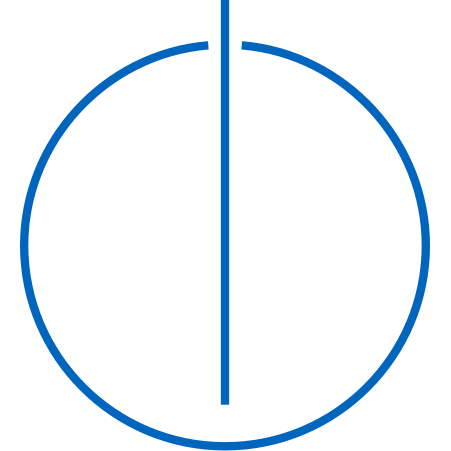
\includegraphics[height=20mm]{logos/faculty.png}
  }{}
\end{titlepage}


\frontmatter{}

\begin{titlepage}
  \centering

  \IfFileExists{logos/tum.pdf}{%
    
\includegraphics[height=20mm]{logos/tum.pdf}
  }{%
    \vspace*{20mm}
  }

  \vspace{5mm}
  {\huge\MakeUppercase{\getFaculty{}}}\\

  \vspace{5mm}
  {\large\MakeUppercase{\getUniversity{}}}\\

  \vspace{20mm}
  {\Large \getDoctype{}}

  \makeatletter
  \vspace{15mm}
  \ifthenelse{\pdf@strcmp{\languagename}{english}=0}
  {
  {\huge\bfseries \getTitle{}}

  \vspace{10mm}
  {\huge\bfseries \foreignlanguage{ngerman}{\getTitleGer{}}}
  }
  {
  {\huge\bfseries \getTitleGer{}}

  \vspace{10mm}
  {\huge\bfseries \foreignlanguage{english}{\getTitle{}}}
  }
  \makeatother

  \vspace{15mm}
  \begin{tabular}{l l}
    Author:          & \getAuthor{} \\
    Supervisor:      & \getSupervisor{} \\
    Advisor:         & \getAdvisor{} \\
    Submission Date: & \getSubmissionDate{} \\
  \end{tabular}

  \IfFileExists{logos/faculty.png}{%
    \vfill{}
    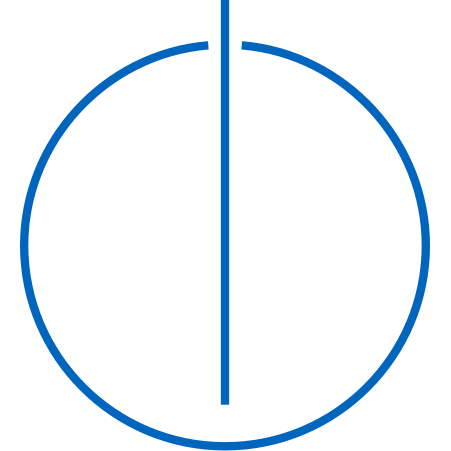
\includegraphics[height=20mm]{logos/faculty.png}
  }{}
\end{titlepage}

\cleardoublepage{}

\thispagestyle{empty}
\vspace*{0.8\textheight}
\noindent
\makeatletter
\ifthenelse{\pdf@strcmp{\languagename}{english}=0}
{I confirm that this \MakeLowercase{\getDoctype{}} is my own work and I have documented all sources and material used.}
{Ich versichere, dass ich diese \getDoctype{} selbstständig verfasst und nur die angegebenen Quellen und Hilfsmittel verwendet habe.}
\makeatother

\vspace{15mm}
\noindent
\getSubmissionLocation{}, \getSubmissionDate{} \hspace{50mm} \getAuthor{}

\cleardoublepage{}

\makeatletter
% \ifthenelse{\pdf@strcmp{\languagename}{english}=0}
% {\addcontentsline{toc}{chapter}{Acknowledgments}}
% {\addcontentsline{toc}{chapter}{Danksagungen}}
\makeatother
\thispagestyle{empty}

\vspace*{20mm}

\begin{center}
\makeatletter
\ifthenelse{\pdf@strcmp{\languagename}{english}=0}
{\usekomafont{section} Acknowledgments}
{\usekomafont{section} Danksagungen}
\makeatother
\end{center}

\vspace{10mm}

I would like to thank my supervisor, Professor Dr. Hegelich. By giving me the opportunity to write this thesis he showed me that universities truly are magnificent places that let young scientists find their way in this world by letting them follow their passion. I also want to thank my partner Elisabeth, who always supports me in whatever I do, I love you. Lastly I want to thank my parents and brother who lay the foundation to everything I am and ever will be.

\cleardoublepage{}

\chapter*{\abstractname}

We propose a deep learning framework for similarity learning of audio representations. It is inspired by the most recent successes in self-supervised representation learning in the domain of image data. Our framework transfers those successes to the domain of audio data. With our framework we show that (1) self-supervised contrastive learning can successfully learn robust audio representations without the need for labels, (2) the learned representations can be applied to other audio-based downstream tasks using transfer learning and (3) we show that our approach outperforms recently published results in the area of few-shot classification for audio data. We further describe the preliminary knowledge in signal processing and deep learning required to understand the inner workings of our proposed framework and investigate the most recent and most important related work in this field of research.

\makeatletter
\ifthenelse{\pdf@strcmp{\languagename}{english}=0}
{\renewcommand{\abstractname}{Kurzfassung}}
{\renewcommand{\abstractname}{Abstract}}
\makeatother

\chapter*{\abstractname}

\begin{otherlanguage}{ngerman}

In dieser Arbeit stellen wir ein neues Deep-Learning Framework zum Lernen von Ähnlichkeiten zwischen Audiorepräsentationen vor. Diese Arbeit ist inspiriert von den kürzlich erschienenen Erfolgen von ``self-supervised contrastive learning'' im Bereich der Bilderkennung. Unser Framework übernimmt diese neuesten Erkenntnisse und wendet sie auf Audiodaten an. Mit unserem Framework zeigen wir, dass (1) ``self-supervised contrastive learning'' ohne gelabelte Daten robuste Audiorepräsentationen lernen kann, (2) dass die gelernten Repräsentationen mittels ``transfer learning'' auf andere Bereiche übertragen werden können und (3) dass unser Ansatz kürzlich erschienene Arbeiten im Bereich ``few-shot classification'' übertrifft. Zudem erklären wir die Grundlagen in den Bereichen Signalverarbeitung und Deep-Learning, die notwendig sind, um unser Framework zu verstehen und untersuchen die aktuellsten und relevantesten Arbeiten in diesem Bereich.

\end{otherlanguage}


% Undo the name switch
\makeatletter
\ifthenelse{\pdf@strcmp{\languagename}{english}=0}
{\renewcommand{\abstractname}{Abstract}}
{\renewcommand{\abstractname}{Kurzfassung}}
\makeatother
\microtypesetup{protrusion=false}
\tableofcontents{}
\microtypesetup{protrusion=true}

\mainmatter{}

% !TeX root = ../main.tex

\chapter{Introduction}\label{chapter:introduction}

In this thesis, we explore the use of deep learning and neural networks for finding similarities in audio data. For this, we use recent discoveries in the area of deep learning and combine them with established methods of signal processing to create a novel learning framework suited for the task of finding similarity patterns in the highly complex domain of audio data.

Contrastive learning, the task of learning to distinguish similar pairs of data from dissimilar ones, has become very successful in recent years to train machine learning classifiers. This was made possible mainly due to new methods leveraging on the ability to learn without the need for human-annotated examples. Instead, those methods made use of what is now known as self-supervised learning, a learning paradigm that does not require any human supervision. Most prominent in the domain of image classification was the work of Chen et al. \cite{chen2020simple} released earlier this year called "\gls{simclr}". The authors showed that their proposed framework could outperform classical methods by a large margin without the need for labeled data. Since then several papers have been published that back the strong results of \gls{simclr} and self-supervised learning in the domain of image data (\cite{grill2020bootstrap, richemond2020byol, chen2020big}). In this work, we show that similar results can be obtained in the domain of audio data with slight changes to the framework itself.

Deep neural networks have a long history in their application of compressing information from high-dimensional data to dense representations. The first major work to apply this property to problems in the domain of audio data was Hinton et al. in 2012 \cite{hinton2012speech}. After their work the use of such modern learning architectures found increasing popularity by researchers of several fields, such as speech recognition \cite{hinton2012speech}, audio classification \cite{khamparia2019soundclassification} or speaker verification \cite{chen2020vggsound}. In this work, we also make use of neural networks to create dense representations of audio data (also known as embeddings). Such embeddings can then be more easily compared for similarities by a machine. We also show that our framework is detached from the precise architecture of the neural network that is used to create the embeddings. Therefore it is possible to plug in any model architecture into the framework. We demonstrate this property by evaluating the framework using three very different modern architectures.

To make the framework applicable to several downstream tasks, such as audio classification or speech recognition, we introduce the paradigm of transfer learning into the framework. Transfer learning is a concept that was first introduced by L. Y. Pratt in 1993 \cite{NIPS1992_641}. At its core transfer learning gives a neural network the ability to take the knowledge obtained from one task and transfer it to another one. Hence we split our learning framework into two stages: $i$) A pre-training stage that uses self-supervision and a large, unlabeled dataset to learn similarities in audio data and $ii$) a transfer stage where the network trained in $i$ is transferred to three different domains to solve the downstream task of audio classification. We show that this way we beat the most recent results for few-shot classification. Few-shot classification means that the domain that is being transferred to has little or no training data, which occurs when the creation of such datasets is too difficult. The reasons for this can be manifold. For music, intellectual property rights make it impossible to create an open dataset. For the annotation of complex audio events, trained humans have to manually annotate the data in a slow, cumbersome process, making the creation of a large-scale dataset time consuming and expensive. By pre-training our network on unlabeled data we overcome this problem and make it possible to obtain good results in the transfer domain, even when labeled training data is scarce.

This thesis is structured as follows: First (Chapter \ref{chapter:preliminaries}) we briefly explain the most important preliminary knowledge in the fields of deep learning and signal processing that is required to understand this work. Afterward, we look at the most relevant related work in Chapter \ref{chapter:relatedWork}, especially at the contributions of \gls{simclr} and other self-supervised, contrastive methods. In Chapter \ref{chapter:claudio} we go into the details of our proposed framework. We explain how it is structured and do a step by step analysis of each of the necessary components. Chapter \ref{chapter:experiments} contains all the experimental setup and evaluation done to demonstrate the results of the framework. Lastly (Chapter \ref{chapter:conclusion}) we conclude the findings of this thesis and propose potential future work.


% !TeX root = ../main.tex

\chapter{Preliminaries}\label{chapter:preliminaries}

This chapter explains the most important preliminary knowledge required for this work. An in-depth analysis of all of the concepts explained in the remainder of this chapter would be out of scope for this thesis, therefore we limit it to a brief but concise overview. For the readers that are interested in gaining deeper insights we recommend the books "Scientist and Engineer's Guide to Digital Signal Processing" by Steven W Smith \cite{smith1997dsp} and "Deep Learning (Adaptive Computation and Machine Learning series)" by Ian J Goodfellow \cite{goodfellow2016deeplearning}.

\section{Problem Formulation}\label{sec:problem_definition}

Much of the success of deep learning comes from the availability of large, open datasets of high quality. There is a strong correlation between the release of such datasets and the increase in deep learning progress in its corresponding domain. The best example being \textit{ImageNet} \cite{imagenet_cvpr09} for image data. The major reason for this is the reproducibility and comparability of works on such datasets. Unfortunately, datasets of such quality and size do not yet exist for audio data. The datasets that do exist are usually of lower quantity and quality, so therefore training good neural networks is a difficult task. 

The problem that we are trying to solve can be broken down into three subproblems: $i$) find a way to make use of unlabeled data to train a neural network in finding similarities in pairs of audio data, $ii$) explore ways to transfer the network trained in $i$ to another domain $iii$) show that by combining $i$ and $ii$ we can solve complex downstream classification tasks where only a few quantities of labeled training data exist.

\section{Learning Paradigms}

There exist many different learning paradigms in the realm of gradient-based machine learning today. In this section, we define and differentiate four of the most important paradigms for our work: \textit{Supervised Learning}, \textit{Self-Supervised Learning}, \textit{Contrastive Learning} and \textit{Transfer Learning}. We later describe how these paradigms can be combined to create new, sophisticated learning methods.

Note that the modern literature of deep learning does not fully agree on the definition and differentiation of some of these terms, so for example some would call an approach unsupervised while others would call it self-supervised. We therefore try to use the most recent definitions of the terms and stick to them throughout this thesis but beware that other works might have slightly different definitions.

\subsection{Supervised Learning}\label{subsec:supervised}

Supervised learning is the most used and most successful learning paradigm for neural networks today. Its goal is to learn a mapping from unknown inputs to specific outputs based on a set of given input-output pairs called training data. In the case of classification, the outputs are called labels and can be seen as a certain input belonging to one of many predefined categories, e.g in the case of hand-written number-classification labels would be in the range of 0 to 9 where each label corresponds to the same number-category. Learning such a mapping is achieved by minimizing the discrepancy between the predicted label and the actual label. Equation \ref{eq:cce} shows such a target, usually called the loss function, using the de-facto standard function for classification called \gls{cce}.

\begin{equation}
    \label{eq:cce}
    CCE(p,t) = - \sum_{c=0}^{N-1} t_{c} log(p_{c})
\end{equation}

$t_{c}$ denotes the actual probability that one input is of category $c$. $p_{c}$ is the probability a classifier assigns to an input being of category $c$. Often times the words category and class are used synonymously. In our case $t_{c}$ is a sparse vector where all entries are $0$ except for a $1$ at the position of the correct class. This is also known as a one-hot vector. Note that $p_{c}$ must be a probability, meaning $\sum_c p_{c} = 1$ and $p_{c} \in (0,1) \forall c$. So outputs of classifiers that are not probabilities, as is the case in most neural networks, must first be normalized. Usually, this is achieved using the softmax function, defined in Equation \ref{eq:softmax}, on the outputs. Here $z$ denotes a vector of size $K$, for example $p_{c}$ with $K = |c|$.

\begin{equation}
    \label{eq:softmax}
    \sigma(z)_i = \frac{e^{z_i}}{\sum_{j=1}^K e^{z_j}}
\end{equation}

In fact this procedure is so common that today most deep learning frameworks implicitly apply softmax to the inputs of \gls{cce}.

Simply by learning this mapping from predefined input-output pairs, a trained model can learn to correctly classify unknown inputs. A neural network can learn this mapping so well that in some cases it can outperform even humans. Because of its rather simplistic paradigm and its superb results, supervised learning has become the most used way to train neural networks today. Unfortunately, it requires a lot of data to generalize well and training a network on one specific task does not provide a good mapping for another task, even if the two tasks might be closely related. Since modern architectures usually contain billions of parameters that have to be tuned on incredibly large datasets, retraining a network for each task requires enormous resources, time and money. Other paradigms are required to mitigate this problem.

\subsection{Self-Supervised Learning}\label{subsec:self_supervised}

Self-supervised learning is a special case of unsupervised learning. In unsupervised learning, a model tries to find inherent patterns in a dataset without labels. An example of this is clustering or principal component analysis \cite{1901pca}. Self-Supervised learning has the same target as unsupervised learning but obtains labels from the data itself. This means that from one or many data points, a supervised task is generated, which is then evaluated in the same way a supervised system would be. Choosing the exact nature of this task is a critical part of self-supervised learning. There have been many proposed tasks for such systems but all fall into either one of two categories: generative or discriminative. An example of a generative task is proposed in Hossein et al. (2020) \cite{hosseini2020inceptioninspired} where the authors try to predict the next frames in a video by minimizing the \gls{mse} between an image generated by a neural network and the actual next frame. On the other hand, an example of a discriminative task is Gidaris et al. (2018) \cite{gidaris2018unsupervised}. Here the authors try to find the original image out of four rotated copies of that image. Discriminative methods, such as contrastive learning explained in \ref{subsec:contrastive_learning}, try to distinguish different kinds of inputs.

In general the target in self-supervised learning is "a proxy task that forces the network to learn what we really care about" \cite{zisserman2018selfsupervised}. \textit{Word2Vec}, proposed by Mikolov et al. \cite{mikolov2013efficient}, though not called self-supervised by the authors, can be seen as such a system that, by predicting words in a sentence, is forced to learn a semantic representation of those words. In our case what we care about is a representation of audio input into a latent space where close distance is equivalent to a close semantic distance in the real world, e.g. perceived similarity in music or speech. We call this semantic distance the similarity of two data points.

Figure \ref{fig:clusters} shows how we think of similarity in a made-up scenario of differentiating input images of certain categories. Close points in this two-dimensional plane are considered similar, while further away points are considered not similar. Therefore data of the same class should be mapped close together since they are of high similarity. Note that this similarity measure can vary from being strictly objective in the case of same speakers to highly subjective in the case of song genres. One can clearly see how this paradigm can be used to solve problem $i$ defined in \ref{sec:problem_definition}.

\begin{figure}[t]
    \centering
    \scalebox{.6}{%% Creator: Matplotlib, PGF backend
%%
%% To include the figure in your LaTeX document, write
%%   \input{<filename>.pgf}
%%
%% Make sure the required packages are loaded in your preamble
%%   \usepackage{pgf}
%%
%% and, on pdftex
%%   \usepackage[utf8]{inputenc}\DeclareUnicodeCharacter{2212}{-}
%%
%% or, on luatex and xetex
%%   \usepackage{unicode-math}
%%
%% Figures using additional raster images can only be included by \input if
%% they are in the same directory as the main LaTeX file. For loading figures
%% from other directories you can use the `import` package
%%   \usepackage{import}
%%
%% and then include the figures with
%%   \import{<path to file>}{<filename>.pgf}
%%
%% Matplotlib used the following preamble
%%
\begingroup%
\makeatletter%
\begin{pgfpicture}%
\pgfpathrectangle{\pgfpointorigin}{\pgfqpoint{4.000000in}{4.000000in}}%
\pgfusepath{use as bounding box, clip}%
\begin{pgfscope}%
\pgfsetbuttcap%
\pgfsetmiterjoin%
\definecolor{currentfill}{rgb}{1.000000,1.000000,1.000000}%
\pgfsetfillcolor{currentfill}%
\pgfsetlinewidth{0.000000pt}%
\definecolor{currentstroke}{rgb}{1.000000,1.000000,1.000000}%
\pgfsetstrokecolor{currentstroke}%
\pgfsetdash{}{0pt}%
\pgfpathmoveto{\pgfqpoint{0.000000in}{0.000000in}}%
\pgfpathlineto{\pgfqpoint{4.000000in}{0.000000in}}%
\pgfpathlineto{\pgfqpoint{4.000000in}{4.000000in}}%
\pgfpathlineto{\pgfqpoint{0.000000in}{4.000000in}}%
\pgfpathclose%
\pgfusepath{fill}%
\end{pgfscope}%
\begin{pgfscope}%
\pgfpathrectangle{\pgfqpoint{0.180000in}{0.180000in}}{\pgfqpoint{3.640000in}{3.640000in}}%
\pgfusepath{clip}%
\pgfsetbuttcap%
\pgfsetroundjoin%
\definecolor{currentfill}{rgb}{0.282353,0.521569,0.929412}%
\pgfsetfillcolor{currentfill}%
\pgfsetlinewidth{1.003750pt}%
\definecolor{currentstroke}{rgb}{0.282353,0.521569,0.929412}%
\pgfsetstrokecolor{currentstroke}%
\pgfsetdash{}{0pt}%
\pgfsys@defobject{currentmarker}{\pgfqpoint{-0.015528in}{-0.015528in}}{\pgfqpoint{0.015528in}{0.015528in}}{%
\pgfpathmoveto{\pgfqpoint{0.000000in}{-0.015528in}}%
\pgfpathcurveto{\pgfqpoint{0.004118in}{-0.015528in}}{\pgfqpoint{0.008068in}{-0.013892in}}{\pgfqpoint{0.010980in}{-0.010980in}}%
\pgfpathcurveto{\pgfqpoint{0.013892in}{-0.008068in}}{\pgfqpoint{0.015528in}{-0.004118in}}{\pgfqpoint{0.015528in}{0.000000in}}%
\pgfpathcurveto{\pgfqpoint{0.015528in}{0.004118in}}{\pgfqpoint{0.013892in}{0.008068in}}{\pgfqpoint{0.010980in}{0.010980in}}%
\pgfpathcurveto{\pgfqpoint{0.008068in}{0.013892in}}{\pgfqpoint{0.004118in}{0.015528in}}{\pgfqpoint{0.000000in}{0.015528in}}%
\pgfpathcurveto{\pgfqpoint{-0.004118in}{0.015528in}}{\pgfqpoint{-0.008068in}{0.013892in}}{\pgfqpoint{-0.010980in}{0.010980in}}%
\pgfpathcurveto{\pgfqpoint{-0.013892in}{0.008068in}}{\pgfqpoint{-0.015528in}{0.004118in}}{\pgfqpoint{-0.015528in}{0.000000in}}%
\pgfpathcurveto{\pgfqpoint{-0.015528in}{-0.004118in}}{\pgfqpoint{-0.013892in}{-0.008068in}}{\pgfqpoint{-0.010980in}{-0.010980in}}%
\pgfpathcurveto{\pgfqpoint{-0.008068in}{-0.013892in}}{\pgfqpoint{-0.004118in}{-0.015528in}}{\pgfqpoint{0.000000in}{-0.015528in}}%
\pgfpathclose%
\pgfusepath{stroke,fill}%
}%
\begin{pgfscope}%
\pgfsys@transformshift{2.781147in}{2.157348in}%
\pgfsys@useobject{currentmarker}{}%
\end{pgfscope}%
\begin{pgfscope}%
\pgfsys@transformshift{2.449454in}{1.516145in}%
\pgfsys@useobject{currentmarker}{}%
\end{pgfscope}%
\begin{pgfscope}%
\pgfsys@transformshift{1.831289in}{1.169384in}%
\pgfsys@useobject{currentmarker}{}%
\end{pgfscope}%
\begin{pgfscope}%
\pgfsys@transformshift{18.545455in}{1.850220in}%
\pgfsys@useobject{currentmarker}{}%
\end{pgfscope}%
\begin{pgfscope}%
\pgfsys@transformshift{1.379844in}{1.710303in}%
\pgfsys@useobject{currentmarker}{}%
\end{pgfscope}%
\begin{pgfscope}%
\pgfsys@transformshift{2.423050in}{1.760802in}%
\pgfsys@useobject{currentmarker}{}%
\end{pgfscope}%
\begin{pgfscope}%
\pgfsys@transformshift{2.258650in}{3.131199in}%
\pgfsys@useobject{currentmarker}{}%
\end{pgfscope}%
\begin{pgfscope}%
\pgfsys@transformshift{18.545455in}{2.021823in}%
\pgfsys@useobject{currentmarker}{}%
\end{pgfscope}%
\begin{pgfscope}%
\pgfsys@transformshift{2.774150in}{2.748261in}%
\pgfsys@useobject{currentmarker}{}%
\end{pgfscope}%
\begin{pgfscope}%
\pgfsys@transformshift{1.188926in}{2.734683in}%
\pgfsys@useobject{currentmarker}{}%
\end{pgfscope}%
\begin{pgfscope}%
\pgfsys@transformshift{1.802328in}{1.359515in}%
\pgfsys@useobject{currentmarker}{}%
\end{pgfscope}%
\begin{pgfscope}%
\pgfsys@transformshift{0.914718in}{3.305437in}%
\pgfsys@useobject{currentmarker}{}%
\end{pgfscope}%
\begin{pgfscope}%
\pgfsys@transformshift{3.137362in}{2.101629in}%
\pgfsys@useobject{currentmarker}{}%
\end{pgfscope}%
\begin{pgfscope}%
\pgfsys@transformshift{2.189396in}{1.223562in}%
\pgfsys@useobject{currentmarker}{}%
\end{pgfscope}%
\begin{pgfscope}%
\pgfsys@transformshift{2.533820in}{2.901684in}%
\pgfsys@useobject{currentmarker}{}%
\end{pgfscope}%
\begin{pgfscope}%
\pgfsys@transformshift{0.364657in}{2.660314in}%
\pgfsys@useobject{currentmarker}{}%
\end{pgfscope}%
\begin{pgfscope}%
\pgfsys@transformshift{2.420710in}{2.287558in}%
\pgfsys@useobject{currentmarker}{}%
\end{pgfscope}%
\begin{pgfscope}%
\pgfsys@transformshift{0.553499in}{1.285961in}%
\pgfsys@useobject{currentmarker}{}%
\end{pgfscope}%
\begin{pgfscope}%
\pgfsys@transformshift{2.842385in}{1.530207in}%
\pgfsys@useobject{currentmarker}{}%
\end{pgfscope}%
\begin{pgfscope}%
\pgfsys@transformshift{2.626425in}{1.827212in}%
\pgfsys@useobject{currentmarker}{}%
\end{pgfscope}%
\begin{pgfscope}%
\pgfsys@transformshift{1.966587in}{1.908063in}%
\pgfsys@useobject{currentmarker}{}%
\end{pgfscope}%
\begin{pgfscope}%
\pgfsys@transformshift{18.545455in}{1.628759in}%
\pgfsys@useobject{currentmarker}{}%
\end{pgfscope}%
\begin{pgfscope}%
\pgfsys@transformshift{1.457208in}{1.416776in}%
\pgfsys@useobject{currentmarker}{}%
\end{pgfscope}%
\begin{pgfscope}%
\pgfsys@transformshift{1.512571in}{1.582723in}%
\pgfsys@useobject{currentmarker}{}%
\end{pgfscope}%
\begin{pgfscope}%
\pgfsys@transformshift{1.799209in}{2.606588in}%
\pgfsys@useobject{currentmarker}{}%
\end{pgfscope}%
\begin{pgfscope}%
\pgfsys@transformshift{1.554329in}{2.069118in}%
\pgfsys@useobject{currentmarker}{}%
\end{pgfscope}%
\begin{pgfscope}%
\pgfsys@transformshift{2.054594in}{2.447343in}%
\pgfsys@useobject{currentmarker}{}%
\end{pgfscope}%
\begin{pgfscope}%
\pgfsys@transformshift{2.276646in}{2.834513in}%
\pgfsys@useobject{currentmarker}{}%
\end{pgfscope}%
\begin{pgfscope}%
\pgfsys@transformshift{2.744106in}{1.185685in}%
\pgfsys@useobject{currentmarker}{}%
\end{pgfscope}%
\begin{pgfscope}%
\pgfsys@transformshift{1.860702in}{1.693415in}%
\pgfsys@useobject{currentmarker}{}%
\end{pgfscope}%
\begin{pgfscope}%
\pgfsys@transformshift{18.545455in}{2.410238in}%
\pgfsys@useobject{currentmarker}{}%
\end{pgfscope}%
\begin{pgfscope}%
\pgfsys@transformshift{1.409947in}{1.473427in}%
\pgfsys@useobject{currentmarker}{}%
\end{pgfscope}%
\begin{pgfscope}%
\pgfsys@transformshift{1.055305in}{2.369456in}%
\pgfsys@useobject{currentmarker}{}%
\end{pgfscope}%
\begin{pgfscope}%
\pgfsys@transformshift{2.555901in}{2.509918in}%
\pgfsys@useobject{currentmarker}{}%
\end{pgfscope}%
\begin{pgfscope}%
\pgfsys@transformshift{1.168584in}{2.366496in}%
\pgfsys@useobject{currentmarker}{}%
\end{pgfscope}%
\begin{pgfscope}%
\pgfsys@transformshift{1.052084in}{18.545455in}%
\pgfsys@useobject{currentmarker}{}%
\end{pgfscope}%
\begin{pgfscope}%
\pgfsys@transformshift{1.626604in}{2.827353in}%
\pgfsys@useobject{currentmarker}{}%
\end{pgfscope}%
\begin{pgfscope}%
\pgfsys@transformshift{18.545455in}{2.422338in}%
\pgfsys@useobject{currentmarker}{}%
\end{pgfscope}%
\begin{pgfscope}%
\pgfsys@transformshift{1.901049in}{1.808479in}%
\pgfsys@useobject{currentmarker}{}%
\end{pgfscope}%
\begin{pgfscope}%
\pgfsys@transformshift{2.616606in}{1.978990in}%
\pgfsys@useobject{currentmarker}{}%
\end{pgfscope}%
\begin{pgfscope}%
\pgfsys@transformshift{2.595394in}{1.837392in}%
\pgfsys@useobject{currentmarker}{}%
\end{pgfscope}%
\begin{pgfscope}%
\pgfsys@transformshift{1.378835in}{1.164390in}%
\pgfsys@useobject{currentmarker}{}%
\end{pgfscope}%
\begin{pgfscope}%
\pgfsys@transformshift{2.238131in}{2.032654in}%
\pgfsys@useobject{currentmarker}{}%
\end{pgfscope}%
\begin{pgfscope}%
\pgfsys@transformshift{2.101996in}{1.752391in}%
\pgfsys@useobject{currentmarker}{}%
\end{pgfscope}%
\begin{pgfscope}%
\pgfsys@transformshift{0.889165in}{1.821988in}%
\pgfsys@useobject{currentmarker}{}%
\end{pgfscope}%
\begin{pgfscope}%
\pgfsys@transformshift{1.706362in}{1.406611in}%
\pgfsys@useobject{currentmarker}{}%
\end{pgfscope}%
\begin{pgfscope}%
\pgfsys@transformshift{2.142698in}{1.881793in}%
\pgfsys@useobject{currentmarker}{}%
\end{pgfscope}%
\begin{pgfscope}%
\pgfsys@transformshift{1.699675in}{1.963262in}%
\pgfsys@useobject{currentmarker}{}%
\end{pgfscope}%
\begin{pgfscope}%
\pgfsys@transformshift{2.813434in}{18.545455in}%
\pgfsys@useobject{currentmarker}{}%
\end{pgfscope}%
\begin{pgfscope}%
\pgfsys@transformshift{2.783695in}{2.248543in}%
\pgfsys@useobject{currentmarker}{}%
\end{pgfscope}%
\begin{pgfscope}%
\pgfsys@transformshift{1.400271in}{1.019051in}%
\pgfsys@useobject{currentmarker}{}%
\end{pgfscope}%
\begin{pgfscope}%
\pgfsys@transformshift{1.006136in}{2.268344in}%
\pgfsys@useobject{currentmarker}{}%
\end{pgfscope}%
\begin{pgfscope}%
\pgfsys@transformshift{2.395128in}{0.696339in}%
\pgfsys@useobject{currentmarker}{}%
\end{pgfscope}%
\begin{pgfscope}%
\pgfsys@transformshift{1.691227in}{1.172413in}%
\pgfsys@useobject{currentmarker}{}%
\end{pgfscope}%
\begin{pgfscope}%
\pgfsys@transformshift{2.450550in}{1.199873in}%
\pgfsys@useobject{currentmarker}{}%
\end{pgfscope}%
\begin{pgfscope}%
\pgfsys@transformshift{2.123047in}{2.149741in}%
\pgfsys@useobject{currentmarker}{}%
\end{pgfscope}%
\begin{pgfscope}%
\pgfsys@transformshift{2.121091in}{2.375010in}%
\pgfsys@useobject{currentmarker}{}%
\end{pgfscope}%
\begin{pgfscope}%
\pgfsys@transformshift{1.000079in}{1.555855in}%
\pgfsys@useobject{currentmarker}{}%
\end{pgfscope}%
\begin{pgfscope}%
\pgfsys@transformshift{2.719371in}{2.904386in}%
\pgfsys@useobject{currentmarker}{}%
\end{pgfscope}%
\begin{pgfscope}%
\pgfsys@transformshift{0.865226in}{1.692693in}%
\pgfsys@useobject{currentmarker}{}%
\end{pgfscope}%
\begin{pgfscope}%
\pgfsys@transformshift{1.792200in}{2.863171in}%
\pgfsys@useobject{currentmarker}{}%
\end{pgfscope}%
\begin{pgfscope}%
\pgfsys@transformshift{2.871594in}{1.716593in}%
\pgfsys@useobject{currentmarker}{}%
\end{pgfscope}%
\begin{pgfscope}%
\pgfsys@transformshift{0.672105in}{2.189264in}%
\pgfsys@useobject{currentmarker}{}%
\end{pgfscope}%
\begin{pgfscope}%
\pgfsys@transformshift{1.857480in}{2.559445in}%
\pgfsys@useobject{currentmarker}{}%
\end{pgfscope}%
\begin{pgfscope}%
\pgfsys@transformshift{1.860945in}{2.916728in}%
\pgfsys@useobject{currentmarker}{}%
\end{pgfscope}%
\begin{pgfscope}%
\pgfsys@transformshift{1.639391in}{2.791448in}%
\pgfsys@useobject{currentmarker}{}%
\end{pgfscope}%
\begin{pgfscope}%
\pgfsys@transformshift{2.757583in}{1.423043in}%
\pgfsys@useobject{currentmarker}{}%
\end{pgfscope}%
\begin{pgfscope}%
\pgfsys@transformshift{0.532680in}{2.401119in}%
\pgfsys@useobject{currentmarker}{}%
\end{pgfscope}%
\begin{pgfscope}%
\pgfsys@transformshift{2.065031in}{2.286048in}%
\pgfsys@useobject{currentmarker}{}%
\end{pgfscope}%
\begin{pgfscope}%
\pgfsys@transformshift{2.976178in}{18.545455in}%
\pgfsys@useobject{currentmarker}{}%
\end{pgfscope}%
\begin{pgfscope}%
\pgfsys@transformshift{1.405226in}{1.489415in}%
\pgfsys@useobject{currentmarker}{}%
\end{pgfscope}%
\begin{pgfscope}%
\pgfsys@transformshift{2.292029in}{2.840383in}%
\pgfsys@useobject{currentmarker}{}%
\end{pgfscope}%
\begin{pgfscope}%
\pgfsys@transformshift{2.517037in}{1.149944in}%
\pgfsys@useobject{currentmarker}{}%
\end{pgfscope}%
\begin{pgfscope}%
\pgfsys@transformshift{0.839391in}{2.257998in}%
\pgfsys@useobject{currentmarker}{}%
\end{pgfscope}%
\begin{pgfscope}%
\pgfsys@transformshift{3.055494in}{2.081074in}%
\pgfsys@useobject{currentmarker}{}%
\end{pgfscope}%
\begin{pgfscope}%
\pgfsys@transformshift{1.992579in}{3.099402in}%
\pgfsys@useobject{currentmarker}{}%
\end{pgfscope}%
\begin{pgfscope}%
\pgfsys@transformshift{1.673683in}{2.243541in}%
\pgfsys@useobject{currentmarker}{}%
\end{pgfscope}%
\begin{pgfscope}%
\pgfsys@transformshift{1.322945in}{1.312560in}%
\pgfsys@useobject{currentmarker}{}%
\end{pgfscope}%
\begin{pgfscope}%
\pgfsys@transformshift{18.545455in}{0.348352in}%
\pgfsys@useobject{currentmarker}{}%
\end{pgfscope}%
\begin{pgfscope}%
\pgfsys@transformshift{2.365399in}{18.545455in}%
\pgfsys@useobject{currentmarker}{}%
\end{pgfscope}%
\begin{pgfscope}%
\pgfsys@transformshift{0.818785in}{1.401253in}%
\pgfsys@useobject{currentmarker}{}%
\end{pgfscope}%
\begin{pgfscope}%
\pgfsys@transformshift{1.068185in}{0.439784in}%
\pgfsys@useobject{currentmarker}{}%
\end{pgfscope}%
\begin{pgfscope}%
\pgfsys@transformshift{1.779574in}{2.286722in}%
\pgfsys@useobject{currentmarker}{}%
\end{pgfscope}%
\begin{pgfscope}%
\pgfsys@transformshift{0.947551in}{2.804636in}%
\pgfsys@useobject{currentmarker}{}%
\end{pgfscope}%
\begin{pgfscope}%
\pgfsys@transformshift{2.216783in}{0.589028in}%
\pgfsys@useobject{currentmarker}{}%
\end{pgfscope}%
\begin{pgfscope}%
\pgfsys@transformshift{2.229660in}{1.861837in}%
\pgfsys@useobject{currentmarker}{}%
\end{pgfscope}%
\begin{pgfscope}%
\pgfsys@transformshift{1.603467in}{2.639963in}%
\pgfsys@useobject{currentmarker}{}%
\end{pgfscope}%
\begin{pgfscope}%
\pgfsys@transformshift{1.836471in}{2.767993in}%
\pgfsys@useobject{currentmarker}{}%
\end{pgfscope}%
\begin{pgfscope}%
\pgfsys@transformshift{1.645490in}{2.267580in}%
\pgfsys@useobject{currentmarker}{}%
\end{pgfscope}%
\begin{pgfscope}%
\pgfsys@transformshift{1.817884in}{0.640601in}%
\pgfsys@useobject{currentmarker}{}%
\end{pgfscope}%
\begin{pgfscope}%
\pgfsys@transformshift{0.928972in}{18.545455in}%
\pgfsys@useobject{currentmarker}{}%
\end{pgfscope}%
\begin{pgfscope}%
\pgfsys@transformshift{2.734507in}{3.155478in}%
\pgfsys@useobject{currentmarker}{}%
\end{pgfscope}%
\begin{pgfscope}%
\pgfsys@transformshift{2.530703in}{1.453625in}%
\pgfsys@useobject{currentmarker}{}%
\end{pgfscope}%
\begin{pgfscope}%
\pgfsys@transformshift{1.024783in}{0.702065in}%
\pgfsys@useobject{currentmarker}{}%
\end{pgfscope}%
\begin{pgfscope}%
\pgfsys@transformshift{2.177911in}{1.934030in}%
\pgfsys@useobject{currentmarker}{}%
\end{pgfscope}%
\begin{pgfscope}%
\pgfsys@transformshift{2.062504in}{2.549892in}%
\pgfsys@useobject{currentmarker}{}%
\end{pgfscope}%
\begin{pgfscope}%
\pgfsys@transformshift{1.868289in}{3.350667in}%
\pgfsys@useobject{currentmarker}{}%
\end{pgfscope}%
\begin{pgfscope}%
\pgfsys@transformshift{1.727833in}{2.539143in}%
\pgfsys@useobject{currentmarker}{}%
\end{pgfscope}%
\begin{pgfscope}%
\pgfsys@transformshift{2.621947in}{2.306954in}%
\pgfsys@useobject{currentmarker}{}%
\end{pgfscope}%
\begin{pgfscope}%
\pgfsys@transformshift{2.235759in}{2.391096in}%
\pgfsys@useobject{currentmarker}{}%
\end{pgfscope}%
\begin{pgfscope}%
\pgfsys@transformshift{2.315246in}{1.023099in}%
\pgfsys@useobject{currentmarker}{}%
\end{pgfscope}%
\begin{pgfscope}%
\pgfsys@transformshift{1.622973in}{1.337194in}%
\pgfsys@useobject{currentmarker}{}%
\end{pgfscope}%
\begin{pgfscope}%
\pgfsys@transformshift{1.301399in}{2.748197in}%
\pgfsys@useobject{currentmarker}{}%
\end{pgfscope}%
\begin{pgfscope}%
\pgfsys@transformshift{18.545455in}{2.461907in}%
\pgfsys@useobject{currentmarker}{}%
\end{pgfscope}%
\begin{pgfscope}%
\pgfsys@transformshift{2.391736in}{1.521744in}%
\pgfsys@useobject{currentmarker}{}%
\end{pgfscope}%
\begin{pgfscope}%
\pgfsys@transformshift{2.374260in}{1.298744in}%
\pgfsys@useobject{currentmarker}{}%
\end{pgfscope}%
\begin{pgfscope}%
\pgfsys@transformshift{1.522564in}{3.177346in}%
\pgfsys@useobject{currentmarker}{}%
\end{pgfscope}%
\begin{pgfscope}%
\pgfsys@transformshift{2.277114in}{2.282461in}%
\pgfsys@useobject{currentmarker}{}%
\end{pgfscope}%
\begin{pgfscope}%
\pgfsys@transformshift{2.307345in}{0.814872in}%
\pgfsys@useobject{currentmarker}{}%
\end{pgfscope}%
\begin{pgfscope}%
\pgfsys@transformshift{3.224190in}{1.215212in}%
\pgfsys@useobject{currentmarker}{}%
\end{pgfscope}%
\begin{pgfscope}%
\pgfsys@transformshift{2.516530in}{2.225729in}%
\pgfsys@useobject{currentmarker}{}%
\end{pgfscope}%
\begin{pgfscope}%
\pgfsys@transformshift{2.087737in}{2.603058in}%
\pgfsys@useobject{currentmarker}{}%
\end{pgfscope}%
\begin{pgfscope}%
\pgfsys@transformshift{18.545455in}{1.168165in}%
\pgfsys@useobject{currentmarker}{}%
\end{pgfscope}%
\begin{pgfscope}%
\pgfsys@transformshift{1.334821in}{1.365300in}%
\pgfsys@useobject{currentmarker}{}%
\end{pgfscope}%
\begin{pgfscope}%
\pgfsys@transformshift{3.386790in}{2.138249in}%
\pgfsys@useobject{currentmarker}{}%
\end{pgfscope}%
\begin{pgfscope}%
\pgfsys@transformshift{1.077203in}{3.188907in}%
\pgfsys@useobject{currentmarker}{}%
\end{pgfscope}%
\begin{pgfscope}%
\pgfsys@transformshift{1.833268in}{0.988967in}%
\pgfsys@useobject{currentmarker}{}%
\end{pgfscope}%
\begin{pgfscope}%
\pgfsys@transformshift{2.051263in}{1.754275in}%
\pgfsys@useobject{currentmarker}{}%
\end{pgfscope}%
\begin{pgfscope}%
\pgfsys@transformshift{2.304118in}{2.955825in}%
\pgfsys@useobject{currentmarker}{}%
\end{pgfscope}%
\begin{pgfscope}%
\pgfsys@transformshift{1.913704in}{0.735114in}%
\pgfsys@useobject{currentmarker}{}%
\end{pgfscope}%
\begin{pgfscope}%
\pgfsys@transformshift{1.510488in}{2.260553in}%
\pgfsys@useobject{currentmarker}{}%
\end{pgfscope}%
\begin{pgfscope}%
\pgfsys@transformshift{2.859607in}{2.373018in}%
\pgfsys@useobject{currentmarker}{}%
\end{pgfscope}%
\begin{pgfscope}%
\pgfsys@transformshift{2.190129in}{1.500468in}%
\pgfsys@useobject{currentmarker}{}%
\end{pgfscope}%
\begin{pgfscope}%
\pgfsys@transformshift{2.419088in}{2.381546in}%
\pgfsys@useobject{currentmarker}{}%
\end{pgfscope}%
\begin{pgfscope}%
\pgfsys@transformshift{2.315416in}{1.510452in}%
\pgfsys@useobject{currentmarker}{}%
\end{pgfscope}%
\begin{pgfscope}%
\pgfsys@transformshift{0.945797in}{2.245326in}%
\pgfsys@useobject{currentmarker}{}%
\end{pgfscope}%
\begin{pgfscope}%
\pgfsys@transformshift{2.058035in}{1.507517in}%
\pgfsys@useobject{currentmarker}{}%
\end{pgfscope}%
\begin{pgfscope}%
\pgfsys@transformshift{18.545455in}{1.640993in}%
\pgfsys@useobject{currentmarker}{}%
\end{pgfscope}%
\begin{pgfscope}%
\pgfsys@transformshift{1.795039in}{2.425821in}%
\pgfsys@useobject{currentmarker}{}%
\end{pgfscope}%
\begin{pgfscope}%
\pgfsys@transformshift{2.022692in}{1.782475in}%
\pgfsys@useobject{currentmarker}{}%
\end{pgfscope}%
\begin{pgfscope}%
\pgfsys@transformshift{2.712995in}{2.002131in}%
\pgfsys@useobject{currentmarker}{}%
\end{pgfscope}%
\begin{pgfscope}%
\pgfsys@transformshift{2.600929in}{3.552740in}%
\pgfsys@useobject{currentmarker}{}%
\end{pgfscope}%
\begin{pgfscope}%
\pgfsys@transformshift{3.057860in}{1.630261in}%
\pgfsys@useobject{currentmarker}{}%
\end{pgfscope}%
\begin{pgfscope}%
\pgfsys@transformshift{0.485853in}{1.239869in}%
\pgfsys@useobject{currentmarker}{}%
\end{pgfscope}%
\begin{pgfscope}%
\pgfsys@transformshift{3.070309in}{1.836919in}%
\pgfsys@useobject{currentmarker}{}%
\end{pgfscope}%
\begin{pgfscope}%
\pgfsys@transformshift{1.828648in}{1.508783in}%
\pgfsys@useobject{currentmarker}{}%
\end{pgfscope}%
\begin{pgfscope}%
\pgfsys@transformshift{3.623020in}{2.835644in}%
\pgfsys@useobject{currentmarker}{}%
\end{pgfscope}%
\begin{pgfscope}%
\pgfsys@transformshift{2.735988in}{1.234931in}%
\pgfsys@useobject{currentmarker}{}%
\end{pgfscope}%
\begin{pgfscope}%
\pgfsys@transformshift{0.994501in}{2.687860in}%
\pgfsys@useobject{currentmarker}{}%
\end{pgfscope}%
\begin{pgfscope}%
\pgfsys@transformshift{1.152609in}{2.599422in}%
\pgfsys@useobject{currentmarker}{}%
\end{pgfscope}%
\begin{pgfscope}%
\pgfsys@transformshift{3.165378in}{2.294145in}%
\pgfsys@useobject{currentmarker}{}%
\end{pgfscope}%
\begin{pgfscope}%
\pgfsys@transformshift{1.670152in}{2.060117in}%
\pgfsys@useobject{currentmarker}{}%
\end{pgfscope}%
\begin{pgfscope}%
\pgfsys@transformshift{18.545455in}{2.030250in}%
\pgfsys@useobject{currentmarker}{}%
\end{pgfscope}%
\begin{pgfscope}%
\pgfsys@transformshift{1.975464in}{1.301813in}%
\pgfsys@useobject{currentmarker}{}%
\end{pgfscope}%
\begin{pgfscope}%
\pgfsys@transformshift{2.358718in}{2.394303in}%
\pgfsys@useobject{currentmarker}{}%
\end{pgfscope}%
\begin{pgfscope}%
\pgfsys@transformshift{2.711027in}{2.849657in}%
\pgfsys@useobject{currentmarker}{}%
\end{pgfscope}%
\begin{pgfscope}%
\pgfsys@transformshift{2.235792in}{2.205819in}%
\pgfsys@useobject{currentmarker}{}%
\end{pgfscope}%
\begin{pgfscope}%
\pgfsys@transformshift{18.545455in}{2.061438in}%
\pgfsys@useobject{currentmarker}{}%
\end{pgfscope}%
\begin{pgfscope}%
\pgfsys@transformshift{0.709523in}{2.156947in}%
\pgfsys@useobject{currentmarker}{}%
\end{pgfscope}%
\begin{pgfscope}%
\pgfsys@transformshift{1.110246in}{18.545455in}%
\pgfsys@useobject{currentmarker}{}%
\end{pgfscope}%
\begin{pgfscope}%
\pgfsys@transformshift{2.391144in}{1.378789in}%
\pgfsys@useobject{currentmarker}{}%
\end{pgfscope}%
\begin{pgfscope}%
\pgfsys@transformshift{1.491368in}{2.779992in}%
\pgfsys@useobject{currentmarker}{}%
\end{pgfscope}%
\begin{pgfscope}%
\pgfsys@transformshift{1.259750in}{2.893011in}%
\pgfsys@useobject{currentmarker}{}%
\end{pgfscope}%
\begin{pgfscope}%
\pgfsys@transformshift{2.283891in}{1.136468in}%
\pgfsys@useobject{currentmarker}{}%
\end{pgfscope}%
\begin{pgfscope}%
\pgfsys@transformshift{2.635021in}{1.522533in}%
\pgfsys@useobject{currentmarker}{}%
\end{pgfscope}%
\begin{pgfscope}%
\pgfsys@transformshift{2.988454in}{1.630956in}%
\pgfsys@useobject{currentmarker}{}%
\end{pgfscope}%
\begin{pgfscope}%
\pgfsys@transformshift{2.267973in}{18.545455in}%
\pgfsys@useobject{currentmarker}{}%
\end{pgfscope}%
\begin{pgfscope}%
\pgfsys@transformshift{2.537765in}{2.783534in}%
\pgfsys@useobject{currentmarker}{}%
\end{pgfscope}%
\begin{pgfscope}%
\pgfsys@transformshift{0.968004in}{1.231336in}%
\pgfsys@useobject{currentmarker}{}%
\end{pgfscope}%
\begin{pgfscope}%
\pgfsys@transformshift{1.090826in}{2.149276in}%
\pgfsys@useobject{currentmarker}{}%
\end{pgfscope}%
\begin{pgfscope}%
\pgfsys@transformshift{1.575311in}{3.205875in}%
\pgfsys@useobject{currentmarker}{}%
\end{pgfscope}%
\begin{pgfscope}%
\pgfsys@transformshift{1.856061in}{3.546603in}%
\pgfsys@useobject{currentmarker}{}%
\end{pgfscope}%
\begin{pgfscope}%
\pgfsys@transformshift{1.651330in}{0.492951in}%
\pgfsys@useobject{currentmarker}{}%
\end{pgfscope}%
\begin{pgfscope}%
\pgfsys@transformshift{1.487675in}{0.637358in}%
\pgfsys@useobject{currentmarker}{}%
\end{pgfscope}%
\begin{pgfscope}%
\pgfsys@transformshift{1.868687in}{1.994786in}%
\pgfsys@useobject{currentmarker}{}%
\end{pgfscope}%
\begin{pgfscope}%
\pgfsys@transformshift{1.336516in}{1.599008in}%
\pgfsys@useobject{currentmarker}{}%
\end{pgfscope}%
\begin{pgfscope}%
\pgfsys@transformshift{1.281655in}{1.507148in}%
\pgfsys@useobject{currentmarker}{}%
\end{pgfscope}%
\begin{pgfscope}%
\pgfsys@transformshift{1.228205in}{1.445726in}%
\pgfsys@useobject{currentmarker}{}%
\end{pgfscope}%
\begin{pgfscope}%
\pgfsys@transformshift{2.346456in}{2.018270in}%
\pgfsys@useobject{currentmarker}{}%
\end{pgfscope}%
\begin{pgfscope}%
\pgfsys@transformshift{0.956793in}{2.326072in}%
\pgfsys@useobject{currentmarker}{}%
\end{pgfscope}%
\begin{pgfscope}%
\pgfsys@transformshift{1.164458in}{1.843898in}%
\pgfsys@useobject{currentmarker}{}%
\end{pgfscope}%
\begin{pgfscope}%
\pgfsys@transformshift{1.644490in}{3.017487in}%
\pgfsys@useobject{currentmarker}{}%
\end{pgfscope}%
\begin{pgfscope}%
\pgfsys@transformshift{1.776688in}{3.249007in}%
\pgfsys@useobject{currentmarker}{}%
\end{pgfscope}%
\begin{pgfscope}%
\pgfsys@transformshift{0.772552in}{1.555957in}%
\pgfsys@useobject{currentmarker}{}%
\end{pgfscope}%
\begin{pgfscope}%
\pgfsys@transformshift{1.392943in}{2.588882in}%
\pgfsys@useobject{currentmarker}{}%
\end{pgfscope}%
\begin{pgfscope}%
\pgfsys@transformshift{18.545455in}{3.360381in}%
\pgfsys@useobject{currentmarker}{}%
\end{pgfscope}%
\begin{pgfscope}%
\pgfsys@transformshift{1.108265in}{0.723023in}%
\pgfsys@useobject{currentmarker}{}%
\end{pgfscope}%
\begin{pgfscope}%
\pgfsys@transformshift{2.096112in}{1.495210in}%
\pgfsys@useobject{currentmarker}{}%
\end{pgfscope}%
\begin{pgfscope}%
\pgfsys@transformshift{1.332879in}{2.743862in}%
\pgfsys@useobject{currentmarker}{}%
\end{pgfscope}%
\begin{pgfscope}%
\pgfsys@transformshift{18.545455in}{1.383107in}%
\pgfsys@useobject{currentmarker}{}%
\end{pgfscope}%
\begin{pgfscope}%
\pgfsys@transformshift{1.701625in}{2.587845in}%
\pgfsys@useobject{currentmarker}{}%
\end{pgfscope}%
\begin{pgfscope}%
\pgfsys@transformshift{1.886673in}{1.995706in}%
\pgfsys@useobject{currentmarker}{}%
\end{pgfscope}%
\begin{pgfscope}%
\pgfsys@transformshift{1.144922in}{2.782532in}%
\pgfsys@useobject{currentmarker}{}%
\end{pgfscope}%
\begin{pgfscope}%
\pgfsys@transformshift{2.998418in}{0.659153in}%
\pgfsys@useobject{currentmarker}{}%
\end{pgfscope}%
\begin{pgfscope}%
\pgfsys@transformshift{1.734293in}{2.308380in}%
\pgfsys@useobject{currentmarker}{}%
\end{pgfscope}%
\begin{pgfscope}%
\pgfsys@transformshift{2.076296in}{1.244219in}%
\pgfsys@useobject{currentmarker}{}%
\end{pgfscope}%
\begin{pgfscope}%
\pgfsys@transformshift{1.928615in}{1.386833in}%
\pgfsys@useobject{currentmarker}{}%
\end{pgfscope}%
\begin{pgfscope}%
\pgfsys@transformshift{1.353666in}{2.527802in}%
\pgfsys@useobject{currentmarker}{}%
\end{pgfscope}%
\begin{pgfscope}%
\pgfsys@transformshift{1.227314in}{1.869841in}%
\pgfsys@useobject{currentmarker}{}%
\end{pgfscope}%
\begin{pgfscope}%
\pgfsys@transformshift{1.898044in}{1.669415in}%
\pgfsys@useobject{currentmarker}{}%
\end{pgfscope}%
\begin{pgfscope}%
\pgfsys@transformshift{2.440807in}{0.726916in}%
\pgfsys@useobject{currentmarker}{}%
\end{pgfscope}%
\begin{pgfscope}%
\pgfsys@transformshift{2.036138in}{2.068809in}%
\pgfsys@useobject{currentmarker}{}%
\end{pgfscope}%
\begin{pgfscope}%
\pgfsys@transformshift{2.209393in}{1.093992in}%
\pgfsys@useobject{currentmarker}{}%
\end{pgfscope}%
\begin{pgfscope}%
\pgfsys@transformshift{2.387636in}{1.204984in}%
\pgfsys@useobject{currentmarker}{}%
\end{pgfscope}%
\begin{pgfscope}%
\pgfsys@transformshift{2.367561in}{2.282388in}%
\pgfsys@useobject{currentmarker}{}%
\end{pgfscope}%
\begin{pgfscope}%
\pgfsys@transformshift{18.545455in}{0.646798in}%
\pgfsys@useobject{currentmarker}{}%
\end{pgfscope}%
\begin{pgfscope}%
\pgfsys@transformshift{1.473233in}{2.983878in}%
\pgfsys@useobject{currentmarker}{}%
\end{pgfscope}%
\begin{pgfscope}%
\pgfsys@transformshift{2.380622in}{1.715275in}%
\pgfsys@useobject{currentmarker}{}%
\end{pgfscope}%
\begin{pgfscope}%
\pgfsys@transformshift{3.531289in}{0.859819in}%
\pgfsys@useobject{currentmarker}{}%
\end{pgfscope}%
\begin{pgfscope}%
\pgfsys@transformshift{1.929055in}{3.419871in}%
\pgfsys@useobject{currentmarker}{}%
\end{pgfscope}%
\begin{pgfscope}%
\pgfsys@transformshift{0.350470in}{2.470646in}%
\pgfsys@useobject{currentmarker}{}%
\end{pgfscope}%
\begin{pgfscope}%
\pgfsys@transformshift{2.492635in}{1.093908in}%
\pgfsys@useobject{currentmarker}{}%
\end{pgfscope}%
\begin{pgfscope}%
\pgfsys@transformshift{2.950192in}{2.541998in}%
\pgfsys@useobject{currentmarker}{}%
\end{pgfscope}%
\begin{pgfscope}%
\pgfsys@transformshift{2.758187in}{2.824858in}%
\pgfsys@useobject{currentmarker}{}%
\end{pgfscope}%
\begin{pgfscope}%
\pgfsys@transformshift{3.210369in}{0.778699in}%
\pgfsys@useobject{currentmarker}{}%
\end{pgfscope}%
\begin{pgfscope}%
\pgfsys@transformshift{1.886650in}{1.369658in}%
\pgfsys@useobject{currentmarker}{}%
\end{pgfscope}%
\begin{pgfscope}%
\pgfsys@transformshift{0.641226in}{2.870800in}%
\pgfsys@useobject{currentmarker}{}%
\end{pgfscope}%
\begin{pgfscope}%
\pgfsys@transformshift{2.780682in}{18.545455in}%
\pgfsys@useobject{currentmarker}{}%
\end{pgfscope}%
\begin{pgfscope}%
\pgfsys@transformshift{1.657100in}{2.064005in}%
\pgfsys@useobject{currentmarker}{}%
\end{pgfscope}%
\begin{pgfscope}%
\pgfsys@transformshift{1.359038in}{2.469758in}%
\pgfsys@useobject{currentmarker}{}%
\end{pgfscope}%
\begin{pgfscope}%
\pgfsys@transformshift{3.382409in}{2.879509in}%
\pgfsys@useobject{currentmarker}{}%
\end{pgfscope}%
\begin{pgfscope}%
\pgfsys@transformshift{3.003205in}{2.281720in}%
\pgfsys@useobject{currentmarker}{}%
\end{pgfscope}%
\begin{pgfscope}%
\pgfsys@transformshift{1.280802in}{1.257152in}%
\pgfsys@useobject{currentmarker}{}%
\end{pgfscope}%
\begin{pgfscope}%
\pgfsys@transformshift{1.841503in}{1.911644in}%
\pgfsys@useobject{currentmarker}{}%
\end{pgfscope}%
\begin{pgfscope}%
\pgfsys@transformshift{2.403035in}{3.120849in}%
\pgfsys@useobject{currentmarker}{}%
\end{pgfscope}%
\begin{pgfscope}%
\pgfsys@transformshift{1.696838in}{2.830303in}%
\pgfsys@useobject{currentmarker}{}%
\end{pgfscope}%
\begin{pgfscope}%
\pgfsys@transformshift{2.880509in}{1.339869in}%
\pgfsys@useobject{currentmarker}{}%
\end{pgfscope}%
\begin{pgfscope}%
\pgfsys@transformshift{2.275409in}{2.171200in}%
\pgfsys@useobject{currentmarker}{}%
\end{pgfscope}%
\begin{pgfscope}%
\pgfsys@transformshift{3.089014in}{18.545455in}%
\pgfsys@useobject{currentmarker}{}%
\end{pgfscope}%
\begin{pgfscope}%
\pgfsys@transformshift{1.257386in}{3.203724in}%
\pgfsys@useobject{currentmarker}{}%
\end{pgfscope}%
\begin{pgfscope}%
\pgfsys@transformshift{2.112833in}{3.102027in}%
\pgfsys@useobject{currentmarker}{}%
\end{pgfscope}%
\begin{pgfscope}%
\pgfsys@transformshift{2.055845in}{1.685367in}%
\pgfsys@useobject{currentmarker}{}%
\end{pgfscope}%
\begin{pgfscope}%
\pgfsys@transformshift{1.672262in}{1.845478in}%
\pgfsys@useobject{currentmarker}{}%
\end{pgfscope}%
\begin{pgfscope}%
\pgfsys@transformshift{1.306799in}{1.390359in}%
\pgfsys@useobject{currentmarker}{}%
\end{pgfscope}%
\begin{pgfscope}%
\pgfsys@transformshift{1.854002in}{2.384025in}%
\pgfsys@useobject{currentmarker}{}%
\end{pgfscope}%
\begin{pgfscope}%
\pgfsys@transformshift{3.504477in}{1.972241in}%
\pgfsys@useobject{currentmarker}{}%
\end{pgfscope}%
\begin{pgfscope}%
\pgfsys@transformshift{1.494663in}{2.197804in}%
\pgfsys@useobject{currentmarker}{}%
\end{pgfscope}%
\begin{pgfscope}%
\pgfsys@transformshift{1.115842in}{1.649961in}%
\pgfsys@useobject{currentmarker}{}%
\end{pgfscope}%
\begin{pgfscope}%
\pgfsys@transformshift{1.232638in}{3.108846in}%
\pgfsys@useobject{currentmarker}{}%
\end{pgfscope}%
\begin{pgfscope}%
\pgfsys@transformshift{2.245595in}{3.493912in}%
\pgfsys@useobject{currentmarker}{}%
\end{pgfscope}%
\begin{pgfscope}%
\pgfsys@transformshift{2.396826in}{1.907987in}%
\pgfsys@useobject{currentmarker}{}%
\end{pgfscope}%
\begin{pgfscope}%
\pgfsys@transformshift{1.319107in}{3.504544in}%
\pgfsys@useobject{currentmarker}{}%
\end{pgfscope}%
\begin{pgfscope}%
\pgfsys@transformshift{1.813060in}{1.954830in}%
\pgfsys@useobject{currentmarker}{}%
\end{pgfscope}%
\begin{pgfscope}%
\pgfsys@transformshift{2.337123in}{1.492804in}%
\pgfsys@useobject{currentmarker}{}%
\end{pgfscope}%
\begin{pgfscope}%
\pgfsys@transformshift{2.632860in}{3.440742in}%
\pgfsys@useobject{currentmarker}{}%
\end{pgfscope}%
\begin{pgfscope}%
\pgfsys@transformshift{1.896085in}{2.410136in}%
\pgfsys@useobject{currentmarker}{}%
\end{pgfscope}%
\begin{pgfscope}%
\pgfsys@transformshift{2.448940in}{1.417583in}%
\pgfsys@useobject{currentmarker}{}%
\end{pgfscope}%
\begin{pgfscope}%
\pgfsys@transformshift{2.163310in}{2.179237in}%
\pgfsys@useobject{currentmarker}{}%
\end{pgfscope}%
\begin{pgfscope}%
\pgfsys@transformshift{1.774767in}{1.992143in}%
\pgfsys@useobject{currentmarker}{}%
\end{pgfscope}%
\begin{pgfscope}%
\pgfsys@transformshift{2.062426in}{2.984152in}%
\pgfsys@useobject{currentmarker}{}%
\end{pgfscope}%
\begin{pgfscope}%
\pgfsys@transformshift{1.628900in}{1.295201in}%
\pgfsys@useobject{currentmarker}{}%
\end{pgfscope}%
\begin{pgfscope}%
\pgfsys@transformshift{2.796823in}{2.263455in}%
\pgfsys@useobject{currentmarker}{}%
\end{pgfscope}%
\begin{pgfscope}%
\pgfsys@transformshift{1.339613in}{1.707941in}%
\pgfsys@useobject{currentmarker}{}%
\end{pgfscope}%
\begin{pgfscope}%
\pgfsys@transformshift{1.449772in}{2.444130in}%
\pgfsys@useobject{currentmarker}{}%
\end{pgfscope}%
\begin{pgfscope}%
\pgfsys@transformshift{2.150289in}{18.545455in}%
\pgfsys@useobject{currentmarker}{}%
\end{pgfscope}%
\begin{pgfscope}%
\pgfsys@transformshift{2.489221in}{1.790841in}%
\pgfsys@useobject{currentmarker}{}%
\end{pgfscope}%
\begin{pgfscope}%
\pgfsys@transformshift{1.935540in}{1.795255in}%
\pgfsys@useobject{currentmarker}{}%
\end{pgfscope}%
\begin{pgfscope}%
\pgfsys@transformshift{1.242715in}{0.627705in}%
\pgfsys@useobject{currentmarker}{}%
\end{pgfscope}%
\begin{pgfscope}%
\pgfsys@transformshift{1.616508in}{1.670212in}%
\pgfsys@useobject{currentmarker}{}%
\end{pgfscope}%
\begin{pgfscope}%
\pgfsys@transformshift{0.787112in}{2.366511in}%
\pgfsys@useobject{currentmarker}{}%
\end{pgfscope}%
\begin{pgfscope}%
\pgfsys@transformshift{1.995300in}{2.452616in}%
\pgfsys@useobject{currentmarker}{}%
\end{pgfscope}%
\begin{pgfscope}%
\pgfsys@transformshift{1.590604in}{2.184291in}%
\pgfsys@useobject{currentmarker}{}%
\end{pgfscope}%
\begin{pgfscope}%
\pgfsys@transformshift{3.083405in}{1.592373in}%
\pgfsys@useobject{currentmarker}{}%
\end{pgfscope}%
\begin{pgfscope}%
\pgfsys@transformshift{1.433015in}{1.355177in}%
\pgfsys@useobject{currentmarker}{}%
\end{pgfscope}%
\begin{pgfscope}%
\pgfsys@transformshift{1.978803in}{1.736777in}%
\pgfsys@useobject{currentmarker}{}%
\end{pgfscope}%
\begin{pgfscope}%
\pgfsys@transformshift{2.126533in}{2.077936in}%
\pgfsys@useobject{currentmarker}{}%
\end{pgfscope}%
\begin{pgfscope}%
\pgfsys@transformshift{2.419485in}{1.934829in}%
\pgfsys@useobject{currentmarker}{}%
\end{pgfscope}%
\begin{pgfscope}%
\pgfsys@transformshift{1.969313in}{2.514944in}%
\pgfsys@useobject{currentmarker}{}%
\end{pgfscope}%
\begin{pgfscope}%
\pgfsys@transformshift{1.250438in}{2.387456in}%
\pgfsys@useobject{currentmarker}{}%
\end{pgfscope}%
\begin{pgfscope}%
\pgfsys@transformshift{3.038152in}{2.752787in}%
\pgfsys@useobject{currentmarker}{}%
\end{pgfscope}%
\begin{pgfscope}%
\pgfsys@transformshift{1.679208in}{1.676421in}%
\pgfsys@useobject{currentmarker}{}%
\end{pgfscope}%
\begin{pgfscope}%
\pgfsys@transformshift{2.353220in}{3.011328in}%
\pgfsys@useobject{currentmarker}{}%
\end{pgfscope}%
\begin{pgfscope}%
\pgfsys@transformshift{0.920621in}{1.758070in}%
\pgfsys@useobject{currentmarker}{}%
\end{pgfscope}%
\begin{pgfscope}%
\pgfsys@transformshift{2.781938in}{0.619937in}%
\pgfsys@useobject{currentmarker}{}%
\end{pgfscope}%
\begin{pgfscope}%
\pgfsys@transformshift{3.057345in}{2.229083in}%
\pgfsys@useobject{currentmarker}{}%
\end{pgfscope}%
\begin{pgfscope}%
\pgfsys@transformshift{2.820588in}{2.483575in}%
\pgfsys@useobject{currentmarker}{}%
\end{pgfscope}%
\begin{pgfscope}%
\pgfsys@transformshift{1.797959in}{2.382071in}%
\pgfsys@useobject{currentmarker}{}%
\end{pgfscope}%
\begin{pgfscope}%
\pgfsys@transformshift{2.185436in}{1.962682in}%
\pgfsys@useobject{currentmarker}{}%
\end{pgfscope}%
\begin{pgfscope}%
\pgfsys@transformshift{3.286509in}{1.803725in}%
\pgfsys@useobject{currentmarker}{}%
\end{pgfscope}%
\begin{pgfscope}%
\pgfsys@transformshift{2.940803in}{1.627345in}%
\pgfsys@useobject{currentmarker}{}%
\end{pgfscope}%
\begin{pgfscope}%
\pgfsys@transformshift{1.791740in}{3.450247in}%
\pgfsys@useobject{currentmarker}{}%
\end{pgfscope}%
\begin{pgfscope}%
\pgfsys@transformshift{0.413265in}{3.233316in}%
\pgfsys@useobject{currentmarker}{}%
\end{pgfscope}%
\begin{pgfscope}%
\pgfsys@transformshift{1.809742in}{0.654548in}%
\pgfsys@useobject{currentmarker}{}%
\end{pgfscope}%
\begin{pgfscope}%
\pgfsys@transformshift{2.033225in}{18.545455in}%
\pgfsys@useobject{currentmarker}{}%
\end{pgfscope}%
\begin{pgfscope}%
\pgfsys@transformshift{2.554200in}{2.170828in}%
\pgfsys@useobject{currentmarker}{}%
\end{pgfscope}%
\begin{pgfscope}%
\pgfsys@transformshift{2.025552in}{2.288380in}%
\pgfsys@useobject{currentmarker}{}%
\end{pgfscope}%
\begin{pgfscope}%
\pgfsys@transformshift{1.952442in}{1.194040in}%
\pgfsys@useobject{currentmarker}{}%
\end{pgfscope}%
\begin{pgfscope}%
\pgfsys@transformshift{1.679531in}{1.492045in}%
\pgfsys@useobject{currentmarker}{}%
\end{pgfscope}%
\begin{pgfscope}%
\pgfsys@transformshift{0.779190in}{1.909219in}%
\pgfsys@useobject{currentmarker}{}%
\end{pgfscope}%
\begin{pgfscope}%
\pgfsys@transformshift{2.779846in}{1.853188in}%
\pgfsys@useobject{currentmarker}{}%
\end{pgfscope}%
\begin{pgfscope}%
\pgfsys@transformshift{2.151057in}{1.843964in}%
\pgfsys@useobject{currentmarker}{}%
\end{pgfscope}%
\begin{pgfscope}%
\pgfsys@transformshift{1.282319in}{2.552795in}%
\pgfsys@useobject{currentmarker}{}%
\end{pgfscope}%
\begin{pgfscope}%
\pgfsys@transformshift{2.140187in}{2.094504in}%
\pgfsys@useobject{currentmarker}{}%
\end{pgfscope}%
\begin{pgfscope}%
\pgfsys@transformshift{2.331108in}{0.713580in}%
\pgfsys@useobject{currentmarker}{}%
\end{pgfscope}%
\begin{pgfscope}%
\pgfsys@transformshift{0.924811in}{2.105886in}%
\pgfsys@useobject{currentmarker}{}%
\end{pgfscope}%
\begin{pgfscope}%
\pgfsys@transformshift{18.545455in}{1.908720in}%
\pgfsys@useobject{currentmarker}{}%
\end{pgfscope}%
\begin{pgfscope}%
\pgfsys@transformshift{2.943215in}{18.545455in}%
\pgfsys@useobject{currentmarker}{}%
\end{pgfscope}%
\begin{pgfscope}%
\pgfsys@transformshift{2.419188in}{1.850226in}%
\pgfsys@useobject{currentmarker}{}%
\end{pgfscope}%
\begin{pgfscope}%
\pgfsys@transformshift{3.470794in}{1.370447in}%
\pgfsys@useobject{currentmarker}{}%
\end{pgfscope}%
\begin{pgfscope}%
\pgfsys@transformshift{1.882455in}{1.767009in}%
\pgfsys@useobject{currentmarker}{}%
\end{pgfscope}%
\begin{pgfscope}%
\pgfsys@transformshift{1.214650in}{1.948339in}%
\pgfsys@useobject{currentmarker}{}%
\end{pgfscope}%
\begin{pgfscope}%
\pgfsys@transformshift{2.684990in}{0.955276in}%
\pgfsys@useobject{currentmarker}{}%
\end{pgfscope}%
\begin{pgfscope}%
\pgfsys@transformshift{2.069828in}{2.661129in}%
\pgfsys@useobject{currentmarker}{}%
\end{pgfscope}%
\begin{pgfscope}%
\pgfsys@transformshift{2.609080in}{2.933881in}%
\pgfsys@useobject{currentmarker}{}%
\end{pgfscope}%
\begin{pgfscope}%
\pgfsys@transformshift{0.708352in}{1.575701in}%
\pgfsys@useobject{currentmarker}{}%
\end{pgfscope}%
\begin{pgfscope}%
\pgfsys@transformshift{2.707480in}{1.012158in}%
\pgfsys@useobject{currentmarker}{}%
\end{pgfscope}%
\begin{pgfscope}%
\pgfsys@transformshift{2.953216in}{0.380320in}%
\pgfsys@useobject{currentmarker}{}%
\end{pgfscope}%
\begin{pgfscope}%
\pgfsys@transformshift{3.056550in}{2.530305in}%
\pgfsys@useobject{currentmarker}{}%
\end{pgfscope}%
\begin{pgfscope}%
\pgfsys@transformshift{3.248649in}{1.561208in}%
\pgfsys@useobject{currentmarker}{}%
\end{pgfscope}%
\begin{pgfscope}%
\pgfsys@transformshift{3.084092in}{2.526571in}%
\pgfsys@useobject{currentmarker}{}%
\end{pgfscope}%
\begin{pgfscope}%
\pgfsys@transformshift{3.091269in}{2.387106in}%
\pgfsys@useobject{currentmarker}{}%
\end{pgfscope}%
\begin{pgfscope}%
\pgfsys@transformshift{2.125036in}{3.130677in}%
\pgfsys@useobject{currentmarker}{}%
\end{pgfscope}%
\begin{pgfscope}%
\pgfsys@transformshift{0.418029in}{1.845831in}%
\pgfsys@useobject{currentmarker}{}%
\end{pgfscope}%
\begin{pgfscope}%
\pgfsys@transformshift{2.335013in}{2.026755in}%
\pgfsys@useobject{currentmarker}{}%
\end{pgfscope}%
\begin{pgfscope}%
\pgfsys@transformshift{1.791640in}{1.994365in}%
\pgfsys@useobject{currentmarker}{}%
\end{pgfscope}%
\begin{pgfscope}%
\pgfsys@transformshift{1.789512in}{2.361265in}%
\pgfsys@useobject{currentmarker}{}%
\end{pgfscope}%
\begin{pgfscope}%
\pgfsys@transformshift{2.583181in}{1.115401in}%
\pgfsys@useobject{currentmarker}{}%
\end{pgfscope}%
\begin{pgfscope}%
\pgfsys@transformshift{2.821761in}{2.621517in}%
\pgfsys@useobject{currentmarker}{}%
\end{pgfscope}%
\begin{pgfscope}%
\pgfsys@transformshift{1.983569in}{2.773563in}%
\pgfsys@useobject{currentmarker}{}%
\end{pgfscope}%
\begin{pgfscope}%
\pgfsys@transformshift{3.631028in}{1.708855in}%
\pgfsys@useobject{currentmarker}{}%
\end{pgfscope}%
\begin{pgfscope}%
\pgfsys@transformshift{1.848248in}{1.419883in}%
\pgfsys@useobject{currentmarker}{}%
\end{pgfscope}%
\begin{pgfscope}%
\pgfsys@transformshift{2.285228in}{0.926013in}%
\pgfsys@useobject{currentmarker}{}%
\end{pgfscope}%
\begin{pgfscope}%
\pgfsys@transformshift{2.672147in}{3.464915in}%
\pgfsys@useobject{currentmarker}{}%
\end{pgfscope}%
\begin{pgfscope}%
\pgfsys@transformshift{1.268877in}{2.340273in}%
\pgfsys@useobject{currentmarker}{}%
\end{pgfscope}%
\begin{pgfscope}%
\pgfsys@transformshift{2.145611in}{2.577301in}%
\pgfsys@useobject{currentmarker}{}%
\end{pgfscope}%
\begin{pgfscope}%
\pgfsys@transformshift{0.803181in}{1.236539in}%
\pgfsys@useobject{currentmarker}{}%
\end{pgfscope}%
\begin{pgfscope}%
\pgfsys@transformshift{1.552149in}{1.512789in}%
\pgfsys@useobject{currentmarker}{}%
\end{pgfscope}%
\begin{pgfscope}%
\pgfsys@transformshift{2.173857in}{2.711054in}%
\pgfsys@useobject{currentmarker}{}%
\end{pgfscope}%
\begin{pgfscope}%
\pgfsys@transformshift{3.309112in}{2.469537in}%
\pgfsys@useobject{currentmarker}{}%
\end{pgfscope}%
\begin{pgfscope}%
\pgfsys@transformshift{0.933093in}{1.707915in}%
\pgfsys@useobject{currentmarker}{}%
\end{pgfscope}%
\begin{pgfscope}%
\pgfsys@transformshift{2.075843in}{2.597020in}%
\pgfsys@useobject{currentmarker}{}%
\end{pgfscope}%
\begin{pgfscope}%
\pgfsys@transformshift{1.950638in}{2.088872in}%
\pgfsys@useobject{currentmarker}{}%
\end{pgfscope}%
\begin{pgfscope}%
\pgfsys@transformshift{1.132010in}{1.825055in}%
\pgfsys@useobject{currentmarker}{}%
\end{pgfscope}%
\begin{pgfscope}%
\pgfsys@transformshift{2.707318in}{1.337995in}%
\pgfsys@useobject{currentmarker}{}%
\end{pgfscope}%
\begin{pgfscope}%
\pgfsys@transformshift{2.463216in}{1.620220in}%
\pgfsys@useobject{currentmarker}{}%
\end{pgfscope}%
\begin{pgfscope}%
\pgfsys@transformshift{1.732962in}{2.194272in}%
\pgfsys@useobject{currentmarker}{}%
\end{pgfscope}%
\begin{pgfscope}%
\pgfsys@transformshift{2.866415in}{1.228941in}%
\pgfsys@useobject{currentmarker}{}%
\end{pgfscope}%
\begin{pgfscope}%
\pgfsys@transformshift{1.095379in}{2.080211in}%
\pgfsys@useobject{currentmarker}{}%
\end{pgfscope}%
\begin{pgfscope}%
\pgfsys@transformshift{1.108626in}{0.943422in}%
\pgfsys@useobject{currentmarker}{}%
\end{pgfscope}%
\begin{pgfscope}%
\pgfsys@transformshift{2.770266in}{1.960272in}%
\pgfsys@useobject{currentmarker}{}%
\end{pgfscope}%
\begin{pgfscope}%
\pgfsys@transformshift{0.825749in}{3.303731in}%
\pgfsys@useobject{currentmarker}{}%
\end{pgfscope}%
\begin{pgfscope}%
\pgfsys@transformshift{2.114616in}{0.932978in}%
\pgfsys@useobject{currentmarker}{}%
\end{pgfscope}%
\begin{pgfscope}%
\pgfsys@transformshift{3.059958in}{1.037071in}%
\pgfsys@useobject{currentmarker}{}%
\end{pgfscope}%
\begin{pgfscope}%
\pgfsys@transformshift{1.526270in}{2.387716in}%
\pgfsys@useobject{currentmarker}{}%
\end{pgfscope}%
\begin{pgfscope}%
\pgfsys@transformshift{2.668792in}{2.500394in}%
\pgfsys@useobject{currentmarker}{}%
\end{pgfscope}%
\begin{pgfscope}%
\pgfsys@transformshift{1.666427in}{1.731636in}%
\pgfsys@useobject{currentmarker}{}%
\end{pgfscope}%
\begin{pgfscope}%
\pgfsys@transformshift{1.457045in}{1.047776in}%
\pgfsys@useobject{currentmarker}{}%
\end{pgfscope}%
\begin{pgfscope}%
\pgfsys@transformshift{2.120073in}{2.683623in}%
\pgfsys@useobject{currentmarker}{}%
\end{pgfscope}%
\begin{pgfscope}%
\pgfsys@transformshift{18.545455in}{2.140446in}%
\pgfsys@useobject{currentmarker}{}%
\end{pgfscope}%
\begin{pgfscope}%
\pgfsys@transformshift{1.672618in}{2.878141in}%
\pgfsys@useobject{currentmarker}{}%
\end{pgfscope}%
\begin{pgfscope}%
\pgfsys@transformshift{1.812198in}{3.144200in}%
\pgfsys@useobject{currentmarker}{}%
\end{pgfscope}%
\begin{pgfscope}%
\pgfsys@transformshift{1.663279in}{1.113005in}%
\pgfsys@useobject{currentmarker}{}%
\end{pgfscope}%
\begin{pgfscope}%
\pgfsys@transformshift{0.416141in}{1.119025in}%
\pgfsys@useobject{currentmarker}{}%
\end{pgfscope}%
\begin{pgfscope}%
\pgfsys@transformshift{1.687196in}{0.593282in}%
\pgfsys@useobject{currentmarker}{}%
\end{pgfscope}%
\begin{pgfscope}%
\pgfsys@transformshift{1.676738in}{1.226670in}%
\pgfsys@useobject{currentmarker}{}%
\end{pgfscope}%
\begin{pgfscope}%
\pgfsys@transformshift{2.581735in}{1.608983in}%
\pgfsys@useobject{currentmarker}{}%
\end{pgfscope}%
\begin{pgfscope}%
\pgfsys@transformshift{1.455128in}{1.624899in}%
\pgfsys@useobject{currentmarker}{}%
\end{pgfscope}%
\begin{pgfscope}%
\pgfsys@transformshift{2.944599in}{2.506319in}%
\pgfsys@useobject{currentmarker}{}%
\end{pgfscope}%
\begin{pgfscope}%
\pgfsys@transformshift{1.988741in}{18.545455in}%
\pgfsys@useobject{currentmarker}{}%
\end{pgfscope}%
\begin{pgfscope}%
\pgfsys@transformshift{18.545455in}{3.225620in}%
\pgfsys@useobject{currentmarker}{}%
\end{pgfscope}%
\begin{pgfscope}%
\pgfsys@transformshift{1.066376in}{1.790918in}%
\pgfsys@useobject{currentmarker}{}%
\end{pgfscope}%
\begin{pgfscope}%
\pgfsys@transformshift{2.366824in}{2.041676in}%
\pgfsys@useobject{currentmarker}{}%
\end{pgfscope}%
\begin{pgfscope}%
\pgfsys@transformshift{18.545455in}{1.093414in}%
\pgfsys@useobject{currentmarker}{}%
\end{pgfscope}%
\begin{pgfscope}%
\pgfsys@transformshift{0.765573in}{1.819029in}%
\pgfsys@useobject{currentmarker}{}%
\end{pgfscope}%
\begin{pgfscope}%
\pgfsys@transformshift{1.838864in}{1.373133in}%
\pgfsys@useobject{currentmarker}{}%
\end{pgfscope}%
\begin{pgfscope}%
\pgfsys@transformshift{2.288844in}{1.802521in}%
\pgfsys@useobject{currentmarker}{}%
\end{pgfscope}%
\begin{pgfscope}%
\pgfsys@transformshift{2.375380in}{2.098405in}%
\pgfsys@useobject{currentmarker}{}%
\end{pgfscope}%
\begin{pgfscope}%
\pgfsys@transformshift{2.217740in}{18.545455in}%
\pgfsys@useobject{currentmarker}{}%
\end{pgfscope}%
\begin{pgfscope}%
\pgfsys@transformshift{3.360097in}{2.536006in}%
\pgfsys@useobject{currentmarker}{}%
\end{pgfscope}%
\begin{pgfscope}%
\pgfsys@transformshift{2.440684in}{1.023562in}%
\pgfsys@useobject{currentmarker}{}%
\end{pgfscope}%
\begin{pgfscope}%
\pgfsys@transformshift{1.700174in}{2.899747in}%
\pgfsys@useobject{currentmarker}{}%
\end{pgfscope}%
\begin{pgfscope}%
\pgfsys@transformshift{2.723996in}{2.748390in}%
\pgfsys@useobject{currentmarker}{}%
\end{pgfscope}%
\begin{pgfscope}%
\pgfsys@transformshift{1.334736in}{3.539072in}%
\pgfsys@useobject{currentmarker}{}%
\end{pgfscope}%
\begin{pgfscope}%
\pgfsys@transformshift{1.790074in}{3.510846in}%
\pgfsys@useobject{currentmarker}{}%
\end{pgfscope}%
\begin{pgfscope}%
\pgfsys@transformshift{1.153156in}{2.716221in}%
\pgfsys@useobject{currentmarker}{}%
\end{pgfscope}%
\begin{pgfscope}%
\pgfsys@transformshift{2.644372in}{0.671171in}%
\pgfsys@useobject{currentmarker}{}%
\end{pgfscope}%
\begin{pgfscope}%
\pgfsys@transformshift{2.350007in}{0.852006in}%
\pgfsys@useobject{currentmarker}{}%
\end{pgfscope}%
\begin{pgfscope}%
\pgfsys@transformshift{0.868781in}{2.136722in}%
\pgfsys@useobject{currentmarker}{}%
\end{pgfscope}%
\begin{pgfscope}%
\pgfsys@transformshift{1.712246in}{0.721400in}%
\pgfsys@useobject{currentmarker}{}%
\end{pgfscope}%
\begin{pgfscope}%
\pgfsys@transformshift{2.509077in}{2.149719in}%
\pgfsys@useobject{currentmarker}{}%
\end{pgfscope}%
\begin{pgfscope}%
\pgfsys@transformshift{1.098442in}{2.884086in}%
\pgfsys@useobject{currentmarker}{}%
\end{pgfscope}%
\begin{pgfscope}%
\pgfsys@transformshift{2.636626in}{2.153485in}%
\pgfsys@useobject{currentmarker}{}%
\end{pgfscope}%
\begin{pgfscope}%
\pgfsys@transformshift{2.628864in}{2.115918in}%
\pgfsys@useobject{currentmarker}{}%
\end{pgfscope}%
\begin{pgfscope}%
\pgfsys@transformshift{1.898272in}{2.005426in}%
\pgfsys@useobject{currentmarker}{}%
\end{pgfscope}%
\begin{pgfscope}%
\pgfsys@transformshift{1.945746in}{18.545455in}%
\pgfsys@useobject{currentmarker}{}%
\end{pgfscope}%
\begin{pgfscope}%
\pgfsys@transformshift{2.268718in}{3.171162in}%
\pgfsys@useobject{currentmarker}{}%
\end{pgfscope}%
\begin{pgfscope}%
\pgfsys@transformshift{2.610914in}{1.496563in}%
\pgfsys@useobject{currentmarker}{}%
\end{pgfscope}%
\begin{pgfscope}%
\pgfsys@transformshift{0.548262in}{1.926778in}%
\pgfsys@useobject{currentmarker}{}%
\end{pgfscope}%
\begin{pgfscope}%
\pgfsys@transformshift{2.918208in}{2.750478in}%
\pgfsys@useobject{currentmarker}{}%
\end{pgfscope}%
\begin{pgfscope}%
\pgfsys@transformshift{1.117187in}{2.195245in}%
\pgfsys@useobject{currentmarker}{}%
\end{pgfscope}%
\begin{pgfscope}%
\pgfsys@transformshift{3.206322in}{1.653364in}%
\pgfsys@useobject{currentmarker}{}%
\end{pgfscope}%
\begin{pgfscope}%
\pgfsys@transformshift{1.227313in}{1.690343in}%
\pgfsys@useobject{currentmarker}{}%
\end{pgfscope}%
\begin{pgfscope}%
\pgfsys@transformshift{2.568578in}{1.173459in}%
\pgfsys@useobject{currentmarker}{}%
\end{pgfscope}%
\begin{pgfscope}%
\pgfsys@transformshift{1.429254in}{2.374193in}%
\pgfsys@useobject{currentmarker}{}%
\end{pgfscope}%
\begin{pgfscope}%
\pgfsys@transformshift{1.557615in}{2.101603in}%
\pgfsys@useobject{currentmarker}{}%
\end{pgfscope}%
\begin{pgfscope}%
\pgfsys@transformshift{1.554152in}{2.747285in}%
\pgfsys@useobject{currentmarker}{}%
\end{pgfscope}%
\begin{pgfscope}%
\pgfsys@transformshift{2.544006in}{3.564162in}%
\pgfsys@useobject{currentmarker}{}%
\end{pgfscope}%
\begin{pgfscope}%
\pgfsys@transformshift{18.545455in}{2.650712in}%
\pgfsys@useobject{currentmarker}{}%
\end{pgfscope}%
\begin{pgfscope}%
\pgfsys@transformshift{1.920625in}{2.488598in}%
\pgfsys@useobject{currentmarker}{}%
\end{pgfscope}%
\begin{pgfscope}%
\pgfsys@transformshift{2.376924in}{2.109053in}%
\pgfsys@useobject{currentmarker}{}%
\end{pgfscope}%
\begin{pgfscope}%
\pgfsys@transformshift{3.014712in}{2.361900in}%
\pgfsys@useobject{currentmarker}{}%
\end{pgfscope}%
\begin{pgfscope}%
\pgfsys@transformshift{2.972152in}{1.378624in}%
\pgfsys@useobject{currentmarker}{}%
\end{pgfscope}%
\begin{pgfscope}%
\pgfsys@transformshift{1.656891in}{3.034367in}%
\pgfsys@useobject{currentmarker}{}%
\end{pgfscope}%
\begin{pgfscope}%
\pgfsys@transformshift{18.545455in}{1.947258in}%
\pgfsys@useobject{currentmarker}{}%
\end{pgfscope}%
\begin{pgfscope}%
\pgfsys@transformshift{1.727295in}{1.833792in}%
\pgfsys@useobject{currentmarker}{}%
\end{pgfscope}%
\begin{pgfscope}%
\pgfsys@transformshift{1.460219in}{2.177611in}%
\pgfsys@useobject{currentmarker}{}%
\end{pgfscope}%
\begin{pgfscope}%
\pgfsys@transformshift{2.617221in}{18.545455in}%
\pgfsys@useobject{currentmarker}{}%
\end{pgfscope}%
\begin{pgfscope}%
\pgfsys@transformshift{0.366146in}{2.212974in}%
\pgfsys@useobject{currentmarker}{}%
\end{pgfscope}%
\begin{pgfscope}%
\pgfsys@transformshift{1.820807in}{1.871125in}%
\pgfsys@useobject{currentmarker}{}%
\end{pgfscope}%
\begin{pgfscope}%
\pgfsys@transformshift{2.702032in}{3.525842in}%
\pgfsys@useobject{currentmarker}{}%
\end{pgfscope}%
\begin{pgfscope}%
\pgfsys@transformshift{1.887324in}{3.139809in}%
\pgfsys@useobject{currentmarker}{}%
\end{pgfscope}%
\begin{pgfscope}%
\pgfsys@transformshift{3.361322in}{1.625564in}%
\pgfsys@useobject{currentmarker}{}%
\end{pgfscope}%
\begin{pgfscope}%
\pgfsys@transformshift{2.134013in}{3.620003in}%
\pgfsys@useobject{currentmarker}{}%
\end{pgfscope}%
\begin{pgfscope}%
\pgfsys@transformshift{3.351553in}{0.694520in}%
\pgfsys@useobject{currentmarker}{}%
\end{pgfscope}%
\begin{pgfscope}%
\pgfsys@transformshift{1.508778in}{3.533461in}%
\pgfsys@useobject{currentmarker}{}%
\end{pgfscope}%
\begin{pgfscope}%
\pgfsys@transformshift{1.964878in}{2.638082in}%
\pgfsys@useobject{currentmarker}{}%
\end{pgfscope}%
\begin{pgfscope}%
\pgfsys@transformshift{1.835102in}{3.455752in}%
\pgfsys@useobject{currentmarker}{}%
\end{pgfscope}%
\begin{pgfscope}%
\pgfsys@transformshift{2.207826in}{2.343600in}%
\pgfsys@useobject{currentmarker}{}%
\end{pgfscope}%
\begin{pgfscope}%
\pgfsys@transformshift{2.626680in}{3.453789in}%
\pgfsys@useobject{currentmarker}{}%
\end{pgfscope}%
\begin{pgfscope}%
\pgfsys@transformshift{2.598916in}{2.387791in}%
\pgfsys@useobject{currentmarker}{}%
\end{pgfscope}%
\begin{pgfscope}%
\pgfsys@transformshift{2.938309in}{3.151792in}%
\pgfsys@useobject{currentmarker}{}%
\end{pgfscope}%
\begin{pgfscope}%
\pgfsys@transformshift{0.461479in}{1.625856in}%
\pgfsys@useobject{currentmarker}{}%
\end{pgfscope}%
\begin{pgfscope}%
\pgfsys@transformshift{3.167017in}{1.100420in}%
\pgfsys@useobject{currentmarker}{}%
\end{pgfscope}%
\begin{pgfscope}%
\pgfsys@transformshift{2.613217in}{2.549474in}%
\pgfsys@useobject{currentmarker}{}%
\end{pgfscope}%
\begin{pgfscope}%
\pgfsys@transformshift{1.769372in}{1.934542in}%
\pgfsys@useobject{currentmarker}{}%
\end{pgfscope}%
\begin{pgfscope}%
\pgfsys@transformshift{1.641135in}{2.265302in}%
\pgfsys@useobject{currentmarker}{}%
\end{pgfscope}%
\begin{pgfscope}%
\pgfsys@transformshift{2.254074in}{1.109679in}%
\pgfsys@useobject{currentmarker}{}%
\end{pgfscope}%
\begin{pgfscope}%
\pgfsys@transformshift{1.539811in}{1.263630in}%
\pgfsys@useobject{currentmarker}{}%
\end{pgfscope}%
\begin{pgfscope}%
\pgfsys@transformshift{1.487933in}{2.769850in}%
\pgfsys@useobject{currentmarker}{}%
\end{pgfscope}%
\begin{pgfscope}%
\pgfsys@transformshift{1.355140in}{1.789800in}%
\pgfsys@useobject{currentmarker}{}%
\end{pgfscope}%
\begin{pgfscope}%
\pgfsys@transformshift{2.698031in}{2.063688in}%
\pgfsys@useobject{currentmarker}{}%
\end{pgfscope}%
\begin{pgfscope}%
\pgfsys@transformshift{2.138812in}{2.523024in}%
\pgfsys@useobject{currentmarker}{}%
\end{pgfscope}%
\begin{pgfscope}%
\pgfsys@transformshift{2.064883in}{1.677057in}%
\pgfsys@useobject{currentmarker}{}%
\end{pgfscope}%
\begin{pgfscope}%
\pgfsys@transformshift{2.123938in}{18.545455in}%
\pgfsys@useobject{currentmarker}{}%
\end{pgfscope}%
\begin{pgfscope}%
\pgfsys@transformshift{1.710533in}{1.704818in}%
\pgfsys@useobject{currentmarker}{}%
\end{pgfscope}%
\begin{pgfscope}%
\pgfsys@transformshift{2.952413in}{2.382153in}%
\pgfsys@useobject{currentmarker}{}%
\end{pgfscope}%
\begin{pgfscope}%
\pgfsys@transformshift{18.545455in}{1.616577in}%
\pgfsys@useobject{currentmarker}{}%
\end{pgfscope}%
\begin{pgfscope}%
\pgfsys@transformshift{1.373134in}{1.854077in}%
\pgfsys@useobject{currentmarker}{}%
\end{pgfscope}%
\begin{pgfscope}%
\pgfsys@transformshift{0.999045in}{1.954162in}%
\pgfsys@useobject{currentmarker}{}%
\end{pgfscope}%
\begin{pgfscope}%
\pgfsys@transformshift{1.004564in}{1.884239in}%
\pgfsys@useobject{currentmarker}{}%
\end{pgfscope}%
\begin{pgfscope}%
\pgfsys@transformshift{2.392851in}{1.282692in}%
\pgfsys@useobject{currentmarker}{}%
\end{pgfscope}%
\begin{pgfscope}%
\pgfsys@transformshift{1.725996in}{3.097452in}%
\pgfsys@useobject{currentmarker}{}%
\end{pgfscope}%
\begin{pgfscope}%
\pgfsys@transformshift{1.845679in}{1.153115in}%
\pgfsys@useobject{currentmarker}{}%
\end{pgfscope}%
\begin{pgfscope}%
\pgfsys@transformshift{3.084318in}{2.567460in}%
\pgfsys@useobject{currentmarker}{}%
\end{pgfscope}%
\begin{pgfscope}%
\pgfsys@transformshift{2.094953in}{1.287178in}%
\pgfsys@useobject{currentmarker}{}%
\end{pgfscope}%
\begin{pgfscope}%
\pgfsys@transformshift{1.204087in}{2.345745in}%
\pgfsys@useobject{currentmarker}{}%
\end{pgfscope}%
\begin{pgfscope}%
\pgfsys@transformshift{3.246903in}{1.375872in}%
\pgfsys@useobject{currentmarker}{}%
\end{pgfscope}%
\begin{pgfscope}%
\pgfsys@transformshift{2.501347in}{1.302102in}%
\pgfsys@useobject{currentmarker}{}%
\end{pgfscope}%
\begin{pgfscope}%
\pgfsys@transformshift{2.943254in}{2.633616in}%
\pgfsys@useobject{currentmarker}{}%
\end{pgfscope}%
\begin{pgfscope}%
\pgfsys@transformshift{2.346982in}{2.898287in}%
\pgfsys@useobject{currentmarker}{}%
\end{pgfscope}%
\begin{pgfscope}%
\pgfsys@transformshift{0.560749in}{18.545455in}%
\pgfsys@useobject{currentmarker}{}%
\end{pgfscope}%
\begin{pgfscope}%
\pgfsys@transformshift{0.892803in}{1.175891in}%
\pgfsys@useobject{currentmarker}{}%
\end{pgfscope}%
\begin{pgfscope}%
\pgfsys@transformshift{2.972766in}{1.150787in}%
\pgfsys@useobject{currentmarker}{}%
\end{pgfscope}%
\begin{pgfscope}%
\pgfsys@transformshift{1.987650in}{2.723982in}%
\pgfsys@useobject{currentmarker}{}%
\end{pgfscope}%
\begin{pgfscope}%
\pgfsys@transformshift{2.504789in}{3.607620in}%
\pgfsys@useobject{currentmarker}{}%
\end{pgfscope}%
\begin{pgfscope}%
\pgfsys@transformshift{2.232468in}{18.545455in}%
\pgfsys@useobject{currentmarker}{}%
\end{pgfscope}%
\begin{pgfscope}%
\pgfsys@transformshift{0.663994in}{0.989064in}%
\pgfsys@useobject{currentmarker}{}%
\end{pgfscope}%
\begin{pgfscope}%
\pgfsys@transformshift{1.823911in}{1.232152in}%
\pgfsys@useobject{currentmarker}{}%
\end{pgfscope}%
\begin{pgfscope}%
\pgfsys@transformshift{1.175015in}{0.804283in}%
\pgfsys@useobject{currentmarker}{}%
\end{pgfscope}%
\begin{pgfscope}%
\pgfsys@transformshift{1.176031in}{1.988535in}%
\pgfsys@useobject{currentmarker}{}%
\end{pgfscope}%
\begin{pgfscope}%
\pgfsys@transformshift{1.008336in}{2.102527in}%
\pgfsys@useobject{currentmarker}{}%
\end{pgfscope}%
\begin{pgfscope}%
\pgfsys@transformshift{2.252696in}{2.975712in}%
\pgfsys@useobject{currentmarker}{}%
\end{pgfscope}%
\begin{pgfscope}%
\pgfsys@transformshift{3.028400in}{1.310393in}%
\pgfsys@useobject{currentmarker}{}%
\end{pgfscope}%
\begin{pgfscope}%
\pgfsys@transformshift{1.836412in}{1.358116in}%
\pgfsys@useobject{currentmarker}{}%
\end{pgfscope}%
\begin{pgfscope}%
\pgfsys@transformshift{2.586554in}{2.835569in}%
\pgfsys@useobject{currentmarker}{}%
\end{pgfscope}%
\begin{pgfscope}%
\pgfsys@transformshift{2.009802in}{1.498568in}%
\pgfsys@useobject{currentmarker}{}%
\end{pgfscope}%
\begin{pgfscope}%
\pgfsys@transformshift{2.270649in}{1.934027in}%
\pgfsys@useobject{currentmarker}{}%
\end{pgfscope}%
\begin{pgfscope}%
\pgfsys@transformshift{1.848919in}{1.539431in}%
\pgfsys@useobject{currentmarker}{}%
\end{pgfscope}%
\begin{pgfscope}%
\pgfsys@transformshift{2.606060in}{1.774897in}%
\pgfsys@useobject{currentmarker}{}%
\end{pgfscope}%
\begin{pgfscope}%
\pgfsys@transformshift{2.129153in}{2.709354in}%
\pgfsys@useobject{currentmarker}{}%
\end{pgfscope}%
\begin{pgfscope}%
\pgfsys@transformshift{3.149535in}{18.545455in}%
\pgfsys@useobject{currentmarker}{}%
\end{pgfscope}%
\begin{pgfscope}%
\pgfsys@transformshift{1.967319in}{1.439969in}%
\pgfsys@useobject{currentmarker}{}%
\end{pgfscope}%
\begin{pgfscope}%
\pgfsys@transformshift{3.607353in}{1.159947in}%
\pgfsys@useobject{currentmarker}{}%
\end{pgfscope}%
\begin{pgfscope}%
\pgfsys@transformshift{2.336871in}{1.696787in}%
\pgfsys@useobject{currentmarker}{}%
\end{pgfscope}%
\begin{pgfscope}%
\pgfsys@transformshift{1.909319in}{2.152362in}%
\pgfsys@useobject{currentmarker}{}%
\end{pgfscope}%
\begin{pgfscope}%
\pgfsys@transformshift{2.231819in}{2.551992in}%
\pgfsys@useobject{currentmarker}{}%
\end{pgfscope}%
\begin{pgfscope}%
\pgfsys@transformshift{18.545455in}{3.068714in}%
\pgfsys@useobject{currentmarker}{}%
\end{pgfscope}%
\begin{pgfscope}%
\pgfsys@transformshift{1.682000in}{1.226829in}%
\pgfsys@useobject{currentmarker}{}%
\end{pgfscope}%
\begin{pgfscope}%
\pgfsys@transformshift{2.435858in}{1.818277in}%
\pgfsys@useobject{currentmarker}{}%
\end{pgfscope}%
\begin{pgfscope}%
\pgfsys@transformshift{2.330111in}{1.159304in}%
\pgfsys@useobject{currentmarker}{}%
\end{pgfscope}%
\begin{pgfscope}%
\pgfsys@transformshift{18.545455in}{1.786574in}%
\pgfsys@useobject{currentmarker}{}%
\end{pgfscope}%
\begin{pgfscope}%
\pgfsys@transformshift{2.173388in}{3.344337in}%
\pgfsys@useobject{currentmarker}{}%
\end{pgfscope}%
\begin{pgfscope}%
\pgfsys@transformshift{2.802505in}{1.970923in}%
\pgfsys@useobject{currentmarker}{}%
\end{pgfscope}%
\begin{pgfscope}%
\pgfsys@transformshift{0.712896in}{3.633862in}%
\pgfsys@useobject{currentmarker}{}%
\end{pgfscope}%
\begin{pgfscope}%
\pgfsys@transformshift{0.521529in}{2.069238in}%
\pgfsys@useobject{currentmarker}{}%
\end{pgfscope}%
\begin{pgfscope}%
\pgfsys@transformshift{1.897906in}{1.390181in}%
\pgfsys@useobject{currentmarker}{}%
\end{pgfscope}%
\begin{pgfscope}%
\pgfsys@transformshift{18.545455in}{1.123122in}%
\pgfsys@useobject{currentmarker}{}%
\end{pgfscope}%
\begin{pgfscope}%
\pgfsys@transformshift{3.225099in}{2.228638in}%
\pgfsys@useobject{currentmarker}{}%
\end{pgfscope}%
\begin{pgfscope}%
\pgfsys@transformshift{1.670027in}{1.085104in}%
\pgfsys@useobject{currentmarker}{}%
\end{pgfscope}%
\begin{pgfscope}%
\pgfsys@transformshift{2.247464in}{2.271403in}%
\pgfsys@useobject{currentmarker}{}%
\end{pgfscope}%
\begin{pgfscope}%
\pgfsys@transformshift{1.774016in}{2.864660in}%
\pgfsys@useobject{currentmarker}{}%
\end{pgfscope}%
\begin{pgfscope}%
\pgfsys@transformshift{2.014389in}{1.167538in}%
\pgfsys@useobject{currentmarker}{}%
\end{pgfscope}%
\begin{pgfscope}%
\pgfsys@transformshift{3.564308in}{1.696864in}%
\pgfsys@useobject{currentmarker}{}%
\end{pgfscope}%
\begin{pgfscope}%
\pgfsys@transformshift{2.463840in}{18.545455in}%
\pgfsys@useobject{currentmarker}{}%
\end{pgfscope}%
\begin{pgfscope}%
\pgfsys@transformshift{2.036806in}{3.164340in}%
\pgfsys@useobject{currentmarker}{}%
\end{pgfscope}%
\begin{pgfscope}%
\pgfsys@transformshift{1.516173in}{1.930204in}%
\pgfsys@useobject{currentmarker}{}%
\end{pgfscope}%
\begin{pgfscope}%
\pgfsys@transformshift{2.488429in}{2.286003in}%
\pgfsys@useobject{currentmarker}{}%
\end{pgfscope}%
\begin{pgfscope}%
\pgfsys@transformshift{1.631068in}{3.142104in}%
\pgfsys@useobject{currentmarker}{}%
\end{pgfscope}%
\begin{pgfscope}%
\pgfsys@transformshift{2.288140in}{2.403157in}%
\pgfsys@useobject{currentmarker}{}%
\end{pgfscope}%
\begin{pgfscope}%
\pgfsys@transformshift{2.736434in}{2.520552in}%
\pgfsys@useobject{currentmarker}{}%
\end{pgfscope}%
\begin{pgfscope}%
\pgfsys@transformshift{1.672184in}{0.520210in}%
\pgfsys@useobject{currentmarker}{}%
\end{pgfscope}%
\begin{pgfscope}%
\pgfsys@transformshift{1.515626in}{0.481649in}%
\pgfsys@useobject{currentmarker}{}%
\end{pgfscope}%
\begin{pgfscope}%
\pgfsys@transformshift{2.277654in}{1.356638in}%
\pgfsys@useobject{currentmarker}{}%
\end{pgfscope}%
\begin{pgfscope}%
\pgfsys@transformshift{0.390856in}{1.952364in}%
\pgfsys@useobject{currentmarker}{}%
\end{pgfscope}%
\begin{pgfscope}%
\pgfsys@transformshift{1.461386in}{2.799180in}%
\pgfsys@useobject{currentmarker}{}%
\end{pgfscope}%
\begin{pgfscope}%
\pgfsys@transformshift{18.545455in}{0.480679in}%
\pgfsys@useobject{currentmarker}{}%
\end{pgfscope}%
\begin{pgfscope}%
\pgfsys@transformshift{2.587552in}{2.852803in}%
\pgfsys@useobject{currentmarker}{}%
\end{pgfscope}%
\begin{pgfscope}%
\pgfsys@transformshift{2.080385in}{2.588906in}%
\pgfsys@useobject{currentmarker}{}%
\end{pgfscope}%
\begin{pgfscope}%
\pgfsys@transformshift{2.274654in}{0.717836in}%
\pgfsys@useobject{currentmarker}{}%
\end{pgfscope}%
\begin{pgfscope}%
\pgfsys@transformshift{2.099317in}{0.535286in}%
\pgfsys@useobject{currentmarker}{}%
\end{pgfscope}%
\begin{pgfscope}%
\pgfsys@transformshift{0.852745in}{1.700523in}%
\pgfsys@useobject{currentmarker}{}%
\end{pgfscope}%
\begin{pgfscope}%
\pgfsys@transformshift{1.912435in}{18.545455in}%
\pgfsys@useobject{currentmarker}{}%
\end{pgfscope}%
\begin{pgfscope}%
\pgfsys@transformshift{2.967775in}{2.824858in}%
\pgfsys@useobject{currentmarker}{}%
\end{pgfscope}%
\begin{pgfscope}%
\pgfsys@transformshift{18.545455in}{3.386963in}%
\pgfsys@useobject{currentmarker}{}%
\end{pgfscope}%
\begin{pgfscope}%
\pgfsys@transformshift{1.891260in}{0.994540in}%
\pgfsys@useobject{currentmarker}{}%
\end{pgfscope}%
\begin{pgfscope}%
\pgfsys@transformshift{1.087485in}{18.545455in}%
\pgfsys@useobject{currentmarker}{}%
\end{pgfscope}%
\begin{pgfscope}%
\pgfsys@transformshift{1.537021in}{1.129503in}%
\pgfsys@useobject{currentmarker}{}%
\end{pgfscope}%
\begin{pgfscope}%
\pgfsys@transformshift{2.373482in}{2.509424in}%
\pgfsys@useobject{currentmarker}{}%
\end{pgfscope}%
\begin{pgfscope}%
\pgfsys@transformshift{1.788132in}{2.038957in}%
\pgfsys@useobject{currentmarker}{}%
\end{pgfscope}%
\begin{pgfscope}%
\pgfsys@transformshift{1.580488in}{2.152094in}%
\pgfsys@useobject{currentmarker}{}%
\end{pgfscope}%
\begin{pgfscope}%
\pgfsys@transformshift{2.509005in}{1.152650in}%
\pgfsys@useobject{currentmarker}{}%
\end{pgfscope}%
\begin{pgfscope}%
\pgfsys@transformshift{2.576628in}{1.498741in}%
\pgfsys@useobject{currentmarker}{}%
\end{pgfscope}%
\begin{pgfscope}%
\pgfsys@transformshift{1.110518in}{1.758268in}%
\pgfsys@useobject{currentmarker}{}%
\end{pgfscope}%
\begin{pgfscope}%
\pgfsys@transformshift{3.070250in}{1.483476in}%
\pgfsys@useobject{currentmarker}{}%
\end{pgfscope}%
\begin{pgfscope}%
\pgfsys@transformshift{1.311705in}{1.955971in}%
\pgfsys@useobject{currentmarker}{}%
\end{pgfscope}%
\begin{pgfscope}%
\pgfsys@transformshift{1.552154in}{2.642155in}%
\pgfsys@useobject{currentmarker}{}%
\end{pgfscope}%
\begin{pgfscope}%
\pgfsys@transformshift{2.395816in}{2.668581in}%
\pgfsys@useobject{currentmarker}{}%
\end{pgfscope}%
\begin{pgfscope}%
\pgfsys@transformshift{2.129030in}{3.178001in}%
\pgfsys@useobject{currentmarker}{}%
\end{pgfscope}%
\begin{pgfscope}%
\pgfsys@transformshift{2.961360in}{1.497375in}%
\pgfsys@useobject{currentmarker}{}%
\end{pgfscope}%
\begin{pgfscope}%
\pgfsys@transformshift{0.783435in}{2.063797in}%
\pgfsys@useobject{currentmarker}{}%
\end{pgfscope}%
\begin{pgfscope}%
\pgfsys@transformshift{2.983447in}{3.636280in}%
\pgfsys@useobject{currentmarker}{}%
\end{pgfscope}%
\begin{pgfscope}%
\pgfsys@transformshift{2.855013in}{2.015601in}%
\pgfsys@useobject{currentmarker}{}%
\end{pgfscope}%
\begin{pgfscope}%
\pgfsys@transformshift{2.590561in}{2.742572in}%
\pgfsys@useobject{currentmarker}{}%
\end{pgfscope}%
\begin{pgfscope}%
\pgfsys@transformshift{1.987531in}{1.318835in}%
\pgfsys@useobject{currentmarker}{}%
\end{pgfscope}%
\begin{pgfscope}%
\pgfsys@transformshift{0.469737in}{2.500911in}%
\pgfsys@useobject{currentmarker}{}%
\end{pgfscope}%
\begin{pgfscope}%
\pgfsys@transformshift{18.545455in}{2.737114in}%
\pgfsys@useobject{currentmarker}{}%
\end{pgfscope}%
\begin{pgfscope}%
\pgfsys@transformshift{2.121455in}{3.121502in}%
\pgfsys@useobject{currentmarker}{}%
\end{pgfscope}%
\begin{pgfscope}%
\pgfsys@transformshift{2.045890in}{1.119850in}%
\pgfsys@useobject{currentmarker}{}%
\end{pgfscope}%
\begin{pgfscope}%
\pgfsys@transformshift{2.640229in}{1.398679in}%
\pgfsys@useobject{currentmarker}{}%
\end{pgfscope}%
\begin{pgfscope}%
\pgfsys@transformshift{0.771658in}{1.116657in}%
\pgfsys@useobject{currentmarker}{}%
\end{pgfscope}%
\begin{pgfscope}%
\pgfsys@transformshift{0.891568in}{1.574651in}%
\pgfsys@useobject{currentmarker}{}%
\end{pgfscope}%
\begin{pgfscope}%
\pgfsys@transformshift{1.744446in}{0.947087in}%
\pgfsys@useobject{currentmarker}{}%
\end{pgfscope}%
\begin{pgfscope}%
\pgfsys@transformshift{0.580133in}{2.048438in}%
\pgfsys@useobject{currentmarker}{}%
\end{pgfscope}%
\begin{pgfscope}%
\pgfsys@transformshift{0.646084in}{2.269280in}%
\pgfsys@useobject{currentmarker}{}%
\end{pgfscope}%
\begin{pgfscope}%
\pgfsys@transformshift{2.660726in}{2.547373in}%
\pgfsys@useobject{currentmarker}{}%
\end{pgfscope}%
\begin{pgfscope}%
\pgfsys@transformshift{1.510644in}{2.667919in}%
\pgfsys@useobject{currentmarker}{}%
\end{pgfscope}%
\begin{pgfscope}%
\pgfsys@transformshift{2.181801in}{2.775773in}%
\pgfsys@useobject{currentmarker}{}%
\end{pgfscope}%
\begin{pgfscope}%
\pgfsys@transformshift{1.083541in}{2.492715in}%
\pgfsys@useobject{currentmarker}{}%
\end{pgfscope}%
\begin{pgfscope}%
\pgfsys@transformshift{1.545293in}{2.895322in}%
\pgfsys@useobject{currentmarker}{}%
\end{pgfscope}%
\begin{pgfscope}%
\pgfsys@transformshift{2.144234in}{1.192261in}%
\pgfsys@useobject{currentmarker}{}%
\end{pgfscope}%
\begin{pgfscope}%
\pgfsys@transformshift{2.024828in}{1.936277in}%
\pgfsys@useobject{currentmarker}{}%
\end{pgfscope}%
\begin{pgfscope}%
\pgfsys@transformshift{2.636714in}{2.778669in}%
\pgfsys@useobject{currentmarker}{}%
\end{pgfscope}%
\begin{pgfscope}%
\pgfsys@transformshift{1.288814in}{2.224929in}%
\pgfsys@useobject{currentmarker}{}%
\end{pgfscope}%
\begin{pgfscope}%
\pgfsys@transformshift{2.366686in}{1.346964in}%
\pgfsys@useobject{currentmarker}{}%
\end{pgfscope}%
\begin{pgfscope}%
\pgfsys@transformshift{18.545455in}{2.547357in}%
\pgfsys@useobject{currentmarker}{}%
\end{pgfscope}%
\begin{pgfscope}%
\pgfsys@transformshift{18.545455in}{2.627784in}%
\pgfsys@useobject{currentmarker}{}%
\end{pgfscope}%
\begin{pgfscope}%
\pgfsys@transformshift{0.390064in}{0.970297in}%
\pgfsys@useobject{currentmarker}{}%
\end{pgfscope}%
\begin{pgfscope}%
\pgfsys@transformshift{1.958288in}{2.463229in}%
\pgfsys@useobject{currentmarker}{}%
\end{pgfscope}%
\begin{pgfscope}%
\pgfsys@transformshift{1.229929in}{18.545455in}%
\pgfsys@useobject{currentmarker}{}%
\end{pgfscope}%
\begin{pgfscope}%
\pgfsys@transformshift{0.870456in}{2.822053in}%
\pgfsys@useobject{currentmarker}{}%
\end{pgfscope}%
\begin{pgfscope}%
\pgfsys@transformshift{1.290840in}{3.291124in}%
\pgfsys@useobject{currentmarker}{}%
\end{pgfscope}%
\begin{pgfscope}%
\pgfsys@transformshift{1.708221in}{1.688071in}%
\pgfsys@useobject{currentmarker}{}%
\end{pgfscope}%
\begin{pgfscope}%
\pgfsys@transformshift{1.500705in}{1.839950in}%
\pgfsys@useobject{currentmarker}{}%
\end{pgfscope}%
\begin{pgfscope}%
\pgfsys@transformshift{2.399659in}{1.304373in}%
\pgfsys@useobject{currentmarker}{}%
\end{pgfscope}%
\begin{pgfscope}%
\pgfsys@transformshift{0.940391in}{2.968146in}%
\pgfsys@useobject{currentmarker}{}%
\end{pgfscope}%
\begin{pgfscope}%
\pgfsys@transformshift{1.931810in}{1.417248in}%
\pgfsys@useobject{currentmarker}{}%
\end{pgfscope}%
\begin{pgfscope}%
\pgfsys@transformshift{2.938538in}{1.140482in}%
\pgfsys@useobject{currentmarker}{}%
\end{pgfscope}%
\begin{pgfscope}%
\pgfsys@transformshift{3.129126in}{3.071067in}%
\pgfsys@useobject{currentmarker}{}%
\end{pgfscope}%
\begin{pgfscope}%
\pgfsys@transformshift{0.955388in}{2.495898in}%
\pgfsys@useobject{currentmarker}{}%
\end{pgfscope}%
\begin{pgfscope}%
\pgfsys@transformshift{2.654701in}{1.970001in}%
\pgfsys@useobject{currentmarker}{}%
\end{pgfscope}%
\begin{pgfscope}%
\pgfsys@transformshift{3.429349in}{3.502637in}%
\pgfsys@useobject{currentmarker}{}%
\end{pgfscope}%
\begin{pgfscope}%
\pgfsys@transformshift{1.431847in}{1.730109in}%
\pgfsys@useobject{currentmarker}{}%
\end{pgfscope}%
\begin{pgfscope}%
\pgfsys@transformshift{0.713611in}{18.545455in}%
\pgfsys@useobject{currentmarker}{}%
\end{pgfscope}%
\begin{pgfscope}%
\pgfsys@transformshift{3.191378in}{1.408479in}%
\pgfsys@useobject{currentmarker}{}%
\end{pgfscope}%
\begin{pgfscope}%
\pgfsys@transformshift{1.877230in}{2.138155in}%
\pgfsys@useobject{currentmarker}{}%
\end{pgfscope}%
\begin{pgfscope}%
\pgfsys@transformshift{3.504675in}{1.501195in}%
\pgfsys@useobject{currentmarker}{}%
\end{pgfscope}%
\begin{pgfscope}%
\pgfsys@transformshift{2.267401in}{1.652237in}%
\pgfsys@useobject{currentmarker}{}%
\end{pgfscope}%
\begin{pgfscope}%
\pgfsys@transformshift{2.392510in}{2.834750in}%
\pgfsys@useobject{currentmarker}{}%
\end{pgfscope}%
\begin{pgfscope}%
\pgfsys@transformshift{1.948222in}{2.802033in}%
\pgfsys@useobject{currentmarker}{}%
\end{pgfscope}%
\begin{pgfscope}%
\pgfsys@transformshift{1.560591in}{1.197192in}%
\pgfsys@useobject{currentmarker}{}%
\end{pgfscope}%
\begin{pgfscope}%
\pgfsys@transformshift{1.837944in}{1.888217in}%
\pgfsys@useobject{currentmarker}{}%
\end{pgfscope}%
\begin{pgfscope}%
\pgfsys@transformshift{1.139745in}{2.921316in}%
\pgfsys@useobject{currentmarker}{}%
\end{pgfscope}%
\begin{pgfscope}%
\pgfsys@transformshift{3.241223in}{18.545455in}%
\pgfsys@useobject{currentmarker}{}%
\end{pgfscope}%
\begin{pgfscope}%
\pgfsys@transformshift{3.234691in}{2.029564in}%
\pgfsys@useobject{currentmarker}{}%
\end{pgfscope}%
\begin{pgfscope}%
\pgfsys@transformshift{1.616530in}{1.612691in}%
\pgfsys@useobject{currentmarker}{}%
\end{pgfscope}%
\begin{pgfscope}%
\pgfsys@transformshift{1.241437in}{1.300550in}%
\pgfsys@useobject{currentmarker}{}%
\end{pgfscope}%
\begin{pgfscope}%
\pgfsys@transformshift{2.452683in}{2.149217in}%
\pgfsys@useobject{currentmarker}{}%
\end{pgfscope}%
\begin{pgfscope}%
\pgfsys@transformshift{1.509711in}{3.167308in}%
\pgfsys@useobject{currentmarker}{}%
\end{pgfscope}%
\begin{pgfscope}%
\pgfsys@transformshift{2.158024in}{0.529290in}%
\pgfsys@useobject{currentmarker}{}%
\end{pgfscope}%
\begin{pgfscope}%
\pgfsys@transformshift{3.297128in}{1.773183in}%
\pgfsys@useobject{currentmarker}{}%
\end{pgfscope}%
\begin{pgfscope}%
\pgfsys@transformshift{2.599360in}{0.706243in}%
\pgfsys@useobject{currentmarker}{}%
\end{pgfscope}%
\begin{pgfscope}%
\pgfsys@transformshift{3.174650in}{3.370986in}%
\pgfsys@useobject{currentmarker}{}%
\end{pgfscope}%
\begin{pgfscope}%
\pgfsys@transformshift{2.005544in}{1.386543in}%
\pgfsys@useobject{currentmarker}{}%
\end{pgfscope}%
\begin{pgfscope}%
\pgfsys@transformshift{2.695744in}{2.162648in}%
\pgfsys@useobject{currentmarker}{}%
\end{pgfscope}%
\begin{pgfscope}%
\pgfsys@transformshift{18.545455in}{1.083722in}%
\pgfsys@useobject{currentmarker}{}%
\end{pgfscope}%
\begin{pgfscope}%
\pgfsys@transformshift{0.819308in}{2.618374in}%
\pgfsys@useobject{currentmarker}{}%
\end{pgfscope}%
\begin{pgfscope}%
\pgfsys@transformshift{1.179830in}{2.553040in}%
\pgfsys@useobject{currentmarker}{}%
\end{pgfscope}%
\begin{pgfscope}%
\pgfsys@transformshift{1.777453in}{2.931397in}%
\pgfsys@useobject{currentmarker}{}%
\end{pgfscope}%
\begin{pgfscope}%
\pgfsys@transformshift{3.089740in}{0.809519in}%
\pgfsys@useobject{currentmarker}{}%
\end{pgfscope}%
\begin{pgfscope}%
\pgfsys@transformshift{0.903886in}{2.290914in}%
\pgfsys@useobject{currentmarker}{}%
\end{pgfscope}%
\begin{pgfscope}%
\pgfsys@transformshift{2.023512in}{3.461814in}%
\pgfsys@useobject{currentmarker}{}%
\end{pgfscope}%
\begin{pgfscope}%
\pgfsys@transformshift{1.868694in}{2.685342in}%
\pgfsys@useobject{currentmarker}{}%
\end{pgfscope}%
\begin{pgfscope}%
\pgfsys@transformshift{1.690478in}{1.966118in}%
\pgfsys@useobject{currentmarker}{}%
\end{pgfscope}%
\begin{pgfscope}%
\pgfsys@transformshift{0.540689in}{1.466265in}%
\pgfsys@useobject{currentmarker}{}%
\end{pgfscope}%
\begin{pgfscope}%
\pgfsys@transformshift{3.120563in}{1.319937in}%
\pgfsys@useobject{currentmarker}{}%
\end{pgfscope}%
\begin{pgfscope}%
\pgfsys@transformshift{1.403469in}{1.636887in}%
\pgfsys@useobject{currentmarker}{}%
\end{pgfscope}%
\begin{pgfscope}%
\pgfsys@transformshift{2.939783in}{1.645532in}%
\pgfsys@useobject{currentmarker}{}%
\end{pgfscope}%
\begin{pgfscope}%
\pgfsys@transformshift{1.696087in}{1.646486in}%
\pgfsys@useobject{currentmarker}{}%
\end{pgfscope}%
\begin{pgfscope}%
\pgfsys@transformshift{2.958209in}{3.256681in}%
\pgfsys@useobject{currentmarker}{}%
\end{pgfscope}%
\begin{pgfscope}%
\pgfsys@transformshift{1.081740in}{1.543234in}%
\pgfsys@useobject{currentmarker}{}%
\end{pgfscope}%
\begin{pgfscope}%
\pgfsys@transformshift{2.708564in}{18.545455in}%
\pgfsys@useobject{currentmarker}{}%
\end{pgfscope}%
\begin{pgfscope}%
\pgfsys@transformshift{1.242221in}{2.937037in}%
\pgfsys@useobject{currentmarker}{}%
\end{pgfscope}%
\begin{pgfscope}%
\pgfsys@transformshift{1.351794in}{1.428962in}%
\pgfsys@useobject{currentmarker}{}%
\end{pgfscope}%
\begin{pgfscope}%
\pgfsys@transformshift{2.012802in}{2.038875in}%
\pgfsys@useobject{currentmarker}{}%
\end{pgfscope}%
\begin{pgfscope}%
\pgfsys@transformshift{2.772827in}{2.571407in}%
\pgfsys@useobject{currentmarker}{}%
\end{pgfscope}%
\begin{pgfscope}%
\pgfsys@transformshift{1.307134in}{0.724503in}%
\pgfsys@useobject{currentmarker}{}%
\end{pgfscope}%
\begin{pgfscope}%
\pgfsys@transformshift{2.919460in}{2.058913in}%
\pgfsys@useobject{currentmarker}{}%
\end{pgfscope}%
\begin{pgfscope}%
\pgfsys@transformshift{0.679049in}{2.496581in}%
\pgfsys@useobject{currentmarker}{}%
\end{pgfscope}%
\begin{pgfscope}%
\pgfsys@transformshift{1.761966in}{2.472159in}%
\pgfsys@useobject{currentmarker}{}%
\end{pgfscope}%
\begin{pgfscope}%
\pgfsys@transformshift{2.959331in}{1.174822in}%
\pgfsys@useobject{currentmarker}{}%
\end{pgfscope}%
\begin{pgfscope}%
\pgfsys@transformshift{2.240020in}{3.050151in}%
\pgfsys@useobject{currentmarker}{}%
\end{pgfscope}%
\begin{pgfscope}%
\pgfsys@transformshift{1.666596in}{1.732397in}%
\pgfsys@useobject{currentmarker}{}%
\end{pgfscope}%
\begin{pgfscope}%
\pgfsys@transformshift{1.326071in}{2.484429in}%
\pgfsys@useobject{currentmarker}{}%
\end{pgfscope}%
\begin{pgfscope}%
\pgfsys@transformshift{3.199996in}{2.190067in}%
\pgfsys@useobject{currentmarker}{}%
\end{pgfscope}%
\begin{pgfscope}%
\pgfsys@transformshift{18.545455in}{1.074913in}%
\pgfsys@useobject{currentmarker}{}%
\end{pgfscope}%
\begin{pgfscope}%
\pgfsys@transformshift{2.216142in}{0.793352in}%
\pgfsys@useobject{currentmarker}{}%
\end{pgfscope}%
\begin{pgfscope}%
\pgfsys@transformshift{3.092461in}{2.156058in}%
\pgfsys@useobject{currentmarker}{}%
\end{pgfscope}%
\begin{pgfscope}%
\pgfsys@transformshift{1.677455in}{2.254572in}%
\pgfsys@useobject{currentmarker}{}%
\end{pgfscope}%
\begin{pgfscope}%
\pgfsys@transformshift{1.841164in}{18.545455in}%
\pgfsys@useobject{currentmarker}{}%
\end{pgfscope}%
\begin{pgfscope}%
\pgfsys@transformshift{1.964816in}{1.912511in}%
\pgfsys@useobject{currentmarker}{}%
\end{pgfscope}%
\begin{pgfscope}%
\pgfsys@transformshift{18.545455in}{2.308557in}%
\pgfsys@useobject{currentmarker}{}%
\end{pgfscope}%
\begin{pgfscope}%
\pgfsys@transformshift{2.448436in}{2.852154in}%
\pgfsys@useobject{currentmarker}{}%
\end{pgfscope}%
\begin{pgfscope}%
\pgfsys@transformshift{2.592360in}{2.727617in}%
\pgfsys@useobject{currentmarker}{}%
\end{pgfscope}%
\begin{pgfscope}%
\pgfsys@transformshift{1.204334in}{1.645653in}%
\pgfsys@useobject{currentmarker}{}%
\end{pgfscope}%
\begin{pgfscope}%
\pgfsys@transformshift{2.627032in}{1.537746in}%
\pgfsys@useobject{currentmarker}{}%
\end{pgfscope}%
\begin{pgfscope}%
\pgfsys@transformshift{0.793834in}{1.334598in}%
\pgfsys@useobject{currentmarker}{}%
\end{pgfscope}%
\begin{pgfscope}%
\pgfsys@transformshift{3.547149in}{1.115874in}%
\pgfsys@useobject{currentmarker}{}%
\end{pgfscope}%
\begin{pgfscope}%
\pgfsys@transformshift{1.415290in}{1.446648in}%
\pgfsys@useobject{currentmarker}{}%
\end{pgfscope}%
\begin{pgfscope}%
\pgfsys@transformshift{2.941231in}{2.658233in}%
\pgfsys@useobject{currentmarker}{}%
\end{pgfscope}%
\begin{pgfscope}%
\pgfsys@transformshift{2.863305in}{2.075896in}%
\pgfsys@useobject{currentmarker}{}%
\end{pgfscope}%
\begin{pgfscope}%
\pgfsys@transformshift{1.515910in}{2.031497in}%
\pgfsys@useobject{currentmarker}{}%
\end{pgfscope}%
\begin{pgfscope}%
\pgfsys@transformshift{2.193888in}{2.792150in}%
\pgfsys@useobject{currentmarker}{}%
\end{pgfscope}%
\begin{pgfscope}%
\pgfsys@transformshift{1.420700in}{1.895104in}%
\pgfsys@useobject{currentmarker}{}%
\end{pgfscope}%
\begin{pgfscope}%
\pgfsys@transformshift{1.781094in}{3.568662in}%
\pgfsys@useobject{currentmarker}{}%
\end{pgfscope}%
\begin{pgfscope}%
\pgfsys@transformshift{1.359465in}{2.208059in}%
\pgfsys@useobject{currentmarker}{}%
\end{pgfscope}%
\begin{pgfscope}%
\pgfsys@transformshift{2.770384in}{1.396892in}%
\pgfsys@useobject{currentmarker}{}%
\end{pgfscope}%
\begin{pgfscope}%
\pgfsys@transformshift{2.244197in}{2.006554in}%
\pgfsys@useobject{currentmarker}{}%
\end{pgfscope}%
\begin{pgfscope}%
\pgfsys@transformshift{3.341831in}{1.513799in}%
\pgfsys@useobject{currentmarker}{}%
\end{pgfscope}%
\begin{pgfscope}%
\pgfsys@transformshift{0.667463in}{2.581735in}%
\pgfsys@useobject{currentmarker}{}%
\end{pgfscope}%
\begin{pgfscope}%
\pgfsys@transformshift{1.961112in}{1.038280in}%
\pgfsys@useobject{currentmarker}{}%
\end{pgfscope}%
\begin{pgfscope}%
\pgfsys@transformshift{1.903594in}{2.205768in}%
\pgfsys@useobject{currentmarker}{}%
\end{pgfscope}%
\begin{pgfscope}%
\pgfsys@transformshift{0.768559in}{0.984280in}%
\pgfsys@useobject{currentmarker}{}%
\end{pgfscope}%
\begin{pgfscope}%
\pgfsys@transformshift{1.806933in}{1.983212in}%
\pgfsys@useobject{currentmarker}{}%
\end{pgfscope}%
\begin{pgfscope}%
\pgfsys@transformshift{2.574033in}{2.448822in}%
\pgfsys@useobject{currentmarker}{}%
\end{pgfscope}%
\begin{pgfscope}%
\pgfsys@transformshift{2.557179in}{1.667718in}%
\pgfsys@useobject{currentmarker}{}%
\end{pgfscope}%
\begin{pgfscope}%
\pgfsys@transformshift{18.545455in}{1.933702in}%
\pgfsys@useobject{currentmarker}{}%
\end{pgfscope}%
\begin{pgfscope}%
\pgfsys@transformshift{3.191178in}{2.406632in}%
\pgfsys@useobject{currentmarker}{}%
\end{pgfscope}%
\begin{pgfscope}%
\pgfsys@transformshift{1.275822in}{0.895617in}%
\pgfsys@useobject{currentmarker}{}%
\end{pgfscope}%
\begin{pgfscope}%
\pgfsys@transformshift{2.782143in}{1.678885in}%
\pgfsys@useobject{currentmarker}{}%
\end{pgfscope}%
\begin{pgfscope}%
\pgfsys@transformshift{3.147023in}{2.348192in}%
\pgfsys@useobject{currentmarker}{}%
\end{pgfscope}%
\begin{pgfscope}%
\pgfsys@transformshift{1.857076in}{1.821753in}%
\pgfsys@useobject{currentmarker}{}%
\end{pgfscope}%
\begin{pgfscope}%
\pgfsys@transformshift{2.002826in}{3.449825in}%
\pgfsys@useobject{currentmarker}{}%
\end{pgfscope}%
\begin{pgfscope}%
\pgfsys@transformshift{1.864119in}{2.437628in}%
\pgfsys@useobject{currentmarker}{}%
\end{pgfscope}%
\begin{pgfscope}%
\pgfsys@transformshift{1.787442in}{18.545455in}%
\pgfsys@useobject{currentmarker}{}%
\end{pgfscope}%
\begin{pgfscope}%
\pgfsys@transformshift{1.111415in}{1.918530in}%
\pgfsys@useobject{currentmarker}{}%
\end{pgfscope}%
\begin{pgfscope}%
\pgfsys@transformshift{1.948934in}{2.527664in}%
\pgfsys@useobject{currentmarker}{}%
\end{pgfscope}%
\begin{pgfscope}%
\pgfsys@transformshift{2.393757in}{1.044641in}%
\pgfsys@useobject{currentmarker}{}%
\end{pgfscope}%
\begin{pgfscope}%
\pgfsys@transformshift{2.654276in}{1.099537in}%
\pgfsys@useobject{currentmarker}{}%
\end{pgfscope}%
\begin{pgfscope}%
\pgfsys@transformshift{0.838659in}{2.314358in}%
\pgfsys@useobject{currentmarker}{}%
\end{pgfscope}%
\begin{pgfscope}%
\pgfsys@transformshift{0.660481in}{1.807708in}%
\pgfsys@useobject{currentmarker}{}%
\end{pgfscope}%
\begin{pgfscope}%
\pgfsys@transformshift{0.749282in}{1.903468in}%
\pgfsys@useobject{currentmarker}{}%
\end{pgfscope}%
\begin{pgfscope}%
\pgfsys@transformshift{2.791151in}{2.707226in}%
\pgfsys@useobject{currentmarker}{}%
\end{pgfscope}%
\begin{pgfscope}%
\pgfsys@transformshift{1.333467in}{1.873500in}%
\pgfsys@useobject{currentmarker}{}%
\end{pgfscope}%
\begin{pgfscope}%
\pgfsys@transformshift{1.089456in}{1.636565in}%
\pgfsys@useobject{currentmarker}{}%
\end{pgfscope}%
\begin{pgfscope}%
\pgfsys@transformshift{1.196935in}{2.490516in}%
\pgfsys@useobject{currentmarker}{}%
\end{pgfscope}%
\begin{pgfscope}%
\pgfsys@transformshift{2.789572in}{2.689554in}%
\pgfsys@useobject{currentmarker}{}%
\end{pgfscope}%
\begin{pgfscope}%
\pgfsys@transformshift{1.620058in}{0.678835in}%
\pgfsys@useobject{currentmarker}{}%
\end{pgfscope}%
\begin{pgfscope}%
\pgfsys@transformshift{1.599659in}{1.960426in}%
\pgfsys@useobject{currentmarker}{}%
\end{pgfscope}%
\begin{pgfscope}%
\pgfsys@transformshift{18.545455in}{2.835534in}%
\pgfsys@useobject{currentmarker}{}%
\end{pgfscope}%
\begin{pgfscope}%
\pgfsys@transformshift{3.498721in}{2.239835in}%
\pgfsys@useobject{currentmarker}{}%
\end{pgfscope}%
\begin{pgfscope}%
\pgfsys@transformshift{2.084015in}{0.559489in}%
\pgfsys@useobject{currentmarker}{}%
\end{pgfscope}%
\begin{pgfscope}%
\pgfsys@transformshift{1.178661in}{1.356630in}%
\pgfsys@useobject{currentmarker}{}%
\end{pgfscope}%
\begin{pgfscope}%
\pgfsys@transformshift{0.611356in}{2.748281in}%
\pgfsys@useobject{currentmarker}{}%
\end{pgfscope}%
\begin{pgfscope}%
\pgfsys@transformshift{2.541897in}{3.293565in}%
\pgfsys@useobject{currentmarker}{}%
\end{pgfscope}%
\begin{pgfscope}%
\pgfsys@transformshift{1.702107in}{2.988836in}%
\pgfsys@useobject{currentmarker}{}%
\end{pgfscope}%
\begin{pgfscope}%
\pgfsys@transformshift{0.999477in}{2.505990in}%
\pgfsys@useobject{currentmarker}{}%
\end{pgfscope}%
\begin{pgfscope}%
\pgfsys@transformshift{1.868561in}{0.769206in}%
\pgfsys@useobject{currentmarker}{}%
\end{pgfscope}%
\begin{pgfscope}%
\pgfsys@transformshift{2.271565in}{1.473060in}%
\pgfsys@useobject{currentmarker}{}%
\end{pgfscope}%
\begin{pgfscope}%
\pgfsys@transformshift{1.557169in}{2.575973in}%
\pgfsys@useobject{currentmarker}{}%
\end{pgfscope}%
\begin{pgfscope}%
\pgfsys@transformshift{18.545455in}{1.247524in}%
\pgfsys@useobject{currentmarker}{}%
\end{pgfscope}%
\begin{pgfscope}%
\pgfsys@transformshift{3.117204in}{2.068816in}%
\pgfsys@useobject{currentmarker}{}%
\end{pgfscope}%
\begin{pgfscope}%
\pgfsys@transformshift{2.186246in}{1.501909in}%
\pgfsys@useobject{currentmarker}{}%
\end{pgfscope}%
\begin{pgfscope}%
\pgfsys@transformshift{2.536298in}{1.862818in}%
\pgfsys@useobject{currentmarker}{}%
\end{pgfscope}%
\begin{pgfscope}%
\pgfsys@transformshift{2.291348in}{1.942256in}%
\pgfsys@useobject{currentmarker}{}%
\end{pgfscope}%
\begin{pgfscope}%
\pgfsys@transformshift{2.272124in}{3.230836in}%
\pgfsys@useobject{currentmarker}{}%
\end{pgfscope}%
\begin{pgfscope}%
\pgfsys@transformshift{1.817601in}{18.545455in}%
\pgfsys@useobject{currentmarker}{}%
\end{pgfscope}%
\begin{pgfscope}%
\pgfsys@transformshift{1.836563in}{0.931539in}%
\pgfsys@useobject{currentmarker}{}%
\end{pgfscope}%
\begin{pgfscope}%
\pgfsys@transformshift{1.761588in}{0.578134in}%
\pgfsys@useobject{currentmarker}{}%
\end{pgfscope}%
\begin{pgfscope}%
\pgfsys@transformshift{3.223322in}{1.059511in}%
\pgfsys@useobject{currentmarker}{}%
\end{pgfscope}%
\begin{pgfscope}%
\pgfsys@transformshift{0.553778in}{2.441629in}%
\pgfsys@useobject{currentmarker}{}%
\end{pgfscope}%
\begin{pgfscope}%
\pgfsys@transformshift{2.033657in}{1.209676in}%
\pgfsys@useobject{currentmarker}{}%
\end{pgfscope}%
\begin{pgfscope}%
\pgfsys@transformshift{2.516915in}{2.989783in}%
\pgfsys@useobject{currentmarker}{}%
\end{pgfscope}%
\begin{pgfscope}%
\pgfsys@transformshift{2.252257in}{2.219496in}%
\pgfsys@useobject{currentmarker}{}%
\end{pgfscope}%
\begin{pgfscope}%
\pgfsys@transformshift{2.352136in}{2.721745in}%
\pgfsys@useobject{currentmarker}{}%
\end{pgfscope}%
\begin{pgfscope}%
\pgfsys@transformshift{1.235663in}{1.086550in}%
\pgfsys@useobject{currentmarker}{}%
\end{pgfscope}%
\begin{pgfscope}%
\pgfsys@transformshift{1.586988in}{2.185906in}%
\pgfsys@useobject{currentmarker}{}%
\end{pgfscope}%
\begin{pgfscope}%
\pgfsys@transformshift{1.841997in}{0.763964in}%
\pgfsys@useobject{currentmarker}{}%
\end{pgfscope}%
\begin{pgfscope}%
\pgfsys@transformshift{1.018089in}{1.732757in}%
\pgfsys@useobject{currentmarker}{}%
\end{pgfscope}%
\begin{pgfscope}%
\pgfsys@transformshift{1.980660in}{1.790821in}%
\pgfsys@useobject{currentmarker}{}%
\end{pgfscope}%
\begin{pgfscope}%
\pgfsys@transformshift{2.808529in}{3.139697in}%
\pgfsys@useobject{currentmarker}{}%
\end{pgfscope}%
\begin{pgfscope}%
\pgfsys@transformshift{1.636836in}{18.545455in}%
\pgfsys@useobject{currentmarker}{}%
\end{pgfscope}%
\begin{pgfscope}%
\pgfsys@transformshift{0.795314in}{18.545455in}%
\pgfsys@useobject{currentmarker}{}%
\end{pgfscope}%
\begin{pgfscope}%
\pgfsys@transformshift{2.265677in}{1.015756in}%
\pgfsys@useobject{currentmarker}{}%
\end{pgfscope}%
\begin{pgfscope}%
\pgfsys@transformshift{1.932139in}{2.254894in}%
\pgfsys@useobject{currentmarker}{}%
\end{pgfscope}%
\begin{pgfscope}%
\pgfsys@transformshift{18.545455in}{1.513104in}%
\pgfsys@useobject{currentmarker}{}%
\end{pgfscope}%
\begin{pgfscope}%
\pgfsys@transformshift{1.610514in}{1.800634in}%
\pgfsys@useobject{currentmarker}{}%
\end{pgfscope}%
\begin{pgfscope}%
\pgfsys@transformshift{1.440802in}{2.054601in}%
\pgfsys@useobject{currentmarker}{}%
\end{pgfscope}%
\begin{pgfscope}%
\pgfsys@transformshift{2.771352in}{2.689504in}%
\pgfsys@useobject{currentmarker}{}%
\end{pgfscope}%
\begin{pgfscope}%
\pgfsys@transformshift{1.378786in}{0.629718in}%
\pgfsys@useobject{currentmarker}{}%
\end{pgfscope}%
\begin{pgfscope}%
\pgfsys@transformshift{2.573463in}{1.784485in}%
\pgfsys@useobject{currentmarker}{}%
\end{pgfscope}%
\begin{pgfscope}%
\pgfsys@transformshift{3.287763in}{3.007688in}%
\pgfsys@useobject{currentmarker}{}%
\end{pgfscope}%
\begin{pgfscope}%
\pgfsys@transformshift{1.459653in}{2.503120in}%
\pgfsys@useobject{currentmarker}{}%
\end{pgfscope}%
\begin{pgfscope}%
\pgfsys@transformshift{2.701235in}{2.366913in}%
\pgfsys@useobject{currentmarker}{}%
\end{pgfscope}%
\begin{pgfscope}%
\pgfsys@transformshift{2.241973in}{2.031523in}%
\pgfsys@useobject{currentmarker}{}%
\end{pgfscope}%
\begin{pgfscope}%
\pgfsys@transformshift{2.512433in}{1.492707in}%
\pgfsys@useobject{currentmarker}{}%
\end{pgfscope}%
\begin{pgfscope}%
\pgfsys@transformshift{2.011005in}{2.678189in}%
\pgfsys@useobject{currentmarker}{}%
\end{pgfscope}%
\begin{pgfscope}%
\pgfsys@transformshift{1.860235in}{1.006309in}%
\pgfsys@useobject{currentmarker}{}%
\end{pgfscope}%
\begin{pgfscope}%
\pgfsys@transformshift{1.205999in}{1.884493in}%
\pgfsys@useobject{currentmarker}{}%
\end{pgfscope}%
\begin{pgfscope}%
\pgfsys@transformshift{0.346736in}{2.063550in}%
\pgfsys@useobject{currentmarker}{}%
\end{pgfscope}%
\begin{pgfscope}%
\pgfsys@transformshift{0.867056in}{2.426123in}%
\pgfsys@useobject{currentmarker}{}%
\end{pgfscope}%
\begin{pgfscope}%
\pgfsys@transformshift{18.545455in}{3.174809in}%
\pgfsys@useobject{currentmarker}{}%
\end{pgfscope}%
\begin{pgfscope}%
\pgfsys@transformshift{0.780051in}{2.254817in}%
\pgfsys@useobject{currentmarker}{}%
\end{pgfscope}%
\begin{pgfscope}%
\pgfsys@transformshift{2.950073in}{1.872246in}%
\pgfsys@useobject{currentmarker}{}%
\end{pgfscope}%
\begin{pgfscope}%
\pgfsys@transformshift{2.643812in}{2.696390in}%
\pgfsys@useobject{currentmarker}{}%
\end{pgfscope}%
\begin{pgfscope}%
\pgfsys@transformshift{1.516415in}{1.455511in}%
\pgfsys@useobject{currentmarker}{}%
\end{pgfscope}%
\begin{pgfscope}%
\pgfsys@transformshift{1.456613in}{1.227598in}%
\pgfsys@useobject{currentmarker}{}%
\end{pgfscope}%
\begin{pgfscope}%
\pgfsys@transformshift{1.555837in}{2.021679in}%
\pgfsys@useobject{currentmarker}{}%
\end{pgfscope}%
\begin{pgfscope}%
\pgfsys@transformshift{2.472377in}{1.934800in}%
\pgfsys@useobject{currentmarker}{}%
\end{pgfscope}%
\begin{pgfscope}%
\pgfsys@transformshift{1.625907in}{0.372702in}%
\pgfsys@useobject{currentmarker}{}%
\end{pgfscope}%
\begin{pgfscope}%
\pgfsys@transformshift{2.625068in}{3.396596in}%
\pgfsys@useobject{currentmarker}{}%
\end{pgfscope}%
\begin{pgfscope}%
\pgfsys@transformshift{2.750427in}{1.777067in}%
\pgfsys@useobject{currentmarker}{}%
\end{pgfscope}%
\begin{pgfscope}%
\pgfsys@transformshift{2.662533in}{3.096205in}%
\pgfsys@useobject{currentmarker}{}%
\end{pgfscope}%
\begin{pgfscope}%
\pgfsys@transformshift{1.534657in}{2.454016in}%
\pgfsys@useobject{currentmarker}{}%
\end{pgfscope}%
\begin{pgfscope}%
\pgfsys@transformshift{1.164586in}{1.295221in}%
\pgfsys@useobject{currentmarker}{}%
\end{pgfscope}%
\begin{pgfscope}%
\pgfsys@transformshift{1.737627in}{2.699768in}%
\pgfsys@useobject{currentmarker}{}%
\end{pgfscope}%
\begin{pgfscope}%
\pgfsys@transformshift{18.545455in}{2.894125in}%
\pgfsys@useobject{currentmarker}{}%
\end{pgfscope}%
\begin{pgfscope}%
\pgfsys@transformshift{0.407967in}{2.130755in}%
\pgfsys@useobject{currentmarker}{}%
\end{pgfscope}%
\begin{pgfscope}%
\pgfsys@transformshift{1.514339in}{2.511922in}%
\pgfsys@useobject{currentmarker}{}%
\end{pgfscope}%
\begin{pgfscope}%
\pgfsys@transformshift{0.794005in}{2.564629in}%
\pgfsys@useobject{currentmarker}{}%
\end{pgfscope}%
\begin{pgfscope}%
\pgfsys@transformshift{3.183679in}{2.588469in}%
\pgfsys@useobject{currentmarker}{}%
\end{pgfscope}%
\begin{pgfscope}%
\pgfsys@transformshift{2.860065in}{1.242774in}%
\pgfsys@useobject{currentmarker}{}%
\end{pgfscope}%
\begin{pgfscope}%
\pgfsys@transformshift{2.647247in}{0.491295in}%
\pgfsys@useobject{currentmarker}{}%
\end{pgfscope}%
\begin{pgfscope}%
\pgfsys@transformshift{1.521563in}{2.683970in}%
\pgfsys@useobject{currentmarker}{}%
\end{pgfscope}%
\begin{pgfscope}%
\pgfsys@transformshift{1.101130in}{2.291335in}%
\pgfsys@useobject{currentmarker}{}%
\end{pgfscope}%
\begin{pgfscope}%
\pgfsys@transformshift{2.694178in}{18.545455in}%
\pgfsys@useobject{currentmarker}{}%
\end{pgfscope}%
\begin{pgfscope}%
\pgfsys@transformshift{1.038568in}{18.545455in}%
\pgfsys@useobject{currentmarker}{}%
\end{pgfscope}%
\begin{pgfscope}%
\pgfsys@transformshift{1.160083in}{0.556913in}%
\pgfsys@useobject{currentmarker}{}%
\end{pgfscope}%
\begin{pgfscope}%
\pgfsys@transformshift{1.646320in}{1.904526in}%
\pgfsys@useobject{currentmarker}{}%
\end{pgfscope}%
\begin{pgfscope}%
\pgfsys@transformshift{18.545455in}{18.545455in}%
\pgfsys@useobject{currentmarker}{}%
\end{pgfscope}%
\begin{pgfscope}%
\pgfsys@transformshift{1.092182in}{1.318415in}%
\pgfsys@useobject{currentmarker}{}%
\end{pgfscope}%
\begin{pgfscope}%
\pgfsys@transformshift{2.884474in}{1.342735in}%
\pgfsys@useobject{currentmarker}{}%
\end{pgfscope}%
\begin{pgfscope}%
\pgfsys@transformshift{18.545455in}{1.945133in}%
\pgfsys@useobject{currentmarker}{}%
\end{pgfscope}%
\begin{pgfscope}%
\pgfsys@transformshift{18.545455in}{2.083353in}%
\pgfsys@useobject{currentmarker}{}%
\end{pgfscope}%
\begin{pgfscope}%
\pgfsys@transformshift{2.327046in}{1.661084in}%
\pgfsys@useobject{currentmarker}{}%
\end{pgfscope}%
\begin{pgfscope}%
\pgfsys@transformshift{2.306766in}{2.017323in}%
\pgfsys@useobject{currentmarker}{}%
\end{pgfscope}%
\begin{pgfscope}%
\pgfsys@transformshift{18.545455in}{3.321563in}%
\pgfsys@useobject{currentmarker}{}%
\end{pgfscope}%
\begin{pgfscope}%
\pgfsys@transformshift{2.647031in}{2.446557in}%
\pgfsys@useobject{currentmarker}{}%
\end{pgfscope}%
\begin{pgfscope}%
\pgfsys@transformshift{1.499443in}{1.134275in}%
\pgfsys@useobject{currentmarker}{}%
\end{pgfscope}%
\begin{pgfscope}%
\pgfsys@transformshift{1.487322in}{1.803368in}%
\pgfsys@useobject{currentmarker}{}%
\end{pgfscope}%
\begin{pgfscope}%
\pgfsys@transformshift{1.701962in}{1.384772in}%
\pgfsys@useobject{currentmarker}{}%
\end{pgfscope}%
\begin{pgfscope}%
\pgfsys@transformshift{1.641863in}{2.865296in}%
\pgfsys@useobject{currentmarker}{}%
\end{pgfscope}%
\begin{pgfscope}%
\pgfsys@transformshift{2.320010in}{2.138879in}%
\pgfsys@useobject{currentmarker}{}%
\end{pgfscope}%
\begin{pgfscope}%
\pgfsys@transformshift{1.230992in}{1.991811in}%
\pgfsys@useobject{currentmarker}{}%
\end{pgfscope}%
\begin{pgfscope}%
\pgfsys@transformshift{1.192909in}{18.545455in}%
\pgfsys@useobject{currentmarker}{}%
\end{pgfscope}%
\begin{pgfscope}%
\pgfsys@transformshift{2.256033in}{2.228125in}%
\pgfsys@useobject{currentmarker}{}%
\end{pgfscope}%
\begin{pgfscope}%
\pgfsys@transformshift{2.882656in}{3.205113in}%
\pgfsys@useobject{currentmarker}{}%
\end{pgfscope}%
\begin{pgfscope}%
\pgfsys@transformshift{1.518770in}{2.791870in}%
\pgfsys@useobject{currentmarker}{}%
\end{pgfscope}%
\begin{pgfscope}%
\pgfsys@transformshift{1.461508in}{1.238987in}%
\pgfsys@useobject{currentmarker}{}%
\end{pgfscope}%
\begin{pgfscope}%
\pgfsys@transformshift{2.708178in}{2.010604in}%
\pgfsys@useobject{currentmarker}{}%
\end{pgfscope}%
\begin{pgfscope}%
\pgfsys@transformshift{1.300960in}{3.254334in}%
\pgfsys@useobject{currentmarker}{}%
\end{pgfscope}%
\begin{pgfscope}%
\pgfsys@transformshift{1.376849in}{1.136600in}%
\pgfsys@useobject{currentmarker}{}%
\end{pgfscope}%
\begin{pgfscope}%
\pgfsys@transformshift{2.043103in}{2.474078in}%
\pgfsys@useobject{currentmarker}{}%
\end{pgfscope}%
\begin{pgfscope}%
\pgfsys@transformshift{1.938802in}{2.547304in}%
\pgfsys@useobject{currentmarker}{}%
\end{pgfscope}%
\begin{pgfscope}%
\pgfsys@transformshift{1.418696in}{2.107391in}%
\pgfsys@useobject{currentmarker}{}%
\end{pgfscope}%
\begin{pgfscope}%
\pgfsys@transformshift{1.888613in}{1.827056in}%
\pgfsys@useobject{currentmarker}{}%
\end{pgfscope}%
\begin{pgfscope}%
\pgfsys@transformshift{1.331952in}{18.545455in}%
\pgfsys@useobject{currentmarker}{}%
\end{pgfscope}%
\begin{pgfscope}%
\pgfsys@transformshift{0.805413in}{2.044205in}%
\pgfsys@useobject{currentmarker}{}%
\end{pgfscope}%
\begin{pgfscope}%
\pgfsys@transformshift{1.904186in}{2.667233in}%
\pgfsys@useobject{currentmarker}{}%
\end{pgfscope}%
\begin{pgfscope}%
\pgfsys@transformshift{0.535990in}{2.466833in}%
\pgfsys@useobject{currentmarker}{}%
\end{pgfscope}%
\begin{pgfscope}%
\pgfsys@transformshift{2.684726in}{1.455415in}%
\pgfsys@useobject{currentmarker}{}%
\end{pgfscope}%
\begin{pgfscope}%
\pgfsys@transformshift{1.191605in}{3.598630in}%
\pgfsys@useobject{currentmarker}{}%
\end{pgfscope}%
\begin{pgfscope}%
\pgfsys@transformshift{2.300478in}{1.295745in}%
\pgfsys@useobject{currentmarker}{}%
\end{pgfscope}%
\begin{pgfscope}%
\pgfsys@transformshift{1.418458in}{2.955807in}%
\pgfsys@useobject{currentmarker}{}%
\end{pgfscope}%
\begin{pgfscope}%
\pgfsys@transformshift{1.603022in}{1.788750in}%
\pgfsys@useobject{currentmarker}{}%
\end{pgfscope}%
\begin{pgfscope}%
\pgfsys@transformshift{3.641692in}{2.589794in}%
\pgfsys@useobject{currentmarker}{}%
\end{pgfscope}%
\begin{pgfscope}%
\pgfsys@transformshift{2.188257in}{18.545455in}%
\pgfsys@useobject{currentmarker}{}%
\end{pgfscope}%
\begin{pgfscope}%
\pgfsys@transformshift{2.810021in}{2.934906in}%
\pgfsys@useobject{currentmarker}{}%
\end{pgfscope}%
\begin{pgfscope}%
\pgfsys@transformshift{3.170971in}{2.766178in}%
\pgfsys@useobject{currentmarker}{}%
\end{pgfscope}%
\begin{pgfscope}%
\pgfsys@transformshift{1.774226in}{2.180963in}%
\pgfsys@useobject{currentmarker}{}%
\end{pgfscope}%
\begin{pgfscope}%
\pgfsys@transformshift{2.463852in}{1.882982in}%
\pgfsys@useobject{currentmarker}{}%
\end{pgfscope}%
\begin{pgfscope}%
\pgfsys@transformshift{1.807518in}{18.545455in}%
\pgfsys@useobject{currentmarker}{}%
\end{pgfscope}%
\begin{pgfscope}%
\pgfsys@transformshift{3.604793in}{2.307929in}%
\pgfsys@useobject{currentmarker}{}%
\end{pgfscope}%
\begin{pgfscope}%
\pgfsys@transformshift{0.694991in}{2.597179in}%
\pgfsys@useobject{currentmarker}{}%
\end{pgfscope}%
\begin{pgfscope}%
\pgfsys@transformshift{2.275910in}{1.572012in}%
\pgfsys@useobject{currentmarker}{}%
\end{pgfscope}%
\begin{pgfscope}%
\pgfsys@transformshift{2.265380in}{2.385246in}%
\pgfsys@useobject{currentmarker}{}%
\end{pgfscope}%
\begin{pgfscope}%
\pgfsys@transformshift{2.635203in}{1.523581in}%
\pgfsys@useobject{currentmarker}{}%
\end{pgfscope}%
\begin{pgfscope}%
\pgfsys@transformshift{3.038634in}{18.545455in}%
\pgfsys@useobject{currentmarker}{}%
\end{pgfscope}%
\begin{pgfscope}%
\pgfsys@transformshift{1.238881in}{1.725220in}%
\pgfsys@useobject{currentmarker}{}%
\end{pgfscope}%
\begin{pgfscope}%
\pgfsys@transformshift{1.032884in}{2.946795in}%
\pgfsys@useobject{currentmarker}{}%
\end{pgfscope}%
\begin{pgfscope}%
\pgfsys@transformshift{18.545455in}{0.694073in}%
\pgfsys@useobject{currentmarker}{}%
\end{pgfscope}%
\begin{pgfscope}%
\pgfsys@transformshift{2.420135in}{2.055601in}%
\pgfsys@useobject{currentmarker}{}%
\end{pgfscope}%
\begin{pgfscope}%
\pgfsys@transformshift{2.566177in}{2.575528in}%
\pgfsys@useobject{currentmarker}{}%
\end{pgfscope}%
\begin{pgfscope}%
\pgfsys@transformshift{2.655185in}{2.653189in}%
\pgfsys@useobject{currentmarker}{}%
\end{pgfscope}%
\begin{pgfscope}%
\pgfsys@transformshift{0.661441in}{2.069810in}%
\pgfsys@useobject{currentmarker}{}%
\end{pgfscope}%
\begin{pgfscope}%
\pgfsys@transformshift{3.037931in}{1.787150in}%
\pgfsys@useobject{currentmarker}{}%
\end{pgfscope}%
\begin{pgfscope}%
\pgfsys@transformshift{0.895769in}{1.640747in}%
\pgfsys@useobject{currentmarker}{}%
\end{pgfscope}%
\begin{pgfscope}%
\pgfsys@transformshift{1.485383in}{2.336315in}%
\pgfsys@useobject{currentmarker}{}%
\end{pgfscope}%
\begin{pgfscope}%
\pgfsys@transformshift{1.698528in}{1.600835in}%
\pgfsys@useobject{currentmarker}{}%
\end{pgfscope}%
\begin{pgfscope}%
\pgfsys@transformshift{1.000752in}{1.255868in}%
\pgfsys@useobject{currentmarker}{}%
\end{pgfscope}%
\begin{pgfscope}%
\pgfsys@transformshift{2.088439in}{2.185174in}%
\pgfsys@useobject{currentmarker}{}%
\end{pgfscope}%
\begin{pgfscope}%
\pgfsys@transformshift{18.545455in}{2.595847in}%
\pgfsys@useobject{currentmarker}{}%
\end{pgfscope}%
\begin{pgfscope}%
\pgfsys@transformshift{2.992070in}{18.545455in}%
\pgfsys@useobject{currentmarker}{}%
\end{pgfscope}%
\begin{pgfscope}%
\pgfsys@transformshift{3.088251in}{1.816315in}%
\pgfsys@useobject{currentmarker}{}%
\end{pgfscope}%
\begin{pgfscope}%
\pgfsys@transformshift{1.545832in}{2.416401in}%
\pgfsys@useobject{currentmarker}{}%
\end{pgfscope}%
\begin{pgfscope}%
\pgfsys@transformshift{1.091916in}{2.072523in}%
\pgfsys@useobject{currentmarker}{}%
\end{pgfscope}%
\begin{pgfscope}%
\pgfsys@transformshift{18.545455in}{0.549248in}%
\pgfsys@useobject{currentmarker}{}%
\end{pgfscope}%
\begin{pgfscope}%
\pgfsys@transformshift{1.896467in}{0.510071in}%
\pgfsys@useobject{currentmarker}{}%
\end{pgfscope}%
\begin{pgfscope}%
\pgfsys@transformshift{2.168843in}{2.746506in}%
\pgfsys@useobject{currentmarker}{}%
\end{pgfscope}%
\begin{pgfscope}%
\pgfsys@transformshift{1.528023in}{2.024311in}%
\pgfsys@useobject{currentmarker}{}%
\end{pgfscope}%
\begin{pgfscope}%
\pgfsys@transformshift{2.654022in}{2.809681in}%
\pgfsys@useobject{currentmarker}{}%
\end{pgfscope}%
\begin{pgfscope}%
\pgfsys@transformshift{2.492622in}{18.545455in}%
\pgfsys@useobject{currentmarker}{}%
\end{pgfscope}%
\begin{pgfscope}%
\pgfsys@transformshift{2.537490in}{2.994766in}%
\pgfsys@useobject{currentmarker}{}%
\end{pgfscope}%
\begin{pgfscope}%
\pgfsys@transformshift{2.695441in}{1.025187in}%
\pgfsys@useobject{currentmarker}{}%
\end{pgfscope}%
\begin{pgfscope}%
\pgfsys@transformshift{3.158584in}{3.026043in}%
\pgfsys@useobject{currentmarker}{}%
\end{pgfscope}%
\begin{pgfscope}%
\pgfsys@transformshift{3.074147in}{1.388423in}%
\pgfsys@useobject{currentmarker}{}%
\end{pgfscope}%
\begin{pgfscope}%
\pgfsys@transformshift{2.671501in}{2.412538in}%
\pgfsys@useobject{currentmarker}{}%
\end{pgfscope}%
\begin{pgfscope}%
\pgfsys@transformshift{3.244999in}{3.223571in}%
\pgfsys@useobject{currentmarker}{}%
\end{pgfscope}%
\begin{pgfscope}%
\pgfsys@transformshift{1.991227in}{3.047655in}%
\pgfsys@useobject{currentmarker}{}%
\end{pgfscope}%
\begin{pgfscope}%
\pgfsys@transformshift{1.557652in}{1.245296in}%
\pgfsys@useobject{currentmarker}{}%
\end{pgfscope}%
\begin{pgfscope}%
\pgfsys@transformshift{2.403168in}{1.637558in}%
\pgfsys@useobject{currentmarker}{}%
\end{pgfscope}%
\begin{pgfscope}%
\pgfsys@transformshift{2.299165in}{2.979394in}%
\pgfsys@useobject{currentmarker}{}%
\end{pgfscope}%
\begin{pgfscope}%
\pgfsys@transformshift{1.262136in}{0.770555in}%
\pgfsys@useobject{currentmarker}{}%
\end{pgfscope}%
\begin{pgfscope}%
\pgfsys@transformshift{2.104438in}{1.405172in}%
\pgfsys@useobject{currentmarker}{}%
\end{pgfscope}%
\begin{pgfscope}%
\pgfsys@transformshift{2.742290in}{3.265780in}%
\pgfsys@useobject{currentmarker}{}%
\end{pgfscope}%
\begin{pgfscope}%
\pgfsys@transformshift{2.311476in}{1.234196in}%
\pgfsys@useobject{currentmarker}{}%
\end{pgfscope}%
\begin{pgfscope}%
\pgfsys@transformshift{0.361200in}{3.064589in}%
\pgfsys@useobject{currentmarker}{}%
\end{pgfscope}%
\begin{pgfscope}%
\pgfsys@transformshift{2.216183in}{2.803802in}%
\pgfsys@useobject{currentmarker}{}%
\end{pgfscope}%
\begin{pgfscope}%
\pgfsys@transformshift{0.848258in}{2.444465in}%
\pgfsys@useobject{currentmarker}{}%
\end{pgfscope}%
\begin{pgfscope}%
\pgfsys@transformshift{2.122218in}{2.787290in}%
\pgfsys@useobject{currentmarker}{}%
\end{pgfscope}%
\begin{pgfscope}%
\pgfsys@transformshift{0.382727in}{0.843602in}%
\pgfsys@useobject{currentmarker}{}%
\end{pgfscope}%
\begin{pgfscope}%
\pgfsys@transformshift{1.540552in}{2.033517in}%
\pgfsys@useobject{currentmarker}{}%
\end{pgfscope}%
\begin{pgfscope}%
\pgfsys@transformshift{1.120880in}{2.298548in}%
\pgfsys@useobject{currentmarker}{}%
\end{pgfscope}%
\begin{pgfscope}%
\pgfsys@transformshift{18.545455in}{1.578977in}%
\pgfsys@useobject{currentmarker}{}%
\end{pgfscope}%
\begin{pgfscope}%
\pgfsys@transformshift{0.915149in}{2.633709in}%
\pgfsys@useobject{currentmarker}{}%
\end{pgfscope}%
\begin{pgfscope}%
\pgfsys@transformshift{1.389212in}{2.988421in}%
\pgfsys@useobject{currentmarker}{}%
\end{pgfscope}%
\begin{pgfscope}%
\pgfsys@transformshift{2.407751in}{2.244189in}%
\pgfsys@useobject{currentmarker}{}%
\end{pgfscope}%
\begin{pgfscope}%
\pgfsys@transformshift{1.400445in}{2.651305in}%
\pgfsys@useobject{currentmarker}{}%
\end{pgfscope}%
\begin{pgfscope}%
\pgfsys@transformshift{1.533040in}{1.708430in}%
\pgfsys@useobject{currentmarker}{}%
\end{pgfscope}%
\begin{pgfscope}%
\pgfsys@transformshift{0.831101in}{2.794476in}%
\pgfsys@useobject{currentmarker}{}%
\end{pgfscope}%
\begin{pgfscope}%
\pgfsys@transformshift{2.215255in}{3.511422in}%
\pgfsys@useobject{currentmarker}{}%
\end{pgfscope}%
\begin{pgfscope}%
\pgfsys@transformshift{1.952375in}{2.817847in}%
\pgfsys@useobject{currentmarker}{}%
\end{pgfscope}%
\begin{pgfscope}%
\pgfsys@transformshift{0.756122in}{3.284505in}%
\pgfsys@useobject{currentmarker}{}%
\end{pgfscope}%
\begin{pgfscope}%
\pgfsys@transformshift{1.246715in}{2.574895in}%
\pgfsys@useobject{currentmarker}{}%
\end{pgfscope}%
\begin{pgfscope}%
\pgfsys@transformshift{1.342835in}{0.925099in}%
\pgfsys@useobject{currentmarker}{}%
\end{pgfscope}%
\begin{pgfscope}%
\pgfsys@transformshift{3.117353in}{1.755378in}%
\pgfsys@useobject{currentmarker}{}%
\end{pgfscope}%
\begin{pgfscope}%
\pgfsys@transformshift{0.923422in}{1.770052in}%
\pgfsys@useobject{currentmarker}{}%
\end{pgfscope}%
\begin{pgfscope}%
\pgfsys@transformshift{1.759842in}{0.640225in}%
\pgfsys@useobject{currentmarker}{}%
\end{pgfscope}%
\begin{pgfscope}%
\pgfsys@transformshift{1.409935in}{3.229040in}%
\pgfsys@useobject{currentmarker}{}%
\end{pgfscope}%
\begin{pgfscope}%
\pgfsys@transformshift{0.580298in}{1.383779in}%
\pgfsys@useobject{currentmarker}{}%
\end{pgfscope}%
\begin{pgfscope}%
\pgfsys@transformshift{1.430011in}{1.979142in}%
\pgfsys@useobject{currentmarker}{}%
\end{pgfscope}%
\begin{pgfscope}%
\pgfsys@transformshift{1.576392in}{18.545455in}%
\pgfsys@useobject{currentmarker}{}%
\end{pgfscope}%
\begin{pgfscope}%
\pgfsys@transformshift{2.833130in}{3.108256in}%
\pgfsys@useobject{currentmarker}{}%
\end{pgfscope}%
\begin{pgfscope}%
\pgfsys@transformshift{1.426093in}{3.383845in}%
\pgfsys@useobject{currentmarker}{}%
\end{pgfscope}%
\begin{pgfscope}%
\pgfsys@transformshift{1.530577in}{0.477276in}%
\pgfsys@useobject{currentmarker}{}%
\end{pgfscope}%
\begin{pgfscope}%
\pgfsys@transformshift{2.271185in}{2.493201in}%
\pgfsys@useobject{currentmarker}{}%
\end{pgfscope}%
\begin{pgfscope}%
\pgfsys@transformshift{2.182493in}{1.312090in}%
\pgfsys@useobject{currentmarker}{}%
\end{pgfscope}%
\begin{pgfscope}%
\pgfsys@transformshift{1.996369in}{1.785675in}%
\pgfsys@useobject{currentmarker}{}%
\end{pgfscope}%
\begin{pgfscope}%
\pgfsys@transformshift{0.499884in}{1.280162in}%
\pgfsys@useobject{currentmarker}{}%
\end{pgfscope}%
\begin{pgfscope}%
\pgfsys@transformshift{2.277182in}{2.306282in}%
\pgfsys@useobject{currentmarker}{}%
\end{pgfscope}%
\begin{pgfscope}%
\pgfsys@transformshift{1.598929in}{1.860373in}%
\pgfsys@useobject{currentmarker}{}%
\end{pgfscope}%
\begin{pgfscope}%
\pgfsys@transformshift{3.589459in}{2.383040in}%
\pgfsys@useobject{currentmarker}{}%
\end{pgfscope}%
\begin{pgfscope}%
\pgfsys@transformshift{1.740779in}{1.041129in}%
\pgfsys@useobject{currentmarker}{}%
\end{pgfscope}%
\begin{pgfscope}%
\pgfsys@transformshift{1.734784in}{3.018165in}%
\pgfsys@useobject{currentmarker}{}%
\end{pgfscope}%
\begin{pgfscope}%
\pgfsys@transformshift{1.951107in}{2.457842in}%
\pgfsys@useobject{currentmarker}{}%
\end{pgfscope}%
\begin{pgfscope}%
\pgfsys@transformshift{1.995211in}{1.103593in}%
\pgfsys@useobject{currentmarker}{}%
\end{pgfscope}%
\begin{pgfscope}%
\pgfsys@transformshift{2.030380in}{1.595670in}%
\pgfsys@useobject{currentmarker}{}%
\end{pgfscope}%
\begin{pgfscope}%
\pgfsys@transformshift{2.263147in}{0.970037in}%
\pgfsys@useobject{currentmarker}{}%
\end{pgfscope}%
\begin{pgfscope}%
\pgfsys@transformshift{1.618850in}{2.539036in}%
\pgfsys@useobject{currentmarker}{}%
\end{pgfscope}%
\begin{pgfscope}%
\pgfsys@transformshift{1.817567in}{1.260062in}%
\pgfsys@useobject{currentmarker}{}%
\end{pgfscope}%
\begin{pgfscope}%
\pgfsys@transformshift{2.351709in}{3.587895in}%
\pgfsys@useobject{currentmarker}{}%
\end{pgfscope}%
\begin{pgfscope}%
\pgfsys@transformshift{2.465781in}{2.455166in}%
\pgfsys@useobject{currentmarker}{}%
\end{pgfscope}%
\begin{pgfscope}%
\pgfsys@transformshift{3.367885in}{1.678143in}%
\pgfsys@useobject{currentmarker}{}%
\end{pgfscope}%
\begin{pgfscope}%
\pgfsys@transformshift{0.964357in}{1.738933in}%
\pgfsys@useobject{currentmarker}{}%
\end{pgfscope}%
\begin{pgfscope}%
\pgfsys@transformshift{1.952609in}{2.669641in}%
\pgfsys@useobject{currentmarker}{}%
\end{pgfscope}%
\begin{pgfscope}%
\pgfsys@transformshift{1.092093in}{1.032099in}%
\pgfsys@useobject{currentmarker}{}%
\end{pgfscope}%
\begin{pgfscope}%
\pgfsys@transformshift{1.792845in}{18.545455in}%
\pgfsys@useobject{currentmarker}{}%
\end{pgfscope}%
\begin{pgfscope}%
\pgfsys@transformshift{1.392251in}{2.377804in}%
\pgfsys@useobject{currentmarker}{}%
\end{pgfscope}%
\begin{pgfscope}%
\pgfsys@transformshift{2.338549in}{2.659970in}%
\pgfsys@useobject{currentmarker}{}%
\end{pgfscope}%
\begin{pgfscope}%
\pgfsys@transformshift{1.504310in}{0.643884in}%
\pgfsys@useobject{currentmarker}{}%
\end{pgfscope}%
\begin{pgfscope}%
\pgfsys@transformshift{1.959990in}{0.926090in}%
\pgfsys@useobject{currentmarker}{}%
\end{pgfscope}%
\begin{pgfscope}%
\pgfsys@transformshift{2.246892in}{1.918067in}%
\pgfsys@useobject{currentmarker}{}%
\end{pgfscope}%
\begin{pgfscope}%
\pgfsys@transformshift{0.874920in}{0.393338in}%
\pgfsys@useobject{currentmarker}{}%
\end{pgfscope}%
\begin{pgfscope}%
\pgfsys@transformshift{18.545455in}{2.832082in}%
\pgfsys@useobject{currentmarker}{}%
\end{pgfscope}%
\begin{pgfscope}%
\pgfsys@transformshift{1.489312in}{2.245351in}%
\pgfsys@useobject{currentmarker}{}%
\end{pgfscope}%
\begin{pgfscope}%
\pgfsys@transformshift{1.393032in}{1.870378in}%
\pgfsys@useobject{currentmarker}{}%
\end{pgfscope}%
\begin{pgfscope}%
\pgfsys@transformshift{2.341596in}{3.047429in}%
\pgfsys@useobject{currentmarker}{}%
\end{pgfscope}%
\begin{pgfscope}%
\pgfsys@transformshift{1.760728in}{1.620038in}%
\pgfsys@useobject{currentmarker}{}%
\end{pgfscope}%
\begin{pgfscope}%
\pgfsys@transformshift{0.524318in}{2.919384in}%
\pgfsys@useobject{currentmarker}{}%
\end{pgfscope}%
\begin{pgfscope}%
\pgfsys@transformshift{2.077573in}{1.806720in}%
\pgfsys@useobject{currentmarker}{}%
\end{pgfscope}%
\begin{pgfscope}%
\pgfsys@transformshift{18.545455in}{1.898404in}%
\pgfsys@useobject{currentmarker}{}%
\end{pgfscope}%
\begin{pgfscope}%
\pgfsys@transformshift{1.163914in}{2.263434in}%
\pgfsys@useobject{currentmarker}{}%
\end{pgfscope}%
\begin{pgfscope}%
\pgfsys@transformshift{1.773339in}{18.545455in}%
\pgfsys@useobject{currentmarker}{}%
\end{pgfscope}%
\begin{pgfscope}%
\pgfsys@transformshift{2.503593in}{3.554891in}%
\pgfsys@useobject{currentmarker}{}%
\end{pgfscope}%
\begin{pgfscope}%
\pgfsys@transformshift{0.765537in}{2.721709in}%
\pgfsys@useobject{currentmarker}{}%
\end{pgfscope}%
\begin{pgfscope}%
\pgfsys@transformshift{1.673058in}{1.894820in}%
\pgfsys@useobject{currentmarker}{}%
\end{pgfscope}%
\begin{pgfscope}%
\pgfsys@transformshift{2.055209in}{1.251235in}%
\pgfsys@useobject{currentmarker}{}%
\end{pgfscope}%
\begin{pgfscope}%
\pgfsys@transformshift{2.480174in}{1.165246in}%
\pgfsys@useobject{currentmarker}{}%
\end{pgfscope}%
\begin{pgfscope}%
\pgfsys@transformshift{1.326385in}{0.798818in}%
\pgfsys@useobject{currentmarker}{}%
\end{pgfscope}%
\begin{pgfscope}%
\pgfsys@transformshift{1.065669in}{1.898920in}%
\pgfsys@useobject{currentmarker}{}%
\end{pgfscope}%
\begin{pgfscope}%
\pgfsys@transformshift{2.830614in}{1.258096in}%
\pgfsys@useobject{currentmarker}{}%
\end{pgfscope}%
\begin{pgfscope}%
\pgfsys@transformshift{1.583635in}{1.858204in}%
\pgfsys@useobject{currentmarker}{}%
\end{pgfscope}%
\begin{pgfscope}%
\pgfsys@transformshift{1.557474in}{2.358959in}%
\pgfsys@useobject{currentmarker}{}%
\end{pgfscope}%
\begin{pgfscope}%
\pgfsys@transformshift{1.507155in}{1.768438in}%
\pgfsys@useobject{currentmarker}{}%
\end{pgfscope}%
\begin{pgfscope}%
\pgfsys@transformshift{2.117193in}{2.169215in}%
\pgfsys@useobject{currentmarker}{}%
\end{pgfscope}%
\begin{pgfscope}%
\pgfsys@transformshift{1.896757in}{0.864845in}%
\pgfsys@useobject{currentmarker}{}%
\end{pgfscope}%
\begin{pgfscope}%
\pgfsys@transformshift{2.341714in}{2.470293in}%
\pgfsys@useobject{currentmarker}{}%
\end{pgfscope}%
\begin{pgfscope}%
\pgfsys@transformshift{1.724283in}{2.135797in}%
\pgfsys@useobject{currentmarker}{}%
\end{pgfscope}%
\begin{pgfscope}%
\pgfsys@transformshift{2.051033in}{1.963644in}%
\pgfsys@useobject{currentmarker}{}%
\end{pgfscope}%
\begin{pgfscope}%
\pgfsys@transformshift{1.078653in}{3.094439in}%
\pgfsys@useobject{currentmarker}{}%
\end{pgfscope}%
\begin{pgfscope}%
\pgfsys@transformshift{1.787164in}{1.126221in}%
\pgfsys@useobject{currentmarker}{}%
\end{pgfscope}%
\begin{pgfscope}%
\pgfsys@transformshift{1.561277in}{2.176030in}%
\pgfsys@useobject{currentmarker}{}%
\end{pgfscope}%
\begin{pgfscope}%
\pgfsys@transformshift{1.701598in}{2.281018in}%
\pgfsys@useobject{currentmarker}{}%
\end{pgfscope}%
\begin{pgfscope}%
\pgfsys@transformshift{1.544267in}{2.417902in}%
\pgfsys@useobject{currentmarker}{}%
\end{pgfscope}%
\begin{pgfscope}%
\pgfsys@transformshift{3.249207in}{3.068961in}%
\pgfsys@useobject{currentmarker}{}%
\end{pgfscope}%
\begin{pgfscope}%
\pgfsys@transformshift{3.247429in}{2.081698in}%
\pgfsys@useobject{currentmarker}{}%
\end{pgfscope}%
\begin{pgfscope}%
\pgfsys@transformshift{1.996624in}{0.808320in}%
\pgfsys@useobject{currentmarker}{}%
\end{pgfscope}%
\begin{pgfscope}%
\pgfsys@transformshift{2.305520in}{3.073391in}%
\pgfsys@useobject{currentmarker}{}%
\end{pgfscope}%
\begin{pgfscope}%
\pgfsys@transformshift{2.841642in}{1.843096in}%
\pgfsys@useobject{currentmarker}{}%
\end{pgfscope}%
\begin{pgfscope}%
\pgfsys@transformshift{1.888753in}{2.554447in}%
\pgfsys@useobject{currentmarker}{}%
\end{pgfscope}%
\begin{pgfscope}%
\pgfsys@transformshift{1.568982in}{2.253200in}%
\pgfsys@useobject{currentmarker}{}%
\end{pgfscope}%
\begin{pgfscope}%
\pgfsys@transformshift{1.373818in}{1.746360in}%
\pgfsys@useobject{currentmarker}{}%
\end{pgfscope}%
\begin{pgfscope}%
\pgfsys@transformshift{2.227036in}{0.442856in}%
\pgfsys@useobject{currentmarker}{}%
\end{pgfscope}%
\begin{pgfscope}%
\pgfsys@transformshift{2.285318in}{1.752632in}%
\pgfsys@useobject{currentmarker}{}%
\end{pgfscope}%
\begin{pgfscope}%
\pgfsys@transformshift{3.063186in}{1.684672in}%
\pgfsys@useobject{currentmarker}{}%
\end{pgfscope}%
\begin{pgfscope}%
\pgfsys@transformshift{3.263672in}{1.837217in}%
\pgfsys@useobject{currentmarker}{}%
\end{pgfscope}%
\begin{pgfscope}%
\pgfsys@transformshift{2.944274in}{1.495115in}%
\pgfsys@useobject{currentmarker}{}%
\end{pgfscope}%
\begin{pgfscope}%
\pgfsys@transformshift{2.123604in}{18.545455in}%
\pgfsys@useobject{currentmarker}{}%
\end{pgfscope}%
\begin{pgfscope}%
\pgfsys@transformshift{3.600527in}{1.917611in}%
\pgfsys@useobject{currentmarker}{}%
\end{pgfscope}%
\begin{pgfscope}%
\pgfsys@transformshift{1.898400in}{2.489029in}%
\pgfsys@useobject{currentmarker}{}%
\end{pgfscope}%
\begin{pgfscope}%
\pgfsys@transformshift{1.111748in}{1.638931in}%
\pgfsys@useobject{currentmarker}{}%
\end{pgfscope}%
\begin{pgfscope}%
\pgfsys@transformshift{18.545455in}{1.798998in}%
\pgfsys@useobject{currentmarker}{}%
\end{pgfscope}%
\begin{pgfscope}%
\pgfsys@transformshift{0.736788in}{2.291821in}%
\pgfsys@useobject{currentmarker}{}%
\end{pgfscope}%
\begin{pgfscope}%
\pgfsys@transformshift{1.988890in}{1.344888in}%
\pgfsys@useobject{currentmarker}{}%
\end{pgfscope}%
\begin{pgfscope}%
\pgfsys@transformshift{1.954614in}{1.799816in}%
\pgfsys@useobject{currentmarker}{}%
\end{pgfscope}%
\begin{pgfscope}%
\pgfsys@transformshift{1.838987in}{0.644444in}%
\pgfsys@useobject{currentmarker}{}%
\end{pgfscope}%
\begin{pgfscope}%
\pgfsys@transformshift{1.995532in}{18.545455in}%
\pgfsys@useobject{currentmarker}{}%
\end{pgfscope}%
\begin{pgfscope}%
\pgfsys@transformshift{1.470188in}{1.336797in}%
\pgfsys@useobject{currentmarker}{}%
\end{pgfscope}%
\begin{pgfscope}%
\pgfsys@transformshift{1.560327in}{2.348904in}%
\pgfsys@useobject{currentmarker}{}%
\end{pgfscope}%
\begin{pgfscope}%
\pgfsys@transformshift{1.954310in}{0.958249in}%
\pgfsys@useobject{currentmarker}{}%
\end{pgfscope}%
\begin{pgfscope}%
\pgfsys@transformshift{1.756777in}{3.282135in}%
\pgfsys@useobject{currentmarker}{}%
\end{pgfscope}%
\begin{pgfscope}%
\pgfsys@transformshift{1.979157in}{1.834681in}%
\pgfsys@useobject{currentmarker}{}%
\end{pgfscope}%
\begin{pgfscope}%
\pgfsys@transformshift{1.692416in}{3.415341in}%
\pgfsys@useobject{currentmarker}{}%
\end{pgfscope}%
\begin{pgfscope}%
\pgfsys@transformshift{1.705875in}{3.070717in}%
\pgfsys@useobject{currentmarker}{}%
\end{pgfscope}%
\begin{pgfscope}%
\pgfsys@transformshift{2.283098in}{1.879705in}%
\pgfsys@useobject{currentmarker}{}%
\end{pgfscope}%
\begin{pgfscope}%
\pgfsys@transformshift{2.189408in}{1.378959in}%
\pgfsys@useobject{currentmarker}{}%
\end{pgfscope}%
\begin{pgfscope}%
\pgfsys@transformshift{2.790932in}{1.454034in}%
\pgfsys@useobject{currentmarker}{}%
\end{pgfscope}%
\begin{pgfscope}%
\pgfsys@transformshift{2.056118in}{0.706585in}%
\pgfsys@useobject{currentmarker}{}%
\end{pgfscope}%
\begin{pgfscope}%
\pgfsys@transformshift{2.649934in}{1.428978in}%
\pgfsys@useobject{currentmarker}{}%
\end{pgfscope}%
\begin{pgfscope}%
\pgfsys@transformshift{1.514280in}{0.596894in}%
\pgfsys@useobject{currentmarker}{}%
\end{pgfscope}%
\begin{pgfscope}%
\pgfsys@transformshift{2.414380in}{1.726427in}%
\pgfsys@useobject{currentmarker}{}%
\end{pgfscope}%
\begin{pgfscope}%
\pgfsys@transformshift{0.799045in}{18.545455in}%
\pgfsys@useobject{currentmarker}{}%
\end{pgfscope}%
\begin{pgfscope}%
\pgfsys@transformshift{1.766900in}{3.286589in}%
\pgfsys@useobject{currentmarker}{}%
\end{pgfscope}%
\begin{pgfscope}%
\pgfsys@transformshift{1.925278in}{1.098089in}%
\pgfsys@useobject{currentmarker}{}%
\end{pgfscope}%
\begin{pgfscope}%
\pgfsys@transformshift{2.155681in}{2.437779in}%
\pgfsys@useobject{currentmarker}{}%
\end{pgfscope}%
\begin{pgfscope}%
\pgfsys@transformshift{3.088016in}{2.416219in}%
\pgfsys@useobject{currentmarker}{}%
\end{pgfscope}%
\begin{pgfscope}%
\pgfsys@transformshift{3.089343in}{1.691358in}%
\pgfsys@useobject{currentmarker}{}%
\end{pgfscope}%
\begin{pgfscope}%
\pgfsys@transformshift{2.813294in}{2.376928in}%
\pgfsys@useobject{currentmarker}{}%
\end{pgfscope}%
\begin{pgfscope}%
\pgfsys@transformshift{1.818678in}{1.445660in}%
\pgfsys@useobject{currentmarker}{}%
\end{pgfscope}%
\begin{pgfscope}%
\pgfsys@transformshift{2.304402in}{1.644793in}%
\pgfsys@useobject{currentmarker}{}%
\end{pgfscope}%
\begin{pgfscope}%
\pgfsys@transformshift{1.637975in}{1.793251in}%
\pgfsys@useobject{currentmarker}{}%
\end{pgfscope}%
\begin{pgfscope}%
\pgfsys@transformshift{1.695121in}{2.136041in}%
\pgfsys@useobject{currentmarker}{}%
\end{pgfscope}%
\begin{pgfscope}%
\pgfsys@transformshift{1.939302in}{1.631266in}%
\pgfsys@useobject{currentmarker}{}%
\end{pgfscope}%
\begin{pgfscope}%
\pgfsys@transformshift{1.920439in}{2.120816in}%
\pgfsys@useobject{currentmarker}{}%
\end{pgfscope}%
\begin{pgfscope}%
\pgfsys@transformshift{1.765361in}{1.816017in}%
\pgfsys@useobject{currentmarker}{}%
\end{pgfscope}%
\begin{pgfscope}%
\pgfsys@transformshift{3.038676in}{1.554871in}%
\pgfsys@useobject{currentmarker}{}%
\end{pgfscope}%
\begin{pgfscope}%
\pgfsys@transformshift{3.135459in}{0.364264in}%
\pgfsys@useobject{currentmarker}{}%
\end{pgfscope}%
\begin{pgfscope}%
\pgfsys@transformshift{3.154581in}{2.133549in}%
\pgfsys@useobject{currentmarker}{}%
\end{pgfscope}%
\begin{pgfscope}%
\pgfsys@transformshift{1.986388in}{1.458290in}%
\pgfsys@useobject{currentmarker}{}%
\end{pgfscope}%
\begin{pgfscope}%
\pgfsys@transformshift{0.390467in}{18.545455in}%
\pgfsys@useobject{currentmarker}{}%
\end{pgfscope}%
\begin{pgfscope}%
\pgfsys@transformshift{2.006964in}{0.533197in}%
\pgfsys@useobject{currentmarker}{}%
\end{pgfscope}%
\begin{pgfscope}%
\pgfsys@transformshift{3.346229in}{2.966729in}%
\pgfsys@useobject{currentmarker}{}%
\end{pgfscope}%
\begin{pgfscope}%
\pgfsys@transformshift{2.120751in}{1.696879in}%
\pgfsys@useobject{currentmarker}{}%
\end{pgfscope}%
\begin{pgfscope}%
\pgfsys@transformshift{2.521996in}{2.696226in}%
\pgfsys@useobject{currentmarker}{}%
\end{pgfscope}%
\begin{pgfscope}%
\pgfsys@transformshift{1.884236in}{1.955908in}%
\pgfsys@useobject{currentmarker}{}%
\end{pgfscope}%
\begin{pgfscope}%
\pgfsys@transformshift{1.755825in}{0.844373in}%
\pgfsys@useobject{currentmarker}{}%
\end{pgfscope}%
\begin{pgfscope}%
\pgfsys@transformshift{3.189800in}{1.286383in}%
\pgfsys@useobject{currentmarker}{}%
\end{pgfscope}%
\begin{pgfscope}%
\pgfsys@transformshift{2.184395in}{0.578987in}%
\pgfsys@useobject{currentmarker}{}%
\end{pgfscope}%
\begin{pgfscope}%
\pgfsys@transformshift{1.010627in}{2.035360in}%
\pgfsys@useobject{currentmarker}{}%
\end{pgfscope}%
\begin{pgfscope}%
\pgfsys@transformshift{2.145669in}{1.318820in}%
\pgfsys@useobject{currentmarker}{}%
\end{pgfscope}%
\begin{pgfscope}%
\pgfsys@transformshift{1.122108in}{1.801286in}%
\pgfsys@useobject{currentmarker}{}%
\end{pgfscope}%
\begin{pgfscope}%
\pgfsys@transformshift{1.252425in}{1.398242in}%
\pgfsys@useobject{currentmarker}{}%
\end{pgfscope}%
\begin{pgfscope}%
\pgfsys@transformshift{3.596907in}{2.353366in}%
\pgfsys@useobject{currentmarker}{}%
\end{pgfscope}%
\begin{pgfscope}%
\pgfsys@transformshift{0.489892in}{1.601720in}%
\pgfsys@useobject{currentmarker}{}%
\end{pgfscope}%
\begin{pgfscope}%
\pgfsys@transformshift{3.423648in}{1.154664in}%
\pgfsys@useobject{currentmarker}{}%
\end{pgfscope}%
\begin{pgfscope}%
\pgfsys@transformshift{1.521666in}{1.618697in}%
\pgfsys@useobject{currentmarker}{}%
\end{pgfscope}%
\begin{pgfscope}%
\pgfsys@transformshift{1.709089in}{1.988412in}%
\pgfsys@useobject{currentmarker}{}%
\end{pgfscope}%
\begin{pgfscope}%
\pgfsys@transformshift{1.512395in}{1.461836in}%
\pgfsys@useobject{currentmarker}{}%
\end{pgfscope}%
\begin{pgfscope}%
\pgfsys@transformshift{2.493378in}{3.468069in}%
\pgfsys@useobject{currentmarker}{}%
\end{pgfscope}%
\begin{pgfscope}%
\pgfsys@transformshift{2.961735in}{0.579842in}%
\pgfsys@useobject{currentmarker}{}%
\end{pgfscope}%
\begin{pgfscope}%
\pgfsys@transformshift{18.545455in}{2.217471in}%
\pgfsys@useobject{currentmarker}{}%
\end{pgfscope}%
\end{pgfscope}%
\begin{pgfscope}%
\pgfpathrectangle{\pgfqpoint{0.180000in}{0.180000in}}{\pgfqpoint{3.640000in}{3.640000in}}%
\pgfusepath{clip}%
\pgfsetbuttcap%
\pgfsetroundjoin%
\definecolor{currentfill}{rgb}{0.235294,0.729412,0.329412}%
\pgfsetfillcolor{currentfill}%
\pgfsetlinewidth{1.003750pt}%
\definecolor{currentstroke}{rgb}{0.235294,0.729412,0.329412}%
\pgfsetstrokecolor{currentstroke}%
\pgfsetdash{}{0pt}%
\pgfsys@defobject{currentmarker}{\pgfqpoint{-0.062113in}{-0.062113in}}{\pgfqpoint{0.062113in}{0.062113in}}{%
\pgfpathmoveto{\pgfqpoint{0.000000in}{-0.062113in}}%
\pgfpathcurveto{\pgfqpoint{0.016473in}{-0.062113in}}{\pgfqpoint{0.032273in}{-0.055568in}}{\pgfqpoint{0.043921in}{-0.043921in}}%
\pgfpathcurveto{\pgfqpoint{0.055568in}{-0.032273in}}{\pgfqpoint{0.062113in}{-0.016473in}}{\pgfqpoint{0.062113in}{0.000000in}}%
\pgfpathcurveto{\pgfqpoint{0.062113in}{0.016473in}}{\pgfqpoint{0.055568in}{0.032273in}}{\pgfqpoint{0.043921in}{0.043921in}}%
\pgfpathcurveto{\pgfqpoint{0.032273in}{0.055568in}}{\pgfqpoint{0.016473in}{0.062113in}}{\pgfqpoint{0.000000in}{0.062113in}}%
\pgfpathcurveto{\pgfqpoint{-0.016473in}{0.062113in}}{\pgfqpoint{-0.032273in}{0.055568in}}{\pgfqpoint{-0.043921in}{0.043921in}}%
\pgfpathcurveto{\pgfqpoint{-0.055568in}{0.032273in}}{\pgfqpoint{-0.062113in}{0.016473in}}{\pgfqpoint{-0.062113in}{0.000000in}}%
\pgfpathcurveto{\pgfqpoint{-0.062113in}{-0.016473in}}{\pgfqpoint{-0.055568in}{-0.032273in}}{\pgfqpoint{-0.043921in}{-0.043921in}}%
\pgfpathcurveto{\pgfqpoint{-0.032273in}{-0.055568in}}{\pgfqpoint{-0.016473in}{-0.062113in}}{\pgfqpoint{0.000000in}{-0.062113in}}%
\pgfpathclose%
\pgfusepath{stroke,fill}%
}%
\begin{pgfscope}%
\pgfsys@transformshift{0.345455in}{1.172727in}%
\pgfsys@useobject{currentmarker}{}%
\end{pgfscope}%
\begin{pgfscope}%
\pgfsys@transformshift{0.345455in}{0.965909in}%
\pgfsys@useobject{currentmarker}{}%
\end{pgfscope}%
\begin{pgfscope}%
\pgfsys@transformshift{0.759091in}{1.172727in}%
\pgfsys@useobject{currentmarker}{}%
\end{pgfscope}%
\begin{pgfscope}%
\pgfsys@transformshift{0.552273in}{0.759091in}%
\pgfsys@useobject{currentmarker}{}%
\end{pgfscope}%
\begin{pgfscope}%
\pgfsys@transformshift{0.717727in}{1.090000in}%
\pgfsys@useobject{currentmarker}{}%
\end{pgfscope}%
\begin{pgfscope}%
\pgfsys@transformshift{0.883182in}{1.172727in}%
\pgfsys@useobject{currentmarker}{}%
\end{pgfscope}%
\begin{pgfscope}%
\pgfsys@transformshift{0.593636in}{1.586364in}%
\pgfsys@useobject{currentmarker}{}%
\end{pgfscope}%
\end{pgfscope}%
\begin{pgfscope}%
\pgfpathrectangle{\pgfqpoint{0.180000in}{0.180000in}}{\pgfqpoint{3.640000in}{3.640000in}}%
\pgfusepath{clip}%
\pgfsetbuttcap%
\pgfsetroundjoin%
\definecolor{currentfill}{rgb}{0.858824,0.196078,0.211765}%
\pgfsetfillcolor{currentfill}%
\pgfsetlinewidth{1.003750pt}%
\definecolor{currentstroke}{rgb}{0.858824,0.196078,0.211765}%
\pgfsetstrokecolor{currentstroke}%
\pgfsetdash{}{0pt}%
\pgfsys@defobject{currentmarker}{\pgfqpoint{-0.062113in}{-0.062113in}}{\pgfqpoint{0.062113in}{0.062113in}}{%
\pgfpathmoveto{\pgfqpoint{0.000000in}{-0.062113in}}%
\pgfpathcurveto{\pgfqpoint{0.016473in}{-0.062113in}}{\pgfqpoint{0.032273in}{-0.055568in}}{\pgfqpoint{0.043921in}{-0.043921in}}%
\pgfpathcurveto{\pgfqpoint{0.055568in}{-0.032273in}}{\pgfqpoint{0.062113in}{-0.016473in}}{\pgfqpoint{0.062113in}{0.000000in}}%
\pgfpathcurveto{\pgfqpoint{0.062113in}{0.016473in}}{\pgfqpoint{0.055568in}{0.032273in}}{\pgfqpoint{0.043921in}{0.043921in}}%
\pgfpathcurveto{\pgfqpoint{0.032273in}{0.055568in}}{\pgfqpoint{0.016473in}{0.062113in}}{\pgfqpoint{0.000000in}{0.062113in}}%
\pgfpathcurveto{\pgfqpoint{-0.016473in}{0.062113in}}{\pgfqpoint{-0.032273in}{0.055568in}}{\pgfqpoint{-0.043921in}{0.043921in}}%
\pgfpathcurveto{\pgfqpoint{-0.055568in}{0.032273in}}{\pgfqpoint{-0.062113in}{0.016473in}}{\pgfqpoint{-0.062113in}{0.000000in}}%
\pgfpathcurveto{\pgfqpoint{-0.062113in}{-0.016473in}}{\pgfqpoint{-0.055568in}{-0.032273in}}{\pgfqpoint{-0.043921in}{-0.043921in}}%
\pgfpathcurveto{\pgfqpoint{-0.032273in}{-0.055568in}}{\pgfqpoint{-0.016473in}{-0.062113in}}{\pgfqpoint{0.000000in}{-0.062113in}}%
\pgfpathclose%
\pgfusepath{stroke,fill}%
}%
\begin{pgfscope}%
\pgfsys@transformshift{2.579091in}{2.000000in}%
\pgfsys@useobject{currentmarker}{}%
\end{pgfscope}%
\begin{pgfscope}%
\pgfsys@transformshift{2.579091in}{1.751818in}%
\pgfsys@useobject{currentmarker}{}%
\end{pgfscope}%
\begin{pgfscope}%
\pgfsys@transformshift{2.992727in}{2.000000in}%
\pgfsys@useobject{currentmarker}{}%
\end{pgfscope}%
\begin{pgfscope}%
\pgfsys@transformshift{2.785909in}{1.586364in}%
\pgfsys@useobject{currentmarker}{}%
\end{pgfscope}%
\begin{pgfscope}%
\pgfsys@transformshift{2.165455in}{1.669091in}%
\pgfsys@useobject{currentmarker}{}%
\end{pgfscope}%
\begin{pgfscope}%
\pgfsys@transformshift{2.661818in}{2.165455in}%
\pgfsys@useobject{currentmarker}{}%
\end{pgfscope}%
\begin{pgfscope}%
\pgfsys@transformshift{2.910000in}{1.669091in}%
\pgfsys@useobject{currentmarker}{}%
\end{pgfscope}%
\end{pgfscope}%
\begin{pgfscope}%
\pgfpathrectangle{\pgfqpoint{0.180000in}{0.180000in}}{\pgfqpoint{3.640000in}{3.640000in}}%
\pgfusepath{clip}%
\pgfsetbuttcap%
\pgfsetroundjoin%
\definecolor{currentfill}{rgb}{0.901961,0.478431,0.086275}%
\pgfsetfillcolor{currentfill}%
\pgfsetlinewidth{1.003750pt}%
\definecolor{currentstroke}{rgb}{0.901961,0.478431,0.086275}%
\pgfsetstrokecolor{currentstroke}%
\pgfsetdash{}{0pt}%
\pgfsys@defobject{currentmarker}{\pgfqpoint{-0.062113in}{-0.062113in}}{\pgfqpoint{0.062113in}{0.062113in}}{%
\pgfpathmoveto{\pgfqpoint{0.000000in}{-0.062113in}}%
\pgfpathcurveto{\pgfqpoint{0.016473in}{-0.062113in}}{\pgfqpoint{0.032273in}{-0.055568in}}{\pgfqpoint{0.043921in}{-0.043921in}}%
\pgfpathcurveto{\pgfqpoint{0.055568in}{-0.032273in}}{\pgfqpoint{0.062113in}{-0.016473in}}{\pgfqpoint{0.062113in}{0.000000in}}%
\pgfpathcurveto{\pgfqpoint{0.062113in}{0.016473in}}{\pgfqpoint{0.055568in}{0.032273in}}{\pgfqpoint{0.043921in}{0.043921in}}%
\pgfpathcurveto{\pgfqpoint{0.032273in}{0.055568in}}{\pgfqpoint{0.016473in}{0.062113in}}{\pgfqpoint{0.000000in}{0.062113in}}%
\pgfpathcurveto{\pgfqpoint{-0.016473in}{0.062113in}}{\pgfqpoint{-0.032273in}{0.055568in}}{\pgfqpoint{-0.043921in}{0.043921in}}%
\pgfpathcurveto{\pgfqpoint{-0.055568in}{0.032273in}}{\pgfqpoint{-0.062113in}{0.016473in}}{\pgfqpoint{-0.062113in}{0.000000in}}%
\pgfpathcurveto{\pgfqpoint{-0.062113in}{-0.016473in}}{\pgfqpoint{-0.055568in}{-0.032273in}}{\pgfqpoint{-0.043921in}{-0.043921in}}%
\pgfpathcurveto{\pgfqpoint{-0.032273in}{-0.055568in}}{\pgfqpoint{-0.016473in}{-0.062113in}}{\pgfqpoint{0.000000in}{-0.062113in}}%
\pgfpathclose%
\pgfusepath{stroke,fill}%
}%
\begin{pgfscope}%
\pgfsys@transformshift{1.669091in}{2.827273in}%
\pgfsys@useobject{currentmarker}{}%
\end{pgfscope}%
\begin{pgfscope}%
\pgfsys@transformshift{1.751818in}{3.034091in}%
\pgfsys@useobject{currentmarker}{}%
\end{pgfscope}%
\begin{pgfscope}%
\pgfsys@transformshift{2.000000in}{2.910000in}%
\pgfsys@useobject{currentmarker}{}%
\end{pgfscope}%
\begin{pgfscope}%
\pgfsys@transformshift{2.082727in}{2.413636in}%
\pgfsys@useobject{currentmarker}{}%
\end{pgfscope}%
\begin{pgfscope}%
\pgfsys@transformshift{1.586364in}{2.827273in}%
\pgfsys@useobject{currentmarker}{}%
\end{pgfscope}%
\begin{pgfscope}%
\pgfsys@transformshift{1.420909in}{2.827273in}%
\pgfsys@useobject{currentmarker}{}%
\end{pgfscope}%
\begin{pgfscope}%
\pgfsys@transformshift{1.900727in}{2.413636in}%
\pgfsys@useobject{currentmarker}{}%
\end{pgfscope}%
\end{pgfscope}%
\begin{pgfscope}%
\pgfsetbuttcap%
\pgfsetmiterjoin%
\definecolor{currentfill}{rgb}{1.000000,1.000000,1.000000}%
\pgfsetfillcolor{currentfill}%
\pgfsetlinewidth{1.003750pt}%
\definecolor{currentstroke}{rgb}{0.800000,0.800000,0.800000}%
\pgfsetstrokecolor{currentstroke}%
\pgfsetdash{}{0pt}%
\pgfpathmoveto{\pgfqpoint{2.593443in}{2.846157in}}%
\pgfpathlineto{\pgfqpoint{3.713056in}{2.846157in}}%
\pgfpathquadraticcurveto{\pgfqpoint{3.743611in}{2.846157in}}{\pgfqpoint{3.743611in}{2.876713in}}%
\pgfpathlineto{\pgfqpoint{3.743611in}{3.713056in}}%
\pgfpathquadraticcurveto{\pgfqpoint{3.743611in}{3.743611in}}{\pgfqpoint{3.713056in}{3.743611in}}%
\pgfpathlineto{\pgfqpoint{2.593443in}{3.743611in}}%
\pgfpathquadraticcurveto{\pgfqpoint{2.562887in}{3.743611in}}{\pgfqpoint{2.562887in}{3.713056in}}%
\pgfpathlineto{\pgfqpoint{2.562887in}{2.876713in}}%
\pgfpathquadraticcurveto{\pgfqpoint{2.562887in}{2.846157in}}{\pgfqpoint{2.593443in}{2.846157in}}%
\pgfpathclose%
\pgfusepath{stroke,fill}%
\end{pgfscope}%
\begin{pgfscope}%
\pgfsetbuttcap%
\pgfsetroundjoin%
\definecolor{currentfill}{rgb}{0.282353,0.521569,0.929412}%
\pgfsetfillcolor{currentfill}%
\pgfsetlinewidth{1.003750pt}%
\definecolor{currentstroke}{rgb}{0.282353,0.521569,0.929412}%
\pgfsetstrokecolor{currentstroke}%
\pgfsetdash{}{0pt}%
\pgfsys@defobject{currentmarker}{\pgfqpoint{-0.015528in}{-0.015528in}}{\pgfqpoint{0.015528in}{0.015528in}}{%
\pgfpathmoveto{\pgfqpoint{0.000000in}{-0.015528in}}%
\pgfpathcurveto{\pgfqpoint{0.004118in}{-0.015528in}}{\pgfqpoint{0.008068in}{-0.013892in}}{\pgfqpoint{0.010980in}{-0.010980in}}%
\pgfpathcurveto{\pgfqpoint{0.013892in}{-0.008068in}}{\pgfqpoint{0.015528in}{-0.004118in}}{\pgfqpoint{0.015528in}{0.000000in}}%
\pgfpathcurveto{\pgfqpoint{0.015528in}{0.004118in}}{\pgfqpoint{0.013892in}{0.008068in}}{\pgfqpoint{0.010980in}{0.010980in}}%
\pgfpathcurveto{\pgfqpoint{0.008068in}{0.013892in}}{\pgfqpoint{0.004118in}{0.015528in}}{\pgfqpoint{0.000000in}{0.015528in}}%
\pgfpathcurveto{\pgfqpoint{-0.004118in}{0.015528in}}{\pgfqpoint{-0.008068in}{0.013892in}}{\pgfqpoint{-0.010980in}{0.010980in}}%
\pgfpathcurveto{\pgfqpoint{-0.013892in}{0.008068in}}{\pgfqpoint{-0.015528in}{0.004118in}}{\pgfqpoint{-0.015528in}{0.000000in}}%
\pgfpathcurveto{\pgfqpoint{-0.015528in}{-0.004118in}}{\pgfqpoint{-0.013892in}{-0.008068in}}{\pgfqpoint{-0.010980in}{-0.010980in}}%
\pgfpathcurveto{\pgfqpoint{-0.008068in}{-0.013892in}}{\pgfqpoint{-0.004118in}{-0.015528in}}{\pgfqpoint{0.000000in}{-0.015528in}}%
\pgfpathclose%
\pgfusepath{stroke,fill}%
}%
\begin{pgfscope}%
\pgfsys@transformshift{2.776776in}{3.615660in}%
\pgfsys@useobject{currentmarker}{}%
\end{pgfscope}%
\end{pgfscope}%
\begin{pgfscope}%
\definecolor{textcolor}{rgb}{0.150000,0.150000,0.150000}%
\pgfsetstrokecolor{textcolor}%
\pgfsetfillcolor{textcolor}%
\pgftext[x=3.051776in,y=3.575556in,left,base]{\color{textcolor}\rmfamily\fontsize{11.000000}{13.200000}\selectfont Data}%
\end{pgfscope}%
\begin{pgfscope}%
\pgfsetbuttcap%
\pgfsetroundjoin%
\definecolor{currentfill}{rgb}{0.235294,0.729412,0.329412}%
\pgfsetfillcolor{currentfill}%
\pgfsetlinewidth{1.003750pt}%
\definecolor{currentstroke}{rgb}{0.235294,0.729412,0.329412}%
\pgfsetstrokecolor{currentstroke}%
\pgfsetdash{}{0pt}%
\pgfsys@defobject{currentmarker}{\pgfqpoint{-0.062113in}{-0.062113in}}{\pgfqpoint{0.062113in}{0.062113in}}{%
\pgfpathmoveto{\pgfqpoint{0.000000in}{-0.062113in}}%
\pgfpathcurveto{\pgfqpoint{0.016473in}{-0.062113in}}{\pgfqpoint{0.032273in}{-0.055568in}}{\pgfqpoint{0.043921in}{-0.043921in}}%
\pgfpathcurveto{\pgfqpoint{0.055568in}{-0.032273in}}{\pgfqpoint{0.062113in}{-0.016473in}}{\pgfqpoint{0.062113in}{0.000000in}}%
\pgfpathcurveto{\pgfqpoint{0.062113in}{0.016473in}}{\pgfqpoint{0.055568in}{0.032273in}}{\pgfqpoint{0.043921in}{0.043921in}}%
\pgfpathcurveto{\pgfqpoint{0.032273in}{0.055568in}}{\pgfqpoint{0.016473in}{0.062113in}}{\pgfqpoint{0.000000in}{0.062113in}}%
\pgfpathcurveto{\pgfqpoint{-0.016473in}{0.062113in}}{\pgfqpoint{-0.032273in}{0.055568in}}{\pgfqpoint{-0.043921in}{0.043921in}}%
\pgfpathcurveto{\pgfqpoint{-0.055568in}{0.032273in}}{\pgfqpoint{-0.062113in}{0.016473in}}{\pgfqpoint{-0.062113in}{0.000000in}}%
\pgfpathcurveto{\pgfqpoint{-0.062113in}{-0.016473in}}{\pgfqpoint{-0.055568in}{-0.032273in}}{\pgfqpoint{-0.043921in}{-0.043921in}}%
\pgfpathcurveto{\pgfqpoint{-0.032273in}{-0.055568in}}{\pgfqpoint{-0.016473in}{-0.062113in}}{\pgfqpoint{0.000000in}{-0.062113in}}%
\pgfpathclose%
\pgfusepath{stroke,fill}%
}%
\begin{pgfscope}%
\pgfsys@transformshift{2.776776in}{3.402755in}%
\pgfsys@useobject{currentmarker}{}%
\end{pgfscope}%
\end{pgfscope}%
\begin{pgfscope}%
\definecolor{textcolor}{rgb}{0.150000,0.150000,0.150000}%
\pgfsetstrokecolor{textcolor}%
\pgfsetfillcolor{textcolor}%
\pgftext[x=3.051776in,y=3.362650in,left,base]{\color{textcolor}\rmfamily\fontsize{11.000000}{13.200000}\selectfont Airplanes}%
\end{pgfscope}%
\begin{pgfscope}%
\pgfsetbuttcap%
\pgfsetroundjoin%
\definecolor{currentfill}{rgb}{0.858824,0.196078,0.211765}%
\pgfsetfillcolor{currentfill}%
\pgfsetlinewidth{1.003750pt}%
\definecolor{currentstroke}{rgb}{0.858824,0.196078,0.211765}%
\pgfsetstrokecolor{currentstroke}%
\pgfsetdash{}{0pt}%
\pgfsys@defobject{currentmarker}{\pgfqpoint{-0.062113in}{-0.062113in}}{\pgfqpoint{0.062113in}{0.062113in}}{%
\pgfpathmoveto{\pgfqpoint{0.000000in}{-0.062113in}}%
\pgfpathcurveto{\pgfqpoint{0.016473in}{-0.062113in}}{\pgfqpoint{0.032273in}{-0.055568in}}{\pgfqpoint{0.043921in}{-0.043921in}}%
\pgfpathcurveto{\pgfqpoint{0.055568in}{-0.032273in}}{\pgfqpoint{0.062113in}{-0.016473in}}{\pgfqpoint{0.062113in}{0.000000in}}%
\pgfpathcurveto{\pgfqpoint{0.062113in}{0.016473in}}{\pgfqpoint{0.055568in}{0.032273in}}{\pgfqpoint{0.043921in}{0.043921in}}%
\pgfpathcurveto{\pgfqpoint{0.032273in}{0.055568in}}{\pgfqpoint{0.016473in}{0.062113in}}{\pgfqpoint{0.000000in}{0.062113in}}%
\pgfpathcurveto{\pgfqpoint{-0.016473in}{0.062113in}}{\pgfqpoint{-0.032273in}{0.055568in}}{\pgfqpoint{-0.043921in}{0.043921in}}%
\pgfpathcurveto{\pgfqpoint{-0.055568in}{0.032273in}}{\pgfqpoint{-0.062113in}{0.016473in}}{\pgfqpoint{-0.062113in}{0.000000in}}%
\pgfpathcurveto{\pgfqpoint{-0.062113in}{-0.016473in}}{\pgfqpoint{-0.055568in}{-0.032273in}}{\pgfqpoint{-0.043921in}{-0.043921in}}%
\pgfpathcurveto{\pgfqpoint{-0.032273in}{-0.055568in}}{\pgfqpoint{-0.016473in}{-0.062113in}}{\pgfqpoint{0.000000in}{-0.062113in}}%
\pgfpathclose%
\pgfusepath{stroke,fill}%
}%
\begin{pgfscope}%
\pgfsys@transformshift{2.776776in}{3.189849in}%
\pgfsys@useobject{currentmarker}{}%
\end{pgfscope}%
\end{pgfscope}%
\begin{pgfscope}%
\definecolor{textcolor}{rgb}{0.150000,0.150000,0.150000}%
\pgfsetstrokecolor{textcolor}%
\pgfsetfillcolor{textcolor}%
\pgftext[x=3.051776in,y=3.149745in,left,base]{\color{textcolor}\rmfamily\fontsize{11.000000}{13.200000}\selectfont Dogs}%
\end{pgfscope}%
\begin{pgfscope}%
\pgfsetbuttcap%
\pgfsetroundjoin%
\definecolor{currentfill}{rgb}{0.901961,0.478431,0.086275}%
\pgfsetfillcolor{currentfill}%
\pgfsetlinewidth{1.003750pt}%
\definecolor{currentstroke}{rgb}{0.901961,0.478431,0.086275}%
\pgfsetstrokecolor{currentstroke}%
\pgfsetdash{}{0pt}%
\pgfsys@defobject{currentmarker}{\pgfqpoint{-0.062113in}{-0.062113in}}{\pgfqpoint{0.062113in}{0.062113in}}{%
\pgfpathmoveto{\pgfqpoint{0.000000in}{-0.062113in}}%
\pgfpathcurveto{\pgfqpoint{0.016473in}{-0.062113in}}{\pgfqpoint{0.032273in}{-0.055568in}}{\pgfqpoint{0.043921in}{-0.043921in}}%
\pgfpathcurveto{\pgfqpoint{0.055568in}{-0.032273in}}{\pgfqpoint{0.062113in}{-0.016473in}}{\pgfqpoint{0.062113in}{0.000000in}}%
\pgfpathcurveto{\pgfqpoint{0.062113in}{0.016473in}}{\pgfqpoint{0.055568in}{0.032273in}}{\pgfqpoint{0.043921in}{0.043921in}}%
\pgfpathcurveto{\pgfqpoint{0.032273in}{0.055568in}}{\pgfqpoint{0.016473in}{0.062113in}}{\pgfqpoint{0.000000in}{0.062113in}}%
\pgfpathcurveto{\pgfqpoint{-0.016473in}{0.062113in}}{\pgfqpoint{-0.032273in}{0.055568in}}{\pgfqpoint{-0.043921in}{0.043921in}}%
\pgfpathcurveto{\pgfqpoint{-0.055568in}{0.032273in}}{\pgfqpoint{-0.062113in}{0.016473in}}{\pgfqpoint{-0.062113in}{0.000000in}}%
\pgfpathcurveto{\pgfqpoint{-0.062113in}{-0.016473in}}{\pgfqpoint{-0.055568in}{-0.032273in}}{\pgfqpoint{-0.043921in}{-0.043921in}}%
\pgfpathcurveto{\pgfqpoint{-0.032273in}{-0.055568in}}{\pgfqpoint{-0.016473in}{-0.062113in}}{\pgfqpoint{0.000000in}{-0.062113in}}%
\pgfpathclose%
\pgfusepath{stroke,fill}%
}%
\begin{pgfscope}%
\pgfsys@transformshift{2.776776in}{2.976944in}%
\pgfsys@useobject{currentmarker}{}%
\end{pgfscope}%
\end{pgfscope}%
\begin{pgfscope}%
\definecolor{textcolor}{rgb}{0.150000,0.150000,0.150000}%
\pgfsetstrokecolor{textcolor}%
\pgfsetfillcolor{textcolor}%
\pgftext[x=3.051776in,y=2.936840in,left,base]{\color{textcolor}\rmfamily\fontsize{11.000000}{13.200000}\selectfont Cats}%
\end{pgfscope}%
\end{pgfpicture}%
\makeatother%
\endgroup%
}
    \caption[Latent space]{An example of a latent space where similar data points would be mapped closer together while not similar ones would be further apart.}
    \label{fig:clusters}
\end{figure}


\subsection{Contrastive Learning}\label{subsec:contrastive_learning}

The problem of learning similarity between a pair of inputs is a common problem in machine learning. This problem consists of three pieces: $i$\label{lst:cli}) A way to represent the data that is comparable by a machine, $ii$\label{lst:clii}) a notion of similarity in the target domain and $iii$\label{lst:cliii}) labels that describe the membership of each input to a certain class. Neural networks can be used to solve \hyperref[lst:cli]{$i$} by compressing the input signal into a dimensionality-reduced representation, without loosing too much information. For vectors, \hyperref[lst:clii]{$ii$} can be solved easily since there are several functions that compute distance or similarity for a pair of vectors. See section \ref{sec:ss_loss} for more details. As explained in section \ref{subsec:supervised} and \ref{subsec:self_supervised} labels required for \hyperref[lst:cliii]{$iii$} can be obtained either by human annotation or by creating a task that the machine can produce itself. Contrastive learning is a discriminative method that combines those three solutions to form a learning paradigm that learns to distinguish pairs of inputs by producing vectors that are either close or distant to each other. Figure \ref{fig:contrastive_learning} shows the general task of contrastive learning in the domain of image data.

\begin{figure}[!h]
    \centering
    \begin{tikzpicture}
    \definecolor{red}{RGB}{219, 50, 54}
    \definecolor{yellow}{RGB}{244, 194, 13}
    \definecolor{blue}{RGB}{72, 133, 237}
    \definecolor{green}{RGB}{60, 186, 84}
    \definecolor{orange}{RGB}{230, 122, 22}
    \definecolor{purple}{RGB}{145, 91, 145}
    \definecolor{grey}{RGB}{211, 211, 211}
    
    \tikzstyle{a}=[thick, rounded corners]
    \tikzstyle{attention}=[thick, rounded corners, minimum width=4.5cm]
    
    \tikzmath {
        \imgSize = 1;
        \inputPad = 0.15;
    }
    
    \coordinate (input_bl) at (0,0);
    \coordinate (input_tr) at ($(\imgSize * 2 + \inputPad * 3, \imgSize * 2 + \inputPad * 3 + 0.5)$);
    \coordinate (input_cr) at ($(\imgSize * 2 + \inputPad * 3, \imgSize + \inputPad * 1.5 + 0.25)$);
    
    \draw[thick, rounded corners] (input_bl) rectangle (input_tr);
    
    \coordinate (input1_c) at ($(input_bl) + (\inputPad + \imgSize / 2, \inputPad + \imgSize / 2)$);
    \node[inner sep=0pt] (input1) at (input1_c) {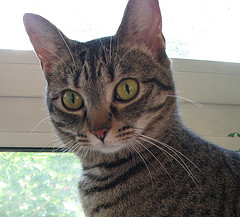
\includegraphics[width=1cm]{figures/cat1.png}};
    
    \coordinate (input2_c) at ($(input_bl) + (2*\inputPad + \imgSize * 1.5, \inputPad + \imgSize / 2)$);
    \node[inner sep=0pt] (input2) at (input2_c) {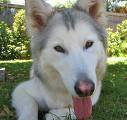
\includegraphics[width=1cm]{figures/dog.png}};
    
    \coordinate (input3_c) at ($(input_bl) + (\inputPad + \imgSize / 2, 2*\inputPad + \imgSize * 1.5)$);
    \node[inner sep=0pt] (input3) at (input3_c) {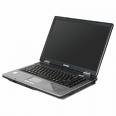
\includegraphics[width=1cm]{figures/laptop.png}};
    
    \coordinate (input4_c) at ($(input_bl) + (2*\inputPad + \imgSize * 1.5, 2*\inputPad + \imgSize * 1.5)$);
    \node[inner sep=0pt] (input4) at (input4_c) {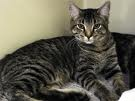
\includegraphics[width=1cm]{figures/cat2.png}};
    
    \coordinate (input_txt_c) at ($(input_bl) + (\inputPad * 1.5 + \imgSize, 3*\inputPad + 2*\imgSize + 0.1)$);
    \node[] (input_txt) at (input_txt_c) {Inputs};
    
    \coordinate (encoder_c) at ($(input_cr) + (2, 0)$);
    \node[draw, thick, inner sep=0.25cm, align=center, rounded corners, fill=blue!50] (encoder) at (encoder_c) {Encoder \\ Network};
    
    \coordinate (output_cl) at ($(encoder_c) + (2, 0)$);
    \coordinate (output_similar_bl) at ($(output_cl) + (0,0.125)$);
    \coordinate (output_similar_cl) at ($(output_similar_bl) + (0, \imgSize / 2 + \inputPad)$);
    \coordinate (output_similar_tr) at ($(output_similar_bl) + (2 * \imgSize + \inputPad * 3, \imgSize + 2 * \inputPad)$);
    \draw[thick, rounded corners, color=green] (output_similar_bl) rectangle (output_similar_tr);
    
    \coordinate (output_similar1_c) at ($(output_similar_bl) + (\inputPad + \imgSize / 2, \inputPad + \imgSize / 2)$);
    \node[inner sep=0pt] (output_similar1) at (output_similar1_c) {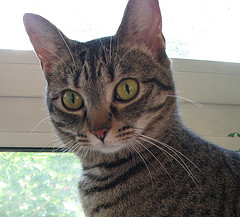
\includegraphics[width=1cm]{figures/cat1.png}};
    
    \coordinate (output_similar2_c) at ($(output_similar_bl) + (2*\inputPad + \imgSize * 1.5, \inputPad + \imgSize / 2)$);
    \node[inner sep=0pt] (output_similar2) at (output_similar2_c) {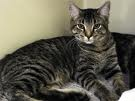
\includegraphics[width=1cm]{figures/cat2.png}};
    
    \coordinate (text_similar_c) at ($(output_similar_tr) + (0.25, -\imgSize / 2 - \inputPad)$);
    \node[anchor=west, color=green] at (text_similar_c) {Similar};
    
    \coordinate (output_unsimilar_bl) at ($(output_cl) - (0,0.125 + \imgSize + 2 * \inputPad)$);
    \coordinate (output_unsimilar_cl) at ($(output_unsimilar_bl) + (0, \imgSize / 2 + \inputPad)$);
    \coordinate (output_unsimilar_tr) at ($(output_unsimilar_bl) + (2 * \imgSize + \inputPad * 3, \imgSize + 2 * \inputPad)$);
    \draw[thick, rounded corners, color=red] (output_unsimilar_bl) rectangle (output_unsimilar_tr);
    
    \coordinate (output_unsimilar1_c) at ($(output_unsimilar_bl) + (\inputPad + \imgSize / 2, \inputPad + \imgSize / 2)$);
    \node[inner sep=0pt] (output_unsimilar1) at (output_unsimilar1_c) {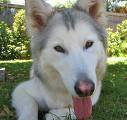
\includegraphics[width=1cm]{figures/dog.png}};
    
    \coordinate (output_unsimilar2_c) at ($(output_unsimilar_bl) + (2*\inputPad + \imgSize * 1.5, \inputPad + \imgSize / 2)$);
    \node[inner sep=0pt] (output_unsimilar2) at (output_unsimilar2_c) {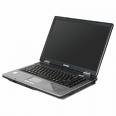
\includegraphics[width=1cm]{figures/laptop.png}};
    
    \coordinate (text_unsimilar_c) at ($(output_unsimilar_tr) + (0.25, -\imgSize / 2 - \inputPad)$);
    \node[anchor=west, color=red] at (text_unsimilar_c) {Not Similar};
    
    \draw[thick, ->] (input_cr) -- (encoder);
    \draw[thick, ->] (encoder.east) -- (output_similar_cl);
    \draw[thick, ->] (encoder.east) -- (output_unsimilar_cl);
    

\end{tikzpicture}
    \caption[Contrastive Learning]{The general contrastive learning task in the domain of image data. Different images are fed through an encoder network that predicts whether or not two images are similar or not. Images are from \textit{ImageNet} \cite{imagenet_cvpr09}.}
    \label{fig:contrastive_learning}
\end{figure}

As explained earlier labels can be created automatically using a self-supervised learning task. By combining self-supervised and contrastive learning it is possible to create a fully autonomous learning framework for similarities without the need for human annotation. This makes it possible to scale the training dataset to a much larger amount than in a fully supervised scenario. The way that we make use of this property is to create two augmented views from the same input and train the network to become invariant to those augmentations, meaning it will produce similar vectors for augmented views, but not for two completely unrelated views. This concept will be explained in more detail in Chapter \ref{chapter:claudio}.

\subsection{Transfer Learning}

Learning basic concepts first and applying those concepts to other tasks later on is an important part of deep learning research today. Transfer Learning can be seen as an extension to other learning paradigms that enables the transference of knowledge from one domain to another \cite{yang_zhang_dai_pan_2020}. A method for transfer learning of neural networks was proposed as early as 1993 by L. Y. Pratt \cite{NIPS1992_641} and is described in more detail in Algorithm \ref{alg:transfer}.

The basic idea behind transfer learning is that a neural network $f \circ g$, where $f$ is an arbitrary network architecture called encoder network that outputs vectors and $g$ is a small fully connected network called classification head that takes in the outputs of $f$ and produces predictions in the target domain. This network can be trained on a dataset $(X,y)$, containing training inputs $X$ and training outputs $y$, for example, images and the class of the depicted object in each image. During training the network $f$ learns general low-level features of image recognition while $g$ learns to map those features to the desired output $y$.

Now consider a second domain of image classification $(X',y')$ where $X'$ is of the same kind as $X$. Instead of training an entirely new network of the aforementioned structure, one can instead take the encoder network $f$ trained on the other dataset and transfer it into a new architecture $f \circ g'$ where $g'$ is a new classification head that takes in the outputs of $f$ and produces predictions in the new target domain $y'$. This is possible because the underlying data of both datasets share similar features, like edges and objects. The encoder network $f$ learns those features from the first dataset and transfers the knowledge to the second dataset. Shaha et al. \cite{shaha2018transfer} showed that using transfer learning on neural networks robust features can be transferred between multiple vision tasks. Figure \ref{fig:transfer_learning} shows this idea in a single diagram.

\begin{figure}[t]
    \centering
    \begin{tikzpicture}
    % global variables
    \definecolor{red}{RGB}{219, 50, 54}
    \definecolor{yellow}{RGB}{244, 194, 13}
    \definecolor{blue}{RGB}{72, 133, 237}
    \definecolor{green}{RGB}{60, 186, 84}
    \definecolor{orange}{RGB}{230, 122, 22}
    \definecolor{purple}{RGB}{145, 91, 145}
    \definecolor{grey}{RGB}{211, 211, 211}
    
    \tikzmath{
        \boxW = 11;
        \boxH = 2.5;
        \boxD = 0.25;
        \embeddingW = 3;
        \embeddingH = 1.5;
        \headW = 1.75;
        \pad = 2;
        \dArrow = 1;
    }
    
    % pretraining
    
    \coordinate (pretrain_bl) at (0,0);
    \coordinate (pretrain_c) at ($(pretrain_bl) + (\boxW / 2, \boxH / 2)$);
    \coordinate (pretrain_tr) at ($(pretrain_bl) + (\boxW, \boxH)$);
    \draw[rounded corners, thick] (pretrain_bl) rectangle (pretrain_tr);
    
    \coordinate (pretrain_text) at ($(pretrain_c) - (\boxW / 2 - 0.25, -0.75)$);
    \node[anchor=west, thick] at (pretrain_text) {1. Pre-training};
    
    \coordinate (data_p) at ($(pretrain_c) - (\boxW / 2 - \pad, 0)$);
    \node[align=left] (data_p_node) at (data_p) {$(X,y)$};
    
    \coordinate (embedding_p_cl) at ($(data_p) + (\dArrow,0)$);
    \coordinate (embedding_p_c) at ($(embedding_p_cl) + (\embeddingW / 2,0)$);
    \coordinate (embedding_p_cr) at ($(embedding_p_cl) + (\embeddingW,0)$);
    \coordinate (embedding_p_bl) at ($(embedding_p_cl) - (0,\embeddingH / 2)$);
    \coordinate (embedding_p_tr) at ($(embedding_p_bl) + (\embeddingW,\embeddingH)$);
    \coordinate (embedding_p_bc) at ($(embedding_p_c) - (0,\embeddingH / 2)$);
    \coordinate (embedding_p_tc) at ($(embedding_p_c) + (0,\embeddingH / 2)$);
    \draw[rounded corners, thick, fill=yellow!50] (embedding_p_bl) rectangle (embedding_p_tr);
    \node[align=center, thick] at (embedding_p_c) {Encoder $f$};
    
    \coordinate (head_p_cl) at ($(embedding_p_cr) + (0.5, 0)$);
    \coordinate (head_p_c) at ($(head_p_cl) + (\headW / 2, 0)$);
    \coordinate (head_p_cr) at ($(head_p_cl) + (\headW, 0)$);
    \coordinate (head_p_bl) at ($(head_p_cl) - (0, \embeddingH / 2)$);
    \coordinate (head_p_tr) at ($(head_p_bl) + (\headW, \embeddingH)$);
    
    \draw[rounded corners, thick, fill=red!50] (head_p_bl) rectangle (head_p_tr);
    \node[align=center, thick] at (head_p_c) {Head $g$};
    
    \coordinate (cost_p_c) at ($(head_p_cr) + (\dArrow-0.25, 0)$);
    \node[right, thick] (cost_p_node) at (cost_p_c) {$\mathcal{L}_{pre}$};
    
    \draw[->,thick] (data_p_node) -- (embedding_p_cl);
    \draw[->,thick] (embedding_p_cr) -- (head_p_cl);
    \draw[->,thick] (head_p_cr) -- (cost_p_node);
    
    
    % transfer
    
    \coordinate (transfer_bl) at ($(pretrain_bl) - (0, \boxH + \boxD)$);
    \coordinate (transfer_c) at ($(transfer_bl) + (\boxW / 2, \boxH / 2)$);
    \coordinate (transfer_tr) at ($(transfer_bl) + (\boxW, \boxH)$);
    \draw[rounded corners, thick] (transfer_bl) rectangle (transfer_tr);
    
    \coordinate (transfer_text) at ($(transfer_c) - (\boxW / 2 - 0.25, -0.75)$);
    \node[align=left, anchor=west, thick] at (transfer_text) {2. Transfer};
    
    \coordinate (data_t) at ($(transfer_c) - (\boxW / 2 - \pad, 0)$);
    \node[align=left] (data_t_node) at (data_t) {$(X',y')$};
    
    \coordinate (embedding_t_cl) at ($(data_t) + (\dArrow,0)$);
    \coordinate (embedding_t_c) at ($(embedding_t_cl) + (\embeddingW / 2,0)$);
    \coordinate (embedding_t_cr) at ($(embedding_t_cl) + (\embeddingW,0)$);
    \coordinate (embedding_t_bl) at ($(embedding_t_cl) - (0,\embeddingH / 2)$);
    \coordinate (embedding_t_tr) at ($(embedding_t_bl) + (\embeddingW,\embeddingH)$);
    \coordinate (embedding_t_bc) at ($(embedding_t_c) - (0,\embeddingH / 2)$);
    \coordinate (embedding_t_tc) at ($(embedding_t_c) + (0,\embeddingH / 2)$);
    \draw[rounded corners, thick, fill=yellow!50] (embedding_t_bl) rectangle (embedding_t_tr);
    \node[align=center, thick] at (embedding_t_c) {Encoder $f$ \\ (frozen)};
    
    \coordinate (head_t_cl) at ($(embedding_t_cr) + (0.5, 0)$);
    \coordinate (head_t_c) at ($(head_t_cl) + (\headW / 2, 0)$);
    \coordinate (head_t_cr) at ($(head_t_cl) + (\headW, 0)$);
    \coordinate (head_t_bl) at ($(head_t_cl) - (0, \embeddingH / 2)$);
    \coordinate (head_t_tr) at ($(head_t_bl) + (\headW, \embeddingH)$);
    \coordinate (head_t_bc) at ($(head_t_c) - (0, \embeddingH / 2)$);
    
    \draw[rounded corners, thick, fill=green!50] (head_t_bl) rectangle (head_t_tr);
    \node[align=center, thick] at (head_t_c) {Head $g'$};
    
    \coordinate (cost_t_c) at ($(head_t_cr) + (\dArrow-0.25, 0)$);
    \node[right, thick] (cost_t_node) at (cost_t_c) {$\mathcal{L}_{transfer}$};
    
    \draw[->,thick] (data_t_node) -- (embedding_t_cl);
    \draw[->,thick] (embedding_t_cr) -- (head_t_cl);
    \draw[->,thick] (head_t_cr) -- (cost_t_node);
    
    % finetune
    
    % \coordinate (finetune_bl) at ($(transfer_bl) - (0, \boxH + \boxD)$);
    % \coordinate (finetune_c) at ($(finetune_bl) + (\boxW / 2, \boxH / 2)$);
    % \coordinate (finetune_tr) at ($(finetune_bl) + (\boxW, \boxH)$);
    % \draw[rounded corners, thick] (finetune_bl) rectangle (finetune_tr);
    
    % \coordinate (finetune_text) at ($(finetune_c) - (\boxW / 2 - 0.25, -0.75)$);
    % \node[align=left, anchor=west, thick] at (finetune_text) {3. Fine-tuneing};
    
    % \coordinate (data_f) at ($(finetune_c) - (\boxW / 2 - \pad, 0)$);
    % \node[align=left] (data_f_node) at (data_f) {$(X',y'$};
    
    % \coordinate (embedding_f_cl) at ($(data_f) + (\dArrow,0)$);
    % \coordinate (embedding_f_c) at ($(embedding_f_cl) + (\embeddingW / 2,0)$);
    % \coordinate (embedding_f_cr) at ($(embedding_f_cl) + (\embeddingW,0)$);
    % \coordinate (embedding_f_bl) at ($(embedding_f_cl) - (0,\embeddingH / 2)$);
    % \coordinate (embedding_f_tr) at ($(embedding_f_bl) + (\embeddingW,\embeddingH)$);
    % \coordinate (embedding_f_bc) at ($(embedding_f_c) - (0,\embeddingH / 2)$);
    % \coordinate (embedding_f_tc) at ($(embedding_f_c) + (0,\embeddingH / 2)$);
    % \draw[rounded corners, thick, fill=yellow!50] (embedding_f_bl) rectangle (embedding_f_tr);
    % \node[align=center, thick] at (embedding_f_c) {Encoder};
    
    % \coordinate (head_f_cl) at ($(embedding_f_cr) + (0.5, 0)$);
    % \coordinate (head_f_c) at ($(head_f_cl) + (\headW / 2, 0)$);
    % \coordinate (head_f_cr) at ($(head_f_cl) + (\headW, 0)$);
    % \coordinate (head_f_bl) at ($(head_f_cl) - (0, \embeddingH / 2)$);
    % \coordinate (head_f_tr) at ($(head_f_bl) + (\headW, \embeddingH)$);
    % \coordinate (head_f_tc) at ($(head_f_c) + (0, \embeddingH / 2)$);
    
    % \draw[rounded corners, thick, fill=green!50] (head_f_bl) rectangle (head_f_tr);
    % \node[align=center, thick] at (head_f_c) {$Head_t$};
    
    % \coordinate (cost_f_c) at ($(head_f_cr) + (\dArrow, 0)$);
    % \node[align=center, thick] (cost_f_node) at (cost_f_c) {$Cost_t$};
    
    % \draw[->,thick] (data_f_node) -- (embedding_f_cl);
    % \draw[->,thick] (embedding_f_cr) -- (head_f_cl);
    % \draw[->,thick] (head_f_cr) -- (cost_f_node);
    
    % % 
    
    \draw[|->,thick] ($(embedding_p_bc) - (0, 0.15)$) -- ($(embedding_t_tc) + (0, 0.15)$);
    % \draw[|->,thick] ($(embedding_t_bc) - (0, 0.15)$) -- ($(embedding_f_tc) + (0, 0.15)$);
    % \draw[|->,thick] ($(head_t_bc) - (0, 0.15)$) -- ($(head_f_tc) + (0, 0.15)$);
    
    
\end{tikzpicture}
    \caption[Transfer Learning Overview]{The two stages of transfer learning. The encoder network is transferred after pre-training from the first domain to the second domain. Head is usually a small fully-connected network.}
    \label{fig:transfer_learning}
\end{figure}

\begin{algorithm}
    \caption{A supervised transfer-learning framework}
    \label{alg:transfer}
    
    \begin{algorithmic}[1]
        \State \textbf{Input:} encoder network $f$, classification heads $g$ and $g'$, trainable parameters  $\boldsymbol{\theta}_f$, $\boldsymbol{\theta}_g$, $\boldsymbol{\theta}_{g'}$, pre-training dataset $(X,Y)$, transfer dataset $(X', Y')$, loss functions $\mathcal{L}_{pre}$, $\mathcal{L}_{transfer}$, learning rate $\alpha$
        \State Randomly initialize $\theta_f$ and $\theta_g$ \Comment{Stage 1: Pre-training}
        \While{not done}
            \State sample minibatch $(\boldsymbol{x},\boldsymbol{y}) \sim (X,Y)$
            \State compute $\mathcal{L}_{pre}$ from $g(f(\boldsymbol{x}))$ and $\boldsymbol{y}$
            \State $\boldsymbol{\theta}_{f \circ g} \gets \boldsymbol{\theta}_{f \circ g} - \alpha \nabla_{\theta_{f \circ g}} \mathcal{L}_{pre}$ \Comment{$\theta_{f \circ g}$ is the concatenation of $\theta_f$ and $\theta_g$}
        \EndWhile
        \State Randomly initialize $\boldsymbol{\theta}_{g'}$ \Comment{Stage 2: Transfer}
        \State freeze $\boldsymbol{\theta}_f$
        \While{not done}
            \State sample minibatch $(\boldsymbol{x'},\boldsymbol{y'}) \sim (X',Y')$
            \State compute $\mathcal{L}_{transfer}$ from $g'(f(\boldsymbol{x'}))$ and $\boldsymbol{y'}$
            \State $\boldsymbol{\theta}_{f \circ g'} \gets \boldsymbol{\theta}_{f \circ g'} - \alpha \nabla_{\theta_{f \circ g'}} \mathcal{L}_{transfer}$
        \EndWhile
        \State \textbf{return} $f \circ g'$
    \end{algorithmic}
\end{algorithm}

The need for transfer learning arises when the domain to be transferred to has little or no training data or when making mistakes in unknown situations is expensive, as is the case in self-driving cars \cite{fellicious2018transfer}. In our case transfer learning will be used to take the latent representations learned from self-supervision and apply them to downstream supervised tasks with low amounts of available training data. This approach is very common and has shown good results in recent years (\cite{dosovitskiy2015discriminative, oord2019representation, bachman2019learning}). A thorough survey of modern transfer learning techniques can be found in Pan et al. (2010) \cite{pan2010transfer}.

\section{Self-Supervised Loss Functions}\label{sec:ss_loss}

Expressing the similarity of entities in the real world is effortless for humans. Be it sound events, images, words, all can easily be compared to other entities of that same domain. For machines this task is different. Since understanding similarity involves a lot of contextual knowledge that machines do not possess, the question if two entities are similar becomes much harder to answer for an algorithm. Self-supervised learning tries to bridge that knowledge gap by transforming complex real-world entities into a more simple representation that a machine can process. This representation is usually in the form of vectors. There are many ways of calculating the similarity of two vectors. Equations \ref{eq:euclidian_distance}, \ref{eq:manhattan_distance}, \ref{eq:cosine_similarity} describe three of the most common distance measures for vectors: \textit{euclidian distance}, \textit{manhattan distance} and \textit{cosine similarity}. Note that $s_{cosine}(p,q)$ is actually a similarity metric where $1$ is equal to the most similarity and $-1$ to the least similarity. One can simply convert it to a distance: $d_{cosine}(p,q) = 1 - s_{cosine}(p,q)$, but this is commonly not used. It is called cosine similarity because the result matches the cosine of the angle between the two vectors.

\begin{equation}
   d_{euclidian}(\mathbf{p},\mathbf{q}) = \lVert \mathbf{p,q} \rVert_2 = \sum_{i=1}^{n} \sqrt{(p_i - q_i)^2},\;\;\; \in \mathbb{R}^+
   \label{eq:euclidian_distance}
\end{equation}

\begin{equation}
   d_{manhattan}(\mathbf{p},\mathbf{q}) = \lVert \mathbf{p,q} \rVert_1 = \sum_{i=1}^{n} |p_i - q_i|,\;\;\;\;\;\;\; \in \mathbb{R}^+
   \label{eq:manhattan_distance}
\end{equation}

\begin{equation}
   s_{cosine}(\mathbf{p},\mathbf{q}) = \frac{\mathbf{p} \cdot \mathbf{q}}{\lVert \mathbf{p} \rVert \lVert \mathbf{q} \rVert} = \frac{\sum_{i=1}^{n}p_i q_i}{\sqrt{\sum_{i=1}^{n}p_i^2} \sqrt{\sum_{i=1}^{n}q_i^2}},\;\;\; \in [-1,1]
   \label{eq:cosine_similarity}
\end{equation}

In the following subsections we look at two loss functions that implement these distance metrics to give self-supervised algorithms a way to learn good vector representations. A loss function is a mathematical way of expressing a certain target for a neural network to train towards to. Stochastic gradient descent works by minimizing this loss function over time using stochastically sampled batches of data.

\subsection{Triplet Margin Loss}\label{subsec:tirplet}

As the name suggests the \textit{Triplet Margin Loss} requires triplets of input data points. These data points are called anchor $A$, positive $P$ and negative $N$. The positive is supposed to be of high similarity to the anchor, whereas the negative is supposed to be of no or low similarity to the anchor. Equation \ref{eq:triplet_loss} describes this notion in mathematical terms.

\begin{equation}
   \mathcal{L}(A,P,N) = max\Big( \lVert f(A), f(P) \rVert_2 - \lVert f(A), f(N) \rVert_2 + \alpha, 0 \Big)
   \label{eq:triplet_loss}
\end{equation}

This loss becomes larger the higher the distance between $A$ and $P$ and the lower the distance between $A$ and $N$. 
Here the euclidean distance is used but any distance function can be applied. By minimizing this loss the network is forced to learn representations that increase the distance to $N$ and decrease the distance to $P$, relative to $A$. Figure \ref{fig:triplet_training} shows how such representations could look like before and after learning. Note that usually a margin hyperparameter $\alpha$ is used to better distinguish positive from negatives, it’s effect can be seen in \ref{subfig:triplet_after}.

\begin{figure}[h!]
  \centering
  \begin{subfigure}[b]{0.49\linewidth}
    \centering
    \scalebox{0.75}{\begin{tikzpicture}
    \definecolor{red}{RGB}{219, 50, 54}
    \definecolor{yellow}{RGB}{244, 194, 13}
    \definecolor{blue}{RGB}{72, 133, 237}
    \definecolor{green}{RGB}{60, 186, 84}
    \definecolor{orange}{RGB}{230, 122, 22}
    \definecolor{purple}{RGB}{145, 91, 145}
    \definecolor{grey}{RGB}{211, 211, 211}
    
    \tikzstyle{blue}=[circle,fill,inner sep=4pt,color=blue!50]
    \tikzstyle{red}=[fill,inner sep=6pt,color=red!50]
    \tikzstyle{yellow}=[inner sep=3pt,color=yellow!50, regular polygon,regular polygon sides=3, fill]
    
    \tikzmath {
        \dbox = 0.75;
    }
    
    \begin{axis}[
        axis lines=middle,
        grid=major,
        xmin=0,
        xmax=4,
        ymin=0,
        ymax=4,
        tick style={very thick},
        xticklabels={,,},
        yticklabels={,,}
    ]
    \node[circle, thick, draw, inner sep=40pt, fill=grey] at (axis cs:2,2) {};
    \node[circle, thick, draw, inner sep=50pt] at (axis cs:2,2) {};
    \node[blue] at (axis cs:2,2) {};
    \node[blue] at (axis cs:1.7,1) {};
    \node[blue] at (axis cs:2.9,2.7) {};
    \node[blue] at (axis cs:2.7,1.3) {};
    \node[red] at (axis cs:1.5,1.9) {};
    \node[yellow] at (axis cs:1,3) {};
    \end{axis}

\end{tikzpicture}}
    \caption{Before training}
  \end{subfigure}
  \begin{subfigure}[b]{0.49\linewidth}
    \centering
    \scalebox{0.75}{\begin{tikzpicture}
    \definecolor{red}{RGB}{219, 50, 54}
    \definecolor{yellow}{RGB}{244, 194, 13}
    \definecolor{blue}{RGB}{72, 133, 237}
    \definecolor{green}{RGB}{60, 186, 84}
    \definecolor{orange}{RGB}{230, 122, 22}
    \definecolor{purple}{RGB}{145, 91, 145}
    \definecolor{grey}{RGB}{211, 211, 211}
    
    \tikzstyle{blue}=[circle,fill,inner sep=4pt,color=blue!50]
    \tikzstyle{red}=[fill,inner sep=6pt,color=red!50]
    \tikzstyle{yellow}=[inner sep=3pt,color=yellow!50, regular polygon,regular polygon sides=3, fill]
    
    \tikzmath {
        \dbox = 0.75;
    }
    
    \begin{axis}[
        axis lines=middle,
        grid=major,
        xmin=0,
        xmax=4,
        ymin=0,
        ymax=4,
        tick style={very thick},
        xticklabels={,,},
        yticklabels={,,}
    ]
    \node[circle, thick, draw, inner sep=25pt, fill=grey] at (axis cs:2,2) {};
    \node[circle, thick, draw, inner sep=35pt] at (axis cs:2,2) {};
    \node[blue] at (axis cs:2,2) {};
    \node[blue] at (axis cs:1.7,1.4) {};
    \node[blue] at (axis cs:2.3,2.1) {};
    \node[blue] at (axis cs:2.4,1.7) {};
    \node[red] at (axis cs:0.8,1.7) {};
    \node[yellow] at (axis cs:1.8,3.4) {};
    
    \node[] (margin) at (axis cs:3,3.5) {Margin};
    \draw[->, thick] (margin) -- (axis cs:2.3,3);
    
    \end{axis}

\end{tikzpicture}}
    \caption{After training}
    \label{subfig:triplet_after}
  \end{subfigure}
  \caption[Triplet loss example]{\textbf{Left}: Potential latent representations of input data points before training. They are mapped randomly into the latent space with no clear boundary. \textbf{Right}: After training with the triplet loss representations of the same class are pulled together while other classes are pushed apart. A margin zone, controlled by the margin hyperparameter, separates uncorrelated samples from correlated ones.}
  \label{fig:triplet_training}
\end{figure}

Since its first proposal in 2009 by Weinberger et al. \cite{Weinberger09distancemetric} the triplet loss is one of the most used loss functions for self-supervised learning. One major drawback of triplet loss is the fact that for randomly chosen inputs the loss approaches 0 very quickly since for most randomly chosen inputs $d(A,N) > d(A,P)$. These examples become irrelevant for training once this threshold is reached. Therefore a novel technique called online hard negative triplet mining was introduced by Schroff et al. \cite{Schroff_2015}. Online hard negative triplet mining ensures consistently increasing difficulty of triplets as the network trains but it requires one to track all comparisons and build up a memory bank that stores previous results. This is very inefficient and therefore more modern approaches try to replace it with simpler and more effective methods.

\subsection{Normalized Temperature-Scaled Cross Entropy}\label{subsec:ntxent}

\gls{ntxent} loss was first proposed by Sohn in 2016 \cite{sohn2016improved} but was coined \textit{NT-Xent} only recently by Chen et al. \cite{chen2020simple}. It was found that triplet loss functions "often suffer from slow convergence and poor local optima, partially due to that the loss function employs only one negative example while not interacting with the other negative classes per each update" \cite{sohn2016improved}. To deal with this issue, \gls{ntxent} loss takes one positive example and multiple negative examples per training step. The loss is defined as follows:

\begin{equation}
   \ell(i,j) = -\log \tfrac{\exp(s_{i,j}/\tau)}{\sum_{k=1}^{2N} \mathbb{1}_{[k \neq i]} \exp(s_{i,k} / \tau)}
   \label{eq:ntxent_loss}
\end{equation}

Here $\mathbb{1}$ is the indicator function which evaluates to 1 only if $k \neq i$ (the similarity of an input to itself is always 1 and therefore discarded). Usually for this loss $s_{i,j}$ denotes the cosine similarity of two vector representations but any similarity measure can be used. $\tau$ is a temperature hyperparameter used to expand the range of the exponential. This helps in stabilizing training. One can clearly see that this loss closely resembles a softmax distribution trying to maximize agreement of similar pairs.

The \gls{ntxent} loss has gained a lot of popularity since the release of \gls{simclr} (\cite{tu2020aag}, \cite{giorgi2020declutr}, \cite{apoorv2020speechembeddings}), mainly due to it scaling well to large batch sizes. This can be leveraged by ever-increasing memory sizes in deep learning specific processing units and better distribution strategies. Because of this and the fact that it does not require explicit example mining, we believe that \gls{ntxent} will replace triplet loss in most applications for self-supervised learning.

\section{Neural Networks for Audio Data}\label{sec:nn_audio}

Vibration is a repetitive motion relative to an equilibrium point \cite{nopdanai2017vibration}. Sound is therefore the vibration of molecules, usually air molecules, that is picked up by our ears and transformed into electrical signals that are then perceived by our brains. A similar thing happens when we try to digitize sound. First, a transducer converts sound into an electrical signal. This continuous signal is then transformed into a discrete signal by an \textit{Analog-to-digital converter} (ADC). The signal is periodically quantized to create a stream of samples. This way of digitally representing an analog signal is called \gls{pcm}.

Quantization maps a certain amplitude of an analog signal to a digital integer value, represented as a sequence of bits. The higher the number of bits per integer, also known as the bit-depth, the lower the error introduced by quantization. The frequency of this quantization is called the sampling frequency, usually denoted in kHz. The sampling frequency and the quantization error are the major factors of the quality of the digital audio signal. The higher the sampling rate and the bit-depth, the better the quality, but the more space is required to store the audio. In today's recordings, a sampling rate of 44.1kHz and a bit-depth of 16bit is most commonly used.

The resulting sequence of integer values can then be fed into a neural network for further processing. Unfortunately, classical network architectures are practically limited by the number of input values. A fully connected network with a single hidden layer consisting of 2048 hidden neurons would require more than 270 million weights to process a 3-second audio clip sampled at 44.1kHz. Nowadays it is common to make use of the time-series quality of audio data and use architectures that are specialized in this domain as shown in Lezhenin et al. \cite{lezhenin2019urban} or Zhao et al. \cite{zhao2019speechtransformer}.

Another common approach is to exploit the local dependency of samples in an audio signal by first applying convolutional layers to reduce the input dimensionality while preserving as much information as possible. It was also found that fully convolutional networks can produce remarkable results without any need for time-dependent computation \cite{fu2017raw}. Most of the architectures used today are combinations of the three. All of these network types can be used with one-dimensional data, as most recently shown in \cite{dhariwal2020jukebox} but are more often used with two-dimensional inputs. We therefore always transform our input signal using the Short-time Fourier transform described in \ref{sec:fft} to create a two-dimensional matrix where $x_{i,j}$ represents the $i$th Fourier coefficient at timestep $j$. This process reduces the number of timesteps significantly and thus reduces the size of the networks. The final goal is to produce a single vector that best describes the data it is trying to represent. In the remaining subsections, we dive deeper into the theory of all three architectures.

\subsection{Convolutional Neural Network}

The kernel convolution for two-dimensional inputs used in a \gls{cnn} is defined in Equation \ref{eq:kernel_convolution} for discrete inputs.

\begin{equation}
   g(x,y) = \omega * f(x,y) = \sum_{dx=-a}^a \sum_{dy=-b}^b \omega (dx,dy) f(x + dx, y + dy)
   \label{eq:kernel_convolution}
\end{equation}

Here $\omega$ is the kernel matrix ranging from $[-a,-b]$ to $[a,b]$. $f(x,y)$ is a pixel of an input image $f$. The kernel $\omega$ is shifted over the two dimensions $x$ and $y$ of $f$ and repeatedly multiplied with a part of the input image centered around $f(x,y)$. In the end, the resulting output pixels $g(x,y)$ are put back together to produce a filtered output $g$. Note that the kernel does not have to move one pixel at a time but can move any desired distance per step. This distance is called stride. If the stride is larger than 1, the size of the output image is reduced.

The kernel matrix is composed of learnable weights. Training such a network using backpropagation was first proposed by LeCun et al. in 1989 \cite{lecun1989backpropagation} and has since seen magnificent results in image-related tasks but also in other domains like audio.

The advantage of this compared to fully connected layers is that the size of the kernel matrix is not determined by the size of the input, so larger input matrices do not necessarily require more trainable weights. This kernel convolution is usually followed by a non-linear activation function. The most prominent activation function for \glspl{cnn} is the \gls{relu}, proposed by Hinton et al. \cite{icml2010relu} and denoted in Equation \ref{eq:relu}.

\begin{equation}
   f(x)= 
    \begin{cases}
        x,& \text{if } x\ge 0\\
        0,              & \text{otherwise}
    \end{cases}
   \label{eq:relu}
\end{equation}

Due to its non-saturating gradient, it accelerates stochastic gradient-based learning, as opposed to alternatives like sigmoid or tanh \cite{NIPS2012_4824}. Note that this comes with a drawback that neurons can potentially die out, meaning they can enter states that produce negative outputs for all inputs and therefore never produce any gradient other than 0. There exist many alternatives that mitigate this issue, like the \textit{leaky ReLU} that assigns small values for inputs lower than zero, so therefore always producing some gradient. In practice, however, this problem is often ignored since large networks can cope with a few dead neurons.

To further reduce dimensionality to subsequent layers, \glspl{cnn} commonly employ pooling after each convolution step. As evaluated in Scherer et al. \cite{scherer2010maxpool}, max-pooling, which returns the maximum value of a given receptive field, is vastly superior to other pooling techniques. Figure \ref{fig:cnn} shows a single stack of convolution, \gls{relu} and max-pooling layers. In practice, there are many such stacks combined to produce a condensed set of features that best describes the given input and that can be used for further downstream tasks such as classification.

\glspl{cnn} for time series classification were first introduced by Wang et al. in 2017 \cite{wang2016time}. They form a strong baseline, that is difficult to beat on arbitrary data without heavy fine-tuning to a specific task. Even though \glspl{cnn} are extremely powerful in finding local dependencies in data, they fail to learn dependencies that are far apart. This is due to the kernel convolution only looking at specific areas of the input one at a time.

\begin{figure}[!h]
    \centering
    \begin{tikzpicture}
    \definecolor{red}{RGB}{219, 50, 54}
    \definecolor{yellow}{RGB}{244, 194, 13}
    \definecolor{blue}{RGB}{72, 133, 237}
    \definecolor{green}{RGB}{60, 186, 84}
    \definecolor{orange}{RGB}{230, 122, 22}
    \definecolor{purple}{RGB}{145, 91, 145}
    \definecolor{grey}{RGB}{211, 211, 211}
    
    \tikzmath {
        \boxW = 2;
        \boxH = 2;
        \dH = 0.1;
        \dW = 0.1;
        \convW = 2;
        \convH = 2;
        \dLayer = 3.75;
        \shrink = 0.8;
        \reluW = 0.5;
        \recD = 0.5;
        \recPad = 0.25;
    }
    
    \coordinate (input_bl) at (0,0);
    \coordinate (input_tr) at ($(input_bl) + (\boxW, \boxH)$);
    
    \coordinate (input_rec_bl) at ($(input_bl) + (\boxW - \recD - \recPad, \recPad)$);
    \coordinate (input_rec_tr) at ($(input_rec_bl) + (\recD, \recD)$);
    
    \draw[thick] (input_rec_bl) rectangle (input_rec_tr);
    
    \draw[thick] (input_bl) rectangle (input_tr);
    
    \foreach \i in {5,...,1}
    {
        \coordinate (kernel_bl) at ($(input_bl) + (\dLayer - \dW * \i, \dH * \i)$);
        \coordinate (kernel_tr) at ($(kernel_bl) + (\convW * \shrink, \convH * \shrink)$);
        \draw[thick, fill=white] (kernel_bl) rectangle (kernel_tr);
    }
    
    
    \coordinate (conv_bl) at ($(input_bl) + (\dLayer, 0)$);
    \coordinate (conv_tr) at ($(conv_bl) + (\convW * \shrink, \convH * \shrink)$);
    \coordinate (conv_cr) at ($(conv_bl) + (\convW * \shrink, \boxH / 2)$);
    \draw[thick, fill=white] (conv_bl) rectangle (conv_tr);
    
    \coordinate (input_rec_dest) at ($(conv_bl) + (\convW * \shrink - 0.25, 0.25)$);
    \coordinate (conv_rec_bl) at ($(conv_tr) - (0.5, 0.5)$);
    \coordinate (conv_rec_tr) at ($(conv_rec_bl) + (0.35, 0.35)$);
    \draw[thick] (conv_rec_bl) rectangle (conv_rec_tr);
    
    
    
    \coordinate (relu_bl)  at ($(conv_bl) + (2.5, 0)$);
    \coordinate (relu_c)  at ($(relu_bl) + (\reluW / 2, \boxH / 2)$);
    \coordinate (relu_tr) at ($(relu_bl) + (\reluW, \boxH)$);
    \coordinate (relu_lc) at ($(relu_bl) + (0, \boxH / 2)$);
    \node[rotate=90] at (relu_c) {ReLU};
    
    \draw[thick] (relu_bl) rectangle (relu_tr);
    %\draw[|->, thick] ($(conv_cr) + (0.15, 0)$) -- ($(relu_lc) - (0.15, 0)$);
    
    \foreach \i in {5,...,1}
    {
        \coordinate (pool_bl) at ($(relu_bl) + (2 - \dW * \i, \dH * \i)$);
        \coordinate (pool_tr) at ($(pool_bl) + (\convW * \shrink * \shrink, \convH * \shrink * \shrink)$);
        \draw[thick, fill=white] (pool_bl) rectangle (pool_tr);
    }
    
    \coordinate (pool_bl) at ($(relu_bl) + (2, 0)$);
    \coordinate (pool_tr) at ($(pool_bl) + (\convW * \shrink * \shrink, \convH * \shrink * \shrink)$);
    \coordinate (pool_cr) at ($(pool_bl) + (\convW * \shrink * \shrink, \boxH / 2)$);
    \draw[thick, fill=white] (pool_bl) rectangle (pool_tr);
    
    
    \coordinate (conv_rec_dest) at ($(pool_tr) - (0.25, 0.25)$);
    
    \draw[thick, dashed] (input_rec_bl) -- (input_rec_dest);
    \draw[thick, dashed] (input_rec_tr) -- (input_rec_dest);
    
    \draw[thick, dashed] (conv_rec_bl) -- (conv_rec_dest);
    \draw[thick, dashed] (conv_rec_tr) -- (conv_rec_dest);
    
    \node[] at ($(conv_bl) - (0.8, 0.3)$)  {Convolution};
    \node[] at ($(pool_bl) - (0.8, 0.3)$) {Pooling};
    
\end{tikzpicture}
    \caption[Convolution, ReLU and max-pool overview]{A single stack of a convolutional, ReLU and max-pooling layer. First $n$ filters are convoluted with the input, resulting in $n$ output channels. All output channels are then fed through a ReLU and finally max-pooled to further decrease the output size.}
    \label{fig:cnn}
\end{figure}

\subsection{Long Short-Term Memory}\label{subsec:lstm}

\gls{lstm} is a type of \gls{rnn} used for processing time-series data. It was first proposed by Hochreiter and Schmidhuber in 1997 \cite{hochreiter1997lstm}. A common problem for pre-LSTM \glspl{rnn} was to learn long-term temporal dependencies due to exponentially decaying gradients over time. To mitigate this issue \gls{lstm} employs a series of gates, described in Equation \ref{eq:lstm_forget} to \ref{eq:lstm_hidden}, that regulate the memory state of a cell.

\begin{equation}
   \mathbf{f}_t = \sigma (\mathbf{W}_f \mathbf{x}_t + \mathbf{U}_f \mathbf{c}_{t-1} + \mathbf{b}_f)
   \label{eq:lstm_forget}
\end{equation}

\begin{equation}
   \mathbf{i}_t = \sigma (\mathbf{W}_i \mathbf{x}_t + \mathbf{U}_i \mathbf{c}_{t-1} + \mathbf{b}_i)
   \label{eq:lstm_input}
\end{equation}

\begin{equation}
   \mathbf{o}_t = \sigma (\mathbf{W}_o \mathbf{x}_t + \mathbf{U}_o \mathbf{c}_{t-1} + \mathbf{b}_o)
   \label{eq:lstm_output}
\end{equation}

\begin{equation}
   \mathbf{c}_t = \mathbf{f}_t \circ \mathbf{c}_{t-1} + \mathbf{i}_t \circ tanh (\mathbf{W}_c \mathbf{x}_t + \mathbf{b}_c)
   \label{eq:lstm_context}
\end{equation}

\begin{equation}
   \mathbf{h}_t = \mathbf{o}_t \circ tanh (\mathbf{c}_t)
   \label{eq:lstm_hidden}
\end{equation}

Here $\sigma$ denotes the sigmoid function and $\circ$ denotes the element-wise vector multiplication. $\mathbf{x}_t \in \mathbb{R}^d$ is the input at time-step $t$, $ \mathbf{h}_t \in \mathbb{R}^h$ is the outputted hidden state at timestep $t$. $\mathbf{W}$, $\mathbf{U} \in \mathbb{R}^{h \times d}$ are traininable weights and $\mathbf{b} \in \mathbb{R}^h$ are trainable biases. $\mathbf{f}_t, \mathbf{i}_t, \mathbf{o}_t \in \mathbb{R}^h$ are intermediate vectors called gates. Figure \ref{fig:lstm_cell} shows how the different gates interact. At its core the cell state is described by Equation \ref{eq:lstm_context}: a new state $ \mathbf{c}_t$ is the sum of two terms. The first term $\mathbf{f}_t \circ  \mathbf{c}_{t-1}$ includes the forget gate $ \mathbf{f}_t$, which regulates when old state should be forgotten, while the second term $ \mathbf{i}_t \circ tanh ( \mathbf{W}_c  \mathbf{x}_t +  \mathbf{b}_c)$ includes the input gate $ \mathbf{i}_t$, which regulates when new information should be remembered.

\begin{figure}[!h]
    \centering
    \begin{tikzpicture}
    \definecolor{red}{RGB}{219, 50, 54}
    \definecolor{yellow}{RGB}{244, 194, 13}
    \definecolor{blue}{RGB}{72, 133, 237}
    \definecolor{green}{RGB}{60, 186, 84}
    \definecolor{orange}{RGB}{230, 122, 22}
    \definecolor{purple}{RGB}{145, 91, 145}
    \definecolor{grey}{RGB}{211, 211, 211}
    
    \tikzmath {
        \cellW = 9;
        \cellH = 4.5;
        \dSigmaW = 1.5;
        \dSigmaH = 0.5;
        \pad = 0.6;
    }
    
    \tikzstyle{a}=[thick,draw, minimum width=1cm, minimum height=0.5cm, fill=yellow!50]
    \tikzstyle{b}=[shape=circle,thick,draw,minimum size=0.5cm, fill=red!50]
    \tikzstyle{c}=[shape=rectangle,rounded corners,thick,draw,minimum height=0.5cm, fill=red!50]
    
    \coordinate (cell_bl) at (0,0);
    \coordinate (cell_tr) at ($(cell_bl) + (\cellW, \cellH)$);
    \draw[thick, rounded corners, fill=green!50] (cell_bl) rectangle (cell_tr);
    
    \coordinate (sigma_ft_c) at ($(cell_bl) + (\pad + 0.2, \pad + \dSigmaH)$);
    \node[a] (sigma_ft) at (sigma_ft_c) {\Large $\sigma$};
    
    \coordinate (sigma_it_c) at ($(sigma_ft) + (\dSigmaW, 0)$);
    \node[a] (sigma_it) at (sigma_it_c) {\Large $\sigma$};
    
    \coordinate (tanh_ct_c) at ($(sigma_it) + (\dSigmaW, 0)$);
    \node[a] (tanh_ct) at (tanh_ct_c) {$tanh$};
    
    \coordinate (sigma_ot_c) at ($(tanh_ct_c) + (\dSigmaW, 0)$);
    \node[a] (sigma_ot) at (sigma_ot_c) {\Large $\sigma$};
    
    \coordinate (ct_mul_c) at ($(sigma_ft_c) + (0, \cellH - 2 * \pad - \dSigmaH)$);
    \node[b] (ct_mul) at (ct_mul_c) {$\times$};
    
    \path let \p1=(tanh_ct_c),\p2=(ct_mul_c) in coordinate (ct_plus_c) at (\x1,\y2);
    \node[b] (ct_plus) at (ct_plus_c) {$+$};
    
    \coordinate (ct_mul_it_c) at ($(tanh_ct_c) + (0, 1.2)$);
    \node[b] (ct_mul_it) at (ct_mul_it_c) {$\times$};
    
    \coordinate (ot_mul_c) at ($(sigma_ot_c) + (\dSigmaW, 1.2)$);
    \node[b] (ot_mul) at (ot_mul_c) {$\times$};
    
    \coordinate (ot_tanh_c) at ($(ot_mul_c) + (0, 0.8)$);
    \node[c] (ot_tanh) at (ot_tanh_c) {$tanh$};
    
    \path let \p1=(cell_bl),\p2=(ct_mul_c) in coordinate (c_input_border) at (\x1,\y2);
    \coordinate (c_input_c) at ($(c_input_border) - (1,0)$);
    \node[] (c_input) at (c_input_c) {$c_{t-1}$};
    
    \coordinate (h_input_c) at ($(cell_bl) + (-1, \pad)$);
    \node[] (h_input) at (h_input_c) {$h_{t-1}$};
    
    \coordinate (x_input_c) at ($(cell_bl) + (0.5, -0.75)$);
    \node[] (x_input) at (x_input_c) {$x_t$};
    
    \coordinate (h_output1_c) at ($(h_input_c) + (1 + \cellW + 1, 0)$);
    \node[] (h_output1) at (h_output1_c) {$h_t$};
    
    \coordinate (c_output_c) at ($(c_input_c) + (1 + \cellW + 1, 0)$);
    \node[] (c_output) at (c_output_c) {$c_t$};
    
    \coordinate (h_output2_c) at ($(cell_tr) + (-0.75, 0.75)$);
    \node[] (h_output2) at (h_output2_c) {$h_t$};
    
    \draw[thick] (c_input) -- (ct_mul);
    \draw[thick] (ct_mul) -- (ct_plus);
    \draw[thick, ->] (sigma_ft) -- (ct_mul);
    \draw[thick, ->] (ct_plus) -- (c_output);
    \draw[thick] (tanh_ct) -- (ct_mul_it);
    \draw[thick, ->] (ct_mul_it) -- (ct_plus);
    
    \path let \p1=(sigma_ot_c),\p2=(h_input_c) in coordinate (h_input_path1) at (\x1,\y2);
    
    \draw[thick, rounded corners] (h_input) -- (h_input_path1) -- (sigma_ot);
    
    \path let \p1=(sigma_ft_c),\p2=(h_input_c) in coordinate (h_input_sigma_ft) at (\x1,\y2);
    \path let \p1=(sigma_it_c),\p2=(h_input_c) in coordinate (h_input_sigma_it) at (\x1,\y2);
    \path let \p1=(tanh_ct_c),\p2=(h_input_c) in coordinate (h_input_tanh_ct) at (\x1,\y2);
    
    \draw[thick] (h_input_sigma_ft) -- (sigma_ft);
    \draw[thick] (h_input_sigma_it) -- (sigma_it);
    \draw[thick] (h_input_tanh_ct) -- (tanh_ct);
    
    \path let \p1=(sigma_it_c),\p2=(ct_mul_it_c) in coordinate (it_path1) at (\x1,\y2);
    
    \draw[thick, rounded corners, ->] (sigma_it) -- (it_path1) -- (ct_mul_it);
    
    \path let \p1=(sigma_ot_c),\p2=(ot_mul_c) in coordinate (ot_path1) at (\x1,\y2);
    
    \draw[thick, rounded corners, ->] (sigma_ot) -- (ot_path1) -- (ot_mul);
    
    \path let \p1=(ot_mul_c),\p2=(h_output1_c) in coordinate (ot_output_path) at (\x1,\y2);
    
    \draw[thick, rounded corners, ->] (ot_mul) -- (ot_output_path) -- (h_output1);
    
    \path let \p1=(ot_tanh_c),\p2=(c_input_c) in coordinate (c_ot_path) at (\x1,\y2);
    \draw[thick] (c_ot_path) -- (ot_tanh);
    \draw[thick] (ot_tanh) -- (ot_mul);
    
    \path let \p1=(x_input_c),\p2=(h_input_c) in coordinate (x_input_path) at (\x1,\y2);
    
    \draw[thick] (x_input) -- (x_input_path);
    
    \path let \p1=(h_output2_c),\p2=(h_output1_c) in coordinate (h_output2_path1) at (\x1,\y2);
    
    \path let \p1=(h_output2_c),\p2=(c_input_c) in coordinate (h_output2_path2) at (\x1,\y2);
    
    \coordinate (h_output2_path3) at ($(h_output2_path2) - (0, 0.15)$);
    \coordinate (h_output2_path4) at ($(h_output2_path2) + (0, 0.15)$);
    
    \draw[thick] (h_output2_path1) -- (h_output2_path3);
    \draw[thick, ->] (h_output2_path4) -- (h_output2);
    
    \coordinate (ft_text) at ($(sigma_ft_c) + (-0.2,1.1)$);
    \node[] at (ft_text) {$f_t$};
    
    \coordinate (it_text) at ($(it_path1) - (0.2,0.2)$);
    \node[] at (it_text) {$i_t$};
    
    \coordinate (ot_text) at ($(ot_path1) - (0.2,0.2)$);
    \node[] at (ot_text) {$o_t$};
    
    % \coordinate (ct_text) at ($(ct_mul_it_c) - (0.2,0.6)$);
    % \node[] at (ct_text) {$c_t$};
\end{tikzpicture}
    \caption[LSTM cell Overview]{The flow through a LSTM cell. The last hidden state $h_t$ is used as the latent representation of the input.}
    \label{fig:lstm_cell}
\end{figure}

In Hinton et al. \cite{graves2013speech} the authors showed that \glspl{lstm} can be successfully used on audio data. But even though its performance on long time temporal dependencies is really strong, its computational speed is not as efficient as the other methods described in this section. This comes from the fact that a \gls{lstm} cell state $ \mathbf{c}_t$ depends on the previous cell state $ \mathbf{c}_{t-1}$. This makes the parallelization of \glspl{rnn} impossible and so the benefits of modern deep learning hardware cannot be leveraged.

\subsection{Self-Attention}

Self-Attention networks have gained a lot of popularity in the last two years mostly resulting from the success of Transformers in \gls{nlp}. This architecture was first proposed in the paper called "Attention is all you need" \cite{NIPS2017_7181}. The \textit{Transformer} is an encoder-decoder based architecture for sequence data that is not reliant on any recurrence whatsoever. This makes the model extremely parallelizable which in turn resulted in huge models being trained on big GPU-clusters in parallel \cite{brown2020language}. The results of these models raised the bar for state of the art models in almost all \gls{nlp} tasks by a significant amount. Figure \ref{fig:attention_mha} shows the Scaled Dot-Product Attention (often just called self-attention) and the \gls{mha}, both proposed by Vaswani et al. in the original \textit{Transformer} paper \cite{NIPS2017_7181}.

\begin{figure}[h!]
  \centering
  \begin{subfigure}[b]{0.49\linewidth}
    \centering
    \scalebox{1.0}{\begin{tikzpicture}
    \definecolor{red}{RGB}{219, 50, 54}
    \definecolor{yellow}{RGB}{244, 194, 13}
    \definecolor{blue}{RGB}{72, 133, 237}
    \definecolor{green}{RGB}{60, 186, 84}
    \definecolor{orange}{RGB}{230, 122, 22}
    \definecolor{purple}{RGB}{145, 91, 145}
    \definecolor{grey}{RGB}{211, 211, 211}
    
    \tikzstyle{a}=[thick, draw, minimum height=1, rounded corners]
    
    \tikzmath {
        \dbox = 0.75;
    }
    
    \coordinate (matmul1_c) at (0,0);
    \node[a, fill=purple!50] (matmul1) at (matmul1_c) {$\;$ MatMul $\;$};
    
    \coordinate (scale_c) at ($(matmul1_c) + (0, \dbox)$);
    \node[a, fill=yellow!50] (scale) at (scale_c) {$\;$ Scale $\;$};
    
    \coordinate (mask_c) at ($(scale_c) + (0, \dbox)$);
    \node[a, fill=blue!50] (mask) at (mask_c) {$\;$ Mask $\;$};
    
    \coordinate (softmax_c) at ($(mask_c) + (0, \dbox)$);
    \node[a, fill=green!50] (softmax) at (softmax_c) {$\;$ Softmax $\;$};
    
    \coordinate (matmul2_c) at ($(softmax_c) + (0.75, \dbox)$);
    \node[a, fill=purple!50] (matmul2) at (matmul2_c) {$\;\;\;$ MatMul $\;\;\;$};
    
    \coordinate (q_txt_c) at ($(matmul1_c) - (0.5, 1)$);
    \node[] (q_txt) at (q_txt_c) {$Q$};
    
    \coordinate (k_txt_c) at ($(q_txt_c) + (1, 0)$);
    \node[] (k_txt) at (k_txt_c) {$K$};
    
    \coordinate (v_txt_c) at ($(k_txt_c) + (1, 0)$);
    \node[] (v_txt) at (v_txt_c) {$V$};
    
    \draw[thick, ->] (q_txt) -- (q_txt|-matmul1.south);
    \draw[thick, ->] (k_txt) -- (k_txt|-matmul1.south);
    \draw[thick, ->] (v_txt) -- (v_txt|-matmul2.south);
    
    \draw[thick, ->] (matmul1) -- (scale);
    \draw[thick, ->] (scale) -- (mask);
    \draw[thick, ->] (mask) -- (softmax);
    \draw[thick, ->] (softmax) -- (softmax|-matmul2.south);
    
    \coordinate (empty_arr) at ($(matmul2_c) + (0, 0.5)$);
    \draw[thick, ->] (matmul2) -- (empty_arr);
    
    
    
\end{tikzpicture}}
    \caption{Scaled Dot-Product Attention}
  \end{subfigure}
  \begin{subfigure}[b]{0.49\linewidth}
    \centering
    \scalebox{1.0}{\begin{tikzpicture}
    \definecolor{red}{RGB}{219, 50, 54}
    \definecolor{yellow}{RGB}{244, 194, 13}
    \definecolor{blue}{RGB}{72, 133, 237}
    \definecolor{green}{RGB}{60, 186, 84}
    \definecolor{orange}{RGB}{230, 122, 22}
    \definecolor{purple}{RGB}{145, 91, 145}
    \definecolor{grey}{RGB}{211, 211, 211}
    
    \tikzstyle{a}=[thick, rounded corners]
    \tikzstyle{attention}=[thick, rounded corners, minimum width=4.5cm]
    
    \tikzmath {
        \dbox = 0.75;
        \dTxtLinear = 0.9;
        \dTxt = 1.7;
        \dLinears = 0.1;
        \dLayers = 1.2;
    }

    % QKV
    
    \coordinate (q_txt_c) at (0,0);
    \node[] (q_txt) at (q_txt_c) {$Q$};
    
    \coordinate (k_txt_c) at ($(q_txt_c) + (\dTxt, 0)$);
    \node[] (k_txt) at (k_txt_c) {$K$};
    
    \coordinate (v_txt_c) at ($(k_txt_c) + (\dTxt, 0)$);
    \node[] (v_txt) at (v_txt_c) {$V$};
    
    % Linear
    
    \coordinate (linear11_c) at ($(q_txt_c) + (0, \dTxtLinear)$);
    \node[a, draw=black!100, fill=grey!100] (linear11) at (linear11_c) {Linear};
    
    \coordinate (linear21_c) at ($(k_txt_c) + (0, \dTxtLinear)$);
    \node[a, draw=black!100, fill=grey!100] (linear21) at (linear21_c) {Linear};
    
    \coordinate (linear31_c) at ($(v_txt_c) + (0, \dTxtLinear)$);
    \node[a, draw=black!100, fill=grey!100] (linear31) at (linear31_c) {Linear};
    
    \begin{pgfonlayer}{background}
        \coordinate (linear12_c) at ($(linear11_c) + (\dLinears, \dLinears)$);
        \node[a, draw=black!70, fill=grey!70] (linear12) at (linear12_c){Linear};
        
        \coordinate (linear22_c) at ($(linear21_c) + (\dLinears, \dLinears)$);
        \node[a, draw=black!70, fill=grey!70] (linear22) at (linear22_c){Linear};
        
        \coordinate (linear32_c) at ($(linear31_c) + (\dLinears, \dLinears)$);
        \node[a, draw=black!70, fill=grey!70] (linear32) at (linear32_c){Linear};
    \end{pgfonlayer}
    
    \begin{pgfonlayer}{background2}
        \coordinate (linear13_c) at ($(linear12_c) + (\dLinears, \dLinears)$);
        \node[a, draw=black!40, fill=grey!40] (linear13) at (linear13_c){Linear};
        
        \coordinate (linear23_c) at ($(linear22_c) + (\dLinears, \dLinears)$);
        \node[a, draw=black!40, fill=grey!40] (linear23) at (linear23_c){Linear};
        
        \coordinate (linear33_c) at ($(linear32_c) + (\dLinears, \dLinears)$);
        \node[a, draw=black!40, fill=grey!40] (linear33) at (linear33_c){Linear};
    \end{pgfonlayer}
    
    % Attention
    \coordinate (attention1_c) at ($(linear21_c) + (0, \dLayers)$);
    \node[attention, align=center, draw=black!100, fill=purple!50] (attention1) at (attention1_c){Scaled Dot-Product \\ Attention};
    
    \begin{pgfonlayer}{background}
        \coordinate (attention2_c) at ($(attention1_c) + (\dLinears, \dLinears)$);
        \node[attention, align=center, draw=black!70, fill=purple!30] (attention2) at (attention2_c){Scaled Dot-Product \\ Attention};
    \end{pgfonlayer}
    
    \begin{pgfonlayer}{background2}
        \coordinate (attention3_c) at ($(attention2_c) + (\dLinears, \dLinears)$);
        \node[attention, align=center, draw=black!40, fill=purple!10] (attention3) at (attention3_c){Scaled Dot-Product \\ Attention};
    \end{pgfonlayer}
    
    % Concat
    
    \coordinate (concat_c) at ($(attention1_c) + (0, \dLayers)$);
    \node[a, align=center, draw=black!100, fill=yellow!50] (concat) at (concat_c){Concat};
    
    % Linear2
    
    \coordinate (linear_c) at ($(concat_c) + (0, 0.75)$);
    \node[a, align=center, draw=black!100, fill=grey!100] (linear) at (linear_c){Linear};
    
    \coordinate (final_c) at ($(linear_c) + (0, 0.5)$);
    
    % connections
    
    \draw[thick, ->] (q_txt) -- (q_txt|-linear11.south);
    \draw[thick, ->] (k_txt) -- (k_txt|-linear21.south);
    \draw[thick, ->] (v_txt) -- (v_txt|-linear31.south);
    
    \draw[thick, ->] (linear11) -- (linear11|-attention1.south);
    \draw[thick, ->] (linear21) -- (linear21|-attention1.south);
    \draw[thick, ->] (linear31) -- (linear31|-attention1.south);
    
    \begin{pgfonlayer}{background}
        \draw[thick, color=black!70, ->] (linear12) -- (linear12|-attention2.south);
        \draw[thick, color=black!70, ->] (linear22) -- (linear22|-attention2.south);
        \draw[thick, color=black!70, ->] (linear32) -- (linear32|-attention2.south);
    \end{pgfonlayer}
    
    \begin{pgfonlayer}{background2}
        \draw[thick, color=black!40, ->] (linear13) -- (linear13|-attention3.south);
        \draw[thick, color=black!40, ->] (linear23) -- (linear23|-attention3.south);
        \draw[thick, color=black!40, ->] (linear33) -- (linear33|-attention3.south);
    \end{pgfonlayer}
    
    \draw[thick, ->] (attention1) -- (attention1|-concat.south);
    \draw[thick, color=black!70, ->] (attention2) -- (attention2|-concat.south);
    \draw[thick, color=black!40, ->] (attention3) -- (attention3|-concat.south);
    
    \draw[thick, ->] (concat) -- (linear);
    \draw[thick, ->] (linear) -- (final_c);
\end{tikzpicture}}
    \caption{Multi-Head-Attention}
  \end{subfigure}
  \caption[Scaled Dot-Product Attention and Multi-Head-Attention]{The basic components of a self-attention block. In practice multiple Attention-blocks are stacked onto each other to produce better representations. Figures are from the original Transformer paper \cite{NIPS2017_7181}.}
  \label{fig:attention_mha}
\end{figure}

Self-attention is a mechanism in which each input of a sequence can compute a certain relationship to each other input. The input of the scaled dot product attention is a linear transformation of the inputs with three different, learnable matrices, called query, key and value. All three matrices have the same output dimension. \gls{mha} extends this concept by applying multiple such self-attention computations in parallel and concatenating the results. \gls{mha} is usually preceded and followed by linear transformations. Just like multiple kernel matrices in the same convolutional layer, \gls{mha} allows the network to learn multiple representations of the input at the same time, thus decreasing the probability that information is lost.

\section{Fast Fourier Transformation}\label{sec:fft}

\begin{figure}[t]
    \centering
    %% Creator: Matplotlib, PGF backend
%%
%% To include the figure in your LaTeX document, write
%%   \input{<filename>.pgf}
%%
%% Make sure the required packages are loaded in your preamble
%%   \usepackage{pgf}
%%
%% and, on pdftex
%%   \usepackage[utf8]{inputenc}\DeclareUnicodeCharacter{2212}{-}
%%
%% or, on luatex and xetex
%%   \usepackage{unicode-math}
%%
%% Figures using additional raster images can only be included by \input if
%% they are in the same directory as the main LaTeX file. For loading figures
%% from other directories you can use the `import` package
%%   \usepackage{import}
%%
%% and then include the figures with
%%   \import{<path to file>}{<filename>.pgf}
%%
%% Matplotlib used the following preamble
%%
\begingroup%
\makeatletter%
\begin{pgfpicture}%
\pgfpathrectangle{\pgfpointorigin}{\pgfqpoint{6.202000in}{4.000000in}}%
\pgfusepath{use as bounding box, clip}%
\begin{pgfscope}%
\pgfsetbuttcap%
\pgfsetmiterjoin%
\definecolor{currentfill}{rgb}{1.000000,1.000000,1.000000}%
\pgfsetfillcolor{currentfill}%
\pgfsetlinewidth{0.000000pt}%
\definecolor{currentstroke}{rgb}{1.000000,1.000000,1.000000}%
\pgfsetstrokecolor{currentstroke}%
\pgfsetdash{}{0pt}%
\pgfpathmoveto{\pgfqpoint{0.000000in}{0.000000in}}%
\pgfpathlineto{\pgfqpoint{6.202000in}{0.000000in}}%
\pgfpathlineto{\pgfqpoint{6.202000in}{4.000000in}}%
\pgfpathlineto{\pgfqpoint{0.000000in}{4.000000in}}%
\pgfpathclose%
\pgfusepath{fill}%
\end{pgfscope}%
\begin{pgfscope}%
\pgfsetbuttcap%
\pgfsetmiterjoin%
\definecolor{currentfill}{rgb}{1.000000,1.000000,1.000000}%
\pgfsetfillcolor{currentfill}%
\pgfsetlinewidth{0.000000pt}%
\definecolor{currentstroke}{rgb}{0.000000,0.000000,0.000000}%
\pgfsetstrokecolor{currentstroke}%
\pgfsetstrokeopacity{0.000000}%
\pgfsetdash{}{0pt}%
\pgfpathmoveto{\pgfqpoint{0.476423in}{2.429012in}}%
\pgfpathlineto{\pgfqpoint{5.853722in}{2.429012in}}%
\pgfpathlineto{\pgfqpoint{5.853722in}{3.535108in}}%
\pgfpathlineto{\pgfqpoint{0.476423in}{3.535108in}}%
\pgfpathclose%
\pgfusepath{fill}%
\end{pgfscope}%
\begin{pgfscope}%
\pgfsetbuttcap%
\pgfsetroundjoin%
\definecolor{currentfill}{rgb}{0.000000,0.000000,0.000000}%
\pgfsetfillcolor{currentfill}%
\pgfsetlinewidth{0.803000pt}%
\definecolor{currentstroke}{rgb}{0.000000,0.000000,0.000000}%
\pgfsetstrokecolor{currentstroke}%
\pgfsetdash{}{0pt}%
\pgfsys@defobject{currentmarker}{\pgfqpoint{0.000000in}{-0.048611in}}{\pgfqpoint{0.000000in}{0.000000in}}{%
\pgfpathmoveto{\pgfqpoint{0.000000in}{0.000000in}}%
\pgfpathlineto{\pgfqpoint{0.000000in}{-0.048611in}}%
\pgfusepath{stroke,fill}%
}%
\begin{pgfscope}%
\pgfsys@transformshift{0.720846in}{2.429012in}%
\pgfsys@useobject{currentmarker}{}%
\end{pgfscope}%
\end{pgfscope}%
\begin{pgfscope}%
\definecolor{textcolor}{rgb}{0.000000,0.000000,0.000000}%
\pgfsetstrokecolor{textcolor}%
\pgfsetfillcolor{textcolor}%
\pgftext[x=0.720846in,y=2.331790in,,top]{\color{textcolor}\rmfamily\fontsize{10.000000}{12.000000}\selectfont \(\displaystyle {0.000}\)}%
\end{pgfscope}%
\begin{pgfscope}%
\pgfsetbuttcap%
\pgfsetroundjoin%
\definecolor{currentfill}{rgb}{0.000000,0.000000,0.000000}%
\pgfsetfillcolor{currentfill}%
\pgfsetlinewidth{0.803000pt}%
\definecolor{currentstroke}{rgb}{0.000000,0.000000,0.000000}%
\pgfsetstrokecolor{currentstroke}%
\pgfsetdash{}{0pt}%
\pgfsys@defobject{currentmarker}{\pgfqpoint{0.000000in}{-0.048611in}}{\pgfqpoint{0.000000in}{0.000000in}}{%
\pgfpathmoveto{\pgfqpoint{0.000000in}{0.000000in}}%
\pgfpathlineto{\pgfqpoint{0.000000in}{-0.048611in}}%
\pgfusepath{stroke,fill}%
}%
\begin{pgfscope}%
\pgfsys@transformshift{1.799823in}{2.429012in}%
\pgfsys@useobject{currentmarker}{}%
\end{pgfscope}%
\end{pgfscope}%
\begin{pgfscope}%
\definecolor{textcolor}{rgb}{0.000000,0.000000,0.000000}%
\pgfsetstrokecolor{textcolor}%
\pgfsetfillcolor{textcolor}%
\pgftext[x=1.799823in,y=2.331790in,,top]{\color{textcolor}\rmfamily\fontsize{10.000000}{12.000000}\selectfont \(\displaystyle {0.005}\)}%
\end{pgfscope}%
\begin{pgfscope}%
\pgfsetbuttcap%
\pgfsetroundjoin%
\definecolor{currentfill}{rgb}{0.000000,0.000000,0.000000}%
\pgfsetfillcolor{currentfill}%
\pgfsetlinewidth{0.803000pt}%
\definecolor{currentstroke}{rgb}{0.000000,0.000000,0.000000}%
\pgfsetstrokecolor{currentstroke}%
\pgfsetdash{}{0pt}%
\pgfsys@defobject{currentmarker}{\pgfqpoint{0.000000in}{-0.048611in}}{\pgfqpoint{0.000000in}{0.000000in}}{%
\pgfpathmoveto{\pgfqpoint{0.000000in}{0.000000in}}%
\pgfpathlineto{\pgfqpoint{0.000000in}{-0.048611in}}%
\pgfusepath{stroke,fill}%
}%
\begin{pgfscope}%
\pgfsys@transformshift{2.878801in}{2.429012in}%
\pgfsys@useobject{currentmarker}{}%
\end{pgfscope}%
\end{pgfscope}%
\begin{pgfscope}%
\definecolor{textcolor}{rgb}{0.000000,0.000000,0.000000}%
\pgfsetstrokecolor{textcolor}%
\pgfsetfillcolor{textcolor}%
\pgftext[x=2.878801in,y=2.331790in,,top]{\color{textcolor}\rmfamily\fontsize{10.000000}{12.000000}\selectfont \(\displaystyle {0.010}\)}%
\end{pgfscope}%
\begin{pgfscope}%
\pgfsetbuttcap%
\pgfsetroundjoin%
\definecolor{currentfill}{rgb}{0.000000,0.000000,0.000000}%
\pgfsetfillcolor{currentfill}%
\pgfsetlinewidth{0.803000pt}%
\definecolor{currentstroke}{rgb}{0.000000,0.000000,0.000000}%
\pgfsetstrokecolor{currentstroke}%
\pgfsetdash{}{0pt}%
\pgfsys@defobject{currentmarker}{\pgfqpoint{0.000000in}{-0.048611in}}{\pgfqpoint{0.000000in}{0.000000in}}{%
\pgfpathmoveto{\pgfqpoint{0.000000in}{0.000000in}}%
\pgfpathlineto{\pgfqpoint{0.000000in}{-0.048611in}}%
\pgfusepath{stroke,fill}%
}%
\begin{pgfscope}%
\pgfsys@transformshift{3.957779in}{2.429012in}%
\pgfsys@useobject{currentmarker}{}%
\end{pgfscope}%
\end{pgfscope}%
\begin{pgfscope}%
\definecolor{textcolor}{rgb}{0.000000,0.000000,0.000000}%
\pgfsetstrokecolor{textcolor}%
\pgfsetfillcolor{textcolor}%
\pgftext[x=3.957779in,y=2.331790in,,top]{\color{textcolor}\rmfamily\fontsize{10.000000}{12.000000}\selectfont \(\displaystyle {0.015}\)}%
\end{pgfscope}%
\begin{pgfscope}%
\pgfsetbuttcap%
\pgfsetroundjoin%
\definecolor{currentfill}{rgb}{0.000000,0.000000,0.000000}%
\pgfsetfillcolor{currentfill}%
\pgfsetlinewidth{0.803000pt}%
\definecolor{currentstroke}{rgb}{0.000000,0.000000,0.000000}%
\pgfsetstrokecolor{currentstroke}%
\pgfsetdash{}{0pt}%
\pgfsys@defobject{currentmarker}{\pgfqpoint{0.000000in}{-0.048611in}}{\pgfqpoint{0.000000in}{0.000000in}}{%
\pgfpathmoveto{\pgfqpoint{0.000000in}{0.000000in}}%
\pgfpathlineto{\pgfqpoint{0.000000in}{-0.048611in}}%
\pgfusepath{stroke,fill}%
}%
\begin{pgfscope}%
\pgfsys@transformshift{5.036756in}{2.429012in}%
\pgfsys@useobject{currentmarker}{}%
\end{pgfscope}%
\end{pgfscope}%
\begin{pgfscope}%
\definecolor{textcolor}{rgb}{0.000000,0.000000,0.000000}%
\pgfsetstrokecolor{textcolor}%
\pgfsetfillcolor{textcolor}%
\pgftext[x=5.036756in,y=2.331790in,,top]{\color{textcolor}\rmfamily\fontsize{10.000000}{12.000000}\selectfont \(\displaystyle {0.020}\)}%
\end{pgfscope}%
\begin{pgfscope}%
\definecolor{textcolor}{rgb}{0.000000,0.000000,0.000000}%
\pgfsetstrokecolor{textcolor}%
\pgfsetfillcolor{textcolor}%
\pgftext[x=3.165073in,y=2.152778in,,top]{\color{textcolor}\rmfamily\fontsize{10.000000}{12.000000}\selectfont Time}%
\end{pgfscope}%
\begin{pgfscope}%
\pgfsetbuttcap%
\pgfsetroundjoin%
\definecolor{currentfill}{rgb}{0.000000,0.000000,0.000000}%
\pgfsetfillcolor{currentfill}%
\pgfsetlinewidth{0.803000pt}%
\definecolor{currentstroke}{rgb}{0.000000,0.000000,0.000000}%
\pgfsetstrokecolor{currentstroke}%
\pgfsetdash{}{0pt}%
\pgfsys@defobject{currentmarker}{\pgfqpoint{-0.048611in}{0.000000in}}{\pgfqpoint{0.000000in}{0.000000in}}{%
\pgfpathmoveto{\pgfqpoint{0.000000in}{0.000000in}}%
\pgfpathlineto{\pgfqpoint{-0.048611in}{0.000000in}}%
\pgfusepath{stroke,fill}%
}%
\begin{pgfscope}%
\pgfsys@transformshift{0.476423in}{2.460547in}%
\pgfsys@useobject{currentmarker}{}%
\end{pgfscope}%
\end{pgfscope}%
\begin{pgfscope}%
\definecolor{textcolor}{rgb}{0.000000,0.000000,0.000000}%
\pgfsetstrokecolor{textcolor}%
\pgfsetfillcolor{textcolor}%
\pgftext[x=0.201731in, y=2.412321in, left, base]{\color{textcolor}\rmfamily\fontsize{10.000000}{12.000000}\selectfont \(\displaystyle {-2}\)}%
\end{pgfscope}%
\begin{pgfscope}%
\pgfsetbuttcap%
\pgfsetroundjoin%
\definecolor{currentfill}{rgb}{0.000000,0.000000,0.000000}%
\pgfsetfillcolor{currentfill}%
\pgfsetlinewidth{0.803000pt}%
\definecolor{currentstroke}{rgb}{0.000000,0.000000,0.000000}%
\pgfsetstrokecolor{currentstroke}%
\pgfsetdash{}{0pt}%
\pgfsys@defobject{currentmarker}{\pgfqpoint{-0.048611in}{0.000000in}}{\pgfqpoint{0.000000in}{0.000000in}}{%
\pgfpathmoveto{\pgfqpoint{0.000000in}{0.000000in}}%
\pgfpathlineto{\pgfqpoint{-0.048611in}{0.000000in}}%
\pgfusepath{stroke,fill}%
}%
\begin{pgfscope}%
\pgfsys@transformshift{0.476423in}{2.982058in}%
\pgfsys@useobject{currentmarker}{}%
\end{pgfscope}%
\end{pgfscope}%
\begin{pgfscope}%
\definecolor{textcolor}{rgb}{0.000000,0.000000,0.000000}%
\pgfsetstrokecolor{textcolor}%
\pgfsetfillcolor{textcolor}%
\pgftext[x=0.309756in, y=2.933833in, left, base]{\color{textcolor}\rmfamily\fontsize{10.000000}{12.000000}\selectfont \(\displaystyle {0}\)}%
\end{pgfscope}%
\begin{pgfscope}%
\pgfsetbuttcap%
\pgfsetroundjoin%
\definecolor{currentfill}{rgb}{0.000000,0.000000,0.000000}%
\pgfsetfillcolor{currentfill}%
\pgfsetlinewidth{0.803000pt}%
\definecolor{currentstroke}{rgb}{0.000000,0.000000,0.000000}%
\pgfsetstrokecolor{currentstroke}%
\pgfsetdash{}{0pt}%
\pgfsys@defobject{currentmarker}{\pgfqpoint{-0.048611in}{0.000000in}}{\pgfqpoint{0.000000in}{0.000000in}}{%
\pgfpathmoveto{\pgfqpoint{0.000000in}{0.000000in}}%
\pgfpathlineto{\pgfqpoint{-0.048611in}{0.000000in}}%
\pgfusepath{stroke,fill}%
}%
\begin{pgfscope}%
\pgfsys@transformshift{0.476423in}{3.503570in}%
\pgfsys@useobject{currentmarker}{}%
\end{pgfscope}%
\end{pgfscope}%
\begin{pgfscope}%
\definecolor{textcolor}{rgb}{0.000000,0.000000,0.000000}%
\pgfsetstrokecolor{textcolor}%
\pgfsetfillcolor{textcolor}%
\pgftext[x=0.309756in, y=3.455344in, left, base]{\color{textcolor}\rmfamily\fontsize{10.000000}{12.000000}\selectfont \(\displaystyle {2}\)}%
\end{pgfscope}%
\begin{pgfscope}%
\definecolor{textcolor}{rgb}{0.000000,0.000000,0.000000}%
\pgfsetstrokecolor{textcolor}%
\pgfsetfillcolor{textcolor}%
\pgftext[x=0.146175in,y=2.982060in,,bottom,rotate=90.000000]{\color{textcolor}\rmfamily\fontsize{10.000000}{12.000000}\selectfont Amplitude}%
\end{pgfscope}%
\begin{pgfscope}%
\pgfpathrectangle{\pgfqpoint{0.476423in}{2.429012in}}{\pgfqpoint{5.377299in}{1.106096in}}%
\pgfusepath{clip}%
\pgfsetrectcap%
\pgfsetroundjoin%
\pgfsetlinewidth{1.505625pt}%
\definecolor{currentstroke}{rgb}{0.121569,0.466667,0.705882}%
\pgfsetstrokecolor{currentstroke}%
\pgfsetdash{}{0pt}%
\pgfpathmoveto{\pgfqpoint{0.720846in}{2.982058in}}%
\pgfpathlineto{\pgfqpoint{0.730632in}{3.159776in}}%
\pgfpathlineto{\pgfqpoint{0.740419in}{3.292271in}}%
\pgfpathlineto{\pgfqpoint{0.745312in}{3.330966in}}%
\pgfpathlineto{\pgfqpoint{0.750206in}{3.348393in}}%
\pgfpathlineto{\pgfqpoint{0.755099in}{3.344445in}}%
\pgfpathlineto{\pgfqpoint{0.759992in}{3.320696in}}%
\pgfpathlineto{\pgfqpoint{0.764886in}{3.280268in}}%
\pgfpathlineto{\pgfqpoint{0.774672in}{3.167966in}}%
\pgfpathlineto{\pgfqpoint{0.784459in}{3.051348in}}%
\pgfpathlineto{\pgfqpoint{0.789352in}{3.005587in}}%
\pgfpathlineto{\pgfqpoint{0.794246in}{2.974484in}}%
\pgfpathlineto{\pgfqpoint{0.799139in}{2.961265in}}%
\pgfpathlineto{\pgfqpoint{0.804032in}{2.967628in}}%
\pgfpathlineto{\pgfqpoint{0.808926in}{2.993601in}}%
\pgfpathlineto{\pgfqpoint{0.813819in}{3.037536in}}%
\pgfpathlineto{\pgfqpoint{0.823606in}{3.165233in}}%
\pgfpathlineto{\pgfqpoint{0.838286in}{3.377858in}}%
\pgfpathlineto{\pgfqpoint{0.843179in}{3.431358in}}%
\pgfpathlineto{\pgfqpoint{0.848073in}{3.467896in}}%
\pgfpathlineto{\pgfqpoint{0.852966in}{3.484183in}}%
\pgfpathlineto{\pgfqpoint{0.857859in}{3.478468in}}%
\pgfpathlineto{\pgfqpoint{0.862753in}{3.450681in}}%
\pgfpathlineto{\pgfqpoint{0.867646in}{3.402439in}}%
\pgfpathlineto{\pgfqpoint{0.877433in}{3.258625in}}%
\pgfpathlineto{\pgfqpoint{0.897006in}{2.931266in}}%
\pgfpathlineto{\pgfqpoint{0.901899in}{2.873856in}}%
\pgfpathlineto{\pgfqpoint{0.906793in}{2.834721in}}%
\pgfpathlineto{\pgfqpoint{0.911686in}{2.815765in}}%
\pgfpathlineto{\pgfqpoint{0.916579in}{2.817224in}}%
\pgfpathlineto{\pgfqpoint{0.921473in}{2.837652in}}%
\pgfpathlineto{\pgfqpoint{0.926366in}{2.874042in}}%
\pgfpathlineto{\pgfqpoint{0.936153in}{2.976499in}}%
\pgfpathlineto{\pgfqpoint{0.945940in}{3.081261in}}%
\pgfpathlineto{\pgfqpoint{0.950833in}{3.120356in}}%
\pgfpathlineto{\pgfqpoint{0.955726in}{3.144255in}}%
\pgfpathlineto{\pgfqpoint{0.960620in}{3.149667in}}%
\pgfpathlineto{\pgfqpoint{0.965513in}{3.134821in}}%
\pgfpathlineto{\pgfqpoint{0.970406in}{3.099613in}}%
\pgfpathlineto{\pgfqpoint{0.975300in}{3.045622in}}%
\pgfpathlineto{\pgfqpoint{0.985086in}{2.895172in}}%
\pgfpathlineto{\pgfqpoint{0.999766in}{2.641958in}}%
\pgfpathlineto{\pgfqpoint{1.004660in}{2.573498in}}%
\pgfpathlineto{\pgfqpoint{1.009553in}{2.521509in}}%
\pgfpathlineto{\pgfqpoint{1.014446in}{2.489458in}}%
\pgfpathlineto{\pgfqpoint{1.019340in}{2.479289in}}%
\pgfpathlineto{\pgfqpoint{1.024233in}{2.491273in}}%
\pgfpathlineto{\pgfqpoint{1.029126in}{2.523986in}}%
\pgfpathlineto{\pgfqpoint{1.034020in}{2.574430in}}%
\pgfpathlineto{\pgfqpoint{1.043807in}{2.710200in}}%
\pgfpathlineto{\pgfqpoint{1.058487in}{2.915918in}}%
\pgfpathlineto{\pgfqpoint{1.063380in}{2.963101in}}%
\pgfpathlineto{\pgfqpoint{1.068273in}{2.992842in}}%
\pgfpathlineto{\pgfqpoint{1.073167in}{3.003171in}}%
\pgfpathlineto{\pgfqpoint{1.078060in}{2.993776in}}%
\pgfpathlineto{\pgfqpoint{1.082953in}{2.966030in}}%
\pgfpathlineto{\pgfqpoint{1.087847in}{2.922871in}}%
\pgfpathlineto{\pgfqpoint{1.112313in}{2.650280in}}%
\pgfpathlineto{\pgfqpoint{1.117207in}{2.622907in}}%
\pgfpathlineto{\pgfqpoint{1.122100in}{2.614830in}}%
\pgfpathlineto{\pgfqpoint{1.126993in}{2.627946in}}%
\pgfpathlineto{\pgfqpoint{1.131887in}{2.662487in}}%
\pgfpathlineto{\pgfqpoint{1.136780in}{2.716994in}}%
\pgfpathlineto{\pgfqpoint{1.146567in}{2.872397in}}%
\pgfpathlineto{\pgfqpoint{1.166140in}{3.220424in}}%
\pgfpathlineto{\pgfqpoint{1.171034in}{3.282132in}}%
\pgfpathlineto{\pgfqpoint{1.175927in}{3.324909in}}%
\pgfpathlineto{\pgfqpoint{1.180820in}{3.346644in}}%
\pgfpathlineto{\pgfqpoint{1.185714in}{3.346889in}}%
\pgfpathlineto{\pgfqpoint{1.190607in}{3.326888in}}%
\pgfpathlineto{\pgfqpoint{1.195500in}{3.289472in}}%
\pgfpathlineto{\pgfqpoint{1.205287in}{3.180138in}}%
\pgfpathlineto{\pgfqpoint{1.215074in}{3.061858in}}%
\pgfpathlineto{\pgfqpoint{1.219967in}{3.013676in}}%
\pgfpathlineto{\pgfqpoint{1.224860in}{2.979345in}}%
\pgfpathlineto{\pgfqpoint{1.229754in}{2.962370in}}%
\pgfpathlineto{\pgfqpoint{1.234647in}{2.964769in}}%
\pgfpathlineto{\pgfqpoint{1.239540in}{2.986907in}}%
\pgfpathlineto{\pgfqpoint{1.244434in}{3.027466in}}%
\pgfpathlineto{\pgfqpoint{1.254220in}{3.150893in}}%
\pgfpathlineto{\pgfqpoint{1.268900in}{3.365533in}}%
\pgfpathlineto{\pgfqpoint{1.273794in}{3.421907in}}%
\pgfpathlineto{\pgfqpoint{1.278687in}{3.462138in}}%
\pgfpathlineto{\pgfqpoint{1.283581in}{3.482658in}}%
\pgfpathlineto{\pgfqpoint{1.288474in}{3.481394in}}%
\pgfpathlineto{\pgfqpoint{1.293367in}{3.457935in}}%
\pgfpathlineto{\pgfqpoint{1.298261in}{3.413568in}}%
\pgfpathlineto{\pgfqpoint{1.308047in}{3.275021in}}%
\pgfpathlineto{\pgfqpoint{1.327621in}{2.944633in}}%
\pgfpathlineto{\pgfqpoint{1.332514in}{2.883942in}}%
\pgfpathlineto{\pgfqpoint{1.337407in}{2.840957in}}%
\pgfpathlineto{\pgfqpoint{1.342301in}{2.817901in}}%
\pgfpathlineto{\pgfqpoint{1.347194in}{2.815349in}}%
\pgfpathlineto{\pgfqpoint{1.352087in}{2.832184in}}%
\pgfpathlineto{\pgfqpoint{1.356981in}{2.865695in}}%
\pgfpathlineto{\pgfqpoint{1.366767in}{2.965403in}}%
\pgfpathlineto{\pgfqpoint{1.376554in}{3.072020in}}%
\pgfpathlineto{\pgfqpoint{1.381447in}{3.113639in}}%
\pgfpathlineto{\pgfqpoint{1.386341in}{3.140878in}}%
\pgfpathlineto{\pgfqpoint{1.391234in}{3.150172in}}%
\pgfpathlineto{\pgfqpoint{1.396128in}{3.139431in}}%
\pgfpathlineto{\pgfqpoint{1.401021in}{3.108213in}}%
\pgfpathlineto{\pgfqpoint{1.405914in}{3.057767in}}%
\pgfpathlineto{\pgfqpoint{1.415701in}{2.911944in}}%
\pgfpathlineto{\pgfqpoint{1.435274in}{2.585979in}}%
\pgfpathlineto{\pgfqpoint{1.440168in}{2.530382in}}%
\pgfpathlineto{\pgfqpoint{1.445061in}{2.494145in}}%
\pgfpathlineto{\pgfqpoint{1.449954in}{2.479533in}}%
\pgfpathlineto{\pgfqpoint{1.454848in}{2.487157in}}%
\pgfpathlineto{\pgfqpoint{1.459741in}{2.515925in}}%
\pgfpathlineto{\pgfqpoint{1.464634in}{2.563138in}}%
\pgfpathlineto{\pgfqpoint{1.474421in}{2.695477in}}%
\pgfpathlineto{\pgfqpoint{1.489101in}{2.904696in}}%
\pgfpathlineto{\pgfqpoint{1.493994in}{2.954988in}}%
\pgfpathlineto{\pgfqpoint{1.498888in}{2.988418in}}%
\pgfpathlineto{\pgfqpoint{1.503781in}{3.002699in}}%
\pgfpathlineto{\pgfqpoint{1.508675in}{2.997184in}}%
\pgfpathlineto{\pgfqpoint{1.513568in}{2.972913in}}%
\pgfpathlineto{\pgfqpoint{1.518461in}{2.932527in}}%
\pgfpathlineto{\pgfqpoint{1.528248in}{2.820577in}}%
\pgfpathlineto{\pgfqpoint{1.538035in}{2.703690in}}%
\pgfpathlineto{\pgfqpoint{1.542928in}{2.657777in}}%
\pgfpathlineto{\pgfqpoint{1.547821in}{2.626917in}}%
\pgfpathlineto{\pgfqpoint{1.552715in}{2.614786in}}%
\pgfpathlineto{\pgfqpoint{1.557608in}{2.623600in}}%
\pgfpathlineto{\pgfqpoint{1.562501in}{2.653929in}}%
\pgfpathlineto{\pgfqpoint{1.567395in}{2.704646in}}%
\pgfpathlineto{\pgfqpoint{1.577181in}{2.854885in}}%
\pgfpathlineto{\pgfqpoint{1.596755in}{3.206137in}}%
\pgfpathlineto{\pgfqpoint{1.601648in}{3.271234in}}%
\pgfpathlineto{\pgfqpoint{1.606541in}{3.318009in}}%
\pgfpathlineto{\pgfqpoint{1.611435in}{3.344033in}}%
\pgfpathlineto{\pgfqpoint{1.616328in}{3.348520in}}%
\pgfpathlineto{\pgfqpoint{1.621221in}{3.332381in}}%
\pgfpathlineto{\pgfqpoint{1.626115in}{3.298146in}}%
\pgfpathlineto{\pgfqpoint{1.635902in}{3.192219in}}%
\pgfpathlineto{\pgfqpoint{1.650582in}{3.022320in}}%
\pgfpathlineto{\pgfqpoint{1.655475in}{2.984902in}}%
\pgfpathlineto{\pgfqpoint{1.660368in}{2.964251in}}%
\pgfpathlineto{\pgfqpoint{1.665262in}{2.962701in}}%
\pgfpathlineto{\pgfqpoint{1.670155in}{2.980952in}}%
\pgfpathlineto{\pgfqpoint{1.675048in}{3.018019in}}%
\pgfpathlineto{\pgfqpoint{1.679942in}{3.071301in}}%
\pgfpathlineto{\pgfqpoint{1.689728in}{3.209409in}}%
\pgfpathlineto{\pgfqpoint{1.699515in}{3.352752in}}%
\pgfpathlineto{\pgfqpoint{1.704408in}{3.411809in}}%
\pgfpathlineto{\pgfqpoint{1.709302in}{3.455590in}}%
\pgfpathlineto{\pgfqpoint{1.714195in}{3.480260in}}%
\pgfpathlineto{\pgfqpoint{1.719088in}{3.483430in}}%
\pgfpathlineto{\pgfqpoint{1.723982in}{3.464351in}}%
\pgfpathlineto{\pgfqpoint{1.728875in}{3.423975in}}%
\pgfpathlineto{\pgfqpoint{1.733768in}{3.364882in}}%
\pgfpathlineto{\pgfqpoint{1.743555in}{3.207669in}}%
\pgfpathlineto{\pgfqpoint{1.758235in}{2.958562in}}%
\pgfpathlineto{\pgfqpoint{1.763129in}{2.894738in}}%
\pgfpathlineto{\pgfqpoint{1.768022in}{2.847991in}}%
\pgfpathlineto{\pgfqpoint{1.772915in}{2.820858in}}%
\pgfpathlineto{\pgfqpoint{1.777809in}{2.814250in}}%
\pgfpathlineto{\pgfqpoint{1.782702in}{2.827384in}}%
\pgfpathlineto{\pgfqpoint{1.787595in}{2.857854in}}%
\pgfpathlineto{\pgfqpoint{1.797382in}{2.954379in}}%
\pgfpathlineto{\pgfqpoint{1.807169in}{3.062393in}}%
\pgfpathlineto{\pgfqpoint{1.812062in}{3.106346in}}%
\pgfpathlineto{\pgfqpoint{1.816955in}{3.136781in}}%
\pgfpathlineto{\pgfqpoint{1.821849in}{3.149874in}}%
\pgfpathlineto{\pgfqpoint{1.826742in}{3.143221in}}%
\pgfpathlineto{\pgfqpoint{1.831635in}{3.116043in}}%
\pgfpathlineto{\pgfqpoint{1.836529in}{3.069255in}}%
\pgfpathlineto{\pgfqpoint{1.846315in}{2.928439in}}%
\pgfpathlineto{\pgfqpoint{1.865889in}{2.599086in}}%
\pgfpathlineto{\pgfqpoint{1.870782in}{2.540030in}}%
\pgfpathlineto{\pgfqpoint{1.875676in}{2.499699in}}%
\pgfpathlineto{\pgfqpoint{1.880569in}{2.480668in}}%
\pgfpathlineto{\pgfqpoint{1.885462in}{2.483888in}}%
\pgfpathlineto{\pgfqpoint{1.890356in}{2.508603in}}%
\pgfpathlineto{\pgfqpoint{1.895249in}{2.552422in}}%
\pgfpathlineto{\pgfqpoint{1.905036in}{2.680891in}}%
\pgfpathlineto{\pgfqpoint{1.919716in}{2.892948in}}%
\pgfpathlineto{\pgfqpoint{1.924609in}{2.946198in}}%
\pgfpathlineto{\pgfqpoint{1.929502in}{2.983225in}}%
\pgfpathlineto{\pgfqpoint{1.934396in}{3.001434in}}%
\pgfpathlineto{\pgfqpoint{1.939289in}{2.999840in}}%
\pgfpathlineto{\pgfqpoint{1.944182in}{2.979149in}}%
\pgfpathlineto{\pgfqpoint{1.949076in}{2.941698in}}%
\pgfpathlineto{\pgfqpoint{1.958862in}{2.832736in}}%
\pgfpathlineto{\pgfqpoint{1.968649in}{2.714246in}}%
\pgfpathlineto{\pgfqpoint{1.973542in}{2.665877in}}%
\pgfpathlineto{\pgfqpoint{1.978436in}{2.631678in}}%
\pgfpathlineto{\pgfqpoint{1.983329in}{2.615582in}}%
\pgfpathlineto{\pgfqpoint{1.988223in}{2.620117in}}%
\pgfpathlineto{\pgfqpoint{1.993116in}{2.646188in}}%
\pgfpathlineto{\pgfqpoint{1.998009in}{2.693006in}}%
\pgfpathlineto{\pgfqpoint{2.007796in}{2.837705in}}%
\pgfpathlineto{\pgfqpoint{2.027369in}{3.191272in}}%
\pgfpathlineto{\pgfqpoint{2.032263in}{3.259602in}}%
\pgfpathlineto{\pgfqpoint{2.037156in}{3.310277in}}%
\pgfpathlineto{\pgfqpoint{2.042049in}{3.340559in}}%
\pgfpathlineto{\pgfqpoint{2.046943in}{3.349326in}}%
\pgfpathlineto{\pgfqpoint{2.051836in}{3.337150in}}%
\pgfpathlineto{\pgfqpoint{2.056729in}{3.306253in}}%
\pgfpathlineto{\pgfqpoint{2.066516in}{3.204163in}}%
\pgfpathlineto{\pgfqpoint{2.081196in}{3.031485in}}%
\pgfpathlineto{\pgfqpoint{2.086089in}{2.991131in}}%
\pgfpathlineto{\pgfqpoint{2.090983in}{2.966898in}}%
\pgfpathlineto{\pgfqpoint{2.095876in}{2.961426in}}%
\pgfpathlineto{\pgfqpoint{2.100770in}{2.975752in}}%
\pgfpathlineto{\pgfqpoint{2.105663in}{3.009222in}}%
\pgfpathlineto{\pgfqpoint{2.110556in}{3.059547in}}%
\pgfpathlineto{\pgfqpoint{2.120343in}{3.194619in}}%
\pgfpathlineto{\pgfqpoint{2.135023in}{3.401099in}}%
\pgfpathlineto{\pgfqpoint{2.139916in}{3.448276in}}%
\pgfpathlineto{\pgfqpoint{2.144810in}{3.477000in}}%
\pgfpathlineto{\pgfqpoint{2.149703in}{3.484575in}}%
\pgfpathlineto{\pgfqpoint{2.154596in}{3.469914in}}%
\pgfpathlineto{\pgfqpoint{2.159490in}{3.433632in}}%
\pgfpathlineto{\pgfqpoint{2.164383in}{3.377996in}}%
\pgfpathlineto{\pgfqpoint{2.174170in}{3.224809in}}%
\pgfpathlineto{\pgfqpoint{2.188850in}{2.973016in}}%
\pgfpathlineto{\pgfqpoint{2.193743in}{2.906219in}}%
\pgfpathlineto{\pgfqpoint{2.198636in}{2.855812in}}%
\pgfpathlineto{\pgfqpoint{2.203530in}{2.824638in}}%
\pgfpathlineto{\pgfqpoint{2.208423in}{2.813943in}}%
\pgfpathlineto{\pgfqpoint{2.213317in}{2.823280in}}%
\pgfpathlineto{\pgfqpoint{2.218210in}{2.850554in}}%
\pgfpathlineto{\pgfqpoint{2.223103in}{2.892200in}}%
\pgfpathlineto{\pgfqpoint{2.242677in}{3.098510in}}%
\pgfpathlineto{\pgfqpoint{2.247570in}{3.131989in}}%
\pgfpathlineto{\pgfqpoint{2.252463in}{3.148784in}}%
\pgfpathlineto{\pgfqpoint{2.257357in}{3.146187in}}%
\pgfpathlineto{\pgfqpoint{2.262250in}{3.123086in}}%
\pgfpathlineto{\pgfqpoint{2.267143in}{3.080058in}}%
\pgfpathlineto{\pgfqpoint{2.272037in}{3.019332in}}%
\pgfpathlineto{\pgfqpoint{2.281823in}{2.860790in}}%
\pgfpathlineto{\pgfqpoint{2.296503in}{2.612782in}}%
\pgfpathlineto{\pgfqpoint{2.301397in}{2.550429in}}%
\pgfpathlineto{\pgfqpoint{2.306290in}{2.506106in}}%
\pgfpathlineto{\pgfqpoint{2.311183in}{2.482695in}}%
\pgfpathlineto{\pgfqpoint{2.316077in}{2.481480in}}%
\pgfpathlineto{\pgfqpoint{2.320970in}{2.502046in}}%
\pgfpathlineto{\pgfqpoint{2.325863in}{2.542317in}}%
\pgfpathlineto{\pgfqpoint{2.335650in}{2.666489in}}%
\pgfpathlineto{\pgfqpoint{2.350330in}{2.880710in}}%
\pgfpathlineto{\pgfqpoint{2.355224in}{2.936758in}}%
\pgfpathlineto{\pgfqpoint{2.360117in}{2.977279in}}%
\pgfpathlineto{\pgfqpoint{2.365010in}{2.999375in}}%
\pgfpathlineto{\pgfqpoint{2.369904in}{3.001730in}}%
\pgfpathlineto{\pgfqpoint{2.374797in}{2.984714in}}%
\pgfpathlineto{\pgfqpoint{2.379690in}{2.950348in}}%
\pgfpathlineto{\pgfqpoint{2.389477in}{2.844798in}}%
\pgfpathlineto{\pgfqpoint{2.404157in}{2.674545in}}%
\pgfpathlineto{\pgfqpoint{2.409050in}{2.637164in}}%
\pgfpathlineto{\pgfqpoint{2.413944in}{2.617205in}}%
\pgfpathlineto{\pgfqpoint{2.418837in}{2.617496in}}%
\pgfpathlineto{\pgfqpoint{2.423730in}{2.639279in}}%
\pgfpathlineto{\pgfqpoint{2.428624in}{2.682101in}}%
\pgfpathlineto{\pgfqpoint{2.433517in}{2.743847in}}%
\pgfpathlineto{\pgfqpoint{2.443304in}{2.908437in}}%
\pgfpathlineto{\pgfqpoint{2.457984in}{3.175865in}}%
\pgfpathlineto{\pgfqpoint{2.462877in}{3.247263in}}%
\pgfpathlineto{\pgfqpoint{2.467771in}{3.301728in}}%
\pgfpathlineto{\pgfqpoint{2.472664in}{3.336223in}}%
\pgfpathlineto{\pgfqpoint{2.477557in}{3.349291in}}%
\pgfpathlineto{\pgfqpoint{2.482451in}{3.341169in}}%
\pgfpathlineto{\pgfqpoint{2.487344in}{3.313756in}}%
\pgfpathlineto{\pgfqpoint{2.492237in}{3.270463in}}%
\pgfpathlineto{\pgfqpoint{2.516704in}{2.998007in}}%
\pgfpathlineto{\pgfqpoint{2.521597in}{2.970298in}}%
\pgfpathlineto{\pgfqpoint{2.526491in}{2.960946in}}%
\pgfpathlineto{\pgfqpoint{2.531384in}{2.971319in}}%
\pgfpathlineto{\pgfqpoint{2.536277in}{3.001101in}}%
\pgfpathlineto{\pgfqpoint{2.541171in}{3.048319in}}%
\pgfpathlineto{\pgfqpoint{2.550957in}{3.179931in}}%
\pgfpathlineto{\pgfqpoint{2.565638in}{3.389814in}}%
\pgfpathlineto{\pgfqpoint{2.570531in}{3.440223in}}%
\pgfpathlineto{\pgfqpoint{2.575424in}{3.472893in}}%
\pgfpathlineto{\pgfqpoint{2.580318in}{3.484829in}}%
\pgfpathlineto{\pgfqpoint{2.585211in}{3.474611in}}%
\pgfpathlineto{\pgfqpoint{2.590104in}{3.442513in}}%
\pgfpathlineto{\pgfqpoint{2.594998in}{3.390484in}}%
\pgfpathlineto{\pgfqpoint{2.604784in}{3.241749in}}%
\pgfpathlineto{\pgfqpoint{2.619464in}{2.987959in}}%
\pgfpathlineto{\pgfqpoint{2.629251in}{2.864404in}}%
\pgfpathlineto{\pgfqpoint{2.634144in}{2.829239in}}%
\pgfpathlineto{\pgfqpoint{2.639038in}{2.814439in}}%
\pgfpathlineto{\pgfqpoint{2.643931in}{2.819894in}}%
\pgfpathlineto{\pgfqpoint{2.648824in}{2.843831in}}%
\pgfpathlineto{\pgfqpoint{2.653718in}{2.882955in}}%
\pgfpathlineto{\pgfqpoint{2.678184in}{3.126528in}}%
\pgfpathlineto{\pgfqpoint{2.683078in}{3.146916in}}%
\pgfpathlineto{\pgfqpoint{2.687971in}{3.148331in}}%
\pgfpathlineto{\pgfqpoint{2.692865in}{3.129330in}}%
\pgfpathlineto{\pgfqpoint{2.697758in}{3.090152in}}%
\pgfpathlineto{\pgfqpoint{2.702651in}{3.032706in}}%
\pgfpathlineto{\pgfqpoint{2.712438in}{2.877980in}}%
\pgfpathlineto{\pgfqpoint{2.727118in}{2.627031in}}%
\pgfpathlineto{\pgfqpoint{2.732011in}{2.561550in}}%
\pgfpathlineto{\pgfqpoint{2.736905in}{2.513351in}}%
\pgfpathlineto{\pgfqpoint{2.741798in}{2.485611in}}%
\pgfpathlineto{\pgfqpoint{2.746691in}{2.479945in}}%
\pgfpathlineto{\pgfqpoint{2.751585in}{2.496279in}}%
\pgfpathlineto{\pgfqpoint{2.756478in}{2.532858in}}%
\pgfpathlineto{\pgfqpoint{2.761371in}{2.586392in}}%
\pgfpathlineto{\pgfqpoint{2.776051in}{2.799043in}}%
\pgfpathlineto{\pgfqpoint{2.785838in}{2.926695in}}%
\pgfpathlineto{\pgfqpoint{2.790731in}{2.970593in}}%
\pgfpathlineto{\pgfqpoint{2.795625in}{2.996524in}}%
\pgfpathlineto{\pgfqpoint{2.800518in}{3.002843in}}%
\pgfpathlineto{\pgfqpoint{2.805412in}{2.989583in}}%
\pgfpathlineto{\pgfqpoint{2.810305in}{2.958443in}}%
\pgfpathlineto{\pgfqpoint{2.820092in}{2.856714in}}%
\pgfpathlineto{\pgfqpoint{2.834772in}{2.683744in}}%
\pgfpathlineto{\pgfqpoint{2.839665in}{2.643348in}}%
\pgfpathlineto{\pgfqpoint{2.844558in}{2.619639in}}%
\pgfpathlineto{\pgfqpoint{2.849452in}{2.615737in}}%
\pgfpathlineto{\pgfqpoint{2.854345in}{2.633213in}}%
\pgfpathlineto{\pgfqpoint{2.859238in}{2.671953in}}%
\pgfpathlineto{\pgfqpoint{2.864132in}{2.730167in}}%
\pgfpathlineto{\pgfqpoint{2.873918in}{2.890394in}}%
\pgfpathlineto{\pgfqpoint{2.888598in}{3.159954in}}%
\pgfpathlineto{\pgfqpoint{2.898385in}{3.292378in}}%
\pgfpathlineto{\pgfqpoint{2.903278in}{3.331028in}}%
\pgfpathlineto{\pgfqpoint{2.908172in}{3.348408in}}%
\pgfpathlineto{\pgfqpoint{2.913065in}{3.344414in}}%
\pgfpathlineto{\pgfqpoint{2.917959in}{3.320624in}}%
\pgfpathlineto{\pgfqpoint{2.922852in}{3.280164in}}%
\pgfpathlineto{\pgfqpoint{2.932639in}{3.167831in}}%
\pgfpathlineto{\pgfqpoint{2.942425in}{3.051234in}}%
\pgfpathlineto{\pgfqpoint{2.947319in}{3.005501in}}%
\pgfpathlineto{\pgfqpoint{2.952212in}{2.974434in}}%
\pgfpathlineto{\pgfqpoint{2.957105in}{2.961257in}}%
\pgfpathlineto{\pgfqpoint{2.961999in}{2.967664in}}%
\pgfpathlineto{\pgfqpoint{2.966892in}{2.993679in}}%
\pgfpathlineto{\pgfqpoint{2.971785in}{3.037650in}}%
\pgfpathlineto{\pgfqpoint{2.981572in}{3.165393in}}%
\pgfpathlineto{\pgfqpoint{2.996252in}{3.377991in}}%
\pgfpathlineto{\pgfqpoint{3.001145in}{3.431459in}}%
\pgfpathlineto{\pgfqpoint{3.006039in}{3.467955in}}%
\pgfpathlineto{\pgfqpoint{3.010932in}{3.484195in}}%
\pgfpathlineto{\pgfqpoint{3.015825in}{3.478431in}}%
\pgfpathlineto{\pgfqpoint{3.020719in}{3.450596in}}%
\pgfpathlineto{\pgfqpoint{3.025612in}{3.402313in}}%
\pgfpathlineto{\pgfqpoint{3.035399in}{3.258442in}}%
\pgfpathlineto{\pgfqpoint{3.054972in}{2.931121in}}%
\pgfpathlineto{\pgfqpoint{3.059866in}{2.873749in}}%
\pgfpathlineto{\pgfqpoint{3.064759in}{2.834657in}}%
\pgfpathlineto{\pgfqpoint{3.069652in}{2.815746in}}%
\pgfpathlineto{\pgfqpoint{3.074546in}{2.817250in}}%
\pgfpathlineto{\pgfqpoint{3.079439in}{2.837716in}}%
\pgfpathlineto{\pgfqpoint{3.084332in}{2.874137in}}%
\pgfpathlineto{\pgfqpoint{3.094119in}{2.976621in}}%
\pgfpathlineto{\pgfqpoint{3.103906in}{3.081361in}}%
\pgfpathlineto{\pgfqpoint{3.108799in}{3.120427in}}%
\pgfpathlineto{\pgfqpoint{3.113692in}{3.144289in}}%
\pgfpathlineto{\pgfqpoint{3.118586in}{3.149657in}}%
\pgfpathlineto{\pgfqpoint{3.123479in}{3.134766in}}%
\pgfpathlineto{\pgfqpoint{3.128372in}{3.099514in}}%
\pgfpathlineto{\pgfqpoint{3.133266in}{3.045484in}}%
\pgfpathlineto{\pgfqpoint{3.143052in}{2.894985in}}%
\pgfpathlineto{\pgfqpoint{3.157733in}{2.641793in}}%
\pgfpathlineto{\pgfqpoint{3.162626in}{2.573363in}}%
\pgfpathlineto{\pgfqpoint{3.167519in}{2.521415in}}%
\pgfpathlineto{\pgfqpoint{3.172413in}{2.489411in}}%
\pgfpathlineto{\pgfqpoint{3.177306in}{2.479292in}}%
\pgfpathlineto{\pgfqpoint{3.182199in}{2.491323in}}%
\pgfpathlineto{\pgfqpoint{3.187093in}{2.524079in}}%
\pgfpathlineto{\pgfqpoint{3.191986in}{2.574558in}}%
\pgfpathlineto{\pgfqpoint{3.201773in}{2.710363in}}%
\pgfpathlineto{\pgfqpoint{3.216453in}{2.916039in}}%
\pgfpathlineto{\pgfqpoint{3.221346in}{2.963187in}}%
\pgfpathlineto{\pgfqpoint{3.226239in}{2.992887in}}%
\pgfpathlineto{\pgfqpoint{3.231133in}{3.003171in}}%
\pgfpathlineto{\pgfqpoint{3.236026in}{2.993734in}}%
\pgfpathlineto{\pgfqpoint{3.240919in}{2.965950in}}%
\pgfpathlineto{\pgfqpoint{3.245813in}{2.922762in}}%
\pgfpathlineto{\pgfqpoint{3.270280in}{2.650201in}}%
\pgfpathlineto{\pgfqpoint{3.275173in}{2.622867in}}%
\pgfpathlineto{\pgfqpoint{3.280066in}{2.614835in}}%
\pgfpathlineto{\pgfqpoint{3.284960in}{2.627999in}}%
\pgfpathlineto{\pgfqpoint{3.289853in}{2.662586in}}%
\pgfpathlineto{\pgfqpoint{3.294746in}{2.717134in}}%
\pgfpathlineto{\pgfqpoint{3.304533in}{2.872592in}}%
\pgfpathlineto{\pgfqpoint{3.324106in}{3.220579in}}%
\pgfpathlineto{\pgfqpoint{3.329000in}{3.282248in}}%
\pgfpathlineto{\pgfqpoint{3.333893in}{3.324981in}}%
\pgfpathlineto{\pgfqpoint{3.338786in}{3.346668in}}%
\pgfpathlineto{\pgfqpoint{3.343680in}{3.346866in}}%
\pgfpathlineto{\pgfqpoint{3.348573in}{3.326823in}}%
\pgfpathlineto{\pgfqpoint{3.353466in}{3.289373in}}%
\pgfpathlineto{\pgfqpoint{3.363253in}{3.180004in}}%
\pgfpathlineto{\pgfqpoint{3.373040in}{3.061740in}}%
\pgfpathlineto{\pgfqpoint{3.377933in}{3.013583in}}%
\pgfpathlineto{\pgfqpoint{3.382826in}{2.979287in}}%
\pgfpathlineto{\pgfqpoint{3.387720in}{2.962353in}}%
\pgfpathlineto{\pgfqpoint{3.392613in}{2.964796in}}%
\pgfpathlineto{\pgfqpoint{3.397507in}{2.986977in}}%
\pgfpathlineto{\pgfqpoint{3.402400in}{3.027574in}}%
\pgfpathlineto{\pgfqpoint{3.412187in}{3.151050in}}%
\pgfpathlineto{\pgfqpoint{3.426867in}{3.365672in}}%
\pgfpathlineto{\pgfqpoint{3.431760in}{3.422015in}}%
\pgfpathlineto{\pgfqpoint{3.436653in}{3.462206in}}%
\pgfpathlineto{\pgfqpoint{3.441547in}{3.482680in}}%
\pgfpathlineto{\pgfqpoint{3.446440in}{3.481366in}}%
\pgfpathlineto{\pgfqpoint{3.451333in}{3.457859in}}%
\pgfpathlineto{\pgfqpoint{3.456227in}{3.413449in}}%
\pgfpathlineto{\pgfqpoint{3.466013in}{3.274842in}}%
\pgfpathlineto{\pgfqpoint{3.485587in}{2.944482in}}%
\pgfpathlineto{\pgfqpoint{3.490480in}{2.883827in}}%
\pgfpathlineto{\pgfqpoint{3.495373in}{2.840883in}}%
\pgfpathlineto{\pgfqpoint{3.500267in}{2.817873in}}%
\pgfpathlineto{\pgfqpoint{3.505160in}{2.815365in}}%
\pgfpathlineto{\pgfqpoint{3.510054in}{2.832240in}}%
\pgfpathlineto{\pgfqpoint{3.514947in}{2.865785in}}%
\pgfpathlineto{\pgfqpoint{3.524734in}{2.965526in}}%
\pgfpathlineto{\pgfqpoint{3.534520in}{3.072125in}}%
\pgfpathlineto{\pgfqpoint{3.539414in}{3.113717in}}%
\pgfpathlineto{\pgfqpoint{3.544307in}{3.140919in}}%
\pgfpathlineto{\pgfqpoint{3.549200in}{3.150171in}}%
\pgfpathlineto{\pgfqpoint{3.554094in}{3.139385in}}%
\pgfpathlineto{\pgfqpoint{3.558987in}{3.108123in}}%
\pgfpathlineto{\pgfqpoint{3.563880in}{3.057636in}}%
\pgfpathlineto{\pgfqpoint{3.573667in}{2.911760in}}%
\pgfpathlineto{\pgfqpoint{3.593240in}{2.585837in}}%
\pgfpathlineto{\pgfqpoint{3.598134in}{2.530279in}}%
\pgfpathlineto{\pgfqpoint{3.603027in}{2.494089in}}%
\pgfpathlineto{\pgfqpoint{3.607920in}{2.479526in}}%
\pgfpathlineto{\pgfqpoint{3.612814in}{2.487198in}}%
\pgfpathlineto{\pgfqpoint{3.617707in}{2.516010in}}%
\pgfpathlineto{\pgfqpoint{3.622601in}{2.563260in}}%
\pgfpathlineto{\pgfqpoint{3.632387in}{2.695639in}}%
\pgfpathlineto{\pgfqpoint{3.647067in}{2.904823in}}%
\pgfpathlineto{\pgfqpoint{3.651961in}{2.955081in}}%
\pgfpathlineto{\pgfqpoint{3.656854in}{2.988471in}}%
\pgfpathlineto{\pgfqpoint{3.661747in}{3.002709in}}%
\pgfpathlineto{\pgfqpoint{3.666641in}{2.997151in}}%
\pgfpathlineto{\pgfqpoint{3.671534in}{2.972840in}}%
\pgfpathlineto{\pgfqpoint{3.676427in}{2.932423in}}%
\pgfpathlineto{\pgfqpoint{3.686214in}{2.820442in}}%
\pgfpathlineto{\pgfqpoint{3.696001in}{2.703576in}}%
\pgfpathlineto{\pgfqpoint{3.700894in}{2.657691in}}%
\pgfpathlineto{\pgfqpoint{3.705787in}{2.626869in}}%
\pgfpathlineto{\pgfqpoint{3.710681in}{2.614782in}}%
\pgfpathlineto{\pgfqpoint{3.715574in}{2.623643in}}%
\pgfpathlineto{\pgfqpoint{3.720467in}{2.654019in}}%
\pgfpathlineto{\pgfqpoint{3.725361in}{2.704779in}}%
\pgfpathlineto{\pgfqpoint{3.735148in}{2.855076in}}%
\pgfpathlineto{\pgfqpoint{3.754721in}{3.206298in}}%
\pgfpathlineto{\pgfqpoint{3.759614in}{3.271359in}}%
\pgfpathlineto{\pgfqpoint{3.764508in}{3.318090in}}%
\pgfpathlineto{\pgfqpoint{3.769401in}{3.344067in}}%
\pgfpathlineto{\pgfqpoint{3.774294in}{3.348507in}}%
\pgfpathlineto{\pgfqpoint{3.779188in}{3.332325in}}%
\pgfpathlineto{\pgfqpoint{3.784081in}{3.298053in}}%
\pgfpathlineto{\pgfqpoint{3.793868in}{3.192087in}}%
\pgfpathlineto{\pgfqpoint{3.808548in}{3.022221in}}%
\pgfpathlineto{\pgfqpoint{3.813441in}{2.984836in}}%
\pgfpathlineto{\pgfqpoint{3.818334in}{2.964226in}}%
\pgfpathlineto{\pgfqpoint{3.823228in}{2.962719in}}%
\pgfpathlineto{\pgfqpoint{3.828121in}{2.981014in}}%
\pgfpathlineto{\pgfqpoint{3.833014in}{3.018120in}}%
\pgfpathlineto{\pgfqpoint{3.837908in}{3.071433in}}%
\pgfpathlineto{\pgfqpoint{3.847694in}{3.209572in}}%
\pgfpathlineto{\pgfqpoint{3.857481in}{3.352896in}}%
\pgfpathlineto{\pgfqpoint{3.862375in}{3.411924in}}%
\pgfpathlineto{\pgfqpoint{3.867268in}{3.455666in}}%
\pgfpathlineto{\pgfqpoint{3.872161in}{3.480291in}}%
\pgfpathlineto{\pgfqpoint{3.877055in}{3.483413in}}%
\pgfpathlineto{\pgfqpoint{3.881948in}{3.464285in}}%
\pgfpathlineto{\pgfqpoint{3.886841in}{3.423864in}}%
\pgfpathlineto{\pgfqpoint{3.891735in}{3.364734in}}%
\pgfpathlineto{\pgfqpoint{3.901521in}{3.207478in}}%
\pgfpathlineto{\pgfqpoint{3.916201in}{2.958405in}}%
\pgfpathlineto{\pgfqpoint{3.921095in}{2.894615in}}%
\pgfpathlineto{\pgfqpoint{3.925988in}{2.847909in}}%
\pgfpathlineto{\pgfqpoint{3.930881in}{2.820821in}}%
\pgfpathlineto{\pgfqpoint{3.935775in}{2.814258in}}%
\pgfpathlineto{\pgfqpoint{3.940668in}{2.827433in}}%
\pgfpathlineto{\pgfqpoint{3.945561in}{2.857938in}}%
\pgfpathlineto{\pgfqpoint{3.955348in}{2.954500in}}%
\pgfpathlineto{\pgfqpoint{3.965135in}{3.062502in}}%
\pgfpathlineto{\pgfqpoint{3.970028in}{3.106429in}}%
\pgfpathlineto{\pgfqpoint{3.974922in}{3.136830in}}%
\pgfpathlineto{\pgfqpoint{3.979815in}{3.149881in}}%
\pgfpathlineto{\pgfqpoint{3.984708in}{3.143183in}}%
\pgfpathlineto{\pgfqpoint{3.989602in}{3.115961in}}%
\pgfpathlineto{\pgfqpoint{3.994495in}{3.069132in}}%
\pgfpathlineto{\pgfqpoint{4.004282in}{2.928259in}}%
\pgfpathlineto{\pgfqpoint{4.023855in}{2.598937in}}%
\pgfpathlineto{\pgfqpoint{4.028748in}{2.539919in}}%
\pgfpathlineto{\pgfqpoint{4.033642in}{2.499633in}}%
\pgfpathlineto{\pgfqpoint{4.038535in}{2.480651in}}%
\pgfpathlineto{\pgfqpoint{4.043428in}{2.483919in}}%
\pgfpathlineto{\pgfqpoint{4.048322in}{2.508680in}}%
\pgfpathlineto{\pgfqpoint{4.053215in}{2.552537in}}%
\pgfpathlineto{\pgfqpoint{4.063002in}{2.681051in}}%
\pgfpathlineto{\pgfqpoint{4.077682in}{2.893081in}}%
\pgfpathlineto{\pgfqpoint{4.082575in}{2.946299in}}%
\pgfpathlineto{\pgfqpoint{4.087469in}{2.983287in}}%
\pgfpathlineto{\pgfqpoint{4.092362in}{3.001452in}}%
\pgfpathlineto{\pgfqpoint{4.097255in}{2.999815in}}%
\pgfpathlineto{\pgfqpoint{4.102149in}{2.979084in}}%
\pgfpathlineto{\pgfqpoint{4.107042in}{2.941599in}}%
\pgfpathlineto{\pgfqpoint{4.116829in}{2.832603in}}%
\pgfpathlineto{\pgfqpoint{4.126615in}{2.714127in}}%
\pgfpathlineto{\pgfqpoint{4.131509in}{2.665785in}}%
\pgfpathlineto{\pgfqpoint{4.136402in}{2.631621in}}%
\pgfpathlineto{\pgfqpoint{4.141295in}{2.615569in}}%
\pgfpathlineto{\pgfqpoint{4.146189in}{2.620150in}}%
\pgfpathlineto{\pgfqpoint{4.151082in}{2.646269in}}%
\pgfpathlineto{\pgfqpoint{4.155975in}{2.693131in}}%
\pgfpathlineto{\pgfqpoint{4.165762in}{2.837893in}}%
\pgfpathlineto{\pgfqpoint{4.185335in}{3.191439in}}%
\pgfpathlineto{\pgfqpoint{4.190229in}{3.259735in}}%
\pgfpathlineto{\pgfqpoint{4.195122in}{3.310367in}}%
\pgfpathlineto{\pgfqpoint{4.200015in}{3.340602in}}%
\pgfpathlineto{\pgfqpoint{4.204909in}{3.349321in}}%
\pgfpathlineto{\pgfqpoint{4.209802in}{3.337102in}}%
\pgfpathlineto{\pgfqpoint{4.214696in}{3.306166in}}%
\pgfpathlineto{\pgfqpoint{4.224482in}{3.204032in}}%
\pgfpathlineto{\pgfqpoint{4.239162in}{3.031381in}}%
\pgfpathlineto{\pgfqpoint{4.244056in}{2.991059in}}%
\pgfpathlineto{\pgfqpoint{4.248949in}{2.966865in}}%
\pgfpathlineto{\pgfqpoint{4.253842in}{2.961436in}}%
\pgfpathlineto{\pgfqpoint{4.258736in}{2.975805in}}%
\pgfpathlineto{\pgfqpoint{4.263629in}{3.009315in}}%
\pgfpathlineto{\pgfqpoint{4.268522in}{3.059674in}}%
\pgfpathlineto{\pgfqpoint{4.278309in}{3.194782in}}%
\pgfpathlineto{\pgfqpoint{4.292989in}{3.401221in}}%
\pgfpathlineto{\pgfqpoint{4.297882in}{3.448361in}}%
\pgfpathlineto{\pgfqpoint{4.302776in}{3.477041in}}%
\pgfpathlineto{\pgfqpoint{4.307669in}{3.484567in}}%
\pgfpathlineto{\pgfqpoint{4.312562in}{3.469858in}}%
\pgfpathlineto{\pgfqpoint{4.317456in}{3.433529in}}%
\pgfpathlineto{\pgfqpoint{4.322349in}{3.377854in}}%
\pgfpathlineto{\pgfqpoint{4.332136in}{3.224620in}}%
\pgfpathlineto{\pgfqpoint{4.346816in}{2.972854in}}%
\pgfpathlineto{\pgfqpoint{4.351709in}{2.906088in}}%
\pgfpathlineto{\pgfqpoint{4.356603in}{2.855721in}}%
\pgfpathlineto{\pgfqpoint{4.361496in}{2.824592in}}%
\pgfpathlineto{\pgfqpoint{4.366389in}{2.813942in}}%
\pgfpathlineto{\pgfqpoint{4.371283in}{2.823321in}}%
\pgfpathlineto{\pgfqpoint{4.376176in}{2.850632in}}%
\pgfpathlineto{\pgfqpoint{4.381069in}{2.892304in}}%
\pgfpathlineto{\pgfqpoint{4.400643in}{3.098600in}}%
\pgfpathlineto{\pgfqpoint{4.405536in}{3.132046in}}%
\pgfpathlineto{\pgfqpoint{4.410429in}{3.148800in}}%
\pgfpathlineto{\pgfqpoint{4.415323in}{3.146159in}}%
\pgfpathlineto{\pgfqpoint{4.420216in}{3.123013in}}%
\pgfpathlineto{\pgfqpoint{4.425109in}{3.079943in}}%
\pgfpathlineto{\pgfqpoint{4.430003in}{3.019181in}}%
\pgfpathlineto{\pgfqpoint{4.439790in}{2.860599in}}%
\pgfpathlineto{\pgfqpoint{4.454470in}{2.612628in}}%
\pgfpathlineto{\pgfqpoint{4.459363in}{2.550310in}}%
\pgfpathlineto{\pgfqpoint{4.464256in}{2.506030in}}%
\pgfpathlineto{\pgfqpoint{4.469150in}{2.482668in}}%
\pgfpathlineto{\pgfqpoint{4.474043in}{2.481502in}}%
\pgfpathlineto{\pgfqpoint{4.478936in}{2.502114in}}%
\pgfpathlineto{\pgfqpoint{4.483830in}{2.542425in}}%
\pgfpathlineto{\pgfqpoint{4.493616in}{2.666647in}}%
\pgfpathlineto{\pgfqpoint{4.508296in}{2.880847in}}%
\pgfpathlineto{\pgfqpoint{4.513190in}{2.936866in}}%
\pgfpathlineto{\pgfqpoint{4.518083in}{2.977348in}}%
\pgfpathlineto{\pgfqpoint{4.522976in}{2.999402in}}%
\pgfpathlineto{\pgfqpoint{4.527870in}{3.001713in}}%
\pgfpathlineto{\pgfqpoint{4.532763in}{2.984656in}}%
\pgfpathlineto{\pgfqpoint{4.537656in}{2.950255in}}%
\pgfpathlineto{\pgfqpoint{4.547443in}{2.844665in}}%
\pgfpathlineto{\pgfqpoint{4.562123in}{2.674446in}}%
\pgfpathlineto{\pgfqpoint{4.567017in}{2.637099in}}%
\pgfpathlineto{\pgfqpoint{4.571910in}{2.617183in}}%
\pgfpathlineto{\pgfqpoint{4.576803in}{2.617520in}}%
\pgfpathlineto{\pgfqpoint{4.581697in}{2.639350in}}%
\pgfpathlineto{\pgfqpoint{4.586590in}{2.682217in}}%
\pgfpathlineto{\pgfqpoint{4.591483in}{2.744001in}}%
\pgfpathlineto{\pgfqpoint{4.601270in}{2.908637in}}%
\pgfpathlineto{\pgfqpoint{4.615950in}{3.176038in}}%
\pgfpathlineto{\pgfqpoint{4.620843in}{3.247403in}}%
\pgfpathlineto{\pgfqpoint{4.625737in}{3.301827in}}%
\pgfpathlineto{\pgfqpoint{4.630630in}{3.336276in}}%
\pgfpathlineto{\pgfqpoint{4.635523in}{3.349296in}}%
\pgfpathlineto{\pgfqpoint{4.640417in}{3.341128in}}%
\pgfpathlineto{\pgfqpoint{4.645310in}{3.313677in}}%
\pgfpathlineto{\pgfqpoint{4.650203in}{3.270353in}}%
\pgfpathlineto{\pgfqpoint{4.674670in}{2.997927in}}%
\pgfpathlineto{\pgfqpoint{4.679564in}{2.970257in}}%
\pgfpathlineto{\pgfqpoint{4.684457in}{2.960947in}}%
\pgfpathlineto{\pgfqpoint{4.689350in}{2.971363in}}%
\pgfpathlineto{\pgfqpoint{4.694244in}{3.001187in}}%
\pgfpathlineto{\pgfqpoint{4.699137in}{3.048440in}}%
\pgfpathlineto{\pgfqpoint{4.708924in}{3.180093in}}%
\pgfpathlineto{\pgfqpoint{4.723604in}{3.389942in}}%
\pgfpathlineto{\pgfqpoint{4.728497in}{3.440316in}}%
\pgfpathlineto{\pgfqpoint{4.733390in}{3.472943in}}%
\pgfpathlineto{\pgfqpoint{4.738284in}{3.484831in}}%
\pgfpathlineto{\pgfqpoint{4.743177in}{3.474564in}}%
\pgfpathlineto{\pgfqpoint{4.748070in}{3.442419in}}%
\pgfpathlineto{\pgfqpoint{4.752964in}{3.390350in}}%
\pgfpathlineto{\pgfqpoint{4.762750in}{3.241563in}}%
\pgfpathlineto{\pgfqpoint{4.777430in}{2.987791in}}%
\pgfpathlineto{\pgfqpoint{4.787217in}{2.864305in}}%
\pgfpathlineto{\pgfqpoint{4.792111in}{2.829184in}}%
\pgfpathlineto{\pgfqpoint{4.797004in}{2.814429in}}%
\pgfpathlineto{\pgfqpoint{4.801897in}{2.819927in}}%
\pgfpathlineto{\pgfqpoint{4.806791in}{2.843902in}}%
\pgfpathlineto{\pgfqpoint{4.811684in}{2.883055in}}%
\pgfpathlineto{\pgfqpoint{4.836151in}{3.126592in}}%
\pgfpathlineto{\pgfqpoint{4.841044in}{3.146941in}}%
\pgfpathlineto{\pgfqpoint{4.845937in}{3.148312in}}%
\pgfpathlineto{\pgfqpoint{4.850831in}{3.129266in}}%
\pgfpathlineto{\pgfqpoint{4.855724in}{3.090045in}}%
\pgfpathlineto{\pgfqpoint{4.860617in}{3.032561in}}%
\pgfpathlineto{\pgfqpoint{4.870404in}{2.877791in}}%
\pgfpathlineto{\pgfqpoint{4.885084in}{2.626871in}}%
\pgfpathlineto{\pgfqpoint{4.889977in}{2.561423in}}%
\pgfpathlineto{\pgfqpoint{4.894871in}{2.513266in}}%
\pgfpathlineto{\pgfqpoint{4.899764in}{2.485574in}}%
\pgfpathlineto{\pgfqpoint{4.904657in}{2.479957in}}%
\pgfpathlineto{\pgfqpoint{4.909551in}{2.496338in}}%
\pgfpathlineto{\pgfqpoint{4.914444in}{2.532959in}}%
\pgfpathlineto{\pgfqpoint{4.919338in}{2.586525in}}%
\pgfpathlineto{\pgfqpoint{4.934018in}{2.799202in}}%
\pgfpathlineto{\pgfqpoint{4.943804in}{2.926809in}}%
\pgfpathlineto{\pgfqpoint{4.948698in}{2.970671in}}%
\pgfpathlineto{\pgfqpoint{4.953591in}{2.996560in}}%
\pgfpathlineto{\pgfqpoint{4.958484in}{3.002835in}}%
\pgfpathlineto{\pgfqpoint{4.963378in}{2.989533in}}%
\pgfpathlineto{\pgfqpoint{4.968271in}{2.958356in}}%
\pgfpathlineto{\pgfqpoint{4.978058in}{2.856583in}}%
\pgfpathlineto{\pgfqpoint{4.992738in}{2.683639in}}%
\pgfpathlineto{\pgfqpoint{4.997631in}{2.643276in}}%
\pgfpathlineto{\pgfqpoint{5.002524in}{2.619608in}}%
\pgfpathlineto{\pgfqpoint{5.007418in}{2.615752in}}%
\pgfpathlineto{\pgfqpoint{5.012311in}{2.633275in}}%
\pgfpathlineto{\pgfqpoint{5.017204in}{2.672061in}}%
\pgfpathlineto{\pgfqpoint{5.022098in}{2.730315in}}%
\pgfpathlineto{\pgfqpoint{5.031885in}{2.890592in}}%
\pgfpathlineto{\pgfqpoint{5.046565in}{3.160132in}}%
\pgfpathlineto{\pgfqpoint{5.056351in}{3.292486in}}%
\pgfpathlineto{\pgfqpoint{5.061245in}{3.331090in}}%
\pgfpathlineto{\pgfqpoint{5.066138in}{3.348422in}}%
\pgfpathlineto{\pgfqpoint{5.071031in}{3.344382in}}%
\pgfpathlineto{\pgfqpoint{5.075925in}{3.320551in}}%
\pgfpathlineto{\pgfqpoint{5.080818in}{3.280059in}}%
\pgfpathlineto{\pgfqpoint{5.090605in}{3.167696in}}%
\pgfpathlineto{\pgfqpoint{5.100391in}{3.051120in}}%
\pgfpathlineto{\pgfqpoint{5.105285in}{3.005415in}}%
\pgfpathlineto{\pgfqpoint{5.110178in}{2.974384in}}%
\pgfpathlineto{\pgfqpoint{5.115071in}{2.961249in}}%
\pgfpathlineto{\pgfqpoint{5.119965in}{2.967700in}}%
\pgfpathlineto{\pgfqpoint{5.124858in}{2.993757in}}%
\pgfpathlineto{\pgfqpoint{5.129751in}{3.037765in}}%
\pgfpathlineto{\pgfqpoint{5.139538in}{3.165552in}}%
\pgfpathlineto{\pgfqpoint{5.154218in}{3.378125in}}%
\pgfpathlineto{\pgfqpoint{5.159112in}{3.431560in}}%
\pgfpathlineto{\pgfqpoint{5.164005in}{3.468014in}}%
\pgfpathlineto{\pgfqpoint{5.168898in}{3.484207in}}%
\pgfpathlineto{\pgfqpoint{5.173792in}{3.478393in}}%
\pgfpathlineto{\pgfqpoint{5.178685in}{3.450511in}}%
\pgfpathlineto{\pgfqpoint{5.183578in}{3.402186in}}%
\pgfpathlineto{\pgfqpoint{5.193365in}{3.258259in}}%
\pgfpathlineto{\pgfqpoint{5.212938in}{2.930977in}}%
\pgfpathlineto{\pgfqpoint{5.217832in}{2.873642in}}%
\pgfpathlineto{\pgfqpoint{5.222725in}{2.834593in}}%
\pgfpathlineto{\pgfqpoint{5.227618in}{2.815728in}}%
\pgfpathlineto{\pgfqpoint{5.232512in}{2.817275in}}%
\pgfpathlineto{\pgfqpoint{5.237405in}{2.837780in}}%
\pgfpathlineto{\pgfqpoint{5.242298in}{2.874232in}}%
\pgfpathlineto{\pgfqpoint{5.252085in}{2.976744in}}%
\pgfpathlineto{\pgfqpoint{5.261872in}{3.081461in}}%
\pgfpathlineto{\pgfqpoint{5.266765in}{3.120498in}}%
\pgfpathlineto{\pgfqpoint{5.271659in}{3.144322in}}%
\pgfpathlineto{\pgfqpoint{5.276552in}{3.149647in}}%
\pgfpathlineto{\pgfqpoint{5.281445in}{3.134710in}}%
\pgfpathlineto{\pgfqpoint{5.286339in}{3.099414in}}%
\pgfpathlineto{\pgfqpoint{5.291232in}{3.045347in}}%
\pgfpathlineto{\pgfqpoint{5.301019in}{2.894799in}}%
\pgfpathlineto{\pgfqpoint{5.315699in}{2.641627in}}%
\pgfpathlineto{\pgfqpoint{5.320592in}{2.573229in}}%
\pgfpathlineto{\pgfqpoint{5.325485in}{2.521322in}}%
\pgfpathlineto{\pgfqpoint{5.330379in}{2.489364in}}%
\pgfpathlineto{\pgfqpoint{5.335272in}{2.479294in}}%
\pgfpathlineto{\pgfqpoint{5.340165in}{2.491373in}}%
\pgfpathlineto{\pgfqpoint{5.345059in}{2.524172in}}%
\pgfpathlineto{\pgfqpoint{5.349952in}{2.574686in}}%
\pgfpathlineto{\pgfqpoint{5.359739in}{2.710526in}}%
\pgfpathlineto{\pgfqpoint{5.374419in}{2.916160in}}%
\pgfpathlineto{\pgfqpoint{5.379312in}{2.963273in}}%
\pgfpathlineto{\pgfqpoint{5.384206in}{2.992931in}}%
\pgfpathlineto{\pgfqpoint{5.389099in}{3.003172in}}%
\pgfpathlineto{\pgfqpoint{5.393992in}{2.993693in}}%
\pgfpathlineto{\pgfqpoint{5.398886in}{2.965871in}}%
\pgfpathlineto{\pgfqpoint{5.403779in}{2.922653in}}%
\pgfpathlineto{\pgfqpoint{5.428246in}{2.650122in}}%
\pgfpathlineto{\pgfqpoint{5.433139in}{2.622827in}}%
\pgfpathlineto{\pgfqpoint{5.438032in}{2.614840in}}%
\pgfpathlineto{\pgfqpoint{5.442926in}{2.628052in}}%
\pgfpathlineto{\pgfqpoint{5.447819in}{2.662685in}}%
\pgfpathlineto{\pgfqpoint{5.452712in}{2.717274in}}%
\pgfpathlineto{\pgfqpoint{5.462499in}{2.872787in}}%
\pgfpathlineto{\pgfqpoint{5.482072in}{3.220733in}}%
\pgfpathlineto{\pgfqpoint{5.486966in}{3.282364in}}%
\pgfpathlineto{\pgfqpoint{5.491859in}{3.325052in}}%
\pgfpathlineto{\pgfqpoint{5.496753in}{3.346692in}}%
\pgfpathlineto{\pgfqpoint{5.501646in}{3.346843in}}%
\pgfpathlineto{\pgfqpoint{5.506539in}{3.326758in}}%
\pgfpathlineto{\pgfqpoint{5.511433in}{3.289274in}}%
\pgfpathlineto{\pgfqpoint{5.521219in}{3.179870in}}%
\pgfpathlineto{\pgfqpoint{5.531006in}{3.061622in}}%
\pgfpathlineto{\pgfqpoint{5.535899in}{3.013491in}}%
\pgfpathlineto{\pgfqpoint{5.540793in}{2.979230in}}%
\pgfpathlineto{\pgfqpoint{5.545686in}{2.962337in}}%
\pgfpathlineto{\pgfqpoint{5.550579in}{2.964823in}}%
\pgfpathlineto{\pgfqpoint{5.555473in}{2.987047in}}%
\pgfpathlineto{\pgfqpoint{5.560366in}{3.027682in}}%
\pgfpathlineto{\pgfqpoint{5.570153in}{3.151207in}}%
\pgfpathlineto{\pgfqpoint{5.584833in}{3.365810in}}%
\pgfpathlineto{\pgfqpoint{5.589726in}{3.422123in}}%
\pgfpathlineto{\pgfqpoint{5.594619in}{3.462274in}}%
\pgfpathlineto{\pgfqpoint{5.599513in}{3.482701in}}%
\pgfpathlineto{\pgfqpoint{5.604406in}{3.481339in}}%
\pgfpathlineto{\pgfqpoint{5.609299in}{3.457784in}}%
\pgfpathlineto{\pgfqpoint{5.609299in}{3.457784in}}%
\pgfusepath{stroke}%
\end{pgfscope}%
\begin{pgfscope}%
\pgfsetrectcap%
\pgfsetmiterjoin%
\pgfsetlinewidth{0.803000pt}%
\definecolor{currentstroke}{rgb}{0.000000,0.000000,0.000000}%
\pgfsetstrokecolor{currentstroke}%
\pgfsetdash{}{0pt}%
\pgfpathmoveto{\pgfqpoint{0.476423in}{2.429012in}}%
\pgfpathlineto{\pgfqpoint{0.476423in}{3.535108in}}%
\pgfusepath{stroke}%
\end{pgfscope}%
\begin{pgfscope}%
\pgfsetrectcap%
\pgfsetmiterjoin%
\pgfsetlinewidth{0.803000pt}%
\definecolor{currentstroke}{rgb}{0.000000,0.000000,0.000000}%
\pgfsetstrokecolor{currentstroke}%
\pgfsetdash{}{0pt}%
\pgfpathmoveto{\pgfqpoint{5.853722in}{2.429012in}}%
\pgfpathlineto{\pgfqpoint{5.853722in}{3.535108in}}%
\pgfusepath{stroke}%
\end{pgfscope}%
\begin{pgfscope}%
\pgfsetrectcap%
\pgfsetmiterjoin%
\pgfsetlinewidth{0.803000pt}%
\definecolor{currentstroke}{rgb}{0.000000,0.000000,0.000000}%
\pgfsetstrokecolor{currentstroke}%
\pgfsetdash{}{0pt}%
\pgfpathmoveto{\pgfqpoint{0.476423in}{2.429012in}}%
\pgfpathlineto{\pgfqpoint{5.853722in}{2.429012in}}%
\pgfusepath{stroke}%
\end{pgfscope}%
\begin{pgfscope}%
\pgfsetrectcap%
\pgfsetmiterjoin%
\pgfsetlinewidth{0.803000pt}%
\definecolor{currentstroke}{rgb}{0.000000,0.000000,0.000000}%
\pgfsetstrokecolor{currentstroke}%
\pgfsetdash{}{0pt}%
\pgfpathmoveto{\pgfqpoint{0.476423in}{3.535108in}}%
\pgfpathlineto{\pgfqpoint{5.853722in}{3.535108in}}%
\pgfusepath{stroke}%
\end{pgfscope}%
\begin{pgfscope}%
\definecolor{textcolor}{rgb}{0.000000,0.000000,0.000000}%
\pgfsetstrokecolor{textcolor}%
\pgfsetfillcolor{textcolor}%
\pgftext[x=3.165073in,y=3.618441in,,base]{\color{textcolor}\rmfamily\fontsize{12.000000}{14.400000}\selectfont Time Domain}%
\end{pgfscope}%
\begin{pgfscope}%
\pgfsetbuttcap%
\pgfsetmiterjoin%
\definecolor{currentfill}{rgb}{1.000000,1.000000,1.000000}%
\pgfsetfillcolor{currentfill}%
\pgfsetlinewidth{0.000000pt}%
\definecolor{currentstroke}{rgb}{0.000000,0.000000,0.000000}%
\pgfsetstrokecolor{currentstroke}%
\pgfsetstrokeopacity{0.000000}%
\pgfsetdash{}{0pt}%
\pgfpathmoveto{\pgfqpoint{0.476423in}{0.637346in}}%
\pgfpathlineto{\pgfqpoint{5.853722in}{0.637346in}}%
\pgfpathlineto{\pgfqpoint{5.853722in}{1.743441in}}%
\pgfpathlineto{\pgfqpoint{0.476423in}{1.743441in}}%
\pgfpathclose%
\pgfusepath{fill}%
\end{pgfscope}%
\begin{pgfscope}%
\pgfsetbuttcap%
\pgfsetroundjoin%
\definecolor{currentfill}{rgb}{0.000000,0.000000,0.000000}%
\pgfsetfillcolor{currentfill}%
\pgfsetlinewidth{0.803000pt}%
\definecolor{currentstroke}{rgb}{0.000000,0.000000,0.000000}%
\pgfsetstrokecolor{currentstroke}%
\pgfsetdash{}{0pt}%
\pgfsys@defobject{currentmarker}{\pgfqpoint{0.000000in}{-0.048611in}}{\pgfqpoint{0.000000in}{0.000000in}}{%
\pgfpathmoveto{\pgfqpoint{0.000000in}{0.000000in}}%
\pgfpathlineto{\pgfqpoint{0.000000in}{-0.048611in}}%
\pgfusepath{stroke,fill}%
}%
\begin{pgfscope}%
\pgfsys@transformshift{0.720846in}{0.637346in}%
\pgfsys@useobject{currentmarker}{}%
\end{pgfscope}%
\end{pgfscope}%
\begin{pgfscope}%
\definecolor{textcolor}{rgb}{0.000000,0.000000,0.000000}%
\pgfsetstrokecolor{textcolor}%
\pgfsetfillcolor{textcolor}%
\pgftext[x=0.720846in,y=0.540123in,,top]{\color{textcolor}\rmfamily\fontsize{10.000000}{12.000000}\selectfont \(\displaystyle {0}\)}%
\end{pgfscope}%
\begin{pgfscope}%
\pgfsetbuttcap%
\pgfsetroundjoin%
\definecolor{currentfill}{rgb}{0.000000,0.000000,0.000000}%
\pgfsetfillcolor{currentfill}%
\pgfsetlinewidth{0.803000pt}%
\definecolor{currentstroke}{rgb}{0.000000,0.000000,0.000000}%
\pgfsetstrokecolor{currentstroke}%
\pgfsetdash{}{0pt}%
\pgfsys@defobject{currentmarker}{\pgfqpoint{0.000000in}{-0.048611in}}{\pgfqpoint{0.000000in}{0.000000in}}{%
\pgfpathmoveto{\pgfqpoint{0.000000in}{0.000000in}}%
\pgfpathlineto{\pgfqpoint{0.000000in}{-0.048611in}}%
\pgfusepath{stroke,fill}%
}%
\begin{pgfscope}%
\pgfsys@transformshift{1.830437in}{0.637346in}%
\pgfsys@useobject{currentmarker}{}%
\end{pgfscope}%
\end{pgfscope}%
\begin{pgfscope}%
\definecolor{textcolor}{rgb}{0.000000,0.000000,0.000000}%
\pgfsetstrokecolor{textcolor}%
\pgfsetfillcolor{textcolor}%
\pgftext[x=1.830437in,y=0.540123in,,top]{\color{textcolor}\rmfamily\fontsize{10.000000}{12.000000}\selectfont \(\displaystyle {1000}\)}%
\end{pgfscope}%
\begin{pgfscope}%
\pgfsetbuttcap%
\pgfsetroundjoin%
\definecolor{currentfill}{rgb}{0.000000,0.000000,0.000000}%
\pgfsetfillcolor{currentfill}%
\pgfsetlinewidth{0.803000pt}%
\definecolor{currentstroke}{rgb}{0.000000,0.000000,0.000000}%
\pgfsetstrokecolor{currentstroke}%
\pgfsetdash{}{0pt}%
\pgfsys@defobject{currentmarker}{\pgfqpoint{0.000000in}{-0.048611in}}{\pgfqpoint{0.000000in}{0.000000in}}{%
\pgfpathmoveto{\pgfqpoint{0.000000in}{0.000000in}}%
\pgfpathlineto{\pgfqpoint{0.000000in}{-0.048611in}}%
\pgfusepath{stroke,fill}%
}%
\begin{pgfscope}%
\pgfsys@transformshift{2.940029in}{0.637346in}%
\pgfsys@useobject{currentmarker}{}%
\end{pgfscope}%
\end{pgfscope}%
\begin{pgfscope}%
\definecolor{textcolor}{rgb}{0.000000,0.000000,0.000000}%
\pgfsetstrokecolor{textcolor}%
\pgfsetfillcolor{textcolor}%
\pgftext[x=2.940029in,y=0.540123in,,top]{\color{textcolor}\rmfamily\fontsize{10.000000}{12.000000}\selectfont \(\displaystyle {2000}\)}%
\end{pgfscope}%
\begin{pgfscope}%
\pgfsetbuttcap%
\pgfsetroundjoin%
\definecolor{currentfill}{rgb}{0.000000,0.000000,0.000000}%
\pgfsetfillcolor{currentfill}%
\pgfsetlinewidth{0.803000pt}%
\definecolor{currentstroke}{rgb}{0.000000,0.000000,0.000000}%
\pgfsetstrokecolor{currentstroke}%
\pgfsetdash{}{0pt}%
\pgfsys@defobject{currentmarker}{\pgfqpoint{0.000000in}{-0.048611in}}{\pgfqpoint{0.000000in}{0.000000in}}{%
\pgfpathmoveto{\pgfqpoint{0.000000in}{0.000000in}}%
\pgfpathlineto{\pgfqpoint{0.000000in}{-0.048611in}}%
\pgfusepath{stroke,fill}%
}%
\begin{pgfscope}%
\pgfsys@transformshift{4.049620in}{0.637346in}%
\pgfsys@useobject{currentmarker}{}%
\end{pgfscope}%
\end{pgfscope}%
\begin{pgfscope}%
\definecolor{textcolor}{rgb}{0.000000,0.000000,0.000000}%
\pgfsetstrokecolor{textcolor}%
\pgfsetfillcolor{textcolor}%
\pgftext[x=4.049620in,y=0.540123in,,top]{\color{textcolor}\rmfamily\fontsize{10.000000}{12.000000}\selectfont \(\displaystyle {3000}\)}%
\end{pgfscope}%
\begin{pgfscope}%
\pgfsetbuttcap%
\pgfsetroundjoin%
\definecolor{currentfill}{rgb}{0.000000,0.000000,0.000000}%
\pgfsetfillcolor{currentfill}%
\pgfsetlinewidth{0.803000pt}%
\definecolor{currentstroke}{rgb}{0.000000,0.000000,0.000000}%
\pgfsetstrokecolor{currentstroke}%
\pgfsetdash{}{0pt}%
\pgfsys@defobject{currentmarker}{\pgfqpoint{0.000000in}{-0.048611in}}{\pgfqpoint{0.000000in}{0.000000in}}{%
\pgfpathmoveto{\pgfqpoint{0.000000in}{0.000000in}}%
\pgfpathlineto{\pgfqpoint{0.000000in}{-0.048611in}}%
\pgfusepath{stroke,fill}%
}%
\begin{pgfscope}%
\pgfsys@transformshift{5.159211in}{0.637346in}%
\pgfsys@useobject{currentmarker}{}%
\end{pgfscope}%
\end{pgfscope}%
\begin{pgfscope}%
\definecolor{textcolor}{rgb}{0.000000,0.000000,0.000000}%
\pgfsetstrokecolor{textcolor}%
\pgfsetfillcolor{textcolor}%
\pgftext[x=5.159211in,y=0.540123in,,top]{\color{textcolor}\rmfamily\fontsize{10.000000}{12.000000}\selectfont \(\displaystyle {4000}\)}%
\end{pgfscope}%
\begin{pgfscope}%
\definecolor{textcolor}{rgb}{0.000000,0.000000,0.000000}%
\pgfsetstrokecolor{textcolor}%
\pgfsetfillcolor{textcolor}%
\pgftext[x=3.165073in,y=0.361111in,,top]{\color{textcolor}\rmfamily\fontsize{10.000000}{12.000000}\selectfont Frequency}%
\end{pgfscope}%
\begin{pgfscope}%
\pgfsetbuttcap%
\pgfsetroundjoin%
\definecolor{currentfill}{rgb}{0.000000,0.000000,0.000000}%
\pgfsetfillcolor{currentfill}%
\pgfsetlinewidth{0.803000pt}%
\definecolor{currentstroke}{rgb}{0.000000,0.000000,0.000000}%
\pgfsetstrokecolor{currentstroke}%
\pgfsetdash{}{0pt}%
\pgfsys@defobject{currentmarker}{\pgfqpoint{-0.048611in}{0.000000in}}{\pgfqpoint{0.000000in}{0.000000in}}{%
\pgfpathmoveto{\pgfqpoint{0.000000in}{0.000000in}}%
\pgfpathlineto{\pgfqpoint{-0.048611in}{0.000000in}}%
\pgfusepath{stroke,fill}%
}%
\begin{pgfscope}%
\pgfsys@transformshift{0.476423in}{0.687094in}%
\pgfsys@useobject{currentmarker}{}%
\end{pgfscope}%
\end{pgfscope}%
\begin{pgfscope}%
\definecolor{textcolor}{rgb}{0.000000,0.000000,0.000000}%
\pgfsetstrokecolor{textcolor}%
\pgfsetfillcolor{textcolor}%
\pgftext[x=0.309756in, y=0.638868in, left, base]{\color{textcolor}\rmfamily\fontsize{10.000000}{12.000000}\selectfont \(\displaystyle {0}\)}%
\end{pgfscope}%
\begin{pgfscope}%
\pgfsetbuttcap%
\pgfsetroundjoin%
\definecolor{currentfill}{rgb}{0.000000,0.000000,0.000000}%
\pgfsetfillcolor{currentfill}%
\pgfsetlinewidth{0.803000pt}%
\definecolor{currentstroke}{rgb}{0.000000,0.000000,0.000000}%
\pgfsetstrokecolor{currentstroke}%
\pgfsetdash{}{0pt}%
\pgfsys@defobject{currentmarker}{\pgfqpoint{-0.048611in}{0.000000in}}{\pgfqpoint{0.000000in}{0.000000in}}{%
\pgfpathmoveto{\pgfqpoint{0.000000in}{0.000000in}}%
\pgfpathlineto{\pgfqpoint{-0.048611in}{0.000000in}}%
\pgfusepath{stroke,fill}%
}%
\begin{pgfscope}%
\pgfsys@transformshift{0.476423in}{1.241375in}%
\pgfsys@useobject{currentmarker}{}%
\end{pgfscope}%
\end{pgfscope}%
\begin{pgfscope}%
\definecolor{textcolor}{rgb}{0.000000,0.000000,0.000000}%
\pgfsetstrokecolor{textcolor}%
\pgfsetfillcolor{textcolor}%
\pgftext[x=0.309756in, y=1.193149in, left, base]{\color{textcolor}\rmfamily\fontsize{10.000000}{12.000000}\selectfont \(\displaystyle {5}\)}%
\end{pgfscope}%
\begin{pgfscope}%
\definecolor{textcolor}{rgb}{0.000000,0.000000,0.000000}%
\pgfsetstrokecolor{textcolor}%
\pgfsetfillcolor{textcolor}%
\pgftext[x=0.254200in,y=1.190393in,,bottom,rotate=90.000000]{\color{textcolor}\rmfamily\fontsize{10.000000}{12.000000}\selectfont Magnitude}%
\end{pgfscope}%
\begin{pgfscope}%
\pgfpathrectangle{\pgfqpoint{0.476423in}{0.637346in}}{\pgfqpoint{5.377299in}{1.106096in}}%
\pgfusepath{clip}%
\pgfsetrectcap%
\pgfsetroundjoin%
\pgfsetlinewidth{1.505625pt}%
\definecolor{currentstroke}{rgb}{0.121569,0.466667,0.705882}%
\pgfsetstrokecolor{currentstroke}%
\pgfsetdash{}{0pt}%
\pgfpathmoveto{\pgfqpoint{0.720846in}{0.694851in}}%
\pgfpathlineto{\pgfqpoint{0.931260in}{0.695980in}}%
\pgfpathlineto{\pgfqpoint{1.053593in}{0.698623in}}%
\pgfpathlineto{\pgfqpoint{1.122100in}{0.702214in}}%
\pgfpathlineto{\pgfqpoint{1.161247in}{0.706285in}}%
\pgfpathlineto{\pgfqpoint{1.185714in}{0.710668in}}%
\pgfpathlineto{\pgfqpoint{1.205287in}{0.716392in}}%
\pgfpathlineto{\pgfqpoint{1.219967in}{0.723343in}}%
\pgfpathlineto{\pgfqpoint{1.229754in}{0.730456in}}%
\pgfpathlineto{\pgfqpoint{1.239540in}{0.741436in}}%
\pgfpathlineto{\pgfqpoint{1.244434in}{0.749511in}}%
\pgfpathlineto{\pgfqpoint{1.249327in}{0.760592in}}%
\pgfpathlineto{\pgfqpoint{1.254220in}{0.776737in}}%
\pgfpathlineto{\pgfqpoint{1.259114in}{0.802442in}}%
\pgfpathlineto{\pgfqpoint{1.264007in}{0.849762in}}%
\pgfpathlineto{\pgfqpoint{1.268900in}{0.965711in}}%
\pgfpathlineto{\pgfqpoint{1.273794in}{1.693164in}}%
\pgfpathlineto{\pgfqpoint{1.283581in}{0.919172in}}%
\pgfpathlineto{\pgfqpoint{1.288474in}{0.829594in}}%
\pgfpathlineto{\pgfqpoint{1.293367in}{0.789501in}}%
\pgfpathlineto{\pgfqpoint{1.298261in}{0.766764in}}%
\pgfpathlineto{\pgfqpoint{1.303154in}{0.752120in}}%
\pgfpathlineto{\pgfqpoint{1.308047in}{0.741903in}}%
\pgfpathlineto{\pgfqpoint{1.317834in}{0.728584in}}%
\pgfpathlineto{\pgfqpoint{1.327621in}{0.720287in}}%
\pgfpathlineto{\pgfqpoint{1.337407in}{0.714624in}}%
\pgfpathlineto{\pgfqpoint{1.352087in}{0.708856in}}%
\pgfpathlineto{\pgfqpoint{1.371661in}{0.703919in}}%
\pgfpathlineto{\pgfqpoint{1.401021in}{0.699420in}}%
\pgfpathlineto{\pgfqpoint{1.440168in}{0.695943in}}%
\pgfpathlineto{\pgfqpoint{1.503781in}{0.692883in}}%
\pgfpathlineto{\pgfqpoint{1.606541in}{0.690518in}}%
\pgfpathlineto{\pgfqpoint{1.782702in}{0.688979in}}%
\pgfpathlineto{\pgfqpoint{2.076303in}{0.688860in}}%
\pgfpathlineto{\pgfqpoint{2.502024in}{0.690861in}}%
\pgfpathlineto{\pgfqpoint{2.683078in}{0.693633in}}%
\pgfpathlineto{\pgfqpoint{2.766265in}{0.696804in}}%
\pgfpathlineto{\pgfqpoint{2.815198in}{0.700630in}}%
\pgfpathlineto{\pgfqpoint{2.844558in}{0.704802in}}%
\pgfpathlineto{\pgfqpoint{2.864132in}{0.709373in}}%
\pgfpathlineto{\pgfqpoint{2.878812in}{0.714717in}}%
\pgfpathlineto{\pgfqpoint{2.888598in}{0.719972in}}%
\pgfpathlineto{\pgfqpoint{2.898385in}{0.727695in}}%
\pgfpathlineto{\pgfqpoint{2.903278in}{0.733097in}}%
\pgfpathlineto{\pgfqpoint{2.908172in}{0.740157in}}%
\pgfpathlineto{\pgfqpoint{2.913065in}{0.749775in}}%
\pgfpathlineto{\pgfqpoint{2.917959in}{0.763652in}}%
\pgfpathlineto{\pgfqpoint{2.922852in}{0.785420in}}%
\pgfpathlineto{\pgfqpoint{2.927745in}{0.824484in}}%
\pgfpathlineto{\pgfqpoint{2.932639in}{0.915048in}}%
\pgfpathlineto{\pgfqpoint{2.937532in}{1.355949in}}%
\pgfpathlineto{\pgfqpoint{2.942425in}{1.403035in}}%
\pgfpathlineto{\pgfqpoint{2.947319in}{0.920261in}}%
\pgfpathlineto{\pgfqpoint{2.952212in}{0.826350in}}%
\pgfpathlineto{\pgfqpoint{2.957105in}{0.786365in}}%
\pgfpathlineto{\pgfqpoint{2.961999in}{0.764218in}}%
\pgfpathlineto{\pgfqpoint{2.966892in}{0.750149in}}%
\pgfpathlineto{\pgfqpoint{2.971785in}{0.740420in}}%
\pgfpathlineto{\pgfqpoint{2.981572in}{0.727843in}}%
\pgfpathlineto{\pgfqpoint{2.991359in}{0.720064in}}%
\pgfpathlineto{\pgfqpoint{3.006039in}{0.712722in}}%
\pgfpathlineto{\pgfqpoint{3.020719in}{0.708052in}}%
\pgfpathlineto{\pgfqpoint{3.045186in}{0.703165in}}%
\pgfpathlineto{\pgfqpoint{3.079439in}{0.699205in}}%
\pgfpathlineto{\pgfqpoint{3.128372in}{0.696044in}}%
\pgfpathlineto{\pgfqpoint{3.206666in}{0.693395in}}%
\pgfpathlineto{\pgfqpoint{3.343680in}{0.691227in}}%
\pgfpathlineto{\pgfqpoint{3.612814in}{0.689530in}}%
\pgfpathlineto{\pgfqpoint{4.229376in}{0.688305in}}%
\pgfpathlineto{\pgfqpoint{5.609299in}{0.687623in}}%
\pgfpathlineto{\pgfqpoint{5.609299in}{0.687623in}}%
\pgfusepath{stroke}%
\end{pgfscope}%
\begin{pgfscope}%
\pgfsetrectcap%
\pgfsetmiterjoin%
\pgfsetlinewidth{0.803000pt}%
\definecolor{currentstroke}{rgb}{0.000000,0.000000,0.000000}%
\pgfsetstrokecolor{currentstroke}%
\pgfsetdash{}{0pt}%
\pgfpathmoveto{\pgfqpoint{0.476423in}{0.637346in}}%
\pgfpathlineto{\pgfqpoint{0.476423in}{1.743441in}}%
\pgfusepath{stroke}%
\end{pgfscope}%
\begin{pgfscope}%
\pgfsetrectcap%
\pgfsetmiterjoin%
\pgfsetlinewidth{0.803000pt}%
\definecolor{currentstroke}{rgb}{0.000000,0.000000,0.000000}%
\pgfsetstrokecolor{currentstroke}%
\pgfsetdash{}{0pt}%
\pgfpathmoveto{\pgfqpoint{5.853722in}{0.637346in}}%
\pgfpathlineto{\pgfqpoint{5.853722in}{1.743441in}}%
\pgfusepath{stroke}%
\end{pgfscope}%
\begin{pgfscope}%
\pgfsetrectcap%
\pgfsetmiterjoin%
\pgfsetlinewidth{0.803000pt}%
\definecolor{currentstroke}{rgb}{0.000000,0.000000,0.000000}%
\pgfsetstrokecolor{currentstroke}%
\pgfsetdash{}{0pt}%
\pgfpathmoveto{\pgfqpoint{0.476423in}{0.637346in}}%
\pgfpathlineto{\pgfqpoint{5.853722in}{0.637346in}}%
\pgfusepath{stroke}%
\end{pgfscope}%
\begin{pgfscope}%
\pgfsetrectcap%
\pgfsetmiterjoin%
\pgfsetlinewidth{0.803000pt}%
\definecolor{currentstroke}{rgb}{0.000000,0.000000,0.000000}%
\pgfsetstrokecolor{currentstroke}%
\pgfsetdash{}{0pt}%
\pgfpathmoveto{\pgfqpoint{0.476423in}{1.743441in}}%
\pgfpathlineto{\pgfqpoint{5.853722in}{1.743441in}}%
\pgfusepath{stroke}%
\end{pgfscope}%
\begin{pgfscope}%
\definecolor{textcolor}{rgb}{0.000000,0.000000,0.000000}%
\pgfsetstrokecolor{textcolor}%
\pgfsetfillcolor{textcolor}%
\pgftext[x=3.165073in,y=1.826775in,,base]{\color{textcolor}\rmfamily\fontsize{12.000000}{14.400000}\selectfont Frequency Domain}%
\end{pgfscope}%
\end{pgfpicture}%
\makeatother%
\endgroup%

    \caption[Discrete Fourier Transform]{\textbf{Top:} A signal consisting of two sinusoids of $500Hz$ and $2,000Hz$. \textbf{Bottom:} The same signal transformed into the frequency domain using DFT.}
    \label{fig:dft}
\end{figure}

The inputs to our encoder models are not raw samples of audio data but rather spectrograms of it. To understand what spectrograms are one first has to know about the Fourier transformation. The Fourier transformation is the most widely used method to break down a non-periodic signal into its individual components. In fact, all mammal ears do something quite similar to it \cite{smith1997dsp}. The basic idea behind this transformation is that any signal can be represented by the sum of different sine and cosine waves. The equation of the complex Fourier transformation for discrete signals, called \gls{dft} is shown in Equation \ref{eq:dft}.

\begin{equation}
    \label{eq:dft}
    F[j] = \sum_{k=0}^{N-1} f[k]e^{-i 2 \pi k j / N},\quad 0 \leq j \leq N - 1
\end{equation}

Where $f$ is an input signal of length $N$. The results $F[j]$ are complex numbers that can be seen as the amount that a specific sinusoid with frequency $j$ contributes to the signal. It is often called the Fourier coefficient. The real part of this coefficient, the magnitude of the corresponding sinusoid, will be the input to our models, while the imaginary part, the phase, will be discarded. We chose this input representation because we believe that it most similarly resembles the way that our brains perceive sound. In fact, the ear's basilar membrane inside the cochlea contains around 12 thousand sensory cells that function as frequency detectors, just like the coefficients of a Fourier transformation would. A visualization of this can be seen in Figure \ref{fig:dft} in the case of a signal consisting of two sinusoids of $500Hz$ and $2,000Hz$ respectively. One can see that once converted into the frequency domain, both individual frequencies become clearly visible.

To convert back from the frequency domain to the time domain one can use the inverse Fourier Transformation shown in Equation \ref{eq:idft}. Note that both representations contain the same information, therefore one can freely convert between the two.

\begin{equation}\label{eq:idft}
    f[j] = \frac{1}{N} \sum_{k=0}^{N-1} F[k]e^{i 2 \pi k j / N},\quad 0 \leq j \leq N - 1
\end{equation}

Here $F$ is a sequence of complex numbers of length $N$ like the result of a \gls{dft} and $f$ is the original signal back in the time domain.

Since the default \gls{dft} has a complexity $O(n^2)$, most commonly the \gls{fft} is used to calculate the \gls{dft}. It achieves the same result in $O(n \log n)$. Algorithm \ref{alg:fft} shows the procedure for a basic \gls{fft}.

\begin{algorithm}[htbp]
  \caption{Fast Fourier Transform}
  \label{alg:fft}
  \begin{algorithmic}[1]
  \State \textbf{Input:} Complex input samples $X$ of length $N$ where $N$ is a power of 2
  \State{$bit\_reverse(X)$}
	\ForAll{$s \in \{1, ..., log(N)\}$}
		\State{$m \gets 2^s$}
		\State{$w_m \gets e^{-2\pi i / m}$}
		\ForAll{$k \in \{0,m,2m,...,N-1\}$}
			\State{$w \gets 1$}
			\ForAll{$j \in \{0,1,...,\frac{m}{2}-1\}$}
			    \State{$t \gets X[k+j + \frac{m}{2}]$}
			    \State{$u \gets X[k+j]$}
			    \State{$X[k+j] \gets u + t$}
			    \State{$X[k+j+m/2] \gets u - t$}
			    \State{$w \gets w \cdot w_m$}
			\EndFor
		\EndFor
	\EndFor
	\State \textbf{return} $X$
  \end{algorithmic}
\end{algorithm}

To model the change of magnitudes of the frequencies over time, we employ a method called \gls{stft}, which splits the full signal into overlapping frames and then applies the \gls{fft} to each frame respectively. This results in a matrix of shape $[t, f]$, also called spectrograms, where each entry is the magnitude of the frequency $f$ in frame $t$. A plot of such a spectrogram can be seen in Figure \ref{fig:spectrogram}.

\begin{figure}[htbp]
    %% Creator: Matplotlib, PGF backend
%%
%% To include the figure in your LaTeX document, write
%%   \input{<filename>.pgf}
%%
%% Make sure the required packages are loaded in your preamble
%%   \usepackage{pgf}
%%
%% and, on pdftex
%%   \usepackage[utf8]{inputenc}\DeclareUnicodeCharacter{2212}{-}
%%
%% or, on luatex and xetex
%%   \usepackage{unicode-math}
%%
%% Figures using additional raster images can only be included by \input if
%% they are in the same directory as the main LaTeX file. For loading figures
%% from other directories you can use the `import` package
%%   \usepackage{import}
%%
%% and then include the figures with
%%   \import{<path to file>}{<filename>.pgf}
%%
%% Matplotlib used the following preamble
%%
\begingroup%
\makeatletter%
\begin{pgfpicture}%
\pgfpathrectangle{\pgfpointorigin}{\pgfqpoint{6.202000in}{3.500000in}}%
\pgfusepath{use as bounding box, clip}%
\begin{pgfscope}%
\pgfsetbuttcap%
\pgfsetmiterjoin%
\definecolor{currentfill}{rgb}{1.000000,1.000000,1.000000}%
\pgfsetfillcolor{currentfill}%
\pgfsetlinewidth{0.000000pt}%
\definecolor{currentstroke}{rgb}{1.000000,1.000000,1.000000}%
\pgfsetstrokecolor{currentstroke}%
\pgfsetdash{}{0pt}%
\pgfpathmoveto{\pgfqpoint{0.000000in}{0.000000in}}%
\pgfpathlineto{\pgfqpoint{6.202000in}{0.000000in}}%
\pgfpathlineto{\pgfqpoint{6.202000in}{3.500000in}}%
\pgfpathlineto{\pgfqpoint{0.000000in}{3.500000in}}%
\pgfpathclose%
\pgfusepath{fill}%
\end{pgfscope}%
\begin{pgfscope}%
\pgfsetbuttcap%
\pgfsetmiterjoin%
\definecolor{currentfill}{rgb}{1.000000,1.000000,1.000000}%
\pgfsetfillcolor{currentfill}%
\pgfsetlinewidth{0.000000pt}%
\definecolor{currentstroke}{rgb}{0.000000,0.000000,0.000000}%
\pgfsetstrokecolor{currentstroke}%
\pgfsetstrokeopacity{0.000000}%
\pgfsetdash{}{0pt}%
\pgfpathmoveto{\pgfqpoint{0.719445in}{2.167014in}}%
\pgfpathlineto{\pgfqpoint{6.052000in}{2.167014in}}%
\pgfpathlineto{\pgfqpoint{6.052000in}{3.350000in}}%
\pgfpathlineto{\pgfqpoint{0.719445in}{3.350000in}}%
\pgfpathclose%
\pgfusepath{fill}%
\end{pgfscope}%
\begin{pgfscope}%
\pgfsetbuttcap%
\pgfsetroundjoin%
\definecolor{currentfill}{rgb}{0.000000,0.000000,0.000000}%
\pgfsetfillcolor{currentfill}%
\pgfsetlinewidth{0.803000pt}%
\definecolor{currentstroke}{rgb}{0.000000,0.000000,0.000000}%
\pgfsetstrokecolor{currentstroke}%
\pgfsetdash{}{0pt}%
\pgfsys@defobject{currentmarker}{\pgfqpoint{0.000000in}{-0.048611in}}{\pgfqpoint{0.000000in}{0.000000in}}{%
\pgfpathmoveto{\pgfqpoint{0.000000in}{0.000000in}}%
\pgfpathlineto{\pgfqpoint{0.000000in}{-0.048611in}}%
\pgfusepath{stroke,fill}%
}%
\begin{pgfscope}%
\pgfsys@transformshift{0.719445in}{2.167014in}%
\pgfsys@useobject{currentmarker}{}%
\end{pgfscope}%
\end{pgfscope}%
\begin{pgfscope}%
\definecolor{textcolor}{rgb}{0.000000,0.000000,0.000000}%
\pgfsetstrokecolor{textcolor}%
\pgfsetfillcolor{textcolor}%
\pgftext[x=0.719445in,y=2.069792in,,top]{\color{textcolor}\rmfamily\fontsize{10.000000}{12.000000}\selectfont \(\displaystyle {0.0}\)}%
\end{pgfscope}%
\begin{pgfscope}%
\pgfsetbuttcap%
\pgfsetroundjoin%
\definecolor{currentfill}{rgb}{0.000000,0.000000,0.000000}%
\pgfsetfillcolor{currentfill}%
\pgfsetlinewidth{0.803000pt}%
\definecolor{currentstroke}{rgb}{0.000000,0.000000,0.000000}%
\pgfsetstrokecolor{currentstroke}%
\pgfsetdash{}{0pt}%
\pgfsys@defobject{currentmarker}{\pgfqpoint{0.000000in}{-0.048611in}}{\pgfqpoint{0.000000in}{0.000000in}}{%
\pgfpathmoveto{\pgfqpoint{0.000000in}{0.000000in}}%
\pgfpathlineto{\pgfqpoint{0.000000in}{-0.048611in}}%
\pgfusepath{stroke,fill}%
}%
\begin{pgfscope}%
\pgfsys@transformshift{1.386025in}{2.167014in}%
\pgfsys@useobject{currentmarker}{}%
\end{pgfscope}%
\end{pgfscope}%
\begin{pgfscope}%
\definecolor{textcolor}{rgb}{0.000000,0.000000,0.000000}%
\pgfsetstrokecolor{textcolor}%
\pgfsetfillcolor{textcolor}%
\pgftext[x=1.386025in,y=2.069792in,,top]{\color{textcolor}\rmfamily\fontsize{10.000000}{12.000000}\selectfont \(\displaystyle {0.5}\)}%
\end{pgfscope}%
\begin{pgfscope}%
\pgfsetbuttcap%
\pgfsetroundjoin%
\definecolor{currentfill}{rgb}{0.000000,0.000000,0.000000}%
\pgfsetfillcolor{currentfill}%
\pgfsetlinewidth{0.803000pt}%
\definecolor{currentstroke}{rgb}{0.000000,0.000000,0.000000}%
\pgfsetstrokecolor{currentstroke}%
\pgfsetdash{}{0pt}%
\pgfsys@defobject{currentmarker}{\pgfqpoint{0.000000in}{-0.048611in}}{\pgfqpoint{0.000000in}{0.000000in}}{%
\pgfpathmoveto{\pgfqpoint{0.000000in}{0.000000in}}%
\pgfpathlineto{\pgfqpoint{0.000000in}{-0.048611in}}%
\pgfusepath{stroke,fill}%
}%
\begin{pgfscope}%
\pgfsys@transformshift{2.052605in}{2.167014in}%
\pgfsys@useobject{currentmarker}{}%
\end{pgfscope}%
\end{pgfscope}%
\begin{pgfscope}%
\definecolor{textcolor}{rgb}{0.000000,0.000000,0.000000}%
\pgfsetstrokecolor{textcolor}%
\pgfsetfillcolor{textcolor}%
\pgftext[x=2.052605in,y=2.069792in,,top]{\color{textcolor}\rmfamily\fontsize{10.000000}{12.000000}\selectfont \(\displaystyle {1.0}\)}%
\end{pgfscope}%
\begin{pgfscope}%
\pgfsetbuttcap%
\pgfsetroundjoin%
\definecolor{currentfill}{rgb}{0.000000,0.000000,0.000000}%
\pgfsetfillcolor{currentfill}%
\pgfsetlinewidth{0.803000pt}%
\definecolor{currentstroke}{rgb}{0.000000,0.000000,0.000000}%
\pgfsetstrokecolor{currentstroke}%
\pgfsetdash{}{0pt}%
\pgfsys@defobject{currentmarker}{\pgfqpoint{0.000000in}{-0.048611in}}{\pgfqpoint{0.000000in}{0.000000in}}{%
\pgfpathmoveto{\pgfqpoint{0.000000in}{0.000000in}}%
\pgfpathlineto{\pgfqpoint{0.000000in}{-0.048611in}}%
\pgfusepath{stroke,fill}%
}%
\begin{pgfscope}%
\pgfsys@transformshift{2.719185in}{2.167014in}%
\pgfsys@useobject{currentmarker}{}%
\end{pgfscope}%
\end{pgfscope}%
\begin{pgfscope}%
\definecolor{textcolor}{rgb}{0.000000,0.000000,0.000000}%
\pgfsetstrokecolor{textcolor}%
\pgfsetfillcolor{textcolor}%
\pgftext[x=2.719185in,y=2.069792in,,top]{\color{textcolor}\rmfamily\fontsize{10.000000}{12.000000}\selectfont \(\displaystyle {1.5}\)}%
\end{pgfscope}%
\begin{pgfscope}%
\pgfsetbuttcap%
\pgfsetroundjoin%
\definecolor{currentfill}{rgb}{0.000000,0.000000,0.000000}%
\pgfsetfillcolor{currentfill}%
\pgfsetlinewidth{0.803000pt}%
\definecolor{currentstroke}{rgb}{0.000000,0.000000,0.000000}%
\pgfsetstrokecolor{currentstroke}%
\pgfsetdash{}{0pt}%
\pgfsys@defobject{currentmarker}{\pgfqpoint{0.000000in}{-0.048611in}}{\pgfqpoint{0.000000in}{0.000000in}}{%
\pgfpathmoveto{\pgfqpoint{0.000000in}{0.000000in}}%
\pgfpathlineto{\pgfqpoint{0.000000in}{-0.048611in}}%
\pgfusepath{stroke,fill}%
}%
\begin{pgfscope}%
\pgfsys@transformshift{3.385764in}{2.167014in}%
\pgfsys@useobject{currentmarker}{}%
\end{pgfscope}%
\end{pgfscope}%
\begin{pgfscope}%
\definecolor{textcolor}{rgb}{0.000000,0.000000,0.000000}%
\pgfsetstrokecolor{textcolor}%
\pgfsetfillcolor{textcolor}%
\pgftext[x=3.385764in,y=2.069792in,,top]{\color{textcolor}\rmfamily\fontsize{10.000000}{12.000000}\selectfont \(\displaystyle {2.0}\)}%
\end{pgfscope}%
\begin{pgfscope}%
\pgfsetbuttcap%
\pgfsetroundjoin%
\definecolor{currentfill}{rgb}{0.000000,0.000000,0.000000}%
\pgfsetfillcolor{currentfill}%
\pgfsetlinewidth{0.803000pt}%
\definecolor{currentstroke}{rgb}{0.000000,0.000000,0.000000}%
\pgfsetstrokecolor{currentstroke}%
\pgfsetdash{}{0pt}%
\pgfsys@defobject{currentmarker}{\pgfqpoint{0.000000in}{-0.048611in}}{\pgfqpoint{0.000000in}{0.000000in}}{%
\pgfpathmoveto{\pgfqpoint{0.000000in}{0.000000in}}%
\pgfpathlineto{\pgfqpoint{0.000000in}{-0.048611in}}%
\pgfusepath{stroke,fill}%
}%
\begin{pgfscope}%
\pgfsys@transformshift{4.052344in}{2.167014in}%
\pgfsys@useobject{currentmarker}{}%
\end{pgfscope}%
\end{pgfscope}%
\begin{pgfscope}%
\definecolor{textcolor}{rgb}{0.000000,0.000000,0.000000}%
\pgfsetstrokecolor{textcolor}%
\pgfsetfillcolor{textcolor}%
\pgftext[x=4.052344in,y=2.069792in,,top]{\color{textcolor}\rmfamily\fontsize{10.000000}{12.000000}\selectfont \(\displaystyle {2.5}\)}%
\end{pgfscope}%
\begin{pgfscope}%
\pgfsetbuttcap%
\pgfsetroundjoin%
\definecolor{currentfill}{rgb}{0.000000,0.000000,0.000000}%
\pgfsetfillcolor{currentfill}%
\pgfsetlinewidth{0.803000pt}%
\definecolor{currentstroke}{rgb}{0.000000,0.000000,0.000000}%
\pgfsetstrokecolor{currentstroke}%
\pgfsetdash{}{0pt}%
\pgfsys@defobject{currentmarker}{\pgfqpoint{0.000000in}{-0.048611in}}{\pgfqpoint{0.000000in}{0.000000in}}{%
\pgfpathmoveto{\pgfqpoint{0.000000in}{0.000000in}}%
\pgfpathlineto{\pgfqpoint{0.000000in}{-0.048611in}}%
\pgfusepath{stroke,fill}%
}%
\begin{pgfscope}%
\pgfsys@transformshift{4.718924in}{2.167014in}%
\pgfsys@useobject{currentmarker}{}%
\end{pgfscope}%
\end{pgfscope}%
\begin{pgfscope}%
\definecolor{textcolor}{rgb}{0.000000,0.000000,0.000000}%
\pgfsetstrokecolor{textcolor}%
\pgfsetfillcolor{textcolor}%
\pgftext[x=4.718924in,y=2.069792in,,top]{\color{textcolor}\rmfamily\fontsize{10.000000}{12.000000}\selectfont \(\displaystyle {3.0}\)}%
\end{pgfscope}%
\begin{pgfscope}%
\pgfsetbuttcap%
\pgfsetroundjoin%
\definecolor{currentfill}{rgb}{0.000000,0.000000,0.000000}%
\pgfsetfillcolor{currentfill}%
\pgfsetlinewidth{0.803000pt}%
\definecolor{currentstroke}{rgb}{0.000000,0.000000,0.000000}%
\pgfsetstrokecolor{currentstroke}%
\pgfsetdash{}{0pt}%
\pgfsys@defobject{currentmarker}{\pgfqpoint{0.000000in}{-0.048611in}}{\pgfqpoint{0.000000in}{0.000000in}}{%
\pgfpathmoveto{\pgfqpoint{0.000000in}{0.000000in}}%
\pgfpathlineto{\pgfqpoint{0.000000in}{-0.048611in}}%
\pgfusepath{stroke,fill}%
}%
\begin{pgfscope}%
\pgfsys@transformshift{5.385504in}{2.167014in}%
\pgfsys@useobject{currentmarker}{}%
\end{pgfscope}%
\end{pgfscope}%
\begin{pgfscope}%
\definecolor{textcolor}{rgb}{0.000000,0.000000,0.000000}%
\pgfsetstrokecolor{textcolor}%
\pgfsetfillcolor{textcolor}%
\pgftext[x=5.385504in,y=2.069792in,,top]{\color{textcolor}\rmfamily\fontsize{10.000000}{12.000000}\selectfont \(\displaystyle {3.5}\)}%
\end{pgfscope}%
\begin{pgfscope}%
\pgfsetbuttcap%
\pgfsetroundjoin%
\definecolor{currentfill}{rgb}{0.000000,0.000000,0.000000}%
\pgfsetfillcolor{currentfill}%
\pgfsetlinewidth{0.803000pt}%
\definecolor{currentstroke}{rgb}{0.000000,0.000000,0.000000}%
\pgfsetstrokecolor{currentstroke}%
\pgfsetdash{}{0pt}%
\pgfsys@defobject{currentmarker}{\pgfqpoint{-0.048611in}{0.000000in}}{\pgfqpoint{0.000000in}{0.000000in}}{%
\pgfpathmoveto{\pgfqpoint{0.000000in}{0.000000in}}%
\pgfpathlineto{\pgfqpoint{-0.048611in}{0.000000in}}%
\pgfusepath{stroke,fill}%
}%
\begin{pgfscope}%
\pgfsys@transformshift{0.719445in}{2.481963in}%
\pgfsys@useobject{currentmarker}{}%
\end{pgfscope}%
\end{pgfscope}%
\begin{pgfscope}%
\definecolor{textcolor}{rgb}{0.000000,0.000000,0.000000}%
\pgfsetstrokecolor{textcolor}%
\pgfsetfillcolor{textcolor}%
\pgftext[x=0.336728in, y=2.433738in, left, base]{\color{textcolor}\rmfamily\fontsize{10.000000}{12.000000}\selectfont \(\displaystyle {-0.1}\)}%
\end{pgfscope}%
\begin{pgfscope}%
\pgfsetbuttcap%
\pgfsetroundjoin%
\definecolor{currentfill}{rgb}{0.000000,0.000000,0.000000}%
\pgfsetfillcolor{currentfill}%
\pgfsetlinewidth{0.803000pt}%
\definecolor{currentstroke}{rgb}{0.000000,0.000000,0.000000}%
\pgfsetstrokecolor{currentstroke}%
\pgfsetdash{}{0pt}%
\pgfsys@defobject{currentmarker}{\pgfqpoint{-0.048611in}{0.000000in}}{\pgfqpoint{0.000000in}{0.000000in}}{%
\pgfpathmoveto{\pgfqpoint{0.000000in}{0.000000in}}%
\pgfpathlineto{\pgfqpoint{-0.048611in}{0.000000in}}%
\pgfusepath{stroke,fill}%
}%
\begin{pgfscope}%
\pgfsys@transformshift{0.719445in}{2.842660in}%
\pgfsys@useobject{currentmarker}{}%
\end{pgfscope}%
\end{pgfscope}%
\begin{pgfscope}%
\definecolor{textcolor}{rgb}{0.000000,0.000000,0.000000}%
\pgfsetstrokecolor{textcolor}%
\pgfsetfillcolor{textcolor}%
\pgftext[x=0.444753in, y=2.794435in, left, base]{\color{textcolor}\rmfamily\fontsize{10.000000}{12.000000}\selectfont \(\displaystyle {0.0}\)}%
\end{pgfscope}%
\begin{pgfscope}%
\pgfsetbuttcap%
\pgfsetroundjoin%
\definecolor{currentfill}{rgb}{0.000000,0.000000,0.000000}%
\pgfsetfillcolor{currentfill}%
\pgfsetlinewidth{0.803000pt}%
\definecolor{currentstroke}{rgb}{0.000000,0.000000,0.000000}%
\pgfsetstrokecolor{currentstroke}%
\pgfsetdash{}{0pt}%
\pgfsys@defobject{currentmarker}{\pgfqpoint{-0.048611in}{0.000000in}}{\pgfqpoint{0.000000in}{0.000000in}}{%
\pgfpathmoveto{\pgfqpoint{0.000000in}{0.000000in}}%
\pgfpathlineto{\pgfqpoint{-0.048611in}{0.000000in}}%
\pgfusepath{stroke,fill}%
}%
\begin{pgfscope}%
\pgfsys@transformshift{0.719445in}{3.203357in}%
\pgfsys@useobject{currentmarker}{}%
\end{pgfscope}%
\end{pgfscope}%
\begin{pgfscope}%
\definecolor{textcolor}{rgb}{0.000000,0.000000,0.000000}%
\pgfsetstrokecolor{textcolor}%
\pgfsetfillcolor{textcolor}%
\pgftext[x=0.444753in, y=3.155132in, left, base]{\color{textcolor}\rmfamily\fontsize{10.000000}{12.000000}\selectfont \(\displaystyle {0.1}\)}%
\end{pgfscope}%
\begin{pgfscope}%
\definecolor{textcolor}{rgb}{0.000000,0.000000,0.000000}%
\pgfsetstrokecolor{textcolor}%
\pgfsetfillcolor{textcolor}%
\pgftext[x=0.281173in,y=2.758507in,,bottom,rotate=90.000000]{\color{textcolor}\rmfamily\fontsize{10.000000}{12.000000}\selectfont Amplitude}%
\end{pgfscope}%
\begin{pgfscope}%
\pgfpathrectangle{\pgfqpoint{0.719445in}{2.167014in}}{\pgfqpoint{5.332555in}{1.182986in}}%
\pgfusepath{clip}%
\pgfsetrectcap%
\pgfsetroundjoin%
\pgfsetlinewidth{1.505625pt}%
\definecolor{currentstroke}{rgb}{0.121569,0.466667,0.705882}%
\pgfsetstrokecolor{currentstroke}%
\pgfsetdash{}{0pt}%
\pgfpathmoveto{\pgfqpoint{0.719445in}{2.826479in}}%
\pgfpathlineto{\pgfqpoint{0.721695in}{2.865666in}}%
\pgfpathlineto{\pgfqpoint{0.720195in}{2.826259in}}%
\pgfpathlineto{\pgfqpoint{0.721945in}{2.844972in}}%
\pgfpathlineto{\pgfqpoint{0.722278in}{2.833964in}}%
\pgfpathlineto{\pgfqpoint{0.722778in}{2.845302in}}%
\pgfpathlineto{\pgfqpoint{0.723028in}{2.844751in}}%
\pgfpathlineto{\pgfqpoint{0.724945in}{2.802482in}}%
\pgfpathlineto{\pgfqpoint{0.723361in}{2.849595in}}%
\pgfpathlineto{\pgfqpoint{0.725028in}{2.808426in}}%
\pgfpathlineto{\pgfqpoint{0.726195in}{2.858841in}}%
\pgfpathlineto{\pgfqpoint{0.726611in}{2.844751in}}%
\pgfpathlineto{\pgfqpoint{0.726694in}{2.839468in}}%
\pgfpathlineto{\pgfqpoint{0.727194in}{2.855539in}}%
\pgfpathlineto{\pgfqpoint{0.727694in}{2.843430in}}%
\pgfpathlineto{\pgfqpoint{0.728528in}{2.831432in}}%
\pgfpathlineto{\pgfqpoint{0.728944in}{2.860712in}}%
\pgfpathlineto{\pgfqpoint{0.730194in}{2.840679in}}%
\pgfpathlineto{\pgfqpoint{0.730277in}{2.843981in}}%
\pgfpathlineto{\pgfqpoint{0.730944in}{2.861813in}}%
\pgfpathlineto{\pgfqpoint{0.731361in}{2.850916in}}%
\pgfpathlineto{\pgfqpoint{0.732610in}{2.840568in}}%
\pgfpathlineto{\pgfqpoint{0.732694in}{2.850145in}}%
\pgfpathlineto{\pgfqpoint{0.733444in}{2.830442in}}%
\pgfpathlineto{\pgfqpoint{0.733610in}{2.837486in}}%
\pgfpathlineto{\pgfqpoint{0.734110in}{2.828240in}}%
\pgfpathlineto{\pgfqpoint{0.734444in}{2.838037in}}%
\pgfpathlineto{\pgfqpoint{0.735443in}{2.851356in}}%
\pgfpathlineto{\pgfqpoint{0.735027in}{2.825818in}}%
\pgfpathlineto{\pgfqpoint{0.735610in}{2.846733in}}%
\pgfpathlineto{\pgfqpoint{0.735693in}{2.833744in}}%
\pgfpathlineto{\pgfqpoint{0.736110in}{2.876673in}}%
\pgfpathlineto{\pgfqpoint{0.736610in}{2.860602in}}%
\pgfpathlineto{\pgfqpoint{0.737527in}{2.830331in}}%
\pgfpathlineto{\pgfqpoint{0.737943in}{2.839358in}}%
\pgfpathlineto{\pgfqpoint{0.738526in}{2.851136in}}%
\pgfpathlineto{\pgfqpoint{0.738943in}{2.833634in}}%
\pgfpathlineto{\pgfqpoint{0.739360in}{2.827910in}}%
\pgfpathlineto{\pgfqpoint{0.739776in}{2.798740in}}%
\pgfpathlineto{\pgfqpoint{0.740526in}{2.821525in}}%
\pgfpathlineto{\pgfqpoint{0.741859in}{2.861153in}}%
\pgfpathlineto{\pgfqpoint{0.742109in}{2.848824in}}%
\pgfpathlineto{\pgfqpoint{0.742276in}{2.847503in}}%
\pgfpathlineto{\pgfqpoint{0.742526in}{2.860822in}}%
\pgfpathlineto{\pgfqpoint{0.742943in}{2.839248in}}%
\pgfpathlineto{\pgfqpoint{0.743276in}{2.849485in}}%
\pgfpathlineto{\pgfqpoint{0.743359in}{2.842770in}}%
\pgfpathlineto{\pgfqpoint{0.744026in}{2.865666in}}%
\pgfpathlineto{\pgfqpoint{0.744526in}{2.880086in}}%
\pgfpathlineto{\pgfqpoint{0.744942in}{2.860492in}}%
\pgfpathlineto{\pgfqpoint{0.745026in}{2.862253in}}%
\pgfpathlineto{\pgfqpoint{0.746609in}{2.836276in}}%
\pgfpathlineto{\pgfqpoint{0.746692in}{2.841339in}}%
\pgfpathlineto{\pgfqpoint{0.747359in}{2.819654in}}%
\pgfpathlineto{\pgfqpoint{0.747442in}{2.820425in}}%
\pgfpathlineto{\pgfqpoint{0.747525in}{2.820315in}}%
\pgfpathlineto{\pgfqpoint{0.748359in}{2.839248in}}%
\pgfpathlineto{\pgfqpoint{0.748859in}{2.828900in}}%
\pgfpathlineto{\pgfqpoint{0.748942in}{2.828680in}}%
\pgfpathlineto{\pgfqpoint{0.750275in}{2.849595in}}%
\pgfpathlineto{\pgfqpoint{0.751442in}{2.835175in}}%
\pgfpathlineto{\pgfqpoint{0.752358in}{2.861043in}}%
\pgfpathlineto{\pgfqpoint{0.752858in}{2.852457in}}%
\pgfpathlineto{\pgfqpoint{0.752941in}{2.855539in}}%
\pgfpathlineto{\pgfqpoint{0.753275in}{2.830552in}}%
\pgfpathlineto{\pgfqpoint{0.753608in}{2.841119in}}%
\pgfpathlineto{\pgfqpoint{0.753775in}{2.834845in}}%
\pgfpathlineto{\pgfqpoint{0.754441in}{2.852016in}}%
\pgfpathlineto{\pgfqpoint{0.754691in}{2.860272in}}%
\pgfpathlineto{\pgfqpoint{0.755025in}{2.843761in}}%
\pgfpathlineto{\pgfqpoint{0.755191in}{2.845742in}}%
\pgfpathlineto{\pgfqpoint{0.755274in}{2.832093in}}%
\pgfpathlineto{\pgfqpoint{0.756024in}{2.848054in}}%
\pgfpathlineto{\pgfqpoint{0.756274in}{2.847613in}}%
\pgfpathlineto{\pgfqpoint{0.756358in}{2.861483in}}%
\pgfpathlineto{\pgfqpoint{0.756941in}{2.834184in}}%
\pgfpathlineto{\pgfqpoint{0.757274in}{2.840899in}}%
\pgfpathlineto{\pgfqpoint{0.757774in}{2.824277in}}%
\pgfpathlineto{\pgfqpoint{0.758524in}{2.837156in}}%
\pgfpathlineto{\pgfqpoint{0.759357in}{2.852016in}}%
\pgfpathlineto{\pgfqpoint{0.759191in}{2.834404in}}%
\pgfpathlineto{\pgfqpoint{0.760024in}{2.851136in}}%
\pgfpathlineto{\pgfqpoint{0.761274in}{2.825378in}}%
\pgfpathlineto{\pgfqpoint{0.762107in}{2.844091in}}%
\pgfpathlineto{\pgfqpoint{0.762524in}{2.840348in}}%
\pgfpathlineto{\pgfqpoint{0.762607in}{2.840568in}}%
\pgfpathlineto{\pgfqpoint{0.762857in}{2.824497in}}%
\pgfpathlineto{\pgfqpoint{0.763357in}{2.840679in}}%
\pgfpathlineto{\pgfqpoint{0.763774in}{2.833744in}}%
\pgfpathlineto{\pgfqpoint{0.763857in}{2.831652in}}%
\pgfpathlineto{\pgfqpoint{0.764440in}{2.841669in}}%
\pgfpathlineto{\pgfqpoint{0.764523in}{2.839578in}}%
\pgfpathlineto{\pgfqpoint{0.765190in}{2.869959in}}%
\pgfpathlineto{\pgfqpoint{0.765773in}{2.855649in}}%
\pgfpathlineto{\pgfqpoint{0.766690in}{2.818994in}}%
\pgfpathlineto{\pgfqpoint{0.765940in}{2.857410in}}%
\pgfpathlineto{\pgfqpoint{0.767273in}{2.833964in}}%
\pgfpathlineto{\pgfqpoint{0.768356in}{2.849044in}}%
\pgfpathlineto{\pgfqpoint{0.768440in}{2.843320in}}%
\pgfpathlineto{\pgfqpoint{0.769773in}{2.825708in}}%
\pgfpathlineto{\pgfqpoint{0.769856in}{2.827580in}}%
\pgfpathlineto{\pgfqpoint{0.771189in}{2.852897in}}%
\pgfpathlineto{\pgfqpoint{0.770189in}{2.825708in}}%
\pgfpathlineto{\pgfqpoint{0.771356in}{2.849705in}}%
\pgfpathlineto{\pgfqpoint{0.771439in}{2.846182in}}%
\pgfpathlineto{\pgfqpoint{0.772189in}{2.859502in}}%
\pgfpathlineto{\pgfqpoint{0.772273in}{2.859612in}}%
\pgfpathlineto{\pgfqpoint{0.772356in}{2.862914in}}%
\pgfpathlineto{\pgfqpoint{0.772939in}{2.849925in}}%
\pgfpathlineto{\pgfqpoint{0.773106in}{2.850585in}}%
\pgfpathlineto{\pgfqpoint{0.773439in}{2.841999in}}%
\pgfpathlineto{\pgfqpoint{0.773939in}{2.857410in}}%
\pgfpathlineto{\pgfqpoint{0.774106in}{2.852457in}}%
\pgfpathlineto{\pgfqpoint{0.774272in}{2.854658in}}%
\pgfpathlineto{\pgfqpoint{0.774439in}{2.846182in}}%
\pgfpathlineto{\pgfqpoint{0.774522in}{2.841449in}}%
\pgfpathlineto{\pgfqpoint{0.774856in}{2.859942in}}%
\pgfpathlineto{\pgfqpoint{0.775522in}{2.844311in}}%
\pgfpathlineto{\pgfqpoint{0.775605in}{2.845632in}}%
\pgfpathlineto{\pgfqpoint{0.775939in}{2.838257in}}%
\pgfpathlineto{\pgfqpoint{0.777189in}{2.819654in}}%
\pgfpathlineto{\pgfqpoint{0.776189in}{2.838477in}}%
\pgfpathlineto{\pgfqpoint{0.777355in}{2.819984in}}%
\pgfpathlineto{\pgfqpoint{0.778772in}{2.863574in}}%
\pgfpathlineto{\pgfqpoint{0.779188in}{2.875132in}}%
\pgfpathlineto{\pgfqpoint{0.779772in}{2.861703in}}%
\pgfpathlineto{\pgfqpoint{0.780022in}{2.840128in}}%
\pgfpathlineto{\pgfqpoint{0.781105in}{2.852237in}}%
\pgfpathlineto{\pgfqpoint{0.781272in}{2.870509in}}%
\pgfpathlineto{\pgfqpoint{0.782021in}{2.831762in}}%
\pgfpathlineto{\pgfqpoint{0.782105in}{2.840018in}}%
\pgfpathlineto{\pgfqpoint{0.782271in}{2.826369in}}%
\pgfpathlineto{\pgfqpoint{0.782938in}{2.853007in}}%
\pgfpathlineto{\pgfqpoint{0.783188in}{2.835615in}}%
\pgfpathlineto{\pgfqpoint{0.783438in}{2.840458in}}%
\pgfpathlineto{\pgfqpoint{0.783521in}{2.834294in}}%
\pgfpathlineto{\pgfqpoint{0.783605in}{2.830111in}}%
\pgfpathlineto{\pgfqpoint{0.784105in}{2.840679in}}%
\pgfpathlineto{\pgfqpoint{0.784438in}{2.838587in}}%
\pgfpathlineto{\pgfqpoint{0.785438in}{2.856860in}}%
\pgfpathlineto{\pgfqpoint{0.785688in}{2.849044in}}%
\pgfpathlineto{\pgfqpoint{0.785938in}{2.846623in}}%
\pgfpathlineto{\pgfqpoint{0.786021in}{2.852126in}}%
\pgfpathlineto{\pgfqpoint{0.786104in}{2.848164in}}%
\pgfpathlineto{\pgfqpoint{0.787104in}{2.824828in}}%
\pgfpathlineto{\pgfqpoint{0.787354in}{2.833524in}}%
\pgfpathlineto{\pgfqpoint{0.788437in}{2.864565in}}%
\pgfpathlineto{\pgfqpoint{0.787604in}{2.832643in}}%
\pgfpathlineto{\pgfqpoint{0.788604in}{2.857630in}}%
\pgfpathlineto{\pgfqpoint{0.789854in}{2.824057in}}%
\pgfpathlineto{\pgfqpoint{0.790021in}{2.829121in}}%
\pgfpathlineto{\pgfqpoint{0.790770in}{2.850365in}}%
\pgfpathlineto{\pgfqpoint{0.791270in}{2.845742in}}%
\pgfpathlineto{\pgfqpoint{0.791354in}{2.845742in}}%
\pgfpathlineto{\pgfqpoint{0.791937in}{2.833964in}}%
\pgfpathlineto{\pgfqpoint{0.791770in}{2.846843in}}%
\pgfpathlineto{\pgfqpoint{0.792437in}{2.842550in}}%
\pgfpathlineto{\pgfqpoint{0.792854in}{2.839027in}}%
\pgfpathlineto{\pgfqpoint{0.793603in}{2.849485in}}%
\pgfpathlineto{\pgfqpoint{0.794103in}{2.858511in}}%
\pgfpathlineto{\pgfqpoint{0.794937in}{2.834514in}}%
\pgfpathlineto{\pgfqpoint{0.795770in}{2.854108in}}%
\pgfpathlineto{\pgfqpoint{0.795103in}{2.833193in}}%
\pgfpathlineto{\pgfqpoint{0.796020in}{2.842220in}}%
\pgfpathlineto{\pgfqpoint{0.797436in}{2.818994in}}%
\pgfpathlineto{\pgfqpoint{0.797520in}{2.819874in}}%
\pgfpathlineto{\pgfqpoint{0.798936in}{2.859061in}}%
\pgfpathlineto{\pgfqpoint{0.799353in}{2.851356in}}%
\pgfpathlineto{\pgfqpoint{0.799519in}{2.852126in}}%
\pgfpathlineto{\pgfqpoint{0.800853in}{2.828460in}}%
\pgfpathlineto{\pgfqpoint{0.801353in}{2.843100in}}%
\pgfpathlineto{\pgfqpoint{0.801769in}{2.850916in}}%
\pgfpathlineto{\pgfqpoint{0.802436in}{2.849044in}}%
\pgfpathlineto{\pgfqpoint{0.803186in}{2.830772in}}%
\pgfpathlineto{\pgfqpoint{0.803852in}{2.832863in}}%
\pgfpathlineto{\pgfqpoint{0.804769in}{2.844091in}}%
\pgfpathlineto{\pgfqpoint{0.804602in}{2.830662in}}%
\pgfpathlineto{\pgfqpoint{0.805185in}{2.840899in}}%
\pgfpathlineto{\pgfqpoint{0.805602in}{2.830662in}}%
\pgfpathlineto{\pgfqpoint{0.805852in}{2.845192in}}%
\pgfpathlineto{\pgfqpoint{0.806519in}{2.856750in}}%
\pgfpathlineto{\pgfqpoint{0.806185in}{2.836276in}}%
\pgfpathlineto{\pgfqpoint{0.806852in}{2.845522in}}%
\pgfpathlineto{\pgfqpoint{0.807269in}{2.835725in}}%
\pgfpathlineto{\pgfqpoint{0.807352in}{2.851576in}}%
\pgfpathlineto{\pgfqpoint{0.807685in}{2.846843in}}%
\pgfpathlineto{\pgfqpoint{0.807935in}{2.867757in}}%
\pgfpathlineto{\pgfqpoint{0.808852in}{2.857190in}}%
\pgfpathlineto{\pgfqpoint{0.809018in}{2.852897in}}%
\pgfpathlineto{\pgfqpoint{0.809102in}{2.856199in}}%
\pgfpathlineto{\pgfqpoint{0.809185in}{2.868968in}}%
\pgfpathlineto{\pgfqpoint{0.810018in}{2.833964in}}%
\pgfpathlineto{\pgfqpoint{0.810851in}{2.852016in}}%
\pgfpathlineto{\pgfqpoint{0.811101in}{2.837046in}}%
\pgfpathlineto{\pgfqpoint{0.812018in}{2.829341in}}%
\pgfpathlineto{\pgfqpoint{0.811685in}{2.843210in}}%
\pgfpathlineto{\pgfqpoint{0.812268in}{2.833303in}}%
\pgfpathlineto{\pgfqpoint{0.812435in}{2.839688in}}%
\pgfpathlineto{\pgfqpoint{0.812768in}{2.826589in}}%
\pgfpathlineto{\pgfqpoint{0.813518in}{2.837156in}}%
\pgfpathlineto{\pgfqpoint{0.814018in}{2.820204in}}%
\pgfpathlineto{\pgfqpoint{0.814434in}{2.840458in}}%
\pgfpathlineto{\pgfqpoint{0.814518in}{2.837596in}}%
\pgfpathlineto{\pgfqpoint{0.815934in}{2.865556in}}%
\pgfpathlineto{\pgfqpoint{0.814684in}{2.836165in}}%
\pgfpathlineto{\pgfqpoint{0.816517in}{2.850916in}}%
\pgfpathlineto{\pgfqpoint{0.817351in}{2.824828in}}%
\pgfpathlineto{\pgfqpoint{0.816684in}{2.852016in}}%
\pgfpathlineto{\pgfqpoint{0.818101in}{2.831542in}}%
\pgfpathlineto{\pgfqpoint{0.818267in}{2.844641in}}%
\pgfpathlineto{\pgfqpoint{0.819267in}{2.841009in}}%
\pgfpathlineto{\pgfqpoint{0.819350in}{2.841559in}}%
\pgfpathlineto{\pgfqpoint{0.819934in}{2.823397in}}%
\pgfpathlineto{\pgfqpoint{0.820517in}{2.831102in}}%
\pgfpathlineto{\pgfqpoint{0.821684in}{2.851686in}}%
\pgfpathlineto{\pgfqpoint{0.821850in}{2.848714in}}%
\pgfpathlineto{\pgfqpoint{0.822850in}{2.844531in}}%
\pgfpathlineto{\pgfqpoint{0.822267in}{2.851026in}}%
\pgfpathlineto{\pgfqpoint{0.822933in}{2.845962in}}%
\pgfpathlineto{\pgfqpoint{0.823350in}{2.856199in}}%
\pgfpathlineto{\pgfqpoint{0.823933in}{2.841449in}}%
\pgfpathlineto{\pgfqpoint{0.824267in}{2.832753in}}%
\pgfpathlineto{\pgfqpoint{0.824767in}{2.846623in}}%
\pgfpathlineto{\pgfqpoint{0.825016in}{2.840018in}}%
\pgfpathlineto{\pgfqpoint{0.825433in}{2.859061in}}%
\pgfpathlineto{\pgfqpoint{0.826100in}{2.846843in}}%
\pgfpathlineto{\pgfqpoint{0.826600in}{2.832313in}}%
\pgfpathlineto{\pgfqpoint{0.826933in}{2.849375in}}%
\pgfpathlineto{\pgfqpoint{0.827266in}{2.836055in}}%
\pgfpathlineto{\pgfqpoint{0.828266in}{2.849044in}}%
\pgfpathlineto{\pgfqpoint{0.828433in}{2.844091in}}%
\pgfpathlineto{\pgfqpoint{0.828683in}{2.842770in}}%
\pgfpathlineto{\pgfqpoint{0.828599in}{2.847613in}}%
\pgfpathlineto{\pgfqpoint{0.828766in}{2.842880in}}%
\pgfpathlineto{\pgfqpoint{0.829349in}{2.831542in}}%
\pgfpathlineto{\pgfqpoint{0.829933in}{2.838257in}}%
\pgfpathlineto{\pgfqpoint{0.830433in}{2.824718in}}%
\pgfpathlineto{\pgfqpoint{0.830932in}{2.840899in}}%
\pgfpathlineto{\pgfqpoint{0.831766in}{2.857630in}}%
\pgfpathlineto{\pgfqpoint{0.831432in}{2.840018in}}%
\pgfpathlineto{\pgfqpoint{0.832432in}{2.855099in}}%
\pgfpathlineto{\pgfqpoint{0.833016in}{2.861373in}}%
\pgfpathlineto{\pgfqpoint{0.833599in}{2.848604in}}%
\pgfpathlineto{\pgfqpoint{0.833682in}{2.852016in}}%
\pgfpathlineto{\pgfqpoint{0.834182in}{2.835835in}}%
\pgfpathlineto{\pgfqpoint{0.834515in}{2.851136in}}%
\pgfpathlineto{\pgfqpoint{0.835265in}{2.828240in}}%
\pgfpathlineto{\pgfqpoint{0.835682in}{2.844861in}}%
\pgfpathlineto{\pgfqpoint{0.836349in}{2.866987in}}%
\pgfpathlineto{\pgfqpoint{0.836099in}{2.836826in}}%
\pgfpathlineto{\pgfqpoint{0.836765in}{2.852787in}}%
\pgfpathlineto{\pgfqpoint{0.837765in}{2.833744in}}%
\pgfpathlineto{\pgfqpoint{0.837932in}{2.838147in}}%
\pgfpathlineto{\pgfqpoint{0.839182in}{2.851686in}}%
\pgfpathlineto{\pgfqpoint{0.839765in}{2.845302in}}%
\pgfpathlineto{\pgfqpoint{0.841181in}{2.823066in}}%
\pgfpathlineto{\pgfqpoint{0.841348in}{2.825048in}}%
\pgfpathlineto{\pgfqpoint{0.841431in}{2.823727in}}%
\pgfpathlineto{\pgfqpoint{0.841598in}{2.832753in}}%
\pgfpathlineto{\pgfqpoint{0.842015in}{2.831102in}}%
\pgfpathlineto{\pgfqpoint{0.842764in}{2.838697in}}%
\pgfpathlineto{\pgfqpoint{0.842348in}{2.828460in}}%
\pgfpathlineto{\pgfqpoint{0.843098in}{2.832093in}}%
\pgfpathlineto{\pgfqpoint{0.843181in}{2.832313in}}%
\pgfpathlineto{\pgfqpoint{0.844014in}{2.861373in}}%
\pgfpathlineto{\pgfqpoint{0.844514in}{2.856970in}}%
\pgfpathlineto{\pgfqpoint{0.845431in}{2.849044in}}%
\pgfpathlineto{\pgfqpoint{0.845098in}{2.864235in}}%
\pgfpathlineto{\pgfqpoint{0.845681in}{2.854658in}}%
\pgfpathlineto{\pgfqpoint{0.845764in}{2.856970in}}%
\pgfpathlineto{\pgfqpoint{0.846264in}{2.848054in}}%
\pgfpathlineto{\pgfqpoint{0.846514in}{2.853888in}}%
\pgfpathlineto{\pgfqpoint{0.847931in}{2.820204in}}%
\pgfpathlineto{\pgfqpoint{0.848014in}{2.824167in}}%
\pgfpathlineto{\pgfqpoint{0.849180in}{2.847393in}}%
\pgfpathlineto{\pgfqpoint{0.849930in}{2.840458in}}%
\pgfpathlineto{\pgfqpoint{0.850180in}{2.843320in}}%
\pgfpathlineto{\pgfqpoint{0.850430in}{2.837596in}}%
\pgfpathlineto{\pgfqpoint{0.850514in}{2.835065in}}%
\pgfpathlineto{\pgfqpoint{0.850930in}{2.854218in}}%
\pgfpathlineto{\pgfqpoint{0.851097in}{2.853337in}}%
\pgfpathlineto{\pgfqpoint{0.851347in}{2.858181in}}%
\pgfpathlineto{\pgfqpoint{0.851513in}{2.865666in}}%
\pgfpathlineto{\pgfqpoint{0.852263in}{2.846843in}}%
\pgfpathlineto{\pgfqpoint{0.852347in}{2.847283in}}%
\pgfpathlineto{\pgfqpoint{0.852430in}{2.842880in}}%
\pgfpathlineto{\pgfqpoint{0.853097in}{2.833854in}}%
\pgfpathlineto{\pgfqpoint{0.853347in}{2.846513in}}%
\pgfpathlineto{\pgfqpoint{0.853513in}{2.842770in}}%
\pgfpathlineto{\pgfqpoint{0.854596in}{2.830442in}}%
\pgfpathlineto{\pgfqpoint{0.855096in}{2.833303in}}%
\pgfpathlineto{\pgfqpoint{0.856013in}{2.829451in}}%
\pgfpathlineto{\pgfqpoint{0.856180in}{2.838807in}}%
\pgfpathlineto{\pgfqpoint{0.856763in}{2.826038in}}%
\pgfpathlineto{\pgfqpoint{0.856430in}{2.839908in}}%
\pgfpathlineto{\pgfqpoint{0.857346in}{2.830111in}}%
\pgfpathlineto{\pgfqpoint{0.858846in}{2.868528in}}%
\pgfpathlineto{\pgfqpoint{0.859346in}{2.860492in}}%
\pgfpathlineto{\pgfqpoint{0.860262in}{2.844091in}}%
\pgfpathlineto{\pgfqpoint{0.860679in}{2.845962in}}%
\pgfpathlineto{\pgfqpoint{0.861262in}{2.862474in}}%
\pgfpathlineto{\pgfqpoint{0.860929in}{2.841999in}}%
\pgfpathlineto{\pgfqpoint{0.861762in}{2.847613in}}%
\pgfpathlineto{\pgfqpoint{0.862929in}{2.826919in}}%
\pgfpathlineto{\pgfqpoint{0.863012in}{2.833083in}}%
\pgfpathlineto{\pgfqpoint{0.863095in}{2.843871in}}%
\pgfpathlineto{\pgfqpoint{0.863262in}{2.829011in}}%
\pgfpathlineto{\pgfqpoint{0.864095in}{2.837596in}}%
\pgfpathlineto{\pgfqpoint{0.864179in}{2.837156in}}%
\pgfpathlineto{\pgfqpoint{0.864262in}{2.843100in}}%
\pgfpathlineto{\pgfqpoint{0.864595in}{2.829451in}}%
\pgfpathlineto{\pgfqpoint{0.865262in}{2.836276in}}%
\pgfpathlineto{\pgfqpoint{0.866178in}{2.845742in}}%
\pgfpathlineto{\pgfqpoint{0.865845in}{2.833193in}}%
\pgfpathlineto{\pgfqpoint{0.866512in}{2.843761in}}%
\pgfpathlineto{\pgfqpoint{0.867012in}{2.834074in}}%
\pgfpathlineto{\pgfqpoint{0.867428in}{2.844751in}}%
\pgfpathlineto{\pgfqpoint{0.867512in}{2.844201in}}%
\pgfpathlineto{\pgfqpoint{0.868178in}{2.860492in}}%
\pgfpathlineto{\pgfqpoint{0.868595in}{2.855319in}}%
\pgfpathlineto{\pgfqpoint{0.869595in}{2.831872in}}%
\pgfpathlineto{\pgfqpoint{0.869845in}{2.834184in}}%
\pgfpathlineto{\pgfqpoint{0.870178in}{2.848934in}}%
\pgfpathlineto{\pgfqpoint{0.870928in}{2.831983in}}%
\pgfpathlineto{\pgfqpoint{0.871511in}{2.839027in}}%
\pgfpathlineto{\pgfqpoint{0.871345in}{2.831212in}}%
\pgfpathlineto{\pgfqpoint{0.872011in}{2.835835in}}%
\pgfpathlineto{\pgfqpoint{0.872094in}{2.826809in}}%
\pgfpathlineto{\pgfqpoint{0.873011in}{2.840679in}}%
\pgfpathlineto{\pgfqpoint{0.873094in}{2.836606in}}%
\pgfpathlineto{\pgfqpoint{0.874094in}{2.854548in}}%
\pgfpathlineto{\pgfqpoint{0.873344in}{2.835835in}}%
\pgfpathlineto{\pgfqpoint{0.874427in}{2.849375in}}%
\pgfpathlineto{\pgfqpoint{0.875511in}{2.834624in}}%
\pgfpathlineto{\pgfqpoint{0.875677in}{2.847283in}}%
\pgfpathlineto{\pgfqpoint{0.876011in}{2.852787in}}%
\pgfpathlineto{\pgfqpoint{0.876177in}{2.838587in}}%
\pgfpathlineto{\pgfqpoint{0.876427in}{2.842110in}}%
\pgfpathlineto{\pgfqpoint{0.876844in}{2.831322in}}%
\pgfpathlineto{\pgfqpoint{0.877094in}{2.850145in}}%
\pgfpathlineto{\pgfqpoint{0.877344in}{2.844311in}}%
\pgfpathlineto{\pgfqpoint{0.877927in}{2.837817in}}%
\pgfpathlineto{\pgfqpoint{0.878510in}{2.849485in}}%
\pgfpathlineto{\pgfqpoint{0.878677in}{2.836826in}}%
\pgfpathlineto{\pgfqpoint{0.879594in}{2.849264in}}%
\pgfpathlineto{\pgfqpoint{0.879760in}{2.842990in}}%
\pgfpathlineto{\pgfqpoint{0.880593in}{2.850806in}}%
\pgfpathlineto{\pgfqpoint{0.880760in}{2.845852in}}%
\pgfpathlineto{\pgfqpoint{0.880843in}{2.848934in}}%
\pgfpathlineto{\pgfqpoint{0.881010in}{2.836606in}}%
\pgfpathlineto{\pgfqpoint{0.881677in}{2.839688in}}%
\pgfpathlineto{\pgfqpoint{0.882760in}{2.862033in}}%
\pgfpathlineto{\pgfqpoint{0.883260in}{2.848824in}}%
\pgfpathlineto{\pgfqpoint{0.884010in}{2.830772in}}%
\pgfpathlineto{\pgfqpoint{0.883510in}{2.859502in}}%
\pgfpathlineto{\pgfqpoint{0.884510in}{2.839358in}}%
\pgfpathlineto{\pgfqpoint{0.884676in}{2.842770in}}%
\pgfpathlineto{\pgfqpoint{0.884760in}{2.832973in}}%
\pgfpathlineto{\pgfqpoint{0.885093in}{2.850035in}}%
\pgfpathlineto{\pgfqpoint{0.885676in}{2.845852in}}%
\pgfpathlineto{\pgfqpoint{0.886009in}{2.852787in}}%
\pgfpathlineto{\pgfqpoint{0.886259in}{2.843541in}}%
\pgfpathlineto{\pgfqpoint{0.887093in}{2.833634in}}%
\pgfpathlineto{\pgfqpoint{0.886509in}{2.849705in}}%
\pgfpathlineto{\pgfqpoint{0.887343in}{2.840128in}}%
\pgfpathlineto{\pgfqpoint{0.888426in}{2.874142in}}%
\pgfpathlineto{\pgfqpoint{0.887509in}{2.837817in}}%
\pgfpathlineto{\pgfqpoint{0.888759in}{2.858841in}}%
\pgfpathlineto{\pgfqpoint{0.890342in}{2.829891in}}%
\pgfpathlineto{\pgfqpoint{0.889092in}{2.870289in}}%
\pgfpathlineto{\pgfqpoint{0.890509in}{2.837486in}}%
\pgfpathlineto{\pgfqpoint{0.891342in}{2.822296in}}%
\pgfpathlineto{\pgfqpoint{0.891009in}{2.838367in}}%
\pgfpathlineto{\pgfqpoint{0.891925in}{2.826149in}}%
\pgfpathlineto{\pgfqpoint{0.892759in}{2.838257in}}%
\pgfpathlineto{\pgfqpoint{0.893009in}{2.831322in}}%
\pgfpathlineto{\pgfqpoint{0.893092in}{2.822956in}}%
\pgfpathlineto{\pgfqpoint{0.893759in}{2.849264in}}%
\pgfpathlineto{\pgfqpoint{0.893925in}{2.847944in}}%
\pgfpathlineto{\pgfqpoint{0.894092in}{2.841669in}}%
\pgfpathlineto{\pgfqpoint{0.894675in}{2.853007in}}%
\pgfpathlineto{\pgfqpoint{0.894758in}{2.853888in}}%
\pgfpathlineto{\pgfqpoint{0.895092in}{2.846733in}}%
\pgfpathlineto{\pgfqpoint{0.896008in}{2.835725in}}%
\pgfpathlineto{\pgfqpoint{0.895425in}{2.847834in}}%
\pgfpathlineto{\pgfqpoint{0.896175in}{2.844751in}}%
\pgfpathlineto{\pgfqpoint{0.896675in}{2.850695in}}%
\pgfpathlineto{\pgfqpoint{0.897175in}{2.842220in}}%
\pgfpathlineto{\pgfqpoint{0.897258in}{2.842660in}}%
\pgfpathlineto{\pgfqpoint{0.897925in}{2.831542in}}%
\pgfpathlineto{\pgfqpoint{0.898341in}{2.840458in}}%
\pgfpathlineto{\pgfqpoint{0.899591in}{2.822846in}}%
\pgfpathlineto{\pgfqpoint{0.899925in}{2.826699in}}%
\pgfpathlineto{\pgfqpoint{0.901008in}{2.853337in}}%
\pgfpathlineto{\pgfqpoint{0.901258in}{2.851026in}}%
\pgfpathlineto{\pgfqpoint{0.901758in}{2.844751in}}%
\pgfpathlineto{\pgfqpoint{0.902008in}{2.854878in}}%
\pgfpathlineto{\pgfqpoint{0.902091in}{2.858291in}}%
\pgfpathlineto{\pgfqpoint{0.902508in}{2.847944in}}%
\pgfpathlineto{\pgfqpoint{0.902924in}{2.851246in}}%
\pgfpathlineto{\pgfqpoint{0.903091in}{2.846513in}}%
\pgfpathlineto{\pgfqpoint{0.903424in}{2.856530in}}%
\pgfpathlineto{\pgfqpoint{0.903924in}{2.856530in}}%
\pgfpathlineto{\pgfqpoint{0.904257in}{2.859502in}}%
\pgfpathlineto{\pgfqpoint{0.905257in}{2.841229in}}%
\pgfpathlineto{\pgfqpoint{0.905924in}{2.834184in}}%
\pgfpathlineto{\pgfqpoint{0.906340in}{2.839578in}}%
\pgfpathlineto{\pgfqpoint{0.906424in}{2.838917in}}%
\pgfpathlineto{\pgfqpoint{0.906507in}{2.842110in}}%
\pgfpathlineto{\pgfqpoint{0.906757in}{2.841229in}}%
\pgfpathlineto{\pgfqpoint{0.906924in}{2.847393in}}%
\pgfpathlineto{\pgfqpoint{0.907424in}{2.824607in}}%
\pgfpathlineto{\pgfqpoint{0.907590in}{2.835065in}}%
\pgfpathlineto{\pgfqpoint{0.907674in}{2.830442in}}%
\pgfpathlineto{\pgfqpoint{0.908507in}{2.843761in}}%
\pgfpathlineto{\pgfqpoint{0.908840in}{2.834955in}}%
\pgfpathlineto{\pgfqpoint{0.909423in}{2.842330in}}%
\pgfpathlineto{\pgfqpoint{0.909673in}{2.851796in}}%
\pgfpathlineto{\pgfqpoint{0.910257in}{2.839468in}}%
\pgfpathlineto{\pgfqpoint{0.910507in}{2.844972in}}%
\pgfpathlineto{\pgfqpoint{0.910673in}{2.844311in}}%
\pgfpathlineto{\pgfqpoint{0.911757in}{2.829671in}}%
\pgfpathlineto{\pgfqpoint{0.911840in}{2.833083in}}%
\pgfpathlineto{\pgfqpoint{0.912673in}{2.854658in}}%
\pgfpathlineto{\pgfqpoint{0.913090in}{2.845962in}}%
\pgfpathlineto{\pgfqpoint{0.914590in}{2.865556in}}%
\pgfpathlineto{\pgfqpoint{0.913756in}{2.841559in}}%
\pgfpathlineto{\pgfqpoint{0.914673in}{2.860602in}}%
\pgfpathlineto{\pgfqpoint{0.915673in}{2.836716in}}%
\pgfpathlineto{\pgfqpoint{0.915923in}{2.841779in}}%
\pgfpathlineto{\pgfqpoint{0.916423in}{2.859391in}}%
\pgfpathlineto{\pgfqpoint{0.916256in}{2.837266in}}%
\pgfpathlineto{\pgfqpoint{0.917006in}{2.843210in}}%
\pgfpathlineto{\pgfqpoint{0.917423in}{2.840018in}}%
\pgfpathlineto{\pgfqpoint{0.917589in}{2.844311in}}%
\pgfpathlineto{\pgfqpoint{0.917756in}{2.829671in}}%
\pgfpathlineto{\pgfqpoint{0.918256in}{2.849485in}}%
\pgfpathlineto{\pgfqpoint{0.918672in}{2.845632in}}%
\pgfpathlineto{\pgfqpoint{0.919256in}{2.839138in}}%
\pgfpathlineto{\pgfqpoint{0.919506in}{2.851576in}}%
\pgfpathlineto{\pgfqpoint{0.919756in}{2.843100in}}%
\pgfpathlineto{\pgfqpoint{0.920172in}{2.846623in}}%
\pgfpathlineto{\pgfqpoint{0.920589in}{2.838037in}}%
\pgfpathlineto{\pgfqpoint{0.921172in}{2.818113in}}%
\pgfpathlineto{\pgfqpoint{0.922005in}{2.820535in}}%
\pgfpathlineto{\pgfqpoint{0.922089in}{2.830992in}}%
\pgfpathlineto{\pgfqpoint{0.923172in}{2.829231in}}%
\pgfpathlineto{\pgfqpoint{0.923339in}{2.827580in}}%
\pgfpathlineto{\pgfqpoint{0.924672in}{2.871060in}}%
\pgfpathlineto{\pgfqpoint{0.924922in}{2.867427in}}%
\pgfpathlineto{\pgfqpoint{0.926671in}{2.828790in}}%
\pgfpathlineto{\pgfqpoint{0.926921in}{2.842660in}}%
\pgfpathlineto{\pgfqpoint{0.927838in}{2.841999in}}%
\pgfpathlineto{\pgfqpoint{0.929255in}{2.828680in}}%
\pgfpathlineto{\pgfqpoint{0.930254in}{2.854658in}}%
\pgfpathlineto{\pgfqpoint{0.930671in}{2.846182in}}%
\pgfpathlineto{\pgfqpoint{0.930754in}{2.845522in}}%
\pgfpathlineto{\pgfqpoint{0.930921in}{2.849375in}}%
\pgfpathlineto{\pgfqpoint{0.931338in}{2.844091in}}%
\pgfpathlineto{\pgfqpoint{0.932171in}{2.861483in}}%
\pgfpathlineto{\pgfqpoint{0.933504in}{2.836496in}}%
\pgfpathlineto{\pgfqpoint{0.933754in}{2.839358in}}%
\pgfpathlineto{\pgfqpoint{0.934587in}{2.847393in}}%
\pgfpathlineto{\pgfqpoint{0.935004in}{2.843651in}}%
\pgfpathlineto{\pgfqpoint{0.936087in}{2.825268in}}%
\pgfpathlineto{\pgfqpoint{0.935254in}{2.844311in}}%
\pgfpathlineto{\pgfqpoint{0.936337in}{2.830442in}}%
\pgfpathlineto{\pgfqpoint{0.936420in}{2.831652in}}%
\pgfpathlineto{\pgfqpoint{0.936587in}{2.820535in}}%
\pgfpathlineto{\pgfqpoint{0.936670in}{2.818994in}}%
\pgfpathlineto{\pgfqpoint{0.937004in}{2.826479in}}%
\pgfpathlineto{\pgfqpoint{0.937087in}{2.824387in}}%
\pgfpathlineto{\pgfqpoint{0.938087in}{2.854218in}}%
\pgfpathlineto{\pgfqpoint{0.938587in}{2.853447in}}%
\pgfpathlineto{\pgfqpoint{0.939337in}{2.865446in}}%
\pgfpathlineto{\pgfqpoint{0.939837in}{2.860602in}}%
\pgfpathlineto{\pgfqpoint{0.940753in}{2.831872in}}%
\pgfpathlineto{\pgfqpoint{0.941003in}{2.846953in}}%
\pgfpathlineto{\pgfqpoint{0.941170in}{2.866767in}}%
\pgfpathlineto{\pgfqpoint{0.941836in}{2.833854in}}%
\pgfpathlineto{\pgfqpoint{0.942003in}{2.838807in}}%
\pgfpathlineto{\pgfqpoint{0.942086in}{2.839138in}}%
\pgfpathlineto{\pgfqpoint{0.942170in}{2.838477in}}%
\pgfpathlineto{\pgfqpoint{0.942920in}{2.856750in}}%
\pgfpathlineto{\pgfqpoint{0.942420in}{2.834184in}}%
\pgfpathlineto{\pgfqpoint{0.943253in}{2.840899in}}%
\pgfpathlineto{\pgfqpoint{0.943586in}{2.831872in}}%
\pgfpathlineto{\pgfqpoint{0.944253in}{2.841669in}}%
\pgfpathlineto{\pgfqpoint{0.944419in}{2.837596in}}%
\pgfpathlineto{\pgfqpoint{0.945503in}{2.848274in}}%
\pgfpathlineto{\pgfqpoint{0.944836in}{2.836936in}}%
\pgfpathlineto{\pgfqpoint{0.945586in}{2.845082in}}%
\pgfpathlineto{\pgfqpoint{0.946169in}{2.841339in}}%
\pgfpathlineto{\pgfqpoint{0.945753in}{2.846623in}}%
\pgfpathlineto{\pgfqpoint{0.946586in}{2.844421in}}%
\pgfpathlineto{\pgfqpoint{0.947086in}{2.853117in}}%
\pgfpathlineto{\pgfqpoint{0.947419in}{2.844311in}}%
\pgfpathlineto{\pgfqpoint{0.947836in}{2.849044in}}%
\pgfpathlineto{\pgfqpoint{0.948919in}{2.835175in}}%
\pgfpathlineto{\pgfqpoint{0.949086in}{2.841889in}}%
\pgfpathlineto{\pgfqpoint{0.949169in}{2.841999in}}%
\pgfpathlineto{\pgfqpoint{0.949252in}{2.835285in}}%
\pgfpathlineto{\pgfqpoint{0.950169in}{2.847944in}}%
\pgfpathlineto{\pgfqpoint{0.950252in}{2.839027in}}%
\pgfpathlineto{\pgfqpoint{0.950335in}{2.839027in}}%
\pgfpathlineto{\pgfqpoint{0.950835in}{2.819654in}}%
\pgfpathlineto{\pgfqpoint{0.951502in}{2.827580in}}%
\pgfpathlineto{\pgfqpoint{0.952752in}{2.847834in}}%
\pgfpathlineto{\pgfqpoint{0.953835in}{2.858291in}}%
\pgfpathlineto{\pgfqpoint{0.953252in}{2.844091in}}%
\pgfpathlineto{\pgfqpoint{0.953918in}{2.858071in}}%
\pgfpathlineto{\pgfqpoint{0.954752in}{2.847393in}}%
\pgfpathlineto{\pgfqpoint{0.955085in}{2.850035in}}%
\pgfpathlineto{\pgfqpoint{0.955835in}{2.843761in}}%
\pgfpathlineto{\pgfqpoint{0.956085in}{2.854658in}}%
\pgfpathlineto{\pgfqpoint{0.957501in}{2.823727in}}%
\pgfpathlineto{\pgfqpoint{0.957668in}{2.838037in}}%
\pgfpathlineto{\pgfqpoint{0.958585in}{2.836276in}}%
\pgfpathlineto{\pgfqpoint{0.958668in}{2.829121in}}%
\pgfpathlineto{\pgfqpoint{0.959084in}{2.850695in}}%
\pgfpathlineto{\pgfqpoint{0.959668in}{2.835505in}}%
\pgfpathlineto{\pgfqpoint{0.959751in}{2.832863in}}%
\pgfpathlineto{\pgfqpoint{0.960418in}{2.844091in}}%
\pgfpathlineto{\pgfqpoint{0.960834in}{2.856089in}}%
\pgfpathlineto{\pgfqpoint{0.961251in}{2.841119in}}%
\pgfpathlineto{\pgfqpoint{0.961834in}{2.851136in}}%
\pgfpathlineto{\pgfqpoint{0.963417in}{2.834955in}}%
\pgfpathlineto{\pgfqpoint{0.962417in}{2.857190in}}%
\pgfpathlineto{\pgfqpoint{0.963501in}{2.837817in}}%
\pgfpathlineto{\pgfqpoint{0.964167in}{2.859942in}}%
\pgfpathlineto{\pgfqpoint{0.963917in}{2.836716in}}%
\pgfpathlineto{\pgfqpoint{0.964251in}{2.853447in}}%
\pgfpathlineto{\pgfqpoint{0.964667in}{2.645074in}}%
\pgfpathlineto{\pgfqpoint{0.964500in}{3.018781in}}%
\pgfpathlineto{\pgfqpoint{0.965334in}{2.773642in}}%
\pgfpathlineto{\pgfqpoint{0.966584in}{2.907275in}}%
\pgfpathlineto{\pgfqpoint{0.966834in}{2.750306in}}%
\pgfpathlineto{\pgfqpoint{0.967000in}{2.985318in}}%
\pgfpathlineto{\pgfqpoint{0.967750in}{2.845412in}}%
\pgfpathlineto{\pgfqpoint{0.967833in}{2.825928in}}%
\pgfpathlineto{\pgfqpoint{0.968000in}{2.900670in}}%
\pgfpathlineto{\pgfqpoint{0.968833in}{2.844972in}}%
\pgfpathlineto{\pgfqpoint{0.969000in}{2.871060in}}%
\pgfpathlineto{\pgfqpoint{0.969083in}{2.852897in}}%
\pgfpathlineto{\pgfqpoint{0.969167in}{2.824938in}}%
\pgfpathlineto{\pgfqpoint{0.969667in}{2.880856in}}%
\pgfpathlineto{\pgfqpoint{0.970083in}{2.880306in}}%
\pgfpathlineto{\pgfqpoint{0.970333in}{2.819544in}}%
\pgfpathlineto{\pgfqpoint{0.971250in}{2.831652in}}%
\pgfpathlineto{\pgfqpoint{0.971333in}{2.874362in}}%
\pgfpathlineto{\pgfqpoint{0.971583in}{2.807986in}}%
\pgfpathlineto{\pgfqpoint{0.972333in}{2.831322in}}%
\pgfpathlineto{\pgfqpoint{0.972416in}{2.791915in}}%
\pgfpathlineto{\pgfqpoint{0.973416in}{2.839248in}}%
\pgfpathlineto{\pgfqpoint{0.973833in}{2.818333in}}%
\pgfpathlineto{\pgfqpoint{0.974083in}{2.848934in}}%
\pgfpathlineto{\pgfqpoint{0.974583in}{2.831432in}}%
\pgfpathlineto{\pgfqpoint{0.975249in}{2.884379in}}%
\pgfpathlineto{\pgfqpoint{0.975166in}{2.806775in}}%
\pgfpathlineto{\pgfqpoint{0.975666in}{2.836826in}}%
\pgfpathlineto{\pgfqpoint{0.975749in}{2.828130in}}%
\pgfpathlineto{\pgfqpoint{0.975999in}{2.862364in}}%
\pgfpathlineto{\pgfqpoint{0.976582in}{2.848494in}}%
\pgfpathlineto{\pgfqpoint{0.976916in}{2.868858in}}%
\pgfpathlineto{\pgfqpoint{0.976832in}{2.835835in}}%
\pgfpathlineto{\pgfqpoint{0.977582in}{2.853998in}}%
\pgfpathlineto{\pgfqpoint{0.978249in}{2.824497in}}%
\pgfpathlineto{\pgfqpoint{0.978499in}{2.854988in}}%
\pgfpathlineto{\pgfqpoint{0.978749in}{2.836606in}}%
\pgfpathlineto{\pgfqpoint{0.979082in}{2.843541in}}%
\pgfpathlineto{\pgfqpoint{0.978999in}{2.824167in}}%
\pgfpathlineto{\pgfqpoint{0.979165in}{2.832093in}}%
\pgfpathlineto{\pgfqpoint{0.979249in}{2.810188in}}%
\pgfpathlineto{\pgfqpoint{0.979415in}{2.840458in}}%
\pgfpathlineto{\pgfqpoint{0.980249in}{2.822076in}}%
\pgfpathlineto{\pgfqpoint{0.981749in}{2.864125in}}%
\pgfpathlineto{\pgfqpoint{0.982082in}{2.872160in}}%
\pgfpathlineto{\pgfqpoint{0.982915in}{2.844641in}}%
\pgfpathlineto{\pgfqpoint{0.983082in}{2.884269in}}%
\pgfpathlineto{\pgfqpoint{0.983832in}{2.839688in}}%
\pgfpathlineto{\pgfqpoint{0.983998in}{2.867427in}}%
\pgfpathlineto{\pgfqpoint{0.985165in}{2.829121in}}%
\pgfpathlineto{\pgfqpoint{0.985248in}{2.832643in}}%
\pgfpathlineto{\pgfqpoint{0.986165in}{2.849595in}}%
\pgfpathlineto{\pgfqpoint{0.985415in}{2.830111in}}%
\pgfpathlineto{\pgfqpoint{0.986498in}{2.849375in}}%
\pgfpathlineto{\pgfqpoint{0.987165in}{2.854878in}}%
\pgfpathlineto{\pgfqpoint{0.987664in}{2.837266in}}%
\pgfpathlineto{\pgfqpoint{0.988164in}{2.863905in}}%
\pgfpathlineto{\pgfqpoint{0.987998in}{2.834404in}}%
\pgfpathlineto{\pgfqpoint{0.988831in}{2.847834in}}%
\pgfpathlineto{\pgfqpoint{0.989581in}{2.860382in}}%
\pgfpathlineto{\pgfqpoint{0.989414in}{2.841889in}}%
\pgfpathlineto{\pgfqpoint{0.989914in}{2.851356in}}%
\pgfpathlineto{\pgfqpoint{0.990498in}{2.832423in}}%
\pgfpathlineto{\pgfqpoint{0.990581in}{2.825378in}}%
\pgfpathlineto{\pgfqpoint{0.991081in}{2.849154in}}%
\pgfpathlineto{\pgfqpoint{0.991414in}{2.839027in}}%
\pgfpathlineto{\pgfqpoint{0.991831in}{2.856860in}}%
\pgfpathlineto{\pgfqpoint{0.991664in}{2.835065in}}%
\pgfpathlineto{\pgfqpoint{0.992664in}{2.847723in}}%
\pgfpathlineto{\pgfqpoint{0.994164in}{2.828570in}}%
\pgfpathlineto{\pgfqpoint{0.993580in}{2.849705in}}%
\pgfpathlineto{\pgfqpoint{0.994247in}{2.830772in}}%
\pgfpathlineto{\pgfqpoint{0.994414in}{2.853337in}}%
\pgfpathlineto{\pgfqpoint{0.995330in}{2.838037in}}%
\pgfpathlineto{\pgfqpoint{0.995497in}{2.828790in}}%
\pgfpathlineto{\pgfqpoint{0.995914in}{2.845082in}}%
\pgfpathlineto{\pgfqpoint{0.996164in}{2.837486in}}%
\pgfpathlineto{\pgfqpoint{0.997163in}{2.854328in}}%
\pgfpathlineto{\pgfqpoint{0.997247in}{2.847613in}}%
\pgfpathlineto{\pgfqpoint{0.997330in}{2.845522in}}%
\pgfpathlineto{\pgfqpoint{0.997830in}{2.856970in}}%
\pgfpathlineto{\pgfqpoint{0.997997in}{2.848054in}}%
\pgfpathlineto{\pgfqpoint{0.998247in}{2.883718in}}%
\pgfpathlineto{\pgfqpoint{0.998497in}{2.804794in}}%
\pgfpathlineto{\pgfqpoint{0.999080in}{2.853778in}}%
\pgfpathlineto{\pgfqpoint{0.999247in}{2.801492in}}%
\pgfpathlineto{\pgfqpoint{0.999663in}{2.870399in}}%
\pgfpathlineto{\pgfqpoint{1.000163in}{2.843430in}}%
\pgfpathlineto{\pgfqpoint{1.000246in}{2.869298in}}%
\pgfpathlineto{\pgfqpoint{1.000663in}{2.817563in}}%
\pgfpathlineto{\pgfqpoint{1.001163in}{2.823287in}}%
\pgfpathlineto{\pgfqpoint{1.001246in}{2.812169in}}%
\pgfpathlineto{\pgfqpoint{1.001663in}{2.851246in}}%
\pgfpathlineto{\pgfqpoint{1.002080in}{2.836496in}}%
\pgfpathlineto{\pgfqpoint{1.002246in}{2.846182in}}%
\pgfpathlineto{\pgfqpoint{1.002496in}{2.822846in}}%
\pgfpathlineto{\pgfqpoint{1.002579in}{2.814701in}}%
\pgfpathlineto{\pgfqpoint{1.002913in}{2.839688in}}%
\pgfpathlineto{\pgfqpoint{1.003413in}{2.832973in}}%
\pgfpathlineto{\pgfqpoint{1.004246in}{2.873261in}}%
\pgfpathlineto{\pgfqpoint{1.004496in}{2.841119in}}%
\pgfpathlineto{\pgfqpoint{1.004663in}{2.842990in}}%
\pgfpathlineto{\pgfqpoint{1.004746in}{2.839027in}}%
\pgfpathlineto{\pgfqpoint{1.004913in}{2.871280in}}%
\pgfpathlineto{\pgfqpoint{1.005246in}{2.834624in}}%
\pgfpathlineto{\pgfqpoint{1.005829in}{2.838257in}}%
\pgfpathlineto{\pgfqpoint{1.005912in}{2.825048in}}%
\pgfpathlineto{\pgfqpoint{1.006329in}{2.851246in}}%
\pgfpathlineto{\pgfqpoint{1.006912in}{2.837486in}}%
\pgfpathlineto{\pgfqpoint{1.007079in}{2.849925in}}%
\pgfpathlineto{\pgfqpoint{1.007329in}{2.826369in}}%
\pgfpathlineto{\pgfqpoint{1.007912in}{2.838587in}}%
\pgfpathlineto{\pgfqpoint{1.008079in}{2.814811in}}%
\pgfpathlineto{\pgfqpoint{1.008912in}{2.851246in}}%
\pgfpathlineto{\pgfqpoint{1.009745in}{2.869518in}}%
\pgfpathlineto{\pgfqpoint{1.009245in}{2.840679in}}%
\pgfpathlineto{\pgfqpoint{1.009912in}{2.855319in}}%
\pgfpathlineto{\pgfqpoint{1.009995in}{2.841559in}}%
\pgfpathlineto{\pgfqpoint{1.010495in}{2.869849in}}%
\pgfpathlineto{\pgfqpoint{1.010829in}{2.864015in}}%
\pgfpathlineto{\pgfqpoint{1.010912in}{2.887241in}}%
\pgfpathlineto{\pgfqpoint{1.011412in}{2.842990in}}%
\pgfpathlineto{\pgfqpoint{1.011828in}{2.858181in}}%
\pgfpathlineto{\pgfqpoint{1.011995in}{2.823066in}}%
\pgfpathlineto{\pgfqpoint{1.012412in}{2.866436in}}%
\pgfpathlineto{\pgfqpoint{1.012912in}{2.840018in}}%
\pgfpathlineto{\pgfqpoint{1.013162in}{2.847944in}}%
\pgfpathlineto{\pgfqpoint{1.013412in}{2.823947in}}%
\pgfpathlineto{\pgfqpoint{1.013828in}{2.839468in}}%
\pgfpathlineto{\pgfqpoint{1.014661in}{2.810958in}}%
\pgfpathlineto{\pgfqpoint{1.014995in}{2.826809in}}%
\pgfpathlineto{\pgfqpoint{1.015328in}{2.819984in}}%
\pgfpathlineto{\pgfqpoint{1.015495in}{2.831102in}}%
\pgfpathlineto{\pgfqpoint{1.016661in}{2.854438in}}%
\pgfpathlineto{\pgfqpoint{1.015828in}{2.822296in}}%
\pgfpathlineto{\pgfqpoint{1.016744in}{2.845852in}}%
\pgfpathlineto{\pgfqpoint{1.016994in}{2.786081in}}%
\pgfpathlineto{\pgfqpoint{1.017411in}{2.861263in}}%
\pgfpathlineto{\pgfqpoint{1.017828in}{2.845082in}}%
\pgfpathlineto{\pgfqpoint{1.018828in}{2.878765in}}%
\pgfpathlineto{\pgfqpoint{1.018411in}{2.833083in}}%
\pgfpathlineto{\pgfqpoint{1.018911in}{2.866436in}}%
\pgfpathlineto{\pgfqpoint{1.019078in}{2.836606in}}%
\pgfpathlineto{\pgfqpoint{1.019328in}{2.874912in}}%
\pgfpathlineto{\pgfqpoint{1.019994in}{2.860933in}}%
\pgfpathlineto{\pgfqpoint{1.020911in}{2.832203in}}%
\pgfpathlineto{\pgfqpoint{1.020661in}{2.864895in}}%
\pgfpathlineto{\pgfqpoint{1.021077in}{2.852567in}}%
\pgfpathlineto{\pgfqpoint{1.021244in}{2.885920in}}%
\pgfpathlineto{\pgfqpoint{1.021661in}{2.837707in}}%
\pgfpathlineto{\pgfqpoint{1.022077in}{2.842110in}}%
\pgfpathlineto{\pgfqpoint{1.022827in}{2.828130in}}%
\pgfpathlineto{\pgfqpoint{1.022660in}{2.858071in}}%
\pgfpathlineto{\pgfqpoint{1.023244in}{2.837376in}}%
\pgfpathlineto{\pgfqpoint{1.023410in}{2.844421in}}%
\pgfpathlineto{\pgfqpoint{1.024077in}{2.827690in}}%
\pgfpathlineto{\pgfqpoint{1.024244in}{2.831872in}}%
\pgfpathlineto{\pgfqpoint{1.024577in}{2.821085in}}%
\pgfpathlineto{\pgfqpoint{1.024994in}{2.842440in}}%
\pgfpathlineto{\pgfqpoint{1.025244in}{2.838367in}}%
\pgfpathlineto{\pgfqpoint{1.026077in}{2.858841in}}%
\pgfpathlineto{\pgfqpoint{1.025660in}{2.823176in}}%
\pgfpathlineto{\pgfqpoint{1.026327in}{2.845852in}}%
\pgfpathlineto{\pgfqpoint{1.026660in}{2.849154in}}%
\pgfpathlineto{\pgfqpoint{1.027577in}{2.814921in}}%
\pgfpathlineto{\pgfqpoint{1.027743in}{2.852787in}}%
\pgfpathlineto{\pgfqpoint{1.028743in}{2.833303in}}%
\pgfpathlineto{\pgfqpoint{1.028826in}{2.831432in}}%
\pgfpathlineto{\pgfqpoint{1.028993in}{2.848824in}}%
\pgfpathlineto{\pgfqpoint{1.029743in}{2.855209in}}%
\pgfpathlineto{\pgfqpoint{1.029243in}{2.833414in}}%
\pgfpathlineto{\pgfqpoint{1.029826in}{2.836936in}}%
\pgfpathlineto{\pgfqpoint{1.029910in}{2.829671in}}%
\pgfpathlineto{\pgfqpoint{1.030493in}{2.853007in}}%
\pgfpathlineto{\pgfqpoint{1.030826in}{2.845962in}}%
\pgfpathlineto{\pgfqpoint{1.031076in}{2.830882in}}%
\pgfpathlineto{\pgfqpoint{1.031160in}{2.844751in}}%
\pgfpathlineto{\pgfqpoint{1.031243in}{2.857850in}}%
\pgfpathlineto{\pgfqpoint{1.031409in}{2.828240in}}%
\pgfpathlineto{\pgfqpoint{1.032159in}{2.840458in}}%
\pgfpathlineto{\pgfqpoint{1.032993in}{2.823947in}}%
\pgfpathlineto{\pgfqpoint{1.033159in}{2.844972in}}%
\pgfpathlineto{\pgfqpoint{1.033993in}{2.874252in}}%
\pgfpathlineto{\pgfqpoint{1.033493in}{2.828900in}}%
\pgfpathlineto{\pgfqpoint{1.034159in}{2.852787in}}%
\pgfpathlineto{\pgfqpoint{1.034826in}{2.829561in}}%
\pgfpathlineto{\pgfqpoint{1.034576in}{2.873701in}}%
\pgfpathlineto{\pgfqpoint{1.035076in}{2.867647in}}%
\pgfpathlineto{\pgfqpoint{1.035159in}{2.878765in}}%
\pgfpathlineto{\pgfqpoint{1.035492in}{2.828020in}}%
\pgfpathlineto{\pgfqpoint{1.035909in}{2.849264in}}%
\pgfpathlineto{\pgfqpoint{1.036659in}{2.824938in}}%
\pgfpathlineto{\pgfqpoint{1.036492in}{2.865115in}}%
\pgfpathlineto{\pgfqpoint{1.036992in}{2.852237in}}%
\pgfpathlineto{\pgfqpoint{1.037409in}{2.811508in}}%
\pgfpathlineto{\pgfqpoint{1.037659in}{2.858401in}}%
\pgfpathlineto{\pgfqpoint{1.038325in}{2.820645in}}%
\pgfpathlineto{\pgfqpoint{1.038909in}{2.844972in}}%
\pgfpathlineto{\pgfqpoint{1.038659in}{2.816352in}}%
\pgfpathlineto{\pgfqpoint{1.039575in}{2.842440in}}%
\pgfpathlineto{\pgfqpoint{1.040742in}{2.864015in}}%
\pgfpathlineto{\pgfqpoint{1.039825in}{2.838807in}}%
\pgfpathlineto{\pgfqpoint{1.040825in}{2.862364in}}%
\pgfpathlineto{\pgfqpoint{1.041825in}{2.829451in}}%
\pgfpathlineto{\pgfqpoint{1.041575in}{2.863244in}}%
\pgfpathlineto{\pgfqpoint{1.041992in}{2.850585in}}%
\pgfpathlineto{\pgfqpoint{1.042075in}{2.867757in}}%
\pgfpathlineto{\pgfqpoint{1.042408in}{2.813490in}}%
\pgfpathlineto{\pgfqpoint{1.042908in}{2.836496in}}%
\pgfpathlineto{\pgfqpoint{1.043075in}{2.798409in}}%
\pgfpathlineto{\pgfqpoint{1.043325in}{2.857960in}}%
\pgfpathlineto{\pgfqpoint{1.043908in}{2.830331in}}%
\pgfpathlineto{\pgfqpoint{1.044075in}{2.860272in}}%
\pgfpathlineto{\pgfqpoint{1.044908in}{2.821085in}}%
\pgfpathlineto{\pgfqpoint{1.044991in}{2.809967in}}%
\pgfpathlineto{\pgfqpoint{1.045241in}{2.854328in}}%
\pgfpathlineto{\pgfqpoint{1.045824in}{2.842660in}}%
\pgfpathlineto{\pgfqpoint{1.046574in}{2.867647in}}%
\pgfpathlineto{\pgfqpoint{1.046991in}{2.864455in}}%
\pgfpathlineto{\pgfqpoint{1.047574in}{2.841999in}}%
\pgfpathlineto{\pgfqpoint{1.047241in}{2.874582in}}%
\pgfpathlineto{\pgfqpoint{1.047741in}{2.872601in}}%
\pgfpathlineto{\pgfqpoint{1.047824in}{2.888562in}}%
\pgfpathlineto{\pgfqpoint{1.048657in}{2.846843in}}%
\pgfpathlineto{\pgfqpoint{1.048741in}{2.835395in}}%
\pgfpathlineto{\pgfqpoint{1.049157in}{2.870399in}}%
\pgfpathlineto{\pgfqpoint{1.049824in}{2.838807in}}%
\pgfpathlineto{\pgfqpoint{1.049991in}{2.854878in}}%
\pgfpathlineto{\pgfqpoint{1.050157in}{2.830882in}}%
\pgfpathlineto{\pgfqpoint{1.050824in}{2.838147in}}%
\pgfpathlineto{\pgfqpoint{1.051990in}{2.810848in}}%
\pgfpathlineto{\pgfqpoint{1.052074in}{2.822626in}}%
\pgfpathlineto{\pgfqpoint{1.052907in}{2.848714in}}%
\pgfpathlineto{\pgfqpoint{1.052740in}{2.812389in}}%
\pgfpathlineto{\pgfqpoint{1.053240in}{2.838477in}}%
\pgfpathlineto{\pgfqpoint{1.053407in}{2.811508in}}%
\pgfpathlineto{\pgfqpoint{1.053574in}{2.853668in}}%
\pgfpathlineto{\pgfqpoint{1.054240in}{2.842880in}}%
\pgfpathlineto{\pgfqpoint{1.054573in}{2.823947in}}%
\pgfpathlineto{\pgfqpoint{1.055407in}{2.850035in}}%
\pgfpathlineto{\pgfqpoint{1.055823in}{2.833744in}}%
\pgfpathlineto{\pgfqpoint{1.055990in}{2.850255in}}%
\pgfpathlineto{\pgfqpoint{1.056323in}{2.846513in}}%
\pgfpathlineto{\pgfqpoint{1.056990in}{2.859612in}}%
\pgfpathlineto{\pgfqpoint{1.056573in}{2.838477in}}%
\pgfpathlineto{\pgfqpoint{1.057406in}{2.846513in}}%
\pgfpathlineto{\pgfqpoint{1.058323in}{2.858731in}}%
\pgfpathlineto{\pgfqpoint{1.058490in}{2.834845in}}%
\pgfpathlineto{\pgfqpoint{1.058656in}{2.847503in}}%
\pgfpathlineto{\pgfqpoint{1.059240in}{2.813710in}}%
\pgfpathlineto{\pgfqpoint{1.059490in}{2.841559in}}%
\pgfpathlineto{\pgfqpoint{1.059990in}{2.817232in}}%
\pgfpathlineto{\pgfqpoint{1.060656in}{2.828460in}}%
\pgfpathlineto{\pgfqpoint{1.060739in}{2.823947in}}%
\pgfpathlineto{\pgfqpoint{1.061406in}{2.845522in}}%
\pgfpathlineto{\pgfqpoint{1.061573in}{2.826038in}}%
\pgfpathlineto{\pgfqpoint{1.062573in}{2.882177in}}%
\pgfpathlineto{\pgfqpoint{1.062906in}{2.860382in}}%
\pgfpathlineto{\pgfqpoint{1.063739in}{2.876233in}}%
\pgfpathlineto{\pgfqpoint{1.063489in}{2.840899in}}%
\pgfpathlineto{\pgfqpoint{1.063822in}{2.858621in}}%
\pgfpathlineto{\pgfqpoint{1.064072in}{2.845412in}}%
\pgfpathlineto{\pgfqpoint{1.064656in}{2.868087in}}%
\pgfpathlineto{\pgfqpoint{1.064906in}{2.852016in}}%
\pgfpathlineto{\pgfqpoint{1.065072in}{2.864455in}}%
\pgfpathlineto{\pgfqpoint{1.065322in}{2.837927in}}%
\pgfpathlineto{\pgfqpoint{1.065822in}{2.838037in}}%
\pgfpathlineto{\pgfqpoint{1.066155in}{2.853117in}}%
\pgfpathlineto{\pgfqpoint{1.067072in}{2.814150in}}%
\pgfpathlineto{\pgfqpoint{1.067572in}{2.841339in}}%
\pgfpathlineto{\pgfqpoint{1.068239in}{2.829451in}}%
\pgfpathlineto{\pgfqpoint{1.068322in}{2.812609in}}%
\pgfpathlineto{\pgfqpoint{1.069238in}{2.851796in}}%
\pgfpathlineto{\pgfqpoint{1.069322in}{2.854438in}}%
\pgfpathlineto{\pgfqpoint{1.069572in}{2.841229in}}%
\pgfpathlineto{\pgfqpoint{1.069655in}{2.826259in}}%
\pgfpathlineto{\pgfqpoint{1.069905in}{2.865446in}}%
\pgfpathlineto{\pgfqpoint{1.070488in}{2.847283in}}%
\pgfpathlineto{\pgfqpoint{1.070655in}{2.870949in}}%
\pgfpathlineto{\pgfqpoint{1.071488in}{2.826699in}}%
\pgfpathlineto{\pgfqpoint{1.073071in}{2.865666in}}%
\pgfpathlineto{\pgfqpoint{1.073155in}{2.853668in}}%
\pgfpathlineto{\pgfqpoint{1.073988in}{2.828350in}}%
\pgfpathlineto{\pgfqpoint{1.074155in}{2.859722in}}%
\pgfpathlineto{\pgfqpoint{1.074988in}{2.863574in}}%
\pgfpathlineto{\pgfqpoint{1.074405in}{2.843430in}}%
\pgfpathlineto{\pgfqpoint{1.075071in}{2.860162in}}%
\pgfpathlineto{\pgfqpoint{1.075238in}{2.817673in}}%
\pgfpathlineto{\pgfqpoint{1.076154in}{2.849595in}}%
\pgfpathlineto{\pgfqpoint{1.076321in}{2.863244in}}%
\pgfpathlineto{\pgfqpoint{1.076488in}{2.830992in}}%
\pgfpathlineto{\pgfqpoint{1.076904in}{2.843100in}}%
\pgfpathlineto{\pgfqpoint{1.077654in}{2.827469in}}%
\pgfpathlineto{\pgfqpoint{1.077488in}{2.866877in}}%
\pgfpathlineto{\pgfqpoint{1.077904in}{2.857190in}}%
\pgfpathlineto{\pgfqpoint{1.078654in}{2.865556in}}%
\pgfpathlineto{\pgfqpoint{1.078237in}{2.822516in}}%
\pgfpathlineto{\pgfqpoint{1.078737in}{2.842440in}}%
\pgfpathlineto{\pgfqpoint{1.079321in}{2.815691in}}%
\pgfpathlineto{\pgfqpoint{1.079071in}{2.863574in}}%
\pgfpathlineto{\pgfqpoint{1.079821in}{2.844861in}}%
\pgfpathlineto{\pgfqpoint{1.080487in}{2.810188in}}%
\pgfpathlineto{\pgfqpoint{1.080237in}{2.845412in}}%
\pgfpathlineto{\pgfqpoint{1.081070in}{2.836496in}}%
\pgfpathlineto{\pgfqpoint{1.081987in}{2.821085in}}%
\pgfpathlineto{\pgfqpoint{1.082404in}{2.825268in}}%
\pgfpathlineto{\pgfqpoint{1.083570in}{2.855099in}}%
\pgfpathlineto{\pgfqpoint{1.083404in}{2.820535in}}%
\pgfpathlineto{\pgfqpoint{1.083653in}{2.847173in}}%
\pgfpathlineto{\pgfqpoint{1.083820in}{2.830662in}}%
\pgfpathlineto{\pgfqpoint{1.084070in}{2.857630in}}%
\pgfpathlineto{\pgfqpoint{1.084653in}{2.855649in}}%
\pgfpathlineto{\pgfqpoint{1.084737in}{2.859832in}}%
\pgfpathlineto{\pgfqpoint{1.084903in}{2.838587in}}%
\pgfpathlineto{\pgfqpoint{1.085403in}{2.841559in}}%
\pgfpathlineto{\pgfqpoint{1.086237in}{2.824938in}}%
\pgfpathlineto{\pgfqpoint{1.085987in}{2.857190in}}%
\pgfpathlineto{\pgfqpoint{1.086320in}{2.841669in}}%
\pgfpathlineto{\pgfqpoint{1.086736in}{2.871940in}}%
\pgfpathlineto{\pgfqpoint{1.086570in}{2.836055in}}%
\pgfpathlineto{\pgfqpoint{1.087320in}{2.853998in}}%
\pgfpathlineto{\pgfqpoint{1.088236in}{2.828570in}}%
\pgfpathlineto{\pgfqpoint{1.087986in}{2.864895in}}%
\pgfpathlineto{\pgfqpoint{1.088403in}{2.850255in}}%
\pgfpathlineto{\pgfqpoint{1.088986in}{2.831322in}}%
\pgfpathlineto{\pgfqpoint{1.089153in}{2.868748in}}%
\pgfpathlineto{\pgfqpoint{1.089403in}{2.841339in}}%
\pgfpathlineto{\pgfqpoint{1.089486in}{2.854438in}}%
\pgfpathlineto{\pgfqpoint{1.090069in}{2.837707in}}%
\pgfpathlineto{\pgfqpoint{1.090486in}{2.847283in}}%
\pgfpathlineto{\pgfqpoint{1.090819in}{2.825708in}}%
\pgfpathlineto{\pgfqpoint{1.090986in}{2.861263in}}%
\pgfpathlineto{\pgfqpoint{1.091569in}{2.841779in}}%
\pgfpathlineto{\pgfqpoint{1.092069in}{2.837707in}}%
\pgfpathlineto{\pgfqpoint{1.091736in}{2.857850in}}%
\pgfpathlineto{\pgfqpoint{1.092153in}{2.846733in}}%
\pgfpathlineto{\pgfqpoint{1.092319in}{2.869849in}}%
\pgfpathlineto{\pgfqpoint{1.093152in}{2.839468in}}%
\pgfpathlineto{\pgfqpoint{1.093236in}{2.833964in}}%
\pgfpathlineto{\pgfqpoint{1.093402in}{2.862253in}}%
\pgfpathlineto{\pgfqpoint{1.094152in}{2.844201in}}%
\pgfpathlineto{\pgfqpoint{1.094569in}{2.851246in}}%
\pgfpathlineto{\pgfqpoint{1.094819in}{2.834955in}}%
\pgfpathlineto{\pgfqpoint{1.095152in}{2.842330in}}%
\pgfpathlineto{\pgfqpoint{1.096319in}{2.818773in}}%
\pgfpathlineto{\pgfqpoint{1.095402in}{2.844421in}}%
\pgfpathlineto{\pgfqpoint{1.096402in}{2.826259in}}%
\pgfpathlineto{\pgfqpoint{1.096735in}{2.812609in}}%
\pgfpathlineto{\pgfqpoint{1.097652in}{2.842550in}}%
\pgfpathlineto{\pgfqpoint{1.097735in}{2.843210in}}%
\pgfpathlineto{\pgfqpoint{1.097902in}{2.829121in}}%
\pgfpathlineto{\pgfqpoint{1.098318in}{2.849485in}}%
\pgfpathlineto{\pgfqpoint{1.098735in}{2.841009in}}%
\pgfpathlineto{\pgfqpoint{1.099652in}{2.866216in}}%
\pgfpathlineto{\pgfqpoint{1.099068in}{2.840018in}}%
\pgfpathlineto{\pgfqpoint{1.099818in}{2.854108in}}%
\pgfpathlineto{\pgfqpoint{1.100402in}{2.840348in}}%
\pgfpathlineto{\pgfqpoint{1.100235in}{2.863684in}}%
\pgfpathlineto{\pgfqpoint{1.100818in}{2.853447in}}%
\pgfpathlineto{\pgfqpoint{1.100985in}{2.872380in}}%
\pgfpathlineto{\pgfqpoint{1.101568in}{2.832753in}}%
\pgfpathlineto{\pgfqpoint{1.101735in}{2.837266in}}%
\pgfpathlineto{\pgfqpoint{1.102401in}{2.811949in}}%
\pgfpathlineto{\pgfqpoint{1.102235in}{2.841669in}}%
\pgfpathlineto{\pgfqpoint{1.102818in}{2.838587in}}%
\pgfpathlineto{\pgfqpoint{1.102985in}{2.861703in}}%
\pgfpathlineto{\pgfqpoint{1.103651in}{2.821415in}}%
\pgfpathlineto{\pgfqpoint{1.103901in}{2.841999in}}%
\pgfpathlineto{\pgfqpoint{1.104734in}{2.829561in}}%
\pgfpathlineto{\pgfqpoint{1.104901in}{2.844311in}}%
\pgfpathlineto{\pgfqpoint{1.104984in}{2.839798in}}%
\pgfpathlineto{\pgfqpoint{1.105234in}{2.854768in}}%
\pgfpathlineto{\pgfqpoint{1.105318in}{2.842220in}}%
\pgfpathlineto{\pgfqpoint{1.105401in}{2.823066in}}%
\pgfpathlineto{\pgfqpoint{1.106151in}{2.862143in}}%
\pgfpathlineto{\pgfqpoint{1.106401in}{2.845962in}}%
\pgfpathlineto{\pgfqpoint{1.106734in}{2.826259in}}%
\pgfpathlineto{\pgfqpoint{1.107567in}{2.864125in}}%
\pgfpathlineto{\pgfqpoint{1.108484in}{2.818003in}}%
\pgfpathlineto{\pgfqpoint{1.109067in}{2.824057in}}%
\pgfpathlineto{\pgfqpoint{1.110150in}{2.859281in}}%
\pgfpathlineto{\pgfqpoint{1.110234in}{2.841449in}}%
\pgfpathlineto{\pgfqpoint{1.110400in}{2.818113in}}%
\pgfpathlineto{\pgfqpoint{1.111234in}{2.849595in}}%
\pgfpathlineto{\pgfqpoint{1.111317in}{2.850365in}}%
\pgfpathlineto{\pgfqpoint{1.111400in}{2.845412in}}%
\pgfpathlineto{\pgfqpoint{1.112067in}{2.823617in}}%
\pgfpathlineto{\pgfqpoint{1.111817in}{2.855429in}}%
\pgfpathlineto{\pgfqpoint{1.112484in}{2.838037in}}%
\pgfpathlineto{\pgfqpoint{1.112650in}{2.854328in}}%
\pgfpathlineto{\pgfqpoint{1.113233in}{2.829561in}}%
\pgfpathlineto{\pgfqpoint{1.113483in}{2.839908in}}%
\pgfpathlineto{\pgfqpoint{1.113567in}{2.829231in}}%
\pgfpathlineto{\pgfqpoint{1.114233in}{2.866656in}}%
\pgfpathlineto{\pgfqpoint{1.114483in}{2.843100in}}%
\pgfpathlineto{\pgfqpoint{1.115400in}{2.870729in}}%
\pgfpathlineto{\pgfqpoint{1.115150in}{2.842660in}}%
\pgfpathlineto{\pgfqpoint{1.115566in}{2.845632in}}%
\pgfpathlineto{\pgfqpoint{1.115733in}{2.846733in}}%
\pgfpathlineto{\pgfqpoint{1.115983in}{2.843761in}}%
\pgfpathlineto{\pgfqpoint{1.116233in}{2.862364in}}%
\pgfpathlineto{\pgfqpoint{1.116400in}{2.835285in}}%
\pgfpathlineto{\pgfqpoint{1.116983in}{2.841009in}}%
\pgfpathlineto{\pgfqpoint{1.117150in}{2.820755in}}%
\pgfpathlineto{\pgfqpoint{1.117400in}{2.853778in}}%
\pgfpathlineto{\pgfqpoint{1.118150in}{2.833854in}}%
\pgfpathlineto{\pgfqpoint{1.119149in}{2.866546in}}%
\pgfpathlineto{\pgfqpoint{1.118649in}{2.825708in}}%
\pgfpathlineto{\pgfqpoint{1.119316in}{2.848824in}}%
\pgfpathlineto{\pgfqpoint{1.119816in}{2.868748in}}%
\pgfpathlineto{\pgfqpoint{1.119983in}{2.834845in}}%
\pgfpathlineto{\pgfqpoint{1.120316in}{2.844311in}}%
\pgfpathlineto{\pgfqpoint{1.120733in}{2.823837in}}%
\pgfpathlineto{\pgfqpoint{1.120899in}{2.860162in}}%
\pgfpathlineto{\pgfqpoint{1.121316in}{2.852677in}}%
\pgfpathlineto{\pgfqpoint{1.122399in}{2.828240in}}%
\pgfpathlineto{\pgfqpoint{1.121566in}{2.857960in}}%
\pgfpathlineto{\pgfqpoint{1.122482in}{2.842660in}}%
\pgfpathlineto{\pgfqpoint{1.122566in}{2.853668in}}%
\pgfpathlineto{\pgfqpoint{1.122732in}{2.828350in}}%
\pgfpathlineto{\pgfqpoint{1.123399in}{2.834184in}}%
\pgfpathlineto{\pgfqpoint{1.123732in}{2.820204in}}%
\pgfpathlineto{\pgfqpoint{1.124399in}{2.843541in}}%
\pgfpathlineto{\pgfqpoint{1.124649in}{2.797088in}}%
\pgfpathlineto{\pgfqpoint{1.125065in}{2.844861in}}%
\pgfpathlineto{\pgfqpoint{1.125482in}{2.840018in}}%
\pgfpathlineto{\pgfqpoint{1.125649in}{2.851906in}}%
\pgfpathlineto{\pgfqpoint{1.125815in}{2.822736in}}%
\pgfpathlineto{\pgfqpoint{1.125899in}{2.805564in}}%
\pgfpathlineto{\pgfqpoint{1.126149in}{2.861813in}}%
\pgfpathlineto{\pgfqpoint{1.126732in}{2.852126in}}%
\pgfpathlineto{\pgfqpoint{1.127065in}{2.833744in}}%
\pgfpathlineto{\pgfqpoint{1.127898in}{2.876013in}}%
\pgfpathlineto{\pgfqpoint{1.128398in}{2.836826in}}%
\pgfpathlineto{\pgfqpoint{1.129148in}{2.852347in}}%
\pgfpathlineto{\pgfqpoint{1.129232in}{2.866767in}}%
\pgfpathlineto{\pgfqpoint{1.129482in}{2.823947in}}%
\pgfpathlineto{\pgfqpoint{1.130148in}{2.837266in}}%
\pgfpathlineto{\pgfqpoint{1.130315in}{2.847283in}}%
\pgfpathlineto{\pgfqpoint{1.130898in}{2.834074in}}%
\pgfpathlineto{\pgfqpoint{1.131148in}{2.812169in}}%
\pgfpathlineto{\pgfqpoint{1.131565in}{2.842550in}}%
\pgfpathlineto{\pgfqpoint{1.131981in}{2.817893in}}%
\pgfpathlineto{\pgfqpoint{1.132731in}{2.846292in}}%
\pgfpathlineto{\pgfqpoint{1.133148in}{2.836716in}}%
\pgfpathlineto{\pgfqpoint{1.133231in}{2.830662in}}%
\pgfpathlineto{\pgfqpoint{1.134064in}{2.845632in}}%
\pgfpathlineto{\pgfqpoint{1.134148in}{2.851356in}}%
\pgfpathlineto{\pgfqpoint{1.134481in}{2.827359in}}%
\pgfpathlineto{\pgfqpoint{1.134898in}{2.829561in}}%
\pgfpathlineto{\pgfqpoint{1.135064in}{2.813270in}}%
\pgfpathlineto{\pgfqpoint{1.135314in}{2.860272in}}%
\pgfpathlineto{\pgfqpoint{1.135814in}{2.848054in}}%
\pgfpathlineto{\pgfqpoint{1.136481in}{2.870179in}}%
\pgfpathlineto{\pgfqpoint{1.136231in}{2.813380in}}%
\pgfpathlineto{\pgfqpoint{1.136647in}{2.830552in}}%
\pgfpathlineto{\pgfqpoint{1.137397in}{2.817012in}}%
\pgfpathlineto{\pgfqpoint{1.137147in}{2.856199in}}%
\pgfpathlineto{\pgfqpoint{1.137564in}{2.844751in}}%
\pgfpathlineto{\pgfqpoint{1.137647in}{2.863024in}}%
\pgfpathlineto{\pgfqpoint{1.138481in}{2.827029in}}%
\pgfpathlineto{\pgfqpoint{1.138564in}{2.816792in}}%
\pgfpathlineto{\pgfqpoint{1.138980in}{2.860602in}}%
\pgfpathlineto{\pgfqpoint{1.139397in}{2.848494in}}%
\pgfpathlineto{\pgfqpoint{1.139814in}{2.822626in}}%
\pgfpathlineto{\pgfqpoint{1.139564in}{2.859391in}}%
\pgfpathlineto{\pgfqpoint{1.139897in}{2.837927in}}%
\pgfpathlineto{\pgfqpoint{1.139980in}{2.866877in}}%
\pgfpathlineto{\pgfqpoint{1.140897in}{2.826809in}}%
\pgfpathlineto{\pgfqpoint{1.141064in}{2.861043in}}%
\pgfpathlineto{\pgfqpoint{1.141897in}{2.867867in}}%
\pgfpathlineto{\pgfqpoint{1.141230in}{2.845192in}}%
\pgfpathlineto{\pgfqpoint{1.141980in}{2.857080in}}%
\pgfpathlineto{\pgfqpoint{1.142480in}{2.827690in}}%
\pgfpathlineto{\pgfqpoint{1.142230in}{2.880306in}}%
\pgfpathlineto{\pgfqpoint{1.142980in}{2.842990in}}%
\pgfpathlineto{\pgfqpoint{1.143063in}{2.864015in}}%
\pgfpathlineto{\pgfqpoint{1.144063in}{2.852787in}}%
\pgfpathlineto{\pgfqpoint{1.144480in}{2.866987in}}%
\pgfpathlineto{\pgfqpoint{1.144646in}{2.840018in}}%
\pgfpathlineto{\pgfqpoint{1.144730in}{2.829011in}}%
\pgfpathlineto{\pgfqpoint{1.145313in}{2.850255in}}%
\pgfpathlineto{\pgfqpoint{1.145730in}{2.836716in}}%
\pgfpathlineto{\pgfqpoint{1.145813in}{2.850695in}}%
\pgfpathlineto{\pgfqpoint{1.146480in}{2.825818in}}%
\pgfpathlineto{\pgfqpoint{1.146730in}{2.836826in}}%
\pgfpathlineto{\pgfqpoint{1.146896in}{2.812829in}}%
\pgfpathlineto{\pgfqpoint{1.147396in}{2.843210in}}%
\pgfpathlineto{\pgfqpoint{1.147813in}{2.827800in}}%
\pgfpathlineto{\pgfqpoint{1.148979in}{2.851686in}}%
\pgfpathlineto{\pgfqpoint{1.148813in}{2.815691in}}%
\pgfpathlineto{\pgfqpoint{1.149063in}{2.849044in}}%
\pgfpathlineto{\pgfqpoint{1.150063in}{2.822626in}}%
\pgfpathlineto{\pgfqpoint{1.149646in}{2.854328in}}%
\pgfpathlineto{\pgfqpoint{1.150146in}{2.835835in}}%
\pgfpathlineto{\pgfqpoint{1.150812in}{2.857850in}}%
\pgfpathlineto{\pgfqpoint{1.150396in}{2.835395in}}%
\pgfpathlineto{\pgfqpoint{1.151229in}{2.851356in}}%
\pgfpathlineto{\pgfqpoint{1.151979in}{2.863574in}}%
\pgfpathlineto{\pgfqpoint{1.152396in}{2.833964in}}%
\pgfpathlineto{\pgfqpoint{1.153645in}{2.867097in}}%
\pgfpathlineto{\pgfqpoint{1.153729in}{2.856860in}}%
\pgfpathlineto{\pgfqpoint{1.153895in}{2.823507in}}%
\pgfpathlineto{\pgfqpoint{1.154729in}{2.869298in}}%
\pgfpathlineto{\pgfqpoint{1.154812in}{2.855649in}}%
\pgfpathlineto{\pgfqpoint{1.155395in}{2.820204in}}%
\pgfpathlineto{\pgfqpoint{1.155645in}{2.861263in}}%
\pgfpathlineto{\pgfqpoint{1.156062in}{2.831102in}}%
\pgfpathlineto{\pgfqpoint{1.156228in}{2.855759in}}%
\pgfpathlineto{\pgfqpoint{1.157228in}{2.847834in}}%
\pgfpathlineto{\pgfqpoint{1.157562in}{2.855759in}}%
\pgfpathlineto{\pgfqpoint{1.158562in}{2.817893in}}%
\pgfpathlineto{\pgfqpoint{1.159228in}{2.853227in}}%
\pgfpathlineto{\pgfqpoint{1.159728in}{2.844531in}}%
\pgfpathlineto{\pgfqpoint{1.159811in}{2.844972in}}%
\pgfpathlineto{\pgfqpoint{1.159978in}{2.820315in}}%
\pgfpathlineto{\pgfqpoint{1.160728in}{2.858731in}}%
\pgfpathlineto{\pgfqpoint{1.160811in}{2.869629in}}%
\pgfpathlineto{\pgfqpoint{1.161311in}{2.826589in}}%
\pgfpathlineto{\pgfqpoint{1.161561in}{2.854218in}}%
\pgfpathlineto{\pgfqpoint{1.161728in}{2.811178in}}%
\pgfpathlineto{\pgfqpoint{1.162061in}{2.856750in}}%
\pgfpathlineto{\pgfqpoint{1.162644in}{2.849595in}}%
\pgfpathlineto{\pgfqpoint{1.163144in}{2.859722in}}%
\pgfpathlineto{\pgfqpoint{1.162978in}{2.819544in}}%
\pgfpathlineto{\pgfqpoint{1.163311in}{2.840238in}}%
\pgfpathlineto{\pgfqpoint{1.163394in}{2.829451in}}%
\pgfpathlineto{\pgfqpoint{1.163894in}{2.858731in}}%
\pgfpathlineto{\pgfqpoint{1.164228in}{2.844531in}}%
\pgfpathlineto{\pgfqpoint{1.164394in}{2.868087in}}%
\pgfpathlineto{\pgfqpoint{1.164644in}{2.837046in}}%
\pgfpathlineto{\pgfqpoint{1.165311in}{2.841669in}}%
\pgfpathlineto{\pgfqpoint{1.165811in}{2.820425in}}%
\pgfpathlineto{\pgfqpoint{1.165644in}{2.850035in}}%
\pgfpathlineto{\pgfqpoint{1.166394in}{2.844751in}}%
\pgfpathlineto{\pgfqpoint{1.166644in}{2.835065in}}%
\pgfpathlineto{\pgfqpoint{1.166811in}{2.844311in}}%
\pgfpathlineto{\pgfqpoint{1.167810in}{2.839688in}}%
\pgfpathlineto{\pgfqpoint{1.167977in}{2.862584in}}%
\pgfpathlineto{\pgfqpoint{1.168977in}{2.832423in}}%
\pgfpathlineto{\pgfqpoint{1.169060in}{2.844531in}}%
\pgfpathlineto{\pgfqpoint{1.169144in}{2.862694in}}%
\pgfpathlineto{\pgfqpoint{1.169810in}{2.823837in}}%
\pgfpathlineto{\pgfqpoint{1.170144in}{2.843761in}}%
\pgfpathlineto{\pgfqpoint{1.170310in}{2.829561in}}%
\pgfpathlineto{\pgfqpoint{1.171143in}{2.849044in}}%
\pgfpathlineto{\pgfqpoint{1.171227in}{2.849044in}}%
\pgfpathlineto{\pgfqpoint{1.171727in}{2.830442in}}%
\pgfpathlineto{\pgfqpoint{1.171977in}{2.857300in}}%
\pgfpathlineto{\pgfqpoint{1.172060in}{2.863795in}}%
\pgfpathlineto{\pgfqpoint{1.172227in}{2.840679in}}%
\pgfpathlineto{\pgfqpoint{1.172810in}{2.840679in}}%
\pgfpathlineto{\pgfqpoint{1.173393in}{2.826809in}}%
\pgfpathlineto{\pgfqpoint{1.173560in}{2.857850in}}%
\pgfpathlineto{\pgfqpoint{1.173643in}{2.878214in}}%
\pgfpathlineto{\pgfqpoint{1.174476in}{2.831432in}}%
\pgfpathlineto{\pgfqpoint{1.174560in}{2.820645in}}%
\pgfpathlineto{\pgfqpoint{1.175310in}{2.855319in}}%
\pgfpathlineto{\pgfqpoint{1.175393in}{2.858071in}}%
\pgfpathlineto{\pgfqpoint{1.175643in}{2.835835in}}%
\pgfpathlineto{\pgfqpoint{1.176060in}{2.857080in}}%
\pgfpathlineto{\pgfqpoint{1.176976in}{2.815801in}}%
\pgfpathlineto{\pgfqpoint{1.177143in}{2.839027in}}%
\pgfpathlineto{\pgfqpoint{1.177226in}{2.846733in}}%
\pgfpathlineto{\pgfqpoint{1.177393in}{2.810298in}}%
\pgfpathlineto{\pgfqpoint{1.178059in}{2.824718in}}%
\pgfpathlineto{\pgfqpoint{1.178143in}{2.809967in}}%
\pgfpathlineto{\pgfqpoint{1.178309in}{2.857520in}}%
\pgfpathlineto{\pgfqpoint{1.178976in}{2.842440in}}%
\pgfpathlineto{\pgfqpoint{1.180059in}{2.863464in}}%
\pgfpathlineto{\pgfqpoint{1.179309in}{2.832863in}}%
\pgfpathlineto{\pgfqpoint{1.180142in}{2.860382in}}%
\pgfpathlineto{\pgfqpoint{1.180976in}{2.830001in}}%
\pgfpathlineto{\pgfqpoint{1.181059in}{2.848164in}}%
\pgfpathlineto{\pgfqpoint{1.181142in}{2.878104in}}%
\pgfpathlineto{\pgfqpoint{1.181976in}{2.832533in}}%
\pgfpathlineto{\pgfqpoint{1.182142in}{2.846292in}}%
\pgfpathlineto{\pgfqpoint{1.182226in}{2.856419in}}%
\pgfpathlineto{\pgfqpoint{1.183059in}{2.829231in}}%
\pgfpathlineto{\pgfqpoint{1.183225in}{2.850035in}}%
\pgfpathlineto{\pgfqpoint{1.183725in}{2.818223in}}%
\pgfpathlineto{\pgfqpoint{1.183559in}{2.855649in}}%
\pgfpathlineto{\pgfqpoint{1.184392in}{2.841889in}}%
\pgfpathlineto{\pgfqpoint{1.184809in}{2.827029in}}%
\pgfpathlineto{\pgfqpoint{1.185392in}{2.844861in}}%
\pgfpathlineto{\pgfqpoint{1.185475in}{2.846623in}}%
\pgfpathlineto{\pgfqpoint{1.185808in}{2.837156in}}%
\pgfpathlineto{\pgfqpoint{1.186558in}{2.820535in}}%
\pgfpathlineto{\pgfqpoint{1.186058in}{2.850145in}}%
\pgfpathlineto{\pgfqpoint{1.186642in}{2.833524in}}%
\pgfpathlineto{\pgfqpoint{1.187142in}{2.863574in}}%
\pgfpathlineto{\pgfqpoint{1.186892in}{2.811398in}}%
\pgfpathlineto{\pgfqpoint{1.187725in}{2.849595in}}%
\pgfpathlineto{\pgfqpoint{1.188475in}{2.844091in}}%
\pgfpathlineto{\pgfqpoint{1.188225in}{2.853778in}}%
\pgfpathlineto{\pgfqpoint{1.188558in}{2.850255in}}%
\pgfpathlineto{\pgfqpoint{1.188641in}{2.860162in}}%
\pgfpathlineto{\pgfqpoint{1.188808in}{2.813160in}}%
\pgfpathlineto{\pgfqpoint{1.189475in}{2.845082in}}%
\pgfpathlineto{\pgfqpoint{1.190058in}{2.809967in}}%
\pgfpathlineto{\pgfqpoint{1.190225in}{2.873151in}}%
\pgfpathlineto{\pgfqpoint{1.190558in}{2.835175in}}%
\pgfpathlineto{\pgfqpoint{1.191474in}{2.861483in}}%
\pgfpathlineto{\pgfqpoint{1.191224in}{2.824718in}}%
\pgfpathlineto{\pgfqpoint{1.191558in}{2.835945in}}%
\pgfpathlineto{\pgfqpoint{1.191641in}{2.814811in}}%
\pgfpathlineto{\pgfqpoint{1.191808in}{2.855319in}}%
\pgfpathlineto{\pgfqpoint{1.192641in}{2.833634in}}%
\pgfpathlineto{\pgfqpoint{1.193474in}{2.852677in}}%
\pgfpathlineto{\pgfqpoint{1.193641in}{2.827359in}}%
\pgfpathlineto{\pgfqpoint{1.194891in}{2.873041in}}%
\pgfpathlineto{\pgfqpoint{1.196224in}{2.837266in}}%
\pgfpathlineto{\pgfqpoint{1.196890in}{2.863354in}}%
\pgfpathlineto{\pgfqpoint{1.196724in}{2.832533in}}%
\pgfpathlineto{\pgfqpoint{1.196974in}{2.841999in}}%
\pgfpathlineto{\pgfqpoint{1.197057in}{2.817893in}}%
\pgfpathlineto{\pgfqpoint{1.197974in}{2.849705in}}%
\pgfpathlineto{\pgfqpoint{1.198057in}{2.842880in}}%
\pgfpathlineto{\pgfqpoint{1.198557in}{2.818773in}}%
\pgfpathlineto{\pgfqpoint{1.198807in}{2.856860in}}%
\pgfpathlineto{\pgfqpoint{1.199057in}{2.832423in}}%
\pgfpathlineto{\pgfqpoint{1.199140in}{2.853778in}}%
\pgfpathlineto{\pgfqpoint{1.200140in}{2.831102in}}%
\pgfpathlineto{\pgfqpoint{1.200390in}{2.859171in}}%
\pgfpathlineto{\pgfqpoint{1.200557in}{2.822846in}}%
\pgfpathlineto{\pgfqpoint{1.201140in}{2.828240in}}%
\pgfpathlineto{\pgfqpoint{1.201223in}{2.827469in}}%
\pgfpathlineto{\pgfqpoint{1.202307in}{2.862474in}}%
\pgfpathlineto{\pgfqpoint{1.201640in}{2.827359in}}%
\pgfpathlineto{\pgfqpoint{1.202390in}{2.843320in}}%
\pgfpathlineto{\pgfqpoint{1.202473in}{2.820755in}}%
\pgfpathlineto{\pgfqpoint{1.202640in}{2.864455in}}%
\pgfpathlineto{\pgfqpoint{1.203390in}{2.849264in}}%
\pgfpathlineto{\pgfqpoint{1.203473in}{2.868528in}}%
\pgfpathlineto{\pgfqpoint{1.204306in}{2.824938in}}%
\pgfpathlineto{\pgfqpoint{1.204473in}{2.845192in}}%
\pgfpathlineto{\pgfqpoint{1.205556in}{2.865005in}}%
\pgfpathlineto{\pgfqpoint{1.204806in}{2.821746in}}%
\pgfpathlineto{\pgfqpoint{1.205639in}{2.851686in}}%
\pgfpathlineto{\pgfqpoint{1.205723in}{2.835395in}}%
\pgfpathlineto{\pgfqpoint{1.206306in}{2.872711in}}%
\pgfpathlineto{\pgfqpoint{1.206556in}{2.848274in}}%
\pgfpathlineto{\pgfqpoint{1.206639in}{2.882397in}}%
\pgfpathlineto{\pgfqpoint{1.206889in}{2.842440in}}%
\pgfpathlineto{\pgfqpoint{1.207639in}{2.853998in}}%
\pgfpathlineto{\pgfqpoint{1.207889in}{2.880086in}}%
\pgfpathlineto{\pgfqpoint{1.208223in}{2.840458in}}%
\pgfpathlineto{\pgfqpoint{1.208639in}{2.852567in}}%
\pgfpathlineto{\pgfqpoint{1.209139in}{2.837927in}}%
\pgfpathlineto{\pgfqpoint{1.209389in}{2.849595in}}%
\pgfpathlineto{\pgfqpoint{1.209556in}{2.862474in}}%
\pgfpathlineto{\pgfqpoint{1.210222in}{2.833193in}}%
\pgfpathlineto{\pgfqpoint{1.210472in}{2.858401in}}%
\pgfpathlineto{\pgfqpoint{1.210639in}{2.817122in}}%
\pgfpathlineto{\pgfqpoint{1.210889in}{2.860712in}}%
\pgfpathlineto{\pgfqpoint{1.211639in}{2.838257in}}%
\pgfpathlineto{\pgfqpoint{1.211722in}{2.843871in}}%
\pgfpathlineto{\pgfqpoint{1.212389in}{2.828020in}}%
\pgfpathlineto{\pgfqpoint{1.212722in}{2.837596in}}%
\pgfpathlineto{\pgfqpoint{1.213472in}{2.821305in}}%
\pgfpathlineto{\pgfqpoint{1.213972in}{2.823617in}}%
\pgfpathlineto{\pgfqpoint{1.214888in}{2.858841in}}%
\pgfpathlineto{\pgfqpoint{1.215222in}{2.835505in}}%
\pgfpathlineto{\pgfqpoint{1.215805in}{2.819984in}}%
\pgfpathlineto{\pgfqpoint{1.215638in}{2.857630in}}%
\pgfpathlineto{\pgfqpoint{1.216222in}{2.830882in}}%
\pgfpathlineto{\pgfqpoint{1.217138in}{2.853557in}}%
\pgfpathlineto{\pgfqpoint{1.216888in}{2.817453in}}%
\pgfpathlineto{\pgfqpoint{1.217305in}{2.829781in}}%
\pgfpathlineto{\pgfqpoint{1.217805in}{2.823287in}}%
\pgfpathlineto{\pgfqpoint{1.217555in}{2.849925in}}%
\pgfpathlineto{\pgfqpoint{1.218221in}{2.833083in}}%
\pgfpathlineto{\pgfqpoint{1.219138in}{2.846953in}}%
\pgfpathlineto{\pgfqpoint{1.218555in}{2.814701in}}%
\pgfpathlineto{\pgfqpoint{1.219305in}{2.838147in}}%
\pgfpathlineto{\pgfqpoint{1.220138in}{2.829011in}}%
\pgfpathlineto{\pgfqpoint{1.219555in}{2.861923in}}%
\pgfpathlineto{\pgfqpoint{1.220221in}{2.830221in}}%
\pgfpathlineto{\pgfqpoint{1.220388in}{2.864785in}}%
\pgfpathlineto{\pgfqpoint{1.220638in}{2.828680in}}%
\pgfpathlineto{\pgfqpoint{1.221304in}{2.830662in}}%
\pgfpathlineto{\pgfqpoint{1.221554in}{2.870399in}}%
\pgfpathlineto{\pgfqpoint{1.222721in}{2.853227in}}%
\pgfpathlineto{\pgfqpoint{1.222888in}{2.857740in}}%
\pgfpathlineto{\pgfqpoint{1.222971in}{2.853227in}}%
\pgfpathlineto{\pgfqpoint{1.223054in}{2.830992in}}%
\pgfpathlineto{\pgfqpoint{1.223637in}{2.867537in}}%
\pgfpathlineto{\pgfqpoint{1.224054in}{2.854988in}}%
\pgfpathlineto{\pgfqpoint{1.224137in}{2.854988in}}%
\pgfpathlineto{\pgfqpoint{1.225054in}{2.835945in}}%
\pgfpathlineto{\pgfqpoint{1.225304in}{2.849044in}}%
\pgfpathlineto{\pgfqpoint{1.225387in}{2.864345in}}%
\pgfpathlineto{\pgfqpoint{1.225804in}{2.836055in}}%
\pgfpathlineto{\pgfqpoint{1.226387in}{2.853998in}}%
\pgfpathlineto{\pgfqpoint{1.226970in}{2.819874in}}%
\pgfpathlineto{\pgfqpoint{1.227137in}{2.860272in}}%
\pgfpathlineto{\pgfqpoint{1.227804in}{2.835065in}}%
\pgfpathlineto{\pgfqpoint{1.228554in}{2.853007in}}%
\pgfpathlineto{\pgfqpoint{1.228720in}{2.832313in}}%
\pgfpathlineto{\pgfqpoint{1.228803in}{2.820865in}}%
\pgfpathlineto{\pgfqpoint{1.229553in}{2.852897in}}%
\pgfpathlineto{\pgfqpoint{1.229637in}{2.848274in}}%
\pgfpathlineto{\pgfqpoint{1.230553in}{2.861813in}}%
\pgfpathlineto{\pgfqpoint{1.230220in}{2.831983in}}%
\pgfpathlineto{\pgfqpoint{1.230637in}{2.848714in}}%
\pgfpathlineto{\pgfqpoint{1.230803in}{2.825158in}}%
\pgfpathlineto{\pgfqpoint{1.231470in}{2.850145in}}%
\pgfpathlineto{\pgfqpoint{1.231720in}{2.838037in}}%
\pgfpathlineto{\pgfqpoint{1.232553in}{2.860052in}}%
\pgfpathlineto{\pgfqpoint{1.232720in}{2.834514in}}%
\pgfpathlineto{\pgfqpoint{1.232803in}{2.832863in}}%
\pgfpathlineto{\pgfqpoint{1.232886in}{2.849264in}}%
\pgfpathlineto{\pgfqpoint{1.233636in}{2.868968in}}%
\pgfpathlineto{\pgfqpoint{1.233386in}{2.845632in}}%
\pgfpathlineto{\pgfqpoint{1.233803in}{2.846513in}}%
\pgfpathlineto{\pgfqpoint{1.234220in}{2.826919in}}%
\pgfpathlineto{\pgfqpoint{1.234470in}{2.878214in}}%
\pgfpathlineto{\pgfqpoint{1.234886in}{2.843871in}}%
\pgfpathlineto{\pgfqpoint{1.235053in}{2.852016in}}%
\pgfpathlineto{\pgfqpoint{1.235386in}{2.823397in}}%
\pgfpathlineto{\pgfqpoint{1.235803in}{2.840458in}}%
\pgfpathlineto{\pgfqpoint{1.236719in}{2.813270in}}%
\pgfpathlineto{\pgfqpoint{1.236303in}{2.852897in}}%
\pgfpathlineto{\pgfqpoint{1.236886in}{2.840458in}}%
\pgfpathlineto{\pgfqpoint{1.237219in}{2.857410in}}%
\pgfpathlineto{\pgfqpoint{1.237386in}{2.819764in}}%
\pgfpathlineto{\pgfqpoint{1.237719in}{2.845632in}}%
\pgfpathlineto{\pgfqpoint{1.237886in}{2.814150in}}%
\pgfpathlineto{\pgfqpoint{1.238302in}{2.847944in}}%
\pgfpathlineto{\pgfqpoint{1.238719in}{2.844641in}}%
\pgfpathlineto{\pgfqpoint{1.238886in}{2.859171in}}%
\pgfpathlineto{\pgfqpoint{1.239386in}{2.833414in}}%
\pgfpathlineto{\pgfqpoint{1.239802in}{2.849485in}}%
\pgfpathlineto{\pgfqpoint{1.239969in}{2.818113in}}%
\pgfpathlineto{\pgfqpoint{1.240552in}{2.853778in}}%
\pgfpathlineto{\pgfqpoint{1.240885in}{2.845632in}}%
\pgfpathlineto{\pgfqpoint{1.241469in}{2.831322in}}%
\pgfpathlineto{\pgfqpoint{1.241719in}{2.846733in}}%
\pgfpathlineto{\pgfqpoint{1.241802in}{2.860492in}}%
\pgfpathlineto{\pgfqpoint{1.242469in}{2.806335in}}%
\pgfpathlineto{\pgfqpoint{1.242719in}{2.837707in}}%
\pgfpathlineto{\pgfqpoint{1.243052in}{2.823287in}}%
\pgfpathlineto{\pgfqpoint{1.242885in}{2.846292in}}%
\pgfpathlineto{\pgfqpoint{1.243802in}{2.834074in}}%
\pgfpathlineto{\pgfqpoint{1.244552in}{2.883168in}}%
\pgfpathlineto{\pgfqpoint{1.244302in}{2.813930in}}%
\pgfpathlineto{\pgfqpoint{1.245052in}{2.859722in}}%
\pgfpathlineto{\pgfqpoint{1.245552in}{2.826369in}}%
\pgfpathlineto{\pgfqpoint{1.246301in}{2.835835in}}%
\pgfpathlineto{\pgfqpoint{1.246718in}{2.835395in}}%
\pgfpathlineto{\pgfqpoint{1.247635in}{2.865666in}}%
\pgfpathlineto{\pgfqpoint{1.247885in}{2.833083in}}%
\pgfpathlineto{\pgfqpoint{1.248635in}{2.868308in}}%
\pgfpathlineto{\pgfqpoint{1.248718in}{2.880196in}}%
\pgfpathlineto{\pgfqpoint{1.249051in}{2.841119in}}%
\pgfpathlineto{\pgfqpoint{1.249634in}{2.858951in}}%
\pgfpathlineto{\pgfqpoint{1.249801in}{2.835725in}}%
\pgfpathlineto{\pgfqpoint{1.250634in}{2.871390in}}%
\pgfpathlineto{\pgfqpoint{1.251801in}{2.831652in}}%
\pgfpathlineto{\pgfqpoint{1.252217in}{2.839248in}}%
\pgfpathlineto{\pgfqpoint{1.252384in}{2.861043in}}%
\pgfpathlineto{\pgfqpoint{1.252967in}{2.827029in}}%
\pgfpathlineto{\pgfqpoint{1.253217in}{2.833744in}}%
\pgfpathlineto{\pgfqpoint{1.254051in}{2.812939in}}%
\pgfpathlineto{\pgfqpoint{1.253884in}{2.848494in}}%
\pgfpathlineto{\pgfqpoint{1.254134in}{2.822626in}}%
\pgfpathlineto{\pgfqpoint{1.255050in}{2.853337in}}%
\pgfpathlineto{\pgfqpoint{1.255217in}{2.833083in}}%
\pgfpathlineto{\pgfqpoint{1.255300in}{2.832643in}}%
\pgfpathlineto{\pgfqpoint{1.255800in}{2.858181in}}%
\pgfpathlineto{\pgfqpoint{1.256050in}{2.820975in}}%
\pgfpathlineto{\pgfqpoint{1.256384in}{2.846072in}}%
\pgfpathlineto{\pgfqpoint{1.256717in}{2.827690in}}%
\pgfpathlineto{\pgfqpoint{1.257050in}{2.852897in}}%
\pgfpathlineto{\pgfqpoint{1.257384in}{2.839908in}}%
\pgfpathlineto{\pgfqpoint{1.258300in}{2.860822in}}%
\pgfpathlineto{\pgfqpoint{1.258050in}{2.830772in}}%
\pgfpathlineto{\pgfqpoint{1.258383in}{2.849375in}}%
\pgfpathlineto{\pgfqpoint{1.259050in}{2.829671in}}%
\pgfpathlineto{\pgfqpoint{1.258800in}{2.875903in}}%
\pgfpathlineto{\pgfqpoint{1.259467in}{2.849925in}}%
\pgfpathlineto{\pgfqpoint{1.259967in}{2.876343in}}%
\pgfpathlineto{\pgfqpoint{1.260300in}{2.834514in}}%
\pgfpathlineto{\pgfqpoint{1.260383in}{2.817893in}}%
\pgfpathlineto{\pgfqpoint{1.261050in}{2.885479in}}%
\pgfpathlineto{\pgfqpoint{1.261216in}{2.846182in}}%
\pgfpathlineto{\pgfqpoint{1.261383in}{2.892634in}}%
\pgfpathlineto{\pgfqpoint{1.261633in}{2.826149in}}%
\pgfpathlineto{\pgfqpoint{1.262216in}{2.831432in}}%
\pgfpathlineto{\pgfqpoint{1.262300in}{2.828900in}}%
\pgfpathlineto{\pgfqpoint{1.262383in}{2.848384in}}%
\pgfpathlineto{\pgfqpoint{1.262466in}{2.860052in}}%
\pgfpathlineto{\pgfqpoint{1.262716in}{2.818113in}}%
\pgfpathlineto{\pgfqpoint{1.263383in}{2.855429in}}%
\pgfpathlineto{\pgfqpoint{1.264383in}{2.811949in}}%
\pgfpathlineto{\pgfqpoint{1.264466in}{2.833524in}}%
\pgfpathlineto{\pgfqpoint{1.265299in}{2.847944in}}%
\pgfpathlineto{\pgfqpoint{1.265133in}{2.808977in}}%
\pgfpathlineto{\pgfqpoint{1.265633in}{2.843100in}}%
\pgfpathlineto{\pgfqpoint{1.266383in}{2.817783in}}%
\pgfpathlineto{\pgfqpoint{1.265883in}{2.853227in}}%
\pgfpathlineto{\pgfqpoint{1.266716in}{2.833083in}}%
\pgfpathlineto{\pgfqpoint{1.267716in}{2.856089in}}%
\pgfpathlineto{\pgfqpoint{1.267466in}{2.817012in}}%
\pgfpathlineto{\pgfqpoint{1.267799in}{2.836055in}}%
\pgfpathlineto{\pgfqpoint{1.267966in}{2.825928in}}%
\pgfpathlineto{\pgfqpoint{1.268132in}{2.866436in}}%
\pgfpathlineto{\pgfqpoint{1.268799in}{2.838037in}}%
\pgfpathlineto{\pgfqpoint{1.269715in}{2.856199in}}%
\pgfpathlineto{\pgfqpoint{1.269132in}{2.828680in}}%
\pgfpathlineto{\pgfqpoint{1.269799in}{2.848824in}}%
\pgfpathlineto{\pgfqpoint{1.270715in}{2.829671in}}%
\pgfpathlineto{\pgfqpoint{1.270132in}{2.850806in}}%
\pgfpathlineto{\pgfqpoint{1.270965in}{2.834845in}}%
\pgfpathlineto{\pgfqpoint{1.271799in}{2.861263in}}%
\pgfpathlineto{\pgfqpoint{1.271965in}{2.829231in}}%
\pgfpathlineto{\pgfqpoint{1.272132in}{2.847173in}}%
\pgfpathlineto{\pgfqpoint{1.273132in}{2.825708in}}%
\pgfpathlineto{\pgfqpoint{1.272882in}{2.852567in}}%
\pgfpathlineto{\pgfqpoint{1.273215in}{2.836496in}}%
\pgfpathlineto{\pgfqpoint{1.273965in}{2.855429in}}%
\pgfpathlineto{\pgfqpoint{1.273548in}{2.834184in}}%
\pgfpathlineto{\pgfqpoint{1.274298in}{2.837817in}}%
\pgfpathlineto{\pgfqpoint{1.274715in}{2.854548in}}%
\pgfpathlineto{\pgfqpoint{1.275048in}{2.831432in}}%
\pgfpathlineto{\pgfqpoint{1.275298in}{2.846292in}}%
\pgfpathlineto{\pgfqpoint{1.275631in}{2.827029in}}%
\pgfpathlineto{\pgfqpoint{1.276215in}{2.866877in}}%
\pgfpathlineto{\pgfqpoint{1.276381in}{2.837376in}}%
\pgfpathlineto{\pgfqpoint{1.277131in}{2.858291in}}%
\pgfpathlineto{\pgfqpoint{1.276881in}{2.807436in}}%
\pgfpathlineto{\pgfqpoint{1.277381in}{2.852126in}}%
\pgfpathlineto{\pgfqpoint{1.277965in}{2.817893in}}%
\pgfpathlineto{\pgfqpoint{1.277798in}{2.861703in}}%
\pgfpathlineto{\pgfqpoint{1.278464in}{2.857960in}}%
\pgfpathlineto{\pgfqpoint{1.278548in}{2.862584in}}%
\pgfpathlineto{\pgfqpoint{1.278714in}{2.842440in}}%
\pgfpathlineto{\pgfqpoint{1.279214in}{2.844311in}}%
\pgfpathlineto{\pgfqpoint{1.279381in}{2.822516in}}%
\pgfpathlineto{\pgfqpoint{1.279798in}{2.857300in}}%
\pgfpathlineto{\pgfqpoint{1.280131in}{2.856970in}}%
\pgfpathlineto{\pgfqpoint{1.280214in}{2.865666in}}%
\pgfpathlineto{\pgfqpoint{1.280881in}{2.834074in}}%
\pgfpathlineto{\pgfqpoint{1.281047in}{2.846953in}}%
\pgfpathlineto{\pgfqpoint{1.282214in}{2.816132in}}%
\pgfpathlineto{\pgfqpoint{1.281797in}{2.848164in}}%
\pgfpathlineto{\pgfqpoint{1.282297in}{2.835835in}}%
\pgfpathlineto{\pgfqpoint{1.283047in}{2.865996in}}%
\pgfpathlineto{\pgfqpoint{1.283297in}{2.825268in}}%
\pgfpathlineto{\pgfqpoint{1.283464in}{2.855209in}}%
\pgfpathlineto{\pgfqpoint{1.284464in}{2.816462in}}%
\pgfpathlineto{\pgfqpoint{1.284130in}{2.858511in}}%
\pgfpathlineto{\pgfqpoint{1.284547in}{2.824167in}}%
\pgfpathlineto{\pgfqpoint{1.285464in}{2.855539in}}%
\pgfpathlineto{\pgfqpoint{1.285630in}{2.827249in}}%
\pgfpathlineto{\pgfqpoint{1.286047in}{2.853117in}}%
\pgfpathlineto{\pgfqpoint{1.286547in}{2.825158in}}%
\pgfpathlineto{\pgfqpoint{1.286714in}{2.847723in}}%
\pgfpathlineto{\pgfqpoint{1.287297in}{2.829671in}}%
\pgfpathlineto{\pgfqpoint{1.287630in}{2.863574in}}%
\pgfpathlineto{\pgfqpoint{1.287797in}{2.867977in}}%
\pgfpathlineto{\pgfqpoint{1.288130in}{2.847173in}}%
\pgfpathlineto{\pgfqpoint{1.288463in}{2.822406in}}%
\pgfpathlineto{\pgfqpoint{1.288630in}{2.853007in}}%
\pgfpathlineto{\pgfqpoint{1.289213in}{2.848494in}}%
\pgfpathlineto{\pgfqpoint{1.289297in}{2.848934in}}%
\pgfpathlineto{\pgfqpoint{1.289463in}{2.822076in}}%
\pgfpathlineto{\pgfqpoint{1.290380in}{2.843320in}}%
\pgfpathlineto{\pgfqpoint{1.290463in}{2.843430in}}%
\pgfpathlineto{\pgfqpoint{1.290546in}{2.842880in}}%
\pgfpathlineto{\pgfqpoint{1.291546in}{2.858621in}}%
\pgfpathlineto{\pgfqpoint{1.291380in}{2.829011in}}%
\pgfpathlineto{\pgfqpoint{1.291630in}{2.851906in}}%
\pgfpathlineto{\pgfqpoint{1.292546in}{2.821305in}}%
\pgfpathlineto{\pgfqpoint{1.292130in}{2.853668in}}%
\pgfpathlineto{\pgfqpoint{1.292630in}{2.842880in}}%
\pgfpathlineto{\pgfqpoint{1.292796in}{2.865005in}}%
\pgfpathlineto{\pgfqpoint{1.293463in}{2.833303in}}%
\pgfpathlineto{\pgfqpoint{1.293629in}{2.842110in}}%
\pgfpathlineto{\pgfqpoint{1.294546in}{2.851466in}}%
\pgfpathlineto{\pgfqpoint{1.294796in}{2.811839in}}%
\pgfpathlineto{\pgfqpoint{1.295046in}{2.872931in}}%
\pgfpathlineto{\pgfqpoint{1.295879in}{2.828020in}}%
\pgfpathlineto{\pgfqpoint{1.295962in}{2.802702in}}%
\pgfpathlineto{\pgfqpoint{1.296212in}{2.868638in}}%
\pgfpathlineto{\pgfqpoint{1.296879in}{2.851466in}}%
\pgfpathlineto{\pgfqpoint{1.297712in}{2.863574in}}%
\pgfpathlineto{\pgfqpoint{1.297129in}{2.830442in}}%
\pgfpathlineto{\pgfqpoint{1.297796in}{2.845742in}}%
\pgfpathlineto{\pgfqpoint{1.298462in}{2.829781in}}%
\pgfpathlineto{\pgfqpoint{1.298296in}{2.857740in}}%
\pgfpathlineto{\pgfqpoint{1.298795in}{2.838587in}}%
\pgfpathlineto{\pgfqpoint{1.298962in}{2.857410in}}%
\pgfpathlineto{\pgfqpoint{1.299712in}{2.829671in}}%
\pgfpathlineto{\pgfqpoint{1.299795in}{2.834294in}}%
\pgfpathlineto{\pgfqpoint{1.299962in}{2.825708in}}%
\pgfpathlineto{\pgfqpoint{1.300212in}{2.848714in}}%
\pgfpathlineto{\pgfqpoint{1.300295in}{2.850585in}}%
\pgfpathlineto{\pgfqpoint{1.300379in}{2.839798in}}%
\pgfpathlineto{\pgfqpoint{1.300462in}{2.828350in}}%
\pgfpathlineto{\pgfqpoint{1.300795in}{2.846182in}}%
\pgfpathlineto{\pgfqpoint{1.301295in}{2.844421in}}%
\pgfpathlineto{\pgfqpoint{1.302212in}{2.875352in}}%
\pgfpathlineto{\pgfqpoint{1.301878in}{2.841889in}}%
\pgfpathlineto{\pgfqpoint{1.302462in}{2.855869in}}%
\pgfpathlineto{\pgfqpoint{1.302545in}{2.855429in}}%
\pgfpathlineto{\pgfqpoint{1.302795in}{2.870839in}}%
\pgfpathlineto{\pgfqpoint{1.303212in}{2.822406in}}%
\pgfpathlineto{\pgfqpoint{1.303545in}{2.868528in}}%
\pgfpathlineto{\pgfqpoint{1.303795in}{2.826479in}}%
\pgfpathlineto{\pgfqpoint{1.304045in}{2.873481in}}%
\pgfpathlineto{\pgfqpoint{1.304711in}{2.851796in}}%
\pgfpathlineto{\pgfqpoint{1.304878in}{2.831102in}}%
\pgfpathlineto{\pgfqpoint{1.304961in}{2.804464in}}%
\pgfpathlineto{\pgfqpoint{1.305211in}{2.865996in}}%
\pgfpathlineto{\pgfqpoint{1.305961in}{2.832203in}}%
\pgfpathlineto{\pgfqpoint{1.306545in}{2.861703in}}%
\pgfpathlineto{\pgfqpoint{1.306961in}{2.826699in}}%
\pgfpathlineto{\pgfqpoint{1.307045in}{2.825708in}}%
\pgfpathlineto{\pgfqpoint{1.308128in}{2.856199in}}%
\pgfpathlineto{\pgfqpoint{1.307294in}{2.804794in}}%
\pgfpathlineto{\pgfqpoint{1.308211in}{2.839027in}}%
\pgfpathlineto{\pgfqpoint{1.308961in}{2.814811in}}%
\pgfpathlineto{\pgfqpoint{1.308711in}{2.846843in}}%
\pgfpathlineto{\pgfqpoint{1.309044in}{2.828020in}}%
\pgfpathlineto{\pgfqpoint{1.309211in}{2.853447in}}%
\pgfpathlineto{\pgfqpoint{1.309628in}{2.818223in}}%
\pgfpathlineto{\pgfqpoint{1.310044in}{2.842770in}}%
\pgfpathlineto{\pgfqpoint{1.310211in}{2.804794in}}%
\pgfpathlineto{\pgfqpoint{1.310627in}{2.852677in}}%
\pgfpathlineto{\pgfqpoint{1.311127in}{2.845082in}}%
\pgfpathlineto{\pgfqpoint{1.311461in}{2.815691in}}%
\pgfpathlineto{\pgfqpoint{1.311627in}{2.859281in}}%
\pgfpathlineto{\pgfqpoint{1.312294in}{2.873811in}}%
\pgfpathlineto{\pgfqpoint{1.312044in}{2.833964in}}%
\pgfpathlineto{\pgfqpoint{1.312461in}{2.853557in}}%
\pgfpathlineto{\pgfqpoint{1.313294in}{2.824497in}}%
\pgfpathlineto{\pgfqpoint{1.313044in}{2.876673in}}%
\pgfpathlineto{\pgfqpoint{1.313460in}{2.869078in}}%
\pgfpathlineto{\pgfqpoint{1.314794in}{2.832973in}}%
\pgfpathlineto{\pgfqpoint{1.314877in}{2.836165in}}%
\pgfpathlineto{\pgfqpoint{1.315127in}{2.851026in}}%
\pgfpathlineto{\pgfqpoint{1.315627in}{2.820535in}}%
\pgfpathlineto{\pgfqpoint{1.315960in}{2.840128in}}%
\pgfpathlineto{\pgfqpoint{1.316043in}{2.815141in}}%
\pgfpathlineto{\pgfqpoint{1.316210in}{2.851356in}}%
\pgfpathlineto{\pgfqpoint{1.316960in}{2.843651in}}%
\pgfpathlineto{\pgfqpoint{1.317043in}{2.850365in}}%
\pgfpathlineto{\pgfqpoint{1.317377in}{2.817673in}}%
\pgfpathlineto{\pgfqpoint{1.317877in}{2.842110in}}%
\pgfpathlineto{\pgfqpoint{1.318460in}{2.830221in}}%
\pgfpathlineto{\pgfqpoint{1.318627in}{2.853447in}}%
\pgfpathlineto{\pgfqpoint{1.318876in}{2.843981in}}%
\pgfpathlineto{\pgfqpoint{1.319876in}{2.859942in}}%
\pgfpathlineto{\pgfqpoint{1.319126in}{2.817012in}}%
\pgfpathlineto{\pgfqpoint{1.319960in}{2.848274in}}%
\pgfpathlineto{\pgfqpoint{1.320793in}{2.832643in}}%
\pgfpathlineto{\pgfqpoint{1.320376in}{2.863795in}}%
\pgfpathlineto{\pgfqpoint{1.321043in}{2.847723in}}%
\pgfpathlineto{\pgfqpoint{1.322209in}{2.812279in}}%
\pgfpathlineto{\pgfqpoint{1.321959in}{2.851466in}}%
\pgfpathlineto{\pgfqpoint{1.322293in}{2.836386in}}%
\pgfpathlineto{\pgfqpoint{1.322709in}{2.862474in}}%
\pgfpathlineto{\pgfqpoint{1.322876in}{2.829011in}}%
\pgfpathlineto{\pgfqpoint{1.323543in}{2.859281in}}%
\pgfpathlineto{\pgfqpoint{1.323793in}{2.812829in}}%
\pgfpathlineto{\pgfqpoint{1.324626in}{2.856419in}}%
\pgfpathlineto{\pgfqpoint{1.324709in}{2.875352in}}%
\pgfpathlineto{\pgfqpoint{1.325126in}{2.825488in}}%
\pgfpathlineto{\pgfqpoint{1.325626in}{2.833744in}}%
\pgfpathlineto{\pgfqpoint{1.325709in}{2.821195in}}%
\pgfpathlineto{\pgfqpoint{1.325959in}{2.858841in}}%
\pgfpathlineto{\pgfqpoint{1.326542in}{2.837046in}}%
\pgfpathlineto{\pgfqpoint{1.327042in}{2.876013in}}%
\pgfpathlineto{\pgfqpoint{1.326876in}{2.826369in}}%
\pgfpathlineto{\pgfqpoint{1.327625in}{2.845632in}}%
\pgfpathlineto{\pgfqpoint{1.328042in}{2.832423in}}%
\pgfpathlineto{\pgfqpoint{1.327875in}{2.866546in}}%
\pgfpathlineto{\pgfqpoint{1.328292in}{2.857850in}}%
\pgfpathlineto{\pgfqpoint{1.328459in}{2.866436in}}%
\pgfpathlineto{\pgfqpoint{1.328875in}{2.828900in}}%
\pgfpathlineto{\pgfqpoint{1.329042in}{2.851576in}}%
\pgfpathlineto{\pgfqpoint{1.329625in}{2.827139in}}%
\pgfpathlineto{\pgfqpoint{1.329459in}{2.856750in}}%
\pgfpathlineto{\pgfqpoint{1.330125in}{2.849595in}}%
\pgfpathlineto{\pgfqpoint{1.331125in}{2.861703in}}%
\pgfpathlineto{\pgfqpoint{1.330375in}{2.820645in}}%
\pgfpathlineto{\pgfqpoint{1.331208in}{2.848384in}}%
\pgfpathlineto{\pgfqpoint{1.331625in}{2.836055in}}%
\pgfpathlineto{\pgfqpoint{1.331375in}{2.853117in}}%
\pgfpathlineto{\pgfqpoint{1.331792in}{2.852237in}}%
\pgfpathlineto{\pgfqpoint{1.331958in}{2.865115in}}%
\pgfpathlineto{\pgfqpoint{1.332708in}{2.834404in}}%
\pgfpathlineto{\pgfqpoint{1.332875in}{2.860272in}}%
\pgfpathlineto{\pgfqpoint{1.333125in}{2.811619in}}%
\pgfpathlineto{\pgfqpoint{1.334041in}{2.836386in}}%
\pgfpathlineto{\pgfqpoint{1.334791in}{2.848714in}}%
\pgfpathlineto{\pgfqpoint{1.334291in}{2.827029in}}%
\pgfpathlineto{\pgfqpoint{1.335125in}{2.845522in}}%
\pgfpathlineto{\pgfqpoint{1.335208in}{2.830882in}}%
\pgfpathlineto{\pgfqpoint{1.335875in}{2.860272in}}%
\pgfpathlineto{\pgfqpoint{1.336208in}{2.845192in}}%
\pgfpathlineto{\pgfqpoint{1.336374in}{2.834734in}}%
\pgfpathlineto{\pgfqpoint{1.337041in}{2.855099in}}%
\pgfpathlineto{\pgfqpoint{1.337291in}{2.842770in}}%
\pgfpathlineto{\pgfqpoint{1.338124in}{2.861043in}}%
\pgfpathlineto{\pgfqpoint{1.338291in}{2.833634in}}%
\pgfpathlineto{\pgfqpoint{1.339124in}{2.810298in}}%
\pgfpathlineto{\pgfqpoint{1.338624in}{2.847944in}}%
\pgfpathlineto{\pgfqpoint{1.339291in}{2.838477in}}%
\pgfpathlineto{\pgfqpoint{1.339374in}{2.856419in}}%
\pgfpathlineto{\pgfqpoint{1.339624in}{2.823397in}}%
\pgfpathlineto{\pgfqpoint{1.340291in}{2.828240in}}%
\pgfpathlineto{\pgfqpoint{1.340374in}{2.816352in}}%
\pgfpathlineto{\pgfqpoint{1.340957in}{2.853778in}}%
\pgfpathlineto{\pgfqpoint{1.341124in}{2.849595in}}%
\pgfpathlineto{\pgfqpoint{1.341374in}{2.868748in}}%
\pgfpathlineto{\pgfqpoint{1.341874in}{2.834184in}}%
\pgfpathlineto{\pgfqpoint{1.342040in}{2.846843in}}%
\pgfpathlineto{\pgfqpoint{1.342790in}{2.827469in}}%
\pgfpathlineto{\pgfqpoint{1.342540in}{2.856199in}}%
\pgfpathlineto{\pgfqpoint{1.342874in}{2.850145in}}%
\pgfpathlineto{\pgfqpoint{1.342957in}{2.875022in}}%
\pgfpathlineto{\pgfqpoint{1.343457in}{2.837046in}}%
\pgfpathlineto{\pgfqpoint{1.343874in}{2.849595in}}%
\pgfpathlineto{\pgfqpoint{1.344540in}{2.824387in}}%
\pgfpathlineto{\pgfqpoint{1.344290in}{2.864235in}}%
\pgfpathlineto{\pgfqpoint{1.344957in}{2.830111in}}%
\pgfpathlineto{\pgfqpoint{1.345540in}{2.864235in}}%
\pgfpathlineto{\pgfqpoint{1.345373in}{2.813160in}}%
\pgfpathlineto{\pgfqpoint{1.346040in}{2.832753in}}%
\pgfpathlineto{\pgfqpoint{1.346790in}{2.849154in}}%
\pgfpathlineto{\pgfqpoint{1.346623in}{2.826369in}}%
\pgfpathlineto{\pgfqpoint{1.346873in}{2.831872in}}%
\pgfpathlineto{\pgfqpoint{1.346957in}{2.817673in}}%
\pgfpathlineto{\pgfqpoint{1.347123in}{2.871940in}}%
\pgfpathlineto{\pgfqpoint{1.347873in}{2.842220in}}%
\pgfpathlineto{\pgfqpoint{1.348706in}{2.857080in}}%
\pgfpathlineto{\pgfqpoint{1.348540in}{2.824167in}}%
\pgfpathlineto{\pgfqpoint{1.348873in}{2.842330in}}%
\pgfpathlineto{\pgfqpoint{1.349206in}{2.813380in}}%
\pgfpathlineto{\pgfqpoint{1.349040in}{2.851576in}}%
\pgfpathlineto{\pgfqpoint{1.350123in}{2.828460in}}%
\pgfpathlineto{\pgfqpoint{1.350956in}{2.851246in}}%
\pgfpathlineto{\pgfqpoint{1.351206in}{2.839248in}}%
\pgfpathlineto{\pgfqpoint{1.351623in}{2.820094in}}%
\pgfpathlineto{\pgfqpoint{1.351706in}{2.828240in}}%
\pgfpathlineto{\pgfqpoint{1.351873in}{2.862364in}}%
\pgfpathlineto{\pgfqpoint{1.352623in}{2.801712in}}%
\pgfpathlineto{\pgfqpoint{1.352873in}{2.859061in}}%
\pgfpathlineto{\pgfqpoint{1.353456in}{2.837596in}}%
\pgfpathlineto{\pgfqpoint{1.353623in}{2.859391in}}%
\pgfpathlineto{\pgfqpoint{1.353956in}{2.855429in}}%
\pgfpathlineto{\pgfqpoint{1.354039in}{2.871500in}}%
\pgfpathlineto{\pgfqpoint{1.354206in}{2.836165in}}%
\pgfpathlineto{\pgfqpoint{1.354956in}{2.849815in}}%
\pgfpathlineto{\pgfqpoint{1.355206in}{2.837046in}}%
\pgfpathlineto{\pgfqpoint{1.355456in}{2.870619in}}%
\pgfpathlineto{\pgfqpoint{1.355872in}{2.854108in}}%
\pgfpathlineto{\pgfqpoint{1.356539in}{2.859061in}}%
\pgfpathlineto{\pgfqpoint{1.356039in}{2.845412in}}%
\pgfpathlineto{\pgfqpoint{1.356705in}{2.846292in}}%
\pgfpathlineto{\pgfqpoint{1.356872in}{2.827690in}}%
\pgfpathlineto{\pgfqpoint{1.357122in}{2.871170in}}%
\pgfpathlineto{\pgfqpoint{1.357789in}{2.839578in}}%
\pgfpathlineto{\pgfqpoint{1.358789in}{2.871170in}}%
\pgfpathlineto{\pgfqpoint{1.358205in}{2.834514in}}%
\pgfpathlineto{\pgfqpoint{1.358955in}{2.848604in}}%
\pgfpathlineto{\pgfqpoint{1.359788in}{2.827249in}}%
\pgfpathlineto{\pgfqpoint{1.359205in}{2.855319in}}%
\pgfpathlineto{\pgfqpoint{1.360038in}{2.845852in}}%
\pgfpathlineto{\pgfqpoint{1.360622in}{2.827139in}}%
\pgfpathlineto{\pgfqpoint{1.360872in}{2.850475in}}%
\pgfpathlineto{\pgfqpoint{1.361122in}{2.845522in}}%
\pgfpathlineto{\pgfqpoint{1.361955in}{2.853337in}}%
\pgfpathlineto{\pgfqpoint{1.361788in}{2.826479in}}%
\pgfpathlineto{\pgfqpoint{1.362038in}{2.843981in}}%
\pgfpathlineto{\pgfqpoint{1.362871in}{2.822406in}}%
\pgfpathlineto{\pgfqpoint{1.362455in}{2.863354in}}%
\pgfpathlineto{\pgfqpoint{1.363121in}{2.840568in}}%
\pgfpathlineto{\pgfqpoint{1.363621in}{2.862143in}}%
\pgfpathlineto{\pgfqpoint{1.363371in}{2.812499in}}%
\pgfpathlineto{\pgfqpoint{1.364038in}{2.827910in}}%
\pgfpathlineto{\pgfqpoint{1.364121in}{2.813050in}}%
\pgfpathlineto{\pgfqpoint{1.364871in}{2.859391in}}%
\pgfpathlineto{\pgfqpoint{1.365121in}{2.823837in}}%
\pgfpathlineto{\pgfqpoint{1.365538in}{2.877224in}}%
\pgfpathlineto{\pgfqpoint{1.365788in}{2.800721in}}%
\pgfpathlineto{\pgfqpoint{1.366371in}{2.843541in}}%
\pgfpathlineto{\pgfqpoint{1.367038in}{2.828130in}}%
\pgfpathlineto{\pgfqpoint{1.366788in}{2.884929in}}%
\pgfpathlineto{\pgfqpoint{1.367371in}{2.836496in}}%
\pgfpathlineto{\pgfqpoint{1.367538in}{2.870509in}}%
\pgfpathlineto{\pgfqpoint{1.368371in}{2.857960in}}%
\pgfpathlineto{\pgfqpoint{1.368454in}{2.831432in}}%
\pgfpathlineto{\pgfqpoint{1.369454in}{2.845632in}}%
\pgfpathlineto{\pgfqpoint{1.369537in}{2.871720in}}%
\pgfpathlineto{\pgfqpoint{1.370454in}{2.820315in}}%
\pgfpathlineto{\pgfqpoint{1.370871in}{2.853668in}}%
\pgfpathlineto{\pgfqpoint{1.371537in}{2.833083in}}%
\pgfpathlineto{\pgfqpoint{1.371704in}{2.813380in}}%
\pgfpathlineto{\pgfqpoint{1.371954in}{2.852457in}}%
\pgfpathlineto{\pgfqpoint{1.372454in}{2.847944in}}%
\pgfpathlineto{\pgfqpoint{1.372537in}{2.865446in}}%
\pgfpathlineto{\pgfqpoint{1.372954in}{2.821856in}}%
\pgfpathlineto{\pgfqpoint{1.373537in}{2.855429in}}%
\pgfpathlineto{\pgfqpoint{1.374037in}{2.831432in}}%
\pgfpathlineto{\pgfqpoint{1.374787in}{2.840568in}}%
\pgfpathlineto{\pgfqpoint{1.374953in}{2.859832in}}%
\pgfpathlineto{\pgfqpoint{1.375703in}{2.826589in}}%
\pgfpathlineto{\pgfqpoint{1.375787in}{2.820315in}}%
\pgfpathlineto{\pgfqpoint{1.376037in}{2.850806in}}%
\pgfpathlineto{\pgfqpoint{1.376620in}{2.840458in}}%
\pgfpathlineto{\pgfqpoint{1.376703in}{2.858181in}}%
\pgfpathlineto{\pgfqpoint{1.376953in}{2.817893in}}%
\pgfpathlineto{\pgfqpoint{1.377620in}{2.836055in}}%
\pgfpathlineto{\pgfqpoint{1.377870in}{2.825598in}}%
\pgfpathlineto{\pgfqpoint{1.378120in}{2.845522in}}%
\pgfpathlineto{\pgfqpoint{1.378370in}{2.844972in}}%
\pgfpathlineto{\pgfqpoint{1.378536in}{2.846623in}}%
\pgfpathlineto{\pgfqpoint{1.378620in}{2.842660in}}%
\pgfpathlineto{\pgfqpoint{1.379453in}{2.817673in}}%
\pgfpathlineto{\pgfqpoint{1.378953in}{2.862253in}}%
\pgfpathlineto{\pgfqpoint{1.379536in}{2.847173in}}%
\pgfpathlineto{\pgfqpoint{1.379703in}{2.865776in}}%
\pgfpathlineto{\pgfqpoint{1.379869in}{2.826149in}}%
\pgfpathlineto{\pgfqpoint{1.380619in}{2.846953in}}%
\pgfpathlineto{\pgfqpoint{1.381036in}{2.838037in}}%
\pgfpathlineto{\pgfqpoint{1.381286in}{2.867647in}}%
\pgfpathlineto{\pgfqpoint{1.381536in}{2.850916in}}%
\pgfpathlineto{\pgfqpoint{1.381703in}{2.878875in}}%
\pgfpathlineto{\pgfqpoint{1.381953in}{2.832313in}}%
\pgfpathlineto{\pgfqpoint{1.382619in}{2.852016in}}%
\pgfpathlineto{\pgfqpoint{1.383536in}{2.837046in}}%
\pgfpathlineto{\pgfqpoint{1.383036in}{2.860382in}}%
\pgfpathlineto{\pgfqpoint{1.383619in}{2.841559in}}%
\pgfpathlineto{\pgfqpoint{1.383786in}{2.863024in}}%
\pgfpathlineto{\pgfqpoint{1.383952in}{2.836936in}}%
\pgfpathlineto{\pgfqpoint{1.384702in}{2.849485in}}%
\pgfpathlineto{\pgfqpoint{1.385036in}{2.819654in}}%
\pgfpathlineto{\pgfqpoint{1.385202in}{2.861923in}}%
\pgfpathlineto{\pgfqpoint{1.385869in}{2.836606in}}%
\pgfpathlineto{\pgfqpoint{1.386369in}{2.872050in}}%
\pgfpathlineto{\pgfqpoint{1.386202in}{2.806555in}}%
\pgfpathlineto{\pgfqpoint{1.387119in}{2.854438in}}%
\pgfpathlineto{\pgfqpoint{1.387369in}{2.810628in}}%
\pgfpathlineto{\pgfqpoint{1.388285in}{2.842220in}}%
\pgfpathlineto{\pgfqpoint{1.388369in}{2.863574in}}%
\pgfpathlineto{\pgfqpoint{1.388618in}{2.826919in}}%
\pgfpathlineto{\pgfqpoint{1.389368in}{2.841229in}}%
\pgfpathlineto{\pgfqpoint{1.389452in}{2.839908in}}%
\pgfpathlineto{\pgfqpoint{1.389618in}{2.865446in}}%
\pgfpathlineto{\pgfqpoint{1.389785in}{2.833414in}}%
\pgfpathlineto{\pgfqpoint{1.390535in}{2.863244in}}%
\pgfpathlineto{\pgfqpoint{1.391451in}{2.824497in}}%
\pgfpathlineto{\pgfqpoint{1.391202in}{2.875463in}}%
\pgfpathlineto{\pgfqpoint{1.391618in}{2.853888in}}%
\pgfpathlineto{\pgfqpoint{1.392451in}{2.866436in}}%
\pgfpathlineto{\pgfqpoint{1.392035in}{2.831983in}}%
\pgfpathlineto{\pgfqpoint{1.392785in}{2.856419in}}%
\pgfpathlineto{\pgfqpoint{1.393868in}{2.836496in}}%
\pgfpathlineto{\pgfqpoint{1.393285in}{2.862364in}}%
\pgfpathlineto{\pgfqpoint{1.393951in}{2.841779in}}%
\pgfpathlineto{\pgfqpoint{1.394451in}{2.866216in}}%
\pgfpathlineto{\pgfqpoint{1.395118in}{2.859612in}}%
\pgfpathlineto{\pgfqpoint{1.396118in}{2.810077in}}%
\pgfpathlineto{\pgfqpoint{1.396284in}{2.847613in}}%
\pgfpathlineto{\pgfqpoint{1.396368in}{2.852237in}}%
\pgfpathlineto{\pgfqpoint{1.396618in}{2.808206in}}%
\pgfpathlineto{\pgfqpoint{1.396951in}{2.825378in}}%
\pgfpathlineto{\pgfqpoint{1.397617in}{2.853447in}}%
\pgfpathlineto{\pgfqpoint{1.397201in}{2.816132in}}%
\pgfpathlineto{\pgfqpoint{1.397701in}{2.834624in}}%
\pgfpathlineto{\pgfqpoint{1.398617in}{2.808867in}}%
\pgfpathlineto{\pgfqpoint{1.398117in}{2.840348in}}%
\pgfpathlineto{\pgfqpoint{1.398701in}{2.827800in}}%
\pgfpathlineto{\pgfqpoint{1.398867in}{2.855099in}}%
\pgfpathlineto{\pgfqpoint{1.399117in}{2.801051in}}%
\pgfpathlineto{\pgfqpoint{1.399784in}{2.839358in}}%
\pgfpathlineto{\pgfqpoint{1.400284in}{2.826259in}}%
\pgfpathlineto{\pgfqpoint{1.400534in}{2.857850in}}%
\pgfpathlineto{\pgfqpoint{1.400784in}{2.839027in}}%
\pgfpathlineto{\pgfqpoint{1.400867in}{2.863464in}}%
\pgfpathlineto{\pgfqpoint{1.401117in}{2.834184in}}%
\pgfpathlineto{\pgfqpoint{1.401867in}{2.846733in}}%
\pgfpathlineto{\pgfqpoint{1.402284in}{2.857850in}}%
\pgfpathlineto{\pgfqpoint{1.402534in}{2.821746in}}%
\pgfpathlineto{\pgfqpoint{1.402950in}{2.844641in}}%
\pgfpathlineto{\pgfqpoint{1.403617in}{2.862033in}}%
\pgfpathlineto{\pgfqpoint{1.403367in}{2.834294in}}%
\pgfpathlineto{\pgfqpoint{1.403783in}{2.841229in}}%
\pgfpathlineto{\pgfqpoint{1.403867in}{2.829231in}}%
\pgfpathlineto{\pgfqpoint{1.404367in}{2.861373in}}%
\pgfpathlineto{\pgfqpoint{1.404783in}{2.839908in}}%
\pgfpathlineto{\pgfqpoint{1.404950in}{2.860712in}}%
\pgfpathlineto{\pgfqpoint{1.405200in}{2.826919in}}%
\pgfpathlineto{\pgfqpoint{1.405783in}{2.835395in}}%
\pgfpathlineto{\pgfqpoint{1.406450in}{2.828020in}}%
\pgfpathlineto{\pgfqpoint{1.406200in}{2.851026in}}%
\pgfpathlineto{\pgfqpoint{1.406616in}{2.840348in}}%
\pgfpathlineto{\pgfqpoint{1.406700in}{2.854658in}}%
\pgfpathlineto{\pgfqpoint{1.407116in}{2.809087in}}%
\pgfpathlineto{\pgfqpoint{1.407700in}{2.849154in}}%
\pgfpathlineto{\pgfqpoint{1.407783in}{2.830111in}}%
\pgfpathlineto{\pgfqpoint{1.408783in}{2.841779in}}%
\pgfpathlineto{\pgfqpoint{1.409699in}{2.861593in}}%
\pgfpathlineto{\pgfqpoint{1.409449in}{2.824828in}}%
\pgfpathlineto{\pgfqpoint{1.409783in}{2.850916in}}%
\pgfpathlineto{\pgfqpoint{1.410616in}{2.829561in}}%
\pgfpathlineto{\pgfqpoint{1.410283in}{2.862143in}}%
\pgfpathlineto{\pgfqpoint{1.410783in}{2.838477in}}%
\pgfpathlineto{\pgfqpoint{1.411616in}{2.877884in}}%
\pgfpathlineto{\pgfqpoint{1.411199in}{2.832093in}}%
\pgfpathlineto{\pgfqpoint{1.411949in}{2.854108in}}%
\pgfpathlineto{\pgfqpoint{1.412116in}{2.867427in}}%
\pgfpathlineto{\pgfqpoint{1.412616in}{2.832643in}}%
\pgfpathlineto{\pgfqpoint{1.412866in}{2.870399in}}%
\pgfpathlineto{\pgfqpoint{1.413199in}{2.827029in}}%
\pgfpathlineto{\pgfqpoint{1.413949in}{2.855319in}}%
\pgfpathlineto{\pgfqpoint{1.414865in}{2.855759in}}%
\pgfpathlineto{\pgfqpoint{1.415199in}{2.816792in}}%
\pgfpathlineto{\pgfqpoint{1.416032in}{2.856419in}}%
\pgfpathlineto{\pgfqpoint{1.416365in}{2.845522in}}%
\pgfpathlineto{\pgfqpoint{1.416782in}{2.857520in}}%
\pgfpathlineto{\pgfqpoint{1.416532in}{2.828020in}}%
\pgfpathlineto{\pgfqpoint{1.417115in}{2.844091in}}%
\pgfpathlineto{\pgfqpoint{1.417199in}{2.834845in}}%
\pgfpathlineto{\pgfqpoint{1.417532in}{2.856309in}}%
\pgfpathlineto{\pgfqpoint{1.418115in}{2.850585in}}%
\pgfpathlineto{\pgfqpoint{1.418782in}{2.864125in}}%
\pgfpathlineto{\pgfqpoint{1.418532in}{2.838697in}}%
\pgfpathlineto{\pgfqpoint{1.419032in}{2.851026in}}%
\pgfpathlineto{\pgfqpoint{1.419865in}{2.839358in}}%
\pgfpathlineto{\pgfqpoint{1.419198in}{2.855099in}}%
\pgfpathlineto{\pgfqpoint{1.420032in}{2.852347in}}%
\pgfpathlineto{\pgfqpoint{1.420781in}{2.860492in}}%
\pgfpathlineto{\pgfqpoint{1.420448in}{2.826589in}}%
\pgfpathlineto{\pgfqpoint{1.420948in}{2.844201in}}%
\pgfpathlineto{\pgfqpoint{1.421781in}{2.813380in}}%
\pgfpathlineto{\pgfqpoint{1.421281in}{2.867097in}}%
\pgfpathlineto{\pgfqpoint{1.421948in}{2.837046in}}%
\pgfpathlineto{\pgfqpoint{1.422698in}{2.855869in}}%
\pgfpathlineto{\pgfqpoint{1.422365in}{2.822846in}}%
\pgfpathlineto{\pgfqpoint{1.422948in}{2.834955in}}%
\pgfpathlineto{\pgfqpoint{1.423031in}{2.819874in}}%
\pgfpathlineto{\pgfqpoint{1.423531in}{2.853998in}}%
\pgfpathlineto{\pgfqpoint{1.423948in}{2.844751in}}%
\pgfpathlineto{\pgfqpoint{1.424531in}{2.832973in}}%
\pgfpathlineto{\pgfqpoint{1.424948in}{2.852677in}}%
\pgfpathlineto{\pgfqpoint{1.425114in}{2.822406in}}%
\pgfpathlineto{\pgfqpoint{1.426114in}{2.830001in}}%
\pgfpathlineto{\pgfqpoint{1.426281in}{2.847944in}}%
\pgfpathlineto{\pgfqpoint{1.426947in}{2.819544in}}%
\pgfpathlineto{\pgfqpoint{1.427197in}{2.841449in}}%
\pgfpathlineto{\pgfqpoint{1.427364in}{2.826809in}}%
\pgfpathlineto{\pgfqpoint{1.427614in}{2.847063in}}%
\pgfpathlineto{\pgfqpoint{1.428281in}{2.840348in}}%
\pgfpathlineto{\pgfqpoint{1.428781in}{2.831102in}}%
\pgfpathlineto{\pgfqpoint{1.428447in}{2.846733in}}%
\pgfpathlineto{\pgfqpoint{1.428864in}{2.844091in}}%
\pgfpathlineto{\pgfqpoint{1.428947in}{2.854328in}}%
\pgfpathlineto{\pgfqpoint{1.429280in}{2.829451in}}%
\pgfpathlineto{\pgfqpoint{1.429864in}{2.838037in}}%
\pgfpathlineto{\pgfqpoint{1.430780in}{2.830221in}}%
\pgfpathlineto{\pgfqpoint{1.430197in}{2.861813in}}%
\pgfpathlineto{\pgfqpoint{1.430864in}{2.840128in}}%
\pgfpathlineto{\pgfqpoint{1.431530in}{2.862694in}}%
\pgfpathlineto{\pgfqpoint{1.431197in}{2.829891in}}%
\pgfpathlineto{\pgfqpoint{1.431947in}{2.845522in}}%
\pgfpathlineto{\pgfqpoint{1.432197in}{2.848274in}}%
\pgfpathlineto{\pgfqpoint{1.433030in}{2.831762in}}%
\pgfpathlineto{\pgfqpoint{1.433197in}{2.856089in}}%
\pgfpathlineto{\pgfqpoint{1.433363in}{2.825268in}}%
\pgfpathlineto{\pgfqpoint{1.434197in}{2.850806in}}%
\pgfpathlineto{\pgfqpoint{1.434780in}{2.834624in}}%
\pgfpathlineto{\pgfqpoint{1.434947in}{2.869849in}}%
\pgfpathlineto{\pgfqpoint{1.435363in}{2.841779in}}%
\pgfpathlineto{\pgfqpoint{1.436280in}{2.861043in}}%
\pgfpathlineto{\pgfqpoint{1.436446in}{2.836276in}}%
\pgfpathlineto{\pgfqpoint{1.436530in}{2.824828in}}%
\pgfpathlineto{\pgfqpoint{1.436863in}{2.856750in}}%
\pgfpathlineto{\pgfqpoint{1.437446in}{2.850806in}}%
\pgfpathlineto{\pgfqpoint{1.437530in}{2.855649in}}%
\pgfpathlineto{\pgfqpoint{1.437946in}{2.835615in}}%
\pgfpathlineto{\pgfqpoint{1.438279in}{2.846292in}}%
\pgfpathlineto{\pgfqpoint{1.438863in}{2.836826in}}%
\pgfpathlineto{\pgfqpoint{1.439029in}{2.855979in}}%
\pgfpathlineto{\pgfqpoint{1.439279in}{2.846072in}}%
\pgfpathlineto{\pgfqpoint{1.439779in}{2.856199in}}%
\pgfpathlineto{\pgfqpoint{1.439946in}{2.826149in}}%
\pgfpathlineto{\pgfqpoint{1.440363in}{2.845852in}}%
\pgfpathlineto{\pgfqpoint{1.441196in}{2.829891in}}%
\pgfpathlineto{\pgfqpoint{1.440946in}{2.852677in}}%
\pgfpathlineto{\pgfqpoint{1.441279in}{2.838257in}}%
\pgfpathlineto{\pgfqpoint{1.442196in}{2.864015in}}%
\pgfpathlineto{\pgfqpoint{1.441612in}{2.831983in}}%
\pgfpathlineto{\pgfqpoint{1.442279in}{2.845632in}}%
\pgfpathlineto{\pgfqpoint{1.443112in}{2.825268in}}%
\pgfpathlineto{\pgfqpoint{1.442862in}{2.851906in}}%
\pgfpathlineto{\pgfqpoint{1.443362in}{2.828130in}}%
\pgfpathlineto{\pgfqpoint{1.443862in}{2.849375in}}%
\pgfpathlineto{\pgfqpoint{1.444362in}{2.814370in}}%
\pgfpathlineto{\pgfqpoint{1.445445in}{2.840348in}}%
\pgfpathlineto{\pgfqpoint{1.445612in}{2.830552in}}%
\pgfpathlineto{\pgfqpoint{1.447028in}{2.855649in}}%
\pgfpathlineto{\pgfqpoint{1.447278in}{2.831542in}}%
\pgfpathlineto{\pgfqpoint{1.447778in}{2.863905in}}%
\pgfpathlineto{\pgfqpoint{1.447862in}{2.874252in}}%
\pgfpathlineto{\pgfqpoint{1.448445in}{2.849815in}}%
\pgfpathlineto{\pgfqpoint{1.448695in}{2.860162in}}%
\pgfpathlineto{\pgfqpoint{1.449528in}{2.842440in}}%
\pgfpathlineto{\pgfqpoint{1.449278in}{2.860492in}}%
\pgfpathlineto{\pgfqpoint{1.449778in}{2.852567in}}%
\pgfpathlineto{\pgfqpoint{1.450445in}{2.828240in}}%
\pgfpathlineto{\pgfqpoint{1.450611in}{2.858071in}}%
\pgfpathlineto{\pgfqpoint{1.451361in}{2.838477in}}%
\pgfpathlineto{\pgfqpoint{1.451445in}{2.843651in}}%
\pgfpathlineto{\pgfqpoint{1.451611in}{2.828680in}}%
\pgfpathlineto{\pgfqpoint{1.452361in}{2.836055in}}%
\pgfpathlineto{\pgfqpoint{1.453278in}{2.815251in}}%
\pgfpathlineto{\pgfqpoint{1.453028in}{2.839027in}}%
\pgfpathlineto{\pgfqpoint{1.453528in}{2.832973in}}%
\pgfpathlineto{\pgfqpoint{1.454111in}{2.841339in}}%
\pgfpathlineto{\pgfqpoint{1.453944in}{2.825818in}}%
\pgfpathlineto{\pgfqpoint{1.454361in}{2.834294in}}%
\pgfpathlineto{\pgfqpoint{1.454444in}{2.822516in}}%
\pgfpathlineto{\pgfqpoint{1.454778in}{2.853888in}}%
\pgfpathlineto{\pgfqpoint{1.455361in}{2.849264in}}%
\pgfpathlineto{\pgfqpoint{1.456361in}{2.853227in}}%
\pgfpathlineto{\pgfqpoint{1.456611in}{2.836496in}}%
\pgfpathlineto{\pgfqpoint{1.456861in}{2.858621in}}%
\pgfpathlineto{\pgfqpoint{1.457861in}{2.849154in}}%
\pgfpathlineto{\pgfqpoint{1.458027in}{2.835945in}}%
\pgfpathlineto{\pgfqpoint{1.458277in}{2.861923in}}%
\pgfpathlineto{\pgfqpoint{1.458777in}{2.845192in}}%
\pgfpathlineto{\pgfqpoint{1.458944in}{2.855979in}}%
\pgfpathlineto{\pgfqpoint{1.459360in}{2.835395in}}%
\pgfpathlineto{\pgfqpoint{1.459777in}{2.839027in}}%
\pgfpathlineto{\pgfqpoint{1.460027in}{2.850145in}}%
\pgfpathlineto{\pgfqpoint{1.460860in}{2.833524in}}%
\pgfpathlineto{\pgfqpoint{1.461693in}{2.854768in}}%
\pgfpathlineto{\pgfqpoint{1.462027in}{2.842220in}}%
\pgfpathlineto{\pgfqpoint{1.462693in}{2.837376in}}%
\pgfpathlineto{\pgfqpoint{1.462860in}{2.847173in}}%
\pgfpathlineto{\pgfqpoint{1.463027in}{2.843210in}}%
\pgfpathlineto{\pgfqpoint{1.463943in}{2.855979in}}%
\pgfpathlineto{\pgfqpoint{1.463277in}{2.834184in}}%
\pgfpathlineto{\pgfqpoint{1.464026in}{2.854878in}}%
\pgfpathlineto{\pgfqpoint{1.464110in}{2.838807in}}%
\pgfpathlineto{\pgfqpoint{1.464860in}{2.855539in}}%
\pgfpathlineto{\pgfqpoint{1.465110in}{2.849705in}}%
\pgfpathlineto{\pgfqpoint{1.465276in}{2.845082in}}%
\pgfpathlineto{\pgfqpoint{1.465443in}{2.856530in}}%
\pgfpathlineto{\pgfqpoint{1.465526in}{2.854218in}}%
\pgfpathlineto{\pgfqpoint{1.465610in}{2.856530in}}%
\pgfpathlineto{\pgfqpoint{1.465860in}{2.842770in}}%
\pgfpathlineto{\pgfqpoint{1.466193in}{2.845522in}}%
\pgfpathlineto{\pgfqpoint{1.467193in}{2.832093in}}%
\pgfpathlineto{\pgfqpoint{1.466776in}{2.851796in}}%
\pgfpathlineto{\pgfqpoint{1.467276in}{2.837376in}}%
\pgfpathlineto{\pgfqpoint{1.467859in}{2.844421in}}%
\pgfpathlineto{\pgfqpoint{1.468026in}{2.837156in}}%
\pgfpathlineto{\pgfqpoint{1.468443in}{2.842220in}}%
\pgfpathlineto{\pgfqpoint{1.468776in}{2.834184in}}%
\pgfpathlineto{\pgfqpoint{1.469443in}{2.844091in}}%
\pgfpathlineto{\pgfqpoint{1.469609in}{2.843100in}}%
\pgfpathlineto{\pgfqpoint{1.469942in}{2.846072in}}%
\pgfpathlineto{\pgfqpoint{1.470776in}{2.835065in}}%
\pgfpathlineto{\pgfqpoint{1.471776in}{2.856419in}}%
\pgfpathlineto{\pgfqpoint{1.471942in}{2.844641in}}%
\pgfpathlineto{\pgfqpoint{1.472109in}{2.833083in}}%
\pgfpathlineto{\pgfqpoint{1.472442in}{2.854878in}}%
\pgfpathlineto{\pgfqpoint{1.472942in}{2.849705in}}%
\pgfpathlineto{\pgfqpoint{1.473692in}{2.839578in}}%
\pgfpathlineto{\pgfqpoint{1.473775in}{2.835505in}}%
\pgfpathlineto{\pgfqpoint{1.474359in}{2.855319in}}%
\pgfpathlineto{\pgfqpoint{1.474442in}{2.857630in}}%
\pgfpathlineto{\pgfqpoint{1.474775in}{2.845962in}}%
\pgfpathlineto{\pgfqpoint{1.474942in}{2.856750in}}%
\pgfpathlineto{\pgfqpoint{1.475692in}{2.823947in}}%
\pgfpathlineto{\pgfqpoint{1.476025in}{2.839908in}}%
\pgfpathlineto{\pgfqpoint{1.476192in}{2.854878in}}%
\pgfpathlineto{\pgfqpoint{1.477025in}{2.833524in}}%
\pgfpathlineto{\pgfqpoint{1.477108in}{2.838697in}}%
\pgfpathlineto{\pgfqpoint{1.477192in}{2.845302in}}%
\pgfpathlineto{\pgfqpoint{1.477692in}{2.831542in}}%
\pgfpathlineto{\pgfqpoint{1.478192in}{2.840899in}}%
\pgfpathlineto{\pgfqpoint{1.478275in}{2.840899in}}%
\pgfpathlineto{\pgfqpoint{1.478442in}{2.850145in}}%
\pgfpathlineto{\pgfqpoint{1.479358in}{2.840128in}}%
\pgfpathlineto{\pgfqpoint{1.479525in}{2.835945in}}%
\pgfpathlineto{\pgfqpoint{1.479941in}{2.851026in}}%
\pgfpathlineto{\pgfqpoint{1.480191in}{2.840568in}}%
\pgfpathlineto{\pgfqpoint{1.480608in}{2.836496in}}%
\pgfpathlineto{\pgfqpoint{1.481441in}{2.854438in}}%
\pgfpathlineto{\pgfqpoint{1.482941in}{2.825818in}}%
\pgfpathlineto{\pgfqpoint{1.483108in}{2.827249in}}%
\pgfpathlineto{\pgfqpoint{1.484357in}{2.840679in}}%
\pgfpathlineto{\pgfqpoint{1.483608in}{2.826149in}}%
\pgfpathlineto{\pgfqpoint{1.484691in}{2.838697in}}%
\pgfpathlineto{\pgfqpoint{1.485357in}{2.843871in}}%
\pgfpathlineto{\pgfqpoint{1.485857in}{2.834294in}}%
\pgfpathlineto{\pgfqpoint{1.486441in}{2.852126in}}%
\pgfpathlineto{\pgfqpoint{1.487107in}{2.851686in}}%
\pgfpathlineto{\pgfqpoint{1.488190in}{2.841999in}}%
\pgfpathlineto{\pgfqpoint{1.488274in}{2.845962in}}%
\pgfpathlineto{\pgfqpoint{1.488357in}{2.840789in}}%
\pgfpathlineto{\pgfqpoint{1.489024in}{2.853557in}}%
\pgfpathlineto{\pgfqpoint{1.489357in}{2.846623in}}%
\pgfpathlineto{\pgfqpoint{1.489690in}{2.849264in}}%
\pgfpathlineto{\pgfqpoint{1.489857in}{2.841779in}}%
\pgfpathlineto{\pgfqpoint{1.489940in}{2.837927in}}%
\pgfpathlineto{\pgfqpoint{1.490357in}{2.846843in}}%
\pgfpathlineto{\pgfqpoint{1.490773in}{2.843651in}}%
\pgfpathlineto{\pgfqpoint{1.491607in}{2.856199in}}%
\pgfpathlineto{\pgfqpoint{1.491190in}{2.840458in}}%
\pgfpathlineto{\pgfqpoint{1.491857in}{2.851356in}}%
\pgfpathlineto{\pgfqpoint{1.492440in}{2.852457in}}%
\pgfpathlineto{\pgfqpoint{1.493023in}{2.840789in}}%
\pgfpathlineto{\pgfqpoint{1.493523in}{2.847283in}}%
\pgfpathlineto{\pgfqpoint{1.493606in}{2.836606in}}%
\pgfpathlineto{\pgfqpoint{1.494106in}{2.844751in}}%
\pgfpathlineto{\pgfqpoint{1.494356in}{2.836496in}}%
\pgfpathlineto{\pgfqpoint{1.494690in}{2.846733in}}%
\pgfpathlineto{\pgfqpoint{1.495273in}{2.842220in}}%
\pgfpathlineto{\pgfqpoint{1.496273in}{2.847944in}}%
\pgfpathlineto{\pgfqpoint{1.495523in}{2.838147in}}%
\pgfpathlineto{\pgfqpoint{1.496439in}{2.844201in}}%
\pgfpathlineto{\pgfqpoint{1.497356in}{2.829781in}}%
\pgfpathlineto{\pgfqpoint{1.497939in}{2.831102in}}%
\pgfpathlineto{\pgfqpoint{1.498689in}{2.844421in}}%
\pgfpathlineto{\pgfqpoint{1.498106in}{2.827690in}}%
\pgfpathlineto{\pgfqpoint{1.499189in}{2.839468in}}%
\pgfpathlineto{\pgfqpoint{1.500522in}{2.847283in}}%
\pgfpathlineto{\pgfqpoint{1.500189in}{2.838697in}}%
\pgfpathlineto{\pgfqpoint{1.500689in}{2.844091in}}%
\pgfpathlineto{\pgfqpoint{1.500772in}{2.838257in}}%
\pgfpathlineto{\pgfqpoint{1.501189in}{2.865996in}}%
\pgfpathlineto{\pgfqpoint{1.501606in}{2.854988in}}%
\pgfpathlineto{\pgfqpoint{1.501689in}{2.859281in}}%
\pgfpathlineto{\pgfqpoint{1.502272in}{2.839138in}}%
\pgfpathlineto{\pgfqpoint{1.502439in}{2.843210in}}%
\pgfpathlineto{\pgfqpoint{1.502605in}{2.843981in}}%
\pgfpathlineto{\pgfqpoint{1.502772in}{2.839358in}}%
\pgfpathlineto{\pgfqpoint{1.502939in}{2.860492in}}%
\pgfpathlineto{\pgfqpoint{1.503855in}{2.841889in}}%
\pgfpathlineto{\pgfqpoint{1.504522in}{2.832533in}}%
\pgfpathlineto{\pgfqpoint{1.504022in}{2.846953in}}%
\pgfpathlineto{\pgfqpoint{1.504938in}{2.835725in}}%
\pgfpathlineto{\pgfqpoint{1.506022in}{2.845962in}}%
\pgfpathlineto{\pgfqpoint{1.506188in}{2.845522in}}%
\pgfpathlineto{\pgfqpoint{1.506938in}{2.834845in}}%
\pgfpathlineto{\pgfqpoint{1.506438in}{2.845632in}}%
\pgfpathlineto{\pgfqpoint{1.507438in}{2.835835in}}%
\pgfpathlineto{\pgfqpoint{1.508438in}{2.843541in}}%
\pgfpathlineto{\pgfqpoint{1.507688in}{2.832643in}}%
\pgfpathlineto{\pgfqpoint{1.508521in}{2.840568in}}%
\pgfpathlineto{\pgfqpoint{1.509355in}{2.826699in}}%
\pgfpathlineto{\pgfqpoint{1.509688in}{2.837156in}}%
\pgfpathlineto{\pgfqpoint{1.509771in}{2.836386in}}%
\pgfpathlineto{\pgfqpoint{1.510271in}{2.841999in}}%
\pgfpathlineto{\pgfqpoint{1.510604in}{2.844531in}}%
\pgfpathlineto{\pgfqpoint{1.510521in}{2.841889in}}%
\pgfpathlineto{\pgfqpoint{1.510688in}{2.843541in}}%
\pgfpathlineto{\pgfqpoint{1.511521in}{2.835285in}}%
\pgfpathlineto{\pgfqpoint{1.511771in}{2.841229in}}%
\pgfpathlineto{\pgfqpoint{1.511854in}{2.848274in}}%
\pgfpathlineto{\pgfqpoint{1.512604in}{2.823727in}}%
\pgfpathlineto{\pgfqpoint{1.512771in}{2.839688in}}%
\pgfpathlineto{\pgfqpoint{1.513354in}{2.832423in}}%
\pgfpathlineto{\pgfqpoint{1.513104in}{2.853447in}}%
\pgfpathlineto{\pgfqpoint{1.513771in}{2.842660in}}%
\pgfpathlineto{\pgfqpoint{1.513854in}{2.841669in}}%
\pgfpathlineto{\pgfqpoint{1.514021in}{2.850145in}}%
\pgfpathlineto{\pgfqpoint{1.514104in}{2.848934in}}%
\pgfpathlineto{\pgfqpoint{1.514937in}{2.854328in}}%
\pgfpathlineto{\pgfqpoint{1.514604in}{2.840899in}}%
\pgfpathlineto{\pgfqpoint{1.515187in}{2.853557in}}%
\pgfpathlineto{\pgfqpoint{1.516770in}{2.833083in}}%
\pgfpathlineto{\pgfqpoint{1.517020in}{2.838917in}}%
\pgfpathlineto{\pgfqpoint{1.517520in}{2.851026in}}%
\pgfpathlineto{\pgfqpoint{1.518104in}{2.845742in}}%
\pgfpathlineto{\pgfqpoint{1.519020in}{2.839138in}}%
\pgfpathlineto{\pgfqpoint{1.518770in}{2.851356in}}%
\pgfpathlineto{\pgfqpoint{1.519104in}{2.842660in}}%
\pgfpathlineto{\pgfqpoint{1.519353in}{2.848824in}}%
\pgfpathlineto{\pgfqpoint{1.519853in}{2.827910in}}%
\pgfpathlineto{\pgfqpoint{1.520187in}{2.842660in}}%
\pgfpathlineto{\pgfqpoint{1.520270in}{2.837046in}}%
\pgfpathlineto{\pgfqpoint{1.520853in}{2.848714in}}%
\pgfpathlineto{\pgfqpoint{1.521270in}{2.840348in}}%
\pgfpathlineto{\pgfqpoint{1.521770in}{2.847613in}}%
\pgfpathlineto{\pgfqpoint{1.521520in}{2.839138in}}%
\pgfpathlineto{\pgfqpoint{1.521853in}{2.843651in}}%
\pgfpathlineto{\pgfqpoint{1.522770in}{2.852347in}}%
\pgfpathlineto{\pgfqpoint{1.522103in}{2.837927in}}%
\pgfpathlineto{\pgfqpoint{1.522936in}{2.846182in}}%
\pgfpathlineto{\pgfqpoint{1.523103in}{2.841119in}}%
\pgfpathlineto{\pgfqpoint{1.524020in}{2.852126in}}%
\pgfpathlineto{\pgfqpoint{1.524520in}{2.835505in}}%
\pgfpathlineto{\pgfqpoint{1.525103in}{2.845082in}}%
\pgfpathlineto{\pgfqpoint{1.526019in}{2.850475in}}%
\pgfpathlineto{\pgfqpoint{1.525436in}{2.835395in}}%
\pgfpathlineto{\pgfqpoint{1.526103in}{2.845852in}}%
\pgfpathlineto{\pgfqpoint{1.526936in}{2.841229in}}%
\pgfpathlineto{\pgfqpoint{1.526436in}{2.849044in}}%
\pgfpathlineto{\pgfqpoint{1.527103in}{2.841999in}}%
\pgfpathlineto{\pgfqpoint{1.527769in}{2.859502in}}%
\pgfpathlineto{\pgfqpoint{1.528102in}{2.840789in}}%
\pgfpathlineto{\pgfqpoint{1.528186in}{2.843761in}}%
\pgfpathlineto{\pgfqpoint{1.528852in}{2.828350in}}%
\pgfpathlineto{\pgfqpoint{1.529436in}{2.833083in}}%
\pgfpathlineto{\pgfqpoint{1.529519in}{2.854328in}}%
\pgfpathlineto{\pgfqpoint{1.529936in}{2.831432in}}%
\pgfpathlineto{\pgfqpoint{1.530519in}{2.833854in}}%
\pgfpathlineto{\pgfqpoint{1.530602in}{2.833854in}}%
\pgfpathlineto{\pgfqpoint{1.530935in}{2.823837in}}%
\pgfpathlineto{\pgfqpoint{1.531352in}{2.837376in}}%
\pgfpathlineto{\pgfqpoint{1.531685in}{2.830221in}}%
\pgfpathlineto{\pgfqpoint{1.532852in}{2.842660in}}%
\pgfpathlineto{\pgfqpoint{1.532935in}{2.838917in}}%
\pgfpathlineto{\pgfqpoint{1.534185in}{2.857300in}}%
\pgfpathlineto{\pgfqpoint{1.533435in}{2.837486in}}%
\pgfpathlineto{\pgfqpoint{1.534352in}{2.851906in}}%
\pgfpathlineto{\pgfqpoint{1.535018in}{2.854218in}}%
\pgfpathlineto{\pgfqpoint{1.535602in}{2.842990in}}%
\pgfpathlineto{\pgfqpoint{1.536018in}{2.840789in}}%
\pgfpathlineto{\pgfqpoint{1.535768in}{2.847283in}}%
\pgfpathlineto{\pgfqpoint{1.536268in}{2.842880in}}%
\pgfpathlineto{\pgfqpoint{1.536685in}{2.851466in}}%
\pgfpathlineto{\pgfqpoint{1.536435in}{2.838697in}}%
\pgfpathlineto{\pgfqpoint{1.537351in}{2.847393in}}%
\pgfpathlineto{\pgfqpoint{1.537435in}{2.839138in}}%
\pgfpathlineto{\pgfqpoint{1.538351in}{2.850806in}}%
\pgfpathlineto{\pgfqpoint{1.538435in}{2.852677in}}%
\pgfpathlineto{\pgfqpoint{1.538685in}{2.835395in}}%
\pgfpathlineto{\pgfqpoint{1.538851in}{2.833744in}}%
\pgfpathlineto{\pgfqpoint{1.539101in}{2.837927in}}%
\pgfpathlineto{\pgfqpoint{1.539435in}{2.850916in}}%
\pgfpathlineto{\pgfqpoint{1.540351in}{2.847723in}}%
\pgfpathlineto{\pgfqpoint{1.540851in}{2.842550in}}%
\pgfpathlineto{\pgfqpoint{1.541601in}{2.854548in}}%
\pgfpathlineto{\pgfqpoint{1.542767in}{2.835725in}}%
\pgfpathlineto{\pgfqpoint{1.542934in}{2.838587in}}%
\pgfpathlineto{\pgfqpoint{1.543767in}{2.836716in}}%
\pgfpathlineto{\pgfqpoint{1.544184in}{2.851686in}}%
\pgfpathlineto{\pgfqpoint{1.545184in}{2.839248in}}%
\pgfpathlineto{\pgfqpoint{1.545350in}{2.843430in}}%
\pgfpathlineto{\pgfqpoint{1.545684in}{2.854768in}}%
\pgfpathlineto{\pgfqpoint{1.546350in}{2.837486in}}%
\pgfpathlineto{\pgfqpoint{1.546850in}{2.843430in}}%
\pgfpathlineto{\pgfqpoint{1.547184in}{2.831212in}}%
\pgfpathlineto{\pgfqpoint{1.547350in}{2.837266in}}%
\pgfpathlineto{\pgfqpoint{1.547850in}{2.829781in}}%
\pgfpathlineto{\pgfqpoint{1.548017in}{2.843761in}}%
\pgfpathlineto{\pgfqpoint{1.548350in}{2.839908in}}%
\pgfpathlineto{\pgfqpoint{1.548433in}{2.840128in}}%
\pgfpathlineto{\pgfqpoint{1.549017in}{2.849815in}}%
\pgfpathlineto{\pgfqpoint{1.548850in}{2.839578in}}%
\pgfpathlineto{\pgfqpoint{1.549517in}{2.846403in}}%
\pgfpathlineto{\pgfqpoint{1.550350in}{2.836386in}}%
\pgfpathlineto{\pgfqpoint{1.549933in}{2.847283in}}%
\pgfpathlineto{\pgfqpoint{1.550600in}{2.843871in}}%
\pgfpathlineto{\pgfqpoint{1.550683in}{2.843871in}}%
\pgfpathlineto{\pgfqpoint{1.551766in}{2.832643in}}%
\pgfpathlineto{\pgfqpoint{1.551183in}{2.844861in}}%
\pgfpathlineto{\pgfqpoint{1.551850in}{2.838917in}}%
\pgfpathlineto{\pgfqpoint{1.552183in}{2.843651in}}%
\pgfpathlineto{\pgfqpoint{1.552433in}{2.836606in}}%
\pgfpathlineto{\pgfqpoint{1.552600in}{2.837046in}}%
\pgfpathlineto{\pgfqpoint{1.552683in}{2.833744in}}%
\pgfpathlineto{\pgfqpoint{1.553100in}{2.847393in}}%
\pgfpathlineto{\pgfqpoint{1.553683in}{2.836386in}}%
\pgfpathlineto{\pgfqpoint{1.554516in}{2.861153in}}%
\pgfpathlineto{\pgfqpoint{1.554933in}{2.847283in}}%
\pgfpathlineto{\pgfqpoint{1.555266in}{2.829891in}}%
\pgfpathlineto{\pgfqpoint{1.555849in}{2.848604in}}%
\pgfpathlineto{\pgfqpoint{1.556099in}{2.837486in}}%
\pgfpathlineto{\pgfqpoint{1.556266in}{2.858401in}}%
\pgfpathlineto{\pgfqpoint{1.557266in}{2.840238in}}%
\pgfpathlineto{\pgfqpoint{1.557349in}{2.835725in}}%
\pgfpathlineto{\pgfqpoint{1.557516in}{2.843320in}}%
\pgfpathlineto{\pgfqpoint{1.558266in}{2.842330in}}%
\pgfpathlineto{\pgfqpoint{1.559016in}{2.848054in}}%
\pgfpathlineto{\pgfqpoint{1.559099in}{2.837266in}}%
\pgfpathlineto{\pgfqpoint{1.559349in}{2.833303in}}%
\pgfpathlineto{\pgfqpoint{1.559599in}{2.844201in}}%
\pgfpathlineto{\pgfqpoint{1.560182in}{2.836606in}}%
\pgfpathlineto{\pgfqpoint{1.561515in}{2.852457in}}%
\pgfpathlineto{\pgfqpoint{1.560765in}{2.835615in}}%
\pgfpathlineto{\pgfqpoint{1.561599in}{2.843541in}}%
\pgfpathlineto{\pgfqpoint{1.561849in}{2.838807in}}%
\pgfpathlineto{\pgfqpoint{1.562265in}{2.847283in}}%
\pgfpathlineto{\pgfqpoint{1.562432in}{2.843651in}}%
\pgfpathlineto{\pgfqpoint{1.563432in}{2.850475in}}%
\pgfpathlineto{\pgfqpoint{1.562848in}{2.837266in}}%
\pgfpathlineto{\pgfqpoint{1.563515in}{2.847063in}}%
\pgfpathlineto{\pgfqpoint{1.564015in}{2.841559in}}%
\pgfpathlineto{\pgfqpoint{1.563682in}{2.848274in}}%
\pgfpathlineto{\pgfqpoint{1.564432in}{2.844531in}}%
\pgfpathlineto{\pgfqpoint{1.564765in}{2.852787in}}%
\pgfpathlineto{\pgfqpoint{1.565098in}{2.837376in}}%
\pgfpathlineto{\pgfqpoint{1.565432in}{2.845522in}}%
\pgfpathlineto{\pgfqpoint{1.566348in}{2.826919in}}%
\pgfpathlineto{\pgfqpoint{1.566598in}{2.839248in}}%
\pgfpathlineto{\pgfqpoint{1.567765in}{2.850585in}}%
\pgfpathlineto{\pgfqpoint{1.567098in}{2.837046in}}%
\pgfpathlineto{\pgfqpoint{1.567931in}{2.843651in}}%
\pgfpathlineto{\pgfqpoint{1.568181in}{2.838587in}}%
\pgfpathlineto{\pgfqpoint{1.568348in}{2.850365in}}%
\pgfpathlineto{\pgfqpoint{1.568598in}{2.848384in}}%
\pgfpathlineto{\pgfqpoint{1.568681in}{2.856419in}}%
\pgfpathlineto{\pgfqpoint{1.569681in}{2.846623in}}%
\pgfpathlineto{\pgfqpoint{1.569848in}{2.850916in}}%
\pgfpathlineto{\pgfqpoint{1.570598in}{2.841779in}}%
\pgfpathlineto{\pgfqpoint{1.570848in}{2.849485in}}%
\pgfpathlineto{\pgfqpoint{1.571014in}{2.840348in}}%
\pgfpathlineto{\pgfqpoint{1.571931in}{2.848714in}}%
\pgfpathlineto{\pgfqpoint{1.572181in}{2.851796in}}%
\pgfpathlineto{\pgfqpoint{1.572597in}{2.845192in}}%
\pgfpathlineto{\pgfqpoint{1.573597in}{2.829891in}}%
\pgfpathlineto{\pgfqpoint{1.573847in}{2.830221in}}%
\pgfpathlineto{\pgfqpoint{1.574097in}{2.838807in}}%
\pgfpathlineto{\pgfqpoint{1.574597in}{2.825708in}}%
\pgfpathlineto{\pgfqpoint{1.574930in}{2.836716in}}%
\pgfpathlineto{\pgfqpoint{1.575014in}{2.831652in}}%
\pgfpathlineto{\pgfqpoint{1.575847in}{2.843430in}}%
\pgfpathlineto{\pgfqpoint{1.575930in}{2.843100in}}%
\pgfpathlineto{\pgfqpoint{1.576014in}{2.839468in}}%
\pgfpathlineto{\pgfqpoint{1.576264in}{2.850806in}}%
\pgfpathlineto{\pgfqpoint{1.577014in}{2.840348in}}%
\pgfpathlineto{\pgfqpoint{1.577347in}{2.849485in}}%
\pgfpathlineto{\pgfqpoint{1.578097in}{2.842110in}}%
\pgfpathlineto{\pgfqpoint{1.578263in}{2.841339in}}%
\pgfpathlineto{\pgfqpoint{1.581096in}{2.862694in}}%
\pgfpathlineto{\pgfqpoint{1.581180in}{2.872380in}}%
\pgfpathlineto{\pgfqpoint{1.581930in}{2.846292in}}%
\pgfpathlineto{\pgfqpoint{1.582013in}{2.848714in}}%
\pgfpathlineto{\pgfqpoint{1.582846in}{2.853447in}}%
\pgfpathlineto{\pgfqpoint{1.583346in}{2.834074in}}%
\pgfpathlineto{\pgfqpoint{1.583679in}{2.843651in}}%
\pgfpathlineto{\pgfqpoint{1.584429in}{2.833193in}}%
\pgfpathlineto{\pgfqpoint{1.584513in}{2.837376in}}%
\pgfpathlineto{\pgfqpoint{1.584929in}{2.840018in}}%
\pgfpathlineto{\pgfqpoint{1.585096in}{2.833083in}}%
\pgfpathlineto{\pgfqpoint{1.585346in}{2.823727in}}%
\pgfpathlineto{\pgfqpoint{1.586013in}{2.841229in}}%
\pgfpathlineto{\pgfqpoint{1.586346in}{2.830331in}}%
\pgfpathlineto{\pgfqpoint{1.587012in}{2.843100in}}%
\pgfpathlineto{\pgfqpoint{1.587512in}{2.839468in}}%
\pgfpathlineto{\pgfqpoint{1.588262in}{2.851356in}}%
\pgfpathlineto{\pgfqpoint{1.589595in}{2.839468in}}%
\pgfpathlineto{\pgfqpoint{1.589762in}{2.838587in}}%
\pgfpathlineto{\pgfqpoint{1.590012in}{2.844641in}}%
\pgfpathlineto{\pgfqpoint{1.590179in}{2.843981in}}%
\pgfpathlineto{\pgfqpoint{1.590429in}{2.845082in}}%
\pgfpathlineto{\pgfqpoint{1.590345in}{2.843761in}}%
\pgfpathlineto{\pgfqpoint{1.590512in}{2.844091in}}%
\pgfpathlineto{\pgfqpoint{1.590595in}{2.839688in}}%
\pgfpathlineto{\pgfqpoint{1.591095in}{2.851686in}}%
\pgfpathlineto{\pgfqpoint{1.591595in}{2.844861in}}%
\pgfpathlineto{\pgfqpoint{1.591928in}{2.851466in}}%
\pgfpathlineto{\pgfqpoint{1.592428in}{2.839578in}}%
\pgfpathlineto{\pgfqpoint{1.592512in}{2.841229in}}%
\pgfpathlineto{\pgfqpoint{1.593512in}{2.835065in}}%
\pgfpathlineto{\pgfqpoint{1.592928in}{2.847283in}}%
\pgfpathlineto{\pgfqpoint{1.593595in}{2.838037in}}%
\pgfpathlineto{\pgfqpoint{1.594178in}{2.846403in}}%
\pgfpathlineto{\pgfqpoint{1.594845in}{2.842880in}}%
\pgfpathlineto{\pgfqpoint{1.595011in}{2.843100in}}%
\pgfpathlineto{\pgfqpoint{1.595845in}{2.856970in}}%
\pgfpathlineto{\pgfqpoint{1.595178in}{2.836386in}}%
\pgfpathlineto{\pgfqpoint{1.596261in}{2.850365in}}%
\pgfpathlineto{\pgfqpoint{1.596595in}{2.856860in}}%
\pgfpathlineto{\pgfqpoint{1.597345in}{2.847613in}}%
\pgfpathlineto{\pgfqpoint{1.597511in}{2.859391in}}%
\pgfpathlineto{\pgfqpoint{1.598094in}{2.840899in}}%
\pgfpathlineto{\pgfqpoint{1.598428in}{2.848934in}}%
\pgfpathlineto{\pgfqpoint{1.599428in}{2.837927in}}%
\pgfpathlineto{\pgfqpoint{1.598678in}{2.851026in}}%
\pgfpathlineto{\pgfqpoint{1.599594in}{2.843430in}}%
\pgfpathlineto{\pgfqpoint{1.601261in}{2.826149in}}%
\pgfpathlineto{\pgfqpoint{1.601511in}{2.831212in}}%
\pgfpathlineto{\pgfqpoint{1.603094in}{2.864565in}}%
\pgfpathlineto{\pgfqpoint{1.603427in}{2.851466in}}%
\pgfpathlineto{\pgfqpoint{1.604844in}{2.828900in}}%
\pgfpathlineto{\pgfqpoint{1.605010in}{2.830001in}}%
\pgfpathlineto{\pgfqpoint{1.605094in}{2.829451in}}%
\pgfpathlineto{\pgfqpoint{1.606427in}{2.852457in}}%
\pgfpathlineto{\pgfqpoint{1.607510in}{2.831432in}}%
\pgfpathlineto{\pgfqpoint{1.607677in}{2.837817in}}%
\pgfpathlineto{\pgfqpoint{1.607843in}{2.848604in}}%
\pgfpathlineto{\pgfqpoint{1.608593in}{2.835285in}}%
\pgfpathlineto{\pgfqpoint{1.608843in}{2.843100in}}%
\pgfpathlineto{\pgfqpoint{1.608927in}{2.839027in}}%
\pgfpathlineto{\pgfqpoint{1.609260in}{2.859612in}}%
\pgfpathlineto{\pgfqpoint{1.609510in}{2.848934in}}%
\pgfpathlineto{\pgfqpoint{1.609676in}{2.867317in}}%
\pgfpathlineto{\pgfqpoint{1.610426in}{2.845742in}}%
\pgfpathlineto{\pgfqpoint{1.610510in}{2.846182in}}%
\pgfpathlineto{\pgfqpoint{1.611260in}{2.819984in}}%
\pgfpathlineto{\pgfqpoint{1.611926in}{2.830331in}}%
\pgfpathlineto{\pgfqpoint{1.612926in}{2.845412in}}%
\pgfpathlineto{\pgfqpoint{1.613176in}{2.838147in}}%
\pgfpathlineto{\pgfqpoint{1.613509in}{2.845522in}}%
\pgfpathlineto{\pgfqpoint{1.614509in}{2.820204in}}%
\pgfpathlineto{\pgfqpoint{1.615842in}{2.853557in}}%
\pgfpathlineto{\pgfqpoint{1.616009in}{2.855869in}}%
\pgfpathlineto{\pgfqpoint{1.616092in}{2.844972in}}%
\pgfpathlineto{\pgfqpoint{1.616259in}{2.848604in}}%
\pgfpathlineto{\pgfqpoint{1.616426in}{2.838147in}}%
\pgfpathlineto{\pgfqpoint{1.616759in}{2.852787in}}%
\pgfpathlineto{\pgfqpoint{1.617342in}{2.846182in}}%
\pgfpathlineto{\pgfqpoint{1.617426in}{2.846623in}}%
\pgfpathlineto{\pgfqpoint{1.617759in}{2.862033in}}%
\pgfpathlineto{\pgfqpoint{1.618592in}{2.853117in}}%
\pgfpathlineto{\pgfqpoint{1.620009in}{2.803913in}}%
\pgfpathlineto{\pgfqpoint{1.620342in}{2.810738in}}%
\pgfpathlineto{\pgfqpoint{1.620425in}{2.809637in}}%
\pgfpathlineto{\pgfqpoint{1.620509in}{2.815581in}}%
\pgfpathlineto{\pgfqpoint{1.621508in}{2.874032in}}%
\pgfpathlineto{\pgfqpoint{1.622008in}{2.870399in}}%
\pgfpathlineto{\pgfqpoint{1.623175in}{2.844641in}}%
\pgfpathlineto{\pgfqpoint{1.623258in}{2.846733in}}%
\pgfpathlineto{\pgfqpoint{1.623675in}{2.868528in}}%
\pgfpathlineto{\pgfqpoint{1.624758in}{2.863354in}}%
\pgfpathlineto{\pgfqpoint{1.626258in}{2.785200in}}%
\pgfpathlineto{\pgfqpoint{1.626758in}{2.809087in}}%
\pgfpathlineto{\pgfqpoint{1.626841in}{2.807986in}}%
\pgfpathlineto{\pgfqpoint{1.627091in}{2.817342in}}%
\pgfpathlineto{\pgfqpoint{1.628674in}{2.894175in}}%
\pgfpathlineto{\pgfqpoint{1.628758in}{2.886250in}}%
\pgfpathlineto{\pgfqpoint{1.632590in}{2.790484in}}%
\pgfpathlineto{\pgfqpoint{1.633090in}{2.809637in}}%
\pgfpathlineto{\pgfqpoint{1.633174in}{2.808206in}}%
\pgfpathlineto{\pgfqpoint{1.633424in}{2.818773in}}%
\pgfpathlineto{\pgfqpoint{1.634507in}{2.918172in}}%
\pgfpathlineto{\pgfqpoint{1.635340in}{2.880966in}}%
\pgfpathlineto{\pgfqpoint{1.637257in}{2.818333in}}%
\pgfpathlineto{\pgfqpoint{1.637340in}{2.819544in}}%
\pgfpathlineto{\pgfqpoint{1.637423in}{2.820315in}}%
\pgfpathlineto{\pgfqpoint{1.637507in}{2.812059in}}%
\pgfpathlineto{\pgfqpoint{1.638673in}{2.792025in}}%
\pgfpathlineto{\pgfqpoint{1.638923in}{2.794227in}}%
\pgfpathlineto{\pgfqpoint{1.640756in}{2.886030in}}%
\pgfpathlineto{\pgfqpoint{1.640840in}{2.883278in}}%
\pgfpathlineto{\pgfqpoint{1.640923in}{2.882948in}}%
\pgfpathlineto{\pgfqpoint{1.641173in}{2.895056in}}%
\pgfpathlineto{\pgfqpoint{1.641839in}{2.867757in}}%
\pgfpathlineto{\pgfqpoint{1.641923in}{2.874472in}}%
\pgfpathlineto{\pgfqpoint{1.643839in}{2.798960in}}%
\pgfpathlineto{\pgfqpoint{1.643923in}{2.803143in}}%
\pgfpathlineto{\pgfqpoint{1.644422in}{2.780357in}}%
\pgfpathlineto{\pgfqpoint{1.644756in}{2.789273in}}%
\pgfpathlineto{\pgfqpoint{1.645506in}{2.829671in}}%
\pgfpathlineto{\pgfqpoint{1.646756in}{2.905403in}}%
\pgfpathlineto{\pgfqpoint{1.647089in}{2.898909in}}%
\pgfpathlineto{\pgfqpoint{1.647339in}{2.905293in}}%
\pgfpathlineto{\pgfqpoint{1.647755in}{2.881517in}}%
\pgfpathlineto{\pgfqpoint{1.649422in}{2.811398in}}%
\pgfpathlineto{\pgfqpoint{1.649589in}{2.813270in}}%
\pgfpathlineto{\pgfqpoint{1.649672in}{2.813160in}}%
\pgfpathlineto{\pgfqpoint{1.650505in}{2.787292in}}%
\pgfpathlineto{\pgfqpoint{1.650838in}{2.805124in}}%
\pgfpathlineto{\pgfqpoint{1.650922in}{2.798409in}}%
\pgfpathlineto{\pgfqpoint{1.651505in}{2.835175in}}%
\pgfpathlineto{\pgfqpoint{1.652838in}{2.909366in}}%
\pgfpathlineto{\pgfqpoint{1.653338in}{2.896047in}}%
\pgfpathlineto{\pgfqpoint{1.655171in}{2.816242in}}%
\pgfpathlineto{\pgfqpoint{1.655255in}{2.818553in}}%
\pgfpathlineto{\pgfqpoint{1.655671in}{2.807326in}}%
\pgfpathlineto{\pgfqpoint{1.655754in}{2.810628in}}%
\pgfpathlineto{\pgfqpoint{1.656754in}{2.791695in}}%
\pgfpathlineto{\pgfqpoint{1.656921in}{2.797088in}}%
\pgfpathlineto{\pgfqpoint{1.659171in}{2.906944in}}%
\pgfpathlineto{\pgfqpoint{1.659921in}{2.877114in}}%
\pgfpathlineto{\pgfqpoint{1.662337in}{2.773202in}}%
\pgfpathlineto{\pgfqpoint{1.662504in}{2.781568in}}%
\pgfpathlineto{\pgfqpoint{1.664753in}{2.888672in}}%
\pgfpathlineto{\pgfqpoint{1.665087in}{2.908595in}}%
\pgfpathlineto{\pgfqpoint{1.666337in}{2.845522in}}%
\pgfpathlineto{\pgfqpoint{1.666420in}{2.846403in}}%
\pgfpathlineto{\pgfqpoint{1.667836in}{2.771331in}}%
\pgfpathlineto{\pgfqpoint{1.667920in}{2.778376in}}%
\pgfpathlineto{\pgfqpoint{1.670669in}{2.897148in}}%
\pgfpathlineto{\pgfqpoint{1.670753in}{2.896157in}}%
\pgfpathlineto{\pgfqpoint{1.670919in}{2.907385in}}%
\pgfpathlineto{\pgfqpoint{1.671003in}{2.903642in}}%
\pgfpathlineto{\pgfqpoint{1.671169in}{2.909916in}}%
\pgfpathlineto{\pgfqpoint{1.671503in}{2.882067in}}%
\pgfpathlineto{\pgfqpoint{1.671669in}{2.882948in}}%
\pgfpathlineto{\pgfqpoint{1.673586in}{2.767038in}}%
\pgfpathlineto{\pgfqpoint{1.676085in}{2.941728in}}%
\pgfpathlineto{\pgfqpoint{1.676585in}{2.906394in}}%
\pgfpathlineto{\pgfqpoint{1.678585in}{2.732254in}}%
\pgfpathlineto{\pgfqpoint{1.678752in}{2.745683in}}%
\pgfpathlineto{\pgfqpoint{1.680168in}{2.900890in}}%
\pgfpathlineto{\pgfqpoint{1.680752in}{2.865336in}}%
\pgfpathlineto{\pgfqpoint{1.681168in}{2.898689in}}%
\pgfpathlineto{\pgfqpoint{1.682085in}{2.915530in}}%
\pgfpathlineto{\pgfqpoint{1.681752in}{2.874362in}}%
\pgfpathlineto{\pgfqpoint{1.682168in}{2.914980in}}%
\pgfpathlineto{\pgfqpoint{1.683501in}{2.641991in}}%
\pgfpathlineto{\pgfqpoint{1.682418in}{2.931051in}}%
\pgfpathlineto{\pgfqpoint{1.683668in}{2.736437in}}%
\pgfpathlineto{\pgfqpoint{1.684501in}{2.964294in}}%
\pgfpathlineto{\pgfqpoint{1.685168in}{2.954607in}}%
\pgfpathlineto{\pgfqpoint{1.685751in}{2.850916in}}%
\pgfpathlineto{\pgfqpoint{1.686668in}{2.903642in}}%
\pgfpathlineto{\pgfqpoint{1.686918in}{2.949654in}}%
\pgfpathlineto{\pgfqpoint{1.687251in}{2.849705in}}%
\pgfpathlineto{\pgfqpoint{1.687418in}{2.755039in}}%
\pgfpathlineto{\pgfqpoint{1.687584in}{2.530705in}}%
\pgfpathlineto{\pgfqpoint{1.688417in}{2.810958in}}%
\pgfpathlineto{\pgfqpoint{1.689167in}{3.050593in}}%
\pgfpathlineto{\pgfqpoint{1.689917in}{2.904192in}}%
\pgfpathlineto{\pgfqpoint{1.690251in}{2.751737in}}%
\pgfpathlineto{\pgfqpoint{1.691000in}{2.862914in}}%
\pgfpathlineto{\pgfqpoint{1.691584in}{2.997977in}}%
\pgfpathlineto{\pgfqpoint{1.691917in}{2.805674in}}%
\pgfpathlineto{\pgfqpoint{1.692167in}{2.447597in}}%
\pgfpathlineto{\pgfqpoint{1.693000in}{2.787292in}}%
\pgfpathlineto{\pgfqpoint{1.693750in}{3.118620in}}%
\pgfpathlineto{\pgfqpoint{1.694167in}{2.884709in}}%
\pgfpathlineto{\pgfqpoint{1.694333in}{2.885259in}}%
\pgfpathlineto{\pgfqpoint{1.694667in}{2.796758in}}%
\pgfpathlineto{\pgfqpoint{1.694833in}{2.679417in}}%
\pgfpathlineto{\pgfqpoint{1.695583in}{2.931491in}}%
\pgfpathlineto{\pgfqpoint{1.696083in}{3.100238in}}%
\pgfpathlineto{\pgfqpoint{1.696333in}{2.954607in}}%
\pgfpathlineto{\pgfqpoint{1.696666in}{2.402246in}}%
\pgfpathlineto{\pgfqpoint{1.697500in}{2.734675in}}%
\pgfpathlineto{\pgfqpoint{1.698333in}{3.206351in}}%
\pgfpathlineto{\pgfqpoint{1.698666in}{2.928519in}}%
\pgfpathlineto{\pgfqpoint{1.699416in}{2.596860in}}%
\pgfpathlineto{\pgfqpoint{1.699833in}{2.817783in}}%
\pgfpathlineto{\pgfqpoint{1.700666in}{3.142397in}}%
\pgfpathlineto{\pgfqpoint{1.700916in}{2.930721in}}%
\pgfpathlineto{\pgfqpoint{1.701249in}{2.362399in}}%
\pgfpathlineto{\pgfqpoint{1.701999in}{2.700662in}}%
\pgfpathlineto{\pgfqpoint{1.702832in}{3.221211in}}%
\pgfpathlineto{\pgfqpoint{1.703166in}{2.934794in}}%
\pgfpathlineto{\pgfqpoint{1.703832in}{2.555472in}}%
\pgfpathlineto{\pgfqpoint{1.704332in}{2.835175in}}%
\pgfpathlineto{\pgfqpoint{1.704916in}{3.237833in}}%
\pgfpathlineto{\pgfqpoint{1.705415in}{2.842770in}}%
\pgfpathlineto{\pgfqpoint{1.705665in}{2.275328in}}%
\pgfpathlineto{\pgfqpoint{1.706499in}{2.819874in}}%
\pgfpathlineto{\pgfqpoint{1.707249in}{3.212845in}}%
\pgfpathlineto{\pgfqpoint{1.707582in}{2.947232in}}%
\pgfpathlineto{\pgfqpoint{1.708332in}{2.498012in}}%
\pgfpathlineto{\pgfqpoint{1.708832in}{2.797639in}}%
\pgfpathlineto{\pgfqpoint{1.709498in}{3.287697in}}%
\pgfpathlineto{\pgfqpoint{1.709832in}{2.866877in}}%
\pgfpathlineto{\pgfqpoint{1.710082in}{2.294482in}}%
\pgfpathlineto{\pgfqpoint{1.710915in}{2.872601in}}%
\pgfpathlineto{\pgfqpoint{1.711665in}{3.188409in}}%
\pgfpathlineto{\pgfqpoint{1.711998in}{2.848604in}}%
\pgfpathlineto{\pgfqpoint{1.712748in}{2.540171in}}%
\pgfpathlineto{\pgfqpoint{1.713081in}{2.823947in}}%
\pgfpathlineto{\pgfqpoint{1.713831in}{3.350000in}}%
\pgfpathlineto{\pgfqpoint{1.714164in}{2.866216in}}%
\pgfpathlineto{\pgfqpoint{1.714414in}{2.264761in}}%
\pgfpathlineto{\pgfqpoint{1.715248in}{2.858071in}}%
\pgfpathlineto{\pgfqpoint{1.715998in}{3.221982in}}%
\pgfpathlineto{\pgfqpoint{1.716331in}{2.894946in}}%
\pgfpathlineto{\pgfqpoint{1.717164in}{2.573634in}}%
\pgfpathlineto{\pgfqpoint{1.717497in}{2.800721in}}%
\pgfpathlineto{\pgfqpoint{1.717581in}{2.797859in}}%
\pgfpathlineto{\pgfqpoint{1.718164in}{3.341304in}}%
\pgfpathlineto{\pgfqpoint{1.718497in}{2.839138in}}%
\pgfpathlineto{\pgfqpoint{1.718747in}{2.248360in}}%
\pgfpathlineto{\pgfqpoint{1.719581in}{2.871830in}}%
\pgfpathlineto{\pgfqpoint{1.720330in}{3.230788in}}%
\pgfpathlineto{\pgfqpoint{1.720664in}{2.837266in}}%
\pgfpathlineto{\pgfqpoint{1.721497in}{2.622728in}}%
\pgfpathlineto{\pgfqpoint{1.721080in}{2.884489in}}%
\pgfpathlineto{\pgfqpoint{1.721747in}{2.783879in}}%
\pgfpathlineto{\pgfqpoint{1.721914in}{2.768909in}}%
\pgfpathlineto{\pgfqpoint{1.722080in}{2.821525in}}%
\pgfpathlineto{\pgfqpoint{1.722497in}{3.293861in}}%
\pgfpathlineto{\pgfqpoint{1.722830in}{2.829121in}}%
\pgfpathlineto{\pgfqpoint{1.723080in}{2.217649in}}%
\pgfpathlineto{\pgfqpoint{1.723830in}{2.670061in}}%
\pgfpathlineto{\pgfqpoint{1.724163in}{3.233650in}}%
\pgfpathlineto{\pgfqpoint{1.724913in}{2.923896in}}%
\pgfpathlineto{\pgfqpoint{1.725830in}{2.670831in}}%
\pgfpathlineto{\pgfqpoint{1.725413in}{2.974861in}}%
\pgfpathlineto{\pgfqpoint{1.726080in}{2.797309in}}%
\pgfpathlineto{\pgfqpoint{1.726163in}{2.752618in}}%
\pgfpathlineto{\pgfqpoint{1.726580in}{2.976953in}}%
\pgfpathlineto{\pgfqpoint{1.726830in}{3.342625in}}%
\pgfpathlineto{\pgfqpoint{1.727246in}{2.605556in}}%
\pgfpathlineto{\pgfqpoint{1.727330in}{2.305820in}}%
\pgfpathlineto{\pgfqpoint{1.728163in}{2.872821in}}%
\pgfpathlineto{\pgfqpoint{1.728496in}{3.155386in}}%
\pgfpathlineto{\pgfqpoint{1.729246in}{2.824387in}}%
\pgfpathlineto{\pgfqpoint{1.729329in}{2.697910in}}%
\pgfpathlineto{\pgfqpoint{1.729746in}{2.968477in}}%
\pgfpathlineto{\pgfqpoint{1.730329in}{2.776945in}}%
\pgfpathlineto{\pgfqpoint{1.730579in}{2.707267in}}%
\pgfpathlineto{\pgfqpoint{1.730829in}{2.945801in}}%
\pgfpathlineto{\pgfqpoint{1.731163in}{3.292320in}}%
\pgfpathlineto{\pgfqpoint{1.731579in}{2.345777in}}%
\pgfpathlineto{\pgfqpoint{1.731662in}{2.244287in}}%
\pgfpathlineto{\pgfqpoint{1.732329in}{2.605446in}}%
\pgfpathlineto{\pgfqpoint{1.732746in}{3.181254in}}%
\pgfpathlineto{\pgfqpoint{1.733496in}{2.853337in}}%
\pgfpathlineto{\pgfqpoint{1.733662in}{2.689104in}}%
\pgfpathlineto{\pgfqpoint{1.733996in}{2.993464in}}%
\pgfpathlineto{\pgfqpoint{1.734662in}{2.746343in}}%
\pgfpathlineto{\pgfqpoint{1.734829in}{2.732694in}}%
\pgfpathlineto{\pgfqpoint{1.734912in}{2.763515in}}%
\pgfpathlineto{\pgfqpoint{1.735412in}{3.288247in}}%
\pgfpathlineto{\pgfqpoint{1.735745in}{2.595209in}}%
\pgfpathlineto{\pgfqpoint{1.735912in}{2.178902in}}%
\pgfpathlineto{\pgfqpoint{1.736745in}{3.001059in}}%
\pgfpathlineto{\pgfqpoint{1.736995in}{3.223633in}}%
\pgfpathlineto{\pgfqpoint{1.737745in}{2.853557in}}%
\pgfpathlineto{\pgfqpoint{1.737912in}{2.670611in}}%
\pgfpathlineto{\pgfqpoint{1.738245in}{3.056648in}}%
\pgfpathlineto{\pgfqpoint{1.738828in}{2.743922in}}%
\pgfpathlineto{\pgfqpoint{1.739662in}{3.303548in}}%
\pgfpathlineto{\pgfqpoint{1.739828in}{2.882507in}}%
\pgfpathlineto{\pgfqpoint{1.740161in}{2.233720in}}%
\pgfpathlineto{\pgfqpoint{1.740911in}{2.789493in}}%
\pgfpathlineto{\pgfqpoint{1.741078in}{3.220991in}}%
\pgfpathlineto{\pgfqpoint{1.741995in}{2.836826in}}%
\pgfpathlineto{\pgfqpoint{1.742245in}{2.686572in}}%
\pgfpathlineto{\pgfqpoint{1.742495in}{3.084057in}}%
\pgfpathlineto{\pgfqpoint{1.743161in}{2.739959in}}%
\pgfpathlineto{\pgfqpoint{1.743244in}{2.740179in}}%
\pgfpathlineto{\pgfqpoint{1.743828in}{3.218789in}}%
\pgfpathlineto{\pgfqpoint{1.744161in}{2.682610in}}%
\pgfpathlineto{\pgfqpoint{1.744328in}{2.233279in}}%
\pgfpathlineto{\pgfqpoint{1.745161in}{2.824938in}}%
\pgfpathlineto{\pgfqpoint{1.745328in}{3.202058in}}%
\pgfpathlineto{\pgfqpoint{1.746244in}{2.824607in}}%
\pgfpathlineto{\pgfqpoint{1.746494in}{2.629553in}}%
\pgfpathlineto{\pgfqpoint{1.746744in}{3.141186in}}%
\pgfpathlineto{\pgfqpoint{1.747411in}{2.761534in}}%
\pgfpathlineto{\pgfqpoint{1.748077in}{3.181143in}}%
\pgfpathlineto{\pgfqpoint{1.748327in}{2.813710in}}%
\pgfpathlineto{\pgfqpoint{1.748577in}{2.215337in}}%
\pgfpathlineto{\pgfqpoint{1.749410in}{2.868968in}}%
\pgfpathlineto{\pgfqpoint{1.749577in}{3.149882in}}%
\pgfpathlineto{\pgfqpoint{1.750410in}{2.913439in}}%
\pgfpathlineto{\pgfqpoint{1.750994in}{3.047181in}}%
\pgfpathlineto{\pgfqpoint{1.751577in}{2.707487in}}%
\pgfpathlineto{\pgfqpoint{1.751743in}{2.803143in}}%
\pgfpathlineto{\pgfqpoint{1.752327in}{3.159018in}}%
\pgfpathlineto{\pgfqpoint{1.752577in}{2.653549in}}%
\pgfpathlineto{\pgfqpoint{1.752743in}{2.276429in}}%
\pgfpathlineto{\pgfqpoint{1.753577in}{2.834514in}}%
\pgfpathlineto{\pgfqpoint{1.753743in}{3.188188in}}%
\pgfpathlineto{\pgfqpoint{1.754660in}{2.819214in}}%
\pgfpathlineto{\pgfqpoint{1.755160in}{3.027808in}}%
\pgfpathlineto{\pgfqpoint{1.755826in}{2.699121in}}%
\pgfpathlineto{\pgfqpoint{1.756493in}{3.165513in}}%
\pgfpathlineto{\pgfqpoint{1.756743in}{2.704074in}}%
\pgfpathlineto{\pgfqpoint{1.756993in}{2.281273in}}%
\pgfpathlineto{\pgfqpoint{1.757243in}{2.802812in}}%
\pgfpathlineto{\pgfqpoint{1.757743in}{2.780687in}}%
\pgfpathlineto{\pgfqpoint{1.757993in}{3.196554in}}%
\pgfpathlineto{\pgfqpoint{1.758826in}{2.915860in}}%
\pgfpathlineto{\pgfqpoint{1.759493in}{2.990052in}}%
\pgfpathlineto{\pgfqpoint{1.759993in}{2.711559in}}%
\pgfpathlineto{\pgfqpoint{1.760659in}{3.108383in}}%
\pgfpathlineto{\pgfqpoint{1.760909in}{2.677546in}}%
\pgfpathlineto{\pgfqpoint{1.761159in}{2.313745in}}%
\pgfpathlineto{\pgfqpoint{1.761909in}{2.745903in}}%
\pgfpathlineto{\pgfqpoint{1.762159in}{3.129848in}}%
\pgfpathlineto{\pgfqpoint{1.763076in}{2.842440in}}%
\pgfpathlineto{\pgfqpoint{1.763992in}{2.725539in}}%
\pgfpathlineto{\pgfqpoint{1.763742in}{2.995776in}}%
\pgfpathlineto{\pgfqpoint{1.764242in}{2.757681in}}%
\pgfpathlineto{\pgfqpoint{1.764825in}{3.122033in}}%
\pgfpathlineto{\pgfqpoint{1.765075in}{2.755700in}}%
\pgfpathlineto{\pgfqpoint{1.765325in}{2.296133in}}%
\pgfpathlineto{\pgfqpoint{1.765659in}{2.880856in}}%
\pgfpathlineto{\pgfqpoint{1.766075in}{2.750196in}}%
\pgfpathlineto{\pgfqpoint{1.767075in}{3.188078in}}%
\pgfpathlineto{\pgfqpoint{1.767242in}{2.978274in}}%
\pgfpathlineto{\pgfqpoint{1.768242in}{2.677986in}}%
\pgfpathlineto{\pgfqpoint{1.767908in}{3.034082in}}%
\pgfpathlineto{\pgfqpoint{1.768408in}{2.724879in}}%
\pgfpathlineto{\pgfqpoint{1.768992in}{3.061271in}}%
\pgfpathlineto{\pgfqpoint{1.769241in}{2.714421in}}%
\pgfpathlineto{\pgfqpoint{1.769408in}{2.362949in}}%
\pgfpathlineto{\pgfqpoint{1.769741in}{2.808646in}}%
\pgfpathlineto{\pgfqpoint{1.770241in}{2.799400in}}%
\pgfpathlineto{\pgfqpoint{1.771158in}{3.118510in}}%
\pgfpathlineto{\pgfqpoint{1.771408in}{2.924226in}}%
\pgfpathlineto{\pgfqpoint{1.772324in}{2.640230in}}%
\pgfpathlineto{\pgfqpoint{1.772074in}{3.001059in}}%
\pgfpathlineto{\pgfqpoint{1.772574in}{2.766267in}}%
\pgfpathlineto{\pgfqpoint{1.773158in}{2.994895in}}%
\pgfpathlineto{\pgfqpoint{1.773408in}{2.751517in}}%
\pgfpathlineto{\pgfqpoint{1.773574in}{2.320680in}}%
\pgfpathlineto{\pgfqpoint{1.774408in}{2.830992in}}%
\pgfpathlineto{\pgfqpoint{1.775324in}{3.070847in}}%
\pgfpathlineto{\pgfqpoint{1.774991in}{2.817122in}}%
\pgfpathlineto{\pgfqpoint{1.775657in}{2.943269in}}%
\pgfpathlineto{\pgfqpoint{1.776407in}{2.717504in}}%
\pgfpathlineto{\pgfqpoint{1.776074in}{2.947893in}}%
\pgfpathlineto{\pgfqpoint{1.776824in}{2.850585in}}%
\pgfpathlineto{\pgfqpoint{1.777324in}{3.015699in}}%
\pgfpathlineto{\pgfqpoint{1.777574in}{2.674354in}}%
\pgfpathlineto{\pgfqpoint{1.777740in}{2.339503in}}%
\pgfpathlineto{\pgfqpoint{1.778574in}{2.861923in}}%
\pgfpathlineto{\pgfqpoint{1.779574in}{3.073049in}}%
\pgfpathlineto{\pgfqpoint{1.779240in}{2.833524in}}%
\pgfpathlineto{\pgfqpoint{1.779740in}{3.012177in}}%
\pgfpathlineto{\pgfqpoint{1.780823in}{2.677436in}}%
\pgfpathlineto{\pgfqpoint{1.780990in}{2.858071in}}%
\pgfpathlineto{\pgfqpoint{1.781323in}{3.012287in}}%
\pgfpathlineto{\pgfqpoint{1.781657in}{2.709688in}}%
\pgfpathlineto{\pgfqpoint{1.781823in}{2.421950in}}%
\pgfpathlineto{\pgfqpoint{1.782573in}{2.834955in}}%
\pgfpathlineto{\pgfqpoint{1.783573in}{3.045420in}}%
\pgfpathlineto{\pgfqpoint{1.783740in}{2.928189in}}%
\pgfpathlineto{\pgfqpoint{1.784990in}{2.705615in}}%
\pgfpathlineto{\pgfqpoint{1.783990in}{3.007664in}}%
\pgfpathlineto{\pgfqpoint{1.785156in}{2.763735in}}%
\pgfpathlineto{\pgfqpoint{1.785490in}{3.077672in}}%
\pgfpathlineto{\pgfqpoint{1.785906in}{2.517936in}}%
\pgfpathlineto{\pgfqpoint{1.785990in}{2.388707in}}%
\pgfpathlineto{\pgfqpoint{1.786323in}{2.925877in}}%
\pgfpathlineto{\pgfqpoint{1.786823in}{2.792245in}}%
\pgfpathlineto{\pgfqpoint{1.786989in}{3.128307in}}%
\pgfpathlineto{\pgfqpoint{1.787989in}{2.976622in}}%
\pgfpathlineto{\pgfqpoint{1.788156in}{2.966826in}}%
\pgfpathlineto{\pgfqpoint{1.789073in}{2.550188in}}%
\pgfpathlineto{\pgfqpoint{1.789323in}{2.849154in}}%
\pgfpathlineto{\pgfqpoint{1.789572in}{3.056317in}}%
\pgfpathlineto{\pgfqpoint{1.790156in}{2.541162in}}%
\pgfpathlineto{\pgfqpoint{1.791072in}{2.932042in}}%
\pgfpathlineto{\pgfqpoint{1.791906in}{3.076791in}}%
\pgfpathlineto{\pgfqpoint{1.791572in}{2.859832in}}%
\pgfpathlineto{\pgfqpoint{1.792072in}{2.951085in}}%
\pgfpathlineto{\pgfqpoint{1.793405in}{2.717394in}}%
\pgfpathlineto{\pgfqpoint{1.792405in}{2.998087in}}%
\pgfpathlineto{\pgfqpoint{1.793489in}{2.752508in}}%
\pgfpathlineto{\pgfqpoint{1.793822in}{3.072499in}}%
\pgfpathlineto{\pgfqpoint{1.794155in}{2.621958in}}%
\pgfpathlineto{\pgfqpoint{1.794322in}{2.450019in}}%
\pgfpathlineto{\pgfqpoint{1.794572in}{2.904853in}}%
\pgfpathlineto{\pgfqpoint{1.795072in}{2.788172in}}%
\pgfpathlineto{\pgfqpoint{1.795988in}{3.054006in}}%
\pgfpathlineto{\pgfqpoint{1.796238in}{2.892084in}}%
\pgfpathlineto{\pgfqpoint{1.796322in}{2.896047in}}%
\pgfpathlineto{\pgfqpoint{1.796488in}{3.028358in}}%
\pgfpathlineto{\pgfqpoint{1.796905in}{2.811068in}}%
\pgfpathlineto{\pgfqpoint{1.797238in}{2.882067in}}%
\pgfpathlineto{\pgfqpoint{1.798405in}{2.439782in}}%
\pgfpathlineto{\pgfqpoint{1.797988in}{2.995225in}}%
\pgfpathlineto{\pgfqpoint{1.798488in}{2.446276in}}%
\pgfpathlineto{\pgfqpoint{1.799488in}{3.082185in}}%
\pgfpathlineto{\pgfqpoint{1.799655in}{2.840679in}}%
\pgfpathlineto{\pgfqpoint{1.799738in}{2.817563in}}%
\pgfpathlineto{\pgfqpoint{1.800071in}{2.979925in}}%
\pgfpathlineto{\pgfqpoint{1.800238in}{3.053896in}}%
\pgfpathlineto{\pgfqpoint{1.800488in}{2.903862in}}%
\pgfpathlineto{\pgfqpoint{1.801071in}{2.912558in}}%
\pgfpathlineto{\pgfqpoint{1.801571in}{2.595429in}}%
\pgfpathlineto{\pgfqpoint{1.802071in}{2.919163in}}%
\pgfpathlineto{\pgfqpoint{1.802404in}{2.707817in}}%
\pgfpathlineto{\pgfqpoint{1.802654in}{2.593228in}}%
\pgfpathlineto{\pgfqpoint{1.802821in}{2.844421in}}%
\pgfpathlineto{\pgfqpoint{1.803654in}{2.946131in}}%
\pgfpathlineto{\pgfqpoint{1.803154in}{2.578037in}}%
\pgfpathlineto{\pgfqpoint{1.803904in}{2.833303in}}%
\pgfpathlineto{\pgfqpoint{1.804821in}{3.046961in}}%
\pgfpathlineto{\pgfqpoint{1.805071in}{2.865886in}}%
\pgfpathlineto{\pgfqpoint{1.805904in}{2.600603in}}%
\pgfpathlineto{\pgfqpoint{1.805487in}{2.953506in}}%
\pgfpathlineto{\pgfqpoint{1.806071in}{2.824718in}}%
\pgfpathlineto{\pgfqpoint{1.806237in}{2.967156in}}%
\pgfpathlineto{\pgfqpoint{1.806737in}{2.582661in}}%
\pgfpathlineto{\pgfqpoint{1.807154in}{2.833303in}}%
\pgfpathlineto{\pgfqpoint{1.807320in}{2.574075in}}%
\pgfpathlineto{\pgfqpoint{1.807737in}{3.018231in}}%
\pgfpathlineto{\pgfqpoint{1.808154in}{2.874362in}}%
\pgfpathlineto{\pgfqpoint{1.808404in}{3.080204in}}%
\pgfpathlineto{\pgfqpoint{1.809237in}{2.911788in}}%
\pgfpathlineto{\pgfqpoint{1.810903in}{2.560315in}}%
\pgfpathlineto{\pgfqpoint{1.809570in}{2.928629in}}%
\pgfpathlineto{\pgfqpoint{1.811070in}{2.791144in}}%
\pgfpathlineto{\pgfqpoint{1.811153in}{2.916521in}}%
\pgfpathlineto{\pgfqpoint{1.811487in}{2.687013in}}%
\pgfpathlineto{\pgfqpoint{1.812153in}{2.817012in}}%
\pgfpathlineto{\pgfqpoint{1.813070in}{3.067435in}}%
\pgfpathlineto{\pgfqpoint{1.813320in}{2.899239in}}%
\pgfpathlineto{\pgfqpoint{1.814153in}{2.659273in}}%
\pgfpathlineto{\pgfqpoint{1.813736in}{2.990602in}}%
\pgfpathlineto{\pgfqpoint{1.814403in}{2.897258in}}%
\pgfpathlineto{\pgfqpoint{1.814986in}{2.549638in}}%
\pgfpathlineto{\pgfqpoint{1.815320in}{2.932042in}}%
\pgfpathlineto{\pgfqpoint{1.815736in}{2.793896in}}%
\pgfpathlineto{\pgfqpoint{1.816736in}{3.021754in}}%
\pgfpathlineto{\pgfqpoint{1.816236in}{2.719045in}}%
\pgfpathlineto{\pgfqpoint{1.816903in}{2.931491in}}%
\pgfpathlineto{\pgfqpoint{1.816986in}{2.927859in}}%
\pgfpathlineto{\pgfqpoint{1.817236in}{3.040466in}}%
\pgfpathlineto{\pgfqpoint{1.817653in}{2.824828in}}%
\pgfpathlineto{\pgfqpoint{1.817986in}{2.880746in}}%
\pgfpathlineto{\pgfqpoint{1.819152in}{2.498342in}}%
\pgfpathlineto{\pgfqpoint{1.819319in}{2.820204in}}%
\pgfpathlineto{\pgfqpoint{1.819986in}{3.047181in}}%
\pgfpathlineto{\pgfqpoint{1.819652in}{2.614032in}}%
\pgfpathlineto{\pgfqpoint{1.820486in}{2.891754in}}%
\pgfpathlineto{\pgfqpoint{1.821319in}{3.106182in}}%
\pgfpathlineto{\pgfqpoint{1.821569in}{2.896047in}}%
\pgfpathlineto{\pgfqpoint{1.822319in}{2.565929in}}%
\pgfpathlineto{\pgfqpoint{1.821985in}{3.009205in}}%
\pgfpathlineto{\pgfqpoint{1.822569in}{2.951305in}}%
\pgfpathlineto{\pgfqpoint{1.822652in}{3.017571in}}%
\pgfpathlineto{\pgfqpoint{1.822985in}{2.511111in}}%
\pgfpathlineto{\pgfqpoint{1.823235in}{2.634066in}}%
\pgfpathlineto{\pgfqpoint{1.825402in}{3.124454in}}%
\pgfpathlineto{\pgfqpoint{1.825568in}{3.010856in}}%
\pgfpathlineto{\pgfqpoint{1.826402in}{2.678977in}}%
\pgfpathlineto{\pgfqpoint{1.826068in}{3.016250in}}%
\pgfpathlineto{\pgfqpoint{1.826652in}{2.901110in}}%
\pgfpathlineto{\pgfqpoint{1.826735in}{2.948773in}}%
\pgfpathlineto{\pgfqpoint{1.827068in}{2.534557in}}%
\pgfpathlineto{\pgfqpoint{1.827151in}{2.553050in}}%
\pgfpathlineto{\pgfqpoint{1.828735in}{2.976072in}}%
\pgfpathlineto{\pgfqpoint{1.828985in}{2.922245in}}%
\pgfpathlineto{\pgfqpoint{1.829401in}{3.094954in}}%
\pgfpathlineto{\pgfqpoint{1.830151in}{2.827800in}}%
\pgfpathlineto{\pgfqpoint{1.830818in}{2.918943in}}%
\pgfpathlineto{\pgfqpoint{1.831068in}{2.704405in}}%
\pgfpathlineto{\pgfqpoint{1.831484in}{2.535108in}}%
\pgfpathlineto{\pgfqpoint{1.831734in}{2.822626in}}%
\pgfpathlineto{\pgfqpoint{1.832068in}{2.678757in}}%
\pgfpathlineto{\pgfqpoint{1.832318in}{3.078222in}}%
\pgfpathlineto{\pgfqpoint{1.833317in}{2.907715in}}%
\pgfpathlineto{\pgfqpoint{1.833651in}{3.145479in}}%
\pgfpathlineto{\pgfqpoint{1.833901in}{2.791585in}}%
\pgfpathlineto{\pgfqpoint{1.834317in}{2.910907in}}%
\pgfpathlineto{\pgfqpoint{1.835317in}{2.560976in}}%
\pgfpathlineto{\pgfqpoint{1.834901in}{2.946792in}}%
\pgfpathlineto{\pgfqpoint{1.835651in}{2.661585in}}%
\pgfpathlineto{\pgfqpoint{1.837067in}{2.988400in}}%
\pgfpathlineto{\pgfqpoint{1.837150in}{2.963743in}}%
\pgfpathlineto{\pgfqpoint{1.837650in}{3.107283in}}%
\pgfpathlineto{\pgfqpoint{1.838567in}{2.794667in}}%
\pgfpathlineto{\pgfqpoint{1.838733in}{2.775514in}}%
\pgfpathlineto{\pgfqpoint{1.838900in}{2.837266in}}%
\pgfpathlineto{\pgfqpoint{1.839067in}{2.905513in}}%
\pgfpathlineto{\pgfqpoint{1.839567in}{2.597411in}}%
\pgfpathlineto{\pgfqpoint{1.839650in}{2.563948in}}%
\pgfpathlineto{\pgfqpoint{1.840233in}{2.734675in}}%
\pgfpathlineto{\pgfqpoint{1.841816in}{3.107283in}}%
\pgfpathlineto{\pgfqpoint{1.842816in}{2.733905in}}%
\pgfpathlineto{\pgfqpoint{1.843150in}{2.839027in}}%
\pgfpathlineto{\pgfqpoint{1.843233in}{2.882728in}}%
\pgfpathlineto{\pgfqpoint{1.843733in}{2.617665in}}%
\pgfpathlineto{\pgfqpoint{1.843816in}{2.576386in}}%
\pgfpathlineto{\pgfqpoint{1.843983in}{2.772321in}}%
\pgfpathlineto{\pgfqpoint{1.844400in}{2.711670in}}%
\pgfpathlineto{\pgfqpoint{1.845733in}{3.028358in}}%
\pgfpathlineto{\pgfqpoint{1.845899in}{3.078773in}}%
\pgfpathlineto{\pgfqpoint{1.846483in}{2.958900in}}%
\pgfpathlineto{\pgfqpoint{1.847899in}{2.574185in}}%
\pgfpathlineto{\pgfqpoint{1.847982in}{2.615463in}}%
\pgfpathlineto{\pgfqpoint{1.849232in}{2.936335in}}%
\pgfpathlineto{\pgfqpoint{1.849566in}{2.846072in}}%
\pgfpathlineto{\pgfqpoint{1.849899in}{3.008654in}}%
\pgfpathlineto{\pgfqpoint{1.850066in}{3.087689in}}%
\pgfpathlineto{\pgfqpoint{1.850732in}{2.908155in}}%
\pgfpathlineto{\pgfqpoint{1.850815in}{2.936004in}}%
\pgfpathlineto{\pgfqpoint{1.852065in}{2.535548in}}%
\pgfpathlineto{\pgfqpoint{1.852149in}{2.641441in}}%
\pgfpathlineto{\pgfqpoint{1.852815in}{2.974971in}}%
\pgfpathlineto{\pgfqpoint{1.853398in}{2.912228in}}%
\pgfpathlineto{\pgfqpoint{1.853565in}{2.840789in}}%
\pgfpathlineto{\pgfqpoint{1.854148in}{3.044649in}}%
\pgfpathlineto{\pgfqpoint{1.854398in}{2.998748in}}%
\pgfpathlineto{\pgfqpoint{1.854482in}{3.034632in}}%
\pgfpathlineto{\pgfqpoint{1.855065in}{2.836716in}}%
\pgfpathlineto{\pgfqpoint{1.855482in}{2.875793in}}%
\pgfpathlineto{\pgfqpoint{1.856231in}{2.539181in}}%
\pgfpathlineto{\pgfqpoint{1.857481in}{2.975632in}}%
\pgfpathlineto{\pgfqpoint{1.857815in}{2.859281in}}%
\pgfpathlineto{\pgfqpoint{1.858481in}{3.015699in}}%
\pgfpathlineto{\pgfqpoint{1.858648in}{3.059399in}}%
\pgfpathlineto{\pgfqpoint{1.858981in}{2.892304in}}%
\pgfpathlineto{\pgfqpoint{1.859148in}{2.954167in}}%
\pgfpathlineto{\pgfqpoint{1.860398in}{2.572313in}}%
\pgfpathlineto{\pgfqpoint{1.860481in}{2.707156in}}%
\pgfpathlineto{\pgfqpoint{1.861648in}{3.015039in}}%
\pgfpathlineto{\pgfqpoint{1.860898in}{2.670611in}}%
\pgfpathlineto{\pgfqpoint{1.861898in}{2.880526in}}%
\pgfpathlineto{\pgfqpoint{1.861981in}{2.848824in}}%
\pgfpathlineto{\pgfqpoint{1.862564in}{2.994785in}}%
\pgfpathlineto{\pgfqpoint{1.862647in}{3.039476in}}%
\pgfpathlineto{\pgfqpoint{1.863314in}{2.864015in}}%
\pgfpathlineto{\pgfqpoint{1.864564in}{2.548647in}}%
\pgfpathlineto{\pgfqpoint{1.864647in}{2.707707in}}%
\pgfpathlineto{\pgfqpoint{1.865814in}{2.970678in}}%
\pgfpathlineto{\pgfqpoint{1.865064in}{2.588825in}}%
\pgfpathlineto{\pgfqpoint{1.865897in}{2.956589in}}%
\pgfpathlineto{\pgfqpoint{1.866147in}{2.869518in}}%
\pgfpathlineto{\pgfqpoint{1.866564in}{3.002270in}}%
\pgfpathlineto{\pgfqpoint{1.866814in}{2.964514in}}%
\pgfpathlineto{\pgfqpoint{1.866980in}{3.076241in}}%
\pgfpathlineto{\pgfqpoint{1.867397in}{2.867867in}}%
\pgfpathlineto{\pgfqpoint{1.867564in}{2.873481in}}%
\pgfpathlineto{\pgfqpoint{1.868730in}{2.590476in}}%
\pgfpathlineto{\pgfqpoint{1.868813in}{2.630544in}}%
\pgfpathlineto{\pgfqpoint{1.869980in}{2.986199in}}%
\pgfpathlineto{\pgfqpoint{1.869230in}{2.604566in}}%
\pgfpathlineto{\pgfqpoint{1.870063in}{2.961212in}}%
\pgfpathlineto{\pgfqpoint{1.870313in}{2.875793in}}%
\pgfpathlineto{\pgfqpoint{1.870980in}{3.012837in}}%
\pgfpathlineto{\pgfqpoint{1.871063in}{2.998638in}}%
\pgfpathlineto{\pgfqpoint{1.872980in}{2.614362in}}%
\pgfpathlineto{\pgfqpoint{1.871313in}{3.010085in}}%
\pgfpathlineto{\pgfqpoint{1.873063in}{2.650577in}}%
\pgfpathlineto{\pgfqpoint{1.873563in}{2.607978in}}%
\pgfpathlineto{\pgfqpoint{1.874229in}{2.918943in}}%
\pgfpathlineto{\pgfqpoint{1.875146in}{3.018892in}}%
\pgfpathlineto{\pgfqpoint{1.874563in}{2.897037in}}%
\pgfpathlineto{\pgfqpoint{1.875396in}{2.973760in}}%
\pgfpathlineto{\pgfqpoint{1.877312in}{2.636708in}}%
\pgfpathlineto{\pgfqpoint{1.875563in}{3.011627in}}%
\pgfpathlineto{\pgfqpoint{1.877396in}{2.731924in}}%
\pgfpathlineto{\pgfqpoint{1.877812in}{2.532136in}}%
\pgfpathlineto{\pgfqpoint{1.878646in}{2.942609in}}%
\pgfpathlineto{\pgfqpoint{1.878812in}{2.879535in}}%
\pgfpathlineto{\pgfqpoint{1.879395in}{3.018561in}}%
\pgfpathlineto{\pgfqpoint{1.879645in}{2.956368in}}%
\pgfpathlineto{\pgfqpoint{1.879812in}{3.025716in}}%
\pgfpathlineto{\pgfqpoint{1.880395in}{2.774413in}}%
\pgfpathlineto{\pgfqpoint{1.880645in}{2.688994in}}%
\pgfpathlineto{\pgfqpoint{1.881062in}{2.884599in}}%
\pgfpathlineto{\pgfqpoint{1.881562in}{2.712220in}}%
\pgfpathlineto{\pgfqpoint{1.882062in}{2.607758in}}%
\pgfpathlineto{\pgfqpoint{1.882812in}{2.865115in}}%
\pgfpathlineto{\pgfqpoint{1.883895in}{3.052905in}}%
\pgfpathlineto{\pgfqpoint{1.884228in}{2.935454in}}%
\pgfpathlineto{\pgfqpoint{1.884895in}{2.652669in}}%
\pgfpathlineto{\pgfqpoint{1.885311in}{2.883058in}}%
\pgfpathlineto{\pgfqpoint{1.885478in}{2.925327in}}%
\pgfpathlineto{\pgfqpoint{1.885895in}{2.728181in}}%
\pgfpathlineto{\pgfqpoint{1.886145in}{2.806665in}}%
\pgfpathlineto{\pgfqpoint{1.886395in}{2.585743in}}%
\pgfpathlineto{\pgfqpoint{1.887145in}{2.799290in}}%
\pgfpathlineto{\pgfqpoint{1.887978in}{3.113447in}}%
\pgfpathlineto{\pgfqpoint{1.888561in}{2.955928in}}%
\pgfpathlineto{\pgfqpoint{1.889228in}{2.668630in}}%
\pgfpathlineto{\pgfqpoint{1.889644in}{2.912998in}}%
\pgfpathlineto{\pgfqpoint{1.889811in}{2.983667in}}%
\pgfpathlineto{\pgfqpoint{1.890144in}{2.775514in}}%
\pgfpathlineto{\pgfqpoint{1.890728in}{2.517275in}}%
\pgfpathlineto{\pgfqpoint{1.890394in}{2.905403in}}%
\pgfpathlineto{\pgfqpoint{1.891227in}{2.729942in}}%
\pgfpathlineto{\pgfqpoint{1.891561in}{2.840458in}}%
\pgfpathlineto{\pgfqpoint{1.892311in}{3.142397in}}%
\pgfpathlineto{\pgfqpoint{1.892811in}{3.004692in}}%
\pgfpathlineto{\pgfqpoint{1.893061in}{2.710899in}}%
\pgfpathlineto{\pgfqpoint{1.893977in}{2.872711in}}%
\pgfpathlineto{\pgfqpoint{1.894144in}{3.021754in}}%
\pgfpathlineto{\pgfqpoint{1.894560in}{2.677216in}}%
\pgfpathlineto{\pgfqpoint{1.894894in}{2.757241in}}%
\pgfpathlineto{\pgfqpoint{1.895060in}{2.572313in}}%
\pgfpathlineto{\pgfqpoint{1.895894in}{2.783219in}}%
\pgfpathlineto{\pgfqpoint{1.896727in}{3.125775in}}%
\pgfpathlineto{\pgfqpoint{1.897143in}{2.962643in}}%
\pgfpathlineto{\pgfqpoint{1.897727in}{2.655641in}}%
\pgfpathlineto{\pgfqpoint{1.898310in}{2.862474in}}%
\pgfpathlineto{\pgfqpoint{1.898643in}{3.022854in}}%
\pgfpathlineto{\pgfqpoint{1.898977in}{2.649697in}}%
\pgfpathlineto{\pgfqpoint{1.899310in}{2.803803in}}%
\pgfpathlineto{\pgfqpoint{1.899477in}{2.578147in}}%
\pgfpathlineto{\pgfqpoint{1.900060in}{2.816902in}}%
\pgfpathlineto{\pgfqpoint{1.900310in}{2.788062in}}%
\pgfpathlineto{\pgfqpoint{1.901226in}{3.099687in}}%
\pgfpathlineto{\pgfqpoint{1.901476in}{2.907935in}}%
\pgfpathlineto{\pgfqpoint{1.902143in}{2.672262in}}%
\pgfpathlineto{\pgfqpoint{1.902643in}{2.854328in}}%
\pgfpathlineto{\pgfqpoint{1.902893in}{3.013168in}}%
\pgfpathlineto{\pgfqpoint{1.903393in}{2.659163in}}%
\pgfpathlineto{\pgfqpoint{1.903559in}{2.757241in}}%
\pgfpathlineto{\pgfqpoint{1.903976in}{2.536649in}}%
\pgfpathlineto{\pgfqpoint{1.904059in}{2.516065in}}%
\pgfpathlineto{\pgfqpoint{1.904226in}{2.633956in}}%
\pgfpathlineto{\pgfqpoint{1.905642in}{3.104531in}}%
\pgfpathlineto{\pgfqpoint{1.906059in}{2.818773in}}%
\pgfpathlineto{\pgfqpoint{1.906726in}{2.632305in}}%
\pgfpathlineto{\pgfqpoint{1.906976in}{2.819544in}}%
\pgfpathlineto{\pgfqpoint{1.907476in}{3.060390in}}%
\pgfpathlineto{\pgfqpoint{1.907809in}{2.723998in}}%
\pgfpathlineto{\pgfqpoint{1.908559in}{2.457284in}}%
\pgfpathlineto{\pgfqpoint{1.908809in}{2.767698in}}%
\pgfpathlineto{\pgfqpoint{1.909559in}{3.118400in}}%
\pgfpathlineto{\pgfqpoint{1.910059in}{3.031220in}}%
\pgfpathlineto{\pgfqpoint{1.910225in}{3.096605in}}%
\pgfpathlineto{\pgfqpoint{1.910475in}{2.874582in}}%
\pgfpathlineto{\pgfqpoint{1.910642in}{2.667199in}}%
\pgfpathlineto{\pgfqpoint{1.911558in}{2.912998in}}%
\pgfpathlineto{\pgfqpoint{1.911892in}{3.170686in}}%
\pgfpathlineto{\pgfqpoint{1.912308in}{2.615463in}}%
\pgfpathlineto{\pgfqpoint{1.912975in}{2.453321in}}%
\pgfpathlineto{\pgfqpoint{1.913225in}{2.709028in}}%
\pgfpathlineto{\pgfqpoint{1.914142in}{3.147130in}}%
\pgfpathlineto{\pgfqpoint{1.914475in}{3.032211in}}%
\pgfpathlineto{\pgfqpoint{1.914725in}{3.052024in}}%
\pgfpathlineto{\pgfqpoint{1.915141in}{2.661475in}}%
\pgfpathlineto{\pgfqpoint{1.915225in}{2.624379in}}%
\pgfpathlineto{\pgfqpoint{1.915641in}{2.823066in}}%
\pgfpathlineto{\pgfqpoint{1.915808in}{2.803033in}}%
\pgfpathlineto{\pgfqpoint{1.916391in}{3.233099in}}%
\pgfpathlineto{\pgfqpoint{1.916725in}{2.743261in}}%
\pgfpathlineto{\pgfqpoint{1.916891in}{2.389037in}}%
\pgfpathlineto{\pgfqpoint{1.917808in}{2.824938in}}%
\pgfpathlineto{\pgfqpoint{1.918641in}{3.210314in}}%
\pgfpathlineto{\pgfqpoint{1.918974in}{2.979374in}}%
\pgfpathlineto{\pgfqpoint{1.919808in}{2.658173in}}%
\pgfpathlineto{\pgfqpoint{1.920141in}{2.831762in}}%
\pgfpathlineto{\pgfqpoint{1.920974in}{3.204480in}}%
\pgfpathlineto{\pgfqpoint{1.921141in}{2.862694in}}%
\pgfpathlineto{\pgfqpoint{1.921391in}{2.291289in}}%
\pgfpathlineto{\pgfqpoint{1.922224in}{2.604566in}}%
\pgfpathlineto{\pgfqpoint{1.922557in}{3.180043in}}%
\pgfpathlineto{\pgfqpoint{1.923474in}{2.967596in}}%
\pgfpathlineto{\pgfqpoint{1.923890in}{2.680408in}}%
\pgfpathlineto{\pgfqpoint{1.924724in}{2.862253in}}%
\pgfpathlineto{\pgfqpoint{1.925474in}{3.197325in}}%
\pgfpathlineto{\pgfqpoint{1.925724in}{2.850695in}}%
\pgfpathlineto{\pgfqpoint{1.925973in}{2.180113in}}%
\pgfpathlineto{\pgfqpoint{1.926807in}{2.667749in}}%
\pgfpathlineto{\pgfqpoint{1.927140in}{3.322041in}}%
\pgfpathlineto{\pgfqpoint{1.928057in}{3.020763in}}%
\pgfpathlineto{\pgfqpoint{1.928473in}{2.567030in}}%
\pgfpathlineto{\pgfqpoint{1.929306in}{2.807766in}}%
\pgfpathlineto{\pgfqpoint{1.929723in}{3.155826in}}%
\pgfpathlineto{\pgfqpoint{1.930306in}{2.684371in}}%
\pgfpathlineto{\pgfqpoint{1.930556in}{2.192111in}}%
\pgfpathlineto{\pgfqpoint{1.931306in}{2.758562in}}%
\pgfpathlineto{\pgfqpoint{1.931723in}{3.262269in}}%
\pgfpathlineto{\pgfqpoint{1.932639in}{2.986970in}}%
\pgfpathlineto{\pgfqpoint{1.933056in}{2.582550in}}%
\pgfpathlineto{\pgfqpoint{1.933806in}{2.856089in}}%
\pgfpathlineto{\pgfqpoint{1.934223in}{3.115758in}}%
\pgfpathlineto{\pgfqpoint{1.934806in}{2.870619in}}%
\pgfpathlineto{\pgfqpoint{1.935222in}{2.207522in}}%
\pgfpathlineto{\pgfqpoint{1.935889in}{2.840238in}}%
\pgfpathlineto{\pgfqpoint{1.936222in}{3.074700in}}%
\pgfpathlineto{\pgfqpoint{1.936389in}{3.225174in}}%
\pgfpathlineto{\pgfqpoint{1.936889in}{2.810408in}}%
\pgfpathlineto{\pgfqpoint{1.937139in}{2.913219in}}%
\pgfpathlineto{\pgfqpoint{1.937306in}{2.945361in}}%
\pgfpathlineto{\pgfqpoint{1.937389in}{2.834845in}}%
\pgfpathlineto{\pgfqpoint{1.937639in}{2.582771in}}%
\pgfpathlineto{\pgfqpoint{1.938222in}{2.962973in}}%
\pgfpathlineto{\pgfqpoint{1.938389in}{2.930611in}}%
\pgfpathlineto{\pgfqpoint{1.938722in}{3.078883in}}%
\pgfpathlineto{\pgfqpoint{1.939389in}{2.896047in}}%
\pgfpathlineto{\pgfqpoint{1.939722in}{2.245498in}}%
\pgfpathlineto{\pgfqpoint{1.940389in}{2.942609in}}%
\pgfpathlineto{\pgfqpoint{1.940472in}{2.911347in}}%
\pgfpathlineto{\pgfqpoint{1.940638in}{2.875683in}}%
\pgfpathlineto{\pgfqpoint{1.940888in}{3.085708in}}%
\pgfpathlineto{\pgfqpoint{1.941055in}{3.167164in}}%
\pgfpathlineto{\pgfqpoint{1.941638in}{2.806225in}}%
\pgfpathlineto{\pgfqpoint{1.942305in}{2.691636in}}%
\pgfpathlineto{\pgfqpoint{1.941805in}{2.808536in}}%
\pgfpathlineto{\pgfqpoint{1.942555in}{2.787292in}}%
\pgfpathlineto{\pgfqpoint{1.943222in}{3.062041in}}%
\pgfpathlineto{\pgfqpoint{1.943888in}{2.996656in}}%
\pgfpathlineto{\pgfqpoint{1.943971in}{3.010966in}}%
\pgfpathlineto{\pgfqpoint{1.944055in}{2.955488in}}%
\pgfpathlineto{\pgfqpoint{1.944555in}{2.239334in}}%
\pgfpathlineto{\pgfqpoint{1.945138in}{2.934243in}}%
\pgfpathlineto{\pgfqpoint{1.945305in}{2.900780in}}%
\pgfpathlineto{\pgfqpoint{1.945471in}{2.935344in}}%
\pgfpathlineto{\pgfqpoint{1.945805in}{3.177401in}}%
\pgfpathlineto{\pgfqpoint{1.946388in}{2.752398in}}%
\pgfpathlineto{\pgfqpoint{1.947888in}{3.088900in}}%
\pgfpathlineto{\pgfqpoint{1.946971in}{2.725539in}}%
\pgfpathlineto{\pgfqpoint{1.948221in}{2.882507in}}%
\pgfpathlineto{\pgfqpoint{1.949137in}{2.210164in}}%
\pgfpathlineto{\pgfqpoint{1.948721in}{3.021533in}}%
\pgfpathlineto{\pgfqpoint{1.949554in}{2.743261in}}%
\pgfpathlineto{\pgfqpoint{1.950554in}{3.091211in}}%
\pgfpathlineto{\pgfqpoint{1.950721in}{3.006893in}}%
\pgfpathlineto{\pgfqpoint{1.951304in}{2.599832in}}%
\pgfpathlineto{\pgfqpoint{1.951887in}{2.876673in}}%
\pgfpathlineto{\pgfqpoint{1.952054in}{2.817232in}}%
\pgfpathlineto{\pgfqpoint{1.952304in}{2.952075in}}%
\pgfpathlineto{\pgfqpoint{1.952554in}{3.141296in}}%
\pgfpathlineto{\pgfqpoint{1.953054in}{2.766818in}}%
\pgfpathlineto{\pgfqpoint{1.953137in}{2.781898in}}%
\pgfpathlineto{\pgfqpoint{1.953470in}{3.026927in}}%
\pgfpathlineto{\pgfqpoint{1.953720in}{2.718604in}}%
\pgfpathlineto{\pgfqpoint{1.953970in}{2.284135in}}%
\pgfpathlineto{\pgfqpoint{1.954554in}{3.083066in}}%
\pgfpathlineto{\pgfqpoint{1.954720in}{3.029789in}}%
\pgfpathlineto{\pgfqpoint{1.955970in}{2.529824in}}%
\pgfpathlineto{\pgfqpoint{1.956303in}{2.834734in}}%
\pgfpathlineto{\pgfqpoint{1.957303in}{3.074370in}}%
\pgfpathlineto{\pgfqpoint{1.957470in}{3.016140in}}%
\pgfpathlineto{\pgfqpoint{1.958803in}{2.212475in}}%
\pgfpathlineto{\pgfqpoint{1.958220in}{3.121702in}}%
\pgfpathlineto{\pgfqpoint{1.959053in}{2.485023in}}%
\pgfpathlineto{\pgfqpoint{1.959386in}{3.099137in}}%
\pgfpathlineto{\pgfqpoint{1.960303in}{2.976953in}}%
\pgfpathlineto{\pgfqpoint{1.960636in}{2.599612in}}%
\pgfpathlineto{\pgfqpoint{1.960803in}{2.515514in}}%
\pgfpathlineto{\pgfqpoint{1.961136in}{2.942169in}}%
\pgfpathlineto{\pgfqpoint{1.961303in}{3.077452in}}%
\pgfpathlineto{\pgfqpoint{1.961719in}{2.804243in}}%
\pgfpathlineto{\pgfqpoint{1.962219in}{2.993904in}}%
\pgfpathlineto{\pgfqpoint{1.962719in}{2.856089in}}%
\pgfpathlineto{\pgfqpoint{1.962969in}{3.074480in}}%
\pgfpathlineto{\pgfqpoint{1.963053in}{3.112896in}}%
\pgfpathlineto{\pgfqpoint{1.963303in}{2.909586in}}%
\pgfpathlineto{\pgfqpoint{1.963636in}{2.191451in}}%
\pgfpathlineto{\pgfqpoint{1.964219in}{3.118620in}}%
\pgfpathlineto{\pgfqpoint{1.964302in}{3.079323in}}%
\pgfpathlineto{\pgfqpoint{1.965636in}{2.598181in}}%
\pgfpathlineto{\pgfqpoint{1.965969in}{2.860602in}}%
\pgfpathlineto{\pgfqpoint{1.966302in}{3.073819in}}%
\pgfpathlineto{\pgfqpoint{1.966802in}{2.841119in}}%
\pgfpathlineto{\pgfqpoint{1.967219in}{3.021313in}}%
\pgfpathlineto{\pgfqpoint{1.967635in}{2.906504in}}%
\pgfpathlineto{\pgfqpoint{1.967802in}{3.032541in}}%
\pgfpathlineto{\pgfqpoint{1.967969in}{3.102219in}}%
\pgfpathlineto{\pgfqpoint{1.968219in}{2.686132in}}%
\pgfpathlineto{\pgfqpoint{1.968552in}{2.167014in}}%
\pgfpathlineto{\pgfqpoint{1.969135in}{3.106952in}}%
\pgfpathlineto{\pgfqpoint{1.970218in}{2.773973in}}%
\pgfpathlineto{\pgfqpoint{1.970552in}{2.649587in}}%
\pgfpathlineto{\pgfqpoint{1.970968in}{3.082515in}}%
\pgfpathlineto{\pgfqpoint{1.971052in}{3.076571in}}%
\pgfpathlineto{\pgfqpoint{1.971135in}{3.121702in}}%
\pgfpathlineto{\pgfqpoint{1.971635in}{2.821305in}}%
\pgfpathlineto{\pgfqpoint{1.971718in}{2.849154in}}%
\pgfpathlineto{\pgfqpoint{1.972718in}{3.027367in}}%
\pgfpathlineto{\pgfqpoint{1.972968in}{2.890653in}}%
\pgfpathlineto{\pgfqpoint{1.973468in}{2.214787in}}%
\pgfpathlineto{\pgfqpoint{1.973968in}{2.965064in}}%
\pgfpathlineto{\pgfqpoint{1.974135in}{3.124124in}}%
\pgfpathlineto{\pgfqpoint{1.974718in}{2.788943in}}%
\pgfpathlineto{\pgfqpoint{1.974885in}{2.820425in}}%
\pgfpathlineto{\pgfqpoint{1.975051in}{2.773532in}}%
\pgfpathlineto{\pgfqpoint{1.975718in}{2.954827in}}%
\pgfpathlineto{\pgfqpoint{1.976051in}{3.055657in}}%
\pgfpathlineto{\pgfqpoint{1.976468in}{2.849044in}}%
\pgfpathlineto{\pgfqpoint{1.976634in}{2.756801in}}%
\pgfpathlineto{\pgfqpoint{1.977218in}{3.059289in}}%
\pgfpathlineto{\pgfqpoint{1.977301in}{3.030009in}}%
\pgfpathlineto{\pgfqpoint{1.978051in}{2.685471in}}%
\pgfpathlineto{\pgfqpoint{1.978467in}{2.265972in}}%
\pgfpathlineto{\pgfqpoint{1.978967in}{3.023405in}}%
\pgfpathlineto{\pgfqpoint{1.979134in}{3.128527in}}%
\pgfpathlineto{\pgfqpoint{1.979634in}{2.824607in}}%
\pgfpathlineto{\pgfqpoint{1.979801in}{2.747224in}}%
\pgfpathlineto{\pgfqpoint{1.980467in}{2.940187in}}%
\pgfpathlineto{\pgfqpoint{1.980551in}{2.915640in}}%
\pgfpathlineto{\pgfqpoint{1.980884in}{2.973430in}}%
\pgfpathlineto{\pgfqpoint{1.980967in}{3.009645in}}%
\pgfpathlineto{\pgfqpoint{1.981467in}{2.793896in}}%
\pgfpathlineto{\pgfqpoint{1.981634in}{2.822626in}}%
\pgfpathlineto{\pgfqpoint{1.981717in}{2.806665in}}%
\pgfpathlineto{\pgfqpoint{1.981967in}{2.954277in}}%
\pgfpathlineto{\pgfqpoint{1.982217in}{3.046961in}}%
\pgfpathlineto{\pgfqpoint{1.982717in}{2.848934in}}%
\pgfpathlineto{\pgfqpoint{1.982884in}{2.876233in}}%
\pgfpathlineto{\pgfqpoint{1.983467in}{2.318038in}}%
\pgfpathlineto{\pgfqpoint{1.983967in}{2.874692in}}%
\pgfpathlineto{\pgfqpoint{1.984217in}{3.128417in}}%
\pgfpathlineto{\pgfqpoint{1.984800in}{2.711119in}}%
\pgfpathlineto{\pgfqpoint{1.985050in}{2.870729in}}%
\pgfpathlineto{\pgfqpoint{1.985383in}{3.024285in}}%
\pgfpathlineto{\pgfqpoint{1.985717in}{2.856199in}}%
\pgfpathlineto{\pgfqpoint{1.986133in}{2.937105in}}%
\pgfpathlineto{\pgfqpoint{1.986633in}{2.758452in}}%
\pgfpathlineto{\pgfqpoint{1.986966in}{2.974751in}}%
\pgfpathlineto{\pgfqpoint{1.987133in}{3.083286in}}%
\pgfpathlineto{\pgfqpoint{1.987716in}{2.803473in}}%
\pgfpathlineto{\pgfqpoint{1.987883in}{2.870619in}}%
\pgfpathlineto{\pgfqpoint{1.987966in}{2.881407in}}%
\pgfpathlineto{\pgfqpoint{1.988133in}{2.803913in}}%
\pgfpathlineto{\pgfqpoint{1.988550in}{2.246599in}}%
\pgfpathlineto{\pgfqpoint{1.989050in}{3.006453in}}%
\pgfpathlineto{\pgfqpoint{1.989300in}{3.190720in}}%
\pgfpathlineto{\pgfqpoint{1.989799in}{2.724769in}}%
\pgfpathlineto{\pgfqpoint{1.990133in}{2.989061in}}%
\pgfpathlineto{\pgfqpoint{1.990299in}{3.064133in}}%
\pgfpathlineto{\pgfqpoint{1.990716in}{2.796098in}}%
\pgfpathlineto{\pgfqpoint{1.990799in}{2.798519in}}%
\pgfpathlineto{\pgfqpoint{1.990883in}{2.789053in}}%
\pgfpathlineto{\pgfqpoint{1.991049in}{2.850145in}}%
\pgfpathlineto{\pgfqpoint{1.992216in}{3.090881in}}%
\pgfpathlineto{\pgfqpoint{1.992383in}{2.975742in}}%
\pgfpathlineto{\pgfqpoint{1.993632in}{2.237572in}}%
\pgfpathlineto{\pgfqpoint{1.993799in}{2.379680in}}%
\pgfpathlineto{\pgfqpoint{1.994382in}{3.150102in}}%
\pgfpathlineto{\pgfqpoint{1.995132in}{2.909256in}}%
\pgfpathlineto{\pgfqpoint{1.995382in}{3.065234in}}%
\pgfpathlineto{\pgfqpoint{1.995799in}{2.804904in}}%
\pgfpathlineto{\pgfqpoint{1.996215in}{2.936775in}}%
\pgfpathlineto{\pgfqpoint{1.996715in}{2.893625in}}%
\pgfpathlineto{\pgfqpoint{1.996382in}{2.986749in}}%
\pgfpathlineto{\pgfqpoint{1.997049in}{2.925107in}}%
\pgfpathlineto{\pgfqpoint{1.997215in}{2.982126in}}%
\pgfpathlineto{\pgfqpoint{1.997799in}{2.799290in}}%
\pgfpathlineto{\pgfqpoint{1.997882in}{2.819104in}}%
\pgfpathlineto{\pgfqpoint{1.998132in}{2.902211in}}%
\pgfpathlineto{\pgfqpoint{1.998382in}{2.794447in}}%
\pgfpathlineto{\pgfqpoint{1.998798in}{2.271586in}}%
\pgfpathlineto{\pgfqpoint{1.999298in}{2.962533in}}%
\pgfpathlineto{\pgfqpoint{1.999965in}{2.778486in}}%
\pgfpathlineto{\pgfqpoint{2.000465in}{3.090221in}}%
\pgfpathlineto{\pgfqpoint{2.000632in}{3.112676in}}%
\pgfpathlineto{\pgfqpoint{2.000715in}{3.028358in}}%
\pgfpathlineto{\pgfqpoint{2.001215in}{2.770670in}}%
\pgfpathlineto{\pgfqpoint{2.001881in}{2.854658in}}%
\pgfpathlineto{\pgfqpoint{2.002298in}{2.998748in}}%
\pgfpathlineto{\pgfqpoint{2.002798in}{2.790154in}}%
\pgfpathlineto{\pgfqpoint{2.003965in}{2.287327in}}%
\pgfpathlineto{\pgfqpoint{2.003298in}{2.929730in}}%
\pgfpathlineto{\pgfqpoint{2.004215in}{2.480070in}}%
\pgfpathlineto{\pgfqpoint{2.004714in}{3.128527in}}%
\pgfpathlineto{\pgfqpoint{2.005631in}{3.067765in}}%
\pgfpathlineto{\pgfqpoint{2.006298in}{2.677766in}}%
\pgfpathlineto{\pgfqpoint{2.006964in}{2.914099in}}%
\pgfpathlineto{\pgfqpoint{2.007048in}{2.970128in}}%
\pgfpathlineto{\pgfqpoint{2.007881in}{2.830552in}}%
\pgfpathlineto{\pgfqpoint{2.009214in}{2.314956in}}%
\pgfpathlineto{\pgfqpoint{2.008381in}{2.933363in}}%
\pgfpathlineto{\pgfqpoint{2.009464in}{2.578258in}}%
\pgfpathlineto{\pgfqpoint{2.009964in}{3.080424in}}%
\pgfpathlineto{\pgfqpoint{2.010880in}{3.005022in}}%
\pgfpathlineto{\pgfqpoint{2.011464in}{2.701432in}}%
\pgfpathlineto{\pgfqpoint{2.012047in}{2.936665in}}%
\pgfpathlineto{\pgfqpoint{2.012297in}{2.983117in}}%
\pgfpathlineto{\pgfqpoint{2.012964in}{2.930170in}}%
\pgfpathlineto{\pgfqpoint{2.014630in}{2.322661in}}%
\pgfpathlineto{\pgfqpoint{2.013963in}{2.952296in}}%
\pgfpathlineto{\pgfqpoint{2.014713in}{2.376488in}}%
\pgfpathlineto{\pgfqpoint{2.015213in}{3.090001in}}%
\pgfpathlineto{\pgfqpoint{2.016130in}{2.914760in}}%
\pgfpathlineto{\pgfqpoint{2.016713in}{2.755370in}}%
\pgfpathlineto{\pgfqpoint{2.017130in}{2.905073in}}%
\pgfpathlineto{\pgfqpoint{2.017546in}{3.090881in}}%
\pgfpathlineto{\pgfqpoint{2.018130in}{2.878765in}}%
\pgfpathlineto{\pgfqpoint{2.018213in}{2.903092in}}%
\pgfpathlineto{\pgfqpoint{2.018296in}{2.908265in}}%
\pgfpathlineto{\pgfqpoint{2.018463in}{2.870289in}}%
\pgfpathlineto{\pgfqpoint{2.019963in}{2.292610in}}%
\pgfpathlineto{\pgfqpoint{2.019296in}{2.961762in}}%
\pgfpathlineto{\pgfqpoint{2.020213in}{2.472144in}}%
\pgfpathlineto{\pgfqpoint{2.020796in}{3.056758in}}%
\pgfpathlineto{\pgfqpoint{2.021463in}{2.927969in}}%
\pgfpathlineto{\pgfqpoint{2.021962in}{2.744692in}}%
\pgfpathlineto{\pgfqpoint{2.022379in}{2.929070in}}%
\pgfpathlineto{\pgfqpoint{2.022796in}{3.094183in}}%
\pgfpathlineto{\pgfqpoint{2.023212in}{2.853227in}}%
\pgfpathlineto{\pgfqpoint{2.024212in}{2.792355in}}%
\pgfpathlineto{\pgfqpoint{2.023796in}{2.898689in}}%
\pgfpathlineto{\pgfqpoint{2.024462in}{2.792685in}}%
\pgfpathlineto{\pgfqpoint{2.024879in}{2.885920in}}%
\pgfpathlineto{\pgfqpoint{2.025129in}{2.714642in}}%
\pgfpathlineto{\pgfqpoint{2.025545in}{2.374287in}}%
\pgfpathlineto{\pgfqpoint{2.026045in}{2.888892in}}%
\pgfpathlineto{\pgfqpoint{2.026379in}{3.055217in}}%
\pgfpathlineto{\pgfqpoint{2.027045in}{2.857960in}}%
\pgfpathlineto{\pgfqpoint{2.027129in}{2.864565in}}%
\pgfpathlineto{\pgfqpoint{2.028128in}{3.007554in}}%
\pgfpathlineto{\pgfqpoint{2.027295in}{2.846403in}}%
\pgfpathlineto{\pgfqpoint{2.028462in}{2.902431in}}%
\pgfpathlineto{\pgfqpoint{2.028545in}{2.902541in}}%
\pgfpathlineto{\pgfqpoint{2.029712in}{2.749316in}}%
\pgfpathlineto{\pgfqpoint{2.029212in}{2.933693in}}%
\pgfpathlineto{\pgfqpoint{2.030128in}{2.861153in}}%
\pgfpathlineto{\pgfqpoint{2.030295in}{2.914429in}}%
\pgfpathlineto{\pgfqpoint{2.030711in}{2.660374in}}%
\pgfpathlineto{\pgfqpoint{2.031128in}{2.377039in}}%
\pgfpathlineto{\pgfqpoint{2.031545in}{2.847723in}}%
\pgfpathlineto{\pgfqpoint{2.031961in}{3.060941in}}%
\pgfpathlineto{\pgfqpoint{2.032378in}{2.804243in}}%
\pgfpathlineto{\pgfqpoint{2.032545in}{2.815031in}}%
\pgfpathlineto{\pgfqpoint{2.032628in}{2.767148in}}%
\pgfpathlineto{\pgfqpoint{2.033211in}{3.042668in}}%
\pgfpathlineto{\pgfqpoint{2.033295in}{3.072829in}}%
\pgfpathlineto{\pgfqpoint{2.033961in}{2.921915in}}%
\pgfpathlineto{\pgfqpoint{2.034294in}{2.932702in}}%
\pgfpathlineto{\pgfqpoint{2.036544in}{2.668850in}}%
\pgfpathlineto{\pgfqpoint{2.036877in}{2.594108in}}%
\pgfpathlineto{\pgfqpoint{2.037377in}{2.793566in}}%
\pgfpathlineto{\pgfqpoint{2.039044in}{2.999518in}}%
\pgfpathlineto{\pgfqpoint{2.039127in}{2.975522in}}%
\pgfpathlineto{\pgfqpoint{2.039210in}{2.985539in}}%
\pgfpathlineto{\pgfqpoint{2.039627in}{2.912338in}}%
\pgfpathlineto{\pgfqpoint{2.039960in}{2.957029in}}%
\pgfpathlineto{\pgfqpoint{2.040877in}{2.721356in}}%
\pgfpathlineto{\pgfqpoint{2.041710in}{2.802592in}}%
\pgfpathlineto{\pgfqpoint{2.041877in}{2.793236in}}%
\pgfpathlineto{\pgfqpoint{2.042127in}{2.865556in}}%
\pgfpathlineto{\pgfqpoint{2.042710in}{2.679858in}}%
\pgfpathlineto{\pgfqpoint{2.042877in}{2.600933in}}%
\pgfpathlineto{\pgfqpoint{2.043543in}{2.897148in}}%
\pgfpathlineto{\pgfqpoint{2.044127in}{2.836716in}}%
\pgfpathlineto{\pgfqpoint{2.044460in}{2.915200in}}%
\pgfpathlineto{\pgfqpoint{2.044627in}{2.901110in}}%
\pgfpathlineto{\pgfqpoint{2.045293in}{3.017791in}}%
\pgfpathlineto{\pgfqpoint{2.045710in}{2.920704in}}%
\pgfpathlineto{\pgfqpoint{2.047460in}{2.720255in}}%
\pgfpathlineto{\pgfqpoint{2.047543in}{2.758562in}}%
\pgfpathlineto{\pgfqpoint{2.048126in}{2.872491in}}%
\pgfpathlineto{\pgfqpoint{2.048626in}{2.769129in}}%
\pgfpathlineto{\pgfqpoint{2.048959in}{2.707817in}}%
\pgfpathlineto{\pgfqpoint{2.049459in}{2.846292in}}%
\pgfpathlineto{\pgfqpoint{2.049543in}{2.836716in}}%
\pgfpathlineto{\pgfqpoint{2.049709in}{2.843320in}}%
\pgfpathlineto{\pgfqpoint{2.049876in}{2.818333in}}%
\pgfpathlineto{\pgfqpoint{2.049959in}{2.779366in}}%
\pgfpathlineto{\pgfqpoint{2.050626in}{2.941398in}}%
\pgfpathlineto{\pgfqpoint{2.050876in}{3.034853in}}%
\pgfpathlineto{\pgfqpoint{2.051542in}{2.892084in}}%
\pgfpathlineto{\pgfqpoint{2.051626in}{2.912448in}}%
\pgfpathlineto{\pgfqpoint{2.053209in}{2.786301in}}%
\pgfpathlineto{\pgfqpoint{2.053792in}{2.853668in}}%
\pgfpathlineto{\pgfqpoint{2.054292in}{2.782558in}}%
\pgfpathlineto{\pgfqpoint{2.054375in}{2.765056in}}%
\pgfpathlineto{\pgfqpoint{2.054875in}{2.848274in}}%
\pgfpathlineto{\pgfqpoint{2.055042in}{2.843541in}}%
\pgfpathlineto{\pgfqpoint{2.055125in}{2.845962in}}%
\pgfpathlineto{\pgfqpoint{2.056125in}{2.734565in}}%
\pgfpathlineto{\pgfqpoint{2.056375in}{2.767478in}}%
\pgfpathlineto{\pgfqpoint{2.056459in}{2.765277in}}%
\pgfpathlineto{\pgfqpoint{2.056542in}{2.791915in}}%
\pgfpathlineto{\pgfqpoint{2.056625in}{2.780357in}}%
\pgfpathlineto{\pgfqpoint{2.057708in}{2.964294in}}%
\pgfpathlineto{\pgfqpoint{2.058042in}{2.924336in}}%
\pgfpathlineto{\pgfqpoint{2.059208in}{2.817783in}}%
\pgfpathlineto{\pgfqpoint{2.058292in}{2.926318in}}%
\pgfpathlineto{\pgfqpoint{2.059375in}{2.845522in}}%
\pgfpathlineto{\pgfqpoint{2.059958in}{2.886360in}}%
\pgfpathlineto{\pgfqpoint{2.060375in}{2.847944in}}%
\pgfpathlineto{\pgfqpoint{2.061625in}{2.749756in}}%
\pgfpathlineto{\pgfqpoint{2.061791in}{2.718274in}}%
\pgfpathlineto{\pgfqpoint{2.063791in}{2.924116in}}%
\pgfpathlineto{\pgfqpoint{2.064041in}{2.972660in}}%
\pgfpathlineto{\pgfqpoint{2.064624in}{2.875573in}}%
\pgfpathlineto{\pgfqpoint{2.064708in}{2.891314in}}%
\pgfpathlineto{\pgfqpoint{2.064791in}{2.901771in}}%
\pgfpathlineto{\pgfqpoint{2.065124in}{2.807546in}}%
\pgfpathlineto{\pgfqpoint{2.065208in}{2.867207in}}%
\pgfpathlineto{\pgfqpoint{2.065291in}{2.816682in}}%
\pgfpathlineto{\pgfqpoint{2.065624in}{2.886470in}}%
\pgfpathlineto{\pgfqpoint{2.066207in}{2.856970in}}%
\pgfpathlineto{\pgfqpoint{2.066291in}{2.894175in}}%
\pgfpathlineto{\pgfqpoint{2.066624in}{2.776614in}}%
\pgfpathlineto{\pgfqpoint{2.067207in}{2.875242in}}%
\pgfpathlineto{\pgfqpoint{2.067957in}{2.714421in}}%
\pgfpathlineto{\pgfqpoint{2.068374in}{2.839358in}}%
\pgfpathlineto{\pgfqpoint{2.068707in}{2.934243in}}%
\pgfpathlineto{\pgfqpoint{2.069040in}{2.755150in}}%
\pgfpathlineto{\pgfqpoint{2.069207in}{2.804904in}}%
\pgfpathlineto{\pgfqpoint{2.069707in}{2.744912in}}%
\pgfpathlineto{\pgfqpoint{2.070207in}{2.852567in}}%
\pgfpathlineto{\pgfqpoint{2.070457in}{2.950644in}}%
\pgfpathlineto{\pgfqpoint{2.070957in}{2.851466in}}%
\pgfpathlineto{\pgfqpoint{2.071457in}{2.938316in}}%
\pgfpathlineto{\pgfqpoint{2.072040in}{2.840568in}}%
\pgfpathlineto{\pgfqpoint{2.072540in}{2.911678in}}%
\pgfpathlineto{\pgfqpoint{2.072707in}{2.917402in}}%
\pgfpathlineto{\pgfqpoint{2.074706in}{2.735116in}}%
\pgfpathlineto{\pgfqpoint{2.075123in}{2.863795in}}%
\pgfpathlineto{\pgfqpoint{2.075956in}{2.837266in}}%
\pgfpathlineto{\pgfqpoint{2.076373in}{2.803253in}}%
\pgfpathlineto{\pgfqpoint{2.076623in}{2.852237in}}%
\pgfpathlineto{\pgfqpoint{2.076706in}{2.820755in}}%
\pgfpathlineto{\pgfqpoint{2.076956in}{2.879976in}}%
\pgfpathlineto{\pgfqpoint{2.077789in}{2.840679in}}%
\pgfpathlineto{\pgfqpoint{2.078123in}{2.893075in}}%
\pgfpathlineto{\pgfqpoint{2.078456in}{2.811949in}}%
\pgfpathlineto{\pgfqpoint{2.079039in}{2.868968in}}%
\pgfpathlineto{\pgfqpoint{2.079456in}{2.793566in}}%
\pgfpathlineto{\pgfqpoint{2.079956in}{2.879315in}}%
\pgfpathlineto{\pgfqpoint{2.080039in}{2.890873in}}%
\pgfpathlineto{\pgfqpoint{2.080539in}{2.830772in}}%
\pgfpathlineto{\pgfqpoint{2.080622in}{2.816792in}}%
\pgfpathlineto{\pgfqpoint{2.080872in}{2.873811in}}%
\pgfpathlineto{\pgfqpoint{2.081456in}{2.857740in}}%
\pgfpathlineto{\pgfqpoint{2.081539in}{2.859612in}}%
\pgfpathlineto{\pgfqpoint{2.082539in}{2.760103in}}%
\pgfpathlineto{\pgfqpoint{2.081872in}{2.880966in}}%
\pgfpathlineto{\pgfqpoint{2.082706in}{2.783549in}}%
\pgfpathlineto{\pgfqpoint{2.083705in}{2.895606in}}%
\pgfpathlineto{\pgfqpoint{2.083872in}{2.877554in}}%
\pgfpathlineto{\pgfqpoint{2.085455in}{2.778155in}}%
\pgfpathlineto{\pgfqpoint{2.086705in}{2.950204in}}%
\pgfpathlineto{\pgfqpoint{2.085705in}{2.771111in}}%
\pgfpathlineto{\pgfqpoint{2.086872in}{2.901220in}}%
\pgfpathlineto{\pgfqpoint{2.087372in}{2.767808in}}%
\pgfpathlineto{\pgfqpoint{2.088122in}{2.852016in}}%
\pgfpathlineto{\pgfqpoint{2.088621in}{2.919273in}}%
\pgfpathlineto{\pgfqpoint{2.089205in}{2.867647in}}%
\pgfpathlineto{\pgfqpoint{2.090205in}{2.775073in}}%
\pgfpathlineto{\pgfqpoint{2.090455in}{2.796758in}}%
\pgfpathlineto{\pgfqpoint{2.090538in}{2.784760in}}%
\pgfpathlineto{\pgfqpoint{2.090955in}{2.829671in}}%
\pgfpathlineto{\pgfqpoint{2.091205in}{2.890543in}}%
\pgfpathlineto{\pgfqpoint{2.091871in}{2.803913in}}%
\pgfpathlineto{\pgfqpoint{2.091954in}{2.815801in}}%
\pgfpathlineto{\pgfqpoint{2.092038in}{2.780577in}}%
\pgfpathlineto{\pgfqpoint{2.092871in}{2.862143in}}%
\pgfpathlineto{\pgfqpoint{2.092954in}{2.844091in}}%
\pgfpathlineto{\pgfqpoint{2.093121in}{2.875903in}}%
\pgfpathlineto{\pgfqpoint{2.093538in}{2.838587in}}%
\pgfpathlineto{\pgfqpoint{2.094038in}{2.868087in}}%
\pgfpathlineto{\pgfqpoint{2.094787in}{2.820975in}}%
\pgfpathlineto{\pgfqpoint{2.094288in}{2.901881in}}%
\pgfpathlineto{\pgfqpoint{2.095204in}{2.846513in}}%
\pgfpathlineto{\pgfqpoint{2.095871in}{2.887131in}}%
\pgfpathlineto{\pgfqpoint{2.095537in}{2.808867in}}%
\pgfpathlineto{\pgfqpoint{2.096204in}{2.841999in}}%
\pgfpathlineto{\pgfqpoint{2.096871in}{2.790594in}}%
\pgfpathlineto{\pgfqpoint{2.096371in}{2.862033in}}%
\pgfpathlineto{\pgfqpoint{2.097204in}{2.841999in}}%
\pgfpathlineto{\pgfqpoint{2.097704in}{2.878435in}}%
\pgfpathlineto{\pgfqpoint{2.098037in}{2.834624in}}%
\pgfpathlineto{\pgfqpoint{2.098120in}{2.850475in}}%
\pgfpathlineto{\pgfqpoint{2.098537in}{2.781458in}}%
\pgfpathlineto{\pgfqpoint{2.099037in}{2.886470in}}%
\pgfpathlineto{\pgfqpoint{2.099120in}{2.873151in}}%
\pgfpathlineto{\pgfqpoint{2.099620in}{2.900560in}}%
\pgfpathlineto{\pgfqpoint{2.099954in}{2.840679in}}%
\pgfpathlineto{\pgfqpoint{2.100203in}{2.788392in}}%
\pgfpathlineto{\pgfqpoint{2.100703in}{2.879976in}}%
\pgfpathlineto{\pgfqpoint{2.101037in}{2.837927in}}%
\pgfpathlineto{\pgfqpoint{2.101953in}{2.878214in}}%
\pgfpathlineto{\pgfqpoint{2.101203in}{2.822406in}}%
\pgfpathlineto{\pgfqpoint{2.102370in}{2.849815in}}%
\pgfpathlineto{\pgfqpoint{2.103203in}{2.799510in}}%
\pgfpathlineto{\pgfqpoint{2.102537in}{2.857410in}}%
\pgfpathlineto{\pgfqpoint{2.103536in}{2.806335in}}%
\pgfpathlineto{\pgfqpoint{2.103786in}{2.791695in}}%
\pgfpathlineto{\pgfqpoint{2.103953in}{2.831762in}}%
\pgfpathlineto{\pgfqpoint{2.104286in}{2.926868in}}%
\pgfpathlineto{\pgfqpoint{2.104953in}{2.842440in}}%
\pgfpathlineto{\pgfqpoint{2.105286in}{2.798519in}}%
\pgfpathlineto{\pgfqpoint{2.105703in}{2.897808in}}%
\pgfpathlineto{\pgfqpoint{2.105870in}{2.884379in}}%
\pgfpathlineto{\pgfqpoint{2.106036in}{2.894726in}}%
\pgfpathlineto{\pgfqpoint{2.106453in}{2.852567in}}%
\pgfpathlineto{\pgfqpoint{2.106953in}{2.762415in}}%
\pgfpathlineto{\pgfqpoint{2.107536in}{2.854548in}}%
\pgfpathlineto{\pgfqpoint{2.107703in}{2.869188in}}%
\pgfpathlineto{\pgfqpoint{2.108203in}{2.799180in}}%
\pgfpathlineto{\pgfqpoint{2.108286in}{2.809307in}}%
\pgfpathlineto{\pgfqpoint{2.108619in}{2.776394in}}%
\pgfpathlineto{\pgfqpoint{2.108952in}{2.851906in}}%
\pgfpathlineto{\pgfqpoint{2.109036in}{2.821746in}}%
\pgfpathlineto{\pgfqpoint{2.109952in}{2.894506in}}%
\pgfpathlineto{\pgfqpoint{2.110202in}{2.854658in}}%
\pgfpathlineto{\pgfqpoint{2.110286in}{2.854768in}}%
\pgfpathlineto{\pgfqpoint{2.110369in}{2.890983in}}%
\pgfpathlineto{\pgfqpoint{2.111036in}{2.814811in}}%
\pgfpathlineto{\pgfqpoint{2.111286in}{2.835615in}}%
\pgfpathlineto{\pgfqpoint{2.111536in}{2.802812in}}%
\pgfpathlineto{\pgfqpoint{2.112035in}{2.863464in}}%
\pgfpathlineto{\pgfqpoint{2.112202in}{2.859061in}}%
\pgfpathlineto{\pgfqpoint{2.112452in}{2.832643in}}%
\pgfpathlineto{\pgfqpoint{2.113119in}{2.884379in}}%
\pgfpathlineto{\pgfqpoint{2.113452in}{2.800171in}}%
\pgfpathlineto{\pgfqpoint{2.114202in}{2.850255in}}%
\pgfpathlineto{\pgfqpoint{2.114868in}{2.908045in}}%
\pgfpathlineto{\pgfqpoint{2.115202in}{2.869408in}}%
\pgfpathlineto{\pgfqpoint{2.115868in}{2.776504in}}%
\pgfpathlineto{\pgfqpoint{2.116452in}{2.795658in}}%
\pgfpathlineto{\pgfqpoint{2.117285in}{2.902871in}}%
\pgfpathlineto{\pgfqpoint{2.117701in}{2.869518in}}%
\pgfpathlineto{\pgfqpoint{2.118701in}{2.805344in}}%
\pgfpathlineto{\pgfqpoint{2.118951in}{2.835285in}}%
\pgfpathlineto{\pgfqpoint{2.119285in}{2.865226in}}%
\pgfpathlineto{\pgfqpoint{2.120534in}{2.794006in}}%
\pgfpathlineto{\pgfqpoint{2.120618in}{2.794116in}}%
\pgfpathlineto{\pgfqpoint{2.120784in}{2.786631in}}%
\pgfpathlineto{\pgfqpoint{2.120868in}{2.796758in}}%
\pgfpathlineto{\pgfqpoint{2.121951in}{2.913659in}}%
\pgfpathlineto{\pgfqpoint{2.122284in}{2.885700in}}%
\pgfpathlineto{\pgfqpoint{2.123534in}{2.806665in}}%
\pgfpathlineto{\pgfqpoint{2.123784in}{2.821415in}}%
\pgfpathlineto{\pgfqpoint{2.124617in}{2.876453in}}%
\pgfpathlineto{\pgfqpoint{2.124951in}{2.853888in}}%
\pgfpathlineto{\pgfqpoint{2.125117in}{2.855099in}}%
\pgfpathlineto{\pgfqpoint{2.125201in}{2.857740in}}%
\pgfpathlineto{\pgfqpoint{2.125451in}{2.831872in}}%
\pgfpathlineto{\pgfqpoint{2.125534in}{2.842440in}}%
\pgfpathlineto{\pgfqpoint{2.125867in}{2.805895in}}%
\pgfpathlineto{\pgfqpoint{2.126367in}{2.861373in}}%
\pgfpathlineto{\pgfqpoint{2.126450in}{2.871830in}}%
\pgfpathlineto{\pgfqpoint{2.127117in}{2.834184in}}%
\pgfpathlineto{\pgfqpoint{2.127450in}{2.811508in}}%
\pgfpathlineto{\pgfqpoint{2.128034in}{2.867647in}}%
\pgfpathlineto{\pgfqpoint{2.128117in}{2.847503in}}%
\pgfpathlineto{\pgfqpoint{2.128200in}{2.860052in}}%
\pgfpathlineto{\pgfqpoint{2.128617in}{2.810408in}}%
\pgfpathlineto{\pgfqpoint{2.129200in}{2.851356in}}%
\pgfpathlineto{\pgfqpoint{2.129283in}{2.851466in}}%
\pgfpathlineto{\pgfqpoint{2.130367in}{2.795658in}}%
\pgfpathlineto{\pgfqpoint{2.129533in}{2.851686in}}%
\pgfpathlineto{\pgfqpoint{2.130533in}{2.801161in}}%
\pgfpathlineto{\pgfqpoint{2.131450in}{2.914650in}}%
\pgfpathlineto{\pgfqpoint{2.131950in}{2.864345in}}%
\pgfpathlineto{\pgfqpoint{2.132533in}{2.822626in}}%
\pgfpathlineto{\pgfqpoint{2.133116in}{2.841779in}}%
\pgfpathlineto{\pgfqpoint{2.133200in}{2.860933in}}%
\pgfpathlineto{\pgfqpoint{2.133616in}{2.819214in}}%
\pgfpathlineto{\pgfqpoint{2.134116in}{2.831102in}}%
\pgfpathlineto{\pgfqpoint{2.134366in}{2.808867in}}%
\pgfpathlineto{\pgfqpoint{2.134700in}{2.848494in}}%
\pgfpathlineto{\pgfqpoint{2.135116in}{2.833634in}}%
\pgfpathlineto{\pgfqpoint{2.136366in}{2.867867in}}%
\pgfpathlineto{\pgfqpoint{2.135366in}{2.818113in}}%
\pgfpathlineto{\pgfqpoint{2.136533in}{2.848054in}}%
\pgfpathlineto{\pgfqpoint{2.136949in}{2.807766in}}%
\pgfpathlineto{\pgfqpoint{2.137616in}{2.833744in}}%
\pgfpathlineto{\pgfqpoint{2.137866in}{2.865226in}}%
\pgfpathlineto{\pgfqpoint{2.138532in}{2.819764in}}%
\pgfpathlineto{\pgfqpoint{2.138699in}{2.834734in}}%
\pgfpathlineto{\pgfqpoint{2.138866in}{2.831322in}}%
\pgfpathlineto{\pgfqpoint{2.139949in}{2.866546in}}%
\pgfpathlineto{\pgfqpoint{2.141282in}{2.818003in}}%
\pgfpathlineto{\pgfqpoint{2.141449in}{2.810848in}}%
\pgfpathlineto{\pgfqpoint{2.141949in}{2.835175in}}%
\pgfpathlineto{\pgfqpoint{2.142865in}{2.883828in}}%
\pgfpathlineto{\pgfqpoint{2.143115in}{2.858841in}}%
\pgfpathlineto{\pgfqpoint{2.143365in}{2.822296in}}%
\pgfpathlineto{\pgfqpoint{2.144198in}{2.865005in}}%
\pgfpathlineto{\pgfqpoint{2.144365in}{2.888782in}}%
\pgfpathlineto{\pgfqpoint{2.144948in}{2.824387in}}%
\pgfpathlineto{\pgfqpoint{2.145032in}{2.832533in}}%
\pgfpathlineto{\pgfqpoint{2.145532in}{2.843541in}}%
\pgfpathlineto{\pgfqpoint{2.145698in}{2.820975in}}%
\pgfpathlineto{\pgfqpoint{2.145782in}{2.825488in}}%
\pgfpathlineto{\pgfqpoint{2.146115in}{2.795327in}}%
\pgfpathlineto{\pgfqpoint{2.146615in}{2.850145in}}%
\pgfpathlineto{\pgfqpoint{2.146865in}{2.909036in}}%
\pgfpathlineto{\pgfqpoint{2.147531in}{2.812829in}}%
\pgfpathlineto{\pgfqpoint{2.147615in}{2.827469in}}%
\pgfpathlineto{\pgfqpoint{2.147698in}{2.805784in}}%
\pgfpathlineto{\pgfqpoint{2.148531in}{2.859171in}}%
\pgfpathlineto{\pgfqpoint{2.149281in}{2.871610in}}%
\pgfpathlineto{\pgfqpoint{2.148948in}{2.848384in}}%
\pgfpathlineto{\pgfqpoint{2.149448in}{2.869739in}}%
\pgfpathlineto{\pgfqpoint{2.150364in}{2.834624in}}%
\pgfpathlineto{\pgfqpoint{2.150614in}{2.852677in}}%
\pgfpathlineto{\pgfqpoint{2.150698in}{2.839138in}}%
\pgfpathlineto{\pgfqpoint{2.151531in}{2.867977in}}%
\pgfpathlineto{\pgfqpoint{2.151614in}{2.879095in}}%
\pgfpathlineto{\pgfqpoint{2.152198in}{2.813820in}}%
\pgfpathlineto{\pgfqpoint{2.152281in}{2.806885in}}%
\pgfpathlineto{\pgfqpoint{2.152781in}{2.852677in}}%
\pgfpathlineto{\pgfqpoint{2.152864in}{2.844751in}}%
\pgfpathlineto{\pgfqpoint{2.153864in}{2.860272in}}%
\pgfpathlineto{\pgfqpoint{2.153114in}{2.820535in}}%
\pgfpathlineto{\pgfqpoint{2.154031in}{2.849375in}}%
\pgfpathlineto{\pgfqpoint{2.155197in}{2.811839in}}%
\pgfpathlineto{\pgfqpoint{2.155281in}{2.825048in}}%
\pgfpathlineto{\pgfqpoint{2.155447in}{2.918612in}}%
\pgfpathlineto{\pgfqpoint{2.156280in}{2.823617in}}%
\pgfpathlineto{\pgfqpoint{2.156364in}{2.831983in}}%
\pgfpathlineto{\pgfqpoint{2.156864in}{2.812499in}}%
\pgfpathlineto{\pgfqpoint{2.157280in}{2.845632in}}%
\pgfpathlineto{\pgfqpoint{2.158030in}{2.887131in}}%
\pgfpathlineto{\pgfqpoint{2.157530in}{2.835725in}}%
\pgfpathlineto{\pgfqpoint{2.158363in}{2.862914in}}%
\pgfpathlineto{\pgfqpoint{2.158947in}{2.801381in}}%
\pgfpathlineto{\pgfqpoint{2.159530in}{2.843100in}}%
\pgfpathlineto{\pgfqpoint{2.161196in}{2.793566in}}%
\pgfpathlineto{\pgfqpoint{2.159780in}{2.860712in}}%
\pgfpathlineto{\pgfqpoint{2.161363in}{2.819984in}}%
\pgfpathlineto{\pgfqpoint{2.161446in}{2.819874in}}%
\pgfpathlineto{\pgfqpoint{2.161530in}{2.821415in}}%
\pgfpathlineto{\pgfqpoint{2.162196in}{2.875132in}}%
\pgfpathlineto{\pgfqpoint{2.162280in}{2.887901in}}%
\pgfpathlineto{\pgfqpoint{2.162780in}{2.853778in}}%
\pgfpathlineto{\pgfqpoint{2.163113in}{2.856860in}}%
\pgfpathlineto{\pgfqpoint{2.163196in}{2.856860in}}%
\pgfpathlineto{\pgfqpoint{2.163446in}{2.862364in}}%
\pgfpathlineto{\pgfqpoint{2.164279in}{2.839138in}}%
\pgfpathlineto{\pgfqpoint{2.164529in}{2.870509in}}%
\pgfpathlineto{\pgfqpoint{2.165196in}{2.808646in}}%
\pgfpathlineto{\pgfqpoint{2.165529in}{2.770780in}}%
\pgfpathlineto{\pgfqpoint{2.166113in}{2.821635in}}%
\pgfpathlineto{\pgfqpoint{2.166613in}{2.870839in}}%
\pgfpathlineto{\pgfqpoint{2.167279in}{2.847723in}}%
\pgfpathlineto{\pgfqpoint{2.167362in}{2.848714in}}%
\pgfpathlineto{\pgfqpoint{2.167446in}{2.845082in}}%
\pgfpathlineto{\pgfqpoint{2.168029in}{2.892304in}}%
\pgfpathlineto{\pgfqpoint{2.168529in}{2.847393in}}%
\pgfpathlineto{\pgfqpoint{2.168612in}{2.854438in}}%
\pgfpathlineto{\pgfqpoint{2.169279in}{2.826809in}}%
\pgfpathlineto{\pgfqpoint{2.169529in}{2.840789in}}%
\pgfpathlineto{\pgfqpoint{2.170862in}{2.773973in}}%
\pgfpathlineto{\pgfqpoint{2.170945in}{2.789713in}}%
\pgfpathlineto{\pgfqpoint{2.171362in}{2.882728in}}%
\pgfpathlineto{\pgfqpoint{2.172362in}{2.850806in}}%
\pgfpathlineto{\pgfqpoint{2.173195in}{2.826149in}}%
\pgfpathlineto{\pgfqpoint{2.173362in}{2.852567in}}%
\pgfpathlineto{\pgfqpoint{2.173528in}{2.837266in}}%
\pgfpathlineto{\pgfqpoint{2.173612in}{2.839688in}}%
\pgfpathlineto{\pgfqpoint{2.173862in}{2.820755in}}%
\pgfpathlineto{\pgfqpoint{2.174028in}{2.796758in}}%
\pgfpathlineto{\pgfqpoint{2.174445in}{2.873041in}}%
\pgfpathlineto{\pgfqpoint{2.174945in}{2.819984in}}%
\pgfpathlineto{\pgfqpoint{2.175028in}{2.820094in}}%
\pgfpathlineto{\pgfqpoint{2.176028in}{2.886580in}}%
\pgfpathlineto{\pgfqpoint{2.175278in}{2.807326in}}%
\pgfpathlineto{\pgfqpoint{2.176695in}{2.847834in}}%
\pgfpathlineto{\pgfqpoint{2.177195in}{2.808426in}}%
\pgfpathlineto{\pgfqpoint{2.177611in}{2.853668in}}%
\pgfpathlineto{\pgfqpoint{2.177695in}{2.852567in}}%
\pgfpathlineto{\pgfqpoint{2.177778in}{2.852677in}}%
\pgfpathlineto{\pgfqpoint{2.178445in}{2.806335in}}%
\pgfpathlineto{\pgfqpoint{2.178861in}{2.838037in}}%
\pgfpathlineto{\pgfqpoint{2.179361in}{2.855869in}}%
\pgfpathlineto{\pgfqpoint{2.179528in}{2.818773in}}%
\pgfpathlineto{\pgfqpoint{2.179944in}{2.849925in}}%
\pgfpathlineto{\pgfqpoint{2.180111in}{2.838587in}}%
\pgfpathlineto{\pgfqpoint{2.180444in}{2.878655in}}%
\pgfpathlineto{\pgfqpoint{2.180528in}{2.862584in}}%
\pgfpathlineto{\pgfqpoint{2.180861in}{2.935124in}}%
\pgfpathlineto{\pgfqpoint{2.181611in}{2.863574in}}%
\pgfpathlineto{\pgfqpoint{2.181944in}{2.819544in}}%
\pgfpathlineto{\pgfqpoint{2.182361in}{2.867427in}}%
\pgfpathlineto{\pgfqpoint{2.182444in}{2.864345in}}%
\pgfpathlineto{\pgfqpoint{2.182527in}{2.881187in}}%
\pgfpathlineto{\pgfqpoint{2.183277in}{2.819324in}}%
\pgfpathlineto{\pgfqpoint{2.183444in}{2.791475in}}%
\pgfpathlineto{\pgfqpoint{2.184027in}{2.845632in}}%
\pgfpathlineto{\pgfqpoint{2.184361in}{2.803363in}}%
\pgfpathlineto{\pgfqpoint{2.184527in}{2.832423in}}%
\pgfpathlineto{\pgfqpoint{2.184610in}{2.801712in}}%
\pgfpathlineto{\pgfqpoint{2.184944in}{2.613592in}}%
\pgfpathlineto{\pgfqpoint{2.185527in}{2.996106in}}%
\pgfpathlineto{\pgfqpoint{2.186860in}{2.830552in}}%
\pgfpathlineto{\pgfqpoint{2.187110in}{2.881407in}}%
\pgfpathlineto{\pgfqpoint{2.187277in}{2.957799in}}%
\pgfpathlineto{\pgfqpoint{2.187777in}{2.811288in}}%
\pgfpathlineto{\pgfqpoint{2.188193in}{2.872601in}}%
\pgfpathlineto{\pgfqpoint{2.188360in}{2.897258in}}%
\pgfpathlineto{\pgfqpoint{2.188777in}{2.829121in}}%
\pgfpathlineto{\pgfqpoint{2.188943in}{2.833854in}}%
\pgfpathlineto{\pgfqpoint{2.190276in}{2.782669in}}%
\pgfpathlineto{\pgfqpoint{2.190360in}{2.808867in}}%
\pgfpathlineto{\pgfqpoint{2.190860in}{2.678867in}}%
\pgfpathlineto{\pgfqpoint{2.190943in}{2.535218in}}%
\pgfpathlineto{\pgfqpoint{2.191776in}{2.911017in}}%
\pgfpathlineto{\pgfqpoint{2.192776in}{2.973760in}}%
\pgfpathlineto{\pgfqpoint{2.192110in}{2.880086in}}%
\pgfpathlineto{\pgfqpoint{2.193026in}{2.953947in}}%
\pgfpathlineto{\pgfqpoint{2.194526in}{2.789823in}}%
\pgfpathlineto{\pgfqpoint{2.193443in}{2.978494in}}%
\pgfpathlineto{\pgfqpoint{2.194693in}{2.875793in}}%
\pgfpathlineto{\pgfqpoint{2.194776in}{2.884379in}}%
\pgfpathlineto{\pgfqpoint{2.195193in}{2.826699in}}%
\pgfpathlineto{\pgfqpoint{2.196026in}{2.736767in}}%
\pgfpathlineto{\pgfqpoint{2.195609in}{2.863905in}}%
\pgfpathlineto{\pgfqpoint{2.196359in}{2.803363in}}%
\pgfpathlineto{\pgfqpoint{2.197026in}{2.846513in}}%
\pgfpathlineto{\pgfqpoint{2.197109in}{2.813380in}}%
\pgfpathlineto{\pgfqpoint{2.197609in}{2.501535in}}%
\pgfpathlineto{\pgfqpoint{2.198109in}{2.849705in}}%
\pgfpathlineto{\pgfqpoint{2.198942in}{3.065123in}}%
\pgfpathlineto{\pgfqpoint{2.199859in}{2.936885in}}%
\pgfpathlineto{\pgfqpoint{2.200859in}{2.811508in}}%
\pgfpathlineto{\pgfqpoint{2.201025in}{2.735226in}}%
\pgfpathlineto{\pgfqpoint{2.201442in}{2.906724in}}%
\pgfpathlineto{\pgfqpoint{2.201775in}{2.869188in}}%
\pgfpathlineto{\pgfqpoint{2.202025in}{2.884819in}}%
\pgfpathlineto{\pgfqpoint{2.202275in}{2.854438in}}%
\pgfpathlineto{\pgfqpoint{2.202692in}{2.755260in}}%
\pgfpathlineto{\pgfqpoint{2.203275in}{2.857410in}}%
\pgfpathlineto{\pgfqpoint{2.203358in}{2.844861in}}%
\pgfpathlineto{\pgfqpoint{2.203525in}{2.875463in}}%
\pgfpathlineto{\pgfqpoint{2.203775in}{2.742381in}}%
\pgfpathlineto{\pgfqpoint{2.204108in}{2.432627in}}%
\pgfpathlineto{\pgfqpoint{2.204608in}{2.860382in}}%
\pgfpathlineto{\pgfqpoint{2.205358in}{3.069086in}}%
\pgfpathlineto{\pgfqpoint{2.206108in}{2.946131in}}%
\pgfpathlineto{\pgfqpoint{2.207608in}{2.788833in}}%
\pgfpathlineto{\pgfqpoint{2.207774in}{2.891424in}}%
\pgfpathlineto{\pgfqpoint{2.208024in}{2.960992in}}%
\pgfpathlineto{\pgfqpoint{2.208441in}{2.812389in}}%
\pgfpathlineto{\pgfqpoint{2.208774in}{2.856309in}}%
\pgfpathlineto{\pgfqpoint{2.209108in}{2.731813in}}%
\pgfpathlineto{\pgfqpoint{2.209524in}{2.880526in}}%
\pgfpathlineto{\pgfqpoint{2.209941in}{2.823837in}}%
\pgfpathlineto{\pgfqpoint{2.210441in}{2.557453in}}%
\pgfpathlineto{\pgfqpoint{2.210607in}{2.415015in}}%
\pgfpathlineto{\pgfqpoint{2.211107in}{2.885479in}}%
\pgfpathlineto{\pgfqpoint{2.211357in}{2.832863in}}%
\pgfpathlineto{\pgfqpoint{2.211774in}{3.054776in}}%
\pgfpathlineto{\pgfqpoint{2.212691in}{2.959891in}}%
\pgfpathlineto{\pgfqpoint{2.213690in}{2.811508in}}%
\pgfpathlineto{\pgfqpoint{2.213857in}{2.873481in}}%
\pgfpathlineto{\pgfqpoint{2.213940in}{2.911788in}}%
\pgfpathlineto{\pgfqpoint{2.214857in}{2.843761in}}%
\pgfpathlineto{\pgfqpoint{2.215774in}{2.734675in}}%
\pgfpathlineto{\pgfqpoint{2.215940in}{2.844201in}}%
\pgfpathlineto{\pgfqpoint{2.216190in}{2.931051in}}%
\pgfpathlineto{\pgfqpoint{2.216690in}{2.667639in}}%
\pgfpathlineto{\pgfqpoint{2.216857in}{2.642982in}}%
\pgfpathlineto{\pgfqpoint{2.217107in}{2.458935in}}%
\pgfpathlineto{\pgfqpoint{2.217690in}{2.893625in}}%
\pgfpathlineto{\pgfqpoint{2.218273in}{3.078553in}}%
\pgfpathlineto{\pgfqpoint{2.218857in}{2.948883in}}%
\pgfpathlineto{\pgfqpoint{2.220023in}{2.827029in}}%
\pgfpathlineto{\pgfqpoint{2.220190in}{2.745793in}}%
\pgfpathlineto{\pgfqpoint{2.220940in}{2.905513in}}%
\pgfpathlineto{\pgfqpoint{2.221106in}{2.969688in}}%
\pgfpathlineto{\pgfqpoint{2.221606in}{2.795217in}}%
\pgfpathlineto{\pgfqpoint{2.221690in}{2.804794in}}%
\pgfpathlineto{\pgfqpoint{2.221773in}{2.805454in}}%
\pgfpathlineto{\pgfqpoint{2.222689in}{2.912338in}}%
\pgfpathlineto{\pgfqpoint{2.222189in}{2.720145in}}%
\pgfpathlineto{\pgfqpoint{2.222939in}{2.847503in}}%
\pgfpathlineto{\pgfqpoint{2.223523in}{2.439232in}}%
\pgfpathlineto{\pgfqpoint{2.224023in}{2.746454in}}%
\pgfpathlineto{\pgfqpoint{2.224689in}{3.040026in}}%
\pgfpathlineto{\pgfqpoint{2.225356in}{2.998858in}}%
\pgfpathlineto{\pgfqpoint{2.226606in}{2.816022in}}%
\pgfpathlineto{\pgfqpoint{2.226689in}{2.850806in}}%
\pgfpathlineto{\pgfqpoint{2.227606in}{2.916081in}}%
\pgfpathlineto{\pgfqpoint{2.227772in}{2.857960in}}%
\pgfpathlineto{\pgfqpoint{2.227856in}{2.870179in}}%
\pgfpathlineto{\pgfqpoint{2.228439in}{2.795437in}}%
\pgfpathlineto{\pgfqpoint{2.230022in}{2.500544in}}%
\pgfpathlineto{\pgfqpoint{2.229022in}{2.854438in}}%
\pgfpathlineto{\pgfqpoint{2.230105in}{2.562847in}}%
\pgfpathlineto{\pgfqpoint{2.231522in}{3.067875in}}%
\pgfpathlineto{\pgfqpoint{2.231688in}{3.041347in}}%
\pgfpathlineto{\pgfqpoint{2.231938in}{3.054006in}}%
\pgfpathlineto{\pgfqpoint{2.232188in}{2.965395in}}%
\pgfpathlineto{\pgfqpoint{2.233105in}{2.780247in}}%
\pgfpathlineto{\pgfqpoint{2.233605in}{2.865226in}}%
\pgfpathlineto{\pgfqpoint{2.235105in}{2.726530in}}%
\pgfpathlineto{\pgfqpoint{2.234188in}{2.962423in}}%
\pgfpathlineto{\pgfqpoint{2.235271in}{2.729942in}}%
\pgfpathlineto{\pgfqpoint{2.235605in}{2.826038in}}%
\pgfpathlineto{\pgfqpoint{2.236438in}{2.753388in}}%
\pgfpathlineto{\pgfqpoint{2.236605in}{2.720255in}}%
\pgfpathlineto{\pgfqpoint{2.237354in}{2.797749in}}%
\pgfpathlineto{\pgfqpoint{2.238604in}{2.996216in}}%
\pgfpathlineto{\pgfqpoint{2.239021in}{2.953396in}}%
\pgfpathlineto{\pgfqpoint{2.239854in}{2.797199in}}%
\pgfpathlineto{\pgfqpoint{2.240437in}{2.877444in}}%
\pgfpathlineto{\pgfqpoint{2.240687in}{2.916631in}}%
\pgfpathlineto{\pgfqpoint{2.241187in}{2.817012in}}%
\pgfpathlineto{\pgfqpoint{2.241604in}{2.755260in}}%
\pgfpathlineto{\pgfqpoint{2.242187in}{2.825158in}}%
\pgfpathlineto{\pgfqpoint{2.242354in}{2.848494in}}%
\pgfpathlineto{\pgfqpoint{2.243104in}{2.797419in}}%
\pgfpathlineto{\pgfqpoint{2.243270in}{2.800721in}}%
\pgfpathlineto{\pgfqpoint{2.243354in}{2.795547in}}%
\pgfpathlineto{\pgfqpoint{2.244354in}{2.764066in}}%
\pgfpathlineto{\pgfqpoint{2.244437in}{2.776504in}}%
\pgfpathlineto{\pgfqpoint{2.245770in}{2.945361in}}%
\pgfpathlineto{\pgfqpoint{2.246687in}{2.918062in}}%
\pgfpathlineto{\pgfqpoint{2.248686in}{2.776724in}}%
\pgfpathlineto{\pgfqpoint{2.249270in}{2.807105in}}%
\pgfpathlineto{\pgfqpoint{2.249520in}{2.860162in}}%
\pgfpathlineto{\pgfqpoint{2.250186in}{2.812829in}}%
\pgfpathlineto{\pgfqpoint{2.251020in}{2.676005in}}%
\pgfpathlineto{\pgfqpoint{2.251436in}{2.769019in}}%
\pgfpathlineto{\pgfqpoint{2.252519in}{2.989831in}}%
\pgfpathlineto{\pgfqpoint{2.252853in}{2.968257in}}%
\pgfpathlineto{\pgfqpoint{2.254602in}{2.828130in}}%
\pgfpathlineto{\pgfqpoint{2.254769in}{2.848054in}}%
\pgfpathlineto{\pgfqpoint{2.254852in}{2.848714in}}%
\pgfpathlineto{\pgfqpoint{2.255852in}{2.799400in}}%
\pgfpathlineto{\pgfqpoint{2.256186in}{2.804904in}}%
\pgfpathlineto{\pgfqpoint{2.256352in}{2.809087in}}%
\pgfpathlineto{\pgfqpoint{2.256436in}{2.818553in}}%
\pgfpathlineto{\pgfqpoint{2.256852in}{2.774743in}}%
\pgfpathlineto{\pgfqpoint{2.256936in}{2.775404in}}%
\pgfpathlineto{\pgfqpoint{2.257185in}{2.707487in}}%
\pgfpathlineto{\pgfqpoint{2.258019in}{2.760433in}}%
\pgfpathlineto{\pgfqpoint{2.259352in}{2.996436in}}%
\pgfpathlineto{\pgfqpoint{2.259602in}{2.992693in}}%
\pgfpathlineto{\pgfqpoint{2.259935in}{2.943710in}}%
\pgfpathlineto{\pgfqpoint{2.261102in}{2.817232in}}%
\pgfpathlineto{\pgfqpoint{2.261268in}{2.843541in}}%
\pgfpathlineto{\pgfqpoint{2.261435in}{2.867537in}}%
\pgfpathlineto{\pgfqpoint{2.261935in}{2.819104in}}%
\pgfpathlineto{\pgfqpoint{2.262185in}{2.833524in}}%
\pgfpathlineto{\pgfqpoint{2.263768in}{2.650908in}}%
\pgfpathlineto{\pgfqpoint{2.262768in}{2.833964in}}%
\pgfpathlineto{\pgfqpoint{2.264101in}{2.716953in}}%
\pgfpathlineto{\pgfqpoint{2.264185in}{2.716073in}}%
\pgfpathlineto{\pgfqpoint{2.264268in}{2.701763in}}%
\pgfpathlineto{\pgfqpoint{2.264685in}{2.801492in}}%
\pgfpathlineto{\pgfqpoint{2.265685in}{3.028028in}}%
\pgfpathlineto{\pgfqpoint{2.266018in}{2.996216in}}%
\pgfpathlineto{\pgfqpoint{2.267601in}{2.831762in}}%
\pgfpathlineto{\pgfqpoint{2.267768in}{2.841339in}}%
\pgfpathlineto{\pgfqpoint{2.268018in}{2.870619in}}%
\pgfpathlineto{\pgfqpoint{2.268351in}{2.829341in}}%
\pgfpathlineto{\pgfqpoint{2.268601in}{2.829451in}}%
\pgfpathlineto{\pgfqpoint{2.270351in}{2.630654in}}%
\pgfpathlineto{\pgfqpoint{2.270851in}{2.682830in}}%
\pgfpathlineto{\pgfqpoint{2.271184in}{2.744142in}}%
\pgfpathlineto{\pgfqpoint{2.272184in}{3.026267in}}%
\pgfpathlineto{\pgfqpoint{2.272517in}{3.000729in}}%
\pgfpathlineto{\pgfqpoint{2.274267in}{2.815581in}}%
\pgfpathlineto{\pgfqpoint{2.274517in}{2.904413in}}%
\pgfpathlineto{\pgfqpoint{2.275350in}{2.802152in}}%
\pgfpathlineto{\pgfqpoint{2.276933in}{2.534888in}}%
\pgfpathlineto{\pgfqpoint{2.276017in}{2.817453in}}%
\pgfpathlineto{\pgfqpoint{2.277100in}{2.635167in}}%
\pgfpathlineto{\pgfqpoint{2.278683in}{3.008765in}}%
\pgfpathlineto{\pgfqpoint{2.279016in}{2.959451in}}%
\pgfpathlineto{\pgfqpoint{2.279100in}{2.966385in}}%
\pgfpathlineto{\pgfqpoint{2.279600in}{2.937435in}}%
\pgfpathlineto{\pgfqpoint{2.280766in}{2.785971in}}%
\pgfpathlineto{\pgfqpoint{2.280933in}{2.821635in}}%
\pgfpathlineto{\pgfqpoint{2.281099in}{2.914099in}}%
\pgfpathlineto{\pgfqpoint{2.281933in}{2.807326in}}%
\pgfpathlineto{\pgfqpoint{2.283432in}{2.492839in}}%
\pgfpathlineto{\pgfqpoint{2.282516in}{2.820535in}}%
\pgfpathlineto{\pgfqpoint{2.283516in}{2.536539in}}%
\pgfpathlineto{\pgfqpoint{2.285099in}{2.990932in}}%
\pgfpathlineto{\pgfqpoint{2.285266in}{3.023295in}}%
\pgfpathlineto{\pgfqpoint{2.285766in}{2.944700in}}%
\pgfpathlineto{\pgfqpoint{2.286016in}{2.965945in}}%
\pgfpathlineto{\pgfqpoint{2.287265in}{2.750857in}}%
\pgfpathlineto{\pgfqpoint{2.287515in}{2.864015in}}%
\pgfpathlineto{\pgfqpoint{2.287682in}{2.881847in}}%
\pgfpathlineto{\pgfqpoint{2.288015in}{2.801712in}}%
\pgfpathlineto{\pgfqpoint{2.288349in}{2.845632in}}%
\pgfpathlineto{\pgfqpoint{2.289932in}{2.432407in}}%
\pgfpathlineto{\pgfqpoint{2.289015in}{2.870509in}}%
\pgfpathlineto{\pgfqpoint{2.290098in}{2.612491in}}%
\pgfpathlineto{\pgfqpoint{2.291015in}{2.999518in}}%
\pgfpathlineto{\pgfqpoint{2.291432in}{2.908485in}}%
\pgfpathlineto{\pgfqpoint{2.291765in}{3.050814in}}%
\pgfpathlineto{\pgfqpoint{2.292515in}{2.942499in}}%
\pgfpathlineto{\pgfqpoint{2.293848in}{2.734345in}}%
\pgfpathlineto{\pgfqpoint{2.293931in}{2.813160in}}%
\pgfpathlineto{\pgfqpoint{2.294181in}{2.903642in}}%
\pgfpathlineto{\pgfqpoint{2.294931in}{2.765166in}}%
\pgfpathlineto{\pgfqpoint{2.296098in}{2.661255in}}%
\pgfpathlineto{\pgfqpoint{2.295431in}{2.862474in}}%
\pgfpathlineto{\pgfqpoint{2.296181in}{2.677656in}}%
\pgfpathlineto{\pgfqpoint{2.296348in}{2.536539in}}%
\pgfpathlineto{\pgfqpoint{2.296431in}{2.428664in}}%
\pgfpathlineto{\pgfqpoint{2.296931in}{2.877444in}}%
\pgfpathlineto{\pgfqpoint{2.297181in}{2.807436in}}%
\pgfpathlineto{\pgfqpoint{2.297264in}{2.794116in}}%
\pgfpathlineto{\pgfqpoint{2.297431in}{2.893295in}}%
\pgfpathlineto{\pgfqpoint{2.298347in}{3.061161in}}%
\pgfpathlineto{\pgfqpoint{2.297847in}{2.870069in}}%
\pgfpathlineto{\pgfqpoint{2.298597in}{2.985979in}}%
\pgfpathlineto{\pgfqpoint{2.299764in}{2.868858in}}%
\pgfpathlineto{\pgfqpoint{2.299847in}{2.908155in}}%
\pgfpathlineto{\pgfqpoint{2.301597in}{2.735446in}}%
\pgfpathlineto{\pgfqpoint{2.301764in}{2.740950in}}%
\pgfpathlineto{\pgfqpoint{2.302180in}{2.860933in}}%
\pgfpathlineto{\pgfqpoint{2.302514in}{2.697690in}}%
\pgfpathlineto{\pgfqpoint{2.303014in}{2.444075in}}%
\pgfpathlineto{\pgfqpoint{2.303347in}{2.823727in}}%
\pgfpathlineto{\pgfqpoint{2.304180in}{2.976182in}}%
\pgfpathlineto{\pgfqpoint{2.303763in}{2.818663in}}%
\pgfpathlineto{\pgfqpoint{2.304513in}{2.917622in}}%
\pgfpathlineto{\pgfqpoint{2.304847in}{3.031330in}}%
\pgfpathlineto{\pgfqpoint{2.305347in}{2.889662in}}%
\pgfpathlineto{\pgfqpoint{2.305680in}{2.937986in}}%
\pgfpathlineto{\pgfqpoint{2.305763in}{2.938646in}}%
\pgfpathlineto{\pgfqpoint{2.306846in}{2.775514in}}%
\pgfpathlineto{\pgfqpoint{2.307096in}{2.856750in}}%
\pgfpathlineto{\pgfqpoint{2.307263in}{2.923676in}}%
\pgfpathlineto{\pgfqpoint{2.307763in}{2.755590in}}%
\pgfpathlineto{\pgfqpoint{2.308013in}{2.797749in}}%
\pgfpathlineto{\pgfqpoint{2.308180in}{2.768799in}}%
\pgfpathlineto{\pgfqpoint{2.308430in}{2.828240in}}%
\pgfpathlineto{\pgfqpoint{2.308596in}{2.897148in}}%
\pgfpathlineto{\pgfqpoint{2.309096in}{2.631094in}}%
\pgfpathlineto{\pgfqpoint{2.309180in}{2.627131in}}%
\pgfpathlineto{\pgfqpoint{2.310763in}{2.988841in}}%
\pgfpathlineto{\pgfqpoint{2.309596in}{2.453101in}}%
\pgfpathlineto{\pgfqpoint{2.310846in}{2.973650in}}%
\pgfpathlineto{\pgfqpoint{2.311846in}{2.871610in}}%
\pgfpathlineto{\pgfqpoint{2.311429in}{3.016910in}}%
\pgfpathlineto{\pgfqpoint{2.312013in}{2.929950in}}%
\pgfpathlineto{\pgfqpoint{2.312262in}{2.959010in}}%
\pgfpathlineto{\pgfqpoint{2.312846in}{2.894616in}}%
\pgfpathlineto{\pgfqpoint{2.312929in}{2.899239in}}%
\pgfpathlineto{\pgfqpoint{2.314346in}{2.753388in}}%
\pgfpathlineto{\pgfqpoint{2.314512in}{2.774303in}}%
\pgfpathlineto{\pgfqpoint{2.315096in}{2.881407in}}%
\pgfpathlineto{\pgfqpoint{2.315429in}{2.783659in}}%
\pgfpathlineto{\pgfqpoint{2.316179in}{2.476107in}}%
\pgfpathlineto{\pgfqpoint{2.316429in}{2.697470in}}%
\pgfpathlineto{\pgfqpoint{2.317345in}{3.005022in}}%
\pgfpathlineto{\pgfqpoint{2.317679in}{2.937435in}}%
\pgfpathlineto{\pgfqpoint{2.318845in}{3.012397in}}%
\pgfpathlineto{\pgfqpoint{2.318428in}{2.903862in}}%
\pgfpathlineto{\pgfqpoint{2.319012in}{2.970238in}}%
\pgfpathlineto{\pgfqpoint{2.320012in}{2.731373in}}%
\pgfpathlineto{\pgfqpoint{2.320178in}{2.865996in}}%
\pgfpathlineto{\pgfqpoint{2.320345in}{2.951855in}}%
\pgfpathlineto{\pgfqpoint{2.320928in}{2.722457in}}%
\pgfpathlineto{\pgfqpoint{2.321095in}{2.794447in}}%
\pgfpathlineto{\pgfqpoint{2.322345in}{2.655531in}}%
\pgfpathlineto{\pgfqpoint{2.321845in}{2.880416in}}%
\pgfpathlineto{\pgfqpoint{2.322428in}{2.678427in}}%
\pgfpathlineto{\pgfqpoint{2.323345in}{2.981686in}}%
\pgfpathlineto{\pgfqpoint{2.322845in}{2.431306in}}%
\pgfpathlineto{\pgfqpoint{2.323595in}{2.824938in}}%
\pgfpathlineto{\pgfqpoint{2.323761in}{2.763295in}}%
\pgfpathlineto{\pgfqpoint{2.323928in}{3.026487in}}%
\pgfpathlineto{\pgfqpoint{2.324511in}{2.906614in}}%
\pgfpathlineto{\pgfqpoint{2.324761in}{3.025386in}}%
\pgfpathlineto{\pgfqpoint{2.325094in}{2.862143in}}%
\pgfpathlineto{\pgfqpoint{2.325678in}{2.937986in}}%
\pgfpathlineto{\pgfqpoint{2.326511in}{2.705836in}}%
\pgfpathlineto{\pgfqpoint{2.326261in}{2.946902in}}%
\pgfpathlineto{\pgfqpoint{2.326761in}{2.841889in}}%
\pgfpathlineto{\pgfqpoint{2.326927in}{2.982126in}}%
\pgfpathlineto{\pgfqpoint{2.327344in}{2.720366in}}%
\pgfpathlineto{\pgfqpoint{2.327761in}{2.832863in}}%
\pgfpathlineto{\pgfqpoint{2.329094in}{2.655091in}}%
\pgfpathlineto{\pgfqpoint{2.328427in}{2.867757in}}%
\pgfpathlineto{\pgfqpoint{2.329177in}{2.712880in}}%
\pgfpathlineto{\pgfqpoint{2.329261in}{2.740399in}}%
\pgfpathlineto{\pgfqpoint{2.329427in}{2.587504in}}%
\pgfpathlineto{\pgfqpoint{2.329511in}{2.434388in}}%
\pgfpathlineto{\pgfqpoint{2.330094in}{3.000729in}}%
\pgfpathlineto{\pgfqpoint{2.330427in}{2.766267in}}%
\pgfpathlineto{\pgfqpoint{2.331427in}{3.030450in}}%
\pgfpathlineto{\pgfqpoint{2.331677in}{2.918282in}}%
\pgfpathlineto{\pgfqpoint{2.332593in}{2.805344in}}%
\pgfpathlineto{\pgfqpoint{2.332094in}{3.008104in}}%
\pgfpathlineto{\pgfqpoint{2.332677in}{2.892855in}}%
\pgfpathlineto{\pgfqpoint{2.332927in}{3.006893in}}%
\pgfpathlineto{\pgfqpoint{2.333343in}{2.782558in}}%
\pgfpathlineto{\pgfqpoint{2.333677in}{2.941838in}}%
\pgfpathlineto{\pgfqpoint{2.334093in}{2.751187in}}%
\pgfpathlineto{\pgfqpoint{2.334843in}{2.818663in}}%
\pgfpathlineto{\pgfqpoint{2.335093in}{2.883498in}}%
\pgfpathlineto{\pgfqpoint{2.335510in}{2.724769in}}%
\pgfpathlineto{\pgfqpoint{2.335676in}{2.753719in}}%
\pgfpathlineto{\pgfqpoint{2.336260in}{2.429105in}}%
\pgfpathlineto{\pgfqpoint{2.335843in}{2.756911in}}%
\pgfpathlineto{\pgfqpoint{2.336510in}{2.696809in}}%
\pgfpathlineto{\pgfqpoint{2.336760in}{2.966275in}}%
\pgfpathlineto{\pgfqpoint{2.337676in}{2.912008in}}%
\pgfpathlineto{\pgfqpoint{2.337760in}{2.889002in}}%
\pgfpathlineto{\pgfqpoint{2.338093in}{3.048502in}}%
\pgfpathlineto{\pgfqpoint{2.338676in}{2.930390in}}%
\pgfpathlineto{\pgfqpoint{2.339176in}{2.848714in}}%
\pgfpathlineto{\pgfqpoint{2.339676in}{2.988841in}}%
\pgfpathlineto{\pgfqpoint{2.340759in}{2.755920in}}%
\pgfpathlineto{\pgfqpoint{2.340926in}{2.781568in}}%
\pgfpathlineto{\pgfqpoint{2.341842in}{2.873371in}}%
\pgfpathlineto{\pgfqpoint{2.342009in}{2.803363in}}%
\pgfpathlineto{\pgfqpoint{2.343092in}{2.482051in}}%
\pgfpathlineto{\pgfqpoint{2.343259in}{2.724769in}}%
\pgfpathlineto{\pgfqpoint{2.344092in}{2.974091in}}%
\pgfpathlineto{\pgfqpoint{2.344509in}{2.873922in}}%
\pgfpathlineto{\pgfqpoint{2.344925in}{3.045970in}}%
\pgfpathlineto{\pgfqpoint{2.345675in}{2.938426in}}%
\pgfpathlineto{\pgfqpoint{2.346759in}{2.679637in}}%
\pgfpathlineto{\pgfqpoint{2.346425in}{2.978604in}}%
\pgfpathlineto{\pgfqpoint{2.347009in}{2.791034in}}%
\pgfpathlineto{\pgfqpoint{2.347175in}{2.881737in}}%
\pgfpathlineto{\pgfqpoint{2.347508in}{2.762415in}}%
\pgfpathlineto{\pgfqpoint{2.348092in}{2.792906in}}%
\pgfpathlineto{\pgfqpoint{2.348175in}{2.785420in}}%
\pgfpathlineto{\pgfqpoint{2.348425in}{2.855099in}}%
\pgfpathlineto{\pgfqpoint{2.348508in}{2.870509in}}%
\pgfpathlineto{\pgfqpoint{2.348842in}{2.735886in}}%
\pgfpathlineto{\pgfqpoint{2.349092in}{2.775954in}}%
\pgfpathlineto{\pgfqpoint{2.349842in}{2.487005in}}%
\pgfpathlineto{\pgfqpoint{2.350091in}{2.682389in}}%
\pgfpathlineto{\pgfqpoint{2.350925in}{3.003591in}}%
\pgfpathlineto{\pgfqpoint{2.351258in}{2.877884in}}%
\pgfpathlineto{\pgfqpoint{2.351341in}{2.875573in}}%
\pgfpathlineto{\pgfqpoint{2.351425in}{2.901991in}}%
\pgfpathlineto{\pgfqpoint{2.351675in}{3.026267in}}%
\pgfpathlineto{\pgfqpoint{2.352508in}{2.883608in}}%
\pgfpathlineto{\pgfqpoint{2.352841in}{2.853998in}}%
\pgfpathlineto{\pgfqpoint{2.353008in}{3.021864in}}%
\pgfpathlineto{\pgfqpoint{2.353591in}{2.783989in}}%
\pgfpathlineto{\pgfqpoint{2.353841in}{2.809857in}}%
\pgfpathlineto{\pgfqpoint{2.354508in}{2.845632in}}%
\pgfpathlineto{\pgfqpoint{2.354091in}{2.787732in}}%
\pgfpathlineto{\pgfqpoint{2.354591in}{2.821525in}}%
\pgfpathlineto{\pgfqpoint{2.355591in}{2.754269in}}%
\pgfpathlineto{\pgfqpoint{2.355674in}{2.787402in}}%
\pgfpathlineto{\pgfqpoint{2.355924in}{2.813270in}}%
\pgfpathlineto{\pgfqpoint{2.356341in}{2.686022in}}%
\pgfpathlineto{\pgfqpoint{2.356507in}{2.737207in}}%
\pgfpathlineto{\pgfqpoint{2.356757in}{2.470603in}}%
\pgfpathlineto{\pgfqpoint{2.357091in}{2.930501in}}%
\pgfpathlineto{\pgfqpoint{2.357507in}{2.850365in}}%
\pgfpathlineto{\pgfqpoint{2.358424in}{3.019662in}}%
\pgfpathlineto{\pgfqpoint{2.358757in}{2.931821in}}%
\pgfpathlineto{\pgfqpoint{2.358924in}{2.975962in}}%
\pgfpathlineto{\pgfqpoint{2.359257in}{2.895937in}}%
\pgfpathlineto{\pgfqpoint{2.360257in}{2.757571in}}%
\pgfpathlineto{\pgfqpoint{2.359840in}{2.957469in}}%
\pgfpathlineto{\pgfqpoint{2.360590in}{2.769459in}}%
\pgfpathlineto{\pgfqpoint{2.361340in}{2.851136in}}%
\pgfpathlineto{\pgfqpoint{2.361757in}{2.829451in}}%
\pgfpathlineto{\pgfqpoint{2.361840in}{2.835065in}}%
\pgfpathlineto{\pgfqpoint{2.362173in}{2.794997in}}%
\pgfpathlineto{\pgfqpoint{2.363423in}{2.534337in}}%
\pgfpathlineto{\pgfqpoint{2.362590in}{2.808096in}}%
\pgfpathlineto{\pgfqpoint{2.363507in}{2.595099in}}%
\pgfpathlineto{\pgfqpoint{2.364506in}{2.994675in}}%
\pgfpathlineto{\pgfqpoint{2.364840in}{2.896047in}}%
\pgfpathlineto{\pgfqpoint{2.365173in}{2.989942in}}%
\pgfpathlineto{\pgfqpoint{2.365923in}{2.914319in}}%
\pgfpathlineto{\pgfqpoint{2.367340in}{2.765717in}}%
\pgfpathlineto{\pgfqpoint{2.366423in}{2.924336in}}%
\pgfpathlineto{\pgfqpoint{2.367923in}{2.794447in}}%
\pgfpathlineto{\pgfqpoint{2.368089in}{2.833524in}}%
\pgfpathlineto{\pgfqpoint{2.368756in}{2.779256in}}%
\pgfpathlineto{\pgfqpoint{2.369006in}{2.786081in}}%
\pgfpathlineto{\pgfqpoint{2.369089in}{2.782008in}}%
\pgfpathlineto{\pgfqpoint{2.369256in}{2.820645in}}%
\pgfpathlineto{\pgfqpoint{2.369339in}{2.826369in}}%
\pgfpathlineto{\pgfqpoint{2.369423in}{2.784980in}}%
\pgfpathlineto{\pgfqpoint{2.370173in}{2.511331in}}%
\pgfpathlineto{\pgfqpoint{2.370422in}{2.765717in}}%
\pgfpathlineto{\pgfqpoint{2.371172in}{3.042668in}}%
\pgfpathlineto{\pgfqpoint{2.371672in}{2.918943in}}%
\pgfpathlineto{\pgfqpoint{2.372422in}{3.008104in}}%
\pgfpathlineto{\pgfqpoint{2.372672in}{2.906614in}}%
\pgfpathlineto{\pgfqpoint{2.373839in}{2.790594in}}%
\pgfpathlineto{\pgfqpoint{2.373589in}{2.938536in}}%
\pgfpathlineto{\pgfqpoint{2.374089in}{2.794557in}}%
\pgfpathlineto{\pgfqpoint{2.374172in}{2.835945in}}%
\pgfpathlineto{\pgfqpoint{2.374589in}{2.759332in}}%
\pgfpathlineto{\pgfqpoint{2.375172in}{2.812829in}}%
\pgfpathlineto{\pgfqpoint{2.375422in}{2.819324in}}%
\pgfpathlineto{\pgfqpoint{2.376838in}{2.630874in}}%
\pgfpathlineto{\pgfqpoint{2.376922in}{2.470713in}}%
\pgfpathlineto{\pgfqpoint{2.377755in}{2.941398in}}%
\pgfpathlineto{\pgfqpoint{2.377922in}{3.065894in}}%
\pgfpathlineto{\pgfqpoint{2.378255in}{2.878985in}}%
\pgfpathlineto{\pgfqpoint{2.378755in}{2.908816in}}%
\pgfpathlineto{\pgfqpoint{2.379171in}{2.983447in}}%
\pgfpathlineto{\pgfqpoint{2.379505in}{2.856530in}}%
\pgfpathlineto{\pgfqpoint{2.379755in}{2.899019in}}%
\pgfpathlineto{\pgfqpoint{2.380588in}{2.753498in}}%
\pgfpathlineto{\pgfqpoint{2.380338in}{2.937435in}}%
\pgfpathlineto{\pgfqpoint{2.381255in}{2.783439in}}%
\pgfpathlineto{\pgfqpoint{2.381588in}{2.877444in}}%
\pgfpathlineto{\pgfqpoint{2.382254in}{2.781678in}}%
\pgfpathlineto{\pgfqpoint{2.383671in}{2.496471in}}%
\pgfpathlineto{\pgfqpoint{2.382754in}{2.842660in}}%
\pgfpathlineto{\pgfqpoint{2.383754in}{2.644964in}}%
\pgfpathlineto{\pgfqpoint{2.384671in}{3.008985in}}%
\pgfpathlineto{\pgfqpoint{2.385087in}{2.982787in}}%
\pgfpathlineto{\pgfqpoint{2.386587in}{2.835725in}}%
\pgfpathlineto{\pgfqpoint{2.386671in}{2.851906in}}%
\pgfpathlineto{\pgfqpoint{2.386754in}{2.929840in}}%
\pgfpathlineto{\pgfqpoint{2.387337in}{2.780247in}}%
\pgfpathlineto{\pgfqpoint{2.387671in}{2.793346in}}%
\pgfpathlineto{\pgfqpoint{2.387837in}{2.740620in}}%
\pgfpathlineto{\pgfqpoint{2.388337in}{2.853998in}}%
\pgfpathlineto{\pgfqpoint{2.388587in}{2.819764in}}%
\pgfpathlineto{\pgfqpoint{2.388837in}{2.843430in}}%
\pgfpathlineto{\pgfqpoint{2.389004in}{2.776394in}}%
\pgfpathlineto{\pgfqpoint{2.389504in}{2.801492in}}%
\pgfpathlineto{\pgfqpoint{2.390254in}{2.551509in}}%
\pgfpathlineto{\pgfqpoint{2.390587in}{2.746454in}}%
\pgfpathlineto{\pgfqpoint{2.391170in}{3.006673in}}%
\pgfpathlineto{\pgfqpoint{2.390753in}{2.742821in}}%
\pgfpathlineto{\pgfqpoint{2.392003in}{2.916961in}}%
\pgfpathlineto{\pgfqpoint{2.392087in}{2.875793in}}%
\pgfpathlineto{\pgfqpoint{2.392420in}{2.950204in}}%
\pgfpathlineto{\pgfqpoint{2.393087in}{2.923566in}}%
\pgfpathlineto{\pgfqpoint{2.393920in}{2.798519in}}%
\pgfpathlineto{\pgfqpoint{2.393503in}{2.960001in}}%
\pgfpathlineto{\pgfqpoint{2.394420in}{2.829451in}}%
\pgfpathlineto{\pgfqpoint{2.394920in}{2.846953in}}%
\pgfpathlineto{\pgfqpoint{2.395086in}{2.819214in}}%
\pgfpathlineto{\pgfqpoint{2.395253in}{2.828790in}}%
\pgfpathlineto{\pgfqpoint{2.396919in}{2.511662in}}%
\pgfpathlineto{\pgfqpoint{2.395670in}{2.848054in}}%
\pgfpathlineto{\pgfqpoint{2.397003in}{2.624820in}}%
\pgfpathlineto{\pgfqpoint{2.398003in}{2.996656in}}%
\pgfpathlineto{\pgfqpoint{2.398336in}{2.966716in}}%
\pgfpathlineto{\pgfqpoint{2.398753in}{2.896267in}}%
\pgfpathlineto{\pgfqpoint{2.399586in}{2.940848in}}%
\pgfpathlineto{\pgfqpoint{2.399669in}{2.943049in}}%
\pgfpathlineto{\pgfqpoint{2.399752in}{2.918392in}}%
\pgfpathlineto{\pgfqpoint{2.400919in}{2.806885in}}%
\pgfpathlineto{\pgfqpoint{2.401002in}{2.808206in}}%
\pgfpathlineto{\pgfqpoint{2.401086in}{2.807876in}}%
\pgfpathlineto{\pgfqpoint{2.401252in}{2.776174in}}%
\pgfpathlineto{\pgfqpoint{2.402086in}{2.812939in}}%
\pgfpathlineto{\pgfqpoint{2.402169in}{2.844861in}}%
\pgfpathlineto{\pgfqpoint{2.402919in}{2.711890in}}%
\pgfpathlineto{\pgfqpoint{2.403085in}{2.771881in}}%
\pgfpathlineto{\pgfqpoint{2.403169in}{2.771331in}}%
\pgfpathlineto{\pgfqpoint{2.403585in}{2.578698in}}%
\pgfpathlineto{\pgfqpoint{2.404085in}{2.757351in}}%
\pgfpathlineto{\pgfqpoint{2.404919in}{2.987300in}}%
\pgfpathlineto{\pgfqpoint{2.405418in}{2.925107in}}%
\pgfpathlineto{\pgfqpoint{2.406252in}{2.937325in}}%
\pgfpathlineto{\pgfqpoint{2.405918in}{2.906724in}}%
\pgfpathlineto{\pgfqpoint{2.406335in}{2.935564in}}%
\pgfpathlineto{\pgfqpoint{2.407002in}{2.833854in}}%
\pgfpathlineto{\pgfqpoint{2.407585in}{2.863684in}}%
\pgfpathlineto{\pgfqpoint{2.407668in}{2.875242in}}%
\pgfpathlineto{\pgfqpoint{2.407918in}{2.795878in}}%
\pgfpathlineto{\pgfqpoint{2.408335in}{2.818994in}}%
\pgfpathlineto{\pgfqpoint{2.408585in}{2.800391in}}%
\pgfpathlineto{\pgfqpoint{2.408835in}{2.848604in}}%
\pgfpathlineto{\pgfqpoint{2.409168in}{2.838697in}}%
\pgfpathlineto{\pgfqpoint{2.409251in}{2.851026in}}%
\pgfpathlineto{\pgfqpoint{2.409501in}{2.761644in}}%
\pgfpathlineto{\pgfqpoint{2.410168in}{2.511111in}}%
\pgfpathlineto{\pgfqpoint{2.409668in}{2.763956in}}%
\pgfpathlineto{\pgfqpoint{2.410668in}{2.656411in}}%
\pgfpathlineto{\pgfqpoint{2.411501in}{3.004912in}}%
\pgfpathlineto{\pgfqpoint{2.412001in}{2.966826in}}%
\pgfpathlineto{\pgfqpoint{2.413751in}{2.781568in}}%
\pgfpathlineto{\pgfqpoint{2.413834in}{2.803363in}}%
\pgfpathlineto{\pgfqpoint{2.413917in}{2.910467in}}%
\pgfpathlineto{\pgfqpoint{2.414084in}{2.791034in}}%
\pgfpathlineto{\pgfqpoint{2.414917in}{2.803803in}}%
\pgfpathlineto{\pgfqpoint{2.415001in}{2.804354in}}%
\pgfpathlineto{\pgfqpoint{2.415084in}{2.802812in}}%
\pgfpathlineto{\pgfqpoint{2.415167in}{2.789823in}}%
\pgfpathlineto{\pgfqpoint{2.415667in}{2.838477in}}%
\pgfpathlineto{\pgfqpoint{2.415834in}{2.835175in}}%
\pgfpathlineto{\pgfqpoint{2.415917in}{2.851246in}}%
\pgfpathlineto{\pgfqpoint{2.416167in}{2.777825in}}%
\pgfpathlineto{\pgfqpoint{2.416334in}{2.787512in}}%
\pgfpathlineto{\pgfqpoint{2.416751in}{2.536429in}}%
\pgfpathlineto{\pgfqpoint{2.417417in}{2.771111in}}%
\pgfpathlineto{\pgfqpoint{2.418000in}{3.028028in}}%
\pgfpathlineto{\pgfqpoint{2.418667in}{2.947782in}}%
\pgfpathlineto{\pgfqpoint{2.419917in}{2.853557in}}%
\pgfpathlineto{\pgfqpoint{2.420000in}{2.904633in}}%
\pgfpathlineto{\pgfqpoint{2.421000in}{2.839468in}}%
\pgfpathlineto{\pgfqpoint{2.421750in}{2.788392in}}%
\pgfpathlineto{\pgfqpoint{2.422167in}{2.815251in}}%
\pgfpathlineto{\pgfqpoint{2.422417in}{2.854328in}}%
\pgfpathlineto{\pgfqpoint{2.422916in}{2.779807in}}%
\pgfpathlineto{\pgfqpoint{2.423333in}{2.566149in}}%
\pgfpathlineto{\pgfqpoint{2.423916in}{2.729832in}}%
\pgfpathlineto{\pgfqpoint{2.424583in}{3.024836in}}%
\pgfpathlineto{\pgfqpoint{2.425166in}{2.997757in}}%
\pgfpathlineto{\pgfqpoint{2.426666in}{2.854438in}}%
\pgfpathlineto{\pgfqpoint{2.426749in}{2.886030in}}%
\pgfpathlineto{\pgfqpoint{2.427166in}{2.812279in}}%
\pgfpathlineto{\pgfqpoint{2.427666in}{2.831432in}}%
\pgfpathlineto{\pgfqpoint{2.428333in}{2.765497in}}%
\pgfpathlineto{\pgfqpoint{2.428499in}{2.836716in}}%
\pgfpathlineto{\pgfqpoint{2.428749in}{2.827469in}}%
\pgfpathlineto{\pgfqpoint{2.428999in}{2.862694in}}%
\pgfpathlineto{\pgfqpoint{2.429166in}{2.785861in}}%
\pgfpathlineto{\pgfqpoint{2.429332in}{2.814921in}}%
\pgfpathlineto{\pgfqpoint{2.429832in}{2.573194in}}%
\pgfpathlineto{\pgfqpoint{2.430499in}{2.747885in}}%
\pgfpathlineto{\pgfqpoint{2.431249in}{3.030009in}}%
\pgfpathlineto{\pgfqpoint{2.431749in}{2.984328in}}%
\pgfpathlineto{\pgfqpoint{2.432915in}{2.873591in}}%
\pgfpathlineto{\pgfqpoint{2.432999in}{2.919163in}}%
\pgfpathlineto{\pgfqpoint{2.434915in}{2.757791in}}%
\pgfpathlineto{\pgfqpoint{2.435248in}{2.817673in}}%
\pgfpathlineto{\pgfqpoint{2.435332in}{2.846292in}}%
\pgfpathlineto{\pgfqpoint{2.436082in}{2.750967in}}%
\pgfpathlineto{\pgfqpoint{2.436165in}{2.779256in}}%
\pgfpathlineto{\pgfqpoint{2.436415in}{2.494930in}}%
\pgfpathlineto{\pgfqpoint{2.437165in}{2.809637in}}%
\pgfpathlineto{\pgfqpoint{2.438248in}{3.040136in}}%
\pgfpathlineto{\pgfqpoint{2.438415in}{2.949764in}}%
\pgfpathlineto{\pgfqpoint{2.440081in}{2.794447in}}%
\pgfpathlineto{\pgfqpoint{2.440164in}{2.899459in}}%
\pgfpathlineto{\pgfqpoint{2.441164in}{2.787732in}}%
\pgfpathlineto{\pgfqpoint{2.442164in}{2.868087in}}%
\pgfpathlineto{\pgfqpoint{2.441581in}{2.759332in}}%
\pgfpathlineto{\pgfqpoint{2.442248in}{2.813160in}}%
\pgfpathlineto{\pgfqpoint{2.443164in}{2.583431in}}%
\pgfpathlineto{\pgfqpoint{2.442498in}{2.845412in}}%
\pgfpathlineto{\pgfqpoint{2.443497in}{2.667749in}}%
\pgfpathlineto{\pgfqpoint{2.444497in}{3.032761in}}%
\pgfpathlineto{\pgfqpoint{2.445081in}{2.972439in}}%
\pgfpathlineto{\pgfqpoint{2.446164in}{2.815141in}}%
\pgfpathlineto{\pgfqpoint{2.446747in}{2.906724in}}%
\pgfpathlineto{\pgfqpoint{2.446830in}{2.950644in}}%
\pgfpathlineto{\pgfqpoint{2.447664in}{2.809857in}}%
\pgfpathlineto{\pgfqpoint{2.447830in}{2.783109in}}%
\pgfpathlineto{\pgfqpoint{2.448497in}{2.827029in}}%
\pgfpathlineto{\pgfqpoint{2.448580in}{2.803253in}}%
\pgfpathlineto{\pgfqpoint{2.448664in}{2.836936in}}%
\pgfpathlineto{\pgfqpoint{2.449330in}{2.750636in}}%
\pgfpathlineto{\pgfqpoint{2.449580in}{2.564168in}}%
\pgfpathlineto{\pgfqpoint{2.450330in}{2.835725in}}%
\pgfpathlineto{\pgfqpoint{2.450913in}{3.042558in}}%
\pgfpathlineto{\pgfqpoint{2.451580in}{2.920153in}}%
\pgfpathlineto{\pgfqpoint{2.451746in}{2.961212in}}%
\pgfpathlineto{\pgfqpoint{2.452163in}{2.902871in}}%
\pgfpathlineto{\pgfqpoint{2.452413in}{2.906834in}}%
\pgfpathlineto{\pgfqpoint{2.452996in}{2.824057in}}%
\pgfpathlineto{\pgfqpoint{2.453663in}{2.865336in}}%
\pgfpathlineto{\pgfqpoint{2.455746in}{2.704184in}}%
\pgfpathlineto{\pgfqpoint{2.456079in}{2.508690in}}%
\pgfpathlineto{\pgfqpoint{2.455913in}{2.731703in}}%
\pgfpathlineto{\pgfqpoint{2.456746in}{2.717944in}}%
\pgfpathlineto{\pgfqpoint{2.457496in}{3.040687in}}%
\pgfpathlineto{\pgfqpoint{2.457996in}{2.991152in}}%
\pgfpathlineto{\pgfqpoint{2.459412in}{2.850035in}}%
\pgfpathlineto{\pgfqpoint{2.459996in}{2.915530in}}%
\pgfpathlineto{\pgfqpoint{2.459829in}{2.800611in}}%
\pgfpathlineto{\pgfqpoint{2.460495in}{2.845192in}}%
\pgfpathlineto{\pgfqpoint{2.461329in}{2.789823in}}%
\pgfpathlineto{\pgfqpoint{2.460745in}{2.845962in}}%
\pgfpathlineto{\pgfqpoint{2.461829in}{2.819104in}}%
\pgfpathlineto{\pgfqpoint{2.461912in}{2.836165in}}%
\pgfpathlineto{\pgfqpoint{2.462162in}{2.732364in}}%
\pgfpathlineto{\pgfqpoint{2.462329in}{2.771441in}}%
\pgfpathlineto{\pgfqpoint{2.462662in}{2.502305in}}%
\pgfpathlineto{\pgfqpoint{2.463328in}{2.775404in}}%
\pgfpathlineto{\pgfqpoint{2.463995in}{3.013058in}}%
\pgfpathlineto{\pgfqpoint{2.464662in}{2.955488in}}%
\pgfpathlineto{\pgfqpoint{2.465912in}{2.844091in}}%
\pgfpathlineto{\pgfqpoint{2.465995in}{2.868638in}}%
\pgfpathlineto{\pgfqpoint{2.466495in}{2.900890in}}%
\pgfpathlineto{\pgfqpoint{2.466661in}{2.789053in}}%
\pgfpathlineto{\pgfqpoint{2.466995in}{2.874252in}}%
\pgfpathlineto{\pgfqpoint{2.467828in}{2.784540in}}%
\pgfpathlineto{\pgfqpoint{2.468411in}{2.786191in}}%
\pgfpathlineto{\pgfqpoint{2.468495in}{2.813930in}}%
\pgfpathlineto{\pgfqpoint{2.468911in}{2.656301in}}%
\pgfpathlineto{\pgfqpoint{2.469078in}{2.762525in}}%
\pgfpathlineto{\pgfqpoint{2.469244in}{2.468182in}}%
\pgfpathlineto{\pgfqpoint{2.469994in}{2.884048in}}%
\pgfpathlineto{\pgfqpoint{2.470578in}{3.003041in}}%
\pgfpathlineto{\pgfqpoint{2.471161in}{2.985539in}}%
\pgfpathlineto{\pgfqpoint{2.472577in}{2.852016in}}%
\pgfpathlineto{\pgfqpoint{2.473077in}{2.910687in}}%
\pgfpathlineto{\pgfqpoint{2.472911in}{2.833964in}}%
\pgfpathlineto{\pgfqpoint{2.473661in}{2.870179in}}%
\pgfpathlineto{\pgfqpoint{2.474327in}{2.793456in}}%
\pgfpathlineto{\pgfqpoint{2.474827in}{2.823727in}}%
\pgfpathlineto{\pgfqpoint{2.474910in}{2.821195in}}%
\pgfpathlineto{\pgfqpoint{2.474994in}{2.838477in}}%
\pgfpathlineto{\pgfqpoint{2.475077in}{2.829341in}}%
\pgfpathlineto{\pgfqpoint{2.475827in}{2.540832in}}%
\pgfpathlineto{\pgfqpoint{2.476327in}{2.712000in}}%
\pgfpathlineto{\pgfqpoint{2.477244in}{2.988841in}}%
\pgfpathlineto{\pgfqpoint{2.478077in}{2.931161in}}%
\pgfpathlineto{\pgfqpoint{2.478160in}{2.930721in}}%
\pgfpathlineto{\pgfqpoint{2.478243in}{2.936004in}}%
\pgfpathlineto{\pgfqpoint{2.478410in}{2.979154in}}%
\pgfpathlineto{\pgfqpoint{2.478827in}{2.894175in}}%
\pgfpathlineto{\pgfqpoint{2.479493in}{2.770340in}}%
\pgfpathlineto{\pgfqpoint{2.479660in}{2.900010in}}%
\pgfpathlineto{\pgfqpoint{2.480160in}{2.863795in}}%
\pgfpathlineto{\pgfqpoint{2.482326in}{2.585633in}}%
\pgfpathlineto{\pgfqpoint{2.482410in}{2.514083in}}%
\pgfpathlineto{\pgfqpoint{2.483076in}{2.794447in}}%
\pgfpathlineto{\pgfqpoint{2.483410in}{2.977173in}}%
\pgfpathlineto{\pgfqpoint{2.484409in}{2.931601in}}%
\pgfpathlineto{\pgfqpoint{2.484576in}{2.938756in}}%
\pgfpathlineto{\pgfqpoint{2.484993in}{2.968147in}}%
\pgfpathlineto{\pgfqpoint{2.484826in}{2.921034in}}%
\pgfpathlineto{\pgfqpoint{2.485243in}{2.937655in}}%
\pgfpathlineto{\pgfqpoint{2.486159in}{2.814260in}}%
\pgfpathlineto{\pgfqpoint{2.486659in}{2.822846in}}%
\pgfpathlineto{\pgfqpoint{2.487576in}{2.880416in}}%
\pgfpathlineto{\pgfqpoint{2.486992in}{2.804574in}}%
\pgfpathlineto{\pgfqpoint{2.487742in}{2.855539in}}%
\pgfpathlineto{\pgfqpoint{2.489076in}{2.485463in}}%
\pgfpathlineto{\pgfqpoint{2.487992in}{2.856970in}}%
\pgfpathlineto{\pgfqpoint{2.489159in}{2.622838in}}%
\pgfpathlineto{\pgfqpoint{2.490075in}{2.980145in}}%
\pgfpathlineto{\pgfqpoint{2.490575in}{2.952075in}}%
\pgfpathlineto{\pgfqpoint{2.490825in}{2.867977in}}%
\pgfpathlineto{\pgfqpoint{2.491742in}{2.982566in}}%
\pgfpathlineto{\pgfqpoint{2.491825in}{2.990162in}}%
\pgfpathlineto{\pgfqpoint{2.491909in}{2.960221in}}%
\pgfpathlineto{\pgfqpoint{2.492658in}{2.837707in}}%
\pgfpathlineto{\pgfqpoint{2.493075in}{2.852347in}}%
\pgfpathlineto{\pgfqpoint{2.493158in}{2.885039in}}%
\pgfpathlineto{\pgfqpoint{2.493325in}{2.806115in}}%
\pgfpathlineto{\pgfqpoint{2.494075in}{2.829451in}}%
\pgfpathlineto{\pgfqpoint{2.494158in}{2.830772in}}%
\pgfpathlineto{\pgfqpoint{2.494242in}{2.865776in}}%
\pgfpathlineto{\pgfqpoint{2.494992in}{2.751957in}}%
\pgfpathlineto{\pgfqpoint{2.495741in}{2.442424in}}%
\pgfpathlineto{\pgfqpoint{2.495908in}{2.655311in}}%
\pgfpathlineto{\pgfqpoint{2.496658in}{3.047842in}}%
\pgfpathlineto{\pgfqpoint{2.497158in}{2.935344in}}%
\pgfpathlineto{\pgfqpoint{2.497825in}{2.978824in}}%
\pgfpathlineto{\pgfqpoint{2.497408in}{2.881957in}}%
\pgfpathlineto{\pgfqpoint{2.498158in}{2.969578in}}%
\pgfpathlineto{\pgfqpoint{2.498824in}{2.811949in}}%
\pgfpathlineto{\pgfqpoint{2.498491in}{2.975962in}}%
\pgfpathlineto{\pgfqpoint{2.499408in}{2.830001in}}%
\pgfpathlineto{\pgfqpoint{2.499574in}{2.946682in}}%
\pgfpathlineto{\pgfqpoint{2.499991in}{2.766818in}}%
\pgfpathlineto{\pgfqpoint{2.500491in}{2.850695in}}%
\pgfpathlineto{\pgfqpoint{2.502407in}{2.504286in}}%
\pgfpathlineto{\pgfqpoint{2.500991in}{2.885700in}}%
\pgfpathlineto{\pgfqpoint{2.502574in}{2.605006in}}%
\pgfpathlineto{\pgfqpoint{2.503407in}{3.000399in}}%
\pgfpathlineto{\pgfqpoint{2.503990in}{2.970348in}}%
\pgfpathlineto{\pgfqpoint{2.504324in}{2.910907in}}%
\pgfpathlineto{\pgfqpoint{2.504574in}{2.994675in}}%
\pgfpathlineto{\pgfqpoint{2.505074in}{2.928739in}}%
\pgfpathlineto{\pgfqpoint{2.505157in}{2.971889in}}%
\pgfpathlineto{\pgfqpoint{2.505574in}{2.828900in}}%
\pgfpathlineto{\pgfqpoint{2.505990in}{2.888452in}}%
\pgfpathlineto{\pgfqpoint{2.506240in}{2.763735in}}%
\pgfpathlineto{\pgfqpoint{2.507157in}{2.840018in}}%
\pgfpathlineto{\pgfqpoint{2.507240in}{2.844201in}}%
\pgfpathlineto{\pgfqpoint{2.507323in}{2.813710in}}%
\pgfpathlineto{\pgfqpoint{2.507740in}{2.854108in}}%
\pgfpathlineto{\pgfqpoint{2.509073in}{2.478309in}}%
\pgfpathlineto{\pgfqpoint{2.510073in}{2.998968in}}%
\pgfpathlineto{\pgfqpoint{2.510406in}{2.830662in}}%
\pgfpathlineto{\pgfqpoint{2.511323in}{3.008214in}}%
\pgfpathlineto{\pgfqpoint{2.511823in}{2.916741in}}%
\pgfpathlineto{\pgfqpoint{2.512739in}{2.817122in}}%
\pgfpathlineto{\pgfqpoint{2.513156in}{2.853557in}}%
\pgfpathlineto{\pgfqpoint{2.513239in}{2.859942in}}%
\pgfpathlineto{\pgfqpoint{2.513323in}{2.803693in}}%
\pgfpathlineto{\pgfqpoint{2.513406in}{2.776945in}}%
\pgfpathlineto{\pgfqpoint{2.514156in}{2.871720in}}%
\pgfpathlineto{\pgfqpoint{2.514239in}{2.847503in}}%
\pgfpathlineto{\pgfqpoint{2.514406in}{2.869298in}}%
\pgfpathlineto{\pgfqpoint{2.514739in}{2.816132in}}%
\pgfpathlineto{\pgfqpoint{2.515739in}{2.494049in}}%
\pgfpathlineto{\pgfqpoint{2.515989in}{2.732254in}}%
\pgfpathlineto{\pgfqpoint{2.516739in}{3.002050in}}%
\pgfpathlineto{\pgfqpoint{2.517322in}{2.975632in}}%
\pgfpathlineto{\pgfqpoint{2.518989in}{2.832533in}}%
\pgfpathlineto{\pgfqpoint{2.518072in}{3.008544in}}%
\pgfpathlineto{\pgfqpoint{2.519239in}{2.880196in}}%
\pgfpathlineto{\pgfqpoint{2.519322in}{2.893515in}}%
\pgfpathlineto{\pgfqpoint{2.519489in}{2.805014in}}%
\pgfpathlineto{\pgfqpoint{2.519989in}{2.855869in}}%
\pgfpathlineto{\pgfqpoint{2.520072in}{2.775624in}}%
\pgfpathlineto{\pgfqpoint{2.520489in}{2.863024in}}%
\pgfpathlineto{\pgfqpoint{2.521072in}{2.857300in}}%
\pgfpathlineto{\pgfqpoint{2.522238in}{2.621848in}}%
\pgfpathlineto{\pgfqpoint{2.522405in}{2.492949in}}%
\pgfpathlineto{\pgfqpoint{2.522822in}{2.911788in}}%
\pgfpathlineto{\pgfqpoint{2.522988in}{2.802592in}}%
\pgfpathlineto{\pgfqpoint{2.523405in}{3.015259in}}%
\pgfpathlineto{\pgfqpoint{2.524238in}{2.983007in}}%
\pgfpathlineto{\pgfqpoint{2.524655in}{3.016580in}}%
\pgfpathlineto{\pgfqpoint{2.525571in}{2.859061in}}%
\pgfpathlineto{\pgfqpoint{2.525988in}{2.930390in}}%
\pgfpathlineto{\pgfqpoint{2.526321in}{2.877884in}}%
\pgfpathlineto{\pgfqpoint{2.526405in}{2.794116in}}%
\pgfpathlineto{\pgfqpoint{2.526571in}{2.880636in}}%
\pgfpathlineto{\pgfqpoint{2.527404in}{2.832423in}}%
\pgfpathlineto{\pgfqpoint{2.527738in}{2.860602in}}%
\pgfpathlineto{\pgfqpoint{2.528154in}{2.789163in}}%
\pgfpathlineto{\pgfqpoint{2.528321in}{2.798630in}}%
\pgfpathlineto{\pgfqpoint{2.529071in}{2.551069in}}%
\pgfpathlineto{\pgfqpoint{2.529404in}{2.815581in}}%
\pgfpathlineto{\pgfqpoint{2.530737in}{2.996876in}}%
\pgfpathlineto{\pgfqpoint{2.530987in}{2.940407in}}%
\pgfpathlineto{\pgfqpoint{2.532321in}{2.849375in}}%
\pgfpathlineto{\pgfqpoint{2.531404in}{2.990822in}}%
\pgfpathlineto{\pgfqpoint{2.532404in}{2.880416in}}%
\pgfpathlineto{\pgfqpoint{2.532571in}{2.912668in}}%
\pgfpathlineto{\pgfqpoint{2.532987in}{2.780687in}}%
\pgfpathlineto{\pgfqpoint{2.533237in}{2.823066in}}%
\pgfpathlineto{\pgfqpoint{2.533570in}{2.747114in}}%
\pgfpathlineto{\pgfqpoint{2.533987in}{2.831432in}}%
\pgfpathlineto{\pgfqpoint{2.534320in}{2.821525in}}%
\pgfpathlineto{\pgfqpoint{2.534570in}{2.834734in}}%
\pgfpathlineto{\pgfqpoint{2.534487in}{2.820204in}}%
\pgfpathlineto{\pgfqpoint{2.534654in}{2.822186in}}%
\pgfpathlineto{\pgfqpoint{2.535737in}{2.507589in}}%
\pgfpathlineto{\pgfqpoint{2.535987in}{2.693617in}}%
\pgfpathlineto{\pgfqpoint{2.536820in}{2.993464in}}%
\pgfpathlineto{\pgfqpoint{2.537153in}{2.815361in}}%
\pgfpathlineto{\pgfqpoint{2.537570in}{3.014378in}}%
\pgfpathlineto{\pgfqpoint{2.538320in}{2.905954in}}%
\pgfpathlineto{\pgfqpoint{2.538820in}{2.941178in}}%
\pgfpathlineto{\pgfqpoint{2.539736in}{2.758672in}}%
\pgfpathlineto{\pgfqpoint{2.540736in}{2.885369in}}%
\pgfpathlineto{\pgfqpoint{2.540236in}{2.753498in}}%
\pgfpathlineto{\pgfqpoint{2.540903in}{2.817673in}}%
\pgfpathlineto{\pgfqpoint{2.541236in}{2.862143in}}%
\pgfpathlineto{\pgfqpoint{2.541486in}{2.767588in}}%
\pgfpathlineto{\pgfqpoint{2.541653in}{2.812279in}}%
\pgfpathlineto{\pgfqpoint{2.542486in}{2.527843in}}%
\pgfpathlineto{\pgfqpoint{2.542736in}{2.756691in}}%
\pgfpathlineto{\pgfqpoint{2.543486in}{2.966605in}}%
\pgfpathlineto{\pgfqpoint{2.543819in}{2.779807in}}%
\pgfpathlineto{\pgfqpoint{2.544236in}{3.030339in}}%
\pgfpathlineto{\pgfqpoint{2.545069in}{2.856530in}}%
\pgfpathlineto{\pgfqpoint{2.545152in}{2.811398in}}%
\pgfpathlineto{\pgfqpoint{2.545569in}{2.943379in}}%
\pgfpathlineto{\pgfqpoint{2.546069in}{2.903422in}}%
\pgfpathlineto{\pgfqpoint{2.546319in}{2.809967in}}%
\pgfpathlineto{\pgfqpoint{2.547069in}{2.756470in}}%
\pgfpathlineto{\pgfqpoint{2.546652in}{2.864235in}}%
\pgfpathlineto{\pgfqpoint{2.547319in}{2.820315in}}%
\pgfpathlineto{\pgfqpoint{2.547485in}{2.868748in}}%
\pgfpathlineto{\pgfqpoint{2.548235in}{2.796538in}}%
\pgfpathlineto{\pgfqpoint{2.549319in}{2.557783in}}%
\pgfpathlineto{\pgfqpoint{2.549485in}{2.720696in}}%
\pgfpathlineto{\pgfqpoint{2.550319in}{2.971119in}}%
\pgfpathlineto{\pgfqpoint{2.550652in}{2.817563in}}%
\pgfpathlineto{\pgfqpoint{2.551068in}{2.999078in}}%
\pgfpathlineto{\pgfqpoint{2.551818in}{2.877554in}}%
\pgfpathlineto{\pgfqpoint{2.551985in}{2.816462in}}%
\pgfpathlineto{\pgfqpoint{2.552402in}{2.941508in}}%
\pgfpathlineto{\pgfqpoint{2.552818in}{2.913219in}}%
\pgfpathlineto{\pgfqpoint{2.553235in}{2.728511in}}%
\pgfpathlineto{\pgfqpoint{2.554401in}{2.814701in}}%
\pgfpathlineto{\pgfqpoint{2.554818in}{2.833414in}}%
\pgfpathlineto{\pgfqpoint{2.554985in}{2.770560in}}%
\pgfpathlineto{\pgfqpoint{2.555985in}{2.526742in}}%
\pgfpathlineto{\pgfqpoint{2.555818in}{2.784980in}}%
\pgfpathlineto{\pgfqpoint{2.556234in}{2.631424in}}%
\pgfpathlineto{\pgfqpoint{2.557151in}{2.990492in}}%
\pgfpathlineto{\pgfqpoint{2.557484in}{2.849264in}}%
\pgfpathlineto{\pgfqpoint{2.557818in}{3.039366in}}%
\pgfpathlineto{\pgfqpoint{2.558568in}{2.881297in}}%
\pgfpathlineto{\pgfqpoint{2.558651in}{2.838037in}}%
\pgfpathlineto{\pgfqpoint{2.559151in}{2.958790in}}%
\pgfpathlineto{\pgfqpoint{2.559651in}{2.865226in}}%
\pgfpathlineto{\pgfqpoint{2.559734in}{2.875242in}}%
\pgfpathlineto{\pgfqpoint{2.559984in}{2.784210in}}%
\pgfpathlineto{\pgfqpoint{2.560317in}{2.712110in}}%
\pgfpathlineto{\pgfqpoint{2.560401in}{2.873591in}}%
\pgfpathlineto{\pgfqpoint{2.560484in}{2.951525in}}%
\pgfpathlineto{\pgfqpoint{2.560817in}{2.795988in}}%
\pgfpathlineto{\pgfqpoint{2.561317in}{2.840348in}}%
\pgfpathlineto{\pgfqpoint{2.562400in}{2.688774in}}%
\pgfpathlineto{\pgfqpoint{2.562484in}{2.760103in}}%
\pgfpathlineto{\pgfqpoint{2.562567in}{2.760543in}}%
\pgfpathlineto{\pgfqpoint{2.562817in}{2.544794in}}%
\pgfpathlineto{\pgfqpoint{2.563400in}{2.958350in}}%
\pgfpathlineto{\pgfqpoint{2.563567in}{2.852237in}}%
\pgfpathlineto{\pgfqpoint{2.564567in}{3.015259in}}%
\pgfpathlineto{\pgfqpoint{2.564150in}{2.840899in}}%
\pgfpathlineto{\pgfqpoint{2.564734in}{2.955708in}}%
\pgfpathlineto{\pgfqpoint{2.565567in}{2.829891in}}%
\pgfpathlineto{\pgfqpoint{2.565817in}{2.940848in}}%
\pgfpathlineto{\pgfqpoint{2.565900in}{2.958350in}}%
\pgfpathlineto{\pgfqpoint{2.566233in}{2.879976in}}%
\pgfpathlineto{\pgfqpoint{2.566400in}{2.880746in}}%
\pgfpathlineto{\pgfqpoint{2.566900in}{2.702643in}}%
\pgfpathlineto{\pgfqpoint{2.567567in}{2.821415in}}%
\pgfpathlineto{\pgfqpoint{2.567983in}{2.859722in}}%
\pgfpathlineto{\pgfqpoint{2.568400in}{2.776945in}}%
\pgfpathlineto{\pgfqpoint{2.569566in}{2.539181in}}%
\pgfpathlineto{\pgfqpoint{2.568733in}{2.847393in}}%
\pgfpathlineto{\pgfqpoint{2.569733in}{2.650908in}}%
\pgfpathlineto{\pgfqpoint{2.571316in}{2.990712in}}%
\pgfpathlineto{\pgfqpoint{2.571399in}{3.006783in}}%
\pgfpathlineto{\pgfqpoint{2.571816in}{2.895056in}}%
\pgfpathlineto{\pgfqpoint{2.571983in}{2.940628in}}%
\pgfpathlineto{\pgfqpoint{2.573649in}{2.683490in}}%
\pgfpathlineto{\pgfqpoint{2.573816in}{2.885149in}}%
\pgfpathlineto{\pgfqpoint{2.574816in}{2.770560in}}%
\pgfpathlineto{\pgfqpoint{2.575149in}{2.839798in}}%
\pgfpathlineto{\pgfqpoint{2.575649in}{2.772542in}}%
\pgfpathlineto{\pgfqpoint{2.576482in}{2.544904in}}%
\pgfpathlineto{\pgfqpoint{2.576649in}{2.807546in}}%
\pgfpathlineto{\pgfqpoint{2.577482in}{2.994124in}}%
\pgfpathlineto{\pgfqpoint{2.577815in}{2.871170in}}%
\pgfpathlineto{\pgfqpoint{2.577899in}{2.847834in}}%
\pgfpathlineto{\pgfqpoint{2.578232in}{3.028908in}}%
\pgfpathlineto{\pgfqpoint{2.578649in}{2.929620in}}%
\pgfpathlineto{\pgfqpoint{2.578732in}{2.955158in}}%
\pgfpathlineto{\pgfqpoint{2.579232in}{2.859722in}}%
\pgfpathlineto{\pgfqpoint{2.579565in}{2.917181in}}%
\pgfpathlineto{\pgfqpoint{2.580482in}{2.753388in}}%
\pgfpathlineto{\pgfqpoint{2.580898in}{2.846623in}}%
\pgfpathlineto{\pgfqpoint{2.581232in}{2.816572in}}%
\pgfpathlineto{\pgfqpoint{2.581565in}{2.822846in}}%
\pgfpathlineto{\pgfqpoint{2.582148in}{2.759002in}}%
\pgfpathlineto{\pgfqpoint{2.582315in}{2.825928in}}%
\pgfpathlineto{\pgfqpoint{2.582648in}{2.765937in}}%
\pgfpathlineto{\pgfqpoint{2.582731in}{2.802262in}}%
\pgfpathlineto{\pgfqpoint{2.583231in}{2.631534in}}%
\pgfpathlineto{\pgfqpoint{2.583315in}{2.568020in}}%
\pgfpathlineto{\pgfqpoint{2.583815in}{3.003041in}}%
\pgfpathlineto{\pgfqpoint{2.583898in}{2.949103in}}%
\pgfpathlineto{\pgfqpoint{2.584565in}{2.792355in}}%
\pgfpathlineto{\pgfqpoint{2.584231in}{2.959230in}}%
\pgfpathlineto{\pgfqpoint{2.584898in}{2.928519in}}%
\pgfpathlineto{\pgfqpoint{2.585065in}{3.050703in}}%
\pgfpathlineto{\pgfqpoint{2.585814in}{2.843320in}}%
\pgfpathlineto{\pgfqpoint{2.585898in}{2.877114in}}%
\pgfpathlineto{\pgfqpoint{2.585981in}{2.876894in}}%
\pgfpathlineto{\pgfqpoint{2.586314in}{2.929070in}}%
\pgfpathlineto{\pgfqpoint{2.587314in}{2.728621in}}%
\pgfpathlineto{\pgfqpoint{2.587731in}{2.860822in}}%
\pgfpathlineto{\pgfqpoint{2.588647in}{2.798409in}}%
\pgfpathlineto{\pgfqpoint{2.588981in}{2.736767in}}%
\pgfpathlineto{\pgfqpoint{2.588814in}{2.801712in}}%
\pgfpathlineto{\pgfqpoint{2.589064in}{2.784320in}}%
\pgfpathlineto{\pgfqpoint{2.589147in}{2.855869in}}%
\pgfpathlineto{\pgfqpoint{2.590064in}{2.690755in}}%
\pgfpathlineto{\pgfqpoint{2.590147in}{2.547106in}}%
\pgfpathlineto{\pgfqpoint{2.590731in}{3.008765in}}%
\pgfpathlineto{\pgfqpoint{2.591064in}{2.822296in}}%
\pgfpathlineto{\pgfqpoint{2.591980in}{3.065674in}}%
\pgfpathlineto{\pgfqpoint{2.592230in}{2.923236in}}%
\pgfpathlineto{\pgfqpoint{2.593147in}{2.939417in}}%
\pgfpathlineto{\pgfqpoint{2.593647in}{2.802702in}}%
\pgfpathlineto{\pgfqpoint{2.594647in}{2.914099in}}%
\pgfpathlineto{\pgfqpoint{2.593897in}{2.733134in}}%
\pgfpathlineto{\pgfqpoint{2.594813in}{2.827580in}}%
\pgfpathlineto{\pgfqpoint{2.595813in}{2.761754in}}%
\pgfpathlineto{\pgfqpoint{2.595897in}{2.823287in}}%
\pgfpathlineto{\pgfqpoint{2.595980in}{2.879535in}}%
\pgfpathlineto{\pgfqpoint{2.596313in}{2.733355in}}%
\pgfpathlineto{\pgfqpoint{2.596813in}{2.784540in}}%
\pgfpathlineto{\pgfqpoint{2.596980in}{2.537529in}}%
\pgfpathlineto{\pgfqpoint{2.597396in}{2.989611in}}%
\pgfpathlineto{\pgfqpoint{2.597813in}{2.831652in}}%
\pgfpathlineto{\pgfqpoint{2.598396in}{2.828570in}}%
\pgfpathlineto{\pgfqpoint{2.598646in}{2.964734in}}%
\pgfpathlineto{\pgfqpoint{2.598813in}{3.052905in}}%
\pgfpathlineto{\pgfqpoint{2.599313in}{2.839798in}}%
\pgfpathlineto{\pgfqpoint{2.599646in}{2.885700in}}%
\pgfpathlineto{\pgfqpoint{2.600813in}{2.760323in}}%
\pgfpathlineto{\pgfqpoint{2.600063in}{2.931711in}}%
\pgfpathlineto{\pgfqpoint{2.601146in}{2.792245in}}%
\pgfpathlineto{\pgfqpoint{2.601563in}{2.897148in}}%
\pgfpathlineto{\pgfqpoint{2.602229in}{2.804133in}}%
\pgfpathlineto{\pgfqpoint{2.602396in}{2.765717in}}%
\pgfpathlineto{\pgfqpoint{2.602979in}{2.836826in}}%
\pgfpathlineto{\pgfqpoint{2.603312in}{2.798960in}}%
\pgfpathlineto{\pgfqpoint{2.603479in}{2.805124in}}%
\pgfpathlineto{\pgfqpoint{2.603646in}{2.732804in}}%
\pgfpathlineto{\pgfqpoint{2.603896in}{2.621848in}}%
\pgfpathlineto{\pgfqpoint{2.604312in}{2.935344in}}%
\pgfpathlineto{\pgfqpoint{2.604396in}{2.915750in}}%
\pgfpathlineto{\pgfqpoint{2.604479in}{2.914099in}}%
\pgfpathlineto{\pgfqpoint{2.604562in}{2.938316in}}%
\pgfpathlineto{\pgfqpoint{2.605312in}{2.843210in}}%
\pgfpathlineto{\pgfqpoint{2.605479in}{2.908155in}}%
\pgfpathlineto{\pgfqpoint{2.605812in}{2.998307in}}%
\pgfpathlineto{\pgfqpoint{2.606229in}{2.846292in}}%
\pgfpathlineto{\pgfqpoint{2.606479in}{2.857850in}}%
\pgfpathlineto{\pgfqpoint{2.607062in}{2.950314in}}%
\pgfpathlineto{\pgfqpoint{2.607395in}{2.855869in}}%
\pgfpathlineto{\pgfqpoint{2.607812in}{2.774193in}}%
\pgfpathlineto{\pgfqpoint{2.608312in}{2.869518in}}%
\pgfpathlineto{\pgfqpoint{2.608395in}{2.856860in}}%
\pgfpathlineto{\pgfqpoint{2.608478in}{2.890323in}}%
\pgfpathlineto{\pgfqpoint{2.609062in}{2.797749in}}%
\pgfpathlineto{\pgfqpoint{2.609312in}{2.805454in}}%
\pgfpathlineto{\pgfqpoint{2.609812in}{2.800831in}}%
\pgfpathlineto{\pgfqpoint{2.610145in}{2.855979in}}%
\pgfpathlineto{\pgfqpoint{2.610895in}{2.591136in}}%
\pgfpathlineto{\pgfqpoint{2.611228in}{2.870949in}}%
\pgfpathlineto{\pgfqpoint{2.611478in}{2.939307in}}%
\pgfpathlineto{\pgfqpoint{2.612228in}{2.855869in}}%
\pgfpathlineto{\pgfqpoint{2.612311in}{2.850585in}}%
\pgfpathlineto{\pgfqpoint{2.612395in}{2.908595in}}%
\pgfpathlineto{\pgfqpoint{2.612478in}{2.908265in}}%
\pgfpathlineto{\pgfqpoint{2.612645in}{2.988731in}}%
\pgfpathlineto{\pgfqpoint{2.613145in}{2.871500in}}%
\pgfpathlineto{\pgfqpoint{2.613395in}{2.875463in}}%
\pgfpathlineto{\pgfqpoint{2.613561in}{2.862253in}}%
\pgfpathlineto{\pgfqpoint{2.613811in}{2.905954in}}%
\pgfpathlineto{\pgfqpoint{2.613895in}{2.945251in}}%
\pgfpathlineto{\pgfqpoint{2.614478in}{2.791475in}}%
\pgfpathlineto{\pgfqpoint{2.614644in}{2.793236in}}%
\pgfpathlineto{\pgfqpoint{2.614728in}{2.768579in}}%
\pgfpathlineto{\pgfqpoint{2.615228in}{2.865666in}}%
\pgfpathlineto{\pgfqpoint{2.615644in}{2.807105in}}%
\pgfpathlineto{\pgfqpoint{2.616644in}{2.857960in}}%
\pgfpathlineto{\pgfqpoint{2.616228in}{2.775844in}}%
\pgfpathlineto{\pgfqpoint{2.616728in}{2.830442in}}%
\pgfpathlineto{\pgfqpoint{2.617894in}{2.584422in}}%
\pgfpathlineto{\pgfqpoint{2.617144in}{2.844972in}}%
\pgfpathlineto{\pgfqpoint{2.618144in}{2.658943in}}%
\pgfpathlineto{\pgfqpoint{2.618477in}{2.964184in}}%
\pgfpathlineto{\pgfqpoint{2.619311in}{2.863684in}}%
\pgfpathlineto{\pgfqpoint{2.619727in}{2.946902in}}%
\pgfpathlineto{\pgfqpoint{2.620644in}{2.900340in}}%
\pgfpathlineto{\pgfqpoint{2.621810in}{2.756801in}}%
\pgfpathlineto{\pgfqpoint{2.620977in}{2.922135in}}%
\pgfpathlineto{\pgfqpoint{2.622227in}{2.830442in}}%
\pgfpathlineto{\pgfqpoint{2.622310in}{2.845632in}}%
\pgfpathlineto{\pgfqpoint{2.622977in}{2.779366in}}%
\pgfpathlineto{\pgfqpoint{2.623060in}{2.785861in}}%
\pgfpathlineto{\pgfqpoint{2.624143in}{2.878545in}}%
\pgfpathlineto{\pgfqpoint{2.623810in}{2.765166in}}%
\pgfpathlineto{\pgfqpoint{2.624393in}{2.817122in}}%
\pgfpathlineto{\pgfqpoint{2.624977in}{2.614362in}}%
\pgfpathlineto{\pgfqpoint{2.625393in}{2.889993in}}%
\pgfpathlineto{\pgfqpoint{2.625477in}{2.990162in}}%
\pgfpathlineto{\pgfqpoint{2.626393in}{2.834404in}}%
\pgfpathlineto{\pgfqpoint{2.626726in}{2.959891in}}%
\pgfpathlineto{\pgfqpoint{2.627976in}{2.900560in}}%
\pgfpathlineto{\pgfqpoint{2.628976in}{2.778596in}}%
\pgfpathlineto{\pgfqpoint{2.629309in}{2.828790in}}%
\pgfpathlineto{\pgfqpoint{2.629893in}{2.866987in}}%
\pgfpathlineto{\pgfqpoint{2.629726in}{2.813930in}}%
\pgfpathlineto{\pgfqpoint{2.630143in}{2.819764in}}%
\pgfpathlineto{\pgfqpoint{2.630893in}{2.781678in}}%
\pgfpathlineto{\pgfqpoint{2.630559in}{2.865226in}}%
\pgfpathlineto{\pgfqpoint{2.631143in}{2.855869in}}%
\pgfpathlineto{\pgfqpoint{2.631393in}{2.882728in}}%
\pgfpathlineto{\pgfqpoint{2.631476in}{2.841779in}}%
\pgfpathlineto{\pgfqpoint{2.632142in}{2.602804in}}%
\pgfpathlineto{\pgfqpoint{2.632476in}{2.842660in}}%
\pgfpathlineto{\pgfqpoint{2.632726in}{2.987630in}}%
\pgfpathlineto{\pgfqpoint{2.633559in}{2.839027in}}%
\pgfpathlineto{\pgfqpoint{2.633892in}{2.982016in}}%
\pgfpathlineto{\pgfqpoint{2.634725in}{2.890323in}}%
\pgfpathlineto{\pgfqpoint{2.636059in}{2.761754in}}%
\pgfpathlineto{\pgfqpoint{2.635142in}{2.921584in}}%
\pgfpathlineto{\pgfqpoint{2.636225in}{2.795988in}}%
\pgfpathlineto{\pgfqpoint{2.636559in}{2.868198in}}%
\pgfpathlineto{\pgfqpoint{2.637392in}{2.840238in}}%
\pgfpathlineto{\pgfqpoint{2.637975in}{2.815471in}}%
\pgfpathlineto{\pgfqpoint{2.637808in}{2.854548in}}%
\pgfpathlineto{\pgfqpoint{2.638225in}{2.849375in}}%
\pgfpathlineto{\pgfqpoint{2.638392in}{2.893955in}}%
\pgfpathlineto{\pgfqpoint{2.638808in}{2.683380in}}%
\pgfpathlineto{\pgfqpoint{2.639058in}{2.739189in}}%
\pgfpathlineto{\pgfqpoint{2.639225in}{2.489977in}}%
\pgfpathlineto{\pgfqpoint{2.639808in}{3.053015in}}%
\pgfpathlineto{\pgfqpoint{2.640058in}{2.873811in}}%
\pgfpathlineto{\pgfqpoint{2.640725in}{2.828130in}}%
\pgfpathlineto{\pgfqpoint{2.640975in}{2.937986in}}%
\pgfpathlineto{\pgfqpoint{2.641308in}{2.987960in}}%
\pgfpathlineto{\pgfqpoint{2.641475in}{2.930941in}}%
\pgfpathlineto{\pgfqpoint{2.642975in}{2.818994in}}%
\pgfpathlineto{\pgfqpoint{2.643225in}{2.760323in}}%
\pgfpathlineto{\pgfqpoint{2.643808in}{2.865666in}}%
\pgfpathlineto{\pgfqpoint{2.644308in}{2.882177in}}%
\pgfpathlineto{\pgfqpoint{2.645474in}{2.802592in}}%
\pgfpathlineto{\pgfqpoint{2.645641in}{2.869739in}}%
\pgfpathlineto{\pgfqpoint{2.646391in}{2.681399in}}%
\pgfpathlineto{\pgfqpoint{2.646557in}{2.545125in}}%
\pgfpathlineto{\pgfqpoint{2.647057in}{3.027588in}}%
\pgfpathlineto{\pgfqpoint{2.647307in}{2.908485in}}%
\pgfpathlineto{\pgfqpoint{2.647974in}{2.824938in}}%
\pgfpathlineto{\pgfqpoint{2.648307in}{2.962973in}}%
\pgfpathlineto{\pgfqpoint{2.648557in}{3.002270in}}%
\pgfpathlineto{\pgfqpoint{2.648807in}{2.928189in}}%
\pgfpathlineto{\pgfqpoint{2.648974in}{2.862143in}}%
\pgfpathlineto{\pgfqpoint{2.649890in}{2.927198in}}%
\pgfpathlineto{\pgfqpoint{2.649974in}{2.924446in}}%
\pgfpathlineto{\pgfqpoint{2.650724in}{2.759443in}}%
\pgfpathlineto{\pgfqpoint{2.651057in}{2.850365in}}%
\pgfpathlineto{\pgfqpoint{2.651140in}{2.894065in}}%
\pgfpathlineto{\pgfqpoint{2.651640in}{2.792245in}}%
\pgfpathlineto{\pgfqpoint{2.652057in}{2.838477in}}%
\pgfpathlineto{\pgfqpoint{2.652557in}{2.782118in}}%
\pgfpathlineto{\pgfqpoint{2.652973in}{2.907715in}}%
\pgfpathlineto{\pgfqpoint{2.653890in}{2.556793in}}%
\pgfpathlineto{\pgfqpoint{2.654223in}{2.792355in}}%
\pgfpathlineto{\pgfqpoint{2.654473in}{3.030780in}}%
\pgfpathlineto{\pgfqpoint{2.655390in}{2.866656in}}%
\pgfpathlineto{\pgfqpoint{2.655890in}{3.027147in}}%
\pgfpathlineto{\pgfqpoint{2.656556in}{2.879756in}}%
\pgfpathlineto{\pgfqpoint{2.656723in}{2.874142in}}%
\pgfpathlineto{\pgfqpoint{2.656806in}{2.896377in}}%
\pgfpathlineto{\pgfqpoint{2.656890in}{2.898579in}}%
\pgfpathlineto{\pgfqpoint{2.657889in}{2.753278in}}%
\pgfpathlineto{\pgfqpoint{2.657390in}{2.921254in}}%
\pgfpathlineto{\pgfqpoint{2.658223in}{2.799070in}}%
\pgfpathlineto{\pgfqpoint{2.658806in}{2.905623in}}%
\pgfpathlineto{\pgfqpoint{2.659223in}{2.786411in}}%
\pgfpathlineto{\pgfqpoint{2.659306in}{2.801161in}}%
\pgfpathlineto{\pgfqpoint{2.659389in}{2.787842in}}%
\pgfpathlineto{\pgfqpoint{2.659889in}{2.870289in}}%
\pgfpathlineto{\pgfqpoint{2.660056in}{2.838697in}}%
\pgfpathlineto{\pgfqpoint{2.660473in}{2.904302in}}%
\pgfpathlineto{\pgfqpoint{2.660723in}{2.829231in}}%
\pgfpathlineto{\pgfqpoint{2.661306in}{2.565489in}}%
\pgfpathlineto{\pgfqpoint{2.661722in}{2.843981in}}%
\pgfpathlineto{\pgfqpoint{2.661889in}{2.998197in}}%
\pgfpathlineto{\pgfqpoint{2.662222in}{2.832203in}}%
\pgfpathlineto{\pgfqpoint{2.662806in}{2.873922in}}%
\pgfpathlineto{\pgfqpoint{2.662972in}{2.944590in}}%
\pgfpathlineto{\pgfqpoint{2.663306in}{2.994124in}}%
\pgfpathlineto{\pgfqpoint{2.663639in}{2.895827in}}%
\pgfpathlineto{\pgfqpoint{2.663805in}{2.853117in}}%
\pgfpathlineto{\pgfqpoint{2.664389in}{2.929070in}}%
\pgfpathlineto{\pgfqpoint{2.664639in}{2.921364in}}%
\pgfpathlineto{\pgfqpoint{2.664722in}{2.932592in}}%
\pgfpathlineto{\pgfqpoint{2.664972in}{2.840899in}}%
\pgfpathlineto{\pgfqpoint{2.665389in}{2.750196in}}%
\pgfpathlineto{\pgfqpoint{2.665889in}{2.826038in}}%
\pgfpathlineto{\pgfqpoint{2.666222in}{2.919273in}}%
\pgfpathlineto{\pgfqpoint{2.666722in}{2.782448in}}%
\pgfpathlineto{\pgfqpoint{2.666972in}{2.817453in}}%
\pgfpathlineto{\pgfqpoint{2.667972in}{2.855869in}}%
\pgfpathlineto{\pgfqpoint{2.667638in}{2.811398in}}%
\pgfpathlineto{\pgfqpoint{2.668055in}{2.833524in}}%
\pgfpathlineto{\pgfqpoint{2.668972in}{2.566700in}}%
\pgfpathlineto{\pgfqpoint{2.669222in}{2.769019in}}%
\pgfpathlineto{\pgfqpoint{2.669555in}{2.952846in}}%
\pgfpathlineto{\pgfqpoint{2.670471in}{2.935894in}}%
\pgfpathlineto{\pgfqpoint{2.670888in}{2.954607in}}%
\pgfpathlineto{\pgfqpoint{2.671221in}{2.902211in}}%
\pgfpathlineto{\pgfqpoint{2.671805in}{2.912118in}}%
\pgfpathlineto{\pgfqpoint{2.672888in}{2.747114in}}%
\pgfpathlineto{\pgfqpoint{2.672971in}{2.747885in}}%
\pgfpathlineto{\pgfqpoint{2.673638in}{2.931821in}}%
\pgfpathlineto{\pgfqpoint{2.674138in}{2.773092in}}%
\pgfpathlineto{\pgfqpoint{2.674304in}{2.759112in}}%
\pgfpathlineto{\pgfqpoint{2.674638in}{2.846403in}}%
\pgfpathlineto{\pgfqpoint{2.674804in}{2.868418in}}%
\pgfpathlineto{\pgfqpoint{2.674971in}{2.828350in}}%
\pgfpathlineto{\pgfqpoint{2.676554in}{2.573965in}}%
\pgfpathlineto{\pgfqpoint{2.675721in}{2.837817in}}%
\pgfpathlineto{\pgfqpoint{2.676721in}{2.649036in}}%
\pgfpathlineto{\pgfqpoint{2.677137in}{2.997317in}}%
\pgfpathlineto{\pgfqpoint{2.678304in}{2.912998in}}%
\pgfpathlineto{\pgfqpoint{2.678637in}{2.984988in}}%
\pgfpathlineto{\pgfqpoint{2.679137in}{2.855209in}}%
\pgfpathlineto{\pgfqpoint{2.679220in}{2.857850in}}%
\pgfpathlineto{\pgfqpoint{2.679470in}{2.911017in}}%
\pgfpathlineto{\pgfqpoint{2.680137in}{2.852457in}}%
\pgfpathlineto{\pgfqpoint{2.680554in}{2.743812in}}%
\pgfpathlineto{\pgfqpoint{2.681054in}{2.873701in}}%
\pgfpathlineto{\pgfqpoint{2.681220in}{2.844751in}}%
\pgfpathlineto{\pgfqpoint{2.681303in}{2.844861in}}%
\pgfpathlineto{\pgfqpoint{2.681887in}{2.773422in}}%
\pgfpathlineto{\pgfqpoint{2.682387in}{2.829671in}}%
\pgfpathlineto{\pgfqpoint{2.683303in}{2.868198in}}%
\pgfpathlineto{\pgfqpoint{2.682970in}{2.774303in}}%
\pgfpathlineto{\pgfqpoint{2.683470in}{2.832753in}}%
\pgfpathlineto{\pgfqpoint{2.683553in}{2.837156in}}%
\pgfpathlineto{\pgfqpoint{2.683637in}{2.819544in}}%
\pgfpathlineto{\pgfqpoint{2.684303in}{2.597301in}}%
\pgfpathlineto{\pgfqpoint{2.684636in}{2.827469in}}%
\pgfpathlineto{\pgfqpoint{2.684803in}{2.965945in}}%
\pgfpathlineto{\pgfqpoint{2.685803in}{2.908485in}}%
\pgfpathlineto{\pgfqpoint{2.685886in}{2.908706in}}%
\pgfpathlineto{\pgfqpoint{2.686886in}{2.888341in}}%
\pgfpathlineto{\pgfqpoint{2.686386in}{2.961432in}}%
\pgfpathlineto{\pgfqpoint{2.686969in}{2.894286in}}%
\pgfpathlineto{\pgfqpoint{2.687219in}{2.937876in}}%
\pgfpathlineto{\pgfqpoint{2.687719in}{2.830001in}}%
\pgfpathlineto{\pgfqpoint{2.687969in}{2.816792in}}%
\pgfpathlineto{\pgfqpoint{2.688136in}{2.777055in}}%
\pgfpathlineto{\pgfqpoint{2.688719in}{2.894065in}}%
\pgfpathlineto{\pgfqpoint{2.689136in}{2.784320in}}%
\pgfpathlineto{\pgfqpoint{2.690136in}{2.890103in}}%
\pgfpathlineto{\pgfqpoint{2.689303in}{2.777825in}}%
\pgfpathlineto{\pgfqpoint{2.690552in}{2.806555in}}%
\pgfpathlineto{\pgfqpoint{2.690636in}{2.792796in}}%
\pgfpathlineto{\pgfqpoint{2.691136in}{2.882507in}}%
\pgfpathlineto{\pgfqpoint{2.691302in}{2.897368in}}%
\pgfpathlineto{\pgfqpoint{2.691386in}{2.867207in}}%
\pgfpathlineto{\pgfqpoint{2.692052in}{2.587064in}}%
\pgfpathlineto{\pgfqpoint{2.692469in}{2.828240in}}%
\pgfpathlineto{\pgfqpoint{2.692885in}{2.976843in}}%
\pgfpathlineto{\pgfqpoint{2.693635in}{2.901440in}}%
\pgfpathlineto{\pgfqpoint{2.694719in}{2.859061in}}%
\pgfpathlineto{\pgfqpoint{2.694219in}{2.927859in}}%
\pgfpathlineto{\pgfqpoint{2.694802in}{2.867977in}}%
\pgfpathlineto{\pgfqpoint{2.695135in}{2.888452in}}%
\pgfpathlineto{\pgfqpoint{2.695552in}{2.793126in}}%
\pgfpathlineto{\pgfqpoint{2.696635in}{2.850475in}}%
\pgfpathlineto{\pgfqpoint{2.695968in}{2.782669in}}%
\pgfpathlineto{\pgfqpoint{2.696718in}{2.835175in}}%
\pgfpathlineto{\pgfqpoint{2.696802in}{2.807436in}}%
\pgfpathlineto{\pgfqpoint{2.697468in}{2.860272in}}%
\pgfpathlineto{\pgfqpoint{2.697802in}{2.812829in}}%
\pgfpathlineto{\pgfqpoint{2.698885in}{2.862033in}}%
\pgfpathlineto{\pgfqpoint{2.698968in}{2.841779in}}%
\pgfpathlineto{\pgfqpoint{2.699968in}{2.652339in}}%
\pgfpathlineto{\pgfqpoint{2.700301in}{2.733685in}}%
\pgfpathlineto{\pgfqpoint{2.700968in}{2.996766in}}%
\pgfpathlineto{\pgfqpoint{2.701551in}{2.896157in}}%
\pgfpathlineto{\pgfqpoint{2.701884in}{2.868418in}}%
\pgfpathlineto{\pgfqpoint{2.702218in}{2.909256in}}%
\pgfpathlineto{\pgfqpoint{2.702468in}{2.924667in}}%
\pgfpathlineto{\pgfqpoint{2.702884in}{2.880416in}}%
\pgfpathlineto{\pgfqpoint{2.702968in}{2.884709in}}%
\pgfpathlineto{\pgfqpoint{2.704884in}{2.810077in}}%
\pgfpathlineto{\pgfqpoint{2.705134in}{2.814480in}}%
\pgfpathlineto{\pgfqpoint{2.705467in}{2.846843in}}%
\pgfpathlineto{\pgfqpoint{2.706134in}{2.795107in}}%
\pgfpathlineto{\pgfqpoint{2.706884in}{2.831762in}}%
\pgfpathlineto{\pgfqpoint{2.706384in}{2.790264in}}%
\pgfpathlineto{\pgfqpoint{2.707217in}{2.802152in}}%
\pgfpathlineto{\pgfqpoint{2.708217in}{2.677436in}}%
\pgfpathlineto{\pgfqpoint{2.708384in}{2.780027in}}%
\pgfpathlineto{\pgfqpoint{2.708800in}{2.966495in}}%
\pgfpathlineto{\pgfqpoint{2.709634in}{2.941948in}}%
\pgfpathlineto{\pgfqpoint{2.711133in}{2.849705in}}%
\pgfpathlineto{\pgfqpoint{2.711467in}{2.793346in}}%
\pgfpathlineto{\pgfqpoint{2.712467in}{2.821415in}}%
\pgfpathlineto{\pgfqpoint{2.713550in}{2.854108in}}%
\pgfpathlineto{\pgfqpoint{2.712883in}{2.817012in}}%
\pgfpathlineto{\pgfqpoint{2.713633in}{2.840899in}}%
\pgfpathlineto{\pgfqpoint{2.714883in}{2.791475in}}%
\pgfpathlineto{\pgfqpoint{2.714966in}{2.791585in}}%
\pgfpathlineto{\pgfqpoint{2.716133in}{2.705836in}}%
\pgfpathlineto{\pgfqpoint{2.715800in}{2.792245in}}%
\pgfpathlineto{\pgfqpoint{2.716383in}{2.739078in}}%
\pgfpathlineto{\pgfqpoint{2.717133in}{2.982677in}}%
\pgfpathlineto{\pgfqpoint{2.717716in}{2.930831in}}%
\pgfpathlineto{\pgfqpoint{2.718466in}{2.931161in}}%
\pgfpathlineto{\pgfqpoint{2.719299in}{2.825158in}}%
\pgfpathlineto{\pgfqpoint{2.719716in}{2.850916in}}%
\pgfpathlineto{\pgfqpoint{2.720299in}{2.824277in}}%
\pgfpathlineto{\pgfqpoint{2.720716in}{2.799840in}}%
\pgfpathlineto{\pgfqpoint{2.721132in}{2.844421in}}%
\pgfpathlineto{\pgfqpoint{2.721299in}{2.836606in}}%
\pgfpathlineto{\pgfqpoint{2.721382in}{2.839138in}}%
\pgfpathlineto{\pgfqpoint{2.721549in}{2.816572in}}%
\pgfpathlineto{\pgfqpoint{2.722049in}{2.766708in}}%
\pgfpathlineto{\pgfqpoint{2.722632in}{2.804023in}}%
\pgfpathlineto{\pgfqpoint{2.722715in}{2.819874in}}%
\pgfpathlineto{\pgfqpoint{2.723299in}{2.774963in}}%
\pgfpathlineto{\pgfqpoint{2.723632in}{2.783879in}}%
\pgfpathlineto{\pgfqpoint{2.725715in}{2.944480in}}%
\pgfpathlineto{\pgfqpoint{2.726048in}{2.920153in}}%
\pgfpathlineto{\pgfqpoint{2.727298in}{2.857630in}}%
\pgfpathlineto{\pgfqpoint{2.727382in}{2.864015in}}%
\pgfpathlineto{\pgfqpoint{2.728048in}{2.831652in}}%
\pgfpathlineto{\pgfqpoint{2.728131in}{2.835615in}}%
\pgfpathlineto{\pgfqpoint{2.728465in}{2.803693in}}%
\pgfpathlineto{\pgfqpoint{2.728631in}{2.808536in}}%
\pgfpathlineto{\pgfqpoint{2.728715in}{2.795327in}}%
\pgfpathlineto{\pgfqpoint{2.728965in}{2.831983in}}%
\pgfpathlineto{\pgfqpoint{2.729631in}{2.816242in}}%
\pgfpathlineto{\pgfqpoint{2.729798in}{2.823947in}}%
\pgfpathlineto{\pgfqpoint{2.730215in}{2.788613in}}%
\pgfpathlineto{\pgfqpoint{2.730631in}{2.815141in}}%
\pgfpathlineto{\pgfqpoint{2.732131in}{2.857960in}}%
\pgfpathlineto{\pgfqpoint{2.730798in}{2.813710in}}%
\pgfpathlineto{\pgfqpoint{2.732214in}{2.855979in}}%
\pgfpathlineto{\pgfqpoint{2.732798in}{2.817673in}}%
\pgfpathlineto{\pgfqpoint{2.733131in}{2.861043in}}%
\pgfpathlineto{\pgfqpoint{2.734381in}{2.893735in}}%
\pgfpathlineto{\pgfqpoint{2.735131in}{2.923346in}}%
\pgfpathlineto{\pgfqpoint{2.734631in}{2.890763in}}%
\pgfpathlineto{\pgfqpoint{2.735381in}{2.891093in}}%
\pgfpathlineto{\pgfqpoint{2.736880in}{2.788943in}}%
\pgfpathlineto{\pgfqpoint{2.736964in}{2.794116in}}%
\pgfpathlineto{\pgfqpoint{2.737047in}{2.787402in}}%
\pgfpathlineto{\pgfqpoint{2.737380in}{2.822736in}}%
\pgfpathlineto{\pgfqpoint{2.737797in}{2.812279in}}%
\pgfpathlineto{\pgfqpoint{2.737964in}{2.816462in}}%
\pgfpathlineto{\pgfqpoint{2.738047in}{2.811508in}}%
\pgfpathlineto{\pgfqpoint{2.738464in}{2.795658in}}%
\pgfpathlineto{\pgfqpoint{2.738797in}{2.822406in}}%
\pgfpathlineto{\pgfqpoint{2.739713in}{2.812059in}}%
\pgfpathlineto{\pgfqpoint{2.740213in}{2.867757in}}%
\pgfpathlineto{\pgfqpoint{2.740297in}{2.868087in}}%
\pgfpathlineto{\pgfqpoint{2.740380in}{2.863905in}}%
\pgfpathlineto{\pgfqpoint{2.740797in}{2.816682in}}%
\pgfpathlineto{\pgfqpoint{2.741047in}{2.795658in}}%
\pgfpathlineto{\pgfqpoint{2.741547in}{2.849595in}}%
\pgfpathlineto{\pgfqpoint{2.741713in}{2.848934in}}%
\pgfpathlineto{\pgfqpoint{2.742130in}{2.837376in}}%
\pgfpathlineto{\pgfqpoint{2.742380in}{2.852016in}}%
\pgfpathlineto{\pgfqpoint{2.742963in}{2.914319in}}%
\pgfpathlineto{\pgfqpoint{2.743296in}{2.959781in}}%
\pgfpathlineto{\pgfqpoint{2.743880in}{2.897698in}}%
\pgfpathlineto{\pgfqpoint{2.745046in}{2.803803in}}%
\pgfpathlineto{\pgfqpoint{2.745379in}{2.820315in}}%
\pgfpathlineto{\pgfqpoint{2.745796in}{2.804574in}}%
\pgfpathlineto{\pgfqpoint{2.746629in}{2.815141in}}%
\pgfpathlineto{\pgfqpoint{2.747629in}{2.847834in}}%
\pgfpathlineto{\pgfqpoint{2.747879in}{2.828130in}}%
\pgfpathlineto{\pgfqpoint{2.748962in}{2.802702in}}%
\pgfpathlineto{\pgfqpoint{2.749046in}{2.807766in}}%
\pgfpathlineto{\pgfqpoint{2.749296in}{2.805674in}}%
\pgfpathlineto{\pgfqpoint{2.750629in}{2.883718in}}%
\pgfpathlineto{\pgfqpoint{2.751462in}{2.988070in}}%
\pgfpathlineto{\pgfqpoint{2.751962in}{2.940848in}}%
\pgfpathlineto{\pgfqpoint{2.753129in}{2.785861in}}%
\pgfpathlineto{\pgfqpoint{2.753545in}{2.826259in}}%
\pgfpathlineto{\pgfqpoint{2.753629in}{2.827580in}}%
\pgfpathlineto{\pgfqpoint{2.753795in}{2.825488in}}%
\pgfpathlineto{\pgfqpoint{2.754128in}{2.798409in}}%
\pgfpathlineto{\pgfqpoint{2.754962in}{2.815141in}}%
\pgfpathlineto{\pgfqpoint{2.756045in}{2.841339in}}%
\pgfpathlineto{\pgfqpoint{2.755795in}{2.814370in}}%
\pgfpathlineto{\pgfqpoint{2.756212in}{2.830662in}}%
\pgfpathlineto{\pgfqpoint{2.757211in}{2.781568in}}%
\pgfpathlineto{\pgfqpoint{2.756462in}{2.831432in}}%
\pgfpathlineto{\pgfqpoint{2.757628in}{2.805344in}}%
\pgfpathlineto{\pgfqpoint{2.759794in}{2.970238in}}%
\pgfpathlineto{\pgfqpoint{2.760378in}{2.910797in}}%
\pgfpathlineto{\pgfqpoint{2.761378in}{2.781238in}}%
\pgfpathlineto{\pgfqpoint{2.762627in}{2.802152in}}%
\pgfpathlineto{\pgfqpoint{2.763544in}{2.840899in}}%
\pgfpathlineto{\pgfqpoint{2.763877in}{2.829561in}}%
\pgfpathlineto{\pgfqpoint{2.764711in}{2.819984in}}%
\pgfpathlineto{\pgfqpoint{2.764294in}{2.833414in}}%
\pgfpathlineto{\pgfqpoint{2.765044in}{2.823507in}}%
\pgfpathlineto{\pgfqpoint{2.765294in}{2.836716in}}%
\pgfpathlineto{\pgfqpoint{2.765627in}{2.811949in}}%
\pgfpathlineto{\pgfqpoint{2.765794in}{2.789713in}}%
\pgfpathlineto{\pgfqpoint{2.766294in}{2.827249in}}%
\pgfpathlineto{\pgfqpoint{2.766627in}{2.826479in}}%
\pgfpathlineto{\pgfqpoint{2.768127in}{2.971559in}}%
\pgfpathlineto{\pgfqpoint{2.768460in}{2.928629in}}%
\pgfpathlineto{\pgfqpoint{2.769793in}{2.788062in}}%
\pgfpathlineto{\pgfqpoint{2.769960in}{2.789493in}}%
\pgfpathlineto{\pgfqpoint{2.770877in}{2.810077in}}%
\pgfpathlineto{\pgfqpoint{2.771876in}{2.848714in}}%
\pgfpathlineto{\pgfqpoint{2.772126in}{2.828570in}}%
\pgfpathlineto{\pgfqpoint{2.774043in}{2.781127in}}%
\pgfpathlineto{\pgfqpoint{2.772293in}{2.832093in}}%
\pgfpathlineto{\pgfqpoint{2.774209in}{2.788943in}}%
\pgfpathlineto{\pgfqpoint{2.776209in}{2.978714in}}%
\pgfpathlineto{\pgfqpoint{2.776626in}{2.948663in}}%
\pgfpathlineto{\pgfqpoint{2.777959in}{2.783439in}}%
\pgfpathlineto{\pgfqpoint{2.778376in}{2.804354in}}%
\pgfpathlineto{\pgfqpoint{2.778626in}{2.825708in}}%
\pgfpathlineto{\pgfqpoint{2.779626in}{2.812719in}}%
\pgfpathlineto{\pgfqpoint{2.779709in}{2.812169in}}%
\pgfpathlineto{\pgfqpoint{2.780209in}{2.837156in}}%
\pgfpathlineto{\pgfqpoint{2.780792in}{2.825378in}}%
\pgfpathlineto{\pgfqpoint{2.782209in}{2.775073in}}%
\pgfpathlineto{\pgfqpoint{2.780959in}{2.825818in}}%
\pgfpathlineto{\pgfqpoint{2.782292in}{2.776504in}}%
\pgfpathlineto{\pgfqpoint{2.784375in}{2.961432in}}%
\pgfpathlineto{\pgfqpoint{2.784458in}{2.961432in}}%
\pgfpathlineto{\pgfqpoint{2.784875in}{2.927308in}}%
\pgfpathlineto{\pgfqpoint{2.786125in}{2.782889in}}%
\pgfpathlineto{\pgfqpoint{2.786541in}{2.784430in}}%
\pgfpathlineto{\pgfqpoint{2.786875in}{2.776504in}}%
\pgfpathlineto{\pgfqpoint{2.787041in}{2.791585in}}%
\pgfpathlineto{\pgfqpoint{2.787708in}{2.843981in}}%
\pgfpathlineto{\pgfqpoint{2.788958in}{2.827800in}}%
\pgfpathlineto{\pgfqpoint{2.790291in}{2.791585in}}%
\pgfpathlineto{\pgfqpoint{2.790374in}{2.800281in}}%
\pgfpathlineto{\pgfqpoint{2.791541in}{2.879205in}}%
\pgfpathlineto{\pgfqpoint{2.792374in}{2.981356in}}%
\pgfpathlineto{\pgfqpoint{2.792791in}{2.942499in}}%
\pgfpathlineto{\pgfqpoint{2.794291in}{2.777055in}}%
\pgfpathlineto{\pgfqpoint{2.794540in}{2.790814in}}%
\pgfpathlineto{\pgfqpoint{2.795707in}{2.837156in}}%
\pgfpathlineto{\pgfqpoint{2.795874in}{2.826919in}}%
\pgfpathlineto{\pgfqpoint{2.796040in}{2.820645in}}%
\pgfpathlineto{\pgfqpoint{2.796374in}{2.842770in}}%
\pgfpathlineto{\pgfqpoint{2.796707in}{2.836936in}}%
\pgfpathlineto{\pgfqpoint{2.796790in}{2.838257in}}%
\pgfpathlineto{\pgfqpoint{2.796874in}{2.829781in}}%
\pgfpathlineto{\pgfqpoint{2.797124in}{2.834404in}}%
\pgfpathlineto{\pgfqpoint{2.798373in}{2.769459in}}%
\pgfpathlineto{\pgfqpoint{2.797707in}{2.838257in}}%
\pgfpathlineto{\pgfqpoint{2.798540in}{2.784320in}}%
\pgfpathlineto{\pgfqpoint{2.800623in}{2.971339in}}%
\pgfpathlineto{\pgfqpoint{2.800873in}{2.915750in}}%
\pgfpathlineto{\pgfqpoint{2.802456in}{2.786521in}}%
\pgfpathlineto{\pgfqpoint{2.802956in}{2.804904in}}%
\pgfpathlineto{\pgfqpoint{2.803789in}{2.837707in}}%
\pgfpathlineto{\pgfqpoint{2.804123in}{2.810848in}}%
\pgfpathlineto{\pgfqpoint{2.804289in}{2.805674in}}%
\pgfpathlineto{\pgfqpoint{2.804706in}{2.830992in}}%
\pgfpathlineto{\pgfqpoint{2.804789in}{2.827249in}}%
\pgfpathlineto{\pgfqpoint{2.805039in}{2.841119in}}%
\pgfpathlineto{\pgfqpoint{2.805623in}{2.824387in}}%
\pgfpathlineto{\pgfqpoint{2.806456in}{2.778155in}}%
\pgfpathlineto{\pgfqpoint{2.807206in}{2.795768in}}%
\pgfpathlineto{\pgfqpoint{2.808622in}{2.978053in}}%
\pgfpathlineto{\pgfqpoint{2.808872in}{2.950644in}}%
\pgfpathlineto{\pgfqpoint{2.810205in}{2.791695in}}%
\pgfpathlineto{\pgfqpoint{2.810705in}{2.800501in}}%
\pgfpathlineto{\pgfqpoint{2.810789in}{2.792906in}}%
\pgfpathlineto{\pgfqpoint{2.811622in}{2.817563in}}%
\pgfpathlineto{\pgfqpoint{2.811705in}{2.823176in}}%
\pgfpathlineto{\pgfqpoint{2.812122in}{2.803253in}}%
\pgfpathlineto{\pgfqpoint{2.812788in}{2.821305in}}%
\pgfpathlineto{\pgfqpoint{2.812872in}{2.819104in}}%
\pgfpathlineto{\pgfqpoint{2.813038in}{2.835285in}}%
\pgfpathlineto{\pgfqpoint{2.813205in}{2.833524in}}%
\pgfpathlineto{\pgfqpoint{2.813288in}{2.841999in}}%
\pgfpathlineto{\pgfqpoint{2.813955in}{2.797199in}}%
\pgfpathlineto{\pgfqpoint{2.814455in}{2.772321in}}%
\pgfpathlineto{\pgfqpoint{2.814871in}{2.798630in}}%
\pgfpathlineto{\pgfqpoint{2.815205in}{2.790814in}}%
\pgfpathlineto{\pgfqpoint{2.816621in}{2.977943in}}%
\pgfpathlineto{\pgfqpoint{2.817205in}{2.936555in}}%
\pgfpathlineto{\pgfqpoint{2.818621in}{2.770120in}}%
\pgfpathlineto{\pgfqpoint{2.819454in}{2.816462in}}%
\pgfpathlineto{\pgfqpoint{2.819871in}{2.830111in}}%
\pgfpathlineto{\pgfqpoint{2.820121in}{2.812829in}}%
\pgfpathlineto{\pgfqpoint{2.820454in}{2.815031in}}%
\pgfpathlineto{\pgfqpoint{2.820537in}{2.814480in}}%
\pgfpathlineto{\pgfqpoint{2.821454in}{2.849264in}}%
\pgfpathlineto{\pgfqpoint{2.821787in}{2.837266in}}%
\pgfpathlineto{\pgfqpoint{2.822704in}{2.774083in}}%
\pgfpathlineto{\pgfqpoint{2.823121in}{2.818333in}}%
\pgfpathlineto{\pgfqpoint{2.823787in}{2.885479in}}%
\pgfpathlineto{\pgfqpoint{2.824787in}{2.983227in}}%
\pgfpathlineto{\pgfqpoint{2.825120in}{2.942169in}}%
\pgfpathlineto{\pgfqpoint{2.826703in}{2.766597in}}%
\pgfpathlineto{\pgfqpoint{2.827037in}{2.777605in}}%
\pgfpathlineto{\pgfqpoint{2.830036in}{2.845082in}}%
\pgfpathlineto{\pgfqpoint{2.830620in}{2.774963in}}%
\pgfpathlineto{\pgfqpoint{2.831453in}{2.798850in}}%
\pgfpathlineto{\pgfqpoint{2.832869in}{2.966936in}}%
\pgfpathlineto{\pgfqpoint{2.833119in}{2.946572in}}%
\pgfpathlineto{\pgfqpoint{2.835119in}{2.787512in}}%
\pgfpathlineto{\pgfqpoint{2.835452in}{2.790924in}}%
\pgfpathlineto{\pgfqpoint{2.835869in}{2.801712in}}%
\pgfpathlineto{\pgfqpoint{2.837202in}{2.849815in}}%
\pgfpathlineto{\pgfqpoint{2.837619in}{2.859061in}}%
\pgfpathlineto{\pgfqpoint{2.838035in}{2.823947in}}%
\pgfpathlineto{\pgfqpoint{2.838119in}{2.827469in}}%
\pgfpathlineto{\pgfqpoint{2.838369in}{2.802812in}}%
\pgfpathlineto{\pgfqpoint{2.838785in}{2.747444in}}%
\pgfpathlineto{\pgfqpoint{2.839452in}{2.802702in}}%
\pgfpathlineto{\pgfqpoint{2.840369in}{2.962423in}}%
\pgfpathlineto{\pgfqpoint{2.840952in}{2.924006in}}%
\pgfpathlineto{\pgfqpoint{2.843535in}{2.777275in}}%
\pgfpathlineto{\pgfqpoint{2.843785in}{2.785310in}}%
\pgfpathlineto{\pgfqpoint{2.844785in}{2.855869in}}%
\pgfpathlineto{\pgfqpoint{2.845035in}{2.827359in}}%
\pgfpathlineto{\pgfqpoint{2.845118in}{2.827139in}}%
\pgfpathlineto{\pgfqpoint{2.845201in}{2.827800in}}%
\pgfpathlineto{\pgfqpoint{2.845451in}{2.838807in}}%
\pgfpathlineto{\pgfqpoint{2.845868in}{2.807105in}}%
\pgfpathlineto{\pgfqpoint{2.846035in}{2.815141in}}%
\pgfpathlineto{\pgfqpoint{2.846618in}{2.704845in}}%
\pgfpathlineto{\pgfqpoint{2.847034in}{2.826149in}}%
\pgfpathlineto{\pgfqpoint{2.847784in}{2.983557in}}%
\pgfpathlineto{\pgfqpoint{2.848451in}{2.912998in}}%
\pgfpathlineto{\pgfqpoint{2.848534in}{2.915750in}}%
\pgfpathlineto{\pgfqpoint{2.848701in}{2.892855in}}%
\pgfpathlineto{\pgfqpoint{2.848951in}{2.855209in}}%
\pgfpathlineto{\pgfqpoint{2.849451in}{2.895496in}}%
\pgfpathlineto{\pgfqpoint{2.849951in}{2.868638in}}%
\pgfpathlineto{\pgfqpoint{2.850034in}{2.881407in}}%
\pgfpathlineto{\pgfqpoint{2.850451in}{2.800611in}}%
\pgfpathlineto{\pgfqpoint{2.850701in}{2.815691in}}%
\pgfpathlineto{\pgfqpoint{2.851034in}{2.792025in}}%
\pgfpathlineto{\pgfqpoint{2.851451in}{2.815801in}}%
\pgfpathlineto{\pgfqpoint{2.852034in}{2.842440in}}%
\pgfpathlineto{\pgfqpoint{2.852617in}{2.837927in}}%
\pgfpathlineto{\pgfqpoint{2.853034in}{2.803803in}}%
\pgfpathlineto{\pgfqpoint{2.853200in}{2.840789in}}%
\pgfpathlineto{\pgfqpoint{2.853867in}{2.813050in}}%
\pgfpathlineto{\pgfqpoint{2.854284in}{2.820645in}}%
\pgfpathlineto{\pgfqpoint{2.854117in}{2.808096in}}%
\pgfpathlineto{\pgfqpoint{2.854534in}{2.814921in}}%
\pgfpathlineto{\pgfqpoint{2.854867in}{2.716953in}}%
\pgfpathlineto{\pgfqpoint{2.855450in}{2.850585in}}%
\pgfpathlineto{\pgfqpoint{2.856033in}{2.994124in}}%
\pgfpathlineto{\pgfqpoint{2.856700in}{2.908595in}}%
\pgfpathlineto{\pgfqpoint{2.856950in}{2.884379in}}%
\pgfpathlineto{\pgfqpoint{2.858033in}{2.846403in}}%
\pgfpathlineto{\pgfqpoint{2.857533in}{2.908926in}}%
\pgfpathlineto{\pgfqpoint{2.858283in}{2.851576in}}%
\pgfpathlineto{\pgfqpoint{2.858366in}{2.858401in}}%
\pgfpathlineto{\pgfqpoint{2.859033in}{2.825928in}}%
\pgfpathlineto{\pgfqpoint{2.859116in}{2.826259in}}%
\pgfpathlineto{\pgfqpoint{2.859866in}{2.785420in}}%
\pgfpathlineto{\pgfqpoint{2.860033in}{2.831212in}}%
\pgfpathlineto{\pgfqpoint{2.860200in}{2.828020in}}%
\pgfpathlineto{\pgfqpoint{2.860783in}{2.854548in}}%
\pgfpathlineto{\pgfqpoint{2.861199in}{2.817673in}}%
\pgfpathlineto{\pgfqpoint{2.862116in}{2.800831in}}%
\pgfpathlineto{\pgfqpoint{2.861449in}{2.825928in}}%
\pgfpathlineto{\pgfqpoint{2.862199in}{2.811839in}}%
\pgfpathlineto{\pgfqpoint{2.862616in}{2.836386in}}%
\pgfpathlineto{\pgfqpoint{2.862949in}{2.777275in}}%
\pgfpathlineto{\pgfqpoint{2.863116in}{2.750526in}}%
\pgfpathlineto{\pgfqpoint{2.863616in}{2.870179in}}%
\pgfpathlineto{\pgfqpoint{2.864199in}{2.953286in}}%
\pgfpathlineto{\pgfqpoint{2.864782in}{2.878214in}}%
\pgfpathlineto{\pgfqpoint{2.864866in}{2.867317in}}%
\pgfpathlineto{\pgfqpoint{2.865616in}{2.892084in}}%
\pgfpathlineto{\pgfqpoint{2.865782in}{2.890213in}}%
\pgfpathlineto{\pgfqpoint{2.867865in}{2.782008in}}%
\pgfpathlineto{\pgfqpoint{2.867949in}{2.803583in}}%
\pgfpathlineto{\pgfqpoint{2.868865in}{2.848384in}}%
\pgfpathlineto{\pgfqpoint{2.868782in}{2.799290in}}%
\pgfpathlineto{\pgfqpoint{2.869199in}{2.836606in}}%
\pgfpathlineto{\pgfqpoint{2.869782in}{2.851796in}}%
\pgfpathlineto{\pgfqpoint{2.870198in}{2.805234in}}%
\pgfpathlineto{\pgfqpoint{2.870532in}{2.869298in}}%
\pgfpathlineto{\pgfqpoint{2.871032in}{2.750416in}}%
\pgfpathlineto{\pgfqpoint{2.871115in}{2.760323in}}%
\pgfpathlineto{\pgfqpoint{2.871282in}{2.723117in}}%
\pgfpathlineto{\pgfqpoint{2.871782in}{2.882948in}}%
\pgfpathlineto{\pgfqpoint{2.872365in}{2.980365in}}%
\pgfpathlineto{\pgfqpoint{2.872948in}{2.906504in}}%
\pgfpathlineto{\pgfqpoint{2.873281in}{2.892084in}}%
\pgfpathlineto{\pgfqpoint{2.873781in}{2.938646in}}%
\pgfpathlineto{\pgfqpoint{2.875115in}{2.802372in}}%
\pgfpathlineto{\pgfqpoint{2.875615in}{2.814811in}}%
\pgfpathlineto{\pgfqpoint{2.876031in}{2.796098in}}%
\pgfpathlineto{\pgfqpoint{2.876614in}{2.786411in}}%
\pgfpathlineto{\pgfqpoint{2.876531in}{2.812389in}}%
\pgfpathlineto{\pgfqpoint{2.876698in}{2.804354in}}%
\pgfpathlineto{\pgfqpoint{2.877031in}{2.855539in}}%
\pgfpathlineto{\pgfqpoint{2.877448in}{2.794777in}}%
\pgfpathlineto{\pgfqpoint{2.877781in}{2.806885in}}%
\pgfpathlineto{\pgfqpoint{2.878448in}{2.834624in}}%
\pgfpathlineto{\pgfqpoint{2.878031in}{2.800281in}}%
\pgfpathlineto{\pgfqpoint{2.878781in}{2.825818in}}%
\pgfpathlineto{\pgfqpoint{2.879364in}{2.729172in}}%
\pgfpathlineto{\pgfqpoint{2.879781in}{2.830331in}}%
\pgfpathlineto{\pgfqpoint{2.880614in}{2.955158in}}%
\pgfpathlineto{\pgfqpoint{2.881114in}{2.901661in}}%
\pgfpathlineto{\pgfqpoint{2.881530in}{2.858621in}}%
\pgfpathlineto{\pgfqpoint{2.882280in}{2.887571in}}%
\pgfpathlineto{\pgfqpoint{2.883530in}{2.807546in}}%
\pgfpathlineto{\pgfqpoint{2.883780in}{2.816572in}}%
\pgfpathlineto{\pgfqpoint{2.884114in}{2.794887in}}%
\pgfpathlineto{\pgfqpoint{2.884280in}{2.839688in}}%
\pgfpathlineto{\pgfqpoint{2.884447in}{2.833634in}}%
\pgfpathlineto{\pgfqpoint{2.884530in}{2.852897in}}%
\pgfpathlineto{\pgfqpoint{2.884947in}{2.815471in}}%
\pgfpathlineto{\pgfqpoint{2.885447in}{2.826699in}}%
\pgfpathlineto{\pgfqpoint{2.885613in}{2.802372in}}%
\pgfpathlineto{\pgfqpoint{2.885780in}{2.836386in}}%
\pgfpathlineto{\pgfqpoint{2.886447in}{2.831102in}}%
\pgfpathlineto{\pgfqpoint{2.886613in}{2.853117in}}%
\pgfpathlineto{\pgfqpoint{2.887030in}{2.785751in}}%
\pgfpathlineto{\pgfqpoint{2.887197in}{2.793456in}}%
\pgfpathlineto{\pgfqpoint{2.887613in}{2.743812in}}%
\pgfpathlineto{\pgfqpoint{2.888030in}{2.850806in}}%
\pgfpathlineto{\pgfqpoint{2.888446in}{2.912228in}}%
\pgfpathlineto{\pgfqpoint{2.888613in}{2.949764in}}%
\pgfpathlineto{\pgfqpoint{2.889446in}{2.899789in}}%
\pgfpathlineto{\pgfqpoint{2.891279in}{2.811398in}}%
\pgfpathlineto{\pgfqpoint{2.892613in}{2.828900in}}%
\pgfpathlineto{\pgfqpoint{2.891696in}{2.803473in}}%
\pgfpathlineto{\pgfqpoint{2.892696in}{2.825488in}}%
\pgfpathlineto{\pgfqpoint{2.893029in}{2.810188in}}%
\pgfpathlineto{\pgfqpoint{2.893696in}{2.829341in}}%
\pgfpathlineto{\pgfqpoint{2.893862in}{2.852897in}}%
\pgfpathlineto{\pgfqpoint{2.894779in}{2.831102in}}%
\pgfpathlineto{\pgfqpoint{2.895612in}{2.759883in}}%
\pgfpathlineto{\pgfqpoint{2.896029in}{2.799950in}}%
\pgfpathlineto{\pgfqpoint{2.898029in}{2.938426in}}%
\pgfpathlineto{\pgfqpoint{2.898195in}{2.935454in}}%
\pgfpathlineto{\pgfqpoint{2.898279in}{2.936665in}}%
\pgfpathlineto{\pgfqpoint{2.898362in}{2.933473in}}%
\pgfpathlineto{\pgfqpoint{2.899695in}{2.807105in}}%
\pgfpathlineto{\pgfqpoint{2.900112in}{2.822406in}}%
\pgfpathlineto{\pgfqpoint{2.900612in}{2.840679in}}%
\pgfpathlineto{\pgfqpoint{2.901278in}{2.823176in}}%
\pgfpathlineto{\pgfqpoint{2.901528in}{2.814480in}}%
\pgfpathlineto{\pgfqpoint{2.902028in}{2.835615in}}%
\pgfpathlineto{\pgfqpoint{2.902445in}{2.840238in}}%
\pgfpathlineto{\pgfqpoint{2.902778in}{2.823176in}}%
\pgfpathlineto{\pgfqpoint{2.903695in}{2.752618in}}%
\pgfpathlineto{\pgfqpoint{2.904195in}{2.801602in}}%
\pgfpathlineto{\pgfqpoint{2.905611in}{2.969137in}}%
\pgfpathlineto{\pgfqpoint{2.906028in}{2.949544in}}%
\pgfpathlineto{\pgfqpoint{2.907694in}{2.754269in}}%
\pgfpathlineto{\pgfqpoint{2.907861in}{2.765937in}}%
\pgfpathlineto{\pgfqpoint{2.909611in}{2.839468in}}%
\pgfpathlineto{\pgfqpoint{2.910610in}{2.827690in}}%
\pgfpathlineto{\pgfqpoint{2.911610in}{2.748765in}}%
\pgfpathlineto{\pgfqpoint{2.912027in}{2.798850in}}%
\pgfpathlineto{\pgfqpoint{2.913444in}{2.992473in}}%
\pgfpathlineto{\pgfqpoint{2.913777in}{2.966055in}}%
\pgfpathlineto{\pgfqpoint{2.914777in}{2.803803in}}%
\pgfpathlineto{\pgfqpoint{2.914943in}{2.767698in}}%
\pgfpathlineto{\pgfqpoint{2.915860in}{2.797969in}}%
\pgfpathlineto{\pgfqpoint{2.917110in}{2.841779in}}%
\pgfpathlineto{\pgfqpoint{2.919276in}{2.741500in}}%
\pgfpathlineto{\pgfqpoint{2.919693in}{2.778376in}}%
\pgfpathlineto{\pgfqpoint{2.920943in}{3.013058in}}%
\pgfpathlineto{\pgfqpoint{2.921443in}{2.978714in}}%
\pgfpathlineto{\pgfqpoint{2.922942in}{2.764616in}}%
\pgfpathlineto{\pgfqpoint{2.923276in}{2.783109in}}%
\pgfpathlineto{\pgfqpoint{2.924609in}{2.823287in}}%
\pgfpathlineto{\pgfqpoint{2.925026in}{2.848054in}}%
\pgfpathlineto{\pgfqpoint{2.925775in}{2.829011in}}%
\pgfpathlineto{\pgfqpoint{2.926192in}{2.803253in}}%
\pgfpathlineto{\pgfqpoint{2.926859in}{2.751077in}}%
\pgfpathlineto{\pgfqpoint{2.927275in}{2.782008in}}%
\pgfpathlineto{\pgfqpoint{2.928692in}{3.026267in}}%
\pgfpathlineto{\pgfqpoint{2.929108in}{2.966936in}}%
\pgfpathlineto{\pgfqpoint{2.930525in}{2.764836in}}%
\pgfpathlineto{\pgfqpoint{2.931358in}{2.800391in}}%
\pgfpathlineto{\pgfqpoint{2.931775in}{2.835945in}}%
\pgfpathlineto{\pgfqpoint{2.932608in}{2.826038in}}%
\pgfpathlineto{\pgfqpoint{2.932691in}{2.825488in}}%
\pgfpathlineto{\pgfqpoint{2.934274in}{2.724218in}}%
\pgfpathlineto{\pgfqpoint{2.933191in}{2.833634in}}%
\pgfpathlineto{\pgfqpoint{2.934524in}{2.729062in}}%
\pgfpathlineto{\pgfqpoint{2.934608in}{2.729282in}}%
\pgfpathlineto{\pgfqpoint{2.935691in}{2.953727in}}%
\pgfpathlineto{\pgfqpoint{2.936191in}{3.020102in}}%
\pgfpathlineto{\pgfqpoint{2.936774in}{2.963633in}}%
\pgfpathlineto{\pgfqpoint{2.938191in}{2.761534in}}%
\pgfpathlineto{\pgfqpoint{2.939024in}{2.822736in}}%
\pgfpathlineto{\pgfqpoint{2.939524in}{2.858841in}}%
\pgfpathlineto{\pgfqpoint{2.940274in}{2.837486in}}%
\pgfpathlineto{\pgfqpoint{2.942190in}{2.709028in}}%
\pgfpathlineto{\pgfqpoint{2.940857in}{2.838697in}}%
\pgfpathlineto{\pgfqpoint{2.942274in}{2.723007in}}%
\pgfpathlineto{\pgfqpoint{2.942940in}{2.874692in}}%
\pgfpathlineto{\pgfqpoint{2.943940in}{3.010306in}}%
\pgfpathlineto{\pgfqpoint{2.944357in}{2.975742in}}%
\pgfpathlineto{\pgfqpoint{2.945773in}{2.747774in}}%
\pgfpathlineto{\pgfqpoint{2.946273in}{2.783329in}}%
\pgfpathlineto{\pgfqpoint{2.946356in}{2.782228in}}%
\pgfpathlineto{\pgfqpoint{2.946440in}{2.790484in}}%
\pgfpathlineto{\pgfqpoint{2.947690in}{2.856860in}}%
\pgfpathlineto{\pgfqpoint{2.947940in}{2.851136in}}%
\pgfpathlineto{\pgfqpoint{2.949689in}{2.731813in}}%
\pgfpathlineto{\pgfqpoint{2.949939in}{2.739629in}}%
\pgfpathlineto{\pgfqpoint{2.951356in}{3.039146in}}%
\pgfpathlineto{\pgfqpoint{2.951939in}{2.995555in}}%
\pgfpathlineto{\pgfqpoint{2.953356in}{2.738748in}}%
\pgfpathlineto{\pgfqpoint{2.953939in}{2.780137in}}%
\pgfpathlineto{\pgfqpoint{2.955189in}{2.869629in}}%
\pgfpathlineto{\pgfqpoint{2.955439in}{2.866106in}}%
\pgfpathlineto{\pgfqpoint{2.957022in}{2.694057in}}%
\pgfpathlineto{\pgfqpoint{2.957522in}{2.743482in}}%
\pgfpathlineto{\pgfqpoint{2.959022in}{3.039586in}}%
\pgfpathlineto{\pgfqpoint{2.959605in}{2.970788in}}%
\pgfpathlineto{\pgfqpoint{2.960855in}{2.715963in}}%
\pgfpathlineto{\pgfqpoint{2.961438in}{2.755700in}}%
\pgfpathlineto{\pgfqpoint{2.962688in}{2.860492in}}%
\pgfpathlineto{\pgfqpoint{2.962938in}{2.854438in}}%
\pgfpathlineto{\pgfqpoint{2.963021in}{2.855099in}}%
\pgfpathlineto{\pgfqpoint{2.964604in}{2.707927in}}%
\pgfpathlineto{\pgfqpoint{2.965021in}{2.750416in}}%
\pgfpathlineto{\pgfqpoint{2.966687in}{3.043989in}}%
\pgfpathlineto{\pgfqpoint{2.967021in}{2.988070in}}%
\pgfpathlineto{\pgfqpoint{2.968354in}{2.729172in}}%
\pgfpathlineto{\pgfqpoint{2.969104in}{2.767148in}}%
\pgfpathlineto{\pgfqpoint{2.970437in}{2.863024in}}%
\pgfpathlineto{\pgfqpoint{2.970604in}{2.855869in}}%
\pgfpathlineto{\pgfqpoint{2.970687in}{2.861263in}}%
\pgfpathlineto{\pgfqpoint{2.971187in}{2.827249in}}%
\pgfpathlineto{\pgfqpoint{2.972187in}{2.728951in}}%
\pgfpathlineto{\pgfqpoint{2.972520in}{2.775734in}}%
\pgfpathlineto{\pgfqpoint{2.974103in}{3.032981in}}%
\pgfpathlineto{\pgfqpoint{2.974437in}{2.980475in}}%
\pgfpathlineto{\pgfqpoint{2.975936in}{2.744692in}}%
\pgfpathlineto{\pgfqpoint{2.976436in}{2.773973in}}%
\pgfpathlineto{\pgfqpoint{2.978019in}{2.851246in}}%
\pgfpathlineto{\pgfqpoint{2.978853in}{2.783879in}}%
\pgfpathlineto{\pgfqpoint{2.979269in}{2.744582in}}%
\pgfpathlineto{\pgfqpoint{2.979853in}{2.792796in}}%
\pgfpathlineto{\pgfqpoint{2.981019in}{3.004362in}}%
\pgfpathlineto{\pgfqpoint{2.981852in}{2.951525in}}%
\pgfpathlineto{\pgfqpoint{2.983102in}{2.756250in}}%
\pgfpathlineto{\pgfqpoint{2.983852in}{2.777385in}}%
\pgfpathlineto{\pgfqpoint{2.984769in}{2.838587in}}%
\pgfpathlineto{\pgfqpoint{2.985102in}{2.825818in}}%
\pgfpathlineto{\pgfqpoint{2.986019in}{2.756140in}}%
\pgfpathlineto{\pgfqpoint{2.985269in}{2.826589in}}%
\pgfpathlineto{\pgfqpoint{2.986852in}{2.779146in}}%
\pgfpathlineto{\pgfqpoint{2.988018in}{2.960441in}}%
\pgfpathlineto{\pgfqpoint{2.988768in}{2.941728in}}%
\pgfpathlineto{\pgfqpoint{2.989768in}{2.851136in}}%
\pgfpathlineto{\pgfqpoint{2.990518in}{2.790374in}}%
\pgfpathlineto{\pgfqpoint{2.991101in}{2.805124in}}%
\pgfpathlineto{\pgfqpoint{2.991351in}{2.808867in}}%
\pgfpathlineto{\pgfqpoint{2.992518in}{2.852677in}}%
\pgfpathlineto{\pgfqpoint{2.992601in}{2.829781in}}%
\pgfpathlineto{\pgfqpoint{2.993184in}{2.691746in}}%
\pgfpathlineto{\pgfqpoint{2.992768in}{2.835175in}}%
\pgfpathlineto{\pgfqpoint{2.993851in}{2.763625in}}%
\pgfpathlineto{\pgfqpoint{2.994601in}{2.965505in}}%
\pgfpathlineto{\pgfqpoint{2.995184in}{2.913219in}}%
\pgfpathlineto{\pgfqpoint{2.995517in}{2.875022in}}%
\pgfpathlineto{\pgfqpoint{2.996017in}{2.918062in}}%
\pgfpathlineto{\pgfqpoint{2.996351in}{2.899459in}}%
\pgfpathlineto{\pgfqpoint{2.996517in}{2.906504in}}%
\pgfpathlineto{\pgfqpoint{2.996684in}{2.879315in}}%
\pgfpathlineto{\pgfqpoint{2.996851in}{2.881847in}}%
\pgfpathlineto{\pgfqpoint{2.997517in}{2.753278in}}%
\pgfpathlineto{\pgfqpoint{2.998184in}{2.823066in}}%
\pgfpathlineto{\pgfqpoint{2.998517in}{2.855649in}}%
\pgfpathlineto{\pgfqpoint{2.999017in}{2.807656in}}%
\pgfpathlineto{\pgfqpoint{2.999184in}{2.818773in}}%
\pgfpathlineto{\pgfqpoint{3.000184in}{2.764176in}}%
\pgfpathlineto{\pgfqpoint{2.999767in}{2.820645in}}%
\pgfpathlineto{\pgfqpoint{3.000350in}{2.765387in}}%
\pgfpathlineto{\pgfqpoint{3.000600in}{2.682169in}}%
\pgfpathlineto{\pgfqpoint{3.001267in}{2.837817in}}%
\pgfpathlineto{\pgfqpoint{3.001767in}{2.962092in}}%
\pgfpathlineto{\pgfqpoint{3.002600in}{2.905293in}}%
\pgfpathlineto{\pgfqpoint{3.003100in}{2.916191in}}%
\pgfpathlineto{\pgfqpoint{3.004683in}{2.768139in}}%
\pgfpathlineto{\pgfqpoint{3.004766in}{2.742491in}}%
\pgfpathlineto{\pgfqpoint{3.005433in}{2.847944in}}%
\pgfpathlineto{\pgfqpoint{3.005683in}{2.870729in}}%
\pgfpathlineto{\pgfqpoint{3.006100in}{2.812279in}}%
\pgfpathlineto{\pgfqpoint{3.006266in}{2.813380in}}%
\pgfpathlineto{\pgfqpoint{3.006433in}{2.832203in}}%
\pgfpathlineto{\pgfqpoint{3.006766in}{2.809637in}}%
\pgfpathlineto{\pgfqpoint{3.007016in}{2.865666in}}%
\pgfpathlineto{\pgfqpoint{3.007599in}{2.744252in}}%
\pgfpathlineto{\pgfqpoint{3.007849in}{2.647715in}}%
\pgfpathlineto{\pgfqpoint{3.008433in}{2.823837in}}%
\pgfpathlineto{\pgfqpoint{3.008933in}{2.954167in}}%
\pgfpathlineto{\pgfqpoint{3.009682in}{2.908375in}}%
\pgfpathlineto{\pgfqpoint{3.009932in}{2.904192in}}%
\pgfpathlineto{\pgfqpoint{3.010349in}{2.927969in}}%
\pgfpathlineto{\pgfqpoint{3.010599in}{2.910907in}}%
\pgfpathlineto{\pgfqpoint{3.010682in}{2.918062in}}%
\pgfpathlineto{\pgfqpoint{3.011099in}{2.863354in}}%
\pgfpathlineto{\pgfqpoint{3.011932in}{2.753829in}}%
\pgfpathlineto{\pgfqpoint{3.012265in}{2.803913in}}%
\pgfpathlineto{\pgfqpoint{3.012932in}{2.880196in}}%
\pgfpathlineto{\pgfqpoint{3.013265in}{2.814370in}}%
\pgfpathlineto{\pgfqpoint{3.013432in}{2.785861in}}%
\pgfpathlineto{\pgfqpoint{3.014182in}{2.844641in}}%
\pgfpathlineto{\pgfqpoint{3.014349in}{2.818113in}}%
\pgfpathlineto{\pgfqpoint{3.014432in}{2.831102in}}%
\pgfpathlineto{\pgfqpoint{3.014849in}{2.724548in}}%
\pgfpathlineto{\pgfqpoint{3.015099in}{2.652008in}}%
\pgfpathlineto{\pgfqpoint{3.015515in}{2.793236in}}%
\pgfpathlineto{\pgfqpoint{3.016098in}{2.954497in}}%
\pgfpathlineto{\pgfqpoint{3.017015in}{2.925327in}}%
\pgfpathlineto{\pgfqpoint{3.019265in}{2.773973in}}%
\pgfpathlineto{\pgfqpoint{3.017348in}{2.931711in}}%
\pgfpathlineto{\pgfqpoint{3.019515in}{2.822846in}}%
\pgfpathlineto{\pgfqpoint{3.020181in}{2.893075in}}%
\pgfpathlineto{\pgfqpoint{3.020598in}{2.822956in}}%
\pgfpathlineto{\pgfqpoint{3.021431in}{2.837486in}}%
\pgfpathlineto{\pgfqpoint{3.022348in}{2.652229in}}%
\pgfpathlineto{\pgfqpoint{3.022514in}{2.697910in}}%
\pgfpathlineto{\pgfqpoint{3.023431in}{2.942939in}}%
\pgfpathlineto{\pgfqpoint{3.023847in}{2.911127in}}%
\pgfpathlineto{\pgfqpoint{3.024681in}{2.946351in}}%
\pgfpathlineto{\pgfqpoint{3.024097in}{2.894616in}}%
\pgfpathlineto{\pgfqpoint{3.024847in}{2.905623in}}%
\pgfpathlineto{\pgfqpoint{3.024931in}{2.906064in}}%
\pgfpathlineto{\pgfqpoint{3.026347in}{2.751407in}}%
\pgfpathlineto{\pgfqpoint{3.026764in}{2.840238in}}%
\pgfpathlineto{\pgfqpoint{3.026847in}{2.840458in}}%
\pgfpathlineto{\pgfqpoint{3.028097in}{2.785310in}}%
\pgfpathlineto{\pgfqpoint{3.027264in}{2.887461in}}%
\pgfpathlineto{\pgfqpoint{3.028180in}{2.793346in}}%
\pgfpathlineto{\pgfqpoint{3.028514in}{2.855759in}}%
\pgfpathlineto{\pgfqpoint{3.028930in}{2.781788in}}%
\pgfpathlineto{\pgfqpoint{3.029514in}{2.644853in}}%
\pgfpathlineto{\pgfqpoint{3.029930in}{2.799510in}}%
\pgfpathlineto{\pgfqpoint{3.030597in}{2.961982in}}%
\pgfpathlineto{\pgfqpoint{3.031263in}{2.922025in}}%
\pgfpathlineto{\pgfqpoint{3.031763in}{2.936775in}}%
\pgfpathlineto{\pgfqpoint{3.032846in}{2.873151in}}%
\pgfpathlineto{\pgfqpoint{3.032930in}{2.879205in}}%
\pgfpathlineto{\pgfqpoint{3.033180in}{2.820865in}}%
\pgfpathlineto{\pgfqpoint{3.033763in}{2.778596in}}%
\pgfpathlineto{\pgfqpoint{3.033596in}{2.834955in}}%
\pgfpathlineto{\pgfqpoint{3.034013in}{2.802262in}}%
\pgfpathlineto{\pgfqpoint{3.034346in}{2.878765in}}%
\pgfpathlineto{\pgfqpoint{3.034930in}{2.795437in}}%
\pgfpathlineto{\pgfqpoint{3.035096in}{2.825048in}}%
\pgfpathlineto{\pgfqpoint{3.036429in}{2.653329in}}%
\pgfpathlineto{\pgfqpoint{3.035596in}{2.838697in}}%
\pgfpathlineto{\pgfqpoint{3.036513in}{2.658063in}}%
\pgfpathlineto{\pgfqpoint{3.037596in}{2.974751in}}%
\pgfpathlineto{\pgfqpoint{3.039012in}{2.894946in}}%
\pgfpathlineto{\pgfqpoint{3.040596in}{2.761204in}}%
\pgfpathlineto{\pgfqpoint{3.039346in}{2.906614in}}%
\pgfpathlineto{\pgfqpoint{3.040846in}{2.797419in}}%
\pgfpathlineto{\pgfqpoint{3.041429in}{2.859061in}}%
\pgfpathlineto{\pgfqpoint{3.042012in}{2.818443in}}%
\pgfpathlineto{\pgfqpoint{3.042345in}{2.792355in}}%
\pgfpathlineto{\pgfqpoint{3.042679in}{2.837376in}}%
\pgfpathlineto{\pgfqpoint{3.042845in}{2.839468in}}%
\pgfpathlineto{\pgfqpoint{3.042929in}{2.803803in}}%
\pgfpathlineto{\pgfqpoint{3.043595in}{2.654100in}}%
\pgfpathlineto{\pgfqpoint{3.044012in}{2.786411in}}%
\pgfpathlineto{\pgfqpoint{3.045262in}{2.968257in}}%
\pgfpathlineto{\pgfqpoint{3.044178in}{2.779366in}}%
\pgfpathlineto{\pgfqpoint{3.045928in}{2.910687in}}%
\pgfpathlineto{\pgfqpoint{3.047428in}{2.793016in}}%
\pgfpathlineto{\pgfqpoint{3.046428in}{2.917842in}}%
\pgfpathlineto{\pgfqpoint{3.047595in}{2.800391in}}%
\pgfpathlineto{\pgfqpoint{3.048345in}{2.854438in}}%
\pgfpathlineto{\pgfqpoint{3.048928in}{2.846623in}}%
\pgfpathlineto{\pgfqpoint{3.049428in}{2.793126in}}%
\pgfpathlineto{\pgfqpoint{3.050261in}{2.796318in}}%
\pgfpathlineto{\pgfqpoint{3.050344in}{2.798850in}}%
\pgfpathlineto{\pgfqpoint{3.050428in}{2.780577in}}%
\pgfpathlineto{\pgfqpoint{3.050761in}{2.699891in}}%
\pgfpathlineto{\pgfqpoint{3.051428in}{2.799400in}}%
\pgfpathlineto{\pgfqpoint{3.052344in}{2.977613in}}%
\pgfpathlineto{\pgfqpoint{3.052927in}{2.941618in}}%
\pgfpathlineto{\pgfqpoint{3.054594in}{2.791475in}}%
\pgfpathlineto{\pgfqpoint{3.055177in}{2.815031in}}%
\pgfpathlineto{\pgfqpoint{3.055594in}{2.860933in}}%
\pgfpathlineto{\pgfqpoint{3.056510in}{2.842990in}}%
\pgfpathlineto{\pgfqpoint{3.058260in}{2.701873in}}%
\pgfpathlineto{\pgfqpoint{3.056844in}{2.845852in}}%
\pgfpathlineto{\pgfqpoint{3.058427in}{2.712660in}}%
\pgfpathlineto{\pgfqpoint{3.060260in}{3.017350in}}%
\pgfpathlineto{\pgfqpoint{3.060593in}{2.980695in}}%
\pgfpathlineto{\pgfqpoint{3.061177in}{2.838257in}}%
\pgfpathlineto{\pgfqpoint{3.061926in}{2.749646in}}%
\pgfpathlineto{\pgfqpoint{3.062510in}{2.771881in}}%
\pgfpathlineto{\pgfqpoint{3.063843in}{2.842330in}}%
\pgfpathlineto{\pgfqpoint{3.064093in}{2.839027in}}%
\pgfpathlineto{\pgfqpoint{3.065343in}{2.701322in}}%
\pgfpathlineto{\pgfqpoint{3.065509in}{2.754049in}}%
\pgfpathlineto{\pgfqpoint{3.067093in}{3.026487in}}%
\pgfpathlineto{\pgfqpoint{3.067676in}{2.967486in}}%
\pgfpathlineto{\pgfqpoint{3.068676in}{2.768579in}}%
\pgfpathlineto{\pgfqpoint{3.069509in}{2.790924in}}%
\pgfpathlineto{\pgfqpoint{3.070675in}{2.861263in}}%
\pgfpathlineto{\pgfqpoint{3.069676in}{2.787512in}}%
\pgfpathlineto{\pgfqpoint{3.071009in}{2.846623in}}%
\pgfpathlineto{\pgfqpoint{3.072175in}{2.720806in}}%
\pgfpathlineto{\pgfqpoint{3.072425in}{2.763075in}}%
\pgfpathlineto{\pgfqpoint{3.074175in}{3.002600in}}%
\pgfpathlineto{\pgfqpoint{3.074425in}{2.951635in}}%
\pgfpathlineto{\pgfqpoint{3.074925in}{2.870729in}}%
\pgfpathlineto{\pgfqpoint{3.075758in}{2.786741in}}%
\pgfpathlineto{\pgfqpoint{3.076258in}{2.790484in}}%
\pgfpathlineto{\pgfqpoint{3.077758in}{2.827580in}}%
\pgfpathlineto{\pgfqpoint{3.079091in}{2.715082in}}%
\pgfpathlineto{\pgfqpoint{3.079258in}{2.730382in}}%
\pgfpathlineto{\pgfqpoint{3.080758in}{3.013498in}}%
\pgfpathlineto{\pgfqpoint{3.081091in}{3.003261in}}%
\pgfpathlineto{\pgfqpoint{3.081841in}{2.886030in}}%
\pgfpathlineto{\pgfqpoint{3.082757in}{2.765166in}}%
\pgfpathlineto{\pgfqpoint{3.083174in}{2.781788in}}%
\pgfpathlineto{\pgfqpoint{3.084424in}{2.814921in}}%
\pgfpathlineto{\pgfqpoint{3.085007in}{2.824718in}}%
\pgfpathlineto{\pgfqpoint{3.084757in}{2.806225in}}%
\pgfpathlineto{\pgfqpoint{3.085090in}{2.817783in}}%
\pgfpathlineto{\pgfqpoint{3.086007in}{2.722237in}}%
\pgfpathlineto{\pgfqpoint{3.086340in}{2.786851in}}%
\pgfpathlineto{\pgfqpoint{3.087590in}{3.038815in}}%
\pgfpathlineto{\pgfqpoint{3.088507in}{2.951635in}}%
\pgfpathlineto{\pgfqpoint{3.089757in}{2.755480in}}%
\pgfpathlineto{\pgfqpoint{3.090423in}{2.777385in}}%
\pgfpathlineto{\pgfqpoint{3.091423in}{2.822296in}}%
\pgfpathlineto{\pgfqpoint{3.091923in}{2.803693in}}%
\pgfpathlineto{\pgfqpoint{3.092756in}{2.702643in}}%
\pgfpathlineto{\pgfqpoint{3.093173in}{2.777825in}}%
\pgfpathlineto{\pgfqpoint{3.094756in}{3.010526in}}%
\pgfpathlineto{\pgfqpoint{3.095506in}{2.932262in}}%
\pgfpathlineto{\pgfqpoint{3.096839in}{2.755260in}}%
\pgfpathlineto{\pgfqpoint{3.097422in}{2.790264in}}%
\pgfpathlineto{\pgfqpoint{3.098256in}{2.834184in}}%
\pgfpathlineto{\pgfqpoint{3.098922in}{2.813160in}}%
\pgfpathlineto{\pgfqpoint{3.099672in}{2.739078in}}%
\pgfpathlineto{\pgfqpoint{3.100005in}{2.790264in}}%
\pgfpathlineto{\pgfqpoint{3.101422in}{3.030119in}}%
\pgfpathlineto{\pgfqpoint{3.102338in}{2.921915in}}%
\pgfpathlineto{\pgfqpoint{3.103672in}{2.742821in}}%
\pgfpathlineto{\pgfqpoint{3.103922in}{2.761314in}}%
\pgfpathlineto{\pgfqpoint{3.105088in}{2.821195in}}%
\pgfpathlineto{\pgfqpoint{3.105338in}{2.809417in}}%
\pgfpathlineto{\pgfqpoint{3.106588in}{2.728071in}}%
\pgfpathlineto{\pgfqpoint{3.105671in}{2.812279in}}%
\pgfpathlineto{\pgfqpoint{3.107005in}{2.778486in}}%
\pgfpathlineto{\pgfqpoint{3.108421in}{3.003261in}}%
\pgfpathlineto{\pgfqpoint{3.109004in}{2.952406in}}%
\pgfpathlineto{\pgfqpoint{3.110588in}{2.773532in}}%
\pgfpathlineto{\pgfqpoint{3.111421in}{2.792796in}}%
\pgfpathlineto{\pgfqpoint{3.111671in}{2.790704in}}%
\pgfpathlineto{\pgfqpoint{3.111921in}{2.795988in}}%
\pgfpathlineto{\pgfqpoint{3.112671in}{2.829121in}}%
\pgfpathlineto{\pgfqpoint{3.113254in}{2.815361in}}%
\pgfpathlineto{\pgfqpoint{3.113587in}{2.787512in}}%
\pgfpathlineto{\pgfqpoint{3.114087in}{2.812719in}}%
\pgfpathlineto{\pgfqpoint{3.115420in}{2.981025in}}%
\pgfpathlineto{\pgfqpoint{3.116170in}{2.936114in}}%
\pgfpathlineto{\pgfqpoint{3.117503in}{2.771991in}}%
\pgfpathlineto{\pgfqpoint{3.117920in}{2.776945in}}%
\pgfpathlineto{\pgfqpoint{3.119337in}{2.822516in}}%
\pgfpathlineto{\pgfqpoint{3.119420in}{2.819544in}}%
\pgfpathlineto{\pgfqpoint{3.119753in}{2.843320in}}%
\pgfpathlineto{\pgfqpoint{3.120170in}{2.830662in}}%
\pgfpathlineto{\pgfqpoint{3.120253in}{2.834514in}}%
\pgfpathlineto{\pgfqpoint{3.120586in}{2.809417in}}%
\pgfpathlineto{\pgfqpoint{3.120920in}{2.785641in}}%
\pgfpathlineto{\pgfqpoint{3.121586in}{2.821746in}}%
\pgfpathlineto{\pgfqpoint{3.122753in}{2.953616in}}%
\pgfpathlineto{\pgfqpoint{3.123169in}{2.942389in}}%
\pgfpathlineto{\pgfqpoint{3.124836in}{2.763405in}}%
\pgfpathlineto{\pgfqpoint{3.125836in}{2.822076in}}%
\pgfpathlineto{\pgfqpoint{3.127169in}{2.884819in}}%
\pgfpathlineto{\pgfqpoint{3.127586in}{2.862364in}}%
\pgfpathlineto{\pgfqpoint{3.128336in}{2.793786in}}%
\pgfpathlineto{\pgfqpoint{3.129002in}{2.813820in}}%
\pgfpathlineto{\pgfqpoint{3.130335in}{2.931932in}}%
\pgfpathlineto{\pgfqpoint{3.130502in}{2.922025in}}%
\pgfpathlineto{\pgfqpoint{3.131169in}{2.854878in}}%
\pgfpathlineto{\pgfqpoint{3.132585in}{2.754709in}}%
\pgfpathlineto{\pgfqpoint{3.132835in}{2.773202in}}%
\pgfpathlineto{\pgfqpoint{3.134418in}{2.881737in}}%
\pgfpathlineto{\pgfqpoint{3.134501in}{2.879535in}}%
\pgfpathlineto{\pgfqpoint{3.135668in}{2.817563in}}%
\pgfpathlineto{\pgfqpoint{3.136418in}{2.830662in}}%
\pgfpathlineto{\pgfqpoint{3.137334in}{2.854328in}}%
\pgfpathlineto{\pgfqpoint{3.137584in}{2.846513in}}%
\pgfpathlineto{\pgfqpoint{3.137668in}{2.845522in}}%
\pgfpathlineto{\pgfqpoint{3.137834in}{2.854878in}}%
\pgfpathlineto{\pgfqpoint{3.138084in}{2.852126in}}%
\pgfpathlineto{\pgfqpoint{3.138334in}{2.857410in}}%
\pgfpathlineto{\pgfqpoint{3.138251in}{2.849485in}}%
\pgfpathlineto{\pgfqpoint{3.139001in}{2.851356in}}%
\pgfpathlineto{\pgfqpoint{3.139668in}{2.827910in}}%
\pgfpathlineto{\pgfqpoint{3.140084in}{2.843210in}}%
\pgfpathlineto{\pgfqpoint{3.140834in}{2.874582in}}%
\pgfpathlineto{\pgfqpoint{3.141417in}{2.859171in}}%
\pgfpathlineto{\pgfqpoint{3.142917in}{2.808206in}}%
\pgfpathlineto{\pgfqpoint{3.143834in}{2.820094in}}%
\pgfpathlineto{\pgfqpoint{3.145000in}{2.842990in}}%
\pgfpathlineto{\pgfqpoint{3.145084in}{2.836606in}}%
\pgfpathlineto{\pgfqpoint{3.145167in}{2.835395in}}%
\pgfpathlineto{\pgfqpoint{3.145250in}{2.846182in}}%
\pgfpathlineto{\pgfqpoint{3.145917in}{2.838917in}}%
\pgfpathlineto{\pgfqpoint{3.146250in}{2.867647in}}%
\pgfpathlineto{\pgfqpoint{3.147083in}{2.849815in}}%
\pgfpathlineto{\pgfqpoint{3.148000in}{2.868198in}}%
\pgfpathlineto{\pgfqpoint{3.148333in}{2.860162in}}%
\pgfpathlineto{\pgfqpoint{3.149000in}{2.787732in}}%
\pgfpathlineto{\pgfqpoint{3.148583in}{2.969247in}}%
\pgfpathlineto{\pgfqpoint{3.149416in}{2.855759in}}%
\pgfpathlineto{\pgfqpoint{3.150333in}{2.807105in}}%
\pgfpathlineto{\pgfqpoint{3.149583in}{2.868968in}}%
\pgfpathlineto{\pgfqpoint{3.150666in}{2.815911in}}%
\pgfpathlineto{\pgfqpoint{3.151333in}{2.879425in}}%
\pgfpathlineto{\pgfqpoint{3.150916in}{2.801822in}}%
\pgfpathlineto{\pgfqpoint{3.151833in}{2.848934in}}%
\pgfpathlineto{\pgfqpoint{3.151999in}{2.876673in}}%
\pgfpathlineto{\pgfqpoint{3.152916in}{2.794777in}}%
\pgfpathlineto{\pgfqpoint{3.153333in}{2.886250in}}%
\pgfpathlineto{\pgfqpoint{3.153416in}{2.786962in}}%
\pgfpathlineto{\pgfqpoint{3.154083in}{2.877884in}}%
\pgfpathlineto{\pgfqpoint{3.154333in}{2.896597in}}%
\pgfpathlineto{\pgfqpoint{3.154416in}{2.825488in}}%
\pgfpathlineto{\pgfqpoint{3.154749in}{2.845962in}}%
\pgfpathlineto{\pgfqpoint{3.154999in}{2.814370in}}%
\pgfpathlineto{\pgfqpoint{3.154916in}{2.888672in}}%
\pgfpathlineto{\pgfqpoint{3.155499in}{2.859942in}}%
\pgfpathlineto{\pgfqpoint{3.155582in}{2.933803in}}%
\pgfpathlineto{\pgfqpoint{3.155749in}{2.806005in}}%
\pgfpathlineto{\pgfqpoint{3.156582in}{2.871390in}}%
\pgfpathlineto{\pgfqpoint{3.157665in}{2.813380in}}%
\pgfpathlineto{\pgfqpoint{3.157832in}{2.817232in}}%
\pgfpathlineto{\pgfqpoint{3.158832in}{2.856309in}}%
\pgfpathlineto{\pgfqpoint{3.158749in}{2.777165in}}%
\pgfpathlineto{\pgfqpoint{3.158915in}{2.808316in}}%
\pgfpathlineto{\pgfqpoint{3.158999in}{2.750526in}}%
\pgfpathlineto{\pgfqpoint{3.159165in}{2.890873in}}%
\pgfpathlineto{\pgfqpoint{3.159999in}{2.806225in}}%
\pgfpathlineto{\pgfqpoint{3.160498in}{2.760323in}}%
\pgfpathlineto{\pgfqpoint{3.161415in}{2.884489in}}%
\pgfpathlineto{\pgfqpoint{3.161915in}{2.816242in}}%
\pgfpathlineto{\pgfqpoint{3.161832in}{2.903642in}}%
\pgfpathlineto{\pgfqpoint{3.162582in}{2.835725in}}%
\pgfpathlineto{\pgfqpoint{3.162998in}{2.817122in}}%
\pgfpathlineto{\pgfqpoint{3.163665in}{2.873811in}}%
\pgfpathlineto{\pgfqpoint{3.163748in}{2.815251in}}%
\pgfpathlineto{\pgfqpoint{3.164748in}{2.849595in}}%
\pgfpathlineto{\pgfqpoint{3.165331in}{2.870839in}}%
\pgfpathlineto{\pgfqpoint{3.165248in}{2.816682in}}%
\pgfpathlineto{\pgfqpoint{3.165748in}{2.861373in}}%
\pgfpathlineto{\pgfqpoint{3.166331in}{2.787402in}}%
\pgfpathlineto{\pgfqpoint{3.165915in}{2.868638in}}%
\pgfpathlineto{\pgfqpoint{3.166831in}{2.813270in}}%
\pgfpathlineto{\pgfqpoint{3.166998in}{2.876233in}}%
\pgfpathlineto{\pgfqpoint{3.167081in}{2.786631in}}%
\pgfpathlineto{\pgfqpoint{3.167998in}{2.843541in}}%
\pgfpathlineto{\pgfqpoint{3.168248in}{2.876453in}}%
\pgfpathlineto{\pgfqpoint{3.168164in}{2.791585in}}%
\pgfpathlineto{\pgfqpoint{3.169081in}{2.856640in}}%
\pgfpathlineto{\pgfqpoint{3.169414in}{2.804133in}}%
\pgfpathlineto{\pgfqpoint{3.169497in}{2.885259in}}%
\pgfpathlineto{\pgfqpoint{3.170164in}{2.819544in}}%
\pgfpathlineto{\pgfqpoint{3.170747in}{2.898248in}}%
\pgfpathlineto{\pgfqpoint{3.170831in}{2.795768in}}%
\pgfpathlineto{\pgfqpoint{3.171247in}{2.848494in}}%
\pgfpathlineto{\pgfqpoint{3.171831in}{2.811398in}}%
\pgfpathlineto{\pgfqpoint{3.171914in}{2.898028in}}%
\pgfpathlineto{\pgfqpoint{3.172080in}{2.821305in}}%
\pgfpathlineto{\pgfqpoint{3.172330in}{2.925877in}}%
\pgfpathlineto{\pgfqpoint{3.172247in}{2.786521in}}%
\pgfpathlineto{\pgfqpoint{3.173164in}{2.830882in}}%
\pgfpathlineto{\pgfqpoint{3.174164in}{2.803803in}}%
\pgfpathlineto{\pgfqpoint{3.174247in}{2.872050in}}%
\pgfpathlineto{\pgfqpoint{3.174330in}{2.776064in}}%
\pgfpathlineto{\pgfqpoint{3.175330in}{2.840568in}}%
\pgfpathlineto{\pgfqpoint{3.175830in}{2.795988in}}%
\pgfpathlineto{\pgfqpoint{3.175913in}{2.900010in}}%
\pgfpathlineto{\pgfqpoint{3.176330in}{2.847063in}}%
\pgfpathlineto{\pgfqpoint{3.177330in}{2.909586in}}%
\pgfpathlineto{\pgfqpoint{3.176747in}{2.815031in}}%
\pgfpathlineto{\pgfqpoint{3.177413in}{2.877554in}}%
\pgfpathlineto{\pgfqpoint{3.177747in}{2.770890in}}%
\pgfpathlineto{\pgfqpoint{3.177830in}{2.927639in}}%
\pgfpathlineto{\pgfqpoint{3.178496in}{2.848824in}}%
\pgfpathlineto{\pgfqpoint{3.178830in}{2.900010in}}%
\pgfpathlineto{\pgfqpoint{3.178913in}{2.789163in}}%
\pgfpathlineto{\pgfqpoint{3.179330in}{2.851136in}}%
\pgfpathlineto{\pgfqpoint{3.180246in}{2.808536in}}%
\pgfpathlineto{\pgfqpoint{3.179496in}{2.901551in}}%
\pgfpathlineto{\pgfqpoint{3.180330in}{2.864125in}}%
\pgfpathlineto{\pgfqpoint{3.180580in}{2.892304in}}%
\pgfpathlineto{\pgfqpoint{3.181163in}{2.813930in}}%
\pgfpathlineto{\pgfqpoint{3.181246in}{2.845082in}}%
\pgfpathlineto{\pgfqpoint{3.181413in}{2.783769in}}%
\pgfpathlineto{\pgfqpoint{3.182079in}{2.870069in}}%
\pgfpathlineto{\pgfqpoint{3.182413in}{2.791805in}}%
\pgfpathlineto{\pgfqpoint{3.183496in}{2.875022in}}%
\pgfpathlineto{\pgfqpoint{3.183662in}{2.785751in}}%
\pgfpathlineto{\pgfqpoint{3.184496in}{2.881517in}}%
\pgfpathlineto{\pgfqpoint{3.184579in}{2.836606in}}%
\pgfpathlineto{\pgfqpoint{3.184662in}{2.889883in}}%
\pgfpathlineto{\pgfqpoint{3.184746in}{2.802262in}}%
\pgfpathlineto{\pgfqpoint{3.185662in}{2.862804in}}%
\pgfpathlineto{\pgfqpoint{3.185912in}{2.813710in}}%
\pgfpathlineto{\pgfqpoint{3.186829in}{2.833083in}}%
\pgfpathlineto{\pgfqpoint{3.187162in}{2.894946in}}%
\pgfpathlineto{\pgfqpoint{3.187245in}{2.808096in}}%
\pgfpathlineto{\pgfqpoint{3.187912in}{2.845742in}}%
\pgfpathlineto{\pgfqpoint{3.188079in}{2.820425in}}%
\pgfpathlineto{\pgfqpoint{3.188579in}{2.866656in}}%
\pgfpathlineto{\pgfqpoint{3.188662in}{2.786851in}}%
\pgfpathlineto{\pgfqpoint{3.188745in}{2.872050in}}%
\pgfpathlineto{\pgfqpoint{3.189662in}{2.853557in}}%
\pgfpathlineto{\pgfqpoint{3.189828in}{2.779696in}}%
\pgfpathlineto{\pgfqpoint{3.189912in}{2.889772in}}%
\pgfpathlineto{\pgfqpoint{3.190745in}{2.786521in}}%
\pgfpathlineto{\pgfqpoint{3.191578in}{2.917181in}}%
\pgfpathlineto{\pgfqpoint{3.191912in}{2.867977in}}%
\pgfpathlineto{\pgfqpoint{3.192162in}{2.830111in}}%
\pgfpathlineto{\pgfqpoint{3.192328in}{2.896157in}}%
\pgfpathlineto{\pgfqpoint{3.192661in}{2.768909in}}%
\pgfpathlineto{\pgfqpoint{3.192578in}{2.914980in}}%
\pgfpathlineto{\pgfqpoint{3.193411in}{2.857630in}}%
\pgfpathlineto{\pgfqpoint{3.194161in}{2.821635in}}%
\pgfpathlineto{\pgfqpoint{3.194078in}{2.877774in}}%
\pgfpathlineto{\pgfqpoint{3.194245in}{2.840789in}}%
\pgfpathlineto{\pgfqpoint{3.194328in}{2.909586in}}%
\pgfpathlineto{\pgfqpoint{3.195161in}{2.803253in}}%
\pgfpathlineto{\pgfqpoint{3.195328in}{2.834404in}}%
\pgfpathlineto{\pgfqpoint{3.195828in}{2.757351in}}%
\pgfpathlineto{\pgfqpoint{3.196244in}{2.886800in}}%
\pgfpathlineto{\pgfqpoint{3.196411in}{2.824387in}}%
\pgfpathlineto{\pgfqpoint{3.196744in}{2.865996in}}%
\pgfpathlineto{\pgfqpoint{3.197078in}{2.771991in}}%
\pgfpathlineto{\pgfqpoint{3.197494in}{2.845632in}}%
\pgfpathlineto{\pgfqpoint{3.198494in}{2.889112in}}%
\pgfpathlineto{\pgfqpoint{3.198577in}{2.793126in}}%
\pgfpathlineto{\pgfqpoint{3.198911in}{2.900890in}}%
\pgfpathlineto{\pgfqpoint{3.199661in}{2.879205in}}%
\pgfpathlineto{\pgfqpoint{3.200577in}{2.789603in}}%
\pgfpathlineto{\pgfqpoint{3.200661in}{2.901661in}}%
\pgfpathlineto{\pgfqpoint{3.200827in}{2.811729in}}%
\pgfpathlineto{\pgfqpoint{3.200911in}{2.877334in}}%
\pgfpathlineto{\pgfqpoint{3.201577in}{2.806225in}}%
\pgfpathlineto{\pgfqpoint{3.201994in}{2.855539in}}%
\pgfpathlineto{\pgfqpoint{3.202827in}{2.784430in}}%
\pgfpathlineto{\pgfqpoint{3.202244in}{2.864015in}}%
\pgfpathlineto{\pgfqpoint{3.203077in}{2.795327in}}%
\pgfpathlineto{\pgfqpoint{3.203660in}{2.886140in}}%
\pgfpathlineto{\pgfqpoint{3.203744in}{2.792796in}}%
\pgfpathlineto{\pgfqpoint{3.204243in}{2.842990in}}%
\pgfpathlineto{\pgfqpoint{3.204743in}{2.778596in}}%
\pgfpathlineto{\pgfqpoint{3.204410in}{2.888782in}}%
\pgfpathlineto{\pgfqpoint{3.205327in}{2.836276in}}%
\pgfpathlineto{\pgfqpoint{3.205660in}{2.827359in}}%
\pgfpathlineto{\pgfqpoint{3.206327in}{2.899459in}}%
\pgfpathlineto{\pgfqpoint{3.206410in}{2.820204in}}%
\pgfpathlineto{\pgfqpoint{3.207326in}{2.901440in}}%
\pgfpathlineto{\pgfqpoint{3.207410in}{2.834404in}}%
\pgfpathlineto{\pgfqpoint{3.207493in}{2.902761in}}%
\pgfpathlineto{\pgfqpoint{3.208243in}{2.795547in}}%
\pgfpathlineto{\pgfqpoint{3.208410in}{2.891424in}}%
\pgfpathlineto{\pgfqpoint{3.208493in}{2.789713in}}%
\pgfpathlineto{\pgfqpoint{3.209326in}{2.915860in}}%
\pgfpathlineto{\pgfqpoint{3.209493in}{2.832973in}}%
\pgfpathlineto{\pgfqpoint{3.209576in}{2.871940in}}%
\pgfpathlineto{\pgfqpoint{3.210409in}{2.800831in}}%
\pgfpathlineto{\pgfqpoint{3.210576in}{2.821746in}}%
\pgfpathlineto{\pgfqpoint{3.210659in}{2.790264in}}%
\pgfpathlineto{\pgfqpoint{3.211159in}{2.840018in}}%
\pgfpathlineto{\pgfqpoint{3.211576in}{2.804023in}}%
\pgfpathlineto{\pgfqpoint{3.211909in}{2.870509in}}%
\pgfpathlineto{\pgfqpoint{3.211826in}{2.799290in}}%
\pgfpathlineto{\pgfqpoint{3.212659in}{2.850475in}}%
\pgfpathlineto{\pgfqpoint{3.213159in}{2.822956in}}%
\pgfpathlineto{\pgfqpoint{3.213492in}{2.863795in}}%
\pgfpathlineto{\pgfqpoint{3.213659in}{2.849705in}}%
\pgfpathlineto{\pgfqpoint{3.214242in}{2.868198in}}%
\pgfpathlineto{\pgfqpoint{3.213909in}{2.814811in}}%
\pgfpathlineto{\pgfqpoint{3.214576in}{2.841339in}}%
\pgfpathlineto{\pgfqpoint{3.214992in}{2.890323in}}%
\pgfpathlineto{\pgfqpoint{3.215575in}{2.789493in}}%
\pgfpathlineto{\pgfqpoint{3.216159in}{2.889332in}}%
\pgfpathlineto{\pgfqpoint{3.216742in}{2.844861in}}%
\pgfpathlineto{\pgfqpoint{3.216825in}{2.865556in}}%
\pgfpathlineto{\pgfqpoint{3.217492in}{2.808096in}}%
\pgfpathlineto{\pgfqpoint{3.217659in}{2.835615in}}%
\pgfpathlineto{\pgfqpoint{3.217742in}{2.781458in}}%
\pgfpathlineto{\pgfqpoint{3.218742in}{2.819874in}}%
\pgfpathlineto{\pgfqpoint{3.219575in}{2.868748in}}%
\pgfpathlineto{\pgfqpoint{3.219908in}{2.864785in}}%
\pgfpathlineto{\pgfqpoint{3.220242in}{2.878655in}}%
\pgfpathlineto{\pgfqpoint{3.220658in}{2.847834in}}%
\pgfpathlineto{\pgfqpoint{3.220742in}{2.878214in}}%
\pgfpathlineto{\pgfqpoint{3.221325in}{2.825928in}}%
\pgfpathlineto{\pgfqpoint{3.221658in}{2.842330in}}%
\pgfpathlineto{\pgfqpoint{3.222075in}{2.826809in}}%
\pgfpathlineto{\pgfqpoint{3.222241in}{2.859722in}}%
\pgfpathlineto{\pgfqpoint{3.222741in}{2.839578in}}%
\pgfpathlineto{\pgfqpoint{3.223158in}{2.882728in}}%
\pgfpathlineto{\pgfqpoint{3.223908in}{2.857520in}}%
\pgfpathlineto{\pgfqpoint{3.223991in}{2.863684in}}%
\pgfpathlineto{\pgfqpoint{3.224491in}{2.830442in}}%
\pgfpathlineto{\pgfqpoint{3.224741in}{2.838697in}}%
\pgfpathlineto{\pgfqpoint{3.225658in}{2.804354in}}%
\pgfpathlineto{\pgfqpoint{3.225908in}{2.811508in}}%
\pgfpathlineto{\pgfqpoint{3.227074in}{2.856970in}}%
\pgfpathlineto{\pgfqpoint{3.227158in}{2.843981in}}%
\pgfpathlineto{\pgfqpoint{3.227574in}{2.772762in}}%
\pgfpathlineto{\pgfqpoint{3.228241in}{2.830552in}}%
\pgfpathlineto{\pgfqpoint{3.229157in}{2.911898in}}%
\pgfpathlineto{\pgfqpoint{3.229657in}{2.898799in}}%
\pgfpathlineto{\pgfqpoint{3.230907in}{2.862143in}}%
\pgfpathlineto{\pgfqpoint{3.229991in}{2.914099in}}%
\pgfpathlineto{\pgfqpoint{3.230990in}{2.863024in}}%
\pgfpathlineto{\pgfqpoint{3.231157in}{2.860162in}}%
\pgfpathlineto{\pgfqpoint{3.231907in}{2.795768in}}%
\pgfpathlineto{\pgfqpoint{3.231574in}{2.860712in}}%
\pgfpathlineto{\pgfqpoint{3.232824in}{2.809087in}}%
\pgfpathlineto{\pgfqpoint{3.232990in}{2.845082in}}%
\pgfpathlineto{\pgfqpoint{3.233407in}{2.750967in}}%
\pgfpathlineto{\pgfqpoint{3.233823in}{2.769239in}}%
\pgfpathlineto{\pgfqpoint{3.233990in}{2.691636in}}%
\pgfpathlineto{\pgfqpoint{3.234407in}{2.811949in}}%
\pgfpathlineto{\pgfqpoint{3.234823in}{2.804354in}}%
\pgfpathlineto{\pgfqpoint{3.235240in}{2.961542in}}%
\pgfpathlineto{\pgfqpoint{3.236073in}{2.916961in}}%
\pgfpathlineto{\pgfqpoint{3.236823in}{2.933693in}}%
\pgfpathlineto{\pgfqpoint{3.236906in}{2.895827in}}%
\pgfpathlineto{\pgfqpoint{3.237073in}{2.907275in}}%
\pgfpathlineto{\pgfqpoint{3.237823in}{2.812279in}}%
\pgfpathlineto{\pgfqpoint{3.238323in}{2.843430in}}%
\pgfpathlineto{\pgfqpoint{3.238490in}{2.866326in}}%
\pgfpathlineto{\pgfqpoint{3.239156in}{2.794887in}}%
\pgfpathlineto{\pgfqpoint{3.239906in}{2.852016in}}%
\pgfpathlineto{\pgfqpoint{3.240406in}{2.753608in}}%
\pgfpathlineto{\pgfqpoint{3.241073in}{2.593998in}}%
\pgfpathlineto{\pgfqpoint{3.240656in}{2.792355in}}%
\pgfpathlineto{\pgfqpoint{3.241323in}{2.767038in}}%
\pgfpathlineto{\pgfqpoint{3.242239in}{2.993354in}}%
\pgfpathlineto{\pgfqpoint{3.242822in}{2.959451in}}%
\pgfpathlineto{\pgfqpoint{3.242906in}{2.975301in}}%
\pgfpathlineto{\pgfqpoint{3.243406in}{2.899459in}}%
\pgfpathlineto{\pgfqpoint{3.243656in}{2.916741in}}%
\pgfpathlineto{\pgfqpoint{3.244905in}{2.812499in}}%
\pgfpathlineto{\pgfqpoint{3.245155in}{2.855429in}}%
\pgfpathlineto{\pgfqpoint{3.245322in}{2.888892in}}%
\pgfpathlineto{\pgfqpoint{3.245739in}{2.785751in}}%
\pgfpathlineto{\pgfqpoint{3.246072in}{2.839798in}}%
\pgfpathlineto{\pgfqpoint{3.247239in}{2.753719in}}%
\pgfpathlineto{\pgfqpoint{3.247322in}{2.765387in}}%
\pgfpathlineto{\pgfqpoint{3.247405in}{2.773862in}}%
\pgfpathlineto{\pgfqpoint{3.247655in}{2.758782in}}%
\pgfpathlineto{\pgfqpoint{3.247988in}{2.596310in}}%
\pgfpathlineto{\pgfqpoint{3.248488in}{2.919713in}}%
\pgfpathlineto{\pgfqpoint{3.248655in}{2.847944in}}%
\pgfpathlineto{\pgfqpoint{3.249072in}{2.982456in}}%
\pgfpathlineto{\pgfqpoint{3.249988in}{2.934794in}}%
\pgfpathlineto{\pgfqpoint{3.251071in}{2.866216in}}%
\pgfpathlineto{\pgfqpoint{3.250571in}{2.936445in}}%
\pgfpathlineto{\pgfqpoint{3.251155in}{2.890103in}}%
\pgfpathlineto{\pgfqpoint{3.251238in}{2.904082in}}%
\pgfpathlineto{\pgfqpoint{3.251655in}{2.820425in}}%
\pgfpathlineto{\pgfqpoint{3.251738in}{2.782118in}}%
\pgfpathlineto{\pgfqpoint{3.252155in}{2.869629in}}%
\pgfpathlineto{\pgfqpoint{3.252738in}{2.824718in}}%
\pgfpathlineto{\pgfqpoint{3.252905in}{2.844861in}}%
\pgfpathlineto{\pgfqpoint{3.253321in}{2.777605in}}%
\pgfpathlineto{\pgfqpoint{3.253738in}{2.826149in}}%
\pgfpathlineto{\pgfqpoint{3.254404in}{2.742491in}}%
\pgfpathlineto{\pgfqpoint{3.255821in}{2.957909in}}%
\pgfpathlineto{\pgfqpoint{3.254904in}{2.605997in}}%
\pgfpathlineto{\pgfqpoint{3.255904in}{2.936445in}}%
\pgfpathlineto{\pgfqpoint{3.256237in}{2.864235in}}%
\pgfpathlineto{\pgfqpoint{3.256071in}{2.949544in}}%
\pgfpathlineto{\pgfqpoint{3.257487in}{2.898689in}}%
\pgfpathlineto{\pgfqpoint{3.257654in}{2.938096in}}%
\pgfpathlineto{\pgfqpoint{3.258321in}{2.873591in}}%
\pgfpathlineto{\pgfqpoint{3.258487in}{2.869408in}}%
\pgfpathlineto{\pgfqpoint{3.258821in}{2.747114in}}%
\pgfpathlineto{\pgfqpoint{3.259237in}{2.874582in}}%
\pgfpathlineto{\pgfqpoint{3.259654in}{2.807215in}}%
\pgfpathlineto{\pgfqpoint{3.259904in}{2.847283in}}%
\pgfpathlineto{\pgfqpoint{3.260237in}{2.757571in}}%
\pgfpathlineto{\pgfqpoint{3.260320in}{2.739078in}}%
\pgfpathlineto{\pgfqpoint{3.260820in}{2.859171in}}%
\pgfpathlineto{\pgfqpoint{3.260904in}{2.854768in}}%
\pgfpathlineto{\pgfqpoint{3.260987in}{2.854658in}}%
\pgfpathlineto{\pgfqpoint{3.261487in}{2.788172in}}%
\pgfpathlineto{\pgfqpoint{3.261904in}{2.621848in}}%
\pgfpathlineto{\pgfqpoint{3.262403in}{2.919383in}}%
\pgfpathlineto{\pgfqpoint{3.262987in}{2.957689in}}%
\pgfpathlineto{\pgfqpoint{3.263320in}{2.890433in}}%
\pgfpathlineto{\pgfqpoint{3.263403in}{2.887241in}}%
\pgfpathlineto{\pgfqpoint{3.263570in}{2.909256in}}%
\pgfpathlineto{\pgfqpoint{3.263820in}{2.958130in}}%
\pgfpathlineto{\pgfqpoint{3.264153in}{2.880966in}}%
\pgfpathlineto{\pgfqpoint{3.264653in}{2.921364in}}%
\pgfpathlineto{\pgfqpoint{3.265736in}{2.733355in}}%
\pgfpathlineto{\pgfqpoint{3.266653in}{2.822296in}}%
\pgfpathlineto{\pgfqpoint{3.266820in}{2.850916in}}%
\pgfpathlineto{\pgfqpoint{3.267236in}{2.741060in}}%
\pgfpathlineto{\pgfqpoint{3.267320in}{2.744032in}}%
\pgfpathlineto{\pgfqpoint{3.268153in}{2.888121in}}%
\pgfpathlineto{\pgfqpoint{3.268486in}{2.795658in}}%
\pgfpathlineto{\pgfqpoint{3.268736in}{2.595650in}}%
\pgfpathlineto{\pgfqpoint{3.269403in}{2.939086in}}%
\pgfpathlineto{\pgfqpoint{3.269486in}{2.957029in}}%
\pgfpathlineto{\pgfqpoint{3.269653in}{2.900120in}}%
\pgfpathlineto{\pgfqpoint{3.270236in}{2.901881in}}%
\pgfpathlineto{\pgfqpoint{3.271236in}{2.857630in}}%
\pgfpathlineto{\pgfqpoint{3.270736in}{2.911347in}}%
\pgfpathlineto{\pgfqpoint{3.271486in}{2.869629in}}%
\pgfpathlineto{\pgfqpoint{3.271652in}{2.897368in}}%
\pgfpathlineto{\pgfqpoint{3.272402in}{2.828900in}}%
\pgfpathlineto{\pgfqpoint{3.272736in}{2.748435in}}%
\pgfpathlineto{\pgfqpoint{3.273236in}{2.862364in}}%
\pgfpathlineto{\pgfqpoint{3.273402in}{2.856970in}}%
\pgfpathlineto{\pgfqpoint{3.274235in}{2.767038in}}%
\pgfpathlineto{\pgfqpoint{3.273735in}{2.860492in}}%
\pgfpathlineto{\pgfqpoint{3.274735in}{2.820425in}}%
\pgfpathlineto{\pgfqpoint{3.275152in}{2.891974in}}%
\pgfpathlineto{\pgfqpoint{3.275485in}{2.790044in}}%
\pgfpathlineto{\pgfqpoint{3.275735in}{2.622618in}}%
\pgfpathlineto{\pgfqpoint{3.276402in}{2.937105in}}%
\pgfpathlineto{\pgfqpoint{3.277485in}{2.864235in}}%
\pgfpathlineto{\pgfqpoint{3.277068in}{2.968036in}}%
\pgfpathlineto{\pgfqpoint{3.277652in}{2.889222in}}%
\pgfpathlineto{\pgfqpoint{3.277735in}{2.882067in}}%
\pgfpathlineto{\pgfqpoint{3.278318in}{2.915530in}}%
\pgfpathlineto{\pgfqpoint{3.278402in}{2.928629in}}%
\pgfpathlineto{\pgfqpoint{3.278985in}{2.868748in}}%
\pgfpathlineto{\pgfqpoint{3.279818in}{2.734455in}}%
\pgfpathlineto{\pgfqpoint{3.280235in}{2.831872in}}%
\pgfpathlineto{\pgfqpoint{3.280318in}{2.831872in}}%
\pgfpathlineto{\pgfqpoint{3.281485in}{2.780357in}}%
\pgfpathlineto{\pgfqpoint{3.280818in}{2.837927in}}%
\pgfpathlineto{\pgfqpoint{3.281651in}{2.801381in}}%
\pgfpathlineto{\pgfqpoint{3.281735in}{2.794887in}}%
\pgfpathlineto{\pgfqpoint{3.282068in}{2.831983in}}%
\pgfpathlineto{\pgfqpoint{3.282318in}{2.877664in}}%
\pgfpathlineto{\pgfqpoint{3.282734in}{2.754489in}}%
\pgfpathlineto{\pgfqpoint{3.282901in}{2.716183in}}%
\pgfpathlineto{\pgfqpoint{3.283484in}{2.836716in}}%
\pgfpathlineto{\pgfqpoint{3.284234in}{2.967596in}}%
\pgfpathlineto{\pgfqpoint{3.284901in}{2.883498in}}%
\pgfpathlineto{\pgfqpoint{3.284984in}{2.883938in}}%
\pgfpathlineto{\pgfqpoint{3.285401in}{2.928959in}}%
\pgfpathlineto{\pgfqpoint{3.285817in}{2.871720in}}%
\pgfpathlineto{\pgfqpoint{3.286067in}{2.886910in}}%
\pgfpathlineto{\pgfqpoint{3.286234in}{2.885590in}}%
\pgfpathlineto{\pgfqpoint{3.286817in}{2.784540in}}%
\pgfpathlineto{\pgfqpoint{3.287484in}{2.827910in}}%
\pgfpathlineto{\pgfqpoint{3.287651in}{2.830662in}}%
\pgfpathlineto{\pgfqpoint{3.288984in}{2.785531in}}%
\pgfpathlineto{\pgfqpoint{3.289400in}{2.861043in}}%
\pgfpathlineto{\pgfqpoint{3.289900in}{2.777825in}}%
\pgfpathlineto{\pgfqpoint{3.290150in}{2.747334in}}%
\pgfpathlineto{\pgfqpoint{3.290734in}{2.795107in}}%
\pgfpathlineto{\pgfqpoint{3.290817in}{2.789163in}}%
\pgfpathlineto{\pgfqpoint{3.290900in}{2.787622in}}%
\pgfpathlineto{\pgfqpoint{3.290984in}{2.796208in}}%
\pgfpathlineto{\pgfqpoint{3.291067in}{2.794116in}}%
\pgfpathlineto{\pgfqpoint{3.292483in}{3.018121in}}%
\pgfpathlineto{\pgfqpoint{3.292900in}{2.956148in}}%
\pgfpathlineto{\pgfqpoint{3.294816in}{2.752838in}}%
\pgfpathlineto{\pgfqpoint{3.294900in}{2.752288in}}%
\pgfpathlineto{\pgfqpoint{3.295400in}{2.850365in}}%
\pgfpathlineto{\pgfqpoint{3.296483in}{2.821085in}}%
\pgfpathlineto{\pgfqpoint{3.296650in}{2.835285in}}%
\pgfpathlineto{\pgfqpoint{3.297149in}{2.787402in}}%
\pgfpathlineto{\pgfqpoint{3.297233in}{2.773862in}}%
\pgfpathlineto{\pgfqpoint{3.297733in}{2.824828in}}%
\pgfpathlineto{\pgfqpoint{3.298149in}{2.796978in}}%
\pgfpathlineto{\pgfqpoint{3.298316in}{2.793346in}}%
\pgfpathlineto{\pgfqpoint{3.298483in}{2.819214in}}%
\pgfpathlineto{\pgfqpoint{3.299649in}{3.024505in}}%
\pgfpathlineto{\pgfqpoint{3.300149in}{2.945361in}}%
\pgfpathlineto{\pgfqpoint{3.301899in}{2.757131in}}%
\pgfpathlineto{\pgfqpoint{3.302316in}{2.782228in}}%
\pgfpathlineto{\pgfqpoint{3.302899in}{2.843100in}}%
\pgfpathlineto{\pgfqpoint{3.303649in}{2.825268in}}%
\pgfpathlineto{\pgfqpoint{3.303899in}{2.824167in}}%
\pgfpathlineto{\pgfqpoint{3.303815in}{2.826699in}}%
\pgfpathlineto{\pgfqpoint{3.303982in}{2.826369in}}%
\pgfpathlineto{\pgfqpoint{3.304482in}{2.749646in}}%
\pgfpathlineto{\pgfqpoint{3.305399in}{2.768249in}}%
\pgfpathlineto{\pgfqpoint{3.306898in}{3.002050in}}%
\pgfpathlineto{\pgfqpoint{3.307732in}{2.892965in}}%
\pgfpathlineto{\pgfqpoint{3.309398in}{2.773642in}}%
\pgfpathlineto{\pgfqpoint{3.309815in}{2.819104in}}%
\pgfpathlineto{\pgfqpoint{3.310231in}{2.841559in}}%
\pgfpathlineto{\pgfqpoint{3.310731in}{2.813820in}}%
\pgfpathlineto{\pgfqpoint{3.311065in}{2.834294in}}%
\pgfpathlineto{\pgfqpoint{3.311148in}{2.839798in}}%
\pgfpathlineto{\pgfqpoint{3.311398in}{2.804574in}}%
\pgfpathlineto{\pgfqpoint{3.311648in}{2.735006in}}%
\pgfpathlineto{\pgfqpoint{3.312064in}{2.805895in}}%
\pgfpathlineto{\pgfqpoint{3.312564in}{2.747885in}}%
\pgfpathlineto{\pgfqpoint{3.314064in}{3.035293in}}%
\pgfpathlineto{\pgfqpoint{3.314481in}{2.955818in}}%
\pgfpathlineto{\pgfqpoint{3.316314in}{2.765937in}}%
\pgfpathlineto{\pgfqpoint{3.316397in}{2.756250in}}%
\pgfpathlineto{\pgfqpoint{3.316897in}{2.817563in}}%
\pgfpathlineto{\pgfqpoint{3.318064in}{2.840128in}}%
\pgfpathlineto{\pgfqpoint{3.317480in}{2.813930in}}%
\pgfpathlineto{\pgfqpoint{3.318147in}{2.837707in}}%
\pgfpathlineto{\pgfqpoint{3.318564in}{2.791144in}}%
\pgfpathlineto{\pgfqpoint{3.319564in}{2.723668in}}%
\pgfpathlineto{\pgfqpoint{3.319730in}{2.754819in}}%
\pgfpathlineto{\pgfqpoint{3.321063in}{3.015369in}}%
\pgfpathlineto{\pgfqpoint{3.321480in}{2.968367in}}%
\pgfpathlineto{\pgfqpoint{3.323563in}{2.771000in}}%
\pgfpathlineto{\pgfqpoint{3.323896in}{2.810628in}}%
\pgfpathlineto{\pgfqpoint{3.324146in}{2.850255in}}%
\pgfpathlineto{\pgfqpoint{3.324646in}{2.800391in}}%
\pgfpathlineto{\pgfqpoint{3.325063in}{2.847723in}}%
\pgfpathlineto{\pgfqpoint{3.325646in}{2.786301in}}%
\pgfpathlineto{\pgfqpoint{3.326563in}{2.726750in}}%
\pgfpathlineto{\pgfqpoint{3.326729in}{2.752508in}}%
\pgfpathlineto{\pgfqpoint{3.328146in}{3.015369in}}%
\pgfpathlineto{\pgfqpoint{3.328479in}{2.977393in}}%
\pgfpathlineto{\pgfqpoint{3.329896in}{2.779696in}}%
\pgfpathlineto{\pgfqpoint{3.330896in}{2.797639in}}%
\pgfpathlineto{\pgfqpoint{3.332312in}{2.859281in}}%
\pgfpathlineto{\pgfqpoint{3.333729in}{2.737647in}}%
\pgfpathlineto{\pgfqpoint{3.333895in}{2.781788in}}%
\pgfpathlineto{\pgfqpoint{3.335312in}{3.017020in}}%
\pgfpathlineto{\pgfqpoint{3.335895in}{2.961432in}}%
\pgfpathlineto{\pgfqpoint{3.337645in}{2.759332in}}%
\pgfpathlineto{\pgfqpoint{3.337811in}{2.773752in}}%
\pgfpathlineto{\pgfqpoint{3.339311in}{2.843100in}}%
\pgfpathlineto{\pgfqpoint{3.339478in}{2.844421in}}%
\pgfpathlineto{\pgfqpoint{3.339978in}{2.792685in}}%
\pgfpathlineto{\pgfqpoint{3.340311in}{2.740289in}}%
\pgfpathlineto{\pgfqpoint{3.341061in}{2.792685in}}%
\pgfpathlineto{\pgfqpoint{3.342561in}{3.030229in}}%
\pgfpathlineto{\pgfqpoint{3.342894in}{2.984988in}}%
\pgfpathlineto{\pgfqpoint{3.344394in}{2.746674in}}%
\pgfpathlineto{\pgfqpoint{3.345227in}{2.802482in}}%
\pgfpathlineto{\pgfqpoint{3.346560in}{2.853227in}}%
\pgfpathlineto{\pgfqpoint{3.347144in}{2.818223in}}%
\pgfpathlineto{\pgfqpoint{3.348060in}{2.722127in}}%
\pgfpathlineto{\pgfqpoint{3.348310in}{2.788392in}}%
\pgfpathlineto{\pgfqpoint{3.349643in}{3.018671in}}%
\pgfpathlineto{\pgfqpoint{3.350227in}{2.989061in}}%
\pgfpathlineto{\pgfqpoint{3.351893in}{2.743922in}}%
\pgfpathlineto{\pgfqpoint{3.352143in}{2.773752in}}%
\pgfpathlineto{\pgfqpoint{3.353476in}{2.859281in}}%
\pgfpathlineto{\pgfqpoint{3.353643in}{2.853337in}}%
\pgfpathlineto{\pgfqpoint{3.354976in}{2.726640in}}%
\pgfpathlineto{\pgfqpoint{3.355393in}{2.762084in}}%
\pgfpathlineto{\pgfqpoint{3.356893in}{3.013938in}}%
\pgfpathlineto{\pgfqpoint{3.357559in}{2.960771in}}%
\pgfpathlineto{\pgfqpoint{3.358892in}{2.751957in}}%
\pgfpathlineto{\pgfqpoint{3.359726in}{2.788723in}}%
\pgfpathlineto{\pgfqpoint{3.361225in}{2.842660in}}%
\pgfpathlineto{\pgfqpoint{3.362475in}{2.727741in}}%
\pgfpathlineto{\pgfqpoint{3.362809in}{2.786081in}}%
\pgfpathlineto{\pgfqpoint{3.364142in}{3.012507in}}%
\pgfpathlineto{\pgfqpoint{3.364642in}{2.983007in}}%
\pgfpathlineto{\pgfqpoint{3.366225in}{2.751627in}}%
\pgfpathlineto{\pgfqpoint{3.366558in}{2.771441in}}%
\pgfpathlineto{\pgfqpoint{3.367475in}{2.852126in}}%
\pgfpathlineto{\pgfqpoint{3.367975in}{2.843210in}}%
\pgfpathlineto{\pgfqpoint{3.368058in}{2.843761in}}%
\pgfpathlineto{\pgfqpoint{3.369724in}{2.744912in}}%
\pgfpathlineto{\pgfqpoint{3.370391in}{2.826809in}}%
\pgfpathlineto{\pgfqpoint{3.371808in}{2.996766in}}%
\pgfpathlineto{\pgfqpoint{3.372141in}{2.965285in}}%
\pgfpathlineto{\pgfqpoint{3.373474in}{2.760103in}}%
\pgfpathlineto{\pgfqpoint{3.374057in}{2.790264in}}%
\pgfpathlineto{\pgfqpoint{3.375057in}{2.834404in}}%
\pgfpathlineto{\pgfqpoint{3.375307in}{2.826259in}}%
\pgfpathlineto{\pgfqpoint{3.377224in}{2.753608in}}%
\pgfpathlineto{\pgfqpoint{3.375974in}{2.833964in}}%
\pgfpathlineto{\pgfqpoint{3.377307in}{2.756030in}}%
\pgfpathlineto{\pgfqpoint{3.378890in}{2.944150in}}%
\pgfpathlineto{\pgfqpoint{3.379307in}{2.966716in}}%
\pgfpathlineto{\pgfqpoint{3.379807in}{2.931051in}}%
\pgfpathlineto{\pgfqpoint{3.380140in}{2.904413in}}%
\pgfpathlineto{\pgfqpoint{3.381057in}{2.782999in}}%
\pgfpathlineto{\pgfqpoint{3.381973in}{2.827690in}}%
\pgfpathlineto{\pgfqpoint{3.382723in}{2.804023in}}%
\pgfpathlineto{\pgfqpoint{3.382140in}{2.835395in}}%
\pgfpathlineto{\pgfqpoint{3.383140in}{2.819544in}}%
\pgfpathlineto{\pgfqpoint{3.383223in}{2.824828in}}%
\pgfpathlineto{\pgfqpoint{3.383806in}{2.796428in}}%
\pgfpathlineto{\pgfqpoint{3.384306in}{2.773973in}}%
\pgfpathlineto{\pgfqpoint{3.384973in}{2.794447in}}%
\pgfpathlineto{\pgfqpoint{3.387306in}{2.949544in}}%
\pgfpathlineto{\pgfqpoint{3.387639in}{2.923125in}}%
\pgfpathlineto{\pgfqpoint{3.388972in}{2.813270in}}%
\pgfpathlineto{\pgfqpoint{3.389389in}{2.816352in}}%
\pgfpathlineto{\pgfqpoint{3.389556in}{2.820645in}}%
\pgfpathlineto{\pgfqpoint{3.389639in}{2.814811in}}%
\pgfpathlineto{\pgfqpoint{3.390139in}{2.829451in}}%
\pgfpathlineto{\pgfqpoint{3.390639in}{2.813820in}}%
\pgfpathlineto{\pgfqpoint{3.390972in}{2.794667in}}%
\pgfpathlineto{\pgfqpoint{3.391805in}{2.805344in}}%
\pgfpathlineto{\pgfqpoint{3.393055in}{2.831542in}}%
\pgfpathlineto{\pgfqpoint{3.393222in}{2.824938in}}%
\pgfpathlineto{\pgfqpoint{3.393305in}{2.824277in}}%
\pgfpathlineto{\pgfqpoint{3.393472in}{2.828020in}}%
\pgfpathlineto{\pgfqpoint{3.395472in}{2.923786in}}%
\pgfpathlineto{\pgfqpoint{3.397388in}{2.815801in}}%
\pgfpathlineto{\pgfqpoint{3.397555in}{2.817673in}}%
\pgfpathlineto{\pgfqpoint{3.397638in}{2.815801in}}%
\pgfpathlineto{\pgfqpoint{3.398305in}{2.791254in}}%
\pgfpathlineto{\pgfqpoint{3.398888in}{2.792685in}}%
\pgfpathlineto{\pgfqpoint{3.399804in}{2.824277in}}%
\pgfpathlineto{\pgfqpoint{3.400221in}{2.807546in}}%
\pgfpathlineto{\pgfqpoint{3.400638in}{2.798960in}}%
\pgfpathlineto{\pgfqpoint{3.401138in}{2.813600in}}%
\pgfpathlineto{\pgfqpoint{3.402887in}{2.901881in}}%
\pgfpathlineto{\pgfqpoint{3.403054in}{2.895166in}}%
\pgfpathlineto{\pgfqpoint{3.405220in}{2.826479in}}%
\pgfpathlineto{\pgfqpoint{3.406554in}{2.859061in}}%
\pgfpathlineto{\pgfqpoint{3.406720in}{2.849595in}}%
\pgfpathlineto{\pgfqpoint{3.406887in}{2.850145in}}%
\pgfpathlineto{\pgfqpoint{3.407303in}{2.827249in}}%
\pgfpathlineto{\pgfqpoint{3.407637in}{2.815361in}}%
\pgfpathlineto{\pgfqpoint{3.407803in}{2.830662in}}%
\pgfpathlineto{\pgfqpoint{3.408303in}{2.817783in}}%
\pgfpathlineto{\pgfqpoint{3.409470in}{2.855429in}}%
\pgfpathlineto{\pgfqpoint{3.409637in}{2.853337in}}%
\pgfpathlineto{\pgfqpoint{3.410220in}{2.872380in}}%
\pgfpathlineto{\pgfqpoint{3.410636in}{2.862914in}}%
\pgfpathlineto{\pgfqpoint{3.410886in}{2.845632in}}%
\pgfpathlineto{\pgfqpoint{3.411720in}{2.848824in}}%
\pgfpathlineto{\pgfqpoint{3.412220in}{2.864565in}}%
\pgfpathlineto{\pgfqpoint{3.412636in}{2.831212in}}%
\pgfpathlineto{\pgfqpoint{3.412720in}{2.835505in}}%
\pgfpathlineto{\pgfqpoint{3.412803in}{2.835395in}}%
\pgfpathlineto{\pgfqpoint{3.414053in}{2.853447in}}%
\pgfpathlineto{\pgfqpoint{3.415386in}{2.821195in}}%
\pgfpathlineto{\pgfqpoint{3.416386in}{2.826038in}}%
\pgfpathlineto{\pgfqpoint{3.416219in}{2.814150in}}%
\pgfpathlineto{\pgfqpoint{3.416469in}{2.824828in}}%
\pgfpathlineto{\pgfqpoint{3.416802in}{2.819214in}}%
\pgfpathlineto{\pgfqpoint{3.417052in}{2.834514in}}%
\pgfpathlineto{\pgfqpoint{3.418219in}{2.866436in}}%
\pgfpathlineto{\pgfqpoint{3.418386in}{2.858951in}}%
\pgfpathlineto{\pgfqpoint{3.418636in}{2.863134in}}%
\pgfpathlineto{\pgfqpoint{3.419635in}{2.843430in}}%
\pgfpathlineto{\pgfqpoint{3.420885in}{2.865996in}}%
\pgfpathlineto{\pgfqpoint{3.422468in}{2.818003in}}%
\pgfpathlineto{\pgfqpoint{3.423635in}{2.833303in}}%
\pgfpathlineto{\pgfqpoint{3.425051in}{2.848604in}}%
\pgfpathlineto{\pgfqpoint{3.426468in}{2.829891in}}%
\pgfpathlineto{\pgfqpoint{3.425718in}{2.854548in}}%
\pgfpathlineto{\pgfqpoint{3.426635in}{2.832313in}}%
\pgfpathlineto{\pgfqpoint{3.426718in}{2.831322in}}%
\pgfpathlineto{\pgfqpoint{3.426885in}{2.842110in}}%
\pgfpathlineto{\pgfqpoint{3.426968in}{2.839798in}}%
\pgfpathlineto{\pgfqpoint{3.428134in}{2.850916in}}%
\pgfpathlineto{\pgfqpoint{3.427718in}{2.831983in}}%
\pgfpathlineto{\pgfqpoint{3.428218in}{2.847393in}}%
\pgfpathlineto{\pgfqpoint{3.428718in}{2.837156in}}%
\pgfpathlineto{\pgfqpoint{3.429218in}{2.845962in}}%
\pgfpathlineto{\pgfqpoint{3.429801in}{2.910357in}}%
\pgfpathlineto{\pgfqpoint{3.429634in}{2.818333in}}%
\pgfpathlineto{\pgfqpoint{3.429884in}{2.898468in}}%
\pgfpathlineto{\pgfqpoint{3.429968in}{2.757351in}}%
\pgfpathlineto{\pgfqpoint{3.430967in}{2.824607in}}%
\pgfpathlineto{\pgfqpoint{3.431801in}{2.943159in}}%
\pgfpathlineto{\pgfqpoint{3.431634in}{2.762855in}}%
\pgfpathlineto{\pgfqpoint{3.432051in}{2.930611in}}%
\pgfpathlineto{\pgfqpoint{3.432884in}{2.759222in}}%
\pgfpathlineto{\pgfqpoint{3.433134in}{2.888892in}}%
\pgfpathlineto{\pgfqpoint{3.434134in}{2.774413in}}%
\pgfpathlineto{\pgfqpoint{3.433301in}{2.897368in}}%
\pgfpathlineto{\pgfqpoint{3.434800in}{2.835835in}}%
\pgfpathlineto{\pgfqpoint{3.435134in}{2.896377in}}%
\pgfpathlineto{\pgfqpoint{3.435550in}{2.802042in}}%
\pgfpathlineto{\pgfqpoint{3.436050in}{2.868858in}}%
\pgfpathlineto{\pgfqpoint{3.436800in}{2.796978in}}%
\pgfpathlineto{\pgfqpoint{3.437133in}{2.857520in}}%
\pgfpathlineto{\pgfqpoint{3.437883in}{2.874912in}}%
\pgfpathlineto{\pgfqpoint{3.437550in}{2.828350in}}%
\pgfpathlineto{\pgfqpoint{3.438050in}{2.857960in}}%
\pgfpathlineto{\pgfqpoint{3.438383in}{2.826699in}}%
\pgfpathlineto{\pgfqpoint{3.438550in}{2.865115in}}%
\pgfpathlineto{\pgfqpoint{3.439133in}{2.860272in}}%
\pgfpathlineto{\pgfqpoint{3.439217in}{2.869518in}}%
\pgfpathlineto{\pgfqpoint{3.439633in}{2.828020in}}%
\pgfpathlineto{\pgfqpoint{3.440050in}{2.859281in}}%
\pgfpathlineto{\pgfqpoint{3.440633in}{2.875793in}}%
\pgfpathlineto{\pgfqpoint{3.441300in}{2.826038in}}%
\pgfpathlineto{\pgfqpoint{3.441466in}{2.830552in}}%
\pgfpathlineto{\pgfqpoint{3.441550in}{2.818003in}}%
\pgfpathlineto{\pgfqpoint{3.441633in}{2.802812in}}%
\pgfpathlineto{\pgfqpoint{3.442383in}{2.839138in}}%
\pgfpathlineto{\pgfqpoint{3.442549in}{2.830552in}}%
\pgfpathlineto{\pgfqpoint{3.442716in}{2.854768in}}%
\pgfpathlineto{\pgfqpoint{3.442883in}{2.819544in}}%
\pgfpathlineto{\pgfqpoint{3.443133in}{2.826369in}}%
\pgfpathlineto{\pgfqpoint{3.443799in}{2.762745in}}%
\pgfpathlineto{\pgfqpoint{3.443383in}{2.871720in}}%
\pgfpathlineto{\pgfqpoint{3.444216in}{2.799510in}}%
\pgfpathlineto{\pgfqpoint{3.445299in}{2.928079in}}%
\pgfpathlineto{\pgfqpoint{3.444466in}{2.764836in}}%
\pgfpathlineto{\pgfqpoint{3.446132in}{2.917842in}}%
\pgfpathlineto{\pgfqpoint{3.446549in}{2.924006in}}%
\pgfpathlineto{\pgfqpoint{3.447965in}{2.824607in}}%
\pgfpathlineto{\pgfqpoint{3.448799in}{2.796538in}}%
\pgfpathlineto{\pgfqpoint{3.448465in}{2.826369in}}%
\pgfpathlineto{\pgfqpoint{3.448882in}{2.798960in}}%
\pgfpathlineto{\pgfqpoint{3.449549in}{2.829561in}}%
\pgfpathlineto{\pgfqpoint{3.450049in}{2.751737in}}%
\pgfpathlineto{\pgfqpoint{3.451048in}{2.821746in}}%
\pgfpathlineto{\pgfqpoint{3.450715in}{2.682169in}}%
\pgfpathlineto{\pgfqpoint{3.451215in}{2.807876in}}%
\pgfpathlineto{\pgfqpoint{3.451382in}{2.768689in}}%
\pgfpathlineto{\pgfqpoint{3.451548in}{2.877114in}}%
\pgfpathlineto{\pgfqpoint{3.451715in}{2.863574in}}%
\pgfpathlineto{\pgfqpoint{3.452548in}{2.964514in}}%
\pgfpathlineto{\pgfqpoint{3.452798in}{2.914760in}}%
\pgfpathlineto{\pgfqpoint{3.452882in}{2.914650in}}%
\pgfpathlineto{\pgfqpoint{3.453132in}{2.985318in}}%
\pgfpathlineto{\pgfqpoint{3.454131in}{2.846292in}}%
\pgfpathlineto{\pgfqpoint{3.454298in}{2.851246in}}%
\pgfpathlineto{\pgfqpoint{3.454465in}{2.836716in}}%
\pgfpathlineto{\pgfqpoint{3.455715in}{2.760103in}}%
\pgfpathlineto{\pgfqpoint{3.454715in}{2.893075in}}%
\pgfpathlineto{\pgfqpoint{3.455798in}{2.772652in}}%
\pgfpathlineto{\pgfqpoint{3.456548in}{2.840458in}}%
\pgfpathlineto{\pgfqpoint{3.456881in}{2.766597in}}%
\pgfpathlineto{\pgfqpoint{3.457048in}{2.722787in}}%
\pgfpathlineto{\pgfqpoint{3.457631in}{2.801712in}}%
\pgfpathlineto{\pgfqpoint{3.458048in}{2.742601in}}%
\pgfpathlineto{\pgfqpoint{3.459548in}{2.977393in}}%
\pgfpathlineto{\pgfqpoint{3.458214in}{2.711559in}}%
\pgfpathlineto{\pgfqpoint{3.460047in}{2.919163in}}%
\pgfpathlineto{\pgfqpoint{3.461131in}{2.877224in}}%
\pgfpathlineto{\pgfqpoint{3.460631in}{2.965064in}}%
\pgfpathlineto{\pgfqpoint{3.461214in}{2.877994in}}%
\pgfpathlineto{\pgfqpoint{3.461297in}{2.909696in}}%
\pgfpathlineto{\pgfqpoint{3.461797in}{2.822186in}}%
\pgfpathlineto{\pgfqpoint{3.462214in}{2.854988in}}%
\pgfpathlineto{\pgfqpoint{3.463297in}{2.781568in}}%
\pgfpathlineto{\pgfqpoint{3.463464in}{2.826259in}}%
\pgfpathlineto{\pgfqpoint{3.463630in}{2.836716in}}%
\pgfpathlineto{\pgfqpoint{3.463714in}{2.831983in}}%
\pgfpathlineto{\pgfqpoint{3.464630in}{2.734345in}}%
\pgfpathlineto{\pgfqpoint{3.464964in}{2.765607in}}%
\pgfpathlineto{\pgfqpoint{3.465214in}{2.800611in}}%
\pgfpathlineto{\pgfqpoint{3.465297in}{2.787952in}}%
\pgfpathlineto{\pgfqpoint{3.465713in}{2.637699in}}%
\pgfpathlineto{\pgfqpoint{3.466213in}{2.875022in}}%
\pgfpathlineto{\pgfqpoint{3.466297in}{2.797969in}}%
\pgfpathlineto{\pgfqpoint{3.466713in}{2.988511in}}%
\pgfpathlineto{\pgfqpoint{3.467630in}{2.924006in}}%
\pgfpathlineto{\pgfqpoint{3.468296in}{2.989061in}}%
\pgfpathlineto{\pgfqpoint{3.468546in}{2.915420in}}%
\pgfpathlineto{\pgfqpoint{3.469463in}{2.815031in}}%
\pgfpathlineto{\pgfqpoint{3.469713in}{2.846953in}}%
\pgfpathlineto{\pgfqpoint{3.469796in}{2.870399in}}%
\pgfpathlineto{\pgfqpoint{3.470546in}{2.806445in}}%
\pgfpathlineto{\pgfqpoint{3.470630in}{2.824938in}}%
\pgfpathlineto{\pgfqpoint{3.471546in}{2.764726in}}%
\pgfpathlineto{\pgfqpoint{3.471046in}{2.839027in}}%
\pgfpathlineto{\pgfqpoint{3.471796in}{2.797969in}}%
\pgfpathlineto{\pgfqpoint{3.471879in}{2.804904in}}%
\pgfpathlineto{\pgfqpoint{3.472213in}{2.751077in}}%
\pgfpathlineto{\pgfqpoint{3.473046in}{2.701763in}}%
\pgfpathlineto{\pgfqpoint{3.472713in}{2.827139in}}%
\pgfpathlineto{\pgfqpoint{3.473296in}{2.716733in}}%
\pgfpathlineto{\pgfqpoint{3.474129in}{2.996986in}}%
\pgfpathlineto{\pgfqpoint{3.474879in}{2.934023in}}%
\pgfpathlineto{\pgfqpoint{3.474962in}{2.933142in}}%
\pgfpathlineto{\pgfqpoint{3.475712in}{2.966055in}}%
\pgfpathlineto{\pgfqpoint{3.475296in}{2.903532in}}%
\pgfpathlineto{\pgfqpoint{3.475879in}{2.957139in}}%
\pgfpathlineto{\pgfqpoint{3.477045in}{2.805234in}}%
\pgfpathlineto{\pgfqpoint{3.477212in}{2.875903in}}%
\pgfpathlineto{\pgfqpoint{3.477629in}{2.792025in}}%
\pgfpathlineto{\pgfqpoint{3.478129in}{2.825708in}}%
\pgfpathlineto{\pgfqpoint{3.478629in}{2.858291in}}%
\pgfpathlineto{\pgfqpoint{3.478379in}{2.819324in}}%
\pgfpathlineto{\pgfqpoint{3.478795in}{2.829781in}}%
\pgfpathlineto{\pgfqpoint{3.479212in}{2.720366in}}%
\pgfpathlineto{\pgfqpoint{3.479962in}{2.789053in}}%
\pgfpathlineto{\pgfqpoint{3.480545in}{2.686022in}}%
\pgfpathlineto{\pgfqpoint{3.481045in}{2.779476in}}%
\pgfpathlineto{\pgfqpoint{3.481128in}{2.778045in}}%
\pgfpathlineto{\pgfqpoint{3.481628in}{2.948773in}}%
\pgfpathlineto{\pgfqpoint{3.482378in}{2.923125in}}%
\pgfpathlineto{\pgfqpoint{3.482462in}{2.907715in}}%
\pgfpathlineto{\pgfqpoint{3.482628in}{3.005682in}}%
\pgfpathlineto{\pgfqpoint{3.483211in}{2.925547in}}%
\pgfpathlineto{\pgfqpoint{3.483295in}{2.965174in}}%
\pgfpathlineto{\pgfqpoint{3.484128in}{2.852787in}}%
\pgfpathlineto{\pgfqpoint{3.484461in}{2.861373in}}%
\pgfpathlineto{\pgfqpoint{3.484545in}{2.827690in}}%
\pgfpathlineto{\pgfqpoint{3.484711in}{2.846513in}}%
\pgfpathlineto{\pgfqpoint{3.485461in}{2.794337in}}%
\pgfpathlineto{\pgfqpoint{3.484961in}{2.870179in}}%
\pgfpathlineto{\pgfqpoint{3.485794in}{2.840128in}}%
\pgfpathlineto{\pgfqpoint{3.485878in}{2.857850in}}%
\pgfpathlineto{\pgfqpoint{3.486544in}{2.774413in}}%
\pgfpathlineto{\pgfqpoint{3.487461in}{2.720366in}}%
\pgfpathlineto{\pgfqpoint{3.487128in}{2.844972in}}%
\pgfpathlineto{\pgfqpoint{3.487711in}{2.753608in}}%
\pgfpathlineto{\pgfqpoint{3.488044in}{2.637478in}}%
\pgfpathlineto{\pgfqpoint{3.488961in}{2.894065in}}%
\pgfpathlineto{\pgfqpoint{3.489794in}{2.828130in}}%
\pgfpathlineto{\pgfqpoint{3.489377in}{2.989942in}}%
\pgfpathlineto{\pgfqpoint{3.489961in}{2.881517in}}%
\pgfpathlineto{\pgfqpoint{3.490211in}{2.999848in}}%
\pgfpathlineto{\pgfqpoint{3.491044in}{2.914540in}}%
\pgfpathlineto{\pgfqpoint{3.492294in}{2.759222in}}%
\pgfpathlineto{\pgfqpoint{3.492627in}{2.832863in}}%
\pgfpathlineto{\pgfqpoint{3.492794in}{2.877114in}}%
\pgfpathlineto{\pgfqpoint{3.493377in}{2.797419in}}%
\pgfpathlineto{\pgfqpoint{3.493627in}{2.811068in}}%
\pgfpathlineto{\pgfqpoint{3.493960in}{2.747774in}}%
\pgfpathlineto{\pgfqpoint{3.494377in}{2.815911in}}%
\pgfpathlineto{\pgfqpoint{3.494627in}{2.865666in}}%
\pgfpathlineto{\pgfqpoint{3.495293in}{2.748985in}}%
\pgfpathlineto{\pgfqpoint{3.495460in}{2.806005in}}%
\pgfpathlineto{\pgfqpoint{3.495710in}{2.633516in}}%
\pgfpathlineto{\pgfqpoint{3.496293in}{2.915530in}}%
\pgfpathlineto{\pgfqpoint{3.496460in}{2.840018in}}%
\pgfpathlineto{\pgfqpoint{3.497876in}{2.986639in}}%
\pgfpathlineto{\pgfqpoint{3.497960in}{2.971449in}}%
\pgfpathlineto{\pgfqpoint{3.499876in}{2.752178in}}%
\pgfpathlineto{\pgfqpoint{3.500293in}{2.879756in}}%
\pgfpathlineto{\pgfqpoint{3.501043in}{2.810077in}}%
\pgfpathlineto{\pgfqpoint{3.501293in}{2.818113in}}%
\pgfpathlineto{\pgfqpoint{3.501543in}{2.783879in}}%
\pgfpathlineto{\pgfqpoint{3.501626in}{2.760653in}}%
\pgfpathlineto{\pgfqpoint{3.502126in}{2.846403in}}%
\pgfpathlineto{\pgfqpoint{3.502543in}{2.789713in}}%
\pgfpathlineto{\pgfqpoint{3.502709in}{2.799400in}}%
\pgfpathlineto{\pgfqpoint{3.502959in}{2.766818in}}%
\pgfpathlineto{\pgfqpoint{3.503376in}{2.662466in}}%
\pgfpathlineto{\pgfqpoint{3.503709in}{2.816792in}}%
\pgfpathlineto{\pgfqpoint{3.505209in}{2.946462in}}%
\pgfpathlineto{\pgfqpoint{3.503876in}{2.809857in}}%
\pgfpathlineto{\pgfqpoint{3.505292in}{2.942719in}}%
\pgfpathlineto{\pgfqpoint{3.505459in}{2.981906in}}%
\pgfpathlineto{\pgfqpoint{3.506209in}{2.910577in}}%
\pgfpathlineto{\pgfqpoint{3.506292in}{2.925657in}}%
\pgfpathlineto{\pgfqpoint{3.507375in}{2.726860in}}%
\pgfpathlineto{\pgfqpoint{3.507792in}{2.855649in}}%
\pgfpathlineto{\pgfqpoint{3.507875in}{2.906504in}}%
\pgfpathlineto{\pgfqpoint{3.508292in}{2.800501in}}%
\pgfpathlineto{\pgfqpoint{3.508709in}{2.807105in}}%
\pgfpathlineto{\pgfqpoint{3.509042in}{2.756691in}}%
\pgfpathlineto{\pgfqpoint{3.509542in}{2.867317in}}%
\pgfpathlineto{\pgfqpoint{3.509708in}{2.810518in}}%
\pgfpathlineto{\pgfqpoint{3.509792in}{2.816352in}}%
\pgfpathlineto{\pgfqpoint{3.510292in}{2.786521in}}%
\pgfpathlineto{\pgfqpoint{3.511125in}{2.637919in}}%
\pgfpathlineto{\pgfqpoint{3.510708in}{2.793016in}}%
\pgfpathlineto{\pgfqpoint{3.511375in}{2.777825in}}%
\pgfpathlineto{\pgfqpoint{3.512291in}{2.935894in}}%
\pgfpathlineto{\pgfqpoint{3.512541in}{2.893185in}}%
\pgfpathlineto{\pgfqpoint{3.512625in}{2.844641in}}%
\pgfpathlineto{\pgfqpoint{3.513041in}{3.030450in}}%
\pgfpathlineto{\pgfqpoint{3.513541in}{2.922135in}}%
\pgfpathlineto{\pgfqpoint{3.513791in}{2.949764in}}%
\pgfpathlineto{\pgfqpoint{3.514125in}{2.869518in}}%
\pgfpathlineto{\pgfqpoint{3.514708in}{2.820645in}}%
\pgfpathlineto{\pgfqpoint{3.515041in}{2.720366in}}%
\pgfpathlineto{\pgfqpoint{3.515458in}{2.881076in}}%
\pgfpathlineto{\pgfqpoint{3.515624in}{2.869078in}}%
\pgfpathlineto{\pgfqpoint{3.515708in}{2.885039in}}%
\pgfpathlineto{\pgfqpoint{3.516041in}{2.777165in}}%
\pgfpathlineto{\pgfqpoint{3.516124in}{2.783439in}}%
\pgfpathlineto{\pgfqpoint{3.516458in}{2.755480in}}%
\pgfpathlineto{\pgfqpoint{3.516958in}{2.825928in}}%
\pgfpathlineto{\pgfqpoint{3.517124in}{2.782889in}}%
\pgfpathlineto{\pgfqpoint{3.517458in}{2.883278in}}%
\pgfpathlineto{\pgfqpoint{3.517957in}{2.719595in}}%
\pgfpathlineto{\pgfqpoint{3.518291in}{2.806005in}}%
\pgfpathlineto{\pgfqpoint{3.518374in}{2.811619in}}%
\pgfpathlineto{\pgfqpoint{3.518624in}{2.665768in}}%
\pgfpathlineto{\pgfqpoint{3.519291in}{2.895496in}}%
\pgfpathlineto{\pgfqpoint{3.519374in}{2.894836in}}%
\pgfpathlineto{\pgfqpoint{3.519457in}{2.894836in}}%
\pgfpathlineto{\pgfqpoint{3.520624in}{2.999958in}}%
\pgfpathlineto{\pgfqpoint{3.520124in}{2.868198in}}%
\pgfpathlineto{\pgfqpoint{3.520874in}{2.978053in}}%
\pgfpathlineto{\pgfqpoint{3.522624in}{2.718494in}}%
\pgfpathlineto{\pgfqpoint{3.523124in}{2.907054in}}%
\pgfpathlineto{\pgfqpoint{3.523957in}{2.808536in}}%
\pgfpathlineto{\pgfqpoint{3.524123in}{2.757681in}}%
\pgfpathlineto{\pgfqpoint{3.524790in}{2.863024in}}%
\pgfpathlineto{\pgfqpoint{3.524957in}{2.832093in}}%
\pgfpathlineto{\pgfqpoint{3.526456in}{2.629773in}}%
\pgfpathlineto{\pgfqpoint{3.525540in}{2.859722in}}%
\pgfpathlineto{\pgfqpoint{3.526623in}{2.723117in}}%
\pgfpathlineto{\pgfqpoint{3.527873in}{2.963523in}}%
\pgfpathlineto{\pgfqpoint{3.528123in}{2.926098in}}%
\pgfpathlineto{\pgfqpoint{3.529040in}{2.905844in}}%
\pgfpathlineto{\pgfqpoint{3.528456in}{2.965285in}}%
\pgfpathlineto{\pgfqpoint{3.529123in}{2.935674in}}%
\pgfpathlineto{\pgfqpoint{3.529206in}{2.967596in}}%
\pgfpathlineto{\pgfqpoint{3.529873in}{2.830552in}}%
\pgfpathlineto{\pgfqpoint{3.529956in}{2.834294in}}%
\pgfpathlineto{\pgfqpoint{3.530289in}{2.761644in}}%
\pgfpathlineto{\pgfqpoint{3.530456in}{2.740730in}}%
\pgfpathlineto{\pgfqpoint{3.530706in}{2.845522in}}%
\pgfpathlineto{\pgfqpoint{3.531039in}{2.928409in}}%
\pgfpathlineto{\pgfqpoint{3.531706in}{2.765717in}}%
\pgfpathlineto{\pgfqpoint{3.532539in}{2.845852in}}%
\pgfpathlineto{\pgfqpoint{3.532789in}{2.810848in}}%
\pgfpathlineto{\pgfqpoint{3.533956in}{2.608418in}}%
\pgfpathlineto{\pgfqpoint{3.533372in}{2.844861in}}%
\pgfpathlineto{\pgfqpoint{3.534122in}{2.663126in}}%
\pgfpathlineto{\pgfqpoint{3.534622in}{2.943490in}}%
\pgfpathlineto{\pgfqpoint{3.535539in}{2.894286in}}%
\pgfpathlineto{\pgfqpoint{3.536039in}{2.998748in}}%
\pgfpathlineto{\pgfqpoint{3.536872in}{2.932812in}}%
\pgfpathlineto{\pgfqpoint{3.537622in}{2.820645in}}%
\pgfpathlineto{\pgfqpoint{3.537955in}{2.745683in}}%
\pgfpathlineto{\pgfqpoint{3.538455in}{2.904082in}}%
\pgfpathlineto{\pgfqpoint{3.538538in}{2.896267in}}%
\pgfpathlineto{\pgfqpoint{3.539038in}{2.812829in}}%
\pgfpathlineto{\pgfqpoint{3.539955in}{2.757351in}}%
\pgfpathlineto{\pgfqpoint{3.539622in}{2.828790in}}%
\pgfpathlineto{\pgfqpoint{3.540122in}{2.795988in}}%
\pgfpathlineto{\pgfqpoint{3.540205in}{2.797309in}}%
\pgfpathlineto{\pgfqpoint{3.540455in}{2.842550in}}%
\pgfpathlineto{\pgfqpoint{3.541205in}{2.775183in}}%
\pgfpathlineto{\pgfqpoint{3.541705in}{2.588935in}}%
\pgfpathlineto{\pgfqpoint{3.542038in}{2.831542in}}%
\pgfpathlineto{\pgfqpoint{3.542288in}{2.939747in}}%
\pgfpathlineto{\pgfqpoint{3.543288in}{2.912888in}}%
\pgfpathlineto{\pgfqpoint{3.543371in}{2.911347in}}%
\pgfpathlineto{\pgfqpoint{3.543621in}{2.984988in}}%
\pgfpathlineto{\pgfqpoint{3.544038in}{2.889332in}}%
\pgfpathlineto{\pgfqpoint{3.544538in}{2.953396in}}%
\pgfpathlineto{\pgfqpoint{3.545621in}{2.739959in}}%
\pgfpathlineto{\pgfqpoint{3.546038in}{2.854548in}}%
\pgfpathlineto{\pgfqpoint{3.546204in}{2.914099in}}%
\pgfpathlineto{\pgfqpoint{3.546787in}{2.797859in}}%
\pgfpathlineto{\pgfqpoint{3.546954in}{2.797859in}}%
\pgfpathlineto{\pgfqpoint{3.547204in}{2.765827in}}%
\pgfpathlineto{\pgfqpoint{3.547954in}{2.814040in}}%
\pgfpathlineto{\pgfqpoint{3.548287in}{2.778266in}}%
\pgfpathlineto{\pgfqpoint{3.548204in}{2.815691in}}%
\pgfpathlineto{\pgfqpoint{3.548621in}{2.815031in}}%
\pgfpathlineto{\pgfqpoint{3.548787in}{2.874912in}}%
\pgfpathlineto{\pgfqpoint{3.549287in}{2.671932in}}%
\pgfpathlineto{\pgfqpoint{3.549371in}{2.609629in}}%
\pgfpathlineto{\pgfqpoint{3.549954in}{2.908706in}}%
\pgfpathlineto{\pgfqpoint{3.550037in}{2.906614in}}%
\pgfpathlineto{\pgfqpoint{3.550870in}{2.879645in}}%
\pgfpathlineto{\pgfqpoint{3.550454in}{2.962973in}}%
\pgfpathlineto{\pgfqpoint{3.550954in}{2.881737in}}%
\pgfpathlineto{\pgfqpoint{3.551287in}{2.995666in}}%
\pgfpathlineto{\pgfqpoint{3.552120in}{2.934683in}}%
\pgfpathlineto{\pgfqpoint{3.553370in}{2.725649in}}%
\pgfpathlineto{\pgfqpoint{3.552370in}{2.936445in}}%
\pgfpathlineto{\pgfqpoint{3.553787in}{2.830442in}}%
\pgfpathlineto{\pgfqpoint{3.554120in}{2.903642in}}%
\pgfpathlineto{\pgfqpoint{3.554703in}{2.772431in}}%
\pgfpathlineto{\pgfqpoint{3.554870in}{2.768249in}}%
\pgfpathlineto{\pgfqpoint{3.555037in}{2.799400in}}%
\pgfpathlineto{\pgfqpoint{3.555287in}{2.791585in}}%
\pgfpathlineto{\pgfqpoint{3.556453in}{2.873481in}}%
\pgfpathlineto{\pgfqpoint{3.555453in}{2.791254in}}%
\pgfpathlineto{\pgfqpoint{3.556536in}{2.852237in}}%
\pgfpathlineto{\pgfqpoint{3.557203in}{2.630544in}}%
\pgfpathlineto{\pgfqpoint{3.557620in}{2.833854in}}%
\pgfpathlineto{\pgfqpoint{3.557786in}{2.990932in}}%
\pgfpathlineto{\pgfqpoint{3.558786in}{2.928849in}}%
\pgfpathlineto{\pgfqpoint{3.559619in}{2.902871in}}%
\pgfpathlineto{\pgfqpoint{3.559203in}{2.956148in}}%
\pgfpathlineto{\pgfqpoint{3.559869in}{2.907054in}}%
\pgfpathlineto{\pgfqpoint{3.560036in}{2.950314in}}%
\pgfpathlineto{\pgfqpoint{3.560619in}{2.834734in}}%
\pgfpathlineto{\pgfqpoint{3.561119in}{2.717614in}}%
\pgfpathlineto{\pgfqpoint{3.561619in}{2.827469in}}%
\pgfpathlineto{\pgfqpoint{3.561702in}{2.905623in}}%
\pgfpathlineto{\pgfqpoint{3.562619in}{2.762304in}}%
\pgfpathlineto{\pgfqpoint{3.564202in}{2.862804in}}%
\pgfpathlineto{\pgfqpoint{3.565035in}{2.606767in}}%
\pgfpathlineto{\pgfqpoint{3.565369in}{2.848714in}}%
\pgfpathlineto{\pgfqpoint{3.566619in}{2.972880in}}%
\pgfpathlineto{\pgfqpoint{3.567535in}{2.912558in}}%
\pgfpathlineto{\pgfqpoint{3.566869in}{2.989611in}}%
\pgfpathlineto{\pgfqpoint{3.567785in}{2.926758in}}%
\pgfpathlineto{\pgfqpoint{3.567868in}{2.953286in}}%
\pgfpathlineto{\pgfqpoint{3.568535in}{2.812719in}}%
\pgfpathlineto{\pgfqpoint{3.568868in}{2.734455in}}%
\pgfpathlineto{\pgfqpoint{3.569368in}{2.845962in}}%
\pgfpathlineto{\pgfqpoint{3.569618in}{2.799070in}}%
\pgfpathlineto{\pgfqpoint{3.569785in}{2.877994in}}%
\pgfpathlineto{\pgfqpoint{3.570451in}{2.759773in}}%
\pgfpathlineto{\pgfqpoint{3.570785in}{2.825818in}}%
\pgfpathlineto{\pgfqpoint{3.570868in}{2.830001in}}%
\pgfpathlineto{\pgfqpoint{3.571035in}{2.808206in}}%
\pgfpathlineto{\pgfqpoint{3.571118in}{2.786191in}}%
\pgfpathlineto{\pgfqpoint{3.571868in}{2.839688in}}%
\pgfpathlineto{\pgfqpoint{3.571951in}{2.825158in}}%
\pgfpathlineto{\pgfqpoint{3.572035in}{2.844201in}}%
\pgfpathlineto{\pgfqpoint{3.572368in}{2.734345in}}%
\pgfpathlineto{\pgfqpoint{3.572535in}{2.739629in}}%
\pgfpathlineto{\pgfqpoint{3.572868in}{2.616124in}}%
\pgfpathlineto{\pgfqpoint{3.573201in}{2.833414in}}%
\pgfpathlineto{\pgfqpoint{3.574118in}{2.976402in}}%
\pgfpathlineto{\pgfqpoint{3.574368in}{2.920704in}}%
\pgfpathlineto{\pgfqpoint{3.574701in}{3.000839in}}%
\pgfpathlineto{\pgfqpoint{3.575201in}{2.897698in}}%
\pgfpathlineto{\pgfqpoint{3.575534in}{2.944370in}}%
\pgfpathlineto{\pgfqpoint{3.575618in}{2.951635in}}%
\pgfpathlineto{\pgfqpoint{3.576034in}{2.907935in}}%
\pgfpathlineto{\pgfqpoint{3.576784in}{2.736216in}}%
\pgfpathlineto{\pgfqpoint{3.577367in}{2.843541in}}%
\pgfpathlineto{\pgfqpoint{3.577451in}{2.864565in}}%
\pgfpathlineto{\pgfqpoint{3.578117in}{2.770120in}}%
\pgfpathlineto{\pgfqpoint{3.578284in}{2.832203in}}%
\pgfpathlineto{\pgfqpoint{3.578867in}{2.784430in}}%
\pgfpathlineto{\pgfqpoint{3.578534in}{2.839688in}}%
\pgfpathlineto{\pgfqpoint{3.579367in}{2.804464in}}%
\pgfpathlineto{\pgfqpoint{3.579784in}{2.851246in}}%
\pgfpathlineto{\pgfqpoint{3.580200in}{2.759773in}}%
\pgfpathlineto{\pgfqpoint{3.580784in}{2.627131in}}%
\pgfpathlineto{\pgfqpoint{3.581034in}{2.742821in}}%
\pgfpathlineto{\pgfqpoint{3.581867in}{2.979044in}}%
\pgfpathlineto{\pgfqpoint{3.582283in}{2.914650in}}%
\pgfpathlineto{\pgfqpoint{3.582367in}{2.899899in}}%
\pgfpathlineto{\pgfqpoint{3.582700in}{2.946131in}}%
\pgfpathlineto{\pgfqpoint{3.583200in}{2.907825in}}%
\pgfpathlineto{\pgfqpoint{3.583283in}{2.942389in}}%
\pgfpathlineto{\pgfqpoint{3.583950in}{2.831102in}}%
\pgfpathlineto{\pgfqpoint{3.584117in}{2.837927in}}%
\pgfpathlineto{\pgfqpoint{3.584700in}{2.750967in}}%
\pgfpathlineto{\pgfqpoint{3.585283in}{2.764726in}}%
\pgfpathlineto{\pgfqpoint{3.585700in}{2.919383in}}%
\pgfpathlineto{\pgfqpoint{3.586450in}{2.820975in}}%
\pgfpathlineto{\pgfqpoint{3.586783in}{2.770560in}}%
\pgfpathlineto{\pgfqpoint{3.587116in}{2.844201in}}%
\pgfpathlineto{\pgfqpoint{3.587616in}{2.789163in}}%
\pgfpathlineto{\pgfqpoint{3.587783in}{2.855319in}}%
\pgfpathlineto{\pgfqpoint{3.588283in}{2.710679in}}%
\pgfpathlineto{\pgfqpoint{3.588533in}{2.734455in}}%
\pgfpathlineto{\pgfqpoint{3.588783in}{2.662796in}}%
\pgfpathlineto{\pgfqpoint{3.589283in}{2.930831in}}%
\pgfpathlineto{\pgfqpoint{3.589449in}{2.877334in}}%
\pgfpathlineto{\pgfqpoint{3.589783in}{3.021533in}}%
\pgfpathlineto{\pgfqpoint{3.590366in}{2.920153in}}%
\pgfpathlineto{\pgfqpoint{3.590616in}{2.957909in}}%
\pgfpathlineto{\pgfqpoint{3.591116in}{2.899789in}}%
\pgfpathlineto{\pgfqpoint{3.591449in}{2.919713in}}%
\pgfpathlineto{\pgfqpoint{3.592616in}{2.773312in}}%
\pgfpathlineto{\pgfqpoint{3.593199in}{2.814150in}}%
\pgfpathlineto{\pgfqpoint{3.593365in}{2.882397in}}%
\pgfpathlineto{\pgfqpoint{3.594199in}{2.803913in}}%
\pgfpathlineto{\pgfqpoint{3.594282in}{2.812279in}}%
\pgfpathlineto{\pgfqpoint{3.594449in}{2.762084in}}%
\pgfpathlineto{\pgfqpoint{3.595115in}{2.834294in}}%
\pgfpathlineto{\pgfqpoint{3.595449in}{2.789823in}}%
\pgfpathlineto{\pgfqpoint{3.595615in}{2.831542in}}%
\pgfpathlineto{\pgfqpoint{3.595949in}{2.746674in}}%
\pgfpathlineto{\pgfqpoint{3.596698in}{2.683710in}}%
\pgfpathlineto{\pgfqpoint{3.596365in}{2.775073in}}%
\pgfpathlineto{\pgfqpoint{3.596865in}{2.741280in}}%
\pgfpathlineto{\pgfqpoint{3.597865in}{3.007003in}}%
\pgfpathlineto{\pgfqpoint{3.598282in}{2.916631in}}%
\pgfpathlineto{\pgfqpoint{3.598448in}{2.945911in}}%
\pgfpathlineto{\pgfqpoint{3.598948in}{2.904302in}}%
\pgfpathlineto{\pgfqpoint{3.599365in}{2.921694in}}%
\pgfpathlineto{\pgfqpoint{3.600281in}{2.779476in}}%
\pgfpathlineto{\pgfqpoint{3.600865in}{2.788172in}}%
\pgfpathlineto{\pgfqpoint{3.601115in}{2.827359in}}%
\pgfpathlineto{\pgfqpoint{3.601365in}{2.878765in}}%
\pgfpathlineto{\pgfqpoint{3.601865in}{2.817893in}}%
\pgfpathlineto{\pgfqpoint{3.602114in}{2.825708in}}%
\pgfpathlineto{\pgfqpoint{3.602448in}{2.783879in}}%
\pgfpathlineto{\pgfqpoint{3.603281in}{2.808867in}}%
\pgfpathlineto{\pgfqpoint{3.604531in}{2.666759in}}%
\pgfpathlineto{\pgfqpoint{3.603531in}{2.820535in}}%
\pgfpathlineto{\pgfqpoint{3.604781in}{2.766928in}}%
\pgfpathlineto{\pgfqpoint{3.605697in}{3.011406in}}%
\pgfpathlineto{\pgfqpoint{3.606114in}{2.956478in}}%
\pgfpathlineto{\pgfqpoint{3.606531in}{2.977173in}}%
\pgfpathlineto{\pgfqpoint{3.606864in}{2.919933in}}%
\pgfpathlineto{\pgfqpoint{3.606947in}{2.918392in}}%
\pgfpathlineto{\pgfqpoint{3.607114in}{2.957689in}}%
\pgfpathlineto{\pgfqpoint{3.607780in}{2.839358in}}%
\pgfpathlineto{\pgfqpoint{3.607864in}{2.848494in}}%
\pgfpathlineto{\pgfqpoint{3.608280in}{2.774193in}}%
\pgfpathlineto{\pgfqpoint{3.609030in}{2.805344in}}%
\pgfpathlineto{\pgfqpoint{3.609364in}{2.860822in}}%
\pgfpathlineto{\pgfqpoint{3.610114in}{2.840348in}}%
\pgfpathlineto{\pgfqpoint{3.610447in}{2.775073in}}%
\pgfpathlineto{\pgfqpoint{3.611363in}{2.779586in}}%
\pgfpathlineto{\pgfqpoint{3.611447in}{2.780247in}}%
\pgfpathlineto{\pgfqpoint{3.611613in}{2.805124in}}%
\pgfpathlineto{\pgfqpoint{3.611947in}{2.718935in}}%
\pgfpathlineto{\pgfqpoint{3.612197in}{2.726530in}}%
\pgfpathlineto{\pgfqpoint{3.612530in}{2.720145in}}%
\pgfpathlineto{\pgfqpoint{3.612697in}{2.765827in}}%
\pgfpathlineto{\pgfqpoint{3.613613in}{2.992473in}}%
\pgfpathlineto{\pgfqpoint{3.614196in}{2.972660in}}%
\pgfpathlineto{\pgfqpoint{3.614446in}{2.980585in}}%
\pgfpathlineto{\pgfqpoint{3.614530in}{2.966165in}}%
\pgfpathlineto{\pgfqpoint{3.616196in}{2.805784in}}%
\pgfpathlineto{\pgfqpoint{3.616363in}{2.812499in}}%
\pgfpathlineto{\pgfqpoint{3.616446in}{2.810188in}}%
\pgfpathlineto{\pgfqpoint{3.616696in}{2.825928in}}%
\pgfpathlineto{\pgfqpoint{3.617113in}{2.814591in}}%
\pgfpathlineto{\pgfqpoint{3.617529in}{2.846953in}}%
\pgfpathlineto{\pgfqpoint{3.617779in}{2.810848in}}%
\pgfpathlineto{\pgfqpoint{3.618196in}{2.813380in}}%
\pgfpathlineto{\pgfqpoint{3.618529in}{2.779807in}}%
\pgfpathlineto{\pgfqpoint{3.619446in}{2.792245in}}%
\pgfpathlineto{\pgfqpoint{3.619529in}{2.803913in}}%
\pgfpathlineto{\pgfqpoint{3.619946in}{2.745573in}}%
\pgfpathlineto{\pgfqpoint{3.620279in}{2.758012in}}%
\pgfpathlineto{\pgfqpoint{3.620529in}{2.752838in}}%
\pgfpathlineto{\pgfqpoint{3.620612in}{2.770670in}}%
\pgfpathlineto{\pgfqpoint{3.621862in}{2.969578in}}%
\pgfpathlineto{\pgfqpoint{3.622779in}{2.933363in}}%
\pgfpathlineto{\pgfqpoint{3.623445in}{2.872931in}}%
\pgfpathlineto{\pgfqpoint{3.624279in}{2.811839in}}%
\pgfpathlineto{\pgfqpoint{3.624779in}{2.817893in}}%
\pgfpathlineto{\pgfqpoint{3.624945in}{2.804794in}}%
\pgfpathlineto{\pgfqpoint{3.625612in}{2.824497in}}%
\pgfpathlineto{\pgfqpoint{3.625695in}{2.823066in}}%
\pgfpathlineto{\pgfqpoint{3.625862in}{2.839468in}}%
\pgfpathlineto{\pgfqpoint{3.626612in}{2.813380in}}%
\pgfpathlineto{\pgfqpoint{3.626695in}{2.816242in}}%
\pgfpathlineto{\pgfqpoint{3.626945in}{2.802042in}}%
\pgfpathlineto{\pgfqpoint{3.628278in}{2.750857in}}%
\pgfpathlineto{\pgfqpoint{3.628445in}{2.763735in}}%
\pgfpathlineto{\pgfqpoint{3.630361in}{3.008324in}}%
\pgfpathlineto{\pgfqpoint{3.630695in}{2.989391in}}%
\pgfpathlineto{\pgfqpoint{3.630778in}{2.989171in}}%
\pgfpathlineto{\pgfqpoint{3.633194in}{2.775183in}}%
\pgfpathlineto{\pgfqpoint{3.633861in}{2.810738in}}%
\pgfpathlineto{\pgfqpoint{3.634111in}{2.820865in}}%
\pgfpathlineto{\pgfqpoint{3.634694in}{2.793896in}}%
\pgfpathlineto{\pgfqpoint{3.635111in}{2.765607in}}%
\pgfpathlineto{\pgfqpoint{3.635777in}{2.786741in}}%
\pgfpathlineto{\pgfqpoint{3.635861in}{2.789273in}}%
\pgfpathlineto{\pgfqpoint{3.636027in}{2.761974in}}%
\pgfpathlineto{\pgfqpoint{3.636194in}{2.747995in}}%
\pgfpathlineto{\pgfqpoint{3.636860in}{2.781898in}}%
\pgfpathlineto{\pgfqpoint{3.638277in}{2.998307in}}%
\pgfpathlineto{\pgfqpoint{3.638610in}{2.988070in}}%
\pgfpathlineto{\pgfqpoint{3.640610in}{2.783109in}}%
\pgfpathlineto{\pgfqpoint{3.641027in}{2.792355in}}%
\pgfpathlineto{\pgfqpoint{3.642193in}{2.842990in}}%
\pgfpathlineto{\pgfqpoint{3.642527in}{2.819544in}}%
\pgfpathlineto{\pgfqpoint{3.643943in}{2.757021in}}%
\pgfpathlineto{\pgfqpoint{3.645776in}{2.969247in}}%
\pgfpathlineto{\pgfqpoint{3.646109in}{3.004141in}}%
\pgfpathlineto{\pgfqpoint{3.646693in}{2.960001in}}%
\pgfpathlineto{\pgfqpoint{3.648442in}{2.778266in}}%
\pgfpathlineto{\pgfqpoint{3.648776in}{2.795327in}}%
\pgfpathlineto{\pgfqpoint{3.649109in}{2.810077in}}%
\pgfpathlineto{\pgfqpoint{3.649859in}{2.849044in}}%
\pgfpathlineto{\pgfqpoint{3.650526in}{2.819764in}}%
\pgfpathlineto{\pgfqpoint{3.651859in}{2.776394in}}%
\pgfpathlineto{\pgfqpoint{3.652442in}{2.794337in}}%
\pgfpathlineto{\pgfqpoint{3.654025in}{2.986089in}}%
\pgfpathlineto{\pgfqpoint{3.654692in}{2.945801in}}%
\pgfpathlineto{\pgfqpoint{3.656358in}{2.765937in}}%
\pgfpathlineto{\pgfqpoint{3.656692in}{2.781348in}}%
\pgfpathlineto{\pgfqpoint{3.657858in}{2.836386in}}%
\pgfpathlineto{\pgfqpoint{3.658108in}{2.828570in}}%
\pgfpathlineto{\pgfqpoint{3.658608in}{2.813710in}}%
\pgfpathlineto{\pgfqpoint{3.659025in}{2.837376in}}%
\pgfpathlineto{\pgfqpoint{3.659275in}{2.819764in}}%
\pgfpathlineto{\pgfqpoint{3.660274in}{2.795658in}}%
\pgfpathlineto{\pgfqpoint{3.660441in}{2.814370in}}%
\pgfpathlineto{\pgfqpoint{3.662441in}{2.944920in}}%
\pgfpathlineto{\pgfqpoint{3.663024in}{2.888452in}}%
\pgfpathlineto{\pgfqpoint{3.664024in}{2.779366in}}%
\pgfpathlineto{\pgfqpoint{3.664691in}{2.808757in}}%
\pgfpathlineto{\pgfqpoint{3.665357in}{2.823507in}}%
\pgfpathlineto{\pgfqpoint{3.665524in}{2.803913in}}%
\pgfpathlineto{\pgfqpoint{3.665774in}{2.795988in}}%
\pgfpathlineto{\pgfqpoint{3.665940in}{2.806995in}}%
\pgfpathlineto{\pgfqpoint{3.666024in}{2.803143in}}%
\pgfpathlineto{\pgfqpoint{3.666857in}{2.845522in}}%
\pgfpathlineto{\pgfqpoint{3.667190in}{2.825818in}}%
\pgfpathlineto{\pgfqpoint{3.667357in}{2.819874in}}%
\pgfpathlineto{\pgfqpoint{3.667940in}{2.830221in}}%
\pgfpathlineto{\pgfqpoint{3.668190in}{2.827359in}}%
\pgfpathlineto{\pgfqpoint{3.668607in}{2.835175in}}%
\pgfpathlineto{\pgfqpoint{3.670773in}{2.925107in}}%
\pgfpathlineto{\pgfqpoint{3.671107in}{2.901330in}}%
\pgfpathlineto{\pgfqpoint{3.672523in}{2.817783in}}%
\pgfpathlineto{\pgfqpoint{3.672940in}{2.823617in}}%
\pgfpathlineto{\pgfqpoint{3.673523in}{2.797529in}}%
\pgfpathlineto{\pgfqpoint{3.674356in}{2.812059in}}%
\pgfpathlineto{\pgfqpoint{3.675939in}{2.832863in}}%
\pgfpathlineto{\pgfqpoint{3.676023in}{2.829341in}}%
\pgfpathlineto{\pgfqpoint{3.676273in}{2.825268in}}%
\pgfpathlineto{\pgfqpoint{3.676606in}{2.836826in}}%
\pgfpathlineto{\pgfqpoint{3.676689in}{2.834514in}}%
\pgfpathlineto{\pgfqpoint{3.677023in}{2.855319in}}%
\pgfpathlineto{\pgfqpoint{3.677522in}{2.832643in}}%
\pgfpathlineto{\pgfqpoint{3.677689in}{2.849154in}}%
\pgfpathlineto{\pgfqpoint{3.677856in}{2.822296in}}%
\pgfpathlineto{\pgfqpoint{3.678606in}{2.877664in}}%
\pgfpathlineto{\pgfqpoint{3.678689in}{2.877114in}}%
\pgfpathlineto{\pgfqpoint{3.679106in}{2.886360in}}%
\pgfpathlineto{\pgfqpoint{3.679356in}{2.870179in}}%
\pgfpathlineto{\pgfqpoint{3.679439in}{2.893405in}}%
\pgfpathlineto{\pgfqpoint{3.679939in}{2.863244in}}%
\pgfpathlineto{\pgfqpoint{3.680439in}{2.875022in}}%
\pgfpathlineto{\pgfqpoint{3.680605in}{2.881737in}}%
\pgfpathlineto{\pgfqpoint{3.681022in}{2.852897in}}%
\pgfpathlineto{\pgfqpoint{3.681605in}{2.798299in}}%
\pgfpathlineto{\pgfqpoint{3.682189in}{2.805014in}}%
\pgfpathlineto{\pgfqpoint{3.682605in}{2.834955in}}%
\pgfpathlineto{\pgfqpoint{3.682772in}{2.801932in}}%
\pgfpathlineto{\pgfqpoint{3.683272in}{2.818333in}}%
\pgfpathlineto{\pgfqpoint{3.683355in}{2.799180in}}%
\pgfpathlineto{\pgfqpoint{3.684188in}{2.852897in}}%
\pgfpathlineto{\pgfqpoint{3.684272in}{2.818223in}}%
\pgfpathlineto{\pgfqpoint{3.684688in}{2.859171in}}%
\pgfpathlineto{\pgfqpoint{3.684522in}{2.810077in}}%
\pgfpathlineto{\pgfqpoint{3.685522in}{2.857190in}}%
\pgfpathlineto{\pgfqpoint{3.685605in}{2.831102in}}%
\pgfpathlineto{\pgfqpoint{3.685938in}{2.859942in}}%
\pgfpathlineto{\pgfqpoint{3.686605in}{2.849705in}}%
\pgfpathlineto{\pgfqpoint{3.686855in}{2.839578in}}%
\pgfpathlineto{\pgfqpoint{3.687105in}{2.866877in}}%
\pgfpathlineto{\pgfqpoint{3.687438in}{2.880196in}}%
\pgfpathlineto{\pgfqpoint{3.688021in}{2.857960in}}%
\pgfpathlineto{\pgfqpoint{3.688188in}{2.869298in}}%
\pgfpathlineto{\pgfqpoint{3.689021in}{2.837156in}}%
\pgfpathlineto{\pgfqpoint{3.688438in}{2.888011in}}%
\pgfpathlineto{\pgfqpoint{3.689271in}{2.843651in}}%
\pgfpathlineto{\pgfqpoint{3.689354in}{2.872270in}}%
\pgfpathlineto{\pgfqpoint{3.689688in}{2.812279in}}%
\pgfpathlineto{\pgfqpoint{3.690354in}{2.838807in}}%
\pgfpathlineto{\pgfqpoint{3.690604in}{2.862143in}}%
\pgfpathlineto{\pgfqpoint{3.691271in}{2.818663in}}%
\pgfpathlineto{\pgfqpoint{3.691604in}{2.797088in}}%
\pgfpathlineto{\pgfqpoint{3.691937in}{2.832973in}}%
\pgfpathlineto{\pgfqpoint{3.692104in}{2.824167in}}%
\pgfpathlineto{\pgfqpoint{3.692437in}{2.852897in}}%
\pgfpathlineto{\pgfqpoint{3.692521in}{2.771221in}}%
\pgfpathlineto{\pgfqpoint{3.693104in}{2.837927in}}%
\pgfpathlineto{\pgfqpoint{3.693187in}{2.740840in}}%
\pgfpathlineto{\pgfqpoint{3.694021in}{2.850365in}}%
\pgfpathlineto{\pgfqpoint{3.694187in}{2.808536in}}%
\pgfpathlineto{\pgfqpoint{3.694354in}{2.795107in}}%
\pgfpathlineto{\pgfqpoint{3.695437in}{2.865666in}}%
\pgfpathlineto{\pgfqpoint{3.695520in}{2.845302in}}%
\pgfpathlineto{\pgfqpoint{3.696270in}{2.896047in}}%
\pgfpathlineto{\pgfqpoint{3.696437in}{2.874472in}}%
\pgfpathlineto{\pgfqpoint{3.696520in}{2.898028in}}%
\pgfpathlineto{\pgfqpoint{3.696604in}{2.865336in}}%
\pgfpathlineto{\pgfqpoint{3.697604in}{2.891203in}}%
\pgfpathlineto{\pgfqpoint{3.698770in}{2.830662in}}%
\pgfpathlineto{\pgfqpoint{3.698853in}{2.869739in}}%
\pgfpathlineto{\pgfqpoint{3.698937in}{2.812829in}}%
\pgfpathlineto{\pgfqpoint{3.699937in}{2.860272in}}%
\pgfpathlineto{\pgfqpoint{3.700520in}{2.776174in}}%
\pgfpathlineto{\pgfqpoint{3.700603in}{2.865666in}}%
\pgfpathlineto{\pgfqpoint{3.701020in}{2.811949in}}%
\pgfpathlineto{\pgfqpoint{3.701686in}{2.855319in}}%
\pgfpathlineto{\pgfqpoint{3.701603in}{2.769019in}}%
\pgfpathlineto{\pgfqpoint{3.702103in}{2.829341in}}%
\pgfpathlineto{\pgfqpoint{3.702686in}{2.806335in}}%
\pgfpathlineto{\pgfqpoint{3.702603in}{2.838257in}}%
\pgfpathlineto{\pgfqpoint{3.703103in}{2.835615in}}%
\pgfpathlineto{\pgfqpoint{3.703436in}{2.852567in}}%
\pgfpathlineto{\pgfqpoint{3.704103in}{2.896377in}}%
\pgfpathlineto{\pgfqpoint{3.703853in}{2.843541in}}%
\pgfpathlineto{\pgfqpoint{3.704603in}{2.870619in}}%
\pgfpathlineto{\pgfqpoint{3.704936in}{2.892084in}}%
\pgfpathlineto{\pgfqpoint{3.705019in}{2.848494in}}%
\pgfpathlineto{\pgfqpoint{3.705186in}{2.883278in}}%
\pgfpathlineto{\pgfqpoint{3.706353in}{2.822736in}}%
\pgfpathlineto{\pgfqpoint{3.706769in}{2.808867in}}%
\pgfpathlineto{\pgfqpoint{3.707519in}{2.866987in}}%
\pgfpathlineto{\pgfqpoint{3.708686in}{2.811398in}}%
\pgfpathlineto{\pgfqpoint{3.709602in}{2.856750in}}%
\pgfpathlineto{\pgfqpoint{3.709519in}{2.760763in}}%
\pgfpathlineto{\pgfqpoint{3.709685in}{2.809637in}}%
\pgfpathlineto{\pgfqpoint{3.709769in}{2.800831in}}%
\pgfpathlineto{\pgfqpoint{3.709852in}{2.852126in}}%
\pgfpathlineto{\pgfqpoint{3.710435in}{2.830772in}}%
\pgfpathlineto{\pgfqpoint{3.710685in}{2.897478in}}%
\pgfpathlineto{\pgfqpoint{3.710602in}{2.786631in}}%
\pgfpathlineto{\pgfqpoint{3.711519in}{2.841559in}}%
\pgfpathlineto{\pgfqpoint{3.712435in}{2.886140in}}%
\pgfpathlineto{\pgfqpoint{3.712518in}{2.834184in}}%
\pgfpathlineto{\pgfqpoint{3.712685in}{2.858181in}}%
\pgfpathlineto{\pgfqpoint{3.712935in}{2.835835in}}%
\pgfpathlineto{\pgfqpoint{3.713602in}{2.864565in}}%
\pgfpathlineto{\pgfqpoint{3.713685in}{2.851906in}}%
\pgfpathlineto{\pgfqpoint{3.714268in}{2.889993in}}%
\pgfpathlineto{\pgfqpoint{3.714602in}{2.809417in}}%
\pgfpathlineto{\pgfqpoint{3.714685in}{2.849044in}}%
\pgfpathlineto{\pgfqpoint{3.715102in}{2.823617in}}%
\pgfpathlineto{\pgfqpoint{3.715185in}{2.880856in}}%
\pgfpathlineto{\pgfqpoint{3.715685in}{2.853447in}}%
\pgfpathlineto{\pgfqpoint{3.715768in}{2.876343in}}%
\pgfpathlineto{\pgfqpoint{3.716518in}{2.839908in}}%
\pgfpathlineto{\pgfqpoint{3.716601in}{2.848604in}}%
\pgfpathlineto{\pgfqpoint{3.717518in}{2.799070in}}%
\pgfpathlineto{\pgfqpoint{3.717185in}{2.858951in}}%
\pgfpathlineto{\pgfqpoint{3.717768in}{2.806445in}}%
\pgfpathlineto{\pgfqpoint{3.717851in}{2.834404in}}%
\pgfpathlineto{\pgfqpoint{3.718184in}{2.776064in}}%
\pgfpathlineto{\pgfqpoint{3.718851in}{2.824057in}}%
\pgfpathlineto{\pgfqpoint{3.719101in}{2.803803in}}%
\pgfpathlineto{\pgfqpoint{3.719684in}{2.868528in}}%
\pgfpathlineto{\pgfqpoint{3.719768in}{2.843320in}}%
\pgfpathlineto{\pgfqpoint{3.720268in}{2.865005in}}%
\pgfpathlineto{\pgfqpoint{3.720351in}{2.837817in}}%
\pgfpathlineto{\pgfqpoint{3.720518in}{2.853778in}}%
\pgfpathlineto{\pgfqpoint{3.721267in}{2.818333in}}%
\pgfpathlineto{\pgfqpoint{3.721184in}{2.863795in}}%
\pgfpathlineto{\pgfqpoint{3.721601in}{2.837486in}}%
\pgfpathlineto{\pgfqpoint{3.721684in}{2.854768in}}%
\pgfpathlineto{\pgfqpoint{3.722101in}{2.825708in}}%
\pgfpathlineto{\pgfqpoint{3.722601in}{2.841449in}}%
\pgfpathlineto{\pgfqpoint{3.722684in}{2.823727in}}%
\pgfpathlineto{\pgfqpoint{3.723434in}{2.881737in}}%
\pgfpathlineto{\pgfqpoint{3.723517in}{2.837596in}}%
\pgfpathlineto{\pgfqpoint{3.723851in}{2.894836in}}%
\pgfpathlineto{\pgfqpoint{3.724600in}{2.875573in}}%
\pgfpathlineto{\pgfqpoint{3.725850in}{2.800611in}}%
\pgfpathlineto{\pgfqpoint{3.726184in}{2.807656in}}%
\pgfpathlineto{\pgfqpoint{3.727600in}{2.857080in}}%
\pgfpathlineto{\pgfqpoint{3.728517in}{2.814921in}}%
\pgfpathlineto{\pgfqpoint{3.728100in}{2.876233in}}%
\pgfpathlineto{\pgfqpoint{3.728767in}{2.843651in}}%
\pgfpathlineto{\pgfqpoint{3.728850in}{2.854658in}}%
\pgfpathlineto{\pgfqpoint{3.729600in}{2.817453in}}%
\pgfpathlineto{\pgfqpoint{3.729683in}{2.836055in}}%
\pgfpathlineto{\pgfqpoint{3.729850in}{2.814480in}}%
\pgfpathlineto{\pgfqpoint{3.730183in}{2.861703in}}%
\pgfpathlineto{\pgfqpoint{3.730683in}{2.843651in}}%
\pgfpathlineto{\pgfqpoint{3.730766in}{2.849154in}}%
\pgfpathlineto{\pgfqpoint{3.730850in}{2.826369in}}%
\pgfpathlineto{\pgfqpoint{3.731683in}{2.839908in}}%
\pgfpathlineto{\pgfqpoint{3.731766in}{2.839578in}}%
\pgfpathlineto{\pgfqpoint{3.732849in}{2.903422in}}%
\pgfpathlineto{\pgfqpoint{3.732933in}{2.902871in}}%
\pgfpathlineto{\pgfqpoint{3.734349in}{2.818773in}}%
\pgfpathlineto{\pgfqpoint{3.735682in}{2.859612in}}%
\pgfpathlineto{\pgfqpoint{3.734933in}{2.795988in}}%
\pgfpathlineto{\pgfqpoint{3.735932in}{2.855869in}}%
\pgfpathlineto{\pgfqpoint{3.737016in}{2.798740in}}%
\pgfpathlineto{\pgfqpoint{3.737266in}{2.808757in}}%
\pgfpathlineto{\pgfqpoint{3.738182in}{2.846292in}}%
\pgfpathlineto{\pgfqpoint{3.737599in}{2.800831in}}%
\pgfpathlineto{\pgfqpoint{3.738432in}{2.824938in}}%
\pgfpathlineto{\pgfqpoint{3.739015in}{2.769900in}}%
\pgfpathlineto{\pgfqpoint{3.738682in}{2.826699in}}%
\pgfpathlineto{\pgfqpoint{3.739349in}{2.826038in}}%
\pgfpathlineto{\pgfqpoint{3.740682in}{2.955047in}}%
\pgfpathlineto{\pgfqpoint{3.740849in}{2.940628in}}%
\pgfpathlineto{\pgfqpoint{3.742848in}{2.805674in}}%
\pgfpathlineto{\pgfqpoint{3.743015in}{2.814591in}}%
\pgfpathlineto{\pgfqpoint{3.744098in}{2.835505in}}%
\pgfpathlineto{\pgfqpoint{3.743765in}{2.809307in}}%
\pgfpathlineto{\pgfqpoint{3.744348in}{2.829121in}}%
\pgfpathlineto{\pgfqpoint{3.745265in}{2.783219in}}%
\pgfpathlineto{\pgfqpoint{3.745515in}{2.813270in}}%
\pgfpathlineto{\pgfqpoint{3.745931in}{2.828020in}}%
\pgfpathlineto{\pgfqpoint{3.747181in}{2.765607in}}%
\pgfpathlineto{\pgfqpoint{3.748514in}{2.970128in}}%
\pgfpathlineto{\pgfqpoint{3.748848in}{2.942609in}}%
\pgfpathlineto{\pgfqpoint{3.748931in}{2.948003in}}%
\pgfpathlineto{\pgfqpoint{3.749348in}{2.916521in}}%
\pgfpathlineto{\pgfqpoint{3.750681in}{2.808096in}}%
\pgfpathlineto{\pgfqpoint{3.751264in}{2.821085in}}%
\pgfpathlineto{\pgfqpoint{3.751347in}{2.828570in}}%
\pgfpathlineto{\pgfqpoint{3.751931in}{2.805124in}}%
\pgfpathlineto{\pgfqpoint{3.752014in}{2.776284in}}%
\pgfpathlineto{\pgfqpoint{3.752431in}{2.859281in}}%
\pgfpathlineto{\pgfqpoint{3.752930in}{2.820094in}}%
\pgfpathlineto{\pgfqpoint{3.753014in}{2.835065in}}%
\pgfpathlineto{\pgfqpoint{3.753430in}{2.786411in}}%
\pgfpathlineto{\pgfqpoint{3.754014in}{2.825928in}}%
\pgfpathlineto{\pgfqpoint{3.754097in}{2.827800in}}%
\pgfpathlineto{\pgfqpoint{3.754264in}{2.816132in}}%
\pgfpathlineto{\pgfqpoint{3.754347in}{2.821746in}}%
\pgfpathlineto{\pgfqpoint{3.755264in}{2.713651in}}%
\pgfpathlineto{\pgfqpoint{3.755597in}{2.795107in}}%
\pgfpathlineto{\pgfqpoint{3.756430in}{3.024285in}}%
\pgfpathlineto{\pgfqpoint{3.756930in}{2.950204in}}%
\pgfpathlineto{\pgfqpoint{3.759096in}{2.825048in}}%
\pgfpathlineto{\pgfqpoint{3.759180in}{2.832203in}}%
\pgfpathlineto{\pgfqpoint{3.759513in}{2.775734in}}%
\pgfpathlineto{\pgfqpoint{3.759680in}{2.797529in}}%
\pgfpathlineto{\pgfqpoint{3.759846in}{2.771221in}}%
\pgfpathlineto{\pgfqpoint{3.760180in}{2.851026in}}%
\pgfpathlineto{\pgfqpoint{3.760263in}{2.904963in}}%
\pgfpathlineto{\pgfqpoint{3.761180in}{2.781568in}}%
\pgfpathlineto{\pgfqpoint{3.761263in}{2.744142in}}%
\pgfpathlineto{\pgfqpoint{3.761679in}{2.814480in}}%
\pgfpathlineto{\pgfqpoint{3.762179in}{2.783769in}}%
\pgfpathlineto{\pgfqpoint{3.762346in}{2.845962in}}%
\pgfpathlineto{\pgfqpoint{3.762763in}{2.750306in}}%
\pgfpathlineto{\pgfqpoint{3.763096in}{2.755370in}}%
\pgfpathlineto{\pgfqpoint{3.763429in}{2.674464in}}%
\pgfpathlineto{\pgfqpoint{3.763929in}{2.903202in}}%
\pgfpathlineto{\pgfqpoint{3.764513in}{3.020983in}}%
\pgfpathlineto{\pgfqpoint{3.764929in}{2.925987in}}%
\pgfpathlineto{\pgfqpoint{3.765512in}{2.867317in}}%
\pgfpathlineto{\pgfqpoint{3.765179in}{2.929400in}}%
\pgfpathlineto{\pgfqpoint{3.766012in}{2.907825in}}%
\pgfpathlineto{\pgfqpoint{3.766096in}{2.913549in}}%
\pgfpathlineto{\pgfqpoint{3.766429in}{2.860162in}}%
\pgfpathlineto{\pgfqpoint{3.766596in}{2.866656in}}%
\pgfpathlineto{\pgfqpoint{3.766846in}{2.841669in}}%
\pgfpathlineto{\pgfqpoint{3.767762in}{2.784650in}}%
\pgfpathlineto{\pgfqpoint{3.767346in}{2.841889in}}%
\pgfpathlineto{\pgfqpoint{3.768012in}{2.801271in}}%
\pgfpathlineto{\pgfqpoint{3.768679in}{2.865336in}}%
\pgfpathlineto{\pgfqpoint{3.768845in}{2.801161in}}%
\pgfpathlineto{\pgfqpoint{3.769095in}{2.829121in}}%
\pgfpathlineto{\pgfqpoint{3.769429in}{2.738308in}}%
\pgfpathlineto{\pgfqpoint{3.770179in}{2.820425in}}%
\pgfpathlineto{\pgfqpoint{3.770262in}{2.820865in}}%
\pgfpathlineto{\pgfqpoint{3.770428in}{2.821085in}}%
\pgfpathlineto{\pgfqpoint{3.771178in}{2.684701in}}%
\pgfpathlineto{\pgfqpoint{3.771262in}{2.635937in}}%
\pgfpathlineto{\pgfqpoint{3.771845in}{2.925107in}}%
\pgfpathlineto{\pgfqpoint{3.772512in}{3.034302in}}%
\pgfpathlineto{\pgfqpoint{3.772845in}{2.880746in}}%
\pgfpathlineto{\pgfqpoint{3.773595in}{2.866326in}}%
\pgfpathlineto{\pgfqpoint{3.773178in}{2.925987in}}%
\pgfpathlineto{\pgfqpoint{3.773678in}{2.900560in}}%
\pgfpathlineto{\pgfqpoint{3.774011in}{2.963743in}}%
\pgfpathlineto{\pgfqpoint{3.774428in}{2.844531in}}%
\pgfpathlineto{\pgfqpoint{3.774678in}{2.872491in}}%
\pgfpathlineto{\pgfqpoint{3.775095in}{2.776945in}}%
\pgfpathlineto{\pgfqpoint{3.775928in}{2.780907in}}%
\pgfpathlineto{\pgfqpoint{3.776761in}{2.890323in}}%
\pgfpathlineto{\pgfqpoint{3.777011in}{2.833083in}}%
\pgfpathlineto{\pgfqpoint{3.777428in}{2.746343in}}%
\pgfpathlineto{\pgfqpoint{3.778094in}{2.843651in}}%
\pgfpathlineto{\pgfqpoint{3.778261in}{2.862253in}}%
\pgfpathlineto{\pgfqpoint{3.778511in}{2.828130in}}%
\pgfpathlineto{\pgfqpoint{3.779344in}{2.649367in}}%
\pgfpathlineto{\pgfqpoint{3.779594in}{2.754929in}}%
\pgfpathlineto{\pgfqpoint{3.780594in}{3.037384in}}%
\pgfpathlineto{\pgfqpoint{3.780761in}{2.928959in}}%
\pgfpathlineto{\pgfqpoint{3.780927in}{2.870069in}}%
\pgfpathlineto{\pgfqpoint{3.781261in}{2.953947in}}%
\pgfpathlineto{\pgfqpoint{3.781844in}{2.915860in}}%
\pgfpathlineto{\pgfqpoint{3.782094in}{2.957689in}}%
\pgfpathlineto{\pgfqpoint{3.782344in}{2.857850in}}%
\pgfpathlineto{\pgfqpoint{3.783177in}{2.775404in}}%
\pgfpathlineto{\pgfqpoint{3.782844in}{2.858291in}}%
\pgfpathlineto{\pgfqpoint{3.783594in}{2.823617in}}%
\pgfpathlineto{\pgfqpoint{3.783844in}{2.799620in}}%
\pgfpathlineto{\pgfqpoint{3.784010in}{2.750857in}}%
\pgfpathlineto{\pgfqpoint{3.784427in}{2.918722in}}%
\pgfpathlineto{\pgfqpoint{3.784927in}{2.790264in}}%
\pgfpathlineto{\pgfqpoint{3.785093in}{2.824718in}}%
\pgfpathlineto{\pgfqpoint{3.785427in}{2.762525in}}%
\pgfpathlineto{\pgfqpoint{3.785510in}{2.735886in}}%
\pgfpathlineto{\pgfqpoint{3.785927in}{2.852567in}}%
\pgfpathlineto{\pgfqpoint{3.786343in}{2.753608in}}%
\pgfpathlineto{\pgfqpoint{3.786510in}{2.853888in}}%
\pgfpathlineto{\pgfqpoint{3.786843in}{2.696479in}}%
\pgfpathlineto{\pgfqpoint{3.787260in}{2.732034in}}%
\pgfpathlineto{\pgfqpoint{3.787510in}{2.676665in}}%
\pgfpathlineto{\pgfqpoint{3.787926in}{2.983337in}}%
\pgfpathlineto{\pgfqpoint{3.789093in}{2.850916in}}%
\pgfpathlineto{\pgfqpoint{3.788593in}{3.004692in}}%
\pgfpathlineto{\pgfqpoint{3.789343in}{2.927859in}}%
\pgfpathlineto{\pgfqpoint{3.789510in}{2.976732in}}%
\pgfpathlineto{\pgfqpoint{3.790260in}{2.900560in}}%
\pgfpathlineto{\pgfqpoint{3.791343in}{2.786191in}}%
\pgfpathlineto{\pgfqpoint{3.791676in}{2.786411in}}%
\pgfpathlineto{\pgfqpoint{3.792426in}{2.912888in}}%
\pgfpathlineto{\pgfqpoint{3.792009in}{2.785420in}}%
\pgfpathlineto{\pgfqpoint{3.792759in}{2.792465in}}%
\pgfpathlineto{\pgfqpoint{3.793426in}{2.761094in}}%
\pgfpathlineto{\pgfqpoint{3.793676in}{2.829451in}}%
\pgfpathlineto{\pgfqpoint{3.793842in}{2.866877in}}%
\pgfpathlineto{\pgfqpoint{3.794092in}{2.792575in}}%
\pgfpathlineto{\pgfqpoint{3.794592in}{2.815361in}}%
\pgfpathlineto{\pgfqpoint{3.795426in}{2.645844in}}%
\pgfpathlineto{\pgfqpoint{3.795676in}{2.759112in}}%
\pgfpathlineto{\pgfqpoint{3.795926in}{2.995335in}}%
\pgfpathlineto{\pgfqpoint{3.796842in}{2.934353in}}%
\pgfpathlineto{\pgfqpoint{3.797009in}{2.870839in}}%
\pgfpathlineto{\pgfqpoint{3.797509in}{2.971999in}}%
\pgfpathlineto{\pgfqpoint{3.797925in}{2.891314in}}%
\pgfpathlineto{\pgfqpoint{3.798175in}{2.921364in}}%
\pgfpathlineto{\pgfqpoint{3.798509in}{2.830221in}}%
\pgfpathlineto{\pgfqpoint{3.799342in}{2.755920in}}%
\pgfpathlineto{\pgfqpoint{3.798925in}{2.848164in}}%
\pgfpathlineto{\pgfqpoint{3.799675in}{2.818553in}}%
\pgfpathlineto{\pgfqpoint{3.800425in}{2.923125in}}%
\pgfpathlineto{\pgfqpoint{3.800008in}{2.749095in}}%
\pgfpathlineto{\pgfqpoint{3.800675in}{2.806225in}}%
\pgfpathlineto{\pgfqpoint{3.801508in}{2.742711in}}%
\pgfpathlineto{\pgfqpoint{3.801092in}{2.823287in}}%
\pgfpathlineto{\pgfqpoint{3.801675in}{2.819324in}}%
\pgfpathlineto{\pgfqpoint{3.801925in}{2.861593in}}%
\pgfpathlineto{\pgfqpoint{3.802258in}{2.764176in}}%
\pgfpathlineto{\pgfqpoint{3.802591in}{2.851466in}}%
\pgfpathlineto{\pgfqpoint{3.803508in}{2.690095in}}%
\pgfpathlineto{\pgfqpoint{3.803675in}{2.792465in}}%
\pgfpathlineto{\pgfqpoint{3.803925in}{3.013718in}}%
\pgfpathlineto{\pgfqpoint{3.804841in}{2.942829in}}%
\pgfpathlineto{\pgfqpoint{3.805924in}{2.875903in}}%
\pgfpathlineto{\pgfqpoint{3.805508in}{2.968587in}}%
\pgfpathlineto{\pgfqpoint{3.806091in}{2.883498in}}%
\pgfpathlineto{\pgfqpoint{3.806258in}{2.887681in}}%
\pgfpathlineto{\pgfqpoint{3.806341in}{2.865336in}}%
\pgfpathlineto{\pgfqpoint{3.807341in}{2.776614in}}%
\pgfpathlineto{\pgfqpoint{3.807591in}{2.801712in}}%
\pgfpathlineto{\pgfqpoint{3.808507in}{2.902651in}}%
\pgfpathlineto{\pgfqpoint{3.808008in}{2.766597in}}%
\pgfpathlineto{\pgfqpoint{3.808674in}{2.813160in}}%
\pgfpathlineto{\pgfqpoint{3.809591in}{2.747114in}}%
\pgfpathlineto{\pgfqpoint{3.809174in}{2.823397in}}%
\pgfpathlineto{\pgfqpoint{3.809757in}{2.807766in}}%
\pgfpathlineto{\pgfqpoint{3.810091in}{2.856860in}}%
\pgfpathlineto{\pgfqpoint{3.810341in}{2.787952in}}%
\pgfpathlineto{\pgfqpoint{3.810757in}{2.838367in}}%
\pgfpathlineto{\pgfqpoint{3.811424in}{2.720806in}}%
\pgfpathlineto{\pgfqpoint{3.811757in}{2.841119in}}%
\pgfpathlineto{\pgfqpoint{3.812090in}{2.975852in}}%
\pgfpathlineto{\pgfqpoint{3.812924in}{2.900560in}}%
\pgfpathlineto{\pgfqpoint{3.813590in}{2.956809in}}%
\pgfpathlineto{\pgfqpoint{3.813174in}{2.876233in}}%
\pgfpathlineto{\pgfqpoint{3.813924in}{2.902871in}}%
\pgfpathlineto{\pgfqpoint{3.814090in}{2.907164in}}%
\pgfpathlineto{\pgfqpoint{3.815507in}{2.789934in}}%
\pgfpathlineto{\pgfqpoint{3.815923in}{2.798630in}}%
\pgfpathlineto{\pgfqpoint{3.816007in}{2.775073in}}%
\pgfpathlineto{\pgfqpoint{3.816090in}{2.740289in}}%
\pgfpathlineto{\pgfqpoint{3.816507in}{2.912998in}}%
\pgfpathlineto{\pgfqpoint{3.817090in}{2.777825in}}%
\pgfpathlineto{\pgfqpoint{3.818006in}{2.865666in}}%
\pgfpathlineto{\pgfqpoint{3.817590in}{2.721466in}}%
\pgfpathlineto{\pgfqpoint{3.818256in}{2.826589in}}%
\pgfpathlineto{\pgfqpoint{3.819590in}{2.664887in}}%
\pgfpathlineto{\pgfqpoint{3.818506in}{2.842770in}}%
\pgfpathlineto{\pgfqpoint{3.819673in}{2.686352in}}%
\pgfpathlineto{\pgfqpoint{3.820589in}{3.001720in}}%
\pgfpathlineto{\pgfqpoint{3.820923in}{2.919273in}}%
\pgfpathlineto{\pgfqpoint{3.821173in}{2.863024in}}%
\pgfpathlineto{\pgfqpoint{3.821589in}{2.942059in}}%
\pgfpathlineto{\pgfqpoint{3.822006in}{2.903642in}}%
\pgfpathlineto{\pgfqpoint{3.822089in}{2.932372in}}%
\pgfpathlineto{\pgfqpoint{3.822672in}{2.824718in}}%
\pgfpathlineto{\pgfqpoint{3.822922in}{2.845962in}}%
\pgfpathlineto{\pgfqpoint{3.823089in}{2.854768in}}%
\pgfpathlineto{\pgfqpoint{3.823256in}{2.815361in}}%
\pgfpathlineto{\pgfqpoint{3.823506in}{2.752618in}}%
\pgfpathlineto{\pgfqpoint{3.824256in}{2.796978in}}%
\pgfpathlineto{\pgfqpoint{3.824589in}{2.911678in}}%
\pgfpathlineto{\pgfqpoint{3.824922in}{2.770120in}}%
\pgfpathlineto{\pgfqpoint{3.825339in}{2.799730in}}%
\pgfpathlineto{\pgfqpoint{3.825506in}{2.749866in}}%
\pgfpathlineto{\pgfqpoint{3.825922in}{2.858291in}}%
\pgfpathlineto{\pgfqpoint{3.826422in}{2.765166in}}%
\pgfpathlineto{\pgfqpoint{3.826589in}{2.827690in}}%
\pgfpathlineto{\pgfqpoint{3.827255in}{2.753829in}}%
\pgfpathlineto{\pgfqpoint{3.827422in}{2.780577in}}%
\pgfpathlineto{\pgfqpoint{3.827755in}{2.661805in}}%
\pgfpathlineto{\pgfqpoint{3.828172in}{2.965615in}}%
\pgfpathlineto{\pgfqpoint{3.828255in}{2.951085in}}%
\pgfpathlineto{\pgfqpoint{3.828838in}{2.981796in}}%
\pgfpathlineto{\pgfqpoint{3.829088in}{2.924556in}}%
\pgfpathlineto{\pgfqpoint{3.829255in}{2.866987in}}%
\pgfpathlineto{\pgfqpoint{3.829672in}{2.950755in}}%
\pgfpathlineto{\pgfqpoint{3.830172in}{2.919823in}}%
\pgfpathlineto{\pgfqpoint{3.832255in}{2.766928in}}%
\pgfpathlineto{\pgfqpoint{3.832338in}{2.778376in}}%
\pgfpathlineto{\pgfqpoint{3.832671in}{2.903862in}}%
\pgfpathlineto{\pgfqpoint{3.833421in}{2.783439in}}%
\pgfpathlineto{\pgfqpoint{3.834171in}{2.861593in}}%
\pgfpathlineto{\pgfqpoint{3.833755in}{2.730382in}}%
\pgfpathlineto{\pgfqpoint{3.834838in}{2.825378in}}%
\pgfpathlineto{\pgfqpoint{3.834921in}{2.826149in}}%
\pgfpathlineto{\pgfqpoint{3.835754in}{2.707597in}}%
\pgfpathlineto{\pgfqpoint{3.836004in}{2.826038in}}%
\pgfpathlineto{\pgfqpoint{3.836754in}{2.997096in}}%
\pgfpathlineto{\pgfqpoint{3.837254in}{2.929950in}}%
\pgfpathlineto{\pgfqpoint{3.837421in}{2.881957in}}%
\pgfpathlineto{\pgfqpoint{3.837754in}{2.938756in}}%
\pgfpathlineto{\pgfqpoint{3.838337in}{2.931821in}}%
\pgfpathlineto{\pgfqpoint{3.838421in}{2.931711in}}%
\pgfpathlineto{\pgfqpoint{3.838504in}{2.936885in}}%
\pgfpathlineto{\pgfqpoint{3.838671in}{2.885149in}}%
\pgfpathlineto{\pgfqpoint{3.839587in}{2.778486in}}%
\pgfpathlineto{\pgfqpoint{3.839754in}{2.761314in}}%
\pgfpathlineto{\pgfqpoint{3.840004in}{2.806775in}}%
\pgfpathlineto{\pgfqpoint{3.840420in}{2.794337in}}%
\pgfpathlineto{\pgfqpoint{3.840754in}{2.880636in}}%
\pgfpathlineto{\pgfqpoint{3.841504in}{2.789934in}}%
\pgfpathlineto{\pgfqpoint{3.841754in}{2.759443in}}%
\pgfpathlineto{\pgfqpoint{3.842170in}{2.823066in}}%
\pgfpathlineto{\pgfqpoint{3.842420in}{2.853668in}}%
\pgfpathlineto{\pgfqpoint{3.843003in}{2.799290in}}%
\pgfpathlineto{\pgfqpoint{3.843837in}{2.677656in}}%
\pgfpathlineto{\pgfqpoint{3.844087in}{2.799400in}}%
\pgfpathlineto{\pgfqpoint{3.845003in}{3.003151in}}%
\pgfpathlineto{\pgfqpoint{3.845337in}{2.933252in}}%
\pgfpathlineto{\pgfqpoint{3.845670in}{2.883608in}}%
\pgfpathlineto{\pgfqpoint{3.846003in}{2.937325in}}%
\pgfpathlineto{\pgfqpoint{3.846503in}{2.907164in}}%
\pgfpathlineto{\pgfqpoint{3.846920in}{2.855649in}}%
\pgfpathlineto{\pgfqpoint{3.848003in}{2.776394in}}%
\pgfpathlineto{\pgfqpoint{3.848336in}{2.781017in}}%
\pgfpathlineto{\pgfqpoint{3.848919in}{2.879535in}}%
\pgfpathlineto{\pgfqpoint{3.849503in}{2.795878in}}%
\pgfpathlineto{\pgfqpoint{3.849919in}{2.768579in}}%
\pgfpathlineto{\pgfqpoint{3.850169in}{2.800281in}}%
\pgfpathlineto{\pgfqpoint{3.850503in}{2.841339in}}%
\pgfpathlineto{\pgfqpoint{3.851169in}{2.797749in}}%
\pgfpathlineto{\pgfqpoint{3.851836in}{2.723778in}}%
\pgfpathlineto{\pgfqpoint{3.852169in}{2.789823in}}%
\pgfpathlineto{\pgfqpoint{3.853252in}{2.951305in}}%
\pgfpathlineto{\pgfqpoint{3.853586in}{2.906834in}}%
\pgfpathlineto{\pgfqpoint{3.855335in}{2.813160in}}%
\pgfpathlineto{\pgfqpoint{3.854086in}{2.927859in}}%
\pgfpathlineto{\pgfqpoint{3.855419in}{2.815581in}}%
\pgfpathlineto{\pgfqpoint{3.855835in}{2.805784in}}%
\pgfpathlineto{\pgfqpoint{3.856085in}{2.813600in}}%
\pgfpathlineto{\pgfqpoint{3.856835in}{2.852457in}}%
\pgfpathlineto{\pgfqpoint{3.857335in}{2.832423in}}%
\pgfpathlineto{\pgfqpoint{3.858168in}{2.813600in}}%
\pgfpathlineto{\pgfqpoint{3.858335in}{2.838917in}}%
\pgfpathlineto{\pgfqpoint{3.858585in}{2.847944in}}%
\pgfpathlineto{\pgfqpoint{3.858918in}{2.823176in}}%
\pgfpathlineto{\pgfqpoint{3.860002in}{2.749646in}}%
\pgfpathlineto{\pgfqpoint{3.860168in}{2.761974in}}%
\pgfpathlineto{\pgfqpoint{3.861918in}{2.925877in}}%
\pgfpathlineto{\pgfqpoint{3.862501in}{2.982236in}}%
\pgfpathlineto{\pgfqpoint{3.863001in}{2.931932in}}%
\pgfpathlineto{\pgfqpoint{3.864584in}{2.766487in}}%
\pgfpathlineto{\pgfqpoint{3.864834in}{2.798740in}}%
\pgfpathlineto{\pgfqpoint{3.865084in}{2.830001in}}%
\pgfpathlineto{\pgfqpoint{3.866001in}{2.814260in}}%
\pgfpathlineto{\pgfqpoint{3.866584in}{2.841779in}}%
\pgfpathlineto{\pgfqpoint{3.866251in}{2.810628in}}%
\pgfpathlineto{\pgfqpoint{3.867167in}{2.820094in}}%
\pgfpathlineto{\pgfqpoint{3.868084in}{2.765827in}}%
\pgfpathlineto{\pgfqpoint{3.868501in}{2.784100in}}%
\pgfpathlineto{\pgfqpoint{3.869834in}{2.972770in}}%
\pgfpathlineto{\pgfqpoint{3.870500in}{2.954607in}}%
\pgfpathlineto{\pgfqpoint{3.872167in}{2.748765in}}%
\pgfpathlineto{\pgfqpoint{3.872833in}{2.800061in}}%
\pgfpathlineto{\pgfqpoint{3.873250in}{2.845962in}}%
\pgfpathlineto{\pgfqpoint{3.874083in}{2.821305in}}%
\pgfpathlineto{\pgfqpoint{3.875666in}{2.755700in}}%
\pgfpathlineto{\pgfqpoint{3.875750in}{2.760543in}}%
\pgfpathlineto{\pgfqpoint{3.876000in}{2.732144in}}%
\pgfpathlineto{\pgfqpoint{3.876416in}{2.770120in}}%
\pgfpathlineto{\pgfqpoint{3.877916in}{3.014489in}}%
\pgfpathlineto{\pgfqpoint{3.878583in}{2.958350in}}%
\pgfpathlineto{\pgfqpoint{3.880166in}{2.744692in}}%
\pgfpathlineto{\pgfqpoint{3.880499in}{2.771881in}}%
\pgfpathlineto{\pgfqpoint{3.881332in}{2.852567in}}%
\pgfpathlineto{\pgfqpoint{3.881749in}{2.828240in}}%
\pgfpathlineto{\pgfqpoint{3.883832in}{2.726640in}}%
\pgfpathlineto{\pgfqpoint{3.883915in}{2.736216in}}%
\pgfpathlineto{\pgfqpoint{3.884832in}{2.872050in}}%
\pgfpathlineto{\pgfqpoint{3.885749in}{3.018341in}}%
\pgfpathlineto{\pgfqpoint{3.886249in}{2.988400in}}%
\pgfpathlineto{\pgfqpoint{3.888165in}{2.762084in}}%
\pgfpathlineto{\pgfqpoint{3.888332in}{2.775293in}}%
\pgfpathlineto{\pgfqpoint{3.889248in}{2.859832in}}%
\pgfpathlineto{\pgfqpoint{3.889831in}{2.817232in}}%
\pgfpathlineto{\pgfqpoint{3.891581in}{2.740069in}}%
\pgfpathlineto{\pgfqpoint{3.890498in}{2.825488in}}%
\pgfpathlineto{\pgfqpoint{3.892081in}{2.768579in}}%
\pgfpathlineto{\pgfqpoint{3.893748in}{3.018671in}}%
\pgfpathlineto{\pgfqpoint{3.894414in}{2.925437in}}%
\pgfpathlineto{\pgfqpoint{3.895581in}{2.763295in}}%
\pgfpathlineto{\pgfqpoint{3.896331in}{2.787292in}}%
\pgfpathlineto{\pgfqpoint{3.897414in}{2.834955in}}%
\pgfpathlineto{\pgfqpoint{3.897664in}{2.819544in}}%
\pgfpathlineto{\pgfqpoint{3.898914in}{2.794227in}}%
\pgfpathlineto{\pgfqpoint{3.899497in}{2.728511in}}%
\pgfpathlineto{\pgfqpoint{3.899997in}{2.782118in}}%
\pgfpathlineto{\pgfqpoint{3.901663in}{3.007334in}}%
\pgfpathlineto{\pgfqpoint{3.901913in}{2.983887in}}%
\pgfpathlineto{\pgfqpoint{3.903580in}{2.760984in}}%
\pgfpathlineto{\pgfqpoint{3.904330in}{2.809307in}}%
\pgfpathlineto{\pgfqpoint{3.904830in}{2.834404in}}%
\pgfpathlineto{\pgfqpoint{3.905580in}{2.821635in}}%
\pgfpathlineto{\pgfqpoint{3.905663in}{2.824167in}}%
\pgfpathlineto{\pgfqpoint{3.905996in}{2.802812in}}%
\pgfpathlineto{\pgfqpoint{3.906080in}{2.804354in}}%
\pgfpathlineto{\pgfqpoint{3.906246in}{2.799290in}}%
\pgfpathlineto{\pgfqpoint{3.907163in}{2.731593in}}%
\pgfpathlineto{\pgfqpoint{3.907496in}{2.744802in}}%
\pgfpathlineto{\pgfqpoint{3.908996in}{3.017571in}}%
\pgfpathlineto{\pgfqpoint{3.909579in}{2.981796in}}%
\pgfpathlineto{\pgfqpoint{3.910996in}{2.763295in}}%
\pgfpathlineto{\pgfqpoint{3.911329in}{2.771221in}}%
\pgfpathlineto{\pgfqpoint{3.912412in}{2.844641in}}%
\pgfpathlineto{\pgfqpoint{3.912829in}{2.836165in}}%
\pgfpathlineto{\pgfqpoint{3.912912in}{2.836276in}}%
\pgfpathlineto{\pgfqpoint{3.912995in}{2.839578in}}%
\pgfpathlineto{\pgfqpoint{3.913495in}{2.819104in}}%
\pgfpathlineto{\pgfqpoint{3.913579in}{2.819324in}}%
\pgfpathlineto{\pgfqpoint{3.914662in}{2.723228in}}%
\pgfpathlineto{\pgfqpoint{3.915162in}{2.746343in}}%
\pgfpathlineto{\pgfqpoint{3.916828in}{3.045860in}}%
\pgfpathlineto{\pgfqpoint{3.917328in}{2.963743in}}%
\pgfpathlineto{\pgfqpoint{3.918745in}{2.756911in}}%
\pgfpathlineto{\pgfqpoint{3.919245in}{2.783659in}}%
\pgfpathlineto{\pgfqpoint{3.919911in}{2.841449in}}%
\pgfpathlineto{\pgfqpoint{3.920161in}{2.865005in}}%
\pgfpathlineto{\pgfqpoint{3.920911in}{2.835725in}}%
\pgfpathlineto{\pgfqpoint{3.920995in}{2.836165in}}%
\pgfpathlineto{\pgfqpoint{3.921078in}{2.830662in}}%
\pgfpathlineto{\pgfqpoint{3.922744in}{2.723998in}}%
\pgfpathlineto{\pgfqpoint{3.922828in}{2.738198in}}%
\pgfpathlineto{\pgfqpoint{3.924577in}{3.054336in}}%
\pgfpathlineto{\pgfqpoint{3.924994in}{2.980035in}}%
\pgfpathlineto{\pgfqpoint{3.926494in}{2.749866in}}%
\pgfpathlineto{\pgfqpoint{3.927077in}{2.796208in}}%
\pgfpathlineto{\pgfqpoint{3.927910in}{2.853888in}}%
\pgfpathlineto{\pgfqpoint{3.928494in}{2.834734in}}%
\pgfpathlineto{\pgfqpoint{3.930077in}{2.688774in}}%
\pgfpathlineto{\pgfqpoint{3.930327in}{2.711890in}}%
\pgfpathlineto{\pgfqpoint{3.932243in}{3.050153in}}%
\pgfpathlineto{\pgfqpoint{3.932827in}{2.960771in}}%
\pgfpathlineto{\pgfqpoint{3.933993in}{2.729832in}}%
\pgfpathlineto{\pgfqpoint{3.934576in}{2.769459in}}%
\pgfpathlineto{\pgfqpoint{3.935993in}{2.864125in}}%
\pgfpathlineto{\pgfqpoint{3.936243in}{2.853888in}}%
\pgfpathlineto{\pgfqpoint{3.936826in}{2.821746in}}%
\pgfpathlineto{\pgfqpoint{3.937743in}{2.693947in}}%
\pgfpathlineto{\pgfqpoint{3.938243in}{2.738858in}}%
\pgfpathlineto{\pgfqpoint{3.939909in}{3.051914in}}%
\pgfpathlineto{\pgfqpoint{3.940326in}{3.003371in}}%
\pgfpathlineto{\pgfqpoint{3.941825in}{2.711670in}}%
\pgfpathlineto{\pgfqpoint{3.942659in}{2.819764in}}%
\pgfpathlineto{\pgfqpoint{3.943659in}{2.868087in}}%
\pgfpathlineto{\pgfqpoint{3.943909in}{2.848494in}}%
\pgfpathlineto{\pgfqpoint{3.945658in}{2.675124in}}%
\pgfpathlineto{\pgfqpoint{3.945992in}{2.735226in}}%
\pgfpathlineto{\pgfqpoint{3.947242in}{3.066995in}}%
\pgfpathlineto{\pgfqpoint{3.947908in}{3.003371in}}%
\pgfpathlineto{\pgfqpoint{3.949575in}{2.706276in}}%
\pgfpathlineto{\pgfqpoint{3.950158in}{2.761424in}}%
\pgfpathlineto{\pgfqpoint{3.951324in}{2.875463in}}%
\pgfpathlineto{\pgfqpoint{3.951658in}{2.844861in}}%
\pgfpathlineto{\pgfqpoint{3.952908in}{2.694718in}}%
\pgfpathlineto{\pgfqpoint{3.953574in}{2.749866in}}%
\pgfpathlineto{\pgfqpoint{3.955157in}{3.074590in}}%
\pgfpathlineto{\pgfqpoint{3.955574in}{2.984988in}}%
\pgfpathlineto{\pgfqpoint{3.957324in}{2.708698in}}%
\pgfpathlineto{\pgfqpoint{3.957407in}{2.724328in}}%
\pgfpathlineto{\pgfqpoint{3.957490in}{2.721797in}}%
\pgfpathlineto{\pgfqpoint{3.957657in}{2.744362in}}%
\pgfpathlineto{\pgfqpoint{3.958824in}{2.857850in}}%
\pgfpathlineto{\pgfqpoint{3.959407in}{2.847283in}}%
\pgfpathlineto{\pgfqpoint{3.960740in}{2.701102in}}%
\pgfpathlineto{\pgfqpoint{3.961073in}{2.768689in}}%
\pgfpathlineto{\pgfqpoint{3.962823in}{3.079543in}}%
\pgfpathlineto{\pgfqpoint{3.963240in}{3.004912in}}%
\pgfpathlineto{\pgfqpoint{3.964656in}{2.734125in}}%
\pgfpathlineto{\pgfqpoint{3.965323in}{2.753388in}}%
\pgfpathlineto{\pgfqpoint{3.966323in}{2.846292in}}%
\pgfpathlineto{\pgfqpoint{3.966823in}{2.841559in}}%
\pgfpathlineto{\pgfqpoint{3.966906in}{2.843430in}}%
\pgfpathlineto{\pgfqpoint{3.966989in}{2.834184in}}%
\pgfpathlineto{\pgfqpoint{3.968156in}{2.700112in}}%
\pgfpathlineto{\pgfqpoint{3.968572in}{2.758562in}}%
\pgfpathlineto{\pgfqpoint{3.970239in}{3.050263in}}%
\pgfpathlineto{\pgfqpoint{3.970406in}{3.035623in}}%
\pgfpathlineto{\pgfqpoint{3.972155in}{2.718384in}}%
\pgfpathlineto{\pgfqpoint{3.972572in}{2.764066in}}%
\pgfpathlineto{\pgfqpoint{3.973072in}{2.815031in}}%
\pgfpathlineto{\pgfqpoint{3.973738in}{2.845192in}}%
\pgfpathlineto{\pgfqpoint{3.973572in}{2.812389in}}%
\pgfpathlineto{\pgfqpoint{3.974405in}{2.835285in}}%
\pgfpathlineto{\pgfqpoint{3.974655in}{2.831652in}}%
\pgfpathlineto{\pgfqpoint{3.975738in}{2.723007in}}%
\pgfpathlineto{\pgfqpoint{3.976155in}{2.802372in}}%
\pgfpathlineto{\pgfqpoint{3.977488in}{3.056097in}}%
\pgfpathlineto{\pgfqpoint{3.978071in}{2.983117in}}%
\pgfpathlineto{\pgfqpoint{3.979571in}{2.730933in}}%
\pgfpathlineto{\pgfqpoint{3.980238in}{2.753829in}}%
\pgfpathlineto{\pgfqpoint{3.981154in}{2.842330in}}%
\pgfpathlineto{\pgfqpoint{3.981571in}{2.806335in}}%
\pgfpathlineto{\pgfqpoint{3.981738in}{2.809307in}}%
\pgfpathlineto{\pgfqpoint{3.982071in}{2.794116in}}%
\pgfpathlineto{\pgfqpoint{3.983071in}{2.710459in}}%
\pgfpathlineto{\pgfqpoint{3.983404in}{2.771661in}}%
\pgfpathlineto{\pgfqpoint{3.984987in}{3.049383in}}%
\pgfpathlineto{\pgfqpoint{3.985404in}{2.992804in}}%
\pgfpathlineto{\pgfqpoint{3.986987in}{2.735666in}}%
\pgfpathlineto{\pgfqpoint{3.987820in}{2.789493in}}%
\pgfpathlineto{\pgfqpoint{3.988737in}{2.850365in}}%
\pgfpathlineto{\pgfqpoint{3.989070in}{2.828130in}}%
\pgfpathlineto{\pgfqpoint{3.989153in}{2.830772in}}%
\pgfpathlineto{\pgfqpoint{3.989487in}{2.812389in}}%
\pgfpathlineto{\pgfqpoint{3.989987in}{2.716733in}}%
\pgfpathlineto{\pgfqpoint{3.990820in}{2.774963in}}%
\pgfpathlineto{\pgfqpoint{3.992070in}{3.035733in}}%
\pgfpathlineto{\pgfqpoint{3.992653in}{3.013168in}}%
\pgfpathlineto{\pgfqpoint{3.994319in}{2.732694in}}%
\pgfpathlineto{\pgfqpoint{3.994819in}{2.774633in}}%
\pgfpathlineto{\pgfqpoint{3.995403in}{2.840348in}}%
\pgfpathlineto{\pgfqpoint{3.996236in}{2.821856in}}%
\pgfpathlineto{\pgfqpoint{3.997402in}{2.711119in}}%
\pgfpathlineto{\pgfqpoint{3.998069in}{2.739849in}}%
\pgfpathlineto{\pgfqpoint{3.999902in}{3.043218in}}%
\pgfpathlineto{\pgfqpoint{4.000152in}{2.998748in}}%
\pgfpathlineto{\pgfqpoint{4.001902in}{2.745573in}}%
\pgfpathlineto{\pgfqpoint{4.001985in}{2.766597in}}%
\pgfpathlineto{\pgfqpoint{4.002818in}{2.836386in}}%
\pgfpathlineto{\pgfqpoint{4.003068in}{2.787402in}}%
\pgfpathlineto{\pgfqpoint{4.003152in}{2.783989in}}%
\pgfpathlineto{\pgfqpoint{4.003402in}{2.817342in}}%
\pgfpathlineto{\pgfqpoint{4.003485in}{2.835065in}}%
\pgfpathlineto{\pgfqpoint{4.004068in}{2.724659in}}%
\pgfpathlineto{\pgfqpoint{4.004152in}{2.737978in}}%
\pgfpathlineto{\pgfqpoint{4.004485in}{2.671602in}}%
\pgfpathlineto{\pgfqpoint{4.004568in}{2.598071in}}%
\pgfpathlineto{\pgfqpoint{4.005318in}{2.912448in}}%
\pgfpathlineto{\pgfqpoint{4.006735in}{2.988841in}}%
\pgfpathlineto{\pgfqpoint{4.006818in}{2.969578in}}%
\pgfpathlineto{\pgfqpoint{4.008318in}{2.784430in}}%
\pgfpathlineto{\pgfqpoint{4.007318in}{2.979925in}}%
\pgfpathlineto{\pgfqpoint{4.008401in}{2.791915in}}%
\pgfpathlineto{\pgfqpoint{4.008485in}{2.792355in}}%
\pgfpathlineto{\pgfqpoint{4.008901in}{2.713761in}}%
\pgfpathlineto{\pgfqpoint{4.009234in}{2.853888in}}%
\pgfpathlineto{\pgfqpoint{4.009318in}{2.906944in}}%
\pgfpathlineto{\pgfqpoint{4.009984in}{2.779586in}}%
\pgfpathlineto{\pgfqpoint{4.010151in}{2.799510in}}%
\pgfpathlineto{\pgfqpoint{4.010318in}{2.731263in}}%
\pgfpathlineto{\pgfqpoint{4.010734in}{2.835285in}}%
\pgfpathlineto{\pgfqpoint{4.011234in}{2.803143in}}%
\pgfpathlineto{\pgfqpoint{4.011984in}{2.616014in}}%
\pgfpathlineto{\pgfqpoint{4.012317in}{2.806225in}}%
\pgfpathlineto{\pgfqpoint{4.012817in}{2.952516in}}%
\pgfpathlineto{\pgfqpoint{4.013734in}{2.938866in}}%
\pgfpathlineto{\pgfqpoint{4.013817in}{2.940407in}}%
\pgfpathlineto{\pgfqpoint{4.013901in}{2.933913in}}%
\pgfpathlineto{\pgfqpoint{4.013984in}{2.936775in}}%
\pgfpathlineto{\pgfqpoint{4.015234in}{2.879425in}}%
\pgfpathlineto{\pgfqpoint{4.015400in}{2.900450in}}%
\pgfpathlineto{\pgfqpoint{4.015900in}{2.798519in}}%
\pgfpathlineto{\pgfqpoint{4.016317in}{2.750306in}}%
\pgfpathlineto{\pgfqpoint{4.016567in}{2.855979in}}%
\pgfpathlineto{\pgfqpoint{4.016734in}{2.961322in}}%
\pgfpathlineto{\pgfqpoint{4.017150in}{2.788062in}}%
\pgfpathlineto{\pgfqpoint{4.017567in}{2.835945in}}%
\pgfpathlineto{\pgfqpoint{4.018817in}{2.636047in}}%
\pgfpathlineto{\pgfqpoint{4.018400in}{2.842550in}}%
\pgfpathlineto{\pgfqpoint{4.018900in}{2.670941in}}%
\pgfpathlineto{\pgfqpoint{4.019900in}{2.921584in}}%
\pgfpathlineto{\pgfqpoint{4.019233in}{2.628892in}}%
\pgfpathlineto{\pgfqpoint{4.020233in}{2.872160in}}%
\pgfpathlineto{\pgfqpoint{4.020316in}{2.871390in}}%
\pgfpathlineto{\pgfqpoint{4.021233in}{2.992914in}}%
\pgfpathlineto{\pgfqpoint{4.021566in}{2.958680in}}%
\pgfpathlineto{\pgfqpoint{4.022816in}{2.820204in}}%
\pgfpathlineto{\pgfqpoint{4.022983in}{2.826149in}}%
\pgfpathlineto{\pgfqpoint{4.023399in}{2.759553in}}%
\pgfpathlineto{\pgfqpoint{4.023733in}{2.845962in}}%
\pgfpathlineto{\pgfqpoint{4.023899in}{2.951195in}}%
\pgfpathlineto{\pgfqpoint{4.024566in}{2.774413in}}%
\pgfpathlineto{\pgfqpoint{4.024733in}{2.828790in}}%
\pgfpathlineto{\pgfqpoint{4.025316in}{2.859612in}}%
\pgfpathlineto{\pgfqpoint{4.025899in}{2.732364in}}%
\pgfpathlineto{\pgfqpoint{4.026566in}{2.612711in}}%
\pgfpathlineto{\pgfqpoint{4.026899in}{2.811729in}}%
\pgfpathlineto{\pgfqpoint{4.028232in}{3.006453in}}%
\pgfpathlineto{\pgfqpoint{4.030482in}{2.754269in}}%
\pgfpathlineto{\pgfqpoint{4.031065in}{2.781788in}}%
\pgfpathlineto{\pgfqpoint{4.031399in}{2.978384in}}%
\pgfpathlineto{\pgfqpoint{4.031815in}{2.721797in}}%
\pgfpathlineto{\pgfqpoint{4.032232in}{2.850035in}}%
\pgfpathlineto{\pgfqpoint{4.033398in}{2.640671in}}%
\pgfpathlineto{\pgfqpoint{4.032482in}{2.868198in}}%
\pgfpathlineto{\pgfqpoint{4.033732in}{2.653219in}}%
\pgfpathlineto{\pgfqpoint{4.033982in}{2.717063in}}%
\pgfpathlineto{\pgfqpoint{4.035398in}{2.986199in}}%
\pgfpathlineto{\pgfqpoint{4.037481in}{2.785310in}}%
\pgfpathlineto{\pgfqpoint{4.037565in}{2.736657in}}%
\pgfpathlineto{\pgfqpoint{4.038398in}{2.856860in}}%
\pgfpathlineto{\pgfqpoint{4.038648in}{2.955818in}}%
\pgfpathlineto{\pgfqpoint{4.038981in}{2.799620in}}%
\pgfpathlineto{\pgfqpoint{4.039064in}{2.759112in}}%
\pgfpathlineto{\pgfqpoint{4.039898in}{2.854328in}}%
\pgfpathlineto{\pgfqpoint{4.039981in}{2.851576in}}%
\pgfpathlineto{\pgfqpoint{4.040064in}{2.861043in}}%
\pgfpathlineto{\pgfqpoint{4.040231in}{2.787292in}}%
\pgfpathlineto{\pgfqpoint{4.041231in}{2.627682in}}%
\pgfpathlineto{\pgfqpoint{4.041481in}{2.744362in}}%
\pgfpathlineto{\pgfqpoint{4.042897in}{2.981246in}}%
\pgfpathlineto{\pgfqpoint{4.043564in}{2.886690in}}%
\pgfpathlineto{\pgfqpoint{4.044147in}{2.936224in}}%
\pgfpathlineto{\pgfqpoint{4.044230in}{2.946351in}}%
\pgfpathlineto{\pgfqpoint{4.044647in}{2.888231in}}%
\pgfpathlineto{\pgfqpoint{4.045314in}{2.769790in}}%
\pgfpathlineto{\pgfqpoint{4.045897in}{2.843981in}}%
\pgfpathlineto{\pgfqpoint{4.046230in}{2.933363in}}%
\pgfpathlineto{\pgfqpoint{4.046647in}{2.745463in}}%
\pgfpathlineto{\pgfqpoint{4.046730in}{2.746454in}}%
\pgfpathlineto{\pgfqpoint{4.046813in}{2.745353in}}%
\pgfpathlineto{\pgfqpoint{4.047147in}{2.852897in}}%
\pgfpathlineto{\pgfqpoint{4.047730in}{2.729282in}}%
\pgfpathlineto{\pgfqpoint{4.047897in}{2.771221in}}%
\pgfpathlineto{\pgfqpoint{4.048563in}{2.665438in}}%
\pgfpathlineto{\pgfqpoint{4.048647in}{2.602034in}}%
\pgfpathlineto{\pgfqpoint{4.049230in}{2.941618in}}%
\pgfpathlineto{\pgfqpoint{4.050313in}{3.019112in}}%
\pgfpathlineto{\pgfqpoint{4.049730in}{2.852457in}}%
\pgfpathlineto{\pgfqpoint{4.050396in}{2.990272in}}%
\pgfpathlineto{\pgfqpoint{4.050730in}{2.883828in}}%
\pgfpathlineto{\pgfqpoint{4.051563in}{2.956038in}}%
\pgfpathlineto{\pgfqpoint{4.052646in}{2.752618in}}%
\pgfpathlineto{\pgfqpoint{4.053229in}{2.862914in}}%
\pgfpathlineto{\pgfqpoint{4.053563in}{2.939307in}}%
\pgfpathlineto{\pgfqpoint{4.053896in}{2.742821in}}%
\pgfpathlineto{\pgfqpoint{4.054229in}{2.778816in}}%
\pgfpathlineto{\pgfqpoint{4.054479in}{2.867867in}}%
\pgfpathlineto{\pgfqpoint{4.055062in}{2.748655in}}%
\pgfpathlineto{\pgfqpoint{4.055979in}{2.648266in}}%
\pgfpathlineto{\pgfqpoint{4.055312in}{2.792685in}}%
\pgfpathlineto{\pgfqpoint{4.056146in}{2.665658in}}%
\pgfpathlineto{\pgfqpoint{4.057646in}{3.013058in}}%
\pgfpathlineto{\pgfqpoint{4.057729in}{3.019222in}}%
\pgfpathlineto{\pgfqpoint{4.057896in}{2.961762in}}%
\pgfpathlineto{\pgfqpoint{4.058312in}{2.891974in}}%
\pgfpathlineto{\pgfqpoint{4.058895in}{2.965285in}}%
\pgfpathlineto{\pgfqpoint{4.059229in}{2.919053in}}%
\pgfpathlineto{\pgfqpoint{4.059312in}{2.934904in}}%
\pgfpathlineto{\pgfqpoint{4.059729in}{2.824718in}}%
\pgfpathlineto{\pgfqpoint{4.059979in}{2.757021in}}%
\pgfpathlineto{\pgfqpoint{4.060479in}{2.841669in}}%
\pgfpathlineto{\pgfqpoint{4.060729in}{2.791915in}}%
\pgfpathlineto{\pgfqpoint{4.061145in}{2.940517in}}%
\pgfpathlineto{\pgfqpoint{4.061478in}{2.691636in}}%
\pgfpathlineto{\pgfqpoint{4.061895in}{2.840348in}}%
\pgfpathlineto{\pgfqpoint{4.063562in}{2.602144in}}%
\pgfpathlineto{\pgfqpoint{4.063811in}{2.720696in}}%
\pgfpathlineto{\pgfqpoint{4.065228in}{2.991262in}}%
\pgfpathlineto{\pgfqpoint{4.065395in}{2.958570in}}%
\pgfpathlineto{\pgfqpoint{4.065728in}{2.893625in}}%
\pgfpathlineto{\pgfqpoint{4.066561in}{2.927418in}}%
\pgfpathlineto{\pgfqpoint{4.066644in}{2.927308in}}%
\pgfpathlineto{\pgfqpoint{4.067478in}{2.771111in}}%
\pgfpathlineto{\pgfqpoint{4.068228in}{2.793016in}}%
\pgfpathlineto{\pgfqpoint{4.068644in}{2.939086in}}%
\pgfpathlineto{\pgfqpoint{4.068978in}{2.751187in}}%
\pgfpathlineto{\pgfqpoint{4.069228in}{2.756470in}}%
\pgfpathlineto{\pgfqpoint{4.069644in}{2.863905in}}%
\pgfpathlineto{\pgfqpoint{4.070144in}{2.748655in}}%
\pgfpathlineto{\pgfqpoint{4.070477in}{2.789383in}}%
\pgfpathlineto{\pgfqpoint{4.070894in}{2.701653in}}%
\pgfpathlineto{\pgfqpoint{4.071061in}{2.597080in}}%
\pgfpathlineto{\pgfqpoint{4.071561in}{2.938866in}}%
\pgfpathlineto{\pgfqpoint{4.072644in}{3.038485in}}%
\pgfpathlineto{\pgfqpoint{4.072227in}{2.822956in}}%
\pgfpathlineto{\pgfqpoint{4.072727in}{3.014599in}}%
\pgfpathlineto{\pgfqpoint{4.072977in}{2.880086in}}%
\pgfpathlineto{\pgfqpoint{4.073977in}{2.925107in}}%
\pgfpathlineto{\pgfqpoint{4.074060in}{2.932482in}}%
\pgfpathlineto{\pgfqpoint{4.074310in}{2.876453in}}%
\pgfpathlineto{\pgfqpoint{4.074394in}{2.881737in}}%
\pgfpathlineto{\pgfqpoint{4.074977in}{2.753498in}}%
\pgfpathlineto{\pgfqpoint{4.075727in}{2.802812in}}%
\pgfpathlineto{\pgfqpoint{4.076060in}{2.923676in}}%
\pgfpathlineto{\pgfqpoint{4.076477in}{2.751847in}}%
\pgfpathlineto{\pgfqpoint{4.076810in}{2.800831in}}%
\pgfpathlineto{\pgfqpoint{4.077060in}{2.846072in}}%
\pgfpathlineto{\pgfqpoint{4.077560in}{2.758342in}}%
\pgfpathlineto{\pgfqpoint{4.077810in}{2.800391in}}%
\pgfpathlineto{\pgfqpoint{4.078643in}{2.602034in}}%
\pgfpathlineto{\pgfqpoint{4.078893in}{2.759222in}}%
\pgfpathlineto{\pgfqpoint{4.080226in}{3.042888in}}%
\pgfpathlineto{\pgfqpoint{4.080726in}{2.861043in}}%
\pgfpathlineto{\pgfqpoint{4.081476in}{2.919493in}}%
\pgfpathlineto{\pgfqpoint{4.081559in}{2.940077in}}%
\pgfpathlineto{\pgfqpoint{4.082143in}{2.815031in}}%
\pgfpathlineto{\pgfqpoint{4.082559in}{2.750857in}}%
\pgfpathlineto{\pgfqpoint{4.082976in}{2.843651in}}%
\pgfpathlineto{\pgfqpoint{4.083726in}{2.900450in}}%
\pgfpathlineto{\pgfqpoint{4.083309in}{2.779366in}}%
\pgfpathlineto{\pgfqpoint{4.083893in}{2.884819in}}%
\pgfpathlineto{\pgfqpoint{4.084059in}{2.741060in}}%
\pgfpathlineto{\pgfqpoint{4.085059in}{2.805014in}}%
\pgfpathlineto{\pgfqpoint{4.086226in}{2.583321in}}%
\pgfpathlineto{\pgfqpoint{4.085642in}{2.812389in}}%
\pgfpathlineto{\pgfqpoint{4.086476in}{2.688664in}}%
\pgfpathlineto{\pgfqpoint{4.087809in}{3.074920in}}%
\pgfpathlineto{\pgfqpoint{4.089725in}{2.815471in}}%
\pgfpathlineto{\pgfqpoint{4.090142in}{2.728951in}}%
\pgfpathlineto{\pgfqpoint{4.090558in}{2.814150in}}%
\pgfpathlineto{\pgfqpoint{4.091392in}{2.925547in}}%
\pgfpathlineto{\pgfqpoint{4.090975in}{2.786411in}}%
\pgfpathlineto{\pgfqpoint{4.091642in}{2.821085in}}%
\pgfpathlineto{\pgfqpoint{4.092058in}{2.756691in}}%
\pgfpathlineto{\pgfqpoint{4.092558in}{2.863354in}}%
\pgfpathlineto{\pgfqpoint{4.092808in}{2.783439in}}%
\pgfpathlineto{\pgfqpoint{4.092891in}{2.806665in}}%
\pgfpathlineto{\pgfqpoint{4.093558in}{2.718164in}}%
\pgfpathlineto{\pgfqpoint{4.093641in}{2.723558in}}%
\pgfpathlineto{\pgfqpoint{4.093808in}{2.585963in}}%
\pgfpathlineto{\pgfqpoint{4.094308in}{2.900780in}}%
\pgfpathlineto{\pgfqpoint{4.094891in}{2.814480in}}%
\pgfpathlineto{\pgfqpoint{4.095475in}{3.093413in}}%
\pgfpathlineto{\pgfqpoint{4.096058in}{2.844201in}}%
\pgfpathlineto{\pgfqpoint{4.096808in}{2.901330in}}%
\pgfpathlineto{\pgfqpoint{4.097808in}{2.737207in}}%
\pgfpathlineto{\pgfqpoint{4.098141in}{2.807436in}}%
\pgfpathlineto{\pgfqpoint{4.099141in}{2.897037in}}%
\pgfpathlineto{\pgfqpoint{4.098558in}{2.795658in}}%
\pgfpathlineto{\pgfqpoint{4.099224in}{2.876233in}}%
\pgfpathlineto{\pgfqpoint{4.099641in}{2.770120in}}%
\pgfpathlineto{\pgfqpoint{4.100474in}{2.784100in}}%
\pgfpathlineto{\pgfqpoint{4.101640in}{2.596090in}}%
\pgfpathlineto{\pgfqpoint{4.100724in}{2.789273in}}%
\pgfpathlineto{\pgfqpoint{4.101890in}{2.727520in}}%
\pgfpathlineto{\pgfqpoint{4.103140in}{3.035513in}}%
\pgfpathlineto{\pgfqpoint{4.103224in}{3.032211in}}%
\pgfpathlineto{\pgfqpoint{4.104973in}{2.830001in}}%
\pgfpathlineto{\pgfqpoint{4.105057in}{2.831212in}}%
\pgfpathlineto{\pgfqpoint{4.105307in}{2.798960in}}%
\pgfpathlineto{\pgfqpoint{4.105640in}{2.745353in}}%
\pgfpathlineto{\pgfqpoint{4.106057in}{2.878214in}}%
\pgfpathlineto{\pgfqpoint{4.106307in}{2.794337in}}%
\pgfpathlineto{\pgfqpoint{4.106807in}{2.915530in}}%
\pgfpathlineto{\pgfqpoint{4.107306in}{2.750636in}}%
\pgfpathlineto{\pgfqpoint{4.107473in}{2.796428in}}%
\pgfpathlineto{\pgfqpoint{4.107890in}{2.884159in}}%
\pgfpathlineto{\pgfqpoint{4.108473in}{2.782338in}}%
\pgfpathlineto{\pgfqpoint{4.109223in}{2.595319in}}%
\pgfpathlineto{\pgfqpoint{4.109556in}{2.747885in}}%
\pgfpathlineto{\pgfqpoint{4.110889in}{3.058189in}}%
\pgfpathlineto{\pgfqpoint{4.111473in}{2.870949in}}%
\pgfpathlineto{\pgfqpoint{4.112223in}{2.913219in}}%
\pgfpathlineto{\pgfqpoint{4.113222in}{2.722347in}}%
\pgfpathlineto{\pgfqpoint{4.113639in}{2.807105in}}%
\pgfpathlineto{\pgfqpoint{4.114556in}{2.907054in}}%
\pgfpathlineto{\pgfqpoint{4.114722in}{2.851136in}}%
\pgfpathlineto{\pgfqpoint{4.115139in}{2.717173in}}%
\pgfpathlineto{\pgfqpoint{4.115972in}{2.775844in}}%
\pgfpathlineto{\pgfqpoint{4.116222in}{2.822736in}}%
\pgfpathlineto{\pgfqpoint{4.116555in}{2.749536in}}%
\pgfpathlineto{\pgfqpoint{4.117055in}{2.620417in}}%
\pgfpathlineto{\pgfqpoint{4.117472in}{2.825928in}}%
\pgfpathlineto{\pgfqpoint{4.118639in}{3.025386in}}%
\pgfpathlineto{\pgfqpoint{4.118722in}{3.019002in}}%
\pgfpathlineto{\pgfqpoint{4.120638in}{2.744802in}}%
\pgfpathlineto{\pgfqpoint{4.120888in}{2.726420in}}%
\pgfpathlineto{\pgfqpoint{4.121222in}{2.784760in}}%
\pgfpathlineto{\pgfqpoint{4.122305in}{2.882067in}}%
\pgfpathlineto{\pgfqpoint{4.122471in}{2.873371in}}%
\pgfpathlineto{\pgfqpoint{4.122888in}{2.774853in}}%
\pgfpathlineto{\pgfqpoint{4.123721in}{2.809197in}}%
\pgfpathlineto{\pgfqpoint{4.124971in}{2.668740in}}%
\pgfpathlineto{\pgfqpoint{4.123971in}{2.836055in}}%
\pgfpathlineto{\pgfqpoint{4.125221in}{2.725099in}}%
\pgfpathlineto{\pgfqpoint{4.125804in}{3.019882in}}%
\pgfpathlineto{\pgfqpoint{4.126721in}{2.959781in}}%
\pgfpathlineto{\pgfqpoint{4.126804in}{2.958350in}}%
\pgfpathlineto{\pgfqpoint{4.128137in}{2.849595in}}%
\pgfpathlineto{\pgfqpoint{4.128304in}{2.811398in}}%
\pgfpathlineto{\pgfqpoint{4.128804in}{2.767698in}}%
\pgfpathlineto{\pgfqpoint{4.129221in}{2.824167in}}%
\pgfpathlineto{\pgfqpoint{4.129304in}{2.823397in}}%
\pgfpathlineto{\pgfqpoint{4.130304in}{2.939857in}}%
\pgfpathlineto{\pgfqpoint{4.129887in}{2.786631in}}%
\pgfpathlineto{\pgfqpoint{4.130471in}{2.869849in}}%
\pgfpathlineto{\pgfqpoint{4.130887in}{2.711780in}}%
\pgfpathlineto{\pgfqpoint{4.131470in}{2.873261in}}%
\pgfpathlineto{\pgfqpoint{4.131720in}{2.815361in}}%
\pgfpathlineto{\pgfqpoint{4.132804in}{2.647385in}}%
\pgfpathlineto{\pgfqpoint{4.133054in}{2.727300in}}%
\pgfpathlineto{\pgfqpoint{4.133553in}{2.993244in}}%
\pgfpathlineto{\pgfqpoint{4.134387in}{2.972439in}}%
\pgfpathlineto{\pgfqpoint{4.134470in}{2.985759in}}%
\pgfpathlineto{\pgfqpoint{4.134887in}{2.891754in}}%
\pgfpathlineto{\pgfqpoint{4.136220in}{2.804354in}}%
\pgfpathlineto{\pgfqpoint{4.135553in}{2.946241in}}%
\pgfpathlineto{\pgfqpoint{4.136303in}{2.805564in}}%
\pgfpathlineto{\pgfqpoint{4.136386in}{2.809747in}}%
\pgfpathlineto{\pgfqpoint{4.136553in}{2.791254in}}%
\pgfpathlineto{\pgfqpoint{4.136720in}{2.794887in}}%
\pgfpathlineto{\pgfqpoint{4.136803in}{2.773202in}}%
\pgfpathlineto{\pgfqpoint{4.137470in}{2.864345in}}%
\pgfpathlineto{\pgfqpoint{4.137553in}{2.851246in}}%
\pgfpathlineto{\pgfqpoint{4.138136in}{2.934463in}}%
\pgfpathlineto{\pgfqpoint{4.137720in}{2.843981in}}%
\pgfpathlineto{\pgfqpoint{4.138386in}{2.854768in}}%
\pgfpathlineto{\pgfqpoint{4.138803in}{2.761534in}}%
\pgfpathlineto{\pgfqpoint{4.139303in}{2.887241in}}%
\pgfpathlineto{\pgfqpoint{4.139469in}{2.851356in}}%
\pgfpathlineto{\pgfqpoint{4.140969in}{2.693177in}}%
\pgfpathlineto{\pgfqpoint{4.141136in}{2.755920in}}%
\pgfpathlineto{\pgfqpoint{4.141636in}{3.008985in}}%
\pgfpathlineto{\pgfqpoint{4.142469in}{2.953947in}}%
\pgfpathlineto{\pgfqpoint{4.144219in}{2.788613in}}%
\pgfpathlineto{\pgfqpoint{4.144302in}{2.787292in}}%
\pgfpathlineto{\pgfqpoint{4.144969in}{2.777495in}}%
\pgfpathlineto{\pgfqpoint{4.145635in}{2.866216in}}%
\pgfpathlineto{\pgfqpoint{4.147052in}{2.710459in}}%
\pgfpathlineto{\pgfqpoint{4.146469in}{2.889442in}}%
\pgfpathlineto{\pgfqpoint{4.147219in}{2.780357in}}%
\pgfpathlineto{\pgfqpoint{4.147635in}{2.889332in}}%
\pgfpathlineto{\pgfqpoint{4.147968in}{2.795107in}}%
\pgfpathlineto{\pgfqpoint{4.148635in}{2.824167in}}%
\pgfpathlineto{\pgfqpoint{4.149135in}{2.713321in}}%
\pgfpathlineto{\pgfqpoint{4.149718in}{3.029349in}}%
\pgfpathlineto{\pgfqpoint{4.150718in}{2.953286in}}%
\pgfpathlineto{\pgfqpoint{4.150802in}{2.954497in}}%
\pgfpathlineto{\pgfqpoint{4.150968in}{2.943379in}}%
\pgfpathlineto{\pgfqpoint{4.152385in}{2.823947in}}%
\pgfpathlineto{\pgfqpoint{4.152468in}{2.833414in}}%
\pgfpathlineto{\pgfqpoint{4.152801in}{2.841339in}}%
\pgfpathlineto{\pgfqpoint{4.153135in}{2.797639in}}%
\pgfpathlineto{\pgfqpoint{4.153218in}{2.797749in}}%
\pgfpathlineto{\pgfqpoint{4.153718in}{2.859391in}}%
\pgfpathlineto{\pgfqpoint{4.154051in}{2.792135in}}%
\pgfpathlineto{\pgfqpoint{4.154218in}{2.815361in}}%
\pgfpathlineto{\pgfqpoint{4.155051in}{2.727410in}}%
\pgfpathlineto{\pgfqpoint{4.154468in}{2.873041in}}%
\pgfpathlineto{\pgfqpoint{4.155301in}{2.779586in}}%
\pgfpathlineto{\pgfqpoint{4.155718in}{2.873811in}}%
\pgfpathlineto{\pgfqpoint{4.156134in}{2.742491in}}%
\pgfpathlineto{\pgfqpoint{4.156301in}{2.772101in}}%
\pgfpathlineto{\pgfqpoint{4.156384in}{2.760763in}}%
\pgfpathlineto{\pgfqpoint{4.156551in}{2.846513in}}%
\pgfpathlineto{\pgfqpoint{4.156634in}{2.832863in}}%
\pgfpathlineto{\pgfqpoint{4.157217in}{2.733795in}}%
\pgfpathlineto{\pgfqpoint{4.158051in}{2.968147in}}%
\pgfpathlineto{\pgfqpoint{4.158967in}{2.879535in}}%
\pgfpathlineto{\pgfqpoint{4.159384in}{2.894396in}}%
\pgfpathlineto{\pgfqpoint{4.159634in}{2.909586in}}%
\pgfpathlineto{\pgfqpoint{4.159967in}{2.893955in}}%
\pgfpathlineto{\pgfqpoint{4.161384in}{2.798630in}}%
\pgfpathlineto{\pgfqpoint{4.161467in}{2.800171in}}%
\pgfpathlineto{\pgfqpoint{4.162050in}{2.841119in}}%
\pgfpathlineto{\pgfqpoint{4.161634in}{2.798740in}}%
\pgfpathlineto{\pgfqpoint{4.162300in}{2.826259in}}%
\pgfpathlineto{\pgfqpoint{4.163050in}{2.887461in}}%
\pgfpathlineto{\pgfqpoint{4.163633in}{2.719595in}}%
\pgfpathlineto{\pgfqpoint{4.164217in}{2.874472in}}%
\pgfpathlineto{\pgfqpoint{4.165217in}{2.871610in}}%
\pgfpathlineto{\pgfqpoint{4.165633in}{2.691416in}}%
\pgfpathlineto{\pgfqpoint{4.165966in}{2.855539in}}%
\pgfpathlineto{\pgfqpoint{4.166300in}{2.992253in}}%
\pgfpathlineto{\pgfqpoint{4.167133in}{2.968036in}}%
\pgfpathlineto{\pgfqpoint{4.167216in}{2.970128in}}%
\pgfpathlineto{\pgfqpoint{4.167383in}{2.950644in}}%
\pgfpathlineto{\pgfqpoint{4.168799in}{2.829231in}}%
\pgfpathlineto{\pgfqpoint{4.169049in}{2.844641in}}%
\pgfpathlineto{\pgfqpoint{4.169216in}{2.867867in}}%
\pgfpathlineto{\pgfqpoint{4.169716in}{2.771441in}}%
\pgfpathlineto{\pgfqpoint{4.169966in}{2.809857in}}%
\pgfpathlineto{\pgfqpoint{4.170299in}{2.834845in}}%
\pgfpathlineto{\pgfqpoint{4.170549in}{2.783659in}}%
\pgfpathlineto{\pgfqpoint{4.170883in}{2.734565in}}%
\pgfpathlineto{\pgfqpoint{4.171299in}{2.863464in}}%
\pgfpathlineto{\pgfqpoint{4.171632in}{2.792465in}}%
\pgfpathlineto{\pgfqpoint{4.171882in}{2.750636in}}%
\pgfpathlineto{\pgfqpoint{4.172466in}{2.852016in}}%
\pgfpathlineto{\pgfqpoint{4.172549in}{2.858621in}}%
\pgfpathlineto{\pgfqpoint{4.172882in}{2.824497in}}%
\pgfpathlineto{\pgfqpoint{4.174049in}{2.751077in}}%
\pgfpathlineto{\pgfqpoint{4.173549in}{2.863905in}}%
\pgfpathlineto{\pgfqpoint{4.174132in}{2.756911in}}%
\pgfpathlineto{\pgfqpoint{4.175965in}{2.956699in}}%
\pgfpathlineto{\pgfqpoint{4.176049in}{2.948993in}}%
\pgfpathlineto{\pgfqpoint{4.177465in}{2.814811in}}%
\pgfpathlineto{\pgfqpoint{4.177632in}{2.834074in}}%
\pgfpathlineto{\pgfqpoint{4.177715in}{2.842550in}}%
\pgfpathlineto{\pgfqpoint{4.178215in}{2.781127in}}%
\pgfpathlineto{\pgfqpoint{4.178632in}{2.819214in}}%
\pgfpathlineto{\pgfqpoint{4.179048in}{2.777495in}}%
\pgfpathlineto{\pgfqpoint{4.179132in}{2.771661in}}%
\pgfpathlineto{\pgfqpoint{4.179715in}{2.804023in}}%
\pgfpathlineto{\pgfqpoint{4.179798in}{2.792355in}}%
\pgfpathlineto{\pgfqpoint{4.180298in}{2.872270in}}%
\pgfpathlineto{\pgfqpoint{4.181381in}{2.857520in}}%
\pgfpathlineto{\pgfqpoint{4.182131in}{2.872270in}}%
\pgfpathlineto{\pgfqpoint{4.182798in}{2.753829in}}%
\pgfpathlineto{\pgfqpoint{4.184298in}{3.005352in}}%
\pgfpathlineto{\pgfqpoint{4.184464in}{2.961322in}}%
\pgfpathlineto{\pgfqpoint{4.185964in}{2.787842in}}%
\pgfpathlineto{\pgfqpoint{4.186047in}{2.807215in}}%
\pgfpathlineto{\pgfqpoint{4.186464in}{2.860822in}}%
\pgfpathlineto{\pgfqpoint{4.187047in}{2.800281in}}%
\pgfpathlineto{\pgfqpoint{4.187131in}{2.804243in}}%
\pgfpathlineto{\pgfqpoint{4.187297in}{2.831542in}}%
\pgfpathlineto{\pgfqpoint{4.187797in}{2.778045in}}%
\pgfpathlineto{\pgfqpoint{4.188214in}{2.810077in}}%
\pgfpathlineto{\pgfqpoint{4.188714in}{2.901661in}}%
\pgfpathlineto{\pgfqpoint{4.189214in}{2.816242in}}%
\pgfpathlineto{\pgfqpoint{4.190297in}{2.778926in}}%
\pgfpathlineto{\pgfqpoint{4.189880in}{2.838367in}}%
\pgfpathlineto{\pgfqpoint{4.190380in}{2.782338in}}%
\pgfpathlineto{\pgfqpoint{4.190880in}{2.865005in}}%
\pgfpathlineto{\pgfqpoint{4.191464in}{2.794227in}}%
\pgfpathlineto{\pgfqpoint{4.191547in}{2.786521in}}%
\pgfpathlineto{\pgfqpoint{4.191880in}{2.826369in}}%
\pgfpathlineto{\pgfqpoint{4.192380in}{2.920153in}}%
\pgfpathlineto{\pgfqpoint{4.193130in}{2.871060in}}%
\pgfpathlineto{\pgfqpoint{4.193297in}{2.830331in}}%
\pgfpathlineto{\pgfqpoint{4.193880in}{2.905844in}}%
\pgfpathlineto{\pgfqpoint{4.194380in}{2.831322in}}%
\pgfpathlineto{\pgfqpoint{4.195546in}{2.793896in}}%
\pgfpathlineto{\pgfqpoint{4.194963in}{2.859722in}}%
\pgfpathlineto{\pgfqpoint{4.195630in}{2.796868in}}%
\pgfpathlineto{\pgfqpoint{4.195880in}{2.845632in}}%
\pgfpathlineto{\pgfqpoint{4.196796in}{2.810077in}}%
\pgfpathlineto{\pgfqpoint{4.197213in}{2.825598in}}%
\pgfpathlineto{\pgfqpoint{4.197046in}{2.766377in}}%
\pgfpathlineto{\pgfqpoint{4.197296in}{2.787072in}}%
\pgfpathlineto{\pgfqpoint{4.197379in}{2.781458in}}%
\pgfpathlineto{\pgfqpoint{4.197546in}{2.824607in}}%
\pgfpathlineto{\pgfqpoint{4.197963in}{2.901991in}}%
\pgfpathlineto{\pgfqpoint{4.198379in}{2.783879in}}%
\pgfpathlineto{\pgfqpoint{4.198546in}{2.753388in}}%
\pgfpathlineto{\pgfqpoint{4.199046in}{2.884709in}}%
\pgfpathlineto{\pgfqpoint{4.199379in}{2.818003in}}%
\pgfpathlineto{\pgfqpoint{4.200046in}{2.907605in}}%
\pgfpathlineto{\pgfqpoint{4.199629in}{2.807876in}}%
\pgfpathlineto{\pgfqpoint{4.200379in}{2.858071in}}%
\pgfpathlineto{\pgfqpoint{4.200712in}{2.753939in}}%
\pgfpathlineto{\pgfqpoint{4.201296in}{2.921474in}}%
\pgfpathlineto{\pgfqpoint{4.201379in}{2.946682in}}%
\pgfpathlineto{\pgfqpoint{4.201962in}{2.850806in}}%
\pgfpathlineto{\pgfqpoint{4.202379in}{2.915860in}}%
\pgfpathlineto{\pgfqpoint{4.202462in}{2.926978in}}%
\pgfpathlineto{\pgfqpoint{4.202962in}{2.856860in}}%
\pgfpathlineto{\pgfqpoint{4.203046in}{2.858621in}}%
\pgfpathlineto{\pgfqpoint{4.203545in}{2.890983in}}%
\pgfpathlineto{\pgfqpoint{4.203962in}{2.860712in}}%
\pgfpathlineto{\pgfqpoint{4.204879in}{2.816902in}}%
\pgfpathlineto{\pgfqpoint{4.205212in}{2.842330in}}%
\pgfpathlineto{\pgfqpoint{4.205295in}{2.857520in}}%
\pgfpathlineto{\pgfqpoint{4.205879in}{2.776394in}}%
\pgfpathlineto{\pgfqpoint{4.205962in}{2.750967in}}%
\pgfpathlineto{\pgfqpoint{4.206628in}{2.814921in}}%
\pgfpathlineto{\pgfqpoint{4.206795in}{2.798409in}}%
\pgfpathlineto{\pgfqpoint{4.206962in}{2.850916in}}%
\pgfpathlineto{\pgfqpoint{4.207545in}{2.774853in}}%
\pgfpathlineto{\pgfqpoint{4.207962in}{2.835505in}}%
\pgfpathlineto{\pgfqpoint{4.209211in}{2.917402in}}%
\pgfpathlineto{\pgfqpoint{4.208545in}{2.786741in}}%
\pgfpathlineto{\pgfqpoint{4.209378in}{2.893625in}}%
\pgfpathlineto{\pgfqpoint{4.210461in}{2.811068in}}%
\pgfpathlineto{\pgfqpoint{4.210795in}{2.843761in}}%
\pgfpathlineto{\pgfqpoint{4.211295in}{2.932152in}}%
\pgfpathlineto{\pgfqpoint{4.212128in}{2.912668in}}%
\pgfpathlineto{\pgfqpoint{4.213461in}{2.843541in}}%
\pgfpathlineto{\pgfqpoint{4.213544in}{2.845852in}}%
\pgfpathlineto{\pgfqpoint{4.213628in}{2.838367in}}%
\pgfpathlineto{\pgfqpoint{4.214711in}{2.782228in}}%
\pgfpathlineto{\pgfqpoint{4.214044in}{2.846403in}}%
\pgfpathlineto{\pgfqpoint{4.214877in}{2.798850in}}%
\pgfpathlineto{\pgfqpoint{4.216044in}{2.768028in}}%
\pgfpathlineto{\pgfqpoint{4.215127in}{2.834845in}}%
\pgfpathlineto{\pgfqpoint{4.216127in}{2.785971in}}%
\pgfpathlineto{\pgfqpoint{4.217044in}{2.775293in}}%
\pgfpathlineto{\pgfqpoint{4.217544in}{2.861263in}}%
\pgfpathlineto{\pgfqpoint{4.218127in}{2.806335in}}%
\pgfpathlineto{\pgfqpoint{4.218544in}{2.855319in}}%
\pgfpathlineto{\pgfqpoint{4.218627in}{2.868528in}}%
\pgfpathlineto{\pgfqpoint{4.219294in}{2.814811in}}%
\pgfpathlineto{\pgfqpoint{4.219460in}{2.827249in}}%
\pgfpathlineto{\pgfqpoint{4.219544in}{2.822186in}}%
\pgfpathlineto{\pgfqpoint{4.219710in}{2.864785in}}%
\pgfpathlineto{\pgfqpoint{4.220210in}{2.941398in}}%
\pgfpathlineto{\pgfqpoint{4.220960in}{2.905623in}}%
\pgfpathlineto{\pgfqpoint{4.222043in}{2.824277in}}%
\pgfpathlineto{\pgfqpoint{4.221377in}{2.920484in}}%
\pgfpathlineto{\pgfqpoint{4.222210in}{2.835835in}}%
\pgfpathlineto{\pgfqpoint{4.222377in}{2.833414in}}%
\pgfpathlineto{\pgfqpoint{4.222460in}{2.874362in}}%
\pgfpathlineto{\pgfqpoint{4.223127in}{2.800501in}}%
\pgfpathlineto{\pgfqpoint{4.223460in}{2.829451in}}%
\pgfpathlineto{\pgfqpoint{4.224626in}{2.789493in}}%
\pgfpathlineto{\pgfqpoint{4.223710in}{2.841559in}}%
\pgfpathlineto{\pgfqpoint{4.224710in}{2.792685in}}%
\pgfpathlineto{\pgfqpoint{4.224793in}{2.811178in}}%
\pgfpathlineto{\pgfqpoint{4.225376in}{2.764946in}}%
\pgfpathlineto{\pgfqpoint{4.225710in}{2.791034in}}%
\pgfpathlineto{\pgfqpoint{4.225876in}{2.776835in}}%
\pgfpathlineto{\pgfqpoint{4.226043in}{2.833964in}}%
\pgfpathlineto{\pgfqpoint{4.226126in}{2.827359in}}%
\pgfpathlineto{\pgfqpoint{4.226876in}{2.767808in}}%
\pgfpathlineto{\pgfqpoint{4.227543in}{2.936885in}}%
\pgfpathlineto{\pgfqpoint{4.227959in}{2.800941in}}%
\pgfpathlineto{\pgfqpoint{4.228709in}{2.894836in}}%
\pgfpathlineto{\pgfqpoint{4.228959in}{2.846072in}}%
\pgfpathlineto{\pgfqpoint{4.229293in}{2.795988in}}%
\pgfpathlineto{\pgfqpoint{4.229959in}{2.850806in}}%
\pgfpathlineto{\pgfqpoint{4.230292in}{2.906174in}}%
\pgfpathlineto{\pgfqpoint{4.230709in}{2.828130in}}%
\pgfpathlineto{\pgfqpoint{4.230792in}{2.798189in}}%
\pgfpathlineto{\pgfqpoint{4.231376in}{2.918172in}}%
\pgfpathlineto{\pgfqpoint{4.231542in}{2.904633in}}%
\pgfpathlineto{\pgfqpoint{4.233292in}{2.797309in}}%
\pgfpathlineto{\pgfqpoint{4.233792in}{2.826149in}}%
\pgfpathlineto{\pgfqpoint{4.234292in}{2.838807in}}%
\pgfpathlineto{\pgfqpoint{4.234625in}{2.822736in}}%
\pgfpathlineto{\pgfqpoint{4.235375in}{2.831983in}}%
\pgfpathlineto{\pgfqpoint{4.235708in}{2.771441in}}%
\pgfpathlineto{\pgfqpoint{4.236125in}{2.937545in}}%
\pgfpathlineto{\pgfqpoint{4.236708in}{2.757791in}}%
\pgfpathlineto{\pgfqpoint{4.236792in}{2.779146in}}%
\pgfpathlineto{\pgfqpoint{4.237292in}{2.928299in}}%
\pgfpathlineto{\pgfqpoint{4.238125in}{2.867097in}}%
\pgfpathlineto{\pgfqpoint{4.238875in}{2.771000in}}%
\pgfpathlineto{\pgfqpoint{4.238375in}{2.894836in}}%
\pgfpathlineto{\pgfqpoint{4.239208in}{2.838477in}}%
\pgfpathlineto{\pgfqpoint{4.240375in}{2.894836in}}%
\pgfpathlineto{\pgfqpoint{4.239958in}{2.833414in}}%
\pgfpathlineto{\pgfqpoint{4.240541in}{2.887901in}}%
\pgfpathlineto{\pgfqpoint{4.240958in}{2.853668in}}%
\pgfpathlineto{\pgfqpoint{4.241791in}{2.876233in}}%
\pgfpathlineto{\pgfqpoint{4.241874in}{2.886360in}}%
\pgfpathlineto{\pgfqpoint{4.242541in}{2.840899in}}%
\pgfpathlineto{\pgfqpoint{4.242624in}{2.852787in}}%
\pgfpathlineto{\pgfqpoint{4.243957in}{2.800391in}}%
\pgfpathlineto{\pgfqpoint{4.244624in}{2.817783in}}%
\pgfpathlineto{\pgfqpoint{4.244791in}{2.794337in}}%
\pgfpathlineto{\pgfqpoint{4.245957in}{2.897037in}}%
\pgfpathlineto{\pgfqpoint{4.246124in}{2.858291in}}%
\pgfpathlineto{\pgfqpoint{4.247290in}{2.803473in}}%
\pgfpathlineto{\pgfqpoint{4.246790in}{2.912668in}}%
\pgfpathlineto{\pgfqpoint{4.247374in}{2.807215in}}%
\pgfpathlineto{\pgfqpoint{4.247874in}{2.911127in}}%
\pgfpathlineto{\pgfqpoint{4.248457in}{2.818223in}}%
\pgfpathlineto{\pgfqpoint{4.248540in}{2.810077in}}%
\pgfpathlineto{\pgfqpoint{4.248957in}{2.865666in}}%
\pgfpathlineto{\pgfqpoint{4.249124in}{2.873922in}}%
\pgfpathlineto{\pgfqpoint{4.249624in}{2.841339in}}%
\pgfpathlineto{\pgfqpoint{4.249957in}{2.862694in}}%
\pgfpathlineto{\pgfqpoint{4.251290in}{2.741830in}}%
\pgfpathlineto{\pgfqpoint{4.250540in}{2.868087in}}%
\pgfpathlineto{\pgfqpoint{4.251540in}{2.796098in}}%
\pgfpathlineto{\pgfqpoint{4.251873in}{2.891974in}}%
\pgfpathlineto{\pgfqpoint{4.253040in}{2.881957in}}%
\pgfpathlineto{\pgfqpoint{4.253873in}{2.832203in}}%
\pgfpathlineto{\pgfqpoint{4.254373in}{2.846513in}}%
\pgfpathlineto{\pgfqpoint{4.255206in}{2.798409in}}%
\pgfpathlineto{\pgfqpoint{4.255706in}{2.816352in}}%
\pgfpathlineto{\pgfqpoint{4.256539in}{2.852237in}}%
\pgfpathlineto{\pgfqpoint{4.255956in}{2.813600in}}%
\pgfpathlineto{\pgfqpoint{4.256956in}{2.828790in}}%
\pgfpathlineto{\pgfqpoint{4.257123in}{2.816352in}}%
\pgfpathlineto{\pgfqpoint{4.257373in}{2.864675in}}%
\pgfpathlineto{\pgfqpoint{4.257956in}{2.828240in}}%
\pgfpathlineto{\pgfqpoint{4.258539in}{2.887571in}}%
\pgfpathlineto{\pgfqpoint{4.259289in}{2.853998in}}%
\pgfpathlineto{\pgfqpoint{4.259372in}{2.837927in}}%
\pgfpathlineto{\pgfqpoint{4.259872in}{2.902431in}}%
\pgfpathlineto{\pgfqpoint{4.260039in}{2.953176in}}%
\pgfpathlineto{\pgfqpoint{4.260622in}{2.804684in}}%
\pgfpathlineto{\pgfqpoint{4.260789in}{2.835065in}}%
\pgfpathlineto{\pgfqpoint{4.261039in}{2.900450in}}%
\pgfpathlineto{\pgfqpoint{4.261622in}{2.798630in}}%
\pgfpathlineto{\pgfqpoint{4.262789in}{2.683270in}}%
\pgfpathlineto{\pgfqpoint{4.262289in}{2.864015in}}%
\pgfpathlineto{\pgfqpoint{4.262955in}{2.738638in}}%
\pgfpathlineto{\pgfqpoint{4.263372in}{2.932042in}}%
\pgfpathlineto{\pgfqpoint{4.264455in}{2.919163in}}%
\pgfpathlineto{\pgfqpoint{4.265872in}{2.846843in}}%
\pgfpathlineto{\pgfqpoint{4.265955in}{2.861923in}}%
\pgfpathlineto{\pgfqpoint{4.266205in}{2.889002in}}%
\pgfpathlineto{\pgfqpoint{4.266538in}{2.842880in}}%
\pgfpathlineto{\pgfqpoint{4.266788in}{2.786301in}}%
\pgfpathlineto{\pgfqpoint{4.267371in}{2.845742in}}%
\pgfpathlineto{\pgfqpoint{4.267705in}{2.812939in}}%
\pgfpathlineto{\pgfqpoint{4.267871in}{2.792575in}}%
\pgfpathlineto{\pgfqpoint{4.268455in}{2.831432in}}%
\pgfpathlineto{\pgfqpoint{4.268788in}{2.812609in}}%
\pgfpathlineto{\pgfqpoint{4.268955in}{2.798740in}}%
\pgfpathlineto{\pgfqpoint{4.269621in}{2.831983in}}%
\pgfpathlineto{\pgfqpoint{4.269788in}{2.819654in}}%
\pgfpathlineto{\pgfqpoint{4.271538in}{2.868528in}}%
\pgfpathlineto{\pgfqpoint{4.269955in}{2.818884in}}%
\pgfpathlineto{\pgfqpoint{4.272454in}{2.862804in}}%
\pgfpathlineto{\pgfqpoint{4.272871in}{2.840128in}}%
\pgfpathlineto{\pgfqpoint{4.273704in}{2.847503in}}%
\pgfpathlineto{\pgfqpoint{4.274037in}{2.862364in}}%
\pgfpathlineto{\pgfqpoint{4.274454in}{2.832973in}}%
\pgfpathlineto{\pgfqpoint{4.274787in}{2.853007in}}%
\pgfpathlineto{\pgfqpoint{4.274954in}{2.861373in}}%
\pgfpathlineto{\pgfqpoint{4.275204in}{2.837596in}}%
\pgfpathlineto{\pgfqpoint{4.275371in}{2.773642in}}%
\pgfpathlineto{\pgfqpoint{4.275954in}{2.916961in}}%
\pgfpathlineto{\pgfqpoint{4.276370in}{2.798630in}}%
\pgfpathlineto{\pgfqpoint{4.276454in}{2.791915in}}%
\pgfpathlineto{\pgfqpoint{4.276787in}{2.848274in}}%
\pgfpathlineto{\pgfqpoint{4.276954in}{2.868858in}}%
\pgfpathlineto{\pgfqpoint{4.277370in}{2.784100in}}%
\pgfpathlineto{\pgfqpoint{4.277454in}{2.773092in}}%
\pgfpathlineto{\pgfqpoint{4.277870in}{2.833854in}}%
\pgfpathlineto{\pgfqpoint{4.277954in}{2.856860in}}%
\pgfpathlineto{\pgfqpoint{4.278454in}{2.739189in}}%
\pgfpathlineto{\pgfqpoint{4.278537in}{2.710018in}}%
\pgfpathlineto{\pgfqpoint{4.279037in}{2.910467in}}%
\pgfpathlineto{\pgfqpoint{4.279120in}{2.942719in}}%
\pgfpathlineto{\pgfqpoint{4.279703in}{2.813160in}}%
\pgfpathlineto{\pgfqpoint{4.280037in}{2.873591in}}%
\pgfpathlineto{\pgfqpoint{4.280203in}{2.918392in}}%
\pgfpathlineto{\pgfqpoint{4.280787in}{2.862253in}}%
\pgfpathlineto{\pgfqpoint{4.281120in}{2.892634in}}%
\pgfpathlineto{\pgfqpoint{4.282786in}{2.789163in}}%
\pgfpathlineto{\pgfqpoint{4.283203in}{2.861153in}}%
\pgfpathlineto{\pgfqpoint{4.284120in}{2.825708in}}%
\pgfpathlineto{\pgfqpoint{4.284536in}{2.811068in}}%
\pgfpathlineto{\pgfqpoint{4.284619in}{2.825708in}}%
\pgfpathlineto{\pgfqpoint{4.285119in}{2.867977in}}%
\pgfpathlineto{\pgfqpoint{4.285619in}{2.807436in}}%
\pgfpathlineto{\pgfqpoint{4.286453in}{2.875573in}}%
\pgfpathlineto{\pgfqpoint{4.287119in}{2.838697in}}%
\pgfpathlineto{\pgfqpoint{4.288536in}{2.880306in}}%
\pgfpathlineto{\pgfqpoint{4.288869in}{2.865666in}}%
\pgfpathlineto{\pgfqpoint{4.290119in}{2.827029in}}%
\pgfpathlineto{\pgfqpoint{4.290202in}{2.835065in}}%
\pgfpathlineto{\pgfqpoint{4.290702in}{2.867207in}}%
\pgfpathlineto{\pgfqpoint{4.291119in}{2.824167in}}%
\pgfpathlineto{\pgfqpoint{4.291202in}{2.817122in}}%
\pgfpathlineto{\pgfqpoint{4.291869in}{2.839908in}}%
\pgfpathlineto{\pgfqpoint{4.292035in}{2.838697in}}%
\pgfpathlineto{\pgfqpoint{4.293035in}{2.836165in}}%
\pgfpathlineto{\pgfqpoint{4.293368in}{2.866436in}}%
\pgfpathlineto{\pgfqpoint{4.293952in}{2.820535in}}%
\pgfpathlineto{\pgfqpoint{4.293535in}{2.867757in}}%
\pgfpathlineto{\pgfqpoint{4.294785in}{2.837486in}}%
\pgfpathlineto{\pgfqpoint{4.294952in}{2.844861in}}%
\pgfpathlineto{\pgfqpoint{4.295035in}{2.809087in}}%
\pgfpathlineto{\pgfqpoint{4.295202in}{2.828020in}}%
\pgfpathlineto{\pgfqpoint{4.295868in}{2.901881in}}%
\pgfpathlineto{\pgfqpoint{4.296368in}{2.757791in}}%
\pgfpathlineto{\pgfqpoint{4.296951in}{2.906944in}}%
\pgfpathlineto{\pgfqpoint{4.297618in}{2.835615in}}%
\pgfpathlineto{\pgfqpoint{4.298785in}{2.733024in}}%
\pgfpathlineto{\pgfqpoint{4.298368in}{2.910467in}}%
\pgfpathlineto{\pgfqpoint{4.298951in}{2.758012in}}%
\pgfpathlineto{\pgfqpoint{4.299118in}{2.813050in}}%
\pgfpathlineto{\pgfqpoint{4.299618in}{2.948223in}}%
\pgfpathlineto{\pgfqpoint{4.300201in}{2.832423in}}%
\pgfpathlineto{\pgfqpoint{4.301201in}{2.908926in}}%
\pgfpathlineto{\pgfqpoint{4.301368in}{2.860052in}}%
\pgfpathlineto{\pgfqpoint{4.301784in}{2.786301in}}%
\pgfpathlineto{\pgfqpoint{4.302117in}{2.879756in}}%
\pgfpathlineto{\pgfqpoint{4.302367in}{2.879535in}}%
\pgfpathlineto{\pgfqpoint{4.302451in}{2.878985in}}%
\pgfpathlineto{\pgfqpoint{4.302784in}{2.797969in}}%
\pgfpathlineto{\pgfqpoint{4.303617in}{2.810188in}}%
\pgfpathlineto{\pgfqpoint{4.304117in}{2.851356in}}%
\pgfpathlineto{\pgfqpoint{4.304534in}{2.785641in}}%
\pgfpathlineto{\pgfqpoint{4.304784in}{2.805234in}}%
\pgfpathlineto{\pgfqpoint{4.305117in}{2.851796in}}%
\pgfpathlineto{\pgfqpoint{4.305950in}{2.829231in}}%
\pgfpathlineto{\pgfqpoint{4.306700in}{2.885590in}}%
\pgfpathlineto{\pgfqpoint{4.307117in}{2.842880in}}%
\pgfpathlineto{\pgfqpoint{4.307200in}{2.831102in}}%
\pgfpathlineto{\pgfqpoint{4.307783in}{2.863464in}}%
\pgfpathlineto{\pgfqpoint{4.308117in}{2.854548in}}%
\pgfpathlineto{\pgfqpoint{4.308200in}{2.854988in}}%
\pgfpathlineto{\pgfqpoint{4.308533in}{2.865226in}}%
\pgfpathlineto{\pgfqpoint{4.308950in}{2.820535in}}%
\pgfpathlineto{\pgfqpoint{4.309033in}{2.824057in}}%
\pgfpathlineto{\pgfqpoint{4.309117in}{2.815801in}}%
\pgfpathlineto{\pgfqpoint{4.309783in}{2.857630in}}%
\pgfpathlineto{\pgfqpoint{4.309867in}{2.858951in}}%
\pgfpathlineto{\pgfqpoint{4.309950in}{2.850695in}}%
\pgfpathlineto{\pgfqpoint{4.310450in}{2.826149in}}%
\pgfpathlineto{\pgfqpoint{4.310950in}{2.858841in}}%
\pgfpathlineto{\pgfqpoint{4.311116in}{2.863464in}}%
\pgfpathlineto{\pgfqpoint{4.311366in}{2.835395in}}%
\pgfpathlineto{\pgfqpoint{4.311783in}{2.820645in}}%
\pgfpathlineto{\pgfqpoint{4.312033in}{2.845632in}}%
\pgfpathlineto{\pgfqpoint{4.312283in}{2.850475in}}%
\pgfpathlineto{\pgfqpoint{4.312783in}{2.832533in}}%
\pgfpathlineto{\pgfqpoint{4.313033in}{2.822406in}}%
\pgfpathlineto{\pgfqpoint{4.313450in}{2.839578in}}%
\pgfpathlineto{\pgfqpoint{4.313616in}{2.852567in}}%
\pgfpathlineto{\pgfqpoint{4.314116in}{2.821525in}}%
\pgfpathlineto{\pgfqpoint{4.314616in}{2.847723in}}%
\pgfpathlineto{\pgfqpoint{4.314783in}{2.837707in}}%
\pgfpathlineto{\pgfqpoint{4.315033in}{2.819654in}}%
\pgfpathlineto{\pgfqpoint{4.315533in}{2.865336in}}%
\pgfpathlineto{\pgfqpoint{4.315616in}{2.864895in}}%
\pgfpathlineto{\pgfqpoint{4.316366in}{2.828020in}}%
\pgfpathlineto{\pgfqpoint{4.317032in}{2.843871in}}%
\pgfpathlineto{\pgfqpoint{4.317449in}{2.857850in}}%
\pgfpathlineto{\pgfqpoint{4.317949in}{2.838697in}}%
\pgfpathlineto{\pgfqpoint{4.318116in}{2.844531in}}%
\pgfpathlineto{\pgfqpoint{4.318532in}{2.873481in}}%
\pgfpathlineto{\pgfqpoint{4.319282in}{2.848054in}}%
\pgfpathlineto{\pgfqpoint{4.319865in}{2.866656in}}%
\pgfpathlineto{\pgfqpoint{4.320199in}{2.852237in}}%
\pgfpathlineto{\pgfqpoint{4.320615in}{2.825928in}}%
\pgfpathlineto{\pgfqpoint{4.321115in}{2.863905in}}%
\pgfpathlineto{\pgfqpoint{4.321199in}{2.862584in}}%
\pgfpathlineto{\pgfqpoint{4.323698in}{2.804794in}}%
\pgfpathlineto{\pgfqpoint{4.323948in}{2.816682in}}%
\pgfpathlineto{\pgfqpoint{4.325281in}{2.857410in}}%
\pgfpathlineto{\pgfqpoint{4.325531in}{2.874362in}}%
\pgfpathlineto{\pgfqpoint{4.326198in}{2.846072in}}%
\pgfpathlineto{\pgfqpoint{4.326281in}{2.839688in}}%
\pgfpathlineto{\pgfqpoint{4.327115in}{2.857080in}}%
\pgfpathlineto{\pgfqpoint{4.327198in}{2.850365in}}%
\pgfpathlineto{\pgfqpoint{4.327365in}{2.858511in}}%
\pgfpathlineto{\pgfqpoint{4.328031in}{2.835395in}}%
\pgfpathlineto{\pgfqpoint{4.329114in}{2.857520in}}%
\pgfpathlineto{\pgfqpoint{4.328448in}{2.822626in}}%
\pgfpathlineto{\pgfqpoint{4.329281in}{2.848494in}}%
\pgfpathlineto{\pgfqpoint{4.329531in}{2.830992in}}%
\pgfpathlineto{\pgfqpoint{4.330114in}{2.852347in}}%
\pgfpathlineto{\pgfqpoint{4.330364in}{2.841449in}}%
\pgfpathlineto{\pgfqpoint{4.330448in}{2.841999in}}%
\pgfpathlineto{\pgfqpoint{4.330531in}{2.839688in}}%
\pgfpathlineto{\pgfqpoint{4.331281in}{2.812169in}}%
\pgfpathlineto{\pgfqpoint{4.331697in}{2.828900in}}%
\pgfpathlineto{\pgfqpoint{4.332947in}{2.856309in}}%
\pgfpathlineto{\pgfqpoint{4.332364in}{2.827029in}}%
\pgfpathlineto{\pgfqpoint{4.333031in}{2.854218in}}%
\pgfpathlineto{\pgfqpoint{4.333114in}{2.854768in}}%
\pgfpathlineto{\pgfqpoint{4.333197in}{2.852677in}}%
\pgfpathlineto{\pgfqpoint{4.333281in}{2.852787in}}%
\pgfpathlineto{\pgfqpoint{4.333531in}{2.838147in}}%
\pgfpathlineto{\pgfqpoint{4.334030in}{2.855649in}}%
\pgfpathlineto{\pgfqpoint{4.334280in}{2.853668in}}%
\pgfpathlineto{\pgfqpoint{4.334614in}{2.867317in}}%
\pgfpathlineto{\pgfqpoint{4.335197in}{2.845852in}}%
\pgfpathlineto{\pgfqpoint{4.335447in}{2.833303in}}%
\pgfpathlineto{\pgfqpoint{4.335697in}{2.848604in}}%
\pgfpathlineto{\pgfqpoint{4.336280in}{2.840789in}}%
\pgfpathlineto{\pgfqpoint{4.336780in}{2.854438in}}%
\pgfpathlineto{\pgfqpoint{4.337280in}{2.839908in}}%
\pgfpathlineto{\pgfqpoint{4.338030in}{2.852457in}}%
\pgfpathlineto{\pgfqpoint{4.338530in}{2.832313in}}%
\pgfpathlineto{\pgfqpoint{4.339363in}{2.841999in}}%
\pgfpathlineto{\pgfqpoint{4.339447in}{2.834955in}}%
\pgfpathlineto{\pgfqpoint{4.339780in}{2.823947in}}%
\pgfpathlineto{\pgfqpoint{4.340530in}{2.836826in}}%
\pgfpathlineto{\pgfqpoint{4.340696in}{2.825488in}}%
\pgfpathlineto{\pgfqpoint{4.341446in}{2.844641in}}%
\pgfpathlineto{\pgfqpoint{4.342280in}{2.859942in}}%
\pgfpathlineto{\pgfqpoint{4.341696in}{2.844091in}}%
\pgfpathlineto{\pgfqpoint{4.342863in}{2.850475in}}%
\pgfpathlineto{\pgfqpoint{4.343946in}{2.829451in}}%
\pgfpathlineto{\pgfqpoint{4.343363in}{2.859281in}}%
\pgfpathlineto{\pgfqpoint{4.344196in}{2.834404in}}%
\pgfpathlineto{\pgfqpoint{4.345196in}{2.863684in}}%
\pgfpathlineto{\pgfqpoint{4.344696in}{2.829781in}}%
\pgfpathlineto{\pgfqpoint{4.345862in}{2.863024in}}%
\pgfpathlineto{\pgfqpoint{4.347446in}{2.817783in}}%
\pgfpathlineto{\pgfqpoint{4.346862in}{2.865666in}}%
\pgfpathlineto{\pgfqpoint{4.347612in}{2.830221in}}%
\pgfpathlineto{\pgfqpoint{4.348279in}{2.868638in}}%
\pgfpathlineto{\pgfqpoint{4.348862in}{2.854218in}}%
\pgfpathlineto{\pgfqpoint{4.349362in}{2.827580in}}%
\pgfpathlineto{\pgfqpoint{4.350279in}{2.843320in}}%
\pgfpathlineto{\pgfqpoint{4.350445in}{2.850365in}}%
\pgfpathlineto{\pgfqpoint{4.350862in}{2.839578in}}%
\pgfpathlineto{\pgfqpoint{4.351112in}{2.840458in}}%
\pgfpathlineto{\pgfqpoint{4.351778in}{2.852897in}}%
\pgfpathlineto{\pgfqpoint{4.352362in}{2.832203in}}%
\pgfpathlineto{\pgfqpoint{4.352445in}{2.830882in}}%
\pgfpathlineto{\pgfqpoint{4.352612in}{2.839908in}}%
\pgfpathlineto{\pgfqpoint{4.352778in}{2.850585in}}%
\pgfpathlineto{\pgfqpoint{4.353528in}{2.820315in}}%
\pgfpathlineto{\pgfqpoint{4.353778in}{2.830442in}}%
\pgfpathlineto{\pgfqpoint{4.354028in}{2.860933in}}%
\pgfpathlineto{\pgfqpoint{4.354695in}{2.828680in}}%
\pgfpathlineto{\pgfqpoint{4.354861in}{2.835065in}}%
\pgfpathlineto{\pgfqpoint{4.354945in}{2.834404in}}%
\pgfpathlineto{\pgfqpoint{4.355695in}{2.846072in}}%
\pgfpathlineto{\pgfqpoint{4.355528in}{2.819654in}}%
\pgfpathlineto{\pgfqpoint{4.356028in}{2.831102in}}%
\pgfpathlineto{\pgfqpoint{4.356611in}{2.842330in}}%
\pgfpathlineto{\pgfqpoint{4.356945in}{2.829891in}}%
\pgfpathlineto{\pgfqpoint{4.357194in}{2.836165in}}%
\pgfpathlineto{\pgfqpoint{4.357278in}{2.834294in}}%
\pgfpathlineto{\pgfqpoint{4.357528in}{2.843541in}}%
\pgfpathlineto{\pgfqpoint{4.358194in}{2.837707in}}%
\pgfpathlineto{\pgfqpoint{4.359361in}{2.850695in}}%
\pgfpathlineto{\pgfqpoint{4.358778in}{2.834184in}}%
\pgfpathlineto{\pgfqpoint{4.359444in}{2.849595in}}%
\pgfpathlineto{\pgfqpoint{4.360027in}{2.823066in}}%
\pgfpathlineto{\pgfqpoint{4.360611in}{2.838477in}}%
\pgfpathlineto{\pgfqpoint{4.361611in}{2.851796in}}%
\pgfpathlineto{\pgfqpoint{4.360777in}{2.832313in}}%
\pgfpathlineto{\pgfqpoint{4.361861in}{2.847393in}}%
\pgfpathlineto{\pgfqpoint{4.361944in}{2.840568in}}%
\pgfpathlineto{\pgfqpoint{4.362777in}{2.863024in}}%
\pgfpathlineto{\pgfqpoint{4.362944in}{2.871830in}}%
\pgfpathlineto{\pgfqpoint{4.363444in}{2.853888in}}%
\pgfpathlineto{\pgfqpoint{4.363694in}{2.856530in}}%
\pgfpathlineto{\pgfqpoint{4.363777in}{2.853998in}}%
\pgfpathlineto{\pgfqpoint{4.364360in}{2.867757in}}%
\pgfpathlineto{\pgfqpoint{4.364527in}{2.863244in}}%
\pgfpathlineto{\pgfqpoint{4.364610in}{2.866546in}}%
\pgfpathlineto{\pgfqpoint{4.365277in}{2.851466in}}%
\pgfpathlineto{\pgfqpoint{4.366777in}{2.817893in}}%
\pgfpathlineto{\pgfqpoint{4.365943in}{2.853117in}}%
\pgfpathlineto{\pgfqpoint{4.366860in}{2.820755in}}%
\pgfpathlineto{\pgfqpoint{4.366943in}{2.820975in}}%
\pgfpathlineto{\pgfqpoint{4.368193in}{2.833083in}}%
\pgfpathlineto{\pgfqpoint{4.368277in}{2.830882in}}%
\pgfpathlineto{\pgfqpoint{4.368943in}{2.848714in}}%
\pgfpathlineto{\pgfqpoint{4.369526in}{2.837376in}}%
\pgfpathlineto{\pgfqpoint{4.369610in}{2.835065in}}%
\pgfpathlineto{\pgfqpoint{4.370026in}{2.847723in}}%
\pgfpathlineto{\pgfqpoint{4.370193in}{2.847283in}}%
\pgfpathlineto{\pgfqpoint{4.370443in}{2.862694in}}%
\pgfpathlineto{\pgfqpoint{4.370943in}{2.842770in}}%
\pgfpathlineto{\pgfqpoint{4.371443in}{2.856419in}}%
\pgfpathlineto{\pgfqpoint{4.371693in}{2.841229in}}%
\pgfpathlineto{\pgfqpoint{4.372609in}{2.846182in}}%
\pgfpathlineto{\pgfqpoint{4.372693in}{2.847283in}}%
\pgfpathlineto{\pgfqpoint{4.372943in}{2.836386in}}%
\pgfpathlineto{\pgfqpoint{4.373026in}{2.833193in}}%
\pgfpathlineto{\pgfqpoint{4.373609in}{2.850695in}}%
\pgfpathlineto{\pgfqpoint{4.373693in}{2.854548in}}%
\pgfpathlineto{\pgfqpoint{4.374359in}{2.842660in}}%
\pgfpathlineto{\pgfqpoint{4.374526in}{2.846953in}}%
\pgfpathlineto{\pgfqpoint{4.376192in}{2.820755in}}%
\pgfpathlineto{\pgfqpoint{4.374776in}{2.847283in}}%
\pgfpathlineto{\pgfqpoint{4.376526in}{2.830442in}}%
\pgfpathlineto{\pgfqpoint{4.376692in}{2.838257in}}%
\pgfpathlineto{\pgfqpoint{4.377026in}{2.821415in}}%
\pgfpathlineto{\pgfqpoint{4.377692in}{2.837707in}}%
\pgfpathlineto{\pgfqpoint{4.378109in}{2.830992in}}%
\pgfpathlineto{\pgfqpoint{4.378442in}{2.845852in}}%
\pgfpathlineto{\pgfqpoint{4.378525in}{2.844751in}}%
\pgfpathlineto{\pgfqpoint{4.378775in}{2.858401in}}%
\pgfpathlineto{\pgfqpoint{4.379775in}{2.858071in}}%
\pgfpathlineto{\pgfqpoint{4.380358in}{2.844972in}}%
\pgfpathlineto{\pgfqpoint{4.380025in}{2.865556in}}%
\pgfpathlineto{\pgfqpoint{4.380608in}{2.855539in}}%
\pgfpathlineto{\pgfqpoint{4.380692in}{2.864675in}}%
\pgfpathlineto{\pgfqpoint{4.381358in}{2.821966in}}%
\pgfpathlineto{\pgfqpoint{4.381442in}{2.818663in}}%
\pgfpathlineto{\pgfqpoint{4.382025in}{2.834514in}}%
\pgfpathlineto{\pgfqpoint{4.382108in}{2.833303in}}%
\pgfpathlineto{\pgfqpoint{4.382275in}{2.830111in}}%
\pgfpathlineto{\pgfqpoint{4.382358in}{2.837596in}}%
\pgfpathlineto{\pgfqpoint{4.382442in}{2.854328in}}%
\pgfpathlineto{\pgfqpoint{4.382692in}{2.815911in}}%
\pgfpathlineto{\pgfqpoint{4.383358in}{2.823837in}}%
\pgfpathlineto{\pgfqpoint{4.383691in}{2.817122in}}%
\pgfpathlineto{\pgfqpoint{4.384191in}{2.833524in}}%
\pgfpathlineto{\pgfqpoint{4.384275in}{2.829011in}}%
\pgfpathlineto{\pgfqpoint{4.385608in}{2.848714in}}%
\pgfpathlineto{\pgfqpoint{4.385691in}{2.847834in}}%
\pgfpathlineto{\pgfqpoint{4.385941in}{2.834514in}}%
\pgfpathlineto{\pgfqpoint{4.386274in}{2.851576in}}%
\pgfpathlineto{\pgfqpoint{4.386441in}{2.865446in}}%
\pgfpathlineto{\pgfqpoint{4.387191in}{2.836055in}}%
\pgfpathlineto{\pgfqpoint{4.387941in}{2.864675in}}%
\pgfpathlineto{\pgfqpoint{4.388524in}{2.849264in}}%
\pgfpathlineto{\pgfqpoint{4.388941in}{2.837707in}}%
\pgfpathlineto{\pgfqpoint{4.389274in}{2.854328in}}%
\pgfpathlineto{\pgfqpoint{4.389607in}{2.850475in}}%
\pgfpathlineto{\pgfqpoint{4.390024in}{2.843871in}}%
\pgfpathlineto{\pgfqpoint{4.390441in}{2.855319in}}%
\pgfpathlineto{\pgfqpoint{4.391107in}{2.842220in}}%
\pgfpathlineto{\pgfqpoint{4.390774in}{2.856419in}}%
\pgfpathlineto{\pgfqpoint{4.391191in}{2.845412in}}%
\pgfpathlineto{\pgfqpoint{4.392357in}{2.825598in}}%
\pgfpathlineto{\pgfqpoint{4.392440in}{2.829451in}}%
\pgfpathlineto{\pgfqpoint{4.393857in}{2.850585in}}%
\pgfpathlineto{\pgfqpoint{4.393274in}{2.825598in}}%
\pgfpathlineto{\pgfqpoint{4.393940in}{2.847723in}}%
\pgfpathlineto{\pgfqpoint{4.394024in}{2.837376in}}%
\pgfpathlineto{\pgfqpoint{4.394940in}{2.855759in}}%
\pgfpathlineto{\pgfqpoint{4.395023in}{2.848714in}}%
\pgfpathlineto{\pgfqpoint{4.395273in}{2.853998in}}%
\pgfpathlineto{\pgfqpoint{4.395607in}{2.864125in}}%
\pgfpathlineto{\pgfqpoint{4.396023in}{2.844421in}}%
\pgfpathlineto{\pgfqpoint{4.396190in}{2.837156in}}%
\pgfpathlineto{\pgfqpoint{4.396523in}{2.852016in}}%
\pgfpathlineto{\pgfqpoint{4.396940in}{2.849375in}}%
\pgfpathlineto{\pgfqpoint{4.397023in}{2.854658in}}%
\pgfpathlineto{\pgfqpoint{4.397773in}{2.839798in}}%
\pgfpathlineto{\pgfqpoint{4.397856in}{2.842440in}}%
\pgfpathlineto{\pgfqpoint{4.398023in}{2.837927in}}%
\pgfpathlineto{\pgfqpoint{4.398606in}{2.847283in}}%
\pgfpathlineto{\pgfqpoint{4.398690in}{2.848054in}}%
\pgfpathlineto{\pgfqpoint{4.399023in}{2.841559in}}%
\pgfpathlineto{\pgfqpoint{4.399273in}{2.829341in}}%
\pgfpathlineto{\pgfqpoint{4.400106in}{2.841669in}}%
\pgfpathlineto{\pgfqpoint{4.400190in}{2.837156in}}%
\pgfpathlineto{\pgfqpoint{4.401023in}{2.854328in}}%
\pgfpathlineto{\pgfqpoint{4.401523in}{2.850255in}}%
\pgfpathlineto{\pgfqpoint{4.402356in}{2.839248in}}%
\pgfpathlineto{\pgfqpoint{4.401773in}{2.850916in}}%
\pgfpathlineto{\pgfqpoint{4.402689in}{2.844861in}}%
\pgfpathlineto{\pgfqpoint{4.402773in}{2.844861in}}%
\pgfpathlineto{\pgfqpoint{4.402939in}{2.848384in}}%
\pgfpathlineto{\pgfqpoint{4.403523in}{2.836386in}}%
\pgfpathlineto{\pgfqpoint{4.403689in}{2.831212in}}%
\pgfpathlineto{\pgfqpoint{4.404022in}{2.841889in}}%
\pgfpathlineto{\pgfqpoint{4.404439in}{2.840238in}}%
\pgfpathlineto{\pgfqpoint{4.405022in}{2.848714in}}%
\pgfpathlineto{\pgfqpoint{4.405356in}{2.839578in}}%
\pgfpathlineto{\pgfqpoint{4.405522in}{2.842660in}}%
\pgfpathlineto{\pgfqpoint{4.405939in}{2.834294in}}%
\pgfpathlineto{\pgfqpoint{4.406022in}{2.845632in}}%
\pgfpathlineto{\pgfqpoint{4.406439in}{2.841669in}}%
\pgfpathlineto{\pgfqpoint{4.407189in}{2.854108in}}%
\pgfpathlineto{\pgfqpoint{4.407439in}{2.838917in}}%
\pgfpathlineto{\pgfqpoint{4.408189in}{2.820535in}}%
\pgfpathlineto{\pgfqpoint{4.408439in}{2.839578in}}%
\pgfpathlineto{\pgfqpoint{4.408522in}{2.837596in}}%
\pgfpathlineto{\pgfqpoint{4.409022in}{2.856640in}}%
\pgfpathlineto{\pgfqpoint{4.408855in}{2.834294in}}%
\pgfpathlineto{\pgfqpoint{4.409855in}{2.850806in}}%
\pgfpathlineto{\pgfqpoint{4.411688in}{2.821746in}}%
\pgfpathlineto{\pgfqpoint{4.410855in}{2.851796in}}%
\pgfpathlineto{\pgfqpoint{4.411772in}{2.825708in}}%
\pgfpathlineto{\pgfqpoint{4.413021in}{2.837266in}}%
\pgfpathlineto{\pgfqpoint{4.413105in}{2.835505in}}%
\pgfpathlineto{\pgfqpoint{4.413521in}{2.823287in}}%
\pgfpathlineto{\pgfqpoint{4.414188in}{2.836826in}}%
\pgfpathlineto{\pgfqpoint{4.416021in}{2.870179in}}%
\pgfpathlineto{\pgfqpoint{4.414688in}{2.836165in}}%
\pgfpathlineto{\pgfqpoint{4.416104in}{2.868418in}}%
\pgfpathlineto{\pgfqpoint{4.416188in}{2.868638in}}%
\pgfpathlineto{\pgfqpoint{4.416854in}{2.859171in}}%
\pgfpathlineto{\pgfqpoint{4.417354in}{2.865996in}}%
\pgfpathlineto{\pgfqpoint{4.417521in}{2.865005in}}%
\pgfpathlineto{\pgfqpoint{4.418021in}{2.847723in}}%
\pgfpathlineto{\pgfqpoint{4.417688in}{2.865666in}}%
\pgfpathlineto{\pgfqpoint{4.418771in}{2.848384in}}%
\pgfpathlineto{\pgfqpoint{4.418937in}{2.848494in}}%
\pgfpathlineto{\pgfqpoint{4.420687in}{2.828570in}}%
\pgfpathlineto{\pgfqpoint{4.420771in}{2.832203in}}%
\pgfpathlineto{\pgfqpoint{4.421520in}{2.820315in}}%
\pgfpathlineto{\pgfqpoint{4.421770in}{2.827800in}}%
\pgfpathlineto{\pgfqpoint{4.421937in}{2.828680in}}%
\pgfpathlineto{\pgfqpoint{4.422020in}{2.827800in}}%
\pgfpathlineto{\pgfqpoint{4.422520in}{2.815251in}}%
\pgfpathlineto{\pgfqpoint{4.422937in}{2.830442in}}%
\pgfpathlineto{\pgfqpoint{4.423854in}{2.861593in}}%
\pgfpathlineto{\pgfqpoint{4.424270in}{2.850475in}}%
\pgfpathlineto{\pgfqpoint{4.424437in}{2.839798in}}%
\pgfpathlineto{\pgfqpoint{4.425187in}{2.859391in}}%
\pgfpathlineto{\pgfqpoint{4.425353in}{2.848824in}}%
\pgfpathlineto{\pgfqpoint{4.425520in}{2.846072in}}%
\pgfpathlineto{\pgfqpoint{4.426103in}{2.853998in}}%
\pgfpathlineto{\pgfqpoint{4.426187in}{2.853778in}}%
\pgfpathlineto{\pgfqpoint{4.426853in}{2.841889in}}%
\pgfpathlineto{\pgfqpoint{4.427270in}{2.853227in}}%
\pgfpathlineto{\pgfqpoint{4.427603in}{2.853888in}}%
\pgfpathlineto{\pgfqpoint{4.429020in}{2.828350in}}%
\pgfpathlineto{\pgfqpoint{4.429103in}{2.830001in}}%
\pgfpathlineto{\pgfqpoint{4.429186in}{2.818994in}}%
\pgfpathlineto{\pgfqpoint{4.429353in}{2.778376in}}%
\pgfpathlineto{\pgfqpoint{4.429520in}{2.908816in}}%
\pgfpathlineto{\pgfqpoint{4.430103in}{2.841339in}}%
\pgfpathlineto{\pgfqpoint{4.430436in}{2.848164in}}%
\pgfpathlineto{\pgfqpoint{4.430519in}{2.823617in}}%
\pgfpathlineto{\pgfqpoint{4.430603in}{2.813380in}}%
\pgfpathlineto{\pgfqpoint{4.430936in}{2.851686in}}%
\pgfpathlineto{\pgfqpoint{4.431436in}{2.840458in}}%
\pgfpathlineto{\pgfqpoint{4.431769in}{2.886800in}}%
\pgfpathlineto{\pgfqpoint{4.432269in}{2.830882in}}%
\pgfpathlineto{\pgfqpoint{4.432686in}{2.874032in}}%
\pgfpathlineto{\pgfqpoint{4.433519in}{2.828900in}}%
\pgfpathlineto{\pgfqpoint{4.433102in}{2.887351in}}%
\pgfpathlineto{\pgfqpoint{4.433769in}{2.861043in}}%
\pgfpathlineto{\pgfqpoint{4.434269in}{2.801271in}}%
\pgfpathlineto{\pgfqpoint{4.433936in}{2.861263in}}%
\pgfpathlineto{\pgfqpoint{4.434352in}{2.858951in}}%
\pgfpathlineto{\pgfqpoint{4.434436in}{2.922355in}}%
\pgfpathlineto{\pgfqpoint{4.435186in}{2.781458in}}%
\pgfpathlineto{\pgfqpoint{4.435436in}{2.842990in}}%
\pgfpathlineto{\pgfqpoint{4.436019in}{2.808757in}}%
\pgfpathlineto{\pgfqpoint{4.435852in}{2.853227in}}%
\pgfpathlineto{\pgfqpoint{4.436352in}{2.812719in}}%
\pgfpathlineto{\pgfqpoint{4.437185in}{2.889442in}}%
\pgfpathlineto{\pgfqpoint{4.436769in}{2.782779in}}%
\pgfpathlineto{\pgfqpoint{4.437435in}{2.840348in}}%
\pgfpathlineto{\pgfqpoint{4.438435in}{2.785310in}}%
\pgfpathlineto{\pgfqpoint{4.437935in}{2.854218in}}%
\pgfpathlineto{\pgfqpoint{4.438518in}{2.814811in}}%
\pgfpathlineto{\pgfqpoint{4.438935in}{2.898799in}}%
\pgfpathlineto{\pgfqpoint{4.439685in}{2.833524in}}%
\pgfpathlineto{\pgfqpoint{4.440102in}{2.886910in}}%
\pgfpathlineto{\pgfqpoint{4.440435in}{2.812499in}}%
\pgfpathlineto{\pgfqpoint{4.440518in}{2.810518in}}%
\pgfpathlineto{\pgfqpoint{4.441435in}{2.881187in}}%
\pgfpathlineto{\pgfqpoint{4.441685in}{2.879425in}}%
\pgfpathlineto{\pgfqpoint{4.442518in}{2.814480in}}%
\pgfpathlineto{\pgfqpoint{4.442851in}{2.855979in}}%
\pgfpathlineto{\pgfqpoint{4.443268in}{2.867317in}}%
\pgfpathlineto{\pgfqpoint{4.443685in}{2.839688in}}%
\pgfpathlineto{\pgfqpoint{4.443768in}{2.873151in}}%
\pgfpathlineto{\pgfqpoint{4.444268in}{2.818553in}}%
\pgfpathlineto{\pgfqpoint{4.444684in}{2.835945in}}%
\pgfpathlineto{\pgfqpoint{4.444768in}{2.803253in}}%
\pgfpathlineto{\pgfqpoint{4.445684in}{2.857300in}}%
\pgfpathlineto{\pgfqpoint{4.445768in}{2.843761in}}%
\pgfpathlineto{\pgfqpoint{4.445934in}{2.861923in}}%
\pgfpathlineto{\pgfqpoint{4.446101in}{2.840679in}}%
\pgfpathlineto{\pgfqpoint{4.446268in}{2.831432in}}%
\pgfpathlineto{\pgfqpoint{4.447267in}{2.868968in}}%
\pgfpathlineto{\pgfqpoint{4.447601in}{2.822296in}}%
\pgfpathlineto{\pgfqpoint{4.448434in}{2.836165in}}%
\pgfpathlineto{\pgfqpoint{4.448767in}{2.861813in}}%
\pgfpathlineto{\pgfqpoint{4.449184in}{2.820535in}}%
\pgfpathlineto{\pgfqpoint{4.449434in}{2.823727in}}%
\pgfpathlineto{\pgfqpoint{4.449517in}{2.823617in}}%
\pgfpathlineto{\pgfqpoint{4.450434in}{2.865336in}}%
\pgfpathlineto{\pgfqpoint{4.450017in}{2.804023in}}%
\pgfpathlineto{\pgfqpoint{4.450684in}{2.851466in}}%
\pgfpathlineto{\pgfqpoint{4.451434in}{2.803693in}}%
\pgfpathlineto{\pgfqpoint{4.451017in}{2.862474in}}%
\pgfpathlineto{\pgfqpoint{4.451850in}{2.840458in}}%
\pgfpathlineto{\pgfqpoint{4.451934in}{2.853447in}}%
\pgfpathlineto{\pgfqpoint{4.452767in}{2.815361in}}%
\pgfpathlineto{\pgfqpoint{4.453017in}{2.830111in}}%
\pgfpathlineto{\pgfqpoint{4.453350in}{2.883278in}}%
\pgfpathlineto{\pgfqpoint{4.454100in}{2.826479in}}%
\pgfpathlineto{\pgfqpoint{4.454183in}{2.865446in}}%
\pgfpathlineto{\pgfqpoint{4.454350in}{2.810848in}}%
\pgfpathlineto{\pgfqpoint{4.454683in}{2.885259in}}%
\pgfpathlineto{\pgfqpoint{4.455350in}{2.836496in}}%
\pgfpathlineto{\pgfqpoint{4.456016in}{2.873371in}}%
\pgfpathlineto{\pgfqpoint{4.455600in}{2.808977in}}%
\pgfpathlineto{\pgfqpoint{4.456433in}{2.838257in}}%
\pgfpathlineto{\pgfqpoint{4.457516in}{2.858951in}}%
\pgfpathlineto{\pgfqpoint{4.457183in}{2.814150in}}%
\pgfpathlineto{\pgfqpoint{4.457600in}{2.854108in}}%
\pgfpathlineto{\pgfqpoint{4.457683in}{2.815691in}}%
\pgfpathlineto{\pgfqpoint{4.457850in}{2.864675in}}%
\pgfpathlineto{\pgfqpoint{4.458766in}{2.817012in}}%
\pgfpathlineto{\pgfqpoint{4.458849in}{2.806115in}}%
\pgfpathlineto{\pgfqpoint{4.459183in}{2.871060in}}%
\pgfpathlineto{\pgfqpoint{4.459599in}{2.832863in}}%
\pgfpathlineto{\pgfqpoint{4.460599in}{2.860822in}}%
\pgfpathlineto{\pgfqpoint{4.459849in}{2.826479in}}%
\pgfpathlineto{\pgfqpoint{4.460766in}{2.855319in}}%
\pgfpathlineto{\pgfqpoint{4.461766in}{2.807215in}}%
\pgfpathlineto{\pgfqpoint{4.461849in}{2.819324in}}%
\pgfpathlineto{\pgfqpoint{4.462182in}{2.867867in}}%
\pgfpathlineto{\pgfqpoint{4.462099in}{2.818994in}}%
\pgfpathlineto{\pgfqpoint{4.463016in}{2.852347in}}%
\pgfpathlineto{\pgfqpoint{4.464099in}{2.797859in}}%
\pgfpathlineto{\pgfqpoint{4.463182in}{2.878985in}}%
\pgfpathlineto{\pgfqpoint{4.464182in}{2.810408in}}%
\pgfpathlineto{\pgfqpoint{4.464516in}{2.890653in}}%
\pgfpathlineto{\pgfqpoint{4.464432in}{2.807546in}}%
\pgfpathlineto{\pgfqpoint{4.465265in}{2.850255in}}%
\pgfpathlineto{\pgfqpoint{4.465682in}{2.802592in}}%
\pgfpathlineto{\pgfqpoint{4.465849in}{2.863354in}}%
\pgfpathlineto{\pgfqpoint{4.466432in}{2.847063in}}%
\pgfpathlineto{\pgfqpoint{4.466599in}{2.840789in}}%
\pgfpathlineto{\pgfqpoint{4.466682in}{2.847944in}}%
\pgfpathlineto{\pgfqpoint{4.467515in}{2.807546in}}%
\pgfpathlineto{\pgfqpoint{4.467099in}{2.862364in}}%
\pgfpathlineto{\pgfqpoint{4.467765in}{2.820865in}}%
\pgfpathlineto{\pgfqpoint{4.468515in}{2.895606in}}%
\pgfpathlineto{\pgfqpoint{4.468348in}{2.818884in}}%
\pgfpathlineto{\pgfqpoint{4.468848in}{2.828460in}}%
\pgfpathlineto{\pgfqpoint{4.469432in}{2.886140in}}%
\pgfpathlineto{\pgfqpoint{4.469848in}{2.816792in}}%
\pgfpathlineto{\pgfqpoint{4.470015in}{2.873481in}}%
\pgfpathlineto{\pgfqpoint{4.470098in}{2.822846in}}%
\pgfpathlineto{\pgfqpoint{4.470265in}{2.880636in}}%
\pgfpathlineto{\pgfqpoint{4.471098in}{2.858181in}}%
\pgfpathlineto{\pgfqpoint{4.471265in}{2.880086in}}%
\pgfpathlineto{\pgfqpoint{4.471931in}{2.826919in}}%
\pgfpathlineto{\pgfqpoint{4.472015in}{2.884819in}}%
\pgfpathlineto{\pgfqpoint{4.472181in}{2.815031in}}%
\pgfpathlineto{\pgfqpoint{4.473015in}{2.846843in}}%
\pgfpathlineto{\pgfqpoint{4.473514in}{2.864565in}}%
\pgfpathlineto{\pgfqpoint{4.474181in}{2.822296in}}%
\pgfpathlineto{\pgfqpoint{4.474348in}{2.872491in}}%
\pgfpathlineto{\pgfqpoint{4.474514in}{2.818884in}}%
\pgfpathlineto{\pgfqpoint{4.475348in}{2.835285in}}%
\pgfpathlineto{\pgfqpoint{4.476098in}{2.859612in}}%
\pgfpathlineto{\pgfqpoint{4.475681in}{2.801161in}}%
\pgfpathlineto{\pgfqpoint{4.476264in}{2.811949in}}%
\pgfpathlineto{\pgfqpoint{4.476347in}{2.806445in}}%
\pgfpathlineto{\pgfqpoint{4.476514in}{2.860162in}}%
\pgfpathlineto{\pgfqpoint{4.476681in}{2.852347in}}%
\pgfpathlineto{\pgfqpoint{4.476764in}{2.856750in}}%
\pgfpathlineto{\pgfqpoint{4.476847in}{2.805674in}}%
\pgfpathlineto{\pgfqpoint{4.477014in}{2.835175in}}%
\pgfpathlineto{\pgfqpoint{4.477097in}{2.809857in}}%
\pgfpathlineto{\pgfqpoint{4.477931in}{2.865226in}}%
\pgfpathlineto{\pgfqpoint{4.478014in}{2.857190in}}%
\pgfpathlineto{\pgfqpoint{4.478431in}{2.888121in}}%
\pgfpathlineto{\pgfqpoint{4.478597in}{2.825268in}}%
\pgfpathlineto{\pgfqpoint{4.478847in}{2.849595in}}%
\pgfpathlineto{\pgfqpoint{4.479680in}{2.874472in}}%
\pgfpathlineto{\pgfqpoint{4.479847in}{2.815141in}}%
\pgfpathlineto{\pgfqpoint{4.480014in}{2.885259in}}%
\pgfpathlineto{\pgfqpoint{4.480430in}{2.789823in}}%
\pgfpathlineto{\pgfqpoint{4.480847in}{2.868528in}}%
\pgfpathlineto{\pgfqpoint{4.480930in}{2.796538in}}%
\pgfpathlineto{\pgfqpoint{4.481347in}{2.870399in}}%
\pgfpathlineto{\pgfqpoint{4.481930in}{2.836826in}}%
\pgfpathlineto{\pgfqpoint{4.482847in}{2.865666in}}%
\pgfpathlineto{\pgfqpoint{4.482180in}{2.816022in}}%
\pgfpathlineto{\pgfqpoint{4.482930in}{2.824387in}}%
\pgfpathlineto{\pgfqpoint{4.483847in}{2.780357in}}%
\pgfpathlineto{\pgfqpoint{4.483430in}{2.868968in}}%
\pgfpathlineto{\pgfqpoint{4.483930in}{2.841229in}}%
\pgfpathlineto{\pgfqpoint{4.484847in}{2.879095in}}%
\pgfpathlineto{\pgfqpoint{4.484097in}{2.796648in}}%
\pgfpathlineto{\pgfqpoint{4.484930in}{2.835175in}}%
\pgfpathlineto{\pgfqpoint{4.485263in}{2.814591in}}%
\pgfpathlineto{\pgfqpoint{4.485680in}{2.866546in}}%
\pgfpathlineto{\pgfqpoint{4.485846in}{2.848274in}}%
\pgfpathlineto{\pgfqpoint{4.486596in}{2.897698in}}%
\pgfpathlineto{\pgfqpoint{4.486680in}{2.835835in}}%
\pgfpathlineto{\pgfqpoint{4.486763in}{2.791805in}}%
\pgfpathlineto{\pgfqpoint{4.487430in}{2.906284in}}%
\pgfpathlineto{\pgfqpoint{4.487680in}{2.871830in}}%
\pgfpathlineto{\pgfqpoint{4.487763in}{2.874912in}}%
\pgfpathlineto{\pgfqpoint{4.488679in}{2.882948in}}%
\pgfpathlineto{\pgfqpoint{4.488846in}{2.767808in}}%
\pgfpathlineto{\pgfqpoint{4.488929in}{2.892194in}}%
\pgfpathlineto{\pgfqpoint{4.489096in}{2.762525in}}%
\pgfpathlineto{\pgfqpoint{4.490013in}{2.855979in}}%
\pgfpathlineto{\pgfqpoint{4.490596in}{2.785531in}}%
\pgfpathlineto{\pgfqpoint{4.491012in}{2.868638in}}%
\pgfpathlineto{\pgfqpoint{4.491179in}{2.789273in}}%
\pgfpathlineto{\pgfqpoint{4.491429in}{2.787622in}}%
\pgfpathlineto{\pgfqpoint{4.492262in}{2.879866in}}%
\pgfpathlineto{\pgfqpoint{4.492596in}{2.787402in}}%
\pgfpathlineto{\pgfqpoint{4.492512in}{2.891644in}}%
\pgfpathlineto{\pgfqpoint{4.493346in}{2.819764in}}%
\pgfpathlineto{\pgfqpoint{4.493512in}{2.898689in}}%
\pgfpathlineto{\pgfqpoint{4.494345in}{2.845962in}}%
\pgfpathlineto{\pgfqpoint{4.494762in}{2.885479in}}%
\pgfpathlineto{\pgfqpoint{4.495429in}{2.801271in}}%
\pgfpathlineto{\pgfqpoint{4.495929in}{2.879315in}}%
\pgfpathlineto{\pgfqpoint{4.496512in}{2.836055in}}%
\pgfpathlineto{\pgfqpoint{4.497345in}{2.805124in}}%
\pgfpathlineto{\pgfqpoint{4.497178in}{2.872270in}}%
\pgfpathlineto{\pgfqpoint{4.497428in}{2.861263in}}%
\pgfpathlineto{\pgfqpoint{4.497762in}{2.889222in}}%
\pgfpathlineto{\pgfqpoint{4.497595in}{2.826479in}}%
\pgfpathlineto{\pgfqpoint{4.498345in}{2.836276in}}%
\pgfpathlineto{\pgfqpoint{4.498512in}{2.873261in}}%
\pgfpathlineto{\pgfqpoint{4.499428in}{2.811729in}}%
\pgfpathlineto{\pgfqpoint{4.499511in}{2.846072in}}%
\pgfpathlineto{\pgfqpoint{4.499928in}{2.810518in}}%
\pgfpathlineto{\pgfqpoint{4.500511in}{2.842550in}}%
\pgfpathlineto{\pgfqpoint{4.500595in}{2.808316in}}%
\pgfpathlineto{\pgfqpoint{4.500761in}{2.862584in}}%
\pgfpathlineto{\pgfqpoint{4.501511in}{2.855209in}}%
\pgfpathlineto{\pgfqpoint{4.501845in}{2.880966in}}%
\pgfpathlineto{\pgfqpoint{4.501678in}{2.823617in}}%
\pgfpathlineto{\pgfqpoint{4.502511in}{2.854548in}}%
\pgfpathlineto{\pgfqpoint{4.502678in}{2.804023in}}%
\pgfpathlineto{\pgfqpoint{4.502761in}{2.891754in}}%
\pgfpathlineto{\pgfqpoint{4.503594in}{2.829671in}}%
\pgfpathlineto{\pgfqpoint{4.504678in}{2.871610in}}%
\pgfpathlineto{\pgfqpoint{4.504594in}{2.809747in}}%
\pgfpathlineto{\pgfqpoint{4.504761in}{2.858841in}}%
\pgfpathlineto{\pgfqpoint{4.505427in}{2.789493in}}%
\pgfpathlineto{\pgfqpoint{4.505594in}{2.893405in}}%
\pgfpathlineto{\pgfqpoint{4.505761in}{2.828570in}}%
\pgfpathlineto{\pgfqpoint{4.506427in}{2.908926in}}%
\pgfpathlineto{\pgfqpoint{4.506011in}{2.816352in}}%
\pgfpathlineto{\pgfqpoint{4.506844in}{2.835065in}}%
\pgfpathlineto{\pgfqpoint{4.506927in}{2.838807in}}%
\pgfpathlineto{\pgfqpoint{4.507011in}{2.893185in}}%
\pgfpathlineto{\pgfqpoint{4.507761in}{2.797639in}}%
\pgfpathlineto{\pgfqpoint{4.507927in}{2.872711in}}%
\pgfpathlineto{\pgfqpoint{4.508594in}{2.793896in}}%
\pgfpathlineto{\pgfqpoint{4.508177in}{2.882838in}}%
\pgfpathlineto{\pgfqpoint{4.509010in}{2.856860in}}%
\pgfpathlineto{\pgfqpoint{4.509427in}{2.793126in}}%
\pgfpathlineto{\pgfqpoint{4.509344in}{2.887351in}}%
\pgfpathlineto{\pgfqpoint{4.510094in}{2.823947in}}%
\pgfpathlineto{\pgfqpoint{4.510177in}{2.902761in}}%
\pgfpathlineto{\pgfqpoint{4.510510in}{2.771771in}}%
\pgfpathlineto{\pgfqpoint{4.511260in}{2.884159in}}%
\pgfpathlineto{\pgfqpoint{4.511593in}{2.764176in}}%
\pgfpathlineto{\pgfqpoint{4.512343in}{2.816462in}}%
\pgfpathlineto{\pgfqpoint{4.512927in}{2.895937in}}%
\pgfpathlineto{\pgfqpoint{4.512843in}{2.805784in}}%
\pgfpathlineto{\pgfqpoint{4.513427in}{2.847063in}}%
\pgfpathlineto{\pgfqpoint{4.513677in}{2.872270in}}%
\pgfpathlineto{\pgfqpoint{4.514510in}{2.774853in}}%
\pgfpathlineto{\pgfqpoint{4.515426in}{2.886690in}}%
\pgfpathlineto{\pgfqpoint{4.515676in}{2.852567in}}%
\pgfpathlineto{\pgfqpoint{4.516260in}{2.781127in}}%
\pgfpathlineto{\pgfqpoint{4.516093in}{2.895496in}}%
\pgfpathlineto{\pgfqpoint{4.516843in}{2.812609in}}%
\pgfpathlineto{\pgfqpoint{4.517676in}{2.900340in}}%
\pgfpathlineto{\pgfqpoint{4.517593in}{2.767038in}}%
\pgfpathlineto{\pgfqpoint{4.517926in}{2.888672in}}%
\pgfpathlineto{\pgfqpoint{4.518093in}{2.786411in}}%
\pgfpathlineto{\pgfqpoint{4.519093in}{2.831652in}}%
\pgfpathlineto{\pgfqpoint{4.520009in}{2.882397in}}%
\pgfpathlineto{\pgfqpoint{4.519926in}{2.814370in}}%
\pgfpathlineto{\pgfqpoint{4.520342in}{2.878104in}}%
\pgfpathlineto{\pgfqpoint{4.521009in}{2.805564in}}%
\pgfpathlineto{\pgfqpoint{4.521176in}{2.930060in}}%
\pgfpathlineto{\pgfqpoint{4.521426in}{2.871500in}}%
\pgfpathlineto{\pgfqpoint{4.521759in}{2.895937in}}%
\pgfpathlineto{\pgfqpoint{4.521592in}{2.839688in}}%
\pgfpathlineto{\pgfqpoint{4.521842in}{2.877224in}}%
\pgfpathlineto{\pgfqpoint{4.521926in}{2.796538in}}%
\pgfpathlineto{\pgfqpoint{4.522342in}{2.900450in}}%
\pgfpathlineto{\pgfqpoint{4.522925in}{2.867317in}}%
\pgfpathlineto{\pgfqpoint{4.523342in}{2.803033in}}%
\pgfpathlineto{\pgfqpoint{4.523259in}{2.880196in}}%
\pgfpathlineto{\pgfqpoint{4.523425in}{2.819434in}}%
\pgfpathlineto{\pgfqpoint{4.523509in}{2.944700in}}%
\pgfpathlineto{\pgfqpoint{4.523592in}{2.774303in}}%
\pgfpathlineto{\pgfqpoint{4.524509in}{2.785420in}}%
\pgfpathlineto{\pgfqpoint{4.524592in}{2.881737in}}%
\pgfpathlineto{\pgfqpoint{4.525592in}{2.876894in}}%
\pgfpathlineto{\pgfqpoint{4.526592in}{2.789273in}}%
\pgfpathlineto{\pgfqpoint{4.525842in}{2.891424in}}%
\pgfpathlineto{\pgfqpoint{4.526675in}{2.856860in}}%
\pgfpathlineto{\pgfqpoint{4.527342in}{2.764176in}}%
\pgfpathlineto{\pgfqpoint{4.527258in}{2.890433in}}%
\pgfpathlineto{\pgfqpoint{4.527925in}{2.806335in}}%
\pgfpathlineto{\pgfqpoint{4.528675in}{2.862804in}}%
\pgfpathlineto{\pgfqpoint{4.529091in}{2.846843in}}%
\pgfpathlineto{\pgfqpoint{4.529758in}{2.827139in}}%
\pgfpathlineto{\pgfqpoint{4.529258in}{2.877664in}}%
\pgfpathlineto{\pgfqpoint{4.530175in}{2.847063in}}%
\pgfpathlineto{\pgfqpoint{4.530758in}{2.861043in}}%
\pgfpathlineto{\pgfqpoint{4.530341in}{2.829011in}}%
\pgfpathlineto{\pgfqpoint{4.530841in}{2.856750in}}%
\pgfpathlineto{\pgfqpoint{4.531591in}{2.804464in}}%
\pgfpathlineto{\pgfqpoint{4.531674in}{2.879205in}}%
\pgfpathlineto{\pgfqpoint{4.531924in}{2.847063in}}%
\pgfpathlineto{\pgfqpoint{4.532008in}{2.871170in}}%
\pgfpathlineto{\pgfqpoint{4.532174in}{2.812829in}}%
\pgfpathlineto{\pgfqpoint{4.532924in}{2.852567in}}%
\pgfpathlineto{\pgfqpoint{4.533591in}{2.801712in}}%
\pgfpathlineto{\pgfqpoint{4.533424in}{2.884269in}}%
\pgfpathlineto{\pgfqpoint{4.533924in}{2.853447in}}%
\pgfpathlineto{\pgfqpoint{4.534008in}{2.885590in}}%
\pgfpathlineto{\pgfqpoint{4.534424in}{2.802702in}}%
\pgfpathlineto{\pgfqpoint{4.534924in}{2.818333in}}%
\pgfpathlineto{\pgfqpoint{4.535257in}{2.789273in}}%
\pgfpathlineto{\pgfqpoint{4.535091in}{2.864565in}}%
\pgfpathlineto{\pgfqpoint{4.536007in}{2.804464in}}%
\pgfpathlineto{\pgfqpoint{4.536591in}{2.902761in}}%
\pgfpathlineto{\pgfqpoint{4.536424in}{2.802482in}}%
\pgfpathlineto{\pgfqpoint{4.537091in}{2.849815in}}%
\pgfpathlineto{\pgfqpoint{4.537840in}{2.803033in}}%
\pgfpathlineto{\pgfqpoint{4.537674in}{2.879205in}}%
\pgfpathlineto{\pgfqpoint{4.538174in}{2.833964in}}%
\pgfpathlineto{\pgfqpoint{4.538507in}{2.869408in}}%
\pgfpathlineto{\pgfqpoint{4.538674in}{2.810077in}}%
\pgfpathlineto{\pgfqpoint{4.539340in}{2.851906in}}%
\pgfpathlineto{\pgfqpoint{4.539674in}{2.796758in}}%
\pgfpathlineto{\pgfqpoint{4.539757in}{2.899899in}}%
\pgfpathlineto{\pgfqpoint{4.540423in}{2.849375in}}%
\pgfpathlineto{\pgfqpoint{4.540507in}{2.846953in}}%
\pgfpathlineto{\pgfqpoint{4.540840in}{2.886140in}}%
\pgfpathlineto{\pgfqpoint{4.541423in}{2.801271in}}%
\pgfpathlineto{\pgfqpoint{4.541507in}{2.862033in}}%
\pgfpathlineto{\pgfqpoint{4.542257in}{2.794006in}}%
\pgfpathlineto{\pgfqpoint{4.542423in}{2.888121in}}%
\pgfpathlineto{\pgfqpoint{4.542590in}{2.841669in}}%
\pgfpathlineto{\pgfqpoint{4.542673in}{2.872380in}}%
\pgfpathlineto{\pgfqpoint{4.543090in}{2.809527in}}%
\pgfpathlineto{\pgfqpoint{4.543590in}{2.830772in}}%
\pgfpathlineto{\pgfqpoint{4.543923in}{2.795658in}}%
\pgfpathlineto{\pgfqpoint{4.543756in}{2.881847in}}%
\pgfpathlineto{\pgfqpoint{4.544590in}{2.839358in}}%
\pgfpathlineto{\pgfqpoint{4.544673in}{2.873811in}}%
\pgfpathlineto{\pgfqpoint{4.544756in}{2.794557in}}%
\pgfpathlineto{\pgfqpoint{4.545673in}{2.853778in}}%
\pgfpathlineto{\pgfqpoint{4.546256in}{2.784540in}}%
\pgfpathlineto{\pgfqpoint{4.546173in}{2.876343in}}%
\pgfpathlineto{\pgfqpoint{4.546839in}{2.828350in}}%
\pgfpathlineto{\pgfqpoint{4.547089in}{2.821085in}}%
\pgfpathlineto{\pgfqpoint{4.547256in}{2.858071in}}%
\pgfpathlineto{\pgfqpoint{4.547339in}{2.801051in}}%
\pgfpathlineto{\pgfqpoint{4.547423in}{2.872601in}}%
\pgfpathlineto{\pgfqpoint{4.548339in}{2.824607in}}%
\pgfpathlineto{\pgfqpoint{4.549172in}{2.865446in}}%
\pgfpathlineto{\pgfqpoint{4.548839in}{2.801602in}}%
\pgfpathlineto{\pgfqpoint{4.549422in}{2.863795in}}%
\pgfpathlineto{\pgfqpoint{4.549839in}{2.813380in}}%
\pgfpathlineto{\pgfqpoint{4.550589in}{2.839688in}}%
\pgfpathlineto{\pgfqpoint{4.551172in}{2.894506in}}%
\pgfpathlineto{\pgfqpoint{4.551089in}{2.802152in}}%
\pgfpathlineto{\pgfqpoint{4.551672in}{2.876343in}}%
\pgfpathlineto{\pgfqpoint{4.552255in}{2.776835in}}%
\pgfpathlineto{\pgfqpoint{4.552172in}{2.914429in}}%
\pgfpathlineto{\pgfqpoint{4.552839in}{2.804684in}}%
\pgfpathlineto{\pgfqpoint{4.553172in}{2.893845in}}%
\pgfpathlineto{\pgfqpoint{4.553339in}{2.802042in}}%
\pgfpathlineto{\pgfqpoint{4.553922in}{2.849705in}}%
\pgfpathlineto{\pgfqpoint{4.554672in}{2.873922in}}%
\pgfpathlineto{\pgfqpoint{4.554339in}{2.809417in}}%
\pgfpathlineto{\pgfqpoint{4.555088in}{2.865115in}}%
\pgfpathlineto{\pgfqpoint{4.555172in}{2.812059in}}%
\pgfpathlineto{\pgfqpoint{4.556088in}{2.898358in}}%
\pgfpathlineto{\pgfqpoint{4.556172in}{2.840679in}}%
\pgfpathlineto{\pgfqpoint{4.556838in}{2.823947in}}%
\pgfpathlineto{\pgfqpoint{4.556338in}{2.866436in}}%
\pgfpathlineto{\pgfqpoint{4.557088in}{2.832863in}}%
\pgfpathlineto{\pgfqpoint{4.557422in}{2.900340in}}%
\pgfpathlineto{\pgfqpoint{4.557255in}{2.813160in}}%
\pgfpathlineto{\pgfqpoint{4.558171in}{2.855539in}}%
\pgfpathlineto{\pgfqpoint{4.559088in}{2.804023in}}%
\pgfpathlineto{\pgfqpoint{4.558671in}{2.884929in}}%
\pgfpathlineto{\pgfqpoint{4.559171in}{2.833964in}}%
\pgfpathlineto{\pgfqpoint{4.559255in}{2.888011in}}%
\pgfpathlineto{\pgfqpoint{4.559421in}{2.809637in}}%
\pgfpathlineto{\pgfqpoint{4.560255in}{2.861923in}}%
\pgfpathlineto{\pgfqpoint{4.560671in}{2.822736in}}%
\pgfpathlineto{\pgfqpoint{4.560754in}{2.877994in}}%
\pgfpathlineto{\pgfqpoint{4.561254in}{2.851136in}}%
\pgfpathlineto{\pgfqpoint{4.561588in}{2.882618in}}%
\pgfpathlineto{\pgfqpoint{4.561921in}{2.804133in}}%
\pgfpathlineto{\pgfqpoint{4.562338in}{2.858951in}}%
\pgfpathlineto{\pgfqpoint{4.563171in}{2.793676in}}%
\pgfpathlineto{\pgfqpoint{4.563338in}{2.898689in}}%
\pgfpathlineto{\pgfqpoint{4.563504in}{2.831762in}}%
\pgfpathlineto{\pgfqpoint{4.563587in}{2.884159in}}%
\pgfpathlineto{\pgfqpoint{4.564004in}{2.776614in}}%
\pgfpathlineto{\pgfqpoint{4.564587in}{2.868198in}}%
\pgfpathlineto{\pgfqpoint{4.565504in}{2.774853in}}%
\pgfpathlineto{\pgfqpoint{4.565087in}{2.887791in}}%
\pgfpathlineto{\pgfqpoint{4.565754in}{2.807656in}}%
\pgfpathlineto{\pgfqpoint{4.566920in}{2.900010in}}%
\pgfpathlineto{\pgfqpoint{4.566087in}{2.789934in}}%
\pgfpathlineto{\pgfqpoint{4.567004in}{2.816792in}}%
\pgfpathlineto{\pgfqpoint{4.567087in}{2.810408in}}%
\pgfpathlineto{\pgfqpoint{4.567170in}{2.895166in}}%
\pgfpathlineto{\pgfqpoint{4.568170in}{2.876453in}}%
\pgfpathlineto{\pgfqpoint{4.568337in}{2.780137in}}%
\pgfpathlineto{\pgfqpoint{4.569004in}{2.889552in}}%
\pgfpathlineto{\pgfqpoint{4.569337in}{2.853998in}}%
\pgfpathlineto{\pgfqpoint{4.569420in}{2.852787in}}%
\pgfpathlineto{\pgfqpoint{4.569587in}{2.875903in}}%
\pgfpathlineto{\pgfqpoint{4.570587in}{2.802482in}}%
\pgfpathlineto{\pgfqpoint{4.571087in}{2.867427in}}%
\pgfpathlineto{\pgfqpoint{4.571837in}{2.836936in}}%
\pgfpathlineto{\pgfqpoint{4.571920in}{2.821966in}}%
\pgfpathlineto{\pgfqpoint{4.572253in}{2.877004in}}%
\pgfpathlineto{\pgfqpoint{4.572753in}{2.843871in}}%
\pgfpathlineto{\pgfqpoint{4.573586in}{2.884048in}}%
\pgfpathlineto{\pgfqpoint{4.573420in}{2.827580in}}%
\pgfpathlineto{\pgfqpoint{4.573836in}{2.873811in}}%
\pgfpathlineto{\pgfqpoint{4.574253in}{2.822186in}}%
\pgfpathlineto{\pgfqpoint{4.574086in}{2.880196in}}%
\pgfpathlineto{\pgfqpoint{4.575003in}{2.832093in}}%
\pgfpathlineto{\pgfqpoint{4.575503in}{2.866987in}}%
\pgfpathlineto{\pgfqpoint{4.575669in}{2.819214in}}%
\pgfpathlineto{\pgfqpoint{4.576086in}{2.865336in}}%
\pgfpathlineto{\pgfqpoint{4.576419in}{2.807766in}}%
\pgfpathlineto{\pgfqpoint{4.576753in}{2.870509in}}%
\pgfpathlineto{\pgfqpoint{4.577169in}{2.815251in}}%
\pgfpathlineto{\pgfqpoint{4.577503in}{2.889552in}}%
\pgfpathlineto{\pgfqpoint{4.577919in}{2.809967in}}%
\pgfpathlineto{\pgfqpoint{4.578252in}{2.834514in}}%
\pgfpathlineto{\pgfqpoint{4.579586in}{2.878435in}}%
\pgfpathlineto{\pgfqpoint{4.580419in}{2.815361in}}%
\pgfpathlineto{\pgfqpoint{4.580752in}{2.836055in}}%
\pgfpathlineto{\pgfqpoint{4.580835in}{2.868087in}}%
\pgfpathlineto{\pgfqpoint{4.581002in}{2.795107in}}%
\pgfpathlineto{\pgfqpoint{4.581835in}{2.849044in}}%
\pgfpathlineto{\pgfqpoint{4.582502in}{2.807986in}}%
\pgfpathlineto{\pgfqpoint{4.582085in}{2.865666in}}%
\pgfpathlineto{\pgfqpoint{4.582919in}{2.830221in}}%
\pgfpathlineto{\pgfqpoint{4.583835in}{2.894065in}}%
\pgfpathlineto{\pgfqpoint{4.583669in}{2.796758in}}%
\pgfpathlineto{\pgfqpoint{4.584085in}{2.892744in}}%
\pgfpathlineto{\pgfqpoint{4.585168in}{2.804354in}}%
\pgfpathlineto{\pgfqpoint{4.585252in}{2.849264in}}%
\pgfpathlineto{\pgfqpoint{4.585585in}{2.866106in}}%
\pgfpathlineto{\pgfqpoint{4.585668in}{2.806885in}}%
\pgfpathlineto{\pgfqpoint{4.586252in}{2.843651in}}%
\pgfpathlineto{\pgfqpoint{4.586585in}{2.808316in}}%
\pgfpathlineto{\pgfqpoint{4.587001in}{2.847834in}}%
\pgfpathlineto{\pgfqpoint{4.587335in}{2.844201in}}%
\pgfpathlineto{\pgfqpoint{4.587585in}{2.880086in}}%
\pgfpathlineto{\pgfqpoint{4.588001in}{2.803473in}}%
\pgfpathlineto{\pgfqpoint{4.588168in}{2.889332in}}%
\pgfpathlineto{\pgfqpoint{4.589168in}{2.853778in}}%
\pgfpathlineto{\pgfqpoint{4.589834in}{2.791034in}}%
\pgfpathlineto{\pgfqpoint{4.589668in}{2.885810in}}%
\pgfpathlineto{\pgfqpoint{4.590168in}{2.834404in}}%
\pgfpathlineto{\pgfqpoint{4.590918in}{2.875903in}}%
\pgfpathlineto{\pgfqpoint{4.590501in}{2.820315in}}%
\pgfpathlineto{\pgfqpoint{4.591251in}{2.828790in}}%
\pgfpathlineto{\pgfqpoint{4.591334in}{2.817453in}}%
\pgfpathlineto{\pgfqpoint{4.591751in}{2.881297in}}%
\pgfpathlineto{\pgfqpoint{4.592251in}{2.840899in}}%
\pgfpathlineto{\pgfqpoint{4.592334in}{2.860492in}}%
\pgfpathlineto{\pgfqpoint{4.592834in}{2.819214in}}%
\pgfpathlineto{\pgfqpoint{4.593251in}{2.840348in}}%
\pgfpathlineto{\pgfqpoint{4.593667in}{2.817563in}}%
\pgfpathlineto{\pgfqpoint{4.593834in}{2.866106in}}%
\pgfpathlineto{\pgfqpoint{4.594251in}{2.821635in}}%
\pgfpathlineto{\pgfqpoint{4.595167in}{2.887131in}}%
\pgfpathlineto{\pgfqpoint{4.594751in}{2.809417in}}%
\pgfpathlineto{\pgfqpoint{4.595417in}{2.869849in}}%
\pgfpathlineto{\pgfqpoint{4.595750in}{2.883828in}}%
\pgfpathlineto{\pgfqpoint{4.596667in}{2.801492in}}%
\pgfpathlineto{\pgfqpoint{4.597584in}{2.854328in}}%
\pgfpathlineto{\pgfqpoint{4.597250in}{2.797969in}}%
\pgfpathlineto{\pgfqpoint{4.597834in}{2.823287in}}%
\pgfpathlineto{\pgfqpoint{4.598167in}{2.846843in}}%
\pgfpathlineto{\pgfqpoint{4.598084in}{2.798519in}}%
\pgfpathlineto{\pgfqpoint{4.598917in}{2.843651in}}%
\pgfpathlineto{\pgfqpoint{4.599833in}{2.798189in}}%
\pgfpathlineto{\pgfqpoint{4.599417in}{2.867647in}}%
\pgfpathlineto{\pgfqpoint{4.599917in}{2.816242in}}%
\pgfpathlineto{\pgfqpoint{4.600000in}{2.866436in}}%
\pgfpathlineto{\pgfqpoint{4.600333in}{2.811508in}}%
\pgfpathlineto{\pgfqpoint{4.601000in}{2.832753in}}%
\pgfpathlineto{\pgfqpoint{4.601083in}{2.818223in}}%
\pgfpathlineto{\pgfqpoint{4.601833in}{2.863134in}}%
\pgfpathlineto{\pgfqpoint{4.602000in}{2.842440in}}%
\pgfpathlineto{\pgfqpoint{4.602166in}{2.843871in}}%
\pgfpathlineto{\pgfqpoint{4.602750in}{2.875132in}}%
\pgfpathlineto{\pgfqpoint{4.603166in}{2.838037in}}%
\pgfpathlineto{\pgfqpoint{4.603250in}{2.841669in}}%
\pgfpathlineto{\pgfqpoint{4.603583in}{2.874252in}}%
\pgfpathlineto{\pgfqpoint{4.603916in}{2.829011in}}%
\pgfpathlineto{\pgfqpoint{4.604333in}{2.852126in}}%
\pgfpathlineto{\pgfqpoint{4.605083in}{2.813600in}}%
\pgfpathlineto{\pgfqpoint{4.604833in}{2.864125in}}%
\pgfpathlineto{\pgfqpoint{4.605416in}{2.827469in}}%
\pgfpathlineto{\pgfqpoint{4.606249in}{2.849925in}}%
\pgfpathlineto{\pgfqpoint{4.605833in}{2.815141in}}%
\pgfpathlineto{\pgfqpoint{4.606416in}{2.832533in}}%
\pgfpathlineto{\pgfqpoint{4.607249in}{2.808316in}}%
\pgfpathlineto{\pgfqpoint{4.606833in}{2.874252in}}%
\pgfpathlineto{\pgfqpoint{4.607332in}{2.839027in}}%
\pgfpathlineto{\pgfqpoint{4.608166in}{2.893515in}}%
\pgfpathlineto{\pgfqpoint{4.607832in}{2.818003in}}%
\pgfpathlineto{\pgfqpoint{4.608332in}{2.853668in}}%
\pgfpathlineto{\pgfqpoint{4.608499in}{2.803033in}}%
\pgfpathlineto{\pgfqpoint{4.608832in}{2.891534in}}%
\pgfpathlineto{\pgfqpoint{4.609332in}{2.865666in}}%
\pgfpathlineto{\pgfqpoint{4.609499in}{2.893185in}}%
\pgfpathlineto{\pgfqpoint{4.609749in}{2.827139in}}%
\pgfpathlineto{\pgfqpoint{4.610249in}{2.880526in}}%
\pgfpathlineto{\pgfqpoint{4.610415in}{2.812059in}}%
\pgfpathlineto{\pgfqpoint{4.610749in}{2.886030in}}%
\pgfpathlineto{\pgfqpoint{4.611332in}{2.858841in}}%
\pgfpathlineto{\pgfqpoint{4.611499in}{2.889662in}}%
\pgfpathlineto{\pgfqpoint{4.611915in}{2.813930in}}%
\pgfpathlineto{\pgfqpoint{4.612332in}{2.836496in}}%
\pgfpathlineto{\pgfqpoint{4.613248in}{2.809527in}}%
\pgfpathlineto{\pgfqpoint{4.612832in}{2.877884in}}%
\pgfpathlineto{\pgfqpoint{4.613415in}{2.837596in}}%
\pgfpathlineto{\pgfqpoint{4.613582in}{2.863905in}}%
\pgfpathlineto{\pgfqpoint{4.613998in}{2.812829in}}%
\pgfpathlineto{\pgfqpoint{4.614415in}{2.832973in}}%
\pgfpathlineto{\pgfqpoint{4.614498in}{2.813710in}}%
\pgfpathlineto{\pgfqpoint{4.614832in}{2.863244in}}%
\pgfpathlineto{\pgfqpoint{4.615415in}{2.856860in}}%
\pgfpathlineto{\pgfqpoint{4.615665in}{2.842660in}}%
\pgfpathlineto{\pgfqpoint{4.616498in}{2.815581in}}%
\pgfpathlineto{\pgfqpoint{4.616248in}{2.852567in}}%
\pgfpathlineto{\pgfqpoint{4.616748in}{2.835395in}}%
\pgfpathlineto{\pgfqpoint{4.617415in}{2.852567in}}%
\pgfpathlineto{\pgfqpoint{4.617665in}{2.820094in}}%
\pgfpathlineto{\pgfqpoint{4.617748in}{2.824277in}}%
\pgfpathlineto{\pgfqpoint{4.617831in}{2.814811in}}%
\pgfpathlineto{\pgfqpoint{4.618581in}{2.841999in}}%
\pgfpathlineto{\pgfqpoint{4.618748in}{2.832203in}}%
\pgfpathlineto{\pgfqpoint{4.619664in}{2.849154in}}%
\pgfpathlineto{\pgfqpoint{4.619164in}{2.825158in}}%
\pgfpathlineto{\pgfqpoint{4.619748in}{2.834294in}}%
\pgfpathlineto{\pgfqpoint{4.619831in}{2.825488in}}%
\pgfpathlineto{\pgfqpoint{4.620498in}{2.850145in}}%
\pgfpathlineto{\pgfqpoint{4.620581in}{2.848164in}}%
\pgfpathlineto{\pgfqpoint{4.620664in}{2.861593in}}%
\pgfpathlineto{\pgfqpoint{4.621414in}{2.823066in}}%
\pgfpathlineto{\pgfqpoint{4.621581in}{2.840679in}}%
\pgfpathlineto{\pgfqpoint{4.621747in}{2.821746in}}%
\pgfpathlineto{\pgfqpoint{4.622331in}{2.860162in}}%
\pgfpathlineto{\pgfqpoint{4.622664in}{2.841339in}}%
\pgfpathlineto{\pgfqpoint{4.622997in}{2.837266in}}%
\pgfpathlineto{\pgfqpoint{4.622914in}{2.844531in}}%
\pgfpathlineto{\pgfqpoint{4.623081in}{2.842880in}}%
\pgfpathlineto{\pgfqpoint{4.624164in}{2.867757in}}%
\pgfpathlineto{\pgfqpoint{4.623247in}{2.835505in}}%
\pgfpathlineto{\pgfqpoint{4.624247in}{2.857630in}}%
\pgfpathlineto{\pgfqpoint{4.625080in}{2.841779in}}%
\pgfpathlineto{\pgfqpoint{4.624664in}{2.868858in}}%
\pgfpathlineto{\pgfqpoint{4.625330in}{2.861043in}}%
\pgfpathlineto{\pgfqpoint{4.625830in}{2.835835in}}%
\pgfpathlineto{\pgfqpoint{4.626497in}{2.853337in}}%
\pgfpathlineto{\pgfqpoint{4.626664in}{2.862364in}}%
\pgfpathlineto{\pgfqpoint{4.627080in}{2.840128in}}%
\pgfpathlineto{\pgfqpoint{4.627413in}{2.857960in}}%
\pgfpathlineto{\pgfqpoint{4.628330in}{2.822186in}}%
\pgfpathlineto{\pgfqpoint{4.628580in}{2.841229in}}%
\pgfpathlineto{\pgfqpoint{4.628663in}{2.842660in}}%
\pgfpathlineto{\pgfqpoint{4.628830in}{2.829341in}}%
\pgfpathlineto{\pgfqpoint{4.629247in}{2.856309in}}%
\pgfpathlineto{\pgfqpoint{4.629747in}{2.821085in}}%
\pgfpathlineto{\pgfqpoint{4.630746in}{2.861813in}}%
\pgfpathlineto{\pgfqpoint{4.630913in}{2.836165in}}%
\pgfpathlineto{\pgfqpoint{4.631330in}{2.864455in}}%
\pgfpathlineto{\pgfqpoint{4.631663in}{2.831322in}}%
\pgfpathlineto{\pgfqpoint{4.632080in}{2.847723in}}%
\pgfpathlineto{\pgfqpoint{4.632246in}{2.827469in}}%
\pgfpathlineto{\pgfqpoint{4.632580in}{2.860052in}}%
\pgfpathlineto{\pgfqpoint{4.633163in}{2.845742in}}%
\pgfpathlineto{\pgfqpoint{4.633329in}{2.854108in}}%
\pgfpathlineto{\pgfqpoint{4.633663in}{2.837707in}}%
\pgfpathlineto{\pgfqpoint{4.634163in}{2.839248in}}%
\pgfpathlineto{\pgfqpoint{4.634246in}{2.820315in}}%
\pgfpathlineto{\pgfqpoint{4.635163in}{2.855979in}}%
\pgfpathlineto{\pgfqpoint{4.635246in}{2.859281in}}%
\pgfpathlineto{\pgfqpoint{4.635579in}{2.838147in}}%
\pgfpathlineto{\pgfqpoint{4.635663in}{2.831212in}}%
\pgfpathlineto{\pgfqpoint{4.636496in}{2.852016in}}%
\pgfpathlineto{\pgfqpoint{4.636579in}{2.857190in}}%
\pgfpathlineto{\pgfqpoint{4.636996in}{2.838587in}}%
\pgfpathlineto{\pgfqpoint{4.637496in}{2.845852in}}%
\pgfpathlineto{\pgfqpoint{4.637829in}{2.828790in}}%
\pgfpathlineto{\pgfqpoint{4.637996in}{2.850695in}}%
\pgfpathlineto{\pgfqpoint{4.638579in}{2.848274in}}%
\pgfpathlineto{\pgfqpoint{4.639912in}{2.820755in}}%
\pgfpathlineto{\pgfqpoint{4.638912in}{2.854878in}}%
\pgfpathlineto{\pgfqpoint{4.640079in}{2.833634in}}%
\pgfpathlineto{\pgfqpoint{4.640912in}{2.859281in}}%
\pgfpathlineto{\pgfqpoint{4.640495in}{2.816132in}}%
\pgfpathlineto{\pgfqpoint{4.641162in}{2.837596in}}%
\pgfpathlineto{\pgfqpoint{4.641329in}{2.833083in}}%
\pgfpathlineto{\pgfqpoint{4.641579in}{2.844531in}}%
\pgfpathlineto{\pgfqpoint{4.641912in}{2.840128in}}%
\pgfpathlineto{\pgfqpoint{4.642328in}{2.853998in}}%
\pgfpathlineto{\pgfqpoint{4.642162in}{2.834514in}}%
\pgfpathlineto{\pgfqpoint{4.643078in}{2.844751in}}%
\pgfpathlineto{\pgfqpoint{4.643912in}{2.833524in}}%
\pgfpathlineto{\pgfqpoint{4.643495in}{2.851906in}}%
\pgfpathlineto{\pgfqpoint{4.644162in}{2.844201in}}%
\pgfpathlineto{\pgfqpoint{4.644578in}{2.857850in}}%
\pgfpathlineto{\pgfqpoint{4.644995in}{2.842770in}}%
\pgfpathlineto{\pgfqpoint{4.645911in}{2.828460in}}%
\pgfpathlineto{\pgfqpoint{4.645495in}{2.857630in}}%
\pgfpathlineto{\pgfqpoint{4.646078in}{2.841889in}}%
\pgfpathlineto{\pgfqpoint{4.646245in}{2.847063in}}%
\pgfpathlineto{\pgfqpoint{4.646495in}{2.830001in}}%
\pgfpathlineto{\pgfqpoint{4.646995in}{2.846072in}}%
\pgfpathlineto{\pgfqpoint{4.648078in}{2.811398in}}%
\pgfpathlineto{\pgfqpoint{4.648161in}{2.821635in}}%
\pgfpathlineto{\pgfqpoint{4.649161in}{2.832863in}}%
\pgfpathlineto{\pgfqpoint{4.648994in}{2.805014in}}%
\pgfpathlineto{\pgfqpoint{4.649328in}{2.832313in}}%
\pgfpathlineto{\pgfqpoint{4.649411in}{2.823397in}}%
\pgfpathlineto{\pgfqpoint{4.650244in}{2.847393in}}%
\pgfpathlineto{\pgfqpoint{4.650661in}{2.855429in}}%
\pgfpathlineto{\pgfqpoint{4.650994in}{2.841999in}}%
\pgfpathlineto{\pgfqpoint{4.651077in}{2.846513in}}%
\pgfpathlineto{\pgfqpoint{4.651577in}{2.825708in}}%
\pgfpathlineto{\pgfqpoint{4.651744in}{2.850585in}}%
\pgfpathlineto{\pgfqpoint{4.652327in}{2.832533in}}%
\pgfpathlineto{\pgfqpoint{4.652661in}{2.857080in}}%
\pgfpathlineto{\pgfqpoint{4.652827in}{2.830772in}}%
\pgfpathlineto{\pgfqpoint{4.653410in}{2.844972in}}%
\pgfpathlineto{\pgfqpoint{4.653577in}{2.831212in}}%
\pgfpathlineto{\pgfqpoint{4.653910in}{2.853668in}}%
\pgfpathlineto{\pgfqpoint{4.654410in}{2.846953in}}%
\pgfpathlineto{\pgfqpoint{4.655160in}{2.858511in}}%
\pgfpathlineto{\pgfqpoint{4.654827in}{2.841339in}}%
\pgfpathlineto{\pgfqpoint{4.655410in}{2.852126in}}%
\pgfpathlineto{\pgfqpoint{4.656077in}{2.835065in}}%
\pgfpathlineto{\pgfqpoint{4.656493in}{2.855759in}}%
\pgfpathlineto{\pgfqpoint{4.656577in}{2.840458in}}%
\pgfpathlineto{\pgfqpoint{4.657160in}{2.853227in}}%
\pgfpathlineto{\pgfqpoint{4.657993in}{2.850365in}}%
\pgfpathlineto{\pgfqpoint{4.658077in}{2.850255in}}%
\pgfpathlineto{\pgfqpoint{4.658493in}{2.861153in}}%
\pgfpathlineto{\pgfqpoint{4.658327in}{2.847613in}}%
\pgfpathlineto{\pgfqpoint{4.659160in}{2.854328in}}%
\pgfpathlineto{\pgfqpoint{4.660326in}{2.827469in}}%
\pgfpathlineto{\pgfqpoint{4.660493in}{2.838367in}}%
\pgfpathlineto{\pgfqpoint{4.660910in}{2.832203in}}%
\pgfpathlineto{\pgfqpoint{4.660743in}{2.844421in}}%
\pgfpathlineto{\pgfqpoint{4.661243in}{2.843320in}}%
\pgfpathlineto{\pgfqpoint{4.661910in}{2.854988in}}%
\pgfpathlineto{\pgfqpoint{4.661493in}{2.841009in}}%
\pgfpathlineto{\pgfqpoint{4.662326in}{2.841229in}}%
\pgfpathlineto{\pgfqpoint{4.663076in}{2.846953in}}%
\pgfpathlineto{\pgfqpoint{4.663409in}{2.835835in}}%
\pgfpathlineto{\pgfqpoint{4.664576in}{2.847613in}}%
\pgfpathlineto{\pgfqpoint{4.663576in}{2.834184in}}%
\pgfpathlineto{\pgfqpoint{4.664659in}{2.846513in}}%
\pgfpathlineto{\pgfqpoint{4.664743in}{2.845632in}}%
\pgfpathlineto{\pgfqpoint{4.664993in}{2.852897in}}%
\pgfpathlineto{\pgfqpoint{4.665492in}{2.848604in}}%
\pgfpathlineto{\pgfqpoint{4.665992in}{2.867757in}}%
\pgfpathlineto{\pgfqpoint{4.666409in}{2.850255in}}%
\pgfpathlineto{\pgfqpoint{4.666576in}{2.843320in}}%
\pgfpathlineto{\pgfqpoint{4.667242in}{2.863574in}}%
\pgfpathlineto{\pgfqpoint{4.667409in}{2.848164in}}%
\pgfpathlineto{\pgfqpoint{4.667492in}{2.852567in}}%
\pgfpathlineto{\pgfqpoint{4.667826in}{2.832753in}}%
\pgfpathlineto{\pgfqpoint{4.668242in}{2.837817in}}%
\pgfpathlineto{\pgfqpoint{4.668325in}{2.825928in}}%
\pgfpathlineto{\pgfqpoint{4.668742in}{2.844311in}}%
\pgfpathlineto{\pgfqpoint{4.669325in}{2.835615in}}%
\pgfpathlineto{\pgfqpoint{4.670159in}{2.843651in}}%
\pgfpathlineto{\pgfqpoint{4.669825in}{2.827800in}}%
\pgfpathlineto{\pgfqpoint{4.670242in}{2.838037in}}%
\pgfpathlineto{\pgfqpoint{4.670325in}{2.826589in}}%
\pgfpathlineto{\pgfqpoint{4.670742in}{2.845412in}}%
\pgfpathlineto{\pgfqpoint{4.671325in}{2.835835in}}%
\pgfpathlineto{\pgfqpoint{4.671408in}{2.841999in}}%
\pgfpathlineto{\pgfqpoint{4.671825in}{2.822846in}}%
\pgfpathlineto{\pgfqpoint{4.672325in}{2.836055in}}%
\pgfpathlineto{\pgfqpoint{4.672575in}{2.832753in}}%
\pgfpathlineto{\pgfqpoint{4.672742in}{2.850475in}}%
\pgfpathlineto{\pgfqpoint{4.673158in}{2.838147in}}%
\pgfpathlineto{\pgfqpoint{4.674075in}{2.866877in}}%
\pgfpathlineto{\pgfqpoint{4.674325in}{2.850365in}}%
\pgfpathlineto{\pgfqpoint{4.674408in}{2.852347in}}%
\pgfpathlineto{\pgfqpoint{4.674658in}{2.836496in}}%
\pgfpathlineto{\pgfqpoint{4.674741in}{2.836716in}}%
\pgfpathlineto{\pgfqpoint{4.674991in}{2.822626in}}%
\pgfpathlineto{\pgfqpoint{4.675575in}{2.826809in}}%
\pgfpathlineto{\pgfqpoint{4.675741in}{2.856750in}}%
\pgfpathlineto{\pgfqpoint{4.676658in}{2.836276in}}%
\pgfpathlineto{\pgfqpoint{4.678074in}{2.851686in}}%
\pgfpathlineto{\pgfqpoint{4.676991in}{2.834845in}}%
\pgfpathlineto{\pgfqpoint{4.678158in}{2.848604in}}%
\pgfpathlineto{\pgfqpoint{4.678241in}{2.848494in}}%
\pgfpathlineto{\pgfqpoint{4.678408in}{2.849815in}}%
\pgfpathlineto{\pgfqpoint{4.678908in}{2.840018in}}%
\pgfpathlineto{\pgfqpoint{4.679158in}{2.850916in}}%
\pgfpathlineto{\pgfqpoint{4.679657in}{2.840128in}}%
\pgfpathlineto{\pgfqpoint{4.680657in}{2.850475in}}%
\pgfpathlineto{\pgfqpoint{4.679907in}{2.831983in}}%
\pgfpathlineto{\pgfqpoint{4.680741in}{2.842660in}}%
\pgfpathlineto{\pgfqpoint{4.680824in}{2.836276in}}%
\pgfpathlineto{\pgfqpoint{4.681491in}{2.850695in}}%
\pgfpathlineto{\pgfqpoint{4.681657in}{2.850365in}}%
\pgfpathlineto{\pgfqpoint{4.681991in}{2.859061in}}%
\pgfpathlineto{\pgfqpoint{4.681824in}{2.845632in}}%
\pgfpathlineto{\pgfqpoint{4.682740in}{2.853447in}}%
\pgfpathlineto{\pgfqpoint{4.682824in}{2.846733in}}%
\pgfpathlineto{\pgfqpoint{4.683574in}{2.856640in}}%
\pgfpathlineto{\pgfqpoint{4.683824in}{2.853117in}}%
\pgfpathlineto{\pgfqpoint{4.683907in}{2.862804in}}%
\pgfpathlineto{\pgfqpoint{4.684574in}{2.844531in}}%
\pgfpathlineto{\pgfqpoint{4.684740in}{2.850916in}}%
\pgfpathlineto{\pgfqpoint{4.685740in}{2.829781in}}%
\pgfpathlineto{\pgfqpoint{4.685907in}{2.837486in}}%
\pgfpathlineto{\pgfqpoint{4.686657in}{2.815361in}}%
\pgfpathlineto{\pgfqpoint{4.687073in}{2.823947in}}%
\pgfpathlineto{\pgfqpoint{4.688490in}{2.851576in}}%
\pgfpathlineto{\pgfqpoint{4.688656in}{2.849925in}}%
\pgfpathlineto{\pgfqpoint{4.688740in}{2.851136in}}%
\pgfpathlineto{\pgfqpoint{4.689490in}{2.864015in}}%
\pgfpathlineto{\pgfqpoint{4.689573in}{2.848494in}}%
\pgfpathlineto{\pgfqpoint{4.689906in}{2.856970in}}%
\pgfpathlineto{\pgfqpoint{4.689990in}{2.857740in}}%
\pgfpathlineto{\pgfqpoint{4.690156in}{2.849044in}}%
\pgfpathlineto{\pgfqpoint{4.690406in}{2.853227in}}%
\pgfpathlineto{\pgfqpoint{4.690323in}{2.845302in}}%
\pgfpathlineto{\pgfqpoint{4.690656in}{2.846182in}}%
\pgfpathlineto{\pgfqpoint{4.691073in}{2.836055in}}%
\pgfpathlineto{\pgfqpoint{4.691823in}{2.841559in}}%
\pgfpathlineto{\pgfqpoint{4.692406in}{2.830221in}}%
\pgfpathlineto{\pgfqpoint{4.693239in}{2.838257in}}%
\pgfpathlineto{\pgfqpoint{4.693323in}{2.852787in}}%
\pgfpathlineto{\pgfqpoint{4.694322in}{2.842550in}}%
\pgfpathlineto{\pgfqpoint{4.694989in}{2.834184in}}%
\pgfpathlineto{\pgfqpoint{4.694822in}{2.843210in}}%
\pgfpathlineto{\pgfqpoint{4.695322in}{2.839688in}}%
\pgfpathlineto{\pgfqpoint{4.695656in}{2.846292in}}%
\pgfpathlineto{\pgfqpoint{4.696072in}{2.829781in}}%
\pgfpathlineto{\pgfqpoint{4.696322in}{2.841229in}}%
\pgfpathlineto{\pgfqpoint{4.696656in}{2.834845in}}%
\pgfpathlineto{\pgfqpoint{4.696906in}{2.849595in}}%
\pgfpathlineto{\pgfqpoint{4.697322in}{2.840899in}}%
\pgfpathlineto{\pgfqpoint{4.697405in}{2.852237in}}%
\pgfpathlineto{\pgfqpoint{4.698155in}{2.836606in}}%
\pgfpathlineto{\pgfqpoint{4.698405in}{2.840458in}}%
\pgfpathlineto{\pgfqpoint{4.699489in}{2.852897in}}%
\pgfpathlineto{\pgfqpoint{4.699572in}{2.848824in}}%
\pgfpathlineto{\pgfqpoint{4.699739in}{2.855979in}}%
\pgfpathlineto{\pgfqpoint{4.699822in}{2.860272in}}%
\pgfpathlineto{\pgfqpoint{4.700322in}{2.839248in}}%
\pgfpathlineto{\pgfqpoint{4.700738in}{2.855319in}}%
\pgfpathlineto{\pgfqpoint{4.701988in}{2.805344in}}%
\pgfpathlineto{\pgfqpoint{4.702322in}{2.810408in}}%
\pgfpathlineto{\pgfqpoint{4.703321in}{2.832423in}}%
\pgfpathlineto{\pgfqpoint{4.703488in}{2.823397in}}%
\pgfpathlineto{\pgfqpoint{4.704905in}{2.848824in}}%
\pgfpathlineto{\pgfqpoint{4.704988in}{2.847723in}}%
\pgfpathlineto{\pgfqpoint{4.705155in}{2.857850in}}%
\pgfpathlineto{\pgfqpoint{4.705321in}{2.851356in}}%
\pgfpathlineto{\pgfqpoint{4.705988in}{2.861593in}}%
\pgfpathlineto{\pgfqpoint{4.706404in}{2.851906in}}%
\pgfpathlineto{\pgfqpoint{4.706821in}{2.862253in}}%
\pgfpathlineto{\pgfqpoint{4.707321in}{2.845192in}}%
\pgfpathlineto{\pgfqpoint{4.707404in}{2.850585in}}%
\pgfpathlineto{\pgfqpoint{4.707904in}{2.848384in}}%
\pgfpathlineto{\pgfqpoint{4.707654in}{2.854108in}}%
\pgfpathlineto{\pgfqpoint{4.707988in}{2.851356in}}%
\pgfpathlineto{\pgfqpoint{4.708238in}{2.857080in}}%
\pgfpathlineto{\pgfqpoint{4.708654in}{2.838807in}}%
\pgfpathlineto{\pgfqpoint{4.708821in}{2.840568in}}%
\pgfpathlineto{\pgfqpoint{4.708987in}{2.842330in}}%
\pgfpathlineto{\pgfqpoint{4.709237in}{2.838257in}}%
\pgfpathlineto{\pgfqpoint{4.710487in}{2.853998in}}%
\pgfpathlineto{\pgfqpoint{4.711237in}{2.841559in}}%
\pgfpathlineto{\pgfqpoint{4.710654in}{2.858511in}}%
\pgfpathlineto{\pgfqpoint{4.711820in}{2.849595in}}%
\pgfpathlineto{\pgfqpoint{4.712154in}{2.854658in}}%
\pgfpathlineto{\pgfqpoint{4.711987in}{2.841119in}}%
\pgfpathlineto{\pgfqpoint{4.712404in}{2.843210in}}%
\pgfpathlineto{\pgfqpoint{4.712987in}{2.830992in}}%
\pgfpathlineto{\pgfqpoint{4.712654in}{2.845082in}}%
\pgfpathlineto{\pgfqpoint{4.713570in}{2.839578in}}%
\pgfpathlineto{\pgfqpoint{4.713654in}{2.839688in}}%
\pgfpathlineto{\pgfqpoint{4.713820in}{2.832533in}}%
\pgfpathlineto{\pgfqpoint{4.714403in}{2.847173in}}%
\pgfpathlineto{\pgfqpoint{4.714487in}{2.855759in}}%
\pgfpathlineto{\pgfqpoint{4.715153in}{2.837927in}}%
\pgfpathlineto{\pgfqpoint{4.715403in}{2.852126in}}%
\pgfpathlineto{\pgfqpoint{4.715737in}{2.838807in}}%
\pgfpathlineto{\pgfqpoint{4.716487in}{2.848934in}}%
\pgfpathlineto{\pgfqpoint{4.716570in}{2.848934in}}%
\pgfpathlineto{\pgfqpoint{4.716903in}{2.839688in}}%
\pgfpathlineto{\pgfqpoint{4.717486in}{2.849925in}}%
\pgfpathlineto{\pgfqpoint{4.717736in}{2.841669in}}%
\pgfpathlineto{\pgfqpoint{4.718070in}{2.835395in}}%
\pgfpathlineto{\pgfqpoint{4.717903in}{2.845412in}}%
\pgfpathlineto{\pgfqpoint{4.718570in}{2.836936in}}%
\pgfpathlineto{\pgfqpoint{4.719903in}{2.868748in}}%
\pgfpathlineto{\pgfqpoint{4.721236in}{2.830442in}}%
\pgfpathlineto{\pgfqpoint{4.721903in}{2.845962in}}%
\pgfpathlineto{\pgfqpoint{4.722319in}{2.833964in}}%
\pgfpathlineto{\pgfqpoint{4.722486in}{2.824607in}}%
\pgfpathlineto{\pgfqpoint{4.723319in}{2.831212in}}%
\pgfpathlineto{\pgfqpoint{4.724486in}{2.847173in}}%
\pgfpathlineto{\pgfqpoint{4.724902in}{2.834845in}}%
\pgfpathlineto{\pgfqpoint{4.725569in}{2.844531in}}%
\pgfpathlineto{\pgfqpoint{4.725652in}{2.844531in}}%
\pgfpathlineto{\pgfqpoint{4.725902in}{2.839688in}}%
\pgfpathlineto{\pgfqpoint{4.726152in}{2.850916in}}%
\pgfpathlineto{\pgfqpoint{4.726735in}{2.845412in}}%
\pgfpathlineto{\pgfqpoint{4.727319in}{2.850255in}}%
\pgfpathlineto{\pgfqpoint{4.727569in}{2.835725in}}%
\pgfpathlineto{\pgfqpoint{4.727652in}{2.836055in}}%
\pgfpathlineto{\pgfqpoint{4.727985in}{2.814260in}}%
\pgfpathlineto{\pgfqpoint{4.728902in}{2.817783in}}%
\pgfpathlineto{\pgfqpoint{4.729068in}{2.841119in}}%
\pgfpathlineto{\pgfqpoint{4.730152in}{2.838367in}}%
\pgfpathlineto{\pgfqpoint{4.730902in}{2.854328in}}%
\pgfpathlineto{\pgfqpoint{4.730402in}{2.835725in}}%
\pgfpathlineto{\pgfqpoint{4.731318in}{2.846843in}}%
\pgfpathlineto{\pgfqpoint{4.732068in}{2.841669in}}%
\pgfpathlineto{\pgfqpoint{4.732318in}{2.848164in}}%
\pgfpathlineto{\pgfqpoint{4.732401in}{2.844091in}}%
\pgfpathlineto{\pgfqpoint{4.732985in}{2.854768in}}%
\pgfpathlineto{\pgfqpoint{4.733485in}{2.849264in}}%
\pgfpathlineto{\pgfqpoint{4.733651in}{2.839248in}}%
\pgfpathlineto{\pgfqpoint{4.733985in}{2.854878in}}%
\pgfpathlineto{\pgfqpoint{4.734151in}{2.852347in}}%
\pgfpathlineto{\pgfqpoint{4.734901in}{2.858841in}}%
\pgfpathlineto{\pgfqpoint{4.734818in}{2.849154in}}%
\pgfpathlineto{\pgfqpoint{4.734984in}{2.850585in}}%
\pgfpathlineto{\pgfqpoint{4.735068in}{2.848934in}}%
\pgfpathlineto{\pgfqpoint{4.735318in}{2.858511in}}%
\pgfpathlineto{\pgfqpoint{4.735484in}{2.856860in}}%
\pgfpathlineto{\pgfqpoint{4.735568in}{2.861593in}}%
\pgfpathlineto{\pgfqpoint{4.735734in}{2.852677in}}%
\pgfpathlineto{\pgfqpoint{4.736568in}{2.857850in}}%
\pgfpathlineto{\pgfqpoint{4.736734in}{2.859722in}}%
\pgfpathlineto{\pgfqpoint{4.737068in}{2.850145in}}%
\pgfpathlineto{\pgfqpoint{4.737318in}{2.851906in}}%
\pgfpathlineto{\pgfqpoint{4.738234in}{2.840128in}}%
\pgfpathlineto{\pgfqpoint{4.737484in}{2.855209in}}%
\pgfpathlineto{\pgfqpoint{4.738817in}{2.841559in}}%
\pgfpathlineto{\pgfqpoint{4.738984in}{2.845852in}}%
\pgfpathlineto{\pgfqpoint{4.739401in}{2.835615in}}%
\pgfpathlineto{\pgfqpoint{4.739651in}{2.836936in}}%
\pgfpathlineto{\pgfqpoint{4.740317in}{2.825708in}}%
\pgfpathlineto{\pgfqpoint{4.739817in}{2.841449in}}%
\pgfpathlineto{\pgfqpoint{4.740900in}{2.830221in}}%
\pgfpathlineto{\pgfqpoint{4.741150in}{2.830001in}}%
\pgfpathlineto{\pgfqpoint{4.742067in}{2.846733in}}%
\pgfpathlineto{\pgfqpoint{4.743400in}{2.833524in}}%
\pgfpathlineto{\pgfqpoint{4.743983in}{2.840458in}}%
\pgfpathlineto{\pgfqpoint{4.744150in}{2.827580in}}%
\pgfpathlineto{\pgfqpoint{4.744483in}{2.833524in}}%
\pgfpathlineto{\pgfqpoint{4.745817in}{2.849154in}}%
\pgfpathlineto{\pgfqpoint{4.745900in}{2.843871in}}%
\pgfpathlineto{\pgfqpoint{4.746566in}{2.864455in}}%
\pgfpathlineto{\pgfqpoint{4.746983in}{2.858731in}}%
\pgfpathlineto{\pgfqpoint{4.748316in}{2.831762in}}%
\pgfpathlineto{\pgfqpoint{4.748400in}{2.841889in}}%
\pgfpathlineto{\pgfqpoint{4.749483in}{2.838587in}}%
\pgfpathlineto{\pgfqpoint{4.749649in}{2.832973in}}%
\pgfpathlineto{\pgfqpoint{4.750399in}{2.844531in}}%
\pgfpathlineto{\pgfqpoint{4.750566in}{2.837156in}}%
\pgfpathlineto{\pgfqpoint{4.751483in}{2.841779in}}%
\pgfpathlineto{\pgfqpoint{4.750816in}{2.834404in}}%
\pgfpathlineto{\pgfqpoint{4.751566in}{2.837156in}}%
\pgfpathlineto{\pgfqpoint{4.752732in}{2.827029in}}%
\pgfpathlineto{\pgfqpoint{4.751816in}{2.838477in}}%
\pgfpathlineto{\pgfqpoint{4.752816in}{2.831762in}}%
\pgfpathlineto{\pgfqpoint{4.754066in}{2.860272in}}%
\pgfpathlineto{\pgfqpoint{4.753149in}{2.828900in}}%
\pgfpathlineto{\pgfqpoint{4.754566in}{2.852677in}}%
\pgfpathlineto{\pgfqpoint{4.755565in}{2.824167in}}%
\pgfpathlineto{\pgfqpoint{4.755649in}{2.830001in}}%
\pgfpathlineto{\pgfqpoint{4.755815in}{2.851026in}}%
\pgfpathlineto{\pgfqpoint{4.756732in}{2.833964in}}%
\pgfpathlineto{\pgfqpoint{4.757732in}{2.828570in}}%
\pgfpathlineto{\pgfqpoint{4.757232in}{2.838807in}}%
\pgfpathlineto{\pgfqpoint{4.757982in}{2.829121in}}%
\pgfpathlineto{\pgfqpoint{4.758398in}{2.845192in}}%
\pgfpathlineto{\pgfqpoint{4.758982in}{2.830882in}}%
\pgfpathlineto{\pgfqpoint{4.759065in}{2.825708in}}%
\pgfpathlineto{\pgfqpoint{4.759815in}{2.842880in}}%
\pgfpathlineto{\pgfqpoint{4.759898in}{2.842880in}}%
\pgfpathlineto{\pgfqpoint{4.760981in}{2.859061in}}%
\pgfpathlineto{\pgfqpoint{4.761565in}{2.856419in}}%
\pgfpathlineto{\pgfqpoint{4.761648in}{2.849925in}}%
\pgfpathlineto{\pgfqpoint{4.762148in}{2.868308in}}%
\pgfpathlineto{\pgfqpoint{4.762565in}{2.862033in}}%
\pgfpathlineto{\pgfqpoint{4.762648in}{2.865666in}}%
\pgfpathlineto{\pgfqpoint{4.763315in}{2.855539in}}%
\pgfpathlineto{\pgfqpoint{4.763565in}{2.858181in}}%
\pgfpathlineto{\pgfqpoint{4.764898in}{2.844641in}}%
\pgfpathlineto{\pgfqpoint{4.763814in}{2.862474in}}%
\pgfpathlineto{\pgfqpoint{4.764981in}{2.846733in}}%
\pgfpathlineto{\pgfqpoint{4.765064in}{2.853998in}}%
\pgfpathlineto{\pgfqpoint{4.765898in}{2.837817in}}%
\pgfpathlineto{\pgfqpoint{4.765981in}{2.841449in}}%
\pgfpathlineto{\pgfqpoint{4.766314in}{2.829011in}}%
\pgfpathlineto{\pgfqpoint{4.767147in}{2.830442in}}%
\pgfpathlineto{\pgfqpoint{4.767981in}{2.839688in}}%
\pgfpathlineto{\pgfqpoint{4.767647in}{2.829891in}}%
\pgfpathlineto{\pgfqpoint{4.768231in}{2.838917in}}%
\pgfpathlineto{\pgfqpoint{4.768647in}{2.831872in}}%
\pgfpathlineto{\pgfqpoint{4.769147in}{2.841669in}}%
\pgfpathlineto{\pgfqpoint{4.769231in}{2.839468in}}%
\pgfpathlineto{\pgfqpoint{4.770480in}{2.848824in}}%
\pgfpathlineto{\pgfqpoint{4.770814in}{2.837817in}}%
\pgfpathlineto{\pgfqpoint{4.771480in}{2.853117in}}%
\pgfpathlineto{\pgfqpoint{4.771564in}{2.848054in}}%
\pgfpathlineto{\pgfqpoint{4.771980in}{2.852016in}}%
\pgfpathlineto{\pgfqpoint{4.772480in}{2.844311in}}%
\pgfpathlineto{\pgfqpoint{4.772563in}{2.839468in}}%
\pgfpathlineto{\pgfqpoint{4.773147in}{2.858621in}}%
\pgfpathlineto{\pgfqpoint{4.773313in}{2.853557in}}%
\pgfpathlineto{\pgfqpoint{4.773647in}{2.860933in}}%
\pgfpathlineto{\pgfqpoint{4.774063in}{2.848054in}}%
\pgfpathlineto{\pgfqpoint{4.774230in}{2.850806in}}%
\pgfpathlineto{\pgfqpoint{4.775313in}{2.837927in}}%
\pgfpathlineto{\pgfqpoint{4.774480in}{2.857190in}}%
\pgfpathlineto{\pgfqpoint{4.775480in}{2.839908in}}%
\pgfpathlineto{\pgfqpoint{4.775730in}{2.845852in}}%
\pgfpathlineto{\pgfqpoint{4.775980in}{2.837486in}}%
\pgfpathlineto{\pgfqpoint{4.776063in}{2.839027in}}%
\pgfpathlineto{\pgfqpoint{4.776480in}{2.830662in}}%
\pgfpathlineto{\pgfqpoint{4.776813in}{2.842110in}}%
\pgfpathlineto{\pgfqpoint{4.777230in}{2.834294in}}%
\pgfpathlineto{\pgfqpoint{4.777563in}{2.837927in}}%
\pgfpathlineto{\pgfqpoint{4.777813in}{2.827469in}}%
\pgfpathlineto{\pgfqpoint{4.778063in}{2.828130in}}%
\pgfpathlineto{\pgfqpoint{4.778146in}{2.828350in}}%
\pgfpathlineto{\pgfqpoint{4.778313in}{2.821856in}}%
\pgfpathlineto{\pgfqpoint{4.778813in}{2.836936in}}%
\pgfpathlineto{\pgfqpoint{4.779063in}{2.829671in}}%
\pgfpathlineto{\pgfqpoint{4.780313in}{2.840679in}}%
\pgfpathlineto{\pgfqpoint{4.781729in}{2.821085in}}%
\pgfpathlineto{\pgfqpoint{4.780646in}{2.853778in}}%
\pgfpathlineto{\pgfqpoint{4.781812in}{2.823727in}}%
\pgfpathlineto{\pgfqpoint{4.782396in}{2.849815in}}%
\pgfpathlineto{\pgfqpoint{4.782146in}{2.820645in}}%
\pgfpathlineto{\pgfqpoint{4.783479in}{2.844311in}}%
\pgfpathlineto{\pgfqpoint{4.784062in}{2.836826in}}%
\pgfpathlineto{\pgfqpoint{4.784229in}{2.846733in}}%
\pgfpathlineto{\pgfqpoint{4.784645in}{2.837156in}}%
\pgfpathlineto{\pgfqpoint{4.785145in}{2.848164in}}%
\pgfpathlineto{\pgfqpoint{4.785395in}{2.833744in}}%
\pgfpathlineto{\pgfqpoint{4.785812in}{2.844421in}}%
\pgfpathlineto{\pgfqpoint{4.786145in}{2.837486in}}%
\pgfpathlineto{\pgfqpoint{4.786479in}{2.848824in}}%
\pgfpathlineto{\pgfqpoint{4.786729in}{2.847393in}}%
\pgfpathlineto{\pgfqpoint{4.787145in}{2.856530in}}%
\pgfpathlineto{\pgfqpoint{4.786895in}{2.846953in}}%
\pgfpathlineto{\pgfqpoint{4.787978in}{2.851796in}}%
\pgfpathlineto{\pgfqpoint{4.788145in}{2.847063in}}%
\pgfpathlineto{\pgfqpoint{4.788478in}{2.856419in}}%
\pgfpathlineto{\pgfqpoint{4.789062in}{2.850916in}}%
\pgfpathlineto{\pgfqpoint{4.789145in}{2.859171in}}%
\pgfpathlineto{\pgfqpoint{4.790145in}{2.849705in}}%
\pgfpathlineto{\pgfqpoint{4.790561in}{2.861153in}}%
\pgfpathlineto{\pgfqpoint{4.791395in}{2.858621in}}%
\pgfpathlineto{\pgfqpoint{4.791978in}{2.846072in}}%
\pgfpathlineto{\pgfqpoint{4.792561in}{2.851136in}}%
\pgfpathlineto{\pgfqpoint{4.792645in}{2.854658in}}%
\pgfpathlineto{\pgfqpoint{4.793144in}{2.835725in}}%
\pgfpathlineto{\pgfqpoint{4.793311in}{2.838807in}}%
\pgfpathlineto{\pgfqpoint{4.794228in}{2.833414in}}%
\pgfpathlineto{\pgfqpoint{4.793978in}{2.843651in}}%
\pgfpathlineto{\pgfqpoint{4.794394in}{2.838697in}}%
\pgfpathlineto{\pgfqpoint{4.794478in}{2.845962in}}%
\pgfpathlineto{\pgfqpoint{4.795394in}{2.835395in}}%
\pgfpathlineto{\pgfqpoint{4.796061in}{2.831872in}}%
\pgfpathlineto{\pgfqpoint{4.796144in}{2.839027in}}%
\pgfpathlineto{\pgfqpoint{4.796311in}{2.834184in}}%
\pgfpathlineto{\pgfqpoint{4.796894in}{2.840568in}}%
\pgfpathlineto{\pgfqpoint{4.796727in}{2.832973in}}%
\pgfpathlineto{\pgfqpoint{4.797144in}{2.833303in}}%
\pgfpathlineto{\pgfqpoint{4.797227in}{2.827249in}}%
\pgfpathlineto{\pgfqpoint{4.797811in}{2.843871in}}%
\pgfpathlineto{\pgfqpoint{4.798311in}{2.828790in}}%
\pgfpathlineto{\pgfqpoint{4.798394in}{2.827580in}}%
\pgfpathlineto{\pgfqpoint{4.798561in}{2.833854in}}%
\pgfpathlineto{\pgfqpoint{4.798894in}{2.847834in}}%
\pgfpathlineto{\pgfqpoint{4.799644in}{2.833414in}}%
\pgfpathlineto{\pgfqpoint{4.800144in}{2.848934in}}%
\pgfpathlineto{\pgfqpoint{4.800894in}{2.839027in}}%
\pgfpathlineto{\pgfqpoint{4.801060in}{2.836936in}}%
\pgfpathlineto{\pgfqpoint{4.801394in}{2.847063in}}%
\pgfpathlineto{\pgfqpoint{4.801477in}{2.850365in}}%
\pgfpathlineto{\pgfqpoint{4.802060in}{2.836496in}}%
\pgfpathlineto{\pgfqpoint{4.802227in}{2.838477in}}%
\pgfpathlineto{\pgfqpoint{4.802393in}{2.841119in}}%
\pgfpathlineto{\pgfqpoint{4.802477in}{2.834845in}}%
\pgfpathlineto{\pgfqpoint{4.802727in}{2.838037in}}%
\pgfpathlineto{\pgfqpoint{4.803310in}{2.830221in}}%
\pgfpathlineto{\pgfqpoint{4.803727in}{2.842220in}}%
\pgfpathlineto{\pgfqpoint{4.804143in}{2.851576in}}%
\pgfpathlineto{\pgfqpoint{4.804393in}{2.831762in}}%
\pgfpathlineto{\pgfqpoint{4.804726in}{2.840789in}}%
\pgfpathlineto{\pgfqpoint{4.805060in}{2.838367in}}%
\pgfpathlineto{\pgfqpoint{4.805393in}{2.849485in}}%
\pgfpathlineto{\pgfqpoint{4.805643in}{2.845522in}}%
\pgfpathlineto{\pgfqpoint{4.805810in}{2.850585in}}%
\pgfpathlineto{\pgfqpoint{4.806476in}{2.843761in}}%
\pgfpathlineto{\pgfqpoint{4.806643in}{2.843871in}}%
\pgfpathlineto{\pgfqpoint{4.807393in}{2.857630in}}%
\pgfpathlineto{\pgfqpoint{4.807809in}{2.839688in}}%
\pgfpathlineto{\pgfqpoint{4.807893in}{2.842880in}}%
\pgfpathlineto{\pgfqpoint{4.808393in}{2.825268in}}%
\pgfpathlineto{\pgfqpoint{4.808476in}{2.822296in}}%
\pgfpathlineto{\pgfqpoint{4.808809in}{2.841889in}}%
\pgfpathlineto{\pgfqpoint{4.808976in}{2.832423in}}%
\pgfpathlineto{\pgfqpoint{4.809143in}{2.854988in}}%
\pgfpathlineto{\pgfqpoint{4.810059in}{2.842550in}}%
\pgfpathlineto{\pgfqpoint{4.810309in}{2.843100in}}%
\pgfpathlineto{\pgfqpoint{4.811392in}{2.832203in}}%
\pgfpathlineto{\pgfqpoint{4.813225in}{2.851906in}}%
\pgfpathlineto{\pgfqpoint{4.811892in}{2.830662in}}%
\pgfpathlineto{\pgfqpoint{4.813475in}{2.847723in}}%
\pgfpathlineto{\pgfqpoint{4.813725in}{2.842660in}}%
\pgfpathlineto{\pgfqpoint{4.813975in}{2.855979in}}%
\pgfpathlineto{\pgfqpoint{4.814475in}{2.845852in}}%
\pgfpathlineto{\pgfqpoint{4.814892in}{2.852126in}}%
\pgfpathlineto{\pgfqpoint{4.814725in}{2.842770in}}%
\pgfpathlineto{\pgfqpoint{4.815475in}{2.844201in}}%
\pgfpathlineto{\pgfqpoint{4.816308in}{2.837927in}}%
\pgfpathlineto{\pgfqpoint{4.815725in}{2.852237in}}%
\pgfpathlineto{\pgfqpoint{4.816392in}{2.842770in}}%
\pgfpathlineto{\pgfqpoint{4.816558in}{2.852237in}}%
\pgfpathlineto{\pgfqpoint{4.817475in}{2.843210in}}%
\pgfpathlineto{\pgfqpoint{4.818642in}{2.826149in}}%
\pgfpathlineto{\pgfqpoint{4.817642in}{2.848604in}}%
\pgfpathlineto{\pgfqpoint{4.818725in}{2.826479in}}%
\pgfpathlineto{\pgfqpoint{4.819558in}{2.836716in}}%
\pgfpathlineto{\pgfqpoint{4.819391in}{2.821966in}}%
\pgfpathlineto{\pgfqpoint{4.819891in}{2.829121in}}%
\pgfpathlineto{\pgfqpoint{4.821475in}{2.848274in}}%
\pgfpathlineto{\pgfqpoint{4.820141in}{2.825268in}}%
\pgfpathlineto{\pgfqpoint{4.821641in}{2.843981in}}%
\pgfpathlineto{\pgfqpoint{4.821808in}{2.841999in}}%
\pgfpathlineto{\pgfqpoint{4.822308in}{2.850695in}}%
\pgfpathlineto{\pgfqpoint{4.822474in}{2.847393in}}%
\pgfpathlineto{\pgfqpoint{4.822891in}{2.852567in}}%
\pgfpathlineto{\pgfqpoint{4.822641in}{2.844641in}}%
\pgfpathlineto{\pgfqpoint{4.823391in}{2.847613in}}%
\pgfpathlineto{\pgfqpoint{4.823474in}{2.845082in}}%
\pgfpathlineto{\pgfqpoint{4.823808in}{2.854878in}}%
\pgfpathlineto{\pgfqpoint{4.824224in}{2.847063in}}%
\pgfpathlineto{\pgfqpoint{4.824974in}{2.863574in}}%
\pgfpathlineto{\pgfqpoint{4.825391in}{2.858841in}}%
\pgfpathlineto{\pgfqpoint{4.826307in}{2.841559in}}%
\pgfpathlineto{\pgfqpoint{4.826141in}{2.860162in}}%
\pgfpathlineto{\pgfqpoint{4.826724in}{2.845632in}}%
\pgfpathlineto{\pgfqpoint{4.826891in}{2.856419in}}%
\pgfpathlineto{\pgfqpoint{4.827641in}{2.839688in}}%
\pgfpathlineto{\pgfqpoint{4.827724in}{2.845742in}}%
\pgfpathlineto{\pgfqpoint{4.827890in}{2.834734in}}%
\pgfpathlineto{\pgfqpoint{4.828140in}{2.849485in}}%
\pgfpathlineto{\pgfqpoint{4.828807in}{2.846292in}}%
\pgfpathlineto{\pgfqpoint{4.828974in}{2.846953in}}%
\pgfpathlineto{\pgfqpoint{4.829057in}{2.837596in}}%
\pgfpathlineto{\pgfqpoint{4.829974in}{2.852677in}}%
\pgfpathlineto{\pgfqpoint{4.830057in}{2.846953in}}%
\pgfpathlineto{\pgfqpoint{4.830474in}{2.852897in}}%
\pgfpathlineto{\pgfqpoint{4.831557in}{2.828350in}}%
\pgfpathlineto{\pgfqpoint{4.831973in}{2.833854in}}%
\pgfpathlineto{\pgfqpoint{4.832307in}{2.823507in}}%
\pgfpathlineto{\pgfqpoint{4.832473in}{2.830882in}}%
\pgfpathlineto{\pgfqpoint{4.832807in}{2.822846in}}%
\pgfpathlineto{\pgfqpoint{4.833140in}{2.834514in}}%
\pgfpathlineto{\pgfqpoint{4.833556in}{2.830772in}}%
\pgfpathlineto{\pgfqpoint{4.833890in}{2.855319in}}%
\pgfpathlineto{\pgfqpoint{4.834640in}{2.829891in}}%
\pgfpathlineto{\pgfqpoint{4.834723in}{2.823176in}}%
\pgfpathlineto{\pgfqpoint{4.835306in}{2.848494in}}%
\pgfpathlineto{\pgfqpoint{4.835640in}{2.837927in}}%
\pgfpathlineto{\pgfqpoint{4.835723in}{2.854108in}}%
\pgfpathlineto{\pgfqpoint{4.836639in}{2.830882in}}%
\pgfpathlineto{\pgfqpoint{4.836723in}{2.835505in}}%
\pgfpathlineto{\pgfqpoint{4.836889in}{2.833193in}}%
\pgfpathlineto{\pgfqpoint{4.837056in}{2.841889in}}%
\pgfpathlineto{\pgfqpoint{4.837556in}{2.839468in}}%
\pgfpathlineto{\pgfqpoint{4.838889in}{2.849705in}}%
\pgfpathlineto{\pgfqpoint{4.837806in}{2.833524in}}%
\pgfpathlineto{\pgfqpoint{4.838973in}{2.848824in}}%
\pgfpathlineto{\pgfqpoint{4.839056in}{2.848934in}}%
\pgfpathlineto{\pgfqpoint{4.840139in}{2.867317in}}%
\pgfpathlineto{\pgfqpoint{4.839889in}{2.848494in}}%
\pgfpathlineto{\pgfqpoint{4.840306in}{2.860602in}}%
\pgfpathlineto{\pgfqpoint{4.841139in}{2.855759in}}%
\pgfpathlineto{\pgfqpoint{4.840972in}{2.866987in}}%
\pgfpathlineto{\pgfqpoint{4.841389in}{2.856750in}}%
\pgfpathlineto{\pgfqpoint{4.841556in}{2.871720in}}%
\pgfpathlineto{\pgfqpoint{4.841889in}{2.843981in}}%
\pgfpathlineto{\pgfqpoint{4.842305in}{2.850916in}}%
\pgfpathlineto{\pgfqpoint{4.842639in}{2.831102in}}%
\pgfpathlineto{\pgfqpoint{4.843555in}{2.843541in}}%
\pgfpathlineto{\pgfqpoint{4.844222in}{2.854218in}}%
\pgfpathlineto{\pgfqpoint{4.844472in}{2.837266in}}%
\pgfpathlineto{\pgfqpoint{4.844722in}{2.847503in}}%
\pgfpathlineto{\pgfqpoint{4.845638in}{2.841449in}}%
\pgfpathlineto{\pgfqpoint{4.845472in}{2.854658in}}%
\pgfpathlineto{\pgfqpoint{4.845888in}{2.842330in}}%
\pgfpathlineto{\pgfqpoint{4.845972in}{2.845082in}}%
\pgfpathlineto{\pgfqpoint{4.846472in}{2.830331in}}%
\pgfpathlineto{\pgfqpoint{4.846722in}{2.833193in}}%
\pgfpathlineto{\pgfqpoint{4.847638in}{2.822406in}}%
\pgfpathlineto{\pgfqpoint{4.847472in}{2.838917in}}%
\pgfpathlineto{\pgfqpoint{4.847722in}{2.835065in}}%
\pgfpathlineto{\pgfqpoint{4.848055in}{2.831872in}}%
\pgfpathlineto{\pgfqpoint{4.848138in}{2.839578in}}%
\pgfpathlineto{\pgfqpoint{4.848555in}{2.844641in}}%
\pgfpathlineto{\pgfqpoint{4.848388in}{2.832863in}}%
\pgfpathlineto{\pgfqpoint{4.849055in}{2.834845in}}%
\pgfpathlineto{\pgfqpoint{4.849721in}{2.846513in}}%
\pgfpathlineto{\pgfqpoint{4.849971in}{2.832203in}}%
\pgfpathlineto{\pgfqpoint{4.850888in}{2.844972in}}%
\pgfpathlineto{\pgfqpoint{4.851054in}{2.835835in}}%
\pgfpathlineto{\pgfqpoint{4.851138in}{2.834514in}}%
\pgfpathlineto{\pgfqpoint{4.851471in}{2.845632in}}%
\pgfpathlineto{\pgfqpoint{4.851721in}{2.846733in}}%
\pgfpathlineto{\pgfqpoint{4.851638in}{2.839027in}}%
\pgfpathlineto{\pgfqpoint{4.851804in}{2.843651in}}%
\pgfpathlineto{\pgfqpoint{4.851888in}{2.839138in}}%
\pgfpathlineto{\pgfqpoint{4.852638in}{2.853998in}}%
\pgfpathlineto{\pgfqpoint{4.852721in}{2.854438in}}%
\pgfpathlineto{\pgfqpoint{4.852804in}{2.865446in}}%
\pgfpathlineto{\pgfqpoint{4.853471in}{2.844531in}}%
\pgfpathlineto{\pgfqpoint{4.853804in}{2.850916in}}%
\pgfpathlineto{\pgfqpoint{4.853887in}{2.850695in}}%
\pgfpathlineto{\pgfqpoint{4.853971in}{2.858511in}}%
\pgfpathlineto{\pgfqpoint{4.854804in}{2.837156in}}%
\pgfpathlineto{\pgfqpoint{4.854887in}{2.837156in}}%
\pgfpathlineto{\pgfqpoint{4.855304in}{2.848054in}}%
\pgfpathlineto{\pgfqpoint{4.855471in}{2.835395in}}%
\pgfpathlineto{\pgfqpoint{4.856304in}{2.828460in}}%
\pgfpathlineto{\pgfqpoint{4.856471in}{2.840458in}}%
\pgfpathlineto{\pgfqpoint{4.857720in}{2.848384in}}%
\pgfpathlineto{\pgfqpoint{4.856637in}{2.839027in}}%
\pgfpathlineto{\pgfqpoint{4.857887in}{2.845412in}}%
\pgfpathlineto{\pgfqpoint{4.858387in}{2.839908in}}%
\pgfpathlineto{\pgfqpoint{4.858220in}{2.851136in}}%
\pgfpathlineto{\pgfqpoint{4.858887in}{2.842990in}}%
\pgfpathlineto{\pgfqpoint{4.859304in}{2.853227in}}%
\pgfpathlineto{\pgfqpoint{4.859637in}{2.838587in}}%
\pgfpathlineto{\pgfqpoint{4.859887in}{2.840679in}}%
\pgfpathlineto{\pgfqpoint{4.860220in}{2.825268in}}%
\pgfpathlineto{\pgfqpoint{4.860387in}{2.847393in}}%
\pgfpathlineto{\pgfqpoint{4.861053in}{2.828240in}}%
\pgfpathlineto{\pgfqpoint{4.861220in}{2.831542in}}%
\pgfpathlineto{\pgfqpoint{4.861470in}{2.812719in}}%
\pgfpathlineto{\pgfqpoint{4.862053in}{2.825708in}}%
\pgfpathlineto{\pgfqpoint{4.862303in}{2.810738in}}%
\pgfpathlineto{\pgfqpoint{4.862470in}{2.846953in}}%
\pgfpathlineto{\pgfqpoint{4.863053in}{2.832423in}}%
\pgfpathlineto{\pgfqpoint{4.863720in}{2.845962in}}%
\pgfpathlineto{\pgfqpoint{4.863553in}{2.825268in}}%
\pgfpathlineto{\pgfqpoint{4.864136in}{2.841669in}}%
\pgfpathlineto{\pgfqpoint{4.864220in}{2.836276in}}%
\pgfpathlineto{\pgfqpoint{4.864553in}{2.851026in}}%
\pgfpathlineto{\pgfqpoint{4.865053in}{2.848604in}}%
\pgfpathlineto{\pgfqpoint{4.865136in}{2.854548in}}%
\pgfpathlineto{\pgfqpoint{4.865303in}{2.837156in}}%
\pgfpathlineto{\pgfqpoint{4.866053in}{2.842220in}}%
\pgfpathlineto{\pgfqpoint{4.866136in}{2.842440in}}%
\pgfpathlineto{\pgfqpoint{4.866219in}{2.840679in}}%
\pgfpathlineto{\pgfqpoint{4.867469in}{2.852677in}}%
\pgfpathlineto{\pgfqpoint{4.868053in}{2.843210in}}%
\pgfpathlineto{\pgfqpoint{4.867719in}{2.863024in}}%
\pgfpathlineto{\pgfqpoint{4.868469in}{2.854438in}}%
\pgfpathlineto{\pgfqpoint{4.868552in}{2.855099in}}%
\pgfpathlineto{\pgfqpoint{4.868802in}{2.848384in}}%
\pgfpathlineto{\pgfqpoint{4.868886in}{2.848384in}}%
\pgfpathlineto{\pgfqpoint{4.869052in}{2.856530in}}%
\pgfpathlineto{\pgfqpoint{4.869302in}{2.843651in}}%
\pgfpathlineto{\pgfqpoint{4.869969in}{2.847393in}}%
\pgfpathlineto{\pgfqpoint{4.870219in}{2.848274in}}%
\pgfpathlineto{\pgfqpoint{4.871219in}{2.835175in}}%
\pgfpathlineto{\pgfqpoint{4.871302in}{2.846182in}}%
\pgfpathlineto{\pgfqpoint{4.872219in}{2.829451in}}%
\pgfpathlineto{\pgfqpoint{4.872302in}{2.829231in}}%
\pgfpathlineto{\pgfqpoint{4.872469in}{2.831542in}}%
\pgfpathlineto{\pgfqpoint{4.872635in}{2.839908in}}%
\pgfpathlineto{\pgfqpoint{4.873219in}{2.821195in}}%
\pgfpathlineto{\pgfqpoint{4.875552in}{2.863905in}}%
\pgfpathlineto{\pgfqpoint{4.875718in}{2.854548in}}%
\pgfpathlineto{\pgfqpoint{4.876718in}{2.841339in}}%
\pgfpathlineto{\pgfqpoint{4.876802in}{2.846843in}}%
\pgfpathlineto{\pgfqpoint{4.876885in}{2.858621in}}%
\pgfpathlineto{\pgfqpoint{4.877385in}{2.840018in}}%
\pgfpathlineto{\pgfqpoint{4.877885in}{2.849925in}}%
\pgfpathlineto{\pgfqpoint{4.878301in}{2.855429in}}%
\pgfpathlineto{\pgfqpoint{4.878135in}{2.841669in}}%
\pgfpathlineto{\pgfqpoint{4.878885in}{2.852567in}}%
\pgfpathlineto{\pgfqpoint{4.879801in}{2.831102in}}%
\pgfpathlineto{\pgfqpoint{4.879135in}{2.856750in}}%
\pgfpathlineto{\pgfqpoint{4.880051in}{2.846072in}}%
\pgfpathlineto{\pgfqpoint{4.880468in}{2.848054in}}%
\pgfpathlineto{\pgfqpoint{4.881218in}{2.835945in}}%
\pgfpathlineto{\pgfqpoint{4.881718in}{2.844531in}}%
\pgfpathlineto{\pgfqpoint{4.882134in}{2.830882in}}%
\pgfpathlineto{\pgfqpoint{4.882301in}{2.839578in}}%
\pgfpathlineto{\pgfqpoint{4.883217in}{2.825928in}}%
\pgfpathlineto{\pgfqpoint{4.883384in}{2.836936in}}%
\pgfpathlineto{\pgfqpoint{4.883467in}{2.839358in}}%
\pgfpathlineto{\pgfqpoint{4.883884in}{2.822516in}}%
\pgfpathlineto{\pgfqpoint{4.884301in}{2.838257in}}%
\pgfpathlineto{\pgfqpoint{4.884634in}{2.831322in}}%
\pgfpathlineto{\pgfqpoint{4.885217in}{2.847613in}}%
\pgfpathlineto{\pgfqpoint{4.886050in}{2.853447in}}%
\pgfpathlineto{\pgfqpoint{4.885884in}{2.839908in}}%
\pgfpathlineto{\pgfqpoint{4.886217in}{2.844861in}}%
\pgfpathlineto{\pgfqpoint{4.886550in}{2.840568in}}%
\pgfpathlineto{\pgfqpoint{4.886717in}{2.851026in}}%
\pgfpathlineto{\pgfqpoint{4.887134in}{2.845632in}}%
\pgfpathlineto{\pgfqpoint{4.887300in}{2.861483in}}%
\pgfpathlineto{\pgfqpoint{4.887884in}{2.830442in}}%
\pgfpathlineto{\pgfqpoint{4.887967in}{2.834845in}}%
\pgfpathlineto{\pgfqpoint{4.888883in}{2.822186in}}%
\pgfpathlineto{\pgfqpoint{4.888717in}{2.844201in}}%
\pgfpathlineto{\pgfqpoint{4.888967in}{2.831872in}}%
\pgfpathlineto{\pgfqpoint{4.889467in}{2.843320in}}%
\pgfpathlineto{\pgfqpoint{4.889717in}{2.822076in}}%
\pgfpathlineto{\pgfqpoint{4.890050in}{2.829781in}}%
\pgfpathlineto{\pgfqpoint{4.890717in}{2.843430in}}%
\pgfpathlineto{\pgfqpoint{4.890300in}{2.822846in}}%
\pgfpathlineto{\pgfqpoint{4.891133in}{2.829231in}}%
\pgfpathlineto{\pgfqpoint{4.891217in}{2.826919in}}%
\pgfpathlineto{\pgfqpoint{4.891467in}{2.848274in}}%
\pgfpathlineto{\pgfqpoint{4.891800in}{2.841119in}}%
\pgfpathlineto{\pgfqpoint{4.892633in}{2.856309in}}%
\pgfpathlineto{\pgfqpoint{4.892466in}{2.839578in}}%
\pgfpathlineto{\pgfqpoint{4.893050in}{2.853337in}}%
\pgfpathlineto{\pgfqpoint{4.893216in}{2.854988in}}%
\pgfpathlineto{\pgfqpoint{4.893383in}{2.852237in}}%
\pgfpathlineto{\pgfqpoint{4.894050in}{2.834624in}}%
\pgfpathlineto{\pgfqpoint{4.894466in}{2.846072in}}%
\pgfpathlineto{\pgfqpoint{4.894799in}{2.839248in}}%
\pgfpathlineto{\pgfqpoint{4.894966in}{2.849815in}}%
\pgfpathlineto{\pgfqpoint{4.895549in}{2.846182in}}%
\pgfpathlineto{\pgfqpoint{4.896883in}{2.859722in}}%
\pgfpathlineto{\pgfqpoint{4.895883in}{2.840789in}}%
\pgfpathlineto{\pgfqpoint{4.896966in}{2.857960in}}%
\pgfpathlineto{\pgfqpoint{4.897382in}{2.848054in}}%
\pgfpathlineto{\pgfqpoint{4.897549in}{2.861373in}}%
\pgfpathlineto{\pgfqpoint{4.898132in}{2.848604in}}%
\pgfpathlineto{\pgfqpoint{4.898216in}{2.849264in}}%
\pgfpathlineto{\pgfqpoint{4.898382in}{2.844972in}}%
\pgfpathlineto{\pgfqpoint{4.898966in}{2.834294in}}%
\pgfpathlineto{\pgfqpoint{4.898716in}{2.851026in}}%
\pgfpathlineto{\pgfqpoint{4.899466in}{2.843871in}}%
\pgfpathlineto{\pgfqpoint{4.899549in}{2.846182in}}%
\pgfpathlineto{\pgfqpoint{4.900049in}{2.829781in}}%
\pgfpathlineto{\pgfqpoint{4.900216in}{2.834404in}}%
\pgfpathlineto{\pgfqpoint{4.900882in}{2.832203in}}%
\pgfpathlineto{\pgfqpoint{4.900632in}{2.841889in}}%
\pgfpathlineto{\pgfqpoint{4.900965in}{2.840899in}}%
\pgfpathlineto{\pgfqpoint{4.901299in}{2.833524in}}%
\pgfpathlineto{\pgfqpoint{4.902215in}{2.855539in}}%
\pgfpathlineto{\pgfqpoint{4.902549in}{2.835285in}}%
\pgfpathlineto{\pgfqpoint{4.903382in}{2.848934in}}%
\pgfpathlineto{\pgfqpoint{4.903465in}{2.849154in}}%
\pgfpathlineto{\pgfqpoint{4.903548in}{2.847834in}}%
\pgfpathlineto{\pgfqpoint{4.904715in}{2.834955in}}%
\pgfpathlineto{\pgfqpoint{4.904215in}{2.856750in}}%
\pgfpathlineto{\pgfqpoint{4.904798in}{2.838147in}}%
\pgfpathlineto{\pgfqpoint{4.904882in}{2.843430in}}%
\pgfpathlineto{\pgfqpoint{4.905048in}{2.833303in}}%
\pgfpathlineto{\pgfqpoint{4.905798in}{2.834514in}}%
\pgfpathlineto{\pgfqpoint{4.905882in}{2.834074in}}%
\pgfpathlineto{\pgfqpoint{4.905965in}{2.837266in}}%
\pgfpathlineto{\pgfqpoint{4.906048in}{2.835505in}}%
\pgfpathlineto{\pgfqpoint{4.906548in}{2.846292in}}%
\pgfpathlineto{\pgfqpoint{4.906881in}{2.828900in}}%
\pgfpathlineto{\pgfqpoint{4.907048in}{2.842550in}}%
\pgfpathlineto{\pgfqpoint{4.907631in}{2.828460in}}%
\pgfpathlineto{\pgfqpoint{4.908131in}{2.830442in}}%
\pgfpathlineto{\pgfqpoint{4.909048in}{2.843651in}}%
\pgfpathlineto{\pgfqpoint{4.908798in}{2.828240in}}%
\pgfpathlineto{\pgfqpoint{4.909298in}{2.838697in}}%
\pgfpathlineto{\pgfqpoint{4.909464in}{2.833083in}}%
\pgfpathlineto{\pgfqpoint{4.909631in}{2.846623in}}%
\pgfpathlineto{\pgfqpoint{4.910131in}{2.843100in}}%
\pgfpathlineto{\pgfqpoint{4.910631in}{2.856860in}}%
\pgfpathlineto{\pgfqpoint{4.910298in}{2.839027in}}%
\pgfpathlineto{\pgfqpoint{4.911131in}{2.846513in}}%
\pgfpathlineto{\pgfqpoint{4.911214in}{2.840018in}}%
\pgfpathlineto{\pgfqpoint{4.911381in}{2.854548in}}%
\pgfpathlineto{\pgfqpoint{4.912131in}{2.846072in}}%
\pgfpathlineto{\pgfqpoint{4.912214in}{2.861373in}}%
\pgfpathlineto{\pgfqpoint{4.912381in}{2.833964in}}%
\pgfpathlineto{\pgfqpoint{4.913214in}{2.845522in}}%
\pgfpathlineto{\pgfqpoint{4.914047in}{2.872931in}}%
\pgfpathlineto{\pgfqpoint{4.914297in}{2.851026in}}%
\pgfpathlineto{\pgfqpoint{4.915630in}{2.816572in}}%
\pgfpathlineto{\pgfqpoint{4.915964in}{2.846953in}}%
\pgfpathlineto{\pgfqpoint{4.916797in}{2.834184in}}%
\pgfpathlineto{\pgfqpoint{4.917130in}{2.816902in}}%
\pgfpathlineto{\pgfqpoint{4.917963in}{2.827910in}}%
\pgfpathlineto{\pgfqpoint{4.918047in}{2.827139in}}%
\pgfpathlineto{\pgfqpoint{4.918130in}{2.828460in}}%
\pgfpathlineto{\pgfqpoint{4.918963in}{2.839688in}}%
\pgfpathlineto{\pgfqpoint{4.918380in}{2.820204in}}%
\pgfpathlineto{\pgfqpoint{4.919213in}{2.826809in}}%
\pgfpathlineto{\pgfqpoint{4.920796in}{2.865115in}}%
\pgfpathlineto{\pgfqpoint{4.920880in}{2.859171in}}%
\pgfpathlineto{\pgfqpoint{4.921880in}{2.843871in}}%
\pgfpathlineto{\pgfqpoint{4.921463in}{2.862033in}}%
\pgfpathlineto{\pgfqpoint{4.922213in}{2.850365in}}%
\pgfpathlineto{\pgfqpoint{4.922796in}{2.863354in}}%
\pgfpathlineto{\pgfqpoint{4.922630in}{2.844751in}}%
\pgfpathlineto{\pgfqpoint{4.923296in}{2.859391in}}%
\pgfpathlineto{\pgfqpoint{4.923629in}{2.864895in}}%
\pgfpathlineto{\pgfqpoint{4.924379in}{2.845522in}}%
\pgfpathlineto{\pgfqpoint{4.924796in}{2.867757in}}%
\pgfpathlineto{\pgfqpoint{4.925213in}{2.840458in}}%
\pgfpathlineto{\pgfqpoint{4.925463in}{2.855319in}}%
\pgfpathlineto{\pgfqpoint{4.927462in}{2.826259in}}%
\pgfpathlineto{\pgfqpoint{4.928296in}{2.845742in}}%
\pgfpathlineto{\pgfqpoint{4.928546in}{2.833964in}}%
\pgfpathlineto{\pgfqpoint{4.928712in}{2.830111in}}%
\pgfpathlineto{\pgfqpoint{4.928879in}{2.848604in}}%
\pgfpathlineto{\pgfqpoint{4.929462in}{2.835945in}}%
\pgfpathlineto{\pgfqpoint{4.930212in}{2.843981in}}%
\pgfpathlineto{\pgfqpoint{4.930045in}{2.833083in}}%
\pgfpathlineto{\pgfqpoint{4.930545in}{2.838917in}}%
\pgfpathlineto{\pgfqpoint{4.931295in}{2.830882in}}%
\pgfpathlineto{\pgfqpoint{4.930962in}{2.839358in}}%
\pgfpathlineto{\pgfqpoint{4.931545in}{2.833414in}}%
\pgfpathlineto{\pgfqpoint{4.932795in}{2.858731in}}%
\pgfpathlineto{\pgfqpoint{4.933795in}{2.838257in}}%
\pgfpathlineto{\pgfqpoint{4.933545in}{2.859612in}}%
\pgfpathlineto{\pgfqpoint{4.933962in}{2.845852in}}%
\pgfpathlineto{\pgfqpoint{4.935461in}{2.830552in}}%
\pgfpathlineto{\pgfqpoint{4.934878in}{2.847944in}}%
\pgfpathlineto{\pgfqpoint{4.935545in}{2.837266in}}%
\pgfpathlineto{\pgfqpoint{4.936295in}{2.846843in}}%
\pgfpathlineto{\pgfqpoint{4.936045in}{2.822736in}}%
\pgfpathlineto{\pgfqpoint{4.936711in}{2.842330in}}%
\pgfpathlineto{\pgfqpoint{4.937211in}{2.828900in}}%
\pgfpathlineto{\pgfqpoint{4.937378in}{2.853668in}}%
\pgfpathlineto{\pgfqpoint{4.937461in}{2.865776in}}%
\pgfpathlineto{\pgfqpoint{4.938378in}{2.839908in}}%
\pgfpathlineto{\pgfqpoint{4.938461in}{2.849815in}}%
\pgfpathlineto{\pgfqpoint{4.939544in}{2.829121in}}%
\pgfpathlineto{\pgfqpoint{4.938711in}{2.850806in}}%
\pgfpathlineto{\pgfqpoint{4.939628in}{2.832753in}}%
\pgfpathlineto{\pgfqpoint{4.940544in}{2.856750in}}%
\pgfpathlineto{\pgfqpoint{4.940711in}{2.849925in}}%
\pgfpathlineto{\pgfqpoint{4.941461in}{2.820755in}}%
\pgfpathlineto{\pgfqpoint{4.941877in}{2.838037in}}%
\pgfpathlineto{\pgfqpoint{4.942294in}{2.854328in}}%
\pgfpathlineto{\pgfqpoint{4.942127in}{2.827249in}}%
\pgfpathlineto{\pgfqpoint{4.942877in}{2.837817in}}%
\pgfpathlineto{\pgfqpoint{4.942961in}{2.830111in}}%
\pgfpathlineto{\pgfqpoint{4.943711in}{2.852787in}}%
\pgfpathlineto{\pgfqpoint{4.943877in}{2.840789in}}%
\pgfpathlineto{\pgfqpoint{4.944377in}{2.854218in}}%
\pgfpathlineto{\pgfqpoint{4.944044in}{2.839468in}}%
\pgfpathlineto{\pgfqpoint{4.944960in}{2.847063in}}%
\pgfpathlineto{\pgfqpoint{4.945710in}{2.838257in}}%
\pgfpathlineto{\pgfqpoint{4.945127in}{2.853447in}}%
\pgfpathlineto{\pgfqpoint{4.945877in}{2.839358in}}%
\pgfpathlineto{\pgfqpoint{4.945960in}{2.851136in}}%
\pgfpathlineto{\pgfqpoint{4.946793in}{2.823617in}}%
\pgfpathlineto{\pgfqpoint{4.946960in}{2.836716in}}%
\pgfpathlineto{\pgfqpoint{4.947043in}{2.831322in}}%
\pgfpathlineto{\pgfqpoint{4.947210in}{2.852237in}}%
\pgfpathlineto{\pgfqpoint{4.947877in}{2.843541in}}%
\pgfpathlineto{\pgfqpoint{4.948627in}{2.866326in}}%
\pgfpathlineto{\pgfqpoint{4.948377in}{2.841999in}}%
\pgfpathlineto{\pgfqpoint{4.948960in}{2.844201in}}%
\pgfpathlineto{\pgfqpoint{4.949043in}{2.838477in}}%
\pgfpathlineto{\pgfqpoint{4.949377in}{2.866656in}}%
\pgfpathlineto{\pgfqpoint{4.949793in}{2.861703in}}%
\pgfpathlineto{\pgfqpoint{4.952793in}{2.831872in}}%
\pgfpathlineto{\pgfqpoint{4.949960in}{2.868858in}}%
\pgfpathlineto{\pgfqpoint{4.952959in}{2.835395in}}%
\pgfpathlineto{\pgfqpoint{4.953043in}{2.823287in}}%
\pgfpathlineto{\pgfqpoint{4.953209in}{2.842110in}}%
\pgfpathlineto{\pgfqpoint{4.953959in}{2.837596in}}%
\pgfpathlineto{\pgfqpoint{4.955293in}{2.848824in}}%
\pgfpathlineto{\pgfqpoint{4.956292in}{2.836606in}}%
\pgfpathlineto{\pgfqpoint{4.955542in}{2.858071in}}%
\pgfpathlineto{\pgfqpoint{4.956376in}{2.843541in}}%
\pgfpathlineto{\pgfqpoint{4.957292in}{2.863905in}}%
\pgfpathlineto{\pgfqpoint{4.956876in}{2.834074in}}%
\pgfpathlineto{\pgfqpoint{4.957376in}{2.850255in}}%
\pgfpathlineto{\pgfqpoint{4.958209in}{2.840348in}}%
\pgfpathlineto{\pgfqpoint{4.957959in}{2.864235in}}%
\pgfpathlineto{\pgfqpoint{4.958459in}{2.840899in}}%
\pgfpathlineto{\pgfqpoint{4.958709in}{2.859171in}}%
\pgfpathlineto{\pgfqpoint{4.958959in}{2.836606in}}%
\pgfpathlineto{\pgfqpoint{4.959625in}{2.849815in}}%
\pgfpathlineto{\pgfqpoint{4.960875in}{2.827249in}}%
\pgfpathlineto{\pgfqpoint{4.961209in}{2.830882in}}%
\pgfpathlineto{\pgfqpoint{4.961042in}{2.824387in}}%
\pgfpathlineto{\pgfqpoint{4.961292in}{2.826259in}}%
\pgfpathlineto{\pgfqpoint{4.962125in}{2.821746in}}%
\pgfpathlineto{\pgfqpoint{4.961542in}{2.830331in}}%
\pgfpathlineto{\pgfqpoint{4.962375in}{2.822186in}}%
\pgfpathlineto{\pgfqpoint{4.962875in}{2.842660in}}%
\pgfpathlineto{\pgfqpoint{4.962625in}{2.814591in}}%
\pgfpathlineto{\pgfqpoint{4.963542in}{2.831432in}}%
\pgfpathlineto{\pgfqpoint{4.963625in}{2.829121in}}%
\pgfpathlineto{\pgfqpoint{4.963958in}{2.839798in}}%
\pgfpathlineto{\pgfqpoint{4.964458in}{2.836165in}}%
\pgfpathlineto{\pgfqpoint{4.964791in}{2.853007in}}%
\pgfpathlineto{\pgfqpoint{4.965541in}{2.833193in}}%
\pgfpathlineto{\pgfqpoint{4.965625in}{2.828020in}}%
\pgfpathlineto{\pgfqpoint{4.965958in}{2.849485in}}%
\pgfpathlineto{\pgfqpoint{4.966458in}{2.839908in}}%
\pgfpathlineto{\pgfqpoint{4.967374in}{2.860052in}}%
\pgfpathlineto{\pgfqpoint{4.967791in}{2.850255in}}%
\pgfpathlineto{\pgfqpoint{4.968458in}{2.826369in}}%
\pgfpathlineto{\pgfqpoint{4.968958in}{2.836276in}}%
\pgfpathlineto{\pgfqpoint{4.969041in}{2.850475in}}%
\pgfpathlineto{\pgfqpoint{4.969208in}{2.830992in}}%
\pgfpathlineto{\pgfqpoint{4.969958in}{2.832313in}}%
\pgfpathlineto{\pgfqpoint{4.970041in}{2.829891in}}%
\pgfpathlineto{\pgfqpoint{4.970541in}{2.845522in}}%
\pgfpathlineto{\pgfqpoint{4.971291in}{2.857520in}}%
\pgfpathlineto{\pgfqpoint{4.970791in}{2.828900in}}%
\pgfpathlineto{\pgfqpoint{4.971374in}{2.844751in}}%
\pgfpathlineto{\pgfqpoint{4.971541in}{2.831432in}}%
\pgfpathlineto{\pgfqpoint{4.971874in}{2.852237in}}%
\pgfpathlineto{\pgfqpoint{4.972291in}{2.850145in}}%
\pgfpathlineto{\pgfqpoint{4.973207in}{2.861483in}}%
\pgfpathlineto{\pgfqpoint{4.972707in}{2.837707in}}%
\pgfpathlineto{\pgfqpoint{4.973290in}{2.851796in}}%
\pgfpathlineto{\pgfqpoint{4.974124in}{2.838257in}}%
\pgfpathlineto{\pgfqpoint{4.973707in}{2.864895in}}%
\pgfpathlineto{\pgfqpoint{4.974374in}{2.843541in}}%
\pgfpathlineto{\pgfqpoint{4.974540in}{2.860052in}}%
\pgfpathlineto{\pgfqpoint{4.975124in}{2.835835in}}%
\pgfpathlineto{\pgfqpoint{4.975374in}{2.839798in}}%
\pgfpathlineto{\pgfqpoint{4.975624in}{2.820975in}}%
\pgfpathlineto{\pgfqpoint{4.975957in}{2.851796in}}%
\pgfpathlineto{\pgfqpoint{4.976457in}{2.840899in}}%
\pgfpathlineto{\pgfqpoint{4.976873in}{2.831542in}}%
\pgfpathlineto{\pgfqpoint{4.977123in}{2.850806in}}%
\pgfpathlineto{\pgfqpoint{4.977623in}{2.838037in}}%
\pgfpathlineto{\pgfqpoint{4.978373in}{2.861263in}}%
\pgfpathlineto{\pgfqpoint{4.978123in}{2.837927in}}%
\pgfpathlineto{\pgfqpoint{4.978707in}{2.844421in}}%
\pgfpathlineto{\pgfqpoint{4.978790in}{2.843541in}}%
\pgfpathlineto{\pgfqpoint{4.978956in}{2.850585in}}%
\pgfpathlineto{\pgfqpoint{4.979706in}{2.863024in}}%
\pgfpathlineto{\pgfqpoint{4.979456in}{2.837707in}}%
\pgfpathlineto{\pgfqpoint{4.979873in}{2.849375in}}%
\pgfpathlineto{\pgfqpoint{4.980290in}{2.817232in}}%
\pgfpathlineto{\pgfqpoint{4.980456in}{2.852567in}}%
\pgfpathlineto{\pgfqpoint{4.980956in}{2.834404in}}%
\pgfpathlineto{\pgfqpoint{4.981206in}{2.853778in}}%
\pgfpathlineto{\pgfqpoint{4.981456in}{2.832643in}}%
\pgfpathlineto{\pgfqpoint{4.982039in}{2.853447in}}%
\pgfpathlineto{\pgfqpoint{4.982289in}{2.823176in}}%
\pgfpathlineto{\pgfqpoint{4.983123in}{2.844972in}}%
\pgfpathlineto{\pgfqpoint{4.984456in}{2.865446in}}%
\pgfpathlineto{\pgfqpoint{4.983456in}{2.819764in}}%
\pgfpathlineto{\pgfqpoint{4.984539in}{2.861593in}}%
\pgfpathlineto{\pgfqpoint{4.984872in}{2.839908in}}%
\pgfpathlineto{\pgfqpoint{4.985122in}{2.870399in}}%
\pgfpathlineto{\pgfqpoint{4.985622in}{2.854108in}}%
\pgfpathlineto{\pgfqpoint{4.985789in}{2.864565in}}%
\pgfpathlineto{\pgfqpoint{4.986206in}{2.844972in}}%
\pgfpathlineto{\pgfqpoint{4.986789in}{2.860602in}}%
\pgfpathlineto{\pgfqpoint{4.987039in}{2.863464in}}%
\pgfpathlineto{\pgfqpoint{4.988122in}{2.829451in}}%
\pgfpathlineto{\pgfqpoint{4.988372in}{2.816462in}}%
\pgfpathlineto{\pgfqpoint{4.988455in}{2.826149in}}%
\pgfpathlineto{\pgfqpoint{4.988539in}{2.847393in}}%
\pgfpathlineto{\pgfqpoint{4.988705in}{2.822186in}}%
\pgfpathlineto{\pgfqpoint{4.989539in}{2.826149in}}%
\pgfpathlineto{\pgfqpoint{4.989622in}{2.824938in}}%
\pgfpathlineto{\pgfqpoint{4.989705in}{2.850475in}}%
\pgfpathlineto{\pgfqpoint{4.990705in}{2.833744in}}%
\pgfpathlineto{\pgfqpoint{4.991038in}{2.849375in}}%
\pgfpathlineto{\pgfqpoint{4.991122in}{2.828240in}}%
\pgfpathlineto{\pgfqpoint{4.991788in}{2.838697in}}%
\pgfpathlineto{\pgfqpoint{4.992372in}{2.827249in}}%
\pgfpathlineto{\pgfqpoint{4.992622in}{2.848164in}}%
\pgfpathlineto{\pgfqpoint{4.992788in}{2.830001in}}%
\pgfpathlineto{\pgfqpoint{4.993288in}{2.853888in}}%
\pgfpathlineto{\pgfqpoint{4.993621in}{2.827800in}}%
\pgfpathlineto{\pgfqpoint{4.993955in}{2.851026in}}%
\pgfpathlineto{\pgfqpoint{4.994371in}{2.822296in}}%
\pgfpathlineto{\pgfqpoint{4.994205in}{2.853668in}}%
\pgfpathlineto{\pgfqpoint{4.995205in}{2.834734in}}%
\pgfpathlineto{\pgfqpoint{4.995705in}{2.850585in}}%
\pgfpathlineto{\pgfqpoint{4.995455in}{2.823287in}}%
\pgfpathlineto{\pgfqpoint{4.996288in}{2.841119in}}%
\pgfpathlineto{\pgfqpoint{4.996454in}{2.826149in}}%
\pgfpathlineto{\pgfqpoint{4.997038in}{2.843871in}}%
\pgfpathlineto{\pgfqpoint{4.997204in}{2.838367in}}%
\pgfpathlineto{\pgfqpoint{4.998121in}{2.863905in}}%
\pgfpathlineto{\pgfqpoint{4.997954in}{2.825378in}}%
\pgfpathlineto{\pgfqpoint{4.998371in}{2.848824in}}%
\pgfpathlineto{\pgfqpoint{4.998538in}{2.850365in}}%
\pgfpathlineto{\pgfqpoint{4.998621in}{2.847944in}}%
\pgfpathlineto{\pgfqpoint{4.998704in}{2.831762in}}%
\pgfpathlineto{\pgfqpoint{4.998871in}{2.859061in}}%
\pgfpathlineto{\pgfqpoint{4.999621in}{2.843871in}}%
\pgfpathlineto{\pgfqpoint{5.000454in}{2.870949in}}%
\pgfpathlineto{\pgfqpoint{5.000287in}{2.831983in}}%
\pgfpathlineto{\pgfqpoint{5.000621in}{2.857190in}}%
\pgfpathlineto{\pgfqpoint{5.000787in}{2.834514in}}%
\pgfpathlineto{\pgfqpoint{5.001704in}{2.860933in}}%
\pgfpathlineto{\pgfqpoint{5.002287in}{2.832203in}}%
\pgfpathlineto{\pgfqpoint{5.002870in}{2.853227in}}%
\pgfpathlineto{\pgfqpoint{5.003037in}{2.845412in}}%
\pgfpathlineto{\pgfqpoint{5.003204in}{2.860162in}}%
\pgfpathlineto{\pgfqpoint{5.003954in}{2.848274in}}%
\pgfpathlineto{\pgfqpoint{5.004454in}{2.851686in}}%
\pgfpathlineto{\pgfqpoint{5.004704in}{2.838367in}}%
\pgfpathlineto{\pgfqpoint{5.004870in}{2.847063in}}%
\pgfpathlineto{\pgfqpoint{5.005370in}{2.824828in}}%
\pgfpathlineto{\pgfqpoint{5.005870in}{2.848494in}}%
\pgfpathlineto{\pgfqpoint{5.006037in}{2.830442in}}%
\pgfpathlineto{\pgfqpoint{5.006203in}{2.850365in}}%
\pgfpathlineto{\pgfqpoint{5.006953in}{2.823947in}}%
\pgfpathlineto{\pgfqpoint{5.007120in}{2.832313in}}%
\pgfpathlineto{\pgfqpoint{5.007370in}{2.847944in}}%
\pgfpathlineto{\pgfqpoint{5.008286in}{2.824497in}}%
\pgfpathlineto{\pgfqpoint{5.008953in}{2.842880in}}%
\pgfpathlineto{\pgfqpoint{5.009453in}{2.833744in}}%
\pgfpathlineto{\pgfqpoint{5.009953in}{2.829891in}}%
\pgfpathlineto{\pgfqpoint{5.010203in}{2.843320in}}%
\pgfpathlineto{\pgfqpoint{5.010286in}{2.838037in}}%
\pgfpathlineto{\pgfqpoint{5.010703in}{2.848824in}}%
\pgfpathlineto{\pgfqpoint{5.011203in}{2.828020in}}%
\pgfpathlineto{\pgfqpoint{5.011369in}{2.845192in}}%
\pgfpathlineto{\pgfqpoint{5.011453in}{2.833083in}}%
\pgfpathlineto{\pgfqpoint{5.011953in}{2.852347in}}%
\pgfpathlineto{\pgfqpoint{5.012453in}{2.840238in}}%
\pgfpathlineto{\pgfqpoint{5.012619in}{2.844641in}}%
\pgfpathlineto{\pgfqpoint{5.013536in}{2.872050in}}%
\pgfpathlineto{\pgfqpoint{5.013786in}{2.853117in}}%
\pgfpathlineto{\pgfqpoint{5.013869in}{2.857190in}}%
\pgfpathlineto{\pgfqpoint{5.014036in}{2.834294in}}%
\pgfpathlineto{\pgfqpoint{5.014786in}{2.853227in}}%
\pgfpathlineto{\pgfqpoint{5.015702in}{2.830662in}}%
\pgfpathlineto{\pgfqpoint{5.015869in}{2.851136in}}%
\pgfpathlineto{\pgfqpoint{5.015952in}{2.855429in}}%
\pgfpathlineto{\pgfqpoint{5.016452in}{2.829451in}}%
\pgfpathlineto{\pgfqpoint{5.016785in}{2.848604in}}%
\pgfpathlineto{\pgfqpoint{5.017869in}{2.827910in}}%
\pgfpathlineto{\pgfqpoint{5.017952in}{2.828460in}}%
\pgfpathlineto{\pgfqpoint{5.018619in}{2.854328in}}%
\pgfpathlineto{\pgfqpoint{5.018452in}{2.823176in}}%
\pgfpathlineto{\pgfqpoint{5.019119in}{2.838807in}}%
\pgfpathlineto{\pgfqpoint{5.019202in}{2.833634in}}%
\pgfpathlineto{\pgfqpoint{5.019618in}{2.850475in}}%
\pgfpathlineto{\pgfqpoint{5.020035in}{2.839027in}}%
\pgfpathlineto{\pgfqpoint{5.020452in}{2.855099in}}%
\pgfpathlineto{\pgfqpoint{5.020285in}{2.828020in}}%
\pgfpathlineto{\pgfqpoint{5.021118in}{2.853337in}}%
\pgfpathlineto{\pgfqpoint{5.021285in}{2.826699in}}%
\pgfpathlineto{\pgfqpoint{5.022202in}{2.846623in}}%
\pgfpathlineto{\pgfqpoint{5.023201in}{2.821415in}}%
\pgfpathlineto{\pgfqpoint{5.022368in}{2.862033in}}%
\pgfpathlineto{\pgfqpoint{5.023368in}{2.824607in}}%
\pgfpathlineto{\pgfqpoint{5.023618in}{2.861043in}}%
\pgfpathlineto{\pgfqpoint{5.024035in}{2.823066in}}%
\pgfpathlineto{\pgfqpoint{5.024451in}{2.828570in}}%
\pgfpathlineto{\pgfqpoint{5.024618in}{2.820094in}}%
\pgfpathlineto{\pgfqpoint{5.025035in}{2.841999in}}%
\pgfpathlineto{\pgfqpoint{5.025784in}{2.859281in}}%
\pgfpathlineto{\pgfqpoint{5.026034in}{2.837927in}}%
\pgfpathlineto{\pgfqpoint{5.026118in}{2.840899in}}%
\pgfpathlineto{\pgfqpoint{5.026284in}{2.850806in}}%
\pgfpathlineto{\pgfqpoint{5.027284in}{2.821525in}}%
\pgfpathlineto{\pgfqpoint{5.028201in}{2.878655in}}%
\pgfpathlineto{\pgfqpoint{5.028367in}{2.846072in}}%
\pgfpathlineto{\pgfqpoint{5.028451in}{2.827029in}}%
\pgfpathlineto{\pgfqpoint{5.029367in}{2.860933in}}%
\pgfpathlineto{\pgfqpoint{5.029451in}{2.848604in}}%
\pgfpathlineto{\pgfqpoint{5.029701in}{2.862474in}}%
\pgfpathlineto{\pgfqpoint{5.030284in}{2.845962in}}%
\pgfpathlineto{\pgfqpoint{5.030367in}{2.834184in}}%
\pgfpathlineto{\pgfqpoint{5.030867in}{2.866216in}}%
\pgfpathlineto{\pgfqpoint{5.031367in}{2.849485in}}%
\pgfpathlineto{\pgfqpoint{5.032117in}{2.865556in}}%
\pgfpathlineto{\pgfqpoint{5.031950in}{2.846182in}}%
\pgfpathlineto{\pgfqpoint{5.032534in}{2.857410in}}%
\pgfpathlineto{\pgfqpoint{5.033700in}{2.830442in}}%
\pgfpathlineto{\pgfqpoint{5.033200in}{2.861923in}}%
\pgfpathlineto{\pgfqpoint{5.033784in}{2.842440in}}%
\pgfpathlineto{\pgfqpoint{5.034117in}{2.830662in}}%
\pgfpathlineto{\pgfqpoint{5.034450in}{2.847944in}}%
\pgfpathlineto{\pgfqpoint{5.034533in}{2.843871in}}%
\pgfpathlineto{\pgfqpoint{5.035117in}{2.858731in}}%
\pgfpathlineto{\pgfqpoint{5.035367in}{2.833744in}}%
\pgfpathlineto{\pgfqpoint{5.035700in}{2.852016in}}%
\pgfpathlineto{\pgfqpoint{5.036617in}{2.868198in}}%
\pgfpathlineto{\pgfqpoint{5.036450in}{2.840568in}}%
\pgfpathlineto{\pgfqpoint{5.036700in}{2.863024in}}%
\pgfpathlineto{\pgfqpoint{5.037616in}{2.818333in}}%
\pgfpathlineto{\pgfqpoint{5.037866in}{2.829561in}}%
\pgfpathlineto{\pgfqpoint{5.038450in}{2.866106in}}%
\pgfpathlineto{\pgfqpoint{5.038116in}{2.812059in}}%
\pgfpathlineto{\pgfqpoint{5.039116in}{2.847393in}}%
\pgfpathlineto{\pgfqpoint{5.039949in}{2.820755in}}%
\pgfpathlineto{\pgfqpoint{5.040283in}{2.834294in}}%
\pgfpathlineto{\pgfqpoint{5.041283in}{2.856309in}}%
\pgfpathlineto{\pgfqpoint{5.040949in}{2.821085in}}%
\pgfpathlineto{\pgfqpoint{5.041366in}{2.851906in}}%
\pgfpathlineto{\pgfqpoint{5.041699in}{2.819434in}}%
\pgfpathlineto{\pgfqpoint{5.042033in}{2.856419in}}%
\pgfpathlineto{\pgfqpoint{5.042449in}{2.846513in}}%
\pgfpathlineto{\pgfqpoint{5.043116in}{2.832203in}}%
\pgfpathlineto{\pgfqpoint{5.042699in}{2.858291in}}%
\pgfpathlineto{\pgfqpoint{5.043616in}{2.836936in}}%
\pgfpathlineto{\pgfqpoint{5.044116in}{2.846953in}}%
\pgfpathlineto{\pgfqpoint{5.044032in}{2.829671in}}%
\pgfpathlineto{\pgfqpoint{5.044199in}{2.836165in}}%
\pgfpathlineto{\pgfqpoint{5.044866in}{2.816242in}}%
\pgfpathlineto{\pgfqpoint{5.044699in}{2.838147in}}%
\pgfpathlineto{\pgfqpoint{5.045199in}{2.836606in}}%
\pgfpathlineto{\pgfqpoint{5.045366in}{2.857080in}}%
\pgfpathlineto{\pgfqpoint{5.045865in}{2.836496in}}%
\pgfpathlineto{\pgfqpoint{5.046282in}{2.846182in}}%
\pgfpathlineto{\pgfqpoint{5.046699in}{2.834404in}}%
\pgfpathlineto{\pgfqpoint{5.046949in}{2.856309in}}%
\pgfpathlineto{\pgfqpoint{5.047115in}{2.852126in}}%
\pgfpathlineto{\pgfqpoint{5.047199in}{2.871060in}}%
\pgfpathlineto{\pgfqpoint{5.047949in}{2.833854in}}%
\pgfpathlineto{\pgfqpoint{5.048115in}{2.850365in}}%
\pgfpathlineto{\pgfqpoint{5.048282in}{2.827910in}}%
\pgfpathlineto{\pgfqpoint{5.048948in}{2.857850in}}%
\pgfpathlineto{\pgfqpoint{5.049198in}{2.844201in}}%
\pgfpathlineto{\pgfqpoint{5.050198in}{2.827249in}}%
\pgfpathlineto{\pgfqpoint{5.050032in}{2.852897in}}%
\pgfpathlineto{\pgfqpoint{5.050365in}{2.840789in}}%
\pgfpathlineto{\pgfqpoint{5.050948in}{2.819984in}}%
\pgfpathlineto{\pgfqpoint{5.051448in}{2.829011in}}%
\pgfpathlineto{\pgfqpoint{5.051531in}{2.848164in}}%
\pgfpathlineto{\pgfqpoint{5.052448in}{2.815911in}}%
\pgfpathlineto{\pgfqpoint{5.052531in}{2.835065in}}%
\pgfpathlineto{\pgfqpoint{5.052948in}{2.826589in}}%
\pgfpathlineto{\pgfqpoint{5.052781in}{2.848714in}}%
\pgfpathlineto{\pgfqpoint{5.053031in}{2.834184in}}%
\pgfpathlineto{\pgfqpoint{5.053948in}{2.867867in}}%
\pgfpathlineto{\pgfqpoint{5.053698in}{2.821195in}}%
\pgfpathlineto{\pgfqpoint{5.054281in}{2.859612in}}%
\pgfpathlineto{\pgfqpoint{5.054864in}{2.837817in}}%
\pgfpathlineto{\pgfqpoint{5.055448in}{2.853557in}}%
\pgfpathlineto{\pgfqpoint{5.055531in}{2.853337in}}%
\pgfpathlineto{\pgfqpoint{5.056114in}{2.834845in}}%
\pgfpathlineto{\pgfqpoint{5.056281in}{2.860272in}}%
\pgfpathlineto{\pgfqpoint{5.056614in}{2.849595in}}%
\pgfpathlineto{\pgfqpoint{5.056948in}{2.841009in}}%
\pgfpathlineto{\pgfqpoint{5.057614in}{2.863464in}}%
\pgfpathlineto{\pgfqpoint{5.058364in}{2.835505in}}%
\pgfpathlineto{\pgfqpoint{5.058697in}{2.854108in}}%
\pgfpathlineto{\pgfqpoint{5.058947in}{2.864345in}}%
\pgfpathlineto{\pgfqpoint{5.059114in}{2.838807in}}%
\pgfpathlineto{\pgfqpoint{5.059197in}{2.834624in}}%
\pgfpathlineto{\pgfqpoint{5.059614in}{2.868087in}}%
\pgfpathlineto{\pgfqpoint{5.060530in}{2.822186in}}%
\pgfpathlineto{\pgfqpoint{5.061364in}{2.831652in}}%
\pgfpathlineto{\pgfqpoint{5.062280in}{2.851136in}}%
\pgfpathlineto{\pgfqpoint{5.062030in}{2.816792in}}%
\pgfpathlineto{\pgfqpoint{5.062447in}{2.844091in}}%
\pgfpathlineto{\pgfqpoint{5.063197in}{2.827139in}}%
\pgfpathlineto{\pgfqpoint{5.063363in}{2.856860in}}%
\pgfpathlineto{\pgfqpoint{5.063447in}{2.856970in}}%
\pgfpathlineto{\pgfqpoint{5.063530in}{2.860272in}}%
\pgfpathlineto{\pgfqpoint{5.063780in}{2.838587in}}%
\pgfpathlineto{\pgfqpoint{5.064447in}{2.814040in}}%
\pgfpathlineto{\pgfqpoint{5.064113in}{2.849925in}}%
\pgfpathlineto{\pgfqpoint{5.064780in}{2.827359in}}%
\pgfpathlineto{\pgfqpoint{5.065780in}{2.859502in}}%
\pgfpathlineto{\pgfqpoint{5.065863in}{2.846292in}}%
\pgfpathlineto{\pgfqpoint{5.065946in}{2.827359in}}%
\pgfpathlineto{\pgfqpoint{5.066530in}{2.852237in}}%
\pgfpathlineto{\pgfqpoint{5.066946in}{2.849375in}}%
\pgfpathlineto{\pgfqpoint{5.067030in}{2.857960in}}%
\pgfpathlineto{\pgfqpoint{5.067530in}{2.832973in}}%
\pgfpathlineto{\pgfqpoint{5.067863in}{2.852567in}}%
\pgfpathlineto{\pgfqpoint{5.069029in}{2.821305in}}%
\pgfpathlineto{\pgfqpoint{5.068446in}{2.853337in}}%
\pgfpathlineto{\pgfqpoint{5.069113in}{2.825928in}}%
\pgfpathlineto{\pgfqpoint{5.070029in}{2.860052in}}%
\pgfpathlineto{\pgfqpoint{5.069696in}{2.825818in}}%
\pgfpathlineto{\pgfqpoint{5.070196in}{2.848934in}}%
\pgfpathlineto{\pgfqpoint{5.070613in}{2.816462in}}%
\pgfpathlineto{\pgfqpoint{5.070946in}{2.859612in}}%
\pgfpathlineto{\pgfqpoint{5.071363in}{2.823837in}}%
\pgfpathlineto{\pgfqpoint{5.071613in}{2.865776in}}%
\pgfpathlineto{\pgfqpoint{5.072612in}{2.840789in}}%
\pgfpathlineto{\pgfqpoint{5.072696in}{2.841009in}}%
\pgfpathlineto{\pgfqpoint{5.073862in}{2.863684in}}%
\pgfpathlineto{\pgfqpoint{5.073279in}{2.833744in}}%
\pgfpathlineto{\pgfqpoint{5.073946in}{2.861593in}}%
\pgfpathlineto{\pgfqpoint{5.074779in}{2.819654in}}%
\pgfpathlineto{\pgfqpoint{5.075362in}{2.820755in}}%
\pgfpathlineto{\pgfqpoint{5.075529in}{2.818003in}}%
\pgfpathlineto{\pgfqpoint{5.075695in}{2.857300in}}%
\pgfpathlineto{\pgfqpoint{5.076112in}{2.809417in}}%
\pgfpathlineto{\pgfqpoint{5.076612in}{2.843651in}}%
\pgfpathlineto{\pgfqpoint{5.076779in}{2.817012in}}%
\pgfpathlineto{\pgfqpoint{5.077195in}{2.847944in}}%
\pgfpathlineto{\pgfqpoint{5.077695in}{2.844201in}}%
\pgfpathlineto{\pgfqpoint{5.078445in}{2.821305in}}%
\pgfpathlineto{\pgfqpoint{5.078862in}{2.856530in}}%
\pgfpathlineto{\pgfqpoint{5.079278in}{2.823727in}}%
\pgfpathlineto{\pgfqpoint{5.079612in}{2.870289in}}%
\pgfpathlineto{\pgfqpoint{5.080028in}{2.847503in}}%
\pgfpathlineto{\pgfqpoint{5.080445in}{2.861703in}}%
\pgfpathlineto{\pgfqpoint{5.081111in}{2.847503in}}%
\pgfpathlineto{\pgfqpoint{5.082028in}{2.828570in}}%
\pgfpathlineto{\pgfqpoint{5.081861in}{2.860382in}}%
\pgfpathlineto{\pgfqpoint{5.082111in}{2.835285in}}%
\pgfpathlineto{\pgfqpoint{5.082195in}{2.873041in}}%
\pgfpathlineto{\pgfqpoint{5.083195in}{2.857960in}}%
\pgfpathlineto{\pgfqpoint{5.083444in}{2.871500in}}%
\pgfpathlineto{\pgfqpoint{5.083528in}{2.874252in}}%
\pgfpathlineto{\pgfqpoint{5.083694in}{2.847613in}}%
\pgfpathlineto{\pgfqpoint{5.083944in}{2.855869in}}%
\pgfpathlineto{\pgfqpoint{5.084194in}{2.880966in}}%
\pgfpathlineto{\pgfqpoint{5.085028in}{2.839798in}}%
\pgfpathlineto{\pgfqpoint{5.085944in}{2.871830in}}%
\pgfpathlineto{\pgfqpoint{5.085694in}{2.833744in}}%
\pgfpathlineto{\pgfqpoint{5.086028in}{2.847613in}}%
\pgfpathlineto{\pgfqpoint{5.087027in}{2.818553in}}%
\pgfpathlineto{\pgfqpoint{5.086611in}{2.853007in}}%
\pgfpathlineto{\pgfqpoint{5.087194in}{2.835175in}}%
\pgfpathlineto{\pgfqpoint{5.087611in}{2.806555in}}%
\pgfpathlineto{\pgfqpoint{5.088027in}{2.849154in}}%
\pgfpathlineto{\pgfqpoint{5.088361in}{2.817673in}}%
\pgfpathlineto{\pgfqpoint{5.089110in}{2.854988in}}%
\pgfpathlineto{\pgfqpoint{5.089444in}{2.837266in}}%
\pgfpathlineto{\pgfqpoint{5.089610in}{2.808316in}}%
\pgfpathlineto{\pgfqpoint{5.089944in}{2.853557in}}%
\pgfpathlineto{\pgfqpoint{5.090444in}{2.842880in}}%
\pgfpathlineto{\pgfqpoint{5.090527in}{2.847723in}}%
\pgfpathlineto{\pgfqpoint{5.090694in}{2.816352in}}%
\pgfpathlineto{\pgfqpoint{5.091360in}{2.831652in}}%
\pgfpathlineto{\pgfqpoint{5.092277in}{2.812389in}}%
\pgfpathlineto{\pgfqpoint{5.091860in}{2.847283in}}%
\pgfpathlineto{\pgfqpoint{5.092360in}{2.816682in}}%
\pgfpathlineto{\pgfqpoint{5.092610in}{2.851246in}}%
\pgfpathlineto{\pgfqpoint{5.093443in}{2.850035in}}%
\pgfpathlineto{\pgfqpoint{5.093527in}{2.822406in}}%
\pgfpathlineto{\pgfqpoint{5.094027in}{2.873701in}}%
\pgfpathlineto{\pgfqpoint{5.094443in}{2.846733in}}%
\pgfpathlineto{\pgfqpoint{5.095360in}{2.864565in}}%
\pgfpathlineto{\pgfqpoint{5.095110in}{2.835505in}}%
\pgfpathlineto{\pgfqpoint{5.095526in}{2.846953in}}%
\pgfpathlineto{\pgfqpoint{5.095610in}{2.846513in}}%
\pgfpathlineto{\pgfqpoint{5.096026in}{2.870509in}}%
\pgfpathlineto{\pgfqpoint{5.096443in}{2.835395in}}%
\pgfpathlineto{\pgfqpoint{5.096693in}{2.851356in}}%
\pgfpathlineto{\pgfqpoint{5.097859in}{2.824497in}}%
\pgfpathlineto{\pgfqpoint{5.098026in}{2.825158in}}%
\pgfpathlineto{\pgfqpoint{5.098109in}{2.819104in}}%
\pgfpathlineto{\pgfqpoint{5.098526in}{2.849044in}}%
\pgfpathlineto{\pgfqpoint{5.098859in}{2.833964in}}%
\pgfpathlineto{\pgfqpoint{5.099859in}{2.870729in}}%
\pgfpathlineto{\pgfqpoint{5.100109in}{2.854438in}}%
\pgfpathlineto{\pgfqpoint{5.100609in}{2.876013in}}%
\pgfpathlineto{\pgfqpoint{5.100776in}{2.839248in}}%
\pgfpathlineto{\pgfqpoint{5.101026in}{2.853668in}}%
\pgfpathlineto{\pgfqpoint{5.101942in}{2.834294in}}%
\pgfpathlineto{\pgfqpoint{5.102192in}{2.847173in}}%
\pgfpathlineto{\pgfqpoint{5.102276in}{2.858951in}}%
\pgfpathlineto{\pgfqpoint{5.102776in}{2.822956in}}%
\pgfpathlineto{\pgfqpoint{5.103276in}{2.846292in}}%
\pgfpathlineto{\pgfqpoint{5.104275in}{2.819104in}}%
\pgfpathlineto{\pgfqpoint{5.103609in}{2.847723in}}%
\pgfpathlineto{\pgfqpoint{5.104442in}{2.841449in}}%
\pgfpathlineto{\pgfqpoint{5.105442in}{2.822296in}}%
\pgfpathlineto{\pgfqpoint{5.104859in}{2.846843in}}%
\pgfpathlineto{\pgfqpoint{5.105609in}{2.839578in}}%
\pgfpathlineto{\pgfqpoint{5.105775in}{2.831762in}}%
\pgfpathlineto{\pgfqpoint{5.105859in}{2.837707in}}%
\pgfpathlineto{\pgfqpoint{5.106692in}{2.821195in}}%
\pgfpathlineto{\pgfqpoint{5.107025in}{2.855759in}}%
\pgfpathlineto{\pgfqpoint{5.107442in}{2.830992in}}%
\pgfpathlineto{\pgfqpoint{5.107275in}{2.859612in}}%
\pgfpathlineto{\pgfqpoint{5.108192in}{2.847503in}}%
\pgfpathlineto{\pgfqpoint{5.108942in}{2.834734in}}%
\pgfpathlineto{\pgfqpoint{5.108692in}{2.859722in}}%
\pgfpathlineto{\pgfqpoint{5.109192in}{2.842330in}}%
\pgfpathlineto{\pgfqpoint{5.109608in}{2.869629in}}%
\pgfpathlineto{\pgfqpoint{5.110358in}{2.865996in}}%
\pgfpathlineto{\pgfqpoint{5.110691in}{2.874142in}}%
\pgfpathlineto{\pgfqpoint{5.111525in}{2.836496in}}%
\pgfpathlineto{\pgfqpoint{5.111941in}{2.871830in}}%
\pgfpathlineto{\pgfqpoint{5.112608in}{2.834845in}}%
\pgfpathlineto{\pgfqpoint{5.112691in}{2.834514in}}%
\pgfpathlineto{\pgfqpoint{5.113191in}{2.854768in}}%
\pgfpathlineto{\pgfqpoint{5.113441in}{2.833854in}}%
\pgfpathlineto{\pgfqpoint{5.113941in}{2.853117in}}%
\pgfpathlineto{\pgfqpoint{5.114358in}{2.822846in}}%
\pgfpathlineto{\pgfqpoint{5.115024in}{2.848824in}}%
\pgfpathlineto{\pgfqpoint{5.115941in}{2.867647in}}%
\pgfpathlineto{\pgfqpoint{5.115691in}{2.822296in}}%
\pgfpathlineto{\pgfqpoint{5.116024in}{2.845742in}}%
\pgfpathlineto{\pgfqpoint{5.116941in}{2.816462in}}%
\pgfpathlineto{\pgfqpoint{5.116274in}{2.857850in}}%
\pgfpathlineto{\pgfqpoint{5.117107in}{2.842880in}}%
\pgfpathlineto{\pgfqpoint{5.117524in}{2.854988in}}%
\pgfpathlineto{\pgfqpoint{5.117607in}{2.853007in}}%
\pgfpathlineto{\pgfqpoint{5.118024in}{2.820094in}}%
\pgfpathlineto{\pgfqpoint{5.118357in}{2.856530in}}%
\pgfpathlineto{\pgfqpoint{5.118690in}{2.852567in}}%
\pgfpathlineto{\pgfqpoint{5.118774in}{2.856530in}}%
\pgfpathlineto{\pgfqpoint{5.119190in}{2.828680in}}%
\pgfpathlineto{\pgfqpoint{5.119274in}{2.825598in}}%
\pgfpathlineto{\pgfqpoint{5.119524in}{2.847283in}}%
\pgfpathlineto{\pgfqpoint{5.119774in}{2.844421in}}%
\pgfpathlineto{\pgfqpoint{5.120274in}{2.865666in}}%
\pgfpathlineto{\pgfqpoint{5.120024in}{2.834624in}}%
\pgfpathlineto{\pgfqpoint{5.120357in}{2.863574in}}%
\pgfpathlineto{\pgfqpoint{5.120524in}{2.823617in}}%
\pgfpathlineto{\pgfqpoint{5.121024in}{2.868858in}}%
\pgfpathlineto{\pgfqpoint{5.121440in}{2.842220in}}%
\pgfpathlineto{\pgfqpoint{5.122273in}{2.855099in}}%
\pgfpathlineto{\pgfqpoint{5.122440in}{2.835505in}}%
\pgfpathlineto{\pgfqpoint{5.122523in}{2.832093in}}%
\pgfpathlineto{\pgfqpoint{5.122857in}{2.860492in}}%
\pgfpathlineto{\pgfqpoint{5.122940in}{2.863905in}}%
\pgfpathlineto{\pgfqpoint{5.123190in}{2.836386in}}%
\pgfpathlineto{\pgfqpoint{5.124023in}{2.818113in}}%
\pgfpathlineto{\pgfqpoint{5.123607in}{2.848274in}}%
\pgfpathlineto{\pgfqpoint{5.124190in}{2.843320in}}%
\pgfpathlineto{\pgfqpoint{5.124273in}{2.856089in}}%
\pgfpathlineto{\pgfqpoint{5.124606in}{2.819984in}}%
\pgfpathlineto{\pgfqpoint{5.125190in}{2.834294in}}%
\pgfpathlineto{\pgfqpoint{5.126273in}{2.851136in}}%
\pgfpathlineto{\pgfqpoint{5.125773in}{2.822736in}}%
\pgfpathlineto{\pgfqpoint{5.126356in}{2.846072in}}%
\pgfpathlineto{\pgfqpoint{5.126440in}{2.829891in}}%
\pgfpathlineto{\pgfqpoint{5.126939in}{2.855759in}}%
\pgfpathlineto{\pgfqpoint{5.127356in}{2.842110in}}%
\pgfpathlineto{\pgfqpoint{5.127523in}{2.858291in}}%
\pgfpathlineto{\pgfqpoint{5.127939in}{2.829891in}}%
\pgfpathlineto{\pgfqpoint{5.128356in}{2.851686in}}%
\pgfpathlineto{\pgfqpoint{5.128439in}{2.820645in}}%
\pgfpathlineto{\pgfqpoint{5.128606in}{2.853117in}}%
\pgfpathlineto{\pgfqpoint{5.129523in}{2.828130in}}%
\pgfpathlineto{\pgfqpoint{5.130356in}{2.850035in}}%
\pgfpathlineto{\pgfqpoint{5.129689in}{2.823727in}}%
\pgfpathlineto{\pgfqpoint{5.130439in}{2.843430in}}%
\pgfpathlineto{\pgfqpoint{5.131272in}{2.818333in}}%
\pgfpathlineto{\pgfqpoint{5.131106in}{2.845742in}}%
\pgfpathlineto{\pgfqpoint{5.131522in}{2.833744in}}%
\pgfpathlineto{\pgfqpoint{5.132522in}{2.828350in}}%
\pgfpathlineto{\pgfqpoint{5.132689in}{2.852897in}}%
\pgfpathlineto{\pgfqpoint{5.133022in}{2.826809in}}%
\pgfpathlineto{\pgfqpoint{5.133522in}{2.861373in}}%
\pgfpathlineto{\pgfqpoint{5.133772in}{2.843541in}}%
\pgfpathlineto{\pgfqpoint{5.134689in}{2.877334in}}%
\pgfpathlineto{\pgfqpoint{5.134022in}{2.841669in}}%
\pgfpathlineto{\pgfqpoint{5.134939in}{2.867647in}}%
\pgfpathlineto{\pgfqpoint{5.135272in}{2.829121in}}%
\pgfpathlineto{\pgfqpoint{5.135522in}{2.869408in}}%
\pgfpathlineto{\pgfqpoint{5.136272in}{2.841889in}}%
\pgfpathlineto{\pgfqpoint{5.136688in}{2.872270in}}%
\pgfpathlineto{\pgfqpoint{5.136522in}{2.838587in}}%
\pgfpathlineto{\pgfqpoint{5.137438in}{2.853998in}}%
\pgfpathlineto{\pgfqpoint{5.138355in}{2.831542in}}%
\pgfpathlineto{\pgfqpoint{5.137855in}{2.854218in}}%
\pgfpathlineto{\pgfqpoint{5.138521in}{2.843320in}}%
\pgfpathlineto{\pgfqpoint{5.138605in}{2.854108in}}%
\pgfpathlineto{\pgfqpoint{5.139355in}{2.817783in}}%
\pgfpathlineto{\pgfqpoint{5.139521in}{2.834624in}}%
\pgfpathlineto{\pgfqpoint{5.140438in}{2.803143in}}%
\pgfpathlineto{\pgfqpoint{5.140021in}{2.836165in}}%
\pgfpathlineto{\pgfqpoint{5.140605in}{2.822076in}}%
\pgfpathlineto{\pgfqpoint{5.140688in}{2.839248in}}%
\pgfpathlineto{\pgfqpoint{5.141604in}{2.801381in}}%
\pgfpathlineto{\pgfqpoint{5.142104in}{2.854438in}}%
\pgfpathlineto{\pgfqpoint{5.142854in}{2.826919in}}%
\pgfpathlineto{\pgfqpoint{5.143021in}{2.834955in}}%
\pgfpathlineto{\pgfqpoint{5.143271in}{2.849705in}}%
\pgfpathlineto{\pgfqpoint{5.143354in}{2.862474in}}%
\pgfpathlineto{\pgfqpoint{5.143688in}{2.817453in}}%
\pgfpathlineto{\pgfqpoint{5.144271in}{2.838807in}}%
\pgfpathlineto{\pgfqpoint{5.144604in}{2.836386in}}%
\pgfpathlineto{\pgfqpoint{5.145771in}{2.864345in}}%
\pgfpathlineto{\pgfqpoint{5.146354in}{2.872601in}}%
\pgfpathlineto{\pgfqpoint{5.146437in}{2.851576in}}%
\pgfpathlineto{\pgfqpoint{5.146687in}{2.860933in}}%
\pgfpathlineto{\pgfqpoint{5.147604in}{2.836606in}}%
\pgfpathlineto{\pgfqpoint{5.147104in}{2.889442in}}%
\pgfpathlineto{\pgfqpoint{5.147687in}{2.839688in}}%
\pgfpathlineto{\pgfqpoint{5.147854in}{2.882177in}}%
\pgfpathlineto{\pgfqpoint{5.148270in}{2.838807in}}%
\pgfpathlineto{\pgfqpoint{5.148770in}{2.848824in}}%
\pgfpathlineto{\pgfqpoint{5.148937in}{2.824497in}}%
\pgfpathlineto{\pgfqpoint{5.149437in}{2.867647in}}%
\pgfpathlineto{\pgfqpoint{5.149854in}{2.843430in}}%
\pgfpathlineto{\pgfqpoint{5.150353in}{2.860052in}}%
\pgfpathlineto{\pgfqpoint{5.150687in}{2.838037in}}%
\pgfpathlineto{\pgfqpoint{5.151353in}{2.821856in}}%
\pgfpathlineto{\pgfqpoint{5.151687in}{2.848054in}}%
\pgfpathlineto{\pgfqpoint{5.151937in}{2.834955in}}%
\pgfpathlineto{\pgfqpoint{5.152187in}{2.812389in}}%
\pgfpathlineto{\pgfqpoint{5.152853in}{2.837817in}}%
\pgfpathlineto{\pgfqpoint{5.153020in}{2.826699in}}%
\pgfpathlineto{\pgfqpoint{5.153186in}{2.845852in}}%
\pgfpathlineto{\pgfqpoint{5.153436in}{2.818333in}}%
\pgfpathlineto{\pgfqpoint{5.154186in}{2.837046in}}%
\pgfpathlineto{\pgfqpoint{5.154686in}{2.805784in}}%
\pgfpathlineto{\pgfqpoint{5.155186in}{2.851026in}}%
\pgfpathlineto{\pgfqpoint{5.155353in}{2.806775in}}%
\pgfpathlineto{\pgfqpoint{5.155686in}{2.853888in}}%
\pgfpathlineto{\pgfqpoint{5.156353in}{2.834514in}}%
\pgfpathlineto{\pgfqpoint{5.156519in}{2.838367in}}%
\pgfpathlineto{\pgfqpoint{5.156603in}{2.825928in}}%
\pgfpathlineto{\pgfqpoint{5.156769in}{2.820425in}}%
\pgfpathlineto{\pgfqpoint{5.157103in}{2.852677in}}%
\pgfpathlineto{\pgfqpoint{5.157186in}{2.862584in}}%
\pgfpathlineto{\pgfqpoint{5.157353in}{2.830882in}}%
\pgfpathlineto{\pgfqpoint{5.158103in}{2.841229in}}%
\pgfpathlineto{\pgfqpoint{5.158186in}{2.832093in}}%
\pgfpathlineto{\pgfqpoint{5.158769in}{2.860492in}}%
\pgfpathlineto{\pgfqpoint{5.159102in}{2.845192in}}%
\pgfpathlineto{\pgfqpoint{5.160102in}{2.873151in}}%
\pgfpathlineto{\pgfqpoint{5.159436in}{2.842770in}}%
\pgfpathlineto{\pgfqpoint{5.160269in}{2.854548in}}%
\pgfpathlineto{\pgfqpoint{5.160686in}{2.836386in}}%
\pgfpathlineto{\pgfqpoint{5.161186in}{2.863684in}}%
\pgfpathlineto{\pgfqpoint{5.161352in}{2.866987in}}%
\pgfpathlineto{\pgfqpoint{5.161602in}{2.851466in}}%
\pgfpathlineto{\pgfqpoint{5.161769in}{2.822076in}}%
\pgfpathlineto{\pgfqpoint{5.162102in}{2.883388in}}%
\pgfpathlineto{\pgfqpoint{5.162685in}{2.853778in}}%
\pgfpathlineto{\pgfqpoint{5.163519in}{2.880416in}}%
\pgfpathlineto{\pgfqpoint{5.163019in}{2.837376in}}%
\pgfpathlineto{\pgfqpoint{5.163685in}{2.855429in}}%
\pgfpathlineto{\pgfqpoint{5.164269in}{2.835285in}}%
\pgfpathlineto{\pgfqpoint{5.164685in}{2.868748in}}%
\pgfpathlineto{\pgfqpoint{5.164768in}{2.872050in}}%
\pgfpathlineto{\pgfqpoint{5.164852in}{2.849705in}}%
\pgfpathlineto{\pgfqpoint{5.165102in}{2.821856in}}%
\pgfpathlineto{\pgfqpoint{5.165352in}{2.853337in}}%
\pgfpathlineto{\pgfqpoint{5.165935in}{2.846182in}}%
\pgfpathlineto{\pgfqpoint{5.166685in}{2.856640in}}%
\pgfpathlineto{\pgfqpoint{5.166185in}{2.817783in}}%
\pgfpathlineto{\pgfqpoint{5.166852in}{2.836386in}}%
\pgfpathlineto{\pgfqpoint{5.167768in}{2.817563in}}%
\pgfpathlineto{\pgfqpoint{5.167185in}{2.852457in}}%
\pgfpathlineto{\pgfqpoint{5.167851in}{2.830662in}}%
\pgfpathlineto{\pgfqpoint{5.168435in}{2.848164in}}%
\pgfpathlineto{\pgfqpoint{5.168101in}{2.812829in}}%
\pgfpathlineto{\pgfqpoint{5.168851in}{2.820535in}}%
\pgfpathlineto{\pgfqpoint{5.169185in}{2.839688in}}%
\pgfpathlineto{\pgfqpoint{5.169268in}{2.852567in}}%
\pgfpathlineto{\pgfqpoint{5.170101in}{2.814591in}}%
\pgfpathlineto{\pgfqpoint{5.170351in}{2.811068in}}%
\pgfpathlineto{\pgfqpoint{5.170434in}{2.820094in}}%
\pgfpathlineto{\pgfqpoint{5.170768in}{2.854328in}}%
\pgfpathlineto{\pgfqpoint{5.171184in}{2.807326in}}%
\pgfpathlineto{\pgfqpoint{5.171518in}{2.838477in}}%
\pgfpathlineto{\pgfqpoint{5.171768in}{2.812939in}}%
\pgfpathlineto{\pgfqpoint{5.172101in}{2.856309in}}%
\pgfpathlineto{\pgfqpoint{5.172601in}{2.841669in}}%
\pgfpathlineto{\pgfqpoint{5.173101in}{2.828350in}}%
\pgfpathlineto{\pgfqpoint{5.172851in}{2.866106in}}%
\pgfpathlineto{\pgfqpoint{5.173517in}{2.846953in}}%
\pgfpathlineto{\pgfqpoint{5.173851in}{2.837486in}}%
\pgfpathlineto{\pgfqpoint{5.174767in}{2.878104in}}%
\pgfpathlineto{\pgfqpoint{5.175851in}{2.820865in}}%
\pgfpathlineto{\pgfqpoint{5.175934in}{2.848934in}}%
\pgfpathlineto{\pgfqpoint{5.176017in}{2.872491in}}%
\pgfpathlineto{\pgfqpoint{5.176434in}{2.835285in}}%
\pgfpathlineto{\pgfqpoint{5.177017in}{2.843100in}}%
\pgfpathlineto{\pgfqpoint{5.177100in}{2.830662in}}%
\pgfpathlineto{\pgfqpoint{5.177517in}{2.865115in}}%
\pgfpathlineto{\pgfqpoint{5.178017in}{2.856419in}}%
\pgfpathlineto{\pgfqpoint{5.179100in}{2.819874in}}%
\pgfpathlineto{\pgfqpoint{5.179350in}{2.837266in}}%
\pgfpathlineto{\pgfqpoint{5.180100in}{2.845192in}}%
\pgfpathlineto{\pgfqpoint{5.179683in}{2.824718in}}%
\pgfpathlineto{\pgfqpoint{5.180183in}{2.829891in}}%
\pgfpathlineto{\pgfqpoint{5.180267in}{2.823176in}}%
\pgfpathlineto{\pgfqpoint{5.180683in}{2.859061in}}%
\pgfpathlineto{\pgfqpoint{5.181100in}{2.841999in}}%
\pgfpathlineto{\pgfqpoint{5.181183in}{2.844421in}}%
\pgfpathlineto{\pgfqpoint{5.181350in}{2.833524in}}%
\pgfpathlineto{\pgfqpoint{5.181433in}{2.818443in}}%
\pgfpathlineto{\pgfqpoint{5.182350in}{2.842660in}}%
\pgfpathlineto{\pgfqpoint{5.183183in}{2.861923in}}%
\pgfpathlineto{\pgfqpoint{5.182683in}{2.811839in}}%
\pgfpathlineto{\pgfqpoint{5.183266in}{2.839908in}}%
\pgfpathlineto{\pgfqpoint{5.183433in}{2.803363in}}%
\pgfpathlineto{\pgfqpoint{5.183850in}{2.863574in}}%
\pgfpathlineto{\pgfqpoint{5.184350in}{2.829561in}}%
\pgfpathlineto{\pgfqpoint{5.184516in}{2.862804in}}%
\pgfpathlineto{\pgfqpoint{5.185349in}{2.818003in}}%
\pgfpathlineto{\pgfqpoint{5.185433in}{2.809527in}}%
\pgfpathlineto{\pgfqpoint{5.185849in}{2.860052in}}%
\pgfpathlineto{\pgfqpoint{5.186266in}{2.833524in}}%
\pgfpathlineto{\pgfqpoint{5.186433in}{2.875683in}}%
\pgfpathlineto{\pgfqpoint{5.186849in}{2.811398in}}%
\pgfpathlineto{\pgfqpoint{5.187349in}{2.830111in}}%
\pgfpathlineto{\pgfqpoint{5.187433in}{2.830882in}}%
\pgfpathlineto{\pgfqpoint{5.188432in}{2.873041in}}%
\pgfpathlineto{\pgfqpoint{5.188182in}{2.818773in}}%
\pgfpathlineto{\pgfqpoint{5.188599in}{2.849925in}}%
\pgfpathlineto{\pgfqpoint{5.188849in}{2.841119in}}%
\pgfpathlineto{\pgfqpoint{5.188766in}{2.852237in}}%
\pgfpathlineto{\pgfqpoint{5.188932in}{2.849044in}}%
\pgfpathlineto{\pgfqpoint{5.189849in}{2.886140in}}%
\pgfpathlineto{\pgfqpoint{5.189349in}{2.836165in}}%
\pgfpathlineto{\pgfqpoint{5.190016in}{2.857960in}}%
\pgfpathlineto{\pgfqpoint{5.190182in}{2.846292in}}%
\pgfpathlineto{\pgfqpoint{5.190266in}{2.828350in}}%
\pgfpathlineto{\pgfqpoint{5.191099in}{2.872601in}}%
\pgfpathlineto{\pgfqpoint{5.191265in}{2.848714in}}%
\pgfpathlineto{\pgfqpoint{5.192015in}{2.853337in}}%
\pgfpathlineto{\pgfqpoint{5.191599in}{2.817893in}}%
\pgfpathlineto{\pgfqpoint{5.192182in}{2.847283in}}%
\pgfpathlineto{\pgfqpoint{5.192765in}{2.825928in}}%
\pgfpathlineto{\pgfqpoint{5.192599in}{2.853007in}}%
\pgfpathlineto{\pgfqpoint{5.193432in}{2.830001in}}%
\pgfpathlineto{\pgfqpoint{5.194515in}{2.856640in}}%
\pgfpathlineto{\pgfqpoint{5.194015in}{2.828130in}}%
\pgfpathlineto{\pgfqpoint{5.194598in}{2.837266in}}%
\pgfpathlineto{\pgfqpoint{5.194682in}{2.837817in}}%
\pgfpathlineto{\pgfqpoint{5.194765in}{2.831762in}}%
\pgfpathlineto{\pgfqpoint{5.194848in}{2.835725in}}%
\pgfpathlineto{\pgfqpoint{5.195515in}{2.823617in}}%
\pgfpathlineto{\pgfqpoint{5.195265in}{2.851906in}}%
\pgfpathlineto{\pgfqpoint{5.195765in}{2.848274in}}%
\pgfpathlineto{\pgfqpoint{5.196015in}{2.876673in}}%
\pgfpathlineto{\pgfqpoint{5.196265in}{2.826919in}}%
\pgfpathlineto{\pgfqpoint{5.196765in}{2.842220in}}%
\pgfpathlineto{\pgfqpoint{5.197598in}{2.817783in}}%
\pgfpathlineto{\pgfqpoint{5.197348in}{2.870619in}}%
\pgfpathlineto{\pgfqpoint{5.197848in}{2.837817in}}%
\pgfpathlineto{\pgfqpoint{5.198598in}{2.870839in}}%
\pgfpathlineto{\pgfqpoint{5.198348in}{2.830882in}}%
\pgfpathlineto{\pgfqpoint{5.198931in}{2.834845in}}%
\pgfpathlineto{\pgfqpoint{5.199098in}{2.834734in}}%
\pgfpathlineto{\pgfqpoint{5.199181in}{2.842440in}}%
\pgfpathlineto{\pgfqpoint{5.199931in}{2.860162in}}%
\pgfpathlineto{\pgfqpoint{5.200098in}{2.829451in}}%
\pgfpathlineto{\pgfqpoint{5.200264in}{2.854108in}}%
\pgfpathlineto{\pgfqpoint{5.200514in}{2.858291in}}%
\pgfpathlineto{\pgfqpoint{5.201764in}{2.809857in}}%
\pgfpathlineto{\pgfqpoint{5.202681in}{2.853337in}}%
\pgfpathlineto{\pgfqpoint{5.203097in}{2.838587in}}%
\pgfpathlineto{\pgfqpoint{5.203181in}{2.837486in}}%
\pgfpathlineto{\pgfqpoint{5.203264in}{2.849815in}}%
\pgfpathlineto{\pgfqpoint{5.203931in}{2.862474in}}%
\pgfpathlineto{\pgfqpoint{5.203764in}{2.833524in}}%
\pgfpathlineto{\pgfqpoint{5.204014in}{2.855979in}}%
\pgfpathlineto{\pgfqpoint{5.204931in}{2.824497in}}%
\pgfpathlineto{\pgfqpoint{5.205097in}{2.839358in}}%
\pgfpathlineto{\pgfqpoint{5.205764in}{2.858181in}}%
\pgfpathlineto{\pgfqpoint{5.205514in}{2.821856in}}%
\pgfpathlineto{\pgfqpoint{5.206014in}{2.829011in}}%
\pgfpathlineto{\pgfqpoint{5.206097in}{2.809307in}}%
\pgfpathlineto{\pgfqpoint{5.206930in}{2.839908in}}%
\pgfpathlineto{\pgfqpoint{5.207264in}{2.860602in}}%
\pgfpathlineto{\pgfqpoint{5.207597in}{2.826038in}}%
\pgfpathlineto{\pgfqpoint{5.208014in}{2.835395in}}%
\pgfpathlineto{\pgfqpoint{5.208347in}{2.821195in}}%
\pgfpathlineto{\pgfqpoint{5.208263in}{2.839578in}}%
\pgfpathlineto{\pgfqpoint{5.208847in}{2.827359in}}%
\pgfpathlineto{\pgfqpoint{5.209013in}{2.857520in}}%
\pgfpathlineto{\pgfqpoint{5.209347in}{2.823176in}}%
\pgfpathlineto{\pgfqpoint{5.210013in}{2.844311in}}%
\pgfpathlineto{\pgfqpoint{5.210180in}{2.838037in}}%
\pgfpathlineto{\pgfqpoint{5.210263in}{2.850585in}}%
\pgfpathlineto{\pgfqpoint{5.211180in}{2.874472in}}%
\pgfpathlineto{\pgfqpoint{5.210680in}{2.831983in}}%
\pgfpathlineto{\pgfqpoint{5.211263in}{2.867977in}}%
\pgfpathlineto{\pgfqpoint{5.212096in}{2.838257in}}%
\pgfpathlineto{\pgfqpoint{5.212346in}{2.861813in}}%
\pgfpathlineto{\pgfqpoint{5.212513in}{2.882838in}}%
\pgfpathlineto{\pgfqpoint{5.213096in}{2.843981in}}%
\pgfpathlineto{\pgfqpoint{5.213346in}{2.854548in}}%
\pgfpathlineto{\pgfqpoint{5.214263in}{2.865996in}}%
\pgfpathlineto{\pgfqpoint{5.213763in}{2.844531in}}%
\pgfpathlineto{\pgfqpoint{5.214346in}{2.854548in}}%
\pgfpathlineto{\pgfqpoint{5.214429in}{2.835175in}}%
\pgfpathlineto{\pgfqpoint{5.214929in}{2.872050in}}%
\pgfpathlineto{\pgfqpoint{5.215429in}{2.844421in}}%
\pgfpathlineto{\pgfqpoint{5.216346in}{2.859942in}}%
\pgfpathlineto{\pgfqpoint{5.216013in}{2.830662in}}%
\pgfpathlineto{\pgfqpoint{5.216513in}{2.844531in}}%
\pgfpathlineto{\pgfqpoint{5.216596in}{2.844421in}}%
\pgfpathlineto{\pgfqpoint{5.216763in}{2.838257in}}%
\pgfpathlineto{\pgfqpoint{5.217512in}{2.852787in}}%
\pgfpathlineto{\pgfqpoint{5.217679in}{2.859281in}}%
\pgfpathlineto{\pgfqpoint{5.217846in}{2.845742in}}%
\pgfpathlineto{\pgfqpoint{5.217929in}{2.823617in}}%
\pgfpathlineto{\pgfqpoint{5.218679in}{2.858291in}}%
\pgfpathlineto{\pgfqpoint{5.218929in}{2.846843in}}%
\pgfpathlineto{\pgfqpoint{5.219179in}{2.815581in}}%
\pgfpathlineto{\pgfqpoint{5.219596in}{2.851686in}}%
\pgfpathlineto{\pgfqpoint{5.219845in}{2.841009in}}%
\pgfpathlineto{\pgfqpoint{5.219929in}{2.856530in}}%
\pgfpathlineto{\pgfqpoint{5.220429in}{2.823617in}}%
\pgfpathlineto{\pgfqpoint{5.220845in}{2.838037in}}%
\pgfpathlineto{\pgfqpoint{5.221012in}{2.812719in}}%
\pgfpathlineto{\pgfqpoint{5.221179in}{2.855539in}}%
\pgfpathlineto{\pgfqpoint{5.221845in}{2.840789in}}%
\pgfpathlineto{\pgfqpoint{5.221929in}{2.872050in}}%
\pgfpathlineto{\pgfqpoint{5.222429in}{2.825378in}}%
\pgfpathlineto{\pgfqpoint{5.222845in}{2.829891in}}%
\pgfpathlineto{\pgfqpoint{5.222928in}{2.823066in}}%
\pgfpathlineto{\pgfqpoint{5.223428in}{2.854328in}}%
\pgfpathlineto{\pgfqpoint{5.223762in}{2.844421in}}%
\pgfpathlineto{\pgfqpoint{5.223928in}{2.849485in}}%
\pgfpathlineto{\pgfqpoint{5.224012in}{2.839138in}}%
\pgfpathlineto{\pgfqpoint{5.224845in}{2.821305in}}%
\pgfpathlineto{\pgfqpoint{5.224595in}{2.853668in}}%
\pgfpathlineto{\pgfqpoint{5.224928in}{2.830882in}}%
\pgfpathlineto{\pgfqpoint{5.225928in}{2.869518in}}%
\pgfpathlineto{\pgfqpoint{5.226011in}{2.849925in}}%
\pgfpathlineto{\pgfqpoint{5.226095in}{2.829121in}}%
\pgfpathlineto{\pgfqpoint{5.226595in}{2.861483in}}%
\pgfpathlineto{\pgfqpoint{5.227095in}{2.851796in}}%
\pgfpathlineto{\pgfqpoint{5.227178in}{2.853227in}}%
\pgfpathlineto{\pgfqpoint{5.227428in}{2.847393in}}%
\pgfpathlineto{\pgfqpoint{5.228261in}{2.829781in}}%
\pgfpathlineto{\pgfqpoint{5.227845in}{2.858731in}}%
\pgfpathlineto{\pgfqpoint{5.228428in}{2.848054in}}%
\pgfpathlineto{\pgfqpoint{5.229261in}{2.857190in}}%
\pgfpathlineto{\pgfqpoint{5.228844in}{2.816682in}}%
\pgfpathlineto{\pgfqpoint{5.229344in}{2.840238in}}%
\pgfpathlineto{\pgfqpoint{5.229594in}{2.817453in}}%
\pgfpathlineto{\pgfqpoint{5.229844in}{2.859832in}}%
\pgfpathlineto{\pgfqpoint{5.230344in}{2.832863in}}%
\pgfpathlineto{\pgfqpoint{5.231178in}{2.851796in}}%
\pgfpathlineto{\pgfqpoint{5.230928in}{2.828240in}}%
\pgfpathlineto{\pgfqpoint{5.231427in}{2.831983in}}%
\pgfpathlineto{\pgfqpoint{5.232594in}{2.854878in}}%
\pgfpathlineto{\pgfqpoint{5.232261in}{2.826699in}}%
\pgfpathlineto{\pgfqpoint{5.232677in}{2.843871in}}%
\pgfpathlineto{\pgfqpoint{5.233094in}{2.825488in}}%
\pgfpathlineto{\pgfqpoint{5.233261in}{2.854878in}}%
\pgfpathlineto{\pgfqpoint{5.233677in}{2.833303in}}%
\pgfpathlineto{\pgfqpoint{5.234094in}{2.864125in}}%
\pgfpathlineto{\pgfqpoint{5.234261in}{2.824718in}}%
\pgfpathlineto{\pgfqpoint{5.234760in}{2.831762in}}%
\pgfpathlineto{\pgfqpoint{5.236010in}{2.870729in}}%
\pgfpathlineto{\pgfqpoint{5.235594in}{2.823947in}}%
\pgfpathlineto{\pgfqpoint{5.236094in}{2.861703in}}%
\pgfpathlineto{\pgfqpoint{5.237010in}{2.817673in}}%
\pgfpathlineto{\pgfqpoint{5.237177in}{2.835395in}}%
\pgfpathlineto{\pgfqpoint{5.237427in}{2.860822in}}%
\pgfpathlineto{\pgfqpoint{5.238177in}{2.820204in}}%
\pgfpathlineto{\pgfqpoint{5.238260in}{2.816352in}}%
\pgfpathlineto{\pgfqpoint{5.238593in}{2.839688in}}%
\pgfpathlineto{\pgfqpoint{5.239010in}{2.828460in}}%
\pgfpathlineto{\pgfqpoint{5.239843in}{2.856309in}}%
\pgfpathlineto{\pgfqpoint{5.239593in}{2.813490in}}%
\pgfpathlineto{\pgfqpoint{5.240093in}{2.827580in}}%
\pgfpathlineto{\pgfqpoint{5.240260in}{2.809967in}}%
\pgfpathlineto{\pgfqpoint{5.240676in}{2.866767in}}%
\pgfpathlineto{\pgfqpoint{5.241093in}{2.838257in}}%
\pgfpathlineto{\pgfqpoint{5.241260in}{2.883388in}}%
\pgfpathlineto{\pgfqpoint{5.241676in}{2.821305in}}%
\pgfpathlineto{\pgfqpoint{5.242176in}{2.857410in}}%
\pgfpathlineto{\pgfqpoint{5.242426in}{2.831983in}}%
\pgfpathlineto{\pgfqpoint{5.242926in}{2.869629in}}%
\pgfpathlineto{\pgfqpoint{5.243010in}{2.867097in}}%
\pgfpathlineto{\pgfqpoint{5.243426in}{2.845742in}}%
\pgfpathlineto{\pgfqpoint{5.243259in}{2.867977in}}%
\pgfpathlineto{\pgfqpoint{5.243759in}{2.866656in}}%
\pgfpathlineto{\pgfqpoint{5.243843in}{2.880086in}}%
\pgfpathlineto{\pgfqpoint{5.244093in}{2.836496in}}%
\pgfpathlineto{\pgfqpoint{5.244676in}{2.856089in}}%
\pgfpathlineto{\pgfqpoint{5.245676in}{2.806665in}}%
\pgfpathlineto{\pgfqpoint{5.245176in}{2.883498in}}%
\pgfpathlineto{\pgfqpoint{5.245843in}{2.836055in}}%
\pgfpathlineto{\pgfqpoint{5.246592in}{2.866987in}}%
\pgfpathlineto{\pgfqpoint{5.246842in}{2.849044in}}%
\pgfpathlineto{\pgfqpoint{5.247009in}{2.820865in}}%
\pgfpathlineto{\pgfqpoint{5.247842in}{2.861483in}}%
\pgfpathlineto{\pgfqpoint{5.248009in}{2.829231in}}%
\pgfpathlineto{\pgfqpoint{5.249009in}{2.867757in}}%
\pgfpathlineto{\pgfqpoint{5.248509in}{2.814811in}}%
\pgfpathlineto{\pgfqpoint{5.249175in}{2.839138in}}%
\pgfpathlineto{\pgfqpoint{5.250175in}{2.859722in}}%
\pgfpathlineto{\pgfqpoint{5.249675in}{2.818113in}}%
\pgfpathlineto{\pgfqpoint{5.250342in}{2.849485in}}%
\pgfpathlineto{\pgfqpoint{5.251092in}{2.825928in}}%
\pgfpathlineto{\pgfqpoint{5.251425in}{2.842770in}}%
\pgfpathlineto{\pgfqpoint{5.251842in}{2.849595in}}%
\pgfpathlineto{\pgfqpoint{5.252175in}{2.833634in}}%
\pgfpathlineto{\pgfqpoint{5.253092in}{2.821635in}}%
\pgfpathlineto{\pgfqpoint{5.252758in}{2.863795in}}%
\pgfpathlineto{\pgfqpoint{5.253258in}{2.826369in}}%
\pgfpathlineto{\pgfqpoint{5.253508in}{2.848274in}}%
\pgfpathlineto{\pgfqpoint{5.253758in}{2.814591in}}%
\pgfpathlineto{\pgfqpoint{5.254342in}{2.832863in}}%
\pgfpathlineto{\pgfqpoint{5.254508in}{2.823507in}}%
\pgfpathlineto{\pgfqpoint{5.255091in}{2.857960in}}%
\pgfpathlineto{\pgfqpoint{5.255175in}{2.851466in}}%
\pgfpathlineto{\pgfqpoint{5.256008in}{2.873481in}}%
\pgfpathlineto{\pgfqpoint{5.255758in}{2.830992in}}%
\pgfpathlineto{\pgfqpoint{5.256258in}{2.858181in}}%
\pgfpathlineto{\pgfqpoint{5.256925in}{2.826149in}}%
\pgfpathlineto{\pgfqpoint{5.256675in}{2.860822in}}%
\pgfpathlineto{\pgfqpoint{5.257425in}{2.851356in}}%
\pgfpathlineto{\pgfqpoint{5.257508in}{2.851686in}}%
\pgfpathlineto{\pgfqpoint{5.258091in}{2.826149in}}%
\pgfpathlineto{\pgfqpoint{5.258508in}{2.851026in}}%
\pgfpathlineto{\pgfqpoint{5.259008in}{2.863024in}}%
\pgfpathlineto{\pgfqpoint{5.259341in}{2.836276in}}%
\pgfpathlineto{\pgfqpoint{5.259424in}{2.822736in}}%
\pgfpathlineto{\pgfqpoint{5.259924in}{2.867317in}}%
\pgfpathlineto{\pgfqpoint{5.260341in}{2.851246in}}%
\pgfpathlineto{\pgfqpoint{5.260674in}{2.882838in}}%
\pgfpathlineto{\pgfqpoint{5.260924in}{2.843430in}}%
\pgfpathlineto{\pgfqpoint{5.261341in}{2.844751in}}%
\pgfpathlineto{\pgfqpoint{5.261424in}{2.844311in}}%
\pgfpathlineto{\pgfqpoint{5.262174in}{2.824057in}}%
\pgfpathlineto{\pgfqpoint{5.261924in}{2.847723in}}%
\pgfpathlineto{\pgfqpoint{5.262507in}{2.827800in}}%
\pgfpathlineto{\pgfqpoint{5.262674in}{2.855979in}}%
\pgfpathlineto{\pgfqpoint{5.263007in}{2.818663in}}%
\pgfpathlineto{\pgfqpoint{5.263590in}{2.831762in}}%
\pgfpathlineto{\pgfqpoint{5.263757in}{2.823176in}}%
\pgfpathlineto{\pgfqpoint{5.264090in}{2.859942in}}%
\pgfpathlineto{\pgfqpoint{5.264590in}{2.826259in}}%
\pgfpathlineto{\pgfqpoint{5.265590in}{2.858511in}}%
\pgfpathlineto{\pgfqpoint{5.265757in}{2.848824in}}%
\pgfpathlineto{\pgfqpoint{5.265924in}{2.819654in}}%
\pgfpathlineto{\pgfqpoint{5.266340in}{2.864235in}}%
\pgfpathlineto{\pgfqpoint{5.266840in}{2.853227in}}%
\pgfpathlineto{\pgfqpoint{5.266923in}{2.860272in}}%
\pgfpathlineto{\pgfqpoint{5.267090in}{2.838807in}}%
\pgfpathlineto{\pgfqpoint{5.267840in}{2.851136in}}%
\pgfpathlineto{\pgfqpoint{5.268757in}{2.830221in}}%
\pgfpathlineto{\pgfqpoint{5.268423in}{2.853007in}}%
\pgfpathlineto{\pgfqpoint{5.269090in}{2.837266in}}%
\pgfpathlineto{\pgfqpoint{5.269256in}{2.876453in}}%
\pgfpathlineto{\pgfqpoint{5.269673in}{2.832753in}}%
\pgfpathlineto{\pgfqpoint{5.270173in}{2.841889in}}%
\pgfpathlineto{\pgfqpoint{5.270673in}{2.868418in}}%
\pgfpathlineto{\pgfqpoint{5.271173in}{2.828570in}}%
\pgfpathlineto{\pgfqpoint{5.271340in}{2.849925in}}%
\pgfpathlineto{\pgfqpoint{5.272173in}{2.824277in}}%
\pgfpathlineto{\pgfqpoint{5.272339in}{2.843871in}}%
\pgfpathlineto{\pgfqpoint{5.272839in}{2.821635in}}%
\pgfpathlineto{\pgfqpoint{5.272673in}{2.852126in}}%
\pgfpathlineto{\pgfqpoint{5.273506in}{2.836716in}}%
\pgfpathlineto{\pgfqpoint{5.274339in}{2.861153in}}%
\pgfpathlineto{\pgfqpoint{5.274089in}{2.818113in}}%
\pgfpathlineto{\pgfqpoint{5.274673in}{2.840789in}}%
\pgfpathlineto{\pgfqpoint{5.274839in}{2.827029in}}%
\pgfpathlineto{\pgfqpoint{5.274923in}{2.844861in}}%
\pgfpathlineto{\pgfqpoint{5.275006in}{2.870179in}}%
\pgfpathlineto{\pgfqpoint{5.275589in}{2.818333in}}%
\pgfpathlineto{\pgfqpoint{5.276006in}{2.857410in}}%
\pgfpathlineto{\pgfqpoint{5.276172in}{2.834294in}}%
\pgfpathlineto{\pgfqpoint{5.276589in}{2.866436in}}%
\pgfpathlineto{\pgfqpoint{5.277089in}{2.849705in}}%
\pgfpathlineto{\pgfqpoint{5.277672in}{2.831542in}}%
\pgfpathlineto{\pgfqpoint{5.278005in}{2.855759in}}%
\pgfpathlineto{\pgfqpoint{5.278672in}{2.834955in}}%
\pgfpathlineto{\pgfqpoint{5.279089in}{2.856089in}}%
\pgfpathlineto{\pgfqpoint{5.279172in}{2.865336in}}%
\pgfpathlineto{\pgfqpoint{5.279505in}{2.829671in}}%
\pgfpathlineto{\pgfqpoint{5.279922in}{2.837046in}}%
\pgfpathlineto{\pgfqpoint{5.280005in}{2.805674in}}%
\pgfpathlineto{\pgfqpoint{5.280505in}{2.881297in}}%
\pgfpathlineto{\pgfqpoint{5.281005in}{2.845192in}}%
\pgfpathlineto{\pgfqpoint{5.281755in}{2.874472in}}%
\pgfpathlineto{\pgfqpoint{5.281505in}{2.793676in}}%
\pgfpathlineto{\pgfqpoint{5.282005in}{2.821085in}}%
\pgfpathlineto{\pgfqpoint{5.282172in}{2.798850in}}%
\pgfpathlineto{\pgfqpoint{5.282505in}{2.857080in}}%
\pgfpathlineto{\pgfqpoint{5.283005in}{2.833083in}}%
\pgfpathlineto{\pgfqpoint{5.283172in}{2.864565in}}%
\pgfpathlineto{\pgfqpoint{5.283422in}{2.810518in}}%
\pgfpathlineto{\pgfqpoint{5.284005in}{2.836055in}}%
\pgfpathlineto{\pgfqpoint{5.285005in}{2.815801in}}%
\pgfpathlineto{\pgfqpoint{5.284505in}{2.870839in}}%
\pgfpathlineto{\pgfqpoint{5.285088in}{2.828790in}}%
\pgfpathlineto{\pgfqpoint{5.285588in}{2.861593in}}%
\pgfpathlineto{\pgfqpoint{5.286255in}{2.841009in}}%
\pgfpathlineto{\pgfqpoint{5.286588in}{2.828130in}}%
\pgfpathlineto{\pgfqpoint{5.286754in}{2.844972in}}%
\pgfpathlineto{\pgfqpoint{5.287671in}{2.872050in}}%
\pgfpathlineto{\pgfqpoint{5.287504in}{2.832423in}}%
\pgfpathlineto{\pgfqpoint{5.287838in}{2.855759in}}%
\pgfpathlineto{\pgfqpoint{5.288088in}{2.810298in}}%
\pgfpathlineto{\pgfqpoint{5.289088in}{2.821085in}}%
\pgfpathlineto{\pgfqpoint{5.289254in}{2.853998in}}%
\pgfpathlineto{\pgfqpoint{5.290171in}{2.837596in}}%
\pgfpathlineto{\pgfqpoint{5.290337in}{2.818553in}}%
\pgfpathlineto{\pgfqpoint{5.290754in}{2.863134in}}%
\pgfpathlineto{\pgfqpoint{5.291254in}{2.837596in}}%
\pgfpathlineto{\pgfqpoint{5.292004in}{2.856419in}}%
\pgfpathlineto{\pgfqpoint{5.292337in}{2.835065in}}%
\pgfpathlineto{\pgfqpoint{5.293587in}{2.865666in}}%
\pgfpathlineto{\pgfqpoint{5.293837in}{2.856970in}}%
\pgfpathlineto{\pgfqpoint{5.294670in}{2.829341in}}%
\pgfpathlineto{\pgfqpoint{5.294920in}{2.857630in}}%
\pgfpathlineto{\pgfqpoint{5.295004in}{2.866326in}}%
\pgfpathlineto{\pgfqpoint{5.295420in}{2.829341in}}%
\pgfpathlineto{\pgfqpoint{5.295837in}{2.849595in}}%
\pgfpathlineto{\pgfqpoint{5.296753in}{2.834294in}}%
\pgfpathlineto{\pgfqpoint{5.296337in}{2.857410in}}%
\pgfpathlineto{\pgfqpoint{5.296837in}{2.853117in}}%
\pgfpathlineto{\pgfqpoint{5.297003in}{2.872380in}}%
\pgfpathlineto{\pgfqpoint{5.297420in}{2.827139in}}%
\pgfpathlineto{\pgfqpoint{5.297920in}{2.856309in}}%
\pgfpathlineto{\pgfqpoint{5.299003in}{2.826699in}}%
\pgfpathlineto{\pgfqpoint{5.298503in}{2.863574in}}%
\pgfpathlineto{\pgfqpoint{5.299170in}{2.833303in}}%
\pgfpathlineto{\pgfqpoint{5.299336in}{2.856860in}}%
\pgfpathlineto{\pgfqpoint{5.300086in}{2.811729in}}%
\pgfpathlineto{\pgfqpoint{5.300170in}{2.820865in}}%
\pgfpathlineto{\pgfqpoint{5.300753in}{2.801492in}}%
\pgfpathlineto{\pgfqpoint{5.300920in}{2.840679in}}%
\pgfpathlineto{\pgfqpoint{5.301003in}{2.841119in}}%
\pgfpathlineto{\pgfqpoint{5.301419in}{2.799840in}}%
\pgfpathlineto{\pgfqpoint{5.301669in}{2.858511in}}%
\pgfpathlineto{\pgfqpoint{5.302169in}{2.822626in}}%
\pgfpathlineto{\pgfqpoint{5.303169in}{2.866106in}}%
\pgfpathlineto{\pgfqpoint{5.302753in}{2.817893in}}%
\pgfpathlineto{\pgfqpoint{5.303336in}{2.850365in}}%
\pgfpathlineto{\pgfqpoint{5.303419in}{2.838917in}}%
\pgfpathlineto{\pgfqpoint{5.303753in}{2.873701in}}%
\pgfpathlineto{\pgfqpoint{5.304419in}{2.851796in}}%
\pgfpathlineto{\pgfqpoint{5.305419in}{2.885700in}}%
\pgfpathlineto{\pgfqpoint{5.304919in}{2.841779in}}%
\pgfpathlineto{\pgfqpoint{5.305502in}{2.860382in}}%
\pgfpathlineto{\pgfqpoint{5.306502in}{2.833854in}}%
\pgfpathlineto{\pgfqpoint{5.306252in}{2.868638in}}%
\pgfpathlineto{\pgfqpoint{5.306669in}{2.850585in}}%
\pgfpathlineto{\pgfqpoint{5.307002in}{2.857080in}}%
\pgfpathlineto{\pgfqpoint{5.307085in}{2.837927in}}%
\pgfpathlineto{\pgfqpoint{5.308002in}{2.824167in}}%
\pgfpathlineto{\pgfqpoint{5.307835in}{2.853447in}}%
\pgfpathlineto{\pgfqpoint{5.308252in}{2.826149in}}%
\pgfpathlineto{\pgfqpoint{5.309419in}{2.841669in}}%
\pgfpathlineto{\pgfqpoint{5.308919in}{2.816902in}}%
\pgfpathlineto{\pgfqpoint{5.309502in}{2.840238in}}%
\pgfpathlineto{\pgfqpoint{5.310252in}{2.817783in}}%
\pgfpathlineto{\pgfqpoint{5.310085in}{2.857850in}}%
\pgfpathlineto{\pgfqpoint{5.310585in}{2.842880in}}%
\pgfpathlineto{\pgfqpoint{5.310752in}{2.827359in}}%
\pgfpathlineto{\pgfqpoint{5.311252in}{2.854768in}}%
\pgfpathlineto{\pgfqpoint{5.311585in}{2.834074in}}%
\pgfpathlineto{\pgfqpoint{5.312585in}{2.872931in}}%
\pgfpathlineto{\pgfqpoint{5.312252in}{2.827469in}}%
\pgfpathlineto{\pgfqpoint{5.312752in}{2.852897in}}%
\pgfpathlineto{\pgfqpoint{5.313085in}{2.816682in}}%
\pgfpathlineto{\pgfqpoint{5.313835in}{2.848604in}}%
\pgfpathlineto{\pgfqpoint{5.314001in}{2.874582in}}%
\pgfpathlineto{\pgfqpoint{5.314501in}{2.812829in}}%
\pgfpathlineto{\pgfqpoint{5.314835in}{2.846843in}}%
\pgfpathlineto{\pgfqpoint{5.315085in}{2.817673in}}%
\pgfpathlineto{\pgfqpoint{5.315585in}{2.878104in}}%
\pgfpathlineto{\pgfqpoint{5.316001in}{2.829561in}}%
\pgfpathlineto{\pgfqpoint{5.316668in}{2.865666in}}%
\pgfpathlineto{\pgfqpoint{5.317001in}{2.849264in}}%
\pgfpathlineto{\pgfqpoint{5.317168in}{2.817783in}}%
\pgfpathlineto{\pgfqpoint{5.317918in}{2.877004in}}%
\pgfpathlineto{\pgfqpoint{5.318084in}{2.852347in}}%
\pgfpathlineto{\pgfqpoint{5.318917in}{2.871390in}}%
\pgfpathlineto{\pgfqpoint{5.318501in}{2.820204in}}%
\pgfpathlineto{\pgfqpoint{5.319084in}{2.847613in}}%
\pgfpathlineto{\pgfqpoint{5.319334in}{2.839578in}}%
\pgfpathlineto{\pgfqpoint{5.319417in}{2.855209in}}%
\pgfpathlineto{\pgfqpoint{5.319501in}{2.877444in}}%
\pgfpathlineto{\pgfqpoint{5.319917in}{2.821746in}}%
\pgfpathlineto{\pgfqpoint{5.320417in}{2.851906in}}%
\pgfpathlineto{\pgfqpoint{5.321167in}{2.828680in}}%
\pgfpathlineto{\pgfqpoint{5.320751in}{2.872931in}}%
\pgfpathlineto{\pgfqpoint{5.321417in}{2.851906in}}%
\pgfpathlineto{\pgfqpoint{5.322167in}{2.889332in}}%
\pgfpathlineto{\pgfqpoint{5.321834in}{2.839688in}}%
\pgfpathlineto{\pgfqpoint{5.322334in}{2.846403in}}%
\pgfpathlineto{\pgfqpoint{5.322584in}{2.826149in}}%
\pgfpathlineto{\pgfqpoint{5.322834in}{2.860382in}}%
\pgfpathlineto{\pgfqpoint{5.323417in}{2.842880in}}%
\pgfpathlineto{\pgfqpoint{5.324334in}{2.874362in}}%
\pgfpathlineto{\pgfqpoint{5.324000in}{2.812389in}}%
\pgfpathlineto{\pgfqpoint{5.324500in}{2.848164in}}%
\pgfpathlineto{\pgfqpoint{5.324583in}{2.850365in}}%
\pgfpathlineto{\pgfqpoint{5.324750in}{2.827580in}}%
\pgfpathlineto{\pgfqpoint{5.324833in}{2.817673in}}%
\pgfpathlineto{\pgfqpoint{5.325000in}{2.844421in}}%
\pgfpathlineto{\pgfqpoint{5.325583in}{2.844201in}}%
\pgfpathlineto{\pgfqpoint{5.325833in}{2.866877in}}%
\pgfpathlineto{\pgfqpoint{5.326083in}{2.809417in}}%
\pgfpathlineto{\pgfqpoint{5.326667in}{2.847723in}}%
\pgfpathlineto{\pgfqpoint{5.326917in}{2.819104in}}%
\pgfpathlineto{\pgfqpoint{5.327333in}{2.854438in}}%
\pgfpathlineto{\pgfqpoint{5.327833in}{2.830662in}}%
\pgfpathlineto{\pgfqpoint{5.328000in}{2.823507in}}%
\pgfpathlineto{\pgfqpoint{5.328083in}{2.831762in}}%
\pgfpathlineto{\pgfqpoint{5.329000in}{2.855429in}}%
\pgfpathlineto{\pgfqpoint{5.328666in}{2.827139in}}%
\pgfpathlineto{\pgfqpoint{5.329083in}{2.831102in}}%
\pgfpathlineto{\pgfqpoint{5.329416in}{2.809527in}}%
\pgfpathlineto{\pgfqpoint{5.329666in}{2.855209in}}%
\pgfpathlineto{\pgfqpoint{5.329833in}{2.847283in}}%
\pgfpathlineto{\pgfqpoint{5.329916in}{2.850916in}}%
\pgfpathlineto{\pgfqpoint{5.330083in}{2.818553in}}%
\pgfpathlineto{\pgfqpoint{5.330583in}{2.832313in}}%
\pgfpathlineto{\pgfqpoint{5.330749in}{2.824497in}}%
\pgfpathlineto{\pgfqpoint{5.330999in}{2.864895in}}%
\pgfpathlineto{\pgfqpoint{5.331083in}{2.888562in}}%
\pgfpathlineto{\pgfqpoint{5.331499in}{2.808977in}}%
\pgfpathlineto{\pgfqpoint{5.331999in}{2.846403in}}%
\pgfpathlineto{\pgfqpoint{5.332166in}{2.822186in}}%
\pgfpathlineto{\pgfqpoint{5.332499in}{2.871720in}}%
\pgfpathlineto{\pgfqpoint{5.332999in}{2.836276in}}%
\pgfpathlineto{\pgfqpoint{5.333166in}{2.864015in}}%
\pgfpathlineto{\pgfqpoint{5.333999in}{2.823176in}}%
\pgfpathlineto{\pgfqpoint{5.334082in}{2.812279in}}%
\pgfpathlineto{\pgfqpoint{5.334832in}{2.855979in}}%
\pgfpathlineto{\pgfqpoint{5.334916in}{2.856860in}}%
\pgfpathlineto{\pgfqpoint{5.334999in}{2.847393in}}%
\pgfpathlineto{\pgfqpoint{5.335249in}{2.805234in}}%
\pgfpathlineto{\pgfqpoint{5.335832in}{2.853888in}}%
\pgfpathlineto{\pgfqpoint{5.336082in}{2.849154in}}%
\pgfpathlineto{\pgfqpoint{5.336249in}{2.853888in}}%
\pgfpathlineto{\pgfqpoint{5.336499in}{2.836496in}}%
\pgfpathlineto{\pgfqpoint{5.336665in}{2.814701in}}%
\pgfpathlineto{\pgfqpoint{5.336999in}{2.871940in}}%
\pgfpathlineto{\pgfqpoint{5.337499in}{2.853007in}}%
\pgfpathlineto{\pgfqpoint{5.337582in}{2.853007in}}%
\pgfpathlineto{\pgfqpoint{5.337832in}{2.810628in}}%
\pgfpathlineto{\pgfqpoint{5.338249in}{2.862914in}}%
\pgfpathlineto{\pgfqpoint{5.338749in}{2.843981in}}%
\pgfpathlineto{\pgfqpoint{5.339582in}{2.875793in}}%
\pgfpathlineto{\pgfqpoint{5.339082in}{2.817342in}}%
\pgfpathlineto{\pgfqpoint{5.339832in}{2.842330in}}%
\pgfpathlineto{\pgfqpoint{5.340165in}{2.858511in}}%
\pgfpathlineto{\pgfqpoint{5.340582in}{2.837596in}}%
\pgfpathlineto{\pgfqpoint{5.340915in}{2.847393in}}%
\pgfpathlineto{\pgfqpoint{5.341748in}{2.821305in}}%
\pgfpathlineto{\pgfqpoint{5.341165in}{2.858621in}}%
\pgfpathlineto{\pgfqpoint{5.341915in}{2.849925in}}%
\pgfpathlineto{\pgfqpoint{5.342081in}{2.861373in}}%
\pgfpathlineto{\pgfqpoint{5.342581in}{2.820315in}}%
\pgfpathlineto{\pgfqpoint{5.342831in}{2.837707in}}%
\pgfpathlineto{\pgfqpoint{5.343331in}{2.811288in}}%
\pgfpathlineto{\pgfqpoint{5.343081in}{2.839027in}}%
\pgfpathlineto{\pgfqpoint{5.343998in}{2.818773in}}%
\pgfpathlineto{\pgfqpoint{5.344331in}{2.849595in}}%
\pgfpathlineto{\pgfqpoint{5.345081in}{2.822296in}}%
\pgfpathlineto{\pgfqpoint{5.345164in}{2.819214in}}%
\pgfpathlineto{\pgfqpoint{5.345581in}{2.843100in}}%
\pgfpathlineto{\pgfqpoint{5.345664in}{2.843761in}}%
\pgfpathlineto{\pgfqpoint{5.345748in}{2.828350in}}%
\pgfpathlineto{\pgfqpoint{5.346581in}{2.850475in}}%
\pgfpathlineto{\pgfqpoint{5.346748in}{2.838697in}}%
\pgfpathlineto{\pgfqpoint{5.346914in}{2.856750in}}%
\pgfpathlineto{\pgfqpoint{5.347914in}{2.856419in}}%
\pgfpathlineto{\pgfqpoint{5.348664in}{2.842220in}}%
\pgfpathlineto{\pgfqpoint{5.348164in}{2.859942in}}%
\pgfpathlineto{\pgfqpoint{5.348831in}{2.859061in}}%
\pgfpathlineto{\pgfqpoint{5.349081in}{2.878655in}}%
\pgfpathlineto{\pgfqpoint{5.349414in}{2.845962in}}%
\pgfpathlineto{\pgfqpoint{5.349914in}{2.854988in}}%
\pgfpathlineto{\pgfqpoint{5.350331in}{2.866436in}}%
\pgfpathlineto{\pgfqpoint{5.350580in}{2.835725in}}%
\pgfpathlineto{\pgfqpoint{5.350664in}{2.839908in}}%
\pgfpathlineto{\pgfqpoint{5.350747in}{2.837156in}}%
\pgfpathlineto{\pgfqpoint{5.350997in}{2.858951in}}%
\pgfpathlineto{\pgfqpoint{5.351080in}{2.868528in}}%
\pgfpathlineto{\pgfqpoint{5.351414in}{2.820535in}}%
\pgfpathlineto{\pgfqpoint{5.351914in}{2.839248in}}%
\pgfpathlineto{\pgfqpoint{5.351997in}{2.838587in}}%
\pgfpathlineto{\pgfqpoint{5.352247in}{2.813050in}}%
\pgfpathlineto{\pgfqpoint{5.352997in}{2.848274in}}%
\pgfpathlineto{\pgfqpoint{5.353080in}{2.848824in}}%
\pgfpathlineto{\pgfqpoint{5.353164in}{2.843100in}}%
\pgfpathlineto{\pgfqpoint{5.353997in}{2.819104in}}%
\pgfpathlineto{\pgfqpoint{5.353663in}{2.849044in}}%
\pgfpathlineto{\pgfqpoint{5.354163in}{2.847393in}}%
\pgfpathlineto{\pgfqpoint{5.354247in}{2.866987in}}%
\pgfpathlineto{\pgfqpoint{5.354663in}{2.809527in}}%
\pgfpathlineto{\pgfqpoint{5.355163in}{2.859502in}}%
\pgfpathlineto{\pgfqpoint{5.355330in}{2.822406in}}%
\pgfpathlineto{\pgfqpoint{5.356247in}{2.840238in}}%
\pgfpathlineto{\pgfqpoint{5.356746in}{2.868858in}}%
\pgfpathlineto{\pgfqpoint{5.357163in}{2.831762in}}%
\pgfpathlineto{\pgfqpoint{5.357580in}{2.857190in}}%
\pgfpathlineto{\pgfqpoint{5.358663in}{2.818223in}}%
\pgfpathlineto{\pgfqpoint{5.358246in}{2.867977in}}%
\pgfpathlineto{\pgfqpoint{5.358746in}{2.822296in}}%
\pgfpathlineto{\pgfqpoint{5.358913in}{2.857850in}}%
\pgfpathlineto{\pgfqpoint{5.359829in}{2.843320in}}%
\pgfpathlineto{\pgfqpoint{5.359996in}{2.811839in}}%
\pgfpathlineto{\pgfqpoint{5.360246in}{2.853447in}}%
\pgfpathlineto{\pgfqpoint{5.360913in}{2.827910in}}%
\pgfpathlineto{\pgfqpoint{5.361163in}{2.814260in}}%
\pgfpathlineto{\pgfqpoint{5.362162in}{2.852347in}}%
\pgfpathlineto{\pgfqpoint{5.362412in}{2.815801in}}%
\pgfpathlineto{\pgfqpoint{5.362912in}{2.855649in}}%
\pgfpathlineto{\pgfqpoint{5.363246in}{2.842660in}}%
\pgfpathlineto{\pgfqpoint{5.364079in}{2.853007in}}%
\pgfpathlineto{\pgfqpoint{5.363829in}{2.829451in}}%
\pgfpathlineto{\pgfqpoint{5.364162in}{2.851136in}}%
\pgfpathlineto{\pgfqpoint{5.364246in}{2.824167in}}%
\pgfpathlineto{\pgfqpoint{5.364829in}{2.851466in}}%
\pgfpathlineto{\pgfqpoint{5.365245in}{2.849705in}}%
\pgfpathlineto{\pgfqpoint{5.365329in}{2.857080in}}%
\pgfpathlineto{\pgfqpoint{5.365829in}{2.832313in}}%
\pgfpathlineto{\pgfqpoint{5.366079in}{2.844861in}}%
\pgfpathlineto{\pgfqpoint{5.366162in}{2.828570in}}%
\pgfpathlineto{\pgfqpoint{5.366829in}{2.861153in}}%
\pgfpathlineto{\pgfqpoint{5.367079in}{2.857740in}}%
\pgfpathlineto{\pgfqpoint{5.367162in}{2.871940in}}%
\pgfpathlineto{\pgfqpoint{5.367829in}{2.839468in}}%
\pgfpathlineto{\pgfqpoint{5.368078in}{2.848164in}}%
\pgfpathlineto{\pgfqpoint{5.368328in}{2.857960in}}%
\pgfpathlineto{\pgfqpoint{5.368412in}{2.841889in}}%
\pgfpathlineto{\pgfqpoint{5.368578in}{2.816022in}}%
\pgfpathlineto{\pgfqpoint{5.368995in}{2.877884in}}%
\pgfpathlineto{\pgfqpoint{5.369495in}{2.831102in}}%
\pgfpathlineto{\pgfqpoint{5.369828in}{2.847503in}}%
\pgfpathlineto{\pgfqpoint{5.369995in}{2.825488in}}%
\pgfpathlineto{\pgfqpoint{5.370162in}{2.817783in}}%
\pgfpathlineto{\pgfqpoint{5.370495in}{2.847944in}}%
\pgfpathlineto{\pgfqpoint{5.370578in}{2.860162in}}%
\pgfpathlineto{\pgfqpoint{5.370911in}{2.828680in}}%
\pgfpathlineto{\pgfqpoint{5.371578in}{2.851356in}}%
\pgfpathlineto{\pgfqpoint{5.371995in}{2.822626in}}%
\pgfpathlineto{\pgfqpoint{5.372328in}{2.853668in}}%
\pgfpathlineto{\pgfqpoint{5.372745in}{2.847063in}}%
\pgfpathlineto{\pgfqpoint{5.373578in}{2.859612in}}%
\pgfpathlineto{\pgfqpoint{5.373245in}{2.814040in}}%
\pgfpathlineto{\pgfqpoint{5.373745in}{2.848604in}}%
\pgfpathlineto{\pgfqpoint{5.374578in}{2.828460in}}%
\pgfpathlineto{\pgfqpoint{5.374328in}{2.858291in}}%
\pgfpathlineto{\pgfqpoint{5.374828in}{2.850145in}}%
\pgfpathlineto{\pgfqpoint{5.374911in}{2.848274in}}%
\pgfpathlineto{\pgfqpoint{5.374994in}{2.864015in}}%
\pgfpathlineto{\pgfqpoint{5.375078in}{2.872380in}}%
\pgfpathlineto{\pgfqpoint{5.375661in}{2.834184in}}%
\pgfpathlineto{\pgfqpoint{5.375828in}{2.846843in}}%
\pgfpathlineto{\pgfqpoint{5.376578in}{2.831983in}}%
\pgfpathlineto{\pgfqpoint{5.376328in}{2.861923in}}%
\pgfpathlineto{\pgfqpoint{5.376744in}{2.857960in}}%
\pgfpathlineto{\pgfqpoint{5.377577in}{2.890543in}}%
\pgfpathlineto{\pgfqpoint{5.377244in}{2.810958in}}%
\pgfpathlineto{\pgfqpoint{5.377744in}{2.864235in}}%
\pgfpathlineto{\pgfqpoint{5.378494in}{2.798189in}}%
\pgfpathlineto{\pgfqpoint{5.378827in}{2.860712in}}%
\pgfpathlineto{\pgfqpoint{5.378911in}{2.877224in}}%
\pgfpathlineto{\pgfqpoint{5.379411in}{2.829891in}}%
\pgfpathlineto{\pgfqpoint{5.379744in}{2.848934in}}%
\pgfpathlineto{\pgfqpoint{5.380577in}{2.810848in}}%
\pgfpathlineto{\pgfqpoint{5.380160in}{2.850806in}}%
\pgfpathlineto{\pgfqpoint{5.380744in}{2.842440in}}%
\pgfpathlineto{\pgfqpoint{5.380827in}{2.867097in}}%
\pgfpathlineto{\pgfqpoint{5.381327in}{2.827139in}}%
\pgfpathlineto{\pgfqpoint{5.381744in}{2.832313in}}%
\pgfpathlineto{\pgfqpoint{5.381910in}{2.811288in}}%
\pgfpathlineto{\pgfqpoint{5.382327in}{2.864455in}}%
\pgfpathlineto{\pgfqpoint{5.382743in}{2.852897in}}%
\pgfpathlineto{\pgfqpoint{5.382910in}{2.868858in}}%
\pgfpathlineto{\pgfqpoint{5.383243in}{2.843871in}}%
\pgfpathlineto{\pgfqpoint{5.383660in}{2.860492in}}%
\pgfpathlineto{\pgfqpoint{5.384493in}{2.819984in}}%
\pgfpathlineto{\pgfqpoint{5.384743in}{2.857630in}}%
\pgfpathlineto{\pgfqpoint{5.384827in}{2.875683in}}%
\pgfpathlineto{\pgfqpoint{5.385660in}{2.833083in}}%
\pgfpathlineto{\pgfqpoint{5.386576in}{2.802592in}}%
\pgfpathlineto{\pgfqpoint{5.386160in}{2.856970in}}%
\pgfpathlineto{\pgfqpoint{5.386743in}{2.830552in}}%
\pgfpathlineto{\pgfqpoint{5.387576in}{2.846953in}}%
\pgfpathlineto{\pgfqpoint{5.387743in}{2.824938in}}%
\pgfpathlineto{\pgfqpoint{5.388326in}{2.854988in}}%
\pgfpathlineto{\pgfqpoint{5.388076in}{2.819984in}}%
\pgfpathlineto{\pgfqpoint{5.389243in}{2.838807in}}%
\pgfpathlineto{\pgfqpoint{5.389326in}{2.830992in}}%
\pgfpathlineto{\pgfqpoint{5.389576in}{2.863795in}}%
\pgfpathlineto{\pgfqpoint{5.390243in}{2.842550in}}%
\pgfpathlineto{\pgfqpoint{5.391076in}{2.857300in}}%
\pgfpathlineto{\pgfqpoint{5.390576in}{2.829671in}}%
\pgfpathlineto{\pgfqpoint{5.391409in}{2.847613in}}%
\pgfpathlineto{\pgfqpoint{5.391492in}{2.847283in}}%
\pgfpathlineto{\pgfqpoint{5.392326in}{2.865446in}}%
\pgfpathlineto{\pgfqpoint{5.392742in}{2.830111in}}%
\pgfpathlineto{\pgfqpoint{5.392826in}{2.828570in}}%
\pgfpathlineto{\pgfqpoint{5.392909in}{2.845522in}}%
\pgfpathlineto{\pgfqpoint{5.393242in}{2.852677in}}%
\pgfpathlineto{\pgfqpoint{5.393076in}{2.840128in}}%
\pgfpathlineto{\pgfqpoint{5.393659in}{2.841229in}}%
\pgfpathlineto{\pgfqpoint{5.394575in}{2.824277in}}%
\pgfpathlineto{\pgfqpoint{5.393909in}{2.854878in}}%
\pgfpathlineto{\pgfqpoint{5.394659in}{2.829231in}}%
\pgfpathlineto{\pgfqpoint{5.395409in}{2.853778in}}%
\pgfpathlineto{\pgfqpoint{5.395159in}{2.819434in}}%
\pgfpathlineto{\pgfqpoint{5.395742in}{2.830992in}}%
\pgfpathlineto{\pgfqpoint{5.396492in}{2.814040in}}%
\pgfpathlineto{\pgfqpoint{5.396075in}{2.851796in}}%
\pgfpathlineto{\pgfqpoint{5.396659in}{2.831212in}}%
\pgfpathlineto{\pgfqpoint{5.396742in}{2.852126in}}%
\pgfpathlineto{\pgfqpoint{5.397158in}{2.804794in}}%
\pgfpathlineto{\pgfqpoint{5.397658in}{2.828900in}}%
\pgfpathlineto{\pgfqpoint{5.398492in}{2.810738in}}%
\pgfpathlineto{\pgfqpoint{5.398158in}{2.842770in}}%
\pgfpathlineto{\pgfqpoint{5.398658in}{2.831432in}}%
\pgfpathlineto{\pgfqpoint{5.399408in}{2.852126in}}%
\pgfpathlineto{\pgfqpoint{5.399825in}{2.847503in}}%
\pgfpathlineto{\pgfqpoint{5.400075in}{2.837156in}}%
\pgfpathlineto{\pgfqpoint{5.400408in}{2.871610in}}%
\pgfpathlineto{\pgfqpoint{5.400575in}{2.859942in}}%
\pgfpathlineto{\pgfqpoint{5.401491in}{2.880966in}}%
\pgfpathlineto{\pgfqpoint{5.400908in}{2.843981in}}%
\pgfpathlineto{\pgfqpoint{5.401658in}{2.864895in}}%
\pgfpathlineto{\pgfqpoint{5.401741in}{2.864895in}}%
\pgfpathlineto{\pgfqpoint{5.402158in}{2.892304in}}%
\pgfpathlineto{\pgfqpoint{5.402491in}{2.848494in}}%
\pgfpathlineto{\pgfqpoint{5.402824in}{2.865005in}}%
\pgfpathlineto{\pgfqpoint{5.403908in}{2.825928in}}%
\pgfpathlineto{\pgfqpoint{5.403991in}{2.851796in}}%
\pgfpathlineto{\pgfqpoint{5.404074in}{2.866546in}}%
\pgfpathlineto{\pgfqpoint{5.404408in}{2.830992in}}%
\pgfpathlineto{\pgfqpoint{5.404908in}{2.842110in}}%
\pgfpathlineto{\pgfqpoint{5.405824in}{2.811178in}}%
\pgfpathlineto{\pgfqpoint{5.405491in}{2.859281in}}%
\pgfpathlineto{\pgfqpoint{5.406074in}{2.825268in}}%
\pgfpathlineto{\pgfqpoint{5.406157in}{2.846953in}}%
\pgfpathlineto{\pgfqpoint{5.406991in}{2.815581in}}%
\pgfpathlineto{\pgfqpoint{5.407157in}{2.819324in}}%
\pgfpathlineto{\pgfqpoint{5.407241in}{2.815911in}}%
\pgfpathlineto{\pgfqpoint{5.407407in}{2.846072in}}%
\pgfpathlineto{\pgfqpoint{5.407824in}{2.828130in}}%
\pgfpathlineto{\pgfqpoint{5.408657in}{2.855869in}}%
\pgfpathlineto{\pgfqpoint{5.408324in}{2.824387in}}%
\pgfpathlineto{\pgfqpoint{5.408990in}{2.835835in}}%
\pgfpathlineto{\pgfqpoint{5.409157in}{2.823617in}}%
\pgfpathlineto{\pgfqpoint{5.409490in}{2.853117in}}%
\pgfpathlineto{\pgfqpoint{5.409990in}{2.844751in}}%
\pgfpathlineto{\pgfqpoint{5.410157in}{2.857630in}}%
\pgfpathlineto{\pgfqpoint{5.410574in}{2.835835in}}%
\pgfpathlineto{\pgfqpoint{5.410990in}{2.839248in}}%
\pgfpathlineto{\pgfqpoint{5.412573in}{2.862914in}}%
\pgfpathlineto{\pgfqpoint{5.412907in}{2.853007in}}%
\pgfpathlineto{\pgfqpoint{5.413573in}{2.870619in}}%
\pgfpathlineto{\pgfqpoint{5.414490in}{2.822736in}}%
\pgfpathlineto{\pgfqpoint{5.415490in}{2.852016in}}%
\pgfpathlineto{\pgfqpoint{5.415823in}{2.843541in}}%
\pgfpathlineto{\pgfqpoint{5.416573in}{2.837156in}}%
\pgfpathlineto{\pgfqpoint{5.416156in}{2.851906in}}%
\pgfpathlineto{\pgfqpoint{5.416740in}{2.848384in}}%
\pgfpathlineto{\pgfqpoint{5.417489in}{2.861923in}}%
\pgfpathlineto{\pgfqpoint{5.417156in}{2.832313in}}%
\pgfpathlineto{\pgfqpoint{5.417656in}{2.847503in}}%
\pgfpathlineto{\pgfqpoint{5.418406in}{2.822406in}}%
\pgfpathlineto{\pgfqpoint{5.418739in}{2.843320in}}%
\pgfpathlineto{\pgfqpoint{5.418906in}{2.871610in}}%
\pgfpathlineto{\pgfqpoint{5.419239in}{2.826699in}}%
\pgfpathlineto{\pgfqpoint{5.419823in}{2.844641in}}%
\pgfpathlineto{\pgfqpoint{5.419906in}{2.838477in}}%
\pgfpathlineto{\pgfqpoint{5.420239in}{2.865115in}}%
\pgfpathlineto{\pgfqpoint{5.420739in}{2.851356in}}%
\pgfpathlineto{\pgfqpoint{5.420906in}{2.874692in}}%
\pgfpathlineto{\pgfqpoint{5.421156in}{2.824938in}}%
\pgfpathlineto{\pgfqpoint{5.421572in}{2.835285in}}%
\pgfpathlineto{\pgfqpoint{5.421989in}{2.819984in}}%
\pgfpathlineto{\pgfqpoint{5.422322in}{2.843430in}}%
\pgfpathlineto{\pgfqpoint{5.422739in}{2.828680in}}%
\pgfpathlineto{\pgfqpoint{5.424739in}{2.851026in}}%
\pgfpathlineto{\pgfqpoint{5.422906in}{2.828020in}}%
\pgfpathlineto{\pgfqpoint{5.424905in}{2.841999in}}%
\pgfpathlineto{\pgfqpoint{5.425489in}{2.832753in}}%
\pgfpathlineto{\pgfqpoint{5.425072in}{2.844311in}}%
\pgfpathlineto{\pgfqpoint{5.425822in}{2.840789in}}%
\pgfpathlineto{\pgfqpoint{5.426738in}{2.858291in}}%
\pgfpathlineto{\pgfqpoint{5.426238in}{2.827029in}}%
\pgfpathlineto{\pgfqpoint{5.426822in}{2.855319in}}%
\pgfpathlineto{\pgfqpoint{5.426988in}{2.826699in}}%
\pgfpathlineto{\pgfqpoint{5.427322in}{2.868198in}}%
\pgfpathlineto{\pgfqpoint{5.427905in}{2.856750in}}%
\pgfpathlineto{\pgfqpoint{5.427988in}{2.860052in}}%
\pgfpathlineto{\pgfqpoint{5.428405in}{2.846733in}}%
\pgfpathlineto{\pgfqpoint{5.428738in}{2.851246in}}%
\pgfpathlineto{\pgfqpoint{5.428905in}{2.834074in}}%
\pgfpathlineto{\pgfqpoint{5.429321in}{2.856309in}}%
\pgfpathlineto{\pgfqpoint{5.429821in}{2.851356in}}%
\pgfpathlineto{\pgfqpoint{5.429988in}{2.859612in}}%
\pgfpathlineto{\pgfqpoint{5.430405in}{2.843651in}}%
\pgfpathlineto{\pgfqpoint{5.430821in}{2.847283in}}%
\pgfpathlineto{\pgfqpoint{5.431655in}{2.839138in}}%
\pgfpathlineto{\pgfqpoint{5.431321in}{2.870179in}}%
\pgfpathlineto{\pgfqpoint{5.431738in}{2.845192in}}%
\pgfpathlineto{\pgfqpoint{5.432654in}{2.855099in}}%
\pgfpathlineto{\pgfqpoint{5.432238in}{2.824607in}}%
\pgfpathlineto{\pgfqpoint{5.432738in}{2.850695in}}%
\pgfpathlineto{\pgfqpoint{5.433154in}{2.824607in}}%
\pgfpathlineto{\pgfqpoint{5.433821in}{2.844201in}}%
\pgfpathlineto{\pgfqpoint{5.433988in}{2.856530in}}%
\pgfpathlineto{\pgfqpoint{5.434154in}{2.833193in}}%
\pgfpathlineto{\pgfqpoint{5.434904in}{2.850145in}}%
\pgfpathlineto{\pgfqpoint{5.435071in}{2.829451in}}%
\pgfpathlineto{\pgfqpoint{5.435404in}{2.856970in}}%
\pgfpathlineto{\pgfqpoint{5.435987in}{2.848824in}}%
\pgfpathlineto{\pgfqpoint{5.436154in}{2.860162in}}%
\pgfpathlineto{\pgfqpoint{5.436571in}{2.841229in}}%
\pgfpathlineto{\pgfqpoint{5.436987in}{2.849815in}}%
\pgfpathlineto{\pgfqpoint{5.437404in}{2.856309in}}%
\pgfpathlineto{\pgfqpoint{5.438237in}{2.827469in}}%
\pgfpathlineto{\pgfqpoint{5.438987in}{2.855539in}}%
\pgfpathlineto{\pgfqpoint{5.438404in}{2.826809in}}%
\pgfpathlineto{\pgfqpoint{5.440237in}{2.842330in}}%
\pgfpathlineto{\pgfqpoint{5.440903in}{2.828350in}}%
\pgfpathlineto{\pgfqpoint{5.440570in}{2.847944in}}%
\pgfpathlineto{\pgfqpoint{5.441320in}{2.841229in}}%
\pgfpathlineto{\pgfqpoint{5.441403in}{2.844311in}}%
\pgfpathlineto{\pgfqpoint{5.441570in}{2.827910in}}%
\pgfpathlineto{\pgfqpoint{5.442153in}{2.837156in}}%
\pgfpathlineto{\pgfqpoint{5.442237in}{2.824057in}}%
\pgfpathlineto{\pgfqpoint{5.442653in}{2.851356in}}%
\pgfpathlineto{\pgfqpoint{5.443237in}{2.836606in}}%
\pgfpathlineto{\pgfqpoint{5.443486in}{2.845192in}}%
\pgfpathlineto{\pgfqpoint{5.443820in}{2.829891in}}%
\pgfpathlineto{\pgfqpoint{5.444320in}{2.837596in}}%
\pgfpathlineto{\pgfqpoint{5.444403in}{2.832423in}}%
\pgfpathlineto{\pgfqpoint{5.445236in}{2.849264in}}%
\pgfpathlineto{\pgfqpoint{5.445903in}{2.856089in}}%
\pgfpathlineto{\pgfqpoint{5.445486in}{2.839798in}}%
\pgfpathlineto{\pgfqpoint{5.446236in}{2.848604in}}%
\pgfpathlineto{\pgfqpoint{5.446736in}{2.831983in}}%
\pgfpathlineto{\pgfqpoint{5.447069in}{2.854328in}}%
\pgfpathlineto{\pgfqpoint{5.447153in}{2.849044in}}%
\pgfpathlineto{\pgfqpoint{5.447319in}{2.855539in}}%
\pgfpathlineto{\pgfqpoint{5.447903in}{2.844972in}}%
\pgfpathlineto{\pgfqpoint{5.447986in}{2.827139in}}%
\pgfpathlineto{\pgfqpoint{5.448736in}{2.852347in}}%
\pgfpathlineto{\pgfqpoint{5.448986in}{2.843320in}}%
\pgfpathlineto{\pgfqpoint{5.449069in}{2.851246in}}%
\pgfpathlineto{\pgfqpoint{5.449319in}{2.822406in}}%
\pgfpathlineto{\pgfqpoint{5.450069in}{2.848824in}}%
\pgfpathlineto{\pgfqpoint{5.450402in}{2.829891in}}%
\pgfpathlineto{\pgfqpoint{5.451152in}{2.837927in}}%
\pgfpathlineto{\pgfqpoint{5.452069in}{2.852897in}}%
\pgfpathlineto{\pgfqpoint{5.451736in}{2.825818in}}%
\pgfpathlineto{\pgfqpoint{5.452235in}{2.850585in}}%
\pgfpathlineto{\pgfqpoint{5.452485in}{2.819984in}}%
\pgfpathlineto{\pgfqpoint{5.453402in}{2.836386in}}%
\pgfpathlineto{\pgfqpoint{5.454235in}{2.863244in}}%
\pgfpathlineto{\pgfqpoint{5.454569in}{2.849925in}}%
\pgfpathlineto{\pgfqpoint{5.454735in}{2.843871in}}%
\pgfpathlineto{\pgfqpoint{5.454985in}{2.864455in}}%
\pgfpathlineto{\pgfqpoint{5.455735in}{2.845632in}}%
\pgfpathlineto{\pgfqpoint{5.455902in}{2.859942in}}%
\pgfpathlineto{\pgfqpoint{5.456818in}{2.846403in}}%
\pgfpathlineto{\pgfqpoint{5.457235in}{2.850916in}}%
\pgfpathlineto{\pgfqpoint{5.458151in}{2.831762in}}%
\pgfpathlineto{\pgfqpoint{5.458568in}{2.842220in}}%
\pgfpathlineto{\pgfqpoint{5.458735in}{2.825708in}}%
\pgfpathlineto{\pgfqpoint{5.459235in}{2.837486in}}%
\pgfpathlineto{\pgfqpoint{5.459568in}{2.820315in}}%
\pgfpathlineto{\pgfqpoint{5.460235in}{2.831762in}}%
\pgfpathlineto{\pgfqpoint{5.460318in}{2.841779in}}%
\pgfpathlineto{\pgfqpoint{5.460818in}{2.823837in}}%
\pgfpathlineto{\pgfqpoint{5.461318in}{2.836826in}}%
\pgfpathlineto{\pgfqpoint{5.461901in}{2.848384in}}%
\pgfpathlineto{\pgfqpoint{5.462068in}{2.840568in}}%
\pgfpathlineto{\pgfqpoint{5.462151in}{2.831983in}}%
\pgfpathlineto{\pgfqpoint{5.462401in}{2.853447in}}%
\pgfpathlineto{\pgfqpoint{5.462984in}{2.845412in}}%
\pgfpathlineto{\pgfqpoint{5.463318in}{2.865776in}}%
\pgfpathlineto{\pgfqpoint{5.463484in}{2.842330in}}%
\pgfpathlineto{\pgfqpoint{5.464067in}{2.850806in}}%
\pgfpathlineto{\pgfqpoint{5.464151in}{2.840679in}}%
\pgfpathlineto{\pgfqpoint{5.465067in}{2.857410in}}%
\pgfpathlineto{\pgfqpoint{5.465151in}{2.859281in}}%
\pgfpathlineto{\pgfqpoint{5.465234in}{2.844641in}}%
\pgfpathlineto{\pgfqpoint{5.465317in}{2.832203in}}%
\pgfpathlineto{\pgfqpoint{5.465734in}{2.855099in}}%
\pgfpathlineto{\pgfqpoint{5.466317in}{2.837046in}}%
\pgfpathlineto{\pgfqpoint{5.466900in}{2.850695in}}%
\pgfpathlineto{\pgfqpoint{5.467234in}{2.837156in}}%
\pgfpathlineto{\pgfqpoint{5.467317in}{2.829451in}}%
\pgfpathlineto{\pgfqpoint{5.467484in}{2.841889in}}%
\pgfpathlineto{\pgfqpoint{5.468234in}{2.836716in}}%
\pgfpathlineto{\pgfqpoint{5.468317in}{2.844861in}}%
\pgfpathlineto{\pgfqpoint{5.469150in}{2.832423in}}%
\pgfpathlineto{\pgfqpoint{5.469317in}{2.834074in}}%
\pgfpathlineto{\pgfqpoint{5.470150in}{2.843541in}}%
\pgfpathlineto{\pgfqpoint{5.470483in}{2.829121in}}%
\pgfpathlineto{\pgfqpoint{5.471317in}{2.846513in}}%
\pgfpathlineto{\pgfqpoint{5.471900in}{2.844311in}}%
\pgfpathlineto{\pgfqpoint{5.472733in}{2.835725in}}%
\pgfpathlineto{\pgfqpoint{5.472233in}{2.850365in}}%
\pgfpathlineto{\pgfqpoint{5.472983in}{2.843541in}}%
\pgfpathlineto{\pgfqpoint{5.473233in}{2.841999in}}%
\pgfpathlineto{\pgfqpoint{5.473900in}{2.858071in}}%
\pgfpathlineto{\pgfqpoint{5.474400in}{2.852126in}}%
\pgfpathlineto{\pgfqpoint{5.475483in}{2.822296in}}%
\pgfpathlineto{\pgfqpoint{5.475566in}{2.837596in}}%
\pgfpathlineto{\pgfqpoint{5.475649in}{2.857300in}}%
\pgfpathlineto{\pgfqpoint{5.475899in}{2.836386in}}%
\pgfpathlineto{\pgfqpoint{5.476649in}{2.845962in}}%
\pgfpathlineto{\pgfqpoint{5.476816in}{2.842990in}}%
\pgfpathlineto{\pgfqpoint{5.477233in}{2.858291in}}%
\pgfpathlineto{\pgfqpoint{5.477399in}{2.853668in}}%
\pgfpathlineto{\pgfqpoint{5.480399in}{2.830992in}}%
\pgfpathlineto{\pgfqpoint{5.480566in}{2.837046in}}%
\pgfpathlineto{\pgfqpoint{5.480649in}{2.836826in}}%
\pgfpathlineto{\pgfqpoint{5.481482in}{2.851466in}}%
\pgfpathlineto{\pgfqpoint{5.481232in}{2.835175in}}%
\pgfpathlineto{\pgfqpoint{5.481815in}{2.843871in}}%
\pgfpathlineto{\pgfqpoint{5.481899in}{2.840238in}}%
\pgfpathlineto{\pgfqpoint{5.482565in}{2.856309in}}%
\pgfpathlineto{\pgfqpoint{5.482649in}{2.853117in}}%
\pgfpathlineto{\pgfqpoint{5.482732in}{2.859942in}}%
\pgfpathlineto{\pgfqpoint{5.483232in}{2.846403in}}%
\pgfpathlineto{\pgfqpoint{5.483649in}{2.855649in}}%
\pgfpathlineto{\pgfqpoint{5.484315in}{2.846292in}}%
\pgfpathlineto{\pgfqpoint{5.484065in}{2.859171in}}%
\pgfpathlineto{\pgfqpoint{5.484732in}{2.850916in}}%
\pgfpathlineto{\pgfqpoint{5.484815in}{2.850585in}}%
\pgfpathlineto{\pgfqpoint{5.485565in}{2.832863in}}%
\pgfpathlineto{\pgfqpoint{5.485982in}{2.842220in}}%
\pgfpathlineto{\pgfqpoint{5.486648in}{2.833744in}}%
\pgfpathlineto{\pgfqpoint{5.486898in}{2.844201in}}%
\pgfpathlineto{\pgfqpoint{5.487148in}{2.838147in}}%
\pgfpathlineto{\pgfqpoint{5.487481in}{2.842880in}}%
\pgfpathlineto{\pgfqpoint{5.487398in}{2.836496in}}%
\pgfpathlineto{\pgfqpoint{5.488231in}{2.840018in}}%
\pgfpathlineto{\pgfqpoint{5.488398in}{2.833303in}}%
\pgfpathlineto{\pgfqpoint{5.488898in}{2.844641in}}%
\pgfpathlineto{\pgfqpoint{5.489231in}{2.841999in}}%
\pgfpathlineto{\pgfqpoint{5.490314in}{2.855429in}}%
\pgfpathlineto{\pgfqpoint{5.489481in}{2.840568in}}%
\pgfpathlineto{\pgfqpoint{5.490398in}{2.846403in}}%
\pgfpathlineto{\pgfqpoint{5.490814in}{2.839688in}}%
\pgfpathlineto{\pgfqpoint{5.491231in}{2.849485in}}%
\pgfpathlineto{\pgfqpoint{5.491481in}{2.840128in}}%
\pgfpathlineto{\pgfqpoint{5.491898in}{2.845522in}}%
\pgfpathlineto{\pgfqpoint{5.492064in}{2.837046in}}%
\pgfpathlineto{\pgfqpoint{5.492564in}{2.841999in}}%
\pgfpathlineto{\pgfqpoint{5.492648in}{2.833083in}}%
\pgfpathlineto{\pgfqpoint{5.493397in}{2.846623in}}%
\pgfpathlineto{\pgfqpoint{5.493647in}{2.842990in}}%
\pgfpathlineto{\pgfqpoint{5.493731in}{2.836606in}}%
\pgfpathlineto{\pgfqpoint{5.493981in}{2.843541in}}%
\pgfpathlineto{\pgfqpoint{5.494731in}{2.840679in}}%
\pgfpathlineto{\pgfqpoint{5.495397in}{2.832313in}}%
\pgfpathlineto{\pgfqpoint{5.494897in}{2.843210in}}%
\pgfpathlineto{\pgfqpoint{5.495481in}{2.839027in}}%
\pgfpathlineto{\pgfqpoint{5.496147in}{2.851576in}}%
\pgfpathlineto{\pgfqpoint{5.495731in}{2.835065in}}%
\pgfpathlineto{\pgfqpoint{5.496480in}{2.835065in}}%
\pgfpathlineto{\pgfqpoint{5.496564in}{2.834624in}}%
\pgfpathlineto{\pgfqpoint{5.496647in}{2.836716in}}%
\pgfpathlineto{\pgfqpoint{5.496897in}{2.831322in}}%
\pgfpathlineto{\pgfqpoint{5.498064in}{2.854438in}}%
\pgfpathlineto{\pgfqpoint{5.498397in}{2.844091in}}%
\pgfpathlineto{\pgfqpoint{5.498730in}{2.856309in}}%
\pgfpathlineto{\pgfqpoint{5.499147in}{2.846072in}}%
\pgfpathlineto{\pgfqpoint{5.499230in}{2.853447in}}%
\pgfpathlineto{\pgfqpoint{5.499813in}{2.842330in}}%
\pgfpathlineto{\pgfqpoint{5.500147in}{2.847283in}}%
\pgfpathlineto{\pgfqpoint{5.500563in}{2.853998in}}%
\pgfpathlineto{\pgfqpoint{5.501313in}{2.829671in}}%
\pgfpathlineto{\pgfqpoint{5.502396in}{2.853888in}}%
\pgfpathlineto{\pgfqpoint{5.501563in}{2.821195in}}%
\pgfpathlineto{\pgfqpoint{5.502563in}{2.838807in}}%
\pgfpathlineto{\pgfqpoint{5.502646in}{2.840128in}}%
\pgfpathlineto{\pgfqpoint{5.502980in}{2.829561in}}%
\pgfpathlineto{\pgfqpoint{5.503146in}{2.834184in}}%
\pgfpathlineto{\pgfqpoint{5.503730in}{2.826919in}}%
\pgfpathlineto{\pgfqpoint{5.503896in}{2.840679in}}%
\pgfpathlineto{\pgfqpoint{5.504146in}{2.836716in}}%
\pgfpathlineto{\pgfqpoint{5.504313in}{2.832753in}}%
\pgfpathlineto{\pgfqpoint{5.504729in}{2.839027in}}%
\pgfpathlineto{\pgfqpoint{5.504896in}{2.835175in}}%
\pgfpathlineto{\pgfqpoint{5.505896in}{2.848274in}}%
\pgfpathlineto{\pgfqpoint{5.506146in}{2.848164in}}%
\pgfpathlineto{\pgfqpoint{5.506313in}{2.849595in}}%
\pgfpathlineto{\pgfqpoint{5.506479in}{2.853227in}}%
\pgfpathlineto{\pgfqpoint{5.506813in}{2.843430in}}%
\pgfpathlineto{\pgfqpoint{5.507396in}{2.852787in}}%
\pgfpathlineto{\pgfqpoint{5.508479in}{2.845192in}}%
\pgfpathlineto{\pgfqpoint{5.508146in}{2.856309in}}%
\pgfpathlineto{\pgfqpoint{5.508562in}{2.848934in}}%
\pgfpathlineto{\pgfqpoint{5.509896in}{2.860602in}}%
\pgfpathlineto{\pgfqpoint{5.509562in}{2.848054in}}%
\pgfpathlineto{\pgfqpoint{5.510146in}{2.857300in}}%
\pgfpathlineto{\pgfqpoint{5.510979in}{2.844641in}}%
\pgfpathlineto{\pgfqpoint{5.511395in}{2.846513in}}%
\pgfpathlineto{\pgfqpoint{5.511479in}{2.847173in}}%
\pgfpathlineto{\pgfqpoint{5.511812in}{2.841669in}}%
\pgfpathlineto{\pgfqpoint{5.511979in}{2.841999in}}%
\pgfpathlineto{\pgfqpoint{5.512062in}{2.841119in}}%
\pgfpathlineto{\pgfqpoint{5.512479in}{2.848274in}}%
\pgfpathlineto{\pgfqpoint{5.512812in}{2.834845in}}%
\pgfpathlineto{\pgfqpoint{5.512895in}{2.838477in}}%
\pgfpathlineto{\pgfqpoint{5.513895in}{2.828570in}}%
\pgfpathlineto{\pgfqpoint{5.514062in}{2.831432in}}%
\pgfpathlineto{\pgfqpoint{5.514645in}{2.825928in}}%
\pgfpathlineto{\pgfqpoint{5.514395in}{2.836276in}}%
\pgfpathlineto{\pgfqpoint{5.514728in}{2.831652in}}%
\pgfpathlineto{\pgfqpoint{5.514978in}{2.836716in}}%
\pgfpathlineto{\pgfqpoint{5.514895in}{2.827800in}}%
\pgfpathlineto{\pgfqpoint{5.515812in}{2.831983in}}%
\pgfpathlineto{\pgfqpoint{5.515895in}{2.830552in}}%
\pgfpathlineto{\pgfqpoint{5.516228in}{2.841779in}}%
\pgfpathlineto{\pgfqpoint{5.517228in}{2.857520in}}%
\pgfpathlineto{\pgfqpoint{5.517478in}{2.850255in}}%
\pgfpathlineto{\pgfqpoint{5.517561in}{2.847063in}}%
\pgfpathlineto{\pgfqpoint{5.517811in}{2.857520in}}%
\pgfpathlineto{\pgfqpoint{5.518395in}{2.851686in}}%
\pgfpathlineto{\pgfqpoint{5.518478in}{2.858401in}}%
\pgfpathlineto{\pgfqpoint{5.519144in}{2.844421in}}%
\pgfpathlineto{\pgfqpoint{5.519394in}{2.849925in}}%
\pgfpathlineto{\pgfqpoint{5.520561in}{2.829451in}}%
\pgfpathlineto{\pgfqpoint{5.519978in}{2.851356in}}%
\pgfpathlineto{\pgfqpoint{5.520644in}{2.832533in}}%
\pgfpathlineto{\pgfqpoint{5.521061in}{2.829341in}}%
\pgfpathlineto{\pgfqpoint{5.521644in}{2.840128in}}%
\pgfpathlineto{\pgfqpoint{5.521728in}{2.830772in}}%
\pgfpathlineto{\pgfqpoint{5.522644in}{2.847944in}}%
\pgfpathlineto{\pgfqpoint{5.522727in}{2.847613in}}%
\pgfpathlineto{\pgfqpoint{5.522811in}{2.853227in}}%
\pgfpathlineto{\pgfqpoint{5.523561in}{2.831983in}}%
\pgfpathlineto{\pgfqpoint{5.523727in}{2.840238in}}%
\pgfpathlineto{\pgfqpoint{5.524394in}{2.834624in}}%
\pgfpathlineto{\pgfqpoint{5.524561in}{2.844531in}}%
\pgfpathlineto{\pgfqpoint{5.524810in}{2.837486in}}%
\pgfpathlineto{\pgfqpoint{5.524977in}{2.836165in}}%
\pgfpathlineto{\pgfqpoint{5.525060in}{2.838697in}}%
\pgfpathlineto{\pgfqpoint{5.525894in}{2.854328in}}%
\pgfpathlineto{\pgfqpoint{5.526144in}{2.845522in}}%
\pgfpathlineto{\pgfqpoint{5.526394in}{2.838587in}}%
\pgfpathlineto{\pgfqpoint{5.527060in}{2.843430in}}%
\pgfpathlineto{\pgfqpoint{5.527310in}{2.853998in}}%
\pgfpathlineto{\pgfqpoint{5.527893in}{2.839908in}}%
\pgfpathlineto{\pgfqpoint{5.528060in}{2.842770in}}%
\pgfpathlineto{\pgfqpoint{5.528810in}{2.831542in}}%
\pgfpathlineto{\pgfqpoint{5.528643in}{2.849264in}}%
\pgfpathlineto{\pgfqpoint{5.528893in}{2.841449in}}%
\pgfpathlineto{\pgfqpoint{5.528977in}{2.860162in}}%
\pgfpathlineto{\pgfqpoint{5.529977in}{2.847503in}}%
\pgfpathlineto{\pgfqpoint{5.530310in}{2.850145in}}%
\pgfpathlineto{\pgfqpoint{5.531143in}{2.839358in}}%
\pgfpathlineto{\pgfqpoint{5.532310in}{2.848384in}}%
\pgfpathlineto{\pgfqpoint{5.532393in}{2.844531in}}%
\pgfpathlineto{\pgfqpoint{5.532560in}{2.849705in}}%
\pgfpathlineto{\pgfqpoint{5.532726in}{2.840679in}}%
\pgfpathlineto{\pgfqpoint{5.533226in}{2.843320in}}%
\pgfpathlineto{\pgfqpoint{5.534059in}{2.839908in}}%
\pgfpathlineto{\pgfqpoint{5.533559in}{2.844751in}}%
\pgfpathlineto{\pgfqpoint{5.534309in}{2.843981in}}%
\pgfpathlineto{\pgfqpoint{5.534809in}{2.852016in}}%
\pgfpathlineto{\pgfqpoint{5.535226in}{2.840348in}}%
\pgfpathlineto{\pgfqpoint{5.535476in}{2.848274in}}%
\pgfpathlineto{\pgfqpoint{5.536726in}{2.835505in}}%
\pgfpathlineto{\pgfqpoint{5.536892in}{2.837376in}}%
\pgfpathlineto{\pgfqpoint{5.537892in}{2.844861in}}%
\pgfpathlineto{\pgfqpoint{5.537226in}{2.835175in}}%
\pgfpathlineto{\pgfqpoint{5.538059in}{2.840568in}}%
\pgfpathlineto{\pgfqpoint{5.538226in}{2.835725in}}%
\pgfpathlineto{\pgfqpoint{5.538809in}{2.844201in}}%
\pgfpathlineto{\pgfqpoint{5.538892in}{2.842440in}}%
\pgfpathlineto{\pgfqpoint{5.539892in}{2.848054in}}%
\pgfpathlineto{\pgfqpoint{5.539142in}{2.840679in}}%
\pgfpathlineto{\pgfqpoint{5.540059in}{2.846623in}}%
\pgfpathlineto{\pgfqpoint{5.540559in}{2.842660in}}%
\pgfpathlineto{\pgfqpoint{5.540475in}{2.850475in}}%
\pgfpathlineto{\pgfqpoint{5.540892in}{2.847393in}}%
\pgfpathlineto{\pgfqpoint{5.541809in}{2.851686in}}%
\pgfpathlineto{\pgfqpoint{5.541309in}{2.835835in}}%
\pgfpathlineto{\pgfqpoint{5.541892in}{2.850035in}}%
\pgfpathlineto{\pgfqpoint{5.542642in}{2.828570in}}%
\pgfpathlineto{\pgfqpoint{5.543308in}{2.834624in}}%
\pgfpathlineto{\pgfqpoint{5.544558in}{2.844091in}}%
\pgfpathlineto{\pgfqpoint{5.543725in}{2.830331in}}%
\pgfpathlineto{\pgfqpoint{5.544642in}{2.843430in}}%
\pgfpathlineto{\pgfqpoint{5.544725in}{2.841559in}}%
\pgfpathlineto{\pgfqpoint{5.545141in}{2.849154in}}%
\pgfpathlineto{\pgfqpoint{5.545475in}{2.846733in}}%
\pgfpathlineto{\pgfqpoint{5.545891in}{2.854438in}}%
\pgfpathlineto{\pgfqpoint{5.546391in}{2.844751in}}%
\pgfpathlineto{\pgfqpoint{5.546475in}{2.850585in}}%
\pgfpathlineto{\pgfqpoint{5.547558in}{2.844751in}}%
\pgfpathlineto{\pgfqpoint{5.547391in}{2.851466in}}%
\pgfpathlineto{\pgfqpoint{5.547641in}{2.847173in}}%
\pgfpathlineto{\pgfqpoint{5.548974in}{2.832203in}}%
\pgfpathlineto{\pgfqpoint{5.547808in}{2.849595in}}%
\pgfpathlineto{\pgfqpoint{5.549724in}{2.833524in}}%
\pgfpathlineto{\pgfqpoint{5.549808in}{2.837707in}}%
\pgfpathlineto{\pgfqpoint{5.550224in}{2.828900in}}%
\pgfpathlineto{\pgfqpoint{5.550808in}{2.832643in}}%
\pgfpathlineto{\pgfqpoint{5.550891in}{2.828350in}}%
\pgfpathlineto{\pgfqpoint{5.551641in}{2.841559in}}%
\pgfpathlineto{\pgfqpoint{5.551724in}{2.837927in}}%
\pgfpathlineto{\pgfqpoint{5.552807in}{2.852787in}}%
\pgfpathlineto{\pgfqpoint{5.552891in}{2.850695in}}%
\pgfpathlineto{\pgfqpoint{5.553557in}{2.836055in}}%
\pgfpathlineto{\pgfqpoint{5.553890in}{2.857410in}}%
\pgfpathlineto{\pgfqpoint{5.553974in}{2.860492in}}%
\pgfpathlineto{\pgfqpoint{5.554557in}{2.843761in}}%
\pgfpathlineto{\pgfqpoint{5.554890in}{2.833083in}}%
\pgfpathlineto{\pgfqpoint{5.555057in}{2.849705in}}%
\pgfpathlineto{\pgfqpoint{5.555640in}{2.838917in}}%
\pgfpathlineto{\pgfqpoint{5.555724in}{2.852567in}}%
\pgfpathlineto{\pgfqpoint{5.555890in}{2.829341in}}%
\pgfpathlineto{\pgfqpoint{5.556807in}{2.852347in}}%
\pgfpathlineto{\pgfqpoint{5.557473in}{2.832973in}}%
\pgfpathlineto{\pgfqpoint{5.558723in}{2.841889in}}%
\pgfpathlineto{\pgfqpoint{5.559723in}{2.849925in}}%
\pgfpathlineto{\pgfqpoint{5.559390in}{2.837376in}}%
\pgfpathlineto{\pgfqpoint{5.559890in}{2.844421in}}%
\pgfpathlineto{\pgfqpoint{5.560390in}{2.845852in}}%
\pgfpathlineto{\pgfqpoint{5.560973in}{2.837156in}}%
\pgfpathlineto{\pgfqpoint{5.561973in}{2.848604in}}%
\pgfpathlineto{\pgfqpoint{5.562056in}{2.846072in}}%
\pgfpathlineto{\pgfqpoint{5.562473in}{2.853117in}}%
\pgfpathlineto{\pgfqpoint{5.563139in}{2.838697in}}%
\pgfpathlineto{\pgfqpoint{5.563973in}{2.860712in}}%
\pgfpathlineto{\pgfqpoint{5.564389in}{2.853007in}}%
\pgfpathlineto{\pgfqpoint{5.565056in}{2.842660in}}%
\pgfpathlineto{\pgfqpoint{5.565389in}{2.849925in}}%
\pgfpathlineto{\pgfqpoint{5.565472in}{2.853998in}}%
\pgfpathlineto{\pgfqpoint{5.565972in}{2.839138in}}%
\pgfpathlineto{\pgfqpoint{5.566306in}{2.846513in}}%
\pgfpathlineto{\pgfqpoint{5.567222in}{2.829561in}}%
\pgfpathlineto{\pgfqpoint{5.567639in}{2.833744in}}%
\pgfpathlineto{\pgfqpoint{5.568722in}{2.847944in}}%
\pgfpathlineto{\pgfqpoint{5.567972in}{2.830331in}}%
\pgfpathlineto{\pgfqpoint{5.568972in}{2.841559in}}%
\pgfpathlineto{\pgfqpoint{5.569055in}{2.841229in}}%
\pgfpathlineto{\pgfqpoint{5.569139in}{2.844531in}}%
\pgfpathlineto{\pgfqpoint{5.569222in}{2.843210in}}%
\pgfpathlineto{\pgfqpoint{5.569972in}{2.849264in}}%
\pgfpathlineto{\pgfqpoint{5.569639in}{2.838917in}}%
\pgfpathlineto{\pgfqpoint{5.570222in}{2.840018in}}%
\pgfpathlineto{\pgfqpoint{5.570389in}{2.842550in}}%
\pgfpathlineto{\pgfqpoint{5.570805in}{2.832753in}}%
\pgfpathlineto{\pgfqpoint{5.570972in}{2.837596in}}%
\pgfpathlineto{\pgfqpoint{5.571305in}{2.828680in}}%
\pgfpathlineto{\pgfqpoint{5.571722in}{2.847173in}}%
\pgfpathlineto{\pgfqpoint{5.572055in}{2.837486in}}%
\pgfpathlineto{\pgfqpoint{5.573222in}{2.851466in}}%
\pgfpathlineto{\pgfqpoint{5.572472in}{2.833524in}}%
\pgfpathlineto{\pgfqpoint{5.573305in}{2.849705in}}%
\pgfpathlineto{\pgfqpoint{5.573555in}{2.854768in}}%
\pgfpathlineto{\pgfqpoint{5.573888in}{2.847613in}}%
\pgfpathlineto{\pgfqpoint{5.573972in}{2.842880in}}%
\pgfpathlineto{\pgfqpoint{5.574638in}{2.854548in}}%
\pgfpathlineto{\pgfqpoint{5.574971in}{2.847283in}}%
\pgfpathlineto{\pgfqpoint{5.576138in}{2.856419in}}%
\pgfpathlineto{\pgfqpoint{5.577221in}{2.839468in}}%
\pgfpathlineto{\pgfqpoint{5.577388in}{2.841559in}}%
\pgfpathlineto{\pgfqpoint{5.577471in}{2.841559in}}%
\pgfpathlineto{\pgfqpoint{5.577554in}{2.848384in}}%
\pgfpathlineto{\pgfqpoint{5.578304in}{2.834624in}}%
\pgfpathlineto{\pgfqpoint{5.578471in}{2.834845in}}%
\pgfpathlineto{\pgfqpoint{5.578554in}{2.834404in}}%
\pgfpathlineto{\pgfqpoint{5.578638in}{2.837266in}}%
\pgfpathlineto{\pgfqpoint{5.578971in}{2.831432in}}%
\pgfpathlineto{\pgfqpoint{5.579888in}{2.846292in}}%
\pgfpathlineto{\pgfqpoint{5.580054in}{2.843541in}}%
\pgfpathlineto{\pgfqpoint{5.580471in}{2.856419in}}%
\pgfpathlineto{\pgfqpoint{5.581137in}{2.836386in}}%
\pgfpathlineto{\pgfqpoint{5.582221in}{2.857740in}}%
\pgfpathlineto{\pgfqpoint{5.582054in}{2.826919in}}%
\pgfpathlineto{\pgfqpoint{5.582304in}{2.853117in}}%
\pgfpathlineto{\pgfqpoint{5.583554in}{2.830992in}}%
\pgfpathlineto{\pgfqpoint{5.584054in}{2.826919in}}%
\pgfpathlineto{\pgfqpoint{5.584137in}{2.833964in}}%
\pgfpathlineto{\pgfqpoint{5.584304in}{2.838587in}}%
\pgfpathlineto{\pgfqpoint{5.584804in}{2.832863in}}%
\pgfpathlineto{\pgfqpoint{5.585137in}{2.836276in}}%
\pgfpathlineto{\pgfqpoint{5.585220in}{2.832203in}}%
\pgfpathlineto{\pgfqpoint{5.585304in}{2.841559in}}%
\pgfpathlineto{\pgfqpoint{5.586053in}{2.840789in}}%
\pgfpathlineto{\pgfqpoint{5.586303in}{2.836606in}}%
\pgfpathlineto{\pgfqpoint{5.587303in}{2.852016in}}%
\pgfpathlineto{\pgfqpoint{5.588137in}{2.861043in}}%
\pgfpathlineto{\pgfqpoint{5.587970in}{2.848934in}}%
\pgfpathlineto{\pgfqpoint{5.588303in}{2.857740in}}%
\pgfpathlineto{\pgfqpoint{5.588886in}{2.841779in}}%
\pgfpathlineto{\pgfqpoint{5.589470in}{2.848384in}}%
\pgfpathlineto{\pgfqpoint{5.589553in}{2.852016in}}%
\pgfpathlineto{\pgfqpoint{5.590220in}{2.836716in}}%
\pgfpathlineto{\pgfqpoint{5.590303in}{2.838037in}}%
\pgfpathlineto{\pgfqpoint{5.590470in}{2.837266in}}%
\pgfpathlineto{\pgfqpoint{5.590553in}{2.840679in}}%
\pgfpathlineto{\pgfqpoint{5.591220in}{2.849485in}}%
\pgfpathlineto{\pgfqpoint{5.590886in}{2.840348in}}%
\pgfpathlineto{\pgfqpoint{5.591636in}{2.845192in}}%
\pgfpathlineto{\pgfqpoint{5.591969in}{2.840128in}}%
\pgfpathlineto{\pgfqpoint{5.592553in}{2.853227in}}%
\pgfpathlineto{\pgfqpoint{5.592719in}{2.844091in}}%
\pgfpathlineto{\pgfqpoint{5.593303in}{2.855429in}}%
\pgfpathlineto{\pgfqpoint{5.593886in}{2.846953in}}%
\pgfpathlineto{\pgfqpoint{5.594053in}{2.848934in}}%
\pgfpathlineto{\pgfqpoint{5.594386in}{2.844861in}}%
\pgfpathlineto{\pgfqpoint{5.595552in}{2.830552in}}%
\pgfpathlineto{\pgfqpoint{5.596052in}{2.832423in}}%
\pgfpathlineto{\pgfqpoint{5.596469in}{2.836165in}}%
\pgfpathlineto{\pgfqpoint{5.596552in}{2.829011in}}%
\pgfpathlineto{\pgfqpoint{5.596719in}{2.833744in}}%
\pgfpathlineto{\pgfqpoint{5.597052in}{2.819324in}}%
\pgfpathlineto{\pgfqpoint{5.597802in}{2.831542in}}%
\pgfpathlineto{\pgfqpoint{5.598885in}{2.850365in}}%
\pgfpathlineto{\pgfqpoint{5.599385in}{2.845082in}}%
\pgfpathlineto{\pgfqpoint{5.599469in}{2.845192in}}%
\pgfpathlineto{\pgfqpoint{5.600219in}{2.849925in}}%
\pgfpathlineto{\pgfqpoint{5.600385in}{2.840348in}}%
\pgfpathlineto{\pgfqpoint{5.600552in}{2.845192in}}%
\pgfpathlineto{\pgfqpoint{5.601635in}{2.837376in}}%
\pgfpathlineto{\pgfqpoint{5.601135in}{2.848604in}}%
\pgfpathlineto{\pgfqpoint{5.601718in}{2.837927in}}%
\pgfpathlineto{\pgfqpoint{5.602635in}{2.835725in}}%
\pgfpathlineto{\pgfqpoint{5.602885in}{2.842440in}}%
\pgfpathlineto{\pgfqpoint{5.603468in}{2.835175in}}%
\pgfpathlineto{\pgfqpoint{5.603551in}{2.844861in}}%
\pgfpathlineto{\pgfqpoint{5.604051in}{2.838257in}}%
\pgfpathlineto{\pgfqpoint{5.605051in}{2.850695in}}%
\pgfpathlineto{\pgfqpoint{5.604551in}{2.834184in}}%
\pgfpathlineto{\pgfqpoint{5.605218in}{2.847393in}}%
\pgfpathlineto{\pgfqpoint{5.605468in}{2.835945in}}%
\pgfpathlineto{\pgfqpoint{5.606134in}{2.850806in}}%
\pgfpathlineto{\pgfqpoint{5.607218in}{2.871940in}}%
\pgfpathlineto{\pgfqpoint{5.606301in}{2.844751in}}%
\pgfpathlineto{\pgfqpoint{5.607468in}{2.858621in}}%
\pgfpathlineto{\pgfqpoint{5.608801in}{2.828240in}}%
\pgfpathlineto{\pgfqpoint{5.608884in}{2.840018in}}%
\pgfpathlineto{\pgfqpoint{5.608968in}{2.849705in}}%
\pgfpathlineto{\pgfqpoint{5.609801in}{2.830662in}}%
\pgfpathlineto{\pgfqpoint{5.609967in}{2.839578in}}%
\pgfpathlineto{\pgfqpoint{5.611134in}{2.824828in}}%
\pgfpathlineto{\pgfqpoint{5.611301in}{2.829451in}}%
\pgfpathlineto{\pgfqpoint{5.611717in}{2.834184in}}%
\pgfpathlineto{\pgfqpoint{5.611467in}{2.828350in}}%
\pgfpathlineto{\pgfqpoint{5.611884in}{2.833193in}}%
\pgfpathlineto{\pgfqpoint{5.612300in}{2.844972in}}%
\pgfpathlineto{\pgfqpoint{5.613217in}{2.842990in}}%
\pgfpathlineto{\pgfqpoint{5.613550in}{2.837707in}}%
\pgfpathlineto{\pgfqpoint{5.613884in}{2.847944in}}%
\pgfpathlineto{\pgfqpoint{5.613967in}{2.847944in}}%
\pgfpathlineto{\pgfqpoint{5.614800in}{2.859942in}}%
\pgfpathlineto{\pgfqpoint{5.614384in}{2.846072in}}%
\pgfpathlineto{\pgfqpoint{5.615217in}{2.857630in}}%
\pgfpathlineto{\pgfqpoint{5.615300in}{2.857960in}}%
\pgfpathlineto{\pgfqpoint{5.615383in}{2.850806in}}%
\pgfpathlineto{\pgfqpoint{5.616300in}{2.862364in}}%
\pgfpathlineto{\pgfqpoint{5.616383in}{2.858621in}}%
\pgfpathlineto{\pgfqpoint{5.617050in}{2.868087in}}%
\pgfpathlineto{\pgfqpoint{5.617467in}{2.857410in}}%
\pgfpathlineto{\pgfqpoint{5.617550in}{2.859061in}}%
\pgfpathlineto{\pgfqpoint{5.617633in}{2.852016in}}%
\pgfpathlineto{\pgfqpoint{5.618050in}{2.852126in}}%
\pgfpathlineto{\pgfqpoint{5.619300in}{2.838477in}}%
\pgfpathlineto{\pgfqpoint{5.619383in}{2.841889in}}%
\pgfpathlineto{\pgfqpoint{5.620216in}{2.837817in}}%
\pgfpathlineto{\pgfqpoint{5.621299in}{2.825708in}}%
\pgfpathlineto{\pgfqpoint{5.620633in}{2.841229in}}%
\pgfpathlineto{\pgfqpoint{5.621383in}{2.827029in}}%
\pgfpathlineto{\pgfqpoint{5.621716in}{2.831102in}}%
\pgfpathlineto{\pgfqpoint{5.621633in}{2.821305in}}%
\pgfpathlineto{\pgfqpoint{5.622383in}{2.826699in}}%
\pgfpathlineto{\pgfqpoint{5.622799in}{2.822076in}}%
\pgfpathlineto{\pgfqpoint{5.622633in}{2.830882in}}%
\pgfpathlineto{\pgfqpoint{5.623383in}{2.825928in}}%
\pgfpathlineto{\pgfqpoint{5.625049in}{2.847503in}}%
\pgfpathlineto{\pgfqpoint{5.623549in}{2.821635in}}%
\pgfpathlineto{\pgfqpoint{5.625216in}{2.844311in}}%
\pgfpathlineto{\pgfqpoint{5.625466in}{2.837046in}}%
\pgfpathlineto{\pgfqpoint{5.626049in}{2.854988in}}%
\pgfpathlineto{\pgfqpoint{5.626216in}{2.865005in}}%
\pgfpathlineto{\pgfqpoint{5.626382in}{2.850806in}}%
\pgfpathlineto{\pgfqpoint{5.626882in}{2.855539in}}%
\pgfpathlineto{\pgfqpoint{5.627132in}{2.848054in}}%
\pgfpathlineto{\pgfqpoint{5.627549in}{2.859502in}}%
\pgfpathlineto{\pgfqpoint{5.627799in}{2.859391in}}%
\pgfpathlineto{\pgfqpoint{5.627882in}{2.863134in}}%
\pgfpathlineto{\pgfqpoint{5.628049in}{2.840568in}}%
\pgfpathlineto{\pgfqpoint{5.628549in}{2.853447in}}%
\pgfpathlineto{\pgfqpoint{5.628715in}{2.842330in}}%
\pgfpathlineto{\pgfqpoint{5.629548in}{2.863244in}}%
\pgfpathlineto{\pgfqpoint{5.629632in}{2.855649in}}%
\pgfpathlineto{\pgfqpoint{5.629965in}{2.861043in}}%
\pgfpathlineto{\pgfqpoint{5.630882in}{2.828350in}}%
\pgfpathlineto{\pgfqpoint{5.631048in}{2.741060in}}%
\pgfpathlineto{\pgfqpoint{5.631298in}{3.026927in}}%
\pgfpathlineto{\pgfqpoint{5.631965in}{2.823507in}}%
\pgfpathlineto{\pgfqpoint{5.632132in}{2.926758in}}%
\pgfpathlineto{\pgfqpoint{5.632381in}{2.751077in}}%
\pgfpathlineto{\pgfqpoint{5.633048in}{2.807105in}}%
\pgfpathlineto{\pgfqpoint{5.633381in}{2.643092in}}%
\pgfpathlineto{\pgfqpoint{5.633965in}{2.915310in}}%
\pgfpathlineto{\pgfqpoint{5.634048in}{2.912998in}}%
\pgfpathlineto{\pgfqpoint{5.634298in}{2.977503in}}%
\pgfpathlineto{\pgfqpoint{5.634715in}{2.771331in}}%
\pgfpathlineto{\pgfqpoint{5.635131in}{2.711339in}}%
\pgfpathlineto{\pgfqpoint{5.635214in}{2.937325in}}%
\pgfpathlineto{\pgfqpoint{5.635298in}{3.135902in}}%
\pgfpathlineto{\pgfqpoint{5.636214in}{2.754819in}}%
\pgfpathlineto{\pgfqpoint{5.636381in}{2.654980in}}%
\pgfpathlineto{\pgfqpoint{5.636714in}{2.943269in}}%
\pgfpathlineto{\pgfqpoint{5.637131in}{2.849154in}}%
\pgfpathlineto{\pgfqpoint{5.637714in}{2.729612in}}%
\pgfpathlineto{\pgfqpoint{5.638048in}{2.878875in}}%
\pgfpathlineto{\pgfqpoint{5.638214in}{2.860382in}}%
\pgfpathlineto{\pgfqpoint{5.638297in}{2.882507in}}%
\pgfpathlineto{\pgfqpoint{5.638381in}{2.908926in}}%
\pgfpathlineto{\pgfqpoint{5.638964in}{2.776724in}}%
\pgfpathlineto{\pgfqpoint{5.639047in}{2.762525in}}%
\pgfpathlineto{\pgfqpoint{5.639381in}{2.846733in}}%
\pgfpathlineto{\pgfqpoint{5.639547in}{2.843761in}}%
\pgfpathlineto{\pgfqpoint{5.639714in}{2.878985in}}%
\pgfpathlineto{\pgfqpoint{5.640464in}{2.799510in}}%
\pgfpathlineto{\pgfqpoint{5.641380in}{2.906834in}}%
\pgfpathlineto{\pgfqpoint{5.641880in}{2.853888in}}%
\pgfpathlineto{\pgfqpoint{5.641964in}{2.840458in}}%
\pgfpathlineto{\pgfqpoint{5.642714in}{2.896267in}}%
\pgfpathlineto{\pgfqpoint{5.642797in}{2.913989in}}%
\pgfpathlineto{\pgfqpoint{5.643380in}{2.806995in}}%
\pgfpathlineto{\pgfqpoint{5.643464in}{2.803913in}}%
\pgfpathlineto{\pgfqpoint{5.643714in}{2.825378in}}%
\pgfpathlineto{\pgfqpoint{5.644463in}{2.890653in}}%
\pgfpathlineto{\pgfqpoint{5.644630in}{2.844091in}}%
\pgfpathlineto{\pgfqpoint{5.644797in}{2.747995in}}%
\pgfpathlineto{\pgfqpoint{5.645297in}{2.897588in}}%
\pgfpathlineto{\pgfqpoint{5.645713in}{2.866767in}}%
\pgfpathlineto{\pgfqpoint{5.645797in}{2.882507in}}%
\pgfpathlineto{\pgfqpoint{5.646130in}{2.780797in}}%
\pgfpathlineto{\pgfqpoint{5.646547in}{2.826038in}}%
\pgfpathlineto{\pgfqpoint{5.647046in}{2.589375in}}%
\pgfpathlineto{\pgfqpoint{5.647380in}{2.851466in}}%
\pgfpathlineto{\pgfqpoint{5.647963in}{2.941618in}}%
\pgfpathlineto{\pgfqpoint{5.648380in}{2.807546in}}%
\pgfpathlineto{\pgfqpoint{5.648463in}{2.802042in}}%
\pgfpathlineto{\pgfqpoint{5.648713in}{2.847723in}}%
\pgfpathlineto{\pgfqpoint{5.649296in}{2.920704in}}%
\pgfpathlineto{\pgfqpoint{5.649713in}{2.837927in}}%
\pgfpathlineto{\pgfqpoint{5.650463in}{2.889112in}}%
\pgfpathlineto{\pgfqpoint{5.651129in}{2.770120in}}%
\pgfpathlineto{\pgfqpoint{5.651213in}{2.767148in}}%
\pgfpathlineto{\pgfqpoint{5.651296in}{2.789053in}}%
\pgfpathlineto{\pgfqpoint{5.652046in}{2.872491in}}%
\pgfpathlineto{\pgfqpoint{5.652296in}{2.793896in}}%
\pgfpathlineto{\pgfqpoint{5.652463in}{2.735116in}}%
\pgfpathlineto{\pgfqpoint{5.653212in}{2.836496in}}%
\pgfpathlineto{\pgfqpoint{5.653796in}{2.887021in}}%
\pgfpathlineto{\pgfqpoint{5.654212in}{2.801822in}}%
\pgfpathlineto{\pgfqpoint{5.654296in}{2.795327in}}%
\pgfpathlineto{\pgfqpoint{5.654462in}{2.834184in}}%
\pgfpathlineto{\pgfqpoint{5.655795in}{2.922355in}}%
\pgfpathlineto{\pgfqpoint{5.656295in}{2.524100in}}%
\pgfpathlineto{\pgfqpoint{5.656795in}{2.877224in}}%
\pgfpathlineto{\pgfqpoint{5.657295in}{3.053786in}}%
\pgfpathlineto{\pgfqpoint{5.657629in}{2.831102in}}%
\pgfpathlineto{\pgfqpoint{5.657879in}{2.903752in}}%
\pgfpathlineto{\pgfqpoint{5.658295in}{2.861703in}}%
\pgfpathlineto{\pgfqpoint{5.658545in}{2.929400in}}%
\pgfpathlineto{\pgfqpoint{5.658628in}{2.937105in}}%
\pgfpathlineto{\pgfqpoint{5.659045in}{2.874252in}}%
\pgfpathlineto{\pgfqpoint{5.659212in}{2.889662in}}%
\pgfpathlineto{\pgfqpoint{5.659378in}{2.828900in}}%
\pgfpathlineto{\pgfqpoint{5.660295in}{2.795878in}}%
\pgfpathlineto{\pgfqpoint{5.659962in}{2.879205in}}%
\pgfpathlineto{\pgfqpoint{5.660378in}{2.802372in}}%
\pgfpathlineto{\pgfqpoint{5.660462in}{2.847503in}}%
\pgfpathlineto{\pgfqpoint{5.661378in}{2.767038in}}%
\pgfpathlineto{\pgfqpoint{5.661545in}{2.833303in}}%
\pgfpathlineto{\pgfqpoint{5.662128in}{2.746343in}}%
\pgfpathlineto{\pgfqpoint{5.661795in}{2.877554in}}%
\pgfpathlineto{\pgfqpoint{5.662545in}{2.830882in}}%
\pgfpathlineto{\pgfqpoint{5.662711in}{2.849925in}}%
\pgfpathlineto{\pgfqpoint{5.662961in}{2.762084in}}%
\pgfpathlineto{\pgfqpoint{5.663461in}{2.445396in}}%
\pgfpathlineto{\pgfqpoint{5.663878in}{2.853668in}}%
\pgfpathlineto{\pgfqpoint{5.664378in}{3.034963in}}%
\pgfpathlineto{\pgfqpoint{5.664794in}{2.835285in}}%
\pgfpathlineto{\pgfqpoint{5.664961in}{2.866877in}}%
\pgfpathlineto{\pgfqpoint{5.665628in}{2.965064in}}%
\pgfpathlineto{\pgfqpoint{5.665711in}{2.988731in}}%
\pgfpathlineto{\pgfqpoint{5.666128in}{2.834074in}}%
\pgfpathlineto{\pgfqpoint{5.666294in}{2.845302in}}%
\pgfpathlineto{\pgfqpoint{5.666378in}{2.843210in}}%
\pgfpathlineto{\pgfqpoint{5.666544in}{2.863464in}}%
\pgfpathlineto{\pgfqpoint{5.667044in}{2.904633in}}%
\pgfpathlineto{\pgfqpoint{5.667211in}{2.846953in}}%
\pgfpathlineto{\pgfqpoint{5.667794in}{2.738858in}}%
\pgfpathlineto{\pgfqpoint{5.668127in}{2.895166in}}%
\pgfpathlineto{\pgfqpoint{5.668294in}{2.929730in}}%
\pgfpathlineto{\pgfqpoint{5.668711in}{2.798519in}}%
\pgfpathlineto{\pgfqpoint{5.668877in}{2.809197in}}%
\pgfpathlineto{\pgfqpoint{5.669044in}{2.804243in}}%
\pgfpathlineto{\pgfqpoint{5.669211in}{2.757351in}}%
\pgfpathlineto{\pgfqpoint{5.669877in}{2.893845in}}%
\pgfpathlineto{\pgfqpoint{5.669961in}{2.928959in}}%
\pgfpathlineto{\pgfqpoint{5.670460in}{2.680408in}}%
\pgfpathlineto{\pgfqpoint{5.670627in}{2.487225in}}%
\pgfpathlineto{\pgfqpoint{5.671294in}{2.960111in}}%
\pgfpathlineto{\pgfqpoint{5.671710in}{3.043879in}}%
\pgfpathlineto{\pgfqpoint{5.671960in}{2.886690in}}%
\pgfpathlineto{\pgfqpoint{5.672044in}{2.857850in}}%
\pgfpathlineto{\pgfqpoint{5.672710in}{2.931051in}}%
\pgfpathlineto{\pgfqpoint{5.672794in}{2.925437in}}%
\pgfpathlineto{\pgfqpoint{5.673043in}{2.988180in}}%
\pgfpathlineto{\pgfqpoint{5.673710in}{2.851576in}}%
\pgfpathlineto{\pgfqpoint{5.673877in}{2.862694in}}%
\pgfpathlineto{\pgfqpoint{5.674210in}{2.835505in}}%
\pgfpathlineto{\pgfqpoint{5.674377in}{2.847503in}}%
\pgfpathlineto{\pgfqpoint{5.674793in}{2.767478in}}%
\pgfpathlineto{\pgfqpoint{5.674877in}{2.704625in}}%
\pgfpathlineto{\pgfqpoint{5.675293in}{2.924997in}}%
\pgfpathlineto{\pgfqpoint{5.675710in}{2.873811in}}%
\pgfpathlineto{\pgfqpoint{5.675793in}{2.872270in}}%
\pgfpathlineto{\pgfqpoint{5.676793in}{2.888562in}}%
\pgfpathlineto{\pgfqpoint{5.677460in}{2.461467in}}%
\pgfpathlineto{\pgfqpoint{5.678543in}{3.026927in}}%
\pgfpathlineto{\pgfqpoint{5.678793in}{2.882507in}}%
\pgfpathlineto{\pgfqpoint{5.679209in}{2.859171in}}%
\pgfpathlineto{\pgfqpoint{5.679043in}{2.920814in}}%
\pgfpathlineto{\pgfqpoint{5.679459in}{2.888782in}}%
\pgfpathlineto{\pgfqpoint{5.679793in}{2.997317in}}%
\pgfpathlineto{\pgfqpoint{5.680459in}{2.908155in}}%
\pgfpathlineto{\pgfqpoint{5.680959in}{2.780247in}}%
\pgfpathlineto{\pgfqpoint{5.681626in}{2.872601in}}%
\pgfpathlineto{\pgfqpoint{5.681792in}{2.886800in}}%
\pgfpathlineto{\pgfqpoint{5.681959in}{2.846733in}}%
\pgfpathlineto{\pgfqpoint{5.682709in}{2.772321in}}%
\pgfpathlineto{\pgfqpoint{5.682959in}{2.827690in}}%
\pgfpathlineto{\pgfqpoint{5.683042in}{2.870839in}}%
\pgfpathlineto{\pgfqpoint{5.683709in}{2.669070in}}%
\pgfpathlineto{\pgfqpoint{5.684126in}{2.554481in}}%
\pgfpathlineto{\pgfqpoint{5.684376in}{2.711449in}}%
\pgfpathlineto{\pgfqpoint{5.685209in}{3.001279in}}%
\pgfpathlineto{\pgfqpoint{5.685709in}{2.989281in}}%
\pgfpathlineto{\pgfqpoint{5.686375in}{2.905403in}}%
\pgfpathlineto{\pgfqpoint{5.686542in}{2.922575in}}%
\pgfpathlineto{\pgfqpoint{5.687209in}{2.945031in}}%
\pgfpathlineto{\pgfqpoint{5.687792in}{2.840789in}}%
\pgfpathlineto{\pgfqpoint{5.688125in}{2.767808in}}%
\pgfpathlineto{\pgfqpoint{5.688625in}{2.875903in}}%
\pgfpathlineto{\pgfqpoint{5.688792in}{2.856419in}}%
\pgfpathlineto{\pgfqpoint{5.689125in}{2.860933in}}%
\pgfpathlineto{\pgfqpoint{5.689042in}{2.851136in}}%
\pgfpathlineto{\pgfqpoint{5.689208in}{2.851466in}}%
\pgfpathlineto{\pgfqpoint{5.689958in}{2.860382in}}%
\pgfpathlineto{\pgfqpoint{5.690791in}{2.466530in}}%
\pgfpathlineto{\pgfqpoint{5.691875in}{3.062482in}}%
\pgfpathlineto{\pgfqpoint{5.692458in}{2.938426in}}%
\pgfpathlineto{\pgfqpoint{5.692625in}{2.976402in}}%
\pgfpathlineto{\pgfqpoint{5.693374in}{2.925437in}}%
\pgfpathlineto{\pgfqpoint{5.694541in}{2.817893in}}%
\pgfpathlineto{\pgfqpoint{5.694624in}{2.854988in}}%
\pgfpathlineto{\pgfqpoint{5.694708in}{2.879645in}}%
\pgfpathlineto{\pgfqpoint{5.695208in}{2.802042in}}%
\pgfpathlineto{\pgfqpoint{5.695624in}{2.825928in}}%
\pgfpathlineto{\pgfqpoint{5.695874in}{2.804464in}}%
\pgfpathlineto{\pgfqpoint{5.696124in}{2.874472in}}%
\pgfpathlineto{\pgfqpoint{5.696207in}{2.880416in}}%
\pgfpathlineto{\pgfqpoint{5.696374in}{2.832423in}}%
\pgfpathlineto{\pgfqpoint{5.697374in}{2.513203in}}%
\pgfpathlineto{\pgfqpoint{5.696624in}{2.835285in}}%
\pgfpathlineto{\pgfqpoint{5.697707in}{2.776394in}}%
\pgfpathlineto{\pgfqpoint{5.697791in}{2.767478in}}%
\pgfpathlineto{\pgfqpoint{5.697874in}{2.855319in}}%
\pgfpathlineto{\pgfqpoint{5.698457in}{3.067105in}}%
\pgfpathlineto{\pgfqpoint{5.699041in}{2.943490in}}%
\pgfpathlineto{\pgfqpoint{5.699374in}{2.918062in}}%
\pgfpathlineto{\pgfqpoint{5.699207in}{2.975081in}}%
\pgfpathlineto{\pgfqpoint{5.700124in}{2.934573in}}%
\pgfpathlineto{\pgfqpoint{5.700207in}{2.943379in}}%
\pgfpathlineto{\pgfqpoint{5.700540in}{2.871060in}}%
\pgfpathlineto{\pgfqpoint{5.701207in}{2.771331in}}%
\pgfpathlineto{\pgfqpoint{5.700790in}{2.876453in}}%
\pgfpathlineto{\pgfqpoint{5.701957in}{2.790044in}}%
\pgfpathlineto{\pgfqpoint{5.703123in}{2.859942in}}%
\pgfpathlineto{\pgfqpoint{5.704040in}{2.486014in}}%
\pgfpathlineto{\pgfqpoint{5.704290in}{2.713981in}}%
\pgfpathlineto{\pgfqpoint{5.705206in}{3.054006in}}%
\pgfpathlineto{\pgfqpoint{5.705706in}{2.982677in}}%
\pgfpathlineto{\pgfqpoint{5.707706in}{2.793786in}}%
\pgfpathlineto{\pgfqpoint{5.707956in}{2.865556in}}%
\pgfpathlineto{\pgfqpoint{5.708123in}{2.883828in}}%
\pgfpathlineto{\pgfqpoint{5.708539in}{2.771221in}}%
\pgfpathlineto{\pgfqpoint{5.708789in}{2.808757in}}%
\pgfpathlineto{\pgfqpoint{5.708873in}{2.807326in}}%
\pgfpathlineto{\pgfqpoint{5.710539in}{2.505497in}}%
\pgfpathlineto{\pgfqpoint{5.709456in}{2.830111in}}%
\pgfpathlineto{\pgfqpoint{5.710623in}{2.525641in}}%
\pgfpathlineto{\pgfqpoint{5.711789in}{3.083946in}}%
\pgfpathlineto{\pgfqpoint{5.712206in}{2.988731in}}%
\pgfpathlineto{\pgfqpoint{5.712289in}{3.007113in}}%
\pgfpathlineto{\pgfqpoint{5.712956in}{2.935124in}}%
\pgfpathlineto{\pgfqpoint{5.713122in}{2.962973in}}%
\pgfpathlineto{\pgfqpoint{5.715539in}{2.745683in}}%
\pgfpathlineto{\pgfqpoint{5.715622in}{2.776945in}}%
\pgfpathlineto{\pgfqpoint{5.716039in}{2.833303in}}%
\pgfpathlineto{\pgfqpoint{5.716289in}{2.730272in}}%
\pgfpathlineto{\pgfqpoint{5.717122in}{2.500434in}}%
\pgfpathlineto{\pgfqpoint{5.717372in}{2.666979in}}%
\pgfpathlineto{\pgfqpoint{5.718455in}{3.077782in}}%
\pgfpathlineto{\pgfqpoint{5.718788in}{3.000509in}}%
\pgfpathlineto{\pgfqpoint{5.720288in}{2.873591in}}%
\pgfpathlineto{\pgfqpoint{5.720371in}{2.875793in}}%
\pgfpathlineto{\pgfqpoint{5.720455in}{2.876123in}}%
\pgfpathlineto{\pgfqpoint{5.720538in}{2.873811in}}%
\pgfpathlineto{\pgfqpoint{5.721788in}{2.780907in}}%
\pgfpathlineto{\pgfqpoint{5.721121in}{2.890433in}}%
\pgfpathlineto{\pgfqpoint{5.722038in}{2.785751in}}%
\pgfpathlineto{\pgfqpoint{5.722621in}{2.810738in}}%
\pgfpathlineto{\pgfqpoint{5.722871in}{2.774743in}}%
\pgfpathlineto{\pgfqpoint{5.723538in}{2.534007in}}%
\pgfpathlineto{\pgfqpoint{5.724038in}{2.711670in}}%
\pgfpathlineto{\pgfqpoint{5.724954in}{3.099247in}}%
\pgfpathlineto{\pgfqpoint{5.725871in}{2.978053in}}%
\pgfpathlineto{\pgfqpoint{5.726787in}{2.856419in}}%
\pgfpathlineto{\pgfqpoint{5.727371in}{2.873261in}}%
\pgfpathlineto{\pgfqpoint{5.727621in}{2.887901in}}%
\pgfpathlineto{\pgfqpoint{5.727871in}{2.838697in}}%
\pgfpathlineto{\pgfqpoint{5.728370in}{2.744252in}}%
\pgfpathlineto{\pgfqpoint{5.729037in}{2.764726in}}%
\pgfpathlineto{\pgfqpoint{5.729120in}{2.780797in}}%
\pgfpathlineto{\pgfqpoint{5.729620in}{2.669841in}}%
\pgfpathlineto{\pgfqpoint{5.729704in}{2.680408in}}%
\pgfpathlineto{\pgfqpoint{5.729870in}{2.686242in}}%
\pgfpathlineto{\pgfqpoint{5.729954in}{2.654540in}}%
\pgfpathlineto{\pgfqpoint{5.730204in}{2.554591in}}%
\pgfpathlineto{\pgfqpoint{5.730787in}{2.759002in}}%
\pgfpathlineto{\pgfqpoint{5.731703in}{3.070297in}}%
\pgfpathlineto{\pgfqpoint{5.732703in}{2.976843in}}%
\pgfpathlineto{\pgfqpoint{5.733370in}{2.874032in}}%
\pgfpathlineto{\pgfqpoint{5.734120in}{2.896047in}}%
\pgfpathlineto{\pgfqpoint{5.734203in}{2.906394in}}%
\pgfpathlineto{\pgfqpoint{5.734536in}{2.817453in}}%
\pgfpathlineto{\pgfqpoint{5.735036in}{2.758342in}}%
\pgfpathlineto{\pgfqpoint{5.735870in}{2.783109in}}%
\pgfpathlineto{\pgfqpoint{5.736786in}{2.637038in}}%
\pgfpathlineto{\pgfqpoint{5.736869in}{2.625260in}}%
\pgfpathlineto{\pgfqpoint{5.737286in}{2.710899in}}%
\pgfpathlineto{\pgfqpoint{5.738036in}{2.941288in}}%
\pgfpathlineto{\pgfqpoint{5.738786in}{3.084497in}}%
\pgfpathlineto{\pgfqpoint{5.739286in}{3.016140in}}%
\pgfpathlineto{\pgfqpoint{5.739453in}{2.985318in}}%
\pgfpathlineto{\pgfqpoint{5.740869in}{2.856199in}}%
\pgfpathlineto{\pgfqpoint{5.740952in}{2.856199in}}%
\pgfpathlineto{\pgfqpoint{5.741869in}{2.723668in}}%
\pgfpathlineto{\pgfqpoint{5.742369in}{2.755480in}}%
\pgfpathlineto{\pgfqpoint{5.742452in}{2.761314in}}%
\pgfpathlineto{\pgfqpoint{5.742869in}{2.725979in}}%
\pgfpathlineto{\pgfqpoint{5.743119in}{2.733795in}}%
\pgfpathlineto{\pgfqpoint{5.743202in}{2.735336in}}%
\pgfpathlineto{\pgfqpoint{5.743535in}{2.630874in}}%
\pgfpathlineto{\pgfqpoint{5.744285in}{2.741280in}}%
\pgfpathlineto{\pgfqpoint{5.745618in}{3.085487in}}%
\pgfpathlineto{\pgfqpoint{5.746368in}{2.951085in}}%
\pgfpathlineto{\pgfqpoint{5.748202in}{2.787072in}}%
\pgfpathlineto{\pgfqpoint{5.748285in}{2.787512in}}%
\pgfpathlineto{\pgfqpoint{5.748618in}{2.769129in}}%
\pgfpathlineto{\pgfqpoint{5.749451in}{2.779366in}}%
\pgfpathlineto{\pgfqpoint{5.749618in}{2.762635in}}%
\pgfpathlineto{\pgfqpoint{5.750368in}{2.669951in}}%
\pgfpathlineto{\pgfqpoint{5.750951in}{2.737647in}}%
\pgfpathlineto{\pgfqpoint{5.752368in}{3.090221in}}%
\pgfpathlineto{\pgfqpoint{5.753034in}{2.986419in}}%
\pgfpathlineto{\pgfqpoint{5.755034in}{2.765607in}}%
\pgfpathlineto{\pgfqpoint{5.755284in}{2.748875in}}%
\pgfpathlineto{\pgfqpoint{5.755617in}{2.774083in}}%
\pgfpathlineto{\pgfqpoint{5.756201in}{2.758782in}}%
\pgfpathlineto{\pgfqpoint{5.756284in}{2.765166in}}%
\pgfpathlineto{\pgfqpoint{5.756867in}{2.738528in}}%
\pgfpathlineto{\pgfqpoint{5.757117in}{2.669510in}}%
\pgfpathlineto{\pgfqpoint{5.757867in}{2.759553in}}%
\pgfpathlineto{\pgfqpoint{5.758200in}{2.834624in}}%
\pgfpathlineto{\pgfqpoint{5.759117in}{3.092422in}}%
\pgfpathlineto{\pgfqpoint{5.759700in}{3.039806in}}%
\pgfpathlineto{\pgfqpoint{5.761867in}{2.770340in}}%
\pgfpathlineto{\pgfqpoint{5.762367in}{2.782558in}}%
\pgfpathlineto{\pgfqpoint{5.762783in}{2.762965in}}%
\pgfpathlineto{\pgfqpoint{5.762950in}{2.768139in}}%
\pgfpathlineto{\pgfqpoint{5.763866in}{2.665658in}}%
\pgfpathlineto{\pgfqpoint{5.764283in}{2.719375in}}%
\pgfpathlineto{\pgfqpoint{5.765116in}{2.883938in}}%
\pgfpathlineto{\pgfqpoint{5.765866in}{3.097706in}}%
\pgfpathlineto{\pgfqpoint{5.766449in}{3.021203in}}%
\pgfpathlineto{\pgfqpoint{5.767866in}{2.774853in}}%
\pgfpathlineto{\pgfqpoint{5.768116in}{2.799510in}}%
\pgfpathlineto{\pgfqpoint{5.768199in}{2.800171in}}%
\pgfpathlineto{\pgfqpoint{5.768283in}{2.798409in}}%
\pgfpathlineto{\pgfqpoint{5.769449in}{2.751297in}}%
\pgfpathlineto{\pgfqpoint{5.769532in}{2.751627in}}%
\pgfpathlineto{\pgfqpoint{5.770699in}{2.665658in}}%
\pgfpathlineto{\pgfqpoint{5.770282in}{2.759002in}}%
\pgfpathlineto{\pgfqpoint{5.771116in}{2.723228in}}%
\pgfpathlineto{\pgfqpoint{5.771699in}{2.867427in}}%
\pgfpathlineto{\pgfqpoint{5.772532in}{3.068206in}}%
\pgfpathlineto{\pgfqpoint{5.773115in}{3.002600in}}%
\pgfpathlineto{\pgfqpoint{5.774365in}{2.827580in}}%
\pgfpathlineto{\pgfqpoint{5.774698in}{2.838697in}}%
\pgfpathlineto{\pgfqpoint{5.774865in}{2.833744in}}%
\pgfpathlineto{\pgfqpoint{5.776782in}{2.704184in}}%
\pgfpathlineto{\pgfqpoint{5.776948in}{2.726310in}}%
\pgfpathlineto{\pgfqpoint{5.777115in}{2.677326in}}%
\pgfpathlineto{\pgfqpoint{5.777282in}{2.652008in}}%
\pgfpathlineto{\pgfqpoint{5.777781in}{2.753719in}}%
\pgfpathlineto{\pgfqpoint{5.778531in}{2.957029in}}%
\pgfpathlineto{\pgfqpoint{5.779031in}{3.093853in}}%
\pgfpathlineto{\pgfqpoint{5.779698in}{2.992693in}}%
\pgfpathlineto{\pgfqpoint{5.781781in}{2.772431in}}%
\pgfpathlineto{\pgfqpoint{5.781864in}{2.779146in}}%
\pgfpathlineto{\pgfqpoint{5.782114in}{2.779917in}}%
\pgfpathlineto{\pgfqpoint{5.783697in}{2.683160in}}%
\pgfpathlineto{\pgfqpoint{5.784031in}{2.612821in}}%
\pgfpathlineto{\pgfqpoint{5.784531in}{2.781458in}}%
\pgfpathlineto{\pgfqpoint{5.785447in}{3.095614in}}%
\pgfpathlineto{\pgfqpoint{5.786197in}{3.003701in}}%
\pgfpathlineto{\pgfqpoint{5.789280in}{2.752618in}}%
\pgfpathlineto{\pgfqpoint{5.789530in}{2.781127in}}%
\pgfpathlineto{\pgfqpoint{5.789613in}{2.794777in}}%
\pgfpathlineto{\pgfqpoint{5.789947in}{2.688554in}}%
\pgfpathlineto{\pgfqpoint{5.790363in}{2.577707in}}%
\pgfpathlineto{\pgfqpoint{5.790863in}{2.721136in}}%
\pgfpathlineto{\pgfqpoint{5.791947in}{3.108053in}}%
\pgfpathlineto{\pgfqpoint{5.792530in}{3.027147in}}%
\pgfpathlineto{\pgfqpoint{5.794030in}{2.821635in}}%
\pgfpathlineto{\pgfqpoint{5.794196in}{2.853778in}}%
\pgfpathlineto{\pgfqpoint{5.795029in}{2.749646in}}%
\pgfpathlineto{\pgfqpoint{5.795779in}{2.757681in}}%
\pgfpathlineto{\pgfqpoint{5.796196in}{2.773642in}}%
\pgfpathlineto{\pgfqpoint{5.796113in}{2.754489in}}%
\pgfpathlineto{\pgfqpoint{5.796279in}{2.768359in}}%
\pgfpathlineto{\pgfqpoint{5.796863in}{2.551949in}}%
\pgfpathlineto{\pgfqpoint{5.797363in}{2.716403in}}%
\pgfpathlineto{\pgfqpoint{5.798529in}{3.099247in}}%
\pgfpathlineto{\pgfqpoint{5.798862in}{3.031881in}}%
\pgfpathlineto{\pgfqpoint{5.800446in}{2.844421in}}%
\pgfpathlineto{\pgfqpoint{5.800612in}{2.859612in}}%
\pgfpathlineto{\pgfqpoint{5.800696in}{2.860602in}}%
\pgfpathlineto{\pgfqpoint{5.800779in}{2.886690in}}%
\pgfpathlineto{\pgfqpoint{5.801279in}{2.789383in}}%
\pgfpathlineto{\pgfqpoint{5.801612in}{2.809967in}}%
\pgfpathlineto{\pgfqpoint{5.802112in}{2.746343in}}%
\pgfpathlineto{\pgfqpoint{5.803445in}{2.493169in}}%
\pgfpathlineto{\pgfqpoint{5.802612in}{2.810738in}}%
\pgfpathlineto{\pgfqpoint{5.803695in}{2.581450in}}%
\pgfpathlineto{\pgfqpoint{5.804778in}{3.053125in}}%
\pgfpathlineto{\pgfqpoint{5.805278in}{3.014709in}}%
\pgfpathlineto{\pgfqpoint{5.805362in}{3.014929in}}%
\pgfpathlineto{\pgfqpoint{5.808861in}{2.739739in}}%
\pgfpathlineto{\pgfqpoint{5.805862in}{3.030890in}}%
\pgfpathlineto{\pgfqpoint{5.808945in}{2.759112in}}%
\pgfpathlineto{\pgfqpoint{5.809195in}{2.782338in}}%
\pgfpathlineto{\pgfqpoint{5.809445in}{2.690975in}}%
\pgfpathlineto{\pgfqpoint{5.809944in}{2.498342in}}%
\pgfpathlineto{\pgfqpoint{5.810444in}{2.735006in}}%
\pgfpathlineto{\pgfqpoint{5.811528in}{3.078993in}}%
\pgfpathlineto{\pgfqpoint{5.811944in}{3.036504in}}%
\pgfpathlineto{\pgfqpoint{5.812194in}{3.033642in}}%
\pgfpathlineto{\pgfqpoint{5.812278in}{3.049823in}}%
\pgfpathlineto{\pgfqpoint{5.812361in}{3.060170in}}%
\pgfpathlineto{\pgfqpoint{5.812694in}{2.998968in}}%
\pgfpathlineto{\pgfqpoint{5.814361in}{2.726860in}}%
\pgfpathlineto{\pgfqpoint{5.814444in}{2.749866in}}%
\pgfpathlineto{\pgfqpoint{5.814694in}{2.822626in}}%
\pgfpathlineto{\pgfqpoint{5.815360in}{2.711119in}}%
\pgfpathlineto{\pgfqpoint{5.815610in}{2.785641in}}%
\pgfpathlineto{\pgfqpoint{5.815694in}{2.788613in}}%
\pgfpathlineto{\pgfqpoint{5.816444in}{2.488215in}}%
\pgfpathlineto{\pgfqpoint{5.816860in}{2.678317in}}%
\pgfpathlineto{\pgfqpoint{5.818610in}{3.064243in}}%
\pgfpathlineto{\pgfqpoint{5.819777in}{2.837707in}}%
\pgfpathlineto{\pgfqpoint{5.818860in}{3.081965in}}%
\pgfpathlineto{\pgfqpoint{5.820110in}{2.900340in}}%
\pgfpathlineto{\pgfqpoint{5.820193in}{2.954607in}}%
\pgfpathlineto{\pgfqpoint{5.820777in}{2.715412in}}%
\pgfpathlineto{\pgfqpoint{5.821027in}{2.809197in}}%
\pgfpathlineto{\pgfqpoint{5.821193in}{2.835835in}}%
\pgfpathlineto{\pgfqpoint{5.821443in}{2.765166in}}%
\pgfpathlineto{\pgfqpoint{5.823026in}{2.454862in}}%
\pgfpathlineto{\pgfqpoint{5.822026in}{2.817563in}}%
\pgfpathlineto{\pgfqpoint{5.823110in}{2.490637in}}%
\pgfpathlineto{\pgfqpoint{5.824526in}{3.045310in}}%
\pgfpathlineto{\pgfqpoint{5.824776in}{3.013058in}}%
\pgfpathlineto{\pgfqpoint{5.824859in}{3.012617in}}%
\pgfpathlineto{\pgfqpoint{5.824943in}{3.003811in}}%
\pgfpathlineto{\pgfqpoint{5.825193in}{3.062482in}}%
\pgfpathlineto{\pgfqpoint{5.825276in}{3.091322in}}%
\pgfpathlineto{\pgfqpoint{5.825776in}{2.913769in}}%
\pgfpathlineto{\pgfqpoint{5.826026in}{2.872491in}}%
\pgfpathlineto{\pgfqpoint{5.826609in}{2.926318in}}%
\pgfpathlineto{\pgfqpoint{5.826693in}{2.958130in}}%
\pgfpathlineto{\pgfqpoint{5.827109in}{2.706606in}}%
\pgfpathlineto{\pgfqpoint{5.827359in}{2.733465in}}%
\pgfpathlineto{\pgfqpoint{5.827776in}{2.843651in}}%
\pgfpathlineto{\pgfqpoint{5.828526in}{2.811068in}}%
\pgfpathlineto{\pgfqpoint{5.829442in}{2.341484in}}%
\pgfpathlineto{\pgfqpoint{5.829692in}{2.634837in}}%
\pgfpathlineto{\pgfqpoint{5.830609in}{3.066444in}}%
\pgfpathlineto{\pgfqpoint{5.830942in}{2.987410in}}%
\pgfpathlineto{\pgfqpoint{5.831609in}{3.118951in}}%
\pgfpathlineto{\pgfqpoint{5.832025in}{2.990382in}}%
\pgfpathlineto{\pgfqpoint{5.832525in}{2.853778in}}%
\pgfpathlineto{\pgfqpoint{5.833108in}{2.982456in}}%
\pgfpathlineto{\pgfqpoint{5.833192in}{2.997427in}}%
\pgfpathlineto{\pgfqpoint{5.833275in}{2.905623in}}%
\pgfpathlineto{\pgfqpoint{5.833608in}{2.687453in}}%
\pgfpathlineto{\pgfqpoint{5.834525in}{2.758012in}}%
\pgfpathlineto{\pgfqpoint{5.834692in}{2.748215in}}%
\pgfpathlineto{\pgfqpoint{5.835858in}{2.374067in}}%
\pgfpathlineto{\pgfqpoint{5.836108in}{2.587394in}}%
\pgfpathlineto{\pgfqpoint{5.837025in}{3.052024in}}%
\pgfpathlineto{\pgfqpoint{5.837358in}{2.953286in}}%
\pgfpathlineto{\pgfqpoint{5.837691in}{3.051694in}}%
\pgfpathlineto{\pgfqpoint{5.837858in}{3.089340in}}%
\pgfpathlineto{\pgfqpoint{5.838524in}{3.006783in}}%
\pgfpathlineto{\pgfqpoint{5.840108in}{2.716403in}}%
\pgfpathlineto{\pgfqpoint{5.840524in}{2.877004in}}%
\pgfpathlineto{\pgfqpoint{5.841358in}{2.791695in}}%
\pgfpathlineto{\pgfqpoint{5.841441in}{2.798630in}}%
\pgfpathlineto{\pgfqpoint{5.841607in}{2.754929in}}%
\pgfpathlineto{\pgfqpoint{5.842441in}{2.330477in}}%
\pgfpathlineto{\pgfqpoint{5.842691in}{2.734565in}}%
\pgfpathlineto{\pgfqpoint{5.843607in}{3.038045in}}%
\pgfpathlineto{\pgfqpoint{5.843941in}{2.930611in}}%
\pgfpathlineto{\pgfqpoint{5.844357in}{3.089560in}}%
\pgfpathlineto{\pgfqpoint{5.845107in}{2.968257in}}%
\pgfpathlineto{\pgfqpoint{5.845357in}{2.867757in}}%
\pgfpathlineto{\pgfqpoint{5.845774in}{2.983557in}}%
\pgfpathlineto{\pgfqpoint{5.846190in}{2.960551in}}%
\pgfpathlineto{\pgfqpoint{5.848107in}{2.678096in}}%
\pgfpathlineto{\pgfqpoint{5.848273in}{2.788392in}}%
\pgfpathlineto{\pgfqpoint{5.848940in}{2.411492in}}%
\pgfpathlineto{\pgfqpoint{5.850773in}{3.106842in}}%
\pgfpathlineto{\pgfqpoint{5.850856in}{3.043438in}}%
\pgfpathlineto{\pgfqpoint{5.851773in}{2.865886in}}%
\pgfpathlineto{\pgfqpoint{5.851356in}{3.066444in}}%
\pgfpathlineto{\pgfqpoint{5.852106in}{2.939307in}}%
\pgfpathlineto{\pgfqpoint{5.852190in}{2.968697in}}%
\pgfpathlineto{\pgfqpoint{5.852523in}{2.817012in}}%
\pgfpathlineto{\pgfqpoint{5.852940in}{2.856640in}}%
\pgfpathlineto{\pgfqpoint{5.853189in}{2.685141in}}%
\pgfpathlineto{\pgfqpoint{5.854106in}{2.782008in}}%
\pgfpathlineto{\pgfqpoint{5.854273in}{2.799730in}}%
\pgfpathlineto{\pgfqpoint{5.854606in}{2.722567in}}%
\pgfpathlineto{\pgfqpoint{5.854856in}{2.799180in}}%
\pgfpathlineto{\pgfqpoint{5.855606in}{2.464989in}}%
\pgfpathlineto{\pgfqpoint{5.855939in}{2.808426in}}%
\pgfpathlineto{\pgfqpoint{5.856106in}{2.738968in}}%
\pgfpathlineto{\pgfqpoint{5.856272in}{2.855649in}}%
\pgfpathlineto{\pgfqpoint{5.857106in}{3.067215in}}%
\pgfpathlineto{\pgfqpoint{5.857522in}{3.013938in}}%
\pgfpathlineto{\pgfqpoint{5.858689in}{2.925217in}}%
\pgfpathlineto{\pgfqpoint{5.857939in}{3.086698in}}%
\pgfpathlineto{\pgfqpoint{5.858855in}{2.950975in}}%
\pgfpathlineto{\pgfqpoint{5.861022in}{2.708147in}}%
\pgfpathlineto{\pgfqpoint{5.859439in}{2.970018in}}%
\pgfpathlineto{\pgfqpoint{5.861355in}{2.709908in}}%
\pgfpathlineto{\pgfqpoint{5.861522in}{2.745903in}}%
\pgfpathlineto{\pgfqpoint{5.861855in}{2.497682in}}%
\pgfpathlineto{\pgfqpoint{5.861938in}{2.498232in}}%
\pgfpathlineto{\pgfqpoint{5.863772in}{3.126216in}}%
\pgfpathlineto{\pgfqpoint{5.864522in}{3.020433in}}%
\pgfpathlineto{\pgfqpoint{5.864605in}{3.025936in}}%
\pgfpathlineto{\pgfqpoint{5.864855in}{2.979374in}}%
\pgfpathlineto{\pgfqpoint{5.866521in}{2.745023in}}%
\pgfpathlineto{\pgfqpoint{5.866605in}{2.776064in}}%
\pgfpathlineto{\pgfqpoint{5.866771in}{2.821085in}}%
\pgfpathlineto{\pgfqpoint{5.867105in}{2.672262in}}%
\pgfpathlineto{\pgfqpoint{5.867604in}{2.719705in}}%
\pgfpathlineto{\pgfqpoint{5.868854in}{2.552500in}}%
\pgfpathlineto{\pgfqpoint{5.867938in}{2.796648in}}%
\pgfpathlineto{\pgfqpoint{5.869021in}{2.598181in}}%
\pgfpathlineto{\pgfqpoint{5.870438in}{3.112676in}}%
\pgfpathlineto{\pgfqpoint{5.870687in}{3.010416in}}%
\pgfpathlineto{\pgfqpoint{5.874354in}{2.735556in}}%
\pgfpathlineto{\pgfqpoint{5.871021in}{3.059510in}}%
\pgfpathlineto{\pgfqpoint{5.874604in}{2.772652in}}%
\pgfpathlineto{\pgfqpoint{5.874687in}{2.799730in}}%
\pgfpathlineto{\pgfqpoint{5.875437in}{2.705065in}}%
\pgfpathlineto{\pgfqpoint{5.876187in}{2.605226in}}%
\pgfpathlineto{\pgfqpoint{5.876437in}{2.688774in}}%
\pgfpathlineto{\pgfqpoint{5.877937in}{3.125995in}}%
\pgfpathlineto{\pgfqpoint{5.878103in}{3.125555in}}%
\pgfpathlineto{\pgfqpoint{5.879020in}{2.932372in}}%
\pgfpathlineto{\pgfqpoint{5.880603in}{2.708257in}}%
\pgfpathlineto{\pgfqpoint{5.881436in}{2.804023in}}%
\pgfpathlineto{\pgfqpoint{5.881770in}{2.766597in}}%
\pgfpathlineto{\pgfqpoint{5.882936in}{2.655091in}}%
\pgfpathlineto{\pgfqpoint{5.883103in}{2.700552in}}%
\pgfpathlineto{\pgfqpoint{5.884603in}{3.143608in}}%
\pgfpathlineto{\pgfqpoint{5.885186in}{3.070187in}}%
\pgfpathlineto{\pgfqpoint{5.886852in}{2.699341in}}%
\pgfpathlineto{\pgfqpoint{5.887436in}{2.716403in}}%
\pgfpathlineto{\pgfqpoint{5.888435in}{2.774853in}}%
\pgfpathlineto{\pgfqpoint{5.888602in}{2.744912in}}%
\pgfpathlineto{\pgfqpoint{5.889185in}{2.657842in}}%
\pgfpathlineto{\pgfqpoint{5.889852in}{2.697690in}}%
\pgfpathlineto{\pgfqpoint{5.891518in}{3.147020in}}%
\pgfpathlineto{\pgfqpoint{5.891768in}{3.102549in}}%
\pgfpathlineto{\pgfqpoint{5.893435in}{2.728841in}}%
\pgfpathlineto{\pgfqpoint{5.893935in}{2.741720in}}%
\pgfpathlineto{\pgfqpoint{5.894768in}{2.719595in}}%
\pgfpathlineto{\pgfqpoint{5.894351in}{2.759002in}}%
\pgfpathlineto{\pgfqpoint{5.894851in}{2.721576in}}%
\pgfpathlineto{\pgfqpoint{5.895101in}{2.775073in}}%
\pgfpathlineto{\pgfqpoint{5.895435in}{2.705395in}}%
\pgfpathlineto{\pgfqpoint{5.895768in}{2.707927in}}%
\pgfpathlineto{\pgfqpoint{5.895935in}{2.607868in}}%
\pgfpathlineto{\pgfqpoint{5.896268in}{2.747995in}}%
\pgfpathlineto{\pgfqpoint{5.896684in}{2.728401in}}%
\pgfpathlineto{\pgfqpoint{5.897934in}{3.113777in}}%
\pgfpathlineto{\pgfqpoint{5.898268in}{3.085928in}}%
\pgfpathlineto{\pgfqpoint{5.900351in}{2.749316in}}%
\pgfpathlineto{\pgfqpoint{5.900601in}{2.773862in}}%
\pgfpathlineto{\pgfqpoint{5.900684in}{2.778266in}}%
\pgfpathlineto{\pgfqpoint{5.900934in}{2.748215in}}%
\pgfpathlineto{\pgfqpoint{5.901101in}{2.715302in}}%
\pgfpathlineto{\pgfqpoint{5.901851in}{2.774193in}}%
\pgfpathlineto{\pgfqpoint{5.901934in}{2.790154in}}%
\pgfpathlineto{\pgfqpoint{5.902267in}{2.708808in}}%
\pgfpathlineto{\pgfqpoint{5.902517in}{2.750086in}}%
\pgfpathlineto{\pgfqpoint{5.902767in}{2.509460in}}%
\pgfpathlineto{\pgfqpoint{5.903517in}{2.788833in}}%
\pgfpathlineto{\pgfqpoint{5.904434in}{3.098146in}}%
\pgfpathlineto{\pgfqpoint{5.904850in}{3.061711in}}%
\pgfpathlineto{\pgfqpoint{5.906183in}{2.883498in}}%
\pgfpathlineto{\pgfqpoint{5.907267in}{2.734565in}}%
\pgfpathlineto{\pgfqpoint{5.907517in}{2.784650in}}%
\pgfpathlineto{\pgfqpoint{5.907850in}{2.698460in}}%
\pgfpathlineto{\pgfqpoint{5.908183in}{2.795768in}}%
\pgfpathlineto{\pgfqpoint{5.908600in}{2.782228in}}%
\pgfpathlineto{\pgfqpoint{5.908766in}{2.835835in}}%
\pgfpathlineto{\pgfqpoint{5.909100in}{2.636598in}}%
\pgfpathlineto{\pgfqpoint{5.909350in}{2.723998in}}%
\pgfpathlineto{\pgfqpoint{5.909600in}{2.477978in}}%
\pgfpathlineto{\pgfqpoint{5.910266in}{2.829781in}}%
\pgfpathlineto{\pgfqpoint{5.910600in}{3.068426in}}%
\pgfpathlineto{\pgfqpoint{5.911516in}{3.002050in}}%
\pgfpathlineto{\pgfqpoint{5.913933in}{2.739739in}}%
\pgfpathlineto{\pgfqpoint{5.914682in}{2.708918in}}%
\pgfpathlineto{\pgfqpoint{5.914349in}{2.772321in}}%
\pgfpathlineto{\pgfqpoint{5.914849in}{2.765387in}}%
\pgfpathlineto{\pgfqpoint{5.915682in}{2.847283in}}%
\pgfpathlineto{\pgfqpoint{5.915349in}{2.714201in}}%
\pgfpathlineto{\pgfqpoint{5.915766in}{2.797859in}}%
\pgfpathlineto{\pgfqpoint{5.916432in}{2.463118in}}%
\pgfpathlineto{\pgfqpoint{5.916766in}{2.828460in}}%
\pgfpathlineto{\pgfqpoint{5.916849in}{2.809527in}}%
\pgfpathlineto{\pgfqpoint{5.916932in}{2.782999in}}%
\pgfpathlineto{\pgfqpoint{5.917182in}{3.011516in}}%
\pgfpathlineto{\pgfqpoint{5.917432in}{3.071508in}}%
\pgfpathlineto{\pgfqpoint{5.917682in}{2.986639in}}%
\pgfpathlineto{\pgfqpoint{5.918265in}{3.013278in}}%
\pgfpathlineto{\pgfqpoint{5.919599in}{2.856309in}}%
\pgfpathlineto{\pgfqpoint{5.918599in}{3.026487in}}%
\pgfpathlineto{\pgfqpoint{5.919682in}{2.891534in}}%
\pgfpathlineto{\pgfqpoint{5.919765in}{2.929290in}}%
\pgfpathlineto{\pgfqpoint{5.920098in}{2.809087in}}%
\pgfpathlineto{\pgfqpoint{5.920515in}{2.825818in}}%
\pgfpathlineto{\pgfqpoint{5.920765in}{2.675455in}}%
\pgfpathlineto{\pgfqpoint{5.921598in}{2.806225in}}%
\pgfpathlineto{\pgfqpoint{5.922432in}{2.850695in}}%
\pgfpathlineto{\pgfqpoint{5.922015in}{2.709138in}}%
\pgfpathlineto{\pgfqpoint{5.922515in}{2.805895in}}%
\pgfpathlineto{\pgfqpoint{5.923181in}{2.459375in}}%
\pgfpathlineto{\pgfqpoint{5.923515in}{2.885590in}}%
\pgfpathlineto{\pgfqpoint{5.924181in}{3.068206in}}%
\pgfpathlineto{\pgfqpoint{5.923765in}{2.856750in}}%
\pgfpathlineto{\pgfqpoint{5.925015in}{3.017350in}}%
\pgfpathlineto{\pgfqpoint{5.926264in}{2.870069in}}%
\pgfpathlineto{\pgfqpoint{5.926348in}{2.899459in}}%
\pgfpathlineto{\pgfqpoint{5.926431in}{2.933032in}}%
\pgfpathlineto{\pgfqpoint{5.926931in}{2.749536in}}%
\pgfpathlineto{\pgfqpoint{5.927598in}{2.693177in}}%
\pgfpathlineto{\pgfqpoint{5.927264in}{2.891534in}}%
\pgfpathlineto{\pgfqpoint{5.927848in}{2.782669in}}%
\pgfpathlineto{\pgfqpoint{5.928597in}{2.845852in}}%
\pgfpathlineto{\pgfqpoint{5.928181in}{2.732584in}}%
\pgfpathlineto{\pgfqpoint{5.928764in}{2.765056in}}%
\pgfpathlineto{\pgfqpoint{5.930014in}{2.376488in}}%
\pgfpathlineto{\pgfqpoint{5.929181in}{2.879976in}}%
\pgfpathlineto{\pgfqpoint{5.930097in}{2.440442in}}%
\pgfpathlineto{\pgfqpoint{5.931097in}{3.047952in}}%
\pgfpathlineto{\pgfqpoint{5.931431in}{2.952516in}}%
\pgfpathlineto{\pgfqpoint{5.931764in}{3.034192in}}%
\pgfpathlineto{\pgfqpoint{5.932264in}{2.938096in}}%
\pgfpathlineto{\pgfqpoint{5.932680in}{2.962092in}}%
\pgfpathlineto{\pgfqpoint{5.933930in}{2.679858in}}%
\pgfpathlineto{\pgfqpoint{5.934847in}{2.854768in}}%
\pgfpathlineto{\pgfqpoint{5.935097in}{2.782448in}}%
\pgfpathlineto{\pgfqpoint{5.935430in}{2.877554in}}%
\pgfpathlineto{\pgfqpoint{5.935763in}{2.738198in}}%
\pgfpathlineto{\pgfqpoint{5.935930in}{2.797749in}}%
\pgfpathlineto{\pgfqpoint{5.936097in}{2.862694in}}%
\pgfpathlineto{\pgfqpoint{5.936680in}{2.585633in}}%
\pgfpathlineto{\pgfqpoint{5.936847in}{2.324422in}}%
\pgfpathlineto{\pgfqpoint{5.937180in}{2.997647in}}%
\pgfpathlineto{\pgfqpoint{5.937513in}{2.989721in}}%
\pgfpathlineto{\pgfqpoint{5.937763in}{3.023735in}}%
\pgfpathlineto{\pgfqpoint{5.937930in}{2.998638in}}%
\pgfpathlineto{\pgfqpoint{5.938180in}{2.867207in}}%
\pgfpathlineto{\pgfqpoint{5.938513in}{3.067655in}}%
\pgfpathlineto{\pgfqpoint{5.939096in}{2.929950in}}%
\pgfpathlineto{\pgfqpoint{5.940513in}{2.720476in}}%
\pgfpathlineto{\pgfqpoint{5.939513in}{2.947672in}}%
\pgfpathlineto{\pgfqpoint{5.940596in}{2.758342in}}%
\pgfpathlineto{\pgfqpoint{5.941596in}{2.858511in}}%
\pgfpathlineto{\pgfqpoint{5.941179in}{2.713431in}}%
\pgfpathlineto{\pgfqpoint{5.941763in}{2.827029in}}%
\pgfpathlineto{\pgfqpoint{5.941846in}{2.827910in}}%
\pgfpathlineto{\pgfqpoint{5.942513in}{2.754599in}}%
\pgfpathlineto{\pgfqpoint{5.942096in}{2.855979in}}%
\pgfpathlineto{\pgfqpoint{5.942929in}{2.839908in}}%
\pgfpathlineto{\pgfqpoint{5.943679in}{2.384524in}}%
\pgfpathlineto{\pgfqpoint{5.943929in}{2.860602in}}%
\pgfpathlineto{\pgfqpoint{5.944096in}{3.017571in}}%
\pgfpathlineto{\pgfqpoint{5.945012in}{2.846292in}}%
\pgfpathlineto{\pgfqpoint{5.945346in}{3.054776in}}%
\pgfpathlineto{\pgfqpoint{5.946012in}{2.869739in}}%
\pgfpathlineto{\pgfqpoint{5.946095in}{2.834184in}}%
\pgfpathlineto{\pgfqpoint{5.946345in}{2.956258in}}%
\pgfpathlineto{\pgfqpoint{5.946845in}{2.932042in}}%
\pgfpathlineto{\pgfqpoint{5.946929in}{2.956919in}}%
\pgfpathlineto{\pgfqpoint{5.947262in}{2.759112in}}%
\pgfpathlineto{\pgfqpoint{5.948095in}{2.718824in}}%
\pgfpathlineto{\pgfqpoint{5.947845in}{2.828900in}}%
\pgfpathlineto{\pgfqpoint{5.948262in}{2.781348in}}%
\pgfpathlineto{\pgfqpoint{5.948679in}{2.864125in}}%
\pgfpathlineto{\pgfqpoint{5.949178in}{2.812829in}}%
\pgfpathlineto{\pgfqpoint{5.950262in}{2.576606in}}%
\pgfpathlineto{\pgfqpoint{5.949928in}{2.844972in}}%
\pgfpathlineto{\pgfqpoint{5.950345in}{2.636157in}}%
\pgfpathlineto{\pgfqpoint{5.951345in}{3.005132in}}%
\pgfpathlineto{\pgfqpoint{5.950678in}{2.398393in}}%
\pgfpathlineto{\pgfqpoint{5.951678in}{2.982126in}}%
\pgfpathlineto{\pgfqpoint{5.951928in}{2.823287in}}%
\pgfpathlineto{\pgfqpoint{5.952261in}{3.061271in}}%
\pgfpathlineto{\pgfqpoint{5.953011in}{2.843430in}}%
\pgfpathlineto{\pgfqpoint{5.953595in}{3.035183in}}%
\pgfpathlineto{\pgfqpoint{5.954095in}{2.858181in}}%
\pgfpathlineto{\pgfqpoint{5.954428in}{2.684040in}}%
\pgfpathlineto{\pgfqpoint{5.954761in}{2.865226in}}%
\pgfpathlineto{\pgfqpoint{5.955178in}{2.807876in}}%
\pgfpathlineto{\pgfqpoint{5.955511in}{2.872270in}}%
\pgfpathlineto{\pgfqpoint{5.955844in}{2.758122in}}%
\pgfpathlineto{\pgfqpoint{5.956094in}{2.796758in}}%
\pgfpathlineto{\pgfqpoint{5.957511in}{2.412373in}}%
\pgfpathlineto{\pgfqpoint{5.956928in}{2.866326in}}%
\pgfpathlineto{\pgfqpoint{5.957594in}{2.412813in}}%
\pgfpathlineto{\pgfqpoint{5.958177in}{3.018671in}}%
\pgfpathlineto{\pgfqpoint{5.958844in}{2.829011in}}%
\pgfpathlineto{\pgfqpoint{5.960510in}{3.008104in}}%
\pgfpathlineto{\pgfqpoint{5.960594in}{2.937435in}}%
\pgfpathlineto{\pgfqpoint{5.961427in}{2.727851in}}%
\pgfpathlineto{\pgfqpoint{5.960844in}{2.947012in}}%
\pgfpathlineto{\pgfqpoint{5.961677in}{2.921805in}}%
\pgfpathlineto{\pgfqpoint{5.961844in}{2.879315in}}%
\pgfpathlineto{\pgfqpoint{5.962760in}{2.755260in}}%
\pgfpathlineto{\pgfqpoint{5.962927in}{2.832203in}}%
\pgfpathlineto{\pgfqpoint{5.963010in}{2.862033in}}%
\pgfpathlineto{\pgfqpoint{5.963427in}{2.733024in}}%
\pgfpathlineto{\pgfqpoint{5.963843in}{2.858291in}}%
\pgfpathlineto{\pgfqpoint{5.964510in}{2.299325in}}%
\pgfpathlineto{\pgfqpoint{5.964760in}{2.880196in}}%
\pgfpathlineto{\pgfqpoint{5.964843in}{3.043218in}}%
\pgfpathlineto{\pgfqpoint{5.965760in}{2.817012in}}%
\pgfpathlineto{\pgfqpoint{5.965843in}{2.801602in}}%
\pgfpathlineto{\pgfqpoint{5.966010in}{2.912998in}}%
\pgfpathlineto{\pgfqpoint{5.966177in}{3.020763in}}%
\pgfpathlineto{\pgfqpoint{5.967093in}{2.887351in}}%
\pgfpathlineto{\pgfqpoint{5.967343in}{2.985649in}}%
\pgfpathlineto{\pgfqpoint{5.967593in}{2.861703in}}%
\pgfpathlineto{\pgfqpoint{5.968010in}{2.882948in}}%
\pgfpathlineto{\pgfqpoint{5.968510in}{2.700882in}}%
\pgfpathlineto{\pgfqpoint{5.968676in}{2.896597in}}%
\pgfpathlineto{\pgfqpoint{5.969093in}{2.788172in}}%
\pgfpathlineto{\pgfqpoint{5.970009in}{2.855539in}}%
\pgfpathlineto{\pgfqpoint{5.969843in}{2.765497in}}%
\pgfpathlineto{\pgfqpoint{5.970176in}{2.830552in}}%
\pgfpathlineto{\pgfqpoint{5.970259in}{2.829561in}}%
\pgfpathlineto{\pgfqpoint{5.971509in}{2.376268in}}%
\pgfpathlineto{\pgfqpoint{5.970843in}{2.887461in}}%
\pgfpathlineto{\pgfqpoint{5.971593in}{2.552390in}}%
\pgfpathlineto{\pgfqpoint{5.972176in}{2.985098in}}%
\pgfpathlineto{\pgfqpoint{5.972759in}{2.838367in}}%
\pgfpathlineto{\pgfqpoint{5.973009in}{2.927418in}}%
\pgfpathlineto{\pgfqpoint{5.973176in}{3.014819in}}%
\pgfpathlineto{\pgfqpoint{5.974009in}{2.875793in}}%
\pgfpathlineto{\pgfqpoint{5.974092in}{2.877664in}}%
\pgfpathlineto{\pgfqpoint{5.974426in}{2.971779in}}%
\pgfpathlineto{\pgfqpoint{5.975009in}{2.846733in}}%
\pgfpathlineto{\pgfqpoint{5.975509in}{2.654320in}}%
\pgfpathlineto{\pgfqpoint{5.975759in}{2.961542in}}%
\pgfpathlineto{\pgfqpoint{5.976092in}{2.833303in}}%
\pgfpathlineto{\pgfqpoint{5.976175in}{2.876673in}}%
\pgfpathlineto{\pgfqpoint{5.976759in}{2.734345in}}%
\pgfpathlineto{\pgfqpoint{5.977092in}{2.855429in}}%
\pgfpathlineto{\pgfqpoint{5.978508in}{2.310883in}}%
\pgfpathlineto{\pgfqpoint{5.977675in}{2.890983in}}%
\pgfpathlineto{\pgfqpoint{5.978592in}{2.573854in}}%
\pgfpathlineto{\pgfqpoint{5.979342in}{3.050593in}}%
\pgfpathlineto{\pgfqpoint{5.979758in}{2.832533in}}%
\pgfpathlineto{\pgfqpoint{5.980508in}{3.033972in}}%
\pgfpathlineto{\pgfqpoint{5.980925in}{2.908816in}}%
\pgfpathlineto{\pgfqpoint{5.982508in}{2.692957in}}%
\pgfpathlineto{\pgfqpoint{5.981258in}{2.962202in}}%
\pgfpathlineto{\pgfqpoint{5.982591in}{2.771441in}}%
\pgfpathlineto{\pgfqpoint{5.983091in}{2.903532in}}%
\pgfpathlineto{\pgfqpoint{5.983591in}{2.745133in}}%
\pgfpathlineto{\pgfqpoint{5.984008in}{2.842770in}}%
\pgfpathlineto{\pgfqpoint{5.984508in}{2.716953in}}%
\pgfpathlineto{\pgfqpoint{5.984841in}{2.949324in}}%
\pgfpathlineto{\pgfqpoint{5.985341in}{2.598181in}}%
\pgfpathlineto{\pgfqpoint{5.985508in}{2.331467in}}%
\pgfpathlineto{\pgfqpoint{5.986258in}{3.041787in}}%
\pgfpathlineto{\pgfqpoint{5.986341in}{3.105741in}}%
\pgfpathlineto{\pgfqpoint{5.986924in}{2.836716in}}%
\pgfpathlineto{\pgfqpoint{5.987174in}{2.961762in}}%
\pgfpathlineto{\pgfqpoint{5.988507in}{2.846513in}}%
\pgfpathlineto{\pgfqpoint{5.987591in}{2.983117in}}%
\pgfpathlineto{\pgfqpoint{5.988591in}{2.862584in}}%
\pgfpathlineto{\pgfqpoint{5.988841in}{2.936335in}}%
\pgfpathlineto{\pgfqpoint{5.989174in}{2.783109in}}%
\pgfpathlineto{\pgfqpoint{5.989424in}{2.794116in}}%
\pgfpathlineto{\pgfqpoint{5.989507in}{2.770450in}}%
\pgfpathlineto{\pgfqpoint{5.990174in}{2.894506in}}%
\pgfpathlineto{\pgfqpoint{5.990590in}{2.776504in}}%
\pgfpathlineto{\pgfqpoint{5.991507in}{2.749866in}}%
\pgfpathlineto{\pgfqpoint{5.991840in}{2.928519in}}%
\pgfpathlineto{\pgfqpoint{5.992507in}{2.340053in}}%
\pgfpathlineto{\pgfqpoint{5.993007in}{2.816902in}}%
\pgfpathlineto{\pgfqpoint{5.993340in}{3.114107in}}%
\pgfpathlineto{\pgfqpoint{5.994090in}{2.906944in}}%
\pgfpathlineto{\pgfqpoint{5.994257in}{2.817783in}}%
\pgfpathlineto{\pgfqpoint{5.994590in}{3.008654in}}%
\pgfpathlineto{\pgfqpoint{5.995090in}{2.952186in}}%
\pgfpathlineto{\pgfqpoint{5.996506in}{2.720476in}}%
\pgfpathlineto{\pgfqpoint{5.996840in}{2.809307in}}%
\pgfpathlineto{\pgfqpoint{5.997090in}{2.892744in}}%
\pgfpathlineto{\pgfqpoint{5.997840in}{2.786191in}}%
\pgfpathlineto{\pgfqpoint{5.997923in}{2.786411in}}%
\pgfpathlineto{\pgfqpoint{5.998839in}{2.957689in}}%
\pgfpathlineto{\pgfqpoint{5.998423in}{2.737537in}}%
\pgfpathlineto{\pgfqpoint{5.998923in}{2.869408in}}%
\pgfpathlineto{\pgfqpoint{5.999506in}{2.311874in}}%
\pgfpathlineto{\pgfqpoint{6.000006in}{2.877884in}}%
\pgfpathlineto{\pgfqpoint{6.000339in}{3.155826in}}%
\pgfpathlineto{\pgfqpoint{6.001089in}{2.881517in}}%
\pgfpathlineto{\pgfqpoint{6.001256in}{2.812059in}}%
\pgfpathlineto{\pgfqpoint{6.001756in}{3.021313in}}%
\pgfpathlineto{\pgfqpoint{6.001839in}{3.049383in}}%
\pgfpathlineto{\pgfqpoint{6.002422in}{2.877114in}}%
\pgfpathlineto{\pgfqpoint{6.003506in}{2.736987in}}%
\pgfpathlineto{\pgfqpoint{6.002839in}{2.904082in}}%
\pgfpathlineto{\pgfqpoint{6.003589in}{2.780137in}}%
\pgfpathlineto{\pgfqpoint{6.004255in}{2.879976in}}%
\pgfpathlineto{\pgfqpoint{6.004006in}{2.778596in}}%
\pgfpathlineto{\pgfqpoint{6.004672in}{2.827469in}}%
\pgfpathlineto{\pgfqpoint{6.005505in}{2.736987in}}%
\pgfpathlineto{\pgfqpoint{6.005005in}{2.830882in}}%
\pgfpathlineto{\pgfqpoint{6.005589in}{2.796098in}}%
\pgfpathlineto{\pgfqpoint{6.005839in}{2.911017in}}%
\pgfpathlineto{\pgfqpoint{6.006172in}{2.622838in}}%
\pgfpathlineto{\pgfqpoint{6.006339in}{2.639240in}}%
\pgfpathlineto{\pgfqpoint{6.006505in}{2.296353in}}%
\pgfpathlineto{\pgfqpoint{6.007172in}{3.076681in}}%
\pgfpathlineto{\pgfqpoint{6.007338in}{3.187308in}}%
\pgfpathlineto{\pgfqpoint{6.008005in}{2.901771in}}%
\pgfpathlineto{\pgfqpoint{6.008255in}{2.799620in}}%
\pgfpathlineto{\pgfqpoint{6.008838in}{2.988951in}}%
\pgfpathlineto{\pgfqpoint{6.009172in}{3.041677in}}%
\pgfpathlineto{\pgfqpoint{6.009505in}{2.878545in}}%
\pgfpathlineto{\pgfqpoint{6.010088in}{2.752067in}}%
\pgfpathlineto{\pgfqpoint{6.010671in}{2.812829in}}%
\pgfpathlineto{\pgfqpoint{6.011255in}{2.878214in}}%
\pgfpathlineto{\pgfqpoint{6.011005in}{2.770780in}}%
\pgfpathlineto{\pgfqpoint{6.011838in}{2.853227in}}%
\pgfpathlineto{\pgfqpoint{6.012255in}{2.706606in}}%
\pgfpathlineto{\pgfqpoint{6.012838in}{2.891864in}}%
\pgfpathlineto{\pgfqpoint{6.013254in}{2.692626in}}%
\pgfpathlineto{\pgfqpoint{6.013338in}{2.698460in}}%
\pgfpathlineto{\pgfqpoint{6.013504in}{2.382763in}}%
\pgfpathlineto{\pgfqpoint{6.014171in}{2.903312in}}%
\pgfpathlineto{\pgfqpoint{6.014338in}{3.143828in}}%
\pgfpathlineto{\pgfqpoint{6.015171in}{2.886580in}}%
\pgfpathlineto{\pgfqpoint{6.015338in}{2.783109in}}%
\pgfpathlineto{\pgfqpoint{6.016004in}{3.027147in}}%
\pgfpathlineto{\pgfqpoint{6.016087in}{3.070957in}}%
\pgfpathlineto{\pgfqpoint{6.016754in}{2.860162in}}%
\pgfpathlineto{\pgfqpoint{6.017587in}{2.707707in}}%
\pgfpathlineto{\pgfqpoint{6.017837in}{2.863024in}}%
\pgfpathlineto{\pgfqpoint{6.018254in}{2.889662in}}%
\pgfpathlineto{\pgfqpoint{6.019420in}{2.706276in}}%
\pgfpathlineto{\pgfqpoint{6.019754in}{2.890433in}}%
\pgfpathlineto{\pgfqpoint{6.020337in}{2.666869in}}%
\pgfpathlineto{\pgfqpoint{6.020504in}{2.501535in}}%
\pgfpathlineto{\pgfqpoint{6.021170in}{2.871610in}}%
\pgfpathlineto{\pgfqpoint{6.021753in}{3.107172in}}%
\pgfpathlineto{\pgfqpoint{6.022337in}{2.933252in}}%
\pgfpathlineto{\pgfqpoint{6.022670in}{2.786411in}}%
\pgfpathlineto{\pgfqpoint{6.023337in}{2.938976in}}%
\pgfpathlineto{\pgfqpoint{6.023420in}{2.989501in}}%
\pgfpathlineto{\pgfqpoint{6.024087in}{2.807215in}}%
\pgfpathlineto{\pgfqpoint{6.024170in}{2.816902in}}%
\pgfpathlineto{\pgfqpoint{6.024586in}{2.752618in}}%
\pgfpathlineto{\pgfqpoint{6.024670in}{2.792025in}}%
\pgfpathlineto{\pgfqpoint{6.025253in}{2.908926in}}%
\pgfpathlineto{\pgfqpoint{6.025836in}{2.858511in}}%
\pgfpathlineto{\pgfqpoint{6.027170in}{2.710459in}}%
\pgfpathlineto{\pgfqpoint{6.027253in}{2.752067in}}%
\pgfpathlineto{\pgfqpoint{6.027503in}{2.488325in}}%
\pgfpathlineto{\pgfqpoint{6.028169in}{2.829671in}}%
\pgfpathlineto{\pgfqpoint{6.028753in}{3.112566in}}%
\pgfpathlineto{\pgfqpoint{6.029336in}{3.002931in}}%
\pgfpathlineto{\pgfqpoint{6.029669in}{2.794777in}}%
\pgfpathlineto{\pgfqpoint{6.030669in}{2.928629in}}%
\pgfpathlineto{\pgfqpoint{6.030836in}{2.967926in}}%
\pgfpathlineto{\pgfqpoint{6.031086in}{2.832863in}}%
\pgfpathlineto{\pgfqpoint{6.031336in}{2.839248in}}%
\pgfpathlineto{\pgfqpoint{6.031502in}{2.768359in}}%
\pgfpathlineto{\pgfqpoint{6.032252in}{2.902651in}}%
\pgfpathlineto{\pgfqpoint{6.032419in}{2.839578in}}%
\pgfpathlineto{\pgfqpoint{6.032752in}{2.852457in}}%
\pgfpathlineto{\pgfqpoint{6.032919in}{2.830331in}}%
\pgfpathlineto{\pgfqpoint{6.033585in}{2.783659in}}%
\pgfpathlineto{\pgfqpoint{6.033669in}{2.792465in}}%
\pgfpathlineto{\pgfqpoint{6.033835in}{2.878545in}}%
\pgfpathlineto{\pgfqpoint{6.034419in}{2.604566in}}%
\pgfpathlineto{\pgfqpoint{6.034502in}{2.509130in}}%
\pgfpathlineto{\pgfqpoint{6.035252in}{2.889772in}}%
\pgfpathlineto{\pgfqpoint{6.036335in}{3.069637in}}%
\pgfpathlineto{\pgfqpoint{6.035502in}{2.843320in}}%
\pgfpathlineto{\pgfqpoint{6.036585in}{2.962312in}}%
\pgfpathlineto{\pgfqpoint{6.037168in}{2.840348in}}%
\pgfpathlineto{\pgfqpoint{6.037752in}{2.907275in}}%
\pgfpathlineto{\pgfqpoint{6.038585in}{2.769239in}}%
\pgfpathlineto{\pgfqpoint{6.039251in}{2.854658in}}%
\pgfpathlineto{\pgfqpoint{6.039335in}{2.866326in}}%
\pgfpathlineto{\pgfqpoint{6.039835in}{2.819544in}}%
\pgfpathlineto{\pgfqpoint{6.040001in}{2.826259in}}%
\pgfpathlineto{\pgfqpoint{6.041085in}{2.756250in}}%
\pgfpathlineto{\pgfqpoint{6.040751in}{2.857850in}}%
\pgfpathlineto{\pgfqpoint{6.041251in}{2.796978in}}%
\pgfpathlineto{\pgfqpoint{6.041501in}{2.818333in}}%
\pgfpathlineto{\pgfqpoint{6.041751in}{2.777055in}}%
\pgfpathlineto{\pgfqpoint{6.042334in}{2.807766in}}%
\pgfpathlineto{\pgfqpoint{6.042668in}{2.777055in}}%
\pgfpathlineto{\pgfqpoint{6.043084in}{2.840128in}}%
\pgfpathlineto{\pgfqpoint{6.044584in}{2.980035in}}%
\pgfpathlineto{\pgfqpoint{6.044751in}{2.950204in}}%
\pgfpathlineto{\pgfqpoint{6.045751in}{2.816022in}}%
\pgfpathlineto{\pgfqpoint{6.046667in}{2.862033in}}%
\pgfpathlineto{\pgfqpoint{6.046751in}{2.861703in}}%
\pgfpathlineto{\pgfqpoint{6.047501in}{2.793786in}}%
\pgfpathlineto{\pgfqpoint{6.048000in}{2.819104in}}%
\pgfpathlineto{\pgfqpoint{6.048500in}{2.790374in}}%
\pgfpathlineto{\pgfqpoint{6.048834in}{2.793566in}}%
\pgfpathlineto{\pgfqpoint{6.049750in}{2.760433in}}%
\pgfpathlineto{\pgfqpoint{6.051500in}{2.918172in}}%
\pgfpathlineto{\pgfqpoint{6.051583in}{2.917842in}}%
\pgfpathlineto{\pgfqpoint{6.051750in}{2.891974in}}%
\pgfpathlineto{\pgfqpoint{6.052000in}{2.920484in}}%
\pgfpathlineto{\pgfqpoint{6.052000in}{2.920484in}}%
\pgfusepath{stroke}%
\end{pgfscope}%
\begin{pgfscope}%
\pgfsetrectcap%
\pgfsetmiterjoin%
\pgfsetlinewidth{0.803000pt}%
\definecolor{currentstroke}{rgb}{0.000000,0.000000,0.000000}%
\pgfsetstrokecolor{currentstroke}%
\pgfsetdash{}{0pt}%
\pgfpathmoveto{\pgfqpoint{0.719445in}{2.167014in}}%
\pgfpathlineto{\pgfqpoint{0.719445in}{3.350000in}}%
\pgfusepath{stroke}%
\end{pgfscope}%
\begin{pgfscope}%
\pgfsetrectcap%
\pgfsetmiterjoin%
\pgfsetlinewidth{0.803000pt}%
\definecolor{currentstroke}{rgb}{0.000000,0.000000,0.000000}%
\pgfsetstrokecolor{currentstroke}%
\pgfsetdash{}{0pt}%
\pgfpathmoveto{\pgfqpoint{6.052000in}{2.167014in}}%
\pgfpathlineto{\pgfqpoint{6.052000in}{3.350000in}}%
\pgfusepath{stroke}%
\end{pgfscope}%
\begin{pgfscope}%
\pgfsetrectcap%
\pgfsetmiterjoin%
\pgfsetlinewidth{0.803000pt}%
\definecolor{currentstroke}{rgb}{0.000000,0.000000,0.000000}%
\pgfsetstrokecolor{currentstroke}%
\pgfsetdash{}{0pt}%
\pgfpathmoveto{\pgfqpoint{0.719445in}{2.167014in}}%
\pgfpathlineto{\pgfqpoint{6.052000in}{2.167014in}}%
\pgfusepath{stroke}%
\end{pgfscope}%
\begin{pgfscope}%
\pgfsetrectcap%
\pgfsetmiterjoin%
\pgfsetlinewidth{0.803000pt}%
\definecolor{currentstroke}{rgb}{0.000000,0.000000,0.000000}%
\pgfsetstrokecolor{currentstroke}%
\pgfsetdash{}{0pt}%
\pgfpathmoveto{\pgfqpoint{0.719445in}{3.350000in}}%
\pgfpathlineto{\pgfqpoint{6.052000in}{3.350000in}}%
\pgfusepath{stroke}%
\end{pgfscope}%
\begin{pgfscope}%
\pgfsetbuttcap%
\pgfsetmiterjoin%
\definecolor{currentfill}{rgb}{1.000000,1.000000,1.000000}%
\pgfsetfillcolor{currentfill}%
\pgfsetlinewidth{0.000000pt}%
\definecolor{currentstroke}{rgb}{0.000000,0.000000,0.000000}%
\pgfsetstrokecolor{currentstroke}%
\pgfsetstrokeopacity{0.000000}%
\pgfsetdash{}{0pt}%
\pgfpathmoveto{\pgfqpoint{0.719445in}{0.565123in}}%
\pgfpathlineto{\pgfqpoint{6.052000in}{0.565123in}}%
\pgfpathlineto{\pgfqpoint{6.052000in}{1.748110in}}%
\pgfpathlineto{\pgfqpoint{0.719445in}{1.748110in}}%
\pgfpathclose%
\pgfusepath{fill}%
\end{pgfscope}%
\begin{pgfscope}%
\pgfpathrectangle{\pgfqpoint{0.719445in}{0.565123in}}{\pgfqpoint{5.332555in}{1.182986in}}%
\pgfusepath{clip}%
\pgfsys@transformshift{0.719445in}{0.565123in}%
\pgftext[left,bottom]{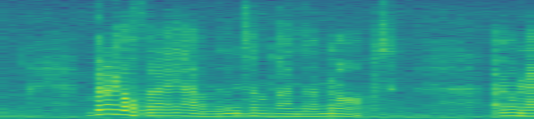
\includegraphics[interpolate=true,width=5.340000in,height=1.190000in]{spectrogram-img0.png}}%
\end{pgfscope}%
\begin{pgfscope}%
\pgfsetbuttcap%
\pgfsetroundjoin%
\definecolor{currentfill}{rgb}{0.000000,0.000000,0.000000}%
\pgfsetfillcolor{currentfill}%
\pgfsetlinewidth{0.803000pt}%
\definecolor{currentstroke}{rgb}{0.000000,0.000000,0.000000}%
\pgfsetstrokecolor{currentstroke}%
\pgfsetdash{}{0pt}%
\pgfsys@defobject{currentmarker}{\pgfqpoint{0.000000in}{-0.048611in}}{\pgfqpoint{0.000000in}{0.000000in}}{%
\pgfpathmoveto{\pgfqpoint{0.000000in}{0.000000in}}%
\pgfpathlineto{\pgfqpoint{0.000000in}{-0.048611in}}%
\pgfusepath{stroke,fill}%
}%
\begin{pgfscope}%
\pgfsys@transformshift{0.719445in}{0.565123in}%
\pgfsys@useobject{currentmarker}{}%
\end{pgfscope}%
\end{pgfscope}%
\begin{pgfscope}%
\definecolor{textcolor}{rgb}{0.000000,0.000000,0.000000}%
\pgfsetstrokecolor{textcolor}%
\pgfsetfillcolor{textcolor}%
\pgftext[x=0.719445in,y=0.467901in,,top]{\color{textcolor}\rmfamily\fontsize{10.000000}{12.000000}\selectfont \(\displaystyle {0.0}\)}%
\end{pgfscope}%
\begin{pgfscope}%
\pgfsetbuttcap%
\pgfsetroundjoin%
\definecolor{currentfill}{rgb}{0.000000,0.000000,0.000000}%
\pgfsetfillcolor{currentfill}%
\pgfsetlinewidth{0.803000pt}%
\definecolor{currentstroke}{rgb}{0.000000,0.000000,0.000000}%
\pgfsetstrokecolor{currentstroke}%
\pgfsetdash{}{0pt}%
\pgfsys@defobject{currentmarker}{\pgfqpoint{0.000000in}{-0.048611in}}{\pgfqpoint{0.000000in}{0.000000in}}{%
\pgfpathmoveto{\pgfqpoint{0.000000in}{0.000000in}}%
\pgfpathlineto{\pgfqpoint{0.000000in}{-0.048611in}}%
\pgfusepath{stroke,fill}%
}%
\begin{pgfscope}%
\pgfsys@transformshift{1.391390in}{0.565123in}%
\pgfsys@useobject{currentmarker}{}%
\end{pgfscope}%
\end{pgfscope}%
\begin{pgfscope}%
\definecolor{textcolor}{rgb}{0.000000,0.000000,0.000000}%
\pgfsetstrokecolor{textcolor}%
\pgfsetfillcolor{textcolor}%
\pgftext[x=1.391390in,y=0.467901in,,top]{\color{textcolor}\rmfamily\fontsize{10.000000}{12.000000}\selectfont \(\displaystyle {0.5}\)}%
\end{pgfscope}%
\begin{pgfscope}%
\pgfsetbuttcap%
\pgfsetroundjoin%
\definecolor{currentfill}{rgb}{0.000000,0.000000,0.000000}%
\pgfsetfillcolor{currentfill}%
\pgfsetlinewidth{0.803000pt}%
\definecolor{currentstroke}{rgb}{0.000000,0.000000,0.000000}%
\pgfsetstrokecolor{currentstroke}%
\pgfsetdash{}{0pt}%
\pgfsys@defobject{currentmarker}{\pgfqpoint{0.000000in}{-0.048611in}}{\pgfqpoint{0.000000in}{0.000000in}}{%
\pgfpathmoveto{\pgfqpoint{0.000000in}{0.000000in}}%
\pgfpathlineto{\pgfqpoint{0.000000in}{-0.048611in}}%
\pgfusepath{stroke,fill}%
}%
\begin{pgfscope}%
\pgfsys@transformshift{2.063335in}{0.565123in}%
\pgfsys@useobject{currentmarker}{}%
\end{pgfscope}%
\end{pgfscope}%
\begin{pgfscope}%
\definecolor{textcolor}{rgb}{0.000000,0.000000,0.000000}%
\pgfsetstrokecolor{textcolor}%
\pgfsetfillcolor{textcolor}%
\pgftext[x=2.063335in,y=0.467901in,,top]{\color{textcolor}\rmfamily\fontsize{10.000000}{12.000000}\selectfont \(\displaystyle {1.0}\)}%
\end{pgfscope}%
\begin{pgfscope}%
\pgfsetbuttcap%
\pgfsetroundjoin%
\definecolor{currentfill}{rgb}{0.000000,0.000000,0.000000}%
\pgfsetfillcolor{currentfill}%
\pgfsetlinewidth{0.803000pt}%
\definecolor{currentstroke}{rgb}{0.000000,0.000000,0.000000}%
\pgfsetstrokecolor{currentstroke}%
\pgfsetdash{}{0pt}%
\pgfsys@defobject{currentmarker}{\pgfqpoint{0.000000in}{-0.048611in}}{\pgfqpoint{0.000000in}{0.000000in}}{%
\pgfpathmoveto{\pgfqpoint{0.000000in}{0.000000in}}%
\pgfpathlineto{\pgfqpoint{0.000000in}{-0.048611in}}%
\pgfusepath{stroke,fill}%
}%
\begin{pgfscope}%
\pgfsys@transformshift{2.735280in}{0.565123in}%
\pgfsys@useobject{currentmarker}{}%
\end{pgfscope}%
\end{pgfscope}%
\begin{pgfscope}%
\definecolor{textcolor}{rgb}{0.000000,0.000000,0.000000}%
\pgfsetstrokecolor{textcolor}%
\pgfsetfillcolor{textcolor}%
\pgftext[x=2.735280in,y=0.467901in,,top]{\color{textcolor}\rmfamily\fontsize{10.000000}{12.000000}\selectfont \(\displaystyle {1.5}\)}%
\end{pgfscope}%
\begin{pgfscope}%
\pgfsetbuttcap%
\pgfsetroundjoin%
\definecolor{currentfill}{rgb}{0.000000,0.000000,0.000000}%
\pgfsetfillcolor{currentfill}%
\pgfsetlinewidth{0.803000pt}%
\definecolor{currentstroke}{rgb}{0.000000,0.000000,0.000000}%
\pgfsetstrokecolor{currentstroke}%
\pgfsetdash{}{0pt}%
\pgfsys@defobject{currentmarker}{\pgfqpoint{0.000000in}{-0.048611in}}{\pgfqpoint{0.000000in}{0.000000in}}{%
\pgfpathmoveto{\pgfqpoint{0.000000in}{0.000000in}}%
\pgfpathlineto{\pgfqpoint{0.000000in}{-0.048611in}}%
\pgfusepath{stroke,fill}%
}%
\begin{pgfscope}%
\pgfsys@transformshift{3.407225in}{0.565123in}%
\pgfsys@useobject{currentmarker}{}%
\end{pgfscope}%
\end{pgfscope}%
\begin{pgfscope}%
\definecolor{textcolor}{rgb}{0.000000,0.000000,0.000000}%
\pgfsetstrokecolor{textcolor}%
\pgfsetfillcolor{textcolor}%
\pgftext[x=3.407225in,y=0.467901in,,top]{\color{textcolor}\rmfamily\fontsize{10.000000}{12.000000}\selectfont \(\displaystyle {2.0}\)}%
\end{pgfscope}%
\begin{pgfscope}%
\pgfsetbuttcap%
\pgfsetroundjoin%
\definecolor{currentfill}{rgb}{0.000000,0.000000,0.000000}%
\pgfsetfillcolor{currentfill}%
\pgfsetlinewidth{0.803000pt}%
\definecolor{currentstroke}{rgb}{0.000000,0.000000,0.000000}%
\pgfsetstrokecolor{currentstroke}%
\pgfsetdash{}{0pt}%
\pgfsys@defobject{currentmarker}{\pgfqpoint{0.000000in}{-0.048611in}}{\pgfqpoint{0.000000in}{0.000000in}}{%
\pgfpathmoveto{\pgfqpoint{0.000000in}{0.000000in}}%
\pgfpathlineto{\pgfqpoint{0.000000in}{-0.048611in}}%
\pgfusepath{stroke,fill}%
}%
\begin{pgfscope}%
\pgfsys@transformshift{4.079170in}{0.565123in}%
\pgfsys@useobject{currentmarker}{}%
\end{pgfscope}%
\end{pgfscope}%
\begin{pgfscope}%
\definecolor{textcolor}{rgb}{0.000000,0.000000,0.000000}%
\pgfsetstrokecolor{textcolor}%
\pgfsetfillcolor{textcolor}%
\pgftext[x=4.079170in,y=0.467901in,,top]{\color{textcolor}\rmfamily\fontsize{10.000000}{12.000000}\selectfont \(\displaystyle {2.5}\)}%
\end{pgfscope}%
\begin{pgfscope}%
\pgfsetbuttcap%
\pgfsetroundjoin%
\definecolor{currentfill}{rgb}{0.000000,0.000000,0.000000}%
\pgfsetfillcolor{currentfill}%
\pgfsetlinewidth{0.803000pt}%
\definecolor{currentstroke}{rgb}{0.000000,0.000000,0.000000}%
\pgfsetstrokecolor{currentstroke}%
\pgfsetdash{}{0pt}%
\pgfsys@defobject{currentmarker}{\pgfqpoint{0.000000in}{-0.048611in}}{\pgfqpoint{0.000000in}{0.000000in}}{%
\pgfpathmoveto{\pgfqpoint{0.000000in}{0.000000in}}%
\pgfpathlineto{\pgfqpoint{0.000000in}{-0.048611in}}%
\pgfusepath{stroke,fill}%
}%
\begin{pgfscope}%
\pgfsys@transformshift{4.751115in}{0.565123in}%
\pgfsys@useobject{currentmarker}{}%
\end{pgfscope}%
\end{pgfscope}%
\begin{pgfscope}%
\definecolor{textcolor}{rgb}{0.000000,0.000000,0.000000}%
\pgfsetstrokecolor{textcolor}%
\pgfsetfillcolor{textcolor}%
\pgftext[x=4.751115in,y=0.467901in,,top]{\color{textcolor}\rmfamily\fontsize{10.000000}{12.000000}\selectfont \(\displaystyle {3.0}\)}%
\end{pgfscope}%
\begin{pgfscope}%
\pgfsetbuttcap%
\pgfsetroundjoin%
\definecolor{currentfill}{rgb}{0.000000,0.000000,0.000000}%
\pgfsetfillcolor{currentfill}%
\pgfsetlinewidth{0.803000pt}%
\definecolor{currentstroke}{rgb}{0.000000,0.000000,0.000000}%
\pgfsetstrokecolor{currentstroke}%
\pgfsetdash{}{0pt}%
\pgfsys@defobject{currentmarker}{\pgfqpoint{0.000000in}{-0.048611in}}{\pgfqpoint{0.000000in}{0.000000in}}{%
\pgfpathmoveto{\pgfqpoint{0.000000in}{0.000000in}}%
\pgfpathlineto{\pgfqpoint{0.000000in}{-0.048611in}}%
\pgfusepath{stroke,fill}%
}%
\begin{pgfscope}%
\pgfsys@transformshift{5.423060in}{0.565123in}%
\pgfsys@useobject{currentmarker}{}%
\end{pgfscope}%
\end{pgfscope}%
\begin{pgfscope}%
\definecolor{textcolor}{rgb}{0.000000,0.000000,0.000000}%
\pgfsetstrokecolor{textcolor}%
\pgfsetfillcolor{textcolor}%
\pgftext[x=5.423060in,y=0.467901in,,top]{\color{textcolor}\rmfamily\fontsize{10.000000}{12.000000}\selectfont \(\displaystyle {3.5}\)}%
\end{pgfscope}%
\begin{pgfscope}%
\definecolor{textcolor}{rgb}{0.000000,0.000000,0.000000}%
\pgfsetstrokecolor{textcolor}%
\pgfsetfillcolor{textcolor}%
\pgftext[x=3.385723in,y=0.288889in,,top]{\color{textcolor}\rmfamily\fontsize{10.000000}{12.000000}\selectfont Time (s)}%
\end{pgfscope}%
\begin{pgfscope}%
\pgfsetbuttcap%
\pgfsetroundjoin%
\definecolor{currentfill}{rgb}{0.000000,0.000000,0.000000}%
\pgfsetfillcolor{currentfill}%
\pgfsetlinewidth{0.803000pt}%
\definecolor{currentstroke}{rgb}{0.000000,0.000000,0.000000}%
\pgfsetstrokecolor{currentstroke}%
\pgfsetdash{}{0pt}%
\pgfsys@defobject{currentmarker}{\pgfqpoint{-0.048611in}{0.000000in}}{\pgfqpoint{0.000000in}{0.000000in}}{%
\pgfpathmoveto{\pgfqpoint{0.000000in}{0.000000in}}%
\pgfpathlineto{\pgfqpoint{-0.048611in}{0.000000in}}%
\pgfusepath{stroke,fill}%
}%
\begin{pgfscope}%
\pgfsys@transformshift{0.719445in}{0.565123in}%
\pgfsys@useobject{currentmarker}{}%
\end{pgfscope}%
\end{pgfscope}%
\begin{pgfscope}%
\definecolor{textcolor}{rgb}{0.000000,0.000000,0.000000}%
\pgfsetstrokecolor{textcolor}%
\pgfsetfillcolor{textcolor}%
\pgftext[x=0.552778in, y=0.516898in, left, base]{\color{textcolor}\rmfamily\fontsize{10.000000}{12.000000}\selectfont \(\displaystyle {0}\)}%
\end{pgfscope}%
\begin{pgfscope}%
\pgfsetbuttcap%
\pgfsetroundjoin%
\definecolor{currentfill}{rgb}{0.000000,0.000000,0.000000}%
\pgfsetfillcolor{currentfill}%
\pgfsetlinewidth{0.803000pt}%
\definecolor{currentstroke}{rgb}{0.000000,0.000000,0.000000}%
\pgfsetstrokecolor{currentstroke}%
\pgfsetdash{}{0pt}%
\pgfsys@defobject{currentmarker}{\pgfqpoint{-0.048611in}{0.000000in}}{\pgfqpoint{0.000000in}{0.000000in}}{%
\pgfpathmoveto{\pgfqpoint{0.000000in}{0.000000in}}%
\pgfpathlineto{\pgfqpoint{-0.048611in}{0.000000in}}%
\pgfusepath{stroke,fill}%
}%
\begin{pgfscope}%
\pgfsys@transformshift{0.719445in}{0.860870in}%
\pgfsys@useobject{currentmarker}{}%
\end{pgfscope}%
\end{pgfscope}%
\begin{pgfscope}%
\definecolor{textcolor}{rgb}{0.000000,0.000000,0.000000}%
\pgfsetstrokecolor{textcolor}%
\pgfsetfillcolor{textcolor}%
\pgftext[x=0.344444in, y=0.812645in, left, base]{\color{textcolor}\rmfamily\fontsize{10.000000}{12.000000}\selectfont \(\displaystyle {2000}\)}%
\end{pgfscope}%
\begin{pgfscope}%
\pgfsetbuttcap%
\pgfsetroundjoin%
\definecolor{currentfill}{rgb}{0.000000,0.000000,0.000000}%
\pgfsetfillcolor{currentfill}%
\pgfsetlinewidth{0.803000pt}%
\definecolor{currentstroke}{rgb}{0.000000,0.000000,0.000000}%
\pgfsetstrokecolor{currentstroke}%
\pgfsetdash{}{0pt}%
\pgfsys@defobject{currentmarker}{\pgfqpoint{-0.048611in}{0.000000in}}{\pgfqpoint{0.000000in}{0.000000in}}{%
\pgfpathmoveto{\pgfqpoint{0.000000in}{0.000000in}}%
\pgfpathlineto{\pgfqpoint{-0.048611in}{0.000000in}}%
\pgfusepath{stroke,fill}%
}%
\begin{pgfscope}%
\pgfsys@transformshift{0.719445in}{1.156616in}%
\pgfsys@useobject{currentmarker}{}%
\end{pgfscope}%
\end{pgfscope}%
\begin{pgfscope}%
\definecolor{textcolor}{rgb}{0.000000,0.000000,0.000000}%
\pgfsetstrokecolor{textcolor}%
\pgfsetfillcolor{textcolor}%
\pgftext[x=0.344444in, y=1.108391in, left, base]{\color{textcolor}\rmfamily\fontsize{10.000000}{12.000000}\selectfont \(\displaystyle {4000}\)}%
\end{pgfscope}%
\begin{pgfscope}%
\pgfsetbuttcap%
\pgfsetroundjoin%
\definecolor{currentfill}{rgb}{0.000000,0.000000,0.000000}%
\pgfsetfillcolor{currentfill}%
\pgfsetlinewidth{0.803000pt}%
\definecolor{currentstroke}{rgb}{0.000000,0.000000,0.000000}%
\pgfsetstrokecolor{currentstroke}%
\pgfsetdash{}{0pt}%
\pgfsys@defobject{currentmarker}{\pgfqpoint{-0.048611in}{0.000000in}}{\pgfqpoint{0.000000in}{0.000000in}}{%
\pgfpathmoveto{\pgfqpoint{0.000000in}{0.000000in}}%
\pgfpathlineto{\pgfqpoint{-0.048611in}{0.000000in}}%
\pgfusepath{stroke,fill}%
}%
\begin{pgfscope}%
\pgfsys@transformshift{0.719445in}{1.452363in}%
\pgfsys@useobject{currentmarker}{}%
\end{pgfscope}%
\end{pgfscope}%
\begin{pgfscope}%
\definecolor{textcolor}{rgb}{0.000000,0.000000,0.000000}%
\pgfsetstrokecolor{textcolor}%
\pgfsetfillcolor{textcolor}%
\pgftext[x=0.344444in, y=1.404138in, left, base]{\color{textcolor}\rmfamily\fontsize{10.000000}{12.000000}\selectfont \(\displaystyle {6000}\)}%
\end{pgfscope}%
\begin{pgfscope}%
\pgfsetbuttcap%
\pgfsetroundjoin%
\definecolor{currentfill}{rgb}{0.000000,0.000000,0.000000}%
\pgfsetfillcolor{currentfill}%
\pgfsetlinewidth{0.803000pt}%
\definecolor{currentstroke}{rgb}{0.000000,0.000000,0.000000}%
\pgfsetstrokecolor{currentstroke}%
\pgfsetdash{}{0pt}%
\pgfsys@defobject{currentmarker}{\pgfqpoint{-0.048611in}{0.000000in}}{\pgfqpoint{0.000000in}{0.000000in}}{%
\pgfpathmoveto{\pgfqpoint{0.000000in}{0.000000in}}%
\pgfpathlineto{\pgfqpoint{-0.048611in}{0.000000in}}%
\pgfusepath{stroke,fill}%
}%
\begin{pgfscope}%
\pgfsys@transformshift{0.719445in}{1.748110in}%
\pgfsys@useobject{currentmarker}{}%
\end{pgfscope}%
\end{pgfscope}%
\begin{pgfscope}%
\definecolor{textcolor}{rgb}{0.000000,0.000000,0.000000}%
\pgfsetstrokecolor{textcolor}%
\pgfsetfillcolor{textcolor}%
\pgftext[x=0.344444in, y=1.699884in, left, base]{\color{textcolor}\rmfamily\fontsize{10.000000}{12.000000}\selectfont \(\displaystyle {8000}\)}%
\end{pgfscope}%
\begin{pgfscope}%
\definecolor{textcolor}{rgb}{0.000000,0.000000,0.000000}%
\pgfsetstrokecolor{textcolor}%
\pgfsetfillcolor{textcolor}%
\pgftext[x=0.288889in,y=1.156616in,,bottom,rotate=90.000000]{\color{textcolor}\rmfamily\fontsize{10.000000}{12.000000}\selectfont Frequency (Hz)}%
\end{pgfscope}%
\begin{pgfscope}%
\pgfsetrectcap%
\pgfsetmiterjoin%
\pgfsetlinewidth{0.803000pt}%
\definecolor{currentstroke}{rgb}{0.000000,0.000000,0.000000}%
\pgfsetstrokecolor{currentstroke}%
\pgfsetdash{}{0pt}%
\pgfpathmoveto{\pgfqpoint{0.719445in}{0.565123in}}%
\pgfpathlineto{\pgfqpoint{0.719445in}{1.748110in}}%
\pgfusepath{stroke}%
\end{pgfscope}%
\begin{pgfscope}%
\pgfsetrectcap%
\pgfsetmiterjoin%
\pgfsetlinewidth{0.803000pt}%
\definecolor{currentstroke}{rgb}{0.000000,0.000000,0.000000}%
\pgfsetstrokecolor{currentstroke}%
\pgfsetdash{}{0pt}%
\pgfpathmoveto{\pgfqpoint{6.052000in}{0.565123in}}%
\pgfpathlineto{\pgfqpoint{6.052000in}{1.748110in}}%
\pgfusepath{stroke}%
\end{pgfscope}%
\begin{pgfscope}%
\pgfsetrectcap%
\pgfsetmiterjoin%
\pgfsetlinewidth{0.803000pt}%
\definecolor{currentstroke}{rgb}{0.000000,0.000000,0.000000}%
\pgfsetstrokecolor{currentstroke}%
\pgfsetdash{}{0pt}%
\pgfpathmoveto{\pgfqpoint{0.719445in}{0.565123in}}%
\pgfpathlineto{\pgfqpoint{6.052000in}{0.565123in}}%
\pgfusepath{stroke}%
\end{pgfscope}%
\begin{pgfscope}%
\pgfsetrectcap%
\pgfsetmiterjoin%
\pgfsetlinewidth{0.803000pt}%
\definecolor{currentstroke}{rgb}{0.000000,0.000000,0.000000}%
\pgfsetstrokecolor{currentstroke}%
\pgfsetdash{}{0pt}%
\pgfpathmoveto{\pgfqpoint{0.719445in}{1.748110in}}%
\pgfpathlineto{\pgfqpoint{6.052000in}{1.748110in}}%
\pgfusepath{stroke}%
\end{pgfscope}%
\end{pgfpicture}%
\makeatother%
\endgroup%

    \centering
    \caption[Spectrogram example]{\textbf{Top:} A 4 second audio signal sampled at 16kHz. \textbf{Bottom:} The spectrogram of the same signal created using STFT with no overlap and a window size of 1024.}
    \label{fig:spectrogram}
\end{figure}

In a discrete signal the number of Fourier coefficients, also called FFT-bins, is determined by the number of samples collected, while the frequency resolution of each bin is determined by the sampling rate of the signal and the number of bins. Equation \ref{eq:fft_tempresolution} and \ref{eq:fft_binresolution} show the relationship between the different parameters.

\begin{equation}\label{eq:fft_tempresolution}
    N = \frac{|x|}{2}
\end{equation}

\begin{equation}\label{eq:fft_binresolution}
    \Delta_{bin} = \frac{fs}{N}
\end{equation}

Here $N$ is the number of FFT-bins, $|x|$ is the number of samples. $\Delta_{bin}$ is the size per FFT-bin in Hz and $fs$ is the sampling rate of the signal in Hz. The smaller $N$ the better the time resolution. The smaller the bin size the better the frequency resolution. One can see that there always exists a trade-off between frequency resolution and time resolution. If we decrease the number of samples per frame of the \gls{stft} we get a better temporal resolution but therefore a worse frequency resolution. It is important to choose good parameters that fit the need of the task. The more exact frequency differentiation, the weaker the temporal differentiation becomes. For our task, a well-balanced resolution in both domains is required.

\section{Filters}

We make use of filters to create augmented views of the input data before feeding it into the neural network. Filters are one of the most important parts of \gls{dsp}. Their applications range from telecommunication to computer graphics \cite{FILTERSWEB07}. An abstract view of two of the most important types of filters, called \textit{low-pass} and \textit{high-pass} filters can be seen in Figure \ref{fig:lphp}. The frequencies in the passband are the ones that should not be altered by the filter while frequencies in the transition band should be linearly reduced and frequencies in the stopband should be removed entirely. As can be seen in Figure \ref{fig:lphp} a low-pass filter stops all frequencies above the transition band, while a high-pass filter stops all below it.

\begin{figure}[htbp]
    \centering
    %% Creator: Matplotlib, PGF backend
%%
%% To include the figure in your LaTeX document, write
%%   \input{<filename>.pgf}
%%
%% Make sure the required packages are loaded in your preamble
%%   \usepackage{pgf}
%%
%% and, on pdftex
%%   \usepackage[utf8]{inputenc}\DeclareUnicodeCharacter{2212}{-}
%%
%% or, on luatex and xetex
%%   \usepackage{unicode-math}
%%
%% Figures using additional raster images can only be included by \input if
%% they are in the same directory as the main LaTeX file. For loading figures
%% from other directories you can use the `import` package
%%   \usepackage{import}
%%
%% and then include the figures with
%%   \import{<path to file>}{<filename>.pgf}
%%
%% Matplotlib used the following preamble
%%
\begingroup%
\makeatletter%
\begin{pgfpicture}%
\pgfpathrectangle{\pgfpointorigin}{\pgfqpoint{6.202000in}{2.000000in}}%
\pgfusepath{use as bounding box, clip}%
\begin{pgfscope}%
\pgfsetbuttcap%
\pgfsetmiterjoin%
\definecolor{currentfill}{rgb}{1.000000,1.000000,1.000000}%
\pgfsetfillcolor{currentfill}%
\pgfsetlinewidth{0.000000pt}%
\definecolor{currentstroke}{rgb}{1.000000,1.000000,1.000000}%
\pgfsetstrokecolor{currentstroke}%
\pgfsetdash{}{0pt}%
\pgfpathmoveto{\pgfqpoint{0.000000in}{0.000000in}}%
\pgfpathlineto{\pgfqpoint{6.202000in}{0.000000in}}%
\pgfpathlineto{\pgfqpoint{6.202000in}{2.000000in}}%
\pgfpathlineto{\pgfqpoint{0.000000in}{2.000000in}}%
\pgfpathclose%
\pgfusepath{fill}%
\end{pgfscope}%
\begin{pgfscope}%
\pgfsetbuttcap%
\pgfsetmiterjoin%
\definecolor{currentfill}{rgb}{1.000000,1.000000,1.000000}%
\pgfsetfillcolor{currentfill}%
\pgfsetlinewidth{0.000000pt}%
\definecolor{currentstroke}{rgb}{0.000000,0.000000,0.000000}%
\pgfsetstrokecolor{currentstroke}%
\pgfsetstrokeopacity{0.000000}%
\pgfsetdash{}{0pt}%
\pgfpathmoveto{\pgfqpoint{0.329012in}{0.329012in}}%
\pgfpathlineto{\pgfqpoint{3.026000in}{0.329012in}}%
\pgfpathlineto{\pgfqpoint{3.026000in}{1.650926in}}%
\pgfpathlineto{\pgfqpoint{0.329012in}{1.650926in}}%
\pgfpathclose%
\pgfusepath{fill}%
\end{pgfscope}%
\begin{pgfscope}%
\definecolor{textcolor}{rgb}{0.000000,0.000000,0.000000}%
\pgfsetstrokecolor{textcolor}%
\pgfsetfillcolor{textcolor}%
\pgftext[x=1.677506in,y=0.273457in,,top]{\color{textcolor}\rmfamily\fontsize{10.000000}{12.000000}\selectfont Frequency}%
\end{pgfscope}%
\begin{pgfscope}%
\definecolor{textcolor}{rgb}{0.000000,0.000000,0.000000}%
\pgfsetstrokecolor{textcolor}%
\pgfsetfillcolor{textcolor}%
\pgftext[x=0.273457in,y=0.989969in,,bottom,rotate=90.000000]{\color{textcolor}\rmfamily\fontsize{10.000000}{12.000000}\selectfont Amplitude}%
\end{pgfscope}%
\begin{pgfscope}%
\pgfpathrectangle{\pgfqpoint{0.329012in}{0.329012in}}{\pgfqpoint{2.696988in}{1.321914in}}%
\pgfusepath{clip}%
\pgfsetbuttcap%
\pgfsetroundjoin%
\pgfsetlinewidth{1.505625pt}%
\definecolor{currentstroke}{rgb}{0.000000,0.000000,0.000000}%
\pgfsetstrokecolor{currentstroke}%
\pgfsetdash{{5.550000pt}{2.400000pt}}{0.000000pt}%
\pgfpathmoveto{\pgfqpoint{1.432325in}{0.319012in}}%
\pgfpathlineto{\pgfqpoint{1.432325in}{1.660926in}}%
\pgfusepath{stroke}%
\end{pgfscope}%
\begin{pgfscope}%
\pgfpathrectangle{\pgfqpoint{0.329012in}{0.329012in}}{\pgfqpoint{2.696988in}{1.321914in}}%
\pgfusepath{clip}%
\pgfsetbuttcap%
\pgfsetroundjoin%
\pgfsetlinewidth{1.505625pt}%
\definecolor{currentstroke}{rgb}{0.000000,0.000000,0.000000}%
\pgfsetstrokecolor{currentstroke}%
\pgfsetdash{{5.550000pt}{2.400000pt}}{0.000000pt}%
\pgfpathmoveto{\pgfqpoint{1.922687in}{0.319012in}}%
\pgfpathlineto{\pgfqpoint{1.922687in}{1.660926in}}%
\pgfusepath{stroke}%
\end{pgfscope}%
\begin{pgfscope}%
\pgfpathrectangle{\pgfqpoint{0.329012in}{0.329012in}}{\pgfqpoint{2.696988in}{1.321914in}}%
\pgfusepath{clip}%
\pgfsetrectcap%
\pgfsetroundjoin%
\pgfsetlinewidth{1.505625pt}%
\definecolor{currentstroke}{rgb}{0.121569,0.466667,0.705882}%
\pgfsetstrokecolor{currentstroke}%
\pgfsetdash{}{0pt}%
\pgfpathmoveto{\pgfqpoint{0.451603in}{1.530752in}}%
\pgfpathlineto{\pgfqpoint{1.432325in}{1.530752in}}%
\pgfpathlineto{\pgfqpoint{1.922687in}{0.329012in}}%
\pgfpathlineto{\pgfqpoint{2.903410in}{0.329012in}}%
\pgfusepath{stroke}%
\end{pgfscope}%
\begin{pgfscope}%
\pgfsetrectcap%
\pgfsetmiterjoin%
\pgfsetlinewidth{0.803000pt}%
\definecolor{currentstroke}{rgb}{0.000000,0.000000,0.000000}%
\pgfsetstrokecolor{currentstroke}%
\pgfsetdash{}{0pt}%
\pgfpathmoveto{\pgfqpoint{0.329012in}{0.329012in}}%
\pgfpathlineto{\pgfqpoint{0.329012in}{1.650926in}}%
\pgfusepath{stroke}%
\end{pgfscope}%
\begin{pgfscope}%
\pgfsetrectcap%
\pgfsetmiterjoin%
\pgfsetlinewidth{0.803000pt}%
\definecolor{currentstroke}{rgb}{0.000000,0.000000,0.000000}%
\pgfsetstrokecolor{currentstroke}%
\pgfsetdash{}{0pt}%
\pgfpathmoveto{\pgfqpoint{3.026000in}{0.329012in}}%
\pgfpathlineto{\pgfqpoint{3.026000in}{1.650926in}}%
\pgfusepath{stroke}%
\end{pgfscope}%
\begin{pgfscope}%
\pgfsetrectcap%
\pgfsetmiterjoin%
\pgfsetlinewidth{0.803000pt}%
\definecolor{currentstroke}{rgb}{0.000000,0.000000,0.000000}%
\pgfsetstrokecolor{currentstroke}%
\pgfsetdash{}{0pt}%
\pgfpathmoveto{\pgfqpoint{0.329012in}{0.329012in}}%
\pgfpathlineto{\pgfqpoint{3.026000in}{0.329012in}}%
\pgfusepath{stroke}%
\end{pgfscope}%
\begin{pgfscope}%
\pgfsetrectcap%
\pgfsetmiterjoin%
\pgfsetlinewidth{0.803000pt}%
\definecolor{currentstroke}{rgb}{0.000000,0.000000,0.000000}%
\pgfsetstrokecolor{currentstroke}%
\pgfsetdash{}{0pt}%
\pgfpathmoveto{\pgfqpoint{0.329012in}{1.650926in}}%
\pgfpathlineto{\pgfqpoint{3.026000in}{1.650926in}}%
\pgfusepath{stroke}%
\end{pgfscope}%
\begin{pgfscope}%
\definecolor{textcolor}{rgb}{0.000000,0.000000,0.000000}%
\pgfsetstrokecolor{textcolor}%
\pgfsetfillcolor{textcolor}%
\pgftext[x=0.451603in,y=1.350491in,left,base]{\color{textcolor}\rmfamily\fontsize{10.000000}{12.000000}\selectfont Passband}%
\end{pgfscope}%
\begin{pgfscope}%
\definecolor{textcolor}{rgb}{0.000000,0.000000,0.000000}%
\pgfsetstrokecolor{textcolor}%
\pgfsetfillcolor{textcolor}%
\pgftext[x=2.045277in,y=0.401117in,left,base]{\color{textcolor}\rmfamily\fontsize{10.000000}{12.000000}\selectfont Stopband}%
\end{pgfscope}%
\begin{pgfscope}%
\pgfsetroundcap%
\pgfsetroundjoin%
\pgfsetlinewidth{1.003750pt}%
\definecolor{currentstroke}{rgb}{0.000000,0.000000,0.000000}%
\pgfsetstrokecolor{currentstroke}%
\pgfsetdash{}{0pt}%
\pgfpathmoveto{\pgfqpoint{2.120600in}{1.034683in}}%
\pgfpathquadraticcurveto{\pgfqpoint{1.912562in}{0.985478in}}{\pgfqpoint{1.719635in}{0.939847in}}%
\pgfusepath{stroke}%
\end{pgfscope}%
\begin{pgfscope}%
\pgfsetroundcap%
\pgfsetroundjoin%
\pgfsetlinewidth{1.003750pt}%
\definecolor{currentstroke}{rgb}{0.000000,0.000000,0.000000}%
\pgfsetstrokecolor{currentstroke}%
\pgfsetdash{}{0pt}%
\pgfpathmoveto{\pgfqpoint{1.780092in}{0.925602in}}%
\pgfpathlineto{\pgfqpoint{1.719635in}{0.939847in}}%
\pgfpathlineto{\pgfqpoint{1.767305in}{0.979666in}}%
\pgfusepath{stroke}%
\end{pgfscope}%
\begin{pgfscope}%
\definecolor{textcolor}{rgb}{0.000000,0.000000,0.000000}%
\pgfsetstrokecolor{textcolor}%
\pgfsetfillcolor{textcolor}%
\pgftext[x=2.175452in, y=1.157901in, left, base]{\color{textcolor}\rmfamily\fontsize{10.000000}{12.000000}\selectfont Transition}%
\end{pgfscope}%
\begin{pgfscope}%
\definecolor{textcolor}{rgb}{0.000000,0.000000,0.000000}%
\pgfsetstrokecolor{textcolor}%
\pgfsetfillcolor{textcolor}%
\pgftext[x=2.336139in, y=1.015155in, left, base]{\color{textcolor}\rmfamily\fontsize{10.000000}{12.000000}\selectfont band}%
\end{pgfscope}%
\begin{pgfscope}%
\definecolor{textcolor}{rgb}{0.000000,0.000000,0.000000}%
\pgfsetstrokecolor{textcolor}%
\pgfsetfillcolor{textcolor}%
\pgftext[x=1.677506in,y=1.734260in,,base]{\color{textcolor}\rmfamily\fontsize{12.000000}{14.400000}\selectfont Low-pass Filter}%
\end{pgfscope}%
\begin{pgfscope}%
\pgfsetbuttcap%
\pgfsetmiterjoin%
\definecolor{currentfill}{rgb}{1.000000,1.000000,1.000000}%
\pgfsetfillcolor{currentfill}%
\pgfsetlinewidth{0.000000pt}%
\definecolor{currentstroke}{rgb}{0.000000,0.000000,0.000000}%
\pgfsetstrokecolor{currentstroke}%
\pgfsetstrokeopacity{0.000000}%
\pgfsetdash{}{0pt}%
\pgfpathmoveto{\pgfqpoint{3.355012in}{0.329012in}}%
\pgfpathlineto{\pgfqpoint{6.052000in}{0.329012in}}%
\pgfpathlineto{\pgfqpoint{6.052000in}{1.650926in}}%
\pgfpathlineto{\pgfqpoint{3.355012in}{1.650926in}}%
\pgfpathclose%
\pgfusepath{fill}%
\end{pgfscope}%
\begin{pgfscope}%
\definecolor{textcolor}{rgb}{0.000000,0.000000,0.000000}%
\pgfsetstrokecolor{textcolor}%
\pgfsetfillcolor{textcolor}%
\pgftext[x=4.703506in,y=0.273457in,,top]{\color{textcolor}\rmfamily\fontsize{10.000000}{12.000000}\selectfont Frequency}%
\end{pgfscope}%
\begin{pgfscope}%
\definecolor{textcolor}{rgb}{0.000000,0.000000,0.000000}%
\pgfsetstrokecolor{textcolor}%
\pgfsetfillcolor{textcolor}%
\pgftext[x=3.299457in,y=0.989969in,,bottom,rotate=90.000000]{\color{textcolor}\rmfamily\fontsize{10.000000}{12.000000}\selectfont Amplitude}%
\end{pgfscope}%
\begin{pgfscope}%
\pgfpathrectangle{\pgfqpoint{3.355012in}{0.329012in}}{\pgfqpoint{2.696988in}{1.321914in}}%
\pgfusepath{clip}%
\pgfsetrectcap%
\pgfsetroundjoin%
\pgfsetlinewidth{1.505625pt}%
\definecolor{currentstroke}{rgb}{0.121569,0.466667,0.705882}%
\pgfsetstrokecolor{currentstroke}%
\pgfsetdash{}{0pt}%
\pgfpathmoveto{\pgfqpoint{3.477603in}{0.329012in}}%
\pgfpathlineto{\pgfqpoint{4.458325in}{0.329012in}}%
\pgfpathlineto{\pgfqpoint{4.948687in}{1.530752in}}%
\pgfpathlineto{\pgfqpoint{5.929410in}{1.530752in}}%
\pgfusepath{stroke}%
\end{pgfscope}%
\begin{pgfscope}%
\pgfsetrectcap%
\pgfsetmiterjoin%
\pgfsetlinewidth{0.803000pt}%
\definecolor{currentstroke}{rgb}{0.000000,0.000000,0.000000}%
\pgfsetstrokecolor{currentstroke}%
\pgfsetdash{}{0pt}%
\pgfpathmoveto{\pgfqpoint{3.355012in}{0.329012in}}%
\pgfpathlineto{\pgfqpoint{3.355012in}{1.650926in}}%
\pgfusepath{stroke}%
\end{pgfscope}%
\begin{pgfscope}%
\pgfsetrectcap%
\pgfsetmiterjoin%
\pgfsetlinewidth{0.803000pt}%
\definecolor{currentstroke}{rgb}{0.000000,0.000000,0.000000}%
\pgfsetstrokecolor{currentstroke}%
\pgfsetdash{}{0pt}%
\pgfpathmoveto{\pgfqpoint{6.052000in}{0.329012in}}%
\pgfpathlineto{\pgfqpoint{6.052000in}{1.650926in}}%
\pgfusepath{stroke}%
\end{pgfscope}%
\begin{pgfscope}%
\pgfsetrectcap%
\pgfsetmiterjoin%
\pgfsetlinewidth{0.803000pt}%
\definecolor{currentstroke}{rgb}{0.000000,0.000000,0.000000}%
\pgfsetstrokecolor{currentstroke}%
\pgfsetdash{}{0pt}%
\pgfpathmoveto{\pgfqpoint{3.355012in}{0.329012in}}%
\pgfpathlineto{\pgfqpoint{6.052000in}{0.329012in}}%
\pgfusepath{stroke}%
\end{pgfscope}%
\begin{pgfscope}%
\pgfsetrectcap%
\pgfsetmiterjoin%
\pgfsetlinewidth{0.803000pt}%
\definecolor{currentstroke}{rgb}{0.000000,0.000000,0.000000}%
\pgfsetstrokecolor{currentstroke}%
\pgfsetdash{}{0pt}%
\pgfpathmoveto{\pgfqpoint{3.355012in}{1.650926in}}%
\pgfpathlineto{\pgfqpoint{6.052000in}{1.650926in}}%
\pgfusepath{stroke}%
\end{pgfscope}%
\begin{pgfscope}%
\definecolor{textcolor}{rgb}{0.000000,0.000000,0.000000}%
\pgfsetstrokecolor{textcolor}%
\pgfsetfillcolor{textcolor}%
\pgftext[x=4.703506in,y=1.734260in,,base]{\color{textcolor}\rmfamily\fontsize{12.000000}{14.400000}\selectfont High-pass Filter}%
\end{pgfscope}%
\end{pgfpicture}%
\makeatother%
\endgroup%

    \caption[]{\textbf{Left:} Abstract illustration of a \textit{low-pass} filter. \textbf{Right:} Abstract illustration of a \textit{high-pass} filter}
    \label{fig:lphp}
\end{figure}


Figure \ref{fig:filter_responses} shows how the same filter can be represented in time and in the frequency domain. The frequency response describes how the filter will affect the individual frequencies of an incoming signal. In this example, frequencies above 100Hz will be cut off linearly. The impulse response is the actual signal of the filter in the time domain. Applying a filter in the frequency domain can be achieved by multiplying an input’s frequency spectrum and the filter’s frequency response. It can be easily seen why multiplication will have the desired effect of removing all frequencies in the stopband while preserving all frequencies in the passband.

\begin{figure}[htbp]
    \centering
    %% Creator: Matplotlib, PGF backend
%%
%% To include the figure in your LaTeX document, write
%%   \input{<filename>.pgf}
%%
%% Make sure the required packages are loaded in your preamble
%%   \usepackage{pgf}
%%
%% and, on pdftex
%%   \usepackage[utf8]{inputenc}\DeclareUnicodeCharacter{2212}{-}
%%
%% or, on luatex and xetex
%%   \usepackage{unicode-math}
%%
%% Figures using additional raster images can only be included by \input if
%% they are in the same directory as the main LaTeX file. For loading figures
%% from other directories you can use the `import` package
%%   \usepackage{import}
%%
%% and then include the figures with
%%   \import{<path to file>}{<filename>.pgf}
%%
%% Matplotlib used the following preamble
%%
\begingroup%
\makeatletter%
\begin{pgfpicture}%
\pgfpathrectangle{\pgfpointorigin}{\pgfqpoint{6.202000in}{3.000000in}}%
\pgfusepath{use as bounding box, clip}%
\begin{pgfscope}%
\pgfsetbuttcap%
\pgfsetmiterjoin%
\definecolor{currentfill}{rgb}{1.000000,1.000000,1.000000}%
\pgfsetfillcolor{currentfill}%
\pgfsetlinewidth{0.000000pt}%
\definecolor{currentstroke}{rgb}{1.000000,1.000000,1.000000}%
\pgfsetstrokecolor{currentstroke}%
\pgfsetdash{}{0pt}%
\pgfpathmoveto{\pgfqpoint{0.000000in}{0.000000in}}%
\pgfpathlineto{\pgfqpoint{6.202000in}{0.000000in}}%
\pgfpathlineto{\pgfqpoint{6.202000in}{3.000000in}}%
\pgfpathlineto{\pgfqpoint{0.000000in}{3.000000in}}%
\pgfpathclose%
\pgfusepath{fill}%
\end{pgfscope}%
\begin{pgfscope}%
\pgfsetbuttcap%
\pgfsetmiterjoin%
\definecolor{currentfill}{rgb}{1.000000,1.000000,1.000000}%
\pgfsetfillcolor{currentfill}%
\pgfsetlinewidth{0.000000pt}%
\definecolor{currentstroke}{rgb}{0.000000,0.000000,0.000000}%
\pgfsetstrokecolor{currentstroke}%
\pgfsetstrokeopacity{0.000000}%
\pgfsetdash{}{0pt}%
\pgfpathmoveto{\pgfqpoint{0.688581in}{1.990123in}}%
\pgfpathlineto{\pgfqpoint{5.951402in}{1.990123in}}%
\pgfpathlineto{\pgfqpoint{5.951402in}{2.650926in}}%
\pgfpathlineto{\pgfqpoint{0.688581in}{2.650926in}}%
\pgfpathclose%
\pgfusepath{fill}%
\end{pgfscope}%
\begin{pgfscope}%
\pgfpathrectangle{\pgfqpoint{0.688581in}{1.990123in}}{\pgfqpoint{5.262821in}{0.660803in}}%
\pgfusepath{clip}%
\pgfsetrectcap%
\pgfsetroundjoin%
\pgfsetlinewidth{0.803000pt}%
\definecolor{currentstroke}{rgb}{0.690196,0.690196,0.690196}%
\pgfsetstrokecolor{currentstroke}%
\pgfsetdash{}{0pt}%
\pgfpathmoveto{\pgfqpoint{0.688581in}{1.990123in}}%
\pgfpathlineto{\pgfqpoint{0.688581in}{2.650926in}}%
\pgfusepath{stroke}%
\end{pgfscope}%
\begin{pgfscope}%
\pgfsetbuttcap%
\pgfsetroundjoin%
\definecolor{currentfill}{rgb}{0.000000,0.000000,0.000000}%
\pgfsetfillcolor{currentfill}%
\pgfsetlinewidth{0.803000pt}%
\definecolor{currentstroke}{rgb}{0.000000,0.000000,0.000000}%
\pgfsetstrokecolor{currentstroke}%
\pgfsetdash{}{0pt}%
\pgfsys@defobject{currentmarker}{\pgfqpoint{0.000000in}{-0.048611in}}{\pgfqpoint{0.000000in}{0.000000in}}{%
\pgfpathmoveto{\pgfqpoint{0.000000in}{0.000000in}}%
\pgfpathlineto{\pgfqpoint{0.000000in}{-0.048611in}}%
\pgfusepath{stroke,fill}%
}%
\begin{pgfscope}%
\pgfsys@transformshift{0.688581in}{1.990123in}%
\pgfsys@useobject{currentmarker}{}%
\end{pgfscope}%
\end{pgfscope}%
\begin{pgfscope}%
\definecolor{textcolor}{rgb}{0.000000,0.000000,0.000000}%
\pgfsetstrokecolor{textcolor}%
\pgfsetfillcolor{textcolor}%
\pgftext[x=0.688581in,y=1.892901in,,top]{\color{textcolor}\rmfamily\fontsize{10.000000}{12.000000}\selectfont \(\displaystyle {0.00}\)}%
\end{pgfscope}%
\begin{pgfscope}%
\pgfpathrectangle{\pgfqpoint{0.688581in}{1.990123in}}{\pgfqpoint{5.262821in}{0.660803in}}%
\pgfusepath{clip}%
\pgfsetrectcap%
\pgfsetroundjoin%
\pgfsetlinewidth{0.803000pt}%
\definecolor{currentstroke}{rgb}{0.690196,0.690196,0.690196}%
\pgfsetstrokecolor{currentstroke}%
\pgfsetdash{}{0pt}%
\pgfpathmoveto{\pgfqpoint{1.839435in}{1.990123in}}%
\pgfpathlineto{\pgfqpoint{1.839435in}{2.650926in}}%
\pgfusepath{stroke}%
\end{pgfscope}%
\begin{pgfscope}%
\pgfsetbuttcap%
\pgfsetroundjoin%
\definecolor{currentfill}{rgb}{0.000000,0.000000,0.000000}%
\pgfsetfillcolor{currentfill}%
\pgfsetlinewidth{0.803000pt}%
\definecolor{currentstroke}{rgb}{0.000000,0.000000,0.000000}%
\pgfsetstrokecolor{currentstroke}%
\pgfsetdash{}{0pt}%
\pgfsys@defobject{currentmarker}{\pgfqpoint{0.000000in}{-0.048611in}}{\pgfqpoint{0.000000in}{0.000000in}}{%
\pgfpathmoveto{\pgfqpoint{0.000000in}{0.000000in}}%
\pgfpathlineto{\pgfqpoint{0.000000in}{-0.048611in}}%
\pgfusepath{stroke,fill}%
}%
\begin{pgfscope}%
\pgfsys@transformshift{1.839435in}{1.990123in}%
\pgfsys@useobject{currentmarker}{}%
\end{pgfscope}%
\end{pgfscope}%
\begin{pgfscope}%
\definecolor{textcolor}{rgb}{0.000000,0.000000,0.000000}%
\pgfsetstrokecolor{textcolor}%
\pgfsetfillcolor{textcolor}%
\pgftext[x=1.839435in,y=1.892901in,,top]{\color{textcolor}\rmfamily\fontsize{10.000000}{12.000000}\selectfont \(\displaystyle {0.02}\)}%
\end{pgfscope}%
\begin{pgfscope}%
\pgfpathrectangle{\pgfqpoint{0.688581in}{1.990123in}}{\pgfqpoint{5.262821in}{0.660803in}}%
\pgfusepath{clip}%
\pgfsetrectcap%
\pgfsetroundjoin%
\pgfsetlinewidth{0.803000pt}%
\definecolor{currentstroke}{rgb}{0.690196,0.690196,0.690196}%
\pgfsetstrokecolor{currentstroke}%
\pgfsetdash{}{0pt}%
\pgfpathmoveto{\pgfqpoint{2.990289in}{1.990123in}}%
\pgfpathlineto{\pgfqpoint{2.990289in}{2.650926in}}%
\pgfusepath{stroke}%
\end{pgfscope}%
\begin{pgfscope}%
\pgfsetbuttcap%
\pgfsetroundjoin%
\definecolor{currentfill}{rgb}{0.000000,0.000000,0.000000}%
\pgfsetfillcolor{currentfill}%
\pgfsetlinewidth{0.803000pt}%
\definecolor{currentstroke}{rgb}{0.000000,0.000000,0.000000}%
\pgfsetstrokecolor{currentstroke}%
\pgfsetdash{}{0pt}%
\pgfsys@defobject{currentmarker}{\pgfqpoint{0.000000in}{-0.048611in}}{\pgfqpoint{0.000000in}{0.000000in}}{%
\pgfpathmoveto{\pgfqpoint{0.000000in}{0.000000in}}%
\pgfpathlineto{\pgfqpoint{0.000000in}{-0.048611in}}%
\pgfusepath{stroke,fill}%
}%
\begin{pgfscope}%
\pgfsys@transformshift{2.990289in}{1.990123in}%
\pgfsys@useobject{currentmarker}{}%
\end{pgfscope}%
\end{pgfscope}%
\begin{pgfscope}%
\definecolor{textcolor}{rgb}{0.000000,0.000000,0.000000}%
\pgfsetstrokecolor{textcolor}%
\pgfsetfillcolor{textcolor}%
\pgftext[x=2.990289in,y=1.892901in,,top]{\color{textcolor}\rmfamily\fontsize{10.000000}{12.000000}\selectfont \(\displaystyle {0.04}\)}%
\end{pgfscope}%
\begin{pgfscope}%
\pgfpathrectangle{\pgfqpoint{0.688581in}{1.990123in}}{\pgfqpoint{5.262821in}{0.660803in}}%
\pgfusepath{clip}%
\pgfsetrectcap%
\pgfsetroundjoin%
\pgfsetlinewidth{0.803000pt}%
\definecolor{currentstroke}{rgb}{0.690196,0.690196,0.690196}%
\pgfsetstrokecolor{currentstroke}%
\pgfsetdash{}{0pt}%
\pgfpathmoveto{\pgfqpoint{4.141143in}{1.990123in}}%
\pgfpathlineto{\pgfqpoint{4.141143in}{2.650926in}}%
\pgfusepath{stroke}%
\end{pgfscope}%
\begin{pgfscope}%
\pgfsetbuttcap%
\pgfsetroundjoin%
\definecolor{currentfill}{rgb}{0.000000,0.000000,0.000000}%
\pgfsetfillcolor{currentfill}%
\pgfsetlinewidth{0.803000pt}%
\definecolor{currentstroke}{rgb}{0.000000,0.000000,0.000000}%
\pgfsetstrokecolor{currentstroke}%
\pgfsetdash{}{0pt}%
\pgfsys@defobject{currentmarker}{\pgfqpoint{0.000000in}{-0.048611in}}{\pgfqpoint{0.000000in}{0.000000in}}{%
\pgfpathmoveto{\pgfqpoint{0.000000in}{0.000000in}}%
\pgfpathlineto{\pgfqpoint{0.000000in}{-0.048611in}}%
\pgfusepath{stroke,fill}%
}%
\begin{pgfscope}%
\pgfsys@transformshift{4.141143in}{1.990123in}%
\pgfsys@useobject{currentmarker}{}%
\end{pgfscope}%
\end{pgfscope}%
\begin{pgfscope}%
\definecolor{textcolor}{rgb}{0.000000,0.000000,0.000000}%
\pgfsetstrokecolor{textcolor}%
\pgfsetfillcolor{textcolor}%
\pgftext[x=4.141143in,y=1.892901in,,top]{\color{textcolor}\rmfamily\fontsize{10.000000}{12.000000}\selectfont \(\displaystyle {0.06}\)}%
\end{pgfscope}%
\begin{pgfscope}%
\pgfpathrectangle{\pgfqpoint{0.688581in}{1.990123in}}{\pgfqpoint{5.262821in}{0.660803in}}%
\pgfusepath{clip}%
\pgfsetrectcap%
\pgfsetroundjoin%
\pgfsetlinewidth{0.803000pt}%
\definecolor{currentstroke}{rgb}{0.690196,0.690196,0.690196}%
\pgfsetstrokecolor{currentstroke}%
\pgfsetdash{}{0pt}%
\pgfpathmoveto{\pgfqpoint{5.291996in}{1.990123in}}%
\pgfpathlineto{\pgfqpoint{5.291996in}{2.650926in}}%
\pgfusepath{stroke}%
\end{pgfscope}%
\begin{pgfscope}%
\pgfsetbuttcap%
\pgfsetroundjoin%
\definecolor{currentfill}{rgb}{0.000000,0.000000,0.000000}%
\pgfsetfillcolor{currentfill}%
\pgfsetlinewidth{0.803000pt}%
\definecolor{currentstroke}{rgb}{0.000000,0.000000,0.000000}%
\pgfsetstrokecolor{currentstroke}%
\pgfsetdash{}{0pt}%
\pgfsys@defobject{currentmarker}{\pgfqpoint{0.000000in}{-0.048611in}}{\pgfqpoint{0.000000in}{0.000000in}}{%
\pgfpathmoveto{\pgfqpoint{0.000000in}{0.000000in}}%
\pgfpathlineto{\pgfqpoint{0.000000in}{-0.048611in}}%
\pgfusepath{stroke,fill}%
}%
\begin{pgfscope}%
\pgfsys@transformshift{5.291996in}{1.990123in}%
\pgfsys@useobject{currentmarker}{}%
\end{pgfscope}%
\end{pgfscope}%
\begin{pgfscope}%
\definecolor{textcolor}{rgb}{0.000000,0.000000,0.000000}%
\pgfsetstrokecolor{textcolor}%
\pgfsetfillcolor{textcolor}%
\pgftext[x=5.291996in,y=1.892901in,,top]{\color{textcolor}\rmfamily\fontsize{10.000000}{12.000000}\selectfont \(\displaystyle {0.08}\)}%
\end{pgfscope}%
\begin{pgfscope}%
\definecolor{textcolor}{rgb}{0.000000,0.000000,0.000000}%
\pgfsetstrokecolor{textcolor}%
\pgfsetfillcolor{textcolor}%
\pgftext[x=3.319991in,y=1.713889in,,top]{\color{textcolor}\rmfamily\fontsize{10.000000}{12.000000}\selectfont Time (s)}%
\end{pgfscope}%
\begin{pgfscope}%
\pgfpathrectangle{\pgfqpoint{0.688581in}{1.990123in}}{\pgfqpoint{5.262821in}{0.660803in}}%
\pgfusepath{clip}%
\pgfsetrectcap%
\pgfsetroundjoin%
\pgfsetlinewidth{0.803000pt}%
\definecolor{currentstroke}{rgb}{0.690196,0.690196,0.690196}%
\pgfsetstrokecolor{currentstroke}%
\pgfsetdash{}{0pt}%
\pgfpathmoveto{\pgfqpoint{0.688581in}{2.110909in}}%
\pgfpathlineto{\pgfqpoint{5.951402in}{2.110909in}}%
\pgfusepath{stroke}%
\end{pgfscope}%
\begin{pgfscope}%
\pgfsetbuttcap%
\pgfsetroundjoin%
\definecolor{currentfill}{rgb}{0.000000,0.000000,0.000000}%
\pgfsetfillcolor{currentfill}%
\pgfsetlinewidth{0.803000pt}%
\definecolor{currentstroke}{rgb}{0.000000,0.000000,0.000000}%
\pgfsetstrokecolor{currentstroke}%
\pgfsetdash{}{0pt}%
\pgfsys@defobject{currentmarker}{\pgfqpoint{-0.048611in}{0.000000in}}{\pgfqpoint{0.000000in}{0.000000in}}{%
\pgfpathmoveto{\pgfqpoint{0.000000in}{0.000000in}}%
\pgfpathlineto{\pgfqpoint{-0.048611in}{0.000000in}}%
\pgfusepath{stroke,fill}%
}%
\begin{pgfscope}%
\pgfsys@transformshift{0.688581in}{2.110909in}%
\pgfsys@useobject{currentmarker}{}%
\end{pgfscope}%
\end{pgfscope}%
\begin{pgfscope}%
\definecolor{textcolor}{rgb}{0.000000,0.000000,0.000000}%
\pgfsetstrokecolor{textcolor}%
\pgfsetfillcolor{textcolor}%
\pgftext[x=0.521914in, y=2.062684in, left, base]{\color{textcolor}\rmfamily\fontsize{10.000000}{12.000000}\selectfont \(\displaystyle {0}\)}%
\end{pgfscope}%
\begin{pgfscope}%
\pgfpathrectangle{\pgfqpoint{0.688581in}{1.990123in}}{\pgfqpoint{5.262821in}{0.660803in}}%
\pgfusepath{clip}%
\pgfsetrectcap%
\pgfsetroundjoin%
\pgfsetlinewidth{0.803000pt}%
\definecolor{currentstroke}{rgb}{0.690196,0.690196,0.690196}%
\pgfsetstrokecolor{currentstroke}%
\pgfsetdash{}{0pt}%
\pgfpathmoveto{\pgfqpoint{0.688581in}{2.445417in}}%
\pgfpathlineto{\pgfqpoint{5.951402in}{2.445417in}}%
\pgfusepath{stroke}%
\end{pgfscope}%
\begin{pgfscope}%
\pgfsetbuttcap%
\pgfsetroundjoin%
\definecolor{currentfill}{rgb}{0.000000,0.000000,0.000000}%
\pgfsetfillcolor{currentfill}%
\pgfsetlinewidth{0.803000pt}%
\definecolor{currentstroke}{rgb}{0.000000,0.000000,0.000000}%
\pgfsetstrokecolor{currentstroke}%
\pgfsetdash{}{0pt}%
\pgfsys@defobject{currentmarker}{\pgfqpoint{-0.048611in}{0.000000in}}{\pgfqpoint{0.000000in}{0.000000in}}{%
\pgfpathmoveto{\pgfqpoint{0.000000in}{0.000000in}}%
\pgfpathlineto{\pgfqpoint{-0.048611in}{0.000000in}}%
\pgfusepath{stroke,fill}%
}%
\begin{pgfscope}%
\pgfsys@transformshift{0.688581in}{2.445417in}%
\pgfsys@useobject{currentmarker}{}%
\end{pgfscope}%
\end{pgfscope}%
\begin{pgfscope}%
\definecolor{textcolor}{rgb}{0.000000,0.000000,0.000000}%
\pgfsetstrokecolor{textcolor}%
\pgfsetfillcolor{textcolor}%
\pgftext[x=0.452469in, y=2.397192in, left, base]{\color{textcolor}\rmfamily\fontsize{10.000000}{12.000000}\selectfont \(\displaystyle {50}\)}%
\end{pgfscope}%
\begin{pgfscope}%
\definecolor{textcolor}{rgb}{0.000000,0.000000,0.000000}%
\pgfsetstrokecolor{textcolor}%
\pgfsetfillcolor{textcolor}%
\pgftext[x=0.396914in,y=2.320525in,,bottom,rotate=90.000000]{\color{textcolor}\rmfamily\fontsize{10.000000}{12.000000}\selectfont Amplitude}%
\end{pgfscope}%
\begin{pgfscope}%
\pgfpathrectangle{\pgfqpoint{0.688581in}{1.990123in}}{\pgfqpoint{5.262821in}{0.660803in}}%
\pgfusepath{clip}%
\pgfsetrectcap%
\pgfsetroundjoin%
\pgfsetlinewidth{1.505625pt}%
\definecolor{currentstroke}{rgb}{0.121569,0.466667,0.705882}%
\pgfsetstrokecolor{currentstroke}%
\pgfsetdash{}{0pt}%
\pgfpathmoveto{\pgfqpoint{0.688581in}{2.110909in}}%
\pgfpathlineto{\pgfqpoint{0.741741in}{2.112154in}}%
\pgfpathlineto{\pgfqpoint{0.794901in}{2.119696in}}%
\pgfpathlineto{\pgfqpoint{0.848060in}{2.136991in}}%
\pgfpathlineto{\pgfqpoint{0.901220in}{2.165104in}}%
\pgfpathlineto{\pgfqpoint{0.954380in}{2.203373in}}%
\pgfpathlineto{\pgfqpoint{1.007540in}{2.249976in}}%
\pgfpathlineto{\pgfqpoint{1.060700in}{2.302381in}}%
\pgfpathlineto{\pgfqpoint{1.113859in}{2.357722in}}%
\pgfpathlineto{\pgfqpoint{1.167019in}{2.413085in}}%
\pgfpathlineto{\pgfqpoint{1.220179in}{2.465725in}}%
\pgfpathlineto{\pgfqpoint{1.273339in}{2.513222in}}%
\pgfpathlineto{\pgfqpoint{1.326499in}{2.553581in}}%
\pgfpathlineto{\pgfqpoint{1.379658in}{2.585291in}}%
\pgfpathlineto{\pgfqpoint{1.432818in}{2.607346in}}%
\pgfpathlineto{\pgfqpoint{1.485978in}{2.619230in}}%
\pgfpathlineto{\pgfqpoint{1.539138in}{2.620890in}}%
\pgfpathlineto{\pgfqpoint{1.592298in}{2.612681in}}%
\pgfpathlineto{\pgfqpoint{1.645457in}{2.595309in}}%
\pgfpathlineto{\pgfqpoint{1.698617in}{2.569761in}}%
\pgfpathlineto{\pgfqpoint{1.751777in}{2.537236in}}%
\pgfpathlineto{\pgfqpoint{1.804937in}{2.499074in}}%
\pgfpathlineto{\pgfqpoint{1.858097in}{2.456690in}}%
\pgfpathlineto{\pgfqpoint{1.911256in}{2.411515in}}%
\pgfpathlineto{\pgfqpoint{1.964416in}{2.364939in}}%
\pgfpathlineto{\pgfqpoint{2.017576in}{2.318273in}}%
\pgfpathlineto{\pgfqpoint{2.070736in}{2.272704in}}%
\pgfpathlineto{\pgfqpoint{2.123896in}{2.229273in}}%
\pgfpathlineto{\pgfqpoint{2.177056in}{2.188855in}}%
\pgfpathlineto{\pgfqpoint{2.230215in}{2.152149in}}%
\pgfpathlineto{\pgfqpoint{2.283375in}{2.119672in}}%
\pgfpathlineto{\pgfqpoint{2.336535in}{2.091765in}}%
\pgfpathlineto{\pgfqpoint{2.389695in}{2.068600in}}%
\pgfpathlineto{\pgfqpoint{2.442855in}{2.050196in}}%
\pgfpathlineto{\pgfqpoint{2.496014in}{2.036433in}}%
\pgfpathlineto{\pgfqpoint{2.549174in}{2.027075in}}%
\pgfpathlineto{\pgfqpoint{2.602334in}{2.021787in}}%
\pgfpathlineto{\pgfqpoint{2.655494in}{2.020160in}}%
\pgfpathlineto{\pgfqpoint{2.708654in}{2.021728in}}%
\pgfpathlineto{\pgfqpoint{2.761813in}{2.025996in}}%
\pgfpathlineto{\pgfqpoint{2.814973in}{2.032449in}}%
\pgfpathlineto{\pgfqpoint{2.868133in}{2.040579in}}%
\pgfpathlineto{\pgfqpoint{2.921293in}{2.049895in}}%
\pgfpathlineto{\pgfqpoint{2.974453in}{2.059933in}}%
\pgfpathlineto{\pgfqpoint{3.027612in}{2.070273in}}%
\pgfpathlineto{\pgfqpoint{3.080772in}{2.080542in}}%
\pgfpathlineto{\pgfqpoint{3.133932in}{2.090418in}}%
\pgfpathlineto{\pgfqpoint{3.187092in}{2.099638in}}%
\pgfpathlineto{\pgfqpoint{3.240252in}{2.107993in}}%
\pgfpathlineto{\pgfqpoint{3.293411in}{2.115331in}}%
\pgfpathlineto{\pgfqpoint{3.346571in}{2.121553in}}%
\pgfpathlineto{\pgfqpoint{3.399731in}{2.126609in}}%
\pgfpathlineto{\pgfqpoint{3.452891in}{2.130491in}}%
\pgfpathlineto{\pgfqpoint{3.506051in}{2.133231in}}%
\pgfpathlineto{\pgfqpoint{3.559210in}{2.134895in}}%
\pgfpathlineto{\pgfqpoint{3.612370in}{2.135570in}}%
\pgfpathlineto{\pgfqpoint{3.665530in}{2.135367in}}%
\pgfpathlineto{\pgfqpoint{3.718690in}{2.134409in}}%
\pgfpathlineto{\pgfqpoint{3.771850in}{2.132827in}}%
\pgfpathlineto{\pgfqpoint{3.825009in}{2.130752in}}%
\pgfpathlineto{\pgfqpoint{3.878169in}{2.128317in}}%
\pgfpathlineto{\pgfqpoint{3.931329in}{2.125648in}}%
\pgfpathlineto{\pgfqpoint{3.984489in}{2.122859in}}%
\pgfpathlineto{\pgfqpoint{4.037649in}{2.120056in}}%
\pgfpathlineto{\pgfqpoint{4.090808in}{2.117330in}}%
\pgfpathlineto{\pgfqpoint{4.143968in}{2.114758in}}%
\pgfpathlineto{\pgfqpoint{4.197128in}{2.112401in}}%
\pgfpathlineto{\pgfqpoint{4.250288in}{2.110306in}}%
\pgfpathlineto{\pgfqpoint{4.303448in}{2.108505in}}%
\pgfpathlineto{\pgfqpoint{4.356608in}{2.107017in}}%
\pgfpathlineto{\pgfqpoint{4.409767in}{2.105848in}}%
\pgfpathlineto{\pgfqpoint{4.462927in}{2.104993in}}%
\pgfpathlineto{\pgfqpoint{4.516087in}{2.104438in}}%
\pgfpathlineto{\pgfqpoint{4.569247in}{2.104162in}}%
\pgfpathlineto{\pgfqpoint{4.622407in}{2.104135in}}%
\pgfpathlineto{\pgfqpoint{4.675566in}{2.104327in}}%
\pgfpathlineto{\pgfqpoint{4.728726in}{2.104702in}}%
\pgfpathlineto{\pgfqpoint{4.781886in}{2.105224in}}%
\pgfpathlineto{\pgfqpoint{4.835046in}{2.105858in}}%
\pgfpathlineto{\pgfqpoint{4.888206in}{2.106569in}}%
\pgfpathlineto{\pgfqpoint{4.941365in}{2.107323in}}%
\pgfpathlineto{\pgfqpoint{4.994525in}{2.108092in}}%
\pgfpathlineto{\pgfqpoint{5.047685in}{2.108849in}}%
\pgfpathlineto{\pgfqpoint{5.100845in}{2.109571in}}%
\pgfpathlineto{\pgfqpoint{5.154005in}{2.110240in}}%
\pgfpathlineto{\pgfqpoint{5.207164in}{2.110843in}}%
\pgfpathlineto{\pgfqpoint{5.260324in}{2.111368in}}%
\pgfpathlineto{\pgfqpoint{5.313484in}{2.111809in}}%
\pgfpathlineto{\pgfqpoint{5.366644in}{2.112164in}}%
\pgfpathlineto{\pgfqpoint{5.419804in}{2.112432in}}%
\pgfpathlineto{\pgfqpoint{5.472963in}{2.112616in}}%
\pgfpathlineto{\pgfqpoint{5.526123in}{2.112722in}}%
\pgfpathlineto{\pgfqpoint{5.579283in}{2.112756in}}%
\pgfpathlineto{\pgfqpoint{5.632443in}{2.112727in}}%
\pgfpathlineto{\pgfqpoint{5.685603in}{2.112644in}}%
\pgfpathlineto{\pgfqpoint{5.738762in}{2.112517in}}%
\pgfpathlineto{\pgfqpoint{5.791922in}{2.112356in}}%
\pgfpathlineto{\pgfqpoint{5.845082in}{2.112170in}}%
\pgfpathlineto{\pgfqpoint{5.898242in}{2.111969in}}%
\pgfpathlineto{\pgfqpoint{5.951402in}{2.111760in}}%
\pgfusepath{stroke}%
\end{pgfscope}%
\begin{pgfscope}%
\pgfsetrectcap%
\pgfsetmiterjoin%
\pgfsetlinewidth{0.803000pt}%
\definecolor{currentstroke}{rgb}{0.000000,0.000000,0.000000}%
\pgfsetstrokecolor{currentstroke}%
\pgfsetdash{}{0pt}%
\pgfpathmoveto{\pgfqpoint{0.688581in}{1.990123in}}%
\pgfpathlineto{\pgfqpoint{0.688581in}{2.650926in}}%
\pgfusepath{stroke}%
\end{pgfscope}%
\begin{pgfscope}%
\pgfsetrectcap%
\pgfsetmiterjoin%
\pgfsetlinewidth{0.803000pt}%
\definecolor{currentstroke}{rgb}{0.000000,0.000000,0.000000}%
\pgfsetstrokecolor{currentstroke}%
\pgfsetdash{}{0pt}%
\pgfpathmoveto{\pgfqpoint{5.951402in}{1.990123in}}%
\pgfpathlineto{\pgfqpoint{5.951402in}{2.650926in}}%
\pgfusepath{stroke}%
\end{pgfscope}%
\begin{pgfscope}%
\pgfsetrectcap%
\pgfsetmiterjoin%
\pgfsetlinewidth{0.803000pt}%
\definecolor{currentstroke}{rgb}{0.000000,0.000000,0.000000}%
\pgfsetstrokecolor{currentstroke}%
\pgfsetdash{}{0pt}%
\pgfpathmoveto{\pgfqpoint{0.688581in}{1.990123in}}%
\pgfpathlineto{\pgfqpoint{5.951402in}{1.990123in}}%
\pgfusepath{stroke}%
\end{pgfscope}%
\begin{pgfscope}%
\pgfsetrectcap%
\pgfsetmiterjoin%
\pgfsetlinewidth{0.803000pt}%
\definecolor{currentstroke}{rgb}{0.000000,0.000000,0.000000}%
\pgfsetstrokecolor{currentstroke}%
\pgfsetdash{}{0pt}%
\pgfpathmoveto{\pgfqpoint{0.688581in}{2.650926in}}%
\pgfpathlineto{\pgfqpoint{5.951402in}{2.650926in}}%
\pgfusepath{stroke}%
\end{pgfscope}%
\begin{pgfscope}%
\definecolor{textcolor}{rgb}{0.000000,0.000000,0.000000}%
\pgfsetstrokecolor{textcolor}%
\pgfsetfillcolor{textcolor}%
\pgftext[x=3.319991in,y=2.734260in,,base]{\color{textcolor}\rmfamily\fontsize{12.000000}{14.400000}\selectfont Impulse response}%
\end{pgfscope}%
\begin{pgfscope}%
\pgfsetbuttcap%
\pgfsetmiterjoin%
\definecolor{currentfill}{rgb}{1.000000,1.000000,1.000000}%
\pgfsetfillcolor{currentfill}%
\pgfsetlinewidth{0.000000pt}%
\definecolor{currentstroke}{rgb}{0.000000,0.000000,0.000000}%
\pgfsetstrokecolor{currentstroke}%
\pgfsetstrokeopacity{0.000000}%
\pgfsetdash{}{0pt}%
\pgfpathmoveto{\pgfqpoint{0.688581in}{0.565123in}}%
\pgfpathlineto{\pgfqpoint{5.951402in}{0.565123in}}%
\pgfpathlineto{\pgfqpoint{5.951402in}{1.225926in}}%
\pgfpathlineto{\pgfqpoint{0.688581in}{1.225926in}}%
\pgfpathclose%
\pgfusepath{fill}%
\end{pgfscope}%
\begin{pgfscope}%
\pgfpathrectangle{\pgfqpoint{0.688581in}{0.565123in}}{\pgfqpoint{5.262821in}{0.660803in}}%
\pgfusepath{clip}%
\pgfsetrectcap%
\pgfsetroundjoin%
\pgfsetlinewidth{0.803000pt}%
\definecolor{currentstroke}{rgb}{0.690196,0.690196,0.690196}%
\pgfsetstrokecolor{currentstroke}%
\pgfsetdash{}{0pt}%
\pgfpathmoveto{\pgfqpoint{0.688581in}{0.565123in}}%
\pgfpathlineto{\pgfqpoint{0.688581in}{1.225926in}}%
\pgfusepath{stroke}%
\end{pgfscope}%
\begin{pgfscope}%
\pgfsetbuttcap%
\pgfsetroundjoin%
\definecolor{currentfill}{rgb}{0.000000,0.000000,0.000000}%
\pgfsetfillcolor{currentfill}%
\pgfsetlinewidth{0.803000pt}%
\definecolor{currentstroke}{rgb}{0.000000,0.000000,0.000000}%
\pgfsetstrokecolor{currentstroke}%
\pgfsetdash{}{0pt}%
\pgfsys@defobject{currentmarker}{\pgfqpoint{0.000000in}{-0.048611in}}{\pgfqpoint{0.000000in}{0.000000in}}{%
\pgfpathmoveto{\pgfqpoint{0.000000in}{0.000000in}}%
\pgfpathlineto{\pgfqpoint{0.000000in}{-0.048611in}}%
\pgfusepath{stroke,fill}%
}%
\begin{pgfscope}%
\pgfsys@transformshift{0.688581in}{0.565123in}%
\pgfsys@useobject{currentmarker}{}%
\end{pgfscope}%
\end{pgfscope}%
\begin{pgfscope}%
\definecolor{textcolor}{rgb}{0.000000,0.000000,0.000000}%
\pgfsetstrokecolor{textcolor}%
\pgfsetfillcolor{textcolor}%
\pgftext[x=0.688581in,y=0.467901in,,top]{\color{textcolor}\rmfamily\fontsize{10.000000}{12.000000}\selectfont \(\displaystyle {10^{1}}\)}%
\end{pgfscope}%
\begin{pgfscope}%
\pgfpathrectangle{\pgfqpoint{0.688581in}{0.565123in}}{\pgfqpoint{5.262821in}{0.660803in}}%
\pgfusepath{clip}%
\pgfsetrectcap%
\pgfsetroundjoin%
\pgfsetlinewidth{0.803000pt}%
\definecolor{currentstroke}{rgb}{0.690196,0.690196,0.690196}%
\pgfsetstrokecolor{currentstroke}%
\pgfsetdash{}{0pt}%
\pgfpathmoveto{\pgfqpoint{3.319991in}{0.565123in}}%
\pgfpathlineto{\pgfqpoint{3.319991in}{1.225926in}}%
\pgfusepath{stroke}%
\end{pgfscope}%
\begin{pgfscope}%
\pgfsetbuttcap%
\pgfsetroundjoin%
\definecolor{currentfill}{rgb}{0.000000,0.000000,0.000000}%
\pgfsetfillcolor{currentfill}%
\pgfsetlinewidth{0.803000pt}%
\definecolor{currentstroke}{rgb}{0.000000,0.000000,0.000000}%
\pgfsetstrokecolor{currentstroke}%
\pgfsetdash{}{0pt}%
\pgfsys@defobject{currentmarker}{\pgfqpoint{0.000000in}{-0.048611in}}{\pgfqpoint{0.000000in}{0.000000in}}{%
\pgfpathmoveto{\pgfqpoint{0.000000in}{0.000000in}}%
\pgfpathlineto{\pgfqpoint{0.000000in}{-0.048611in}}%
\pgfusepath{stroke,fill}%
}%
\begin{pgfscope}%
\pgfsys@transformshift{3.319991in}{0.565123in}%
\pgfsys@useobject{currentmarker}{}%
\end{pgfscope}%
\end{pgfscope}%
\begin{pgfscope}%
\definecolor{textcolor}{rgb}{0.000000,0.000000,0.000000}%
\pgfsetstrokecolor{textcolor}%
\pgfsetfillcolor{textcolor}%
\pgftext[x=3.319991in,y=0.467901in,,top]{\color{textcolor}\rmfamily\fontsize{10.000000}{12.000000}\selectfont \(\displaystyle {10^{2}}\)}%
\end{pgfscope}%
\begin{pgfscope}%
\pgfpathrectangle{\pgfqpoint{0.688581in}{0.565123in}}{\pgfqpoint{5.262821in}{0.660803in}}%
\pgfusepath{clip}%
\pgfsetrectcap%
\pgfsetroundjoin%
\pgfsetlinewidth{0.803000pt}%
\definecolor{currentstroke}{rgb}{0.690196,0.690196,0.690196}%
\pgfsetstrokecolor{currentstroke}%
\pgfsetdash{}{0pt}%
\pgfpathmoveto{\pgfqpoint{5.951402in}{0.565123in}}%
\pgfpathlineto{\pgfqpoint{5.951402in}{1.225926in}}%
\pgfusepath{stroke}%
\end{pgfscope}%
\begin{pgfscope}%
\pgfsetbuttcap%
\pgfsetroundjoin%
\definecolor{currentfill}{rgb}{0.000000,0.000000,0.000000}%
\pgfsetfillcolor{currentfill}%
\pgfsetlinewidth{0.803000pt}%
\definecolor{currentstroke}{rgb}{0.000000,0.000000,0.000000}%
\pgfsetstrokecolor{currentstroke}%
\pgfsetdash{}{0pt}%
\pgfsys@defobject{currentmarker}{\pgfqpoint{0.000000in}{-0.048611in}}{\pgfqpoint{0.000000in}{0.000000in}}{%
\pgfpathmoveto{\pgfqpoint{0.000000in}{0.000000in}}%
\pgfpathlineto{\pgfqpoint{0.000000in}{-0.048611in}}%
\pgfusepath{stroke,fill}%
}%
\begin{pgfscope}%
\pgfsys@transformshift{5.951402in}{0.565123in}%
\pgfsys@useobject{currentmarker}{}%
\end{pgfscope}%
\end{pgfscope}%
\begin{pgfscope}%
\definecolor{textcolor}{rgb}{0.000000,0.000000,0.000000}%
\pgfsetstrokecolor{textcolor}%
\pgfsetfillcolor{textcolor}%
\pgftext[x=5.951402in,y=0.467901in,,top]{\color{textcolor}\rmfamily\fontsize{10.000000}{12.000000}\selectfont \(\displaystyle {10^{3}}\)}%
\end{pgfscope}%
\begin{pgfscope}%
\pgfpathrectangle{\pgfqpoint{0.688581in}{0.565123in}}{\pgfqpoint{5.262821in}{0.660803in}}%
\pgfusepath{clip}%
\pgfsetrectcap%
\pgfsetroundjoin%
\pgfsetlinewidth{0.803000pt}%
\definecolor{currentstroke}{rgb}{0.690196,0.690196,0.690196}%
\pgfsetstrokecolor{currentstroke}%
\pgfsetdash{}{0pt}%
\pgfpathmoveto{\pgfqpoint{1.480714in}{0.565123in}}%
\pgfpathlineto{\pgfqpoint{1.480714in}{1.225926in}}%
\pgfusepath{stroke}%
\end{pgfscope}%
\begin{pgfscope}%
\pgfsetbuttcap%
\pgfsetroundjoin%
\definecolor{currentfill}{rgb}{0.000000,0.000000,0.000000}%
\pgfsetfillcolor{currentfill}%
\pgfsetlinewidth{0.602250pt}%
\definecolor{currentstroke}{rgb}{0.000000,0.000000,0.000000}%
\pgfsetstrokecolor{currentstroke}%
\pgfsetdash{}{0pt}%
\pgfsys@defobject{currentmarker}{\pgfqpoint{0.000000in}{-0.027778in}}{\pgfqpoint{0.000000in}{0.000000in}}{%
\pgfpathmoveto{\pgfqpoint{0.000000in}{0.000000in}}%
\pgfpathlineto{\pgfqpoint{0.000000in}{-0.027778in}}%
\pgfusepath{stroke,fill}%
}%
\begin{pgfscope}%
\pgfsys@transformshift{1.480714in}{0.565123in}%
\pgfsys@useobject{currentmarker}{}%
\end{pgfscope}%
\end{pgfscope}%
\begin{pgfscope}%
\pgfpathrectangle{\pgfqpoint{0.688581in}{0.565123in}}{\pgfqpoint{5.262821in}{0.660803in}}%
\pgfusepath{clip}%
\pgfsetrectcap%
\pgfsetroundjoin%
\pgfsetlinewidth{0.803000pt}%
\definecolor{currentstroke}{rgb}{0.690196,0.690196,0.690196}%
\pgfsetstrokecolor{currentstroke}%
\pgfsetdash{}{0pt}%
\pgfpathmoveto{\pgfqpoint{1.944083in}{0.565123in}}%
\pgfpathlineto{\pgfqpoint{1.944083in}{1.225926in}}%
\pgfusepath{stroke}%
\end{pgfscope}%
\begin{pgfscope}%
\pgfsetbuttcap%
\pgfsetroundjoin%
\definecolor{currentfill}{rgb}{0.000000,0.000000,0.000000}%
\pgfsetfillcolor{currentfill}%
\pgfsetlinewidth{0.602250pt}%
\definecolor{currentstroke}{rgb}{0.000000,0.000000,0.000000}%
\pgfsetstrokecolor{currentstroke}%
\pgfsetdash{}{0pt}%
\pgfsys@defobject{currentmarker}{\pgfqpoint{0.000000in}{-0.027778in}}{\pgfqpoint{0.000000in}{0.000000in}}{%
\pgfpathmoveto{\pgfqpoint{0.000000in}{0.000000in}}%
\pgfpathlineto{\pgfqpoint{0.000000in}{-0.027778in}}%
\pgfusepath{stroke,fill}%
}%
\begin{pgfscope}%
\pgfsys@transformshift{1.944083in}{0.565123in}%
\pgfsys@useobject{currentmarker}{}%
\end{pgfscope}%
\end{pgfscope}%
\begin{pgfscope}%
\pgfpathrectangle{\pgfqpoint{0.688581in}{0.565123in}}{\pgfqpoint{5.262821in}{0.660803in}}%
\pgfusepath{clip}%
\pgfsetrectcap%
\pgfsetroundjoin%
\pgfsetlinewidth{0.803000pt}%
\definecolor{currentstroke}{rgb}{0.690196,0.690196,0.690196}%
\pgfsetstrokecolor{currentstroke}%
\pgfsetdash{}{0pt}%
\pgfpathmoveto{\pgfqpoint{2.272848in}{0.565123in}}%
\pgfpathlineto{\pgfqpoint{2.272848in}{1.225926in}}%
\pgfusepath{stroke}%
\end{pgfscope}%
\begin{pgfscope}%
\pgfsetbuttcap%
\pgfsetroundjoin%
\definecolor{currentfill}{rgb}{0.000000,0.000000,0.000000}%
\pgfsetfillcolor{currentfill}%
\pgfsetlinewidth{0.602250pt}%
\definecolor{currentstroke}{rgb}{0.000000,0.000000,0.000000}%
\pgfsetstrokecolor{currentstroke}%
\pgfsetdash{}{0pt}%
\pgfsys@defobject{currentmarker}{\pgfqpoint{0.000000in}{-0.027778in}}{\pgfqpoint{0.000000in}{0.000000in}}{%
\pgfpathmoveto{\pgfqpoint{0.000000in}{0.000000in}}%
\pgfpathlineto{\pgfqpoint{0.000000in}{-0.027778in}}%
\pgfusepath{stroke,fill}%
}%
\begin{pgfscope}%
\pgfsys@transformshift{2.272848in}{0.565123in}%
\pgfsys@useobject{currentmarker}{}%
\end{pgfscope}%
\end{pgfscope}%
\begin{pgfscope}%
\pgfpathrectangle{\pgfqpoint{0.688581in}{0.565123in}}{\pgfqpoint{5.262821in}{0.660803in}}%
\pgfusepath{clip}%
\pgfsetrectcap%
\pgfsetroundjoin%
\pgfsetlinewidth{0.803000pt}%
\definecolor{currentstroke}{rgb}{0.690196,0.690196,0.690196}%
\pgfsetstrokecolor{currentstroke}%
\pgfsetdash{}{0pt}%
\pgfpathmoveto{\pgfqpoint{2.527858in}{0.565123in}}%
\pgfpathlineto{\pgfqpoint{2.527858in}{1.225926in}}%
\pgfusepath{stroke}%
\end{pgfscope}%
\begin{pgfscope}%
\pgfsetbuttcap%
\pgfsetroundjoin%
\definecolor{currentfill}{rgb}{0.000000,0.000000,0.000000}%
\pgfsetfillcolor{currentfill}%
\pgfsetlinewidth{0.602250pt}%
\definecolor{currentstroke}{rgb}{0.000000,0.000000,0.000000}%
\pgfsetstrokecolor{currentstroke}%
\pgfsetdash{}{0pt}%
\pgfsys@defobject{currentmarker}{\pgfqpoint{0.000000in}{-0.027778in}}{\pgfqpoint{0.000000in}{0.000000in}}{%
\pgfpathmoveto{\pgfqpoint{0.000000in}{0.000000in}}%
\pgfpathlineto{\pgfqpoint{0.000000in}{-0.027778in}}%
\pgfusepath{stroke,fill}%
}%
\begin{pgfscope}%
\pgfsys@transformshift{2.527858in}{0.565123in}%
\pgfsys@useobject{currentmarker}{}%
\end{pgfscope}%
\end{pgfscope}%
\begin{pgfscope}%
\pgfpathrectangle{\pgfqpoint{0.688581in}{0.565123in}}{\pgfqpoint{5.262821in}{0.660803in}}%
\pgfusepath{clip}%
\pgfsetrectcap%
\pgfsetroundjoin%
\pgfsetlinewidth{0.803000pt}%
\definecolor{currentstroke}{rgb}{0.690196,0.690196,0.690196}%
\pgfsetstrokecolor{currentstroke}%
\pgfsetdash{}{0pt}%
\pgfpathmoveto{\pgfqpoint{2.736216in}{0.565123in}}%
\pgfpathlineto{\pgfqpoint{2.736216in}{1.225926in}}%
\pgfusepath{stroke}%
\end{pgfscope}%
\begin{pgfscope}%
\pgfsetbuttcap%
\pgfsetroundjoin%
\definecolor{currentfill}{rgb}{0.000000,0.000000,0.000000}%
\pgfsetfillcolor{currentfill}%
\pgfsetlinewidth{0.602250pt}%
\definecolor{currentstroke}{rgb}{0.000000,0.000000,0.000000}%
\pgfsetstrokecolor{currentstroke}%
\pgfsetdash{}{0pt}%
\pgfsys@defobject{currentmarker}{\pgfqpoint{0.000000in}{-0.027778in}}{\pgfqpoint{0.000000in}{0.000000in}}{%
\pgfpathmoveto{\pgfqpoint{0.000000in}{0.000000in}}%
\pgfpathlineto{\pgfqpoint{0.000000in}{-0.027778in}}%
\pgfusepath{stroke,fill}%
}%
\begin{pgfscope}%
\pgfsys@transformshift{2.736216in}{0.565123in}%
\pgfsys@useobject{currentmarker}{}%
\end{pgfscope}%
\end{pgfscope}%
\begin{pgfscope}%
\pgfpathrectangle{\pgfqpoint{0.688581in}{0.565123in}}{\pgfqpoint{5.262821in}{0.660803in}}%
\pgfusepath{clip}%
\pgfsetrectcap%
\pgfsetroundjoin%
\pgfsetlinewidth{0.803000pt}%
\definecolor{currentstroke}{rgb}{0.690196,0.690196,0.690196}%
\pgfsetstrokecolor{currentstroke}%
\pgfsetdash{}{0pt}%
\pgfpathmoveto{\pgfqpoint{2.912381in}{0.565123in}}%
\pgfpathlineto{\pgfqpoint{2.912381in}{1.225926in}}%
\pgfusepath{stroke}%
\end{pgfscope}%
\begin{pgfscope}%
\pgfsetbuttcap%
\pgfsetroundjoin%
\definecolor{currentfill}{rgb}{0.000000,0.000000,0.000000}%
\pgfsetfillcolor{currentfill}%
\pgfsetlinewidth{0.602250pt}%
\definecolor{currentstroke}{rgb}{0.000000,0.000000,0.000000}%
\pgfsetstrokecolor{currentstroke}%
\pgfsetdash{}{0pt}%
\pgfsys@defobject{currentmarker}{\pgfqpoint{0.000000in}{-0.027778in}}{\pgfqpoint{0.000000in}{0.000000in}}{%
\pgfpathmoveto{\pgfqpoint{0.000000in}{0.000000in}}%
\pgfpathlineto{\pgfqpoint{0.000000in}{-0.027778in}}%
\pgfusepath{stroke,fill}%
}%
\begin{pgfscope}%
\pgfsys@transformshift{2.912381in}{0.565123in}%
\pgfsys@useobject{currentmarker}{}%
\end{pgfscope}%
\end{pgfscope}%
\begin{pgfscope}%
\pgfpathrectangle{\pgfqpoint{0.688581in}{0.565123in}}{\pgfqpoint{5.262821in}{0.660803in}}%
\pgfusepath{clip}%
\pgfsetrectcap%
\pgfsetroundjoin%
\pgfsetlinewidth{0.803000pt}%
\definecolor{currentstroke}{rgb}{0.690196,0.690196,0.690196}%
\pgfsetstrokecolor{currentstroke}%
\pgfsetdash{}{0pt}%
\pgfpathmoveto{\pgfqpoint{3.064981in}{0.565123in}}%
\pgfpathlineto{\pgfqpoint{3.064981in}{1.225926in}}%
\pgfusepath{stroke}%
\end{pgfscope}%
\begin{pgfscope}%
\pgfsetbuttcap%
\pgfsetroundjoin%
\definecolor{currentfill}{rgb}{0.000000,0.000000,0.000000}%
\pgfsetfillcolor{currentfill}%
\pgfsetlinewidth{0.602250pt}%
\definecolor{currentstroke}{rgb}{0.000000,0.000000,0.000000}%
\pgfsetstrokecolor{currentstroke}%
\pgfsetdash{}{0pt}%
\pgfsys@defobject{currentmarker}{\pgfqpoint{0.000000in}{-0.027778in}}{\pgfqpoint{0.000000in}{0.000000in}}{%
\pgfpathmoveto{\pgfqpoint{0.000000in}{0.000000in}}%
\pgfpathlineto{\pgfqpoint{0.000000in}{-0.027778in}}%
\pgfusepath{stroke,fill}%
}%
\begin{pgfscope}%
\pgfsys@transformshift{3.064981in}{0.565123in}%
\pgfsys@useobject{currentmarker}{}%
\end{pgfscope}%
\end{pgfscope}%
\begin{pgfscope}%
\pgfpathrectangle{\pgfqpoint{0.688581in}{0.565123in}}{\pgfqpoint{5.262821in}{0.660803in}}%
\pgfusepath{clip}%
\pgfsetrectcap%
\pgfsetroundjoin%
\pgfsetlinewidth{0.803000pt}%
\definecolor{currentstroke}{rgb}{0.690196,0.690196,0.690196}%
\pgfsetstrokecolor{currentstroke}%
\pgfsetdash{}{0pt}%
\pgfpathmoveto{\pgfqpoint{3.199585in}{0.565123in}}%
\pgfpathlineto{\pgfqpoint{3.199585in}{1.225926in}}%
\pgfusepath{stroke}%
\end{pgfscope}%
\begin{pgfscope}%
\pgfsetbuttcap%
\pgfsetroundjoin%
\definecolor{currentfill}{rgb}{0.000000,0.000000,0.000000}%
\pgfsetfillcolor{currentfill}%
\pgfsetlinewidth{0.602250pt}%
\definecolor{currentstroke}{rgb}{0.000000,0.000000,0.000000}%
\pgfsetstrokecolor{currentstroke}%
\pgfsetdash{}{0pt}%
\pgfsys@defobject{currentmarker}{\pgfqpoint{0.000000in}{-0.027778in}}{\pgfqpoint{0.000000in}{0.000000in}}{%
\pgfpathmoveto{\pgfqpoint{0.000000in}{0.000000in}}%
\pgfpathlineto{\pgfqpoint{0.000000in}{-0.027778in}}%
\pgfusepath{stroke,fill}%
}%
\begin{pgfscope}%
\pgfsys@transformshift{3.199585in}{0.565123in}%
\pgfsys@useobject{currentmarker}{}%
\end{pgfscope}%
\end{pgfscope}%
\begin{pgfscope}%
\pgfpathrectangle{\pgfqpoint{0.688581in}{0.565123in}}{\pgfqpoint{5.262821in}{0.660803in}}%
\pgfusepath{clip}%
\pgfsetrectcap%
\pgfsetroundjoin%
\pgfsetlinewidth{0.803000pt}%
\definecolor{currentstroke}{rgb}{0.690196,0.690196,0.690196}%
\pgfsetstrokecolor{currentstroke}%
\pgfsetdash{}{0pt}%
\pgfpathmoveto{\pgfqpoint{4.112125in}{0.565123in}}%
\pgfpathlineto{\pgfqpoint{4.112125in}{1.225926in}}%
\pgfusepath{stroke}%
\end{pgfscope}%
\begin{pgfscope}%
\pgfsetbuttcap%
\pgfsetroundjoin%
\definecolor{currentfill}{rgb}{0.000000,0.000000,0.000000}%
\pgfsetfillcolor{currentfill}%
\pgfsetlinewidth{0.602250pt}%
\definecolor{currentstroke}{rgb}{0.000000,0.000000,0.000000}%
\pgfsetstrokecolor{currentstroke}%
\pgfsetdash{}{0pt}%
\pgfsys@defobject{currentmarker}{\pgfqpoint{0.000000in}{-0.027778in}}{\pgfqpoint{0.000000in}{0.000000in}}{%
\pgfpathmoveto{\pgfqpoint{0.000000in}{0.000000in}}%
\pgfpathlineto{\pgfqpoint{0.000000in}{-0.027778in}}%
\pgfusepath{stroke,fill}%
}%
\begin{pgfscope}%
\pgfsys@transformshift{4.112125in}{0.565123in}%
\pgfsys@useobject{currentmarker}{}%
\end{pgfscope}%
\end{pgfscope}%
\begin{pgfscope}%
\pgfpathrectangle{\pgfqpoint{0.688581in}{0.565123in}}{\pgfqpoint{5.262821in}{0.660803in}}%
\pgfusepath{clip}%
\pgfsetrectcap%
\pgfsetroundjoin%
\pgfsetlinewidth{0.803000pt}%
\definecolor{currentstroke}{rgb}{0.690196,0.690196,0.690196}%
\pgfsetstrokecolor{currentstroke}%
\pgfsetdash{}{0pt}%
\pgfpathmoveto{\pgfqpoint{4.575493in}{0.565123in}}%
\pgfpathlineto{\pgfqpoint{4.575493in}{1.225926in}}%
\pgfusepath{stroke}%
\end{pgfscope}%
\begin{pgfscope}%
\pgfsetbuttcap%
\pgfsetroundjoin%
\definecolor{currentfill}{rgb}{0.000000,0.000000,0.000000}%
\pgfsetfillcolor{currentfill}%
\pgfsetlinewidth{0.602250pt}%
\definecolor{currentstroke}{rgb}{0.000000,0.000000,0.000000}%
\pgfsetstrokecolor{currentstroke}%
\pgfsetdash{}{0pt}%
\pgfsys@defobject{currentmarker}{\pgfqpoint{0.000000in}{-0.027778in}}{\pgfqpoint{0.000000in}{0.000000in}}{%
\pgfpathmoveto{\pgfqpoint{0.000000in}{0.000000in}}%
\pgfpathlineto{\pgfqpoint{0.000000in}{-0.027778in}}%
\pgfusepath{stroke,fill}%
}%
\begin{pgfscope}%
\pgfsys@transformshift{4.575493in}{0.565123in}%
\pgfsys@useobject{currentmarker}{}%
\end{pgfscope}%
\end{pgfscope}%
\begin{pgfscope}%
\pgfpathrectangle{\pgfqpoint{0.688581in}{0.565123in}}{\pgfqpoint{5.262821in}{0.660803in}}%
\pgfusepath{clip}%
\pgfsetrectcap%
\pgfsetroundjoin%
\pgfsetlinewidth{0.803000pt}%
\definecolor{currentstroke}{rgb}{0.690196,0.690196,0.690196}%
\pgfsetstrokecolor{currentstroke}%
\pgfsetdash{}{0pt}%
\pgfpathmoveto{\pgfqpoint{4.904258in}{0.565123in}}%
\pgfpathlineto{\pgfqpoint{4.904258in}{1.225926in}}%
\pgfusepath{stroke}%
\end{pgfscope}%
\begin{pgfscope}%
\pgfsetbuttcap%
\pgfsetroundjoin%
\definecolor{currentfill}{rgb}{0.000000,0.000000,0.000000}%
\pgfsetfillcolor{currentfill}%
\pgfsetlinewidth{0.602250pt}%
\definecolor{currentstroke}{rgb}{0.000000,0.000000,0.000000}%
\pgfsetstrokecolor{currentstroke}%
\pgfsetdash{}{0pt}%
\pgfsys@defobject{currentmarker}{\pgfqpoint{0.000000in}{-0.027778in}}{\pgfqpoint{0.000000in}{0.000000in}}{%
\pgfpathmoveto{\pgfqpoint{0.000000in}{0.000000in}}%
\pgfpathlineto{\pgfqpoint{0.000000in}{-0.027778in}}%
\pgfusepath{stroke,fill}%
}%
\begin{pgfscope}%
\pgfsys@transformshift{4.904258in}{0.565123in}%
\pgfsys@useobject{currentmarker}{}%
\end{pgfscope}%
\end{pgfscope}%
\begin{pgfscope}%
\pgfpathrectangle{\pgfqpoint{0.688581in}{0.565123in}}{\pgfqpoint{5.262821in}{0.660803in}}%
\pgfusepath{clip}%
\pgfsetrectcap%
\pgfsetroundjoin%
\pgfsetlinewidth{0.803000pt}%
\definecolor{currentstroke}{rgb}{0.690196,0.690196,0.690196}%
\pgfsetstrokecolor{currentstroke}%
\pgfsetdash{}{0pt}%
\pgfpathmoveto{\pgfqpoint{5.159268in}{0.565123in}}%
\pgfpathlineto{\pgfqpoint{5.159268in}{1.225926in}}%
\pgfusepath{stroke}%
\end{pgfscope}%
\begin{pgfscope}%
\pgfsetbuttcap%
\pgfsetroundjoin%
\definecolor{currentfill}{rgb}{0.000000,0.000000,0.000000}%
\pgfsetfillcolor{currentfill}%
\pgfsetlinewidth{0.602250pt}%
\definecolor{currentstroke}{rgb}{0.000000,0.000000,0.000000}%
\pgfsetstrokecolor{currentstroke}%
\pgfsetdash{}{0pt}%
\pgfsys@defobject{currentmarker}{\pgfqpoint{0.000000in}{-0.027778in}}{\pgfqpoint{0.000000in}{0.000000in}}{%
\pgfpathmoveto{\pgfqpoint{0.000000in}{0.000000in}}%
\pgfpathlineto{\pgfqpoint{0.000000in}{-0.027778in}}%
\pgfusepath{stroke,fill}%
}%
\begin{pgfscope}%
\pgfsys@transformshift{5.159268in}{0.565123in}%
\pgfsys@useobject{currentmarker}{}%
\end{pgfscope}%
\end{pgfscope}%
\begin{pgfscope}%
\pgfpathrectangle{\pgfqpoint{0.688581in}{0.565123in}}{\pgfqpoint{5.262821in}{0.660803in}}%
\pgfusepath{clip}%
\pgfsetrectcap%
\pgfsetroundjoin%
\pgfsetlinewidth{0.803000pt}%
\definecolor{currentstroke}{rgb}{0.690196,0.690196,0.690196}%
\pgfsetstrokecolor{currentstroke}%
\pgfsetdash{}{0pt}%
\pgfpathmoveto{\pgfqpoint{5.367627in}{0.565123in}}%
\pgfpathlineto{\pgfqpoint{5.367627in}{1.225926in}}%
\pgfusepath{stroke}%
\end{pgfscope}%
\begin{pgfscope}%
\pgfsetbuttcap%
\pgfsetroundjoin%
\definecolor{currentfill}{rgb}{0.000000,0.000000,0.000000}%
\pgfsetfillcolor{currentfill}%
\pgfsetlinewidth{0.602250pt}%
\definecolor{currentstroke}{rgb}{0.000000,0.000000,0.000000}%
\pgfsetstrokecolor{currentstroke}%
\pgfsetdash{}{0pt}%
\pgfsys@defobject{currentmarker}{\pgfqpoint{0.000000in}{-0.027778in}}{\pgfqpoint{0.000000in}{0.000000in}}{%
\pgfpathmoveto{\pgfqpoint{0.000000in}{0.000000in}}%
\pgfpathlineto{\pgfqpoint{0.000000in}{-0.027778in}}%
\pgfusepath{stroke,fill}%
}%
\begin{pgfscope}%
\pgfsys@transformshift{5.367627in}{0.565123in}%
\pgfsys@useobject{currentmarker}{}%
\end{pgfscope}%
\end{pgfscope}%
\begin{pgfscope}%
\pgfpathrectangle{\pgfqpoint{0.688581in}{0.565123in}}{\pgfqpoint{5.262821in}{0.660803in}}%
\pgfusepath{clip}%
\pgfsetrectcap%
\pgfsetroundjoin%
\pgfsetlinewidth{0.803000pt}%
\definecolor{currentstroke}{rgb}{0.690196,0.690196,0.690196}%
\pgfsetstrokecolor{currentstroke}%
\pgfsetdash{}{0pt}%
\pgfpathmoveto{\pgfqpoint{5.543791in}{0.565123in}}%
\pgfpathlineto{\pgfqpoint{5.543791in}{1.225926in}}%
\pgfusepath{stroke}%
\end{pgfscope}%
\begin{pgfscope}%
\pgfsetbuttcap%
\pgfsetroundjoin%
\definecolor{currentfill}{rgb}{0.000000,0.000000,0.000000}%
\pgfsetfillcolor{currentfill}%
\pgfsetlinewidth{0.602250pt}%
\definecolor{currentstroke}{rgb}{0.000000,0.000000,0.000000}%
\pgfsetstrokecolor{currentstroke}%
\pgfsetdash{}{0pt}%
\pgfsys@defobject{currentmarker}{\pgfqpoint{0.000000in}{-0.027778in}}{\pgfqpoint{0.000000in}{0.000000in}}{%
\pgfpathmoveto{\pgfqpoint{0.000000in}{0.000000in}}%
\pgfpathlineto{\pgfqpoint{0.000000in}{-0.027778in}}%
\pgfusepath{stroke,fill}%
}%
\begin{pgfscope}%
\pgfsys@transformshift{5.543791in}{0.565123in}%
\pgfsys@useobject{currentmarker}{}%
\end{pgfscope}%
\end{pgfscope}%
\begin{pgfscope}%
\pgfpathrectangle{\pgfqpoint{0.688581in}{0.565123in}}{\pgfqpoint{5.262821in}{0.660803in}}%
\pgfusepath{clip}%
\pgfsetrectcap%
\pgfsetroundjoin%
\pgfsetlinewidth{0.803000pt}%
\definecolor{currentstroke}{rgb}{0.690196,0.690196,0.690196}%
\pgfsetstrokecolor{currentstroke}%
\pgfsetdash{}{0pt}%
\pgfpathmoveto{\pgfqpoint{5.696392in}{0.565123in}}%
\pgfpathlineto{\pgfqpoint{5.696392in}{1.225926in}}%
\pgfusepath{stroke}%
\end{pgfscope}%
\begin{pgfscope}%
\pgfsetbuttcap%
\pgfsetroundjoin%
\definecolor{currentfill}{rgb}{0.000000,0.000000,0.000000}%
\pgfsetfillcolor{currentfill}%
\pgfsetlinewidth{0.602250pt}%
\definecolor{currentstroke}{rgb}{0.000000,0.000000,0.000000}%
\pgfsetstrokecolor{currentstroke}%
\pgfsetdash{}{0pt}%
\pgfsys@defobject{currentmarker}{\pgfqpoint{0.000000in}{-0.027778in}}{\pgfqpoint{0.000000in}{0.000000in}}{%
\pgfpathmoveto{\pgfqpoint{0.000000in}{0.000000in}}%
\pgfpathlineto{\pgfqpoint{0.000000in}{-0.027778in}}%
\pgfusepath{stroke,fill}%
}%
\begin{pgfscope}%
\pgfsys@transformshift{5.696392in}{0.565123in}%
\pgfsys@useobject{currentmarker}{}%
\end{pgfscope}%
\end{pgfscope}%
\begin{pgfscope}%
\pgfpathrectangle{\pgfqpoint{0.688581in}{0.565123in}}{\pgfqpoint{5.262821in}{0.660803in}}%
\pgfusepath{clip}%
\pgfsetrectcap%
\pgfsetroundjoin%
\pgfsetlinewidth{0.803000pt}%
\definecolor{currentstroke}{rgb}{0.690196,0.690196,0.690196}%
\pgfsetstrokecolor{currentstroke}%
\pgfsetdash{}{0pt}%
\pgfpathmoveto{\pgfqpoint{5.830995in}{0.565123in}}%
\pgfpathlineto{\pgfqpoint{5.830995in}{1.225926in}}%
\pgfusepath{stroke}%
\end{pgfscope}%
\begin{pgfscope}%
\pgfsetbuttcap%
\pgfsetroundjoin%
\definecolor{currentfill}{rgb}{0.000000,0.000000,0.000000}%
\pgfsetfillcolor{currentfill}%
\pgfsetlinewidth{0.602250pt}%
\definecolor{currentstroke}{rgb}{0.000000,0.000000,0.000000}%
\pgfsetstrokecolor{currentstroke}%
\pgfsetdash{}{0pt}%
\pgfsys@defobject{currentmarker}{\pgfqpoint{0.000000in}{-0.027778in}}{\pgfqpoint{0.000000in}{0.000000in}}{%
\pgfpathmoveto{\pgfqpoint{0.000000in}{0.000000in}}%
\pgfpathlineto{\pgfqpoint{0.000000in}{-0.027778in}}%
\pgfusepath{stroke,fill}%
}%
\begin{pgfscope}%
\pgfsys@transformshift{5.830995in}{0.565123in}%
\pgfsys@useobject{currentmarker}{}%
\end{pgfscope}%
\end{pgfscope}%
\begin{pgfscope}%
\definecolor{textcolor}{rgb}{0.000000,0.000000,0.000000}%
\pgfsetstrokecolor{textcolor}%
\pgfsetfillcolor{textcolor}%
\pgftext[x=3.319991in,y=0.288889in,,top]{\color{textcolor}\rmfamily\fontsize{10.000000}{12.000000}\selectfont Frequency (Hz)}%
\end{pgfscope}%
\begin{pgfscope}%
\pgfpathrectangle{\pgfqpoint{0.688581in}{0.565123in}}{\pgfqpoint{5.262821in}{0.660803in}}%
\pgfusepath{clip}%
\pgfsetrectcap%
\pgfsetroundjoin%
\pgfsetlinewidth{0.803000pt}%
\definecolor{currentstroke}{rgb}{0.690196,0.690196,0.690196}%
\pgfsetstrokecolor{currentstroke}%
\pgfsetdash{}{0pt}%
\pgfpathmoveto{\pgfqpoint{0.688581in}{0.658733in}}%
\pgfpathlineto{\pgfqpoint{5.951402in}{0.658733in}}%
\pgfusepath{stroke}%
\end{pgfscope}%
\begin{pgfscope}%
\pgfsetbuttcap%
\pgfsetroundjoin%
\definecolor{currentfill}{rgb}{0.000000,0.000000,0.000000}%
\pgfsetfillcolor{currentfill}%
\pgfsetlinewidth{0.803000pt}%
\definecolor{currentstroke}{rgb}{0.000000,0.000000,0.000000}%
\pgfsetstrokecolor{currentstroke}%
\pgfsetdash{}{0pt}%
\pgfsys@defobject{currentmarker}{\pgfqpoint{-0.048611in}{0.000000in}}{\pgfqpoint{0.000000in}{0.000000in}}{%
\pgfpathmoveto{\pgfqpoint{0.000000in}{0.000000in}}%
\pgfpathlineto{\pgfqpoint{-0.048611in}{0.000000in}}%
\pgfusepath{stroke,fill}%
}%
\begin{pgfscope}%
\pgfsys@transformshift{0.688581in}{0.658733in}%
\pgfsys@useobject{currentmarker}{}%
\end{pgfscope}%
\end{pgfscope}%
\begin{pgfscope}%
\definecolor{textcolor}{rgb}{0.000000,0.000000,0.000000}%
\pgfsetstrokecolor{textcolor}%
\pgfsetfillcolor{textcolor}%
\pgftext[x=0.344444in, y=0.610508in, left, base]{\color{textcolor}\rmfamily\fontsize{10.000000}{12.000000}\selectfont \(\displaystyle {-50}\)}%
\end{pgfscope}%
\begin{pgfscope}%
\pgfpathrectangle{\pgfqpoint{0.688581in}{0.565123in}}{\pgfqpoint{5.262821in}{0.660803in}}%
\pgfusepath{clip}%
\pgfsetrectcap%
\pgfsetroundjoin%
\pgfsetlinewidth{0.803000pt}%
\definecolor{currentstroke}{rgb}{0.690196,0.690196,0.690196}%
\pgfsetstrokecolor{currentstroke}%
\pgfsetdash{}{0pt}%
\pgfpathmoveto{\pgfqpoint{0.688581in}{1.195890in}}%
\pgfpathlineto{\pgfqpoint{5.951402in}{1.195890in}}%
\pgfusepath{stroke}%
\end{pgfscope}%
\begin{pgfscope}%
\pgfsetbuttcap%
\pgfsetroundjoin%
\definecolor{currentfill}{rgb}{0.000000,0.000000,0.000000}%
\pgfsetfillcolor{currentfill}%
\pgfsetlinewidth{0.803000pt}%
\definecolor{currentstroke}{rgb}{0.000000,0.000000,0.000000}%
\pgfsetstrokecolor{currentstroke}%
\pgfsetdash{}{0pt}%
\pgfsys@defobject{currentmarker}{\pgfqpoint{-0.048611in}{0.000000in}}{\pgfqpoint{0.000000in}{0.000000in}}{%
\pgfpathmoveto{\pgfqpoint{0.000000in}{0.000000in}}%
\pgfpathlineto{\pgfqpoint{-0.048611in}{0.000000in}}%
\pgfusepath{stroke,fill}%
}%
\begin{pgfscope}%
\pgfsys@transformshift{0.688581in}{1.195890in}%
\pgfsys@useobject{currentmarker}{}%
\end{pgfscope}%
\end{pgfscope}%
\begin{pgfscope}%
\definecolor{textcolor}{rgb}{0.000000,0.000000,0.000000}%
\pgfsetstrokecolor{textcolor}%
\pgfsetfillcolor{textcolor}%
\pgftext[x=0.521914in, y=1.147664in, left, base]{\color{textcolor}\rmfamily\fontsize{10.000000}{12.000000}\selectfont \(\displaystyle {0}\)}%
\end{pgfscope}%
\begin{pgfscope}%
\definecolor{textcolor}{rgb}{0.000000,0.000000,0.000000}%
\pgfsetstrokecolor{textcolor}%
\pgfsetfillcolor{textcolor}%
\pgftext[x=0.288889in,y=0.895525in,,bottom,rotate=90.000000]{\color{textcolor}\rmfamily\fontsize{10.000000}{12.000000}\selectfont Magnitude (dB)}%
\end{pgfscope}%
\begin{pgfscope}%
\pgfpathrectangle{\pgfqpoint{0.688581in}{0.565123in}}{\pgfqpoint{5.262821in}{0.660803in}}%
\pgfusepath{clip}%
\pgfsetrectcap%
\pgfsetroundjoin%
\pgfsetlinewidth{1.505625pt}%
\definecolor{currentstroke}{rgb}{0.121569,0.466667,0.705882}%
\pgfsetstrokecolor{currentstroke}%
\pgfsetdash{}{0pt}%
\pgfpathmoveto{\pgfqpoint{0.688581in}{1.195890in}}%
\pgfpathlineto{\pgfqpoint{3.571232in}{1.194844in}}%
\pgfpathlineto{\pgfqpoint{3.729910in}{1.192783in}}%
\pgfpathlineto{\pgfqpoint{3.835695in}{1.189596in}}%
\pgfpathlineto{\pgfqpoint{3.915034in}{1.185417in}}%
\pgfpathlineto{\pgfqpoint{3.994373in}{1.178924in}}%
\pgfpathlineto{\pgfqpoint{4.073712in}{1.169402in}}%
\pgfpathlineto{\pgfqpoint{4.126605in}{1.161125in}}%
\pgfpathlineto{\pgfqpoint{4.179497in}{1.151262in}}%
\pgfpathlineto{\pgfqpoint{4.258836in}{1.133692in}}%
\pgfpathlineto{\pgfqpoint{4.338175in}{1.113340in}}%
\pgfpathlineto{\pgfqpoint{4.443961in}{1.083147in}}%
\pgfpathlineto{\pgfqpoint{4.576192in}{1.042542in}}%
\pgfpathlineto{\pgfqpoint{4.787763in}{0.974808in}}%
\pgfpathlineto{\pgfqpoint{5.369582in}{0.785182in}}%
\pgfpathlineto{\pgfqpoint{5.951402in}{0.595160in}}%
\pgfpathlineto{\pgfqpoint{5.951402in}{0.595160in}}%
\pgfusepath{stroke}%
\end{pgfscope}%
\begin{pgfscope}%
\pgfpathrectangle{\pgfqpoint{0.688581in}{0.565123in}}{\pgfqpoint{5.262821in}{0.660803in}}%
\pgfusepath{clip}%
\pgfsetrectcap%
\pgfsetroundjoin%
\pgfsetlinewidth{1.505625pt}%
\definecolor{currentstroke}{rgb}{0.000000,0.501961,0.000000}%
\pgfsetstrokecolor{currentstroke}%
\pgfsetdash{}{0pt}%
\pgfpathmoveto{\pgfqpoint{3.319991in}{0.565123in}}%
\pgfpathlineto{\pgfqpoint{3.319991in}{1.225926in}}%
\pgfusepath{stroke}%
\end{pgfscope}%
\begin{pgfscope}%
\pgfsetrectcap%
\pgfsetmiterjoin%
\pgfsetlinewidth{0.803000pt}%
\definecolor{currentstroke}{rgb}{0.000000,0.000000,0.000000}%
\pgfsetstrokecolor{currentstroke}%
\pgfsetdash{}{0pt}%
\pgfpathmoveto{\pgfqpoint{0.688581in}{0.565123in}}%
\pgfpathlineto{\pgfqpoint{0.688581in}{1.225926in}}%
\pgfusepath{stroke}%
\end{pgfscope}%
\begin{pgfscope}%
\pgfsetrectcap%
\pgfsetmiterjoin%
\pgfsetlinewidth{0.803000pt}%
\definecolor{currentstroke}{rgb}{0.000000,0.000000,0.000000}%
\pgfsetstrokecolor{currentstroke}%
\pgfsetdash{}{0pt}%
\pgfpathmoveto{\pgfqpoint{5.951402in}{0.565123in}}%
\pgfpathlineto{\pgfqpoint{5.951402in}{1.225926in}}%
\pgfusepath{stroke}%
\end{pgfscope}%
\begin{pgfscope}%
\pgfsetrectcap%
\pgfsetmiterjoin%
\pgfsetlinewidth{0.803000pt}%
\definecolor{currentstroke}{rgb}{0.000000,0.000000,0.000000}%
\pgfsetstrokecolor{currentstroke}%
\pgfsetdash{}{0pt}%
\pgfpathmoveto{\pgfqpoint{0.688581in}{0.565123in}}%
\pgfpathlineto{\pgfqpoint{5.951402in}{0.565123in}}%
\pgfusepath{stroke}%
\end{pgfscope}%
\begin{pgfscope}%
\pgfsetrectcap%
\pgfsetmiterjoin%
\pgfsetlinewidth{0.803000pt}%
\definecolor{currentstroke}{rgb}{0.000000,0.000000,0.000000}%
\pgfsetstrokecolor{currentstroke}%
\pgfsetdash{}{0pt}%
\pgfpathmoveto{\pgfqpoint{0.688581in}{1.225926in}}%
\pgfpathlineto{\pgfqpoint{5.951402in}{1.225926in}}%
\pgfusepath{stroke}%
\end{pgfscope}%
\begin{pgfscope}%
\definecolor{textcolor}{rgb}{0.000000,0.000000,0.000000}%
\pgfsetstrokecolor{textcolor}%
\pgfsetfillcolor{textcolor}%
\pgftext[x=3.319991in,y=1.309260in,,base]{\color{textcolor}\rmfamily\fontsize{12.000000}{14.400000}\selectfont Frequency response}%
\end{pgfscope}%
\end{pgfpicture}%
\makeatother%
\endgroup%

    \caption[Low-pass filter responses]{\textbf{Top:} Time-domain signature of a low-pass filter called the "Impulse response". \textbf{Bottom:} Frequency-domain signature of a low-pass filter called the "Frequency response".}
    \label{fig:filter_responses}
\end{figure}

It can be proven that multiplication in the frequency domain is equivalent to convolution in the time domain \cite{mcgillem1991continuous}. The convolution operation for two finite sequences $f$ and $g$ is defined in Equation \ref{eq:convolution}

\begin{equation}\label{eq:convolution}
    (f * g)[n] = \sum_{m=-M}^M f[n-m]g[m]
\end{equation}

So therefore in order to apply a filter in the time domain, one has to convolve an incoming signal with the impulse response of the filter. Figure \ref{fig:lp_effect} shows how the time domain and the frequency domain are impacted when a signal is fed through a low-pass filter.

\begin{figure}[htbp]
    \centering
    %% Creator: Matplotlib, PGF backend
%%
%% To include the figure in your LaTeX document, write
%%   \input{<filename>.pgf}
%%
%% Make sure the required packages are loaded in your preamble
%%   \usepackage{pgf}
%%
%% and, on pdftex
%%   \usepackage[utf8]{inputenc}\DeclareUnicodeCharacter{2212}{-}
%%
%% or, on luatex and xetex
%%   \usepackage{unicode-math}
%%
%% Figures using additional raster images can only be included by \input if
%% they are in the same directory as the main LaTeX file. For loading figures
%% from other directories you can use the `import` package
%%   \usepackage{import}
%%
%% and then include the figures with
%%   \import{<path to file>}{<filename>.pgf}
%%
%% Matplotlib used the following preamble
%%
\begingroup%
\makeatletter%
\begin{pgfpicture}%
\pgfpathrectangle{\pgfpointorigin}{\pgfqpoint{6.202000in}{3.500000in}}%
\pgfusepath{use as bounding box, clip}%
\begin{pgfscope}%
\pgfsetbuttcap%
\pgfsetmiterjoin%
\definecolor{currentfill}{rgb}{1.000000,1.000000,1.000000}%
\pgfsetfillcolor{currentfill}%
\pgfsetlinewidth{0.000000pt}%
\definecolor{currentstroke}{rgb}{1.000000,1.000000,1.000000}%
\pgfsetstrokecolor{currentstroke}%
\pgfsetdash{}{0pt}%
\pgfpathmoveto{\pgfqpoint{0.000000in}{0.000000in}}%
\pgfpathlineto{\pgfqpoint{6.202000in}{0.000000in}}%
\pgfpathlineto{\pgfqpoint{6.202000in}{3.500000in}}%
\pgfpathlineto{\pgfqpoint{0.000000in}{3.500000in}}%
\pgfpathclose%
\pgfusepath{fill}%
\end{pgfscope}%
\begin{pgfscope}%
\pgfsetbuttcap%
\pgfsetmiterjoin%
\definecolor{currentfill}{rgb}{1.000000,1.000000,1.000000}%
\pgfsetfillcolor{currentfill}%
\pgfsetlinewidth{0.000000pt}%
\definecolor{currentstroke}{rgb}{0.000000,0.000000,0.000000}%
\pgfsetstrokecolor{currentstroke}%
\pgfsetstrokeopacity{0.000000}%
\pgfsetdash{}{0pt}%
\pgfpathmoveto{\pgfqpoint{0.603704in}{2.233475in}}%
\pgfpathlineto{\pgfqpoint{6.052000in}{2.233475in}}%
\pgfpathlineto{\pgfqpoint{6.052000in}{3.336704in}}%
\pgfpathlineto{\pgfqpoint{0.603704in}{3.336704in}}%
\pgfpathclose%
\pgfusepath{fill}%
\end{pgfscope}%
\begin{pgfscope}%
\pgfsetbuttcap%
\pgfsetroundjoin%
\definecolor{currentfill}{rgb}{0.000000,0.000000,0.000000}%
\pgfsetfillcolor{currentfill}%
\pgfsetlinewidth{0.803000pt}%
\definecolor{currentstroke}{rgb}{0.000000,0.000000,0.000000}%
\pgfsetstrokecolor{currentstroke}%
\pgfsetdash{}{0pt}%
\pgfsys@defobject{currentmarker}{\pgfqpoint{0.000000in}{-0.048611in}}{\pgfqpoint{0.000000in}{0.000000in}}{%
\pgfpathmoveto{\pgfqpoint{0.000000in}{0.000000in}}%
\pgfpathlineto{\pgfqpoint{0.000000in}{-0.048611in}}%
\pgfusepath{stroke,fill}%
}%
\begin{pgfscope}%
\pgfsys@transformshift{0.851354in}{2.233475in}%
\pgfsys@useobject{currentmarker}{}%
\end{pgfscope}%
\end{pgfscope}%
\begin{pgfscope}%
\definecolor{textcolor}{rgb}{0.000000,0.000000,0.000000}%
\pgfsetstrokecolor{textcolor}%
\pgfsetfillcolor{textcolor}%
\pgftext[x=0.851354in,y=2.136253in,,top]{\color{textcolor}\rmfamily\fontsize{10.000000}{12.000000}\selectfont \(\displaystyle {0}\)}%
\end{pgfscope}%
\begin{pgfscope}%
\pgfsetbuttcap%
\pgfsetroundjoin%
\definecolor{currentfill}{rgb}{0.000000,0.000000,0.000000}%
\pgfsetfillcolor{currentfill}%
\pgfsetlinewidth{0.803000pt}%
\definecolor{currentstroke}{rgb}{0.000000,0.000000,0.000000}%
\pgfsetstrokecolor{currentstroke}%
\pgfsetdash{}{0pt}%
\pgfsys@defobject{currentmarker}{\pgfqpoint{0.000000in}{-0.048611in}}{\pgfqpoint{0.000000in}{0.000000in}}{%
\pgfpathmoveto{\pgfqpoint{0.000000in}{0.000000in}}%
\pgfpathlineto{\pgfqpoint{0.000000in}{-0.048611in}}%
\pgfusepath{stroke,fill}%
}%
\begin{pgfscope}%
\pgfsys@transformshift{1.844200in}{2.233475in}%
\pgfsys@useobject{currentmarker}{}%
\end{pgfscope}%
\end{pgfscope}%
\begin{pgfscope}%
\definecolor{textcolor}{rgb}{0.000000,0.000000,0.000000}%
\pgfsetstrokecolor{textcolor}%
\pgfsetfillcolor{textcolor}%
\pgftext[x=1.844200in,y=2.136253in,,top]{\color{textcolor}\rmfamily\fontsize{10.000000}{12.000000}\selectfont \(\displaystyle {2}\)}%
\end{pgfscope}%
\begin{pgfscope}%
\pgfsetbuttcap%
\pgfsetroundjoin%
\definecolor{currentfill}{rgb}{0.000000,0.000000,0.000000}%
\pgfsetfillcolor{currentfill}%
\pgfsetlinewidth{0.803000pt}%
\definecolor{currentstroke}{rgb}{0.000000,0.000000,0.000000}%
\pgfsetstrokecolor{currentstroke}%
\pgfsetdash{}{0pt}%
\pgfsys@defobject{currentmarker}{\pgfqpoint{0.000000in}{-0.048611in}}{\pgfqpoint{0.000000in}{0.000000in}}{%
\pgfpathmoveto{\pgfqpoint{0.000000in}{0.000000in}}%
\pgfpathlineto{\pgfqpoint{0.000000in}{-0.048611in}}%
\pgfusepath{stroke,fill}%
}%
\begin{pgfscope}%
\pgfsys@transformshift{2.837045in}{2.233475in}%
\pgfsys@useobject{currentmarker}{}%
\end{pgfscope}%
\end{pgfscope}%
\begin{pgfscope}%
\definecolor{textcolor}{rgb}{0.000000,0.000000,0.000000}%
\pgfsetstrokecolor{textcolor}%
\pgfsetfillcolor{textcolor}%
\pgftext[x=2.837045in,y=2.136253in,,top]{\color{textcolor}\rmfamily\fontsize{10.000000}{12.000000}\selectfont \(\displaystyle {4}\)}%
\end{pgfscope}%
\begin{pgfscope}%
\pgfsetbuttcap%
\pgfsetroundjoin%
\definecolor{currentfill}{rgb}{0.000000,0.000000,0.000000}%
\pgfsetfillcolor{currentfill}%
\pgfsetlinewidth{0.803000pt}%
\definecolor{currentstroke}{rgb}{0.000000,0.000000,0.000000}%
\pgfsetstrokecolor{currentstroke}%
\pgfsetdash{}{0pt}%
\pgfsys@defobject{currentmarker}{\pgfqpoint{0.000000in}{-0.048611in}}{\pgfqpoint{0.000000in}{0.000000in}}{%
\pgfpathmoveto{\pgfqpoint{0.000000in}{0.000000in}}%
\pgfpathlineto{\pgfqpoint{0.000000in}{-0.048611in}}%
\pgfusepath{stroke,fill}%
}%
\begin{pgfscope}%
\pgfsys@transformshift{3.829891in}{2.233475in}%
\pgfsys@useobject{currentmarker}{}%
\end{pgfscope}%
\end{pgfscope}%
\begin{pgfscope}%
\definecolor{textcolor}{rgb}{0.000000,0.000000,0.000000}%
\pgfsetstrokecolor{textcolor}%
\pgfsetfillcolor{textcolor}%
\pgftext[x=3.829891in,y=2.136253in,,top]{\color{textcolor}\rmfamily\fontsize{10.000000}{12.000000}\selectfont \(\displaystyle {6}\)}%
\end{pgfscope}%
\begin{pgfscope}%
\pgfsetbuttcap%
\pgfsetroundjoin%
\definecolor{currentfill}{rgb}{0.000000,0.000000,0.000000}%
\pgfsetfillcolor{currentfill}%
\pgfsetlinewidth{0.803000pt}%
\definecolor{currentstroke}{rgb}{0.000000,0.000000,0.000000}%
\pgfsetstrokecolor{currentstroke}%
\pgfsetdash{}{0pt}%
\pgfsys@defobject{currentmarker}{\pgfqpoint{0.000000in}{-0.048611in}}{\pgfqpoint{0.000000in}{0.000000in}}{%
\pgfpathmoveto{\pgfqpoint{0.000000in}{0.000000in}}%
\pgfpathlineto{\pgfqpoint{0.000000in}{-0.048611in}}%
\pgfusepath{stroke,fill}%
}%
\begin{pgfscope}%
\pgfsys@transformshift{4.822737in}{2.233475in}%
\pgfsys@useobject{currentmarker}{}%
\end{pgfscope}%
\end{pgfscope}%
\begin{pgfscope}%
\definecolor{textcolor}{rgb}{0.000000,0.000000,0.000000}%
\pgfsetstrokecolor{textcolor}%
\pgfsetfillcolor{textcolor}%
\pgftext[x=4.822737in,y=2.136253in,,top]{\color{textcolor}\rmfamily\fontsize{10.000000}{12.000000}\selectfont \(\displaystyle {8}\)}%
\end{pgfscope}%
\begin{pgfscope}%
\pgfsetbuttcap%
\pgfsetroundjoin%
\definecolor{currentfill}{rgb}{0.000000,0.000000,0.000000}%
\pgfsetfillcolor{currentfill}%
\pgfsetlinewidth{0.803000pt}%
\definecolor{currentstroke}{rgb}{0.000000,0.000000,0.000000}%
\pgfsetstrokecolor{currentstroke}%
\pgfsetdash{}{0pt}%
\pgfsys@defobject{currentmarker}{\pgfqpoint{0.000000in}{-0.048611in}}{\pgfqpoint{0.000000in}{0.000000in}}{%
\pgfpathmoveto{\pgfqpoint{0.000000in}{0.000000in}}%
\pgfpathlineto{\pgfqpoint{0.000000in}{-0.048611in}}%
\pgfusepath{stroke,fill}%
}%
\begin{pgfscope}%
\pgfsys@transformshift{5.815582in}{2.233475in}%
\pgfsys@useobject{currentmarker}{}%
\end{pgfscope}%
\end{pgfscope}%
\begin{pgfscope}%
\definecolor{textcolor}{rgb}{0.000000,0.000000,0.000000}%
\pgfsetstrokecolor{textcolor}%
\pgfsetfillcolor{textcolor}%
\pgftext[x=5.815582in,y=2.136253in,,top]{\color{textcolor}\rmfamily\fontsize{10.000000}{12.000000}\selectfont \(\displaystyle {10}\)}%
\end{pgfscope}%
\begin{pgfscope}%
\definecolor{textcolor}{rgb}{0.000000,0.000000,0.000000}%
\pgfsetstrokecolor{textcolor}%
\pgfsetfillcolor{textcolor}%
\pgftext[x=3.327852in,y=1.957241in,,top]{\color{textcolor}\rmfamily\fontsize{10.000000}{12.000000}\selectfont Time (ms)}%
\end{pgfscope}%
\begin{pgfscope}%
\pgfsetbuttcap%
\pgfsetroundjoin%
\definecolor{currentfill}{rgb}{0.000000,0.000000,0.000000}%
\pgfsetfillcolor{currentfill}%
\pgfsetlinewidth{0.803000pt}%
\definecolor{currentstroke}{rgb}{0.000000,0.000000,0.000000}%
\pgfsetstrokecolor{currentstroke}%
\pgfsetdash{}{0pt}%
\pgfsys@defobject{currentmarker}{\pgfqpoint{-0.048611in}{0.000000in}}{\pgfqpoint{0.000000in}{0.000000in}}{%
\pgfpathmoveto{\pgfqpoint{0.000000in}{0.000000in}}%
\pgfpathlineto{\pgfqpoint{-0.048611in}{0.000000in}}%
\pgfusepath{stroke,fill}%
}%
\begin{pgfscope}%
\pgfsys@transformshift{0.603704in}{2.264925in}%
\pgfsys@useobject{currentmarker}{}%
\end{pgfscope}%
\end{pgfscope}%
\begin{pgfscope}%
\definecolor{textcolor}{rgb}{0.000000,0.000000,0.000000}%
\pgfsetstrokecolor{textcolor}%
\pgfsetfillcolor{textcolor}%
\pgftext[x=0.329012in, y=2.216700in, left, base]{\color{textcolor}\rmfamily\fontsize{10.000000}{12.000000}\selectfont \(\displaystyle {-2}\)}%
\end{pgfscope}%
\begin{pgfscope}%
\pgfsetbuttcap%
\pgfsetroundjoin%
\definecolor{currentfill}{rgb}{0.000000,0.000000,0.000000}%
\pgfsetfillcolor{currentfill}%
\pgfsetlinewidth{0.803000pt}%
\definecolor{currentstroke}{rgb}{0.000000,0.000000,0.000000}%
\pgfsetstrokecolor{currentstroke}%
\pgfsetdash{}{0pt}%
\pgfsys@defobject{currentmarker}{\pgfqpoint{-0.048611in}{0.000000in}}{\pgfqpoint{0.000000in}{0.000000in}}{%
\pgfpathmoveto{\pgfqpoint{0.000000in}{0.000000in}}%
\pgfpathlineto{\pgfqpoint{-0.048611in}{0.000000in}}%
\pgfusepath{stroke,fill}%
}%
\begin{pgfscope}%
\pgfsys@transformshift{0.603704in}{2.785086in}%
\pgfsys@useobject{currentmarker}{}%
\end{pgfscope}%
\end{pgfscope}%
\begin{pgfscope}%
\definecolor{textcolor}{rgb}{0.000000,0.000000,0.000000}%
\pgfsetstrokecolor{textcolor}%
\pgfsetfillcolor{textcolor}%
\pgftext[x=0.437037in, y=2.736861in, left, base]{\color{textcolor}\rmfamily\fontsize{10.000000}{12.000000}\selectfont \(\displaystyle {0}\)}%
\end{pgfscope}%
\begin{pgfscope}%
\pgfsetbuttcap%
\pgfsetroundjoin%
\definecolor{currentfill}{rgb}{0.000000,0.000000,0.000000}%
\pgfsetfillcolor{currentfill}%
\pgfsetlinewidth{0.803000pt}%
\definecolor{currentstroke}{rgb}{0.000000,0.000000,0.000000}%
\pgfsetstrokecolor{currentstroke}%
\pgfsetdash{}{0pt}%
\pgfsys@defobject{currentmarker}{\pgfqpoint{-0.048611in}{0.000000in}}{\pgfqpoint{0.000000in}{0.000000in}}{%
\pgfpathmoveto{\pgfqpoint{0.000000in}{0.000000in}}%
\pgfpathlineto{\pgfqpoint{-0.048611in}{0.000000in}}%
\pgfusepath{stroke,fill}%
}%
\begin{pgfscope}%
\pgfsys@transformshift{0.603704in}{3.305247in}%
\pgfsys@useobject{currentmarker}{}%
\end{pgfscope}%
\end{pgfscope}%
\begin{pgfscope}%
\definecolor{textcolor}{rgb}{0.000000,0.000000,0.000000}%
\pgfsetstrokecolor{textcolor}%
\pgfsetfillcolor{textcolor}%
\pgftext[x=0.437037in, y=3.257022in, left, base]{\color{textcolor}\rmfamily\fontsize{10.000000}{12.000000}\selectfont \(\displaystyle {2}\)}%
\end{pgfscope}%
\begin{pgfscope}%
\definecolor{textcolor}{rgb}{0.000000,0.000000,0.000000}%
\pgfsetstrokecolor{textcolor}%
\pgfsetfillcolor{textcolor}%
\pgftext[x=0.273457in,y=2.785089in,,bottom,rotate=90.000000]{\color{textcolor}\rmfamily\fontsize{10.000000}{12.000000}\selectfont Amplitude}%
\end{pgfscope}%
\begin{pgfscope}%
\pgfpathrectangle{\pgfqpoint{0.603704in}{2.233475in}}{\pgfqpoint{5.448296in}{1.103228in}}%
\pgfusepath{clip}%
\pgfsetrectcap%
\pgfsetroundjoin%
\pgfsetlinewidth{1.505625pt}%
\definecolor{currentstroke}{rgb}{0.121569,0.466667,0.705882}%
\pgfsetstrokecolor{currentstroke}%
\pgfsetdash{}{0pt}%
\pgfpathmoveto{\pgfqpoint{0.851354in}{2.785290in}}%
\pgfpathlineto{\pgfqpoint{0.873868in}{2.962521in}}%
\pgfpathlineto{\pgfqpoint{0.885124in}{3.036619in}}%
\pgfpathlineto{\pgfqpoint{0.896381in}{3.094603in}}%
\pgfpathlineto{\pgfqpoint{0.907638in}{3.133152in}}%
\pgfpathlineto{\pgfqpoint{0.918895in}{3.150487in}}%
\pgfpathlineto{\pgfqpoint{0.930152in}{3.146503in}}%
\pgfpathlineto{\pgfqpoint{0.941408in}{3.122775in}}%
\pgfpathlineto{\pgfqpoint{0.952665in}{3.082419in}}%
\pgfpathlineto{\pgfqpoint{0.963922in}{3.029843in}}%
\pgfpathlineto{\pgfqpoint{0.997693in}{2.854083in}}%
\pgfpathlineto{\pgfqpoint{1.008949in}{2.808468in}}%
\pgfpathlineto{\pgfqpoint{1.020206in}{2.777482in}}%
\pgfpathlineto{\pgfqpoint{1.031463in}{2.764339in}}%
\pgfpathlineto{\pgfqpoint{1.042720in}{2.770730in}}%
\pgfpathlineto{\pgfqpoint{1.053977in}{2.796677in}}%
\pgfpathlineto{\pgfqpoint{1.065233in}{2.840534in}}%
\pgfpathlineto{\pgfqpoint{1.076490in}{2.899115in}}%
\pgfpathlineto{\pgfqpoint{1.099004in}{3.041631in}}%
\pgfpathlineto{\pgfqpoint{1.121517in}{3.179994in}}%
\pgfpathlineto{\pgfqpoint{1.132774in}{3.233323in}}%
\pgfpathlineto{\pgfqpoint{1.144031in}{3.269725in}}%
\pgfpathlineto{\pgfqpoint{1.155288in}{3.285923in}}%
\pgfpathlineto{\pgfqpoint{1.166545in}{3.280173in}}%
\pgfpathlineto{\pgfqpoint{1.177801in}{3.252410in}}%
\pgfpathlineto{\pgfqpoint{1.189058in}{3.204252in}}%
\pgfpathlineto{\pgfqpoint{1.200315in}{3.138873in}}%
\pgfpathlineto{\pgfqpoint{1.222829in}{2.975322in}}%
\pgfpathlineto{\pgfqpoint{1.245342in}{2.806323in}}%
\pgfpathlineto{\pgfqpoint{1.256599in}{2.734281in}}%
\pgfpathlineto{\pgfqpoint{1.267856in}{2.677058in}}%
\pgfpathlineto{\pgfqpoint{1.279113in}{2.638067in}}%
\pgfpathlineto{\pgfqpoint{1.290370in}{2.619205in}}%
\pgfpathlineto{\pgfqpoint{1.301626in}{2.620704in}}%
\pgfpathlineto{\pgfqpoint{1.312883in}{2.641118in}}%
\pgfpathlineto{\pgfqpoint{1.324140in}{2.677444in}}%
\pgfpathlineto{\pgfqpoint{1.335397in}{2.725379in}}%
\pgfpathlineto{\pgfqpoint{1.369167in}{2.884132in}}%
\pgfpathlineto{\pgfqpoint{1.380424in}{2.923097in}}%
\pgfpathlineto{\pgfqpoint{1.391681in}{2.946896in}}%
\pgfpathlineto{\pgfqpoint{1.402938in}{2.952251in}}%
\pgfpathlineto{\pgfqpoint{1.414194in}{2.937398in}}%
\pgfpathlineto{\pgfqpoint{1.425451in}{2.902238in}}%
\pgfpathlineto{\pgfqpoint{1.436708in}{2.848348in}}%
\pgfpathlineto{\pgfqpoint{1.447965in}{2.778866in}}%
\pgfpathlineto{\pgfqpoint{1.470479in}{2.611872in}}%
\pgfpathlineto{\pgfqpoint{1.492992in}{2.445702in}}%
\pgfpathlineto{\pgfqpoint{1.504249in}{2.377450in}}%
\pgfpathlineto{\pgfqpoint{1.515506in}{2.325637in}}%
\pgfpathlineto{\pgfqpoint{1.526763in}{2.293715in}}%
\pgfpathlineto{\pgfqpoint{1.538019in}{2.283622in}}%
\pgfpathlineto{\pgfqpoint{1.549276in}{2.295622in}}%
\pgfpathlineto{\pgfqpoint{1.560533in}{2.328294in}}%
\pgfpathlineto{\pgfqpoint{1.571790in}{2.378641in}}%
\pgfpathlineto{\pgfqpoint{1.583047in}{2.442342in}}%
\pgfpathlineto{\pgfqpoint{1.616817in}{2.658272in}}%
\pgfpathlineto{\pgfqpoint{1.628074in}{2.719238in}}%
\pgfpathlineto{\pgfqpoint{1.639331in}{2.766264in}}%
\pgfpathlineto{\pgfqpoint{1.650587in}{2.795887in}}%
\pgfpathlineto{\pgfqpoint{1.661844in}{2.806145in}}%
\pgfpathlineto{\pgfqpoint{1.673101in}{2.796732in}}%
\pgfpathlineto{\pgfqpoint{1.684358in}{2.769020in}}%
\pgfpathlineto{\pgfqpoint{1.695615in}{2.725944in}}%
\pgfpathlineto{\pgfqpoint{1.706872in}{2.671761in}}%
\pgfpathlineto{\pgfqpoint{1.740642in}{2.497209in}}%
\pgfpathlineto{\pgfqpoint{1.751899in}{2.454089in}}%
\pgfpathlineto{\pgfqpoint{1.763156in}{2.426826in}}%
\pgfpathlineto{\pgfqpoint{1.774412in}{2.418814in}}%
\pgfpathlineto{\pgfqpoint{1.785669in}{2.431944in}}%
\pgfpathlineto{\pgfqpoint{1.796926in}{2.466442in}}%
\pgfpathlineto{\pgfqpoint{1.808183in}{2.520848in}}%
\pgfpathlineto{\pgfqpoint{1.819440in}{2.592127in}}%
\pgfpathlineto{\pgfqpoint{1.841953in}{2.766811in}}%
\pgfpathlineto{\pgfqpoint{1.864467in}{2.946191in}}%
\pgfpathlineto{\pgfqpoint{1.875724in}{3.022989in}}%
\pgfpathlineto{\pgfqpoint{1.886980in}{3.084499in}}%
\pgfpathlineto{\pgfqpoint{1.898237in}{3.127120in}}%
\pgfpathlineto{\pgfqpoint{1.909494in}{3.148752in}}%
\pgfpathlineto{\pgfqpoint{1.920751in}{3.148949in}}%
\pgfpathlineto{\pgfqpoint{1.932008in}{3.128958in}}%
\pgfpathlineto{\pgfqpoint{1.943265in}{3.091605in}}%
\pgfpathlineto{\pgfqpoint{1.954521in}{3.041066in}}%
\pgfpathlineto{\pgfqpoint{1.988292in}{2.864561in}}%
\pgfpathlineto{\pgfqpoint{1.999549in}{2.816530in}}%
\pgfpathlineto{\pgfqpoint{2.010805in}{2.782322in}}%
\pgfpathlineto{\pgfqpoint{2.022062in}{2.765432in}}%
\pgfpathlineto{\pgfqpoint{2.033319in}{2.767869in}}%
\pgfpathlineto{\pgfqpoint{2.044576in}{2.789993in}}%
\pgfpathlineto{\pgfqpoint{2.055833in}{2.830484in}}%
\pgfpathlineto{\pgfqpoint{2.067089in}{2.886447in}}%
\pgfpathlineto{\pgfqpoint{2.089603in}{3.026818in}}%
\pgfpathlineto{\pgfqpoint{2.112117in}{3.167706in}}%
\pgfpathlineto{\pgfqpoint{2.123373in}{3.223904in}}%
\pgfpathlineto{\pgfqpoint{2.134630in}{3.263990in}}%
\pgfpathlineto{\pgfqpoint{2.145887in}{3.284411in}}%
\pgfpathlineto{\pgfqpoint{2.157144in}{3.283101in}}%
\pgfpathlineto{\pgfqpoint{2.168401in}{3.259655in}}%
\pgfpathlineto{\pgfqpoint{2.179658in}{3.215360in}}%
\pgfpathlineto{\pgfqpoint{2.190914in}{3.153097in}}%
\pgfpathlineto{\pgfqpoint{2.202171in}{3.077111in}}%
\pgfpathlineto{\pgfqpoint{2.247198in}{2.747608in}}%
\pgfpathlineto{\pgfqpoint{2.258455in}{2.687109in}}%
\pgfpathlineto{\pgfqpoint{2.269712in}{2.644277in}}%
\pgfpathlineto{\pgfqpoint{2.280969in}{2.621326in}}%
\pgfpathlineto{\pgfqpoint{2.292226in}{2.618825in}}%
\pgfpathlineto{\pgfqpoint{2.303482in}{2.635657in}}%
\pgfpathlineto{\pgfqpoint{2.314739in}{2.669114in}}%
\pgfpathlineto{\pgfqpoint{2.325996in}{2.715127in}}%
\pgfpathlineto{\pgfqpoint{2.359766in}{2.874919in}}%
\pgfpathlineto{\pgfqpoint{2.371023in}{2.916404in}}%
\pgfpathlineto{\pgfqpoint{2.382280in}{2.943536in}}%
\pgfpathlineto{\pgfqpoint{2.393537in}{2.952764in}}%
\pgfpathlineto{\pgfqpoint{2.404794in}{2.942006in}}%
\pgfpathlineto{\pgfqpoint{2.416051in}{2.910824in}}%
\pgfpathlineto{\pgfqpoint{2.427307in}{2.860469in}}%
\pgfpathlineto{\pgfqpoint{2.438564in}{2.793780in}}%
\pgfpathlineto{\pgfqpoint{2.461078in}{2.629285in}}%
\pgfpathlineto{\pgfqpoint{2.483591in}{2.460896in}}%
\pgfpathlineto{\pgfqpoint{2.494848in}{2.389892in}}%
\pgfpathlineto{\pgfqpoint{2.506105in}{2.334478in}}%
\pgfpathlineto{\pgfqpoint{2.517362in}{2.298381in}}%
\pgfpathlineto{\pgfqpoint{2.528619in}{2.283855in}}%
\pgfpathlineto{\pgfqpoint{2.539875in}{2.291507in}}%
\pgfpathlineto{\pgfqpoint{2.551132in}{2.320245in}}%
\pgfpathlineto{\pgfqpoint{2.562389in}{2.367373in}}%
\pgfpathlineto{\pgfqpoint{2.573646in}{2.428807in}}%
\pgfpathlineto{\pgfqpoint{2.618673in}{2.708051in}}%
\pgfpathlineto{\pgfqpoint{2.629930in}{2.758179in}}%
\pgfpathlineto{\pgfqpoint{2.641187in}{2.791482in}}%
\pgfpathlineto{\pgfqpoint{2.652444in}{2.805683in}}%
\pgfpathlineto{\pgfqpoint{2.663700in}{2.800140in}}%
\pgfpathlineto{\pgfqpoint{2.674957in}{2.775892in}}%
\pgfpathlineto{\pgfqpoint{2.686214in}{2.735579in}}%
\pgfpathlineto{\pgfqpoint{2.697471in}{2.683221in}}%
\pgfpathlineto{\pgfqpoint{2.731241in}{2.507325in}}%
\pgfpathlineto{\pgfqpoint{2.742498in}{2.461559in}}%
\pgfpathlineto{\pgfqpoint{2.753755in}{2.430817in}}%
\pgfpathlineto{\pgfqpoint{2.765012in}{2.418762in}}%
\pgfpathlineto{\pgfqpoint{2.776268in}{2.427600in}}%
\pgfpathlineto{\pgfqpoint{2.787525in}{2.457897in}}%
\pgfpathlineto{\pgfqpoint{2.798782in}{2.508525in}}%
\pgfpathlineto{\pgfqpoint{2.810039in}{2.576748in}}%
\pgfpathlineto{\pgfqpoint{2.821296in}{2.658433in}}%
\pgfpathlineto{\pgfqpoint{2.855066in}{2.929440in}}%
\pgfpathlineto{\pgfqpoint{2.866323in}{3.008746in}}%
\pgfpathlineto{\pgfqpoint{2.877580in}{3.073637in}}%
\pgfpathlineto{\pgfqpoint{2.888837in}{3.120247in}}%
\pgfpathlineto{\pgfqpoint{2.900093in}{3.146157in}}%
\pgfpathlineto{\pgfqpoint{2.911350in}{3.150586in}}%
\pgfpathlineto{\pgfqpoint{2.922607in}{3.134446in}}%
\pgfpathlineto{\pgfqpoint{2.933864in}{3.100263in}}%
\pgfpathlineto{\pgfqpoint{2.945121in}{3.051968in}}%
\pgfpathlineto{\pgfqpoint{2.990148in}{2.825146in}}%
\pgfpathlineto{\pgfqpoint{3.001405in}{2.787857in}}%
\pgfpathlineto{\pgfqpoint{3.012661in}{2.767300in}}%
\pgfpathlineto{\pgfqpoint{3.023918in}{2.765797in}}%
\pgfpathlineto{\pgfqpoint{3.035175in}{2.784045in}}%
\pgfpathlineto{\pgfqpoint{3.046432in}{2.821054in}}%
\pgfpathlineto{\pgfqpoint{3.057689in}{2.874230in}}%
\pgfpathlineto{\pgfqpoint{3.068945in}{2.939574in}}%
\pgfpathlineto{\pgfqpoint{3.102716in}{3.154963in}}%
\pgfpathlineto{\pgfqpoint{3.113973in}{3.213839in}}%
\pgfpathlineto{\pgfqpoint{3.125230in}{3.257468in}}%
\pgfpathlineto{\pgfqpoint{3.136486in}{3.282029in}}%
\pgfpathlineto{\pgfqpoint{3.147743in}{3.285142in}}%
\pgfpathlineto{\pgfqpoint{3.159000in}{3.266064in}}%
\pgfpathlineto{\pgfqpoint{3.170257in}{3.225748in}}%
\pgfpathlineto{\pgfqpoint{3.181514in}{3.166771in}}%
\pgfpathlineto{\pgfqpoint{3.192770in}{3.093130in}}%
\pgfpathlineto{\pgfqpoint{3.237798in}{2.761494in}}%
\pgfpathlineto{\pgfqpoint{3.249054in}{2.697870in}}%
\pgfpathlineto{\pgfqpoint{3.260311in}{2.651285in}}%
\pgfpathlineto{\pgfqpoint{3.271568in}{2.624267in}}%
\pgfpathlineto{\pgfqpoint{3.282825in}{2.617720in}}%
\pgfpathlineto{\pgfqpoint{3.294082in}{2.630862in}}%
\pgfpathlineto{\pgfqpoint{3.305338in}{2.661287in}}%
\pgfpathlineto{\pgfqpoint{3.316595in}{2.705175in}}%
\pgfpathlineto{\pgfqpoint{3.350366in}{2.865321in}}%
\pgfpathlineto{\pgfqpoint{3.361623in}{2.909135in}}%
\pgfpathlineto{\pgfqpoint{3.372879in}{2.939457in}}%
\pgfpathlineto{\pgfqpoint{3.384136in}{2.952475in}}%
\pgfpathlineto{\pgfqpoint{3.395393in}{2.945794in}}%
\pgfpathlineto{\pgfqpoint{3.406650in}{2.918642in}}%
\pgfpathlineto{\pgfqpoint{3.417907in}{2.871934in}}%
\pgfpathlineto{\pgfqpoint{3.429163in}{2.808209in}}%
\pgfpathlineto{\pgfqpoint{3.440420in}{2.731426in}}%
\pgfpathlineto{\pgfqpoint{3.474191in}{2.476518in}}%
\pgfpathlineto{\pgfqpoint{3.485447in}{2.402958in}}%
\pgfpathlineto{\pgfqpoint{3.496704in}{2.344093in}}%
\pgfpathlineto{\pgfqpoint{3.507961in}{2.303910in}}%
\pgfpathlineto{\pgfqpoint{3.519218in}{2.284978in}}%
\pgfpathlineto{\pgfqpoint{3.530475in}{2.288237in}}%
\pgfpathlineto{\pgfqpoint{3.541731in}{2.312934in}}%
\pgfpathlineto{\pgfqpoint{3.552988in}{2.356677in}}%
\pgfpathlineto{\pgfqpoint{3.564245in}{2.415639in}}%
\pgfpathlineto{\pgfqpoint{3.586759in}{2.558651in}}%
\pgfpathlineto{\pgfqpoint{3.609272in}{2.696339in}}%
\pgfpathlineto{\pgfqpoint{3.620529in}{2.749419in}}%
\pgfpathlineto{\pgfqpoint{3.631786in}{2.786312in}}%
\pgfpathlineto{\pgfqpoint{3.643043in}{2.804430in}}%
\pgfpathlineto{\pgfqpoint{3.654300in}{2.802797in}}%
\pgfpathlineto{\pgfqpoint{3.665556in}{2.782120in}}%
\pgfpathlineto{\pgfqpoint{3.676813in}{2.744732in}}%
\pgfpathlineto{\pgfqpoint{3.688070in}{2.694400in}}%
\pgfpathlineto{\pgfqpoint{3.721840in}{2.517849in}}%
\pgfpathlineto{\pgfqpoint{3.733097in}{2.469632in}}%
\pgfpathlineto{\pgfqpoint{3.744354in}{2.435557in}}%
\pgfpathlineto{\pgfqpoint{3.755611in}{2.419546in}}%
\pgfpathlineto{\pgfqpoint{3.766868in}{2.424116in}}%
\pgfpathlineto{\pgfqpoint{3.778124in}{2.450167in}}%
\pgfpathlineto{\pgfqpoint{3.789381in}{2.496908in}}%
\pgfpathlineto{\pgfqpoint{3.800638in}{2.561909in}}%
\pgfpathlineto{\pgfqpoint{3.811895in}{2.641294in}}%
\pgfpathlineto{\pgfqpoint{3.856922in}{2.993925in}}%
\pgfpathlineto{\pgfqpoint{3.868179in}{3.062043in}}%
\pgfpathlineto{\pgfqpoint{3.879436in}{3.112545in}}%
\pgfpathlineto{\pgfqpoint{3.890693in}{3.142702in}}%
\pgfpathlineto{\pgfqpoint{3.901949in}{3.151398in}}%
\pgfpathlineto{\pgfqpoint{3.913206in}{3.139210in}}%
\pgfpathlineto{\pgfqpoint{3.924463in}{3.108355in}}%
\pgfpathlineto{\pgfqpoint{3.935720in}{3.062505in}}%
\pgfpathlineto{\pgfqpoint{3.958233in}{2.945880in}}%
\pgfpathlineto{\pgfqpoint{3.969490in}{2.886576in}}%
\pgfpathlineto{\pgfqpoint{3.980747in}{2.834282in}}%
\pgfpathlineto{\pgfqpoint{3.992004in}{2.794063in}}%
\pgfpathlineto{\pgfqpoint{4.003261in}{2.769933in}}%
\pgfpathlineto{\pgfqpoint{4.014517in}{2.764518in}}%
\pgfpathlineto{\pgfqpoint{4.025774in}{2.778849in}}%
\pgfpathlineto{\pgfqpoint{4.037031in}{2.812273in}}%
\pgfpathlineto{\pgfqpoint{4.048288in}{2.862501in}}%
\pgfpathlineto{\pgfqpoint{4.059545in}{2.925793in}}%
\pgfpathlineto{\pgfqpoint{4.093315in}{3.141808in}}%
\pgfpathlineto{\pgfqpoint{4.104572in}{3.203163in}}%
\pgfpathlineto{\pgfqpoint{4.115829in}{3.250181in}}%
\pgfpathlineto{\pgfqpoint{4.127086in}{3.278787in}}%
\pgfpathlineto{\pgfqpoint{4.138342in}{3.286294in}}%
\pgfpathlineto{\pgfqpoint{4.149599in}{3.271622in}}%
\pgfpathlineto{\pgfqpoint{4.160856in}{3.235388in}}%
\pgfpathlineto{\pgfqpoint{4.172113in}{3.179857in}}%
\pgfpathlineto{\pgfqpoint{4.183370in}{3.108765in}}%
\pgfpathlineto{\pgfqpoint{4.205883in}{2.940310in}}%
\pgfpathlineto{\pgfqpoint{4.228397in}{2.775906in}}%
\pgfpathlineto{\pgfqpoint{4.239654in}{2.709313in}}%
\pgfpathlineto{\pgfqpoint{4.250910in}{2.659077in}}%
\pgfpathlineto{\pgfqpoint{4.262167in}{2.628028in}}%
\pgfpathlineto{\pgfqpoint{4.273424in}{2.617405in}}%
\pgfpathlineto{\pgfqpoint{4.284681in}{2.626760in}}%
\pgfpathlineto{\pgfqpoint{4.295938in}{2.654000in}}%
\pgfpathlineto{\pgfqpoint{4.307195in}{2.695565in}}%
\pgfpathlineto{\pgfqpoint{4.329708in}{2.801942in}}%
\pgfpathlineto{\pgfqpoint{4.340965in}{2.855380in}}%
\pgfpathlineto{\pgfqpoint{4.352222in}{2.901326in}}%
\pgfpathlineto{\pgfqpoint{4.363479in}{2.934685in}}%
\pgfpathlineto{\pgfqpoint{4.374735in}{2.951396in}}%
\pgfpathlineto{\pgfqpoint{4.385992in}{2.948762in}}%
\pgfpathlineto{\pgfqpoint{4.397249in}{2.925675in}}%
\pgfpathlineto{\pgfqpoint{4.408506in}{2.882717in}}%
\pgfpathlineto{\pgfqpoint{4.419763in}{2.822113in}}%
\pgfpathlineto{\pgfqpoint{4.431019in}{2.747561in}}%
\pgfpathlineto{\pgfqpoint{4.476047in}{2.416613in}}%
\pgfpathlineto{\pgfqpoint{4.487303in}{2.354456in}}%
\pgfpathlineto{\pgfqpoint{4.498560in}{2.310291in}}%
\pgfpathlineto{\pgfqpoint{4.509817in}{2.286989in}}%
\pgfpathlineto{\pgfqpoint{4.521074in}{2.285826in}}%
\pgfpathlineto{\pgfqpoint{4.532331in}{2.306386in}}%
\pgfpathlineto{\pgfqpoint{4.543588in}{2.346592in}}%
\pgfpathlineto{\pgfqpoint{4.554844in}{2.402881in}}%
\pgfpathlineto{\pgfqpoint{4.577358in}{2.543846in}}%
\pgfpathlineto{\pgfqpoint{4.599872in}{2.684138in}}%
\pgfpathlineto{\pgfqpoint{4.611128in}{2.740011in}}%
\pgfpathlineto{\pgfqpoint{4.622385in}{2.780389in}}%
\pgfpathlineto{\pgfqpoint{4.633642in}{2.802385in}}%
\pgfpathlineto{\pgfqpoint{4.644899in}{2.804690in}}%
\pgfpathlineto{\pgfqpoint{4.656156in}{2.787677in}}%
\pgfpathlineto{\pgfqpoint{4.667412in}{2.753366in}}%
\pgfpathlineto{\pgfqpoint{4.678669in}{2.705257in}}%
\pgfpathlineto{\pgfqpoint{4.723696in}{2.478271in}}%
\pgfpathlineto{\pgfqpoint{4.734953in}{2.441021in}}%
\pgfpathlineto{\pgfqpoint{4.746210in}{2.421156in}}%
\pgfpathlineto{\pgfqpoint{4.757467in}{2.421493in}}%
\pgfpathlineto{\pgfqpoint{4.768724in}{2.443266in}}%
\pgfpathlineto{\pgfqpoint{4.779981in}{2.486022in}}%
\pgfpathlineto{\pgfqpoint{4.791237in}{2.547646in}}%
\pgfpathlineto{\pgfqpoint{4.802494in}{2.624530in}}%
\pgfpathlineto{\pgfqpoint{4.847521in}{2.978563in}}%
\pgfpathlineto{\pgfqpoint{4.858778in}{3.049743in}}%
\pgfpathlineto{\pgfqpoint{4.870035in}{3.104027in}}%
\pgfpathlineto{\pgfqpoint{4.881292in}{3.138386in}}%
\pgfpathlineto{\pgfqpoint{4.892549in}{3.151373in}}%
\pgfpathlineto{\pgfqpoint{4.903805in}{3.143226in}}%
\pgfpathlineto{\pgfqpoint{4.915062in}{3.115846in}}%
\pgfpathlineto{\pgfqpoint{4.926319in}{3.072634in}}%
\pgfpathlineto{\pgfqpoint{4.937576in}{3.018216in}}%
\pgfpathlineto{\pgfqpoint{4.960089in}{2.898027in}}%
\pgfpathlineto{\pgfqpoint{4.971346in}{2.843902in}}%
\pgfpathlineto{\pgfqpoint{4.982603in}{2.800914in}}%
\pgfpathlineto{\pgfqpoint{4.993860in}{2.773315in}}%
\pgfpathlineto{\pgfqpoint{5.005117in}{2.764030in}}%
\pgfpathlineto{\pgfqpoint{5.016374in}{2.774419in}}%
\pgfpathlineto{\pgfqpoint{5.027630in}{2.804165in}}%
\pgfpathlineto{\pgfqpoint{5.038887in}{2.851296in}}%
\pgfpathlineto{\pgfqpoint{5.050144in}{2.912340in}}%
\pgfpathlineto{\pgfqpoint{5.095171in}{3.191913in}}%
\pgfpathlineto{\pgfqpoint{5.106428in}{3.242157in}}%
\pgfpathlineto{\pgfqpoint{5.117685in}{3.274700in}}%
\pgfpathlineto{\pgfqpoint{5.128942in}{3.286557in}}%
\pgfpathlineto{\pgfqpoint{5.140198in}{3.276316in}}%
\pgfpathlineto{\pgfqpoint{5.151455in}{3.244255in}}%
\pgfpathlineto{\pgfqpoint{5.162712in}{3.192320in}}%
\pgfpathlineto{\pgfqpoint{5.173969in}{3.123974in}}%
\pgfpathlineto{\pgfqpoint{5.196482in}{2.957723in}}%
\pgfpathlineto{\pgfqpoint{5.218996in}{2.790804in}}%
\pgfpathlineto{\pgfqpoint{5.230253in}{2.721412in}}%
\pgfpathlineto{\pgfqpoint{5.241510in}{2.667638in}}%
\pgfpathlineto{\pgfqpoint{5.252767in}{2.632608in}}%
\pgfpathlineto{\pgfqpoint{5.264023in}{2.617891in}}%
\pgfpathlineto{\pgfqpoint{5.275280in}{2.623375in}}%
\pgfpathlineto{\pgfqpoint{5.286537in}{2.647288in}}%
\pgfpathlineto{\pgfqpoint{5.297794in}{2.686339in}}%
\pgfpathlineto{\pgfqpoint{5.309051in}{2.736002in}}%
\pgfpathlineto{\pgfqpoint{5.331564in}{2.845138in}}%
\pgfpathlineto{\pgfqpoint{5.342821in}{2.893012in}}%
\pgfpathlineto{\pgfqpoint{5.354078in}{2.929246in}}%
\pgfpathlineto{\pgfqpoint{5.365335in}{2.949542in}}%
\pgfpathlineto{\pgfqpoint{5.376591in}{2.950910in}}%
\pgfpathlineto{\pgfqpoint{5.387848in}{2.931913in}}%
\pgfpathlineto{\pgfqpoint{5.399105in}{2.892793in}}%
\pgfpathlineto{\pgfqpoint{5.410362in}{2.835458in}}%
\pgfpathlineto{\pgfqpoint{5.421619in}{2.763333in}}%
\pgfpathlineto{\pgfqpoint{5.466646in}{2.430819in}}%
\pgfpathlineto{\pgfqpoint{5.477903in}{2.365541in}}%
\pgfpathlineto{\pgfqpoint{5.489160in}{2.317508in}}%
\pgfpathlineto{\pgfqpoint{5.500416in}{2.289888in}}%
\pgfpathlineto{\pgfqpoint{5.511673in}{2.284286in}}%
\pgfpathlineto{\pgfqpoint{5.522930in}{2.300625in}}%
\pgfpathlineto{\pgfqpoint{5.534187in}{2.337151in}}%
\pgfpathlineto{\pgfqpoint{5.545444in}{2.390578in}}%
\pgfpathlineto{\pgfqpoint{5.556700in}{2.456354in}}%
\pgfpathlineto{\pgfqpoint{5.590471in}{2.671484in}}%
\pgfpathlineto{\pgfqpoint{5.601728in}{2.729981in}}%
\pgfpathlineto{\pgfqpoint{5.612984in}{2.773728in}}%
\pgfpathlineto{\pgfqpoint{5.624241in}{2.799550in}}%
\pgfpathlineto{\pgfqpoint{5.635498in}{2.805810in}}%
\pgfpathlineto{\pgfqpoint{5.646755in}{2.792541in}}%
\pgfpathlineto{\pgfqpoint{5.658012in}{2.761446in}}%
\pgfpathlineto{\pgfqpoint{5.669268in}{2.715749in}}%
\pgfpathlineto{\pgfqpoint{5.691782in}{2.599391in}}%
\pgfpathlineto{\pgfqpoint{5.703039in}{2.539952in}}%
\pgfpathlineto{\pgfqpoint{5.714296in}{2.487440in}}%
\pgfpathlineto{\pgfqpoint{5.725553in}{2.447182in}}%
\pgfpathlineto{\pgfqpoint{5.736809in}{2.423575in}}%
\pgfpathlineto{\pgfqpoint{5.748066in}{2.419729in}}%
\pgfpathlineto{\pgfqpoint{5.759323in}{2.437206in}}%
\pgfpathlineto{\pgfqpoint{5.770580in}{2.475892in}}%
\pgfpathlineto{\pgfqpoint{5.781837in}{2.533995in}}%
\pgfpathlineto{\pgfqpoint{5.793093in}{2.608185in}}%
\pgfpathlineto{\pgfqpoint{5.804350in}{2.693857in}}%
\pgfpathlineto{\pgfqpoint{5.804350in}{2.693857in}}%
\pgfusepath{stroke}%
\end{pgfscope}%
\begin{pgfscope}%
\pgfpathrectangle{\pgfqpoint{0.603704in}{2.233475in}}{\pgfqpoint{5.448296in}{1.103228in}}%
\pgfusepath{clip}%
\pgfsetrectcap%
\pgfsetroundjoin%
\pgfsetlinewidth{1.505625pt}%
\definecolor{currentstroke}{rgb}{1.000000,0.000000,0.000000}%
\pgfsetstrokecolor{currentstroke}%
\pgfsetdash{}{0pt}%
\pgfpathmoveto{\pgfqpoint{0.851354in}{3.006728in}}%
\pgfpathlineto{\pgfqpoint{0.873868in}{3.023630in}}%
\pgfpathlineto{\pgfqpoint{0.896381in}{3.035701in}}%
\pgfpathlineto{\pgfqpoint{0.907638in}{3.039844in}}%
\pgfpathlineto{\pgfqpoint{0.918895in}{3.042695in}}%
\pgfpathlineto{\pgfqpoint{0.930152in}{3.044238in}}%
\pgfpathlineto{\pgfqpoint{0.941408in}{3.044467in}}%
\pgfpathlineto{\pgfqpoint{0.952665in}{3.043379in}}%
\pgfpathlineto{\pgfqpoint{0.963922in}{3.040981in}}%
\pgfpathlineto{\pgfqpoint{0.975179in}{3.037284in}}%
\pgfpathlineto{\pgfqpoint{0.986436in}{3.032307in}}%
\pgfpathlineto{\pgfqpoint{1.008949in}{3.018619in}}%
\pgfpathlineto{\pgfqpoint{1.031463in}{3.000196in}}%
\pgfpathlineto{\pgfqpoint{1.053977in}{2.977411in}}%
\pgfpathlineto{\pgfqpoint{1.076490in}{2.950725in}}%
\pgfpathlineto{\pgfqpoint{1.099004in}{2.920680in}}%
\pgfpathlineto{\pgfqpoint{1.132774in}{2.870660in}}%
\pgfpathlineto{\pgfqpoint{1.177801in}{2.798319in}}%
\pgfpathlineto{\pgfqpoint{1.234086in}{2.707068in}}%
\pgfpathlineto{\pgfqpoint{1.267856in}{2.656312in}}%
\pgfpathlineto{\pgfqpoint{1.290370in}{2.625596in}}%
\pgfpathlineto{\pgfqpoint{1.312883in}{2.598112in}}%
\pgfpathlineto{\pgfqpoint{1.335397in}{2.574418in}}%
\pgfpathlineto{\pgfqpoint{1.357910in}{2.554996in}}%
\pgfpathlineto{\pgfqpoint{1.380424in}{2.540239in}}%
\pgfpathlineto{\pgfqpoint{1.391681in}{2.534707in}}%
\pgfpathlineto{\pgfqpoint{1.402938in}{2.530445in}}%
\pgfpathlineto{\pgfqpoint{1.414194in}{2.527476in}}%
\pgfpathlineto{\pgfqpoint{1.425451in}{2.525813in}}%
\pgfpathlineto{\pgfqpoint{1.436708in}{2.525467in}}%
\pgfpathlineto{\pgfqpoint{1.447965in}{2.526437in}}%
\pgfpathlineto{\pgfqpoint{1.459222in}{2.528720in}}%
\pgfpathlineto{\pgfqpoint{1.470479in}{2.532304in}}%
\pgfpathlineto{\pgfqpoint{1.481735in}{2.537170in}}%
\pgfpathlineto{\pgfqpoint{1.504249in}{2.550646in}}%
\pgfpathlineto{\pgfqpoint{1.526763in}{2.568875in}}%
\pgfpathlineto{\pgfqpoint{1.549276in}{2.591488in}}%
\pgfpathlineto{\pgfqpoint{1.571790in}{2.618027in}}%
\pgfpathlineto{\pgfqpoint{1.594303in}{2.647955in}}%
\pgfpathlineto{\pgfqpoint{1.628074in}{2.697856in}}%
\pgfpathlineto{\pgfqpoint{1.673101in}{2.770148in}}%
\pgfpathlineto{\pgfqpoint{1.729385in}{2.861503in}}%
\pgfpathlineto{\pgfqpoint{1.763156in}{2.912407in}}%
\pgfpathlineto{\pgfqpoint{1.785669in}{2.943257in}}%
\pgfpathlineto{\pgfqpoint{1.808183in}{2.970901in}}%
\pgfpathlineto{\pgfqpoint{1.830696in}{2.994779in}}%
\pgfpathlineto{\pgfqpoint{1.853210in}{3.014407in}}%
\pgfpathlineto{\pgfqpoint{1.875724in}{3.029387in}}%
\pgfpathlineto{\pgfqpoint{1.886980in}{3.035035in}}%
\pgfpathlineto{\pgfqpoint{1.898237in}{3.039415in}}%
\pgfpathlineto{\pgfqpoint{1.909494in}{3.042505in}}%
\pgfpathlineto{\pgfqpoint{1.920751in}{3.044288in}}%
\pgfpathlineto{\pgfqpoint{1.932008in}{3.044755in}}%
\pgfpathlineto{\pgfqpoint{1.943265in}{3.043905in}}%
\pgfpathlineto{\pgfqpoint{1.954521in}{3.041741in}}%
\pgfpathlineto{\pgfqpoint{1.965778in}{3.038275in}}%
\pgfpathlineto{\pgfqpoint{1.977035in}{3.033524in}}%
\pgfpathlineto{\pgfqpoint{1.999549in}{3.020270in}}%
\pgfpathlineto{\pgfqpoint{2.022062in}{3.002250in}}%
\pgfpathlineto{\pgfqpoint{2.044576in}{2.979829in}}%
\pgfpathlineto{\pgfqpoint{2.067089in}{2.953461in}}%
\pgfpathlineto{\pgfqpoint{2.089603in}{2.923683in}}%
\pgfpathlineto{\pgfqpoint{2.123373in}{2.873956in}}%
\pgfpathlineto{\pgfqpoint{2.168401in}{2.801786in}}%
\pgfpathlineto{\pgfqpoint{2.235942in}{2.692865in}}%
\pgfpathlineto{\pgfqpoint{2.269712in}{2.643481in}}%
\pgfpathlineto{\pgfqpoint{2.292226in}{2.614011in}}%
\pgfpathlineto{\pgfqpoint{2.314739in}{2.588010in}}%
\pgfpathlineto{\pgfqpoint{2.337253in}{2.566005in}}%
\pgfpathlineto{\pgfqpoint{2.359766in}{2.548441in}}%
\pgfpathlineto{\pgfqpoint{2.382280in}{2.535673in}}%
\pgfpathlineto{\pgfqpoint{2.393537in}{2.531173in}}%
\pgfpathlineto{\pgfqpoint{2.404794in}{2.527961in}}%
\pgfpathlineto{\pgfqpoint{2.416051in}{2.526053in}}%
\pgfpathlineto{\pgfqpoint{2.427307in}{2.525458in}}%
\pgfpathlineto{\pgfqpoint{2.438564in}{2.526181in}}%
\pgfpathlineto{\pgfqpoint{2.449821in}{2.528216in}}%
\pgfpathlineto{\pgfqpoint{2.461078in}{2.531555in}}%
\pgfpathlineto{\pgfqpoint{2.472335in}{2.536179in}}%
\pgfpathlineto{\pgfqpoint{2.494848in}{2.549185in}}%
\pgfpathlineto{\pgfqpoint{2.517362in}{2.566970in}}%
\pgfpathlineto{\pgfqpoint{2.539875in}{2.589176in}}%
\pgfpathlineto{\pgfqpoint{2.562389in}{2.615353in}}%
\pgfpathlineto{\pgfqpoint{2.584903in}{2.644970in}}%
\pgfpathlineto{\pgfqpoint{2.618673in}{2.694516in}}%
\pgfpathlineto{\pgfqpoint{2.663700in}{2.766568in}}%
\pgfpathlineto{\pgfqpoint{2.731241in}{2.875575in}}%
\pgfpathlineto{\pgfqpoint{2.765012in}{2.925120in}}%
\pgfpathlineto{\pgfqpoint{2.787525in}{2.954738in}}%
\pgfpathlineto{\pgfqpoint{2.810039in}{2.980919in}}%
\pgfpathlineto{\pgfqpoint{2.832552in}{3.003132in}}%
\pgfpathlineto{\pgfqpoint{2.855066in}{3.020928in}}%
\pgfpathlineto{\pgfqpoint{2.877580in}{3.033945in}}%
\pgfpathlineto{\pgfqpoint{2.888837in}{3.038575in}}%
\pgfpathlineto{\pgfqpoint{2.900093in}{3.041919in}}%
\pgfpathlineto{\pgfqpoint{2.911350in}{3.043960in}}%
\pgfpathlineto{\pgfqpoint{2.922607in}{3.044688in}}%
\pgfpathlineto{\pgfqpoint{2.933864in}{3.044098in}}%
\pgfpathlineto{\pgfqpoint{2.945121in}{3.042195in}}%
\pgfpathlineto{\pgfqpoint{2.956377in}{3.038987in}}%
\pgfpathlineto{\pgfqpoint{2.967634in}{3.034491in}}%
\pgfpathlineto{\pgfqpoint{2.990148in}{3.021732in}}%
\pgfpathlineto{\pgfqpoint{3.012661in}{3.004177in}}%
\pgfpathlineto{\pgfqpoint{3.035175in}{2.982184in}}%
\pgfpathlineto{\pgfqpoint{3.057689in}{2.956197in}}%
\pgfpathlineto{\pgfqpoint{3.080202in}{2.926744in}}%
\pgfpathlineto{\pgfqpoint{3.113973in}{2.877387in}}%
\pgfpathlineto{\pgfqpoint{3.159000in}{2.805463in}}%
\pgfpathlineto{\pgfqpoint{3.226541in}{2.696354in}}%
\pgfpathlineto{\pgfqpoint{3.260311in}{2.646629in}}%
\pgfpathlineto{\pgfqpoint{3.282825in}{2.616850in}}%
\pgfpathlineto{\pgfqpoint{3.305338in}{2.590482in}}%
\pgfpathlineto{\pgfqpoint{3.327852in}{2.568058in}}%
\pgfpathlineto{\pgfqpoint{3.350366in}{2.550033in}}%
\pgfpathlineto{\pgfqpoint{3.372879in}{2.536772in}}%
\pgfpathlineto{\pgfqpoint{3.384136in}{2.532016in}}%
\pgfpathlineto{\pgfqpoint{3.395393in}{2.528543in}}%
\pgfpathlineto{\pgfqpoint{3.406650in}{2.526372in}}%
\pgfpathlineto{\pgfqpoint{3.417907in}{2.525512in}}%
\pgfpathlineto{\pgfqpoint{3.429163in}{2.525969in}}%
\pgfpathlineto{\pgfqpoint{3.440420in}{2.527740in}}%
\pgfpathlineto{\pgfqpoint{3.451677in}{2.530817in}}%
\pgfpathlineto{\pgfqpoint{3.462934in}{2.535182in}}%
\pgfpathlineto{\pgfqpoint{3.485447in}{2.547688in}}%
\pgfpathlineto{\pgfqpoint{3.507961in}{2.565004in}}%
\pgfpathlineto{\pgfqpoint{3.530475in}{2.586780in}}%
\pgfpathlineto{\pgfqpoint{3.552988in}{2.612575in}}%
\pgfpathlineto{\pgfqpoint{3.575502in}{2.641868in}}%
\pgfpathlineto{\pgfqpoint{3.609272in}{2.691049in}}%
\pgfpathlineto{\pgfqpoint{3.654300in}{2.762863in}}%
\pgfpathlineto{\pgfqpoint{3.721840in}{2.872076in}}%
\pgfpathlineto{\pgfqpoint{3.755611in}{2.921969in}}%
\pgfpathlineto{\pgfqpoint{3.778124in}{2.951901in}}%
\pgfpathlineto{\pgfqpoint{3.800638in}{2.978452in}}%
\pgfpathlineto{\pgfqpoint{3.823152in}{3.001087in}}%
\pgfpathlineto{\pgfqpoint{3.845665in}{3.019345in}}%
\pgfpathlineto{\pgfqpoint{3.868179in}{3.032857in}}%
\pgfpathlineto{\pgfqpoint{3.879436in}{3.037743in}}%
\pgfpathlineto{\pgfqpoint{3.890693in}{3.041348in}}%
\pgfpathlineto{\pgfqpoint{3.901949in}{3.043652in}}%
\pgfpathlineto{\pgfqpoint{3.913206in}{3.044645in}}%
\pgfpathlineto{\pgfqpoint{3.924463in}{3.044321in}}%
\pgfpathlineto{\pgfqpoint{3.935720in}{3.042681in}}%
\pgfpathlineto{\pgfqpoint{3.946977in}{3.039734in}}%
\pgfpathlineto{\pgfqpoint{3.958233in}{3.035496in}}%
\pgfpathlineto{\pgfqpoint{3.969490in}{3.029987in}}%
\pgfpathlineto{\pgfqpoint{3.992004in}{3.015275in}}%
\pgfpathlineto{\pgfqpoint{4.014517in}{2.995899in}}%
\pgfpathlineto{\pgfqpoint{4.037031in}{2.972251in}}%
\pgfpathlineto{\pgfqpoint{4.059545in}{2.944811in}}%
\pgfpathlineto{\pgfqpoint{4.082058in}{2.914135in}}%
\pgfpathlineto{\pgfqpoint{4.115829in}{2.863428in}}%
\pgfpathlineto{\pgfqpoint{4.160856in}{2.790698in}}%
\pgfpathlineto{\pgfqpoint{4.217140in}{2.699842in}}%
\pgfpathlineto{\pgfqpoint{4.250910in}{2.649772in}}%
\pgfpathlineto{\pgfqpoint{4.273424in}{2.619682in}}%
\pgfpathlineto{\pgfqpoint{4.295938in}{2.592945in}}%
\pgfpathlineto{\pgfqpoint{4.318451in}{2.570103in}}%
\pgfpathlineto{\pgfqpoint{4.340965in}{2.551619in}}%
\pgfpathlineto{\pgfqpoint{4.363479in}{2.537867in}}%
\pgfpathlineto{\pgfqpoint{4.374735in}{2.532856in}}%
\pgfpathlineto{\pgfqpoint{4.385992in}{2.529125in}}%
\pgfpathlineto{\pgfqpoint{4.397249in}{2.526692in}}%
\pgfpathlineto{\pgfqpoint{4.408506in}{2.525569in}}%
\pgfpathlineto{\pgfqpoint{4.419763in}{2.525763in}}%
\pgfpathlineto{\pgfqpoint{4.431019in}{2.527272in}}%
\pgfpathlineto{\pgfqpoint{4.442276in}{2.530088in}}%
\pgfpathlineto{\pgfqpoint{4.453533in}{2.534198in}}%
\pgfpathlineto{\pgfqpoint{4.464790in}{2.539580in}}%
\pgfpathlineto{\pgfqpoint{4.487303in}{2.554047in}}%
\pgfpathlineto{\pgfqpoint{4.509817in}{2.573195in}}%
\pgfpathlineto{\pgfqpoint{4.532331in}{2.596638in}}%
\pgfpathlineto{\pgfqpoint{4.554844in}{2.623902in}}%
\pgfpathlineto{\pgfqpoint{4.577358in}{2.654432in}}%
\pgfpathlineto{\pgfqpoint{4.611128in}{2.704986in}}%
\pgfpathlineto{\pgfqpoint{4.656156in}{2.777637in}}%
\pgfpathlineto{\pgfqpoint{4.712440in}{2.868593in}}%
\pgfpathlineto{\pgfqpoint{4.746210in}{2.918824in}}%
\pgfpathlineto{\pgfqpoint{4.768724in}{2.949061in}}%
\pgfpathlineto{\pgfqpoint{4.791237in}{2.975977in}}%
\pgfpathlineto{\pgfqpoint{4.813751in}{2.999025in}}%
\pgfpathlineto{\pgfqpoint{4.836265in}{3.017738in}}%
\pgfpathlineto{\pgfqpoint{4.858778in}{3.031738in}}%
\pgfpathlineto{\pgfqpoint{4.870035in}{3.036877in}}%
\pgfpathlineto{\pgfqpoint{4.881292in}{3.040739in}}%
\pgfpathlineto{\pgfqpoint{4.892549in}{3.043304in}}%
\pgfpathlineto{\pgfqpoint{4.903805in}{3.044558in}}%
\pgfpathlineto{\pgfqpoint{4.915062in}{3.044497in}}%
\pgfpathlineto{\pgfqpoint{4.926319in}{3.043119in}}%
\pgfpathlineto{\pgfqpoint{4.937576in}{3.040432in}}%
\pgfpathlineto{\pgfqpoint{4.948833in}{3.036449in}}%
\pgfpathlineto{\pgfqpoint{4.960089in}{3.031191in}}%
\pgfpathlineto{\pgfqpoint{4.982603in}{3.016962in}}%
\pgfpathlineto{\pgfqpoint{5.005117in}{2.998034in}}%
\pgfpathlineto{\pgfqpoint{5.027630in}{2.974791in}}%
\pgfpathlineto{\pgfqpoint{5.050144in}{2.947704in}}%
\pgfpathlineto{\pgfqpoint{5.072658in}{2.917324in}}%
\pgfpathlineto{\pgfqpoint{5.106428in}{2.866937in}}%
\pgfpathlineto{\pgfqpoint{5.151455in}{2.794384in}}%
\pgfpathlineto{\pgfqpoint{5.207739in}{2.703332in}}%
\pgfpathlineto{\pgfqpoint{5.241510in}{2.652931in}}%
\pgfpathlineto{\pgfqpoint{5.264023in}{2.622539in}}%
\pgfpathlineto{\pgfqpoint{5.286537in}{2.595443in}}%
\pgfpathlineto{\pgfqpoint{5.309051in}{2.572190in}}%
\pgfpathlineto{\pgfqpoint{5.331564in}{2.553253in}}%
\pgfpathlineto{\pgfqpoint{5.354078in}{2.539015in}}%
\pgfpathlineto{\pgfqpoint{5.365335in}{2.533752in}}%
\pgfpathlineto{\pgfqpoint{5.376591in}{2.529764in}}%
\pgfpathlineto{\pgfqpoint{5.387848in}{2.527071in}}%
\pgfpathlineto{\pgfqpoint{5.399105in}{2.525687in}}%
\pgfpathlineto{\pgfqpoint{5.410362in}{2.525618in}}%
\pgfpathlineto{\pgfqpoint{5.421619in}{2.526865in}}%
\pgfpathlineto{\pgfqpoint{5.432875in}{2.529422in}}%
\pgfpathlineto{\pgfqpoint{5.444132in}{2.533275in}}%
\pgfpathlineto{\pgfqpoint{5.455389in}{2.538406in}}%
\pgfpathlineto{\pgfqpoint{5.477903in}{2.552388in}}%
\pgfpathlineto{\pgfqpoint{5.500416in}{2.571086in}}%
\pgfpathlineto{\pgfqpoint{5.522930in}{2.594121in}}%
\pgfpathlineto{\pgfqpoint{5.545444in}{2.621027in}}%
\pgfpathlineto{\pgfqpoint{5.567957in}{2.651259in}}%
\pgfpathlineto{\pgfqpoint{5.601728in}{2.701486in}}%
\pgfpathlineto{\pgfqpoint{5.646755in}{2.773951in}}%
\pgfpathlineto{\pgfqpoint{5.703039in}{2.865092in}}%
\pgfpathlineto{\pgfqpoint{5.736809in}{2.915649in}}%
\pgfpathlineto{\pgfqpoint{5.759323in}{2.946185in}}%
\pgfpathlineto{\pgfqpoint{5.781837in}{2.973457in}}%
\pgfpathlineto{\pgfqpoint{5.804350in}{2.996913in}}%
\pgfpathlineto{\pgfqpoint{5.804350in}{2.996913in}}%
\pgfusepath{stroke}%
\end{pgfscope}%
\begin{pgfscope}%
\pgfsetrectcap%
\pgfsetmiterjoin%
\pgfsetlinewidth{0.803000pt}%
\definecolor{currentstroke}{rgb}{0.000000,0.000000,0.000000}%
\pgfsetstrokecolor{currentstroke}%
\pgfsetdash{}{0pt}%
\pgfpathmoveto{\pgfqpoint{0.603704in}{2.233475in}}%
\pgfpathlineto{\pgfqpoint{0.603704in}{3.336704in}}%
\pgfusepath{stroke}%
\end{pgfscope}%
\begin{pgfscope}%
\pgfsetrectcap%
\pgfsetmiterjoin%
\pgfsetlinewidth{0.803000pt}%
\definecolor{currentstroke}{rgb}{0.000000,0.000000,0.000000}%
\pgfsetstrokecolor{currentstroke}%
\pgfsetdash{}{0pt}%
\pgfpathmoveto{\pgfqpoint{6.052000in}{2.233475in}}%
\pgfpathlineto{\pgfqpoint{6.052000in}{3.336704in}}%
\pgfusepath{stroke}%
\end{pgfscope}%
\begin{pgfscope}%
\pgfsetrectcap%
\pgfsetmiterjoin%
\pgfsetlinewidth{0.803000pt}%
\definecolor{currentstroke}{rgb}{0.000000,0.000000,0.000000}%
\pgfsetstrokecolor{currentstroke}%
\pgfsetdash{}{0pt}%
\pgfpathmoveto{\pgfqpoint{0.603704in}{2.233475in}}%
\pgfpathlineto{\pgfqpoint{6.052000in}{2.233475in}}%
\pgfusepath{stroke}%
\end{pgfscope}%
\begin{pgfscope}%
\pgfsetrectcap%
\pgfsetmiterjoin%
\pgfsetlinewidth{0.803000pt}%
\definecolor{currentstroke}{rgb}{0.000000,0.000000,0.000000}%
\pgfsetstrokecolor{currentstroke}%
\pgfsetdash{}{0pt}%
\pgfpathmoveto{\pgfqpoint{0.603704in}{3.336704in}}%
\pgfpathlineto{\pgfqpoint{6.052000in}{3.336704in}}%
\pgfusepath{stroke}%
\end{pgfscope}%
\begin{pgfscope}%
\pgfsetbuttcap%
\pgfsetmiterjoin%
\definecolor{currentfill}{rgb}{1.000000,1.000000,1.000000}%
\pgfsetfillcolor{currentfill}%
\pgfsetlinewidth{0.000000pt}%
\definecolor{currentstroke}{rgb}{0.000000,0.000000,0.000000}%
\pgfsetstrokecolor{currentstroke}%
\pgfsetstrokeopacity{0.000000}%
\pgfsetdash{}{0pt}%
\pgfpathmoveto{\pgfqpoint{0.603704in}{0.565123in}}%
\pgfpathlineto{\pgfqpoint{6.052000in}{0.565123in}}%
\pgfpathlineto{\pgfqpoint{6.052000in}{1.668352in}}%
\pgfpathlineto{\pgfqpoint{0.603704in}{1.668352in}}%
\pgfpathclose%
\pgfusepath{fill}%
\end{pgfscope}%
\begin{pgfscope}%
\pgfsetbuttcap%
\pgfsetroundjoin%
\definecolor{currentfill}{rgb}{0.000000,0.000000,0.000000}%
\pgfsetfillcolor{currentfill}%
\pgfsetlinewidth{0.803000pt}%
\definecolor{currentstroke}{rgb}{0.000000,0.000000,0.000000}%
\pgfsetstrokecolor{currentstroke}%
\pgfsetdash{}{0pt}%
\pgfsys@defobject{currentmarker}{\pgfqpoint{0.000000in}{-0.048611in}}{\pgfqpoint{0.000000in}{0.000000in}}{%
\pgfpathmoveto{\pgfqpoint{0.000000in}{0.000000in}}%
\pgfpathlineto{\pgfqpoint{0.000000in}{-0.048611in}}%
\pgfusepath{stroke,fill}%
}%
\begin{pgfscope}%
\pgfsys@transformshift{0.851354in}{0.565123in}%
\pgfsys@useobject{currentmarker}{}%
\end{pgfscope}%
\end{pgfscope}%
\begin{pgfscope}%
\definecolor{textcolor}{rgb}{0.000000,0.000000,0.000000}%
\pgfsetstrokecolor{textcolor}%
\pgfsetfillcolor{textcolor}%
\pgftext[x=0.851354in,y=0.467901in,,top]{\color{textcolor}\rmfamily\fontsize{10.000000}{12.000000}\selectfont \(\displaystyle {0}\)}%
\end{pgfscope}%
\begin{pgfscope}%
\pgfsetbuttcap%
\pgfsetroundjoin%
\definecolor{currentfill}{rgb}{0.000000,0.000000,0.000000}%
\pgfsetfillcolor{currentfill}%
\pgfsetlinewidth{0.803000pt}%
\definecolor{currentstroke}{rgb}{0.000000,0.000000,0.000000}%
\pgfsetstrokecolor{currentstroke}%
\pgfsetdash{}{0pt}%
\pgfsys@defobject{currentmarker}{\pgfqpoint{0.000000in}{-0.048611in}}{\pgfqpoint{0.000000in}{0.000000in}}{%
\pgfpathmoveto{\pgfqpoint{0.000000in}{0.000000in}}%
\pgfpathlineto{\pgfqpoint{0.000000in}{-0.048611in}}%
\pgfusepath{stroke,fill}%
}%
\begin{pgfscope}%
\pgfsys@transformshift{1.975595in}{0.565123in}%
\pgfsys@useobject{currentmarker}{}%
\end{pgfscope}%
\end{pgfscope}%
\begin{pgfscope}%
\definecolor{textcolor}{rgb}{0.000000,0.000000,0.000000}%
\pgfsetstrokecolor{textcolor}%
\pgfsetfillcolor{textcolor}%
\pgftext[x=1.975595in,y=0.467901in,,top]{\color{textcolor}\rmfamily\fontsize{10.000000}{12.000000}\selectfont \(\displaystyle {1000}\)}%
\end{pgfscope}%
\begin{pgfscope}%
\pgfsetbuttcap%
\pgfsetroundjoin%
\definecolor{currentfill}{rgb}{0.000000,0.000000,0.000000}%
\pgfsetfillcolor{currentfill}%
\pgfsetlinewidth{0.803000pt}%
\definecolor{currentstroke}{rgb}{0.000000,0.000000,0.000000}%
\pgfsetstrokecolor{currentstroke}%
\pgfsetdash{}{0pt}%
\pgfsys@defobject{currentmarker}{\pgfqpoint{0.000000in}{-0.048611in}}{\pgfqpoint{0.000000in}{0.000000in}}{%
\pgfpathmoveto{\pgfqpoint{0.000000in}{0.000000in}}%
\pgfpathlineto{\pgfqpoint{0.000000in}{-0.048611in}}%
\pgfusepath{stroke,fill}%
}%
\begin{pgfscope}%
\pgfsys@transformshift{3.099837in}{0.565123in}%
\pgfsys@useobject{currentmarker}{}%
\end{pgfscope}%
\end{pgfscope}%
\begin{pgfscope}%
\definecolor{textcolor}{rgb}{0.000000,0.000000,0.000000}%
\pgfsetstrokecolor{textcolor}%
\pgfsetfillcolor{textcolor}%
\pgftext[x=3.099837in,y=0.467901in,,top]{\color{textcolor}\rmfamily\fontsize{10.000000}{12.000000}\selectfont \(\displaystyle {2000}\)}%
\end{pgfscope}%
\begin{pgfscope}%
\pgfsetbuttcap%
\pgfsetroundjoin%
\definecolor{currentfill}{rgb}{0.000000,0.000000,0.000000}%
\pgfsetfillcolor{currentfill}%
\pgfsetlinewidth{0.803000pt}%
\definecolor{currentstroke}{rgb}{0.000000,0.000000,0.000000}%
\pgfsetstrokecolor{currentstroke}%
\pgfsetdash{}{0pt}%
\pgfsys@defobject{currentmarker}{\pgfqpoint{0.000000in}{-0.048611in}}{\pgfqpoint{0.000000in}{0.000000in}}{%
\pgfpathmoveto{\pgfqpoint{0.000000in}{0.000000in}}%
\pgfpathlineto{\pgfqpoint{0.000000in}{-0.048611in}}%
\pgfusepath{stroke,fill}%
}%
\begin{pgfscope}%
\pgfsys@transformshift{4.224078in}{0.565123in}%
\pgfsys@useobject{currentmarker}{}%
\end{pgfscope}%
\end{pgfscope}%
\begin{pgfscope}%
\definecolor{textcolor}{rgb}{0.000000,0.000000,0.000000}%
\pgfsetstrokecolor{textcolor}%
\pgfsetfillcolor{textcolor}%
\pgftext[x=4.224078in,y=0.467901in,,top]{\color{textcolor}\rmfamily\fontsize{10.000000}{12.000000}\selectfont \(\displaystyle {3000}\)}%
\end{pgfscope}%
\begin{pgfscope}%
\pgfsetbuttcap%
\pgfsetroundjoin%
\definecolor{currentfill}{rgb}{0.000000,0.000000,0.000000}%
\pgfsetfillcolor{currentfill}%
\pgfsetlinewidth{0.803000pt}%
\definecolor{currentstroke}{rgb}{0.000000,0.000000,0.000000}%
\pgfsetstrokecolor{currentstroke}%
\pgfsetdash{}{0pt}%
\pgfsys@defobject{currentmarker}{\pgfqpoint{0.000000in}{-0.048611in}}{\pgfqpoint{0.000000in}{0.000000in}}{%
\pgfpathmoveto{\pgfqpoint{0.000000in}{0.000000in}}%
\pgfpathlineto{\pgfqpoint{0.000000in}{-0.048611in}}%
\pgfusepath{stroke,fill}%
}%
\begin{pgfscope}%
\pgfsys@transformshift{5.348320in}{0.565123in}%
\pgfsys@useobject{currentmarker}{}%
\end{pgfscope}%
\end{pgfscope}%
\begin{pgfscope}%
\definecolor{textcolor}{rgb}{0.000000,0.000000,0.000000}%
\pgfsetstrokecolor{textcolor}%
\pgfsetfillcolor{textcolor}%
\pgftext[x=5.348320in,y=0.467901in,,top]{\color{textcolor}\rmfamily\fontsize{10.000000}{12.000000}\selectfont \(\displaystyle {4000}\)}%
\end{pgfscope}%
\begin{pgfscope}%
\definecolor{textcolor}{rgb}{0.000000,0.000000,0.000000}%
\pgfsetstrokecolor{textcolor}%
\pgfsetfillcolor{textcolor}%
\pgftext[x=3.327852in,y=0.288889in,,top]{\color{textcolor}\rmfamily\fontsize{10.000000}{12.000000}\selectfont Frequency (Hz)}%
\end{pgfscope}%
\begin{pgfscope}%
\pgfsetbuttcap%
\pgfsetroundjoin%
\definecolor{currentfill}{rgb}{0.000000,0.000000,0.000000}%
\pgfsetfillcolor{currentfill}%
\pgfsetlinewidth{0.803000pt}%
\definecolor{currentstroke}{rgb}{0.000000,0.000000,0.000000}%
\pgfsetstrokecolor{currentstroke}%
\pgfsetdash{}{0pt}%
\pgfsys@defobject{currentmarker}{\pgfqpoint{-0.048611in}{0.000000in}}{\pgfqpoint{0.000000in}{0.000000in}}{%
\pgfpathmoveto{\pgfqpoint{0.000000in}{0.000000in}}%
\pgfpathlineto{\pgfqpoint{-0.048611in}{0.000000in}}%
\pgfusepath{stroke,fill}%
}%
\begin{pgfscope}%
\pgfsys@transformshift{0.603704in}{0.614866in}%
\pgfsys@useobject{currentmarker}{}%
\end{pgfscope}%
\end{pgfscope}%
\begin{pgfscope}%
\definecolor{textcolor}{rgb}{0.000000,0.000000,0.000000}%
\pgfsetstrokecolor{textcolor}%
\pgfsetfillcolor{textcolor}%
\pgftext[x=0.437037in, y=0.566640in, left, base]{\color{textcolor}\rmfamily\fontsize{10.000000}{12.000000}\selectfont \(\displaystyle {0}\)}%
\end{pgfscope}%
\begin{pgfscope}%
\pgfsetbuttcap%
\pgfsetroundjoin%
\definecolor{currentfill}{rgb}{0.000000,0.000000,0.000000}%
\pgfsetfillcolor{currentfill}%
\pgfsetlinewidth{0.803000pt}%
\definecolor{currentstroke}{rgb}{0.000000,0.000000,0.000000}%
\pgfsetstrokecolor{currentstroke}%
\pgfsetdash{}{0pt}%
\pgfsys@defobject{currentmarker}{\pgfqpoint{-0.048611in}{0.000000in}}{\pgfqpoint{0.000000in}{0.000000in}}{%
\pgfpathmoveto{\pgfqpoint{0.000000in}{0.000000in}}%
\pgfpathlineto{\pgfqpoint{-0.048611in}{0.000000in}}%
\pgfusepath{stroke,fill}%
}%
\begin{pgfscope}%
\pgfsys@transformshift{0.603704in}{1.167642in}%
\pgfsys@useobject{currentmarker}{}%
\end{pgfscope}%
\end{pgfscope}%
\begin{pgfscope}%
\definecolor{textcolor}{rgb}{0.000000,0.000000,0.000000}%
\pgfsetstrokecolor{textcolor}%
\pgfsetfillcolor{textcolor}%
\pgftext[x=0.437037in, y=1.119417in, left, base]{\color{textcolor}\rmfamily\fontsize{10.000000}{12.000000}\selectfont \(\displaystyle {5}\)}%
\end{pgfscope}%
\begin{pgfscope}%
\definecolor{textcolor}{rgb}{0.000000,0.000000,0.000000}%
\pgfsetstrokecolor{textcolor}%
\pgfsetfillcolor{textcolor}%
\pgftext[x=0.381482in,y=1.116738in,,bottom,rotate=90.000000]{\color{textcolor}\rmfamily\fontsize{10.000000}{12.000000}\selectfont Mangitude}%
\end{pgfscope}%
\begin{pgfscope}%
\pgfpathrectangle{\pgfqpoint{0.603704in}{0.565123in}}{\pgfqpoint{5.448296in}{1.103228in}}%
\pgfusepath{clip}%
\pgfsetrectcap%
\pgfsetroundjoin%
\pgfsetlinewidth{1.505625pt}%
\definecolor{currentstroke}{rgb}{0.121569,0.466667,0.705882}%
\pgfsetstrokecolor{currentstroke}%
\pgfsetdash{}{0pt}%
\pgfpathmoveto{\pgfqpoint{0.851354in}{0.622602in}}%
\pgfpathlineto{\pgfqpoint{1.064546in}{0.623728in}}%
\pgfpathlineto{\pgfqpoint{1.188495in}{0.626364in}}%
\pgfpathlineto{\pgfqpoint{1.257906in}{0.629945in}}%
\pgfpathlineto{\pgfqpoint{1.297570in}{0.634006in}}%
\pgfpathlineto{\pgfqpoint{1.322360in}{0.638376in}}%
\pgfpathlineto{\pgfqpoint{1.342191in}{0.644084in}}%
\pgfpathlineto{\pgfqpoint{1.357065in}{0.651016in}}%
\pgfpathlineto{\pgfqpoint{1.366981in}{0.658111in}}%
\pgfpathlineto{\pgfqpoint{1.376897in}{0.669060in}}%
\pgfpathlineto{\pgfqpoint{1.381855in}{0.677114in}}%
\pgfpathlineto{\pgfqpoint{1.386813in}{0.688164in}}%
\pgfpathlineto{\pgfqpoint{1.391771in}{0.704266in}}%
\pgfpathlineto{\pgfqpoint{1.396729in}{0.729901in}}%
\pgfpathlineto{\pgfqpoint{1.401687in}{0.777093in}}%
\pgfpathlineto{\pgfqpoint{1.406645in}{0.892727in}}%
\pgfpathlineto{\pgfqpoint{1.411603in}{1.618205in}}%
\pgfpathlineto{\pgfqpoint{1.421519in}{0.846314in}}%
\pgfpathlineto{\pgfqpoint{1.426477in}{0.756979in}}%
\pgfpathlineto{\pgfqpoint{1.431435in}{0.716995in}}%
\pgfpathlineto{\pgfqpoint{1.436393in}{0.694320in}}%
\pgfpathlineto{\pgfqpoint{1.441351in}{0.679716in}}%
\pgfpathlineto{\pgfqpoint{1.446308in}{0.669526in}}%
\pgfpathlineto{\pgfqpoint{1.456224in}{0.656243in}}%
\pgfpathlineto{\pgfqpoint{1.466140in}{0.647969in}}%
\pgfpathlineto{\pgfqpoint{1.476056in}{0.642321in}}%
\pgfpathlineto{\pgfqpoint{1.490930in}{0.636569in}}%
\pgfpathlineto{\pgfqpoint{1.510762in}{0.631645in}}%
\pgfpathlineto{\pgfqpoint{1.540510in}{0.627159in}}%
\pgfpathlineto{\pgfqpoint{1.580173in}{0.623692in}}%
\pgfpathlineto{\pgfqpoint{1.644627in}{0.620639in}}%
\pgfpathlineto{\pgfqpoint{1.748744in}{0.618281in}}%
\pgfpathlineto{\pgfqpoint{1.927230in}{0.616746in}}%
\pgfpathlineto{\pgfqpoint{2.224707in}{0.616628in}}%
\pgfpathlineto{\pgfqpoint{2.656049in}{0.618623in}}%
\pgfpathlineto{\pgfqpoint{2.839494in}{0.621387in}}%
\pgfpathlineto{\pgfqpoint{2.923779in}{0.624550in}}%
\pgfpathlineto{\pgfqpoint{2.973358in}{0.628365in}}%
\pgfpathlineto{\pgfqpoint{3.003106in}{0.632526in}}%
\pgfpathlineto{\pgfqpoint{3.022938in}{0.637085in}}%
\pgfpathlineto{\pgfqpoint{3.037812in}{0.642414in}}%
\pgfpathlineto{\pgfqpoint{3.047728in}{0.647655in}}%
\pgfpathlineto{\pgfqpoint{3.057644in}{0.655357in}}%
\pgfpathlineto{\pgfqpoint{3.062602in}{0.660745in}}%
\pgfpathlineto{\pgfqpoint{3.067559in}{0.667785in}}%
\pgfpathlineto{\pgfqpoint{3.072517in}{0.677378in}}%
\pgfpathlineto{\pgfqpoint{3.077475in}{0.691217in}}%
\pgfpathlineto{\pgfqpoint{3.082433in}{0.712926in}}%
\pgfpathlineto{\pgfqpoint{3.087391in}{0.751883in}}%
\pgfpathlineto{\pgfqpoint{3.092349in}{0.842202in}}%
\pgfpathlineto{\pgfqpoint{3.097307in}{1.281905in}}%
\pgfpathlineto{\pgfqpoint{3.102265in}{1.328863in}}%
\pgfpathlineto{\pgfqpoint{3.107223in}{0.847400in}}%
\pgfpathlineto{\pgfqpoint{3.112181in}{0.753745in}}%
\pgfpathlineto{\pgfqpoint{3.117139in}{0.713868in}}%
\pgfpathlineto{\pgfqpoint{3.122097in}{0.691780in}}%
\pgfpathlineto{\pgfqpoint{3.127055in}{0.677750in}}%
\pgfpathlineto{\pgfqpoint{3.132013in}{0.668047in}}%
\pgfpathlineto{\pgfqpoint{3.141929in}{0.655504in}}%
\pgfpathlineto{\pgfqpoint{3.151845in}{0.647747in}}%
\pgfpathlineto{\pgfqpoint{3.166719in}{0.640425in}}%
\pgfpathlineto{\pgfqpoint{3.181592in}{0.635767in}}%
\pgfpathlineto{\pgfqpoint{3.206382in}{0.630894in}}%
\pgfpathlineto{\pgfqpoint{3.241088in}{0.626944in}}%
\pgfpathlineto{\pgfqpoint{3.290667in}{0.623791in}}%
\pgfpathlineto{\pgfqpoint{3.369995in}{0.621150in}}%
\pgfpathlineto{\pgfqpoint{3.513775in}{0.618937in}}%
\pgfpathlineto{\pgfqpoint{3.791421in}{0.617259in}}%
\pgfpathlineto{\pgfqpoint{4.435955in}{0.616044in}}%
\pgfpathlineto{\pgfqpoint{5.804350in}{0.615393in}}%
\pgfpathlineto{\pgfqpoint{5.804350in}{0.615393in}}%
\pgfusepath{stroke}%
\end{pgfscope}%
\begin{pgfscope}%
\pgfpathrectangle{\pgfqpoint{0.603704in}{0.565123in}}{\pgfqpoint{5.448296in}{1.103228in}}%
\pgfusepath{clip}%
\pgfsetrectcap%
\pgfsetroundjoin%
\pgfsetlinewidth{1.505625pt}%
\definecolor{currentstroke}{rgb}{1.000000,0.000000,0.000000}%
\pgfsetstrokecolor{currentstroke}%
\pgfsetdash{}{0pt}%
\pgfpathmoveto{\pgfqpoint{0.851354in}{0.619358in}}%
\pgfpathlineto{\pgfqpoint{1.168663in}{0.620344in}}%
\pgfpathlineto{\pgfqpoint{1.233116in}{0.624128in}}%
\pgfpathlineto{\pgfqpoint{1.277738in}{0.628582in}}%
\pgfpathlineto{\pgfqpoint{1.307486in}{0.633252in}}%
\pgfpathlineto{\pgfqpoint{1.332276in}{0.639366in}}%
\pgfpathlineto{\pgfqpoint{1.347149in}{0.644995in}}%
\pgfpathlineto{\pgfqpoint{1.357065in}{0.650274in}}%
\pgfpathlineto{\pgfqpoint{1.366981in}{0.657681in}}%
\pgfpathlineto{\pgfqpoint{1.376897in}{0.668942in}}%
\pgfpathlineto{\pgfqpoint{1.381855in}{0.677148in}}%
\pgfpathlineto{\pgfqpoint{1.386813in}{0.688348in}}%
\pgfpathlineto{\pgfqpoint{1.391771in}{0.704590in}}%
\pgfpathlineto{\pgfqpoint{1.396729in}{0.730351in}}%
\pgfpathlineto{\pgfqpoint{1.401687in}{0.777629in}}%
\pgfpathlineto{\pgfqpoint{1.406645in}{0.893226in}}%
\pgfpathlineto{\pgfqpoint{1.411603in}{1.617548in}}%
\pgfpathlineto{\pgfqpoint{1.421519in}{0.844348in}}%
\pgfpathlineto{\pgfqpoint{1.426477in}{0.754997in}}%
\pgfpathlineto{\pgfqpoint{1.431435in}{0.714904in}}%
\pgfpathlineto{\pgfqpoint{1.436393in}{0.692088in}}%
\pgfpathlineto{\pgfqpoint{1.441351in}{0.677327in}}%
\pgfpathlineto{\pgfqpoint{1.446308in}{0.666970in}}%
\pgfpathlineto{\pgfqpoint{1.456224in}{0.653337in}}%
\pgfpathlineto{\pgfqpoint{1.466140in}{0.644699in}}%
\pgfpathlineto{\pgfqpoint{1.476056in}{0.638681in}}%
\pgfpathlineto{\pgfqpoint{1.490930in}{0.632369in}}%
\pgfpathlineto{\pgfqpoint{1.510762in}{0.626723in}}%
\pgfpathlineto{\pgfqpoint{1.535552in}{0.622094in}}%
\pgfpathlineto{\pgfqpoint{1.565299in}{0.618990in}}%
\pgfpathlineto{\pgfqpoint{1.595047in}{0.618385in}}%
\pgfpathlineto{\pgfqpoint{1.723954in}{0.618734in}}%
\pgfpathlineto{\pgfqpoint{2.041263in}{0.616970in}}%
\pgfpathlineto{\pgfqpoint{2.809746in}{0.615951in}}%
\pgfpathlineto{\pgfqpoint{5.536621in}{0.615293in}}%
\pgfpathlineto{\pgfqpoint{5.804350in}{0.615270in}}%
\pgfpathlineto{\pgfqpoint{5.804350in}{0.615270in}}%
\pgfusepath{stroke}%
\end{pgfscope}%
\begin{pgfscope}%
\pgfsetrectcap%
\pgfsetmiterjoin%
\pgfsetlinewidth{0.803000pt}%
\definecolor{currentstroke}{rgb}{0.000000,0.000000,0.000000}%
\pgfsetstrokecolor{currentstroke}%
\pgfsetdash{}{0pt}%
\pgfpathmoveto{\pgfqpoint{0.603704in}{0.565123in}}%
\pgfpathlineto{\pgfqpoint{0.603704in}{1.668352in}}%
\pgfusepath{stroke}%
\end{pgfscope}%
\begin{pgfscope}%
\pgfsetrectcap%
\pgfsetmiterjoin%
\pgfsetlinewidth{0.803000pt}%
\definecolor{currentstroke}{rgb}{0.000000,0.000000,0.000000}%
\pgfsetstrokecolor{currentstroke}%
\pgfsetdash{}{0pt}%
\pgfpathmoveto{\pgfqpoint{6.052000in}{0.565123in}}%
\pgfpathlineto{\pgfqpoint{6.052000in}{1.668352in}}%
\pgfusepath{stroke}%
\end{pgfscope}%
\begin{pgfscope}%
\pgfsetrectcap%
\pgfsetmiterjoin%
\pgfsetlinewidth{0.803000pt}%
\definecolor{currentstroke}{rgb}{0.000000,0.000000,0.000000}%
\pgfsetstrokecolor{currentstroke}%
\pgfsetdash{}{0pt}%
\pgfpathmoveto{\pgfqpoint{0.603704in}{0.565123in}}%
\pgfpathlineto{\pgfqpoint{6.052000in}{0.565123in}}%
\pgfusepath{stroke}%
\end{pgfscope}%
\begin{pgfscope}%
\pgfsetrectcap%
\pgfsetmiterjoin%
\pgfsetlinewidth{0.803000pt}%
\definecolor{currentstroke}{rgb}{0.000000,0.000000,0.000000}%
\pgfsetstrokecolor{currentstroke}%
\pgfsetdash{}{0pt}%
\pgfpathmoveto{\pgfqpoint{0.603704in}{1.668352in}}%
\pgfpathlineto{\pgfqpoint{6.052000in}{1.668352in}}%
\pgfusepath{stroke}%
\end{pgfscope}%
\end{pgfpicture}%
\makeatother%
\endgroup%

    \caption[Filter demonstration]{A 500 Hz + 2000 Hz sinusoid in blue and the same signal low-pass-filtered at 1000 Hz in red. \textbf{Top:} Time domain. \textbf{Bottom:} Frequency domain.}
    \label{fig:lp_effect}
\end{figure}

\newpage

\section{Phase Vocoder}\label{sec:phase_vocoder}

Another augmentation that we want to apply is to speed up or slow down an audio clip. A trivial approach to speeding up an audio signal would be to skip every other sample while preserving the sampling rate of the signal. In fact this approach does have the desired effect of speeding up the signal but also changes the frequency of the signal. The Phase Vocoder proposed by Flanagan et al. in 1966 \cite{flanagan1966phasevocoder} is an algorithm that achieves scaling in the time domain without changing the frequency domain \cite{portnoff20005timescale}. At its core, the phase vocoder is made of three stages. \textit{Analysis}, \textit{Processing} and \textit{Synthesis}. Figure \ref{fig:phase_vocoder} shows a basic overview of the different stages of the phase vocoder.

\begin{figure}[h!]
    \centering
    \begin{tikzpicture}
    \definecolor{red}{RGB}{219, 50, 54}
    \definecolor{yellow}{RGB}{244, 194, 13}
    \definecolor{blue}{RGB}{72, 133, 237}
    \definecolor{green}{RGB}{60, 186, 84}
    \definecolor{orange}{RGB}{230, 122, 22}
    \definecolor{purple}{RGB}{145, 91, 145}
    \definecolor{grey}{RGB}{211, 211, 211}
    
    \tikzmath {
        \lBoxH = 6;
        \lBoxW = 10;
        \arrowD = 0.25;
    }
    
    \coordinate (analysis_box_bl) at (0,0);
    \coordinate (analysis_box_tr) at ($(analysis_box_bl) + (\lBoxW, \lBoxH)$);
    \coordinate (analysis_box_tl) at ($(analysis_box_bl) + (0, \lBoxH)$);
    \coordinate (analysis_box_br) at ($(analysis_box_tr) - (0, \lBoxH)$);
    \draw[rounded corners, thick] (analysis_box_bl) rectangle (analysis_box_tr);
    
    \coordinate (analysis_arrow_t) at ($(analysis_box_tl) - (\arrowD, 0)$);
    \coordinate (analysis_arrow_b) at ($(analysis_box_bl) - (\arrowD, 0)$);
    \draw[->, thick] (analysis_arrow_t) -- (analysis_arrow_b);
    
    \coordinate (analysis_text) at ($(analysis_arrow_t) - (0.25, \lBoxH / 2)$);
    \node[thick, rotate=90] at (analysis_text) {1. Analysis};
    
    \coordinate (synthesis_arrow_t) at ($(analysis_box_tr) + (\arrowD, 0)$);
    \coordinate (synthesis_arrow_b) at ($(analysis_box_br) + (\arrowD, 0)$);
    \draw[->, thick] (synthesis_arrow_b) -- (synthesis_arrow_t);
    
    \coordinate (synthesis_text) at ($(synthesis_arrow_t) + (0.25, -\lBoxH / 2)$);
    \node[thick, rotate=270] at (synthesis_text) {3. Synthesis};
    
    \coordinate (analysis_box_bc) at ($(analysis_box_bl) + (\lBoxW / 2, 0)$);
    
    \coordinate (fft_text) at ($(analysis_box_bc) + (0, \lBoxH - 0.4)$);
    \node[] at (fft_text) {Raw Samples};
    
    
    \coordinate (analysis_waveform_c) at ($(analysis_box_bc) + (0, \lBoxH - 1.6)$);
    \node[inner sep=0pt] (waveform) at (analysis_waveform_c)
        {\scalebox{.7}{%% Creator: Matplotlib, PGF backend
%%
%% To include the figure in your LaTeX document, write
%%   \input{<filename>.pgf}
%%
%% Make sure the required packages are loaded in your preamble
%%   \usepackage{pgf}
%%
%% and, on pdftex
%%   \usepackage[utf8]{inputenc}\DeclareUnicodeCharacter{2212}{-}
%%
%% or, on luatex and xetex
%%   \usepackage{unicode-math}
%%
%% Figures using additional raster images can only be included by \input if
%% they are in the same directory as the main LaTeX file. For loading figures
%% from other directories you can use the `import` package
%%   \usepackage{import}
%%
%% and then include the figures with
%%   \import{<path to file>}{<filename>.pgf}
%%
%% Matplotlib used the following preamble
%%
\begingroup%
\makeatletter%
\begin{pgfpicture}%
\pgfpathrectangle{\pgfpointorigin}{\pgfqpoint{5.000000in}{1.000000in}}%
\pgfusepath{use as bounding box, clip}%
\begin{pgfscope}%
\pgfsetbuttcap%
\pgfsetmiterjoin%
\pgfsetlinewidth{0.000000pt}%
\definecolor{currentstroke}{rgb}{0.000000,0.000000,0.000000}%
\pgfsetstrokecolor{currentstroke}%
\pgfsetstrokeopacity{0.000000}%
\pgfsetdash{}{0pt}%
\pgfpathmoveto{\pgfqpoint{0.000000in}{0.000000in}}%
\pgfpathlineto{\pgfqpoint{5.000000in}{0.000000in}}%
\pgfpathlineto{\pgfqpoint{5.000000in}{1.000000in}}%
\pgfpathlineto{\pgfqpoint{0.000000in}{1.000000in}}%
\pgfpathclose%
\pgfusepath{}%
\end{pgfscope}%
\begin{pgfscope}%
\pgfpathrectangle{\pgfqpoint{0.000000in}{0.000000in}}{\pgfqpoint{5.000000in}{1.000000in}}%
\pgfusepath{clip}%
\pgfsetrectcap%
\pgfsetroundjoin%
\pgfsetlinewidth{1.505625pt}%
\definecolor{currentstroke}{rgb}{0.121569,0.466667,0.705882}%
\pgfsetstrokecolor{currentstroke}%
\pgfsetdash{}{0pt}%
\pgfpathmoveto{\pgfqpoint{0.000000in}{0.722107in}}%
\pgfpathlineto{\pgfqpoint{0.000714in}{0.571281in}}%
\pgfpathlineto{\pgfqpoint{0.002143in}{0.889463in}}%
\pgfpathlineto{\pgfqpoint{0.003572in}{0.475207in}}%
\pgfpathlineto{\pgfqpoint{0.004286in}{0.375000in}}%
\pgfpathlineto{\pgfqpoint{0.005001in}{0.498967in}}%
\pgfpathlineto{\pgfqpoint{0.005715in}{0.884298in}}%
\pgfpathlineto{\pgfqpoint{0.006429in}{0.830579in}}%
\pgfpathlineto{\pgfqpoint{0.007858in}{0.314050in}}%
\pgfpathlineto{\pgfqpoint{0.009287in}{0.627066in}}%
\pgfpathlineto{\pgfqpoint{0.010001in}{0.610537in}}%
\pgfpathlineto{\pgfqpoint{0.012145in}{0.362603in}}%
\pgfpathlineto{\pgfqpoint{0.012859in}{0.401860in}}%
\pgfpathlineto{\pgfqpoint{0.013573in}{0.645661in}}%
\pgfpathlineto{\pgfqpoint{0.014288in}{0.517562in}}%
\pgfpathlineto{\pgfqpoint{0.015002in}{0.385331in}}%
\pgfpathlineto{\pgfqpoint{0.015717in}{0.427686in}}%
\pgfpathlineto{\pgfqpoint{0.016431in}{0.828512in}}%
\pgfpathlineto{\pgfqpoint{0.017145in}{0.660124in}}%
\pgfpathlineto{\pgfqpoint{0.018574in}{0.205579in}}%
\pgfpathlineto{\pgfqpoint{0.020003in}{0.569215in}}%
\pgfpathlineto{\pgfqpoint{0.021432in}{0.348140in}}%
\pgfpathlineto{\pgfqpoint{0.022146in}{0.372934in}}%
\pgfpathlineto{\pgfqpoint{0.023575in}{0.248967in}}%
\pgfpathlineto{\pgfqpoint{0.024289in}{0.459711in}}%
\pgfpathlineto{\pgfqpoint{0.025004in}{0.424587in}}%
\pgfpathlineto{\pgfqpoint{0.025718in}{0.054752in}}%
\pgfpathlineto{\pgfqpoint{0.026432in}{0.091942in}}%
\pgfpathlineto{\pgfqpoint{0.027861in}{0.495868in}}%
\pgfpathlineto{\pgfqpoint{0.029290in}{0.150826in}}%
\pgfpathlineto{\pgfqpoint{0.030719in}{0.388430in}}%
\pgfpathlineto{\pgfqpoint{0.031433in}{0.201446in}}%
\pgfpathlineto{\pgfqpoint{0.033576in}{0.475207in}}%
\pgfpathlineto{\pgfqpoint{0.034291in}{0.498967in}}%
\pgfpathlineto{\pgfqpoint{0.037148in}{0.305785in}}%
\pgfpathlineto{\pgfqpoint{0.037863in}{0.302686in}}%
\pgfpathlineto{\pgfqpoint{0.040006in}{0.589876in}}%
\pgfpathlineto{\pgfqpoint{0.041434in}{0.331612in}}%
\pgfpathlineto{\pgfqpoint{0.042149in}{0.477273in}}%
\pgfpathlineto{\pgfqpoint{0.042863in}{0.375000in}}%
\pgfpathlineto{\pgfqpoint{0.043578in}{0.510331in}}%
\pgfpathlineto{\pgfqpoint{0.044292in}{0.425620in}}%
\pgfpathlineto{\pgfqpoint{0.045721in}{0.644628in}}%
\pgfpathlineto{\pgfqpoint{0.048578in}{0.416322in}}%
\pgfpathlineto{\pgfqpoint{0.049293in}{0.194215in}}%
\pgfpathlineto{\pgfqpoint{0.050007in}{0.922521in}}%
\pgfpathlineto{\pgfqpoint{0.050722in}{0.764463in}}%
\pgfpathlineto{\pgfqpoint{0.051436in}{0.200413in}}%
\pgfpathlineto{\pgfqpoint{0.052865in}{0.703512in}}%
\pgfpathlineto{\pgfqpoint{0.054293in}{0.394628in}}%
\pgfpathlineto{\pgfqpoint{0.055008in}{0.395661in}}%
\pgfpathlineto{\pgfqpoint{0.056437in}{0.715909in}}%
\pgfpathlineto{\pgfqpoint{0.057865in}{0.548554in}}%
\pgfpathlineto{\pgfqpoint{0.058580in}{0.552686in}}%
\pgfpathlineto{\pgfqpoint{0.059294in}{0.615702in}}%
\pgfpathlineto{\pgfqpoint{0.060723in}{0.456612in}}%
\pgfpathlineto{\pgfqpoint{0.062152in}{0.736570in}}%
\pgfpathlineto{\pgfqpoint{0.063581in}{0.466942in}}%
\pgfpathlineto{\pgfqpoint{0.064295in}{0.776860in}}%
\pgfpathlineto{\pgfqpoint{0.065009in}{0.696281in}}%
\pgfpathlineto{\pgfqpoint{0.065724in}{0.484504in}}%
\pgfpathlineto{\pgfqpoint{0.066438in}{0.514463in}}%
\pgfpathlineto{\pgfqpoint{0.067867in}{0.688017in}}%
\pgfpathlineto{\pgfqpoint{0.068581in}{0.587810in}}%
\pgfpathlineto{\pgfqpoint{0.069296in}{0.612603in}}%
\pgfpathlineto{\pgfqpoint{0.070010in}{0.637397in}}%
\pgfpathlineto{\pgfqpoint{0.070724in}{0.526860in}}%
\pgfpathlineto{\pgfqpoint{0.072153in}{0.639463in}}%
\pgfpathlineto{\pgfqpoint{0.075011in}{0.582645in}}%
\pgfpathlineto{\pgfqpoint{0.075725in}{0.360537in}}%
\pgfpathlineto{\pgfqpoint{0.076439in}{0.376033in}}%
\pgfpathlineto{\pgfqpoint{0.077868in}{0.646694in}}%
\pgfpathlineto{\pgfqpoint{0.079297in}{0.462810in}}%
\pgfpathlineto{\pgfqpoint{0.080011in}{0.474174in}}%
\pgfpathlineto{\pgfqpoint{0.080726in}{0.507231in}}%
\pgfpathlineto{\pgfqpoint{0.082155in}{0.357438in}}%
\pgfpathlineto{\pgfqpoint{0.082869in}{0.539256in}}%
\pgfpathlineto{\pgfqpoint{0.084298in}{0.226240in}}%
\pgfpathlineto{\pgfqpoint{0.085012in}{0.320248in}}%
\pgfpathlineto{\pgfqpoint{0.085727in}{0.510331in}}%
\pgfpathlineto{\pgfqpoint{0.086441in}{0.421488in}}%
\pgfpathlineto{\pgfqpoint{0.087155in}{0.246901in}}%
\pgfpathlineto{\pgfqpoint{0.087870in}{0.258264in}}%
\pgfpathlineto{\pgfqpoint{0.089298in}{0.368802in}}%
\pgfpathlineto{\pgfqpoint{0.090013in}{0.286157in}}%
\pgfpathlineto{\pgfqpoint{0.091442in}{0.455579in}}%
\pgfpathlineto{\pgfqpoint{0.092156in}{0.317149in}}%
\pgfpathlineto{\pgfqpoint{0.092870in}{0.337810in}}%
\pgfpathlineto{\pgfqpoint{0.094299in}{0.410124in}}%
\pgfpathlineto{\pgfqpoint{0.095014in}{0.369835in}}%
\pgfpathlineto{\pgfqpoint{0.095728in}{0.564050in}}%
\pgfpathlineto{\pgfqpoint{0.096442in}{0.508264in}}%
\pgfpathlineto{\pgfqpoint{0.097157in}{0.421488in}}%
\pgfpathlineto{\pgfqpoint{0.098586in}{0.632231in}}%
\pgfpathlineto{\pgfqpoint{0.099300in}{0.587810in}}%
\pgfpathlineto{\pgfqpoint{0.100014in}{0.481405in}}%
\pgfpathlineto{\pgfqpoint{0.101443in}{0.586777in}}%
\pgfpathlineto{\pgfqpoint{0.102157in}{0.513430in}}%
\pgfpathlineto{\pgfqpoint{0.105015in}{0.728306in}}%
\pgfpathlineto{\pgfqpoint{0.105729in}{0.732438in}}%
\pgfpathlineto{\pgfqpoint{0.107158in}{0.555785in}}%
\pgfpathlineto{\pgfqpoint{0.108587in}{0.807851in}}%
\pgfpathlineto{\pgfqpoint{0.110016in}{0.684917in}}%
\pgfpathlineto{\pgfqpoint{0.111444in}{0.715909in}}%
\pgfpathlineto{\pgfqpoint{0.112159in}{0.614669in}}%
\pgfpathlineto{\pgfqpoint{0.112873in}{0.622934in}}%
\pgfpathlineto{\pgfqpoint{0.113588in}{0.706612in}}%
\pgfpathlineto{\pgfqpoint{0.114302in}{0.676653in}}%
\pgfpathlineto{\pgfqpoint{0.115731in}{0.549587in}}%
\pgfpathlineto{\pgfqpoint{0.117160in}{0.921488in}}%
\pgfpathlineto{\pgfqpoint{0.118588in}{0.560950in}}%
\pgfpathlineto{\pgfqpoint{0.119303in}{0.671488in}}%
\pgfpathlineto{\pgfqpoint{0.120017in}{0.733471in}}%
\pgfpathlineto{\pgfqpoint{0.120732in}{0.630165in}}%
\pgfpathlineto{\pgfqpoint{0.121446in}{0.667355in}}%
\pgfpathlineto{\pgfqpoint{0.122160in}{0.769628in}}%
\pgfpathlineto{\pgfqpoint{0.123589in}{0.503099in}}%
\pgfpathlineto{\pgfqpoint{0.125018in}{0.763430in}}%
\pgfpathlineto{\pgfqpoint{0.126447in}{0.459711in}}%
\pgfpathlineto{\pgfqpoint{0.127161in}{0.528926in}}%
\pgfpathlineto{\pgfqpoint{0.127875in}{0.517562in}}%
\pgfpathlineto{\pgfqpoint{0.130019in}{0.426653in}}%
\pgfpathlineto{\pgfqpoint{0.131447in}{0.603306in}}%
\pgfpathlineto{\pgfqpoint{0.132876in}{0.495868in}}%
\pgfpathlineto{\pgfqpoint{0.133591in}{0.544421in}}%
\pgfpathlineto{\pgfqpoint{0.134305in}{0.509298in}}%
\pgfpathlineto{\pgfqpoint{0.135019in}{0.403926in}}%
\pgfpathlineto{\pgfqpoint{0.135734in}{0.436983in}}%
\pgfpathlineto{\pgfqpoint{0.136448in}{0.510331in}}%
\pgfpathlineto{\pgfqpoint{0.137162in}{0.413223in}}%
\pgfpathlineto{\pgfqpoint{0.137877in}{0.428719in}}%
\pgfpathlineto{\pgfqpoint{0.139306in}{0.551653in}}%
\pgfpathlineto{\pgfqpoint{0.141449in}{0.438017in}}%
\pgfpathlineto{\pgfqpoint{0.142163in}{0.442149in}}%
\pgfpathlineto{\pgfqpoint{0.142878in}{0.477273in}}%
\pgfpathlineto{\pgfqpoint{0.143592in}{0.596074in}}%
\pgfpathlineto{\pgfqpoint{0.145021in}{0.467975in}}%
\pgfpathlineto{\pgfqpoint{0.146449in}{0.594008in}}%
\pgfpathlineto{\pgfqpoint{0.147878in}{0.492769in}}%
\pgfpathlineto{\pgfqpoint{0.149307in}{0.627066in}}%
\pgfpathlineto{\pgfqpoint{0.150021in}{0.526860in}}%
\pgfpathlineto{\pgfqpoint{0.150736in}{0.553719in}}%
\pgfpathlineto{\pgfqpoint{0.152165in}{0.645661in}}%
\pgfpathlineto{\pgfqpoint{0.153593in}{0.536157in}}%
\pgfpathlineto{\pgfqpoint{0.155022in}{0.625000in}}%
\pgfpathlineto{\pgfqpoint{0.156451in}{0.480372in}}%
\pgfpathlineto{\pgfqpoint{0.157880in}{0.650826in}}%
\pgfpathlineto{\pgfqpoint{0.158594in}{0.655992in}}%
\pgfpathlineto{\pgfqpoint{0.159308in}{0.453512in}}%
\pgfpathlineto{\pgfqpoint{0.160023in}{0.517562in}}%
\pgfpathlineto{\pgfqpoint{0.160737in}{0.730372in}}%
\pgfpathlineto{\pgfqpoint{0.161452in}{0.728306in}}%
\pgfpathlineto{\pgfqpoint{0.162166in}{0.487603in}}%
\pgfpathlineto{\pgfqpoint{0.162880in}{0.501033in}}%
\pgfpathlineto{\pgfqpoint{0.164309in}{0.633264in}}%
\pgfpathlineto{\pgfqpoint{0.165024in}{0.579545in}}%
\pgfpathlineto{\pgfqpoint{0.165738in}{0.642562in}}%
\pgfpathlineto{\pgfqpoint{0.166452in}{0.579545in}}%
\pgfpathlineto{\pgfqpoint{0.167167in}{0.670455in}}%
\pgfpathlineto{\pgfqpoint{0.167881in}{0.641529in}}%
\pgfpathlineto{\pgfqpoint{0.168596in}{0.547521in}}%
\pgfpathlineto{\pgfqpoint{0.169310in}{0.563017in}}%
\pgfpathlineto{\pgfqpoint{0.170739in}{0.645661in}}%
\pgfpathlineto{\pgfqpoint{0.171453in}{0.523760in}}%
\pgfpathlineto{\pgfqpoint{0.172882in}{0.697314in}}%
\pgfpathlineto{\pgfqpoint{0.173596in}{0.673554in}}%
\pgfpathlineto{\pgfqpoint{0.175025in}{0.583678in}}%
\pgfpathlineto{\pgfqpoint{0.175739in}{0.612603in}}%
\pgfpathlineto{\pgfqpoint{0.176454in}{0.601240in}}%
\pgfpathlineto{\pgfqpoint{0.177883in}{0.483471in}}%
\pgfpathlineto{\pgfqpoint{0.179311in}{0.590909in}}%
\pgfpathlineto{\pgfqpoint{0.181454in}{0.368802in}}%
\pgfpathlineto{\pgfqpoint{0.182169in}{0.442149in}}%
\pgfpathlineto{\pgfqpoint{0.182883in}{0.534091in}}%
\pgfpathlineto{\pgfqpoint{0.184312in}{0.478306in}}%
\pgfpathlineto{\pgfqpoint{0.185741in}{0.591942in}}%
\pgfpathlineto{\pgfqpoint{0.187170in}{0.457645in}}%
\pgfpathlineto{\pgfqpoint{0.187884in}{0.471074in}}%
\pgfpathlineto{\pgfqpoint{0.190027in}{0.545455in}}%
\pgfpathlineto{\pgfqpoint{0.190742in}{0.459711in}}%
\pgfpathlineto{\pgfqpoint{0.192170in}{0.664256in}}%
\pgfpathlineto{\pgfqpoint{0.192885in}{0.650826in}}%
\pgfpathlineto{\pgfqpoint{0.193599in}{0.538223in}}%
\pgfpathlineto{\pgfqpoint{0.195028in}{0.651860in}}%
\pgfpathlineto{\pgfqpoint{0.196457in}{0.541322in}}%
\pgfpathlineto{\pgfqpoint{0.198600in}{0.605372in}}%
\pgfpathlineto{\pgfqpoint{0.201457in}{0.538223in}}%
\pgfpathlineto{\pgfqpoint{0.202172in}{0.554752in}}%
\pgfpathlineto{\pgfqpoint{0.202886in}{0.472107in}}%
\pgfpathlineto{\pgfqpoint{0.203601in}{0.509298in}}%
\pgfpathlineto{\pgfqpoint{0.204315in}{0.516529in}}%
\pgfpathlineto{\pgfqpoint{0.206458in}{0.414256in}}%
\pgfpathlineto{\pgfqpoint{0.207172in}{0.597107in}}%
\pgfpathlineto{\pgfqpoint{0.207887in}{0.563017in}}%
\pgfpathlineto{\pgfqpoint{0.208601in}{0.408058in}}%
\pgfpathlineto{\pgfqpoint{0.209316in}{0.420455in}}%
\pgfpathlineto{\pgfqpoint{0.210744in}{0.456612in}}%
\pgfpathlineto{\pgfqpoint{0.212173in}{0.398760in}}%
\pgfpathlineto{\pgfqpoint{0.212888in}{0.419421in}}%
\pgfpathlineto{\pgfqpoint{0.214316in}{0.631198in}}%
\pgfpathlineto{\pgfqpoint{0.215031in}{0.604339in}}%
\pgfpathlineto{\pgfqpoint{0.216459in}{0.515496in}}%
\pgfpathlineto{\pgfqpoint{0.217174in}{0.519628in}}%
\pgfpathlineto{\pgfqpoint{0.218603in}{0.511364in}}%
\pgfpathlineto{\pgfqpoint{0.219317in}{0.614669in}}%
\pgfpathlineto{\pgfqpoint{0.220031in}{0.579545in}}%
\pgfpathlineto{\pgfqpoint{0.220746in}{0.425620in}}%
\pgfpathlineto{\pgfqpoint{0.221460in}{0.443182in}}%
\pgfpathlineto{\pgfqpoint{0.222175in}{0.487603in}}%
\pgfpathlineto{\pgfqpoint{0.223603in}{0.400826in}}%
\pgfpathlineto{\pgfqpoint{0.224318in}{0.440083in}}%
\pgfpathlineto{\pgfqpoint{0.227175in}{0.553719in}}%
\pgfpathlineto{\pgfqpoint{0.228604in}{0.473140in}}%
\pgfpathlineto{\pgfqpoint{0.229318in}{0.482438in}}%
\pgfpathlineto{\pgfqpoint{0.230747in}{0.639463in}}%
\pgfpathlineto{\pgfqpoint{0.231462in}{0.545455in}}%
\pgfpathlineto{\pgfqpoint{0.232176in}{0.576446in}}%
\pgfpathlineto{\pgfqpoint{0.232890in}{0.606405in}}%
\pgfpathlineto{\pgfqpoint{0.235748in}{0.530992in}}%
\pgfpathlineto{\pgfqpoint{0.237891in}{0.640496in}}%
\pgfpathlineto{\pgfqpoint{0.239320in}{0.557851in}}%
\pgfpathlineto{\pgfqpoint{0.241463in}{0.664256in}}%
\pgfpathlineto{\pgfqpoint{0.242177in}{0.623967in}}%
\pgfpathlineto{\pgfqpoint{0.242892in}{0.637397in}}%
\pgfpathlineto{\pgfqpoint{0.243606in}{0.665289in}}%
\pgfpathlineto{\pgfqpoint{0.245035in}{0.581612in}}%
\pgfpathlineto{\pgfqpoint{0.247178in}{0.916322in}}%
\pgfpathlineto{\pgfqpoint{0.247893in}{0.816116in}}%
\pgfpathlineto{\pgfqpoint{0.249321in}{0.175620in}}%
\pgfpathlineto{\pgfqpoint{0.250036in}{0.219008in}}%
\pgfpathlineto{\pgfqpoint{0.253608in}{0.824380in}}%
\pgfpathlineto{\pgfqpoint{0.255751in}{0.144628in}}%
\pgfpathlineto{\pgfqpoint{0.256465in}{0.169421in}}%
\pgfpathlineto{\pgfqpoint{0.258608in}{0.712810in}}%
\pgfpathlineto{\pgfqpoint{0.259323in}{0.791322in}}%
\pgfpathlineto{\pgfqpoint{0.260037in}{0.698347in}}%
\pgfpathlineto{\pgfqpoint{0.261466in}{0.295455in}}%
\pgfpathlineto{\pgfqpoint{0.262180in}{0.313017in}}%
\pgfpathlineto{\pgfqpoint{0.263609in}{0.538223in}}%
\pgfpathlineto{\pgfqpoint{0.264323in}{0.780992in}}%
\pgfpathlineto{\pgfqpoint{0.265038in}{0.740702in}}%
\pgfpathlineto{\pgfqpoint{0.267181in}{0.311983in}}%
\pgfpathlineto{\pgfqpoint{0.267895in}{0.295455in}}%
\pgfpathlineto{\pgfqpoint{0.268610in}{0.334711in}}%
\pgfpathlineto{\pgfqpoint{0.270753in}{0.669421in}}%
\pgfpathlineto{\pgfqpoint{0.272896in}{0.244835in}}%
\pgfpathlineto{\pgfqpoint{0.274325in}{0.349174in}}%
\pgfpathlineto{\pgfqpoint{0.276468in}{0.611570in}}%
\pgfpathlineto{\pgfqpoint{0.278611in}{0.345041in}}%
\pgfpathlineto{\pgfqpoint{0.279326in}{0.409091in}}%
\pgfpathlineto{\pgfqpoint{0.281469in}{0.564050in}}%
\pgfpathlineto{\pgfqpoint{0.284326in}{0.268595in}}%
\pgfpathlineto{\pgfqpoint{0.285041in}{0.291322in}}%
\pgfpathlineto{\pgfqpoint{0.287184in}{0.503099in}}%
\pgfpathlineto{\pgfqpoint{0.287898in}{0.482438in}}%
\pgfpathlineto{\pgfqpoint{0.288613in}{0.492769in}}%
\pgfpathlineto{\pgfqpoint{0.290041in}{0.365702in}}%
\pgfpathlineto{\pgfqpoint{0.290756in}{0.377066in}}%
\pgfpathlineto{\pgfqpoint{0.292899in}{0.649793in}}%
\pgfpathlineto{\pgfqpoint{0.293613in}{0.621901in}}%
\pgfpathlineto{\pgfqpoint{0.294328in}{0.585744in}}%
\pgfpathlineto{\pgfqpoint{0.295042in}{0.636364in}}%
\pgfpathlineto{\pgfqpoint{0.297185in}{0.463843in}}%
\pgfpathlineto{\pgfqpoint{0.298614in}{0.818182in}}%
\pgfpathlineto{\pgfqpoint{0.300757in}{0.516529in}}%
\pgfpathlineto{\pgfqpoint{0.301472in}{0.519628in}}%
\pgfpathlineto{\pgfqpoint{0.302186in}{0.534091in}}%
\pgfpathlineto{\pgfqpoint{0.302900in}{0.496901in}}%
\pgfpathlineto{\pgfqpoint{0.304329in}{0.799587in}}%
\pgfpathlineto{\pgfqpoint{0.305044in}{0.793388in}}%
\pgfpathlineto{\pgfqpoint{0.307187in}{0.455579in}}%
\pgfpathlineto{\pgfqpoint{0.307901in}{0.455579in}}%
\pgfpathlineto{\pgfqpoint{0.308616in}{0.496901in}}%
\pgfpathlineto{\pgfqpoint{0.309330in}{0.471074in}}%
\pgfpathlineto{\pgfqpoint{0.310044in}{0.474174in}}%
\pgfpathlineto{\pgfqpoint{0.310759in}{0.478306in}}%
\pgfpathlineto{\pgfqpoint{0.311473in}{0.559917in}}%
\pgfpathlineto{\pgfqpoint{0.312902in}{0.365702in}}%
\pgfpathlineto{\pgfqpoint{0.314331in}{0.368802in}}%
\pgfpathlineto{\pgfqpoint{0.315045in}{0.380165in}}%
\pgfpathlineto{\pgfqpoint{0.316474in}{0.611570in}}%
\pgfpathlineto{\pgfqpoint{0.317188in}{0.570248in}}%
\pgfpathlineto{\pgfqpoint{0.318617in}{0.461777in}}%
\pgfpathlineto{\pgfqpoint{0.319331in}{0.454545in}}%
\pgfpathlineto{\pgfqpoint{0.320760in}{0.498967in}}%
\pgfpathlineto{\pgfqpoint{0.321474in}{0.482438in}}%
\pgfpathlineto{\pgfqpoint{0.322903in}{0.599174in}}%
\pgfpathlineto{\pgfqpoint{0.324332in}{0.487603in}}%
\pgfpathlineto{\pgfqpoint{0.325046in}{0.378099in}}%
\pgfpathlineto{\pgfqpoint{0.326475in}{0.569215in}}%
\pgfpathlineto{\pgfqpoint{0.327904in}{0.403926in}}%
\pgfpathlineto{\pgfqpoint{0.328618in}{0.431818in}}%
\pgfpathlineto{\pgfqpoint{0.329333in}{0.521694in}}%
\pgfpathlineto{\pgfqpoint{0.330047in}{0.492769in}}%
\pgfpathlineto{\pgfqpoint{0.331476in}{0.269628in}}%
\pgfpathlineto{\pgfqpoint{0.332905in}{0.598140in}}%
\pgfpathlineto{\pgfqpoint{0.333619in}{0.586777in}}%
\pgfpathlineto{\pgfqpoint{0.334333in}{0.435950in}}%
\pgfpathlineto{\pgfqpoint{0.335048in}{0.486570in}}%
\pgfpathlineto{\pgfqpoint{0.335762in}{0.452479in}}%
\pgfpathlineto{\pgfqpoint{0.337191in}{0.500000in}}%
\pgfpathlineto{\pgfqpoint{0.337905in}{0.451446in}}%
\pgfpathlineto{\pgfqpoint{0.339334in}{0.692149in}}%
\pgfpathlineto{\pgfqpoint{0.340049in}{0.667355in}}%
\pgfpathlineto{\pgfqpoint{0.341477in}{0.512397in}}%
\pgfpathlineto{\pgfqpoint{0.342906in}{0.693182in}}%
\pgfpathlineto{\pgfqpoint{0.344335in}{0.522727in}}%
\pgfpathlineto{\pgfqpoint{0.345764in}{0.783058in}}%
\pgfpathlineto{\pgfqpoint{0.347907in}{0.520661in}}%
\pgfpathlineto{\pgfqpoint{0.348621in}{0.546488in}}%
\pgfpathlineto{\pgfqpoint{0.350050in}{0.768595in}}%
\pgfpathlineto{\pgfqpoint{0.351479in}{0.742769in}}%
\pgfpathlineto{\pgfqpoint{0.352193in}{0.786157in}}%
\pgfpathlineto{\pgfqpoint{0.353622in}{0.633264in}}%
\pgfpathlineto{\pgfqpoint{0.354336in}{0.642562in}}%
\pgfpathlineto{\pgfqpoint{0.355765in}{0.949380in}}%
\pgfpathlineto{\pgfqpoint{0.356479in}{0.934917in}}%
\pgfpathlineto{\pgfqpoint{0.358623in}{0.571281in}}%
\pgfpathlineto{\pgfqpoint{0.359337in}{0.616736in}}%
\pgfpathlineto{\pgfqpoint{0.360051in}{0.534091in}}%
\pgfpathlineto{\pgfqpoint{0.362195in}{0.826446in}}%
\pgfpathlineto{\pgfqpoint{0.363623in}{0.676653in}}%
\pgfpathlineto{\pgfqpoint{0.365052in}{0.347107in}}%
\pgfpathlineto{\pgfqpoint{0.365767in}{0.521694in}}%
\pgfpathlineto{\pgfqpoint{0.366481in}{0.505165in}}%
\pgfpathlineto{\pgfqpoint{0.367195in}{0.512397in}}%
\pgfpathlineto{\pgfqpoint{0.368624in}{0.754132in}}%
\pgfpathlineto{\pgfqpoint{0.369338in}{0.714876in}}%
\pgfpathlineto{\pgfqpoint{0.371482in}{0.389463in}}%
\pgfpathlineto{\pgfqpoint{0.373625in}{0.568182in}}%
\pgfpathlineto{\pgfqpoint{0.374339in}{0.510331in}}%
\pgfpathlineto{\pgfqpoint{0.375054in}{0.580579in}}%
\pgfpathlineto{\pgfqpoint{0.377197in}{0.355372in}}%
\pgfpathlineto{\pgfqpoint{0.377911in}{0.387397in}}%
\pgfpathlineto{\pgfqpoint{0.378626in}{0.519628in}}%
\pgfpathlineto{\pgfqpoint{0.379340in}{0.493802in}}%
\pgfpathlineto{\pgfqpoint{0.380054in}{0.544421in}}%
\pgfpathlineto{\pgfqpoint{0.380769in}{0.501033in}}%
\pgfpathlineto{\pgfqpoint{0.382197in}{0.293388in}}%
\pgfpathlineto{\pgfqpoint{0.382912in}{0.342975in}}%
\pgfpathlineto{\pgfqpoint{0.383626in}{0.279959in}}%
\pgfpathlineto{\pgfqpoint{0.384341in}{0.317149in}}%
\pgfpathlineto{\pgfqpoint{0.385055in}{0.456612in}}%
\pgfpathlineto{\pgfqpoint{0.385769in}{0.444215in}}%
\pgfpathlineto{\pgfqpoint{0.387913in}{0.233471in}}%
\pgfpathlineto{\pgfqpoint{0.388627in}{0.296488in}}%
\pgfpathlineto{\pgfqpoint{0.390056in}{0.391529in}}%
\pgfpathlineto{\pgfqpoint{0.391484in}{0.367769in}}%
\pgfpathlineto{\pgfqpoint{0.393628in}{0.318182in}}%
\pgfpathlineto{\pgfqpoint{0.396485in}{0.504132in}}%
\pgfpathlineto{\pgfqpoint{0.397914in}{0.339876in}}%
\pgfpathlineto{\pgfqpoint{0.398628in}{0.353306in}}%
\pgfpathlineto{\pgfqpoint{0.400057in}{0.466942in}}%
\pgfpathlineto{\pgfqpoint{0.400772in}{0.419421in}}%
\pgfpathlineto{\pgfqpoint{0.401486in}{0.515496in}}%
\pgfpathlineto{\pgfqpoint{0.402200in}{0.487603in}}%
\pgfpathlineto{\pgfqpoint{0.402915in}{0.452479in}}%
\pgfpathlineto{\pgfqpoint{0.403629in}{0.453512in}}%
\pgfpathlineto{\pgfqpoint{0.405058in}{0.641529in}}%
\pgfpathlineto{\pgfqpoint{0.406487in}{0.356405in}}%
\pgfpathlineto{\pgfqpoint{0.407915in}{0.000000in}}%
\pgfpathlineto{\pgfqpoint{0.411487in}{0.705579in}}%
\pgfpathlineto{\pgfqpoint{0.412202in}{0.620868in}}%
\pgfpathlineto{\pgfqpoint{0.413631in}{0.422521in}}%
\pgfpathlineto{\pgfqpoint{0.414345in}{0.422521in}}%
\pgfpathlineto{\pgfqpoint{0.416488in}{0.796488in}}%
\pgfpathlineto{\pgfqpoint{0.420060in}{0.441116in}}%
\pgfpathlineto{\pgfqpoint{0.420774in}{0.515496in}}%
\pgfpathlineto{\pgfqpoint{0.422918in}{0.840909in}}%
\pgfpathlineto{\pgfqpoint{0.423632in}{0.869835in}}%
\pgfpathlineto{\pgfqpoint{0.425775in}{0.474174in}}%
\pgfpathlineto{\pgfqpoint{0.426489in}{0.489669in}}%
\pgfpathlineto{\pgfqpoint{0.427918in}{0.833678in}}%
\pgfpathlineto{\pgfqpoint{0.428633in}{0.788223in}}%
\pgfpathlineto{\pgfqpoint{0.430776in}{0.630165in}}%
\pgfpathlineto{\pgfqpoint{0.431490in}{0.640496in}}%
\pgfpathlineto{\pgfqpoint{0.432205in}{0.622934in}}%
\pgfpathlineto{\pgfqpoint{0.433633in}{0.702479in}}%
\pgfpathlineto{\pgfqpoint{0.434348in}{0.681818in}}%
\pgfpathlineto{\pgfqpoint{0.435777in}{0.552686in}}%
\pgfpathlineto{\pgfqpoint{0.436491in}{0.565083in}}%
\pgfpathlineto{\pgfqpoint{0.439348in}{0.739669in}}%
\pgfpathlineto{\pgfqpoint{0.441492in}{0.432851in}}%
\pgfpathlineto{\pgfqpoint{0.444349in}{0.936983in}}%
\pgfpathlineto{\pgfqpoint{0.445064in}{0.780992in}}%
\pgfpathlineto{\pgfqpoint{0.447207in}{0.515496in}}%
\pgfpathlineto{\pgfqpoint{0.447921in}{0.484504in}}%
\pgfpathlineto{\pgfqpoint{0.449350in}{0.706612in}}%
\pgfpathlineto{\pgfqpoint{0.452207in}{0.481405in}}%
\pgfpathlineto{\pgfqpoint{0.454351in}{0.651860in}}%
\pgfpathlineto{\pgfqpoint{0.455065in}{0.632231in}}%
\pgfpathlineto{\pgfqpoint{0.456494in}{0.675620in}}%
\pgfpathlineto{\pgfqpoint{0.457923in}{0.394628in}}%
\pgfpathlineto{\pgfqpoint{0.458637in}{0.430785in}}%
\pgfpathlineto{\pgfqpoint{0.459351in}{0.584711in}}%
\pgfpathlineto{\pgfqpoint{0.460066in}{0.518595in}}%
\pgfpathlineto{\pgfqpoint{0.460780in}{0.478306in}}%
\pgfpathlineto{\pgfqpoint{0.461494in}{0.481405in}}%
\pgfpathlineto{\pgfqpoint{0.462923in}{0.547521in}}%
\pgfpathlineto{\pgfqpoint{0.464352in}{0.409091in}}%
\pgfpathlineto{\pgfqpoint{0.465781in}{0.454545in}}%
\pgfpathlineto{\pgfqpoint{0.466495in}{0.546488in}}%
\pgfpathlineto{\pgfqpoint{0.468638in}{0.390496in}}%
\pgfpathlineto{\pgfqpoint{0.469353in}{0.471074in}}%
\pgfpathlineto{\pgfqpoint{0.470067in}{0.429752in}}%
\pgfpathlineto{\pgfqpoint{0.470782in}{0.354339in}}%
\pgfpathlineto{\pgfqpoint{0.471496in}{0.455579in}}%
\pgfpathlineto{\pgfqpoint{0.472925in}{0.328512in}}%
\pgfpathlineto{\pgfqpoint{0.475068in}{0.507231in}}%
\pgfpathlineto{\pgfqpoint{0.475782in}{0.466942in}}%
\pgfpathlineto{\pgfqpoint{0.476497in}{0.528926in}}%
\pgfpathlineto{\pgfqpoint{0.477211in}{0.511364in}}%
\pgfpathlineto{\pgfqpoint{0.477925in}{0.523760in}}%
\pgfpathlineto{\pgfqpoint{0.478640in}{0.490702in}}%
\pgfpathlineto{\pgfqpoint{0.480069in}{0.541322in}}%
\pgfpathlineto{\pgfqpoint{0.480783in}{0.489669in}}%
\pgfpathlineto{\pgfqpoint{0.482212in}{0.348140in}}%
\pgfpathlineto{\pgfqpoint{0.485069in}{0.579545in}}%
\pgfpathlineto{\pgfqpoint{0.485784in}{0.682851in}}%
\pgfpathlineto{\pgfqpoint{0.486498in}{0.635331in}}%
\pgfpathlineto{\pgfqpoint{0.487212in}{0.617769in}}%
\pgfpathlineto{\pgfqpoint{0.487927in}{0.560950in}}%
\pgfpathlineto{\pgfqpoint{0.488641in}{0.390496in}}%
\pgfpathlineto{\pgfqpoint{0.489356in}{0.464876in}}%
\pgfpathlineto{\pgfqpoint{0.490784in}{0.591942in}}%
\pgfpathlineto{\pgfqpoint{0.492213in}{0.433884in}}%
\pgfpathlineto{\pgfqpoint{0.492928in}{0.446281in}}%
\pgfpathlineto{\pgfqpoint{0.493642in}{0.435950in}}%
\pgfpathlineto{\pgfqpoint{0.494356in}{0.446281in}}%
\pgfpathlineto{\pgfqpoint{0.495071in}{0.371901in}}%
\pgfpathlineto{\pgfqpoint{0.496499in}{0.540289in}}%
\pgfpathlineto{\pgfqpoint{0.497214in}{0.525826in}}%
\pgfpathlineto{\pgfqpoint{0.498643in}{0.270661in}}%
\pgfpathlineto{\pgfqpoint{0.500071in}{0.626033in}}%
\pgfpathlineto{\pgfqpoint{0.500786in}{0.589876in}}%
\pgfpathlineto{\pgfqpoint{0.501500in}{0.599174in}}%
\pgfpathlineto{\pgfqpoint{0.503643in}{0.470041in}}%
\pgfpathlineto{\pgfqpoint{0.504358in}{0.452479in}}%
\pgfpathlineto{\pgfqpoint{0.505787in}{0.287190in}}%
\pgfpathlineto{\pgfqpoint{0.507215in}{0.561983in}}%
\pgfpathlineto{\pgfqpoint{0.507930in}{0.433884in}}%
\pgfpathlineto{\pgfqpoint{0.508644in}{0.443182in}}%
\pgfpathlineto{\pgfqpoint{0.509358in}{0.425620in}}%
\pgfpathlineto{\pgfqpoint{0.510073in}{0.455579in}}%
\pgfpathlineto{\pgfqpoint{0.511502in}{0.625000in}}%
\pgfpathlineto{\pgfqpoint{0.512930in}{0.444215in}}%
\pgfpathlineto{\pgfqpoint{0.513645in}{0.475207in}}%
\pgfpathlineto{\pgfqpoint{0.514359in}{0.480372in}}%
\pgfpathlineto{\pgfqpoint{0.515074in}{0.479339in}}%
\pgfpathlineto{\pgfqpoint{0.515788in}{0.478306in}}%
\pgfpathlineto{\pgfqpoint{0.516502in}{0.506198in}}%
\pgfpathlineto{\pgfqpoint{0.517217in}{0.648760in}}%
\pgfpathlineto{\pgfqpoint{0.518646in}{0.409091in}}%
\pgfpathlineto{\pgfqpoint{0.520789in}{0.533058in}}%
\pgfpathlineto{\pgfqpoint{0.522217in}{0.469008in}}%
\pgfpathlineto{\pgfqpoint{0.523646in}{0.628099in}}%
\pgfpathlineto{\pgfqpoint{0.524361in}{0.587810in}}%
\pgfpathlineto{\pgfqpoint{0.525075in}{0.503099in}}%
\pgfpathlineto{\pgfqpoint{0.525789in}{0.514463in}}%
\pgfpathlineto{\pgfqpoint{0.526504in}{0.561983in}}%
\pgfpathlineto{\pgfqpoint{0.527218in}{0.550620in}}%
\pgfpathlineto{\pgfqpoint{0.528647in}{0.420455in}}%
\pgfpathlineto{\pgfqpoint{0.530076in}{0.673554in}}%
\pgfpathlineto{\pgfqpoint{0.531505in}{0.395661in}}%
\pgfpathlineto{\pgfqpoint{0.532219in}{0.419421in}}%
\pgfpathlineto{\pgfqpoint{0.533648in}{0.548554in}}%
\pgfpathlineto{\pgfqpoint{0.534362in}{0.541322in}}%
\pgfpathlineto{\pgfqpoint{0.535076in}{0.553719in}}%
\pgfpathlineto{\pgfqpoint{0.535791in}{0.489669in}}%
\pgfpathlineto{\pgfqpoint{0.536505in}{0.520661in}}%
\pgfpathlineto{\pgfqpoint{0.539363in}{0.461777in}}%
\pgfpathlineto{\pgfqpoint{0.540077in}{0.428719in}}%
\pgfpathlineto{\pgfqpoint{0.541506in}{0.532025in}}%
\pgfpathlineto{\pgfqpoint{0.542220in}{0.483471in}}%
\pgfpathlineto{\pgfqpoint{0.542935in}{0.486570in}}%
\pgfpathlineto{\pgfqpoint{0.543649in}{0.495868in}}%
\pgfpathlineto{\pgfqpoint{0.545078in}{0.355372in}}%
\pgfpathlineto{\pgfqpoint{0.547935in}{0.751033in}}%
\pgfpathlineto{\pgfqpoint{0.548650in}{0.690083in}}%
\pgfpathlineto{\pgfqpoint{0.549364in}{0.401860in}}%
\pgfpathlineto{\pgfqpoint{0.550079in}{0.451446in}}%
\pgfpathlineto{\pgfqpoint{0.552222in}{0.713843in}}%
\pgfpathlineto{\pgfqpoint{0.553651in}{0.827479in}}%
\pgfpathlineto{\pgfqpoint{0.556508in}{0.413223in}}%
\pgfpathlineto{\pgfqpoint{0.558651in}{0.822314in}}%
\pgfpathlineto{\pgfqpoint{0.560794in}{0.408058in}}%
\pgfpathlineto{\pgfqpoint{0.563652in}{0.869835in}}%
\pgfpathlineto{\pgfqpoint{0.566510in}{0.393595in}}%
\pgfpathlineto{\pgfqpoint{0.567224in}{0.416322in}}%
\pgfpathlineto{\pgfqpoint{0.568653in}{0.805785in}}%
\pgfpathlineto{\pgfqpoint{0.569367in}{0.747934in}}%
\pgfpathlineto{\pgfqpoint{0.570796in}{0.422521in}}%
\pgfpathlineto{\pgfqpoint{0.572225in}{0.590909in}}%
\pgfpathlineto{\pgfqpoint{0.572939in}{0.573347in}}%
\pgfpathlineto{\pgfqpoint{0.573653in}{0.560950in}}%
\pgfpathlineto{\pgfqpoint{0.575082in}{0.741736in}}%
\pgfpathlineto{\pgfqpoint{0.576511in}{0.364669in}}%
\pgfpathlineto{\pgfqpoint{0.577225in}{0.407025in}}%
\pgfpathlineto{\pgfqpoint{0.578654in}{0.654959in}}%
\pgfpathlineto{\pgfqpoint{0.580083in}{0.546488in}}%
\pgfpathlineto{\pgfqpoint{0.582940in}{0.238636in}}%
\pgfpathlineto{\pgfqpoint{0.585084in}{0.678719in}}%
\pgfpathlineto{\pgfqpoint{0.586512in}{0.389463in}}%
\pgfpathlineto{\pgfqpoint{0.587227in}{0.381198in}}%
\pgfpathlineto{\pgfqpoint{0.589370in}{0.449380in}}%
\pgfpathlineto{\pgfqpoint{0.590799in}{0.324380in}}%
\pgfpathlineto{\pgfqpoint{0.592227in}{0.438017in}}%
\pgfpathlineto{\pgfqpoint{0.593656in}{0.284091in}}%
\pgfpathlineto{\pgfqpoint{0.595799in}{0.552686in}}%
\pgfpathlineto{\pgfqpoint{0.596514in}{0.527893in}}%
\pgfpathlineto{\pgfqpoint{0.597943in}{0.451446in}}%
\pgfpathlineto{\pgfqpoint{0.599371in}{0.536157in}}%
\pgfpathlineto{\pgfqpoint{0.600800in}{0.448347in}}%
\pgfpathlineto{\pgfqpoint{0.602229in}{0.572314in}}%
\pgfpathlineto{\pgfqpoint{0.603658in}{0.494835in}}%
\pgfpathlineto{\pgfqpoint{0.605086in}{0.614669in}}%
\pgfpathlineto{\pgfqpoint{0.605801in}{0.583678in}}%
\pgfpathlineto{\pgfqpoint{0.607230in}{0.505165in}}%
\pgfpathlineto{\pgfqpoint{0.608658in}{0.712810in}}%
\pgfpathlineto{\pgfqpoint{0.609373in}{0.575413in}}%
\pgfpathlineto{\pgfqpoint{0.610087in}{0.582645in}}%
\pgfpathlineto{\pgfqpoint{0.611516in}{0.731405in}}%
\pgfpathlineto{\pgfqpoint{0.612230in}{0.715909in}}%
\pgfpathlineto{\pgfqpoint{0.614373in}{0.442149in}}%
\pgfpathlineto{\pgfqpoint{0.617945in}{0.621901in}}%
\pgfpathlineto{\pgfqpoint{0.618660in}{0.724174in}}%
\pgfpathlineto{\pgfqpoint{0.620803in}{0.407025in}}%
\pgfpathlineto{\pgfqpoint{0.621517in}{0.447314in}}%
\pgfpathlineto{\pgfqpoint{0.622946in}{0.766529in}}%
\pgfpathlineto{\pgfqpoint{0.623661in}{0.691116in}}%
\pgfpathlineto{\pgfqpoint{0.625804in}{0.257231in}}%
\pgfpathlineto{\pgfqpoint{0.626518in}{0.262397in}}%
\pgfpathlineto{\pgfqpoint{0.628661in}{0.564050in}}%
\pgfpathlineto{\pgfqpoint{0.629376in}{0.605372in}}%
\pgfpathlineto{\pgfqpoint{0.631519in}{0.115702in}}%
\pgfpathlineto{\pgfqpoint{0.632233in}{0.239669in}}%
\pgfpathlineto{\pgfqpoint{0.633662in}{0.674587in}}%
\pgfpathlineto{\pgfqpoint{0.636520in}{0.196281in}}%
\pgfpathlineto{\pgfqpoint{0.640091in}{0.696281in}}%
\pgfpathlineto{\pgfqpoint{0.641520in}{0.345041in}}%
\pgfpathlineto{\pgfqpoint{0.642235in}{0.387397in}}%
\pgfpathlineto{\pgfqpoint{0.642949in}{0.518595in}}%
\pgfpathlineto{\pgfqpoint{0.643663in}{0.497934in}}%
\pgfpathlineto{\pgfqpoint{0.644378in}{0.523760in}}%
\pgfpathlineto{\pgfqpoint{0.645092in}{0.615702in}}%
\pgfpathlineto{\pgfqpoint{0.645807in}{0.580579in}}%
\pgfpathlineto{\pgfqpoint{0.647235in}{0.328512in}}%
\pgfpathlineto{\pgfqpoint{0.647950in}{0.224174in}}%
\pgfpathlineto{\pgfqpoint{0.649378in}{0.486570in}}%
\pgfpathlineto{\pgfqpoint{0.650093in}{0.640496in}}%
\pgfpathlineto{\pgfqpoint{0.650807in}{0.639463in}}%
\pgfpathlineto{\pgfqpoint{0.651522in}{0.613636in}}%
\pgfpathlineto{\pgfqpoint{0.652950in}{0.473140in}}%
\pgfpathlineto{\pgfqpoint{0.653665in}{0.488636in}}%
\pgfpathlineto{\pgfqpoint{0.654379in}{0.453512in}}%
\pgfpathlineto{\pgfqpoint{0.656522in}{0.713843in}}%
\pgfpathlineto{\pgfqpoint{0.657237in}{0.682851in}}%
\pgfpathlineto{\pgfqpoint{0.657951in}{0.544421in}}%
\pgfpathlineto{\pgfqpoint{0.658666in}{0.554752in}}%
\pgfpathlineto{\pgfqpoint{0.659380in}{0.654959in}}%
\pgfpathlineto{\pgfqpoint{0.660094in}{0.541322in}}%
\pgfpathlineto{\pgfqpoint{0.661523in}{0.765496in}}%
\pgfpathlineto{\pgfqpoint{0.662237in}{0.723140in}}%
\pgfpathlineto{\pgfqpoint{0.662952in}{0.755165in}}%
\pgfpathlineto{\pgfqpoint{0.663666in}{0.644628in}}%
\pgfpathlineto{\pgfqpoint{0.664381in}{0.689050in}}%
\pgfpathlineto{\pgfqpoint{0.665095in}{0.735537in}}%
\pgfpathlineto{\pgfqpoint{0.665809in}{0.695248in}}%
\pgfpathlineto{\pgfqpoint{0.666524in}{0.712810in}}%
\pgfpathlineto{\pgfqpoint{0.667238in}{0.830579in}}%
\pgfpathlineto{\pgfqpoint{0.670096in}{0.524793in}}%
\pgfpathlineto{\pgfqpoint{0.670810in}{0.581612in}}%
\pgfpathlineto{\pgfqpoint{0.672239in}{0.961777in}}%
\pgfpathlineto{\pgfqpoint{0.672953in}{0.952479in}}%
\pgfpathlineto{\pgfqpoint{0.673668in}{0.927686in}}%
\pgfpathlineto{\pgfqpoint{0.675096in}{0.698347in}}%
\pgfpathlineto{\pgfqpoint{0.675811in}{0.678719in}}%
\pgfpathlineto{\pgfqpoint{0.676525in}{0.693182in}}%
\pgfpathlineto{\pgfqpoint{0.677240in}{0.689050in}}%
\pgfpathlineto{\pgfqpoint{0.677954in}{0.825413in}}%
\pgfpathlineto{\pgfqpoint{0.678668in}{0.797521in}}%
\pgfpathlineto{\pgfqpoint{0.680097in}{0.462810in}}%
\pgfpathlineto{\pgfqpoint{0.683669in}{0.791322in}}%
\pgfpathlineto{\pgfqpoint{0.685098in}{0.581612in}}%
\pgfpathlineto{\pgfqpoint{0.685812in}{0.610537in}}%
\pgfpathlineto{\pgfqpoint{0.687241in}{0.721074in}}%
\pgfpathlineto{\pgfqpoint{0.687955in}{0.684917in}}%
\pgfpathlineto{\pgfqpoint{0.689384in}{0.494835in}}%
\pgfpathlineto{\pgfqpoint{0.690099in}{0.519628in}}%
\pgfpathlineto{\pgfqpoint{0.690813in}{0.645661in}}%
\pgfpathlineto{\pgfqpoint{0.691527in}{0.584711in}}%
\pgfpathlineto{\pgfqpoint{0.692242in}{0.420455in}}%
\pgfpathlineto{\pgfqpoint{0.692956in}{0.473140in}}%
\pgfpathlineto{\pgfqpoint{0.694385in}{0.549587in}}%
\pgfpathlineto{\pgfqpoint{0.695099in}{0.512397in}}%
\pgfpathlineto{\pgfqpoint{0.697242in}{0.458678in}}%
\pgfpathlineto{\pgfqpoint{0.697957in}{0.488636in}}%
\pgfpathlineto{\pgfqpoint{0.698671in}{0.467975in}}%
\pgfpathlineto{\pgfqpoint{0.700100in}{0.363636in}}%
\pgfpathlineto{\pgfqpoint{0.700814in}{0.411157in}}%
\pgfpathlineto{\pgfqpoint{0.702243in}{0.285124in}}%
\pgfpathlineto{\pgfqpoint{0.704386in}{0.433884in}}%
\pgfpathlineto{\pgfqpoint{0.705815in}{0.313017in}}%
\pgfpathlineto{\pgfqpoint{0.706530in}{0.414256in}}%
\pgfpathlineto{\pgfqpoint{0.707958in}{0.232438in}}%
\pgfpathlineto{\pgfqpoint{0.710101in}{0.524793in}}%
\pgfpathlineto{\pgfqpoint{0.712245in}{0.396694in}}%
\pgfpathlineto{\pgfqpoint{0.714388in}{0.246901in}}%
\pgfpathlineto{\pgfqpoint{0.715817in}{0.587810in}}%
\pgfpathlineto{\pgfqpoint{0.716531in}{0.527893in}}%
\pgfpathlineto{\pgfqpoint{0.717245in}{0.505165in}}%
\pgfpathlineto{\pgfqpoint{0.717960in}{0.555785in}}%
\pgfpathlineto{\pgfqpoint{0.719388in}{0.328512in}}%
\pgfpathlineto{\pgfqpoint{0.720103in}{0.238636in}}%
\pgfpathlineto{\pgfqpoint{0.721532in}{0.634298in}}%
\pgfpathlineto{\pgfqpoint{0.722246in}{0.610537in}}%
\pgfpathlineto{\pgfqpoint{0.723675in}{0.377066in}}%
\pgfpathlineto{\pgfqpoint{0.724389in}{0.481405in}}%
\pgfpathlineto{\pgfqpoint{0.725104in}{0.446281in}}%
\pgfpathlineto{\pgfqpoint{0.725818in}{0.378099in}}%
\pgfpathlineto{\pgfqpoint{0.726532in}{0.418388in}}%
\pgfpathlineto{\pgfqpoint{0.727961in}{0.584711in}}%
\pgfpathlineto{\pgfqpoint{0.730104in}{0.355372in}}%
\pgfpathlineto{\pgfqpoint{0.730819in}{0.385331in}}%
\pgfpathlineto{\pgfqpoint{0.732247in}{0.592975in}}%
\pgfpathlineto{\pgfqpoint{0.732962in}{0.578512in}}%
\pgfpathlineto{\pgfqpoint{0.733676in}{0.533058in}}%
\pgfpathlineto{\pgfqpoint{0.734391in}{0.569215in}}%
\pgfpathlineto{\pgfqpoint{0.735105in}{0.565083in}}%
\pgfpathlineto{\pgfqpoint{0.735819in}{0.506198in}}%
\pgfpathlineto{\pgfqpoint{0.736534in}{0.522727in}}%
\pgfpathlineto{\pgfqpoint{0.737248in}{0.600207in}}%
\pgfpathlineto{\pgfqpoint{0.738677in}{0.534091in}}%
\pgfpathlineto{\pgfqpoint{0.739391in}{0.545455in}}%
\pgfpathlineto{\pgfqpoint{0.740106in}{0.522727in}}%
\pgfpathlineto{\pgfqpoint{0.740820in}{0.447314in}}%
\pgfpathlineto{\pgfqpoint{0.742249in}{0.602273in}}%
\pgfpathlineto{\pgfqpoint{0.743678in}{0.460744in}}%
\pgfpathlineto{\pgfqpoint{0.744392in}{0.474174in}}%
\pgfpathlineto{\pgfqpoint{0.745821in}{0.688017in}}%
\pgfpathlineto{\pgfqpoint{0.747250in}{0.491736in}}%
\pgfpathlineto{\pgfqpoint{0.748678in}{0.592975in}}%
\pgfpathlineto{\pgfqpoint{0.749393in}{0.574380in}}%
\pgfpathlineto{\pgfqpoint{0.750822in}{0.690083in}}%
\pgfpathlineto{\pgfqpoint{0.751536in}{0.683884in}}%
\pgfpathlineto{\pgfqpoint{0.752965in}{0.525826in}}%
\pgfpathlineto{\pgfqpoint{0.753679in}{0.538223in}}%
\pgfpathlineto{\pgfqpoint{0.754393in}{0.567149in}}%
\pgfpathlineto{\pgfqpoint{0.755108in}{0.458678in}}%
\pgfpathlineto{\pgfqpoint{0.756537in}{0.592975in}}%
\pgfpathlineto{\pgfqpoint{0.758680in}{0.493802in}}%
\pgfpathlineto{\pgfqpoint{0.762252in}{0.681818in}}%
\pgfpathlineto{\pgfqpoint{0.763681in}{0.457645in}}%
\pgfpathlineto{\pgfqpoint{0.764395in}{0.563017in}}%
\pgfpathlineto{\pgfqpoint{0.765109in}{0.576446in}}%
\pgfpathlineto{\pgfqpoint{0.765824in}{0.467975in}}%
\pgfpathlineto{\pgfqpoint{0.766538in}{0.496901in}}%
\pgfpathlineto{\pgfqpoint{0.767252in}{0.507231in}}%
\pgfpathlineto{\pgfqpoint{0.767967in}{0.486570in}}%
\pgfpathlineto{\pgfqpoint{0.768681in}{0.535124in}}%
\pgfpathlineto{\pgfqpoint{0.770110in}{0.259298in}}%
\pgfpathlineto{\pgfqpoint{0.771539in}{0.550620in}}%
\pgfpathlineto{\pgfqpoint{0.772253in}{0.520661in}}%
\pgfpathlineto{\pgfqpoint{0.772968in}{0.350207in}}%
\pgfpathlineto{\pgfqpoint{0.773682in}{0.384298in}}%
\pgfpathlineto{\pgfqpoint{0.775111in}{0.513430in}}%
\pgfpathlineto{\pgfqpoint{0.776540in}{0.292355in}}%
\pgfpathlineto{\pgfqpoint{0.777254in}{0.354339in}}%
\pgfpathlineto{\pgfqpoint{0.777968in}{0.471074in}}%
\pgfpathlineto{\pgfqpoint{0.778683in}{0.420455in}}%
\pgfpathlineto{\pgfqpoint{0.780111in}{0.326446in}}%
\pgfpathlineto{\pgfqpoint{0.780826in}{0.327479in}}%
\pgfpathlineto{\pgfqpoint{0.781540in}{0.411157in}}%
\pgfpathlineto{\pgfqpoint{0.782255in}{0.397727in}}%
\pgfpathlineto{\pgfqpoint{0.782969in}{0.355372in}}%
\pgfpathlineto{\pgfqpoint{0.783683in}{0.425620in}}%
\pgfpathlineto{\pgfqpoint{0.784398in}{0.411157in}}%
\pgfpathlineto{\pgfqpoint{0.785112in}{0.377066in}}%
\pgfpathlineto{\pgfqpoint{0.785827in}{0.493802in}}%
\pgfpathlineto{\pgfqpoint{0.786541in}{0.484504in}}%
\pgfpathlineto{\pgfqpoint{0.787255in}{0.482438in}}%
\pgfpathlineto{\pgfqpoint{0.788684in}{0.557851in}}%
\pgfpathlineto{\pgfqpoint{0.789398in}{0.525826in}}%
\pgfpathlineto{\pgfqpoint{0.790113in}{0.375000in}}%
\pgfpathlineto{\pgfqpoint{0.792256in}{0.745868in}}%
\pgfpathlineto{\pgfqpoint{0.793685in}{0.609504in}}%
\pgfpathlineto{\pgfqpoint{0.794399in}{0.720041in}}%
\pgfpathlineto{\pgfqpoint{0.795828in}{0.576446in}}%
\pgfpathlineto{\pgfqpoint{0.797257in}{0.682851in}}%
\pgfpathlineto{\pgfqpoint{0.798686in}{0.901860in}}%
\pgfpathlineto{\pgfqpoint{0.799400in}{0.858471in}}%
\pgfpathlineto{\pgfqpoint{0.800829in}{0.610537in}}%
\pgfpathlineto{\pgfqpoint{0.802257in}{0.745868in}}%
\pgfpathlineto{\pgfqpoint{0.803686in}{0.615702in}}%
\pgfpathlineto{\pgfqpoint{0.805115in}{0.813017in}}%
\pgfpathlineto{\pgfqpoint{0.806544in}{0.514463in}}%
\pgfpathlineto{\pgfqpoint{0.808687in}{0.846074in}}%
\pgfpathlineto{\pgfqpoint{0.810116in}{0.628099in}}%
\pgfpathlineto{\pgfqpoint{0.810830in}{0.625000in}}%
\pgfpathlineto{\pgfqpoint{0.811545in}{0.556818in}}%
\pgfpathlineto{\pgfqpoint{0.813688in}{0.705579in}}%
\pgfpathlineto{\pgfqpoint{0.814402in}{0.705579in}}%
\pgfpathlineto{\pgfqpoint{0.815831in}{0.620868in}}%
\pgfpathlineto{\pgfqpoint{0.816545in}{0.769628in}}%
\pgfpathlineto{\pgfqpoint{0.817974in}{0.603306in}}%
\pgfpathlineto{\pgfqpoint{0.818688in}{0.618802in}}%
\pgfpathlineto{\pgfqpoint{0.820117in}{0.735537in}}%
\pgfpathlineto{\pgfqpoint{0.821546in}{0.491736in}}%
\pgfpathlineto{\pgfqpoint{0.822260in}{0.486570in}}%
\pgfpathlineto{\pgfqpoint{0.824403in}{0.646694in}}%
\pgfpathlineto{\pgfqpoint{0.825118in}{0.653926in}}%
\pgfpathlineto{\pgfqpoint{0.825832in}{0.623967in}}%
\pgfpathlineto{\pgfqpoint{0.827261in}{0.389463in}}%
\pgfpathlineto{\pgfqpoint{0.829404in}{0.629132in}}%
\pgfpathlineto{\pgfqpoint{0.832976in}{0.268595in}}%
\pgfpathlineto{\pgfqpoint{0.834405in}{0.524793in}}%
\pgfpathlineto{\pgfqpoint{0.837262in}{0.263430in}}%
\pgfpathlineto{\pgfqpoint{0.839406in}{0.488636in}}%
\pgfpathlineto{\pgfqpoint{0.840120in}{0.472107in}}%
\pgfpathlineto{\pgfqpoint{0.840834in}{0.463843in}}%
\pgfpathlineto{\pgfqpoint{0.841549in}{0.518595in}}%
\pgfpathlineto{\pgfqpoint{0.842978in}{0.272727in}}%
\pgfpathlineto{\pgfqpoint{0.844406in}{0.507231in}}%
\pgfpathlineto{\pgfqpoint{0.845835in}{0.382231in}}%
\pgfpathlineto{\pgfqpoint{0.846550in}{0.451446in}}%
\pgfpathlineto{\pgfqpoint{0.847264in}{0.407025in}}%
\pgfpathlineto{\pgfqpoint{0.847978in}{0.248967in}}%
\pgfpathlineto{\pgfqpoint{0.848693in}{0.263430in}}%
\pgfpathlineto{\pgfqpoint{0.849407in}{0.265496in}}%
\pgfpathlineto{\pgfqpoint{0.850836in}{0.549587in}}%
\pgfpathlineto{\pgfqpoint{0.852265in}{0.444215in}}%
\pgfpathlineto{\pgfqpoint{0.852979in}{0.503099in}}%
\pgfpathlineto{\pgfqpoint{0.854408in}{0.353306in}}%
\pgfpathlineto{\pgfqpoint{0.856551in}{0.641529in}}%
\pgfpathlineto{\pgfqpoint{0.857265in}{0.528926in}}%
\pgfpathlineto{\pgfqpoint{0.857980in}{0.556818in}}%
\pgfpathlineto{\pgfqpoint{0.858694in}{0.517562in}}%
\pgfpathlineto{\pgfqpoint{0.859408in}{0.377066in}}%
\pgfpathlineto{\pgfqpoint{0.860123in}{0.442149in}}%
\pgfpathlineto{\pgfqpoint{0.861552in}{0.744835in}}%
\pgfpathlineto{\pgfqpoint{0.862266in}{0.712810in}}%
\pgfpathlineto{\pgfqpoint{0.862980in}{0.534091in}}%
\pgfpathlineto{\pgfqpoint{0.863695in}{0.556818in}}%
\pgfpathlineto{\pgfqpoint{0.864409in}{0.650826in}}%
\pgfpathlineto{\pgfqpoint{0.865838in}{0.444215in}}%
\pgfpathlineto{\pgfqpoint{0.867981in}{0.796488in}}%
\pgfpathlineto{\pgfqpoint{0.869410in}{0.407025in}}%
\pgfpathlineto{\pgfqpoint{0.870124in}{0.424587in}}%
\pgfpathlineto{\pgfqpoint{0.872267in}{0.614669in}}%
\pgfpathlineto{\pgfqpoint{0.872982in}{0.692149in}}%
\pgfpathlineto{\pgfqpoint{0.873696in}{0.664256in}}%
\pgfpathlineto{\pgfqpoint{0.875125in}{0.381198in}}%
\pgfpathlineto{\pgfqpoint{0.875839in}{0.403926in}}%
\pgfpathlineto{\pgfqpoint{0.877983in}{0.663223in}}%
\pgfpathlineto{\pgfqpoint{0.878697in}{0.540289in}}%
\pgfpathlineto{\pgfqpoint{0.879411in}{0.544421in}}%
\pgfpathlineto{\pgfqpoint{0.880126in}{0.536157in}}%
\pgfpathlineto{\pgfqpoint{0.880840in}{0.556818in}}%
\pgfpathlineto{\pgfqpoint{0.881555in}{0.507231in}}%
\pgfpathlineto{\pgfqpoint{0.882983in}{0.665289in}}%
\pgfpathlineto{\pgfqpoint{0.883698in}{0.654959in}}%
\pgfpathlineto{\pgfqpoint{0.886555in}{0.491736in}}%
\pgfpathlineto{\pgfqpoint{0.888698in}{0.746901in}}%
\pgfpathlineto{\pgfqpoint{0.890842in}{0.431818in}}%
\pgfpathlineto{\pgfqpoint{0.892270in}{0.523760in}}%
\pgfpathlineto{\pgfqpoint{0.892985in}{0.513430in}}%
\pgfpathlineto{\pgfqpoint{0.893699in}{0.537190in}}%
\pgfpathlineto{\pgfqpoint{0.894413in}{0.504132in}}%
\pgfpathlineto{\pgfqpoint{0.895128in}{0.523760in}}%
\pgfpathlineto{\pgfqpoint{0.896557in}{0.396694in}}%
\pgfpathlineto{\pgfqpoint{0.898700in}{0.720041in}}%
\pgfpathlineto{\pgfqpoint{0.900129in}{0.538223in}}%
\pgfpathlineto{\pgfqpoint{0.901557in}{0.681818in}}%
\pgfpathlineto{\pgfqpoint{0.902272in}{0.620868in}}%
\pgfpathlineto{\pgfqpoint{0.902986in}{0.648760in}}%
\pgfpathlineto{\pgfqpoint{0.903701in}{0.620868in}}%
\pgfpathlineto{\pgfqpoint{0.904415in}{0.631198in}}%
\pgfpathlineto{\pgfqpoint{0.905129in}{0.727273in}}%
\pgfpathlineto{\pgfqpoint{0.905844in}{0.695248in}}%
\pgfpathlineto{\pgfqpoint{0.907272in}{0.296488in}}%
\pgfpathlineto{\pgfqpoint{0.908701in}{0.594008in}}%
\pgfpathlineto{\pgfqpoint{0.909416in}{0.526860in}}%
\pgfpathlineto{\pgfqpoint{0.910130in}{0.582645in}}%
\pgfpathlineto{\pgfqpoint{0.912988in}{0.384298in}}%
\pgfpathlineto{\pgfqpoint{0.913702in}{0.389463in}}%
\pgfpathlineto{\pgfqpoint{0.915845in}{0.649793in}}%
\pgfpathlineto{\pgfqpoint{0.916560in}{0.724174in}}%
\pgfpathlineto{\pgfqpoint{0.917988in}{0.421488in}}%
\pgfpathlineto{\pgfqpoint{0.918703in}{0.440083in}}%
\pgfpathlineto{\pgfqpoint{0.919417in}{0.450413in}}%
\pgfpathlineto{\pgfqpoint{0.920846in}{0.720041in}}%
\pgfpathlineto{\pgfqpoint{0.922275in}{0.407025in}}%
\pgfpathlineto{\pgfqpoint{0.922989in}{0.432851in}}%
\pgfpathlineto{\pgfqpoint{0.926561in}{0.758264in}}%
\pgfpathlineto{\pgfqpoint{0.927990in}{0.388430in}}%
\pgfpathlineto{\pgfqpoint{0.928704in}{0.423554in}}%
\pgfpathlineto{\pgfqpoint{0.930847in}{0.721074in}}%
\pgfpathlineto{\pgfqpoint{0.932990in}{0.341942in}}%
\pgfpathlineto{\pgfqpoint{0.936562in}{0.745868in}}%
\pgfpathlineto{\pgfqpoint{0.937991in}{0.320248in}}%
\pgfpathlineto{\pgfqpoint{0.938706in}{0.386364in}}%
\pgfpathlineto{\pgfqpoint{0.940134in}{0.727273in}}%
\pgfpathlineto{\pgfqpoint{0.940849in}{0.646694in}}%
\pgfpathlineto{\pgfqpoint{0.942277in}{0.277893in}}%
\pgfpathlineto{\pgfqpoint{0.944421in}{0.383264in}}%
\pgfpathlineto{\pgfqpoint{0.945135in}{0.289256in}}%
\pgfpathlineto{\pgfqpoint{0.946564in}{0.551653in}}%
\pgfpathlineto{\pgfqpoint{0.947278in}{0.507231in}}%
\pgfpathlineto{\pgfqpoint{0.947993in}{0.323347in}}%
\pgfpathlineto{\pgfqpoint{0.948707in}{0.336777in}}%
\pgfpathlineto{\pgfqpoint{0.950136in}{0.556818in}}%
\pgfpathlineto{\pgfqpoint{0.951565in}{0.337810in}}%
\pgfpathlineto{\pgfqpoint{0.952279in}{0.226240in}}%
\pgfpathlineto{\pgfqpoint{0.952993in}{0.284091in}}%
\pgfpathlineto{\pgfqpoint{0.954422in}{0.464876in}}%
\pgfpathlineto{\pgfqpoint{0.956565in}{0.493802in}}%
\pgfpathlineto{\pgfqpoint{0.960137in}{0.365702in}}%
\pgfpathlineto{\pgfqpoint{0.960852in}{0.399793in}}%
\pgfpathlineto{\pgfqpoint{0.961566in}{0.429752in}}%
\pgfpathlineto{\pgfqpoint{0.962280in}{0.391529in}}%
\pgfpathlineto{\pgfqpoint{0.962995in}{0.402893in}}%
\pgfpathlineto{\pgfqpoint{0.963709in}{0.432851in}}%
\pgfpathlineto{\pgfqpoint{0.965138in}{0.328512in}}%
\pgfpathlineto{\pgfqpoint{0.965852in}{0.422521in}}%
\pgfpathlineto{\pgfqpoint{0.966567in}{0.412190in}}%
\pgfpathlineto{\pgfqpoint{0.967281in}{0.382231in}}%
\pgfpathlineto{\pgfqpoint{0.967995in}{0.423554in}}%
\pgfpathlineto{\pgfqpoint{0.968710in}{0.367769in}}%
\pgfpathlineto{\pgfqpoint{0.970139in}{0.564050in}}%
\pgfpathlineto{\pgfqpoint{0.971567in}{0.346074in}}%
\pgfpathlineto{\pgfqpoint{0.972282in}{0.384298in}}%
\pgfpathlineto{\pgfqpoint{0.973711in}{0.647727in}}%
\pgfpathlineto{\pgfqpoint{0.974425in}{0.520661in}}%
\pgfpathlineto{\pgfqpoint{0.975139in}{0.579545in}}%
\pgfpathlineto{\pgfqpoint{0.975854in}{0.588843in}}%
\pgfpathlineto{\pgfqpoint{0.977282in}{0.323347in}}%
\pgfpathlineto{\pgfqpoint{0.978711in}{0.647727in}}%
\pgfpathlineto{\pgfqpoint{0.979426in}{0.573347in}}%
\pgfpathlineto{\pgfqpoint{0.980854in}{0.418388in}}%
\pgfpathlineto{\pgfqpoint{0.982998in}{0.671488in}}%
\pgfpathlineto{\pgfqpoint{0.985141in}{0.569215in}}%
\pgfpathlineto{\pgfqpoint{0.985855in}{0.583678in}}%
\pgfpathlineto{\pgfqpoint{0.986570in}{0.509298in}}%
\pgfpathlineto{\pgfqpoint{0.988713in}{0.692149in}}%
\pgfpathlineto{\pgfqpoint{0.990141in}{0.492769in}}%
\pgfpathlineto{\pgfqpoint{0.990856in}{0.521694in}}%
\pgfpathlineto{\pgfqpoint{0.992999in}{0.660124in}}%
\pgfpathlineto{\pgfqpoint{0.993713in}{0.644628in}}%
\pgfpathlineto{\pgfqpoint{0.995142in}{0.476240in}}%
\pgfpathlineto{\pgfqpoint{0.996571in}{0.553719in}}%
\pgfpathlineto{\pgfqpoint{0.998000in}{0.417355in}}%
\pgfpathlineto{\pgfqpoint{0.998714in}{0.452479in}}%
\pgfpathlineto{\pgfqpoint{0.999428in}{0.667355in}}%
\pgfpathlineto{\pgfqpoint{1.000143in}{0.564050in}}%
\pgfpathlineto{\pgfqpoint{1.001572in}{0.364669in}}%
\pgfpathlineto{\pgfqpoint{1.003000in}{0.581612in}}%
\pgfpathlineto{\pgfqpoint{1.004429in}{0.469008in}}%
\pgfpathlineto{\pgfqpoint{1.005858in}{0.805785in}}%
\pgfpathlineto{\pgfqpoint{1.007287in}{0.552686in}}%
\pgfpathlineto{\pgfqpoint{1.008001in}{0.561983in}}%
\pgfpathlineto{\pgfqpoint{1.010144in}{0.635331in}}%
\pgfpathlineto{\pgfqpoint{1.010859in}{0.637397in}}%
\pgfpathlineto{\pgfqpoint{1.012287in}{0.483471in}}%
\pgfpathlineto{\pgfqpoint{1.013002in}{0.557851in}}%
\pgfpathlineto{\pgfqpoint{1.013716in}{0.473140in}}%
\pgfpathlineto{\pgfqpoint{1.014431in}{0.484504in}}%
\pgfpathlineto{\pgfqpoint{1.016574in}{0.739669in}}%
\pgfpathlineto{\pgfqpoint{1.017288in}{0.701446in}}%
\pgfpathlineto{\pgfqpoint{1.018717in}{0.398760in}}%
\pgfpathlineto{\pgfqpoint{1.020146in}{0.602273in}}%
\pgfpathlineto{\pgfqpoint{1.021575in}{0.466942in}}%
\pgfpathlineto{\pgfqpoint{1.023003in}{0.715909in}}%
\pgfpathlineto{\pgfqpoint{1.025146in}{0.424587in}}%
\pgfpathlineto{\pgfqpoint{1.025861in}{0.512397in}}%
\pgfpathlineto{\pgfqpoint{1.026575in}{0.775826in}}%
\pgfpathlineto{\pgfqpoint{1.027290in}{0.761364in}}%
\pgfpathlineto{\pgfqpoint{1.028718in}{0.518595in}}%
\pgfpathlineto{\pgfqpoint{1.029433in}{0.641529in}}%
\pgfpathlineto{\pgfqpoint{1.030147in}{0.552686in}}%
\pgfpathlineto{\pgfqpoint{1.030862in}{0.554752in}}%
\pgfpathlineto{\pgfqpoint{1.031576in}{0.629132in}}%
\pgfpathlineto{\pgfqpoint{1.032290in}{0.611570in}}%
\pgfpathlineto{\pgfqpoint{1.033005in}{0.603306in}}%
\pgfpathlineto{\pgfqpoint{1.034433in}{0.484504in}}%
\pgfpathlineto{\pgfqpoint{1.038005in}{0.574380in}}%
\pgfpathlineto{\pgfqpoint{1.038720in}{0.466942in}}%
\pgfpathlineto{\pgfqpoint{1.039434in}{0.473140in}}%
\pgfpathlineto{\pgfqpoint{1.040863in}{0.371901in}}%
\pgfpathlineto{\pgfqpoint{1.042292in}{0.705579in}}%
\pgfpathlineto{\pgfqpoint{1.043006in}{0.652893in}}%
\pgfpathlineto{\pgfqpoint{1.045149in}{0.448347in}}%
\pgfpathlineto{\pgfqpoint{1.046578in}{0.625000in}}%
\pgfpathlineto{\pgfqpoint{1.048007in}{0.503099in}}%
\pgfpathlineto{\pgfqpoint{1.048721in}{0.673554in}}%
\pgfpathlineto{\pgfqpoint{1.049436in}{0.646694in}}%
\pgfpathlineto{\pgfqpoint{1.051579in}{0.484504in}}%
\pgfpathlineto{\pgfqpoint{1.053722in}{0.786157in}}%
\pgfpathlineto{\pgfqpoint{1.055151in}{0.548554in}}%
\pgfpathlineto{\pgfqpoint{1.057294in}{0.614669in}}%
\pgfpathlineto{\pgfqpoint{1.058008in}{0.540289in}}%
\pgfpathlineto{\pgfqpoint{1.058723in}{0.549587in}}%
\pgfpathlineto{\pgfqpoint{1.059437in}{0.634298in}}%
\pgfpathlineto{\pgfqpoint{1.060151in}{0.621901in}}%
\pgfpathlineto{\pgfqpoint{1.061580in}{0.449380in}}%
\pgfpathlineto{\pgfqpoint{1.063009in}{0.714876in}}%
\pgfpathlineto{\pgfqpoint{1.063723in}{0.673554in}}%
\pgfpathlineto{\pgfqpoint{1.065152in}{0.476240in}}%
\pgfpathlineto{\pgfqpoint{1.066581in}{0.668388in}}%
\pgfpathlineto{\pgfqpoint{1.067295in}{0.631198in}}%
\pgfpathlineto{\pgfqpoint{1.069438in}{0.545455in}}%
\pgfpathlineto{\pgfqpoint{1.070867in}{0.604339in}}%
\pgfpathlineto{\pgfqpoint{1.071582in}{0.567149in}}%
\pgfpathlineto{\pgfqpoint{1.073010in}{0.611570in}}%
\pgfpathlineto{\pgfqpoint{1.075154in}{0.458678in}}%
\pgfpathlineto{\pgfqpoint{1.077297in}{0.583678in}}%
\pgfpathlineto{\pgfqpoint{1.078726in}{0.451446in}}%
\pgfpathlineto{\pgfqpoint{1.080154in}{0.547521in}}%
\pgfpathlineto{\pgfqpoint{1.081583in}{0.331612in}}%
\pgfpathlineto{\pgfqpoint{1.082297in}{0.339876in}}%
\pgfpathlineto{\pgfqpoint{1.083012in}{0.317149in}}%
\pgfpathlineto{\pgfqpoint{1.083726in}{0.331612in}}%
\pgfpathlineto{\pgfqpoint{1.084441in}{0.307851in}}%
\pgfpathlineto{\pgfqpoint{1.085155in}{0.317149in}}%
\pgfpathlineto{\pgfqpoint{1.086584in}{0.493802in}}%
\pgfpathlineto{\pgfqpoint{1.088013in}{0.306818in}}%
\pgfpathlineto{\pgfqpoint{1.089441in}{0.436983in}}%
\pgfpathlineto{\pgfqpoint{1.090156in}{0.423554in}}%
\pgfpathlineto{\pgfqpoint{1.091585in}{0.248967in}}%
\pgfpathlineto{\pgfqpoint{1.093728in}{0.480372in}}%
\pgfpathlineto{\pgfqpoint{1.094442in}{0.484504in}}%
\pgfpathlineto{\pgfqpoint{1.095156in}{0.442149in}}%
\pgfpathlineto{\pgfqpoint{1.095871in}{0.456612in}}%
\pgfpathlineto{\pgfqpoint{1.096585in}{0.478306in}}%
\pgfpathlineto{\pgfqpoint{1.097300in}{0.435950in}}%
\pgfpathlineto{\pgfqpoint{1.098014in}{0.451446in}}%
\pgfpathlineto{\pgfqpoint{1.100157in}{0.536157in}}%
\pgfpathlineto{\pgfqpoint{1.101586in}{0.403926in}}%
\pgfpathlineto{\pgfqpoint{1.102300in}{0.414256in}}%
\pgfpathlineto{\pgfqpoint{1.103015in}{0.430785in}}%
\pgfpathlineto{\pgfqpoint{1.103729in}{0.568182in}}%
\pgfpathlineto{\pgfqpoint{1.104443in}{0.555785in}}%
\pgfpathlineto{\pgfqpoint{1.105158in}{0.595041in}}%
\pgfpathlineto{\pgfqpoint{1.106587in}{0.466942in}}%
\pgfpathlineto{\pgfqpoint{1.108015in}{0.496901in}}%
\pgfpathlineto{\pgfqpoint{1.108730in}{0.515496in}}%
\pgfpathlineto{\pgfqpoint{1.110159in}{0.702479in}}%
\pgfpathlineto{\pgfqpoint{1.110873in}{0.660124in}}%
\pgfpathlineto{\pgfqpoint{1.111587in}{0.506198in}}%
\pgfpathlineto{\pgfqpoint{1.112302in}{0.519628in}}%
\pgfpathlineto{\pgfqpoint{1.114445in}{0.735537in}}%
\pgfpathlineto{\pgfqpoint{1.115874in}{0.622934in}}%
\pgfpathlineto{\pgfqpoint{1.116588in}{0.752066in}}%
\pgfpathlineto{\pgfqpoint{1.117302in}{0.685950in}}%
\pgfpathlineto{\pgfqpoint{1.118731in}{0.572314in}}%
\pgfpathlineto{\pgfqpoint{1.120874in}{0.702479in}}%
\pgfpathlineto{\pgfqpoint{1.121589in}{0.728306in}}%
\pgfpathlineto{\pgfqpoint{1.123018in}{0.509298in}}%
\pgfpathlineto{\pgfqpoint{1.124446in}{0.684917in}}%
\pgfpathlineto{\pgfqpoint{1.125161in}{0.647727in}}%
\pgfpathlineto{\pgfqpoint{1.125875in}{0.530992in}}%
\pgfpathlineto{\pgfqpoint{1.128018in}{0.809917in}}%
\pgfpathlineto{\pgfqpoint{1.129447in}{0.610537in}}%
\pgfpathlineto{\pgfqpoint{1.130161in}{0.626033in}}%
\pgfpathlineto{\pgfqpoint{1.130876in}{0.493802in}}%
\pgfpathlineto{\pgfqpoint{1.131590in}{0.523760in}}%
\pgfpathlineto{\pgfqpoint{1.133019in}{0.438017in}}%
\pgfpathlineto{\pgfqpoint{1.133733in}{0.536157in}}%
\pgfpathlineto{\pgfqpoint{1.136591in}{0.301653in}}%
\pgfpathlineto{\pgfqpoint{1.138734in}{0.521694in}}%
\pgfpathlineto{\pgfqpoint{1.140163in}{0.242769in}}%
\pgfpathlineto{\pgfqpoint{1.142306in}{0.474174in}}%
\pgfpathlineto{\pgfqpoint{1.143020in}{0.398760in}}%
\pgfpathlineto{\pgfqpoint{1.145164in}{0.709711in}}%
\pgfpathlineto{\pgfqpoint{1.145878in}{0.636364in}}%
\pgfpathlineto{\pgfqpoint{1.146592in}{0.453512in}}%
\pgfpathlineto{\pgfqpoint{1.147307in}{0.518595in}}%
\pgfpathlineto{\pgfqpoint{1.148736in}{0.602273in}}%
\pgfpathlineto{\pgfqpoint{1.150879in}{0.331612in}}%
\pgfpathlineto{\pgfqpoint{1.152307in}{0.591942in}}%
\pgfpathlineto{\pgfqpoint{1.153022in}{0.524793in}}%
\pgfpathlineto{\pgfqpoint{1.153736in}{0.451446in}}%
\pgfpathlineto{\pgfqpoint{1.154451in}{0.466942in}}%
\pgfpathlineto{\pgfqpoint{1.155165in}{0.421488in}}%
\pgfpathlineto{\pgfqpoint{1.155879in}{0.426653in}}%
\pgfpathlineto{\pgfqpoint{1.157308in}{0.520661in}}%
\pgfpathlineto{\pgfqpoint{1.160166in}{0.408058in}}%
\pgfpathlineto{\pgfqpoint{1.161595in}{0.546488in}}%
\pgfpathlineto{\pgfqpoint{1.162309in}{0.504132in}}%
\pgfpathlineto{\pgfqpoint{1.163023in}{0.513430in}}%
\pgfpathlineto{\pgfqpoint{1.164452in}{0.644628in}}%
\pgfpathlineto{\pgfqpoint{1.165881in}{0.347107in}}%
\pgfpathlineto{\pgfqpoint{1.166595in}{0.441116in}}%
\pgfpathlineto{\pgfqpoint{1.168024in}{0.708678in}}%
\pgfpathlineto{\pgfqpoint{1.170882in}{0.576446in}}%
\pgfpathlineto{\pgfqpoint{1.172310in}{0.713843in}}%
\pgfpathlineto{\pgfqpoint{1.173739in}{0.477273in}}%
\pgfpathlineto{\pgfqpoint{1.175168in}{0.695248in}}%
\pgfpathlineto{\pgfqpoint{1.175882in}{0.631198in}}%
\pgfpathlineto{\pgfqpoint{1.177311in}{0.377066in}}%
\pgfpathlineto{\pgfqpoint{1.179454in}{0.622934in}}%
\pgfpathlineto{\pgfqpoint{1.180883in}{0.478306in}}%
\pgfpathlineto{\pgfqpoint{1.182312in}{0.530992in}}%
\pgfpathlineto{\pgfqpoint{1.183026in}{0.527893in}}%
\pgfpathlineto{\pgfqpoint{1.184455in}{0.732438in}}%
\pgfpathlineto{\pgfqpoint{1.185169in}{0.653926in}}%
\pgfpathlineto{\pgfqpoint{1.186598in}{0.561983in}}%
\pgfpathlineto{\pgfqpoint{1.187312in}{0.553719in}}%
\pgfpathlineto{\pgfqpoint{1.188741in}{0.580579in}}%
\pgfpathlineto{\pgfqpoint{1.189456in}{0.673554in}}%
\pgfpathlineto{\pgfqpoint{1.190170in}{0.623967in}}%
\pgfpathlineto{\pgfqpoint{1.190884in}{0.618802in}}%
\pgfpathlineto{\pgfqpoint{1.192313in}{0.299587in}}%
\pgfpathlineto{\pgfqpoint{1.193028in}{0.430785in}}%
\pgfpathlineto{\pgfqpoint{1.194456in}{0.664256in}}%
\pgfpathlineto{\pgfqpoint{1.196600in}{0.433884in}}%
\pgfpathlineto{\pgfqpoint{1.197314in}{0.356405in}}%
\pgfpathlineto{\pgfqpoint{1.198028in}{0.372934in}}%
\pgfpathlineto{\pgfqpoint{1.198743in}{0.369835in}}%
\pgfpathlineto{\pgfqpoint{1.200886in}{0.633264in}}%
\pgfpathlineto{\pgfqpoint{1.202315in}{0.402893in}}%
\pgfpathlineto{\pgfqpoint{1.203029in}{0.429752in}}%
\pgfpathlineto{\pgfqpoint{1.203743in}{0.449380in}}%
\pgfpathlineto{\pgfqpoint{1.205887in}{0.645661in}}%
\pgfpathlineto{\pgfqpoint{1.206601in}{0.686983in}}%
\pgfpathlineto{\pgfqpoint{1.208744in}{0.300620in}}%
\pgfpathlineto{\pgfqpoint{1.210173in}{0.501033in}}%
\pgfpathlineto{\pgfqpoint{1.213030in}{0.365702in}}%
\pgfpathlineto{\pgfqpoint{1.213745in}{0.396694in}}%
\pgfpathlineto{\pgfqpoint{1.215888in}{0.596074in}}%
\pgfpathlineto{\pgfqpoint{1.216602in}{0.603306in}}%
\pgfpathlineto{\pgfqpoint{1.218746in}{0.431818in}}%
\pgfpathlineto{\pgfqpoint{1.220889in}{0.650826in}}%
\pgfpathlineto{\pgfqpoint{1.221603in}{0.616736in}}%
\pgfpathlineto{\pgfqpoint{1.223032in}{0.352273in}}%
\pgfpathlineto{\pgfqpoint{1.224461in}{0.511364in}}%
\pgfpathlineto{\pgfqpoint{1.225175in}{0.510331in}}%
\pgfpathlineto{\pgfqpoint{1.226604in}{0.487603in}}%
\pgfpathlineto{\pgfqpoint{1.228033in}{0.640496in}}%
\pgfpathlineto{\pgfqpoint{1.229461in}{0.423554in}}%
\pgfpathlineto{\pgfqpoint{1.230890in}{0.597107in}}%
\pgfpathlineto{\pgfqpoint{1.231605in}{0.585744in}}%
\pgfpathlineto{\pgfqpoint{1.233033in}{0.408058in}}%
\pgfpathlineto{\pgfqpoint{1.234462in}{0.533058in}}%
\pgfpathlineto{\pgfqpoint{1.235176in}{0.505165in}}%
\pgfpathlineto{\pgfqpoint{1.235891in}{0.404959in}}%
\pgfpathlineto{\pgfqpoint{1.237320in}{0.632231in}}%
\pgfpathlineto{\pgfqpoint{1.238748in}{0.515496in}}%
\pgfpathlineto{\pgfqpoint{1.240177in}{0.564050in}}%
\pgfpathlineto{\pgfqpoint{1.240892in}{0.610537in}}%
\pgfpathlineto{\pgfqpoint{1.241606in}{0.756198in}}%
\pgfpathlineto{\pgfqpoint{1.243035in}{0.447314in}}%
\pgfpathlineto{\pgfqpoint{1.243749in}{0.535124in}}%
\pgfpathlineto{\pgfqpoint{1.244463in}{0.642562in}}%
\pgfpathlineto{\pgfqpoint{1.245892in}{0.567149in}}%
\pgfpathlineto{\pgfqpoint{1.246607in}{0.715909in}}%
\pgfpathlineto{\pgfqpoint{1.247321in}{0.677686in}}%
\pgfpathlineto{\pgfqpoint{1.248035in}{0.685950in}}%
\pgfpathlineto{\pgfqpoint{1.249464in}{0.530992in}}%
\pgfpathlineto{\pgfqpoint{1.250179in}{0.541322in}}%
\pgfpathlineto{\pgfqpoint{1.251607in}{0.794421in}}%
\pgfpathlineto{\pgfqpoint{1.253036in}{0.558884in}}%
\pgfpathlineto{\pgfqpoint{1.253751in}{0.563017in}}%
\pgfpathlineto{\pgfqpoint{1.254465in}{0.569215in}}%
\pgfpathlineto{\pgfqpoint{1.256608in}{0.541322in}}%
\pgfpathlineto{\pgfqpoint{1.257322in}{0.673554in}}%
\pgfpathlineto{\pgfqpoint{1.258037in}{0.665289in}}%
\pgfpathlineto{\pgfqpoint{1.258751in}{0.715909in}}%
\pgfpathlineto{\pgfqpoint{1.260180in}{0.461777in}}%
\pgfpathlineto{\pgfqpoint{1.260894in}{0.478306in}}%
\pgfpathlineto{\pgfqpoint{1.262323in}{0.655992in}}%
\pgfpathlineto{\pgfqpoint{1.263038in}{0.569215in}}%
\pgfpathlineto{\pgfqpoint{1.264466in}{0.637397in}}%
\pgfpathlineto{\pgfqpoint{1.266610in}{0.325413in}}%
\pgfpathlineto{\pgfqpoint{1.268753in}{0.635331in}}%
\pgfpathlineto{\pgfqpoint{1.270181in}{0.399793in}}%
\pgfpathlineto{\pgfqpoint{1.271610in}{0.602273in}}%
\pgfpathlineto{\pgfqpoint{1.274468in}{0.444215in}}%
\pgfpathlineto{\pgfqpoint{1.275182in}{0.448347in}}%
\pgfpathlineto{\pgfqpoint{1.275897in}{0.559917in}}%
\pgfpathlineto{\pgfqpoint{1.276611in}{0.500000in}}%
\pgfpathlineto{\pgfqpoint{1.277325in}{0.443182in}}%
\pgfpathlineto{\pgfqpoint{1.278040in}{0.599174in}}%
\pgfpathlineto{\pgfqpoint{1.278754in}{0.565083in}}%
\pgfpathlineto{\pgfqpoint{1.279468in}{0.371901in}}%
\pgfpathlineto{\pgfqpoint{1.280183in}{0.404959in}}%
\pgfpathlineto{\pgfqpoint{1.281612in}{0.590909in}}%
\pgfpathlineto{\pgfqpoint{1.282326in}{0.598140in}}%
\pgfpathlineto{\pgfqpoint{1.283755in}{0.755165in}}%
\pgfpathlineto{\pgfqpoint{1.285184in}{0.588843in}}%
\pgfpathlineto{\pgfqpoint{1.286612in}{0.670455in}}%
\pgfpathlineto{\pgfqpoint{1.288041in}{0.622934in}}%
\pgfpathlineto{\pgfqpoint{1.289470in}{0.775826in}}%
\pgfpathlineto{\pgfqpoint{1.290899in}{0.457645in}}%
\pgfpathlineto{\pgfqpoint{1.292327in}{0.690083in}}%
\pgfpathlineto{\pgfqpoint{1.293042in}{0.665289in}}%
\pgfpathlineto{\pgfqpoint{1.294471in}{0.487603in}}%
\pgfpathlineto{\pgfqpoint{1.295185in}{0.694215in}}%
\pgfpathlineto{\pgfqpoint{1.295899in}{0.670455in}}%
\pgfpathlineto{\pgfqpoint{1.297328in}{0.354339in}}%
\pgfpathlineto{\pgfqpoint{1.298757in}{0.695248in}}%
\pgfpathlineto{\pgfqpoint{1.300186in}{0.429752in}}%
\pgfpathlineto{\pgfqpoint{1.301615in}{0.669421in}}%
\pgfpathlineto{\pgfqpoint{1.302329in}{0.625000in}}%
\pgfpathlineto{\pgfqpoint{1.303043in}{0.574380in}}%
\pgfpathlineto{\pgfqpoint{1.304472in}{0.674587in}}%
\pgfpathlineto{\pgfqpoint{1.305901in}{0.419421in}}%
\pgfpathlineto{\pgfqpoint{1.306615in}{0.457645in}}%
\pgfpathlineto{\pgfqpoint{1.307330in}{0.637397in}}%
\pgfpathlineto{\pgfqpoint{1.308044in}{0.608471in}}%
\pgfpathlineto{\pgfqpoint{1.308758in}{0.540289in}}%
\pgfpathlineto{\pgfqpoint{1.309473in}{0.568182in}}%
\pgfpathlineto{\pgfqpoint{1.310187in}{0.575413in}}%
\pgfpathlineto{\pgfqpoint{1.311616in}{0.395661in}}%
\pgfpathlineto{\pgfqpoint{1.313045in}{0.634298in}}%
\pgfpathlineto{\pgfqpoint{1.314473in}{0.396694in}}%
\pgfpathlineto{\pgfqpoint{1.315188in}{0.436983in}}%
\pgfpathlineto{\pgfqpoint{1.316617in}{0.519628in}}%
\pgfpathlineto{\pgfqpoint{1.317331in}{0.488636in}}%
\pgfpathlineto{\pgfqpoint{1.318045in}{0.402893in}}%
\pgfpathlineto{\pgfqpoint{1.319474in}{0.508264in}}%
\pgfpathlineto{\pgfqpoint{1.322332in}{0.361570in}}%
\pgfpathlineto{\pgfqpoint{1.323046in}{0.320248in}}%
\pgfpathlineto{\pgfqpoint{1.323761in}{0.348140in}}%
\pgfpathlineto{\pgfqpoint{1.325189in}{0.433884in}}%
\pgfpathlineto{\pgfqpoint{1.325904in}{0.369835in}}%
\pgfpathlineto{\pgfqpoint{1.326618in}{0.370868in}}%
\pgfpathlineto{\pgfqpoint{1.327332in}{0.344008in}}%
\pgfpathlineto{\pgfqpoint{1.328047in}{0.394628in}}%
\pgfpathlineto{\pgfqpoint{1.328761in}{0.539256in}}%
\pgfpathlineto{\pgfqpoint{1.329476in}{0.492769in}}%
\pgfpathlineto{\pgfqpoint{1.330904in}{0.103306in}}%
\pgfpathlineto{\pgfqpoint{1.331619in}{0.164256in}}%
\pgfpathlineto{\pgfqpoint{1.334476in}{0.551653in}}%
\pgfpathlineto{\pgfqpoint{1.335191in}{0.459711in}}%
\pgfpathlineto{\pgfqpoint{1.336620in}{0.298554in}}%
\pgfpathlineto{\pgfqpoint{1.339477in}{0.617769in}}%
\pgfpathlineto{\pgfqpoint{1.340191in}{0.544421in}}%
\pgfpathlineto{\pgfqpoint{1.341620in}{0.182851in}}%
\pgfpathlineto{\pgfqpoint{1.343763in}{0.710744in}}%
\pgfpathlineto{\pgfqpoint{1.345192in}{0.429752in}}%
\pgfpathlineto{\pgfqpoint{1.346621in}{0.642562in}}%
\pgfpathlineto{\pgfqpoint{1.348050in}{0.479339in}}%
\pgfpathlineto{\pgfqpoint{1.349478in}{0.754132in}}%
\pgfpathlineto{\pgfqpoint{1.351622in}{0.447314in}}%
\pgfpathlineto{\pgfqpoint{1.352336in}{0.517562in}}%
\pgfpathlineto{\pgfqpoint{1.353050in}{0.514463in}}%
\pgfpathlineto{\pgfqpoint{1.353765in}{0.491736in}}%
\pgfpathlineto{\pgfqpoint{1.354479in}{0.561983in}}%
\pgfpathlineto{\pgfqpoint{1.355194in}{0.816116in}}%
\pgfpathlineto{\pgfqpoint{1.355908in}{0.788223in}}%
\pgfpathlineto{\pgfqpoint{1.357337in}{0.568182in}}%
\pgfpathlineto{\pgfqpoint{1.358766in}{0.844008in}}%
\pgfpathlineto{\pgfqpoint{1.359480in}{0.799587in}}%
\pgfpathlineto{\pgfqpoint{1.360909in}{0.542355in}}%
\pgfpathlineto{\pgfqpoint{1.361623in}{0.663223in}}%
\pgfpathlineto{\pgfqpoint{1.363052in}{0.476240in}}%
\pgfpathlineto{\pgfqpoint{1.363766in}{0.662190in}}%
\pgfpathlineto{\pgfqpoint{1.364481in}{0.647727in}}%
\pgfpathlineto{\pgfqpoint{1.365195in}{0.496901in}}%
\pgfpathlineto{\pgfqpoint{1.366624in}{0.815083in}}%
\pgfpathlineto{\pgfqpoint{1.368767in}{0.558884in}}%
\pgfpathlineto{\pgfqpoint{1.370196in}{0.757231in}}%
\pgfpathlineto{\pgfqpoint{1.372339in}{0.355372in}}%
\pgfpathlineto{\pgfqpoint{1.373768in}{0.717975in}}%
\pgfpathlineto{\pgfqpoint{1.375196in}{0.529959in}}%
\pgfpathlineto{\pgfqpoint{1.375911in}{0.527893in}}%
\pgfpathlineto{\pgfqpoint{1.376625in}{0.515496in}}%
\pgfpathlineto{\pgfqpoint{1.377340in}{0.554752in}}%
\pgfpathlineto{\pgfqpoint{1.378054in}{0.480372in}}%
\pgfpathlineto{\pgfqpoint{1.378768in}{0.498967in}}%
\pgfpathlineto{\pgfqpoint{1.379483in}{0.574380in}}%
\pgfpathlineto{\pgfqpoint{1.380197in}{0.544421in}}%
\pgfpathlineto{\pgfqpoint{1.380912in}{0.523760in}}%
\pgfpathlineto{\pgfqpoint{1.381626in}{0.561983in}}%
\pgfpathlineto{\pgfqpoint{1.383055in}{0.491736in}}%
\pgfpathlineto{\pgfqpoint{1.383769in}{0.537190in}}%
\pgfpathlineto{\pgfqpoint{1.386627in}{0.244835in}}%
\pgfpathlineto{\pgfqpoint{1.388055in}{0.481405in}}%
\pgfpathlineto{\pgfqpoint{1.388770in}{0.444215in}}%
\pgfpathlineto{\pgfqpoint{1.390199in}{0.529959in}}%
\pgfpathlineto{\pgfqpoint{1.390913in}{0.505165in}}%
\pgfpathlineto{\pgfqpoint{1.391627in}{0.413223in}}%
\pgfpathlineto{\pgfqpoint{1.392342in}{0.512397in}}%
\pgfpathlineto{\pgfqpoint{1.393771in}{0.298554in}}%
\pgfpathlineto{\pgfqpoint{1.395199in}{0.459711in}}%
\pgfpathlineto{\pgfqpoint{1.395914in}{0.376033in}}%
\pgfpathlineto{\pgfqpoint{1.396628in}{0.418388in}}%
\pgfpathlineto{\pgfqpoint{1.397342in}{0.495868in}}%
\pgfpathlineto{\pgfqpoint{1.398057in}{0.478306in}}%
\pgfpathlineto{\pgfqpoint{1.398771in}{0.458678in}}%
\pgfpathlineto{\pgfqpoint{1.400200in}{0.565083in}}%
\pgfpathlineto{\pgfqpoint{1.401629in}{0.557851in}}%
\pgfpathlineto{\pgfqpoint{1.402343in}{0.465909in}}%
\pgfpathlineto{\pgfqpoint{1.403058in}{0.478306in}}%
\pgfpathlineto{\pgfqpoint{1.403772in}{0.475207in}}%
\pgfpathlineto{\pgfqpoint{1.404486in}{0.418388in}}%
\pgfpathlineto{\pgfqpoint{1.405201in}{0.492769in}}%
\pgfpathlineto{\pgfqpoint{1.405915in}{0.420455in}}%
\pgfpathlineto{\pgfqpoint{1.406630in}{0.441116in}}%
\pgfpathlineto{\pgfqpoint{1.407344in}{0.436983in}}%
\pgfpathlineto{\pgfqpoint{1.408773in}{0.532025in}}%
\pgfpathlineto{\pgfqpoint{1.410201in}{0.434917in}}%
\pgfpathlineto{\pgfqpoint{1.410916in}{0.466942in}}%
\pgfpathlineto{\pgfqpoint{1.412345in}{0.612603in}}%
\pgfpathlineto{\pgfqpoint{1.413059in}{0.605372in}}%
\pgfpathlineto{\pgfqpoint{1.415202in}{0.387397in}}%
\pgfpathlineto{\pgfqpoint{1.417345in}{0.595041in}}%
\pgfpathlineto{\pgfqpoint{1.420203in}{0.255165in}}%
\pgfpathlineto{\pgfqpoint{1.422346in}{0.696281in}}%
\pgfpathlineto{\pgfqpoint{1.424489in}{0.345041in}}%
\pgfpathlineto{\pgfqpoint{1.425204in}{0.358471in}}%
\pgfpathlineto{\pgfqpoint{1.427347in}{0.645661in}}%
\pgfpathlineto{\pgfqpoint{1.428776in}{0.502066in}}%
\pgfpathlineto{\pgfqpoint{1.430204in}{0.256198in}}%
\pgfpathlineto{\pgfqpoint{1.431633in}{0.575413in}}%
\pgfpathlineto{\pgfqpoint{1.432347in}{0.789256in}}%
\pgfpathlineto{\pgfqpoint{1.434491in}{0.327479in}}%
\pgfpathlineto{\pgfqpoint{1.435205in}{0.361570in}}%
\pgfpathlineto{\pgfqpoint{1.437348in}{0.558884in}}%
\pgfpathlineto{\pgfqpoint{1.438063in}{0.658058in}}%
\pgfpathlineto{\pgfqpoint{1.440206in}{0.290289in}}%
\pgfpathlineto{\pgfqpoint{1.440920in}{0.335744in}}%
\pgfpathlineto{\pgfqpoint{1.442349in}{0.722107in}}%
\pgfpathlineto{\pgfqpoint{1.443063in}{0.716942in}}%
\pgfpathlineto{\pgfqpoint{1.444492in}{0.463843in}}%
\pgfpathlineto{\pgfqpoint{1.445206in}{0.611570in}}%
\pgfpathlineto{\pgfqpoint{1.445921in}{0.575413in}}%
\pgfpathlineto{\pgfqpoint{1.446635in}{0.550620in}}%
\pgfpathlineto{\pgfqpoint{1.448064in}{0.704545in}}%
\pgfpathlineto{\pgfqpoint{1.450207in}{0.288223in}}%
\pgfpathlineto{\pgfqpoint{1.450922in}{0.302686in}}%
\pgfpathlineto{\pgfqpoint{1.452350in}{0.602273in}}%
\pgfpathlineto{\pgfqpoint{1.453065in}{0.599174in}}%
\pgfpathlineto{\pgfqpoint{1.453779in}{0.699380in}}%
\pgfpathlineto{\pgfqpoint{1.455208in}{0.361570in}}%
\pgfpathlineto{\pgfqpoint{1.455922in}{0.377066in}}%
\pgfpathlineto{\pgfqpoint{1.457351in}{0.585744in}}%
\pgfpathlineto{\pgfqpoint{1.458065in}{0.565083in}}%
\pgfpathlineto{\pgfqpoint{1.459494in}{0.688017in}}%
\pgfpathlineto{\pgfqpoint{1.460923in}{0.342975in}}%
\pgfpathlineto{\pgfqpoint{1.462352in}{0.758264in}}%
\pgfpathlineto{\pgfqpoint{1.463066in}{0.657025in}}%
\pgfpathlineto{\pgfqpoint{1.463781in}{0.443182in}}%
\pgfpathlineto{\pgfqpoint{1.464495in}{0.522727in}}%
\pgfpathlineto{\pgfqpoint{1.465209in}{0.619835in}}%
\pgfpathlineto{\pgfqpoint{1.466638in}{0.448347in}}%
\pgfpathlineto{\pgfqpoint{1.468067in}{0.588843in}}%
\pgfpathlineto{\pgfqpoint{1.468781in}{0.609504in}}%
\pgfpathlineto{\pgfqpoint{1.469496in}{0.590909in}}%
\pgfpathlineto{\pgfqpoint{1.470210in}{0.382231in}}%
\pgfpathlineto{\pgfqpoint{1.470924in}{0.417355in}}%
\pgfpathlineto{\pgfqpoint{1.472353in}{0.730372in}}%
\pgfpathlineto{\pgfqpoint{1.473068in}{0.554752in}}%
\pgfpathlineto{\pgfqpoint{1.473782in}{0.564050in}}%
\pgfpathlineto{\pgfqpoint{1.475211in}{0.698347in}}%
\pgfpathlineto{\pgfqpoint{1.476640in}{0.556818in}}%
\pgfpathlineto{\pgfqpoint{1.477354in}{0.584711in}}%
\pgfpathlineto{\pgfqpoint{1.478783in}{0.767562in}}%
\pgfpathlineto{\pgfqpoint{1.480211in}{0.598140in}}%
\pgfpathlineto{\pgfqpoint{1.481640in}{0.884298in}}%
\pgfpathlineto{\pgfqpoint{1.483783in}{0.390496in}}%
\pgfpathlineto{\pgfqpoint{1.485927in}{0.678719in}}%
\pgfpathlineto{\pgfqpoint{1.487355in}{0.431818in}}%
\pgfpathlineto{\pgfqpoint{1.488784in}{0.731405in}}%
\pgfpathlineto{\pgfqpoint{1.489498in}{0.698347in}}%
\pgfpathlineto{\pgfqpoint{1.490213in}{0.587810in}}%
\pgfpathlineto{\pgfqpoint{1.491642in}{0.722107in}}%
\pgfpathlineto{\pgfqpoint{1.493070in}{0.578512in}}%
\pgfpathlineto{\pgfqpoint{1.495214in}{0.727273in}}%
\pgfpathlineto{\pgfqpoint{1.495928in}{0.708678in}}%
\pgfpathlineto{\pgfqpoint{1.496642in}{0.616736in}}%
\pgfpathlineto{\pgfqpoint{1.497357in}{0.626033in}}%
\pgfpathlineto{\pgfqpoint{1.498071in}{0.655992in}}%
\pgfpathlineto{\pgfqpoint{1.499500in}{0.518595in}}%
\pgfpathlineto{\pgfqpoint{1.500929in}{0.759298in}}%
\pgfpathlineto{\pgfqpoint{1.501643in}{0.677686in}}%
\pgfpathlineto{\pgfqpoint{1.503072in}{0.402893in}}%
\pgfpathlineto{\pgfqpoint{1.504501in}{0.601240in}}%
\pgfpathlineto{\pgfqpoint{1.505215in}{0.576446in}}%
\pgfpathlineto{\pgfqpoint{1.506644in}{0.492769in}}%
\pgfpathlineto{\pgfqpoint{1.508073in}{0.602273in}}%
\pgfpathlineto{\pgfqpoint{1.508787in}{0.510331in}}%
\pgfpathlineto{\pgfqpoint{1.509501in}{0.526860in}}%
\pgfpathlineto{\pgfqpoint{1.510930in}{0.594008in}}%
\pgfpathlineto{\pgfqpoint{1.511645in}{0.475207in}}%
\pgfpathlineto{\pgfqpoint{1.512359in}{0.606405in}}%
\pgfpathlineto{\pgfqpoint{1.513073in}{0.596074in}}%
\pgfpathlineto{\pgfqpoint{1.514502in}{0.404959in}}%
\pgfpathlineto{\pgfqpoint{1.515216in}{0.439050in}}%
\pgfpathlineto{\pgfqpoint{1.516645in}{0.587810in}}%
\pgfpathlineto{\pgfqpoint{1.518074in}{0.372934in}}%
\pgfpathlineto{\pgfqpoint{1.519503in}{0.558884in}}%
\pgfpathlineto{\pgfqpoint{1.521646in}{0.251033in}}%
\pgfpathlineto{\pgfqpoint{1.523075in}{0.488636in}}%
\pgfpathlineto{\pgfqpoint{1.524504in}{0.289256in}}%
\pgfpathlineto{\pgfqpoint{1.525932in}{0.536157in}}%
\pgfpathlineto{\pgfqpoint{1.527361in}{0.375000in}}%
\pgfpathlineto{\pgfqpoint{1.528075in}{0.419421in}}%
\pgfpathlineto{\pgfqpoint{1.528790in}{0.398760in}}%
\pgfpathlineto{\pgfqpoint{1.529504in}{0.391529in}}%
\pgfpathlineto{\pgfqpoint{1.530219in}{0.502066in}}%
\pgfpathlineto{\pgfqpoint{1.532362in}{0.359504in}}%
\pgfpathlineto{\pgfqpoint{1.533076in}{0.367769in}}%
\pgfpathlineto{\pgfqpoint{1.533791in}{0.322314in}}%
\pgfpathlineto{\pgfqpoint{1.535934in}{0.612603in}}%
\pgfpathlineto{\pgfqpoint{1.538077in}{0.277893in}}%
\pgfpathlineto{\pgfqpoint{1.539506in}{0.615702in}}%
\pgfpathlineto{\pgfqpoint{1.540220in}{0.590909in}}%
\pgfpathlineto{\pgfqpoint{1.542363in}{0.366736in}}%
\pgfpathlineto{\pgfqpoint{1.545221in}{0.640496in}}%
\pgfpathlineto{\pgfqpoint{1.546650in}{0.368802in}}%
\pgfpathlineto{\pgfqpoint{1.547364in}{0.483471in}}%
\pgfpathlineto{\pgfqpoint{1.548078in}{0.442149in}}%
\pgfpathlineto{\pgfqpoint{1.548793in}{0.342975in}}%
\pgfpathlineto{\pgfqpoint{1.550221in}{0.652893in}}%
\pgfpathlineto{\pgfqpoint{1.550936in}{0.614669in}}%
\pgfpathlineto{\pgfqpoint{1.551650in}{0.462810in}}%
\pgfpathlineto{\pgfqpoint{1.553079in}{0.652893in}}%
\pgfpathlineto{\pgfqpoint{1.553793in}{0.582645in}}%
\pgfpathlineto{\pgfqpoint{1.554508in}{0.583678in}}%
\pgfpathlineto{\pgfqpoint{1.555222in}{0.673554in}}%
\pgfpathlineto{\pgfqpoint{1.555937in}{0.671488in}}%
\pgfpathlineto{\pgfqpoint{1.556651in}{0.578512in}}%
\pgfpathlineto{\pgfqpoint{1.557365in}{0.609504in}}%
\pgfpathlineto{\pgfqpoint{1.558080in}{0.615702in}}%
\pgfpathlineto{\pgfqpoint{1.558794in}{0.612603in}}%
\pgfpathlineto{\pgfqpoint{1.559509in}{0.536157in}}%
\pgfpathlineto{\pgfqpoint{1.560223in}{0.546488in}}%
\pgfpathlineto{\pgfqpoint{1.561652in}{0.676653in}}%
\pgfpathlineto{\pgfqpoint{1.562366in}{0.676653in}}%
\pgfpathlineto{\pgfqpoint{1.563080in}{0.539256in}}%
\pgfpathlineto{\pgfqpoint{1.563795in}{0.564050in}}%
\pgfpathlineto{\pgfqpoint{1.565224in}{0.727273in}}%
\pgfpathlineto{\pgfqpoint{1.565938in}{0.685950in}}%
\pgfpathlineto{\pgfqpoint{1.568081in}{0.450413in}}%
\pgfpathlineto{\pgfqpoint{1.568796in}{0.449380in}}%
\pgfpathlineto{\pgfqpoint{1.570224in}{0.578512in}}%
\pgfpathlineto{\pgfqpoint{1.570939in}{0.544421in}}%
\pgfpathlineto{\pgfqpoint{1.571653in}{0.473140in}}%
\pgfpathlineto{\pgfqpoint{1.572367in}{0.509298in}}%
\pgfpathlineto{\pgfqpoint{1.573796in}{0.756198in}}%
\pgfpathlineto{\pgfqpoint{1.575939in}{0.543388in}}%
\pgfpathlineto{\pgfqpoint{1.576654in}{0.549587in}}%
\pgfpathlineto{\pgfqpoint{1.577368in}{0.534091in}}%
\pgfpathlineto{\pgfqpoint{1.579511in}{0.760331in}}%
\pgfpathlineto{\pgfqpoint{1.580226in}{0.664256in}}%
\pgfpathlineto{\pgfqpoint{1.581655in}{0.351240in}}%
\pgfpathlineto{\pgfqpoint{1.582369in}{0.484504in}}%
\pgfpathlineto{\pgfqpoint{1.583083in}{0.481405in}}%
\pgfpathlineto{\pgfqpoint{1.585941in}{0.746901in}}%
\pgfpathlineto{\pgfqpoint{1.586655in}{0.745868in}}%
\pgfpathlineto{\pgfqpoint{1.588084in}{0.587810in}}%
\pgfpathlineto{\pgfqpoint{1.588798in}{0.780992in}}%
\pgfpathlineto{\pgfqpoint{1.591656in}{0.436983in}}%
\pgfpathlineto{\pgfqpoint{1.593085in}{0.670455in}}%
\pgfpathlineto{\pgfqpoint{1.594514in}{0.320248in}}%
\pgfpathlineto{\pgfqpoint{1.595228in}{0.361570in}}%
\pgfpathlineto{\pgfqpoint{1.596657in}{0.705579in}}%
\pgfpathlineto{\pgfqpoint{1.597371in}{0.521694in}}%
\pgfpathlineto{\pgfqpoint{1.598800in}{0.655992in}}%
\pgfpathlineto{\pgfqpoint{1.600229in}{0.422521in}}%
\pgfpathlineto{\pgfqpoint{1.601657in}{0.653926in}}%
\pgfpathlineto{\pgfqpoint{1.603801in}{0.512397in}}%
\pgfpathlineto{\pgfqpoint{1.604515in}{0.483471in}}%
\pgfpathlineto{\pgfqpoint{1.605229in}{0.541322in}}%
\pgfpathlineto{\pgfqpoint{1.605944in}{0.479339in}}%
\pgfpathlineto{\pgfqpoint{1.606658in}{0.503099in}}%
\pgfpathlineto{\pgfqpoint{1.607372in}{0.631198in}}%
\pgfpathlineto{\pgfqpoint{1.608087in}{0.630165in}}%
\pgfpathlineto{\pgfqpoint{1.608801in}{0.577479in}}%
\pgfpathlineto{\pgfqpoint{1.609516in}{0.620868in}}%
\pgfpathlineto{\pgfqpoint{1.611659in}{0.453512in}}%
\pgfpathlineto{\pgfqpoint{1.612373in}{0.483471in}}%
\pgfpathlineto{\pgfqpoint{1.613088in}{0.653926in}}%
\pgfpathlineto{\pgfqpoint{1.613802in}{0.587810in}}%
\pgfpathlineto{\pgfqpoint{1.614516in}{0.434917in}}%
\pgfpathlineto{\pgfqpoint{1.615231in}{0.543388in}}%
\pgfpathlineto{\pgfqpoint{1.615945in}{0.526860in}}%
\pgfpathlineto{\pgfqpoint{1.616660in}{0.480372in}}%
\pgfpathlineto{\pgfqpoint{1.617374in}{0.565083in}}%
\pgfpathlineto{\pgfqpoint{1.618088in}{0.547521in}}%
\pgfpathlineto{\pgfqpoint{1.619517in}{0.405992in}}%
\pgfpathlineto{\pgfqpoint{1.620231in}{0.512397in}}%
\pgfpathlineto{\pgfqpoint{1.621660in}{0.298554in}}%
\pgfpathlineto{\pgfqpoint{1.623089in}{0.611570in}}%
\pgfpathlineto{\pgfqpoint{1.625232in}{0.339876in}}%
\pgfpathlineto{\pgfqpoint{1.625947in}{0.375000in}}%
\pgfpathlineto{\pgfqpoint{1.627375in}{0.630165in}}%
\pgfpathlineto{\pgfqpoint{1.628804in}{0.403926in}}%
\pgfpathlineto{\pgfqpoint{1.630947in}{0.532025in}}%
\pgfpathlineto{\pgfqpoint{1.632376in}{0.552686in}}%
\pgfpathlineto{\pgfqpoint{1.633805in}{0.321281in}}%
\pgfpathlineto{\pgfqpoint{1.635234in}{0.564050in}}%
\pgfpathlineto{\pgfqpoint{1.635948in}{0.557851in}}%
\pgfpathlineto{\pgfqpoint{1.637377in}{0.663223in}}%
\pgfpathlineto{\pgfqpoint{1.638806in}{0.354339in}}%
\pgfpathlineto{\pgfqpoint{1.639520in}{0.452479in}}%
\pgfpathlineto{\pgfqpoint{1.640949in}{0.784091in}}%
\pgfpathlineto{\pgfqpoint{1.642377in}{0.463843in}}%
\pgfpathlineto{\pgfqpoint{1.643092in}{0.542355in}}%
\pgfpathlineto{\pgfqpoint{1.643806in}{0.530992in}}%
\pgfpathlineto{\pgfqpoint{1.645235in}{0.380165in}}%
\pgfpathlineto{\pgfqpoint{1.645949in}{0.450413in}}%
\pgfpathlineto{\pgfqpoint{1.646664in}{0.647727in}}%
\pgfpathlineto{\pgfqpoint{1.647378in}{0.639463in}}%
\pgfpathlineto{\pgfqpoint{1.648807in}{0.235537in}}%
\pgfpathlineto{\pgfqpoint{1.651665in}{0.663223in}}%
\pgfpathlineto{\pgfqpoint{1.653093in}{0.408058in}}%
\pgfpathlineto{\pgfqpoint{1.653808in}{0.426653in}}%
\pgfpathlineto{\pgfqpoint{1.655236in}{0.625000in}}%
\pgfpathlineto{\pgfqpoint{1.655951in}{0.616736in}}%
\pgfpathlineto{\pgfqpoint{1.656665in}{0.596074in}}%
\pgfpathlineto{\pgfqpoint{1.657380in}{0.627066in}}%
\pgfpathlineto{\pgfqpoint{1.659523in}{0.314050in}}%
\pgfpathlineto{\pgfqpoint{1.660952in}{0.691116in}}%
\pgfpathlineto{\pgfqpoint{1.661666in}{0.627066in}}%
\pgfpathlineto{\pgfqpoint{1.663095in}{0.407025in}}%
\pgfpathlineto{\pgfqpoint{1.663809in}{0.414256in}}%
\pgfpathlineto{\pgfqpoint{1.665238in}{0.662190in}}%
\pgfpathlineto{\pgfqpoint{1.665952in}{0.595041in}}%
\pgfpathlineto{\pgfqpoint{1.667381in}{0.681818in}}%
\pgfpathlineto{\pgfqpoint{1.668810in}{0.524793in}}%
\pgfpathlineto{\pgfqpoint{1.671667in}{0.769628in}}%
\pgfpathlineto{\pgfqpoint{1.673811in}{0.478306in}}%
\pgfpathlineto{\pgfqpoint{1.675954in}{0.628099in}}%
\pgfpathlineto{\pgfqpoint{1.677382in}{0.540289in}}%
\pgfpathlineto{\pgfqpoint{1.678811in}{0.627066in}}%
\pgfpathlineto{\pgfqpoint{1.680954in}{0.391529in}}%
\pgfpathlineto{\pgfqpoint{1.682383in}{0.600207in}}%
\pgfpathlineto{\pgfqpoint{1.683812in}{0.322314in}}%
\pgfpathlineto{\pgfqpoint{1.684526in}{0.392562in}}%
\pgfpathlineto{\pgfqpoint{1.685241in}{0.538223in}}%
\pgfpathlineto{\pgfqpoint{1.685955in}{0.517562in}}%
\pgfpathlineto{\pgfqpoint{1.686670in}{0.481405in}}%
\pgfpathlineto{\pgfqpoint{1.687384in}{0.495868in}}%
\pgfpathlineto{\pgfqpoint{1.688813in}{0.550620in}}%
\pgfpathlineto{\pgfqpoint{1.689527in}{0.539256in}}%
\pgfpathlineto{\pgfqpoint{1.690956in}{0.459711in}}%
\pgfpathlineto{\pgfqpoint{1.691670in}{0.481405in}}%
\pgfpathlineto{\pgfqpoint{1.693099in}{0.664256in}}%
\pgfpathlineto{\pgfqpoint{1.694528in}{0.525826in}}%
\pgfpathlineto{\pgfqpoint{1.695957in}{0.633264in}}%
\pgfpathlineto{\pgfqpoint{1.696671in}{0.561983in}}%
\pgfpathlineto{\pgfqpoint{1.697385in}{0.571281in}}%
\pgfpathlineto{\pgfqpoint{1.699529in}{0.621901in}}%
\pgfpathlineto{\pgfqpoint{1.700957in}{0.503099in}}%
\pgfpathlineto{\pgfqpoint{1.702386in}{0.717975in}}%
\pgfpathlineto{\pgfqpoint{1.703100in}{0.610537in}}%
\pgfpathlineto{\pgfqpoint{1.704529in}{0.713843in}}%
\pgfpathlineto{\pgfqpoint{1.706672in}{0.492769in}}%
\pgfpathlineto{\pgfqpoint{1.707387in}{0.449380in}}%
\pgfpathlineto{\pgfqpoint{1.708101in}{0.476240in}}%
\pgfpathlineto{\pgfqpoint{1.709530in}{0.610537in}}%
\pgfpathlineto{\pgfqpoint{1.710244in}{0.579545in}}%
\pgfpathlineto{\pgfqpoint{1.710959in}{0.434917in}}%
\pgfpathlineto{\pgfqpoint{1.712387in}{0.719008in}}%
\pgfpathlineto{\pgfqpoint{1.713102in}{0.646694in}}%
\pgfpathlineto{\pgfqpoint{1.714531in}{0.503099in}}%
\pgfpathlineto{\pgfqpoint{1.715245in}{0.617769in}}%
\pgfpathlineto{\pgfqpoint{1.718103in}{0.354339in}}%
\pgfpathlineto{\pgfqpoint{1.720246in}{0.646694in}}%
\pgfpathlineto{\pgfqpoint{1.722389in}{0.408058in}}%
\pgfpathlineto{\pgfqpoint{1.723818in}{0.532025in}}%
\pgfpathlineto{\pgfqpoint{1.724532in}{0.442149in}}%
\pgfpathlineto{\pgfqpoint{1.725246in}{0.477273in}}%
\pgfpathlineto{\pgfqpoint{1.725961in}{0.500000in}}%
\pgfpathlineto{\pgfqpoint{1.727390in}{0.481405in}}%
\pgfpathlineto{\pgfqpoint{1.728104in}{0.476240in}}%
\pgfpathlineto{\pgfqpoint{1.730247in}{0.590909in}}%
\pgfpathlineto{\pgfqpoint{1.733105in}{0.433884in}}%
\pgfpathlineto{\pgfqpoint{1.733819in}{0.482438in}}%
\pgfpathlineto{\pgfqpoint{1.734534in}{0.416322in}}%
\pgfpathlineto{\pgfqpoint{1.735248in}{0.443182in}}%
\pgfpathlineto{\pgfqpoint{1.737391in}{0.729339in}}%
\pgfpathlineto{\pgfqpoint{1.738820in}{0.512397in}}%
\pgfpathlineto{\pgfqpoint{1.740249in}{0.609504in}}%
\pgfpathlineto{\pgfqpoint{1.741677in}{0.526860in}}%
\pgfpathlineto{\pgfqpoint{1.742392in}{0.524793in}}%
\pgfpathlineto{\pgfqpoint{1.743106in}{0.584711in}}%
\pgfpathlineto{\pgfqpoint{1.744535in}{0.456612in}}%
\pgfpathlineto{\pgfqpoint{1.746678in}{0.545455in}}%
\pgfpathlineto{\pgfqpoint{1.748107in}{0.498967in}}%
\pgfpathlineto{\pgfqpoint{1.748821in}{0.382231in}}%
\pgfpathlineto{\pgfqpoint{1.749536in}{0.413223in}}%
\pgfpathlineto{\pgfqpoint{1.750964in}{0.864669in}}%
\pgfpathlineto{\pgfqpoint{1.752393in}{0.561983in}}%
\pgfpathlineto{\pgfqpoint{1.753108in}{0.596074in}}%
\pgfpathlineto{\pgfqpoint{1.753822in}{0.551653in}}%
\pgfpathlineto{\pgfqpoint{1.755251in}{0.621901in}}%
\pgfpathlineto{\pgfqpoint{1.755965in}{0.524793in}}%
\pgfpathlineto{\pgfqpoint{1.757394in}{0.698347in}}%
\pgfpathlineto{\pgfqpoint{1.758823in}{0.324380in}}%
\pgfpathlineto{\pgfqpoint{1.760251in}{0.590909in}}%
\pgfpathlineto{\pgfqpoint{1.760966in}{0.565083in}}%
\pgfpathlineto{\pgfqpoint{1.761680in}{0.572314in}}%
\pgfpathlineto{\pgfqpoint{1.763109in}{0.640496in}}%
\pgfpathlineto{\pgfqpoint{1.764538in}{0.582645in}}%
\pgfpathlineto{\pgfqpoint{1.765967in}{0.675620in}}%
\pgfpathlineto{\pgfqpoint{1.768110in}{0.466942in}}%
\pgfpathlineto{\pgfqpoint{1.768824in}{0.523760in}}%
\pgfpathlineto{\pgfqpoint{1.769539in}{0.484504in}}%
\pgfpathlineto{\pgfqpoint{1.771682in}{0.666322in}}%
\pgfpathlineto{\pgfqpoint{1.773110in}{0.453512in}}%
\pgfpathlineto{\pgfqpoint{1.773825in}{0.585744in}}%
\pgfpathlineto{\pgfqpoint{1.774539in}{0.554752in}}%
\pgfpathlineto{\pgfqpoint{1.775254in}{0.561983in}}%
\pgfpathlineto{\pgfqpoint{1.775968in}{0.448347in}}%
\pgfpathlineto{\pgfqpoint{1.777397in}{0.628099in}}%
\pgfpathlineto{\pgfqpoint{1.778111in}{0.583678in}}%
\pgfpathlineto{\pgfqpoint{1.779540in}{0.278926in}}%
\pgfpathlineto{\pgfqpoint{1.781683in}{0.569215in}}%
\pgfpathlineto{\pgfqpoint{1.783112in}{0.227273in}}%
\pgfpathlineto{\pgfqpoint{1.784541in}{0.504132in}}%
\pgfpathlineto{\pgfqpoint{1.785255in}{0.491736in}}%
\pgfpathlineto{\pgfqpoint{1.785969in}{0.396694in}}%
\pgfpathlineto{\pgfqpoint{1.788113in}{0.511364in}}%
\pgfpathlineto{\pgfqpoint{1.789541in}{0.224174in}}%
\pgfpathlineto{\pgfqpoint{1.790970in}{0.670455in}}%
\pgfpathlineto{\pgfqpoint{1.793113in}{0.442149in}}%
\pgfpathlineto{\pgfqpoint{1.793828in}{0.511364in}}%
\pgfpathlineto{\pgfqpoint{1.794542in}{0.505165in}}%
\pgfpathlineto{\pgfqpoint{1.795971in}{0.474174in}}%
\pgfpathlineto{\pgfqpoint{1.796685in}{0.528926in}}%
\pgfpathlineto{\pgfqpoint{1.798114in}{0.701446in}}%
\pgfpathlineto{\pgfqpoint{1.799543in}{0.439050in}}%
\pgfpathlineto{\pgfqpoint{1.800972in}{0.579545in}}%
\pgfpathlineto{\pgfqpoint{1.803829in}{0.458678in}}%
\pgfpathlineto{\pgfqpoint{1.804544in}{0.492769in}}%
\pgfpathlineto{\pgfqpoint{1.805972in}{0.726240in}}%
\pgfpathlineto{\pgfqpoint{1.806687in}{0.697314in}}%
\pgfpathlineto{\pgfqpoint{1.808115in}{0.536157in}}%
\pgfpathlineto{\pgfqpoint{1.808830in}{0.584711in}}%
\pgfpathlineto{\pgfqpoint{1.809544in}{0.563017in}}%
\pgfpathlineto{\pgfqpoint{1.810259in}{0.608471in}}%
\pgfpathlineto{\pgfqpoint{1.811687in}{0.548554in}}%
\pgfpathlineto{\pgfqpoint{1.812402in}{0.615702in}}%
\pgfpathlineto{\pgfqpoint{1.813831in}{0.412190in}}%
\pgfpathlineto{\pgfqpoint{1.815259in}{0.863636in}}%
\pgfpathlineto{\pgfqpoint{1.815974in}{0.813017in}}%
\pgfpathlineto{\pgfqpoint{1.817402in}{0.503099in}}%
\pgfpathlineto{\pgfqpoint{1.818831in}{0.601240in}}%
\pgfpathlineto{\pgfqpoint{1.819546in}{0.582645in}}%
\pgfpathlineto{\pgfqpoint{1.820260in}{0.575413in}}%
\pgfpathlineto{\pgfqpoint{1.822403in}{0.435950in}}%
\pgfpathlineto{\pgfqpoint{1.823118in}{0.446281in}}%
\pgfpathlineto{\pgfqpoint{1.824546in}{0.660124in}}%
\pgfpathlineto{\pgfqpoint{1.825975in}{0.444215in}}%
\pgfpathlineto{\pgfqpoint{1.826690in}{0.445248in}}%
\pgfpathlineto{\pgfqpoint{1.828118in}{0.532025in}}%
\pgfpathlineto{\pgfqpoint{1.828833in}{0.417355in}}%
\pgfpathlineto{\pgfqpoint{1.829547in}{0.429752in}}%
\pgfpathlineto{\pgfqpoint{1.830976in}{0.600207in}}%
\pgfpathlineto{\pgfqpoint{1.831690in}{0.404959in}}%
\pgfpathlineto{\pgfqpoint{1.833119in}{0.600207in}}%
\pgfpathlineto{\pgfqpoint{1.834548in}{0.419421in}}%
\pgfpathlineto{\pgfqpoint{1.835977in}{0.652893in}}%
\pgfpathlineto{\pgfqpoint{1.837405in}{0.301653in}}%
\pgfpathlineto{\pgfqpoint{1.838120in}{0.352273in}}%
\pgfpathlineto{\pgfqpoint{1.838834in}{0.503099in}}%
\pgfpathlineto{\pgfqpoint{1.839549in}{0.484504in}}%
\pgfpathlineto{\pgfqpoint{1.840977in}{0.376033in}}%
\pgfpathlineto{\pgfqpoint{1.841692in}{0.363636in}}%
\pgfpathlineto{\pgfqpoint{1.843120in}{0.523760in}}%
\pgfpathlineto{\pgfqpoint{1.843835in}{0.500000in}}%
\pgfpathlineto{\pgfqpoint{1.844549in}{0.425620in}}%
\pgfpathlineto{\pgfqpoint{1.845264in}{0.459711in}}%
\pgfpathlineto{\pgfqpoint{1.846692in}{0.384298in}}%
\pgfpathlineto{\pgfqpoint{1.848121in}{0.547521in}}%
\pgfpathlineto{\pgfqpoint{1.849550in}{0.429752in}}%
\pgfpathlineto{\pgfqpoint{1.850264in}{0.448347in}}%
\pgfpathlineto{\pgfqpoint{1.852407in}{0.568182in}}%
\pgfpathlineto{\pgfqpoint{1.853122in}{0.488636in}}%
\pgfpathlineto{\pgfqpoint{1.854551in}{0.561983in}}%
\pgfpathlineto{\pgfqpoint{1.855979in}{0.408058in}}%
\pgfpathlineto{\pgfqpoint{1.857408in}{0.601240in}}%
\pgfpathlineto{\pgfqpoint{1.858837in}{0.493802in}}%
\pgfpathlineto{\pgfqpoint{1.860266in}{0.549587in}}%
\pgfpathlineto{\pgfqpoint{1.861695in}{0.323347in}}%
\pgfpathlineto{\pgfqpoint{1.863123in}{0.709711in}}%
\pgfpathlineto{\pgfqpoint{1.864552in}{0.237603in}}%
\pgfpathlineto{\pgfqpoint{1.865266in}{0.313017in}}%
\pgfpathlineto{\pgfqpoint{1.866695in}{0.727273in}}%
\pgfpathlineto{\pgfqpoint{1.868124in}{0.467975in}}%
\pgfpathlineto{\pgfqpoint{1.868838in}{0.474174in}}%
\pgfpathlineto{\pgfqpoint{1.869553in}{0.617769in}}%
\pgfpathlineto{\pgfqpoint{1.870267in}{0.588843in}}%
\pgfpathlineto{\pgfqpoint{1.870982in}{0.630165in}}%
\pgfpathlineto{\pgfqpoint{1.872410in}{0.566116in}}%
\pgfpathlineto{\pgfqpoint{1.873125in}{0.577479in}}%
\pgfpathlineto{\pgfqpoint{1.873839in}{0.571281in}}%
\pgfpathlineto{\pgfqpoint{1.874554in}{0.596074in}}%
\pgfpathlineto{\pgfqpoint{1.875268in}{0.580579in}}%
\pgfpathlineto{\pgfqpoint{1.875982in}{0.635331in}}%
\pgfpathlineto{\pgfqpoint{1.878125in}{0.544421in}}%
\pgfpathlineto{\pgfqpoint{1.879554in}{0.695248in}}%
\pgfpathlineto{\pgfqpoint{1.880983in}{0.254132in}}%
\pgfpathlineto{\pgfqpoint{1.881697in}{0.334711in}}%
\pgfpathlineto{\pgfqpoint{1.882412in}{0.654959in}}%
\pgfpathlineto{\pgfqpoint{1.883126in}{0.646694in}}%
\pgfpathlineto{\pgfqpoint{1.884555in}{0.362603in}}%
\pgfpathlineto{\pgfqpoint{1.885984in}{0.649793in}}%
\pgfpathlineto{\pgfqpoint{1.888127in}{0.380165in}}%
\pgfpathlineto{\pgfqpoint{1.889556in}{0.670455in}}%
\pgfpathlineto{\pgfqpoint{1.891699in}{0.224174in}}%
\pgfpathlineto{\pgfqpoint{1.893128in}{0.817149in}}%
\pgfpathlineto{\pgfqpoint{1.893842in}{0.796488in}}%
\pgfpathlineto{\pgfqpoint{1.895271in}{0.347107in}}%
\pgfpathlineto{\pgfqpoint{1.897414in}{0.655992in}}%
\pgfpathlineto{\pgfqpoint{1.898128in}{0.476240in}}%
\pgfpathlineto{\pgfqpoint{1.898843in}{0.527893in}}%
\pgfpathlineto{\pgfqpoint{1.899557in}{0.699380in}}%
\pgfpathlineto{\pgfqpoint{1.900271in}{0.645661in}}%
\pgfpathlineto{\pgfqpoint{1.901700in}{0.362603in}}%
\pgfpathlineto{\pgfqpoint{1.903843in}{0.707645in}}%
\pgfpathlineto{\pgfqpoint{1.905272in}{0.269628in}}%
\pgfpathlineto{\pgfqpoint{1.905987in}{0.371901in}}%
\pgfpathlineto{\pgfqpoint{1.906701in}{0.649793in}}%
\pgfpathlineto{\pgfqpoint{1.907415in}{0.613636in}}%
\pgfpathlineto{\pgfqpoint{1.908130in}{0.498967in}}%
\pgfpathlineto{\pgfqpoint{1.908844in}{0.516529in}}%
\pgfpathlineto{\pgfqpoint{1.909559in}{0.626033in}}%
\pgfpathlineto{\pgfqpoint{1.910273in}{0.494835in}}%
\pgfpathlineto{\pgfqpoint{1.910987in}{0.520661in}}%
\pgfpathlineto{\pgfqpoint{1.911702in}{0.553719in}}%
\pgfpathlineto{\pgfqpoint{1.912416in}{0.490702in}}%
\pgfpathlineto{\pgfqpoint{1.913130in}{0.538223in}}%
\pgfpathlineto{\pgfqpoint{1.914559in}{0.392562in}}%
\pgfpathlineto{\pgfqpoint{1.915988in}{0.549587in}}%
\pgfpathlineto{\pgfqpoint{1.917417in}{0.519628in}}%
\pgfpathlineto{\pgfqpoint{1.918131in}{0.551653in}}%
\pgfpathlineto{\pgfqpoint{1.918846in}{0.424587in}}%
\pgfpathlineto{\pgfqpoint{1.919560in}{0.432851in}}%
\pgfpathlineto{\pgfqpoint{1.920989in}{0.625000in}}%
\pgfpathlineto{\pgfqpoint{1.922417in}{0.387397in}}%
\pgfpathlineto{\pgfqpoint{1.923846in}{0.674587in}}%
\pgfpathlineto{\pgfqpoint{1.925275in}{0.454545in}}%
\pgfpathlineto{\pgfqpoint{1.926704in}{0.731405in}}%
\pgfpathlineto{\pgfqpoint{1.928133in}{0.480372in}}%
\pgfpathlineto{\pgfqpoint{1.929561in}{0.793388in}}%
\pgfpathlineto{\pgfqpoint{1.930990in}{0.522727in}}%
\pgfpathlineto{\pgfqpoint{1.931705in}{0.591942in}}%
\pgfpathlineto{\pgfqpoint{1.933133in}{0.816116in}}%
\pgfpathlineto{\pgfqpoint{1.934562in}{0.595041in}}%
\pgfpathlineto{\pgfqpoint{1.935276in}{0.598140in}}%
\pgfpathlineto{\pgfqpoint{1.935991in}{0.748967in}}%
\pgfpathlineto{\pgfqpoint{1.937420in}{0.568182in}}%
\pgfpathlineto{\pgfqpoint{1.938134in}{0.608471in}}%
\pgfpathlineto{\pgfqpoint{1.938848in}{0.592975in}}%
\pgfpathlineto{\pgfqpoint{1.939563in}{0.517562in}}%
\pgfpathlineto{\pgfqpoint{1.940277in}{0.594008in}}%
\pgfpathlineto{\pgfqpoint{1.941706in}{0.484504in}}%
\pgfpathlineto{\pgfqpoint{1.943135in}{0.662190in}}%
\pgfpathlineto{\pgfqpoint{1.943849in}{0.611570in}}%
\pgfpathlineto{\pgfqpoint{1.944564in}{0.480372in}}%
\pgfpathlineto{\pgfqpoint{1.945278in}{0.511364in}}%
\pgfpathlineto{\pgfqpoint{1.946707in}{0.686983in}}%
\pgfpathlineto{\pgfqpoint{1.948135in}{0.436983in}}%
\pgfpathlineto{\pgfqpoint{1.948850in}{0.435950in}}%
\pgfpathlineto{\pgfqpoint{1.950279in}{0.725207in}}%
\pgfpathlineto{\pgfqpoint{1.951707in}{0.298554in}}%
\pgfpathlineto{\pgfqpoint{1.952422in}{0.326446in}}%
\pgfpathlineto{\pgfqpoint{1.953851in}{0.566116in}}%
\pgfpathlineto{\pgfqpoint{1.955279in}{0.413223in}}%
\pgfpathlineto{\pgfqpoint{1.956708in}{0.594008in}}%
\pgfpathlineto{\pgfqpoint{1.958137in}{0.404959in}}%
\pgfpathlineto{\pgfqpoint{1.959566in}{0.597107in}}%
\pgfpathlineto{\pgfqpoint{1.960280in}{0.533058in}}%
\pgfpathlineto{\pgfqpoint{1.961709in}{0.435950in}}%
\pgfpathlineto{\pgfqpoint{1.962423in}{0.591942in}}%
\pgfpathlineto{\pgfqpoint{1.963138in}{0.574380in}}%
\pgfpathlineto{\pgfqpoint{1.964566in}{0.306818in}}%
\pgfpathlineto{\pgfqpoint{1.966710in}{0.664256in}}%
\pgfpathlineto{\pgfqpoint{1.967424in}{0.615702in}}%
\pgfpathlineto{\pgfqpoint{1.968138in}{0.412190in}}%
\pgfpathlineto{\pgfqpoint{1.968853in}{0.434917in}}%
\pgfpathlineto{\pgfqpoint{1.969567in}{0.635331in}}%
\pgfpathlineto{\pgfqpoint{1.970281in}{0.592975in}}%
\pgfpathlineto{\pgfqpoint{1.970996in}{0.500000in}}%
\pgfpathlineto{\pgfqpoint{1.971710in}{0.527893in}}%
\pgfpathlineto{\pgfqpoint{1.974568in}{0.450413in}}%
\pgfpathlineto{\pgfqpoint{1.975282in}{0.489669in}}%
\pgfpathlineto{\pgfqpoint{1.975997in}{0.479339in}}%
\pgfpathlineto{\pgfqpoint{1.976711in}{0.504132in}}%
\pgfpathlineto{\pgfqpoint{1.978140in}{0.422521in}}%
\pgfpathlineto{\pgfqpoint{1.980283in}{0.685950in}}%
\pgfpathlineto{\pgfqpoint{1.981712in}{0.345041in}}%
\pgfpathlineto{\pgfqpoint{1.982426in}{0.388430in}}%
\pgfpathlineto{\pgfqpoint{1.983140in}{0.525826in}}%
\pgfpathlineto{\pgfqpoint{1.983855in}{0.464876in}}%
\pgfpathlineto{\pgfqpoint{1.984569in}{0.483471in}}%
\pgfpathlineto{\pgfqpoint{1.985284in}{0.565083in}}%
\pgfpathlineto{\pgfqpoint{1.985998in}{0.532025in}}%
\pgfpathlineto{\pgfqpoint{1.987427in}{0.388430in}}%
\pgfpathlineto{\pgfqpoint{1.988856in}{0.582645in}}%
\pgfpathlineto{\pgfqpoint{1.989570in}{0.573347in}}%
\pgfpathlineto{\pgfqpoint{1.990999in}{0.387397in}}%
\pgfpathlineto{\pgfqpoint{1.991713in}{0.392562in}}%
\pgfpathlineto{\pgfqpoint{1.993142in}{0.573347in}}%
\pgfpathlineto{\pgfqpoint{1.993856in}{0.467975in}}%
\pgfpathlineto{\pgfqpoint{1.994571in}{0.514463in}}%
\pgfpathlineto{\pgfqpoint{1.995285in}{0.545455in}}%
\pgfpathlineto{\pgfqpoint{1.996714in}{0.716942in}}%
\pgfpathlineto{\pgfqpoint{1.998143in}{0.325413in}}%
\pgfpathlineto{\pgfqpoint{1.998857in}{0.444215in}}%
\pgfpathlineto{\pgfqpoint{1.999571in}{0.735537in}}%
\pgfpathlineto{\pgfqpoint{2.000286in}{0.673554in}}%
\pgfpathlineto{\pgfqpoint{2.001715in}{0.421488in}}%
\pgfpathlineto{\pgfqpoint{2.002429in}{0.423554in}}%
\pgfpathlineto{\pgfqpoint{2.004572in}{0.596074in}}%
\pgfpathlineto{\pgfqpoint{2.005286in}{0.507231in}}%
\pgfpathlineto{\pgfqpoint{2.006715in}{0.773760in}}%
\pgfpathlineto{\pgfqpoint{2.008144in}{0.496901in}}%
\pgfpathlineto{\pgfqpoint{2.008858in}{0.650826in}}%
\pgfpathlineto{\pgfqpoint{2.009573in}{0.649793in}}%
\pgfpathlineto{\pgfqpoint{2.011716in}{0.401860in}}%
\pgfpathlineto{\pgfqpoint{2.012430in}{0.489669in}}%
\pgfpathlineto{\pgfqpoint{2.013859in}{0.364669in}}%
\pgfpathlineto{\pgfqpoint{2.016002in}{0.584711in}}%
\pgfpathlineto{\pgfqpoint{2.018145in}{0.334711in}}%
\pgfpathlineto{\pgfqpoint{2.019574in}{0.560950in}}%
\pgfpathlineto{\pgfqpoint{2.020289in}{0.540289in}}%
\pgfpathlineto{\pgfqpoint{2.021003in}{0.584711in}}%
\pgfpathlineto{\pgfqpoint{2.021717in}{0.502066in}}%
\pgfpathlineto{\pgfqpoint{2.022432in}{0.506198in}}%
\pgfpathlineto{\pgfqpoint{2.024575in}{0.740702in}}%
\pgfpathlineto{\pgfqpoint{2.026004in}{0.462810in}}%
\pgfpathlineto{\pgfqpoint{2.026718in}{0.470041in}}%
\pgfpathlineto{\pgfqpoint{2.028147in}{0.642562in}}%
\pgfpathlineto{\pgfqpoint{2.029576in}{0.485537in}}%
\pgfpathlineto{\pgfqpoint{2.031004in}{0.813017in}}%
\pgfpathlineto{\pgfqpoint{2.032433in}{0.529959in}}%
\pgfpathlineto{\pgfqpoint{2.033148in}{0.583678in}}%
\pgfpathlineto{\pgfqpoint{2.033862in}{0.903926in}}%
\pgfpathlineto{\pgfqpoint{2.034576in}{0.798554in}}%
\pgfpathlineto{\pgfqpoint{2.036005in}{0.528926in}}%
\pgfpathlineto{\pgfqpoint{2.037434in}{0.583678in}}%
\pgfpathlineto{\pgfqpoint{2.038148in}{0.665289in}}%
\pgfpathlineto{\pgfqpoint{2.038863in}{0.660124in}}%
\pgfpathlineto{\pgfqpoint{2.039577in}{0.698347in}}%
\pgfpathlineto{\pgfqpoint{2.040291in}{0.683884in}}%
\pgfpathlineto{\pgfqpoint{2.041006in}{0.638430in}}%
\pgfpathlineto{\pgfqpoint{2.041720in}{0.639463in}}%
\pgfpathlineto{\pgfqpoint{2.042435in}{0.637397in}}%
\pgfpathlineto{\pgfqpoint{2.044578in}{0.882231in}}%
\pgfpathlineto{\pgfqpoint{2.045292in}{0.814050in}}%
\pgfpathlineto{\pgfqpoint{2.047435in}{0.510331in}}%
\pgfpathlineto{\pgfqpoint{2.048150in}{0.543388in}}%
\pgfpathlineto{\pgfqpoint{2.049579in}{0.667355in}}%
\pgfpathlineto{\pgfqpoint{2.051007in}{0.623967in}}%
\pgfpathlineto{\pgfqpoint{2.051722in}{0.614669in}}%
\pgfpathlineto{\pgfqpoint{2.052436in}{0.538223in}}%
\pgfpathlineto{\pgfqpoint{2.053150in}{0.553719in}}%
\pgfpathlineto{\pgfqpoint{2.053865in}{0.568182in}}%
\pgfpathlineto{\pgfqpoint{2.055294in}{0.486570in}}%
\pgfpathlineto{\pgfqpoint{2.058866in}{0.716942in}}%
\pgfpathlineto{\pgfqpoint{2.059580in}{0.689050in}}%
\pgfpathlineto{\pgfqpoint{2.060294in}{0.681818in}}%
\pgfpathlineto{\pgfqpoint{2.062437in}{0.451446in}}%
\pgfpathlineto{\pgfqpoint{2.063152in}{0.610537in}}%
\pgfpathlineto{\pgfqpoint{2.063866in}{0.583678in}}%
\pgfpathlineto{\pgfqpoint{2.064581in}{0.442149in}}%
\pgfpathlineto{\pgfqpoint{2.066009in}{0.704545in}}%
\pgfpathlineto{\pgfqpoint{2.066724in}{0.678719in}}%
\pgfpathlineto{\pgfqpoint{2.068153in}{0.291322in}}%
\pgfpathlineto{\pgfqpoint{2.070296in}{0.700413in}}%
\pgfpathlineto{\pgfqpoint{2.071725in}{0.352273in}}%
\pgfpathlineto{\pgfqpoint{2.072439in}{0.392562in}}%
\pgfpathlineto{\pgfqpoint{2.073153in}{0.461777in}}%
\pgfpathlineto{\pgfqpoint{2.073868in}{0.433884in}}%
\pgfpathlineto{\pgfqpoint{2.074582in}{0.393595in}}%
\pgfpathlineto{\pgfqpoint{2.075296in}{0.492769in}}%
\pgfpathlineto{\pgfqpoint{2.076011in}{0.488636in}}%
\pgfpathlineto{\pgfqpoint{2.076725in}{0.489669in}}%
\pgfpathlineto{\pgfqpoint{2.077440in}{0.542355in}}%
\pgfpathlineto{\pgfqpoint{2.079583in}{0.409091in}}%
\pgfpathlineto{\pgfqpoint{2.081012in}{0.464876in}}%
\pgfpathlineto{\pgfqpoint{2.081726in}{0.427686in}}%
\pgfpathlineto{\pgfqpoint{2.082440in}{0.449380in}}%
\pgfpathlineto{\pgfqpoint{2.083155in}{0.393595in}}%
\pgfpathlineto{\pgfqpoint{2.084584in}{0.498967in}}%
\pgfpathlineto{\pgfqpoint{2.087441in}{0.439050in}}%
\pgfpathlineto{\pgfqpoint{2.088155in}{0.344008in}}%
\pgfpathlineto{\pgfqpoint{2.088870in}{0.395661in}}%
\pgfpathlineto{\pgfqpoint{2.089584in}{0.391529in}}%
\pgfpathlineto{\pgfqpoint{2.091013in}{0.356405in}}%
\pgfpathlineto{\pgfqpoint{2.091727in}{0.353306in}}%
\pgfpathlineto{\pgfqpoint{2.092442in}{0.330579in}}%
\pgfpathlineto{\pgfqpoint{2.093156in}{0.393595in}}%
\pgfpathlineto{\pgfqpoint{2.094585in}{0.338843in}}%
\pgfpathlineto{\pgfqpoint{2.096014in}{0.412190in}}%
\pgfpathlineto{\pgfqpoint{2.096728in}{0.352273in}}%
\pgfpathlineto{\pgfqpoint{2.098157in}{0.512397in}}%
\pgfpathlineto{\pgfqpoint{2.098871in}{0.422521in}}%
\pgfpathlineto{\pgfqpoint{2.100300in}{0.552686in}}%
\pgfpathlineto{\pgfqpoint{2.101014in}{0.379132in}}%
\pgfpathlineto{\pgfqpoint{2.101729in}{0.403926in}}%
\pgfpathlineto{\pgfqpoint{2.104586in}{0.682851in}}%
\pgfpathlineto{\pgfqpoint{2.106015in}{0.436983in}}%
\pgfpathlineto{\pgfqpoint{2.106730in}{0.478306in}}%
\pgfpathlineto{\pgfqpoint{2.107444in}{0.463843in}}%
\pgfpathlineto{\pgfqpoint{2.108873in}{0.372934in}}%
\pgfpathlineto{\pgfqpoint{2.111016in}{0.671488in}}%
\pgfpathlineto{\pgfqpoint{2.112445in}{0.318182in}}%
\pgfpathlineto{\pgfqpoint{2.113873in}{0.610537in}}%
\pgfpathlineto{\pgfqpoint{2.115302in}{0.363636in}}%
\pgfpathlineto{\pgfqpoint{2.116017in}{0.420455in}}%
\pgfpathlineto{\pgfqpoint{2.118160in}{0.581612in}}%
\pgfpathlineto{\pgfqpoint{2.119589in}{0.460744in}}%
\pgfpathlineto{\pgfqpoint{2.120303in}{0.549587in}}%
\pgfpathlineto{\pgfqpoint{2.121017in}{0.491736in}}%
\pgfpathlineto{\pgfqpoint{2.121732in}{0.294421in}}%
\pgfpathlineto{\pgfqpoint{2.122446in}{0.351240in}}%
\pgfpathlineto{\pgfqpoint{2.123875in}{0.633264in}}%
\pgfpathlineto{\pgfqpoint{2.126018in}{0.385331in}}%
\pgfpathlineto{\pgfqpoint{2.127447in}{0.599174in}}%
\pgfpathlineto{\pgfqpoint{2.129590in}{0.349174in}}%
\pgfpathlineto{\pgfqpoint{2.131019in}{0.515496in}}%
\pgfpathlineto{\pgfqpoint{2.132447in}{0.389463in}}%
\pgfpathlineto{\pgfqpoint{2.133876in}{0.512397in}}%
\pgfpathlineto{\pgfqpoint{2.134591in}{0.511364in}}%
\pgfpathlineto{\pgfqpoint{2.136019in}{0.268595in}}%
\pgfpathlineto{\pgfqpoint{2.137448in}{0.543388in}}%
\pgfpathlineto{\pgfqpoint{2.138163in}{0.501033in}}%
\pgfpathlineto{\pgfqpoint{2.139591in}{0.322314in}}%
\pgfpathlineto{\pgfqpoint{2.141020in}{0.571281in}}%
\pgfpathlineto{\pgfqpoint{2.141735in}{0.539256in}}%
\pgfpathlineto{\pgfqpoint{2.143163in}{0.417355in}}%
\pgfpathlineto{\pgfqpoint{2.144592in}{0.711777in}}%
\pgfpathlineto{\pgfqpoint{2.145306in}{0.642562in}}%
\pgfpathlineto{\pgfqpoint{2.146735in}{0.439050in}}%
\pgfpathlineto{\pgfqpoint{2.147450in}{0.467975in}}%
\pgfpathlineto{\pgfqpoint{2.148164in}{0.620868in}}%
\pgfpathlineto{\pgfqpoint{2.148878in}{0.611570in}}%
\pgfpathlineto{\pgfqpoint{2.149593in}{0.402893in}}%
\pgfpathlineto{\pgfqpoint{2.150307in}{0.414256in}}%
\pgfpathlineto{\pgfqpoint{2.151736in}{0.738636in}}%
\pgfpathlineto{\pgfqpoint{2.153879in}{0.399793in}}%
\pgfpathlineto{\pgfqpoint{2.155308in}{0.614669in}}%
\pgfpathlineto{\pgfqpoint{2.156737in}{0.418388in}}%
\pgfpathlineto{\pgfqpoint{2.158165in}{0.690083in}}%
\pgfpathlineto{\pgfqpoint{2.158880in}{0.607438in}}%
\pgfpathlineto{\pgfqpoint{2.159594in}{0.418388in}}%
\pgfpathlineto{\pgfqpoint{2.160309in}{0.470041in}}%
\pgfpathlineto{\pgfqpoint{2.161737in}{0.791322in}}%
\pgfpathlineto{\pgfqpoint{2.162452in}{0.665289in}}%
\pgfpathlineto{\pgfqpoint{2.163166in}{0.515496in}}%
\pgfpathlineto{\pgfqpoint{2.163881in}{0.588843in}}%
\pgfpathlineto{\pgfqpoint{2.164595in}{0.702479in}}%
\pgfpathlineto{\pgfqpoint{2.165309in}{0.662190in}}%
\pgfpathlineto{\pgfqpoint{2.166024in}{0.634298in}}%
\pgfpathlineto{\pgfqpoint{2.167452in}{0.458678in}}%
\pgfpathlineto{\pgfqpoint{2.169596in}{0.685950in}}%
\pgfpathlineto{\pgfqpoint{2.170310in}{0.671488in}}%
\pgfpathlineto{\pgfqpoint{2.171024in}{0.560950in}}%
\pgfpathlineto{\pgfqpoint{2.173168in}{0.672521in}}%
\pgfpathlineto{\pgfqpoint{2.173882in}{0.630165in}}%
\pgfpathlineto{\pgfqpoint{2.174596in}{0.421488in}}%
\pgfpathlineto{\pgfqpoint{2.175311in}{0.462810in}}%
\pgfpathlineto{\pgfqpoint{2.176025in}{0.576446in}}%
\pgfpathlineto{\pgfqpoint{2.176740in}{0.486570in}}%
\pgfpathlineto{\pgfqpoint{2.177454in}{0.518595in}}%
\pgfpathlineto{\pgfqpoint{2.178883in}{0.643595in}}%
\pgfpathlineto{\pgfqpoint{2.179597in}{0.764463in}}%
\pgfpathlineto{\pgfqpoint{2.181026in}{0.477273in}}%
\pgfpathlineto{\pgfqpoint{2.182455in}{0.700413in}}%
\pgfpathlineto{\pgfqpoint{2.185312in}{0.546488in}}%
\pgfpathlineto{\pgfqpoint{2.186027in}{0.574380in}}%
\pgfpathlineto{\pgfqpoint{2.187455in}{0.489669in}}%
\pgfpathlineto{\pgfqpoint{2.188884in}{0.639463in}}%
\pgfpathlineto{\pgfqpoint{2.189599in}{0.621901in}}%
\pgfpathlineto{\pgfqpoint{2.191027in}{0.581612in}}%
\pgfpathlineto{\pgfqpoint{2.191742in}{0.467975in}}%
\pgfpathlineto{\pgfqpoint{2.192456in}{0.591942in}}%
\pgfpathlineto{\pgfqpoint{2.193170in}{0.561983in}}%
\pgfpathlineto{\pgfqpoint{2.193885in}{0.590909in}}%
\pgfpathlineto{\pgfqpoint{2.194599in}{0.734504in}}%
\pgfpathlineto{\pgfqpoint{2.196028in}{0.591942in}}%
\pgfpathlineto{\pgfqpoint{2.196742in}{0.620868in}}%
\pgfpathlineto{\pgfqpoint{2.198171in}{0.469008in}}%
\pgfpathlineto{\pgfqpoint{2.201029in}{0.650826in}}%
\pgfpathlineto{\pgfqpoint{2.202457in}{0.526860in}}%
\pgfpathlineto{\pgfqpoint{2.203172in}{0.637397in}}%
\pgfpathlineto{\pgfqpoint{2.203886in}{0.598140in}}%
\pgfpathlineto{\pgfqpoint{2.204601in}{0.470041in}}%
\pgfpathlineto{\pgfqpoint{2.205315in}{0.540289in}}%
\pgfpathlineto{\pgfqpoint{2.206029in}{0.601240in}}%
\pgfpathlineto{\pgfqpoint{2.206744in}{0.563017in}}%
\pgfpathlineto{\pgfqpoint{2.208173in}{0.317149in}}%
\pgfpathlineto{\pgfqpoint{2.209601in}{0.696281in}}%
\pgfpathlineto{\pgfqpoint{2.210316in}{0.692149in}}%
\pgfpathlineto{\pgfqpoint{2.211745in}{0.325413in}}%
\pgfpathlineto{\pgfqpoint{2.213173in}{0.601240in}}%
\pgfpathlineto{\pgfqpoint{2.214602in}{0.394628in}}%
\pgfpathlineto{\pgfqpoint{2.216031in}{0.518595in}}%
\pgfpathlineto{\pgfqpoint{2.216745in}{0.502066in}}%
\pgfpathlineto{\pgfqpoint{2.217460in}{0.493802in}}%
\pgfpathlineto{\pgfqpoint{2.218888in}{0.555785in}}%
\pgfpathlineto{\pgfqpoint{2.219603in}{0.440083in}}%
\pgfpathlineto{\pgfqpoint{2.221746in}{0.628099in}}%
\pgfpathlineto{\pgfqpoint{2.222460in}{0.609504in}}%
\pgfpathlineto{\pgfqpoint{2.223889in}{0.326446in}}%
\pgfpathlineto{\pgfqpoint{2.225318in}{0.607438in}}%
\pgfpathlineto{\pgfqpoint{2.226032in}{0.591942in}}%
\pgfpathlineto{\pgfqpoint{2.228175in}{0.404959in}}%
\pgfpathlineto{\pgfqpoint{2.228890in}{0.334711in}}%
\pgfpathlineto{\pgfqpoint{2.230319in}{0.627066in}}%
\pgfpathlineto{\pgfqpoint{2.231033in}{0.583678in}}%
\pgfpathlineto{\pgfqpoint{2.232462in}{0.695248in}}%
\pgfpathlineto{\pgfqpoint{2.233176in}{0.536157in}}%
\pgfpathlineto{\pgfqpoint{2.233891in}{0.541322in}}%
\pgfpathlineto{\pgfqpoint{2.234605in}{0.601240in}}%
\pgfpathlineto{\pgfqpoint{2.236034in}{0.430785in}}%
\pgfpathlineto{\pgfqpoint{2.238891in}{0.710744in}}%
\pgfpathlineto{\pgfqpoint{2.241034in}{0.366736in}}%
\pgfpathlineto{\pgfqpoint{2.241749in}{0.397727in}}%
\pgfpathlineto{\pgfqpoint{2.243178in}{0.497934in}}%
\pgfpathlineto{\pgfqpoint{2.243892in}{0.515496in}}%
\pgfpathlineto{\pgfqpoint{2.244606in}{0.381198in}}%
\pgfpathlineto{\pgfqpoint{2.245321in}{0.394628in}}%
\pgfpathlineto{\pgfqpoint{2.247464in}{0.601240in}}%
\pgfpathlineto{\pgfqpoint{2.248178in}{0.411157in}}%
\pgfpathlineto{\pgfqpoint{2.248893in}{0.487603in}}%
\pgfpathlineto{\pgfqpoint{2.251036in}{0.691116in}}%
\pgfpathlineto{\pgfqpoint{2.251750in}{0.681818in}}%
\pgfpathlineto{\pgfqpoint{2.253179in}{0.502066in}}%
\pgfpathlineto{\pgfqpoint{2.253893in}{0.526860in}}%
\pgfpathlineto{\pgfqpoint{2.254608in}{0.493802in}}%
\pgfpathlineto{\pgfqpoint{2.256037in}{0.694215in}}%
\pgfpathlineto{\pgfqpoint{2.258180in}{0.439050in}}%
\pgfpathlineto{\pgfqpoint{2.259609in}{0.635331in}}%
\pgfpathlineto{\pgfqpoint{2.260323in}{0.627066in}}%
\pgfpathlineto{\pgfqpoint{2.261037in}{0.669421in}}%
\pgfpathlineto{\pgfqpoint{2.263180in}{0.558884in}}%
\pgfpathlineto{\pgfqpoint{2.263895in}{0.600207in}}%
\pgfpathlineto{\pgfqpoint{2.265324in}{0.777893in}}%
\pgfpathlineto{\pgfqpoint{2.267467in}{0.474174in}}%
\pgfpathlineto{\pgfqpoint{2.268896in}{0.630165in}}%
\pgfpathlineto{\pgfqpoint{2.270324in}{0.383264in}}%
\pgfpathlineto{\pgfqpoint{2.271039in}{0.443182in}}%
\pgfpathlineto{\pgfqpoint{2.272467in}{0.864669in}}%
\pgfpathlineto{\pgfqpoint{2.273182in}{0.771694in}}%
\pgfpathlineto{\pgfqpoint{2.274611in}{0.391529in}}%
\pgfpathlineto{\pgfqpoint{2.277468in}{0.618802in}}%
\pgfpathlineto{\pgfqpoint{2.280326in}{0.350207in}}%
\pgfpathlineto{\pgfqpoint{2.281040in}{0.367769in}}%
\pgfpathlineto{\pgfqpoint{2.281755in}{0.542355in}}%
\pgfpathlineto{\pgfqpoint{2.282469in}{0.496901in}}%
\pgfpathlineto{\pgfqpoint{2.283183in}{0.440083in}}%
\pgfpathlineto{\pgfqpoint{2.283898in}{0.510331in}}%
\pgfpathlineto{\pgfqpoint{2.286041in}{0.261364in}}%
\pgfpathlineto{\pgfqpoint{2.288184in}{0.627066in}}%
\pgfpathlineto{\pgfqpoint{2.288898in}{0.471074in}}%
\pgfpathlineto{\pgfqpoint{2.289613in}{0.490702in}}%
\pgfpathlineto{\pgfqpoint{2.290327in}{0.523760in}}%
\pgfpathlineto{\pgfqpoint{2.291756in}{0.255165in}}%
\pgfpathlineto{\pgfqpoint{2.293899in}{0.554752in}}%
\pgfpathlineto{\pgfqpoint{2.294614in}{0.547521in}}%
\pgfpathlineto{\pgfqpoint{2.296042in}{0.669421in}}%
\pgfpathlineto{\pgfqpoint{2.297471in}{0.316116in}}%
\pgfpathlineto{\pgfqpoint{2.298185in}{0.368802in}}%
\pgfpathlineto{\pgfqpoint{2.299614in}{0.643595in}}%
\pgfpathlineto{\pgfqpoint{2.300329in}{0.558884in}}%
\pgfpathlineto{\pgfqpoint{2.301757in}{0.263430in}}%
\pgfpathlineto{\pgfqpoint{2.303186in}{0.489669in}}%
\pgfpathlineto{\pgfqpoint{2.303901in}{0.440083in}}%
\pgfpathlineto{\pgfqpoint{2.305329in}{0.580579in}}%
\pgfpathlineto{\pgfqpoint{2.307472in}{0.489669in}}%
\pgfpathlineto{\pgfqpoint{2.308901in}{0.549587in}}%
\pgfpathlineto{\pgfqpoint{2.310330in}{0.685950in}}%
\pgfpathlineto{\pgfqpoint{2.311759in}{0.479339in}}%
\pgfpathlineto{\pgfqpoint{2.313188in}{0.626033in}}%
\pgfpathlineto{\pgfqpoint{2.314616in}{0.444215in}}%
\pgfpathlineto{\pgfqpoint{2.316045in}{0.543388in}}%
\pgfpathlineto{\pgfqpoint{2.316760in}{0.460744in}}%
\pgfpathlineto{\pgfqpoint{2.318188in}{0.595041in}}%
\pgfpathlineto{\pgfqpoint{2.319617in}{0.300620in}}%
\pgfpathlineto{\pgfqpoint{2.321046in}{0.525826in}}%
\pgfpathlineto{\pgfqpoint{2.323189in}{0.340909in}}%
\pgfpathlineto{\pgfqpoint{2.324618in}{0.635331in}}%
\pgfpathlineto{\pgfqpoint{2.325332in}{0.631198in}}%
\pgfpathlineto{\pgfqpoint{2.326047in}{0.441116in}}%
\pgfpathlineto{\pgfqpoint{2.326761in}{0.458678in}}%
\pgfpathlineto{\pgfqpoint{2.327475in}{0.558884in}}%
\pgfpathlineto{\pgfqpoint{2.328190in}{0.538223in}}%
\pgfpathlineto{\pgfqpoint{2.328904in}{0.554752in}}%
\pgfpathlineto{\pgfqpoint{2.330333in}{0.428719in}}%
\pgfpathlineto{\pgfqpoint{2.331047in}{0.544421in}}%
\pgfpathlineto{\pgfqpoint{2.331762in}{0.505165in}}%
\pgfpathlineto{\pgfqpoint{2.332476in}{0.424587in}}%
\pgfpathlineto{\pgfqpoint{2.333905in}{0.567149in}}%
\pgfpathlineto{\pgfqpoint{2.334619in}{0.569215in}}%
\pgfpathlineto{\pgfqpoint{2.335334in}{0.698347in}}%
\pgfpathlineto{\pgfqpoint{2.337477in}{0.330579in}}%
\pgfpathlineto{\pgfqpoint{2.339620in}{0.680785in}}%
\pgfpathlineto{\pgfqpoint{2.341049in}{0.190083in}}%
\pgfpathlineto{\pgfqpoint{2.341763in}{0.320248in}}%
\pgfpathlineto{\pgfqpoint{2.342477in}{0.486570in}}%
\pgfpathlineto{\pgfqpoint{2.343192in}{0.484504in}}%
\pgfpathlineto{\pgfqpoint{2.343906in}{0.449380in}}%
\pgfpathlineto{\pgfqpoint{2.344621in}{0.565083in}}%
\pgfpathlineto{\pgfqpoint{2.346049in}{0.349174in}}%
\pgfpathlineto{\pgfqpoint{2.348193in}{0.509298in}}%
\pgfpathlineto{\pgfqpoint{2.348907in}{0.521694in}}%
\pgfpathlineto{\pgfqpoint{2.349621in}{0.424587in}}%
\pgfpathlineto{\pgfqpoint{2.350336in}{0.455579in}}%
\pgfpathlineto{\pgfqpoint{2.351050in}{0.389463in}}%
\pgfpathlineto{\pgfqpoint{2.351765in}{0.395661in}}%
\pgfpathlineto{\pgfqpoint{2.353908in}{0.643595in}}%
\pgfpathlineto{\pgfqpoint{2.354622in}{0.554752in}}%
\pgfpathlineto{\pgfqpoint{2.356765in}{0.261364in}}%
\pgfpathlineto{\pgfqpoint{2.357480in}{0.315083in}}%
\pgfpathlineto{\pgfqpoint{2.358908in}{0.911157in}}%
\pgfpathlineto{\pgfqpoint{2.361052in}{0.384298in}}%
\pgfpathlineto{\pgfqpoint{2.363195in}{0.691116in}}%
\pgfpathlineto{\pgfqpoint{2.363909in}{0.625000in}}%
\pgfpathlineto{\pgfqpoint{2.364624in}{0.490702in}}%
\pgfpathlineto{\pgfqpoint{2.365338in}{0.550620in}}%
\pgfpathlineto{\pgfqpoint{2.367481in}{0.378099in}}%
\pgfpathlineto{\pgfqpoint{2.368910in}{0.544421in}}%
\pgfpathlineto{\pgfqpoint{2.370339in}{0.391529in}}%
\pgfpathlineto{\pgfqpoint{2.371053in}{0.433884in}}%
\pgfpathlineto{\pgfqpoint{2.371767in}{0.579545in}}%
\pgfpathlineto{\pgfqpoint{2.372482in}{0.510331in}}%
\pgfpathlineto{\pgfqpoint{2.373196in}{0.392562in}}%
\pgfpathlineto{\pgfqpoint{2.374625in}{0.553719in}}%
\pgfpathlineto{\pgfqpoint{2.375339in}{0.552686in}}%
\pgfpathlineto{\pgfqpoint{2.376054in}{0.471074in}}%
\pgfpathlineto{\pgfqpoint{2.376768in}{0.523760in}}%
\pgfpathlineto{\pgfqpoint{2.377482in}{0.462810in}}%
\pgfpathlineto{\pgfqpoint{2.378197in}{0.472107in}}%
\pgfpathlineto{\pgfqpoint{2.378911in}{0.475207in}}%
\pgfpathlineto{\pgfqpoint{2.379626in}{0.489669in}}%
\pgfpathlineto{\pgfqpoint{2.381054in}{0.550620in}}%
\pgfpathlineto{\pgfqpoint{2.382483in}{0.482438in}}%
\pgfpathlineto{\pgfqpoint{2.383198in}{0.495868in}}%
\pgfpathlineto{\pgfqpoint{2.385341in}{0.746901in}}%
\pgfpathlineto{\pgfqpoint{2.386055in}{0.697314in}}%
\pgfpathlineto{\pgfqpoint{2.387484in}{0.441116in}}%
\pgfpathlineto{\pgfqpoint{2.388913in}{0.721074in}}%
\pgfpathlineto{\pgfqpoint{2.389627in}{0.685950in}}%
\pgfpathlineto{\pgfqpoint{2.390341in}{0.707645in}}%
\pgfpathlineto{\pgfqpoint{2.391770in}{0.538223in}}%
\pgfpathlineto{\pgfqpoint{2.394628in}{0.883264in}}%
\pgfpathlineto{\pgfqpoint{2.396771in}{0.534091in}}%
\pgfpathlineto{\pgfqpoint{2.397485in}{0.516529in}}%
\pgfpathlineto{\pgfqpoint{2.398914in}{0.667355in}}%
\pgfpathlineto{\pgfqpoint{2.400343in}{0.527893in}}%
\pgfpathlineto{\pgfqpoint{2.401772in}{0.699380in}}%
\pgfpathlineto{\pgfqpoint{2.402486in}{0.683884in}}%
\pgfpathlineto{\pgfqpoint{2.403915in}{0.465909in}}%
\pgfpathlineto{\pgfqpoint{2.405344in}{0.747934in}}%
\pgfpathlineto{\pgfqpoint{2.407487in}{0.498967in}}%
\pgfpathlineto{\pgfqpoint{2.408201in}{0.597107in}}%
\pgfpathlineto{\pgfqpoint{2.408916in}{0.556818in}}%
\pgfpathlineto{\pgfqpoint{2.409630in}{0.558884in}}%
\pgfpathlineto{\pgfqpoint{2.411059in}{0.800620in}}%
\pgfpathlineto{\pgfqpoint{2.411773in}{0.754132in}}%
\pgfpathlineto{\pgfqpoint{2.413202in}{0.532025in}}%
\pgfpathlineto{\pgfqpoint{2.414631in}{0.555785in}}%
\pgfpathlineto{\pgfqpoint{2.416059in}{0.652893in}}%
\pgfpathlineto{\pgfqpoint{2.416774in}{0.640496in}}%
\pgfpathlineto{\pgfqpoint{2.418203in}{0.431818in}}%
\pgfpathlineto{\pgfqpoint{2.419631in}{0.655992in}}%
\pgfpathlineto{\pgfqpoint{2.421060in}{0.427686in}}%
\pgfpathlineto{\pgfqpoint{2.422489in}{0.650826in}}%
\pgfpathlineto{\pgfqpoint{2.423203in}{0.584711in}}%
\pgfpathlineto{\pgfqpoint{2.423918in}{0.489669in}}%
\pgfpathlineto{\pgfqpoint{2.424632in}{0.498967in}}%
\pgfpathlineto{\pgfqpoint{2.426061in}{0.703512in}}%
\pgfpathlineto{\pgfqpoint{2.427490in}{0.456612in}}%
\pgfpathlineto{\pgfqpoint{2.428918in}{0.629132in}}%
\pgfpathlineto{\pgfqpoint{2.429633in}{0.584711in}}%
\pgfpathlineto{\pgfqpoint{2.431062in}{0.384298in}}%
\pgfpathlineto{\pgfqpoint{2.432490in}{0.648760in}}%
\pgfpathlineto{\pgfqpoint{2.433919in}{0.419421in}}%
\pgfpathlineto{\pgfqpoint{2.434634in}{0.429752in}}%
\pgfpathlineto{\pgfqpoint{2.438920in}{0.585744in}}%
\pgfpathlineto{\pgfqpoint{2.440349in}{0.252066in}}%
\pgfpathlineto{\pgfqpoint{2.441063in}{0.342975in}}%
\pgfpathlineto{\pgfqpoint{2.442492in}{0.598140in}}%
\pgfpathlineto{\pgfqpoint{2.444635in}{0.348140in}}%
\pgfpathlineto{\pgfqpoint{2.446064in}{0.553719in}}%
\pgfpathlineto{\pgfqpoint{2.447492in}{0.369835in}}%
\pgfpathlineto{\pgfqpoint{2.448921in}{0.631198in}}%
\pgfpathlineto{\pgfqpoint{2.451064in}{0.436983in}}%
\pgfpathlineto{\pgfqpoint{2.452493in}{0.621901in}}%
\pgfpathlineto{\pgfqpoint{2.453922in}{0.383264in}}%
\pgfpathlineto{\pgfqpoint{2.455351in}{0.676653in}}%
\pgfpathlineto{\pgfqpoint{2.456065in}{0.655992in}}%
\pgfpathlineto{\pgfqpoint{2.457494in}{0.327479in}}%
\pgfpathlineto{\pgfqpoint{2.458923in}{0.403926in}}%
\pgfpathlineto{\pgfqpoint{2.459637in}{0.581612in}}%
\pgfpathlineto{\pgfqpoint{2.460351in}{0.563017in}}%
\pgfpathlineto{\pgfqpoint{2.461066in}{0.505165in}}%
\pgfpathlineto{\pgfqpoint{2.461780in}{0.571281in}}%
\pgfpathlineto{\pgfqpoint{2.463209in}{0.390496in}}%
\pgfpathlineto{\pgfqpoint{2.464638in}{0.457645in}}%
\pgfpathlineto{\pgfqpoint{2.465352in}{0.444215in}}%
\pgfpathlineto{\pgfqpoint{2.466067in}{0.627066in}}%
\pgfpathlineto{\pgfqpoint{2.466781in}{0.602273in}}%
\pgfpathlineto{\pgfqpoint{2.468210in}{0.403926in}}%
\pgfpathlineto{\pgfqpoint{2.470353in}{0.689050in}}%
\pgfpathlineto{\pgfqpoint{2.471782in}{0.563017in}}%
\pgfpathlineto{\pgfqpoint{2.472496in}{0.583678in}}%
\pgfpathlineto{\pgfqpoint{2.473210in}{0.681818in}}%
\pgfpathlineto{\pgfqpoint{2.474639in}{0.419421in}}%
\pgfpathlineto{\pgfqpoint{2.476782in}{0.701446in}}%
\pgfpathlineto{\pgfqpoint{2.478211in}{0.451446in}}%
\pgfpathlineto{\pgfqpoint{2.478926in}{0.482438in}}%
\pgfpathlineto{\pgfqpoint{2.481069in}{0.842975in}}%
\pgfpathlineto{\pgfqpoint{2.481783in}{0.779959in}}%
\pgfpathlineto{\pgfqpoint{2.483212in}{0.409091in}}%
\pgfpathlineto{\pgfqpoint{2.483926in}{0.449380in}}%
\pgfpathlineto{\pgfqpoint{2.485355in}{0.813017in}}%
\pgfpathlineto{\pgfqpoint{2.486784in}{0.599174in}}%
\pgfpathlineto{\pgfqpoint{2.487498in}{0.645661in}}%
\pgfpathlineto{\pgfqpoint{2.488213in}{0.697314in}}%
\pgfpathlineto{\pgfqpoint{2.488927in}{0.539256in}}%
\pgfpathlineto{\pgfqpoint{2.489641in}{0.566116in}}%
\pgfpathlineto{\pgfqpoint{2.491070in}{0.847107in}}%
\pgfpathlineto{\pgfqpoint{2.492499in}{0.619835in}}%
\pgfpathlineto{\pgfqpoint{2.493213in}{0.684917in}}%
\pgfpathlineto{\pgfqpoint{2.494642in}{0.298554in}}%
\pgfpathlineto{\pgfqpoint{2.496071in}{0.891529in}}%
\pgfpathlineto{\pgfqpoint{2.496785in}{0.884298in}}%
\pgfpathlineto{\pgfqpoint{2.498214in}{0.405992in}}%
\pgfpathlineto{\pgfqpoint{2.500357in}{0.932851in}}%
\pgfpathlineto{\pgfqpoint{2.501072in}{0.798554in}}%
\pgfpathlineto{\pgfqpoint{2.501786in}{0.564050in}}%
\pgfpathlineto{\pgfqpoint{2.502500in}{0.689050in}}%
\pgfpathlineto{\pgfqpoint{2.503215in}{1.000000in}}%
\pgfpathlineto{\pgfqpoint{2.505358in}{0.376033in}}%
\pgfpathlineto{\pgfqpoint{2.507501in}{0.736570in}}%
\pgfpathlineto{\pgfqpoint{2.510359in}{0.425620in}}%
\pgfpathlineto{\pgfqpoint{2.511073in}{0.401860in}}%
\pgfpathlineto{\pgfqpoint{2.512502in}{0.694215in}}%
\pgfpathlineto{\pgfqpoint{2.514645in}{0.300620in}}%
\pgfpathlineto{\pgfqpoint{2.516074in}{0.627066in}}%
\pgfpathlineto{\pgfqpoint{2.516788in}{0.620868in}}%
\pgfpathlineto{\pgfqpoint{2.517503in}{0.605372in}}%
\pgfpathlineto{\pgfqpoint{2.518217in}{0.541322in}}%
\pgfpathlineto{\pgfqpoint{2.518931in}{0.332645in}}%
\pgfpathlineto{\pgfqpoint{2.519646in}{0.426653in}}%
\pgfpathlineto{\pgfqpoint{2.520360in}{0.650826in}}%
\pgfpathlineto{\pgfqpoint{2.521789in}{0.383264in}}%
\pgfpathlineto{\pgfqpoint{2.522503in}{0.419421in}}%
\pgfpathlineto{\pgfqpoint{2.523218in}{0.382231in}}%
\pgfpathlineto{\pgfqpoint{2.523932in}{0.477273in}}%
\pgfpathlineto{\pgfqpoint{2.524646in}{0.439050in}}%
\pgfpathlineto{\pgfqpoint{2.525361in}{0.247934in}}%
\pgfpathlineto{\pgfqpoint{2.527504in}{0.644628in}}%
\pgfpathlineto{\pgfqpoint{2.528933in}{0.242769in}}%
\pgfpathlineto{\pgfqpoint{2.530361in}{0.579545in}}%
\pgfpathlineto{\pgfqpoint{2.531790in}{0.314050in}}%
\pgfpathlineto{\pgfqpoint{2.532505in}{0.330579in}}%
\pgfpathlineto{\pgfqpoint{2.533933in}{0.408058in}}%
\pgfpathlineto{\pgfqpoint{2.535362in}{0.214876in}}%
\pgfpathlineto{\pgfqpoint{2.536791in}{0.580579in}}%
\pgfpathlineto{\pgfqpoint{2.537505in}{0.515496in}}%
\pgfpathlineto{\pgfqpoint{2.538220in}{0.419421in}}%
\pgfpathlineto{\pgfqpoint{2.541792in}{0.630165in}}%
\pgfpathlineto{\pgfqpoint{2.543220in}{0.596074in}}%
\pgfpathlineto{\pgfqpoint{2.546078in}{0.297521in}}%
\pgfpathlineto{\pgfqpoint{2.547507in}{0.450413in}}%
\pgfpathlineto{\pgfqpoint{2.548221in}{0.376033in}}%
\pgfpathlineto{\pgfqpoint{2.551079in}{0.651860in}}%
\pgfpathlineto{\pgfqpoint{2.552508in}{0.353306in}}%
\pgfpathlineto{\pgfqpoint{2.553936in}{0.507231in}}%
\pgfpathlineto{\pgfqpoint{2.555365in}{0.290289in}}%
\pgfpathlineto{\pgfqpoint{2.556079in}{0.334711in}}%
\pgfpathlineto{\pgfqpoint{2.557508in}{0.657025in}}%
\pgfpathlineto{\pgfqpoint{2.559651in}{0.373967in}}%
\pgfpathlineto{\pgfqpoint{2.561080in}{0.754132in}}%
\pgfpathlineto{\pgfqpoint{2.563223in}{0.549587in}}%
\pgfpathlineto{\pgfqpoint{2.563938in}{0.528926in}}%
\pgfpathlineto{\pgfqpoint{2.564652in}{0.561983in}}%
\pgfpathlineto{\pgfqpoint{2.566795in}{0.487603in}}%
\pgfpathlineto{\pgfqpoint{2.568224in}{0.559917in}}%
\pgfpathlineto{\pgfqpoint{2.568938in}{0.547521in}}%
\pgfpathlineto{\pgfqpoint{2.569653in}{0.399793in}}%
\pgfpathlineto{\pgfqpoint{2.571082in}{0.568182in}}%
\pgfpathlineto{\pgfqpoint{2.571796in}{0.498967in}}%
\pgfpathlineto{\pgfqpoint{2.572510in}{0.543388in}}%
\pgfpathlineto{\pgfqpoint{2.573225in}{0.528926in}}%
\pgfpathlineto{\pgfqpoint{2.573939in}{0.540289in}}%
\pgfpathlineto{\pgfqpoint{2.574654in}{0.658058in}}%
\pgfpathlineto{\pgfqpoint{2.576082in}{0.465909in}}%
\pgfpathlineto{\pgfqpoint{2.576797in}{0.504132in}}%
\pgfpathlineto{\pgfqpoint{2.578225in}{0.607438in}}%
\pgfpathlineto{\pgfqpoint{2.579654in}{0.567149in}}%
\pgfpathlineto{\pgfqpoint{2.581083in}{0.603306in}}%
\pgfpathlineto{\pgfqpoint{2.583226in}{0.409091in}}%
\pgfpathlineto{\pgfqpoint{2.583941in}{0.579545in}}%
\pgfpathlineto{\pgfqpoint{2.584655in}{0.564050in}}%
\pgfpathlineto{\pgfqpoint{2.585369in}{0.457645in}}%
\pgfpathlineto{\pgfqpoint{2.586084in}{0.581612in}}%
\pgfpathlineto{\pgfqpoint{2.586798in}{0.537190in}}%
\pgfpathlineto{\pgfqpoint{2.587513in}{0.505165in}}%
\pgfpathlineto{\pgfqpoint{2.588227in}{0.580579in}}%
\pgfpathlineto{\pgfqpoint{2.589656in}{0.405992in}}%
\pgfpathlineto{\pgfqpoint{2.591799in}{0.599174in}}%
\pgfpathlineto{\pgfqpoint{2.592513in}{0.705579in}}%
\pgfpathlineto{\pgfqpoint{2.593942in}{0.404959in}}%
\pgfpathlineto{\pgfqpoint{2.594656in}{0.528926in}}%
\pgfpathlineto{\pgfqpoint{2.595371in}{0.573347in}}%
\pgfpathlineto{\pgfqpoint{2.596800in}{0.542355in}}%
\pgfpathlineto{\pgfqpoint{2.597514in}{0.389463in}}%
\pgfpathlineto{\pgfqpoint{2.598228in}{0.414256in}}%
\pgfpathlineto{\pgfqpoint{2.599657in}{0.572314in}}%
\pgfpathlineto{\pgfqpoint{2.601086in}{0.512397in}}%
\pgfpathlineto{\pgfqpoint{2.601800in}{0.623967in}}%
\pgfpathlineto{\pgfqpoint{2.602515in}{0.565083in}}%
\pgfpathlineto{\pgfqpoint{2.603943in}{0.371901in}}%
\pgfpathlineto{\pgfqpoint{2.605372in}{0.571281in}}%
\pgfpathlineto{\pgfqpoint{2.606087in}{0.554752in}}%
\pgfpathlineto{\pgfqpoint{2.607515in}{0.451446in}}%
\pgfpathlineto{\pgfqpoint{2.608230in}{0.497934in}}%
\pgfpathlineto{\pgfqpoint{2.608944in}{0.477273in}}%
\pgfpathlineto{\pgfqpoint{2.609659in}{0.477273in}}%
\pgfpathlineto{\pgfqpoint{2.611087in}{0.650826in}}%
\pgfpathlineto{\pgfqpoint{2.612516in}{0.525826in}}%
\pgfpathlineto{\pgfqpoint{2.613230in}{0.558884in}}%
\pgfpathlineto{\pgfqpoint{2.613945in}{0.485537in}}%
\pgfpathlineto{\pgfqpoint{2.614659in}{0.521694in}}%
\pgfpathlineto{\pgfqpoint{2.615374in}{0.505165in}}%
\pgfpathlineto{\pgfqpoint{2.617517in}{0.642562in}}%
\pgfpathlineto{\pgfqpoint{2.618231in}{0.609504in}}%
\pgfpathlineto{\pgfqpoint{2.620374in}{0.425620in}}%
\pgfpathlineto{\pgfqpoint{2.621803in}{0.575413in}}%
\pgfpathlineto{\pgfqpoint{2.622518in}{0.565083in}}%
\pgfpathlineto{\pgfqpoint{2.623232in}{0.451446in}}%
\pgfpathlineto{\pgfqpoint{2.623946in}{0.456612in}}%
\pgfpathlineto{\pgfqpoint{2.624661in}{0.572314in}}%
\pgfpathlineto{\pgfqpoint{2.625375in}{0.384298in}}%
\pgfpathlineto{\pgfqpoint{2.626089in}{0.398760in}}%
\pgfpathlineto{\pgfqpoint{2.627518in}{0.717975in}}%
\pgfpathlineto{\pgfqpoint{2.628947in}{0.429752in}}%
\pgfpathlineto{\pgfqpoint{2.629661in}{0.465909in}}%
\pgfpathlineto{\pgfqpoint{2.630376in}{0.758264in}}%
\pgfpathlineto{\pgfqpoint{2.631090in}{0.681818in}}%
\pgfpathlineto{\pgfqpoint{2.631805in}{0.481405in}}%
\pgfpathlineto{\pgfqpoint{2.632519in}{0.530992in}}%
\pgfpathlineto{\pgfqpoint{2.633948in}{0.666322in}}%
\pgfpathlineto{\pgfqpoint{2.636091in}{0.200413in}}%
\pgfpathlineto{\pgfqpoint{2.638234in}{0.677686in}}%
\pgfpathlineto{\pgfqpoint{2.640377in}{0.619835in}}%
\pgfpathlineto{\pgfqpoint{2.641806in}{0.390496in}}%
\pgfpathlineto{\pgfqpoint{2.642520in}{0.432851in}}%
\pgfpathlineto{\pgfqpoint{2.643949in}{0.709711in}}%
\pgfpathlineto{\pgfqpoint{2.645378in}{0.298554in}}%
\pgfpathlineto{\pgfqpoint{2.646807in}{0.456612in}}%
\pgfpathlineto{\pgfqpoint{2.647521in}{0.420455in}}%
\pgfpathlineto{\pgfqpoint{2.650379in}{0.717975in}}%
\pgfpathlineto{\pgfqpoint{2.651807in}{0.528926in}}%
\pgfpathlineto{\pgfqpoint{2.652522in}{0.652893in}}%
\pgfpathlineto{\pgfqpoint{2.653236in}{0.591942in}}%
\pgfpathlineto{\pgfqpoint{2.653951in}{0.592975in}}%
\pgfpathlineto{\pgfqpoint{2.656094in}{0.546488in}}%
\pgfpathlineto{\pgfqpoint{2.657523in}{0.341942in}}%
\pgfpathlineto{\pgfqpoint{2.658237in}{0.355372in}}%
\pgfpathlineto{\pgfqpoint{2.658951in}{0.543388in}}%
\pgfpathlineto{\pgfqpoint{2.659666in}{0.523760in}}%
\pgfpathlineto{\pgfqpoint{2.660380in}{0.457645in}}%
\pgfpathlineto{\pgfqpoint{2.661094in}{0.668388in}}%
\pgfpathlineto{\pgfqpoint{2.661809in}{0.620868in}}%
\pgfpathlineto{\pgfqpoint{2.662523in}{0.598140in}}%
\pgfpathlineto{\pgfqpoint{2.663238in}{0.609504in}}%
\pgfpathlineto{\pgfqpoint{2.664666in}{0.746901in}}%
\pgfpathlineto{\pgfqpoint{2.666810in}{0.540289in}}%
\pgfpathlineto{\pgfqpoint{2.667524in}{0.473140in}}%
\pgfpathlineto{\pgfqpoint{2.668238in}{0.566116in}}%
\pgfpathlineto{\pgfqpoint{2.668953in}{0.553719in}}%
\pgfpathlineto{\pgfqpoint{2.670381in}{0.450413in}}%
\pgfpathlineto{\pgfqpoint{2.671810in}{0.571281in}}%
\pgfpathlineto{\pgfqpoint{2.672525in}{0.515496in}}%
\pgfpathlineto{\pgfqpoint{2.673239in}{0.556818in}}%
\pgfpathlineto{\pgfqpoint{2.673953in}{0.543388in}}%
\pgfpathlineto{\pgfqpoint{2.675382in}{0.475207in}}%
\pgfpathlineto{\pgfqpoint{2.676097in}{0.571281in}}%
\pgfpathlineto{\pgfqpoint{2.676811in}{0.544421in}}%
\pgfpathlineto{\pgfqpoint{2.677525in}{0.510331in}}%
\pgfpathlineto{\pgfqpoint{2.678240in}{0.582645in}}%
\pgfpathlineto{\pgfqpoint{2.679669in}{0.453512in}}%
\pgfpathlineto{\pgfqpoint{2.680383in}{0.569215in}}%
\pgfpathlineto{\pgfqpoint{2.681097in}{0.495868in}}%
\pgfpathlineto{\pgfqpoint{2.681812in}{0.282025in}}%
\pgfpathlineto{\pgfqpoint{2.683240in}{0.631198in}}%
\pgfpathlineto{\pgfqpoint{2.684669in}{0.514463in}}%
\pgfpathlineto{\pgfqpoint{2.685384in}{0.630165in}}%
\pgfpathlineto{\pgfqpoint{2.686098in}{0.612603in}}%
\pgfpathlineto{\pgfqpoint{2.686812in}{0.417355in}}%
\pgfpathlineto{\pgfqpoint{2.687527in}{0.430785in}}%
\pgfpathlineto{\pgfqpoint{2.688956in}{0.750000in}}%
\pgfpathlineto{\pgfqpoint{2.691099in}{0.367769in}}%
\pgfpathlineto{\pgfqpoint{2.692528in}{0.648760in}}%
\pgfpathlineto{\pgfqpoint{2.693956in}{0.454545in}}%
\pgfpathlineto{\pgfqpoint{2.694671in}{0.488636in}}%
\pgfpathlineto{\pgfqpoint{2.695385in}{0.592975in}}%
\pgfpathlineto{\pgfqpoint{2.696099in}{0.522727in}}%
\pgfpathlineto{\pgfqpoint{2.696814in}{0.323347in}}%
\pgfpathlineto{\pgfqpoint{2.698243in}{0.679752in}}%
\pgfpathlineto{\pgfqpoint{2.698957in}{0.646694in}}%
\pgfpathlineto{\pgfqpoint{2.701100in}{0.285124in}}%
\pgfpathlineto{\pgfqpoint{2.701815in}{0.357438in}}%
\pgfpathlineto{\pgfqpoint{2.703243in}{0.640496in}}%
\pgfpathlineto{\pgfqpoint{2.704672in}{0.466942in}}%
\pgfpathlineto{\pgfqpoint{2.705386in}{0.474174in}}%
\pgfpathlineto{\pgfqpoint{2.706101in}{0.616736in}}%
\pgfpathlineto{\pgfqpoint{2.706815in}{0.613636in}}%
\pgfpathlineto{\pgfqpoint{2.707530in}{0.490702in}}%
\pgfpathlineto{\pgfqpoint{2.708244in}{0.520661in}}%
\pgfpathlineto{\pgfqpoint{2.709673in}{0.651860in}}%
\pgfpathlineto{\pgfqpoint{2.711102in}{0.386364in}}%
\pgfpathlineto{\pgfqpoint{2.712530in}{0.584711in}}%
\pgfpathlineto{\pgfqpoint{2.713245in}{0.463843in}}%
\pgfpathlineto{\pgfqpoint{2.713959in}{0.474174in}}%
\pgfpathlineto{\pgfqpoint{2.714674in}{0.629132in}}%
\pgfpathlineto{\pgfqpoint{2.715388in}{0.546488in}}%
\pgfpathlineto{\pgfqpoint{2.716102in}{0.497934in}}%
\pgfpathlineto{\pgfqpoint{2.716817in}{0.540289in}}%
\pgfpathlineto{\pgfqpoint{2.718960in}{0.366736in}}%
\pgfpathlineto{\pgfqpoint{2.720389in}{0.578512in}}%
\pgfpathlineto{\pgfqpoint{2.721817in}{0.413223in}}%
\pgfpathlineto{\pgfqpoint{2.722532in}{0.447314in}}%
\pgfpathlineto{\pgfqpoint{2.723246in}{0.409091in}}%
\pgfpathlineto{\pgfqpoint{2.723961in}{0.452479in}}%
\pgfpathlineto{\pgfqpoint{2.724675in}{0.443182in}}%
\pgfpathlineto{\pgfqpoint{2.725389in}{0.409091in}}%
\pgfpathlineto{\pgfqpoint{2.726104in}{0.416322in}}%
\pgfpathlineto{\pgfqpoint{2.729676in}{0.768595in}}%
\pgfpathlineto{\pgfqpoint{2.730390in}{0.745868in}}%
\pgfpathlineto{\pgfqpoint{2.733248in}{0.455579in}}%
\pgfpathlineto{\pgfqpoint{2.733962in}{0.568182in}}%
\pgfpathlineto{\pgfqpoint{2.735391in}{0.340909in}}%
\pgfpathlineto{\pgfqpoint{2.736820in}{0.628099in}}%
\pgfpathlineto{\pgfqpoint{2.737534in}{0.623967in}}%
\pgfpathlineto{\pgfqpoint{2.738963in}{0.545455in}}%
\pgfpathlineto{\pgfqpoint{2.740391in}{0.574380in}}%
\pgfpathlineto{\pgfqpoint{2.741106in}{0.560950in}}%
\pgfpathlineto{\pgfqpoint{2.742535in}{0.589876in}}%
\pgfpathlineto{\pgfqpoint{2.743963in}{0.337810in}}%
\pgfpathlineto{\pgfqpoint{2.744678in}{0.415289in}}%
\pgfpathlineto{\pgfqpoint{2.746107in}{0.581612in}}%
\pgfpathlineto{\pgfqpoint{2.746821in}{0.548554in}}%
\pgfpathlineto{\pgfqpoint{2.747535in}{0.587810in}}%
\pgfpathlineto{\pgfqpoint{2.748964in}{0.445248in}}%
\pgfpathlineto{\pgfqpoint{2.749679in}{0.565083in}}%
\pgfpathlineto{\pgfqpoint{2.751107in}{0.409091in}}%
\pgfpathlineto{\pgfqpoint{2.752536in}{0.538223in}}%
\pgfpathlineto{\pgfqpoint{2.753250in}{0.533058in}}%
\pgfpathlineto{\pgfqpoint{2.754679in}{0.614669in}}%
\pgfpathlineto{\pgfqpoint{2.755394in}{0.580579in}}%
\pgfpathlineto{\pgfqpoint{2.756822in}{0.424587in}}%
\pgfpathlineto{\pgfqpoint{2.757537in}{0.663223in}}%
\pgfpathlineto{\pgfqpoint{2.758251in}{0.649793in}}%
\pgfpathlineto{\pgfqpoint{2.760394in}{0.402893in}}%
\pgfpathlineto{\pgfqpoint{2.761823in}{0.680785in}}%
\pgfpathlineto{\pgfqpoint{2.763252in}{0.520661in}}%
\pgfpathlineto{\pgfqpoint{2.763966in}{0.536157in}}%
\pgfpathlineto{\pgfqpoint{2.766109in}{0.629132in}}%
\pgfpathlineto{\pgfqpoint{2.766824in}{0.634298in}}%
\pgfpathlineto{\pgfqpoint{2.768253in}{0.533058in}}%
\pgfpathlineto{\pgfqpoint{2.768967in}{0.581612in}}%
\pgfpathlineto{\pgfqpoint{2.770396in}{0.330579in}}%
\pgfpathlineto{\pgfqpoint{2.772539in}{0.740702in}}%
\pgfpathlineto{\pgfqpoint{2.773968in}{0.489669in}}%
\pgfpathlineto{\pgfqpoint{2.774682in}{0.498967in}}%
\pgfpathlineto{\pgfqpoint{2.775396in}{0.549587in}}%
\pgfpathlineto{\pgfqpoint{2.776111in}{0.449380in}}%
\pgfpathlineto{\pgfqpoint{2.776825in}{0.534091in}}%
\pgfpathlineto{\pgfqpoint{2.778254in}{0.443182in}}%
\pgfpathlineto{\pgfqpoint{2.778968in}{0.569215in}}%
\pgfpathlineto{\pgfqpoint{2.779683in}{0.525826in}}%
\pgfpathlineto{\pgfqpoint{2.780397in}{0.358471in}}%
\pgfpathlineto{\pgfqpoint{2.781112in}{0.426653in}}%
\pgfpathlineto{\pgfqpoint{2.782540in}{0.549587in}}%
\pgfpathlineto{\pgfqpoint{2.783969in}{0.446281in}}%
\pgfpathlineto{\pgfqpoint{2.784684in}{0.467975in}}%
\pgfpathlineto{\pgfqpoint{2.785398in}{0.528926in}}%
\pgfpathlineto{\pgfqpoint{2.786112in}{0.474174in}}%
\pgfpathlineto{\pgfqpoint{2.787541in}{0.613636in}}%
\pgfpathlineto{\pgfqpoint{2.788970in}{0.414256in}}%
\pgfpathlineto{\pgfqpoint{2.789684in}{0.241736in}}%
\pgfpathlineto{\pgfqpoint{2.790399in}{0.335744in}}%
\pgfpathlineto{\pgfqpoint{2.791827in}{0.815083in}}%
\pgfpathlineto{\pgfqpoint{2.793256in}{0.383264in}}%
\pgfpathlineto{\pgfqpoint{2.793971in}{0.430785in}}%
\pgfpathlineto{\pgfqpoint{2.794685in}{0.523760in}}%
\pgfpathlineto{\pgfqpoint{2.795399in}{0.448347in}}%
\pgfpathlineto{\pgfqpoint{2.796114in}{0.558884in}}%
\pgfpathlineto{\pgfqpoint{2.796828in}{0.552686in}}%
\pgfpathlineto{\pgfqpoint{2.797543in}{0.522727in}}%
\pgfpathlineto{\pgfqpoint{2.798257in}{0.581612in}}%
\pgfpathlineto{\pgfqpoint{2.799686in}{0.155992in}}%
\pgfpathlineto{\pgfqpoint{2.801829in}{0.774793in}}%
\pgfpathlineto{\pgfqpoint{2.803258in}{0.430785in}}%
\pgfpathlineto{\pgfqpoint{2.804686in}{0.535124in}}%
\pgfpathlineto{\pgfqpoint{2.805401in}{0.537190in}}%
\pgfpathlineto{\pgfqpoint{2.806115in}{0.592975in}}%
\pgfpathlineto{\pgfqpoint{2.806830in}{0.591942in}}%
\pgfpathlineto{\pgfqpoint{2.808258in}{0.647727in}}%
\pgfpathlineto{\pgfqpoint{2.809687in}{0.416322in}}%
\pgfpathlineto{\pgfqpoint{2.810401in}{0.449380in}}%
\pgfpathlineto{\pgfqpoint{2.812545in}{0.699380in}}%
\pgfpathlineto{\pgfqpoint{2.813259in}{0.641529in}}%
\pgfpathlineto{\pgfqpoint{2.813973in}{0.648760in}}%
\pgfpathlineto{\pgfqpoint{2.814688in}{0.727273in}}%
\pgfpathlineto{\pgfqpoint{2.816117in}{0.412190in}}%
\pgfpathlineto{\pgfqpoint{2.816831in}{0.472107in}}%
\pgfpathlineto{\pgfqpoint{2.817545in}{0.587810in}}%
\pgfpathlineto{\pgfqpoint{2.818260in}{0.574380in}}%
\pgfpathlineto{\pgfqpoint{2.818974in}{0.589876in}}%
\pgfpathlineto{\pgfqpoint{2.819689in}{0.672521in}}%
\pgfpathlineto{\pgfqpoint{2.821117in}{0.410124in}}%
\pgfpathlineto{\pgfqpoint{2.821832in}{0.417355in}}%
\pgfpathlineto{\pgfqpoint{2.822546in}{0.512397in}}%
\pgfpathlineto{\pgfqpoint{2.823260in}{0.452479in}}%
\pgfpathlineto{\pgfqpoint{2.823975in}{0.492769in}}%
\pgfpathlineto{\pgfqpoint{2.825404in}{0.669421in}}%
\pgfpathlineto{\pgfqpoint{2.826832in}{0.445248in}}%
\pgfpathlineto{\pgfqpoint{2.828261in}{0.577479in}}%
\pgfpathlineto{\pgfqpoint{2.828976in}{0.503099in}}%
\pgfpathlineto{\pgfqpoint{2.829690in}{0.537190in}}%
\pgfpathlineto{\pgfqpoint{2.830404in}{0.623967in}}%
\pgfpathlineto{\pgfqpoint{2.831833in}{0.409091in}}%
\pgfpathlineto{\pgfqpoint{2.832548in}{0.452479in}}%
\pgfpathlineto{\pgfqpoint{2.833262in}{0.433884in}}%
\pgfpathlineto{\pgfqpoint{2.833976in}{0.371901in}}%
\pgfpathlineto{\pgfqpoint{2.836834in}{0.605372in}}%
\pgfpathlineto{\pgfqpoint{2.838263in}{0.396694in}}%
\pgfpathlineto{\pgfqpoint{2.838977in}{0.490702in}}%
\pgfpathlineto{\pgfqpoint{2.839691in}{0.489669in}}%
\pgfpathlineto{\pgfqpoint{2.840406in}{0.484504in}}%
\pgfpathlineto{\pgfqpoint{2.841120in}{0.564050in}}%
\pgfpathlineto{\pgfqpoint{2.842549in}{0.411157in}}%
\pgfpathlineto{\pgfqpoint{2.843263in}{0.465909in}}%
\pgfpathlineto{\pgfqpoint{2.843978in}{0.545455in}}%
\pgfpathlineto{\pgfqpoint{2.844692in}{0.518595in}}%
\pgfpathlineto{\pgfqpoint{2.845406in}{0.547521in}}%
\pgfpathlineto{\pgfqpoint{2.846121in}{0.678719in}}%
\pgfpathlineto{\pgfqpoint{2.846835in}{0.628099in}}%
\pgfpathlineto{\pgfqpoint{2.847550in}{0.636364in}}%
\pgfpathlineto{\pgfqpoint{2.848264in}{0.667355in}}%
\pgfpathlineto{\pgfqpoint{2.850407in}{0.523760in}}%
\pgfpathlineto{\pgfqpoint{2.851836in}{0.583678in}}%
\pgfpathlineto{\pgfqpoint{2.853265in}{0.837810in}}%
\pgfpathlineto{\pgfqpoint{2.853979in}{0.765496in}}%
\pgfpathlineto{\pgfqpoint{2.854694in}{0.651860in}}%
\pgfpathlineto{\pgfqpoint{2.855408in}{0.654959in}}%
\pgfpathlineto{\pgfqpoint{2.856122in}{0.650826in}}%
\pgfpathlineto{\pgfqpoint{2.858265in}{0.795455in}}%
\pgfpathlineto{\pgfqpoint{2.859694in}{0.779959in}}%
\pgfpathlineto{\pgfqpoint{2.860409in}{0.728306in}}%
\pgfpathlineto{\pgfqpoint{2.861837in}{0.340909in}}%
\pgfpathlineto{\pgfqpoint{2.863266in}{0.655992in}}%
\pgfpathlineto{\pgfqpoint{2.863981in}{0.684917in}}%
\pgfpathlineto{\pgfqpoint{2.864695in}{0.773760in}}%
\pgfpathlineto{\pgfqpoint{2.866838in}{0.379132in}}%
\pgfpathlineto{\pgfqpoint{2.868981in}{0.820248in}}%
\pgfpathlineto{\pgfqpoint{2.871839in}{0.529959in}}%
\pgfpathlineto{\pgfqpoint{2.872553in}{0.539256in}}%
\pgfpathlineto{\pgfqpoint{2.873268in}{0.401860in}}%
\pgfpathlineto{\pgfqpoint{2.873982in}{0.455579in}}%
\pgfpathlineto{\pgfqpoint{2.874696in}{0.616736in}}%
\pgfpathlineto{\pgfqpoint{2.875411in}{0.603306in}}%
\pgfpathlineto{\pgfqpoint{2.876840in}{0.172521in}}%
\pgfpathlineto{\pgfqpoint{2.878983in}{0.750000in}}%
\pgfpathlineto{\pgfqpoint{2.880411in}{0.515496in}}%
\pgfpathlineto{\pgfqpoint{2.881126in}{0.588843in}}%
\pgfpathlineto{\pgfqpoint{2.882555in}{0.408058in}}%
\pgfpathlineto{\pgfqpoint{2.883983in}{0.551653in}}%
\pgfpathlineto{\pgfqpoint{2.884698in}{0.427686in}}%
\pgfpathlineto{\pgfqpoint{2.885412in}{0.432851in}}%
\pgfpathlineto{\pgfqpoint{2.886127in}{0.540289in}}%
\pgfpathlineto{\pgfqpoint{2.886841in}{0.486570in}}%
\pgfpathlineto{\pgfqpoint{2.887555in}{0.478306in}}%
\pgfpathlineto{\pgfqpoint{2.888984in}{0.536157in}}%
\pgfpathlineto{\pgfqpoint{2.890413in}{0.709711in}}%
\pgfpathlineto{\pgfqpoint{2.891842in}{0.460744in}}%
\pgfpathlineto{\pgfqpoint{2.892556in}{0.619835in}}%
\pgfpathlineto{\pgfqpoint{2.893270in}{0.557851in}}%
\pgfpathlineto{\pgfqpoint{2.894699in}{0.371901in}}%
\pgfpathlineto{\pgfqpoint{2.895414in}{0.515496in}}%
\pgfpathlineto{\pgfqpoint{2.896128in}{0.428719in}}%
\pgfpathlineto{\pgfqpoint{2.896842in}{0.175620in}}%
\pgfpathlineto{\pgfqpoint{2.897557in}{0.235537in}}%
\pgfpathlineto{\pgfqpoint{2.898986in}{0.603306in}}%
\pgfpathlineto{\pgfqpoint{2.899700in}{0.584711in}}%
\pgfpathlineto{\pgfqpoint{2.900414in}{0.445248in}}%
\pgfpathlineto{\pgfqpoint{2.901129in}{0.470041in}}%
\pgfpathlineto{\pgfqpoint{2.902558in}{0.512397in}}%
\pgfpathlineto{\pgfqpoint{2.903986in}{0.658058in}}%
\pgfpathlineto{\pgfqpoint{2.905415in}{0.472107in}}%
\pgfpathlineto{\pgfqpoint{2.906129in}{0.516529in}}%
\pgfpathlineto{\pgfqpoint{2.906844in}{0.428719in}}%
\pgfpathlineto{\pgfqpoint{2.907558in}{0.444215in}}%
\pgfpathlineto{\pgfqpoint{2.908987in}{0.570248in}}%
\pgfpathlineto{\pgfqpoint{2.910416in}{0.434917in}}%
\pgfpathlineto{\pgfqpoint{2.911130in}{0.269628in}}%
\pgfpathlineto{\pgfqpoint{2.913273in}{0.632231in}}%
\pgfpathlineto{\pgfqpoint{2.914702in}{0.420455in}}%
\pgfpathlineto{\pgfqpoint{2.915416in}{0.507231in}}%
\pgfpathlineto{\pgfqpoint{2.916845in}{0.301653in}}%
\pgfpathlineto{\pgfqpoint{2.917560in}{0.305785in}}%
\pgfpathlineto{\pgfqpoint{2.919703in}{0.540289in}}%
\pgfpathlineto{\pgfqpoint{2.920417in}{0.532025in}}%
\pgfpathlineto{\pgfqpoint{2.921846in}{0.175620in}}%
\pgfpathlineto{\pgfqpoint{2.923275in}{0.497934in}}%
\pgfpathlineto{\pgfqpoint{2.923989in}{0.450413in}}%
\pgfpathlineto{\pgfqpoint{2.925418in}{0.625000in}}%
\pgfpathlineto{\pgfqpoint{2.926847in}{0.469008in}}%
\pgfpathlineto{\pgfqpoint{2.927561in}{0.491736in}}%
\pgfpathlineto{\pgfqpoint{2.928275in}{0.435950in}}%
\pgfpathlineto{\pgfqpoint{2.928990in}{0.457645in}}%
\pgfpathlineto{\pgfqpoint{2.929704in}{0.553719in}}%
\pgfpathlineto{\pgfqpoint{2.930419in}{0.535124in}}%
\pgfpathlineto{\pgfqpoint{2.932562in}{0.277893in}}%
\pgfpathlineto{\pgfqpoint{2.934705in}{0.715909in}}%
\pgfpathlineto{\pgfqpoint{2.935419in}{0.622934in}}%
\pgfpathlineto{\pgfqpoint{2.936134in}{0.643595in}}%
\pgfpathlineto{\pgfqpoint{2.937563in}{0.449380in}}%
\pgfpathlineto{\pgfqpoint{2.938277in}{0.533058in}}%
\pgfpathlineto{\pgfqpoint{2.939706in}{0.823347in}}%
\pgfpathlineto{\pgfqpoint{2.940420in}{0.801653in}}%
\pgfpathlineto{\pgfqpoint{2.942563in}{0.404959in}}%
\pgfpathlineto{\pgfqpoint{2.943992in}{0.660124in}}%
\pgfpathlineto{\pgfqpoint{2.944706in}{0.571281in}}%
\pgfpathlineto{\pgfqpoint{2.945421in}{0.647727in}}%
\pgfpathlineto{\pgfqpoint{2.946135in}{0.850207in}}%
\pgfpathlineto{\pgfqpoint{2.946850in}{0.818182in}}%
\pgfpathlineto{\pgfqpoint{2.948278in}{0.360537in}}%
\pgfpathlineto{\pgfqpoint{2.949707in}{0.778926in}}%
\pgfpathlineto{\pgfqpoint{2.952565in}{0.568182in}}%
\pgfpathlineto{\pgfqpoint{2.953279in}{0.662190in}}%
\pgfpathlineto{\pgfqpoint{2.954708in}{0.488636in}}%
\pgfpathlineto{\pgfqpoint{2.956137in}{0.609504in}}%
\pgfpathlineto{\pgfqpoint{2.956851in}{0.571281in}}%
\pgfpathlineto{\pgfqpoint{2.958280in}{0.695248in}}%
\pgfpathlineto{\pgfqpoint{2.961137in}{0.440083in}}%
\pgfpathlineto{\pgfqpoint{2.961852in}{0.470041in}}%
\pgfpathlineto{\pgfqpoint{2.963995in}{0.609504in}}%
\pgfpathlineto{\pgfqpoint{2.965424in}{0.502066in}}%
\pgfpathlineto{\pgfqpoint{2.966138in}{0.573347in}}%
\pgfpathlineto{\pgfqpoint{2.966852in}{0.547521in}}%
\pgfpathlineto{\pgfqpoint{2.968281in}{0.323347in}}%
\pgfpathlineto{\pgfqpoint{2.970424in}{0.608471in}}%
\pgfpathlineto{\pgfqpoint{2.971853in}{0.272727in}}%
\pgfpathlineto{\pgfqpoint{2.972568in}{0.389463in}}%
\pgfpathlineto{\pgfqpoint{2.973282in}{0.612603in}}%
\pgfpathlineto{\pgfqpoint{2.973996in}{0.566116in}}%
\pgfpathlineto{\pgfqpoint{2.976854in}{0.352273in}}%
\pgfpathlineto{\pgfqpoint{2.977568in}{0.529959in}}%
\pgfpathlineto{\pgfqpoint{2.978997in}{0.358471in}}%
\pgfpathlineto{\pgfqpoint{2.980426in}{0.603306in}}%
\pgfpathlineto{\pgfqpoint{2.981140in}{0.549587in}}%
\pgfpathlineto{\pgfqpoint{2.983283in}{0.296488in}}%
\pgfpathlineto{\pgfqpoint{2.984712in}{0.522727in}}%
\pgfpathlineto{\pgfqpoint{2.986141in}{0.411157in}}%
\pgfpathlineto{\pgfqpoint{2.986855in}{0.527893in}}%
\pgfpathlineto{\pgfqpoint{2.987570in}{0.525826in}}%
\pgfpathlineto{\pgfqpoint{2.988998in}{0.429752in}}%
\pgfpathlineto{\pgfqpoint{2.990427in}{0.564050in}}%
\pgfpathlineto{\pgfqpoint{2.992570in}{0.414256in}}%
\pgfpathlineto{\pgfqpoint{2.993999in}{0.632231in}}%
\pgfpathlineto{\pgfqpoint{2.995428in}{0.425620in}}%
\pgfpathlineto{\pgfqpoint{2.996857in}{0.663223in}}%
\pgfpathlineto{\pgfqpoint{2.998285in}{0.290289in}}%
\pgfpathlineto{\pgfqpoint{2.999714in}{0.481405in}}%
\pgfpathlineto{\pgfqpoint{3.001143in}{0.533058in}}%
\pgfpathlineto{\pgfqpoint{3.001857in}{0.606405in}}%
\pgfpathlineto{\pgfqpoint{3.002572in}{0.605372in}}%
\pgfpathlineto{\pgfqpoint{3.003286in}{0.473140in}}%
\pgfpathlineto{\pgfqpoint{3.004715in}{0.693182in}}%
\pgfpathlineto{\pgfqpoint{3.006144in}{0.441116in}}%
\pgfpathlineto{\pgfqpoint{3.007573in}{0.597107in}}%
\pgfpathlineto{\pgfqpoint{3.008287in}{0.528926in}}%
\pgfpathlineto{\pgfqpoint{3.009001in}{0.729339in}}%
\pgfpathlineto{\pgfqpoint{3.009716in}{0.688017in}}%
\pgfpathlineto{\pgfqpoint{3.011144in}{0.533058in}}%
\pgfpathlineto{\pgfqpoint{3.011859in}{0.537190in}}%
\pgfpathlineto{\pgfqpoint{3.012573in}{0.436983in}}%
\pgfpathlineto{\pgfqpoint{3.013288in}{0.446281in}}%
\pgfpathlineto{\pgfqpoint{3.014716in}{0.578512in}}%
\pgfpathlineto{\pgfqpoint{3.016145in}{0.519628in}}%
\pgfpathlineto{\pgfqpoint{3.016860in}{0.544421in}}%
\pgfpathlineto{\pgfqpoint{3.017574in}{0.517562in}}%
\pgfpathlineto{\pgfqpoint{3.018288in}{0.429752in}}%
\pgfpathlineto{\pgfqpoint{3.019003in}{0.481405in}}%
\pgfpathlineto{\pgfqpoint{3.020431in}{0.377066in}}%
\pgfpathlineto{\pgfqpoint{3.021146in}{0.432851in}}%
\pgfpathlineto{\pgfqpoint{3.022575in}{0.613636in}}%
\pgfpathlineto{\pgfqpoint{3.023289in}{0.549587in}}%
\pgfpathlineto{\pgfqpoint{3.024718in}{0.245868in}}%
\pgfpathlineto{\pgfqpoint{3.026147in}{0.596074in}}%
\pgfpathlineto{\pgfqpoint{3.026861in}{0.586777in}}%
\pgfpathlineto{\pgfqpoint{3.027575in}{0.465909in}}%
\pgfpathlineto{\pgfqpoint{3.028290in}{0.519628in}}%
\pgfpathlineto{\pgfqpoint{3.029004in}{0.716942in}}%
\pgfpathlineto{\pgfqpoint{3.030433in}{0.402893in}}%
\pgfpathlineto{\pgfqpoint{3.031147in}{0.451446in}}%
\pgfpathlineto{\pgfqpoint{3.034005in}{0.666322in}}%
\pgfpathlineto{\pgfqpoint{3.034719in}{0.537190in}}%
\pgfpathlineto{\pgfqpoint{3.035434in}{0.564050in}}%
\pgfpathlineto{\pgfqpoint{3.036148in}{0.686983in}}%
\pgfpathlineto{\pgfqpoint{3.038291in}{0.251033in}}%
\pgfpathlineto{\pgfqpoint{3.040434in}{0.644628in}}%
\pgfpathlineto{\pgfqpoint{3.041149in}{0.638430in}}%
\pgfpathlineto{\pgfqpoint{3.041863in}{0.427686in}}%
\pgfpathlineto{\pgfqpoint{3.042578in}{0.457645in}}%
\pgfpathlineto{\pgfqpoint{3.043292in}{0.579545in}}%
\pgfpathlineto{\pgfqpoint{3.044721in}{0.403926in}}%
\pgfpathlineto{\pgfqpoint{3.046149in}{0.837810in}}%
\pgfpathlineto{\pgfqpoint{3.047578in}{0.399793in}}%
\pgfpathlineto{\pgfqpoint{3.048293in}{0.481405in}}%
\pgfpathlineto{\pgfqpoint{3.049007in}{0.544421in}}%
\pgfpathlineto{\pgfqpoint{3.050436in}{0.369835in}}%
\pgfpathlineto{\pgfqpoint{3.051865in}{0.768595in}}%
\pgfpathlineto{\pgfqpoint{3.052579in}{0.668388in}}%
\pgfpathlineto{\pgfqpoint{3.054722in}{0.329545in}}%
\pgfpathlineto{\pgfqpoint{3.055436in}{0.398760in}}%
\pgfpathlineto{\pgfqpoint{3.056865in}{0.682851in}}%
\pgfpathlineto{\pgfqpoint{3.058294in}{0.457645in}}%
\pgfpathlineto{\pgfqpoint{3.059723in}{0.493802in}}%
\pgfpathlineto{\pgfqpoint{3.061866in}{0.478306in}}%
\pgfpathlineto{\pgfqpoint{3.063295in}{0.676653in}}%
\pgfpathlineto{\pgfqpoint{3.064724in}{0.378099in}}%
\pgfpathlineto{\pgfqpoint{3.066152in}{0.844008in}}%
\pgfpathlineto{\pgfqpoint{3.066867in}{0.825413in}}%
\pgfpathlineto{\pgfqpoint{3.068295in}{0.436983in}}%
\pgfpathlineto{\pgfqpoint{3.070439in}{0.603306in}}%
\pgfpathlineto{\pgfqpoint{3.071867in}{0.526860in}}%
\pgfpathlineto{\pgfqpoint{3.073296in}{0.755165in}}%
\pgfpathlineto{\pgfqpoint{3.074725in}{0.434917in}}%
\pgfpathlineto{\pgfqpoint{3.078297in}{0.754132in}}%
\pgfpathlineto{\pgfqpoint{3.081869in}{0.401860in}}%
\pgfpathlineto{\pgfqpoint{3.083298in}{0.614669in}}%
\pgfpathlineto{\pgfqpoint{3.084726in}{0.428719in}}%
\pgfpathlineto{\pgfqpoint{3.086870in}{0.663223in}}%
\pgfpathlineto{\pgfqpoint{3.088298in}{0.385331in}}%
\pgfpathlineto{\pgfqpoint{3.090441in}{0.630165in}}%
\pgfpathlineto{\pgfqpoint{3.091156in}{0.610537in}}%
\pgfpathlineto{\pgfqpoint{3.091870in}{0.558884in}}%
\pgfpathlineto{\pgfqpoint{3.092585in}{0.596074in}}%
\pgfpathlineto{\pgfqpoint{3.093299in}{0.695248in}}%
\pgfpathlineto{\pgfqpoint{3.094728in}{0.324380in}}%
\pgfpathlineto{\pgfqpoint{3.095442in}{0.466942in}}%
\pgfpathlineto{\pgfqpoint{3.096157in}{0.607438in}}%
\pgfpathlineto{\pgfqpoint{3.096871in}{0.539256in}}%
\pgfpathlineto{\pgfqpoint{3.097585in}{0.430785in}}%
\pgfpathlineto{\pgfqpoint{3.098300in}{0.461777in}}%
\pgfpathlineto{\pgfqpoint{3.099014in}{0.538223in}}%
\pgfpathlineto{\pgfqpoint{3.099729in}{0.482438in}}%
\pgfpathlineto{\pgfqpoint{3.101157in}{0.709711in}}%
\pgfpathlineto{\pgfqpoint{3.102586in}{0.563017in}}%
\pgfpathlineto{\pgfqpoint{3.103300in}{0.629132in}}%
\pgfpathlineto{\pgfqpoint{3.104015in}{0.602273in}}%
\pgfpathlineto{\pgfqpoint{3.105444in}{0.469008in}}%
\pgfpathlineto{\pgfqpoint{3.106872in}{0.620868in}}%
\pgfpathlineto{\pgfqpoint{3.108301in}{0.741736in}}%
\pgfpathlineto{\pgfqpoint{3.109730in}{0.525826in}}%
\pgfpathlineto{\pgfqpoint{3.111159in}{0.590909in}}%
\pgfpathlineto{\pgfqpoint{3.111873in}{0.542355in}}%
\pgfpathlineto{\pgfqpoint{3.113302in}{0.589876in}}%
\pgfpathlineto{\pgfqpoint{3.114731in}{0.453512in}}%
\pgfpathlineto{\pgfqpoint{3.116159in}{0.696281in}}%
\pgfpathlineto{\pgfqpoint{3.118303in}{0.239669in}}%
\pgfpathlineto{\pgfqpoint{3.119017in}{0.298554in}}%
\pgfpathlineto{\pgfqpoint{3.120446in}{0.605372in}}%
\pgfpathlineto{\pgfqpoint{3.121875in}{0.522727in}}%
\pgfpathlineto{\pgfqpoint{3.122589in}{0.495868in}}%
\pgfpathlineto{\pgfqpoint{3.123303in}{0.385331in}}%
\pgfpathlineto{\pgfqpoint{3.124018in}{0.456612in}}%
\pgfpathlineto{\pgfqpoint{3.124732in}{0.668388in}}%
\pgfpathlineto{\pgfqpoint{3.125446in}{0.583678in}}%
\pgfpathlineto{\pgfqpoint{3.126161in}{0.472107in}}%
\pgfpathlineto{\pgfqpoint{3.126875in}{0.546488in}}%
\pgfpathlineto{\pgfqpoint{3.127590in}{0.503099in}}%
\pgfpathlineto{\pgfqpoint{3.128304in}{0.384298in}}%
\pgfpathlineto{\pgfqpoint{3.129018in}{0.421488in}}%
\pgfpathlineto{\pgfqpoint{3.129733in}{0.525826in}}%
\pgfpathlineto{\pgfqpoint{3.131162in}{0.398760in}}%
\pgfpathlineto{\pgfqpoint{3.132590in}{0.587810in}}%
\pgfpathlineto{\pgfqpoint{3.133305in}{0.503099in}}%
\pgfpathlineto{\pgfqpoint{3.134019in}{0.427686in}}%
\pgfpathlineto{\pgfqpoint{3.134734in}{0.565083in}}%
\pgfpathlineto{\pgfqpoint{3.135448in}{0.557851in}}%
\pgfpathlineto{\pgfqpoint{3.136162in}{0.420455in}}%
\pgfpathlineto{\pgfqpoint{3.136877in}{0.474174in}}%
\pgfpathlineto{\pgfqpoint{3.137591in}{0.614669in}}%
\pgfpathlineto{\pgfqpoint{3.138305in}{0.564050in}}%
\pgfpathlineto{\pgfqpoint{3.139734in}{0.470041in}}%
\pgfpathlineto{\pgfqpoint{3.141877in}{0.696281in}}%
\pgfpathlineto{\pgfqpoint{3.142592in}{0.616736in}}%
\pgfpathlineto{\pgfqpoint{3.146164in}{0.456612in}}%
\pgfpathlineto{\pgfqpoint{3.147593in}{0.543388in}}%
\pgfpathlineto{\pgfqpoint{3.148307in}{0.520661in}}%
\pgfpathlineto{\pgfqpoint{3.149736in}{0.535124in}}%
\pgfpathlineto{\pgfqpoint{3.151879in}{0.647727in}}%
\pgfpathlineto{\pgfqpoint{3.153308in}{0.515496in}}%
\pgfpathlineto{\pgfqpoint{3.154022in}{0.532025in}}%
\pgfpathlineto{\pgfqpoint{3.155451in}{0.703512in}}%
\pgfpathlineto{\pgfqpoint{3.156880in}{0.447314in}}%
\pgfpathlineto{\pgfqpoint{3.157594in}{0.466942in}}%
\pgfpathlineto{\pgfqpoint{3.158308in}{0.534091in}}%
\pgfpathlineto{\pgfqpoint{3.159023in}{0.508264in}}%
\pgfpathlineto{\pgfqpoint{3.159737in}{0.461777in}}%
\pgfpathlineto{\pgfqpoint{3.161166in}{0.703512in}}%
\pgfpathlineto{\pgfqpoint{3.161880in}{0.623967in}}%
\pgfpathlineto{\pgfqpoint{3.164023in}{0.270661in}}%
\pgfpathlineto{\pgfqpoint{3.165452in}{0.580579in}}%
\pgfpathlineto{\pgfqpoint{3.166167in}{0.535124in}}%
\pgfpathlineto{\pgfqpoint{3.166881in}{0.419421in}}%
\pgfpathlineto{\pgfqpoint{3.167595in}{0.476240in}}%
\pgfpathlineto{\pgfqpoint{3.168310in}{0.503099in}}%
\pgfpathlineto{\pgfqpoint{3.169739in}{0.227273in}}%
\pgfpathlineto{\pgfqpoint{3.170453in}{0.276860in}}%
\pgfpathlineto{\pgfqpoint{3.171882in}{0.660124in}}%
\pgfpathlineto{\pgfqpoint{3.174025in}{0.350207in}}%
\pgfpathlineto{\pgfqpoint{3.175454in}{0.559917in}}%
\pgfpathlineto{\pgfqpoint{3.176882in}{0.419421in}}%
\pgfpathlineto{\pgfqpoint{3.178311in}{0.649793in}}%
\pgfpathlineto{\pgfqpoint{3.180454in}{0.284091in}}%
\pgfpathlineto{\pgfqpoint{3.181169in}{0.338843in}}%
\pgfpathlineto{\pgfqpoint{3.182598in}{0.590909in}}%
\pgfpathlineto{\pgfqpoint{3.184026in}{0.344008in}}%
\pgfpathlineto{\pgfqpoint{3.185455in}{0.635331in}}%
\pgfpathlineto{\pgfqpoint{3.186169in}{0.594008in}}%
\pgfpathlineto{\pgfqpoint{3.186884in}{0.596074in}}%
\pgfpathlineto{\pgfqpoint{3.189027in}{0.775826in}}%
\pgfpathlineto{\pgfqpoint{3.191885in}{0.517562in}}%
\pgfpathlineto{\pgfqpoint{3.193313in}{0.451446in}}%
\pgfpathlineto{\pgfqpoint{3.194742in}{0.570248in}}%
\pgfpathlineto{\pgfqpoint{3.195456in}{0.497934in}}%
\pgfpathlineto{\pgfqpoint{3.196171in}{0.561983in}}%
\pgfpathlineto{\pgfqpoint{3.197600in}{0.480372in}}%
\pgfpathlineto{\pgfqpoint{3.199028in}{0.658058in}}%
\pgfpathlineto{\pgfqpoint{3.201172in}{0.388430in}}%
\pgfpathlineto{\pgfqpoint{3.202600in}{0.834711in}}%
\pgfpathlineto{\pgfqpoint{3.203315in}{0.766529in}}%
\pgfpathlineto{\pgfqpoint{3.204029in}{0.567149in}}%
\pgfpathlineto{\pgfqpoint{3.204744in}{0.580579in}}%
\pgfpathlineto{\pgfqpoint{3.205458in}{0.627066in}}%
\pgfpathlineto{\pgfqpoint{3.206887in}{0.478306in}}%
\pgfpathlineto{\pgfqpoint{3.207601in}{0.694215in}}%
\pgfpathlineto{\pgfqpoint{3.208315in}{0.585744in}}%
\pgfpathlineto{\pgfqpoint{3.209030in}{0.517562in}}%
\pgfpathlineto{\pgfqpoint{3.209744in}{0.635331in}}%
\pgfpathlineto{\pgfqpoint{3.210459in}{0.596074in}}%
\pgfpathlineto{\pgfqpoint{3.212602in}{0.368802in}}%
\pgfpathlineto{\pgfqpoint{3.214031in}{0.733471in}}%
\pgfpathlineto{\pgfqpoint{3.214745in}{0.618802in}}%
\pgfpathlineto{\pgfqpoint{3.216174in}{0.359504in}}%
\pgfpathlineto{\pgfqpoint{3.217603in}{0.637397in}}%
\pgfpathlineto{\pgfqpoint{3.218317in}{0.632231in}}%
\pgfpathlineto{\pgfqpoint{3.219746in}{0.413223in}}%
\pgfpathlineto{\pgfqpoint{3.221174in}{0.651860in}}%
\pgfpathlineto{\pgfqpoint{3.223318in}{0.254132in}}%
\pgfpathlineto{\pgfqpoint{3.224746in}{0.733471in}}%
\pgfpathlineto{\pgfqpoint{3.226175in}{0.356405in}}%
\pgfpathlineto{\pgfqpoint{3.226890in}{0.435950in}}%
\pgfpathlineto{\pgfqpoint{3.227604in}{0.544421in}}%
\pgfpathlineto{\pgfqpoint{3.228318in}{0.484504in}}%
\pgfpathlineto{\pgfqpoint{3.229033in}{0.438017in}}%
\pgfpathlineto{\pgfqpoint{3.229747in}{0.483471in}}%
\pgfpathlineto{\pgfqpoint{3.231176in}{0.425620in}}%
\pgfpathlineto{\pgfqpoint{3.232605in}{0.471074in}}%
\pgfpathlineto{\pgfqpoint{3.234033in}{0.378099in}}%
\pgfpathlineto{\pgfqpoint{3.235462in}{0.591942in}}%
\pgfpathlineto{\pgfqpoint{3.236891in}{0.296488in}}%
\pgfpathlineto{\pgfqpoint{3.238320in}{0.805785in}}%
\pgfpathlineto{\pgfqpoint{3.239749in}{0.348140in}}%
\pgfpathlineto{\pgfqpoint{3.241177in}{0.699380in}}%
\pgfpathlineto{\pgfqpoint{3.241892in}{0.643595in}}%
\pgfpathlineto{\pgfqpoint{3.243320in}{0.344008in}}%
\pgfpathlineto{\pgfqpoint{3.246178in}{0.666322in}}%
\pgfpathlineto{\pgfqpoint{3.246892in}{0.644628in}}%
\pgfpathlineto{\pgfqpoint{3.250464in}{0.357438in}}%
\pgfpathlineto{\pgfqpoint{3.251893in}{0.666322in}}%
\pgfpathlineto{\pgfqpoint{3.254036in}{0.484504in}}%
\pgfpathlineto{\pgfqpoint{3.254751in}{0.614669in}}%
\pgfpathlineto{\pgfqpoint{3.255465in}{0.519628in}}%
\pgfpathlineto{\pgfqpoint{3.256179in}{0.256198in}}%
\pgfpathlineto{\pgfqpoint{3.256894in}{0.349174in}}%
\pgfpathlineto{\pgfqpoint{3.257608in}{0.599174in}}%
\pgfpathlineto{\pgfqpoint{3.258323in}{0.528926in}}%
\pgfpathlineto{\pgfqpoint{3.259037in}{0.482438in}}%
\pgfpathlineto{\pgfqpoint{3.259751in}{0.581612in}}%
\pgfpathlineto{\pgfqpoint{3.262609in}{0.297521in}}%
\pgfpathlineto{\pgfqpoint{3.263323in}{0.322314in}}%
\pgfpathlineto{\pgfqpoint{3.265466in}{0.586777in}}%
\pgfpathlineto{\pgfqpoint{3.266895in}{0.441116in}}%
\pgfpathlineto{\pgfqpoint{3.267610in}{0.519628in}}%
\pgfpathlineto{\pgfqpoint{3.269753in}{0.411157in}}%
\pgfpathlineto{\pgfqpoint{3.271182in}{0.611570in}}%
\pgfpathlineto{\pgfqpoint{3.271896in}{0.587810in}}%
\pgfpathlineto{\pgfqpoint{3.274039in}{0.472107in}}%
\pgfpathlineto{\pgfqpoint{3.274754in}{0.460744in}}%
\pgfpathlineto{\pgfqpoint{3.275468in}{0.485537in}}%
\pgfpathlineto{\pgfqpoint{3.276897in}{0.319215in}}%
\pgfpathlineto{\pgfqpoint{3.277611in}{0.395661in}}%
\pgfpathlineto{\pgfqpoint{3.279040in}{0.715909in}}%
\pgfpathlineto{\pgfqpoint{3.280469in}{0.349174in}}%
\pgfpathlineto{\pgfqpoint{3.281897in}{0.712810in}}%
\pgfpathlineto{\pgfqpoint{3.283326in}{0.379132in}}%
\pgfpathlineto{\pgfqpoint{3.284041in}{0.422521in}}%
\pgfpathlineto{\pgfqpoint{3.285469in}{0.146694in}}%
\pgfpathlineto{\pgfqpoint{3.286184in}{0.161157in}}%
\pgfpathlineto{\pgfqpoint{3.287613in}{0.684917in}}%
\pgfpathlineto{\pgfqpoint{3.288327in}{0.643595in}}%
\pgfpathlineto{\pgfqpoint{3.290470in}{0.505165in}}%
\pgfpathlineto{\pgfqpoint{3.291899in}{0.525826in}}%
\pgfpathlineto{\pgfqpoint{3.292613in}{0.483471in}}%
\pgfpathlineto{\pgfqpoint{3.294042in}{0.688017in}}%
\pgfpathlineto{\pgfqpoint{3.296185in}{0.522727in}}%
\pgfpathlineto{\pgfqpoint{3.297614in}{0.801653in}}%
\pgfpathlineto{\pgfqpoint{3.299043in}{0.470041in}}%
\pgfpathlineto{\pgfqpoint{3.299757in}{0.497934in}}%
\pgfpathlineto{\pgfqpoint{3.301900in}{0.778926in}}%
\pgfpathlineto{\pgfqpoint{3.304758in}{0.659091in}}%
\pgfpathlineto{\pgfqpoint{3.307615in}{0.478306in}}%
\pgfpathlineto{\pgfqpoint{3.309759in}{0.793388in}}%
\pgfpathlineto{\pgfqpoint{3.311187in}{0.511364in}}%
\pgfpathlineto{\pgfqpoint{3.311902in}{0.515496in}}%
\pgfpathlineto{\pgfqpoint{3.312616in}{0.540289in}}%
\pgfpathlineto{\pgfqpoint{3.314045in}{0.676653in}}%
\pgfpathlineto{\pgfqpoint{3.314759in}{0.556818in}}%
\pgfpathlineto{\pgfqpoint{3.315474in}{0.617769in}}%
\pgfpathlineto{\pgfqpoint{3.316188in}{0.651860in}}%
\pgfpathlineto{\pgfqpoint{3.316902in}{0.649793in}}%
\pgfpathlineto{\pgfqpoint{3.317617in}{0.651860in}}%
\pgfpathlineto{\pgfqpoint{3.319046in}{0.684917in}}%
\pgfpathlineto{\pgfqpoint{3.319760in}{0.672521in}}%
\pgfpathlineto{\pgfqpoint{3.321903in}{0.390496in}}%
\pgfpathlineto{\pgfqpoint{3.322618in}{0.436983in}}%
\pgfpathlineto{\pgfqpoint{3.324046in}{0.798554in}}%
\pgfpathlineto{\pgfqpoint{3.325475in}{0.456612in}}%
\pgfpathlineto{\pgfqpoint{3.326904in}{0.708678in}}%
\pgfpathlineto{\pgfqpoint{3.327618in}{0.667355in}}%
\pgfpathlineto{\pgfqpoint{3.329047in}{0.513430in}}%
\pgfpathlineto{\pgfqpoint{3.329761in}{0.502066in}}%
\pgfpathlineto{\pgfqpoint{3.330476in}{0.538223in}}%
\pgfpathlineto{\pgfqpoint{3.331190in}{0.639463in}}%
\pgfpathlineto{\pgfqpoint{3.333333in}{0.454545in}}%
\pgfpathlineto{\pgfqpoint{3.334762in}{0.750000in}}%
\pgfpathlineto{\pgfqpoint{3.335476in}{0.689050in}}%
\pgfpathlineto{\pgfqpoint{3.336905in}{0.507231in}}%
\pgfpathlineto{\pgfqpoint{3.338334in}{0.798554in}}%
\pgfpathlineto{\pgfqpoint{3.339048in}{0.731405in}}%
\pgfpathlineto{\pgfqpoint{3.340477in}{0.432851in}}%
\pgfpathlineto{\pgfqpoint{3.341906in}{0.649793in}}%
\pgfpathlineto{\pgfqpoint{3.343335in}{0.473140in}}%
\pgfpathlineto{\pgfqpoint{3.345478in}{0.625000in}}%
\pgfpathlineto{\pgfqpoint{3.346907in}{0.386364in}}%
\pgfpathlineto{\pgfqpoint{3.349050in}{0.560950in}}%
\pgfpathlineto{\pgfqpoint{3.349764in}{0.543388in}}%
\pgfpathlineto{\pgfqpoint{3.351907in}{0.441116in}}%
\pgfpathlineto{\pgfqpoint{3.352622in}{0.492769in}}%
\pgfpathlineto{\pgfqpoint{3.353336in}{0.469008in}}%
\pgfpathlineto{\pgfqpoint{3.354051in}{0.385331in}}%
\pgfpathlineto{\pgfqpoint{3.354765in}{0.410124in}}%
\pgfpathlineto{\pgfqpoint{3.356194in}{0.604339in}}%
\pgfpathlineto{\pgfqpoint{3.357623in}{0.501033in}}%
\pgfpathlineto{\pgfqpoint{3.359051in}{0.609504in}}%
\pgfpathlineto{\pgfqpoint{3.360480in}{0.422521in}}%
\pgfpathlineto{\pgfqpoint{3.362623in}{0.508264in}}%
\pgfpathlineto{\pgfqpoint{3.364052in}{0.379132in}}%
\pgfpathlineto{\pgfqpoint{3.365481in}{0.631198in}}%
\pgfpathlineto{\pgfqpoint{3.368338in}{0.363636in}}%
\pgfpathlineto{\pgfqpoint{3.369767in}{0.725207in}}%
\pgfpathlineto{\pgfqpoint{3.371196in}{0.537190in}}%
\pgfpathlineto{\pgfqpoint{3.371910in}{0.620868in}}%
\pgfpathlineto{\pgfqpoint{3.373339in}{0.340909in}}%
\pgfpathlineto{\pgfqpoint{3.374053in}{0.341942in}}%
\pgfpathlineto{\pgfqpoint{3.376197in}{0.622934in}}%
\pgfpathlineto{\pgfqpoint{3.376911in}{0.564050in}}%
\pgfpathlineto{\pgfqpoint{3.377625in}{0.247934in}}%
\pgfpathlineto{\pgfqpoint{3.378340in}{0.252066in}}%
\pgfpathlineto{\pgfqpoint{3.379769in}{0.713843in}}%
\pgfpathlineto{\pgfqpoint{3.384055in}{0.253099in}}%
\pgfpathlineto{\pgfqpoint{3.384769in}{0.333678in}}%
\pgfpathlineto{\pgfqpoint{3.386198in}{0.500000in}}%
\pgfpathlineto{\pgfqpoint{3.386912in}{0.471074in}}%
\pgfpathlineto{\pgfqpoint{3.388341in}{0.256198in}}%
\pgfpathlineto{\pgfqpoint{3.390484in}{0.688017in}}%
\pgfpathlineto{\pgfqpoint{3.391913in}{0.489669in}}%
\pgfpathlineto{\pgfqpoint{3.392628in}{0.354339in}}%
\pgfpathlineto{\pgfqpoint{3.396199in}{0.855372in}}%
\pgfpathlineto{\pgfqpoint{3.398343in}{0.137397in}}%
\pgfpathlineto{\pgfqpoint{3.399057in}{0.402893in}}%
\pgfpathlineto{\pgfqpoint{3.401200in}{0.752066in}}%
\pgfpathlineto{\pgfqpoint{3.402629in}{0.650826in}}%
\pgfpathlineto{\pgfqpoint{3.404058in}{0.429752in}}%
\pgfpathlineto{\pgfqpoint{3.404772in}{0.484504in}}%
\pgfpathlineto{\pgfqpoint{3.406201in}{0.769628in}}%
\pgfpathlineto{\pgfqpoint{3.406915in}{0.927686in}}%
\pgfpathlineto{\pgfqpoint{3.407630in}{0.828512in}}%
\pgfpathlineto{\pgfqpoint{3.409058in}{0.394628in}}%
\pgfpathlineto{\pgfqpoint{3.410487in}{0.609504in}}%
\pgfpathlineto{\pgfqpoint{3.411916in}{0.473140in}}%
\pgfpathlineto{\pgfqpoint{3.413345in}{0.792355in}}%
\pgfpathlineto{\pgfqpoint{3.414059in}{0.753099in}}%
\pgfpathlineto{\pgfqpoint{3.415488in}{0.521694in}}%
\pgfpathlineto{\pgfqpoint{3.417631in}{0.736570in}}%
\pgfpathlineto{\pgfqpoint{3.419060in}{0.587810in}}%
\pgfpathlineto{\pgfqpoint{3.419774in}{0.754132in}}%
\pgfpathlineto{\pgfqpoint{3.420489in}{0.674587in}}%
\pgfpathlineto{\pgfqpoint{3.421203in}{0.425620in}}%
\pgfpathlineto{\pgfqpoint{3.421917in}{0.434917in}}%
\pgfpathlineto{\pgfqpoint{3.422632in}{0.588843in}}%
\pgfpathlineto{\pgfqpoint{3.423346in}{0.557851in}}%
\pgfpathlineto{\pgfqpoint{3.425489in}{0.448347in}}%
\pgfpathlineto{\pgfqpoint{3.426204in}{0.475207in}}%
\pgfpathlineto{\pgfqpoint{3.426918in}{0.567149in}}%
\pgfpathlineto{\pgfqpoint{3.427633in}{0.561983in}}%
\pgfpathlineto{\pgfqpoint{3.428347in}{0.544421in}}%
\pgfpathlineto{\pgfqpoint{3.429061in}{0.491736in}}%
\pgfpathlineto{\pgfqpoint{3.429776in}{0.558884in}}%
\pgfpathlineto{\pgfqpoint{3.430490in}{0.803719in}}%
\pgfpathlineto{\pgfqpoint{3.431204in}{0.685950in}}%
\pgfpathlineto{\pgfqpoint{3.432633in}{0.387397in}}%
\pgfpathlineto{\pgfqpoint{3.434776in}{0.677686in}}%
\pgfpathlineto{\pgfqpoint{3.437634in}{0.331612in}}%
\pgfpathlineto{\pgfqpoint{3.438348in}{0.321281in}}%
\pgfpathlineto{\pgfqpoint{3.441920in}{0.634298in}}%
\pgfpathlineto{\pgfqpoint{3.443349in}{0.344008in}}%
\pgfpathlineto{\pgfqpoint{3.445492in}{0.533058in}}%
\pgfpathlineto{\pgfqpoint{3.446207in}{0.553719in}}%
\pgfpathlineto{\pgfqpoint{3.447635in}{0.441116in}}%
\pgfpathlineto{\pgfqpoint{3.449064in}{0.256198in}}%
\pgfpathlineto{\pgfqpoint{3.451207in}{0.622934in}}%
\pgfpathlineto{\pgfqpoint{3.452636in}{0.578512in}}%
\pgfpathlineto{\pgfqpoint{3.454779in}{0.394628in}}%
\pgfpathlineto{\pgfqpoint{3.456208in}{0.744835in}}%
\pgfpathlineto{\pgfqpoint{3.456922in}{0.668388in}}%
\pgfpathlineto{\pgfqpoint{3.458351in}{0.364669in}}%
\pgfpathlineto{\pgfqpoint{3.459780in}{0.335744in}}%
\pgfpathlineto{\pgfqpoint{3.462638in}{0.698347in}}%
\pgfpathlineto{\pgfqpoint{3.463352in}{0.599174in}}%
\pgfpathlineto{\pgfqpoint{3.464066in}{0.512397in}}%
\pgfpathlineto{\pgfqpoint{3.464781in}{0.650826in}}%
\pgfpathlineto{\pgfqpoint{3.465495in}{0.597107in}}%
\pgfpathlineto{\pgfqpoint{3.467638in}{0.464876in}}%
\pgfpathlineto{\pgfqpoint{3.468353in}{0.480372in}}%
\pgfpathlineto{\pgfqpoint{3.469067in}{0.425620in}}%
\pgfpathlineto{\pgfqpoint{3.469781in}{0.435950in}}%
\pgfpathlineto{\pgfqpoint{3.470496in}{0.554752in}}%
\pgfpathlineto{\pgfqpoint{3.471210in}{0.501033in}}%
\pgfpathlineto{\pgfqpoint{3.471925in}{0.451446in}}%
\pgfpathlineto{\pgfqpoint{3.472639in}{0.458678in}}%
\pgfpathlineto{\pgfqpoint{3.473353in}{0.471074in}}%
\pgfpathlineto{\pgfqpoint{3.474068in}{0.582645in}}%
\pgfpathlineto{\pgfqpoint{3.474782in}{0.548554in}}%
\pgfpathlineto{\pgfqpoint{3.475496in}{0.511364in}}%
\pgfpathlineto{\pgfqpoint{3.476925in}{0.692149in}}%
\pgfpathlineto{\pgfqpoint{3.477640in}{0.668388in}}%
\pgfpathlineto{\pgfqpoint{3.479068in}{0.455579in}}%
\pgfpathlineto{\pgfqpoint{3.479783in}{0.479339in}}%
\pgfpathlineto{\pgfqpoint{3.480497in}{0.559917in}}%
\pgfpathlineto{\pgfqpoint{3.481926in}{0.415289in}}%
\pgfpathlineto{\pgfqpoint{3.483355in}{0.380165in}}%
\pgfpathlineto{\pgfqpoint{3.484069in}{0.321281in}}%
\pgfpathlineto{\pgfqpoint{3.484784in}{0.331612in}}%
\pgfpathlineto{\pgfqpoint{3.486212in}{0.607438in}}%
\pgfpathlineto{\pgfqpoint{3.487641in}{0.337810in}}%
\pgfpathlineto{\pgfqpoint{3.488355in}{0.400826in}}%
\pgfpathlineto{\pgfqpoint{3.489784in}{0.525826in}}%
\pgfpathlineto{\pgfqpoint{3.490499in}{0.464876in}}%
\pgfpathlineto{\pgfqpoint{3.491213in}{0.510331in}}%
\pgfpathlineto{\pgfqpoint{3.491927in}{0.676653in}}%
\pgfpathlineto{\pgfqpoint{3.492642in}{0.598140in}}%
\pgfpathlineto{\pgfqpoint{3.494071in}{0.298554in}}%
\pgfpathlineto{\pgfqpoint{3.495499in}{0.557851in}}%
\pgfpathlineto{\pgfqpoint{3.496928in}{0.607438in}}%
\pgfpathlineto{\pgfqpoint{3.498357in}{0.396694in}}%
\pgfpathlineto{\pgfqpoint{3.499786in}{0.469008in}}%
\pgfpathlineto{\pgfqpoint{3.500500in}{0.443182in}}%
\pgfpathlineto{\pgfqpoint{3.501214in}{0.431818in}}%
\pgfpathlineto{\pgfqpoint{3.501929in}{0.370868in}}%
\pgfpathlineto{\pgfqpoint{3.504072in}{0.557851in}}%
\pgfpathlineto{\pgfqpoint{3.505501in}{0.548554in}}%
\pgfpathlineto{\pgfqpoint{3.506930in}{0.560950in}}%
\pgfpathlineto{\pgfqpoint{3.507644in}{0.568182in}}%
\pgfpathlineto{\pgfqpoint{3.508358in}{0.530992in}}%
\pgfpathlineto{\pgfqpoint{3.509073in}{0.407025in}}%
\pgfpathlineto{\pgfqpoint{3.509787in}{0.447314in}}%
\pgfpathlineto{\pgfqpoint{3.511216in}{0.714876in}}%
\pgfpathlineto{\pgfqpoint{3.512645in}{0.502066in}}%
\pgfpathlineto{\pgfqpoint{3.513359in}{0.710744in}}%
\pgfpathlineto{\pgfqpoint{3.514073in}{0.680785in}}%
\pgfpathlineto{\pgfqpoint{3.515502in}{0.296488in}}%
\pgfpathlineto{\pgfqpoint{3.517645in}{0.747934in}}%
\pgfpathlineto{\pgfqpoint{3.519074in}{0.376033in}}%
\pgfpathlineto{\pgfqpoint{3.519789in}{0.387397in}}%
\pgfpathlineto{\pgfqpoint{3.522646in}{0.637397in}}%
\pgfpathlineto{\pgfqpoint{3.524075in}{0.510331in}}%
\pgfpathlineto{\pgfqpoint{3.524789in}{0.620868in}}%
\pgfpathlineto{\pgfqpoint{3.525504in}{0.571281in}}%
\pgfpathlineto{\pgfqpoint{3.526218in}{0.508264in}}%
\pgfpathlineto{\pgfqpoint{3.527647in}{0.726240in}}%
\pgfpathlineto{\pgfqpoint{3.528361in}{0.725207in}}%
\pgfpathlineto{\pgfqpoint{3.529076in}{0.487603in}}%
\pgfpathlineto{\pgfqpoint{3.529790in}{0.519628in}}%
\pgfpathlineto{\pgfqpoint{3.531219in}{0.765496in}}%
\pgfpathlineto{\pgfqpoint{3.532648in}{0.578512in}}%
\pgfpathlineto{\pgfqpoint{3.533362in}{0.608471in}}%
\pgfpathlineto{\pgfqpoint{3.534791in}{0.870868in}}%
\pgfpathlineto{\pgfqpoint{3.536934in}{0.433884in}}%
\pgfpathlineto{\pgfqpoint{3.537648in}{0.570248in}}%
\pgfpathlineto{\pgfqpoint{3.538363in}{0.617769in}}%
\pgfpathlineto{\pgfqpoint{3.539791in}{0.490702in}}%
\pgfpathlineto{\pgfqpoint{3.541935in}{0.638430in}}%
\pgfpathlineto{\pgfqpoint{3.543363in}{0.569215in}}%
\pgfpathlineto{\pgfqpoint{3.544078in}{0.612603in}}%
\pgfpathlineto{\pgfqpoint{3.544792in}{0.602273in}}%
\pgfpathlineto{\pgfqpoint{3.545507in}{0.617769in}}%
\pgfpathlineto{\pgfqpoint{3.546221in}{0.697314in}}%
\pgfpathlineto{\pgfqpoint{3.547650in}{0.600207in}}%
\pgfpathlineto{\pgfqpoint{3.548364in}{0.609504in}}%
\pgfpathlineto{\pgfqpoint{3.549078in}{0.603306in}}%
\pgfpathlineto{\pgfqpoint{3.550507in}{0.478306in}}%
\pgfpathlineto{\pgfqpoint{3.551222in}{0.520661in}}%
\pgfpathlineto{\pgfqpoint{3.552650in}{0.722107in}}%
\pgfpathlineto{\pgfqpoint{3.554079in}{0.477273in}}%
\pgfpathlineto{\pgfqpoint{3.554794in}{0.658058in}}%
\pgfpathlineto{\pgfqpoint{3.555508in}{0.639463in}}%
\pgfpathlineto{\pgfqpoint{3.556937in}{0.534091in}}%
\pgfpathlineto{\pgfqpoint{3.558365in}{0.630165in}}%
\pgfpathlineto{\pgfqpoint{3.559080in}{0.604339in}}%
\pgfpathlineto{\pgfqpoint{3.559794in}{0.625000in}}%
\pgfpathlineto{\pgfqpoint{3.560509in}{0.595041in}}%
\pgfpathlineto{\pgfqpoint{3.563366in}{0.315083in}}%
\pgfpathlineto{\pgfqpoint{3.564795in}{0.711777in}}%
\pgfpathlineto{\pgfqpoint{3.566938in}{0.390496in}}%
\pgfpathlineto{\pgfqpoint{3.569081in}{0.623967in}}%
\pgfpathlineto{\pgfqpoint{3.569796in}{0.587810in}}%
\pgfpathlineto{\pgfqpoint{3.570510in}{0.474174in}}%
\pgfpathlineto{\pgfqpoint{3.571224in}{0.537190in}}%
\pgfpathlineto{\pgfqpoint{3.571939in}{0.578512in}}%
\pgfpathlineto{\pgfqpoint{3.573368in}{0.192149in}}%
\pgfpathlineto{\pgfqpoint{3.574796in}{0.806818in}}%
\pgfpathlineto{\pgfqpoint{3.576940in}{0.348140in}}%
\pgfpathlineto{\pgfqpoint{3.577654in}{0.418388in}}%
\pgfpathlineto{\pgfqpoint{3.578368in}{0.520661in}}%
\pgfpathlineto{\pgfqpoint{3.579083in}{0.488636in}}%
\pgfpathlineto{\pgfqpoint{3.580512in}{0.697314in}}%
\pgfpathlineto{\pgfqpoint{3.581226in}{0.641529in}}%
\pgfpathlineto{\pgfqpoint{3.583369in}{0.230372in}}%
\pgfpathlineto{\pgfqpoint{3.584083in}{0.232438in}}%
\pgfpathlineto{\pgfqpoint{3.586227in}{0.618802in}}%
\pgfpathlineto{\pgfqpoint{3.587655in}{0.340909in}}%
\pgfpathlineto{\pgfqpoint{3.588370in}{0.346074in}}%
\pgfpathlineto{\pgfqpoint{3.589084in}{0.440083in}}%
\pgfpathlineto{\pgfqpoint{3.589799in}{0.423554in}}%
\pgfpathlineto{\pgfqpoint{3.590513in}{0.366736in}}%
\pgfpathlineto{\pgfqpoint{3.591942in}{0.727273in}}%
\pgfpathlineto{\pgfqpoint{3.592656in}{0.671488in}}%
\pgfpathlineto{\pgfqpoint{3.594085in}{0.383264in}}%
\pgfpathlineto{\pgfqpoint{3.596228in}{0.536157in}}%
\pgfpathlineto{\pgfqpoint{3.596942in}{0.492769in}}%
\pgfpathlineto{\pgfqpoint{3.597657in}{0.571281in}}%
\pgfpathlineto{\pgfqpoint{3.598371in}{0.528926in}}%
\pgfpathlineto{\pgfqpoint{3.599800in}{0.590909in}}%
\pgfpathlineto{\pgfqpoint{3.601229in}{0.505165in}}%
\pgfpathlineto{\pgfqpoint{3.602658in}{0.744835in}}%
\pgfpathlineto{\pgfqpoint{3.604086in}{0.444215in}}%
\pgfpathlineto{\pgfqpoint{3.604801in}{0.507231in}}%
\pgfpathlineto{\pgfqpoint{3.606229in}{0.647727in}}%
\pgfpathlineto{\pgfqpoint{3.608373in}{0.485537in}}%
\pgfpathlineto{\pgfqpoint{3.609801in}{0.733471in}}%
\pgfpathlineto{\pgfqpoint{3.610516in}{0.724174in}}%
\pgfpathlineto{\pgfqpoint{3.611945in}{0.379132in}}%
\pgfpathlineto{\pgfqpoint{3.614088in}{0.579545in}}%
\pgfpathlineto{\pgfqpoint{3.614802in}{0.553719in}}%
\pgfpathlineto{\pgfqpoint{3.616231in}{0.838843in}}%
\pgfpathlineto{\pgfqpoint{3.618374in}{0.360537in}}%
\pgfpathlineto{\pgfqpoint{3.619088in}{0.451446in}}%
\pgfpathlineto{\pgfqpoint{3.620517in}{0.669421in}}%
\pgfpathlineto{\pgfqpoint{3.623375in}{0.430785in}}%
\pgfpathlineto{\pgfqpoint{3.625518in}{0.604339in}}%
\pgfpathlineto{\pgfqpoint{3.626947in}{0.754132in}}%
\pgfpathlineto{\pgfqpoint{3.627661in}{0.752066in}}%
\pgfpathlineto{\pgfqpoint{3.628375in}{0.629132in}}%
\pgfpathlineto{\pgfqpoint{3.629090in}{0.654959in}}%
\pgfpathlineto{\pgfqpoint{3.629804in}{0.660124in}}%
\pgfpathlineto{\pgfqpoint{3.631233in}{0.481405in}}%
\pgfpathlineto{\pgfqpoint{3.633376in}{0.661157in}}%
\pgfpathlineto{\pgfqpoint{3.634091in}{0.715909in}}%
\pgfpathlineto{\pgfqpoint{3.635519in}{0.474174in}}%
\pgfpathlineto{\pgfqpoint{3.636234in}{0.501033in}}%
\pgfpathlineto{\pgfqpoint{3.637663in}{0.699380in}}%
\pgfpathlineto{\pgfqpoint{3.639091in}{0.473140in}}%
\pgfpathlineto{\pgfqpoint{3.641234in}{0.630165in}}%
\pgfpathlineto{\pgfqpoint{3.641949in}{0.606405in}}%
\pgfpathlineto{\pgfqpoint{3.642663in}{0.557851in}}%
\pgfpathlineto{\pgfqpoint{3.643378in}{0.611570in}}%
\pgfpathlineto{\pgfqpoint{3.644092in}{0.752066in}}%
\pgfpathlineto{\pgfqpoint{3.644806in}{0.739669in}}%
\pgfpathlineto{\pgfqpoint{3.645521in}{0.587810in}}%
\pgfpathlineto{\pgfqpoint{3.646235in}{0.608471in}}%
\pgfpathlineto{\pgfqpoint{3.646950in}{0.601240in}}%
\pgfpathlineto{\pgfqpoint{3.647664in}{0.575413in}}%
\pgfpathlineto{\pgfqpoint{3.649807in}{0.690083in}}%
\pgfpathlineto{\pgfqpoint{3.651236in}{0.517562in}}%
\pgfpathlineto{\pgfqpoint{3.651950in}{0.597107in}}%
\pgfpathlineto{\pgfqpoint{3.653379in}{0.347107in}}%
\pgfpathlineto{\pgfqpoint{3.655522in}{0.659091in}}%
\pgfpathlineto{\pgfqpoint{3.658380in}{0.225207in}}%
\pgfpathlineto{\pgfqpoint{3.659094in}{0.278926in}}%
\pgfpathlineto{\pgfqpoint{3.660523in}{0.620868in}}%
\pgfpathlineto{\pgfqpoint{3.661952in}{0.506198in}}%
\pgfpathlineto{\pgfqpoint{3.662666in}{0.207645in}}%
\pgfpathlineto{\pgfqpoint{3.663380in}{0.262397in}}%
\pgfpathlineto{\pgfqpoint{3.664095in}{0.434917in}}%
\pgfpathlineto{\pgfqpoint{3.664809in}{0.433884in}}%
\pgfpathlineto{\pgfqpoint{3.666952in}{0.321281in}}%
\pgfpathlineto{\pgfqpoint{3.667667in}{0.282025in}}%
\pgfpathlineto{\pgfqpoint{3.669810in}{0.356405in}}%
\pgfpathlineto{\pgfqpoint{3.671239in}{0.632231in}}%
\pgfpathlineto{\pgfqpoint{3.673382in}{0.291322in}}%
\pgfpathlineto{\pgfqpoint{3.674096in}{0.277893in}}%
\pgfpathlineto{\pgfqpoint{3.675525in}{0.509298in}}%
\pgfpathlineto{\pgfqpoint{3.676954in}{0.310950in}}%
\pgfpathlineto{\pgfqpoint{3.677668in}{0.327479in}}%
\pgfpathlineto{\pgfqpoint{3.678383in}{0.462810in}}%
\pgfpathlineto{\pgfqpoint{3.679811in}{0.213843in}}%
\pgfpathlineto{\pgfqpoint{3.681955in}{0.647727in}}%
\pgfpathlineto{\pgfqpoint{3.684098in}{0.140496in}}%
\pgfpathlineto{\pgfqpoint{3.685527in}{0.462810in}}%
\pgfpathlineto{\pgfqpoint{3.686955in}{0.376033in}}%
\pgfpathlineto{\pgfqpoint{3.687670in}{0.378099in}}%
\pgfpathlineto{\pgfqpoint{3.688384in}{0.465909in}}%
\pgfpathlineto{\pgfqpoint{3.689098in}{0.461777in}}%
\pgfpathlineto{\pgfqpoint{3.689813in}{0.500000in}}%
\pgfpathlineto{\pgfqpoint{3.690527in}{0.451446in}}%
\pgfpathlineto{\pgfqpoint{3.691956in}{0.569215in}}%
\pgfpathlineto{\pgfqpoint{3.692670in}{0.564050in}}%
\pgfpathlineto{\pgfqpoint{3.694099in}{0.377066in}}%
\pgfpathlineto{\pgfqpoint{3.696242in}{0.673554in}}%
\pgfpathlineto{\pgfqpoint{3.697671in}{0.442149in}}%
\pgfpathlineto{\pgfqpoint{3.698385in}{0.496901in}}%
\pgfpathlineto{\pgfqpoint{3.699100in}{0.726240in}}%
\pgfpathlineto{\pgfqpoint{3.699814in}{0.711777in}}%
\pgfpathlineto{\pgfqpoint{3.701243in}{0.451446in}}%
\pgfpathlineto{\pgfqpoint{3.701957in}{0.456612in}}%
\pgfpathlineto{\pgfqpoint{3.703386in}{0.551653in}}%
\pgfpathlineto{\pgfqpoint{3.704101in}{0.553719in}}%
\pgfpathlineto{\pgfqpoint{3.705529in}{0.707645in}}%
\pgfpathlineto{\pgfqpoint{3.706244in}{0.700413in}}%
\pgfpathlineto{\pgfqpoint{3.706958in}{0.552686in}}%
\pgfpathlineto{\pgfqpoint{3.707673in}{0.569215in}}%
\pgfpathlineto{\pgfqpoint{3.708387in}{0.632231in}}%
\pgfpathlineto{\pgfqpoint{3.709816in}{0.439050in}}%
\pgfpathlineto{\pgfqpoint{3.711244in}{0.673554in}}%
\pgfpathlineto{\pgfqpoint{3.711959in}{0.652893in}}%
\pgfpathlineto{\pgfqpoint{3.713388in}{0.334711in}}%
\pgfpathlineto{\pgfqpoint{3.714102in}{0.364669in}}%
\pgfpathlineto{\pgfqpoint{3.715531in}{0.553719in}}%
\pgfpathlineto{\pgfqpoint{3.716245in}{0.542355in}}%
\pgfpathlineto{\pgfqpoint{3.716960in}{0.549587in}}%
\pgfpathlineto{\pgfqpoint{3.718388in}{0.623967in}}%
\pgfpathlineto{\pgfqpoint{3.720532in}{0.452479in}}%
\pgfpathlineto{\pgfqpoint{3.721246in}{0.464876in}}%
\pgfpathlineto{\pgfqpoint{3.722675in}{0.712810in}}%
\pgfpathlineto{\pgfqpoint{3.724103in}{0.517562in}}%
\pgfpathlineto{\pgfqpoint{3.724818in}{0.404959in}}%
\pgfpathlineto{\pgfqpoint{3.725532in}{0.422521in}}%
\pgfpathlineto{\pgfqpoint{3.729104in}{0.706612in}}%
\pgfpathlineto{\pgfqpoint{3.729819in}{0.678719in}}%
\pgfpathlineto{\pgfqpoint{3.730533in}{0.517562in}}%
\pgfpathlineto{\pgfqpoint{3.731247in}{0.523760in}}%
\pgfpathlineto{\pgfqpoint{3.731962in}{0.536157in}}%
\pgfpathlineto{\pgfqpoint{3.732676in}{0.505165in}}%
\pgfpathlineto{\pgfqpoint{3.734105in}{0.700413in}}%
\pgfpathlineto{\pgfqpoint{3.736248in}{0.383264in}}%
\pgfpathlineto{\pgfqpoint{3.738391in}{0.648760in}}%
\pgfpathlineto{\pgfqpoint{3.739106in}{0.591942in}}%
\pgfpathlineto{\pgfqpoint{3.739820in}{0.622934in}}%
\pgfpathlineto{\pgfqpoint{3.740534in}{0.601240in}}%
\pgfpathlineto{\pgfqpoint{3.741963in}{0.405992in}}%
\pgfpathlineto{\pgfqpoint{3.744821in}{0.609504in}}%
\pgfpathlineto{\pgfqpoint{3.745535in}{0.609504in}}%
\pgfpathlineto{\pgfqpoint{3.746964in}{0.393595in}}%
\pgfpathlineto{\pgfqpoint{3.747678in}{0.413223in}}%
\pgfpathlineto{\pgfqpoint{3.749107in}{0.643595in}}%
\pgfpathlineto{\pgfqpoint{3.749821in}{0.592975in}}%
\pgfpathlineto{\pgfqpoint{3.752679in}{0.215909in}}%
\pgfpathlineto{\pgfqpoint{3.754822in}{0.584711in}}%
\pgfpathlineto{\pgfqpoint{3.755537in}{0.592975in}}%
\pgfpathlineto{\pgfqpoint{3.756251in}{0.504132in}}%
\pgfpathlineto{\pgfqpoint{3.757680in}{0.591942in}}%
\pgfpathlineto{\pgfqpoint{3.758394in}{0.413223in}}%
\pgfpathlineto{\pgfqpoint{3.759108in}{0.423554in}}%
\pgfpathlineto{\pgfqpoint{3.759823in}{0.538223in}}%
\pgfpathlineto{\pgfqpoint{3.760537in}{0.520661in}}%
\pgfpathlineto{\pgfqpoint{3.761252in}{0.421488in}}%
\pgfpathlineto{\pgfqpoint{3.761966in}{0.435950in}}%
\pgfpathlineto{\pgfqpoint{3.763395in}{0.557851in}}%
\pgfpathlineto{\pgfqpoint{3.764109in}{0.540289in}}%
\pgfpathlineto{\pgfqpoint{3.765538in}{0.469008in}}%
\pgfpathlineto{\pgfqpoint{3.767681in}{0.564050in}}%
\pgfpathlineto{\pgfqpoint{3.769110in}{0.467975in}}%
\pgfpathlineto{\pgfqpoint{3.771253in}{0.576446in}}%
\pgfpathlineto{\pgfqpoint{3.772682in}{0.363636in}}%
\pgfpathlineto{\pgfqpoint{3.774825in}{0.708678in}}%
\pgfpathlineto{\pgfqpoint{3.776254in}{0.458678in}}%
\pgfpathlineto{\pgfqpoint{3.776968in}{0.471074in}}%
\pgfpathlineto{\pgfqpoint{3.779111in}{0.625000in}}%
\pgfpathlineto{\pgfqpoint{3.779826in}{0.713843in}}%
\pgfpathlineto{\pgfqpoint{3.780540in}{0.691116in}}%
\pgfpathlineto{\pgfqpoint{3.781254in}{0.676653in}}%
\pgfpathlineto{\pgfqpoint{3.782683in}{0.408058in}}%
\pgfpathlineto{\pgfqpoint{3.784112in}{0.491736in}}%
\pgfpathlineto{\pgfqpoint{3.785541in}{0.764463in}}%
\pgfpathlineto{\pgfqpoint{3.787684in}{0.431818in}}%
\pgfpathlineto{\pgfqpoint{3.789113in}{0.755165in}}%
\pgfpathlineto{\pgfqpoint{3.789827in}{0.734504in}}%
\pgfpathlineto{\pgfqpoint{3.790542in}{0.732438in}}%
\pgfpathlineto{\pgfqpoint{3.791256in}{0.861570in}}%
\pgfpathlineto{\pgfqpoint{3.791970in}{0.790289in}}%
\pgfpathlineto{\pgfqpoint{3.792685in}{0.520661in}}%
\pgfpathlineto{\pgfqpoint{3.793399in}{0.541322in}}%
\pgfpathlineto{\pgfqpoint{3.795542in}{0.763430in}}%
\pgfpathlineto{\pgfqpoint{3.797685in}{0.602273in}}%
\pgfpathlineto{\pgfqpoint{3.798400in}{0.600207in}}%
\pgfpathlineto{\pgfqpoint{3.799829in}{0.436983in}}%
\pgfpathlineto{\pgfqpoint{3.800543in}{0.462810in}}%
\pgfpathlineto{\pgfqpoint{3.801972in}{0.791322in}}%
\pgfpathlineto{\pgfqpoint{3.804829in}{0.384298in}}%
\pgfpathlineto{\pgfqpoint{3.806258in}{0.680785in}}%
\pgfpathlineto{\pgfqpoint{3.808401in}{0.470041in}}%
\pgfpathlineto{\pgfqpoint{3.810544in}{0.566116in}}%
\pgfpathlineto{\pgfqpoint{3.811259in}{0.649793in}}%
\pgfpathlineto{\pgfqpoint{3.811973in}{0.521694in}}%
\pgfpathlineto{\pgfqpoint{3.812688in}{0.588843in}}%
\pgfpathlineto{\pgfqpoint{3.813402in}{0.588843in}}%
\pgfpathlineto{\pgfqpoint{3.814831in}{0.385331in}}%
\pgfpathlineto{\pgfqpoint{3.816259in}{0.487603in}}%
\pgfpathlineto{\pgfqpoint{3.816974in}{0.321281in}}%
\pgfpathlineto{\pgfqpoint{3.817688in}{0.390496in}}%
\pgfpathlineto{\pgfqpoint{3.819117in}{0.653926in}}%
\pgfpathlineto{\pgfqpoint{3.821975in}{0.288223in}}%
\pgfpathlineto{\pgfqpoint{3.823403in}{0.626033in}}%
\pgfpathlineto{\pgfqpoint{3.824118in}{0.547521in}}%
\pgfpathlineto{\pgfqpoint{3.824832in}{0.594008in}}%
\pgfpathlineto{\pgfqpoint{3.825547in}{0.574380in}}%
\pgfpathlineto{\pgfqpoint{3.826975in}{0.446281in}}%
\pgfpathlineto{\pgfqpoint{3.827690in}{0.324380in}}%
\pgfpathlineto{\pgfqpoint{3.828404in}{0.387397in}}%
\pgfpathlineto{\pgfqpoint{3.829118in}{0.660124in}}%
\pgfpathlineto{\pgfqpoint{3.829833in}{0.645661in}}%
\pgfpathlineto{\pgfqpoint{3.831262in}{0.522727in}}%
\pgfpathlineto{\pgfqpoint{3.832690in}{0.582645in}}%
\pgfpathlineto{\pgfqpoint{3.833405in}{0.393595in}}%
\pgfpathlineto{\pgfqpoint{3.834119in}{0.421488in}}%
\pgfpathlineto{\pgfqpoint{3.835548in}{0.670455in}}%
\pgfpathlineto{\pgfqpoint{3.836262in}{0.546488in}}%
\pgfpathlineto{\pgfqpoint{3.836977in}{0.552686in}}%
\pgfpathlineto{\pgfqpoint{3.837691in}{0.627066in}}%
\pgfpathlineto{\pgfqpoint{3.839120in}{0.457645in}}%
\pgfpathlineto{\pgfqpoint{3.839834in}{0.478306in}}%
\pgfpathlineto{\pgfqpoint{3.841977in}{0.659091in}}%
\pgfpathlineto{\pgfqpoint{3.844835in}{0.491736in}}%
\pgfpathlineto{\pgfqpoint{3.847693in}{0.623967in}}%
\pgfpathlineto{\pgfqpoint{3.848407in}{0.621901in}}%
\pgfpathlineto{\pgfqpoint{3.849121in}{0.613636in}}%
\pgfpathlineto{\pgfqpoint{3.850550in}{0.493802in}}%
\pgfpathlineto{\pgfqpoint{3.852693in}{0.732438in}}%
\pgfpathlineto{\pgfqpoint{3.853408in}{0.639463in}}%
\pgfpathlineto{\pgfqpoint{3.854122in}{0.661157in}}%
\pgfpathlineto{\pgfqpoint{3.855551in}{0.558884in}}%
\pgfpathlineto{\pgfqpoint{3.856265in}{0.647727in}}%
\pgfpathlineto{\pgfqpoint{3.858408in}{0.500000in}}%
\pgfpathlineto{\pgfqpoint{3.859837in}{0.605372in}}%
\pgfpathlineto{\pgfqpoint{3.860552in}{0.528926in}}%
\pgfpathlineto{\pgfqpoint{3.861266in}{0.618802in}}%
\pgfpathlineto{\pgfqpoint{3.861980in}{0.500000in}}%
\pgfpathlineto{\pgfqpoint{3.864123in}{0.671488in}}%
\pgfpathlineto{\pgfqpoint{3.866981in}{0.380165in}}%
\pgfpathlineto{\pgfqpoint{3.867695in}{0.400826in}}%
\pgfpathlineto{\pgfqpoint{3.868410in}{0.469008in}}%
\pgfpathlineto{\pgfqpoint{3.869839in}{0.698347in}}%
\pgfpathlineto{\pgfqpoint{3.870553in}{0.660124in}}%
\pgfpathlineto{\pgfqpoint{3.871982in}{0.488636in}}%
\pgfpathlineto{\pgfqpoint{3.874125in}{0.760331in}}%
\pgfpathlineto{\pgfqpoint{3.875554in}{0.705579in}}%
\pgfpathlineto{\pgfqpoint{3.876268in}{0.731405in}}%
\pgfpathlineto{\pgfqpoint{3.878411in}{0.256198in}}%
\pgfpathlineto{\pgfqpoint{3.879126in}{0.260331in}}%
\pgfpathlineto{\pgfqpoint{3.880554in}{0.589876in}}%
\pgfpathlineto{\pgfqpoint{3.881269in}{0.579545in}}%
\pgfpathlineto{\pgfqpoint{3.881983in}{0.525826in}}%
\pgfpathlineto{\pgfqpoint{3.883412in}{0.345041in}}%
\pgfpathlineto{\pgfqpoint{3.884841in}{0.512397in}}%
\pgfpathlineto{\pgfqpoint{3.886269in}{0.654959in}}%
\pgfpathlineto{\pgfqpoint{3.889127in}{0.317149in}}%
\pgfpathlineto{\pgfqpoint{3.889841in}{0.384298in}}%
\pgfpathlineto{\pgfqpoint{3.891270in}{0.579545in}}%
\pgfpathlineto{\pgfqpoint{3.891985in}{0.568182in}}%
\pgfpathlineto{\pgfqpoint{3.892699in}{0.580579in}}%
\pgfpathlineto{\pgfqpoint{3.893413in}{0.637397in}}%
\pgfpathlineto{\pgfqpoint{3.896271in}{0.425620in}}%
\pgfpathlineto{\pgfqpoint{3.897700in}{0.614669in}}%
\pgfpathlineto{\pgfqpoint{3.898414in}{0.613636in}}%
\pgfpathlineto{\pgfqpoint{3.899843in}{0.464876in}}%
\pgfpathlineto{\pgfqpoint{3.900557in}{0.495868in}}%
\pgfpathlineto{\pgfqpoint{3.901986in}{0.440083in}}%
\pgfpathlineto{\pgfqpoint{3.902700in}{0.452479in}}%
\pgfpathlineto{\pgfqpoint{3.903415in}{0.458678in}}%
\pgfpathlineto{\pgfqpoint{3.905558in}{0.625000in}}%
\pgfpathlineto{\pgfqpoint{3.906987in}{0.340909in}}%
\pgfpathlineto{\pgfqpoint{3.908415in}{0.466942in}}%
\pgfpathlineto{\pgfqpoint{3.909130in}{0.412190in}}%
\pgfpathlineto{\pgfqpoint{3.910559in}{0.537190in}}%
\pgfpathlineto{\pgfqpoint{3.911273in}{0.503099in}}%
\pgfpathlineto{\pgfqpoint{3.911987in}{0.524793in}}%
\pgfpathlineto{\pgfqpoint{3.913416in}{0.430785in}}%
\pgfpathlineto{\pgfqpoint{3.914131in}{0.426653in}}%
\pgfpathlineto{\pgfqpoint{3.914845in}{0.432851in}}%
\pgfpathlineto{\pgfqpoint{3.915559in}{0.412190in}}%
\pgfpathlineto{\pgfqpoint{3.916988in}{0.580579in}}%
\pgfpathlineto{\pgfqpoint{3.917703in}{0.560950in}}%
\pgfpathlineto{\pgfqpoint{3.919131in}{0.399793in}}%
\pgfpathlineto{\pgfqpoint{3.919846in}{0.426653in}}%
\pgfpathlineto{\pgfqpoint{3.920560in}{0.457645in}}%
\pgfpathlineto{\pgfqpoint{3.922703in}{0.314050in}}%
\pgfpathlineto{\pgfqpoint{3.924846in}{0.519628in}}%
\pgfpathlineto{\pgfqpoint{3.926275in}{0.382231in}}%
\pgfpathlineto{\pgfqpoint{3.928418in}{0.572314in}}%
\pgfpathlineto{\pgfqpoint{3.929847in}{0.488636in}}%
\pgfpathlineto{\pgfqpoint{3.931276in}{0.495868in}}%
\pgfpathlineto{\pgfqpoint{3.931990in}{0.478306in}}%
\pgfpathlineto{\pgfqpoint{3.932705in}{0.490702in}}%
\pgfpathlineto{\pgfqpoint{3.933419in}{0.565083in}}%
\pgfpathlineto{\pgfqpoint{3.934848in}{0.486570in}}%
\pgfpathlineto{\pgfqpoint{3.935562in}{0.569215in}}%
\pgfpathlineto{\pgfqpoint{3.936277in}{0.544421in}}%
\pgfpathlineto{\pgfqpoint{3.936991in}{0.497934in}}%
\pgfpathlineto{\pgfqpoint{3.937705in}{0.568182in}}%
\pgfpathlineto{\pgfqpoint{3.938420in}{0.422521in}}%
\pgfpathlineto{\pgfqpoint{3.939849in}{0.640496in}}%
\pgfpathlineto{\pgfqpoint{3.940563in}{0.616736in}}%
\pgfpathlineto{\pgfqpoint{3.942706in}{0.407025in}}%
\pgfpathlineto{\pgfqpoint{3.943420in}{0.461777in}}%
\pgfpathlineto{\pgfqpoint{3.944135in}{0.453512in}}%
\pgfpathlineto{\pgfqpoint{3.944849in}{0.469008in}}%
\pgfpathlineto{\pgfqpoint{3.946992in}{0.580579in}}%
\pgfpathlineto{\pgfqpoint{3.949136in}{0.421488in}}%
\pgfpathlineto{\pgfqpoint{3.949850in}{0.455579in}}%
\pgfpathlineto{\pgfqpoint{3.950564in}{0.710744in}}%
\pgfpathlineto{\pgfqpoint{3.951279in}{0.683884in}}%
\pgfpathlineto{\pgfqpoint{3.953422in}{0.488636in}}%
\pgfpathlineto{\pgfqpoint{3.954136in}{0.519628in}}%
\pgfpathlineto{\pgfqpoint{3.955565in}{0.414256in}}%
\pgfpathlineto{\pgfqpoint{3.956994in}{0.596074in}}%
\pgfpathlineto{\pgfqpoint{3.957708in}{0.579545in}}%
\pgfpathlineto{\pgfqpoint{3.959137in}{0.411157in}}%
\pgfpathlineto{\pgfqpoint{3.959851in}{0.412190in}}%
\pgfpathlineto{\pgfqpoint{3.961995in}{0.719008in}}%
\pgfpathlineto{\pgfqpoint{3.962709in}{0.696281in}}%
\pgfpathlineto{\pgfqpoint{3.964138in}{0.500000in}}%
\pgfpathlineto{\pgfqpoint{3.965567in}{0.557851in}}%
\pgfpathlineto{\pgfqpoint{3.966995in}{0.505165in}}%
\pgfpathlineto{\pgfqpoint{3.967710in}{0.583678in}}%
\pgfpathlineto{\pgfqpoint{3.968424in}{0.563017in}}%
\pgfpathlineto{\pgfqpoint{3.969138in}{0.446281in}}%
\pgfpathlineto{\pgfqpoint{3.969853in}{0.483471in}}%
\pgfpathlineto{\pgfqpoint{3.970567in}{0.488636in}}%
\pgfpathlineto{\pgfqpoint{3.971282in}{0.428719in}}%
\pgfpathlineto{\pgfqpoint{3.972710in}{0.502066in}}%
\pgfpathlineto{\pgfqpoint{3.974139in}{0.430785in}}%
\pgfpathlineto{\pgfqpoint{3.974854in}{0.428719in}}%
\pgfpathlineto{\pgfqpoint{3.976282in}{0.657025in}}%
\pgfpathlineto{\pgfqpoint{3.976997in}{0.584711in}}%
\pgfpathlineto{\pgfqpoint{3.977711in}{0.367769in}}%
\pgfpathlineto{\pgfqpoint{3.978425in}{0.495868in}}%
\pgfpathlineto{\pgfqpoint{3.979140in}{0.470041in}}%
\pgfpathlineto{\pgfqpoint{3.979854in}{0.391529in}}%
\pgfpathlineto{\pgfqpoint{3.981997in}{0.563017in}}%
\pgfpathlineto{\pgfqpoint{3.982712in}{0.594008in}}%
\pgfpathlineto{\pgfqpoint{3.983426in}{0.588843in}}%
\pgfpathlineto{\pgfqpoint{3.984855in}{0.607438in}}%
\pgfpathlineto{\pgfqpoint{3.985569in}{0.566116in}}%
\pgfpathlineto{\pgfqpoint{3.987713in}{0.657025in}}%
\pgfpathlineto{\pgfqpoint{3.989141in}{0.548554in}}%
\pgfpathlineto{\pgfqpoint{3.989856in}{0.455579in}}%
\pgfpathlineto{\pgfqpoint{3.991284in}{0.786157in}}%
\pgfpathlineto{\pgfqpoint{3.992713in}{0.627066in}}%
\pgfpathlineto{\pgfqpoint{3.994142in}{0.458678in}}%
\pgfpathlineto{\pgfqpoint{3.994856in}{0.522727in}}%
\pgfpathlineto{\pgfqpoint{3.995571in}{0.698347in}}%
\pgfpathlineto{\pgfqpoint{3.996285in}{0.695248in}}%
\pgfpathlineto{\pgfqpoint{3.997000in}{0.664256in}}%
\pgfpathlineto{\pgfqpoint{3.997714in}{0.583678in}}%
\pgfpathlineto{\pgfqpoint{3.998428in}{0.602273in}}%
\pgfpathlineto{\pgfqpoint{3.999857in}{0.616736in}}%
\pgfpathlineto{\pgfqpoint{4.001286in}{0.537190in}}%
\pgfpathlineto{\pgfqpoint{4.002715in}{0.703512in}}%
\pgfpathlineto{\pgfqpoint{4.003429in}{0.651860in}}%
\pgfpathlineto{\pgfqpoint{4.004858in}{0.363636in}}%
\pgfpathlineto{\pgfqpoint{4.006287in}{0.482438in}}%
\pgfpathlineto{\pgfqpoint{4.007715in}{0.663223in}}%
\pgfpathlineto{\pgfqpoint{4.009859in}{0.618802in}}%
\pgfpathlineto{\pgfqpoint{4.011287in}{0.431818in}}%
\pgfpathlineto{\pgfqpoint{4.012002in}{0.455579in}}%
\pgfpathlineto{\pgfqpoint{4.013430in}{0.652893in}}%
\pgfpathlineto{\pgfqpoint{4.014145in}{0.535124in}}%
\pgfpathlineto{\pgfqpoint{4.014859in}{0.546488in}}%
\pgfpathlineto{\pgfqpoint{4.015574in}{0.599174in}}%
\pgfpathlineto{\pgfqpoint{4.016288in}{0.561983in}}%
\pgfpathlineto{\pgfqpoint{4.017002in}{0.464876in}}%
\pgfpathlineto{\pgfqpoint{4.019146in}{0.589876in}}%
\pgfpathlineto{\pgfqpoint{4.019860in}{0.565083in}}%
\pgfpathlineto{\pgfqpoint{4.020574in}{0.484504in}}%
\pgfpathlineto{\pgfqpoint{4.021289in}{0.572314in}}%
\pgfpathlineto{\pgfqpoint{4.022003in}{0.563017in}}%
\pgfpathlineto{\pgfqpoint{4.023432in}{0.546488in}}%
\pgfpathlineto{\pgfqpoint{4.024146in}{0.536157in}}%
\pgfpathlineto{\pgfqpoint{4.024861in}{0.476240in}}%
\pgfpathlineto{\pgfqpoint{4.026289in}{0.655992in}}%
\pgfpathlineto{\pgfqpoint{4.027004in}{0.612603in}}%
\pgfpathlineto{\pgfqpoint{4.028433in}{0.563017in}}%
\pgfpathlineto{\pgfqpoint{4.029147in}{0.634298in}}%
\pgfpathlineto{\pgfqpoint{4.029861in}{0.608471in}}%
\pgfpathlineto{\pgfqpoint{4.031290in}{0.511364in}}%
\pgfpathlineto{\pgfqpoint{4.032719in}{0.658058in}}%
\pgfpathlineto{\pgfqpoint{4.034148in}{0.376033in}}%
\pgfpathlineto{\pgfqpoint{4.034862in}{0.438017in}}%
\pgfpathlineto{\pgfqpoint{4.036291in}{0.629132in}}%
\pgfpathlineto{\pgfqpoint{4.037005in}{0.610537in}}%
\pgfpathlineto{\pgfqpoint{4.039148in}{0.494835in}}%
\pgfpathlineto{\pgfqpoint{4.039863in}{0.559917in}}%
\pgfpathlineto{\pgfqpoint{4.040577in}{0.539256in}}%
\pgfpathlineto{\pgfqpoint{4.041292in}{0.504132in}}%
\pgfpathlineto{\pgfqpoint{4.042720in}{0.625000in}}%
\pgfpathlineto{\pgfqpoint{4.043435in}{0.591942in}}%
\pgfpathlineto{\pgfqpoint{4.044864in}{0.411157in}}%
\pgfpathlineto{\pgfqpoint{4.047007in}{0.730372in}}%
\pgfpathlineto{\pgfqpoint{4.048435in}{0.430785in}}%
\pgfpathlineto{\pgfqpoint{4.049150in}{0.439050in}}%
\pgfpathlineto{\pgfqpoint{4.049864in}{0.503099in}}%
\pgfpathlineto{\pgfqpoint{4.051293in}{0.453512in}}%
\pgfpathlineto{\pgfqpoint{4.052007in}{0.470041in}}%
\pgfpathlineto{\pgfqpoint{4.053436in}{0.731405in}}%
\pgfpathlineto{\pgfqpoint{4.055579in}{0.399793in}}%
\pgfpathlineto{\pgfqpoint{4.056294in}{0.483471in}}%
\pgfpathlineto{\pgfqpoint{4.057008in}{0.433884in}}%
\pgfpathlineto{\pgfqpoint{4.059151in}{0.617769in}}%
\pgfpathlineto{\pgfqpoint{4.059866in}{0.589876in}}%
\pgfpathlineto{\pgfqpoint{4.061294in}{0.367769in}}%
\pgfpathlineto{\pgfqpoint{4.062009in}{0.418388in}}%
\pgfpathlineto{\pgfqpoint{4.062723in}{0.415289in}}%
\pgfpathlineto{\pgfqpoint{4.063438in}{0.394628in}}%
\pgfpathlineto{\pgfqpoint{4.064866in}{0.528926in}}%
\pgfpathlineto{\pgfqpoint{4.066295in}{0.417355in}}%
\pgfpathlineto{\pgfqpoint{4.067724in}{0.594008in}}%
\pgfpathlineto{\pgfqpoint{4.068438in}{0.535124in}}%
\pgfpathlineto{\pgfqpoint{4.069867in}{0.484504in}}%
\pgfpathlineto{\pgfqpoint{4.070582in}{0.489669in}}%
\pgfpathlineto{\pgfqpoint{4.072010in}{0.265496in}}%
\pgfpathlineto{\pgfqpoint{4.074153in}{0.475207in}}%
\pgfpathlineto{\pgfqpoint{4.075582in}{0.355372in}}%
\pgfpathlineto{\pgfqpoint{4.077011in}{0.431818in}}%
\pgfpathlineto{\pgfqpoint{4.078440in}{0.344008in}}%
\pgfpathlineto{\pgfqpoint{4.079869in}{0.470041in}}%
\pgfpathlineto{\pgfqpoint{4.080583in}{0.457645in}}%
\pgfpathlineto{\pgfqpoint{4.081297in}{0.509298in}}%
\pgfpathlineto{\pgfqpoint{4.082726in}{0.417355in}}%
\pgfpathlineto{\pgfqpoint{4.084869in}{0.510331in}}%
\pgfpathlineto{\pgfqpoint{4.086298in}{0.431818in}}%
\pgfpathlineto{\pgfqpoint{4.087727in}{0.543388in}}%
\pgfpathlineto{\pgfqpoint{4.088441in}{0.526860in}}%
\pgfpathlineto{\pgfqpoint{4.089156in}{0.522727in}}%
\pgfpathlineto{\pgfqpoint{4.089870in}{0.595041in}}%
\pgfpathlineto{\pgfqpoint{4.090584in}{0.500000in}}%
\pgfpathlineto{\pgfqpoint{4.092013in}{0.640496in}}%
\pgfpathlineto{\pgfqpoint{4.092728in}{0.474174in}}%
\pgfpathlineto{\pgfqpoint{4.093442in}{0.536157in}}%
\pgfpathlineto{\pgfqpoint{4.094871in}{0.652893in}}%
\pgfpathlineto{\pgfqpoint{4.095585in}{0.621901in}}%
\pgfpathlineto{\pgfqpoint{4.097014in}{0.426653in}}%
\pgfpathlineto{\pgfqpoint{4.098443in}{0.645661in}}%
\pgfpathlineto{\pgfqpoint{4.099157in}{0.587810in}}%
\pgfpathlineto{\pgfqpoint{4.101300in}{0.730372in}}%
\pgfpathlineto{\pgfqpoint{4.102015in}{0.827479in}}%
\pgfpathlineto{\pgfqpoint{4.102729in}{0.809917in}}%
\pgfpathlineto{\pgfqpoint{4.104158in}{0.618802in}}%
\pgfpathlineto{\pgfqpoint{4.104872in}{0.646694in}}%
\pgfpathlineto{\pgfqpoint{4.105587in}{0.737603in}}%
\pgfpathlineto{\pgfqpoint{4.106301in}{0.703512in}}%
\pgfpathlineto{\pgfqpoint{4.107015in}{0.598140in}}%
\pgfpathlineto{\pgfqpoint{4.107730in}{0.652893in}}%
\pgfpathlineto{\pgfqpoint{4.108444in}{0.721074in}}%
\pgfpathlineto{\pgfqpoint{4.109158in}{0.695248in}}%
\pgfpathlineto{\pgfqpoint{4.109873in}{0.542355in}}%
\pgfpathlineto{\pgfqpoint{4.110587in}{0.615702in}}%
\pgfpathlineto{\pgfqpoint{4.111302in}{0.626033in}}%
\pgfpathlineto{\pgfqpoint{4.112016in}{0.625000in}}%
\pgfpathlineto{\pgfqpoint{4.112730in}{0.595041in}}%
\pgfpathlineto{\pgfqpoint{4.114159in}{0.698347in}}%
\pgfpathlineto{\pgfqpoint{4.116302in}{0.528926in}}%
\pgfpathlineto{\pgfqpoint{4.117731in}{0.658058in}}%
\pgfpathlineto{\pgfqpoint{4.119160in}{0.601240in}}%
\pgfpathlineto{\pgfqpoint{4.119874in}{0.630165in}}%
\pgfpathlineto{\pgfqpoint{4.120589in}{0.617769in}}%
\pgfpathlineto{\pgfqpoint{4.124161in}{0.395661in}}%
\pgfpathlineto{\pgfqpoint{4.125589in}{0.675620in}}%
\pgfpathlineto{\pgfqpoint{4.126304in}{0.634298in}}%
\pgfpathlineto{\pgfqpoint{4.127018in}{0.516529in}}%
\pgfpathlineto{\pgfqpoint{4.127733in}{0.530992in}}%
\pgfpathlineto{\pgfqpoint{4.128447in}{0.473140in}}%
\pgfpathlineto{\pgfqpoint{4.129876in}{0.557851in}}%
\pgfpathlineto{\pgfqpoint{4.131304in}{0.417355in}}%
\pgfpathlineto{\pgfqpoint{4.132733in}{0.540289in}}%
\pgfpathlineto{\pgfqpoint{4.134162in}{0.399793in}}%
\pgfpathlineto{\pgfqpoint{4.134876in}{0.419421in}}%
\pgfpathlineto{\pgfqpoint{4.136305in}{0.459711in}}%
\pgfpathlineto{\pgfqpoint{4.137734in}{0.420455in}}%
\pgfpathlineto{\pgfqpoint{4.139163in}{0.496901in}}%
\pgfpathlineto{\pgfqpoint{4.141306in}{0.433884in}}%
\pgfpathlineto{\pgfqpoint{4.142020in}{0.392562in}}%
\pgfpathlineto{\pgfqpoint{4.142735in}{0.407025in}}%
\pgfpathlineto{\pgfqpoint{4.144163in}{0.423554in}}%
\pgfpathlineto{\pgfqpoint{4.146307in}{0.496901in}}%
\pgfpathlineto{\pgfqpoint{4.147021in}{0.462810in}}%
\pgfpathlineto{\pgfqpoint{4.148450in}{0.273760in}}%
\pgfpathlineto{\pgfqpoint{4.149879in}{0.447314in}}%
\pgfpathlineto{\pgfqpoint{4.150593in}{0.440083in}}%
\pgfpathlineto{\pgfqpoint{4.151307in}{0.478306in}}%
\pgfpathlineto{\pgfqpoint{4.152022in}{0.455579in}}%
\pgfpathlineto{\pgfqpoint{4.152736in}{0.486570in}}%
\pgfpathlineto{\pgfqpoint{4.154165in}{0.372934in}}%
\pgfpathlineto{\pgfqpoint{4.155594in}{0.518595in}}%
\pgfpathlineto{\pgfqpoint{4.157737in}{0.452479in}}%
\pgfpathlineto{\pgfqpoint{4.158451in}{0.341942in}}%
\pgfpathlineto{\pgfqpoint{4.159166in}{0.373967in}}%
\pgfpathlineto{\pgfqpoint{4.161309in}{0.636364in}}%
\pgfpathlineto{\pgfqpoint{4.162738in}{0.490702in}}%
\pgfpathlineto{\pgfqpoint{4.163452in}{0.517562in}}%
\pgfpathlineto{\pgfqpoint{4.164166in}{0.469008in}}%
\pgfpathlineto{\pgfqpoint{4.164881in}{0.495868in}}%
\pgfpathlineto{\pgfqpoint{4.166309in}{0.592975in}}%
\pgfpathlineto{\pgfqpoint{4.167024in}{0.541322in}}%
\pgfpathlineto{\pgfqpoint{4.167738in}{0.545455in}}%
\pgfpathlineto{\pgfqpoint{4.168453in}{0.545455in}}%
\pgfpathlineto{\pgfqpoint{4.169167in}{0.476240in}}%
\pgfpathlineto{\pgfqpoint{4.170596in}{0.591942in}}%
\pgfpathlineto{\pgfqpoint{4.171310in}{0.588843in}}%
\pgfpathlineto{\pgfqpoint{4.172025in}{0.575413in}}%
\pgfpathlineto{\pgfqpoint{4.172739in}{0.511364in}}%
\pgfpathlineto{\pgfqpoint{4.173453in}{0.541322in}}%
\pgfpathlineto{\pgfqpoint{4.174882in}{0.630165in}}%
\pgfpathlineto{\pgfqpoint{4.177025in}{0.473140in}}%
\pgfpathlineto{\pgfqpoint{4.177740in}{0.506198in}}%
\pgfpathlineto{\pgfqpoint{4.179168in}{0.680785in}}%
\pgfpathlineto{\pgfqpoint{4.179883in}{0.667355in}}%
\pgfpathlineto{\pgfqpoint{4.180597in}{0.547521in}}%
\pgfpathlineto{\pgfqpoint{4.181312in}{0.595041in}}%
\pgfpathlineto{\pgfqpoint{4.182026in}{0.595041in}}%
\pgfpathlineto{\pgfqpoint{4.183455in}{0.521694in}}%
\pgfpathlineto{\pgfqpoint{4.186312in}{0.613636in}}%
\pgfpathlineto{\pgfqpoint{4.187027in}{0.546488in}}%
\pgfpathlineto{\pgfqpoint{4.187741in}{0.591942in}}%
\pgfpathlineto{\pgfqpoint{4.188455in}{0.557851in}}%
\pgfpathlineto{\pgfqpoint{4.189170in}{0.467975in}}%
\pgfpathlineto{\pgfqpoint{4.191313in}{0.711777in}}%
\pgfpathlineto{\pgfqpoint{4.192027in}{0.632231in}}%
\pgfpathlineto{\pgfqpoint{4.192742in}{0.484504in}}%
\pgfpathlineto{\pgfqpoint{4.194171in}{0.632231in}}%
\pgfpathlineto{\pgfqpoint{4.194885in}{0.529959in}}%
\pgfpathlineto{\pgfqpoint{4.195599in}{0.554752in}}%
\pgfpathlineto{\pgfqpoint{4.197028in}{0.655992in}}%
\pgfpathlineto{\pgfqpoint{4.198457in}{0.549587in}}%
\pgfpathlineto{\pgfqpoint{4.199171in}{0.542355in}}%
\pgfpathlineto{\pgfqpoint{4.200600in}{0.462810in}}%
\pgfpathlineto{\pgfqpoint{4.202029in}{0.592975in}}%
\pgfpathlineto{\pgfqpoint{4.202743in}{0.557851in}}%
\pgfpathlineto{\pgfqpoint{4.204886in}{0.476240in}}%
\pgfpathlineto{\pgfqpoint{4.206315in}{0.601240in}}%
\pgfpathlineto{\pgfqpoint{4.207744in}{0.467975in}}%
\pgfpathlineto{\pgfqpoint{4.209173in}{0.540289in}}%
\pgfpathlineto{\pgfqpoint{4.209887in}{0.445248in}}%
\pgfpathlineto{\pgfqpoint{4.210602in}{0.475207in}}%
\pgfpathlineto{\pgfqpoint{4.211316in}{0.450413in}}%
\pgfpathlineto{\pgfqpoint{4.212745in}{0.503099in}}%
\pgfpathlineto{\pgfqpoint{4.213459in}{0.445248in}}%
\pgfpathlineto{\pgfqpoint{4.216317in}{0.594008in}}%
\pgfpathlineto{\pgfqpoint{4.217745in}{0.502066in}}%
\pgfpathlineto{\pgfqpoint{4.218460in}{0.523760in}}%
\pgfpathlineto{\pgfqpoint{4.219889in}{0.637397in}}%
\pgfpathlineto{\pgfqpoint{4.220603in}{0.644628in}}%
\pgfpathlineto{\pgfqpoint{4.222746in}{0.469008in}}%
\pgfpathlineto{\pgfqpoint{4.223460in}{0.526860in}}%
\pgfpathlineto{\pgfqpoint{4.224889in}{0.493802in}}%
\pgfpathlineto{\pgfqpoint{4.225604in}{0.554752in}}%
\pgfpathlineto{\pgfqpoint{4.226318in}{0.521694in}}%
\pgfpathlineto{\pgfqpoint{4.227032in}{0.490702in}}%
\pgfpathlineto{\pgfqpoint{4.228461in}{0.519628in}}%
\pgfpathlineto{\pgfqpoint{4.229176in}{0.481405in}}%
\pgfpathlineto{\pgfqpoint{4.230604in}{0.573347in}}%
\pgfpathlineto{\pgfqpoint{4.231319in}{0.506198in}}%
\pgfpathlineto{\pgfqpoint{4.232033in}{0.536157in}}%
\pgfpathlineto{\pgfqpoint{4.232748in}{0.578512in}}%
\pgfpathlineto{\pgfqpoint{4.234176in}{0.451446in}}%
\pgfpathlineto{\pgfqpoint{4.234891in}{0.497934in}}%
\pgfpathlineto{\pgfqpoint{4.235605in}{0.635331in}}%
\pgfpathlineto{\pgfqpoint{4.236319in}{0.590909in}}%
\pgfpathlineto{\pgfqpoint{4.237034in}{0.606405in}}%
\pgfpathlineto{\pgfqpoint{4.237748in}{0.604339in}}%
\pgfpathlineto{\pgfqpoint{4.238463in}{0.575413in}}%
\pgfpathlineto{\pgfqpoint{4.239177in}{0.578512in}}%
\pgfpathlineto{\pgfqpoint{4.239891in}{0.655992in}}%
\pgfpathlineto{\pgfqpoint{4.240606in}{0.645661in}}%
\pgfpathlineto{\pgfqpoint{4.241320in}{0.494835in}}%
\pgfpathlineto{\pgfqpoint{4.242035in}{0.542355in}}%
\pgfpathlineto{\pgfqpoint{4.243463in}{0.637397in}}%
\pgfpathlineto{\pgfqpoint{4.244178in}{0.647727in}}%
\pgfpathlineto{\pgfqpoint{4.245607in}{0.516529in}}%
\pgfpathlineto{\pgfqpoint{4.247035in}{0.619835in}}%
\pgfpathlineto{\pgfqpoint{4.247750in}{0.651860in}}%
\pgfpathlineto{\pgfqpoint{4.248464in}{0.537190in}}%
\pgfpathlineto{\pgfqpoint{4.249178in}{0.556818in}}%
\pgfpathlineto{\pgfqpoint{4.249893in}{0.597107in}}%
\pgfpathlineto{\pgfqpoint{4.250607in}{0.589876in}}%
\pgfpathlineto{\pgfqpoint{4.251322in}{0.553719in}}%
\pgfpathlineto{\pgfqpoint{4.252036in}{0.579545in}}%
\pgfpathlineto{\pgfqpoint{4.252750in}{0.661157in}}%
\pgfpathlineto{\pgfqpoint{4.253465in}{0.639463in}}%
\pgfpathlineto{\pgfqpoint{4.254179in}{0.661157in}}%
\pgfpathlineto{\pgfqpoint{4.254894in}{0.640496in}}%
\pgfpathlineto{\pgfqpoint{4.256322in}{0.532025in}}%
\pgfpathlineto{\pgfqpoint{4.257037in}{0.540289in}}%
\pgfpathlineto{\pgfqpoint{4.258465in}{0.617769in}}%
\pgfpathlineto{\pgfqpoint{4.259894in}{0.475207in}}%
\pgfpathlineto{\pgfqpoint{4.260609in}{0.535124in}}%
\pgfpathlineto{\pgfqpoint{4.261323in}{0.530992in}}%
\pgfpathlineto{\pgfqpoint{4.262037in}{0.469008in}}%
\pgfpathlineto{\pgfqpoint{4.262752in}{0.482438in}}%
\pgfpathlineto{\pgfqpoint{4.264181in}{0.616736in}}%
\pgfpathlineto{\pgfqpoint{4.265609in}{0.527893in}}%
\pgfpathlineto{\pgfqpoint{4.266324in}{0.568182in}}%
\pgfpathlineto{\pgfqpoint{4.267038in}{0.540289in}}%
\pgfpathlineto{\pgfqpoint{4.267753in}{0.431818in}}%
\pgfpathlineto{\pgfqpoint{4.268467in}{0.481405in}}%
\pgfpathlineto{\pgfqpoint{4.269896in}{0.528926in}}%
\pgfpathlineto{\pgfqpoint{4.270610in}{0.495868in}}%
\pgfpathlineto{\pgfqpoint{4.271324in}{0.509298in}}%
\pgfpathlineto{\pgfqpoint{4.272039in}{0.483471in}}%
\pgfpathlineto{\pgfqpoint{4.272753in}{0.495868in}}%
\pgfpathlineto{\pgfqpoint{4.273468in}{0.547521in}}%
\pgfpathlineto{\pgfqpoint{4.274896in}{0.479339in}}%
\pgfpathlineto{\pgfqpoint{4.275611in}{0.544421in}}%
\pgfpathlineto{\pgfqpoint{4.277040in}{0.489669in}}%
\pgfpathlineto{\pgfqpoint{4.277754in}{0.491736in}}%
\pgfpathlineto{\pgfqpoint{4.278468in}{0.526860in}}%
\pgfpathlineto{\pgfqpoint{4.279183in}{0.476240in}}%
\pgfpathlineto{\pgfqpoint{4.280612in}{0.525826in}}%
\pgfpathlineto{\pgfqpoint{4.281326in}{0.451446in}}%
\pgfpathlineto{\pgfqpoint{4.282040in}{0.474174in}}%
\pgfpathlineto{\pgfqpoint{4.282755in}{0.470041in}}%
\pgfpathlineto{\pgfqpoint{4.283469in}{0.516529in}}%
\pgfpathlineto{\pgfqpoint{4.284898in}{0.461777in}}%
\pgfpathlineto{\pgfqpoint{4.287041in}{0.544421in}}%
\pgfpathlineto{\pgfqpoint{4.287755in}{0.544421in}}%
\pgfpathlineto{\pgfqpoint{4.288470in}{0.535124in}}%
\pgfpathlineto{\pgfqpoint{4.289184in}{0.471074in}}%
\pgfpathlineto{\pgfqpoint{4.291327in}{0.563017in}}%
\pgfpathlineto{\pgfqpoint{4.292042in}{0.541322in}}%
\pgfpathlineto{\pgfqpoint{4.292756in}{0.548554in}}%
\pgfpathlineto{\pgfqpoint{4.293470in}{0.533058in}}%
\pgfpathlineto{\pgfqpoint{4.294185in}{0.486570in}}%
\pgfpathlineto{\pgfqpoint{4.294899in}{0.496901in}}%
\pgfpathlineto{\pgfqpoint{4.295614in}{0.506198in}}%
\pgfpathlineto{\pgfqpoint{4.296328in}{0.483471in}}%
\pgfpathlineto{\pgfqpoint{4.297757in}{0.517562in}}%
\pgfpathlineto{\pgfqpoint{4.298471in}{0.459711in}}%
\pgfpathlineto{\pgfqpoint{4.299186in}{0.492769in}}%
\pgfpathlineto{\pgfqpoint{4.299900in}{0.473140in}}%
\pgfpathlineto{\pgfqpoint{4.302043in}{0.596074in}}%
\pgfpathlineto{\pgfqpoint{4.303472in}{0.500000in}}%
\pgfpathlineto{\pgfqpoint{4.304186in}{0.522727in}}%
\pgfpathlineto{\pgfqpoint{4.307044in}{0.660124in}}%
\pgfpathlineto{\pgfqpoint{4.309901in}{0.441116in}}%
\pgfpathlineto{\pgfqpoint{4.310616in}{0.596074in}}%
\pgfpathlineto{\pgfqpoint{4.311330in}{0.545455in}}%
\pgfpathlineto{\pgfqpoint{4.312045in}{0.559917in}}%
\pgfpathlineto{\pgfqpoint{4.312759in}{0.645661in}}%
\pgfpathlineto{\pgfqpoint{4.313473in}{0.605372in}}%
\pgfpathlineto{\pgfqpoint{4.314188in}{0.595041in}}%
\pgfpathlineto{\pgfqpoint{4.314902in}{0.610537in}}%
\pgfpathlineto{\pgfqpoint{4.316331in}{0.563017in}}%
\pgfpathlineto{\pgfqpoint{4.317045in}{0.597107in}}%
\pgfpathlineto{\pgfqpoint{4.317760in}{0.591942in}}%
\pgfpathlineto{\pgfqpoint{4.318474in}{0.589876in}}%
\pgfpathlineto{\pgfqpoint{4.319188in}{0.574380in}}%
\pgfpathlineto{\pgfqpoint{4.319903in}{0.526860in}}%
\pgfpathlineto{\pgfqpoint{4.320617in}{0.577479in}}%
\pgfpathlineto{\pgfqpoint{4.321332in}{0.575413in}}%
\pgfpathlineto{\pgfqpoint{4.322046in}{0.576446in}}%
\pgfpathlineto{\pgfqpoint{4.322760in}{0.557851in}}%
\pgfpathlineto{\pgfqpoint{4.324189in}{0.463843in}}%
\pgfpathlineto{\pgfqpoint{4.327761in}{0.622934in}}%
\pgfpathlineto{\pgfqpoint{4.328475in}{0.577479in}}%
\pgfpathlineto{\pgfqpoint{4.329904in}{0.671488in}}%
\pgfpathlineto{\pgfqpoint{4.330619in}{0.662190in}}%
\pgfpathlineto{\pgfqpoint{4.332762in}{0.561983in}}%
\pgfpathlineto{\pgfqpoint{4.334191in}{0.663223in}}%
\pgfpathlineto{\pgfqpoint{4.336334in}{0.393595in}}%
\pgfpathlineto{\pgfqpoint{4.337048in}{0.368802in}}%
\pgfpathlineto{\pgfqpoint{4.339191in}{0.513430in}}%
\pgfpathlineto{\pgfqpoint{4.340620in}{0.355372in}}%
\pgfpathlineto{\pgfqpoint{4.341334in}{0.413223in}}%
\pgfpathlineto{\pgfqpoint{4.342763in}{0.452479in}}%
\pgfpathlineto{\pgfqpoint{4.344906in}{0.645661in}}%
\pgfpathlineto{\pgfqpoint{4.345621in}{0.605372in}}%
\pgfpathlineto{\pgfqpoint{4.347050in}{0.453512in}}%
\pgfpathlineto{\pgfqpoint{4.347764in}{0.467975in}}%
\pgfpathlineto{\pgfqpoint{4.350622in}{0.607438in}}%
\pgfpathlineto{\pgfqpoint{4.352050in}{0.445248in}}%
\pgfpathlineto{\pgfqpoint{4.353479in}{0.555785in}}%
\pgfpathlineto{\pgfqpoint{4.354193in}{0.525826in}}%
\pgfpathlineto{\pgfqpoint{4.354908in}{0.487603in}}%
\pgfpathlineto{\pgfqpoint{4.355622in}{0.492769in}}%
\pgfpathlineto{\pgfqpoint{4.357051in}{0.500000in}}%
\pgfpathlineto{\pgfqpoint{4.357765in}{0.426653in}}%
\pgfpathlineto{\pgfqpoint{4.358480in}{0.444215in}}%
\pgfpathlineto{\pgfqpoint{4.359194in}{0.484504in}}%
\pgfpathlineto{\pgfqpoint{4.359909in}{0.466942in}}%
\pgfpathlineto{\pgfqpoint{4.362052in}{0.514463in}}%
\pgfpathlineto{\pgfqpoint{4.362766in}{0.514463in}}%
\pgfpathlineto{\pgfqpoint{4.364195in}{0.601240in}}%
\pgfpathlineto{\pgfqpoint{4.364909in}{0.598140in}}%
\pgfpathlineto{\pgfqpoint{4.365624in}{0.557851in}}%
\pgfpathlineto{\pgfqpoint{4.366338in}{0.581612in}}%
\pgfpathlineto{\pgfqpoint{4.367052in}{0.535124in}}%
\pgfpathlineto{\pgfqpoint{4.367767in}{0.536157in}}%
\pgfpathlineto{\pgfqpoint{4.368481in}{0.538223in}}%
\pgfpathlineto{\pgfqpoint{4.371339in}{0.576446in}}%
\pgfpathlineto{\pgfqpoint{4.373482in}{0.467975in}}%
\pgfpathlineto{\pgfqpoint{4.374911in}{0.496901in}}%
\pgfpathlineto{\pgfqpoint{4.377054in}{0.609504in}}%
\pgfpathlineto{\pgfqpoint{4.377768in}{0.598140in}}%
\pgfpathlineto{\pgfqpoint{4.379197in}{0.511364in}}%
\pgfpathlineto{\pgfqpoint{4.380626in}{0.584711in}}%
\pgfpathlineto{\pgfqpoint{4.382769in}{0.473140in}}%
\pgfpathlineto{\pgfqpoint{4.384198in}{0.514463in}}%
\pgfpathlineto{\pgfqpoint{4.384912in}{0.484504in}}%
\pgfpathlineto{\pgfqpoint{4.386341in}{0.565083in}}%
\pgfpathlineto{\pgfqpoint{4.387055in}{0.523760in}}%
\pgfpathlineto{\pgfqpoint{4.387770in}{0.546488in}}%
\pgfpathlineto{\pgfqpoint{4.389198in}{0.630165in}}%
\pgfpathlineto{\pgfqpoint{4.389913in}{0.641529in}}%
\pgfpathlineto{\pgfqpoint{4.392770in}{0.481405in}}%
\pgfpathlineto{\pgfqpoint{4.393485in}{0.493802in}}%
\pgfpathlineto{\pgfqpoint{4.394914in}{0.476240in}}%
\pgfpathlineto{\pgfqpoint{4.395628in}{0.428719in}}%
\pgfpathlineto{\pgfqpoint{4.396342in}{0.480372in}}%
\pgfpathlineto{\pgfqpoint{4.397057in}{0.479339in}}%
\pgfpathlineto{\pgfqpoint{4.399200in}{0.375000in}}%
\pgfpathlineto{\pgfqpoint{4.401343in}{0.462810in}}%
\pgfpathlineto{\pgfqpoint{4.402057in}{0.443182in}}%
\pgfpathlineto{\pgfqpoint{4.402772in}{0.372934in}}%
\pgfpathlineto{\pgfqpoint{4.403486in}{0.381198in}}%
\pgfpathlineto{\pgfqpoint{4.404201in}{0.386364in}}%
\pgfpathlineto{\pgfqpoint{4.404915in}{0.401860in}}%
\pgfpathlineto{\pgfqpoint{4.405629in}{0.454545in}}%
\pgfpathlineto{\pgfqpoint{4.406344in}{0.434917in}}%
\pgfpathlineto{\pgfqpoint{4.407058in}{0.424587in}}%
\pgfpathlineto{\pgfqpoint{4.408487in}{0.376033in}}%
\pgfpathlineto{\pgfqpoint{4.409916in}{0.439050in}}%
\pgfpathlineto{\pgfqpoint{4.410630in}{0.386364in}}%
\pgfpathlineto{\pgfqpoint{4.412059in}{0.441116in}}%
\pgfpathlineto{\pgfqpoint{4.412773in}{0.413223in}}%
\pgfpathlineto{\pgfqpoint{4.414202in}{0.495868in}}%
\pgfpathlineto{\pgfqpoint{4.414916in}{0.512397in}}%
\pgfpathlineto{\pgfqpoint{4.416345in}{0.493802in}}%
\pgfpathlineto{\pgfqpoint{4.417060in}{0.510331in}}%
\pgfpathlineto{\pgfqpoint{4.418488in}{0.480372in}}%
\pgfpathlineto{\pgfqpoint{4.419203in}{0.507231in}}%
\pgfpathlineto{\pgfqpoint{4.419917in}{0.501033in}}%
\pgfpathlineto{\pgfqpoint{4.420632in}{0.481405in}}%
\pgfpathlineto{\pgfqpoint{4.421346in}{0.488636in}}%
\pgfpathlineto{\pgfqpoint{4.423489in}{0.542355in}}%
\pgfpathlineto{\pgfqpoint{4.424918in}{0.479339in}}%
\pgfpathlineto{\pgfqpoint{4.425632in}{0.488636in}}%
\pgfpathlineto{\pgfqpoint{4.426347in}{0.504132in}}%
\pgfpathlineto{\pgfqpoint{4.427775in}{0.452479in}}%
\pgfpathlineto{\pgfqpoint{4.429204in}{0.555785in}}%
\pgfpathlineto{\pgfqpoint{4.430633in}{0.528926in}}%
\pgfpathlineto{\pgfqpoint{4.432776in}{0.619835in}}%
\pgfpathlineto{\pgfqpoint{4.435634in}{0.517562in}}%
\pgfpathlineto{\pgfqpoint{4.436348in}{0.569215in}}%
\pgfpathlineto{\pgfqpoint{4.437062in}{0.551653in}}%
\pgfpathlineto{\pgfqpoint{4.437777in}{0.548554in}}%
\pgfpathlineto{\pgfqpoint{4.438491in}{0.615702in}}%
\pgfpathlineto{\pgfqpoint{4.439920in}{0.537190in}}%
\pgfpathlineto{\pgfqpoint{4.440634in}{0.560950in}}%
\pgfpathlineto{\pgfqpoint{4.441349in}{0.545455in}}%
\pgfpathlineto{\pgfqpoint{4.442063in}{0.566116in}}%
\pgfpathlineto{\pgfqpoint{4.442778in}{0.535124in}}%
\pgfpathlineto{\pgfqpoint{4.444206in}{0.603306in}}%
\pgfpathlineto{\pgfqpoint{4.445635in}{0.588843in}}%
\pgfpathlineto{\pgfqpoint{4.446349in}{0.600207in}}%
\pgfpathlineto{\pgfqpoint{4.447064in}{0.585744in}}%
\pgfpathlineto{\pgfqpoint{4.447778in}{0.524793in}}%
\pgfpathlineto{\pgfqpoint{4.448493in}{0.561983in}}%
\pgfpathlineto{\pgfqpoint{4.449207in}{0.513430in}}%
\pgfpathlineto{\pgfqpoint{4.450636in}{0.605372in}}%
\pgfpathlineto{\pgfqpoint{4.451350in}{0.568182in}}%
\pgfpathlineto{\pgfqpoint{4.452065in}{0.597107in}}%
\pgfpathlineto{\pgfqpoint{4.452779in}{0.564050in}}%
\pgfpathlineto{\pgfqpoint{4.454922in}{0.633264in}}%
\pgfpathlineto{\pgfqpoint{4.455637in}{0.617769in}}%
\pgfpathlineto{\pgfqpoint{4.456351in}{0.573347in}}%
\pgfpathlineto{\pgfqpoint{4.457065in}{0.576446in}}%
\pgfpathlineto{\pgfqpoint{4.457780in}{0.568182in}}%
\pgfpathlineto{\pgfqpoint{4.458494in}{0.577479in}}%
\pgfpathlineto{\pgfqpoint{4.459923in}{0.540289in}}%
\pgfpathlineto{\pgfqpoint{4.460637in}{0.592975in}}%
\pgfpathlineto{\pgfqpoint{4.461352in}{0.578512in}}%
\pgfpathlineto{\pgfqpoint{4.462780in}{0.486570in}}%
\pgfpathlineto{\pgfqpoint{4.464924in}{0.566116in}}%
\pgfpathlineto{\pgfqpoint{4.465638in}{0.544421in}}%
\pgfpathlineto{\pgfqpoint{4.466352in}{0.570248in}}%
\pgfpathlineto{\pgfqpoint{4.467067in}{0.563017in}}%
\pgfpathlineto{\pgfqpoint{4.467781in}{0.537190in}}%
\pgfpathlineto{\pgfqpoint{4.468495in}{0.567149in}}%
\pgfpathlineto{\pgfqpoint{4.469210in}{0.560950in}}%
\pgfpathlineto{\pgfqpoint{4.469924in}{0.540289in}}%
\pgfpathlineto{\pgfqpoint{4.470639in}{0.610537in}}%
\pgfpathlineto{\pgfqpoint{4.471353in}{0.530992in}}%
\pgfpathlineto{\pgfqpoint{4.472067in}{0.579545in}}%
\pgfpathlineto{\pgfqpoint{4.472782in}{0.576446in}}%
\pgfpathlineto{\pgfqpoint{4.473496in}{0.510331in}}%
\pgfpathlineto{\pgfqpoint{4.474211in}{0.533058in}}%
\pgfpathlineto{\pgfqpoint{4.474925in}{0.600207in}}%
\pgfpathlineto{\pgfqpoint{4.475639in}{0.585744in}}%
\pgfpathlineto{\pgfqpoint{4.476354in}{0.580579in}}%
\pgfpathlineto{\pgfqpoint{4.477068in}{0.658058in}}%
\pgfpathlineto{\pgfqpoint{4.477783in}{0.600207in}}%
\pgfpathlineto{\pgfqpoint{4.478497in}{0.606405in}}%
\pgfpathlineto{\pgfqpoint{4.479211in}{0.612603in}}%
\pgfpathlineto{\pgfqpoint{4.479926in}{0.540289in}}%
\pgfpathlineto{\pgfqpoint{4.480640in}{0.568182in}}%
\pgfpathlineto{\pgfqpoint{4.481354in}{0.538223in}}%
\pgfpathlineto{\pgfqpoint{4.482069in}{0.576446in}}%
\pgfpathlineto{\pgfqpoint{4.482783in}{0.527893in}}%
\pgfpathlineto{\pgfqpoint{4.484212in}{0.622934in}}%
\pgfpathlineto{\pgfqpoint{4.484926in}{0.564050in}}%
\pgfpathlineto{\pgfqpoint{4.485641in}{0.591942in}}%
\pgfpathlineto{\pgfqpoint{4.486355in}{0.603306in}}%
\pgfpathlineto{\pgfqpoint{4.487070in}{0.600207in}}%
\pgfpathlineto{\pgfqpoint{4.488498in}{0.552686in}}%
\pgfpathlineto{\pgfqpoint{4.489213in}{0.513430in}}%
\pgfpathlineto{\pgfqpoint{4.489927in}{0.559917in}}%
\pgfpathlineto{\pgfqpoint{4.490642in}{0.546488in}}%
\pgfpathlineto{\pgfqpoint{4.491356in}{0.503099in}}%
\pgfpathlineto{\pgfqpoint{4.493499in}{0.574380in}}%
\pgfpathlineto{\pgfqpoint{4.494213in}{0.474174in}}%
\pgfpathlineto{\pgfqpoint{4.494928in}{0.496901in}}%
\pgfpathlineto{\pgfqpoint{4.496357in}{0.552686in}}%
\pgfpathlineto{\pgfqpoint{4.497071in}{0.564050in}}%
\pgfpathlineto{\pgfqpoint{4.497785in}{0.510331in}}%
\pgfpathlineto{\pgfqpoint{4.498500in}{0.550620in}}%
\pgfpathlineto{\pgfqpoint{4.500643in}{0.473140in}}%
\pgfpathlineto{\pgfqpoint{4.503501in}{0.569215in}}%
\pgfpathlineto{\pgfqpoint{4.504215in}{0.542355in}}%
\pgfpathlineto{\pgfqpoint{4.505644in}{0.491736in}}%
\pgfpathlineto{\pgfqpoint{4.506358in}{0.483471in}}%
\pgfpathlineto{\pgfqpoint{4.509216in}{0.546488in}}%
\pgfpathlineto{\pgfqpoint{4.510644in}{0.488636in}}%
\pgfpathlineto{\pgfqpoint{4.512788in}{0.565083in}}%
\pgfpathlineto{\pgfqpoint{4.513502in}{0.553719in}}%
\pgfpathlineto{\pgfqpoint{4.514216in}{0.497934in}}%
\pgfpathlineto{\pgfqpoint{4.514931in}{0.559917in}}%
\pgfpathlineto{\pgfqpoint{4.515645in}{0.538223in}}%
\pgfpathlineto{\pgfqpoint{4.516359in}{0.524793in}}%
\pgfpathlineto{\pgfqpoint{4.517074in}{0.580579in}}%
\pgfpathlineto{\pgfqpoint{4.517788in}{0.579545in}}%
\pgfpathlineto{\pgfqpoint{4.519217in}{0.526860in}}%
\pgfpathlineto{\pgfqpoint{4.519931in}{0.541322in}}%
\pgfpathlineto{\pgfqpoint{4.521360in}{0.496901in}}%
\pgfpathlineto{\pgfqpoint{4.522075in}{0.463843in}}%
\pgfpathlineto{\pgfqpoint{4.523503in}{0.532025in}}%
\pgfpathlineto{\pgfqpoint{4.526361in}{0.410124in}}%
\pgfpathlineto{\pgfqpoint{4.527075in}{0.421488in}}%
\pgfpathlineto{\pgfqpoint{4.527790in}{0.463843in}}%
\pgfpathlineto{\pgfqpoint{4.528504in}{0.441116in}}%
\pgfpathlineto{\pgfqpoint{4.529218in}{0.430785in}}%
\pgfpathlineto{\pgfqpoint{4.529933in}{0.431818in}}%
\pgfpathlineto{\pgfqpoint{4.531362in}{0.422521in}}%
\pgfpathlineto{\pgfqpoint{4.532076in}{0.457645in}}%
\pgfpathlineto{\pgfqpoint{4.532790in}{0.390496in}}%
\pgfpathlineto{\pgfqpoint{4.534219in}{0.493802in}}%
\pgfpathlineto{\pgfqpoint{4.534934in}{0.467975in}}%
\pgfpathlineto{\pgfqpoint{4.535648in}{0.472107in}}%
\pgfpathlineto{\pgfqpoint{4.536362in}{0.471074in}}%
\pgfpathlineto{\pgfqpoint{4.537791in}{0.547521in}}%
\pgfpathlineto{\pgfqpoint{4.538506in}{0.516529in}}%
\pgfpathlineto{\pgfqpoint{4.539934in}{0.536157in}}%
\pgfpathlineto{\pgfqpoint{4.542077in}{0.501033in}}%
\pgfpathlineto{\pgfqpoint{4.542792in}{0.506198in}}%
\pgfpathlineto{\pgfqpoint{4.544221in}{0.575413in}}%
\pgfpathlineto{\pgfqpoint{4.544935in}{0.517562in}}%
\pgfpathlineto{\pgfqpoint{4.545649in}{0.521694in}}%
\pgfpathlineto{\pgfqpoint{4.546364in}{0.524793in}}%
\pgfpathlineto{\pgfqpoint{4.547078in}{0.565083in}}%
\pgfpathlineto{\pgfqpoint{4.547793in}{0.520661in}}%
\pgfpathlineto{\pgfqpoint{4.548507in}{0.559917in}}%
\pgfpathlineto{\pgfqpoint{4.549221in}{0.504132in}}%
\pgfpathlineto{\pgfqpoint{4.549936in}{0.520661in}}%
\pgfpathlineto{\pgfqpoint{4.550650in}{0.493802in}}%
\pgfpathlineto{\pgfqpoint{4.552079in}{0.536157in}}%
\pgfpathlineto{\pgfqpoint{4.552793in}{0.514463in}}%
\pgfpathlineto{\pgfqpoint{4.553508in}{0.574380in}}%
\pgfpathlineto{\pgfqpoint{4.554222in}{0.569215in}}%
\pgfpathlineto{\pgfqpoint{4.555651in}{0.489669in}}%
\pgfpathlineto{\pgfqpoint{4.559223in}{0.750000in}}%
\pgfpathlineto{\pgfqpoint{4.561366in}{0.600207in}}%
\pgfpathlineto{\pgfqpoint{4.562080in}{0.604339in}}%
\pgfpathlineto{\pgfqpoint{4.563509in}{0.686983in}}%
\pgfpathlineto{\pgfqpoint{4.565652in}{0.517562in}}%
\pgfpathlineto{\pgfqpoint{4.566367in}{0.542355in}}%
\pgfpathlineto{\pgfqpoint{4.567081in}{0.537190in}}%
\pgfpathlineto{\pgfqpoint{4.568510in}{0.497934in}}%
\pgfpathlineto{\pgfqpoint{4.569224in}{0.575413in}}%
\pgfpathlineto{\pgfqpoint{4.569939in}{0.536157in}}%
\pgfpathlineto{\pgfqpoint{4.570653in}{0.534091in}}%
\pgfpathlineto{\pgfqpoint{4.571367in}{0.543388in}}%
\pgfpathlineto{\pgfqpoint{4.572796in}{0.500000in}}%
\pgfpathlineto{\pgfqpoint{4.574225in}{0.698347in}}%
\pgfpathlineto{\pgfqpoint{4.574939in}{0.618802in}}%
\pgfpathlineto{\pgfqpoint{4.576368in}{0.532025in}}%
\pgfpathlineto{\pgfqpoint{4.577082in}{0.532025in}}%
\pgfpathlineto{\pgfqpoint{4.577797in}{0.512397in}}%
\pgfpathlineto{\pgfqpoint{4.579226in}{0.607438in}}%
\pgfpathlineto{\pgfqpoint{4.579940in}{0.592975in}}%
\pgfpathlineto{\pgfqpoint{4.581369in}{0.518595in}}%
\pgfpathlineto{\pgfqpoint{4.582083in}{0.523760in}}%
\pgfpathlineto{\pgfqpoint{4.582798in}{0.507231in}}%
\pgfpathlineto{\pgfqpoint{4.583512in}{0.571281in}}%
\pgfpathlineto{\pgfqpoint{4.585655in}{0.491736in}}%
\pgfpathlineto{\pgfqpoint{4.586369in}{0.506198in}}%
\pgfpathlineto{\pgfqpoint{4.587798in}{0.435950in}}%
\pgfpathlineto{\pgfqpoint{4.588513in}{0.493802in}}%
\pgfpathlineto{\pgfqpoint{4.589227in}{0.492769in}}%
\pgfpathlineto{\pgfqpoint{4.589941in}{0.491736in}}%
\pgfpathlineto{\pgfqpoint{4.590656in}{0.502066in}}%
\pgfpathlineto{\pgfqpoint{4.591370in}{0.465909in}}%
\pgfpathlineto{\pgfqpoint{4.592085in}{0.513430in}}%
\pgfpathlineto{\pgfqpoint{4.592799in}{0.496901in}}%
\pgfpathlineto{\pgfqpoint{4.594228in}{0.539256in}}%
\pgfpathlineto{\pgfqpoint{4.594942in}{0.495868in}}%
\pgfpathlineto{\pgfqpoint{4.595657in}{0.514463in}}%
\pgfpathlineto{\pgfqpoint{4.596371in}{0.509298in}}%
\pgfpathlineto{\pgfqpoint{4.597085in}{0.493802in}}%
\pgfpathlineto{\pgfqpoint{4.597800in}{0.520661in}}%
\pgfpathlineto{\pgfqpoint{4.598514in}{0.470041in}}%
\pgfpathlineto{\pgfqpoint{4.600657in}{0.561983in}}%
\pgfpathlineto{\pgfqpoint{4.601372in}{0.543388in}}%
\pgfpathlineto{\pgfqpoint{4.602086in}{0.557851in}}%
\pgfpathlineto{\pgfqpoint{4.603515in}{0.484504in}}%
\pgfpathlineto{\pgfqpoint{4.604229in}{0.558884in}}%
\pgfpathlineto{\pgfqpoint{4.605658in}{0.471074in}}%
\pgfpathlineto{\pgfqpoint{4.607087in}{0.528926in}}%
\pgfpathlineto{\pgfqpoint{4.608516in}{0.457645in}}%
\pgfpathlineto{\pgfqpoint{4.609230in}{0.475207in}}%
\pgfpathlineto{\pgfqpoint{4.609944in}{0.521694in}}%
\pgfpathlineto{\pgfqpoint{4.610659in}{0.503099in}}%
\pgfpathlineto{\pgfqpoint{4.611373in}{0.502066in}}%
\pgfpathlineto{\pgfqpoint{4.612802in}{0.466942in}}%
\pgfpathlineto{\pgfqpoint{4.613516in}{0.508264in}}%
\pgfpathlineto{\pgfqpoint{4.614231in}{0.487603in}}%
\pgfpathlineto{\pgfqpoint{4.614945in}{0.436983in}}%
\pgfpathlineto{\pgfqpoint{4.615659in}{0.449380in}}%
\pgfpathlineto{\pgfqpoint{4.617088in}{0.497934in}}%
\pgfpathlineto{\pgfqpoint{4.617803in}{0.467975in}}%
\pgfpathlineto{\pgfqpoint{4.618517in}{0.539256in}}%
\pgfpathlineto{\pgfqpoint{4.619231in}{0.527893in}}%
\pgfpathlineto{\pgfqpoint{4.619946in}{0.456612in}}%
\pgfpathlineto{\pgfqpoint{4.620660in}{0.487603in}}%
\pgfpathlineto{\pgfqpoint{4.621374in}{0.539256in}}%
\pgfpathlineto{\pgfqpoint{4.622089in}{0.511364in}}%
\pgfpathlineto{\pgfqpoint{4.622803in}{0.472107in}}%
\pgfpathlineto{\pgfqpoint{4.623518in}{0.511364in}}%
\pgfpathlineto{\pgfqpoint{4.625661in}{0.462810in}}%
\pgfpathlineto{\pgfqpoint{4.627804in}{0.417355in}}%
\pgfpathlineto{\pgfqpoint{4.628518in}{0.410124in}}%
\pgfpathlineto{\pgfqpoint{4.629233in}{0.381198in}}%
\pgfpathlineto{\pgfqpoint{4.632090in}{0.479339in}}%
\pgfpathlineto{\pgfqpoint{4.632805in}{0.472107in}}%
\pgfpathlineto{\pgfqpoint{4.634233in}{0.518595in}}%
\pgfpathlineto{\pgfqpoint{4.635662in}{0.489669in}}%
\pgfpathlineto{\pgfqpoint{4.637805in}{0.528926in}}%
\pgfpathlineto{\pgfqpoint{4.639234in}{0.523760in}}%
\pgfpathlineto{\pgfqpoint{4.639949in}{0.548554in}}%
\pgfpathlineto{\pgfqpoint{4.640663in}{0.539256in}}%
\pgfpathlineto{\pgfqpoint{4.641377in}{0.463843in}}%
\pgfpathlineto{\pgfqpoint{4.642092in}{0.492769in}}%
\pgfpathlineto{\pgfqpoint{4.642806in}{0.490702in}}%
\pgfpathlineto{\pgfqpoint{4.643521in}{0.481405in}}%
\pgfpathlineto{\pgfqpoint{4.644949in}{0.524793in}}%
\pgfpathlineto{\pgfqpoint{4.646378in}{0.493802in}}%
\pgfpathlineto{\pgfqpoint{4.647092in}{0.504132in}}%
\pgfpathlineto{\pgfqpoint{4.647807in}{0.461777in}}%
\pgfpathlineto{\pgfqpoint{4.648521in}{0.475207in}}%
\pgfpathlineto{\pgfqpoint{4.649950in}{0.517562in}}%
\pgfpathlineto{\pgfqpoint{4.650664in}{0.583678in}}%
\pgfpathlineto{\pgfqpoint{4.651379in}{0.561983in}}%
\pgfpathlineto{\pgfqpoint{4.653522in}{0.428719in}}%
\pgfpathlineto{\pgfqpoint{4.654951in}{0.407025in}}%
\pgfpathlineto{\pgfqpoint{4.655665in}{0.359504in}}%
\pgfpathlineto{\pgfqpoint{4.656379in}{0.366736in}}%
\pgfpathlineto{\pgfqpoint{4.657094in}{0.353306in}}%
\pgfpathlineto{\pgfqpoint{4.658523in}{0.503099in}}%
\pgfpathlineto{\pgfqpoint{4.659237in}{0.479339in}}%
\pgfpathlineto{\pgfqpoint{4.661380in}{0.632231in}}%
\pgfpathlineto{\pgfqpoint{4.663523in}{0.434917in}}%
\pgfpathlineto{\pgfqpoint{4.664238in}{0.450413in}}%
\pgfpathlineto{\pgfqpoint{4.667095in}{0.530992in}}%
\pgfpathlineto{\pgfqpoint{4.667810in}{0.521694in}}%
\pgfpathlineto{\pgfqpoint{4.669238in}{0.601240in}}%
\pgfpathlineto{\pgfqpoint{4.669953in}{0.589876in}}%
\pgfpathlineto{\pgfqpoint{4.670667in}{0.638430in}}%
\pgfpathlineto{\pgfqpoint{4.671382in}{0.558884in}}%
\pgfpathlineto{\pgfqpoint{4.672096in}{0.581612in}}%
\pgfpathlineto{\pgfqpoint{4.672810in}{0.583678in}}%
\pgfpathlineto{\pgfqpoint{4.674239in}{0.514463in}}%
\pgfpathlineto{\pgfqpoint{4.674954in}{0.521694in}}%
\pgfpathlineto{\pgfqpoint{4.675668in}{0.543388in}}%
\pgfpathlineto{\pgfqpoint{4.677097in}{0.640496in}}%
\pgfpathlineto{\pgfqpoint{4.678526in}{0.590909in}}%
\pgfpathlineto{\pgfqpoint{4.679240in}{0.633264in}}%
\pgfpathlineto{\pgfqpoint{4.679954in}{0.618802in}}%
\pgfpathlineto{\pgfqpoint{4.680669in}{0.627066in}}%
\pgfpathlineto{\pgfqpoint{4.681383in}{0.548554in}}%
\pgfpathlineto{\pgfqpoint{4.682097in}{0.556818in}}%
\pgfpathlineto{\pgfqpoint{4.682812in}{0.592975in}}%
\pgfpathlineto{\pgfqpoint{4.683526in}{0.542355in}}%
\pgfpathlineto{\pgfqpoint{4.684241in}{0.574380in}}%
\pgfpathlineto{\pgfqpoint{4.684955in}{0.561983in}}%
\pgfpathlineto{\pgfqpoint{4.685669in}{0.503099in}}%
\pgfpathlineto{\pgfqpoint{4.687098in}{0.581612in}}%
\pgfpathlineto{\pgfqpoint{4.687813in}{0.563017in}}%
\pgfpathlineto{\pgfqpoint{4.688527in}{0.586777in}}%
\pgfpathlineto{\pgfqpoint{4.689956in}{0.500000in}}%
\pgfpathlineto{\pgfqpoint{4.690670in}{0.528926in}}%
\pgfpathlineto{\pgfqpoint{4.691384in}{0.448347in}}%
\pgfpathlineto{\pgfqpoint{4.692099in}{0.459711in}}%
\pgfpathlineto{\pgfqpoint{4.692813in}{0.441116in}}%
\pgfpathlineto{\pgfqpoint{4.695671in}{0.512397in}}%
\pgfpathlineto{\pgfqpoint{4.696385in}{0.506198in}}%
\pgfpathlineto{\pgfqpoint{4.697814in}{0.584711in}}%
\pgfpathlineto{\pgfqpoint{4.698528in}{0.553719in}}%
\pgfpathlineto{\pgfqpoint{4.699243in}{0.609504in}}%
\pgfpathlineto{\pgfqpoint{4.701386in}{0.507231in}}%
\pgfpathlineto{\pgfqpoint{4.702815in}{0.541322in}}%
\pgfpathlineto{\pgfqpoint{4.703529in}{0.526860in}}%
\pgfpathlineto{\pgfqpoint{4.704243in}{0.559917in}}%
\pgfpathlineto{\pgfqpoint{4.704958in}{0.506198in}}%
\pgfpathlineto{\pgfqpoint{4.706387in}{0.596074in}}%
\pgfpathlineto{\pgfqpoint{4.707815in}{0.538223in}}%
\pgfpathlineto{\pgfqpoint{4.709959in}{0.612603in}}%
\pgfpathlineto{\pgfqpoint{4.710673in}{0.608471in}}%
\pgfpathlineto{\pgfqpoint{4.711387in}{0.592975in}}%
\pgfpathlineto{\pgfqpoint{4.712102in}{0.497934in}}%
\pgfpathlineto{\pgfqpoint{4.712816in}{0.530992in}}%
\pgfpathlineto{\pgfqpoint{4.713531in}{0.581612in}}%
\pgfpathlineto{\pgfqpoint{4.714245in}{0.572314in}}%
\pgfpathlineto{\pgfqpoint{4.714959in}{0.588843in}}%
\pgfpathlineto{\pgfqpoint{4.715674in}{0.517562in}}%
\pgfpathlineto{\pgfqpoint{4.716388in}{0.558884in}}%
\pgfpathlineto{\pgfqpoint{4.717102in}{0.553719in}}%
\pgfpathlineto{\pgfqpoint{4.717817in}{0.501033in}}%
\pgfpathlineto{\pgfqpoint{4.718531in}{0.530992in}}%
\pgfpathlineto{\pgfqpoint{4.719246in}{0.392562in}}%
\pgfpathlineto{\pgfqpoint{4.720674in}{0.473140in}}%
\pgfpathlineto{\pgfqpoint{4.721389in}{0.474174in}}%
\pgfpathlineto{\pgfqpoint{4.722103in}{0.530992in}}%
\pgfpathlineto{\pgfqpoint{4.722818in}{0.478306in}}%
\pgfpathlineto{\pgfqpoint{4.723532in}{0.483471in}}%
\pgfpathlineto{\pgfqpoint{4.724961in}{0.561983in}}%
\pgfpathlineto{\pgfqpoint{4.725675in}{0.558884in}}%
\pgfpathlineto{\pgfqpoint{4.726389in}{0.529959in}}%
\pgfpathlineto{\pgfqpoint{4.727818in}{0.587810in}}%
\pgfpathlineto{\pgfqpoint{4.728533in}{0.530992in}}%
\pgfpathlineto{\pgfqpoint{4.729247in}{0.536157in}}%
\pgfpathlineto{\pgfqpoint{4.730676in}{0.505165in}}%
\pgfpathlineto{\pgfqpoint{4.732105in}{0.513430in}}%
\pgfpathlineto{\pgfqpoint{4.732819in}{0.557851in}}%
\pgfpathlineto{\pgfqpoint{4.733533in}{0.497934in}}%
\pgfpathlineto{\pgfqpoint{4.735677in}{0.577479in}}%
\pgfpathlineto{\pgfqpoint{4.736391in}{0.540289in}}%
\pgfpathlineto{\pgfqpoint{4.737105in}{0.600207in}}%
\pgfpathlineto{\pgfqpoint{4.737820in}{0.579545in}}%
\pgfpathlineto{\pgfqpoint{4.738534in}{0.486570in}}%
\pgfpathlineto{\pgfqpoint{4.739248in}{0.548554in}}%
\pgfpathlineto{\pgfqpoint{4.740677in}{0.497934in}}%
\pgfpathlineto{\pgfqpoint{4.742106in}{0.513430in}}%
\pgfpathlineto{\pgfqpoint{4.743535in}{0.579545in}}%
\pgfpathlineto{\pgfqpoint{4.744249in}{0.621901in}}%
\pgfpathlineto{\pgfqpoint{4.745678in}{0.564050in}}%
\pgfpathlineto{\pgfqpoint{4.746392in}{0.573347in}}%
\pgfpathlineto{\pgfqpoint{4.747107in}{0.516529in}}%
\pgfpathlineto{\pgfqpoint{4.747821in}{0.535124in}}%
\pgfpathlineto{\pgfqpoint{4.749250in}{0.591942in}}%
\pgfpathlineto{\pgfqpoint{4.750679in}{0.557851in}}%
\pgfpathlineto{\pgfqpoint{4.751393in}{0.554752in}}%
\pgfpathlineto{\pgfqpoint{4.752107in}{0.555785in}}%
\pgfpathlineto{\pgfqpoint{4.754965in}{0.619835in}}%
\pgfpathlineto{\pgfqpoint{4.755679in}{0.532025in}}%
\pgfpathlineto{\pgfqpoint{4.757108in}{0.590909in}}%
\pgfpathlineto{\pgfqpoint{4.757823in}{0.566116in}}%
\pgfpathlineto{\pgfqpoint{4.759251in}{0.463843in}}%
\pgfpathlineto{\pgfqpoint{4.759966in}{0.549587in}}%
\pgfpathlineto{\pgfqpoint{4.760680in}{0.534091in}}%
\pgfpathlineto{\pgfqpoint{4.761394in}{0.536157in}}%
\pgfpathlineto{\pgfqpoint{4.762109in}{0.526860in}}%
\pgfpathlineto{\pgfqpoint{4.762823in}{0.539256in}}%
\pgfpathlineto{\pgfqpoint{4.763538in}{0.487603in}}%
\pgfpathlineto{\pgfqpoint{4.764966in}{0.573347in}}%
\pgfpathlineto{\pgfqpoint{4.767110in}{0.462810in}}%
\pgfpathlineto{\pgfqpoint{4.769967in}{0.557851in}}%
\pgfpathlineto{\pgfqpoint{4.772110in}{0.604339in}}%
\pgfpathlineto{\pgfqpoint{4.774253in}{0.523760in}}%
\pgfpathlineto{\pgfqpoint{4.774968in}{0.525826in}}%
\pgfpathlineto{\pgfqpoint{4.775682in}{0.590909in}}%
\pgfpathlineto{\pgfqpoint{4.776397in}{0.532025in}}%
\pgfpathlineto{\pgfqpoint{4.777111in}{0.543388in}}%
\pgfpathlineto{\pgfqpoint{4.777825in}{0.536157in}}%
\pgfpathlineto{\pgfqpoint{4.778540in}{0.548554in}}%
\pgfpathlineto{\pgfqpoint{4.779969in}{0.517562in}}%
\pgfpathlineto{\pgfqpoint{4.780683in}{0.520661in}}%
\pgfpathlineto{\pgfqpoint{4.781397in}{0.524793in}}%
\pgfpathlineto{\pgfqpoint{4.782826in}{0.592975in}}%
\pgfpathlineto{\pgfqpoint{4.783541in}{0.549587in}}%
\pgfpathlineto{\pgfqpoint{4.784969in}{0.615702in}}%
\pgfpathlineto{\pgfqpoint{4.785684in}{0.609504in}}%
\pgfpathlineto{\pgfqpoint{4.787112in}{0.689050in}}%
\pgfpathlineto{\pgfqpoint{4.788541in}{0.570248in}}%
\pgfpathlineto{\pgfqpoint{4.789256in}{0.581612in}}%
\pgfpathlineto{\pgfqpoint{4.789970in}{0.513430in}}%
\pgfpathlineto{\pgfqpoint{4.790684in}{0.541322in}}%
\pgfpathlineto{\pgfqpoint{4.792828in}{0.457645in}}%
\pgfpathlineto{\pgfqpoint{4.793542in}{0.411157in}}%
\pgfpathlineto{\pgfqpoint{4.794971in}{0.501033in}}%
\pgfpathlineto{\pgfqpoint{4.796399in}{0.396694in}}%
\pgfpathlineto{\pgfqpoint{4.798543in}{0.480372in}}%
\pgfpathlineto{\pgfqpoint{4.799971in}{0.403926in}}%
\pgfpathlineto{\pgfqpoint{4.800686in}{0.416322in}}%
\pgfpathlineto{\pgfqpoint{4.801400in}{0.441116in}}%
\pgfpathlineto{\pgfqpoint{4.802115in}{0.640496in}}%
\pgfpathlineto{\pgfqpoint{4.802829in}{0.628099in}}%
\pgfpathlineto{\pgfqpoint{4.804258in}{0.445248in}}%
\pgfpathlineto{\pgfqpoint{4.804972in}{0.441116in}}%
\pgfpathlineto{\pgfqpoint{4.805687in}{0.425620in}}%
\pgfpathlineto{\pgfqpoint{4.806401in}{0.426653in}}%
\pgfpathlineto{\pgfqpoint{4.807115in}{0.508264in}}%
\pgfpathlineto{\pgfqpoint{4.807830in}{0.446281in}}%
\pgfpathlineto{\pgfqpoint{4.808544in}{0.466942in}}%
\pgfpathlineto{\pgfqpoint{4.809258in}{0.490702in}}%
\pgfpathlineto{\pgfqpoint{4.812830in}{0.414256in}}%
\pgfpathlineto{\pgfqpoint{4.813545in}{0.433884in}}%
\pgfpathlineto{\pgfqpoint{4.814259in}{0.354339in}}%
\pgfpathlineto{\pgfqpoint{4.814974in}{0.395661in}}%
\pgfpathlineto{\pgfqpoint{4.817831in}{0.481405in}}%
\pgfpathlineto{\pgfqpoint{4.818546in}{0.476240in}}%
\pgfpathlineto{\pgfqpoint{4.820689in}{0.414256in}}%
\pgfpathlineto{\pgfqpoint{4.822117in}{0.466942in}}%
\pgfpathlineto{\pgfqpoint{4.822832in}{0.464876in}}%
\pgfpathlineto{\pgfqpoint{4.823546in}{0.501033in}}%
\pgfpathlineto{\pgfqpoint{4.824261in}{0.500000in}}%
\pgfpathlineto{\pgfqpoint{4.824975in}{0.481405in}}%
\pgfpathlineto{\pgfqpoint{4.826404in}{0.527893in}}%
\pgfpathlineto{\pgfqpoint{4.827118in}{0.525826in}}%
\pgfpathlineto{\pgfqpoint{4.828547in}{0.488636in}}%
\pgfpathlineto{\pgfqpoint{4.830690in}{0.530992in}}%
\pgfpathlineto{\pgfqpoint{4.831404in}{0.495868in}}%
\pgfpathlineto{\pgfqpoint{4.832119in}{0.512397in}}%
\pgfpathlineto{\pgfqpoint{4.832833in}{0.526860in}}%
\pgfpathlineto{\pgfqpoint{4.833548in}{0.582645in}}%
\pgfpathlineto{\pgfqpoint{4.834262in}{0.564050in}}%
\pgfpathlineto{\pgfqpoint{4.835691in}{0.482438in}}%
\pgfpathlineto{\pgfqpoint{4.838548in}{0.649793in}}%
\pgfpathlineto{\pgfqpoint{4.839977in}{0.560950in}}%
\pgfpathlineto{\pgfqpoint{4.840692in}{0.558884in}}%
\pgfpathlineto{\pgfqpoint{4.842120in}{0.668388in}}%
\pgfpathlineto{\pgfqpoint{4.844263in}{0.572314in}}%
\pgfpathlineto{\pgfqpoint{4.844978in}{0.552686in}}%
\pgfpathlineto{\pgfqpoint{4.846407in}{0.607438in}}%
\pgfpathlineto{\pgfqpoint{4.847121in}{0.601240in}}%
\pgfpathlineto{\pgfqpoint{4.847835in}{0.587810in}}%
\pgfpathlineto{\pgfqpoint{4.849264in}{0.639463in}}%
\pgfpathlineto{\pgfqpoint{4.850693in}{0.554752in}}%
\pgfpathlineto{\pgfqpoint{4.852836in}{0.629132in}}%
\pgfpathlineto{\pgfqpoint{4.854979in}{0.526860in}}%
\pgfpathlineto{\pgfqpoint{4.855694in}{0.574380in}}%
\pgfpathlineto{\pgfqpoint{4.856408in}{0.567149in}}%
\pgfpathlineto{\pgfqpoint{4.857837in}{0.513430in}}%
\pgfpathlineto{\pgfqpoint{4.858551in}{0.548554in}}%
\pgfpathlineto{\pgfqpoint{4.859266in}{0.525826in}}%
\pgfpathlineto{\pgfqpoint{4.859980in}{0.533058in}}%
\pgfpathlineto{\pgfqpoint{4.860694in}{0.589876in}}%
\pgfpathlineto{\pgfqpoint{4.861409in}{0.493802in}}%
\pgfpathlineto{\pgfqpoint{4.862123in}{0.524793in}}%
\pgfpathlineto{\pgfqpoint{4.862838in}{0.525826in}}%
\pgfpathlineto{\pgfqpoint{4.863552in}{0.613636in}}%
\pgfpathlineto{\pgfqpoint{4.864266in}{0.608471in}}%
\pgfpathlineto{\pgfqpoint{4.864981in}{0.605372in}}%
\pgfpathlineto{\pgfqpoint{4.866409in}{0.550620in}}%
\pgfpathlineto{\pgfqpoint{4.867124in}{0.596074in}}%
\pgfpathlineto{\pgfqpoint{4.868553in}{0.506198in}}%
\pgfpathlineto{\pgfqpoint{4.869267in}{0.575413in}}%
\pgfpathlineto{\pgfqpoint{4.869981in}{0.497934in}}%
\pgfpathlineto{\pgfqpoint{4.870696in}{0.594008in}}%
\pgfpathlineto{\pgfqpoint{4.871410in}{0.545455in}}%
\pgfpathlineto{\pgfqpoint{4.872125in}{0.549587in}}%
\pgfpathlineto{\pgfqpoint{4.872839in}{0.598140in}}%
\pgfpathlineto{\pgfqpoint{4.873553in}{0.572314in}}%
\pgfpathlineto{\pgfqpoint{4.874982in}{0.602273in}}%
\pgfpathlineto{\pgfqpoint{4.875697in}{0.553719in}}%
\pgfpathlineto{\pgfqpoint{4.876411in}{0.569215in}}%
\pgfpathlineto{\pgfqpoint{4.877125in}{0.563017in}}%
\pgfpathlineto{\pgfqpoint{4.878554in}{0.625000in}}%
\pgfpathlineto{\pgfqpoint{4.882126in}{0.447314in}}%
\pgfpathlineto{\pgfqpoint{4.882840in}{0.454545in}}%
\pgfpathlineto{\pgfqpoint{4.884984in}{0.532025in}}%
\pgfpathlineto{\pgfqpoint{4.885698in}{0.598140in}}%
\pgfpathlineto{\pgfqpoint{4.886412in}{0.556818in}}%
\pgfpathlineto{\pgfqpoint{4.887127in}{0.608471in}}%
\pgfpathlineto{\pgfqpoint{4.888556in}{0.528926in}}%
\pgfpathlineto{\pgfqpoint{4.889270in}{0.521694in}}%
\pgfpathlineto{\pgfqpoint{4.889984in}{0.538223in}}%
\pgfpathlineto{\pgfqpoint{4.890699in}{0.534091in}}%
\pgfpathlineto{\pgfqpoint{4.892842in}{0.488636in}}%
\pgfpathlineto{\pgfqpoint{4.894271in}{0.563017in}}%
\pgfpathlineto{\pgfqpoint{4.897128in}{0.606405in}}%
\pgfpathlineto{\pgfqpoint{4.899271in}{0.529959in}}%
\pgfpathlineto{\pgfqpoint{4.899986in}{0.535124in}}%
\pgfpathlineto{\pgfqpoint{4.901414in}{0.602273in}}%
\pgfpathlineto{\pgfqpoint{4.902129in}{0.613636in}}%
\pgfpathlineto{\pgfqpoint{4.902843in}{0.592975in}}%
\pgfpathlineto{\pgfqpoint{4.903558in}{0.598140in}}%
\pgfpathlineto{\pgfqpoint{4.904272in}{0.590909in}}%
\pgfpathlineto{\pgfqpoint{4.905701in}{0.642562in}}%
\pgfpathlineto{\pgfqpoint{4.906415in}{0.591942in}}%
\pgfpathlineto{\pgfqpoint{4.907130in}{0.598140in}}%
\pgfpathlineto{\pgfqpoint{4.908558in}{0.597107in}}%
\pgfpathlineto{\pgfqpoint{4.909273in}{0.530992in}}%
\pgfpathlineto{\pgfqpoint{4.909987in}{0.539256in}}%
\pgfpathlineto{\pgfqpoint{4.911416in}{0.601240in}}%
\pgfpathlineto{\pgfqpoint{4.915702in}{0.465909in}}%
\pgfpathlineto{\pgfqpoint{4.917845in}{0.520661in}}%
\pgfpathlineto{\pgfqpoint{4.920703in}{0.599174in}}%
\pgfpathlineto{\pgfqpoint{4.921417in}{0.549587in}}%
\pgfpathlineto{\pgfqpoint{4.922846in}{0.580579in}}%
\pgfpathlineto{\pgfqpoint{4.924275in}{0.475207in}}%
\pgfpathlineto{\pgfqpoint{4.924989in}{0.508264in}}%
\pgfpathlineto{\pgfqpoint{4.925704in}{0.558884in}}%
\pgfpathlineto{\pgfqpoint{4.927132in}{0.512397in}}%
\pgfpathlineto{\pgfqpoint{4.927847in}{0.615702in}}%
\pgfpathlineto{\pgfqpoint{4.928561in}{0.546488in}}%
\pgfpathlineto{\pgfqpoint{4.929276in}{0.558884in}}%
\pgfpathlineto{\pgfqpoint{4.930704in}{0.600207in}}%
\pgfpathlineto{\pgfqpoint{4.931419in}{0.583678in}}%
\pgfpathlineto{\pgfqpoint{4.932133in}{0.582645in}}%
\pgfpathlineto{\pgfqpoint{4.932848in}{0.518595in}}%
\pgfpathlineto{\pgfqpoint{4.934276in}{0.584711in}}%
\pgfpathlineto{\pgfqpoint{4.936419in}{0.498967in}}%
\pgfpathlineto{\pgfqpoint{4.940706in}{0.644628in}}%
\pgfpathlineto{\pgfqpoint{4.942135in}{0.547521in}}%
\pgfpathlineto{\pgfqpoint{4.942849in}{0.537190in}}%
\pgfpathlineto{\pgfqpoint{4.943563in}{0.552686in}}%
\pgfpathlineto{\pgfqpoint{4.944278in}{0.549587in}}%
\pgfpathlineto{\pgfqpoint{4.946421in}{0.482438in}}%
\pgfpathlineto{\pgfqpoint{4.947135in}{0.518595in}}%
\pgfpathlineto{\pgfqpoint{4.947850in}{0.459711in}}%
\pgfpathlineto{\pgfqpoint{4.948564in}{0.507231in}}%
\pgfpathlineto{\pgfqpoint{4.949278in}{0.453512in}}%
\pgfpathlineto{\pgfqpoint{4.949993in}{0.460744in}}%
\pgfpathlineto{\pgfqpoint{4.950707in}{0.538223in}}%
\pgfpathlineto{\pgfqpoint{4.951422in}{0.526860in}}%
\pgfpathlineto{\pgfqpoint{4.953565in}{0.423554in}}%
\pgfpathlineto{\pgfqpoint{4.956422in}{0.510331in}}%
\pgfpathlineto{\pgfqpoint{4.957137in}{0.509298in}}%
\pgfpathlineto{\pgfqpoint{4.959280in}{0.410124in}}%
\pgfpathlineto{\pgfqpoint{4.959994in}{0.420455in}}%
\pgfpathlineto{\pgfqpoint{4.960709in}{0.541322in}}%
\pgfpathlineto{\pgfqpoint{4.961423in}{0.524793in}}%
\pgfpathlineto{\pgfqpoint{4.962137in}{0.462810in}}%
\pgfpathlineto{\pgfqpoint{4.962852in}{0.489669in}}%
\pgfpathlineto{\pgfqpoint{4.964281in}{0.507231in}}%
\pgfpathlineto{\pgfqpoint{4.965709in}{0.585744in}}%
\pgfpathlineto{\pgfqpoint{4.966424in}{0.511364in}}%
\pgfpathlineto{\pgfqpoint{4.967138in}{0.551653in}}%
\pgfpathlineto{\pgfqpoint{4.967853in}{0.502066in}}%
\pgfpathlineto{\pgfqpoint{4.969281in}{0.598140in}}%
\pgfpathlineto{\pgfqpoint{4.969996in}{0.523760in}}%
\pgfpathlineto{\pgfqpoint{4.970710in}{0.556818in}}%
\pgfpathlineto{\pgfqpoint{4.972853in}{0.515496in}}%
\pgfpathlineto{\pgfqpoint{4.973568in}{0.566116in}}%
\pgfpathlineto{\pgfqpoint{4.974282in}{0.505165in}}%
\pgfpathlineto{\pgfqpoint{4.974996in}{0.520661in}}%
\pgfpathlineto{\pgfqpoint{4.977140in}{0.574380in}}%
\pgfpathlineto{\pgfqpoint{4.977854in}{0.521694in}}%
\pgfpathlineto{\pgfqpoint{4.978568in}{0.528926in}}%
\pgfpathlineto{\pgfqpoint{4.979283in}{0.523760in}}%
\pgfpathlineto{\pgfqpoint{4.979997in}{0.526860in}}%
\pgfpathlineto{\pgfqpoint{4.980712in}{0.472107in}}%
\pgfpathlineto{\pgfqpoint{4.981426in}{0.495868in}}%
\pgfpathlineto{\pgfqpoint{4.982140in}{0.506198in}}%
\pgfpathlineto{\pgfqpoint{4.983569in}{0.542355in}}%
\pgfpathlineto{\pgfqpoint{4.984283in}{0.485537in}}%
\pgfpathlineto{\pgfqpoint{4.984998in}{0.505165in}}%
\pgfpathlineto{\pgfqpoint{4.985712in}{0.508264in}}%
\pgfpathlineto{\pgfqpoint{4.986427in}{0.466942in}}%
\pgfpathlineto{\pgfqpoint{4.987855in}{0.551653in}}%
\pgfpathlineto{\pgfqpoint{4.989284in}{0.464876in}}%
\pgfpathlineto{\pgfqpoint{4.989999in}{0.478306in}}%
\pgfpathlineto{\pgfqpoint{4.992142in}{0.441116in}}%
\pgfpathlineto{\pgfqpoint{4.992856in}{0.436983in}}%
\pgfpathlineto{\pgfqpoint{4.994285in}{0.502066in}}%
\pgfpathlineto{\pgfqpoint{4.994999in}{0.478306in}}%
\pgfpathlineto{\pgfqpoint{4.996428in}{0.540289in}}%
\pgfpathlineto{\pgfqpoint{4.997142in}{0.525826in}}%
\pgfpathlineto{\pgfqpoint{4.997857in}{0.533058in}}%
\pgfpathlineto{\pgfqpoint{4.998571in}{0.474174in}}%
\pgfpathlineto{\pgfqpoint{4.999286in}{0.495868in}}%
\pgfpathlineto{\pgfqpoint{5.000000in}{0.478306in}}%
\pgfpathlineto{\pgfqpoint{5.000000in}{0.478306in}}%
\pgfusepath{stroke}%
\end{pgfscope}%
\end{pgfpicture}%
\makeatother%
\endgroup%
}};
    
    \coordinate (window_text) at ($(analysis_waveform_c) - (0, 1)$);
    \node[] at (window_text) {Window Function};
    
    \coordinate (window1_c) at ($(window_text) - (\lBoxW/2 - 2, 0.8)$);
    \node[inner sep=0pt] (window1) at (window1_c)
        {\scalebox{.5}{%% Creator: Matplotlib, PGF backend
%%
%% To include the figure in your LaTeX document, write
%%   \input{<filename>.pgf}
%%
%% Make sure the required packages are loaded in your preamble
%%   \usepackage{pgf}
%%
%% and, on pdftex
%%   \usepackage[utf8]{inputenc}\DeclareUnicodeCharacter{2212}{-}
%%
%% or, on luatex and xetex
%%   \usepackage{unicode-math}
%%
%% Figures using additional raster images can only be included by \input if
%% they are in the same directory as the main LaTeX file. For loading figures
%% from other directories you can use the `import` package
%%   \usepackage{import}
%%
%% and then include the figures with
%%   \import{<path to file>}{<filename>.pgf}
%%
%% Matplotlib used the following preamble
%%
\begingroup%
\makeatletter%
\begin{pgfpicture}%
\pgfpathrectangle{\pgfpointorigin}{\pgfqpoint{3.000000in}{0.500000in}}%
\pgfusepath{use as bounding box, clip}%
\begin{pgfscope}%
\pgfsetbuttcap%
\pgfsetmiterjoin%
\pgfsetlinewidth{0.000000pt}%
\definecolor{currentstroke}{rgb}{0.000000,0.000000,0.000000}%
\pgfsetstrokecolor{currentstroke}%
\pgfsetstrokeopacity{0.000000}%
\pgfsetdash{}{0pt}%
\pgfpathmoveto{\pgfqpoint{0.000000in}{0.000000in}}%
\pgfpathlineto{\pgfqpoint{3.000000in}{0.000000in}}%
\pgfpathlineto{\pgfqpoint{3.000000in}{0.500000in}}%
\pgfpathlineto{\pgfqpoint{0.000000in}{0.500000in}}%
\pgfpathclose%
\pgfusepath{}%
\end{pgfscope}%
\begin{pgfscope}%
\pgfpathrectangle{\pgfqpoint{0.375000in}{0.055000in}}{\pgfqpoint{2.325000in}{0.385000in}}%
\pgfusepath{clip}%
\pgfsetrectcap%
\pgfsetroundjoin%
\pgfsetlinewidth{1.505625pt}%
\definecolor{currentstroke}{rgb}{0.121569,0.466667,0.705882}%
\pgfsetstrokecolor{currentstroke}%
\pgfsetdash{}{0pt}%
\pgfpathmoveto{\pgfqpoint{0.568750in}{0.087083in}}%
\pgfpathlineto{\pgfqpoint{0.607500in}{0.088348in}}%
\pgfpathlineto{\pgfqpoint{0.646250in}{0.092123in}}%
\pgfpathlineto{\pgfqpoint{0.685000in}{0.098348in}}%
\pgfpathlineto{\pgfqpoint{0.723750in}{0.106926in}}%
\pgfpathlineto{\pgfqpoint{0.762500in}{0.117720in}}%
\pgfpathlineto{\pgfqpoint{0.801250in}{0.130561in}}%
\pgfpathlineto{\pgfqpoint{0.840000in}{0.145247in}}%
\pgfpathlineto{\pgfqpoint{0.878750in}{0.161544in}}%
\pgfpathlineto{\pgfqpoint{0.917500in}{0.179198in}}%
\pgfpathlineto{\pgfqpoint{0.956250in}{0.197929in}}%
\pgfpathlineto{\pgfqpoint{0.995000in}{0.217441in}}%
\pgfpathlineto{\pgfqpoint{1.033750in}{0.237427in}}%
\pgfpathlineto{\pgfqpoint{1.072500in}{0.257573in}}%
\pgfpathlineto{\pgfqpoint{1.111250in}{0.277559in}}%
\pgfpathlineto{\pgfqpoint{1.150000in}{0.297071in}}%
\pgfpathlineto{\pgfqpoint{1.188750in}{0.315802in}}%
\pgfpathlineto{\pgfqpoint{1.227500in}{0.333456in}}%
\pgfpathlineto{\pgfqpoint{1.266250in}{0.349753in}}%
\pgfpathlineto{\pgfqpoint{1.305000in}{0.364439in}}%
\pgfpathlineto{\pgfqpoint{1.343750in}{0.377280in}}%
\pgfpathlineto{\pgfqpoint{1.382500in}{0.388074in}}%
\pgfpathlineto{\pgfqpoint{1.421250in}{0.396652in}}%
\pgfpathlineto{\pgfqpoint{1.460000in}{0.402877in}}%
\pgfpathlineto{\pgfqpoint{1.498750in}{0.406652in}}%
\pgfpathlineto{\pgfqpoint{1.537500in}{0.407917in}}%
\pgfpathlineto{\pgfqpoint{1.576250in}{0.406652in}}%
\pgfpathlineto{\pgfqpoint{1.615000in}{0.402877in}}%
\pgfpathlineto{\pgfqpoint{1.653750in}{0.396652in}}%
\pgfpathlineto{\pgfqpoint{1.692500in}{0.388074in}}%
\pgfpathlineto{\pgfqpoint{1.731250in}{0.377280in}}%
\pgfpathlineto{\pgfqpoint{1.770000in}{0.364439in}}%
\pgfpathlineto{\pgfqpoint{1.808750in}{0.349753in}}%
\pgfpathlineto{\pgfqpoint{1.847500in}{0.333456in}}%
\pgfpathlineto{\pgfqpoint{1.886250in}{0.315802in}}%
\pgfpathlineto{\pgfqpoint{1.925000in}{0.297071in}}%
\pgfpathlineto{\pgfqpoint{1.963750in}{0.277559in}}%
\pgfpathlineto{\pgfqpoint{2.002500in}{0.257573in}}%
\pgfpathlineto{\pgfqpoint{2.041250in}{0.237427in}}%
\pgfpathlineto{\pgfqpoint{2.080000in}{0.217441in}}%
\pgfpathlineto{\pgfqpoint{2.118750in}{0.197929in}}%
\pgfpathlineto{\pgfqpoint{2.157500in}{0.179198in}}%
\pgfpathlineto{\pgfqpoint{2.196250in}{0.161544in}}%
\pgfpathlineto{\pgfqpoint{2.235000in}{0.145247in}}%
\pgfpathlineto{\pgfqpoint{2.273750in}{0.130561in}}%
\pgfpathlineto{\pgfqpoint{2.312500in}{0.117720in}}%
\pgfpathlineto{\pgfqpoint{2.351250in}{0.106926in}}%
\pgfpathlineto{\pgfqpoint{2.390000in}{0.098348in}}%
\pgfpathlineto{\pgfqpoint{2.428750in}{0.092123in}}%
\pgfpathlineto{\pgfqpoint{2.467500in}{0.088348in}}%
\pgfpathlineto{\pgfqpoint{2.506250in}{0.087083in}}%
\pgfusepath{stroke}%
\end{pgfscope}%
\end{pgfpicture}%
\makeatother%
\endgroup%
}};
    \coordinate (window2_c) at ($(window1_c) + (1.5,0)$);
    \node[inner sep=0pt] (window2) at (window2_c)
        {\scalebox{.5}{%% Creator: Matplotlib, PGF backend
%%
%% To include the figure in your LaTeX document, write
%%   \input{<filename>.pgf}
%%
%% Make sure the required packages are loaded in your preamble
%%   \usepackage{pgf}
%%
%% and, on pdftex
%%   \usepackage[utf8]{inputenc}\DeclareUnicodeCharacter{2212}{-}
%%
%% or, on luatex and xetex
%%   \usepackage{unicode-math}
%%
%% Figures using additional raster images can only be included by \input if
%% they are in the same directory as the main LaTeX file. For loading figures
%% from other directories you can use the `import` package
%%   \usepackage{import}
%%
%% and then include the figures with
%%   \import{<path to file>}{<filename>.pgf}
%%
%% Matplotlib used the following preamble
%%
\begingroup%
\makeatletter%
\begin{pgfpicture}%
\pgfpathrectangle{\pgfpointorigin}{\pgfqpoint{3.000000in}{0.500000in}}%
\pgfusepath{use as bounding box, clip}%
\begin{pgfscope}%
\pgfsetbuttcap%
\pgfsetmiterjoin%
\pgfsetlinewidth{0.000000pt}%
\definecolor{currentstroke}{rgb}{0.000000,0.000000,0.000000}%
\pgfsetstrokecolor{currentstroke}%
\pgfsetstrokeopacity{0.000000}%
\pgfsetdash{}{0pt}%
\pgfpathmoveto{\pgfqpoint{0.000000in}{0.000000in}}%
\pgfpathlineto{\pgfqpoint{3.000000in}{0.000000in}}%
\pgfpathlineto{\pgfqpoint{3.000000in}{0.500000in}}%
\pgfpathlineto{\pgfqpoint{0.000000in}{0.500000in}}%
\pgfpathclose%
\pgfusepath{}%
\end{pgfscope}%
\begin{pgfscope}%
\pgfpathrectangle{\pgfqpoint{0.375000in}{0.055000in}}{\pgfqpoint{2.325000in}{0.385000in}}%
\pgfusepath{clip}%
\pgfsetrectcap%
\pgfsetroundjoin%
\pgfsetlinewidth{1.505625pt}%
\definecolor{currentstroke}{rgb}{0.121569,0.466667,0.705882}%
\pgfsetstrokecolor{currentstroke}%
\pgfsetdash{}{0pt}%
\pgfpathmoveto{\pgfqpoint{0.568750in}{0.087083in}}%
\pgfpathlineto{\pgfqpoint{0.607500in}{0.088348in}}%
\pgfpathlineto{\pgfqpoint{0.646250in}{0.092123in}}%
\pgfpathlineto{\pgfqpoint{0.685000in}{0.098348in}}%
\pgfpathlineto{\pgfqpoint{0.723750in}{0.106926in}}%
\pgfpathlineto{\pgfqpoint{0.762500in}{0.117720in}}%
\pgfpathlineto{\pgfqpoint{0.801250in}{0.130561in}}%
\pgfpathlineto{\pgfqpoint{0.840000in}{0.145247in}}%
\pgfpathlineto{\pgfqpoint{0.878750in}{0.161544in}}%
\pgfpathlineto{\pgfqpoint{0.917500in}{0.179198in}}%
\pgfpathlineto{\pgfqpoint{0.956250in}{0.197929in}}%
\pgfpathlineto{\pgfqpoint{0.995000in}{0.217441in}}%
\pgfpathlineto{\pgfqpoint{1.033750in}{0.237427in}}%
\pgfpathlineto{\pgfqpoint{1.072500in}{0.257573in}}%
\pgfpathlineto{\pgfqpoint{1.111250in}{0.277559in}}%
\pgfpathlineto{\pgfqpoint{1.150000in}{0.297071in}}%
\pgfpathlineto{\pgfqpoint{1.188750in}{0.315802in}}%
\pgfpathlineto{\pgfqpoint{1.227500in}{0.333456in}}%
\pgfpathlineto{\pgfqpoint{1.266250in}{0.349753in}}%
\pgfpathlineto{\pgfqpoint{1.305000in}{0.364439in}}%
\pgfpathlineto{\pgfqpoint{1.343750in}{0.377280in}}%
\pgfpathlineto{\pgfqpoint{1.382500in}{0.388074in}}%
\pgfpathlineto{\pgfqpoint{1.421250in}{0.396652in}}%
\pgfpathlineto{\pgfqpoint{1.460000in}{0.402877in}}%
\pgfpathlineto{\pgfqpoint{1.498750in}{0.406652in}}%
\pgfpathlineto{\pgfqpoint{1.537500in}{0.407917in}}%
\pgfpathlineto{\pgfqpoint{1.576250in}{0.406652in}}%
\pgfpathlineto{\pgfqpoint{1.615000in}{0.402877in}}%
\pgfpathlineto{\pgfqpoint{1.653750in}{0.396652in}}%
\pgfpathlineto{\pgfqpoint{1.692500in}{0.388074in}}%
\pgfpathlineto{\pgfqpoint{1.731250in}{0.377280in}}%
\pgfpathlineto{\pgfqpoint{1.770000in}{0.364439in}}%
\pgfpathlineto{\pgfqpoint{1.808750in}{0.349753in}}%
\pgfpathlineto{\pgfqpoint{1.847500in}{0.333456in}}%
\pgfpathlineto{\pgfqpoint{1.886250in}{0.315802in}}%
\pgfpathlineto{\pgfqpoint{1.925000in}{0.297071in}}%
\pgfpathlineto{\pgfqpoint{1.963750in}{0.277559in}}%
\pgfpathlineto{\pgfqpoint{2.002500in}{0.257573in}}%
\pgfpathlineto{\pgfqpoint{2.041250in}{0.237427in}}%
\pgfpathlineto{\pgfqpoint{2.080000in}{0.217441in}}%
\pgfpathlineto{\pgfqpoint{2.118750in}{0.197929in}}%
\pgfpathlineto{\pgfqpoint{2.157500in}{0.179198in}}%
\pgfpathlineto{\pgfqpoint{2.196250in}{0.161544in}}%
\pgfpathlineto{\pgfqpoint{2.235000in}{0.145247in}}%
\pgfpathlineto{\pgfqpoint{2.273750in}{0.130561in}}%
\pgfpathlineto{\pgfqpoint{2.312500in}{0.117720in}}%
\pgfpathlineto{\pgfqpoint{2.351250in}{0.106926in}}%
\pgfpathlineto{\pgfqpoint{2.390000in}{0.098348in}}%
\pgfpathlineto{\pgfqpoint{2.428750in}{0.092123in}}%
\pgfpathlineto{\pgfqpoint{2.467500in}{0.088348in}}%
\pgfpathlineto{\pgfqpoint{2.506250in}{0.087083in}}%
\pgfusepath{stroke}%
\end{pgfscope}%
\end{pgfpicture}%
\makeatother%
\endgroup%
}};
    \coordinate (window3_c) at ($(window2_c) + (1.5,0)$);
    \node[inner sep=0pt] (window3) at (window3_c)
        {\scalebox{.5}{%% Creator: Matplotlib, PGF backend
%%
%% To include the figure in your LaTeX document, write
%%   \input{<filename>.pgf}
%%
%% Make sure the required packages are loaded in your preamble
%%   \usepackage{pgf}
%%
%% and, on pdftex
%%   \usepackage[utf8]{inputenc}\DeclareUnicodeCharacter{2212}{-}
%%
%% or, on luatex and xetex
%%   \usepackage{unicode-math}
%%
%% Figures using additional raster images can only be included by \input if
%% they are in the same directory as the main LaTeX file. For loading figures
%% from other directories you can use the `import` package
%%   \usepackage{import}
%%
%% and then include the figures with
%%   \import{<path to file>}{<filename>.pgf}
%%
%% Matplotlib used the following preamble
%%
\begingroup%
\makeatletter%
\begin{pgfpicture}%
\pgfpathrectangle{\pgfpointorigin}{\pgfqpoint{3.000000in}{0.500000in}}%
\pgfusepath{use as bounding box, clip}%
\begin{pgfscope}%
\pgfsetbuttcap%
\pgfsetmiterjoin%
\pgfsetlinewidth{0.000000pt}%
\definecolor{currentstroke}{rgb}{0.000000,0.000000,0.000000}%
\pgfsetstrokecolor{currentstroke}%
\pgfsetstrokeopacity{0.000000}%
\pgfsetdash{}{0pt}%
\pgfpathmoveto{\pgfqpoint{0.000000in}{0.000000in}}%
\pgfpathlineto{\pgfqpoint{3.000000in}{0.000000in}}%
\pgfpathlineto{\pgfqpoint{3.000000in}{0.500000in}}%
\pgfpathlineto{\pgfqpoint{0.000000in}{0.500000in}}%
\pgfpathclose%
\pgfusepath{}%
\end{pgfscope}%
\begin{pgfscope}%
\pgfpathrectangle{\pgfqpoint{0.375000in}{0.055000in}}{\pgfqpoint{2.325000in}{0.385000in}}%
\pgfusepath{clip}%
\pgfsetrectcap%
\pgfsetroundjoin%
\pgfsetlinewidth{1.505625pt}%
\definecolor{currentstroke}{rgb}{0.121569,0.466667,0.705882}%
\pgfsetstrokecolor{currentstroke}%
\pgfsetdash{}{0pt}%
\pgfpathmoveto{\pgfqpoint{0.568750in}{0.087083in}}%
\pgfpathlineto{\pgfqpoint{0.607500in}{0.088348in}}%
\pgfpathlineto{\pgfqpoint{0.646250in}{0.092123in}}%
\pgfpathlineto{\pgfqpoint{0.685000in}{0.098348in}}%
\pgfpathlineto{\pgfqpoint{0.723750in}{0.106926in}}%
\pgfpathlineto{\pgfqpoint{0.762500in}{0.117720in}}%
\pgfpathlineto{\pgfqpoint{0.801250in}{0.130561in}}%
\pgfpathlineto{\pgfqpoint{0.840000in}{0.145247in}}%
\pgfpathlineto{\pgfqpoint{0.878750in}{0.161544in}}%
\pgfpathlineto{\pgfqpoint{0.917500in}{0.179198in}}%
\pgfpathlineto{\pgfqpoint{0.956250in}{0.197929in}}%
\pgfpathlineto{\pgfqpoint{0.995000in}{0.217441in}}%
\pgfpathlineto{\pgfqpoint{1.033750in}{0.237427in}}%
\pgfpathlineto{\pgfqpoint{1.072500in}{0.257573in}}%
\pgfpathlineto{\pgfqpoint{1.111250in}{0.277559in}}%
\pgfpathlineto{\pgfqpoint{1.150000in}{0.297071in}}%
\pgfpathlineto{\pgfqpoint{1.188750in}{0.315802in}}%
\pgfpathlineto{\pgfqpoint{1.227500in}{0.333456in}}%
\pgfpathlineto{\pgfqpoint{1.266250in}{0.349753in}}%
\pgfpathlineto{\pgfqpoint{1.305000in}{0.364439in}}%
\pgfpathlineto{\pgfqpoint{1.343750in}{0.377280in}}%
\pgfpathlineto{\pgfqpoint{1.382500in}{0.388074in}}%
\pgfpathlineto{\pgfqpoint{1.421250in}{0.396652in}}%
\pgfpathlineto{\pgfqpoint{1.460000in}{0.402877in}}%
\pgfpathlineto{\pgfqpoint{1.498750in}{0.406652in}}%
\pgfpathlineto{\pgfqpoint{1.537500in}{0.407917in}}%
\pgfpathlineto{\pgfqpoint{1.576250in}{0.406652in}}%
\pgfpathlineto{\pgfqpoint{1.615000in}{0.402877in}}%
\pgfpathlineto{\pgfqpoint{1.653750in}{0.396652in}}%
\pgfpathlineto{\pgfqpoint{1.692500in}{0.388074in}}%
\pgfpathlineto{\pgfqpoint{1.731250in}{0.377280in}}%
\pgfpathlineto{\pgfqpoint{1.770000in}{0.364439in}}%
\pgfpathlineto{\pgfqpoint{1.808750in}{0.349753in}}%
\pgfpathlineto{\pgfqpoint{1.847500in}{0.333456in}}%
\pgfpathlineto{\pgfqpoint{1.886250in}{0.315802in}}%
\pgfpathlineto{\pgfqpoint{1.925000in}{0.297071in}}%
\pgfpathlineto{\pgfqpoint{1.963750in}{0.277559in}}%
\pgfpathlineto{\pgfqpoint{2.002500in}{0.257573in}}%
\pgfpathlineto{\pgfqpoint{2.041250in}{0.237427in}}%
\pgfpathlineto{\pgfqpoint{2.080000in}{0.217441in}}%
\pgfpathlineto{\pgfqpoint{2.118750in}{0.197929in}}%
\pgfpathlineto{\pgfqpoint{2.157500in}{0.179198in}}%
\pgfpathlineto{\pgfqpoint{2.196250in}{0.161544in}}%
\pgfpathlineto{\pgfqpoint{2.235000in}{0.145247in}}%
\pgfpathlineto{\pgfqpoint{2.273750in}{0.130561in}}%
\pgfpathlineto{\pgfqpoint{2.312500in}{0.117720in}}%
\pgfpathlineto{\pgfqpoint{2.351250in}{0.106926in}}%
\pgfpathlineto{\pgfqpoint{2.390000in}{0.098348in}}%
\pgfpathlineto{\pgfqpoint{2.428750in}{0.092123in}}%
\pgfpathlineto{\pgfqpoint{2.467500in}{0.088348in}}%
\pgfpathlineto{\pgfqpoint{2.506250in}{0.087083in}}%
\pgfusepath{stroke}%
\end{pgfscope}%
\end{pgfpicture}%
\makeatother%
\endgroup%
}};
    \coordinate (window4_c) at ($(window3_c) + (1.5,0)$);
    \node[inner sep=0pt] (window4) at (window4_c)
        {\scalebox{.5}{%% Creator: Matplotlib, PGF backend
%%
%% To include the figure in your LaTeX document, write
%%   \input{<filename>.pgf}
%%
%% Make sure the required packages are loaded in your preamble
%%   \usepackage{pgf}
%%
%% and, on pdftex
%%   \usepackage[utf8]{inputenc}\DeclareUnicodeCharacter{2212}{-}
%%
%% or, on luatex and xetex
%%   \usepackage{unicode-math}
%%
%% Figures using additional raster images can only be included by \input if
%% they are in the same directory as the main LaTeX file. For loading figures
%% from other directories you can use the `import` package
%%   \usepackage{import}
%%
%% and then include the figures with
%%   \import{<path to file>}{<filename>.pgf}
%%
%% Matplotlib used the following preamble
%%
\begingroup%
\makeatletter%
\begin{pgfpicture}%
\pgfpathrectangle{\pgfpointorigin}{\pgfqpoint{3.000000in}{0.500000in}}%
\pgfusepath{use as bounding box, clip}%
\begin{pgfscope}%
\pgfsetbuttcap%
\pgfsetmiterjoin%
\pgfsetlinewidth{0.000000pt}%
\definecolor{currentstroke}{rgb}{0.000000,0.000000,0.000000}%
\pgfsetstrokecolor{currentstroke}%
\pgfsetstrokeopacity{0.000000}%
\pgfsetdash{}{0pt}%
\pgfpathmoveto{\pgfqpoint{0.000000in}{0.000000in}}%
\pgfpathlineto{\pgfqpoint{3.000000in}{0.000000in}}%
\pgfpathlineto{\pgfqpoint{3.000000in}{0.500000in}}%
\pgfpathlineto{\pgfqpoint{0.000000in}{0.500000in}}%
\pgfpathclose%
\pgfusepath{}%
\end{pgfscope}%
\begin{pgfscope}%
\pgfpathrectangle{\pgfqpoint{0.375000in}{0.055000in}}{\pgfqpoint{2.325000in}{0.385000in}}%
\pgfusepath{clip}%
\pgfsetrectcap%
\pgfsetroundjoin%
\pgfsetlinewidth{1.505625pt}%
\definecolor{currentstroke}{rgb}{0.121569,0.466667,0.705882}%
\pgfsetstrokecolor{currentstroke}%
\pgfsetdash{}{0pt}%
\pgfpathmoveto{\pgfqpoint{0.568750in}{0.087083in}}%
\pgfpathlineto{\pgfqpoint{0.607500in}{0.088348in}}%
\pgfpathlineto{\pgfqpoint{0.646250in}{0.092123in}}%
\pgfpathlineto{\pgfqpoint{0.685000in}{0.098348in}}%
\pgfpathlineto{\pgfqpoint{0.723750in}{0.106926in}}%
\pgfpathlineto{\pgfqpoint{0.762500in}{0.117720in}}%
\pgfpathlineto{\pgfqpoint{0.801250in}{0.130561in}}%
\pgfpathlineto{\pgfqpoint{0.840000in}{0.145247in}}%
\pgfpathlineto{\pgfqpoint{0.878750in}{0.161544in}}%
\pgfpathlineto{\pgfqpoint{0.917500in}{0.179198in}}%
\pgfpathlineto{\pgfqpoint{0.956250in}{0.197929in}}%
\pgfpathlineto{\pgfqpoint{0.995000in}{0.217441in}}%
\pgfpathlineto{\pgfqpoint{1.033750in}{0.237427in}}%
\pgfpathlineto{\pgfqpoint{1.072500in}{0.257573in}}%
\pgfpathlineto{\pgfqpoint{1.111250in}{0.277559in}}%
\pgfpathlineto{\pgfqpoint{1.150000in}{0.297071in}}%
\pgfpathlineto{\pgfqpoint{1.188750in}{0.315802in}}%
\pgfpathlineto{\pgfqpoint{1.227500in}{0.333456in}}%
\pgfpathlineto{\pgfqpoint{1.266250in}{0.349753in}}%
\pgfpathlineto{\pgfqpoint{1.305000in}{0.364439in}}%
\pgfpathlineto{\pgfqpoint{1.343750in}{0.377280in}}%
\pgfpathlineto{\pgfqpoint{1.382500in}{0.388074in}}%
\pgfpathlineto{\pgfqpoint{1.421250in}{0.396652in}}%
\pgfpathlineto{\pgfqpoint{1.460000in}{0.402877in}}%
\pgfpathlineto{\pgfqpoint{1.498750in}{0.406652in}}%
\pgfpathlineto{\pgfqpoint{1.537500in}{0.407917in}}%
\pgfpathlineto{\pgfqpoint{1.576250in}{0.406652in}}%
\pgfpathlineto{\pgfqpoint{1.615000in}{0.402877in}}%
\pgfpathlineto{\pgfqpoint{1.653750in}{0.396652in}}%
\pgfpathlineto{\pgfqpoint{1.692500in}{0.388074in}}%
\pgfpathlineto{\pgfqpoint{1.731250in}{0.377280in}}%
\pgfpathlineto{\pgfqpoint{1.770000in}{0.364439in}}%
\pgfpathlineto{\pgfqpoint{1.808750in}{0.349753in}}%
\pgfpathlineto{\pgfqpoint{1.847500in}{0.333456in}}%
\pgfpathlineto{\pgfqpoint{1.886250in}{0.315802in}}%
\pgfpathlineto{\pgfqpoint{1.925000in}{0.297071in}}%
\pgfpathlineto{\pgfqpoint{1.963750in}{0.277559in}}%
\pgfpathlineto{\pgfqpoint{2.002500in}{0.257573in}}%
\pgfpathlineto{\pgfqpoint{2.041250in}{0.237427in}}%
\pgfpathlineto{\pgfqpoint{2.080000in}{0.217441in}}%
\pgfpathlineto{\pgfqpoint{2.118750in}{0.197929in}}%
\pgfpathlineto{\pgfqpoint{2.157500in}{0.179198in}}%
\pgfpathlineto{\pgfqpoint{2.196250in}{0.161544in}}%
\pgfpathlineto{\pgfqpoint{2.235000in}{0.145247in}}%
\pgfpathlineto{\pgfqpoint{2.273750in}{0.130561in}}%
\pgfpathlineto{\pgfqpoint{2.312500in}{0.117720in}}%
\pgfpathlineto{\pgfqpoint{2.351250in}{0.106926in}}%
\pgfpathlineto{\pgfqpoint{2.390000in}{0.098348in}}%
\pgfpathlineto{\pgfqpoint{2.428750in}{0.092123in}}%
\pgfpathlineto{\pgfqpoint{2.467500in}{0.088348in}}%
\pgfpathlineto{\pgfqpoint{2.506250in}{0.087083in}}%
\pgfusepath{stroke}%
\end{pgfscope}%
\end{pgfpicture}%
\makeatother%
\endgroup%
}};
    \coordinate (window5_c) at ($(window4_c) + (1.5,0)$);
    \node[inner sep=0pt] (window5) at (window5_c)
        {\scalebox{.5}{%% Creator: Matplotlib, PGF backend
%%
%% To include the figure in your LaTeX document, write
%%   \input{<filename>.pgf}
%%
%% Make sure the required packages are loaded in your preamble
%%   \usepackage{pgf}
%%
%% and, on pdftex
%%   \usepackage[utf8]{inputenc}\DeclareUnicodeCharacter{2212}{-}
%%
%% or, on luatex and xetex
%%   \usepackage{unicode-math}
%%
%% Figures using additional raster images can only be included by \input if
%% they are in the same directory as the main LaTeX file. For loading figures
%% from other directories you can use the `import` package
%%   \usepackage{import}
%%
%% and then include the figures with
%%   \import{<path to file>}{<filename>.pgf}
%%
%% Matplotlib used the following preamble
%%
\begingroup%
\makeatletter%
\begin{pgfpicture}%
\pgfpathrectangle{\pgfpointorigin}{\pgfqpoint{3.000000in}{0.500000in}}%
\pgfusepath{use as bounding box, clip}%
\begin{pgfscope}%
\pgfsetbuttcap%
\pgfsetmiterjoin%
\pgfsetlinewidth{0.000000pt}%
\definecolor{currentstroke}{rgb}{0.000000,0.000000,0.000000}%
\pgfsetstrokecolor{currentstroke}%
\pgfsetstrokeopacity{0.000000}%
\pgfsetdash{}{0pt}%
\pgfpathmoveto{\pgfqpoint{0.000000in}{0.000000in}}%
\pgfpathlineto{\pgfqpoint{3.000000in}{0.000000in}}%
\pgfpathlineto{\pgfqpoint{3.000000in}{0.500000in}}%
\pgfpathlineto{\pgfqpoint{0.000000in}{0.500000in}}%
\pgfpathclose%
\pgfusepath{}%
\end{pgfscope}%
\begin{pgfscope}%
\pgfpathrectangle{\pgfqpoint{0.375000in}{0.055000in}}{\pgfqpoint{2.325000in}{0.385000in}}%
\pgfusepath{clip}%
\pgfsetrectcap%
\pgfsetroundjoin%
\pgfsetlinewidth{1.505625pt}%
\definecolor{currentstroke}{rgb}{0.121569,0.466667,0.705882}%
\pgfsetstrokecolor{currentstroke}%
\pgfsetdash{}{0pt}%
\pgfpathmoveto{\pgfqpoint{0.568750in}{0.087083in}}%
\pgfpathlineto{\pgfqpoint{0.607500in}{0.088348in}}%
\pgfpathlineto{\pgfqpoint{0.646250in}{0.092123in}}%
\pgfpathlineto{\pgfqpoint{0.685000in}{0.098348in}}%
\pgfpathlineto{\pgfqpoint{0.723750in}{0.106926in}}%
\pgfpathlineto{\pgfqpoint{0.762500in}{0.117720in}}%
\pgfpathlineto{\pgfqpoint{0.801250in}{0.130561in}}%
\pgfpathlineto{\pgfqpoint{0.840000in}{0.145247in}}%
\pgfpathlineto{\pgfqpoint{0.878750in}{0.161544in}}%
\pgfpathlineto{\pgfqpoint{0.917500in}{0.179198in}}%
\pgfpathlineto{\pgfqpoint{0.956250in}{0.197929in}}%
\pgfpathlineto{\pgfqpoint{0.995000in}{0.217441in}}%
\pgfpathlineto{\pgfqpoint{1.033750in}{0.237427in}}%
\pgfpathlineto{\pgfqpoint{1.072500in}{0.257573in}}%
\pgfpathlineto{\pgfqpoint{1.111250in}{0.277559in}}%
\pgfpathlineto{\pgfqpoint{1.150000in}{0.297071in}}%
\pgfpathlineto{\pgfqpoint{1.188750in}{0.315802in}}%
\pgfpathlineto{\pgfqpoint{1.227500in}{0.333456in}}%
\pgfpathlineto{\pgfqpoint{1.266250in}{0.349753in}}%
\pgfpathlineto{\pgfqpoint{1.305000in}{0.364439in}}%
\pgfpathlineto{\pgfqpoint{1.343750in}{0.377280in}}%
\pgfpathlineto{\pgfqpoint{1.382500in}{0.388074in}}%
\pgfpathlineto{\pgfqpoint{1.421250in}{0.396652in}}%
\pgfpathlineto{\pgfqpoint{1.460000in}{0.402877in}}%
\pgfpathlineto{\pgfqpoint{1.498750in}{0.406652in}}%
\pgfpathlineto{\pgfqpoint{1.537500in}{0.407917in}}%
\pgfpathlineto{\pgfqpoint{1.576250in}{0.406652in}}%
\pgfpathlineto{\pgfqpoint{1.615000in}{0.402877in}}%
\pgfpathlineto{\pgfqpoint{1.653750in}{0.396652in}}%
\pgfpathlineto{\pgfqpoint{1.692500in}{0.388074in}}%
\pgfpathlineto{\pgfqpoint{1.731250in}{0.377280in}}%
\pgfpathlineto{\pgfqpoint{1.770000in}{0.364439in}}%
\pgfpathlineto{\pgfqpoint{1.808750in}{0.349753in}}%
\pgfpathlineto{\pgfqpoint{1.847500in}{0.333456in}}%
\pgfpathlineto{\pgfqpoint{1.886250in}{0.315802in}}%
\pgfpathlineto{\pgfqpoint{1.925000in}{0.297071in}}%
\pgfpathlineto{\pgfqpoint{1.963750in}{0.277559in}}%
\pgfpathlineto{\pgfqpoint{2.002500in}{0.257573in}}%
\pgfpathlineto{\pgfqpoint{2.041250in}{0.237427in}}%
\pgfpathlineto{\pgfqpoint{2.080000in}{0.217441in}}%
\pgfpathlineto{\pgfqpoint{2.118750in}{0.197929in}}%
\pgfpathlineto{\pgfqpoint{2.157500in}{0.179198in}}%
\pgfpathlineto{\pgfqpoint{2.196250in}{0.161544in}}%
\pgfpathlineto{\pgfqpoint{2.235000in}{0.145247in}}%
\pgfpathlineto{\pgfqpoint{2.273750in}{0.130561in}}%
\pgfpathlineto{\pgfqpoint{2.312500in}{0.117720in}}%
\pgfpathlineto{\pgfqpoint{2.351250in}{0.106926in}}%
\pgfpathlineto{\pgfqpoint{2.390000in}{0.098348in}}%
\pgfpathlineto{\pgfqpoint{2.428750in}{0.092123in}}%
\pgfpathlineto{\pgfqpoint{2.467500in}{0.088348in}}%
\pgfpathlineto{\pgfqpoint{2.506250in}{0.087083in}}%
\pgfusepath{stroke}%
\end{pgfscope}%
\end{pgfpicture}%
\makeatother%
\endgroup%
}};
    \coordinate (window6_c) at ($(window5_c) + (1.5,0)$);
    
    \coordinate (stft_text) at ($(window_text) - (0, 1.5)$);
    \node[] at (stft_text) {STFT / iSTFT};
    
    \coordinate (stft1_l) at ($(window1_c) - (1.2,1.2)$);
    \coordinate (stft1_r) at ($(stft1_l) + (2.5,0)$);
    \draw[|-|, thick] (stft1_l) -- (stft1_r);

    \coordinate (stft2_l) at ($(stft1_r) - (1,0.25)$);
    \coordinate (stft2_r) at ($(stft2_l) + (2.5,0)$);
    \draw[|-|, thick] (stft2_l) -- (stft2_r);
    
    \coordinate (stft3_l) at ($(stft2_r) - (1,0.25)$);
    \coordinate (stft3_r) at ($(stft3_l) + (2.5,0)$);
    \draw[|-|, thick] (stft3_l) -- (stft3_r);
    
    \coordinate (stft4_l) at ($(stft3_r) - (1,0.25)$);
    \coordinate (stft4_r) at ($(stft4_l) + (2.5,0)$);
    \draw[|-|, thick] (stft4_l) -- (stft4_r);
    
    \coordinate (stft5_l) at ($(stft4_r) - (1,0.25)$);
    \coordinate (stft5_r) at ($(stft5_l) + (2.5,0)$);
    \draw[|-|, thick] (stft5_l) -- (stft5_r);
    
    \coordinate (processing_box_bc) at ($(analysis_box_bc) - (0, 1.25)$);
    \coordinate (processing_box_bl) at ($(processing_box_bc) - (\lBoxW / 2, 0)$);
    \coordinate (processing_box_tr) at ($(processing_box_bl) + (\lBoxW, 1)$);
    \coordinate (processing_box_c) at ($(processing_box_bc) + (0, 0.5)$);
    \draw[rounded corners, thick] (processing_box_bl) rectangle (processing_box_tr);
    \node[align=center, thick] at (processing_box_c) {2. Processing};
    
\end{tikzpicture}
    \caption[Phase Vocoder Overview]{Basic overview of the phase vocoder algorithm. In the "Analysis Stage" raw samples are being transformed into the frequency domain using a window function and STFT. Then in the "Processing Stage" the audio is perturbed as required and in the "Synthesis Stage" raw samples are reconstructed from the perturbed STFT-frames using the inverse STFT.}
    \label{fig:phase_vocoder}
\end{figure}

The analysis stage leverages the \gls{stft} \cite{MOULINES1995175}, described in Section \ref{sec:fft}, to split the signal into multiple frames. In the processing stage the signal can be perturbed in any desired way, e.g. the overlap between frames can be increased or decreased to achieve time-stretching. After that, in the synthesis stage, the signal is restored by applying the inverse \gls{stft} to the altered frames. Unfortunately, this naive method of time-stretching introduces unwanted artifacts in the output signal. This results from the fact that the relationship between phase and time is linear \cite{MOULINES1995175} and stretching changes the time domain of the signal. Therefore phase at each frame for each frequency must be adjusted accordingly by subtracting the propagating phase from one time-step to another. This adjustment of phase over time yields good results but is known to be imperfect \cite{prusa2017phasevocoder}. To this day finding better solutions to this problem is an ongoing field of research.
% !TeX root = ../main.tex

\chapter{Related Work}\label{chapter:relatedWork}

In this chapter, we look at the previous work most relevant to ours. We first look at the concept of similarity learning for dense representations of high dimensional data. Then we focus on the progress made in the field of few-shot learning with a focus on audio classification and lastly we investigate the combination of self-supervision and transfer learning to solve the problem of few-shot classification and how it is already being successfully used in the domain of image data. We focus solely on related work on deep neural network architectures trained with stochastic gradient descent.

\section{Similarity Learning of Representations}

Similarity learning, also known as metric learning or distance learning plays an important role in many machine learning or pattern recognition tasks. A wide variety of algorithms, like \textit{K-nearest neighbor} or \textit{K-Means} can be classified under this learning paradigm since they utilize distance metrics to find patterns in datasets. In this chapter though we focus only on one particular kind of similarity learning, namely distance evaluation on dense representations of the input data created by neural networks. Dense representations, also known as embeddings, are simply low dimensional vectors that can be compared for similarity quite easily by making use of one of the distance or similarity functions defined in Section \ref{sec:ss_loss}. As explained in \ref{subsec:contrastive_learning} contrastive learning is one way of training a neural network to learn the similarity of embeddings. The modern form of the contrastive loss function used in contrastive learning was first proposed in Hadsell et al. 2006 \cite{hadsell06dimensionality}. There have been many extensions to these initial proposals, such as using a memory bank to store the representations \cite{wu2018unsupervised}. Even though these papers have shown good results they have also been criticized for becoming too complex for the marginal gains they provide \cite{chen2020simple}. Hinton et al. (2020) \cite{chen2020simple} \gls{simclr}. Their claim is that without the need for complex, specialized architectures like memory banks, good embeddings can be learned by combining self-supervised contrastive learning and data augmentation. Figure \ref{fig:simclr} shows the learning framework of \gls{simclr}. The input at each pass through the framework is a batch of unlabeled training images $x$. Each image is being transformed two times by an augmentation $t$ and another augmentation $t'$, both sampled from a distribution of augmentations $T$. Then all augmented images are passed through an encoder network $f(\cdot)$ (a \gls{resnet} \cite{he2015deep}) and a projection head $g(\cdot)$, which is simply a two-layer fully connected network. A loss function then maximizes agreement between the outputs $z_i$ and $z_j$ of the two augmented views. The authors found that the representations obtained from the encoder network $f(\cdot)$ rather than the projection head are better suited for downstream tasks and therefore after training $g(\cdot)$ is discarded.

\begin{figure}
    \centering
    \begin{tikzpicture}
    \tikzstyle{c}=[shape=circle,thick,draw,minimum size=1cm]
    \tikzstyle{t}=[minimum size=1cm, thick]
    
    % input
    \coordinate (input_c) at (0,0);
    \node[c] (input) at (input_c) {$x$};
    
    % left augmentation
    \coordinate (x_aug_1_c) at ($(input_c) - (3,0) + (0,1)$);
    \node[c] (x_aug_1) at (x_aug_1_c) {$\tilde{x_i}$};

    \draw[->,thick] (input) -- (x_aug_1) node[midway,sloped,below] {$t \sim T$};
    
    % right augmentation
    \coordinate (x_aug_2_c) at ($(input_c) + (3,0) + (0,1)$);
    \node[c] (x_aug_2) at (x_aug_2_c) {$\tilde{x_j}$};
    
    \draw[->,thick] (input) -- (x_aug_2) node[midway,sloped,below] {$t' \sim T$};
    
    % left embedding
    \coordinate (emb_1_c) at ($(x_aug_1_c) + (0,2.5)$);
    \node[t] (emb_1) at (emb_1_c) {$h_i$};
    
    \draw[->,thick] (x_aug_1) -- (emb_1) node[midway,left] {$f(\cdot)$};
    
    % right embedding
    \coordinate (emb_2_c) at ($(x_aug_2_c) + (0,2.5)$);
    \node[t] (emb_2) at (emb_2_c) {$h_j$};
    
    \draw[->,thick] (x_aug_2) -- (emb_2) node[midway,right] {$f(\cdot)$};
    
    % representations
    \path let \p1=(input_c),\p2=(emb_2) in coordinate (rep) at (\x1,\y2);
    
    \node[align=center, thick] at (rep) {$\longleftarrow$ Representation $\longrightarrow$};
    
    % left projection
    \coordinate (proj_1_c) at ($(emb_1_c) + (0,2)$);
    \node[t] (proj_1) at (proj_1_c) {$z_i$};
    
    \draw[->,thick] (emb_1) -- (proj_1) node[midway,left] {$g(\cdot)$};
    
    % right projection
    \coordinate (proj_2_c) at ($(emb_2_c) + (0,2)$);
    \node[t] (proj_2) at (proj_2_c) {$z_j$};
    
    \draw[->,thick] (emb_2) -- (proj_2) node[midway,right] {$g(\cdot)$};
    
    \draw[<->,thick] (proj_1) -- (proj_2) node[midway,above] {Maximize agreement};
    
    
\end{tikzpicture}
     \caption[SimCLR overview]{The contrastive learning framework of \textit{SimCLR}: The input $x$ is augmentated two times by randomly sampled augmentations ($t \sim T$ and $t' \sim T$). A base encoder network $f(\cdot)$ and a projection head $g(\cdot)$ are trained using a contrastive loss to maximize agreement. Figure is from the original paper of SimCLR \cite{chen2020simple}.}
    \label{fig:simclr}
\end{figure}

\gls{simclr} uses the \gls{ntxent} loss function explained in Section \ref{subsec:ntxent}. Each image in a batch of size $N$ is augmented two times, resulting in $2N$ examples. Instead of sampling negative pairs explicitly, given a positive pair, all other $2(N-1)$ examples are treated as negative pairs. Using this loss they claim to achieve 85.8\% top-5 accuracy on only 1\% of the labels, outperforming \textit{AlexNet}, a supervised network proposed by Krizhevsky et al. \cite{NIPS2012_4824}, with 100 times fewer labels. Note that \textit{AlexNet} was the state-of-the-art model for image classification just 8 years before this paper was released.

Chung et al. \cite{chung2020defence} extensively evaluated similarity learning techniques in the realm of audio data and showed that they can outperform classification-based techniques in the task of speaker recognition. The authors also showed that the triplet loss often has slow convergence or falls into local minima.

In this work, we combine the findings of Hinton and Chung to create a self-supervised, contrastive learning framework for determining audio similarity. Compared to \gls{simclr} we propose a new set of augmentation techniques to create a suited self-supervised learning task in the domain of audio data. We also show that the triplet loss is inferior compared to the novel \gls{ntxent} loss used in \gls{simclr}, supporting the findings of Chung et al. that the triplet loss takes a long time to converge to an optimal solution \cite{chung2020defence}.

\section{Few-Shot Audio Classification}

Humans are very effective in learning new tasks with only little training data available. This is the case because we learn knowledge of the world and reapply this knowledge to other domains later on. Like a person being able to drive a car is later able to learn how to drive a truck much faster since specific concepts apply to both domains. Inspired by this and the fact that labeled data is scarce and difficult to obtain for certain fields a lot of research is now focused on training neural networks with as little data as possible. This concept is called few-shot learning and was firstly investigated in the domain of image data by Rezende et al. in 2016 \cite{rezende2016oneshot} and was later transferred to the domain of audio data by Arik et al. in 2018 \cite{arik2018neural}. An even more drastic approach is called one-shot or even zero-shot learning, where at test time only a single instance of the new classes is given to the network. Chou et al. (2019) \cite{chou2019learning} showed that using attentional similarity, few-shot sound recognition can be performed with great success. Anand et al. \cite{anand2019shot} tried to identify speakers using a prototypical loss function. They proposed to replace \glspl{cnn} with Capsule Networks, first introduced by Hinton et al. \cite{sabour2017dynamic}. Though it has not yet been shown that it can actually outperform more classical architectures. In this thesis, we show that Capsule Networks can be outperformed on few-shot classification tasks using classical established architectures like convolutional neural networks and combining them with our proposed learning framework.

\section{Self-Supervised Few-Shot Transfer Learning}

In this section, we take a closer look at the work of Medina et al. (2020) \cite{medina2020selfsupervised} which has many similarities to our proposed framework. The authors combine the two learning paradigms self-supervised learning and transfer learning to create a new solution for the few-shot classification problem. They state that several works (\cite{chen2020selfsupervised}, \cite{guo2020broader}) have shown the superiority of transfer learning compared to other methods on cross-domain settings. The authors claim that before their work, unsupervised non-episodical techniques for few-shot transfer learning have not been explored and so they propose \textit{ProtoTransfer} which "performs self-supervised pre-training on an unlabeled training domain and can transfer to few-shot target domain task" \cite{medina2020selfsupervised}. In contrast to our proposed system, they use a prototypical loss function as their self-supervised training target to minimize distances between noisy transformations of the same input. The difference between our method and \gls{simclr} is that they try to minimize the distance between one augmented image to the original image while we minimize the distance between two augmented images and therefore creating an even more difficult task for the network to learn. We chose this since we found that increasing the difficulty of the pre-training stage prevents overfitting and enables better generalization. Another difference is their fine-tuning stage, where they first calculate class-cluster centers based on the support set of the few-shot task. These centers $c$ are used as weights to a final linear layer, which is then fine-tuned using softmax cross-entropy on the few-shot dataset. We do not make use of these clusters and train a randomly initialized one layer fully connected network on the few-shot data before finally fine-tuning the entire network with a very small learning rate. We argue that this approach is simpler but at the same time yields just as good results. All in all their proposed framework is very similar to ours and draws its ideas from similar sources as we do. They showed that using this approach state-of-the-art results can be achieved in the domain of image data. Our task will be to show similar results for audio data.
% !TeX root = ../main.tex

\chapter{Contrastive Learning for Audio}\label{chapter:claudio}

We combine the learnings of the previous chapters to propose a new framework for the problem of similarity learning of audio representations based on recent advances in self-supervised, contrastive and transfer learning. We call it "\gls{claudio}". In the following sections we take a closer look at the individual components of the framework and explain the reasoning behind different design choices.

\section{Learning Framework}

In this section, we talk about the different stages and specifics of our learning framework. In each subsection, we go into detail about the specific tasks. Algorithms \ref{alg:claudio_pretraining} and \ref{alg:claudio_transfer} show the execution process of our framework in the pre-training and transfer stage. Analogously Figure \ref{fig:claudio} describes those stages in a more visual way. All stages are explained in more detail in the following subsections. Circled numbers in the text correspond to the same marker in Figure \ref{fig:claudio}.

But Before going into the details of \gls{claudio} we first want to state the intuition behind it. The final goal of \gls{claudio} is to be able to represent audio signals in such a way that a machine can tell whether or not two signals are similar or not. To achieve this we employ contrastive learning, which enables us to train a neural network to transform input signals in such a way that the outputs have our required properties. Unfortunately, contrastive learning requires labels to learn the similarity of input pairs, but as explained in Section \ref{subsec:contrastive_learning} we can make use of self-supervised learning to create our own labels. In simple words, this self-supervised task is to find two randomly augmented signals, constructed from the same source signal, out of a batch of other unrelated signals. To achieve this we make use of the \gls{ntxent} loss that tries to maximize similarity between those two augmented signals and minimizes similarity towards the others. In doing so we train an encoder network that solves our problem of determining audio similarity. This encoder network can later be transferred into a low-data domain to solve various downstream tasks.

\begin{figure}[!h]
    \centering
    \scalebox{1.25}{\begin{tikzpicture}
    \definecolor{red}{RGB}{219, 50, 54}
    \definecolor{yellow}{RGB}{244, 194, 13}
    \definecolor{blue}{RGB}{72, 133, 237}
    \definecolor{green}{RGB}{60, 186, 84}
    \definecolor{orange}{RGB}{230, 122, 22}
    \definecolor{purple}{RGB}{145, 91, 145}
    \definecolor{grey}{RGB}{211, 211, 211}
    
    \tikzstyle{boxNoFill}=[thick,draw,rounded corners, fill=grey!40]
    
    \tikzmath {
        \pretrainBoxH = 11.5cm;
        \pretrainBoxW = 5cm;
    }
    
    \coordinate (pretrain_box_tl) at (0,0);
    
    \node[boxNoFill, minimum width = \pretrainBoxW, minimum height = \pretrainBoxH, below right] (pretrain_box) at (pretrain_box_tl) {};
    
    \coordinate (waveform_pre_input_c) at (2.5, -1);
    \node (pretrain_txt) at (2.5, 0.25) {1. Pretraining};
    
    \node[inner sep=0pt] (waveform_pre_input) at (waveform_pre_input_c) {\scalebox{.4}{%% Creator: Matplotlib, PGF backend
%%
%% To include the figure in your LaTeX document, write
%%   \input{<filename>.pgf}
%%
%% Make sure the required packages are loaded in your preamble
%%   \usepackage{pgf}
%%
%% and, on pdftex
%%   \usepackage[utf8]{inputenc}\DeclareUnicodeCharacter{2212}{-}
%%
%% or, on luatex and xetex
%%   \usepackage{unicode-math}
%%
%% Figures using additional raster images can only be included by \input if
%% they are in the same directory as the main LaTeX file. For loading figures
%% from other directories you can use the `import` package
%%   \usepackage{import}
%%
%% and then include the figures with
%%   \import{<path to file>}{<filename>.pgf}
%%
%% Matplotlib used the following preamble
%%
\begingroup%
\makeatletter%
\begin{pgfpicture}%
\pgfpathrectangle{\pgfpointorigin}{\pgfqpoint{4.000000in}{1.000000in}}%
\pgfusepath{use as bounding box, clip}%
\begin{pgfscope}%
\pgfsetbuttcap%
\pgfsetmiterjoin%
\pgfsetlinewidth{0.000000pt}%
\definecolor{currentstroke}{rgb}{0.000000,0.000000,0.000000}%
\pgfsetstrokecolor{currentstroke}%
\pgfsetstrokeopacity{0.000000}%
\pgfsetdash{}{0pt}%
\pgfpathmoveto{\pgfqpoint{0.000000in}{0.000000in}}%
\pgfpathlineto{\pgfqpoint{4.000000in}{0.000000in}}%
\pgfpathlineto{\pgfqpoint{4.000000in}{1.000000in}}%
\pgfpathlineto{\pgfqpoint{0.000000in}{1.000000in}}%
\pgfpathclose%
\pgfusepath{}%
\end{pgfscope}%
\begin{pgfscope}%
\pgfpathrectangle{\pgfqpoint{0.000000in}{0.000000in}}{\pgfqpoint{4.000000in}{1.000000in}}%
\pgfusepath{clip}%
\pgfsetrectcap%
\pgfsetroundjoin%
\pgfsetlinewidth{1.505625pt}%
\definecolor{currentstroke}{rgb}{0.121569,0.466667,0.705882}%
\pgfsetstrokecolor{currentstroke}%
\pgfsetdash{}{0pt}%
\pgfpathmoveto{\pgfqpoint{0.000000in}{0.557458in}}%
\pgfpathlineto{\pgfqpoint{0.000807in}{0.590583in}}%
\pgfpathlineto{\pgfqpoint{0.000269in}{0.557272in}}%
\pgfpathlineto{\pgfqpoint{0.001495in}{0.574672in}}%
\pgfpathlineto{\pgfqpoint{0.001974in}{0.537173in}}%
\pgfpathlineto{\pgfqpoint{0.002422in}{0.584814in}}%
\pgfpathlineto{\pgfqpoint{0.002602in}{0.568438in}}%
\pgfpathlineto{\pgfqpoint{0.003409in}{0.586396in}}%
\pgfpathlineto{\pgfqpoint{0.003260in}{0.561645in}}%
\pgfpathlineto{\pgfqpoint{0.003738in}{0.575789in}}%
\pgfpathlineto{\pgfqpoint{0.004874in}{0.566763in}}%
\pgfpathlineto{\pgfqpoint{0.004127in}{0.587327in}}%
\pgfpathlineto{\pgfqpoint{0.004904in}{0.567879in}}%
\pgfpathlineto{\pgfqpoint{0.005981in}{0.599888in}}%
\pgfpathlineto{\pgfqpoint{0.005592in}{0.556900in}}%
\pgfpathlineto{\pgfqpoint{0.006160in}{0.586303in}}%
\pgfpathlineto{\pgfqpoint{0.007297in}{0.534009in}}%
\pgfpathlineto{\pgfqpoint{0.007506in}{0.543035in}}%
\pgfpathlineto{\pgfqpoint{0.008702in}{0.590211in}}%
\pgfpathlineto{\pgfqpoint{0.008792in}{0.590025in}}%
\pgfpathlineto{\pgfqpoint{0.009001in}{0.602773in}}%
\pgfpathlineto{\pgfqpoint{0.009300in}{0.579697in}}%
\pgfpathlineto{\pgfqpoint{0.010018in}{0.551689in}}%
\pgfpathlineto{\pgfqpoint{0.010616in}{0.564995in}}%
\pgfpathlineto{\pgfqpoint{0.011812in}{0.586675in}}%
\pgfpathlineto{\pgfqpoint{0.010795in}{0.562017in}}%
\pgfpathlineto{\pgfqpoint{0.011872in}{0.582302in}}%
\pgfpathlineto{\pgfqpoint{0.012141in}{0.560901in}}%
\pgfpathlineto{\pgfqpoint{0.012650in}{0.586024in}}%
\pgfpathlineto{\pgfqpoint{0.013098in}{0.566111in}}%
\pgfpathlineto{\pgfqpoint{0.013248in}{0.587048in}}%
\pgfpathlineto{\pgfqpoint{0.013756in}{0.555597in}}%
\pgfpathlineto{\pgfqpoint{0.014205in}{0.571229in}}%
\pgfpathlineto{\pgfqpoint{0.015012in}{0.556527in}}%
\pgfpathlineto{\pgfqpoint{0.014324in}{0.579045in}}%
\pgfpathlineto{\pgfqpoint{0.015281in}{0.566949in}}%
\pgfpathlineto{\pgfqpoint{0.016417in}{0.594212in}}%
\pgfpathlineto{\pgfqpoint{0.015580in}{0.555783in}}%
\pgfpathlineto{\pgfqpoint{0.016507in}{0.587792in}}%
\pgfpathlineto{\pgfqpoint{0.016537in}{0.590025in}}%
\pgfpathlineto{\pgfqpoint{0.016956in}{0.551131in}}%
\pgfpathlineto{\pgfqpoint{0.017374in}{0.570392in}}%
\pgfpathlineto{\pgfqpoint{0.017434in}{0.568903in}}%
\pgfpathlineto{\pgfqpoint{0.017464in}{0.573835in}}%
\pgfpathlineto{\pgfqpoint{0.017524in}{0.571974in}}%
\pgfpathlineto{\pgfqpoint{0.018571in}{0.579790in}}%
\pgfpathlineto{\pgfqpoint{0.018062in}{0.556807in}}%
\pgfpathlineto{\pgfqpoint{0.018630in}{0.577091in}}%
\pgfpathlineto{\pgfqpoint{0.018989in}{0.588257in}}%
\pgfpathlineto{\pgfqpoint{0.019767in}{0.570113in}}%
\pgfpathlineto{\pgfqpoint{0.019886in}{0.585745in}}%
\pgfpathlineto{\pgfqpoint{0.020544in}{0.555039in}}%
\pgfpathlineto{\pgfqpoint{0.020724in}{0.551689in}}%
\pgfpathlineto{\pgfqpoint{0.021083in}{0.574207in}}%
\pgfpathlineto{\pgfqpoint{0.021441in}{0.598586in}}%
\pgfpathlineto{\pgfqpoint{0.021740in}{0.568996in}}%
\pgfpathlineto{\pgfqpoint{0.022219in}{0.587978in}}%
\pgfpathlineto{\pgfqpoint{0.022548in}{0.557365in}}%
\pgfpathlineto{\pgfqpoint{0.023385in}{0.568066in}}%
\pgfpathlineto{\pgfqpoint{0.023684in}{0.583139in}}%
\pgfpathlineto{\pgfqpoint{0.024282in}{0.556062in}}%
\pgfpathlineto{\pgfqpoint{0.024432in}{0.565367in}}%
\pgfpathlineto{\pgfqpoint{0.025269in}{0.555411in}}%
\pgfpathlineto{\pgfqpoint{0.024761in}{0.589653in}}%
\pgfpathlineto{\pgfqpoint{0.025419in}{0.570020in}}%
\pgfpathlineto{\pgfqpoint{0.025598in}{0.577650in}}%
\pgfpathlineto{\pgfqpoint{0.026017in}{0.563785in}}%
\pgfpathlineto{\pgfqpoint{0.026555in}{0.575975in}}%
\pgfpathlineto{\pgfqpoint{0.027990in}{0.551131in}}%
\pgfpathlineto{\pgfqpoint{0.026794in}{0.584535in}}%
\pgfpathlineto{\pgfqpoint{0.028140in}{0.554201in}}%
\pgfpathlineto{\pgfqpoint{0.028529in}{0.585000in}}%
\pgfpathlineto{\pgfqpoint{0.029276in}{0.560622in}}%
\pgfpathlineto{\pgfqpoint{0.029545in}{0.578115in}}%
\pgfpathlineto{\pgfqpoint{0.030413in}{0.569833in}}%
\pgfpathlineto{\pgfqpoint{0.030921in}{0.560994in}}%
\pgfpathlineto{\pgfqpoint{0.031041in}{0.575137in}}%
\pgfpathlineto{\pgfqpoint{0.031190in}{0.568810in}}%
\pgfpathlineto{\pgfqpoint{0.032207in}{0.593375in}}%
\pgfpathlineto{\pgfqpoint{0.031519in}{0.565274in}}%
\pgfpathlineto{\pgfqpoint{0.032297in}{0.580441in}}%
\pgfpathlineto{\pgfqpoint{0.033224in}{0.559877in}}%
\pgfpathlineto{\pgfqpoint{0.032416in}{0.581278in}}%
\pgfpathlineto{\pgfqpoint{0.033433in}{0.562576in}}%
\pgfpathlineto{\pgfqpoint{0.034629in}{0.590490in}}%
\pgfpathlineto{\pgfqpoint{0.033941in}{0.552154in}}%
\pgfpathlineto{\pgfqpoint{0.034898in}{0.579045in}}%
\pgfpathlineto{\pgfqpoint{0.036065in}{0.554853in}}%
\pgfpathlineto{\pgfqpoint{0.037291in}{0.582581in}}%
\pgfpathlineto{\pgfqpoint{0.037560in}{0.564902in}}%
\pgfpathlineto{\pgfqpoint{0.038457in}{0.562390in}}%
\pgfpathlineto{\pgfqpoint{0.038038in}{0.585000in}}%
\pgfpathlineto{\pgfqpoint{0.038517in}{0.572532in}}%
\pgfpathlineto{\pgfqpoint{0.038577in}{0.576812in}}%
\pgfpathlineto{\pgfqpoint{0.038696in}{0.565553in}}%
\pgfpathlineto{\pgfqpoint{0.039414in}{0.567693in}}%
\pgfpathlineto{\pgfqpoint{0.039833in}{0.555969in}}%
\pgfpathlineto{\pgfqpoint{0.040311in}{0.583791in}}%
\pgfpathlineto{\pgfqpoint{0.040461in}{0.576533in}}%
\pgfpathlineto{\pgfqpoint{0.040760in}{0.586954in}}%
\pgfpathlineto{\pgfqpoint{0.041178in}{0.565367in}}%
\pgfpathlineto{\pgfqpoint{0.041388in}{0.573742in}}%
\pgfpathlineto{\pgfqpoint{0.041567in}{0.558947in}}%
\pgfpathlineto{\pgfqpoint{0.041956in}{0.591700in}}%
\pgfpathlineto{\pgfqpoint{0.042524in}{0.567321in}}%
\pgfpathlineto{\pgfqpoint{0.042972in}{0.578766in}}%
\pgfpathlineto{\pgfqpoint{0.043272in}{0.566205in}}%
\pgfpathlineto{\pgfqpoint{0.043690in}{0.554573in}}%
\pgfpathlineto{\pgfqpoint{0.044258in}{0.567786in}}%
\pgfpathlineto{\pgfqpoint{0.044408in}{0.562390in}}%
\pgfpathlineto{\pgfqpoint{0.045096in}{0.589374in}}%
\pgfpathlineto{\pgfqpoint{0.045604in}{0.580627in}}%
\pgfpathlineto{\pgfqpoint{0.046112in}{0.552154in}}%
\pgfpathlineto{\pgfqpoint{0.046770in}{0.566856in}}%
\pgfpathlineto{\pgfqpoint{0.047398in}{0.590583in}}%
\pgfpathlineto{\pgfqpoint{0.047039in}{0.564716in}}%
\pgfpathlineto{\pgfqpoint{0.047877in}{0.567042in}}%
\pgfpathlineto{\pgfqpoint{0.048056in}{0.574393in}}%
\pgfpathlineto{\pgfqpoint{0.048505in}{0.560808in}}%
\pgfpathlineto{\pgfqpoint{0.048774in}{0.563599in}}%
\pgfpathlineto{\pgfqpoint{0.049282in}{0.557086in}}%
\pgfpathlineto{\pgfqpoint{0.049581in}{0.573462in}}%
\pgfpathlineto{\pgfqpoint{0.049611in}{0.571974in}}%
\pgfpathlineto{\pgfqpoint{0.050030in}{0.593003in}}%
\pgfpathlineto{\pgfqpoint{0.050718in}{0.575323in}}%
\pgfpathlineto{\pgfqpoint{0.051495in}{0.557830in}}%
\pgfpathlineto{\pgfqpoint{0.050897in}{0.587885in}}%
\pgfpathlineto{\pgfqpoint{0.052153in}{0.564902in}}%
\pgfpathlineto{\pgfqpoint{0.052243in}{0.562017in}}%
\pgfpathlineto{\pgfqpoint{0.053379in}{0.586210in}}%
\pgfpathlineto{\pgfqpoint{0.054516in}{0.561459in}}%
\pgfpathlineto{\pgfqpoint{0.054725in}{0.561738in}}%
\pgfpathlineto{\pgfqpoint{0.055502in}{0.581185in}}%
\pgfpathlineto{\pgfqpoint{0.054785in}{0.557737in}}%
\pgfpathlineto{\pgfqpoint{0.055861in}{0.568252in}}%
\pgfpathlineto{\pgfqpoint{0.056489in}{0.561552in}}%
\pgfpathlineto{\pgfqpoint{0.056190in}{0.579697in}}%
\pgfpathlineto{\pgfqpoint{0.056878in}{0.567042in}}%
\pgfpathlineto{\pgfqpoint{0.057835in}{0.578022in}}%
\pgfpathlineto{\pgfqpoint{0.057147in}{0.566205in}}%
\pgfpathlineto{\pgfqpoint{0.057955in}{0.571694in}}%
\pgfpathlineto{\pgfqpoint{0.058612in}{0.587513in}}%
\pgfpathlineto{\pgfqpoint{0.059061in}{0.561087in}}%
\pgfpathlineto{\pgfqpoint{0.059779in}{0.579697in}}%
\pgfpathlineto{\pgfqpoint{0.060167in}{0.563506in}}%
\pgfpathlineto{\pgfqpoint{0.060646in}{0.597748in}}%
\pgfpathlineto{\pgfqpoint{0.061274in}{0.566577in}}%
\pgfpathlineto{\pgfqpoint{0.061693in}{0.553922in}}%
\pgfpathlineto{\pgfqpoint{0.061573in}{0.567507in}}%
\pgfpathlineto{\pgfqpoint{0.062380in}{0.563692in}}%
\pgfpathlineto{\pgfqpoint{0.062919in}{0.580627in}}%
\pgfpathlineto{\pgfqpoint{0.063606in}{0.577929in}}%
\pgfpathlineto{\pgfqpoint{0.064653in}{0.554387in}}%
\pgfpathlineto{\pgfqpoint{0.065102in}{0.569461in}}%
\pgfpathlineto{\pgfqpoint{0.065550in}{0.584349in}}%
\pgfpathlineto{\pgfqpoint{0.066238in}{0.582302in}}%
\pgfpathlineto{\pgfqpoint{0.067464in}{0.555876in}}%
\pgfpathlineto{\pgfqpoint{0.066328in}{0.585373in}}%
\pgfpathlineto{\pgfqpoint{0.067644in}{0.564623in}}%
\pgfpathlineto{\pgfqpoint{0.068272in}{0.578859in}}%
\pgfpathlineto{\pgfqpoint{0.067703in}{0.564250in}}%
\pgfpathlineto{\pgfqpoint{0.068780in}{0.569926in}}%
\pgfpathlineto{\pgfqpoint{0.069019in}{0.560156in}}%
\pgfpathlineto{\pgfqpoint{0.069348in}{0.581278in}}%
\pgfpathlineto{\pgfqpoint{0.069617in}{0.575975in}}%
\pgfpathlineto{\pgfqpoint{0.070036in}{0.590490in}}%
\pgfpathlineto{\pgfqpoint{0.070425in}{0.566111in}}%
\pgfpathlineto{\pgfqpoint{0.070574in}{0.577650in}}%
\pgfpathlineto{\pgfqpoint{0.071172in}{0.560156in}}%
\pgfpathlineto{\pgfqpoint{0.070694in}{0.585280in}}%
\pgfpathlineto{\pgfqpoint{0.071711in}{0.568159in}}%
\pgfpathlineto{\pgfqpoint{0.071800in}{0.578673in}}%
\pgfpathlineto{\pgfqpoint{0.072249in}{0.561552in}}%
\pgfpathlineto{\pgfqpoint{0.072398in}{0.550386in}}%
\pgfpathlineto{\pgfqpoint{0.073295in}{0.564623in}}%
\pgfpathlineto{\pgfqpoint{0.073654in}{0.595143in}}%
\pgfpathlineto{\pgfqpoint{0.074342in}{0.563134in}}%
\pgfpathlineto{\pgfqpoint{0.075299in}{0.559319in}}%
\pgfpathlineto{\pgfqpoint{0.074462in}{0.571136in}}%
\pgfpathlineto{\pgfqpoint{0.075389in}{0.565553in}}%
\pgfpathlineto{\pgfqpoint{0.076346in}{0.587048in}}%
\pgfpathlineto{\pgfqpoint{0.075478in}{0.563785in}}%
\pgfpathlineto{\pgfqpoint{0.076585in}{0.578022in}}%
\pgfpathlineto{\pgfqpoint{0.076615in}{0.578022in}}%
\pgfpathlineto{\pgfqpoint{0.077961in}{0.551131in}}%
\pgfpathlineto{\pgfqpoint{0.078110in}{0.555690in}}%
\pgfpathlineto{\pgfqpoint{0.078917in}{0.590397in}}%
\pgfpathlineto{\pgfqpoint{0.079306in}{0.573648in}}%
\pgfpathlineto{\pgfqpoint{0.080443in}{0.562017in}}%
\pgfpathlineto{\pgfqpoint{0.079575in}{0.591514in}}%
\pgfpathlineto{\pgfqpoint{0.080472in}{0.566763in}}%
\pgfpathlineto{\pgfqpoint{0.081699in}{0.579976in}}%
\pgfpathlineto{\pgfqpoint{0.080622in}{0.562203in}}%
\pgfpathlineto{\pgfqpoint{0.081728in}{0.577370in}}%
\pgfpathlineto{\pgfqpoint{0.083044in}{0.551689in}}%
\pgfpathlineto{\pgfqpoint{0.081878in}{0.579511in}}%
\pgfpathlineto{\pgfqpoint{0.083074in}{0.556993in}}%
\pgfpathlineto{\pgfqpoint{0.084121in}{0.584349in}}%
\pgfpathlineto{\pgfqpoint{0.084300in}{0.583605in}}%
\pgfpathlineto{\pgfqpoint{0.085437in}{0.555132in}}%
\pgfpathlineto{\pgfqpoint{0.084390in}{0.583977in}}%
\pgfpathlineto{\pgfqpoint{0.085676in}{0.558016in}}%
\pgfpathlineto{\pgfqpoint{0.085915in}{0.569368in}}%
\pgfpathlineto{\pgfqpoint{0.086633in}{0.582488in}}%
\pgfpathlineto{\pgfqpoint{0.086244in}{0.562855in}}%
\pgfpathlineto{\pgfqpoint{0.087051in}{0.579511in}}%
\pgfpathlineto{\pgfqpoint{0.087889in}{0.447846in}}%
\pgfpathlineto{\pgfqpoint{0.087829in}{0.585745in}}%
\pgfpathlineto{\pgfqpoint{0.087919in}{0.494184in}}%
\pgfpathlineto{\pgfqpoint{0.087949in}{0.720015in}}%
\pgfpathlineto{\pgfqpoint{0.088008in}{0.404113in}}%
\pgfpathlineto{\pgfqpoint{0.089025in}{0.543966in}}%
\pgfpathlineto{\pgfqpoint{0.089085in}{0.620824in}}%
\pgfpathlineto{\pgfqpoint{0.090161in}{0.568624in}}%
\pgfpathlineto{\pgfqpoint{0.090401in}{0.597934in}}%
\pgfpathlineto{\pgfqpoint{0.090789in}{0.528240in}}%
\pgfpathlineto{\pgfqpoint{0.090999in}{0.558295in}}%
\pgfpathlineto{\pgfqpoint{0.091776in}{0.540802in}}%
\pgfpathlineto{\pgfqpoint{0.091806in}{0.606402in}}%
\pgfpathlineto{\pgfqpoint{0.092045in}{0.587234in}}%
\pgfpathlineto{\pgfqpoint{0.092075in}{0.587792in}}%
\pgfpathlineto{\pgfqpoint{0.092135in}{0.572718in}}%
\pgfpathlineto{\pgfqpoint{0.092195in}{0.578766in}}%
\pgfpathlineto{\pgfqpoint{0.093242in}{0.543687in}}%
\pgfpathlineto{\pgfqpoint{0.092404in}{0.593282in}}%
\pgfpathlineto{\pgfqpoint{0.093391in}{0.546571in}}%
\pgfpathlineto{\pgfqpoint{0.094617in}{0.606309in}}%
\pgfpathlineto{\pgfqpoint{0.094647in}{0.591700in}}%
\pgfpathlineto{\pgfqpoint{0.095365in}{0.559691in}}%
\pgfpathlineto{\pgfqpoint{0.094827in}{0.592631in}}%
\pgfpathlineto{\pgfqpoint{0.095783in}{0.565460in}}%
\pgfpathlineto{\pgfqpoint{0.096441in}{0.589095in}}%
\pgfpathlineto{\pgfqpoint{0.096382in}{0.564157in}}%
\pgfpathlineto{\pgfqpoint{0.096980in}{0.583977in}}%
\pgfpathlineto{\pgfqpoint{0.097309in}{0.556527in}}%
\pgfpathlineto{\pgfqpoint{0.098146in}{0.571787in}}%
\pgfpathlineto{\pgfqpoint{0.098684in}{0.580162in}}%
\pgfpathlineto{\pgfqpoint{0.098594in}{0.559226in}}%
\pgfpathlineto{\pgfqpoint{0.099043in}{0.564530in}}%
\pgfpathlineto{\pgfqpoint{0.099073in}{0.559412in}}%
\pgfpathlineto{\pgfqpoint{0.100000in}{0.584070in}}%
\pgfpathlineto{\pgfqpoint{0.100060in}{0.605843in}}%
\pgfpathlineto{\pgfqpoint{0.100419in}{0.536336in}}%
\pgfpathlineto{\pgfqpoint{0.101047in}{0.583605in}}%
\pgfpathlineto{\pgfqpoint{0.101136in}{0.545361in}}%
\pgfpathlineto{\pgfqpoint{0.102153in}{0.565088in}}%
\pgfpathlineto{\pgfqpoint{0.102213in}{0.597004in}}%
\pgfpathlineto{\pgfqpoint{0.102811in}{0.556248in}}%
\pgfpathlineto{\pgfqpoint{0.103260in}{0.573648in}}%
\pgfpathlineto{\pgfqpoint{0.103589in}{0.547595in}}%
\pgfpathlineto{\pgfqpoint{0.104187in}{0.593840in}}%
\pgfpathlineto{\pgfqpoint{0.104306in}{0.572532in}}%
\pgfpathlineto{\pgfqpoint{0.104605in}{0.608821in}}%
\pgfpathlineto{\pgfqpoint{0.104994in}{0.554573in}}%
\pgfpathlineto{\pgfqpoint{0.105413in}{0.575602in}}%
\pgfpathlineto{\pgfqpoint{0.105951in}{0.544338in}}%
\pgfpathlineto{\pgfqpoint{0.106519in}{0.569740in}}%
\pgfpathlineto{\pgfqpoint{0.106788in}{0.523309in}}%
\pgfpathlineto{\pgfqpoint{0.107147in}{0.595050in}}%
\pgfpathlineto{\pgfqpoint{0.107356in}{0.588722in}}%
\pgfpathlineto{\pgfqpoint{0.108313in}{0.607704in}}%
\pgfpathlineto{\pgfqpoint{0.108194in}{0.562296in}}%
\pgfpathlineto{\pgfqpoint{0.108373in}{0.578859in}}%
\pgfpathlineto{\pgfqpoint{0.109510in}{0.552898in}}%
\pgfpathlineto{\pgfqpoint{0.108523in}{0.586954in}}%
\pgfpathlineto{\pgfqpoint{0.109539in}{0.559877in}}%
\pgfpathlineto{\pgfqpoint{0.110048in}{0.584814in}}%
\pgfpathlineto{\pgfqpoint{0.110586in}{0.547688in}}%
\pgfpathlineto{\pgfqpoint{0.110706in}{0.577277in}}%
\pgfpathlineto{\pgfqpoint{0.110885in}{0.549177in}}%
\pgfpathlineto{\pgfqpoint{0.111364in}{0.581744in}}%
\pgfpathlineto{\pgfqpoint{0.111842in}{0.561180in}}%
\pgfpathlineto{\pgfqpoint{0.112889in}{0.597841in}}%
\pgfpathlineto{\pgfqpoint{0.112530in}{0.555318in}}%
\pgfpathlineto{\pgfqpoint{0.112949in}{0.579697in}}%
\pgfpathlineto{\pgfqpoint{0.113307in}{0.601656in}}%
\pgfpathlineto{\pgfqpoint{0.114115in}{0.544803in}}%
\pgfpathlineto{\pgfqpoint{0.115311in}{0.589188in}}%
\pgfpathlineto{\pgfqpoint{0.116148in}{0.533730in}}%
\pgfpathlineto{\pgfqpoint{0.115789in}{0.592351in}}%
\pgfpathlineto{\pgfqpoint{0.116477in}{0.580906in}}%
\pgfpathlineto{\pgfqpoint{0.116836in}{0.543501in}}%
\pgfpathlineto{\pgfqpoint{0.117644in}{0.598120in}}%
\pgfpathlineto{\pgfqpoint{0.118690in}{0.561180in}}%
\pgfpathlineto{\pgfqpoint{0.117853in}{0.609938in}}%
\pgfpathlineto{\pgfqpoint{0.118900in}{0.564623in}}%
\pgfpathlineto{\pgfqpoint{0.119677in}{0.576254in}}%
\pgfpathlineto{\pgfqpoint{0.119348in}{0.544245in}}%
\pgfpathlineto{\pgfqpoint{0.119827in}{0.552898in}}%
\pgfpathlineto{\pgfqpoint{0.119856in}{0.544803in}}%
\pgfpathlineto{\pgfqpoint{0.119916in}{0.580441in}}%
\pgfpathlineto{\pgfqpoint{0.120873in}{0.566018in}}%
\pgfpathlineto{\pgfqpoint{0.121142in}{0.585466in}}%
\pgfpathlineto{\pgfqpoint{0.121920in}{0.558109in}}%
\pgfpathlineto{\pgfqpoint{0.121950in}{0.546664in}}%
\pgfpathlineto{\pgfqpoint{0.122877in}{0.590490in}}%
\pgfpathlineto{\pgfqpoint{0.122937in}{0.578208in}}%
\pgfpathlineto{\pgfqpoint{0.123146in}{0.604541in}}%
\pgfpathlineto{\pgfqpoint{0.123475in}{0.569647in}}%
\pgfpathlineto{\pgfqpoint{0.124043in}{0.589560in}}%
\pgfpathlineto{\pgfqpoint{0.125209in}{0.545734in}}%
\pgfpathlineto{\pgfqpoint{0.126047in}{0.595050in}}%
\pgfpathlineto{\pgfqpoint{0.126794in}{0.570299in}}%
\pgfpathlineto{\pgfqpoint{0.127691in}{0.550014in}}%
\pgfpathlineto{\pgfqpoint{0.126914in}{0.590583in}}%
\pgfpathlineto{\pgfqpoint{0.127961in}{0.558388in}}%
\pgfpathlineto{\pgfqpoint{0.128499in}{0.591607in}}%
\pgfpathlineto{\pgfqpoint{0.128977in}{0.552154in}}%
\pgfpathlineto{\pgfqpoint{0.129097in}{0.581558in}}%
\pgfpathlineto{\pgfqpoint{0.129575in}{0.543687in}}%
\pgfpathlineto{\pgfqpoint{0.130233in}{0.561459in}}%
\pgfpathlineto{\pgfqpoint{0.130622in}{0.552433in}}%
\pgfpathlineto{\pgfqpoint{0.131100in}{0.585652in}}%
\pgfpathlineto{\pgfqpoint{0.131220in}{0.576626in}}%
\pgfpathlineto{\pgfqpoint{0.131818in}{0.595887in}}%
\pgfpathlineto{\pgfqpoint{0.131639in}{0.556155in}}%
\pgfpathlineto{\pgfqpoint{0.132297in}{0.586489in}}%
\pgfpathlineto{\pgfqpoint{0.133283in}{0.556807in}}%
\pgfpathlineto{\pgfqpoint{0.132685in}{0.593189in}}%
\pgfpathlineto{\pgfqpoint{0.133433in}{0.568345in}}%
\pgfpathlineto{\pgfqpoint{0.133463in}{0.563692in}}%
\pgfpathlineto{\pgfqpoint{0.133822in}{0.594119in}}%
\pgfpathlineto{\pgfqpoint{0.134480in}{0.572439in}}%
\pgfpathlineto{\pgfqpoint{0.134629in}{0.578394in}}%
\pgfpathlineto{\pgfqpoint{0.135257in}{0.550944in}}%
\pgfpathlineto{\pgfqpoint{0.135377in}{0.555504in}}%
\pgfpathlineto{\pgfqpoint{0.135407in}{0.545734in}}%
\pgfpathlineto{\pgfqpoint{0.136364in}{0.589560in}}%
\pgfpathlineto{\pgfqpoint{0.136394in}{0.580906in}}%
\pgfpathlineto{\pgfqpoint{0.137440in}{0.545175in}}%
\pgfpathlineto{\pgfqpoint{0.136932in}{0.596259in}}%
\pgfpathlineto{\pgfqpoint{0.137590in}{0.567693in}}%
\pgfpathlineto{\pgfqpoint{0.137650in}{0.587234in}}%
\pgfpathlineto{\pgfqpoint{0.137889in}{0.553178in}}%
\pgfpathlineto{\pgfqpoint{0.138696in}{0.577557in}}%
\pgfpathlineto{\pgfqpoint{0.139623in}{0.550293in}}%
\pgfpathlineto{\pgfqpoint{0.139294in}{0.589281in}}%
\pgfpathlineto{\pgfqpoint{0.139892in}{0.556620in}}%
\pgfpathlineto{\pgfqpoint{0.140221in}{0.585187in}}%
\pgfpathlineto{\pgfqpoint{0.140311in}{0.550386in}}%
\pgfpathlineto{\pgfqpoint{0.140999in}{0.569275in}}%
\pgfpathlineto{\pgfqpoint{0.141447in}{0.559784in}}%
\pgfpathlineto{\pgfqpoint{0.141687in}{0.591421in}}%
\pgfpathlineto{\pgfqpoint{0.141866in}{0.574393in}}%
\pgfpathlineto{\pgfqpoint{0.142105in}{0.594864in}}%
\pgfpathlineto{\pgfqpoint{0.142733in}{0.552619in}}%
\pgfpathlineto{\pgfqpoint{0.142972in}{0.573369in}}%
\pgfpathlineto{\pgfqpoint{0.143690in}{0.593189in}}%
\pgfpathlineto{\pgfqpoint{0.144019in}{0.555225in}}%
\pgfpathlineto{\pgfqpoint{0.144079in}{0.585931in}}%
\pgfpathlineto{\pgfqpoint{0.145096in}{0.552154in}}%
\pgfpathlineto{\pgfqpoint{0.145126in}{0.554666in}}%
\pgfpathlineto{\pgfqpoint{0.146202in}{0.591235in}}%
\pgfpathlineto{\pgfqpoint{0.145425in}{0.532614in}}%
\pgfpathlineto{\pgfqpoint{0.146262in}{0.568810in}}%
\pgfpathlineto{\pgfqpoint{0.147159in}{0.555318in}}%
\pgfpathlineto{\pgfqpoint{0.146591in}{0.599330in}}%
\pgfpathlineto{\pgfqpoint{0.147339in}{0.569740in}}%
\pgfpathlineto{\pgfqpoint{0.147458in}{0.575044in}}%
\pgfpathlineto{\pgfqpoint{0.147757in}{0.545361in}}%
\pgfpathlineto{\pgfqpoint{0.148385in}{0.573555in}}%
\pgfpathlineto{\pgfqpoint{0.149163in}{0.546292in}}%
\pgfpathlineto{\pgfqpoint{0.149252in}{0.586024in}}%
\pgfpathlineto{\pgfqpoint{0.149462in}{0.581465in}}%
\pgfpathlineto{\pgfqpoint{0.149581in}{0.546385in}}%
\pgfpathlineto{\pgfqpoint{0.149671in}{0.594398in}}%
\pgfpathlineto{\pgfqpoint{0.150538in}{0.577277in}}%
\pgfpathlineto{\pgfqpoint{0.151615in}{0.592444in}}%
\pgfpathlineto{\pgfqpoint{0.150867in}{0.554201in}}%
\pgfpathlineto{\pgfqpoint{0.151645in}{0.583326in}}%
\pgfpathlineto{\pgfqpoint{0.151824in}{0.558481in}}%
\pgfpathlineto{\pgfqpoint{0.151734in}{0.602959in}}%
\pgfpathlineto{\pgfqpoint{0.152781in}{0.567693in}}%
\pgfpathlineto{\pgfqpoint{0.153020in}{0.577929in}}%
\pgfpathlineto{\pgfqpoint{0.153409in}{0.545920in}}%
\pgfpathlineto{\pgfqpoint{0.153828in}{0.555783in}}%
\pgfpathlineto{\pgfqpoint{0.153888in}{0.556434in}}%
\pgfpathlineto{\pgfqpoint{0.153917in}{0.552340in}}%
\pgfpathlineto{\pgfqpoint{0.154097in}{0.548339in}}%
\pgfpathlineto{\pgfqpoint{0.155114in}{0.584256in}}%
\pgfpathlineto{\pgfqpoint{0.155921in}{0.554946in}}%
\pgfpathlineto{\pgfqpoint{0.155831in}{0.591793in}}%
\pgfpathlineto{\pgfqpoint{0.156190in}{0.576254in}}%
\pgfpathlineto{\pgfqpoint{0.156220in}{0.593654in}}%
\pgfpathlineto{\pgfqpoint{0.156459in}{0.552154in}}%
\pgfpathlineto{\pgfqpoint{0.157267in}{0.576254in}}%
\pgfpathlineto{\pgfqpoint{0.157596in}{0.550200in}}%
\pgfpathlineto{\pgfqpoint{0.158254in}{0.583046in}}%
\pgfpathlineto{\pgfqpoint{0.158343in}{0.564064in}}%
\pgfpathlineto{\pgfqpoint{0.158403in}{0.593933in}}%
\pgfpathlineto{\pgfqpoint{0.158732in}{0.544524in}}%
\pgfpathlineto{\pgfqpoint{0.159480in}{0.582581in}}%
\pgfpathlineto{\pgfqpoint{0.159689in}{0.592631in}}%
\pgfpathlineto{\pgfqpoint{0.160078in}{0.558574in}}%
\pgfpathlineto{\pgfqpoint{0.160167in}{0.567972in}}%
\pgfpathlineto{\pgfqpoint{0.160197in}{0.552340in}}%
\pgfpathlineto{\pgfqpoint{0.160975in}{0.587978in}}%
\pgfpathlineto{\pgfqpoint{0.161244in}{0.573276in}}%
\pgfpathlineto{\pgfqpoint{0.161394in}{0.588071in}}%
\pgfpathlineto{\pgfqpoint{0.161633in}{0.555225in}}%
\pgfpathlineto{\pgfqpoint{0.162291in}{0.566763in}}%
\pgfpathlineto{\pgfqpoint{0.163337in}{0.552526in}}%
\pgfpathlineto{\pgfqpoint{0.163008in}{0.601191in}}%
\pgfpathlineto{\pgfqpoint{0.163367in}{0.566949in}}%
\pgfpathlineto{\pgfqpoint{0.163636in}{0.584163in}}%
\pgfpathlineto{\pgfqpoint{0.164354in}{0.543780in}}%
\pgfpathlineto{\pgfqpoint{0.164444in}{0.567600in}}%
\pgfpathlineto{\pgfqpoint{0.164623in}{0.543501in}}%
\pgfpathlineto{\pgfqpoint{0.165311in}{0.588722in}}%
\pgfpathlineto{\pgfqpoint{0.165520in}{0.575230in}}%
\pgfpathlineto{\pgfqpoint{0.166388in}{0.559784in}}%
\pgfpathlineto{\pgfqpoint{0.165700in}{0.601098in}}%
\pgfpathlineto{\pgfqpoint{0.166537in}{0.571787in}}%
\pgfpathlineto{\pgfqpoint{0.166567in}{0.582116in}}%
\pgfpathlineto{\pgfqpoint{0.166627in}{0.550479in}}%
\pgfpathlineto{\pgfqpoint{0.167614in}{0.563599in}}%
\pgfpathlineto{\pgfqpoint{0.167763in}{0.544710in}}%
\pgfpathlineto{\pgfqpoint{0.167853in}{0.588815in}}%
\pgfpathlineto{\pgfqpoint{0.168720in}{0.564157in}}%
\pgfpathlineto{\pgfqpoint{0.168900in}{0.543501in}}%
\pgfpathlineto{\pgfqpoint{0.168959in}{0.596911in}}%
\pgfpathlineto{\pgfqpoint{0.169827in}{0.563506in}}%
\pgfpathlineto{\pgfqpoint{0.170185in}{0.558202in}}%
\pgfpathlineto{\pgfqpoint{0.170604in}{0.596818in}}%
\pgfpathlineto{\pgfqpoint{0.170843in}{0.578115in}}%
\pgfpathlineto{\pgfqpoint{0.171411in}{0.550200in}}%
\pgfpathlineto{\pgfqpoint{0.171352in}{0.588629in}}%
\pgfpathlineto{\pgfqpoint{0.171980in}{0.571229in}}%
\pgfpathlineto{\pgfqpoint{0.172608in}{0.585094in}}%
\pgfpathlineto{\pgfqpoint{0.172667in}{0.554387in}}%
\pgfpathlineto{\pgfqpoint{0.173026in}{0.561459in}}%
\pgfpathlineto{\pgfqpoint{0.173355in}{0.552619in}}%
\pgfpathlineto{\pgfqpoint{0.173714in}{0.593003in}}%
\pgfpathlineto{\pgfqpoint{0.174043in}{0.563506in}}%
\pgfpathlineto{\pgfqpoint{0.174850in}{0.604727in}}%
\pgfpathlineto{\pgfqpoint{0.174193in}{0.553457in}}%
\pgfpathlineto{\pgfqpoint{0.175179in}{0.580906in}}%
\pgfpathlineto{\pgfqpoint{0.175209in}{0.580720in}}%
\pgfpathlineto{\pgfqpoint{0.175239in}{0.586582in}}%
\pgfpathlineto{\pgfqpoint{0.175299in}{0.602773in}}%
\pgfpathlineto{\pgfqpoint{0.176136in}{0.563134in}}%
\pgfpathlineto{\pgfqpoint{0.176226in}{0.584442in}}%
\pgfpathlineto{\pgfqpoint{0.176286in}{0.549549in}}%
\pgfpathlineto{\pgfqpoint{0.176376in}{0.586396in}}%
\pgfpathlineto{\pgfqpoint{0.177362in}{0.554480in}}%
\pgfpathlineto{\pgfqpoint{0.177392in}{0.553829in}}%
\pgfpathlineto{\pgfqpoint{0.177602in}{0.570578in}}%
\pgfpathlineto{\pgfqpoint{0.177811in}{0.584814in}}%
\pgfpathlineto{\pgfqpoint{0.178140in}{0.551968in}}%
\pgfpathlineto{\pgfqpoint{0.178499in}{0.567600in}}%
\pgfpathlineto{\pgfqpoint{0.179127in}{0.547502in}}%
\pgfpathlineto{\pgfqpoint{0.179486in}{0.587420in}}%
\pgfpathlineto{\pgfqpoint{0.179605in}{0.565460in}}%
\pgfpathlineto{\pgfqpoint{0.180203in}{0.594585in}}%
\pgfpathlineto{\pgfqpoint{0.179874in}{0.559319in}}%
\pgfpathlineto{\pgfqpoint{0.180712in}{0.580069in}}%
\pgfpathlineto{\pgfqpoint{0.180742in}{0.561273in}}%
\pgfpathlineto{\pgfqpoint{0.180951in}{0.592165in}}%
\pgfpathlineto{\pgfqpoint{0.181818in}{0.581744in}}%
\pgfpathlineto{\pgfqpoint{0.181848in}{0.581930in}}%
\pgfpathlineto{\pgfqpoint{0.182147in}{0.551875in}}%
\pgfpathlineto{\pgfqpoint{0.182207in}{0.586024in}}%
\pgfpathlineto{\pgfqpoint{0.183014in}{0.553457in}}%
\pgfpathlineto{\pgfqpoint{0.183433in}{0.587327in}}%
\pgfpathlineto{\pgfqpoint{0.184151in}{0.585838in}}%
\pgfpathlineto{\pgfqpoint{0.185167in}{0.554853in}}%
\pgfpathlineto{\pgfqpoint{0.184839in}{0.601191in}}%
\pgfpathlineto{\pgfqpoint{0.185287in}{0.562948in}}%
\pgfpathlineto{\pgfqpoint{0.185646in}{0.546292in}}%
\pgfpathlineto{\pgfqpoint{0.186423in}{0.585094in}}%
\pgfpathlineto{\pgfqpoint{0.186812in}{0.550386in}}%
\pgfpathlineto{\pgfqpoint{0.187470in}{0.586210in}}%
\pgfpathlineto{\pgfqpoint{0.187560in}{0.553085in}}%
\pgfpathlineto{\pgfqpoint{0.188457in}{0.605378in}}%
\pgfpathlineto{\pgfqpoint{0.187709in}{0.540430in}}%
\pgfpathlineto{\pgfqpoint{0.188696in}{0.567507in}}%
\pgfpathlineto{\pgfqpoint{0.189563in}{0.590583in}}%
\pgfpathlineto{\pgfqpoint{0.188816in}{0.557365in}}%
\pgfpathlineto{\pgfqpoint{0.189803in}{0.578208in}}%
\pgfpathlineto{\pgfqpoint{0.189952in}{0.602866in}}%
\pgfpathlineto{\pgfqpoint{0.190939in}{0.562203in}}%
\pgfpathlineto{\pgfqpoint{0.191268in}{0.586675in}}%
\pgfpathlineto{\pgfqpoint{0.191866in}{0.546013in}}%
\pgfpathlineto{\pgfqpoint{0.192016in}{0.555504in}}%
\pgfpathlineto{\pgfqpoint{0.192045in}{0.554666in}}%
\pgfpathlineto{\pgfqpoint{0.192225in}{0.580162in}}%
\pgfpathlineto{\pgfqpoint{0.192344in}{0.576719in}}%
\pgfpathlineto{\pgfqpoint{0.193122in}{0.585373in}}%
\pgfpathlineto{\pgfqpoint{0.192584in}{0.552805in}}%
\pgfpathlineto{\pgfqpoint{0.193272in}{0.574114in}}%
\pgfpathlineto{\pgfqpoint{0.194139in}{0.550200in}}%
\pgfpathlineto{\pgfqpoint{0.194199in}{0.603610in}}%
\pgfpathlineto{\pgfqpoint{0.194318in}{0.573835in}}%
\pgfpathlineto{\pgfqpoint{0.194498in}{0.613380in}}%
\pgfpathlineto{\pgfqpoint{0.194976in}{0.550386in}}%
\pgfpathlineto{\pgfqpoint{0.195395in}{0.562855in}}%
\pgfpathlineto{\pgfqpoint{0.195843in}{0.542663in}}%
\pgfpathlineto{\pgfqpoint{0.195514in}{0.581372in}}%
\pgfpathlineto{\pgfqpoint{0.196471in}{0.577463in}}%
\pgfpathlineto{\pgfqpoint{0.196920in}{0.591235in}}%
\pgfpathlineto{\pgfqpoint{0.196681in}{0.549456in}}%
\pgfpathlineto{\pgfqpoint{0.197518in}{0.576347in}}%
\pgfpathlineto{\pgfqpoint{0.198445in}{0.558388in}}%
\pgfpathlineto{\pgfqpoint{0.198236in}{0.586861in}}%
\pgfpathlineto{\pgfqpoint{0.198594in}{0.569461in}}%
\pgfpathlineto{\pgfqpoint{0.198714in}{0.556807in}}%
\pgfpathlineto{\pgfqpoint{0.199701in}{0.587978in}}%
\pgfpathlineto{\pgfqpoint{0.200060in}{0.541360in}}%
\pgfpathlineto{\pgfqpoint{0.199821in}{0.591607in}}%
\pgfpathlineto{\pgfqpoint{0.200837in}{0.574672in}}%
\pgfpathlineto{\pgfqpoint{0.200867in}{0.574672in}}%
\pgfpathlineto{\pgfqpoint{0.201974in}{0.548711in}}%
\pgfpathlineto{\pgfqpoint{0.201256in}{0.590583in}}%
\pgfpathlineto{\pgfqpoint{0.202004in}{0.565367in}}%
\pgfpathlineto{\pgfqpoint{0.202273in}{0.590863in}}%
\pgfpathlineto{\pgfqpoint{0.202781in}{0.548990in}}%
\pgfpathlineto{\pgfqpoint{0.203140in}{0.582023in}}%
\pgfpathlineto{\pgfqpoint{0.204217in}{0.554015in}}%
\pgfpathlineto{\pgfqpoint{0.203977in}{0.592537in}}%
\pgfpathlineto{\pgfqpoint{0.204246in}{0.571601in}}%
\pgfpathlineto{\pgfqpoint{0.205323in}{0.584628in}}%
\pgfpathlineto{\pgfqpoint{0.204575in}{0.553736in}}%
\pgfpathlineto{\pgfqpoint{0.205353in}{0.578952in}}%
\pgfpathlineto{\pgfqpoint{0.206489in}{0.545082in}}%
\pgfpathlineto{\pgfqpoint{0.205772in}{0.590025in}}%
\pgfpathlineto{\pgfqpoint{0.206519in}{0.553550in}}%
\pgfpathlineto{\pgfqpoint{0.206579in}{0.596725in}}%
\pgfpathlineto{\pgfqpoint{0.206908in}{0.537359in}}%
\pgfpathlineto{\pgfqpoint{0.207626in}{0.565832in}}%
\pgfpathlineto{\pgfqpoint{0.207745in}{0.583884in}}%
\pgfpathlineto{\pgfqpoint{0.208343in}{0.556807in}}%
\pgfpathlineto{\pgfqpoint{0.208732in}{0.565274in}}%
\pgfpathlineto{\pgfqpoint{0.209151in}{0.598772in}}%
\pgfpathlineto{\pgfqpoint{0.209510in}{0.554015in}}%
\pgfpathlineto{\pgfqpoint{0.209898in}{0.580069in}}%
\pgfpathlineto{\pgfqpoint{0.210138in}{0.538848in}}%
\pgfpathlineto{\pgfqpoint{0.210227in}{0.590863in}}%
\pgfpathlineto{\pgfqpoint{0.211035in}{0.556807in}}%
\pgfpathlineto{\pgfqpoint{0.211274in}{0.582581in}}%
\pgfpathlineto{\pgfqpoint{0.212022in}{0.539127in}}%
\pgfpathlineto{\pgfqpoint{0.212171in}{0.579604in}}%
\pgfpathlineto{\pgfqpoint{0.212470in}{0.548339in}}%
\pgfpathlineto{\pgfqpoint{0.213038in}{0.599888in}}%
\pgfpathlineto{\pgfqpoint{0.213278in}{0.576719in}}%
\pgfpathlineto{\pgfqpoint{0.214115in}{0.547874in}}%
\pgfpathlineto{\pgfqpoint{0.213547in}{0.585931in}}%
\pgfpathlineto{\pgfqpoint{0.214444in}{0.571974in}}%
\pgfpathlineto{\pgfqpoint{0.215490in}{0.585745in}}%
\pgfpathlineto{\pgfqpoint{0.215221in}{0.549456in}}%
\pgfpathlineto{\pgfqpoint{0.215520in}{0.575882in}}%
\pgfpathlineto{\pgfqpoint{0.216328in}{0.545455in}}%
\pgfpathlineto{\pgfqpoint{0.215670in}{0.589002in}}%
\pgfpathlineto{\pgfqpoint{0.216627in}{0.570950in}}%
\pgfpathlineto{\pgfqpoint{0.217225in}{0.598772in}}%
\pgfpathlineto{\pgfqpoint{0.216896in}{0.545920in}}%
\pgfpathlineto{\pgfqpoint{0.217554in}{0.563599in}}%
\pgfpathlineto{\pgfqpoint{0.217584in}{0.552992in}}%
\pgfpathlineto{\pgfqpoint{0.218062in}{0.599330in}}%
\pgfpathlineto{\pgfqpoint{0.218600in}{0.585559in}}%
\pgfpathlineto{\pgfqpoint{0.219258in}{0.552526in}}%
\pgfpathlineto{\pgfqpoint{0.219528in}{0.587234in}}%
\pgfpathlineto{\pgfqpoint{0.219737in}{0.569554in}}%
\pgfpathlineto{\pgfqpoint{0.219827in}{0.590118in}}%
\pgfpathlineto{\pgfqpoint{0.220245in}{0.544896in}}%
\pgfpathlineto{\pgfqpoint{0.220843in}{0.576254in}}%
\pgfpathlineto{\pgfqpoint{0.220993in}{0.561180in}}%
\pgfpathlineto{\pgfqpoint{0.221800in}{0.586675in}}%
\pgfpathlineto{\pgfqpoint{0.221980in}{0.564902in}}%
\pgfpathlineto{\pgfqpoint{0.222398in}{0.543780in}}%
\pgfpathlineto{\pgfqpoint{0.223206in}{0.593189in}}%
\pgfpathlineto{\pgfqpoint{0.224342in}{0.555690in}}%
\pgfpathlineto{\pgfqpoint{0.223774in}{0.598493in}}%
\pgfpathlineto{\pgfqpoint{0.224372in}{0.567042in}}%
\pgfpathlineto{\pgfqpoint{0.225269in}{0.595887in}}%
\pgfpathlineto{\pgfqpoint{0.224641in}{0.546199in}}%
\pgfpathlineto{\pgfqpoint{0.225449in}{0.564064in}}%
\pgfpathlineto{\pgfqpoint{0.226017in}{0.546385in}}%
\pgfpathlineto{\pgfqpoint{0.225598in}{0.583326in}}%
\pgfpathlineto{\pgfqpoint{0.226555in}{0.563878in}}%
\pgfpathlineto{\pgfqpoint{0.227243in}{0.536522in}}%
\pgfpathlineto{\pgfqpoint{0.226974in}{0.587792in}}%
\pgfpathlineto{\pgfqpoint{0.227542in}{0.566856in}}%
\pgfpathlineto{\pgfqpoint{0.227751in}{0.595515in}}%
\pgfpathlineto{\pgfqpoint{0.227811in}{0.565646in}}%
\pgfpathlineto{\pgfqpoint{0.228678in}{0.583884in}}%
\pgfpathlineto{\pgfqpoint{0.229815in}{0.558109in}}%
\pgfpathlineto{\pgfqpoint{0.228858in}{0.595236in}}%
\pgfpathlineto{\pgfqpoint{0.229844in}{0.562948in}}%
\pgfpathlineto{\pgfqpoint{0.230772in}{0.588629in}}%
\pgfpathlineto{\pgfqpoint{0.230921in}{0.554015in}}%
\pgfpathlineto{\pgfqpoint{0.230951in}{0.554108in}}%
\pgfpathlineto{\pgfqpoint{0.231878in}{0.600354in}}%
\pgfpathlineto{\pgfqpoint{0.231968in}{0.535684in}}%
\pgfpathlineto{\pgfqpoint{0.232147in}{0.581930in}}%
\pgfpathlineto{\pgfqpoint{0.232416in}{0.558854in}}%
\pgfpathlineto{\pgfqpoint{0.232327in}{0.606867in}}%
\pgfpathlineto{\pgfqpoint{0.233254in}{0.567600in}}%
\pgfpathlineto{\pgfqpoint{0.233313in}{0.595701in}}%
\pgfpathlineto{\pgfqpoint{0.234091in}{0.546385in}}%
\pgfpathlineto{\pgfqpoint{0.234300in}{0.559970in}}%
\pgfpathlineto{\pgfqpoint{0.234539in}{0.553550in}}%
\pgfpathlineto{\pgfqpoint{0.234390in}{0.590397in}}%
\pgfpathlineto{\pgfqpoint{0.235108in}{0.565739in}}%
\pgfpathlineto{\pgfqpoint{0.235257in}{0.585652in}}%
\pgfpathlineto{\pgfqpoint{0.235975in}{0.550200in}}%
\pgfpathlineto{\pgfqpoint{0.236214in}{0.565553in}}%
\pgfpathlineto{\pgfqpoint{0.236872in}{0.550014in}}%
\pgfpathlineto{\pgfqpoint{0.236962in}{0.590676in}}%
\pgfpathlineto{\pgfqpoint{0.237141in}{0.573276in}}%
\pgfpathlineto{\pgfqpoint{0.237679in}{0.601749in}}%
\pgfpathlineto{\pgfqpoint{0.237769in}{0.562390in}}%
\pgfpathlineto{\pgfqpoint{0.238248in}{0.578208in}}%
\pgfpathlineto{\pgfqpoint{0.238876in}{0.551689in}}%
\pgfpathlineto{\pgfqpoint{0.238427in}{0.588350in}}%
\pgfpathlineto{\pgfqpoint{0.238906in}{0.573369in}}%
\pgfpathlineto{\pgfqpoint{0.239354in}{0.595980in}}%
\pgfpathlineto{\pgfqpoint{0.239294in}{0.540616in}}%
\pgfpathlineto{\pgfqpoint{0.239982in}{0.561459in}}%
\pgfpathlineto{\pgfqpoint{0.240012in}{0.556341in}}%
\pgfpathlineto{\pgfqpoint{0.240520in}{0.590397in}}%
\pgfpathlineto{\pgfqpoint{0.240999in}{0.575509in}}%
\pgfpathlineto{\pgfqpoint{0.241178in}{0.555783in}}%
\pgfpathlineto{\pgfqpoint{0.241089in}{0.598865in}}%
\pgfpathlineto{\pgfqpoint{0.241956in}{0.585652in}}%
\pgfpathlineto{\pgfqpoint{0.242255in}{0.591049in}}%
\pgfpathlineto{\pgfqpoint{0.242045in}{0.565925in}}%
\pgfpathlineto{\pgfqpoint{0.242494in}{0.585466in}}%
\pgfpathlineto{\pgfqpoint{0.243032in}{0.542012in}}%
\pgfpathlineto{\pgfqpoint{0.243660in}{0.552805in}}%
\pgfpathlineto{\pgfqpoint{0.244557in}{0.588722in}}%
\pgfpathlineto{\pgfqpoint{0.243929in}{0.535964in}}%
\pgfpathlineto{\pgfqpoint{0.244827in}{0.587048in}}%
\pgfpathlineto{\pgfqpoint{0.245006in}{0.562855in}}%
\pgfpathlineto{\pgfqpoint{0.245126in}{0.568810in}}%
\pgfpathlineto{\pgfqpoint{0.245156in}{0.553457in}}%
\pgfpathlineto{\pgfqpoint{0.245544in}{0.587513in}}%
\pgfpathlineto{\pgfqpoint{0.246202in}{0.581744in}}%
\pgfpathlineto{\pgfqpoint{0.246800in}{0.542756in}}%
\pgfpathlineto{\pgfqpoint{0.247368in}{0.569368in}}%
\pgfpathlineto{\pgfqpoint{0.248415in}{0.600912in}}%
\pgfpathlineto{\pgfqpoint{0.247638in}{0.556062in}}%
\pgfpathlineto{\pgfqpoint{0.248684in}{0.577557in}}%
\pgfpathlineto{\pgfqpoint{0.248744in}{0.573183in}}%
\pgfpathlineto{\pgfqpoint{0.249701in}{0.549270in}}%
\pgfpathlineto{\pgfqpoint{0.248864in}{0.594585in}}%
\pgfpathlineto{\pgfqpoint{0.249821in}{0.576812in}}%
\pgfpathlineto{\pgfqpoint{0.249940in}{0.552526in}}%
\pgfpathlineto{\pgfqpoint{0.250269in}{0.583698in}}%
\pgfpathlineto{\pgfqpoint{0.250927in}{0.575975in}}%
\pgfpathlineto{\pgfqpoint{0.251884in}{0.591793in}}%
\pgfpathlineto{\pgfqpoint{0.251585in}{0.557551in}}%
\pgfpathlineto{\pgfqpoint{0.252004in}{0.577836in}}%
\pgfpathlineto{\pgfqpoint{0.252063in}{0.546385in}}%
\pgfpathlineto{\pgfqpoint{0.252392in}{0.582302in}}%
\pgfpathlineto{\pgfqpoint{0.253140in}{0.568903in}}%
\pgfpathlineto{\pgfqpoint{0.253200in}{0.579604in}}%
\pgfpathlineto{\pgfqpoint{0.253917in}{0.551596in}}%
\pgfpathlineto{\pgfqpoint{0.254246in}{0.567879in}}%
\pgfpathlineto{\pgfqpoint{0.254276in}{0.567972in}}%
\pgfpathlineto{\pgfqpoint{0.254306in}{0.566391in}}%
\pgfpathlineto{\pgfqpoint{0.254336in}{0.567507in}}%
\pgfpathlineto{\pgfqpoint{0.255084in}{0.587327in}}%
\pgfpathlineto{\pgfqpoint{0.254755in}{0.559970in}}%
\pgfpathlineto{\pgfqpoint{0.255413in}{0.564250in}}%
\pgfpathlineto{\pgfqpoint{0.256220in}{0.556434in}}%
\pgfpathlineto{\pgfqpoint{0.255562in}{0.588071in}}%
\pgfpathlineto{\pgfqpoint{0.256400in}{0.574021in}}%
\pgfpathlineto{\pgfqpoint{0.256788in}{0.594119in}}%
\pgfpathlineto{\pgfqpoint{0.256728in}{0.564344in}}%
\pgfpathlineto{\pgfqpoint{0.257327in}{0.565739in}}%
\pgfpathlineto{\pgfqpoint{0.257356in}{0.556062in}}%
\pgfpathlineto{\pgfqpoint{0.257476in}{0.583046in}}%
\pgfpathlineto{\pgfqpoint{0.258373in}{0.580441in}}%
\pgfpathlineto{\pgfqpoint{0.258583in}{0.557179in}}%
\pgfpathlineto{\pgfqpoint{0.259121in}{0.589095in}}%
\pgfpathlineto{\pgfqpoint{0.259360in}{0.578022in}}%
\pgfpathlineto{\pgfqpoint{0.259390in}{0.589188in}}%
\pgfpathlineto{\pgfqpoint{0.260167in}{0.547222in}}%
\pgfpathlineto{\pgfqpoint{0.260407in}{0.556807in}}%
\pgfpathlineto{\pgfqpoint{0.260437in}{0.554294in}}%
\pgfpathlineto{\pgfqpoint{0.261124in}{0.582116in}}%
\pgfpathlineto{\pgfqpoint{0.261244in}{0.574951in}}%
\pgfpathlineto{\pgfqpoint{0.261423in}{0.597841in}}%
\pgfpathlineto{\pgfqpoint{0.262291in}{0.562762in}}%
\pgfpathlineto{\pgfqpoint{0.263367in}{0.547967in}}%
\pgfpathlineto{\pgfqpoint{0.262410in}{0.584163in}}%
\pgfpathlineto{\pgfqpoint{0.263397in}{0.559877in}}%
\pgfpathlineto{\pgfqpoint{0.263906in}{0.580627in}}%
\pgfpathlineto{\pgfqpoint{0.263786in}{0.554108in}}%
\pgfpathlineto{\pgfqpoint{0.264533in}{0.572811in}}%
\pgfpathlineto{\pgfqpoint{0.265550in}{0.564995in}}%
\pgfpathlineto{\pgfqpoint{0.265161in}{0.587420in}}%
\pgfpathlineto{\pgfqpoint{0.265640in}{0.573555in}}%
\pgfpathlineto{\pgfqpoint{0.266089in}{0.563413in}}%
\pgfpathlineto{\pgfqpoint{0.266388in}{0.581372in}}%
\pgfpathlineto{\pgfqpoint{0.266746in}{0.566670in}}%
\pgfpathlineto{\pgfqpoint{0.267793in}{0.582860in}}%
\pgfpathlineto{\pgfqpoint{0.266956in}{0.563971in}}%
\pgfpathlineto{\pgfqpoint{0.267883in}{0.571229in}}%
\pgfpathlineto{\pgfqpoint{0.267972in}{0.578952in}}%
\pgfpathlineto{\pgfqpoint{0.268361in}{0.562203in}}%
\pgfpathlineto{\pgfqpoint{0.268810in}{0.570764in}}%
\pgfpathlineto{\pgfqpoint{0.268929in}{0.563971in}}%
\pgfpathlineto{\pgfqpoint{0.269797in}{0.576998in}}%
\pgfpathlineto{\pgfqpoint{0.269886in}{0.570392in}}%
\pgfpathlineto{\pgfqpoint{0.270963in}{0.583791in}}%
\pgfpathlineto{\pgfqpoint{0.270126in}{0.563041in}}%
\pgfpathlineto{\pgfqpoint{0.271053in}{0.578301in}}%
\pgfpathlineto{\pgfqpoint{0.271411in}{0.555318in}}%
\pgfpathlineto{\pgfqpoint{0.271142in}{0.583046in}}%
\pgfpathlineto{\pgfqpoint{0.272219in}{0.565367in}}%
\pgfpathlineto{\pgfqpoint{0.273475in}{0.581092in}}%
\pgfpathlineto{\pgfqpoint{0.273505in}{0.577650in}}%
\pgfpathlineto{\pgfqpoint{0.274013in}{0.556900in}}%
\pgfpathlineto{\pgfqpoint{0.274761in}{0.566670in}}%
\pgfpathlineto{\pgfqpoint{0.276196in}{0.580348in}}%
\pgfpathlineto{\pgfqpoint{0.275060in}{0.564064in}}%
\pgfpathlineto{\pgfqpoint{0.276226in}{0.578952in}}%
\pgfpathlineto{\pgfqpoint{0.276525in}{0.567135in}}%
\pgfpathlineto{\pgfqpoint{0.277123in}{0.582581in}}%
\pgfpathlineto{\pgfqpoint{0.277362in}{0.570857in}}%
\pgfpathlineto{\pgfqpoint{0.277422in}{0.579418in}}%
\pgfpathlineto{\pgfqpoint{0.278110in}{0.565925in}}%
\pgfpathlineto{\pgfqpoint{0.278469in}{0.572532in}}%
\pgfpathlineto{\pgfqpoint{0.279456in}{0.558481in}}%
\pgfpathlineto{\pgfqpoint{0.278798in}{0.575602in}}%
\pgfpathlineto{\pgfqpoint{0.279605in}{0.565739in}}%
\pgfpathlineto{\pgfqpoint{0.280562in}{0.590863in}}%
\pgfpathlineto{\pgfqpoint{0.280772in}{0.578022in}}%
\pgfpathlineto{\pgfqpoint{0.281758in}{0.562576in}}%
\pgfpathlineto{\pgfqpoint{0.281190in}{0.586210in}}%
\pgfpathlineto{\pgfqpoint{0.281908in}{0.565274in}}%
\pgfpathlineto{\pgfqpoint{0.282297in}{0.573928in}}%
\pgfpathlineto{\pgfqpoint{0.282895in}{0.562669in}}%
\pgfpathlineto{\pgfqpoint{0.283044in}{0.571881in}}%
\pgfpathlineto{\pgfqpoint{0.283493in}{0.557644in}}%
\pgfpathlineto{\pgfqpoint{0.283941in}{0.572718in}}%
\pgfpathlineto{\pgfqpoint{0.284300in}{0.566111in}}%
\pgfpathlineto{\pgfqpoint{0.285496in}{0.580999in}}%
\pgfpathlineto{\pgfqpoint{0.284659in}{0.555132in}}%
\pgfpathlineto{\pgfqpoint{0.285646in}{0.579790in}}%
\pgfpathlineto{\pgfqpoint{0.286154in}{0.563041in}}%
\pgfpathlineto{\pgfqpoint{0.286782in}{0.571787in}}%
\pgfpathlineto{\pgfqpoint{0.286872in}{0.578487in}}%
\pgfpathlineto{\pgfqpoint{0.287261in}{0.558668in}}%
\pgfpathlineto{\pgfqpoint{0.287889in}{0.573090in}}%
\pgfpathlineto{\pgfqpoint{0.288935in}{0.565088in}}%
\pgfpathlineto{\pgfqpoint{0.288307in}{0.579324in}}%
\pgfpathlineto{\pgfqpoint{0.289055in}{0.570764in}}%
\pgfpathlineto{\pgfqpoint{0.290102in}{0.585373in}}%
\pgfpathlineto{\pgfqpoint{0.289264in}{0.564995in}}%
\pgfpathlineto{\pgfqpoint{0.290191in}{0.575696in}}%
\pgfpathlineto{\pgfqpoint{0.291238in}{0.555225in}}%
\pgfpathlineto{\pgfqpoint{0.290730in}{0.580999in}}%
\pgfpathlineto{\pgfqpoint{0.291328in}{0.562017in}}%
\pgfpathlineto{\pgfqpoint{0.292404in}{0.583512in}}%
\pgfpathlineto{\pgfqpoint{0.291507in}{0.560622in}}%
\pgfpathlineto{\pgfqpoint{0.292494in}{0.574858in}}%
\pgfpathlineto{\pgfqpoint{0.293212in}{0.567786in}}%
\pgfpathlineto{\pgfqpoint{0.292703in}{0.580906in}}%
\pgfpathlineto{\pgfqpoint{0.293571in}{0.568159in}}%
\pgfpathlineto{\pgfqpoint{0.293929in}{0.579604in}}%
\pgfpathlineto{\pgfqpoint{0.294079in}{0.563599in}}%
\pgfpathlineto{\pgfqpoint{0.294707in}{0.577929in}}%
\pgfpathlineto{\pgfqpoint{0.295484in}{0.565274in}}%
\pgfpathlineto{\pgfqpoint{0.295066in}{0.581185in}}%
\pgfpathlineto{\pgfqpoint{0.295873in}{0.569089in}}%
\pgfpathlineto{\pgfqpoint{0.296531in}{0.581372in}}%
\pgfpathlineto{\pgfqpoint{0.296890in}{0.564157in}}%
\pgfpathlineto{\pgfqpoint{0.296980in}{0.570764in}}%
\pgfpathlineto{\pgfqpoint{0.297309in}{0.560249in}}%
\pgfpathlineto{\pgfqpoint{0.297727in}{0.577184in}}%
\pgfpathlineto{\pgfqpoint{0.298026in}{0.573183in}}%
\pgfpathlineto{\pgfqpoint{0.298056in}{0.575044in}}%
\pgfpathlineto{\pgfqpoint{0.298714in}{0.562669in}}%
\pgfpathlineto{\pgfqpoint{0.299013in}{0.566391in}}%
\pgfpathlineto{\pgfqpoint{0.299970in}{0.560342in}}%
\pgfpathlineto{\pgfqpoint{0.299701in}{0.586768in}}%
\pgfpathlineto{\pgfqpoint{0.300060in}{0.568345in}}%
\pgfpathlineto{\pgfqpoint{0.300329in}{0.584442in}}%
\pgfpathlineto{\pgfqpoint{0.300718in}{0.565274in}}%
\pgfpathlineto{\pgfqpoint{0.301166in}{0.573276in}}%
\pgfpathlineto{\pgfqpoint{0.301435in}{0.563227in}}%
\pgfpathlineto{\pgfqpoint{0.302213in}{0.579418in}}%
\pgfpathlineto{\pgfqpoint{0.302273in}{0.571043in}}%
\pgfpathlineto{\pgfqpoint{0.302333in}{0.567879in}}%
\pgfpathlineto{\pgfqpoint{0.302482in}{0.575044in}}%
\pgfpathlineto{\pgfqpoint{0.302542in}{0.571974in}}%
\pgfpathlineto{\pgfqpoint{0.303379in}{0.579697in}}%
\pgfpathlineto{\pgfqpoint{0.302691in}{0.566577in}}%
\pgfpathlineto{\pgfqpoint{0.303618in}{0.573555in}}%
\pgfpathlineto{\pgfqpoint{0.303947in}{0.557830in}}%
\pgfpathlineto{\pgfqpoint{0.304456in}{0.577836in}}%
\pgfpathlineto{\pgfqpoint{0.304695in}{0.575882in}}%
\pgfpathlineto{\pgfqpoint{0.305622in}{0.569182in}}%
\pgfpathlineto{\pgfqpoint{0.304785in}{0.582767in}}%
\pgfpathlineto{\pgfqpoint{0.305801in}{0.574858in}}%
\pgfpathlineto{\pgfqpoint{0.306041in}{0.578859in}}%
\pgfpathlineto{\pgfqpoint{0.306429in}{0.562390in}}%
\pgfpathlineto{\pgfqpoint{0.306489in}{0.563692in}}%
\pgfpathlineto{\pgfqpoint{0.306908in}{0.556807in}}%
\pgfpathlineto{\pgfqpoint{0.307356in}{0.571787in}}%
\pgfpathlineto{\pgfqpoint{0.307446in}{0.570206in}}%
\pgfpathlineto{\pgfqpoint{0.307506in}{0.578022in}}%
\pgfpathlineto{\pgfqpoint{0.307656in}{0.568810in}}%
\pgfpathlineto{\pgfqpoint{0.308553in}{0.575323in}}%
\pgfpathlineto{\pgfqpoint{0.309270in}{0.596259in}}%
\pgfpathlineto{\pgfqpoint{0.309659in}{0.568903in}}%
\pgfpathlineto{\pgfqpoint{0.309868in}{0.580255in}}%
\pgfpathlineto{\pgfqpoint{0.310706in}{0.559319in}}%
\pgfpathlineto{\pgfqpoint{0.310766in}{0.555132in}}%
\pgfpathlineto{\pgfqpoint{0.311364in}{0.571508in}}%
\pgfpathlineto{\pgfqpoint{0.311812in}{0.578487in}}%
\pgfpathlineto{\pgfqpoint{0.312321in}{0.567693in}}%
\pgfpathlineto{\pgfqpoint{0.312470in}{0.571881in}}%
\pgfpathlineto{\pgfqpoint{0.312829in}{0.578766in}}%
\pgfpathlineto{\pgfqpoint{0.313307in}{0.568531in}}%
\pgfpathlineto{\pgfqpoint{0.313337in}{0.569926in}}%
\pgfpathlineto{\pgfqpoint{0.313696in}{0.564716in}}%
\pgfpathlineto{\pgfqpoint{0.314384in}{0.576161in}}%
\pgfpathlineto{\pgfqpoint{0.314414in}{0.573369in}}%
\pgfpathlineto{\pgfqpoint{0.315132in}{0.585280in}}%
\pgfpathlineto{\pgfqpoint{0.315341in}{0.569647in}}%
\pgfpathlineto{\pgfqpoint{0.315490in}{0.570206in}}%
\pgfpathlineto{\pgfqpoint{0.315520in}{0.570113in}}%
\pgfpathlineto{\pgfqpoint{0.315550in}{0.578208in}}%
\pgfpathlineto{\pgfqpoint{0.316477in}{0.557179in}}%
\pgfpathlineto{\pgfqpoint{0.316597in}{0.563227in}}%
\pgfpathlineto{\pgfqpoint{0.317135in}{0.589653in}}%
\pgfpathlineto{\pgfqpoint{0.317614in}{0.561180in}}%
\pgfpathlineto{\pgfqpoint{0.317673in}{0.565553in}}%
\pgfpathlineto{\pgfqpoint{0.317763in}{0.559505in}}%
\pgfpathlineto{\pgfqpoint{0.318331in}{0.579418in}}%
\pgfpathlineto{\pgfqpoint{0.318750in}{0.569368in}}%
\pgfpathlineto{\pgfqpoint{0.319109in}{0.564902in}}%
\pgfpathlineto{\pgfqpoint{0.319498in}{0.591979in}}%
\pgfpathlineto{\pgfqpoint{0.319677in}{0.578487in}}%
\pgfpathlineto{\pgfqpoint{0.319737in}{0.581837in}}%
\pgfpathlineto{\pgfqpoint{0.320066in}{0.551968in}}%
\pgfpathlineto{\pgfqpoint{0.320694in}{0.569833in}}%
\pgfpathlineto{\pgfqpoint{0.321770in}{0.582302in}}%
\pgfpathlineto{\pgfqpoint{0.321232in}{0.552154in}}%
\pgfpathlineto{\pgfqpoint{0.321860in}{0.576161in}}%
\pgfpathlineto{\pgfqpoint{0.322398in}{0.587513in}}%
\pgfpathlineto{\pgfqpoint{0.323206in}{0.538383in}}%
\pgfpathlineto{\pgfqpoint{0.323744in}{0.597655in}}%
\pgfpathlineto{\pgfqpoint{0.324641in}{0.578115in}}%
\pgfpathlineto{\pgfqpoint{0.324701in}{0.577277in}}%
\pgfpathlineto{\pgfqpoint{0.324761in}{0.579604in}}%
\pgfpathlineto{\pgfqpoint{0.324850in}{0.591793in}}%
\pgfpathlineto{\pgfqpoint{0.325449in}{0.522564in}}%
\pgfpathlineto{\pgfqpoint{0.325568in}{0.539965in}}%
\pgfpathlineto{\pgfqpoint{0.325598in}{0.538941in}}%
\pgfpathlineto{\pgfqpoint{0.325807in}{0.565832in}}%
\pgfpathlineto{\pgfqpoint{0.326316in}{0.614683in}}%
\pgfpathlineto{\pgfqpoint{0.326764in}{0.565739in}}%
\pgfpathlineto{\pgfqpoint{0.326884in}{0.567972in}}%
\pgfpathlineto{\pgfqpoint{0.327721in}{0.527031in}}%
\pgfpathlineto{\pgfqpoint{0.328050in}{0.555504in}}%
\pgfpathlineto{\pgfqpoint{0.328080in}{0.553643in}}%
\pgfpathlineto{\pgfqpoint{0.328289in}{0.596725in}}%
\pgfpathlineto{\pgfqpoint{0.328409in}{0.634968in}}%
\pgfpathlineto{\pgfqpoint{0.329246in}{0.552247in}}%
\pgfpathlineto{\pgfqpoint{0.329306in}{0.559226in}}%
\pgfpathlineto{\pgfqpoint{0.329336in}{0.559040in}}%
\pgfpathlineto{\pgfqpoint{0.329366in}{0.559784in}}%
\pgfpathlineto{\pgfqpoint{0.329904in}{0.528333in}}%
\pgfpathlineto{\pgfqpoint{0.330353in}{0.583512in}}%
\pgfpathlineto{\pgfqpoint{0.330383in}{0.581558in}}%
\pgfpathlineto{\pgfqpoint{0.330801in}{0.615428in}}%
\pgfpathlineto{\pgfqpoint{0.331370in}{0.566018in}}%
\pgfpathlineto{\pgfqpoint{0.331400in}{0.568531in}}%
\pgfpathlineto{\pgfqpoint{0.331968in}{0.518470in}}%
\pgfpathlineto{\pgfqpoint{0.332476in}{0.576998in}}%
\pgfpathlineto{\pgfqpoint{0.332805in}{0.624174in}}%
\pgfpathlineto{\pgfqpoint{0.333523in}{0.569461in}}%
\pgfpathlineto{\pgfqpoint{0.334151in}{0.524332in}}%
\pgfpathlineto{\pgfqpoint{0.334569in}{0.573462in}}%
\pgfpathlineto{\pgfqpoint{0.334988in}{0.627524in}}%
\pgfpathlineto{\pgfqpoint{0.335616in}{0.566856in}}%
\pgfpathlineto{\pgfqpoint{0.336394in}{0.528054in}}%
\pgfpathlineto{\pgfqpoint{0.336722in}{0.566949in}}%
\pgfpathlineto{\pgfqpoint{0.337261in}{0.625477in}}%
\pgfpathlineto{\pgfqpoint{0.337889in}{0.572439in}}%
\pgfpathlineto{\pgfqpoint{0.338397in}{0.512422in}}%
\pgfpathlineto{\pgfqpoint{0.338906in}{0.573462in}}%
\pgfpathlineto{\pgfqpoint{0.339384in}{0.626873in}}%
\pgfpathlineto{\pgfqpoint{0.339952in}{0.559691in}}%
\pgfpathlineto{\pgfqpoint{0.339982in}{0.565553in}}%
\pgfpathlineto{\pgfqpoint{0.340371in}{0.510840in}}%
\pgfpathlineto{\pgfqpoint{0.341029in}{0.580255in}}%
\pgfpathlineto{\pgfqpoint{0.341567in}{0.627989in}}%
\pgfpathlineto{\pgfqpoint{0.342016in}{0.555039in}}%
\pgfpathlineto{\pgfqpoint{0.342434in}{0.507211in}}%
\pgfpathlineto{\pgfqpoint{0.342943in}{0.606681in}}%
\pgfpathlineto{\pgfqpoint{0.343331in}{0.654880in}}%
\pgfpathlineto{\pgfqpoint{0.343870in}{0.560249in}}%
\pgfpathlineto{\pgfqpoint{0.344228in}{0.477808in}}%
\pgfpathlineto{\pgfqpoint{0.344797in}{0.620359in}}%
\pgfpathlineto{\pgfqpoint{0.344916in}{0.617009in}}%
\pgfpathlineto{\pgfqpoint{0.345006in}{0.590304in}}%
\pgfpathlineto{\pgfqpoint{0.345484in}{0.632735in}}%
\pgfpathlineto{\pgfqpoint{0.345544in}{0.608449in}}%
\pgfpathlineto{\pgfqpoint{0.346352in}{0.673956in}}%
\pgfpathlineto{\pgfqpoint{0.345993in}{0.401507in}}%
\pgfpathlineto{\pgfqpoint{0.346651in}{0.653578in}}%
\pgfpathlineto{\pgfqpoint{0.347458in}{0.307435in}}%
\pgfpathlineto{\pgfqpoint{0.347219in}{0.661580in}}%
\pgfpathlineto{\pgfqpoint{0.347817in}{0.573742in}}%
\pgfpathlineto{\pgfqpoint{0.348026in}{0.746906in}}%
\pgfpathlineto{\pgfqpoint{0.348415in}{0.494277in}}%
\pgfpathlineto{\pgfqpoint{0.348953in}{0.679818in}}%
\pgfpathlineto{\pgfqpoint{0.349103in}{0.237182in}}%
\pgfpathlineto{\pgfqpoint{0.349671in}{0.804411in}}%
\pgfpathlineto{\pgfqpoint{0.350120in}{0.485252in}}%
\pgfpathlineto{\pgfqpoint{0.351316in}{0.878571in}}%
\pgfpathlineto{\pgfqpoint{0.350718in}{0.198846in}}%
\pgfpathlineto{\pgfqpoint{0.351346in}{0.807853in}}%
\pgfpathlineto{\pgfqpoint{0.352362in}{0.165162in}}%
\pgfpathlineto{\pgfqpoint{0.352153in}{0.824509in}}%
\pgfpathlineto{\pgfqpoint{0.352632in}{0.451103in}}%
\pgfpathlineto{\pgfqpoint{0.353678in}{0.905183in}}%
\pgfpathlineto{\pgfqpoint{0.353289in}{0.328371in}}%
\pgfpathlineto{\pgfqpoint{0.353768in}{0.832977in}}%
\pgfpathlineto{\pgfqpoint{0.353947in}{0.091560in}}%
\pgfpathlineto{\pgfqpoint{0.354516in}{0.884061in}}%
\pgfpathlineto{\pgfqpoint{0.354964in}{0.476784in}}%
\pgfpathlineto{\pgfqpoint{0.355323in}{0.947334in}}%
\pgfpathlineto{\pgfqpoint{0.355532in}{0.107751in}}%
\pgfpathlineto{\pgfqpoint{0.356190in}{0.689681in}}%
\pgfpathlineto{\pgfqpoint{0.357087in}{0.082628in}}%
\pgfpathlineto{\pgfqpoint{0.356878in}{1.000000in}}%
\pgfpathlineto{\pgfqpoint{0.357356in}{0.409324in}}%
\pgfpathlineto{\pgfqpoint{0.358433in}{0.992649in}}%
\pgfpathlineto{\pgfqpoint{0.358074in}{0.343724in}}%
\pgfpathlineto{\pgfqpoint{0.358523in}{0.745790in}}%
\pgfpathlineto{\pgfqpoint{0.358642in}{0.068763in}}%
\pgfpathlineto{\pgfqpoint{0.359211in}{0.899228in}}%
\pgfpathlineto{\pgfqpoint{0.359659in}{0.465804in}}%
\pgfpathlineto{\pgfqpoint{0.359988in}{0.952545in}}%
\pgfpathlineto{\pgfqpoint{0.360197in}{0.042803in}}%
\pgfpathlineto{\pgfqpoint{0.360855in}{0.639806in}}%
\pgfpathlineto{\pgfqpoint{0.361722in}{0.117335in}}%
\pgfpathlineto{\pgfqpoint{0.361543in}{0.993766in}}%
\pgfpathlineto{\pgfqpoint{0.361992in}{0.377780in}}%
\pgfpathlineto{\pgfqpoint{0.363098in}{0.951242in}}%
\pgfpathlineto{\pgfqpoint{0.363128in}{0.831488in}}%
\pgfpathlineto{\pgfqpoint{0.363278in}{0.065321in}}%
\pgfpathlineto{\pgfqpoint{0.363666in}{0.857356in}}%
\pgfpathlineto{\pgfqpoint{0.364264in}{0.485996in}}%
\pgfpathlineto{\pgfqpoint{0.364414in}{0.478180in}}%
\pgfpathlineto{\pgfqpoint{0.364474in}{0.555318in}}%
\pgfpathlineto{\pgfqpoint{0.364623in}{0.947799in}}%
\pgfpathlineto{\pgfqpoint{0.364803in}{0.010049in}}%
\pgfpathlineto{\pgfqpoint{0.365490in}{0.463757in}}%
\pgfpathlineto{\pgfqpoint{0.366328in}{0.056388in}}%
\pgfpathlineto{\pgfqpoint{0.366148in}{0.960733in}}%
\pgfpathlineto{\pgfqpoint{0.366567in}{0.351540in}}%
\pgfpathlineto{\pgfqpoint{0.366657in}{0.890946in}}%
\pgfpathlineto{\pgfqpoint{0.367703in}{0.743091in}}%
\pgfpathlineto{\pgfqpoint{0.367823in}{0.056016in}}%
\pgfpathlineto{\pgfqpoint{0.368182in}{0.874942in}}%
\pgfpathlineto{\pgfqpoint{0.368870in}{0.410347in}}%
\pgfpathlineto{\pgfqpoint{0.369169in}{0.857262in}}%
\pgfpathlineto{\pgfqpoint{0.369348in}{0.040849in}}%
\pgfpathlineto{\pgfqpoint{0.370096in}{0.523216in}}%
\pgfpathlineto{\pgfqpoint{0.370843in}{0.092491in}}%
\pgfpathlineto{\pgfqpoint{0.370694in}{0.838560in}}%
\pgfpathlineto{\pgfqpoint{0.371142in}{0.564250in}}%
\pgfpathlineto{\pgfqpoint{0.371202in}{0.863218in}}%
\pgfpathlineto{\pgfqpoint{0.371950in}{0.449800in}}%
\pgfpathlineto{\pgfqpoint{0.372249in}{0.606216in}}%
\pgfpathlineto{\pgfqpoint{0.372368in}{0.096585in}}%
\pgfpathlineto{\pgfqpoint{0.372727in}{0.870289in}}%
\pgfpathlineto{\pgfqpoint{0.373385in}{0.474644in}}%
\pgfpathlineto{\pgfqpoint{0.373445in}{0.460315in}}%
\pgfpathlineto{\pgfqpoint{0.373624in}{0.720573in}}%
\pgfpathlineto{\pgfqpoint{0.374222in}{0.813902in}}%
\pgfpathlineto{\pgfqpoint{0.373864in}{0.124035in}}%
\pgfpathlineto{\pgfqpoint{0.374611in}{0.538662in}}%
\pgfpathlineto{\pgfqpoint{0.375179in}{0.807295in}}%
\pgfpathlineto{\pgfqpoint{0.375299in}{0.357402in}}%
\pgfpathlineto{\pgfqpoint{0.375359in}{0.109147in}}%
\pgfpathlineto{\pgfqpoint{0.375987in}{0.863125in}}%
\pgfpathlineto{\pgfqpoint{0.376376in}{0.501908in}}%
\pgfpathlineto{\pgfqpoint{0.376824in}{0.165628in}}%
\pgfpathlineto{\pgfqpoint{0.377213in}{0.783474in}}%
\pgfpathlineto{\pgfqpoint{0.377392in}{0.611426in}}%
\pgfpathlineto{\pgfqpoint{0.377452in}{0.804317in}}%
\pgfpathlineto{\pgfqpoint{0.378319in}{0.129897in}}%
\pgfpathlineto{\pgfqpoint{0.378469in}{0.502280in}}%
\pgfpathlineto{\pgfqpoint{0.378529in}{0.432214in}}%
\pgfpathlineto{\pgfqpoint{0.378947in}{0.764027in}}%
\pgfpathlineto{\pgfqpoint{0.379516in}{0.623151in}}%
\pgfpathlineto{\pgfqpoint{0.379665in}{0.717410in}}%
\pgfpathlineto{\pgfqpoint{0.379725in}{0.557272in}}%
\pgfpathlineto{\pgfqpoint{0.379815in}{0.145808in}}%
\pgfpathlineto{\pgfqpoint{0.380472in}{0.765888in}}%
\pgfpathlineto{\pgfqpoint{0.380831in}{0.532800in}}%
\pgfpathlineto{\pgfqpoint{0.381280in}{0.215502in}}%
\pgfpathlineto{\pgfqpoint{0.381639in}{0.732111in}}%
\pgfpathlineto{\pgfqpoint{0.381848in}{0.646971in}}%
\pgfpathlineto{\pgfqpoint{0.382596in}{0.769796in}}%
\pgfpathlineto{\pgfqpoint{0.382775in}{0.187401in}}%
\pgfpathlineto{\pgfqpoint{0.383134in}{0.812599in}}%
\pgfpathlineto{\pgfqpoint{0.384121in}{0.669396in}}%
\pgfpathlineto{\pgfqpoint{0.384270in}{0.316274in}}%
\pgfpathlineto{\pgfqpoint{0.384898in}{0.769052in}}%
\pgfpathlineto{\pgfqpoint{0.385257in}{0.502838in}}%
\pgfpathlineto{\pgfqpoint{0.385317in}{0.548618in}}%
\pgfpathlineto{\pgfqpoint{0.385437in}{0.465246in}}%
\pgfpathlineto{\pgfqpoint{0.385496in}{0.537080in}}%
\pgfpathlineto{\pgfqpoint{0.385586in}{0.765423in}}%
\pgfpathlineto{\pgfqpoint{0.385766in}{0.239230in}}%
\pgfpathlineto{\pgfqpoint{0.386633in}{0.624081in}}%
\pgfpathlineto{\pgfqpoint{0.387231in}{0.230576in}}%
\pgfpathlineto{\pgfqpoint{0.387620in}{0.773611in}}%
\pgfpathlineto{\pgfqpoint{0.387739in}{0.566577in}}%
\pgfpathlineto{\pgfqpoint{0.387889in}{0.749698in}}%
\pgfpathlineto{\pgfqpoint{0.388367in}{0.362148in}}%
\pgfpathlineto{\pgfqpoint{0.388666in}{0.457151in}}%
\pgfpathlineto{\pgfqpoint{0.388935in}{0.347446in}}%
\pgfpathlineto{\pgfqpoint{0.389294in}{0.690518in}}%
\pgfpathlineto{\pgfqpoint{0.389533in}{0.743835in}}%
\pgfpathlineto{\pgfqpoint{0.389922in}{0.366521in}}%
\pgfpathlineto{\pgfqpoint{0.390132in}{0.433702in}}%
\pgfpathlineto{\pgfqpoint{0.390431in}{0.344096in}}%
\pgfpathlineto{\pgfqpoint{0.390819in}{0.771936in}}%
\pgfpathlineto{\pgfqpoint{0.390999in}{0.708291in}}%
\pgfpathlineto{\pgfqpoint{0.391029in}{0.714618in}}%
\pgfpathlineto{\pgfqpoint{0.391268in}{0.594305in}}%
\pgfpathlineto{\pgfqpoint{0.391717in}{0.332465in}}%
\pgfpathlineto{\pgfqpoint{0.392285in}{0.710245in}}%
\pgfpathlineto{\pgfqpoint{0.392494in}{0.761143in}}%
\pgfpathlineto{\pgfqpoint{0.393152in}{0.364567in}}%
\pgfpathlineto{\pgfqpoint{0.393182in}{0.323439in}}%
\pgfpathlineto{\pgfqpoint{0.393989in}{0.738346in}}%
\pgfpathlineto{\pgfqpoint{0.394677in}{0.280078in}}%
\pgfpathlineto{\pgfqpoint{0.394976in}{0.744022in}}%
\pgfpathlineto{\pgfqpoint{0.395185in}{0.675723in}}%
\pgfpathlineto{\pgfqpoint{0.395455in}{0.793896in}}%
\pgfpathlineto{\pgfqpoint{0.395813in}{0.337210in}}%
\pgfpathlineto{\pgfqpoint{0.395993in}{0.502931in}}%
\pgfpathlineto{\pgfqpoint{0.396053in}{0.290872in}}%
\pgfpathlineto{\pgfqpoint{0.396920in}{0.809342in}}%
\pgfpathlineto{\pgfqpoint{0.397069in}{0.545641in}}%
\pgfpathlineto{\pgfqpoint{0.397159in}{0.717875in}}%
\pgfpathlineto{\pgfqpoint{0.397518in}{0.310691in}}%
\pgfpathlineto{\pgfqpoint{0.398206in}{0.638411in}}%
\pgfpathlineto{\pgfqpoint{0.399103in}{0.311157in}}%
\pgfpathlineto{\pgfqpoint{0.398355in}{0.784405in}}%
\pgfpathlineto{\pgfqpoint{0.399342in}{0.541267in}}%
\pgfpathlineto{\pgfqpoint{0.399880in}{0.827115in}}%
\pgfpathlineto{\pgfqpoint{0.400209in}{0.469992in}}%
\pgfpathlineto{\pgfqpoint{0.400419in}{0.487113in}}%
\pgfpathlineto{\pgfqpoint{0.400478in}{0.333023in}}%
\pgfpathlineto{\pgfqpoint{0.401316in}{0.794826in}}%
\pgfpathlineto{\pgfqpoint{0.401465in}{0.630129in}}%
\pgfpathlineto{\pgfqpoint{0.401495in}{0.642412in}}%
\pgfpathlineto{\pgfqpoint{0.401974in}{0.395180in}}%
\pgfpathlineto{\pgfqpoint{0.402033in}{0.335535in}}%
\pgfpathlineto{\pgfqpoint{0.402751in}{0.738904in}}%
\pgfpathlineto{\pgfqpoint{0.402811in}{0.794826in}}%
\pgfpathlineto{\pgfqpoint{0.403529in}{0.346050in}}%
\pgfpathlineto{\pgfqpoint{0.403648in}{0.427468in}}%
\pgfpathlineto{\pgfqpoint{0.403678in}{0.388760in}}%
\pgfpathlineto{\pgfqpoint{0.404276in}{0.770727in}}%
\pgfpathlineto{\pgfqpoint{0.404665in}{0.488788in}}%
\pgfpathlineto{\pgfqpoint{0.405772in}{0.778264in}}%
\pgfpathlineto{\pgfqpoint{0.404994in}{0.344189in}}%
\pgfpathlineto{\pgfqpoint{0.405861in}{0.717596in}}%
\pgfpathlineto{\pgfqpoint{0.406489in}{0.311529in}}%
\pgfpathlineto{\pgfqpoint{0.407028in}{0.569554in}}%
\pgfpathlineto{\pgfqpoint{0.407237in}{0.741881in}}%
\pgfpathlineto{\pgfqpoint{0.407626in}{0.471853in}}%
\pgfpathlineto{\pgfqpoint{0.407775in}{0.503396in}}%
\pgfpathlineto{\pgfqpoint{0.407984in}{0.314599in}}%
\pgfpathlineto{\pgfqpoint{0.408762in}{0.698707in}}%
\pgfpathlineto{\pgfqpoint{0.408852in}{0.754350in}}%
\pgfpathlineto{\pgfqpoint{0.409390in}{0.418349in}}%
\pgfpathlineto{\pgfqpoint{0.409420in}{0.446822in}}%
\pgfpathlineto{\pgfqpoint{0.409480in}{0.342607in}}%
\pgfpathlineto{\pgfqpoint{0.410287in}{0.737508in}}%
\pgfpathlineto{\pgfqpoint{0.410437in}{0.644180in}}%
\pgfpathlineto{\pgfqpoint{0.410975in}{0.322602in}}%
\pgfpathlineto{\pgfqpoint{0.411394in}{0.641295in}}%
\pgfpathlineto{\pgfqpoint{0.411842in}{0.768587in}}%
\pgfpathlineto{\pgfqpoint{0.412261in}{0.491021in}}%
\pgfpathlineto{\pgfqpoint{0.412380in}{0.494091in}}%
\pgfpathlineto{\pgfqpoint{0.412470in}{0.357960in}}%
\pgfpathlineto{\pgfqpoint{0.413218in}{0.699358in}}%
\pgfpathlineto{\pgfqpoint{0.413248in}{0.693589in}}%
\pgfpathlineto{\pgfqpoint{0.413278in}{0.714990in}}%
\pgfpathlineto{\pgfqpoint{0.413756in}{0.449521in}}%
\pgfpathlineto{\pgfqpoint{0.413935in}{0.462269in}}%
\pgfpathlineto{\pgfqpoint{0.414205in}{0.372755in}}%
\pgfpathlineto{\pgfqpoint{0.414743in}{0.720108in}}%
\pgfpathlineto{\pgfqpoint{0.414922in}{0.713967in}}%
\pgfpathlineto{\pgfqpoint{0.415102in}{0.554573in}}%
\pgfpathlineto{\pgfqpoint{0.415161in}{0.556620in}}%
\pgfpathlineto{\pgfqpoint{0.415730in}{0.308644in}}%
\pgfpathlineto{\pgfqpoint{0.416178in}{0.696008in}}%
\pgfpathlineto{\pgfqpoint{0.416208in}{0.684842in}}%
\pgfpathlineto{\pgfqpoint{0.416447in}{0.725877in}}%
\pgfpathlineto{\pgfqpoint{0.416537in}{0.584628in}}%
\pgfpathlineto{\pgfqpoint{0.417255in}{0.372569in}}%
\pgfpathlineto{\pgfqpoint{0.416896in}{0.606588in}}%
\pgfpathlineto{\pgfqpoint{0.417614in}{0.603238in}}%
\pgfpathlineto{\pgfqpoint{0.417913in}{0.748860in}}%
\pgfpathlineto{\pgfqpoint{0.418272in}{0.410533in}}%
\pgfpathlineto{\pgfqpoint{0.418600in}{0.543314in}}%
\pgfpathlineto{\pgfqpoint{0.418810in}{0.353959in}}%
\pgfpathlineto{\pgfqpoint{0.419378in}{0.800037in}}%
\pgfpathlineto{\pgfqpoint{0.419707in}{0.534754in}}%
\pgfpathlineto{\pgfqpoint{0.420365in}{0.296083in}}%
\pgfpathlineto{\pgfqpoint{0.420036in}{0.690332in}}%
\pgfpathlineto{\pgfqpoint{0.420694in}{0.649204in}}%
\pgfpathlineto{\pgfqpoint{0.420933in}{0.824509in}}%
\pgfpathlineto{\pgfqpoint{0.421172in}{0.573835in}}%
\pgfpathlineto{\pgfqpoint{0.421920in}{0.342607in}}%
\pgfpathlineto{\pgfqpoint{0.421591in}{0.722527in}}%
\pgfpathlineto{\pgfqpoint{0.422249in}{0.585187in}}%
\pgfpathlineto{\pgfqpoint{0.422518in}{0.810459in}}%
\pgfpathlineto{\pgfqpoint{0.422877in}{0.413046in}}%
\pgfpathlineto{\pgfqpoint{0.423295in}{0.491300in}}%
\pgfpathlineto{\pgfqpoint{0.423505in}{0.347539in}}%
\pgfpathlineto{\pgfqpoint{0.424133in}{0.788406in}}%
\pgfpathlineto{\pgfqpoint{0.424372in}{0.536615in}}%
\pgfpathlineto{\pgfqpoint{0.425150in}{0.295059in}}%
\pgfpathlineto{\pgfqpoint{0.424731in}{0.715269in}}%
\pgfpathlineto{\pgfqpoint{0.425389in}{0.542663in}}%
\pgfpathlineto{\pgfqpoint{0.425718in}{0.792500in}}%
\pgfpathlineto{\pgfqpoint{0.426077in}{0.393319in}}%
\pgfpathlineto{\pgfqpoint{0.426465in}{0.633944in}}%
\pgfpathlineto{\pgfqpoint{0.426764in}{0.245371in}}%
\pgfpathlineto{\pgfqpoint{0.427123in}{0.804224in}}%
\pgfpathlineto{\pgfqpoint{0.427572in}{0.500512in}}%
\pgfpathlineto{\pgfqpoint{0.427691in}{0.442914in}}%
\pgfpathlineto{\pgfqpoint{0.427841in}{0.630595in}}%
\pgfpathlineto{\pgfqpoint{0.427961in}{0.848423in}}%
\pgfpathlineto{\pgfqpoint{0.428349in}{0.242021in}}%
\pgfpathlineto{\pgfqpoint{0.428977in}{0.748116in}}%
\pgfpathlineto{\pgfqpoint{0.429755in}{0.187680in}}%
\pgfpathlineto{\pgfqpoint{0.429575in}{0.901182in}}%
\pgfpathlineto{\pgfqpoint{0.430084in}{0.556155in}}%
\pgfpathlineto{\pgfqpoint{0.430383in}{0.881921in}}%
\pgfpathlineto{\pgfqpoint{0.430801in}{0.415186in}}%
\pgfpathlineto{\pgfqpoint{0.431220in}{0.876989in}}%
\pgfpathlineto{\pgfqpoint{0.431370in}{0.105053in}}%
\pgfpathlineto{\pgfqpoint{0.432416in}{0.484693in}}%
\pgfpathlineto{\pgfqpoint{0.432835in}{0.870941in}}%
\pgfpathlineto{\pgfqpoint{0.432955in}{0.371266in}}%
\pgfpathlineto{\pgfqpoint{0.433014in}{0.011073in}}%
\pgfpathlineto{\pgfqpoint{0.433433in}{0.976365in}}%
\pgfpathlineto{\pgfqpoint{0.434031in}{0.538197in}}%
\pgfpathlineto{\pgfqpoint{0.435078in}{0.925840in}}%
\pgfpathlineto{\pgfqpoint{0.434659in}{0.021215in}}%
\pgfpathlineto{\pgfqpoint{0.435167in}{0.776310in}}%
\pgfpathlineto{\pgfqpoint{0.436334in}{0.034242in}}%
\pgfpathlineto{\pgfqpoint{0.435975in}{0.801991in}}%
\pgfpathlineto{\pgfqpoint{0.436394in}{0.205546in}}%
\pgfpathlineto{\pgfqpoint{0.436752in}{0.894482in}}%
\pgfpathlineto{\pgfqpoint{0.437620in}{0.758258in}}%
\pgfpathlineto{\pgfqpoint{0.437949in}{0.066344in}}%
\pgfpathlineto{\pgfqpoint{0.438427in}{0.845445in}}%
\pgfpathlineto{\pgfqpoint{0.438876in}{0.443473in}}%
\pgfpathlineto{\pgfqpoint{0.439683in}{0.061133in}}%
\pgfpathlineto{\pgfqpoint{0.440132in}{0.854099in}}%
\pgfpathlineto{\pgfqpoint{0.441328in}{0.036475in}}%
\pgfpathlineto{\pgfqpoint{0.441447in}{0.364660in}}%
\pgfpathlineto{\pgfqpoint{0.442554in}{0.823579in}}%
\pgfpathlineto{\pgfqpoint{0.442614in}{0.780683in}}%
\pgfpathlineto{\pgfqpoint{0.443062in}{0.099004in}}%
\pgfpathlineto{\pgfqpoint{0.443840in}{0.389969in}}%
\pgfpathlineto{\pgfqpoint{0.444587in}{0.807016in}}%
\pgfpathlineto{\pgfqpoint{0.444797in}{0.038429in}}%
\pgfpathlineto{\pgfqpoint{0.445036in}{0.761515in}}%
\pgfpathlineto{\pgfqpoint{0.445514in}{0.294594in}}%
\pgfpathlineto{\pgfqpoint{0.445694in}{0.769610in}}%
\pgfpathlineto{\pgfqpoint{0.446232in}{0.624826in}}%
\pgfpathlineto{\pgfqpoint{0.446740in}{0.804411in}}%
\pgfpathlineto{\pgfqpoint{0.446531in}{0.020657in}}%
\pgfpathlineto{\pgfqpoint{0.447219in}{0.392668in}}%
\pgfpathlineto{\pgfqpoint{0.447249in}{0.364474in}}%
\pgfpathlineto{\pgfqpoint{0.447488in}{0.766539in}}%
\pgfpathlineto{\pgfqpoint{0.447996in}{0.662417in}}%
\pgfpathlineto{\pgfqpoint{0.448505in}{0.794547in}}%
\pgfpathlineto{\pgfqpoint{0.448295in}{0.000000in}}%
\pgfpathlineto{\pgfqpoint{0.448983in}{0.439378in}}%
\pgfpathlineto{\pgfqpoint{0.449013in}{0.407928in}}%
\pgfpathlineto{\pgfqpoint{0.449222in}{0.807016in}}%
\pgfpathlineto{\pgfqpoint{0.449821in}{0.715176in}}%
\pgfpathlineto{\pgfqpoint{0.449970in}{0.206476in}}%
\pgfpathlineto{\pgfqpoint{0.450060in}{0.040383in}}%
\pgfpathlineto{\pgfqpoint{0.450299in}{0.809063in}}%
\pgfpathlineto{\pgfqpoint{0.450867in}{0.665953in}}%
\pgfpathlineto{\pgfqpoint{0.451406in}{0.754257in}}%
\pgfpathlineto{\pgfqpoint{0.451705in}{0.438262in}}%
\pgfpathlineto{\pgfqpoint{0.451854in}{0.083651in}}%
\pgfpathlineto{\pgfqpoint{0.452093in}{0.812785in}}%
\pgfpathlineto{\pgfqpoint{0.452751in}{0.712292in}}%
\pgfpathlineto{\pgfqpoint{0.453648in}{0.127664in}}%
\pgfpathlineto{\pgfqpoint{0.453200in}{0.743835in}}%
\pgfpathlineto{\pgfqpoint{0.453858in}{0.711175in}}%
\pgfpathlineto{\pgfqpoint{0.453917in}{0.812692in}}%
\pgfpathlineto{\pgfqpoint{0.454127in}{0.459942in}}%
\pgfpathlineto{\pgfqpoint{0.454964in}{0.774542in}}%
\pgfpathlineto{\pgfqpoint{0.455472in}{0.067275in}}%
\pgfpathlineto{\pgfqpoint{0.455742in}{0.865358in}}%
\pgfpathlineto{\pgfqpoint{0.456071in}{0.726807in}}%
\pgfpathlineto{\pgfqpoint{0.456788in}{0.780962in}}%
\pgfpathlineto{\pgfqpoint{0.456938in}{0.517540in}}%
\pgfpathlineto{\pgfqpoint{0.457297in}{0.059645in}}%
\pgfpathlineto{\pgfqpoint{0.457566in}{0.831023in}}%
\pgfpathlineto{\pgfqpoint{0.457895in}{0.717689in}}%
\pgfpathlineto{\pgfqpoint{0.457925in}{0.759282in}}%
\pgfpathlineto{\pgfqpoint{0.458792in}{0.534475in}}%
\pgfpathlineto{\pgfqpoint{0.458911in}{0.621476in}}%
\pgfpathlineto{\pgfqpoint{0.459151in}{0.088397in}}%
\pgfpathlineto{\pgfqpoint{0.459779in}{0.788127in}}%
\pgfpathlineto{\pgfqpoint{0.459809in}{0.799386in}}%
\pgfpathlineto{\pgfqpoint{0.460018in}{0.510282in}}%
\pgfpathlineto{\pgfqpoint{0.460496in}{0.654880in}}%
\pgfpathlineto{\pgfqpoint{0.461005in}{0.101703in}}%
\pgfpathlineto{\pgfqpoint{0.461274in}{0.812785in}}%
\pgfpathlineto{\pgfqpoint{0.461543in}{0.722527in}}%
\pgfpathlineto{\pgfqpoint{0.461573in}{0.762538in}}%
\pgfpathlineto{\pgfqpoint{0.461842in}{0.431748in}}%
\pgfpathlineto{\pgfqpoint{0.462590in}{0.647809in}}%
\pgfpathlineto{\pgfqpoint{0.462739in}{0.496418in}}%
\pgfpathlineto{\pgfqpoint{0.462889in}{0.125058in}}%
\pgfpathlineto{\pgfqpoint{0.463158in}{0.772122in}}%
\pgfpathlineto{\pgfqpoint{0.463816in}{0.540523in}}%
\pgfpathlineto{\pgfqpoint{0.463995in}{0.689867in}}%
\pgfpathlineto{\pgfqpoint{0.464773in}{0.222295in}}%
\pgfpathlineto{\pgfqpoint{0.464833in}{0.131572in}}%
\pgfpathlineto{\pgfqpoint{0.465042in}{0.780218in}}%
\pgfpathlineto{\pgfqpoint{0.465700in}{0.577463in}}%
\pgfpathlineto{\pgfqpoint{0.465879in}{0.780962in}}%
\pgfpathlineto{\pgfqpoint{0.466657in}{0.338327in}}%
\pgfpathlineto{\pgfqpoint{0.466746in}{0.106169in}}%
\pgfpathlineto{\pgfqpoint{0.467045in}{0.752117in}}%
\pgfpathlineto{\pgfqpoint{0.467614in}{0.644180in}}%
\pgfpathlineto{\pgfqpoint{0.467763in}{0.783754in}}%
\pgfpathlineto{\pgfqpoint{0.468272in}{0.528613in}}%
\pgfpathlineto{\pgfqpoint{0.468571in}{0.533823in}}%
\pgfpathlineto{\pgfqpoint{0.468750in}{0.175212in}}%
\pgfpathlineto{\pgfqpoint{0.469049in}{0.750814in}}%
\pgfpathlineto{\pgfqpoint{0.469587in}{0.681493in}}%
\pgfpathlineto{\pgfqpoint{0.469677in}{0.710524in}}%
\pgfpathlineto{\pgfqpoint{0.470245in}{0.492230in}}%
\pgfpathlineto{\pgfqpoint{0.470484in}{0.603517in}}%
\pgfpathlineto{\pgfqpoint{0.470754in}{0.177538in}}%
\pgfpathlineto{\pgfqpoint{0.471053in}{0.755653in}}%
\pgfpathlineto{\pgfqpoint{0.471471in}{0.642877in}}%
\pgfpathlineto{\pgfqpoint{0.471531in}{0.765702in}}%
\pgfpathlineto{\pgfqpoint{0.472488in}{0.500047in}}%
\pgfpathlineto{\pgfqpoint{0.472518in}{0.502559in}}%
\pgfpathlineto{\pgfqpoint{0.472817in}{0.361031in}}%
\pgfpathlineto{\pgfqpoint{0.473146in}{0.624360in}}%
\pgfpathlineto{\pgfqpoint{0.473355in}{0.595608in}}%
\pgfpathlineto{\pgfqpoint{0.473594in}{0.703731in}}%
\pgfpathlineto{\pgfqpoint{0.474222in}{0.500140in}}%
\pgfpathlineto{\pgfqpoint{0.474970in}{0.366800in}}%
\pgfpathlineto{\pgfqpoint{0.475209in}{0.617195in}}%
\pgfpathlineto{\pgfqpoint{0.476166in}{0.540244in}}%
\pgfpathlineto{\pgfqpoint{0.475837in}{0.719177in}}%
\pgfpathlineto{\pgfqpoint{0.476435in}{0.566111in}}%
\pgfpathlineto{\pgfqpoint{0.476854in}{0.596352in}}%
\pgfpathlineto{\pgfqpoint{0.477153in}{0.457151in}}%
\pgfpathlineto{\pgfqpoint{0.477482in}{0.550572in}}%
\pgfpathlineto{\pgfqpoint{0.477512in}{0.517633in}}%
\pgfpathlineto{\pgfqpoint{0.477841in}{0.733600in}}%
\pgfpathlineto{\pgfqpoint{0.478529in}{0.586303in}}%
\pgfpathlineto{\pgfqpoint{0.478559in}{0.589095in}}%
\pgfpathlineto{\pgfqpoint{0.478678in}{0.523495in}}%
\pgfpathlineto{\pgfqpoint{0.479037in}{0.542942in}}%
\pgfpathlineto{\pgfqpoint{0.479725in}{0.479762in}}%
\pgfpathlineto{\pgfqpoint{0.480024in}{0.596352in}}%
\pgfpathlineto{\pgfqpoint{0.480054in}{0.589188in}}%
\pgfpathlineto{\pgfqpoint{0.480293in}{0.673956in}}%
\pgfpathlineto{\pgfqpoint{0.480831in}{0.550107in}}%
\pgfpathlineto{\pgfqpoint{0.481160in}{0.597748in}}%
\pgfpathlineto{\pgfqpoint{0.481250in}{0.575602in}}%
\pgfpathlineto{\pgfqpoint{0.481758in}{0.465991in}}%
\pgfpathlineto{\pgfqpoint{0.482297in}{0.586675in}}%
\pgfpathlineto{\pgfqpoint{0.482356in}{0.579324in}}%
\pgfpathlineto{\pgfqpoint{0.482566in}{0.681027in}}%
\pgfpathlineto{\pgfqpoint{0.482955in}{0.541453in}}%
\pgfpathlineto{\pgfqpoint{0.483433in}{0.562110in}}%
\pgfpathlineto{\pgfqpoint{0.483971in}{0.462734in}}%
\pgfpathlineto{\pgfqpoint{0.484240in}{0.648553in}}%
\pgfpathlineto{\pgfqpoint{0.484599in}{0.488508in}}%
\pgfpathlineto{\pgfqpoint{0.484868in}{0.662417in}}%
\pgfpathlineto{\pgfqpoint{0.485855in}{0.595701in}}%
\pgfpathlineto{\pgfqpoint{0.486065in}{0.560156in}}%
\pgfpathlineto{\pgfqpoint{0.486094in}{0.560994in}}%
\pgfpathlineto{\pgfqpoint{0.486394in}{0.480227in}}%
\pgfpathlineto{\pgfqpoint{0.487141in}{0.597097in}}%
\pgfpathlineto{\pgfqpoint{0.487171in}{0.586954in}}%
\pgfpathlineto{\pgfqpoint{0.487620in}{0.613753in}}%
\pgfpathlineto{\pgfqpoint{0.488098in}{0.529636in}}%
\pgfpathlineto{\pgfqpoint{0.488307in}{0.611892in}}%
\pgfpathlineto{\pgfqpoint{0.489205in}{0.501349in}}%
\pgfpathlineto{\pgfqpoint{0.489474in}{0.575975in}}%
\pgfpathlineto{\pgfqpoint{0.490341in}{0.510654in}}%
\pgfpathlineto{\pgfqpoint{0.490700in}{0.662045in}}%
\pgfpathlineto{\pgfqpoint{0.490939in}{0.507863in}}%
\pgfpathlineto{\pgfqpoint{0.491956in}{0.514004in}}%
\pgfpathlineto{\pgfqpoint{0.492315in}{0.611613in}}%
\pgfpathlineto{\pgfqpoint{0.493331in}{0.592631in}}%
\pgfpathlineto{\pgfqpoint{0.494348in}{0.527124in}}%
\pgfpathlineto{\pgfqpoint{0.493421in}{0.621197in}}%
\pgfpathlineto{\pgfqpoint{0.494468in}{0.570578in}}%
\pgfpathlineto{\pgfqpoint{0.495335in}{0.620080in}}%
\pgfpathlineto{\pgfqpoint{0.494946in}{0.519401in}}%
\pgfpathlineto{\pgfqpoint{0.495514in}{0.562855in}}%
\pgfpathlineto{\pgfqpoint{0.495544in}{0.525263in}}%
\pgfpathlineto{\pgfqpoint{0.495724in}{0.602680in}}%
\pgfpathlineto{\pgfqpoint{0.496621in}{0.534661in}}%
\pgfpathlineto{\pgfqpoint{0.497010in}{0.642319in}}%
\pgfpathlineto{\pgfqpoint{0.496830in}{0.528054in}}%
\pgfpathlineto{\pgfqpoint{0.497787in}{0.579511in}}%
\pgfpathlineto{\pgfqpoint{0.497967in}{0.503303in}}%
\pgfpathlineto{\pgfqpoint{0.498236in}{0.593561in}}%
\pgfpathlineto{\pgfqpoint{0.498894in}{0.576347in}}%
\pgfpathlineto{\pgfqpoint{0.499611in}{0.537452in}}%
\pgfpathlineto{\pgfqpoint{0.499043in}{0.614962in}}%
\pgfpathlineto{\pgfqpoint{0.499970in}{0.572439in}}%
\pgfpathlineto{\pgfqpoint{0.500807in}{0.626407in}}%
\pgfpathlineto{\pgfqpoint{0.500299in}{0.535219in}}%
\pgfpathlineto{\pgfqpoint{0.500987in}{0.550014in}}%
\pgfpathlineto{\pgfqpoint{0.501017in}{0.550386in}}%
\pgfpathlineto{\pgfqpoint{0.501166in}{0.515214in}}%
\pgfpathlineto{\pgfqpoint{0.501675in}{0.622034in}}%
\pgfpathlineto{\pgfqpoint{0.502093in}{0.547502in}}%
\pgfpathlineto{\pgfqpoint{0.503349in}{0.631153in}}%
\pgfpathlineto{\pgfqpoint{0.502931in}{0.523774in}}%
\pgfpathlineto{\pgfqpoint{0.503379in}{0.628827in}}%
\pgfpathlineto{\pgfqpoint{0.503409in}{0.629757in}}%
\pgfpathlineto{\pgfqpoint{0.503469in}{0.607518in}}%
\pgfpathlineto{\pgfqpoint{0.504755in}{0.540058in}}%
\pgfpathlineto{\pgfqpoint{0.504964in}{0.595794in}}%
\pgfpathlineto{\pgfqpoint{0.505891in}{0.575696in}}%
\pgfpathlineto{\pgfqpoint{0.506071in}{0.578766in}}%
\pgfpathlineto{\pgfqpoint{0.506280in}{0.555504in}}%
\pgfpathlineto{\pgfqpoint{0.506310in}{0.566949in}}%
\pgfpathlineto{\pgfqpoint{0.506370in}{0.531404in}}%
\pgfpathlineto{\pgfqpoint{0.506758in}{0.631990in}}%
\pgfpathlineto{\pgfqpoint{0.507416in}{0.568066in}}%
\pgfpathlineto{\pgfqpoint{0.507805in}{0.542570in}}%
\pgfpathlineto{\pgfqpoint{0.507656in}{0.577743in}}%
\pgfpathlineto{\pgfqpoint{0.508343in}{0.564902in}}%
\pgfpathlineto{\pgfqpoint{0.508523in}{0.592444in}}%
\pgfpathlineto{\pgfqpoint{0.508732in}{0.541640in}}%
\pgfpathlineto{\pgfqpoint{0.509450in}{0.571322in}}%
\pgfpathlineto{\pgfqpoint{0.510347in}{0.544245in}}%
\pgfpathlineto{\pgfqpoint{0.509809in}{0.591328in}}%
\pgfpathlineto{\pgfqpoint{0.510526in}{0.564809in}}%
\pgfpathlineto{\pgfqpoint{0.511394in}{0.610124in}}%
\pgfpathlineto{\pgfqpoint{0.511035in}{0.553922in}}%
\pgfpathlineto{\pgfqpoint{0.511603in}{0.555690in}}%
\pgfpathlineto{\pgfqpoint{0.512291in}{0.627245in}}%
\pgfpathlineto{\pgfqpoint{0.512022in}{0.531125in}}%
\pgfpathlineto{\pgfqpoint{0.512650in}{0.541546in}}%
\pgfpathlineto{\pgfqpoint{0.512919in}{0.587234in}}%
\pgfpathlineto{\pgfqpoint{0.512949in}{0.584721in}}%
\pgfpathlineto{\pgfqpoint{0.513995in}{0.601935in}}%
\pgfpathlineto{\pgfqpoint{0.513547in}{0.564344in}}%
\pgfpathlineto{\pgfqpoint{0.514055in}{0.587513in}}%
\pgfpathlineto{\pgfqpoint{0.514234in}{0.540895in}}%
\pgfpathlineto{\pgfqpoint{0.515221in}{0.550386in}}%
\pgfpathlineto{\pgfqpoint{0.515371in}{0.635340in}}%
\pgfpathlineto{\pgfqpoint{0.515281in}{0.545082in}}%
\pgfpathlineto{\pgfqpoint{0.516388in}{0.600167in}}%
\pgfpathlineto{\pgfqpoint{0.517434in}{0.529636in}}%
\pgfpathlineto{\pgfqpoint{0.517584in}{0.555690in}}%
\pgfpathlineto{\pgfqpoint{0.517823in}{0.609379in}}%
\pgfpathlineto{\pgfqpoint{0.518720in}{0.586489in}}%
\pgfpathlineto{\pgfqpoint{0.518989in}{0.510375in}}%
\pgfpathlineto{\pgfqpoint{0.519378in}{0.594957in}}%
\pgfpathlineto{\pgfqpoint{0.519737in}{0.585373in}}%
\pgfpathlineto{\pgfqpoint{0.519886in}{0.613101in}}%
\pgfpathlineto{\pgfqpoint{0.520634in}{0.517819in}}%
\pgfpathlineto{\pgfqpoint{0.520813in}{0.568252in}}%
\pgfpathlineto{\pgfqpoint{0.520903in}{0.513073in}}%
\pgfpathlineto{\pgfqpoint{0.521083in}{0.605006in}}%
\pgfpathlineto{\pgfqpoint{0.521920in}{0.567972in}}%
\pgfpathlineto{\pgfqpoint{0.522039in}{0.532335in}}%
\pgfpathlineto{\pgfqpoint{0.522757in}{0.608263in}}%
\pgfpathlineto{\pgfqpoint{0.523086in}{0.545920in}}%
\pgfpathlineto{\pgfqpoint{0.523176in}{0.542198in}}%
\pgfpathlineto{\pgfqpoint{0.523146in}{0.551503in}}%
\pgfpathlineto{\pgfqpoint{0.523206in}{0.543128in}}%
\pgfpathlineto{\pgfqpoint{0.523624in}{0.540430in}}%
\pgfpathlineto{\pgfqpoint{0.524492in}{0.649297in}}%
\pgfpathlineto{\pgfqpoint{0.525419in}{0.527868in}}%
\pgfpathlineto{\pgfqpoint{0.525778in}{0.543780in}}%
\pgfpathlineto{\pgfqpoint{0.526166in}{0.700847in}}%
\pgfpathlineto{\pgfqpoint{0.525957in}{0.377501in}}%
\pgfpathlineto{\pgfqpoint{0.526944in}{0.581092in}}%
\pgfpathlineto{\pgfqpoint{0.528110in}{0.311250in}}%
\pgfpathlineto{\pgfqpoint{0.527183in}{0.617289in}}%
\pgfpathlineto{\pgfqpoint{0.528230in}{0.363357in}}%
\pgfpathlineto{\pgfqpoint{0.528289in}{0.476040in}}%
\pgfpathlineto{\pgfqpoint{0.529007in}{0.685959in}}%
\pgfpathlineto{\pgfqpoint{0.529396in}{0.526473in}}%
\pgfpathlineto{\pgfqpoint{0.529426in}{0.527682in}}%
\pgfpathlineto{\pgfqpoint{0.529486in}{0.606402in}}%
\pgfpathlineto{\pgfqpoint{0.530443in}{0.343817in}}%
\pgfpathlineto{\pgfqpoint{0.530502in}{0.282777in}}%
\pgfpathlineto{\pgfqpoint{0.530981in}{0.759189in}}%
\pgfpathlineto{\pgfqpoint{0.531370in}{0.641574in}}%
\pgfpathlineto{\pgfqpoint{0.531400in}{0.643994in}}%
\pgfpathlineto{\pgfqpoint{0.531609in}{0.585745in}}%
\pgfpathlineto{\pgfqpoint{0.532835in}{0.224528in}}%
\pgfpathlineto{\pgfqpoint{0.531878in}{0.625291in}}%
\pgfpathlineto{\pgfqpoint{0.532925in}{0.371732in}}%
\pgfpathlineto{\pgfqpoint{0.533283in}{0.762538in}}%
\pgfpathlineto{\pgfqpoint{0.534091in}{0.525635in}}%
\pgfpathlineto{\pgfqpoint{0.534240in}{0.671164in}}%
\pgfpathlineto{\pgfqpoint{0.535048in}{0.458174in}}%
\pgfpathlineto{\pgfqpoint{0.535167in}{0.209640in}}%
\pgfpathlineto{\pgfqpoint{0.535586in}{0.750442in}}%
\pgfpathlineto{\pgfqpoint{0.536035in}{0.600819in}}%
\pgfpathlineto{\pgfqpoint{0.536094in}{0.653485in}}%
\pgfpathlineto{\pgfqpoint{0.537022in}{0.479855in}}%
\pgfpathlineto{\pgfqpoint{0.537171in}{0.645855in}}%
\pgfpathlineto{\pgfqpoint{0.537500in}{0.246767in}}%
\pgfpathlineto{\pgfqpoint{0.537919in}{0.770541in}}%
\pgfpathlineto{\pgfqpoint{0.538367in}{0.599609in}}%
\pgfpathlineto{\pgfqpoint{0.538935in}{0.678515in}}%
\pgfpathlineto{\pgfqpoint{0.539294in}{0.484507in}}%
\pgfpathlineto{\pgfqpoint{0.539803in}{0.230111in}}%
\pgfpathlineto{\pgfqpoint{0.539504in}{0.630036in}}%
\pgfpathlineto{\pgfqpoint{0.540102in}{0.588350in}}%
\pgfpathlineto{\pgfqpoint{0.540221in}{0.737973in}}%
\pgfpathlineto{\pgfqpoint{0.540909in}{0.548618in}}%
\pgfpathlineto{\pgfqpoint{0.541208in}{0.600261in}}%
\pgfpathlineto{\pgfqpoint{0.541268in}{0.633200in}}%
\pgfpathlineto{\pgfqpoint{0.542016in}{0.419280in}}%
\pgfpathlineto{\pgfqpoint{0.542045in}{0.423002in}}%
\pgfpathlineto{\pgfqpoint{0.542135in}{0.281939in}}%
\pgfpathlineto{\pgfqpoint{0.542673in}{0.761515in}}%
\pgfpathlineto{\pgfqpoint{0.543062in}{0.606309in}}%
\pgfpathlineto{\pgfqpoint{0.544498in}{0.467665in}}%
\pgfpathlineto{\pgfqpoint{0.543630in}{0.672374in}}%
\pgfpathlineto{\pgfqpoint{0.544677in}{0.501628in}}%
\pgfpathlineto{\pgfqpoint{0.545215in}{0.700940in}}%
\pgfpathlineto{\pgfqpoint{0.546053in}{0.602028in}}%
\pgfpathlineto{\pgfqpoint{0.546292in}{0.497255in}}%
\pgfpathlineto{\pgfqpoint{0.547249in}{0.510375in}}%
\pgfpathlineto{\pgfqpoint{0.547279in}{0.504699in}}%
\pgfpathlineto{\pgfqpoint{0.547638in}{0.640272in}}%
\pgfpathlineto{\pgfqpoint{0.547787in}{0.657951in}}%
\pgfpathlineto{\pgfqpoint{0.548445in}{0.588443in}}%
\pgfpathlineto{\pgfqpoint{0.549671in}{0.430260in}}%
\pgfpathlineto{\pgfqpoint{0.549821in}{0.508886in}}%
\pgfpathlineto{\pgfqpoint{0.550209in}{0.695543in}}%
\pgfpathlineto{\pgfqpoint{0.550957in}{0.558854in}}%
\pgfpathlineto{\pgfqpoint{0.551047in}{0.576254in}}%
\pgfpathlineto{\pgfqpoint{0.551764in}{0.513725in}}%
\pgfpathlineto{\pgfqpoint{0.551794in}{0.514283in}}%
\pgfpathlineto{\pgfqpoint{0.551884in}{0.456872in}}%
\pgfpathlineto{\pgfqpoint{0.552542in}{0.695822in}}%
\pgfpathlineto{\pgfqpoint{0.552602in}{0.689216in}}%
\pgfpathlineto{\pgfqpoint{0.552661in}{0.701126in}}%
\pgfpathlineto{\pgfqpoint{0.553140in}{0.566205in}}%
\pgfpathlineto{\pgfqpoint{0.554246in}{0.409044in}}%
\pgfpathlineto{\pgfqpoint{0.553409in}{0.592165in}}%
\pgfpathlineto{\pgfqpoint{0.554575in}{0.536336in}}%
\pgfpathlineto{\pgfqpoint{0.554934in}{0.727831in}}%
\pgfpathlineto{\pgfqpoint{0.555712in}{0.574021in}}%
\pgfpathlineto{\pgfqpoint{0.555772in}{0.594771in}}%
\pgfpathlineto{\pgfqpoint{0.556370in}{0.512329in}}%
\pgfpathlineto{\pgfqpoint{0.556609in}{0.391923in}}%
\pgfpathlineto{\pgfqpoint{0.556998in}{0.617940in}}%
\pgfpathlineto{\pgfqpoint{0.557267in}{0.726342in}}%
\pgfpathlineto{\pgfqpoint{0.557955in}{0.569275in}}%
\pgfpathlineto{\pgfqpoint{0.558971in}{0.310971in}}%
\pgfpathlineto{\pgfqpoint{0.558104in}{0.623337in}}%
\pgfpathlineto{\pgfqpoint{0.559181in}{0.525635in}}%
\pgfpathlineto{\pgfqpoint{0.559599in}{0.711547in}}%
\pgfpathlineto{\pgfqpoint{0.560287in}{0.559040in}}%
\pgfpathlineto{\pgfqpoint{0.561304in}{0.275426in}}%
\pgfpathlineto{\pgfqpoint{0.560467in}{0.631525in}}%
\pgfpathlineto{\pgfqpoint{0.561453in}{0.509072in}}%
\pgfpathlineto{\pgfqpoint{0.561962in}{0.723830in}}%
\pgfpathlineto{\pgfqpoint{0.562590in}{0.593375in}}%
\pgfpathlineto{\pgfqpoint{0.563636in}{0.224342in}}%
\pgfpathlineto{\pgfqpoint{0.562829in}{0.604262in}}%
\pgfpathlineto{\pgfqpoint{0.563756in}{0.527868in}}%
\pgfpathlineto{\pgfqpoint{0.564294in}{0.747092in}}%
\pgfpathlineto{\pgfqpoint{0.564892in}{0.596073in}}%
\pgfpathlineto{\pgfqpoint{0.565969in}{0.221178in}}%
\pgfpathlineto{\pgfqpoint{0.565161in}{0.622685in}}%
\pgfpathlineto{\pgfqpoint{0.566089in}{0.510375in}}%
\pgfpathlineto{\pgfqpoint{0.566657in}{0.755839in}}%
\pgfpathlineto{\pgfqpoint{0.567225in}{0.614218in}}%
\pgfpathlineto{\pgfqpoint{0.568331in}{0.234205in}}%
\pgfpathlineto{\pgfqpoint{0.567494in}{0.623430in}}%
\pgfpathlineto{\pgfqpoint{0.568421in}{0.463757in}}%
\pgfpathlineto{\pgfqpoint{0.568989in}{0.730622in}}%
\pgfpathlineto{\pgfqpoint{0.569557in}{0.582767in}}%
\pgfpathlineto{\pgfqpoint{0.570694in}{0.241835in}}%
\pgfpathlineto{\pgfqpoint{0.569856in}{0.639620in}}%
\pgfpathlineto{\pgfqpoint{0.570754in}{0.402159in}}%
\pgfpathlineto{\pgfqpoint{0.571352in}{0.718433in}}%
\pgfpathlineto{\pgfqpoint{0.571920in}{0.602866in}}%
\pgfpathlineto{\pgfqpoint{0.573056in}{0.261282in}}%
\pgfpathlineto{\pgfqpoint{0.572219in}{0.607891in}}%
\pgfpathlineto{\pgfqpoint{0.573116in}{0.410533in}}%
\pgfpathlineto{\pgfqpoint{0.574013in}{0.714618in}}%
\pgfpathlineto{\pgfqpoint{0.574312in}{0.581558in}}%
\pgfpathlineto{\pgfqpoint{0.575449in}{0.223411in}}%
\pgfpathlineto{\pgfqpoint{0.574551in}{0.663441in}}%
\pgfpathlineto{\pgfqpoint{0.575508in}{0.393598in}}%
\pgfpathlineto{\pgfqpoint{0.575837in}{0.726528in}}%
\pgfpathlineto{\pgfqpoint{0.576705in}{0.650786in}}%
\pgfpathlineto{\pgfqpoint{0.577841in}{0.226017in}}%
\pgfpathlineto{\pgfqpoint{0.576914in}{0.689029in}}%
\pgfpathlineto{\pgfqpoint{0.577871in}{0.276356in}}%
\pgfpathlineto{\pgfqpoint{0.578529in}{0.729878in}}%
\pgfpathlineto{\pgfqpoint{0.579097in}{0.660556in}}%
\pgfpathlineto{\pgfqpoint{0.580263in}{0.221550in}}%
\pgfpathlineto{\pgfqpoint{0.580323in}{0.394343in}}%
\pgfpathlineto{\pgfqpoint{0.580921in}{0.745138in}}%
\pgfpathlineto{\pgfqpoint{0.581549in}{0.611240in}}%
\pgfpathlineto{\pgfqpoint{0.582715in}{0.266307in}}%
\pgfpathlineto{\pgfqpoint{0.582805in}{0.531683in}}%
\pgfpathlineto{\pgfqpoint{0.583373in}{0.742998in}}%
\pgfpathlineto{\pgfqpoint{0.583941in}{0.634224in}}%
\pgfpathlineto{\pgfqpoint{0.585138in}{0.270494in}}%
\pgfpathlineto{\pgfqpoint{0.585167in}{0.299991in}}%
\pgfpathlineto{\pgfqpoint{0.585795in}{0.726342in}}%
\pgfpathlineto{\pgfqpoint{0.586364in}{0.684563in}}%
\pgfpathlineto{\pgfqpoint{0.587620in}{0.256630in}}%
\pgfpathlineto{\pgfqpoint{0.588218in}{0.720759in}}%
\pgfpathlineto{\pgfqpoint{0.588816in}{0.633293in}}%
\pgfpathlineto{\pgfqpoint{0.590012in}{0.310505in}}%
\pgfpathlineto{\pgfqpoint{0.590072in}{0.447288in}}%
\pgfpathlineto{\pgfqpoint{0.590401in}{0.699637in}}%
\pgfpathlineto{\pgfqpoint{0.591268in}{0.618405in}}%
\pgfpathlineto{\pgfqpoint{0.592434in}{0.291058in}}%
\pgfpathlineto{\pgfqpoint{0.592464in}{0.362055in}}%
\pgfpathlineto{\pgfqpoint{0.592793in}{0.740207in}}%
\pgfpathlineto{\pgfqpoint{0.593630in}{0.629478in}}%
\pgfpathlineto{\pgfqpoint{0.593660in}{0.652182in}}%
\pgfpathlineto{\pgfqpoint{0.594019in}{0.500698in}}%
\pgfpathlineto{\pgfqpoint{0.594557in}{0.538197in}}%
\pgfpathlineto{\pgfqpoint{0.594856in}{0.256723in}}%
\pgfpathlineto{\pgfqpoint{0.595215in}{0.759840in}}%
\pgfpathlineto{\pgfqpoint{0.595544in}{0.645203in}}%
\pgfpathlineto{\pgfqpoint{0.595574in}{0.644180in}}%
\pgfpathlineto{\pgfqpoint{0.595604in}{0.652833in}}%
\pgfpathlineto{\pgfqpoint{0.595664in}{0.690146in}}%
\pgfpathlineto{\pgfqpoint{0.596172in}{0.495766in}}%
\pgfpathlineto{\pgfqpoint{0.596591in}{0.521541in}}%
\pgfpathlineto{\pgfqpoint{0.596950in}{0.571136in}}%
\pgfpathlineto{\pgfqpoint{0.597249in}{0.295245in}}%
\pgfpathlineto{\pgfqpoint{0.597279in}{0.278496in}}%
\pgfpathlineto{\pgfqpoint{0.597548in}{0.708570in}}%
\pgfpathlineto{\pgfqpoint{0.597608in}{0.701777in}}%
\pgfpathlineto{\pgfqpoint{0.597638in}{0.711734in}}%
\pgfpathlineto{\pgfqpoint{0.597697in}{0.603331in}}%
\pgfpathlineto{\pgfqpoint{0.598295in}{0.603424in}}%
\pgfpathlineto{\pgfqpoint{0.599432in}{0.472597in}}%
\pgfpathlineto{\pgfqpoint{0.598385in}{0.644831in}}%
\pgfpathlineto{\pgfqpoint{0.599492in}{0.486461in}}%
\pgfpathlineto{\pgfqpoint{0.599611in}{0.433889in}}%
\pgfpathlineto{\pgfqpoint{0.599641in}{0.325021in}}%
\pgfpathlineto{\pgfqpoint{0.599970in}{0.709779in}}%
\pgfpathlineto{\pgfqpoint{0.600658in}{0.639527in}}%
\pgfpathlineto{\pgfqpoint{0.602033in}{0.291337in}}%
\pgfpathlineto{\pgfqpoint{0.600807in}{0.670327in}}%
\pgfpathlineto{\pgfqpoint{0.602063in}{0.386992in}}%
\pgfpathlineto{\pgfqpoint{0.602422in}{0.701312in}}%
\pgfpathlineto{\pgfqpoint{0.603230in}{0.614218in}}%
\pgfpathlineto{\pgfqpoint{0.603260in}{0.619615in}}%
\pgfpathlineto{\pgfqpoint{0.603589in}{0.514934in}}%
\pgfpathlineto{\pgfqpoint{0.603947in}{0.568996in}}%
\pgfpathlineto{\pgfqpoint{0.604426in}{0.348004in}}%
\pgfpathlineto{\pgfqpoint{0.604904in}{0.693403in}}%
\pgfpathlineto{\pgfqpoint{0.604964in}{0.677957in}}%
\pgfpathlineto{\pgfqpoint{0.606011in}{0.531590in}}%
\pgfpathlineto{\pgfqpoint{0.606250in}{0.542477in}}%
\pgfpathlineto{\pgfqpoint{0.606459in}{0.578208in}}%
\pgfpathlineto{\pgfqpoint{0.606758in}{0.397134in}}%
\pgfpathlineto{\pgfqpoint{0.606788in}{0.290872in}}%
\pgfpathlineto{\pgfqpoint{0.607267in}{0.708291in}}%
\pgfpathlineto{\pgfqpoint{0.607775in}{0.634224in}}%
\pgfpathlineto{\pgfqpoint{0.607805in}{0.645203in}}%
\pgfpathlineto{\pgfqpoint{0.608074in}{0.519494in}}%
\pgfpathlineto{\pgfqpoint{0.608583in}{0.526473in}}%
\pgfpathlineto{\pgfqpoint{0.608852in}{0.578394in}}%
\pgfpathlineto{\pgfqpoint{0.609091in}{0.463013in}}%
\pgfpathlineto{\pgfqpoint{0.609151in}{0.312273in}}%
\pgfpathlineto{\pgfqpoint{0.609599in}{0.727831in}}%
\pgfpathlineto{\pgfqpoint{0.610138in}{0.626687in}}%
\pgfpathlineto{\pgfqpoint{0.610167in}{0.649297in}}%
\pgfpathlineto{\pgfqpoint{0.610945in}{0.525263in}}%
\pgfpathlineto{\pgfqpoint{0.611124in}{0.562296in}}%
\pgfpathlineto{\pgfqpoint{0.611513in}{0.337396in}}%
\pgfpathlineto{\pgfqpoint{0.611902in}{0.670234in}}%
\pgfpathlineto{\pgfqpoint{0.611962in}{0.725133in}}%
\pgfpathlineto{\pgfqpoint{0.612799in}{0.548153in}}%
\pgfpathlineto{\pgfqpoint{0.612859in}{0.573369in}}%
\pgfpathlineto{\pgfqpoint{0.613846in}{0.343352in}}%
\pgfpathlineto{\pgfqpoint{0.612949in}{0.592724in}}%
\pgfpathlineto{\pgfqpoint{0.614055in}{0.413046in}}%
\pgfpathlineto{\pgfqpoint{0.614354in}{0.729506in}}%
\pgfpathlineto{\pgfqpoint{0.615191in}{0.606123in}}%
\pgfpathlineto{\pgfqpoint{0.616208in}{0.277194in}}%
\pgfpathlineto{\pgfqpoint{0.616388in}{0.378245in}}%
\pgfpathlineto{\pgfqpoint{0.616866in}{0.738066in}}%
\pgfpathlineto{\pgfqpoint{0.617554in}{0.619150in}}%
\pgfpathlineto{\pgfqpoint{0.618630in}{0.352005in}}%
\pgfpathlineto{\pgfqpoint{0.618780in}{0.465711in}}%
\pgfpathlineto{\pgfqpoint{0.619109in}{0.731832in}}%
\pgfpathlineto{\pgfqpoint{0.619946in}{0.662417in}}%
\pgfpathlineto{\pgfqpoint{0.620933in}{0.335722in}}%
\pgfpathlineto{\pgfqpoint{0.621112in}{0.386899in}}%
\pgfpathlineto{\pgfqpoint{0.621411in}{0.740114in}}%
\pgfpathlineto{\pgfqpoint{0.622279in}{0.593561in}}%
\pgfpathlineto{\pgfqpoint{0.623266in}{0.288825in}}%
\pgfpathlineto{\pgfqpoint{0.622339in}{0.599330in}}%
\pgfpathlineto{\pgfqpoint{0.623505in}{0.465711in}}%
\pgfpathlineto{\pgfqpoint{0.623774in}{0.738532in}}%
\pgfpathlineto{\pgfqpoint{0.624641in}{0.595608in}}%
\pgfpathlineto{\pgfqpoint{0.624671in}{0.632735in}}%
\pgfpathlineto{\pgfqpoint{0.625598in}{0.410254in}}%
\pgfpathlineto{\pgfqpoint{0.625628in}{0.283428in}}%
\pgfpathlineto{\pgfqpoint{0.626106in}{0.715176in}}%
\pgfpathlineto{\pgfqpoint{0.626645in}{0.631711in}}%
\pgfpathlineto{\pgfqpoint{0.627871in}{0.413604in}}%
\pgfpathlineto{\pgfqpoint{0.627901in}{0.445892in}}%
\pgfpathlineto{\pgfqpoint{0.628469in}{0.706709in}}%
\pgfpathlineto{\pgfqpoint{0.627990in}{0.254583in}}%
\pgfpathlineto{\pgfqpoint{0.629097in}{0.612171in}}%
\pgfpathlineto{\pgfqpoint{0.630353in}{0.315995in}}%
\pgfpathlineto{\pgfqpoint{0.629366in}{0.628641in}}%
\pgfpathlineto{\pgfqpoint{0.630592in}{0.530288in}}%
\pgfpathlineto{\pgfqpoint{0.630861in}{0.694705in}}%
\pgfpathlineto{\pgfqpoint{0.631669in}{0.510003in}}%
\pgfpathlineto{\pgfqpoint{0.631728in}{0.619615in}}%
\pgfpathlineto{\pgfqpoint{0.632715in}{0.293384in}}%
\pgfpathlineto{\pgfqpoint{0.632925in}{0.492044in}}%
\pgfpathlineto{\pgfqpoint{0.633074in}{0.684842in}}%
\pgfpathlineto{\pgfqpoint{0.634121in}{0.628827in}}%
\pgfpathlineto{\pgfqpoint{0.635108in}{0.269191in}}%
\pgfpathlineto{\pgfqpoint{0.635287in}{0.485345in}}%
\pgfpathlineto{\pgfqpoint{0.636094in}{0.695822in}}%
\pgfpathlineto{\pgfqpoint{0.636573in}{0.606960in}}%
\pgfpathlineto{\pgfqpoint{0.637500in}{0.232809in}}%
\pgfpathlineto{\pgfqpoint{0.637709in}{0.520145in}}%
\pgfpathlineto{\pgfqpoint{0.637829in}{0.744580in}}%
\pgfpathlineto{\pgfqpoint{0.638876in}{0.659068in}}%
\pgfpathlineto{\pgfqpoint{0.639892in}{0.285103in}}%
\pgfpathlineto{\pgfqpoint{0.640012in}{0.542291in}}%
\pgfpathlineto{\pgfqpoint{0.640251in}{0.704476in}}%
\pgfpathlineto{\pgfqpoint{0.641178in}{0.609845in}}%
\pgfpathlineto{\pgfqpoint{0.642285in}{0.263143in}}%
\pgfpathlineto{\pgfqpoint{0.642374in}{0.392109in}}%
\pgfpathlineto{\pgfqpoint{0.643092in}{0.711082in}}%
\pgfpathlineto{\pgfqpoint{0.643511in}{0.580255in}}%
\pgfpathlineto{\pgfqpoint{0.643660in}{0.610496in}}%
\pgfpathlineto{\pgfqpoint{0.644468in}{0.476412in}}%
\pgfpathlineto{\pgfqpoint{0.644647in}{0.345771in}}%
\pgfpathlineto{\pgfqpoint{0.644677in}{0.276449in}}%
\pgfpathlineto{\pgfqpoint{0.645514in}{0.711361in}}%
\pgfpathlineto{\pgfqpoint{0.645634in}{0.595608in}}%
\pgfpathlineto{\pgfqpoint{0.645694in}{0.618591in}}%
\pgfpathlineto{\pgfqpoint{0.646232in}{0.514469in}}%
\pgfpathlineto{\pgfqpoint{0.646651in}{0.541826in}}%
\pgfpathlineto{\pgfqpoint{0.646681in}{0.542477in}}%
\pgfpathlineto{\pgfqpoint{0.647069in}{0.275519in}}%
\pgfpathlineto{\pgfqpoint{0.647428in}{0.717037in}}%
\pgfpathlineto{\pgfqpoint{0.647638in}{0.671350in}}%
\pgfpathlineto{\pgfqpoint{0.647877in}{0.718154in}}%
\pgfpathlineto{\pgfqpoint{0.648505in}{0.530101in}}%
\pgfpathlineto{\pgfqpoint{0.648594in}{0.555132in}}%
\pgfpathlineto{\pgfqpoint{0.649462in}{0.324649in}}%
\pgfpathlineto{\pgfqpoint{0.648774in}{0.589188in}}%
\pgfpathlineto{\pgfqpoint{0.649641in}{0.585466in}}%
\pgfpathlineto{\pgfqpoint{0.650060in}{0.701498in}}%
\pgfpathlineto{\pgfqpoint{0.649940in}{0.553922in}}%
\pgfpathlineto{\pgfqpoint{0.650778in}{0.600167in}}%
\pgfpathlineto{\pgfqpoint{0.651854in}{0.287894in}}%
\pgfpathlineto{\pgfqpoint{0.650927in}{0.602866in}}%
\pgfpathlineto{\pgfqpoint{0.651944in}{0.445147in}}%
\pgfpathlineto{\pgfqpoint{0.652512in}{0.716293in}}%
\pgfpathlineto{\pgfqpoint{0.653080in}{0.619336in}}%
\pgfpathlineto{\pgfqpoint{0.653140in}{0.638411in}}%
\pgfpathlineto{\pgfqpoint{0.653469in}{0.495766in}}%
\pgfpathlineto{\pgfqpoint{0.653977in}{0.545455in}}%
\pgfpathlineto{\pgfqpoint{0.654276in}{0.305015in}}%
\pgfpathlineto{\pgfqpoint{0.654904in}{0.729785in}}%
\pgfpathlineto{\pgfqpoint{0.655024in}{0.620080in}}%
\pgfpathlineto{\pgfqpoint{0.655144in}{0.684377in}}%
\pgfpathlineto{\pgfqpoint{0.655921in}{0.498279in}}%
\pgfpathlineto{\pgfqpoint{0.656100in}{0.571508in}}%
\pgfpathlineto{\pgfqpoint{0.656579in}{0.454080in}}%
\pgfpathlineto{\pgfqpoint{0.656220in}{0.579511in}}%
\pgfpathlineto{\pgfqpoint{0.656639in}{0.468596in}}%
\pgfpathlineto{\pgfqpoint{0.656728in}{0.330325in}}%
\pgfpathlineto{\pgfqpoint{0.657356in}{0.703359in}}%
\pgfpathlineto{\pgfqpoint{0.657685in}{0.548990in}}%
\pgfpathlineto{\pgfqpoint{0.657835in}{0.654694in}}%
\pgfpathlineto{\pgfqpoint{0.658134in}{0.474644in}}%
\pgfpathlineto{\pgfqpoint{0.658732in}{0.559226in}}%
\pgfpathlineto{\pgfqpoint{0.659121in}{0.304085in}}%
\pgfpathlineto{\pgfqpoint{0.659749in}{0.707732in}}%
\pgfpathlineto{\pgfqpoint{0.659779in}{0.737415in}}%
\pgfpathlineto{\pgfqpoint{0.660616in}{0.482181in}}%
\pgfpathlineto{\pgfqpoint{0.661573in}{0.319345in}}%
\pgfpathlineto{\pgfqpoint{0.660736in}{0.663162in}}%
\pgfpathlineto{\pgfqpoint{0.661663in}{0.516051in}}%
\pgfpathlineto{\pgfqpoint{0.662201in}{0.717037in}}%
\pgfpathlineto{\pgfqpoint{0.662769in}{0.613939in}}%
\pgfpathlineto{\pgfqpoint{0.663995in}{0.314599in}}%
\pgfpathlineto{\pgfqpoint{0.664085in}{0.455104in}}%
\pgfpathlineto{\pgfqpoint{0.664653in}{0.709873in}}%
\pgfpathlineto{\pgfqpoint{0.665221in}{0.590211in}}%
\pgfpathlineto{\pgfqpoint{0.665520in}{0.607053in}}%
\pgfpathlineto{\pgfqpoint{0.665461in}{0.436587in}}%
\pgfpathlineto{\pgfqpoint{0.665999in}{0.568717in}}%
\pgfpathlineto{\pgfqpoint{0.666477in}{0.319438in}}%
\pgfpathlineto{\pgfqpoint{0.666836in}{0.699172in}}%
\pgfpathlineto{\pgfqpoint{0.667045in}{0.657579in}}%
\pgfpathlineto{\pgfqpoint{0.667105in}{0.728575in}}%
\pgfpathlineto{\pgfqpoint{0.667913in}{0.495673in}}%
\pgfpathlineto{\pgfqpoint{0.668062in}{0.574486in}}%
\pgfpathlineto{\pgfqpoint{0.668511in}{0.500419in}}%
\pgfpathlineto{\pgfqpoint{0.668750in}{0.516144in}}%
\pgfpathlineto{\pgfqpoint{0.668929in}{0.338978in}}%
\pgfpathlineto{\pgfqpoint{0.669557in}{0.746999in}}%
\pgfpathlineto{\pgfqpoint{0.669827in}{0.571694in}}%
\pgfpathlineto{\pgfqpoint{0.670006in}{0.644180in}}%
\pgfpathlineto{\pgfqpoint{0.670365in}{0.474737in}}%
\pgfpathlineto{\pgfqpoint{0.670873in}{0.530288in}}%
\pgfpathlineto{\pgfqpoint{0.671023in}{0.582302in}}%
\pgfpathlineto{\pgfqpoint{0.671352in}{0.442728in}}%
\pgfpathlineto{\pgfqpoint{0.671382in}{0.321299in}}%
\pgfpathlineto{\pgfqpoint{0.672039in}{0.759654in}}%
\pgfpathlineto{\pgfqpoint{0.672398in}{0.595794in}}%
\pgfpathlineto{\pgfqpoint{0.672458in}{0.652926in}}%
\pgfpathlineto{\pgfqpoint{0.672727in}{0.478552in}}%
\pgfpathlineto{\pgfqpoint{0.673355in}{0.525449in}}%
\pgfpathlineto{\pgfqpoint{0.673834in}{0.313204in}}%
\pgfpathlineto{\pgfqpoint{0.673953in}{0.605006in}}%
\pgfpathlineto{\pgfqpoint{0.674492in}{0.748860in}}%
\pgfpathlineto{\pgfqpoint{0.674342in}{0.559226in}}%
\pgfpathlineto{\pgfqpoint{0.675060in}{0.603796in}}%
\pgfpathlineto{\pgfqpoint{0.675478in}{0.617195in}}%
\pgfpathlineto{\pgfqpoint{0.676256in}{0.441239in}}%
\pgfpathlineto{\pgfqpoint{0.676316in}{0.384479in}}%
\pgfpathlineto{\pgfqpoint{0.676435in}{0.559691in}}%
\pgfpathlineto{\pgfqpoint{0.677004in}{0.702708in}}%
\pgfpathlineto{\pgfqpoint{0.677542in}{0.622499in}}%
\pgfpathlineto{\pgfqpoint{0.678678in}{0.493626in}}%
\pgfpathlineto{\pgfqpoint{0.678708in}{0.512515in}}%
\pgfpathlineto{\pgfqpoint{0.679456in}{0.694612in}}%
\pgfpathlineto{\pgfqpoint{0.678828in}{0.358519in}}%
\pgfpathlineto{\pgfqpoint{0.679934in}{0.636457in}}%
\pgfpathlineto{\pgfqpoint{0.680203in}{0.508514in}}%
\pgfpathlineto{\pgfqpoint{0.681130in}{0.528240in}}%
\pgfpathlineto{\pgfqpoint{0.681340in}{0.352843in}}%
\pgfpathlineto{\pgfqpoint{0.681489in}{0.624453in}}%
\pgfpathlineto{\pgfqpoint{0.681519in}{0.593375in}}%
\pgfpathlineto{\pgfqpoint{0.681549in}{0.673862in}}%
\pgfpathlineto{\pgfqpoint{0.682596in}{0.571601in}}%
\pgfpathlineto{\pgfqpoint{0.683583in}{0.601470in}}%
\pgfpathlineto{\pgfqpoint{0.683882in}{0.378152in}}%
\pgfpathlineto{\pgfqpoint{0.684061in}{0.695822in}}%
\pgfpathlineto{\pgfqpoint{0.685078in}{0.591793in}}%
\pgfpathlineto{\pgfqpoint{0.685317in}{0.516981in}}%
\pgfpathlineto{\pgfqpoint{0.686154in}{0.593375in}}%
\pgfpathlineto{\pgfqpoint{0.686663in}{0.693682in}}%
\pgfpathlineto{\pgfqpoint{0.686453in}{0.368382in}}%
\pgfpathlineto{\pgfqpoint{0.687261in}{0.612822in}}%
\pgfpathlineto{\pgfqpoint{0.687859in}{0.502745in}}%
\pgfpathlineto{\pgfqpoint{0.687530in}{0.637852in}}%
\pgfpathlineto{\pgfqpoint{0.688457in}{0.573183in}}%
\pgfpathlineto{\pgfqpoint{0.688696in}{0.614497in}}%
\pgfpathlineto{\pgfqpoint{0.688846in}{0.436494in}}%
\pgfpathlineto{\pgfqpoint{0.688935in}{0.483670in}}%
\pgfpathlineto{\pgfqpoint{0.688995in}{0.273006in}}%
\pgfpathlineto{\pgfqpoint{0.689205in}{0.748953in}}%
\pgfpathlineto{\pgfqpoint{0.689982in}{0.585094in}}%
\pgfpathlineto{\pgfqpoint{0.690221in}{0.628827in}}%
\pgfpathlineto{\pgfqpoint{0.690431in}{0.501535in}}%
\pgfpathlineto{\pgfqpoint{0.691059in}{0.558016in}}%
\pgfpathlineto{\pgfqpoint{0.691298in}{0.594026in}}%
\pgfpathlineto{\pgfqpoint{0.691447in}{0.498279in}}%
\pgfpathlineto{\pgfqpoint{0.691627in}{0.319624in}}%
\pgfpathlineto{\pgfqpoint{0.691806in}{0.727459in}}%
\pgfpathlineto{\pgfqpoint{0.692285in}{0.681399in}}%
\pgfpathlineto{\pgfqpoint{0.692344in}{0.706058in}}%
\pgfpathlineto{\pgfqpoint{0.693122in}{0.500791in}}%
\pgfpathlineto{\pgfqpoint{0.693182in}{0.544524in}}%
\pgfpathlineto{\pgfqpoint{0.693929in}{0.626128in}}%
\pgfpathlineto{\pgfqpoint{0.694079in}{0.493161in}}%
\pgfpathlineto{\pgfqpoint{0.694258in}{0.329487in}}%
\pgfpathlineto{\pgfqpoint{0.694378in}{0.528613in}}%
\pgfpathlineto{\pgfqpoint{0.694468in}{0.730157in}}%
\pgfpathlineto{\pgfqpoint{0.695514in}{0.637573in}}%
\pgfpathlineto{\pgfqpoint{0.695694in}{0.495580in}}%
\pgfpathlineto{\pgfqpoint{0.696681in}{0.580069in}}%
\pgfpathlineto{\pgfqpoint{0.696920in}{0.336838in}}%
\pgfpathlineto{\pgfqpoint{0.697129in}{0.702615in}}%
\pgfpathlineto{\pgfqpoint{0.697608in}{0.692193in}}%
\pgfpathlineto{\pgfqpoint{0.697638in}{0.699172in}}%
\pgfpathlineto{\pgfqpoint{0.697817in}{0.579976in}}%
\pgfpathlineto{\pgfqpoint{0.698206in}{0.589746in}}%
\pgfpathlineto{\pgfqpoint{0.698684in}{0.635898in}}%
\pgfpathlineto{\pgfqpoint{0.699492in}{0.446543in}}%
\pgfpathlineto{\pgfqpoint{0.700359in}{0.665767in}}%
\pgfpathlineto{\pgfqpoint{0.699671in}{0.337862in}}%
\pgfpathlineto{\pgfqpoint{0.700807in}{0.618963in}}%
\pgfpathlineto{\pgfqpoint{0.701346in}{0.646506in}}%
\pgfpathlineto{\pgfqpoint{0.701077in}{0.490369in}}%
\pgfpathlineto{\pgfqpoint{0.701495in}{0.545920in}}%
\pgfpathlineto{\pgfqpoint{0.702392in}{0.344003in}}%
\pgfpathlineto{\pgfqpoint{0.701764in}{0.592910in}}%
\pgfpathlineto{\pgfqpoint{0.702542in}{0.584907in}}%
\pgfpathlineto{\pgfqpoint{0.702602in}{0.701870in}}%
\pgfpathlineto{\pgfqpoint{0.703319in}{0.581744in}}%
\pgfpathlineto{\pgfqpoint{0.703648in}{0.593189in}}%
\pgfpathlineto{\pgfqpoint{0.703828in}{0.487578in}}%
\pgfpathlineto{\pgfqpoint{0.704007in}{0.597376in}}%
\pgfpathlineto{\pgfqpoint{0.704785in}{0.568252in}}%
\pgfpathlineto{\pgfqpoint{0.705353in}{0.675351in}}%
\pgfpathlineto{\pgfqpoint{0.705173in}{0.363729in}}%
\pgfpathlineto{\pgfqpoint{0.705981in}{0.661394in}}%
\pgfpathlineto{\pgfqpoint{0.706549in}{0.515679in}}%
\pgfpathlineto{\pgfqpoint{0.707207in}{0.578766in}}%
\pgfpathlineto{\pgfqpoint{0.708254in}{0.684563in}}%
\pgfpathlineto{\pgfqpoint{0.707955in}{0.355076in}}%
\pgfpathlineto{\pgfqpoint{0.708373in}{0.618870in}}%
\pgfpathlineto{\pgfqpoint{0.709360in}{0.520424in}}%
\pgfpathlineto{\pgfqpoint{0.708732in}{0.643156in}}%
\pgfpathlineto{\pgfqpoint{0.709779in}{0.567507in}}%
\pgfpathlineto{\pgfqpoint{0.710407in}{0.587513in}}%
\pgfpathlineto{\pgfqpoint{0.710616in}{0.516516in}}%
\pgfpathlineto{\pgfqpoint{0.710795in}{0.410254in}}%
\pgfpathlineto{\pgfqpoint{0.711154in}{0.701405in}}%
\pgfpathlineto{\pgfqpoint{0.711603in}{0.627431in}}%
\pgfpathlineto{\pgfqpoint{0.711693in}{0.640458in}}%
\pgfpathlineto{\pgfqpoint{0.712111in}{0.544152in}}%
\pgfpathlineto{\pgfqpoint{0.712410in}{0.561459in}}%
\pgfpathlineto{\pgfqpoint{0.712769in}{0.574672in}}%
\pgfpathlineto{\pgfqpoint{0.713636in}{0.464874in}}%
\pgfpathlineto{\pgfqpoint{0.713756in}{0.431469in}}%
\pgfpathlineto{\pgfqpoint{0.713965in}{0.675817in}}%
\pgfpathlineto{\pgfqpoint{0.714504in}{0.638969in}}%
\pgfpathlineto{\pgfqpoint{0.714563in}{0.653578in}}%
\pgfpathlineto{\pgfqpoint{0.714922in}{0.529450in}}%
\pgfpathlineto{\pgfqpoint{0.715401in}{0.556900in}}%
\pgfpathlineto{\pgfqpoint{0.716597in}{0.455476in}}%
\pgfpathlineto{\pgfqpoint{0.715670in}{0.580813in}}%
\pgfpathlineto{\pgfqpoint{0.716687in}{0.483577in}}%
\pgfpathlineto{\pgfqpoint{0.716956in}{0.689495in}}%
\pgfpathlineto{\pgfqpoint{0.717853in}{0.569275in}}%
\pgfpathlineto{\pgfqpoint{0.717883in}{0.578115in}}%
\pgfpathlineto{\pgfqpoint{0.718720in}{0.506932in}}%
\pgfpathlineto{\pgfqpoint{0.718870in}{0.544059in}}%
\pgfpathlineto{\pgfqpoint{0.719169in}{0.513911in}}%
\pgfpathlineto{\pgfqpoint{0.719707in}{0.585000in}}%
\pgfpathlineto{\pgfqpoint{0.720036in}{0.657207in}}%
\pgfpathlineto{\pgfqpoint{0.720724in}{0.578208in}}%
\pgfpathlineto{\pgfqpoint{0.720783in}{0.578673in}}%
\pgfpathlineto{\pgfqpoint{0.721651in}{0.525449in}}%
\pgfpathlineto{\pgfqpoint{0.721950in}{0.553736in}}%
\pgfpathlineto{\pgfqpoint{0.723415in}{0.639341in}}%
\pgfpathlineto{\pgfqpoint{0.722578in}{0.550014in}}%
\pgfpathlineto{\pgfqpoint{0.723594in}{0.606495in}}%
\pgfpathlineto{\pgfqpoint{0.724103in}{0.524425in}}%
\pgfpathlineto{\pgfqpoint{0.724791in}{0.575044in}}%
\pgfpathlineto{\pgfqpoint{0.725269in}{0.592631in}}%
\pgfpathlineto{\pgfqpoint{0.725508in}{0.535219in}}%
\pgfpathlineto{\pgfqpoint{0.725538in}{0.531404in}}%
\pgfpathlineto{\pgfqpoint{0.726077in}{0.597934in}}%
\pgfpathlineto{\pgfqpoint{0.726346in}{0.670141in}}%
\pgfpathlineto{\pgfqpoint{0.726944in}{0.540337in}}%
\pgfpathlineto{\pgfqpoint{0.726974in}{0.538290in}}%
\pgfpathlineto{\pgfqpoint{0.727691in}{0.559691in}}%
\pgfpathlineto{\pgfqpoint{0.727751in}{0.559226in}}%
\pgfpathlineto{\pgfqpoint{0.727901in}{0.575509in}}%
\pgfpathlineto{\pgfqpoint{0.728379in}{0.537359in}}%
\pgfpathlineto{\pgfqpoint{0.728768in}{0.542570in}}%
\pgfpathlineto{\pgfqpoint{0.728798in}{0.541081in}}%
\pgfpathlineto{\pgfqpoint{0.728917in}{0.589188in}}%
\pgfpathlineto{\pgfqpoint{0.729276in}{0.694054in}}%
\pgfpathlineto{\pgfqpoint{0.729755in}{0.530660in}}%
\pgfpathlineto{\pgfqpoint{0.729815in}{0.535684in}}%
\pgfpathlineto{\pgfqpoint{0.729874in}{0.523123in}}%
\pgfpathlineto{\pgfqpoint{0.730682in}{0.568903in}}%
\pgfpathlineto{\pgfqpoint{0.730861in}{0.552526in}}%
\pgfpathlineto{\pgfqpoint{0.731340in}{0.519494in}}%
\pgfpathlineto{\pgfqpoint{0.732207in}{0.674235in}}%
\pgfpathlineto{\pgfqpoint{0.732267in}{0.678980in}}%
\pgfpathlineto{\pgfqpoint{0.732626in}{0.577184in}}%
\pgfpathlineto{\pgfqpoint{0.732835in}{0.519215in}}%
\pgfpathlineto{\pgfqpoint{0.733762in}{0.557644in}}%
\pgfpathlineto{\pgfqpoint{0.735257in}{0.680097in}}%
\pgfpathlineto{\pgfqpoint{0.734420in}{0.526379in}}%
\pgfpathlineto{\pgfqpoint{0.735407in}{0.622034in}}%
\pgfpathlineto{\pgfqpoint{0.735855in}{0.524984in}}%
\pgfpathlineto{\pgfqpoint{0.736573in}{0.573276in}}%
\pgfpathlineto{\pgfqpoint{0.736603in}{0.576254in}}%
\pgfpathlineto{\pgfqpoint{0.737231in}{0.534661in}}%
\pgfpathlineto{\pgfqpoint{0.737380in}{0.519122in}}%
\pgfpathlineto{\pgfqpoint{0.737978in}{0.640086in}}%
\pgfpathlineto{\pgfqpoint{0.738038in}{0.639527in}}%
\pgfpathlineto{\pgfqpoint{0.738158in}{0.686145in}}%
\pgfpathlineto{\pgfqpoint{0.738786in}{0.521076in}}%
\pgfpathlineto{\pgfqpoint{0.738935in}{0.538755in}}%
\pgfpathlineto{\pgfqpoint{0.739593in}{0.566484in}}%
\pgfpathlineto{\pgfqpoint{0.740072in}{0.550665in}}%
\pgfpathlineto{\pgfqpoint{0.740311in}{0.514004in}}%
\pgfpathlineto{\pgfqpoint{0.740849in}{0.636922in}}%
\pgfpathlineto{\pgfqpoint{0.740879in}{0.634875in}}%
\pgfpathlineto{\pgfqpoint{0.740939in}{0.630967in}}%
\pgfpathlineto{\pgfqpoint{0.741059in}{0.663534in}}%
\pgfpathlineto{\pgfqpoint{0.741118in}{0.671536in}}%
\pgfpathlineto{\pgfqpoint{0.741627in}{0.534568in}}%
\pgfpathlineto{\pgfqpoint{0.741657in}{0.535591in}}%
\pgfpathlineto{\pgfqpoint{0.741986in}{0.515214in}}%
\pgfpathlineto{\pgfqpoint{0.742285in}{0.572253in}}%
\pgfpathlineto{\pgfqpoint{0.742673in}{0.551317in}}%
\pgfpathlineto{\pgfqpoint{0.743959in}{0.688378in}}%
\pgfpathlineto{\pgfqpoint{0.743212in}{0.527961in}}%
\pgfpathlineto{\pgfqpoint{0.744109in}{0.655532in}}%
\pgfpathlineto{\pgfqpoint{0.744647in}{0.515679in}}%
\pgfpathlineto{\pgfqpoint{0.745365in}{0.565367in}}%
\pgfpathlineto{\pgfqpoint{0.745395in}{0.571229in}}%
\pgfpathlineto{\pgfqpoint{0.746112in}{0.509258in}}%
\pgfpathlineto{\pgfqpoint{0.746322in}{0.540802in}}%
\pgfpathlineto{\pgfqpoint{0.746352in}{0.540244in}}%
\pgfpathlineto{\pgfqpoint{0.746441in}{0.552154in}}%
\pgfpathlineto{\pgfqpoint{0.746920in}{0.679911in}}%
\pgfpathlineto{\pgfqpoint{0.747458in}{0.528613in}}%
\pgfpathlineto{\pgfqpoint{0.747518in}{0.533079in}}%
\pgfpathlineto{\pgfqpoint{0.747548in}{0.533172in}}%
\pgfpathlineto{\pgfqpoint{0.747578in}{0.523681in}}%
\pgfpathlineto{\pgfqpoint{0.748505in}{0.569833in}}%
\pgfpathlineto{\pgfqpoint{0.748535in}{0.567042in}}%
\pgfpathlineto{\pgfqpoint{0.749013in}{0.516609in}}%
\pgfpathlineto{\pgfqpoint{0.749372in}{0.581744in}}%
\pgfpathlineto{\pgfqpoint{0.749791in}{0.685587in}}%
\pgfpathlineto{\pgfqpoint{0.750359in}{0.528054in}}%
\pgfpathlineto{\pgfqpoint{0.751465in}{0.570578in}}%
\pgfpathlineto{\pgfqpoint{0.751585in}{0.557365in}}%
\pgfpathlineto{\pgfqpoint{0.751884in}{0.511678in}}%
\pgfpathlineto{\pgfqpoint{0.752392in}{0.635340in}}%
\pgfpathlineto{\pgfqpoint{0.752661in}{0.685494in}}%
\pgfpathlineto{\pgfqpoint{0.753200in}{0.537825in}}%
\pgfpathlineto{\pgfqpoint{0.753379in}{0.509817in}}%
\pgfpathlineto{\pgfqpoint{0.753828in}{0.560529in}}%
\pgfpathlineto{\pgfqpoint{0.754187in}{0.559040in}}%
\pgfpathlineto{\pgfqpoint{0.755592in}{0.689960in}}%
\pgfpathlineto{\pgfqpoint{0.754844in}{0.513166in}}%
\pgfpathlineto{\pgfqpoint{0.755652in}{0.678887in}}%
\pgfpathlineto{\pgfqpoint{0.756280in}{0.506839in}}%
\pgfpathlineto{\pgfqpoint{0.757028in}{0.551410in}}%
\pgfpathlineto{\pgfqpoint{0.757685in}{0.513911in}}%
\pgfpathlineto{\pgfqpoint{0.757476in}{0.573183in}}%
\pgfpathlineto{\pgfqpoint{0.758014in}{0.551224in}}%
\pgfpathlineto{\pgfqpoint{0.758493in}{0.676189in}}%
\pgfpathlineto{\pgfqpoint{0.759091in}{0.532149in}}%
\pgfpathlineto{\pgfqpoint{0.760197in}{0.585000in}}%
\pgfpathlineto{\pgfqpoint{0.759300in}{0.524518in}}%
\pgfpathlineto{\pgfqpoint{0.760377in}{0.558295in}}%
\pgfpathlineto{\pgfqpoint{0.760616in}{0.490649in}}%
\pgfpathlineto{\pgfqpoint{0.761184in}{0.672374in}}%
\pgfpathlineto{\pgfqpoint{0.761364in}{0.657672in}}%
\pgfpathlineto{\pgfqpoint{0.762321in}{0.515865in}}%
\pgfpathlineto{\pgfqpoint{0.762620in}{0.546757in}}%
\pgfpathlineto{\pgfqpoint{0.762769in}{0.582302in}}%
\pgfpathlineto{\pgfqpoint{0.763397in}{0.471201in}}%
\pgfpathlineto{\pgfqpoint{0.763427in}{0.454639in}}%
\pgfpathlineto{\pgfqpoint{0.763846in}{0.690239in}}%
\pgfpathlineto{\pgfqpoint{0.764294in}{0.587234in}}%
\pgfpathlineto{\pgfqpoint{0.764444in}{0.615800in}}%
\pgfpathlineto{\pgfqpoint{0.765012in}{0.528333in}}%
\pgfpathlineto{\pgfqpoint{0.765281in}{0.566391in}}%
\pgfpathlineto{\pgfqpoint{0.766388in}{0.464874in}}%
\pgfpathlineto{\pgfqpoint{0.765371in}{0.570950in}}%
\pgfpathlineto{\pgfqpoint{0.766477in}{0.504234in}}%
\pgfpathlineto{\pgfqpoint{0.766806in}{0.699172in}}%
\pgfpathlineto{\pgfqpoint{0.767673in}{0.576440in}}%
\pgfpathlineto{\pgfqpoint{0.768182in}{0.522751in}}%
\pgfpathlineto{\pgfqpoint{0.768511in}{0.581185in}}%
\pgfpathlineto{\pgfqpoint{0.768840in}{0.547874in}}%
\pgfpathlineto{\pgfqpoint{0.769348in}{0.493254in}}%
\pgfpathlineto{\pgfqpoint{0.769169in}{0.565832in}}%
\pgfpathlineto{\pgfqpoint{0.769468in}{0.553829in}}%
\pgfpathlineto{\pgfqpoint{0.769737in}{0.664651in}}%
\pgfpathlineto{\pgfqpoint{0.770574in}{0.564623in}}%
\pgfpathlineto{\pgfqpoint{0.771053in}{0.519866in}}%
\pgfpathlineto{\pgfqpoint{0.771411in}{0.575975in}}%
\pgfpathlineto{\pgfqpoint{0.771681in}{0.552619in}}%
\pgfpathlineto{\pgfqpoint{0.772667in}{0.687541in}}%
\pgfpathlineto{\pgfqpoint{0.772279in}{0.470085in}}%
\pgfpathlineto{\pgfqpoint{0.772907in}{0.624081in}}%
\pgfpathlineto{\pgfqpoint{0.774193in}{0.523588in}}%
\pgfpathlineto{\pgfqpoint{0.773176in}{0.652275in}}%
\pgfpathlineto{\pgfqpoint{0.774312in}{0.544431in}}%
\pgfpathlineto{\pgfqpoint{0.775179in}{0.475202in}}%
\pgfpathlineto{\pgfqpoint{0.775478in}{0.627710in}}%
\pgfpathlineto{\pgfqpoint{0.775628in}{0.666232in}}%
\pgfpathlineto{\pgfqpoint{0.776465in}{0.558947in}}%
\pgfpathlineto{\pgfqpoint{0.776884in}{0.530753in}}%
\pgfpathlineto{\pgfqpoint{0.777033in}{0.579790in}}%
\pgfpathlineto{\pgfqpoint{0.777452in}{0.553550in}}%
\pgfpathlineto{\pgfqpoint{0.778499in}{0.661673in}}%
\pgfpathlineto{\pgfqpoint{0.778140in}{0.487578in}}%
\pgfpathlineto{\pgfqpoint{0.778708in}{0.632921in}}%
\pgfpathlineto{\pgfqpoint{0.779605in}{0.538011in}}%
\pgfpathlineto{\pgfqpoint{0.780084in}{0.543687in}}%
\pgfpathlineto{\pgfqpoint{0.780383in}{0.579790in}}%
\pgfpathlineto{\pgfqpoint{0.781011in}{0.501163in}}%
\pgfpathlineto{\pgfqpoint{0.781878in}{0.652089in}}%
\pgfpathlineto{\pgfqpoint{0.782805in}{0.569461in}}%
\pgfpathlineto{\pgfqpoint{0.783911in}{0.495022in}}%
\pgfpathlineto{\pgfqpoint{0.784061in}{0.515586in}}%
\pgfpathlineto{\pgfqpoint{0.784599in}{0.678050in}}%
\pgfpathlineto{\pgfqpoint{0.785167in}{0.513260in}}%
\pgfpathlineto{\pgfqpoint{0.785347in}{0.496418in}}%
\pgfpathlineto{\pgfqpoint{0.785736in}{0.544152in}}%
\pgfpathlineto{\pgfqpoint{0.786035in}{0.568438in}}%
\pgfpathlineto{\pgfqpoint{0.786663in}{0.504141in}}%
\pgfpathlineto{\pgfqpoint{0.786752in}{0.491765in}}%
\pgfpathlineto{\pgfqpoint{0.786962in}{0.562110in}}%
\pgfpathlineto{\pgfqpoint{0.787410in}{0.697776in}}%
\pgfpathlineto{\pgfqpoint{0.787949in}{0.507770in}}%
\pgfpathlineto{\pgfqpoint{0.787978in}{0.516423in}}%
\pgfpathlineto{\pgfqpoint{0.788038in}{0.509910in}}%
\pgfpathlineto{\pgfqpoint{0.788278in}{0.533358in}}%
\pgfpathlineto{\pgfqpoint{0.788726in}{0.570392in}}%
\pgfpathlineto{\pgfqpoint{0.789324in}{0.512887in}}%
\pgfpathlineto{\pgfqpoint{0.789504in}{0.485624in}}%
\pgfpathlineto{\pgfqpoint{0.789803in}{0.589467in}}%
\pgfpathlineto{\pgfqpoint{0.790102in}{0.715176in}}%
\pgfpathlineto{\pgfqpoint{0.790760in}{0.513260in}}%
\pgfpathlineto{\pgfqpoint{0.790789in}{0.513260in}}%
\pgfpathlineto{\pgfqpoint{0.790819in}{0.505164in}}%
\pgfpathlineto{\pgfqpoint{0.791567in}{0.575696in}}%
\pgfpathlineto{\pgfqpoint{0.791687in}{0.569182in}}%
\pgfpathlineto{\pgfqpoint{0.791776in}{0.573369in}}%
\pgfpathlineto{\pgfqpoint{0.791866in}{0.557923in}}%
\pgfpathlineto{\pgfqpoint{0.792225in}{0.493719in}}%
\pgfpathlineto{\pgfqpoint{0.792584in}{0.610868in}}%
\pgfpathlineto{\pgfqpoint{0.792883in}{0.726342in}}%
\pgfpathlineto{\pgfqpoint{0.793541in}{0.505350in}}%
\pgfpathlineto{\pgfqpoint{0.793571in}{0.513911in}}%
\pgfpathlineto{\pgfqpoint{0.793630in}{0.506374in}}%
\pgfpathlineto{\pgfqpoint{0.793989in}{0.565460in}}%
\pgfpathlineto{\pgfqpoint{0.794468in}{0.559598in}}%
\pgfpathlineto{\pgfqpoint{0.794498in}{0.563506in}}%
\pgfpathlineto{\pgfqpoint{0.794886in}{0.471015in}}%
\pgfpathlineto{\pgfqpoint{0.794916in}{0.473248in}}%
\pgfpathlineto{\pgfqpoint{0.795275in}{0.600261in}}%
\pgfpathlineto{\pgfqpoint{0.795574in}{0.721131in}}%
\pgfpathlineto{\pgfqpoint{0.796142in}{0.515772in}}%
\pgfpathlineto{\pgfqpoint{0.796292in}{0.502559in}}%
\pgfpathlineto{\pgfqpoint{0.796770in}{0.584814in}}%
\pgfpathlineto{\pgfqpoint{0.797727in}{0.458174in}}%
\pgfpathlineto{\pgfqpoint{0.797907in}{0.562203in}}%
\pgfpathlineto{\pgfqpoint{0.798355in}{0.712850in}}%
\pgfpathlineto{\pgfqpoint{0.798894in}{0.508886in}}%
\pgfpathlineto{\pgfqpoint{0.799013in}{0.490928in}}%
\pgfpathlineto{\pgfqpoint{0.799701in}{0.583139in}}%
\pgfpathlineto{\pgfqpoint{0.799850in}{0.559598in}}%
\pgfpathlineto{\pgfqpoint{0.799910in}{0.564809in}}%
\pgfpathlineto{\pgfqpoint{0.800329in}{0.492137in}}%
\pgfpathlineto{\pgfqpoint{0.800419in}{0.477436in}}%
\pgfpathlineto{\pgfqpoint{0.800718in}{0.596725in}}%
\pgfpathlineto{\pgfqpoint{0.801017in}{0.737229in}}%
\pgfpathlineto{\pgfqpoint{0.801675in}{0.487857in}}%
\pgfpathlineto{\pgfqpoint{0.801734in}{0.483298in}}%
\pgfpathlineto{\pgfqpoint{0.801974in}{0.532149in}}%
\pgfpathlineto{\pgfqpoint{0.802392in}{0.593933in}}%
\pgfpathlineto{\pgfqpoint{0.802901in}{0.491765in}}%
\pgfpathlineto{\pgfqpoint{0.803050in}{0.445520in}}%
\pgfpathlineto{\pgfqpoint{0.803529in}{0.670047in}}%
\pgfpathlineto{\pgfqpoint{0.803768in}{0.737601in}}%
\pgfpathlineto{\pgfqpoint{0.804187in}{0.550386in}}%
\pgfpathlineto{\pgfqpoint{0.804426in}{0.464036in}}%
\pgfpathlineto{\pgfqpoint{0.805084in}{0.586210in}}%
\pgfpathlineto{\pgfqpoint{0.805233in}{0.573555in}}%
\pgfpathlineto{\pgfqpoint{0.805293in}{0.581465in}}%
\pgfpathlineto{\pgfqpoint{0.805682in}{0.476040in}}%
\pgfpathlineto{\pgfqpoint{0.805772in}{0.457244in}}%
\pgfpathlineto{\pgfqpoint{0.806160in}{0.629757in}}%
\pgfpathlineto{\pgfqpoint{0.806519in}{0.741323in}}%
\pgfpathlineto{\pgfqpoint{0.807087in}{0.476412in}}%
\pgfpathlineto{\pgfqpoint{0.807117in}{0.475202in}}%
\pgfpathlineto{\pgfqpoint{0.807386in}{0.507304in}}%
\pgfpathlineto{\pgfqpoint{0.807865in}{0.588350in}}%
\pgfpathlineto{\pgfqpoint{0.808403in}{0.475482in}}%
\pgfpathlineto{\pgfqpoint{0.808433in}{0.480413in}}%
\pgfpathlineto{\pgfqpoint{0.808493in}{0.475016in}}%
\pgfpathlineto{\pgfqpoint{0.808642in}{0.531125in}}%
\pgfpathlineto{\pgfqpoint{0.809181in}{0.732018in}}%
\pgfpathlineto{\pgfqpoint{0.809689in}{0.500140in}}%
\pgfpathlineto{\pgfqpoint{0.809839in}{0.488322in}}%
\pgfpathlineto{\pgfqpoint{0.810496in}{0.567228in}}%
\pgfpathlineto{\pgfqpoint{0.810526in}{0.563413in}}%
\pgfpathlineto{\pgfqpoint{0.811663in}{0.707825in}}%
\pgfpathlineto{\pgfqpoint{0.811035in}{0.488229in}}%
\pgfpathlineto{\pgfqpoint{0.811992in}{0.651624in}}%
\pgfpathlineto{\pgfqpoint{0.812410in}{0.498092in}}%
\pgfpathlineto{\pgfqpoint{0.813427in}{0.509538in}}%
\pgfpathlineto{\pgfqpoint{0.813457in}{0.497999in}}%
\pgfpathlineto{\pgfqpoint{0.814115in}{0.656183in}}%
\pgfpathlineto{\pgfqpoint{0.814175in}{0.670699in}}%
\pgfpathlineto{\pgfqpoint{0.814862in}{0.562855in}}%
\pgfpathlineto{\pgfqpoint{0.814892in}{0.569740in}}%
\pgfpathlineto{\pgfqpoint{0.816029in}{0.443566in}}%
\pgfpathlineto{\pgfqpoint{0.815789in}{0.579604in}}%
\pgfpathlineto{\pgfqpoint{0.816178in}{0.452033in}}%
\pgfpathlineto{\pgfqpoint{0.816537in}{0.674979in}}%
\pgfpathlineto{\pgfqpoint{0.817374in}{0.589560in}}%
\pgfpathlineto{\pgfqpoint{0.818690in}{0.435470in}}%
\pgfpathlineto{\pgfqpoint{0.818720in}{0.441332in}}%
\pgfpathlineto{\pgfqpoint{0.819109in}{0.672095in}}%
\pgfpathlineto{\pgfqpoint{0.820156in}{0.508142in}}%
\pgfpathlineto{\pgfqpoint{0.821292in}{0.406346in}}%
\pgfpathlineto{\pgfqpoint{0.820514in}{0.594864in}}%
\pgfpathlineto{\pgfqpoint{0.821322in}{0.414441in}}%
\pgfpathlineto{\pgfqpoint{0.821681in}{0.665395in}}%
\pgfpathlineto{\pgfqpoint{0.822548in}{0.569740in}}%
\pgfpathlineto{\pgfqpoint{0.822578in}{0.569368in}}%
\pgfpathlineto{\pgfqpoint{0.823894in}{0.409975in}}%
\pgfpathlineto{\pgfqpoint{0.823116in}{0.602866in}}%
\pgfpathlineto{\pgfqpoint{0.823923in}{0.423374in}}%
\pgfpathlineto{\pgfqpoint{0.824252in}{0.665674in}}%
\pgfpathlineto{\pgfqpoint{0.825239in}{0.557830in}}%
\pgfpathlineto{\pgfqpoint{0.826495in}{0.410161in}}%
\pgfpathlineto{\pgfqpoint{0.825718in}{0.613753in}}%
\pgfpathlineto{\pgfqpoint{0.826585in}{0.508607in}}%
\pgfpathlineto{\pgfqpoint{0.827333in}{0.658788in}}%
\pgfpathlineto{\pgfqpoint{0.827781in}{0.554573in}}%
\pgfpathlineto{\pgfqpoint{0.829067in}{0.403927in}}%
\pgfpathlineto{\pgfqpoint{0.828260in}{0.609007in}}%
\pgfpathlineto{\pgfqpoint{0.829127in}{0.459291in}}%
\pgfpathlineto{\pgfqpoint{0.829456in}{0.672001in}}%
\pgfpathlineto{\pgfqpoint{0.830323in}{0.584442in}}%
\pgfpathlineto{\pgfqpoint{0.831549in}{0.411091in}}%
\pgfpathlineto{\pgfqpoint{0.830801in}{0.601656in}}%
\pgfpathlineto{\pgfqpoint{0.831609in}{0.426258in}}%
\pgfpathlineto{\pgfqpoint{0.831968in}{0.682795in}}%
\pgfpathlineto{\pgfqpoint{0.832984in}{0.523495in}}%
\pgfpathlineto{\pgfqpoint{0.834121in}{0.411743in}}%
\pgfpathlineto{\pgfqpoint{0.833343in}{0.585000in}}%
\pgfpathlineto{\pgfqpoint{0.834181in}{0.448776in}}%
\pgfpathlineto{\pgfqpoint{0.834719in}{0.677305in}}%
\pgfpathlineto{\pgfqpoint{0.835437in}{0.553271in}}%
\pgfpathlineto{\pgfqpoint{0.836693in}{0.450451in}}%
\pgfpathlineto{\pgfqpoint{0.835825in}{0.581092in}}%
\pgfpathlineto{\pgfqpoint{0.836812in}{0.466549in}}%
\pgfpathlineto{\pgfqpoint{0.837261in}{0.685214in}}%
\pgfpathlineto{\pgfqpoint{0.837978in}{0.537545in}}%
\pgfpathlineto{\pgfqpoint{0.838068in}{0.527868in}}%
\pgfpathlineto{\pgfqpoint{0.838427in}{0.586582in}}%
\pgfpathlineto{\pgfqpoint{0.838816in}{0.567228in}}%
\pgfpathlineto{\pgfqpoint{0.838876in}{0.573835in}}%
\pgfpathlineto{\pgfqpoint{0.839234in}{0.476505in}}%
\pgfpathlineto{\pgfqpoint{0.839384in}{0.452126in}}%
\pgfpathlineto{\pgfqpoint{0.839653in}{0.581930in}}%
\pgfpathlineto{\pgfqpoint{0.840102in}{0.718805in}}%
\pgfpathlineto{\pgfqpoint{0.840610in}{0.500419in}}%
\pgfpathlineto{\pgfqpoint{0.840700in}{0.492510in}}%
\pgfpathlineto{\pgfqpoint{0.840939in}{0.521076in}}%
\pgfpathlineto{\pgfqpoint{0.841388in}{0.570857in}}%
\pgfpathlineto{\pgfqpoint{0.841866in}{0.454918in}}%
\pgfpathlineto{\pgfqpoint{0.841926in}{0.451661in}}%
\pgfpathlineto{\pgfqpoint{0.842045in}{0.524053in}}%
\pgfpathlineto{\pgfqpoint{0.842554in}{0.726528in}}%
\pgfpathlineto{\pgfqpoint{0.843092in}{0.508793in}}%
\pgfpathlineto{\pgfqpoint{0.843122in}{0.508514in}}%
\pgfpathlineto{\pgfqpoint{0.843212in}{0.515958in}}%
\pgfpathlineto{\pgfqpoint{0.843840in}{0.586861in}}%
\pgfpathlineto{\pgfqpoint{0.844228in}{0.493533in}}%
\pgfpathlineto{\pgfqpoint{0.844258in}{0.494836in}}%
\pgfpathlineto{\pgfqpoint{0.844378in}{0.468131in}}%
\pgfpathlineto{\pgfqpoint{0.844797in}{0.657114in}}%
\pgfpathlineto{\pgfqpoint{0.845096in}{0.706337in}}%
\pgfpathlineto{\pgfqpoint{0.845664in}{0.523867in}}%
\pgfpathlineto{\pgfqpoint{0.845694in}{0.536894in}}%
\pgfpathlineto{\pgfqpoint{0.845783in}{0.524146in}}%
\pgfpathlineto{\pgfqpoint{0.846172in}{0.547502in}}%
\pgfpathlineto{\pgfqpoint{0.846262in}{0.543128in}}%
\pgfpathlineto{\pgfqpoint{0.847458in}{0.715549in}}%
\pgfpathlineto{\pgfqpoint{0.846860in}{0.463292in}}%
\pgfpathlineto{\pgfqpoint{0.847697in}{0.667349in}}%
\pgfpathlineto{\pgfqpoint{0.849342in}{0.469340in}}%
\pgfpathlineto{\pgfqpoint{0.849910in}{0.736950in}}%
\pgfpathlineto{\pgfqpoint{0.850508in}{0.514748in}}%
\pgfpathlineto{\pgfqpoint{0.851764in}{0.452778in}}%
\pgfpathlineto{\pgfqpoint{0.851286in}{0.553922in}}%
\pgfpathlineto{\pgfqpoint{0.851794in}{0.456779in}}%
\pgfpathlineto{\pgfqpoint{0.852123in}{0.613567in}}%
\pgfpathlineto{\pgfqpoint{0.852482in}{0.713036in}}%
\pgfpathlineto{\pgfqpoint{0.852931in}{0.560622in}}%
\pgfpathlineto{\pgfqpoint{0.853230in}{0.497255in}}%
\pgfpathlineto{\pgfqpoint{0.853738in}{0.563971in}}%
\pgfpathlineto{\pgfqpoint{0.854187in}{0.502094in}}%
\pgfpathlineto{\pgfqpoint{0.854246in}{0.483577in}}%
\pgfpathlineto{\pgfqpoint{0.854545in}{0.589374in}}%
\pgfpathlineto{\pgfqpoint{0.854874in}{0.729599in}}%
\pgfpathlineto{\pgfqpoint{0.855502in}{0.526566in}}%
\pgfpathlineto{\pgfqpoint{0.856190in}{0.552992in}}%
\pgfpathlineto{\pgfqpoint{0.856728in}{0.474272in}}%
\pgfpathlineto{\pgfqpoint{0.857177in}{0.649018in}}%
\pgfpathlineto{\pgfqpoint{0.857386in}{0.706895in}}%
\pgfpathlineto{\pgfqpoint{0.858014in}{0.530101in}}%
\pgfpathlineto{\pgfqpoint{0.858044in}{0.532521in}}%
\pgfpathlineto{\pgfqpoint{0.858164in}{0.512701in}}%
\pgfpathlineto{\pgfqpoint{0.858911in}{0.559691in}}%
\pgfpathlineto{\pgfqpoint{0.859091in}{0.549177in}}%
\pgfpathlineto{\pgfqpoint{0.859240in}{0.524518in}}%
\pgfpathlineto{\pgfqpoint{0.859480in}{0.562483in}}%
\pgfpathlineto{\pgfqpoint{0.859898in}{0.688099in}}%
\pgfpathlineto{\pgfqpoint{0.860496in}{0.526566in}}%
\pgfpathlineto{\pgfqpoint{0.860646in}{0.511399in}}%
\pgfpathlineto{\pgfqpoint{0.861423in}{0.563878in}}%
\pgfpathlineto{\pgfqpoint{0.862530in}{0.664930in}}%
\pgfpathlineto{\pgfqpoint{0.861872in}{0.522937in}}%
\pgfpathlineto{\pgfqpoint{0.862769in}{0.638039in}}%
\pgfpathlineto{\pgfqpoint{0.863278in}{0.504141in}}%
\pgfpathlineto{\pgfqpoint{0.863995in}{0.595236in}}%
\pgfpathlineto{\pgfqpoint{0.864115in}{0.606774in}}%
\pgfpathlineto{\pgfqpoint{0.864474in}{0.537452in}}%
\pgfpathlineto{\pgfqpoint{0.864533in}{0.529822in}}%
\pgfpathlineto{\pgfqpoint{0.864713in}{0.547036in}}%
\pgfpathlineto{\pgfqpoint{0.864773in}{0.546757in}}%
\pgfpathlineto{\pgfqpoint{0.865251in}{0.646599in}}%
\pgfpathlineto{\pgfqpoint{0.865819in}{0.515586in}}%
\pgfpathlineto{\pgfqpoint{0.866717in}{0.604169in}}%
\pgfpathlineto{\pgfqpoint{0.866059in}{0.496790in}}%
\pgfpathlineto{\pgfqpoint{0.868002in}{0.579324in}}%
\pgfpathlineto{\pgfqpoint{0.868122in}{0.583605in}}%
\pgfpathlineto{\pgfqpoint{0.868481in}{0.569368in}}%
\pgfpathlineto{\pgfqpoint{0.868600in}{0.558668in}}%
\pgfpathlineto{\pgfqpoint{0.869019in}{0.598120in}}%
\pgfpathlineto{\pgfqpoint{0.869378in}{0.576068in}}%
\pgfpathlineto{\pgfqpoint{0.869438in}{0.584163in}}%
\pgfpathlineto{\pgfqpoint{0.869767in}{0.542012in}}%
\pgfpathlineto{\pgfqpoint{0.870425in}{0.565460in}}%
\pgfpathlineto{\pgfqpoint{0.871591in}{0.592724in}}%
\pgfpathlineto{\pgfqpoint{0.870574in}{0.564995in}}%
\pgfpathlineto{\pgfqpoint{0.871711in}{0.585931in}}%
\pgfpathlineto{\pgfqpoint{0.871950in}{0.524705in}}%
\pgfpathlineto{\pgfqpoint{0.871800in}{0.678143in}}%
\pgfpathlineto{\pgfqpoint{0.872847in}{0.547316in}}%
\pgfpathlineto{\pgfqpoint{0.873864in}{0.616730in}}%
\pgfpathlineto{\pgfqpoint{0.873535in}{0.524053in}}%
\pgfpathlineto{\pgfqpoint{0.873983in}{0.609100in}}%
\pgfpathlineto{\pgfqpoint{0.874372in}{0.540151in}}%
\pgfpathlineto{\pgfqpoint{0.874312in}{0.648181in}}%
\pgfpathlineto{\pgfqpoint{0.875120in}{0.549642in}}%
\pgfpathlineto{\pgfqpoint{0.875598in}{0.611892in}}%
\pgfpathlineto{\pgfqpoint{0.875538in}{0.493254in}}%
\pgfpathlineto{\pgfqpoint{0.876226in}{0.566763in}}%
\pgfpathlineto{\pgfqpoint{0.876256in}{0.547129in}}%
\pgfpathlineto{\pgfqpoint{0.876555in}{0.622685in}}%
\pgfpathlineto{\pgfqpoint{0.877333in}{0.561459in}}%
\pgfpathlineto{\pgfqpoint{0.878170in}{0.524425in}}%
\pgfpathlineto{\pgfqpoint{0.877811in}{0.594957in}}%
\pgfpathlineto{\pgfqpoint{0.878379in}{0.571974in}}%
\pgfpathlineto{\pgfqpoint{0.879306in}{0.607146in}}%
\pgfpathlineto{\pgfqpoint{0.878439in}{0.523774in}}%
\pgfpathlineto{\pgfqpoint{0.879486in}{0.569740in}}%
\pgfpathlineto{\pgfqpoint{0.880323in}{0.641481in}}%
\pgfpathlineto{\pgfqpoint{0.880293in}{0.523681in}}%
\pgfpathlineto{\pgfqpoint{0.880592in}{0.588815in}}%
\pgfpathlineto{\pgfqpoint{0.881041in}{0.514841in}}%
\pgfpathlineto{\pgfqpoint{0.881609in}{0.619615in}}%
\pgfpathlineto{\pgfqpoint{0.881728in}{0.542756in}}%
\pgfpathlineto{\pgfqpoint{0.882297in}{0.642970in}}%
\pgfpathlineto{\pgfqpoint{0.882267in}{0.510468in}}%
\pgfpathlineto{\pgfqpoint{0.882835in}{0.578301in}}%
\pgfpathlineto{\pgfqpoint{0.883583in}{0.521355in}}%
\pgfpathlineto{\pgfqpoint{0.882895in}{0.620917in}}%
\pgfpathlineto{\pgfqpoint{0.883941in}{0.528147in}}%
\pgfpathlineto{\pgfqpoint{0.884749in}{0.611054in}}%
\pgfpathlineto{\pgfqpoint{0.884390in}{0.523030in}}%
\pgfpathlineto{\pgfqpoint{0.885108in}{0.588164in}}%
\pgfpathlineto{\pgfqpoint{0.885646in}{0.615335in}}%
\pgfpathlineto{\pgfqpoint{0.886184in}{0.523960in}}%
\pgfpathlineto{\pgfqpoint{0.887231in}{0.634130in}}%
\pgfpathlineto{\pgfqpoint{0.886603in}{0.517912in}}%
\pgfpathlineto{\pgfqpoint{0.887321in}{0.608170in}}%
\pgfpathlineto{\pgfqpoint{0.887620in}{0.508793in}}%
\pgfpathlineto{\pgfqpoint{0.887590in}{0.632269in}}%
\pgfpathlineto{\pgfqpoint{0.888427in}{0.584907in}}%
\pgfpathlineto{\pgfqpoint{0.888906in}{0.608449in}}%
\pgfpathlineto{\pgfqpoint{0.888756in}{0.499023in}}%
\pgfpathlineto{\pgfqpoint{0.889474in}{0.558202in}}%
\pgfpathlineto{\pgfqpoint{0.889862in}{0.620359in}}%
\pgfpathlineto{\pgfqpoint{0.890461in}{0.526286in}}%
\pgfpathlineto{\pgfqpoint{0.890490in}{0.621011in}}%
\pgfpathlineto{\pgfqpoint{0.891268in}{0.521913in}}%
\pgfpathlineto{\pgfqpoint{0.891567in}{0.607891in}}%
\pgfpathlineto{\pgfqpoint{0.891956in}{0.516981in}}%
\pgfpathlineto{\pgfqpoint{0.892524in}{0.619150in}}%
\pgfpathlineto{\pgfqpoint{0.892673in}{0.579231in}}%
\pgfpathlineto{\pgfqpoint{0.893600in}{0.633014in}}%
\pgfpathlineto{\pgfqpoint{0.893301in}{0.526379in}}%
\pgfpathlineto{\pgfqpoint{0.893720in}{0.556993in}}%
\pgfpathlineto{\pgfqpoint{0.894079in}{0.526845in}}%
\pgfpathlineto{\pgfqpoint{0.894528in}{0.594678in}}%
\pgfpathlineto{\pgfqpoint{0.894767in}{0.565367in}}%
\pgfpathlineto{\pgfqpoint{0.895634in}{0.611426in}}%
\pgfpathlineto{\pgfqpoint{0.895754in}{0.528520in}}%
\pgfpathlineto{\pgfqpoint{0.895813in}{0.575044in}}%
\pgfpathlineto{\pgfqpoint{0.896621in}{0.519401in}}%
\pgfpathlineto{\pgfqpoint{0.896053in}{0.610589in}}%
\pgfpathlineto{\pgfqpoint{0.896920in}{0.560063in}}%
\pgfpathlineto{\pgfqpoint{0.896980in}{0.551875in}}%
\pgfpathlineto{\pgfqpoint{0.897518in}{0.601563in}}%
\pgfpathlineto{\pgfqpoint{0.897996in}{0.568903in}}%
\pgfpathlineto{\pgfqpoint{0.898565in}{0.605006in}}%
\pgfpathlineto{\pgfqpoint{0.898176in}{0.557737in}}%
\pgfpathlineto{\pgfqpoint{0.898983in}{0.567879in}}%
\pgfpathlineto{\pgfqpoint{0.900150in}{0.512050in}}%
\pgfpathlineto{\pgfqpoint{0.899970in}{0.583233in}}%
\pgfpathlineto{\pgfqpoint{0.900239in}{0.521634in}}%
\pgfpathlineto{\pgfqpoint{0.901017in}{0.631525in}}%
\pgfpathlineto{\pgfqpoint{0.901525in}{0.581930in}}%
\pgfpathlineto{\pgfqpoint{0.902452in}{0.443473in}}%
\pgfpathlineto{\pgfqpoint{0.901585in}{0.586396in}}%
\pgfpathlineto{\pgfqpoint{0.902751in}{0.538755in}}%
\pgfpathlineto{\pgfqpoint{0.902901in}{0.671629in}}%
\pgfpathlineto{\pgfqpoint{0.903858in}{0.547316in}}%
\pgfpathlineto{\pgfqpoint{0.903947in}{0.592351in}}%
\pgfpathlineto{\pgfqpoint{0.904785in}{0.483577in}}%
\pgfpathlineto{\pgfqpoint{0.904844in}{0.528613in}}%
\pgfpathlineto{\pgfqpoint{0.904994in}{0.360938in}}%
\pgfpathlineto{\pgfqpoint{0.905413in}{0.698521in}}%
\pgfpathlineto{\pgfqpoint{0.905831in}{0.619150in}}%
\pgfpathlineto{\pgfqpoint{0.905921in}{0.633758in}}%
\pgfpathlineto{\pgfqpoint{0.906370in}{0.545641in}}%
\pgfpathlineto{\pgfqpoint{0.906609in}{0.549642in}}%
\pgfpathlineto{\pgfqpoint{0.907476in}{0.362892in}}%
\pgfpathlineto{\pgfqpoint{0.907626in}{0.596446in}}%
\pgfpathlineto{\pgfqpoint{0.907865in}{0.689309in}}%
\pgfpathlineto{\pgfqpoint{0.907715in}{0.575602in}}%
\pgfpathlineto{\pgfqpoint{0.908732in}{0.612264in}}%
\pgfpathlineto{\pgfqpoint{0.909958in}{0.371080in}}%
\pgfpathlineto{\pgfqpoint{0.910018in}{0.477436in}}%
\pgfpathlineto{\pgfqpoint{0.910287in}{0.668559in}}%
\pgfpathlineto{\pgfqpoint{0.911154in}{0.622778in}}%
\pgfpathlineto{\pgfqpoint{0.912470in}{0.384479in}}%
\pgfpathlineto{\pgfqpoint{0.913158in}{0.668745in}}%
\pgfpathlineto{\pgfqpoint{0.913696in}{0.594398in}}%
\pgfpathlineto{\pgfqpoint{0.914922in}{0.362334in}}%
\pgfpathlineto{\pgfqpoint{0.914713in}{0.609565in}}%
\pgfpathlineto{\pgfqpoint{0.915012in}{0.434354in}}%
\pgfpathlineto{\pgfqpoint{0.915191in}{0.667814in}}%
\pgfpathlineto{\pgfqpoint{0.916148in}{0.568066in}}%
\pgfpathlineto{\pgfqpoint{0.917225in}{0.612822in}}%
\pgfpathlineto{\pgfqpoint{0.916358in}{0.491486in}}%
\pgfpathlineto{\pgfqpoint{0.917315in}{0.579976in}}%
\pgfpathlineto{\pgfqpoint{0.917434in}{0.385131in}}%
\pgfpathlineto{\pgfqpoint{0.917913in}{0.677119in}}%
\pgfpathlineto{\pgfqpoint{0.918361in}{0.632735in}}%
\pgfpathlineto{\pgfqpoint{0.918391in}{0.643808in}}%
\pgfpathlineto{\pgfqpoint{0.918900in}{0.479669in}}%
\pgfpathlineto{\pgfqpoint{0.919258in}{0.567135in}}%
\pgfpathlineto{\pgfqpoint{0.920006in}{0.464223in}}%
\pgfpathlineto{\pgfqpoint{0.919797in}{0.600726in}}%
\pgfpathlineto{\pgfqpoint{0.920275in}{0.588722in}}%
\pgfpathlineto{\pgfqpoint{0.920484in}{0.676747in}}%
\pgfpathlineto{\pgfqpoint{0.921292in}{0.557551in}}%
\pgfpathlineto{\pgfqpoint{0.921411in}{0.522006in}}%
\pgfpathlineto{\pgfqpoint{0.922339in}{0.586675in}}%
\pgfpathlineto{\pgfqpoint{0.922608in}{0.490556in}}%
\pgfpathlineto{\pgfqpoint{0.923266in}{0.619243in}}%
\pgfpathlineto{\pgfqpoint{0.923445in}{0.719457in}}%
\pgfpathlineto{\pgfqpoint{0.924193in}{0.517447in}}%
\pgfpathlineto{\pgfqpoint{0.924312in}{0.494743in}}%
\pgfpathlineto{\pgfqpoint{0.924492in}{0.577650in}}%
\pgfpathlineto{\pgfqpoint{0.925239in}{0.530567in}}%
\pgfpathlineto{\pgfqpoint{0.926017in}{0.724853in}}%
\pgfpathlineto{\pgfqpoint{0.925538in}{0.529450in}}%
\pgfpathlineto{\pgfqpoint{0.926435in}{0.574114in}}%
\pgfpathlineto{\pgfqpoint{0.926824in}{0.498837in}}%
\pgfpathlineto{\pgfqpoint{0.927602in}{0.547316in}}%
\pgfpathlineto{\pgfqpoint{0.927751in}{0.492510in}}%
\pgfpathlineto{\pgfqpoint{0.928200in}{0.560342in}}%
\pgfpathlineto{\pgfqpoint{0.928618in}{0.705871in}}%
\pgfpathlineto{\pgfqpoint{0.929187in}{0.521727in}}%
\pgfpathlineto{\pgfqpoint{0.929246in}{0.522006in}}%
\pgfpathlineto{\pgfqpoint{0.929815in}{0.570206in}}%
\pgfpathlineto{\pgfqpoint{0.929516in}{0.512794in}}%
\pgfpathlineto{\pgfqpoint{0.930263in}{0.518656in}}%
\pgfpathlineto{\pgfqpoint{0.930323in}{0.480134in}}%
\pgfpathlineto{\pgfqpoint{0.931071in}{0.686517in}}%
\pgfpathlineto{\pgfqpoint{0.931190in}{0.733972in}}%
\pgfpathlineto{\pgfqpoint{0.931788in}{0.512050in}}%
\pgfpathlineto{\pgfqpoint{0.931968in}{0.517819in}}%
\pgfpathlineto{\pgfqpoint{0.932626in}{0.568996in}}%
\pgfpathlineto{\pgfqpoint{0.933164in}{0.470550in}}%
\pgfpathlineto{\pgfqpoint{0.933702in}{0.717130in}}%
\pgfpathlineto{\pgfqpoint{0.934480in}{0.535870in}}%
\pgfpathlineto{\pgfqpoint{0.935676in}{0.473155in}}%
\pgfpathlineto{\pgfqpoint{0.934809in}{0.577557in}}%
\pgfpathlineto{\pgfqpoint{0.935736in}{0.494929in}}%
\pgfpathlineto{\pgfqpoint{0.936244in}{0.717130in}}%
\pgfpathlineto{\pgfqpoint{0.936872in}{0.517912in}}%
\pgfpathlineto{\pgfqpoint{0.937739in}{0.585187in}}%
\pgfpathlineto{\pgfqpoint{0.937919in}{0.531218in}}%
\pgfpathlineto{\pgfqpoint{0.938248in}{0.482367in}}%
\pgfpathlineto{\pgfqpoint{0.938756in}{0.714990in}}%
\pgfpathlineto{\pgfqpoint{0.938816in}{0.718526in}}%
\pgfpathlineto{\pgfqpoint{0.939115in}{0.644459in}}%
\pgfpathlineto{\pgfqpoint{0.939653in}{0.500698in}}%
\pgfpathlineto{\pgfqpoint{0.940401in}{0.553550in}}%
\pgfpathlineto{\pgfqpoint{0.940431in}{0.554108in}}%
\pgfpathlineto{\pgfqpoint{0.940461in}{0.544059in}}%
\pgfpathlineto{\pgfqpoint{0.940610in}{0.484600in}}%
\pgfpathlineto{\pgfqpoint{0.941268in}{0.693310in}}%
\pgfpathlineto{\pgfqpoint{0.941417in}{0.729692in}}%
\pgfpathlineto{\pgfqpoint{0.941717in}{0.618684in}}%
\pgfpathlineto{\pgfqpoint{0.942075in}{0.489997in}}%
\pgfpathlineto{\pgfqpoint{0.942913in}{0.575230in}}%
\pgfpathlineto{\pgfqpoint{0.943391in}{0.469247in}}%
\pgfpathlineto{\pgfqpoint{0.943690in}{0.619987in}}%
\pgfpathlineto{\pgfqpoint{0.943959in}{0.719922in}}%
\pgfpathlineto{\pgfqpoint{0.944617in}{0.495115in}}%
\pgfpathlineto{\pgfqpoint{0.944767in}{0.487671in}}%
\pgfpathlineto{\pgfqpoint{0.945036in}{0.539127in}}%
\pgfpathlineto{\pgfqpoint{0.945096in}{0.536801in}}%
\pgfpathlineto{\pgfqpoint{0.945873in}{0.473062in}}%
\pgfpathlineto{\pgfqpoint{0.946561in}{0.715921in}}%
\pgfpathlineto{\pgfqpoint{0.947039in}{0.548060in}}%
\pgfpathlineto{\pgfqpoint{0.947279in}{0.494464in}}%
\pgfpathlineto{\pgfqpoint{0.948086in}{0.570392in}}%
\pgfpathlineto{\pgfqpoint{0.948116in}{0.571136in}}%
\pgfpathlineto{\pgfqpoint{0.948206in}{0.556341in}}%
\pgfpathlineto{\pgfqpoint{0.948565in}{0.473993in}}%
\pgfpathlineto{\pgfqpoint{0.948953in}{0.658230in}}%
\pgfpathlineto{\pgfqpoint{0.949163in}{0.714711in}}%
\pgfpathlineto{\pgfqpoint{0.949761in}{0.526379in}}%
\pgfpathlineto{\pgfqpoint{0.949910in}{0.494184in}}%
\pgfpathlineto{\pgfqpoint{0.950359in}{0.579138in}}%
\pgfpathlineto{\pgfqpoint{0.950807in}{0.553271in}}%
\pgfpathlineto{\pgfqpoint{0.951914in}{0.701405in}}%
\pgfpathlineto{\pgfqpoint{0.951166in}{0.488508in}}%
\pgfpathlineto{\pgfqpoint{0.952213in}{0.597562in}}%
\pgfpathlineto{\pgfqpoint{0.952512in}{0.501349in}}%
\pgfpathlineto{\pgfqpoint{0.953349in}{0.558668in}}%
\pgfpathlineto{\pgfqpoint{0.954605in}{0.676003in}}%
\pgfpathlineto{\pgfqpoint{0.953858in}{0.495859in}}%
\pgfpathlineto{\pgfqpoint{0.954874in}{0.626966in}}%
\pgfpathlineto{\pgfqpoint{0.956400in}{0.513073in}}%
\pgfpathlineto{\pgfqpoint{0.956699in}{0.540337in}}%
\pgfpathlineto{\pgfqpoint{0.957476in}{0.661487in}}%
\pgfpathlineto{\pgfqpoint{0.957865in}{0.568996in}}%
\pgfpathlineto{\pgfqpoint{0.958792in}{0.530567in}}%
\pgfpathlineto{\pgfqpoint{0.959121in}{0.543221in}}%
\pgfpathlineto{\pgfqpoint{0.959151in}{0.542384in}}%
\pgfpathlineto{\pgfqpoint{0.959539in}{0.561738in}}%
\pgfpathlineto{\pgfqpoint{0.959659in}{0.557923in}}%
\pgfpathlineto{\pgfqpoint{0.959868in}{0.582302in}}%
\pgfpathlineto{\pgfqpoint{0.960407in}{0.639713in}}%
\pgfpathlineto{\pgfqpoint{0.960915in}{0.567414in}}%
\pgfpathlineto{\pgfqpoint{0.961423in}{0.527682in}}%
\pgfpathlineto{\pgfqpoint{0.962171in}{0.536243in}}%
\pgfpathlineto{\pgfqpoint{0.963068in}{0.621197in}}%
\pgfpathlineto{\pgfqpoint{0.962261in}{0.534196in}}%
\pgfpathlineto{\pgfqpoint{0.963756in}{0.572160in}}%
\pgfpathlineto{\pgfqpoint{0.964773in}{0.548060in}}%
\pgfpathlineto{\pgfqpoint{0.964384in}{0.585000in}}%
\pgfpathlineto{\pgfqpoint{0.964952in}{0.553364in}}%
\pgfpathlineto{\pgfqpoint{0.965012in}{0.550107in}}%
\pgfpathlineto{\pgfqpoint{0.965431in}{0.581930in}}%
\pgfpathlineto{\pgfqpoint{0.965490in}{0.580162in}}%
\pgfpathlineto{\pgfqpoint{0.965700in}{0.596259in}}%
\pgfpathlineto{\pgfqpoint{0.966537in}{0.567507in}}%
\pgfpathlineto{\pgfqpoint{0.967644in}{0.547316in}}%
\pgfpathlineto{\pgfqpoint{0.966986in}{0.580255in}}%
\pgfpathlineto{\pgfqpoint{0.967733in}{0.549456in}}%
\pgfpathlineto{\pgfqpoint{0.968571in}{0.591235in}}%
\pgfpathlineto{\pgfqpoint{0.967853in}{0.547036in}}%
\pgfpathlineto{\pgfqpoint{0.969587in}{0.585652in}}%
\pgfpathlineto{\pgfqpoint{0.970096in}{0.550293in}}%
\pgfpathlineto{\pgfqpoint{0.970754in}{0.566018in}}%
\pgfpathlineto{\pgfqpoint{0.971262in}{0.581185in}}%
\pgfpathlineto{\pgfqpoint{0.971531in}{0.560342in}}%
\pgfpathlineto{\pgfqpoint{0.971860in}{0.571881in}}%
\pgfpathlineto{\pgfqpoint{0.972667in}{0.550572in}}%
\pgfpathlineto{\pgfqpoint{0.972129in}{0.578115in}}%
\pgfpathlineto{\pgfqpoint{0.972697in}{0.552247in}}%
\pgfpathlineto{\pgfqpoint{0.973445in}{0.656090in}}%
\pgfpathlineto{\pgfqpoint{0.972787in}{0.499023in}}%
\pgfpathlineto{\pgfqpoint{0.973774in}{0.540802in}}%
\pgfpathlineto{\pgfqpoint{0.973834in}{0.500605in}}%
\pgfpathlineto{\pgfqpoint{0.973894in}{0.636271in}}%
\pgfpathlineto{\pgfqpoint{0.974850in}{0.580441in}}%
\pgfpathlineto{\pgfqpoint{0.974940in}{0.608542in}}%
\pgfpathlineto{\pgfqpoint{0.975239in}{0.532521in}}%
\pgfpathlineto{\pgfqpoint{0.975957in}{0.579697in}}%
\pgfpathlineto{\pgfqpoint{0.976974in}{0.537452in}}%
\pgfpathlineto{\pgfqpoint{0.976615in}{0.599144in}}%
\pgfpathlineto{\pgfqpoint{0.977123in}{0.547409in}}%
\pgfpathlineto{\pgfqpoint{0.978289in}{0.643342in}}%
\pgfpathlineto{\pgfqpoint{0.977751in}{0.503582in}}%
\pgfpathlineto{\pgfqpoint{0.978589in}{0.634689in}}%
\pgfpathlineto{\pgfqpoint{0.979994in}{0.494277in}}%
\pgfpathlineto{\pgfqpoint{0.978738in}{0.639900in}}%
\pgfpathlineto{\pgfqpoint{0.980024in}{0.528706in}}%
\pgfpathlineto{\pgfqpoint{0.981100in}{0.691728in}}%
\pgfpathlineto{\pgfqpoint{0.980233in}{0.435470in}}%
\pgfpathlineto{\pgfqpoint{0.981400in}{0.629292in}}%
\pgfpathlineto{\pgfqpoint{0.982506in}{0.469806in}}%
\pgfpathlineto{\pgfqpoint{0.982656in}{0.505071in}}%
\pgfpathlineto{\pgfqpoint{0.983403in}{0.685028in}}%
\pgfpathlineto{\pgfqpoint{0.982925in}{0.460315in}}%
\pgfpathlineto{\pgfqpoint{0.983941in}{0.626687in}}%
\pgfpathlineto{\pgfqpoint{0.985138in}{0.496138in}}%
\pgfpathlineto{\pgfqpoint{0.984031in}{0.627803in}}%
\pgfpathlineto{\pgfqpoint{0.985167in}{0.516702in}}%
\pgfpathlineto{\pgfqpoint{0.985616in}{0.397878in}}%
\pgfpathlineto{\pgfqpoint{0.985945in}{0.671164in}}%
\pgfpathlineto{\pgfqpoint{0.986543in}{0.694892in}}%
\pgfpathlineto{\pgfqpoint{0.986872in}{0.553643in}}%
\pgfpathlineto{\pgfqpoint{0.986902in}{0.554201in}}%
\pgfpathlineto{\pgfqpoint{0.987081in}{0.594585in}}%
\pgfpathlineto{\pgfqpoint{0.987709in}{0.505257in}}%
\pgfpathlineto{\pgfqpoint{0.987829in}{0.539220in}}%
\pgfpathlineto{\pgfqpoint{0.988248in}{0.452033in}}%
\pgfpathlineto{\pgfqpoint{0.988606in}{0.672932in}}%
\pgfpathlineto{\pgfqpoint{0.988636in}{0.701591in}}%
\pgfpathlineto{\pgfqpoint{0.989444in}{0.546199in}}%
\pgfpathlineto{\pgfqpoint{0.989563in}{0.569926in}}%
\pgfpathlineto{\pgfqpoint{0.990461in}{0.467758in}}%
\pgfpathlineto{\pgfqpoint{0.989743in}{0.599237in}}%
\pgfpathlineto{\pgfqpoint{0.990700in}{0.492603in}}%
\pgfpathlineto{\pgfqpoint{0.991687in}{0.708942in}}%
\pgfpathlineto{\pgfqpoint{0.990939in}{0.438727in}}%
\pgfpathlineto{\pgfqpoint{0.991956in}{0.668838in}}%
\pgfpathlineto{\pgfqpoint{0.993122in}{0.498837in}}%
\pgfpathlineto{\pgfqpoint{0.993630in}{0.397692in}}%
\pgfpathlineto{\pgfqpoint{0.993840in}{0.606960in}}%
\pgfpathlineto{\pgfqpoint{0.993929in}{0.587885in}}%
\pgfpathlineto{\pgfqpoint{0.994408in}{0.704010in}}%
\pgfpathlineto{\pgfqpoint{0.994827in}{0.550200in}}%
\pgfpathlineto{\pgfqpoint{0.995006in}{0.583512in}}%
\pgfpathlineto{\pgfqpoint{0.995754in}{0.490928in}}%
\pgfpathlineto{\pgfqpoint{0.995335in}{0.600261in}}%
\pgfpathlineto{\pgfqpoint{0.996172in}{0.499674in}}%
\pgfpathlineto{\pgfqpoint{0.997159in}{0.692845in}}%
\pgfpathlineto{\pgfqpoint{0.996382in}{0.394343in}}%
\pgfpathlineto{\pgfqpoint{0.997398in}{0.664092in}}%
\pgfpathlineto{\pgfqpoint{0.997428in}{0.664558in}}%
\pgfpathlineto{\pgfqpoint{0.997877in}{0.494650in}}%
\pgfpathlineto{\pgfqpoint{0.998624in}{0.550014in}}%
\pgfpathlineto{\pgfqpoint{0.999880in}{0.688843in}}%
\pgfpathlineto{\pgfqpoint{0.999133in}{0.418815in}}%
\pgfpathlineto{\pgfqpoint{0.999970in}{0.658416in}}%
\pgfpathlineto{\pgfqpoint{1.000000in}{0.667442in}}%
\pgfpathlineto{\pgfqpoint{1.000508in}{0.536429in}}%
\pgfpathlineto{\pgfqpoint{1.000568in}{0.473248in}}%
\pgfpathlineto{\pgfqpoint{1.000748in}{0.625105in}}%
\pgfpathlineto{\pgfqpoint{1.001615in}{0.523681in}}%
\pgfpathlineto{\pgfqpoint{1.001914in}{0.398065in}}%
\pgfpathlineto{\pgfqpoint{1.002333in}{0.649949in}}%
\pgfpathlineto{\pgfqpoint{1.002482in}{0.598307in}}%
\pgfpathlineto{\pgfqpoint{1.002602in}{0.729878in}}%
\pgfpathlineto{\pgfqpoint{1.003319in}{0.467758in}}%
\pgfpathlineto{\pgfqpoint{1.003559in}{0.606960in}}%
\pgfpathlineto{\pgfqpoint{1.004605in}{0.421606in}}%
\pgfpathlineto{\pgfqpoint{1.004725in}{0.532242in}}%
\pgfpathlineto{\pgfqpoint{1.005323in}{0.704103in}}%
\pgfpathlineto{\pgfqpoint{1.005861in}{0.588629in}}%
\pgfpathlineto{\pgfqpoint{1.006041in}{0.466177in}}%
\pgfpathlineto{\pgfqpoint{1.006220in}{0.625570in}}%
\pgfpathlineto{\pgfqpoint{1.007057in}{0.568159in}}%
\pgfpathlineto{\pgfqpoint{1.008134in}{0.674793in}}%
\pgfpathlineto{\pgfqpoint{1.007416in}{0.391179in}}%
\pgfpathlineto{\pgfqpoint{1.008283in}{0.643249in}}%
\pgfpathlineto{\pgfqpoint{1.008852in}{0.484973in}}%
\pgfpathlineto{\pgfqpoint{1.008403in}{0.676747in}}%
\pgfpathlineto{\pgfqpoint{1.009539in}{0.564623in}}%
\pgfpathlineto{\pgfqpoint{1.009599in}{0.573835in}}%
\pgfpathlineto{\pgfqpoint{1.009659in}{0.539592in}}%
\pgfpathlineto{\pgfqpoint{1.009689in}{0.544245in}}%
\pgfpathlineto{\pgfqpoint{1.010108in}{0.373127in}}%
\pgfpathlineto{\pgfqpoint{1.010347in}{0.656369in}}%
\pgfpathlineto{\pgfqpoint{1.010706in}{0.626221in}}%
\pgfpathlineto{\pgfqpoint{1.010855in}{0.703080in}}%
\pgfpathlineto{\pgfqpoint{1.011543in}{0.489160in}}%
\pgfpathlineto{\pgfqpoint{1.011782in}{0.612357in}}%
\pgfpathlineto{\pgfqpoint{1.012889in}{0.356658in}}%
\pgfpathlineto{\pgfqpoint{1.013008in}{0.561738in}}%
\pgfpathlineto{\pgfqpoint{1.013577in}{0.691449in}}%
\pgfpathlineto{\pgfqpoint{1.014115in}{0.598027in}}%
\pgfpathlineto{\pgfqpoint{1.014294in}{0.484321in}}%
\pgfpathlineto{\pgfqpoint{1.014504in}{0.631525in}}%
\pgfpathlineto{\pgfqpoint{1.015341in}{0.518936in}}%
\pgfpathlineto{\pgfqpoint{1.016328in}{0.700475in}}%
\pgfpathlineto{\pgfqpoint{1.015640in}{0.374151in}}%
\pgfpathlineto{\pgfqpoint{1.016567in}{0.654880in}}%
\pgfpathlineto{\pgfqpoint{1.017075in}{0.472225in}}%
\pgfpathlineto{\pgfqpoint{1.018092in}{0.571694in}}%
\pgfpathlineto{\pgfqpoint{1.018660in}{0.696473in}}%
\pgfpathlineto{\pgfqpoint{1.018451in}{0.391830in}}%
\pgfpathlineto{\pgfqpoint{1.019288in}{0.638876in}}%
\pgfpathlineto{\pgfqpoint{1.019856in}{0.465432in}}%
\pgfpathlineto{\pgfqpoint{1.019468in}{0.662138in}}%
\pgfpathlineto{\pgfqpoint{1.020574in}{0.539406in}}%
\pgfpathlineto{\pgfqpoint{1.021920in}{0.695357in}}%
\pgfpathlineto{\pgfqpoint{1.021262in}{0.371732in}}%
\pgfpathlineto{\pgfqpoint{1.021980in}{0.678980in}}%
\pgfpathlineto{\pgfqpoint{1.022638in}{0.479669in}}%
\pgfpathlineto{\pgfqpoint{1.023445in}{0.523402in}}%
\pgfpathlineto{\pgfqpoint{1.024731in}{0.704848in}}%
\pgfpathlineto{\pgfqpoint{1.024073in}{0.379641in}}%
\pgfpathlineto{\pgfqpoint{1.024761in}{0.697590in}}%
\pgfpathlineto{\pgfqpoint{1.025478in}{0.481158in}}%
\pgfpathlineto{\pgfqpoint{1.025957in}{0.509817in}}%
\pgfpathlineto{\pgfqpoint{1.026914in}{0.388946in}}%
\pgfpathlineto{\pgfqpoint{1.027123in}{0.625105in}}%
\pgfpathlineto{\pgfqpoint{1.027183in}{0.607704in}}%
\pgfpathlineto{\pgfqpoint{1.027273in}{0.656555in}}%
\pgfpathlineto{\pgfqpoint{1.027303in}{0.686424in}}%
\pgfpathlineto{\pgfqpoint{1.028200in}{0.506560in}}%
\pgfpathlineto{\pgfqpoint{1.028319in}{0.493626in}}%
\pgfpathlineto{\pgfqpoint{1.028678in}{0.635991in}}%
\pgfpathlineto{\pgfqpoint{1.029157in}{0.548153in}}%
\pgfpathlineto{\pgfqpoint{1.030144in}{0.722341in}}%
\pgfpathlineto{\pgfqpoint{1.029785in}{0.419094in}}%
\pgfpathlineto{\pgfqpoint{1.030413in}{0.667535in}}%
\pgfpathlineto{\pgfqpoint{1.030443in}{0.668559in}}%
\pgfpathlineto{\pgfqpoint{1.030532in}{0.647250in}}%
\pgfpathlineto{\pgfqpoint{1.030682in}{0.658509in}}%
\pgfpathlineto{\pgfqpoint{1.031818in}{0.503024in}}%
\pgfpathlineto{\pgfqpoint{1.033044in}{0.710059in}}%
\pgfpathlineto{\pgfqpoint{1.032626in}{0.436773in}}%
\pgfpathlineto{\pgfqpoint{1.033134in}{0.650693in}}%
\pgfpathlineto{\pgfqpoint{1.033911in}{0.517726in}}%
\pgfpathlineto{\pgfqpoint{1.033254in}{0.658416in}}%
\pgfpathlineto{\pgfqpoint{1.034958in}{0.528333in}}%
\pgfpathlineto{\pgfqpoint{1.035855in}{0.713781in}}%
\pgfpathlineto{\pgfqpoint{1.035437in}{0.422443in}}%
\pgfpathlineto{\pgfqpoint{1.036274in}{0.636457in}}%
\pgfpathlineto{\pgfqpoint{1.036364in}{0.668373in}}%
\pgfpathlineto{\pgfqpoint{1.036573in}{0.578115in}}%
\pgfpathlineto{\pgfqpoint{1.036782in}{0.513260in}}%
\pgfpathlineto{\pgfqpoint{1.037171in}{0.586489in}}%
\pgfpathlineto{\pgfqpoint{1.037859in}{0.518936in}}%
\pgfpathlineto{\pgfqpoint{1.037978in}{0.539406in}}%
\pgfpathlineto{\pgfqpoint{1.038068in}{0.493254in}}%
\pgfpathlineto{\pgfqpoint{1.038098in}{0.466549in}}%
\pgfpathlineto{\pgfqpoint{1.038696in}{0.697776in}}%
\pgfpathlineto{\pgfqpoint{1.038965in}{0.684191in}}%
\pgfpathlineto{\pgfqpoint{1.038995in}{0.687727in}}%
\pgfpathlineto{\pgfqpoint{1.039324in}{0.604727in}}%
\pgfpathlineto{\pgfqpoint{1.040461in}{0.518005in}}%
\pgfpathlineto{\pgfqpoint{1.040520in}{0.534568in}}%
\pgfpathlineto{\pgfqpoint{1.041657in}{0.678422in}}%
\pgfpathlineto{\pgfqpoint{1.040969in}{0.489067in}}%
\pgfpathlineto{\pgfqpoint{1.041956in}{0.655811in}}%
\pgfpathlineto{\pgfqpoint{1.043600in}{0.508886in}}%
\pgfpathlineto{\pgfqpoint{1.044707in}{0.711175in}}%
\pgfpathlineto{\pgfqpoint{1.043959in}{0.493533in}}%
\pgfpathlineto{\pgfqpoint{1.045156in}{0.608542in}}%
\pgfpathlineto{\pgfqpoint{1.046411in}{0.506002in}}%
\pgfpathlineto{\pgfqpoint{1.046800in}{0.491114in}}%
\pgfpathlineto{\pgfqpoint{1.047279in}{0.626966in}}%
\pgfpathlineto{\pgfqpoint{1.047548in}{0.702708in}}%
\pgfpathlineto{\pgfqpoint{1.048146in}{0.545361in}}%
\pgfpathlineto{\pgfqpoint{1.048385in}{0.520797in}}%
\pgfpathlineto{\pgfqpoint{1.048744in}{0.552526in}}%
\pgfpathlineto{\pgfqpoint{1.048953in}{0.571415in}}%
\pgfpathlineto{\pgfqpoint{1.049402in}{0.506095in}}%
\pgfpathlineto{\pgfqpoint{1.049551in}{0.514748in}}%
\pgfpathlineto{\pgfqpoint{1.049581in}{0.498744in}}%
\pgfpathlineto{\pgfqpoint{1.050299in}{0.701405in}}%
\pgfpathlineto{\pgfqpoint{1.050359in}{0.707639in}}%
\pgfpathlineto{\pgfqpoint{1.050389in}{0.698241in}}%
\pgfpathlineto{\pgfqpoint{1.051196in}{0.516702in}}%
\pgfpathlineto{\pgfqpoint{1.051854in}{0.560435in}}%
\pgfpathlineto{\pgfqpoint{1.053200in}{0.692379in}}%
\pgfpathlineto{\pgfqpoint{1.052422in}{0.515120in}}%
\pgfpathlineto{\pgfqpoint{1.053439in}{0.658323in}}%
\pgfpathlineto{\pgfqpoint{1.054037in}{0.506281in}}%
\pgfpathlineto{\pgfqpoint{1.054815in}{0.553457in}}%
\pgfpathlineto{\pgfqpoint{1.055443in}{0.531404in}}%
\pgfpathlineto{\pgfqpoint{1.055712in}{0.594026in}}%
\pgfpathlineto{\pgfqpoint{1.056220in}{0.657579in}}%
\pgfpathlineto{\pgfqpoint{1.056609in}{0.553736in}}%
\pgfpathlineto{\pgfqpoint{1.056788in}{0.517633in}}%
\pgfpathlineto{\pgfqpoint{1.057685in}{0.560529in}}%
\pgfpathlineto{\pgfqpoint{1.059211in}{0.640830in}}%
\pgfpathlineto{\pgfqpoint{1.057984in}{0.551875in}}%
\pgfpathlineto{\pgfqpoint{1.059300in}{0.628454in}}%
\pgfpathlineto{\pgfqpoint{1.060197in}{0.532986in}}%
\pgfpathlineto{\pgfqpoint{1.060706in}{0.548246in}}%
\pgfpathlineto{\pgfqpoint{1.062321in}{0.614032in}}%
\pgfpathlineto{\pgfqpoint{1.062470in}{0.598120in}}%
\pgfpathlineto{\pgfqpoint{1.063098in}{0.533637in}}%
\pgfpathlineto{\pgfqpoint{1.062650in}{0.606774in}}%
\pgfpathlineto{\pgfqpoint{1.063726in}{0.534382in}}%
\pgfpathlineto{\pgfqpoint{1.064653in}{0.585745in}}%
\pgfpathlineto{\pgfqpoint{1.064862in}{0.575323in}}%
\pgfpathlineto{\pgfqpoint{1.065550in}{0.609472in}}%
\pgfpathlineto{\pgfqpoint{1.065760in}{0.566484in}}%
\pgfpathlineto{\pgfqpoint{1.065879in}{0.596166in}}%
\pgfpathlineto{\pgfqpoint{1.067016in}{0.510747in}}%
\pgfpathlineto{\pgfqpoint{1.067255in}{0.485066in}}%
\pgfpathlineto{\pgfqpoint{1.068152in}{0.605192in}}%
\pgfpathlineto{\pgfqpoint{1.068451in}{0.617940in}}%
\pgfpathlineto{\pgfqpoint{1.069258in}{0.560994in}}%
\pgfpathlineto{\pgfqpoint{1.069288in}{0.594026in}}%
\pgfpathlineto{\pgfqpoint{1.070275in}{0.508886in}}%
\pgfpathlineto{\pgfqpoint{1.070305in}{0.581837in}}%
\pgfpathlineto{\pgfqpoint{1.070335in}{0.517168in}}%
\pgfpathlineto{\pgfqpoint{1.071172in}{0.616544in}}%
\pgfpathlineto{\pgfqpoint{1.071382in}{0.598772in}}%
\pgfpathlineto{\pgfqpoint{1.072129in}{0.542570in}}%
\pgfpathlineto{\pgfqpoint{1.071471in}{0.612915in}}%
\pgfpathlineto{\pgfqpoint{1.072757in}{0.558947in}}%
\pgfpathlineto{\pgfqpoint{1.073535in}{0.617475in}}%
\pgfpathlineto{\pgfqpoint{1.073116in}{0.501908in}}%
\pgfpathlineto{\pgfqpoint{1.073894in}{0.580162in}}%
\pgfpathlineto{\pgfqpoint{1.074193in}{0.563971in}}%
\pgfpathlineto{\pgfqpoint{1.074821in}{0.611147in}}%
\pgfpathlineto{\pgfqpoint{1.074880in}{0.571974in}}%
\pgfpathlineto{\pgfqpoint{1.074910in}{0.607146in}}%
\pgfpathlineto{\pgfqpoint{1.075688in}{0.537266in}}%
\pgfpathlineto{\pgfqpoint{1.075957in}{0.571136in}}%
\pgfpathlineto{\pgfqpoint{1.076226in}{0.514841in}}%
\pgfpathlineto{\pgfqpoint{1.076764in}{0.593003in}}%
\pgfpathlineto{\pgfqpoint{1.077033in}{0.586210in}}%
\pgfpathlineto{\pgfqpoint{1.077333in}{0.550572in}}%
\pgfpathlineto{\pgfqpoint{1.078080in}{0.592072in}}%
\pgfpathlineto{\pgfqpoint{1.078260in}{0.615241in}}%
\pgfpathlineto{\pgfqpoint{1.078977in}{0.535591in}}%
\pgfpathlineto{\pgfqpoint{1.079067in}{0.547688in}}%
\pgfpathlineto{\pgfqpoint{1.079097in}{0.541546in}}%
\pgfpathlineto{\pgfqpoint{1.079785in}{0.599516in}}%
\pgfpathlineto{\pgfqpoint{1.080024in}{0.571974in}}%
\pgfpathlineto{\pgfqpoint{1.081130in}{0.596725in}}%
\pgfpathlineto{\pgfqpoint{1.080413in}{0.547316in}}%
\pgfpathlineto{\pgfqpoint{1.081160in}{0.593747in}}%
\pgfpathlineto{\pgfqpoint{1.082237in}{0.531683in}}%
\pgfpathlineto{\pgfqpoint{1.081489in}{0.622499in}}%
\pgfpathlineto{\pgfqpoint{1.082416in}{0.566111in}}%
\pgfpathlineto{\pgfqpoint{1.082506in}{0.585466in}}%
\pgfpathlineto{\pgfqpoint{1.082984in}{0.534009in}}%
\pgfpathlineto{\pgfqpoint{1.083164in}{0.547502in}}%
\pgfpathlineto{\pgfqpoint{1.083702in}{0.509631in}}%
\pgfpathlineto{\pgfqpoint{1.084031in}{0.623523in}}%
\pgfpathlineto{\pgfqpoint{1.084300in}{0.666139in}}%
\pgfpathlineto{\pgfqpoint{1.084988in}{0.549642in}}%
\pgfpathlineto{\pgfqpoint{1.085945in}{0.520890in}}%
\pgfpathlineto{\pgfqpoint{1.085526in}{0.565088in}}%
\pgfpathlineto{\pgfqpoint{1.086065in}{0.542942in}}%
\pgfpathlineto{\pgfqpoint{1.087111in}{0.678887in}}%
\pgfpathlineto{\pgfqpoint{1.086633in}{0.506002in}}%
\pgfpathlineto{\pgfqpoint{1.087440in}{0.625942in}}%
\pgfpathlineto{\pgfqpoint{1.088367in}{0.515027in}}%
\pgfpathlineto{\pgfqpoint{1.088696in}{0.552061in}}%
\pgfpathlineto{\pgfqpoint{1.089952in}{0.724667in}}%
\pgfpathlineto{\pgfqpoint{1.089533in}{0.462082in}}%
\pgfpathlineto{\pgfqpoint{1.090072in}{0.676096in}}%
\pgfpathlineto{\pgfqpoint{1.091178in}{0.510747in}}%
\pgfpathlineto{\pgfqpoint{1.091298in}{0.578208in}}%
\pgfpathlineto{\pgfqpoint{1.091328in}{0.623802in}}%
\pgfpathlineto{\pgfqpoint{1.091687in}{0.487857in}}%
\pgfpathlineto{\pgfqpoint{1.092344in}{0.497348in}}%
\pgfpathlineto{\pgfqpoint{1.092464in}{0.428957in}}%
\pgfpathlineto{\pgfqpoint{1.092853in}{0.721876in}}%
\pgfpathlineto{\pgfqpoint{1.093331in}{0.641388in}}%
\pgfpathlineto{\pgfqpoint{1.093361in}{0.641574in}}%
\pgfpathlineto{\pgfqpoint{1.094617in}{0.482925in}}%
\pgfpathlineto{\pgfqpoint{1.094707in}{0.512050in}}%
\pgfpathlineto{\pgfqpoint{1.095724in}{0.733135in}}%
\pgfpathlineto{\pgfqpoint{1.095275in}{0.396390in}}%
\pgfpathlineto{\pgfqpoint{1.096083in}{0.625198in}}%
\pgfpathlineto{\pgfqpoint{1.096651in}{0.515586in}}%
\pgfpathlineto{\pgfqpoint{1.096262in}{0.673490in}}%
\pgfpathlineto{\pgfqpoint{1.097219in}{0.582395in}}%
\pgfpathlineto{\pgfqpoint{1.097249in}{0.611426in}}%
\pgfpathlineto{\pgfqpoint{1.098146in}{0.429143in}}%
\pgfpathlineto{\pgfqpoint{1.098176in}{0.407742in}}%
\pgfpathlineto{\pgfqpoint{1.098624in}{0.735740in}}%
\pgfpathlineto{\pgfqpoint{1.098983in}{0.605471in}}%
\pgfpathlineto{\pgfqpoint{1.099163in}{0.668373in}}%
\pgfpathlineto{\pgfqpoint{1.099551in}{0.514283in}}%
\pgfpathlineto{\pgfqpoint{1.099821in}{0.516051in}}%
\pgfpathlineto{\pgfqpoint{1.100867in}{0.447567in}}%
\pgfpathlineto{\pgfqpoint{1.100000in}{0.635433in}}%
\pgfpathlineto{\pgfqpoint{1.100957in}{0.480227in}}%
\pgfpathlineto{\pgfqpoint{1.101495in}{0.708105in}}%
\pgfpathlineto{\pgfqpoint{1.101106in}{0.430818in}}%
\pgfpathlineto{\pgfqpoint{1.102213in}{0.560529in}}%
\pgfpathlineto{\pgfqpoint{1.102243in}{0.561924in}}%
\pgfpathlineto{\pgfqpoint{1.102482in}{0.523402in}}%
\pgfpathlineto{\pgfqpoint{1.102572in}{0.538197in}}%
\pgfpathlineto{\pgfqpoint{1.103230in}{0.502187in}}%
\pgfpathlineto{\pgfqpoint{1.102871in}{0.630502in}}%
\pgfpathlineto{\pgfqpoint{1.103589in}{0.549921in}}%
\pgfpathlineto{\pgfqpoint{1.104127in}{0.700195in}}%
\pgfpathlineto{\pgfqpoint{1.103947in}{0.404764in}}%
\pgfpathlineto{\pgfqpoint{1.104755in}{0.643528in}}%
\pgfpathlineto{\pgfqpoint{1.106848in}{0.442170in}}%
\pgfpathlineto{\pgfqpoint{1.106908in}{0.528706in}}%
\pgfpathlineto{\pgfqpoint{1.106998in}{0.715735in}}%
\pgfpathlineto{\pgfqpoint{1.108014in}{0.568717in}}%
\pgfpathlineto{\pgfqpoint{1.108642in}{0.621848in}}%
\pgfpathlineto{\pgfqpoint{1.108463in}{0.506839in}}%
\pgfpathlineto{\pgfqpoint{1.108762in}{0.507956in}}%
\pgfpathlineto{\pgfqpoint{1.108792in}{0.507118in}}%
\pgfpathlineto{\pgfqpoint{1.108822in}{0.526286in}}%
\pgfpathlineto{\pgfqpoint{1.109928in}{0.683726in}}%
\pgfpathlineto{\pgfqpoint{1.109689in}{0.468131in}}%
\pgfpathlineto{\pgfqpoint{1.110108in}{0.668466in}}%
\pgfpathlineto{\pgfqpoint{1.111364in}{0.484600in}}%
\pgfpathlineto{\pgfqpoint{1.110167in}{0.679259in}}%
\pgfpathlineto{\pgfqpoint{1.111423in}{0.552247in}}%
\pgfpathlineto{\pgfqpoint{1.111513in}{0.630595in}}%
\pgfpathlineto{\pgfqpoint{1.111902in}{0.468689in}}%
\pgfpathlineto{\pgfqpoint{1.112470in}{0.535219in}}%
\pgfpathlineto{\pgfqpoint{1.112620in}{0.420862in}}%
\pgfpathlineto{\pgfqpoint{1.112769in}{0.671257in}}%
\pgfpathlineto{\pgfqpoint{1.112978in}{0.705592in}}%
\pgfpathlineto{\pgfqpoint{1.113188in}{0.588350in}}%
\pgfpathlineto{\pgfqpoint{1.113666in}{0.595887in}}%
\pgfpathlineto{\pgfqpoint{1.114743in}{0.492696in}}%
\pgfpathlineto{\pgfqpoint{1.114414in}{0.629478in}}%
\pgfpathlineto{\pgfqpoint{1.114833in}{0.506746in}}%
\pgfpathlineto{\pgfqpoint{1.115939in}{0.688750in}}%
\pgfpathlineto{\pgfqpoint{1.115550in}{0.418256in}}%
\pgfpathlineto{\pgfqpoint{1.116029in}{0.640365in}}%
\pgfpathlineto{\pgfqpoint{1.117165in}{0.507118in}}%
\pgfpathlineto{\pgfqpoint{1.116238in}{0.662510in}}%
\pgfpathlineto{\pgfqpoint{1.117195in}{0.516795in}}%
\pgfpathlineto{\pgfqpoint{1.117315in}{0.622871in}}%
\pgfpathlineto{\pgfqpoint{1.117703in}{0.476226in}}%
\pgfpathlineto{\pgfqpoint{1.118301in}{0.524612in}}%
\pgfpathlineto{\pgfqpoint{1.118421in}{0.456965in}}%
\pgfpathlineto{\pgfqpoint{1.118780in}{0.701684in}}%
\pgfpathlineto{\pgfqpoint{1.119288in}{0.626966in}}%
\pgfpathlineto{\pgfqpoint{1.119408in}{0.650786in}}%
\pgfpathlineto{\pgfqpoint{1.119856in}{0.502373in}}%
\pgfpathlineto{\pgfqpoint{1.120006in}{0.521262in}}%
\pgfpathlineto{\pgfqpoint{1.120574in}{0.500791in}}%
\pgfpathlineto{\pgfqpoint{1.120215in}{0.603238in}}%
\pgfpathlineto{\pgfqpoint{1.120754in}{0.571508in}}%
\pgfpathlineto{\pgfqpoint{1.120813in}{0.580441in}}%
\pgfpathlineto{\pgfqpoint{1.121292in}{0.440960in}}%
\pgfpathlineto{\pgfqpoint{1.121322in}{0.431655in}}%
\pgfpathlineto{\pgfqpoint{1.121651in}{0.668931in}}%
\pgfpathlineto{\pgfqpoint{1.121740in}{0.706802in}}%
\pgfpathlineto{\pgfqpoint{1.122428in}{0.582116in}}%
\pgfpathlineto{\pgfqpoint{1.123505in}{0.508514in}}%
\pgfpathlineto{\pgfqpoint{1.123146in}{0.602308in}}%
\pgfpathlineto{\pgfqpoint{1.123594in}{0.535312in}}%
\pgfpathlineto{\pgfqpoint{1.124701in}{0.662976in}}%
\pgfpathlineto{\pgfqpoint{1.124193in}{0.470643in}}%
\pgfpathlineto{\pgfqpoint{1.124821in}{0.625384in}}%
\pgfpathlineto{\pgfqpoint{1.125628in}{0.539965in}}%
\pgfpathlineto{\pgfqpoint{1.125000in}{0.643156in}}%
\pgfpathlineto{\pgfqpoint{1.126136in}{0.566484in}}%
\pgfpathlineto{\pgfqpoint{1.127123in}{0.492510in}}%
\pgfpathlineto{\pgfqpoint{1.126615in}{0.575602in}}%
\pgfpathlineto{\pgfqpoint{1.127303in}{0.556620in}}%
\pgfpathlineto{\pgfqpoint{1.128020in}{0.689123in}}%
\pgfpathlineto{\pgfqpoint{1.128379in}{0.565088in}}%
\pgfpathlineto{\pgfqpoint{1.128768in}{0.506746in}}%
\pgfpathlineto{\pgfqpoint{1.129456in}{0.567972in}}%
\pgfpathlineto{\pgfqpoint{1.129486in}{0.570392in}}%
\pgfpathlineto{\pgfqpoint{1.129904in}{0.518377in}}%
\pgfpathlineto{\pgfqpoint{1.130024in}{0.506188in}}%
\pgfpathlineto{\pgfqpoint{1.130562in}{0.672746in}}%
\pgfpathlineto{\pgfqpoint{1.130592in}{0.669024in}}%
\pgfpathlineto{\pgfqpoint{1.130652in}{0.681120in}}%
\pgfpathlineto{\pgfqpoint{1.131250in}{0.552340in}}%
\pgfpathlineto{\pgfqpoint{1.131489in}{0.491765in}}%
\pgfpathlineto{\pgfqpoint{1.131878in}{0.573928in}}%
\pgfpathlineto{\pgfqpoint{1.132386in}{0.533172in}}%
\pgfpathlineto{\pgfqpoint{1.133553in}{0.716386in}}%
\pgfpathlineto{\pgfqpoint{1.132865in}{0.477715in}}%
\pgfpathlineto{\pgfqpoint{1.133822in}{0.654322in}}%
\pgfpathlineto{\pgfqpoint{1.134360in}{0.488322in}}%
\pgfpathlineto{\pgfqpoint{1.135138in}{0.533172in}}%
\pgfpathlineto{\pgfqpoint{1.136364in}{0.719643in}}%
\pgfpathlineto{\pgfqpoint{1.135676in}{0.473062in}}%
\pgfpathlineto{\pgfqpoint{1.136603in}{0.668559in}}%
\pgfpathlineto{\pgfqpoint{1.137231in}{0.503024in}}%
\pgfpathlineto{\pgfqpoint{1.138038in}{0.549177in}}%
\pgfpathlineto{\pgfqpoint{1.139234in}{0.719922in}}%
\pgfpathlineto{\pgfqpoint{1.138457in}{0.484414in}}%
\pgfpathlineto{\pgfqpoint{1.139474in}{0.641109in}}%
\pgfpathlineto{\pgfqpoint{1.139892in}{0.504048in}}%
\pgfpathlineto{\pgfqpoint{1.140849in}{0.544152in}}%
\pgfpathlineto{\pgfqpoint{1.141298in}{0.474644in}}%
\pgfpathlineto{\pgfqpoint{1.141597in}{0.572160in}}%
\pgfpathlineto{\pgfqpoint{1.142075in}{0.710338in}}%
\pgfpathlineto{\pgfqpoint{1.142584in}{0.508793in}}%
\pgfpathlineto{\pgfqpoint{1.142763in}{0.502094in}}%
\pgfpathlineto{\pgfqpoint{1.143212in}{0.564157in}}%
\pgfpathlineto{\pgfqpoint{1.143421in}{0.556434in}}%
\pgfpathlineto{\pgfqpoint{1.143451in}{0.560994in}}%
\pgfpathlineto{\pgfqpoint{1.143959in}{0.479855in}}%
\pgfpathlineto{\pgfqpoint{1.143989in}{0.481995in}}%
\pgfpathlineto{\pgfqpoint{1.144049in}{0.477249in}}%
\pgfpathlineto{\pgfqpoint{1.144378in}{0.576068in}}%
\pgfpathlineto{\pgfqpoint{1.144707in}{0.718991in}}%
\pgfpathlineto{\pgfqpoint{1.145395in}{0.507304in}}%
\pgfpathlineto{\pgfqpoint{1.145425in}{0.504048in}}%
\pgfpathlineto{\pgfqpoint{1.145903in}{0.571694in}}%
\pgfpathlineto{\pgfqpoint{1.145933in}{0.572811in}}%
\pgfpathlineto{\pgfqpoint{1.146322in}{0.551224in}}%
\pgfpathlineto{\pgfqpoint{1.146352in}{0.551410in}}%
\pgfpathlineto{\pgfqpoint{1.146740in}{0.470178in}}%
\pgfpathlineto{\pgfqpoint{1.147189in}{0.617195in}}%
\pgfpathlineto{\pgfqpoint{1.147518in}{0.742905in}}%
\pgfpathlineto{\pgfqpoint{1.148146in}{0.502280in}}%
\pgfpathlineto{\pgfqpoint{1.148206in}{0.498651in}}%
\pgfpathlineto{\pgfqpoint{1.148565in}{0.551131in}}%
\pgfpathlineto{\pgfqpoint{1.148714in}{0.590025in}}%
\pgfpathlineto{\pgfqpoint{1.149432in}{0.483391in}}%
\pgfpathlineto{\pgfqpoint{1.149641in}{0.470829in}}%
\pgfpathlineto{\pgfqpoint{1.149731in}{0.514097in}}%
\pgfpathlineto{\pgfqpoint{1.150299in}{0.750070in}}%
\pgfpathlineto{\pgfqpoint{1.150837in}{0.511492in}}%
\pgfpathlineto{\pgfqpoint{1.150987in}{0.492696in}}%
\pgfpathlineto{\pgfqpoint{1.151316in}{0.573555in}}%
\pgfpathlineto{\pgfqpoint{1.151495in}{0.580627in}}%
\pgfpathlineto{\pgfqpoint{1.152063in}{0.496418in}}%
\pgfpathlineto{\pgfqpoint{1.152273in}{0.441053in}}%
\pgfpathlineto{\pgfqpoint{1.152691in}{0.626593in}}%
\pgfpathlineto{\pgfqpoint{1.153050in}{0.746534in}}%
\pgfpathlineto{\pgfqpoint{1.153499in}{0.517354in}}%
\pgfpathlineto{\pgfqpoint{1.153678in}{0.475761in}}%
\pgfpathlineto{\pgfqpoint{1.154396in}{0.589281in}}%
\pgfpathlineto{\pgfqpoint{1.154456in}{0.582767in}}%
\pgfpathlineto{\pgfqpoint{1.154904in}{0.481064in}}%
\pgfpathlineto{\pgfqpoint{1.155024in}{0.445427in}}%
\pgfpathlineto{\pgfqpoint{1.155562in}{0.693496in}}%
\pgfpathlineto{\pgfqpoint{1.155801in}{0.748023in}}%
\pgfpathlineto{\pgfqpoint{1.156280in}{0.511678in}}%
\pgfpathlineto{\pgfqpoint{1.156489in}{0.460408in}}%
\pgfpathlineto{\pgfqpoint{1.157147in}{0.592631in}}%
\pgfpathlineto{\pgfqpoint{1.157297in}{0.566577in}}%
\pgfpathlineto{\pgfqpoint{1.157865in}{0.429515in}}%
\pgfpathlineto{\pgfqpoint{1.158104in}{0.571229in}}%
\pgfpathlineto{\pgfqpoint{1.158433in}{0.760770in}}%
\pgfpathlineto{\pgfqpoint{1.159121in}{0.486927in}}%
\pgfpathlineto{\pgfqpoint{1.159270in}{0.455848in}}%
\pgfpathlineto{\pgfqpoint{1.159779in}{0.581930in}}%
\pgfpathlineto{\pgfqpoint{1.159898in}{0.598865in}}%
\pgfpathlineto{\pgfqpoint{1.160467in}{0.446078in}}%
\pgfpathlineto{\pgfqpoint{1.160586in}{0.460128in}}%
\pgfpathlineto{\pgfqpoint{1.160646in}{0.459942in}}%
\pgfpathlineto{\pgfqpoint{1.160945in}{0.651717in}}%
\pgfpathlineto{\pgfqpoint{1.161274in}{0.767191in}}%
\pgfpathlineto{\pgfqpoint{1.161693in}{0.524518in}}%
\pgfpathlineto{\pgfqpoint{1.162051in}{0.457895in}}%
\pgfpathlineto{\pgfqpoint{1.162530in}{0.571415in}}%
\pgfpathlineto{\pgfqpoint{1.162590in}{0.583977in}}%
\pgfpathlineto{\pgfqpoint{1.163128in}{0.455569in}}%
\pgfpathlineto{\pgfqpoint{1.163158in}{0.459663in}}%
\pgfpathlineto{\pgfqpoint{1.163278in}{0.451475in}}%
\pgfpathlineto{\pgfqpoint{1.163397in}{0.508607in}}%
\pgfpathlineto{\pgfqpoint{1.164025in}{0.771378in}}%
\pgfpathlineto{\pgfqpoint{1.164474in}{0.517168in}}%
\pgfpathlineto{\pgfqpoint{1.164683in}{0.479390in}}%
\pgfpathlineto{\pgfqpoint{1.165281in}{0.574207in}}%
\pgfpathlineto{\pgfqpoint{1.165461in}{0.570206in}}%
\pgfpathlineto{\pgfqpoint{1.165490in}{0.571787in}}%
\pgfpathlineto{\pgfqpoint{1.165670in}{0.527124in}}%
\pgfpathlineto{\pgfqpoint{1.165939in}{0.450637in}}%
\pgfpathlineto{\pgfqpoint{1.166328in}{0.656928in}}%
\pgfpathlineto{\pgfqpoint{1.166687in}{0.746627in}}%
\pgfpathlineto{\pgfqpoint{1.167165in}{0.512887in}}%
\pgfpathlineto{\pgfqpoint{1.167374in}{0.466084in}}%
\pgfpathlineto{\pgfqpoint{1.167943in}{0.573276in}}%
\pgfpathlineto{\pgfqpoint{1.168152in}{0.566298in}}%
\pgfpathlineto{\pgfqpoint{1.168421in}{0.507584in}}%
\pgfpathlineto{\pgfqpoint{1.168660in}{0.469992in}}%
\pgfpathlineto{\pgfqpoint{1.169019in}{0.660556in}}%
\pgfpathlineto{\pgfqpoint{1.169288in}{0.751559in}}%
\pgfpathlineto{\pgfqpoint{1.169886in}{0.502931in}}%
\pgfpathlineto{\pgfqpoint{1.170036in}{0.476691in}}%
\pgfpathlineto{\pgfqpoint{1.170574in}{0.564530in}}%
\pgfpathlineto{\pgfqpoint{1.170604in}{0.570857in}}%
\pgfpathlineto{\pgfqpoint{1.171142in}{0.468131in}}%
\pgfpathlineto{\pgfqpoint{1.171232in}{0.471015in}}%
\pgfpathlineto{\pgfqpoint{1.171292in}{0.459384in}}%
\pgfpathlineto{\pgfqpoint{1.171651in}{0.642412in}}%
\pgfpathlineto{\pgfqpoint{1.171980in}{0.745883in}}%
\pgfpathlineto{\pgfqpoint{1.172368in}{0.566670in}}%
\pgfpathlineto{\pgfqpoint{1.172697in}{0.480692in}}%
\pgfpathlineto{\pgfqpoint{1.173325in}{0.577650in}}%
\pgfpathlineto{\pgfqpoint{1.173475in}{0.561087in}}%
\pgfpathlineto{\pgfqpoint{1.173774in}{0.464688in}}%
\pgfpathlineto{\pgfqpoint{1.174193in}{0.587048in}}%
\pgfpathlineto{\pgfqpoint{1.174522in}{0.734344in}}%
\pgfpathlineto{\pgfqpoint{1.175150in}{0.516423in}}%
\pgfpathlineto{\pgfqpoint{1.175329in}{0.478180in}}%
\pgfpathlineto{\pgfqpoint{1.175718in}{0.569182in}}%
\pgfpathlineto{\pgfqpoint{1.176226in}{0.522657in}}%
\pgfpathlineto{\pgfqpoint{1.177333in}{0.740672in}}%
\pgfpathlineto{\pgfqpoint{1.176435in}{0.459942in}}%
\pgfpathlineto{\pgfqpoint{1.177632in}{0.589560in}}%
\pgfpathlineto{\pgfqpoint{1.179007in}{0.364381in}}%
\pgfpathlineto{\pgfqpoint{1.179067in}{0.430074in}}%
\pgfpathlineto{\pgfqpoint{1.179785in}{0.694705in}}%
\pgfpathlineto{\pgfqpoint{1.180413in}{0.528613in}}%
\pgfpathlineto{\pgfqpoint{1.181549in}{0.412115in}}%
\pgfpathlineto{\pgfqpoint{1.180712in}{0.625477in}}%
\pgfpathlineto{\pgfqpoint{1.181579in}{0.443659in}}%
\pgfpathlineto{\pgfqpoint{1.181968in}{0.663999in}}%
\pgfpathlineto{\pgfqpoint{1.181669in}{0.379548in}}%
\pgfpathlineto{\pgfqpoint{1.183044in}{0.551503in}}%
\pgfpathlineto{\pgfqpoint{1.184270in}{0.390435in}}%
\pgfpathlineto{\pgfqpoint{1.183373in}{0.671443in}}%
\pgfpathlineto{\pgfqpoint{1.184330in}{0.435377in}}%
\pgfpathlineto{\pgfqpoint{1.184988in}{0.698148in}}%
\pgfpathlineto{\pgfqpoint{1.185586in}{0.555225in}}%
\pgfpathlineto{\pgfqpoint{1.185766in}{0.500884in}}%
\pgfpathlineto{\pgfqpoint{1.185915in}{0.621104in}}%
\pgfpathlineto{\pgfqpoint{1.185945in}{0.662883in}}%
\pgfpathlineto{\pgfqpoint{1.186722in}{0.384386in}}%
\pgfpathlineto{\pgfqpoint{1.186842in}{0.443100in}}%
\pgfpathlineto{\pgfqpoint{1.186902in}{0.376756in}}%
\pgfpathlineto{\pgfqpoint{1.187500in}{0.709593in}}%
\pgfpathlineto{\pgfqpoint{1.187829in}{0.648739in}}%
\pgfpathlineto{\pgfqpoint{1.188636in}{0.685866in}}%
\pgfpathlineto{\pgfqpoint{1.188307in}{0.496418in}}%
\pgfpathlineto{\pgfqpoint{1.188726in}{0.608635in}}%
\pgfpathlineto{\pgfqpoint{1.189354in}{0.400391in}}%
\pgfpathlineto{\pgfqpoint{1.189743in}{0.627896in}}%
\pgfpathlineto{\pgfqpoint{1.189833in}{0.583884in}}%
\pgfpathlineto{\pgfqpoint{1.190072in}{0.692472in}}%
\pgfpathlineto{\pgfqpoint{1.190789in}{0.548618in}}%
\pgfpathlineto{\pgfqpoint{1.191238in}{0.666791in}}%
\pgfpathlineto{\pgfqpoint{1.192016in}{0.427840in}}%
\pgfpathlineto{\pgfqpoint{1.192763in}{0.688285in}}%
\pgfpathlineto{\pgfqpoint{1.192165in}{0.389411in}}%
\pgfpathlineto{\pgfqpoint{1.193331in}{0.617940in}}%
\pgfpathlineto{\pgfqpoint{1.194827in}{0.367731in}}%
\pgfpathlineto{\pgfqpoint{1.193959in}{0.647809in}}%
\pgfpathlineto{\pgfqpoint{1.194946in}{0.492137in}}%
\pgfpathlineto{\pgfqpoint{1.195425in}{0.720294in}}%
\pgfpathlineto{\pgfqpoint{1.196083in}{0.574765in}}%
\pgfpathlineto{\pgfqpoint{1.197159in}{0.468131in}}%
\pgfpathlineto{\pgfqpoint{1.196591in}{0.652833in}}%
\pgfpathlineto{\pgfqpoint{1.197249in}{0.508235in}}%
\pgfpathlineto{\pgfqpoint{1.197458in}{0.406811in}}%
\pgfpathlineto{\pgfqpoint{1.197638in}{0.595701in}}%
\pgfpathlineto{\pgfqpoint{1.198086in}{0.720387in}}%
\pgfpathlineto{\pgfqpoint{1.197877in}{0.573742in}}%
\pgfpathlineto{\pgfqpoint{1.198714in}{0.594212in}}%
\pgfpathlineto{\pgfqpoint{1.199432in}{0.443473in}}%
\pgfpathlineto{\pgfqpoint{1.199312in}{0.653857in}}%
\pgfpathlineto{\pgfqpoint{1.199910in}{0.526286in}}%
\pgfpathlineto{\pgfqpoint{1.199940in}{0.531869in}}%
\pgfpathlineto{\pgfqpoint{1.200060in}{0.409324in}}%
\pgfpathlineto{\pgfqpoint{1.200150in}{0.423560in}}%
\pgfpathlineto{\pgfqpoint{1.200179in}{0.367824in}}%
\pgfpathlineto{\pgfqpoint{1.200778in}{0.696753in}}%
\pgfpathlineto{\pgfqpoint{1.201106in}{0.632735in}}%
\pgfpathlineto{\pgfqpoint{1.201136in}{0.668373in}}%
\pgfpathlineto{\pgfqpoint{1.201585in}{0.510654in}}%
\pgfpathlineto{\pgfqpoint{1.202093in}{0.527868in}}%
\pgfpathlineto{\pgfqpoint{1.202871in}{0.363543in}}%
\pgfpathlineto{\pgfqpoint{1.203050in}{0.652461in}}%
\pgfpathlineto{\pgfqpoint{1.203439in}{0.736671in}}%
\pgfpathlineto{\pgfqpoint{1.203289in}{0.554480in}}%
\pgfpathlineto{\pgfqpoint{1.204097in}{0.581930in}}%
\pgfpathlineto{\pgfqpoint{1.204815in}{0.494371in}}%
\pgfpathlineto{\pgfqpoint{1.204665in}{0.639620in}}%
\pgfpathlineto{\pgfqpoint{1.205263in}{0.531218in}}%
\pgfpathlineto{\pgfqpoint{1.205293in}{0.535405in}}%
\pgfpathlineto{\pgfqpoint{1.205502in}{0.438076in}}%
\pgfpathlineto{\pgfqpoint{1.205532in}{0.439471in}}%
\pgfpathlineto{\pgfqpoint{1.205592in}{0.367731in}}%
\pgfpathlineto{\pgfqpoint{1.206160in}{0.740393in}}%
\pgfpathlineto{\pgfqpoint{1.206519in}{0.682330in}}%
\pgfpathlineto{\pgfqpoint{1.206549in}{0.688192in}}%
\pgfpathlineto{\pgfqpoint{1.206848in}{0.547781in}}%
\pgfpathlineto{\pgfqpoint{1.207536in}{0.485252in}}%
\pgfpathlineto{\pgfqpoint{1.207416in}{0.619987in}}%
\pgfpathlineto{\pgfqpoint{1.207984in}{0.501628in}}%
\pgfpathlineto{\pgfqpoint{1.208882in}{0.767470in}}%
\pgfpathlineto{\pgfqpoint{1.208313in}{0.351912in}}%
\pgfpathlineto{\pgfqpoint{1.209211in}{0.669768in}}%
\pgfpathlineto{\pgfqpoint{1.209270in}{0.672374in}}%
\pgfpathlineto{\pgfqpoint{1.209360in}{0.642970in}}%
\pgfpathlineto{\pgfqpoint{1.209719in}{0.475016in}}%
\pgfpathlineto{\pgfqpoint{1.210526in}{0.555318in}}%
\pgfpathlineto{\pgfqpoint{1.210556in}{0.556155in}}%
\pgfpathlineto{\pgfqpoint{1.211633in}{0.783102in}}%
\pgfpathlineto{\pgfqpoint{1.211035in}{0.354145in}}%
\pgfpathlineto{\pgfqpoint{1.211722in}{0.652833in}}%
\pgfpathlineto{\pgfqpoint{1.212470in}{0.481995in}}%
\pgfpathlineto{\pgfqpoint{1.211992in}{0.691635in}}%
\pgfpathlineto{\pgfqpoint{1.212889in}{0.591514in}}%
\pgfpathlineto{\pgfqpoint{1.212949in}{0.617102in}}%
\pgfpathlineto{\pgfqpoint{1.213756in}{0.440495in}}%
\pgfpathlineto{\pgfqpoint{1.213846in}{0.362706in}}%
\pgfpathlineto{\pgfqpoint{1.214384in}{0.734158in}}%
\pgfpathlineto{\pgfqpoint{1.214653in}{0.631990in}}%
\pgfpathlineto{\pgfqpoint{1.214803in}{0.683353in}}%
\pgfpathlineto{\pgfqpoint{1.215281in}{0.488881in}}%
\pgfpathlineto{\pgfqpoint{1.215580in}{0.571601in}}%
\pgfpathlineto{\pgfqpoint{1.216567in}{0.362055in}}%
\pgfpathlineto{\pgfqpoint{1.215700in}{0.632735in}}%
\pgfpathlineto{\pgfqpoint{1.216717in}{0.558109in}}%
\pgfpathlineto{\pgfqpoint{1.217165in}{0.753327in}}%
\pgfpathlineto{\pgfqpoint{1.217823in}{0.569554in}}%
\pgfpathlineto{\pgfqpoint{1.218690in}{0.465060in}}%
\pgfpathlineto{\pgfqpoint{1.218481in}{0.625570in}}%
\pgfpathlineto{\pgfqpoint{1.218989in}{0.514655in}}%
\pgfpathlineto{\pgfqpoint{1.219946in}{0.725598in}}%
\pgfpathlineto{\pgfqpoint{1.219378in}{0.383270in}}%
\pgfpathlineto{\pgfqpoint{1.220395in}{0.636829in}}%
\pgfpathlineto{\pgfqpoint{1.220455in}{0.641016in}}%
\pgfpathlineto{\pgfqpoint{1.220574in}{0.568717in}}%
\pgfpathlineto{\pgfqpoint{1.220754in}{0.472876in}}%
\pgfpathlineto{\pgfqpoint{1.221262in}{0.604448in}}%
\pgfpathlineto{\pgfqpoint{1.221651in}{0.555504in}}%
\pgfpathlineto{\pgfqpoint{1.222518in}{0.720945in}}%
\pgfpathlineto{\pgfqpoint{1.222219in}{0.424118in}}%
\pgfpathlineto{\pgfqpoint{1.222817in}{0.656090in}}%
\pgfpathlineto{\pgfqpoint{1.222847in}{0.670141in}}%
\pgfpathlineto{\pgfqpoint{1.223594in}{0.507770in}}%
\pgfpathlineto{\pgfqpoint{1.223654in}{0.531218in}}%
\pgfpathlineto{\pgfqpoint{1.223983in}{0.523774in}}%
\pgfpathlineto{\pgfqpoint{1.224043in}{0.576812in}}%
\pgfpathlineto{\pgfqpoint{1.224073in}{0.565088in}}%
\pgfpathlineto{\pgfqpoint{1.224133in}{0.653299in}}%
\pgfpathlineto{\pgfqpoint{1.225030in}{0.406067in}}%
\pgfpathlineto{\pgfqpoint{1.225060in}{0.425979in}}%
\pgfpathlineto{\pgfqpoint{1.225120in}{0.473621in}}%
\pgfpathlineto{\pgfqpoint{1.225299in}{0.698427in}}%
\pgfpathlineto{\pgfqpoint{1.226256in}{0.538755in}}%
\pgfpathlineto{\pgfqpoint{1.226705in}{0.589467in}}%
\pgfpathlineto{\pgfqpoint{1.226465in}{0.512422in}}%
\pgfpathlineto{\pgfqpoint{1.226824in}{0.580069in}}%
\pgfpathlineto{\pgfqpoint{1.226944in}{0.648739in}}%
\pgfpathlineto{\pgfqpoint{1.227661in}{0.482088in}}%
\pgfpathlineto{\pgfqpoint{1.227871in}{0.506374in}}%
\pgfpathlineto{\pgfqpoint{1.227961in}{0.444775in}}%
\pgfpathlineto{\pgfqpoint{1.228200in}{0.711734in}}%
\pgfpathlineto{\pgfqpoint{1.228888in}{0.604634in}}%
\pgfpathlineto{\pgfqpoint{1.229396in}{0.516051in}}%
\pgfpathlineto{\pgfqpoint{1.229904in}{0.587327in}}%
\pgfpathlineto{\pgfqpoint{1.229934in}{0.610682in}}%
\pgfpathlineto{\pgfqpoint{1.230144in}{0.459384in}}%
\pgfpathlineto{\pgfqpoint{1.230861in}{0.486461in}}%
\pgfpathlineto{\pgfqpoint{1.230891in}{0.461803in}}%
\pgfpathlineto{\pgfqpoint{1.231100in}{0.728948in}}%
\pgfpathlineto{\pgfqpoint{1.231788in}{0.610124in}}%
\pgfpathlineto{\pgfqpoint{1.231818in}{0.616730in}}%
\pgfpathlineto{\pgfqpoint{1.232327in}{0.533079in}}%
\pgfpathlineto{\pgfqpoint{1.232626in}{0.555876in}}%
\pgfpathlineto{\pgfqpoint{1.233014in}{0.473714in}}%
\pgfpathlineto{\pgfqpoint{1.233254in}{0.597469in}}%
\pgfpathlineto{\pgfqpoint{1.233792in}{0.479110in}}%
\pgfpathlineto{\pgfqpoint{1.233852in}{0.482739in}}%
\pgfpathlineto{\pgfqpoint{1.234091in}{0.677212in}}%
\pgfpathlineto{\pgfqpoint{1.235048in}{0.590956in}}%
\pgfpathlineto{\pgfqpoint{1.236094in}{0.467107in}}%
\pgfpathlineto{\pgfqpoint{1.235885in}{0.609007in}}%
\pgfpathlineto{\pgfqpoint{1.236244in}{0.566018in}}%
\pgfpathlineto{\pgfqpoint{1.237051in}{0.697590in}}%
\pgfpathlineto{\pgfqpoint{1.236812in}{0.443286in}}%
\pgfpathlineto{\pgfqpoint{1.237440in}{0.662417in}}%
\pgfpathlineto{\pgfqpoint{1.238696in}{0.479762in}}%
\pgfpathlineto{\pgfqpoint{1.238816in}{0.571136in}}%
\pgfpathlineto{\pgfqpoint{1.239653in}{0.589095in}}%
\pgfpathlineto{\pgfqpoint{1.239055in}{0.493347in}}%
\pgfpathlineto{\pgfqpoint{1.239803in}{0.524798in}}%
\pgfpathlineto{\pgfqpoint{1.239833in}{0.493719in}}%
\pgfpathlineto{\pgfqpoint{1.240520in}{0.667535in}}%
\pgfpathlineto{\pgfqpoint{1.240789in}{0.618870in}}%
\pgfpathlineto{\pgfqpoint{1.240849in}{0.637852in}}%
\pgfpathlineto{\pgfqpoint{1.241328in}{0.519122in}}%
\pgfpathlineto{\pgfqpoint{1.241597in}{0.535312in}}%
\pgfpathlineto{\pgfqpoint{1.242584in}{0.507584in}}%
\pgfpathlineto{\pgfqpoint{1.242075in}{0.596166in}}%
\pgfpathlineto{\pgfqpoint{1.242673in}{0.523030in}}%
\pgfpathlineto{\pgfqpoint{1.243511in}{0.708663in}}%
\pgfpathlineto{\pgfqpoint{1.242972in}{0.496045in}}%
\pgfpathlineto{\pgfqpoint{1.243870in}{0.637573in}}%
\pgfpathlineto{\pgfqpoint{1.244767in}{0.516516in}}%
\pgfpathlineto{\pgfqpoint{1.245036in}{0.595329in}}%
\pgfpathlineto{\pgfqpoint{1.245096in}{0.621011in}}%
\pgfpathlineto{\pgfqpoint{1.245664in}{0.517261in}}%
\pgfpathlineto{\pgfqpoint{1.246053in}{0.559319in}}%
\pgfpathlineto{\pgfqpoint{1.246112in}{0.523681in}}%
\pgfpathlineto{\pgfqpoint{1.246411in}{0.636643in}}%
\pgfpathlineto{\pgfqpoint{1.247159in}{0.551875in}}%
\pgfpathlineto{\pgfqpoint{1.247339in}{0.585559in}}%
\pgfpathlineto{\pgfqpoint{1.248086in}{0.506653in}}%
\pgfpathlineto{\pgfqpoint{1.248176in}{0.524146in}}%
\pgfpathlineto{\pgfqpoint{1.248624in}{0.495673in}}%
\pgfpathlineto{\pgfqpoint{1.248415in}{0.621290in}}%
\pgfpathlineto{\pgfqpoint{1.248774in}{0.597004in}}%
\pgfpathlineto{\pgfqpoint{1.249641in}{0.659068in}}%
\pgfpathlineto{\pgfqpoint{1.249402in}{0.496138in}}%
\pgfpathlineto{\pgfqpoint{1.249821in}{0.587606in}}%
\pgfpathlineto{\pgfqpoint{1.250897in}{0.549363in}}%
\pgfpathlineto{\pgfqpoint{1.250030in}{0.642412in}}%
\pgfpathlineto{\pgfqpoint{1.250987in}{0.568066in}}%
\pgfpathlineto{\pgfqpoint{1.251047in}{0.583698in}}%
\pgfpathlineto{\pgfqpoint{1.251286in}{0.493626in}}%
\pgfpathlineto{\pgfqpoint{1.251794in}{0.540337in}}%
\pgfpathlineto{\pgfqpoint{1.251854in}{0.513818in}}%
\pgfpathlineto{\pgfqpoint{1.252452in}{0.634317in}}%
\pgfpathlineto{\pgfqpoint{1.252811in}{0.581092in}}%
\pgfpathlineto{\pgfqpoint{1.252901in}{0.544431in}}%
\pgfpathlineto{\pgfqpoint{1.253080in}{0.616730in}}%
\pgfpathlineto{\pgfqpoint{1.253200in}{0.646785in}}%
\pgfpathlineto{\pgfqpoint{1.254067in}{0.550014in}}%
\pgfpathlineto{\pgfqpoint{1.254127in}{0.556341in}}%
\pgfpathlineto{\pgfqpoint{1.254157in}{0.556434in}}%
\pgfpathlineto{\pgfqpoint{1.255084in}{0.574951in}}%
\pgfpathlineto{\pgfqpoint{1.254904in}{0.508049in}}%
\pgfpathlineto{\pgfqpoint{1.255203in}{0.547502in}}%
\pgfpathlineto{\pgfqpoint{1.255263in}{0.514190in}}%
\pgfpathlineto{\pgfqpoint{1.255831in}{0.593003in}}%
\pgfpathlineto{\pgfqpoint{1.256190in}{0.572904in}}%
\pgfpathlineto{\pgfqpoint{1.256400in}{0.654601in}}%
\pgfpathlineto{\pgfqpoint{1.257057in}{0.555597in}}%
\pgfpathlineto{\pgfqpoint{1.257297in}{0.590304in}}%
\pgfpathlineto{\pgfqpoint{1.258254in}{0.505443in}}%
\pgfpathlineto{\pgfqpoint{1.258463in}{0.536243in}}%
\pgfpathlineto{\pgfqpoint{1.259031in}{0.650786in}}%
\pgfpathlineto{\pgfqpoint{1.258792in}{0.507863in}}%
\pgfpathlineto{\pgfqpoint{1.259569in}{0.553550in}}%
\pgfpathlineto{\pgfqpoint{1.260407in}{0.634968in}}%
\pgfpathlineto{\pgfqpoint{1.259659in}{0.531683in}}%
\pgfpathlineto{\pgfqpoint{1.260646in}{0.557923in}}%
\pgfpathlineto{\pgfqpoint{1.261094in}{0.532800in}}%
\pgfpathlineto{\pgfqpoint{1.260855in}{0.598493in}}%
\pgfpathlineto{\pgfqpoint{1.261752in}{0.547781in}}%
\pgfpathlineto{\pgfqpoint{1.262111in}{0.651345in}}%
\pgfpathlineto{\pgfqpoint{1.262321in}{0.499395in}}%
\pgfpathlineto{\pgfqpoint{1.262949in}{0.580813in}}%
\pgfpathlineto{\pgfqpoint{1.263098in}{0.510561in}}%
\pgfpathlineto{\pgfqpoint{1.263636in}{0.615241in}}%
\pgfpathlineto{\pgfqpoint{1.264025in}{0.603610in}}%
\pgfpathlineto{\pgfqpoint{1.265221in}{0.530288in}}%
\pgfpathlineto{\pgfqpoint{1.264085in}{0.609379in}}%
\pgfpathlineto{\pgfqpoint{1.265490in}{0.545920in}}%
\pgfpathlineto{\pgfqpoint{1.265939in}{0.630315in}}%
\pgfpathlineto{\pgfqpoint{1.266118in}{0.538011in}}%
\pgfpathlineto{\pgfqpoint{1.266627in}{0.584721in}}%
\pgfpathlineto{\pgfqpoint{1.267554in}{0.485903in}}%
\pgfpathlineto{\pgfqpoint{1.266776in}{0.597562in}}%
\pgfpathlineto{\pgfqpoint{1.267703in}{0.574486in}}%
\pgfpathlineto{\pgfqpoint{1.267763in}{0.612822in}}%
\pgfpathlineto{\pgfqpoint{1.268780in}{0.540895in}}%
\pgfpathlineto{\pgfqpoint{1.270156in}{0.609100in}}%
\pgfpathlineto{\pgfqpoint{1.268959in}{0.533730in}}%
\pgfpathlineto{\pgfqpoint{1.270275in}{0.580441in}}%
\pgfpathlineto{\pgfqpoint{1.271292in}{0.517540in}}%
\pgfpathlineto{\pgfqpoint{1.270694in}{0.664558in}}%
\pgfpathlineto{\pgfqpoint{1.271411in}{0.568438in}}%
\pgfpathlineto{\pgfqpoint{1.271890in}{0.646692in}}%
\pgfpathlineto{\pgfqpoint{1.271681in}{0.436401in}}%
\pgfpathlineto{\pgfqpoint{1.272667in}{0.594119in}}%
\pgfpathlineto{\pgfqpoint{1.273116in}{0.523495in}}%
\pgfpathlineto{\pgfqpoint{1.272907in}{0.610310in}}%
\pgfpathlineto{\pgfqpoint{1.273953in}{0.538662in}}%
\pgfpathlineto{\pgfqpoint{1.274821in}{0.593003in}}%
\pgfpathlineto{\pgfqpoint{1.275120in}{0.586489in}}%
\pgfpathlineto{\pgfqpoint{1.275150in}{0.588164in}}%
\pgfpathlineto{\pgfqpoint{1.275778in}{0.564344in}}%
\pgfpathlineto{\pgfqpoint{1.275837in}{0.570113in}}%
\pgfpathlineto{\pgfqpoint{1.276944in}{0.512329in}}%
\pgfpathlineto{\pgfqpoint{1.276406in}{0.633944in}}%
\pgfpathlineto{\pgfqpoint{1.277033in}{0.542384in}}%
\pgfpathlineto{\pgfqpoint{1.277542in}{0.655718in}}%
\pgfpathlineto{\pgfqpoint{1.277333in}{0.459012in}}%
\pgfpathlineto{\pgfqpoint{1.278260in}{0.613380in}}%
\pgfpathlineto{\pgfqpoint{1.278858in}{0.525914in}}%
\pgfpathlineto{\pgfqpoint{1.279516in}{0.556807in}}%
\pgfpathlineto{\pgfqpoint{1.280173in}{0.598958in}}%
\pgfpathlineto{\pgfqpoint{1.279874in}{0.541360in}}%
\pgfpathlineto{\pgfqpoint{1.280652in}{0.584628in}}%
\pgfpathlineto{\pgfqpoint{1.280921in}{0.602959in}}%
\pgfpathlineto{\pgfqpoint{1.281878in}{0.549549in}}%
\pgfpathlineto{\pgfqpoint{1.282715in}{0.592351in}}%
\pgfpathlineto{\pgfqpoint{1.283224in}{0.572997in}}%
\pgfpathlineto{\pgfqpoint{1.283732in}{0.499395in}}%
\pgfpathlineto{\pgfqpoint{1.283941in}{0.625477in}}%
\pgfpathlineto{\pgfqpoint{1.284330in}{0.555783in}}%
\pgfpathlineto{\pgfqpoint{1.284898in}{0.660370in}}%
\pgfpathlineto{\pgfqpoint{1.284599in}{0.478459in}}%
\pgfpathlineto{\pgfqpoint{1.285496in}{0.617754in}}%
\pgfpathlineto{\pgfqpoint{1.286663in}{0.522937in}}%
\pgfpathlineto{\pgfqpoint{1.286693in}{0.524612in}}%
\pgfpathlineto{\pgfqpoint{1.287440in}{0.607425in}}%
\pgfpathlineto{\pgfqpoint{1.288218in}{0.563413in}}%
\pgfpathlineto{\pgfqpoint{1.288307in}{0.548432in}}%
\pgfpathlineto{\pgfqpoint{1.289025in}{0.588722in}}%
\pgfpathlineto{\pgfqpoint{1.289294in}{0.562203in}}%
\pgfpathlineto{\pgfqpoint{1.289922in}{0.579511in}}%
\pgfpathlineto{\pgfqpoint{1.290102in}{0.553271in}}%
\pgfpathlineto{\pgfqpoint{1.290401in}{0.560994in}}%
\pgfpathlineto{\pgfqpoint{1.290431in}{0.551689in}}%
\pgfpathlineto{\pgfqpoint{1.290610in}{0.590304in}}%
\pgfpathlineto{\pgfqpoint{1.291477in}{0.567786in}}%
\pgfpathlineto{\pgfqpoint{1.291687in}{0.597190in}}%
\pgfpathlineto{\pgfqpoint{1.292434in}{0.556993in}}%
\pgfpathlineto{\pgfqpoint{1.292673in}{0.586210in}}%
\pgfpathlineto{\pgfqpoint{1.293541in}{0.539127in}}%
\pgfpathlineto{\pgfqpoint{1.293840in}{0.566391in}}%
\pgfpathlineto{\pgfqpoint{1.294199in}{0.597934in}}%
\pgfpathlineto{\pgfqpoint{1.294946in}{0.575137in}}%
\pgfpathlineto{\pgfqpoint{1.295245in}{0.554201in}}%
\pgfpathlineto{\pgfqpoint{1.295484in}{0.583698in}}%
\pgfpathlineto{\pgfqpoint{1.296083in}{0.563692in}}%
\pgfpathlineto{\pgfqpoint{1.296262in}{0.545361in}}%
\pgfpathlineto{\pgfqpoint{1.296770in}{0.566949in}}%
\pgfpathlineto{\pgfqpoint{1.297458in}{0.591979in}}%
\pgfpathlineto{\pgfqpoint{1.297757in}{0.563227in}}%
\pgfpathlineto{\pgfqpoint{1.297907in}{0.573462in}}%
\pgfpathlineto{\pgfqpoint{1.298864in}{0.562390in}}%
\pgfpathlineto{\pgfqpoint{1.298236in}{0.581092in}}%
\pgfpathlineto{\pgfqpoint{1.299073in}{0.562855in}}%
\pgfpathlineto{\pgfqpoint{1.300209in}{0.585745in}}%
\pgfpathlineto{\pgfqpoint{1.299312in}{0.555318in}}%
\pgfpathlineto{\pgfqpoint{1.300359in}{0.581372in}}%
\pgfpathlineto{\pgfqpoint{1.300807in}{0.559970in}}%
\pgfpathlineto{\pgfqpoint{1.301256in}{0.588909in}}%
\pgfpathlineto{\pgfqpoint{1.301435in}{0.581558in}}%
\pgfpathlineto{\pgfqpoint{1.302362in}{0.593096in}}%
\pgfpathlineto{\pgfqpoint{1.302063in}{0.550107in}}%
\pgfpathlineto{\pgfqpoint{1.302542in}{0.583698in}}%
\pgfpathlineto{\pgfqpoint{1.302751in}{0.558388in}}%
\pgfpathlineto{\pgfqpoint{1.303858in}{0.561180in}}%
\pgfpathlineto{\pgfqpoint{1.304426in}{0.586582in}}%
\pgfpathlineto{\pgfqpoint{1.304246in}{0.552247in}}%
\pgfpathlineto{\pgfqpoint{1.304934in}{0.561459in}}%
\pgfpathlineto{\pgfqpoint{1.304964in}{0.551689in}}%
\pgfpathlineto{\pgfqpoint{1.305024in}{0.574021in}}%
\pgfpathlineto{\pgfqpoint{1.306011in}{0.572439in}}%
\pgfpathlineto{\pgfqpoint{1.306579in}{0.554573in}}%
\pgfpathlineto{\pgfqpoint{1.306340in}{0.577929in}}%
\pgfpathlineto{\pgfqpoint{1.307057in}{0.571508in}}%
\pgfpathlineto{\pgfqpoint{1.307626in}{0.595794in}}%
\pgfpathlineto{\pgfqpoint{1.307267in}{0.569368in}}%
\pgfpathlineto{\pgfqpoint{1.308254in}{0.590490in}}%
\pgfpathlineto{\pgfqpoint{1.309001in}{0.550200in}}%
\pgfpathlineto{\pgfqpoint{1.309569in}{0.562948in}}%
\pgfpathlineto{\pgfqpoint{1.310317in}{0.588071in}}%
\pgfpathlineto{\pgfqpoint{1.310736in}{0.573648in}}%
\pgfpathlineto{\pgfqpoint{1.311244in}{0.563134in}}%
\pgfpathlineto{\pgfqpoint{1.311483in}{0.581185in}}%
\pgfpathlineto{\pgfqpoint{1.311842in}{0.572253in}}%
\pgfpathlineto{\pgfqpoint{1.311872in}{0.575044in}}%
\pgfpathlineto{\pgfqpoint{1.312380in}{0.552619in}}%
\pgfpathlineto{\pgfqpoint{1.312859in}{0.567228in}}%
\pgfpathlineto{\pgfqpoint{1.313068in}{0.561273in}}%
\pgfpathlineto{\pgfqpoint{1.313307in}{0.584442in}}%
\pgfpathlineto{\pgfqpoint{1.313636in}{0.582395in}}%
\pgfpathlineto{\pgfqpoint{1.313756in}{0.590490in}}%
\pgfpathlineto{\pgfqpoint{1.314234in}{0.553643in}}%
\pgfpathlineto{\pgfqpoint{1.314713in}{0.548525in}}%
\pgfpathlineto{\pgfqpoint{1.314623in}{0.580999in}}%
\pgfpathlineto{\pgfqpoint{1.315221in}{0.560342in}}%
\pgfpathlineto{\pgfqpoint{1.316059in}{0.590397in}}%
\pgfpathlineto{\pgfqpoint{1.315281in}{0.559598in}}%
\pgfpathlineto{\pgfqpoint{1.316597in}{0.589746in}}%
\pgfpathlineto{\pgfqpoint{1.317793in}{0.566484in}}%
\pgfpathlineto{\pgfqpoint{1.317853in}{0.573276in}}%
\pgfpathlineto{\pgfqpoint{1.318511in}{0.556714in}}%
\pgfpathlineto{\pgfqpoint{1.318720in}{0.577836in}}%
\pgfpathlineto{\pgfqpoint{1.318959in}{0.572532in}}%
\pgfpathlineto{\pgfqpoint{1.319348in}{0.589281in}}%
\pgfpathlineto{\pgfqpoint{1.319557in}{0.566484in}}%
\pgfpathlineto{\pgfqpoint{1.320066in}{0.575975in}}%
\pgfpathlineto{\pgfqpoint{1.320664in}{0.559877in}}%
\pgfpathlineto{\pgfqpoint{1.321232in}{0.571043in}}%
\pgfpathlineto{\pgfqpoint{1.321292in}{0.580999in}}%
\pgfpathlineto{\pgfqpoint{1.322249in}{0.561459in}}%
\pgfpathlineto{\pgfqpoint{1.322309in}{0.567693in}}%
\pgfpathlineto{\pgfqpoint{1.323056in}{0.564064in}}%
\pgfpathlineto{\pgfqpoint{1.322727in}{0.576254in}}%
\pgfpathlineto{\pgfqpoint{1.323295in}{0.570113in}}%
\pgfpathlineto{\pgfqpoint{1.324163in}{0.582953in}}%
\pgfpathlineto{\pgfqpoint{1.323864in}{0.552433in}}%
\pgfpathlineto{\pgfqpoint{1.324462in}{0.578022in}}%
\pgfpathlineto{\pgfqpoint{1.325120in}{0.553457in}}%
\pgfpathlineto{\pgfqpoint{1.324821in}{0.578859in}}%
\pgfpathlineto{\pgfqpoint{1.325837in}{0.558761in}}%
\pgfpathlineto{\pgfqpoint{1.326675in}{0.594398in}}%
\pgfpathlineto{\pgfqpoint{1.327183in}{0.590490in}}%
\pgfpathlineto{\pgfqpoint{1.329007in}{0.547967in}}%
\pgfpathlineto{\pgfqpoint{1.327273in}{0.590583in}}%
\pgfpathlineto{\pgfqpoint{1.329217in}{0.573276in}}%
\pgfpathlineto{\pgfqpoint{1.329486in}{0.587141in}}%
\pgfpathlineto{\pgfqpoint{1.329695in}{0.568717in}}%
\pgfpathlineto{\pgfqpoint{1.330323in}{0.580534in}}%
\pgfpathlineto{\pgfqpoint{1.331459in}{0.516795in}}%
\pgfpathlineto{\pgfqpoint{1.330831in}{0.580627in}}%
\pgfpathlineto{\pgfqpoint{1.331489in}{0.564064in}}%
\pgfpathlineto{\pgfqpoint{1.331519in}{0.627059in}}%
\pgfpathlineto{\pgfqpoint{1.331699in}{0.530753in}}%
\pgfpathlineto{\pgfqpoint{1.332596in}{0.575509in}}%
\pgfpathlineto{\pgfqpoint{1.333283in}{0.638504in}}%
\pgfpathlineto{\pgfqpoint{1.333553in}{0.519401in}}%
\pgfpathlineto{\pgfqpoint{1.333702in}{0.578115in}}%
\pgfpathlineto{\pgfqpoint{1.334121in}{0.520517in}}%
\pgfpathlineto{\pgfqpoint{1.334270in}{0.610682in}}%
\pgfpathlineto{\pgfqpoint{1.334809in}{0.568531in}}%
\pgfpathlineto{\pgfqpoint{1.334898in}{0.618591in}}%
\pgfpathlineto{\pgfqpoint{1.335467in}{0.543966in}}%
\pgfpathlineto{\pgfqpoint{1.335915in}{0.574300in}}%
\pgfpathlineto{\pgfqpoint{1.336992in}{0.537825in}}%
\pgfpathlineto{\pgfqpoint{1.336633in}{0.596911in}}%
\pgfpathlineto{\pgfqpoint{1.337081in}{0.552340in}}%
\pgfpathlineto{\pgfqpoint{1.337889in}{0.593375in}}%
\pgfpathlineto{\pgfqpoint{1.337261in}{0.549828in}}%
\pgfpathlineto{\pgfqpoint{1.338188in}{0.563134in}}%
\pgfpathlineto{\pgfqpoint{1.339025in}{0.590304in}}%
\pgfpathlineto{\pgfqpoint{1.338876in}{0.538476in}}%
\pgfpathlineto{\pgfqpoint{1.339324in}{0.577929in}}%
\pgfpathlineto{\pgfqpoint{1.339384in}{0.538197in}}%
\pgfpathlineto{\pgfqpoint{1.340072in}{0.605471in}}%
\pgfpathlineto{\pgfqpoint{1.340431in}{0.544245in}}%
\pgfpathlineto{\pgfqpoint{1.340550in}{0.607146in}}%
\pgfpathlineto{\pgfqpoint{1.340879in}{0.542663in}}%
\pgfpathlineto{\pgfqpoint{1.341537in}{0.555039in}}%
\pgfpathlineto{\pgfqpoint{1.342165in}{0.595143in}}%
\pgfpathlineto{\pgfqpoint{1.342045in}{0.540244in}}%
\pgfpathlineto{\pgfqpoint{1.342673in}{0.586489in}}%
\pgfpathlineto{\pgfqpoint{1.343092in}{0.541174in}}%
\pgfpathlineto{\pgfqpoint{1.343600in}{0.601842in}}%
\pgfpathlineto{\pgfqpoint{1.343750in}{0.548711in}}%
\pgfpathlineto{\pgfqpoint{1.344079in}{0.611706in}}%
\pgfpathlineto{\pgfqpoint{1.343929in}{0.533265in}}%
\pgfpathlineto{\pgfqpoint{1.344856in}{0.575602in}}%
\pgfpathlineto{\pgfqpoint{1.345156in}{0.541453in}}%
\pgfpathlineto{\pgfqpoint{1.345514in}{0.615893in}}%
\pgfpathlineto{\pgfqpoint{1.345933in}{0.589467in}}%
\pgfpathlineto{\pgfqpoint{1.346770in}{0.606774in}}%
\pgfpathlineto{\pgfqpoint{1.346830in}{0.547781in}}%
\pgfpathlineto{\pgfqpoint{1.346980in}{0.585280in}}%
\pgfpathlineto{\pgfqpoint{1.348086in}{0.536057in}}%
\pgfpathlineto{\pgfqpoint{1.347608in}{0.596352in}}%
\pgfpathlineto{\pgfqpoint{1.348116in}{0.550200in}}%
\pgfpathlineto{\pgfqpoint{1.349073in}{0.609565in}}%
\pgfpathlineto{\pgfqpoint{1.348505in}{0.539872in}}%
\pgfpathlineto{\pgfqpoint{1.349222in}{0.576998in}}%
\pgfpathlineto{\pgfqpoint{1.349791in}{0.526473in}}%
\pgfpathlineto{\pgfqpoint{1.349641in}{0.607146in}}%
\pgfpathlineto{\pgfqpoint{1.350329in}{0.566205in}}%
\pgfpathlineto{\pgfqpoint{1.351376in}{0.601935in}}%
\pgfpathlineto{\pgfqpoint{1.351017in}{0.518470in}}%
\pgfpathlineto{\pgfqpoint{1.351406in}{0.564809in}}%
\pgfpathlineto{\pgfqpoint{1.352063in}{0.528147in}}%
\pgfpathlineto{\pgfqpoint{1.352303in}{0.624919in}}%
\pgfpathlineto{\pgfqpoint{1.352482in}{0.560901in}}%
\pgfpathlineto{\pgfqpoint{1.352841in}{0.613008in}}%
\pgfpathlineto{\pgfqpoint{1.352901in}{0.503396in}}%
\pgfpathlineto{\pgfqpoint{1.353499in}{0.563041in}}%
\pgfpathlineto{\pgfqpoint{1.354157in}{0.524425in}}%
\pgfpathlineto{\pgfqpoint{1.354486in}{0.618498in}}%
\pgfpathlineto{\pgfqpoint{1.354545in}{0.570950in}}%
\pgfpathlineto{\pgfqpoint{1.354755in}{0.607704in}}%
\pgfpathlineto{\pgfqpoint{1.355173in}{0.536150in}}%
\pgfpathlineto{\pgfqpoint{1.355622in}{0.579511in}}%
\pgfpathlineto{\pgfqpoint{1.355861in}{0.539406in}}%
\pgfpathlineto{\pgfqpoint{1.356011in}{0.610496in}}%
\pgfpathlineto{\pgfqpoint{1.356758in}{0.547595in}}%
\pgfpathlineto{\pgfqpoint{1.357028in}{0.542105in}}%
\pgfpathlineto{\pgfqpoint{1.357446in}{0.595515in}}%
\pgfpathlineto{\pgfqpoint{1.357805in}{0.612636in}}%
\pgfpathlineto{\pgfqpoint{1.357775in}{0.538476in}}%
\pgfpathlineto{\pgfqpoint{1.358433in}{0.578208in}}%
\pgfpathlineto{\pgfqpoint{1.358762in}{0.526193in}}%
\pgfpathlineto{\pgfqpoint{1.359121in}{0.627152in}}%
\pgfpathlineto{\pgfqpoint{1.359510in}{0.580813in}}%
\pgfpathlineto{\pgfqpoint{1.360197in}{0.529264in}}%
\pgfpathlineto{\pgfqpoint{1.360467in}{0.621941in}}%
\pgfpathlineto{\pgfqpoint{1.360975in}{0.504792in}}%
\pgfpathlineto{\pgfqpoint{1.361573in}{0.566298in}}%
\pgfpathlineto{\pgfqpoint{1.362022in}{0.513818in}}%
\pgfpathlineto{\pgfqpoint{1.362590in}{0.615800in}}%
\pgfpathlineto{\pgfqpoint{1.362650in}{0.519122in}}%
\pgfpathlineto{\pgfqpoint{1.363158in}{0.619894in}}%
\pgfpathlineto{\pgfqpoint{1.363128in}{0.507211in}}%
\pgfpathlineto{\pgfqpoint{1.363756in}{0.555876in}}%
\pgfpathlineto{\pgfqpoint{1.364414in}{0.645017in}}%
\pgfpathlineto{\pgfqpoint{1.364683in}{0.532149in}}%
\pgfpathlineto{\pgfqpoint{1.364862in}{0.576161in}}%
\pgfpathlineto{\pgfqpoint{1.365281in}{0.513353in}}%
\pgfpathlineto{\pgfqpoint{1.365251in}{0.657393in}}%
\pgfpathlineto{\pgfqpoint{1.365969in}{0.577929in}}%
\pgfpathlineto{\pgfqpoint{1.366089in}{0.612357in}}%
\pgfpathlineto{\pgfqpoint{1.366627in}{0.504792in}}%
\pgfpathlineto{\pgfqpoint{1.367016in}{0.586396in}}%
\pgfpathlineto{\pgfqpoint{1.367315in}{0.600726in}}%
\pgfpathlineto{\pgfqpoint{1.368152in}{0.538848in}}%
\pgfpathlineto{\pgfqpoint{1.369019in}{0.607425in}}%
\pgfpathlineto{\pgfqpoint{1.368870in}{0.536522in}}%
\pgfpathlineto{\pgfqpoint{1.369258in}{0.542849in}}%
\pgfpathlineto{\pgfqpoint{1.369946in}{0.621941in}}%
\pgfpathlineto{\pgfqpoint{1.369468in}{0.526007in}}%
\pgfpathlineto{\pgfqpoint{1.370365in}{0.566577in}}%
\pgfpathlineto{\pgfqpoint{1.371053in}{0.532335in}}%
\pgfpathlineto{\pgfqpoint{1.371083in}{0.619522in}}%
\pgfpathlineto{\pgfqpoint{1.371441in}{0.572811in}}%
\pgfpathlineto{\pgfqpoint{1.372039in}{0.609565in}}%
\pgfpathlineto{\pgfqpoint{1.371980in}{0.530008in}}%
\pgfpathlineto{\pgfqpoint{1.372548in}{0.570578in}}%
\pgfpathlineto{\pgfqpoint{1.373415in}{0.522006in}}%
\pgfpathlineto{\pgfqpoint{1.373385in}{0.599609in}}%
\pgfpathlineto{\pgfqpoint{1.373654in}{0.561459in}}%
\pgfpathlineto{\pgfqpoint{1.373834in}{0.596446in}}%
\pgfpathlineto{\pgfqpoint{1.373804in}{0.535964in}}%
\pgfpathlineto{\pgfqpoint{1.374761in}{0.570299in}}%
\pgfpathlineto{\pgfqpoint{1.375179in}{0.614962in}}%
\pgfpathlineto{\pgfqpoint{1.375150in}{0.536894in}}%
\pgfpathlineto{\pgfqpoint{1.375449in}{0.613939in}}%
\pgfpathlineto{\pgfqpoint{1.375568in}{0.515493in}}%
\pgfpathlineto{\pgfqpoint{1.375538in}{0.631804in}}%
\pgfpathlineto{\pgfqpoint{1.376555in}{0.595236in}}%
\pgfpathlineto{\pgfqpoint{1.376615in}{0.545268in}}%
\pgfpathlineto{\pgfqpoint{1.377422in}{0.619894in}}%
\pgfpathlineto{\pgfqpoint{1.377751in}{0.566763in}}%
\pgfpathlineto{\pgfqpoint{1.378080in}{0.609472in}}%
\pgfpathlineto{\pgfqpoint{1.378020in}{0.538476in}}%
\pgfpathlineto{\pgfqpoint{1.378828in}{0.595050in}}%
\pgfpathlineto{\pgfqpoint{1.379785in}{0.515307in}}%
\pgfpathlineto{\pgfqpoint{1.379545in}{0.618498in}}%
\pgfpathlineto{\pgfqpoint{1.379964in}{0.547595in}}%
\pgfpathlineto{\pgfqpoint{1.380831in}{0.619615in}}%
\pgfpathlineto{\pgfqpoint{1.380323in}{0.513818in}}%
\pgfpathlineto{\pgfqpoint{1.381071in}{0.573835in}}%
\pgfpathlineto{\pgfqpoint{1.381579in}{0.610775in}}%
\pgfpathlineto{\pgfqpoint{1.381340in}{0.518284in}}%
\pgfpathlineto{\pgfqpoint{1.381818in}{0.579604in}}%
\pgfpathlineto{\pgfqpoint{1.382147in}{0.537173in}}%
\pgfpathlineto{\pgfqpoint{1.382745in}{0.600167in}}%
\pgfpathlineto{\pgfqpoint{1.382925in}{0.572160in}}%
\pgfpathlineto{\pgfqpoint{1.383224in}{0.606123in}}%
\pgfpathlineto{\pgfqpoint{1.383971in}{0.551317in}}%
\pgfpathlineto{\pgfqpoint{1.384001in}{0.566577in}}%
\pgfpathlineto{\pgfqpoint{1.384240in}{0.541640in}}%
\pgfpathlineto{\pgfqpoint{1.384629in}{0.610775in}}%
\pgfpathlineto{\pgfqpoint{1.385018in}{0.571229in}}%
\pgfpathlineto{\pgfqpoint{1.385377in}{0.601377in}}%
\pgfpathlineto{\pgfqpoint{1.385885in}{0.530939in}}%
\pgfpathlineto{\pgfqpoint{1.386094in}{0.561273in}}%
\pgfpathlineto{\pgfqpoint{1.386842in}{0.532335in}}%
\pgfpathlineto{\pgfqpoint{1.386902in}{0.614590in}}%
\pgfpathlineto{\pgfqpoint{1.386962in}{0.559784in}}%
\pgfpathlineto{\pgfqpoint{1.386992in}{0.613474in}}%
\pgfpathlineto{\pgfqpoint{1.387380in}{0.538755in}}%
\pgfpathlineto{\pgfqpoint{1.388068in}{0.571043in}}%
\pgfpathlineto{\pgfqpoint{1.388397in}{0.538011in}}%
\pgfpathlineto{\pgfqpoint{1.388457in}{0.610589in}}%
\pgfpathlineto{\pgfqpoint{1.388965in}{0.568903in}}%
\pgfpathlineto{\pgfqpoint{1.388995in}{0.607611in}}%
\pgfpathlineto{\pgfqpoint{1.389055in}{0.527496in}}%
\pgfpathlineto{\pgfqpoint{1.390042in}{0.573369in}}%
\pgfpathlineto{\pgfqpoint{1.390819in}{0.543035in}}%
\pgfpathlineto{\pgfqpoint{1.390969in}{0.608728in}}%
\pgfpathlineto{\pgfqpoint{1.391118in}{0.557737in}}%
\pgfpathlineto{\pgfqpoint{1.391178in}{0.605937in}}%
\pgfpathlineto{\pgfqpoint{1.391717in}{0.533358in}}%
\pgfpathlineto{\pgfqpoint{1.392225in}{0.553922in}}%
\pgfpathlineto{\pgfqpoint{1.392494in}{0.592258in}}%
\pgfpathlineto{\pgfqpoint{1.392644in}{0.533544in}}%
\pgfpathlineto{\pgfqpoint{1.393361in}{0.588443in}}%
\pgfpathlineto{\pgfqpoint{1.394109in}{0.559598in}}%
\pgfpathlineto{\pgfqpoint{1.393690in}{0.598586in}}%
\pgfpathlineto{\pgfqpoint{1.394468in}{0.582581in}}%
\pgfpathlineto{\pgfqpoint{1.395305in}{0.542105in}}%
\pgfpathlineto{\pgfqpoint{1.395425in}{0.608170in}}%
\pgfpathlineto{\pgfqpoint{1.395544in}{0.559226in}}%
\pgfpathlineto{\pgfqpoint{1.395634in}{0.614125in}}%
\pgfpathlineto{\pgfqpoint{1.395754in}{0.537638in}}%
\pgfpathlineto{\pgfqpoint{1.396651in}{0.573462in}}%
\pgfpathlineto{\pgfqpoint{1.397458in}{0.543128in}}%
\pgfpathlineto{\pgfqpoint{1.396830in}{0.610868in}}%
\pgfpathlineto{\pgfqpoint{1.397727in}{0.545920in}}%
\pgfpathlineto{\pgfqpoint{1.398026in}{0.588536in}}%
\pgfpathlineto{\pgfqpoint{1.398834in}{0.560063in}}%
\pgfpathlineto{\pgfqpoint{1.399103in}{0.547595in}}%
\pgfpathlineto{\pgfqpoint{1.398953in}{0.579511in}}%
\pgfpathlineto{\pgfqpoint{1.399850in}{0.564809in}}%
\pgfpathlineto{\pgfqpoint{1.400120in}{0.587141in}}%
\pgfpathlineto{\pgfqpoint{1.400508in}{0.553457in}}%
\pgfpathlineto{\pgfqpoint{1.401017in}{0.580720in}}%
\pgfpathlineto{\pgfqpoint{1.401047in}{0.565088in}}%
\pgfpathlineto{\pgfqpoint{1.401555in}{0.593282in}}%
\pgfpathlineto{\pgfqpoint{1.402123in}{0.579138in}}%
\pgfpathlineto{\pgfqpoint{1.402871in}{0.553829in}}%
\pgfpathlineto{\pgfqpoint{1.402273in}{0.587792in}}%
\pgfpathlineto{\pgfqpoint{1.403260in}{0.569368in}}%
\pgfpathlineto{\pgfqpoint{1.403379in}{0.552898in}}%
\pgfpathlineto{\pgfqpoint{1.403947in}{0.589560in}}%
\pgfpathlineto{\pgfqpoint{1.404336in}{0.566670in}}%
\pgfpathlineto{\pgfqpoint{1.404396in}{0.585838in}}%
\pgfpathlineto{\pgfqpoint{1.404994in}{0.552247in}}%
\pgfpathlineto{\pgfqpoint{1.405443in}{0.573369in}}%
\pgfpathlineto{\pgfqpoint{1.406280in}{0.559412in}}%
\pgfpathlineto{\pgfqpoint{1.405831in}{0.583419in}}%
\pgfpathlineto{\pgfqpoint{1.406519in}{0.562669in}}%
\pgfpathlineto{\pgfqpoint{1.407386in}{0.585187in}}%
\pgfpathlineto{\pgfqpoint{1.407237in}{0.548711in}}%
\pgfpathlineto{\pgfqpoint{1.407626in}{0.572718in}}%
\pgfpathlineto{\pgfqpoint{1.408463in}{0.563413in}}%
\pgfpathlineto{\pgfqpoint{1.407895in}{0.580720in}}%
\pgfpathlineto{\pgfqpoint{1.408672in}{0.575509in}}%
\pgfpathlineto{\pgfqpoint{1.408702in}{0.583977in}}%
\pgfpathlineto{\pgfqpoint{1.409181in}{0.559133in}}%
\pgfpathlineto{\pgfqpoint{1.409749in}{0.567786in}}%
\pgfpathlineto{\pgfqpoint{1.410287in}{0.539313in}}%
\pgfpathlineto{\pgfqpoint{1.410795in}{0.580255in}}%
\pgfpathlineto{\pgfqpoint{1.411214in}{0.556807in}}%
\pgfpathlineto{\pgfqpoint{1.411603in}{0.583326in}}%
\pgfpathlineto{\pgfqpoint{1.411962in}{0.567879in}}%
\pgfpathlineto{\pgfqpoint{1.412500in}{0.584535in}}%
\pgfpathlineto{\pgfqpoint{1.412829in}{0.564716in}}%
\pgfpathlineto{\pgfqpoint{1.413068in}{0.579324in}}%
\pgfpathlineto{\pgfqpoint{1.413696in}{0.586768in}}%
\pgfpathlineto{\pgfqpoint{1.414175in}{0.563692in}}%
\pgfpathlineto{\pgfqpoint{1.414922in}{0.581558in}}%
\pgfpathlineto{\pgfqpoint{1.414354in}{0.558295in}}%
\pgfpathlineto{\pgfqpoint{1.415311in}{0.572067in}}%
\pgfpathlineto{\pgfqpoint{1.416388in}{0.592351in}}%
\pgfpathlineto{\pgfqpoint{1.415520in}{0.563971in}}%
\pgfpathlineto{\pgfqpoint{1.416507in}{0.583046in}}%
\pgfpathlineto{\pgfqpoint{1.417225in}{0.556993in}}%
\pgfpathlineto{\pgfqpoint{1.416836in}{0.588815in}}%
\pgfpathlineto{\pgfqpoint{1.417673in}{0.568252in}}%
\pgfpathlineto{\pgfqpoint{1.418092in}{0.573462in}}%
\pgfpathlineto{\pgfqpoint{1.417943in}{0.557551in}}%
\pgfpathlineto{\pgfqpoint{1.418361in}{0.568531in}}%
\pgfpathlineto{\pgfqpoint{1.418481in}{0.554387in}}%
\pgfpathlineto{\pgfqpoint{1.419288in}{0.591607in}}%
\pgfpathlineto{\pgfqpoint{1.419468in}{0.568996in}}%
\pgfpathlineto{\pgfqpoint{1.419617in}{0.554201in}}%
\pgfpathlineto{\pgfqpoint{1.419886in}{0.583046in}}%
\pgfpathlineto{\pgfqpoint{1.420574in}{0.569089in}}%
\pgfpathlineto{\pgfqpoint{1.420724in}{0.578766in}}%
\pgfpathlineto{\pgfqpoint{1.421382in}{0.562110in}}%
\pgfpathlineto{\pgfqpoint{1.421681in}{0.571136in}}%
\pgfpathlineto{\pgfqpoint{1.421711in}{0.565739in}}%
\pgfpathlineto{\pgfqpoint{1.422129in}{0.585000in}}%
\pgfpathlineto{\pgfqpoint{1.422727in}{0.579324in}}%
\pgfpathlineto{\pgfqpoint{1.422817in}{0.588164in}}%
\pgfpathlineto{\pgfqpoint{1.423266in}{0.565088in}}%
\pgfpathlineto{\pgfqpoint{1.423325in}{0.568810in}}%
\pgfpathlineto{\pgfqpoint{1.423804in}{0.548060in}}%
\pgfpathlineto{\pgfqpoint{1.424372in}{0.570485in}}%
\pgfpathlineto{\pgfqpoint{1.424402in}{0.565181in}}%
\pgfpathlineto{\pgfqpoint{1.424821in}{0.589188in}}%
\pgfpathlineto{\pgfqpoint{1.425508in}{0.566298in}}%
\pgfpathlineto{\pgfqpoint{1.426196in}{0.579697in}}%
\pgfpathlineto{\pgfqpoint{1.425867in}{0.560622in}}%
\pgfpathlineto{\pgfqpoint{1.426645in}{0.567786in}}%
\pgfpathlineto{\pgfqpoint{1.427183in}{0.560249in}}%
\pgfpathlineto{\pgfqpoint{1.427033in}{0.574207in}}%
\pgfpathlineto{\pgfqpoint{1.427422in}{0.568903in}}%
\pgfpathlineto{\pgfqpoint{1.428529in}{0.586024in}}%
\pgfpathlineto{\pgfqpoint{1.427931in}{0.566018in}}%
\pgfpathlineto{\pgfqpoint{1.428618in}{0.583512in}}%
\pgfpathlineto{\pgfqpoint{1.429306in}{0.539592in}}%
\pgfpathlineto{\pgfqpoint{1.428798in}{0.584814in}}%
\pgfpathlineto{\pgfqpoint{1.429874in}{0.559598in}}%
\pgfpathlineto{\pgfqpoint{1.430024in}{0.556900in}}%
\pgfpathlineto{\pgfqpoint{1.430532in}{0.584628in}}%
\pgfpathlineto{\pgfqpoint{1.430712in}{0.579231in}}%
\pgfpathlineto{\pgfqpoint{1.431041in}{0.587699in}}%
\pgfpathlineto{\pgfqpoint{1.431699in}{0.567879in}}%
\pgfpathlineto{\pgfqpoint{1.431758in}{0.569368in}}%
\pgfpathlineto{\pgfqpoint{1.431908in}{0.567414in}}%
\pgfpathlineto{\pgfqpoint{1.431938in}{0.572253in}}%
\pgfpathlineto{\pgfqpoint{1.432416in}{0.584535in}}%
\pgfpathlineto{\pgfqpoint{1.431998in}{0.569554in}}%
\pgfpathlineto{\pgfqpoint{1.433014in}{0.573369in}}%
\pgfpathlineto{\pgfqpoint{1.433254in}{0.561273in}}%
\pgfpathlineto{\pgfqpoint{1.433792in}{0.582209in}}%
\pgfpathlineto{\pgfqpoint{1.434061in}{0.570578in}}%
\pgfpathlineto{\pgfqpoint{1.434091in}{0.579883in}}%
\pgfpathlineto{\pgfqpoint{1.435078in}{0.564995in}}%
\pgfpathlineto{\pgfqpoint{1.435167in}{0.570392in}}%
\pgfpathlineto{\pgfqpoint{1.435736in}{0.593189in}}%
\pgfpathlineto{\pgfqpoint{1.436154in}{0.565646in}}%
\pgfpathlineto{\pgfqpoint{1.436184in}{0.569740in}}%
\pgfpathlineto{\pgfqpoint{1.436663in}{0.555876in}}%
\pgfpathlineto{\pgfqpoint{1.436453in}{0.573928in}}%
\pgfpathlineto{\pgfqpoint{1.437291in}{0.571043in}}%
\pgfpathlineto{\pgfqpoint{1.437321in}{0.571043in}}%
\pgfpathlineto{\pgfqpoint{1.437530in}{0.564530in}}%
\pgfpathlineto{\pgfqpoint{1.437978in}{0.578115in}}%
\pgfpathlineto{\pgfqpoint{1.438397in}{0.577557in}}%
\pgfpathlineto{\pgfqpoint{1.438636in}{0.547129in}}%
\pgfpathlineto{\pgfqpoint{1.439563in}{0.571322in}}%
\pgfpathlineto{\pgfqpoint{1.440431in}{0.581372in}}%
\pgfpathlineto{\pgfqpoint{1.440102in}{0.570299in}}%
\pgfpathlineto{\pgfqpoint{1.440640in}{0.575975in}}%
\pgfpathlineto{\pgfqpoint{1.440670in}{0.568252in}}%
\pgfpathlineto{\pgfqpoint{1.441358in}{0.587141in}}%
\pgfpathlineto{\pgfqpoint{1.441717in}{0.583977in}}%
\pgfpathlineto{\pgfqpoint{1.441776in}{0.585559in}}%
\pgfpathlineto{\pgfqpoint{1.442315in}{0.568996in}}%
\pgfpathlineto{\pgfqpoint{1.442494in}{0.573555in}}%
\pgfpathlineto{\pgfqpoint{1.443062in}{0.556807in}}%
\pgfpathlineto{\pgfqpoint{1.442584in}{0.573835in}}%
\pgfpathlineto{\pgfqpoint{1.443630in}{0.568345in}}%
\pgfpathlineto{\pgfqpoint{1.444438in}{0.558388in}}%
\pgfpathlineto{\pgfqpoint{1.443690in}{0.574579in}}%
\pgfpathlineto{\pgfqpoint{1.444677in}{0.563878in}}%
\pgfpathlineto{\pgfqpoint{1.445305in}{0.589560in}}%
\pgfpathlineto{\pgfqpoint{1.445843in}{0.574207in}}%
\pgfpathlineto{\pgfqpoint{1.445933in}{0.561924in}}%
\pgfpathlineto{\pgfqpoint{1.446980in}{0.566856in}}%
\pgfpathlineto{\pgfqpoint{1.447996in}{0.586024in}}%
\pgfpathlineto{\pgfqpoint{1.447518in}{0.557923in}}%
\pgfpathlineto{\pgfqpoint{1.448176in}{0.579604in}}%
\pgfpathlineto{\pgfqpoint{1.448535in}{0.555504in}}%
\pgfpathlineto{\pgfqpoint{1.449342in}{0.560435in}}%
\pgfpathlineto{\pgfqpoint{1.449402in}{0.559691in}}%
\pgfpathlineto{\pgfqpoint{1.450478in}{0.585000in}}%
\pgfpathlineto{\pgfqpoint{1.449791in}{0.556807in}}%
\pgfpathlineto{\pgfqpoint{1.450598in}{0.581185in}}%
\pgfpathlineto{\pgfqpoint{1.450658in}{0.576347in}}%
\pgfpathlineto{\pgfqpoint{1.450897in}{0.592817in}}%
\pgfpathlineto{\pgfqpoint{1.451585in}{0.583791in}}%
\pgfpathlineto{\pgfqpoint{1.451615in}{0.585466in}}%
\pgfpathlineto{\pgfqpoint{1.452303in}{0.563506in}}%
\pgfpathlineto{\pgfqpoint{1.452333in}{0.564995in}}%
\pgfpathlineto{\pgfqpoint{1.452362in}{0.564995in}}%
\pgfpathlineto{\pgfqpoint{1.452392in}{0.559598in}}%
\pgfpathlineto{\pgfqpoint{1.453409in}{0.570299in}}%
\pgfpathlineto{\pgfqpoint{1.453439in}{0.568438in}}%
\pgfpathlineto{\pgfqpoint{1.454246in}{0.579976in}}%
\pgfpathlineto{\pgfqpoint{1.454007in}{0.567042in}}%
\pgfpathlineto{\pgfqpoint{1.454575in}{0.576161in}}%
\pgfpathlineto{\pgfqpoint{1.455622in}{0.567135in}}%
\pgfpathlineto{\pgfqpoint{1.455024in}{0.586582in}}%
\pgfpathlineto{\pgfqpoint{1.455712in}{0.569461in}}%
\pgfpathlineto{\pgfqpoint{1.455772in}{0.573835in}}%
\pgfpathlineto{\pgfqpoint{1.456519in}{0.558295in}}%
\pgfpathlineto{\pgfqpoint{1.457536in}{0.580534in}}%
\pgfpathlineto{\pgfqpoint{1.456699in}{0.553550in}}%
\pgfpathlineto{\pgfqpoint{1.457745in}{0.561924in}}%
\pgfpathlineto{\pgfqpoint{1.458074in}{0.552526in}}%
\pgfpathlineto{\pgfqpoint{1.458164in}{0.577184in}}%
\pgfpathlineto{\pgfqpoint{1.458762in}{0.566205in}}%
\pgfpathlineto{\pgfqpoint{1.459868in}{0.582860in}}%
\pgfpathlineto{\pgfqpoint{1.459240in}{0.563599in}}%
\pgfpathlineto{\pgfqpoint{1.459928in}{0.578394in}}%
\pgfpathlineto{\pgfqpoint{1.460227in}{0.574858in}}%
\pgfpathlineto{\pgfqpoint{1.460586in}{0.585094in}}%
\pgfpathlineto{\pgfqpoint{1.461005in}{0.580255in}}%
\pgfpathlineto{\pgfqpoint{1.461094in}{0.586768in}}%
\pgfpathlineto{\pgfqpoint{1.461603in}{0.574021in}}%
\pgfpathlineto{\pgfqpoint{1.461932in}{0.577743in}}%
\pgfpathlineto{\pgfqpoint{1.463068in}{0.562017in}}%
\pgfpathlineto{\pgfqpoint{1.463098in}{0.568066in}}%
\pgfpathlineto{\pgfqpoint{1.463487in}{0.558109in}}%
\pgfpathlineto{\pgfqpoint{1.463696in}{0.572160in}}%
\pgfpathlineto{\pgfqpoint{1.464055in}{0.571229in}}%
\pgfpathlineto{\pgfqpoint{1.465012in}{0.577650in}}%
\pgfpathlineto{\pgfqpoint{1.464354in}{0.563320in}}%
\pgfpathlineto{\pgfqpoint{1.465161in}{0.572346in}}%
\pgfpathlineto{\pgfqpoint{1.465670in}{0.560622in}}%
\pgfpathlineto{\pgfqpoint{1.465849in}{0.575044in}}%
\pgfpathlineto{\pgfqpoint{1.465939in}{0.570299in}}%
\pgfpathlineto{\pgfqpoint{1.465969in}{0.578673in}}%
\pgfpathlineto{\pgfqpoint{1.466059in}{0.561924in}}%
\pgfpathlineto{\pgfqpoint{1.467045in}{0.572811in}}%
\pgfpathlineto{\pgfqpoint{1.467135in}{0.583791in}}%
\pgfpathlineto{\pgfqpoint{1.467344in}{0.565925in}}%
\pgfpathlineto{\pgfqpoint{1.467524in}{0.553922in}}%
\pgfpathlineto{\pgfqpoint{1.467763in}{0.581558in}}%
\pgfpathlineto{\pgfqpoint{1.468421in}{0.570485in}}%
\pgfpathlineto{\pgfqpoint{1.468750in}{0.560994in}}%
\pgfpathlineto{\pgfqpoint{1.469228in}{0.578952in}}%
\pgfpathlineto{\pgfqpoint{1.469438in}{0.573369in}}%
\pgfpathlineto{\pgfqpoint{1.469498in}{0.582395in}}%
\pgfpathlineto{\pgfqpoint{1.470335in}{0.567135in}}%
\pgfpathlineto{\pgfqpoint{1.470544in}{0.578208in}}%
\pgfpathlineto{\pgfqpoint{1.471441in}{0.553643in}}%
\pgfpathlineto{\pgfqpoint{1.470664in}{0.578952in}}%
\pgfpathlineto{\pgfqpoint{1.471740in}{0.560994in}}%
\pgfpathlineto{\pgfqpoint{1.473026in}{0.581465in}}%
\pgfpathlineto{\pgfqpoint{1.471860in}{0.557830in}}%
\pgfpathlineto{\pgfqpoint{1.473146in}{0.578580in}}%
\pgfpathlineto{\pgfqpoint{1.473923in}{0.570206in}}%
\pgfpathlineto{\pgfqpoint{1.473445in}{0.588815in}}%
\pgfpathlineto{\pgfqpoint{1.474282in}{0.571043in}}%
\pgfpathlineto{\pgfqpoint{1.475239in}{0.579604in}}%
\pgfpathlineto{\pgfqpoint{1.474492in}{0.564437in}}%
\pgfpathlineto{\pgfqpoint{1.475329in}{0.568903in}}%
\pgfpathlineto{\pgfqpoint{1.476256in}{0.554387in}}%
\pgfpathlineto{\pgfqpoint{1.475419in}{0.579790in}}%
\pgfpathlineto{\pgfqpoint{1.476525in}{0.561087in}}%
\pgfpathlineto{\pgfqpoint{1.476645in}{0.581837in}}%
\pgfpathlineto{\pgfqpoint{1.476944in}{0.554666in}}%
\pgfpathlineto{\pgfqpoint{1.477632in}{0.561180in}}%
\pgfpathlineto{\pgfqpoint{1.478888in}{0.591979in}}%
\pgfpathlineto{\pgfqpoint{1.478917in}{0.585280in}}%
\pgfpathlineto{\pgfqpoint{1.479396in}{0.595701in}}%
\pgfpathlineto{\pgfqpoint{1.479516in}{0.572253in}}%
\pgfpathlineto{\pgfqpoint{1.479695in}{0.575044in}}%
\pgfpathlineto{\pgfqpoint{1.479785in}{0.561366in}}%
\pgfpathlineto{\pgfqpoint{1.480353in}{0.580906in}}%
\pgfpathlineto{\pgfqpoint{1.480682in}{0.574300in}}%
\pgfpathlineto{\pgfqpoint{1.480801in}{0.581278in}}%
\pgfpathlineto{\pgfqpoint{1.481579in}{0.554015in}}%
\pgfpathlineto{\pgfqpoint{1.481699in}{0.565832in}}%
\pgfpathlineto{\pgfqpoint{1.481728in}{0.562017in}}%
\pgfpathlineto{\pgfqpoint{1.482327in}{0.574393in}}%
\pgfpathlineto{\pgfqpoint{1.482745in}{0.573090in}}%
\pgfpathlineto{\pgfqpoint{1.482835in}{0.564250in}}%
\pgfpathlineto{\pgfqpoint{1.483433in}{0.590397in}}%
\pgfpathlineto{\pgfqpoint{1.483702in}{0.578859in}}%
\pgfpathlineto{\pgfqpoint{1.483852in}{0.584535in}}%
\pgfpathlineto{\pgfqpoint{1.484510in}{0.559598in}}%
\pgfpathlineto{\pgfqpoint{1.484659in}{0.560808in}}%
\pgfpathlineto{\pgfqpoint{1.484689in}{0.559133in}}%
\pgfpathlineto{\pgfqpoint{1.485377in}{0.578301in}}%
\pgfpathlineto{\pgfqpoint{1.485467in}{0.574672in}}%
\pgfpathlineto{\pgfqpoint{1.485766in}{0.580069in}}%
\pgfpathlineto{\pgfqpoint{1.486094in}{0.556434in}}%
\pgfpathlineto{\pgfqpoint{1.486364in}{0.560342in}}%
\pgfpathlineto{\pgfqpoint{1.486842in}{0.544152in}}%
\pgfpathlineto{\pgfqpoint{1.486902in}{0.574765in}}%
\pgfpathlineto{\pgfqpoint{1.487321in}{0.563692in}}%
\pgfpathlineto{\pgfqpoint{1.487859in}{0.581185in}}%
\pgfpathlineto{\pgfqpoint{1.488427in}{0.571322in}}%
\pgfpathlineto{\pgfqpoint{1.488457in}{0.569647in}}%
\pgfpathlineto{\pgfqpoint{1.488786in}{0.588350in}}%
\pgfpathlineto{\pgfqpoint{1.489444in}{0.574393in}}%
\pgfpathlineto{\pgfqpoint{1.489504in}{0.580627in}}%
\pgfpathlineto{\pgfqpoint{1.490431in}{0.559784in}}%
\pgfpathlineto{\pgfqpoint{1.491328in}{0.580069in}}%
\pgfpathlineto{\pgfqpoint{1.490760in}{0.552992in}}%
\pgfpathlineto{\pgfqpoint{1.491567in}{0.579231in}}%
\pgfpathlineto{\pgfqpoint{1.491597in}{0.589095in}}%
\pgfpathlineto{\pgfqpoint{1.492255in}{0.568903in}}%
\pgfpathlineto{\pgfqpoint{1.492644in}{0.578673in}}%
\pgfpathlineto{\pgfqpoint{1.493959in}{0.561180in}}%
\pgfpathlineto{\pgfqpoint{1.492883in}{0.583046in}}%
\pgfpathlineto{\pgfqpoint{1.494079in}{0.565274in}}%
\pgfpathlineto{\pgfqpoint{1.495215in}{0.579883in}}%
\pgfpathlineto{\pgfqpoint{1.494587in}{0.554108in}}%
\pgfpathlineto{\pgfqpoint{1.495275in}{0.571694in}}%
\pgfpathlineto{\pgfqpoint{1.496382in}{0.553829in}}%
\pgfpathlineto{\pgfqpoint{1.495813in}{0.587048in}}%
\pgfpathlineto{\pgfqpoint{1.496411in}{0.562017in}}%
\pgfpathlineto{\pgfqpoint{1.496681in}{0.553736in}}%
\pgfpathlineto{\pgfqpoint{1.497578in}{0.577184in}}%
\pgfpathlineto{\pgfqpoint{1.497727in}{0.582674in}}%
\pgfpathlineto{\pgfqpoint{1.498236in}{0.564344in}}%
\pgfpathlineto{\pgfqpoint{1.498475in}{0.570485in}}%
\pgfpathlineto{\pgfqpoint{1.498505in}{0.568252in}}%
\pgfpathlineto{\pgfqpoint{1.499252in}{0.585559in}}%
\pgfpathlineto{\pgfqpoint{1.499432in}{0.575696in}}%
\pgfpathlineto{\pgfqpoint{1.499492in}{0.586954in}}%
\pgfpathlineto{\pgfqpoint{1.500389in}{0.560249in}}%
\pgfpathlineto{\pgfqpoint{1.500508in}{0.569275in}}%
\pgfpathlineto{\pgfqpoint{1.500688in}{0.562296in}}%
\pgfpathlineto{\pgfqpoint{1.501166in}{0.582023in}}%
\pgfpathlineto{\pgfqpoint{1.501585in}{0.576440in}}%
\pgfpathlineto{\pgfqpoint{1.501734in}{0.578208in}}%
\pgfpathlineto{\pgfqpoint{1.501675in}{0.572718in}}%
\pgfpathlineto{\pgfqpoint{1.501794in}{0.573090in}}%
\pgfpathlineto{\pgfqpoint{1.502841in}{0.559505in}}%
\pgfpathlineto{\pgfqpoint{1.501884in}{0.583046in}}%
\pgfpathlineto{\pgfqpoint{1.502931in}{0.561831in}}%
\pgfpathlineto{\pgfqpoint{1.504187in}{0.583139in}}%
\pgfpathlineto{\pgfqpoint{1.503529in}{0.558947in}}%
\pgfpathlineto{\pgfqpoint{1.504336in}{0.580999in}}%
\pgfpathlineto{\pgfqpoint{1.504815in}{0.563785in}}%
\pgfpathlineto{\pgfqpoint{1.505203in}{0.587048in}}%
\pgfpathlineto{\pgfqpoint{1.505353in}{0.585187in}}%
\pgfpathlineto{\pgfqpoint{1.505413in}{0.596725in}}%
\pgfpathlineto{\pgfqpoint{1.505981in}{0.549083in}}%
\pgfpathlineto{\pgfqpoint{1.506400in}{0.563971in}}%
\pgfpathlineto{\pgfqpoint{1.506519in}{0.549363in}}%
\pgfpathlineto{\pgfqpoint{1.507177in}{0.568624in}}%
\pgfpathlineto{\pgfqpoint{1.507446in}{0.568438in}}%
\pgfpathlineto{\pgfqpoint{1.507835in}{0.590118in}}%
\pgfpathlineto{\pgfqpoint{1.508583in}{0.586024in}}%
\pgfpathlineto{\pgfqpoint{1.509659in}{0.558481in}}%
\pgfpathlineto{\pgfqpoint{1.509270in}{0.592351in}}%
\pgfpathlineto{\pgfqpoint{1.509779in}{0.564530in}}%
\pgfpathlineto{\pgfqpoint{1.510227in}{0.557272in}}%
\pgfpathlineto{\pgfqpoint{1.510736in}{0.576161in}}%
\pgfpathlineto{\pgfqpoint{1.510855in}{0.567786in}}%
\pgfpathlineto{\pgfqpoint{1.511214in}{0.572253in}}%
\pgfpathlineto{\pgfqpoint{1.511394in}{0.561831in}}%
\pgfpathlineto{\pgfqpoint{1.511573in}{0.563785in}}%
\pgfpathlineto{\pgfqpoint{1.511603in}{0.561180in}}%
\pgfpathlineto{\pgfqpoint{1.512410in}{0.585466in}}%
\pgfpathlineto{\pgfqpoint{1.512560in}{0.573835in}}%
\pgfpathlineto{\pgfqpoint{1.513307in}{0.554294in}}%
\pgfpathlineto{\pgfqpoint{1.512889in}{0.575602in}}%
\pgfpathlineto{\pgfqpoint{1.513606in}{0.566856in}}%
\pgfpathlineto{\pgfqpoint{1.513816in}{0.590676in}}%
\pgfpathlineto{\pgfqpoint{1.513726in}{0.559505in}}%
\pgfpathlineto{\pgfqpoint{1.514713in}{0.573090in}}%
\pgfpathlineto{\pgfqpoint{1.515251in}{0.552619in}}%
\pgfpathlineto{\pgfqpoint{1.514922in}{0.583046in}}%
\pgfpathlineto{\pgfqpoint{1.515849in}{0.568345in}}%
\pgfpathlineto{\pgfqpoint{1.516298in}{0.580906in}}%
\pgfpathlineto{\pgfqpoint{1.516776in}{0.567414in}}%
\pgfpathlineto{\pgfqpoint{1.516896in}{0.568159in}}%
\pgfpathlineto{\pgfqpoint{1.517165in}{0.555039in}}%
\pgfpathlineto{\pgfqpoint{1.517823in}{0.591142in}}%
\pgfpathlineto{\pgfqpoint{1.517972in}{0.567600in}}%
\pgfpathlineto{\pgfqpoint{1.518301in}{0.593282in}}%
\pgfpathlineto{\pgfqpoint{1.519079in}{0.571881in}}%
\pgfpathlineto{\pgfqpoint{1.519408in}{0.554759in}}%
\pgfpathlineto{\pgfqpoint{1.520036in}{0.575044in}}%
\pgfpathlineto{\pgfqpoint{1.520156in}{0.571136in}}%
\pgfpathlineto{\pgfqpoint{1.521172in}{0.589374in}}%
\pgfpathlineto{\pgfqpoint{1.520783in}{0.563878in}}%
\pgfpathlineto{\pgfqpoint{1.521232in}{0.576626in}}%
\pgfpathlineto{\pgfqpoint{1.521441in}{0.585094in}}%
\pgfpathlineto{\pgfqpoint{1.522398in}{0.553643in}}%
\pgfpathlineto{\pgfqpoint{1.522847in}{0.547409in}}%
\pgfpathlineto{\pgfqpoint{1.523624in}{0.579883in}}%
\pgfpathlineto{\pgfqpoint{1.523923in}{0.558761in}}%
\pgfpathlineto{\pgfqpoint{1.524551in}{0.585838in}}%
\pgfpathlineto{\pgfqpoint{1.524761in}{0.567228in}}%
\pgfpathlineto{\pgfqpoint{1.524940in}{0.557365in}}%
\pgfpathlineto{\pgfqpoint{1.525150in}{0.577743in}}%
\pgfpathlineto{\pgfqpoint{1.525807in}{0.568903in}}%
\pgfpathlineto{\pgfqpoint{1.526824in}{0.589932in}}%
\pgfpathlineto{\pgfqpoint{1.526047in}{0.561645in}}%
\pgfpathlineto{\pgfqpoint{1.526914in}{0.580627in}}%
\pgfpathlineto{\pgfqpoint{1.527512in}{0.552805in}}%
\pgfpathlineto{\pgfqpoint{1.527123in}{0.585838in}}%
\pgfpathlineto{\pgfqpoint{1.528020in}{0.568810in}}%
\pgfpathlineto{\pgfqpoint{1.528977in}{0.588350in}}%
\pgfpathlineto{\pgfqpoint{1.528200in}{0.562483in}}%
\pgfpathlineto{\pgfqpoint{1.529097in}{0.567135in}}%
\pgfpathlineto{\pgfqpoint{1.529187in}{0.549642in}}%
\pgfpathlineto{\pgfqpoint{1.529516in}{0.580534in}}%
\pgfpathlineto{\pgfqpoint{1.530144in}{0.561180in}}%
\pgfpathlineto{\pgfqpoint{1.530921in}{0.594585in}}%
\pgfpathlineto{\pgfqpoint{1.530323in}{0.551782in}}%
\pgfpathlineto{\pgfqpoint{1.531280in}{0.574114in}}%
\pgfpathlineto{\pgfqpoint{1.532087in}{0.548990in}}%
\pgfpathlineto{\pgfqpoint{1.531489in}{0.589095in}}%
\pgfpathlineto{\pgfqpoint{1.532536in}{0.556155in}}%
\pgfpathlineto{\pgfqpoint{1.532566in}{0.577743in}}%
\pgfpathlineto{\pgfqpoint{1.533642in}{0.564623in}}%
\pgfpathlineto{\pgfqpoint{1.534240in}{0.553922in}}%
\pgfpathlineto{\pgfqpoint{1.533852in}{0.580627in}}%
\pgfpathlineto{\pgfqpoint{1.534689in}{0.570671in}}%
\pgfpathlineto{\pgfqpoint{1.535586in}{0.589095in}}%
\pgfpathlineto{\pgfqpoint{1.535526in}{0.556527in}}%
\pgfpathlineto{\pgfqpoint{1.535766in}{0.575602in}}%
\pgfpathlineto{\pgfqpoint{1.535795in}{0.561924in}}%
\pgfpathlineto{\pgfqpoint{1.536423in}{0.595050in}}%
\pgfpathlineto{\pgfqpoint{1.536842in}{0.580162in}}%
\pgfpathlineto{\pgfqpoint{1.536872in}{0.586582in}}%
\pgfpathlineto{\pgfqpoint{1.537081in}{0.562296in}}%
\pgfpathlineto{\pgfqpoint{1.537889in}{0.571508in}}%
\pgfpathlineto{\pgfqpoint{1.538008in}{0.574858in}}%
\pgfpathlineto{\pgfqpoint{1.538158in}{0.562576in}}%
\pgfpathlineto{\pgfqpoint{1.538756in}{0.555318in}}%
\pgfpathlineto{\pgfqpoint{1.538487in}{0.577650in}}%
\pgfpathlineto{\pgfqpoint{1.539264in}{0.562483in}}%
\pgfpathlineto{\pgfqpoint{1.540102in}{0.576347in}}%
\pgfpathlineto{\pgfqpoint{1.539593in}{0.557458in}}%
\pgfpathlineto{\pgfqpoint{1.540461in}{0.574393in}}%
\pgfpathlineto{\pgfqpoint{1.541298in}{0.564064in}}%
\pgfpathlineto{\pgfqpoint{1.541118in}{0.595980in}}%
\pgfpathlineto{\pgfqpoint{1.541537in}{0.578673in}}%
\pgfpathlineto{\pgfqpoint{1.541986in}{0.581930in}}%
\pgfpathlineto{\pgfqpoint{1.542165in}{0.559970in}}%
\pgfpathlineto{\pgfqpoint{1.542315in}{0.568996in}}%
\pgfpathlineto{\pgfqpoint{1.542883in}{0.554666in}}%
\pgfpathlineto{\pgfqpoint{1.542943in}{0.580999in}}%
\pgfpathlineto{\pgfqpoint{1.543421in}{0.566763in}}%
\pgfpathlineto{\pgfqpoint{1.544288in}{0.587513in}}%
\pgfpathlineto{\pgfqpoint{1.543900in}{0.557644in}}%
\pgfpathlineto{\pgfqpoint{1.544408in}{0.563506in}}%
\pgfpathlineto{\pgfqpoint{1.545096in}{0.552061in}}%
\pgfpathlineto{\pgfqpoint{1.544737in}{0.586675in}}%
\pgfpathlineto{\pgfqpoint{1.545395in}{0.574672in}}%
\pgfpathlineto{\pgfqpoint{1.546382in}{0.601563in}}%
\pgfpathlineto{\pgfqpoint{1.546053in}{0.553271in}}%
\pgfpathlineto{\pgfqpoint{1.546441in}{0.574021in}}%
\pgfpathlineto{\pgfqpoint{1.546471in}{0.557923in}}%
\pgfpathlineto{\pgfqpoint{1.547339in}{0.591049in}}%
\pgfpathlineto{\pgfqpoint{1.547518in}{0.576905in}}%
\pgfpathlineto{\pgfqpoint{1.547787in}{0.590490in}}%
\pgfpathlineto{\pgfqpoint{1.548355in}{0.560808in}}%
\pgfpathlineto{\pgfqpoint{1.548475in}{0.562576in}}%
\pgfpathlineto{\pgfqpoint{1.548505in}{0.560994in}}%
\pgfpathlineto{\pgfqpoint{1.548864in}{0.584721in}}%
\pgfpathlineto{\pgfqpoint{1.549222in}{0.577277in}}%
\pgfpathlineto{\pgfqpoint{1.549402in}{0.592724in}}%
\pgfpathlineto{\pgfqpoint{1.549940in}{0.545268in}}%
\pgfpathlineto{\pgfqpoint{1.550299in}{0.575137in}}%
\pgfpathlineto{\pgfqpoint{1.551226in}{0.551503in}}%
\pgfpathlineto{\pgfqpoint{1.551346in}{0.582767in}}%
\pgfpathlineto{\pgfqpoint{1.551406in}{0.568345in}}%
\pgfpathlineto{\pgfqpoint{1.552362in}{0.548804in}}%
\pgfpathlineto{\pgfqpoint{1.551585in}{0.584349in}}%
\pgfpathlineto{\pgfqpoint{1.552482in}{0.566018in}}%
\pgfpathlineto{\pgfqpoint{1.553200in}{0.595143in}}%
\pgfpathlineto{\pgfqpoint{1.553559in}{0.562296in}}%
\pgfpathlineto{\pgfqpoint{1.554545in}{0.551968in}}%
\pgfpathlineto{\pgfqpoint{1.553828in}{0.583977in}}%
\pgfpathlineto{\pgfqpoint{1.554635in}{0.563878in}}%
\pgfpathlineto{\pgfqpoint{1.555084in}{0.548525in}}%
\pgfpathlineto{\pgfqpoint{1.555203in}{0.576254in}}%
\pgfpathlineto{\pgfqpoint{1.555383in}{0.572904in}}%
\pgfpathlineto{\pgfqpoint{1.555622in}{0.592444in}}%
\pgfpathlineto{\pgfqpoint{1.555532in}{0.552992in}}%
\pgfpathlineto{\pgfqpoint{1.556489in}{0.577277in}}%
\pgfpathlineto{\pgfqpoint{1.557416in}{0.589467in}}%
\pgfpathlineto{\pgfqpoint{1.557506in}{0.564344in}}%
\pgfpathlineto{\pgfqpoint{1.557656in}{0.592631in}}%
\pgfpathlineto{\pgfqpoint{1.558523in}{0.549270in}}%
\pgfpathlineto{\pgfqpoint{1.558612in}{0.578301in}}%
\pgfpathlineto{\pgfqpoint{1.559390in}{0.546943in}}%
\pgfpathlineto{\pgfqpoint{1.559061in}{0.586024in}}%
\pgfpathlineto{\pgfqpoint{1.559689in}{0.563134in}}%
\pgfpathlineto{\pgfqpoint{1.559868in}{0.585373in}}%
\pgfpathlineto{\pgfqpoint{1.560766in}{0.553736in}}%
\pgfpathlineto{\pgfqpoint{1.560825in}{0.580162in}}%
\pgfpathlineto{\pgfqpoint{1.561603in}{0.548990in}}%
\pgfpathlineto{\pgfqpoint{1.561394in}{0.585838in}}%
\pgfpathlineto{\pgfqpoint{1.561902in}{0.561366in}}%
\pgfpathlineto{\pgfqpoint{1.561962in}{0.590676in}}%
\pgfpathlineto{\pgfqpoint{1.562111in}{0.557272in}}%
\pgfpathlineto{\pgfqpoint{1.562978in}{0.566763in}}%
\pgfpathlineto{\pgfqpoint{1.563577in}{0.543035in}}%
\pgfpathlineto{\pgfqpoint{1.563427in}{0.583512in}}%
\pgfpathlineto{\pgfqpoint{1.564085in}{0.562017in}}%
\pgfpathlineto{\pgfqpoint{1.564414in}{0.553085in}}%
\pgfpathlineto{\pgfqpoint{1.564833in}{0.594491in}}%
\pgfpathlineto{\pgfqpoint{1.565072in}{0.584814in}}%
\pgfpathlineto{\pgfqpoint{1.565700in}{0.559226in}}%
\pgfpathlineto{\pgfqpoint{1.565760in}{0.596818in}}%
\pgfpathlineto{\pgfqpoint{1.566148in}{0.584814in}}%
\pgfpathlineto{\pgfqpoint{1.566477in}{0.603517in}}%
\pgfpathlineto{\pgfqpoint{1.567016in}{0.563599in}}%
\pgfpathlineto{\pgfqpoint{1.567135in}{0.575323in}}%
\pgfpathlineto{\pgfqpoint{1.567703in}{0.540616in}}%
\pgfpathlineto{\pgfqpoint{1.567344in}{0.579883in}}%
\pgfpathlineto{\pgfqpoint{1.568212in}{0.558854in}}%
\pgfpathlineto{\pgfqpoint{1.568242in}{0.581558in}}%
\pgfpathlineto{\pgfqpoint{1.568421in}{0.542105in}}%
\pgfpathlineto{\pgfqpoint{1.569318in}{0.556714in}}%
\pgfpathlineto{\pgfqpoint{1.569378in}{0.545548in}}%
\pgfpathlineto{\pgfqpoint{1.569468in}{0.572439in}}%
\pgfpathlineto{\pgfqpoint{1.570006in}{0.597376in}}%
\pgfpathlineto{\pgfqpoint{1.569827in}{0.554015in}}%
\pgfpathlineto{\pgfqpoint{1.570604in}{0.584163in}}%
\pgfpathlineto{\pgfqpoint{1.571471in}{0.551224in}}%
\pgfpathlineto{\pgfqpoint{1.570724in}{0.594678in}}%
\pgfpathlineto{\pgfqpoint{1.571770in}{0.572625in}}%
\pgfpathlineto{\pgfqpoint{1.572368in}{0.599330in}}%
\pgfpathlineto{\pgfqpoint{1.572727in}{0.564064in}}%
\pgfpathlineto{\pgfqpoint{1.572817in}{0.570299in}}%
\pgfpathlineto{\pgfqpoint{1.573684in}{0.551224in}}%
\pgfpathlineto{\pgfqpoint{1.572967in}{0.584907in}}%
\pgfpathlineto{\pgfqpoint{1.573983in}{0.554853in}}%
\pgfpathlineto{\pgfqpoint{1.574761in}{0.585466in}}%
\pgfpathlineto{\pgfqpoint{1.574551in}{0.552992in}}%
\pgfpathlineto{\pgfqpoint{1.575150in}{0.573555in}}%
\pgfpathlineto{\pgfqpoint{1.575359in}{0.564437in}}%
\pgfpathlineto{\pgfqpoint{1.575598in}{0.593933in}}%
\pgfpathlineto{\pgfqpoint{1.575957in}{0.581744in}}%
\pgfpathlineto{\pgfqpoint{1.575987in}{0.597748in}}%
\pgfpathlineto{\pgfqpoint{1.576974in}{0.563692in}}%
\pgfpathlineto{\pgfqpoint{1.577033in}{0.567600in}}%
\pgfpathlineto{\pgfqpoint{1.577781in}{0.553922in}}%
\pgfpathlineto{\pgfqpoint{1.577572in}{0.583419in}}%
\pgfpathlineto{\pgfqpoint{1.577841in}{0.572997in}}%
\pgfpathlineto{\pgfqpoint{1.577871in}{0.592258in}}%
\pgfpathlineto{\pgfqpoint{1.578230in}{0.548990in}}%
\pgfpathlineto{\pgfqpoint{1.578947in}{0.576254in}}%
\pgfpathlineto{\pgfqpoint{1.579516in}{0.555039in}}%
\pgfpathlineto{\pgfqpoint{1.579695in}{0.593282in}}%
\pgfpathlineto{\pgfqpoint{1.580054in}{0.566949in}}%
\pgfpathlineto{\pgfqpoint{1.580383in}{0.589095in}}%
\pgfpathlineto{\pgfqpoint{1.580772in}{0.550386in}}%
\pgfpathlineto{\pgfqpoint{1.581160in}{0.573276in}}%
\pgfpathlineto{\pgfqpoint{1.581400in}{0.554294in}}%
\pgfpathlineto{\pgfqpoint{1.582028in}{0.584349in}}%
\pgfpathlineto{\pgfqpoint{1.582267in}{0.571974in}}%
\pgfpathlineto{\pgfqpoint{1.582297in}{0.580162in}}%
\pgfpathlineto{\pgfqpoint{1.582356in}{0.552526in}}%
\pgfpathlineto{\pgfqpoint{1.583343in}{0.572346in}}%
\pgfpathlineto{\pgfqpoint{1.583373in}{0.550572in}}%
\pgfpathlineto{\pgfqpoint{1.584300in}{0.594771in}}%
\pgfpathlineto{\pgfqpoint{1.584420in}{0.585559in}}%
\pgfpathlineto{\pgfqpoint{1.584809in}{0.559691in}}%
\pgfpathlineto{\pgfqpoint{1.584599in}{0.600447in}}%
\pgfpathlineto{\pgfqpoint{1.585556in}{0.577463in}}%
\pgfpathlineto{\pgfqpoint{1.585736in}{0.580906in}}%
\pgfpathlineto{\pgfqpoint{1.586364in}{0.545082in}}%
\pgfpathlineto{\pgfqpoint{1.586513in}{0.565646in}}%
\pgfpathlineto{\pgfqpoint{1.587081in}{0.536243in}}%
\pgfpathlineto{\pgfqpoint{1.587261in}{0.581092in}}%
\pgfpathlineto{\pgfqpoint{1.587620in}{0.565553in}}%
\pgfpathlineto{\pgfqpoint{1.587650in}{0.565367in}}%
\pgfpathlineto{\pgfqpoint{1.587829in}{0.549828in}}%
\pgfpathlineto{\pgfqpoint{1.588786in}{0.596446in}}%
\pgfpathlineto{\pgfqpoint{1.589713in}{0.555783in}}%
\pgfpathlineto{\pgfqpoint{1.589055in}{0.610682in}}%
\pgfpathlineto{\pgfqpoint{1.589922in}{0.580348in}}%
\pgfpathlineto{\pgfqpoint{1.590879in}{0.545548in}}%
\pgfpathlineto{\pgfqpoint{1.590221in}{0.585838in}}%
\pgfpathlineto{\pgfqpoint{1.591059in}{0.559040in}}%
\pgfpathlineto{\pgfqpoint{1.591956in}{0.578208in}}%
\pgfpathlineto{\pgfqpoint{1.591776in}{0.539965in}}%
\pgfpathlineto{\pgfqpoint{1.592016in}{0.540802in}}%
\pgfpathlineto{\pgfqpoint{1.593720in}{0.596911in}}%
\pgfpathlineto{\pgfqpoint{1.593810in}{0.577370in}}%
\pgfpathlineto{\pgfqpoint{1.594318in}{0.553736in}}%
\pgfpathlineto{\pgfqpoint{1.594169in}{0.591700in}}%
\pgfpathlineto{\pgfqpoint{1.594408in}{0.588443in}}%
\pgfpathlineto{\pgfqpoint{1.594438in}{0.605564in}}%
\pgfpathlineto{\pgfqpoint{1.595455in}{0.561924in}}%
\pgfpathlineto{\pgfqpoint{1.596471in}{0.549921in}}%
\pgfpathlineto{\pgfqpoint{1.596083in}{0.582953in}}%
\pgfpathlineto{\pgfqpoint{1.596501in}{0.560994in}}%
\pgfpathlineto{\pgfqpoint{1.597548in}{0.580999in}}%
\pgfpathlineto{\pgfqpoint{1.597398in}{0.544431in}}%
\pgfpathlineto{\pgfqpoint{1.597578in}{0.575882in}}%
\pgfpathlineto{\pgfqpoint{1.597697in}{0.541267in}}%
\pgfpathlineto{\pgfqpoint{1.598594in}{0.591700in}}%
\pgfpathlineto{\pgfqpoint{1.598654in}{0.566763in}}%
\pgfpathlineto{\pgfqpoint{1.598983in}{0.601098in}}%
\pgfpathlineto{\pgfqpoint{1.599372in}{0.552712in}}%
\pgfpathlineto{\pgfqpoint{1.599761in}{0.577836in}}%
\pgfpathlineto{\pgfqpoint{1.600538in}{0.551875in}}%
\pgfpathlineto{\pgfqpoint{1.599970in}{0.590118in}}%
\pgfpathlineto{\pgfqpoint{1.600867in}{0.570950in}}%
\pgfpathlineto{\pgfqpoint{1.601734in}{0.585931in}}%
\pgfpathlineto{\pgfqpoint{1.601376in}{0.550665in}}%
\pgfpathlineto{\pgfqpoint{1.601794in}{0.565367in}}%
\pgfpathlineto{\pgfqpoint{1.602093in}{0.537918in}}%
\pgfpathlineto{\pgfqpoint{1.602243in}{0.588815in}}%
\pgfpathlineto{\pgfqpoint{1.602871in}{0.564064in}}%
\pgfpathlineto{\pgfqpoint{1.603170in}{0.599051in}}%
\pgfpathlineto{\pgfqpoint{1.603319in}{0.544710in}}%
\pgfpathlineto{\pgfqpoint{1.604007in}{0.579231in}}%
\pgfpathlineto{\pgfqpoint{1.605024in}{0.550200in}}%
\pgfpathlineto{\pgfqpoint{1.604396in}{0.607891in}}%
\pgfpathlineto{\pgfqpoint{1.605114in}{0.572811in}}%
\pgfpathlineto{\pgfqpoint{1.606071in}{0.582953in}}%
\pgfpathlineto{\pgfqpoint{1.605443in}{0.556993in}}%
\pgfpathlineto{\pgfqpoint{1.606130in}{0.567042in}}%
\pgfpathlineto{\pgfqpoint{1.606908in}{0.554759in}}%
\pgfpathlineto{\pgfqpoint{1.606609in}{0.599888in}}%
\pgfpathlineto{\pgfqpoint{1.607057in}{0.593003in}}%
\pgfpathlineto{\pgfqpoint{1.607536in}{0.594957in}}%
\pgfpathlineto{\pgfqpoint{1.607177in}{0.550107in}}%
\pgfpathlineto{\pgfqpoint{1.607685in}{0.565367in}}%
\pgfpathlineto{\pgfqpoint{1.608074in}{0.559970in}}%
\pgfpathlineto{\pgfqpoint{1.608014in}{0.585931in}}%
\pgfpathlineto{\pgfqpoint{1.608194in}{0.579790in}}%
\pgfpathlineto{\pgfqpoint{1.608224in}{0.584349in}}%
\pgfpathlineto{\pgfqpoint{1.608672in}{0.543407in}}%
\pgfpathlineto{\pgfqpoint{1.609240in}{0.579138in}}%
\pgfpathlineto{\pgfqpoint{1.610227in}{0.542942in}}%
\pgfpathlineto{\pgfqpoint{1.609450in}{0.587885in}}%
\pgfpathlineto{\pgfqpoint{1.610377in}{0.566391in}}%
\pgfpathlineto{\pgfqpoint{1.611035in}{0.552992in}}%
\pgfpathlineto{\pgfqpoint{1.610646in}{0.586303in}}%
\pgfpathlineto{\pgfqpoint{1.611423in}{0.566298in}}%
\pgfpathlineto{\pgfqpoint{1.612530in}{0.605099in}}%
\pgfpathlineto{\pgfqpoint{1.611872in}{0.562110in}}%
\pgfpathlineto{\pgfqpoint{1.612590in}{0.582395in}}%
\pgfpathlineto{\pgfqpoint{1.613397in}{0.595980in}}%
\pgfpathlineto{\pgfqpoint{1.613218in}{0.564809in}}%
\pgfpathlineto{\pgfqpoint{1.613636in}{0.577743in}}%
\pgfpathlineto{\pgfqpoint{1.614474in}{0.555039in}}%
\pgfpathlineto{\pgfqpoint{1.613906in}{0.585745in}}%
\pgfpathlineto{\pgfqpoint{1.614713in}{0.576533in}}%
\pgfpathlineto{\pgfqpoint{1.614743in}{0.584349in}}%
\pgfpathlineto{\pgfqpoint{1.615580in}{0.545827in}}%
\pgfpathlineto{\pgfqpoint{1.615760in}{0.566205in}}%
\pgfpathlineto{\pgfqpoint{1.615849in}{0.551410in}}%
\pgfpathlineto{\pgfqpoint{1.615909in}{0.595980in}}%
\pgfpathlineto{\pgfqpoint{1.616836in}{0.567693in}}%
\pgfpathlineto{\pgfqpoint{1.617344in}{0.593840in}}%
\pgfpathlineto{\pgfqpoint{1.616956in}{0.553085in}}%
\pgfpathlineto{\pgfqpoint{1.617972in}{0.580627in}}%
\pgfpathlineto{\pgfqpoint{1.618750in}{0.585652in}}%
\pgfpathlineto{\pgfqpoint{1.618391in}{0.549177in}}%
\pgfpathlineto{\pgfqpoint{1.618989in}{0.568717in}}%
\pgfpathlineto{\pgfqpoint{1.619916in}{0.556620in}}%
\pgfpathlineto{\pgfqpoint{1.619737in}{0.581465in}}%
\pgfpathlineto{\pgfqpoint{1.620036in}{0.568903in}}%
\pgfpathlineto{\pgfqpoint{1.620963in}{0.594864in}}%
\pgfpathlineto{\pgfqpoint{1.621053in}{0.550479in}}%
\pgfpathlineto{\pgfqpoint{1.621083in}{0.560715in}}%
\pgfpathlineto{\pgfqpoint{1.621770in}{0.548897in}}%
\pgfpathlineto{\pgfqpoint{1.621471in}{0.586489in}}%
\pgfpathlineto{\pgfqpoint{1.622039in}{0.559133in}}%
\pgfpathlineto{\pgfqpoint{1.622847in}{0.605564in}}%
\pgfpathlineto{\pgfqpoint{1.622488in}{0.543501in}}%
\pgfpathlineto{\pgfqpoint{1.623176in}{0.583605in}}%
\pgfpathlineto{\pgfqpoint{1.624133in}{0.560435in}}%
\pgfpathlineto{\pgfqpoint{1.623774in}{0.602773in}}%
\pgfpathlineto{\pgfqpoint{1.624193in}{0.584628in}}%
\pgfpathlineto{\pgfqpoint{1.624252in}{0.605657in}}%
\pgfpathlineto{\pgfqpoint{1.624432in}{0.540709in}}%
\pgfpathlineto{\pgfqpoint{1.625239in}{0.561831in}}%
\pgfpathlineto{\pgfqpoint{1.625449in}{0.547595in}}%
\pgfpathlineto{\pgfqpoint{1.625628in}{0.592351in}}%
\pgfpathlineto{\pgfqpoint{1.626017in}{0.576905in}}%
\pgfpathlineto{\pgfqpoint{1.626974in}{0.589002in}}%
\pgfpathlineto{\pgfqpoint{1.626884in}{0.554573in}}%
\pgfpathlineto{\pgfqpoint{1.627063in}{0.560156in}}%
\pgfpathlineto{\pgfqpoint{1.627333in}{0.547409in}}%
\pgfpathlineto{\pgfqpoint{1.627811in}{0.584070in}}%
\pgfpathlineto{\pgfqpoint{1.628080in}{0.574951in}}%
\pgfpathlineto{\pgfqpoint{1.628140in}{0.597190in}}%
\pgfpathlineto{\pgfqpoint{1.628469in}{0.557179in}}%
\pgfpathlineto{\pgfqpoint{1.629187in}{0.579976in}}%
\pgfpathlineto{\pgfqpoint{1.629815in}{0.605099in}}%
\pgfpathlineto{\pgfqpoint{1.629366in}{0.554294in}}%
\pgfpathlineto{\pgfqpoint{1.630263in}{0.575416in}}%
\pgfpathlineto{\pgfqpoint{1.630652in}{0.550851in}}%
\pgfpathlineto{\pgfqpoint{1.631041in}{0.585745in}}%
\pgfpathlineto{\pgfqpoint{1.631459in}{0.560063in}}%
\pgfpathlineto{\pgfqpoint{1.631848in}{0.589374in}}%
\pgfpathlineto{\pgfqpoint{1.631699in}{0.551689in}}%
\pgfpathlineto{\pgfqpoint{1.632596in}{0.579883in}}%
\pgfpathlineto{\pgfqpoint{1.633583in}{0.559226in}}%
\pgfpathlineto{\pgfqpoint{1.632895in}{0.599702in}}%
\pgfpathlineto{\pgfqpoint{1.633702in}{0.569554in}}%
\pgfpathlineto{\pgfqpoint{1.634719in}{0.586768in}}%
\pgfpathlineto{\pgfqpoint{1.634629in}{0.550386in}}%
\pgfpathlineto{\pgfqpoint{1.634809in}{0.572532in}}%
\pgfpathlineto{\pgfqpoint{1.635167in}{0.550572in}}%
\pgfpathlineto{\pgfqpoint{1.634958in}{0.594398in}}%
\pgfpathlineto{\pgfqpoint{1.635945in}{0.564995in}}%
\pgfpathlineto{\pgfqpoint{1.636932in}{0.603796in}}%
\pgfpathlineto{\pgfqpoint{1.636752in}{0.539872in}}%
\pgfpathlineto{\pgfqpoint{1.637022in}{0.559784in}}%
\pgfpathlineto{\pgfqpoint{1.637291in}{0.529729in}}%
\pgfpathlineto{\pgfqpoint{1.637380in}{0.598027in}}%
\pgfpathlineto{\pgfqpoint{1.638098in}{0.559877in}}%
\pgfpathlineto{\pgfqpoint{1.638367in}{0.594957in}}%
\pgfpathlineto{\pgfqpoint{1.638547in}{0.548432in}}%
\pgfpathlineto{\pgfqpoint{1.639294in}{0.584442in}}%
\pgfpathlineto{\pgfqpoint{1.639504in}{0.595980in}}%
\pgfpathlineto{\pgfqpoint{1.639653in}{0.543780in}}%
\pgfpathlineto{\pgfqpoint{1.640191in}{0.565925in}}%
\pgfpathlineto{\pgfqpoint{1.640461in}{0.550758in}}%
\pgfpathlineto{\pgfqpoint{1.640610in}{0.588443in}}%
\pgfpathlineto{\pgfqpoint{1.641238in}{0.580162in}}%
\pgfpathlineto{\pgfqpoint{1.642016in}{0.559877in}}%
\pgfpathlineto{\pgfqpoint{1.641627in}{0.590583in}}%
\pgfpathlineto{\pgfqpoint{1.642105in}{0.583791in}}%
\pgfpathlineto{\pgfqpoint{1.642853in}{0.596259in}}%
\pgfpathlineto{\pgfqpoint{1.643002in}{0.558016in}}%
\pgfpathlineto{\pgfqpoint{1.643182in}{0.582674in}}%
\pgfpathlineto{\pgfqpoint{1.644438in}{0.534940in}}%
\pgfpathlineto{\pgfqpoint{1.643391in}{0.588815in}}%
\pgfpathlineto{\pgfqpoint{1.644468in}{0.547595in}}%
\pgfpathlineto{\pgfqpoint{1.645275in}{0.597376in}}%
\pgfpathlineto{\pgfqpoint{1.644677in}{0.540337in}}%
\pgfpathlineto{\pgfqpoint{1.645634in}{0.594212in}}%
\pgfpathlineto{\pgfqpoint{1.645873in}{0.607518in}}%
\pgfpathlineto{\pgfqpoint{1.646800in}{0.555504in}}%
\pgfpathlineto{\pgfqpoint{1.647548in}{0.583977in}}%
\pgfpathlineto{\pgfqpoint{1.647129in}{0.549363in}}%
\pgfpathlineto{\pgfqpoint{1.647996in}{0.579324in}}%
\pgfpathlineto{\pgfqpoint{1.648624in}{0.549177in}}%
\pgfpathlineto{\pgfqpoint{1.648445in}{0.596725in}}%
\pgfpathlineto{\pgfqpoint{1.648923in}{0.586210in}}%
\pgfpathlineto{\pgfqpoint{1.649522in}{0.601098in}}%
\pgfpathlineto{\pgfqpoint{1.649133in}{0.545920in}}%
\pgfpathlineto{\pgfqpoint{1.650000in}{0.583233in}}%
\pgfpathlineto{\pgfqpoint{1.650090in}{0.550107in}}%
\pgfpathlineto{\pgfqpoint{1.650927in}{0.600540in}}%
\pgfpathlineto{\pgfqpoint{1.651106in}{0.565367in}}%
\pgfpathlineto{\pgfqpoint{1.651884in}{0.610589in}}%
\pgfpathlineto{\pgfqpoint{1.652033in}{0.557179in}}%
\pgfpathlineto{\pgfqpoint{1.652213in}{0.571787in}}%
\pgfpathlineto{\pgfqpoint{1.652243in}{0.571974in}}%
\pgfpathlineto{\pgfqpoint{1.653289in}{0.543035in}}%
\pgfpathlineto{\pgfqpoint{1.652661in}{0.597934in}}%
\pgfpathlineto{\pgfqpoint{1.653349in}{0.560622in}}%
\pgfpathlineto{\pgfqpoint{1.654336in}{0.581930in}}%
\pgfpathlineto{\pgfqpoint{1.653589in}{0.551224in}}%
\pgfpathlineto{\pgfqpoint{1.654396in}{0.557644in}}%
\pgfpathlineto{\pgfqpoint{1.655233in}{0.542663in}}%
\pgfpathlineto{\pgfqpoint{1.655084in}{0.609938in}}%
\pgfpathlineto{\pgfqpoint{1.655472in}{0.553829in}}%
\pgfpathlineto{\pgfqpoint{1.655592in}{0.595701in}}%
\pgfpathlineto{\pgfqpoint{1.656160in}{0.545455in}}%
\pgfpathlineto{\pgfqpoint{1.656549in}{0.553736in}}%
\pgfpathlineto{\pgfqpoint{1.656579in}{0.539499in}}%
\pgfpathlineto{\pgfqpoint{1.657207in}{0.595887in}}%
\pgfpathlineto{\pgfqpoint{1.657596in}{0.573462in}}%
\pgfpathlineto{\pgfqpoint{1.658134in}{0.599144in}}%
\pgfpathlineto{\pgfqpoint{1.657955in}{0.549735in}}%
\pgfpathlineto{\pgfqpoint{1.658702in}{0.584628in}}%
\pgfpathlineto{\pgfqpoint{1.659480in}{0.544617in}}%
\pgfpathlineto{\pgfqpoint{1.659031in}{0.586954in}}%
\pgfpathlineto{\pgfqpoint{1.659809in}{0.570857in}}%
\pgfpathlineto{\pgfqpoint{1.660766in}{0.583046in}}%
\pgfpathlineto{\pgfqpoint{1.660138in}{0.551317in}}%
\pgfpathlineto{\pgfqpoint{1.660915in}{0.579045in}}%
\pgfpathlineto{\pgfqpoint{1.661035in}{0.569647in}}%
\pgfpathlineto{\pgfqpoint{1.661543in}{0.601563in}}%
\pgfpathlineto{\pgfqpoint{1.661962in}{0.587978in}}%
\pgfpathlineto{\pgfqpoint{1.662261in}{0.593003in}}%
\pgfpathlineto{\pgfqpoint{1.662679in}{0.546106in}}%
\pgfpathlineto{\pgfqpoint{1.662799in}{0.565181in}}%
\pgfpathlineto{\pgfqpoint{1.663547in}{0.543128in}}%
\pgfpathlineto{\pgfqpoint{1.663397in}{0.591700in}}%
\pgfpathlineto{\pgfqpoint{1.663906in}{0.560808in}}%
\pgfpathlineto{\pgfqpoint{1.664294in}{0.593282in}}%
\pgfpathlineto{\pgfqpoint{1.664982in}{0.550479in}}%
\pgfpathlineto{\pgfqpoint{1.665072in}{0.583977in}}%
\pgfpathlineto{\pgfqpoint{1.665461in}{0.545082in}}%
\pgfpathlineto{\pgfqpoint{1.666238in}{0.579324in}}%
\pgfpathlineto{\pgfqpoint{1.666328in}{0.548432in}}%
\pgfpathlineto{\pgfqpoint{1.666507in}{0.582116in}}%
\pgfpathlineto{\pgfqpoint{1.667344in}{0.577091in}}%
\pgfpathlineto{\pgfqpoint{1.668032in}{0.595887in}}%
\pgfpathlineto{\pgfqpoint{1.667673in}{0.559226in}}%
\pgfpathlineto{\pgfqpoint{1.668451in}{0.584070in}}%
\pgfpathlineto{\pgfqpoint{1.668541in}{0.548618in}}%
\pgfpathlineto{\pgfqpoint{1.668690in}{0.600912in}}%
\pgfpathlineto{\pgfqpoint{1.669557in}{0.566391in}}%
\pgfpathlineto{\pgfqpoint{1.670335in}{0.585466in}}%
\pgfpathlineto{\pgfqpoint{1.670215in}{0.546943in}}%
\pgfpathlineto{\pgfqpoint{1.670664in}{0.565646in}}%
\pgfpathlineto{\pgfqpoint{1.671651in}{0.544338in}}%
\pgfpathlineto{\pgfqpoint{1.670873in}{0.596259in}}%
\pgfpathlineto{\pgfqpoint{1.671711in}{0.573555in}}%
\pgfpathlineto{\pgfqpoint{1.671770in}{0.611613in}}%
\pgfpathlineto{\pgfqpoint{1.672099in}{0.533544in}}%
\pgfpathlineto{\pgfqpoint{1.672787in}{0.564716in}}%
\pgfpathlineto{\pgfqpoint{1.672847in}{0.544245in}}%
\pgfpathlineto{\pgfqpoint{1.673684in}{0.593282in}}%
\pgfpathlineto{\pgfqpoint{1.673864in}{0.575137in}}%
\pgfpathlineto{\pgfqpoint{1.674372in}{0.599051in}}%
\pgfpathlineto{\pgfqpoint{1.674252in}{0.551968in}}%
\pgfpathlineto{\pgfqpoint{1.674940in}{0.565739in}}%
\pgfpathlineto{\pgfqpoint{1.675000in}{0.537266in}}%
\pgfpathlineto{\pgfqpoint{1.675628in}{0.581558in}}%
\pgfpathlineto{\pgfqpoint{1.676017in}{0.571508in}}%
\pgfpathlineto{\pgfqpoint{1.677063in}{0.590397in}}%
\pgfpathlineto{\pgfqpoint{1.676435in}{0.560156in}}%
\pgfpathlineto{\pgfqpoint{1.677123in}{0.574951in}}%
\pgfpathlineto{\pgfqpoint{1.678080in}{0.551503in}}%
\pgfpathlineto{\pgfqpoint{1.677632in}{0.581465in}}%
\pgfpathlineto{\pgfqpoint{1.678140in}{0.571881in}}%
\pgfpathlineto{\pgfqpoint{1.678170in}{0.580534in}}%
\pgfpathlineto{\pgfqpoint{1.678798in}{0.539127in}}%
\pgfpathlineto{\pgfqpoint{1.679187in}{0.566018in}}%
\pgfpathlineto{\pgfqpoint{1.679276in}{0.544152in}}%
\pgfpathlineto{\pgfqpoint{1.680054in}{0.596259in}}%
\pgfpathlineto{\pgfqpoint{1.680203in}{0.574021in}}%
\pgfpathlineto{\pgfqpoint{1.680592in}{0.613101in}}%
\pgfpathlineto{\pgfqpoint{1.681220in}{0.556993in}}%
\pgfpathlineto{\pgfqpoint{1.681310in}{0.587978in}}%
\pgfpathlineto{\pgfqpoint{1.681908in}{0.544524in}}%
\pgfpathlineto{\pgfqpoint{1.682446in}{0.562855in}}%
\pgfpathlineto{\pgfqpoint{1.683463in}{0.583791in}}%
\pgfpathlineto{\pgfqpoint{1.682596in}{0.555039in}}%
\pgfpathlineto{\pgfqpoint{1.683553in}{0.573742in}}%
\pgfpathlineto{\pgfqpoint{1.684599in}{0.559691in}}%
\pgfpathlineto{\pgfqpoint{1.684330in}{0.588257in}}%
\pgfpathlineto{\pgfqpoint{1.684629in}{0.568345in}}%
\pgfpathlineto{\pgfqpoint{1.684689in}{0.594771in}}%
\pgfpathlineto{\pgfqpoint{1.685018in}{0.554294in}}%
\pgfpathlineto{\pgfqpoint{1.685736in}{0.575323in}}%
\pgfpathlineto{\pgfqpoint{1.686423in}{0.554015in}}%
\pgfpathlineto{\pgfqpoint{1.686603in}{0.595608in}}%
\pgfpathlineto{\pgfqpoint{1.686812in}{0.582953in}}%
\pgfpathlineto{\pgfqpoint{1.686962in}{0.567600in}}%
\pgfpathlineto{\pgfqpoint{1.687081in}{0.590118in}}%
\pgfpathlineto{\pgfqpoint{1.687291in}{0.586954in}}%
\pgfpathlineto{\pgfqpoint{1.687321in}{0.598213in}}%
\pgfpathlineto{\pgfqpoint{1.687709in}{0.551968in}}%
\pgfpathlineto{\pgfqpoint{1.688337in}{0.566298in}}%
\pgfpathlineto{\pgfqpoint{1.689234in}{0.557923in}}%
\pgfpathlineto{\pgfqpoint{1.688696in}{0.578208in}}%
\pgfpathlineto{\pgfqpoint{1.689294in}{0.568252in}}%
\pgfpathlineto{\pgfqpoint{1.689623in}{0.592724in}}%
\pgfpathlineto{\pgfqpoint{1.689504in}{0.557644in}}%
\pgfpathlineto{\pgfqpoint{1.690431in}{0.577091in}}%
\pgfpathlineto{\pgfqpoint{1.691388in}{0.555876in}}%
\pgfpathlineto{\pgfqpoint{1.691059in}{0.594398in}}%
\pgfpathlineto{\pgfqpoint{1.691507in}{0.579790in}}%
\pgfpathlineto{\pgfqpoint{1.692016in}{0.582860in}}%
\pgfpathlineto{\pgfqpoint{1.691717in}{0.555876in}}%
\pgfpathlineto{\pgfqpoint{1.692374in}{0.572811in}}%
\pgfpathlineto{\pgfqpoint{1.692404in}{0.559970in}}%
\pgfpathlineto{\pgfqpoint{1.692793in}{0.585931in}}%
\pgfpathlineto{\pgfqpoint{1.693451in}{0.570299in}}%
\pgfpathlineto{\pgfqpoint{1.693810in}{0.582023in}}%
\pgfpathlineto{\pgfqpoint{1.693600in}{0.557737in}}%
\pgfpathlineto{\pgfqpoint{1.694528in}{0.563785in}}%
\pgfpathlineto{\pgfqpoint{1.695126in}{0.578487in}}%
\pgfpathlineto{\pgfqpoint{1.694976in}{0.555411in}}%
\pgfpathlineto{\pgfqpoint{1.695664in}{0.570671in}}%
\pgfpathlineto{\pgfqpoint{1.696591in}{0.562110in}}%
\pgfpathlineto{\pgfqpoint{1.696292in}{0.582488in}}%
\pgfpathlineto{\pgfqpoint{1.696681in}{0.576440in}}%
\pgfpathlineto{\pgfqpoint{1.696800in}{0.582023in}}%
\pgfpathlineto{\pgfqpoint{1.697518in}{0.554015in}}%
\pgfpathlineto{\pgfqpoint{1.697787in}{0.576347in}}%
\pgfpathlineto{\pgfqpoint{1.698654in}{0.551968in}}%
\pgfpathlineto{\pgfqpoint{1.698505in}{0.579790in}}%
\pgfpathlineto{\pgfqpoint{1.698894in}{0.572625in}}%
\pgfpathlineto{\pgfqpoint{1.699551in}{0.589560in}}%
\pgfpathlineto{\pgfqpoint{1.698983in}{0.565832in}}%
\pgfpathlineto{\pgfqpoint{1.700030in}{0.577557in}}%
\pgfpathlineto{\pgfqpoint{1.700120in}{0.584256in}}%
\pgfpathlineto{\pgfqpoint{1.700449in}{0.561924in}}%
\pgfpathlineto{\pgfqpoint{1.700867in}{0.566856in}}%
\pgfpathlineto{\pgfqpoint{1.701196in}{0.552247in}}%
\pgfpathlineto{\pgfqpoint{1.701944in}{0.573928in}}%
\pgfpathlineto{\pgfqpoint{1.702542in}{0.590676in}}%
\pgfpathlineto{\pgfqpoint{1.702123in}{0.562110in}}%
\pgfpathlineto{\pgfqpoint{1.703020in}{0.573555in}}%
\pgfpathlineto{\pgfqpoint{1.703977in}{0.559970in}}%
\pgfpathlineto{\pgfqpoint{1.703200in}{0.585187in}}%
\pgfpathlineto{\pgfqpoint{1.704306in}{0.566111in}}%
\pgfpathlineto{\pgfqpoint{1.705114in}{0.559691in}}%
\pgfpathlineto{\pgfqpoint{1.705413in}{0.574393in}}%
\pgfpathlineto{\pgfqpoint{1.705921in}{0.565274in}}%
\pgfpathlineto{\pgfqpoint{1.706340in}{0.584163in}}%
\pgfpathlineto{\pgfqpoint{1.706489in}{0.575323in}}%
\pgfpathlineto{\pgfqpoint{1.707536in}{0.584349in}}%
\pgfpathlineto{\pgfqpoint{1.706908in}{0.553922in}}%
\pgfpathlineto{\pgfqpoint{1.707626in}{0.579883in}}%
\pgfpathlineto{\pgfqpoint{1.708672in}{0.561273in}}%
\pgfpathlineto{\pgfqpoint{1.708762in}{0.566205in}}%
\pgfpathlineto{\pgfqpoint{1.709510in}{0.585745in}}%
\pgfpathlineto{\pgfqpoint{1.708971in}{0.564809in}}%
\pgfpathlineto{\pgfqpoint{1.709928in}{0.579883in}}%
\pgfpathlineto{\pgfqpoint{1.709988in}{0.585094in}}%
\pgfpathlineto{\pgfqpoint{1.710526in}{0.562855in}}%
\pgfpathlineto{\pgfqpoint{1.710795in}{0.567600in}}%
\pgfpathlineto{\pgfqpoint{1.711543in}{0.563227in}}%
\pgfpathlineto{\pgfqpoint{1.711722in}{0.572811in}}%
\pgfpathlineto{\pgfqpoint{1.711842in}{0.570578in}}%
\pgfpathlineto{\pgfqpoint{1.712231in}{0.581930in}}%
\pgfpathlineto{\pgfqpoint{1.712859in}{0.566391in}}%
\pgfpathlineto{\pgfqpoint{1.712949in}{0.569833in}}%
\pgfpathlineto{\pgfqpoint{1.714055in}{0.562390in}}%
\pgfpathlineto{\pgfqpoint{1.713337in}{0.574486in}}%
\pgfpathlineto{\pgfqpoint{1.714085in}{0.568066in}}%
\pgfpathlineto{\pgfqpoint{1.715251in}{0.582674in}}%
\pgfpathlineto{\pgfqpoint{1.714593in}{0.561552in}}%
\pgfpathlineto{\pgfqpoint{1.715281in}{0.581744in}}%
\pgfpathlineto{\pgfqpoint{1.716268in}{0.552992in}}%
\pgfpathlineto{\pgfqpoint{1.716537in}{0.570950in}}%
\pgfpathlineto{\pgfqpoint{1.716567in}{0.580627in}}%
\pgfpathlineto{\pgfqpoint{1.717045in}{0.557830in}}%
\pgfpathlineto{\pgfqpoint{1.717614in}{0.571694in}}%
\pgfpathlineto{\pgfqpoint{1.717703in}{0.568066in}}%
\pgfpathlineto{\pgfqpoint{1.718032in}{0.580069in}}%
\pgfpathlineto{\pgfqpoint{1.718600in}{0.574765in}}%
\pgfpathlineto{\pgfqpoint{1.719258in}{0.586303in}}%
\pgfpathlineto{\pgfqpoint{1.719647in}{0.572811in}}%
\pgfpathlineto{\pgfqpoint{1.719707in}{0.574114in}}%
\pgfpathlineto{\pgfqpoint{1.719737in}{0.578115in}}%
\pgfpathlineto{\pgfqpoint{1.720694in}{0.559226in}}%
\pgfpathlineto{\pgfqpoint{1.722339in}{0.584442in}}%
\pgfpathlineto{\pgfqpoint{1.720963in}{0.556993in}}%
\pgfpathlineto{\pgfqpoint{1.722667in}{0.577277in}}%
\pgfpathlineto{\pgfqpoint{1.723266in}{0.559877in}}%
\pgfpathlineto{\pgfqpoint{1.722877in}{0.578487in}}%
\pgfpathlineto{\pgfqpoint{1.723774in}{0.571974in}}%
\pgfpathlineto{\pgfqpoint{1.723894in}{0.580069in}}%
\pgfpathlineto{\pgfqpoint{1.724163in}{0.562110in}}%
\pgfpathlineto{\pgfqpoint{1.724880in}{0.574951in}}%
\pgfpathlineto{\pgfqpoint{1.725179in}{0.567693in}}%
\pgfpathlineto{\pgfqpoint{1.725000in}{0.580999in}}%
\pgfpathlineto{\pgfqpoint{1.725957in}{0.572811in}}%
\pgfpathlineto{\pgfqpoint{1.726106in}{0.585931in}}%
\pgfpathlineto{\pgfqpoint{1.726047in}{0.561738in}}%
\pgfpathlineto{\pgfqpoint{1.727063in}{0.573555in}}%
\pgfpathlineto{\pgfqpoint{1.727931in}{0.568810in}}%
\pgfpathlineto{\pgfqpoint{1.727392in}{0.577091in}}%
\pgfpathlineto{\pgfqpoint{1.728140in}{0.573742in}}%
\pgfpathlineto{\pgfqpoint{1.728200in}{0.579045in}}%
\pgfpathlineto{\pgfqpoint{1.729067in}{0.564809in}}%
\pgfpathlineto{\pgfqpoint{1.729187in}{0.570950in}}%
\pgfpathlineto{\pgfqpoint{1.729426in}{0.565274in}}%
\pgfpathlineto{\pgfqpoint{1.730233in}{0.577743in}}%
\pgfpathlineto{\pgfqpoint{1.730263in}{0.571136in}}%
\pgfpathlineto{\pgfqpoint{1.730712in}{0.578766in}}%
\pgfpathlineto{\pgfqpoint{1.731011in}{0.559226in}}%
\pgfpathlineto{\pgfqpoint{1.731100in}{0.561552in}}%
\pgfpathlineto{\pgfqpoint{1.731579in}{0.560715in}}%
\pgfpathlineto{\pgfqpoint{1.731699in}{0.572346in}}%
\pgfpathlineto{\pgfqpoint{1.731758in}{0.570206in}}%
\pgfpathlineto{\pgfqpoint{1.732177in}{0.581092in}}%
\pgfpathlineto{\pgfqpoint{1.732895in}{0.572625in}}%
\pgfpathlineto{\pgfqpoint{1.732955in}{0.575230in}}%
\pgfpathlineto{\pgfqpoint{1.733732in}{0.559505in}}%
\pgfpathlineto{\pgfqpoint{1.733792in}{0.564623in}}%
\pgfpathlineto{\pgfqpoint{1.733971in}{0.559040in}}%
\pgfpathlineto{\pgfqpoint{1.734659in}{0.579697in}}%
\pgfpathlineto{\pgfqpoint{1.734749in}{0.567135in}}%
\pgfpathlineto{\pgfqpoint{1.735078in}{0.586210in}}%
\pgfpathlineto{\pgfqpoint{1.735766in}{0.559877in}}%
\pgfpathlineto{\pgfqpoint{1.735825in}{0.561180in}}%
\pgfpathlineto{\pgfqpoint{1.736094in}{0.579324in}}%
\pgfpathlineto{\pgfqpoint{1.737201in}{0.572625in}}%
\pgfpathlineto{\pgfqpoint{1.737590in}{0.566484in}}%
\pgfpathlineto{\pgfqpoint{1.738128in}{0.579976in}}%
\pgfpathlineto{\pgfqpoint{1.738278in}{0.575416in}}%
\pgfpathlineto{\pgfqpoint{1.738367in}{0.567786in}}%
\pgfpathlineto{\pgfqpoint{1.738666in}{0.586396in}}%
\pgfpathlineto{\pgfqpoint{1.739474in}{0.570020in}}%
\pgfpathlineto{\pgfqpoint{1.740371in}{0.575602in}}%
\pgfpathlineto{\pgfqpoint{1.739833in}{0.560063in}}%
\pgfpathlineto{\pgfqpoint{1.740580in}{0.574858in}}%
\pgfpathlineto{\pgfqpoint{1.741298in}{0.559319in}}%
\pgfpathlineto{\pgfqpoint{1.740819in}{0.576719in}}%
\pgfpathlineto{\pgfqpoint{1.741746in}{0.568996in}}%
\pgfpathlineto{\pgfqpoint{1.741776in}{0.567414in}}%
\pgfpathlineto{\pgfqpoint{1.742105in}{0.581372in}}%
\pgfpathlineto{\pgfqpoint{1.742644in}{0.577929in}}%
\pgfpathlineto{\pgfqpoint{1.743032in}{0.582767in}}%
\pgfpathlineto{\pgfqpoint{1.743421in}{0.568438in}}%
\pgfpathlineto{\pgfqpoint{1.743660in}{0.568996in}}%
\pgfpathlineto{\pgfqpoint{1.744049in}{0.561645in}}%
\pgfpathlineto{\pgfqpoint{1.744587in}{0.582767in}}%
\pgfpathlineto{\pgfqpoint{1.744617in}{0.582767in}}%
\pgfpathlineto{\pgfqpoint{1.745873in}{0.557830in}}%
\pgfpathlineto{\pgfqpoint{1.745215in}{0.583884in}}%
\pgfpathlineto{\pgfqpoint{1.746142in}{0.562855in}}%
\pgfpathlineto{\pgfqpoint{1.747339in}{0.586675in}}%
\pgfpathlineto{\pgfqpoint{1.746292in}{0.562296in}}%
\pgfpathlineto{\pgfqpoint{1.747398in}{0.583884in}}%
\pgfpathlineto{\pgfqpoint{1.748086in}{0.566111in}}%
\pgfpathlineto{\pgfqpoint{1.748565in}{0.570299in}}%
\pgfpathlineto{\pgfqpoint{1.749193in}{0.581930in}}%
\pgfpathlineto{\pgfqpoint{1.749641in}{0.567693in}}%
\pgfpathlineto{\pgfqpoint{1.750538in}{0.551410in}}%
\pgfpathlineto{\pgfqpoint{1.749791in}{0.570113in}}%
\pgfpathlineto{\pgfqpoint{1.750807in}{0.561738in}}%
\pgfpathlineto{\pgfqpoint{1.751196in}{0.577650in}}%
\pgfpathlineto{\pgfqpoint{1.752093in}{0.574858in}}%
\pgfpathlineto{\pgfqpoint{1.753230in}{0.563971in}}%
\pgfpathlineto{\pgfqpoint{1.754187in}{0.595887in}}%
\pgfpathlineto{\pgfqpoint{1.754366in}{0.572997in}}%
\pgfpathlineto{\pgfqpoint{1.754815in}{0.577091in}}%
\pgfpathlineto{\pgfqpoint{1.755592in}{0.556062in}}%
\pgfpathlineto{\pgfqpoint{1.756908in}{0.585745in}}%
\pgfpathlineto{\pgfqpoint{1.757117in}{0.578022in}}%
\pgfpathlineto{\pgfqpoint{1.757715in}{0.592631in}}%
\pgfpathlineto{\pgfqpoint{1.758014in}{0.579604in}}%
\pgfpathlineto{\pgfqpoint{1.758044in}{0.582674in}}%
\pgfpathlineto{\pgfqpoint{1.758911in}{0.562203in}}%
\pgfpathlineto{\pgfqpoint{1.759001in}{0.569926in}}%
\pgfpathlineto{\pgfqpoint{1.759360in}{0.553085in}}%
\pgfpathlineto{\pgfqpoint{1.760138in}{0.560249in}}%
\pgfpathlineto{\pgfqpoint{1.761005in}{0.590025in}}%
\pgfpathlineto{\pgfqpoint{1.761603in}{0.588443in}}%
\pgfpathlineto{\pgfqpoint{1.762739in}{0.485252in}}%
\pgfpathlineto{\pgfqpoint{1.762201in}{0.588536in}}%
\pgfpathlineto{\pgfqpoint{1.762769in}{0.514376in}}%
\pgfpathlineto{\pgfqpoint{1.762829in}{0.726901in}}%
\pgfpathlineto{\pgfqpoint{1.763577in}{0.402438in}}%
\pgfpathlineto{\pgfqpoint{1.763906in}{0.685121in}}%
\pgfpathlineto{\pgfqpoint{1.764653in}{0.412487in}}%
\pgfpathlineto{\pgfqpoint{1.764264in}{0.819019in}}%
\pgfpathlineto{\pgfqpoint{1.765191in}{0.557551in}}%
\pgfpathlineto{\pgfqpoint{1.765371in}{0.627152in}}%
\pgfpathlineto{\pgfqpoint{1.765610in}{0.503396in}}%
\pgfpathlineto{\pgfqpoint{1.766358in}{0.621662in}}%
\pgfpathlineto{\pgfqpoint{1.767195in}{0.538383in}}%
\pgfpathlineto{\pgfqpoint{1.766956in}{0.631432in}}%
\pgfpathlineto{\pgfqpoint{1.767494in}{0.593654in}}%
\pgfpathlineto{\pgfqpoint{1.767853in}{0.617568in}}%
\pgfpathlineto{\pgfqpoint{1.767673in}{0.491114in}}%
\pgfpathlineto{\pgfqpoint{1.768361in}{0.494277in}}%
\pgfpathlineto{\pgfqpoint{1.768481in}{0.357030in}}%
\pgfpathlineto{\pgfqpoint{1.768810in}{0.654787in}}%
\pgfpathlineto{\pgfqpoint{1.769288in}{0.637108in}}%
\pgfpathlineto{\pgfqpoint{1.770425in}{0.480227in}}%
\pgfpathlineto{\pgfqpoint{1.770634in}{0.518377in}}%
\pgfpathlineto{\pgfqpoint{1.771621in}{0.638504in}}%
\pgfpathlineto{\pgfqpoint{1.771711in}{0.542477in}}%
\pgfpathlineto{\pgfqpoint{1.771800in}{0.301852in}}%
\pgfpathlineto{\pgfqpoint{1.772159in}{0.749605in}}%
\pgfpathlineto{\pgfqpoint{1.772757in}{0.603517in}}%
\pgfpathlineto{\pgfqpoint{1.773894in}{0.489718in}}%
\pgfpathlineto{\pgfqpoint{1.772847in}{0.610868in}}%
\pgfpathlineto{\pgfqpoint{1.774043in}{0.561180in}}%
\pgfpathlineto{\pgfqpoint{1.774103in}{0.577277in}}%
\pgfpathlineto{\pgfqpoint{1.774342in}{0.288080in}}%
\pgfpathlineto{\pgfqpoint{1.774372in}{0.235321in}}%
\pgfpathlineto{\pgfqpoint{1.774701in}{0.733693in}}%
\pgfpathlineto{\pgfqpoint{1.775239in}{0.653112in}}%
\pgfpathlineto{\pgfqpoint{1.775927in}{0.483391in}}%
\pgfpathlineto{\pgfqpoint{1.776495in}{0.514655in}}%
\pgfpathlineto{\pgfqpoint{1.777333in}{0.741230in}}%
\pgfpathlineto{\pgfqpoint{1.776944in}{0.270680in}}%
\pgfpathlineto{\pgfqpoint{1.777721in}{0.641109in}}%
\pgfpathlineto{\pgfqpoint{1.777811in}{0.694147in}}%
\pgfpathlineto{\pgfqpoint{1.778469in}{0.454452in}}%
\pgfpathlineto{\pgfqpoint{1.778768in}{0.597469in}}%
\pgfpathlineto{\pgfqpoint{1.778858in}{0.560435in}}%
\pgfpathlineto{\pgfqpoint{1.779396in}{0.248907in}}%
\pgfpathlineto{\pgfqpoint{1.779785in}{0.726901in}}%
\pgfpathlineto{\pgfqpoint{1.779904in}{0.595701in}}%
\pgfpathlineto{\pgfqpoint{1.780233in}{0.701870in}}%
\pgfpathlineto{\pgfqpoint{1.780652in}{0.518377in}}%
\pgfpathlineto{\pgfqpoint{1.780981in}{0.600167in}}%
\pgfpathlineto{\pgfqpoint{1.781788in}{0.327533in}}%
\pgfpathlineto{\pgfqpoint{1.782057in}{0.626035in}}%
\pgfpathlineto{\pgfqpoint{1.782177in}{0.705220in}}%
\pgfpathlineto{\pgfqpoint{1.782775in}{0.594864in}}%
\pgfpathlineto{\pgfqpoint{1.783074in}{0.599609in}}%
\pgfpathlineto{\pgfqpoint{1.784181in}{0.253187in}}%
\pgfpathlineto{\pgfqpoint{1.784270in}{0.421327in}}%
\pgfpathlineto{\pgfqpoint{1.784569in}{0.756955in}}%
\pgfpathlineto{\pgfqpoint{1.785407in}{0.605937in}}%
\pgfpathlineto{\pgfqpoint{1.786543in}{0.292640in}}%
\pgfpathlineto{\pgfqpoint{1.786633in}{0.436866in}}%
\pgfpathlineto{\pgfqpoint{1.786932in}{0.760863in}}%
\pgfpathlineto{\pgfqpoint{1.787769in}{0.599702in}}%
\pgfpathlineto{\pgfqpoint{1.788935in}{0.269657in}}%
\pgfpathlineto{\pgfqpoint{1.789025in}{0.462362in}}%
\pgfpathlineto{\pgfqpoint{1.789354in}{0.749791in}}%
\pgfpathlineto{\pgfqpoint{1.790191in}{0.568252in}}%
\pgfpathlineto{\pgfqpoint{1.791268in}{0.286126in}}%
\pgfpathlineto{\pgfqpoint{1.790401in}{0.605937in}}%
\pgfpathlineto{\pgfqpoint{1.791388in}{0.456593in}}%
\pgfpathlineto{\pgfqpoint{1.791717in}{0.775100in}}%
\pgfpathlineto{\pgfqpoint{1.792554in}{0.589188in}}%
\pgfpathlineto{\pgfqpoint{1.793630in}{0.281846in}}%
\pgfpathlineto{\pgfqpoint{1.792733in}{0.629943in}}%
\pgfpathlineto{\pgfqpoint{1.793750in}{0.485717in}}%
\pgfpathlineto{\pgfqpoint{1.794109in}{0.769889in}}%
\pgfpathlineto{\pgfqpoint{1.794916in}{0.558574in}}%
\pgfpathlineto{\pgfqpoint{1.795066in}{0.611519in}}%
\pgfpathlineto{\pgfqpoint{1.795305in}{0.518936in}}%
\pgfpathlineto{\pgfqpoint{1.795664in}{0.531869in}}%
\pgfpathlineto{\pgfqpoint{1.795933in}{0.310226in}}%
\pgfpathlineto{\pgfqpoint{1.796382in}{0.762352in}}%
\pgfpathlineto{\pgfqpoint{1.796441in}{0.788034in}}%
\pgfpathlineto{\pgfqpoint{1.797099in}{0.582767in}}%
\pgfpathlineto{\pgfqpoint{1.797249in}{0.600633in}}%
\pgfpathlineto{\pgfqpoint{1.798325in}{0.327626in}}%
\pgfpathlineto{\pgfqpoint{1.797398in}{0.609379in}}%
\pgfpathlineto{\pgfqpoint{1.798535in}{0.500419in}}%
\pgfpathlineto{\pgfqpoint{1.798864in}{0.763562in}}%
\pgfpathlineto{\pgfqpoint{1.799791in}{0.616730in}}%
\pgfpathlineto{\pgfqpoint{1.800718in}{0.387364in}}%
\pgfpathlineto{\pgfqpoint{1.800987in}{0.519494in}}%
\pgfpathlineto{\pgfqpoint{1.801406in}{0.775565in}}%
\pgfpathlineto{\pgfqpoint{1.802183in}{0.582581in}}%
\pgfpathlineto{\pgfqpoint{1.803110in}{0.392109in}}%
\pgfpathlineto{\pgfqpoint{1.803409in}{0.499953in}}%
\pgfpathlineto{\pgfqpoint{1.803858in}{0.776403in}}%
\pgfpathlineto{\pgfqpoint{1.804635in}{0.565646in}}%
\pgfpathlineto{\pgfqpoint{1.805562in}{0.425142in}}%
\pgfpathlineto{\pgfqpoint{1.805861in}{0.516795in}}%
\pgfpathlineto{\pgfqpoint{1.806280in}{0.780404in}}%
\pgfpathlineto{\pgfqpoint{1.807028in}{0.540430in}}%
\pgfpathlineto{\pgfqpoint{1.807057in}{0.543128in}}%
\pgfpathlineto{\pgfqpoint{1.807327in}{0.491858in}}%
\pgfpathlineto{\pgfqpoint{1.807685in}{0.505629in}}%
\pgfpathlineto{\pgfqpoint{1.807984in}{0.424770in}}%
\pgfpathlineto{\pgfqpoint{1.808343in}{0.545920in}}%
\pgfpathlineto{\pgfqpoint{1.808702in}{0.782265in}}%
\pgfpathlineto{\pgfqpoint{1.809390in}{0.533079in}}%
\pgfpathlineto{\pgfqpoint{1.809420in}{0.536894in}}%
\pgfpathlineto{\pgfqpoint{1.809510in}{0.550479in}}%
\pgfpathlineto{\pgfqpoint{1.810138in}{0.486182in}}%
\pgfpathlineto{\pgfqpoint{1.810287in}{0.499395in}}%
\pgfpathlineto{\pgfqpoint{1.810407in}{0.421513in}}%
\pgfpathlineto{\pgfqpoint{1.810915in}{0.684191in}}%
\pgfpathlineto{\pgfqpoint{1.811124in}{0.786731in}}%
\pgfpathlineto{\pgfqpoint{1.811812in}{0.520424in}}%
\pgfpathlineto{\pgfqpoint{1.812859in}{0.421513in}}%
\pgfpathlineto{\pgfqpoint{1.811962in}{0.535219in}}%
\pgfpathlineto{\pgfqpoint{1.813038in}{0.476598in}}%
\pgfpathlineto{\pgfqpoint{1.813517in}{0.761794in}}%
\pgfpathlineto{\pgfqpoint{1.814294in}{0.567786in}}%
\pgfpathlineto{\pgfqpoint{1.814384in}{0.553457in}}%
\pgfpathlineto{\pgfqpoint{1.815221in}{0.409975in}}%
\pgfpathlineto{\pgfqpoint{1.815490in}{0.544803in}}%
\pgfpathlineto{\pgfqpoint{1.815849in}{0.783474in}}%
\pgfpathlineto{\pgfqpoint{1.816567in}{0.540988in}}%
\pgfpathlineto{\pgfqpoint{1.816597in}{0.541453in}}%
\pgfpathlineto{\pgfqpoint{1.817644in}{0.376849in}}%
\pgfpathlineto{\pgfqpoint{1.816717in}{0.548804in}}%
\pgfpathlineto{\pgfqpoint{1.817823in}{0.519401in}}%
\pgfpathlineto{\pgfqpoint{1.818152in}{0.784963in}}%
\pgfpathlineto{\pgfqpoint{1.818989in}{0.572811in}}%
\pgfpathlineto{\pgfqpoint{1.819049in}{0.588257in}}%
\pgfpathlineto{\pgfqpoint{1.819767in}{0.440867in}}%
\pgfpathlineto{\pgfqpoint{1.819916in}{0.347167in}}%
\pgfpathlineto{\pgfqpoint{1.820425in}{0.770355in}}%
\pgfpathlineto{\pgfqpoint{1.820484in}{0.795478in}}%
\pgfpathlineto{\pgfqpoint{1.821202in}{0.566577in}}%
\pgfpathlineto{\pgfqpoint{1.822249in}{0.325393in}}%
\pgfpathlineto{\pgfqpoint{1.821292in}{0.580534in}}%
\pgfpathlineto{\pgfqpoint{1.822428in}{0.464409in}}%
\pgfpathlineto{\pgfqpoint{1.822847in}{0.788034in}}%
\pgfpathlineto{\pgfqpoint{1.823594in}{0.585466in}}%
\pgfpathlineto{\pgfqpoint{1.823654in}{0.608356in}}%
\pgfpathlineto{\pgfqpoint{1.823744in}{0.574300in}}%
\pgfpathlineto{\pgfqpoint{1.824611in}{0.275705in}}%
\pgfpathlineto{\pgfqpoint{1.824850in}{0.567135in}}%
\pgfpathlineto{\pgfqpoint{1.825090in}{0.749046in}}%
\pgfpathlineto{\pgfqpoint{1.825807in}{0.564902in}}%
\pgfpathlineto{\pgfqpoint{1.825987in}{0.625012in}}%
\pgfpathlineto{\pgfqpoint{1.826944in}{0.280078in}}%
\pgfpathlineto{\pgfqpoint{1.827183in}{0.561459in}}%
\pgfpathlineto{\pgfqpoint{1.827512in}{0.770913in}}%
\pgfpathlineto{\pgfqpoint{1.828319in}{0.619894in}}%
\pgfpathlineto{\pgfqpoint{1.829276in}{0.271518in}}%
\pgfpathlineto{\pgfqpoint{1.829516in}{0.575975in}}%
\pgfpathlineto{\pgfqpoint{1.830144in}{0.773425in}}%
\pgfpathlineto{\pgfqpoint{1.830472in}{0.566949in}}%
\pgfpathlineto{\pgfqpoint{1.830682in}{0.624453in}}%
\pgfpathlineto{\pgfqpoint{1.831639in}{0.243324in}}%
\pgfpathlineto{\pgfqpoint{1.831818in}{0.594771in}}%
\pgfpathlineto{\pgfqpoint{1.832446in}{0.781334in}}%
\pgfpathlineto{\pgfqpoint{1.832955in}{0.668745in}}%
\pgfpathlineto{\pgfqpoint{1.833941in}{0.147483in}}%
\pgfpathlineto{\pgfqpoint{1.834121in}{0.595143in}}%
\pgfpathlineto{\pgfqpoint{1.834719in}{0.804690in}}%
\pgfpathlineto{\pgfqpoint{1.835048in}{0.580534in}}%
\pgfpathlineto{\pgfqpoint{1.835257in}{0.689309in}}%
\pgfpathlineto{\pgfqpoint{1.835287in}{0.701963in}}%
\pgfpathlineto{\pgfqpoint{1.835437in}{0.439937in}}%
\pgfpathlineto{\pgfqpoint{1.835825in}{0.491300in}}%
\pgfpathlineto{\pgfqpoint{1.836244in}{0.175026in}}%
\pgfpathlineto{\pgfqpoint{1.836633in}{0.696846in}}%
\pgfpathlineto{\pgfqpoint{1.836962in}{0.779659in}}%
\pgfpathlineto{\pgfqpoint{1.837350in}{0.593189in}}%
\pgfpathlineto{\pgfqpoint{1.837650in}{0.626314in}}%
\pgfpathlineto{\pgfqpoint{1.838606in}{0.138178in}}%
\pgfpathlineto{\pgfqpoint{1.838786in}{0.578487in}}%
\pgfpathlineto{\pgfqpoint{1.838876in}{0.565553in}}%
\pgfpathlineto{\pgfqpoint{1.838906in}{0.597283in}}%
\pgfpathlineto{\pgfqpoint{1.839294in}{0.779846in}}%
\pgfpathlineto{\pgfqpoint{1.839653in}{0.592351in}}%
\pgfpathlineto{\pgfqpoint{1.840012in}{0.606216in}}%
\pgfpathlineto{\pgfqpoint{1.840939in}{0.206662in}}%
\pgfpathlineto{\pgfqpoint{1.841148in}{0.491207in}}%
\pgfpathlineto{\pgfqpoint{1.841597in}{0.794454in}}%
\pgfpathlineto{\pgfqpoint{1.842344in}{0.648460in}}%
\pgfpathlineto{\pgfqpoint{1.843331in}{0.251884in}}%
\pgfpathlineto{\pgfqpoint{1.843511in}{0.483484in}}%
\pgfpathlineto{\pgfqpoint{1.844169in}{0.777426in}}%
\pgfpathlineto{\pgfqpoint{1.844737in}{0.637387in}}%
\pgfpathlineto{\pgfqpoint{1.845574in}{0.279520in}}%
\pgfpathlineto{\pgfqpoint{1.845903in}{0.467107in}}%
\pgfpathlineto{\pgfqpoint{1.846262in}{0.810831in}}%
\pgfpathlineto{\pgfqpoint{1.847099in}{0.616916in}}%
\pgfpathlineto{\pgfqpoint{1.848086in}{0.325858in}}%
\pgfpathlineto{\pgfqpoint{1.848355in}{0.437517in}}%
\pgfpathlineto{\pgfqpoint{1.848654in}{0.799386in}}%
\pgfpathlineto{\pgfqpoint{1.849522in}{0.600819in}}%
\pgfpathlineto{\pgfqpoint{1.850718in}{0.370429in}}%
\pgfpathlineto{\pgfqpoint{1.850807in}{0.441053in}}%
\pgfpathlineto{\pgfqpoint{1.851346in}{0.810645in}}%
\pgfpathlineto{\pgfqpoint{1.851944in}{0.529264in}}%
\pgfpathlineto{\pgfqpoint{1.853140in}{0.412580in}}%
\pgfpathlineto{\pgfqpoint{1.852602in}{0.538476in}}%
\pgfpathlineto{\pgfqpoint{1.853230in}{0.476319in}}%
\pgfpathlineto{\pgfqpoint{1.853738in}{0.825533in}}%
\pgfpathlineto{\pgfqpoint{1.854396in}{0.535870in}}%
\pgfpathlineto{\pgfqpoint{1.855383in}{0.414906in}}%
\pgfpathlineto{\pgfqpoint{1.855652in}{0.479669in}}%
\pgfpathlineto{\pgfqpoint{1.856220in}{0.828417in}}%
\pgfpathlineto{\pgfqpoint{1.856818in}{0.547316in}}%
\pgfpathlineto{\pgfqpoint{1.857805in}{0.372662in}}%
\pgfpathlineto{\pgfqpoint{1.858044in}{0.439099in}}%
\pgfpathlineto{\pgfqpoint{1.858523in}{0.800316in}}%
\pgfpathlineto{\pgfqpoint{1.859211in}{0.520983in}}%
\pgfpathlineto{\pgfqpoint{1.859300in}{0.533265in}}%
\pgfpathlineto{\pgfqpoint{1.859659in}{0.463478in}}%
\pgfpathlineto{\pgfqpoint{1.860048in}{0.468782in}}%
\pgfpathlineto{\pgfqpoint{1.860257in}{0.289476in}}%
\pgfpathlineto{\pgfqpoint{1.860586in}{0.643435in}}%
\pgfpathlineto{\pgfqpoint{1.860855in}{0.787103in}}%
\pgfpathlineto{\pgfqpoint{1.861573in}{0.548711in}}%
\pgfpathlineto{\pgfqpoint{1.862709in}{0.262864in}}%
\pgfpathlineto{\pgfqpoint{1.861722in}{0.576254in}}%
\pgfpathlineto{\pgfqpoint{1.862799in}{0.475854in}}%
\pgfpathlineto{\pgfqpoint{1.863068in}{0.761980in}}%
\pgfpathlineto{\pgfqpoint{1.863965in}{0.578301in}}%
\pgfpathlineto{\pgfqpoint{1.865161in}{0.250302in}}%
\pgfpathlineto{\pgfqpoint{1.864175in}{0.601749in}}%
\pgfpathlineto{\pgfqpoint{1.865221in}{0.441053in}}%
\pgfpathlineto{\pgfqpoint{1.865520in}{0.764585in}}%
\pgfpathlineto{\pgfqpoint{1.866388in}{0.633665in}}%
\pgfpathlineto{\pgfqpoint{1.867584in}{0.247139in}}%
\pgfpathlineto{\pgfqpoint{1.867644in}{0.388853in}}%
\pgfpathlineto{\pgfqpoint{1.867943in}{0.761794in}}%
\pgfpathlineto{\pgfqpoint{1.868780in}{0.639900in}}%
\pgfpathlineto{\pgfqpoint{1.870036in}{0.177073in}}%
\pgfpathlineto{\pgfqpoint{1.870096in}{0.390341in}}%
\pgfpathlineto{\pgfqpoint{1.870425in}{0.744673in}}%
\pgfpathlineto{\pgfqpoint{1.871232in}{0.634224in}}%
\pgfpathlineto{\pgfqpoint{1.872488in}{0.133060in}}%
\pgfpathlineto{\pgfqpoint{1.872518in}{0.294966in}}%
\pgfpathlineto{\pgfqpoint{1.873086in}{0.761329in}}%
\pgfpathlineto{\pgfqpoint{1.873654in}{0.646971in}}%
\pgfpathlineto{\pgfqpoint{1.873714in}{0.621104in}}%
\pgfpathlineto{\pgfqpoint{1.874940in}{0.183865in}}%
\pgfpathlineto{\pgfqpoint{1.874970in}{0.225644in}}%
\pgfpathlineto{\pgfqpoint{1.875538in}{0.750442in}}%
\pgfpathlineto{\pgfqpoint{1.876136in}{0.650135in}}%
\pgfpathlineto{\pgfqpoint{1.877452in}{0.195589in}}%
\pgfpathlineto{\pgfqpoint{1.878020in}{0.755932in}}%
\pgfpathlineto{\pgfqpoint{1.878618in}{0.648088in}}%
\pgfpathlineto{\pgfqpoint{1.879904in}{0.207407in}}%
\pgfpathlineto{\pgfqpoint{1.879964in}{0.418442in}}%
\pgfpathlineto{\pgfqpoint{1.880144in}{0.719922in}}%
\pgfpathlineto{\pgfqpoint{1.881100in}{0.659347in}}%
\pgfpathlineto{\pgfqpoint{1.882416in}{0.111845in}}%
\pgfpathlineto{\pgfqpoint{1.882476in}{0.439471in}}%
\pgfpathlineto{\pgfqpoint{1.882536in}{0.740672in}}%
\pgfpathlineto{\pgfqpoint{1.883612in}{0.672188in}}%
\pgfpathlineto{\pgfqpoint{1.884928in}{0.176887in}}%
\pgfpathlineto{\pgfqpoint{1.884958in}{0.325765in}}%
\pgfpathlineto{\pgfqpoint{1.885526in}{0.716665in}}%
\pgfpathlineto{\pgfqpoint{1.886124in}{0.659719in}}%
\pgfpathlineto{\pgfqpoint{1.887440in}{0.121615in}}%
\pgfpathlineto{\pgfqpoint{1.886453in}{0.671629in}}%
\pgfpathlineto{\pgfqpoint{1.887470in}{0.343910in}}%
\pgfpathlineto{\pgfqpoint{1.887739in}{0.746906in}}%
\pgfpathlineto{\pgfqpoint{1.888606in}{0.664558in}}%
\pgfpathlineto{\pgfqpoint{1.889952in}{0.139016in}}%
\pgfpathlineto{\pgfqpoint{1.890042in}{0.580720in}}%
\pgfpathlineto{\pgfqpoint{1.890251in}{0.793524in}}%
\pgfpathlineto{\pgfqpoint{1.890461in}{0.566111in}}%
\pgfpathlineto{\pgfqpoint{1.891148in}{0.650321in}}%
\pgfpathlineto{\pgfqpoint{1.892464in}{0.146273in}}%
\pgfpathlineto{\pgfqpoint{1.892524in}{0.478459in}}%
\pgfpathlineto{\pgfqpoint{1.892763in}{0.800596in}}%
\pgfpathlineto{\pgfqpoint{1.893660in}{0.635526in}}%
\pgfpathlineto{\pgfqpoint{1.894976in}{0.122453in}}%
\pgfpathlineto{\pgfqpoint{1.894737in}{0.668373in}}%
\pgfpathlineto{\pgfqpoint{1.895006in}{0.307155in}}%
\pgfpathlineto{\pgfqpoint{1.895275in}{0.835861in}}%
\pgfpathlineto{\pgfqpoint{1.896172in}{0.623058in}}%
\pgfpathlineto{\pgfqpoint{1.897488in}{0.109333in}}%
\pgfpathlineto{\pgfqpoint{1.897249in}{0.628920in}}%
\pgfpathlineto{\pgfqpoint{1.897548in}{0.396483in}}%
\pgfpathlineto{\pgfqpoint{1.897787in}{0.862473in}}%
\pgfpathlineto{\pgfqpoint{1.898714in}{0.560435in}}%
\pgfpathlineto{\pgfqpoint{1.899551in}{0.456127in}}%
\pgfpathlineto{\pgfqpoint{1.899761in}{0.612729in}}%
\pgfpathlineto{\pgfqpoint{1.899821in}{0.549456in}}%
\pgfpathlineto{\pgfqpoint{1.900000in}{0.182376in}}%
\pgfpathlineto{\pgfqpoint{1.900299in}{0.825719in}}%
\pgfpathlineto{\pgfqpoint{1.900837in}{0.628734in}}%
\pgfpathlineto{\pgfqpoint{1.900927in}{0.764120in}}%
\pgfpathlineto{\pgfqpoint{1.901465in}{0.457058in}}%
\pgfpathlineto{\pgfqpoint{1.901884in}{0.572811in}}%
\pgfpathlineto{\pgfqpoint{1.902512in}{0.282777in}}%
\pgfpathlineto{\pgfqpoint{1.902243in}{0.611519in}}%
\pgfpathlineto{\pgfqpoint{1.902751in}{0.595608in}}%
\pgfpathlineto{\pgfqpoint{1.902961in}{0.794733in}}%
\pgfpathlineto{\pgfqpoint{1.903289in}{0.523588in}}%
\pgfpathlineto{\pgfqpoint{1.903828in}{0.549363in}}%
\pgfpathlineto{\pgfqpoint{1.905024in}{0.271611in}}%
\pgfpathlineto{\pgfqpoint{1.904217in}{0.627152in}}%
\pgfpathlineto{\pgfqpoint{1.905233in}{0.463106in}}%
\pgfpathlineto{\pgfqpoint{1.905472in}{0.799293in}}%
\pgfpathlineto{\pgfqpoint{1.906370in}{0.594305in}}%
\pgfpathlineto{\pgfqpoint{1.907536in}{0.289197in}}%
\pgfpathlineto{\pgfqpoint{1.906728in}{0.621848in}}%
\pgfpathlineto{\pgfqpoint{1.907596in}{0.422071in}}%
\pgfpathlineto{\pgfqpoint{1.908194in}{0.763004in}}%
\pgfpathlineto{\pgfqpoint{1.907715in}{0.380757in}}%
\pgfpathlineto{\pgfqpoint{1.908762in}{0.594678in}}%
\pgfpathlineto{\pgfqpoint{1.909898in}{0.498092in}}%
\pgfpathlineto{\pgfqpoint{1.909928in}{0.505629in}}%
\pgfpathlineto{\pgfqpoint{1.911154in}{0.687262in}}%
\pgfpathlineto{\pgfqpoint{1.911184in}{0.677398in}}%
\pgfpathlineto{\pgfqpoint{1.912590in}{0.521913in}}%
\pgfpathlineto{\pgfqpoint{1.913008in}{0.501628in}}%
\pgfpathlineto{\pgfqpoint{1.913278in}{0.582209in}}%
\pgfpathlineto{\pgfqpoint{1.913816in}{0.636922in}}%
\pgfpathlineto{\pgfqpoint{1.914055in}{0.560901in}}%
\pgfpathlineto{\pgfqpoint{1.914354in}{0.576905in}}%
\pgfpathlineto{\pgfqpoint{1.915072in}{0.525542in}}%
\pgfpathlineto{\pgfqpoint{1.914773in}{0.588909in}}%
\pgfpathlineto{\pgfqpoint{1.915580in}{0.549270in}}%
\pgfpathlineto{\pgfqpoint{1.915819in}{0.603796in}}%
\pgfpathlineto{\pgfqpoint{1.916746in}{0.575044in}}%
\pgfpathlineto{\pgfqpoint{1.917434in}{0.542942in}}%
\pgfpathlineto{\pgfqpoint{1.916986in}{0.595236in}}%
\pgfpathlineto{\pgfqpoint{1.917943in}{0.563506in}}%
\pgfpathlineto{\pgfqpoint{1.918361in}{0.610310in}}%
\pgfpathlineto{\pgfqpoint{1.918989in}{0.547129in}}%
\pgfpathlineto{\pgfqpoint{1.919019in}{0.539779in}}%
\pgfpathlineto{\pgfqpoint{1.919378in}{0.619708in}}%
\pgfpathlineto{\pgfqpoint{1.919946in}{0.579697in}}%
\pgfpathlineto{\pgfqpoint{1.920873in}{0.611333in}}%
\pgfpathlineto{\pgfqpoint{1.920215in}{0.554480in}}%
\pgfpathlineto{\pgfqpoint{1.921112in}{0.583977in}}%
\pgfpathlineto{\pgfqpoint{1.922189in}{0.512608in}}%
\pgfpathlineto{\pgfqpoint{1.922339in}{0.529078in}}%
\pgfpathlineto{\pgfqpoint{1.923385in}{0.653392in}}%
\pgfpathlineto{\pgfqpoint{1.923624in}{0.596259in}}%
\pgfpathlineto{\pgfqpoint{1.924791in}{0.536243in}}%
\pgfpathlineto{\pgfqpoint{1.924821in}{0.542012in}}%
\pgfpathlineto{\pgfqpoint{1.925867in}{0.611799in}}%
\pgfpathlineto{\pgfqpoint{1.926047in}{0.590956in}}%
\pgfpathlineto{\pgfqpoint{1.926824in}{0.532335in}}%
\pgfpathlineto{\pgfqpoint{1.926465in}{0.604727in}}%
\pgfpathlineto{\pgfqpoint{1.927213in}{0.545082in}}%
\pgfpathlineto{\pgfqpoint{1.928409in}{0.602587in}}%
\pgfpathlineto{\pgfqpoint{1.928618in}{0.572997in}}%
\pgfpathlineto{\pgfqpoint{1.929605in}{0.556155in}}%
\pgfpathlineto{\pgfqpoint{1.928947in}{0.593840in}}%
\pgfpathlineto{\pgfqpoint{1.929755in}{0.558668in}}%
\pgfpathlineto{\pgfqpoint{1.930353in}{0.614776in}}%
\pgfpathlineto{\pgfqpoint{1.929844in}{0.551037in}}%
\pgfpathlineto{\pgfqpoint{1.930981in}{0.574021in}}%
\pgfpathlineto{\pgfqpoint{1.931788in}{0.535870in}}%
\pgfpathlineto{\pgfqpoint{1.931400in}{0.580069in}}%
\pgfpathlineto{\pgfqpoint{1.932237in}{0.552154in}}%
\pgfpathlineto{\pgfqpoint{1.932656in}{0.673397in}}%
\pgfpathlineto{\pgfqpoint{1.932745in}{0.522285in}}%
\pgfpathlineto{\pgfqpoint{1.933044in}{0.573742in}}%
\pgfpathlineto{\pgfqpoint{1.933313in}{0.468503in}}%
\pgfpathlineto{\pgfqpoint{1.933373in}{0.705871in}}%
\pgfpathlineto{\pgfqpoint{1.934151in}{0.552247in}}%
\pgfpathlineto{\pgfqpoint{1.934181in}{0.552154in}}%
\pgfpathlineto{\pgfqpoint{1.934868in}{0.452871in}}%
\pgfpathlineto{\pgfqpoint{1.934928in}{0.677026in}}%
\pgfpathlineto{\pgfqpoint{1.934958in}{0.701126in}}%
\pgfpathlineto{\pgfqpoint{1.935706in}{0.479390in}}%
\pgfpathlineto{\pgfqpoint{1.935825in}{0.654229in}}%
\pgfpathlineto{\pgfqpoint{1.935885in}{0.478645in}}%
\pgfpathlineto{\pgfqpoint{1.936962in}{0.501442in}}%
\pgfpathlineto{\pgfqpoint{1.938038in}{0.416116in}}%
\pgfpathlineto{\pgfqpoint{1.937081in}{0.690890in}}%
\pgfpathlineto{\pgfqpoint{1.938068in}{0.494091in}}%
\pgfpathlineto{\pgfqpoint{1.938128in}{0.698241in}}%
\pgfpathlineto{\pgfqpoint{1.938218in}{0.449428in}}%
\pgfpathlineto{\pgfqpoint{1.939205in}{0.601470in}}%
\pgfpathlineto{\pgfqpoint{1.939563in}{0.722341in}}%
\pgfpathlineto{\pgfqpoint{1.939354in}{0.465991in}}%
\pgfpathlineto{\pgfqpoint{1.940161in}{0.570113in}}%
\pgfpathlineto{\pgfqpoint{1.940191in}{0.444589in}}%
\pgfpathlineto{\pgfqpoint{1.940700in}{0.641016in}}%
\pgfpathlineto{\pgfqpoint{1.941238in}{0.571694in}}%
\pgfpathlineto{\pgfqpoint{1.942195in}{0.599888in}}%
\pgfpathlineto{\pgfqpoint{1.941328in}{0.510375in}}%
\pgfpathlineto{\pgfqpoint{1.942285in}{0.552340in}}%
\pgfpathlineto{\pgfqpoint{1.943002in}{0.494743in}}%
\pgfpathlineto{\pgfqpoint{1.942524in}{0.686424in}}%
\pgfpathlineto{\pgfqpoint{1.943361in}{0.534382in}}%
\pgfpathlineto{\pgfqpoint{1.943780in}{0.661487in}}%
\pgfpathlineto{\pgfqpoint{1.944288in}{0.496325in}}%
\pgfpathlineto{\pgfqpoint{1.944498in}{0.577463in}}%
\pgfpathlineto{\pgfqpoint{1.945664in}{0.490276in}}%
\pgfpathlineto{\pgfqpoint{1.945006in}{0.637201in}}%
\pgfpathlineto{\pgfqpoint{1.945694in}{0.491207in}}%
\pgfpathlineto{\pgfqpoint{1.946651in}{0.723830in}}%
\pgfpathlineto{\pgfqpoint{1.945843in}{0.400949in}}%
\pgfpathlineto{\pgfqpoint{1.946830in}{0.657486in}}%
\pgfpathlineto{\pgfqpoint{1.947996in}{0.487299in}}%
\pgfpathlineto{\pgfqpoint{1.948983in}{0.620452in}}%
\pgfpathlineto{\pgfqpoint{1.949163in}{0.596632in}}%
\pgfpathlineto{\pgfqpoint{1.949342in}{0.636922in}}%
\pgfpathlineto{\pgfqpoint{1.949940in}{0.495580in}}%
\pgfpathlineto{\pgfqpoint{1.950209in}{0.585187in}}%
\pgfpathlineto{\pgfqpoint{1.950867in}{0.629013in}}%
\pgfpathlineto{\pgfqpoint{1.951316in}{0.524332in}}%
\pgfpathlineto{\pgfqpoint{1.952452in}{0.657951in}}%
\pgfpathlineto{\pgfqpoint{1.952183in}{0.462455in}}%
\pgfpathlineto{\pgfqpoint{1.952482in}{0.613101in}}%
\pgfpathlineto{\pgfqpoint{1.952691in}{0.686331in}}%
\pgfpathlineto{\pgfqpoint{1.953618in}{0.538197in}}%
\pgfpathlineto{\pgfqpoint{1.954336in}{0.275147in}}%
\pgfpathlineto{\pgfqpoint{1.954755in}{0.637294in}}%
\pgfpathlineto{\pgfqpoint{1.955891in}{0.538011in}}%
\pgfpathlineto{\pgfqpoint{1.955682in}{0.717875in}}%
\pgfpathlineto{\pgfqpoint{1.955921in}{0.540337in}}%
\pgfpathlineto{\pgfqpoint{1.957028in}{0.707546in}}%
\pgfpathlineto{\pgfqpoint{1.956579in}{0.247790in}}%
\pgfpathlineto{\pgfqpoint{1.957087in}{0.652647in}}%
\pgfpathlineto{\pgfqpoint{1.958254in}{0.540523in}}%
\pgfpathlineto{\pgfqpoint{1.957237in}{0.738904in}}%
\pgfpathlineto{\pgfqpoint{1.958283in}{0.590956in}}%
\pgfpathlineto{\pgfqpoint{1.959240in}{0.710338in}}%
\pgfpathlineto{\pgfqpoint{1.958762in}{0.223039in}}%
\pgfpathlineto{\pgfqpoint{1.959330in}{0.542477in}}%
\pgfpathlineto{\pgfqpoint{1.959988in}{0.507025in}}%
\pgfpathlineto{\pgfqpoint{1.959450in}{0.768680in}}%
\pgfpathlineto{\pgfqpoint{1.960407in}{0.548804in}}%
\pgfpathlineto{\pgfqpoint{1.960586in}{0.622871in}}%
\pgfpathlineto{\pgfqpoint{1.960885in}{0.322602in}}%
\pgfpathlineto{\pgfqpoint{1.960915in}{0.225830in}}%
\pgfpathlineto{\pgfqpoint{1.961603in}{0.731181in}}%
\pgfpathlineto{\pgfqpoint{1.961842in}{0.711640in}}%
\pgfpathlineto{\pgfqpoint{1.961872in}{0.725691in}}%
\pgfpathlineto{\pgfqpoint{1.962350in}{0.480320in}}%
\pgfpathlineto{\pgfqpoint{1.962769in}{0.626966in}}%
\pgfpathlineto{\pgfqpoint{1.963038in}{0.119382in}}%
\pgfpathlineto{\pgfqpoint{1.963786in}{0.780404in}}%
\pgfpathlineto{\pgfqpoint{1.963846in}{0.687727in}}%
\pgfpathlineto{\pgfqpoint{1.963876in}{0.685587in}}%
\pgfpathlineto{\pgfqpoint{1.963935in}{0.731739in}}%
\pgfpathlineto{\pgfqpoint{1.963965in}{0.769331in}}%
\pgfpathlineto{\pgfqpoint{1.964324in}{0.526379in}}%
\pgfpathlineto{\pgfqpoint{1.964892in}{0.692472in}}%
\pgfpathlineto{\pgfqpoint{1.965132in}{0.080581in}}%
\pgfpathlineto{\pgfqpoint{1.965879in}{0.770727in}}%
\pgfpathlineto{\pgfqpoint{1.965999in}{0.702242in}}%
\pgfpathlineto{\pgfqpoint{1.966089in}{0.709128in}}%
\pgfpathlineto{\pgfqpoint{1.966178in}{0.630036in}}%
\pgfpathlineto{\pgfqpoint{1.967225in}{0.037778in}}%
\pgfpathlineto{\pgfqpoint{1.966328in}{0.666605in}}%
\pgfpathlineto{\pgfqpoint{1.967315in}{0.431748in}}%
\pgfpathlineto{\pgfqpoint{1.968002in}{0.803852in}}%
\pgfpathlineto{\pgfqpoint{1.967404in}{0.401600in}}%
\pgfpathlineto{\pgfqpoint{1.968451in}{0.657114in}}%
\pgfpathlineto{\pgfqpoint{1.969348in}{0.074532in}}%
\pgfpathlineto{\pgfqpoint{1.969587in}{0.538848in}}%
\pgfpathlineto{\pgfqpoint{1.969647in}{0.824416in}}%
\pgfpathlineto{\pgfqpoint{1.969797in}{0.390435in}}%
\pgfpathlineto{\pgfqpoint{1.970694in}{0.578766in}}%
\pgfpathlineto{\pgfqpoint{1.971202in}{0.692845in}}%
\pgfpathlineto{\pgfqpoint{1.971471in}{0.334140in}}%
\pgfpathlineto{\pgfqpoint{1.971501in}{0.108216in}}%
\pgfpathlineto{\pgfqpoint{1.972279in}{0.785428in}}%
\pgfpathlineto{\pgfqpoint{1.972548in}{0.560156in}}%
\pgfpathlineto{\pgfqpoint{1.972996in}{0.448590in}}%
\pgfpathlineto{\pgfqpoint{1.972727in}{0.628454in}}%
\pgfpathlineto{\pgfqpoint{1.973535in}{0.583326in}}%
\pgfpathlineto{\pgfqpoint{1.974581in}{0.799758in}}%
\pgfpathlineto{\pgfqpoint{1.973774in}{0.158556in}}%
\pgfpathlineto{\pgfqpoint{1.974671in}{0.620917in}}%
\pgfpathlineto{\pgfqpoint{1.975718in}{0.677212in}}%
\pgfpathlineto{\pgfqpoint{1.975807in}{0.336094in}}%
\pgfpathlineto{\pgfqpoint{1.975897in}{0.831302in}}%
\pgfpathlineto{\pgfqpoint{1.976077in}{0.134084in}}%
\pgfpathlineto{\pgfqpoint{1.976944in}{0.668745in}}%
\pgfpathlineto{\pgfqpoint{1.977004in}{0.742161in}}%
\pgfpathlineto{\pgfqpoint{1.977661in}{0.479297in}}%
\pgfpathlineto{\pgfqpoint{1.977841in}{0.483112in}}%
\pgfpathlineto{\pgfqpoint{1.978589in}{0.155857in}}%
\pgfpathlineto{\pgfqpoint{1.978230in}{0.788406in}}%
\pgfpathlineto{\pgfqpoint{1.978858in}{0.705127in}}%
\pgfpathlineto{\pgfqpoint{1.978917in}{0.818926in}}%
\pgfpathlineto{\pgfqpoint{1.979276in}{0.465246in}}%
\pgfpathlineto{\pgfqpoint{1.979934in}{0.638411in}}%
\pgfpathlineto{\pgfqpoint{1.980233in}{0.378617in}}%
\pgfpathlineto{\pgfqpoint{1.980951in}{0.697962in}}%
\pgfpathlineto{\pgfqpoint{1.981579in}{0.734158in}}%
\pgfpathlineto{\pgfqpoint{1.981280in}{0.371359in}}%
\pgfpathlineto{\pgfqpoint{1.981848in}{0.542012in}}%
\pgfpathlineto{\pgfqpoint{1.982506in}{0.329301in}}%
\pgfpathlineto{\pgfqpoint{1.982207in}{0.737229in}}%
\pgfpathlineto{\pgfqpoint{1.982984in}{0.461896in}}%
\pgfpathlineto{\pgfqpoint{1.984121in}{0.748209in}}%
\pgfpathlineto{\pgfqpoint{1.983792in}{0.279799in}}%
\pgfpathlineto{\pgfqpoint{1.984151in}{0.732390in}}%
\pgfpathlineto{\pgfqpoint{1.984270in}{0.302224in}}%
\pgfpathlineto{\pgfqpoint{1.985227in}{0.766074in}}%
\pgfpathlineto{\pgfqpoint{1.985287in}{0.775751in}}%
\pgfpathlineto{\pgfqpoint{1.985377in}{0.477901in}}%
\pgfpathlineto{\pgfqpoint{1.985407in}{0.402345in}}%
\pgfpathlineto{\pgfqpoint{1.986244in}{0.737601in}}%
\pgfpathlineto{\pgfqpoint{1.986423in}{0.630688in}}%
\pgfpathlineto{\pgfqpoint{1.987291in}{0.054527in}}%
\pgfpathlineto{\pgfqpoint{1.987022in}{0.710989in}}%
\pgfpathlineto{\pgfqpoint{1.987350in}{0.600354in}}%
\pgfpathlineto{\pgfqpoint{1.987590in}{0.826277in}}%
\pgfpathlineto{\pgfqpoint{1.987919in}{0.328836in}}%
\pgfpathlineto{\pgfqpoint{1.988367in}{0.419280in}}%
\pgfpathlineto{\pgfqpoint{1.988397in}{0.299060in}}%
\pgfpathlineto{\pgfqpoint{1.989324in}{0.774821in}}%
\pgfpathlineto{\pgfqpoint{1.989414in}{0.664837in}}%
\pgfpathlineto{\pgfqpoint{1.989683in}{0.423746in}}%
\pgfpathlineto{\pgfqpoint{1.990012in}{0.666325in}}%
\pgfpathlineto{\pgfqpoint{1.990520in}{0.639620in}}%
\pgfpathlineto{\pgfqpoint{1.991029in}{0.690797in}}%
\pgfpathlineto{\pgfqpoint{1.991388in}{0.488415in}}%
\pgfpathlineto{\pgfqpoint{1.991477in}{0.630036in}}%
\pgfpathlineto{\pgfqpoint{1.992045in}{0.312925in}}%
\pgfpathlineto{\pgfqpoint{1.992404in}{0.691914in}}%
\pgfpathlineto{\pgfqpoint{1.992584in}{0.604262in}}%
\pgfpathlineto{\pgfqpoint{1.993122in}{0.683074in}}%
\pgfpathlineto{\pgfqpoint{1.992703in}{0.472969in}}%
\pgfpathlineto{\pgfqpoint{1.993571in}{0.519122in}}%
\pgfpathlineto{\pgfqpoint{1.994049in}{0.377594in}}%
\pgfpathlineto{\pgfqpoint{1.994109in}{0.673304in}}%
\pgfpathlineto{\pgfqpoint{1.994528in}{0.638876in}}%
\pgfpathlineto{\pgfqpoint{1.994557in}{0.645855in}}%
\pgfpathlineto{\pgfqpoint{1.994677in}{0.436401in}}%
\pgfpathlineto{\pgfqpoint{1.994707in}{0.417326in}}%
\pgfpathlineto{\pgfqpoint{1.995036in}{0.676468in}}%
\pgfpathlineto{\pgfqpoint{1.995484in}{0.599423in}}%
\pgfpathlineto{\pgfqpoint{1.995724in}{0.677491in}}%
\pgfpathlineto{\pgfqpoint{1.995574in}{0.548246in}}%
\pgfpathlineto{\pgfqpoint{1.996411in}{0.550200in}}%
\pgfpathlineto{\pgfqpoint{1.996501in}{0.349121in}}%
\pgfpathlineto{\pgfqpoint{1.996860in}{0.735461in}}%
\pgfpathlineto{\pgfqpoint{1.997488in}{0.571415in}}%
\pgfpathlineto{\pgfqpoint{1.997697in}{0.663720in}}%
\pgfpathlineto{\pgfqpoint{1.998026in}{0.474179in}}%
\pgfpathlineto{\pgfqpoint{1.998535in}{0.530008in}}%
\pgfpathlineto{\pgfqpoint{1.999103in}{0.483763in}}%
\pgfpathlineto{\pgfqpoint{1.999402in}{0.619522in}}%
\pgfpathlineto{\pgfqpoint{1.999462in}{0.684377in}}%
\pgfpathlineto{\pgfqpoint{1.999910in}{0.541546in}}%
\pgfpathlineto{\pgfqpoint{2.000419in}{0.556527in}}%
\pgfpathlineto{\pgfqpoint{2.000538in}{0.541826in}}%
\pgfpathlineto{\pgfqpoint{2.000987in}{0.600167in}}%
\pgfpathlineto{\pgfqpoint{2.001406in}{0.593189in}}%
\pgfpathlineto{\pgfqpoint{2.001525in}{0.603052in}}%
\pgfpathlineto{\pgfqpoint{2.001794in}{0.540709in}}%
\pgfpathlineto{\pgfqpoint{2.002123in}{0.549549in}}%
\pgfpathlineto{\pgfqpoint{2.002273in}{0.519401in}}%
\pgfpathlineto{\pgfqpoint{2.002602in}{0.634596in}}%
\pgfpathlineto{\pgfqpoint{2.003080in}{0.576161in}}%
\pgfpathlineto{\pgfqpoint{2.003170in}{0.599237in}}%
\pgfpathlineto{\pgfqpoint{2.003708in}{0.544710in}}%
\pgfpathlineto{\pgfqpoint{2.003768in}{0.520424in}}%
\pgfpathlineto{\pgfqpoint{2.004605in}{0.601563in}}%
\pgfpathlineto{\pgfqpoint{2.004785in}{0.559784in}}%
\pgfpathlineto{\pgfqpoint{2.005024in}{0.591700in}}%
\pgfpathlineto{\pgfqpoint{2.005084in}{0.619150in}}%
\pgfpathlineto{\pgfqpoint{2.005502in}{0.548153in}}%
\pgfpathlineto{\pgfqpoint{2.006100in}{0.571694in}}%
\pgfpathlineto{\pgfqpoint{2.007028in}{0.627245in}}%
\pgfpathlineto{\pgfqpoint{2.006728in}{0.544896in}}%
\pgfpathlineto{\pgfqpoint{2.007267in}{0.597841in}}%
\pgfpathlineto{\pgfqpoint{2.008523in}{0.526752in}}%
\pgfpathlineto{\pgfqpoint{2.009330in}{0.621662in}}%
\pgfpathlineto{\pgfqpoint{2.009031in}{0.508514in}}%
\pgfpathlineto{\pgfqpoint{2.010018in}{0.603517in}}%
\pgfpathlineto{\pgfqpoint{2.011124in}{0.541174in}}%
\pgfpathlineto{\pgfqpoint{2.011244in}{0.556527in}}%
\pgfpathlineto{\pgfqpoint{2.012201in}{0.609472in}}%
\pgfpathlineto{\pgfqpoint{2.011872in}{0.532335in}}%
\pgfpathlineto{\pgfqpoint{2.012350in}{0.570206in}}%
\pgfpathlineto{\pgfqpoint{2.013098in}{0.540151in}}%
\pgfpathlineto{\pgfqpoint{2.012679in}{0.594678in}}%
\pgfpathlineto{\pgfqpoint{2.013457in}{0.567042in}}%
\pgfpathlineto{\pgfqpoint{2.013995in}{0.652647in}}%
\pgfpathlineto{\pgfqpoint{2.013906in}{0.507397in}}%
\pgfpathlineto{\pgfqpoint{2.014533in}{0.579976in}}%
\pgfpathlineto{\pgfqpoint{2.014593in}{0.518470in}}%
\pgfpathlineto{\pgfqpoint{2.014892in}{0.650228in}}%
\pgfpathlineto{\pgfqpoint{2.015640in}{0.573276in}}%
\pgfpathlineto{\pgfqpoint{2.016059in}{0.664651in}}%
\pgfpathlineto{\pgfqpoint{2.015999in}{0.509538in}}%
\pgfpathlineto{\pgfqpoint{2.016687in}{0.570485in}}%
\pgfpathlineto{\pgfqpoint{2.017584in}{0.482274in}}%
\pgfpathlineto{\pgfqpoint{2.017195in}{0.625942in}}%
\pgfpathlineto{\pgfqpoint{2.017763in}{0.584814in}}%
\pgfpathlineto{\pgfqpoint{2.018182in}{0.627989in}}%
\pgfpathlineto{\pgfqpoint{2.018002in}{0.481902in}}%
\pgfpathlineto{\pgfqpoint{2.018242in}{0.511864in}}%
\pgfpathlineto{\pgfqpoint{2.018720in}{0.460408in}}%
\pgfpathlineto{\pgfqpoint{2.018780in}{0.679073in}}%
\pgfpathlineto{\pgfqpoint{2.019258in}{0.481158in}}%
\pgfpathlineto{\pgfqpoint{2.019468in}{0.656648in}}%
\pgfpathlineto{\pgfqpoint{2.019976in}{0.466642in}}%
\pgfpathlineto{\pgfqpoint{2.020365in}{0.507490in}}%
\pgfpathlineto{\pgfqpoint{2.020514in}{0.482367in}}%
\pgfpathlineto{\pgfqpoint{2.020724in}{0.629478in}}%
\pgfpathlineto{\pgfqpoint{2.020873in}{0.579511in}}%
\pgfpathlineto{\pgfqpoint{2.020903in}{0.678329in}}%
\pgfpathlineto{\pgfqpoint{2.020963in}{0.482367in}}%
\pgfpathlineto{\pgfqpoint{2.021950in}{0.601935in}}%
\pgfpathlineto{\pgfqpoint{2.021980in}{0.475016in}}%
\pgfpathlineto{\pgfqpoint{2.022039in}{0.629571in}}%
\pgfpathlineto{\pgfqpoint{2.023056in}{0.606309in}}%
\pgfpathlineto{\pgfqpoint{2.023744in}{0.358426in}}%
\pgfpathlineto{\pgfqpoint{2.023684in}{0.762445in}}%
\pgfpathlineto{\pgfqpoint{2.024193in}{0.470829in}}%
\pgfpathlineto{\pgfqpoint{2.024372in}{0.712013in}}%
\pgfpathlineto{\pgfqpoint{2.024581in}{0.444589in}}%
\pgfpathlineto{\pgfqpoint{2.025299in}{0.555132in}}%
\pgfpathlineto{\pgfqpoint{2.025748in}{0.693031in}}%
\pgfpathlineto{\pgfqpoint{2.025807in}{0.465060in}}%
\pgfpathlineto{\pgfqpoint{2.026435in}{0.666139in}}%
\pgfpathlineto{\pgfqpoint{2.027512in}{0.421792in}}%
\pgfpathlineto{\pgfqpoint{2.026615in}{0.668652in}}%
\pgfpathlineto{\pgfqpoint{2.027542in}{0.552340in}}%
\pgfpathlineto{\pgfqpoint{2.028319in}{0.824695in}}%
\pgfpathlineto{\pgfqpoint{2.028409in}{0.356565in}}%
\pgfpathlineto{\pgfqpoint{2.028648in}{0.556248in}}%
\pgfpathlineto{\pgfqpoint{2.028858in}{0.461896in}}%
\pgfpathlineto{\pgfqpoint{2.028768in}{0.761980in}}%
\pgfpathlineto{\pgfqpoint{2.029725in}{0.589281in}}%
\pgfpathlineto{\pgfqpoint{2.030084in}{0.676840in}}%
\pgfpathlineto{\pgfqpoint{2.030144in}{0.459477in}}%
\pgfpathlineto{\pgfqpoint{2.030801in}{0.597283in}}%
\pgfpathlineto{\pgfqpoint{2.031549in}{0.472504in}}%
\pgfpathlineto{\pgfqpoint{2.031190in}{0.648925in}}%
\pgfpathlineto{\pgfqpoint{2.031908in}{0.588815in}}%
\pgfpathlineto{\pgfqpoint{2.032476in}{0.596911in}}%
\pgfpathlineto{\pgfqpoint{2.032057in}{0.518842in}}%
\pgfpathlineto{\pgfqpoint{2.032566in}{0.520331in}}%
\pgfpathlineto{\pgfqpoint{2.032656in}{0.589095in}}%
\pgfpathlineto{\pgfqpoint{2.032805in}{0.505350in}}%
\pgfpathlineto{\pgfqpoint{2.032895in}{0.558854in}}%
\pgfpathlineto{\pgfqpoint{2.032925in}{0.642505in}}%
\pgfpathlineto{\pgfqpoint{2.033224in}{0.502094in}}%
\pgfpathlineto{\pgfqpoint{2.033971in}{0.563599in}}%
\pgfpathlineto{\pgfqpoint{2.034510in}{0.526845in}}%
\pgfpathlineto{\pgfqpoint{2.034898in}{0.632828in}}%
\pgfpathlineto{\pgfqpoint{2.035018in}{0.544338in}}%
\pgfpathlineto{\pgfqpoint{2.035347in}{0.660649in}}%
\pgfpathlineto{\pgfqpoint{2.036005in}{0.514190in}}%
\pgfpathlineto{\pgfqpoint{2.036094in}{0.553550in}}%
\pgfpathlineto{\pgfqpoint{2.036812in}{0.498837in}}%
\pgfpathlineto{\pgfqpoint{2.036423in}{0.587513in}}%
\pgfpathlineto{\pgfqpoint{2.037201in}{0.547222in}}%
\pgfpathlineto{\pgfqpoint{2.037978in}{0.674235in}}%
\pgfpathlineto{\pgfqpoint{2.037410in}{0.531962in}}%
\pgfpathlineto{\pgfqpoint{2.038367in}{0.582209in}}%
\pgfpathlineto{\pgfqpoint{2.038427in}{0.601470in}}%
\pgfpathlineto{\pgfqpoint{2.039175in}{0.512050in}}%
\pgfpathlineto{\pgfqpoint{2.039324in}{0.528706in}}%
\pgfpathlineto{\pgfqpoint{2.039653in}{0.488788in}}%
\pgfpathlineto{\pgfqpoint{2.040132in}{0.585373in}}%
\pgfpathlineto{\pgfqpoint{2.040341in}{0.582395in}}%
\pgfpathlineto{\pgfqpoint{2.040730in}{0.656369in}}%
\pgfpathlineto{\pgfqpoint{2.041417in}{0.573555in}}%
\pgfpathlineto{\pgfqpoint{2.041447in}{0.576533in}}%
\pgfpathlineto{\pgfqpoint{2.041776in}{0.517075in}}%
\pgfpathlineto{\pgfqpoint{2.041956in}{0.519773in}}%
\pgfpathlineto{\pgfqpoint{2.042434in}{0.496790in}}%
\pgfpathlineto{\pgfqpoint{2.042793in}{0.571415in}}%
\pgfpathlineto{\pgfqpoint{2.042913in}{0.555597in}}%
\pgfpathlineto{\pgfqpoint{2.044049in}{0.620266in}}%
\pgfpathlineto{\pgfqpoint{2.044109in}{0.595980in}}%
\pgfpathlineto{\pgfqpoint{2.044976in}{0.524891in}}%
\pgfpathlineto{\pgfqpoint{2.044228in}{0.601284in}}%
\pgfpathlineto{\pgfqpoint{2.045335in}{0.553550in}}%
\pgfpathlineto{\pgfqpoint{2.046202in}{0.587885in}}%
\pgfpathlineto{\pgfqpoint{2.046352in}{0.527403in}}%
\pgfpathlineto{\pgfqpoint{2.046382in}{0.512422in}}%
\pgfpathlineto{\pgfqpoint{2.047189in}{0.645017in}}%
\pgfpathlineto{\pgfqpoint{2.047249in}{0.629943in}}%
\pgfpathlineto{\pgfqpoint{2.047608in}{0.647809in}}%
\pgfpathlineto{\pgfqpoint{2.047667in}{0.610310in}}%
\pgfpathlineto{\pgfqpoint{2.048445in}{0.515493in}}%
\pgfpathlineto{\pgfqpoint{2.048864in}{0.533172in}}%
\pgfpathlineto{\pgfqpoint{2.048923in}{0.531962in}}%
\pgfpathlineto{\pgfqpoint{2.049163in}{0.562390in}}%
\pgfpathlineto{\pgfqpoint{2.050060in}{0.623337in}}%
\pgfpathlineto{\pgfqpoint{2.050329in}{0.607146in}}%
\pgfpathlineto{\pgfqpoint{2.050478in}{0.616451in}}%
\pgfpathlineto{\pgfqpoint{2.050957in}{0.568996in}}%
\pgfpathlineto{\pgfqpoint{2.050987in}{0.569740in}}%
\pgfpathlineto{\pgfqpoint{2.051376in}{0.510840in}}%
\pgfpathlineto{\pgfqpoint{2.052123in}{0.544896in}}%
\pgfpathlineto{\pgfqpoint{2.052691in}{0.527403in}}%
\pgfpathlineto{\pgfqpoint{2.053469in}{0.676003in}}%
\pgfpathlineto{\pgfqpoint{2.055562in}{0.500512in}}%
\pgfpathlineto{\pgfqpoint{2.053618in}{0.688192in}}%
\pgfpathlineto{\pgfqpoint{2.055712in}{0.536150in}}%
\pgfpathlineto{\pgfqpoint{2.056400in}{0.715176in}}%
\pgfpathlineto{\pgfqpoint{2.056878in}{0.575044in}}%
\pgfpathlineto{\pgfqpoint{2.057267in}{0.498279in}}%
\pgfpathlineto{\pgfqpoint{2.058044in}{0.544338in}}%
\pgfpathlineto{\pgfqpoint{2.059270in}{0.711268in}}%
\pgfpathlineto{\pgfqpoint{2.058343in}{0.502280in}}%
\pgfpathlineto{\pgfqpoint{2.059510in}{0.606588in}}%
\pgfpathlineto{\pgfqpoint{2.059809in}{0.512887in}}%
\pgfpathlineto{\pgfqpoint{2.060825in}{0.542942in}}%
\pgfpathlineto{\pgfqpoint{2.060885in}{0.543128in}}%
\pgfpathlineto{\pgfqpoint{2.062111in}{0.723551in}}%
\pgfpathlineto{\pgfqpoint{2.061274in}{0.495487in}}%
\pgfpathlineto{\pgfqpoint{2.062201in}{0.681027in}}%
\pgfpathlineto{\pgfqpoint{2.062650in}{0.496790in}}%
\pgfpathlineto{\pgfqpoint{2.063517in}{0.545175in}}%
\pgfpathlineto{\pgfqpoint{2.065012in}{0.723272in}}%
\pgfpathlineto{\pgfqpoint{2.064145in}{0.486182in}}%
\pgfpathlineto{\pgfqpoint{2.065161in}{0.662697in}}%
\pgfpathlineto{\pgfqpoint{2.065550in}{0.502652in}}%
\pgfpathlineto{\pgfqpoint{2.066477in}{0.542849in}}%
\pgfpathlineto{\pgfqpoint{2.067075in}{0.497255in}}%
\pgfpathlineto{\pgfqpoint{2.067374in}{0.593840in}}%
\pgfpathlineto{\pgfqpoint{2.067434in}{0.583326in}}%
\pgfpathlineto{\pgfqpoint{2.067972in}{0.720387in}}%
\pgfpathlineto{\pgfqpoint{2.068421in}{0.533544in}}%
\pgfpathlineto{\pgfqpoint{2.068900in}{0.502931in}}%
\pgfpathlineto{\pgfqpoint{2.069079in}{0.547222in}}%
\pgfpathlineto{\pgfqpoint{2.069528in}{0.533544in}}%
\pgfpathlineto{\pgfqpoint{2.069557in}{0.532986in}}%
\pgfpathlineto{\pgfqpoint{2.069617in}{0.545734in}}%
\pgfpathlineto{\pgfqpoint{2.070843in}{0.724295in}}%
\pgfpathlineto{\pgfqpoint{2.070036in}{0.471201in}}%
\pgfpathlineto{\pgfqpoint{2.071083in}{0.645017in}}%
\pgfpathlineto{\pgfqpoint{2.071681in}{0.514376in}}%
\pgfpathlineto{\pgfqpoint{2.072309in}{0.528520in}}%
\pgfpathlineto{\pgfqpoint{2.073864in}{0.728575in}}%
\pgfpathlineto{\pgfqpoint{2.072967in}{0.487578in}}%
\pgfpathlineto{\pgfqpoint{2.073923in}{0.696380in}}%
\pgfpathlineto{\pgfqpoint{2.074791in}{0.480134in}}%
\pgfpathlineto{\pgfqpoint{2.075209in}{0.521169in}}%
\pgfpathlineto{\pgfqpoint{2.076435in}{0.718433in}}%
\pgfpathlineto{\pgfqpoint{2.075927in}{0.401228in}}%
\pgfpathlineto{\pgfqpoint{2.076615in}{0.637852in}}%
\pgfpathlineto{\pgfqpoint{2.076764in}{0.671722in}}%
\pgfpathlineto{\pgfqpoint{2.077362in}{0.545827in}}%
\pgfpathlineto{\pgfqpoint{2.077572in}{0.510654in}}%
\pgfpathlineto{\pgfqpoint{2.078379in}{0.586117in}}%
\pgfpathlineto{\pgfqpoint{2.078409in}{0.588815in}}%
\pgfpathlineto{\pgfqpoint{2.078559in}{0.515865in}}%
\pgfpathlineto{\pgfqpoint{2.078828in}{0.534568in}}%
\pgfpathlineto{\pgfqpoint{2.078917in}{0.352936in}}%
\pgfpathlineto{\pgfqpoint{2.079127in}{0.729971in}}%
\pgfpathlineto{\pgfqpoint{2.079904in}{0.602773in}}%
\pgfpathlineto{\pgfqpoint{2.079964in}{0.631990in}}%
\pgfpathlineto{\pgfqpoint{2.080801in}{0.459105in}}%
\pgfpathlineto{\pgfqpoint{2.080951in}{0.580720in}}%
\pgfpathlineto{\pgfqpoint{2.081908in}{0.373686in}}%
\pgfpathlineto{\pgfqpoint{2.082028in}{0.588909in}}%
\pgfpathlineto{\pgfqpoint{2.082117in}{0.732670in}}%
\pgfpathlineto{\pgfqpoint{2.082237in}{0.573369in}}%
\pgfpathlineto{\pgfqpoint{2.083104in}{0.586303in}}%
\pgfpathlineto{\pgfqpoint{2.083343in}{0.499767in}}%
\pgfpathlineto{\pgfqpoint{2.084211in}{0.569833in}}%
\pgfpathlineto{\pgfqpoint{2.084240in}{0.579604in}}%
\pgfpathlineto{\pgfqpoint{2.084809in}{0.402996in}}%
\pgfpathlineto{\pgfqpoint{2.084839in}{0.334233in}}%
\pgfpathlineto{\pgfqpoint{2.085048in}{0.738625in}}%
\pgfpathlineto{\pgfqpoint{2.085795in}{0.612450in}}%
\pgfpathlineto{\pgfqpoint{2.085885in}{0.664558in}}%
\pgfpathlineto{\pgfqpoint{2.086663in}{0.522844in}}%
\pgfpathlineto{\pgfqpoint{2.086752in}{0.529264in}}%
\pgfpathlineto{\pgfqpoint{2.087739in}{0.575230in}}%
\pgfpathlineto{\pgfqpoint{2.087530in}{0.500977in}}%
\pgfpathlineto{\pgfqpoint{2.087769in}{0.559970in}}%
\pgfpathlineto{\pgfqpoint{2.087829in}{0.348097in}}%
\pgfpathlineto{\pgfqpoint{2.088038in}{0.722992in}}%
\pgfpathlineto{\pgfqpoint{2.088846in}{0.661487in}}%
\pgfpathlineto{\pgfqpoint{2.090072in}{0.515027in}}%
\pgfpathlineto{\pgfqpoint{2.090161in}{0.543780in}}%
\pgfpathlineto{\pgfqpoint{2.091029in}{0.715455in}}%
\pgfpathlineto{\pgfqpoint{2.090849in}{0.366335in}}%
\pgfpathlineto{\pgfqpoint{2.091328in}{0.623709in}}%
\pgfpathlineto{\pgfqpoint{2.091537in}{0.730436in}}%
\pgfpathlineto{\pgfqpoint{2.092554in}{0.515214in}}%
\pgfpathlineto{\pgfqpoint{2.093242in}{0.570857in}}%
\pgfpathlineto{\pgfqpoint{2.093361in}{0.472876in}}%
\pgfpathlineto{\pgfqpoint{2.093571in}{0.520890in}}%
\pgfpathlineto{\pgfqpoint{2.093840in}{0.279427in}}%
\pgfpathlineto{\pgfqpoint{2.094228in}{0.704848in}}%
\pgfpathlineto{\pgfqpoint{2.094468in}{0.676189in}}%
\pgfpathlineto{\pgfqpoint{2.094528in}{0.726063in}}%
\pgfpathlineto{\pgfqpoint{2.095275in}{0.536615in}}%
\pgfpathlineto{\pgfqpoint{2.095484in}{0.554946in}}%
\pgfpathlineto{\pgfqpoint{2.095903in}{0.577743in}}%
\pgfpathlineto{\pgfqpoint{2.096112in}{0.501908in}}%
\pgfpathlineto{\pgfqpoint{2.096382in}{0.503210in}}%
\pgfpathlineto{\pgfqpoint{2.096830in}{0.361310in}}%
\pgfpathlineto{\pgfqpoint{2.097129in}{0.672095in}}%
\pgfpathlineto{\pgfqpoint{2.097189in}{0.700661in}}%
\pgfpathlineto{\pgfqpoint{2.097787in}{0.570299in}}%
\pgfpathlineto{\pgfqpoint{2.098026in}{0.572532in}}%
\pgfpathlineto{\pgfqpoint{2.098684in}{0.488974in}}%
\pgfpathlineto{\pgfqpoint{2.098116in}{0.587513in}}%
\pgfpathlineto{\pgfqpoint{2.099193in}{0.533172in}}%
\pgfpathlineto{\pgfqpoint{2.100150in}{0.700661in}}%
\pgfpathlineto{\pgfqpoint{2.099791in}{0.379827in}}%
\pgfpathlineto{\pgfqpoint{2.100478in}{0.655811in}}%
\pgfpathlineto{\pgfqpoint{2.102004in}{0.478273in}}%
\pgfpathlineto{\pgfqpoint{2.100598in}{0.669303in}}%
\pgfpathlineto{\pgfqpoint{2.102093in}{0.514748in}}%
\pgfpathlineto{\pgfqpoint{2.103080in}{0.741230in}}%
\pgfpathlineto{\pgfqpoint{2.102751in}{0.393784in}}%
\pgfpathlineto{\pgfqpoint{2.103319in}{0.696194in}}%
\pgfpathlineto{\pgfqpoint{2.104545in}{0.491486in}}%
\pgfpathlineto{\pgfqpoint{2.104605in}{0.501070in}}%
\pgfpathlineto{\pgfqpoint{2.104725in}{0.600540in}}%
\pgfpathlineto{\pgfqpoint{2.105024in}{0.457802in}}%
\pgfpathlineto{\pgfqpoint{2.105622in}{0.465711in}}%
\pgfpathlineto{\pgfqpoint{2.105652in}{0.405043in}}%
\pgfpathlineto{\pgfqpoint{2.106011in}{0.743835in}}%
\pgfpathlineto{\pgfqpoint{2.106639in}{0.611333in}}%
\pgfpathlineto{\pgfqpoint{2.106669in}{0.612915in}}%
\pgfpathlineto{\pgfqpoint{2.106818in}{0.567693in}}%
\pgfpathlineto{\pgfqpoint{2.106938in}{0.585280in}}%
\pgfpathlineto{\pgfqpoint{2.108044in}{0.490742in}}%
\pgfpathlineto{\pgfqpoint{2.108911in}{0.719270in}}%
\pgfpathlineto{\pgfqpoint{2.108553in}{0.408300in}}%
\pgfpathlineto{\pgfqpoint{2.109240in}{0.629013in}}%
\pgfpathlineto{\pgfqpoint{2.109330in}{0.665302in}}%
\pgfpathlineto{\pgfqpoint{2.109868in}{0.539779in}}%
\pgfpathlineto{\pgfqpoint{2.110078in}{0.545920in}}%
\pgfpathlineto{\pgfqpoint{2.110945in}{0.500605in}}%
\pgfpathlineto{\pgfqpoint{2.110616in}{0.591886in}}%
\pgfpathlineto{\pgfqpoint{2.111154in}{0.533172in}}%
\pgfpathlineto{\pgfqpoint{2.111812in}{0.733321in}}%
\pgfpathlineto{\pgfqpoint{2.111483in}{0.379176in}}%
\pgfpathlineto{\pgfqpoint{2.112350in}{0.601284in}}%
\pgfpathlineto{\pgfqpoint{2.112410in}{0.646878in}}%
\pgfpathlineto{\pgfqpoint{2.112590in}{0.552433in}}%
\pgfpathlineto{\pgfqpoint{2.112739in}{0.559598in}}%
\pgfpathlineto{\pgfqpoint{2.113427in}{0.506002in}}%
\pgfpathlineto{\pgfqpoint{2.113487in}{0.575789in}}%
\pgfpathlineto{\pgfqpoint{2.113906in}{0.531962in}}%
\pgfpathlineto{\pgfqpoint{2.114743in}{0.707453in}}%
\pgfpathlineto{\pgfqpoint{2.114414in}{0.434168in}}%
\pgfpathlineto{\pgfqpoint{2.115102in}{0.651158in}}%
\pgfpathlineto{\pgfqpoint{2.115161in}{0.672932in}}%
\pgfpathlineto{\pgfqpoint{2.115461in}{0.587327in}}%
\pgfpathlineto{\pgfqpoint{2.116657in}{0.482181in}}%
\pgfpathlineto{\pgfqpoint{2.115550in}{0.596166in}}%
\pgfpathlineto{\pgfqpoint{2.116687in}{0.496976in}}%
\pgfpathlineto{\pgfqpoint{2.117225in}{0.554201in}}%
\pgfpathlineto{\pgfqpoint{2.117315in}{0.467386in}}%
\pgfpathlineto{\pgfqpoint{2.117374in}{0.447846in}}%
\pgfpathlineto{\pgfqpoint{2.117883in}{0.700009in}}%
\pgfpathlineto{\pgfqpoint{2.118032in}{0.656462in}}%
\pgfpathlineto{\pgfqpoint{2.118062in}{0.670978in}}%
\pgfpathlineto{\pgfqpoint{2.118900in}{0.540058in}}%
\pgfpathlineto{\pgfqpoint{2.119228in}{0.497069in}}%
\pgfpathlineto{\pgfqpoint{2.119557in}{0.554015in}}%
\pgfpathlineto{\pgfqpoint{2.120036in}{0.508142in}}%
\pgfpathlineto{\pgfqpoint{2.120843in}{0.705220in}}%
\pgfpathlineto{\pgfqpoint{2.120305in}{0.449335in}}%
\pgfpathlineto{\pgfqpoint{2.121471in}{0.575137in}}%
\pgfpathlineto{\pgfqpoint{2.122697in}{0.508142in}}%
\pgfpathlineto{\pgfqpoint{2.121681in}{0.580627in}}%
\pgfpathlineto{\pgfqpoint{2.122727in}{0.537918in}}%
\pgfpathlineto{\pgfqpoint{2.123983in}{0.716200in}}%
\pgfpathlineto{\pgfqpoint{2.122996in}{0.484507in}}%
\pgfpathlineto{\pgfqpoint{2.124222in}{0.646785in}}%
\pgfpathlineto{\pgfqpoint{2.125538in}{0.518284in}}%
\pgfpathlineto{\pgfqpoint{2.125568in}{0.525821in}}%
\pgfpathlineto{\pgfqpoint{2.126017in}{0.490928in}}%
\pgfpathlineto{\pgfqpoint{2.126764in}{0.628734in}}%
\pgfpathlineto{\pgfqpoint{2.127004in}{0.675817in}}%
\pgfpathlineto{\pgfqpoint{2.127422in}{0.598120in}}%
\pgfpathlineto{\pgfqpoint{2.128589in}{0.513353in}}%
\pgfpathlineto{\pgfqpoint{2.128648in}{0.520703in}}%
\pgfpathlineto{\pgfqpoint{2.129007in}{0.506002in}}%
\pgfpathlineto{\pgfqpoint{2.130203in}{0.680841in}}%
\pgfpathlineto{\pgfqpoint{2.131370in}{0.507863in}}%
\pgfpathlineto{\pgfqpoint{2.131459in}{0.530567in}}%
\pgfpathlineto{\pgfqpoint{2.132386in}{0.611240in}}%
\pgfpathlineto{\pgfqpoint{2.131609in}{0.483205in}}%
\pgfpathlineto{\pgfqpoint{2.132626in}{0.601656in}}%
\pgfpathlineto{\pgfqpoint{2.132656in}{0.566763in}}%
\pgfpathlineto{\pgfqpoint{2.133493in}{0.643994in}}%
\pgfpathlineto{\pgfqpoint{2.133702in}{0.621011in}}%
\pgfpathlineto{\pgfqpoint{2.133762in}{0.646878in}}%
\pgfpathlineto{\pgfqpoint{2.134270in}{0.525728in}}%
\pgfpathlineto{\pgfqpoint{2.134689in}{0.546757in}}%
\pgfpathlineto{\pgfqpoint{2.135227in}{0.480413in}}%
\pgfpathlineto{\pgfqpoint{2.135586in}{0.600447in}}%
\pgfpathlineto{\pgfqpoint{2.135646in}{0.487392in}}%
\pgfpathlineto{\pgfqpoint{2.135676in}{0.650042in}}%
\pgfpathlineto{\pgfqpoint{2.136752in}{0.552992in}}%
\pgfpathlineto{\pgfqpoint{2.137530in}{0.627710in}}%
\pgfpathlineto{\pgfqpoint{2.137739in}{0.497348in}}%
\pgfpathlineto{\pgfqpoint{2.137859in}{0.566949in}}%
\pgfpathlineto{\pgfqpoint{2.138547in}{0.464502in}}%
\pgfpathlineto{\pgfqpoint{2.138248in}{0.618312in}}%
\pgfpathlineto{\pgfqpoint{2.138935in}{0.507397in}}%
\pgfpathlineto{\pgfqpoint{2.139234in}{0.704010in}}%
\pgfpathlineto{\pgfqpoint{2.139205in}{0.465897in}}%
\pgfpathlineto{\pgfqpoint{2.140042in}{0.667907in}}%
\pgfpathlineto{\pgfqpoint{2.140849in}{0.515400in}}%
\pgfpathlineto{\pgfqpoint{2.141178in}{0.597934in}}%
\pgfpathlineto{\pgfqpoint{2.142045in}{0.499302in}}%
\pgfpathlineto{\pgfqpoint{2.142016in}{0.634130in}}%
\pgfpathlineto{\pgfqpoint{2.142285in}{0.529636in}}%
\pgfpathlineto{\pgfqpoint{2.143122in}{0.678236in}}%
\pgfpathlineto{\pgfqpoint{2.143152in}{0.470829in}}%
\pgfpathlineto{\pgfqpoint{2.143391in}{0.572439in}}%
\pgfpathlineto{\pgfqpoint{2.143929in}{0.487485in}}%
\pgfpathlineto{\pgfqpoint{2.144049in}{0.640737in}}%
\pgfpathlineto{\pgfqpoint{2.144199in}{0.510282in}}%
\pgfpathlineto{\pgfqpoint{2.144408in}{0.742533in}}%
\pgfpathlineto{\pgfqpoint{2.144797in}{0.447288in}}%
\pgfpathlineto{\pgfqpoint{2.145305in}{0.539592in}}%
\pgfpathlineto{\pgfqpoint{2.145335in}{0.539034in}}%
\pgfpathlineto{\pgfqpoint{2.145514in}{0.645203in}}%
\pgfpathlineto{\pgfqpoint{2.145484in}{0.460035in}}%
\pgfpathlineto{\pgfqpoint{2.146441in}{0.541267in}}%
\pgfpathlineto{\pgfqpoint{2.146531in}{0.574672in}}%
\pgfpathlineto{\pgfqpoint{2.146561in}{0.506839in}}%
\pgfpathlineto{\pgfqpoint{2.147488in}{0.682330in}}%
\pgfpathlineto{\pgfqpoint{2.146711in}{0.463478in}}%
\pgfpathlineto{\pgfqpoint{2.147667in}{0.610868in}}%
\pgfpathlineto{\pgfqpoint{2.147937in}{0.444217in}}%
\pgfpathlineto{\pgfqpoint{2.147817in}{0.701498in}}%
\pgfpathlineto{\pgfqpoint{2.148774in}{0.590490in}}%
\pgfpathlineto{\pgfqpoint{2.149252in}{0.471667in}}%
\pgfpathlineto{\pgfqpoint{2.149222in}{0.678050in}}%
\pgfpathlineto{\pgfqpoint{2.149850in}{0.575882in}}%
\pgfpathlineto{\pgfqpoint{2.149880in}{0.625012in}}%
\pgfpathlineto{\pgfqpoint{2.150000in}{0.496045in}}%
\pgfpathlineto{\pgfqpoint{2.150897in}{0.624546in}}%
\pgfpathlineto{\pgfqpoint{2.151017in}{0.462920in}}%
\pgfpathlineto{\pgfqpoint{2.151047in}{0.644831in}}%
\pgfpathlineto{\pgfqpoint{2.152004in}{0.543780in}}%
\pgfpathlineto{\pgfqpoint{2.152811in}{0.705592in}}%
\pgfpathlineto{\pgfqpoint{2.152841in}{0.461059in}}%
\pgfpathlineto{\pgfqpoint{2.153110in}{0.551131in}}%
\pgfpathlineto{\pgfqpoint{2.153947in}{0.675258in}}%
\pgfpathlineto{\pgfqpoint{2.153828in}{0.460966in}}%
\pgfpathlineto{\pgfqpoint{2.154157in}{0.639806in}}%
\pgfpathlineto{\pgfqpoint{2.154276in}{0.483019in}}%
\pgfpathlineto{\pgfqpoint{2.154306in}{0.673118in}}%
\pgfpathlineto{\pgfqpoint{2.155263in}{0.552712in}}%
\pgfpathlineto{\pgfqpoint{2.155413in}{0.473621in}}%
\pgfpathlineto{\pgfqpoint{2.156370in}{0.659440in}}%
\pgfpathlineto{\pgfqpoint{2.156699in}{0.503396in}}%
\pgfpathlineto{\pgfqpoint{2.157476in}{0.572160in}}%
\pgfpathlineto{\pgfqpoint{2.157925in}{0.604262in}}%
\pgfpathlineto{\pgfqpoint{2.157685in}{0.540151in}}%
\pgfpathlineto{\pgfqpoint{2.158134in}{0.602959in}}%
\pgfpathlineto{\pgfqpoint{2.158164in}{0.504978in}}%
\pgfpathlineto{\pgfqpoint{2.158852in}{0.631990in}}%
\pgfpathlineto{\pgfqpoint{2.159240in}{0.568810in}}%
\pgfpathlineto{\pgfqpoint{2.159719in}{0.636829in}}%
\pgfpathlineto{\pgfqpoint{2.160018in}{0.506188in}}%
\pgfpathlineto{\pgfqpoint{2.160347in}{0.587234in}}%
\pgfpathlineto{\pgfqpoint{2.160467in}{0.518470in}}%
\pgfpathlineto{\pgfqpoint{2.160945in}{0.596632in}}%
\pgfpathlineto{\pgfqpoint{2.161453in}{0.575044in}}%
\pgfpathlineto{\pgfqpoint{2.161722in}{0.508979in}}%
\pgfpathlineto{\pgfqpoint{2.161932in}{0.643901in}}%
\pgfpathlineto{\pgfqpoint{2.162500in}{0.588164in}}%
\pgfpathlineto{\pgfqpoint{2.162620in}{0.639248in}}%
\pgfpathlineto{\pgfqpoint{2.163248in}{0.538197in}}%
\pgfpathlineto{\pgfqpoint{2.163577in}{0.577091in}}%
\pgfpathlineto{\pgfqpoint{2.163846in}{0.599051in}}%
\pgfpathlineto{\pgfqpoint{2.164145in}{0.521913in}}%
\pgfpathlineto{\pgfqpoint{2.164384in}{0.567693in}}%
\pgfpathlineto{\pgfqpoint{2.164743in}{0.510375in}}%
\pgfpathlineto{\pgfqpoint{2.164713in}{0.613660in}}%
\pgfpathlineto{\pgfqpoint{2.165490in}{0.564623in}}%
\pgfpathlineto{\pgfqpoint{2.166298in}{0.617102in}}%
\pgfpathlineto{\pgfqpoint{2.165909in}{0.545361in}}%
\pgfpathlineto{\pgfqpoint{2.166328in}{0.587606in}}%
\pgfpathlineto{\pgfqpoint{2.167285in}{0.510003in}}%
\pgfpathlineto{\pgfqpoint{2.166477in}{0.619336in}}%
\pgfpathlineto{\pgfqpoint{2.167464in}{0.535033in}}%
\pgfpathlineto{\pgfqpoint{2.168002in}{0.611147in}}%
\pgfpathlineto{\pgfqpoint{2.168600in}{0.589281in}}%
\pgfpathlineto{\pgfqpoint{2.169079in}{0.608635in}}%
\pgfpathlineto{\pgfqpoint{2.169528in}{0.551503in}}%
\pgfpathlineto{\pgfqpoint{2.169587in}{0.556527in}}%
\pgfpathlineto{\pgfqpoint{2.170514in}{0.522192in}}%
\pgfpathlineto{\pgfqpoint{2.169737in}{0.595608in}}%
\pgfpathlineto{\pgfqpoint{2.170694in}{0.547222in}}%
\pgfpathlineto{\pgfqpoint{2.171800in}{0.604448in}}%
\pgfpathlineto{\pgfqpoint{2.170783in}{0.538755in}}%
\pgfpathlineto{\pgfqpoint{2.171830in}{0.603983in}}%
\pgfpathlineto{\pgfqpoint{2.172608in}{0.539313in}}%
\pgfpathlineto{\pgfqpoint{2.172039in}{0.618033in}}%
\pgfpathlineto{\pgfqpoint{2.173026in}{0.552526in}}%
\pgfpathlineto{\pgfqpoint{2.173894in}{0.524891in}}%
\pgfpathlineto{\pgfqpoint{2.174133in}{0.594957in}}%
\pgfpathlineto{\pgfqpoint{2.174671in}{0.628268in}}%
\pgfpathlineto{\pgfqpoint{2.175299in}{0.536336in}}%
\pgfpathlineto{\pgfqpoint{2.176047in}{0.481530in}}%
\pgfpathlineto{\pgfqpoint{2.175867in}{0.553457in}}%
\pgfpathlineto{\pgfqpoint{2.176346in}{0.527124in}}%
\pgfpathlineto{\pgfqpoint{2.176645in}{0.658975in}}%
\pgfpathlineto{\pgfqpoint{2.177452in}{0.551596in}}%
\pgfpathlineto{\pgfqpoint{2.178020in}{0.511771in}}%
\pgfpathlineto{\pgfqpoint{2.177781in}{0.582860in}}%
\pgfpathlineto{\pgfqpoint{2.178648in}{0.517912in}}%
\pgfpathlineto{\pgfqpoint{2.179396in}{0.681120in}}%
\pgfpathlineto{\pgfqpoint{2.179037in}{0.487206in}}%
\pgfpathlineto{\pgfqpoint{2.179874in}{0.638690in}}%
\pgfpathlineto{\pgfqpoint{2.180742in}{0.534847in}}%
\pgfpathlineto{\pgfqpoint{2.181071in}{0.551317in}}%
\pgfpathlineto{\pgfqpoint{2.181669in}{0.592910in}}%
\pgfpathlineto{\pgfqpoint{2.181280in}{0.503675in}}%
\pgfpathlineto{\pgfqpoint{2.181908in}{0.548990in}}%
\pgfpathlineto{\pgfqpoint{2.181968in}{0.429329in}}%
\pgfpathlineto{\pgfqpoint{2.182386in}{0.698521in}}%
\pgfpathlineto{\pgfqpoint{2.182984in}{0.615707in}}%
\pgfpathlineto{\pgfqpoint{2.184360in}{0.478273in}}%
\pgfpathlineto{\pgfqpoint{2.185347in}{0.707081in}}%
\pgfpathlineto{\pgfqpoint{2.184569in}{0.432586in}}%
\pgfpathlineto{\pgfqpoint{2.185616in}{0.637201in}}%
\pgfpathlineto{\pgfqpoint{2.186722in}{0.527682in}}%
\pgfpathlineto{\pgfqpoint{2.185855in}{0.652647in}}%
\pgfpathlineto{\pgfqpoint{2.186842in}{0.550293in}}%
\pgfpathlineto{\pgfqpoint{2.187590in}{0.641760in}}%
\pgfpathlineto{\pgfqpoint{2.187470in}{0.483205in}}%
\pgfpathlineto{\pgfqpoint{2.187919in}{0.605657in}}%
\pgfpathlineto{\pgfqpoint{2.188038in}{0.480785in}}%
\pgfpathlineto{\pgfqpoint{2.188427in}{0.700940in}}%
\pgfpathlineto{\pgfqpoint{2.189025in}{0.601935in}}%
\pgfpathlineto{\pgfqpoint{2.189055in}{0.610124in}}%
\pgfpathlineto{\pgfqpoint{2.189653in}{0.503582in}}%
\pgfpathlineto{\pgfqpoint{2.189862in}{0.542477in}}%
\pgfpathlineto{\pgfqpoint{2.190072in}{0.474551in}}%
\pgfpathlineto{\pgfqpoint{2.190610in}{0.615428in}}%
\pgfpathlineto{\pgfqpoint{2.190849in}{0.576068in}}%
\pgfpathlineto{\pgfqpoint{2.191417in}{0.666791in}}%
\pgfpathlineto{\pgfqpoint{2.191178in}{0.485996in}}%
\pgfpathlineto{\pgfqpoint{2.191986in}{0.615986in}}%
\pgfpathlineto{\pgfqpoint{2.192045in}{0.631339in}}%
\pgfpathlineto{\pgfqpoint{2.192195in}{0.566298in}}%
\pgfpathlineto{\pgfqpoint{2.192494in}{0.573462in}}%
\pgfpathlineto{\pgfqpoint{2.193541in}{0.485531in}}%
\pgfpathlineto{\pgfqpoint{2.193571in}{0.517912in}}%
\pgfpathlineto{\pgfqpoint{2.194707in}{0.711082in}}%
\pgfpathlineto{\pgfqpoint{2.194348in}{0.423374in}}%
\pgfpathlineto{\pgfqpoint{2.194737in}{0.683726in}}%
\pgfpathlineto{\pgfqpoint{2.194797in}{0.636550in}}%
\pgfpathlineto{\pgfqpoint{2.195903in}{0.494184in}}%
\pgfpathlineto{\pgfqpoint{2.195006in}{0.651903in}}%
\pgfpathlineto{\pgfqpoint{2.195963in}{0.516888in}}%
\pgfpathlineto{\pgfqpoint{2.197129in}{0.636736in}}%
\pgfpathlineto{\pgfqpoint{2.196711in}{0.488136in}}%
\pgfpathlineto{\pgfqpoint{2.197159in}{0.603983in}}%
\pgfpathlineto{\pgfqpoint{2.197518in}{0.470550in}}%
\pgfpathlineto{\pgfqpoint{2.197847in}{0.699265in}}%
\pgfpathlineto{\pgfqpoint{2.198206in}{0.633014in}}%
\pgfpathlineto{\pgfqpoint{2.198236in}{0.665674in}}%
\pgfpathlineto{\pgfqpoint{2.198953in}{0.495766in}}%
\pgfpathlineto{\pgfqpoint{2.199222in}{0.556620in}}%
\pgfpathlineto{\pgfqpoint{2.199252in}{0.556620in}}%
\pgfpathlineto{\pgfqpoint{2.199940in}{0.631246in}}%
\pgfpathlineto{\pgfqpoint{2.200120in}{0.435563in}}%
\pgfpathlineto{\pgfqpoint{2.200389in}{0.587699in}}%
\pgfpathlineto{\pgfqpoint{2.201047in}{0.681679in}}%
\pgfpathlineto{\pgfqpoint{2.200688in}{0.416023in}}%
\pgfpathlineto{\pgfqpoint{2.201525in}{0.611054in}}%
\pgfpathlineto{\pgfqpoint{2.202153in}{0.495394in}}%
\pgfpathlineto{\pgfqpoint{2.202751in}{0.548711in}}%
\pgfpathlineto{\pgfqpoint{2.203648in}{0.647902in}}%
\pgfpathlineto{\pgfqpoint{2.203260in}{0.479203in}}%
\pgfpathlineto{\pgfqpoint{2.203798in}{0.540988in}}%
\pgfpathlineto{\pgfqpoint{2.203917in}{0.461803in}}%
\pgfpathlineto{\pgfqpoint{2.204187in}{0.699265in}}%
\pgfpathlineto{\pgfqpoint{2.204844in}{0.557365in}}%
\pgfpathlineto{\pgfqpoint{2.204994in}{0.600167in}}%
\pgfpathlineto{\pgfqpoint{2.205383in}{0.496976in}}%
\pgfpathlineto{\pgfqpoint{2.205861in}{0.533451in}}%
\pgfpathlineto{\pgfqpoint{2.206459in}{0.482739in}}%
\pgfpathlineto{\pgfqpoint{2.206788in}{0.629943in}}%
\pgfpathlineto{\pgfqpoint{2.206818in}{0.635805in}}%
\pgfpathlineto{\pgfqpoint{2.207028in}{0.539779in}}%
\pgfpathlineto{\pgfqpoint{2.207087in}{0.413232in}}%
\pgfpathlineto{\pgfqpoint{2.207327in}{0.751000in}}%
\pgfpathlineto{\pgfqpoint{2.208134in}{0.535684in}}%
\pgfpathlineto{\pgfqpoint{2.208283in}{0.591049in}}%
\pgfpathlineto{\pgfqpoint{2.208523in}{0.494557in}}%
\pgfpathlineto{\pgfqpoint{2.209300in}{0.584535in}}%
\pgfpathlineto{\pgfqpoint{2.210257in}{0.402903in}}%
\pgfpathlineto{\pgfqpoint{2.209958in}{0.673676in}}%
\pgfpathlineto{\pgfqpoint{2.210407in}{0.582674in}}%
\pgfpathlineto{\pgfqpoint{2.210556in}{0.791198in}}%
\pgfpathlineto{\pgfqpoint{2.211364in}{0.517633in}}%
\pgfpathlineto{\pgfqpoint{2.211513in}{0.616916in}}%
\pgfpathlineto{\pgfqpoint{2.211722in}{0.482553in}}%
\pgfpathlineto{\pgfqpoint{2.212949in}{0.511585in}}%
\pgfpathlineto{\pgfqpoint{2.213636in}{0.822090in}}%
\pgfpathlineto{\pgfqpoint{2.213367in}{0.300363in}}%
\pgfpathlineto{\pgfqpoint{2.214264in}{0.620731in}}%
\pgfpathlineto{\pgfqpoint{2.214384in}{0.538755in}}%
\pgfpathlineto{\pgfqpoint{2.214862in}{0.461710in}}%
\pgfpathlineto{\pgfqpoint{2.214623in}{0.641574in}}%
\pgfpathlineto{\pgfqpoint{2.215490in}{0.530846in}}%
\pgfpathlineto{\pgfqpoint{2.216268in}{0.681120in}}%
\pgfpathlineto{\pgfqpoint{2.216029in}{0.495115in}}%
\pgfpathlineto{\pgfqpoint{2.216417in}{0.532707in}}%
\pgfpathlineto{\pgfqpoint{2.216567in}{0.348655in}}%
\pgfpathlineto{\pgfqpoint{2.216776in}{0.819857in}}%
\pgfpathlineto{\pgfqpoint{2.217344in}{0.643156in}}%
\pgfpathlineto{\pgfqpoint{2.217374in}{0.649856in}}%
\pgfpathlineto{\pgfqpoint{2.217614in}{0.519401in}}%
\pgfpathlineto{\pgfqpoint{2.217913in}{0.542477in}}%
\pgfpathlineto{\pgfqpoint{2.218032in}{0.488881in}}%
\pgfpathlineto{\pgfqpoint{2.218272in}{0.607891in}}%
\pgfpathlineto{\pgfqpoint{2.218989in}{0.551782in}}%
\pgfpathlineto{\pgfqpoint{2.219109in}{0.494371in}}%
\pgfpathlineto{\pgfqpoint{2.219677in}{0.312645in}}%
\pgfpathlineto{\pgfqpoint{2.219886in}{0.858937in}}%
\pgfpathlineto{\pgfqpoint{2.219976in}{0.801619in}}%
\pgfpathlineto{\pgfqpoint{2.221142in}{0.486461in}}%
\pgfpathlineto{\pgfqpoint{2.221202in}{0.505443in}}%
\pgfpathlineto{\pgfqpoint{2.221411in}{0.595980in}}%
\pgfpathlineto{\pgfqpoint{2.222279in}{0.488695in}}%
\pgfpathlineto{\pgfqpoint{2.222847in}{0.321578in}}%
\pgfpathlineto{\pgfqpoint{2.222548in}{0.723458in}}%
\pgfpathlineto{\pgfqpoint{2.222967in}{0.708105in}}%
\pgfpathlineto{\pgfqpoint{2.223056in}{0.849539in}}%
\pgfpathlineto{\pgfqpoint{2.223894in}{0.523774in}}%
\pgfpathlineto{\pgfqpoint{2.223983in}{0.554015in}}%
\pgfpathlineto{\pgfqpoint{2.224073in}{0.600726in}}%
\pgfpathlineto{\pgfqpoint{2.224312in}{0.470922in}}%
\pgfpathlineto{\pgfqpoint{2.225090in}{0.552154in}}%
\pgfpathlineto{\pgfqpoint{2.225688in}{0.701033in}}%
\pgfpathlineto{\pgfqpoint{2.225897in}{0.411371in}}%
\pgfpathlineto{\pgfqpoint{2.225987in}{0.319996in}}%
\pgfpathlineto{\pgfqpoint{2.226256in}{0.855308in}}%
\pgfpathlineto{\pgfqpoint{2.226854in}{0.591235in}}%
\pgfpathlineto{\pgfqpoint{2.227452in}{0.473434in}}%
\pgfpathlineto{\pgfqpoint{2.227721in}{0.606867in}}%
\pgfpathlineto{\pgfqpoint{2.228230in}{0.509724in}}%
\pgfpathlineto{\pgfqpoint{2.229366in}{0.838467in}}%
\pgfpathlineto{\pgfqpoint{2.229097in}{0.319438in}}%
\pgfpathlineto{\pgfqpoint{2.229486in}{0.692658in}}%
\pgfpathlineto{\pgfqpoint{2.230562in}{0.491672in}}%
\pgfpathlineto{\pgfqpoint{2.230712in}{0.556620in}}%
\pgfpathlineto{\pgfqpoint{2.230772in}{0.590211in}}%
\pgfpathlineto{\pgfqpoint{2.231669in}{0.502931in}}%
\pgfpathlineto{\pgfqpoint{2.232267in}{0.341956in}}%
\pgfpathlineto{\pgfqpoint{2.232446in}{0.728668in}}%
\pgfpathlineto{\pgfqpoint{2.232536in}{0.807667in}}%
\pgfpathlineto{\pgfqpoint{2.233134in}{0.532428in}}%
\pgfpathlineto{\pgfqpoint{2.233463in}{0.617289in}}%
\pgfpathlineto{\pgfqpoint{2.233702in}{0.495580in}}%
\pgfpathlineto{\pgfqpoint{2.234659in}{0.549456in}}%
\pgfpathlineto{\pgfqpoint{2.235616in}{0.761701in}}%
\pgfpathlineto{\pgfqpoint{2.235347in}{0.391644in}}%
\pgfpathlineto{\pgfqpoint{2.235915in}{0.628454in}}%
\pgfpathlineto{\pgfqpoint{2.235975in}{0.636364in}}%
\pgfpathlineto{\pgfqpoint{2.236244in}{0.538104in}}%
\pgfpathlineto{\pgfqpoint{2.236693in}{0.574579in}}%
\pgfpathlineto{\pgfqpoint{2.236872in}{0.493254in}}%
\pgfpathlineto{\pgfqpoint{2.237829in}{0.534847in}}%
\pgfpathlineto{\pgfqpoint{2.237859in}{0.534940in}}%
\pgfpathlineto{\pgfqpoint{2.238248in}{0.672467in}}%
\pgfpathlineto{\pgfqpoint{2.238397in}{0.509910in}}%
\pgfpathlineto{\pgfqpoint{2.238517in}{0.411185in}}%
\pgfpathlineto{\pgfqpoint{2.238816in}{0.726901in}}%
\pgfpathlineto{\pgfqpoint{2.239474in}{0.527961in}}%
\pgfpathlineto{\pgfqpoint{2.239504in}{0.526100in}}%
\pgfpathlineto{\pgfqpoint{2.239593in}{0.581651in}}%
\pgfpathlineto{\pgfqpoint{2.239713in}{0.627896in}}%
\pgfpathlineto{\pgfqpoint{2.239952in}{0.506839in}}%
\pgfpathlineto{\pgfqpoint{2.240670in}{0.559133in}}%
\pgfpathlineto{\pgfqpoint{2.241388in}{0.669489in}}%
\pgfpathlineto{\pgfqpoint{2.241059in}{0.504978in}}%
\pgfpathlineto{\pgfqpoint{2.241507in}{0.508514in}}%
\pgfpathlineto{\pgfqpoint{2.241597in}{0.414441in}}%
\pgfpathlineto{\pgfqpoint{2.241896in}{0.691077in}}%
\pgfpathlineto{\pgfqpoint{2.241956in}{0.697683in}}%
\pgfpathlineto{\pgfqpoint{2.242404in}{0.612915in}}%
\pgfpathlineto{\pgfqpoint{2.242614in}{0.492044in}}%
\pgfpathlineto{\pgfqpoint{2.242853in}{0.635340in}}%
\pgfpathlineto{\pgfqpoint{2.243571in}{0.546943in}}%
\pgfpathlineto{\pgfqpoint{2.244228in}{0.499581in}}%
\pgfpathlineto{\pgfqpoint{2.243750in}{0.557272in}}%
\pgfpathlineto{\pgfqpoint{2.244348in}{0.557179in}}%
\pgfpathlineto{\pgfqpoint{2.245395in}{0.683353in}}%
\pgfpathlineto{\pgfqpoint{2.244707in}{0.484414in}}%
\pgfpathlineto{\pgfqpoint{2.245544in}{0.608356in}}%
\pgfpathlineto{\pgfqpoint{2.245754in}{0.495301in}}%
\pgfpathlineto{\pgfqpoint{2.246740in}{0.547222in}}%
\pgfpathlineto{\pgfqpoint{2.247608in}{0.637294in}}%
\pgfpathlineto{\pgfqpoint{2.247339in}{0.500605in}}%
\pgfpathlineto{\pgfqpoint{2.247757in}{0.557644in}}%
\pgfpathlineto{\pgfqpoint{2.247877in}{0.507490in}}%
\pgfpathlineto{\pgfqpoint{2.248565in}{0.668931in}}%
\pgfpathlineto{\pgfqpoint{2.248894in}{0.519587in}}%
\pgfpathlineto{\pgfqpoint{2.249103in}{0.586954in}}%
\pgfpathlineto{\pgfqpoint{2.250239in}{0.566577in}}%
\pgfpathlineto{\pgfqpoint{2.250359in}{0.525356in}}%
\pgfpathlineto{\pgfqpoint{2.250449in}{0.483484in}}%
\pgfpathlineto{\pgfqpoint{2.251286in}{0.636178in}}%
\pgfpathlineto{\pgfqpoint{2.251316in}{0.635340in}}%
\pgfpathlineto{\pgfqpoint{2.251794in}{0.664371in}}%
\pgfpathlineto{\pgfqpoint{2.252004in}{0.551689in}}%
\pgfpathlineto{\pgfqpoint{2.252063in}{0.527775in}}%
\pgfpathlineto{\pgfqpoint{2.252422in}{0.589560in}}%
\pgfpathlineto{\pgfqpoint{2.253110in}{0.553271in}}%
\pgfpathlineto{\pgfqpoint{2.253618in}{0.514004in}}%
\pgfpathlineto{\pgfqpoint{2.253917in}{0.619894in}}%
\pgfpathlineto{\pgfqpoint{2.254217in}{0.545455in}}%
\pgfpathlineto{\pgfqpoint{2.254815in}{0.649670in}}%
\pgfpathlineto{\pgfqpoint{2.254874in}{0.669117in}}%
\pgfpathlineto{\pgfqpoint{2.255742in}{0.535777in}}%
\pgfpathlineto{\pgfqpoint{2.256160in}{0.563785in}}%
\pgfpathlineto{\pgfqpoint{2.256758in}{0.522844in}}%
\pgfpathlineto{\pgfqpoint{2.256908in}{0.552898in}}%
\pgfpathlineto{\pgfqpoint{2.258044in}{0.660091in}}%
\pgfpathlineto{\pgfqpoint{2.258194in}{0.630222in}}%
\pgfpathlineto{\pgfqpoint{2.259360in}{0.536894in}}%
\pgfpathlineto{\pgfqpoint{2.259450in}{0.564995in}}%
\pgfpathlineto{\pgfqpoint{2.260257in}{0.589560in}}%
\pgfpathlineto{\pgfqpoint{2.259809in}{0.521820in}}%
\pgfpathlineto{\pgfqpoint{2.260646in}{0.586954in}}%
\pgfpathlineto{\pgfqpoint{2.260825in}{0.562483in}}%
\pgfpathlineto{\pgfqpoint{2.261334in}{0.648367in}}%
\pgfpathlineto{\pgfqpoint{2.261722in}{0.593189in}}%
\pgfpathlineto{\pgfqpoint{2.261782in}{0.602028in}}%
\pgfpathlineto{\pgfqpoint{2.262141in}{0.563506in}}%
\pgfpathlineto{\pgfqpoint{2.262321in}{0.571043in}}%
\pgfpathlineto{\pgfqpoint{2.263038in}{0.509631in}}%
\pgfpathlineto{\pgfqpoint{2.263457in}{0.546106in}}%
\pgfpathlineto{\pgfqpoint{2.264504in}{0.625942in}}%
\pgfpathlineto{\pgfqpoint{2.264833in}{0.602494in}}%
\pgfpathlineto{\pgfqpoint{2.266148in}{0.527031in}}%
\pgfpathlineto{\pgfqpoint{2.265281in}{0.607425in}}%
\pgfpathlineto{\pgfqpoint{2.266208in}{0.538197in}}%
\pgfpathlineto{\pgfqpoint{2.266597in}{0.527031in}}%
\pgfpathlineto{\pgfqpoint{2.267673in}{0.643528in}}%
\pgfpathlineto{\pgfqpoint{2.267913in}{0.574393in}}%
\pgfpathlineto{\pgfqpoint{2.268810in}{0.598027in}}%
\pgfpathlineto{\pgfqpoint{2.269378in}{0.519866in}}%
\pgfpathlineto{\pgfqpoint{2.269946in}{0.546850in}}%
\pgfpathlineto{\pgfqpoint{2.271083in}{0.606774in}}%
\pgfpathlineto{\pgfqpoint{2.270544in}{0.544710in}}%
\pgfpathlineto{\pgfqpoint{2.271112in}{0.597469in}}%
\pgfpathlineto{\pgfqpoint{2.271711in}{0.604448in}}%
\pgfpathlineto{\pgfqpoint{2.272309in}{0.548246in}}%
\pgfpathlineto{\pgfqpoint{2.273415in}{0.579604in}}%
\pgfpathlineto{\pgfqpoint{2.272817in}{0.528799in}}%
\pgfpathlineto{\pgfqpoint{2.273535in}{0.579511in}}%
\pgfpathlineto{\pgfqpoint{2.273594in}{0.567879in}}%
\pgfpathlineto{\pgfqpoint{2.274193in}{0.608263in}}%
\pgfpathlineto{\pgfqpoint{2.274522in}{0.602959in}}%
\pgfpathlineto{\pgfqpoint{2.274551in}{0.612078in}}%
\pgfpathlineto{\pgfqpoint{2.275419in}{0.555690in}}%
\pgfpathlineto{\pgfqpoint{2.275449in}{0.561924in}}%
\pgfpathlineto{\pgfqpoint{2.276286in}{0.534009in}}%
\pgfpathlineto{\pgfqpoint{2.276495in}{0.569089in}}%
\pgfpathlineto{\pgfqpoint{2.276555in}{0.560622in}}%
\pgfpathlineto{\pgfqpoint{2.277362in}{0.611892in}}%
\pgfpathlineto{\pgfqpoint{2.276734in}{0.551782in}}%
\pgfpathlineto{\pgfqpoint{2.277691in}{0.587606in}}%
\pgfpathlineto{\pgfqpoint{2.278050in}{0.605099in}}%
\pgfpathlineto{\pgfqpoint{2.278858in}{0.555504in}}%
\pgfpathlineto{\pgfqpoint{2.279635in}{0.541919in}}%
\pgfpathlineto{\pgfqpoint{2.279217in}{0.582767in}}%
\pgfpathlineto{\pgfqpoint{2.279964in}{0.550386in}}%
\pgfpathlineto{\pgfqpoint{2.281100in}{0.608449in}}%
\pgfpathlineto{\pgfqpoint{2.280054in}{0.548897in}}%
\pgfpathlineto{\pgfqpoint{2.281160in}{0.590211in}}%
\pgfpathlineto{\pgfqpoint{2.282297in}{0.561273in}}%
\pgfpathlineto{\pgfqpoint{2.281998in}{0.597469in}}%
\pgfpathlineto{\pgfqpoint{2.282327in}{0.565274in}}%
\pgfpathlineto{\pgfqpoint{2.282476in}{0.597934in}}%
\pgfpathlineto{\pgfqpoint{2.282626in}{0.551317in}}%
\pgfpathlineto{\pgfqpoint{2.283403in}{0.570857in}}%
\pgfpathlineto{\pgfqpoint{2.283463in}{0.555876in}}%
\pgfpathlineto{\pgfqpoint{2.284240in}{0.599423in}}%
\pgfpathlineto{\pgfqpoint{2.284510in}{0.556155in}}%
\pgfpathlineto{\pgfqpoint{2.285616in}{0.580999in}}%
\pgfpathlineto{\pgfqpoint{2.284599in}{0.551131in}}%
\pgfpathlineto{\pgfqpoint{2.285646in}{0.573276in}}%
\pgfpathlineto{\pgfqpoint{2.285945in}{0.555318in}}%
\pgfpathlineto{\pgfqpoint{2.286244in}{0.589746in}}%
\pgfpathlineto{\pgfqpoint{2.286693in}{0.577743in}}%
\pgfpathlineto{\pgfqpoint{2.287410in}{0.604913in}}%
\pgfpathlineto{\pgfqpoint{2.287709in}{0.555039in}}%
\pgfpathlineto{\pgfqpoint{2.287769in}{0.562483in}}%
\pgfpathlineto{\pgfqpoint{2.288756in}{0.547595in}}%
\pgfpathlineto{\pgfqpoint{2.288397in}{0.582767in}}%
\pgfpathlineto{\pgfqpoint{2.288816in}{0.572439in}}%
\pgfpathlineto{\pgfqpoint{2.289563in}{0.588071in}}%
\pgfpathlineto{\pgfqpoint{2.289653in}{0.546292in}}%
\pgfpathlineto{\pgfqpoint{2.289922in}{0.579511in}}%
\pgfpathlineto{\pgfqpoint{2.290012in}{0.595887in}}%
\pgfpathlineto{\pgfqpoint{2.290939in}{0.549549in}}%
\pgfpathlineto{\pgfqpoint{2.291268in}{0.596632in}}%
\pgfpathlineto{\pgfqpoint{2.291627in}{0.549177in}}%
\pgfpathlineto{\pgfqpoint{2.292045in}{0.564995in}}%
\pgfpathlineto{\pgfqpoint{2.292344in}{0.545734in}}%
\pgfpathlineto{\pgfqpoint{2.292673in}{0.587327in}}%
\pgfpathlineto{\pgfqpoint{2.293032in}{0.573648in}}%
\pgfpathlineto{\pgfqpoint{2.293840in}{0.598307in}}%
\pgfpathlineto{\pgfqpoint{2.293989in}{0.557179in}}%
\pgfpathlineto{\pgfqpoint{2.294079in}{0.568159in}}%
\pgfpathlineto{\pgfqpoint{2.294797in}{0.550293in}}%
\pgfpathlineto{\pgfqpoint{2.294318in}{0.581372in}}%
\pgfpathlineto{\pgfqpoint{2.295126in}{0.556434in}}%
\pgfpathlineto{\pgfqpoint{2.295395in}{0.542384in}}%
\pgfpathlineto{\pgfqpoint{2.296262in}{0.592258in}}%
\pgfpathlineto{\pgfqpoint{2.297279in}{0.551037in}}%
\pgfpathlineto{\pgfqpoint{2.296591in}{0.599609in}}%
\pgfpathlineto{\pgfqpoint{2.297368in}{0.574672in}}%
\pgfpathlineto{\pgfqpoint{2.297667in}{0.605099in}}%
\pgfpathlineto{\pgfqpoint{2.298026in}{0.545641in}}%
\pgfpathlineto{\pgfqpoint{2.298445in}{0.568252in}}%
\pgfpathlineto{\pgfqpoint{2.298505in}{0.536057in}}%
\pgfpathlineto{\pgfqpoint{2.299133in}{0.587327in}}%
\pgfpathlineto{\pgfqpoint{2.299522in}{0.553736in}}%
\pgfpathlineto{\pgfqpoint{2.300000in}{0.595050in}}%
\pgfpathlineto{\pgfqpoint{2.299940in}{0.550479in}}%
\pgfpathlineto{\pgfqpoint{2.300658in}{0.588164in}}%
\pgfpathlineto{\pgfqpoint{2.301226in}{0.545268in}}%
\pgfpathlineto{\pgfqpoint{2.300748in}{0.599237in}}%
\pgfpathlineto{\pgfqpoint{2.301854in}{0.562390in}}%
\pgfpathlineto{\pgfqpoint{2.302572in}{0.600447in}}%
\pgfpathlineto{\pgfqpoint{2.302512in}{0.548153in}}%
\pgfpathlineto{\pgfqpoint{2.302990in}{0.581278in}}%
\pgfpathlineto{\pgfqpoint{2.303589in}{0.548897in}}%
\pgfpathlineto{\pgfqpoint{2.303260in}{0.586117in}}%
\pgfpathlineto{\pgfqpoint{2.304187in}{0.561273in}}%
\pgfpathlineto{\pgfqpoint{2.305233in}{0.601470in}}%
\pgfpathlineto{\pgfqpoint{2.304276in}{0.542291in}}%
\pgfpathlineto{\pgfqpoint{2.305353in}{0.583791in}}%
\pgfpathlineto{\pgfqpoint{2.306100in}{0.553829in}}%
\pgfpathlineto{\pgfqpoint{2.306041in}{0.602959in}}%
\pgfpathlineto{\pgfqpoint{2.306459in}{0.576998in}}%
\pgfpathlineto{\pgfqpoint{2.306489in}{0.583419in}}%
\pgfpathlineto{\pgfqpoint{2.306788in}{0.545455in}}%
\pgfpathlineto{\pgfqpoint{2.307506in}{0.565367in}}%
\pgfpathlineto{\pgfqpoint{2.308014in}{0.548618in}}%
\pgfpathlineto{\pgfqpoint{2.307775in}{0.583046in}}%
\pgfpathlineto{\pgfqpoint{2.308583in}{0.559505in}}%
\pgfpathlineto{\pgfqpoint{2.309360in}{0.593933in}}%
\pgfpathlineto{\pgfqpoint{2.308882in}{0.553364in}}%
\pgfpathlineto{\pgfqpoint{2.309719in}{0.581744in}}%
\pgfpathlineto{\pgfqpoint{2.310676in}{0.537918in}}%
\pgfpathlineto{\pgfqpoint{2.310108in}{0.590211in}}%
\pgfpathlineto{\pgfqpoint{2.310855in}{0.554666in}}%
\pgfpathlineto{\pgfqpoint{2.311962in}{0.585373in}}%
\pgfpathlineto{\pgfqpoint{2.311124in}{0.548525in}}%
\pgfpathlineto{\pgfqpoint{2.311992in}{0.571508in}}%
\pgfpathlineto{\pgfqpoint{2.312111in}{0.599516in}}%
\pgfpathlineto{\pgfqpoint{2.312590in}{0.561645in}}%
\pgfpathlineto{\pgfqpoint{2.313128in}{0.583233in}}%
\pgfpathlineto{\pgfqpoint{2.314085in}{0.546013in}}%
\pgfpathlineto{\pgfqpoint{2.313188in}{0.589374in}}%
\pgfpathlineto{\pgfqpoint{2.314264in}{0.559505in}}%
\pgfpathlineto{\pgfqpoint{2.314474in}{0.539685in}}%
\pgfpathlineto{\pgfqpoint{2.315161in}{0.581744in}}%
\pgfpathlineto{\pgfqpoint{2.315221in}{0.558016in}}%
\pgfpathlineto{\pgfqpoint{2.316238in}{0.603610in}}%
\pgfpathlineto{\pgfqpoint{2.316328in}{0.571229in}}%
\pgfpathlineto{\pgfqpoint{2.317434in}{0.556900in}}%
\pgfpathlineto{\pgfqpoint{2.317195in}{0.582116in}}%
\pgfpathlineto{\pgfqpoint{2.317464in}{0.568903in}}%
\pgfpathlineto{\pgfqpoint{2.318391in}{0.585652in}}%
\pgfpathlineto{\pgfqpoint{2.318002in}{0.553271in}}%
\pgfpathlineto{\pgfqpoint{2.318511in}{0.580162in}}%
\pgfpathlineto{\pgfqpoint{2.319557in}{0.550944in}}%
\pgfpathlineto{\pgfqpoint{2.319438in}{0.585094in}}%
\pgfpathlineto{\pgfqpoint{2.319617in}{0.577743in}}%
\pgfpathlineto{\pgfqpoint{2.319647in}{0.586582in}}%
\pgfpathlineto{\pgfqpoint{2.320634in}{0.557644in}}%
\pgfpathlineto{\pgfqpoint{2.320664in}{0.548525in}}%
\pgfpathlineto{\pgfqpoint{2.321561in}{0.602401in}}%
\pgfpathlineto{\pgfqpoint{2.321621in}{0.588629in}}%
\pgfpathlineto{\pgfqpoint{2.321681in}{0.596073in}}%
\pgfpathlineto{\pgfqpoint{2.322219in}{0.563785in}}%
\pgfpathlineto{\pgfqpoint{2.322638in}{0.578859in}}%
\pgfpathlineto{\pgfqpoint{2.323026in}{0.580534in}}%
\pgfpathlineto{\pgfqpoint{2.323804in}{0.554108in}}%
\pgfpathlineto{\pgfqpoint{2.323834in}{0.550014in}}%
\pgfpathlineto{\pgfqpoint{2.324193in}{0.574951in}}%
\pgfpathlineto{\pgfqpoint{2.324701in}{0.571601in}}%
\pgfpathlineto{\pgfqpoint{2.325389in}{0.591049in}}%
\pgfpathlineto{\pgfqpoint{2.325329in}{0.569275in}}%
\pgfpathlineto{\pgfqpoint{2.325807in}{0.572160in}}%
\pgfpathlineto{\pgfqpoint{2.326854in}{0.542663in}}%
\pgfpathlineto{\pgfqpoint{2.326316in}{0.583698in}}%
\pgfpathlineto{\pgfqpoint{2.327063in}{0.551968in}}%
\pgfpathlineto{\pgfqpoint{2.327781in}{0.585000in}}%
\pgfpathlineto{\pgfqpoint{2.328200in}{0.563506in}}%
\pgfpathlineto{\pgfqpoint{2.329276in}{0.585931in}}%
\pgfpathlineto{\pgfqpoint{2.328917in}{0.555318in}}%
\pgfpathlineto{\pgfqpoint{2.329396in}{0.575137in}}%
\pgfpathlineto{\pgfqpoint{2.329426in}{0.575137in}}%
\pgfpathlineto{\pgfqpoint{2.329695in}{0.587327in}}%
\pgfpathlineto{\pgfqpoint{2.330502in}{0.568345in}}%
\pgfpathlineto{\pgfqpoint{2.331100in}{0.600540in}}%
\pgfpathlineto{\pgfqpoint{2.331519in}{0.561366in}}%
\pgfpathlineto{\pgfqpoint{2.331609in}{0.572532in}}%
\pgfpathlineto{\pgfqpoint{2.332327in}{0.549735in}}%
\pgfpathlineto{\pgfqpoint{2.331878in}{0.577557in}}%
\pgfpathlineto{\pgfqpoint{2.332715in}{0.573648in}}%
\pgfpathlineto{\pgfqpoint{2.333104in}{0.559691in}}%
\pgfpathlineto{\pgfqpoint{2.332895in}{0.581558in}}%
\pgfpathlineto{\pgfqpoint{2.333792in}{0.569182in}}%
\pgfpathlineto{\pgfqpoint{2.334839in}{0.596911in}}%
\pgfpathlineto{\pgfqpoint{2.333971in}{0.561645in}}%
\pgfpathlineto{\pgfqpoint{2.334958in}{0.588071in}}%
\pgfpathlineto{\pgfqpoint{2.336065in}{0.554201in}}%
\pgfpathlineto{\pgfqpoint{2.335825in}{0.589653in}}%
\pgfpathlineto{\pgfqpoint{2.336124in}{0.558016in}}%
\pgfpathlineto{\pgfqpoint{2.336633in}{0.586954in}}%
\pgfpathlineto{\pgfqpoint{2.336364in}{0.553550in}}%
\pgfpathlineto{\pgfqpoint{2.337350in}{0.569182in}}%
\pgfpathlineto{\pgfqpoint{2.338307in}{0.551317in}}%
\pgfpathlineto{\pgfqpoint{2.337919in}{0.583139in}}%
\pgfpathlineto{\pgfqpoint{2.338457in}{0.555318in}}%
\pgfpathlineto{\pgfqpoint{2.339025in}{0.586024in}}%
\pgfpathlineto{\pgfqpoint{2.339593in}{0.566018in}}%
\pgfpathlineto{\pgfqpoint{2.339623in}{0.565925in}}%
\pgfpathlineto{\pgfqpoint{2.339892in}{0.558668in}}%
\pgfpathlineto{\pgfqpoint{2.340490in}{0.587141in}}%
\pgfpathlineto{\pgfqpoint{2.340700in}{0.567693in}}%
\pgfpathlineto{\pgfqpoint{2.341507in}{0.559226in}}%
\pgfpathlineto{\pgfqpoint{2.341029in}{0.574021in}}%
\pgfpathlineto{\pgfqpoint{2.341537in}{0.567507in}}%
\pgfpathlineto{\pgfqpoint{2.342105in}{0.577929in}}%
\pgfpathlineto{\pgfqpoint{2.341597in}{0.565367in}}%
\pgfpathlineto{\pgfqpoint{2.342644in}{0.571415in}}%
\pgfpathlineto{\pgfqpoint{2.342733in}{0.575789in}}%
\pgfpathlineto{\pgfqpoint{2.342972in}{0.555783in}}%
\pgfpathlineto{\pgfqpoint{2.343361in}{0.559970in}}%
\pgfpathlineto{\pgfqpoint{2.343391in}{0.555318in}}%
\pgfpathlineto{\pgfqpoint{2.344288in}{0.583977in}}%
\pgfpathlineto{\pgfqpoint{2.344318in}{0.580162in}}%
\pgfpathlineto{\pgfqpoint{2.344886in}{0.582674in}}%
\pgfpathlineto{\pgfqpoint{2.344707in}{0.569368in}}%
\pgfpathlineto{\pgfqpoint{2.345096in}{0.578394in}}%
\pgfpathlineto{\pgfqpoint{2.346202in}{0.553457in}}%
\pgfpathlineto{\pgfqpoint{2.345335in}{0.585373in}}%
\pgfpathlineto{\pgfqpoint{2.346352in}{0.554946in}}%
\pgfpathlineto{\pgfqpoint{2.347458in}{0.596725in}}%
\pgfpathlineto{\pgfqpoint{2.347638in}{0.575509in}}%
\pgfpathlineto{\pgfqpoint{2.347877in}{0.532521in}}%
\pgfpathlineto{\pgfqpoint{2.348565in}{0.591607in}}%
\pgfpathlineto{\pgfqpoint{2.348774in}{0.569182in}}%
\pgfpathlineto{\pgfqpoint{2.349522in}{0.571974in}}%
\pgfpathlineto{\pgfqpoint{2.348923in}{0.550944in}}%
\pgfpathlineto{\pgfqpoint{2.349671in}{0.565646in}}%
\pgfpathlineto{\pgfqpoint{2.349731in}{0.556620in}}%
\pgfpathlineto{\pgfqpoint{2.350658in}{0.584442in}}%
\pgfpathlineto{\pgfqpoint{2.350688in}{0.580720in}}%
\pgfpathlineto{\pgfqpoint{2.351944in}{0.557179in}}%
\pgfpathlineto{\pgfqpoint{2.350897in}{0.588443in}}%
\pgfpathlineto{\pgfqpoint{2.352033in}{0.566856in}}%
\pgfpathlineto{\pgfqpoint{2.353080in}{0.583326in}}%
\pgfpathlineto{\pgfqpoint{2.353170in}{0.577929in}}%
\pgfpathlineto{\pgfqpoint{2.354306in}{0.537731in}}%
\pgfpathlineto{\pgfqpoint{2.353917in}{0.589467in}}%
\pgfpathlineto{\pgfqpoint{2.354396in}{0.559598in}}%
\pgfpathlineto{\pgfqpoint{2.354874in}{0.620173in}}%
\pgfpathlineto{\pgfqpoint{2.355383in}{0.543780in}}%
\pgfpathlineto{\pgfqpoint{2.355443in}{0.539592in}}%
\pgfpathlineto{\pgfqpoint{2.355861in}{0.570671in}}%
\pgfpathlineto{\pgfqpoint{2.356340in}{0.550851in}}%
\pgfpathlineto{\pgfqpoint{2.356938in}{0.582581in}}%
\pgfpathlineto{\pgfqpoint{2.356489in}{0.544617in}}%
\pgfpathlineto{\pgfqpoint{2.356968in}{0.581092in}}%
\pgfpathlineto{\pgfqpoint{2.357207in}{0.595143in}}%
\pgfpathlineto{\pgfqpoint{2.357835in}{0.552898in}}%
\pgfpathlineto{\pgfqpoint{2.358014in}{0.560994in}}%
\pgfpathlineto{\pgfqpoint{2.358583in}{0.599144in}}%
\pgfpathlineto{\pgfqpoint{2.358911in}{0.539313in}}%
\pgfpathlineto{\pgfqpoint{2.359031in}{0.515307in}}%
\pgfpathlineto{\pgfqpoint{2.359569in}{0.639900in}}%
\pgfpathlineto{\pgfqpoint{2.359779in}{0.600819in}}%
\pgfpathlineto{\pgfqpoint{2.360108in}{0.528333in}}%
\pgfpathlineto{\pgfqpoint{2.360616in}{0.601935in}}%
\pgfpathlineto{\pgfqpoint{2.361334in}{0.568531in}}%
\pgfpathlineto{\pgfqpoint{2.362051in}{0.586675in}}%
\pgfpathlineto{\pgfqpoint{2.362470in}{0.577184in}}%
\pgfpathlineto{\pgfqpoint{2.362620in}{0.587234in}}%
\pgfpathlineto{\pgfqpoint{2.362978in}{0.542384in}}%
\pgfpathlineto{\pgfqpoint{2.363098in}{0.504327in}}%
\pgfpathlineto{\pgfqpoint{2.363606in}{0.657207in}}%
\pgfpathlineto{\pgfqpoint{2.364115in}{0.527124in}}%
\pgfpathlineto{\pgfqpoint{2.364145in}{0.525263in}}%
\pgfpathlineto{\pgfqpoint{2.364384in}{0.574765in}}%
\pgfpathlineto{\pgfqpoint{2.364504in}{0.568066in}}%
\pgfpathlineto{\pgfqpoint{2.364653in}{0.598679in}}%
\pgfpathlineto{\pgfqpoint{2.365221in}{0.517912in}}%
\pgfpathlineto{\pgfqpoint{2.365580in}{0.557272in}}%
\pgfpathlineto{\pgfqpoint{2.366118in}{0.590676in}}%
\pgfpathlineto{\pgfqpoint{2.366567in}{0.556620in}}%
\pgfpathlineto{\pgfqpoint{2.366687in}{0.559040in}}%
\pgfpathlineto{\pgfqpoint{2.366896in}{0.549270in}}%
\pgfpathlineto{\pgfqpoint{2.367105in}{0.593282in}}%
\pgfpathlineto{\pgfqpoint{2.367225in}{0.581930in}}%
\pgfpathlineto{\pgfqpoint{2.368242in}{0.648088in}}%
\pgfpathlineto{\pgfqpoint{2.367763in}{0.499023in}}%
\pgfpathlineto{\pgfqpoint{2.368391in}{0.625849in}}%
\pgfpathlineto{\pgfqpoint{2.369737in}{0.518191in}}%
\pgfpathlineto{\pgfqpoint{2.369797in}{0.521262in}}%
\pgfpathlineto{\pgfqpoint{2.369856in}{0.519308in}}%
\pgfpathlineto{\pgfqpoint{2.369976in}{0.539779in}}%
\pgfpathlineto{\pgfqpoint{2.371083in}{0.605285in}}%
\pgfpathlineto{\pgfqpoint{2.371172in}{0.587606in}}%
\pgfpathlineto{\pgfqpoint{2.371681in}{0.480041in}}%
\pgfpathlineto{\pgfqpoint{2.372099in}{0.603796in}}%
\pgfpathlineto{\pgfqpoint{2.372249in}{0.659905in}}%
\pgfpathlineto{\pgfqpoint{2.372787in}{0.524053in}}%
\pgfpathlineto{\pgfqpoint{2.373026in}{0.571601in}}%
\pgfpathlineto{\pgfqpoint{2.373774in}{0.525728in}}%
\pgfpathlineto{\pgfqpoint{2.373236in}{0.598865in}}%
\pgfpathlineto{\pgfqpoint{2.374163in}{0.559970in}}%
\pgfpathlineto{\pgfqpoint{2.374850in}{0.606216in}}%
\pgfpathlineto{\pgfqpoint{2.374372in}{0.558202in}}%
\pgfpathlineto{\pgfqpoint{2.375299in}{0.574951in}}%
\pgfpathlineto{\pgfqpoint{2.375957in}{0.495673in}}%
\pgfpathlineto{\pgfqpoint{2.375688in}{0.588164in}}%
\pgfpathlineto{\pgfqpoint{2.376346in}{0.581278in}}%
\pgfpathlineto{\pgfqpoint{2.376525in}{0.657858in}}%
\pgfpathlineto{\pgfqpoint{2.377033in}{0.509072in}}%
\pgfpathlineto{\pgfqpoint{2.377362in}{0.547036in}}%
\pgfpathlineto{\pgfqpoint{2.377632in}{0.610496in}}%
\pgfpathlineto{\pgfqpoint{2.378200in}{0.514004in}}%
\pgfpathlineto{\pgfqpoint{2.378618in}{0.583791in}}%
\pgfpathlineto{\pgfqpoint{2.378828in}{0.608263in}}%
\pgfpathlineto{\pgfqpoint{2.379516in}{0.569833in}}%
\pgfpathlineto{\pgfqpoint{2.380173in}{0.499674in}}%
\pgfpathlineto{\pgfqpoint{2.380562in}{0.576440in}}%
\pgfpathlineto{\pgfqpoint{2.380682in}{0.638783in}}%
\pgfpathlineto{\pgfqpoint{2.381519in}{0.530288in}}%
\pgfpathlineto{\pgfqpoint{2.381639in}{0.563041in}}%
\pgfpathlineto{\pgfqpoint{2.382057in}{0.591049in}}%
\pgfpathlineto{\pgfqpoint{2.382386in}{0.526845in}}%
\pgfpathlineto{\pgfqpoint{2.382715in}{0.557086in}}%
\pgfpathlineto{\pgfqpoint{2.382955in}{0.588350in}}%
\pgfpathlineto{\pgfqpoint{2.383254in}{0.625012in}}%
\pgfpathlineto{\pgfqpoint{2.383672in}{0.549083in}}%
\pgfpathlineto{\pgfqpoint{2.384181in}{0.516888in}}%
\pgfpathlineto{\pgfqpoint{2.384599in}{0.593282in}}%
\pgfpathlineto{\pgfqpoint{2.384779in}{0.638597in}}%
\pgfpathlineto{\pgfqpoint{2.385467in}{0.535126in}}%
\pgfpathlineto{\pgfqpoint{2.385496in}{0.536243in}}%
\pgfpathlineto{\pgfqpoint{2.385556in}{0.525635in}}%
\pgfpathlineto{\pgfqpoint{2.385795in}{0.584535in}}%
\pgfpathlineto{\pgfqpoint{2.386543in}{0.549735in}}%
\pgfpathlineto{\pgfqpoint{2.386663in}{0.533358in}}%
\pgfpathlineto{\pgfqpoint{2.386872in}{0.569647in}}%
\pgfpathlineto{\pgfqpoint{2.387051in}{0.561459in}}%
\pgfpathlineto{\pgfqpoint{2.387291in}{0.605937in}}%
\pgfpathlineto{\pgfqpoint{2.387919in}{0.515586in}}%
\pgfpathlineto{\pgfqpoint{2.388248in}{0.594957in}}%
\pgfpathlineto{\pgfqpoint{2.388457in}{0.660836in}}%
\pgfpathlineto{\pgfqpoint{2.389055in}{0.530008in}}%
\pgfpathlineto{\pgfqpoint{2.389085in}{0.530846in}}%
\pgfpathlineto{\pgfqpoint{2.389205in}{0.521913in}}%
\pgfpathlineto{\pgfqpoint{2.389354in}{0.537731in}}%
\pgfpathlineto{\pgfqpoint{2.389563in}{0.584256in}}%
\pgfpathlineto{\pgfqpoint{2.390520in}{0.573090in}}%
\pgfpathlineto{\pgfqpoint{2.390819in}{0.520610in}}%
\pgfpathlineto{\pgfqpoint{2.391298in}{0.634503in}}%
\pgfpathlineto{\pgfqpoint{2.391447in}{0.659998in}}%
\pgfpathlineto{\pgfqpoint{2.391986in}{0.518842in}}%
\pgfpathlineto{\pgfqpoint{2.392165in}{0.530381in}}%
\pgfpathlineto{\pgfqpoint{2.392225in}{0.524146in}}%
\pgfpathlineto{\pgfqpoint{2.392494in}{0.578022in}}%
\pgfpathlineto{\pgfqpoint{2.392793in}{0.597469in}}%
\pgfpathlineto{\pgfqpoint{2.393331in}{0.535870in}}%
\pgfpathlineto{\pgfqpoint{2.393481in}{0.549083in}}%
\pgfpathlineto{\pgfqpoint{2.393571in}{0.549549in}}%
\pgfpathlineto{\pgfqpoint{2.393630in}{0.535684in}}%
\pgfpathlineto{\pgfqpoint{2.394288in}{0.635991in}}%
\pgfpathlineto{\pgfqpoint{2.396471in}{0.525728in}}%
\pgfpathlineto{\pgfqpoint{2.396621in}{0.550014in}}%
\pgfpathlineto{\pgfqpoint{2.397159in}{0.654880in}}%
\pgfpathlineto{\pgfqpoint{2.397638in}{0.536243in}}%
\pgfpathlineto{\pgfqpoint{2.397667in}{0.533730in}}%
\pgfpathlineto{\pgfqpoint{2.398116in}{0.584628in}}%
\pgfpathlineto{\pgfqpoint{2.398146in}{0.583977in}}%
\pgfpathlineto{\pgfqpoint{2.398295in}{0.598772in}}%
\pgfpathlineto{\pgfqpoint{2.399103in}{0.548990in}}%
\pgfpathlineto{\pgfqpoint{2.399970in}{0.665581in}}%
\pgfpathlineto{\pgfqpoint{2.399312in}{0.516888in}}%
\pgfpathlineto{\pgfqpoint{2.400329in}{0.566670in}}%
\pgfpathlineto{\pgfqpoint{2.401017in}{0.582860in}}%
\pgfpathlineto{\pgfqpoint{2.401525in}{0.532335in}}%
\pgfpathlineto{\pgfqpoint{2.401555in}{0.532614in}}%
\pgfpathlineto{\pgfqpoint{2.401615in}{0.524239in}}%
\pgfpathlineto{\pgfqpoint{2.401705in}{0.530101in}}%
\pgfpathlineto{\pgfqpoint{2.401764in}{0.521262in}}%
\pgfpathlineto{\pgfqpoint{2.402452in}{0.601377in}}%
\pgfpathlineto{\pgfqpoint{2.402781in}{0.653671in}}%
\pgfpathlineto{\pgfqpoint{2.403260in}{0.538290in}}%
\pgfpathlineto{\pgfqpoint{2.403798in}{0.583791in}}%
\pgfpathlineto{\pgfqpoint{2.404486in}{0.520797in}}%
\pgfpathlineto{\pgfqpoint{2.405532in}{0.676375in}}%
\pgfpathlineto{\pgfqpoint{2.404545in}{0.517540in}}%
\pgfpathlineto{\pgfqpoint{2.405981in}{0.563227in}}%
\pgfpathlineto{\pgfqpoint{2.407147in}{0.541081in}}%
\pgfpathlineto{\pgfqpoint{2.406609in}{0.588722in}}%
\pgfpathlineto{\pgfqpoint{2.407177in}{0.541360in}}%
\pgfpathlineto{\pgfqpoint{2.408373in}{0.668373in}}%
\pgfpathlineto{\pgfqpoint{2.407775in}{0.507490in}}%
\pgfpathlineto{\pgfqpoint{2.408702in}{0.605564in}}%
\pgfpathlineto{\pgfqpoint{2.409809in}{0.520797in}}%
\pgfpathlineto{\pgfqpoint{2.409898in}{0.539313in}}%
\pgfpathlineto{\pgfqpoint{2.411274in}{0.673397in}}%
\pgfpathlineto{\pgfqpoint{2.410108in}{0.507025in}}%
\pgfpathlineto{\pgfqpoint{2.411394in}{0.625942in}}%
\pgfpathlineto{\pgfqpoint{2.412590in}{0.532335in}}%
\pgfpathlineto{\pgfqpoint{2.412650in}{0.545455in}}%
\pgfpathlineto{\pgfqpoint{2.414055in}{0.664371in}}%
\pgfpathlineto{\pgfqpoint{2.412829in}{0.503210in}}%
\pgfpathlineto{\pgfqpoint{2.414085in}{0.658416in}}%
\pgfpathlineto{\pgfqpoint{2.415640in}{0.526193in}}%
\pgfpathlineto{\pgfqpoint{2.415670in}{0.528520in}}%
\pgfpathlineto{\pgfqpoint{2.416806in}{0.705871in}}%
\pgfpathlineto{\pgfqpoint{2.416089in}{0.496976in}}%
\pgfpathlineto{\pgfqpoint{2.416986in}{0.632176in}}%
\pgfpathlineto{\pgfqpoint{2.417016in}{0.634503in}}%
\pgfpathlineto{\pgfqpoint{2.417195in}{0.566577in}}%
\pgfpathlineto{\pgfqpoint{2.417943in}{0.611426in}}%
\pgfpathlineto{\pgfqpoint{2.418361in}{0.512701in}}%
\pgfpathlineto{\pgfqpoint{2.419557in}{0.716479in}}%
\pgfpathlineto{\pgfqpoint{2.418870in}{0.488601in}}%
\pgfpathlineto{\pgfqpoint{2.419767in}{0.619522in}}%
\pgfpathlineto{\pgfqpoint{2.421352in}{0.485996in}}%
\pgfpathlineto{\pgfqpoint{2.420664in}{0.632735in}}%
\pgfpathlineto{\pgfqpoint{2.421411in}{0.503396in}}%
\pgfpathlineto{\pgfqpoint{2.422309in}{0.734438in}}%
\pgfpathlineto{\pgfqpoint{2.421651in}{0.445985in}}%
\pgfpathlineto{\pgfqpoint{2.422608in}{0.598586in}}%
\pgfpathlineto{\pgfqpoint{2.422727in}{0.495952in}}%
\pgfpathlineto{\pgfqpoint{2.423355in}{0.624639in}}%
\pgfpathlineto{\pgfqpoint{2.423774in}{0.509538in}}%
\pgfpathlineto{\pgfqpoint{2.424940in}{0.744580in}}%
\pgfpathlineto{\pgfqpoint{2.424312in}{0.435005in}}%
\pgfpathlineto{\pgfqpoint{2.425239in}{0.622406in}}%
\pgfpathlineto{\pgfqpoint{2.425568in}{0.509631in}}%
\pgfpathlineto{\pgfqpoint{2.426406in}{0.560901in}}%
\pgfpathlineto{\pgfqpoint{2.426435in}{0.567135in}}%
\pgfpathlineto{\pgfqpoint{2.426944in}{0.444496in}}%
\pgfpathlineto{\pgfqpoint{2.427123in}{0.488229in}}%
\pgfpathlineto{\pgfqpoint{2.427153in}{0.482646in}}%
\pgfpathlineto{\pgfqpoint{2.427303in}{0.643621in}}%
\pgfpathlineto{\pgfqpoint{2.427572in}{0.766726in}}%
\pgfpathlineto{\pgfqpoint{2.428080in}{0.513446in}}%
\pgfpathlineto{\pgfqpoint{2.428200in}{0.483298in}}%
\pgfpathlineto{\pgfqpoint{2.428678in}{0.606588in}}%
\pgfpathlineto{\pgfqpoint{2.429097in}{0.532335in}}%
\pgfpathlineto{\pgfqpoint{2.430173in}{0.785987in}}%
\pgfpathlineto{\pgfqpoint{2.429575in}{0.407183in}}%
\pgfpathlineto{\pgfqpoint{2.430413in}{0.688564in}}%
\pgfpathlineto{\pgfqpoint{2.430801in}{0.488136in}}%
\pgfpathlineto{\pgfqpoint{2.431609in}{0.515400in}}%
\pgfpathlineto{\pgfqpoint{2.432177in}{0.409696in}}%
\pgfpathlineto{\pgfqpoint{2.432476in}{0.607704in}}%
\pgfpathlineto{\pgfqpoint{2.432925in}{0.760398in}}%
\pgfpathlineto{\pgfqpoint{2.433164in}{0.586768in}}%
\pgfpathlineto{\pgfqpoint{2.433433in}{0.469619in}}%
\pgfpathlineto{\pgfqpoint{2.433822in}{0.631432in}}%
\pgfpathlineto{\pgfqpoint{2.434300in}{0.523030in}}%
\pgfpathlineto{\pgfqpoint{2.435496in}{0.750535in}}%
\pgfpathlineto{\pgfqpoint{2.434779in}{0.398995in}}%
\pgfpathlineto{\pgfqpoint{2.435736in}{0.611333in}}%
\pgfpathlineto{\pgfqpoint{2.436035in}{0.475854in}}%
\pgfpathlineto{\pgfqpoint{2.436394in}{0.660743in}}%
\pgfpathlineto{\pgfqpoint{2.436902in}{0.519308in}}%
\pgfpathlineto{\pgfqpoint{2.436962in}{0.526286in}}%
\pgfpathlineto{\pgfqpoint{2.437291in}{0.467945in}}%
\pgfpathlineto{\pgfqpoint{2.437350in}{0.404950in}}%
\pgfpathlineto{\pgfqpoint{2.438038in}{0.767470in}}%
\pgfpathlineto{\pgfqpoint{2.438248in}{0.674607in}}%
\pgfpathlineto{\pgfqpoint{2.439952in}{0.395552in}}%
\pgfpathlineto{\pgfqpoint{2.440191in}{0.533451in}}%
\pgfpathlineto{\pgfqpoint{2.440640in}{0.760119in}}%
\pgfpathlineto{\pgfqpoint{2.441238in}{0.478366in}}%
\pgfpathlineto{\pgfqpoint{2.441477in}{0.558295in}}%
\pgfpathlineto{\pgfqpoint{2.441746in}{0.645948in}}%
\pgfpathlineto{\pgfqpoint{2.442315in}{0.462734in}}%
\pgfpathlineto{\pgfqpoint{2.442524in}{0.386340in}}%
\pgfpathlineto{\pgfqpoint{2.442763in}{0.528054in}}%
\pgfpathlineto{\pgfqpoint{2.443212in}{0.761794in}}%
\pgfpathlineto{\pgfqpoint{2.443690in}{0.492044in}}%
\pgfpathlineto{\pgfqpoint{2.443810in}{0.493626in}}%
\pgfpathlineto{\pgfqpoint{2.444886in}{0.469712in}}%
\pgfpathlineto{\pgfqpoint{2.444288in}{0.663069in}}%
\pgfpathlineto{\pgfqpoint{2.444946in}{0.485717in}}%
\pgfpathlineto{\pgfqpoint{2.445126in}{0.403741in}}%
\pgfpathlineto{\pgfqpoint{2.445365in}{0.559226in}}%
\pgfpathlineto{\pgfqpoint{2.445783in}{0.755374in}}%
\pgfpathlineto{\pgfqpoint{2.446411in}{0.479855in}}%
\pgfpathlineto{\pgfqpoint{2.446711in}{0.575416in}}%
\pgfpathlineto{\pgfqpoint{2.446920in}{0.666791in}}%
\pgfpathlineto{\pgfqpoint{2.447697in}{0.408951in}}%
\pgfpathlineto{\pgfqpoint{2.447727in}{0.398530in}}%
\pgfpathlineto{\pgfqpoint{2.448116in}{0.613101in}}%
\pgfpathlineto{\pgfqpoint{2.448385in}{0.747092in}}%
\pgfpathlineto{\pgfqpoint{2.449043in}{0.470643in}}%
\pgfpathlineto{\pgfqpoint{2.449163in}{0.518191in}}%
\pgfpathlineto{\pgfqpoint{2.449193in}{0.515027in}}%
\pgfpathlineto{\pgfqpoint{2.449312in}{0.580813in}}%
\pgfpathlineto{\pgfqpoint{2.449522in}{0.682144in}}%
\pgfpathlineto{\pgfqpoint{2.450299in}{0.437890in}}%
\pgfpathlineto{\pgfqpoint{2.450329in}{0.415651in}}%
\pgfpathlineto{\pgfqpoint{2.450987in}{0.747557in}}%
\pgfpathlineto{\pgfqpoint{2.451645in}{0.456779in}}%
\pgfpathlineto{\pgfqpoint{2.452602in}{0.500140in}}%
\pgfpathlineto{\pgfqpoint{2.453559in}{0.747185in}}%
\pgfpathlineto{\pgfqpoint{2.452931in}{0.397413in}}%
\pgfpathlineto{\pgfqpoint{2.453858in}{0.649577in}}%
\pgfpathlineto{\pgfqpoint{2.454217in}{0.473248in}}%
\pgfpathlineto{\pgfqpoint{2.454725in}{0.663627in}}%
\pgfpathlineto{\pgfqpoint{2.455144in}{0.510933in}}%
\pgfpathlineto{\pgfqpoint{2.456280in}{0.738159in}}%
\pgfpathlineto{\pgfqpoint{2.455562in}{0.425607in}}%
\pgfpathlineto{\pgfqpoint{2.456549in}{0.589746in}}%
\pgfpathlineto{\pgfqpoint{2.456848in}{0.470550in}}%
\pgfpathlineto{\pgfqpoint{2.457356in}{0.660929in}}%
\pgfpathlineto{\pgfqpoint{2.457775in}{0.487485in}}%
\pgfpathlineto{\pgfqpoint{2.458373in}{0.407928in}}%
\pgfpathlineto{\pgfqpoint{2.457895in}{0.525170in}}%
\pgfpathlineto{\pgfqpoint{2.458433in}{0.519587in}}%
\pgfpathlineto{\pgfqpoint{2.458941in}{0.745510in}}%
\pgfpathlineto{\pgfqpoint{2.459480in}{0.473248in}}%
\pgfpathlineto{\pgfqpoint{2.459510in}{0.484600in}}%
\pgfpathlineto{\pgfqpoint{2.459868in}{0.668559in}}%
\pgfpathlineto{\pgfqpoint{2.460616in}{0.498558in}}%
\pgfpathlineto{\pgfqpoint{2.460855in}{0.418628in}}%
\pgfpathlineto{\pgfqpoint{2.461483in}{0.727087in}}%
\pgfpathlineto{\pgfqpoint{2.461543in}{0.752489in}}%
\pgfpathlineto{\pgfqpoint{2.462022in}{0.477715in}}%
\pgfpathlineto{\pgfqpoint{2.462051in}{0.492323in}}%
\pgfpathlineto{\pgfqpoint{2.462500in}{0.661115in}}%
\pgfpathlineto{\pgfqpoint{2.463038in}{0.476226in}}%
\pgfpathlineto{\pgfqpoint{2.463517in}{0.416767in}}%
\pgfpathlineto{\pgfqpoint{2.463218in}{0.524146in}}%
\pgfpathlineto{\pgfqpoint{2.463756in}{0.501814in}}%
\pgfpathlineto{\pgfqpoint{2.464205in}{0.757886in}}%
\pgfpathlineto{\pgfqpoint{2.464713in}{0.493719in}}%
\pgfpathlineto{\pgfqpoint{2.464892in}{0.569554in}}%
\pgfpathlineto{\pgfqpoint{2.465191in}{0.666325in}}%
\pgfpathlineto{\pgfqpoint{2.465670in}{0.517168in}}%
\pgfpathlineto{\pgfqpoint{2.465939in}{0.540151in}}%
\pgfpathlineto{\pgfqpoint{2.466208in}{0.378152in}}%
\pgfpathlineto{\pgfqpoint{2.466746in}{0.753699in}}%
\pgfpathlineto{\pgfqpoint{2.466806in}{0.739276in}}%
\pgfpathlineto{\pgfqpoint{2.466866in}{0.752303in}}%
\pgfpathlineto{\pgfqpoint{2.467195in}{0.492603in}}%
\pgfpathlineto{\pgfqpoint{2.467225in}{0.485531in}}%
\pgfpathlineto{\pgfqpoint{2.467644in}{0.619708in}}%
\pgfpathlineto{\pgfqpoint{2.467823in}{0.666977in}}%
\pgfpathlineto{\pgfqpoint{2.468301in}{0.507118in}}%
\pgfpathlineto{\pgfqpoint{2.468600in}{0.542198in}}%
\pgfpathlineto{\pgfqpoint{2.468840in}{0.372755in}}%
\pgfpathlineto{\pgfqpoint{2.469378in}{0.777240in}}%
\pgfpathlineto{\pgfqpoint{2.469617in}{0.680655in}}%
\pgfpathlineto{\pgfqpoint{2.469886in}{0.487950in}}%
\pgfpathlineto{\pgfqpoint{2.470933in}{0.510840in}}%
\pgfpathlineto{\pgfqpoint{2.472039in}{0.784777in}}%
\pgfpathlineto{\pgfqpoint{2.471501in}{0.344747in}}%
\pgfpathlineto{\pgfqpoint{2.472309in}{0.631060in}}%
\pgfpathlineto{\pgfqpoint{2.472548in}{0.510096in}}%
\pgfpathlineto{\pgfqpoint{2.473445in}{0.546664in}}%
\pgfpathlineto{\pgfqpoint{2.474193in}{0.338327in}}%
\pgfpathlineto{\pgfqpoint{2.474432in}{0.566111in}}%
\pgfpathlineto{\pgfqpoint{2.474731in}{0.759747in}}%
\pgfpathlineto{\pgfqpoint{2.475060in}{0.556527in}}%
\pgfpathlineto{\pgfqpoint{2.475538in}{0.577929in}}%
\pgfpathlineto{\pgfqpoint{2.475837in}{0.606123in}}%
\pgfpathlineto{\pgfqpoint{2.475778in}{0.532242in}}%
\pgfpathlineto{\pgfqpoint{2.476166in}{0.539034in}}%
\pgfpathlineto{\pgfqpoint{2.476884in}{0.369405in}}%
\pgfpathlineto{\pgfqpoint{2.477123in}{0.580906in}}%
\pgfpathlineto{\pgfqpoint{2.477422in}{0.747371in}}%
\pgfpathlineto{\pgfqpoint{2.477781in}{0.560622in}}%
\pgfpathlineto{\pgfqpoint{2.478200in}{0.583046in}}%
\pgfpathlineto{\pgfqpoint{2.479575in}{0.371639in}}%
\pgfpathlineto{\pgfqpoint{2.478559in}{0.604541in}}%
\pgfpathlineto{\pgfqpoint{2.479605in}{0.406904in}}%
\pgfpathlineto{\pgfqpoint{2.480024in}{0.733042in}}%
\pgfpathlineto{\pgfqpoint{2.480801in}{0.585466in}}%
\pgfpathlineto{\pgfqpoint{2.482267in}{0.383921in}}%
\pgfpathlineto{\pgfqpoint{2.481340in}{0.608077in}}%
\pgfpathlineto{\pgfqpoint{2.482446in}{0.521448in}}%
\pgfpathlineto{\pgfqpoint{2.482775in}{0.723179in}}%
\pgfpathlineto{\pgfqpoint{2.483583in}{0.569647in}}%
\pgfpathlineto{\pgfqpoint{2.484599in}{0.510654in}}%
\pgfpathlineto{\pgfqpoint{2.484001in}{0.622034in}}%
\pgfpathlineto{\pgfqpoint{2.484629in}{0.535591in}}%
\pgfpathlineto{\pgfqpoint{2.485407in}{0.750256in}}%
\pgfpathlineto{\pgfqpoint{2.484958in}{0.409230in}}%
\pgfpathlineto{\pgfqpoint{2.485766in}{0.613287in}}%
\pgfpathlineto{\pgfqpoint{2.486962in}{0.516144in}}%
\pgfpathlineto{\pgfqpoint{2.487081in}{0.520052in}}%
\pgfpathlineto{\pgfqpoint{2.487321in}{0.564437in}}%
\pgfpathlineto{\pgfqpoint{2.487560in}{0.437145in}}%
\pgfpathlineto{\pgfqpoint{2.487620in}{0.374430in}}%
\pgfpathlineto{\pgfqpoint{2.488128in}{0.750070in}}%
\pgfpathlineto{\pgfqpoint{2.488487in}{0.603424in}}%
\pgfpathlineto{\pgfqpoint{2.488636in}{0.625198in}}%
\pgfpathlineto{\pgfqpoint{2.489025in}{0.537638in}}%
\pgfpathlineto{\pgfqpoint{2.489085in}{0.546664in}}%
\pgfpathlineto{\pgfqpoint{2.490371in}{0.367544in}}%
\pgfpathlineto{\pgfqpoint{2.489354in}{0.611799in}}%
\pgfpathlineto{\pgfqpoint{2.490401in}{0.393319in}}%
\pgfpathlineto{\pgfqpoint{2.490819in}{0.742905in}}%
\pgfpathlineto{\pgfqpoint{2.491627in}{0.593375in}}%
\pgfpathlineto{\pgfqpoint{2.492344in}{0.504606in}}%
\pgfpathlineto{\pgfqpoint{2.492135in}{0.603052in}}%
\pgfpathlineto{\pgfqpoint{2.492793in}{0.549735in}}%
\pgfpathlineto{\pgfqpoint{2.493571in}{0.782172in}}%
\pgfpathlineto{\pgfqpoint{2.493122in}{0.371266in}}%
\pgfpathlineto{\pgfqpoint{2.493959in}{0.584535in}}%
\pgfpathlineto{\pgfqpoint{2.494169in}{0.628641in}}%
\pgfpathlineto{\pgfqpoint{2.494438in}{0.568810in}}%
\pgfpathlineto{\pgfqpoint{2.495156in}{0.510189in}}%
\pgfpathlineto{\pgfqpoint{2.494767in}{0.587048in}}%
\pgfpathlineto{\pgfqpoint{2.495514in}{0.571229in}}%
\pgfpathlineto{\pgfqpoint{2.496382in}{0.740020in}}%
\pgfpathlineto{\pgfqpoint{2.495873in}{0.390435in}}%
\pgfpathlineto{\pgfqpoint{2.496711in}{0.602308in}}%
\pgfpathlineto{\pgfqpoint{2.497339in}{0.531125in}}%
\pgfpathlineto{\pgfqpoint{2.496980in}{0.618405in}}%
\pgfpathlineto{\pgfqpoint{2.498056in}{0.552619in}}%
\pgfpathlineto{\pgfqpoint{2.498385in}{0.516795in}}%
\pgfpathlineto{\pgfqpoint{2.498176in}{0.555411in}}%
\pgfpathlineto{\pgfqpoint{2.498415in}{0.522378in}}%
\pgfpathlineto{\pgfqpoint{2.498654in}{0.451940in}}%
\pgfpathlineto{\pgfqpoint{2.499133in}{0.719643in}}%
\pgfpathlineto{\pgfqpoint{2.499193in}{0.735833in}}%
\pgfpathlineto{\pgfqpoint{2.499821in}{0.512143in}}%
\pgfpathlineto{\pgfqpoint{2.500329in}{0.591421in}}%
\pgfpathlineto{\pgfqpoint{2.500987in}{0.526473in}}%
\pgfpathlineto{\pgfqpoint{2.501525in}{0.462641in}}%
\pgfpathlineto{\pgfqpoint{2.501764in}{0.588629in}}%
\pgfpathlineto{\pgfqpoint{2.502093in}{0.742812in}}%
\pgfpathlineto{\pgfqpoint{2.502572in}{0.528427in}}%
\pgfpathlineto{\pgfqpoint{2.502691in}{0.502001in}}%
\pgfpathlineto{\pgfqpoint{2.503170in}{0.604448in}}%
\pgfpathlineto{\pgfqpoint{2.503648in}{0.538848in}}%
\pgfpathlineto{\pgfqpoint{2.504456in}{0.504420in}}%
\pgfpathlineto{\pgfqpoint{2.504067in}{0.560063in}}%
\pgfpathlineto{\pgfqpoint{2.504575in}{0.553085in}}%
\pgfpathlineto{\pgfqpoint{2.504964in}{0.711268in}}%
\pgfpathlineto{\pgfqpoint{2.505562in}{0.490276in}}%
\pgfpathlineto{\pgfqpoint{2.505592in}{0.493068in}}%
\pgfpathlineto{\pgfqpoint{2.506130in}{0.598958in}}%
\pgfpathlineto{\pgfqpoint{2.506998in}{0.544803in}}%
\pgfpathlineto{\pgfqpoint{2.507327in}{0.517540in}}%
\pgfpathlineto{\pgfqpoint{2.507775in}{0.654136in}}%
\pgfpathlineto{\pgfqpoint{2.507895in}{0.683819in}}%
\pgfpathlineto{\pgfqpoint{2.508373in}{0.537731in}}%
\pgfpathlineto{\pgfqpoint{2.509031in}{0.585280in}}%
\pgfpathlineto{\pgfqpoint{2.509510in}{0.508049in}}%
\pgfpathlineto{\pgfqpoint{2.510795in}{0.698893in}}%
\pgfpathlineto{\pgfqpoint{2.510257in}{0.507025in}}%
\pgfpathlineto{\pgfqpoint{2.511035in}{0.658323in}}%
\pgfpathlineto{\pgfqpoint{2.511364in}{0.512422in}}%
\pgfpathlineto{\pgfqpoint{2.512410in}{0.537173in}}%
\pgfpathlineto{\pgfqpoint{2.513696in}{0.710617in}}%
\pgfpathlineto{\pgfqpoint{2.513128in}{0.504513in}}%
\pgfpathlineto{\pgfqpoint{2.513995in}{0.625756in}}%
\pgfpathlineto{\pgfqpoint{2.514324in}{0.499116in}}%
\pgfpathlineto{\pgfqpoint{2.515191in}{0.549083in}}%
\pgfpathlineto{\pgfqpoint{2.516089in}{0.503396in}}%
\pgfpathlineto{\pgfqpoint{2.515640in}{0.553643in}}%
\pgfpathlineto{\pgfqpoint{2.516178in}{0.552805in}}%
\pgfpathlineto{\pgfqpoint{2.516597in}{0.706895in}}%
\pgfpathlineto{\pgfqpoint{2.517105in}{0.515027in}}%
\pgfpathlineto{\pgfqpoint{2.517195in}{0.522751in}}%
\pgfpathlineto{\pgfqpoint{2.517255in}{0.516702in}}%
\pgfpathlineto{\pgfqpoint{2.517554in}{0.585187in}}%
\pgfpathlineto{\pgfqpoint{2.517584in}{0.583233in}}%
\pgfpathlineto{\pgfqpoint{2.517733in}{0.588257in}}%
\pgfpathlineto{\pgfqpoint{2.517972in}{0.548246in}}%
\pgfpathlineto{\pgfqpoint{2.518989in}{0.504513in}}%
\pgfpathlineto{\pgfqpoint{2.518720in}{0.564437in}}%
\pgfpathlineto{\pgfqpoint{2.519079in}{0.541546in}}%
\pgfpathlineto{\pgfqpoint{2.519468in}{0.696194in}}%
\pgfpathlineto{\pgfqpoint{2.520036in}{0.506932in}}%
\pgfpathlineto{\pgfqpoint{2.520126in}{0.516144in}}%
\pgfpathlineto{\pgfqpoint{2.520425in}{0.590956in}}%
\pgfpathlineto{\pgfqpoint{2.521053in}{0.513818in}}%
\pgfpathlineto{\pgfqpoint{2.521471in}{0.567693in}}%
\pgfpathlineto{\pgfqpoint{2.521860in}{0.478552in}}%
\pgfpathlineto{\pgfqpoint{2.522099in}{0.620917in}}%
\pgfpathlineto{\pgfqpoint{2.522398in}{0.727180in}}%
\pgfpathlineto{\pgfqpoint{2.522967in}{0.516330in}}%
\pgfpathlineto{\pgfqpoint{2.523086in}{0.546199in}}%
\pgfpathlineto{\pgfqpoint{2.523116in}{0.546199in}}%
\pgfpathlineto{\pgfqpoint{2.523445in}{0.586210in}}%
\pgfpathlineto{\pgfqpoint{2.523953in}{0.518842in}}%
\pgfpathlineto{\pgfqpoint{2.524222in}{0.547595in}}%
\pgfpathlineto{\pgfqpoint{2.524731in}{0.461617in}}%
\pgfpathlineto{\pgfqpoint{2.525030in}{0.630036in}}%
\pgfpathlineto{\pgfqpoint{2.525209in}{0.709500in}}%
\pgfpathlineto{\pgfqpoint{2.525718in}{0.525077in}}%
\pgfpathlineto{\pgfqpoint{2.525778in}{0.513911in}}%
\pgfpathlineto{\pgfqpoint{2.526106in}{0.609472in}}%
\pgfpathlineto{\pgfqpoint{2.526465in}{0.577929in}}%
\pgfpathlineto{\pgfqpoint{2.526495in}{0.592537in}}%
\pgfpathlineto{\pgfqpoint{2.527333in}{0.491300in}}%
\pgfpathlineto{\pgfqpoint{2.527422in}{0.505257in}}%
\pgfpathlineto{\pgfqpoint{2.527572in}{0.431097in}}%
\pgfpathlineto{\pgfqpoint{2.527751in}{0.650042in}}%
\pgfpathlineto{\pgfqpoint{2.527841in}{0.732111in}}%
\pgfpathlineto{\pgfqpoint{2.528289in}{0.518470in}}%
\pgfpathlineto{\pgfqpoint{2.528798in}{0.583233in}}%
\pgfpathlineto{\pgfqpoint{2.529037in}{0.604262in}}%
\pgfpathlineto{\pgfqpoint{2.529127in}{0.552247in}}%
\pgfpathlineto{\pgfqpoint{2.529426in}{0.556527in}}%
\pgfpathlineto{\pgfqpoint{2.530413in}{0.451940in}}%
\pgfpathlineto{\pgfqpoint{2.530084in}{0.601935in}}%
\pgfpathlineto{\pgfqpoint{2.530532in}{0.515214in}}%
\pgfpathlineto{\pgfqpoint{2.530682in}{0.758630in}}%
\pgfpathlineto{\pgfqpoint{2.531639in}{0.573928in}}%
\pgfpathlineto{\pgfqpoint{2.531848in}{0.642412in}}%
\pgfpathlineto{\pgfqpoint{2.532386in}{0.485438in}}%
\pgfpathlineto{\pgfqpoint{2.532745in}{0.594398in}}%
\pgfpathlineto{\pgfqpoint{2.533313in}{0.428213in}}%
\pgfpathlineto{\pgfqpoint{2.533583in}{0.718619in}}%
\pgfpathlineto{\pgfqpoint{2.533612in}{0.718154in}}%
\pgfpathlineto{\pgfqpoint{2.533911in}{0.547967in}}%
\pgfpathlineto{\pgfqpoint{2.534779in}{0.585373in}}%
\pgfpathlineto{\pgfqpoint{2.534958in}{0.510375in}}%
\pgfpathlineto{\pgfqpoint{2.535795in}{0.591142in}}%
\pgfpathlineto{\pgfqpoint{2.535855in}{0.588257in}}%
\pgfpathlineto{\pgfqpoint{2.536423in}{0.769703in}}%
\pgfpathlineto{\pgfqpoint{2.536214in}{0.416674in}}%
\pgfpathlineto{\pgfqpoint{2.537081in}{0.642505in}}%
\pgfpathlineto{\pgfqpoint{2.537829in}{0.472597in}}%
\pgfpathlineto{\pgfqpoint{2.538278in}{0.529171in}}%
\pgfpathlineto{\pgfqpoint{2.538457in}{0.594026in}}%
\pgfpathlineto{\pgfqpoint{2.538666in}{0.507584in}}%
\pgfpathlineto{\pgfqpoint{2.539055in}{0.516516in}}%
\pgfpathlineto{\pgfqpoint{2.539145in}{0.406067in}}%
\pgfpathlineto{\pgfqpoint{2.539384in}{0.717782in}}%
\pgfpathlineto{\pgfqpoint{2.540132in}{0.547409in}}%
\pgfpathlineto{\pgfqpoint{2.540730in}{0.520517in}}%
\pgfpathlineto{\pgfqpoint{2.540969in}{0.651810in}}%
\pgfpathlineto{\pgfqpoint{2.541268in}{0.527124in}}%
\pgfpathlineto{\pgfqpoint{2.542255in}{0.766726in}}%
\pgfpathlineto{\pgfqpoint{2.542045in}{0.393040in}}%
\pgfpathlineto{\pgfqpoint{2.542404in}{0.584814in}}%
\pgfpathlineto{\pgfqpoint{2.542823in}{0.680376in}}%
\pgfpathlineto{\pgfqpoint{2.542673in}{0.570206in}}%
\pgfpathlineto{\pgfqpoint{2.542943in}{0.585745in}}%
\pgfpathlineto{\pgfqpoint{2.544049in}{0.473900in}}%
\pgfpathlineto{\pgfqpoint{2.543840in}{0.627524in}}%
\pgfpathlineto{\pgfqpoint{2.544079in}{0.487671in}}%
\pgfpathlineto{\pgfqpoint{2.545185in}{0.784033in}}%
\pgfpathlineto{\pgfqpoint{2.544976in}{0.370708in}}%
\pgfpathlineto{\pgfqpoint{2.545335in}{0.614776in}}%
\pgfpathlineto{\pgfqpoint{2.546471in}{0.491765in}}%
\pgfpathlineto{\pgfqpoint{2.545754in}{0.704569in}}%
\pgfpathlineto{\pgfqpoint{2.546531in}{0.516237in}}%
\pgfpathlineto{\pgfqpoint{2.547279in}{0.587978in}}%
\pgfpathlineto{\pgfqpoint{2.547129in}{0.465991in}}%
\pgfpathlineto{\pgfqpoint{2.547638in}{0.538011in}}%
\pgfpathlineto{\pgfqpoint{2.547937in}{0.383270in}}%
\pgfpathlineto{\pgfqpoint{2.548146in}{0.744394in}}%
\pgfpathlineto{\pgfqpoint{2.548594in}{0.611333in}}%
\pgfpathlineto{\pgfqpoint{2.548714in}{0.693124in}}%
\pgfpathlineto{\pgfqpoint{2.549462in}{0.510747in}}%
\pgfpathlineto{\pgfqpoint{2.549641in}{0.568531in}}%
\pgfpathlineto{\pgfqpoint{2.549940in}{0.460501in}}%
\pgfpathlineto{\pgfqpoint{2.550090in}{0.616451in}}%
\pgfpathlineto{\pgfqpoint{2.550688in}{0.548339in}}%
\pgfpathlineto{\pgfqpoint{2.551136in}{0.806551in}}%
\pgfpathlineto{\pgfqpoint{2.550957in}{0.381967in}}%
\pgfpathlineto{\pgfqpoint{2.551824in}{0.579418in}}%
\pgfpathlineto{\pgfqpoint{2.552392in}{0.475947in}}%
\pgfpathlineto{\pgfqpoint{2.552243in}{0.615428in}}%
\pgfpathlineto{\pgfqpoint{2.552990in}{0.497255in}}%
\pgfpathlineto{\pgfqpoint{2.553828in}{0.662790in}}%
\pgfpathlineto{\pgfqpoint{2.553947in}{0.433702in}}%
\pgfpathlineto{\pgfqpoint{2.553977in}{0.327533in}}%
\pgfpathlineto{\pgfqpoint{2.554187in}{0.832046in}}%
\pgfpathlineto{\pgfqpoint{2.554994in}{0.589467in}}%
\pgfpathlineto{\pgfqpoint{2.555951in}{0.492696in}}%
\pgfpathlineto{\pgfqpoint{2.555293in}{0.657300in}}%
\pgfpathlineto{\pgfqpoint{2.556071in}{0.577277in}}%
\pgfpathlineto{\pgfqpoint{2.556878in}{0.634596in}}%
\pgfpathlineto{\pgfqpoint{2.556968in}{0.445892in}}%
\pgfpathlineto{\pgfqpoint{2.556998in}{0.332651in}}%
\pgfpathlineto{\pgfqpoint{2.557207in}{0.804876in}}%
\pgfpathlineto{\pgfqpoint{2.558014in}{0.604262in}}%
\pgfpathlineto{\pgfqpoint{2.558104in}{0.473341in}}%
\pgfpathlineto{\pgfqpoint{2.558313in}{0.649949in}}%
\pgfpathlineto{\pgfqpoint{2.559211in}{0.519680in}}%
\pgfpathlineto{\pgfqpoint{2.559928in}{0.678236in}}%
\pgfpathlineto{\pgfqpoint{2.560018in}{0.449986in}}%
\pgfpathlineto{\pgfqpoint{2.560078in}{0.262399in}}%
\pgfpathlineto{\pgfqpoint{2.560227in}{0.836419in}}%
\pgfpathlineto{\pgfqpoint{2.561094in}{0.554666in}}%
\pgfpathlineto{\pgfqpoint{2.561992in}{0.467945in}}%
\pgfpathlineto{\pgfqpoint{2.561274in}{0.672095in}}%
\pgfpathlineto{\pgfqpoint{2.562201in}{0.507304in}}%
\pgfpathlineto{\pgfqpoint{2.562919in}{0.664465in}}%
\pgfpathlineto{\pgfqpoint{2.563038in}{0.458547in}}%
\pgfpathlineto{\pgfqpoint{2.563098in}{0.261747in}}%
\pgfpathlineto{\pgfqpoint{2.563278in}{0.777054in}}%
\pgfpathlineto{\pgfqpoint{2.564115in}{0.533730in}}%
\pgfpathlineto{\pgfqpoint{2.564205in}{0.469061in}}%
\pgfpathlineto{\pgfqpoint{2.564324in}{0.672467in}}%
\pgfpathlineto{\pgfqpoint{2.565251in}{0.497162in}}%
\pgfpathlineto{\pgfqpoint{2.566328in}{0.749046in}}%
\pgfpathlineto{\pgfqpoint{2.566148in}{0.290221in}}%
\pgfpathlineto{\pgfqpoint{2.566537in}{0.707546in}}%
\pgfpathlineto{\pgfqpoint{2.567195in}{0.461059in}}%
\pgfpathlineto{\pgfqpoint{2.567703in}{0.525170in}}%
\pgfpathlineto{\pgfqpoint{2.568122in}{0.465525in}}%
\pgfpathlineto{\pgfqpoint{2.567913in}{0.638132in}}%
\pgfpathlineto{\pgfqpoint{2.568361in}{0.501814in}}%
\pgfpathlineto{\pgfqpoint{2.569199in}{0.316274in}}%
\pgfpathlineto{\pgfqpoint{2.569528in}{0.731739in}}%
\pgfpathlineto{\pgfqpoint{2.571322in}{0.458640in}}%
\pgfpathlineto{\pgfqpoint{2.571411in}{0.564250in}}%
\pgfpathlineto{\pgfqpoint{2.572608in}{0.772495in}}%
\pgfpathlineto{\pgfqpoint{2.572249in}{0.289011in}}%
\pgfpathlineto{\pgfqpoint{2.572638in}{0.720945in}}%
\pgfpathlineto{\pgfqpoint{2.573804in}{0.515307in}}%
\pgfpathlineto{\pgfqpoint{2.574013in}{0.624732in}}%
\pgfpathlineto{\pgfqpoint{2.574372in}{0.463943in}}%
\pgfpathlineto{\pgfqpoint{2.574970in}{0.558109in}}%
\pgfpathlineto{\pgfqpoint{2.575299in}{0.332930in}}%
\pgfpathlineto{\pgfqpoint{2.575658in}{0.745138in}}%
\pgfpathlineto{\pgfqpoint{2.576047in}{0.596166in}}%
\pgfpathlineto{\pgfqpoint{2.576166in}{0.676561in}}%
\pgfpathlineto{\pgfqpoint{2.576944in}{0.469526in}}%
\pgfpathlineto{\pgfqpoint{2.577093in}{0.542012in}}%
\pgfpathlineto{\pgfqpoint{2.578050in}{0.457151in}}%
\pgfpathlineto{\pgfqpoint{2.578110in}{0.593561in}}%
\pgfpathlineto{\pgfqpoint{2.578648in}{0.743929in}}%
\pgfpathlineto{\pgfqpoint{2.578319in}{0.400205in}}%
\pgfpathlineto{\pgfqpoint{2.579217in}{0.589095in}}%
\pgfpathlineto{\pgfqpoint{2.579306in}{0.660277in}}%
\pgfpathlineto{\pgfqpoint{2.579904in}{0.494184in}}%
\pgfpathlineto{\pgfqpoint{2.580293in}{0.565181in}}%
\pgfpathlineto{\pgfqpoint{2.580801in}{0.606216in}}%
\pgfpathlineto{\pgfqpoint{2.580472in}{0.488788in}}%
\pgfpathlineto{\pgfqpoint{2.580981in}{0.558854in}}%
\pgfpathlineto{\pgfqpoint{2.581370in}{0.420769in}}%
\pgfpathlineto{\pgfqpoint{2.581669in}{0.741230in}}%
\pgfpathlineto{\pgfqpoint{2.582087in}{0.562576in}}%
\pgfpathlineto{\pgfqpoint{2.582356in}{0.668559in}}%
\pgfpathlineto{\pgfqpoint{2.582685in}{0.509351in}}%
\pgfpathlineto{\pgfqpoint{2.583134in}{0.520703in}}%
\pgfpathlineto{\pgfqpoint{2.583852in}{0.597841in}}%
\pgfpathlineto{\pgfqpoint{2.584061in}{0.503210in}}%
\pgfpathlineto{\pgfqpoint{2.584898in}{0.678608in}}%
\pgfpathlineto{\pgfqpoint{2.584330in}{0.494557in}}%
\pgfpathlineto{\pgfqpoint{2.585167in}{0.535964in}}%
\pgfpathlineto{\pgfqpoint{2.585526in}{0.609565in}}%
\pgfpathlineto{\pgfqpoint{2.585885in}{0.522099in}}%
\pgfpathlineto{\pgfqpoint{2.586154in}{0.535777in}}%
\pgfpathlineto{\pgfqpoint{2.586184in}{0.507863in}}%
\pgfpathlineto{\pgfqpoint{2.586962in}{0.598865in}}%
\pgfpathlineto{\pgfqpoint{2.587201in}{0.573090in}}%
\pgfpathlineto{\pgfqpoint{2.587679in}{0.697683in}}%
\pgfpathlineto{\pgfqpoint{2.587380in}{0.446915in}}%
\pgfpathlineto{\pgfqpoint{2.588337in}{0.595701in}}%
\pgfpathlineto{\pgfqpoint{2.588816in}{0.510561in}}%
\pgfpathlineto{\pgfqpoint{2.588517in}{0.622313in}}%
\pgfpathlineto{\pgfqpoint{2.589474in}{0.537359in}}%
\pgfpathlineto{\pgfqpoint{2.590670in}{0.715921in}}%
\pgfpathlineto{\pgfqpoint{2.590341in}{0.456034in}}%
\pgfpathlineto{\pgfqpoint{2.590849in}{0.675165in}}%
\pgfpathlineto{\pgfqpoint{2.592016in}{0.500326in}}%
\pgfpathlineto{\pgfqpoint{2.592374in}{0.555969in}}%
\pgfpathlineto{\pgfqpoint{2.593212in}{0.635154in}}%
\pgfpathlineto{\pgfqpoint{2.592913in}{0.501908in}}%
\pgfpathlineto{\pgfqpoint{2.593301in}{0.522844in}}%
\pgfpathlineto{\pgfqpoint{2.593331in}{0.435191in}}%
\pgfpathlineto{\pgfqpoint{2.593660in}{0.693682in}}%
\pgfpathlineto{\pgfqpoint{2.594408in}{0.517726in}}%
\pgfpathlineto{\pgfqpoint{2.594856in}{0.508328in}}%
\pgfpathlineto{\pgfqpoint{2.594587in}{0.599609in}}%
\pgfpathlineto{\pgfqpoint{2.595365in}{0.532893in}}%
\pgfpathlineto{\pgfqpoint{2.596232in}{0.633200in}}%
\pgfpathlineto{\pgfqpoint{2.596352in}{0.466549in}}%
\pgfpathlineto{\pgfqpoint{2.596501in}{0.568159in}}%
\pgfpathlineto{\pgfqpoint{2.597458in}{0.518842in}}%
\pgfpathlineto{\pgfqpoint{2.596830in}{0.685401in}}%
\pgfpathlineto{\pgfqpoint{2.597578in}{0.585280in}}%
\pgfpathlineto{\pgfqpoint{2.597608in}{0.586210in}}%
\pgfpathlineto{\pgfqpoint{2.597757in}{0.567693in}}%
\pgfpathlineto{\pgfqpoint{2.598894in}{0.478831in}}%
\pgfpathlineto{\pgfqpoint{2.598594in}{0.592724in}}%
\pgfpathlineto{\pgfqpoint{2.598983in}{0.512236in}}%
\pgfpathlineto{\pgfqpoint{2.599821in}{0.695822in}}%
\pgfpathlineto{\pgfqpoint{2.599342in}{0.455197in}}%
\pgfpathlineto{\pgfqpoint{2.600150in}{0.592072in}}%
\pgfpathlineto{\pgfqpoint{2.600449in}{0.501628in}}%
\pgfpathlineto{\pgfqpoint{2.600239in}{0.611519in}}%
\pgfpathlineto{\pgfqpoint{2.601764in}{0.543128in}}%
\pgfpathlineto{\pgfqpoint{2.602841in}{0.679538in}}%
\pgfpathlineto{\pgfqpoint{2.602093in}{0.508328in}}%
\pgfpathlineto{\pgfqpoint{2.603020in}{0.648460in}}%
\pgfpathlineto{\pgfqpoint{2.603469in}{0.497813in}}%
\pgfpathlineto{\pgfqpoint{2.604276in}{0.530008in}}%
\pgfpathlineto{\pgfqpoint{2.604396in}{0.495580in}}%
\pgfpathlineto{\pgfqpoint{2.605173in}{0.564250in}}%
\pgfpathlineto{\pgfqpoint{2.605831in}{0.696753in}}%
\pgfpathlineto{\pgfqpoint{2.605323in}{0.456220in}}%
\pgfpathlineto{\pgfqpoint{2.606280in}{0.587978in}}%
\pgfpathlineto{\pgfqpoint{2.606340in}{0.593933in}}%
\pgfpathlineto{\pgfqpoint{2.606459in}{0.509351in}}%
\pgfpathlineto{\pgfqpoint{2.606998in}{0.556993in}}%
\pgfpathlineto{\pgfqpoint{2.607386in}{0.499488in}}%
\pgfpathlineto{\pgfqpoint{2.607087in}{0.588722in}}%
\pgfpathlineto{\pgfqpoint{2.608134in}{0.549270in}}%
\pgfpathlineto{\pgfqpoint{2.608822in}{0.720015in}}%
\pgfpathlineto{\pgfqpoint{2.608313in}{0.489718in}}%
\pgfpathlineto{\pgfqpoint{2.609270in}{0.581930in}}%
\pgfpathlineto{\pgfqpoint{2.610377in}{0.479483in}}%
\pgfpathlineto{\pgfqpoint{2.610078in}{0.592724in}}%
\pgfpathlineto{\pgfqpoint{2.610526in}{0.496232in}}%
\pgfpathlineto{\pgfqpoint{2.611872in}{0.694240in}}%
\pgfpathlineto{\pgfqpoint{2.612410in}{0.576998in}}%
\pgfpathlineto{\pgfqpoint{2.613577in}{0.485438in}}%
\pgfpathlineto{\pgfqpoint{2.612829in}{0.586768in}}%
\pgfpathlineto{\pgfqpoint{2.613606in}{0.489625in}}%
\pgfpathlineto{\pgfqpoint{2.615132in}{0.690984in}}%
\pgfpathlineto{\pgfqpoint{2.615371in}{0.646971in}}%
\pgfpathlineto{\pgfqpoint{2.616657in}{0.479297in}}%
\pgfpathlineto{\pgfqpoint{2.617016in}{0.531311in}}%
\pgfpathlineto{\pgfqpoint{2.618242in}{0.690239in}}%
\pgfpathlineto{\pgfqpoint{2.618421in}{0.650693in}}%
\pgfpathlineto{\pgfqpoint{2.619677in}{0.485624in}}%
\pgfpathlineto{\pgfqpoint{2.619856in}{0.506467in}}%
\pgfpathlineto{\pgfqpoint{2.620484in}{0.632642in}}%
\pgfpathlineto{\pgfqpoint{2.620993in}{0.591235in}}%
\pgfpathlineto{\pgfqpoint{2.622159in}{0.506467in}}%
\pgfpathlineto{\pgfqpoint{2.621411in}{0.675258in}}%
\pgfpathlineto{\pgfqpoint{2.622279in}{0.530101in}}%
\pgfpathlineto{\pgfqpoint{2.623026in}{0.515214in}}%
\pgfpathlineto{\pgfqpoint{2.623445in}{0.587327in}}%
\pgfpathlineto{\pgfqpoint{2.623505in}{0.550944in}}%
\pgfpathlineto{\pgfqpoint{2.624462in}{0.628827in}}%
\pgfpathlineto{\pgfqpoint{2.624581in}{0.662510in}}%
\pgfpathlineto{\pgfqpoint{2.625359in}{0.491672in}}%
\pgfpathlineto{\pgfqpoint{2.625478in}{0.541826in}}%
\pgfpathlineto{\pgfqpoint{2.625987in}{0.518470in}}%
\pgfpathlineto{\pgfqpoint{2.626435in}{0.575323in}}%
\pgfpathlineto{\pgfqpoint{2.626465in}{0.555225in}}%
\pgfpathlineto{\pgfqpoint{2.626914in}{0.634596in}}%
\pgfpathlineto{\pgfqpoint{2.626555in}{0.543594in}}%
\pgfpathlineto{\pgfqpoint{2.627602in}{0.584256in}}%
\pgfpathlineto{\pgfqpoint{2.627961in}{0.656090in}}%
\pgfpathlineto{\pgfqpoint{2.628439in}{0.538383in}}%
\pgfpathlineto{\pgfqpoint{2.628559in}{0.548804in}}%
\pgfpathlineto{\pgfqpoint{2.628768in}{0.509631in}}%
\pgfpathlineto{\pgfqpoint{2.629067in}{0.588257in}}%
\pgfpathlineto{\pgfqpoint{2.629665in}{0.551037in}}%
\pgfpathlineto{\pgfqpoint{2.630144in}{0.620638in}}%
\pgfpathlineto{\pgfqpoint{2.629844in}{0.518470in}}%
\pgfpathlineto{\pgfqpoint{2.630801in}{0.574114in}}%
\pgfpathlineto{\pgfqpoint{2.631400in}{0.628361in}}%
\pgfpathlineto{\pgfqpoint{2.631998in}{0.529822in}}%
\pgfpathlineto{\pgfqpoint{2.632715in}{0.583884in}}%
\pgfpathlineto{\pgfqpoint{2.632895in}{0.504513in}}%
\pgfpathlineto{\pgfqpoint{2.633134in}{0.582209in}}%
\pgfpathlineto{\pgfqpoint{2.633254in}{0.539499in}}%
\pgfpathlineto{\pgfqpoint{2.633732in}{0.624267in}}%
\pgfpathlineto{\pgfqpoint{2.634240in}{0.575789in}}%
\pgfpathlineto{\pgfqpoint{2.634450in}{0.542849in}}%
\pgfpathlineto{\pgfqpoint{2.634689in}{0.608356in}}%
\pgfpathlineto{\pgfqpoint{2.635317in}{0.569182in}}%
\pgfpathlineto{\pgfqpoint{2.635407in}{0.594585in}}%
\pgfpathlineto{\pgfqpoint{2.635706in}{0.517075in}}%
\pgfpathlineto{\pgfqpoint{2.636364in}{0.564157in}}%
\pgfpathlineto{\pgfqpoint{2.636394in}{0.520145in}}%
\pgfpathlineto{\pgfqpoint{2.636842in}{0.621197in}}%
\pgfpathlineto{\pgfqpoint{2.637470in}{0.570392in}}%
\pgfpathlineto{\pgfqpoint{2.638427in}{0.631618in}}%
\pgfpathlineto{\pgfqpoint{2.637620in}{0.520610in}}%
\pgfpathlineto{\pgfqpoint{2.638577in}{0.595329in}}%
\pgfpathlineto{\pgfqpoint{2.639055in}{0.508142in}}%
\pgfpathlineto{\pgfqpoint{2.638636in}{0.611892in}}%
\pgfpathlineto{\pgfqpoint{2.639743in}{0.522378in}}%
\pgfpathlineto{\pgfqpoint{2.640431in}{0.618219in}}%
\pgfpathlineto{\pgfqpoint{2.639803in}{0.521355in}}%
\pgfpathlineto{\pgfqpoint{2.640879in}{0.609100in}}%
\pgfpathlineto{\pgfqpoint{2.640999in}{0.548525in}}%
\pgfpathlineto{\pgfqpoint{2.641627in}{0.622871in}}%
\pgfpathlineto{\pgfqpoint{2.641806in}{0.601749in}}%
\pgfpathlineto{\pgfqpoint{2.641836in}{0.627245in}}%
\pgfpathlineto{\pgfqpoint{2.642733in}{0.503768in}}%
\pgfpathlineto{\pgfqpoint{2.642853in}{0.568903in}}%
\pgfpathlineto{\pgfqpoint{2.643600in}{0.517633in}}%
\pgfpathlineto{\pgfqpoint{2.643870in}{0.617940in}}%
\pgfpathlineto{\pgfqpoint{2.643929in}{0.590863in}}%
\pgfpathlineto{\pgfqpoint{2.644288in}{0.619708in}}%
\pgfpathlineto{\pgfqpoint{2.644677in}{0.552898in}}%
\pgfpathlineto{\pgfqpoint{2.645006in}{0.610589in}}%
\pgfpathlineto{\pgfqpoint{2.645425in}{0.615800in}}%
\pgfpathlineto{\pgfqpoint{2.646202in}{0.517168in}}%
\pgfpathlineto{\pgfqpoint{2.646980in}{0.610124in}}%
\pgfpathlineto{\pgfqpoint{2.647518in}{0.594212in}}%
\pgfpathlineto{\pgfqpoint{2.647578in}{0.618777in}}%
\pgfpathlineto{\pgfqpoint{2.648086in}{0.545361in}}%
\pgfpathlineto{\pgfqpoint{2.648624in}{0.613380in}}%
\pgfpathlineto{\pgfqpoint{2.649372in}{0.521169in}}%
\pgfpathlineto{\pgfqpoint{2.648834in}{0.616451in}}%
\pgfpathlineto{\pgfqpoint{2.649821in}{0.534103in}}%
\pgfpathlineto{\pgfqpoint{2.650987in}{0.629013in}}%
\pgfpathlineto{\pgfqpoint{2.650239in}{0.518098in}}%
\pgfpathlineto{\pgfqpoint{2.651226in}{0.591421in}}%
\pgfpathlineto{\pgfqpoint{2.651555in}{0.536150in}}%
\pgfpathlineto{\pgfqpoint{2.652033in}{0.638318in}}%
\pgfpathlineto{\pgfqpoint{2.652362in}{0.564064in}}%
\pgfpathlineto{\pgfqpoint{2.652871in}{0.510561in}}%
\pgfpathlineto{\pgfqpoint{2.653230in}{0.568996in}}%
\pgfpathlineto{\pgfqpoint{2.653469in}{0.559226in}}%
\pgfpathlineto{\pgfqpoint{2.654336in}{0.616823in}}%
\pgfpathlineto{\pgfqpoint{2.653947in}{0.537731in}}%
\pgfpathlineto{\pgfqpoint{2.654545in}{0.558202in}}%
\pgfpathlineto{\pgfqpoint{2.654725in}{0.532428in}}%
\pgfpathlineto{\pgfqpoint{2.655024in}{0.610217in}}%
\pgfpathlineto{\pgfqpoint{2.655114in}{0.639713in}}%
\pgfpathlineto{\pgfqpoint{2.655562in}{0.567507in}}%
\pgfpathlineto{\pgfqpoint{2.655891in}{0.519215in}}%
\pgfpathlineto{\pgfqpoint{2.656549in}{0.572439in}}%
\pgfpathlineto{\pgfqpoint{2.656669in}{0.563878in}}%
\pgfpathlineto{\pgfqpoint{2.656758in}{0.595329in}}%
\pgfpathlineto{\pgfqpoint{2.657327in}{0.556714in}}%
\pgfpathlineto{\pgfqpoint{2.657506in}{0.566856in}}%
\pgfpathlineto{\pgfqpoint{2.657536in}{0.510654in}}%
\pgfpathlineto{\pgfqpoint{2.658104in}{0.658882in}}%
\pgfpathlineto{\pgfqpoint{2.658612in}{0.540802in}}%
\pgfpathlineto{\pgfqpoint{2.659240in}{0.510561in}}%
\pgfpathlineto{\pgfqpoint{2.659599in}{0.585466in}}%
\pgfpathlineto{\pgfqpoint{2.659659in}{0.551968in}}%
\pgfpathlineto{\pgfqpoint{2.661094in}{0.662417in}}%
\pgfpathlineto{\pgfqpoint{2.659928in}{0.526566in}}%
\pgfpathlineto{\pgfqpoint{2.661184in}{0.653112in}}%
\pgfpathlineto{\pgfqpoint{2.662201in}{0.512329in}}%
\pgfpathlineto{\pgfqpoint{2.662440in}{0.543035in}}%
\pgfpathlineto{\pgfqpoint{2.663218in}{0.579604in}}%
\pgfpathlineto{\pgfqpoint{2.662620in}{0.525728in}}%
\pgfpathlineto{\pgfqpoint{2.663427in}{0.535219in}}%
\pgfpathlineto{\pgfqpoint{2.663487in}{0.496604in}}%
\pgfpathlineto{\pgfqpoint{2.664025in}{0.678980in}}%
\pgfpathlineto{\pgfqpoint{2.664145in}{0.653206in}}%
\pgfpathlineto{\pgfqpoint{2.664205in}{0.656928in}}%
\pgfpathlineto{\pgfqpoint{2.664533in}{0.572439in}}%
\pgfpathlineto{\pgfqpoint{2.664982in}{0.518749in}}%
\pgfpathlineto{\pgfqpoint{2.664593in}{0.573648in}}%
\pgfpathlineto{\pgfqpoint{2.665789in}{0.549270in}}%
\pgfpathlineto{\pgfqpoint{2.666986in}{0.689588in}}%
\pgfpathlineto{\pgfqpoint{2.666417in}{0.511678in}}%
\pgfpathlineto{\pgfqpoint{2.667135in}{0.662697in}}%
\pgfpathlineto{\pgfqpoint{2.668062in}{0.500698in}}%
\pgfpathlineto{\pgfqpoint{2.668481in}{0.527031in}}%
\pgfpathlineto{\pgfqpoint{2.669348in}{0.465432in}}%
\pgfpathlineto{\pgfqpoint{2.669139in}{0.582581in}}%
\pgfpathlineto{\pgfqpoint{2.669528in}{0.527217in}}%
\pgfpathlineto{\pgfqpoint{2.669827in}{0.705127in}}%
\pgfpathlineto{\pgfqpoint{2.670634in}{0.557737in}}%
\pgfpathlineto{\pgfqpoint{2.670664in}{0.562948in}}%
\pgfpathlineto{\pgfqpoint{2.670873in}{0.495952in}}%
\pgfpathlineto{\pgfqpoint{2.671471in}{0.516888in}}%
\pgfpathlineto{\pgfqpoint{2.672219in}{0.468503in}}%
\pgfpathlineto{\pgfqpoint{2.671860in}{0.552619in}}%
\pgfpathlineto{\pgfqpoint{2.672428in}{0.529543in}}%
\pgfpathlineto{\pgfqpoint{2.672727in}{0.720666in}}%
\pgfpathlineto{\pgfqpoint{2.673565in}{0.571508in}}%
\pgfpathlineto{\pgfqpoint{2.674462in}{0.503489in}}%
\pgfpathlineto{\pgfqpoint{2.674731in}{0.543035in}}%
\pgfpathlineto{\pgfqpoint{2.675000in}{0.553085in}}%
\pgfpathlineto{\pgfqpoint{2.675120in}{0.511399in}}%
\pgfpathlineto{\pgfqpoint{2.675150in}{0.486275in}}%
\pgfpathlineto{\pgfqpoint{2.675658in}{0.705034in}}%
\pgfpathlineto{\pgfqpoint{2.676077in}{0.622592in}}%
\pgfpathlineto{\pgfqpoint{2.676106in}{0.622965in}}%
\pgfpathlineto{\pgfqpoint{2.676136in}{0.618126in}}%
\pgfpathlineto{\pgfqpoint{2.676166in}{0.618126in}}%
\pgfpathlineto{\pgfqpoint{2.676675in}{0.512701in}}%
\pgfpathlineto{\pgfqpoint{2.677542in}{0.527589in}}%
\pgfpathlineto{\pgfqpoint{2.678050in}{0.487764in}}%
\pgfpathlineto{\pgfqpoint{2.678289in}{0.560901in}}%
\pgfpathlineto{\pgfqpoint{2.678589in}{0.710803in}}%
\pgfpathlineto{\pgfqpoint{2.679336in}{0.556341in}}%
\pgfpathlineto{\pgfqpoint{2.679396in}{0.561273in}}%
\pgfpathlineto{\pgfqpoint{2.679545in}{0.518936in}}%
\pgfpathlineto{\pgfqpoint{2.679874in}{0.575044in}}%
\pgfpathlineto{\pgfqpoint{2.680562in}{0.532614in}}%
\pgfpathlineto{\pgfqpoint{2.681489in}{0.697311in}}%
\pgfpathlineto{\pgfqpoint{2.680981in}{0.489904in}}%
\pgfpathlineto{\pgfqpoint{2.682057in}{0.585745in}}%
\pgfpathlineto{\pgfqpoint{2.683164in}{0.519680in}}%
\pgfpathlineto{\pgfqpoint{2.683313in}{0.536150in}}%
\pgfpathlineto{\pgfqpoint{2.684390in}{0.701777in}}%
\pgfpathlineto{\pgfqpoint{2.683882in}{0.498744in}}%
\pgfpathlineto{\pgfqpoint{2.684928in}{0.617102in}}%
\pgfpathlineto{\pgfqpoint{2.685317in}{0.519959in}}%
\pgfpathlineto{\pgfqpoint{2.686334in}{0.520238in}}%
\pgfpathlineto{\pgfqpoint{2.686812in}{0.501628in}}%
\pgfpathlineto{\pgfqpoint{2.687051in}{0.591793in}}%
\pgfpathlineto{\pgfqpoint{2.687291in}{0.667070in}}%
\pgfpathlineto{\pgfqpoint{2.688098in}{0.567879in}}%
\pgfpathlineto{\pgfqpoint{2.688397in}{0.522471in}}%
\pgfpathlineto{\pgfqpoint{2.689294in}{0.547502in}}%
\pgfpathlineto{\pgfqpoint{2.689354in}{0.550386in}}%
\pgfpathlineto{\pgfqpoint{2.689653in}{0.525728in}}%
\pgfpathlineto{\pgfqpoint{2.689743in}{0.510189in}}%
\pgfpathlineto{\pgfqpoint{2.690311in}{0.673490in}}%
\pgfpathlineto{\pgfqpoint{2.690461in}{0.680376in}}%
\pgfpathlineto{\pgfqpoint{2.690760in}{0.629757in}}%
\pgfpathlineto{\pgfqpoint{2.691268in}{0.495022in}}%
\pgfpathlineto{\pgfqpoint{2.692016in}{0.554201in}}%
\pgfpathlineto{\pgfqpoint{2.692673in}{0.510933in}}%
\pgfpathlineto{\pgfqpoint{2.692972in}{0.591979in}}%
\pgfpathlineto{\pgfqpoint{2.693331in}{0.702801in}}%
\pgfpathlineto{\pgfqpoint{2.693989in}{0.542477in}}%
\pgfpathlineto{\pgfqpoint{2.694109in}{0.509910in}}%
\pgfpathlineto{\pgfqpoint{2.694677in}{0.556714in}}%
\pgfpathlineto{\pgfqpoint{2.695156in}{0.529543in}}%
\pgfpathlineto{\pgfqpoint{2.696322in}{0.691821in}}%
\pgfpathlineto{\pgfqpoint{2.695634in}{0.506002in}}%
\pgfpathlineto{\pgfqpoint{2.696740in}{0.613474in}}%
\pgfpathlineto{\pgfqpoint{2.697069in}{0.509538in}}%
\pgfpathlineto{\pgfqpoint{2.697967in}{0.550200in}}%
\pgfpathlineto{\pgfqpoint{2.698176in}{0.561366in}}%
\pgfpathlineto{\pgfqpoint{2.698385in}{0.546664in}}%
\pgfpathlineto{\pgfqpoint{2.698505in}{0.548711in}}%
\pgfpathlineto{\pgfqpoint{2.698624in}{0.523681in}}%
\pgfpathlineto{\pgfqpoint{2.699342in}{0.665302in}}%
\pgfpathlineto{\pgfqpoint{2.699462in}{0.674049in}}%
\pgfpathlineto{\pgfqpoint{2.699850in}{0.567879in}}%
\pgfpathlineto{\pgfqpoint{2.700120in}{0.510561in}}%
\pgfpathlineto{\pgfqpoint{2.700987in}{0.543128in}}%
\pgfpathlineto{\pgfqpoint{2.701675in}{0.574300in}}%
\pgfpathlineto{\pgfqpoint{2.701346in}{0.533730in}}%
\pgfpathlineto{\pgfqpoint{2.701794in}{0.570392in}}%
\pgfpathlineto{\pgfqpoint{2.702632in}{0.654973in}}%
\pgfpathlineto{\pgfqpoint{2.702931in}{0.593468in}}%
\pgfpathlineto{\pgfqpoint{2.703708in}{0.520145in}}%
\pgfpathlineto{\pgfqpoint{2.704157in}{0.555225in}}%
\pgfpathlineto{\pgfqpoint{2.704276in}{0.547595in}}%
\pgfpathlineto{\pgfqpoint{2.704874in}{0.602215in}}%
\pgfpathlineto{\pgfqpoint{2.704964in}{0.618312in}}%
\pgfpathlineto{\pgfqpoint{2.705263in}{0.582488in}}%
\pgfpathlineto{\pgfqpoint{2.705293in}{0.585280in}}%
\pgfpathlineto{\pgfqpoint{2.705443in}{0.566484in}}%
\pgfpathlineto{\pgfqpoint{2.706011in}{0.617195in}}%
\pgfpathlineto{\pgfqpoint{2.706041in}{0.626966in}}%
\pgfpathlineto{\pgfqpoint{2.706699in}{0.523030in}}%
\pgfpathlineto{\pgfqpoint{2.706848in}{0.532055in}}%
\pgfpathlineto{\pgfqpoint{2.707297in}{0.501349in}}%
\pgfpathlineto{\pgfqpoint{2.707356in}{0.564530in}}%
\pgfpathlineto{\pgfqpoint{2.707386in}{0.553922in}}%
\pgfpathlineto{\pgfqpoint{2.708164in}{0.624081in}}%
\pgfpathlineto{\pgfqpoint{2.707805in}{0.522937in}}%
\pgfpathlineto{\pgfqpoint{2.708523in}{0.569740in}}%
\pgfpathlineto{\pgfqpoint{2.708822in}{0.537545in}}%
\pgfpathlineto{\pgfqpoint{2.709211in}{0.626500in}}%
\pgfpathlineto{\pgfqpoint{2.709450in}{0.616730in}}%
\pgfpathlineto{\pgfqpoint{2.709480in}{0.622220in}}%
\pgfpathlineto{\pgfqpoint{2.709898in}{0.518563in}}%
\pgfpathlineto{\pgfqpoint{2.710048in}{0.528892in}}%
\pgfpathlineto{\pgfqpoint{2.710108in}{0.518563in}}%
\pgfpathlineto{\pgfqpoint{2.710766in}{0.576719in}}%
\pgfpathlineto{\pgfqpoint{2.711005in}{0.567972in}}%
\pgfpathlineto{\pgfqpoint{2.711752in}{0.604262in}}%
\pgfpathlineto{\pgfqpoint{2.711094in}{0.566111in}}%
\pgfpathlineto{\pgfqpoint{2.711992in}{0.573369in}}%
\pgfpathlineto{\pgfqpoint{2.713038in}{0.536708in}}%
\pgfpathlineto{\pgfqpoint{2.712650in}{0.651438in}}%
\pgfpathlineto{\pgfqpoint{2.713128in}{0.544710in}}%
\pgfpathlineto{\pgfqpoint{2.713666in}{0.589467in}}%
\pgfpathlineto{\pgfqpoint{2.714175in}{0.542105in}}%
\pgfpathlineto{\pgfqpoint{2.714234in}{0.553178in}}%
\pgfpathlineto{\pgfqpoint{2.714653in}{0.536150in}}%
\pgfpathlineto{\pgfqpoint{2.714773in}{0.575230in}}%
\pgfpathlineto{\pgfqpoint{2.714922in}{0.567507in}}%
\pgfpathlineto{\pgfqpoint{2.715730in}{0.682795in}}%
\pgfpathlineto{\pgfqpoint{2.715132in}{0.484507in}}%
\pgfpathlineto{\pgfqpoint{2.715999in}{0.556993in}}%
\pgfpathlineto{\pgfqpoint{2.716089in}{0.524798in}}%
\pgfpathlineto{\pgfqpoint{2.716417in}{0.589374in}}%
\pgfpathlineto{\pgfqpoint{2.717045in}{0.572811in}}%
\pgfpathlineto{\pgfqpoint{2.717105in}{0.582860in}}%
\pgfpathlineto{\pgfqpoint{2.717464in}{0.525728in}}%
\pgfpathlineto{\pgfqpoint{2.717673in}{0.527124in}}%
\pgfpathlineto{\pgfqpoint{2.718122in}{0.497441in}}%
\pgfpathlineto{\pgfqpoint{2.718301in}{0.610775in}}%
\pgfpathlineto{\pgfqpoint{2.718391in}{0.584163in}}%
\pgfpathlineto{\pgfqpoint{2.718720in}{0.693961in}}%
\pgfpathlineto{\pgfqpoint{2.719258in}{0.517354in}}%
\pgfpathlineto{\pgfqpoint{2.719468in}{0.586489in}}%
\pgfpathlineto{\pgfqpoint{2.720544in}{0.519494in}}%
\pgfpathlineto{\pgfqpoint{2.720634in}{0.530288in}}%
\pgfpathlineto{\pgfqpoint{2.721651in}{0.708198in}}%
\pgfpathlineto{\pgfqpoint{2.720873in}{0.498186in}}%
\pgfpathlineto{\pgfqpoint{2.721950in}{0.584628in}}%
\pgfpathlineto{\pgfqpoint{2.722907in}{0.522564in}}%
\pgfpathlineto{\pgfqpoint{2.723086in}{0.564064in}}%
\pgfpathlineto{\pgfqpoint{2.723355in}{0.500977in}}%
\pgfpathlineto{\pgfqpoint{2.724013in}{0.584721in}}%
\pgfpathlineto{\pgfqpoint{2.724043in}{0.587792in}}%
\pgfpathlineto{\pgfqpoint{2.724163in}{0.486461in}}%
\pgfpathlineto{\pgfqpoint{2.724193in}{0.443752in}}%
\pgfpathlineto{\pgfqpoint{2.724522in}{0.727831in}}%
\pgfpathlineto{\pgfqpoint{2.725179in}{0.602494in}}%
\pgfpathlineto{\pgfqpoint{2.725987in}{0.488881in}}%
\pgfpathlineto{\pgfqpoint{2.725239in}{0.603517in}}%
\pgfpathlineto{\pgfqpoint{2.726645in}{0.538569in}}%
\pgfpathlineto{\pgfqpoint{2.727572in}{0.739462in}}%
\pgfpathlineto{\pgfqpoint{2.727213in}{0.416395in}}%
\pgfpathlineto{\pgfqpoint{2.727811in}{0.669675in}}%
\pgfpathlineto{\pgfqpoint{2.729007in}{0.471294in}}%
\pgfpathlineto{\pgfqpoint{2.729037in}{0.512608in}}%
\pgfpathlineto{\pgfqpoint{2.729426in}{0.464967in}}%
\pgfpathlineto{\pgfqpoint{2.730233in}{0.633014in}}%
\pgfpathlineto{\pgfqpoint{2.730293in}{0.396297in}}%
\pgfpathlineto{\pgfqpoint{2.730652in}{0.732204in}}%
\pgfpathlineto{\pgfqpoint{2.731340in}{0.628920in}}%
\pgfpathlineto{\pgfqpoint{2.732028in}{0.498186in}}%
\pgfpathlineto{\pgfqpoint{2.732566in}{0.528892in}}%
\pgfpathlineto{\pgfqpoint{2.733702in}{0.733786in}}%
\pgfpathlineto{\pgfqpoint{2.733343in}{0.364753in}}%
\pgfpathlineto{\pgfqpoint{2.733941in}{0.681772in}}%
\pgfpathlineto{\pgfqpoint{2.735108in}{0.495115in}}%
\pgfpathlineto{\pgfqpoint{2.735197in}{0.525914in}}%
\pgfpathlineto{\pgfqpoint{2.735227in}{0.602866in}}%
\pgfpathlineto{\pgfqpoint{2.735586in}{0.476784in}}%
\pgfpathlineto{\pgfqpoint{2.736304in}{0.587141in}}%
\pgfpathlineto{\pgfqpoint{2.736334in}{0.589095in}}%
\pgfpathlineto{\pgfqpoint{2.736364in}{0.565274in}}%
\pgfpathlineto{\pgfqpoint{2.736423in}{0.368661in}}%
\pgfpathlineto{\pgfqpoint{2.736782in}{0.768680in}}%
\pgfpathlineto{\pgfqpoint{2.737440in}{0.603983in}}%
\pgfpathlineto{\pgfqpoint{2.737620in}{0.622871in}}%
\pgfpathlineto{\pgfqpoint{2.737978in}{0.504234in}}%
\pgfpathlineto{\pgfqpoint{2.738367in}{0.576347in}}%
\pgfpathlineto{\pgfqpoint{2.739474in}{0.444775in}}%
\pgfpathlineto{\pgfqpoint{2.739324in}{0.629757in}}%
\pgfpathlineto{\pgfqpoint{2.739504in}{0.459105in}}%
\pgfpathlineto{\pgfqpoint{2.739833in}{0.735554in}}%
\pgfpathlineto{\pgfqpoint{2.740670in}{0.604913in}}%
\pgfpathlineto{\pgfqpoint{2.741059in}{0.508979in}}%
\pgfpathlineto{\pgfqpoint{2.742225in}{0.546106in}}%
\pgfpathlineto{\pgfqpoint{2.742494in}{0.668000in}}%
\pgfpathlineto{\pgfqpoint{2.743421in}{0.587699in}}%
\pgfpathlineto{\pgfqpoint{2.744438in}{0.517168in}}%
\pgfpathlineto{\pgfqpoint{2.743989in}{0.607704in}}%
\pgfpathlineto{\pgfqpoint{2.745395in}{0.549828in}}%
\pgfpathlineto{\pgfqpoint{2.746232in}{0.617009in}}%
\pgfpathlineto{\pgfqpoint{2.745903in}{0.549642in}}%
\pgfpathlineto{\pgfqpoint{2.746860in}{0.588909in}}%
\pgfpathlineto{\pgfqpoint{2.747488in}{0.532707in}}%
\pgfpathlineto{\pgfqpoint{2.748086in}{0.560529in}}%
\pgfpathlineto{\pgfqpoint{2.749252in}{0.591514in}}%
\pgfpathlineto{\pgfqpoint{2.748565in}{0.549363in}}%
\pgfpathlineto{\pgfqpoint{2.749402in}{0.574207in}}%
\pgfpathlineto{\pgfqpoint{2.749641in}{0.528147in}}%
\pgfpathlineto{\pgfqpoint{2.750060in}{0.636643in}}%
\pgfpathlineto{\pgfqpoint{2.750538in}{0.558202in}}%
\pgfpathlineto{\pgfqpoint{2.750718in}{0.535591in}}%
\pgfpathlineto{\pgfqpoint{2.750927in}{0.570950in}}%
\pgfpathlineto{\pgfqpoint{2.751106in}{0.570857in}}%
\pgfpathlineto{\pgfqpoint{2.752273in}{0.600074in}}%
\pgfpathlineto{\pgfqpoint{2.751256in}{0.567600in}}%
\pgfpathlineto{\pgfqpoint{2.752333in}{0.594398in}}%
\pgfpathlineto{\pgfqpoint{2.752632in}{0.386526in}}%
\pgfpathlineto{\pgfqpoint{2.752871in}{0.675723in}}%
\pgfpathlineto{\pgfqpoint{2.752961in}{0.668559in}}%
\pgfpathlineto{\pgfqpoint{2.753020in}{0.741602in}}%
\pgfpathlineto{\pgfqpoint{2.753947in}{0.506374in}}%
\pgfpathlineto{\pgfqpoint{2.754336in}{0.581744in}}%
\pgfpathlineto{\pgfqpoint{2.755203in}{0.546571in}}%
\pgfpathlineto{\pgfqpoint{2.755682in}{0.399739in}}%
\pgfpathlineto{\pgfqpoint{2.755801in}{0.715735in}}%
\pgfpathlineto{\pgfqpoint{2.755951in}{0.691728in}}%
\pgfpathlineto{\pgfqpoint{2.756041in}{0.744766in}}%
\pgfpathlineto{\pgfqpoint{2.756190in}{0.557644in}}%
\pgfpathlineto{\pgfqpoint{2.756669in}{0.608263in}}%
\pgfpathlineto{\pgfqpoint{2.757177in}{0.610031in}}%
\pgfpathlineto{\pgfqpoint{2.757805in}{0.510096in}}%
\pgfpathlineto{\pgfqpoint{2.757835in}{0.505723in}}%
\pgfpathlineto{\pgfqpoint{2.758433in}{0.561273in}}%
\pgfpathlineto{\pgfqpoint{2.758971in}{0.732483in}}%
\pgfpathlineto{\pgfqpoint{2.758822in}{0.367079in}}%
\pgfpathlineto{\pgfqpoint{2.759569in}{0.633944in}}%
\pgfpathlineto{\pgfqpoint{2.759958in}{0.524518in}}%
\pgfpathlineto{\pgfqpoint{2.760795in}{0.563692in}}%
\pgfpathlineto{\pgfqpoint{2.760915in}{0.535033in}}%
\pgfpathlineto{\pgfqpoint{2.762022in}{0.299432in}}%
\pgfpathlineto{\pgfqpoint{2.761663in}{0.665209in}}%
\pgfpathlineto{\pgfqpoint{2.762051in}{0.395366in}}%
\pgfpathlineto{\pgfqpoint{2.762201in}{0.766633in}}%
\pgfpathlineto{\pgfqpoint{2.763188in}{0.525449in}}%
\pgfpathlineto{\pgfqpoint{2.764085in}{0.499488in}}%
\pgfpathlineto{\pgfqpoint{2.764384in}{0.597748in}}%
\pgfpathlineto{\pgfqpoint{2.765161in}{0.216153in}}%
\pgfpathlineto{\pgfqpoint{2.765281in}{0.708291in}}%
\pgfpathlineto{\pgfqpoint{2.765341in}{0.823393in}}%
\pgfpathlineto{\pgfqpoint{2.765730in}{0.472132in}}%
\pgfpathlineto{\pgfqpoint{2.766298in}{0.543314in}}%
\pgfpathlineto{\pgfqpoint{2.767315in}{0.506281in}}%
\pgfpathlineto{\pgfqpoint{2.766537in}{0.591421in}}%
\pgfpathlineto{\pgfqpoint{2.767374in}{0.548153in}}%
\pgfpathlineto{\pgfqpoint{2.768032in}{0.696380in}}%
\pgfpathlineto{\pgfqpoint{2.768272in}{0.464223in}}%
\pgfpathlineto{\pgfqpoint{2.768391in}{0.208430in}}%
\pgfpathlineto{\pgfqpoint{2.768571in}{0.888248in}}%
\pgfpathlineto{\pgfqpoint{2.769079in}{0.618963in}}%
\pgfpathlineto{\pgfqpoint{2.769139in}{0.780962in}}%
\pgfpathlineto{\pgfqpoint{2.769348in}{0.508328in}}%
\pgfpathlineto{\pgfqpoint{2.770156in}{0.571136in}}%
\pgfpathlineto{\pgfqpoint{2.770903in}{0.431748in}}%
\pgfpathlineto{\pgfqpoint{2.771172in}{0.697590in}}%
\pgfpathlineto{\pgfqpoint{2.771202in}{0.709593in}}%
\pgfpathlineto{\pgfqpoint{2.771501in}{0.440960in}}%
\pgfpathlineto{\pgfqpoint{2.771591in}{0.193915in}}%
\pgfpathlineto{\pgfqpoint{2.771800in}{0.922490in}}%
\pgfpathlineto{\pgfqpoint{2.772548in}{0.521541in}}%
\pgfpathlineto{\pgfqpoint{2.772638in}{0.608914in}}%
\pgfpathlineto{\pgfqpoint{2.773415in}{0.459942in}}%
\pgfpathlineto{\pgfqpoint{2.773445in}{0.392575in}}%
\pgfpathlineto{\pgfqpoint{2.774342in}{0.663534in}}%
\pgfpathlineto{\pgfqpoint{2.774432in}{0.652461in}}%
\pgfpathlineto{\pgfqpoint{2.774821in}{0.269471in}}%
\pgfpathlineto{\pgfqpoint{2.774970in}{0.767284in}}%
\pgfpathlineto{\pgfqpoint{2.775060in}{0.920257in}}%
\pgfpathlineto{\pgfqpoint{2.775807in}{0.540151in}}%
\pgfpathlineto{\pgfqpoint{2.775987in}{0.556434in}}%
\pgfpathlineto{\pgfqpoint{2.776705in}{0.464874in}}%
\pgfpathlineto{\pgfqpoint{2.776465in}{0.597097in}}%
\pgfpathlineto{\pgfqpoint{2.776884in}{0.550572in}}%
\pgfpathlineto{\pgfqpoint{2.777602in}{0.652089in}}%
\pgfpathlineto{\pgfqpoint{2.777333in}{0.459198in}}%
\pgfpathlineto{\pgfqpoint{2.777961in}{0.529729in}}%
\pgfpathlineto{\pgfqpoint{2.778020in}{0.510189in}}%
\pgfpathlineto{\pgfqpoint{2.778110in}{0.232530in}}%
\pgfpathlineto{\pgfqpoint{2.778349in}{0.869638in}}%
\pgfpathlineto{\pgfqpoint{2.779067in}{0.580999in}}%
\pgfpathlineto{\pgfqpoint{2.779575in}{0.622034in}}%
\pgfpathlineto{\pgfqpoint{2.779366in}{0.490742in}}%
\pgfpathlineto{\pgfqpoint{2.779844in}{0.547967in}}%
\pgfpathlineto{\pgfqpoint{2.780323in}{0.450079in}}%
\pgfpathlineto{\pgfqpoint{2.780173in}{0.615335in}}%
\pgfpathlineto{\pgfqpoint{2.780772in}{0.592351in}}%
\pgfpathlineto{\pgfqpoint{2.781639in}{0.868056in}}%
\pgfpathlineto{\pgfqpoint{2.781400in}{0.244347in}}%
\pgfpathlineto{\pgfqpoint{2.781938in}{0.689960in}}%
\pgfpathlineto{\pgfqpoint{2.782656in}{0.479483in}}%
\pgfpathlineto{\pgfqpoint{2.782237in}{0.690332in}}%
\pgfpathlineto{\pgfqpoint{2.783074in}{0.558388in}}%
\pgfpathlineto{\pgfqpoint{2.783254in}{0.449986in}}%
\pgfpathlineto{\pgfqpoint{2.783732in}{0.617009in}}%
\pgfpathlineto{\pgfqpoint{2.784091in}{0.597469in}}%
\pgfpathlineto{\pgfqpoint{2.784270in}{0.643994in}}%
\pgfpathlineto{\pgfqpoint{2.784659in}{0.479576in}}%
\pgfpathlineto{\pgfqpoint{2.784719in}{0.245836in}}%
\pgfpathlineto{\pgfqpoint{2.784958in}{0.870662in}}%
\pgfpathlineto{\pgfqpoint{2.785736in}{0.574021in}}%
\pgfpathlineto{\pgfqpoint{2.786902in}{0.461059in}}%
\pgfpathlineto{\pgfqpoint{2.786184in}{0.593654in}}%
\pgfpathlineto{\pgfqpoint{2.786962in}{0.539220in}}%
\pgfpathlineto{\pgfqpoint{2.787560in}{0.639900in}}%
\pgfpathlineto{\pgfqpoint{2.787231in}{0.477715in}}%
\pgfpathlineto{\pgfqpoint{2.787919in}{0.516516in}}%
\pgfpathlineto{\pgfqpoint{2.788008in}{0.219503in}}%
\pgfpathlineto{\pgfqpoint{2.788248in}{0.915046in}}%
\pgfpathlineto{\pgfqpoint{2.788995in}{0.559970in}}%
\pgfpathlineto{\pgfqpoint{2.789713in}{0.614404in}}%
\pgfpathlineto{\pgfqpoint{2.789264in}{0.488043in}}%
\pgfpathlineto{\pgfqpoint{2.790042in}{0.538569in}}%
\pgfpathlineto{\pgfqpoint{2.791238in}{0.175863in}}%
\pgfpathlineto{\pgfqpoint{2.790849in}{0.690704in}}%
\pgfpathlineto{\pgfqpoint{2.791268in}{0.342049in}}%
\pgfpathlineto{\pgfqpoint{2.791447in}{0.933191in}}%
\pgfpathlineto{\pgfqpoint{2.792404in}{0.552433in}}%
\pgfpathlineto{\pgfqpoint{2.793032in}{0.483205in}}%
\pgfpathlineto{\pgfqpoint{2.792883in}{0.618963in}}%
\pgfpathlineto{\pgfqpoint{2.793481in}{0.526566in}}%
\pgfpathlineto{\pgfqpoint{2.794587in}{0.938215in}}%
\pgfpathlineto{\pgfqpoint{2.794378in}{0.164046in}}%
\pgfpathlineto{\pgfqpoint{2.794647in}{0.691914in}}%
\pgfpathlineto{\pgfqpoint{2.795783in}{0.451568in}}%
\pgfpathlineto{\pgfqpoint{2.795096in}{0.771936in}}%
\pgfpathlineto{\pgfqpoint{2.795813in}{0.485903in}}%
\pgfpathlineto{\pgfqpoint{2.796740in}{0.630036in}}%
\pgfpathlineto{\pgfqpoint{2.796382in}{0.436122in}}%
\pgfpathlineto{\pgfqpoint{2.796860in}{0.467014in}}%
\pgfpathlineto{\pgfqpoint{2.797488in}{0.140411in}}%
\pgfpathlineto{\pgfqpoint{2.797697in}{0.855867in}}%
\pgfpathlineto{\pgfqpoint{2.797817in}{0.708942in}}%
\pgfpathlineto{\pgfqpoint{2.797877in}{0.758258in}}%
\pgfpathlineto{\pgfqpoint{2.798026in}{0.467200in}}%
\pgfpathlineto{\pgfqpoint{2.798774in}{0.588164in}}%
\pgfpathlineto{\pgfqpoint{2.798894in}{0.473248in}}%
\pgfpathlineto{\pgfqpoint{2.799791in}{0.638783in}}%
\pgfpathlineto{\pgfqpoint{2.799880in}{0.585000in}}%
\pgfpathlineto{\pgfqpoint{2.800598in}{0.198753in}}%
\pgfpathlineto{\pgfqpoint{2.800778in}{0.792872in}}%
\pgfpathlineto{\pgfqpoint{2.800807in}{0.784963in}}%
\pgfpathlineto{\pgfqpoint{2.801077in}{0.558668in}}%
\pgfpathlineto{\pgfqpoint{2.802153in}{0.439751in}}%
\pgfpathlineto{\pgfqpoint{2.801316in}{0.725598in}}%
\pgfpathlineto{\pgfqpoint{2.802213in}{0.476040in}}%
\pgfpathlineto{\pgfqpoint{2.803439in}{0.746534in}}%
\pgfpathlineto{\pgfqpoint{2.803260in}{0.416767in}}%
\pgfpathlineto{\pgfqpoint{2.803469in}{0.713874in}}%
\pgfpathlineto{\pgfqpoint{2.803648in}{0.334419in}}%
\pgfpathlineto{\pgfqpoint{2.804007in}{0.772681in}}%
\pgfpathlineto{\pgfqpoint{2.804665in}{0.539127in}}%
\pgfpathlineto{\pgfqpoint{2.805233in}{0.452312in}}%
\pgfpathlineto{\pgfqpoint{2.804874in}{0.649391in}}%
\pgfpathlineto{\pgfqpoint{2.805831in}{0.492975in}}%
\pgfpathlineto{\pgfqpoint{2.807057in}{0.758258in}}%
\pgfpathlineto{\pgfqpoint{2.806699in}{0.427654in}}%
\pgfpathlineto{\pgfqpoint{2.807177in}{0.651345in}}%
\pgfpathlineto{\pgfqpoint{2.808373in}{0.466642in}}%
\pgfpathlineto{\pgfqpoint{2.807566in}{0.720201in}}%
\pgfpathlineto{\pgfqpoint{2.808403in}{0.510654in}}%
\pgfpathlineto{\pgfqpoint{2.808523in}{0.613194in}}%
\pgfpathlineto{\pgfqpoint{2.808852in}{0.482367in}}%
\pgfpathlineto{\pgfqpoint{2.809539in}{0.576998in}}%
\pgfpathlineto{\pgfqpoint{2.809689in}{0.481809in}}%
\pgfpathlineto{\pgfqpoint{2.809958in}{0.639993in}}%
\pgfpathlineto{\pgfqpoint{2.810048in}{0.695636in}}%
\pgfpathlineto{\pgfqpoint{2.810825in}{0.565367in}}%
\pgfpathlineto{\pgfqpoint{2.810975in}{0.568345in}}%
\pgfpathlineto{\pgfqpoint{2.811872in}{0.468131in}}%
\pgfpathlineto{\pgfqpoint{2.811364in}{0.598213in}}%
\pgfpathlineto{\pgfqpoint{2.812051in}{0.554387in}}%
\pgfpathlineto{\pgfqpoint{2.813158in}{0.692845in}}%
\pgfpathlineto{\pgfqpoint{2.812679in}{0.471760in}}%
\pgfpathlineto{\pgfqpoint{2.813218in}{0.646041in}}%
\pgfpathlineto{\pgfqpoint{2.813636in}{0.675723in}}%
\pgfpathlineto{\pgfqpoint{2.814145in}{0.554666in}}%
\pgfpathlineto{\pgfqpoint{2.815012in}{0.477622in}}%
\pgfpathlineto{\pgfqpoint{2.814354in}{0.586303in}}%
\pgfpathlineto{\pgfqpoint{2.815281in}{0.510654in}}%
\pgfpathlineto{\pgfqpoint{2.816388in}{0.682423in}}%
\pgfpathlineto{\pgfqpoint{2.815401in}{0.479855in}}%
\pgfpathlineto{\pgfqpoint{2.816447in}{0.641760in}}%
\pgfpathlineto{\pgfqpoint{2.818182in}{0.484042in}}%
\pgfpathlineto{\pgfqpoint{2.816896in}{0.643808in}}%
\pgfpathlineto{\pgfqpoint{2.818212in}{0.510468in}}%
\pgfpathlineto{\pgfqpoint{2.818600in}{0.491207in}}%
\pgfpathlineto{\pgfqpoint{2.819408in}{0.670606in}}%
\pgfpathlineto{\pgfqpoint{2.820335in}{0.484786in}}%
\pgfpathlineto{\pgfqpoint{2.819498in}{0.692193in}}%
\pgfpathlineto{\pgfqpoint{2.820604in}{0.554201in}}%
\pgfpathlineto{\pgfqpoint{2.820634in}{0.557365in}}%
\pgfpathlineto{\pgfqpoint{2.820993in}{0.499116in}}%
\pgfpathlineto{\pgfqpoint{2.821112in}{0.523960in}}%
\pgfpathlineto{\pgfqpoint{2.821172in}{0.467293in}}%
\pgfpathlineto{\pgfqpoint{2.822010in}{0.628268in}}%
\pgfpathlineto{\pgfqpoint{2.822069in}{0.627338in}}%
\pgfpathlineto{\pgfqpoint{2.822339in}{0.725226in}}%
\pgfpathlineto{\pgfqpoint{2.823116in}{0.549456in}}%
\pgfpathlineto{\pgfqpoint{2.823146in}{0.585373in}}%
\pgfpathlineto{\pgfqpoint{2.824193in}{0.435936in}}%
\pgfpathlineto{\pgfqpoint{2.823295in}{0.610868in}}%
\pgfpathlineto{\pgfqpoint{2.824402in}{0.533637in}}%
\pgfpathlineto{\pgfqpoint{2.825329in}{0.699916in}}%
\pgfpathlineto{\pgfqpoint{2.824761in}{0.475109in}}%
\pgfpathlineto{\pgfqpoint{2.825568in}{0.628548in}}%
\pgfpathlineto{\pgfqpoint{2.826226in}{0.492510in}}%
\pgfpathlineto{\pgfqpoint{2.825957in}{0.630129in}}%
\pgfpathlineto{\pgfqpoint{2.826764in}{0.502187in}}%
\pgfpathlineto{\pgfqpoint{2.827303in}{0.492510in}}%
\pgfpathlineto{\pgfqpoint{2.827452in}{0.568252in}}%
\pgfpathlineto{\pgfqpoint{2.827632in}{0.542756in}}%
\pgfpathlineto{\pgfqpoint{2.828080in}{0.729506in}}%
\pgfpathlineto{\pgfqpoint{2.827751in}{0.463385in}}%
\pgfpathlineto{\pgfqpoint{2.828798in}{0.565088in}}%
\pgfpathlineto{\pgfqpoint{2.829904in}{0.480413in}}%
\pgfpathlineto{\pgfqpoint{2.828947in}{0.617289in}}%
\pgfpathlineto{\pgfqpoint{2.829934in}{0.531590in}}%
\pgfpathlineto{\pgfqpoint{2.831071in}{0.717782in}}%
\pgfpathlineto{\pgfqpoint{2.830443in}{0.446543in}}%
\pgfpathlineto{\pgfqpoint{2.831220in}{0.708291in}}%
\pgfpathlineto{\pgfqpoint{2.832536in}{0.482088in}}%
\pgfpathlineto{\pgfqpoint{2.833822in}{0.731181in}}%
\pgfpathlineto{\pgfqpoint{2.832955in}{0.458081in}}%
\pgfpathlineto{\pgfqpoint{2.834061in}{0.656183in}}%
\pgfpathlineto{\pgfqpoint{2.836035in}{0.403182in}}%
\pgfpathlineto{\pgfqpoint{2.834121in}{0.666977in}}%
\pgfpathlineto{\pgfqpoint{2.836124in}{0.478459in}}%
\pgfpathlineto{\pgfqpoint{2.836483in}{0.717782in}}%
\pgfpathlineto{\pgfqpoint{2.837291in}{0.586582in}}%
\pgfpathlineto{\pgfqpoint{2.838427in}{0.425235in}}%
\pgfpathlineto{\pgfqpoint{2.837829in}{0.607146in}}%
\pgfpathlineto{\pgfqpoint{2.838487in}{0.482274in}}%
\pgfpathlineto{\pgfqpoint{2.839175in}{0.720108in}}%
\pgfpathlineto{\pgfqpoint{2.838636in}{0.346981in}}%
\pgfpathlineto{\pgfqpoint{2.839713in}{0.617661in}}%
\pgfpathlineto{\pgfqpoint{2.840461in}{0.626873in}}%
\pgfpathlineto{\pgfqpoint{2.840879in}{0.442914in}}%
\pgfpathlineto{\pgfqpoint{2.841776in}{0.709593in}}%
\pgfpathlineto{\pgfqpoint{2.841268in}{0.291244in}}%
\pgfpathlineto{\pgfqpoint{2.842045in}{0.652368in}}%
\pgfpathlineto{\pgfqpoint{2.842225in}{0.664930in}}%
\pgfpathlineto{\pgfqpoint{2.843272in}{0.525263in}}%
\pgfpathlineto{\pgfqpoint{2.844378in}{0.774542in}}%
\pgfpathlineto{\pgfqpoint{2.843900in}{0.298874in}}%
\pgfpathlineto{\pgfqpoint{2.844557in}{0.620080in}}%
\pgfpathlineto{\pgfqpoint{2.844827in}{0.664837in}}%
\pgfpathlineto{\pgfqpoint{2.845156in}{0.572160in}}%
\pgfpathlineto{\pgfqpoint{2.845185in}{0.583605in}}%
\pgfpathlineto{\pgfqpoint{2.846382in}{0.327347in}}%
\pgfpathlineto{\pgfqpoint{2.846172in}{0.632549in}}%
\pgfpathlineto{\pgfqpoint{2.846411in}{0.372011in}}%
\pgfpathlineto{\pgfqpoint{2.846830in}{0.742161in}}%
\pgfpathlineto{\pgfqpoint{2.846471in}{0.353587in}}%
\pgfpathlineto{\pgfqpoint{2.847697in}{0.568531in}}%
\pgfpathlineto{\pgfqpoint{2.848864in}{0.357495in}}%
\pgfpathlineto{\pgfqpoint{2.848206in}{0.607239in}}%
\pgfpathlineto{\pgfqpoint{2.848923in}{0.478552in}}%
\pgfpathlineto{\pgfqpoint{2.849193in}{0.761422in}}%
\pgfpathlineto{\pgfqpoint{2.849043in}{0.389225in}}%
\pgfpathlineto{\pgfqpoint{2.850090in}{0.620266in}}%
\pgfpathlineto{\pgfqpoint{2.851316in}{0.235135in}}%
\pgfpathlineto{\pgfqpoint{2.851346in}{0.348004in}}%
\pgfpathlineto{\pgfqpoint{2.851615in}{0.766353in}}%
\pgfpathlineto{\pgfqpoint{2.852512in}{0.690984in}}%
\pgfpathlineto{\pgfqpoint{2.853738in}{0.201917in}}%
\pgfpathlineto{\pgfqpoint{2.853977in}{0.535870in}}%
\pgfpathlineto{\pgfqpoint{2.854545in}{0.737136in}}%
\pgfpathlineto{\pgfqpoint{2.854844in}{0.519773in}}%
\pgfpathlineto{\pgfqpoint{2.855084in}{0.575323in}}%
\pgfpathlineto{\pgfqpoint{2.856160in}{0.117707in}}%
\pgfpathlineto{\pgfqpoint{2.855502in}{0.620359in}}%
\pgfpathlineto{\pgfqpoint{2.856250in}{0.527775in}}%
\pgfpathlineto{\pgfqpoint{2.856459in}{0.849167in}}%
\pgfpathlineto{\pgfqpoint{2.856340in}{0.490556in}}%
\pgfpathlineto{\pgfqpoint{2.857386in}{0.654694in}}%
\pgfpathlineto{\pgfqpoint{2.857416in}{0.670606in}}%
\pgfpathlineto{\pgfqpoint{2.857805in}{0.485717in}}%
\pgfpathlineto{\pgfqpoint{2.858194in}{0.554666in}}%
\pgfpathlineto{\pgfqpoint{2.858553in}{0.138457in}}%
\pgfpathlineto{\pgfqpoint{2.858882in}{0.836233in}}%
\pgfpathlineto{\pgfqpoint{2.859270in}{0.585373in}}%
\pgfpathlineto{\pgfqpoint{2.859390in}{0.748209in}}%
\pgfpathlineto{\pgfqpoint{2.860167in}{0.467200in}}%
\pgfpathlineto{\pgfqpoint{2.860347in}{0.606681in}}%
\pgfpathlineto{\pgfqpoint{2.860915in}{0.162929in}}%
\pgfpathlineto{\pgfqpoint{2.861244in}{0.752768in}}%
\pgfpathlineto{\pgfqpoint{2.861453in}{0.574393in}}%
\pgfpathlineto{\pgfqpoint{2.861573in}{0.777985in}}%
\pgfpathlineto{\pgfqpoint{2.861962in}{0.524705in}}%
\pgfpathlineto{\pgfqpoint{2.862470in}{0.531776in}}%
\pgfpathlineto{\pgfqpoint{2.863278in}{0.207035in}}%
\pgfpathlineto{\pgfqpoint{2.863487in}{0.672932in}}%
\pgfpathlineto{\pgfqpoint{2.864294in}{0.492137in}}%
\pgfpathlineto{\pgfqpoint{2.863906in}{0.759468in}}%
\pgfpathlineto{\pgfqpoint{2.864593in}{0.574579in}}%
\pgfpathlineto{\pgfqpoint{2.864653in}{0.747185in}}%
\pgfpathlineto{\pgfqpoint{2.865580in}{0.078627in}}%
\pgfpathlineto{\pgfqpoint{2.865640in}{0.327719in}}%
\pgfpathlineto{\pgfqpoint{2.865879in}{0.809249in}}%
\pgfpathlineto{\pgfqpoint{2.866836in}{0.650786in}}%
\pgfpathlineto{\pgfqpoint{2.867853in}{0.110170in}}%
\pgfpathlineto{\pgfqpoint{2.866926in}{0.753699in}}%
\pgfpathlineto{\pgfqpoint{2.867972in}{0.400949in}}%
\pgfpathlineto{\pgfqpoint{2.868152in}{0.755653in}}%
\pgfpathlineto{\pgfqpoint{2.869109in}{0.672188in}}%
\pgfpathlineto{\pgfqpoint{2.870156in}{0.182563in}}%
\pgfpathlineto{\pgfqpoint{2.869199in}{0.760026in}}%
\pgfpathlineto{\pgfqpoint{2.870275in}{0.432958in}}%
\pgfpathlineto{\pgfqpoint{2.870455in}{0.792128in}}%
\pgfpathlineto{\pgfqpoint{2.871531in}{0.677957in}}%
\pgfpathlineto{\pgfqpoint{2.871591in}{0.709779in}}%
\pgfpathlineto{\pgfqpoint{2.872010in}{0.495394in}}%
\pgfpathlineto{\pgfqpoint{2.872159in}{0.523774in}}%
\pgfpathlineto{\pgfqpoint{2.872398in}{0.138736in}}%
\pgfpathlineto{\pgfqpoint{2.872697in}{0.792872in}}%
\pgfpathlineto{\pgfqpoint{2.873176in}{0.705220in}}%
\pgfpathlineto{\pgfqpoint{2.873236in}{0.740858in}}%
\pgfpathlineto{\pgfqpoint{2.873654in}{0.492975in}}%
\pgfpathlineto{\pgfqpoint{2.873983in}{0.560529in}}%
\pgfpathlineto{\pgfqpoint{2.874671in}{0.234949in}}%
\pgfpathlineto{\pgfqpoint{2.874193in}{0.639993in}}%
\pgfpathlineto{\pgfqpoint{2.874880in}{0.560529in}}%
\pgfpathlineto{\pgfqpoint{2.874940in}{0.731553in}}%
\pgfpathlineto{\pgfqpoint{2.875897in}{0.508049in}}%
\pgfpathlineto{\pgfqpoint{2.876047in}{0.697311in}}%
\pgfpathlineto{\pgfqpoint{2.876077in}{0.700754in}}%
\pgfpathlineto{\pgfqpoint{2.876196in}{0.592910in}}%
\pgfpathlineto{\pgfqpoint{2.876914in}{0.265097in}}%
\pgfpathlineto{\pgfqpoint{2.877213in}{0.703545in}}%
\pgfpathlineto{\pgfqpoint{2.878140in}{0.495394in}}%
\pgfpathlineto{\pgfqpoint{2.877273in}{0.720294in}}%
\pgfpathlineto{\pgfqpoint{2.878708in}{0.577277in}}%
\pgfpathlineto{\pgfqpoint{2.879695in}{0.762259in}}%
\pgfpathlineto{\pgfqpoint{2.879217in}{0.300735in}}%
\pgfpathlineto{\pgfqpoint{2.879844in}{0.678701in}}%
\pgfpathlineto{\pgfqpoint{2.881160in}{0.401973in}}%
\pgfpathlineto{\pgfqpoint{2.881190in}{0.417326in}}%
\pgfpathlineto{\pgfqpoint{2.881998in}{0.755001in}}%
\pgfpathlineto{\pgfqpoint{2.881489in}{0.303806in}}%
\pgfpathlineto{\pgfqpoint{2.882476in}{0.614404in}}%
\pgfpathlineto{\pgfqpoint{2.883672in}{0.410347in}}%
\pgfpathlineto{\pgfqpoint{2.882865in}{0.640830in}}%
\pgfpathlineto{\pgfqpoint{2.883702in}{0.433982in}}%
\pgfpathlineto{\pgfqpoint{2.884300in}{0.731181in}}%
\pgfpathlineto{\pgfqpoint{2.885227in}{0.613474in}}%
\pgfpathlineto{\pgfqpoint{2.886184in}{0.454359in}}%
\pgfpathlineto{\pgfqpoint{2.886423in}{0.558574in}}%
\pgfpathlineto{\pgfqpoint{2.886872in}{0.680562in}}%
\pgfpathlineto{\pgfqpoint{2.887261in}{0.548153in}}%
\pgfpathlineto{\pgfqpoint{2.887560in}{0.601563in}}%
\pgfpathlineto{\pgfqpoint{2.888487in}{0.494743in}}%
\pgfpathlineto{\pgfqpoint{2.888935in}{0.520052in}}%
\pgfpathlineto{\pgfqpoint{2.889623in}{0.630874in}}%
\pgfpathlineto{\pgfqpoint{2.890072in}{0.558574in}}%
\pgfpathlineto{\pgfqpoint{2.890102in}{0.558668in}}%
\pgfpathlineto{\pgfqpoint{2.890969in}{0.521913in}}%
\pgfpathlineto{\pgfqpoint{2.890281in}{0.602122in}}%
\pgfpathlineto{\pgfqpoint{2.891298in}{0.534940in}}%
\pgfpathlineto{\pgfqpoint{2.891328in}{0.532986in}}%
\pgfpathlineto{\pgfqpoint{2.891597in}{0.584907in}}%
\pgfpathlineto{\pgfqpoint{2.891866in}{0.647716in}}%
\pgfpathlineto{\pgfqpoint{2.892614in}{0.549735in}}%
\pgfpathlineto{\pgfqpoint{2.892644in}{0.555783in}}%
\pgfpathlineto{\pgfqpoint{2.893062in}{0.589932in}}%
\pgfpathlineto{\pgfqpoint{2.893361in}{0.517168in}}%
\pgfpathlineto{\pgfqpoint{2.893421in}{0.543966in}}%
\pgfpathlineto{\pgfqpoint{2.893720in}{0.494277in}}%
\pgfpathlineto{\pgfqpoint{2.894288in}{0.638876in}}%
\pgfpathlineto{\pgfqpoint{2.894408in}{0.628734in}}%
\pgfpathlineto{\pgfqpoint{2.894707in}{0.669489in}}%
\pgfpathlineto{\pgfqpoint{2.895245in}{0.556248in}}%
\pgfpathlineto{\pgfqpoint{2.895305in}{0.557644in}}%
\pgfpathlineto{\pgfqpoint{2.896112in}{0.491300in}}%
\pgfpathlineto{\pgfqpoint{2.895425in}{0.572439in}}%
\pgfpathlineto{\pgfqpoint{2.896531in}{0.532707in}}%
\pgfpathlineto{\pgfqpoint{2.897010in}{0.658416in}}%
\pgfpathlineto{\pgfqpoint{2.897847in}{0.565460in}}%
\pgfpathlineto{\pgfqpoint{2.898086in}{0.531497in}}%
\pgfpathlineto{\pgfqpoint{2.898983in}{0.548990in}}%
\pgfpathlineto{\pgfqpoint{2.899761in}{0.657300in}}%
\pgfpathlineto{\pgfqpoint{2.900179in}{0.585000in}}%
\pgfpathlineto{\pgfqpoint{2.901077in}{0.518470in}}%
\pgfpathlineto{\pgfqpoint{2.901376in}{0.559877in}}%
\pgfpathlineto{\pgfqpoint{2.902632in}{0.633293in}}%
\pgfpathlineto{\pgfqpoint{2.901705in}{0.521448in}}%
\pgfpathlineto{\pgfqpoint{2.902661in}{0.618126in}}%
\pgfpathlineto{\pgfqpoint{2.903559in}{0.528892in}}%
\pgfpathlineto{\pgfqpoint{2.903917in}{0.561273in}}%
\pgfpathlineto{\pgfqpoint{2.904904in}{0.614125in}}%
\pgfpathlineto{\pgfqpoint{2.904605in}{0.528892in}}%
\pgfpathlineto{\pgfqpoint{2.905054in}{0.567600in}}%
\pgfpathlineto{\pgfqpoint{2.905831in}{0.542849in}}%
\pgfpathlineto{\pgfqpoint{2.905353in}{0.625105in}}%
\pgfpathlineto{\pgfqpoint{2.906160in}{0.563785in}}%
\pgfpathlineto{\pgfqpoint{2.906579in}{0.589467in}}%
\pgfpathlineto{\pgfqpoint{2.906908in}{0.486927in}}%
\pgfpathlineto{\pgfqpoint{2.907207in}{0.563785in}}%
\pgfpathlineto{\pgfqpoint{2.907476in}{0.504885in}}%
\pgfpathlineto{\pgfqpoint{2.907775in}{0.624453in}}%
\pgfpathlineto{\pgfqpoint{2.908134in}{0.601098in}}%
\pgfpathlineto{\pgfqpoint{2.908343in}{0.639248in}}%
\pgfpathlineto{\pgfqpoint{2.908852in}{0.546664in}}%
\pgfpathlineto{\pgfqpoint{2.909061in}{0.549828in}}%
\pgfpathlineto{\pgfqpoint{2.909151in}{0.508700in}}%
\pgfpathlineto{\pgfqpoint{2.910018in}{0.584349in}}%
\pgfpathlineto{\pgfqpoint{2.910108in}{0.563320in}}%
\pgfpathlineto{\pgfqpoint{2.911184in}{0.643342in}}%
\pgfpathlineto{\pgfqpoint{2.910227in}{0.557458in}}%
\pgfpathlineto{\pgfqpoint{2.911274in}{0.592351in}}%
\pgfpathlineto{\pgfqpoint{2.911962in}{0.507397in}}%
\pgfpathlineto{\pgfqpoint{2.912440in}{0.565739in}}%
\pgfpathlineto{\pgfqpoint{2.912560in}{0.540058in}}%
\pgfpathlineto{\pgfqpoint{2.912919in}{0.600261in}}%
\pgfpathlineto{\pgfqpoint{2.912949in}{0.600819in}}%
\pgfpathlineto{\pgfqpoint{2.912978in}{0.587048in}}%
\pgfpathlineto{\pgfqpoint{2.913218in}{0.534661in}}%
\pgfpathlineto{\pgfqpoint{2.913547in}{0.623895in}}%
\pgfpathlineto{\pgfqpoint{2.913995in}{0.610031in}}%
\pgfpathlineto{\pgfqpoint{2.914055in}{0.617847in}}%
\pgfpathlineto{\pgfqpoint{2.914354in}{0.535964in}}%
\pgfpathlineto{\pgfqpoint{2.914713in}{0.558481in}}%
\pgfpathlineto{\pgfqpoint{2.915251in}{0.584070in}}%
\pgfpathlineto{\pgfqpoint{2.915012in}{0.543128in}}%
\pgfpathlineto{\pgfqpoint{2.915490in}{0.548525in}}%
\pgfpathlineto{\pgfqpoint{2.916118in}{0.510189in}}%
\pgfpathlineto{\pgfqpoint{2.915849in}{0.594491in}}%
\pgfpathlineto{\pgfqpoint{2.916447in}{0.576905in}}%
\pgfpathlineto{\pgfqpoint{2.916627in}{0.543873in}}%
\pgfpathlineto{\pgfqpoint{2.916956in}{0.606774in}}%
\pgfpathlineto{\pgfqpoint{2.917225in}{0.591142in}}%
\pgfpathlineto{\pgfqpoint{2.917404in}{0.639806in}}%
\pgfpathlineto{\pgfqpoint{2.918092in}{0.539872in}}%
\pgfpathlineto{\pgfqpoint{2.918272in}{0.556062in}}%
\pgfpathlineto{\pgfqpoint{2.918511in}{0.505909in}}%
\pgfpathlineto{\pgfqpoint{2.919318in}{0.614962in}}%
\pgfpathlineto{\pgfqpoint{2.919617in}{0.560529in}}%
\pgfpathlineto{\pgfqpoint{2.919886in}{0.640644in}}%
\pgfpathlineto{\pgfqpoint{2.920425in}{0.602680in}}%
\pgfpathlineto{\pgfqpoint{2.920455in}{0.626035in}}%
\pgfpathlineto{\pgfqpoint{2.920783in}{0.507397in}}%
\pgfpathlineto{\pgfqpoint{2.921471in}{0.552619in}}%
\pgfpathlineto{\pgfqpoint{2.922099in}{0.615335in}}%
\pgfpathlineto{\pgfqpoint{2.922488in}{0.529822in}}%
\pgfpathlineto{\pgfqpoint{2.922518in}{0.507025in}}%
\pgfpathlineto{\pgfqpoint{2.922578in}{0.601935in}}%
\pgfpathlineto{\pgfqpoint{2.923565in}{0.538197in}}%
\pgfpathlineto{\pgfqpoint{2.923624in}{0.551317in}}%
\pgfpathlineto{\pgfqpoint{2.924522in}{0.623430in}}%
\pgfpathlineto{\pgfqpoint{2.924163in}{0.532149in}}%
\pgfpathlineto{\pgfqpoint{2.924701in}{0.544245in}}%
\pgfpathlineto{\pgfqpoint{2.924821in}{0.575789in}}%
\pgfpathlineto{\pgfqpoint{2.925179in}{0.512050in}}%
\pgfpathlineto{\pgfqpoint{2.925299in}{0.471760in}}%
\pgfpathlineto{\pgfqpoint{2.925957in}{0.651717in}}%
\pgfpathlineto{\pgfqpoint{2.926077in}{0.636643in}}%
\pgfpathlineto{\pgfqpoint{2.926166in}{0.640830in}}%
\pgfpathlineto{\pgfqpoint{2.926435in}{0.538569in}}%
\pgfpathlineto{\pgfqpoint{2.926525in}{0.523960in}}%
\pgfpathlineto{\pgfqpoint{2.926974in}{0.611426in}}%
\pgfpathlineto{\pgfqpoint{2.927482in}{0.548246in}}%
\pgfpathlineto{\pgfqpoint{2.927512in}{0.552061in}}%
\pgfpathlineto{\pgfqpoint{2.927871in}{0.476505in}}%
\pgfpathlineto{\pgfqpoint{2.927931in}{0.428119in}}%
\pgfpathlineto{\pgfqpoint{2.928499in}{0.731832in}}%
\pgfpathlineto{\pgfqpoint{2.928858in}{0.584070in}}%
\pgfpathlineto{\pgfqpoint{2.929545in}{0.624360in}}%
\pgfpathlineto{\pgfqpoint{2.929127in}{0.526379in}}%
\pgfpathlineto{\pgfqpoint{2.929815in}{0.567414in}}%
\pgfpathlineto{\pgfqpoint{2.930562in}{0.372848in}}%
\pgfpathlineto{\pgfqpoint{2.930861in}{0.562296in}}%
\pgfpathlineto{\pgfqpoint{2.931160in}{0.790453in}}%
\pgfpathlineto{\pgfqpoint{2.931699in}{0.495022in}}%
\pgfpathlineto{\pgfqpoint{2.931968in}{0.567414in}}%
\pgfpathlineto{\pgfqpoint{2.932117in}{0.623151in}}%
\pgfpathlineto{\pgfqpoint{2.932984in}{0.497348in}}%
\pgfpathlineto{\pgfqpoint{2.933283in}{0.357960in}}%
\pgfpathlineto{\pgfqpoint{2.933493in}{0.591049in}}%
\pgfpathlineto{\pgfqpoint{2.933792in}{0.821439in}}%
\pgfpathlineto{\pgfqpoint{2.933822in}{0.831953in}}%
\pgfpathlineto{\pgfqpoint{2.934181in}{0.594771in}}%
\pgfpathlineto{\pgfqpoint{2.934390in}{0.455383in}}%
\pgfpathlineto{\pgfqpoint{2.934809in}{0.690984in}}%
\pgfpathlineto{\pgfqpoint{2.935347in}{0.485717in}}%
\pgfpathlineto{\pgfqpoint{2.935766in}{0.538569in}}%
\pgfpathlineto{\pgfqpoint{2.935915in}{0.394343in}}%
\pgfpathlineto{\pgfqpoint{2.935945in}{0.373686in}}%
\pgfpathlineto{\pgfqpoint{2.936394in}{0.799758in}}%
\pgfpathlineto{\pgfqpoint{2.936453in}{0.838560in}}%
\pgfpathlineto{\pgfqpoint{2.937081in}{0.449521in}}%
\pgfpathlineto{\pgfqpoint{2.937201in}{0.478552in}}%
\pgfpathlineto{\pgfqpoint{2.937590in}{0.719736in}}%
\pgfpathlineto{\pgfqpoint{2.938397in}{0.524146in}}%
\pgfpathlineto{\pgfqpoint{2.938636in}{0.402903in}}%
\pgfpathlineto{\pgfqpoint{2.938935in}{0.558295in}}%
\pgfpathlineto{\pgfqpoint{2.939294in}{0.827952in}}%
\pgfpathlineto{\pgfqpoint{2.939773in}{0.398065in}}%
\pgfpathlineto{\pgfqpoint{2.940012in}{0.526752in}}%
\pgfpathlineto{\pgfqpoint{2.940042in}{0.527124in}}%
\pgfpathlineto{\pgfqpoint{2.940281in}{0.673769in}}%
\pgfpathlineto{\pgfqpoint{2.940700in}{0.467665in}}%
\pgfpathlineto{\pgfqpoint{2.941148in}{0.538383in}}%
\pgfpathlineto{\pgfqpoint{2.941358in}{0.400577in}}%
\pgfpathlineto{\pgfqpoint{2.941836in}{0.707918in}}%
\pgfpathlineto{\pgfqpoint{2.942016in}{0.782637in}}%
\pgfpathlineto{\pgfqpoint{2.942524in}{0.437331in}}%
\pgfpathlineto{\pgfqpoint{2.942913in}{0.675630in}}%
\pgfpathlineto{\pgfqpoint{2.943421in}{0.512422in}}%
\pgfpathlineto{\pgfqpoint{2.944288in}{0.415279in}}%
\pgfpathlineto{\pgfqpoint{2.943870in}{0.567507in}}%
\pgfpathlineto{\pgfqpoint{2.944408in}{0.559691in}}%
\pgfpathlineto{\pgfqpoint{2.944707in}{0.788499in}}%
\pgfpathlineto{\pgfqpoint{2.945365in}{0.443659in}}%
\pgfpathlineto{\pgfqpoint{2.945484in}{0.511957in}}%
\pgfpathlineto{\pgfqpoint{2.945843in}{0.684842in}}%
\pgfpathlineto{\pgfqpoint{2.946501in}{0.509444in}}%
\pgfpathlineto{\pgfqpoint{2.946591in}{0.537359in}}%
\pgfpathlineto{\pgfqpoint{2.946890in}{0.417605in}}%
\pgfpathlineto{\pgfqpoint{2.947309in}{0.635805in}}%
\pgfpathlineto{\pgfqpoint{2.947548in}{0.793989in}}%
\pgfpathlineto{\pgfqpoint{2.948176in}{0.455569in}}%
\pgfpathlineto{\pgfqpoint{2.948206in}{0.440123in}}%
\pgfpathlineto{\pgfqpoint{2.948624in}{0.713967in}}%
\pgfpathlineto{\pgfqpoint{2.949222in}{0.454918in}}%
\pgfpathlineto{\pgfqpoint{2.950359in}{0.806644in}}%
\pgfpathlineto{\pgfqpoint{2.949701in}{0.446729in}}%
\pgfpathlineto{\pgfqpoint{2.950538in}{0.696846in}}%
\pgfpathlineto{\pgfqpoint{2.950987in}{0.467293in}}%
\pgfpathlineto{\pgfqpoint{2.951734in}{0.554573in}}%
\pgfpathlineto{\pgfqpoint{2.952542in}{0.448869in}}%
\pgfpathlineto{\pgfqpoint{2.952751in}{0.570485in}}%
\pgfpathlineto{\pgfqpoint{2.953170in}{0.787569in}}%
\pgfpathlineto{\pgfqpoint{2.953738in}{0.483298in}}%
\pgfpathlineto{\pgfqpoint{2.953768in}{0.473527in}}%
\pgfpathlineto{\pgfqpoint{2.954306in}{0.649297in}}%
\pgfpathlineto{\pgfqpoint{2.954396in}{0.616265in}}%
\pgfpathlineto{\pgfqpoint{2.954456in}{0.666698in}}%
\pgfpathlineto{\pgfqpoint{2.955323in}{0.454639in}}%
\pgfpathlineto{\pgfqpoint{2.955353in}{0.435005in}}%
\pgfpathlineto{\pgfqpoint{2.955981in}{0.735461in}}%
\pgfpathlineto{\pgfqpoint{2.956100in}{0.749325in}}%
\pgfpathlineto{\pgfqpoint{2.956310in}{0.681306in}}%
\pgfpathlineto{\pgfqpoint{2.956669in}{0.490183in}}%
\pgfpathlineto{\pgfqpoint{2.957297in}{0.684191in}}%
\pgfpathlineto{\pgfqpoint{2.957596in}{0.515586in}}%
\pgfpathlineto{\pgfqpoint{2.958971in}{0.743184in}}%
\pgfpathlineto{\pgfqpoint{2.958194in}{0.410905in}}%
\pgfpathlineto{\pgfqpoint{2.959151in}{0.698055in}}%
\pgfpathlineto{\pgfqpoint{2.959480in}{0.508235in}}%
\pgfpathlineto{\pgfqpoint{2.960377in}{0.509072in}}%
\pgfpathlineto{\pgfqpoint{2.961812in}{0.772867in}}%
\pgfpathlineto{\pgfqpoint{2.960885in}{0.447753in}}%
\pgfpathlineto{\pgfqpoint{2.962022in}{0.705313in}}%
\pgfpathlineto{\pgfqpoint{2.962440in}{0.500884in}}%
\pgfpathlineto{\pgfqpoint{2.963307in}{0.523681in}}%
\pgfpathlineto{\pgfqpoint{2.963906in}{0.493533in}}%
\pgfpathlineto{\pgfqpoint{2.963995in}{0.557179in}}%
\pgfpathlineto{\pgfqpoint{2.964713in}{0.720573in}}%
\pgfpathlineto{\pgfqpoint{2.964085in}{0.511026in}}%
\pgfpathlineto{\pgfqpoint{2.965072in}{0.577463in}}%
\pgfpathlineto{\pgfqpoint{2.965311in}{0.497720in}}%
\pgfpathlineto{\pgfqpoint{2.965909in}{0.594585in}}%
\pgfpathlineto{\pgfqpoint{2.966238in}{0.520331in}}%
\pgfpathlineto{\pgfqpoint{2.966328in}{0.498930in}}%
\pgfpathlineto{\pgfqpoint{2.966926in}{0.579045in}}%
\pgfpathlineto{\pgfqpoint{2.967045in}{0.569833in}}%
\pgfpathlineto{\pgfqpoint{2.967614in}{0.691449in}}%
\pgfpathlineto{\pgfqpoint{2.968122in}{0.554201in}}%
\pgfpathlineto{\pgfqpoint{2.969288in}{0.511399in}}%
\pgfpathlineto{\pgfqpoint{2.968690in}{0.577463in}}%
\pgfpathlineto{\pgfqpoint{2.969318in}{0.517168in}}%
\pgfpathlineto{\pgfqpoint{2.970604in}{0.676096in}}%
\pgfpathlineto{\pgfqpoint{2.969827in}{0.483298in}}%
\pgfpathlineto{\pgfqpoint{2.970873in}{0.657207in}}%
\pgfpathlineto{\pgfqpoint{2.972458in}{0.505909in}}%
\pgfpathlineto{\pgfqpoint{2.972817in}{0.556527in}}%
\pgfpathlineto{\pgfqpoint{2.973594in}{0.649111in}}%
\pgfpathlineto{\pgfqpoint{2.974013in}{0.601005in}}%
\pgfpathlineto{\pgfqpoint{2.974671in}{0.508049in}}%
\pgfpathlineto{\pgfqpoint{2.975239in}{0.532800in}}%
\pgfpathlineto{\pgfqpoint{2.976824in}{0.664465in}}%
\pgfpathlineto{\pgfqpoint{2.977123in}{0.594864in}}%
\pgfpathlineto{\pgfqpoint{2.977482in}{0.519587in}}%
\pgfpathlineto{\pgfqpoint{2.978319in}{0.543501in}}%
\pgfpathlineto{\pgfqpoint{2.979695in}{0.608356in}}%
\pgfpathlineto{\pgfqpoint{2.978798in}{0.538755in}}%
\pgfpathlineto{\pgfqpoint{2.979725in}{0.605564in}}%
\pgfpathlineto{\pgfqpoint{2.979785in}{0.602866in}}%
\pgfpathlineto{\pgfqpoint{2.979904in}{0.622127in}}%
\pgfpathlineto{\pgfqpoint{2.980144in}{0.628082in}}%
\pgfpathlineto{\pgfqpoint{2.980443in}{0.574393in}}%
\pgfpathlineto{\pgfqpoint{2.981699in}{0.516702in}}%
\pgfpathlineto{\pgfqpoint{2.980742in}{0.583419in}}%
\pgfpathlineto{\pgfqpoint{2.981848in}{0.533172in}}%
\pgfpathlineto{\pgfqpoint{2.981938in}{0.531497in}}%
\pgfpathlineto{\pgfqpoint{2.981968in}{0.537080in}}%
\pgfpathlineto{\pgfqpoint{2.982416in}{0.615241in}}%
\pgfpathlineto{\pgfqpoint{2.983194in}{0.581930in}}%
\pgfpathlineto{\pgfqpoint{2.983612in}{0.640272in}}%
\pgfpathlineto{\pgfqpoint{2.984031in}{0.567972in}}%
\pgfpathlineto{\pgfqpoint{2.984151in}{0.574951in}}%
\pgfpathlineto{\pgfqpoint{2.984480in}{0.499302in}}%
\pgfpathlineto{\pgfqpoint{2.985257in}{0.571787in}}%
\pgfpathlineto{\pgfqpoint{2.986543in}{0.616730in}}%
\pgfpathlineto{\pgfqpoint{2.986094in}{0.556527in}}%
\pgfpathlineto{\pgfqpoint{2.986693in}{0.610961in}}%
\pgfpathlineto{\pgfqpoint{2.987380in}{0.541081in}}%
\pgfpathlineto{\pgfqpoint{2.988038in}{0.555039in}}%
\pgfpathlineto{\pgfqpoint{2.988128in}{0.563413in}}%
\pgfpathlineto{\pgfqpoint{2.988487in}{0.514376in}}%
\pgfpathlineto{\pgfqpoint{2.988756in}{0.528892in}}%
\pgfpathlineto{\pgfqpoint{2.988816in}{0.518098in}}%
\pgfpathlineto{\pgfqpoint{2.989414in}{0.619150in}}%
\pgfpathlineto{\pgfqpoint{2.989444in}{0.615707in}}%
\pgfpathlineto{\pgfqpoint{2.989504in}{0.623337in}}%
\pgfpathlineto{\pgfqpoint{2.990311in}{0.580906in}}%
\pgfpathlineto{\pgfqpoint{2.990431in}{0.604448in}}%
\pgfpathlineto{\pgfqpoint{2.991537in}{0.508793in}}%
\pgfpathlineto{\pgfqpoint{2.990520in}{0.611985in}}%
\pgfpathlineto{\pgfqpoint{2.991776in}{0.527403in}}%
\pgfpathlineto{\pgfqpoint{2.992404in}{0.614218in}}%
\pgfpathlineto{\pgfqpoint{2.993152in}{0.560156in}}%
\pgfpathlineto{\pgfqpoint{2.993331in}{0.538755in}}%
\pgfpathlineto{\pgfqpoint{2.994019in}{0.596539in}}%
\pgfpathlineto{\pgfqpoint{2.994139in}{0.605750in}}%
\pgfpathlineto{\pgfqpoint{2.994228in}{0.579790in}}%
\pgfpathlineto{\pgfqpoint{2.994258in}{0.580255in}}%
\pgfpathlineto{\pgfqpoint{2.995455in}{0.539313in}}%
\pgfpathlineto{\pgfqpoint{2.994677in}{0.607332in}}%
\pgfpathlineto{\pgfqpoint{2.995484in}{0.544896in}}%
\pgfpathlineto{\pgfqpoint{2.996561in}{0.582116in}}%
\pgfpathlineto{\pgfqpoint{2.995634in}{0.537359in}}%
\pgfpathlineto{\pgfqpoint{2.996740in}{0.573742in}}%
\pgfpathlineto{\pgfqpoint{2.996800in}{0.572811in}}%
\pgfpathlineto{\pgfqpoint{2.996830in}{0.578394in}}%
\pgfpathlineto{\pgfqpoint{2.997697in}{0.608449in}}%
\pgfpathlineto{\pgfqpoint{2.997309in}{0.571694in}}%
\pgfpathlineto{\pgfqpoint{2.997907in}{0.574672in}}%
\pgfpathlineto{\pgfqpoint{2.998445in}{0.539034in}}%
\pgfpathlineto{\pgfqpoint{2.999133in}{0.558947in}}%
\pgfpathlineto{\pgfqpoint{3.000478in}{0.617289in}}%
\pgfpathlineto{\pgfqpoint{2.999581in}{0.552619in}}%
\pgfpathlineto{\pgfqpoint{3.000568in}{0.599330in}}%
\pgfpathlineto{\pgfqpoint{3.001705in}{0.554387in}}%
\pgfpathlineto{\pgfqpoint{3.001734in}{0.555225in}}%
\pgfpathlineto{\pgfqpoint{3.001944in}{0.559784in}}%
\pgfpathlineto{\pgfqpoint{3.002273in}{0.543221in}}%
\pgfpathlineto{\pgfqpoint{3.002392in}{0.545455in}}%
\pgfpathlineto{\pgfqpoint{3.002542in}{0.552154in}}%
\pgfpathlineto{\pgfqpoint{3.002512in}{0.541453in}}%
\pgfpathlineto{\pgfqpoint{3.002572in}{0.546013in}}%
\pgfpathlineto{\pgfqpoint{3.003289in}{0.596539in}}%
\pgfpathlineto{\pgfqpoint{3.003708in}{0.566856in}}%
\pgfpathlineto{\pgfqpoint{3.003768in}{0.561924in}}%
\pgfpathlineto{\pgfqpoint{3.004067in}{0.581651in}}%
\pgfpathlineto{\pgfqpoint{3.004187in}{0.579976in}}%
\pgfpathlineto{\pgfqpoint{3.004336in}{0.605843in}}%
\pgfpathlineto{\pgfqpoint{3.005144in}{0.529264in}}%
\pgfpathlineto{\pgfqpoint{3.005173in}{0.536429in}}%
\pgfpathlineto{\pgfqpoint{3.005742in}{0.623988in}}%
\pgfpathlineto{\pgfqpoint{3.005233in}{0.535777in}}%
\pgfpathlineto{\pgfqpoint{3.006370in}{0.556527in}}%
\pgfpathlineto{\pgfqpoint{3.006549in}{0.538290in}}%
\pgfpathlineto{\pgfqpoint{3.007267in}{0.583139in}}%
\pgfpathlineto{\pgfqpoint{3.007386in}{0.572718in}}%
\pgfpathlineto{\pgfqpoint{3.007416in}{0.573555in}}%
\pgfpathlineto{\pgfqpoint{3.007596in}{0.549177in}}%
\pgfpathlineto{\pgfqpoint{3.007955in}{0.510561in}}%
\pgfpathlineto{\pgfqpoint{3.007745in}{0.568531in}}%
\pgfpathlineto{\pgfqpoint{3.008194in}{0.556714in}}%
\pgfpathlineto{\pgfqpoint{3.008553in}{0.670606in}}%
\pgfpathlineto{\pgfqpoint{3.009240in}{0.535964in}}%
\pgfpathlineto{\pgfqpoint{3.010885in}{0.574207in}}%
\pgfpathlineto{\pgfqpoint{3.009898in}{0.523123in}}%
\pgfpathlineto{\pgfqpoint{3.010975in}{0.561087in}}%
\pgfpathlineto{\pgfqpoint{3.011094in}{0.479576in}}%
\pgfpathlineto{\pgfqpoint{3.011663in}{0.675723in}}%
\pgfpathlineto{\pgfqpoint{3.011752in}{0.692007in}}%
\pgfpathlineto{\pgfqpoint{3.012201in}{0.517819in}}%
\pgfpathlineto{\pgfqpoint{3.012321in}{0.536429in}}%
\pgfpathlineto{\pgfqpoint{3.012799in}{0.588722in}}%
\pgfpathlineto{\pgfqpoint{3.013457in}{0.528240in}}%
\pgfpathlineto{\pgfqpoint{3.013846in}{0.573462in}}%
\pgfpathlineto{\pgfqpoint{3.014115in}{0.512329in}}%
\pgfpathlineto{\pgfqpoint{3.014175in}{0.466735in}}%
\pgfpathlineto{\pgfqpoint{3.014803in}{0.730622in}}%
\pgfpathlineto{\pgfqpoint{3.015221in}{0.505164in}}%
\pgfpathlineto{\pgfqpoint{3.015819in}{0.602680in}}%
\pgfpathlineto{\pgfqpoint{3.016208in}{0.488043in}}%
\pgfpathlineto{\pgfqpoint{3.016328in}{0.515400in}}%
\pgfpathlineto{\pgfqpoint{3.017195in}{0.458454in}}%
\pgfpathlineto{\pgfqpoint{3.017255in}{0.558574in}}%
\pgfpathlineto{\pgfqpoint{3.017793in}{0.729506in}}%
\pgfpathlineto{\pgfqpoint{3.018242in}{0.469154in}}%
\pgfpathlineto{\pgfqpoint{3.018272in}{0.466363in}}%
\pgfpathlineto{\pgfqpoint{3.018451in}{0.550107in}}%
\pgfpathlineto{\pgfqpoint{3.018690in}{0.628268in}}%
\pgfpathlineto{\pgfqpoint{3.019019in}{0.510468in}}%
\pgfpathlineto{\pgfqpoint{3.019169in}{0.518656in}}%
\pgfpathlineto{\pgfqpoint{3.020156in}{0.444031in}}%
\pgfpathlineto{\pgfqpoint{3.019647in}{0.591700in}}%
\pgfpathlineto{\pgfqpoint{3.020215in}{0.511678in}}%
\pgfpathlineto{\pgfqpoint{3.020544in}{0.748395in}}%
\pgfpathlineto{\pgfqpoint{3.021232in}{0.476691in}}%
\pgfpathlineto{\pgfqpoint{3.021322in}{0.525449in}}%
\pgfpathlineto{\pgfqpoint{3.021681in}{0.624826in}}%
\pgfpathlineto{\pgfqpoint{3.022159in}{0.498558in}}%
\pgfpathlineto{\pgfqpoint{3.022488in}{0.559784in}}%
\pgfpathlineto{\pgfqpoint{3.022608in}{0.573835in}}%
\pgfpathlineto{\pgfqpoint{3.022757in}{0.523774in}}%
\pgfpathlineto{\pgfqpoint{3.022907in}{0.524518in}}%
\pgfpathlineto{\pgfqpoint{3.023146in}{0.422257in}}%
\pgfpathlineto{\pgfqpoint{3.023535in}{0.770448in}}%
\pgfpathlineto{\pgfqpoint{3.023714in}{0.742254in}}%
\pgfpathlineto{\pgfqpoint{3.023744in}{0.756397in}}%
\pgfpathlineto{\pgfqpoint{3.024222in}{0.474365in}}%
\pgfpathlineto{\pgfqpoint{3.024402in}{0.557923in}}%
\pgfpathlineto{\pgfqpoint{3.025000in}{0.447846in}}%
\pgfpathlineto{\pgfqpoint{3.024611in}{0.632083in}}%
\pgfpathlineto{\pgfqpoint{3.025538in}{0.536708in}}%
\pgfpathlineto{\pgfqpoint{3.026525in}{0.767470in}}%
\pgfpathlineto{\pgfqpoint{3.026136in}{0.431004in}}%
\pgfpathlineto{\pgfqpoint{3.026824in}{0.709314in}}%
\pgfpathlineto{\pgfqpoint{3.028200in}{0.456872in}}%
\pgfpathlineto{\pgfqpoint{3.028289in}{0.481064in}}%
\pgfpathlineto{\pgfqpoint{3.028439in}{0.525170in}}%
\pgfpathlineto{\pgfqpoint{3.029605in}{0.761608in}}%
\pgfpathlineto{\pgfqpoint{3.029217in}{0.477808in}}%
\pgfpathlineto{\pgfqpoint{3.030114in}{0.616451in}}%
\pgfpathlineto{\pgfqpoint{3.031130in}{0.419094in}}%
\pgfpathlineto{\pgfqpoint{3.030682in}{0.622592in}}%
\pgfpathlineto{\pgfqpoint{3.031459in}{0.549735in}}%
\pgfpathlineto{\pgfqpoint{3.032476in}{0.626780in}}%
\pgfpathlineto{\pgfqpoint{3.032327in}{0.473434in}}%
\pgfpathlineto{\pgfqpoint{3.032566in}{0.563413in}}%
\pgfpathlineto{\pgfqpoint{3.032626in}{0.608821in}}%
\pgfpathlineto{\pgfqpoint{3.032955in}{0.766633in}}%
\pgfpathlineto{\pgfqpoint{3.033433in}{0.472876in}}%
\pgfpathlineto{\pgfqpoint{3.033702in}{0.554759in}}%
\pgfpathlineto{\pgfqpoint{3.033822in}{0.649111in}}%
\pgfpathlineto{\pgfqpoint{3.034420in}{0.456406in}}%
\pgfpathlineto{\pgfqpoint{3.034839in}{0.597934in}}%
\pgfpathlineto{\pgfqpoint{3.035377in}{0.610496in}}%
\pgfpathlineto{\pgfqpoint{3.035467in}{0.491579in}}%
\pgfpathlineto{\pgfqpoint{3.035526in}{0.438913in}}%
\pgfpathlineto{\pgfqpoint{3.036154in}{0.750907in}}%
\pgfpathlineto{\pgfqpoint{3.036573in}{0.494743in}}%
\pgfpathlineto{\pgfqpoint{3.037410in}{0.422257in}}%
\pgfpathlineto{\pgfqpoint{3.037022in}{0.644366in}}%
\pgfpathlineto{\pgfqpoint{3.037679in}{0.455569in}}%
\pgfpathlineto{\pgfqpoint{3.038427in}{0.621011in}}%
\pgfpathlineto{\pgfqpoint{3.038876in}{0.579511in}}%
\pgfpathlineto{\pgfqpoint{3.039773in}{0.443473in}}%
\pgfpathlineto{\pgfqpoint{3.039324in}{0.783474in}}%
\pgfpathlineto{\pgfqpoint{3.040042in}{0.490090in}}%
\pgfpathlineto{\pgfqpoint{3.040161in}{0.624639in}}%
\pgfpathlineto{\pgfqpoint{3.040580in}{0.466456in}}%
\pgfpathlineto{\pgfqpoint{3.041238in}{0.613660in}}%
\pgfpathlineto{\pgfqpoint{3.041926in}{0.420769in}}%
\pgfpathlineto{\pgfqpoint{3.041717in}{0.640458in}}%
\pgfpathlineto{\pgfqpoint{3.042255in}{0.597190in}}%
\pgfpathlineto{\pgfqpoint{3.042584in}{0.784591in}}%
\pgfpathlineto{\pgfqpoint{3.043032in}{0.427654in}}%
\pgfpathlineto{\pgfqpoint{3.043361in}{0.584442in}}%
\pgfpathlineto{\pgfqpoint{3.043451in}{0.664278in}}%
\pgfpathlineto{\pgfqpoint{3.043929in}{0.458360in}}%
\pgfpathlineto{\pgfqpoint{3.044438in}{0.550200in}}%
\pgfpathlineto{\pgfqpoint{3.044587in}{0.619429in}}%
\pgfpathlineto{\pgfqpoint{3.045096in}{0.505443in}}%
\pgfpathlineto{\pgfqpoint{3.045185in}{0.442263in}}%
\pgfpathlineto{\pgfqpoint{3.045365in}{0.573928in}}%
\pgfpathlineto{\pgfqpoint{3.045484in}{0.536801in}}%
\pgfpathlineto{\pgfqpoint{3.045843in}{0.762166in}}%
\pgfpathlineto{\pgfqpoint{3.046322in}{0.426445in}}%
\pgfpathlineto{\pgfqpoint{3.046561in}{0.515214in}}%
\pgfpathlineto{\pgfqpoint{3.047458in}{0.491486in}}%
\pgfpathlineto{\pgfqpoint{3.046711in}{0.682702in}}%
\pgfpathlineto{\pgfqpoint{3.047518in}{0.524798in}}%
\pgfpathlineto{\pgfqpoint{3.048206in}{0.612636in}}%
\pgfpathlineto{\pgfqpoint{3.048505in}{0.431376in}}%
\pgfpathlineto{\pgfqpoint{3.048654in}{0.577370in}}%
\pgfpathlineto{\pgfqpoint{3.048774in}{0.522099in}}%
\pgfpathlineto{\pgfqpoint{3.048864in}{0.712943in}}%
\pgfpathlineto{\pgfqpoint{3.048923in}{0.761515in}}%
\pgfpathlineto{\pgfqpoint{3.049611in}{0.425328in}}%
\pgfpathlineto{\pgfqpoint{3.049850in}{0.527775in}}%
\pgfpathlineto{\pgfqpoint{3.050000in}{0.673583in}}%
\pgfpathlineto{\pgfqpoint{3.050718in}{0.468782in}}%
\pgfpathlineto{\pgfqpoint{3.051196in}{0.595887in}}%
\pgfpathlineto{\pgfqpoint{3.051734in}{0.450730in}}%
\pgfpathlineto{\pgfqpoint{3.052063in}{0.633572in}}%
\pgfpathlineto{\pgfqpoint{3.052392in}{0.768773in}}%
\pgfpathlineto{\pgfqpoint{3.052841in}{0.453708in}}%
\pgfpathlineto{\pgfqpoint{3.053110in}{0.514841in}}%
\pgfpathlineto{\pgfqpoint{3.053260in}{0.657858in}}%
\pgfpathlineto{\pgfqpoint{3.053858in}{0.469433in}}%
\pgfpathlineto{\pgfqpoint{3.054276in}{0.566205in}}%
\pgfpathlineto{\pgfqpoint{3.054725in}{0.614497in}}%
\pgfpathlineto{\pgfqpoint{3.054934in}{0.531683in}}%
\pgfpathlineto{\pgfqpoint{3.055652in}{0.729878in}}%
\pgfpathlineto{\pgfqpoint{3.056100in}{0.480413in}}%
\pgfpathlineto{\pgfqpoint{3.056130in}{0.478180in}}%
\pgfpathlineto{\pgfqpoint{3.056280in}{0.544896in}}%
\pgfpathlineto{\pgfqpoint{3.056400in}{0.530846in}}%
\pgfpathlineto{\pgfqpoint{3.056549in}{0.596725in}}%
\pgfpathlineto{\pgfqpoint{3.056998in}{0.472876in}}%
\pgfpathlineto{\pgfqpoint{3.057566in}{0.584070in}}%
\pgfpathlineto{\pgfqpoint{3.057895in}{0.634875in}}%
\pgfpathlineto{\pgfqpoint{3.058194in}{0.542198in}}%
\pgfpathlineto{\pgfqpoint{3.058254in}{0.517261in}}%
\pgfpathlineto{\pgfqpoint{3.058852in}{0.672560in}}%
\pgfpathlineto{\pgfqpoint{3.059300in}{0.542105in}}%
\pgfpathlineto{\pgfqpoint{3.059360in}{0.520983in}}%
\pgfpathlineto{\pgfqpoint{3.060138in}{0.564902in}}%
\pgfpathlineto{\pgfqpoint{3.060437in}{0.529078in}}%
\pgfpathlineto{\pgfqpoint{3.060496in}{0.522657in}}%
\pgfpathlineto{\pgfqpoint{3.061065in}{0.620638in}}%
\pgfpathlineto{\pgfqpoint{3.061154in}{0.630967in}}%
\pgfpathlineto{\pgfqpoint{3.061513in}{0.561924in}}%
\pgfpathlineto{\pgfqpoint{3.061603in}{0.563599in}}%
\pgfpathlineto{\pgfqpoint{3.061693in}{0.520797in}}%
\pgfpathlineto{\pgfqpoint{3.062530in}{0.633665in}}%
\pgfpathlineto{\pgfqpoint{3.062620in}{0.596818in}}%
\pgfpathlineto{\pgfqpoint{3.062739in}{0.616451in}}%
\pgfpathlineto{\pgfqpoint{3.063367in}{0.525728in}}%
\pgfpathlineto{\pgfqpoint{3.063397in}{0.529171in}}%
\pgfpathlineto{\pgfqpoint{3.063577in}{0.507584in}}%
\pgfpathlineto{\pgfqpoint{3.064085in}{0.551782in}}%
\pgfpathlineto{\pgfqpoint{3.065161in}{0.622685in}}%
\pgfpathlineto{\pgfqpoint{3.065281in}{0.596539in}}%
\pgfpathlineto{\pgfqpoint{3.065311in}{0.597190in}}%
\pgfpathlineto{\pgfqpoint{3.065461in}{0.578487in}}%
\pgfpathlineto{\pgfqpoint{3.066208in}{0.548897in}}%
\pgfpathlineto{\pgfqpoint{3.066537in}{0.583233in}}%
\pgfpathlineto{\pgfqpoint{3.066567in}{0.585000in}}%
\pgfpathlineto{\pgfqpoint{3.067195in}{0.558016in}}%
\pgfpathlineto{\pgfqpoint{3.067434in}{0.545455in}}%
\pgfpathlineto{\pgfqpoint{3.068092in}{0.573648in}}%
\pgfpathlineto{\pgfqpoint{3.068361in}{0.594119in}}%
\pgfpathlineto{\pgfqpoint{3.069169in}{0.573090in}}%
\pgfpathlineto{\pgfqpoint{3.069199in}{0.574858in}}%
\pgfpathlineto{\pgfqpoint{3.070335in}{0.504606in}}%
\pgfpathlineto{\pgfqpoint{3.069408in}{0.594864in}}%
\pgfpathlineto{\pgfqpoint{3.070365in}{0.546664in}}%
\pgfpathlineto{\pgfqpoint{3.071322in}{0.603238in}}%
\pgfpathlineto{\pgfqpoint{3.070514in}{0.522751in}}%
\pgfpathlineto{\pgfqpoint{3.071501in}{0.600447in}}%
\pgfpathlineto{\pgfqpoint{3.072219in}{0.528520in}}%
\pgfpathlineto{\pgfqpoint{3.071591in}{0.630781in}}%
\pgfpathlineto{\pgfqpoint{3.072667in}{0.567693in}}%
\pgfpathlineto{\pgfqpoint{3.072727in}{0.612729in}}%
\pgfpathlineto{\pgfqpoint{3.073236in}{0.515493in}}%
\pgfpathlineto{\pgfqpoint{3.073744in}{0.542756in}}%
\pgfpathlineto{\pgfqpoint{3.074133in}{0.515586in}}%
\pgfpathlineto{\pgfqpoint{3.074043in}{0.598865in}}%
\pgfpathlineto{\pgfqpoint{3.074701in}{0.593654in}}%
\pgfpathlineto{\pgfqpoint{3.074731in}{0.604913in}}%
\pgfpathlineto{\pgfqpoint{3.075000in}{0.539779in}}%
\pgfpathlineto{\pgfqpoint{3.075778in}{0.589839in}}%
\pgfpathlineto{\pgfqpoint{3.076734in}{0.518936in}}%
\pgfpathlineto{\pgfqpoint{3.076944in}{0.545361in}}%
\pgfpathlineto{\pgfqpoint{3.077841in}{0.533916in}}%
\pgfpathlineto{\pgfqpoint{3.078110in}{0.616916in}}%
\pgfpathlineto{\pgfqpoint{3.079217in}{0.514748in}}%
\pgfpathlineto{\pgfqpoint{3.078439in}{0.629571in}}%
\pgfpathlineto{\pgfqpoint{3.079426in}{0.558481in}}%
\pgfpathlineto{\pgfqpoint{3.079456in}{0.586582in}}%
\pgfpathlineto{\pgfqpoint{3.080054in}{0.511305in}}%
\pgfpathlineto{\pgfqpoint{3.080502in}{0.539034in}}%
\pgfpathlineto{\pgfqpoint{3.081549in}{0.676561in}}%
\pgfpathlineto{\pgfqpoint{3.080652in}{0.530567in}}%
\pgfpathlineto{\pgfqpoint{3.081878in}{0.612543in}}%
\pgfpathlineto{\pgfqpoint{3.082835in}{0.514376in}}%
\pgfpathlineto{\pgfqpoint{3.083044in}{0.522844in}}%
\pgfpathlineto{\pgfqpoint{3.084599in}{0.689309in}}%
\pgfpathlineto{\pgfqpoint{3.083283in}{0.518284in}}%
\pgfpathlineto{\pgfqpoint{3.084839in}{0.625384in}}%
\pgfpathlineto{\pgfqpoint{3.085227in}{0.514376in}}%
\pgfpathlineto{\pgfqpoint{3.086065in}{0.530008in}}%
\pgfpathlineto{\pgfqpoint{3.086842in}{0.515958in}}%
\pgfpathlineto{\pgfqpoint{3.086394in}{0.561552in}}%
\pgfpathlineto{\pgfqpoint{3.086962in}{0.540802in}}%
\pgfpathlineto{\pgfqpoint{3.087410in}{0.702894in}}%
\pgfpathlineto{\pgfqpoint{3.088038in}{0.546757in}}%
\pgfpathlineto{\pgfqpoint{3.089025in}{0.497069in}}%
\pgfpathlineto{\pgfqpoint{3.088606in}{0.582302in}}%
\pgfpathlineto{\pgfqpoint{3.089205in}{0.508607in}}%
\pgfpathlineto{\pgfqpoint{3.090281in}{0.724295in}}%
\pgfpathlineto{\pgfqpoint{3.089683in}{0.483298in}}%
\pgfpathlineto{\pgfqpoint{3.090580in}{0.659161in}}%
\pgfpathlineto{\pgfqpoint{3.092075in}{0.482088in}}%
\pgfpathlineto{\pgfqpoint{3.092793in}{0.550851in}}%
\pgfpathlineto{\pgfqpoint{3.093242in}{0.714618in}}%
\pgfpathlineto{\pgfqpoint{3.093720in}{0.538662in}}%
\pgfpathlineto{\pgfqpoint{3.094737in}{0.487950in}}%
\pgfpathlineto{\pgfqpoint{3.094288in}{0.589932in}}%
\pgfpathlineto{\pgfqpoint{3.094856in}{0.511678in}}%
\pgfpathlineto{\pgfqpoint{3.094886in}{0.493347in}}%
\pgfpathlineto{\pgfqpoint{3.095783in}{0.604355in}}%
\pgfpathlineto{\pgfqpoint{3.096112in}{0.720852in}}%
\pgfpathlineto{\pgfqpoint{3.096711in}{0.515493in}}%
\pgfpathlineto{\pgfqpoint{3.096770in}{0.519587in}}%
\pgfpathlineto{\pgfqpoint{3.096800in}{0.499023in}}%
\pgfpathlineto{\pgfqpoint{3.097069in}{0.595143in}}%
\pgfpathlineto{\pgfqpoint{3.097877in}{0.516144in}}%
\pgfpathlineto{\pgfqpoint{3.099073in}{0.681958in}}%
\pgfpathlineto{\pgfqpoint{3.098445in}{0.512329in}}%
\pgfpathlineto{\pgfqpoint{3.099252in}{0.665953in}}%
\pgfpathlineto{\pgfqpoint{3.099880in}{0.544152in}}%
\pgfpathlineto{\pgfqpoint{3.100538in}{0.550479in}}%
\pgfpathlineto{\pgfqpoint{3.101585in}{0.606309in}}%
\pgfpathlineto{\pgfqpoint{3.100807in}{0.515214in}}%
\pgfpathlineto{\pgfqpoint{3.101764in}{0.595329in}}%
\pgfpathlineto{\pgfqpoint{3.101944in}{0.559970in}}%
\pgfpathlineto{\pgfqpoint{3.102661in}{0.642133in}}%
\pgfpathlineto{\pgfqpoint{3.102931in}{0.570113in}}%
\pgfpathlineto{\pgfqpoint{3.103977in}{0.515400in}}%
\pgfpathlineto{\pgfqpoint{3.104246in}{0.538011in}}%
\pgfpathlineto{\pgfqpoint{3.104695in}{0.614590in}}%
\pgfpathlineto{\pgfqpoint{3.105861in}{0.566763in}}%
\pgfpathlineto{\pgfqpoint{3.106310in}{0.547595in}}%
\pgfpathlineto{\pgfqpoint{3.106728in}{0.576905in}}%
\pgfpathlineto{\pgfqpoint{3.106758in}{0.585931in}}%
\pgfpathlineto{\pgfqpoint{3.107506in}{0.549363in}}%
\pgfpathlineto{\pgfqpoint{3.107775in}{0.560901in}}%
\pgfpathlineto{\pgfqpoint{3.109181in}{0.619429in}}%
\pgfpathlineto{\pgfqpoint{3.108523in}{0.556062in}}%
\pgfpathlineto{\pgfqpoint{3.109539in}{0.580720in}}%
\pgfpathlineto{\pgfqpoint{3.110526in}{0.538941in}}%
\pgfpathlineto{\pgfqpoint{3.110706in}{0.561273in}}%
\pgfpathlineto{\pgfqpoint{3.110945in}{0.600167in}}%
\pgfpathlineto{\pgfqpoint{3.111693in}{0.543966in}}%
\pgfpathlineto{\pgfqpoint{3.111782in}{0.552619in}}%
\pgfpathlineto{\pgfqpoint{3.112291in}{0.593282in}}%
\pgfpathlineto{\pgfqpoint{3.111842in}{0.546850in}}%
\pgfpathlineto{\pgfqpoint{3.112829in}{0.557830in}}%
\pgfpathlineto{\pgfqpoint{3.113278in}{0.533730in}}%
\pgfpathlineto{\pgfqpoint{3.113636in}{0.564902in}}%
\pgfpathlineto{\pgfqpoint{3.113906in}{0.562669in}}%
\pgfpathlineto{\pgfqpoint{3.114892in}{0.610496in}}%
\pgfpathlineto{\pgfqpoint{3.114444in}{0.557644in}}%
\pgfpathlineto{\pgfqpoint{3.115580in}{0.584256in}}%
\pgfpathlineto{\pgfqpoint{3.115969in}{0.538476in}}%
\pgfpathlineto{\pgfqpoint{3.116567in}{0.602401in}}%
\pgfpathlineto{\pgfqpoint{3.116597in}{0.597562in}}%
\pgfpathlineto{\pgfqpoint{3.116746in}{0.604634in}}%
\pgfpathlineto{\pgfqpoint{3.117285in}{0.569275in}}%
\pgfpathlineto{\pgfqpoint{3.117315in}{0.569275in}}%
\pgfpathlineto{\pgfqpoint{3.117584in}{0.554387in}}%
\pgfpathlineto{\pgfqpoint{3.117972in}{0.578487in}}%
\pgfpathlineto{\pgfqpoint{3.118451in}{0.562203in}}%
\pgfpathlineto{\pgfqpoint{3.119228in}{0.532614in}}%
\pgfpathlineto{\pgfqpoint{3.119438in}{0.570671in}}%
\pgfpathlineto{\pgfqpoint{3.119946in}{0.626221in}}%
\pgfpathlineto{\pgfqpoint{3.120514in}{0.571043in}}%
\pgfpathlineto{\pgfqpoint{3.120993in}{0.527496in}}%
\pgfpathlineto{\pgfqpoint{3.121681in}{0.546850in}}%
\pgfpathlineto{\pgfqpoint{3.122548in}{0.604541in}}%
\pgfpathlineto{\pgfqpoint{3.122996in}{0.581558in}}%
\pgfpathlineto{\pgfqpoint{3.123056in}{0.577184in}}%
\pgfpathlineto{\pgfqpoint{3.123355in}{0.558947in}}%
\pgfpathlineto{\pgfqpoint{3.123684in}{0.585838in}}%
\pgfpathlineto{\pgfqpoint{3.124163in}{0.574300in}}%
\pgfpathlineto{\pgfqpoint{3.124252in}{0.569368in}}%
\pgfpathlineto{\pgfqpoint{3.124522in}{0.586489in}}%
\pgfpathlineto{\pgfqpoint{3.124551in}{0.593189in}}%
\pgfpathlineto{\pgfqpoint{3.125449in}{0.552898in}}%
\pgfpathlineto{\pgfqpoint{3.125478in}{0.556620in}}%
\pgfpathlineto{\pgfqpoint{3.125508in}{0.556620in}}%
\pgfpathlineto{\pgfqpoint{3.125658in}{0.545175in}}%
\pgfpathlineto{\pgfqpoint{3.126435in}{0.571694in}}%
\pgfpathlineto{\pgfqpoint{3.126525in}{0.568066in}}%
\pgfpathlineto{\pgfqpoint{3.127033in}{0.638039in}}%
\pgfpathlineto{\pgfqpoint{3.127512in}{0.556434in}}%
\pgfpathlineto{\pgfqpoint{3.127572in}{0.562390in}}%
\pgfpathlineto{\pgfqpoint{3.128050in}{0.531683in}}%
\pgfpathlineto{\pgfqpoint{3.128648in}{0.561738in}}%
\pgfpathlineto{\pgfqpoint{3.129276in}{0.608821in}}%
\pgfpathlineto{\pgfqpoint{3.129785in}{0.574858in}}%
\pgfpathlineto{\pgfqpoint{3.130622in}{0.543314in}}%
\pgfpathlineto{\pgfqpoint{3.130084in}{0.575509in}}%
\pgfpathlineto{\pgfqpoint{3.131071in}{0.567507in}}%
\pgfpathlineto{\pgfqpoint{3.131130in}{0.575137in}}%
\pgfpathlineto{\pgfqpoint{3.131609in}{0.555225in}}%
\pgfpathlineto{\pgfqpoint{3.131728in}{0.558388in}}%
\pgfpathlineto{\pgfqpoint{3.131758in}{0.547409in}}%
\pgfpathlineto{\pgfqpoint{3.132596in}{0.623430in}}%
\pgfpathlineto{\pgfqpoint{3.132656in}{0.622313in}}%
\pgfpathlineto{\pgfqpoint{3.133583in}{0.523402in}}%
\pgfpathlineto{\pgfqpoint{3.132775in}{0.628268in}}%
\pgfpathlineto{\pgfqpoint{3.134181in}{0.555876in}}%
\pgfpathlineto{\pgfqpoint{3.135078in}{0.617289in}}%
\pgfpathlineto{\pgfqpoint{3.135496in}{0.580534in}}%
\pgfpathlineto{\pgfqpoint{3.136483in}{0.545548in}}%
\pgfpathlineto{\pgfqpoint{3.135646in}{0.583046in}}%
\pgfpathlineto{\pgfqpoint{3.136872in}{0.556062in}}%
\pgfpathlineto{\pgfqpoint{3.137261in}{0.573928in}}%
\pgfpathlineto{\pgfqpoint{3.137739in}{0.550293in}}%
\pgfpathlineto{\pgfqpoint{3.138038in}{0.569368in}}%
\pgfpathlineto{\pgfqpoint{3.138068in}{0.568159in}}%
\pgfpathlineto{\pgfqpoint{3.138457in}{0.596073in}}%
\pgfpathlineto{\pgfqpoint{3.138786in}{0.614218in}}%
\pgfpathlineto{\pgfqpoint{3.139234in}{0.579231in}}%
\pgfpathlineto{\pgfqpoint{3.140072in}{0.528892in}}%
\pgfpathlineto{\pgfqpoint{3.140461in}{0.556434in}}%
\pgfpathlineto{\pgfqpoint{3.141388in}{0.610868in}}%
\pgfpathlineto{\pgfqpoint{3.141776in}{0.588071in}}%
\pgfpathlineto{\pgfqpoint{3.142105in}{0.554015in}}%
\pgfpathlineto{\pgfqpoint{3.143002in}{0.563134in}}%
\pgfpathlineto{\pgfqpoint{3.144199in}{0.590863in}}%
\pgfpathlineto{\pgfqpoint{3.143660in}{0.557923in}}%
\pgfpathlineto{\pgfqpoint{3.144258in}{0.587885in}}%
\pgfpathlineto{\pgfqpoint{3.144408in}{0.593282in}}%
\pgfpathlineto{\pgfqpoint{3.144916in}{0.567879in}}%
\pgfpathlineto{\pgfqpoint{3.145096in}{0.577463in}}%
\pgfpathlineto{\pgfqpoint{3.145843in}{0.550572in}}%
\pgfpathlineto{\pgfqpoint{3.146262in}{0.564344in}}%
\pgfpathlineto{\pgfqpoint{3.146292in}{0.560715in}}%
\pgfpathlineto{\pgfqpoint{3.147099in}{0.584256in}}%
\pgfpathlineto{\pgfqpoint{3.147249in}{0.579045in}}%
\pgfpathlineto{\pgfqpoint{3.147458in}{0.574765in}}%
\pgfpathlineto{\pgfqpoint{3.147697in}{0.603983in}}%
\pgfpathlineto{\pgfqpoint{3.147727in}{0.610031in}}%
\pgfpathlineto{\pgfqpoint{3.148505in}{0.552805in}}%
\pgfpathlineto{\pgfqpoint{3.148565in}{0.555318in}}%
\pgfpathlineto{\pgfqpoint{3.149163in}{0.547502in}}%
\pgfpathlineto{\pgfqpoint{3.148744in}{0.565646in}}%
\pgfpathlineto{\pgfqpoint{3.149312in}{0.556807in}}%
\pgfpathlineto{\pgfqpoint{3.150000in}{0.593189in}}%
\pgfpathlineto{\pgfqpoint{3.150478in}{0.569740in}}%
\pgfpathlineto{\pgfqpoint{3.151525in}{0.551782in}}%
\pgfpathlineto{\pgfqpoint{3.151286in}{0.575044in}}%
\pgfpathlineto{\pgfqpoint{3.151615in}{0.563320in}}%
\pgfpathlineto{\pgfqpoint{3.152871in}{0.589095in}}%
\pgfpathlineto{\pgfqpoint{3.152153in}{0.552992in}}%
\pgfpathlineto{\pgfqpoint{3.153050in}{0.578952in}}%
\pgfpathlineto{\pgfqpoint{3.153738in}{0.556900in}}%
\pgfpathlineto{\pgfqpoint{3.154187in}{0.575509in}}%
\pgfpathlineto{\pgfqpoint{3.154695in}{0.587978in}}%
\pgfpathlineto{\pgfqpoint{3.154336in}{0.568903in}}%
\pgfpathlineto{\pgfqpoint{3.155263in}{0.577370in}}%
\pgfpathlineto{\pgfqpoint{3.155891in}{0.535312in}}%
\pgfpathlineto{\pgfqpoint{3.156130in}{0.588350in}}%
\pgfpathlineto{\pgfqpoint{3.156220in}{0.584721in}}%
\pgfpathlineto{\pgfqpoint{3.156818in}{0.529822in}}%
\pgfpathlineto{\pgfqpoint{3.157416in}{0.627896in}}%
\pgfpathlineto{\pgfqpoint{3.157476in}{0.629850in}}%
\pgfpathlineto{\pgfqpoint{3.157715in}{0.609379in}}%
\pgfpathlineto{\pgfqpoint{3.158104in}{0.554108in}}%
\pgfpathlineto{\pgfqpoint{3.158941in}{0.563599in}}%
\pgfpathlineto{\pgfqpoint{3.159001in}{0.566484in}}%
\pgfpathlineto{\pgfqpoint{3.159151in}{0.519680in}}%
\pgfpathlineto{\pgfqpoint{3.159270in}{0.426910in}}%
\pgfpathlineto{\pgfqpoint{3.159659in}{0.705778in}}%
\pgfpathlineto{\pgfqpoint{3.160227in}{0.525635in}}%
\pgfpathlineto{\pgfqpoint{3.160467in}{0.585931in}}%
\pgfpathlineto{\pgfqpoint{3.160885in}{0.503768in}}%
\pgfpathlineto{\pgfqpoint{3.161513in}{0.559784in}}%
\pgfpathlineto{\pgfqpoint{3.162081in}{0.433982in}}%
\pgfpathlineto{\pgfqpoint{3.162321in}{0.675537in}}%
\pgfpathlineto{\pgfqpoint{3.162440in}{0.800875in}}%
\pgfpathlineto{\pgfqpoint{3.162829in}{0.536894in}}%
\pgfpathlineto{\pgfqpoint{3.163337in}{0.576719in}}%
\pgfpathlineto{\pgfqpoint{3.164234in}{0.447660in}}%
\pgfpathlineto{\pgfqpoint{3.164384in}{0.599609in}}%
\pgfpathlineto{\pgfqpoint{3.164444in}{0.569647in}}%
\pgfpathlineto{\pgfqpoint{3.165042in}{0.619987in}}%
\pgfpathlineto{\pgfqpoint{3.165371in}{0.432679in}}%
\pgfpathlineto{\pgfqpoint{3.165401in}{0.348935in}}%
\pgfpathlineto{\pgfqpoint{3.165789in}{0.783754in}}%
\pgfpathlineto{\pgfqpoint{3.166417in}{0.601284in}}%
\pgfpathlineto{\pgfqpoint{3.166477in}{0.637387in}}%
\pgfpathlineto{\pgfqpoint{3.167285in}{0.494184in}}%
\pgfpathlineto{\pgfqpoint{3.167344in}{0.433702in}}%
\pgfpathlineto{\pgfqpoint{3.168182in}{0.604541in}}%
\pgfpathlineto{\pgfqpoint{3.168331in}{0.585559in}}%
\pgfpathlineto{\pgfqpoint{3.168421in}{0.563692in}}%
\pgfpathlineto{\pgfqpoint{3.168660in}{0.321299in}}%
\pgfpathlineto{\pgfqpoint{3.169049in}{0.819485in}}%
\pgfpathlineto{\pgfqpoint{3.169498in}{0.575882in}}%
\pgfpathlineto{\pgfqpoint{3.169707in}{0.639713in}}%
\pgfpathlineto{\pgfqpoint{3.170036in}{0.473434in}}%
\pgfpathlineto{\pgfqpoint{3.170484in}{0.544431in}}%
\pgfpathlineto{\pgfqpoint{3.170574in}{0.449614in}}%
\pgfpathlineto{\pgfqpoint{3.171382in}{0.617289in}}%
\pgfpathlineto{\pgfqpoint{3.171441in}{0.591142in}}%
\pgfpathlineto{\pgfqpoint{3.172309in}{0.806737in}}%
\pgfpathlineto{\pgfqpoint{3.171920in}{0.302224in}}%
\pgfpathlineto{\pgfqpoint{3.172548in}{0.588909in}}%
\pgfpathlineto{\pgfqpoint{3.172937in}{0.653112in}}%
\pgfpathlineto{\pgfqpoint{3.173774in}{0.475482in}}%
\pgfpathlineto{\pgfqpoint{3.174850in}{0.655625in}}%
\pgfpathlineto{\pgfqpoint{3.173953in}{0.456593in}}%
\pgfpathlineto{\pgfqpoint{3.174940in}{0.578952in}}%
\pgfpathlineto{\pgfqpoint{3.175209in}{0.284917in}}%
\pgfpathlineto{\pgfqpoint{3.175538in}{0.821532in}}%
\pgfpathlineto{\pgfqpoint{3.175987in}{0.621848in}}%
\pgfpathlineto{\pgfqpoint{3.176196in}{0.650693in}}%
\pgfpathlineto{\pgfqpoint{3.176555in}{0.501535in}}%
\pgfpathlineto{\pgfqpoint{3.176944in}{0.580255in}}%
\pgfpathlineto{\pgfqpoint{3.177063in}{0.458174in}}%
\pgfpathlineto{\pgfqpoint{3.178020in}{0.611706in}}%
\pgfpathlineto{\pgfqpoint{3.178828in}{0.778822in}}%
\pgfpathlineto{\pgfqpoint{3.178499in}{0.288453in}}%
\pgfpathlineto{\pgfqpoint{3.179097in}{0.594212in}}%
\pgfpathlineto{\pgfqpoint{3.179217in}{0.527217in}}%
\pgfpathlineto{\pgfqpoint{3.179366in}{0.636364in}}%
\pgfpathlineto{\pgfqpoint{3.179605in}{0.546757in}}%
\pgfpathlineto{\pgfqpoint{3.180383in}{0.444775in}}%
\pgfpathlineto{\pgfqpoint{3.180173in}{0.607146in}}%
\pgfpathlineto{\pgfqpoint{3.180682in}{0.528613in}}%
\pgfpathlineto{\pgfqpoint{3.181370in}{0.654136in}}%
\pgfpathlineto{\pgfqpoint{3.181011in}{0.523030in}}%
\pgfpathlineto{\pgfqpoint{3.181758in}{0.544059in}}%
\pgfpathlineto{\pgfqpoint{3.181878in}{0.341118in}}%
\pgfpathlineto{\pgfqpoint{3.182207in}{0.756211in}}%
\pgfpathlineto{\pgfqpoint{3.182685in}{0.656276in}}%
\pgfpathlineto{\pgfqpoint{3.182715in}{0.670792in}}%
\pgfpathlineto{\pgfqpoint{3.183044in}{0.503768in}}%
\pgfpathlineto{\pgfqpoint{3.183612in}{0.570113in}}%
\pgfpathlineto{\pgfqpoint{3.183732in}{0.488508in}}%
\pgfpathlineto{\pgfqpoint{3.184629in}{0.601656in}}%
\pgfpathlineto{\pgfqpoint{3.185676in}{0.760119in}}%
\pgfpathlineto{\pgfqpoint{3.185317in}{0.338513in}}%
\pgfpathlineto{\pgfqpoint{3.185736in}{0.689588in}}%
\pgfpathlineto{\pgfqpoint{3.186483in}{0.481716in}}%
\pgfpathlineto{\pgfqpoint{3.186872in}{0.561552in}}%
\pgfpathlineto{\pgfqpoint{3.187500in}{0.415465in}}%
\pgfpathlineto{\pgfqpoint{3.187560in}{0.634224in}}%
\pgfpathlineto{\pgfqpoint{3.187978in}{0.539406in}}%
\pgfpathlineto{\pgfqpoint{3.189085in}{0.753792in}}%
\pgfpathlineto{\pgfqpoint{3.188756in}{0.288453in}}%
\pgfpathlineto{\pgfqpoint{3.189145in}{0.732856in}}%
\pgfpathlineto{\pgfqpoint{3.189922in}{0.459198in}}%
\pgfpathlineto{\pgfqpoint{3.190311in}{0.562669in}}%
\pgfpathlineto{\pgfqpoint{3.190789in}{0.483763in}}%
\pgfpathlineto{\pgfqpoint{3.191208in}{0.587327in}}%
\pgfpathlineto{\pgfqpoint{3.191358in}{0.581837in}}%
\pgfpathlineto{\pgfqpoint{3.191657in}{0.641947in}}%
\pgfpathlineto{\pgfqpoint{3.192255in}{0.445241in}}%
\pgfpathlineto{\pgfqpoint{3.192285in}{0.397413in}}%
\pgfpathlineto{\pgfqpoint{3.192614in}{0.714711in}}%
\pgfpathlineto{\pgfqpoint{3.193272in}{0.585559in}}%
\pgfpathlineto{\pgfqpoint{3.194498in}{0.473062in}}%
\pgfpathlineto{\pgfqpoint{3.195275in}{0.641109in}}%
\pgfpathlineto{\pgfqpoint{3.195544in}{0.478087in}}%
\pgfpathlineto{\pgfqpoint{3.195604in}{0.296176in}}%
\pgfpathlineto{\pgfqpoint{3.195963in}{0.780032in}}%
\pgfpathlineto{\pgfqpoint{3.196591in}{0.635061in}}%
\pgfpathlineto{\pgfqpoint{3.196621in}{0.642505in}}%
\pgfpathlineto{\pgfqpoint{3.196740in}{0.484507in}}%
\pgfpathlineto{\pgfqpoint{3.197309in}{0.548804in}}%
\pgfpathlineto{\pgfqpoint{3.197638in}{0.443286in}}%
\pgfpathlineto{\pgfqpoint{3.197727in}{0.650321in}}%
\pgfpathlineto{\pgfqpoint{3.198295in}{0.599888in}}%
\pgfpathlineto{\pgfqpoint{3.199282in}{0.735461in}}%
\pgfpathlineto{\pgfqpoint{3.198983in}{0.362892in}}%
\pgfpathlineto{\pgfqpoint{3.199402in}{0.662417in}}%
\pgfpathlineto{\pgfqpoint{3.200239in}{0.512236in}}%
\pgfpathlineto{\pgfqpoint{3.200598in}{0.548339in}}%
\pgfpathlineto{\pgfqpoint{3.201106in}{0.504141in}}%
\pgfpathlineto{\pgfqpoint{3.201406in}{0.583139in}}%
\pgfpathlineto{\pgfqpoint{3.201615in}{0.629199in}}%
\pgfpathlineto{\pgfqpoint{3.202333in}{0.466456in}}%
\pgfpathlineto{\pgfqpoint{3.202362in}{0.438169in}}%
\pgfpathlineto{\pgfqpoint{3.202721in}{0.705592in}}%
\pgfpathlineto{\pgfqpoint{3.203319in}{0.578208in}}%
\pgfpathlineto{\pgfqpoint{3.203349in}{0.586024in}}%
\pgfpathlineto{\pgfqpoint{3.204187in}{0.518842in}}%
\pgfpathlineto{\pgfqpoint{3.204217in}{0.513725in}}%
\pgfpathlineto{\pgfqpoint{3.204874in}{0.590397in}}%
\pgfpathlineto{\pgfqpoint{3.204904in}{0.590025in}}%
\pgfpathlineto{\pgfqpoint{3.205562in}{0.442542in}}%
\pgfpathlineto{\pgfqpoint{3.205921in}{0.629850in}}%
\pgfpathlineto{\pgfqpoint{3.206071in}{0.704941in}}%
\pgfpathlineto{\pgfqpoint{3.206818in}{0.536987in}}%
\pgfpathlineto{\pgfqpoint{3.206938in}{0.566111in}}%
\pgfpathlineto{\pgfqpoint{3.207656in}{0.493533in}}%
\pgfpathlineto{\pgfqpoint{3.208044in}{0.562948in}}%
\pgfpathlineto{\pgfqpoint{3.208283in}{0.590490in}}%
\pgfpathlineto{\pgfqpoint{3.208194in}{0.546199in}}%
\pgfpathlineto{\pgfqpoint{3.208343in}{0.579976in}}%
\pgfpathlineto{\pgfqpoint{3.208523in}{0.641760in}}%
\pgfpathlineto{\pgfqpoint{3.208971in}{0.532521in}}%
\pgfpathlineto{\pgfqpoint{3.209510in}{0.631153in}}%
\pgfpathlineto{\pgfqpoint{3.209659in}{0.597655in}}%
\pgfpathlineto{\pgfqpoint{3.209779in}{0.602401in}}%
\pgfpathlineto{\pgfqpoint{3.211005in}{0.518842in}}%
\pgfpathlineto{\pgfqpoint{3.211065in}{0.519122in}}%
\pgfpathlineto{\pgfqpoint{3.211633in}{0.586396in}}%
\pgfpathlineto{\pgfqpoint{3.211663in}{0.585373in}}%
\pgfpathlineto{\pgfqpoint{3.211722in}{0.599516in}}%
\pgfpathlineto{\pgfqpoint{3.212620in}{0.556993in}}%
\pgfpathlineto{\pgfqpoint{3.212709in}{0.568624in}}%
\pgfpathlineto{\pgfqpoint{3.213487in}{0.601191in}}%
\pgfpathlineto{\pgfqpoint{3.212829in}{0.564157in}}%
\pgfpathlineto{\pgfqpoint{3.213876in}{0.572439in}}%
\pgfpathlineto{\pgfqpoint{3.214474in}{0.546106in}}%
\pgfpathlineto{\pgfqpoint{3.214055in}{0.594585in}}%
\pgfpathlineto{\pgfqpoint{3.214952in}{0.572811in}}%
\pgfpathlineto{\pgfqpoint{3.215042in}{0.581558in}}%
\pgfpathlineto{\pgfqpoint{3.215730in}{0.550293in}}%
\pgfpathlineto{\pgfqpoint{3.215909in}{0.554201in}}%
\pgfpathlineto{\pgfqpoint{3.216208in}{0.595794in}}%
\pgfpathlineto{\pgfqpoint{3.215969in}{0.554015in}}%
\pgfpathlineto{\pgfqpoint{3.217494in}{0.573835in}}%
\pgfpathlineto{\pgfqpoint{3.217703in}{0.556155in}}%
\pgfpathlineto{\pgfqpoint{3.218242in}{0.587420in}}%
\pgfpathlineto{\pgfqpoint{3.218630in}{0.570299in}}%
\pgfpathlineto{\pgfqpoint{3.219797in}{0.585559in}}%
\pgfpathlineto{\pgfqpoint{3.219258in}{0.544245in}}%
\pgfpathlineto{\pgfqpoint{3.219827in}{0.579231in}}%
\pgfpathlineto{\pgfqpoint{3.220933in}{0.558947in}}%
\pgfpathlineto{\pgfqpoint{3.220484in}{0.594864in}}%
\pgfpathlineto{\pgfqpoint{3.220963in}{0.560901in}}%
\pgfpathlineto{\pgfqpoint{3.221053in}{0.569368in}}%
\pgfpathlineto{\pgfqpoint{3.221083in}{0.567135in}}%
\pgfpathlineto{\pgfqpoint{3.221830in}{0.588164in}}%
\pgfpathlineto{\pgfqpoint{3.222069in}{0.560156in}}%
\pgfpathlineto{\pgfqpoint{3.222159in}{0.564902in}}%
\pgfpathlineto{\pgfqpoint{3.222727in}{0.538290in}}%
\pgfpathlineto{\pgfqpoint{3.223086in}{0.577277in}}%
\pgfpathlineto{\pgfqpoint{3.223146in}{0.570485in}}%
\pgfpathlineto{\pgfqpoint{3.223834in}{0.591979in}}%
\pgfpathlineto{\pgfqpoint{3.224103in}{0.565088in}}%
\pgfpathlineto{\pgfqpoint{3.224193in}{0.568624in}}%
\pgfpathlineto{\pgfqpoint{3.225000in}{0.560342in}}%
\pgfpathlineto{\pgfqpoint{3.224611in}{0.608263in}}%
\pgfpathlineto{\pgfqpoint{3.225239in}{0.583512in}}%
\pgfpathlineto{\pgfqpoint{3.225449in}{0.567693in}}%
\pgfpathlineto{\pgfqpoint{3.226256in}{0.525263in}}%
\pgfpathlineto{\pgfqpoint{3.225867in}{0.573183in}}%
\pgfpathlineto{\pgfqpoint{3.226525in}{0.564995in}}%
\pgfpathlineto{\pgfqpoint{3.227572in}{0.587606in}}%
\pgfpathlineto{\pgfqpoint{3.226734in}{0.554387in}}%
\pgfpathlineto{\pgfqpoint{3.227751in}{0.584721in}}%
\pgfpathlineto{\pgfqpoint{3.227841in}{0.589281in}}%
\pgfpathlineto{\pgfqpoint{3.228409in}{0.551596in}}%
\pgfpathlineto{\pgfqpoint{3.228738in}{0.574951in}}%
\pgfpathlineto{\pgfqpoint{3.229635in}{0.558947in}}%
\pgfpathlineto{\pgfqpoint{3.228828in}{0.582581in}}%
\pgfpathlineto{\pgfqpoint{3.229844in}{0.564064in}}%
\pgfpathlineto{\pgfqpoint{3.229964in}{0.591421in}}%
\pgfpathlineto{\pgfqpoint{3.230652in}{0.556434in}}%
\pgfpathlineto{\pgfqpoint{3.230981in}{0.575696in}}%
\pgfpathlineto{\pgfqpoint{3.231639in}{0.587141in}}%
\pgfpathlineto{\pgfqpoint{3.231848in}{0.553736in}}%
\pgfpathlineto{\pgfqpoint{3.231998in}{0.519680in}}%
\pgfpathlineto{\pgfqpoint{3.232147in}{0.646413in}}%
\pgfpathlineto{\pgfqpoint{3.232835in}{0.581744in}}%
\pgfpathlineto{\pgfqpoint{3.233373in}{0.650600in}}%
\pgfpathlineto{\pgfqpoint{3.233283in}{0.532614in}}%
\pgfpathlineto{\pgfqpoint{3.233672in}{0.567972in}}%
\pgfpathlineto{\pgfqpoint{3.233702in}{0.454639in}}%
\pgfpathlineto{\pgfqpoint{3.233792in}{0.653019in}}%
\pgfpathlineto{\pgfqpoint{3.234779in}{0.545455in}}%
\pgfpathlineto{\pgfqpoint{3.235377in}{0.611519in}}%
\pgfpathlineto{\pgfqpoint{3.235317in}{0.527217in}}%
\pgfpathlineto{\pgfqpoint{3.235915in}{0.566856in}}%
\pgfpathlineto{\pgfqpoint{3.236752in}{0.477715in}}%
\pgfpathlineto{\pgfqpoint{3.236693in}{0.613101in}}%
\pgfpathlineto{\pgfqpoint{3.237022in}{0.538197in}}%
\pgfpathlineto{\pgfqpoint{3.237500in}{0.621662in}}%
\pgfpathlineto{\pgfqpoint{3.237829in}{0.519680in}}%
\pgfpathlineto{\pgfqpoint{3.238128in}{0.560901in}}%
\pgfpathlineto{\pgfqpoint{3.238786in}{0.542570in}}%
\pgfpathlineto{\pgfqpoint{3.238995in}{0.623244in}}%
\pgfpathlineto{\pgfqpoint{3.239085in}{0.602866in}}%
\pgfpathlineto{\pgfqpoint{3.239145in}{0.634968in}}%
\pgfpathlineto{\pgfqpoint{3.240012in}{0.543501in}}%
\pgfpathlineto{\pgfqpoint{3.240042in}{0.544896in}}%
\pgfpathlineto{\pgfqpoint{3.240580in}{0.528240in}}%
\pgfpathlineto{\pgfqpoint{3.240849in}{0.572904in}}%
\pgfpathlineto{\pgfqpoint{3.241118in}{0.537080in}}%
\pgfpathlineto{\pgfqpoint{3.241806in}{0.644459in}}%
\pgfpathlineto{\pgfqpoint{3.241208in}{0.529729in}}%
\pgfpathlineto{\pgfqpoint{3.242255in}{0.583884in}}%
\pgfpathlineto{\pgfqpoint{3.243331in}{0.533544in}}%
\pgfpathlineto{\pgfqpoint{3.243421in}{0.556620in}}%
\pgfpathlineto{\pgfqpoint{3.243959in}{0.507490in}}%
\pgfpathlineto{\pgfqpoint{3.244199in}{0.608170in}}%
\pgfpathlineto{\pgfqpoint{3.244528in}{0.685028in}}%
\pgfpathlineto{\pgfqpoint{3.245096in}{0.515586in}}%
\pgfpathlineto{\pgfqpoint{3.245215in}{0.517075in}}%
\pgfpathlineto{\pgfqpoint{3.246142in}{0.577836in}}%
\pgfpathlineto{\pgfqpoint{3.245873in}{0.496511in}}%
\pgfpathlineto{\pgfqpoint{3.246411in}{0.551782in}}%
\pgfpathlineto{\pgfqpoint{3.246920in}{0.523774in}}%
\pgfpathlineto{\pgfqpoint{3.247368in}{0.665488in}}%
\pgfpathlineto{\pgfqpoint{3.247428in}{0.690797in}}%
\pgfpathlineto{\pgfqpoint{3.248056in}{0.547409in}}%
\pgfpathlineto{\pgfqpoint{3.248236in}{0.561831in}}%
\pgfpathlineto{\pgfqpoint{3.248266in}{0.564530in}}%
\pgfpathlineto{\pgfqpoint{3.248594in}{0.522006in}}%
\pgfpathlineto{\pgfqpoint{3.249043in}{0.534940in}}%
\pgfpathlineto{\pgfqpoint{3.249701in}{0.476226in}}%
\pgfpathlineto{\pgfqpoint{3.249372in}{0.572346in}}%
\pgfpathlineto{\pgfqpoint{3.250000in}{0.554573in}}%
\pgfpathlineto{\pgfqpoint{3.250359in}{0.696846in}}%
\pgfpathlineto{\pgfqpoint{3.251106in}{0.558947in}}%
\pgfpathlineto{\pgfqpoint{3.251615in}{0.519680in}}%
\pgfpathlineto{\pgfqpoint{3.252303in}{0.552805in}}%
\pgfpathlineto{\pgfqpoint{3.253260in}{0.702615in}}%
\pgfpathlineto{\pgfqpoint{3.252751in}{0.501721in}}%
\pgfpathlineto{\pgfqpoint{3.253618in}{0.612078in}}%
\pgfpathlineto{\pgfqpoint{3.254755in}{0.508979in}}%
\pgfpathlineto{\pgfqpoint{3.253738in}{0.614776in}}%
\pgfpathlineto{\pgfqpoint{3.254844in}{0.543314in}}%
\pgfpathlineto{\pgfqpoint{3.255263in}{0.554015in}}%
\pgfpathlineto{\pgfqpoint{3.255353in}{0.503862in}}%
\pgfpathlineto{\pgfqpoint{3.255682in}{0.520331in}}%
\pgfpathlineto{\pgfqpoint{3.255712in}{0.516330in}}%
\pgfpathlineto{\pgfqpoint{3.256011in}{0.622778in}}%
\pgfpathlineto{\pgfqpoint{3.256250in}{0.689495in}}%
\pgfpathlineto{\pgfqpoint{3.256998in}{0.559598in}}%
\pgfpathlineto{\pgfqpoint{3.257626in}{0.507490in}}%
\pgfpathlineto{\pgfqpoint{3.258104in}{0.539779in}}%
\pgfpathlineto{\pgfqpoint{3.258732in}{0.504420in}}%
\pgfpathlineto{\pgfqpoint{3.259390in}{0.673956in}}%
\pgfpathlineto{\pgfqpoint{3.260646in}{0.517447in}}%
\pgfpathlineto{\pgfqpoint{3.260825in}{0.523774in}}%
\pgfpathlineto{\pgfqpoint{3.261932in}{0.574114in}}%
\pgfpathlineto{\pgfqpoint{3.261872in}{0.504420in}}%
\pgfpathlineto{\pgfqpoint{3.261962in}{0.545827in}}%
\pgfpathlineto{\pgfqpoint{3.261992in}{0.512422in}}%
\pgfpathlineto{\pgfqpoint{3.262500in}{0.691356in}}%
\pgfpathlineto{\pgfqpoint{3.263038in}{0.568624in}}%
\pgfpathlineto{\pgfqpoint{3.263068in}{0.570578in}}%
\pgfpathlineto{\pgfqpoint{3.263397in}{0.538569in}}%
\pgfpathlineto{\pgfqpoint{3.263846in}{0.507863in}}%
\pgfpathlineto{\pgfqpoint{3.264294in}{0.554108in}}%
\pgfpathlineto{\pgfqpoint{3.264474in}{0.544431in}}%
\pgfpathlineto{\pgfqpoint{3.265550in}{0.688657in}}%
\pgfpathlineto{\pgfqpoint{3.264952in}{0.518749in}}%
\pgfpathlineto{\pgfqpoint{3.265969in}{0.585187in}}%
\pgfpathlineto{\pgfqpoint{3.266477in}{0.505071in}}%
\pgfpathlineto{\pgfqpoint{3.267255in}{0.534382in}}%
\pgfpathlineto{\pgfqpoint{3.268810in}{0.684563in}}%
\pgfpathlineto{\pgfqpoint{3.269019in}{0.657486in}}%
\pgfpathlineto{\pgfqpoint{3.269976in}{0.491951in}}%
\pgfpathlineto{\pgfqpoint{3.270514in}{0.518191in}}%
\pgfpathlineto{\pgfqpoint{3.271770in}{0.708384in}}%
\pgfpathlineto{\pgfqpoint{3.272069in}{0.658230in}}%
\pgfpathlineto{\pgfqpoint{3.272099in}{0.658137in}}%
\pgfpathlineto{\pgfqpoint{3.273206in}{0.492230in}}%
\pgfpathlineto{\pgfqpoint{3.273624in}{0.534009in}}%
\pgfpathlineto{\pgfqpoint{3.273923in}{0.525728in}}%
\pgfpathlineto{\pgfqpoint{3.274163in}{0.555783in}}%
\pgfpathlineto{\pgfqpoint{3.274193in}{0.549549in}}%
\pgfpathlineto{\pgfqpoint{3.274970in}{0.710338in}}%
\pgfpathlineto{\pgfqpoint{3.275359in}{0.588536in}}%
\pgfpathlineto{\pgfqpoint{3.276047in}{0.473527in}}%
\pgfpathlineto{\pgfqpoint{3.276675in}{0.541267in}}%
\pgfpathlineto{\pgfqpoint{3.278110in}{0.697404in}}%
\pgfpathlineto{\pgfqpoint{3.278409in}{0.618870in}}%
\pgfpathlineto{\pgfqpoint{3.279157in}{0.488788in}}%
\pgfpathlineto{\pgfqpoint{3.279695in}{0.552898in}}%
\pgfpathlineto{\pgfqpoint{3.280173in}{0.539406in}}%
\pgfpathlineto{\pgfqpoint{3.280592in}{0.564064in}}%
\pgfpathlineto{\pgfqpoint{3.280622in}{0.563320in}}%
\pgfpathlineto{\pgfqpoint{3.281160in}{0.715828in}}%
\pgfpathlineto{\pgfqpoint{3.281728in}{0.561459in}}%
\pgfpathlineto{\pgfqpoint{3.282297in}{0.497348in}}%
\pgfpathlineto{\pgfqpoint{3.282865in}{0.547036in}}%
\pgfpathlineto{\pgfqpoint{3.282895in}{0.544152in}}%
\pgfpathlineto{\pgfqpoint{3.283463in}{0.572904in}}%
\pgfpathlineto{\pgfqpoint{3.283762in}{0.563599in}}%
\pgfpathlineto{\pgfqpoint{3.284330in}{0.677771in}}%
\pgfpathlineto{\pgfqpoint{3.284839in}{0.561645in}}%
\pgfpathlineto{\pgfqpoint{3.285526in}{0.490649in}}%
\pgfpathlineto{\pgfqpoint{3.285945in}{0.555783in}}%
\pgfpathlineto{\pgfqpoint{3.287560in}{0.660743in}}%
\pgfpathlineto{\pgfqpoint{3.286005in}{0.552154in}}%
\pgfpathlineto{\pgfqpoint{3.287949in}{0.600447in}}%
\pgfpathlineto{\pgfqpoint{3.288517in}{0.492510in}}%
\pgfpathlineto{\pgfqpoint{3.289354in}{0.549642in}}%
\pgfpathlineto{\pgfqpoint{3.290999in}{0.614404in}}%
\pgfpathlineto{\pgfqpoint{3.291208in}{0.608728in}}%
\pgfpathlineto{\pgfqpoint{3.292344in}{0.516702in}}%
\pgfpathlineto{\pgfqpoint{3.292823in}{0.544338in}}%
\pgfpathlineto{\pgfqpoint{3.294348in}{0.601470in}}%
\pgfpathlineto{\pgfqpoint{3.294797in}{0.599516in}}%
\pgfpathlineto{\pgfqpoint{3.295813in}{0.515027in}}%
\pgfpathlineto{\pgfqpoint{3.296142in}{0.548525in}}%
\pgfpathlineto{\pgfqpoint{3.296980in}{0.620917in}}%
\pgfpathlineto{\pgfqpoint{3.297368in}{0.578115in}}%
\pgfpathlineto{\pgfqpoint{3.297937in}{0.547036in}}%
\pgfpathlineto{\pgfqpoint{3.298325in}{0.596352in}}%
\pgfpathlineto{\pgfqpoint{3.298415in}{0.595887in}}%
\pgfpathlineto{\pgfqpoint{3.299462in}{0.538104in}}%
\pgfpathlineto{\pgfqpoint{3.300120in}{0.571974in}}%
\pgfpathlineto{\pgfqpoint{3.300688in}{0.600726in}}%
\pgfpathlineto{\pgfqpoint{3.301017in}{0.566577in}}%
\pgfpathlineto{\pgfqpoint{3.301136in}{0.571787in}}%
\pgfpathlineto{\pgfqpoint{3.302273in}{0.555039in}}%
\pgfpathlineto{\pgfqpoint{3.301734in}{0.600819in}}%
\pgfpathlineto{\pgfqpoint{3.302333in}{0.559784in}}%
\pgfpathlineto{\pgfqpoint{3.302961in}{0.569833in}}%
\pgfpathlineto{\pgfqpoint{3.302632in}{0.548711in}}%
\pgfpathlineto{\pgfqpoint{3.303379in}{0.557551in}}%
\pgfpathlineto{\pgfqpoint{3.303648in}{0.538104in}}%
\pgfpathlineto{\pgfqpoint{3.304336in}{0.585466in}}%
\pgfpathlineto{\pgfqpoint{3.304426in}{0.598958in}}%
\pgfpathlineto{\pgfqpoint{3.305323in}{0.551596in}}%
\pgfpathlineto{\pgfqpoint{3.306609in}{0.583977in}}%
\pgfpathlineto{\pgfqpoint{3.305443in}{0.550851in}}%
\pgfpathlineto{\pgfqpoint{3.306788in}{0.583046in}}%
\pgfpathlineto{\pgfqpoint{3.308044in}{0.558761in}}%
\pgfpathlineto{\pgfqpoint{3.307177in}{0.591607in}}%
\pgfpathlineto{\pgfqpoint{3.308074in}{0.561645in}}%
\pgfpathlineto{\pgfqpoint{3.308612in}{0.580441in}}%
\pgfpathlineto{\pgfqpoint{3.308792in}{0.556714in}}%
\pgfpathlineto{\pgfqpoint{3.309689in}{0.469992in}}%
\pgfpathlineto{\pgfqpoint{3.308941in}{0.663906in}}%
\pgfpathlineto{\pgfqpoint{3.309898in}{0.541360in}}%
\pgfpathlineto{\pgfqpoint{3.310048in}{0.655346in}}%
\pgfpathlineto{\pgfqpoint{3.311035in}{0.593189in}}%
\pgfpathlineto{\pgfqpoint{3.312321in}{0.528333in}}%
\pgfpathlineto{\pgfqpoint{3.311124in}{0.607053in}}%
\pgfpathlineto{\pgfqpoint{3.312350in}{0.532707in}}%
\pgfpathlineto{\pgfqpoint{3.313457in}{0.594678in}}%
\pgfpathlineto{\pgfqpoint{3.312978in}{0.524239in}}%
\pgfpathlineto{\pgfqpoint{3.313487in}{0.587513in}}%
\pgfpathlineto{\pgfqpoint{3.313577in}{0.564250in}}%
\pgfpathlineto{\pgfqpoint{3.314384in}{0.620917in}}%
\pgfpathlineto{\pgfqpoint{3.314504in}{0.613660in}}%
\pgfpathlineto{\pgfqpoint{3.314563in}{0.626687in}}%
\pgfpathlineto{\pgfqpoint{3.315042in}{0.522378in}}%
\pgfpathlineto{\pgfqpoint{3.315102in}{0.531590in}}%
\pgfpathlineto{\pgfqpoint{3.315281in}{0.528706in}}%
\pgfpathlineto{\pgfqpoint{3.315431in}{0.563599in}}%
\pgfpathlineto{\pgfqpoint{3.315520in}{0.553364in}}%
\pgfpathlineto{\pgfqpoint{3.316089in}{0.551037in}}%
\pgfpathlineto{\pgfqpoint{3.316746in}{0.608170in}}%
\pgfpathlineto{\pgfqpoint{3.317494in}{0.649018in}}%
\pgfpathlineto{\pgfqpoint{3.317943in}{0.535591in}}%
\pgfpathlineto{\pgfqpoint{3.318242in}{0.505164in}}%
\pgfpathlineto{\pgfqpoint{3.318660in}{0.549456in}}%
\pgfpathlineto{\pgfqpoint{3.319109in}{0.525728in}}%
\pgfpathlineto{\pgfqpoint{3.320514in}{0.670234in}}%
\pgfpathlineto{\pgfqpoint{3.320783in}{0.652926in}}%
\pgfpathlineto{\pgfqpoint{3.322010in}{0.512608in}}%
\pgfpathlineto{\pgfqpoint{3.322159in}{0.515027in}}%
\pgfpathlineto{\pgfqpoint{3.323923in}{0.692658in}}%
\pgfpathlineto{\pgfqpoint{3.324193in}{0.616079in}}%
\pgfpathlineto{\pgfqpoint{3.324611in}{0.499302in}}%
\pgfpathlineto{\pgfqpoint{3.325419in}{0.522006in}}%
\pgfpathlineto{\pgfqpoint{3.327093in}{0.693682in}}%
\pgfpathlineto{\pgfqpoint{3.327303in}{0.639062in}}%
\pgfpathlineto{\pgfqpoint{3.327781in}{0.489253in}}%
\pgfpathlineto{\pgfqpoint{3.328708in}{0.508328in}}%
\pgfpathlineto{\pgfqpoint{3.330413in}{0.687820in}}%
\pgfpathlineto{\pgfqpoint{3.330562in}{0.642877in}}%
\pgfpathlineto{\pgfqpoint{3.330921in}{0.481902in}}%
\pgfpathlineto{\pgfqpoint{3.331878in}{0.524518in}}%
\pgfpathlineto{\pgfqpoint{3.331908in}{0.521262in}}%
\pgfpathlineto{\pgfqpoint{3.332386in}{0.582953in}}%
\pgfpathlineto{\pgfqpoint{3.332685in}{0.623058in}}%
\pgfpathlineto{\pgfqpoint{3.333343in}{0.553364in}}%
\pgfpathlineto{\pgfqpoint{3.333523in}{0.593933in}}%
\pgfpathlineto{\pgfqpoint{3.333702in}{0.633665in}}%
\pgfpathlineto{\pgfqpoint{3.334300in}{0.553550in}}%
\pgfpathlineto{\pgfqpoint{3.335377in}{0.524612in}}%
\pgfpathlineto{\pgfqpoint{3.334629in}{0.558202in}}%
\pgfpathlineto{\pgfqpoint{3.335467in}{0.543780in}}%
\pgfpathlineto{\pgfqpoint{3.336005in}{0.621383in}}%
\pgfpathlineto{\pgfqpoint{3.336722in}{0.569461in}}%
\pgfpathlineto{\pgfqpoint{3.337261in}{0.530101in}}%
\pgfpathlineto{\pgfqpoint{3.337620in}{0.595887in}}%
\pgfpathlineto{\pgfqpoint{3.337859in}{0.613567in}}%
\pgfpathlineto{\pgfqpoint{3.338307in}{0.572718in}}%
\pgfpathlineto{\pgfqpoint{3.338786in}{0.530008in}}%
\pgfpathlineto{\pgfqpoint{3.339324in}{0.595329in}}%
\pgfpathlineto{\pgfqpoint{3.339354in}{0.591886in}}%
\pgfpathlineto{\pgfqpoint{3.339563in}{0.608728in}}%
\pgfpathlineto{\pgfqpoint{3.340191in}{0.550107in}}%
\pgfpathlineto{\pgfqpoint{3.340221in}{0.551875in}}%
\pgfpathlineto{\pgfqpoint{3.340281in}{0.546664in}}%
\pgfpathlineto{\pgfqpoint{3.340879in}{0.592351in}}%
\pgfpathlineto{\pgfqpoint{3.341089in}{0.614218in}}%
\pgfpathlineto{\pgfqpoint{3.341746in}{0.533172in}}%
\pgfpathlineto{\pgfqpoint{3.341806in}{0.522378in}}%
\pgfpathlineto{\pgfqpoint{3.342644in}{0.577091in}}%
\pgfpathlineto{\pgfqpoint{3.342673in}{0.575323in}}%
\pgfpathlineto{\pgfqpoint{3.343301in}{0.601377in}}%
\pgfpathlineto{\pgfqpoint{3.342943in}{0.573928in}}%
\pgfpathlineto{\pgfqpoint{3.343600in}{0.573928in}}%
\pgfpathlineto{\pgfqpoint{3.344468in}{0.552805in}}%
\pgfpathlineto{\pgfqpoint{3.343750in}{0.574300in}}%
\pgfpathlineto{\pgfqpoint{3.344677in}{0.571322in}}%
\pgfpathlineto{\pgfqpoint{3.345185in}{0.602028in}}%
\pgfpathlineto{\pgfqpoint{3.345694in}{0.561738in}}%
\pgfpathlineto{\pgfqpoint{3.345963in}{0.534475in}}%
\pgfpathlineto{\pgfqpoint{3.346531in}{0.575230in}}%
\pgfpathlineto{\pgfqpoint{3.346800in}{0.561273in}}%
\pgfpathlineto{\pgfqpoint{3.346860in}{0.556062in}}%
\pgfpathlineto{\pgfqpoint{3.347458in}{0.588536in}}%
\pgfpathlineto{\pgfqpoint{3.347578in}{0.586675in}}%
\pgfpathlineto{\pgfqpoint{3.348385in}{0.606123in}}%
\pgfpathlineto{\pgfqpoint{3.347727in}{0.584721in}}%
\pgfpathlineto{\pgfqpoint{3.348654in}{0.587699in}}%
\pgfpathlineto{\pgfqpoint{3.349910in}{0.536057in}}%
\pgfpathlineto{\pgfqpoint{3.350120in}{0.560622in}}%
\pgfpathlineto{\pgfqpoint{3.350568in}{0.593468in}}%
\pgfpathlineto{\pgfqpoint{3.351256in}{0.572718in}}%
\pgfpathlineto{\pgfqpoint{3.351585in}{0.553736in}}%
\pgfpathlineto{\pgfqpoint{3.352033in}{0.582395in}}%
\pgfpathlineto{\pgfqpoint{3.352063in}{0.580627in}}%
\pgfpathlineto{\pgfqpoint{3.352243in}{0.616265in}}%
\pgfpathlineto{\pgfqpoint{3.353050in}{0.545361in}}%
\pgfpathlineto{\pgfqpoint{3.353080in}{0.535591in}}%
\pgfpathlineto{\pgfqpoint{3.354007in}{0.574765in}}%
\pgfpathlineto{\pgfqpoint{3.354037in}{0.572625in}}%
\pgfpathlineto{\pgfqpoint{3.354456in}{0.610403in}}%
\pgfpathlineto{\pgfqpoint{3.355173in}{0.585652in}}%
\pgfpathlineto{\pgfqpoint{3.355203in}{0.587327in}}%
\pgfpathlineto{\pgfqpoint{3.355652in}{0.568438in}}%
\pgfpathlineto{\pgfqpoint{3.356071in}{0.579418in}}%
\pgfpathlineto{\pgfqpoint{3.356878in}{0.536987in}}%
\pgfpathlineto{\pgfqpoint{3.356190in}{0.582302in}}%
\pgfpathlineto{\pgfqpoint{3.357327in}{0.552898in}}%
\pgfpathlineto{\pgfqpoint{3.358433in}{0.609752in}}%
\pgfpathlineto{\pgfqpoint{3.358702in}{0.588909in}}%
\pgfpathlineto{\pgfqpoint{3.359569in}{0.551875in}}%
\pgfpathlineto{\pgfqpoint{3.358822in}{0.589188in}}%
\pgfpathlineto{\pgfqpoint{3.360018in}{0.558854in}}%
\pgfpathlineto{\pgfqpoint{3.360287in}{0.571229in}}%
\pgfpathlineto{\pgfqpoint{3.360855in}{0.538569in}}%
\pgfpathlineto{\pgfqpoint{3.361005in}{0.539685in}}%
\pgfpathlineto{\pgfqpoint{3.362410in}{0.611333in}}%
\pgfpathlineto{\pgfqpoint{3.361154in}{0.539592in}}%
\pgfpathlineto{\pgfqpoint{3.362500in}{0.588536in}}%
\pgfpathlineto{\pgfqpoint{3.362679in}{0.561087in}}%
\pgfpathlineto{\pgfqpoint{3.363427in}{0.593840in}}%
\pgfpathlineto{\pgfqpoint{3.363606in}{0.588257in}}%
\pgfpathlineto{\pgfqpoint{3.363636in}{0.588722in}}%
\pgfpathlineto{\pgfqpoint{3.363756in}{0.575789in}}%
\pgfpathlineto{\pgfqpoint{3.363786in}{0.579138in}}%
\pgfpathlineto{\pgfqpoint{3.364713in}{0.543687in}}%
\pgfpathlineto{\pgfqpoint{3.364952in}{0.562669in}}%
\pgfpathlineto{\pgfqpoint{3.365730in}{0.629571in}}%
\pgfpathlineto{\pgfqpoint{3.365311in}{0.552154in}}%
\pgfpathlineto{\pgfqpoint{3.366089in}{0.569182in}}%
\pgfpathlineto{\pgfqpoint{3.366537in}{0.551968in}}%
\pgfpathlineto{\pgfqpoint{3.366806in}{0.579604in}}%
\pgfpathlineto{\pgfqpoint{3.367195in}{0.565367in}}%
\pgfpathlineto{\pgfqpoint{3.367434in}{0.590211in}}%
\pgfpathlineto{\pgfqpoint{3.367464in}{0.599609in}}%
\pgfpathlineto{\pgfqpoint{3.368032in}{0.549177in}}%
\pgfpathlineto{\pgfqpoint{3.368451in}{0.562948in}}%
\pgfpathlineto{\pgfqpoint{3.369258in}{0.468131in}}%
\pgfpathlineto{\pgfqpoint{3.368750in}{0.578580in}}%
\pgfpathlineto{\pgfqpoint{3.369528in}{0.562296in}}%
\pgfpathlineto{\pgfqpoint{3.369946in}{0.706802in}}%
\pgfpathlineto{\pgfqpoint{3.370395in}{0.504141in}}%
\pgfpathlineto{\pgfqpoint{3.370574in}{0.473062in}}%
\pgfpathlineto{\pgfqpoint{3.370933in}{0.591979in}}%
\pgfpathlineto{\pgfqpoint{3.371053in}{0.583605in}}%
\pgfpathlineto{\pgfqpoint{3.371083in}{0.595608in}}%
\pgfpathlineto{\pgfqpoint{3.371621in}{0.522937in}}%
\pgfpathlineto{\pgfqpoint{3.372039in}{0.534847in}}%
\pgfpathlineto{\pgfqpoint{3.372249in}{0.493905in}}%
\pgfpathlineto{\pgfqpoint{3.372787in}{0.748581in}}%
\pgfpathlineto{\pgfqpoint{3.372847in}{0.730902in}}%
\pgfpathlineto{\pgfqpoint{3.372877in}{0.733786in}}%
\pgfpathlineto{\pgfqpoint{3.373056in}{0.657393in}}%
\pgfpathlineto{\pgfqpoint{3.373415in}{0.475854in}}%
\pgfpathlineto{\pgfqpoint{3.374372in}{0.517354in}}%
\pgfpathlineto{\pgfqpoint{3.375120in}{0.592817in}}%
\pgfpathlineto{\pgfqpoint{3.374492in}{0.512143in}}%
\pgfpathlineto{\pgfqpoint{3.375419in}{0.565832in}}%
\pgfpathlineto{\pgfqpoint{3.375449in}{0.509258in}}%
\pgfpathlineto{\pgfqpoint{3.376047in}{0.709035in}}%
\pgfpathlineto{\pgfqpoint{3.376555in}{0.513539in}}%
\pgfpathlineto{\pgfqpoint{3.376734in}{0.493440in}}%
\pgfpathlineto{\pgfqpoint{3.377063in}{0.562017in}}%
\pgfpathlineto{\pgfqpoint{3.378260in}{0.601749in}}%
\pgfpathlineto{\pgfqpoint{3.377721in}{0.519029in}}%
\pgfpathlineto{\pgfqpoint{3.378289in}{0.595794in}}%
\pgfpathlineto{\pgfqpoint{3.378589in}{0.499209in}}%
\pgfpathlineto{\pgfqpoint{3.379127in}{0.710989in}}%
\pgfpathlineto{\pgfqpoint{3.379157in}{0.702987in}}%
\pgfpathlineto{\pgfqpoint{3.379276in}{0.716293in}}%
\pgfpathlineto{\pgfqpoint{3.379366in}{0.685680in}}%
\pgfpathlineto{\pgfqpoint{3.379874in}{0.468689in}}%
\pgfpathlineto{\pgfqpoint{3.380682in}{0.501721in}}%
\pgfpathlineto{\pgfqpoint{3.381579in}{0.614683in}}%
\pgfpathlineto{\pgfqpoint{3.381878in}{0.569833in}}%
\pgfpathlineto{\pgfqpoint{3.382297in}{0.702708in}}%
\pgfpathlineto{\pgfqpoint{3.383074in}{0.477063in}}%
\pgfpathlineto{\pgfqpoint{3.383553in}{0.586303in}}%
\pgfpathlineto{\pgfqpoint{3.384360in}{0.557365in}}%
\pgfpathlineto{\pgfqpoint{3.384390in}{0.555969in}}%
\pgfpathlineto{\pgfqpoint{3.384599in}{0.577743in}}%
\pgfpathlineto{\pgfqpoint{3.385526in}{0.714711in}}%
\pgfpathlineto{\pgfqpoint{3.385018in}{0.485066in}}%
\pgfpathlineto{\pgfqpoint{3.385795in}{0.645110in}}%
\pgfpathlineto{\pgfqpoint{3.386304in}{0.473155in}}%
\pgfpathlineto{\pgfqpoint{3.387081in}{0.518098in}}%
\pgfpathlineto{\pgfqpoint{3.388008in}{0.604727in}}%
\pgfpathlineto{\pgfqpoint{3.388188in}{0.556248in}}%
\pgfpathlineto{\pgfqpoint{3.388218in}{0.484693in}}%
\pgfpathlineto{\pgfqpoint{3.388756in}{0.701126in}}%
\pgfpathlineto{\pgfqpoint{3.389294in}{0.520983in}}%
\pgfpathlineto{\pgfqpoint{3.389354in}{0.483484in}}%
\pgfpathlineto{\pgfqpoint{3.389862in}{0.552526in}}%
\pgfpathlineto{\pgfqpoint{3.390371in}{0.519122in}}%
\pgfpathlineto{\pgfqpoint{3.391118in}{0.600074in}}%
\pgfpathlineto{\pgfqpoint{3.391447in}{0.542198in}}%
\pgfpathlineto{\pgfqpoint{3.392016in}{0.735647in}}%
\pgfpathlineto{\pgfqpoint{3.392614in}{0.491393in}}%
\pgfpathlineto{\pgfqpoint{3.394228in}{0.600261in}}%
\pgfpathlineto{\pgfqpoint{3.392733in}{0.485810in}}%
\pgfpathlineto{\pgfqpoint{3.394587in}{0.558388in}}%
\pgfpathlineto{\pgfqpoint{3.394767in}{0.517168in}}%
\pgfpathlineto{\pgfqpoint{3.395156in}{0.732763in}}%
\pgfpathlineto{\pgfqpoint{3.395694in}{0.556714in}}%
\pgfpathlineto{\pgfqpoint{3.395933in}{0.498279in}}%
\pgfpathlineto{\pgfqpoint{3.396411in}{0.569926in}}%
\pgfpathlineto{\pgfqpoint{3.396860in}{0.517447in}}%
\pgfpathlineto{\pgfqpoint{3.396890in}{0.514748in}}%
\pgfpathlineto{\pgfqpoint{3.397309in}{0.567135in}}%
\pgfpathlineto{\pgfqpoint{3.397398in}{0.561924in}}%
\pgfpathlineto{\pgfqpoint{3.398505in}{0.714525in}}%
\pgfpathlineto{\pgfqpoint{3.397996in}{0.483856in}}%
\pgfpathlineto{\pgfqpoint{3.398624in}{0.672653in}}%
\pgfpathlineto{\pgfqpoint{3.399103in}{0.490556in}}%
\pgfpathlineto{\pgfqpoint{3.400478in}{0.556900in}}%
\pgfpathlineto{\pgfqpoint{3.401645in}{0.726435in}}%
\pgfpathlineto{\pgfqpoint{3.401256in}{0.467014in}}%
\pgfpathlineto{\pgfqpoint{3.401914in}{0.665209in}}%
\pgfpathlineto{\pgfqpoint{3.403110in}{0.490928in}}%
\pgfpathlineto{\pgfqpoint{3.403170in}{0.502187in}}%
\pgfpathlineto{\pgfqpoint{3.404157in}{0.589653in}}%
\pgfpathlineto{\pgfqpoint{3.404336in}{0.530288in}}%
\pgfpathlineto{\pgfqpoint{3.404516in}{0.454173in}}%
\pgfpathlineto{\pgfqpoint{3.404904in}{0.737136in}}%
\pgfpathlineto{\pgfqpoint{3.405413in}{0.574021in}}%
\pgfpathlineto{\pgfqpoint{3.406250in}{0.472504in}}%
\pgfpathlineto{\pgfqpoint{3.406579in}{0.558109in}}%
\pgfpathlineto{\pgfqpoint{3.406609in}{0.558388in}}%
\pgfpathlineto{\pgfqpoint{3.406639in}{0.550107in}}%
\pgfpathlineto{\pgfqpoint{3.407656in}{0.476877in}}%
\pgfpathlineto{\pgfqpoint{3.407416in}{0.606216in}}%
\pgfpathlineto{\pgfqpoint{3.407685in}{0.573648in}}%
\pgfpathlineto{\pgfqpoint{3.408164in}{0.717596in}}%
\pgfpathlineto{\pgfqpoint{3.407775in}{0.475947in}}%
\pgfpathlineto{\pgfqpoint{3.408762in}{0.536522in}}%
\pgfpathlineto{\pgfqpoint{3.409270in}{0.556527in}}%
\pgfpathlineto{\pgfqpoint{3.409510in}{0.494091in}}%
\pgfpathlineto{\pgfqpoint{3.409749in}{0.509817in}}%
\pgfpathlineto{\pgfqpoint{3.409779in}{0.503582in}}%
\pgfpathlineto{\pgfqpoint{3.410377in}{0.585373in}}%
\pgfpathlineto{\pgfqpoint{3.410496in}{0.579604in}}%
\pgfpathlineto{\pgfqpoint{3.411573in}{0.735740in}}%
\pgfpathlineto{\pgfqpoint{3.411065in}{0.477715in}}%
\pgfpathlineto{\pgfqpoint{3.411752in}{0.627803in}}%
\pgfpathlineto{\pgfqpoint{3.412859in}{0.500233in}}%
\pgfpathlineto{\pgfqpoint{3.412919in}{0.534382in}}%
\pgfpathlineto{\pgfqpoint{3.412978in}{0.476226in}}%
\pgfpathlineto{\pgfqpoint{3.413876in}{0.598586in}}%
\pgfpathlineto{\pgfqpoint{3.413935in}{0.574858in}}%
\pgfpathlineto{\pgfqpoint{3.414713in}{0.718805in}}%
\pgfpathlineto{\pgfqpoint{3.414234in}{0.484973in}}%
\pgfpathlineto{\pgfqpoint{3.415072in}{0.602773in}}%
\pgfpathlineto{\pgfqpoint{3.416208in}{0.488695in}}%
\pgfpathlineto{\pgfqpoint{3.416657in}{0.526566in}}%
\pgfpathlineto{\pgfqpoint{3.417853in}{0.644087in}}%
\pgfpathlineto{\pgfqpoint{3.417673in}{0.510468in}}%
\pgfpathlineto{\pgfqpoint{3.417883in}{0.638690in}}%
\pgfpathlineto{\pgfqpoint{3.418810in}{0.502187in}}%
\pgfpathlineto{\pgfqpoint{3.418062in}{0.677957in}}%
\pgfpathlineto{\pgfqpoint{3.419109in}{0.543221in}}%
\pgfpathlineto{\pgfqpoint{3.419169in}{0.549363in}}%
\pgfpathlineto{\pgfqpoint{3.420484in}{0.629292in}}%
\pgfpathlineto{\pgfqpoint{3.419647in}{0.491207in}}%
\pgfpathlineto{\pgfqpoint{3.420514in}{0.620173in}}%
\pgfpathlineto{\pgfqpoint{3.420933in}{0.556155in}}%
\pgfpathlineto{\pgfqpoint{3.421382in}{0.646320in}}%
\pgfpathlineto{\pgfqpoint{3.421471in}{0.675258in}}%
\pgfpathlineto{\pgfqpoint{3.422249in}{0.499860in}}%
\pgfpathlineto{\pgfqpoint{3.423834in}{0.622406in}}%
\pgfpathlineto{\pgfqpoint{3.422877in}{0.489346in}}%
\pgfpathlineto{\pgfqpoint{3.423894in}{0.615614in}}%
\pgfpathlineto{\pgfqpoint{3.424372in}{0.550944in}}%
\pgfpathlineto{\pgfqpoint{3.424731in}{0.676933in}}%
\pgfpathlineto{\pgfqpoint{3.424791in}{0.666046in}}%
\pgfpathlineto{\pgfqpoint{3.424821in}{0.665860in}}%
\pgfpathlineto{\pgfqpoint{3.424880in}{0.671164in}}%
\pgfpathlineto{\pgfqpoint{3.424940in}{0.667535in}}%
\pgfpathlineto{\pgfqpoint{3.424970in}{0.672653in}}%
\pgfpathlineto{\pgfqpoint{3.425359in}{0.555225in}}%
\pgfpathlineto{\pgfqpoint{3.426286in}{0.485159in}}%
\pgfpathlineto{\pgfqpoint{3.426555in}{0.533916in}}%
\pgfpathlineto{\pgfqpoint{3.427183in}{0.620359in}}%
\pgfpathlineto{\pgfqpoint{3.427661in}{0.555783in}}%
\pgfpathlineto{\pgfqpoint{3.427691in}{0.535405in}}%
\pgfpathlineto{\pgfqpoint{3.428080in}{0.668000in}}%
\pgfpathlineto{\pgfqpoint{3.428738in}{0.552992in}}%
\pgfpathlineto{\pgfqpoint{3.428768in}{0.566111in}}%
\pgfpathlineto{\pgfqpoint{3.429336in}{0.513539in}}%
\pgfpathlineto{\pgfqpoint{3.429815in}{0.547129in}}%
\pgfpathlineto{\pgfqpoint{3.430562in}{0.620452in}}%
\pgfpathlineto{\pgfqpoint{3.430861in}{0.558481in}}%
\pgfpathlineto{\pgfqpoint{3.431041in}{0.535591in}}%
\pgfpathlineto{\pgfqpoint{3.431429in}{0.690425in}}%
\pgfpathlineto{\pgfqpoint{3.431938in}{0.554480in}}%
\pgfpathlineto{\pgfqpoint{3.431968in}{0.562762in}}%
\pgfpathlineto{\pgfqpoint{3.432745in}{0.496790in}}%
\pgfpathlineto{\pgfqpoint{3.432925in}{0.523681in}}%
\pgfpathlineto{\pgfqpoint{3.432984in}{0.511305in}}%
\pgfpathlineto{\pgfqpoint{3.433224in}{0.556900in}}%
\pgfpathlineto{\pgfqpoint{3.433283in}{0.552898in}}%
\pgfpathlineto{\pgfqpoint{3.433882in}{0.634596in}}%
\pgfpathlineto{\pgfqpoint{3.434270in}{0.513725in}}%
\pgfpathlineto{\pgfqpoint{3.434360in}{0.555969in}}%
\pgfpathlineto{\pgfqpoint{3.434420in}{0.518656in}}%
\pgfpathlineto{\pgfqpoint{3.434779in}{0.692100in}}%
\pgfpathlineto{\pgfqpoint{3.435467in}{0.548525in}}%
\pgfpathlineto{\pgfqpoint{3.435496in}{0.555039in}}%
\pgfpathlineto{\pgfqpoint{3.436094in}{0.478552in}}%
\pgfpathlineto{\pgfqpoint{3.436513in}{0.538941in}}%
\pgfpathlineto{\pgfqpoint{3.436543in}{0.536429in}}%
\pgfpathlineto{\pgfqpoint{3.436932in}{0.596818in}}%
\pgfpathlineto{\pgfqpoint{3.438128in}{0.689123in}}%
\pgfpathlineto{\pgfqpoint{3.437590in}{0.481251in}}%
\pgfpathlineto{\pgfqpoint{3.438188in}{0.649670in}}%
\pgfpathlineto{\pgfqpoint{3.439444in}{0.484507in}}%
\pgfpathlineto{\pgfqpoint{3.439474in}{0.489346in}}%
\pgfpathlineto{\pgfqpoint{3.440490in}{0.631153in}}%
\pgfpathlineto{\pgfqpoint{3.439653in}{0.486834in}}%
\pgfpathlineto{\pgfqpoint{3.440760in}{0.558947in}}%
\pgfpathlineto{\pgfqpoint{3.440879in}{0.460594in}}%
\pgfpathlineto{\pgfqpoint{3.441148in}{0.680190in}}%
\pgfpathlineto{\pgfqpoint{3.441208in}{0.712106in}}%
\pgfpathlineto{\pgfqpoint{3.441567in}{0.546571in}}%
\pgfpathlineto{\pgfqpoint{3.442135in}{0.570020in}}%
\pgfpathlineto{\pgfqpoint{3.442165in}{0.570578in}}%
\pgfpathlineto{\pgfqpoint{3.442225in}{0.551689in}}%
\pgfpathlineto{\pgfqpoint{3.442494in}{0.479390in}}%
\pgfpathlineto{\pgfqpoint{3.443301in}{0.570299in}}%
\pgfpathlineto{\pgfqpoint{3.443810in}{0.643715in}}%
\pgfpathlineto{\pgfqpoint{3.444079in}{0.542756in}}%
\pgfpathlineto{\pgfqpoint{3.444139in}{0.435843in}}%
\pgfpathlineto{\pgfqpoint{3.444498in}{0.732297in}}%
\pgfpathlineto{\pgfqpoint{3.445156in}{0.583791in}}%
\pgfpathlineto{\pgfqpoint{3.445245in}{0.598493in}}%
\pgfpathlineto{\pgfqpoint{3.446053in}{0.505723in}}%
\pgfpathlineto{\pgfqpoint{3.446083in}{0.506374in}}%
\pgfpathlineto{\pgfqpoint{3.446920in}{0.617568in}}%
\pgfpathlineto{\pgfqpoint{3.446322in}{0.499302in}}%
\pgfpathlineto{\pgfqpoint{3.447279in}{0.535870in}}%
\pgfpathlineto{\pgfqpoint{3.447398in}{0.457616in}}%
\pgfpathlineto{\pgfqpoint{3.447727in}{0.748116in}}%
\pgfpathlineto{\pgfqpoint{3.448295in}{0.571415in}}%
\pgfpathlineto{\pgfqpoint{3.448535in}{0.630502in}}%
\pgfpathlineto{\pgfqpoint{3.449013in}{0.530660in}}%
\pgfpathlineto{\pgfqpoint{3.449312in}{0.542291in}}%
\pgfpathlineto{\pgfqpoint{3.449611in}{0.524053in}}%
\pgfpathlineto{\pgfqpoint{3.449940in}{0.581837in}}%
\pgfpathlineto{\pgfqpoint{3.451017in}{0.741323in}}%
\pgfpathlineto{\pgfqpoint{3.450658in}{0.469619in}}%
\pgfpathlineto{\pgfqpoint{3.451106in}{0.626873in}}%
\pgfpathlineto{\pgfqpoint{3.451435in}{0.516330in}}%
\pgfpathlineto{\pgfqpoint{3.452303in}{0.526379in}}%
\pgfpathlineto{\pgfqpoint{3.453559in}{0.624174in}}%
\pgfpathlineto{\pgfqpoint{3.452542in}{0.512608in}}%
\pgfpathlineto{\pgfqpoint{3.453589in}{0.618591in}}%
\pgfpathlineto{\pgfqpoint{3.453917in}{0.463571in}}%
\pgfpathlineto{\pgfqpoint{3.454306in}{0.742440in}}%
\pgfpathlineto{\pgfqpoint{3.454785in}{0.560622in}}%
\pgfpathlineto{\pgfqpoint{3.454874in}{0.617661in}}%
\pgfpathlineto{\pgfqpoint{3.455293in}{0.481344in}}%
\pgfpathlineto{\pgfqpoint{3.455772in}{0.526100in}}%
\pgfpathlineto{\pgfqpoint{3.455891in}{0.502466in}}%
\pgfpathlineto{\pgfqpoint{3.456609in}{0.610775in}}%
\pgfpathlineto{\pgfqpoint{3.456758in}{0.561738in}}%
\pgfpathlineto{\pgfqpoint{3.457566in}{0.735461in}}%
\pgfpathlineto{\pgfqpoint{3.457207in}{0.459756in}}%
\pgfpathlineto{\pgfqpoint{3.457865in}{0.574021in}}%
\pgfpathlineto{\pgfqpoint{3.458583in}{0.471573in}}%
\pgfpathlineto{\pgfqpoint{3.458194in}{0.623244in}}%
\pgfpathlineto{\pgfqpoint{3.459001in}{0.544803in}}%
\pgfpathlineto{\pgfqpoint{3.460167in}{0.654322in}}%
\pgfpathlineto{\pgfqpoint{3.459211in}{0.490462in}}%
\pgfpathlineto{\pgfqpoint{3.460227in}{0.603424in}}%
\pgfpathlineto{\pgfqpoint{3.460467in}{0.489904in}}%
\pgfpathlineto{\pgfqpoint{3.460825in}{0.723458in}}%
\pgfpathlineto{\pgfqpoint{3.461364in}{0.552061in}}%
\pgfpathlineto{\pgfqpoint{3.461483in}{0.605006in}}%
\pgfpathlineto{\pgfqpoint{3.461842in}{0.469061in}}%
\pgfpathlineto{\pgfqpoint{3.462380in}{0.540523in}}%
\pgfpathlineto{\pgfqpoint{3.462500in}{0.486368in}}%
\pgfpathlineto{\pgfqpoint{3.463158in}{0.640458in}}%
\pgfpathlineto{\pgfqpoint{3.463188in}{0.647809in}}%
\pgfpathlineto{\pgfqpoint{3.463696in}{0.524984in}}%
\pgfpathlineto{\pgfqpoint{3.463726in}{0.493440in}}%
\pgfpathlineto{\pgfqpoint{3.464115in}{0.725784in}}%
\pgfpathlineto{\pgfqpoint{3.464743in}{0.575230in}}%
\pgfpathlineto{\pgfqpoint{3.464773in}{0.593468in}}%
\pgfpathlineto{\pgfqpoint{3.465161in}{0.492416in}}%
\pgfpathlineto{\pgfqpoint{3.465730in}{0.507677in}}%
\pgfpathlineto{\pgfqpoint{3.465760in}{0.483949in}}%
\pgfpathlineto{\pgfqpoint{3.466507in}{0.626780in}}%
\pgfpathlineto{\pgfqpoint{3.466687in}{0.595143in}}%
\pgfpathlineto{\pgfqpoint{3.467434in}{0.729599in}}%
\pgfpathlineto{\pgfqpoint{3.467016in}{0.477622in}}%
\pgfpathlineto{\pgfqpoint{3.467733in}{0.589188in}}%
\pgfpathlineto{\pgfqpoint{3.468870in}{0.515958in}}%
\pgfpathlineto{\pgfqpoint{3.468122in}{0.597562in}}%
\pgfpathlineto{\pgfqpoint{3.468900in}{0.523216in}}%
\pgfpathlineto{\pgfqpoint{3.470066in}{0.610217in}}%
\pgfpathlineto{\pgfqpoint{3.469079in}{0.506653in}}%
\pgfpathlineto{\pgfqpoint{3.470185in}{0.535870in}}%
\pgfpathlineto{\pgfqpoint{3.470305in}{0.448869in}}%
\pgfpathlineto{\pgfqpoint{3.470724in}{0.742347in}}%
\pgfpathlineto{\pgfqpoint{3.471262in}{0.528240in}}%
\pgfpathlineto{\pgfqpoint{3.471621in}{0.610589in}}%
\pgfpathlineto{\pgfqpoint{3.472129in}{0.491114in}}%
\pgfpathlineto{\pgfqpoint{3.472398in}{0.548525in}}%
\pgfpathlineto{\pgfqpoint{3.472488in}{0.544059in}}%
\pgfpathlineto{\pgfqpoint{3.472937in}{0.590863in}}%
\pgfpathlineto{\pgfqpoint{3.473983in}{0.752024in}}%
\pgfpathlineto{\pgfqpoint{3.473535in}{0.463943in}}%
\pgfpathlineto{\pgfqpoint{3.474103in}{0.619615in}}%
\pgfpathlineto{\pgfqpoint{3.475389in}{0.482553in}}%
\pgfpathlineto{\pgfqpoint{3.475449in}{0.508607in}}%
\pgfpathlineto{\pgfqpoint{3.476465in}{0.621104in}}%
\pgfpathlineto{\pgfqpoint{3.476615in}{0.563041in}}%
\pgfpathlineto{\pgfqpoint{3.476764in}{0.473155in}}%
\pgfpathlineto{\pgfqpoint{3.477093in}{0.693217in}}%
\pgfpathlineto{\pgfqpoint{3.477153in}{0.750535in}}%
\pgfpathlineto{\pgfqpoint{3.477691in}{0.484321in}}%
\pgfpathlineto{\pgfqpoint{3.478110in}{0.595515in}}%
\pgfpathlineto{\pgfqpoint{3.478559in}{0.474458in}}%
\pgfpathlineto{\pgfqpoint{3.479306in}{0.573369in}}%
\pgfpathlineto{\pgfqpoint{3.480263in}{0.727738in}}%
\pgfpathlineto{\pgfqpoint{3.479874in}{0.478924in}}%
\pgfpathlineto{\pgfqpoint{3.480592in}{0.635340in}}%
\pgfpathlineto{\pgfqpoint{3.480801in}{0.495766in}}%
\pgfpathlineto{\pgfqpoint{3.481878in}{0.549921in}}%
\pgfpathlineto{\pgfqpoint{3.483313in}{0.684005in}}%
\pgfpathlineto{\pgfqpoint{3.482506in}{0.501535in}}%
\pgfpathlineto{\pgfqpoint{3.483672in}{0.638876in}}%
\pgfpathlineto{\pgfqpoint{3.484659in}{0.500140in}}%
\pgfpathlineto{\pgfqpoint{3.485018in}{0.562762in}}%
\pgfpathlineto{\pgfqpoint{3.486364in}{0.670978in}}%
\pgfpathlineto{\pgfqpoint{3.485556in}{0.479297in}}%
\pgfpathlineto{\pgfqpoint{3.486453in}{0.646599in}}%
\pgfpathlineto{\pgfqpoint{3.487799in}{0.519494in}}%
\pgfpathlineto{\pgfqpoint{3.486573in}{0.649577in}}%
\pgfpathlineto{\pgfqpoint{3.487859in}{0.537825in}}%
\pgfpathlineto{\pgfqpoint{3.489055in}{0.617195in}}%
\pgfpathlineto{\pgfqpoint{3.488666in}{0.502001in}}%
\pgfpathlineto{\pgfqpoint{3.489085in}{0.597097in}}%
\pgfpathlineto{\pgfqpoint{3.489504in}{0.668559in}}%
\pgfpathlineto{\pgfqpoint{3.490311in}{0.524239in}}%
\pgfpathlineto{\pgfqpoint{3.491238in}{0.569740in}}%
\pgfpathlineto{\pgfqpoint{3.490849in}{0.489532in}}%
\pgfpathlineto{\pgfqpoint{3.491597in}{0.562203in}}%
\pgfpathlineto{\pgfqpoint{3.491687in}{0.520517in}}%
\pgfpathlineto{\pgfqpoint{3.492045in}{0.625477in}}%
\pgfpathlineto{\pgfqpoint{3.492464in}{0.595422in}}%
\pgfpathlineto{\pgfqpoint{3.493062in}{0.655811in}}%
\pgfpathlineto{\pgfqpoint{3.493481in}{0.541081in}}%
\pgfpathlineto{\pgfqpoint{3.493511in}{0.545361in}}%
\pgfpathlineto{\pgfqpoint{3.493600in}{0.578487in}}%
\pgfpathlineto{\pgfqpoint{3.494348in}{0.502280in}}%
\pgfpathlineto{\pgfqpoint{3.494528in}{0.522006in}}%
\pgfpathlineto{\pgfqpoint{3.494557in}{0.513073in}}%
\pgfpathlineto{\pgfqpoint{3.495275in}{0.606681in}}%
\pgfpathlineto{\pgfqpoint{3.495395in}{0.584070in}}%
\pgfpathlineto{\pgfqpoint{3.496083in}{0.629199in}}%
\pgfpathlineto{\pgfqpoint{3.495574in}{0.568624in}}%
\pgfpathlineto{\pgfqpoint{3.496501in}{0.593468in}}%
\pgfpathlineto{\pgfqpoint{3.496591in}{0.602494in}}%
\pgfpathlineto{\pgfqpoint{3.496770in}{0.550851in}}%
\pgfpathlineto{\pgfqpoint{3.496920in}{0.566391in}}%
\pgfpathlineto{\pgfqpoint{3.497578in}{0.524053in}}%
\pgfpathlineto{\pgfqpoint{3.497967in}{0.570020in}}%
\pgfpathlineto{\pgfqpoint{3.498026in}{0.563971in}}%
\pgfpathlineto{\pgfqpoint{3.498116in}{0.536894in}}%
\pgfpathlineto{\pgfqpoint{3.499372in}{0.619987in}}%
\pgfpathlineto{\pgfqpoint{3.500150in}{0.545268in}}%
\pgfpathlineto{\pgfqpoint{3.500508in}{0.566205in}}%
\pgfpathlineto{\pgfqpoint{3.501435in}{0.587606in}}%
\pgfpathlineto{\pgfqpoint{3.501047in}{0.527589in}}%
\pgfpathlineto{\pgfqpoint{3.501495in}{0.536987in}}%
\pgfpathlineto{\pgfqpoint{3.501705in}{0.528799in}}%
\pgfpathlineto{\pgfqpoint{3.501794in}{0.594212in}}%
\pgfpathlineto{\pgfqpoint{3.501944in}{0.573369in}}%
\pgfpathlineto{\pgfqpoint{3.502362in}{0.639527in}}%
\pgfpathlineto{\pgfqpoint{3.502961in}{0.560156in}}%
\pgfpathlineto{\pgfqpoint{3.503020in}{0.575416in}}%
\pgfpathlineto{\pgfqpoint{3.504097in}{0.536429in}}%
\pgfpathlineto{\pgfqpoint{3.503140in}{0.594771in}}%
\pgfpathlineto{\pgfqpoint{3.504127in}{0.571136in}}%
\pgfpathlineto{\pgfqpoint{3.504725in}{0.534103in}}%
\pgfpathlineto{\pgfqpoint{3.504934in}{0.589746in}}%
\pgfpathlineto{\pgfqpoint{3.505054in}{0.554666in}}%
\pgfpathlineto{\pgfqpoint{3.505562in}{0.611706in}}%
\pgfpathlineto{\pgfqpoint{3.505921in}{0.534754in}}%
\pgfpathlineto{\pgfqpoint{3.506160in}{0.580906in}}%
\pgfpathlineto{\pgfqpoint{3.506908in}{0.534475in}}%
\pgfpathlineto{\pgfqpoint{3.506848in}{0.615241in}}%
\pgfpathlineto{\pgfqpoint{3.507267in}{0.545920in}}%
\pgfpathlineto{\pgfqpoint{3.507745in}{0.606309in}}%
\pgfpathlineto{\pgfqpoint{3.508254in}{0.541546in}}%
\pgfpathlineto{\pgfqpoint{3.508373in}{0.564530in}}%
\pgfpathlineto{\pgfqpoint{3.509330in}{0.522564in}}%
\pgfpathlineto{\pgfqpoint{3.508583in}{0.604541in}}%
\pgfpathlineto{\pgfqpoint{3.509480in}{0.561087in}}%
\pgfpathlineto{\pgfqpoint{3.510048in}{0.595794in}}%
\pgfpathlineto{\pgfqpoint{3.510467in}{0.538848in}}%
\pgfpathlineto{\pgfqpoint{3.510556in}{0.548897in}}%
\pgfpathlineto{\pgfqpoint{3.511094in}{0.602680in}}%
\pgfpathlineto{\pgfqpoint{3.511782in}{0.578115in}}%
\pgfpathlineto{\pgfqpoint{3.512530in}{0.545082in}}%
\pgfpathlineto{\pgfqpoint{3.511902in}{0.600354in}}%
\pgfpathlineto{\pgfqpoint{3.512919in}{0.566111in}}%
\pgfpathlineto{\pgfqpoint{3.512949in}{0.579976in}}%
\pgfpathlineto{\pgfqpoint{3.513876in}{0.547595in}}%
\pgfpathlineto{\pgfqpoint{3.514025in}{0.567879in}}%
\pgfpathlineto{\pgfqpoint{3.514294in}{0.587513in}}%
\pgfpathlineto{\pgfqpoint{3.514833in}{0.555597in}}%
\pgfpathlineto{\pgfqpoint{3.515132in}{0.577929in}}%
\pgfpathlineto{\pgfqpoint{3.515371in}{0.555783in}}%
\pgfpathlineto{\pgfqpoint{3.515580in}{0.599609in}}%
\pgfpathlineto{\pgfqpoint{3.516148in}{0.594678in}}%
\pgfpathlineto{\pgfqpoint{3.517135in}{0.545455in}}%
\pgfpathlineto{\pgfqpoint{3.517584in}{0.570950in}}%
\pgfpathlineto{\pgfqpoint{3.518541in}{0.589467in}}%
\pgfpathlineto{\pgfqpoint{3.517853in}{0.550665in}}%
\pgfpathlineto{\pgfqpoint{3.518750in}{0.583139in}}%
\pgfpathlineto{\pgfqpoint{3.518810in}{0.584628in}}%
\pgfpathlineto{\pgfqpoint{3.519916in}{0.558947in}}%
\pgfpathlineto{\pgfqpoint{3.519976in}{0.560435in}}%
\pgfpathlineto{\pgfqpoint{3.520754in}{0.586303in}}%
\pgfpathlineto{\pgfqpoint{3.520036in}{0.555039in}}%
\pgfpathlineto{\pgfqpoint{3.521053in}{0.561180in}}%
\pgfpathlineto{\pgfqpoint{3.521112in}{0.558854in}}%
\pgfpathlineto{\pgfqpoint{3.521411in}{0.582953in}}%
\pgfpathlineto{\pgfqpoint{3.522069in}{0.590956in}}%
\pgfpathlineto{\pgfqpoint{3.522279in}{0.572253in}}%
\pgfpathlineto{\pgfqpoint{3.522339in}{0.576068in}}%
\pgfpathlineto{\pgfqpoint{3.523266in}{0.519215in}}%
\pgfpathlineto{\pgfqpoint{3.523325in}{0.583233in}}%
\pgfpathlineto{\pgfqpoint{3.523535in}{0.551317in}}%
\pgfpathlineto{\pgfqpoint{3.523684in}{0.547316in}}%
\pgfpathlineto{\pgfqpoint{3.523894in}{0.573369in}}%
\pgfpathlineto{\pgfqpoint{3.524402in}{0.568996in}}%
\pgfpathlineto{\pgfqpoint{3.525030in}{0.563227in}}%
\pgfpathlineto{\pgfqpoint{3.525568in}{0.600726in}}%
\pgfpathlineto{\pgfqpoint{3.526166in}{0.561459in}}%
\pgfpathlineto{\pgfqpoint{3.526764in}{0.570857in}}%
\pgfpathlineto{\pgfqpoint{3.527183in}{0.597655in}}%
\pgfpathlineto{\pgfqpoint{3.527572in}{0.557458in}}%
\pgfpathlineto{\pgfqpoint{3.527781in}{0.563506in}}%
\pgfpathlineto{\pgfqpoint{3.527841in}{0.559598in}}%
\pgfpathlineto{\pgfqpoint{3.528140in}{0.581558in}}%
\pgfpathlineto{\pgfqpoint{3.528439in}{0.572811in}}%
\pgfpathlineto{\pgfqpoint{3.528708in}{0.588629in}}%
\pgfpathlineto{\pgfqpoint{3.529187in}{0.554480in}}%
\pgfpathlineto{\pgfqpoint{3.529486in}{0.564437in}}%
\pgfpathlineto{\pgfqpoint{3.530024in}{0.550944in}}%
\pgfpathlineto{\pgfqpoint{3.530323in}{0.588443in}}%
\pgfpathlineto{\pgfqpoint{3.530443in}{0.586117in}}%
\pgfpathlineto{\pgfqpoint{3.530472in}{0.592817in}}%
\pgfpathlineto{\pgfqpoint{3.530951in}{0.557272in}}%
\pgfpathlineto{\pgfqpoint{3.531459in}{0.571415in}}%
\pgfpathlineto{\pgfqpoint{3.532297in}{0.543221in}}%
\pgfpathlineto{\pgfqpoint{3.532177in}{0.583139in}}%
\pgfpathlineto{\pgfqpoint{3.532715in}{0.549549in}}%
\pgfpathlineto{\pgfqpoint{3.533732in}{0.586117in}}%
\pgfpathlineto{\pgfqpoint{3.532925in}{0.542012in}}%
\pgfpathlineto{\pgfqpoint{3.533882in}{0.584721in}}%
\pgfpathlineto{\pgfqpoint{3.534749in}{0.554759in}}%
\pgfpathlineto{\pgfqpoint{3.534061in}{0.606960in}}%
\pgfpathlineto{\pgfqpoint{3.534988in}{0.575416in}}%
\pgfpathlineto{\pgfqpoint{3.535018in}{0.598865in}}%
\pgfpathlineto{\pgfqpoint{3.535855in}{0.545920in}}%
\pgfpathlineto{\pgfqpoint{3.536065in}{0.555969in}}%
\pgfpathlineto{\pgfqpoint{3.536334in}{0.532521in}}%
\pgfpathlineto{\pgfqpoint{3.536812in}{0.590676in}}%
\pgfpathlineto{\pgfqpoint{3.536962in}{0.582860in}}%
\pgfpathlineto{\pgfqpoint{3.537022in}{0.607146in}}%
\pgfpathlineto{\pgfqpoint{3.537650in}{0.545455in}}%
\pgfpathlineto{\pgfqpoint{3.537949in}{0.570392in}}%
\pgfpathlineto{\pgfqpoint{3.537978in}{0.536243in}}%
\pgfpathlineto{\pgfqpoint{3.538098in}{0.595794in}}%
\pgfpathlineto{\pgfqpoint{3.539055in}{0.556620in}}%
\pgfpathlineto{\pgfqpoint{3.540012in}{0.599888in}}%
\pgfpathlineto{\pgfqpoint{3.539205in}{0.543221in}}%
\pgfpathlineto{\pgfqpoint{3.540191in}{0.591328in}}%
\pgfpathlineto{\pgfqpoint{3.541148in}{0.539499in}}%
\pgfpathlineto{\pgfqpoint{3.540311in}{0.607798in}}%
\pgfpathlineto{\pgfqpoint{3.541328in}{0.560994in}}%
\pgfpathlineto{\pgfqpoint{3.541358in}{0.589746in}}%
\pgfpathlineto{\pgfqpoint{3.541477in}{0.531590in}}%
\pgfpathlineto{\pgfqpoint{3.542404in}{0.557830in}}%
\pgfpathlineto{\pgfqpoint{3.542524in}{0.541733in}}%
\pgfpathlineto{\pgfqpoint{3.542972in}{0.596725in}}%
\pgfpathlineto{\pgfqpoint{3.543421in}{0.575789in}}%
\pgfpathlineto{\pgfqpoint{3.543511in}{0.606402in}}%
\pgfpathlineto{\pgfqpoint{3.544139in}{0.557086in}}%
\pgfpathlineto{\pgfqpoint{3.544528in}{0.579883in}}%
\pgfpathlineto{\pgfqpoint{3.545514in}{0.539220in}}%
\pgfpathlineto{\pgfqpoint{3.545036in}{0.589746in}}%
\pgfpathlineto{\pgfqpoint{3.545694in}{0.545268in}}%
\pgfpathlineto{\pgfqpoint{3.546053in}{0.605750in}}%
\pgfpathlineto{\pgfqpoint{3.546830in}{0.582209in}}%
\pgfpathlineto{\pgfqpoint{3.547249in}{0.554387in}}%
\pgfpathlineto{\pgfqpoint{3.547428in}{0.586024in}}%
\pgfpathlineto{\pgfqpoint{3.547967in}{0.559040in}}%
\pgfpathlineto{\pgfqpoint{3.548146in}{0.593003in}}%
\pgfpathlineto{\pgfqpoint{3.548026in}{0.549642in}}%
\pgfpathlineto{\pgfqpoint{3.549073in}{0.571322in}}%
\pgfpathlineto{\pgfqpoint{3.549282in}{0.548153in}}%
\pgfpathlineto{\pgfqpoint{3.549402in}{0.599516in}}%
\pgfpathlineto{\pgfqpoint{3.550179in}{0.559877in}}%
\pgfpathlineto{\pgfqpoint{3.550867in}{0.631618in}}%
\pgfpathlineto{\pgfqpoint{3.550478in}{0.513166in}}%
\pgfpathlineto{\pgfqpoint{3.551346in}{0.591793in}}%
\pgfpathlineto{\pgfqpoint{3.551854in}{0.499767in}}%
\pgfpathlineto{\pgfqpoint{3.551675in}{0.602401in}}%
\pgfpathlineto{\pgfqpoint{3.552841in}{0.526379in}}%
\pgfpathlineto{\pgfqpoint{3.553828in}{0.671071in}}%
\pgfpathlineto{\pgfqpoint{3.553140in}{0.506281in}}%
\pgfpathlineto{\pgfqpoint{3.554187in}{0.604262in}}%
\pgfpathlineto{\pgfqpoint{3.555383in}{0.501163in}}%
\pgfpathlineto{\pgfqpoint{3.554396in}{0.622778in}}%
\pgfpathlineto{\pgfqpoint{3.555801in}{0.558295in}}%
\pgfpathlineto{\pgfqpoint{3.556908in}{0.642226in}}%
\pgfpathlineto{\pgfqpoint{3.556549in}{0.540523in}}%
\pgfpathlineto{\pgfqpoint{3.557147in}{0.631990in}}%
\pgfpathlineto{\pgfqpoint{3.558194in}{0.527961in}}%
\pgfpathlineto{\pgfqpoint{3.558373in}{0.530939in}}%
\pgfpathlineto{\pgfqpoint{3.559450in}{0.614590in}}%
\pgfpathlineto{\pgfqpoint{3.558463in}{0.509538in}}%
\pgfpathlineto{\pgfqpoint{3.559599in}{0.612543in}}%
\pgfpathlineto{\pgfqpoint{3.559689in}{0.614962in}}%
\pgfpathlineto{\pgfqpoint{3.559779in}{0.577370in}}%
\pgfpathlineto{\pgfqpoint{3.559868in}{0.514469in}}%
\pgfpathlineto{\pgfqpoint{3.560317in}{0.658695in}}%
\pgfpathlineto{\pgfqpoint{3.560855in}{0.593747in}}%
\pgfpathlineto{\pgfqpoint{3.560885in}{0.603517in}}%
\pgfpathlineto{\pgfqpoint{3.561573in}{0.495952in}}%
\pgfpathlineto{\pgfqpoint{3.561722in}{0.529636in}}%
\pgfpathlineto{\pgfqpoint{3.561872in}{0.489997in}}%
\pgfpathlineto{\pgfqpoint{3.562650in}{0.586954in}}%
\pgfpathlineto{\pgfqpoint{3.563636in}{0.665302in}}%
\pgfpathlineto{\pgfqpoint{3.563218in}{0.534847in}}%
\pgfpathlineto{\pgfqpoint{3.563906in}{0.616265in}}%
\pgfpathlineto{\pgfqpoint{3.565191in}{0.517261in}}%
\pgfpathlineto{\pgfqpoint{3.565311in}{0.538476in}}%
\pgfpathlineto{\pgfqpoint{3.566118in}{0.605099in}}%
\pgfpathlineto{\pgfqpoint{3.566537in}{0.586303in}}%
\pgfpathlineto{\pgfqpoint{3.566746in}{0.541546in}}%
\pgfpathlineto{\pgfqpoint{3.567315in}{0.627152in}}%
\pgfpathlineto{\pgfqpoint{3.567584in}{0.611147in}}%
\pgfpathlineto{\pgfqpoint{3.568780in}{0.510933in}}%
\pgfpathlineto{\pgfqpoint{3.568989in}{0.550851in}}%
\pgfpathlineto{\pgfqpoint{3.569019in}{0.550665in}}%
\pgfpathlineto{\pgfqpoint{3.569079in}{0.554387in}}%
\pgfpathlineto{\pgfqpoint{3.569827in}{0.613008in}}%
\pgfpathlineto{\pgfqpoint{3.570156in}{0.557923in}}%
\pgfpathlineto{\pgfqpoint{3.570365in}{0.529729in}}%
\pgfpathlineto{\pgfqpoint{3.570993in}{0.637015in}}%
\pgfpathlineto{\pgfqpoint{3.571053in}{0.631153in}}%
\pgfpathlineto{\pgfqpoint{3.571112in}{0.638411in}}%
\pgfpathlineto{\pgfqpoint{3.571471in}{0.546850in}}%
\pgfpathlineto{\pgfqpoint{3.572129in}{0.512608in}}%
\pgfpathlineto{\pgfqpoint{3.572518in}{0.566111in}}%
\pgfpathlineto{\pgfqpoint{3.572548in}{0.559040in}}%
\pgfpathlineto{\pgfqpoint{3.572608in}{0.565367in}}%
\pgfpathlineto{\pgfqpoint{3.573086in}{0.618684in}}%
\pgfpathlineto{\pgfqpoint{3.573654in}{0.555783in}}%
\pgfpathlineto{\pgfqpoint{3.574282in}{0.641667in}}%
\pgfpathlineto{\pgfqpoint{3.573744in}{0.550758in}}%
\pgfpathlineto{\pgfqpoint{3.574791in}{0.569182in}}%
\pgfpathlineto{\pgfqpoint{3.575209in}{0.504885in}}%
\pgfpathlineto{\pgfqpoint{3.575897in}{0.565367in}}%
\pgfpathlineto{\pgfqpoint{3.576944in}{0.545548in}}%
\pgfpathlineto{\pgfqpoint{3.576495in}{0.603610in}}%
\pgfpathlineto{\pgfqpoint{3.577093in}{0.556248in}}%
\pgfpathlineto{\pgfqpoint{3.577572in}{0.653578in}}%
\pgfpathlineto{\pgfqpoint{3.578170in}{0.544152in}}%
\pgfpathlineto{\pgfqpoint{3.578409in}{0.515027in}}%
\pgfpathlineto{\pgfqpoint{3.579246in}{0.547688in}}%
\pgfpathlineto{\pgfqpoint{3.580861in}{0.642319in}}%
\pgfpathlineto{\pgfqpoint{3.580293in}{0.547036in}}%
\pgfpathlineto{\pgfqpoint{3.581011in}{0.642040in}}%
\pgfpathlineto{\pgfqpoint{3.582057in}{0.514097in}}%
\pgfpathlineto{\pgfqpoint{3.582327in}{0.533916in}}%
\pgfpathlineto{\pgfqpoint{3.583164in}{0.619801in}}%
\pgfpathlineto{\pgfqpoint{3.582476in}{0.527124in}}%
\pgfpathlineto{\pgfqpoint{3.583553in}{0.582395in}}%
\pgfpathlineto{\pgfqpoint{3.584839in}{0.525263in}}%
\pgfpathlineto{\pgfqpoint{3.584091in}{0.662417in}}%
\pgfpathlineto{\pgfqpoint{3.584898in}{0.530381in}}%
\pgfpathlineto{\pgfqpoint{3.585287in}{0.501256in}}%
\pgfpathlineto{\pgfqpoint{3.585825in}{0.538197in}}%
\pgfpathlineto{\pgfqpoint{3.585915in}{0.528520in}}%
\pgfpathlineto{\pgfqpoint{3.587380in}{0.655904in}}%
\pgfpathlineto{\pgfqpoint{3.587440in}{0.644180in}}%
\pgfpathlineto{\pgfqpoint{3.588397in}{0.500698in}}%
\pgfpathlineto{\pgfqpoint{3.589324in}{0.556248in}}%
\pgfpathlineto{\pgfqpoint{3.590550in}{0.675165in}}%
\pgfpathlineto{\pgfqpoint{3.590789in}{0.630408in}}%
\pgfpathlineto{\pgfqpoint{3.591447in}{0.503396in}}%
\pgfpathlineto{\pgfqpoint{3.592464in}{0.542756in}}%
\pgfpathlineto{\pgfqpoint{3.593750in}{0.675258in}}%
\pgfpathlineto{\pgfqpoint{3.593780in}{0.666139in}}%
\pgfpathlineto{\pgfqpoint{3.594737in}{0.487485in}}%
\pgfpathlineto{\pgfqpoint{3.595484in}{0.537825in}}%
\pgfpathlineto{\pgfqpoint{3.596920in}{0.688471in}}%
\pgfpathlineto{\pgfqpoint{3.597129in}{0.636736in}}%
\pgfpathlineto{\pgfqpoint{3.597787in}{0.498930in}}%
\pgfpathlineto{\pgfqpoint{3.598415in}{0.542198in}}%
\pgfpathlineto{\pgfqpoint{3.598565in}{0.525635in}}%
\pgfpathlineto{\pgfqpoint{3.599163in}{0.586861in}}%
\pgfpathlineto{\pgfqpoint{3.599551in}{0.564250in}}%
\pgfpathlineto{\pgfqpoint{3.599671in}{0.613380in}}%
\pgfpathlineto{\pgfqpoint{3.600030in}{0.681306in}}%
\pgfpathlineto{\pgfqpoint{3.600598in}{0.541640in}}%
\pgfpathlineto{\pgfqpoint{3.600658in}{0.541733in}}%
\pgfpathlineto{\pgfqpoint{3.600688in}{0.526659in}}%
\pgfpathlineto{\pgfqpoint{3.601077in}{0.483019in}}%
\pgfpathlineto{\pgfqpoint{3.601525in}{0.551224in}}%
\pgfpathlineto{\pgfqpoint{3.601734in}{0.547967in}}%
\pgfpathlineto{\pgfqpoint{3.603170in}{0.728296in}}%
\pgfpathlineto{\pgfqpoint{3.601884in}{0.545455in}}%
\pgfpathlineto{\pgfqpoint{3.603260in}{0.690518in}}%
\pgfpathlineto{\pgfqpoint{3.604127in}{0.439751in}}%
\pgfpathlineto{\pgfqpoint{3.604695in}{0.530101in}}%
\pgfpathlineto{\pgfqpoint{3.605144in}{0.514004in}}%
\pgfpathlineto{\pgfqpoint{3.605682in}{0.601191in}}%
\pgfpathlineto{\pgfqpoint{3.605951in}{0.735740in}}%
\pgfpathlineto{\pgfqpoint{3.606758in}{0.551968in}}%
\pgfpathlineto{\pgfqpoint{3.607506in}{0.478552in}}%
\pgfpathlineto{\pgfqpoint{3.607566in}{0.564437in}}%
\pgfpathlineto{\pgfqpoint{3.607984in}{0.538848in}}%
\pgfpathlineto{\pgfqpoint{3.609121in}{0.707732in}}%
\pgfpathlineto{\pgfqpoint{3.608224in}{0.486647in}}%
\pgfpathlineto{\pgfqpoint{3.609330in}{0.704848in}}%
\pgfpathlineto{\pgfqpoint{3.610556in}{0.468596in}}%
\pgfpathlineto{\pgfqpoint{3.610706in}{0.513353in}}%
\pgfpathlineto{\pgfqpoint{3.611722in}{0.627524in}}%
\pgfpathlineto{\pgfqpoint{3.610975in}{0.489625in}}%
\pgfpathlineto{\pgfqpoint{3.611962in}{0.569926in}}%
\pgfpathlineto{\pgfqpoint{3.612051in}{0.464688in}}%
\pgfpathlineto{\pgfqpoint{3.612380in}{0.722992in}}%
\pgfpathlineto{\pgfqpoint{3.612978in}{0.623802in}}%
\pgfpathlineto{\pgfqpoint{3.613008in}{0.641947in}}%
\pgfpathlineto{\pgfqpoint{3.613816in}{0.465991in}}%
\pgfpathlineto{\pgfqpoint{3.613846in}{0.413325in}}%
\pgfpathlineto{\pgfqpoint{3.614833in}{0.610403in}}%
\pgfpathlineto{\pgfqpoint{3.615341in}{0.418442in}}%
\pgfpathlineto{\pgfqpoint{3.615670in}{0.721225in}}%
\pgfpathlineto{\pgfqpoint{3.615819in}{0.651996in}}%
\pgfpathlineto{\pgfqpoint{3.615849in}{0.697404in}}%
\pgfpathlineto{\pgfqpoint{3.616627in}{0.506932in}}%
\pgfpathlineto{\pgfqpoint{3.616836in}{0.510468in}}%
\pgfpathlineto{\pgfqpoint{3.616866in}{0.510375in}}%
\pgfpathlineto{\pgfqpoint{3.617225in}{0.475575in}}%
\pgfpathlineto{\pgfqpoint{3.617644in}{0.554108in}}%
\pgfpathlineto{\pgfqpoint{3.617883in}{0.516981in}}%
\pgfpathlineto{\pgfqpoint{3.618989in}{0.733414in}}%
\pgfpathlineto{\pgfqpoint{3.618690in}{0.432865in}}%
\pgfpathlineto{\pgfqpoint{3.619258in}{0.606960in}}%
\pgfpathlineto{\pgfqpoint{3.620694in}{0.472504in}}%
\pgfpathlineto{\pgfqpoint{3.619617in}{0.652275in}}%
\pgfpathlineto{\pgfqpoint{3.620724in}{0.525635in}}%
\pgfpathlineto{\pgfqpoint{3.621561in}{0.643715in}}%
\pgfpathlineto{\pgfqpoint{3.620813in}{0.489346in}}%
\pgfpathlineto{\pgfqpoint{3.621860in}{0.617289in}}%
\pgfpathlineto{\pgfqpoint{3.622039in}{0.416116in}}%
\pgfpathlineto{\pgfqpoint{3.622368in}{0.732111in}}%
\pgfpathlineto{\pgfqpoint{3.622937in}{0.638039in}}%
\pgfpathlineto{\pgfqpoint{3.622967in}{0.643621in}}%
\pgfpathlineto{\pgfqpoint{3.623266in}{0.509351in}}%
\pgfpathlineto{\pgfqpoint{3.623415in}{0.527124in}}%
\pgfpathlineto{\pgfqpoint{3.623894in}{0.427561in}}%
\pgfpathlineto{\pgfqpoint{3.623953in}{0.582488in}}%
\pgfpathlineto{\pgfqpoint{3.624372in}{0.549642in}}%
\pgfpathlineto{\pgfqpoint{3.624970in}{0.649484in}}%
\pgfpathlineto{\pgfqpoint{3.625419in}{0.526845in}}%
\pgfpathlineto{\pgfqpoint{3.625478in}{0.329673in}}%
\pgfpathlineto{\pgfqpoint{3.625807in}{0.751279in}}%
\pgfpathlineto{\pgfqpoint{3.626495in}{0.573090in}}%
\pgfpathlineto{\pgfqpoint{3.626555in}{0.614962in}}%
\pgfpathlineto{\pgfqpoint{3.627273in}{0.461896in}}%
\pgfpathlineto{\pgfqpoint{3.627362in}{0.534009in}}%
\pgfpathlineto{\pgfqpoint{3.627751in}{0.464130in}}%
\pgfpathlineto{\pgfqpoint{3.628409in}{0.651438in}}%
\pgfpathlineto{\pgfqpoint{3.628947in}{0.315437in}}%
\pgfpathlineto{\pgfqpoint{3.629276in}{0.741602in}}%
\pgfpathlineto{\pgfqpoint{3.629426in}{0.683540in}}%
\pgfpathlineto{\pgfqpoint{3.629456in}{0.716944in}}%
\pgfpathlineto{\pgfqpoint{3.630353in}{0.504513in}}%
\pgfpathlineto{\pgfqpoint{3.630383in}{0.511399in}}%
\pgfpathlineto{\pgfqpoint{3.631310in}{0.659347in}}%
\pgfpathlineto{\pgfqpoint{3.630801in}{0.430818in}}%
\pgfpathlineto{\pgfqpoint{3.631579in}{0.633944in}}%
\pgfpathlineto{\pgfqpoint{3.632446in}{0.320089in}}%
\pgfpathlineto{\pgfqpoint{3.632536in}{0.664465in}}%
\pgfpathlineto{\pgfqpoint{3.632656in}{0.613753in}}%
\pgfpathlineto{\pgfqpoint{3.632745in}{0.736205in}}%
\pgfpathlineto{\pgfqpoint{3.633044in}{0.526752in}}%
\pgfpathlineto{\pgfqpoint{3.633732in}{0.545361in}}%
\pgfpathlineto{\pgfqpoint{3.633822in}{0.493440in}}%
\pgfpathlineto{\pgfqpoint{3.634300in}{0.554666in}}%
\pgfpathlineto{\pgfqpoint{3.634779in}{0.554108in}}%
\pgfpathlineto{\pgfqpoint{3.635407in}{0.666232in}}%
\pgfpathlineto{\pgfqpoint{3.635795in}{0.529636in}}%
\pgfpathlineto{\pgfqpoint{3.635855in}{0.546199in}}%
\pgfpathlineto{\pgfqpoint{3.635915in}{0.494557in}}%
\pgfpathlineto{\pgfqpoint{3.635975in}{0.343259in}}%
\pgfpathlineto{\pgfqpoint{3.636483in}{0.723458in}}%
\pgfpathlineto{\pgfqpoint{3.636962in}{0.589188in}}%
\pgfpathlineto{\pgfqpoint{3.637829in}{0.449428in}}%
\pgfpathlineto{\pgfqpoint{3.637051in}{0.614404in}}%
\pgfpathlineto{\pgfqpoint{3.638128in}{0.539592in}}%
\pgfpathlineto{\pgfqpoint{3.638188in}{0.510375in}}%
\pgfpathlineto{\pgfqpoint{3.638487in}{0.647530in}}%
\pgfpathlineto{\pgfqpoint{3.638816in}{0.598307in}}%
\pgfpathlineto{\pgfqpoint{3.639892in}{0.736857in}}%
\pgfpathlineto{\pgfqpoint{3.639474in}{0.329953in}}%
\pgfpathlineto{\pgfqpoint{3.639982in}{0.724760in}}%
\pgfpathlineto{\pgfqpoint{3.640969in}{0.505723in}}%
\pgfpathlineto{\pgfqpoint{3.641118in}{0.550572in}}%
\pgfpathlineto{\pgfqpoint{3.641417in}{0.518656in}}%
\pgfpathlineto{\pgfqpoint{3.641627in}{0.557179in}}%
\pgfpathlineto{\pgfqpoint{3.641776in}{0.541826in}}%
\pgfpathlineto{\pgfqpoint{3.642165in}{0.630688in}}%
\pgfpathlineto{\pgfqpoint{3.642793in}{0.524425in}}%
\pgfpathlineto{\pgfqpoint{3.642853in}{0.542477in}}%
\pgfpathlineto{\pgfqpoint{3.643002in}{0.318880in}}%
\pgfpathlineto{\pgfqpoint{3.643511in}{0.726807in}}%
\pgfpathlineto{\pgfqpoint{3.643929in}{0.574393in}}%
\pgfpathlineto{\pgfqpoint{3.644079in}{0.629385in}}%
\pgfpathlineto{\pgfqpoint{3.644856in}{0.473341in}}%
\pgfpathlineto{\pgfqpoint{3.644976in}{0.545920in}}%
\pgfpathlineto{\pgfqpoint{3.645006in}{0.517168in}}%
\pgfpathlineto{\pgfqpoint{3.645484in}{0.633758in}}%
\pgfpathlineto{\pgfqpoint{3.646023in}{0.581092in}}%
\pgfpathlineto{\pgfqpoint{3.646950in}{0.740300in}}%
\pgfpathlineto{\pgfqpoint{3.646441in}{0.290965in}}%
\pgfpathlineto{\pgfqpoint{3.647099in}{0.625570in}}%
\pgfpathlineto{\pgfqpoint{3.648026in}{0.480506in}}%
\pgfpathlineto{\pgfqpoint{3.647638in}{0.644924in}}%
\pgfpathlineto{\pgfqpoint{3.648236in}{0.554480in}}%
\pgfpathlineto{\pgfqpoint{3.648684in}{0.505536in}}%
\pgfpathlineto{\pgfqpoint{3.648894in}{0.613567in}}%
\pgfpathlineto{\pgfqpoint{3.649252in}{0.577557in}}%
\pgfpathlineto{\pgfqpoint{3.650419in}{0.765888in}}%
\pgfpathlineto{\pgfqpoint{3.649940in}{0.317019in}}%
\pgfpathlineto{\pgfqpoint{3.650449in}{0.761422in}}%
\pgfpathlineto{\pgfqpoint{3.651525in}{0.518284in}}%
\pgfpathlineto{\pgfqpoint{3.651615in}{0.544803in}}%
\pgfpathlineto{\pgfqpoint{3.652004in}{0.493626in}}%
\pgfpathlineto{\pgfqpoint{3.652452in}{0.598213in}}%
\pgfpathlineto{\pgfqpoint{3.652721in}{0.545734in}}%
\pgfpathlineto{\pgfqpoint{3.652990in}{0.615521in}}%
\pgfpathlineto{\pgfqpoint{3.653260in}{0.459291in}}%
\pgfpathlineto{\pgfqpoint{3.653289in}{0.467386in}}%
\pgfpathlineto{\pgfqpoint{3.653349in}{0.346701in}}%
\pgfpathlineto{\pgfqpoint{3.653738in}{0.783754in}}%
\pgfpathlineto{\pgfqpoint{3.654366in}{0.566856in}}%
\pgfpathlineto{\pgfqpoint{3.654516in}{0.625291in}}%
\pgfpathlineto{\pgfqpoint{3.655173in}{0.487485in}}%
\pgfpathlineto{\pgfqpoint{3.655413in}{0.556714in}}%
\pgfpathlineto{\pgfqpoint{3.655472in}{0.521262in}}%
\pgfpathlineto{\pgfqpoint{3.656340in}{0.600819in}}%
\pgfpathlineto{\pgfqpoint{3.656489in}{0.572904in}}%
\pgfpathlineto{\pgfqpoint{3.656579in}{0.480878in}}%
\pgfpathlineto{\pgfqpoint{3.656639in}{0.511864in}}%
\pgfpathlineto{\pgfqpoint{3.656699in}{0.313483in}}%
\pgfpathlineto{\pgfqpoint{3.657207in}{0.772122in}}%
\pgfpathlineto{\pgfqpoint{3.657715in}{0.559784in}}%
\pgfpathlineto{\pgfqpoint{3.657865in}{0.636643in}}%
\pgfpathlineto{\pgfqpoint{3.658254in}{0.484600in}}%
\pgfpathlineto{\pgfqpoint{3.658792in}{0.553550in}}%
\pgfpathlineto{\pgfqpoint{3.658852in}{0.504885in}}%
\pgfpathlineto{\pgfqpoint{3.659659in}{0.641760in}}%
\pgfpathlineto{\pgfqpoint{3.659868in}{0.583046in}}%
\pgfpathlineto{\pgfqpoint{3.660646in}{0.759654in}}%
\pgfpathlineto{\pgfqpoint{3.660138in}{0.394529in}}%
\pgfpathlineto{\pgfqpoint{3.660975in}{0.586954in}}%
\pgfpathlineto{\pgfqpoint{3.661962in}{0.470643in}}%
\pgfpathlineto{\pgfqpoint{3.661364in}{0.610217in}}%
\pgfpathlineto{\pgfqpoint{3.662350in}{0.532521in}}%
\pgfpathlineto{\pgfqpoint{3.663068in}{0.626035in}}%
\pgfpathlineto{\pgfqpoint{3.662410in}{0.523216in}}%
\pgfpathlineto{\pgfqpoint{3.663367in}{0.524612in}}%
\pgfpathlineto{\pgfqpoint{3.663397in}{0.442263in}}%
\pgfpathlineto{\pgfqpoint{3.663906in}{0.752210in}}%
\pgfpathlineto{\pgfqpoint{3.664444in}{0.531125in}}%
\pgfpathlineto{\pgfqpoint{3.664743in}{0.594026in}}%
\pgfpathlineto{\pgfqpoint{3.665281in}{0.463106in}}%
\pgfpathlineto{\pgfqpoint{3.665550in}{0.530567in}}%
\pgfpathlineto{\pgfqpoint{3.665969in}{0.511212in}}%
\pgfpathlineto{\pgfqpoint{3.666358in}{0.651158in}}%
\pgfpathlineto{\pgfqpoint{3.666417in}{0.631804in}}%
\pgfpathlineto{\pgfqpoint{3.667374in}{0.694426in}}%
\pgfpathlineto{\pgfqpoint{3.666956in}{0.415837in}}%
\pgfpathlineto{\pgfqpoint{3.667614in}{0.675817in}}%
\pgfpathlineto{\pgfqpoint{3.668750in}{0.467851in}}%
\pgfpathlineto{\pgfqpoint{3.668810in}{0.506560in}}%
\pgfpathlineto{\pgfqpoint{3.670066in}{0.626780in}}%
\pgfpathlineto{\pgfqpoint{3.668900in}{0.492323in}}%
\pgfpathlineto{\pgfqpoint{3.670215in}{0.587792in}}%
\pgfpathlineto{\pgfqpoint{3.670335in}{0.447381in}}%
\pgfpathlineto{\pgfqpoint{3.670933in}{0.708477in}}%
\pgfpathlineto{\pgfqpoint{3.671441in}{0.507304in}}%
\pgfpathlineto{\pgfqpoint{3.672608in}{0.612915in}}%
\pgfpathlineto{\pgfqpoint{3.672339in}{0.452778in}}%
\pgfpathlineto{\pgfqpoint{3.672667in}{0.585931in}}%
\pgfpathlineto{\pgfqpoint{3.672727in}{0.620824in}}%
\pgfpathlineto{\pgfqpoint{3.673684in}{0.549270in}}%
\pgfpathlineto{\pgfqpoint{3.673714in}{0.550293in}}%
\pgfpathlineto{\pgfqpoint{3.673774in}{0.505909in}}%
\pgfpathlineto{\pgfqpoint{3.673804in}{0.477063in}}%
\pgfpathlineto{\pgfqpoint{3.674282in}{0.684005in}}%
\pgfpathlineto{\pgfqpoint{3.674821in}{0.546571in}}%
\pgfpathlineto{\pgfqpoint{3.675778in}{0.464409in}}%
\pgfpathlineto{\pgfqpoint{3.675389in}{0.568903in}}%
\pgfpathlineto{\pgfqpoint{3.675927in}{0.510096in}}%
\pgfpathlineto{\pgfqpoint{3.676286in}{0.661208in}}%
\pgfpathlineto{\pgfqpoint{3.677063in}{0.596632in}}%
\pgfpathlineto{\pgfqpoint{3.677632in}{0.534382in}}%
\pgfpathlineto{\pgfqpoint{3.678080in}{0.645110in}}%
\pgfpathlineto{\pgfqpoint{3.678110in}{0.642412in}}%
\pgfpathlineto{\pgfqpoint{3.678170in}{0.652368in}}%
\pgfpathlineto{\pgfqpoint{3.678409in}{0.558947in}}%
\pgfpathlineto{\pgfqpoint{3.679217in}{0.507490in}}%
\pgfpathlineto{\pgfqpoint{3.678917in}{0.597748in}}%
\pgfpathlineto{\pgfqpoint{3.679575in}{0.512608in}}%
\pgfpathlineto{\pgfqpoint{3.679964in}{0.622220in}}%
\pgfpathlineto{\pgfqpoint{3.680742in}{0.587048in}}%
\pgfpathlineto{\pgfqpoint{3.681340in}{0.516981in}}%
\pgfpathlineto{\pgfqpoint{3.681699in}{0.640830in}}%
\pgfpathlineto{\pgfqpoint{3.681758in}{0.655997in}}%
\pgfpathlineto{\pgfqpoint{3.682327in}{0.538476in}}%
\pgfpathlineto{\pgfqpoint{3.682596in}{0.556900in}}%
\pgfpathlineto{\pgfqpoint{3.682656in}{0.555132in}}%
\pgfpathlineto{\pgfqpoint{3.682685in}{0.563227in}}%
\pgfpathlineto{\pgfqpoint{3.683732in}{0.600726in}}%
\pgfpathlineto{\pgfqpoint{3.683343in}{0.510933in}}%
\pgfpathlineto{\pgfqpoint{3.683941in}{0.587420in}}%
\pgfpathlineto{\pgfqpoint{3.685018in}{0.524518in}}%
\pgfpathlineto{\pgfqpoint{3.684539in}{0.613380in}}%
\pgfpathlineto{\pgfqpoint{3.685197in}{0.555876in}}%
\pgfpathlineto{\pgfqpoint{3.686483in}{0.672746in}}%
\pgfpathlineto{\pgfqpoint{3.685975in}{0.518749in}}%
\pgfpathlineto{\pgfqpoint{3.686513in}{0.656369in}}%
\pgfpathlineto{\pgfqpoint{3.687769in}{0.504048in}}%
\pgfpathlineto{\pgfqpoint{3.686603in}{0.661208in}}%
\pgfpathlineto{\pgfqpoint{3.687978in}{0.519215in}}%
\pgfpathlineto{\pgfqpoint{3.689055in}{0.626314in}}%
\pgfpathlineto{\pgfqpoint{3.689205in}{0.619336in}}%
\pgfpathlineto{\pgfqpoint{3.690490in}{0.533451in}}%
\pgfpathlineto{\pgfqpoint{3.690520in}{0.537080in}}%
\pgfpathlineto{\pgfqpoint{3.691597in}{0.603889in}}%
\pgfpathlineto{\pgfqpoint{3.690760in}{0.527217in}}%
\pgfpathlineto{\pgfqpoint{3.691836in}{0.578766in}}%
\pgfpathlineto{\pgfqpoint{3.692524in}{0.540151in}}%
\pgfpathlineto{\pgfqpoint{3.693002in}{0.563971in}}%
\pgfpathlineto{\pgfqpoint{3.693451in}{0.613380in}}%
\pgfpathlineto{\pgfqpoint{3.693092in}{0.547316in}}%
\pgfpathlineto{\pgfqpoint{3.694228in}{0.583046in}}%
\pgfpathlineto{\pgfqpoint{3.694677in}{0.548432in}}%
\pgfpathlineto{\pgfqpoint{3.694378in}{0.586489in}}%
\pgfpathlineto{\pgfqpoint{3.695365in}{0.569275in}}%
\pgfpathlineto{\pgfqpoint{3.696591in}{0.539313in}}%
\pgfpathlineto{\pgfqpoint{3.696232in}{0.590770in}}%
\pgfpathlineto{\pgfqpoint{3.696681in}{0.543501in}}%
\pgfpathlineto{\pgfqpoint{3.697368in}{0.605564in}}%
\pgfpathlineto{\pgfqpoint{3.697847in}{0.571787in}}%
\pgfpathlineto{\pgfqpoint{3.698445in}{0.549735in}}%
\pgfpathlineto{\pgfqpoint{3.698146in}{0.577184in}}%
\pgfpathlineto{\pgfqpoint{3.698953in}{0.572811in}}%
\pgfpathlineto{\pgfqpoint{3.699821in}{0.603424in}}%
\pgfpathlineto{\pgfqpoint{3.700000in}{0.572625in}}%
\pgfpathlineto{\pgfqpoint{3.700030in}{0.573928in}}%
\pgfpathlineto{\pgfqpoint{3.700508in}{0.554480in}}%
\pgfpathlineto{\pgfqpoint{3.700598in}{0.587420in}}%
\pgfpathlineto{\pgfqpoint{3.701226in}{0.558202in}}%
\pgfpathlineto{\pgfqpoint{3.701435in}{0.578859in}}%
\pgfpathlineto{\pgfqpoint{3.702033in}{0.543501in}}%
\pgfpathlineto{\pgfqpoint{3.702362in}{0.566298in}}%
\pgfpathlineto{\pgfqpoint{3.703050in}{0.567414in}}%
\pgfpathlineto{\pgfqpoint{3.702721in}{0.551875in}}%
\pgfpathlineto{\pgfqpoint{3.703080in}{0.562855in}}%
\pgfpathlineto{\pgfqpoint{3.703110in}{0.557737in}}%
\pgfpathlineto{\pgfqpoint{3.703768in}{0.597190in}}%
\pgfpathlineto{\pgfqpoint{3.704007in}{0.591142in}}%
\pgfpathlineto{\pgfqpoint{3.704785in}{0.555504in}}%
\pgfpathlineto{\pgfqpoint{3.705203in}{0.578859in}}%
\pgfpathlineto{\pgfqpoint{3.705532in}{0.598027in}}%
\pgfpathlineto{\pgfqpoint{3.706190in}{0.554573in}}%
\pgfpathlineto{\pgfqpoint{3.706280in}{0.569554in}}%
\pgfpathlineto{\pgfqpoint{3.706310in}{0.571415in}}%
\pgfpathlineto{\pgfqpoint{3.706758in}{0.532428in}}%
\pgfpathlineto{\pgfqpoint{3.706848in}{0.541267in}}%
\pgfpathlineto{\pgfqpoint{3.706878in}{0.530753in}}%
\pgfpathlineto{\pgfqpoint{3.707536in}{0.583605in}}%
\pgfpathlineto{\pgfqpoint{3.707865in}{0.571601in}}%
\pgfpathlineto{\pgfqpoint{3.708792in}{0.562669in}}%
\pgfpathlineto{\pgfqpoint{3.708194in}{0.583326in}}%
\pgfpathlineto{\pgfqpoint{3.709001in}{0.570578in}}%
\pgfpathlineto{\pgfqpoint{3.709270in}{0.594026in}}%
\pgfpathlineto{\pgfqpoint{3.709629in}{0.560994in}}%
\pgfpathlineto{\pgfqpoint{3.709659in}{0.556062in}}%
\pgfpathlineto{\pgfqpoint{3.710526in}{0.568810in}}%
\pgfpathlineto{\pgfqpoint{3.710706in}{0.564064in}}%
\pgfpathlineto{\pgfqpoint{3.710915in}{0.587606in}}%
\pgfpathlineto{\pgfqpoint{3.711423in}{0.559784in}}%
\pgfpathlineto{\pgfqpoint{3.711872in}{0.582209in}}%
\pgfpathlineto{\pgfqpoint{3.712978in}{0.554294in}}%
\pgfpathlineto{\pgfqpoint{3.712679in}{0.583698in}}%
\pgfpathlineto{\pgfqpoint{3.713038in}{0.557086in}}%
\pgfpathlineto{\pgfqpoint{3.713995in}{0.572346in}}%
\pgfpathlineto{\pgfqpoint{3.713188in}{0.554853in}}%
\pgfpathlineto{\pgfqpoint{3.714205in}{0.562017in}}%
\pgfpathlineto{\pgfqpoint{3.714773in}{0.558481in}}%
\pgfpathlineto{\pgfqpoint{3.714444in}{0.578766in}}%
\pgfpathlineto{\pgfqpoint{3.714922in}{0.574579in}}%
\pgfpathlineto{\pgfqpoint{3.715550in}{0.591235in}}%
\pgfpathlineto{\pgfqpoint{3.715371in}{0.567042in}}%
\pgfpathlineto{\pgfqpoint{3.715999in}{0.575509in}}%
\pgfpathlineto{\pgfqpoint{3.716417in}{0.555876in}}%
\pgfpathlineto{\pgfqpoint{3.716477in}{0.583419in}}%
\pgfpathlineto{\pgfqpoint{3.717165in}{0.565088in}}%
\pgfpathlineto{\pgfqpoint{3.718481in}{0.596352in}}%
\pgfpathlineto{\pgfqpoint{3.717733in}{0.555783in}}%
\pgfpathlineto{\pgfqpoint{3.718511in}{0.593747in}}%
\pgfpathlineto{\pgfqpoint{3.719677in}{0.554759in}}%
\pgfpathlineto{\pgfqpoint{3.718660in}{0.595701in}}%
\pgfpathlineto{\pgfqpoint{3.719797in}{0.560063in}}%
\pgfpathlineto{\pgfqpoint{3.719886in}{0.553085in}}%
\pgfpathlineto{\pgfqpoint{3.720275in}{0.581651in}}%
\pgfpathlineto{\pgfqpoint{3.720813in}{0.559784in}}%
\pgfpathlineto{\pgfqpoint{3.721890in}{0.598307in}}%
\pgfpathlineto{\pgfqpoint{3.722039in}{0.598027in}}%
\pgfpathlineto{\pgfqpoint{3.723325in}{0.537173in}}%
\pgfpathlineto{\pgfqpoint{3.723415in}{0.550944in}}%
\pgfpathlineto{\pgfqpoint{3.724611in}{0.585838in}}%
\pgfpathlineto{\pgfqpoint{3.725120in}{0.569740in}}%
\pgfpathlineto{\pgfqpoint{3.725389in}{0.587792in}}%
\pgfpathlineto{\pgfqpoint{3.725419in}{0.586396in}}%
\pgfpathlineto{\pgfqpoint{3.725478in}{0.592910in}}%
\pgfpathlineto{\pgfqpoint{3.725807in}{0.555969in}}%
\pgfpathlineto{\pgfqpoint{3.726465in}{0.580441in}}%
\pgfpathlineto{\pgfqpoint{3.726525in}{0.582860in}}%
\pgfpathlineto{\pgfqpoint{3.726645in}{0.574207in}}%
\pgfpathlineto{\pgfqpoint{3.727661in}{0.549177in}}%
\pgfpathlineto{\pgfqpoint{3.727243in}{0.575602in}}%
\pgfpathlineto{\pgfqpoint{3.727811in}{0.560901in}}%
\pgfpathlineto{\pgfqpoint{3.728379in}{0.589374in}}%
\pgfpathlineto{\pgfqpoint{3.729007in}{0.579418in}}%
\pgfpathlineto{\pgfqpoint{3.729336in}{0.557737in}}%
\pgfpathlineto{\pgfqpoint{3.730173in}{0.571601in}}%
\pgfpathlineto{\pgfqpoint{3.730772in}{0.582674in}}%
\pgfpathlineto{\pgfqpoint{3.731071in}{0.566018in}}%
\pgfpathlineto{\pgfqpoint{3.731220in}{0.567321in}}%
\pgfpathlineto{\pgfqpoint{3.732297in}{0.561366in}}%
\pgfpathlineto{\pgfqpoint{3.731579in}{0.576533in}}%
\pgfpathlineto{\pgfqpoint{3.732327in}{0.564623in}}%
\pgfpathlineto{\pgfqpoint{3.732685in}{0.573835in}}%
\pgfpathlineto{\pgfqpoint{3.733104in}{0.556807in}}%
\pgfpathlineto{\pgfqpoint{3.733224in}{0.564437in}}%
\pgfpathlineto{\pgfqpoint{3.733283in}{0.552712in}}%
\pgfpathlineto{\pgfqpoint{3.733642in}{0.582395in}}%
\pgfpathlineto{\pgfqpoint{3.734300in}{0.572532in}}%
\pgfpathlineto{\pgfqpoint{3.734599in}{0.559226in}}%
\pgfpathlineto{\pgfqpoint{3.735018in}{0.595143in}}%
\pgfpathlineto{\pgfqpoint{3.735257in}{0.579883in}}%
\pgfpathlineto{\pgfqpoint{3.735616in}{0.588722in}}%
\pgfpathlineto{\pgfqpoint{3.735706in}{0.564437in}}%
\pgfpathlineto{\pgfqpoint{3.736334in}{0.585745in}}%
\pgfpathlineto{\pgfqpoint{3.736992in}{0.563227in}}%
\pgfpathlineto{\pgfqpoint{3.737470in}{0.578208in}}%
\pgfpathlineto{\pgfqpoint{3.738696in}{0.552154in}}%
\pgfpathlineto{\pgfqpoint{3.737769in}{0.580720in}}%
\pgfpathlineto{\pgfqpoint{3.738726in}{0.564902in}}%
\pgfpathlineto{\pgfqpoint{3.739743in}{0.583512in}}%
\pgfpathlineto{\pgfqpoint{3.738816in}{0.552340in}}%
\pgfpathlineto{\pgfqpoint{3.739922in}{0.575323in}}%
\pgfpathlineto{\pgfqpoint{3.740281in}{0.583698in}}%
\pgfpathlineto{\pgfqpoint{3.739982in}{0.572811in}}%
\pgfpathlineto{\pgfqpoint{3.740311in}{0.576254in}}%
\pgfpathlineto{\pgfqpoint{3.741388in}{0.561273in}}%
\pgfpathlineto{\pgfqpoint{3.740819in}{0.600167in}}%
\pgfpathlineto{\pgfqpoint{3.741417in}{0.567879in}}%
\pgfpathlineto{\pgfqpoint{3.741776in}{0.579045in}}%
\pgfpathlineto{\pgfqpoint{3.742225in}{0.541919in}}%
\pgfpathlineto{\pgfqpoint{3.742464in}{0.555132in}}%
\pgfpathlineto{\pgfqpoint{3.742524in}{0.537825in}}%
\pgfpathlineto{\pgfqpoint{3.743122in}{0.581185in}}%
\pgfpathlineto{\pgfqpoint{3.743481in}{0.574114in}}%
\pgfpathlineto{\pgfqpoint{3.743571in}{0.558109in}}%
\pgfpathlineto{\pgfqpoint{3.743959in}{0.599237in}}%
\pgfpathlineto{\pgfqpoint{3.744378in}{0.586861in}}%
\pgfpathlineto{\pgfqpoint{3.744587in}{0.607798in}}%
\pgfpathlineto{\pgfqpoint{3.744886in}{0.559598in}}%
\pgfpathlineto{\pgfqpoint{3.745275in}{0.575230in}}%
\pgfpathlineto{\pgfqpoint{3.746232in}{0.553643in}}%
\pgfpathlineto{\pgfqpoint{3.745335in}{0.578952in}}%
\pgfpathlineto{\pgfqpoint{3.746471in}{0.558481in}}%
\pgfpathlineto{\pgfqpoint{3.747428in}{0.590676in}}%
\pgfpathlineto{\pgfqpoint{3.746890in}{0.548432in}}%
\pgfpathlineto{\pgfqpoint{3.747667in}{0.585466in}}%
\pgfpathlineto{\pgfqpoint{3.748565in}{0.557551in}}%
\pgfpathlineto{\pgfqpoint{3.748236in}{0.590676in}}%
\pgfpathlineto{\pgfqpoint{3.748804in}{0.577277in}}%
\pgfpathlineto{\pgfqpoint{3.749551in}{0.548432in}}%
\pgfpathlineto{\pgfqpoint{3.749940in}{0.587420in}}%
\pgfpathlineto{\pgfqpoint{3.750030in}{0.558481in}}%
\pgfpathlineto{\pgfqpoint{3.751166in}{0.571136in}}%
\pgfpathlineto{\pgfqpoint{3.752123in}{0.547502in}}%
\pgfpathlineto{\pgfqpoint{3.752303in}{0.586954in}}%
\pgfpathlineto{\pgfqpoint{3.753200in}{0.552805in}}%
\pgfpathlineto{\pgfqpoint{3.753469in}{0.563227in}}%
\pgfpathlineto{\pgfqpoint{3.753618in}{0.557923in}}%
\pgfpathlineto{\pgfqpoint{3.754187in}{0.590956in}}%
\pgfpathlineto{\pgfqpoint{3.754545in}{0.596259in}}%
\pgfpathlineto{\pgfqpoint{3.754874in}{0.564902in}}%
\pgfpathlineto{\pgfqpoint{3.754964in}{0.580627in}}%
\pgfpathlineto{\pgfqpoint{3.755054in}{0.559412in}}%
\pgfpathlineto{\pgfqpoint{3.755921in}{0.598027in}}%
\pgfpathlineto{\pgfqpoint{3.756011in}{0.582767in}}%
\pgfpathlineto{\pgfqpoint{3.756041in}{0.595608in}}%
\pgfpathlineto{\pgfqpoint{3.756340in}{0.547967in}}%
\pgfpathlineto{\pgfqpoint{3.757057in}{0.563041in}}%
\pgfpathlineto{\pgfqpoint{3.757237in}{0.553085in}}%
\pgfpathlineto{\pgfqpoint{3.757865in}{0.592537in}}%
\pgfpathlineto{\pgfqpoint{3.758104in}{0.573928in}}%
\pgfpathlineto{\pgfqpoint{3.758702in}{0.588629in}}%
\pgfpathlineto{\pgfqpoint{3.758463in}{0.554294in}}%
\pgfpathlineto{\pgfqpoint{3.759181in}{0.571601in}}%
\pgfpathlineto{\pgfqpoint{3.759211in}{0.570392in}}%
\pgfpathlineto{\pgfqpoint{3.759450in}{0.590025in}}%
\pgfpathlineto{\pgfqpoint{3.759749in}{0.581558in}}%
\pgfpathlineto{\pgfqpoint{3.760018in}{0.597562in}}%
\pgfpathlineto{\pgfqpoint{3.760616in}{0.548897in}}%
\pgfpathlineto{\pgfqpoint{3.760766in}{0.557737in}}%
\pgfpathlineto{\pgfqpoint{3.760975in}{0.542570in}}%
\pgfpathlineto{\pgfqpoint{3.760885in}{0.575137in}}%
\pgfpathlineto{\pgfqpoint{3.761842in}{0.561552in}}%
\pgfpathlineto{\pgfqpoint{3.762380in}{0.581092in}}%
\pgfpathlineto{\pgfqpoint{3.762051in}{0.552061in}}%
\pgfpathlineto{\pgfqpoint{3.762470in}{0.562390in}}%
\pgfpathlineto{\pgfqpoint{3.762500in}{0.554108in}}%
\pgfpathlineto{\pgfqpoint{3.762799in}{0.593561in}}%
\pgfpathlineto{\pgfqpoint{3.763487in}{0.588443in}}%
\pgfpathlineto{\pgfqpoint{3.764055in}{0.547688in}}%
\pgfpathlineto{\pgfqpoint{3.763696in}{0.599609in}}%
\pgfpathlineto{\pgfqpoint{3.764683in}{0.562948in}}%
\pgfpathlineto{\pgfqpoint{3.765670in}{0.587699in}}%
\pgfpathlineto{\pgfqpoint{3.764922in}{0.534568in}}%
\pgfpathlineto{\pgfqpoint{3.765819in}{0.581744in}}%
\pgfpathlineto{\pgfqpoint{3.766687in}{0.550572in}}%
\pgfpathlineto{\pgfqpoint{3.766358in}{0.591793in}}%
\pgfpathlineto{\pgfqpoint{3.766956in}{0.571787in}}%
\pgfpathlineto{\pgfqpoint{3.768062in}{0.602028in}}%
\pgfpathlineto{\pgfqpoint{3.767285in}{0.544989in}}%
\pgfpathlineto{\pgfqpoint{3.768092in}{0.587885in}}%
\pgfpathlineto{\pgfqpoint{3.769049in}{0.546664in}}%
\pgfpathlineto{\pgfqpoint{3.768301in}{0.605843in}}%
\pgfpathlineto{\pgfqpoint{3.769228in}{0.572718in}}%
\pgfpathlineto{\pgfqpoint{3.770156in}{0.560342in}}%
\pgfpathlineto{\pgfqpoint{3.769587in}{0.589002in}}%
\pgfpathlineto{\pgfqpoint{3.770335in}{0.567228in}}%
\pgfpathlineto{\pgfqpoint{3.771172in}{0.595050in}}%
\pgfpathlineto{\pgfqpoint{3.771232in}{0.542942in}}%
\pgfpathlineto{\pgfqpoint{3.771382in}{0.563506in}}%
\pgfpathlineto{\pgfqpoint{3.771950in}{0.547967in}}%
\pgfpathlineto{\pgfqpoint{3.771890in}{0.585187in}}%
\pgfpathlineto{\pgfqpoint{3.772368in}{0.576068in}}%
\pgfpathlineto{\pgfqpoint{3.772428in}{0.590863in}}%
\pgfpathlineto{\pgfqpoint{3.772937in}{0.556993in}}%
\pgfpathlineto{\pgfqpoint{3.773415in}{0.570299in}}%
\pgfpathlineto{\pgfqpoint{3.773834in}{0.547781in}}%
\pgfpathlineto{\pgfqpoint{3.774193in}{0.587234in}}%
\pgfpathlineto{\pgfqpoint{3.774551in}{0.550200in}}%
\pgfpathlineto{\pgfqpoint{3.775060in}{0.594585in}}%
\pgfpathlineto{\pgfqpoint{3.775748in}{0.582395in}}%
\pgfpathlineto{\pgfqpoint{3.776495in}{0.586024in}}%
\pgfpathlineto{\pgfqpoint{3.776884in}{0.555783in}}%
\pgfpathlineto{\pgfqpoint{3.778050in}{0.595236in}}%
\pgfpathlineto{\pgfqpoint{3.777482in}{0.546571in}}%
\pgfpathlineto{\pgfqpoint{3.778080in}{0.587234in}}%
\pgfpathlineto{\pgfqpoint{3.778409in}{0.550386in}}%
\pgfpathlineto{\pgfqpoint{3.778499in}{0.594585in}}%
\pgfpathlineto{\pgfqpoint{3.779187in}{0.582116in}}%
\pgfpathlineto{\pgfqpoint{3.780293in}{0.547595in}}%
\pgfpathlineto{\pgfqpoint{3.779635in}{0.586954in}}%
\pgfpathlineto{\pgfqpoint{3.780323in}{0.564995in}}%
\pgfpathlineto{\pgfqpoint{3.780622in}{0.576998in}}%
\pgfpathlineto{\pgfqpoint{3.780981in}{0.546757in}}%
\pgfpathlineto{\pgfqpoint{3.781400in}{0.566670in}}%
\pgfpathlineto{\pgfqpoint{3.781579in}{0.554573in}}%
\pgfpathlineto{\pgfqpoint{3.781938in}{0.597562in}}%
\pgfpathlineto{\pgfqpoint{3.782446in}{0.558947in}}%
\pgfpathlineto{\pgfqpoint{3.782835in}{0.607146in}}%
\pgfpathlineto{\pgfqpoint{3.782566in}{0.558295in}}%
\pgfpathlineto{\pgfqpoint{3.783553in}{0.570206in}}%
\pgfpathlineto{\pgfqpoint{3.783732in}{0.589467in}}%
\pgfpathlineto{\pgfqpoint{3.784031in}{0.548990in}}%
\pgfpathlineto{\pgfqpoint{3.784211in}{0.555876in}}%
\pgfpathlineto{\pgfqpoint{3.784480in}{0.533637in}}%
\pgfpathlineto{\pgfqpoint{3.784539in}{0.579604in}}%
\pgfpathlineto{\pgfqpoint{3.785078in}{0.566298in}}%
\pgfpathlineto{\pgfqpoint{3.785377in}{0.604448in}}%
\pgfpathlineto{\pgfqpoint{3.785646in}{0.533544in}}%
\pgfpathlineto{\pgfqpoint{3.786184in}{0.584256in}}%
\pgfpathlineto{\pgfqpoint{3.786513in}{0.556062in}}%
\pgfpathlineto{\pgfqpoint{3.787141in}{0.590118in}}%
\pgfpathlineto{\pgfqpoint{3.787321in}{0.559040in}}%
\pgfpathlineto{\pgfqpoint{3.788278in}{0.592724in}}%
\pgfpathlineto{\pgfqpoint{3.787530in}{0.544524in}}%
\pgfpathlineto{\pgfqpoint{3.788547in}{0.589188in}}%
\pgfpathlineto{\pgfqpoint{3.789025in}{0.590863in}}%
\pgfpathlineto{\pgfqpoint{3.789713in}{0.552061in}}%
\pgfpathlineto{\pgfqpoint{3.790670in}{0.595050in}}%
\pgfpathlineto{\pgfqpoint{3.790849in}{0.582209in}}%
\pgfpathlineto{\pgfqpoint{3.791447in}{0.594398in}}%
\pgfpathlineto{\pgfqpoint{3.791388in}{0.552061in}}%
\pgfpathlineto{\pgfqpoint{3.791717in}{0.577836in}}%
\pgfpathlineto{\pgfqpoint{3.792823in}{0.545548in}}%
\pgfpathlineto{\pgfqpoint{3.791866in}{0.595236in}}%
\pgfpathlineto{\pgfqpoint{3.792853in}{0.558854in}}%
\pgfpathlineto{\pgfqpoint{3.793002in}{0.614590in}}%
\pgfpathlineto{\pgfqpoint{3.793929in}{0.538755in}}%
\pgfpathlineto{\pgfqpoint{3.794019in}{0.608635in}}%
\pgfpathlineto{\pgfqpoint{3.794528in}{0.534940in}}%
\pgfpathlineto{\pgfqpoint{3.795185in}{0.544989in}}%
\pgfpathlineto{\pgfqpoint{3.795275in}{0.610961in}}%
\pgfpathlineto{\pgfqpoint{3.796053in}{0.528892in}}%
\pgfpathlineto{\pgfqpoint{3.796382in}{0.582395in}}%
\pgfpathlineto{\pgfqpoint{3.796531in}{0.553271in}}%
\pgfpathlineto{\pgfqpoint{3.796621in}{0.599888in}}%
\pgfpathlineto{\pgfqpoint{3.797398in}{0.576347in}}%
\pgfpathlineto{\pgfqpoint{3.798355in}{0.607611in}}%
\pgfpathlineto{\pgfqpoint{3.798026in}{0.525821in}}%
\pgfpathlineto{\pgfqpoint{3.798565in}{0.601191in}}%
\pgfpathlineto{\pgfqpoint{3.798894in}{0.536057in}}%
\pgfpathlineto{\pgfqpoint{3.799641in}{0.608914in}}%
\pgfpathlineto{\pgfqpoint{3.799761in}{0.540988in}}%
\pgfpathlineto{\pgfqpoint{3.800688in}{0.593282in}}%
\pgfpathlineto{\pgfqpoint{3.800150in}{0.532800in}}%
\pgfpathlineto{\pgfqpoint{3.800897in}{0.579418in}}%
\pgfpathlineto{\pgfqpoint{3.801136in}{0.597748in}}%
\pgfpathlineto{\pgfqpoint{3.801047in}{0.560622in}}%
\pgfpathlineto{\pgfqpoint{3.801406in}{0.568903in}}%
\pgfpathlineto{\pgfqpoint{3.802333in}{0.534382in}}%
\pgfpathlineto{\pgfqpoint{3.801764in}{0.601470in}}%
\pgfpathlineto{\pgfqpoint{3.802482in}{0.587792in}}%
\pgfpathlineto{\pgfqpoint{3.802751in}{0.554108in}}%
\pgfpathlineto{\pgfqpoint{3.802691in}{0.593468in}}%
\pgfpathlineto{\pgfqpoint{3.803589in}{0.582581in}}%
\pgfpathlineto{\pgfqpoint{3.804426in}{0.594305in}}%
\pgfpathlineto{\pgfqpoint{3.804306in}{0.549363in}}%
\pgfpathlineto{\pgfqpoint{3.804516in}{0.574672in}}%
\pgfpathlineto{\pgfqpoint{3.804545in}{0.553271in}}%
\pgfpathlineto{\pgfqpoint{3.805443in}{0.590211in}}%
\pgfpathlineto{\pgfqpoint{3.805622in}{0.575602in}}%
\pgfpathlineto{\pgfqpoint{3.806310in}{0.539127in}}%
\pgfpathlineto{\pgfqpoint{3.805801in}{0.592910in}}%
\pgfpathlineto{\pgfqpoint{3.806758in}{0.558109in}}%
\pgfpathlineto{\pgfqpoint{3.807626in}{0.608449in}}%
\pgfpathlineto{\pgfqpoint{3.807117in}{0.552526in}}%
\pgfpathlineto{\pgfqpoint{3.807895in}{0.598493in}}%
\pgfpathlineto{\pgfqpoint{3.808164in}{0.540616in}}%
\pgfpathlineto{\pgfqpoint{3.808313in}{0.599423in}}%
\pgfpathlineto{\pgfqpoint{3.809001in}{0.565088in}}%
\pgfpathlineto{\pgfqpoint{3.809928in}{0.582674in}}%
\pgfpathlineto{\pgfqpoint{3.810018in}{0.539034in}}%
\pgfpathlineto{\pgfqpoint{3.810108in}{0.565088in}}%
\pgfpathlineto{\pgfqpoint{3.810138in}{0.565181in}}%
\pgfpathlineto{\pgfqpoint{3.811005in}{0.590304in}}%
\pgfpathlineto{\pgfqpoint{3.810257in}{0.546292in}}%
\pgfpathlineto{\pgfqpoint{3.811304in}{0.580813in}}%
\pgfpathlineto{\pgfqpoint{3.811812in}{0.547129in}}%
\pgfpathlineto{\pgfqpoint{3.812141in}{0.601098in}}%
\pgfpathlineto{\pgfqpoint{3.812440in}{0.566298in}}%
\pgfpathlineto{\pgfqpoint{3.812500in}{0.583977in}}%
\pgfpathlineto{\pgfqpoint{3.813098in}{0.539127in}}%
\pgfpathlineto{\pgfqpoint{3.813487in}{0.576719in}}%
\pgfpathlineto{\pgfqpoint{3.814414in}{0.552712in}}%
\pgfpathlineto{\pgfqpoint{3.813876in}{0.587885in}}%
\pgfpathlineto{\pgfqpoint{3.814593in}{0.573090in}}%
\pgfpathlineto{\pgfqpoint{3.814683in}{0.585466in}}%
\pgfpathlineto{\pgfqpoint{3.815012in}{0.551689in}}%
\pgfpathlineto{\pgfqpoint{3.815221in}{0.559133in}}%
\pgfpathlineto{\pgfqpoint{3.815281in}{0.544338in}}%
\pgfpathlineto{\pgfqpoint{3.816059in}{0.593096in}}%
\pgfpathlineto{\pgfqpoint{3.816268in}{0.583233in}}%
\pgfpathlineto{\pgfqpoint{3.816328in}{0.605099in}}%
\pgfpathlineto{\pgfqpoint{3.816657in}{0.554573in}}%
\pgfpathlineto{\pgfqpoint{3.817315in}{0.583698in}}%
\pgfpathlineto{\pgfqpoint{3.817972in}{0.555597in}}%
\pgfpathlineto{\pgfqpoint{3.817434in}{0.604820in}}%
\pgfpathlineto{\pgfqpoint{3.818481in}{0.559040in}}%
\pgfpathlineto{\pgfqpoint{3.819318in}{0.577091in}}%
\pgfpathlineto{\pgfqpoint{3.819468in}{0.543687in}}%
\pgfpathlineto{\pgfqpoint{3.819557in}{0.560715in}}%
\pgfpathlineto{\pgfqpoint{3.820066in}{0.544059in}}%
\pgfpathlineto{\pgfqpoint{3.820395in}{0.591607in}}%
\pgfpathlineto{\pgfqpoint{3.820634in}{0.571508in}}%
\pgfpathlineto{\pgfqpoint{3.821112in}{0.609007in}}%
\pgfpathlineto{\pgfqpoint{3.821471in}{0.550479in}}%
\pgfpathlineto{\pgfqpoint{3.821740in}{0.580720in}}%
\pgfpathlineto{\pgfqpoint{3.822129in}{0.543780in}}%
\pgfpathlineto{\pgfqpoint{3.822249in}{0.605657in}}%
\pgfpathlineto{\pgfqpoint{3.822847in}{0.563878in}}%
\pgfpathlineto{\pgfqpoint{3.823116in}{0.594026in}}%
\pgfpathlineto{\pgfqpoint{3.823026in}{0.548153in}}%
\pgfpathlineto{\pgfqpoint{3.823983in}{0.584535in}}%
\pgfpathlineto{\pgfqpoint{3.824910in}{0.538755in}}%
\pgfpathlineto{\pgfqpoint{3.825090in}{0.583977in}}%
\pgfpathlineto{\pgfqpoint{3.825179in}{0.556993in}}%
\pgfpathlineto{\pgfqpoint{3.825927in}{0.585745in}}%
\pgfpathlineto{\pgfqpoint{3.826196in}{0.579418in}}%
\pgfpathlineto{\pgfqpoint{3.826615in}{0.592817in}}%
\pgfpathlineto{\pgfqpoint{3.826675in}{0.556155in}}%
\pgfpathlineto{\pgfqpoint{3.826884in}{0.574486in}}%
\pgfpathlineto{\pgfqpoint{3.827362in}{0.545548in}}%
\pgfpathlineto{\pgfqpoint{3.827871in}{0.588722in}}%
\pgfpathlineto{\pgfqpoint{3.827990in}{0.563134in}}%
\pgfpathlineto{\pgfqpoint{3.828379in}{0.584907in}}%
\pgfpathlineto{\pgfqpoint{3.828917in}{0.546850in}}%
\pgfpathlineto{\pgfqpoint{3.829037in}{0.573742in}}%
\pgfpathlineto{\pgfqpoint{3.829575in}{0.542570in}}%
\pgfpathlineto{\pgfqpoint{3.830114in}{0.591886in}}%
\pgfpathlineto{\pgfqpoint{3.830682in}{0.554015in}}%
\pgfpathlineto{\pgfqpoint{3.830742in}{0.595515in}}%
\pgfpathlineto{\pgfqpoint{3.831220in}{0.576161in}}%
\pgfpathlineto{\pgfqpoint{3.831489in}{0.602587in}}%
\pgfpathlineto{\pgfqpoint{3.832267in}{0.535033in}}%
\pgfpathlineto{\pgfqpoint{3.832386in}{0.604913in}}%
\pgfpathlineto{\pgfqpoint{3.833493in}{0.592072in}}%
\pgfpathlineto{\pgfqpoint{3.834240in}{0.545548in}}%
\pgfpathlineto{\pgfqpoint{3.834719in}{0.568438in}}%
\pgfpathlineto{\pgfqpoint{3.835616in}{0.586954in}}%
\pgfpathlineto{\pgfqpoint{3.835526in}{0.546013in}}%
\pgfpathlineto{\pgfqpoint{3.835855in}{0.582581in}}%
\pgfpathlineto{\pgfqpoint{3.836453in}{0.553364in}}%
\pgfpathlineto{\pgfqpoint{3.836573in}{0.597934in}}%
\pgfpathlineto{\pgfqpoint{3.836932in}{0.583326in}}%
\pgfpathlineto{\pgfqpoint{3.837081in}{0.607984in}}%
\pgfpathlineto{\pgfqpoint{3.837859in}{0.545082in}}%
\pgfpathlineto{\pgfqpoint{3.837978in}{0.568624in}}%
\pgfpathlineto{\pgfqpoint{3.838487in}{0.546943in}}%
\pgfpathlineto{\pgfqpoint{3.838816in}{0.579324in}}%
\pgfpathlineto{\pgfqpoint{3.839055in}{0.567693in}}%
\pgfpathlineto{\pgfqpoint{3.840072in}{0.599237in}}%
\pgfpathlineto{\pgfqpoint{3.839384in}{0.546850in}}%
\pgfpathlineto{\pgfqpoint{3.840281in}{0.588536in}}%
\pgfpathlineto{\pgfqpoint{3.841118in}{0.552247in}}%
\pgfpathlineto{\pgfqpoint{3.841238in}{0.597469in}}%
\pgfpathlineto{\pgfqpoint{3.841417in}{0.570857in}}%
\pgfpathlineto{\pgfqpoint{3.841507in}{0.593003in}}%
\pgfpathlineto{\pgfqpoint{3.841986in}{0.530474in}}%
\pgfpathlineto{\pgfqpoint{3.842494in}{0.565088in}}%
\pgfpathlineto{\pgfqpoint{3.843152in}{0.599144in}}%
\pgfpathlineto{\pgfqpoint{3.843660in}{0.548060in}}%
\pgfpathlineto{\pgfqpoint{3.843929in}{0.535777in}}%
\pgfpathlineto{\pgfqpoint{3.844946in}{0.589560in}}%
\pgfpathlineto{\pgfqpoint{3.845903in}{0.556900in}}%
\pgfpathlineto{\pgfqpoint{3.846142in}{0.564250in}}%
\pgfpathlineto{\pgfqpoint{3.847279in}{0.588722in}}%
\pgfpathlineto{\pgfqpoint{3.846322in}{0.555504in}}%
\pgfpathlineto{\pgfqpoint{3.847339in}{0.585094in}}%
\pgfpathlineto{\pgfqpoint{3.848355in}{0.528240in}}%
\pgfpathlineto{\pgfqpoint{3.848535in}{0.553457in}}%
\pgfpathlineto{\pgfqpoint{3.848565in}{0.550851in}}%
\pgfpathlineto{\pgfqpoint{3.848923in}{0.594491in}}%
\pgfpathlineto{\pgfqpoint{3.849312in}{0.573928in}}%
\pgfpathlineto{\pgfqpoint{3.850299in}{0.599051in}}%
\pgfpathlineto{\pgfqpoint{3.850120in}{0.551782in}}%
\pgfpathlineto{\pgfqpoint{3.850449in}{0.587234in}}%
\pgfpathlineto{\pgfqpoint{3.851675in}{0.545082in}}%
\pgfpathlineto{\pgfqpoint{3.850897in}{0.591607in}}%
\pgfpathlineto{\pgfqpoint{3.851705in}{0.560622in}}%
\pgfpathlineto{\pgfqpoint{3.852721in}{0.590583in}}%
\pgfpathlineto{\pgfqpoint{3.851914in}{0.544803in}}%
\pgfpathlineto{\pgfqpoint{3.852811in}{0.571415in}}%
\pgfpathlineto{\pgfqpoint{3.853708in}{0.559505in}}%
\pgfpathlineto{\pgfqpoint{3.852931in}{0.595980in}}%
\pgfpathlineto{\pgfqpoint{3.853888in}{0.574021in}}%
\pgfpathlineto{\pgfqpoint{3.854067in}{0.589932in}}%
\pgfpathlineto{\pgfqpoint{3.854276in}{0.556248in}}%
\pgfpathlineto{\pgfqpoint{3.854665in}{0.563692in}}%
\pgfpathlineto{\pgfqpoint{3.854695in}{0.542105in}}%
\pgfpathlineto{\pgfqpoint{3.855562in}{0.594957in}}%
\pgfpathlineto{\pgfqpoint{3.855742in}{0.588164in}}%
\pgfpathlineto{\pgfqpoint{3.856728in}{0.614032in}}%
\pgfpathlineto{\pgfqpoint{3.856100in}{0.534103in}}%
\pgfpathlineto{\pgfqpoint{3.856758in}{0.580906in}}%
\pgfpathlineto{\pgfqpoint{3.857506in}{0.528613in}}%
\pgfpathlineto{\pgfqpoint{3.857147in}{0.591886in}}%
\pgfpathlineto{\pgfqpoint{3.857865in}{0.580162in}}%
\pgfpathlineto{\pgfqpoint{3.858642in}{0.542756in}}%
\pgfpathlineto{\pgfqpoint{3.858553in}{0.590397in}}%
\pgfpathlineto{\pgfqpoint{3.858971in}{0.565088in}}%
\pgfpathlineto{\pgfqpoint{3.859420in}{0.612543in}}%
\pgfpathlineto{\pgfqpoint{3.860078in}{0.569461in}}%
\pgfpathlineto{\pgfqpoint{3.860287in}{0.585187in}}%
\pgfpathlineto{\pgfqpoint{3.860496in}{0.547967in}}%
\pgfpathlineto{\pgfqpoint{3.861154in}{0.569089in}}%
\pgfpathlineto{\pgfqpoint{3.862051in}{0.545734in}}%
\pgfpathlineto{\pgfqpoint{3.861274in}{0.585000in}}%
\pgfpathlineto{\pgfqpoint{3.862171in}{0.575230in}}%
\pgfpathlineto{\pgfqpoint{3.862889in}{0.579790in}}%
\pgfpathlineto{\pgfqpoint{3.862291in}{0.538104in}}%
\pgfpathlineto{\pgfqpoint{3.862919in}{0.565739in}}%
\pgfpathlineto{\pgfqpoint{3.863397in}{0.543873in}}%
\pgfpathlineto{\pgfqpoint{3.863038in}{0.596539in}}%
\pgfpathlineto{\pgfqpoint{3.864055in}{0.545734in}}%
\pgfpathlineto{\pgfqpoint{3.865311in}{0.605285in}}%
\pgfpathlineto{\pgfqpoint{3.866627in}{0.542291in}}%
\pgfpathlineto{\pgfqpoint{3.866657in}{0.566111in}}%
\pgfpathlineto{\pgfqpoint{3.867165in}{0.592165in}}%
\pgfpathlineto{\pgfqpoint{3.866836in}{0.539592in}}%
\pgfpathlineto{\pgfqpoint{3.867733in}{0.561924in}}%
\pgfpathlineto{\pgfqpoint{3.868870in}{0.540802in}}%
\pgfpathlineto{\pgfqpoint{3.868331in}{0.590490in}}%
\pgfpathlineto{\pgfqpoint{3.868900in}{0.547967in}}%
\pgfpathlineto{\pgfqpoint{3.869587in}{0.606123in}}%
\pgfpathlineto{\pgfqpoint{3.870036in}{0.573648in}}%
\pgfpathlineto{\pgfqpoint{3.870754in}{0.592910in}}%
\pgfpathlineto{\pgfqpoint{3.871083in}{0.537918in}}%
\pgfpathlineto{\pgfqpoint{3.871112in}{0.557458in}}%
\pgfpathlineto{\pgfqpoint{3.872309in}{0.606309in}}%
\pgfpathlineto{\pgfqpoint{3.871531in}{0.547502in}}%
\pgfpathlineto{\pgfqpoint{3.872339in}{0.602215in}}%
\pgfpathlineto{\pgfqpoint{3.872458in}{0.543687in}}%
\pgfpathlineto{\pgfqpoint{3.873475in}{0.565925in}}%
\pgfpathlineto{\pgfqpoint{3.874013in}{0.595236in}}%
\pgfpathlineto{\pgfqpoint{3.873654in}{0.559691in}}%
\pgfpathlineto{\pgfqpoint{3.874641in}{0.591979in}}%
\pgfpathlineto{\pgfqpoint{3.875269in}{0.549828in}}%
\pgfpathlineto{\pgfqpoint{3.875389in}{0.603703in}}%
\pgfpathlineto{\pgfqpoint{3.875837in}{0.581744in}}%
\pgfpathlineto{\pgfqpoint{3.875897in}{0.587885in}}%
\pgfpathlineto{\pgfqpoint{3.876316in}{0.547409in}}%
\pgfpathlineto{\pgfqpoint{3.876675in}{0.563413in}}%
\pgfpathlineto{\pgfqpoint{3.877721in}{0.548153in}}%
\pgfpathlineto{\pgfqpoint{3.877093in}{0.590583in}}%
\pgfpathlineto{\pgfqpoint{3.877751in}{0.565367in}}%
\pgfpathlineto{\pgfqpoint{3.878499in}{0.605750in}}%
\pgfpathlineto{\pgfqpoint{3.878170in}{0.550851in}}%
\pgfpathlineto{\pgfqpoint{3.878917in}{0.590863in}}%
\pgfpathlineto{\pgfqpoint{3.879994in}{0.558761in}}%
\pgfpathlineto{\pgfqpoint{3.879426in}{0.597655in}}%
\pgfpathlineto{\pgfqpoint{3.880084in}{0.565181in}}%
\pgfpathlineto{\pgfqpoint{3.880144in}{0.582860in}}%
\pgfpathlineto{\pgfqpoint{3.880203in}{0.541360in}}%
\pgfpathlineto{\pgfqpoint{3.881130in}{0.552340in}}%
\pgfpathlineto{\pgfqpoint{3.881160in}{0.551689in}}%
\pgfpathlineto{\pgfqpoint{3.881190in}{0.561087in}}%
\pgfpathlineto{\pgfqpoint{3.881938in}{0.596352in}}%
\pgfpathlineto{\pgfqpoint{3.881370in}{0.542384in}}%
\pgfpathlineto{\pgfqpoint{3.882237in}{0.549083in}}%
\pgfpathlineto{\pgfqpoint{3.882267in}{0.534289in}}%
\pgfpathlineto{\pgfqpoint{3.882865in}{0.597469in}}%
\pgfpathlineto{\pgfqpoint{3.883283in}{0.577463in}}%
\pgfpathlineto{\pgfqpoint{3.883343in}{0.611985in}}%
\pgfpathlineto{\pgfqpoint{3.883672in}{0.553736in}}%
\pgfpathlineto{\pgfqpoint{3.884360in}{0.554666in}}%
\pgfpathlineto{\pgfqpoint{3.884510in}{0.600261in}}%
\pgfpathlineto{\pgfqpoint{3.885287in}{0.541174in}}%
\pgfpathlineto{\pgfqpoint{3.885526in}{0.564623in}}%
\pgfpathlineto{\pgfqpoint{3.885855in}{0.545361in}}%
\pgfpathlineto{\pgfqpoint{3.885945in}{0.583139in}}%
\pgfpathlineto{\pgfqpoint{3.886573in}{0.574672in}}%
\pgfpathlineto{\pgfqpoint{3.887321in}{0.609007in}}%
\pgfpathlineto{\pgfqpoint{3.887201in}{0.547316in}}%
\pgfpathlineto{\pgfqpoint{3.887620in}{0.578208in}}%
\pgfpathlineto{\pgfqpoint{3.887679in}{0.547222in}}%
\pgfpathlineto{\pgfqpoint{3.888098in}{0.601656in}}%
\pgfpathlineto{\pgfqpoint{3.888666in}{0.560715in}}%
\pgfpathlineto{\pgfqpoint{3.888726in}{0.614962in}}%
\pgfpathlineto{\pgfqpoint{3.889354in}{0.542012in}}%
\pgfpathlineto{\pgfqpoint{3.889773in}{0.568903in}}%
\pgfpathlineto{\pgfqpoint{3.890789in}{0.543687in}}%
\pgfpathlineto{\pgfqpoint{3.890012in}{0.587513in}}%
\pgfpathlineto{\pgfqpoint{3.890879in}{0.560901in}}%
\pgfpathlineto{\pgfqpoint{3.890939in}{0.585373in}}%
\pgfpathlineto{\pgfqpoint{3.891059in}{0.540430in}}%
\pgfpathlineto{\pgfqpoint{3.891956in}{0.552154in}}%
\pgfpathlineto{\pgfqpoint{3.892644in}{0.601935in}}%
\pgfpathlineto{\pgfqpoint{3.893182in}{0.576905in}}%
\pgfpathlineto{\pgfqpoint{3.893511in}{0.548060in}}%
\pgfpathlineto{\pgfqpoint{3.893421in}{0.600447in}}%
\pgfpathlineto{\pgfqpoint{3.894288in}{0.577650in}}%
\pgfpathlineto{\pgfqpoint{3.894348in}{0.587978in}}%
\pgfpathlineto{\pgfqpoint{3.894767in}{0.555690in}}%
\pgfpathlineto{\pgfqpoint{3.895245in}{0.575975in}}%
\pgfpathlineto{\pgfqpoint{3.895813in}{0.554480in}}%
\pgfpathlineto{\pgfqpoint{3.895933in}{0.584442in}}%
\pgfpathlineto{\pgfqpoint{3.896352in}{0.573648in}}%
\pgfpathlineto{\pgfqpoint{3.897368in}{0.584256in}}%
\pgfpathlineto{\pgfqpoint{3.896531in}{0.552805in}}%
\pgfpathlineto{\pgfqpoint{3.897428in}{0.577743in}}%
\pgfpathlineto{\pgfqpoint{3.897967in}{0.553829in}}%
\pgfpathlineto{\pgfqpoint{3.897638in}{0.594212in}}%
\pgfpathlineto{\pgfqpoint{3.898565in}{0.564902in}}%
\pgfpathlineto{\pgfqpoint{3.899641in}{0.591142in}}%
\pgfpathlineto{\pgfqpoint{3.899312in}{0.558109in}}%
\pgfpathlineto{\pgfqpoint{3.899701in}{0.575230in}}%
\pgfpathlineto{\pgfqpoint{3.900150in}{0.541174in}}%
\pgfpathlineto{\pgfqpoint{3.900748in}{0.588536in}}%
\pgfpathlineto{\pgfqpoint{3.900807in}{0.572997in}}%
\pgfpathlineto{\pgfqpoint{3.901136in}{0.547316in}}%
\pgfpathlineto{\pgfqpoint{3.901824in}{0.582023in}}%
\pgfpathlineto{\pgfqpoint{3.901914in}{0.569182in}}%
\pgfpathlineto{\pgfqpoint{3.902303in}{0.595608in}}%
\pgfpathlineto{\pgfqpoint{3.902721in}{0.559319in}}%
\pgfpathlineto{\pgfqpoint{3.902990in}{0.561459in}}%
\pgfpathlineto{\pgfqpoint{3.904037in}{0.587606in}}%
\pgfpathlineto{\pgfqpoint{3.903499in}{0.559877in}}%
\pgfpathlineto{\pgfqpoint{3.904217in}{0.583419in}}%
\pgfpathlineto{\pgfqpoint{3.905472in}{0.544710in}}%
\pgfpathlineto{\pgfqpoint{3.905084in}{0.594957in}}%
\pgfpathlineto{\pgfqpoint{3.905502in}{0.547502in}}%
\pgfpathlineto{\pgfqpoint{3.906758in}{0.591700in}}%
\pgfpathlineto{\pgfqpoint{3.907596in}{0.561831in}}%
\pgfpathlineto{\pgfqpoint{3.907237in}{0.596818in}}%
\pgfpathlineto{\pgfqpoint{3.907835in}{0.583326in}}%
\pgfpathlineto{\pgfqpoint{3.907865in}{0.597097in}}%
\pgfpathlineto{\pgfqpoint{3.908463in}{0.557830in}}%
\pgfpathlineto{\pgfqpoint{3.908911in}{0.570578in}}%
\pgfpathlineto{\pgfqpoint{3.909839in}{0.559691in}}%
\pgfpathlineto{\pgfqpoint{3.909031in}{0.579045in}}%
\pgfpathlineto{\pgfqpoint{3.909958in}{0.574951in}}%
\pgfpathlineto{\pgfqpoint{3.910018in}{0.582395in}}%
\pgfpathlineto{\pgfqpoint{3.910736in}{0.554853in}}%
\pgfpathlineto{\pgfqpoint{3.910825in}{0.565553in}}%
\pgfpathlineto{\pgfqpoint{3.910885in}{0.557830in}}%
\pgfpathlineto{\pgfqpoint{3.911633in}{0.583791in}}%
\pgfpathlineto{\pgfqpoint{3.911872in}{0.575509in}}%
\pgfpathlineto{\pgfqpoint{3.911902in}{0.575602in}}%
\pgfpathlineto{\pgfqpoint{3.912799in}{0.582488in}}%
\pgfpathlineto{\pgfqpoint{3.912081in}{0.559970in}}%
\pgfpathlineto{\pgfqpoint{3.912949in}{0.566111in}}%
\pgfpathlineto{\pgfqpoint{3.913218in}{0.589374in}}%
\pgfpathlineto{\pgfqpoint{3.913906in}{0.564344in}}%
\pgfpathlineto{\pgfqpoint{3.914145in}{0.572997in}}%
\pgfpathlineto{\pgfqpoint{3.914952in}{0.556062in}}%
\pgfpathlineto{\pgfqpoint{3.914264in}{0.574114in}}%
\pgfpathlineto{\pgfqpoint{3.915251in}{0.568066in}}%
\pgfpathlineto{\pgfqpoint{3.915640in}{0.582209in}}%
\pgfpathlineto{\pgfqpoint{3.915760in}{0.562390in}}%
\pgfpathlineto{\pgfqpoint{3.916328in}{0.567786in}}%
\pgfpathlineto{\pgfqpoint{3.917404in}{0.552712in}}%
\pgfpathlineto{\pgfqpoint{3.916537in}{0.591049in}}%
\pgfpathlineto{\pgfqpoint{3.917434in}{0.565553in}}%
\pgfpathlineto{\pgfqpoint{3.917584in}{0.588815in}}%
\pgfpathlineto{\pgfqpoint{3.918541in}{0.572253in}}%
\pgfpathlineto{\pgfqpoint{3.919288in}{0.547409in}}%
\pgfpathlineto{\pgfqpoint{3.918720in}{0.582767in}}%
\pgfpathlineto{\pgfqpoint{3.919677in}{0.562296in}}%
\pgfpathlineto{\pgfqpoint{3.919737in}{0.561552in}}%
\pgfpathlineto{\pgfqpoint{3.919767in}{0.575044in}}%
\pgfpathlineto{\pgfqpoint{3.919827in}{0.566577in}}%
\pgfpathlineto{\pgfqpoint{3.920514in}{0.554759in}}%
\pgfpathlineto{\pgfqpoint{3.920963in}{0.584814in}}%
\pgfpathlineto{\pgfqpoint{3.921292in}{0.565181in}}%
\pgfpathlineto{\pgfqpoint{3.921382in}{0.590863in}}%
\pgfpathlineto{\pgfqpoint{3.922159in}{0.570950in}}%
\pgfpathlineto{\pgfqpoint{3.922219in}{0.582953in}}%
\pgfpathlineto{\pgfqpoint{3.922907in}{0.554294in}}%
\pgfpathlineto{\pgfqpoint{3.923266in}{0.569740in}}%
\pgfpathlineto{\pgfqpoint{3.924073in}{0.588071in}}%
\pgfpathlineto{\pgfqpoint{3.923445in}{0.561738in}}%
\pgfpathlineto{\pgfqpoint{3.924402in}{0.572997in}}%
\pgfpathlineto{\pgfqpoint{3.925030in}{0.544152in}}%
\pgfpathlineto{\pgfqpoint{3.924581in}{0.576347in}}%
\pgfpathlineto{\pgfqpoint{3.925478in}{0.567879in}}%
\pgfpathlineto{\pgfqpoint{3.926555in}{0.588909in}}%
\pgfpathlineto{\pgfqpoint{3.926196in}{0.561273in}}%
\pgfpathlineto{\pgfqpoint{3.926585in}{0.575882in}}%
\pgfpathlineto{\pgfqpoint{3.926705in}{0.558388in}}%
\pgfpathlineto{\pgfqpoint{3.927033in}{0.591514in}}%
\pgfpathlineto{\pgfqpoint{3.927661in}{0.584721in}}%
\pgfpathlineto{\pgfqpoint{3.927990in}{0.542198in}}%
\pgfpathlineto{\pgfqpoint{3.929067in}{0.570206in}}%
\pgfpathlineto{\pgfqpoint{3.929545in}{0.558574in}}%
\pgfpathlineto{\pgfqpoint{3.930233in}{0.597748in}}%
\pgfpathlineto{\pgfqpoint{3.931519in}{0.548525in}}%
\pgfpathlineto{\pgfqpoint{3.931609in}{0.570950in}}%
\pgfpathlineto{\pgfqpoint{3.932386in}{0.598493in}}%
\pgfpathlineto{\pgfqpoint{3.931728in}{0.557644in}}%
\pgfpathlineto{\pgfqpoint{3.932745in}{0.579511in}}%
\pgfpathlineto{\pgfqpoint{3.932805in}{0.578766in}}%
\pgfpathlineto{\pgfqpoint{3.933941in}{0.436959in}}%
\pgfpathlineto{\pgfqpoint{3.932925in}{0.583884in}}%
\pgfpathlineto{\pgfqpoint{3.934031in}{0.528054in}}%
\pgfpathlineto{\pgfqpoint{3.934151in}{0.686703in}}%
\pgfpathlineto{\pgfqpoint{3.935167in}{0.591049in}}%
\pgfpathlineto{\pgfqpoint{3.935855in}{0.527775in}}%
\pgfpathlineto{\pgfqpoint{3.935586in}{0.595050in}}%
\pgfpathlineto{\pgfqpoint{3.936304in}{0.552712in}}%
\pgfpathlineto{\pgfqpoint{3.936782in}{0.616265in}}%
\pgfpathlineto{\pgfqpoint{3.937410in}{0.560156in}}%
\pgfpathlineto{\pgfqpoint{3.937500in}{0.548153in}}%
\pgfpathlineto{\pgfqpoint{3.937829in}{0.582209in}}%
\pgfpathlineto{\pgfqpoint{3.938128in}{0.578394in}}%
\pgfpathlineto{\pgfqpoint{3.938248in}{0.598958in}}%
\pgfpathlineto{\pgfqpoint{3.938816in}{0.554853in}}%
\pgfpathlineto{\pgfqpoint{3.939264in}{0.596539in}}%
\pgfpathlineto{\pgfqpoint{3.939563in}{0.542105in}}%
\pgfpathlineto{\pgfqpoint{3.940012in}{0.601377in}}%
\pgfpathlineto{\pgfqpoint{3.940311in}{0.572718in}}%
\pgfpathlineto{\pgfqpoint{3.940401in}{0.680097in}}%
\pgfpathlineto{\pgfqpoint{3.941148in}{0.344840in}}%
\pgfpathlineto{\pgfqpoint{3.941208in}{0.144319in}}%
\pgfpathlineto{\pgfqpoint{3.941358in}{0.932167in}}%
\pgfpathlineto{\pgfqpoint{3.942195in}{0.611892in}}%
\pgfpathlineto{\pgfqpoint{3.942225in}{0.611985in}}%
\pgfpathlineto{\pgfqpoint{3.942554in}{0.412208in}}%
\pgfpathlineto{\pgfqpoint{3.942374in}{0.685214in}}%
\pgfpathlineto{\pgfqpoint{3.943421in}{0.529264in}}%
\pgfpathlineto{\pgfqpoint{3.943989in}{0.657951in}}%
\pgfpathlineto{\pgfqpoint{3.944587in}{0.572904in}}%
\pgfpathlineto{\pgfqpoint{3.945215in}{0.391551in}}%
\pgfpathlineto{\pgfqpoint{3.945455in}{0.729971in}}%
\pgfpathlineto{\pgfqpoint{3.945694in}{0.543966in}}%
\pgfpathlineto{\pgfqpoint{3.945843in}{0.666791in}}%
\pgfpathlineto{\pgfqpoint{3.946591in}{0.488881in}}%
\pgfpathlineto{\pgfqpoint{3.946770in}{0.533823in}}%
\pgfpathlineto{\pgfqpoint{3.947189in}{0.606774in}}%
\pgfpathlineto{\pgfqpoint{3.947010in}{0.475295in}}%
\pgfpathlineto{\pgfqpoint{3.947488in}{0.506002in}}%
\pgfpathlineto{\pgfqpoint{3.947697in}{0.266958in}}%
\pgfpathlineto{\pgfqpoint{3.947847in}{0.780497in}}%
\pgfpathlineto{\pgfqpoint{3.948475in}{0.594678in}}%
\pgfpathlineto{\pgfqpoint{3.948774in}{0.628641in}}%
\pgfpathlineto{\pgfqpoint{3.949043in}{0.510654in}}%
\pgfpathlineto{\pgfqpoint{3.949522in}{0.559970in}}%
\pgfpathlineto{\pgfqpoint{3.949581in}{0.459105in}}%
\pgfpathlineto{\pgfqpoint{3.950568in}{0.610403in}}%
\pgfpathlineto{\pgfqpoint{3.951077in}{0.486461in}}%
\pgfpathlineto{\pgfqpoint{3.951734in}{0.692565in}}%
\pgfpathlineto{\pgfqpoint{3.952661in}{0.464036in}}%
\pgfpathlineto{\pgfqpoint{3.953050in}{0.522657in}}%
\pgfpathlineto{\pgfqpoint{3.953648in}{0.609007in}}%
\pgfpathlineto{\pgfqpoint{3.953110in}{0.480971in}}%
\pgfpathlineto{\pgfqpoint{3.954007in}{0.524798in}}%
\pgfpathlineto{\pgfqpoint{3.954127in}{0.457151in}}%
\pgfpathlineto{\pgfqpoint{3.954755in}{0.722713in}}%
\pgfpathlineto{\pgfqpoint{3.955054in}{0.603983in}}%
\pgfpathlineto{\pgfqpoint{3.955712in}{0.478924in}}%
\pgfpathlineto{\pgfqpoint{3.955293in}{0.618312in}}%
\pgfpathlineto{\pgfqpoint{3.955772in}{0.599237in}}%
\pgfpathlineto{\pgfqpoint{3.955801in}{0.705592in}}%
\pgfpathlineto{\pgfqpoint{3.956429in}{0.483670in}}%
\pgfpathlineto{\pgfqpoint{3.956848in}{0.532428in}}%
\pgfpathlineto{\pgfqpoint{3.956878in}{0.531683in}}%
\pgfpathlineto{\pgfqpoint{3.957566in}{0.709128in}}%
\pgfpathlineto{\pgfqpoint{3.957207in}{0.451196in}}%
\pgfpathlineto{\pgfqpoint{3.958044in}{0.690704in}}%
\pgfpathlineto{\pgfqpoint{3.958762in}{0.426072in}}%
\pgfpathlineto{\pgfqpoint{3.959270in}{0.480320in}}%
\pgfpathlineto{\pgfqpoint{3.959839in}{0.423839in}}%
\pgfpathlineto{\pgfqpoint{3.960526in}{0.762818in}}%
\pgfpathlineto{\pgfqpoint{3.961752in}{0.440123in}}%
\pgfpathlineto{\pgfqpoint{3.962081in}{0.570671in}}%
\pgfpathlineto{\pgfqpoint{3.962799in}{0.398716in}}%
\pgfpathlineto{\pgfqpoint{3.962889in}{0.505629in}}%
\pgfpathlineto{\pgfqpoint{3.963427in}{0.732018in}}%
\pgfpathlineto{\pgfqpoint{3.963068in}{0.464036in}}%
\pgfpathlineto{\pgfqpoint{3.964085in}{0.628641in}}%
\pgfpathlineto{\pgfqpoint{3.965221in}{0.476505in}}%
\pgfpathlineto{\pgfqpoint{3.965401in}{0.505164in}}%
\pgfpathlineto{\pgfqpoint{3.966417in}{0.713501in}}%
\pgfpathlineto{\pgfqpoint{3.965700in}{0.398623in}}%
\pgfpathlineto{\pgfqpoint{3.966627in}{0.651531in}}%
\pgfpathlineto{\pgfqpoint{3.966866in}{0.700661in}}%
\pgfpathlineto{\pgfqpoint{3.968182in}{0.472597in}}%
\pgfpathlineto{\pgfqpoint{3.969318in}{0.705313in}}%
\pgfpathlineto{\pgfqpoint{3.968720in}{0.435750in}}%
\pgfpathlineto{\pgfqpoint{3.969408in}{0.701312in}}%
\pgfpathlineto{\pgfqpoint{3.969498in}{0.718619in}}%
\pgfpathlineto{\pgfqpoint{3.969647in}{0.667256in}}%
\pgfpathlineto{\pgfqpoint{3.969707in}{0.682888in}}%
\pgfpathlineto{\pgfqpoint{3.969797in}{0.699265in}}%
\pgfpathlineto{\pgfqpoint{3.970933in}{0.512422in}}%
\pgfpathlineto{\pgfqpoint{3.971711in}{0.426445in}}%
\pgfpathlineto{\pgfqpoint{3.971322in}{0.556248in}}%
\pgfpathlineto{\pgfqpoint{3.971890in}{0.554015in}}%
\pgfpathlineto{\pgfqpoint{3.972249in}{0.704476in}}%
\pgfpathlineto{\pgfqpoint{3.973026in}{0.568717in}}%
\pgfpathlineto{\pgfqpoint{3.974432in}{0.419466in}}%
\pgfpathlineto{\pgfqpoint{3.973385in}{0.598493in}}%
\pgfpathlineto{\pgfqpoint{3.974581in}{0.463850in}}%
\pgfpathlineto{\pgfqpoint{3.975179in}{0.721038in}}%
\pgfpathlineto{\pgfqpoint{3.974641in}{0.445054in}}%
\pgfpathlineto{\pgfqpoint{3.975778in}{0.563785in}}%
\pgfpathlineto{\pgfqpoint{3.976196in}{0.484600in}}%
\pgfpathlineto{\pgfqpoint{3.976256in}{0.620359in}}%
\pgfpathlineto{\pgfqpoint{3.976944in}{0.533823in}}%
\pgfpathlineto{\pgfqpoint{3.977841in}{0.730529in}}%
\pgfpathlineto{\pgfqpoint{3.977362in}{0.434540in}}%
\pgfpathlineto{\pgfqpoint{3.978140in}{0.658230in}}%
\pgfpathlineto{\pgfqpoint{3.978947in}{0.481064in}}%
\pgfpathlineto{\pgfqpoint{3.979516in}{0.505723in}}%
\pgfpathlineto{\pgfqpoint{3.980562in}{0.729506in}}%
\pgfpathlineto{\pgfqpoint{3.980084in}{0.369592in}}%
\pgfpathlineto{\pgfqpoint{3.981071in}{0.637108in}}%
\pgfpathlineto{\pgfqpoint{3.981848in}{0.637573in}}%
\pgfpathlineto{\pgfqpoint{3.982356in}{0.499302in}}%
\pgfpathlineto{\pgfqpoint{3.983373in}{0.725691in}}%
\pgfpathlineto{\pgfqpoint{3.982865in}{0.338048in}}%
\pgfpathlineto{\pgfqpoint{3.983612in}{0.656928in}}%
\pgfpathlineto{\pgfqpoint{3.984689in}{0.534009in}}%
\pgfpathlineto{\pgfqpoint{3.984629in}{0.657114in}}%
\pgfpathlineto{\pgfqpoint{3.984898in}{0.537173in}}%
\pgfpathlineto{\pgfqpoint{3.985167in}{0.576626in}}%
\pgfpathlineto{\pgfqpoint{3.985437in}{0.357495in}}%
\pgfpathlineto{\pgfqpoint{3.985556in}{0.444961in}}%
\pgfpathlineto{\pgfqpoint{3.985616in}{0.309668in}}%
\pgfpathlineto{\pgfqpoint{3.986094in}{0.794826in}}%
\pgfpathlineto{\pgfqpoint{3.986603in}{0.579045in}}%
\pgfpathlineto{\pgfqpoint{3.987560in}{0.633200in}}%
\pgfpathlineto{\pgfqpoint{3.987261in}{0.520610in}}%
\pgfpathlineto{\pgfqpoint{3.987650in}{0.546850in}}%
\pgfpathlineto{\pgfqpoint{3.988367in}{0.246953in}}%
\pgfpathlineto{\pgfqpoint{3.988606in}{0.624919in}}%
\pgfpathlineto{\pgfqpoint{3.988696in}{0.798362in}}%
\pgfpathlineto{\pgfqpoint{3.989294in}{0.555504in}}%
\pgfpathlineto{\pgfqpoint{3.989683in}{0.602959in}}%
\pgfpathlineto{\pgfqpoint{3.990102in}{0.692379in}}%
\pgfpathlineto{\pgfqpoint{3.990939in}{0.406718in}}%
\pgfpathlineto{\pgfqpoint{3.991447in}{0.774914in}}%
\pgfpathlineto{\pgfqpoint{3.991059in}{0.234484in}}%
\pgfpathlineto{\pgfqpoint{3.992135in}{0.583419in}}%
\pgfpathlineto{\pgfqpoint{3.992644in}{0.475575in}}%
\pgfpathlineto{\pgfqpoint{3.992763in}{0.679911in}}%
\pgfpathlineto{\pgfqpoint{3.993272in}{0.516981in}}%
\pgfpathlineto{\pgfqpoint{3.994109in}{0.861264in}}%
\pgfpathlineto{\pgfqpoint{3.993780in}{0.157532in}}%
\pgfpathlineto{\pgfqpoint{3.994408in}{0.609007in}}%
\pgfpathlineto{\pgfqpoint{3.995096in}{0.483205in}}%
\pgfpathlineto{\pgfqpoint{3.995455in}{0.695915in}}%
\pgfpathlineto{\pgfqpoint{3.995484in}{0.656369in}}%
\pgfpathlineto{\pgfqpoint{3.996112in}{0.679352in}}%
\pgfpathlineto{\pgfqpoint{3.995813in}{0.444868in}}%
\pgfpathlineto{\pgfqpoint{3.996262in}{0.455755in}}%
\pgfpathlineto{\pgfqpoint{3.996471in}{0.091281in}}%
\pgfpathlineto{\pgfqpoint{3.996800in}{0.903787in}}%
\pgfpathlineto{\pgfqpoint{3.997189in}{0.557086in}}%
\pgfpathlineto{\pgfqpoint{3.997458in}{0.726807in}}%
\pgfpathlineto{\pgfqpoint{3.997817in}{0.406160in}}%
\pgfpathlineto{\pgfqpoint{3.998295in}{0.548804in}}%
\pgfpathlineto{\pgfqpoint{3.998804in}{0.664371in}}%
\pgfpathlineto{\pgfqpoint{3.998953in}{0.463013in}}%
\pgfpathlineto{\pgfqpoint{3.999163in}{0.071741in}}%
\pgfpathlineto{\pgfqpoint{3.999432in}{0.806551in}}%
\pgfpathlineto{\pgfqpoint{3.999522in}{0.923886in}}%
\pgfpathlineto{\pgfqpoint{3.999850in}{0.490835in}}%
\pgfpathlineto{\pgfqpoint{4.000000in}{0.759375in}}%
\pgfusepath{stroke}%
\end{pgfscope}%
\end{pgfpicture}%
\makeatother%
\endgroup%
}};
    
    \coordinate (aug1_pre_c) at ($(waveform_pre_input_c) - (1.25, 1.5)$);
    \node[inner sep=0pt] (aug1_pre) at (aug1_pre_c) {\scalebox{.3}{%% Creator: Matplotlib, PGF backend
%%
%% To include the figure in your LaTeX document, write
%%   \input{<filename>.pgf}
%%
%% Make sure the required packages are loaded in your preamble
%%   \usepackage{pgf}
%%
%% and, on pdftex
%%   \usepackage[utf8]{inputenc}\DeclareUnicodeCharacter{2212}{-}
%%
%% or, on luatex and xetex
%%   \usepackage{unicode-math}
%%
%% Figures using additional raster images can only be included by \input if
%% they are in the same directory as the main LaTeX file. For loading figures
%% from other directories you can use the `import` package
%%   \usepackage{import}
%%
%% and then include the figures with
%%   \import{<path to file>}{<filename>.pgf}
%%
%% Matplotlib used the following preamble
%%
\begingroup%
\makeatletter%
\begin{pgfpicture}%
\pgfpathrectangle{\pgfpointorigin}{\pgfqpoint{2.000000in}{1.000000in}}%
\pgfusepath{use as bounding box, clip}%
\begin{pgfscope}%
\pgfsetbuttcap%
\pgfsetmiterjoin%
\pgfsetlinewidth{0.000000pt}%
\definecolor{currentstroke}{rgb}{0.000000,0.000000,0.000000}%
\pgfsetstrokecolor{currentstroke}%
\pgfsetstrokeopacity{0.000000}%
\pgfsetdash{}{0pt}%
\pgfpathmoveto{\pgfqpoint{0.000000in}{0.000000in}}%
\pgfpathlineto{\pgfqpoint{2.000000in}{0.000000in}}%
\pgfpathlineto{\pgfqpoint{2.000000in}{1.000000in}}%
\pgfpathlineto{\pgfqpoint{0.000000in}{1.000000in}}%
\pgfpathclose%
\pgfusepath{}%
\end{pgfscope}%
\begin{pgfscope}%
\pgfpathrectangle{\pgfqpoint{0.000000in}{0.000000in}}{\pgfqpoint{2.000000in}{1.000000in}}%
\pgfusepath{clip}%
\pgfsetrectcap%
\pgfsetroundjoin%
\pgfsetlinewidth{1.505625pt}%
\definecolor{currentstroke}{rgb}{0.121569,0.466667,0.705882}%
\pgfsetstrokecolor{currentstroke}%
\pgfsetdash{}{0pt}%
\pgfpathmoveto{\pgfqpoint{0.000000in}{0.503187in}}%
\pgfpathlineto{\pgfqpoint{0.000417in}{0.504151in}}%
\pgfpathlineto{\pgfqpoint{0.000708in}{0.506123in}}%
\pgfpathlineto{\pgfqpoint{0.001000in}{0.501762in}}%
\pgfpathlineto{\pgfqpoint{0.001292in}{0.494207in}}%
\pgfpathlineto{\pgfqpoint{0.001792in}{0.510884in}}%
\pgfpathlineto{\pgfqpoint{0.001875in}{0.511465in}}%
\pgfpathlineto{\pgfqpoint{0.002167in}{0.504194in}}%
\pgfpathlineto{\pgfqpoint{0.003417in}{0.455337in}}%
\pgfpathlineto{\pgfqpoint{0.003792in}{0.483348in}}%
\pgfpathlineto{\pgfqpoint{0.004167in}{0.508617in}}%
\pgfpathlineto{\pgfqpoint{0.005000in}{0.498098in}}%
\pgfpathlineto{\pgfqpoint{0.006875in}{0.519222in}}%
\pgfpathlineto{\pgfqpoint{0.006917in}{0.519309in}}%
\pgfpathlineto{\pgfqpoint{0.007042in}{0.517718in}}%
\pgfpathlineto{\pgfqpoint{0.008250in}{0.473144in}}%
\pgfpathlineto{\pgfqpoint{0.008709in}{0.499300in}}%
\pgfpathlineto{\pgfqpoint{0.009167in}{0.535095in}}%
\pgfpathlineto{\pgfqpoint{0.009709in}{0.491749in}}%
\pgfpathlineto{\pgfqpoint{0.011084in}{0.418088in}}%
\pgfpathlineto{\pgfqpoint{0.010292in}{0.501123in}}%
\pgfpathlineto{\pgfqpoint{0.011459in}{0.455106in}}%
\pgfpathlineto{\pgfqpoint{0.013209in}{0.564989in}}%
\pgfpathlineto{\pgfqpoint{0.013334in}{0.568458in}}%
\pgfpathlineto{\pgfqpoint{0.013709in}{0.537678in}}%
\pgfpathlineto{\pgfqpoint{0.014917in}{0.447992in}}%
\pgfpathlineto{\pgfqpoint{0.015334in}{0.472324in}}%
\pgfpathlineto{\pgfqpoint{0.016042in}{0.515806in}}%
\pgfpathlineto{\pgfqpoint{0.016875in}{0.514741in}}%
\pgfpathlineto{\pgfqpoint{0.017334in}{0.531284in}}%
\pgfpathlineto{\pgfqpoint{0.017875in}{0.514589in}}%
\pgfpathlineto{\pgfqpoint{0.018000in}{0.515808in}}%
\pgfpathlineto{\pgfqpoint{0.018292in}{0.521429in}}%
\pgfpathlineto{\pgfqpoint{0.018625in}{0.506643in}}%
\pgfpathlineto{\pgfqpoint{0.018917in}{0.494157in}}%
\pgfpathlineto{\pgfqpoint{0.019542in}{0.508918in}}%
\pgfpathlineto{\pgfqpoint{0.019709in}{0.507292in}}%
\pgfpathlineto{\pgfqpoint{0.020459in}{0.490377in}}%
\pgfpathlineto{\pgfqpoint{0.020834in}{0.505843in}}%
\pgfpathlineto{\pgfqpoint{0.021167in}{0.521194in}}%
\pgfpathlineto{\pgfqpoint{0.021667in}{0.489032in}}%
\pgfpathlineto{\pgfqpoint{0.022417in}{0.499835in}}%
\pgfpathlineto{\pgfqpoint{0.023000in}{0.474916in}}%
\pgfpathlineto{\pgfqpoint{0.023209in}{0.486909in}}%
\pgfpathlineto{\pgfqpoint{0.023750in}{0.550978in}}%
\pgfpathlineto{\pgfqpoint{0.024251in}{0.486849in}}%
\pgfpathlineto{\pgfqpoint{0.024584in}{0.458971in}}%
\pgfpathlineto{\pgfqpoint{0.025251in}{0.499728in}}%
\pgfpathlineto{\pgfqpoint{0.025417in}{0.502766in}}%
\pgfpathlineto{\pgfqpoint{0.025792in}{0.481923in}}%
\pgfpathlineto{\pgfqpoint{0.026167in}{0.455620in}}%
\pgfpathlineto{\pgfqpoint{0.026667in}{0.497935in}}%
\pgfpathlineto{\pgfqpoint{0.027209in}{0.534756in}}%
\pgfpathlineto{\pgfqpoint{0.028001in}{0.526708in}}%
\pgfpathlineto{\pgfqpoint{0.028251in}{0.530695in}}%
\pgfpathlineto{\pgfqpoint{0.028584in}{0.515941in}}%
\pgfpathlineto{\pgfqpoint{0.029417in}{0.459852in}}%
\pgfpathlineto{\pgfqpoint{0.029917in}{0.494812in}}%
\pgfpathlineto{\pgfqpoint{0.030542in}{0.563853in}}%
\pgfpathlineto{\pgfqpoint{0.031167in}{0.521738in}}%
\pgfpathlineto{\pgfqpoint{0.032876in}{0.468616in}}%
\pgfpathlineto{\pgfqpoint{0.031667in}{0.533433in}}%
\pgfpathlineto{\pgfqpoint{0.033376in}{0.494458in}}%
\pgfpathlineto{\pgfqpoint{0.033751in}{0.524468in}}%
\pgfpathlineto{\pgfqpoint{0.034334in}{0.478137in}}%
\pgfpathlineto{\pgfqpoint{0.034417in}{0.476207in}}%
\pgfpathlineto{\pgfqpoint{0.034709in}{0.499785in}}%
\pgfpathlineto{\pgfqpoint{0.035126in}{0.541849in}}%
\pgfpathlineto{\pgfqpoint{0.035792in}{0.500492in}}%
\pgfpathlineto{\pgfqpoint{0.035959in}{0.498122in}}%
\pgfpathlineto{\pgfqpoint{0.036417in}{0.512560in}}%
\pgfpathlineto{\pgfqpoint{0.036667in}{0.518586in}}%
\pgfpathlineto{\pgfqpoint{0.037167in}{0.500979in}}%
\pgfpathlineto{\pgfqpoint{0.037251in}{0.499924in}}%
\pgfpathlineto{\pgfqpoint{0.037626in}{0.511045in}}%
\pgfpathlineto{\pgfqpoint{0.038126in}{0.536093in}}%
\pgfpathlineto{\pgfqpoint{0.038667in}{0.509526in}}%
\pgfpathlineto{\pgfqpoint{0.039792in}{0.467960in}}%
\pgfpathlineto{\pgfqpoint{0.040126in}{0.488227in}}%
\pgfpathlineto{\pgfqpoint{0.040668in}{0.541198in}}%
\pgfpathlineto{\pgfqpoint{0.041209in}{0.492395in}}%
\pgfpathlineto{\pgfqpoint{0.041459in}{0.480630in}}%
\pgfpathlineto{\pgfqpoint{0.042084in}{0.513640in}}%
\pgfpathlineto{\pgfqpoint{0.042168in}{0.514160in}}%
\pgfpathlineto{\pgfqpoint{0.042418in}{0.506526in}}%
\pgfpathlineto{\pgfqpoint{0.042876in}{0.485292in}}%
\pgfpathlineto{\pgfqpoint{0.043459in}{0.508479in}}%
\pgfpathlineto{\pgfqpoint{0.043543in}{0.508927in}}%
\pgfpathlineto{\pgfqpoint{0.043959in}{0.503178in}}%
\pgfpathlineto{\pgfqpoint{0.044001in}{0.503165in}}%
\pgfpathlineto{\pgfqpoint{0.044168in}{0.504198in}}%
\pgfpathlineto{\pgfqpoint{0.044751in}{0.516058in}}%
\pgfpathlineto{\pgfqpoint{0.045293in}{0.535705in}}%
\pgfpathlineto{\pgfqpoint{0.046126in}{0.530497in}}%
\pgfpathlineto{\pgfqpoint{0.048043in}{0.470882in}}%
\pgfpathlineto{\pgfqpoint{0.048376in}{0.492211in}}%
\pgfpathlineto{\pgfqpoint{0.048918in}{0.546028in}}%
\pgfpathlineto{\pgfqpoint{0.049501in}{0.501951in}}%
\pgfpathlineto{\pgfqpoint{0.050001in}{0.477519in}}%
\pgfpathlineto{\pgfqpoint{0.050584in}{0.502196in}}%
\pgfpathlineto{\pgfqpoint{0.050668in}{0.503181in}}%
\pgfpathlineto{\pgfqpoint{0.051001in}{0.492357in}}%
\pgfpathlineto{\pgfqpoint{0.051293in}{0.484573in}}%
\pgfpathlineto{\pgfqpoint{0.051876in}{0.499991in}}%
\pgfpathlineto{\pgfqpoint{0.052543in}{0.519636in}}%
\pgfpathlineto{\pgfqpoint{0.053043in}{0.505812in}}%
\pgfpathlineto{\pgfqpoint{0.053334in}{0.496658in}}%
\pgfpathlineto{\pgfqpoint{0.053876in}{0.516003in}}%
\pgfpathlineto{\pgfqpoint{0.054126in}{0.521565in}}%
\pgfpathlineto{\pgfqpoint{0.054751in}{0.507595in}}%
\pgfpathlineto{\pgfqpoint{0.056085in}{0.498930in}}%
\pgfpathlineto{\pgfqpoint{0.055334in}{0.510505in}}%
\pgfpathlineto{\pgfqpoint{0.056251in}{0.502242in}}%
\pgfpathlineto{\pgfqpoint{0.056876in}{0.529068in}}%
\pgfpathlineto{\pgfqpoint{0.057876in}{0.524502in}}%
\pgfpathlineto{\pgfqpoint{0.058751in}{0.498240in}}%
\pgfpathlineto{\pgfqpoint{0.059293in}{0.512583in}}%
\pgfpathlineto{\pgfqpoint{0.059585in}{0.501363in}}%
\pgfpathlineto{\pgfqpoint{0.059960in}{0.484855in}}%
\pgfpathlineto{\pgfqpoint{0.060585in}{0.505312in}}%
\pgfpathlineto{\pgfqpoint{0.060626in}{0.505002in}}%
\pgfpathlineto{\pgfqpoint{0.061126in}{0.475149in}}%
\pgfpathlineto{\pgfqpoint{0.061626in}{0.450569in}}%
\pgfpathlineto{\pgfqpoint{0.062251in}{0.469976in}}%
\pgfpathlineto{\pgfqpoint{0.063585in}{0.538585in}}%
\pgfpathlineto{\pgfqpoint{0.064210in}{0.515758in}}%
\pgfpathlineto{\pgfqpoint{0.064918in}{0.466479in}}%
\pgfpathlineto{\pgfqpoint{0.065501in}{0.495436in}}%
\pgfpathlineto{\pgfqpoint{0.066876in}{0.544941in}}%
\pgfpathlineto{\pgfqpoint{0.067251in}{0.522838in}}%
\pgfpathlineto{\pgfqpoint{0.068085in}{0.483807in}}%
\pgfpathlineto{\pgfqpoint{0.068751in}{0.487593in}}%
\pgfpathlineto{\pgfqpoint{0.068918in}{0.488792in}}%
\pgfpathlineto{\pgfqpoint{0.069210in}{0.481319in}}%
\pgfpathlineto{\pgfqpoint{0.069501in}{0.471119in}}%
\pgfpathlineto{\pgfqpoint{0.069876in}{0.498934in}}%
\pgfpathlineto{\pgfqpoint{0.070418in}{0.556332in}}%
\pgfpathlineto{\pgfqpoint{0.071043in}{0.516407in}}%
\pgfpathlineto{\pgfqpoint{0.071460in}{0.497444in}}%
\pgfpathlineto{\pgfqpoint{0.072210in}{0.509396in}}%
\pgfpathlineto{\pgfqpoint{0.072502in}{0.502692in}}%
\pgfpathlineto{\pgfqpoint{0.073252in}{0.475301in}}%
\pgfpathlineto{\pgfqpoint{0.073793in}{0.491054in}}%
\pgfpathlineto{\pgfqpoint{0.075335in}{0.537744in}}%
\pgfpathlineto{\pgfqpoint{0.075627in}{0.521546in}}%
\pgfpathlineto{\pgfqpoint{0.076960in}{0.463575in}}%
\pgfpathlineto{\pgfqpoint{0.077210in}{0.471171in}}%
\pgfpathlineto{\pgfqpoint{0.077960in}{0.531114in}}%
\pgfpathlineto{\pgfqpoint{0.079043in}{0.524371in}}%
\pgfpathlineto{\pgfqpoint{0.079627in}{0.494499in}}%
\pgfpathlineto{\pgfqpoint{0.080460in}{0.504021in}}%
\pgfpathlineto{\pgfqpoint{0.080793in}{0.500847in}}%
\pgfpathlineto{\pgfqpoint{0.081043in}{0.506778in}}%
\pgfpathlineto{\pgfqpoint{0.082460in}{0.548669in}}%
\pgfpathlineto{\pgfqpoint{0.081710in}{0.504994in}}%
\pgfpathlineto{\pgfqpoint{0.082752in}{0.529036in}}%
\pgfpathlineto{\pgfqpoint{0.083252in}{0.484191in}}%
\pgfpathlineto{\pgfqpoint{0.083877in}{0.524247in}}%
\pgfpathlineto{\pgfqpoint{0.085377in}{0.553864in}}%
\pgfpathlineto{\pgfqpoint{0.084585in}{0.507924in}}%
\pgfpathlineto{\pgfqpoint{0.085460in}{0.551257in}}%
\pgfpathlineto{\pgfqpoint{0.086918in}{0.469514in}}%
\pgfpathlineto{\pgfqpoint{0.087460in}{0.491657in}}%
\pgfpathlineto{\pgfqpoint{0.088252in}{0.517651in}}%
\pgfpathlineto{\pgfqpoint{0.088877in}{0.517370in}}%
\pgfpathlineto{\pgfqpoint{0.089210in}{0.529033in}}%
\pgfpathlineto{\pgfqpoint{0.089585in}{0.504567in}}%
\pgfpathlineto{\pgfqpoint{0.090044in}{0.470468in}}%
\pgfpathlineto{\pgfqpoint{0.090877in}{0.482808in}}%
\pgfpathlineto{\pgfqpoint{0.091252in}{0.470071in}}%
\pgfpathlineto{\pgfqpoint{0.091669in}{0.494756in}}%
\pgfpathlineto{\pgfqpoint{0.092294in}{0.536684in}}%
\pgfpathlineto{\pgfqpoint{0.092960in}{0.515891in}}%
\pgfpathlineto{\pgfqpoint{0.093294in}{0.518523in}}%
\pgfpathlineto{\pgfqpoint{0.093544in}{0.509034in}}%
\pgfpathlineto{\pgfqpoint{0.094044in}{0.474127in}}%
\pgfpathlineto{\pgfqpoint{0.094710in}{0.504407in}}%
\pgfpathlineto{\pgfqpoint{0.094794in}{0.504775in}}%
\pgfpathlineto{\pgfqpoint{0.095169in}{0.500529in}}%
\pgfpathlineto{\pgfqpoint{0.095335in}{0.499422in}}%
\pgfpathlineto{\pgfqpoint{0.095669in}{0.507155in}}%
\pgfpathlineto{\pgfqpoint{0.096252in}{0.524483in}}%
\pgfpathlineto{\pgfqpoint{0.096627in}{0.504336in}}%
\pgfpathlineto{\pgfqpoint{0.097044in}{0.471921in}}%
\pgfpathlineto{\pgfqpoint{0.097627in}{0.514532in}}%
\pgfpathlineto{\pgfqpoint{0.098460in}{0.531776in}}%
\pgfpathlineto{\pgfqpoint{0.098835in}{0.518284in}}%
\pgfpathlineto{\pgfqpoint{0.100169in}{0.483864in}}%
\pgfpathlineto{\pgfqpoint{0.099335in}{0.520971in}}%
\pgfpathlineto{\pgfqpoint{0.100544in}{0.498443in}}%
\pgfpathlineto{\pgfqpoint{0.101044in}{0.515642in}}%
\pgfpathlineto{\pgfqpoint{0.101460in}{0.488910in}}%
\pgfpathlineto{\pgfqpoint{0.101960in}{0.438806in}}%
\pgfpathlineto{\pgfqpoint{0.102585in}{0.480239in}}%
\pgfpathlineto{\pgfqpoint{0.103502in}{0.551616in}}%
\pgfpathlineto{\pgfqpoint{0.104044in}{0.521928in}}%
\pgfpathlineto{\pgfqpoint{0.104544in}{0.488041in}}%
\pgfpathlineto{\pgfqpoint{0.105336in}{0.502516in}}%
\pgfpathlineto{\pgfqpoint{0.105752in}{0.479428in}}%
\pgfpathlineto{\pgfqpoint{0.106252in}{0.511126in}}%
\pgfpathlineto{\pgfqpoint{0.107211in}{0.525953in}}%
\pgfpathlineto{\pgfqpoint{0.107502in}{0.522858in}}%
\pgfpathlineto{\pgfqpoint{0.109336in}{0.475181in}}%
\pgfpathlineto{\pgfqpoint{0.109711in}{0.494364in}}%
\pgfpathlineto{\pgfqpoint{0.110919in}{0.542461in}}%
\pgfpathlineto{\pgfqpoint{0.111211in}{0.527469in}}%
\pgfpathlineto{\pgfqpoint{0.112877in}{0.485880in}}%
\pgfpathlineto{\pgfqpoint{0.113127in}{0.484813in}}%
\pgfpathlineto{\pgfqpoint{0.113252in}{0.484189in}}%
\pgfpathlineto{\pgfqpoint{0.113544in}{0.489419in}}%
\pgfpathlineto{\pgfqpoint{0.114919in}{0.518857in}}%
\pgfpathlineto{\pgfqpoint{0.115294in}{0.511746in}}%
\pgfpathlineto{\pgfqpoint{0.116461in}{0.491897in}}%
\pgfpathlineto{\pgfqpoint{0.116711in}{0.498770in}}%
\pgfpathlineto{\pgfqpoint{0.117377in}{0.533123in}}%
\pgfpathlineto{\pgfqpoint{0.118211in}{0.522172in}}%
\pgfpathlineto{\pgfqpoint{0.118294in}{0.522220in}}%
\pgfpathlineto{\pgfqpoint{0.118461in}{0.520737in}}%
\pgfpathlineto{\pgfqpoint{0.120169in}{0.474702in}}%
\pgfpathlineto{\pgfqpoint{0.120836in}{0.494391in}}%
\pgfpathlineto{\pgfqpoint{0.121503in}{0.518611in}}%
\pgfpathlineto{\pgfqpoint{0.122086in}{0.504752in}}%
\pgfpathlineto{\pgfqpoint{0.123544in}{0.463178in}}%
\pgfpathlineto{\pgfqpoint{0.123919in}{0.483784in}}%
\pgfpathlineto{\pgfqpoint{0.125003in}{0.551835in}}%
\pgfpathlineto{\pgfqpoint{0.125503in}{0.532426in}}%
\pgfpathlineto{\pgfqpoint{0.126044in}{0.539466in}}%
\pgfpathlineto{\pgfqpoint{0.126711in}{0.491424in}}%
\pgfpathlineto{\pgfqpoint{0.127253in}{0.438525in}}%
\pgfpathlineto{\pgfqpoint{0.127836in}{0.483465in}}%
\pgfpathlineto{\pgfqpoint{0.129378in}{0.519282in}}%
\pgfpathlineto{\pgfqpoint{0.129503in}{0.519786in}}%
\pgfpathlineto{\pgfqpoint{0.129836in}{0.514353in}}%
\pgfpathlineto{\pgfqpoint{0.130919in}{0.466552in}}%
\pgfpathlineto{\pgfqpoint{0.131378in}{0.496351in}}%
\pgfpathlineto{\pgfqpoint{0.131961in}{0.547963in}}%
\pgfpathlineto{\pgfqpoint{0.132669in}{0.518940in}}%
\pgfpathlineto{\pgfqpoint{0.133919in}{0.496278in}}%
\pgfpathlineto{\pgfqpoint{0.134253in}{0.508057in}}%
\pgfpathlineto{\pgfqpoint{0.134961in}{0.536778in}}%
\pgfpathlineto{\pgfqpoint{0.135669in}{0.527199in}}%
\pgfpathlineto{\pgfqpoint{0.137670in}{0.496008in}}%
\pgfpathlineto{\pgfqpoint{0.138086in}{0.498559in}}%
\pgfpathlineto{\pgfqpoint{0.139128in}{0.521670in}}%
\pgfpathlineto{\pgfqpoint{0.140170in}{0.513475in}}%
\pgfpathlineto{\pgfqpoint{0.142461in}{0.472384in}}%
\pgfpathlineto{\pgfqpoint{0.142670in}{0.480843in}}%
\pgfpathlineto{\pgfqpoint{0.143295in}{0.538720in}}%
\pgfpathlineto{\pgfqpoint{0.143836in}{0.486173in}}%
\pgfpathlineto{\pgfqpoint{0.144170in}{0.463404in}}%
\pgfpathlineto{\pgfqpoint{0.144878in}{0.493100in}}%
\pgfpathlineto{\pgfqpoint{0.145086in}{0.492073in}}%
\pgfpathlineto{\pgfqpoint{0.145253in}{0.495653in}}%
\pgfpathlineto{\pgfqpoint{0.146253in}{0.559990in}}%
\pgfpathlineto{\pgfqpoint{0.146961in}{0.526467in}}%
\pgfpathlineto{\pgfqpoint{0.148336in}{0.449036in}}%
\pgfpathlineto{\pgfqpoint{0.148961in}{0.470546in}}%
\pgfpathlineto{\pgfqpoint{0.151503in}{0.553798in}}%
\pgfpathlineto{\pgfqpoint{0.149503in}{0.464539in}}%
\pgfpathlineto{\pgfqpoint{0.152003in}{0.530124in}}%
\pgfpathlineto{\pgfqpoint{0.153837in}{0.490122in}}%
\pgfpathlineto{\pgfqpoint{0.154128in}{0.487557in}}%
\pgfpathlineto{\pgfqpoint{0.154587in}{0.495870in}}%
\pgfpathlineto{\pgfqpoint{0.154920in}{0.503120in}}%
\pgfpathlineto{\pgfqpoint{0.155378in}{0.487190in}}%
\pgfpathlineto{\pgfqpoint{0.155670in}{0.478706in}}%
\pgfpathlineto{\pgfqpoint{0.156628in}{0.479921in}}%
\pgfpathlineto{\pgfqpoint{0.156753in}{0.480957in}}%
\pgfpathlineto{\pgfqpoint{0.158003in}{0.529012in}}%
\pgfpathlineto{\pgfqpoint{0.159212in}{0.513413in}}%
\pgfpathlineto{\pgfqpoint{0.160003in}{0.472404in}}%
\pgfpathlineto{\pgfqpoint{0.160212in}{0.465294in}}%
\pgfpathlineto{\pgfqpoint{0.160628in}{0.497512in}}%
\pgfpathlineto{\pgfqpoint{0.161087in}{0.525578in}}%
\pgfpathlineto{\pgfqpoint{0.161712in}{0.496917in}}%
\pgfpathlineto{\pgfqpoint{0.161878in}{0.499374in}}%
\pgfpathlineto{\pgfqpoint{0.162170in}{0.505494in}}%
\pgfpathlineto{\pgfqpoint{0.162545in}{0.487644in}}%
\pgfpathlineto{\pgfqpoint{0.163045in}{0.468739in}}%
\pgfpathlineto{\pgfqpoint{0.163670in}{0.485862in}}%
\pgfpathlineto{\pgfqpoint{0.164378in}{0.536710in}}%
\pgfpathlineto{\pgfqpoint{0.164670in}{0.546550in}}%
\pgfpathlineto{\pgfqpoint{0.165253in}{0.524240in}}%
\pgfpathlineto{\pgfqpoint{0.166628in}{0.479535in}}%
\pgfpathlineto{\pgfqpoint{0.166962in}{0.463935in}}%
\pgfpathlineto{\pgfqpoint{0.167587in}{0.488248in}}%
\pgfpathlineto{\pgfqpoint{0.167878in}{0.487502in}}%
\pgfpathlineto{\pgfqpoint{0.168254in}{0.498401in}}%
\pgfpathlineto{\pgfqpoint{0.168837in}{0.523303in}}%
\pgfpathlineto{\pgfqpoint{0.169545in}{0.509243in}}%
\pgfpathlineto{\pgfqpoint{0.171170in}{0.458699in}}%
\pgfpathlineto{\pgfqpoint{0.171379in}{0.465347in}}%
\pgfpathlineto{\pgfqpoint{0.172254in}{0.567750in}}%
\pgfpathlineto{\pgfqpoint{0.173170in}{0.517702in}}%
\pgfpathlineto{\pgfqpoint{0.173462in}{0.511869in}}%
\pgfpathlineto{\pgfqpoint{0.174129in}{0.481250in}}%
\pgfpathlineto{\pgfqpoint{0.175129in}{0.484748in}}%
\pgfpathlineto{\pgfqpoint{0.175254in}{0.482734in}}%
\pgfpathlineto{\pgfqpoint{0.175587in}{0.498855in}}%
\pgfpathlineto{\pgfqpoint{0.176045in}{0.534329in}}%
\pgfpathlineto{\pgfqpoint{0.176587in}{0.494155in}}%
\pgfpathlineto{\pgfqpoint{0.176879in}{0.474957in}}%
\pgfpathlineto{\pgfqpoint{0.177462in}{0.514905in}}%
\pgfpathlineto{\pgfqpoint{0.177587in}{0.517813in}}%
\pgfpathlineto{\pgfqpoint{0.177962in}{0.510190in}}%
\pgfpathlineto{\pgfqpoint{0.178545in}{0.514023in}}%
\pgfpathlineto{\pgfqpoint{0.179129in}{0.482116in}}%
\pgfpathlineto{\pgfqpoint{0.179754in}{0.509061in}}%
\pgfpathlineto{\pgfqpoint{0.180212in}{0.520854in}}%
\pgfpathlineto{\pgfqpoint{0.180587in}{0.499991in}}%
\pgfpathlineto{\pgfqpoint{0.181045in}{0.460626in}}%
\pgfpathlineto{\pgfqpoint{0.181795in}{0.487357in}}%
\pgfpathlineto{\pgfqpoint{0.182170in}{0.482346in}}%
\pgfpathlineto{\pgfqpoint{0.182837in}{0.487425in}}%
\pgfpathlineto{\pgfqpoint{0.183462in}{0.529829in}}%
\pgfpathlineto{\pgfqpoint{0.184171in}{0.499559in}}%
\pgfpathlineto{\pgfqpoint{0.184254in}{0.499358in}}%
\pgfpathlineto{\pgfqpoint{0.184546in}{0.502881in}}%
\pgfpathlineto{\pgfqpoint{0.185421in}{0.511439in}}%
\pgfpathlineto{\pgfqpoint{0.185754in}{0.505790in}}%
\pgfpathlineto{\pgfqpoint{0.186254in}{0.484843in}}%
\pgfpathlineto{\pgfqpoint{0.186754in}{0.509234in}}%
\pgfpathlineto{\pgfqpoint{0.187087in}{0.520638in}}%
\pgfpathlineto{\pgfqpoint{0.187712in}{0.500483in}}%
\pgfpathlineto{\pgfqpoint{0.188171in}{0.503019in}}%
\pgfpathlineto{\pgfqpoint{0.188671in}{0.485271in}}%
\pgfpathlineto{\pgfqpoint{0.189171in}{0.466530in}}%
\pgfpathlineto{\pgfqpoint{0.189879in}{0.475283in}}%
\pgfpathlineto{\pgfqpoint{0.190837in}{0.558080in}}%
\pgfpathlineto{\pgfqpoint{0.191587in}{0.500820in}}%
\pgfpathlineto{\pgfqpoint{0.192212in}{0.472148in}}%
\pgfpathlineto{\pgfqpoint{0.192712in}{0.496733in}}%
\pgfpathlineto{\pgfqpoint{0.194087in}{0.537922in}}%
\pgfpathlineto{\pgfqpoint{0.193379in}{0.493071in}}%
\pgfpathlineto{\pgfqpoint{0.194337in}{0.524221in}}%
\pgfpathlineto{\pgfqpoint{0.195754in}{0.478708in}}%
\pgfpathlineto{\pgfqpoint{0.195921in}{0.481824in}}%
\pgfpathlineto{\pgfqpoint{0.197254in}{0.504599in}}%
\pgfpathlineto{\pgfqpoint{0.197546in}{0.498733in}}%
\pgfpathlineto{\pgfqpoint{0.197879in}{0.488598in}}%
\pgfpathlineto{\pgfqpoint{0.198296in}{0.513602in}}%
\pgfpathlineto{\pgfqpoint{0.198754in}{0.552973in}}%
\pgfpathlineto{\pgfqpoint{0.199337in}{0.509994in}}%
\pgfpathlineto{\pgfqpoint{0.199921in}{0.489182in}}%
\pgfpathlineto{\pgfqpoint{0.200504in}{0.502608in}}%
\pgfpathlineto{\pgfqpoint{0.201171in}{0.533174in}}%
\pgfpathlineto{\pgfqpoint{0.201754in}{0.512921in}}%
\pgfpathlineto{\pgfqpoint{0.203213in}{0.447375in}}%
\pgfpathlineto{\pgfqpoint{0.203671in}{0.481129in}}%
\pgfpathlineto{\pgfqpoint{0.204963in}{0.535162in}}%
\pgfpathlineto{\pgfqpoint{0.205213in}{0.526018in}}%
\pgfpathlineto{\pgfqpoint{0.206879in}{0.472671in}}%
\pgfpathlineto{\pgfqpoint{0.207046in}{0.475140in}}%
\pgfpathlineto{\pgfqpoint{0.208463in}{0.520207in}}%
\pgfpathlineto{\pgfqpoint{0.208879in}{0.497273in}}%
\pgfpathlineto{\pgfqpoint{0.209338in}{0.481159in}}%
\pgfpathlineto{\pgfqpoint{0.210088in}{0.489004in}}%
\pgfpathlineto{\pgfqpoint{0.210463in}{0.479935in}}%
\pgfpathlineto{\pgfqpoint{0.210921in}{0.495055in}}%
\pgfpathlineto{\pgfqpoint{0.211963in}{0.529761in}}%
\pgfpathlineto{\pgfqpoint{0.212504in}{0.516393in}}%
\pgfpathlineto{\pgfqpoint{0.212546in}{0.516187in}}%
\pgfpathlineto{\pgfqpoint{0.212754in}{0.519780in}}%
\pgfpathlineto{\pgfqpoint{0.212963in}{0.524075in}}%
\pgfpathlineto{\pgfqpoint{0.213338in}{0.508481in}}%
\pgfpathlineto{\pgfqpoint{0.213838in}{0.483797in}}%
\pgfpathlineto{\pgfqpoint{0.214588in}{0.497115in}}%
\pgfpathlineto{\pgfqpoint{0.215046in}{0.481642in}}%
\pgfpathlineto{\pgfqpoint{0.215588in}{0.499248in}}%
\pgfpathlineto{\pgfqpoint{0.216380in}{0.524560in}}%
\pgfpathlineto{\pgfqpoint{0.216880in}{0.506997in}}%
\pgfpathlineto{\pgfqpoint{0.217338in}{0.479759in}}%
\pgfpathlineto{\pgfqpoint{0.217880in}{0.514687in}}%
\pgfpathlineto{\pgfqpoint{0.218171in}{0.523243in}}%
\pgfpathlineto{\pgfqpoint{0.218921in}{0.512571in}}%
\pgfpathlineto{\pgfqpoint{0.220505in}{0.495334in}}%
\pgfpathlineto{\pgfqpoint{0.220838in}{0.500622in}}%
\pgfpathlineto{\pgfqpoint{0.221338in}{0.515351in}}%
\pgfpathlineto{\pgfqpoint{0.221671in}{0.496529in}}%
\pgfpathlineto{\pgfqpoint{0.222088in}{0.466180in}}%
\pgfpathlineto{\pgfqpoint{0.222755in}{0.495012in}}%
\pgfpathlineto{\pgfqpoint{0.223546in}{0.501562in}}%
\pgfpathlineto{\pgfqpoint{0.223921in}{0.497003in}}%
\pgfpathlineto{\pgfqpoint{0.224130in}{0.494381in}}%
\pgfpathlineto{\pgfqpoint{0.224463in}{0.506737in}}%
\pgfpathlineto{\pgfqpoint{0.225546in}{0.529948in}}%
\pgfpathlineto{\pgfqpoint{0.225796in}{0.523655in}}%
\pgfpathlineto{\pgfqpoint{0.226421in}{0.481551in}}%
\pgfpathlineto{\pgfqpoint{0.227005in}{0.515055in}}%
\pgfpathlineto{\pgfqpoint{0.227088in}{0.516818in}}%
\pgfpathlineto{\pgfqpoint{0.227630in}{0.505323in}}%
\pgfpathlineto{\pgfqpoint{0.227755in}{0.505563in}}%
\pgfpathlineto{\pgfqpoint{0.228005in}{0.502467in}}%
\pgfpathlineto{\pgfqpoint{0.228213in}{0.499550in}}%
\pgfpathlineto{\pgfqpoint{0.228630in}{0.511598in}}%
\pgfpathlineto{\pgfqpoint{0.228963in}{0.520145in}}%
\pgfpathlineto{\pgfqpoint{0.229505in}{0.503127in}}%
\pgfpathlineto{\pgfqpoint{0.229796in}{0.496320in}}%
\pgfpathlineto{\pgfqpoint{0.230380in}{0.511573in}}%
\pgfpathlineto{\pgfqpoint{0.231671in}{0.521416in}}%
\pgfpathlineto{\pgfqpoint{0.231963in}{0.516252in}}%
\pgfpathlineto{\pgfqpoint{0.232963in}{0.476471in}}%
\pgfpathlineto{\pgfqpoint{0.233463in}{0.502902in}}%
\pgfpathlineto{\pgfqpoint{0.233713in}{0.511929in}}%
\pgfpathlineto{\pgfqpoint{0.234297in}{0.487720in}}%
\pgfpathlineto{\pgfqpoint{0.234338in}{0.488013in}}%
\pgfpathlineto{\pgfqpoint{0.234755in}{0.518260in}}%
\pgfpathlineto{\pgfqpoint{0.235088in}{0.542842in}}%
\pgfpathlineto{\pgfqpoint{0.235672in}{0.497889in}}%
\pgfpathlineto{\pgfqpoint{0.236172in}{0.478647in}}%
\pgfpathlineto{\pgfqpoint{0.236713in}{0.499937in}}%
\pgfpathlineto{\pgfqpoint{0.237047in}{0.517297in}}%
\pgfpathlineto{\pgfqpoint{0.237630in}{0.487338in}}%
\pgfpathlineto{\pgfqpoint{0.237797in}{0.493294in}}%
\pgfpathlineto{\pgfqpoint{0.238463in}{0.546134in}}%
\pgfpathlineto{\pgfqpoint{0.239130in}{0.517466in}}%
\pgfpathlineto{\pgfqpoint{0.239672in}{0.479748in}}%
\pgfpathlineto{\pgfqpoint{0.240255in}{0.516226in}}%
\pgfpathlineto{\pgfqpoint{0.240547in}{0.528803in}}%
\pgfpathlineto{\pgfqpoint{0.241088in}{0.500448in}}%
\pgfpathlineto{\pgfqpoint{0.241672in}{0.479992in}}%
\pgfpathlineto{\pgfqpoint{0.242297in}{0.491477in}}%
\pgfpathlineto{\pgfqpoint{0.242630in}{0.496233in}}%
\pgfpathlineto{\pgfqpoint{0.243005in}{0.485733in}}%
\pgfpathlineto{\pgfqpoint{0.243338in}{0.473125in}}%
\pgfpathlineto{\pgfqpoint{0.243797in}{0.498597in}}%
\pgfpathlineto{\pgfqpoint{0.244963in}{0.561174in}}%
\pgfpathlineto{\pgfqpoint{0.245297in}{0.540526in}}%
\pgfpathlineto{\pgfqpoint{0.247130in}{0.467275in}}%
\pgfpathlineto{\pgfqpoint{0.247588in}{0.447757in}}%
\pgfpathlineto{\pgfqpoint{0.248005in}{0.476455in}}%
\pgfpathlineto{\pgfqpoint{0.248422in}{0.505483in}}%
\pgfpathlineto{\pgfqpoint{0.248964in}{0.465558in}}%
\pgfpathlineto{\pgfqpoint{0.249255in}{0.453658in}}%
\pgfpathlineto{\pgfqpoint{0.249880in}{0.472365in}}%
\pgfpathlineto{\pgfqpoint{0.249964in}{0.471961in}}%
\pgfpathlineto{\pgfqpoint{0.250172in}{0.470002in}}%
\pgfpathlineto{\pgfqpoint{0.250464in}{0.478164in}}%
\pgfpathlineto{\pgfqpoint{0.251755in}{0.506443in}}%
\pgfpathlineto{\pgfqpoint{0.252047in}{0.503631in}}%
\pgfpathlineto{\pgfqpoint{0.252172in}{0.502734in}}%
\pgfpathlineto{\pgfqpoint{0.252505in}{0.510088in}}%
\pgfpathlineto{\pgfqpoint{0.253880in}{0.522871in}}%
\pgfpathlineto{\pgfqpoint{0.254005in}{0.523336in}}%
\pgfpathlineto{\pgfqpoint{0.254297in}{0.518782in}}%
\pgfpathlineto{\pgfqpoint{0.254839in}{0.501322in}}%
\pgfpathlineto{\pgfqpoint{0.255464in}{0.515434in}}%
\pgfpathlineto{\pgfqpoint{0.256297in}{0.516139in}}%
\pgfpathlineto{\pgfqpoint{0.256464in}{0.514763in}}%
\pgfpathlineto{\pgfqpoint{0.257089in}{0.510607in}}%
\pgfpathlineto{\pgfqpoint{0.257339in}{0.515356in}}%
\pgfpathlineto{\pgfqpoint{0.257797in}{0.538203in}}%
\pgfpathlineto{\pgfqpoint{0.258255in}{0.509170in}}%
\pgfpathlineto{\pgfqpoint{0.259005in}{0.465978in}}%
\pgfpathlineto{\pgfqpoint{0.259589in}{0.484648in}}%
\pgfpathlineto{\pgfqpoint{0.260255in}{0.510430in}}%
\pgfpathlineto{\pgfqpoint{0.260755in}{0.490899in}}%
\pgfpathlineto{\pgfqpoint{0.261047in}{0.483825in}}%
\pgfpathlineto{\pgfqpoint{0.261714in}{0.495818in}}%
\pgfpathlineto{\pgfqpoint{0.261839in}{0.497263in}}%
\pgfpathlineto{\pgfqpoint{0.262172in}{0.487828in}}%
\pgfpathlineto{\pgfqpoint{0.262630in}{0.466889in}}%
\pgfpathlineto{\pgfqpoint{0.263130in}{0.493226in}}%
\pgfpathlineto{\pgfqpoint{0.263464in}{0.506952in}}%
\pgfpathlineto{\pgfqpoint{0.264172in}{0.488655in}}%
\pgfpathlineto{\pgfqpoint{0.264297in}{0.487943in}}%
\pgfpathlineto{\pgfqpoint{0.264589in}{0.496195in}}%
\pgfpathlineto{\pgfqpoint{0.265506in}{0.544693in}}%
\pgfpathlineto{\pgfqpoint{0.266047in}{0.515197in}}%
\pgfpathlineto{\pgfqpoint{0.267589in}{0.494869in}}%
\pgfpathlineto{\pgfqpoint{0.268214in}{0.472223in}}%
\pgfpathlineto{\pgfqpoint{0.268672in}{0.493065in}}%
\pgfpathlineto{\pgfqpoint{0.270339in}{0.530052in}}%
\pgfpathlineto{\pgfqpoint{0.271589in}{0.552811in}}%
\pgfpathlineto{\pgfqpoint{0.270756in}{0.529735in}}%
\pgfpathlineto{\pgfqpoint{0.271881in}{0.538719in}}%
\pgfpathlineto{\pgfqpoint{0.272672in}{0.478095in}}%
\pgfpathlineto{\pgfqpoint{0.273422in}{0.493470in}}%
\pgfpathlineto{\pgfqpoint{0.274131in}{0.488063in}}%
\pgfpathlineto{\pgfqpoint{0.274464in}{0.493352in}}%
\pgfpathlineto{\pgfqpoint{0.275172in}{0.523077in}}%
\pgfpathlineto{\pgfqpoint{0.276339in}{0.518671in}}%
\pgfpathlineto{\pgfqpoint{0.276714in}{0.525271in}}%
\pgfpathlineto{\pgfqpoint{0.277047in}{0.513160in}}%
\pgfpathlineto{\pgfqpoint{0.278172in}{0.485101in}}%
\pgfpathlineto{\pgfqpoint{0.278464in}{0.489907in}}%
\pgfpathlineto{\pgfqpoint{0.279047in}{0.525153in}}%
\pgfpathlineto{\pgfqpoint{0.279589in}{0.493834in}}%
\pgfpathlineto{\pgfqpoint{0.279797in}{0.485933in}}%
\pgfpathlineto{\pgfqpoint{0.280381in}{0.513175in}}%
\pgfpathlineto{\pgfqpoint{0.280589in}{0.515583in}}%
\pgfpathlineto{\pgfqpoint{0.281131in}{0.505767in}}%
\pgfpathlineto{\pgfqpoint{0.283006in}{0.485682in}}%
\pgfpathlineto{\pgfqpoint{0.283214in}{0.492885in}}%
\pgfpathlineto{\pgfqpoint{0.284673in}{0.529299in}}%
\pgfpathlineto{\pgfqpoint{0.284839in}{0.526219in}}%
\pgfpathlineto{\pgfqpoint{0.286756in}{0.489835in}}%
\pgfpathlineto{\pgfqpoint{0.286798in}{0.489874in}}%
\pgfpathlineto{\pgfqpoint{0.287214in}{0.505684in}}%
\pgfpathlineto{\pgfqpoint{0.287381in}{0.508963in}}%
\pgfpathlineto{\pgfqpoint{0.287839in}{0.491298in}}%
\pgfpathlineto{\pgfqpoint{0.288131in}{0.484806in}}%
\pgfpathlineto{\pgfqpoint{0.288798in}{0.497259in}}%
\pgfpathlineto{\pgfqpoint{0.289673in}{0.531701in}}%
\pgfpathlineto{\pgfqpoint{0.290173in}{0.506313in}}%
\pgfpathlineto{\pgfqpoint{0.291339in}{0.481542in}}%
\pgfpathlineto{\pgfqpoint{0.291548in}{0.485853in}}%
\pgfpathlineto{\pgfqpoint{0.292339in}{0.539564in}}%
\pgfpathlineto{\pgfqpoint{0.293089in}{0.507648in}}%
\pgfpathlineto{\pgfqpoint{0.294756in}{0.477818in}}%
\pgfpathlineto{\pgfqpoint{0.294923in}{0.481396in}}%
\pgfpathlineto{\pgfqpoint{0.295298in}{0.493616in}}%
\pgfpathlineto{\pgfqpoint{0.295839in}{0.475222in}}%
\pgfpathlineto{\pgfqpoint{0.295881in}{0.474900in}}%
\pgfpathlineto{\pgfqpoint{0.296090in}{0.481126in}}%
\pgfpathlineto{\pgfqpoint{0.297215in}{0.527958in}}%
\pgfpathlineto{\pgfqpoint{0.297840in}{0.521579in}}%
\pgfpathlineto{\pgfqpoint{0.297881in}{0.521542in}}%
\pgfpathlineto{\pgfqpoint{0.298090in}{0.522800in}}%
\pgfpathlineto{\pgfqpoint{0.298173in}{0.523219in}}%
\pgfpathlineto{\pgfqpoint{0.298423in}{0.518082in}}%
\pgfpathlineto{\pgfqpoint{0.299090in}{0.478110in}}%
\pgfpathlineto{\pgfqpoint{0.299965in}{0.491687in}}%
\pgfpathlineto{\pgfqpoint{0.300215in}{0.494017in}}%
\pgfpathlineto{\pgfqpoint{0.301006in}{0.530747in}}%
\pgfpathlineto{\pgfqpoint{0.301715in}{0.506046in}}%
\pgfpathlineto{\pgfqpoint{0.302340in}{0.477315in}}%
\pgfpathlineto{\pgfqpoint{0.302840in}{0.502816in}}%
\pgfpathlineto{\pgfqpoint{0.303215in}{0.524957in}}%
\pgfpathlineto{\pgfqpoint{0.303840in}{0.493146in}}%
\pgfpathlineto{\pgfqpoint{0.303923in}{0.492589in}}%
\pgfpathlineto{\pgfqpoint{0.304131in}{0.499766in}}%
\pgfpathlineto{\pgfqpoint{0.304631in}{0.526614in}}%
\pgfpathlineto{\pgfqpoint{0.305381in}{0.510258in}}%
\pgfpathlineto{\pgfqpoint{0.305881in}{0.497383in}}%
\pgfpathlineto{\pgfqpoint{0.306798in}{0.501184in}}%
\pgfpathlineto{\pgfqpoint{0.307548in}{0.487909in}}%
\pgfpathlineto{\pgfqpoint{0.308006in}{0.499112in}}%
\pgfpathlineto{\pgfqpoint{0.309756in}{0.531473in}}%
\pgfpathlineto{\pgfqpoint{0.309881in}{0.529331in}}%
\pgfpathlineto{\pgfqpoint{0.310965in}{0.479312in}}%
\pgfpathlineto{\pgfqpoint{0.311423in}{0.509098in}}%
\pgfpathlineto{\pgfqpoint{0.311756in}{0.531724in}}%
\pgfpathlineto{\pgfqpoint{0.312340in}{0.490837in}}%
\pgfpathlineto{\pgfqpoint{0.312382in}{0.490201in}}%
\pgfpathlineto{\pgfqpoint{0.312673in}{0.500639in}}%
\pgfpathlineto{\pgfqpoint{0.312965in}{0.509539in}}%
\pgfpathlineto{\pgfqpoint{0.313507in}{0.489415in}}%
\pgfpathlineto{\pgfqpoint{0.313798in}{0.483901in}}%
\pgfpathlineto{\pgfqpoint{0.314423in}{0.495127in}}%
\pgfpathlineto{\pgfqpoint{0.314840in}{0.508917in}}%
\pgfpathlineto{\pgfqpoint{0.315298in}{0.484522in}}%
\pgfpathlineto{\pgfqpoint{0.315840in}{0.465822in}}%
\pgfpathlineto{\pgfqpoint{0.316632in}{0.468433in}}%
\pgfpathlineto{\pgfqpoint{0.320132in}{0.542235in}}%
\pgfpathlineto{\pgfqpoint{0.320423in}{0.531654in}}%
\pgfpathlineto{\pgfqpoint{0.322298in}{0.473538in}}%
\pgfpathlineto{\pgfqpoint{0.322423in}{0.475385in}}%
\pgfpathlineto{\pgfqpoint{0.324632in}{0.532859in}}%
\pgfpathlineto{\pgfqpoint{0.324798in}{0.529837in}}%
\pgfpathlineto{\pgfqpoint{0.326215in}{0.482059in}}%
\pgfpathlineto{\pgfqpoint{0.326715in}{0.498168in}}%
\pgfpathlineto{\pgfqpoint{0.326757in}{0.498363in}}%
\pgfpathlineto{\pgfqpoint{0.326965in}{0.495152in}}%
\pgfpathlineto{\pgfqpoint{0.327340in}{0.486777in}}%
\pgfpathlineto{\pgfqpoint{0.327798in}{0.502462in}}%
\pgfpathlineto{\pgfqpoint{0.328424in}{0.507117in}}%
\pgfpathlineto{\pgfqpoint{0.328715in}{0.497295in}}%
\pgfpathlineto{\pgfqpoint{0.329132in}{0.479524in}}%
\pgfpathlineto{\pgfqpoint{0.329924in}{0.490968in}}%
\pgfpathlineto{\pgfqpoint{0.330007in}{0.490831in}}%
\pgfpathlineto{\pgfqpoint{0.330174in}{0.492969in}}%
\pgfpathlineto{\pgfqpoint{0.331924in}{0.526952in}}%
\pgfpathlineto{\pgfqpoint{0.332174in}{0.520043in}}%
\pgfpathlineto{\pgfqpoint{0.332674in}{0.499213in}}%
\pgfpathlineto{\pgfqpoint{0.333382in}{0.512675in}}%
\pgfpathlineto{\pgfqpoint{0.333924in}{0.523464in}}%
\pgfpathlineto{\pgfqpoint{0.334299in}{0.510886in}}%
\pgfpathlineto{\pgfqpoint{0.334924in}{0.470164in}}%
\pgfpathlineto{\pgfqpoint{0.335507in}{0.499402in}}%
\pgfpathlineto{\pgfqpoint{0.336257in}{0.529542in}}%
\pgfpathlineto{\pgfqpoint{0.336757in}{0.510689in}}%
\pgfpathlineto{\pgfqpoint{0.337757in}{0.501049in}}%
\pgfpathlineto{\pgfqpoint{0.337965in}{0.504529in}}%
\pgfpathlineto{\pgfqpoint{0.338424in}{0.526450in}}%
\pgfpathlineto{\pgfqpoint{0.338882in}{0.497317in}}%
\pgfpathlineto{\pgfqpoint{0.339632in}{0.461821in}}%
\pgfpathlineto{\pgfqpoint{0.340257in}{0.471631in}}%
\pgfpathlineto{\pgfqpoint{0.340882in}{0.492097in}}%
\pgfpathlineto{\pgfqpoint{0.341882in}{0.516722in}}%
\pgfpathlineto{\pgfqpoint{0.342424in}{0.513535in}}%
\pgfpathlineto{\pgfqpoint{0.343090in}{0.528033in}}%
\pgfpathlineto{\pgfqpoint{0.343465in}{0.515209in}}%
\pgfpathlineto{\pgfqpoint{0.344674in}{0.487680in}}%
\pgfpathlineto{\pgfqpoint{0.344924in}{0.491955in}}%
\pgfpathlineto{\pgfqpoint{0.347007in}{0.549903in}}%
\pgfpathlineto{\pgfqpoint{0.347299in}{0.538765in}}%
\pgfpathlineto{\pgfqpoint{0.348174in}{0.486629in}}%
\pgfpathlineto{\pgfqpoint{0.349132in}{0.493487in}}%
\pgfpathlineto{\pgfqpoint{0.349424in}{0.488719in}}%
\pgfpathlineto{\pgfqpoint{0.349882in}{0.499775in}}%
\pgfpathlineto{\pgfqpoint{0.351716in}{0.527266in}}%
\pgfpathlineto{\pgfqpoint{0.351882in}{0.523014in}}%
\pgfpathlineto{\pgfqpoint{0.352591in}{0.460345in}}%
\pgfpathlineto{\pgfqpoint{0.353549in}{0.486496in}}%
\pgfpathlineto{\pgfqpoint{0.354049in}{0.489079in}}%
\pgfpathlineto{\pgfqpoint{0.354257in}{0.485627in}}%
\pgfpathlineto{\pgfqpoint{0.354757in}{0.465223in}}%
\pgfpathlineto{\pgfqpoint{0.355174in}{0.488279in}}%
\pgfpathlineto{\pgfqpoint{0.356507in}{0.508127in}}%
\pgfpathlineto{\pgfqpoint{0.356591in}{0.508874in}}%
\pgfpathlineto{\pgfqpoint{0.356924in}{0.501379in}}%
\pgfpathlineto{\pgfqpoint{0.357174in}{0.496442in}}%
\pgfpathlineto{\pgfqpoint{0.357716in}{0.508860in}}%
\pgfpathlineto{\pgfqpoint{0.358466in}{0.539970in}}%
\pgfpathlineto{\pgfqpoint{0.359049in}{0.524020in}}%
\pgfpathlineto{\pgfqpoint{0.359716in}{0.496167in}}%
\pgfpathlineto{\pgfqpoint{0.360216in}{0.519310in}}%
\pgfpathlineto{\pgfqpoint{0.360633in}{0.543039in}}%
\pgfpathlineto{\pgfqpoint{0.361216in}{0.514189in}}%
\pgfpathlineto{\pgfqpoint{0.362341in}{0.499487in}}%
\pgfpathlineto{\pgfqpoint{0.361716in}{0.515857in}}%
\pgfpathlineto{\pgfqpoint{0.362591in}{0.503788in}}%
\pgfpathlineto{\pgfqpoint{0.362799in}{0.507286in}}%
\pgfpathlineto{\pgfqpoint{0.363258in}{0.492584in}}%
\pgfpathlineto{\pgfqpoint{0.363466in}{0.488597in}}%
\pgfpathlineto{\pgfqpoint{0.364049in}{0.502682in}}%
\pgfpathlineto{\pgfqpoint{0.365383in}{0.553855in}}%
\pgfpathlineto{\pgfqpoint{0.365799in}{0.527376in}}%
\pgfpathlineto{\pgfqpoint{0.367049in}{0.471366in}}%
\pgfpathlineto{\pgfqpoint{0.367383in}{0.472671in}}%
\pgfpathlineto{\pgfqpoint{0.367591in}{0.473891in}}%
\pgfpathlineto{\pgfqpoint{0.370133in}{0.533209in}}%
\pgfpathlineto{\pgfqpoint{0.370674in}{0.511429in}}%
\pgfpathlineto{\pgfqpoint{0.371424in}{0.479624in}}%
\pgfpathlineto{\pgfqpoint{0.371841in}{0.507231in}}%
\pgfpathlineto{\pgfqpoint{0.372133in}{0.523130in}}%
\pgfpathlineto{\pgfqpoint{0.372674in}{0.503174in}}%
\pgfpathlineto{\pgfqpoint{0.373049in}{0.516206in}}%
\pgfpathlineto{\pgfqpoint{0.374049in}{0.518751in}}%
\pgfpathlineto{\pgfqpoint{0.373549in}{0.512723in}}%
\pgfpathlineto{\pgfqpoint{0.374133in}{0.517581in}}%
\pgfpathlineto{\pgfqpoint{0.375591in}{0.498288in}}%
\pgfpathlineto{\pgfqpoint{0.375758in}{0.500847in}}%
\pgfpathlineto{\pgfqpoint{0.377175in}{0.520897in}}%
\pgfpathlineto{\pgfqpoint{0.377383in}{0.516256in}}%
\pgfpathlineto{\pgfqpoint{0.377966in}{0.491316in}}%
\pgfpathlineto{\pgfqpoint{0.378966in}{0.491959in}}%
\pgfpathlineto{\pgfqpoint{0.379675in}{0.513624in}}%
\pgfpathlineto{\pgfqpoint{0.380716in}{0.503719in}}%
\pgfpathlineto{\pgfqpoint{0.381175in}{0.500563in}}%
\pgfpathlineto{\pgfqpoint{0.381425in}{0.506186in}}%
\pgfpathlineto{\pgfqpoint{0.381716in}{0.516585in}}%
\pgfpathlineto{\pgfqpoint{0.382175in}{0.490110in}}%
\pgfpathlineto{\pgfqpoint{0.382591in}{0.468833in}}%
\pgfpathlineto{\pgfqpoint{0.383383in}{0.478215in}}%
\pgfpathlineto{\pgfqpoint{0.383466in}{0.477896in}}%
\pgfpathlineto{\pgfqpoint{0.383716in}{0.481692in}}%
\pgfpathlineto{\pgfqpoint{0.385550in}{0.533986in}}%
\pgfpathlineto{\pgfqpoint{0.386008in}{0.519720in}}%
\pgfpathlineto{\pgfqpoint{0.386383in}{0.510133in}}%
\pgfpathlineto{\pgfqpoint{0.386841in}{0.529585in}}%
\pgfpathlineto{\pgfqpoint{0.387091in}{0.537840in}}%
\pgfpathlineto{\pgfqpoint{0.387633in}{0.513718in}}%
\pgfpathlineto{\pgfqpoint{0.388133in}{0.495924in}}%
\pgfpathlineto{\pgfqpoint{0.388841in}{0.507724in}}%
\pgfpathlineto{\pgfqpoint{0.390175in}{0.464388in}}%
\pgfpathlineto{\pgfqpoint{0.390675in}{0.489902in}}%
\pgfpathlineto{\pgfqpoint{0.391508in}{0.533482in}}%
\pgfpathlineto{\pgfqpoint{0.392092in}{0.522413in}}%
\pgfpathlineto{\pgfqpoint{0.393258in}{0.487638in}}%
\pgfpathlineto{\pgfqpoint{0.393592in}{0.475542in}}%
\pgfpathlineto{\pgfqpoint{0.394133in}{0.499273in}}%
\pgfpathlineto{\pgfqpoint{0.394550in}{0.517582in}}%
\pgfpathlineto{\pgfqpoint{0.395217in}{0.500255in}}%
\pgfpathlineto{\pgfqpoint{0.396050in}{0.490180in}}%
\pgfpathlineto{\pgfqpoint{0.396467in}{0.497496in}}%
\pgfpathlineto{\pgfqpoint{0.396550in}{0.498365in}}%
\pgfpathlineto{\pgfqpoint{0.396883in}{0.488702in}}%
\pgfpathlineto{\pgfqpoint{0.397508in}{0.458945in}}%
\pgfpathlineto{\pgfqpoint{0.397925in}{0.488422in}}%
\pgfpathlineto{\pgfqpoint{0.398467in}{0.530371in}}%
\pgfpathlineto{\pgfqpoint{0.399050in}{0.496222in}}%
\pgfpathlineto{\pgfqpoint{0.399300in}{0.490361in}}%
\pgfpathlineto{\pgfqpoint{0.400008in}{0.502290in}}%
\pgfpathlineto{\pgfqpoint{0.400758in}{0.500569in}}%
\pgfpathlineto{\pgfqpoint{0.401175in}{0.491092in}}%
\pgfpathlineto{\pgfqpoint{0.401633in}{0.505696in}}%
\pgfpathlineto{\pgfqpoint{0.401925in}{0.512367in}}%
\pgfpathlineto{\pgfqpoint{0.402550in}{0.500722in}}%
\pgfpathlineto{\pgfqpoint{0.402633in}{0.501610in}}%
\pgfpathlineto{\pgfqpoint{0.403258in}{0.524415in}}%
\pgfpathlineto{\pgfqpoint{0.403842in}{0.505060in}}%
\pgfpathlineto{\pgfqpoint{0.403967in}{0.503808in}}%
\pgfpathlineto{\pgfqpoint{0.404592in}{0.510684in}}%
\pgfpathlineto{\pgfqpoint{0.404758in}{0.510582in}}%
\pgfpathlineto{\pgfqpoint{0.404883in}{0.511422in}}%
\pgfpathlineto{\pgfqpoint{0.405175in}{0.514863in}}%
\pgfpathlineto{\pgfqpoint{0.405467in}{0.505720in}}%
\pgfpathlineto{\pgfqpoint{0.406300in}{0.470476in}}%
\pgfpathlineto{\pgfqpoint{0.406800in}{0.487991in}}%
\pgfpathlineto{\pgfqpoint{0.408092in}{0.506163in}}%
\pgfpathlineto{\pgfqpoint{0.408217in}{0.505684in}}%
\pgfpathlineto{\pgfqpoint{0.408759in}{0.499304in}}%
\pgfpathlineto{\pgfqpoint{0.409175in}{0.505823in}}%
\pgfpathlineto{\pgfqpoint{0.409717in}{0.519440in}}%
\pgfpathlineto{\pgfqpoint{0.410175in}{0.505525in}}%
\pgfpathlineto{\pgfqpoint{0.410717in}{0.492337in}}%
\pgfpathlineto{\pgfqpoint{0.411217in}{0.507258in}}%
\pgfpathlineto{\pgfqpoint{0.411634in}{0.523183in}}%
\pgfpathlineto{\pgfqpoint{0.412092in}{0.496410in}}%
\pgfpathlineto{\pgfqpoint{0.412425in}{0.472062in}}%
\pgfpathlineto{\pgfqpoint{0.413009in}{0.513743in}}%
\pgfpathlineto{\pgfqpoint{0.413134in}{0.516698in}}%
\pgfpathlineto{\pgfqpoint{0.413717in}{0.499722in}}%
\pgfpathlineto{\pgfqpoint{0.413800in}{0.499400in}}%
\pgfpathlineto{\pgfqpoint{0.414259in}{0.503077in}}%
\pgfpathlineto{\pgfqpoint{0.414467in}{0.505505in}}%
\pgfpathlineto{\pgfqpoint{0.414842in}{0.495773in}}%
\pgfpathlineto{\pgfqpoint{0.415050in}{0.490368in}}%
\pgfpathlineto{\pgfqpoint{0.415592in}{0.509710in}}%
\pgfpathlineto{\pgfqpoint{0.415717in}{0.510703in}}%
\pgfpathlineto{\pgfqpoint{0.416175in}{0.503263in}}%
\pgfpathlineto{\pgfqpoint{0.416259in}{0.503332in}}%
\pgfpathlineto{\pgfqpoint{0.416384in}{0.502641in}}%
\pgfpathlineto{\pgfqpoint{0.416925in}{0.481566in}}%
\pgfpathlineto{\pgfqpoint{0.417384in}{0.502683in}}%
\pgfpathlineto{\pgfqpoint{0.418384in}{0.515561in}}%
\pgfpathlineto{\pgfqpoint{0.418675in}{0.513100in}}%
\pgfpathlineto{\pgfqpoint{0.418717in}{0.513026in}}%
\pgfpathlineto{\pgfqpoint{0.418925in}{0.514876in}}%
\pgfpathlineto{\pgfqpoint{0.419050in}{0.515744in}}%
\pgfpathlineto{\pgfqpoint{0.419342in}{0.507322in}}%
\pgfpathlineto{\pgfqpoint{0.419842in}{0.484073in}}%
\pgfpathlineto{\pgfqpoint{0.420592in}{0.497782in}}%
\pgfpathlineto{\pgfqpoint{0.422009in}{0.508768in}}%
\pgfpathlineto{\pgfqpoint{0.422217in}{0.507599in}}%
\pgfpathlineto{\pgfqpoint{0.424217in}{0.485693in}}%
\pgfpathlineto{\pgfqpoint{0.424509in}{0.495371in}}%
\pgfpathlineto{\pgfqpoint{0.425217in}{0.530244in}}%
\pgfpathlineto{\pgfqpoint{0.425926in}{0.518866in}}%
\pgfpathlineto{\pgfqpoint{0.426842in}{0.490072in}}%
\pgfpathlineto{\pgfqpoint{0.427634in}{0.492037in}}%
\pgfpathlineto{\pgfqpoint{0.428176in}{0.476435in}}%
\pgfpathlineto{\pgfqpoint{0.428759in}{0.490764in}}%
\pgfpathlineto{\pgfqpoint{0.429842in}{0.515945in}}%
\pgfpathlineto{\pgfqpoint{0.430301in}{0.498603in}}%
\pgfpathlineto{\pgfqpoint{0.430676in}{0.489357in}}%
\pgfpathlineto{\pgfqpoint{0.431176in}{0.505563in}}%
\pgfpathlineto{\pgfqpoint{0.431676in}{0.534293in}}%
\pgfpathlineto{\pgfqpoint{0.432259in}{0.507163in}}%
\pgfpathlineto{\pgfqpoint{0.433801in}{0.477764in}}%
\pgfpathlineto{\pgfqpoint{0.434134in}{0.483690in}}%
\pgfpathlineto{\pgfqpoint{0.435051in}{0.512139in}}%
\pgfpathlineto{\pgfqpoint{0.435634in}{0.498481in}}%
\pgfpathlineto{\pgfqpoint{0.435759in}{0.497513in}}%
\pgfpathlineto{\pgfqpoint{0.436301in}{0.503624in}}%
\pgfpathlineto{\pgfqpoint{0.436384in}{0.503931in}}%
\pgfpathlineto{\pgfqpoint{0.436842in}{0.500784in}}%
\pgfpathlineto{\pgfqpoint{0.436967in}{0.500534in}}%
\pgfpathlineto{\pgfqpoint{0.437217in}{0.502875in}}%
\pgfpathlineto{\pgfqpoint{0.437551in}{0.508159in}}%
\pgfpathlineto{\pgfqpoint{0.437926in}{0.496855in}}%
\pgfpathlineto{\pgfqpoint{0.438134in}{0.492365in}}%
\pgfpathlineto{\pgfqpoint{0.438592in}{0.510488in}}%
\pgfpathlineto{\pgfqpoint{0.438967in}{0.524064in}}%
\pgfpathlineto{\pgfqpoint{0.439592in}{0.506746in}}%
\pgfpathlineto{\pgfqpoint{0.439634in}{0.506794in}}%
\pgfpathlineto{\pgfqpoint{0.439967in}{0.511691in}}%
\pgfpathlineto{\pgfqpoint{0.440301in}{0.519280in}}%
\pgfpathlineto{\pgfqpoint{0.440759in}{0.504091in}}%
\pgfpathlineto{\pgfqpoint{0.441509in}{0.461621in}}%
\pgfpathlineto{\pgfqpoint{0.442009in}{0.490308in}}%
\pgfpathlineto{\pgfqpoint{0.442551in}{0.532411in}}%
\pgfpathlineto{\pgfqpoint{0.443176in}{0.499407in}}%
\pgfpathlineto{\pgfqpoint{0.443343in}{0.494883in}}%
\pgfpathlineto{\pgfqpoint{0.443801in}{0.517845in}}%
\pgfpathlineto{\pgfqpoint{0.444051in}{0.525067in}}%
\pgfpathlineto{\pgfqpoint{0.444551in}{0.499841in}}%
\pgfpathlineto{\pgfqpoint{0.445009in}{0.487428in}}%
\pgfpathlineto{\pgfqpoint{0.445509in}{0.504034in}}%
\pgfpathlineto{\pgfqpoint{0.446009in}{0.533323in}}%
\pgfpathlineto{\pgfqpoint{0.446426in}{0.495630in}}%
\pgfpathlineto{\pgfqpoint{0.446843in}{0.450820in}}%
\pgfpathlineto{\pgfqpoint{0.447468in}{0.500935in}}%
\pgfpathlineto{\pgfqpoint{0.447551in}{0.503182in}}%
\pgfpathlineto{\pgfqpoint{0.447968in}{0.479775in}}%
\pgfpathlineto{\pgfqpoint{0.448218in}{0.470797in}}%
\pgfpathlineto{\pgfqpoint{0.448759in}{0.496343in}}%
\pgfpathlineto{\pgfqpoint{0.449884in}{0.543120in}}%
\pgfpathlineto{\pgfqpoint{0.450176in}{0.525265in}}%
\pgfpathlineto{\pgfqpoint{0.450968in}{0.434151in}}%
\pgfpathlineto{\pgfqpoint{0.451509in}{0.484205in}}%
\pgfpathlineto{\pgfqpoint{0.452093in}{0.551249in}}%
\pgfpathlineto{\pgfqpoint{0.452884in}{0.534778in}}%
\pgfpathlineto{\pgfqpoint{0.453176in}{0.537803in}}%
\pgfpathlineto{\pgfqpoint{0.453426in}{0.529726in}}%
\pgfpathlineto{\pgfqpoint{0.454259in}{0.418681in}}%
\pgfpathlineto{\pgfqpoint{0.454759in}{0.506998in}}%
\pgfpathlineto{\pgfqpoint{0.455384in}{0.622796in}}%
\pgfpathlineto{\pgfqpoint{0.455926in}{0.538388in}}%
\pgfpathlineto{\pgfqpoint{0.457385in}{0.421589in}}%
\pgfpathlineto{\pgfqpoint{0.457510in}{0.426455in}}%
\pgfpathlineto{\pgfqpoint{0.458135in}{0.568383in}}%
\pgfpathlineto{\pgfqpoint{0.458468in}{0.630030in}}%
\pgfpathlineto{\pgfqpoint{0.459051in}{0.527822in}}%
\pgfpathlineto{\pgfqpoint{0.460385in}{0.430078in}}%
\pgfpathlineto{\pgfqpoint{0.460593in}{0.440758in}}%
\pgfpathlineto{\pgfqpoint{0.461593in}{0.614945in}}%
\pgfpathlineto{\pgfqpoint{0.462218in}{0.511095in}}%
\pgfpathlineto{\pgfqpoint{0.463385in}{0.391282in}}%
\pgfpathlineto{\pgfqpoint{0.463718in}{0.428839in}}%
\pgfpathlineto{\pgfqpoint{0.464593in}{0.645527in}}%
\pgfpathlineto{\pgfqpoint{0.465176in}{0.519996in}}%
\pgfpathlineto{\pgfqpoint{0.466343in}{0.408692in}}%
\pgfpathlineto{\pgfqpoint{0.466593in}{0.431688in}}%
\pgfpathlineto{\pgfqpoint{0.467510in}{0.634280in}}%
\pgfpathlineto{\pgfqpoint{0.468135in}{0.525031in}}%
\pgfpathlineto{\pgfqpoint{0.469426in}{0.435584in}}%
\pgfpathlineto{\pgfqpoint{0.469593in}{0.443322in}}%
\pgfpathlineto{\pgfqpoint{0.470635in}{0.645007in}}%
\pgfpathlineto{\pgfqpoint{0.471343in}{0.521117in}}%
\pgfpathlineto{\pgfqpoint{0.472177in}{0.387910in}}%
\pgfpathlineto{\pgfqpoint{0.472677in}{0.459338in}}%
\pgfpathlineto{\pgfqpoint{0.473385in}{0.593442in}}%
\pgfpathlineto{\pgfqpoint{0.474010in}{0.519407in}}%
\pgfpathlineto{\pgfqpoint{0.475052in}{0.387080in}}%
\pgfpathlineto{\pgfqpoint{0.475510in}{0.446139in}}%
\pgfpathlineto{\pgfqpoint{0.476468in}{0.635901in}}%
\pgfpathlineto{\pgfqpoint{0.477010in}{0.554889in}}%
\pgfpathlineto{\pgfqpoint{0.477802in}{0.353972in}}%
\pgfpathlineto{\pgfqpoint{0.478302in}{0.494381in}}%
\pgfpathlineto{\pgfqpoint{0.478968in}{0.647682in}}%
\pgfpathlineto{\pgfqpoint{0.479552in}{0.577956in}}%
\pgfpathlineto{\pgfqpoint{0.480302in}{0.308604in}}%
\pgfpathlineto{\pgfqpoint{0.480843in}{0.489364in}}%
\pgfpathlineto{\pgfqpoint{0.481385in}{0.616341in}}%
\pgfpathlineto{\pgfqpoint{0.482093in}{0.576209in}}%
\pgfpathlineto{\pgfqpoint{0.482802in}{0.249411in}}%
\pgfpathlineto{\pgfqpoint{0.483260in}{0.541601in}}%
\pgfpathlineto{\pgfqpoint{0.483677in}{0.739174in}}%
\pgfpathlineto{\pgfqpoint{0.484385in}{0.561041in}}%
\pgfpathlineto{\pgfqpoint{0.485052in}{0.209806in}}%
\pgfpathlineto{\pgfqpoint{0.485468in}{0.514039in}}%
\pgfpathlineto{\pgfqpoint{0.485843in}{0.774589in}}%
\pgfpathlineto{\pgfqpoint{0.486468in}{0.487642in}}%
\pgfpathlineto{\pgfqpoint{0.486552in}{0.494661in}}%
\pgfpathlineto{\pgfqpoint{0.486718in}{0.515522in}}%
\pgfpathlineto{\pgfqpoint{0.486968in}{0.423086in}}%
\pgfpathlineto{\pgfqpoint{0.487385in}{0.147759in}}%
\pgfpathlineto{\pgfqpoint{0.487802in}{0.602821in}}%
\pgfpathlineto{\pgfqpoint{0.488094in}{0.828537in}}%
\pgfpathlineto{\pgfqpoint{0.488677in}{0.443787in}}%
\pgfpathlineto{\pgfqpoint{0.488802in}{0.480265in}}%
\pgfpathlineto{\pgfqpoint{0.489052in}{0.590987in}}%
\pgfpathlineto{\pgfqpoint{0.489469in}{0.248066in}}%
\pgfpathlineto{\pgfqpoint{0.489677in}{0.129116in}}%
\pgfpathlineto{\pgfqpoint{0.490094in}{0.671597in}}%
\pgfpathlineto{\pgfqpoint{0.490344in}{0.875655in}}%
\pgfpathlineto{\pgfqpoint{0.490927in}{0.390468in}}%
\pgfpathlineto{\pgfqpoint{0.491052in}{0.447570in}}%
\pgfpathlineto{\pgfqpoint{0.491344in}{0.641912in}}%
\pgfpathlineto{\pgfqpoint{0.491802in}{0.186161in}}%
\pgfpathlineto{\pgfqpoint{0.491927in}{0.130264in}}%
\pgfpathlineto{\pgfqpoint{0.492302in}{0.652062in}}%
\pgfpathlineto{\pgfqpoint{0.492552in}{0.948595in}}%
\pgfpathlineto{\pgfqpoint{0.493135in}{0.379310in}}%
\pgfpathlineto{\pgfqpoint{0.493302in}{0.457373in}}%
\pgfpathlineto{\pgfqpoint{0.493594in}{0.648967in}}%
\pgfpathlineto{\pgfqpoint{0.494010in}{0.135159in}}%
\pgfpathlineto{\pgfqpoint{0.494135in}{0.047927in}}%
\pgfpathlineto{\pgfqpoint{0.494552in}{0.636851in}}%
\pgfpathlineto{\pgfqpoint{0.494802in}{0.899318in}}%
\pgfpathlineto{\pgfqpoint{0.495344in}{0.357406in}}%
\pgfpathlineto{\pgfqpoint{0.495594in}{0.518176in}}%
\pgfpathlineto{\pgfqpoint{0.495802in}{0.655988in}}%
\pgfpathlineto{\pgfqpoint{0.496302in}{0.151456in}}%
\pgfpathlineto{\pgfqpoint{0.496385in}{0.136824in}}%
\pgfpathlineto{\pgfqpoint{0.496635in}{0.399343in}}%
\pgfpathlineto{\pgfqpoint{0.497010in}{0.792387in}}%
\pgfpathlineto{\pgfqpoint{0.497510in}{0.377207in}}%
\pgfpathlineto{\pgfqpoint{0.497927in}{0.696562in}}%
\pgfpathlineto{\pgfqpoint{0.497969in}{0.707836in}}%
\pgfpathlineto{\pgfqpoint{0.498219in}{0.494530in}}%
\pgfpathlineto{\pgfqpoint{0.498510in}{0.156862in}}%
\pgfpathlineto{\pgfqpoint{0.499094in}{0.859160in}}%
\pgfpathlineto{\pgfqpoint{0.499135in}{0.873506in}}%
\pgfpathlineto{\pgfqpoint{0.499427in}{0.632258in}}%
\pgfpathlineto{\pgfqpoint{0.500677in}{0.135917in}}%
\pgfpathlineto{\pgfqpoint{0.500802in}{0.205576in}}%
\pgfpathlineto{\pgfqpoint{0.501344in}{0.890293in}}%
\pgfpathlineto{\pgfqpoint{0.502135in}{0.480152in}}%
\pgfpathlineto{\pgfqpoint{0.502302in}{0.555326in}}%
\pgfpathlineto{\pgfqpoint{0.502760in}{0.148946in}}%
\pgfpathlineto{\pgfqpoint{0.502844in}{0.133942in}}%
\pgfpathlineto{\pgfqpoint{0.503094in}{0.409292in}}%
\pgfpathlineto{\pgfqpoint{0.503469in}{0.870621in}}%
\pgfpathlineto{\pgfqpoint{0.504094in}{0.367495in}}%
\pgfpathlineto{\pgfqpoint{0.504177in}{0.397672in}}%
\pgfpathlineto{\pgfqpoint{0.504469in}{0.554840in}}%
\pgfpathlineto{\pgfqpoint{0.504969in}{0.222022in}}%
\pgfpathlineto{\pgfqpoint{0.505094in}{0.264193in}}%
\pgfpathlineto{\pgfqpoint{0.505677in}{0.813434in}}%
\pgfpathlineto{\pgfqpoint{0.506511in}{0.544706in}}%
\pgfpathlineto{\pgfqpoint{0.506552in}{0.548321in}}%
\pgfpathlineto{\pgfqpoint{0.506719in}{0.478792in}}%
\pgfpathlineto{\pgfqpoint{0.507094in}{0.202225in}}%
\pgfpathlineto{\pgfqpoint{0.507511in}{0.676838in}}%
\pgfpathlineto{\pgfqpoint{0.507761in}{0.869314in}}%
\pgfpathlineto{\pgfqpoint{0.508386in}{0.405739in}}%
\pgfpathlineto{\pgfqpoint{0.508636in}{0.428162in}}%
\pgfpathlineto{\pgfqpoint{0.508886in}{0.326293in}}%
\pgfpathlineto{\pgfqpoint{0.509177in}{0.147187in}}%
\pgfpathlineto{\pgfqpoint{0.509594in}{0.604413in}}%
\pgfpathlineto{\pgfqpoint{0.509886in}{0.847611in}}%
\pgfpathlineto{\pgfqpoint{0.510511in}{0.446406in}}%
\pgfpathlineto{\pgfqpoint{0.510594in}{0.452297in}}%
\pgfpathlineto{\pgfqpoint{0.510761in}{0.476128in}}%
\pgfpathlineto{\pgfqpoint{0.511011in}{0.363522in}}%
\pgfpathlineto{\pgfqpoint{0.511302in}{0.185775in}}%
\pgfpathlineto{\pgfqpoint{0.511761in}{0.678141in}}%
\pgfpathlineto{\pgfqpoint{0.512052in}{0.852799in}}%
\pgfpathlineto{\pgfqpoint{0.512677in}{0.460044in}}%
\pgfpathlineto{\pgfqpoint{0.513052in}{0.364332in}}%
\pgfpathlineto{\pgfqpoint{0.513427in}{0.132270in}}%
\pgfpathlineto{\pgfqpoint{0.513844in}{0.566135in}}%
\pgfpathlineto{\pgfqpoint{0.514177in}{0.810664in}}%
\pgfpathlineto{\pgfqpoint{0.514886in}{0.516156in}}%
\pgfpathlineto{\pgfqpoint{0.515302in}{0.257734in}}%
\pgfpathlineto{\pgfqpoint{0.515511in}{0.149556in}}%
\pgfpathlineto{\pgfqpoint{0.515969in}{0.594711in}}%
\pgfpathlineto{\pgfqpoint{0.516302in}{0.790655in}}%
\pgfpathlineto{\pgfqpoint{0.517011in}{0.539631in}}%
\pgfpathlineto{\pgfqpoint{0.517594in}{0.162495in}}%
\pgfpathlineto{\pgfqpoint{0.518011in}{0.544620in}}%
\pgfpathlineto{\pgfqpoint{0.518344in}{0.794320in}}%
\pgfpathlineto{\pgfqpoint{0.519094in}{0.536721in}}%
\pgfpathlineto{\pgfqpoint{0.519427in}{0.374858in}}%
\pgfpathlineto{\pgfqpoint{0.519719in}{0.220609in}}%
\pgfpathlineto{\pgfqpoint{0.520178in}{0.646509in}}%
\pgfpathlineto{\pgfqpoint{0.520469in}{0.798826in}}%
\pgfpathlineto{\pgfqpoint{0.521136in}{0.500941in}}%
\pgfpathlineto{\pgfqpoint{0.521594in}{0.239484in}}%
\pgfpathlineto{\pgfqpoint{0.521803in}{0.156112in}}%
\pgfpathlineto{\pgfqpoint{0.522219in}{0.559927in}}%
\pgfpathlineto{\pgfqpoint{0.522553in}{0.802087in}}%
\pgfpathlineto{\pgfqpoint{0.523219in}{0.448189in}}%
\pgfpathlineto{\pgfqpoint{0.523844in}{0.220551in}}%
\pgfpathlineto{\pgfqpoint{0.524178in}{0.424279in}}%
\pgfpathlineto{\pgfqpoint{0.524636in}{0.778361in}}%
\pgfpathlineto{\pgfqpoint{0.525303in}{0.471091in}}%
\pgfpathlineto{\pgfqpoint{0.525928in}{0.251979in}}%
\pgfpathlineto{\pgfqpoint{0.526303in}{0.484206in}}%
\pgfpathlineto{\pgfqpoint{0.526719in}{0.765008in}}%
\pgfpathlineto{\pgfqpoint{0.527344in}{0.436322in}}%
\pgfpathlineto{\pgfqpoint{0.527928in}{0.238801in}}%
\pgfpathlineto{\pgfqpoint{0.528303in}{0.455783in}}%
\pgfpathlineto{\pgfqpoint{0.528761in}{0.800815in}}%
\pgfpathlineto{\pgfqpoint{0.529386in}{0.460584in}}%
\pgfpathlineto{\pgfqpoint{0.530011in}{0.248877in}}%
\pgfpathlineto{\pgfqpoint{0.530386in}{0.468896in}}%
\pgfpathlineto{\pgfqpoint{0.530844in}{0.808183in}}%
\pgfpathlineto{\pgfqpoint{0.531469in}{0.486567in}}%
\pgfpathlineto{\pgfqpoint{0.532094in}{0.267736in}}%
\pgfpathlineto{\pgfqpoint{0.532469in}{0.492191in}}%
\pgfpathlineto{\pgfqpoint{0.532928in}{0.815499in}}%
\pgfpathlineto{\pgfqpoint{0.533511in}{0.472879in}}%
\pgfpathlineto{\pgfqpoint{0.534178in}{0.274948in}}%
\pgfpathlineto{\pgfqpoint{0.534553in}{0.466454in}}%
\pgfpathlineto{\pgfqpoint{0.535011in}{0.779430in}}%
\pgfpathlineto{\pgfqpoint{0.535594in}{0.445166in}}%
\pgfpathlineto{\pgfqpoint{0.536261in}{0.301810in}}%
\pgfpathlineto{\pgfqpoint{0.536636in}{0.467659in}}%
\pgfpathlineto{\pgfqpoint{0.537136in}{0.793724in}}%
\pgfpathlineto{\pgfqpoint{0.537678in}{0.463942in}}%
\pgfpathlineto{\pgfqpoint{0.538261in}{0.264315in}}%
\pgfpathlineto{\pgfqpoint{0.538678in}{0.469839in}}%
\pgfpathlineto{\pgfqpoint{0.539178in}{0.820966in}}%
\pgfpathlineto{\pgfqpoint{0.539761in}{0.455343in}}%
\pgfpathlineto{\pgfqpoint{0.540303in}{0.231930in}}%
\pgfpathlineto{\pgfqpoint{0.540761in}{0.475593in}}%
\pgfpathlineto{\pgfqpoint{0.541261in}{0.773271in}}%
\pgfpathlineto{\pgfqpoint{0.541803in}{0.440780in}}%
\pgfpathlineto{\pgfqpoint{0.542303in}{0.274475in}}%
\pgfpathlineto{\pgfqpoint{0.542845in}{0.482980in}}%
\pgfpathlineto{\pgfqpoint{0.543386in}{0.768925in}}%
\pgfpathlineto{\pgfqpoint{0.543886in}{0.481604in}}%
\pgfpathlineto{\pgfqpoint{0.544386in}{0.268690in}}%
\pgfpathlineto{\pgfqpoint{0.544928in}{0.523976in}}%
\pgfpathlineto{\pgfqpoint{0.545428in}{0.793602in}}%
\pgfpathlineto{\pgfqpoint{0.545970in}{0.490734in}}%
\pgfpathlineto{\pgfqpoint{0.546511in}{0.261283in}}%
\pgfpathlineto{\pgfqpoint{0.547011in}{0.493566in}}%
\pgfpathlineto{\pgfqpoint{0.547511in}{0.784114in}}%
\pgfpathlineto{\pgfqpoint{0.548053in}{0.469664in}}%
\pgfpathlineto{\pgfqpoint{0.548511in}{0.199974in}}%
\pgfpathlineto{\pgfqpoint{0.549053in}{0.516669in}}%
\pgfpathlineto{\pgfqpoint{0.549553in}{0.795306in}}%
\pgfpathlineto{\pgfqpoint{0.550095in}{0.467049in}}%
\pgfpathlineto{\pgfqpoint{0.550595in}{0.159574in}}%
\pgfpathlineto{\pgfqpoint{0.551095in}{0.504164in}}%
\pgfpathlineto{\pgfqpoint{0.551595in}{0.809554in}}%
\pgfpathlineto{\pgfqpoint{0.552137in}{0.509673in}}%
\pgfpathlineto{\pgfqpoint{0.552637in}{0.192264in}}%
\pgfpathlineto{\pgfqpoint{0.553178in}{0.547542in}}%
\pgfpathlineto{\pgfqpoint{0.553678in}{0.810907in}}%
\pgfpathlineto{\pgfqpoint{0.554220in}{0.497056in}}%
\pgfpathlineto{\pgfqpoint{0.554762in}{0.108469in}}%
\pgfpathlineto{\pgfqpoint{0.555262in}{0.525224in}}%
\pgfpathlineto{\pgfqpoint{0.555720in}{0.827535in}}%
\pgfpathlineto{\pgfqpoint{0.556303in}{0.479942in}}%
\pgfpathlineto{\pgfqpoint{0.556803in}{0.167432in}}%
\pgfpathlineto{\pgfqpoint{0.557262in}{0.535592in}}%
\pgfpathlineto{\pgfqpoint{0.557762in}{0.879888in}}%
\pgfpathlineto{\pgfqpoint{0.558303in}{0.532689in}}%
\pgfpathlineto{\pgfqpoint{0.558845in}{0.167763in}}%
\pgfpathlineto{\pgfqpoint{0.559387in}{0.554005in}}%
\pgfpathlineto{\pgfqpoint{0.559845in}{0.847860in}}%
\pgfpathlineto{\pgfqpoint{0.560387in}{0.489130in}}%
\pgfpathlineto{\pgfqpoint{0.560928in}{0.166317in}}%
\pgfpathlineto{\pgfqpoint{0.561428in}{0.529936in}}%
\pgfpathlineto{\pgfqpoint{0.561928in}{0.836538in}}%
\pgfpathlineto{\pgfqpoint{0.562470in}{0.462961in}}%
\pgfpathlineto{\pgfqpoint{0.562970in}{0.150350in}}%
\pgfpathlineto{\pgfqpoint{0.563512in}{0.486260in}}%
\pgfpathlineto{\pgfqpoint{0.564053in}{0.844517in}}%
\pgfpathlineto{\pgfqpoint{0.564553in}{0.479187in}}%
\pgfpathlineto{\pgfqpoint{0.565053in}{0.157612in}}%
\pgfpathlineto{\pgfqpoint{0.565595in}{0.522930in}}%
\pgfpathlineto{\pgfqpoint{0.566095in}{0.852134in}}%
\pgfpathlineto{\pgfqpoint{0.566637in}{0.477898in}}%
\pgfpathlineto{\pgfqpoint{0.567095in}{0.148951in}}%
\pgfpathlineto{\pgfqpoint{0.567637in}{0.530285in}}%
\pgfpathlineto{\pgfqpoint{0.568137in}{0.804588in}}%
\pgfpathlineto{\pgfqpoint{0.568637in}{0.513075in}}%
\pgfpathlineto{\pgfqpoint{0.569137in}{0.120433in}}%
\pgfpathlineto{\pgfqpoint{0.569679in}{0.538528in}}%
\pgfpathlineto{\pgfqpoint{0.570179in}{0.832259in}}%
\pgfpathlineto{\pgfqpoint{0.570720in}{0.522733in}}%
\pgfpathlineto{\pgfqpoint{0.571262in}{0.157430in}}%
\pgfpathlineto{\pgfqpoint{0.571804in}{0.531694in}}%
\pgfpathlineto{\pgfqpoint{0.572304in}{0.803920in}}%
\pgfpathlineto{\pgfqpoint{0.572845in}{0.500440in}}%
\pgfpathlineto{\pgfqpoint{0.573345in}{0.195047in}}%
\pgfpathlineto{\pgfqpoint{0.573887in}{0.534185in}}%
\pgfpathlineto{\pgfqpoint{0.574387in}{0.832282in}}%
\pgfpathlineto{\pgfqpoint{0.574929in}{0.483978in}}%
\pgfpathlineto{\pgfqpoint{0.575429in}{0.184814in}}%
\pgfpathlineto{\pgfqpoint{0.575970in}{0.476139in}}%
\pgfpathlineto{\pgfqpoint{0.576512in}{0.810454in}}%
\pgfpathlineto{\pgfqpoint{0.577054in}{0.452890in}}%
\pgfpathlineto{\pgfqpoint{0.577554in}{0.218410in}}%
\pgfpathlineto{\pgfqpoint{0.578095in}{0.458932in}}%
\pgfpathlineto{\pgfqpoint{0.578679in}{0.821697in}}%
\pgfpathlineto{\pgfqpoint{0.579220in}{0.484431in}}%
\pgfpathlineto{\pgfqpoint{0.579762in}{0.288956in}}%
\pgfpathlineto{\pgfqpoint{0.580304in}{0.495604in}}%
\pgfpathlineto{\pgfqpoint{0.580804in}{0.806922in}}%
\pgfpathlineto{\pgfqpoint{0.581304in}{0.466053in}}%
\pgfpathlineto{\pgfqpoint{0.581887in}{0.299292in}}%
\pgfpathlineto{\pgfqpoint{0.582429in}{0.445982in}}%
\pgfpathlineto{\pgfqpoint{0.582970in}{0.783631in}}%
\pgfpathlineto{\pgfqpoint{0.583470in}{0.425881in}}%
\pgfpathlineto{\pgfqpoint{0.583762in}{0.328568in}}%
\pgfpathlineto{\pgfqpoint{0.584554in}{0.430602in}}%
\pgfpathlineto{\pgfqpoint{0.585137in}{0.834510in}}%
\pgfpathlineto{\pgfqpoint{0.585679in}{0.443903in}}%
\pgfpathlineto{\pgfqpoint{0.586512in}{0.328340in}}%
\pgfpathlineto{\pgfqpoint{0.586762in}{0.412758in}}%
\pgfpathlineto{\pgfqpoint{0.587304in}{0.826846in}}%
\pgfpathlineto{\pgfqpoint{0.587887in}{0.427114in}}%
\pgfpathlineto{\pgfqpoint{0.588679in}{0.301153in}}%
\pgfpathlineto{\pgfqpoint{0.588971in}{0.418641in}}%
\pgfpathlineto{\pgfqpoint{0.589471in}{0.825471in}}%
\pgfpathlineto{\pgfqpoint{0.590054in}{0.397027in}}%
\pgfpathlineto{\pgfqpoint{0.590887in}{0.310226in}}%
\pgfpathlineto{\pgfqpoint{0.591137in}{0.395959in}}%
\pgfpathlineto{\pgfqpoint{0.591679in}{0.838848in}}%
\pgfpathlineto{\pgfqpoint{0.592262in}{0.422146in}}%
\pgfpathlineto{\pgfqpoint{0.593137in}{0.244671in}}%
\pgfpathlineto{\pgfqpoint{0.593387in}{0.383321in}}%
\pgfpathlineto{\pgfqpoint{0.593887in}{0.835610in}}%
\pgfpathlineto{\pgfqpoint{0.594512in}{0.404187in}}%
\pgfpathlineto{\pgfqpoint{0.594804in}{0.450971in}}%
\pgfpathlineto{\pgfqpoint{0.595012in}{0.386848in}}%
\pgfpathlineto{\pgfqpoint{0.595346in}{0.207455in}}%
\pgfpathlineto{\pgfqpoint{0.595762in}{0.597645in}}%
\pgfpathlineto{\pgfqpoint{0.596096in}{0.900036in}}%
\pgfpathlineto{\pgfqpoint{0.596721in}{0.433229in}}%
\pgfpathlineto{\pgfqpoint{0.596762in}{0.439260in}}%
\pgfpathlineto{\pgfqpoint{0.597012in}{0.507881in}}%
\pgfpathlineto{\pgfqpoint{0.597346in}{0.309493in}}%
\pgfpathlineto{\pgfqpoint{0.597596in}{0.159285in}}%
\pgfpathlineto{\pgfqpoint{0.598054in}{0.683776in}}%
\pgfpathlineto{\pgfqpoint{0.598304in}{0.891240in}}%
\pgfpathlineto{\pgfqpoint{0.598887in}{0.451102in}}%
\pgfpathlineto{\pgfqpoint{0.599012in}{0.489888in}}%
\pgfpathlineto{\pgfqpoint{0.599221in}{0.573314in}}%
\pgfpathlineto{\pgfqpoint{0.599637in}{0.248489in}}%
\pgfpathlineto{\pgfqpoint{0.599804in}{0.145572in}}%
\pgfpathlineto{\pgfqpoint{0.600263in}{0.681900in}}%
\pgfpathlineto{\pgfqpoint{0.600513in}{0.904869in}}%
\pgfpathlineto{\pgfqpoint{0.601096in}{0.439595in}}%
\pgfpathlineto{\pgfqpoint{0.601221in}{0.466031in}}%
\pgfpathlineto{\pgfqpoint{0.601429in}{0.539950in}}%
\pgfpathlineto{\pgfqpoint{0.601763in}{0.275930in}}%
\pgfpathlineto{\pgfqpoint{0.602013in}{0.051819in}}%
\pgfpathlineto{\pgfqpoint{0.602513in}{0.729919in}}%
\pgfpathlineto{\pgfqpoint{0.602721in}{0.907155in}}%
\pgfpathlineto{\pgfqpoint{0.603304in}{0.419104in}}%
\pgfpathlineto{\pgfqpoint{0.603429in}{0.453019in}}%
\pgfpathlineto{\pgfqpoint{0.603721in}{0.598890in}}%
\pgfpathlineto{\pgfqpoint{0.604096in}{0.197039in}}%
\pgfpathlineto{\pgfqpoint{0.604263in}{0.064397in}}%
\pgfpathlineto{\pgfqpoint{0.604721in}{0.692052in}}%
\pgfpathlineto{\pgfqpoint{0.604971in}{0.927582in}}%
\pgfpathlineto{\pgfqpoint{0.605554in}{0.387267in}}%
\pgfpathlineto{\pgfqpoint{0.605638in}{0.403299in}}%
\pgfpathlineto{\pgfqpoint{0.605971in}{0.605239in}}%
\pgfpathlineto{\pgfqpoint{0.606346in}{0.195363in}}%
\pgfpathlineto{\pgfqpoint{0.606554in}{0.047419in}}%
\pgfpathlineto{\pgfqpoint{0.607013in}{0.707741in}}%
\pgfpathlineto{\pgfqpoint{0.607221in}{0.868325in}}%
\pgfpathlineto{\pgfqpoint{0.607804in}{0.397630in}}%
\pgfpathlineto{\pgfqpoint{0.607888in}{0.412919in}}%
\pgfpathlineto{\pgfqpoint{0.608221in}{0.610749in}}%
\pgfpathlineto{\pgfqpoint{0.608596in}{0.256865in}}%
\pgfpathlineto{\pgfqpoint{0.608804in}{0.097860in}}%
\pgfpathlineto{\pgfqpoint{0.609304in}{0.727851in}}%
\pgfpathlineto{\pgfqpoint{0.609471in}{0.832773in}}%
\pgfpathlineto{\pgfqpoint{0.610054in}{0.406830in}}%
\pgfpathlineto{\pgfqpoint{0.610096in}{0.409938in}}%
\pgfpathlineto{\pgfqpoint{0.610513in}{0.649309in}}%
\pgfpathlineto{\pgfqpoint{0.610846in}{0.344348in}}%
\pgfpathlineto{\pgfqpoint{0.611096in}{0.134730in}}%
\pgfpathlineto{\pgfqpoint{0.611596in}{0.757810in}}%
\pgfpathlineto{\pgfqpoint{0.611763in}{0.853898in}}%
\pgfpathlineto{\pgfqpoint{0.612346in}{0.470620in}}%
\pgfpathlineto{\pgfqpoint{0.612429in}{0.485977in}}%
\pgfpathlineto{\pgfqpoint{0.612804in}{0.691823in}}%
\pgfpathlineto{\pgfqpoint{0.613138in}{0.385642in}}%
\pgfpathlineto{\pgfqpoint{0.613429in}{0.105800in}}%
\pgfpathlineto{\pgfqpoint{0.613971in}{0.736427in}}%
\pgfpathlineto{\pgfqpoint{0.614096in}{0.779841in}}%
\pgfpathlineto{\pgfqpoint{0.614554in}{0.442660in}}%
\pgfpathlineto{\pgfqpoint{0.614679in}{0.417626in}}%
\pgfpathlineto{\pgfqpoint{0.615096in}{0.646570in}}%
\pgfpathlineto{\pgfqpoint{0.615179in}{0.659926in}}%
\pgfpathlineto{\pgfqpoint{0.615429in}{0.449090in}}%
\pgfpathlineto{\pgfqpoint{0.615763in}{0.131065in}}%
\pgfpathlineto{\pgfqpoint{0.616305in}{0.722987in}}%
\pgfpathlineto{\pgfqpoint{0.616388in}{0.752308in}}%
\pgfpathlineto{\pgfqpoint{0.616846in}{0.454499in}}%
\pgfpathlineto{\pgfqpoint{0.616930in}{0.429252in}}%
\pgfpathlineto{\pgfqpoint{0.617346in}{0.664558in}}%
\pgfpathlineto{\pgfqpoint{0.617513in}{0.739342in}}%
\pgfpathlineto{\pgfqpoint{0.617930in}{0.339780in}}%
\pgfpathlineto{\pgfqpoint{0.618138in}{0.185213in}}%
\pgfpathlineto{\pgfqpoint{0.618763in}{0.661830in}}%
\pgfpathlineto{\pgfqpoint{0.619263in}{0.454469in}}%
\pgfpathlineto{\pgfqpoint{0.619805in}{0.664667in}}%
\pgfpathlineto{\pgfqpoint{0.619888in}{0.679168in}}%
\pgfpathlineto{\pgfqpoint{0.620180in}{0.494869in}}%
\pgfpathlineto{\pgfqpoint{0.620555in}{0.159317in}}%
\pgfpathlineto{\pgfqpoint{0.621180in}{0.627589in}}%
\pgfpathlineto{\pgfqpoint{0.621555in}{0.517720in}}%
\pgfpathlineto{\pgfqpoint{0.621680in}{0.505960in}}%
\pgfpathlineto{\pgfqpoint{0.622055in}{0.618536in}}%
\pgfpathlineto{\pgfqpoint{0.622346in}{0.705171in}}%
\pgfpathlineto{\pgfqpoint{0.622638in}{0.466573in}}%
\pgfpathlineto{\pgfqpoint{0.622971in}{0.134476in}}%
\pgfpathlineto{\pgfqpoint{0.623638in}{0.618793in}}%
\pgfpathlineto{\pgfqpoint{0.624055in}{0.533686in}}%
\pgfpathlineto{\pgfqpoint{0.624388in}{0.634132in}}%
\pgfpathlineto{\pgfqpoint{0.624763in}{0.767583in}}%
\pgfpathlineto{\pgfqpoint{0.625055in}{0.494685in}}%
\pgfpathlineto{\pgfqpoint{0.625430in}{0.065848in}}%
\pgfpathlineto{\pgfqpoint{0.626055in}{0.611126in}}%
\pgfpathlineto{\pgfqpoint{0.627180in}{0.737861in}}%
\pgfpathlineto{\pgfqpoint{0.626430in}{0.593736in}}%
\pgfpathlineto{\pgfqpoint{0.627346in}{0.666630in}}%
\pgfpathlineto{\pgfqpoint{0.627846in}{0.051231in}}%
\pgfpathlineto{\pgfqpoint{0.628471in}{0.615860in}}%
\pgfpathlineto{\pgfqpoint{0.629638in}{0.690377in}}%
\pgfpathlineto{\pgfqpoint{0.629721in}{0.676018in}}%
\pgfpathlineto{\pgfqpoint{0.630346in}{0.000000in}}%
\pgfpathlineto{\pgfqpoint{0.630930in}{0.622988in}}%
\pgfpathlineto{\pgfqpoint{0.631221in}{0.705333in}}%
\pgfpathlineto{\pgfqpoint{0.631805in}{0.608080in}}%
\pgfpathlineto{\pgfqpoint{0.632055in}{0.635305in}}%
\pgfpathlineto{\pgfqpoint{0.632138in}{0.639711in}}%
\pgfpathlineto{\pgfqpoint{0.632305in}{0.589770in}}%
\pgfpathlineto{\pgfqpoint{0.632847in}{0.033421in}}%
\pgfpathlineto{\pgfqpoint{0.633388in}{0.591891in}}%
\pgfpathlineto{\pgfqpoint{0.633722in}{0.764103in}}%
\pgfpathlineto{\pgfqpoint{0.634347in}{0.538869in}}%
\pgfpathlineto{\pgfqpoint{0.634430in}{0.549166in}}%
\pgfpathlineto{\pgfqpoint{0.634763in}{0.627998in}}%
\pgfpathlineto{\pgfqpoint{0.635013in}{0.445770in}}%
\pgfpathlineto{\pgfqpoint{0.635388in}{0.044735in}}%
\pgfpathlineto{\pgfqpoint{0.635930in}{0.627763in}}%
\pgfpathlineto{\pgfqpoint{0.636180in}{0.767879in}}%
\pgfpathlineto{\pgfqpoint{0.636722in}{0.580711in}}%
\pgfpathlineto{\pgfqpoint{0.637055in}{0.669653in}}%
\pgfpathlineto{\pgfqpoint{0.637180in}{0.685204in}}%
\pgfpathlineto{\pgfqpoint{0.637430in}{0.549102in}}%
\pgfpathlineto{\pgfqpoint{0.637888in}{0.008698in}}%
\pgfpathlineto{\pgfqpoint{0.638430in}{0.618374in}}%
\pgfpathlineto{\pgfqpoint{0.638722in}{0.791138in}}%
\pgfpathlineto{\pgfqpoint{0.639555in}{0.645456in}}%
\pgfpathlineto{\pgfqpoint{0.639680in}{0.649804in}}%
\pgfpathlineto{\pgfqpoint{0.639888in}{0.608249in}}%
\pgfpathlineto{\pgfqpoint{0.640513in}{0.020280in}}%
\pgfpathlineto{\pgfqpoint{0.640972in}{0.559153in}}%
\pgfpathlineto{\pgfqpoint{0.641347in}{0.879657in}}%
\pgfpathlineto{\pgfqpoint{0.642013in}{0.539785in}}%
\pgfpathlineto{\pgfqpoint{0.642055in}{0.542381in}}%
\pgfpathlineto{\pgfqpoint{0.642388in}{0.591883in}}%
\pgfpathlineto{\pgfqpoint{0.642638in}{0.493523in}}%
\pgfpathlineto{\pgfqpoint{0.643097in}{0.053802in}}%
\pgfpathlineto{\pgfqpoint{0.643555in}{0.616338in}}%
\pgfpathlineto{\pgfqpoint{0.643847in}{0.880020in}}%
\pgfpathlineto{\pgfqpoint{0.644472in}{0.484625in}}%
\pgfpathlineto{\pgfqpoint{0.644555in}{0.489936in}}%
\pgfpathlineto{\pgfqpoint{0.645013in}{0.625761in}}%
\pgfpathlineto{\pgfqpoint{0.645305in}{0.463230in}}%
\pgfpathlineto{\pgfqpoint{0.645722in}{0.049607in}}%
\pgfpathlineto{\pgfqpoint{0.646222in}{0.673657in}}%
\pgfpathlineto{\pgfqpoint{0.646430in}{0.825986in}}%
\pgfpathlineto{\pgfqpoint{0.647013in}{0.486883in}}%
\pgfpathlineto{\pgfqpoint{0.647222in}{0.543742in}}%
\pgfpathlineto{\pgfqpoint{0.647597in}{0.658291in}}%
\pgfpathlineto{\pgfqpoint{0.648014in}{0.406183in}}%
\pgfpathlineto{\pgfqpoint{0.648389in}{0.051997in}}%
\pgfpathlineto{\pgfqpoint{0.648930in}{0.648836in}}%
\pgfpathlineto{\pgfqpoint{0.649139in}{0.735929in}}%
\pgfpathlineto{\pgfqpoint{0.649597in}{0.605433in}}%
\pgfpathlineto{\pgfqpoint{0.650055in}{0.682958in}}%
\pgfpathlineto{\pgfqpoint{0.650222in}{0.665576in}}%
\pgfpathlineto{\pgfqpoint{0.650764in}{0.327070in}}%
\pgfpathlineto{\pgfqpoint{0.651097in}{0.034323in}}%
\pgfpathlineto{\pgfqpoint{0.651597in}{0.641827in}}%
\pgfpathlineto{\pgfqpoint{0.651847in}{0.801201in}}%
\pgfpathlineto{\pgfqpoint{0.652680in}{0.655173in}}%
\pgfpathlineto{\pgfqpoint{0.653347in}{0.435179in}}%
\pgfpathlineto{\pgfqpoint{0.653847in}{0.051576in}}%
\pgfpathlineto{\pgfqpoint{0.654264in}{0.505013in}}%
\pgfpathlineto{\pgfqpoint{0.654680in}{0.781427in}}%
\pgfpathlineto{\pgfqpoint{0.655430in}{0.627075in}}%
\pgfpathlineto{\pgfqpoint{0.656264in}{0.313781in}}%
\pgfpathlineto{\pgfqpoint{0.656597in}{0.064984in}}%
\pgfpathlineto{\pgfqpoint{0.657097in}{0.515141in}}%
\pgfpathlineto{\pgfqpoint{0.657847in}{0.794049in}}%
\pgfpathlineto{\pgfqpoint{0.658305in}{0.654244in}}%
\pgfpathlineto{\pgfqpoint{0.659472in}{0.147855in}}%
\pgfpathlineto{\pgfqpoint{0.659847in}{0.352626in}}%
\pgfpathlineto{\pgfqpoint{0.660680in}{0.774678in}}%
\pgfpathlineto{\pgfqpoint{0.661222in}{0.616437in}}%
\pgfpathlineto{\pgfqpoint{0.662555in}{0.280927in}}%
\pgfpathlineto{\pgfqpoint{0.662764in}{0.331515in}}%
\pgfpathlineto{\pgfqpoint{0.663639in}{0.778351in}}%
\pgfpathlineto{\pgfqpoint{0.664222in}{0.538438in}}%
\pgfpathlineto{\pgfqpoint{0.665597in}{0.382087in}}%
\pgfpathlineto{\pgfqpoint{0.665639in}{0.382139in}}%
\pgfpathlineto{\pgfqpoint{0.665931in}{0.421344in}}%
\pgfpathlineto{\pgfqpoint{0.666722in}{0.752982in}}%
\pgfpathlineto{\pgfqpoint{0.667389in}{0.523246in}}%
\pgfpathlineto{\pgfqpoint{0.668847in}{0.401178in}}%
\pgfpathlineto{\pgfqpoint{0.669139in}{0.369041in}}%
\pgfpathlineto{\pgfqpoint{0.669472in}{0.461029in}}%
\pgfpathlineto{\pgfqpoint{0.670056in}{0.700843in}}%
\pgfpathlineto{\pgfqpoint{0.670681in}{0.523823in}}%
\pgfpathlineto{\pgfqpoint{0.672014in}{0.300541in}}%
\pgfpathlineto{\pgfqpoint{0.672472in}{0.402650in}}%
\pgfpathlineto{\pgfqpoint{0.673181in}{0.682324in}}%
\pgfpathlineto{\pgfqpoint{0.673847in}{0.518183in}}%
\pgfpathlineto{\pgfqpoint{0.675056in}{0.397867in}}%
\pgfpathlineto{\pgfqpoint{0.675889in}{0.422285in}}%
\pgfpathlineto{\pgfqpoint{0.675931in}{0.421814in}}%
\pgfpathlineto{\pgfqpoint{0.676056in}{0.432896in}}%
\pgfpathlineto{\pgfqpoint{0.676847in}{0.644750in}}%
\pgfpathlineto{\pgfqpoint{0.677764in}{0.554743in}}%
\pgfpathlineto{\pgfqpoint{0.678431in}{0.369241in}}%
\pgfpathlineto{\pgfqpoint{0.679097in}{0.505194in}}%
\pgfpathlineto{\pgfqpoint{0.679681in}{0.556169in}}%
\pgfpathlineto{\pgfqpoint{0.680348in}{0.539062in}}%
\pgfpathlineto{\pgfqpoint{0.680931in}{0.488245in}}%
\pgfpathlineto{\pgfqpoint{0.681639in}{0.521230in}}%
\pgfpathlineto{\pgfqpoint{0.681806in}{0.525611in}}%
\pgfpathlineto{\pgfqpoint{0.682098in}{0.500994in}}%
\pgfpathlineto{\pgfqpoint{0.682431in}{0.465391in}}%
\pgfpathlineto{\pgfqpoint{0.683014in}{0.524913in}}%
\pgfpathlineto{\pgfqpoint{0.683056in}{0.525657in}}%
\pgfpathlineto{\pgfqpoint{0.683264in}{0.510606in}}%
\pgfpathlineto{\pgfqpoint{0.683848in}{0.410674in}}%
\pgfpathlineto{\pgfqpoint{0.684264in}{0.516820in}}%
\pgfpathlineto{\pgfqpoint{0.684556in}{0.572724in}}%
\pgfpathlineto{\pgfqpoint{0.685098in}{0.489617in}}%
\pgfpathlineto{\pgfqpoint{0.685431in}{0.536449in}}%
\pgfpathlineto{\pgfqpoint{0.685639in}{0.554201in}}%
\pgfpathlineto{\pgfqpoint{0.686014in}{0.472598in}}%
\pgfpathlineto{\pgfqpoint{0.686348in}{0.403827in}}%
\pgfpathlineto{\pgfqpoint{0.686931in}{0.489310in}}%
\pgfpathlineto{\pgfqpoint{0.687056in}{0.486469in}}%
\pgfpathlineto{\pgfqpoint{0.687264in}{0.479285in}}%
\pgfpathlineto{\pgfqpoint{0.687639in}{0.508725in}}%
\pgfpathlineto{\pgfqpoint{0.688098in}{0.547424in}}%
\pgfpathlineto{\pgfqpoint{0.688723in}{0.508116in}}%
\pgfpathlineto{\pgfqpoint{0.689014in}{0.512111in}}%
\pgfpathlineto{\pgfqpoint{0.689181in}{0.507574in}}%
\pgfpathlineto{\pgfqpoint{0.690306in}{0.482196in}}%
\pgfpathlineto{\pgfqpoint{0.689889in}{0.508163in}}%
\pgfpathlineto{\pgfqpoint{0.690514in}{0.495135in}}%
\pgfpathlineto{\pgfqpoint{0.690848in}{0.531257in}}%
\pgfpathlineto{\pgfqpoint{0.691431in}{0.484835in}}%
\pgfpathlineto{\pgfqpoint{0.691598in}{0.492207in}}%
\pgfpathlineto{\pgfqpoint{0.692098in}{0.546528in}}%
\pgfpathlineto{\pgfqpoint{0.692556in}{0.479632in}}%
\pgfpathlineto{\pgfqpoint{0.692764in}{0.452144in}}%
\pgfpathlineto{\pgfqpoint{0.693223in}{0.548028in}}%
\pgfpathlineto{\pgfqpoint{0.693473in}{0.577603in}}%
\pgfpathlineto{\pgfqpoint{0.694181in}{0.525004in}}%
\pgfpathlineto{\pgfqpoint{0.695348in}{0.450194in}}%
\pgfpathlineto{\pgfqpoint{0.695598in}{0.463005in}}%
\pgfpathlineto{\pgfqpoint{0.696223in}{0.549405in}}%
\pgfpathlineto{\pgfqpoint{0.696723in}{0.469338in}}%
\pgfpathlineto{\pgfqpoint{0.696931in}{0.449766in}}%
\pgfpathlineto{\pgfqpoint{0.697515in}{0.519738in}}%
\pgfpathlineto{\pgfqpoint{0.697556in}{0.520751in}}%
\pgfpathlineto{\pgfqpoint{0.697806in}{0.501414in}}%
\pgfpathlineto{\pgfqpoint{0.698015in}{0.485438in}}%
\pgfpathlineto{\pgfqpoint{0.698515in}{0.545775in}}%
\pgfpathlineto{\pgfqpoint{0.698640in}{0.537322in}}%
\pgfpathlineto{\pgfqpoint{0.699181in}{0.415222in}}%
\pgfpathlineto{\pgfqpoint{0.699681in}{0.537406in}}%
\pgfpathlineto{\pgfqpoint{0.699848in}{0.561099in}}%
\pgfpathlineto{\pgfqpoint{0.700431in}{0.457859in}}%
\pgfpathlineto{\pgfqpoint{0.701348in}{0.440789in}}%
\pgfpathlineto{\pgfqpoint{0.700890in}{0.463756in}}%
\pgfpathlineto{\pgfqpoint{0.701515in}{0.452990in}}%
\pgfpathlineto{\pgfqpoint{0.702140in}{0.596820in}}%
\pgfpathlineto{\pgfqpoint{0.702681in}{0.462842in}}%
\pgfpathlineto{\pgfqpoint{0.702890in}{0.438963in}}%
\pgfpathlineto{\pgfqpoint{0.703431in}{0.534454in}}%
\pgfpathlineto{\pgfqpoint{0.703515in}{0.538871in}}%
\pgfpathlineto{\pgfqpoint{0.704056in}{0.506026in}}%
\pgfpathlineto{\pgfqpoint{0.704181in}{0.509459in}}%
\pgfpathlineto{\pgfqpoint{0.704390in}{0.514713in}}%
\pgfpathlineto{\pgfqpoint{0.704806in}{0.493525in}}%
\pgfpathlineto{\pgfqpoint{0.706140in}{0.468603in}}%
\pgfpathlineto{\pgfqpoint{0.706265in}{0.473099in}}%
\pgfpathlineto{\pgfqpoint{0.706931in}{0.594664in}}%
\pgfpathlineto{\pgfqpoint{0.707515in}{0.487829in}}%
\pgfpathlineto{\pgfqpoint{0.707890in}{0.466095in}}%
\pgfpathlineto{\pgfqpoint{0.708681in}{0.473502in}}%
\pgfpathlineto{\pgfqpoint{0.710973in}{0.525093in}}%
\pgfpathlineto{\pgfqpoint{0.711223in}{0.513198in}}%
\pgfpathlineto{\pgfqpoint{0.711765in}{0.463363in}}%
\pgfpathlineto{\pgfqpoint{0.712223in}{0.516032in}}%
\pgfpathlineto{\pgfqpoint{0.712557in}{0.549147in}}%
\pgfpathlineto{\pgfqpoint{0.713390in}{0.532356in}}%
\pgfpathlineto{\pgfqpoint{0.714057in}{0.462308in}}%
\pgfpathlineto{\pgfqpoint{0.714557in}{0.528552in}}%
\pgfpathlineto{\pgfqpoint{0.714640in}{0.532523in}}%
\pgfpathlineto{\pgfqpoint{0.715057in}{0.492243in}}%
\pgfpathlineto{\pgfqpoint{0.715223in}{0.483532in}}%
\pgfpathlineto{\pgfqpoint{0.715723in}{0.524285in}}%
\pgfpathlineto{\pgfqpoint{0.716057in}{0.541074in}}%
\pgfpathlineto{\pgfqpoint{0.716807in}{0.525583in}}%
\pgfpathlineto{\pgfqpoint{0.717432in}{0.472028in}}%
\pgfpathlineto{\pgfqpoint{0.718057in}{0.514989in}}%
\pgfpathlineto{\pgfqpoint{0.718098in}{0.515345in}}%
\pgfpathlineto{\pgfqpoint{0.718223in}{0.510263in}}%
\pgfpathlineto{\pgfqpoint{0.718515in}{0.489636in}}%
\pgfpathlineto{\pgfqpoint{0.718973in}{0.534382in}}%
\pgfpathlineto{\pgfqpoint{0.719140in}{0.543533in}}%
\pgfpathlineto{\pgfqpoint{0.719598in}{0.522066in}}%
\pgfpathlineto{\pgfqpoint{0.720140in}{0.542079in}}%
\pgfpathlineto{\pgfqpoint{0.720848in}{0.467013in}}%
\pgfpathlineto{\pgfqpoint{0.721973in}{0.501760in}}%
\pgfpathlineto{\pgfqpoint{0.722473in}{0.556277in}}%
\pgfpathlineto{\pgfqpoint{0.723223in}{0.528989in}}%
\pgfpathlineto{\pgfqpoint{0.723432in}{0.514891in}}%
\pgfpathlineto{\pgfqpoint{0.723973in}{0.416768in}}%
\pgfpathlineto{\pgfqpoint{0.724473in}{0.513924in}}%
\pgfpathlineto{\pgfqpoint{0.724890in}{0.560339in}}%
\pgfpathlineto{\pgfqpoint{0.725473in}{0.501959in}}%
\pgfpathlineto{\pgfqpoint{0.726265in}{0.429418in}}%
\pgfpathlineto{\pgfqpoint{0.726723in}{0.478876in}}%
\pgfpathlineto{\pgfqpoint{0.727098in}{0.519900in}}%
\pgfpathlineto{\pgfqpoint{0.727682in}{0.460115in}}%
\pgfpathlineto{\pgfqpoint{0.727848in}{0.454121in}}%
\pgfpathlineto{\pgfqpoint{0.728307in}{0.490012in}}%
\pgfpathlineto{\pgfqpoint{0.729307in}{0.534289in}}%
\pgfpathlineto{\pgfqpoint{0.728682in}{0.488963in}}%
\pgfpathlineto{\pgfqpoint{0.729640in}{0.504826in}}%
\pgfpathlineto{\pgfqpoint{0.730099in}{0.471517in}}%
\pgfpathlineto{\pgfqpoint{0.730724in}{0.507128in}}%
\pgfpathlineto{\pgfqpoint{0.731432in}{0.585828in}}%
\pgfpathlineto{\pgfqpoint{0.731599in}{0.599904in}}%
\pgfpathlineto{\pgfqpoint{0.732099in}{0.527567in}}%
\pgfpathlineto{\pgfqpoint{0.733474in}{0.324360in}}%
\pgfpathlineto{\pgfqpoint{0.733765in}{0.447099in}}%
\pgfpathlineto{\pgfqpoint{0.734307in}{0.704218in}}%
\pgfpathlineto{\pgfqpoint{0.734974in}{0.527215in}}%
\pgfpathlineto{\pgfqpoint{0.736599in}{0.158309in}}%
\pgfpathlineto{\pgfqpoint{0.736974in}{0.383111in}}%
\pgfpathlineto{\pgfqpoint{0.737599in}{0.830335in}}%
\pgfpathlineto{\pgfqpoint{0.738224in}{0.551750in}}%
\pgfpathlineto{\pgfqpoint{0.739890in}{0.172813in}}%
\pgfpathlineto{\pgfqpoint{0.740057in}{0.220113in}}%
\pgfpathlineto{\pgfqpoint{0.740765in}{0.850225in}}%
\pgfpathlineto{\pgfqpoint{0.741515in}{0.499802in}}%
\pgfpathlineto{\pgfqpoint{0.743182in}{0.176291in}}%
\pgfpathlineto{\pgfqpoint{0.742057in}{0.511795in}}%
\pgfpathlineto{\pgfqpoint{0.743390in}{0.292245in}}%
\pgfpathlineto{\pgfqpoint{0.743974in}{0.849329in}}%
\pgfpathlineto{\pgfqpoint{0.744682in}{0.494052in}}%
\pgfpathlineto{\pgfqpoint{0.746391in}{0.116210in}}%
\pgfpathlineto{\pgfqpoint{0.745266in}{0.562049in}}%
\pgfpathlineto{\pgfqpoint{0.746682in}{0.312895in}}%
\pgfpathlineto{\pgfqpoint{0.747266in}{0.882831in}}%
\pgfpathlineto{\pgfqpoint{0.747932in}{0.510002in}}%
\pgfpathlineto{\pgfqpoint{0.749641in}{0.157233in}}%
\pgfpathlineto{\pgfqpoint{0.748349in}{0.511703in}}%
\pgfpathlineto{\pgfqpoint{0.749891in}{0.304694in}}%
\pgfpathlineto{\pgfqpoint{0.750432in}{0.875019in}}%
\pgfpathlineto{\pgfqpoint{0.751099in}{0.473102in}}%
\pgfpathlineto{\pgfqpoint{0.752891in}{0.131164in}}%
\pgfpathlineto{\pgfqpoint{0.751724in}{0.582164in}}%
\pgfpathlineto{\pgfqpoint{0.753057in}{0.197101in}}%
\pgfpathlineto{\pgfqpoint{0.753724in}{0.892003in}}%
\pgfpathlineto{\pgfqpoint{0.754474in}{0.490009in}}%
\pgfpathlineto{\pgfqpoint{0.754516in}{0.489326in}}%
\pgfpathlineto{\pgfqpoint{0.754599in}{0.497783in}}%
\pgfpathlineto{\pgfqpoint{0.754974in}{0.565924in}}%
\pgfpathlineto{\pgfqpoint{0.755432in}{0.459363in}}%
\pgfpathlineto{\pgfqpoint{0.756141in}{0.126358in}}%
\pgfpathlineto{\pgfqpoint{0.756516in}{0.446760in}}%
\pgfpathlineto{\pgfqpoint{0.757016in}{0.975780in}}%
\pgfpathlineto{\pgfqpoint{0.757641in}{0.487851in}}%
\pgfpathlineto{\pgfqpoint{0.758266in}{0.548429in}}%
\pgfpathlineto{\pgfqpoint{0.759057in}{0.343425in}}%
\pgfpathlineto{\pgfqpoint{0.759224in}{0.340076in}}%
\pgfpathlineto{\pgfqpoint{0.759557in}{0.362924in}}%
\pgfpathlineto{\pgfqpoint{0.760474in}{0.767165in}}%
\pgfpathlineto{\pgfqpoint{0.761224in}{0.487949in}}%
\pgfpathlineto{\pgfqpoint{0.761349in}{0.493388in}}%
\pgfpathlineto{\pgfqpoint{0.761558in}{0.505439in}}%
\pgfpathlineto{\pgfqpoint{0.761933in}{0.455359in}}%
\pgfpathlineto{\pgfqpoint{0.763183in}{0.384067in}}%
\pgfpathlineto{\pgfqpoint{0.763308in}{0.395698in}}%
\pgfpathlineto{\pgfqpoint{0.764141in}{0.722273in}}%
\pgfpathlineto{\pgfqpoint{0.764891in}{0.502197in}}%
\pgfpathlineto{\pgfqpoint{0.766558in}{0.265257in}}%
\pgfpathlineto{\pgfqpoint{0.766599in}{0.262602in}}%
\pgfpathlineto{\pgfqpoint{0.766766in}{0.304463in}}%
\pgfpathlineto{\pgfqpoint{0.767516in}{0.818669in}}%
\pgfpathlineto{\pgfqpoint{0.768183in}{0.508074in}}%
\pgfpathlineto{\pgfqpoint{0.769808in}{0.292540in}}%
\pgfpathlineto{\pgfqpoint{0.769849in}{0.293352in}}%
\pgfpathlineto{\pgfqpoint{0.770183in}{0.422403in}}%
\pgfpathlineto{\pgfqpoint{0.770808in}{0.814910in}}%
\pgfpathlineto{\pgfqpoint{0.771391in}{0.521939in}}%
\pgfpathlineto{\pgfqpoint{0.773099in}{0.219373in}}%
\pgfpathlineto{\pgfqpoint{0.773141in}{0.222002in}}%
\pgfpathlineto{\pgfqpoint{0.773516in}{0.466180in}}%
\pgfpathlineto{\pgfqpoint{0.774058in}{0.854580in}}%
\pgfpathlineto{\pgfqpoint{0.774683in}{0.527690in}}%
\pgfpathlineto{\pgfqpoint{0.776391in}{0.181227in}}%
\pgfpathlineto{\pgfqpoint{0.776516in}{0.209406in}}%
\pgfpathlineto{\pgfqpoint{0.777350in}{0.875251in}}%
\pgfpathlineto{\pgfqpoint{0.778183in}{0.500559in}}%
\pgfpathlineto{\pgfqpoint{0.778433in}{0.504792in}}%
\pgfpathlineto{\pgfqpoint{0.778641in}{0.485893in}}%
\pgfpathlineto{\pgfqpoint{0.779558in}{0.161093in}}%
\pgfpathlineto{\pgfqpoint{0.779933in}{0.413258in}}%
\pgfpathlineto{\pgfqpoint{0.780516in}{0.876780in}}%
\pgfpathlineto{\pgfqpoint{0.781100in}{0.553979in}}%
\pgfpathlineto{\pgfqpoint{0.782808in}{0.148201in}}%
\pgfpathlineto{\pgfqpoint{0.782891in}{0.163969in}}%
\pgfpathlineto{\pgfqpoint{0.783808in}{0.866158in}}%
\pgfpathlineto{\pgfqpoint{0.784683in}{0.475098in}}%
\pgfpathlineto{\pgfqpoint{0.786058in}{0.155924in}}%
\pgfpathlineto{\pgfqpoint{0.786350in}{0.325989in}}%
\pgfpathlineto{\pgfqpoint{0.787016in}{0.907636in}}%
\pgfpathlineto{\pgfqpoint{0.787600in}{0.551594in}}%
\pgfpathlineto{\pgfqpoint{0.789308in}{0.150334in}}%
\pgfpathlineto{\pgfqpoint{0.789600in}{0.304285in}}%
\pgfpathlineto{\pgfqpoint{0.790350in}{0.855340in}}%
\pgfpathlineto{\pgfqpoint{0.790933in}{0.575557in}}%
\pgfpathlineto{\pgfqpoint{0.792558in}{0.172939in}}%
\pgfpathlineto{\pgfqpoint{0.792683in}{0.204127in}}%
\pgfpathlineto{\pgfqpoint{0.793517in}{0.806085in}}%
\pgfpathlineto{\pgfqpoint{0.794350in}{0.531302in}}%
\pgfpathlineto{\pgfqpoint{0.795808in}{0.178134in}}%
\pgfpathlineto{\pgfqpoint{0.796100in}{0.308884in}}%
\pgfpathlineto{\pgfqpoint{0.796808in}{0.823897in}}%
\pgfpathlineto{\pgfqpoint{0.797475in}{0.613121in}}%
\pgfpathlineto{\pgfqpoint{0.799100in}{0.228329in}}%
\pgfpathlineto{\pgfqpoint{0.799308in}{0.293336in}}%
\pgfpathlineto{\pgfqpoint{0.800058in}{0.807597in}}%
\pgfpathlineto{\pgfqpoint{0.800808in}{0.572593in}}%
\pgfpathlineto{\pgfqpoint{0.802433in}{0.212202in}}%
\pgfpathlineto{\pgfqpoint{0.802642in}{0.268657in}}%
\pgfpathlineto{\pgfqpoint{0.803433in}{0.799103in}}%
\pgfpathlineto{\pgfqpoint{0.804142in}{0.558636in}}%
\pgfpathlineto{\pgfqpoint{0.805808in}{0.176628in}}%
\pgfpathlineto{\pgfqpoint{0.806058in}{0.293639in}}%
\pgfpathlineto{\pgfqpoint{0.806850in}{0.785588in}}%
\pgfpathlineto{\pgfqpoint{0.807517in}{0.594507in}}%
\pgfpathlineto{\pgfqpoint{0.809184in}{0.214378in}}%
\pgfpathlineto{\pgfqpoint{0.809475in}{0.334398in}}%
\pgfpathlineto{\pgfqpoint{0.810184in}{0.811675in}}%
\pgfpathlineto{\pgfqpoint{0.810809in}{0.572106in}}%
\pgfpathlineto{\pgfqpoint{0.812559in}{0.249512in}}%
\pgfpathlineto{\pgfqpoint{0.812684in}{0.275324in}}%
\pgfpathlineto{\pgfqpoint{0.813517in}{0.800397in}}%
\pgfpathlineto{\pgfqpoint{0.814309in}{0.540837in}}%
\pgfpathlineto{\pgfqpoint{0.815975in}{0.231687in}}%
\pgfpathlineto{\pgfqpoint{0.816100in}{0.262053in}}%
\pgfpathlineto{\pgfqpoint{0.816892in}{0.784002in}}%
\pgfpathlineto{\pgfqpoint{0.817767in}{0.567221in}}%
\pgfpathlineto{\pgfqpoint{0.819392in}{0.239692in}}%
\pgfpathlineto{\pgfqpoint{0.819642in}{0.339552in}}%
\pgfpathlineto{\pgfqpoint{0.820350in}{0.785522in}}%
\pgfpathlineto{\pgfqpoint{0.821017in}{0.566052in}}%
\pgfpathlineto{\pgfqpoint{0.822725in}{0.249676in}}%
\pgfpathlineto{\pgfqpoint{0.822809in}{0.255615in}}%
\pgfpathlineto{\pgfqpoint{0.823517in}{0.737860in}}%
\pgfpathlineto{\pgfqpoint{0.823725in}{0.780264in}}%
\pgfpathlineto{\pgfqpoint{0.824267in}{0.627717in}}%
\pgfpathlineto{\pgfqpoint{0.826142in}{0.265367in}}%
\pgfpathlineto{\pgfqpoint{0.826226in}{0.277227in}}%
\pgfpathlineto{\pgfqpoint{0.827101in}{0.781298in}}%
\pgfpathlineto{\pgfqpoint{0.827976in}{0.494244in}}%
\pgfpathlineto{\pgfqpoint{0.829517in}{0.289879in}}%
\pgfpathlineto{\pgfqpoint{0.829601in}{0.303414in}}%
\pgfpathlineto{\pgfqpoint{0.830392in}{0.777657in}}%
\pgfpathlineto{\pgfqpoint{0.831351in}{0.534372in}}%
\pgfpathlineto{\pgfqpoint{0.832851in}{0.232159in}}%
\pgfpathlineto{\pgfqpoint{0.833184in}{0.409261in}}%
\pgfpathlineto{\pgfqpoint{0.833767in}{0.806649in}}%
\pgfpathlineto{\pgfqpoint{0.834392in}{0.557519in}}%
\pgfpathlineto{\pgfqpoint{0.836226in}{0.193832in}}%
\pgfpathlineto{\pgfqpoint{0.836392in}{0.239862in}}%
\pgfpathlineto{\pgfqpoint{0.837142in}{0.807968in}}%
\pgfpathlineto{\pgfqpoint{0.837976in}{0.559708in}}%
\pgfpathlineto{\pgfqpoint{0.839559in}{0.195932in}}%
\pgfpathlineto{\pgfqpoint{0.839892in}{0.376246in}}%
\pgfpathlineto{\pgfqpoint{0.840476in}{0.815103in}}%
\pgfpathlineto{\pgfqpoint{0.841143in}{0.568134in}}%
\pgfpathlineto{\pgfqpoint{0.842893in}{0.228982in}}%
\pgfpathlineto{\pgfqpoint{0.843101in}{0.299488in}}%
\pgfpathlineto{\pgfqpoint{0.843809in}{0.810959in}}%
\pgfpathlineto{\pgfqpoint{0.844518in}{0.541129in}}%
\pgfpathlineto{\pgfqpoint{0.846226in}{0.188114in}}%
\pgfpathlineto{\pgfqpoint{0.846518in}{0.327062in}}%
\pgfpathlineto{\pgfqpoint{0.847143in}{0.808542in}}%
\pgfpathlineto{\pgfqpoint{0.847809in}{0.552100in}}%
\pgfpathlineto{\pgfqpoint{0.849559in}{0.192669in}}%
\pgfpathlineto{\pgfqpoint{0.849768in}{0.279347in}}%
\pgfpathlineto{\pgfqpoint{0.850434in}{0.842757in}}%
\pgfpathlineto{\pgfqpoint{0.851143in}{0.534082in}}%
\pgfpathlineto{\pgfqpoint{0.852851in}{0.214230in}}%
\pgfpathlineto{\pgfqpoint{0.853101in}{0.335955in}}%
\pgfpathlineto{\pgfqpoint{0.853726in}{0.858096in}}%
\pgfpathlineto{\pgfqpoint{0.854393in}{0.529768in}}%
\pgfpathlineto{\pgfqpoint{0.856143in}{0.217525in}}%
\pgfpathlineto{\pgfqpoint{0.856268in}{0.254637in}}%
\pgfpathlineto{\pgfqpoint{0.857018in}{0.899795in}}%
\pgfpathlineto{\pgfqpoint{0.857768in}{0.535732in}}%
\pgfpathlineto{\pgfqpoint{0.859393in}{0.151704in}}%
\pgfpathlineto{\pgfqpoint{0.859726in}{0.365378in}}%
\pgfpathlineto{\pgfqpoint{0.860268in}{0.873577in}}%
\pgfpathlineto{\pgfqpoint{0.860935in}{0.522991in}}%
\pgfpathlineto{\pgfqpoint{0.862685in}{0.174430in}}%
\pgfpathlineto{\pgfqpoint{0.862851in}{0.219280in}}%
\pgfpathlineto{\pgfqpoint{0.863601in}{0.895681in}}%
\pgfpathlineto{\pgfqpoint{0.864351in}{0.502447in}}%
\pgfpathlineto{\pgfqpoint{0.865976in}{0.189385in}}%
\pgfpathlineto{\pgfqpoint{0.866268in}{0.363523in}}%
\pgfpathlineto{\pgfqpoint{0.866851in}{0.875125in}}%
\pgfpathlineto{\pgfqpoint{0.867518in}{0.533911in}}%
\pgfpathlineto{\pgfqpoint{0.869226in}{0.177242in}}%
\pgfpathlineto{\pgfqpoint{0.869435in}{0.270021in}}%
\pgfpathlineto{\pgfqpoint{0.870101in}{0.846102in}}%
\pgfpathlineto{\pgfqpoint{0.870768in}{0.524032in}}%
\pgfpathlineto{\pgfqpoint{0.872518in}{0.140058in}}%
\pgfpathlineto{\pgfqpoint{0.872685in}{0.210651in}}%
\pgfpathlineto{\pgfqpoint{0.873393in}{0.854402in}}%
\pgfpathlineto{\pgfqpoint{0.874102in}{0.508873in}}%
\pgfpathlineto{\pgfqpoint{0.875768in}{0.162457in}}%
\pgfpathlineto{\pgfqpoint{0.875977in}{0.249233in}}%
\pgfpathlineto{\pgfqpoint{0.876685in}{0.836477in}}%
\pgfpathlineto{\pgfqpoint{0.877435in}{0.565265in}}%
\pgfpathlineto{\pgfqpoint{0.879060in}{0.168422in}}%
\pgfpathlineto{\pgfqpoint{0.879352in}{0.355234in}}%
\pgfpathlineto{\pgfqpoint{0.879935in}{0.822288in}}%
\pgfpathlineto{\pgfqpoint{0.880643in}{0.564397in}}%
\pgfpathlineto{\pgfqpoint{0.882352in}{0.138722in}}%
\pgfpathlineto{\pgfqpoint{0.882560in}{0.240137in}}%
\pgfpathlineto{\pgfqpoint{0.883227in}{0.825263in}}%
\pgfpathlineto{\pgfqpoint{0.883977in}{0.565031in}}%
\pgfpathlineto{\pgfqpoint{0.885643in}{0.173188in}}%
\pgfpathlineto{\pgfqpoint{0.885935in}{0.339221in}}%
\pgfpathlineto{\pgfqpoint{0.886560in}{0.808521in}}%
\pgfpathlineto{\pgfqpoint{0.887268in}{0.599390in}}%
\pgfpathlineto{\pgfqpoint{0.888935in}{0.176634in}}%
\pgfpathlineto{\pgfqpoint{0.889269in}{0.361058in}}%
\pgfpathlineto{\pgfqpoint{0.889935in}{0.796182in}}%
\pgfpathlineto{\pgfqpoint{0.890602in}{0.607937in}}%
\pgfpathlineto{\pgfqpoint{0.892269in}{0.175013in}}%
\pgfpathlineto{\pgfqpoint{0.892602in}{0.369992in}}%
\pgfpathlineto{\pgfqpoint{0.893269in}{0.801597in}}%
\pgfpathlineto{\pgfqpoint{0.893894in}{0.569090in}}%
\pgfpathlineto{\pgfqpoint{0.895602in}{0.130640in}}%
\pgfpathlineto{\pgfqpoint{0.895769in}{0.176836in}}%
\pgfpathlineto{\pgfqpoint{0.896602in}{0.809156in}}%
\pgfpathlineto{\pgfqpoint{0.897394in}{0.546381in}}%
\pgfpathlineto{\pgfqpoint{0.898935in}{0.178886in}}%
\pgfpathlineto{\pgfqpoint{0.899227in}{0.325165in}}%
\pgfpathlineto{\pgfqpoint{0.899894in}{0.802525in}}%
\pgfpathlineto{\pgfqpoint{0.900560in}{0.558986in}}%
\pgfpathlineto{\pgfqpoint{0.902269in}{0.167703in}}%
\pgfpathlineto{\pgfqpoint{0.902477in}{0.254411in}}%
\pgfpathlineto{\pgfqpoint{0.903269in}{0.812827in}}%
\pgfpathlineto{\pgfqpoint{0.903977in}{0.585498in}}%
\pgfpathlineto{\pgfqpoint{0.905602in}{0.185508in}}%
\pgfpathlineto{\pgfqpoint{0.905894in}{0.345275in}}%
\pgfpathlineto{\pgfqpoint{0.906561in}{0.799225in}}%
\pgfpathlineto{\pgfqpoint{0.907227in}{0.591559in}}%
\pgfpathlineto{\pgfqpoint{0.908894in}{0.192039in}}%
\pgfpathlineto{\pgfqpoint{0.909144in}{0.291642in}}%
\pgfpathlineto{\pgfqpoint{0.909894in}{0.795458in}}%
\pgfpathlineto{\pgfqpoint{0.910602in}{0.584653in}}%
\pgfpathlineto{\pgfqpoint{0.912269in}{0.196812in}}%
\pgfpathlineto{\pgfqpoint{0.912519in}{0.296965in}}%
\pgfpathlineto{\pgfqpoint{0.913227in}{0.768286in}}%
\pgfpathlineto{\pgfqpoint{0.913936in}{0.575563in}}%
\pgfpathlineto{\pgfqpoint{0.915644in}{0.225452in}}%
\pgfpathlineto{\pgfqpoint{0.915936in}{0.354421in}}%
\pgfpathlineto{\pgfqpoint{0.916602in}{0.774516in}}%
\pgfpathlineto{\pgfqpoint{0.917269in}{0.576586in}}%
\pgfpathlineto{\pgfqpoint{0.919019in}{0.255916in}}%
\pgfpathlineto{\pgfqpoint{0.919269in}{0.331111in}}%
\pgfpathlineto{\pgfqpoint{0.920019in}{0.759627in}}%
\pgfpathlineto{\pgfqpoint{0.920686in}{0.560291in}}%
\pgfpathlineto{\pgfqpoint{0.922394in}{0.258469in}}%
\pgfpathlineto{\pgfqpoint{0.922603in}{0.319478in}}%
\pgfpathlineto{\pgfqpoint{0.923353in}{0.774699in}}%
\pgfpathlineto{\pgfqpoint{0.924061in}{0.561200in}}%
\pgfpathlineto{\pgfqpoint{0.925811in}{0.281673in}}%
\pgfpathlineto{\pgfqpoint{0.926019in}{0.336624in}}%
\pgfpathlineto{\pgfqpoint{0.926769in}{0.732434in}}%
\pgfpathlineto{\pgfqpoint{0.927478in}{0.548695in}}%
\pgfpathlineto{\pgfqpoint{0.929186in}{0.286766in}}%
\pgfpathlineto{\pgfqpoint{0.929353in}{0.325933in}}%
\pgfpathlineto{\pgfqpoint{0.930144in}{0.735881in}}%
\pgfpathlineto{\pgfqpoint{0.930894in}{0.552690in}}%
\pgfpathlineto{\pgfqpoint{0.932603in}{0.297556in}}%
\pgfpathlineto{\pgfqpoint{0.932769in}{0.330322in}}%
\pgfpathlineto{\pgfqpoint{0.933561in}{0.729642in}}%
\pgfpathlineto{\pgfqpoint{0.934311in}{0.541242in}}%
\pgfpathlineto{\pgfqpoint{0.936020in}{0.338041in}}%
\pgfpathlineto{\pgfqpoint{0.936061in}{0.338013in}}%
\pgfpathlineto{\pgfqpoint{0.936395in}{0.453105in}}%
\pgfpathlineto{\pgfqpoint{0.937103in}{0.725655in}}%
\pgfpathlineto{\pgfqpoint{0.937686in}{0.575100in}}%
\pgfpathlineto{\pgfqpoint{0.939478in}{0.317524in}}%
\pgfpathlineto{\pgfqpoint{0.939520in}{0.319472in}}%
\pgfpathlineto{\pgfqpoint{0.939978in}{0.522787in}}%
\pgfpathlineto{\pgfqpoint{0.940478in}{0.704200in}}%
\pgfpathlineto{\pgfqpoint{0.941145in}{0.566397in}}%
\pgfpathlineto{\pgfqpoint{0.942978in}{0.346542in}}%
\pgfpathlineto{\pgfqpoint{0.943061in}{0.352990in}}%
\pgfpathlineto{\pgfqpoint{0.943936in}{0.701912in}}%
\pgfpathlineto{\pgfqpoint{0.944895in}{0.503816in}}%
\pgfpathlineto{\pgfqpoint{0.946520in}{0.346775in}}%
\pgfpathlineto{\pgfqpoint{0.946645in}{0.365644in}}%
\pgfpathlineto{\pgfqpoint{0.947478in}{0.693837in}}%
\pgfpathlineto{\pgfqpoint{0.948186in}{0.528094in}}%
\pgfpathlineto{\pgfqpoint{0.948645in}{0.425564in}}%
\pgfpathlineto{\pgfqpoint{0.949520in}{0.442113in}}%
\pgfpathlineto{\pgfqpoint{0.950020in}{0.335905in}}%
\pgfpathlineto{\pgfqpoint{0.950353in}{0.453340in}}%
\pgfpathlineto{\pgfqpoint{0.950936in}{0.670837in}}%
\pgfpathlineto{\pgfqpoint{0.951603in}{0.557564in}}%
\pgfpathlineto{\pgfqpoint{0.952228in}{0.417246in}}%
\pgfpathlineto{\pgfqpoint{0.952978in}{0.465600in}}%
\pgfpathlineto{\pgfqpoint{0.953562in}{0.306068in}}%
\pgfpathlineto{\pgfqpoint{0.953937in}{0.459740in}}%
\pgfpathlineto{\pgfqpoint{0.954562in}{0.692323in}}%
\pgfpathlineto{\pgfqpoint{0.955187in}{0.560843in}}%
\pgfpathlineto{\pgfqpoint{0.955770in}{0.430127in}}%
\pgfpathlineto{\pgfqpoint{0.956520in}{0.473463in}}%
\pgfpathlineto{\pgfqpoint{0.956937in}{0.357813in}}%
\pgfpathlineto{\pgfqpoint{0.957103in}{0.323520in}}%
\pgfpathlineto{\pgfqpoint{0.957520in}{0.517824in}}%
\pgfpathlineto{\pgfqpoint{0.958020in}{0.723785in}}%
\pgfpathlineto{\pgfqpoint{0.958687in}{0.577926in}}%
\pgfpathlineto{\pgfqpoint{0.959270in}{0.446929in}}%
\pgfpathlineto{\pgfqpoint{0.959895in}{0.536209in}}%
\pgfpathlineto{\pgfqpoint{0.960020in}{0.542380in}}%
\pgfpathlineto{\pgfqpoint{0.960270in}{0.483788in}}%
\pgfpathlineto{\pgfqpoint{0.960728in}{0.241550in}}%
\pgfpathlineto{\pgfqpoint{0.961228in}{0.531391in}}%
\pgfpathlineto{\pgfqpoint{0.961728in}{0.728762in}}%
\pgfpathlineto{\pgfqpoint{0.962353in}{0.570547in}}%
\pgfpathlineto{\pgfqpoint{0.962895in}{0.449960in}}%
\pgfpathlineto{\pgfqpoint{0.963728in}{0.478936in}}%
\pgfpathlineto{\pgfqpoint{0.964312in}{0.296922in}}%
\pgfpathlineto{\pgfqpoint{0.964728in}{0.487462in}}%
\pgfpathlineto{\pgfqpoint{0.965312in}{0.722680in}}%
\pgfpathlineto{\pgfqpoint{0.965937in}{0.574483in}}%
\pgfpathlineto{\pgfqpoint{0.966520in}{0.422911in}}%
\pgfpathlineto{\pgfqpoint{0.967395in}{0.450986in}}%
\pgfpathlineto{\pgfqpoint{0.967603in}{0.429867in}}%
\pgfpathlineto{\pgfqpoint{0.968020in}{0.303560in}}%
\pgfpathlineto{\pgfqpoint{0.968479in}{0.484098in}}%
\pgfpathlineto{\pgfqpoint{0.969062in}{0.751084in}}%
\pgfpathlineto{\pgfqpoint{0.969687in}{0.570568in}}%
\pgfpathlineto{\pgfqpoint{0.970187in}{0.441042in}}%
\pgfpathlineto{\pgfqpoint{0.970895in}{0.508616in}}%
\pgfpathlineto{\pgfqpoint{0.971062in}{0.520303in}}%
\pgfpathlineto{\pgfqpoint{0.971354in}{0.461278in}}%
\pgfpathlineto{\pgfqpoint{0.971770in}{0.295615in}}%
\pgfpathlineto{\pgfqpoint{0.972270in}{0.550681in}}%
\pgfpathlineto{\pgfqpoint{0.972687in}{0.725036in}}%
\pgfpathlineto{\pgfqpoint{0.973354in}{0.565452in}}%
\pgfpathlineto{\pgfqpoint{0.973937in}{0.412537in}}%
\pgfpathlineto{\pgfqpoint{0.974729in}{0.477076in}}%
\pgfpathlineto{\pgfqpoint{0.975229in}{0.342547in}}%
\pgfpathlineto{\pgfqpoint{0.975520in}{0.261195in}}%
\pgfpathlineto{\pgfqpoint{0.975937in}{0.487046in}}%
\pgfpathlineto{\pgfqpoint{0.976479in}{0.744432in}}%
\pgfpathlineto{\pgfqpoint{0.977104in}{0.560497in}}%
\pgfpathlineto{\pgfqpoint{0.977562in}{0.430568in}}%
\pgfpathlineto{\pgfqpoint{0.978354in}{0.497495in}}%
\pgfpathlineto{\pgfqpoint{0.979145in}{0.345850in}}%
\pgfpathlineto{\pgfqpoint{0.979354in}{0.302094in}}%
\pgfpathlineto{\pgfqpoint{0.979770in}{0.505566in}}%
\pgfpathlineto{\pgfqpoint{0.980270in}{0.736990in}}%
\pgfpathlineto{\pgfqpoint{0.980937in}{0.558050in}}%
\pgfpathlineto{\pgfqpoint{0.981604in}{0.430395in}}%
\pgfpathlineto{\pgfqpoint{0.982395in}{0.441707in}}%
\pgfpathlineto{\pgfqpoint{0.982604in}{0.453366in}}%
\pgfpathlineto{\pgfqpoint{0.982854in}{0.414638in}}%
\pgfpathlineto{\pgfqpoint{0.983229in}{0.293666in}}%
\pgfpathlineto{\pgfqpoint{0.983645in}{0.502239in}}%
\pgfpathlineto{\pgfqpoint{0.984187in}{0.741836in}}%
\pgfpathlineto{\pgfqpoint{0.984812in}{0.579351in}}%
\pgfpathlineto{\pgfqpoint{0.985604in}{0.426865in}}%
\pgfpathlineto{\pgfqpoint{0.986146in}{0.474776in}}%
\pgfpathlineto{\pgfqpoint{0.986479in}{0.498073in}}%
\pgfpathlineto{\pgfqpoint{0.986771in}{0.431718in}}%
\pgfpathlineto{\pgfqpoint{0.987104in}{0.293809in}}%
\pgfpathlineto{\pgfqpoint{0.987562in}{0.552967in}}%
\pgfpathlineto{\pgfqpoint{0.987979in}{0.729313in}}%
\pgfpathlineto{\pgfqpoint{0.988604in}{0.526574in}}%
\pgfpathlineto{\pgfqpoint{0.989146in}{0.398758in}}%
\pgfpathlineto{\pgfqpoint{0.989729in}{0.503158in}}%
\pgfpathlineto{\pgfqpoint{0.989937in}{0.520615in}}%
\pgfpathlineto{\pgfqpoint{0.990437in}{0.459839in}}%
\pgfpathlineto{\pgfqpoint{0.991021in}{0.281031in}}%
\pgfpathlineto{\pgfqpoint{0.991354in}{0.456968in}}%
\pgfpathlineto{\pgfqpoint{0.991854in}{0.770923in}}%
\pgfpathlineto{\pgfqpoint{0.992562in}{0.551447in}}%
\pgfpathlineto{\pgfqpoint{0.993312in}{0.441811in}}%
\pgfpathlineto{\pgfqpoint{0.994104in}{0.457911in}}%
\pgfpathlineto{\pgfqpoint{0.995062in}{0.305501in}}%
\pgfpathlineto{\pgfqpoint{0.995354in}{0.429042in}}%
\pgfpathlineto{\pgfqpoint{0.995896in}{0.764342in}}%
\pgfpathlineto{\pgfqpoint{0.996562in}{0.550186in}}%
\pgfpathlineto{\pgfqpoint{0.997104in}{0.414003in}}%
\pgfpathlineto{\pgfqpoint{0.997771in}{0.502567in}}%
\pgfpathlineto{\pgfqpoint{0.997896in}{0.509385in}}%
\pgfpathlineto{\pgfqpoint{0.998312in}{0.456634in}}%
\pgfpathlineto{\pgfqpoint{0.998979in}{0.339063in}}%
\pgfpathlineto{\pgfqpoint{0.999354in}{0.470438in}}%
\pgfpathlineto{\pgfqpoint{0.999937in}{0.779042in}}%
\pgfpathlineto{\pgfqpoint{1.000563in}{0.557622in}}%
\pgfpathlineto{\pgfqpoint{1.002021in}{0.423179in}}%
\pgfpathlineto{\pgfqpoint{1.002521in}{0.372885in}}%
\pgfpathlineto{\pgfqpoint{1.003063in}{0.423466in}}%
\pgfpathlineto{\pgfqpoint{1.004104in}{0.699260in}}%
\pgfpathlineto{\pgfqpoint{1.004813in}{0.538259in}}%
\pgfpathlineto{\pgfqpoint{1.006104in}{0.417923in}}%
\pgfpathlineto{\pgfqpoint{1.006479in}{0.440137in}}%
\pgfpathlineto{\pgfqpoint{1.008646in}{0.637881in}}%
\pgfpathlineto{\pgfqpoint{1.008896in}{0.604536in}}%
\pgfpathlineto{\pgfqpoint{1.009646in}{0.399275in}}%
\pgfpathlineto{\pgfqpoint{1.010521in}{0.463244in}}%
\pgfpathlineto{\pgfqpoint{1.010979in}{0.480509in}}%
\pgfpathlineto{\pgfqpoint{1.012854in}{0.688355in}}%
\pgfpathlineto{\pgfqpoint{1.013188in}{0.590657in}}%
\pgfpathlineto{\pgfqpoint{1.013813in}{0.388190in}}%
\pgfpathlineto{\pgfqpoint{1.014521in}{0.463208in}}%
\pgfpathlineto{\pgfqpoint{1.014729in}{0.469171in}}%
\pgfpathlineto{\pgfqpoint{1.015146in}{0.439584in}}%
\pgfpathlineto{\pgfqpoint{1.015604in}{0.407128in}}%
\pgfpathlineto{\pgfqpoint{1.016063in}{0.455892in}}%
\pgfpathlineto{\pgfqpoint{1.016938in}{0.751042in}}%
\pgfpathlineto{\pgfqpoint{1.017438in}{0.538842in}}%
\pgfpathlineto{\pgfqpoint{1.017896in}{0.384697in}}%
\pgfpathlineto{\pgfqpoint{1.018646in}{0.477530in}}%
\pgfpathlineto{\pgfqpoint{1.018855in}{0.482284in}}%
\pgfpathlineto{\pgfqpoint{1.019355in}{0.463034in}}%
\pgfpathlineto{\pgfqpoint{1.019813in}{0.416131in}}%
\pgfpathlineto{\pgfqpoint{1.020230in}{0.476548in}}%
\pgfpathlineto{\pgfqpoint{1.021021in}{0.747281in}}%
\pgfpathlineto{\pgfqpoint{1.021521in}{0.551267in}}%
\pgfpathlineto{\pgfqpoint{1.022021in}{0.370312in}}%
\pgfpathlineto{\pgfqpoint{1.022730in}{0.483252in}}%
\pgfpathlineto{\pgfqpoint{1.022855in}{0.486666in}}%
\pgfpathlineto{\pgfqpoint{1.023396in}{0.462743in}}%
\pgfpathlineto{\pgfqpoint{1.023855in}{0.459541in}}%
\pgfpathlineto{\pgfqpoint{1.024105in}{0.467057in}}%
\pgfpathlineto{\pgfqpoint{1.024646in}{0.593139in}}%
\pgfpathlineto{\pgfqpoint{1.025146in}{0.747744in}}%
\pgfpathlineto{\pgfqpoint{1.025646in}{0.565776in}}%
\pgfpathlineto{\pgfqpoint{1.026230in}{0.373283in}}%
\pgfpathlineto{\pgfqpoint{1.026896in}{0.475776in}}%
\pgfpathlineto{\pgfqpoint{1.027021in}{0.481879in}}%
\pgfpathlineto{\pgfqpoint{1.027480in}{0.436300in}}%
\pgfpathlineto{\pgfqpoint{1.028021in}{0.400906in}}%
\pgfpathlineto{\pgfqpoint{1.028438in}{0.447524in}}%
\pgfpathlineto{\pgfqpoint{1.029271in}{0.735634in}}%
\pgfpathlineto{\pgfqpoint{1.029771in}{0.531477in}}%
\pgfpathlineto{\pgfqpoint{1.030230in}{0.368614in}}%
\pgfpathlineto{\pgfqpoint{1.030938in}{0.480904in}}%
\pgfpathlineto{\pgfqpoint{1.030980in}{0.481039in}}%
\pgfpathlineto{\pgfqpoint{1.031063in}{0.478687in}}%
\pgfpathlineto{\pgfqpoint{1.032147in}{0.416791in}}%
\pgfpathlineto{\pgfqpoint{1.032480in}{0.452168in}}%
\pgfpathlineto{\pgfqpoint{1.033355in}{0.720728in}}%
\pgfpathlineto{\pgfqpoint{1.033855in}{0.519866in}}%
\pgfpathlineto{\pgfqpoint{1.034355in}{0.348529in}}%
\pgfpathlineto{\pgfqpoint{1.035022in}{0.485473in}}%
\pgfpathlineto{\pgfqpoint{1.035188in}{0.494184in}}%
\pgfpathlineto{\pgfqpoint{1.035647in}{0.444342in}}%
\pgfpathlineto{\pgfqpoint{1.036105in}{0.410440in}}%
\pgfpathlineto{\pgfqpoint{1.036563in}{0.459646in}}%
\pgfpathlineto{\pgfqpoint{1.037397in}{0.755438in}}%
\pgfpathlineto{\pgfqpoint{1.037897in}{0.534125in}}%
\pgfpathlineto{\pgfqpoint{1.038355in}{0.370280in}}%
\pgfpathlineto{\pgfqpoint{1.039063in}{0.497050in}}%
\pgfpathlineto{\pgfqpoint{1.039355in}{0.512905in}}%
\pgfpathlineto{\pgfqpoint{1.039855in}{0.467098in}}%
\pgfpathlineto{\pgfqpoint{1.040355in}{0.403604in}}%
\pgfpathlineto{\pgfqpoint{1.040772in}{0.498635in}}%
\pgfpathlineto{\pgfqpoint{1.041355in}{0.741505in}}%
\pgfpathlineto{\pgfqpoint{1.041897in}{0.517053in}}%
\pgfpathlineto{\pgfqpoint{1.042355in}{0.355718in}}%
\pgfpathlineto{\pgfqpoint{1.043063in}{0.467691in}}%
\pgfpathlineto{\pgfqpoint{1.043147in}{0.469868in}}%
\pgfpathlineto{\pgfqpoint{1.043772in}{0.452683in}}%
\pgfpathlineto{\pgfqpoint{1.044397in}{0.421095in}}%
\pgfpathlineto{\pgfqpoint{1.044647in}{0.455012in}}%
\pgfpathlineto{\pgfqpoint{1.045438in}{0.773040in}}%
\pgfpathlineto{\pgfqpoint{1.046022in}{0.555983in}}%
\pgfpathlineto{\pgfqpoint{1.046563in}{0.398204in}}%
\pgfpathlineto{\pgfqpoint{1.047313in}{0.450871in}}%
\pgfpathlineto{\pgfqpoint{1.047772in}{0.474075in}}%
\pgfpathlineto{\pgfqpoint{1.048189in}{0.436890in}}%
\pgfpathlineto{\pgfqpoint{1.048522in}{0.404789in}}%
\pgfpathlineto{\pgfqpoint{1.048855in}{0.485874in}}%
\pgfpathlineto{\pgfqpoint{1.049522in}{0.778098in}}%
\pgfpathlineto{\pgfqpoint{1.050022in}{0.559615in}}%
\pgfpathlineto{\pgfqpoint{1.050522in}{0.366470in}}%
\pgfpathlineto{\pgfqpoint{1.051230in}{0.472077in}}%
\pgfpathlineto{\pgfqpoint{1.051314in}{0.473380in}}%
\pgfpathlineto{\pgfqpoint{1.051897in}{0.462506in}}%
\pgfpathlineto{\pgfqpoint{1.052439in}{0.425596in}}%
\pgfpathlineto{\pgfqpoint{1.052730in}{0.462069in}}%
\pgfpathlineto{\pgfqpoint{1.053564in}{0.784803in}}%
\pgfpathlineto{\pgfqpoint{1.054064in}{0.555132in}}%
\pgfpathlineto{\pgfqpoint{1.054647in}{0.319889in}}%
\pgfpathlineto{\pgfqpoint{1.055314in}{0.435170in}}%
\pgfpathlineto{\pgfqpoint{1.055855in}{0.464906in}}%
\pgfpathlineto{\pgfqpoint{1.056355in}{0.429048in}}%
\pgfpathlineto{\pgfqpoint{1.056564in}{0.413004in}}%
\pgfpathlineto{\pgfqpoint{1.056897in}{0.484728in}}%
\pgfpathlineto{\pgfqpoint{1.057564in}{0.770770in}}%
\pgfpathlineto{\pgfqpoint{1.058064in}{0.552886in}}%
\pgfpathlineto{\pgfqpoint{1.058605in}{0.348335in}}%
\pgfpathlineto{\pgfqpoint{1.059272in}{0.469815in}}%
\pgfpathlineto{\pgfqpoint{1.059814in}{0.532094in}}%
\pgfpathlineto{\pgfqpoint{1.060230in}{0.447739in}}%
\pgfpathlineto{\pgfqpoint{1.060605in}{0.348791in}}%
\pgfpathlineto{\pgfqpoint{1.061022in}{0.535269in}}%
\pgfpathlineto{\pgfqpoint{1.061480in}{0.759564in}}%
\pgfpathlineto{\pgfqpoint{1.062064in}{0.513916in}}%
\pgfpathlineto{\pgfqpoint{1.062480in}{0.428052in}}%
\pgfpathlineto{\pgfqpoint{1.063272in}{0.456234in}}%
\pgfpathlineto{\pgfqpoint{1.063772in}{0.486019in}}%
\pgfpathlineto{\pgfqpoint{1.064106in}{0.439616in}}%
\pgfpathlineto{\pgfqpoint{1.064439in}{0.373052in}}%
\pgfpathlineto{\pgfqpoint{1.064814in}{0.542930in}}%
\pgfpathlineto{\pgfqpoint{1.065231in}{0.742826in}}%
\pgfpathlineto{\pgfqpoint{1.065897in}{0.547286in}}%
\pgfpathlineto{\pgfqpoint{1.066731in}{0.439743in}}%
\pgfpathlineto{\pgfqpoint{1.067272in}{0.481292in}}%
\pgfpathlineto{\pgfqpoint{1.067564in}{0.491149in}}%
\pgfpathlineto{\pgfqpoint{1.068064in}{0.465834in}}%
\pgfpathlineto{\pgfqpoint{1.068564in}{0.377789in}}%
\pgfpathlineto{\pgfqpoint{1.068897in}{0.505087in}}%
\pgfpathlineto{\pgfqpoint{1.069397in}{0.731669in}}%
\pgfpathlineto{\pgfqpoint{1.070022in}{0.543768in}}%
\pgfpathlineto{\pgfqpoint{1.070939in}{0.430345in}}%
\pgfpathlineto{\pgfqpoint{1.071356in}{0.466629in}}%
\pgfpathlineto{\pgfqpoint{1.071606in}{0.482281in}}%
\pgfpathlineto{\pgfqpoint{1.072106in}{0.432317in}}%
\pgfpathlineto{\pgfqpoint{1.072522in}{0.395515in}}%
\pgfpathlineto{\pgfqpoint{1.072856in}{0.466047in}}%
\pgfpathlineto{\pgfqpoint{1.073397in}{0.666801in}}%
\pgfpathlineto{\pgfqpoint{1.074064in}{0.535401in}}%
\pgfpathlineto{\pgfqpoint{1.075022in}{0.422920in}}%
\pgfpathlineto{\pgfqpoint{1.075564in}{0.470470in}}%
\pgfpathlineto{\pgfqpoint{1.075897in}{0.486643in}}%
\pgfpathlineto{\pgfqpoint{1.076356in}{0.451823in}}%
\pgfpathlineto{\pgfqpoint{1.076731in}{0.386750in}}%
\pgfpathlineto{\pgfqpoint{1.077064in}{0.511721in}}%
\pgfpathlineto{\pgfqpoint{1.077564in}{0.718280in}}%
\pgfpathlineto{\pgfqpoint{1.078231in}{0.577732in}}%
\pgfpathlineto{\pgfqpoint{1.079022in}{0.430346in}}%
\pgfpathlineto{\pgfqpoint{1.079689in}{0.474526in}}%
\pgfpathlineto{\pgfqpoint{1.080273in}{0.424371in}}%
\pgfpathlineto{\pgfqpoint{1.080731in}{0.372848in}}%
\pgfpathlineto{\pgfqpoint{1.081023in}{0.455018in}}%
\pgfpathlineto{\pgfqpoint{1.081606in}{0.703952in}}%
\pgfpathlineto{\pgfqpoint{1.082273in}{0.553502in}}%
\pgfpathlineto{\pgfqpoint{1.083106in}{0.419524in}}%
\pgfpathlineto{\pgfqpoint{1.083773in}{0.468935in}}%
\pgfpathlineto{\pgfqpoint{1.084148in}{0.475571in}}%
\pgfpathlineto{\pgfqpoint{1.084439in}{0.455771in}}%
\pgfpathlineto{\pgfqpoint{1.084814in}{0.391636in}}%
\pgfpathlineto{\pgfqpoint{1.085189in}{0.499538in}}%
\pgfpathlineto{\pgfqpoint{1.085731in}{0.683499in}}%
\pgfpathlineto{\pgfqpoint{1.086356in}{0.543276in}}%
\pgfpathlineto{\pgfqpoint{1.087023in}{0.414651in}}%
\pgfpathlineto{\pgfqpoint{1.087773in}{0.454944in}}%
\pgfpathlineto{\pgfqpoint{1.088273in}{0.490074in}}%
\pgfpathlineto{\pgfqpoint{1.088606in}{0.450344in}}%
\pgfpathlineto{\pgfqpoint{1.088981in}{0.381693in}}%
\pgfpathlineto{\pgfqpoint{1.089398in}{0.499267in}}%
\pgfpathlineto{\pgfqpoint{1.090064in}{0.710086in}}%
\pgfpathlineto{\pgfqpoint{1.090606in}{0.563156in}}%
\pgfpathlineto{\pgfqpoint{1.091064in}{0.438155in}}%
\pgfpathlineto{\pgfqpoint{1.091856in}{0.492886in}}%
\pgfpathlineto{\pgfqpoint{1.092981in}{0.370411in}}%
\pgfpathlineto{\pgfqpoint{1.093314in}{0.452741in}}%
\pgfpathlineto{\pgfqpoint{1.093981in}{0.784179in}}%
\pgfpathlineto{\pgfqpoint{1.094523in}{0.528848in}}%
\pgfpathlineto{\pgfqpoint{1.095023in}{0.302487in}}%
\pgfpathlineto{\pgfqpoint{1.095648in}{0.490281in}}%
\pgfpathlineto{\pgfqpoint{1.095856in}{0.514827in}}%
\pgfpathlineto{\pgfqpoint{1.096398in}{0.428599in}}%
\pgfpathlineto{\pgfqpoint{1.096856in}{0.333652in}}%
\pgfpathlineto{\pgfqpoint{1.097273in}{0.485800in}}%
\pgfpathlineto{\pgfqpoint{1.097898in}{0.835447in}}%
\pgfpathlineto{\pgfqpoint{1.098440in}{0.532396in}}%
\pgfpathlineto{\pgfqpoint{1.098898in}{0.338865in}}%
\pgfpathlineto{\pgfqpoint{1.099606in}{0.483680in}}%
\pgfpathlineto{\pgfqpoint{1.099773in}{0.493320in}}%
\pgfpathlineto{\pgfqpoint{1.100190in}{0.441195in}}%
\pgfpathlineto{\pgfqpoint{1.100731in}{0.317032in}}%
\pgfpathlineto{\pgfqpoint{1.101106in}{0.469284in}}%
\pgfpathlineto{\pgfqpoint{1.101731in}{0.858771in}}%
\pgfpathlineto{\pgfqpoint{1.102231in}{0.549197in}}%
\pgfpathlineto{\pgfqpoint{1.102690in}{0.311621in}}%
\pgfpathlineto{\pgfqpoint{1.103398in}{0.494871in}}%
\pgfpathlineto{\pgfqpoint{1.103565in}{0.502385in}}%
\pgfpathlineto{\pgfqpoint{1.104065in}{0.463210in}}%
\pgfpathlineto{\pgfqpoint{1.104606in}{0.364601in}}%
\pgfpathlineto{\pgfqpoint{1.104940in}{0.484139in}}%
\pgfpathlineto{\pgfqpoint{1.105523in}{0.857683in}}%
\pgfpathlineto{\pgfqpoint{1.106065in}{0.525818in}}%
\pgfpathlineto{\pgfqpoint{1.106523in}{0.307558in}}%
\pgfpathlineto{\pgfqpoint{1.107190in}{0.496854in}}%
\pgfpathlineto{\pgfqpoint{1.107315in}{0.504840in}}%
\pgfpathlineto{\pgfqpoint{1.107731in}{0.445336in}}%
\pgfpathlineto{\pgfqpoint{1.108315in}{0.306232in}}%
\pgfpathlineto{\pgfqpoint{1.108690in}{0.450295in}}%
\pgfpathlineto{\pgfqpoint{1.109315in}{0.863019in}}%
\pgfpathlineto{\pgfqpoint{1.109856in}{0.532722in}}%
\pgfpathlineto{\pgfqpoint{1.110315in}{0.311736in}}%
\pgfpathlineto{\pgfqpoint{1.110940in}{0.539923in}}%
\pgfpathlineto{\pgfqpoint{1.111065in}{0.555114in}}%
\pgfpathlineto{\pgfqpoint{1.111565in}{0.460480in}}%
\pgfpathlineto{\pgfqpoint{1.112148in}{0.318638in}}%
\pgfpathlineto{\pgfqpoint{1.112523in}{0.462081in}}%
\pgfpathlineto{\pgfqpoint{1.113148in}{0.858063in}}%
\pgfpathlineto{\pgfqpoint{1.113690in}{0.512042in}}%
\pgfpathlineto{\pgfqpoint{1.114107in}{0.279984in}}%
\pgfpathlineto{\pgfqpoint{1.114773in}{0.518407in}}%
\pgfpathlineto{\pgfqpoint{1.114982in}{0.543797in}}%
\pgfpathlineto{\pgfqpoint{1.115482in}{0.428630in}}%
\pgfpathlineto{\pgfqpoint{1.115940in}{0.292485in}}%
\pgfpathlineto{\pgfqpoint{1.116357in}{0.511850in}}%
\pgfpathlineto{\pgfqpoint{1.116898in}{0.930527in}}%
\pgfpathlineto{\pgfqpoint{1.117440in}{0.517348in}}%
\pgfpathlineto{\pgfqpoint{1.117898in}{0.238425in}}%
\pgfpathlineto{\pgfqpoint{1.118482in}{0.530913in}}%
\pgfpathlineto{\pgfqpoint{1.118773in}{0.605330in}}%
\pgfpathlineto{\pgfqpoint{1.119315in}{0.404343in}}%
\pgfpathlineto{\pgfqpoint{1.119690in}{0.254486in}}%
\pgfpathlineto{\pgfqpoint{1.120148in}{0.527657in}}%
\pgfpathlineto{\pgfqpoint{1.120690in}{0.936537in}}%
\pgfpathlineto{\pgfqpoint{1.121232in}{0.498917in}}%
\pgfpathlineto{\pgfqpoint{1.121648in}{0.219479in}}%
\pgfpathlineto{\pgfqpoint{1.122315in}{0.521053in}}%
\pgfpathlineto{\pgfqpoint{1.122565in}{0.564193in}}%
\pgfpathlineto{\pgfqpoint{1.123023in}{0.416393in}}%
\pgfpathlineto{\pgfqpoint{1.123440in}{0.272475in}}%
\pgfpathlineto{\pgfqpoint{1.123857in}{0.505123in}}%
\pgfpathlineto{\pgfqpoint{1.124440in}{0.946010in}}%
\pgfpathlineto{\pgfqpoint{1.124940in}{0.559281in}}%
\pgfpathlineto{\pgfqpoint{1.125440in}{0.216288in}}%
\pgfpathlineto{\pgfqpoint{1.126065in}{0.514718in}}%
\pgfpathlineto{\pgfqpoint{1.126315in}{0.572377in}}%
\pgfpathlineto{\pgfqpoint{1.126815in}{0.407852in}}%
\pgfpathlineto{\pgfqpoint{1.127190in}{0.284658in}}%
\pgfpathlineto{\pgfqpoint{1.127648in}{0.535140in}}%
\pgfpathlineto{\pgfqpoint{1.128190in}{0.879936in}}%
\pgfpathlineto{\pgfqpoint{1.128690in}{0.520736in}}%
\pgfpathlineto{\pgfqpoint{1.129149in}{0.264768in}}%
\pgfpathlineto{\pgfqpoint{1.129815in}{0.501152in}}%
\pgfpathlineto{\pgfqpoint{1.130065in}{0.531240in}}%
\pgfpathlineto{\pgfqpoint{1.130524in}{0.420942in}}%
\pgfpathlineto{\pgfqpoint{1.130857in}{0.328413in}}%
\pgfpathlineto{\pgfqpoint{1.131274in}{0.518340in}}%
\pgfpathlineto{\pgfqpoint{1.131815in}{0.857626in}}%
\pgfpathlineto{\pgfqpoint{1.132357in}{0.538960in}}%
\pgfpathlineto{\pgfqpoint{1.132857in}{0.294872in}}%
\pgfpathlineto{\pgfqpoint{1.133524in}{0.489529in}}%
\pgfpathlineto{\pgfqpoint{1.133607in}{0.494315in}}%
\pgfpathlineto{\pgfqpoint{1.133899in}{0.438981in}}%
\pgfpathlineto{\pgfqpoint{1.134357in}{0.328001in}}%
\pgfpathlineto{\pgfqpoint{1.134774in}{0.495636in}}%
\pgfpathlineto{\pgfqpoint{1.135315in}{0.769997in}}%
\pgfpathlineto{\pgfqpoint{1.135940in}{0.546631in}}%
\pgfpathlineto{\pgfqpoint{1.136565in}{0.421163in}}%
\pgfpathlineto{\pgfqpoint{1.137232in}{0.453937in}}%
\pgfpathlineto{\pgfqpoint{1.137482in}{0.414354in}}%
\pgfpathlineto{\pgfqpoint{1.137857in}{0.300402in}}%
\pgfpathlineto{\pgfqpoint{1.138274in}{0.505037in}}%
\pgfpathlineto{\pgfqpoint{1.138732in}{0.739067in}}%
\pgfpathlineto{\pgfqpoint{1.139440in}{0.553373in}}%
\pgfpathlineto{\pgfqpoint{1.141440in}{0.310301in}}%
\pgfpathlineto{\pgfqpoint{1.141524in}{0.318688in}}%
\pgfpathlineto{\pgfqpoint{1.142315in}{0.766911in}}%
\pgfpathlineto{\pgfqpoint{1.143274in}{0.503769in}}%
\pgfpathlineto{\pgfqpoint{1.145066in}{0.295939in}}%
\pgfpathlineto{\pgfqpoint{1.145149in}{0.305422in}}%
\pgfpathlineto{\pgfqpoint{1.145982in}{0.741648in}}%
\pgfpathlineto{\pgfqpoint{1.146816in}{0.475090in}}%
\pgfpathlineto{\pgfqpoint{1.147149in}{0.403169in}}%
\pgfpathlineto{\pgfqpoint{1.147774in}{0.481936in}}%
\pgfpathlineto{\pgfqpoint{1.147899in}{0.475201in}}%
\pgfpathlineto{\pgfqpoint{1.148649in}{0.303145in}}%
\pgfpathlineto{\pgfqpoint{1.149024in}{0.450952in}}%
\pgfpathlineto{\pgfqpoint{1.149607in}{0.749741in}}%
\pgfpathlineto{\pgfqpoint{1.150232in}{0.565256in}}%
\pgfpathlineto{\pgfqpoint{1.150691in}{0.465690in}}%
\pgfpathlineto{\pgfqpoint{1.151524in}{0.503027in}}%
\pgfpathlineto{\pgfqpoint{1.152274in}{0.279562in}}%
\pgfpathlineto{\pgfqpoint{1.152649in}{0.474169in}}%
\pgfpathlineto{\pgfqpoint{1.153149in}{0.717777in}}%
\pgfpathlineto{\pgfqpoint{1.153816in}{0.541635in}}%
\pgfpathlineto{\pgfqpoint{1.155274in}{0.434394in}}%
\pgfpathlineto{\pgfqpoint{1.155857in}{0.272309in}}%
\pgfpathlineto{\pgfqpoint{1.156232in}{0.458196in}}%
\pgfpathlineto{\pgfqpoint{1.156774in}{0.749364in}}%
\pgfpathlineto{\pgfqpoint{1.157441in}{0.579105in}}%
\pgfpathlineto{\pgfqpoint{1.159399in}{0.301704in}}%
\pgfpathlineto{\pgfqpoint{1.159566in}{0.337506in}}%
\pgfpathlineto{\pgfqpoint{1.160274in}{0.745530in}}%
\pgfpathlineto{\pgfqpoint{1.160983in}{0.509098in}}%
\pgfpathlineto{\pgfqpoint{1.161441in}{0.401428in}}%
\pgfpathlineto{\pgfqpoint{1.162149in}{0.477352in}}%
\pgfpathlineto{\pgfqpoint{1.162191in}{0.477994in}}%
\pgfpathlineto{\pgfqpoint{1.162399in}{0.465874in}}%
\pgfpathlineto{\pgfqpoint{1.162983in}{0.302924in}}%
\pgfpathlineto{\pgfqpoint{1.163358in}{0.487118in}}%
\pgfpathlineto{\pgfqpoint{1.163858in}{0.754054in}}%
\pgfpathlineto{\pgfqpoint{1.164483in}{0.527084in}}%
\pgfpathlineto{\pgfqpoint{1.164899in}{0.446546in}}%
\pgfpathlineto{\pgfqpoint{1.165733in}{0.474761in}}%
\pgfpathlineto{\pgfqpoint{1.166566in}{0.277119in}}%
\pgfpathlineto{\pgfqpoint{1.166899in}{0.422991in}}%
\pgfpathlineto{\pgfqpoint{1.167483in}{0.780584in}}%
\pgfpathlineto{\pgfqpoint{1.168066in}{0.524551in}}%
\pgfpathlineto{\pgfqpoint{1.168483in}{0.399366in}}%
\pgfpathlineto{\pgfqpoint{1.169149in}{0.516153in}}%
\pgfpathlineto{\pgfqpoint{1.169233in}{0.519955in}}%
\pgfpathlineto{\pgfqpoint{1.169608in}{0.477034in}}%
\pgfpathlineto{\pgfqpoint{1.170233in}{0.281894in}}%
\pgfpathlineto{\pgfqpoint{1.170649in}{0.476778in}}%
\pgfpathlineto{\pgfqpoint{1.171233in}{0.874501in}}%
\pgfpathlineto{\pgfqpoint{1.171774in}{0.521007in}}%
\pgfpathlineto{\pgfqpoint{1.172233in}{0.276990in}}%
\pgfpathlineto{\pgfqpoint{1.172899in}{0.480107in}}%
\pgfpathlineto{\pgfqpoint{1.173024in}{0.491499in}}%
\pgfpathlineto{\pgfqpoint{1.173399in}{0.388372in}}%
\pgfpathlineto{\pgfqpoint{1.173733in}{0.285792in}}%
\pgfpathlineto{\pgfqpoint{1.174191in}{0.525370in}}%
\pgfpathlineto{\pgfqpoint{1.174733in}{0.898341in}}%
\pgfpathlineto{\pgfqpoint{1.175274in}{0.536889in}}%
\pgfpathlineto{\pgfqpoint{1.175733in}{0.309417in}}%
\pgfpathlineto{\pgfqpoint{1.176400in}{0.513339in}}%
\pgfpathlineto{\pgfqpoint{1.176525in}{0.528345in}}%
\pgfpathlineto{\pgfqpoint{1.176900in}{0.418441in}}%
\pgfpathlineto{\pgfqpoint{1.177233in}{0.296028in}}%
\pgfpathlineto{\pgfqpoint{1.177691in}{0.556129in}}%
\pgfpathlineto{\pgfqpoint{1.178191in}{0.855541in}}%
\pgfpathlineto{\pgfqpoint{1.178733in}{0.522200in}}%
\pgfpathlineto{\pgfqpoint{1.179191in}{0.341290in}}%
\pgfpathlineto{\pgfqpoint{1.179941in}{0.436441in}}%
\pgfpathlineto{\pgfqpoint{1.180441in}{0.312627in}}%
\pgfpathlineto{\pgfqpoint{1.180650in}{0.279717in}}%
\pgfpathlineto{\pgfqpoint{1.180983in}{0.435064in}}%
\pgfpathlineto{\pgfqpoint{1.181608in}{0.869571in}}%
\pgfpathlineto{\pgfqpoint{1.182150in}{0.532895in}}%
\pgfpathlineto{\pgfqpoint{1.182608in}{0.330543in}}%
\pgfpathlineto{\pgfqpoint{1.183358in}{0.441225in}}%
\pgfpathlineto{\pgfqpoint{1.183400in}{0.442363in}}%
\pgfpathlineto{\pgfqpoint{1.183650in}{0.423850in}}%
\pgfpathlineto{\pgfqpoint{1.184108in}{0.340562in}}%
\pgfpathlineto{\pgfqpoint{1.184441in}{0.458025in}}%
\pgfpathlineto{\pgfqpoint{1.185108in}{0.916095in}}%
\pgfpathlineto{\pgfqpoint{1.185650in}{0.533031in}}%
\pgfpathlineto{\pgfqpoint{1.186108in}{0.271362in}}%
\pgfpathlineto{\pgfqpoint{1.186816in}{0.436595in}}%
\pgfpathlineto{\pgfqpoint{1.186858in}{0.438043in}}%
\pgfpathlineto{\pgfqpoint{1.187066in}{0.408730in}}%
\pgfpathlineto{\pgfqpoint{1.187525in}{0.294452in}}%
\pgfpathlineto{\pgfqpoint{1.187900in}{0.463392in}}%
\pgfpathlineto{\pgfqpoint{1.188525in}{0.864031in}}%
\pgfpathlineto{\pgfqpoint{1.189066in}{0.559083in}}%
\pgfpathlineto{\pgfqpoint{1.189608in}{0.303860in}}%
\pgfpathlineto{\pgfqpoint{1.190233in}{0.480716in}}%
\pgfpathlineto{\pgfqpoint{1.190316in}{0.488628in}}%
\pgfpathlineto{\pgfqpoint{1.190691in}{0.397801in}}%
\pgfpathlineto{\pgfqpoint{1.191025in}{0.315255in}}%
\pgfpathlineto{\pgfqpoint{1.191400in}{0.511885in}}%
\pgfpathlineto{\pgfqpoint{1.191941in}{0.895257in}}%
\pgfpathlineto{\pgfqpoint{1.192525in}{0.543036in}}%
\pgfpathlineto{\pgfqpoint{1.193025in}{0.299605in}}%
\pgfpathlineto{\pgfqpoint{1.193733in}{0.437285in}}%
\pgfpathlineto{\pgfqpoint{1.193775in}{0.437808in}}%
\pgfpathlineto{\pgfqpoint{1.193900in}{0.429184in}}%
\pgfpathlineto{\pgfqpoint{1.194442in}{0.333047in}}%
\pgfpathlineto{\pgfqpoint{1.194775in}{0.444084in}}%
\pgfpathlineto{\pgfqpoint{1.195442in}{0.848213in}}%
\pgfpathlineto{\pgfqpoint{1.195983in}{0.533353in}}%
\pgfpathlineto{\pgfqpoint{1.196483in}{0.332970in}}%
\pgfpathlineto{\pgfqpoint{1.197150in}{0.455648in}}%
\pgfpathlineto{\pgfqpoint{1.197358in}{0.475276in}}%
\pgfpathlineto{\pgfqpoint{1.197900in}{0.407697in}}%
\pgfpathlineto{\pgfqpoint{1.197983in}{0.403056in}}%
\pgfpathlineto{\pgfqpoint{1.198233in}{0.450547in}}%
\pgfpathlineto{\pgfqpoint{1.198983in}{0.787249in}}%
\pgfpathlineto{\pgfqpoint{1.199483in}{0.545026in}}%
\pgfpathlineto{\pgfqpoint{1.199983in}{0.338711in}}%
\pgfpathlineto{\pgfqpoint{1.200692in}{0.458364in}}%
\pgfpathlineto{\pgfqpoint{1.200983in}{0.476309in}}%
\pgfpathlineto{\pgfqpoint{1.201525in}{0.428158in}}%
\pgfpathlineto{\pgfqpoint{1.201650in}{0.420466in}}%
\pgfpathlineto{\pgfqpoint{1.201983in}{0.478781in}}%
\pgfpathlineto{\pgfqpoint{1.202650in}{0.735868in}}%
\pgfpathlineto{\pgfqpoint{1.203150in}{0.508774in}}%
\pgfpathlineto{\pgfqpoint{1.203608in}{0.315681in}}%
\pgfpathlineto{\pgfqpoint{1.204233in}{0.524493in}}%
\pgfpathlineto{\pgfqpoint{1.204608in}{0.597139in}}%
\pgfpathlineto{\pgfqpoint{1.205150in}{0.475335in}}%
\pgfpathlineto{\pgfqpoint{1.205442in}{0.415214in}}%
\pgfpathlineto{\pgfqpoint{1.205983in}{0.561077in}}%
\pgfpathlineto{\pgfqpoint{1.206400in}{0.663424in}}%
\pgfpathlineto{\pgfqpoint{1.206900in}{0.486233in}}%
\pgfpathlineto{\pgfqpoint{1.207400in}{0.313494in}}%
\pgfpathlineto{\pgfqpoint{1.207983in}{0.493133in}}%
\pgfpathlineto{\pgfqpoint{1.208359in}{0.579721in}}%
\pgfpathlineto{\pgfqpoint{1.208984in}{0.455809in}}%
\pgfpathlineto{\pgfqpoint{1.209192in}{0.438947in}}%
\pgfpathlineto{\pgfqpoint{1.209692in}{0.509762in}}%
\pgfpathlineto{\pgfqpoint{1.210109in}{0.541708in}}%
\pgfpathlineto{\pgfqpoint{1.210817in}{0.515222in}}%
\pgfpathlineto{\pgfqpoint{1.211025in}{0.511317in}}%
\pgfpathlineto{\pgfqpoint{1.211359in}{0.529031in}}%
\pgfpathlineto{\pgfqpoint{1.211775in}{0.560157in}}%
\pgfpathlineto{\pgfqpoint{1.212234in}{0.514136in}}%
\pgfpathlineto{\pgfqpoint{1.212942in}{0.429708in}}%
\pgfpathlineto{\pgfqpoint{1.213525in}{0.475680in}}%
\pgfpathlineto{\pgfqpoint{1.215359in}{0.562251in}}%
\pgfpathlineto{\pgfqpoint{1.215525in}{0.565446in}}%
\pgfpathlineto{\pgfqpoint{1.215817in}{0.546657in}}%
\pgfpathlineto{\pgfqpoint{1.216484in}{0.468995in}}%
\pgfpathlineto{\pgfqpoint{1.217234in}{0.503101in}}%
\pgfpathlineto{\pgfqpoint{1.217734in}{0.486681in}}%
\pgfpathlineto{\pgfqpoint{1.218067in}{0.505444in}}%
\pgfpathlineto{\pgfqpoint{1.218650in}{0.543817in}}%
\pgfpathlineto{\pgfqpoint{1.219359in}{0.530197in}}%
\pgfpathlineto{\pgfqpoint{1.220525in}{0.442564in}}%
\pgfpathlineto{\pgfqpoint{1.221442in}{0.462851in}}%
\pgfpathlineto{\pgfqpoint{1.222275in}{0.531533in}}%
\pgfpathlineto{\pgfqpoint{1.223109in}{0.505925in}}%
\pgfpathlineto{\pgfqpoint{1.223192in}{0.505122in}}%
\pgfpathlineto{\pgfqpoint{1.223525in}{0.513496in}}%
\pgfpathlineto{\pgfqpoint{1.223942in}{0.528042in}}%
\pgfpathlineto{\pgfqpoint{1.224442in}{0.507364in}}%
\pgfpathlineto{\pgfqpoint{1.225067in}{0.482367in}}%
\pgfpathlineto{\pgfqpoint{1.225526in}{0.505940in}}%
\pgfpathlineto{\pgfqpoint{1.225776in}{0.515505in}}%
\pgfpathlineto{\pgfqpoint{1.226276in}{0.482343in}}%
\pgfpathlineto{\pgfqpoint{1.226484in}{0.476452in}}%
\pgfpathlineto{\pgfqpoint{1.226942in}{0.502474in}}%
\pgfpathlineto{\pgfqpoint{1.227526in}{0.550004in}}%
\pgfpathlineto{\pgfqpoint{1.228067in}{0.505479in}}%
\pgfpathlineto{\pgfqpoint{1.228526in}{0.476874in}}%
\pgfpathlineto{\pgfqpoint{1.229151in}{0.505149in}}%
\pgfpathlineto{\pgfqpoint{1.229859in}{0.540376in}}%
\pgfpathlineto{\pgfqpoint{1.230401in}{0.512251in}}%
\pgfpathlineto{\pgfqpoint{1.230484in}{0.510964in}}%
\pgfpathlineto{\pgfqpoint{1.230901in}{0.525775in}}%
\pgfpathlineto{\pgfqpoint{1.231192in}{0.533513in}}%
\pgfpathlineto{\pgfqpoint{1.231651in}{0.511924in}}%
\pgfpathlineto{\pgfqpoint{1.233067in}{0.480823in}}%
\pgfpathlineto{\pgfqpoint{1.233109in}{0.481039in}}%
\pgfpathlineto{\pgfqpoint{1.233484in}{0.510573in}}%
\pgfpathlineto{\pgfqpoint{1.233817in}{0.535624in}}%
\pgfpathlineto{\pgfqpoint{1.234442in}{0.509169in}}%
\pgfpathlineto{\pgfqpoint{1.234567in}{0.510408in}}%
\pgfpathlineto{\pgfqpoint{1.235026in}{0.525399in}}%
\pgfpathlineto{\pgfqpoint{1.235401in}{0.505017in}}%
\pgfpathlineto{\pgfqpoint{1.235984in}{0.451232in}}%
\pgfpathlineto{\pgfqpoint{1.236567in}{0.489206in}}%
\pgfpathlineto{\pgfqpoint{1.237234in}{0.561606in}}%
\pgfpathlineto{\pgfqpoint{1.237859in}{0.514389in}}%
\pgfpathlineto{\pgfqpoint{1.239317in}{0.460528in}}%
\pgfpathlineto{\pgfqpoint{1.238484in}{0.525910in}}%
\pgfpathlineto{\pgfqpoint{1.239609in}{0.472371in}}%
\pgfpathlineto{\pgfqpoint{1.240859in}{0.557989in}}%
\pgfpathlineto{\pgfqpoint{1.241359in}{0.511867in}}%
\pgfpathlineto{\pgfqpoint{1.241734in}{0.491495in}}%
\pgfpathlineto{\pgfqpoint{1.242568in}{0.500197in}}%
\pgfpathlineto{\pgfqpoint{1.243151in}{0.479610in}}%
\pgfpathlineto{\pgfqpoint{1.243609in}{0.498300in}}%
\pgfpathlineto{\pgfqpoint{1.244693in}{0.561712in}}%
\pgfpathlineto{\pgfqpoint{1.245109in}{0.533647in}}%
\pgfpathlineto{\pgfqpoint{1.246859in}{0.448814in}}%
\pgfpathlineto{\pgfqpoint{1.246901in}{0.448822in}}%
\pgfpathlineto{\pgfqpoint{1.247234in}{0.464870in}}%
\pgfpathlineto{\pgfqpoint{1.248359in}{0.517880in}}%
\pgfpathlineto{\pgfqpoint{1.248943in}{0.513853in}}%
\pgfpathlineto{\pgfqpoint{1.249484in}{0.559343in}}%
\pgfpathlineto{\pgfqpoint{1.249859in}{0.513850in}}%
\pgfpathlineto{\pgfqpoint{1.250318in}{0.449976in}}%
\pgfpathlineto{\pgfqpoint{1.250859in}{0.521913in}}%
\pgfpathlineto{\pgfqpoint{1.251276in}{0.570049in}}%
\pgfpathlineto{\pgfqpoint{1.251776in}{0.491750in}}%
\pgfpathlineto{\pgfqpoint{1.252026in}{0.465750in}}%
\pgfpathlineto{\pgfqpoint{1.252526in}{0.538325in}}%
\pgfpathlineto{\pgfqpoint{1.252901in}{0.583332in}}%
\pgfpathlineto{\pgfqpoint{1.253401in}{0.499723in}}%
\pgfpathlineto{\pgfqpoint{1.253943in}{0.441675in}}%
\pgfpathlineto{\pgfqpoint{1.254734in}{0.449854in}}%
\pgfpathlineto{\pgfqpoint{1.254943in}{0.439636in}}%
\pgfpathlineto{\pgfqpoint{1.255234in}{0.481376in}}%
\pgfpathlineto{\pgfqpoint{1.255901in}{0.633532in}}%
\pgfpathlineto{\pgfqpoint{1.256568in}{0.564643in}}%
\pgfpathlineto{\pgfqpoint{1.258151in}{0.319669in}}%
\pgfpathlineto{\pgfqpoint{1.258485in}{0.415394in}}%
\pgfpathlineto{\pgfqpoint{1.259151in}{0.724039in}}%
\pgfpathlineto{\pgfqpoint{1.259818in}{0.573293in}}%
\pgfpathlineto{\pgfqpoint{1.261610in}{0.245972in}}%
\pgfpathlineto{\pgfqpoint{1.261860in}{0.322761in}}%
\pgfpathlineto{\pgfqpoint{1.262568in}{0.787495in}}%
\pgfpathlineto{\pgfqpoint{1.263276in}{0.554106in}}%
\pgfpathlineto{\pgfqpoint{1.265068in}{0.282652in}}%
\pgfpathlineto{\pgfqpoint{1.265276in}{0.337914in}}%
\pgfpathlineto{\pgfqpoint{1.265985in}{0.738934in}}%
\pgfpathlineto{\pgfqpoint{1.266735in}{0.570109in}}%
\pgfpathlineto{\pgfqpoint{1.268485in}{0.264457in}}%
\pgfpathlineto{\pgfqpoint{1.268776in}{0.373334in}}%
\pgfpathlineto{\pgfqpoint{1.269443in}{0.725592in}}%
\pgfpathlineto{\pgfqpoint{1.270110in}{0.569907in}}%
\pgfpathlineto{\pgfqpoint{1.271943in}{0.359430in}}%
\pgfpathlineto{\pgfqpoint{1.272027in}{0.353123in}}%
\pgfpathlineto{\pgfqpoint{1.272277in}{0.437879in}}%
\pgfpathlineto{\pgfqpoint{1.272902in}{0.737947in}}%
\pgfpathlineto{\pgfqpoint{1.273610in}{0.590151in}}%
\pgfpathlineto{\pgfqpoint{1.275485in}{0.341200in}}%
\pgfpathlineto{\pgfqpoint{1.275568in}{0.346515in}}%
\pgfpathlineto{\pgfqpoint{1.276360in}{0.695466in}}%
\pgfpathlineto{\pgfqpoint{1.277235in}{0.480541in}}%
\pgfpathlineto{\pgfqpoint{1.279027in}{0.352094in}}%
\pgfpathlineto{\pgfqpoint{1.277985in}{0.494815in}}%
\pgfpathlineto{\pgfqpoint{1.279068in}{0.354456in}}%
\pgfpathlineto{\pgfqpoint{1.279527in}{0.581405in}}%
\pgfpathlineto{\pgfqpoint{1.279860in}{0.688221in}}%
\pgfpathlineto{\pgfqpoint{1.280527in}{0.546206in}}%
\pgfpathlineto{\pgfqpoint{1.281110in}{0.362364in}}%
\pgfpathlineto{\pgfqpoint{1.281860in}{0.450985in}}%
\pgfpathlineto{\pgfqpoint{1.282110in}{0.456150in}}%
\pgfpathlineto{\pgfqpoint{1.282360in}{0.438463in}}%
\pgfpathlineto{\pgfqpoint{1.282610in}{0.412636in}}%
\pgfpathlineto{\pgfqpoint{1.282943in}{0.488624in}}%
\pgfpathlineto{\pgfqpoint{1.283527in}{0.708225in}}%
\pgfpathlineto{\pgfqpoint{1.284152in}{0.567378in}}%
\pgfpathlineto{\pgfqpoint{1.284818in}{0.412092in}}%
\pgfpathlineto{\pgfqpoint{1.285610in}{0.450188in}}%
\pgfpathlineto{\pgfqpoint{1.285735in}{0.453410in}}%
\pgfpathlineto{\pgfqpoint{1.286068in}{0.429384in}}%
\pgfpathlineto{\pgfqpoint{1.286360in}{0.400066in}}%
\pgfpathlineto{\pgfqpoint{1.286735in}{0.471175in}}%
\pgfpathlineto{\pgfqpoint{1.287485in}{0.776413in}}%
\pgfpathlineto{\pgfqpoint{1.287943in}{0.553985in}}%
\pgfpathlineto{\pgfqpoint{1.288485in}{0.331479in}}%
\pgfpathlineto{\pgfqpoint{1.289152in}{0.486282in}}%
\pgfpathlineto{\pgfqpoint{1.289277in}{0.493269in}}%
\pgfpathlineto{\pgfqpoint{1.289777in}{0.444482in}}%
\pgfpathlineto{\pgfqpoint{1.289944in}{0.436814in}}%
\pgfpathlineto{\pgfqpoint{1.290319in}{0.475988in}}%
\pgfpathlineto{\pgfqpoint{1.291069in}{0.784775in}}%
\pgfpathlineto{\pgfqpoint{1.291569in}{0.532562in}}%
\pgfpathlineto{\pgfqpoint{1.292110in}{0.309887in}}%
\pgfpathlineto{\pgfqpoint{1.292735in}{0.476341in}}%
\pgfpathlineto{\pgfqpoint{1.292902in}{0.494312in}}%
\pgfpathlineto{\pgfqpoint{1.293402in}{0.404041in}}%
\pgfpathlineto{\pgfqpoint{1.293652in}{0.365575in}}%
\pgfpathlineto{\pgfqpoint{1.294069in}{0.481782in}}%
\pgfpathlineto{\pgfqpoint{1.294694in}{0.784135in}}%
\pgfpathlineto{\pgfqpoint{1.295194in}{0.536685in}}%
\pgfpathlineto{\pgfqpoint{1.295694in}{0.349196in}}%
\pgfpathlineto{\pgfqpoint{1.296360in}{0.489563in}}%
\pgfpathlineto{\pgfqpoint{1.296444in}{0.492900in}}%
\pgfpathlineto{\pgfqpoint{1.296735in}{0.451630in}}%
\pgfpathlineto{\pgfqpoint{1.297235in}{0.347848in}}%
\pgfpathlineto{\pgfqpoint{1.297610in}{0.479936in}}%
\pgfpathlineto{\pgfqpoint{1.298235in}{0.847477in}}%
\pgfpathlineto{\pgfqpoint{1.298735in}{0.545417in}}%
\pgfpathlineto{\pgfqpoint{1.299194in}{0.301541in}}%
\pgfpathlineto{\pgfqpoint{1.299860in}{0.493435in}}%
\pgfpathlineto{\pgfqpoint{1.300027in}{0.506857in}}%
\pgfpathlineto{\pgfqpoint{1.300402in}{0.424677in}}%
\pgfpathlineto{\pgfqpoint{1.300819in}{0.317492in}}%
\pgfpathlineto{\pgfqpoint{1.301235in}{0.508798in}}%
\pgfpathlineto{\pgfqpoint{1.301819in}{0.834276in}}%
\pgfpathlineto{\pgfqpoint{1.302360in}{0.521499in}}%
\pgfpathlineto{\pgfqpoint{1.302819in}{0.330527in}}%
\pgfpathlineto{\pgfqpoint{1.303485in}{0.493350in}}%
\pgfpathlineto{\pgfqpoint{1.303569in}{0.497005in}}%
\pgfpathlineto{\pgfqpoint{1.303860in}{0.444376in}}%
\pgfpathlineto{\pgfqpoint{1.304319in}{0.319328in}}%
\pgfpathlineto{\pgfqpoint{1.304736in}{0.493165in}}%
\pgfpathlineto{\pgfqpoint{1.305319in}{0.828697in}}%
\pgfpathlineto{\pgfqpoint{1.305861in}{0.543274in}}%
\pgfpathlineto{\pgfqpoint{1.306319in}{0.350724in}}%
\pgfpathlineto{\pgfqpoint{1.306986in}{0.499057in}}%
\pgfpathlineto{\pgfqpoint{1.307111in}{0.508051in}}%
\pgfpathlineto{\pgfqpoint{1.307486in}{0.437094in}}%
\pgfpathlineto{\pgfqpoint{1.307902in}{0.330327in}}%
\pgfpathlineto{\pgfqpoint{1.308319in}{0.518012in}}%
\pgfpathlineto{\pgfqpoint{1.308902in}{0.856331in}}%
\pgfpathlineto{\pgfqpoint{1.309444in}{0.548503in}}%
\pgfpathlineto{\pgfqpoint{1.309944in}{0.312865in}}%
\pgfpathlineto{\pgfqpoint{1.310611in}{0.473472in}}%
\pgfpathlineto{\pgfqpoint{1.310777in}{0.485772in}}%
\pgfpathlineto{\pgfqpoint{1.311152in}{0.403360in}}%
\pgfpathlineto{\pgfqpoint{1.311486in}{0.326986in}}%
\pgfpathlineto{\pgfqpoint{1.311902in}{0.499145in}}%
\pgfpathlineto{\pgfqpoint{1.312486in}{0.862318in}}%
\pgfpathlineto{\pgfqpoint{1.312986in}{0.536294in}}%
\pgfpathlineto{\pgfqpoint{1.313444in}{0.276492in}}%
\pgfpathlineto{\pgfqpoint{1.314152in}{0.471249in}}%
\pgfpathlineto{\pgfqpoint{1.314361in}{0.488646in}}%
\pgfpathlineto{\pgfqpoint{1.314777in}{0.403164in}}%
\pgfpathlineto{\pgfqpoint{1.315111in}{0.320832in}}%
\pgfpathlineto{\pgfqpoint{1.315527in}{0.505736in}}%
\pgfpathlineto{\pgfqpoint{1.316111in}{0.889604in}}%
\pgfpathlineto{\pgfqpoint{1.316611in}{0.559867in}}%
\pgfpathlineto{\pgfqpoint{1.317111in}{0.243507in}}%
\pgfpathlineto{\pgfqpoint{1.317736in}{0.494873in}}%
\pgfpathlineto{\pgfqpoint{1.317944in}{0.535917in}}%
\pgfpathlineto{\pgfqpoint{1.318444in}{0.379842in}}%
\pgfpathlineto{\pgfqpoint{1.318736in}{0.309422in}}%
\pgfpathlineto{\pgfqpoint{1.319152in}{0.529290in}}%
\pgfpathlineto{\pgfqpoint{1.319694in}{0.889552in}}%
\pgfpathlineto{\pgfqpoint{1.320236in}{0.537802in}}%
\pgfpathlineto{\pgfqpoint{1.320694in}{0.289192in}}%
\pgfpathlineto{\pgfqpoint{1.321361in}{0.499684in}}%
\pgfpathlineto{\pgfqpoint{1.321569in}{0.526534in}}%
\pgfpathlineto{\pgfqpoint{1.321986in}{0.410763in}}%
\pgfpathlineto{\pgfqpoint{1.322319in}{0.312835in}}%
\pgfpathlineto{\pgfqpoint{1.322778in}{0.546017in}}%
\pgfpathlineto{\pgfqpoint{1.323319in}{0.856155in}}%
\pgfpathlineto{\pgfqpoint{1.323861in}{0.533167in}}%
\pgfpathlineto{\pgfqpoint{1.324319in}{0.297036in}}%
\pgfpathlineto{\pgfqpoint{1.324986in}{0.502199in}}%
\pgfpathlineto{\pgfqpoint{1.325153in}{0.517048in}}%
\pgfpathlineto{\pgfqpoint{1.325653in}{0.439313in}}%
\pgfpathlineto{\pgfqpoint{1.326028in}{0.360368in}}%
\pgfpathlineto{\pgfqpoint{1.326444in}{0.503909in}}%
\pgfpathlineto{\pgfqpoint{1.327069in}{0.824334in}}%
\pgfpathlineto{\pgfqpoint{1.327569in}{0.535592in}}%
\pgfpathlineto{\pgfqpoint{1.328028in}{0.304739in}}%
\pgfpathlineto{\pgfqpoint{1.328736in}{0.473038in}}%
\pgfpathlineto{\pgfqpoint{1.328861in}{0.477454in}}%
\pgfpathlineto{\pgfqpoint{1.329278in}{0.444370in}}%
\pgfpathlineto{\pgfqpoint{1.329778in}{0.369428in}}%
\pgfpathlineto{\pgfqpoint{1.330153in}{0.467597in}}%
\pgfpathlineto{\pgfqpoint{1.330861in}{0.763567in}}%
\pgfpathlineto{\pgfqpoint{1.331361in}{0.554092in}}%
\pgfpathlineto{\pgfqpoint{1.331819in}{0.379431in}}%
\pgfpathlineto{\pgfqpoint{1.332569in}{0.480286in}}%
\pgfpathlineto{\pgfqpoint{1.332861in}{0.446948in}}%
\pgfpathlineto{\pgfqpoint{1.333403in}{0.359570in}}%
\pgfpathlineto{\pgfqpoint{1.333861in}{0.460891in}}%
\pgfpathlineto{\pgfqpoint{1.334736in}{0.711446in}}%
\pgfpathlineto{\pgfqpoint{1.335236in}{0.576544in}}%
\pgfpathlineto{\pgfqpoint{1.335819in}{0.428408in}}%
\pgfpathlineto{\pgfqpoint{1.336653in}{0.430815in}}%
\pgfpathlineto{\pgfqpoint{1.337028in}{0.409348in}}%
\pgfpathlineto{\pgfqpoint{1.337570in}{0.447334in}}%
\pgfpathlineto{\pgfqpoint{1.338820in}{0.652127in}}%
\pgfpathlineto{\pgfqpoint{1.339403in}{0.535096in}}%
\pgfpathlineto{\pgfqpoint{1.340361in}{0.391595in}}%
\pgfpathlineto{\pgfqpoint{1.340820in}{0.427944in}}%
\pgfpathlineto{\pgfqpoint{1.342695in}{0.645991in}}%
\pgfpathlineto{\pgfqpoint{1.343070in}{0.577603in}}%
\pgfpathlineto{\pgfqpoint{1.343695in}{0.474670in}}%
\pgfpathlineto{\pgfqpoint{1.344445in}{0.498530in}}%
\pgfpathlineto{\pgfqpoint{1.345236in}{0.449930in}}%
\pgfpathlineto{\pgfqpoint{1.345320in}{0.447875in}}%
\pgfpathlineto{\pgfqpoint{1.345611in}{0.467269in}}%
\pgfpathlineto{\pgfqpoint{1.346361in}{0.559162in}}%
\pgfpathlineto{\pgfqpoint{1.347111in}{0.529353in}}%
\pgfpathlineto{\pgfqpoint{1.348861in}{0.469798in}}%
\pgfpathlineto{\pgfqpoint{1.349195in}{0.450007in}}%
\pgfpathlineto{\pgfqpoint{1.349695in}{0.494188in}}%
\pgfpathlineto{\pgfqpoint{1.350361in}{0.544775in}}%
\pgfpathlineto{\pgfqpoint{1.351111in}{0.537034in}}%
\pgfpathlineto{\pgfqpoint{1.351320in}{0.538460in}}%
\pgfpathlineto{\pgfqpoint{1.351528in}{0.532853in}}%
\pgfpathlineto{\pgfqpoint{1.352612in}{0.479808in}}%
\pgfpathlineto{\pgfqpoint{1.353362in}{0.490786in}}%
\pgfpathlineto{\pgfqpoint{1.353820in}{0.503940in}}%
\pgfpathlineto{\pgfqpoint{1.354403in}{0.488051in}}%
\pgfpathlineto{\pgfqpoint{1.354653in}{0.485136in}}%
\pgfpathlineto{\pgfqpoint{1.355153in}{0.495306in}}%
\pgfpathlineto{\pgfqpoint{1.356945in}{0.554516in}}%
\pgfpathlineto{\pgfqpoint{1.357195in}{0.528976in}}%
\pgfpathlineto{\pgfqpoint{1.357612in}{0.477138in}}%
\pgfpathlineto{\pgfqpoint{1.358528in}{0.484313in}}%
\pgfpathlineto{\pgfqpoint{1.359028in}{0.514794in}}%
\pgfpathlineto{\pgfqpoint{1.359445in}{0.476938in}}%
\pgfpathlineto{\pgfqpoint{1.359695in}{0.460727in}}%
\pgfpathlineto{\pgfqpoint{1.360237in}{0.511865in}}%
\pgfpathlineto{\pgfqpoint{1.360570in}{0.531461in}}%
\pgfpathlineto{\pgfqpoint{1.361153in}{0.495349in}}%
\pgfpathlineto{\pgfqpoint{1.361362in}{0.500849in}}%
\pgfpathlineto{\pgfqpoint{1.361570in}{0.506098in}}%
\pgfpathlineto{\pgfqpoint{1.361903in}{0.479871in}}%
\pgfpathlineto{\pgfqpoint{1.363195in}{0.418472in}}%
\pgfpathlineto{\pgfqpoint{1.363362in}{0.431274in}}%
\pgfpathlineto{\pgfqpoint{1.364195in}{0.687286in}}%
\pgfpathlineto{\pgfqpoint{1.364903in}{0.522077in}}%
\pgfpathlineto{\pgfqpoint{1.366528in}{0.339987in}}%
\pgfpathlineto{\pgfqpoint{1.366570in}{0.341189in}}%
\pgfpathlineto{\pgfqpoint{1.366945in}{0.468422in}}%
\pgfpathlineto{\pgfqpoint{1.367570in}{0.723095in}}%
\pgfpathlineto{\pgfqpoint{1.368195in}{0.564481in}}%
\pgfpathlineto{\pgfqpoint{1.370070in}{0.310327in}}%
\pgfpathlineto{\pgfqpoint{1.370154in}{0.313586in}}%
\pgfpathlineto{\pgfqpoint{1.370570in}{0.511546in}}%
\pgfpathlineto{\pgfqpoint{1.371112in}{0.776418in}}%
\pgfpathlineto{\pgfqpoint{1.371779in}{0.589993in}}%
\pgfpathlineto{\pgfqpoint{1.373820in}{0.303544in}}%
\pgfpathlineto{\pgfqpoint{1.373862in}{0.303863in}}%
\pgfpathlineto{\pgfqpoint{1.374154in}{0.388033in}}%
\pgfpathlineto{\pgfqpoint{1.374987in}{0.752580in}}%
\pgfpathlineto{\pgfqpoint{1.375570in}{0.610022in}}%
\pgfpathlineto{\pgfqpoint{1.377320in}{0.344306in}}%
\pgfpathlineto{\pgfqpoint{1.377612in}{0.305446in}}%
\pgfpathlineto{\pgfqpoint{1.377945in}{0.409139in}}%
\pgfpathlineto{\pgfqpoint{1.378695in}{0.766126in}}%
\pgfpathlineto{\pgfqpoint{1.379279in}{0.561166in}}%
\pgfpathlineto{\pgfqpoint{1.380612in}{0.452379in}}%
\pgfpathlineto{\pgfqpoint{1.381404in}{0.267260in}}%
\pgfpathlineto{\pgfqpoint{1.381737in}{0.408667in}}%
\pgfpathlineto{\pgfqpoint{1.382445in}{0.768156in}}%
\pgfpathlineto{\pgfqpoint{1.383070in}{0.600941in}}%
\pgfpathlineto{\pgfqpoint{1.385071in}{0.289540in}}%
\pgfpathlineto{\pgfqpoint{1.385154in}{0.285581in}}%
\pgfpathlineto{\pgfqpoint{1.385362in}{0.332980in}}%
\pgfpathlineto{\pgfqpoint{1.386321in}{0.733417in}}%
\pgfpathlineto{\pgfqpoint{1.386904in}{0.565766in}}%
\pgfpathlineto{\pgfqpoint{1.388321in}{0.422923in}}%
\pgfpathlineto{\pgfqpoint{1.388904in}{0.342799in}}%
\pgfpathlineto{\pgfqpoint{1.389237in}{0.430926in}}%
\pgfpathlineto{\pgfqpoint{1.390029in}{0.745328in}}%
\pgfpathlineto{\pgfqpoint{1.390612in}{0.606148in}}%
\pgfpathlineto{\pgfqpoint{1.392196in}{0.405666in}}%
\pgfpathlineto{\pgfqpoint{1.392821in}{0.302988in}}%
\pgfpathlineto{\pgfqpoint{1.393154in}{0.414431in}}%
\pgfpathlineto{\pgfqpoint{1.393946in}{0.739466in}}%
\pgfpathlineto{\pgfqpoint{1.394487in}{0.570444in}}%
\pgfpathlineto{\pgfqpoint{1.394946in}{0.415456in}}%
\pgfpathlineto{\pgfqpoint{1.395779in}{0.459056in}}%
\pgfpathlineto{\pgfqpoint{1.396612in}{0.315719in}}%
\pgfpathlineto{\pgfqpoint{1.396946in}{0.428524in}}%
\pgfpathlineto{\pgfqpoint{1.397737in}{0.770666in}}%
\pgfpathlineto{\pgfqpoint{1.398279in}{0.598817in}}%
\pgfpathlineto{\pgfqpoint{1.398946in}{0.372513in}}%
\pgfpathlineto{\pgfqpoint{1.399654in}{0.426052in}}%
\pgfpathlineto{\pgfqpoint{1.399862in}{0.443255in}}%
\pgfpathlineto{\pgfqpoint{1.400238in}{0.371829in}}%
\pgfpathlineto{\pgfqpoint{1.400446in}{0.331534in}}%
\pgfpathlineto{\pgfqpoint{1.400863in}{0.499743in}}%
\pgfpathlineto{\pgfqpoint{1.401571in}{0.758640in}}%
\pgfpathlineto{\pgfqpoint{1.402113in}{0.591741in}}%
\pgfpathlineto{\pgfqpoint{1.402613in}{0.408440in}}%
\pgfpathlineto{\pgfqpoint{1.403446in}{0.445958in}}%
\pgfpathlineto{\pgfqpoint{1.403654in}{0.448854in}}%
\pgfpathlineto{\pgfqpoint{1.403863in}{0.433411in}}%
\pgfpathlineto{\pgfqpoint{1.404321in}{0.326762in}}%
\pgfpathlineto{\pgfqpoint{1.404696in}{0.475720in}}%
\pgfpathlineto{\pgfqpoint{1.405363in}{0.766342in}}%
\pgfpathlineto{\pgfqpoint{1.405946in}{0.583487in}}%
\pgfpathlineto{\pgfqpoint{1.406404in}{0.420757in}}%
\pgfpathlineto{\pgfqpoint{1.407321in}{0.432840in}}%
\pgfpathlineto{\pgfqpoint{1.407821in}{0.370769in}}%
\pgfpathlineto{\pgfqpoint{1.408113in}{0.295374in}}%
\pgfpathlineto{\pgfqpoint{1.408529in}{0.480882in}}%
\pgfpathlineto{\pgfqpoint{1.409113in}{0.765982in}}%
\pgfpathlineto{\pgfqpoint{1.409738in}{0.576431in}}%
\pgfpathlineto{\pgfqpoint{1.410196in}{0.424072in}}%
\pgfpathlineto{\pgfqpoint{1.411113in}{0.441536in}}%
\pgfpathlineto{\pgfqpoint{1.411946in}{0.270498in}}%
\pgfpathlineto{\pgfqpoint{1.412279in}{0.402100in}}%
\pgfpathlineto{\pgfqpoint{1.412946in}{0.761992in}}%
\pgfpathlineto{\pgfqpoint{1.413613in}{0.574475in}}%
\pgfpathlineto{\pgfqpoint{1.415113in}{0.390790in}}%
\pgfpathlineto{\pgfqpoint{1.415613in}{0.342135in}}%
\pgfpathlineto{\pgfqpoint{1.415821in}{0.310063in}}%
\pgfpathlineto{\pgfqpoint{1.416155in}{0.441869in}}%
\pgfpathlineto{\pgfqpoint{1.416780in}{0.753097in}}%
\pgfpathlineto{\pgfqpoint{1.417446in}{0.608791in}}%
\pgfpathlineto{\pgfqpoint{1.418905in}{0.405385in}}%
\pgfpathlineto{\pgfqpoint{1.418988in}{0.407181in}}%
\pgfpathlineto{\pgfqpoint{1.419280in}{0.424446in}}%
\pgfpathlineto{\pgfqpoint{1.419530in}{0.382154in}}%
\pgfpathlineto{\pgfqpoint{1.419738in}{0.349643in}}%
\pgfpathlineto{\pgfqpoint{1.420113in}{0.513239in}}%
\pgfpathlineto{\pgfqpoint{1.420655in}{0.762308in}}%
\pgfpathlineto{\pgfqpoint{1.421321in}{0.587130in}}%
\pgfpathlineto{\pgfqpoint{1.421863in}{0.399519in}}%
\pgfpathlineto{\pgfqpoint{1.422780in}{0.424218in}}%
\pgfpathlineto{\pgfqpoint{1.423613in}{0.332119in}}%
\pgfpathlineto{\pgfqpoint{1.423863in}{0.399345in}}%
\pgfpathlineto{\pgfqpoint{1.424613in}{0.776897in}}%
\pgfpathlineto{\pgfqpoint{1.425238in}{0.592374in}}%
\pgfpathlineto{\pgfqpoint{1.425780in}{0.381627in}}%
\pgfpathlineto{\pgfqpoint{1.426571in}{0.462706in}}%
\pgfpathlineto{\pgfqpoint{1.427280in}{0.370736in}}%
\pgfpathlineto{\pgfqpoint{1.427530in}{0.309091in}}%
\pgfpathlineto{\pgfqpoint{1.427946in}{0.494384in}}%
\pgfpathlineto{\pgfqpoint{1.428530in}{0.796382in}}%
\pgfpathlineto{\pgfqpoint{1.429155in}{0.589560in}}%
\pgfpathlineto{\pgfqpoint{1.429696in}{0.368319in}}%
\pgfpathlineto{\pgfqpoint{1.430446in}{0.478149in}}%
\pgfpathlineto{\pgfqpoint{1.431196in}{0.374743in}}%
\pgfpathlineto{\pgfqpoint{1.431488in}{0.300710in}}%
\pgfpathlineto{\pgfqpoint{1.431905in}{0.496831in}}%
\pgfpathlineto{\pgfqpoint{1.432405in}{0.747151in}}%
\pgfpathlineto{\pgfqpoint{1.433072in}{0.564517in}}%
\pgfpathlineto{\pgfqpoint{1.433613in}{0.395784in}}%
\pgfpathlineto{\pgfqpoint{1.434363in}{0.482646in}}%
\pgfpathlineto{\pgfqpoint{1.435405in}{0.306705in}}%
\pgfpathlineto{\pgfqpoint{1.435697in}{0.416395in}}%
\pgfpathlineto{\pgfqpoint{1.436363in}{0.804924in}}%
\pgfpathlineto{\pgfqpoint{1.436988in}{0.578233in}}%
\pgfpathlineto{\pgfqpoint{1.437530in}{0.398443in}}%
\pgfpathlineto{\pgfqpoint{1.438280in}{0.484219in}}%
\pgfpathlineto{\pgfqpoint{1.439363in}{0.312007in}}%
\pgfpathlineto{\pgfqpoint{1.439655in}{0.407289in}}%
\pgfpathlineto{\pgfqpoint{1.440322in}{0.802045in}}%
\pgfpathlineto{\pgfqpoint{1.440947in}{0.579259in}}%
\pgfpathlineto{\pgfqpoint{1.441488in}{0.418623in}}%
\pgfpathlineto{\pgfqpoint{1.442280in}{0.467079in}}%
\pgfpathlineto{\pgfqpoint{1.443322in}{0.275113in}}%
\pgfpathlineto{\pgfqpoint{1.443655in}{0.416763in}}%
\pgfpathlineto{\pgfqpoint{1.444280in}{0.838386in}}%
\pgfpathlineto{\pgfqpoint{1.444905in}{0.582516in}}%
\pgfpathlineto{\pgfqpoint{1.445488in}{0.397372in}}%
\pgfpathlineto{\pgfqpoint{1.446155in}{0.500105in}}%
\pgfpathlineto{\pgfqpoint{1.446197in}{0.500115in}}%
\pgfpathlineto{\pgfqpoint{1.446572in}{0.439722in}}%
\pgfpathlineto{\pgfqpoint{1.447238in}{0.308575in}}%
\pgfpathlineto{\pgfqpoint{1.447613in}{0.443978in}}%
\pgfpathlineto{\pgfqpoint{1.448280in}{0.825249in}}%
\pgfpathlineto{\pgfqpoint{1.448864in}{0.584346in}}%
\pgfpathlineto{\pgfqpoint{1.449405in}{0.414734in}}%
\pgfpathlineto{\pgfqpoint{1.450197in}{0.435429in}}%
\pgfpathlineto{\pgfqpoint{1.451239in}{0.357443in}}%
\pgfpathlineto{\pgfqpoint{1.451489in}{0.393753in}}%
\pgfpathlineto{\pgfqpoint{1.452322in}{0.797608in}}%
\pgfpathlineto{\pgfqpoint{1.452989in}{0.550202in}}%
\pgfpathlineto{\pgfqpoint{1.453489in}{0.420952in}}%
\pgfpathlineto{\pgfqpoint{1.454239in}{0.472006in}}%
\pgfpathlineto{\pgfqpoint{1.454697in}{0.413800in}}%
\pgfpathlineto{\pgfqpoint{1.455155in}{0.372117in}}%
\pgfpathlineto{\pgfqpoint{1.455614in}{0.444776in}}%
\pgfpathlineto{\pgfqpoint{1.456447in}{0.841109in}}%
\pgfpathlineto{\pgfqpoint{1.457030in}{0.594674in}}%
\pgfpathlineto{\pgfqpoint{1.457739in}{0.369351in}}%
\pgfpathlineto{\pgfqpoint{1.458447in}{0.408893in}}%
\pgfpathlineto{\pgfqpoint{1.459114in}{0.325343in}}%
\pgfpathlineto{\pgfqpoint{1.459530in}{0.394055in}}%
\pgfpathlineto{\pgfqpoint{1.460405in}{0.813314in}}%
\pgfpathlineto{\pgfqpoint{1.460947in}{0.556718in}}%
\pgfpathlineto{\pgfqpoint{1.461489in}{0.356762in}}%
\pgfpathlineto{\pgfqpoint{1.462155in}{0.481408in}}%
\pgfpathlineto{\pgfqpoint{1.462239in}{0.484820in}}%
\pgfpathlineto{\pgfqpoint{1.462530in}{0.438923in}}%
\pgfpathlineto{\pgfqpoint{1.463072in}{0.329218in}}%
\pgfpathlineto{\pgfqpoint{1.463530in}{0.440797in}}%
\pgfpathlineto{\pgfqpoint{1.464322in}{0.816721in}}%
\pgfpathlineto{\pgfqpoint{1.464864in}{0.565552in}}%
\pgfpathlineto{\pgfqpoint{1.465447in}{0.360095in}}%
\pgfpathlineto{\pgfqpoint{1.466072in}{0.474629in}}%
\pgfpathlineto{\pgfqpoint{1.466239in}{0.487009in}}%
\pgfpathlineto{\pgfqpoint{1.466739in}{0.422978in}}%
\pgfpathlineto{\pgfqpoint{1.467072in}{0.390007in}}%
\pgfpathlineto{\pgfqpoint{1.467489in}{0.467062in}}%
\pgfpathlineto{\pgfqpoint{1.468281in}{0.806060in}}%
\pgfpathlineto{\pgfqpoint{1.468781in}{0.561887in}}%
\pgfpathlineto{\pgfqpoint{1.469322in}{0.320912in}}%
\pgfpathlineto{\pgfqpoint{1.469989in}{0.470610in}}%
\pgfpathlineto{\pgfqpoint{1.470114in}{0.477756in}}%
\pgfpathlineto{\pgfqpoint{1.470697in}{0.440258in}}%
\pgfpathlineto{\pgfqpoint{1.471114in}{0.419404in}}%
\pgfpathlineto{\pgfqpoint{1.471447in}{0.463829in}}%
\pgfpathlineto{\pgfqpoint{1.472281in}{0.694875in}}%
\pgfpathlineto{\pgfqpoint{1.472781in}{0.539467in}}%
\pgfpathlineto{\pgfqpoint{1.473322in}{0.338250in}}%
\pgfpathlineto{\pgfqpoint{1.474031in}{0.457034in}}%
\pgfpathlineto{\pgfqpoint{1.474697in}{0.488858in}}%
\pgfpathlineto{\pgfqpoint{1.475406in}{0.479550in}}%
\pgfpathlineto{\pgfqpoint{1.476156in}{0.622194in}}%
\pgfpathlineto{\pgfqpoint{1.476531in}{0.666415in}}%
\pgfpathlineto{\pgfqpoint{1.476989in}{0.575085in}}%
\pgfpathlineto{\pgfqpoint{1.477822in}{0.419932in}}%
\pgfpathlineto{\pgfqpoint{1.478447in}{0.445847in}}%
\pgfpathlineto{\pgfqpoint{1.481156in}{0.589131in}}%
\pgfpathlineto{\pgfqpoint{1.481198in}{0.589090in}}%
\pgfpathlineto{\pgfqpoint{1.481448in}{0.573679in}}%
\pgfpathlineto{\pgfqpoint{1.482364in}{0.413729in}}%
\pgfpathlineto{\pgfqpoint{1.483198in}{0.476761in}}%
\pgfpathlineto{\pgfqpoint{1.484948in}{0.537250in}}%
\pgfpathlineto{\pgfqpoint{1.485114in}{0.540099in}}%
\pgfpathlineto{\pgfqpoint{1.485614in}{0.525237in}}%
\pgfpathlineto{\pgfqpoint{1.487698in}{0.412320in}}%
\pgfpathlineto{\pgfqpoint{1.487948in}{0.397905in}}%
\pgfpathlineto{\pgfqpoint{1.488406in}{0.444127in}}%
\pgfpathlineto{\pgfqpoint{1.489614in}{0.591496in}}%
\pgfpathlineto{\pgfqpoint{1.490156in}{0.560028in}}%
\pgfpathlineto{\pgfqpoint{1.491781in}{0.448426in}}%
\pgfpathlineto{\pgfqpoint{1.492323in}{0.463067in}}%
\pgfpathlineto{\pgfqpoint{1.493489in}{0.573108in}}%
\pgfpathlineto{\pgfqpoint{1.494364in}{0.519933in}}%
\pgfpathlineto{\pgfqpoint{1.494864in}{0.524261in}}%
\pgfpathlineto{\pgfqpoint{1.495614in}{0.459306in}}%
\pgfpathlineto{\pgfqpoint{1.495864in}{0.438815in}}%
\pgfpathlineto{\pgfqpoint{1.496365in}{0.497308in}}%
\pgfpathlineto{\pgfqpoint{1.497198in}{0.542203in}}%
\pgfpathlineto{\pgfqpoint{1.497656in}{0.528140in}}%
\pgfpathlineto{\pgfqpoint{1.498740in}{0.520189in}}%
\pgfpathlineto{\pgfqpoint{1.498865in}{0.521864in}}%
\pgfpathlineto{\pgfqpoint{1.499323in}{0.537409in}}%
\pgfpathlineto{\pgfqpoint{1.499656in}{0.514566in}}%
\pgfpathlineto{\pgfqpoint{1.500281in}{0.448029in}}%
\pgfpathlineto{\pgfqpoint{1.500823in}{0.499642in}}%
\pgfpathlineto{\pgfqpoint{1.501156in}{0.525478in}}%
\pgfpathlineto{\pgfqpoint{1.501740in}{0.478114in}}%
\pgfpathlineto{\pgfqpoint{1.501906in}{0.472966in}}%
\pgfpathlineto{\pgfqpoint{1.502448in}{0.498115in}}%
\pgfpathlineto{\pgfqpoint{1.503240in}{0.580428in}}%
\pgfpathlineto{\pgfqpoint{1.503698in}{0.515245in}}%
\pgfpathlineto{\pgfqpoint{1.504281in}{0.437927in}}%
\pgfpathlineto{\pgfqpoint{1.504906in}{0.492918in}}%
\pgfpathlineto{\pgfqpoint{1.505365in}{0.523426in}}%
\pgfpathlineto{\pgfqpoint{1.505990in}{0.493602in}}%
\pgfpathlineto{\pgfqpoint{1.506615in}{0.480560in}}%
\pgfpathlineto{\pgfqpoint{1.506906in}{0.494290in}}%
\pgfpathlineto{\pgfqpoint{1.507656in}{0.618753in}}%
\pgfpathlineto{\pgfqpoint{1.508156in}{0.527704in}}%
\pgfpathlineto{\pgfqpoint{1.508656in}{0.433656in}}%
\pgfpathlineto{\pgfqpoint{1.509406in}{0.482688in}}%
\pgfpathlineto{\pgfqpoint{1.509906in}{0.431812in}}%
\pgfpathlineto{\pgfqpoint{1.510781in}{0.447163in}}%
\pgfpathlineto{\pgfqpoint{1.511573in}{0.721786in}}%
\pgfpathlineto{\pgfqpoint{1.512157in}{0.514578in}}%
\pgfpathlineto{\pgfqpoint{1.512573in}{0.424994in}}%
\pgfpathlineto{\pgfqpoint{1.513365in}{0.458481in}}%
\pgfpathlineto{\pgfqpoint{1.513740in}{0.440824in}}%
\pgfpathlineto{\pgfqpoint{1.514573in}{0.387852in}}%
\pgfpathlineto{\pgfqpoint{1.514865in}{0.428477in}}%
\pgfpathlineto{\pgfqpoint{1.515615in}{0.748354in}}%
\pgfpathlineto{\pgfqpoint{1.516240in}{0.528302in}}%
\pgfpathlineto{\pgfqpoint{1.516990in}{0.436552in}}%
\pgfpathlineto{\pgfqpoint{1.517532in}{0.453823in}}%
\pgfpathlineto{\pgfqpoint{1.517573in}{0.454151in}}%
\pgfpathlineto{\pgfqpoint{1.517782in}{0.447724in}}%
\pgfpathlineto{\pgfqpoint{1.518740in}{0.355653in}}%
\pgfpathlineto{\pgfqpoint{1.518990in}{0.419519in}}%
\pgfpathlineto{\pgfqpoint{1.519615in}{0.773326in}}%
\pgfpathlineto{\pgfqpoint{1.520282in}{0.537856in}}%
\pgfpathlineto{\pgfqpoint{1.520990in}{0.433988in}}%
\pgfpathlineto{\pgfqpoint{1.521698in}{0.449106in}}%
\pgfpathlineto{\pgfqpoint{1.522698in}{0.342748in}}%
\pgfpathlineto{\pgfqpoint{1.522948in}{0.397059in}}%
\pgfpathlineto{\pgfqpoint{1.523615in}{0.782287in}}%
\pgfpathlineto{\pgfqpoint{1.524323in}{0.546985in}}%
\pgfpathlineto{\pgfqpoint{1.525907in}{0.415459in}}%
\pgfpathlineto{\pgfqpoint{1.526698in}{0.291984in}}%
\pgfpathlineto{\pgfqpoint{1.526990in}{0.405343in}}%
\pgfpathlineto{\pgfqpoint{1.527615in}{0.793348in}}%
\pgfpathlineto{\pgfqpoint{1.528282in}{0.582331in}}%
\pgfpathlineto{\pgfqpoint{1.529032in}{0.417388in}}%
\pgfpathlineto{\pgfqpoint{1.529782in}{0.453759in}}%
\pgfpathlineto{\pgfqpoint{1.530740in}{0.343499in}}%
\pgfpathlineto{\pgfqpoint{1.530990in}{0.418313in}}%
\pgfpathlineto{\pgfqpoint{1.531615in}{0.779022in}}%
\pgfpathlineto{\pgfqpoint{1.532282in}{0.583107in}}%
\pgfpathlineto{\pgfqpoint{1.533032in}{0.412185in}}%
\pgfpathlineto{\pgfqpoint{1.533907in}{0.412798in}}%
\pgfpathlineto{\pgfqpoint{1.534740in}{0.312348in}}%
\pgfpathlineto{\pgfqpoint{1.534990in}{0.397949in}}%
\pgfpathlineto{\pgfqpoint{1.535615in}{0.797174in}}%
\pgfpathlineto{\pgfqpoint{1.536324in}{0.571504in}}%
\pgfpathlineto{\pgfqpoint{1.536949in}{0.389922in}}%
\pgfpathlineto{\pgfqpoint{1.537740in}{0.438874in}}%
\pgfpathlineto{\pgfqpoint{1.538782in}{0.319169in}}%
\pgfpathlineto{\pgfqpoint{1.539032in}{0.410100in}}%
\pgfpathlineto{\pgfqpoint{1.539699in}{0.759572in}}%
\pgfpathlineto{\pgfqpoint{1.540324in}{0.569773in}}%
\pgfpathlineto{\pgfqpoint{1.540907in}{0.386021in}}%
\pgfpathlineto{\pgfqpoint{1.541657in}{0.464569in}}%
\pgfpathlineto{\pgfqpoint{1.542740in}{0.344669in}}%
\pgfpathlineto{\pgfqpoint{1.542990in}{0.420743in}}%
\pgfpathlineto{\pgfqpoint{1.543657in}{0.763638in}}%
\pgfpathlineto{\pgfqpoint{1.544282in}{0.563912in}}%
\pgfpathlineto{\pgfqpoint{1.544949in}{0.418129in}}%
\pgfpathlineto{\pgfqpoint{1.545699in}{0.448517in}}%
\pgfpathlineto{\pgfqpoint{1.546741in}{0.396072in}}%
\pgfpathlineto{\pgfqpoint{1.546907in}{0.418686in}}%
\pgfpathlineto{\pgfqpoint{1.547657in}{0.750575in}}%
\pgfpathlineto{\pgfqpoint{1.548366in}{0.551306in}}%
\pgfpathlineto{\pgfqpoint{1.549991in}{0.404122in}}%
\pgfpathlineto{\pgfqpoint{1.550074in}{0.405159in}}%
\pgfpathlineto{\pgfqpoint{1.550782in}{0.396962in}}%
\pgfpathlineto{\pgfqpoint{1.551116in}{0.495815in}}%
\pgfpathlineto{\pgfqpoint{1.551657in}{0.741755in}}%
\pgfpathlineto{\pgfqpoint{1.552324in}{0.584366in}}%
\pgfpathlineto{\pgfqpoint{1.554116in}{0.400074in}}%
\pgfpathlineto{\pgfqpoint{1.554366in}{0.400327in}}%
\pgfpathlineto{\pgfqpoint{1.554699in}{0.364260in}}%
\pgfpathlineto{\pgfqpoint{1.554866in}{0.340632in}}%
\pgfpathlineto{\pgfqpoint{1.555199in}{0.453379in}}%
\pgfpathlineto{\pgfqpoint{1.555782in}{0.749135in}}%
\pgfpathlineto{\pgfqpoint{1.556449in}{0.586135in}}%
\pgfpathlineto{\pgfqpoint{1.557199in}{0.391579in}}%
\pgfpathlineto{\pgfqpoint{1.558074in}{0.417771in}}%
\pgfpathlineto{\pgfqpoint{1.558407in}{0.422171in}}%
\pgfpathlineto{\pgfqpoint{1.558782in}{0.381446in}}%
\pgfpathlineto{\pgfqpoint{1.558907in}{0.371138in}}%
\pgfpathlineto{\pgfqpoint{1.559199in}{0.464020in}}%
\pgfpathlineto{\pgfqpoint{1.559824in}{0.794912in}}%
\pgfpathlineto{\pgfqpoint{1.560449in}{0.590831in}}%
\pgfpathlineto{\pgfqpoint{1.561158in}{0.381470in}}%
\pgfpathlineto{\pgfqpoint{1.561908in}{0.449309in}}%
\pgfpathlineto{\pgfqpoint{1.562991in}{0.341596in}}%
\pgfpathlineto{\pgfqpoint{1.563241in}{0.421261in}}%
\pgfpathlineto{\pgfqpoint{1.563866in}{0.778043in}}%
\pgfpathlineto{\pgfqpoint{1.564533in}{0.550140in}}%
\pgfpathlineto{\pgfqpoint{1.565241in}{0.400136in}}%
\pgfpathlineto{\pgfqpoint{1.565866in}{0.468450in}}%
\pgfpathlineto{\pgfqpoint{1.567033in}{0.369792in}}%
\pgfpathlineto{\pgfqpoint{1.567324in}{0.436904in}}%
\pgfpathlineto{\pgfqpoint{1.567991in}{0.738948in}}%
\pgfpathlineto{\pgfqpoint{1.568616in}{0.550120in}}%
\pgfpathlineto{\pgfqpoint{1.569158in}{0.426719in}}%
\pgfpathlineto{\pgfqpoint{1.569908in}{0.476452in}}%
\pgfpathlineto{\pgfqpoint{1.570991in}{0.368550in}}%
\pgfpathlineto{\pgfqpoint{1.571158in}{0.350594in}}%
\pgfpathlineto{\pgfqpoint{1.571533in}{0.450305in}}%
\pgfpathlineto{\pgfqpoint{1.572366in}{0.762060in}}%
\pgfpathlineto{\pgfqpoint{1.572866in}{0.588272in}}%
\pgfpathlineto{\pgfqpoint{1.573449in}{0.340564in}}%
\pgfpathlineto{\pgfqpoint{1.574116in}{0.486322in}}%
\pgfpathlineto{\pgfqpoint{1.574241in}{0.493242in}}%
\pgfpathlineto{\pgfqpoint{1.574699in}{0.441010in}}%
\pgfpathlineto{\pgfqpoint{1.575158in}{0.374554in}}%
\pgfpathlineto{\pgfqpoint{1.575574in}{0.483263in}}%
\pgfpathlineto{\pgfqpoint{1.576241in}{0.785642in}}%
\pgfpathlineto{\pgfqpoint{1.576783in}{0.549846in}}%
\pgfpathlineto{\pgfqpoint{1.577283in}{0.322561in}}%
\pgfpathlineto{\pgfqpoint{1.577950in}{0.489615in}}%
\pgfpathlineto{\pgfqpoint{1.578075in}{0.498537in}}%
\pgfpathlineto{\pgfqpoint{1.578533in}{0.439652in}}%
\pgfpathlineto{\pgfqpoint{1.579158in}{0.333269in}}%
\pgfpathlineto{\pgfqpoint{1.579491in}{0.439615in}}%
\pgfpathlineto{\pgfqpoint{1.580200in}{0.886224in}}%
\pgfpathlineto{\pgfqpoint{1.580741in}{0.587193in}}%
\pgfpathlineto{\pgfqpoint{1.581283in}{0.304082in}}%
\pgfpathlineto{\pgfqpoint{1.581908in}{0.522937in}}%
\pgfpathlineto{\pgfqpoint{1.582033in}{0.537855in}}%
\pgfpathlineto{\pgfqpoint{1.582533in}{0.449810in}}%
\pgfpathlineto{\pgfqpoint{1.583158in}{0.321152in}}%
\pgfpathlineto{\pgfqpoint{1.583533in}{0.465083in}}%
\pgfpathlineto{\pgfqpoint{1.584158in}{0.874290in}}%
\pgfpathlineto{\pgfqpoint{1.584700in}{0.566775in}}%
\pgfpathlineto{\pgfqpoint{1.585200in}{0.319823in}}%
\pgfpathlineto{\pgfqpoint{1.585866in}{0.492852in}}%
\pgfpathlineto{\pgfqpoint{1.585991in}{0.500205in}}%
\pgfpathlineto{\pgfqpoint{1.586408in}{0.440566in}}%
\pgfpathlineto{\pgfqpoint{1.587033in}{0.345599in}}%
\pgfpathlineto{\pgfqpoint{1.587366in}{0.438046in}}%
\pgfpathlineto{\pgfqpoint{1.588075in}{0.853024in}}%
\pgfpathlineto{\pgfqpoint{1.588616in}{0.546862in}}%
\pgfpathlineto{\pgfqpoint{1.589116in}{0.312642in}}%
\pgfpathlineto{\pgfqpoint{1.589783in}{0.472218in}}%
\pgfpathlineto{\pgfqpoint{1.589866in}{0.476720in}}%
\pgfpathlineto{\pgfqpoint{1.590283in}{0.428317in}}%
\pgfpathlineto{\pgfqpoint{1.590908in}{0.321310in}}%
\pgfpathlineto{\pgfqpoint{1.591283in}{0.437151in}}%
\pgfpathlineto{\pgfqpoint{1.591950in}{0.855133in}}%
\pgfpathlineto{\pgfqpoint{1.592492in}{0.555404in}}%
\pgfpathlineto{\pgfqpoint{1.592992in}{0.315918in}}%
\pgfpathlineto{\pgfqpoint{1.593658in}{0.495137in}}%
\pgfpathlineto{\pgfqpoint{1.593742in}{0.499073in}}%
\pgfpathlineto{\pgfqpoint{1.594075in}{0.450813in}}%
\pgfpathlineto{\pgfqpoint{1.594742in}{0.311519in}}%
\pgfpathlineto{\pgfqpoint{1.595158in}{0.455774in}}%
\pgfpathlineto{\pgfqpoint{1.595825in}{0.867375in}}%
\pgfpathlineto{\pgfqpoint{1.596367in}{0.531211in}}%
\pgfpathlineto{\pgfqpoint{1.596825in}{0.327362in}}%
\pgfpathlineto{\pgfqpoint{1.597492in}{0.519069in}}%
\pgfpathlineto{\pgfqpoint{1.597617in}{0.526815in}}%
\pgfpathlineto{\pgfqpoint{1.597950in}{0.462457in}}%
\pgfpathlineto{\pgfqpoint{1.598575in}{0.290390in}}%
\pgfpathlineto{\pgfqpoint{1.598992in}{0.472551in}}%
\pgfpathlineto{\pgfqpoint{1.599617in}{0.916855in}}%
\pgfpathlineto{\pgfqpoint{1.600158in}{0.529799in}}%
\pgfpathlineto{\pgfqpoint{1.600617in}{0.286153in}}%
\pgfpathlineto{\pgfqpoint{1.601283in}{0.504592in}}%
\pgfpathlineto{\pgfqpoint{1.601492in}{0.528458in}}%
\pgfpathlineto{\pgfqpoint{1.601950in}{0.426441in}}%
\pgfpathlineto{\pgfqpoint{1.602408in}{0.295868in}}%
\pgfpathlineto{\pgfqpoint{1.602867in}{0.490354in}}%
\pgfpathlineto{\pgfqpoint{1.603492in}{0.910516in}}%
\pgfpathlineto{\pgfqpoint{1.603992in}{0.545282in}}%
\pgfpathlineto{\pgfqpoint{1.604450in}{0.283586in}}%
\pgfpathlineto{\pgfqpoint{1.605075in}{0.530110in}}%
\pgfpathlineto{\pgfqpoint{1.605200in}{0.545758in}}%
\pgfpathlineto{\pgfqpoint{1.605617in}{0.440853in}}%
\pgfpathlineto{\pgfqpoint{1.606200in}{0.214751in}}%
\pgfpathlineto{\pgfqpoint{1.606658in}{0.460517in}}%
\pgfpathlineto{\pgfqpoint{1.607283in}{0.975431in}}%
\pgfpathlineto{\pgfqpoint{1.607825in}{0.572154in}}%
\pgfpathlineto{\pgfqpoint{1.608284in}{0.249517in}}%
\pgfpathlineto{\pgfqpoint{1.608950in}{0.522112in}}%
\pgfpathlineto{\pgfqpoint{1.609200in}{0.560503in}}%
\pgfpathlineto{\pgfqpoint{1.609659in}{0.426440in}}%
\pgfpathlineto{\pgfqpoint{1.610117in}{0.249043in}}%
\pgfpathlineto{\pgfqpoint{1.610575in}{0.524725in}}%
\pgfpathlineto{\pgfqpoint{1.611159in}{0.939983in}}%
\pgfpathlineto{\pgfqpoint{1.611659in}{0.564683in}}%
\pgfpathlineto{\pgfqpoint{1.612159in}{0.206385in}}%
\pgfpathlineto{\pgfqpoint{1.612784in}{0.547453in}}%
\pgfpathlineto{\pgfqpoint{1.612992in}{0.588794in}}%
\pgfpathlineto{\pgfqpoint{1.613492in}{0.402679in}}%
\pgfpathlineto{\pgfqpoint{1.613950in}{0.222613in}}%
\pgfpathlineto{\pgfqpoint{1.614367in}{0.467733in}}%
\pgfpathlineto{\pgfqpoint{1.614950in}{0.999309in}}%
\pgfpathlineto{\pgfqpoint{1.615492in}{0.554588in}}%
\pgfpathlineto{\pgfqpoint{1.615992in}{0.205048in}}%
\pgfpathlineto{\pgfqpoint{1.616617in}{0.522261in}}%
\pgfpathlineto{\pgfqpoint{1.616867in}{0.584319in}}%
\pgfpathlineto{\pgfqpoint{1.617367in}{0.366478in}}%
\pgfpathlineto{\pgfqpoint{1.617742in}{0.218516in}}%
\pgfpathlineto{\pgfqpoint{1.618200in}{0.517014in}}%
\pgfpathlineto{\pgfqpoint{1.618742in}{0.982646in}}%
\pgfpathlineto{\pgfqpoint{1.619284in}{0.544200in}}%
\pgfpathlineto{\pgfqpoint{1.619825in}{0.197124in}}%
\pgfpathlineto{\pgfqpoint{1.620450in}{0.448688in}}%
\pgfpathlineto{\pgfqpoint{1.620742in}{0.505269in}}%
\pgfpathlineto{\pgfqpoint{1.621242in}{0.342984in}}%
\pgfpathlineto{\pgfqpoint{1.621534in}{0.264040in}}%
\pgfpathlineto{\pgfqpoint{1.621950in}{0.502841in}}%
\pgfpathlineto{\pgfqpoint{1.622575in}{1.000000in}}%
\pgfpathlineto{\pgfqpoint{1.623075in}{0.573141in}}%
\pgfpathlineto{\pgfqpoint{1.623575in}{0.223277in}}%
\pgfpathlineto{\pgfqpoint{1.624242in}{0.483167in}}%
\pgfpathlineto{\pgfqpoint{1.624451in}{0.517612in}}%
\pgfpathlineto{\pgfqpoint{1.624867in}{0.371020in}}%
\pgfpathlineto{\pgfqpoint{1.625242in}{0.204377in}}%
\pgfpathlineto{\pgfqpoint{1.625701in}{0.510019in}}%
\pgfpathlineto{\pgfqpoint{1.626284in}{0.991979in}}%
\pgfpathlineto{\pgfqpoint{1.626826in}{0.540027in}}%
\pgfpathlineto{\pgfqpoint{1.627326in}{0.215202in}}%
\pgfpathlineto{\pgfqpoint{1.627951in}{0.468034in}}%
\pgfpathlineto{\pgfqpoint{1.628201in}{0.506353in}}%
\pgfpathlineto{\pgfqpoint{1.628701in}{0.374505in}}%
\pgfpathlineto{\pgfqpoint{1.628992in}{0.308919in}}%
\pgfpathlineto{\pgfqpoint{1.629367in}{0.490410in}}%
\pgfpathlineto{\pgfqpoint{1.629992in}{0.957613in}}%
\pgfpathlineto{\pgfqpoint{1.630534in}{0.558627in}}%
\pgfpathlineto{\pgfqpoint{1.631034in}{0.232928in}}%
\pgfpathlineto{\pgfqpoint{1.631701in}{0.466178in}}%
\pgfpathlineto{\pgfqpoint{1.631826in}{0.477692in}}%
\pgfpathlineto{\pgfqpoint{1.632201in}{0.387391in}}%
\pgfpathlineto{\pgfqpoint{1.632617in}{0.277138in}}%
\pgfpathlineto{\pgfqpoint{1.633034in}{0.457934in}}%
\pgfpathlineto{\pgfqpoint{1.633701in}{0.937052in}}%
\pgfpathlineto{\pgfqpoint{1.634242in}{0.543792in}}%
\pgfpathlineto{\pgfqpoint{1.634742in}{0.248786in}}%
\pgfpathlineto{\pgfqpoint{1.635367in}{0.474417in}}%
\pgfpathlineto{\pgfqpoint{1.635576in}{0.509797in}}%
\pgfpathlineto{\pgfqpoint{1.636076in}{0.365950in}}%
\pgfpathlineto{\pgfqpoint{1.636367in}{0.279875in}}%
\pgfpathlineto{\pgfqpoint{1.636784in}{0.489921in}}%
\pgfpathlineto{\pgfqpoint{1.637367in}{0.927425in}}%
\pgfpathlineto{\pgfqpoint{1.637909in}{0.560602in}}%
\pgfpathlineto{\pgfqpoint{1.638409in}{0.254731in}}%
\pgfpathlineto{\pgfqpoint{1.639076in}{0.485106in}}%
\pgfpathlineto{\pgfqpoint{1.639242in}{0.504399in}}%
\pgfpathlineto{\pgfqpoint{1.639659in}{0.399208in}}%
\pgfpathlineto{\pgfqpoint{1.640034in}{0.280719in}}%
\pgfpathlineto{\pgfqpoint{1.640451in}{0.479160in}}%
\pgfpathlineto{\pgfqpoint{1.641076in}{0.931847in}}%
\pgfpathlineto{\pgfqpoint{1.641618in}{0.548847in}}%
\pgfpathlineto{\pgfqpoint{1.642118in}{0.304329in}}%
\pgfpathlineto{\pgfqpoint{1.642868in}{0.418498in}}%
\pgfpathlineto{\pgfqpoint{1.643284in}{0.301575in}}%
\pgfpathlineto{\pgfqpoint{1.643451in}{0.263676in}}%
\pgfpathlineto{\pgfqpoint{1.643868in}{0.475605in}}%
\pgfpathlineto{\pgfqpoint{1.644451in}{0.812145in}}%
\pgfpathlineto{\pgfqpoint{1.645076in}{0.599945in}}%
\pgfpathlineto{\pgfqpoint{1.645659in}{0.371316in}}%
\pgfpathlineto{\pgfqpoint{1.646576in}{0.373922in}}%
\pgfpathlineto{\pgfqpoint{1.647118in}{0.217032in}}%
\pgfpathlineto{\pgfqpoint{1.647451in}{0.386819in}}%
\pgfpathlineto{\pgfqpoint{1.648076in}{0.762720in}}%
\pgfpathlineto{\pgfqpoint{1.648743in}{0.591807in}}%
\pgfpathlineto{\pgfqpoint{1.650743in}{0.234990in}}%
\pgfpathlineto{\pgfqpoint{1.650909in}{0.282578in}}%
\pgfpathlineto{\pgfqpoint{1.651743in}{0.806809in}}%
\pgfpathlineto{\pgfqpoint{1.652451in}{0.564041in}}%
\pgfpathlineto{\pgfqpoint{1.654368in}{0.173833in}}%
\pgfpathlineto{\pgfqpoint{1.654409in}{0.177655in}}%
\pgfpathlineto{\pgfqpoint{1.654868in}{0.518952in}}%
\pgfpathlineto{\pgfqpoint{1.655409in}{0.837188in}}%
\pgfpathlineto{\pgfqpoint{1.656035in}{0.577227in}}%
\pgfpathlineto{\pgfqpoint{1.656535in}{0.385430in}}%
\pgfpathlineto{\pgfqpoint{1.657243in}{0.510356in}}%
\pgfpathlineto{\pgfqpoint{1.657785in}{0.308767in}}%
\pgfpathlineto{\pgfqpoint{1.658035in}{0.226614in}}%
\pgfpathlineto{\pgfqpoint{1.658493in}{0.467995in}}%
\pgfpathlineto{\pgfqpoint{1.659076in}{0.766133in}}%
\pgfpathlineto{\pgfqpoint{1.659701in}{0.589252in}}%
\pgfpathlineto{\pgfqpoint{1.660201in}{0.389423in}}%
\pgfpathlineto{\pgfqpoint{1.660910in}{0.521457in}}%
\pgfpathlineto{\pgfqpoint{1.661201in}{0.469058in}}%
\pgfpathlineto{\pgfqpoint{1.661743in}{0.260031in}}%
\pgfpathlineto{\pgfqpoint{1.662160in}{0.483030in}}%
\pgfpathlineto{\pgfqpoint{1.662701in}{0.762463in}}%
\pgfpathlineto{\pgfqpoint{1.663368in}{0.600088in}}%
\pgfpathlineto{\pgfqpoint{1.665451in}{0.244485in}}%
\pgfpathlineto{\pgfqpoint{1.665493in}{0.246568in}}%
\pgfpathlineto{\pgfqpoint{1.665910in}{0.483777in}}%
\pgfpathlineto{\pgfqpoint{1.666451in}{0.772085in}}%
\pgfpathlineto{\pgfqpoint{1.667118in}{0.605653in}}%
\pgfpathlineto{\pgfqpoint{1.669076in}{0.250277in}}%
\pgfpathlineto{\pgfqpoint{1.669118in}{0.246441in}}%
\pgfpathlineto{\pgfqpoint{1.669368in}{0.316487in}}%
\pgfpathlineto{\pgfqpoint{1.670160in}{0.792246in}}%
\pgfpathlineto{\pgfqpoint{1.670910in}{0.606421in}}%
\pgfpathlineto{\pgfqpoint{1.672910in}{0.208762in}}%
\pgfpathlineto{\pgfqpoint{1.673202in}{0.326954in}}%
\pgfpathlineto{\pgfqpoint{1.673910in}{0.758945in}}%
\pgfpathlineto{\pgfqpoint{1.674577in}{0.570297in}}%
\pgfpathlineto{\pgfqpoint{1.675077in}{0.413472in}}%
\pgfpathlineto{\pgfqpoint{1.675868in}{0.485568in}}%
\pgfpathlineto{\pgfqpoint{1.676618in}{0.272508in}}%
\pgfpathlineto{\pgfqpoint{1.677035in}{0.464166in}}%
\pgfpathlineto{\pgfqpoint{1.677618in}{0.783436in}}%
\pgfpathlineto{\pgfqpoint{1.678285in}{0.602616in}}%
\pgfpathlineto{\pgfqpoint{1.679868in}{0.393922in}}%
\pgfpathlineto{\pgfqpoint{1.680410in}{0.266506in}}%
\pgfpathlineto{\pgfqpoint{1.680743in}{0.408143in}}%
\pgfpathlineto{\pgfqpoint{1.681410in}{0.762445in}}%
\pgfpathlineto{\pgfqpoint{1.682077in}{0.619671in}}%
\pgfpathlineto{\pgfqpoint{1.682618in}{0.416587in}}%
\pgfpathlineto{\pgfqpoint{1.683577in}{0.431706in}}%
\pgfpathlineto{\pgfqpoint{1.684202in}{0.270236in}}%
\pgfpathlineto{\pgfqpoint{1.684577in}{0.434457in}}%
\pgfpathlineto{\pgfqpoint{1.685118in}{0.764484in}}%
\pgfpathlineto{\pgfqpoint{1.685827in}{0.566799in}}%
\pgfpathlineto{\pgfqpoint{1.686410in}{0.378050in}}%
\pgfpathlineto{\pgfqpoint{1.687035in}{0.516014in}}%
\pgfpathlineto{\pgfqpoint{1.687243in}{0.494388in}}%
\pgfpathlineto{\pgfqpoint{1.688035in}{0.246576in}}%
\pgfpathlineto{\pgfqpoint{1.688410in}{0.452193in}}%
\pgfpathlineto{\pgfqpoint{1.688994in}{0.815278in}}%
\pgfpathlineto{\pgfqpoint{1.689619in}{0.600463in}}%
\pgfpathlineto{\pgfqpoint{1.690202in}{0.397087in}}%
\pgfpathlineto{\pgfqpoint{1.690869in}{0.517999in}}%
\pgfpathlineto{\pgfqpoint{1.691202in}{0.466773in}}%
\pgfpathlineto{\pgfqpoint{1.691910in}{0.247897in}}%
\pgfpathlineto{\pgfqpoint{1.692285in}{0.435552in}}%
\pgfpathlineto{\pgfqpoint{1.692910in}{0.799420in}}%
\pgfpathlineto{\pgfqpoint{1.693535in}{0.585222in}}%
\pgfpathlineto{\pgfqpoint{1.694077in}{0.391622in}}%
\pgfpathlineto{\pgfqpoint{1.694785in}{0.507520in}}%
\pgfpathlineto{\pgfqpoint{1.694827in}{0.508367in}}%
\pgfpathlineto{\pgfqpoint{1.695035in}{0.495238in}}%
\pgfpathlineto{\pgfqpoint{1.695744in}{0.261080in}}%
\pgfpathlineto{\pgfqpoint{1.696119in}{0.464129in}}%
\pgfpathlineto{\pgfqpoint{1.696660in}{0.809643in}}%
\pgfpathlineto{\pgfqpoint{1.697327in}{0.603786in}}%
\pgfpathlineto{\pgfqpoint{1.697952in}{0.372823in}}%
\pgfpathlineto{\pgfqpoint{1.698744in}{0.462615in}}%
\pgfpathlineto{\pgfqpoint{1.699660in}{0.220296in}}%
\pgfpathlineto{\pgfqpoint{1.700035in}{0.422296in}}%
\pgfpathlineto{\pgfqpoint{1.700619in}{0.774955in}}%
\pgfpathlineto{\pgfqpoint{1.701244in}{0.548861in}}%
\pgfpathlineto{\pgfqpoint{1.701744in}{0.387162in}}%
\pgfpathlineto{\pgfqpoint{1.702410in}{0.510938in}}%
\pgfpathlineto{\pgfqpoint{1.702702in}{0.480617in}}%
\pgfpathlineto{\pgfqpoint{1.703577in}{0.310577in}}%
\pgfpathlineto{\pgfqpoint{1.703910in}{0.450108in}}%
\pgfpathlineto{\pgfqpoint{1.704494in}{0.806012in}}%
\pgfpathlineto{\pgfqpoint{1.705161in}{0.574776in}}%
\pgfpathlineto{\pgfqpoint{1.705702in}{0.394627in}}%
\pgfpathlineto{\pgfqpoint{1.706411in}{0.500981in}}%
\pgfpathlineto{\pgfqpoint{1.707452in}{0.236586in}}%
\pgfpathlineto{\pgfqpoint{1.707827in}{0.414355in}}%
\pgfpathlineto{\pgfqpoint{1.708411in}{0.762089in}}%
\pgfpathlineto{\pgfqpoint{1.709077in}{0.553703in}}%
\pgfpathlineto{\pgfqpoint{1.709619in}{0.406859in}}%
\pgfpathlineto{\pgfqpoint{1.710202in}{0.529474in}}%
\pgfpathlineto{\pgfqpoint{1.710286in}{0.533482in}}%
\pgfpathlineto{\pgfqpoint{1.710661in}{0.486043in}}%
\pgfpathlineto{\pgfqpoint{1.711494in}{0.350184in}}%
\pgfpathlineto{\pgfqpoint{1.711786in}{0.448909in}}%
\pgfpathlineto{\pgfqpoint{1.712369in}{0.744845in}}%
\pgfpathlineto{\pgfqpoint{1.712994in}{0.548351in}}%
\pgfpathlineto{\pgfqpoint{1.713536in}{0.411309in}}%
\pgfpathlineto{\pgfqpoint{1.714202in}{0.503039in}}%
\pgfpathlineto{\pgfqpoint{1.714286in}{0.506149in}}%
\pgfpathlineto{\pgfqpoint{1.714577in}{0.468254in}}%
\pgfpathlineto{\pgfqpoint{1.715411in}{0.379301in}}%
\pgfpathlineto{\pgfqpoint{1.715744in}{0.445463in}}%
\pgfpathlineto{\pgfqpoint{1.716452in}{0.753703in}}%
\pgfpathlineto{\pgfqpoint{1.717077in}{0.576087in}}%
\pgfpathlineto{\pgfqpoint{1.718619in}{0.413163in}}%
\pgfpathlineto{\pgfqpoint{1.718786in}{0.409259in}}%
\pgfpathlineto{\pgfqpoint{1.719369in}{0.427770in}}%
\pgfpathlineto{\pgfqpoint{1.719952in}{0.503628in}}%
\pgfpathlineto{\pgfqpoint{1.720536in}{0.714952in}}%
\pgfpathlineto{\pgfqpoint{1.721203in}{0.567987in}}%
\pgfpathlineto{\pgfqpoint{1.722911in}{0.391968in}}%
\pgfpathlineto{\pgfqpoint{1.723078in}{0.398159in}}%
\pgfpathlineto{\pgfqpoint{1.724453in}{0.614138in}}%
\pgfpathlineto{\pgfqpoint{1.724869in}{0.711784in}}%
\pgfpathlineto{\pgfqpoint{1.725453in}{0.576805in}}%
\pgfpathlineto{\pgfqpoint{1.727119in}{0.396767in}}%
\pgfpathlineto{\pgfqpoint{1.727453in}{0.419516in}}%
\pgfpathlineto{\pgfqpoint{1.729286in}{0.674958in}}%
\pgfpathlineto{\pgfqpoint{1.729828in}{0.559129in}}%
\pgfpathlineto{\pgfqpoint{1.730578in}{0.388358in}}%
\pgfpathlineto{\pgfqpoint{1.731203in}{0.447746in}}%
\pgfpathlineto{\pgfqpoint{1.731619in}{0.484561in}}%
\pgfpathlineto{\pgfqpoint{1.732203in}{0.439414in}}%
\pgfpathlineto{\pgfqpoint{1.732286in}{0.436441in}}%
\pgfpathlineto{\pgfqpoint{1.732578in}{0.472955in}}%
\pgfpathlineto{\pgfqpoint{1.733369in}{0.695155in}}%
\pgfpathlineto{\pgfqpoint{1.733911in}{0.559642in}}%
\pgfpathlineto{\pgfqpoint{1.734578in}{0.416628in}}%
\pgfpathlineto{\pgfqpoint{1.735244in}{0.453982in}}%
\pgfpathlineto{\pgfqpoint{1.735661in}{0.516653in}}%
\pgfpathlineto{\pgfqpoint{1.736286in}{0.440831in}}%
\pgfpathlineto{\pgfqpoint{1.736328in}{0.440231in}}%
\pgfpathlineto{\pgfqpoint{1.736495in}{0.452618in}}%
\pgfpathlineto{\pgfqpoint{1.737786in}{0.602742in}}%
\pgfpathlineto{\pgfqpoint{1.738286in}{0.551876in}}%
\pgfpathlineto{\pgfqpoint{1.739786in}{0.421468in}}%
\pgfpathlineto{\pgfqpoint{1.740036in}{0.430705in}}%
\pgfpathlineto{\pgfqpoint{1.741995in}{0.557987in}}%
\pgfpathlineto{\pgfqpoint{1.742411in}{0.626394in}}%
\pgfpathlineto{\pgfqpoint{1.743036in}{0.544290in}}%
\pgfpathlineto{\pgfqpoint{1.744370in}{0.390522in}}%
\pgfpathlineto{\pgfqpoint{1.744786in}{0.423300in}}%
\pgfpathlineto{\pgfqpoint{1.747245in}{0.623718in}}%
\pgfpathlineto{\pgfqpoint{1.747411in}{0.616894in}}%
\pgfpathlineto{\pgfqpoint{1.749078in}{0.413104in}}%
\pgfpathlineto{\pgfqpoint{1.750036in}{0.482908in}}%
\pgfpathlineto{\pgfqpoint{1.751661in}{0.664790in}}%
\pgfpathlineto{\pgfqpoint{1.752078in}{0.590764in}}%
\pgfpathlineto{\pgfqpoint{1.753787in}{0.363700in}}%
\pgfpathlineto{\pgfqpoint{1.753953in}{0.373989in}}%
\pgfpathlineto{\pgfqpoint{1.755162in}{0.561027in}}%
\pgfpathlineto{\pgfqpoint{1.755870in}{0.497895in}}%
\pgfpathlineto{\pgfqpoint{1.755953in}{0.494166in}}%
\pgfpathlineto{\pgfqpoint{1.756370in}{0.533107in}}%
\pgfpathlineto{\pgfqpoint{1.756828in}{0.567012in}}%
\pgfpathlineto{\pgfqpoint{1.757287in}{0.513750in}}%
\pgfpathlineto{\pgfqpoint{1.758745in}{0.450463in}}%
\pgfpathlineto{\pgfqpoint{1.758787in}{0.450853in}}%
\pgfpathlineto{\pgfqpoint{1.759162in}{0.502400in}}%
\pgfpathlineto{\pgfqpoint{1.759662in}{0.547952in}}%
\pgfpathlineto{\pgfqpoint{1.760287in}{0.513782in}}%
\pgfpathlineto{\pgfqpoint{1.760703in}{0.469719in}}%
\pgfpathlineto{\pgfqpoint{1.761203in}{0.536225in}}%
\pgfpathlineto{\pgfqpoint{1.761703in}{0.590300in}}%
\pgfpathlineto{\pgfqpoint{1.762287in}{0.532200in}}%
\pgfpathlineto{\pgfqpoint{1.763245in}{0.419182in}}%
\pgfpathlineto{\pgfqpoint{1.763828in}{0.446763in}}%
\pgfpathlineto{\pgfqpoint{1.764537in}{0.563078in}}%
\pgfpathlineto{\pgfqpoint{1.765412in}{0.530869in}}%
\pgfpathlineto{\pgfqpoint{1.766912in}{0.452411in}}%
\pgfpathlineto{\pgfqpoint{1.766328in}{0.534574in}}%
\pgfpathlineto{\pgfqpoint{1.767203in}{0.482761in}}%
\pgfpathlineto{\pgfqpoint{1.767745in}{0.546254in}}%
\pgfpathlineto{\pgfqpoint{1.768287in}{0.484277in}}%
\pgfpathlineto{\pgfqpoint{1.768829in}{0.434188in}}%
\pgfpathlineto{\pgfqpoint{1.769412in}{0.479860in}}%
\pgfpathlineto{\pgfqpoint{1.771287in}{0.598658in}}%
\pgfpathlineto{\pgfqpoint{1.771537in}{0.574144in}}%
\pgfpathlineto{\pgfqpoint{1.772537in}{0.391366in}}%
\pgfpathlineto{\pgfqpoint{1.772954in}{0.494652in}}%
\pgfpathlineto{\pgfqpoint{1.773537in}{0.624012in}}%
\pgfpathlineto{\pgfqpoint{1.774204in}{0.561239in}}%
\pgfpathlineto{\pgfqpoint{1.775162in}{0.415036in}}%
\pgfpathlineto{\pgfqpoint{1.775870in}{0.456518in}}%
\pgfpathlineto{\pgfqpoint{1.776745in}{0.546985in}}%
\pgfpathlineto{\pgfqpoint{1.777495in}{0.508062in}}%
\pgfpathlineto{\pgfqpoint{1.777995in}{0.525353in}}%
\pgfpathlineto{\pgfqpoint{1.778454in}{0.507642in}}%
\pgfpathlineto{\pgfqpoint{1.780370in}{0.396841in}}%
\pgfpathlineto{\pgfqpoint{1.780579in}{0.428820in}}%
\pgfpathlineto{\pgfqpoint{1.781329in}{0.602745in}}%
\pgfpathlineto{\pgfqpoint{1.781954in}{0.511131in}}%
\pgfpathlineto{\pgfqpoint{1.783204in}{0.452132in}}%
\pgfpathlineto{\pgfqpoint{1.783412in}{0.462054in}}%
\pgfpathlineto{\pgfqpoint{1.784954in}{0.508834in}}%
\pgfpathlineto{\pgfqpoint{1.785662in}{0.556057in}}%
\pgfpathlineto{\pgfqpoint{1.786162in}{0.513966in}}%
\pgfpathlineto{\pgfqpoint{1.786829in}{0.489918in}}%
\pgfpathlineto{\pgfqpoint{1.787287in}{0.512107in}}%
\pgfpathlineto{\pgfqpoint{1.787496in}{0.517848in}}%
\pgfpathlineto{\pgfqpoint{1.787954in}{0.493969in}}%
\pgfpathlineto{\pgfqpoint{1.788621in}{0.459431in}}%
\pgfpathlineto{\pgfqpoint{1.789121in}{0.488662in}}%
\pgfpathlineto{\pgfqpoint{1.789662in}{0.516997in}}%
\pgfpathlineto{\pgfqpoint{1.790204in}{0.491227in}}%
\pgfpathlineto{\pgfqpoint{1.790496in}{0.467970in}}%
\pgfpathlineto{\pgfqpoint{1.790871in}{0.520124in}}%
\pgfpathlineto{\pgfqpoint{1.791454in}{0.584093in}}%
\pgfpathlineto{\pgfqpoint{1.791954in}{0.517319in}}%
\pgfpathlineto{\pgfqpoint{1.793412in}{0.441141in}}%
\pgfpathlineto{\pgfqpoint{1.793454in}{0.441602in}}%
\pgfpathlineto{\pgfqpoint{1.794121in}{0.486530in}}%
\pgfpathlineto{\pgfqpoint{1.795246in}{0.535665in}}%
\pgfpathlineto{\pgfqpoint{1.795579in}{0.519711in}}%
\pgfpathlineto{\pgfqpoint{1.796996in}{0.489707in}}%
\pgfpathlineto{\pgfqpoint{1.797204in}{0.484576in}}%
\pgfpathlineto{\pgfqpoint{1.797871in}{0.498397in}}%
\pgfpathlineto{\pgfqpoint{1.797954in}{0.499392in}}%
\pgfpathlineto{\pgfqpoint{1.798329in}{0.489222in}}%
\pgfpathlineto{\pgfqpoint{1.798537in}{0.483827in}}%
\pgfpathlineto{\pgfqpoint{1.799037in}{0.502715in}}%
\pgfpathlineto{\pgfqpoint{1.800746in}{0.540965in}}%
\pgfpathlineto{\pgfqpoint{1.801079in}{0.532302in}}%
\pgfpathlineto{\pgfqpoint{1.803038in}{0.444445in}}%
\pgfpathlineto{\pgfqpoint{1.803329in}{0.463154in}}%
\pgfpathlineto{\pgfqpoint{1.804038in}{0.554283in}}%
\pgfpathlineto{\pgfqpoint{1.804746in}{0.506625in}}%
\pgfpathlineto{\pgfqpoint{1.805079in}{0.517374in}}%
\pgfpathlineto{\pgfqpoint{1.805454in}{0.497974in}}%
\pgfpathlineto{\pgfqpoint{1.807079in}{0.456234in}}%
\pgfpathlineto{\pgfqpoint{1.806371in}{0.501154in}}%
\pgfpathlineto{\pgfqpoint{1.807121in}{0.456594in}}%
\pgfpathlineto{\pgfqpoint{1.807996in}{0.514930in}}%
\pgfpathlineto{\pgfqpoint{1.808579in}{0.546429in}}%
\pgfpathlineto{\pgfqpoint{1.809079in}{0.514591in}}%
\pgfpathlineto{\pgfqpoint{1.809454in}{0.493355in}}%
\pgfpathlineto{\pgfqpoint{1.810371in}{0.497626in}}%
\pgfpathlineto{\pgfqpoint{1.810996in}{0.479603in}}%
\pgfpathlineto{\pgfqpoint{1.811288in}{0.474189in}}%
\pgfpathlineto{\pgfqpoint{1.811954in}{0.484883in}}%
\pgfpathlineto{\pgfqpoint{1.812621in}{0.531395in}}%
\pgfpathlineto{\pgfqpoint{1.813329in}{0.499903in}}%
\pgfpathlineto{\pgfqpoint{1.813621in}{0.514742in}}%
\pgfpathlineto{\pgfqpoint{1.813913in}{0.530556in}}%
\pgfpathlineto{\pgfqpoint{1.814579in}{0.505248in}}%
\pgfpathlineto{\pgfqpoint{1.814829in}{0.497200in}}%
\pgfpathlineto{\pgfqpoint{1.815246in}{0.524800in}}%
\pgfpathlineto{\pgfqpoint{1.815538in}{0.542933in}}%
\pgfpathlineto{\pgfqpoint{1.816121in}{0.505651in}}%
\pgfpathlineto{\pgfqpoint{1.816163in}{0.506030in}}%
\pgfpathlineto{\pgfqpoint{1.816705in}{0.532373in}}%
\pgfpathlineto{\pgfqpoint{1.817121in}{0.505857in}}%
\pgfpathlineto{\pgfqpoint{1.817455in}{0.491896in}}%
\pgfpathlineto{\pgfqpoint{1.818038in}{0.516678in}}%
\pgfpathlineto{\pgfqpoint{1.818288in}{0.525538in}}%
\pgfpathlineto{\pgfqpoint{1.818705in}{0.496907in}}%
\pgfpathlineto{\pgfqpoint{1.819205in}{0.461827in}}%
\pgfpathlineto{\pgfqpoint{1.819830in}{0.491027in}}%
\pgfpathlineto{\pgfqpoint{1.820205in}{0.500686in}}%
\pgfpathlineto{\pgfqpoint{1.820955in}{0.492754in}}%
\pgfpathlineto{\pgfqpoint{1.821413in}{0.485986in}}%
\pgfpathlineto{\pgfqpoint{1.821746in}{0.493514in}}%
\pgfpathlineto{\pgfqpoint{1.822788in}{0.568392in}}%
\pgfpathlineto{\pgfqpoint{1.823746in}{0.534285in}}%
\pgfpathlineto{\pgfqpoint{1.824580in}{0.473520in}}%
\pgfpathlineto{\pgfqpoint{1.825080in}{0.438571in}}%
\pgfpathlineto{\pgfqpoint{1.825538in}{0.479053in}}%
\pgfpathlineto{\pgfqpoint{1.826038in}{0.526773in}}%
\pgfpathlineto{\pgfqpoint{1.826871in}{0.513644in}}%
\pgfpathlineto{\pgfqpoint{1.827580in}{0.508427in}}%
\pgfpathlineto{\pgfqpoint{1.829413in}{0.470036in}}%
\pgfpathlineto{\pgfqpoint{1.829746in}{0.475719in}}%
\pgfpathlineto{\pgfqpoint{1.830580in}{0.519755in}}%
\pgfpathlineto{\pgfqpoint{1.830913in}{0.533843in}}%
\pgfpathlineto{\pgfqpoint{1.831496in}{0.507789in}}%
\pgfpathlineto{\pgfqpoint{1.832247in}{0.448426in}}%
\pgfpathlineto{\pgfqpoint{1.833205in}{0.465512in}}%
\pgfpathlineto{\pgfqpoint{1.833330in}{0.464422in}}%
\pgfpathlineto{\pgfqpoint{1.833663in}{0.473261in}}%
\pgfpathlineto{\pgfqpoint{1.835330in}{0.535272in}}%
\pgfpathlineto{\pgfqpoint{1.835830in}{0.531831in}}%
\pgfpathlineto{\pgfqpoint{1.836247in}{0.545455in}}%
\pgfpathlineto{\pgfqpoint{1.836747in}{0.525272in}}%
\pgfpathlineto{\pgfqpoint{1.837955in}{0.481559in}}%
\pgfpathlineto{\pgfqpoint{1.838372in}{0.493278in}}%
\pgfpathlineto{\pgfqpoint{1.838955in}{0.529526in}}%
\pgfpathlineto{\pgfqpoint{1.839622in}{0.503577in}}%
\pgfpathlineto{\pgfqpoint{1.840122in}{0.501175in}}%
\pgfpathlineto{\pgfqpoint{1.840413in}{0.505195in}}%
\pgfpathlineto{\pgfqpoint{1.842038in}{0.538934in}}%
\pgfpathlineto{\pgfqpoint{1.842413in}{0.525209in}}%
\pgfpathlineto{\pgfqpoint{1.842997in}{0.490362in}}%
\pgfpathlineto{\pgfqpoint{1.843913in}{0.496547in}}%
\pgfpathlineto{\pgfqpoint{1.844205in}{0.492736in}}%
\pgfpathlineto{\pgfqpoint{1.844747in}{0.501971in}}%
\pgfpathlineto{\pgfqpoint{1.845830in}{0.521630in}}%
\pgfpathlineto{\pgfqpoint{1.846163in}{0.514260in}}%
\pgfpathlineto{\pgfqpoint{1.848247in}{0.463824in}}%
\pgfpathlineto{\pgfqpoint{1.848455in}{0.471517in}}%
\pgfpathlineto{\pgfqpoint{1.849747in}{0.558517in}}%
\pgfpathlineto{\pgfqpoint{1.850289in}{0.526284in}}%
\pgfpathlineto{\pgfqpoint{1.851039in}{0.460823in}}%
\pgfpathlineto{\pgfqpoint{1.851747in}{0.490400in}}%
\pgfpathlineto{\pgfqpoint{1.852414in}{0.456627in}}%
\pgfpathlineto{\pgfqpoint{1.852830in}{0.489012in}}%
\pgfpathlineto{\pgfqpoint{1.853414in}{0.546038in}}%
\pgfpathlineto{\pgfqpoint{1.854164in}{0.531458in}}%
\pgfpathlineto{\pgfqpoint{1.856122in}{0.464932in}}%
\pgfpathlineto{\pgfqpoint{1.856622in}{0.498737in}}%
\pgfpathlineto{\pgfqpoint{1.857080in}{0.537975in}}%
\pgfpathlineto{\pgfqpoint{1.857664in}{0.492009in}}%
\pgfpathlineto{\pgfqpoint{1.857789in}{0.488111in}}%
\pgfpathlineto{\pgfqpoint{1.858205in}{0.520116in}}%
\pgfpathlineto{\pgfqpoint{1.858372in}{0.527314in}}%
\pgfpathlineto{\pgfqpoint{1.858914in}{0.490721in}}%
\pgfpathlineto{\pgfqpoint{1.859455in}{0.465527in}}%
\pgfpathlineto{\pgfqpoint{1.860080in}{0.484930in}}%
\pgfpathlineto{\pgfqpoint{1.860622in}{0.523527in}}%
\pgfpathlineto{\pgfqpoint{1.860997in}{0.555038in}}%
\pgfpathlineto{\pgfqpoint{1.861539in}{0.504696in}}%
\pgfpathlineto{\pgfqpoint{1.861705in}{0.498248in}}%
\pgfpathlineto{\pgfqpoint{1.862164in}{0.507998in}}%
\pgfpathlineto{\pgfqpoint{1.862622in}{0.504245in}}%
\pgfpathlineto{\pgfqpoint{1.863164in}{0.507750in}}%
\pgfpathlineto{\pgfqpoint{1.863372in}{0.503933in}}%
\pgfpathlineto{\pgfqpoint{1.863872in}{0.478035in}}%
\pgfpathlineto{\pgfqpoint{1.864331in}{0.508963in}}%
\pgfpathlineto{\pgfqpoint{1.864581in}{0.518221in}}%
\pgfpathlineto{\pgfqpoint{1.865247in}{0.497429in}}%
\pgfpathlineto{\pgfqpoint{1.866039in}{0.479427in}}%
\pgfpathlineto{\pgfqpoint{1.866289in}{0.468894in}}%
\pgfpathlineto{\pgfqpoint{1.866747in}{0.504575in}}%
\pgfpathlineto{\pgfqpoint{1.867039in}{0.521386in}}%
\pgfpathlineto{\pgfqpoint{1.867581in}{0.496847in}}%
\pgfpathlineto{\pgfqpoint{1.867914in}{0.511196in}}%
\pgfpathlineto{\pgfqpoint{1.868081in}{0.514871in}}%
\pgfpathlineto{\pgfqpoint{1.868622in}{0.501667in}}%
\pgfpathlineto{\pgfqpoint{1.868956in}{0.509046in}}%
\pgfpathlineto{\pgfqpoint{1.869081in}{0.510753in}}%
\pgfpathlineto{\pgfqpoint{1.869456in}{0.498537in}}%
\pgfpathlineto{\pgfqpoint{1.870872in}{0.477919in}}%
\pgfpathlineto{\pgfqpoint{1.870206in}{0.500476in}}%
\pgfpathlineto{\pgfqpoint{1.870956in}{0.478511in}}%
\pgfpathlineto{\pgfqpoint{1.871456in}{0.496811in}}%
\pgfpathlineto{\pgfqpoint{1.871914in}{0.476353in}}%
\pgfpathlineto{\pgfqpoint{1.872122in}{0.470185in}}%
\pgfpathlineto{\pgfqpoint{1.872581in}{0.496250in}}%
\pgfpathlineto{\pgfqpoint{1.872831in}{0.507740in}}%
\pgfpathlineto{\pgfqpoint{1.873456in}{0.486216in}}%
\pgfpathlineto{\pgfqpoint{1.873539in}{0.486583in}}%
\pgfpathlineto{\pgfqpoint{1.875789in}{0.540279in}}%
\pgfpathlineto{\pgfqpoint{1.876581in}{0.558546in}}%
\pgfpathlineto{\pgfqpoint{1.876956in}{0.548612in}}%
\pgfpathlineto{\pgfqpoint{1.877956in}{0.509773in}}%
\pgfpathlineto{\pgfqpoint{1.878497in}{0.526331in}}%
\pgfpathlineto{\pgfqpoint{1.878581in}{0.527141in}}%
\pgfpathlineto{\pgfqpoint{1.878831in}{0.516575in}}%
\pgfpathlineto{\pgfqpoint{1.879539in}{0.482484in}}%
\pgfpathlineto{\pgfqpoint{1.880123in}{0.497320in}}%
\pgfpathlineto{\pgfqpoint{1.881748in}{0.525800in}}%
\pgfpathlineto{\pgfqpoint{1.881831in}{0.527092in}}%
\pgfpathlineto{\pgfqpoint{1.882206in}{0.513384in}}%
\pgfpathlineto{\pgfqpoint{1.882873in}{0.474359in}}%
\pgfpathlineto{\pgfqpoint{1.883623in}{0.489057in}}%
\pgfpathlineto{\pgfqpoint{1.884039in}{0.517750in}}%
\pgfpathlineto{\pgfqpoint{1.884456in}{0.539845in}}%
\pgfpathlineto{\pgfqpoint{1.884998in}{0.510743in}}%
\pgfpathlineto{\pgfqpoint{1.885748in}{0.445740in}}%
\pgfpathlineto{\pgfqpoint{1.886456in}{0.467695in}}%
\pgfpathlineto{\pgfqpoint{1.887456in}{0.509005in}}%
\pgfpathlineto{\pgfqpoint{1.887706in}{0.515874in}}%
\pgfpathlineto{\pgfqpoint{1.888206in}{0.494066in}}%
\pgfpathlineto{\pgfqpoint{1.888414in}{0.488162in}}%
\pgfpathlineto{\pgfqpoint{1.888914in}{0.510687in}}%
\pgfpathlineto{\pgfqpoint{1.889789in}{0.507603in}}%
\pgfpathlineto{\pgfqpoint{1.890248in}{0.523346in}}%
\pgfpathlineto{\pgfqpoint{1.890373in}{0.525590in}}%
\pgfpathlineto{\pgfqpoint{1.890664in}{0.508492in}}%
\pgfpathlineto{\pgfqpoint{1.891289in}{0.437029in}}%
\pgfpathlineto{\pgfqpoint{1.891831in}{0.493046in}}%
\pgfpathlineto{\pgfqpoint{1.892331in}{0.531717in}}%
\pgfpathlineto{\pgfqpoint{1.893081in}{0.519924in}}%
\pgfpathlineto{\pgfqpoint{1.893748in}{0.500353in}}%
\pgfpathlineto{\pgfqpoint{1.894539in}{0.503023in}}%
\pgfpathlineto{\pgfqpoint{1.895206in}{0.523234in}}%
\pgfpathlineto{\pgfqpoint{1.895789in}{0.504899in}}%
\pgfpathlineto{\pgfqpoint{1.895998in}{0.500389in}}%
\pgfpathlineto{\pgfqpoint{1.896665in}{0.512590in}}%
\pgfpathlineto{\pgfqpoint{1.896748in}{0.512792in}}%
\pgfpathlineto{\pgfqpoint{1.896998in}{0.509874in}}%
\pgfpathlineto{\pgfqpoint{1.897206in}{0.507678in}}%
\pgfpathlineto{\pgfqpoint{1.897790in}{0.514204in}}%
\pgfpathlineto{\pgfqpoint{1.897998in}{0.517106in}}%
\pgfpathlineto{\pgfqpoint{1.898290in}{0.503754in}}%
\pgfpathlineto{\pgfqpoint{1.898873in}{0.456273in}}%
\pgfpathlineto{\pgfqpoint{1.899415in}{0.496119in}}%
\pgfpathlineto{\pgfqpoint{1.899665in}{0.505729in}}%
\pgfpathlineto{\pgfqpoint{1.900290in}{0.483083in}}%
\pgfpathlineto{\pgfqpoint{1.900415in}{0.482146in}}%
\pgfpathlineto{\pgfqpoint{1.900831in}{0.491556in}}%
\pgfpathlineto{\pgfqpoint{1.902540in}{0.569908in}}%
\pgfpathlineto{\pgfqpoint{1.902956in}{0.532241in}}%
\pgfpathlineto{\pgfqpoint{1.903373in}{0.489228in}}%
\pgfpathlineto{\pgfqpoint{1.904040in}{0.534721in}}%
\pgfpathlineto{\pgfqpoint{1.904081in}{0.535364in}}%
\pgfpathlineto{\pgfqpoint{1.904290in}{0.525005in}}%
\pgfpathlineto{\pgfqpoint{1.904998in}{0.453792in}}%
\pgfpathlineto{\pgfqpoint{1.905498in}{0.505595in}}%
\pgfpathlineto{\pgfqpoint{1.905956in}{0.535898in}}%
\pgfpathlineto{\pgfqpoint{1.906665in}{0.516688in}}%
\pgfpathlineto{\pgfqpoint{1.906915in}{0.512514in}}%
\pgfpathlineto{\pgfqpoint{1.907331in}{0.525545in}}%
\pgfpathlineto{\pgfqpoint{1.907790in}{0.547489in}}%
\pgfpathlineto{\pgfqpoint{1.908290in}{0.519256in}}%
\pgfpathlineto{\pgfqpoint{1.909040in}{0.455847in}}%
\pgfpathlineto{\pgfqpoint{1.909581in}{0.497604in}}%
\pgfpathlineto{\pgfqpoint{1.909873in}{0.508715in}}%
\pgfpathlineto{\pgfqpoint{1.910790in}{0.506792in}}%
\pgfpathlineto{\pgfqpoint{1.911081in}{0.503577in}}%
\pgfpathlineto{\pgfqpoint{1.911373in}{0.509602in}}%
\pgfpathlineto{\pgfqpoint{1.911665in}{0.516685in}}%
\pgfpathlineto{\pgfqpoint{1.912082in}{0.498082in}}%
\pgfpathlineto{\pgfqpoint{1.913540in}{0.473275in}}%
\pgfpathlineto{\pgfqpoint{1.913582in}{0.473507in}}%
\pgfpathlineto{\pgfqpoint{1.914040in}{0.484373in}}%
\pgfpathlineto{\pgfqpoint{1.914498in}{0.471175in}}%
\pgfpathlineto{\pgfqpoint{1.914582in}{0.470513in}}%
\pgfpathlineto{\pgfqpoint{1.914832in}{0.481537in}}%
\pgfpathlineto{\pgfqpoint{1.915248in}{0.503398in}}%
\pgfpathlineto{\pgfqpoint{1.915832in}{0.476526in}}%
\pgfpathlineto{\pgfqpoint{1.915915in}{0.475333in}}%
\pgfpathlineto{\pgfqpoint{1.916248in}{0.489384in}}%
\pgfpathlineto{\pgfqpoint{1.916873in}{0.530913in}}%
\pgfpathlineto{\pgfqpoint{1.917623in}{0.516099in}}%
\pgfpathlineto{\pgfqpoint{1.918415in}{0.503827in}}%
\pgfpathlineto{\pgfqpoint{1.918790in}{0.515586in}}%
\pgfpathlineto{\pgfqpoint{1.919207in}{0.537129in}}%
\pgfpathlineto{\pgfqpoint{1.919665in}{0.506443in}}%
\pgfpathlineto{\pgfqpoint{1.920123in}{0.474712in}}%
\pgfpathlineto{\pgfqpoint{1.920790in}{0.503822in}}%
\pgfpathlineto{\pgfqpoint{1.921457in}{0.520646in}}%
\pgfpathlineto{\pgfqpoint{1.921915in}{0.506456in}}%
\pgfpathlineto{\pgfqpoint{1.923832in}{0.462834in}}%
\pgfpathlineto{\pgfqpoint{1.923957in}{0.465490in}}%
\pgfpathlineto{\pgfqpoint{1.925082in}{0.516602in}}%
\pgfpathlineto{\pgfqpoint{1.926040in}{0.504055in}}%
\pgfpathlineto{\pgfqpoint{1.926165in}{0.504749in}}%
\pgfpathlineto{\pgfqpoint{1.926457in}{0.499206in}}%
\pgfpathlineto{\pgfqpoint{1.926957in}{0.481330in}}%
\pgfpathlineto{\pgfqpoint{1.927415in}{0.504476in}}%
\pgfpathlineto{\pgfqpoint{1.927707in}{0.517626in}}%
\pgfpathlineto{\pgfqpoint{1.928665in}{0.514940in}}%
\pgfpathlineto{\pgfqpoint{1.928957in}{0.504401in}}%
\pgfpathlineto{\pgfqpoint{1.929457in}{0.476469in}}%
\pgfpathlineto{\pgfqpoint{1.929957in}{0.509955in}}%
\pgfpathlineto{\pgfqpoint{1.931207in}{0.538181in}}%
\pgfpathlineto{\pgfqpoint{1.931290in}{0.536548in}}%
\pgfpathlineto{\pgfqpoint{1.931915in}{0.492661in}}%
\pgfpathlineto{\pgfqpoint{1.932874in}{0.513776in}}%
\pgfpathlineto{\pgfqpoint{1.933165in}{0.522330in}}%
\pgfpathlineto{\pgfqpoint{1.933582in}{0.499896in}}%
\pgfpathlineto{\pgfqpoint{1.934082in}{0.472391in}}%
\pgfpathlineto{\pgfqpoint{1.934874in}{0.481063in}}%
\pgfpathlineto{\pgfqpoint{1.935499in}{0.515531in}}%
\pgfpathlineto{\pgfqpoint{1.935999in}{0.482513in}}%
\pgfpathlineto{\pgfqpoint{1.936124in}{0.478771in}}%
\pgfpathlineto{\pgfqpoint{1.936582in}{0.506437in}}%
\pgfpathlineto{\pgfqpoint{1.936874in}{0.515877in}}%
\pgfpathlineto{\pgfqpoint{1.937457in}{0.493426in}}%
\pgfpathlineto{\pgfqpoint{1.937915in}{0.478266in}}%
\pgfpathlineto{\pgfqpoint{1.938374in}{0.498732in}}%
\pgfpathlineto{\pgfqpoint{1.939082in}{0.548127in}}%
\pgfpathlineto{\pgfqpoint{1.939540in}{0.510397in}}%
\pgfpathlineto{\pgfqpoint{1.940249in}{0.457514in}}%
\pgfpathlineto{\pgfqpoint{1.940957in}{0.470124in}}%
\pgfpathlineto{\pgfqpoint{1.941040in}{0.470054in}}%
\pgfpathlineto{\pgfqpoint{1.941165in}{0.471228in}}%
\pgfpathlineto{\pgfqpoint{1.941707in}{0.507036in}}%
\pgfpathlineto{\pgfqpoint{1.942165in}{0.531405in}}%
\pgfpathlineto{\pgfqpoint{1.942832in}{0.509563in}}%
\pgfpathlineto{\pgfqpoint{1.943124in}{0.514402in}}%
\pgfpathlineto{\pgfqpoint{1.943249in}{0.515450in}}%
\pgfpathlineto{\pgfqpoint{1.943540in}{0.506736in}}%
\pgfpathlineto{\pgfqpoint{1.944124in}{0.478136in}}%
\pgfpathlineto{\pgfqpoint{1.944707in}{0.502316in}}%
\pgfpathlineto{\pgfqpoint{1.946249in}{0.532602in}}%
\pgfpathlineto{\pgfqpoint{1.946541in}{0.527805in}}%
\pgfpathlineto{\pgfqpoint{1.947916in}{0.486904in}}%
\pgfpathlineto{\pgfqpoint{1.948541in}{0.501326in}}%
\pgfpathlineto{\pgfqpoint{1.948832in}{0.510523in}}%
\pgfpathlineto{\pgfqpoint{1.949249in}{0.484982in}}%
\pgfpathlineto{\pgfqpoint{1.949499in}{0.473648in}}%
\pgfpathlineto{\pgfqpoint{1.950457in}{0.475948in}}%
\pgfpathlineto{\pgfqpoint{1.951249in}{0.498518in}}%
\pgfpathlineto{\pgfqpoint{1.951582in}{0.510310in}}%
\pgfpathlineto{\pgfqpoint{1.952041in}{0.486766in}}%
\pgfpathlineto{\pgfqpoint{1.952207in}{0.480715in}}%
\pgfpathlineto{\pgfqpoint{1.952624in}{0.510034in}}%
\pgfpathlineto{\pgfqpoint{1.953082in}{0.545493in}}%
\pgfpathlineto{\pgfqpoint{1.953791in}{0.517916in}}%
\pgfpathlineto{\pgfqpoint{1.954999in}{0.486198in}}%
\pgfpathlineto{\pgfqpoint{1.955541in}{0.468474in}}%
\pgfpathlineto{\pgfqpoint{1.955916in}{0.491135in}}%
\pgfpathlineto{\pgfqpoint{1.956416in}{0.530981in}}%
\pgfpathlineto{\pgfqpoint{1.957166in}{0.511461in}}%
\pgfpathlineto{\pgfqpoint{1.959041in}{0.497374in}}%
\pgfpathlineto{\pgfqpoint{1.959249in}{0.503752in}}%
\pgfpathlineto{\pgfqpoint{1.959666in}{0.528276in}}%
\pgfpathlineto{\pgfqpoint{1.960166in}{0.495214in}}%
\pgfpathlineto{\pgfqpoint{1.960458in}{0.485484in}}%
\pgfpathlineto{\pgfqpoint{1.961291in}{0.494176in}}%
\pgfpathlineto{\pgfqpoint{1.963624in}{0.538514in}}%
\pgfpathlineto{\pgfqpoint{1.963833in}{0.533192in}}%
\pgfpathlineto{\pgfqpoint{1.965499in}{0.443318in}}%
\pgfpathlineto{\pgfqpoint{1.965958in}{0.472306in}}%
\pgfpathlineto{\pgfqpoint{1.967583in}{0.513640in}}%
\pgfpathlineto{\pgfqpoint{1.968833in}{0.519530in}}%
\pgfpathlineto{\pgfqpoint{1.969041in}{0.519629in}}%
\pgfpathlineto{\pgfqpoint{1.969208in}{0.518696in}}%
\pgfpathlineto{\pgfqpoint{1.969874in}{0.504802in}}%
\pgfpathlineto{\pgfqpoint{1.970249in}{0.516809in}}%
\pgfpathlineto{\pgfqpoint{1.970749in}{0.544552in}}%
\pgfpathlineto{\pgfqpoint{1.971208in}{0.508540in}}%
\pgfpathlineto{\pgfqpoint{1.971541in}{0.485539in}}%
\pgfpathlineto{\pgfqpoint{1.972208in}{0.516741in}}%
\pgfpathlineto{\pgfqpoint{1.972249in}{0.517129in}}%
\pgfpathlineto{\pgfqpoint{1.972458in}{0.510952in}}%
\pgfpathlineto{\pgfqpoint{1.972999in}{0.475668in}}%
\pgfpathlineto{\pgfqpoint{1.973541in}{0.508723in}}%
\pgfpathlineto{\pgfqpoint{1.974333in}{0.524636in}}%
\pgfpathlineto{\pgfqpoint{1.974708in}{0.517071in}}%
\pgfpathlineto{\pgfqpoint{1.975916in}{0.477579in}}%
\pgfpathlineto{\pgfqpoint{1.976291in}{0.491401in}}%
\pgfpathlineto{\pgfqpoint{1.976500in}{0.497475in}}%
\pgfpathlineto{\pgfqpoint{1.976958in}{0.473266in}}%
\pgfpathlineto{\pgfqpoint{1.977125in}{0.469221in}}%
\pgfpathlineto{\pgfqpoint{1.977541in}{0.493263in}}%
\pgfpathlineto{\pgfqpoint{1.978166in}{0.526387in}}%
\pgfpathlineto{\pgfqpoint{1.978625in}{0.497657in}}%
\pgfpathlineto{\pgfqpoint{1.979000in}{0.477624in}}%
\pgfpathlineto{\pgfqpoint{1.979583in}{0.507229in}}%
\pgfpathlineto{\pgfqpoint{1.980458in}{0.542350in}}%
\pgfpathlineto{\pgfqpoint{1.980875in}{0.519793in}}%
\pgfpathlineto{\pgfqpoint{1.981416in}{0.491243in}}%
\pgfpathlineto{\pgfqpoint{1.982083in}{0.506681in}}%
\pgfpathlineto{\pgfqpoint{1.983416in}{0.533011in}}%
\pgfpathlineto{\pgfqpoint{1.983708in}{0.524469in}}%
\pgfpathlineto{\pgfqpoint{1.984541in}{0.459427in}}%
\pgfpathlineto{\pgfqpoint{1.985166in}{0.496465in}}%
\pgfpathlineto{\pgfqpoint{1.985875in}{0.550345in}}%
\pgfpathlineto{\pgfqpoint{1.986541in}{0.524214in}}%
\pgfpathlineto{\pgfqpoint{1.987791in}{0.484378in}}%
\pgfpathlineto{\pgfqpoint{1.988375in}{0.493573in}}%
\pgfpathlineto{\pgfqpoint{1.991416in}{0.543785in}}%
\pgfpathlineto{\pgfqpoint{1.991666in}{0.530568in}}%
\pgfpathlineto{\pgfqpoint{1.992417in}{0.422407in}}%
\pgfpathlineto{\pgfqpoint{1.993208in}{0.473592in}}%
\pgfpathlineto{\pgfqpoint{1.994375in}{0.568045in}}%
\pgfpathlineto{\pgfqpoint{1.995125in}{0.534529in}}%
\pgfpathlineto{\pgfqpoint{1.995167in}{0.534419in}}%
\pgfpathlineto{\pgfqpoint{1.995375in}{0.536715in}}%
\pgfpathlineto{\pgfqpoint{1.995417in}{0.536928in}}%
\pgfpathlineto{\pgfqpoint{1.995583in}{0.533207in}}%
\pgfpathlineto{\pgfqpoint{1.996208in}{0.497192in}}%
\pgfpathlineto{\pgfqpoint{1.997000in}{0.513979in}}%
\pgfpathlineto{\pgfqpoint{1.997333in}{0.518319in}}%
\pgfpathlineto{\pgfqpoint{1.997708in}{0.509586in}}%
\pgfpathlineto{\pgfqpoint{1.998167in}{0.491267in}}%
\pgfpathlineto{\pgfqpoint{1.998667in}{0.514403in}}%
\pgfpathlineto{\pgfqpoint{1.998875in}{0.520420in}}%
\pgfpathlineto{\pgfqpoint{1.999458in}{0.500868in}}%
\pgfpathlineto{\pgfqpoint{1.999625in}{0.498327in}}%
\pgfpathlineto{\pgfqpoint{2.000000in}{0.500469in}}%
\pgfusepath{stroke}%
\end{pgfscope}%
\end{pgfpicture}%
\makeatother%
\endgroup%
}};
    
    \coordinate (aug2_pre_c) at ($(waveform_pre_input_c) + (1.25, -1.5)$);
    \node[inner sep=0pt] (aug2_pre) at (aug2_pre_c) {\scalebox{.3}{%% Creator: Matplotlib, PGF backend
%%
%% To include the figure in your LaTeX document, write
%%   \input{<filename>.pgf}
%%
%% Make sure the required packages are loaded in your preamble
%%   \usepackage{pgf}
%%
%% and, on pdftex
%%   \usepackage[utf8]{inputenc}\DeclareUnicodeCharacter{2212}{-}
%%
%% or, on luatex and xetex
%%   \usepackage{unicode-math}
%%
%% Figures using additional raster images can only be included by \input if
%% they are in the same directory as the main LaTeX file. For loading figures
%% from other directories you can use the `import` package
%%   \usepackage{import}
%%
%% and then include the figures with
%%   \import{<path to file>}{<filename>.pgf}
%%
%% Matplotlib used the following preamble
%%
\begingroup%
\makeatletter%
\begin{pgfpicture}%
\pgfpathrectangle{\pgfpointorigin}{\pgfqpoint{2.000000in}{1.000000in}}%
\pgfusepath{use as bounding box, clip}%
\begin{pgfscope}%
\pgfsetbuttcap%
\pgfsetmiterjoin%
\pgfsetlinewidth{0.000000pt}%
\definecolor{currentstroke}{rgb}{0.000000,0.000000,0.000000}%
\pgfsetstrokecolor{currentstroke}%
\pgfsetstrokeopacity{0.000000}%
\pgfsetdash{}{0pt}%
\pgfpathmoveto{\pgfqpoint{0.000000in}{0.000000in}}%
\pgfpathlineto{\pgfqpoint{2.000000in}{0.000000in}}%
\pgfpathlineto{\pgfqpoint{2.000000in}{1.000000in}}%
\pgfpathlineto{\pgfqpoint{0.000000in}{1.000000in}}%
\pgfpathclose%
\pgfusepath{}%
\end{pgfscope}%
\begin{pgfscope}%
\pgfpathrectangle{\pgfqpoint{0.000000in}{0.000000in}}{\pgfqpoint{2.000000in}{1.000000in}}%
\pgfusepath{clip}%
\pgfsetrectcap%
\pgfsetroundjoin%
\pgfsetlinewidth{1.505625pt}%
\definecolor{currentstroke}{rgb}{0.121569,0.466667,0.705882}%
\pgfsetstrokecolor{currentstroke}%
\pgfsetdash{}{0pt}%
\pgfpathmoveto{\pgfqpoint{0.000000in}{0.488969in}}%
\pgfpathlineto{\pgfqpoint{0.000406in}{0.477495in}}%
\pgfpathlineto{\pgfqpoint{0.000109in}{0.507139in}}%
\pgfpathlineto{\pgfqpoint{0.000578in}{0.498584in}}%
\pgfpathlineto{\pgfqpoint{0.001234in}{0.477143in}}%
\pgfpathlineto{\pgfqpoint{0.001703in}{0.511842in}}%
\pgfpathlineto{\pgfqpoint{0.001797in}{0.482036in}}%
\pgfpathlineto{\pgfqpoint{0.002844in}{0.485365in}}%
\pgfpathlineto{\pgfqpoint{0.003344in}{0.512884in}}%
\pgfpathlineto{\pgfqpoint{0.003110in}{0.480307in}}%
\pgfpathlineto{\pgfqpoint{0.003969in}{0.491092in}}%
\pgfpathlineto{\pgfqpoint{0.004703in}{0.479328in}}%
\pgfpathlineto{\pgfqpoint{0.004453in}{0.515443in}}%
\pgfpathlineto{\pgfqpoint{0.005016in}{0.495945in}}%
\pgfpathlineto{\pgfqpoint{0.005969in}{0.504379in}}%
\pgfpathlineto{\pgfqpoint{0.005391in}{0.485273in}}%
\pgfpathlineto{\pgfqpoint{0.006110in}{0.492692in}}%
\pgfpathlineto{\pgfqpoint{0.006641in}{0.480966in}}%
\pgfpathlineto{\pgfqpoint{0.006844in}{0.509944in}}%
\pgfpathlineto{\pgfqpoint{0.007188in}{0.499766in}}%
\pgfpathlineto{\pgfqpoint{0.007360in}{0.491106in}}%
\pgfpathlineto{\pgfqpoint{0.007375in}{0.485234in}}%
\pgfpathlineto{\pgfqpoint{0.007860in}{0.506527in}}%
\pgfpathlineto{\pgfqpoint{0.008438in}{0.497853in}}%
\pgfpathlineto{\pgfqpoint{0.008829in}{0.515131in}}%
\pgfpathlineto{\pgfqpoint{0.008579in}{0.484034in}}%
\pgfpathlineto{\pgfqpoint{0.009094in}{0.489651in}}%
\pgfpathlineto{\pgfqpoint{0.009157in}{0.479334in}}%
\pgfpathlineto{\pgfqpoint{0.010125in}{0.509125in}}%
\pgfpathlineto{\pgfqpoint{0.010172in}{0.499920in}}%
\pgfpathlineto{\pgfqpoint{0.011141in}{0.482793in}}%
\pgfpathlineto{\pgfqpoint{0.010797in}{0.505377in}}%
\pgfpathlineto{\pgfqpoint{0.011297in}{0.497814in}}%
\pgfpathlineto{\pgfqpoint{0.011454in}{0.513876in}}%
\pgfpathlineto{\pgfqpoint{0.011657in}{0.482333in}}%
\pgfpathlineto{\pgfqpoint{0.012407in}{0.497308in}}%
\pgfpathlineto{\pgfqpoint{0.012907in}{0.479382in}}%
\pgfpathlineto{\pgfqpoint{0.013188in}{0.512794in}}%
\pgfpathlineto{\pgfqpoint{0.013532in}{0.492651in}}%
\pgfpathlineto{\pgfqpoint{0.014141in}{0.510281in}}%
\pgfpathlineto{\pgfqpoint{0.014001in}{0.485014in}}%
\pgfpathlineto{\pgfqpoint{0.014657in}{0.500085in}}%
\pgfpathlineto{\pgfqpoint{0.014844in}{0.481077in}}%
\pgfpathlineto{\pgfqpoint{0.015235in}{0.508467in}}%
\pgfpathlineto{\pgfqpoint{0.015751in}{0.499213in}}%
\pgfpathlineto{\pgfqpoint{0.016501in}{0.507514in}}%
\pgfpathlineto{\pgfqpoint{0.016329in}{0.487135in}}%
\pgfpathlineto{\pgfqpoint{0.016798in}{0.493289in}}%
\pgfpathlineto{\pgfqpoint{0.016813in}{0.482406in}}%
\pgfpathlineto{\pgfqpoint{0.017735in}{0.505797in}}%
\pgfpathlineto{\pgfqpoint{0.017907in}{0.490646in}}%
\pgfpathlineto{\pgfqpoint{0.017923in}{0.490662in}}%
\pgfpathlineto{\pgfqpoint{0.017970in}{0.482079in}}%
\pgfpathlineto{\pgfqpoint{0.018329in}{0.516007in}}%
\pgfpathlineto{\pgfqpoint{0.019017in}{0.490920in}}%
\pgfpathlineto{\pgfqpoint{0.020079in}{0.506653in}}%
\pgfpathlineto{\pgfqpoint{0.019892in}{0.482755in}}%
\pgfpathlineto{\pgfqpoint{0.020173in}{0.502201in}}%
\pgfpathlineto{\pgfqpoint{0.020438in}{0.487736in}}%
\pgfpathlineto{\pgfqpoint{0.021220in}{0.503270in}}%
\pgfpathlineto{\pgfqpoint{0.021329in}{0.492415in}}%
\pgfpathlineto{\pgfqpoint{0.021501in}{0.509303in}}%
\pgfpathlineto{\pgfqpoint{0.021798in}{0.479914in}}%
\pgfpathlineto{\pgfqpoint{0.022423in}{0.489341in}}%
\pgfpathlineto{\pgfqpoint{0.022485in}{0.491897in}}%
\pgfpathlineto{\pgfqpoint{0.022548in}{0.488834in}}%
\pgfpathlineto{\pgfqpoint{0.023485in}{0.503178in}}%
\pgfpathlineto{\pgfqpoint{0.023110in}{0.488626in}}%
\pgfpathlineto{\pgfqpoint{0.023673in}{0.499348in}}%
\pgfpathlineto{\pgfqpoint{0.024314in}{0.482634in}}%
\pgfpathlineto{\pgfqpoint{0.024564in}{0.506316in}}%
\pgfpathlineto{\pgfqpoint{0.024814in}{0.490606in}}%
\pgfpathlineto{\pgfqpoint{0.025032in}{0.506127in}}%
\pgfpathlineto{\pgfqpoint{0.025267in}{0.489758in}}%
\pgfpathlineto{\pgfqpoint{0.025939in}{0.494282in}}%
\pgfpathlineto{\pgfqpoint{0.026657in}{0.480433in}}%
\pgfpathlineto{\pgfqpoint{0.026376in}{0.507839in}}%
\pgfpathlineto{\pgfqpoint{0.027033in}{0.491786in}}%
\pgfpathlineto{\pgfqpoint{0.028158in}{0.509030in}}%
\pgfpathlineto{\pgfqpoint{0.027908in}{0.483749in}}%
\pgfpathlineto{\pgfqpoint{0.028189in}{0.505507in}}%
\pgfpathlineto{\pgfqpoint{0.028548in}{0.488135in}}%
\pgfpathlineto{\pgfqpoint{0.029314in}{0.489517in}}%
\pgfpathlineto{\pgfqpoint{0.029486in}{0.506169in}}%
\pgfpathlineto{\pgfqpoint{0.030220in}{0.487109in}}%
\pgfpathlineto{\pgfqpoint{0.030423in}{0.500490in}}%
\pgfpathlineto{\pgfqpoint{0.031220in}{0.483848in}}%
\pgfpathlineto{\pgfqpoint{0.030798in}{0.506313in}}%
\pgfpathlineto{\pgfqpoint{0.031533in}{0.499545in}}%
\pgfpathlineto{\pgfqpoint{0.031642in}{0.480589in}}%
\pgfpathlineto{\pgfqpoint{0.032002in}{0.507873in}}%
\pgfpathlineto{\pgfqpoint{0.032673in}{0.489964in}}%
\pgfpathlineto{\pgfqpoint{0.033798in}{0.505146in}}%
\pgfpathlineto{\pgfqpoint{0.033283in}{0.486379in}}%
\pgfpathlineto{\pgfqpoint{0.033830in}{0.499476in}}%
\pgfpathlineto{\pgfqpoint{0.034611in}{0.487996in}}%
\pgfpathlineto{\pgfqpoint{0.034408in}{0.504358in}}%
\pgfpathlineto{\pgfqpoint{0.034939in}{0.497350in}}%
\pgfpathlineto{\pgfqpoint{0.035564in}{0.503082in}}%
\pgfpathlineto{\pgfqpoint{0.035174in}{0.483281in}}%
\pgfpathlineto{\pgfqpoint{0.036064in}{0.501812in}}%
\pgfpathlineto{\pgfqpoint{0.036080in}{0.501987in}}%
\pgfpathlineto{\pgfqpoint{0.036127in}{0.493982in}}%
\pgfpathlineto{\pgfqpoint{0.036158in}{0.497201in}}%
\pgfpathlineto{\pgfqpoint{0.036205in}{0.486380in}}%
\pgfpathlineto{\pgfqpoint{0.036861in}{0.508413in}}%
\pgfpathlineto{\pgfqpoint{0.037267in}{0.495611in}}%
\pgfpathlineto{\pgfqpoint{0.037392in}{0.490029in}}%
\pgfpathlineto{\pgfqpoint{0.037424in}{0.501389in}}%
\pgfpathlineto{\pgfqpoint{0.037767in}{0.500300in}}%
\pgfpathlineto{\pgfqpoint{0.038689in}{0.508927in}}%
\pgfpathlineto{\pgfqpoint{0.038064in}{0.487275in}}%
\pgfpathlineto{\pgfqpoint{0.038877in}{0.500817in}}%
\pgfpathlineto{\pgfqpoint{0.039064in}{0.482460in}}%
\pgfpathlineto{\pgfqpoint{0.039455in}{0.505695in}}%
\pgfpathlineto{\pgfqpoint{0.040033in}{0.494726in}}%
\pgfpathlineto{\pgfqpoint{0.040830in}{0.502822in}}%
\pgfpathlineto{\pgfqpoint{0.040439in}{0.487898in}}%
\pgfpathlineto{\pgfqpoint{0.040893in}{0.492448in}}%
\pgfpathlineto{\pgfqpoint{0.041611in}{0.481482in}}%
\pgfpathlineto{\pgfqpoint{0.041502in}{0.513212in}}%
\pgfpathlineto{\pgfqpoint{0.041971in}{0.496696in}}%
\pgfpathlineto{\pgfqpoint{0.042080in}{0.504633in}}%
\pgfpathlineto{\pgfqpoint{0.042346in}{0.490614in}}%
\pgfpathlineto{\pgfqpoint{0.043080in}{0.499165in}}%
\pgfpathlineto{\pgfqpoint{0.043236in}{0.485124in}}%
\pgfpathlineto{\pgfqpoint{0.043346in}{0.504527in}}%
\pgfpathlineto{\pgfqpoint{0.044190in}{0.496471in}}%
\pgfpathlineto{\pgfqpoint{0.044299in}{0.504163in}}%
\pgfpathlineto{\pgfqpoint{0.044924in}{0.484818in}}%
\pgfpathlineto{\pgfqpoint{0.045252in}{0.499081in}}%
\pgfpathlineto{\pgfqpoint{0.045908in}{0.341570in}}%
\pgfpathlineto{\pgfqpoint{0.045877in}{0.667844in}}%
\pgfpathlineto{\pgfqpoint{0.046315in}{0.423599in}}%
\pgfpathlineto{\pgfqpoint{0.046346in}{0.604433in}}%
\pgfpathlineto{\pgfqpoint{0.046377in}{0.406703in}}%
\pgfpathlineto{\pgfqpoint{0.047424in}{0.498896in}}%
\pgfpathlineto{\pgfqpoint{0.047924in}{0.462651in}}%
\pgfpathlineto{\pgfqpoint{0.047893in}{0.535813in}}%
\pgfpathlineto{\pgfqpoint{0.048534in}{0.491442in}}%
\pgfpathlineto{\pgfqpoint{0.049362in}{0.524103in}}%
\pgfpathlineto{\pgfqpoint{0.049143in}{0.478995in}}%
\pgfpathlineto{\pgfqpoint{0.049690in}{0.501210in}}%
\pgfpathlineto{\pgfqpoint{0.050284in}{0.485117in}}%
\pgfpathlineto{\pgfqpoint{0.050315in}{0.512397in}}%
\pgfpathlineto{\pgfqpoint{0.050784in}{0.496251in}}%
\pgfpathlineto{\pgfqpoint{0.051487in}{0.513685in}}%
\pgfpathlineto{\pgfqpoint{0.051627in}{0.480887in}}%
\pgfpathlineto{\pgfqpoint{0.051893in}{0.495845in}}%
\pgfpathlineto{\pgfqpoint{0.052252in}{0.459189in}}%
\pgfpathlineto{\pgfqpoint{0.052331in}{0.530110in}}%
\pgfpathlineto{\pgfqpoint{0.053018in}{0.484218in}}%
\pgfpathlineto{\pgfqpoint{0.053721in}{0.517438in}}%
\pgfpathlineto{\pgfqpoint{0.053378in}{0.477853in}}%
\pgfpathlineto{\pgfqpoint{0.054143in}{0.492838in}}%
\pgfpathlineto{\pgfqpoint{0.054862in}{0.518036in}}%
\pgfpathlineto{\pgfqpoint{0.054784in}{0.477956in}}%
\pgfpathlineto{\pgfqpoint{0.055253in}{0.494745in}}%
\pgfpathlineto{\pgfqpoint{0.055721in}{0.467009in}}%
\pgfpathlineto{\pgfqpoint{0.055784in}{0.525274in}}%
\pgfpathlineto{\pgfqpoint{0.056346in}{0.495493in}}%
\pgfpathlineto{\pgfqpoint{0.056518in}{0.520740in}}%
\pgfpathlineto{\pgfqpoint{0.056815in}{0.478427in}}%
\pgfpathlineto{\pgfqpoint{0.057456in}{0.495130in}}%
\pgfpathlineto{\pgfqpoint{0.057487in}{0.476611in}}%
\pgfpathlineto{\pgfqpoint{0.057737in}{0.515799in}}%
\pgfpathlineto{\pgfqpoint{0.058550in}{0.495988in}}%
\pgfpathlineto{\pgfqpoint{0.058784in}{0.512195in}}%
\pgfpathlineto{\pgfqpoint{0.058722in}{0.487013in}}%
\pgfpathlineto{\pgfqpoint{0.058800in}{0.500366in}}%
\pgfpathlineto{\pgfqpoint{0.058956in}{0.469844in}}%
\pgfpathlineto{\pgfqpoint{0.059237in}{0.521764in}}%
\pgfpathlineto{\pgfqpoint{0.059909in}{0.494596in}}%
\pgfpathlineto{\pgfqpoint{0.060612in}{0.471132in}}%
\pgfpathlineto{\pgfqpoint{0.060643in}{0.522116in}}%
\pgfpathlineto{\pgfqpoint{0.060987in}{0.486438in}}%
\pgfpathlineto{\pgfqpoint{0.061503in}{0.519469in}}%
\pgfpathlineto{\pgfqpoint{0.061675in}{0.479202in}}%
\pgfpathlineto{\pgfqpoint{0.062097in}{0.490197in}}%
\pgfpathlineto{\pgfqpoint{0.062815in}{0.512256in}}%
\pgfpathlineto{\pgfqpoint{0.062550in}{0.474835in}}%
\pgfpathlineto{\pgfqpoint{0.063128in}{0.496992in}}%
\pgfpathlineto{\pgfqpoint{0.064081in}{0.478441in}}%
\pgfpathlineto{\pgfqpoint{0.063675in}{0.511936in}}%
\pgfpathlineto{\pgfqpoint{0.064237in}{0.493925in}}%
\pgfpathlineto{\pgfqpoint{0.064487in}{0.514012in}}%
\pgfpathlineto{\pgfqpoint{0.064316in}{0.479233in}}%
\pgfpathlineto{\pgfqpoint{0.065331in}{0.492526in}}%
\pgfpathlineto{\pgfqpoint{0.065816in}{0.475714in}}%
\pgfpathlineto{\pgfqpoint{0.066003in}{0.513181in}}%
\pgfpathlineto{\pgfqpoint{0.066425in}{0.498977in}}%
\pgfpathlineto{\pgfqpoint{0.067503in}{0.516273in}}%
\pgfpathlineto{\pgfqpoint{0.066628in}{0.469842in}}%
\pgfpathlineto{\pgfqpoint{0.067519in}{0.507832in}}%
\pgfpathlineto{\pgfqpoint{0.068175in}{0.476842in}}%
\pgfpathlineto{\pgfqpoint{0.067581in}{0.509165in}}%
\pgfpathlineto{\pgfqpoint{0.068628in}{0.491005in}}%
\pgfpathlineto{\pgfqpoint{0.069597in}{0.517598in}}%
\pgfpathlineto{\pgfqpoint{0.069081in}{0.477287in}}%
\pgfpathlineto{\pgfqpoint{0.069753in}{0.497121in}}%
\pgfpathlineto{\pgfqpoint{0.069800in}{0.482536in}}%
\pgfpathlineto{\pgfqpoint{0.070566in}{0.511502in}}%
\pgfpathlineto{\pgfqpoint{0.070894in}{0.482575in}}%
\pgfpathlineto{\pgfqpoint{0.071706in}{0.512778in}}%
\pgfpathlineto{\pgfqpoint{0.071956in}{0.474331in}}%
\pgfpathlineto{\pgfqpoint{0.072878in}{0.471314in}}%
\pgfpathlineto{\pgfqpoint{0.072707in}{0.512050in}}%
\pgfpathlineto{\pgfqpoint{0.072894in}{0.489500in}}%
\pgfpathlineto{\pgfqpoint{0.073050in}{0.513799in}}%
\pgfpathlineto{\pgfqpoint{0.073222in}{0.472143in}}%
\pgfpathlineto{\pgfqpoint{0.074003in}{0.489683in}}%
\pgfpathlineto{\pgfqpoint{0.074535in}{0.512765in}}%
\pgfpathlineto{\pgfqpoint{0.075035in}{0.474364in}}%
\pgfpathlineto{\pgfqpoint{0.075097in}{0.488951in}}%
\pgfpathlineto{\pgfqpoint{0.075910in}{0.472866in}}%
\pgfpathlineto{\pgfqpoint{0.075207in}{0.514302in}}%
\pgfpathlineto{\pgfqpoint{0.075957in}{0.502065in}}%
\pgfpathlineto{\pgfqpoint{0.076441in}{0.519845in}}%
\pgfpathlineto{\pgfqpoint{0.076144in}{0.467699in}}%
\pgfpathlineto{\pgfqpoint{0.077050in}{0.491556in}}%
\pgfpathlineto{\pgfqpoint{0.078129in}{0.522005in}}%
\pgfpathlineto{\pgfqpoint{0.078066in}{0.477251in}}%
\pgfpathlineto{\pgfqpoint{0.078144in}{0.500553in}}%
\pgfpathlineto{\pgfqpoint{0.079238in}{0.470150in}}%
\pgfpathlineto{\pgfqpoint{0.078347in}{0.517249in}}%
\pgfpathlineto{\pgfqpoint{0.079254in}{0.471651in}}%
\pgfpathlineto{\pgfqpoint{0.079363in}{0.516198in}}%
\pgfpathlineto{\pgfqpoint{0.080394in}{0.507386in}}%
\pgfpathlineto{\pgfqpoint{0.081379in}{0.472249in}}%
\pgfpathlineto{\pgfqpoint{0.081207in}{0.516120in}}%
\pgfpathlineto{\pgfqpoint{0.081519in}{0.488697in}}%
\pgfpathlineto{\pgfqpoint{0.081535in}{0.488562in}}%
\pgfpathlineto{\pgfqpoint{0.081707in}{0.516239in}}%
\pgfpathlineto{\pgfqpoint{0.081676in}{0.477749in}}%
\pgfpathlineto{\pgfqpoint{0.082629in}{0.489658in}}%
\pgfpathlineto{\pgfqpoint{0.083082in}{0.474413in}}%
\pgfpathlineto{\pgfqpoint{0.082926in}{0.515751in}}%
\pgfpathlineto{\pgfqpoint{0.083723in}{0.502425in}}%
\pgfpathlineto{\pgfqpoint{0.083832in}{0.505561in}}%
\pgfpathlineto{\pgfqpoint{0.083988in}{0.486793in}}%
\pgfpathlineto{\pgfqpoint{0.084004in}{0.483089in}}%
\pgfpathlineto{\pgfqpoint{0.084254in}{0.515209in}}%
\pgfpathlineto{\pgfqpoint{0.085051in}{0.488868in}}%
\pgfpathlineto{\pgfqpoint{0.085098in}{0.525480in}}%
\pgfpathlineto{\pgfqpoint{0.085270in}{0.476562in}}%
\pgfpathlineto{\pgfqpoint{0.086145in}{0.483251in}}%
\pgfpathlineto{\pgfqpoint{0.086988in}{0.474737in}}%
\pgfpathlineto{\pgfqpoint{0.086504in}{0.524693in}}%
\pgfpathlineto{\pgfqpoint{0.087192in}{0.490499in}}%
\pgfpathlineto{\pgfqpoint{0.088207in}{0.526896in}}%
\pgfpathlineto{\pgfqpoint{0.087942in}{0.469996in}}%
\pgfpathlineto{\pgfqpoint{0.088301in}{0.502705in}}%
\pgfpathlineto{\pgfqpoint{0.088473in}{0.473210in}}%
\pgfpathlineto{\pgfqpoint{0.088504in}{0.513510in}}%
\pgfpathlineto{\pgfqpoint{0.089410in}{0.489869in}}%
\pgfpathlineto{\pgfqpoint{0.089457in}{0.515799in}}%
\pgfpathlineto{\pgfqpoint{0.089754in}{0.477585in}}%
\pgfpathlineto{\pgfqpoint{0.090489in}{0.485744in}}%
\pgfpathlineto{\pgfqpoint{0.090504in}{0.470734in}}%
\pgfpathlineto{\pgfqpoint{0.091286in}{0.513913in}}%
\pgfpathlineto{\pgfqpoint{0.091582in}{0.479917in}}%
\pgfpathlineto{\pgfqpoint{0.091817in}{0.509423in}}%
\pgfpathlineto{\pgfqpoint{0.092036in}{0.472683in}}%
\pgfpathlineto{\pgfqpoint{0.092723in}{0.502226in}}%
\pgfpathlineto{\pgfqpoint{0.092864in}{0.477951in}}%
\pgfpathlineto{\pgfqpoint{0.093254in}{0.512579in}}%
\pgfpathlineto{\pgfqpoint{0.093833in}{0.484827in}}%
\pgfpathlineto{\pgfqpoint{0.094083in}{0.517403in}}%
\pgfpathlineto{\pgfqpoint{0.094364in}{0.478215in}}%
\pgfpathlineto{\pgfqpoint{0.094942in}{0.500131in}}%
\pgfpathlineto{\pgfqpoint{0.095442in}{0.476083in}}%
\pgfpathlineto{\pgfqpoint{0.095129in}{0.517611in}}%
\pgfpathlineto{\pgfqpoint{0.096036in}{0.507137in}}%
\pgfpathlineto{\pgfqpoint{0.097051in}{0.472000in}}%
\pgfpathlineto{\pgfqpoint{0.096505in}{0.525135in}}%
\pgfpathlineto{\pgfqpoint{0.097161in}{0.497076in}}%
\pgfpathlineto{\pgfqpoint{0.097645in}{0.516172in}}%
\pgfpathlineto{\pgfqpoint{0.098005in}{0.467855in}}%
\pgfpathlineto{\pgfqpoint{0.098286in}{0.508645in}}%
\pgfpathlineto{\pgfqpoint{0.098426in}{0.474398in}}%
\pgfpathlineto{\pgfqpoint{0.098395in}{0.528675in}}%
\pgfpathlineto{\pgfqpoint{0.099395in}{0.503974in}}%
\pgfpathlineto{\pgfqpoint{0.099411in}{0.513835in}}%
\pgfpathlineto{\pgfqpoint{0.100177in}{0.477382in}}%
\pgfpathlineto{\pgfqpoint{0.100458in}{0.487744in}}%
\pgfpathlineto{\pgfqpoint{0.101364in}{0.472011in}}%
\pgfpathlineto{\pgfqpoint{0.101395in}{0.527189in}}%
\pgfpathlineto{\pgfqpoint{0.101536in}{0.492664in}}%
\pgfpathlineto{\pgfqpoint{0.101755in}{0.516330in}}%
\pgfpathlineto{\pgfqpoint{0.101599in}{0.467437in}}%
\pgfpathlineto{\pgfqpoint{0.102645in}{0.494273in}}%
\pgfpathlineto{\pgfqpoint{0.102817in}{0.516112in}}%
\pgfpathlineto{\pgfqpoint{0.103536in}{0.479678in}}%
\pgfpathlineto{\pgfqpoint{0.103724in}{0.496600in}}%
\pgfpathlineto{\pgfqpoint{0.104458in}{0.471897in}}%
\pgfpathlineto{\pgfqpoint{0.104489in}{0.516181in}}%
\pgfpathlineto{\pgfqpoint{0.104833in}{0.490667in}}%
\pgfpathlineto{\pgfqpoint{0.104927in}{0.478620in}}%
\pgfpathlineto{\pgfqpoint{0.104942in}{0.486006in}}%
\pgfpathlineto{\pgfqpoint{0.105005in}{0.513102in}}%
\pgfpathlineto{\pgfqpoint{0.105646in}{0.475644in}}%
\pgfpathlineto{\pgfqpoint{0.106052in}{0.500945in}}%
\pgfpathlineto{\pgfqpoint{0.106067in}{0.501002in}}%
\pgfpathlineto{\pgfqpoint{0.106583in}{0.472973in}}%
\pgfpathlineto{\pgfqpoint{0.106458in}{0.514590in}}%
\pgfpathlineto{\pgfqpoint{0.107177in}{0.484765in}}%
\pgfpathlineto{\pgfqpoint{0.107864in}{0.520254in}}%
\pgfpathlineto{\pgfqpoint{0.108036in}{0.467881in}}%
\pgfpathlineto{\pgfqpoint{0.108302in}{0.508158in}}%
\pgfpathlineto{\pgfqpoint{0.109380in}{0.466192in}}%
\pgfpathlineto{\pgfqpoint{0.108583in}{0.512467in}}%
\pgfpathlineto{\pgfqpoint{0.109411in}{0.504583in}}%
\pgfpathlineto{\pgfqpoint{0.109755in}{0.525006in}}%
\pgfpathlineto{\pgfqpoint{0.109724in}{0.472173in}}%
\pgfpathlineto{\pgfqpoint{0.110443in}{0.493981in}}%
\pgfpathlineto{\pgfqpoint{0.111161in}{0.472520in}}%
\pgfpathlineto{\pgfqpoint{0.110974in}{0.518058in}}%
\pgfpathlineto{\pgfqpoint{0.111568in}{0.487531in}}%
\pgfpathlineto{\pgfqpoint{0.111833in}{0.510478in}}%
\pgfpathlineto{\pgfqpoint{0.112380in}{0.477286in}}%
\pgfpathlineto{\pgfqpoint{0.112677in}{0.489947in}}%
\pgfpathlineto{\pgfqpoint{0.113240in}{0.470724in}}%
\pgfpathlineto{\pgfqpoint{0.113427in}{0.520396in}}%
\pgfpathlineto{\pgfqpoint{0.113771in}{0.495444in}}%
\pgfpathlineto{\pgfqpoint{0.113865in}{0.518149in}}%
\pgfpathlineto{\pgfqpoint{0.114490in}{0.472424in}}%
\pgfpathlineto{\pgfqpoint{0.114880in}{0.494490in}}%
\pgfpathlineto{\pgfqpoint{0.115052in}{0.517817in}}%
\pgfpathlineto{\pgfqpoint{0.114990in}{0.480463in}}%
\pgfpathlineto{\pgfqpoint{0.115959in}{0.502072in}}%
\pgfpathlineto{\pgfqpoint{0.116365in}{0.473833in}}%
\pgfpathlineto{\pgfqpoint{0.116849in}{0.522439in}}%
\pgfpathlineto{\pgfqpoint{0.117068in}{0.486380in}}%
\pgfpathlineto{\pgfqpoint{0.117631in}{0.521389in}}%
\pgfpathlineto{\pgfqpoint{0.117287in}{0.472681in}}%
\pgfpathlineto{\pgfqpoint{0.118177in}{0.492261in}}%
\pgfpathlineto{\pgfqpoint{0.118709in}{0.531379in}}%
\pgfpathlineto{\pgfqpoint{0.118959in}{0.474591in}}%
\pgfpathlineto{\pgfqpoint{0.119287in}{0.507175in}}%
\pgfpathlineto{\pgfqpoint{0.119865in}{0.474281in}}%
\pgfpathlineto{\pgfqpoint{0.119506in}{0.515154in}}%
\pgfpathlineto{\pgfqpoint{0.120396in}{0.499214in}}%
\pgfpathlineto{\pgfqpoint{0.120724in}{0.519634in}}%
\pgfpathlineto{\pgfqpoint{0.121115in}{0.457034in}}%
\pgfpathlineto{\pgfqpoint{0.121474in}{0.508311in}}%
\pgfpathlineto{\pgfqpoint{0.121631in}{0.477146in}}%
\pgfpathlineto{\pgfqpoint{0.121834in}{0.517671in}}%
\pgfpathlineto{\pgfqpoint{0.122584in}{0.504240in}}%
\pgfpathlineto{\pgfqpoint{0.123053in}{0.515228in}}%
\pgfpathlineto{\pgfqpoint{0.123693in}{0.473865in}}%
\pgfpathlineto{\pgfqpoint{0.124771in}{0.517861in}}%
\pgfpathlineto{\pgfqpoint{0.124146in}{0.471577in}}%
\pgfpathlineto{\pgfqpoint{0.124803in}{0.488825in}}%
\pgfpathlineto{\pgfqpoint{0.125178in}{0.471089in}}%
\pgfpathlineto{\pgfqpoint{0.124990in}{0.525251in}}%
\pgfpathlineto{\pgfqpoint{0.125350in}{0.507845in}}%
\pgfpathlineto{\pgfqpoint{0.125365in}{0.519336in}}%
\pgfpathlineto{\pgfqpoint{0.125943in}{0.474518in}}%
\pgfpathlineto{\pgfqpoint{0.126443in}{0.501695in}}%
\pgfpathlineto{\pgfqpoint{0.127365in}{0.467430in}}%
\pgfpathlineto{\pgfqpoint{0.126850in}{0.522000in}}%
\pgfpathlineto{\pgfqpoint{0.127600in}{0.482206in}}%
\pgfpathlineto{\pgfqpoint{0.128225in}{0.508927in}}%
\pgfpathlineto{\pgfqpoint{0.128522in}{0.478608in}}%
\pgfpathlineto{\pgfqpoint{0.128725in}{0.503143in}}%
\pgfpathlineto{\pgfqpoint{0.129756in}{0.473270in}}%
\pgfpathlineto{\pgfqpoint{0.128912in}{0.513564in}}%
\pgfpathlineto{\pgfqpoint{0.129850in}{0.489350in}}%
\pgfpathlineto{\pgfqpoint{0.129912in}{0.484261in}}%
\pgfpathlineto{\pgfqpoint{0.129928in}{0.491842in}}%
\pgfpathlineto{\pgfqpoint{0.129959in}{0.517668in}}%
\pgfpathlineto{\pgfqpoint{0.130397in}{0.477553in}}%
\pgfpathlineto{\pgfqpoint{0.131037in}{0.498702in}}%
\pgfpathlineto{\pgfqpoint{0.131787in}{0.516642in}}%
\pgfpathlineto{\pgfqpoint{0.131631in}{0.462334in}}%
\pgfpathlineto{\pgfqpoint{0.132116in}{0.490428in}}%
\pgfpathlineto{\pgfqpoint{0.132256in}{0.482019in}}%
\pgfpathlineto{\pgfqpoint{0.132475in}{0.507217in}}%
\pgfpathlineto{\pgfqpoint{0.132959in}{0.496993in}}%
\pgfpathlineto{\pgfqpoint{0.133209in}{0.517013in}}%
\pgfpathlineto{\pgfqpoint{0.133803in}{0.482867in}}%
\pgfpathlineto{\pgfqpoint{0.134038in}{0.489857in}}%
\pgfpathlineto{\pgfqpoint{0.135038in}{0.478862in}}%
\pgfpathlineto{\pgfqpoint{0.134459in}{0.512462in}}%
\pgfpathlineto{\pgfqpoint{0.135131in}{0.491479in}}%
\pgfpathlineto{\pgfqpoint{0.135459in}{0.512847in}}%
\pgfpathlineto{\pgfqpoint{0.135866in}{0.480162in}}%
\pgfpathlineto{\pgfqpoint{0.136256in}{0.497991in}}%
\pgfpathlineto{\pgfqpoint{0.136397in}{0.481867in}}%
\pgfpathlineto{\pgfqpoint{0.137038in}{0.514023in}}%
\pgfpathlineto{\pgfqpoint{0.137366in}{0.494519in}}%
\pgfpathlineto{\pgfqpoint{0.137522in}{0.484391in}}%
\pgfpathlineto{\pgfqpoint{0.138210in}{0.506257in}}%
\pgfpathlineto{\pgfqpoint{0.138444in}{0.495654in}}%
\pgfpathlineto{\pgfqpoint{0.138475in}{0.507919in}}%
\pgfpathlineto{\pgfqpoint{0.139147in}{0.482395in}}%
\pgfpathlineto{\pgfqpoint{0.139553in}{0.496409in}}%
\pgfpathlineto{\pgfqpoint{0.139569in}{0.483589in}}%
\pgfpathlineto{\pgfqpoint{0.140069in}{0.505833in}}%
\pgfpathlineto{\pgfqpoint{0.140663in}{0.497528in}}%
\pgfpathlineto{\pgfqpoint{0.141647in}{0.482540in}}%
\pgfpathlineto{\pgfqpoint{0.141460in}{0.504987in}}%
\pgfpathlineto{\pgfqpoint{0.141757in}{0.498852in}}%
\pgfpathlineto{\pgfqpoint{0.141819in}{0.511746in}}%
\pgfpathlineto{\pgfqpoint{0.141991in}{0.485456in}}%
\pgfpathlineto{\pgfqpoint{0.142819in}{0.498907in}}%
\pgfpathlineto{\pgfqpoint{0.142882in}{0.485468in}}%
\pgfpathlineto{\pgfqpoint{0.143163in}{0.502804in}}%
\pgfpathlineto{\pgfqpoint{0.143929in}{0.496537in}}%
\pgfpathlineto{\pgfqpoint{0.144788in}{0.488150in}}%
\pgfpathlineto{\pgfqpoint{0.144726in}{0.500697in}}%
\pgfpathlineto{\pgfqpoint{0.145038in}{0.493083in}}%
\pgfpathlineto{\pgfqpoint{0.145960in}{0.502802in}}%
\pgfpathlineto{\pgfqpoint{0.145710in}{0.490361in}}%
\pgfpathlineto{\pgfqpoint{0.146132in}{0.491410in}}%
\pgfpathlineto{\pgfqpoint{0.146647in}{0.484866in}}%
\pgfpathlineto{\pgfqpoint{0.146851in}{0.511389in}}%
\pgfpathlineto{\pgfqpoint{0.147194in}{0.496778in}}%
\pgfpathlineto{\pgfqpoint{0.147819in}{0.501910in}}%
\pgfpathlineto{\pgfqpoint{0.147491in}{0.489381in}}%
\pgfpathlineto{\pgfqpoint{0.148241in}{0.494822in}}%
\pgfpathlineto{\pgfqpoint{0.148804in}{0.484168in}}%
\pgfpathlineto{\pgfqpoint{0.148694in}{0.507753in}}%
\pgfpathlineto{\pgfqpoint{0.149288in}{0.492962in}}%
\pgfpathlineto{\pgfqpoint{0.150085in}{0.504743in}}%
\pgfpathlineto{\pgfqpoint{0.149866in}{0.485745in}}%
\pgfpathlineto{\pgfqpoint{0.150398in}{0.492789in}}%
\pgfpathlineto{\pgfqpoint{0.150570in}{0.501676in}}%
\pgfpathlineto{\pgfqpoint{0.150445in}{0.486588in}}%
\pgfpathlineto{\pgfqpoint{0.151507in}{0.499720in}}%
\pgfpathlineto{\pgfqpoint{0.151570in}{0.486827in}}%
\pgfpathlineto{\pgfqpoint{0.151835in}{0.515194in}}%
\pgfpathlineto{\pgfqpoint{0.152617in}{0.497504in}}%
\pgfpathlineto{\pgfqpoint{0.153663in}{0.507380in}}%
\pgfpathlineto{\pgfqpoint{0.153554in}{0.486949in}}%
\pgfpathlineto{\pgfqpoint{0.153710in}{0.496213in}}%
\pgfpathlineto{\pgfqpoint{0.154507in}{0.487898in}}%
\pgfpathlineto{\pgfqpoint{0.154413in}{0.503695in}}%
\pgfpathlineto{\pgfqpoint{0.154804in}{0.495604in}}%
\pgfpathlineto{\pgfqpoint{0.155085in}{0.503993in}}%
\pgfpathlineto{\pgfqpoint{0.155460in}{0.488383in}}%
\pgfpathlineto{\pgfqpoint{0.155914in}{0.495895in}}%
\pgfpathlineto{\pgfqpoint{0.156570in}{0.486172in}}%
\pgfpathlineto{\pgfqpoint{0.156851in}{0.509240in}}%
\pgfpathlineto{\pgfqpoint{0.157023in}{0.491817in}}%
\pgfpathlineto{\pgfqpoint{0.158101in}{0.504250in}}%
\pgfpathlineto{\pgfqpoint{0.157851in}{0.486916in}}%
\pgfpathlineto{\pgfqpoint{0.158148in}{0.501083in}}%
\pgfpathlineto{\pgfqpoint{0.158476in}{0.487950in}}%
\pgfpathlineto{\pgfqpoint{0.158757in}{0.502168in}}%
\pgfpathlineto{\pgfqpoint{0.159273in}{0.491598in}}%
\pgfpathlineto{\pgfqpoint{0.160195in}{0.503448in}}%
\pgfpathlineto{\pgfqpoint{0.159929in}{0.486858in}}%
\pgfpathlineto{\pgfqpoint{0.160398in}{0.498807in}}%
\pgfpathlineto{\pgfqpoint{0.160633in}{0.488790in}}%
\pgfpathlineto{\pgfqpoint{0.160804in}{0.501477in}}%
\pgfpathlineto{\pgfqpoint{0.161508in}{0.499039in}}%
\pgfpathlineto{\pgfqpoint{0.161836in}{0.509388in}}%
\pgfpathlineto{\pgfqpoint{0.161633in}{0.485642in}}%
\pgfpathlineto{\pgfqpoint{0.162601in}{0.499357in}}%
\pgfpathlineto{\pgfqpoint{0.163414in}{0.489084in}}%
\pgfpathlineto{\pgfqpoint{0.163164in}{0.501296in}}%
\pgfpathlineto{\pgfqpoint{0.163695in}{0.496048in}}%
\pgfpathlineto{\pgfqpoint{0.163726in}{0.504047in}}%
\pgfpathlineto{\pgfqpoint{0.164148in}{0.487677in}}%
\pgfpathlineto{\pgfqpoint{0.164805in}{0.503332in}}%
\pgfpathlineto{\pgfqpoint{0.165555in}{0.485617in}}%
\pgfpathlineto{\pgfqpoint{0.165898in}{0.507366in}}%
\pgfpathlineto{\pgfqpoint{0.165914in}{0.507409in}}%
\pgfpathlineto{\pgfqpoint{0.166164in}{0.481802in}}%
\pgfpathlineto{\pgfqpoint{0.167055in}{0.494691in}}%
\pgfpathlineto{\pgfqpoint{0.167539in}{0.482501in}}%
\pgfpathlineto{\pgfqpoint{0.167273in}{0.509333in}}%
\pgfpathlineto{\pgfqpoint{0.168180in}{0.492551in}}%
\pgfpathlineto{\pgfqpoint{0.168836in}{0.509495in}}%
\pgfpathlineto{\pgfqpoint{0.169195in}{0.472330in}}%
\pgfpathlineto{\pgfqpoint{0.169305in}{0.500394in}}%
\pgfpathlineto{\pgfqpoint{0.169789in}{0.473168in}}%
\pgfpathlineto{\pgfqpoint{0.169461in}{0.523574in}}%
\pgfpathlineto{\pgfqpoint{0.170492in}{0.490957in}}%
\pgfpathlineto{\pgfqpoint{0.170680in}{0.526673in}}%
\pgfpathlineto{\pgfqpoint{0.171149in}{0.473229in}}%
\pgfpathlineto{\pgfqpoint{0.171539in}{0.486207in}}%
\pgfpathlineto{\pgfqpoint{0.171586in}{0.468689in}}%
\pgfpathlineto{\pgfqpoint{0.171852in}{0.538298in}}%
\pgfpathlineto{\pgfqpoint{0.172633in}{0.491205in}}%
\pgfpathlineto{\pgfqpoint{0.173383in}{0.482398in}}%
\pgfpathlineto{\pgfqpoint{0.173024in}{0.514248in}}%
\pgfpathlineto{\pgfqpoint{0.173789in}{0.485042in}}%
\pgfpathlineto{\pgfqpoint{0.174133in}{0.522107in}}%
\pgfpathlineto{\pgfqpoint{0.174399in}{0.481737in}}%
\pgfpathlineto{\pgfqpoint{0.174961in}{0.493853in}}%
\pgfpathlineto{\pgfqpoint{0.175539in}{0.478523in}}%
\pgfpathlineto{\pgfqpoint{0.175243in}{0.518150in}}%
\pgfpathlineto{\pgfqpoint{0.176086in}{0.487955in}}%
\pgfpathlineto{\pgfqpoint{0.176211in}{0.487099in}}%
\pgfpathlineto{\pgfqpoint{0.176196in}{0.498539in}}%
\pgfpathlineto{\pgfqpoint{0.176227in}{0.494885in}}%
\pgfpathlineto{\pgfqpoint{0.176649in}{0.477925in}}%
\pgfpathlineto{\pgfqpoint{0.177415in}{0.520082in}}%
\pgfpathlineto{\pgfqpoint{0.178102in}{0.476532in}}%
\pgfpathlineto{\pgfqpoint{0.178555in}{0.507423in}}%
\pgfpathlineto{\pgfqpoint{0.178602in}{0.516364in}}%
\pgfpathlineto{\pgfqpoint{0.178837in}{0.494149in}}%
\pgfpathlineto{\pgfqpoint{0.179165in}{0.458408in}}%
\pgfpathlineto{\pgfqpoint{0.179696in}{0.551128in}}%
\pgfpathlineto{\pgfqpoint{0.179993in}{0.468417in}}%
\pgfpathlineto{\pgfqpoint{0.180008in}{0.468802in}}%
\pgfpathlineto{\pgfqpoint{0.180102in}{0.451974in}}%
\pgfpathlineto{\pgfqpoint{0.180962in}{0.372808in}}%
\pgfpathlineto{\pgfqpoint{0.180758in}{0.586907in}}%
\pgfpathlineto{\pgfqpoint{0.181149in}{0.502893in}}%
\pgfpathlineto{\pgfqpoint{0.182024in}{0.629397in}}%
\pgfpathlineto{\pgfqpoint{0.181837in}{0.320490in}}%
\pgfpathlineto{\pgfqpoint{0.182243in}{0.511640in}}%
\pgfpathlineto{\pgfqpoint{0.183180in}{0.177201in}}%
\pgfpathlineto{\pgfqpoint{0.182509in}{0.714780in}}%
\pgfpathlineto{\pgfqpoint{0.183290in}{0.550024in}}%
\pgfpathlineto{\pgfqpoint{0.184196in}{0.872057in}}%
\pgfpathlineto{\pgfqpoint{0.184024in}{0.096069in}}%
\pgfpathlineto{\pgfqpoint{0.184337in}{0.372616in}}%
\pgfpathlineto{\pgfqpoint{0.184852in}{0.055860in}}%
\pgfpathlineto{\pgfqpoint{0.185024in}{0.850319in}}%
\pgfpathlineto{\pgfqpoint{0.185384in}{0.645955in}}%
\pgfpathlineto{\pgfqpoint{0.185852in}{0.843525in}}%
\pgfpathlineto{\pgfqpoint{0.185681in}{0.046078in}}%
\pgfpathlineto{\pgfqpoint{0.186431in}{0.322547in}}%
\pgfpathlineto{\pgfqpoint{0.186509in}{0.014209in}}%
\pgfpathlineto{\pgfqpoint{0.187478in}{0.916598in}}%
\pgfpathlineto{\pgfqpoint{0.187493in}{0.945219in}}%
\pgfpathlineto{\pgfqpoint{0.187696in}{0.102105in}}%
\pgfpathlineto{\pgfqpoint{0.188103in}{0.118949in}}%
\pgfpathlineto{\pgfqpoint{0.188931in}{0.017141in}}%
\pgfpathlineto{\pgfqpoint{0.188306in}{0.907074in}}%
\pgfpathlineto{\pgfqpoint{0.189071in}{0.699520in}}%
\pgfpathlineto{\pgfqpoint{0.189900in}{0.909324in}}%
\pgfpathlineto{\pgfqpoint{0.189728in}{0.038410in}}%
\pgfpathlineto{\pgfqpoint{0.190165in}{0.590759in}}%
\pgfpathlineto{\pgfqpoint{0.190696in}{0.872220in}}%
\pgfpathlineto{\pgfqpoint{0.190525in}{0.020391in}}%
\pgfpathlineto{\pgfqpoint{0.190868in}{0.234394in}}%
\pgfpathlineto{\pgfqpoint{0.191321in}{0.084741in}}%
\pgfpathlineto{\pgfqpoint{0.191493in}{0.892616in}}%
\pgfpathlineto{\pgfqpoint{0.191900in}{0.585322in}}%
\pgfpathlineto{\pgfqpoint{0.192290in}{0.843322in}}%
\pgfpathlineto{\pgfqpoint{0.192118in}{0.093873in}}%
\pgfpathlineto{\pgfqpoint{0.192853in}{0.434020in}}%
\pgfpathlineto{\pgfqpoint{0.192900in}{0.123101in}}%
\pgfpathlineto{\pgfqpoint{0.193087in}{0.793430in}}%
\pgfpathlineto{\pgfqpoint{0.193978in}{0.272304in}}%
\pgfpathlineto{\pgfqpoint{0.194540in}{0.775350in}}%
\pgfpathlineto{\pgfqpoint{0.194853in}{0.173420in}}%
\pgfpathlineto{\pgfqpoint{0.195134in}{0.658839in}}%
\pgfpathlineto{\pgfqpoint{0.196040in}{0.198545in}}%
\pgfpathlineto{\pgfqpoint{0.195322in}{0.702907in}}%
\pgfpathlineto{\pgfqpoint{0.196087in}{0.687902in}}%
\pgfpathlineto{\pgfqpoint{0.196103in}{0.818907in}}%
\pgfpathlineto{\pgfqpoint{0.196822in}{0.215478in}}%
\pgfpathlineto{\pgfqpoint{0.197165in}{0.461688in}}%
\pgfpathlineto{\pgfqpoint{0.197603in}{0.181892in}}%
\pgfpathlineto{\pgfqpoint{0.197666in}{0.738473in}}%
\pgfpathlineto{\pgfqpoint{0.198228in}{0.699809in}}%
\pgfpathlineto{\pgfqpoint{0.198369in}{0.231611in}}%
\pgfpathlineto{\pgfqpoint{0.199009in}{0.727679in}}%
\pgfpathlineto{\pgfqpoint{0.199447in}{0.386616in}}%
\pgfpathlineto{\pgfqpoint{0.200572in}{0.801218in}}%
\pgfpathlineto{\pgfqpoint{0.199931in}{0.259252in}}%
\pgfpathlineto{\pgfqpoint{0.200619in}{0.642235in}}%
\pgfpathlineto{\pgfqpoint{0.201478in}{0.278863in}}%
\pgfpathlineto{\pgfqpoint{0.201384in}{0.754020in}}%
\pgfpathlineto{\pgfqpoint{0.201759in}{0.376150in}}%
\pgfpathlineto{\pgfqpoint{0.202306in}{0.772513in}}%
\pgfpathlineto{\pgfqpoint{0.202509in}{0.298938in}}%
\pgfpathlineto{\pgfqpoint{0.202978in}{0.563367in}}%
\pgfpathlineto{\pgfqpoint{0.204056in}{0.312873in}}%
\pgfpathlineto{\pgfqpoint{0.203713in}{0.770308in}}%
\pgfpathlineto{\pgfqpoint{0.204103in}{0.457405in}}%
\pgfpathlineto{\pgfqpoint{0.205260in}{0.711549in}}%
\pgfpathlineto{\pgfqpoint{0.204963in}{0.327241in}}%
\pgfpathlineto{\pgfqpoint{0.205275in}{0.658612in}}%
\pgfpathlineto{\pgfqpoint{0.205603in}{0.268135in}}%
\pgfpathlineto{\pgfqpoint{0.206197in}{0.751092in}}%
\pgfpathlineto{\pgfqpoint{0.206447in}{0.411093in}}%
\pgfpathlineto{\pgfqpoint{0.207119in}{0.225492in}}%
\pgfpathlineto{\pgfqpoint{0.206791in}{0.808309in}}%
\pgfpathlineto{\pgfqpoint{0.207510in}{0.478720in}}%
\pgfpathlineto{\pgfqpoint{0.207572in}{0.714583in}}%
\pgfpathlineto{\pgfqpoint{0.207900in}{0.317676in}}%
\pgfpathlineto{\pgfqpoint{0.208619in}{0.612522in}}%
\pgfpathlineto{\pgfqpoint{0.208666in}{0.290314in}}%
\pgfpathlineto{\pgfqpoint{0.209104in}{0.718057in}}%
\pgfpathlineto{\pgfqpoint{0.209729in}{0.492466in}}%
\pgfpathlineto{\pgfqpoint{0.210307in}{0.337347in}}%
\pgfpathlineto{\pgfqpoint{0.209869in}{0.699646in}}%
\pgfpathlineto{\pgfqpoint{0.210588in}{0.547351in}}%
\pgfpathlineto{\pgfqpoint{0.210666in}{0.689825in}}%
\pgfpathlineto{\pgfqpoint{0.210979in}{0.330940in}}%
\pgfpathlineto{\pgfqpoint{0.211682in}{0.595395in}}%
\pgfpathlineto{\pgfqpoint{0.212588in}{0.306904in}}%
\pgfpathlineto{\pgfqpoint{0.212182in}{0.704812in}}%
\pgfpathlineto{\pgfqpoint{0.212822in}{0.438773in}}%
\pgfpathlineto{\pgfqpoint{0.212963in}{0.680076in}}%
\pgfpathlineto{\pgfqpoint{0.213369in}{0.316037in}}%
\pgfpathlineto{\pgfqpoint{0.214026in}{0.538651in}}%
\pgfpathlineto{\pgfqpoint{0.214151in}{0.303231in}}%
\pgfpathlineto{\pgfqpoint{0.214698in}{0.699829in}}%
\pgfpathlineto{\pgfqpoint{0.215151in}{0.428239in}}%
\pgfpathlineto{\pgfqpoint{0.216166in}{0.707944in}}%
\pgfpathlineto{\pgfqpoint{0.215744in}{0.350617in}}%
\pgfpathlineto{\pgfqpoint{0.216307in}{0.503634in}}%
\pgfpathlineto{\pgfqpoint{0.217151in}{0.338551in}}%
\pgfpathlineto{\pgfqpoint{0.216948in}{0.708315in}}%
\pgfpathlineto{\pgfqpoint{0.217432in}{0.430935in}}%
\pgfpathlineto{\pgfqpoint{0.217495in}{0.396277in}}%
\pgfpathlineto{\pgfqpoint{0.217682in}{0.562395in}}%
\pgfpathlineto{\pgfqpoint{0.218557in}{0.725012in}}%
\pgfpathlineto{\pgfqpoint{0.217948in}{0.377325in}}%
\pgfpathlineto{\pgfqpoint{0.218729in}{0.441336in}}%
\pgfpathlineto{\pgfqpoint{0.219198in}{0.315837in}}%
\pgfpathlineto{\pgfqpoint{0.219354in}{0.723727in}}%
\pgfpathlineto{\pgfqpoint{0.219823in}{0.414158in}}%
\pgfpathlineto{\pgfqpoint{0.220198in}{0.736968in}}%
\pgfpathlineto{\pgfqpoint{0.220010in}{0.312035in}}%
\pgfpathlineto{\pgfqpoint{0.221042in}{0.649593in}}%
\pgfpathlineto{\pgfqpoint{0.221948in}{0.291508in}}%
\pgfpathlineto{\pgfqpoint{0.221792in}{0.707229in}}%
\pgfpathlineto{\pgfqpoint{0.222198in}{0.502473in}}%
\pgfpathlineto{\pgfqpoint{0.222635in}{0.764325in}}%
\pgfpathlineto{\pgfqpoint{0.222792in}{0.221260in}}%
\pgfpathlineto{\pgfqpoint{0.223135in}{0.376966in}}%
\pgfpathlineto{\pgfqpoint{0.223620in}{0.174526in}}%
\pgfpathlineto{\pgfqpoint{0.223807in}{0.769082in}}%
\pgfpathlineto{\pgfqpoint{0.224182in}{0.530642in}}%
\pgfpathlineto{\pgfqpoint{0.224667in}{0.826047in}}%
\pgfpathlineto{\pgfqpoint{0.224464in}{0.067584in}}%
\pgfpathlineto{\pgfqpoint{0.225261in}{0.383795in}}%
\pgfpathlineto{\pgfqpoint{0.226167in}{0.000000in}}%
\pgfpathlineto{\pgfqpoint{0.225511in}{0.810756in}}%
\pgfpathlineto{\pgfqpoint{0.226339in}{0.653782in}}%
\pgfpathlineto{\pgfqpoint{0.227136in}{0.801802in}}%
\pgfpathlineto{\pgfqpoint{0.227026in}{0.094231in}}%
\pgfpathlineto{\pgfqpoint{0.227401in}{0.377223in}}%
\pgfpathlineto{\pgfqpoint{0.227995in}{0.885647in}}%
\pgfpathlineto{\pgfqpoint{0.228198in}{0.124241in}}%
\pgfpathlineto{\pgfqpoint{0.228573in}{0.554145in}}%
\pgfpathlineto{\pgfqpoint{0.229089in}{0.159835in}}%
\pgfpathlineto{\pgfqpoint{0.228839in}{0.875346in}}%
\pgfpathlineto{\pgfqpoint{0.229667in}{0.452623in}}%
\pgfpathlineto{\pgfqpoint{0.230620in}{0.966204in}}%
\pgfpathlineto{\pgfqpoint{0.230511in}{0.161006in}}%
\pgfpathlineto{\pgfqpoint{0.230761in}{0.398175in}}%
\pgfpathlineto{\pgfqpoint{0.230855in}{0.216858in}}%
\pgfpathlineto{\pgfqpoint{0.230995in}{0.720387in}}%
\pgfpathlineto{\pgfqpoint{0.231464in}{0.643326in}}%
\pgfpathlineto{\pgfqpoint{0.232417in}{0.952583in}}%
\pgfpathlineto{\pgfqpoint{0.232308in}{0.166973in}}%
\pgfpathlineto{\pgfqpoint{0.232511in}{0.367491in}}%
\pgfpathlineto{\pgfqpoint{0.233214in}{0.130732in}}%
\pgfpathlineto{\pgfqpoint{0.233323in}{1.000000in}}%
\pgfpathlineto{\pgfqpoint{0.233620in}{0.366984in}}%
\pgfpathlineto{\pgfqpoint{0.234230in}{0.972437in}}%
\pgfpathlineto{\pgfqpoint{0.234120in}{0.171132in}}%
\pgfpathlineto{\pgfqpoint{0.234730in}{0.377308in}}%
\pgfpathlineto{\pgfqpoint{0.235152in}{0.952328in}}%
\pgfpathlineto{\pgfqpoint{0.235324in}{0.208490in}}%
\pgfpathlineto{\pgfqpoint{0.235886in}{0.469670in}}%
\pgfpathlineto{\pgfqpoint{0.236261in}{0.179737in}}%
\pgfpathlineto{\pgfqpoint{0.236105in}{0.895905in}}%
\pgfpathlineto{\pgfqpoint{0.236964in}{0.409538in}}%
\pgfpathlineto{\pgfqpoint{0.238011in}{0.902958in}}%
\pgfpathlineto{\pgfqpoint{0.237183in}{0.171263in}}%
\pgfpathlineto{\pgfqpoint{0.238074in}{0.413600in}}%
\pgfpathlineto{\pgfqpoint{0.238121in}{0.144534in}}%
\pgfpathlineto{\pgfqpoint{0.238933in}{0.880342in}}%
\pgfpathlineto{\pgfqpoint{0.239167in}{0.491574in}}%
\pgfpathlineto{\pgfqpoint{0.239902in}{0.849170in}}%
\pgfpathlineto{\pgfqpoint{0.239792in}{0.288920in}}%
\pgfpathlineto{\pgfqpoint{0.239996in}{0.393063in}}%
\pgfpathlineto{\pgfqpoint{0.240043in}{0.207065in}}%
\pgfpathlineto{\pgfqpoint{0.240902in}{0.862289in}}%
\pgfpathlineto{\pgfqpoint{0.241089in}{0.418535in}}%
\pgfpathlineto{\pgfqpoint{0.241886in}{0.842287in}}%
\pgfpathlineto{\pgfqpoint{0.241980in}{0.265245in}}%
\pgfpathlineto{\pgfqpoint{0.242339in}{0.656759in}}%
\pgfpathlineto{\pgfqpoint{0.243027in}{0.250955in}}%
\pgfpathlineto{\pgfqpoint{0.242886in}{0.810336in}}%
\pgfpathlineto{\pgfqpoint{0.243527in}{0.499403in}}%
\pgfpathlineto{\pgfqpoint{0.244090in}{0.272195in}}%
\pgfpathlineto{\pgfqpoint{0.243871in}{0.786379in}}%
\pgfpathlineto{\pgfqpoint{0.244621in}{0.498464in}}%
\pgfpathlineto{\pgfqpoint{0.244933in}{0.757539in}}%
\pgfpathlineto{\pgfqpoint{0.245074in}{0.265816in}}%
\pgfpathlineto{\pgfqpoint{0.245746in}{0.536248in}}%
\pgfpathlineto{\pgfqpoint{0.246137in}{0.227666in}}%
\pgfpathlineto{\pgfqpoint{0.245980in}{0.745758in}}%
\pgfpathlineto{\pgfqpoint{0.246871in}{0.452596in}}%
\pgfpathlineto{\pgfqpoint{0.247230in}{0.383570in}}%
\pgfpathlineto{\pgfqpoint{0.247793in}{0.564905in}}%
\pgfpathlineto{\pgfqpoint{0.247808in}{0.567672in}}%
\pgfpathlineto{\pgfqpoint{0.247996in}{0.421746in}}%
\pgfpathlineto{\pgfqpoint{0.248012in}{0.435757in}}%
\pgfpathlineto{\pgfqpoint{0.248059in}{0.340265in}}%
\pgfpathlineto{\pgfqpoint{0.248215in}{0.621810in}}%
\pgfpathlineto{\pgfqpoint{0.249090in}{0.512099in}}%
\pgfpathlineto{\pgfqpoint{0.249199in}{0.389988in}}%
\pgfpathlineto{\pgfqpoint{0.249887in}{0.572678in}}%
\pgfpathlineto{\pgfqpoint{0.250215in}{0.464124in}}%
\pgfpathlineto{\pgfqpoint{0.251215in}{0.559027in}}%
\pgfpathlineto{\pgfqpoint{0.250840in}{0.436268in}}%
\pgfpathlineto{\pgfqpoint{0.251371in}{0.482854in}}%
\pgfpathlineto{\pgfqpoint{0.252184in}{0.435566in}}%
\pgfpathlineto{\pgfqpoint{0.252356in}{0.559734in}}%
\pgfpathlineto{\pgfqpoint{0.252371in}{0.586258in}}%
\pgfpathlineto{\pgfqpoint{0.253012in}{0.379106in}}%
\pgfpathlineto{\pgfqpoint{0.253418in}{0.491462in}}%
\pgfpathlineto{\pgfqpoint{0.254121in}{0.565315in}}%
\pgfpathlineto{\pgfqpoint{0.253481in}{0.438980in}}%
\pgfpathlineto{\pgfqpoint{0.254215in}{0.458614in}}%
\pgfpathlineto{\pgfqpoint{0.254387in}{0.443632in}}%
\pgfpathlineto{\pgfqpoint{0.254465in}{0.521623in}}%
\pgfpathlineto{\pgfqpoint{0.254668in}{0.516060in}}%
\pgfpathlineto{\pgfqpoint{0.255590in}{0.561957in}}%
\pgfpathlineto{\pgfqpoint{0.255184in}{0.454712in}}%
\pgfpathlineto{\pgfqpoint{0.255762in}{0.499566in}}%
\pgfpathlineto{\pgfqpoint{0.256418in}{0.407824in}}%
\pgfpathlineto{\pgfqpoint{0.256575in}{0.541286in}}%
\pgfpathlineto{\pgfqpoint{0.256871in}{0.488693in}}%
\pgfpathlineto{\pgfqpoint{0.257137in}{0.548972in}}%
\pgfpathlineto{\pgfqpoint{0.257293in}{0.443025in}}%
\pgfpathlineto{\pgfqpoint{0.257965in}{0.504790in}}%
\pgfpathlineto{\pgfqpoint{0.258825in}{0.432101in}}%
\pgfpathlineto{\pgfqpoint{0.258950in}{0.554634in}}%
\pgfpathlineto{\pgfqpoint{0.259059in}{0.506324in}}%
\pgfpathlineto{\pgfqpoint{0.259887in}{0.563069in}}%
\pgfpathlineto{\pgfqpoint{0.259731in}{0.424010in}}%
\pgfpathlineto{\pgfqpoint{0.260106in}{0.495720in}}%
\pgfpathlineto{\pgfqpoint{0.260356in}{0.455433in}}%
\pgfpathlineto{\pgfqpoint{0.261075in}{0.546277in}}%
\pgfpathlineto{\pgfqpoint{0.261215in}{0.478144in}}%
\pgfpathlineto{\pgfqpoint{0.261919in}{0.548626in}}%
\pgfpathlineto{\pgfqpoint{0.262122in}{0.438997in}}%
\pgfpathlineto{\pgfqpoint{0.262403in}{0.544168in}}%
\pgfpathlineto{\pgfqpoint{0.263028in}{0.447774in}}%
\pgfpathlineto{\pgfqpoint{0.263294in}{0.549563in}}%
\pgfpathlineto{\pgfqpoint{0.263669in}{0.482099in}}%
\pgfpathlineto{\pgfqpoint{0.264622in}{0.526696in}}%
\pgfpathlineto{\pgfqpoint{0.264762in}{0.463447in}}%
\pgfpathlineto{\pgfqpoint{0.264981in}{0.530897in}}%
\pgfpathlineto{\pgfqpoint{0.264794in}{0.455615in}}%
\pgfpathlineto{\pgfqpoint{0.265981in}{0.484284in}}%
\pgfpathlineto{\pgfqpoint{0.266919in}{0.459066in}}%
\pgfpathlineto{\pgfqpoint{0.266637in}{0.516029in}}%
\pgfpathlineto{\pgfqpoint{0.267028in}{0.501080in}}%
\pgfpathlineto{\pgfqpoint{0.267575in}{0.529635in}}%
\pgfpathlineto{\pgfqpoint{0.267684in}{0.440917in}}%
\pgfpathlineto{\pgfqpoint{0.268059in}{0.496607in}}%
\pgfpathlineto{\pgfqpoint{0.268559in}{0.462962in}}%
\pgfpathlineto{\pgfqpoint{0.268716in}{0.532557in}}%
\pgfpathlineto{\pgfqpoint{0.269138in}{0.502728in}}%
\pgfpathlineto{\pgfqpoint{0.269216in}{0.558342in}}%
\pgfpathlineto{\pgfqpoint{0.269325in}{0.457217in}}%
\pgfpathlineto{\pgfqpoint{0.270231in}{0.493078in}}%
\pgfpathlineto{\pgfqpoint{0.270560in}{0.458740in}}%
\pgfpathlineto{\pgfqpoint{0.271185in}{0.529683in}}%
\pgfpathlineto{\pgfqpoint{0.271356in}{0.471248in}}%
\pgfpathlineto{\pgfqpoint{0.272169in}{0.524859in}}%
\pgfpathlineto{\pgfqpoint{0.272278in}{0.453527in}}%
\pgfpathlineto{\pgfqpoint{0.272325in}{0.460542in}}%
\pgfpathlineto{\pgfqpoint{0.272341in}{0.454682in}}%
\pgfpathlineto{\pgfqpoint{0.272763in}{0.535172in}}%
\pgfpathlineto{\pgfqpoint{0.273294in}{0.500859in}}%
\pgfpathlineto{\pgfqpoint{0.274247in}{0.544360in}}%
\pgfpathlineto{\pgfqpoint{0.274044in}{0.461052in}}%
\pgfpathlineto{\pgfqpoint{0.274372in}{0.491840in}}%
\pgfpathlineto{\pgfqpoint{0.274700in}{0.394275in}}%
\pgfpathlineto{\pgfqpoint{0.274810in}{0.681084in}}%
\pgfpathlineto{\pgfqpoint{0.275310in}{0.519357in}}%
\pgfpathlineto{\pgfqpoint{0.275982in}{0.711993in}}%
\pgfpathlineto{\pgfqpoint{0.275872in}{0.377093in}}%
\pgfpathlineto{\pgfqpoint{0.276404in}{0.513926in}}%
\pgfpathlineto{\pgfqpoint{0.276466in}{0.510951in}}%
\pgfpathlineto{\pgfqpoint{0.276560in}{0.554596in}}%
\pgfpathlineto{\pgfqpoint{0.277200in}{0.710220in}}%
\pgfpathlineto{\pgfqpoint{0.277419in}{0.335815in}}%
\pgfpathlineto{\pgfqpoint{0.277669in}{0.557476in}}%
\pgfpathlineto{\pgfqpoint{0.278638in}{0.312667in}}%
\pgfpathlineto{\pgfqpoint{0.278435in}{0.733564in}}%
\pgfpathlineto{\pgfqpoint{0.278810in}{0.508594in}}%
\pgfpathlineto{\pgfqpoint{0.279638in}{0.735461in}}%
\pgfpathlineto{\pgfqpoint{0.279544in}{0.344072in}}%
\pgfpathlineto{\pgfqpoint{0.279810in}{0.382550in}}%
\pgfpathlineto{\pgfqpoint{0.279841in}{0.310914in}}%
\pgfpathlineto{\pgfqpoint{0.280826in}{0.659076in}}%
\pgfpathlineto{\pgfqpoint{0.280873in}{0.715367in}}%
\pgfpathlineto{\pgfqpoint{0.281076in}{0.296311in}}%
\pgfpathlineto{\pgfqpoint{0.281826in}{0.542873in}}%
\pgfpathlineto{\pgfqpoint{0.282294in}{0.326840in}}%
\pgfpathlineto{\pgfqpoint{0.282091in}{0.681631in}}%
\pgfpathlineto{\pgfqpoint{0.282951in}{0.455520in}}%
\pgfpathlineto{\pgfqpoint{0.283826in}{0.658641in}}%
\pgfpathlineto{\pgfqpoint{0.283513in}{0.357853in}}%
\pgfpathlineto{\pgfqpoint{0.284029in}{0.400056in}}%
\pgfpathlineto{\pgfqpoint{0.285138in}{0.592671in}}%
\pgfpathlineto{\pgfqpoint{0.284091in}{0.384339in}}%
\pgfpathlineto{\pgfqpoint{0.285232in}{0.493212in}}%
\pgfpathlineto{\pgfqpoint{0.285310in}{0.427437in}}%
\pgfpathlineto{\pgfqpoint{0.285998in}{0.538337in}}%
\pgfpathlineto{\pgfqpoint{0.286326in}{0.505994in}}%
\pgfpathlineto{\pgfqpoint{0.286420in}{0.516870in}}%
\pgfpathlineto{\pgfqpoint{0.286451in}{0.516263in}}%
\pgfpathlineto{\pgfqpoint{0.287232in}{0.608326in}}%
\pgfpathlineto{\pgfqpoint{0.287029in}{0.422939in}}%
\pgfpathlineto{\pgfqpoint{0.287373in}{0.468857in}}%
\pgfpathlineto{\pgfqpoint{0.287482in}{0.415929in}}%
\pgfpathlineto{\pgfqpoint{0.287748in}{0.565793in}}%
\pgfpathlineto{\pgfqpoint{0.288420in}{0.512138in}}%
\pgfpathlineto{\pgfqpoint{0.288998in}{0.573699in}}%
\pgfpathlineto{\pgfqpoint{0.288717in}{0.441038in}}%
\pgfpathlineto{\pgfqpoint{0.289389in}{0.454251in}}%
\pgfpathlineto{\pgfqpoint{0.289920in}{0.405765in}}%
\pgfpathlineto{\pgfqpoint{0.289717in}{0.575298in}}%
\pgfpathlineto{\pgfqpoint{0.290092in}{0.514614in}}%
\pgfpathlineto{\pgfqpoint{0.290951in}{0.590388in}}%
\pgfpathlineto{\pgfqpoint{0.291123in}{0.429519in}}%
\pgfpathlineto{\pgfqpoint{0.291982in}{0.409723in}}%
\pgfpathlineto{\pgfqpoint{0.291404in}{0.595376in}}%
\pgfpathlineto{\pgfqpoint{0.292029in}{0.567973in}}%
\pgfpathlineto{\pgfqpoint{0.292061in}{0.603269in}}%
\pgfpathlineto{\pgfqpoint{0.292279in}{0.378989in}}%
\pgfpathlineto{\pgfqpoint{0.293061in}{0.492966in}}%
\pgfpathlineto{\pgfqpoint{0.293498in}{0.372079in}}%
\pgfpathlineto{\pgfqpoint{0.293295in}{0.650461in}}%
\pgfpathlineto{\pgfqpoint{0.294201in}{0.429024in}}%
\pgfpathlineto{\pgfqpoint{0.294498in}{0.712972in}}%
\pgfpathlineto{\pgfqpoint{0.294701in}{0.366259in}}%
\pgfpathlineto{\pgfqpoint{0.295311in}{0.435963in}}%
\pgfpathlineto{\pgfqpoint{0.295654in}{0.385191in}}%
\pgfpathlineto{\pgfqpoint{0.295686in}{0.598522in}}%
\pgfpathlineto{\pgfqpoint{0.295733in}{0.720193in}}%
\pgfpathlineto{\pgfqpoint{0.295920in}{0.381527in}}%
\pgfpathlineto{\pgfqpoint{0.296748in}{0.463790in}}%
\pgfpathlineto{\pgfqpoint{0.296811in}{0.365446in}}%
\pgfpathlineto{\pgfqpoint{0.296951in}{0.710334in}}%
\pgfpathlineto{\pgfqpoint{0.297858in}{0.452231in}}%
\pgfpathlineto{\pgfqpoint{0.298186in}{0.729094in}}%
\pgfpathlineto{\pgfqpoint{0.298030in}{0.383238in}}%
\pgfpathlineto{\pgfqpoint{0.298952in}{0.476519in}}%
\pgfpathlineto{\pgfqpoint{0.299248in}{0.385256in}}%
\pgfpathlineto{\pgfqpoint{0.299436in}{0.743418in}}%
\pgfpathlineto{\pgfqpoint{0.300061in}{0.475600in}}%
\pgfpathlineto{\pgfqpoint{0.300670in}{0.751883in}}%
\pgfpathlineto{\pgfqpoint{0.300608in}{0.368168in}}%
\pgfpathlineto{\pgfqpoint{0.301155in}{0.461984in}}%
\pgfpathlineto{\pgfqpoint{0.301858in}{0.362199in}}%
\pgfpathlineto{\pgfqpoint{0.301936in}{0.760370in}}%
\pgfpathlineto{\pgfqpoint{0.302280in}{0.428890in}}%
\pgfpathlineto{\pgfqpoint{0.303202in}{0.748903in}}%
\pgfpathlineto{\pgfqpoint{0.303124in}{0.366175in}}%
\pgfpathlineto{\pgfqpoint{0.303374in}{0.422992in}}%
\pgfpathlineto{\pgfqpoint{0.304233in}{0.397163in}}%
\pgfpathlineto{\pgfqpoint{0.303749in}{0.641691in}}%
\pgfpathlineto{\pgfqpoint{0.304264in}{0.490121in}}%
\pgfpathlineto{\pgfqpoint{0.304467in}{0.705085in}}%
\pgfpathlineto{\pgfqpoint{0.304389in}{0.382658in}}%
\pgfpathlineto{\pgfqpoint{0.305342in}{0.475816in}}%
\pgfpathlineto{\pgfqpoint{0.305921in}{0.385567in}}%
\pgfpathlineto{\pgfqpoint{0.305749in}{0.729654in}}%
\pgfpathlineto{\pgfqpoint{0.306233in}{0.537621in}}%
\pgfpathlineto{\pgfqpoint{0.307030in}{0.712980in}}%
\pgfpathlineto{\pgfqpoint{0.306952in}{0.364576in}}%
\pgfpathlineto{\pgfqpoint{0.307327in}{0.450948in}}%
\pgfpathlineto{\pgfqpoint{0.307343in}{0.450904in}}%
\pgfpathlineto{\pgfqpoint{0.308280in}{0.668507in}}%
\pgfpathlineto{\pgfqpoint{0.308218in}{0.405408in}}%
\pgfpathlineto{\pgfqpoint{0.308421in}{0.489222in}}%
\pgfpathlineto{\pgfqpoint{0.308452in}{0.385603in}}%
\pgfpathlineto{\pgfqpoint{0.308843in}{0.565250in}}%
\pgfpathlineto{\pgfqpoint{0.309499in}{0.503021in}}%
\pgfpathlineto{\pgfqpoint{0.309546in}{0.661476in}}%
\pgfpathlineto{\pgfqpoint{0.309733in}{0.364183in}}%
\pgfpathlineto{\pgfqpoint{0.310593in}{0.473152in}}%
\pgfpathlineto{\pgfqpoint{0.310749in}{0.337895in}}%
\pgfpathlineto{\pgfqpoint{0.310811in}{0.668378in}}%
\pgfpathlineto{\pgfqpoint{0.311686in}{0.480996in}}%
\pgfpathlineto{\pgfqpoint{0.311999in}{0.369543in}}%
\pgfpathlineto{\pgfqpoint{0.312030in}{0.573329in}}%
\pgfpathlineto{\pgfqpoint{0.312062in}{0.656153in}}%
\pgfpathlineto{\pgfqpoint{0.312233in}{0.348409in}}%
\pgfpathlineto{\pgfqpoint{0.313108in}{0.471160in}}%
\pgfpathlineto{\pgfqpoint{0.313593in}{0.377565in}}%
\pgfpathlineto{\pgfqpoint{0.313405in}{0.629840in}}%
\pgfpathlineto{\pgfqpoint{0.314218in}{0.462866in}}%
\pgfpathlineto{\pgfqpoint{0.314530in}{0.629701in}}%
\pgfpathlineto{\pgfqpoint{0.314827in}{0.382122in}}%
\pgfpathlineto{\pgfqpoint{0.315405in}{0.502021in}}%
\pgfpathlineto{\pgfqpoint{0.316046in}{0.393788in}}%
\pgfpathlineto{\pgfqpoint{0.315859in}{0.604722in}}%
\pgfpathlineto{\pgfqpoint{0.316499in}{0.522949in}}%
\pgfpathlineto{\pgfqpoint{0.316515in}{0.524412in}}%
\pgfpathlineto{\pgfqpoint{0.316843in}{0.453371in}}%
\pgfpathlineto{\pgfqpoint{0.317296in}{0.376256in}}%
\pgfpathlineto{\pgfqpoint{0.317015in}{0.624904in}}%
\pgfpathlineto{\pgfqpoint{0.317937in}{0.464894in}}%
\pgfpathlineto{\pgfqpoint{0.318327in}{0.624461in}}%
\pgfpathlineto{\pgfqpoint{0.318546in}{0.376696in}}%
\pgfpathlineto{\pgfqpoint{0.319093in}{0.476645in}}%
\pgfpathlineto{\pgfqpoint{0.319437in}{0.397422in}}%
\pgfpathlineto{\pgfqpoint{0.319468in}{0.538570in}}%
\pgfpathlineto{\pgfqpoint{0.319577in}{0.655114in}}%
\pgfpathlineto{\pgfqpoint{0.319765in}{0.367121in}}%
\pgfpathlineto{\pgfqpoint{0.320484in}{0.476962in}}%
\pgfpathlineto{\pgfqpoint{0.321046in}{0.365083in}}%
\pgfpathlineto{\pgfqpoint{0.320812in}{0.652385in}}%
\pgfpathlineto{\pgfqpoint{0.321578in}{0.466170in}}%
\pgfpathlineto{\pgfqpoint{0.322046in}{0.632971in}}%
\pgfpathlineto{\pgfqpoint{0.322281in}{0.360501in}}%
\pgfpathlineto{\pgfqpoint{0.322703in}{0.516453in}}%
\pgfpathlineto{\pgfqpoint{0.323453in}{0.351019in}}%
\pgfpathlineto{\pgfqpoint{0.323265in}{0.638523in}}%
\pgfpathlineto{\pgfqpoint{0.323750in}{0.572859in}}%
\pgfpathlineto{\pgfqpoint{0.324500in}{0.669321in}}%
\pgfpathlineto{\pgfqpoint{0.324687in}{0.369034in}}%
\pgfpathlineto{\pgfqpoint{0.324812in}{0.479422in}}%
\pgfpathlineto{\pgfqpoint{0.325734in}{0.645836in}}%
\pgfpathlineto{\pgfqpoint{0.325593in}{0.366380in}}%
\pgfpathlineto{\pgfqpoint{0.325859in}{0.442579in}}%
\pgfpathlineto{\pgfqpoint{0.325922in}{0.346517in}}%
\pgfpathlineto{\pgfqpoint{0.326328in}{0.598069in}}%
\pgfpathlineto{\pgfqpoint{0.326922in}{0.591055in}}%
\pgfpathlineto{\pgfqpoint{0.326953in}{0.634036in}}%
\pgfpathlineto{\pgfqpoint{0.327156in}{0.351725in}}%
\pgfpathlineto{\pgfqpoint{0.327937in}{0.465794in}}%
\pgfpathlineto{\pgfqpoint{0.328062in}{0.358560in}}%
\pgfpathlineto{\pgfqpoint{0.328203in}{0.650685in}}%
\pgfpathlineto{\pgfqpoint{0.329031in}{0.465458in}}%
\pgfpathlineto{\pgfqpoint{0.329437in}{0.626531in}}%
\pgfpathlineto{\pgfqpoint{0.329609in}{0.361029in}}%
\pgfpathlineto{\pgfqpoint{0.330140in}{0.487571in}}%
\pgfpathlineto{\pgfqpoint{0.330828in}{0.381562in}}%
\pgfpathlineto{\pgfqpoint{0.330594in}{0.619862in}}%
\pgfpathlineto{\pgfqpoint{0.331156in}{0.520133in}}%
\pgfpathlineto{\pgfqpoint{0.331812in}{0.633158in}}%
\pgfpathlineto{\pgfqpoint{0.332109in}{0.364280in}}%
\pgfpathlineto{\pgfqpoint{0.332266in}{0.523501in}}%
\pgfpathlineto{\pgfqpoint{0.333078in}{0.709358in}}%
\pgfpathlineto{\pgfqpoint{0.333266in}{0.335724in}}%
\pgfpathlineto{\pgfqpoint{0.333312in}{0.432961in}}%
\pgfpathlineto{\pgfqpoint{0.333344in}{0.387020in}}%
\pgfpathlineto{\pgfqpoint{0.333625in}{0.551775in}}%
\pgfpathlineto{\pgfqpoint{0.334344in}{0.688943in}}%
\pgfpathlineto{\pgfqpoint{0.334516in}{0.330266in}}%
\pgfpathlineto{\pgfqpoint{0.334703in}{0.516627in}}%
\pgfpathlineto{\pgfqpoint{0.335453in}{0.428005in}}%
\pgfpathlineto{\pgfqpoint{0.335563in}{0.605428in}}%
\pgfpathlineto{\pgfqpoint{0.335578in}{0.595078in}}%
\pgfpathlineto{\pgfqpoint{0.335594in}{0.707285in}}%
\pgfpathlineto{\pgfqpoint{0.335781in}{0.336046in}}%
\pgfpathlineto{\pgfqpoint{0.336656in}{0.441081in}}%
\pgfpathlineto{\pgfqpoint{0.336844in}{0.683357in}}%
\pgfpathlineto{\pgfqpoint{0.337031in}{0.339321in}}%
\pgfpathlineto{\pgfqpoint{0.337797in}{0.472122in}}%
\pgfpathlineto{\pgfqpoint{0.338266in}{0.324284in}}%
\pgfpathlineto{\pgfqpoint{0.338094in}{0.704752in}}%
\pgfpathlineto{\pgfqpoint{0.338891in}{0.477624in}}%
\pgfpathlineto{\pgfqpoint{0.339344in}{0.659790in}}%
\pgfpathlineto{\pgfqpoint{0.339532in}{0.337932in}}%
\pgfpathlineto{\pgfqpoint{0.340000in}{0.499041in}}%
\pgfpathlineto{\pgfqpoint{0.340782in}{0.362274in}}%
\pgfpathlineto{\pgfqpoint{0.340610in}{0.704517in}}%
\pgfpathlineto{\pgfqpoint{0.341078in}{0.560786in}}%
\pgfpathlineto{\pgfqpoint{0.341110in}{0.585823in}}%
\pgfpathlineto{\pgfqpoint{0.341500in}{0.437012in}}%
\pgfpathlineto{\pgfqpoint{0.341579in}{0.451796in}}%
\pgfpathlineto{\pgfqpoint{0.342047in}{0.315536in}}%
\pgfpathlineto{\pgfqpoint{0.341860in}{0.689480in}}%
\pgfpathlineto{\pgfqpoint{0.342657in}{0.454168in}}%
\pgfpathlineto{\pgfqpoint{0.343125in}{0.675415in}}%
\pgfpathlineto{\pgfqpoint{0.343313in}{0.354751in}}%
\pgfpathlineto{\pgfqpoint{0.343766in}{0.468842in}}%
\pgfpathlineto{\pgfqpoint{0.344157in}{0.418192in}}%
\pgfpathlineto{\pgfqpoint{0.343844in}{0.554731in}}%
\pgfpathlineto{\pgfqpoint{0.344266in}{0.472239in}}%
\pgfpathlineto{\pgfqpoint{0.344407in}{0.770443in}}%
\pgfpathlineto{\pgfqpoint{0.344579in}{0.371311in}}%
\pgfpathlineto{\pgfqpoint{0.345360in}{0.408016in}}%
\pgfpathlineto{\pgfqpoint{0.345672in}{0.709774in}}%
\pgfpathlineto{\pgfqpoint{0.345844in}{0.378844in}}%
\pgfpathlineto{\pgfqpoint{0.346485in}{0.449359in}}%
\pgfpathlineto{\pgfqpoint{0.346954in}{0.710269in}}%
\pgfpathlineto{\pgfqpoint{0.347126in}{0.377878in}}%
\pgfpathlineto{\pgfqpoint{0.347610in}{0.509665in}}%
\pgfpathlineto{\pgfqpoint{0.348391in}{0.352382in}}%
\pgfpathlineto{\pgfqpoint{0.348219in}{0.688636in}}%
\pgfpathlineto{\pgfqpoint{0.348704in}{0.532964in}}%
\pgfpathlineto{\pgfqpoint{0.349501in}{0.694519in}}%
\pgfpathlineto{\pgfqpoint{0.349688in}{0.353630in}}%
\pgfpathlineto{\pgfqpoint{0.349798in}{0.497366in}}%
\pgfpathlineto{\pgfqpoint{0.350891in}{0.380047in}}%
\pgfpathlineto{\pgfqpoint{0.350813in}{0.692142in}}%
\pgfpathlineto{\pgfqpoint{0.350923in}{0.451108in}}%
\pgfpathlineto{\pgfqpoint{0.351298in}{0.593249in}}%
\pgfpathlineto{\pgfqpoint{0.351891in}{0.408254in}}%
\pgfpathlineto{\pgfqpoint{0.352001in}{0.449248in}}%
\pgfpathlineto{\pgfqpoint{0.352017in}{0.373439in}}%
\pgfpathlineto{\pgfqpoint{0.352095in}{0.697232in}}%
\pgfpathlineto{\pgfqpoint{0.353095in}{0.520705in}}%
\pgfpathlineto{\pgfqpoint{0.353548in}{0.410448in}}%
\pgfpathlineto{\pgfqpoint{0.353392in}{0.679343in}}%
\pgfpathlineto{\pgfqpoint{0.354235in}{0.448560in}}%
\pgfpathlineto{\pgfqpoint{0.354689in}{0.657215in}}%
\pgfpathlineto{\pgfqpoint{0.354626in}{0.401043in}}%
\pgfpathlineto{\pgfqpoint{0.355454in}{0.513020in}}%
\pgfpathlineto{\pgfqpoint{0.355939in}{0.388692in}}%
\pgfpathlineto{\pgfqpoint{0.356001in}{0.670452in}}%
\pgfpathlineto{\pgfqpoint{0.356579in}{0.491536in}}%
\pgfpathlineto{\pgfqpoint{0.356720in}{0.549139in}}%
\pgfpathlineto{\pgfqpoint{0.356876in}{0.468535in}}%
\pgfpathlineto{\pgfqpoint{0.357532in}{0.410007in}}%
\pgfpathlineto{\pgfqpoint{0.357361in}{0.672150in}}%
\pgfpathlineto{\pgfqpoint{0.357954in}{0.510440in}}%
\pgfpathlineto{\pgfqpoint{0.358517in}{0.418009in}}%
\pgfpathlineto{\pgfqpoint{0.358657in}{0.620244in}}%
\pgfpathlineto{\pgfqpoint{0.358689in}{0.673003in}}%
\pgfpathlineto{\pgfqpoint{0.358829in}{0.385472in}}%
\pgfpathlineto{\pgfqpoint{0.359704in}{0.452873in}}%
\pgfpathlineto{\pgfqpoint{0.360033in}{0.714810in}}%
\pgfpathlineto{\pgfqpoint{0.360111in}{0.390438in}}%
\pgfpathlineto{\pgfqpoint{0.360845in}{0.505318in}}%
\pgfpathlineto{\pgfqpoint{0.361533in}{0.388923in}}%
\pgfpathlineto{\pgfqpoint{0.361361in}{0.701803in}}%
\pgfpathlineto{\pgfqpoint{0.361908in}{0.543990in}}%
\pgfpathlineto{\pgfqpoint{0.362767in}{0.712488in}}%
\pgfpathlineto{\pgfqpoint{0.362579in}{0.400126in}}%
\pgfpathlineto{\pgfqpoint{0.362845in}{0.406824in}}%
\pgfpathlineto{\pgfqpoint{0.362861in}{0.383468in}}%
\pgfpathlineto{\pgfqpoint{0.363314in}{0.575396in}}%
\pgfpathlineto{\pgfqpoint{0.363892in}{0.490680in}}%
\pgfpathlineto{\pgfqpoint{0.364173in}{0.687316in}}%
\pgfpathlineto{\pgfqpoint{0.363986in}{0.392599in}}%
\pgfpathlineto{\pgfqpoint{0.365001in}{0.527015in}}%
\pgfpathlineto{\pgfqpoint{0.365080in}{0.397225in}}%
\pgfpathlineto{\pgfqpoint{0.365580in}{0.651741in}}%
\pgfpathlineto{\pgfqpoint{0.366095in}{0.548024in}}%
\pgfpathlineto{\pgfqpoint{0.366486in}{0.377404in}}%
\pgfpathlineto{\pgfqpoint{0.366314in}{0.587274in}}%
\pgfpathlineto{\pgfqpoint{0.366986in}{0.585518in}}%
\pgfpathlineto{\pgfqpoint{0.367033in}{0.659771in}}%
\pgfpathlineto{\pgfqpoint{0.367127in}{0.404016in}}%
\pgfpathlineto{\pgfqpoint{0.368064in}{0.495369in}}%
\pgfpathlineto{\pgfqpoint{0.368611in}{0.409778in}}%
\pgfpathlineto{\pgfqpoint{0.368470in}{0.679251in}}%
\pgfpathlineto{\pgfqpoint{0.369142in}{0.547278in}}%
\pgfpathlineto{\pgfqpoint{0.370064in}{0.379895in}}%
\pgfpathlineto{\pgfqpoint{0.369939in}{0.691053in}}%
\pgfpathlineto{\pgfqpoint{0.370330in}{0.490978in}}%
\pgfpathlineto{\pgfqpoint{0.371424in}{0.635367in}}%
\pgfpathlineto{\pgfqpoint{0.370892in}{0.431099in}}%
\pgfpathlineto{\pgfqpoint{0.371471in}{0.543456in}}%
\pgfpathlineto{\pgfqpoint{0.371549in}{0.376966in}}%
\pgfpathlineto{\pgfqpoint{0.371799in}{0.548470in}}%
\pgfpathlineto{\pgfqpoint{0.372580in}{0.520365in}}%
\pgfpathlineto{\pgfqpoint{0.372939in}{0.613588in}}%
\pgfpathlineto{\pgfqpoint{0.373080in}{0.405259in}}%
\pgfpathlineto{\pgfqpoint{0.373627in}{0.503518in}}%
\pgfpathlineto{\pgfqpoint{0.374611in}{0.405048in}}%
\pgfpathlineto{\pgfqpoint{0.374439in}{0.579164in}}%
\pgfpathlineto{\pgfqpoint{0.374736in}{0.494329in}}%
\pgfpathlineto{\pgfqpoint{0.374799in}{0.555436in}}%
\pgfpathlineto{\pgfqpoint{0.375408in}{0.443093in}}%
\pgfpathlineto{\pgfqpoint{0.375846in}{0.517292in}}%
\pgfpathlineto{\pgfqpoint{0.376236in}{0.453241in}}%
\pgfpathlineto{\pgfqpoint{0.376002in}{0.527845in}}%
\pgfpathlineto{\pgfqpoint{0.376986in}{0.470871in}}%
\pgfpathlineto{\pgfqpoint{0.377565in}{0.529775in}}%
\pgfpathlineto{\pgfqpoint{0.377986in}{0.469899in}}%
\pgfpathlineto{\pgfqpoint{0.378330in}{0.519135in}}%
\pgfpathlineto{\pgfqpoint{0.378346in}{0.519963in}}%
\pgfpathlineto{\pgfqpoint{0.378471in}{0.470951in}}%
\pgfpathlineto{\pgfqpoint{0.379533in}{0.448731in}}%
\pgfpathlineto{\pgfqpoint{0.379112in}{0.538551in}}%
\pgfpathlineto{\pgfqpoint{0.379580in}{0.458338in}}%
\pgfpathlineto{\pgfqpoint{0.379799in}{0.543333in}}%
\pgfpathlineto{\pgfqpoint{0.380705in}{0.493072in}}%
\pgfpathlineto{\pgfqpoint{0.381065in}{0.449719in}}%
\pgfpathlineto{\pgfqpoint{0.381330in}{0.569780in}}%
\pgfpathlineto{\pgfqpoint{0.381815in}{0.480013in}}%
\pgfpathlineto{\pgfqpoint{0.382877in}{0.559857in}}%
\pgfpathlineto{\pgfqpoint{0.382471in}{0.457171in}}%
\pgfpathlineto{\pgfqpoint{0.382955in}{0.531565in}}%
\pgfpathlineto{\pgfqpoint{0.383190in}{0.448653in}}%
\pgfpathlineto{\pgfqpoint{0.384221in}{0.475436in}}%
\pgfpathlineto{\pgfqpoint{0.384440in}{0.545900in}}%
\pgfpathlineto{\pgfqpoint{0.384737in}{0.451815in}}%
\pgfpathlineto{\pgfqpoint{0.385346in}{0.495976in}}%
\pgfpathlineto{\pgfqpoint{0.385549in}{0.452314in}}%
\pgfpathlineto{\pgfqpoint{0.385971in}{0.550673in}}%
\pgfpathlineto{\pgfqpoint{0.385987in}{0.556935in}}%
\pgfpathlineto{\pgfqpoint{0.386268in}{0.446031in}}%
\pgfpathlineto{\pgfqpoint{0.386924in}{0.492892in}}%
\pgfpathlineto{\pgfqpoint{0.387081in}{0.450932in}}%
\pgfpathlineto{\pgfqpoint{0.387440in}{0.536598in}}%
\pgfpathlineto{\pgfqpoint{0.387456in}{0.544703in}}%
\pgfpathlineto{\pgfqpoint{0.387831in}{0.443091in}}%
\pgfpathlineto{\pgfqpoint{0.388440in}{0.481725in}}%
\pgfpathlineto{\pgfqpoint{0.388987in}{0.545910in}}%
\pgfpathlineto{\pgfqpoint{0.388721in}{0.444243in}}%
\pgfpathlineto{\pgfqpoint{0.389675in}{0.515037in}}%
\pgfpathlineto{\pgfqpoint{0.390237in}{0.437286in}}%
\pgfpathlineto{\pgfqpoint{0.390518in}{0.546517in}}%
\pgfpathlineto{\pgfqpoint{0.390893in}{0.453201in}}%
\pgfpathlineto{\pgfqpoint{0.392034in}{0.555867in}}%
\pgfpathlineto{\pgfqpoint{0.391643in}{0.441090in}}%
\pgfpathlineto{\pgfqpoint{0.392112in}{0.533111in}}%
\pgfpathlineto{\pgfqpoint{0.392362in}{0.442249in}}%
\pgfpathlineto{\pgfqpoint{0.392878in}{0.534550in}}%
\pgfpathlineto{\pgfqpoint{0.393362in}{0.492248in}}%
\pgfpathlineto{\pgfqpoint{0.393597in}{0.560322in}}%
\pgfpathlineto{\pgfqpoint{0.393847in}{0.435896in}}%
\pgfpathlineto{\pgfqpoint{0.394487in}{0.507661in}}%
\pgfpathlineto{\pgfqpoint{0.394581in}{0.491905in}}%
\pgfpathlineto{\pgfqpoint{0.394675in}{0.446827in}}%
\pgfpathlineto{\pgfqpoint{0.395065in}{0.549454in}}%
\pgfpathlineto{\pgfqpoint{0.395675in}{0.502978in}}%
\pgfpathlineto{\pgfqpoint{0.396581in}{0.559998in}}%
\pgfpathlineto{\pgfqpoint{0.396237in}{0.444916in}}%
\pgfpathlineto{\pgfqpoint{0.396753in}{0.489135in}}%
\pgfpathlineto{\pgfqpoint{0.397691in}{0.423450in}}%
\pgfpathlineto{\pgfqpoint{0.397409in}{0.558629in}}%
\pgfpathlineto{\pgfqpoint{0.397847in}{0.481777in}}%
\pgfpathlineto{\pgfqpoint{0.398909in}{0.590751in}}%
\pgfpathlineto{\pgfqpoint{0.398253in}{0.450148in}}%
\pgfpathlineto{\pgfqpoint{0.398972in}{0.530588in}}%
\pgfpathlineto{\pgfqpoint{0.399112in}{0.391764in}}%
\pgfpathlineto{\pgfqpoint{0.399347in}{0.551533in}}%
\pgfpathlineto{\pgfqpoint{0.400097in}{0.503427in}}%
\pgfpathlineto{\pgfqpoint{0.400456in}{0.560508in}}%
\pgfpathlineto{\pgfqpoint{0.400628in}{0.419742in}}%
\pgfpathlineto{\pgfqpoint{0.400659in}{0.400176in}}%
\pgfpathlineto{\pgfqpoint{0.400878in}{0.553603in}}%
\pgfpathlineto{\pgfqpoint{0.401613in}{0.501143in}}%
\pgfpathlineto{\pgfqpoint{0.402003in}{0.546451in}}%
\pgfpathlineto{\pgfqpoint{0.402175in}{0.425341in}}%
\pgfpathlineto{\pgfqpoint{0.402191in}{0.412909in}}%
\pgfpathlineto{\pgfqpoint{0.402394in}{0.536038in}}%
\pgfpathlineto{\pgfqpoint{0.403206in}{0.487288in}}%
\pgfpathlineto{\pgfqpoint{0.403550in}{0.583679in}}%
\pgfpathlineto{\pgfqpoint{0.403722in}{0.393629in}}%
\pgfpathlineto{\pgfqpoint{0.404316in}{0.495028in}}%
\pgfpathlineto{\pgfqpoint{0.405253in}{0.413548in}}%
\pgfpathlineto{\pgfqpoint{0.405050in}{0.562833in}}%
\pgfpathlineto{\pgfqpoint{0.405378in}{0.491452in}}%
\pgfpathlineto{\pgfqpoint{0.405441in}{0.545120in}}%
\pgfpathlineto{\pgfqpoint{0.405972in}{0.455785in}}%
\pgfpathlineto{\pgfqpoint{0.406488in}{0.499075in}}%
\pgfpathlineto{\pgfqpoint{0.406582in}{0.553696in}}%
\pgfpathlineto{\pgfqpoint{0.406785in}{0.434055in}}%
\pgfpathlineto{\pgfqpoint{0.407410in}{0.484635in}}%
\pgfpathlineto{\pgfqpoint{0.408300in}{0.446646in}}%
\pgfpathlineto{\pgfqpoint{0.408097in}{0.536480in}}%
\pgfpathlineto{\pgfqpoint{0.408488in}{0.489849in}}%
\pgfpathlineto{\pgfqpoint{0.408754in}{0.545806in}}%
\pgfpathlineto{\pgfqpoint{0.409082in}{0.456155in}}%
\pgfpathlineto{\pgfqpoint{0.409707in}{0.502843in}}%
\pgfpathlineto{\pgfqpoint{0.410582in}{0.440874in}}%
\pgfpathlineto{\pgfqpoint{0.410254in}{0.562502in}}%
\pgfpathlineto{\pgfqpoint{0.410801in}{0.508508in}}%
\pgfpathlineto{\pgfqpoint{0.411707in}{0.582326in}}%
\pgfpathlineto{\pgfqpoint{0.411332in}{0.422403in}}%
\pgfpathlineto{\pgfqpoint{0.411847in}{0.515609in}}%
\pgfpathlineto{\pgfqpoint{0.412832in}{0.416899in}}%
\pgfpathlineto{\pgfqpoint{0.412551in}{0.549287in}}%
\pgfpathlineto{\pgfqpoint{0.412957in}{0.494631in}}%
\pgfpathlineto{\pgfqpoint{0.413129in}{0.581857in}}%
\pgfpathlineto{\pgfqpoint{0.413441in}{0.432650in}}%
\pgfpathlineto{\pgfqpoint{0.414066in}{0.495112in}}%
\pgfpathlineto{\pgfqpoint{0.414082in}{0.495807in}}%
\pgfpathlineto{\pgfqpoint{0.414144in}{0.460169in}}%
\pgfpathlineto{\pgfqpoint{0.414269in}{0.410277in}}%
\pgfpathlineto{\pgfqpoint{0.414582in}{0.583408in}}%
\pgfpathlineto{\pgfqpoint{0.415191in}{0.499835in}}%
\pgfpathlineto{\pgfqpoint{0.415973in}{0.587232in}}%
\pgfpathlineto{\pgfqpoint{0.415644in}{0.410509in}}%
\pgfpathlineto{\pgfqpoint{0.416207in}{0.455592in}}%
\pgfpathlineto{\pgfqpoint{0.417066in}{0.412265in}}%
\pgfpathlineto{\pgfqpoint{0.416848in}{0.565227in}}%
\pgfpathlineto{\pgfqpoint{0.417238in}{0.489937in}}%
\pgfpathlineto{\pgfqpoint{0.417410in}{0.586923in}}%
\pgfpathlineto{\pgfqpoint{0.417691in}{0.422081in}}%
\pgfpathlineto{\pgfqpoint{0.418348in}{0.497553in}}%
\pgfpathlineto{\pgfqpoint{0.418504in}{0.399505in}}%
\pgfpathlineto{\pgfqpoint{0.418832in}{0.601481in}}%
\pgfpathlineto{\pgfqpoint{0.419426in}{0.517727in}}%
\pgfpathlineto{\pgfqpoint{0.419613in}{0.577818in}}%
\pgfpathlineto{\pgfqpoint{0.419770in}{0.464309in}}%
\pgfpathlineto{\pgfqpoint{0.419785in}{0.466430in}}%
\pgfpathlineto{\pgfqpoint{0.420567in}{0.398012in}}%
\pgfpathlineto{\pgfqpoint{0.420285in}{0.605545in}}%
\pgfpathlineto{\pgfqpoint{0.420848in}{0.516282in}}%
\pgfpathlineto{\pgfqpoint{0.421676in}{0.608787in}}%
\pgfpathlineto{\pgfqpoint{0.421317in}{0.395430in}}%
\pgfpathlineto{\pgfqpoint{0.421879in}{0.451299in}}%
\pgfpathlineto{\pgfqpoint{0.421973in}{0.401749in}}%
\pgfpathlineto{\pgfqpoint{0.422442in}{0.576495in}}%
\pgfpathlineto{\pgfqpoint{0.422895in}{0.503102in}}%
\pgfpathlineto{\pgfqpoint{0.423051in}{0.599893in}}%
\pgfpathlineto{\pgfqpoint{0.423364in}{0.415251in}}%
\pgfpathlineto{\pgfqpoint{0.423957in}{0.483213in}}%
\pgfpathlineto{\pgfqpoint{0.424067in}{0.418166in}}%
\pgfpathlineto{\pgfqpoint{0.424457in}{0.579253in}}%
\pgfpathlineto{\pgfqpoint{0.424989in}{0.511929in}}%
\pgfpathlineto{\pgfqpoint{0.425145in}{0.552041in}}%
\pgfpathlineto{\pgfqpoint{0.425395in}{0.433881in}}%
\pgfpathlineto{\pgfqpoint{0.426036in}{0.458784in}}%
\pgfpathlineto{\pgfqpoint{0.426457in}{0.590633in}}%
\pgfpathlineto{\pgfqpoint{0.426661in}{0.413643in}}%
\pgfpathlineto{\pgfqpoint{0.427239in}{0.509452in}}%
\pgfpathlineto{\pgfqpoint{0.427989in}{0.415834in}}%
\pgfpathlineto{\pgfqpoint{0.427801in}{0.584789in}}%
\pgfpathlineto{\pgfqpoint{0.428254in}{0.529946in}}%
\pgfpathlineto{\pgfqpoint{0.429145in}{0.620564in}}%
\pgfpathlineto{\pgfqpoint{0.428708in}{0.427646in}}%
\pgfpathlineto{\pgfqpoint{0.429270in}{0.486424in}}%
\pgfpathlineto{\pgfqpoint{0.429333in}{0.402237in}}%
\pgfpathlineto{\pgfqpoint{0.429911in}{0.554836in}}%
\pgfpathlineto{\pgfqpoint{0.430380in}{0.476806in}}%
\pgfpathlineto{\pgfqpoint{0.430505in}{0.604802in}}%
\pgfpathlineto{\pgfqpoint{0.430708in}{0.415329in}}%
\pgfpathlineto{\pgfqpoint{0.431380in}{0.466184in}}%
\pgfpathlineto{\pgfqpoint{0.432020in}{0.396183in}}%
\pgfpathlineto{\pgfqpoint{0.431833in}{0.613104in}}%
\pgfpathlineto{\pgfqpoint{0.432458in}{0.524371in}}%
\pgfpathlineto{\pgfqpoint{0.433364in}{0.390454in}}%
\pgfpathlineto{\pgfqpoint{0.433177in}{0.609563in}}%
\pgfpathlineto{\pgfqpoint{0.433598in}{0.509269in}}%
\pgfpathlineto{\pgfqpoint{0.434536in}{0.602238in}}%
\pgfpathlineto{\pgfqpoint{0.434145in}{0.421202in}}%
\pgfpathlineto{\pgfqpoint{0.434645in}{0.496968in}}%
\pgfpathlineto{\pgfqpoint{0.434786in}{0.397503in}}%
\pgfpathlineto{\pgfqpoint{0.435099in}{0.543884in}}%
\pgfpathlineto{\pgfqpoint{0.435755in}{0.471105in}}%
\pgfpathlineto{\pgfqpoint{0.436114in}{0.403338in}}%
\pgfpathlineto{\pgfqpoint{0.435849in}{0.603464in}}%
\pgfpathlineto{\pgfqpoint{0.436520in}{0.524444in}}%
\pgfpathlineto{\pgfqpoint{0.437239in}{0.564790in}}%
\pgfpathlineto{\pgfqpoint{0.437380in}{0.441813in}}%
\pgfpathlineto{\pgfqpoint{0.437411in}{0.443104in}}%
\pgfpathlineto{\pgfqpoint{0.437458in}{0.414524in}}%
\pgfpathlineto{\pgfqpoint{0.437771in}{0.553287in}}%
\pgfpathlineto{\pgfqpoint{0.438442in}{0.503233in}}%
\pgfpathlineto{\pgfqpoint{0.439224in}{0.594996in}}%
\pgfpathlineto{\pgfqpoint{0.438849in}{0.418357in}}%
\pgfpathlineto{\pgfqpoint{0.439458in}{0.435088in}}%
\pgfpathlineto{\pgfqpoint{0.440193in}{0.414204in}}%
\pgfpathlineto{\pgfqpoint{0.439880in}{0.594707in}}%
\pgfpathlineto{\pgfqpoint{0.440411in}{0.532703in}}%
\pgfpathlineto{\pgfqpoint{0.440536in}{0.595674in}}%
\pgfpathlineto{\pgfqpoint{0.440927in}{0.425940in}}%
\pgfpathlineto{\pgfqpoint{0.441443in}{0.429956in}}%
\pgfpathlineto{\pgfqpoint{0.441458in}{0.419575in}}%
\pgfpathlineto{\pgfqpoint{0.441818in}{0.575593in}}%
\pgfpathlineto{\pgfqpoint{0.442411in}{0.521891in}}%
\pgfpathlineto{\pgfqpoint{0.442489in}{0.572897in}}%
\pgfpathlineto{\pgfqpoint{0.442771in}{0.427877in}}%
\pgfpathlineto{\pgfqpoint{0.443286in}{0.466292in}}%
\pgfpathlineto{\pgfqpoint{0.444052in}{0.416269in}}%
\pgfpathlineto{\pgfqpoint{0.443786in}{0.568177in}}%
\pgfpathlineto{\pgfqpoint{0.444271in}{0.511874in}}%
\pgfpathlineto{\pgfqpoint{0.444396in}{0.584713in}}%
\pgfpathlineto{\pgfqpoint{0.444771in}{0.424518in}}%
\pgfpathlineto{\pgfqpoint{0.445302in}{0.451837in}}%
\pgfpathlineto{\pgfqpoint{0.446083in}{0.426700in}}%
\pgfpathlineto{\pgfqpoint{0.445708in}{0.569591in}}%
\pgfpathlineto{\pgfqpoint{0.446255in}{0.514261in}}%
\pgfpathlineto{\pgfqpoint{0.446349in}{0.568329in}}%
\pgfpathlineto{\pgfqpoint{0.446662in}{0.422297in}}%
\pgfpathlineto{\pgfqpoint{0.447224in}{0.459109in}}%
\pgfpathlineto{\pgfqpoint{0.447990in}{0.429196in}}%
\pgfpathlineto{\pgfqpoint{0.447646in}{0.562171in}}%
\pgfpathlineto{\pgfqpoint{0.448146in}{0.516445in}}%
\pgfpathlineto{\pgfqpoint{0.448271in}{0.562879in}}%
\pgfpathlineto{\pgfqpoint{0.448584in}{0.448521in}}%
\pgfpathlineto{\pgfqpoint{0.449193in}{0.480107in}}%
\pgfpathlineto{\pgfqpoint{0.449209in}{0.480100in}}%
\pgfpathlineto{\pgfqpoint{0.449287in}{0.447934in}}%
\pgfpathlineto{\pgfqpoint{0.449599in}{0.554308in}}%
\pgfpathlineto{\pgfqpoint{0.450224in}{0.498423in}}%
\pgfpathlineto{\pgfqpoint{0.451021in}{0.549033in}}%
\pgfpathlineto{\pgfqpoint{0.450662in}{0.446421in}}%
\pgfpathlineto{\pgfqpoint{0.451256in}{0.459454in}}%
\pgfpathlineto{\pgfqpoint{0.452115in}{0.445457in}}%
\pgfpathlineto{\pgfqpoint{0.451740in}{0.549848in}}%
\pgfpathlineto{\pgfqpoint{0.452224in}{0.499152in}}%
\pgfpathlineto{\pgfqpoint{0.452396in}{0.546863in}}%
\pgfpathlineto{\pgfqpoint{0.452709in}{0.447302in}}%
\pgfpathlineto{\pgfqpoint{0.453287in}{0.489062in}}%
\pgfpathlineto{\pgfqpoint{0.453849in}{0.517804in}}%
\pgfpathlineto{\pgfqpoint{0.453365in}{0.470193in}}%
\pgfpathlineto{\pgfqpoint{0.454537in}{0.502155in}}%
\pgfpathlineto{\pgfqpoint{0.455428in}{0.464257in}}%
\pgfpathlineto{\pgfqpoint{0.455021in}{0.510578in}}%
\pgfpathlineto{\pgfqpoint{0.455443in}{0.491593in}}%
\pgfpathlineto{\pgfqpoint{0.455459in}{0.584263in}}%
\pgfpathlineto{\pgfqpoint{0.455537in}{0.434940in}}%
\pgfpathlineto{\pgfqpoint{0.456537in}{0.517189in}}%
\pgfpathlineto{\pgfqpoint{0.457568in}{0.428263in}}%
\pgfpathlineto{\pgfqpoint{0.457443in}{0.559851in}}%
\pgfpathlineto{\pgfqpoint{0.457646in}{0.469353in}}%
\pgfpathlineto{\pgfqpoint{0.457678in}{0.545565in}}%
\pgfpathlineto{\pgfqpoint{0.457693in}{0.452001in}}%
\pgfpathlineto{\pgfqpoint{0.458772in}{0.508863in}}%
\pgfpathlineto{\pgfqpoint{0.458787in}{0.450887in}}%
\pgfpathlineto{\pgfqpoint{0.459615in}{0.546089in}}%
\pgfpathlineto{\pgfqpoint{0.459865in}{0.476295in}}%
\pgfpathlineto{\pgfqpoint{0.459912in}{0.555342in}}%
\pgfpathlineto{\pgfqpoint{0.460928in}{0.414958in}}%
\pgfpathlineto{\pgfqpoint{0.460959in}{0.465366in}}%
\pgfpathlineto{\pgfqpoint{0.461147in}{0.457110in}}%
\pgfpathlineto{\pgfqpoint{0.461131in}{0.551849in}}%
\pgfpathlineto{\pgfqpoint{0.461678in}{0.499128in}}%
\pgfpathlineto{\pgfqpoint{0.462694in}{0.538066in}}%
\pgfpathlineto{\pgfqpoint{0.462240in}{0.440821in}}%
\pgfpathlineto{\pgfqpoint{0.462787in}{0.501353in}}%
\pgfpathlineto{\pgfqpoint{0.463725in}{0.417086in}}%
\pgfpathlineto{\pgfqpoint{0.463209in}{0.556047in}}%
\pgfpathlineto{\pgfqpoint{0.463881in}{0.512335in}}%
\pgfpathlineto{\pgfqpoint{0.464397in}{0.547709in}}%
\pgfpathlineto{\pgfqpoint{0.464319in}{0.435835in}}%
\pgfpathlineto{\pgfqpoint{0.464866in}{0.520701in}}%
\pgfpathlineto{\pgfqpoint{0.465631in}{0.448983in}}%
\pgfpathlineto{\pgfqpoint{0.465225in}{0.565668in}}%
\pgfpathlineto{\pgfqpoint{0.465991in}{0.451679in}}%
\pgfpathlineto{\pgfqpoint{0.466725in}{0.559422in}}%
\pgfpathlineto{\pgfqpoint{0.467116in}{0.512987in}}%
\pgfpathlineto{\pgfqpoint{0.467975in}{0.448310in}}%
\pgfpathlineto{\pgfqpoint{0.467866in}{0.532839in}}%
\pgfpathlineto{\pgfqpoint{0.468241in}{0.474517in}}%
\pgfpathlineto{\pgfqpoint{0.469272in}{0.522581in}}%
\pgfpathlineto{\pgfqpoint{0.468428in}{0.466300in}}%
\pgfpathlineto{\pgfqpoint{0.469350in}{0.495723in}}%
\pgfpathlineto{\pgfqpoint{0.470241in}{0.454928in}}%
\pgfpathlineto{\pgfqpoint{0.470397in}{0.527658in}}%
\pgfpathlineto{\pgfqpoint{0.470428in}{0.532169in}}%
\pgfpathlineto{\pgfqpoint{0.470631in}{0.460343in}}%
\pgfpathlineto{\pgfqpoint{0.471194in}{0.500859in}}%
\pgfpathlineto{\pgfqpoint{0.471788in}{0.427727in}}%
\pgfpathlineto{\pgfqpoint{0.471553in}{0.577763in}}%
\pgfpathlineto{\pgfqpoint{0.472288in}{0.513124in}}%
\pgfpathlineto{\pgfqpoint{0.472866in}{0.622240in}}%
\pgfpathlineto{\pgfqpoint{0.473053in}{0.381953in}}%
\pgfpathlineto{\pgfqpoint{0.473444in}{0.550308in}}%
\pgfpathlineto{\pgfqpoint{0.474366in}{0.377281in}}%
\pgfpathlineto{\pgfqpoint{0.474147in}{0.662312in}}%
\pgfpathlineto{\pgfqpoint{0.474553in}{0.516594in}}%
\pgfpathlineto{\pgfqpoint{0.475444in}{0.666172in}}%
\pgfpathlineto{\pgfqpoint{0.475350in}{0.415528in}}%
\pgfpathlineto{\pgfqpoint{0.475600in}{0.424154in}}%
\pgfpathlineto{\pgfqpoint{0.476757in}{0.669879in}}%
\pgfpathlineto{\pgfqpoint{0.475647in}{0.370803in}}%
\pgfpathlineto{\pgfqpoint{0.476835in}{0.519252in}}%
\pgfpathlineto{\pgfqpoint{0.477976in}{0.359392in}}%
\pgfpathlineto{\pgfqpoint{0.477507in}{0.578819in}}%
\pgfpathlineto{\pgfqpoint{0.477991in}{0.410102in}}%
\pgfpathlineto{\pgfqpoint{0.478069in}{0.681314in}}%
\pgfpathlineto{\pgfqpoint{0.479132in}{0.515413in}}%
\pgfpathlineto{\pgfqpoint{0.479179in}{0.534374in}}%
\pgfpathlineto{\pgfqpoint{0.479257in}{0.428383in}}%
\pgfpathlineto{\pgfqpoint{0.479288in}{0.382894in}}%
\pgfpathlineto{\pgfqpoint{0.479382in}{0.648229in}}%
\pgfpathlineto{\pgfqpoint{0.480351in}{0.451121in}}%
\pgfpathlineto{\pgfqpoint{0.480398in}{0.486101in}}%
\pgfpathlineto{\pgfqpoint{0.480429in}{0.481188in}}%
\pgfpathlineto{\pgfqpoint{0.480726in}{0.569217in}}%
\pgfpathlineto{\pgfqpoint{0.480976in}{0.421703in}}%
\pgfpathlineto{\pgfqpoint{0.481538in}{0.497700in}}%
\pgfpathlineto{\pgfqpoint{0.482507in}{0.425127in}}%
\pgfpathlineto{\pgfqpoint{0.482054in}{0.535333in}}%
\pgfpathlineto{\pgfqpoint{0.482632in}{0.498828in}}%
\pgfpathlineto{\pgfqpoint{0.482804in}{0.569341in}}%
\pgfpathlineto{\pgfqpoint{0.483070in}{0.417638in}}%
\pgfpathlineto{\pgfqpoint{0.483726in}{0.502139in}}%
\pgfpathlineto{\pgfqpoint{0.483851in}{0.415373in}}%
\pgfpathlineto{\pgfqpoint{0.484148in}{0.575853in}}%
\pgfpathlineto{\pgfqpoint{0.484726in}{0.528304in}}%
\pgfpathlineto{\pgfqpoint{0.485492in}{0.568214in}}%
\pgfpathlineto{\pgfqpoint{0.485210in}{0.421507in}}%
\pgfpathlineto{\pgfqpoint{0.485757in}{0.455669in}}%
\pgfpathlineto{\pgfqpoint{0.486538in}{0.414828in}}%
\pgfpathlineto{\pgfqpoint{0.486273in}{0.572247in}}%
\pgfpathlineto{\pgfqpoint{0.486679in}{0.512020in}}%
\pgfpathlineto{\pgfqpoint{0.486835in}{0.590972in}}%
\pgfpathlineto{\pgfqpoint{0.487070in}{0.457231in}}%
\pgfpathlineto{\pgfqpoint{0.487867in}{0.416019in}}%
\pgfpathlineto{\pgfqpoint{0.487585in}{0.580182in}}%
\pgfpathlineto{\pgfqpoint{0.488070in}{0.524683in}}%
\pgfpathlineto{\pgfqpoint{0.488179in}{0.578883in}}%
\pgfpathlineto{\pgfqpoint{0.488445in}{0.411853in}}%
\pgfpathlineto{\pgfqpoint{0.489117in}{0.461730in}}%
\pgfpathlineto{\pgfqpoint{0.489195in}{0.417970in}}%
\pgfpathlineto{\pgfqpoint{0.489507in}{0.577055in}}%
\pgfpathlineto{\pgfqpoint{0.490101in}{0.532061in}}%
\pgfpathlineto{\pgfqpoint{0.490820in}{0.576779in}}%
\pgfpathlineto{\pgfqpoint{0.490554in}{0.421714in}}%
\pgfpathlineto{\pgfqpoint{0.491086in}{0.434038in}}%
\pgfpathlineto{\pgfqpoint{0.491867in}{0.420034in}}%
\pgfpathlineto{\pgfqpoint{0.491570in}{0.564282in}}%
\pgfpathlineto{\pgfqpoint{0.491992in}{0.488427in}}%
\pgfpathlineto{\pgfqpoint{0.492914in}{0.582875in}}%
\pgfpathlineto{\pgfqpoint{0.492461in}{0.426388in}}%
\pgfpathlineto{\pgfqpoint{0.493070in}{0.487190in}}%
\pgfpathlineto{\pgfqpoint{0.493195in}{0.417922in}}%
\pgfpathlineto{\pgfqpoint{0.493539in}{0.589218in}}%
\pgfpathlineto{\pgfqpoint{0.494117in}{0.511748in}}%
\pgfpathlineto{\pgfqpoint{0.494883in}{0.583153in}}%
\pgfpathlineto{\pgfqpoint{0.494554in}{0.416254in}}%
\pgfpathlineto{\pgfqpoint{0.495164in}{0.431670in}}%
\pgfpathlineto{\pgfqpoint{0.495195in}{0.428190in}}%
\pgfpathlineto{\pgfqpoint{0.495461in}{0.501240in}}%
\pgfpathlineto{\pgfqpoint{0.495633in}{0.575404in}}%
\pgfpathlineto{\pgfqpoint{0.495914in}{0.420156in}}%
\pgfpathlineto{\pgfqpoint{0.496492in}{0.450316in}}%
\pgfpathlineto{\pgfqpoint{0.496539in}{0.417737in}}%
\pgfpathlineto{\pgfqpoint{0.497008in}{0.569414in}}%
\pgfpathlineto{\pgfqpoint{0.497476in}{0.488640in}}%
\pgfpathlineto{\pgfqpoint{0.497664in}{0.578381in}}%
\pgfpathlineto{\pgfqpoint{0.497945in}{0.425265in}}%
\pgfpathlineto{\pgfqpoint{0.498555in}{0.485118in}}%
\pgfpathlineto{\pgfqpoint{0.499352in}{0.437800in}}%
\pgfpathlineto{\pgfqpoint{0.499102in}{0.556232in}}%
\pgfpathlineto{\pgfqpoint{0.499602in}{0.500297in}}%
\pgfpathlineto{\pgfqpoint{0.500086in}{0.469681in}}%
\pgfpathlineto{\pgfqpoint{0.500477in}{0.534057in}}%
\pgfpathlineto{\pgfqpoint{0.500492in}{0.530344in}}%
\pgfpathlineto{\pgfqpoint{0.500508in}{0.532709in}}%
\pgfpathlineto{\pgfqpoint{0.500867in}{0.458725in}}%
\pgfpathlineto{\pgfqpoint{0.501399in}{0.501758in}}%
\pgfpathlineto{\pgfqpoint{0.501633in}{0.469537in}}%
\pgfpathlineto{\pgfqpoint{0.502008in}{0.519732in}}%
\pgfpathlineto{\pgfqpoint{0.502539in}{0.484126in}}%
\pgfpathlineto{\pgfqpoint{0.502602in}{0.479955in}}%
\pgfpathlineto{\pgfqpoint{0.502695in}{0.495913in}}%
\pgfpathlineto{\pgfqpoint{0.502836in}{0.521115in}}%
\pgfpathlineto{\pgfqpoint{0.503195in}{0.475548in}}%
\pgfpathlineto{\pgfqpoint{0.503742in}{0.489510in}}%
\pgfpathlineto{\pgfqpoint{0.504571in}{0.474334in}}%
\pgfpathlineto{\pgfqpoint{0.504180in}{0.515698in}}%
\pgfpathlineto{\pgfqpoint{0.504805in}{0.501936in}}%
\pgfpathlineto{\pgfqpoint{0.504836in}{0.511455in}}%
\pgfpathlineto{\pgfqpoint{0.505336in}{0.481574in}}%
\pgfpathlineto{\pgfqpoint{0.505899in}{0.499684in}}%
\pgfpathlineto{\pgfqpoint{0.506586in}{0.479070in}}%
\pgfpathlineto{\pgfqpoint{0.506321in}{0.511535in}}%
\pgfpathlineto{\pgfqpoint{0.506993in}{0.501465in}}%
\pgfpathlineto{\pgfqpoint{0.508164in}{0.475361in}}%
\pgfpathlineto{\pgfqpoint{0.507633in}{0.508907in}}%
\pgfpathlineto{\pgfqpoint{0.508180in}{0.484616in}}%
\pgfpathlineto{\pgfqpoint{0.508805in}{0.592120in}}%
\pgfpathlineto{\pgfqpoint{0.508649in}{0.413450in}}%
\pgfpathlineto{\pgfqpoint{0.509274in}{0.461182in}}%
\pgfpathlineto{\pgfqpoint{0.509571in}{0.540187in}}%
\pgfpathlineto{\pgfqpoint{0.509383in}{0.456957in}}%
\pgfpathlineto{\pgfqpoint{0.510399in}{0.488354in}}%
\pgfpathlineto{\pgfqpoint{0.510821in}{0.449232in}}%
\pgfpathlineto{\pgfqpoint{0.510977in}{0.541813in}}%
\pgfpathlineto{\pgfqpoint{0.511368in}{0.485190in}}%
\pgfpathlineto{\pgfqpoint{0.512180in}{0.568016in}}%
\pgfpathlineto{\pgfqpoint{0.512102in}{0.438906in}}%
\pgfpathlineto{\pgfqpoint{0.512462in}{0.479501in}}%
\pgfpathlineto{\pgfqpoint{0.512493in}{0.438380in}}%
\pgfpathlineto{\pgfqpoint{0.512868in}{0.566710in}}%
\pgfpathlineto{\pgfqpoint{0.513540in}{0.518734in}}%
\pgfpathlineto{\pgfqpoint{0.513618in}{0.574841in}}%
\pgfpathlineto{\pgfqpoint{0.513790in}{0.416632in}}%
\pgfpathlineto{\pgfqpoint{0.514602in}{0.463796in}}%
\pgfpathlineto{\pgfqpoint{0.515180in}{0.368284in}}%
\pgfpathlineto{\pgfqpoint{0.514962in}{0.595193in}}%
\pgfpathlineto{\pgfqpoint{0.515602in}{0.528718in}}%
\pgfpathlineto{\pgfqpoint{0.516446in}{0.560655in}}%
\pgfpathlineto{\pgfqpoint{0.516555in}{0.421772in}}%
\pgfpathlineto{\pgfqpoint{0.516587in}{0.374472in}}%
\pgfpathlineto{\pgfqpoint{0.517071in}{0.568592in}}%
\pgfpathlineto{\pgfqpoint{0.517634in}{0.514236in}}%
\pgfpathlineto{\pgfqpoint{0.517852in}{0.594197in}}%
\pgfpathlineto{\pgfqpoint{0.518009in}{0.393424in}}%
\pgfpathlineto{\pgfqpoint{0.518618in}{0.461222in}}%
\pgfpathlineto{\pgfqpoint{0.519431in}{0.374447in}}%
\pgfpathlineto{\pgfqpoint{0.519212in}{0.625886in}}%
\pgfpathlineto{\pgfqpoint{0.519649in}{0.507572in}}%
\pgfpathlineto{\pgfqpoint{0.519821in}{0.571650in}}%
\pgfpathlineto{\pgfqpoint{0.520103in}{0.435075in}}%
\pgfpathlineto{\pgfqpoint{0.520368in}{0.489309in}}%
\pgfpathlineto{\pgfqpoint{0.520837in}{0.406945in}}%
\pgfpathlineto{\pgfqpoint{0.520634in}{0.624689in}}%
\pgfpathlineto{\pgfqpoint{0.521478in}{0.449503in}}%
\pgfpathlineto{\pgfqpoint{0.522056in}{0.622807in}}%
\pgfpathlineto{\pgfqpoint{0.522228in}{0.425902in}}%
\pgfpathlineto{\pgfqpoint{0.522259in}{0.432899in}}%
\pgfpathlineto{\pgfqpoint{0.522274in}{0.400791in}}%
\pgfpathlineto{\pgfqpoint{0.522806in}{0.594823in}}%
\pgfpathlineto{\pgfqpoint{0.523321in}{0.509605in}}%
\pgfpathlineto{\pgfqpoint{0.523509in}{0.643726in}}%
\pgfpathlineto{\pgfqpoint{0.523681in}{0.421706in}}%
\pgfpathlineto{\pgfqpoint{0.523728in}{0.398995in}}%
\pgfpathlineto{\pgfqpoint{0.524259in}{0.601860in}}%
\pgfpathlineto{\pgfqpoint{0.524728in}{0.430715in}}%
\pgfpathlineto{\pgfqpoint{0.524931in}{0.637157in}}%
\pgfpathlineto{\pgfqpoint{0.525118in}{0.402295in}}%
\pgfpathlineto{\pgfqpoint{0.525853in}{0.470911in}}%
\pgfpathlineto{\pgfqpoint{0.526493in}{0.417375in}}%
\pgfpathlineto{\pgfqpoint{0.526384in}{0.658855in}}%
\pgfpathlineto{\pgfqpoint{0.526947in}{0.498632in}}%
\pgfpathlineto{\pgfqpoint{0.527822in}{0.651432in}}%
\pgfpathlineto{\pgfqpoint{0.527259in}{0.396607in}}%
\pgfpathlineto{\pgfqpoint{0.527978in}{0.429797in}}%
\pgfpathlineto{\pgfqpoint{0.528009in}{0.420003in}}%
\pgfpathlineto{\pgfqpoint{0.528275in}{0.535888in}}%
\pgfpathlineto{\pgfqpoint{0.528478in}{0.518781in}}%
\pgfpathlineto{\pgfqpoint{0.529244in}{0.653652in}}%
\pgfpathlineto{\pgfqpoint{0.529431in}{0.399809in}}%
\pgfpathlineto{\pgfqpoint{0.529556in}{0.492251in}}%
\pgfpathlineto{\pgfqpoint{0.530572in}{0.409873in}}%
\pgfpathlineto{\pgfqpoint{0.529962in}{0.583453in}}%
\pgfpathlineto{\pgfqpoint{0.530634in}{0.504790in}}%
\pgfpathlineto{\pgfqpoint{0.530681in}{0.630342in}}%
\pgfpathlineto{\pgfqpoint{0.530884in}{0.390388in}}%
\pgfpathlineto{\pgfqpoint{0.531728in}{0.487135in}}%
\pgfpathlineto{\pgfqpoint{0.532181in}{0.673828in}}%
\pgfpathlineto{\pgfqpoint{0.531978in}{0.424561in}}%
\pgfpathlineto{\pgfqpoint{0.532947in}{0.542075in}}%
\pgfpathlineto{\pgfqpoint{0.533056in}{0.412769in}}%
\pgfpathlineto{\pgfqpoint{0.533619in}{0.676218in}}%
\pgfpathlineto{\pgfqpoint{0.534056in}{0.529939in}}%
\pgfpathlineto{\pgfqpoint{0.534556in}{0.398049in}}%
\pgfpathlineto{\pgfqpoint{0.534353in}{0.588949in}}%
\pgfpathlineto{\pgfqpoint{0.535025in}{0.491276in}}%
\pgfpathlineto{\pgfqpoint{0.535103in}{0.682265in}}%
\pgfpathlineto{\pgfqpoint{0.535306in}{0.392745in}}%
\pgfpathlineto{\pgfqpoint{0.536119in}{0.454896in}}%
\pgfpathlineto{\pgfqpoint{0.536150in}{0.446971in}}%
\pgfpathlineto{\pgfqpoint{0.536166in}{0.468558in}}%
\pgfpathlineto{\pgfqpoint{0.536588in}{0.622812in}}%
\pgfpathlineto{\pgfqpoint{0.536791in}{0.395895in}}%
\pgfpathlineto{\pgfqpoint{0.537322in}{0.532283in}}%
\pgfpathlineto{\pgfqpoint{0.538260in}{0.368888in}}%
\pgfpathlineto{\pgfqpoint{0.538072in}{0.605961in}}%
\pgfpathlineto{\pgfqpoint{0.538431in}{0.498122in}}%
\pgfpathlineto{\pgfqpoint{0.539557in}{0.588608in}}%
\pgfpathlineto{\pgfqpoint{0.538963in}{0.396708in}}%
\pgfpathlineto{\pgfqpoint{0.539588in}{0.552163in}}%
\pgfpathlineto{\pgfqpoint{0.539744in}{0.374442in}}%
\pgfpathlineto{\pgfqpoint{0.540713in}{0.510581in}}%
\pgfpathlineto{\pgfqpoint{0.541025in}{0.598896in}}%
\pgfpathlineto{\pgfqpoint{0.541244in}{0.364939in}}%
\pgfpathlineto{\pgfqpoint{0.541775in}{0.505871in}}%
\pgfpathlineto{\pgfqpoint{0.542729in}{0.410161in}}%
\pgfpathlineto{\pgfqpoint{0.542541in}{0.560914in}}%
\pgfpathlineto{\pgfqpoint{0.542885in}{0.483519in}}%
\pgfpathlineto{\pgfqpoint{0.543072in}{0.552157in}}%
\pgfpathlineto{\pgfqpoint{0.543447in}{0.437181in}}%
\pgfpathlineto{\pgfqpoint{0.544041in}{0.526614in}}%
\pgfpathlineto{\pgfqpoint{0.544244in}{0.429406in}}%
\pgfpathlineto{\pgfqpoint{0.544604in}{0.552827in}}%
\pgfpathlineto{\pgfqpoint{0.545182in}{0.492733in}}%
\pgfpathlineto{\pgfqpoint{0.546135in}{0.562644in}}%
\pgfpathlineto{\pgfqpoint{0.545854in}{0.448793in}}%
\pgfpathlineto{\pgfqpoint{0.546322in}{0.504205in}}%
\pgfpathlineto{\pgfqpoint{0.546619in}{0.444932in}}%
\pgfpathlineto{\pgfqpoint{0.546823in}{0.536165in}}%
\pgfpathlineto{\pgfqpoint{0.547448in}{0.487585in}}%
\pgfpathlineto{\pgfqpoint{0.547619in}{0.558934in}}%
\pgfpathlineto{\pgfqpoint{0.547979in}{0.443525in}}%
\pgfpathlineto{\pgfqpoint{0.548557in}{0.492448in}}%
\pgfpathlineto{\pgfqpoint{0.548573in}{0.492502in}}%
\pgfpathlineto{\pgfqpoint{0.549119in}{0.558178in}}%
\pgfpathlineto{\pgfqpoint{0.548791in}{0.435152in}}%
\pgfpathlineto{\pgfqpoint{0.549620in}{0.474954in}}%
\pgfpathlineto{\pgfqpoint{0.550620in}{0.561088in}}%
\pgfpathlineto{\pgfqpoint{0.550276in}{0.441048in}}%
\pgfpathlineto{\pgfqpoint{0.550776in}{0.497546in}}%
\pgfpathlineto{\pgfqpoint{0.550932in}{0.438497in}}%
\pgfpathlineto{\pgfqpoint{0.551495in}{0.534629in}}%
\pgfpathlineto{\pgfqpoint{0.551885in}{0.485198in}}%
\pgfpathlineto{\pgfqpoint{0.552135in}{0.542320in}}%
\pgfpathlineto{\pgfqpoint{0.552401in}{0.448103in}}%
\pgfpathlineto{\pgfqpoint{0.553026in}{0.503550in}}%
\pgfpathlineto{\pgfqpoint{0.553448in}{0.472357in}}%
\pgfpathlineto{\pgfqpoint{0.553635in}{0.525354in}}%
\pgfpathlineto{\pgfqpoint{0.554276in}{0.489657in}}%
\pgfpathlineto{\pgfqpoint{0.555182in}{0.513704in}}%
\pgfpathlineto{\pgfqpoint{0.555323in}{0.473870in}}%
\pgfpathlineto{\pgfqpoint{0.555354in}{0.504013in}}%
\pgfpathlineto{\pgfqpoint{0.555745in}{0.469915in}}%
\pgfpathlineto{\pgfqpoint{0.555448in}{0.518541in}}%
\pgfpathlineto{\pgfqpoint{0.556448in}{0.511845in}}%
\pgfpathlineto{\pgfqpoint{0.556948in}{0.523134in}}%
\pgfpathlineto{\pgfqpoint{0.556714in}{0.470205in}}%
\pgfpathlineto{\pgfqpoint{0.557401in}{0.518686in}}%
\pgfpathlineto{\pgfqpoint{0.557464in}{0.447070in}}%
\pgfpathlineto{\pgfqpoint{0.557745in}{0.535919in}}%
\pgfpathlineto{\pgfqpoint{0.558511in}{0.497348in}}%
\pgfpathlineto{\pgfqpoint{0.559182in}{0.536276in}}%
\pgfpathlineto{\pgfqpoint{0.558964in}{0.445172in}}%
\pgfpathlineto{\pgfqpoint{0.559604in}{0.510394in}}%
\pgfpathlineto{\pgfqpoint{0.560651in}{0.460483in}}%
\pgfpathlineto{\pgfqpoint{0.560667in}{0.542999in}}%
\pgfpathlineto{\pgfqpoint{0.560698in}{0.491294in}}%
\pgfpathlineto{\pgfqpoint{0.560870in}{0.537565in}}%
\pgfpathlineto{\pgfqpoint{0.560854in}{0.445605in}}%
\pgfpathlineto{\pgfqpoint{0.561808in}{0.500690in}}%
\pgfpathlineto{\pgfqpoint{0.562089in}{0.530348in}}%
\pgfpathlineto{\pgfqpoint{0.561995in}{0.463727in}}%
\pgfpathlineto{\pgfqpoint{0.562933in}{0.515397in}}%
\pgfpathlineto{\pgfqpoint{0.563323in}{0.460924in}}%
\pgfpathlineto{\pgfqpoint{0.563730in}{0.528406in}}%
\pgfpathlineto{\pgfqpoint{0.564073in}{0.475381in}}%
\pgfpathlineto{\pgfqpoint{0.564480in}{0.528564in}}%
\pgfpathlineto{\pgfqpoint{0.564214in}{0.458956in}}%
\pgfpathlineto{\pgfqpoint{0.565183in}{0.495676in}}%
\pgfpathlineto{\pgfqpoint{0.565636in}{0.459183in}}%
\pgfpathlineto{\pgfqpoint{0.565276in}{0.534134in}}%
\pgfpathlineto{\pgfqpoint{0.566245in}{0.529523in}}%
\pgfpathlineto{\pgfqpoint{0.566839in}{0.547322in}}%
\pgfpathlineto{\pgfqpoint{0.566558in}{0.448991in}}%
\pgfpathlineto{\pgfqpoint{0.567136in}{0.479174in}}%
\pgfpathlineto{\pgfqpoint{0.568027in}{0.436033in}}%
\pgfpathlineto{\pgfqpoint{0.567823in}{0.536704in}}%
\pgfpathlineto{\pgfqpoint{0.568199in}{0.509020in}}%
\pgfpathlineto{\pgfqpoint{0.569308in}{0.577809in}}%
\pgfpathlineto{\pgfqpoint{0.568620in}{0.445404in}}%
\pgfpathlineto{\pgfqpoint{0.569355in}{0.539334in}}%
\pgfpathlineto{\pgfqpoint{0.569527in}{0.389978in}}%
\pgfpathlineto{\pgfqpoint{0.569745in}{0.561024in}}%
\pgfpathlineto{\pgfqpoint{0.570464in}{0.519041in}}%
\pgfpathlineto{\pgfqpoint{0.571011in}{0.373161in}}%
\pgfpathlineto{\pgfqpoint{0.570824in}{0.587736in}}%
\pgfpathlineto{\pgfqpoint{0.571621in}{0.481676in}}%
\pgfpathlineto{\pgfqpoint{0.572308in}{0.620384in}}%
\pgfpathlineto{\pgfqpoint{0.572511in}{0.356372in}}%
\pgfpathlineto{\pgfqpoint{0.572777in}{0.517862in}}%
\pgfpathlineto{\pgfqpoint{0.573230in}{0.414224in}}%
\pgfpathlineto{\pgfqpoint{0.573449in}{0.546035in}}%
\pgfpathlineto{\pgfqpoint{0.573777in}{0.535020in}}%
\pgfpathlineto{\pgfqpoint{0.573824in}{0.656279in}}%
\pgfpathlineto{\pgfqpoint{0.574011in}{0.353840in}}%
\pgfpathlineto{\pgfqpoint{0.574871in}{0.485734in}}%
\pgfpathlineto{\pgfqpoint{0.575527in}{0.366913in}}%
\pgfpathlineto{\pgfqpoint{0.575339in}{0.620503in}}%
\pgfpathlineto{\pgfqpoint{0.575933in}{0.536137in}}%
\pgfpathlineto{\pgfqpoint{0.576230in}{0.393454in}}%
\pgfpathlineto{\pgfqpoint{0.576808in}{0.588793in}}%
\pgfpathlineto{\pgfqpoint{0.576840in}{0.662567in}}%
\pgfpathlineto{\pgfqpoint{0.576933in}{0.384925in}}%
\pgfpathlineto{\pgfqpoint{0.577886in}{0.455475in}}%
\pgfpathlineto{\pgfqpoint{0.578355in}{0.627721in}}%
\pgfpathlineto{\pgfqpoint{0.578433in}{0.383282in}}%
\pgfpathlineto{\pgfqpoint{0.579090in}{0.503903in}}%
\pgfpathlineto{\pgfqpoint{0.579262in}{0.401646in}}%
\pgfpathlineto{\pgfqpoint{0.579840in}{0.591170in}}%
\pgfpathlineto{\pgfqpoint{0.580183in}{0.517056in}}%
\pgfpathlineto{\pgfqpoint{0.580777in}{0.392093in}}%
\pgfpathlineto{\pgfqpoint{0.580996in}{0.561691in}}%
\pgfpathlineto{\pgfqpoint{0.581293in}{0.479735in}}%
\pgfpathlineto{\pgfqpoint{0.581340in}{0.642011in}}%
\pgfpathlineto{\pgfqpoint{0.581543in}{0.386033in}}%
\pgfpathlineto{\pgfqpoint{0.582387in}{0.465300in}}%
\pgfpathlineto{\pgfqpoint{0.583090in}{0.393035in}}%
\pgfpathlineto{\pgfqpoint{0.582887in}{0.633248in}}%
\pgfpathlineto{\pgfqpoint{0.583387in}{0.501797in}}%
\pgfpathlineto{\pgfqpoint{0.584402in}{0.593101in}}%
\pgfpathlineto{\pgfqpoint{0.583824in}{0.400901in}}%
\pgfpathlineto{\pgfqpoint{0.584465in}{0.480885in}}%
\pgfpathlineto{\pgfqpoint{0.584590in}{0.394717in}}%
\pgfpathlineto{\pgfqpoint{0.585527in}{0.547512in}}%
\pgfpathlineto{\pgfqpoint{0.585918in}{0.597672in}}%
\pgfpathlineto{\pgfqpoint{0.586106in}{0.407851in}}%
\pgfpathlineto{\pgfqpoint{0.586137in}{0.382518in}}%
\pgfpathlineto{\pgfqpoint{0.587059in}{0.541006in}}%
\pgfpathlineto{\pgfqpoint{0.587137in}{0.498962in}}%
\pgfpathlineto{\pgfqpoint{0.587418in}{0.558145in}}%
\pgfpathlineto{\pgfqpoint{0.587653in}{0.416838in}}%
\pgfpathlineto{\pgfqpoint{0.588199in}{0.493523in}}%
\pgfpathlineto{\pgfqpoint{0.589168in}{0.444858in}}%
\pgfpathlineto{\pgfqpoint{0.588934in}{0.535252in}}%
\pgfpathlineto{\pgfqpoint{0.589309in}{0.491556in}}%
\pgfpathlineto{\pgfqpoint{0.589918in}{0.434043in}}%
\pgfpathlineto{\pgfqpoint{0.589653in}{0.550295in}}%
\pgfpathlineto{\pgfqpoint{0.590262in}{0.511588in}}%
\pgfpathlineto{\pgfqpoint{0.591075in}{0.549476in}}%
\pgfpathlineto{\pgfqpoint{0.590731in}{0.429707in}}%
\pgfpathlineto{\pgfqpoint{0.591278in}{0.500564in}}%
\pgfpathlineto{\pgfqpoint{0.591418in}{0.414904in}}%
\pgfpathlineto{\pgfqpoint{0.591887in}{0.535648in}}%
\pgfpathlineto{\pgfqpoint{0.592387in}{0.488029in}}%
\pgfpathlineto{\pgfqpoint{0.592590in}{0.569644in}}%
\pgfpathlineto{\pgfqpoint{0.592918in}{0.405885in}}%
\pgfpathlineto{\pgfqpoint{0.593528in}{0.510443in}}%
\pgfpathlineto{\pgfqpoint{0.594418in}{0.409566in}}%
\pgfpathlineto{\pgfqpoint{0.594075in}{0.575604in}}%
\pgfpathlineto{\pgfqpoint{0.594622in}{0.514761in}}%
\pgfpathlineto{\pgfqpoint{0.595497in}{0.568587in}}%
\pgfpathlineto{\pgfqpoint{0.595262in}{0.430115in}}%
\pgfpathlineto{\pgfqpoint{0.595684in}{0.503946in}}%
\pgfpathlineto{\pgfqpoint{0.596637in}{0.424282in}}%
\pgfpathlineto{\pgfqpoint{0.596340in}{0.552847in}}%
\pgfpathlineto{\pgfqpoint{0.596809in}{0.485555in}}%
\pgfpathlineto{\pgfqpoint{0.596981in}{0.577304in}}%
\pgfpathlineto{\pgfqpoint{0.597325in}{0.426425in}}%
\pgfpathlineto{\pgfqpoint{0.597934in}{0.500767in}}%
\pgfpathlineto{\pgfqpoint{0.598075in}{0.415912in}}%
\pgfpathlineto{\pgfqpoint{0.598387in}{0.576034in}}%
\pgfpathlineto{\pgfqpoint{0.599012in}{0.516584in}}%
\pgfpathlineto{\pgfqpoint{0.599825in}{0.589993in}}%
\pgfpathlineto{\pgfqpoint{0.599559in}{0.418855in}}%
\pgfpathlineto{\pgfqpoint{0.600028in}{0.495318in}}%
\pgfpathlineto{\pgfqpoint{0.600184in}{0.408646in}}%
\pgfpathlineto{\pgfqpoint{0.600669in}{0.554806in}}%
\pgfpathlineto{\pgfqpoint{0.601122in}{0.485055in}}%
\pgfpathlineto{\pgfqpoint{0.601278in}{0.602623in}}%
\pgfpathlineto{\pgfqpoint{0.601622in}{0.397823in}}%
\pgfpathlineto{\pgfqpoint{0.602216in}{0.485364in}}%
\pgfpathlineto{\pgfqpoint{0.603060in}{0.400389in}}%
\pgfpathlineto{\pgfqpoint{0.602731in}{0.606540in}}%
\pgfpathlineto{\pgfqpoint{0.603294in}{0.497432in}}%
\pgfpathlineto{\pgfqpoint{0.604200in}{0.607748in}}%
\pgfpathlineto{\pgfqpoint{0.603825in}{0.395195in}}%
\pgfpathlineto{\pgfqpoint{0.604372in}{0.472885in}}%
\pgfpathlineto{\pgfqpoint{0.605247in}{0.370223in}}%
\pgfpathlineto{\pgfqpoint{0.604981in}{0.574391in}}%
\pgfpathlineto{\pgfqpoint{0.605435in}{0.510086in}}%
\pgfpathlineto{\pgfqpoint{0.605575in}{0.600874in}}%
\pgfpathlineto{\pgfqpoint{0.605935in}{0.388547in}}%
\pgfpathlineto{\pgfqpoint{0.606528in}{0.505476in}}%
\pgfpathlineto{\pgfqpoint{0.606669in}{0.391342in}}%
\pgfpathlineto{\pgfqpoint{0.606982in}{0.613723in}}%
\pgfpathlineto{\pgfqpoint{0.607622in}{0.523282in}}%
\pgfpathlineto{\pgfqpoint{0.608091in}{0.394975in}}%
\pgfpathlineto{\pgfqpoint{0.608435in}{0.611630in}}%
\pgfpathlineto{\pgfqpoint{0.608450in}{0.607834in}}%
\pgfpathlineto{\pgfqpoint{0.608466in}{0.608796in}}%
\pgfpathlineto{\pgfqpoint{0.608560in}{0.554312in}}%
\pgfpathlineto{\pgfqpoint{0.609497in}{0.402128in}}%
\pgfpathlineto{\pgfqpoint{0.609247in}{0.589108in}}%
\pgfpathlineto{\pgfqpoint{0.609700in}{0.503079in}}%
\pgfpathlineto{\pgfqpoint{0.609872in}{0.594397in}}%
\pgfpathlineto{\pgfqpoint{0.610169in}{0.398574in}}%
\pgfpathlineto{\pgfqpoint{0.610779in}{0.485479in}}%
\pgfpathlineto{\pgfqpoint{0.611638in}{0.399504in}}%
\pgfpathlineto{\pgfqpoint{0.611232in}{0.591142in}}%
\pgfpathlineto{\pgfqpoint{0.611841in}{0.521222in}}%
\pgfpathlineto{\pgfqpoint{0.612638in}{0.591169in}}%
\pgfpathlineto{\pgfqpoint{0.612294in}{0.417078in}}%
\pgfpathlineto{\pgfqpoint{0.612794in}{0.496636in}}%
\pgfpathlineto{\pgfqpoint{0.613669in}{0.400746in}}%
\pgfpathlineto{\pgfqpoint{0.613388in}{0.579154in}}%
\pgfpathlineto{\pgfqpoint{0.613873in}{0.507391in}}%
\pgfpathlineto{\pgfqpoint{0.613998in}{0.582836in}}%
\pgfpathlineto{\pgfqpoint{0.614341in}{0.400642in}}%
\pgfpathlineto{\pgfqpoint{0.614904in}{0.487351in}}%
\pgfpathlineto{\pgfqpoint{0.615701in}{0.398449in}}%
\pgfpathlineto{\pgfqpoint{0.615404in}{0.590607in}}%
\pgfpathlineto{\pgfqpoint{0.615982in}{0.458505in}}%
\pgfpathlineto{\pgfqpoint{0.616060in}{0.649180in}}%
\pgfpathlineto{\pgfqpoint{0.616966in}{0.393033in}}%
\pgfpathlineto{\pgfqpoint{0.617091in}{0.477421in}}%
\pgfpathlineto{\pgfqpoint{0.617435in}{0.644640in}}%
\pgfpathlineto{\pgfqpoint{0.617670in}{0.404606in}}%
\pgfpathlineto{\pgfqpoint{0.618279in}{0.525579in}}%
\pgfpathlineto{\pgfqpoint{0.618341in}{0.371008in}}%
\pgfpathlineto{\pgfqpoint{0.618795in}{0.635197in}}%
\pgfpathlineto{\pgfqpoint{0.619388in}{0.522988in}}%
\pgfpathlineto{\pgfqpoint{0.619607in}{0.564588in}}%
\pgfpathlineto{\pgfqpoint{0.619654in}{0.442402in}}%
\pgfpathlineto{\pgfqpoint{0.619685in}{0.359466in}}%
\pgfpathlineto{\pgfqpoint{0.620185in}{0.625121in}}%
\pgfpathlineto{\pgfqpoint{0.620732in}{0.544160in}}%
\pgfpathlineto{\pgfqpoint{0.621092in}{0.301442in}}%
\pgfpathlineto{\pgfqpoint{0.621514in}{0.629356in}}%
\pgfpathlineto{\pgfqpoint{0.621889in}{0.453102in}}%
\pgfpathlineto{\pgfqpoint{0.622935in}{0.639657in}}%
\pgfpathlineto{\pgfqpoint{0.622451in}{0.341627in}}%
\pgfpathlineto{\pgfqpoint{0.622998in}{0.453326in}}%
\pgfpathlineto{\pgfqpoint{0.623857in}{0.341725in}}%
\pgfpathlineto{\pgfqpoint{0.623654in}{0.573083in}}%
\pgfpathlineto{\pgfqpoint{0.624092in}{0.467693in}}%
\pgfpathlineto{\pgfqpoint{0.624326in}{0.641520in}}%
\pgfpathlineto{\pgfqpoint{0.624623in}{0.396539in}}%
\pgfpathlineto{\pgfqpoint{0.625186in}{0.463680in}}%
\pgfpathlineto{\pgfqpoint{0.625232in}{0.329380in}}%
\pgfpathlineto{\pgfqpoint{0.625717in}{0.624190in}}%
\pgfpathlineto{\pgfqpoint{0.626248in}{0.535999in}}%
\pgfpathlineto{\pgfqpoint{0.626654in}{0.320642in}}%
\pgfpathlineto{\pgfqpoint{0.627154in}{0.629571in}}%
\pgfpathlineto{\pgfqpoint{0.627451in}{0.451253in}}%
\pgfpathlineto{\pgfqpoint{0.628545in}{0.639317in}}%
\pgfpathlineto{\pgfqpoint{0.628061in}{0.355785in}}%
\pgfpathlineto{\pgfqpoint{0.628576in}{0.525219in}}%
\pgfpathlineto{\pgfqpoint{0.629451in}{0.367897in}}%
\pgfpathlineto{\pgfqpoint{0.629248in}{0.572413in}}%
\pgfpathlineto{\pgfqpoint{0.629686in}{0.479072in}}%
\pgfpathlineto{\pgfqpoint{0.629936in}{0.642469in}}%
\pgfpathlineto{\pgfqpoint{0.630076in}{0.384637in}}%
\pgfpathlineto{\pgfqpoint{0.630780in}{0.508668in}}%
\pgfpathlineto{\pgfqpoint{0.631483in}{0.318768in}}%
\pgfpathlineto{\pgfqpoint{0.631373in}{0.718834in}}%
\pgfpathlineto{\pgfqpoint{0.631873in}{0.481227in}}%
\pgfpathlineto{\pgfqpoint{0.632811in}{0.666107in}}%
\pgfpathlineto{\pgfqpoint{0.632905in}{0.356698in}}%
\pgfpathlineto{\pgfqpoint{0.632920in}{0.312873in}}%
\pgfpathlineto{\pgfqpoint{0.633545in}{0.585688in}}%
\pgfpathlineto{\pgfqpoint{0.633967in}{0.474700in}}%
\pgfpathlineto{\pgfqpoint{0.634264in}{0.674591in}}%
\pgfpathlineto{\pgfqpoint{0.634389in}{0.343698in}}%
\pgfpathlineto{\pgfqpoint{0.635030in}{0.515245in}}%
\pgfpathlineto{\pgfqpoint{0.635827in}{0.342508in}}%
\pgfpathlineto{\pgfqpoint{0.635717in}{0.664718in}}%
\pgfpathlineto{\pgfqpoint{0.636124in}{0.550837in}}%
\pgfpathlineto{\pgfqpoint{0.636670in}{0.375502in}}%
\pgfpathlineto{\pgfqpoint{0.637139in}{0.611824in}}%
\pgfpathlineto{\pgfqpoint{0.637170in}{0.651397in}}%
\pgfpathlineto{\pgfqpoint{0.637280in}{0.362381in}}%
\pgfpathlineto{\pgfqpoint{0.638061in}{0.447511in}}%
\pgfpathlineto{\pgfqpoint{0.638780in}{0.374794in}}%
\pgfpathlineto{\pgfqpoint{0.638655in}{0.613150in}}%
\pgfpathlineto{\pgfqpoint{0.639077in}{0.547924in}}%
\pgfpathlineto{\pgfqpoint{0.640124in}{0.618862in}}%
\pgfpathlineto{\pgfqpoint{0.639624in}{0.388286in}}%
\pgfpathlineto{\pgfqpoint{0.640155in}{0.534339in}}%
\pgfpathlineto{\pgfqpoint{0.640233in}{0.350246in}}%
\pgfpathlineto{\pgfqpoint{0.640546in}{0.576862in}}%
\pgfpathlineto{\pgfqpoint{0.641233in}{0.560333in}}%
\pgfpathlineto{\pgfqpoint{0.641639in}{0.589585in}}%
\pgfpathlineto{\pgfqpoint{0.641702in}{0.466496in}}%
\pgfpathlineto{\pgfqpoint{0.641749in}{0.369357in}}%
\pgfpathlineto{\pgfqpoint{0.642765in}{0.559502in}}%
\pgfpathlineto{\pgfqpoint{0.642796in}{0.579871in}}%
\pgfpathlineto{\pgfqpoint{0.643296in}{0.362338in}}%
\pgfpathlineto{\pgfqpoint{0.643811in}{0.500783in}}%
\pgfpathlineto{\pgfqpoint{0.644843in}{0.421229in}}%
\pgfpathlineto{\pgfqpoint{0.644686in}{0.573481in}}%
\pgfpathlineto{\pgfqpoint{0.644936in}{0.446729in}}%
\pgfpathlineto{\pgfqpoint{0.645905in}{0.555292in}}%
\pgfpathlineto{\pgfqpoint{0.645593in}{0.434863in}}%
\pgfpathlineto{\pgfqpoint{0.646093in}{0.533486in}}%
\pgfpathlineto{\pgfqpoint{0.646374in}{0.407928in}}%
\pgfpathlineto{\pgfqpoint{0.646265in}{0.617759in}}%
\pgfpathlineto{\pgfqpoint{0.647218in}{0.512519in}}%
\pgfpathlineto{\pgfqpoint{0.647874in}{0.582562in}}%
\pgfpathlineto{\pgfqpoint{0.647983in}{0.412109in}}%
\pgfpathlineto{\pgfqpoint{0.648312in}{0.512543in}}%
\pgfpathlineto{\pgfqpoint{0.648984in}{0.427915in}}%
\pgfpathlineto{\pgfqpoint{0.649280in}{0.578335in}}%
\pgfpathlineto{\pgfqpoint{0.649421in}{0.510895in}}%
\pgfpathlineto{\pgfqpoint{0.649468in}{0.584717in}}%
\pgfpathlineto{\pgfqpoint{0.649562in}{0.399987in}}%
\pgfpathlineto{\pgfqpoint{0.650515in}{0.496706in}}%
\pgfpathlineto{\pgfqpoint{0.650577in}{0.436719in}}%
\pgfpathlineto{\pgfqpoint{0.650874in}{0.545994in}}%
\pgfpathlineto{\pgfqpoint{0.651609in}{0.506191in}}%
\pgfpathlineto{\pgfqpoint{0.652437in}{0.556162in}}%
\pgfpathlineto{\pgfqpoint{0.652281in}{0.450515in}}%
\pgfpathlineto{\pgfqpoint{0.652671in}{0.492611in}}%
\pgfpathlineto{\pgfqpoint{0.652734in}{0.424548in}}%
\pgfpathlineto{\pgfqpoint{0.652843in}{0.583912in}}%
\pgfpathlineto{\pgfqpoint{0.653765in}{0.488337in}}%
\pgfpathlineto{\pgfqpoint{0.654703in}{0.555171in}}%
\pgfpathlineto{\pgfqpoint{0.654796in}{0.440463in}}%
\pgfpathlineto{\pgfqpoint{0.654859in}{0.474745in}}%
\pgfpathlineto{\pgfqpoint{0.655265in}{0.528590in}}%
\pgfpathlineto{\pgfqpoint{0.655828in}{0.454174in}}%
\pgfpathlineto{\pgfqpoint{0.655968in}{0.485567in}}%
\pgfpathlineto{\pgfqpoint{0.656531in}{0.454220in}}%
\pgfpathlineto{\pgfqpoint{0.656843in}{0.556523in}}%
\pgfpathlineto{\pgfqpoint{0.657046in}{0.497666in}}%
\pgfpathlineto{\pgfqpoint{0.657750in}{0.548676in}}%
\pgfpathlineto{\pgfqpoint{0.657640in}{0.445053in}}%
\pgfpathlineto{\pgfqpoint{0.657843in}{0.458410in}}%
\pgfpathlineto{\pgfqpoint{0.657875in}{0.429046in}}%
\pgfpathlineto{\pgfqpoint{0.657984in}{0.544774in}}%
\pgfpathlineto{\pgfqpoint{0.658906in}{0.508502in}}%
\pgfpathlineto{\pgfqpoint{0.659515in}{0.422821in}}%
\pgfpathlineto{\pgfqpoint{0.659390in}{0.553150in}}%
\pgfpathlineto{\pgfqpoint{0.659593in}{0.547576in}}%
\pgfpathlineto{\pgfqpoint{0.659609in}{0.554621in}}%
\pgfpathlineto{\pgfqpoint{0.659703in}{0.454773in}}%
\pgfpathlineto{\pgfqpoint{0.660578in}{0.502255in}}%
\pgfpathlineto{\pgfqpoint{0.661312in}{0.439418in}}%
\pgfpathlineto{\pgfqpoint{0.661562in}{0.542622in}}%
\pgfpathlineto{\pgfqpoint{0.662344in}{0.574187in}}%
\pgfpathlineto{\pgfqpoint{0.662453in}{0.443006in}}%
\pgfpathlineto{\pgfqpoint{0.662578in}{0.501625in}}%
\pgfpathlineto{\pgfqpoint{0.663265in}{0.464296in}}%
\pgfpathlineto{\pgfqpoint{0.663609in}{0.518764in}}%
\pgfpathlineto{\pgfqpoint{0.663687in}{0.486794in}}%
\pgfpathlineto{\pgfqpoint{0.664500in}{0.584071in}}%
\pgfpathlineto{\pgfqpoint{0.664609in}{0.408981in}}%
\pgfpathlineto{\pgfqpoint{0.664750in}{0.479053in}}%
\pgfpathlineto{\pgfqpoint{0.665344in}{0.466265in}}%
\pgfpathlineto{\pgfqpoint{0.665031in}{0.538743in}}%
\pgfpathlineto{\pgfqpoint{0.665812in}{0.506038in}}%
\pgfpathlineto{\pgfqpoint{0.665844in}{0.511629in}}%
\pgfpathlineto{\pgfqpoint{0.666547in}{0.473465in}}%
\pgfpathlineto{\pgfqpoint{0.666719in}{0.487233in}}%
\pgfpathlineto{\pgfqpoint{0.667359in}{0.440251in}}%
\pgfpathlineto{\pgfqpoint{0.666844in}{0.553126in}}%
\pgfpathlineto{\pgfqpoint{0.667422in}{0.552883in}}%
\pgfpathlineto{\pgfqpoint{0.667453in}{0.586037in}}%
\pgfpathlineto{\pgfqpoint{0.667563in}{0.409398in}}%
\pgfpathlineto{\pgfqpoint{0.668484in}{0.485208in}}%
\pgfpathlineto{\pgfqpoint{0.668797in}{0.523883in}}%
\pgfpathlineto{\pgfqpoint{0.668641in}{0.471136in}}%
\pgfpathlineto{\pgfqpoint{0.669610in}{0.512787in}}%
\pgfpathlineto{\pgfqpoint{0.670672in}{0.430779in}}%
\pgfpathlineto{\pgfqpoint{0.670563in}{0.542268in}}%
\pgfpathlineto{\pgfqpoint{0.670719in}{0.499847in}}%
\pgfpathlineto{\pgfqpoint{0.671250in}{0.603245in}}%
\pgfpathlineto{\pgfqpoint{0.671344in}{0.398601in}}%
\pgfpathlineto{\pgfqpoint{0.671828in}{0.525065in}}%
\pgfpathlineto{\pgfqpoint{0.671875in}{0.457147in}}%
\pgfpathlineto{\pgfqpoint{0.672969in}{0.499177in}}%
\pgfpathlineto{\pgfqpoint{0.673625in}{0.515323in}}%
\pgfpathlineto{\pgfqpoint{0.673516in}{0.475323in}}%
\pgfpathlineto{\pgfqpoint{0.673985in}{0.494756in}}%
\pgfpathlineto{\pgfqpoint{0.674032in}{0.475782in}}%
\pgfpathlineto{\pgfqpoint{0.674297in}{0.511165in}}%
\pgfpathlineto{\pgfqpoint{0.675079in}{0.502089in}}%
\pgfpathlineto{\pgfqpoint{0.675313in}{0.515212in}}%
\pgfpathlineto{\pgfqpoint{0.675407in}{0.480104in}}%
\pgfpathlineto{\pgfqpoint{0.676125in}{0.492368in}}%
\pgfpathlineto{\pgfqpoint{0.677344in}{0.516300in}}%
\pgfpathlineto{\pgfqpoint{0.676250in}{0.477338in}}%
\pgfpathlineto{\pgfqpoint{0.677391in}{0.504916in}}%
\pgfpathlineto{\pgfqpoint{0.677672in}{0.477761in}}%
\pgfpathlineto{\pgfqpoint{0.678079in}{0.511329in}}%
\pgfpathlineto{\pgfqpoint{0.678501in}{0.499618in}}%
\pgfpathlineto{\pgfqpoint{0.679501in}{0.504421in}}%
\pgfpathlineto{\pgfqpoint{0.679407in}{0.487264in}}%
\pgfpathlineto{\pgfqpoint{0.679563in}{0.497809in}}%
\pgfpathlineto{\pgfqpoint{0.679891in}{0.476317in}}%
\pgfpathlineto{\pgfqpoint{0.680360in}{0.523930in}}%
\pgfpathlineto{\pgfqpoint{0.680657in}{0.496344in}}%
\pgfpathlineto{\pgfqpoint{0.681501in}{0.516437in}}%
\pgfpathlineto{\pgfqpoint{0.681610in}{0.482635in}}%
\pgfpathlineto{\pgfqpoint{0.681735in}{0.490352in}}%
\pgfpathlineto{\pgfqpoint{0.681829in}{0.510724in}}%
\pgfpathlineto{\pgfqpoint{0.682563in}{0.484710in}}%
\pgfpathlineto{\pgfqpoint{0.682860in}{0.496968in}}%
\pgfpathlineto{\pgfqpoint{0.683860in}{0.482917in}}%
\pgfpathlineto{\pgfqpoint{0.683735in}{0.506159in}}%
\pgfpathlineto{\pgfqpoint{0.683938in}{0.500830in}}%
\pgfpathlineto{\pgfqpoint{0.684595in}{0.508725in}}%
\pgfpathlineto{\pgfqpoint{0.684391in}{0.484782in}}%
\pgfpathlineto{\pgfqpoint{0.685016in}{0.494955in}}%
\pgfpathlineto{\pgfqpoint{0.685282in}{0.487435in}}%
\pgfpathlineto{\pgfqpoint{0.685704in}{0.504898in}}%
\pgfpathlineto{\pgfqpoint{0.686110in}{0.493157in}}%
\pgfpathlineto{\pgfqpoint{0.686767in}{0.510596in}}%
\pgfpathlineto{\pgfqpoint{0.686876in}{0.478555in}}%
\pgfpathlineto{\pgfqpoint{0.687220in}{0.494952in}}%
\pgfpathlineto{\pgfqpoint{0.687704in}{0.485579in}}%
\pgfpathlineto{\pgfqpoint{0.687595in}{0.507774in}}%
\pgfpathlineto{\pgfqpoint{0.688329in}{0.492754in}}%
\pgfpathlineto{\pgfqpoint{0.689017in}{0.483199in}}%
\pgfpathlineto{\pgfqpoint{0.689485in}{0.509591in}}%
\pgfpathlineto{\pgfqpoint{0.690001in}{0.486427in}}%
\pgfpathlineto{\pgfqpoint{0.690626in}{0.498322in}}%
\pgfpathlineto{\pgfqpoint{0.691689in}{0.509928in}}%
\pgfpathlineto{\pgfqpoint{0.691548in}{0.487096in}}%
\pgfpathlineto{\pgfqpoint{0.691751in}{0.503487in}}%
\pgfpathlineto{\pgfqpoint{0.692032in}{0.483219in}}%
\pgfpathlineto{\pgfqpoint{0.692173in}{0.505322in}}%
\pgfpathlineto{\pgfqpoint{0.692907in}{0.492972in}}%
\pgfpathlineto{\pgfqpoint{0.692923in}{0.501806in}}%
\pgfpathlineto{\pgfqpoint{0.693236in}{0.488481in}}%
\pgfpathlineto{\pgfqpoint{0.694017in}{0.492465in}}%
\pgfpathlineto{\pgfqpoint{0.694814in}{0.506676in}}%
\pgfpathlineto{\pgfqpoint{0.694673in}{0.481303in}}%
\pgfpathlineto{\pgfqpoint{0.695126in}{0.493066in}}%
\pgfpathlineto{\pgfqpoint{0.695673in}{0.570066in}}%
\pgfpathlineto{\pgfqpoint{0.695751in}{0.453968in}}%
\pgfpathlineto{\pgfqpoint{0.696111in}{0.502766in}}%
\pgfpathlineto{\pgfqpoint{0.696626in}{0.439852in}}%
\pgfpathlineto{\pgfqpoint{0.696595in}{0.559783in}}%
\pgfpathlineto{\pgfqpoint{0.697236in}{0.479975in}}%
\pgfpathlineto{\pgfqpoint{0.697408in}{0.539210in}}%
\pgfpathlineto{\pgfqpoint{0.697486in}{0.454355in}}%
\pgfpathlineto{\pgfqpoint{0.698345in}{0.508239in}}%
\pgfpathlineto{\pgfqpoint{0.698814in}{0.471196in}}%
\pgfpathlineto{\pgfqpoint{0.698595in}{0.518431in}}%
\pgfpathlineto{\pgfqpoint{0.699455in}{0.495567in}}%
\pgfpathlineto{\pgfqpoint{0.699783in}{0.464027in}}%
\pgfpathlineto{\pgfqpoint{0.700392in}{0.538054in}}%
\pgfpathlineto{\pgfqpoint{0.700533in}{0.501000in}}%
\pgfpathlineto{\pgfqpoint{0.701236in}{0.527906in}}%
\pgfpathlineto{\pgfqpoint{0.700564in}{0.458984in}}%
\pgfpathlineto{\pgfqpoint{0.701595in}{0.502472in}}%
\pgfpathlineto{\pgfqpoint{0.702049in}{0.464320in}}%
\pgfpathlineto{\pgfqpoint{0.702236in}{0.548304in}}%
\pgfpathlineto{\pgfqpoint{0.702705in}{0.485299in}}%
\pgfpathlineto{\pgfqpoint{0.702986in}{0.529662in}}%
\pgfpathlineto{\pgfqpoint{0.703674in}{0.460352in}}%
\pgfpathlineto{\pgfqpoint{0.703814in}{0.486657in}}%
\pgfpathlineto{\pgfqpoint{0.704486in}{0.522461in}}%
\pgfpathlineto{\pgfqpoint{0.704877in}{0.464324in}}%
\pgfpathlineto{\pgfqpoint{0.704924in}{0.488504in}}%
\pgfpathlineto{\pgfqpoint{0.705861in}{0.457888in}}%
\pgfpathlineto{\pgfqpoint{0.705236in}{0.530366in}}%
\pgfpathlineto{\pgfqpoint{0.706033in}{0.479800in}}%
\pgfpathlineto{\pgfqpoint{0.706814in}{0.561920in}}%
\pgfpathlineto{\pgfqpoint{0.706893in}{0.446384in}}%
\pgfpathlineto{\pgfqpoint{0.707143in}{0.514651in}}%
\pgfpathlineto{\pgfqpoint{0.707502in}{0.438942in}}%
\pgfpathlineto{\pgfqpoint{0.707674in}{0.537934in}}%
\pgfpathlineto{\pgfqpoint{0.708252in}{0.473974in}}%
\pgfpathlineto{\pgfqpoint{0.708721in}{0.527426in}}%
\pgfpathlineto{\pgfqpoint{0.708393in}{0.461775in}}%
\pgfpathlineto{\pgfqpoint{0.709361in}{0.500132in}}%
\pgfpathlineto{\pgfqpoint{0.709908in}{0.444185in}}%
\pgfpathlineto{\pgfqpoint{0.710096in}{0.551622in}}%
\pgfpathlineto{\pgfqpoint{0.710455in}{0.466379in}}%
\pgfpathlineto{\pgfqpoint{0.711268in}{0.543187in}}%
\pgfpathlineto{\pgfqpoint{0.711065in}{0.429332in}}%
\pgfpathlineto{\pgfqpoint{0.711580in}{0.512999in}}%
\pgfpathlineto{\pgfqpoint{0.711940in}{0.437223in}}%
\pgfpathlineto{\pgfqpoint{0.712205in}{0.560813in}}%
\pgfpathlineto{\pgfqpoint{0.712690in}{0.511854in}}%
\pgfpathlineto{\pgfqpoint{0.712830in}{0.435130in}}%
\pgfpathlineto{\pgfqpoint{0.713299in}{0.580832in}}%
\pgfpathlineto{\pgfqpoint{0.713315in}{0.433108in}}%
\pgfpathlineto{\pgfqpoint{0.714408in}{0.480297in}}%
\pgfpathlineto{\pgfqpoint{0.715471in}{0.532227in}}%
\pgfpathlineto{\pgfqpoint{0.715190in}{0.444724in}}%
\pgfpathlineto{\pgfqpoint{0.715534in}{0.511712in}}%
\pgfpathlineto{\pgfqpoint{0.716330in}{0.454188in}}%
\pgfpathlineto{\pgfqpoint{0.715752in}{0.542376in}}%
\pgfpathlineto{\pgfqpoint{0.716659in}{0.461622in}}%
\pgfpathlineto{\pgfqpoint{0.716846in}{0.544072in}}%
\pgfpathlineto{\pgfqpoint{0.717565in}{0.450785in}}%
\pgfpathlineto{\pgfqpoint{0.717784in}{0.521948in}}%
\pgfpathlineto{\pgfqpoint{0.718690in}{0.420453in}}%
\pgfpathlineto{\pgfqpoint{0.718862in}{0.548365in}}%
\pgfpathlineto{\pgfqpoint{0.718893in}{0.469236in}}%
\pgfpathlineto{\pgfqpoint{0.719659in}{0.541460in}}%
\pgfpathlineto{\pgfqpoint{0.719237in}{0.456566in}}%
\pgfpathlineto{\pgfqpoint{0.720003in}{0.533159in}}%
\pgfpathlineto{\pgfqpoint{0.720893in}{0.438385in}}%
\pgfpathlineto{\pgfqpoint{0.720768in}{0.548728in}}%
\pgfpathlineto{\pgfqpoint{0.721128in}{0.470633in}}%
\pgfpathlineto{\pgfqpoint{0.721440in}{0.546705in}}%
\pgfpathlineto{\pgfqpoint{0.721706in}{0.448815in}}%
\pgfpathlineto{\pgfqpoint{0.722237in}{0.463630in}}%
\pgfpathlineto{\pgfqpoint{0.722784in}{0.526497in}}%
\pgfpathlineto{\pgfqpoint{0.723346in}{0.475410in}}%
\pgfpathlineto{\pgfqpoint{0.723378in}{0.531375in}}%
\pgfpathlineto{\pgfqpoint{0.723456in}{0.451158in}}%
\pgfpathlineto{\pgfqpoint{0.724331in}{0.496500in}}%
\pgfpathlineto{\pgfqpoint{0.724581in}{0.444873in}}%
\pgfpathlineto{\pgfqpoint{0.724659in}{0.530716in}}%
\pgfpathlineto{\pgfqpoint{0.725440in}{0.486114in}}%
\pgfpathlineto{\pgfqpoint{0.725503in}{0.467569in}}%
\pgfpathlineto{\pgfqpoint{0.725534in}{0.516109in}}%
\pgfpathlineto{\pgfqpoint{0.725643in}{0.485432in}}%
\pgfpathlineto{\pgfqpoint{0.725659in}{0.535149in}}%
\pgfpathlineto{\pgfqpoint{0.725737in}{0.455403in}}%
\pgfpathlineto{\pgfqpoint{0.726737in}{0.522545in}}%
\pgfpathlineto{\pgfqpoint{0.727018in}{0.465493in}}%
\pgfpathlineto{\pgfqpoint{0.727643in}{0.527760in}}%
\pgfpathlineto{\pgfqpoint{0.727847in}{0.481801in}}%
\pgfpathlineto{\pgfqpoint{0.728925in}{0.514834in}}%
\pgfpathlineto{\pgfqpoint{0.728597in}{0.467722in}}%
\pgfpathlineto{\pgfqpoint{0.728956in}{0.482299in}}%
\pgfpathlineto{\pgfqpoint{0.729597in}{0.457502in}}%
\pgfpathlineto{\pgfqpoint{0.729409in}{0.531716in}}%
\pgfpathlineto{\pgfqpoint{0.730019in}{0.502123in}}%
\pgfpathlineto{\pgfqpoint{0.730050in}{0.525808in}}%
\pgfpathlineto{\pgfqpoint{0.730222in}{0.471639in}}%
\pgfpathlineto{\pgfqpoint{0.731128in}{0.503251in}}%
\pgfpathlineto{\pgfqpoint{0.731628in}{0.479927in}}%
\pgfpathlineto{\pgfqpoint{0.731831in}{0.515760in}}%
\pgfpathlineto{\pgfqpoint{0.732253in}{0.496278in}}%
\pgfpathlineto{\pgfqpoint{0.733128in}{0.516234in}}%
\pgfpathlineto{\pgfqpoint{0.733191in}{0.482001in}}%
\pgfpathlineto{\pgfqpoint{0.733363in}{0.498011in}}%
\pgfpathlineto{\pgfqpoint{0.734066in}{0.473629in}}%
\pgfpathlineto{\pgfqpoint{0.733753in}{0.515652in}}%
\pgfpathlineto{\pgfqpoint{0.734456in}{0.497121in}}%
\pgfpathlineto{\pgfqpoint{0.735300in}{0.511727in}}%
\pgfpathlineto{\pgfqpoint{0.735238in}{0.482846in}}%
\pgfpathlineto{\pgfqpoint{0.735534in}{0.496511in}}%
\pgfpathlineto{\pgfqpoint{0.736253in}{0.483427in}}%
\pgfpathlineto{\pgfqpoint{0.735800in}{0.505576in}}%
\pgfpathlineto{\pgfqpoint{0.736628in}{0.495586in}}%
\pgfpathlineto{\pgfqpoint{0.737347in}{0.515223in}}%
\pgfpathlineto{\pgfqpoint{0.736831in}{0.480872in}}%
\pgfpathlineto{\pgfqpoint{0.737675in}{0.485518in}}%
\pgfpathlineto{\pgfqpoint{0.737691in}{0.481152in}}%
\pgfpathlineto{\pgfqpoint{0.738238in}{0.506990in}}%
\pgfpathlineto{\pgfqpoint{0.738753in}{0.490274in}}%
\pgfpathlineto{\pgfqpoint{0.739035in}{0.506599in}}%
\pgfpathlineto{\pgfqpoint{0.739347in}{0.482828in}}%
\pgfpathlineto{\pgfqpoint{0.739863in}{0.493517in}}%
\pgfpathlineto{\pgfqpoint{0.740832in}{0.483290in}}%
\pgfpathlineto{\pgfqpoint{0.740253in}{0.509712in}}%
\pgfpathlineto{\pgfqpoint{0.740972in}{0.491347in}}%
\pgfpathlineto{\pgfqpoint{0.741832in}{0.521384in}}%
\pgfpathlineto{\pgfqpoint{0.741629in}{0.483694in}}%
\pgfpathlineto{\pgfqpoint{0.742066in}{0.492065in}}%
\pgfpathlineto{\pgfqpoint{0.742082in}{0.484843in}}%
\pgfpathlineto{\pgfqpoint{0.742769in}{0.505398in}}%
\pgfpathlineto{\pgfqpoint{0.743175in}{0.490856in}}%
\pgfpathlineto{\pgfqpoint{0.743379in}{0.505459in}}%
\pgfpathlineto{\pgfqpoint{0.744160in}{0.483871in}}%
\pgfpathlineto{\pgfqpoint{0.744301in}{0.495900in}}%
\pgfpathlineto{\pgfqpoint{0.745238in}{0.484238in}}%
\pgfpathlineto{\pgfqpoint{0.744754in}{0.505781in}}%
\pgfpathlineto{\pgfqpoint{0.745394in}{0.497253in}}%
\pgfpathlineto{\pgfqpoint{0.745535in}{0.504803in}}%
\pgfpathlineto{\pgfqpoint{0.745941in}{0.488272in}}%
\pgfpathlineto{\pgfqpoint{0.746426in}{0.489346in}}%
\pgfpathlineto{\pgfqpoint{0.746660in}{0.481867in}}%
\pgfpathlineto{\pgfqpoint{0.746785in}{0.520660in}}%
\pgfpathlineto{\pgfqpoint{0.747504in}{0.494233in}}%
\pgfpathlineto{\pgfqpoint{0.747676in}{0.507425in}}%
\pgfpathlineto{\pgfqpoint{0.747973in}{0.486090in}}%
\pgfpathlineto{\pgfqpoint{0.748613in}{0.499904in}}%
\pgfpathlineto{\pgfqpoint{0.749488in}{0.503687in}}%
\pgfpathlineto{\pgfqpoint{0.749238in}{0.483987in}}%
\pgfpathlineto{\pgfqpoint{0.749676in}{0.499362in}}%
\pgfpathlineto{\pgfqpoint{0.750145in}{0.486910in}}%
\pgfpathlineto{\pgfqpoint{0.750410in}{0.510240in}}%
\pgfpathlineto{\pgfqpoint{0.750770in}{0.495341in}}%
\pgfpathlineto{\pgfqpoint{0.751848in}{0.508672in}}%
\pgfpathlineto{\pgfqpoint{0.750973in}{0.484359in}}%
\pgfpathlineto{\pgfqpoint{0.751863in}{0.494090in}}%
\pgfpathlineto{\pgfqpoint{0.752098in}{0.486984in}}%
\pgfpathlineto{\pgfqpoint{0.752504in}{0.504062in}}%
\pgfpathlineto{\pgfqpoint{0.752973in}{0.489898in}}%
\pgfpathlineto{\pgfqpoint{0.753551in}{0.502640in}}%
\pgfpathlineto{\pgfqpoint{0.754098in}{0.499587in}}%
\pgfpathlineto{\pgfqpoint{0.755176in}{0.485857in}}%
\pgfpathlineto{\pgfqpoint{0.754613in}{0.502173in}}%
\pgfpathlineto{\pgfqpoint{0.755223in}{0.488938in}}%
\pgfpathlineto{\pgfqpoint{0.755473in}{0.506471in}}%
\pgfpathlineto{\pgfqpoint{0.755879in}{0.486923in}}%
\pgfpathlineto{\pgfqpoint{0.756348in}{0.497797in}}%
\pgfpathlineto{\pgfqpoint{0.756660in}{0.478509in}}%
\pgfpathlineto{\pgfqpoint{0.756848in}{0.512866in}}%
\pgfpathlineto{\pgfqpoint{0.757473in}{0.490824in}}%
\pgfpathlineto{\pgfqpoint{0.757614in}{0.503775in}}%
\pgfpathlineto{\pgfqpoint{0.757848in}{0.489049in}}%
\pgfpathlineto{\pgfqpoint{0.758598in}{0.500444in}}%
\pgfpathlineto{\pgfqpoint{0.759207in}{0.489094in}}%
\pgfpathlineto{\pgfqpoint{0.759707in}{0.499211in}}%
\pgfpathlineto{\pgfqpoint{0.759801in}{0.504894in}}%
\pgfpathlineto{\pgfqpoint{0.760004in}{0.488066in}}%
\pgfpathlineto{\pgfqpoint{0.760223in}{0.492287in}}%
\pgfpathlineto{\pgfqpoint{0.760989in}{0.487210in}}%
\pgfpathlineto{\pgfqpoint{0.761145in}{0.503635in}}%
\pgfpathlineto{\pgfqpoint{0.761317in}{0.496026in}}%
\pgfpathlineto{\pgfqpoint{0.762067in}{0.484709in}}%
\pgfpathlineto{\pgfqpoint{0.761848in}{0.518646in}}%
\pgfpathlineto{\pgfqpoint{0.762333in}{0.499725in}}%
\pgfpathlineto{\pgfqpoint{0.762348in}{0.502617in}}%
\pgfpathlineto{\pgfqpoint{0.762786in}{0.487886in}}%
\pgfpathlineto{\pgfqpoint{0.763395in}{0.495223in}}%
\pgfpathlineto{\pgfqpoint{0.763864in}{0.487276in}}%
\pgfpathlineto{\pgfqpoint{0.764114in}{0.502985in}}%
\pgfpathlineto{\pgfqpoint{0.764473in}{0.498132in}}%
\pgfpathlineto{\pgfqpoint{0.764739in}{0.503884in}}%
\pgfpathlineto{\pgfqpoint{0.765083in}{0.487330in}}%
\pgfpathlineto{\pgfqpoint{0.765520in}{0.495162in}}%
\pgfpathlineto{\pgfqpoint{0.765973in}{0.483182in}}%
\pgfpathlineto{\pgfqpoint{0.766536in}{0.505585in}}%
\pgfpathlineto{\pgfqpoint{0.766614in}{0.492438in}}%
\pgfpathlineto{\pgfqpoint{0.767427in}{0.507585in}}%
\pgfpathlineto{\pgfqpoint{0.766942in}{0.486115in}}%
\pgfpathlineto{\pgfqpoint{0.767708in}{0.489078in}}%
\pgfpathlineto{\pgfqpoint{0.768817in}{0.504904in}}%
\pgfpathlineto{\pgfqpoint{0.768442in}{0.486912in}}%
\pgfpathlineto{\pgfqpoint{0.768849in}{0.499178in}}%
\pgfpathlineto{\pgfqpoint{0.769411in}{0.501911in}}%
\pgfpathlineto{\pgfqpoint{0.769974in}{0.487876in}}%
\pgfpathlineto{\pgfqpoint{0.770177in}{0.504705in}}%
\pgfpathlineto{\pgfqpoint{0.770599in}{0.487721in}}%
\pgfpathlineto{\pgfqpoint{0.771114in}{0.501146in}}%
\pgfpathlineto{\pgfqpoint{0.771552in}{0.477097in}}%
\pgfpathlineto{\pgfqpoint{0.771849in}{0.513662in}}%
\pgfpathlineto{\pgfqpoint{0.772302in}{0.491647in}}%
\pgfpathlineto{\pgfqpoint{0.772677in}{0.506609in}}%
\pgfpathlineto{\pgfqpoint{0.772989in}{0.486670in}}%
\pgfpathlineto{\pgfqpoint{0.773427in}{0.494915in}}%
\pgfpathlineto{\pgfqpoint{0.773489in}{0.482298in}}%
\pgfpathlineto{\pgfqpoint{0.773974in}{0.505235in}}%
\pgfpathlineto{\pgfqpoint{0.774536in}{0.495073in}}%
\pgfpathlineto{\pgfqpoint{0.775521in}{0.505094in}}%
\pgfpathlineto{\pgfqpoint{0.775114in}{0.483488in}}%
\pgfpathlineto{\pgfqpoint{0.775646in}{0.497075in}}%
\pgfpathlineto{\pgfqpoint{0.775943in}{0.488644in}}%
\pgfpathlineto{\pgfqpoint{0.776224in}{0.502578in}}%
\pgfpathlineto{\pgfqpoint{0.776458in}{0.496063in}}%
\pgfpathlineto{\pgfqpoint{0.776865in}{0.516362in}}%
\pgfpathlineto{\pgfqpoint{0.777068in}{0.482321in}}%
\pgfpathlineto{\pgfqpoint{0.777568in}{0.494273in}}%
\pgfpathlineto{\pgfqpoint{0.778224in}{0.503069in}}%
\pgfpathlineto{\pgfqpoint{0.777911in}{0.481718in}}%
\pgfpathlineto{\pgfqpoint{0.778661in}{0.492033in}}%
\pgfpathlineto{\pgfqpoint{0.779568in}{0.508108in}}%
\pgfpathlineto{\pgfqpoint{0.779115in}{0.483330in}}%
\pgfpathlineto{\pgfqpoint{0.779771in}{0.492511in}}%
\pgfpathlineto{\pgfqpoint{0.780865in}{0.486979in}}%
\pgfpathlineto{\pgfqpoint{0.780146in}{0.507490in}}%
\pgfpathlineto{\pgfqpoint{0.780880in}{0.488144in}}%
\pgfpathlineto{\pgfqpoint{0.781521in}{0.509399in}}%
\pgfpathlineto{\pgfqpoint{0.781959in}{0.481666in}}%
\pgfpathlineto{\pgfqpoint{0.781990in}{0.491002in}}%
\pgfpathlineto{\pgfqpoint{0.782802in}{0.505924in}}%
\pgfpathlineto{\pgfqpoint{0.782677in}{0.486813in}}%
\pgfpathlineto{\pgfqpoint{0.783099in}{0.492310in}}%
\pgfpathlineto{\pgfqpoint{0.783912in}{0.485596in}}%
\pgfpathlineto{\pgfqpoint{0.783662in}{0.507172in}}%
\pgfpathlineto{\pgfqpoint{0.784162in}{0.494820in}}%
\pgfpathlineto{\pgfqpoint{0.784693in}{0.506329in}}%
\pgfpathlineto{\pgfqpoint{0.784381in}{0.484676in}}%
\pgfpathlineto{\pgfqpoint{0.785177in}{0.485541in}}%
\pgfpathlineto{\pgfqpoint{0.785193in}{0.482574in}}%
\pgfpathlineto{\pgfqpoint{0.785443in}{0.504550in}}%
\pgfpathlineto{\pgfqpoint{0.786177in}{0.497172in}}%
\pgfpathlineto{\pgfqpoint{0.786865in}{0.512764in}}%
\pgfpathlineto{\pgfqpoint{0.786599in}{0.476962in}}%
\pgfpathlineto{\pgfqpoint{0.787287in}{0.496885in}}%
\pgfpathlineto{\pgfqpoint{0.788178in}{0.507269in}}%
\pgfpathlineto{\pgfqpoint{0.787506in}{0.487237in}}%
\pgfpathlineto{\pgfqpoint{0.788271in}{0.497002in}}%
\pgfpathlineto{\pgfqpoint{0.789240in}{0.482093in}}%
\pgfpathlineto{\pgfqpoint{0.788553in}{0.509422in}}%
\pgfpathlineto{\pgfqpoint{0.789381in}{0.495541in}}%
\pgfpathlineto{\pgfqpoint{0.789568in}{0.501426in}}%
\pgfpathlineto{\pgfqpoint{0.790115in}{0.485049in}}%
\pgfpathlineto{\pgfqpoint{0.790881in}{0.480969in}}%
\pgfpathlineto{\pgfqpoint{0.790928in}{0.508473in}}%
\pgfpathlineto{\pgfqpoint{0.791146in}{0.497272in}}%
\pgfpathlineto{\pgfqpoint{0.791771in}{0.511946in}}%
\pgfpathlineto{\pgfqpoint{0.791896in}{0.480004in}}%
\pgfpathlineto{\pgfqpoint{0.792256in}{0.498809in}}%
\pgfpathlineto{\pgfqpoint{0.793100in}{0.481776in}}%
\pgfpathlineto{\pgfqpoint{0.792756in}{0.507639in}}%
\pgfpathlineto{\pgfqpoint{0.793365in}{0.497004in}}%
\pgfpathlineto{\pgfqpoint{0.794318in}{0.503303in}}%
\pgfpathlineto{\pgfqpoint{0.793850in}{0.484773in}}%
\pgfpathlineto{\pgfqpoint{0.794443in}{0.491326in}}%
\pgfpathlineto{\pgfqpoint{0.794647in}{0.511147in}}%
\pgfpathlineto{\pgfqpoint{0.794819in}{0.480816in}}%
\pgfpathlineto{\pgfqpoint{0.795584in}{0.495743in}}%
\pgfpathlineto{\pgfqpoint{0.796584in}{0.482886in}}%
\pgfpathlineto{\pgfqpoint{0.796272in}{0.506604in}}%
\pgfpathlineto{\pgfqpoint{0.796694in}{0.491577in}}%
\pgfpathlineto{\pgfqpoint{0.796850in}{0.512702in}}%
\pgfpathlineto{\pgfqpoint{0.797319in}{0.481619in}}%
\pgfpathlineto{\pgfqpoint{0.797787in}{0.489568in}}%
\pgfpathlineto{\pgfqpoint{0.798397in}{0.484615in}}%
\pgfpathlineto{\pgfqpoint{0.798147in}{0.510440in}}%
\pgfpathlineto{\pgfqpoint{0.798834in}{0.499053in}}%
\pgfpathlineto{\pgfqpoint{0.798991in}{0.518754in}}%
\pgfpathlineto{\pgfqpoint{0.799334in}{0.479502in}}%
\pgfpathlineto{\pgfqpoint{0.799928in}{0.492380in}}%
\pgfpathlineto{\pgfqpoint{0.800506in}{0.516924in}}%
\pgfpathlineto{\pgfqpoint{0.800694in}{0.483129in}}%
\pgfpathlineto{\pgfqpoint{0.801053in}{0.498296in}}%
\pgfpathlineto{\pgfqpoint{0.801600in}{0.476133in}}%
\pgfpathlineto{\pgfqpoint{0.801850in}{0.509795in}}%
\pgfpathlineto{\pgfqpoint{0.802131in}{0.495148in}}%
\pgfpathlineto{\pgfqpoint{0.802741in}{0.514453in}}%
\pgfpathlineto{\pgfqpoint{0.802788in}{0.480270in}}%
\pgfpathlineto{\pgfqpoint{0.803225in}{0.489215in}}%
\pgfpathlineto{\pgfqpoint{0.803710in}{0.508883in}}%
\pgfpathlineto{\pgfqpoint{0.803897in}{0.484107in}}%
\pgfpathlineto{\pgfqpoint{0.804350in}{0.491727in}}%
\pgfpathlineto{\pgfqpoint{0.805225in}{0.481431in}}%
\pgfpathlineto{\pgfqpoint{0.804835in}{0.503327in}}%
\pgfpathlineto{\pgfqpoint{0.805303in}{0.494040in}}%
\pgfpathlineto{\pgfqpoint{0.806147in}{0.510982in}}%
\pgfpathlineto{\pgfqpoint{0.805741in}{0.484258in}}%
\pgfpathlineto{\pgfqpoint{0.806397in}{0.490200in}}%
\pgfpathlineto{\pgfqpoint{0.807069in}{0.515978in}}%
\pgfpathlineto{\pgfqpoint{0.807116in}{0.476351in}}%
\pgfpathlineto{\pgfqpoint{0.807507in}{0.490456in}}%
\pgfpathlineto{\pgfqpoint{0.807991in}{0.465941in}}%
\pgfpathlineto{\pgfqpoint{0.807803in}{0.519299in}}%
\pgfpathlineto{\pgfqpoint{0.808600in}{0.496537in}}%
\pgfpathlineto{\pgfqpoint{0.809100in}{0.507255in}}%
\pgfpathlineto{\pgfqpoint{0.808710in}{0.484431in}}%
\pgfpathlineto{\pgfqpoint{0.809257in}{0.493442in}}%
\pgfpathlineto{\pgfqpoint{0.810038in}{0.477229in}}%
\pgfpathlineto{\pgfqpoint{0.809866in}{0.522219in}}%
\pgfpathlineto{\pgfqpoint{0.810350in}{0.490686in}}%
\pgfpathlineto{\pgfqpoint{0.810397in}{0.514296in}}%
\pgfpathlineto{\pgfqpoint{0.810741in}{0.480674in}}%
\pgfpathlineto{\pgfqpoint{0.811460in}{0.503910in}}%
\pgfpathlineto{\pgfqpoint{0.812491in}{0.481934in}}%
\pgfpathlineto{\pgfqpoint{0.811507in}{0.511669in}}%
\pgfpathlineto{\pgfqpoint{0.812585in}{0.485460in}}%
\pgfpathlineto{\pgfqpoint{0.812772in}{0.515655in}}%
\pgfpathlineto{\pgfqpoint{0.812710in}{0.473481in}}%
\pgfpathlineto{\pgfqpoint{0.813710in}{0.503619in}}%
\pgfpathlineto{\pgfqpoint{0.814632in}{0.480262in}}%
\pgfpathlineto{\pgfqpoint{0.814085in}{0.514676in}}%
\pgfpathlineto{\pgfqpoint{0.814804in}{0.501043in}}%
\pgfpathlineto{\pgfqpoint{0.814819in}{0.520780in}}%
\pgfpathlineto{\pgfqpoint{0.815835in}{0.471456in}}%
\pgfpathlineto{\pgfqpoint{0.815898in}{0.484098in}}%
\pgfpathlineto{\pgfqpoint{0.816851in}{0.519120in}}%
\pgfpathlineto{\pgfqpoint{0.816570in}{0.475865in}}%
\pgfpathlineto{\pgfqpoint{0.817023in}{0.496874in}}%
\pgfpathlineto{\pgfqpoint{0.817054in}{0.477681in}}%
\pgfpathlineto{\pgfqpoint{0.818070in}{0.519273in}}%
\pgfpathlineto{\pgfqpoint{0.818116in}{0.498130in}}%
\pgfpathlineto{\pgfqpoint{0.818757in}{0.521054in}}%
\pgfpathlineto{\pgfqpoint{0.819070in}{0.475359in}}%
\pgfpathlineto{\pgfqpoint{0.819195in}{0.492289in}}%
\pgfpathlineto{\pgfqpoint{0.820195in}{0.473622in}}%
\pgfpathlineto{\pgfqpoint{0.819507in}{0.514012in}}%
\pgfpathlineto{\pgfqpoint{0.820273in}{0.501638in}}%
\pgfpathlineto{\pgfqpoint{0.820523in}{0.510938in}}%
\pgfpathlineto{\pgfqpoint{0.820335in}{0.470875in}}%
\pgfpathlineto{\pgfqpoint{0.821242in}{0.489588in}}%
\pgfpathlineto{\pgfqpoint{0.821835in}{0.514190in}}%
\pgfpathlineto{\pgfqpoint{0.821929in}{0.472838in}}%
\pgfpathlineto{\pgfqpoint{0.822335in}{0.497995in}}%
\pgfpathlineto{\pgfqpoint{0.822789in}{0.479358in}}%
\pgfpathlineto{\pgfqpoint{0.823414in}{0.512308in}}%
\pgfpathlineto{\pgfqpoint{0.823445in}{0.491461in}}%
\pgfpathlineto{\pgfqpoint{0.824289in}{0.475451in}}%
\pgfpathlineto{\pgfqpoint{0.823648in}{0.513467in}}%
\pgfpathlineto{\pgfqpoint{0.824367in}{0.493498in}}%
\pgfpathlineto{\pgfqpoint{0.824398in}{0.522355in}}%
\pgfpathlineto{\pgfqpoint{0.825242in}{0.474265in}}%
\pgfpathlineto{\pgfqpoint{0.825476in}{0.495000in}}%
\pgfpathlineto{\pgfqpoint{0.825961in}{0.518074in}}%
\pgfpathlineto{\pgfqpoint{0.825773in}{0.476180in}}%
\pgfpathlineto{\pgfqpoint{0.826226in}{0.487410in}}%
\pgfpathlineto{\pgfqpoint{0.827273in}{0.475122in}}%
\pgfpathlineto{\pgfqpoint{0.826773in}{0.514253in}}%
\pgfpathlineto{\pgfqpoint{0.827289in}{0.489882in}}%
\pgfpathlineto{\pgfqpoint{0.828289in}{0.514636in}}%
\pgfpathlineto{\pgfqpoint{0.828023in}{0.475425in}}%
\pgfpathlineto{\pgfqpoint{0.828383in}{0.485532in}}%
\pgfpathlineto{\pgfqpoint{0.829039in}{0.518130in}}%
\pgfpathlineto{\pgfqpoint{0.829351in}{0.472316in}}%
\pgfpathlineto{\pgfqpoint{0.829555in}{0.505806in}}%
\pgfpathlineto{\pgfqpoint{0.829601in}{0.477147in}}%
\pgfpathlineto{\pgfqpoint{0.830383in}{0.522078in}}%
\pgfpathlineto{\pgfqpoint{0.830664in}{0.506101in}}%
\pgfpathlineto{\pgfqpoint{0.831648in}{0.470772in}}%
\pgfpathlineto{\pgfqpoint{0.831101in}{0.513758in}}%
\pgfpathlineto{\pgfqpoint{0.831726in}{0.505285in}}%
\pgfpathlineto{\pgfqpoint{0.831851in}{0.521610in}}%
\pgfpathlineto{\pgfqpoint{0.831930in}{0.475427in}}%
\pgfpathlineto{\pgfqpoint{0.832820in}{0.508185in}}%
\pgfpathlineto{\pgfqpoint{0.833133in}{0.470003in}}%
\pgfpathlineto{\pgfqpoint{0.833055in}{0.522359in}}%
\pgfpathlineto{\pgfqpoint{0.833961in}{0.478856in}}%
\pgfpathlineto{\pgfqpoint{0.834633in}{0.520758in}}%
\pgfpathlineto{\pgfqpoint{0.834727in}{0.473764in}}%
\pgfpathlineto{\pgfqpoint{0.835086in}{0.498916in}}%
\pgfpathlineto{\pgfqpoint{0.835117in}{0.473898in}}%
\pgfpathlineto{\pgfqpoint{0.835664in}{0.527498in}}%
\pgfpathlineto{\pgfqpoint{0.836195in}{0.496628in}}%
\pgfpathlineto{\pgfqpoint{0.837164in}{0.469866in}}%
\pgfpathlineto{\pgfqpoint{0.837117in}{0.517376in}}%
\pgfpathlineto{\pgfqpoint{0.837227in}{0.508372in}}%
\pgfpathlineto{\pgfqpoint{0.837242in}{0.529282in}}%
\pgfpathlineto{\pgfqpoint{0.837930in}{0.469261in}}%
\pgfpathlineto{\pgfqpoint{0.838305in}{0.487145in}}%
\pgfpathlineto{\pgfqpoint{0.838336in}{0.473268in}}%
\pgfpathlineto{\pgfqpoint{0.838492in}{0.516822in}}%
\pgfpathlineto{\pgfqpoint{0.839352in}{0.499492in}}%
\pgfpathlineto{\pgfqpoint{0.839774in}{0.517822in}}%
\pgfpathlineto{\pgfqpoint{0.839446in}{0.467012in}}%
\pgfpathlineto{\pgfqpoint{0.840414in}{0.496200in}}%
\pgfpathlineto{\pgfqpoint{0.841305in}{0.472560in}}%
\pgfpathlineto{\pgfqpoint{0.841243in}{0.518489in}}%
\pgfpathlineto{\pgfqpoint{0.841508in}{0.495099in}}%
\pgfpathlineto{\pgfqpoint{0.841852in}{0.517372in}}%
\pgfpathlineto{\pgfqpoint{0.841586in}{0.475474in}}%
\pgfpathlineto{\pgfqpoint{0.842586in}{0.489102in}}%
\pgfpathlineto{\pgfqpoint{0.843524in}{0.471772in}}%
\pgfpathlineto{\pgfqpoint{0.842946in}{0.514472in}}%
\pgfpathlineto{\pgfqpoint{0.843649in}{0.507003in}}%
\pgfpathlineto{\pgfqpoint{0.844274in}{0.523568in}}%
\pgfpathlineto{\pgfqpoint{0.843758in}{0.479876in}}%
\pgfpathlineto{\pgfqpoint{0.844680in}{0.487667in}}%
\pgfpathlineto{\pgfqpoint{0.845743in}{0.514866in}}%
\pgfpathlineto{\pgfqpoint{0.845055in}{0.473748in}}%
\pgfpathlineto{\pgfqpoint{0.845774in}{0.501580in}}%
\pgfpathlineto{\pgfqpoint{0.846587in}{0.470074in}}%
\pgfpathlineto{\pgfqpoint{0.846868in}{0.511028in}}%
\pgfpathlineto{\pgfqpoint{0.846962in}{0.467277in}}%
\pgfpathlineto{\pgfqpoint{0.847899in}{0.518488in}}%
\pgfpathlineto{\pgfqpoint{0.847993in}{0.488147in}}%
\pgfpathlineto{\pgfqpoint{0.848618in}{0.517714in}}%
\pgfpathlineto{\pgfqpoint{0.848712in}{0.467797in}}%
\pgfpathlineto{\pgfqpoint{0.849118in}{0.502559in}}%
\pgfpathlineto{\pgfqpoint{0.850040in}{0.514363in}}%
\pgfpathlineto{\pgfqpoint{0.850118in}{0.480226in}}%
\pgfpathlineto{\pgfqpoint{0.850196in}{0.507176in}}%
\pgfpathlineto{\pgfqpoint{0.851306in}{0.470790in}}%
\pgfpathlineto{\pgfqpoint{0.850649in}{0.513338in}}%
\pgfpathlineto{\pgfqpoint{0.851321in}{0.481194in}}%
\pgfpathlineto{\pgfqpoint{0.851915in}{0.515045in}}%
\pgfpathlineto{\pgfqpoint{0.851571in}{0.474467in}}%
\pgfpathlineto{\pgfqpoint{0.852462in}{0.507249in}}%
\pgfpathlineto{\pgfqpoint{0.853227in}{0.477097in}}%
\pgfpathlineto{\pgfqpoint{0.853149in}{0.525160in}}%
\pgfpathlineto{\pgfqpoint{0.853571in}{0.497370in}}%
\pgfpathlineto{\pgfqpoint{0.854228in}{0.516620in}}%
\pgfpathlineto{\pgfqpoint{0.854306in}{0.474746in}}%
\pgfpathlineto{\pgfqpoint{0.854634in}{0.494454in}}%
\pgfpathlineto{\pgfqpoint{0.855556in}{0.460632in}}%
\pgfpathlineto{\pgfqpoint{0.855243in}{0.538879in}}%
\pgfpathlineto{\pgfqpoint{0.855712in}{0.503149in}}%
\pgfpathlineto{\pgfqpoint{0.855759in}{0.523455in}}%
\pgfpathlineto{\pgfqpoint{0.856681in}{0.468164in}}%
\pgfpathlineto{\pgfqpoint{0.856790in}{0.490826in}}%
\pgfpathlineto{\pgfqpoint{0.857228in}{0.479514in}}%
\pgfpathlineto{\pgfqpoint{0.856884in}{0.519667in}}%
\pgfpathlineto{\pgfqpoint{0.857868in}{0.494496in}}%
\pgfpathlineto{\pgfqpoint{0.858790in}{0.514352in}}%
\pgfpathlineto{\pgfqpoint{0.858431in}{0.474784in}}%
\pgfpathlineto{\pgfqpoint{0.858978in}{0.499713in}}%
\pgfpathlineto{\pgfqpoint{0.859306in}{0.466971in}}%
\pgfpathlineto{\pgfqpoint{0.859228in}{0.520991in}}%
\pgfpathlineto{\pgfqpoint{0.860072in}{0.500132in}}%
\pgfpathlineto{\pgfqpoint{0.860603in}{0.506296in}}%
\pgfpathlineto{\pgfqpoint{0.860134in}{0.478699in}}%
\pgfpathlineto{\pgfqpoint{0.860712in}{0.487213in}}%
\pgfpathlineto{\pgfqpoint{0.861619in}{0.463811in}}%
\pgfpathlineto{\pgfqpoint{0.861275in}{0.522237in}}%
\pgfpathlineto{\pgfqpoint{0.861759in}{0.501156in}}%
\pgfpathlineto{\pgfqpoint{0.862681in}{0.522996in}}%
\pgfpathlineto{\pgfqpoint{0.862369in}{0.468013in}}%
\pgfpathlineto{\pgfqpoint{0.862837in}{0.499576in}}%
\pgfpathlineto{\pgfqpoint{0.863806in}{0.464367in}}%
\pgfpathlineto{\pgfqpoint{0.863478in}{0.525009in}}%
\pgfpathlineto{\pgfqpoint{0.863962in}{0.484676in}}%
\pgfpathlineto{\pgfqpoint{0.864744in}{0.525288in}}%
\pgfpathlineto{\pgfqpoint{0.864791in}{0.462882in}}%
\pgfpathlineto{\pgfqpoint{0.865056in}{0.475206in}}%
\pgfpathlineto{\pgfqpoint{0.866087in}{0.517422in}}%
\pgfpathlineto{\pgfqpoint{0.865525in}{0.467522in}}%
\pgfpathlineto{\pgfqpoint{0.866228in}{0.483831in}}%
\pgfpathlineto{\pgfqpoint{0.866244in}{0.467650in}}%
\pgfpathlineto{\pgfqpoint{0.866791in}{0.521254in}}%
\pgfpathlineto{\pgfqpoint{0.867322in}{0.482938in}}%
\pgfpathlineto{\pgfqpoint{0.868166in}{0.478138in}}%
\pgfpathlineto{\pgfqpoint{0.868494in}{0.514689in}}%
\pgfpathlineto{\pgfqpoint{0.869166in}{0.471738in}}%
\pgfpathlineto{\pgfqpoint{0.869088in}{0.523012in}}%
\pgfpathlineto{\pgfqpoint{0.869635in}{0.473733in}}%
\pgfpathlineto{\pgfqpoint{0.869838in}{0.522016in}}%
\pgfpathlineto{\pgfqpoint{0.870775in}{0.497636in}}%
\pgfpathlineto{\pgfqpoint{0.871853in}{0.541626in}}%
\pgfpathlineto{\pgfqpoint{0.871635in}{0.477381in}}%
\pgfpathlineto{\pgfqpoint{0.871885in}{0.501821in}}%
\pgfpathlineto{\pgfqpoint{0.872635in}{0.477637in}}%
\pgfpathlineto{\pgfqpoint{0.872713in}{0.520908in}}%
\pgfpathlineto{\pgfqpoint{0.872978in}{0.509588in}}%
\pgfpathlineto{\pgfqpoint{0.872994in}{0.509984in}}%
\pgfpathlineto{\pgfqpoint{0.873041in}{0.483680in}}%
\pgfpathlineto{\pgfqpoint{0.873510in}{0.465653in}}%
\pgfpathlineto{\pgfqpoint{0.873713in}{0.531620in}}%
\pgfpathlineto{\pgfqpoint{0.874041in}{0.491610in}}%
\pgfpathlineto{\pgfqpoint{0.874072in}{0.528290in}}%
\pgfpathlineto{\pgfqpoint{0.875135in}{0.470920in}}%
\pgfpathlineto{\pgfqpoint{0.876229in}{0.513084in}}%
\pgfpathlineto{\pgfqpoint{0.876400in}{0.501207in}}%
\pgfpathlineto{\pgfqpoint{0.877119in}{0.471185in}}%
\pgfpathlineto{\pgfqpoint{0.877182in}{0.516560in}}%
\pgfpathlineto{\pgfqpoint{0.877510in}{0.495948in}}%
\pgfpathlineto{\pgfqpoint{0.878432in}{0.518904in}}%
\pgfpathlineto{\pgfqpoint{0.878104in}{0.471192in}}%
\pgfpathlineto{\pgfqpoint{0.878588in}{0.492335in}}%
\pgfpathlineto{\pgfqpoint{0.878760in}{0.475115in}}%
\pgfpathlineto{\pgfqpoint{0.878697in}{0.513657in}}%
\pgfpathlineto{\pgfqpoint{0.879682in}{0.498869in}}%
\pgfpathlineto{\pgfqpoint{0.880198in}{0.518385in}}%
\pgfpathlineto{\pgfqpoint{0.880307in}{0.482928in}}%
\pgfpathlineto{\pgfqpoint{0.880604in}{0.487398in}}%
\pgfpathlineto{\pgfqpoint{0.881635in}{0.466728in}}%
\pgfpathlineto{\pgfqpoint{0.881198in}{0.521127in}}%
\pgfpathlineto{\pgfqpoint{0.881666in}{0.484647in}}%
\pgfpathlineto{\pgfqpoint{0.881854in}{0.517203in}}%
\pgfpathlineto{\pgfqpoint{0.882729in}{0.477426in}}%
\pgfpathlineto{\pgfqpoint{0.882791in}{0.509814in}}%
\pgfpathlineto{\pgfqpoint{0.882854in}{0.478651in}}%
\pgfpathlineto{\pgfqpoint{0.883776in}{0.513823in}}%
\pgfpathlineto{\pgfqpoint{0.883916in}{0.498160in}}%
\pgfpathlineto{\pgfqpoint{0.884245in}{0.480004in}}%
\pgfpathlineto{\pgfqpoint{0.884666in}{0.505687in}}%
\pgfpathlineto{\pgfqpoint{0.884901in}{0.505257in}}%
\pgfpathlineto{\pgfqpoint{0.885057in}{0.485265in}}%
\pgfpathlineto{\pgfqpoint{0.885667in}{0.509406in}}%
\pgfpathlineto{\pgfqpoint{0.886135in}{0.497582in}}%
\pgfpathlineto{\pgfqpoint{0.887010in}{0.506853in}}%
\pgfpathlineto{\pgfqpoint{0.886667in}{0.476215in}}%
\pgfpathlineto{\pgfqpoint{0.887229in}{0.491139in}}%
\pgfpathlineto{\pgfqpoint{0.887510in}{0.481100in}}%
\pgfpathlineto{\pgfqpoint{0.887417in}{0.509835in}}%
\pgfpathlineto{\pgfqpoint{0.888339in}{0.489927in}}%
\pgfpathlineto{\pgfqpoint{0.889323in}{0.482812in}}%
\pgfpathlineto{\pgfqpoint{0.888979in}{0.505549in}}%
\pgfpathlineto{\pgfqpoint{0.889339in}{0.494145in}}%
\pgfpathlineto{\pgfqpoint{0.889495in}{0.509021in}}%
\pgfpathlineto{\pgfqpoint{0.889917in}{0.481129in}}%
\pgfpathlineto{\pgfqpoint{0.890479in}{0.503880in}}%
\pgfpathlineto{\pgfqpoint{0.891651in}{0.486543in}}%
\pgfpathlineto{\pgfqpoint{0.891854in}{0.517115in}}%
\pgfpathlineto{\pgfqpoint{0.892823in}{0.497001in}}%
\pgfpathlineto{\pgfqpoint{0.892901in}{0.485668in}}%
\pgfpathlineto{\pgfqpoint{0.893745in}{0.503052in}}%
\pgfpathlineto{\pgfqpoint{0.893948in}{0.493551in}}%
\pgfpathlineto{\pgfqpoint{0.894604in}{0.502822in}}%
\pgfpathlineto{\pgfqpoint{0.894636in}{0.488993in}}%
\pgfpathlineto{\pgfqpoint{0.895073in}{0.498069in}}%
\pgfpathlineto{\pgfqpoint{0.896120in}{0.487719in}}%
\pgfpathlineto{\pgfqpoint{0.895698in}{0.504935in}}%
\pgfpathlineto{\pgfqpoint{0.896167in}{0.496802in}}%
\pgfpathlineto{\pgfqpoint{0.896870in}{0.508547in}}%
\pgfpathlineto{\pgfqpoint{0.896964in}{0.484642in}}%
\pgfpathlineto{\pgfqpoint{0.897276in}{0.498099in}}%
\pgfpathlineto{\pgfqpoint{0.897698in}{0.488301in}}%
\pgfpathlineto{\pgfqpoint{0.897948in}{0.502455in}}%
\pgfpathlineto{\pgfqpoint{0.898401in}{0.495432in}}%
\pgfpathlineto{\pgfqpoint{0.898526in}{0.502090in}}%
\pgfpathlineto{\pgfqpoint{0.898855in}{0.489997in}}%
\pgfpathlineto{\pgfqpoint{0.899152in}{0.493529in}}%
\pgfpathlineto{\pgfqpoint{0.900230in}{0.484575in}}%
\pgfpathlineto{\pgfqpoint{0.899886in}{0.503625in}}%
\pgfpathlineto{\pgfqpoint{0.900261in}{0.492713in}}%
\pgfpathlineto{\pgfqpoint{0.900761in}{0.486288in}}%
\pgfpathlineto{\pgfqpoint{0.900917in}{0.503103in}}%
\pgfpathlineto{\pgfqpoint{0.901011in}{0.501033in}}%
\pgfpathlineto{\pgfqpoint{0.901855in}{0.511969in}}%
\pgfpathlineto{\pgfqpoint{0.901292in}{0.486410in}}%
\pgfpathlineto{\pgfqpoint{0.902105in}{0.499848in}}%
\pgfpathlineto{\pgfqpoint{0.903027in}{0.488692in}}%
\pgfpathlineto{\pgfqpoint{0.903230in}{0.494654in}}%
\pgfpathlineto{\pgfqpoint{0.904261in}{0.502942in}}%
\pgfpathlineto{\pgfqpoint{0.904167in}{0.490538in}}%
\pgfpathlineto{\pgfqpoint{0.904308in}{0.494467in}}%
\pgfpathlineto{\pgfqpoint{0.904339in}{0.489354in}}%
\pgfpathlineto{\pgfqpoint{0.904496in}{0.505012in}}%
\pgfpathlineto{\pgfqpoint{0.905402in}{0.494268in}}%
\pgfpathlineto{\pgfqpoint{0.906511in}{0.506014in}}%
\pgfpathlineto{\pgfqpoint{0.906371in}{0.486440in}}%
\pgfpathlineto{\pgfqpoint{0.906542in}{0.504194in}}%
\pgfpathlineto{\pgfqpoint{0.907121in}{0.482075in}}%
\pgfpathlineto{\pgfqpoint{0.906746in}{0.507571in}}%
\pgfpathlineto{\pgfqpoint{0.907668in}{0.492200in}}%
\pgfpathlineto{\pgfqpoint{0.908574in}{0.488489in}}%
\pgfpathlineto{\pgfqpoint{0.908371in}{0.504507in}}%
\pgfpathlineto{\pgfqpoint{0.908636in}{0.495619in}}%
\pgfpathlineto{\pgfqpoint{0.909715in}{0.503078in}}%
\pgfpathlineto{\pgfqpoint{0.909340in}{0.488079in}}%
\pgfpathlineto{\pgfqpoint{0.909761in}{0.500629in}}%
\pgfpathlineto{\pgfqpoint{0.910011in}{0.487428in}}%
\pgfpathlineto{\pgfqpoint{0.909871in}{0.505604in}}%
\pgfpathlineto{\pgfqpoint{0.910918in}{0.495836in}}%
\pgfpathlineto{\pgfqpoint{0.911840in}{0.515455in}}%
\pgfpathlineto{\pgfqpoint{0.911574in}{0.484632in}}%
\pgfpathlineto{\pgfqpoint{0.911949in}{0.494024in}}%
\pgfpathlineto{\pgfqpoint{0.912918in}{0.488613in}}%
\pgfpathlineto{\pgfqpoint{0.912699in}{0.502497in}}%
\pgfpathlineto{\pgfqpoint{0.913058in}{0.493068in}}%
\pgfpathlineto{\pgfqpoint{0.913168in}{0.504900in}}%
\pgfpathlineto{\pgfqpoint{0.913558in}{0.490028in}}%
\pgfpathlineto{\pgfqpoint{0.914183in}{0.498873in}}%
\pgfpathlineto{\pgfqpoint{0.914621in}{0.487236in}}%
\pgfpathlineto{\pgfqpoint{0.914371in}{0.503500in}}%
\pgfpathlineto{\pgfqpoint{0.915262in}{0.498641in}}%
\pgfpathlineto{\pgfqpoint{0.916121in}{0.505454in}}%
\pgfpathlineto{\pgfqpoint{0.915824in}{0.489399in}}%
\pgfpathlineto{\pgfqpoint{0.916340in}{0.498173in}}%
\pgfpathlineto{\pgfqpoint{0.916652in}{0.482778in}}%
\pgfpathlineto{\pgfqpoint{0.916777in}{0.510529in}}%
\pgfpathlineto{\pgfqpoint{0.917449in}{0.496667in}}%
\pgfpathlineto{\pgfqpoint{0.917918in}{0.489478in}}%
\pgfpathlineto{\pgfqpoint{0.917809in}{0.500534in}}%
\pgfpathlineto{\pgfqpoint{0.918574in}{0.493512in}}%
\pgfpathlineto{\pgfqpoint{0.919418in}{0.501974in}}%
\pgfpathlineto{\pgfqpoint{0.918981in}{0.489054in}}%
\pgfpathlineto{\pgfqpoint{0.919668in}{0.496573in}}%
\pgfpathlineto{\pgfqpoint{0.920434in}{0.484323in}}%
\pgfpathlineto{\pgfqpoint{0.920090in}{0.504214in}}%
\pgfpathlineto{\pgfqpoint{0.920778in}{0.491628in}}%
\pgfpathlineto{\pgfqpoint{0.921043in}{0.639929in}}%
\pgfpathlineto{\pgfqpoint{0.921106in}{0.384704in}}%
\pgfpathlineto{\pgfqpoint{0.921371in}{0.451612in}}%
\pgfpathlineto{\pgfqpoint{0.921653in}{0.344660in}}%
\pgfpathlineto{\pgfqpoint{0.921793in}{0.745386in}}%
\pgfpathlineto{\pgfqpoint{0.922481in}{0.424559in}}%
\pgfpathlineto{\pgfqpoint{0.923637in}{0.566680in}}%
\pgfpathlineto{\pgfqpoint{0.923559in}{0.407097in}}%
\pgfpathlineto{\pgfqpoint{0.923668in}{0.527742in}}%
\pgfpathlineto{\pgfqpoint{0.924246in}{0.354760in}}%
\pgfpathlineto{\pgfqpoint{0.924075in}{0.664238in}}%
\pgfpathlineto{\pgfqpoint{0.924778in}{0.484438in}}%
\pgfpathlineto{\pgfqpoint{0.925793in}{0.674106in}}%
\pgfpathlineto{\pgfqpoint{0.925731in}{0.349013in}}%
\pgfpathlineto{\pgfqpoint{0.925903in}{0.511967in}}%
\pgfpathlineto{\pgfqpoint{0.925981in}{0.300112in}}%
\pgfpathlineto{\pgfqpoint{0.926418in}{0.552772in}}%
\pgfpathlineto{\pgfqpoint{0.927075in}{0.417868in}}%
\pgfpathlineto{\pgfqpoint{0.927153in}{0.723224in}}%
\pgfpathlineto{\pgfqpoint{0.927325in}{0.277116in}}%
\pgfpathlineto{\pgfqpoint{0.928200in}{0.523176in}}%
\pgfpathlineto{\pgfqpoint{0.928512in}{0.720398in}}%
\pgfpathlineto{\pgfqpoint{0.928669in}{0.307492in}}%
\pgfpathlineto{\pgfqpoint{0.929294in}{0.553134in}}%
\pgfpathlineto{\pgfqpoint{0.929934in}{0.327121in}}%
\pgfpathlineto{\pgfqpoint{0.929762in}{0.692030in}}%
\pgfpathlineto{\pgfqpoint{0.930403in}{0.548554in}}%
\pgfpathlineto{\pgfqpoint{0.931216in}{0.376128in}}%
\pgfpathlineto{\pgfqpoint{0.931012in}{0.677158in}}%
\pgfpathlineto{\pgfqpoint{0.931466in}{0.541421in}}%
\pgfpathlineto{\pgfqpoint{0.932262in}{0.715777in}}%
\pgfpathlineto{\pgfqpoint{0.932450in}{0.291092in}}%
\pgfpathlineto{\pgfqpoint{0.932544in}{0.475416in}}%
\pgfpathlineto{\pgfqpoint{0.933325in}{0.375185in}}%
\pgfpathlineto{\pgfqpoint{0.932825in}{0.588159in}}%
\pgfpathlineto{\pgfqpoint{0.933466in}{0.582004in}}%
\pgfpathlineto{\pgfqpoint{0.933497in}{0.708316in}}%
\pgfpathlineto{\pgfqpoint{0.933700in}{0.313395in}}%
\pgfpathlineto{\pgfqpoint{0.934528in}{0.406498in}}%
\pgfpathlineto{\pgfqpoint{0.934934in}{0.322750in}}%
\pgfpathlineto{\pgfqpoint{0.934731in}{0.697909in}}%
\pgfpathlineto{\pgfqpoint{0.935622in}{0.434964in}}%
\pgfpathlineto{\pgfqpoint{0.935981in}{0.677292in}}%
\pgfpathlineto{\pgfqpoint{0.936200in}{0.317722in}}%
\pgfpathlineto{\pgfqpoint{0.936716in}{0.425702in}}%
\pgfpathlineto{\pgfqpoint{0.937435in}{0.326931in}}%
\pgfpathlineto{\pgfqpoint{0.937200in}{0.666973in}}%
\pgfpathlineto{\pgfqpoint{0.937622in}{0.593615in}}%
\pgfpathlineto{\pgfqpoint{0.938419in}{0.635301in}}%
\pgfpathlineto{\pgfqpoint{0.938247in}{0.425236in}}%
\pgfpathlineto{\pgfqpoint{0.938575in}{0.468825in}}%
\pgfpathlineto{\pgfqpoint{0.938653in}{0.333720in}}%
\pgfpathlineto{\pgfqpoint{0.938982in}{0.622907in}}%
\pgfpathlineto{\pgfqpoint{0.939622in}{0.542611in}}%
\pgfpathlineto{\pgfqpoint{0.940216in}{0.610775in}}%
\pgfpathlineto{\pgfqpoint{0.939903in}{0.373150in}}%
\pgfpathlineto{\pgfqpoint{0.940669in}{0.466627in}}%
\pgfpathlineto{\pgfqpoint{0.941247in}{0.407728in}}%
\pgfpathlineto{\pgfqpoint{0.941513in}{0.609092in}}%
\pgfpathlineto{\pgfqpoint{0.941779in}{0.461691in}}%
\pgfpathlineto{\pgfqpoint{0.942747in}{0.588116in}}%
\pgfpathlineto{\pgfqpoint{0.942513in}{0.414363in}}%
\pgfpathlineto{\pgfqpoint{0.942935in}{0.497792in}}%
\pgfpathlineto{\pgfqpoint{0.943810in}{0.416638in}}%
\pgfpathlineto{\pgfqpoint{0.943497in}{0.549255in}}%
\pgfpathlineto{\pgfqpoint{0.943950in}{0.521767in}}%
\pgfpathlineto{\pgfqpoint{0.944044in}{0.587402in}}%
\pgfpathlineto{\pgfqpoint{0.944419in}{0.430295in}}%
\pgfpathlineto{\pgfqpoint{0.944966in}{0.459776in}}%
\pgfpathlineto{\pgfqpoint{0.945060in}{0.415375in}}%
\pgfpathlineto{\pgfqpoint{0.945404in}{0.583193in}}%
\pgfpathlineto{\pgfqpoint{0.945966in}{0.545068in}}%
\pgfpathlineto{\pgfqpoint{0.946576in}{0.597807in}}%
\pgfpathlineto{\pgfqpoint{0.946341in}{0.407681in}}%
\pgfpathlineto{\pgfqpoint{0.946904in}{0.448729in}}%
\pgfpathlineto{\pgfqpoint{0.947576in}{0.407674in}}%
\pgfpathlineto{\pgfqpoint{0.947779in}{0.580947in}}%
\pgfpathlineto{\pgfqpoint{0.947826in}{0.597860in}}%
\pgfpathlineto{\pgfqpoint{0.948294in}{0.445743in}}%
\pgfpathlineto{\pgfqpoint{0.948701in}{0.483441in}}%
\pgfpathlineto{\pgfqpoint{0.948794in}{0.396621in}}%
\pgfpathlineto{\pgfqpoint{0.949044in}{0.615734in}}%
\pgfpathlineto{\pgfqpoint{0.949732in}{0.580033in}}%
\pgfpathlineto{\pgfqpoint{0.950279in}{0.616647in}}%
\pgfpathlineto{\pgfqpoint{0.950013in}{0.379185in}}%
\pgfpathlineto{\pgfqpoint{0.950716in}{0.473219in}}%
\pgfpathlineto{\pgfqpoint{0.951498in}{0.614499in}}%
\pgfpathlineto{\pgfqpoint{0.951201in}{0.370188in}}%
\pgfpathlineto{\pgfqpoint{0.951779in}{0.454874in}}%
\pgfpathlineto{\pgfqpoint{0.952029in}{0.420508in}}%
\pgfpathlineto{\pgfqpoint{0.952170in}{0.609972in}}%
\pgfpathlineto{\pgfqpoint{0.952201in}{0.640065in}}%
\pgfpathlineto{\pgfqpoint{0.952467in}{0.375069in}}%
\pgfpathlineto{\pgfqpoint{0.953170in}{0.493997in}}%
\pgfpathlineto{\pgfqpoint{0.953654in}{0.357531in}}%
\pgfpathlineto{\pgfqpoint{0.953435in}{0.669115in}}%
\pgfpathlineto{\pgfqpoint{0.954342in}{0.432773in}}%
\pgfpathlineto{\pgfqpoint{0.954623in}{0.648146in}}%
\pgfpathlineto{\pgfqpoint{0.954873in}{0.369780in}}%
\pgfpathlineto{\pgfqpoint{0.955467in}{0.465934in}}%
\pgfpathlineto{\pgfqpoint{0.956029in}{0.359663in}}%
\pgfpathlineto{\pgfqpoint{0.955873in}{0.657601in}}%
\pgfpathlineto{\pgfqpoint{0.956404in}{0.606806in}}%
\pgfpathlineto{\pgfqpoint{0.957076in}{0.695647in}}%
\pgfpathlineto{\pgfqpoint{0.957248in}{0.373161in}}%
\pgfpathlineto{\pgfqpoint{0.957451in}{0.525100in}}%
\pgfpathlineto{\pgfqpoint{0.958186in}{0.375156in}}%
\pgfpathlineto{\pgfqpoint{0.957639in}{0.625018in}}%
\pgfpathlineto{\pgfqpoint{0.958232in}{0.612312in}}%
\pgfpathlineto{\pgfqpoint{0.958264in}{0.785077in}}%
\pgfpathlineto{\pgfqpoint{0.958482in}{0.343423in}}%
\pgfpathlineto{\pgfqpoint{0.959311in}{0.432395in}}%
\pgfpathlineto{\pgfqpoint{0.959670in}{0.347239in}}%
\pgfpathlineto{\pgfqpoint{0.959467in}{0.733387in}}%
\pgfpathlineto{\pgfqpoint{0.960404in}{0.443034in}}%
\pgfpathlineto{\pgfqpoint{0.960701in}{0.772478in}}%
\pgfpathlineto{\pgfqpoint{0.960889in}{0.310747in}}%
\pgfpathlineto{\pgfqpoint{0.961529in}{0.479500in}}%
\pgfpathlineto{\pgfqpoint{0.962123in}{0.315191in}}%
\pgfpathlineto{\pgfqpoint{0.961920in}{0.769912in}}%
\pgfpathlineto{\pgfqpoint{0.962654in}{0.431746in}}%
\pgfpathlineto{\pgfqpoint{0.963170in}{0.710475in}}%
\pgfpathlineto{\pgfqpoint{0.963014in}{0.364127in}}%
\pgfpathlineto{\pgfqpoint{0.963811in}{0.598355in}}%
\pgfpathlineto{\pgfqpoint{0.964405in}{0.651164in}}%
\pgfpathlineto{\pgfqpoint{0.964670in}{0.346392in}}%
\pgfpathlineto{\pgfqpoint{0.964858in}{0.535417in}}%
\pgfpathlineto{\pgfqpoint{0.965764in}{0.666883in}}%
\pgfpathlineto{\pgfqpoint{0.965467in}{0.399591in}}%
\pgfpathlineto{\pgfqpoint{0.965827in}{0.468607in}}%
\pgfpathlineto{\pgfqpoint{0.965936in}{0.342573in}}%
\pgfpathlineto{\pgfqpoint{0.966280in}{0.570210in}}%
\pgfpathlineto{\pgfqpoint{0.966889in}{0.488817in}}%
\pgfpathlineto{\pgfqpoint{0.967045in}{0.612973in}}%
\pgfpathlineto{\pgfqpoint{0.967373in}{0.406413in}}%
\pgfpathlineto{\pgfqpoint{0.967952in}{0.430301in}}%
\pgfpathlineto{\pgfqpoint{0.968014in}{0.382094in}}%
\pgfpathlineto{\pgfqpoint{0.968295in}{0.598563in}}%
\pgfpathlineto{\pgfqpoint{0.968952in}{0.556124in}}%
\pgfpathlineto{\pgfqpoint{0.969561in}{0.591553in}}%
\pgfpathlineto{\pgfqpoint{0.969327in}{0.386405in}}%
\pgfpathlineto{\pgfqpoint{0.969780in}{0.434753in}}%
\pgfpathlineto{\pgfqpoint{0.970452in}{0.402111in}}%
\pgfpathlineto{\pgfqpoint{0.970139in}{0.609993in}}%
\pgfpathlineto{\pgfqpoint{0.970796in}{0.531127in}}%
\pgfpathlineto{\pgfqpoint{0.971436in}{0.599258in}}%
\pgfpathlineto{\pgfqpoint{0.971124in}{0.406189in}}%
\pgfpathlineto{\pgfqpoint{0.971842in}{0.413182in}}%
\pgfpathlineto{\pgfqpoint{0.972108in}{0.642503in}}%
\pgfpathlineto{\pgfqpoint{0.971952in}{0.373746in}}%
\pgfpathlineto{\pgfqpoint{0.972983in}{0.445679in}}%
\pgfpathlineto{\pgfqpoint{0.973124in}{0.365628in}}%
\pgfpathlineto{\pgfqpoint{0.973296in}{0.687822in}}%
\pgfpathlineto{\pgfqpoint{0.974077in}{0.448673in}}%
\pgfpathlineto{\pgfqpoint{0.974561in}{0.723762in}}%
\pgfpathlineto{\pgfqpoint{0.974749in}{0.348662in}}%
\pgfpathlineto{\pgfqpoint{0.975218in}{0.529208in}}%
\pgfpathlineto{\pgfqpoint{0.975264in}{0.545827in}}%
\pgfpathlineto{\pgfqpoint{0.975311in}{0.430733in}}%
\pgfpathlineto{\pgfqpoint{0.975686in}{0.343231in}}%
\pgfpathlineto{\pgfqpoint{0.975843in}{0.748689in}}%
\pgfpathlineto{\pgfqpoint{0.976265in}{0.541287in}}%
\pgfpathlineto{\pgfqpoint{0.977124in}{0.794758in}}%
\pgfpathlineto{\pgfqpoint{0.976952in}{0.323372in}}%
\pgfpathlineto{\pgfqpoint{0.977280in}{0.401055in}}%
\pgfpathlineto{\pgfqpoint{0.977311in}{0.342063in}}%
\pgfpathlineto{\pgfqpoint{0.977827in}{0.613107in}}%
\pgfpathlineto{\pgfqpoint{0.978343in}{0.407021in}}%
\pgfpathlineto{\pgfqpoint{0.978390in}{0.848961in}}%
\pgfpathlineto{\pgfqpoint{0.978577in}{0.306565in}}%
\pgfpathlineto{\pgfqpoint{0.979452in}{0.462486in}}%
\pgfpathlineto{\pgfqpoint{0.979687in}{0.812694in}}%
\pgfpathlineto{\pgfqpoint{0.979858in}{0.329963in}}%
\pgfpathlineto{\pgfqpoint{0.980562in}{0.483496in}}%
\pgfpathlineto{\pgfqpoint{0.981155in}{0.318113in}}%
\pgfpathlineto{\pgfqpoint{0.980983in}{0.835104in}}%
\pgfpathlineto{\pgfqpoint{0.981640in}{0.472589in}}%
\pgfpathlineto{\pgfqpoint{0.982280in}{0.780333in}}%
\pgfpathlineto{\pgfqpoint{0.982468in}{0.334870in}}%
\pgfpathlineto{\pgfqpoint{0.982765in}{0.596748in}}%
\pgfpathlineto{\pgfqpoint{0.983530in}{0.293837in}}%
\pgfpathlineto{\pgfqpoint{0.983593in}{0.855587in}}%
\pgfpathlineto{\pgfqpoint{0.983968in}{0.461314in}}%
\pgfpathlineto{\pgfqpoint{0.984890in}{0.816090in}}%
\pgfpathlineto{\pgfqpoint{0.984765in}{0.363740in}}%
\pgfpathlineto{\pgfqpoint{0.985046in}{0.418749in}}%
\pgfpathlineto{\pgfqpoint{0.986140in}{0.311696in}}%
\pgfpathlineto{\pgfqpoint{0.985624in}{0.701131in}}%
\pgfpathlineto{\pgfqpoint{0.986156in}{0.373560in}}%
\pgfpathlineto{\pgfqpoint{0.986187in}{0.819973in}}%
\pgfpathlineto{\pgfqpoint{0.986374in}{0.283111in}}%
\pgfpathlineto{\pgfqpoint{0.987265in}{0.439641in}}%
\pgfpathlineto{\pgfqpoint{0.987687in}{0.275858in}}%
\pgfpathlineto{\pgfqpoint{0.987515in}{0.810092in}}%
\pgfpathlineto{\pgfqpoint{0.988312in}{0.488112in}}%
\pgfpathlineto{\pgfqpoint{0.988828in}{0.809066in}}%
\pgfpathlineto{\pgfqpoint{0.988999in}{0.283719in}}%
\pgfpathlineto{\pgfqpoint{0.989421in}{0.548639in}}%
\pgfpathlineto{\pgfqpoint{0.990312in}{0.262677in}}%
\pgfpathlineto{\pgfqpoint{0.990140in}{0.780825in}}%
\pgfpathlineto{\pgfqpoint{0.990515in}{0.582089in}}%
\pgfpathlineto{\pgfqpoint{0.990531in}{0.581639in}}%
\pgfpathlineto{\pgfqpoint{0.991671in}{0.277889in}}%
\pgfpathlineto{\pgfqpoint{0.991515in}{0.763809in}}%
\pgfpathlineto{\pgfqpoint{0.991718in}{0.330768in}}%
\pgfpathlineto{\pgfqpoint{0.992859in}{0.742151in}}%
\pgfpathlineto{\pgfqpoint{0.992718in}{0.326847in}}%
\pgfpathlineto{\pgfqpoint{0.992890in}{0.555323in}}%
\pgfpathlineto{\pgfqpoint{0.993015in}{0.296059in}}%
\pgfpathlineto{\pgfqpoint{0.993203in}{0.639573in}}%
\pgfpathlineto{\pgfqpoint{0.994031in}{0.407683in}}%
\pgfpathlineto{\pgfqpoint{0.994156in}{0.718593in}}%
\pgfpathlineto{\pgfqpoint{0.994343in}{0.281827in}}%
\pgfpathlineto{\pgfqpoint{0.995156in}{0.494109in}}%
\pgfpathlineto{\pgfqpoint{0.995484in}{0.694534in}}%
\pgfpathlineto{\pgfqpoint{0.995656in}{0.302058in}}%
\pgfpathlineto{\pgfqpoint{0.996234in}{0.518453in}}%
\pgfpathlineto{\pgfqpoint{0.997047in}{0.345933in}}%
\pgfpathlineto{\pgfqpoint{0.996797in}{0.673696in}}%
\pgfpathlineto{\pgfqpoint{0.997328in}{0.540683in}}%
\pgfpathlineto{\pgfqpoint{0.997359in}{0.565384in}}%
\pgfpathlineto{\pgfqpoint{0.997641in}{0.420804in}}%
\pgfpathlineto{\pgfqpoint{0.998391in}{0.480946in}}%
\pgfpathlineto{\pgfqpoint{0.998437in}{0.456541in}}%
\pgfpathlineto{\pgfqpoint{0.998766in}{0.517775in}}%
\pgfpathlineto{\pgfqpoint{0.998828in}{0.573683in}}%
\pgfpathlineto{\pgfqpoint{0.999234in}{0.462609in}}%
\pgfpathlineto{\pgfqpoint{0.999844in}{0.478442in}}%
\pgfpathlineto{\pgfqpoint{0.999891in}{0.464101in}}%
\pgfpathlineto{\pgfqpoint{1.000094in}{0.548561in}}%
\pgfpathlineto{\pgfqpoint{1.000625in}{0.504843in}}%
\pgfpathlineto{\pgfqpoint{1.001234in}{0.522452in}}%
\pgfpathlineto{\pgfqpoint{1.001656in}{0.464506in}}%
\pgfpathlineto{\pgfqpoint{1.001688in}{0.483863in}}%
\pgfpathlineto{\pgfqpoint{1.002359in}{0.463934in}}%
\pgfpathlineto{\pgfqpoint{1.001859in}{0.514390in}}%
\pgfpathlineto{\pgfqpoint{1.002453in}{0.503137in}}%
\pgfpathlineto{\pgfqpoint{1.002750in}{0.523578in}}%
\pgfpathlineto{\pgfqpoint{1.002906in}{0.452884in}}%
\pgfpathlineto{\pgfqpoint{1.002922in}{0.444071in}}%
\pgfpathlineto{\pgfqpoint{1.003110in}{0.530089in}}%
\pgfpathlineto{\pgfqpoint{1.003891in}{0.512281in}}%
\pgfpathlineto{\pgfqpoint{1.004906in}{0.529404in}}%
\pgfpathlineto{\pgfqpoint{1.004766in}{0.461931in}}%
\pgfpathlineto{\pgfqpoint{1.004953in}{0.512858in}}%
\pgfpathlineto{\pgfqpoint{1.005610in}{0.460464in}}%
\pgfpathlineto{\pgfqpoint{1.005219in}{0.539333in}}%
\pgfpathlineto{\pgfqpoint{1.006094in}{0.491076in}}%
\pgfpathlineto{\pgfqpoint{1.006203in}{0.517467in}}%
\pgfpathlineto{\pgfqpoint{1.006219in}{0.528336in}}%
\pgfpathlineto{\pgfqpoint{1.006375in}{0.464949in}}%
\pgfpathlineto{\pgfqpoint{1.007282in}{0.513581in}}%
\pgfpathlineto{\pgfqpoint{1.007407in}{0.476374in}}%
\pgfpathlineto{\pgfqpoint{1.007532in}{0.516458in}}%
\pgfpathlineto{\pgfqpoint{1.008422in}{0.491993in}}%
\pgfpathlineto{\pgfqpoint{1.008829in}{0.523829in}}%
\pgfpathlineto{\pgfqpoint{1.008719in}{0.466897in}}%
\pgfpathlineto{\pgfqpoint{1.009532in}{0.497568in}}%
\pgfpathlineto{\pgfqpoint{1.010000in}{0.392451in}}%
\pgfpathlineto{\pgfqpoint{1.010157in}{0.655903in}}%
\pgfpathlineto{\pgfqpoint{1.010610in}{0.501293in}}%
\pgfpathlineto{\pgfqpoint{1.010969in}{0.640713in}}%
\pgfpathlineto{\pgfqpoint{1.011032in}{0.388732in}}%
\pgfpathlineto{\pgfqpoint{1.011579in}{0.455986in}}%
\pgfpathlineto{\pgfqpoint{1.012579in}{0.322077in}}%
\pgfpathlineto{\pgfqpoint{1.012079in}{0.639456in}}%
\pgfpathlineto{\pgfqpoint{1.012610in}{0.479741in}}%
\pgfpathlineto{\pgfqpoint{1.013391in}{0.672295in}}%
\pgfpathlineto{\pgfqpoint{1.012688in}{0.380441in}}%
\pgfpathlineto{\pgfqpoint{1.013704in}{0.513260in}}%
\pgfpathlineto{\pgfqpoint{1.013719in}{0.409279in}}%
\pgfpathlineto{\pgfqpoint{1.013782in}{0.618786in}}%
\pgfpathlineto{\pgfqpoint{1.014813in}{0.483823in}}%
\pgfpathlineto{\pgfqpoint{1.015626in}{0.417428in}}%
\pgfpathlineto{\pgfqpoint{1.014938in}{0.601048in}}%
\pgfpathlineto{\pgfqpoint{1.015798in}{0.517585in}}%
\pgfpathlineto{\pgfqpoint{1.016704in}{0.659869in}}%
\pgfpathlineto{\pgfqpoint{1.016126in}{0.417225in}}%
\pgfpathlineto{\pgfqpoint{1.016876in}{0.420453in}}%
\pgfpathlineto{\pgfqpoint{1.017095in}{0.683875in}}%
\pgfpathlineto{\pgfqpoint{1.017063in}{0.383072in}}%
\pgfpathlineto{\pgfqpoint{1.018048in}{0.487003in}}%
\pgfpathlineto{\pgfqpoint{1.019079in}{0.445717in}}%
\pgfpathlineto{\pgfqpoint{1.018688in}{0.553817in}}%
\pgfpathlineto{\pgfqpoint{1.019095in}{0.479139in}}%
\pgfpathlineto{\pgfqpoint{1.020126in}{0.594545in}}%
\pgfpathlineto{\pgfqpoint{1.019157in}{0.430118in}}%
\pgfpathlineto{\pgfqpoint{1.020204in}{0.503362in}}%
\pgfpathlineto{\pgfqpoint{1.021110in}{0.353113in}}%
\pgfpathlineto{\pgfqpoint{1.021235in}{0.609845in}}%
\pgfpathlineto{\pgfqpoint{1.021298in}{0.506619in}}%
\pgfpathlineto{\pgfqpoint{1.021814in}{0.658368in}}%
\pgfpathlineto{\pgfqpoint{1.022267in}{0.333363in}}%
\pgfpathlineto{\pgfqpoint{1.022407in}{0.590625in}}%
\pgfpathlineto{\pgfqpoint{1.022579in}{0.346825in}}%
\pgfpathlineto{\pgfqpoint{1.023470in}{0.610296in}}%
\pgfpathlineto{\pgfqpoint{1.023517in}{0.579526in}}%
\pgfpathlineto{\pgfqpoint{1.023720in}{0.285241in}}%
\pgfpathlineto{\pgfqpoint{1.023564in}{0.688255in}}%
\pgfpathlineto{\pgfqpoint{1.024579in}{0.579194in}}%
\pgfpathlineto{\pgfqpoint{1.024657in}{0.669222in}}%
\pgfpathlineto{\pgfqpoint{1.025579in}{0.331441in}}%
\pgfpathlineto{\pgfqpoint{1.025626in}{0.412746in}}%
\pgfpathlineto{\pgfqpoint{1.025720in}{0.726935in}}%
\pgfpathlineto{\pgfqpoint{1.026751in}{0.269146in}}%
\pgfpathlineto{\pgfqpoint{1.027845in}{0.184966in}}%
\pgfpathlineto{\pgfqpoint{1.027908in}{0.790820in}}%
\pgfpathlineto{\pgfqpoint{1.028064in}{0.204353in}}%
\pgfpathlineto{\pgfqpoint{1.029001in}{0.764314in}}%
\pgfpathlineto{\pgfqpoint{1.029017in}{0.846593in}}%
\pgfpathlineto{\pgfqpoint{1.029173in}{0.175152in}}%
\pgfpathlineto{\pgfqpoint{1.030033in}{0.409820in}}%
\pgfpathlineto{\pgfqpoint{1.030080in}{0.181404in}}%
\pgfpathlineto{\pgfqpoint{1.030142in}{0.815761in}}%
\pgfpathlineto{\pgfqpoint{1.030876in}{0.496589in}}%
\pgfpathlineto{\pgfqpoint{1.031314in}{0.759100in}}%
\pgfpathlineto{\pgfqpoint{1.031251in}{0.205320in}}%
\pgfpathlineto{\pgfqpoint{1.031986in}{0.507074in}}%
\pgfpathlineto{\pgfqpoint{1.032517in}{0.742770in}}%
\pgfpathlineto{\pgfqpoint{1.032455in}{0.159415in}}%
\pgfpathlineto{\pgfqpoint{1.033002in}{0.405894in}}%
\pgfpathlineto{\pgfqpoint{1.033783in}{0.243103in}}%
\pgfpathlineto{\pgfqpoint{1.033830in}{0.807125in}}%
\pgfpathlineto{\pgfqpoint{1.034048in}{0.401094in}}%
\pgfpathlineto{\pgfqpoint{1.034674in}{0.682341in}}%
\pgfpathlineto{\pgfqpoint{1.035080in}{0.354975in}}%
\pgfpathlineto{\pgfqpoint{1.035158in}{0.434229in}}%
\pgfpathlineto{\pgfqpoint{1.035189in}{0.308595in}}%
\pgfpathlineto{\pgfqpoint{1.035877in}{0.717716in}}%
\pgfpathlineto{\pgfqpoint{1.036236in}{0.559899in}}%
\pgfpathlineto{\pgfqpoint{1.036752in}{0.216826in}}%
\pgfpathlineto{\pgfqpoint{1.036549in}{0.728489in}}%
\pgfpathlineto{\pgfqpoint{1.037361in}{0.418781in}}%
\pgfpathlineto{\pgfqpoint{1.038377in}{0.862755in}}%
\pgfpathlineto{\pgfqpoint{1.038314in}{0.217011in}}%
\pgfpathlineto{\pgfqpoint{1.038486in}{0.616506in}}%
\pgfpathlineto{\pgfqpoint{1.038564in}{0.217307in}}%
\pgfpathlineto{\pgfqpoint{1.038721in}{0.758109in}}%
\pgfpathlineto{\pgfqpoint{1.039596in}{0.521328in}}%
\pgfpathlineto{\pgfqpoint{1.039658in}{0.717428in}}%
\pgfpathlineto{\pgfqpoint{1.039846in}{0.365696in}}%
\pgfpathlineto{\pgfqpoint{1.040643in}{0.485611in}}%
\pgfpathlineto{\pgfqpoint{1.040814in}{0.255778in}}%
\pgfpathlineto{\pgfqpoint{1.040846in}{0.608298in}}%
\pgfpathlineto{\pgfqpoint{1.041736in}{0.537501in}}%
\pgfpathlineto{\pgfqpoint{1.041861in}{0.351215in}}%
\pgfpathlineto{\pgfqpoint{1.041893in}{0.630457in}}%
\pgfpathlineto{\pgfqpoint{1.042893in}{0.494532in}}%
\pgfpathlineto{\pgfqpoint{1.043674in}{0.640232in}}%
\pgfpathlineto{\pgfqpoint{1.043486in}{0.326251in}}%
\pgfpathlineto{\pgfqpoint{1.044049in}{0.579875in}}%
\pgfpathlineto{\pgfqpoint{1.044174in}{0.416310in}}%
\pgfpathlineto{\pgfqpoint{1.045190in}{0.486811in}}%
\pgfpathlineto{\pgfqpoint{1.045533in}{0.462668in}}%
\pgfpathlineto{\pgfqpoint{1.046190in}{0.520499in}}%
\pgfpathlineto{\pgfqpoint{1.046627in}{0.533270in}}%
\pgfpathlineto{\pgfqpoint{1.046393in}{0.420287in}}%
\pgfpathlineto{\pgfqpoint{1.047299in}{0.526602in}}%
\pgfpathlineto{\pgfqpoint{1.048080in}{0.457358in}}%
\pgfpathlineto{\pgfqpoint{1.047908in}{0.537316in}}%
\pgfpathlineto{\pgfqpoint{1.048471in}{0.498693in}}%
\pgfpathlineto{\pgfqpoint{1.048784in}{0.448095in}}%
\pgfpathlineto{\pgfqpoint{1.048971in}{0.527528in}}%
\pgfpathlineto{\pgfqpoint{1.049612in}{0.479111in}}%
\pgfpathlineto{\pgfqpoint{1.049768in}{0.526960in}}%
\pgfpathlineto{\pgfqpoint{1.049893in}{0.455809in}}%
\pgfpathlineto{\pgfqpoint{1.050752in}{0.483462in}}%
\pgfpathlineto{\pgfqpoint{1.051440in}{0.461919in}}%
\pgfpathlineto{\pgfqpoint{1.051581in}{0.526361in}}%
\pgfpathlineto{\pgfqpoint{1.051815in}{0.484468in}}%
\pgfpathlineto{\pgfqpoint{1.052284in}{0.597251in}}%
\pgfpathlineto{\pgfqpoint{1.052159in}{0.424467in}}%
\pgfpathlineto{\pgfqpoint{1.052909in}{0.496306in}}%
\pgfpathlineto{\pgfqpoint{1.053393in}{0.399169in}}%
\pgfpathlineto{\pgfqpoint{1.053815in}{0.558645in}}%
\pgfpathlineto{\pgfqpoint{1.054034in}{0.437327in}}%
\pgfpathlineto{\pgfqpoint{1.054784in}{0.602462in}}%
\pgfpathlineto{\pgfqpoint{1.054753in}{0.370871in}}%
\pgfpathlineto{\pgfqpoint{1.055159in}{0.530664in}}%
\pgfpathlineto{\pgfqpoint{1.055924in}{0.395336in}}%
\pgfpathlineto{\pgfqpoint{1.055440in}{0.600622in}}%
\pgfpathlineto{\pgfqpoint{1.056253in}{0.465563in}}%
\pgfpathlineto{\pgfqpoint{1.057284in}{0.384456in}}%
\pgfpathlineto{\pgfqpoint{1.057346in}{0.665417in}}%
\pgfpathlineto{\pgfqpoint{1.057378in}{0.279758in}}%
\pgfpathlineto{\pgfqpoint{1.057487in}{0.690777in}}%
\pgfpathlineto{\pgfqpoint{1.058456in}{0.388931in}}%
\pgfpathlineto{\pgfqpoint{1.059472in}{0.674202in}}%
\pgfpathlineto{\pgfqpoint{1.059503in}{0.320554in}}%
\pgfpathlineto{\pgfqpoint{1.059550in}{0.505674in}}%
\pgfpathlineto{\pgfqpoint{1.059800in}{0.245721in}}%
\pgfpathlineto{\pgfqpoint{1.059768in}{0.713127in}}%
\pgfpathlineto{\pgfqpoint{1.060659in}{0.520225in}}%
\pgfpathlineto{\pgfqpoint{1.060675in}{0.589854in}}%
\pgfpathlineto{\pgfqpoint{1.060722in}{0.378255in}}%
\pgfpathlineto{\pgfqpoint{1.061753in}{0.512182in}}%
\pgfpathlineto{\pgfqpoint{1.062581in}{0.427300in}}%
\pgfpathlineto{\pgfqpoint{1.062175in}{0.570547in}}%
\pgfpathlineto{\pgfqpoint{1.062925in}{0.484343in}}%
\pgfpathlineto{\pgfqpoint{1.063065in}{0.546255in}}%
\pgfpathlineto{\pgfqpoint{1.063487in}{0.430105in}}%
\pgfpathlineto{\pgfqpoint{1.064019in}{0.484312in}}%
\pgfpathlineto{\pgfqpoint{1.064034in}{0.439795in}}%
\pgfpathlineto{\pgfqpoint{1.064550in}{0.546870in}}%
\pgfpathlineto{\pgfqpoint{1.065112in}{0.512726in}}%
\pgfpathlineto{\pgfqpoint{1.065753in}{0.541688in}}%
\pgfpathlineto{\pgfqpoint{1.066019in}{0.442644in}}%
\pgfpathlineto{\pgfqpoint{1.066159in}{0.491290in}}%
\pgfpathlineto{\pgfqpoint{1.067144in}{0.463412in}}%
\pgfpathlineto{\pgfqpoint{1.066487in}{0.527069in}}%
\pgfpathlineto{\pgfqpoint{1.067238in}{0.492758in}}%
\pgfpathlineto{\pgfqpoint{1.067253in}{0.518651in}}%
\pgfpathlineto{\pgfqpoint{1.068034in}{0.469136in}}%
\pgfpathlineto{\pgfqpoint{1.068331in}{0.486035in}}%
\pgfpathlineto{\pgfqpoint{1.069175in}{0.470314in}}%
\pgfpathlineto{\pgfqpoint{1.069253in}{0.539458in}}%
\pgfpathlineto{\pgfqpoint{1.069269in}{0.546199in}}%
\pgfpathlineto{\pgfqpoint{1.069550in}{0.466553in}}%
\pgfpathlineto{\pgfqpoint{1.070238in}{0.488257in}}%
\pgfpathlineto{\pgfqpoint{1.070394in}{0.460554in}}%
\pgfpathlineto{\pgfqpoint{1.070847in}{0.520558in}}%
\pgfpathlineto{\pgfqpoint{1.071003in}{0.507888in}}%
\pgfpathlineto{\pgfqpoint{1.071785in}{0.521706in}}%
\pgfpathlineto{\pgfqpoint{1.071222in}{0.471849in}}%
\pgfpathlineto{\pgfqpoint{1.072066in}{0.499087in}}%
\pgfpathlineto{\pgfqpoint{1.073019in}{0.433347in}}%
\pgfpathlineto{\pgfqpoint{1.072550in}{0.529604in}}%
\pgfpathlineto{\pgfqpoint{1.073160in}{0.507954in}}%
\pgfpathlineto{\pgfqpoint{1.073269in}{0.550094in}}%
\pgfpathlineto{\pgfqpoint{1.073660in}{0.439020in}}%
\pgfpathlineto{\pgfqpoint{1.074238in}{0.494654in}}%
\pgfpathlineto{\pgfqpoint{1.075113in}{0.427575in}}%
\pgfpathlineto{\pgfqpoint{1.074769in}{0.562088in}}%
\pgfpathlineto{\pgfqpoint{1.075316in}{0.508070in}}%
\pgfpathlineto{\pgfqpoint{1.076254in}{0.575409in}}%
\pgfpathlineto{\pgfqpoint{1.075988in}{0.441981in}}%
\pgfpathlineto{\pgfqpoint{1.076379in}{0.498572in}}%
\pgfpathlineto{\pgfqpoint{1.077488in}{0.434285in}}%
\pgfpathlineto{\pgfqpoint{1.077066in}{0.553948in}}%
\pgfpathlineto{\pgfqpoint{1.077551in}{0.470362in}}%
\pgfpathlineto{\pgfqpoint{1.077738in}{0.578646in}}%
\pgfpathlineto{\pgfqpoint{1.078082in}{0.428141in}}%
\pgfpathlineto{\pgfqpoint{1.078676in}{0.494915in}}%
\pgfpathlineto{\pgfqpoint{1.079285in}{0.587945in}}%
\pgfpathlineto{\pgfqpoint{1.078801in}{0.432489in}}%
\pgfpathlineto{\pgfqpoint{1.079410in}{0.480283in}}%
\pgfpathlineto{\pgfqpoint{1.079535in}{0.440478in}}%
\pgfpathlineto{\pgfqpoint{1.080113in}{0.556781in}}%
\pgfpathlineto{\pgfqpoint{1.080535in}{0.452542in}}%
\pgfpathlineto{\pgfqpoint{1.081629in}{0.564214in}}%
\pgfpathlineto{\pgfqpoint{1.081113in}{0.435774in}}%
\pgfpathlineto{\pgfqpoint{1.081863in}{0.474905in}}%
\pgfpathlineto{\pgfqpoint{1.082082in}{0.432045in}}%
\pgfpathlineto{\pgfqpoint{1.082332in}{0.570310in}}%
\pgfpathlineto{\pgfqpoint{1.082926in}{0.516994in}}%
\pgfpathlineto{\pgfqpoint{1.083176in}{0.571035in}}%
\pgfpathlineto{\pgfqpoint{1.083613in}{0.427416in}}%
\pgfpathlineto{\pgfqpoint{1.083988in}{0.498962in}}%
\pgfpathlineto{\pgfqpoint{1.084629in}{0.436202in}}%
\pgfpathlineto{\pgfqpoint{1.084723in}{0.625424in}}%
\pgfpathlineto{\pgfqpoint{1.084738in}{0.650828in}}%
\pgfpathlineto{\pgfqpoint{1.084957in}{0.384033in}}%
\pgfpathlineto{\pgfqpoint{1.085723in}{0.452036in}}%
\pgfpathlineto{\pgfqpoint{1.086285in}{0.696076in}}%
\pgfpathlineto{\pgfqpoint{1.086395in}{0.370125in}}%
\pgfpathlineto{\pgfqpoint{1.086910in}{0.540461in}}%
\pgfpathlineto{\pgfqpoint{1.087754in}{0.399509in}}%
\pgfpathlineto{\pgfqpoint{1.087801in}{0.556953in}}%
\pgfpathlineto{\pgfqpoint{1.087848in}{0.680314in}}%
\pgfpathlineto{\pgfqpoint{1.087942in}{0.368125in}}%
\pgfpathlineto{\pgfqpoint{1.088879in}{0.478497in}}%
\pgfpathlineto{\pgfqpoint{1.089301in}{0.412757in}}%
\pgfpathlineto{\pgfqpoint{1.088973in}{0.527272in}}%
\pgfpathlineto{\pgfqpoint{1.089317in}{0.501121in}}%
\pgfpathlineto{\pgfqpoint{1.089379in}{0.690970in}}%
\pgfpathlineto{\pgfqpoint{1.089489in}{0.374124in}}%
\pgfpathlineto{\pgfqpoint{1.090410in}{0.488474in}}%
\pgfpathlineto{\pgfqpoint{1.090864in}{0.359773in}}%
\pgfpathlineto{\pgfqpoint{1.090770in}{0.545150in}}%
\pgfpathlineto{\pgfqpoint{1.090895in}{0.510347in}}%
\pgfpathlineto{\pgfqpoint{1.090957in}{0.651745in}}%
\pgfpathlineto{\pgfqpoint{1.091020in}{0.391838in}}%
\pgfpathlineto{\pgfqpoint{1.091989in}{0.473961in}}%
\pgfpathlineto{\pgfqpoint{1.092442in}{0.367448in}}%
\pgfpathlineto{\pgfqpoint{1.092489in}{0.583231in}}%
\pgfpathlineto{\pgfqpoint{1.092520in}{0.670248in}}%
\pgfpathlineto{\pgfqpoint{1.092598in}{0.384203in}}%
\pgfpathlineto{\pgfqpoint{1.093551in}{0.469864in}}%
\pgfpathlineto{\pgfqpoint{1.094004in}{0.289786in}}%
\pgfpathlineto{\pgfqpoint{1.094098in}{0.658490in}}%
\pgfpathlineto{\pgfqpoint{1.094520in}{0.515036in}}%
\pgfpathlineto{\pgfqpoint{1.095458in}{0.554640in}}%
\pgfpathlineto{\pgfqpoint{1.095004in}{0.444529in}}%
\pgfpathlineto{\pgfqpoint{1.095520in}{0.481591in}}%
\pgfpathlineto{\pgfqpoint{1.095551in}{0.357247in}}%
\pgfpathlineto{\pgfqpoint{1.095629in}{0.623199in}}%
\pgfpathlineto{\pgfqpoint{1.096614in}{0.481334in}}%
\pgfpathlineto{\pgfqpoint{1.097176in}{0.615416in}}%
\pgfpathlineto{\pgfqpoint{1.097348in}{0.350399in}}%
\pgfpathlineto{\pgfqpoint{1.097755in}{0.559572in}}%
\pgfpathlineto{\pgfqpoint{1.098895in}{0.344671in}}%
\pgfpathlineto{\pgfqpoint{1.098708in}{0.621476in}}%
\pgfpathlineto{\pgfqpoint{1.098927in}{0.439326in}}%
\pgfpathlineto{\pgfqpoint{1.099192in}{0.577098in}}%
\pgfpathlineto{\pgfqpoint{1.099848in}{0.426372in}}%
\pgfpathlineto{\pgfqpoint{1.100052in}{0.520667in}}%
\pgfpathlineto{\pgfqpoint{1.100411in}{0.354325in}}%
\pgfpathlineto{\pgfqpoint{1.100239in}{0.595978in}}%
\pgfpathlineto{\pgfqpoint{1.101177in}{0.464749in}}%
\pgfpathlineto{\pgfqpoint{1.101724in}{0.595309in}}%
\pgfpathlineto{\pgfqpoint{1.101927in}{0.391088in}}%
\pgfpathlineto{\pgfqpoint{1.102349in}{0.530289in}}%
\pgfpathlineto{\pgfqpoint{1.103458in}{0.366983in}}%
\pgfpathlineto{\pgfqpoint{1.103270in}{0.614755in}}%
\pgfpathlineto{\pgfqpoint{1.103567in}{0.425904in}}%
\pgfpathlineto{\pgfqpoint{1.103708in}{0.567091in}}%
\pgfpathlineto{\pgfqpoint{1.104692in}{0.495332in}}%
\pgfpathlineto{\pgfqpoint{1.105083in}{0.409229in}}%
\pgfpathlineto{\pgfqpoint{1.104817in}{0.603389in}}%
\pgfpathlineto{\pgfqpoint{1.105786in}{0.500466in}}%
\pgfpathlineto{\pgfqpoint{1.106349in}{0.572314in}}%
\pgfpathlineto{\pgfqpoint{1.106630in}{0.407946in}}%
\pgfpathlineto{\pgfqpoint{1.106911in}{0.533303in}}%
\pgfpathlineto{\pgfqpoint{1.107833in}{0.446362in}}%
\pgfpathlineto{\pgfqpoint{1.107755in}{0.544361in}}%
\pgfpathlineto{\pgfqpoint{1.107958in}{0.525629in}}%
\pgfpathlineto{\pgfqpoint{1.107974in}{0.566857in}}%
\pgfpathlineto{\pgfqpoint{1.108161in}{0.425473in}}%
\pgfpathlineto{\pgfqpoint{1.109052in}{0.488628in}}%
\pgfpathlineto{\pgfqpoint{1.109302in}{0.572752in}}%
\pgfpathlineto{\pgfqpoint{1.109708in}{0.418520in}}%
\pgfpathlineto{\pgfqpoint{1.110193in}{0.498563in}}%
\pgfpathlineto{\pgfqpoint{1.110333in}{0.446588in}}%
\pgfpathlineto{\pgfqpoint{1.110896in}{0.533076in}}%
\pgfpathlineto{\pgfqpoint{1.111318in}{0.476908in}}%
\pgfpathlineto{\pgfqpoint{1.111693in}{0.544522in}}%
\pgfpathlineto{\pgfqpoint{1.111911in}{0.445083in}}%
\pgfpathlineto{\pgfqpoint{1.112427in}{0.482181in}}%
\pgfpathlineto{\pgfqpoint{1.112880in}{0.540015in}}%
\pgfpathlineto{\pgfqpoint{1.113052in}{0.460143in}}%
\pgfpathlineto{\pgfqpoint{1.113537in}{0.485120in}}%
\pgfpathlineto{\pgfqpoint{1.114146in}{0.545837in}}%
\pgfpathlineto{\pgfqpoint{1.113740in}{0.450261in}}%
\pgfpathlineto{\pgfqpoint{1.114646in}{0.501372in}}%
\pgfpathlineto{\pgfqpoint{1.115630in}{0.431802in}}%
\pgfpathlineto{\pgfqpoint{1.115162in}{0.554412in}}%
\pgfpathlineto{\pgfqpoint{1.115755in}{0.443586in}}%
\pgfpathlineto{\pgfqpoint{1.115865in}{0.585923in}}%
\pgfpathlineto{\pgfqpoint{1.115849in}{0.425935in}}%
\pgfpathlineto{\pgfqpoint{1.116880in}{0.559353in}}%
\pgfpathlineto{\pgfqpoint{1.117709in}{0.403501in}}%
\pgfpathlineto{\pgfqpoint{1.117724in}{0.634689in}}%
\pgfpathlineto{\pgfqpoint{1.117990in}{0.492080in}}%
\pgfpathlineto{\pgfqpoint{1.118146in}{0.562951in}}%
\pgfpathlineto{\pgfqpoint{1.118084in}{0.432630in}}%
\pgfpathlineto{\pgfqpoint{1.119099in}{0.516119in}}%
\pgfpathlineto{\pgfqpoint{1.119771in}{0.370649in}}%
\pgfpathlineto{\pgfqpoint{1.119787in}{0.579385in}}%
\pgfpathlineto{\pgfqpoint{1.120193in}{0.568505in}}%
\pgfpathlineto{\pgfqpoint{1.120631in}{0.359029in}}%
\pgfpathlineto{\pgfqpoint{1.120428in}{0.649381in}}%
\pgfpathlineto{\pgfqpoint{1.121318in}{0.464430in}}%
\pgfpathlineto{\pgfqpoint{1.122209in}{0.636905in}}%
\pgfpathlineto{\pgfqpoint{1.122271in}{0.372641in}}%
\pgfpathlineto{\pgfqpoint{1.122428in}{0.495475in}}%
\pgfpathlineto{\pgfqpoint{1.122959in}{0.372613in}}%
\pgfpathlineto{\pgfqpoint{1.122459in}{0.576305in}}%
\pgfpathlineto{\pgfqpoint{1.123537in}{0.494718in}}%
\pgfpathlineto{\pgfqpoint{1.123896in}{0.585020in}}%
\pgfpathlineto{\pgfqpoint{1.124178in}{0.398841in}}%
\pgfpathlineto{\pgfqpoint{1.124584in}{0.536983in}}%
\pgfpathlineto{\pgfqpoint{1.124834in}{0.360780in}}%
\pgfpathlineto{\pgfqpoint{1.125412in}{0.606441in}}%
\pgfpathlineto{\pgfqpoint{1.125693in}{0.477495in}}%
\pgfpathlineto{\pgfqpoint{1.126178in}{0.414263in}}%
\pgfpathlineto{\pgfqpoint{1.125865in}{0.576234in}}%
\pgfpathlineto{\pgfqpoint{1.126662in}{0.443730in}}%
\pgfpathlineto{\pgfqpoint{1.126678in}{0.587189in}}%
\pgfpathlineto{\pgfqpoint{1.126850in}{0.417171in}}%
\pgfpathlineto{\pgfqpoint{1.127772in}{0.540866in}}%
\pgfpathlineto{\pgfqpoint{1.128444in}{0.428780in}}%
\pgfpathlineto{\pgfqpoint{1.128428in}{0.558427in}}%
\pgfpathlineto{\pgfqpoint{1.128897in}{0.481455in}}%
\pgfpathlineto{\pgfqpoint{1.129584in}{0.549362in}}%
\pgfpathlineto{\pgfqpoint{1.129740in}{0.417840in}}%
\pgfpathlineto{\pgfqpoint{1.130006in}{0.485799in}}%
\pgfpathlineto{\pgfqpoint{1.131037in}{0.548997in}}%
\pgfpathlineto{\pgfqpoint{1.131053in}{0.443145in}}%
\pgfpathlineto{\pgfqpoint{1.131116in}{0.510725in}}%
\pgfpathlineto{\pgfqpoint{1.131991in}{0.438848in}}%
\pgfpathlineto{\pgfqpoint{1.131959in}{0.538238in}}%
\pgfpathlineto{\pgfqpoint{1.132256in}{0.472989in}}%
\pgfpathlineto{\pgfqpoint{1.132444in}{0.543108in}}%
\pgfpathlineto{\pgfqpoint{1.132381in}{0.447010in}}%
\pgfpathlineto{\pgfqpoint{1.133381in}{0.505171in}}%
\pgfpathlineto{\pgfqpoint{1.133944in}{0.453587in}}%
\pgfpathlineto{\pgfqpoint{1.133522in}{0.531707in}}%
\pgfpathlineto{\pgfqpoint{1.134459in}{0.495879in}}%
\pgfpathlineto{\pgfqpoint{1.135428in}{0.462474in}}%
\pgfpathlineto{\pgfqpoint{1.135569in}{0.523032in}}%
\pgfpathlineto{\pgfqpoint{1.136272in}{0.469696in}}%
\pgfpathlineto{\pgfqpoint{1.136491in}{0.538124in}}%
\pgfpathlineto{\pgfqpoint{1.136694in}{0.505536in}}%
\pgfpathlineto{\pgfqpoint{1.137131in}{0.562865in}}%
\pgfpathlineto{\pgfqpoint{1.137350in}{0.437238in}}%
\pgfpathlineto{\pgfqpoint{1.137772in}{0.493900in}}%
\pgfpathlineto{\pgfqpoint{1.138788in}{0.436142in}}%
\pgfpathlineto{\pgfqpoint{1.138600in}{0.562920in}}%
\pgfpathlineto{\pgfqpoint{1.138913in}{0.454998in}}%
\pgfpathlineto{\pgfqpoint{1.139757in}{0.550287in}}%
\pgfpathlineto{\pgfqpoint{1.140022in}{0.497226in}}%
\pgfpathlineto{\pgfqpoint{1.140303in}{0.391710in}}%
\pgfpathlineto{\pgfqpoint{1.140147in}{0.576005in}}%
\pgfpathlineto{\pgfqpoint{1.141132in}{0.484214in}}%
\pgfpathlineto{\pgfqpoint{1.141897in}{0.380357in}}%
\pgfpathlineto{\pgfqpoint{1.141335in}{0.566884in}}%
\pgfpathlineto{\pgfqpoint{1.142210in}{0.486177in}}%
\pgfpathlineto{\pgfqpoint{1.142991in}{0.589113in}}%
\pgfpathlineto{\pgfqpoint{1.143194in}{0.427109in}}%
\pgfpathlineto{\pgfqpoint{1.143382in}{0.539465in}}%
\pgfpathlineto{\pgfqpoint{1.143460in}{0.391810in}}%
\pgfpathlineto{\pgfqpoint{1.143866in}{0.543156in}}%
\pgfpathlineto{\pgfqpoint{1.144507in}{0.479952in}}%
\pgfpathlineto{\pgfqpoint{1.144944in}{0.583579in}}%
\pgfpathlineto{\pgfqpoint{1.144851in}{0.419525in}}%
\pgfpathlineto{\pgfqpoint{1.145616in}{0.479668in}}%
\pgfpathlineto{\pgfqpoint{1.146491in}{0.377802in}}%
\pgfpathlineto{\pgfqpoint{1.146569in}{0.574148in}}%
\pgfpathlineto{\pgfqpoint{1.146585in}{0.604137in}}%
\pgfpathlineto{\pgfqpoint{1.146773in}{0.378561in}}%
\pgfpathlineto{\pgfqpoint{1.147632in}{0.499166in}}%
\pgfpathlineto{\pgfqpoint{1.148179in}{0.396473in}}%
\pgfpathlineto{\pgfqpoint{1.148273in}{0.603686in}}%
\pgfpathlineto{\pgfqpoint{1.148726in}{0.503926in}}%
\pgfpathlineto{\pgfqpoint{1.149601in}{0.594393in}}%
\pgfpathlineto{\pgfqpoint{1.149507in}{0.391712in}}%
\pgfpathlineto{\pgfqpoint{1.149757in}{0.508539in}}%
\pgfpathlineto{\pgfqpoint{1.149820in}{0.370600in}}%
\pgfpathlineto{\pgfqpoint{1.149898in}{0.618193in}}%
\pgfpathlineto{\pgfqpoint{1.150866in}{0.457785in}}%
\pgfpathlineto{\pgfqpoint{1.151616in}{0.624295in}}%
\pgfpathlineto{\pgfqpoint{1.151741in}{0.402054in}}%
\pgfpathlineto{\pgfqpoint{1.151976in}{0.458575in}}%
\pgfpathlineto{\pgfqpoint{1.152945in}{0.554352in}}%
\pgfpathlineto{\pgfqpoint{1.152851in}{0.443441in}}%
\pgfpathlineto{\pgfqpoint{1.153054in}{0.481712in}}%
\pgfpathlineto{\pgfqpoint{1.153382in}{0.364382in}}%
\pgfpathlineto{\pgfqpoint{1.153273in}{0.658600in}}%
\pgfpathlineto{\pgfqpoint{1.154163in}{0.435658in}}%
\pgfpathlineto{\pgfqpoint{1.154945in}{0.735068in}}%
\pgfpathlineto{\pgfqpoint{1.155054in}{0.331657in}}%
\pgfpathlineto{\pgfqpoint{1.155304in}{0.501855in}}%
\pgfpathlineto{\pgfqpoint{1.156460in}{0.303496in}}%
\pgfpathlineto{\pgfqpoint{1.155445in}{0.582058in}}%
\pgfpathlineto{\pgfqpoint{1.156476in}{0.438249in}}%
\pgfpathlineto{\pgfqpoint{1.156570in}{0.762002in}}%
\pgfpathlineto{\pgfqpoint{1.156679in}{0.298418in}}%
\pgfpathlineto{\pgfqpoint{1.157601in}{0.511062in}}%
\pgfpathlineto{\pgfqpoint{1.158086in}{0.339752in}}%
\pgfpathlineto{\pgfqpoint{1.157945in}{0.589413in}}%
\pgfpathlineto{\pgfqpoint{1.158148in}{0.553193in}}%
\pgfpathlineto{\pgfqpoint{1.158195in}{0.741787in}}%
\pgfpathlineto{\pgfqpoint{1.158320in}{0.313941in}}%
\pgfpathlineto{\pgfqpoint{1.159242in}{0.513263in}}%
\pgfpathlineto{\pgfqpoint{1.159726in}{0.272668in}}%
\pgfpathlineto{\pgfqpoint{1.159836in}{0.788130in}}%
\pgfpathlineto{\pgfqpoint{1.160336in}{0.516835in}}%
\pgfpathlineto{\pgfqpoint{1.161242in}{0.603769in}}%
\pgfpathlineto{\pgfqpoint{1.161336in}{0.375533in}}%
\pgfpathlineto{\pgfqpoint{1.161367in}{0.271283in}}%
\pgfpathlineto{\pgfqpoint{1.161476in}{0.789740in}}%
\pgfpathlineto{\pgfqpoint{1.162414in}{0.436254in}}%
\pgfpathlineto{\pgfqpoint{1.163117in}{0.759428in}}%
\pgfpathlineto{\pgfqpoint{1.163008in}{0.285848in}}%
\pgfpathlineto{\pgfqpoint{1.163570in}{0.524808in}}%
\pgfpathlineto{\pgfqpoint{1.164648in}{0.300393in}}%
\pgfpathlineto{\pgfqpoint{1.164539in}{0.596200in}}%
\pgfpathlineto{\pgfqpoint{1.164695in}{0.434788in}}%
\pgfpathlineto{\pgfqpoint{1.164773in}{0.729562in}}%
\pgfpathlineto{\pgfqpoint{1.164914in}{0.316692in}}%
\pgfpathlineto{\pgfqpoint{1.165805in}{0.506131in}}%
\pgfpathlineto{\pgfqpoint{1.166289in}{0.329145in}}%
\pgfpathlineto{\pgfqpoint{1.166367in}{0.586412in}}%
\pgfpathlineto{\pgfqpoint{1.166430in}{0.691434in}}%
\pgfpathlineto{\pgfqpoint{1.166570in}{0.331431in}}%
\pgfpathlineto{\pgfqpoint{1.167445in}{0.483951in}}%
\pgfpathlineto{\pgfqpoint{1.168039in}{0.665631in}}%
\pgfpathlineto{\pgfqpoint{1.167898in}{0.353133in}}%
\pgfpathlineto{\pgfqpoint{1.168586in}{0.523626in}}%
\pgfpathlineto{\pgfqpoint{1.169555in}{0.370539in}}%
\pgfpathlineto{\pgfqpoint{1.169633in}{0.594893in}}%
\pgfpathlineto{\pgfqpoint{1.169664in}{0.653308in}}%
\pgfpathlineto{\pgfqpoint{1.169820in}{0.398269in}}%
\pgfpathlineto{\pgfqpoint{1.170649in}{0.488224in}}%
\pgfpathlineto{\pgfqpoint{1.171024in}{0.555655in}}%
\pgfpathlineto{\pgfqpoint{1.171149in}{0.401090in}}%
\pgfpathlineto{\pgfqpoint{1.171164in}{0.365943in}}%
\pgfpathlineto{\pgfqpoint{1.171321in}{0.628385in}}%
\pgfpathlineto{\pgfqpoint{1.172211in}{0.486522in}}%
\pgfpathlineto{\pgfqpoint{1.172821in}{0.397954in}}%
\pgfpathlineto{\pgfqpoint{1.172914in}{0.564738in}}%
\pgfpathlineto{\pgfqpoint{1.173446in}{0.593193in}}%
\pgfpathlineto{\pgfqpoint{1.173602in}{0.433848in}}%
\pgfpathlineto{\pgfqpoint{1.173914in}{0.486688in}}%
\pgfpathlineto{\pgfqpoint{1.174446in}{0.409157in}}%
\pgfpathlineto{\pgfqpoint{1.174305in}{0.567508in}}%
\pgfpathlineto{\pgfqpoint{1.174993in}{0.487156in}}%
\pgfpathlineto{\pgfqpoint{1.175086in}{0.580115in}}%
\pgfpathlineto{\pgfqpoint{1.176040in}{0.456280in}}%
\pgfpathlineto{\pgfqpoint{1.176086in}{0.427165in}}%
\pgfpathlineto{\pgfqpoint{1.176758in}{0.567516in}}%
\pgfpathlineto{\pgfqpoint{1.177102in}{0.495817in}}%
\pgfpathlineto{\pgfqpoint{1.177555in}{0.536018in}}%
\pgfpathlineto{\pgfqpoint{1.177696in}{0.458034in}}%
\pgfpathlineto{\pgfqpoint{1.177727in}{0.435333in}}%
\pgfpathlineto{\pgfqpoint{1.178415in}{0.547048in}}%
\pgfpathlineto{\pgfqpoint{1.178774in}{0.489217in}}%
\pgfpathlineto{\pgfqpoint{1.179227in}{0.530218in}}%
\pgfpathlineto{\pgfqpoint{1.178852in}{0.465708in}}%
\pgfpathlineto{\pgfqpoint{1.179837in}{0.485017in}}%
\pgfpathlineto{\pgfqpoint{1.179915in}{0.446412in}}%
\pgfpathlineto{\pgfqpoint{1.180837in}{0.524147in}}%
\pgfpathlineto{\pgfqpoint{1.180852in}{0.516155in}}%
\pgfpathlineto{\pgfqpoint{1.180915in}{0.526692in}}%
\pgfpathlineto{\pgfqpoint{1.180993in}{0.471093in}}%
\pgfpathlineto{\pgfqpoint{1.181008in}{0.457783in}}%
\pgfpathlineto{\pgfqpoint{1.181430in}{0.527831in}}%
\pgfpathlineto{\pgfqpoint{1.182087in}{0.476625in}}%
\pgfpathlineto{\pgfqpoint{1.182477in}{0.521761in}}%
\pgfpathlineto{\pgfqpoint{1.183212in}{0.491181in}}%
\pgfpathlineto{\pgfqpoint{1.183680in}{0.472810in}}%
\pgfpathlineto{\pgfqpoint{1.183884in}{0.517898in}}%
\pgfpathlineto{\pgfqpoint{1.184306in}{0.490877in}}%
\pgfpathlineto{\pgfqpoint{1.185040in}{0.523275in}}%
\pgfpathlineto{\pgfqpoint{1.184852in}{0.458422in}}%
\pgfpathlineto{\pgfqpoint{1.185384in}{0.494751in}}%
\pgfpathlineto{\pgfqpoint{1.185446in}{0.464790in}}%
\pgfpathlineto{\pgfqpoint{1.186431in}{0.519587in}}%
\pgfpathlineto{\pgfqpoint{1.186509in}{0.480673in}}%
\pgfpathlineto{\pgfqpoint{1.186837in}{0.528453in}}%
\pgfpathlineto{\pgfqpoint{1.187087in}{0.468240in}}%
\pgfpathlineto{\pgfqpoint{1.187618in}{0.504645in}}%
\pgfpathlineto{\pgfqpoint{1.188524in}{0.473214in}}%
\pgfpathlineto{\pgfqpoint{1.188384in}{0.516890in}}%
\pgfpathlineto{\pgfqpoint{1.188728in}{0.502781in}}%
\pgfpathlineto{\pgfqpoint{1.188743in}{0.518657in}}%
\pgfpathlineto{\pgfqpoint{1.189337in}{0.473846in}}%
\pgfpathlineto{\pgfqpoint{1.189837in}{0.512414in}}%
\pgfpathlineto{\pgfqpoint{1.190290in}{0.464512in}}%
\pgfpathlineto{\pgfqpoint{1.190118in}{0.522274in}}%
\pgfpathlineto{\pgfqpoint{1.190962in}{0.479257in}}%
\pgfpathlineto{\pgfqpoint{1.191790in}{0.527333in}}%
\pgfpathlineto{\pgfqpoint{1.191603in}{0.464018in}}%
\pgfpathlineto{\pgfqpoint{1.192087in}{0.511029in}}%
\pgfpathlineto{\pgfqpoint{1.192478in}{0.472804in}}%
\pgfpathlineto{\pgfqpoint{1.192572in}{0.521544in}}%
\pgfpathlineto{\pgfqpoint{1.193212in}{0.488121in}}%
\pgfpathlineto{\pgfqpoint{1.193290in}{0.478145in}}%
\pgfpathlineto{\pgfqpoint{1.193493in}{0.514095in}}%
\pgfpathlineto{\pgfqpoint{1.193759in}{0.500187in}}%
\pgfpathlineto{\pgfqpoint{1.194540in}{0.515408in}}%
\pgfpathlineto{\pgfqpoint{1.194822in}{0.472494in}}%
\pgfpathlineto{\pgfqpoint{1.194853in}{0.499289in}}%
\pgfpathlineto{\pgfqpoint{1.195697in}{0.470821in}}%
\pgfpathlineto{\pgfqpoint{1.195415in}{0.518937in}}%
\pgfpathlineto{\pgfqpoint{1.195962in}{0.483627in}}%
\pgfpathlineto{\pgfqpoint{1.197009in}{0.525940in}}%
\pgfpathlineto{\pgfqpoint{1.196322in}{0.472834in}}%
\pgfpathlineto{\pgfqpoint{1.197072in}{0.501809in}}%
\pgfpathlineto{\pgfqpoint{1.197275in}{0.468650in}}%
\pgfpathlineto{\pgfqpoint{1.198119in}{0.517109in}}%
\pgfpathlineto{\pgfqpoint{1.198181in}{0.502297in}}%
\pgfpathlineto{\pgfqpoint{1.198353in}{0.512373in}}%
\pgfpathlineto{\pgfqpoint{1.198447in}{0.487490in}}%
\pgfpathlineto{\pgfqpoint{1.198556in}{0.488480in}}%
\pgfpathlineto{\pgfqpoint{1.198572in}{0.468688in}}%
\pgfpathlineto{\pgfqpoint{1.198712in}{0.515196in}}%
\pgfpathlineto{\pgfqpoint{1.199650in}{0.494226in}}%
\pgfpathlineto{\pgfqpoint{1.200369in}{0.529020in}}%
\pgfpathlineto{\pgfqpoint{1.200572in}{0.465636in}}%
\pgfpathlineto{\pgfqpoint{1.200759in}{0.510042in}}%
\pgfpathlineto{\pgfqpoint{1.200931in}{0.471214in}}%
\pgfpathlineto{\pgfqpoint{1.201728in}{0.532602in}}%
\pgfpathlineto{\pgfqpoint{1.201884in}{0.489533in}}%
\pgfpathlineto{\pgfqpoint{1.202478in}{0.518359in}}%
\pgfpathlineto{\pgfqpoint{1.202603in}{0.473620in}}%
\pgfpathlineto{\pgfqpoint{1.203010in}{0.506431in}}%
\pgfpathlineto{\pgfqpoint{1.203041in}{0.455863in}}%
\pgfpathlineto{\pgfqpoint{1.203072in}{0.518090in}}%
\pgfpathlineto{\pgfqpoint{1.204103in}{0.504726in}}%
\pgfpathlineto{\pgfqpoint{1.204119in}{0.518009in}}%
\pgfpathlineto{\pgfqpoint{1.204916in}{0.466636in}}%
\pgfpathlineto{\pgfqpoint{1.205181in}{0.494757in}}%
\pgfpathlineto{\pgfqpoint{1.205557in}{0.476397in}}%
\pgfpathlineto{\pgfqpoint{1.205932in}{0.513836in}}%
\pgfpathlineto{\pgfqpoint{1.206275in}{0.502644in}}%
\pgfpathlineto{\pgfqpoint{1.206650in}{0.468465in}}%
\pgfpathlineto{\pgfqpoint{1.207322in}{0.518263in}}%
\pgfpathlineto{\pgfqpoint{1.207353in}{0.496020in}}%
\pgfpathlineto{\pgfqpoint{1.208275in}{0.520059in}}%
\pgfpathlineto{\pgfqpoint{1.207541in}{0.476452in}}%
\pgfpathlineto{\pgfqpoint{1.208447in}{0.493312in}}%
\pgfpathlineto{\pgfqpoint{1.208604in}{0.467767in}}%
\pgfpathlineto{\pgfqpoint{1.208775in}{0.517520in}}%
\pgfpathlineto{\pgfqpoint{1.209541in}{0.492328in}}%
\pgfpathlineto{\pgfqpoint{1.209619in}{0.516366in}}%
\pgfpathlineto{\pgfqpoint{1.209791in}{0.475210in}}%
\pgfpathlineto{\pgfqpoint{1.210650in}{0.496530in}}%
\pgfpathlineto{\pgfqpoint{1.211354in}{0.478169in}}%
\pgfpathlineto{\pgfqpoint{1.211604in}{0.513426in}}%
\pgfpathlineto{\pgfqpoint{1.211729in}{0.490148in}}%
\pgfpathlineto{\pgfqpoint{1.211885in}{0.511765in}}%
\pgfpathlineto{\pgfqpoint{1.212526in}{0.480011in}}%
\pgfpathlineto{\pgfqpoint{1.212838in}{0.495118in}}%
\pgfpathlineto{\pgfqpoint{1.213291in}{0.511194in}}%
\pgfpathlineto{\pgfqpoint{1.213573in}{0.479264in}}%
\pgfpathlineto{\pgfqpoint{1.213932in}{0.493514in}}%
\pgfpathlineto{\pgfqpoint{1.214041in}{0.482086in}}%
\pgfpathlineto{\pgfqpoint{1.213994in}{0.512014in}}%
\pgfpathlineto{\pgfqpoint{1.214963in}{0.495007in}}%
\pgfpathlineto{\pgfqpoint{1.214994in}{0.512523in}}%
\pgfpathlineto{\pgfqpoint{1.215994in}{0.482911in}}%
\pgfpathlineto{\pgfqpoint{1.216057in}{0.487951in}}%
\pgfpathlineto{\pgfqpoint{1.216526in}{0.508260in}}%
\pgfpathlineto{\pgfqpoint{1.216838in}{0.479283in}}%
\pgfpathlineto{\pgfqpoint{1.217166in}{0.499416in}}%
\pgfpathlineto{\pgfqpoint{1.218026in}{0.477984in}}%
\pgfpathlineto{\pgfqpoint{1.218229in}{0.510555in}}%
\pgfpathlineto{\pgfqpoint{1.218260in}{0.500078in}}%
\pgfpathlineto{\pgfqpoint{1.218291in}{0.507259in}}%
\pgfpathlineto{\pgfqpoint{1.218448in}{0.481036in}}%
\pgfpathlineto{\pgfqpoint{1.219338in}{0.494787in}}%
\pgfpathlineto{\pgfqpoint{1.219932in}{0.507650in}}%
\pgfpathlineto{\pgfqpoint{1.219745in}{0.479818in}}%
\pgfpathlineto{\pgfqpoint{1.220401in}{0.499220in}}%
\pgfpathlineto{\pgfqpoint{1.220495in}{0.477026in}}%
\pgfpathlineto{\pgfqpoint{1.220792in}{0.507450in}}%
\pgfpathlineto{\pgfqpoint{1.221510in}{0.498996in}}%
\pgfpathlineto{\pgfqpoint{1.221854in}{0.520446in}}%
\pgfpathlineto{\pgfqpoint{1.221635in}{0.479596in}}%
\pgfpathlineto{\pgfqpoint{1.222604in}{0.497656in}}%
\pgfpathlineto{\pgfqpoint{1.222651in}{0.499813in}}%
\pgfpathlineto{\pgfqpoint{1.222667in}{0.498866in}}%
\pgfpathlineto{\pgfqpoint{1.223135in}{0.509174in}}%
\pgfpathlineto{\pgfqpoint{1.222776in}{0.481050in}}%
\pgfpathlineto{\pgfqpoint{1.223745in}{0.498451in}}%
\pgfpathlineto{\pgfqpoint{1.224151in}{0.486032in}}%
\pgfpathlineto{\pgfqpoint{1.224276in}{0.505164in}}%
\pgfpathlineto{\pgfqpoint{1.224839in}{0.500645in}}%
\pgfpathlineto{\pgfqpoint{1.225511in}{0.485067in}}%
\pgfpathlineto{\pgfqpoint{1.225167in}{0.503126in}}%
\pgfpathlineto{\pgfqpoint{1.225589in}{0.498036in}}%
\pgfpathlineto{\pgfqpoint{1.225667in}{0.508924in}}%
\pgfpathlineto{\pgfqpoint{1.226589in}{0.483399in}}%
\pgfpathlineto{\pgfqpoint{1.226651in}{0.488417in}}%
\pgfpathlineto{\pgfqpoint{1.227089in}{0.474319in}}%
\pgfpathlineto{\pgfqpoint{1.226792in}{0.526104in}}%
\pgfpathlineto{\pgfqpoint{1.227745in}{0.483922in}}%
\pgfpathlineto{\pgfqpoint{1.228120in}{0.505274in}}%
\pgfpathlineto{\pgfqpoint{1.228854in}{0.485730in}}%
\pgfpathlineto{\pgfqpoint{1.229948in}{0.481548in}}%
\pgfpathlineto{\pgfqpoint{1.229745in}{0.504039in}}%
\pgfpathlineto{\pgfqpoint{1.229980in}{0.482731in}}%
\pgfpathlineto{\pgfqpoint{1.229995in}{0.482759in}}%
\pgfpathlineto{\pgfqpoint{1.230464in}{0.460572in}}%
\pgfpathlineto{\pgfqpoint{1.230745in}{0.531293in}}%
\pgfpathlineto{\pgfqpoint{1.231089in}{0.481799in}}%
\pgfpathlineto{\pgfqpoint{1.231292in}{0.515508in}}%
\pgfpathlineto{\pgfqpoint{1.232136in}{0.481067in}}%
\pgfpathlineto{\pgfqpoint{1.232230in}{0.490897in}}%
\pgfpathlineto{\pgfqpoint{1.232933in}{0.443661in}}%
\pgfpathlineto{\pgfqpoint{1.232636in}{0.544100in}}%
\pgfpathlineto{\pgfqpoint{1.233152in}{0.527773in}}%
\pgfpathlineto{\pgfqpoint{1.233230in}{0.550396in}}%
\pgfpathlineto{\pgfqpoint{1.233464in}{0.445545in}}%
\pgfpathlineto{\pgfqpoint{1.234198in}{0.495774in}}%
\pgfpathlineto{\pgfqpoint{1.235058in}{0.444800in}}%
\pgfpathlineto{\pgfqpoint{1.234777in}{0.542456in}}%
\pgfpathlineto{\pgfqpoint{1.235230in}{0.507556in}}%
\pgfpathlineto{\pgfqpoint{1.235324in}{0.563067in}}%
\pgfpathlineto{\pgfqpoint{1.235574in}{0.446173in}}%
\pgfpathlineto{\pgfqpoint{1.236308in}{0.487623in}}%
\pgfpathlineto{\pgfqpoint{1.237199in}{0.557188in}}%
\pgfpathlineto{\pgfqpoint{1.237074in}{0.460697in}}%
\pgfpathlineto{\pgfqpoint{1.237371in}{0.491225in}}%
\pgfpathlineto{\pgfqpoint{1.238011in}{0.430760in}}%
\pgfpathlineto{\pgfqpoint{1.237730in}{0.564250in}}%
\pgfpathlineto{\pgfqpoint{1.238496in}{0.466156in}}%
\pgfpathlineto{\pgfqpoint{1.239277in}{0.541697in}}%
\pgfpathlineto{\pgfqpoint{1.239511in}{0.436601in}}%
\pgfpathlineto{\pgfqpoint{1.239527in}{0.424428in}}%
\pgfpathlineto{\pgfqpoint{1.239839in}{0.582281in}}%
\pgfpathlineto{\pgfqpoint{1.240543in}{0.492338in}}%
\pgfpathlineto{\pgfqpoint{1.241402in}{0.450114in}}%
\pgfpathlineto{\pgfqpoint{1.241496in}{0.534073in}}%
\pgfpathlineto{\pgfqpoint{1.242074in}{0.572286in}}%
\pgfpathlineto{\pgfqpoint{1.242355in}{0.429990in}}%
\pgfpathlineto{\pgfqpoint{1.242621in}{0.545310in}}%
\pgfpathlineto{\pgfqpoint{1.242652in}{0.552794in}}%
\pgfpathlineto{\pgfqpoint{1.242918in}{0.466662in}}%
\pgfpathlineto{\pgfqpoint{1.243590in}{0.454163in}}%
\pgfpathlineto{\pgfqpoint{1.243683in}{0.533208in}}%
\pgfpathlineto{\pgfqpoint{1.244011in}{0.469727in}}%
\pgfpathlineto{\pgfqpoint{1.244246in}{0.547025in}}%
\pgfpathlineto{\pgfqpoint{1.244668in}{0.447901in}}%
\pgfpathlineto{\pgfqpoint{1.245136in}{0.487014in}}%
\pgfpathlineto{\pgfqpoint{1.246074in}{0.460876in}}%
\pgfpathlineto{\pgfqpoint{1.245605in}{0.534177in}}%
\pgfpathlineto{\pgfqpoint{1.246230in}{0.493395in}}%
\pgfpathlineto{\pgfqpoint{1.246355in}{0.542654in}}%
\pgfpathlineto{\pgfqpoint{1.246668in}{0.443188in}}%
\pgfpathlineto{\pgfqpoint{1.247308in}{0.490943in}}%
\pgfpathlineto{\pgfqpoint{1.248027in}{0.439449in}}%
\pgfpathlineto{\pgfqpoint{1.248246in}{0.542060in}}%
\pgfpathlineto{\pgfqpoint{1.248309in}{0.559395in}}%
\pgfpathlineto{\pgfqpoint{1.248621in}{0.436178in}}%
\pgfpathlineto{\pgfqpoint{1.249277in}{0.517486in}}%
\pgfpathlineto{\pgfqpoint{1.250168in}{0.442502in}}%
\pgfpathlineto{\pgfqpoint{1.249840in}{0.559675in}}%
\pgfpathlineto{\pgfqpoint{1.250387in}{0.517220in}}%
\pgfpathlineto{\pgfqpoint{1.251012in}{0.465949in}}%
\pgfpathlineto{\pgfqpoint{1.250574in}{0.535395in}}%
\pgfpathlineto{\pgfqpoint{1.251465in}{0.520527in}}%
\pgfpathlineto{\pgfqpoint{1.251481in}{0.521309in}}%
\pgfpathlineto{\pgfqpoint{1.251574in}{0.471697in}}%
\pgfpathlineto{\pgfqpoint{1.251652in}{0.450162in}}%
\pgfpathlineto{\pgfqpoint{1.251996in}{0.530710in}}%
\pgfpathlineto{\pgfqpoint{1.252621in}{0.485141in}}%
\pgfpathlineto{\pgfqpoint{1.252809in}{0.551940in}}%
\pgfpathlineto{\pgfqpoint{1.253121in}{0.446942in}}%
\pgfpathlineto{\pgfqpoint{1.253746in}{0.506377in}}%
\pgfpathlineto{\pgfqpoint{1.253996in}{0.444727in}}%
\pgfpathlineto{\pgfqpoint{1.254278in}{0.558544in}}%
\pgfpathlineto{\pgfqpoint{1.254824in}{0.507801in}}%
\pgfpathlineto{\pgfqpoint{1.255762in}{0.546305in}}%
\pgfpathlineto{\pgfqpoint{1.255418in}{0.465601in}}%
\pgfpathlineto{\pgfqpoint{1.255903in}{0.497516in}}%
\pgfpathlineto{\pgfqpoint{1.256043in}{0.440346in}}%
\pgfpathlineto{\pgfqpoint{1.256403in}{0.535922in}}%
\pgfpathlineto{\pgfqpoint{1.257012in}{0.486800in}}%
\pgfpathlineto{\pgfqpoint{1.257184in}{0.548946in}}%
\pgfpathlineto{\pgfqpoint{1.257496in}{0.447400in}}%
\pgfpathlineto{\pgfqpoint{1.258153in}{0.511979in}}%
\pgfpathlineto{\pgfqpoint{1.258934in}{0.447408in}}%
\pgfpathlineto{\pgfqpoint{1.258684in}{0.560960in}}%
\pgfpathlineto{\pgfqpoint{1.259262in}{0.504517in}}%
\pgfpathlineto{\pgfqpoint{1.260168in}{0.549738in}}%
\pgfpathlineto{\pgfqpoint{1.259903in}{0.455591in}}%
\pgfpathlineto{\pgfqpoint{1.260325in}{0.477562in}}%
\pgfpathlineto{\pgfqpoint{1.260465in}{0.434069in}}%
\pgfpathlineto{\pgfqpoint{1.260731in}{0.532263in}}%
\pgfpathlineto{\pgfqpoint{1.261419in}{0.479808in}}%
\pgfpathlineto{\pgfqpoint{1.261622in}{0.557419in}}%
\pgfpathlineto{\pgfqpoint{1.261950in}{0.418521in}}%
\pgfpathlineto{\pgfqpoint{1.262528in}{0.490399in}}%
\pgfpathlineto{\pgfqpoint{1.263403in}{0.407655in}}%
\pgfpathlineto{\pgfqpoint{1.263059in}{0.578452in}}%
\pgfpathlineto{\pgfqpoint{1.263590in}{0.513270in}}%
\pgfpathlineto{\pgfqpoint{1.264497in}{0.597170in}}%
\pgfpathlineto{\pgfqpoint{1.264262in}{0.422653in}}%
\pgfpathlineto{\pgfqpoint{1.264669in}{0.491635in}}%
\pgfpathlineto{\pgfqpoint{1.264841in}{0.393097in}}%
\pgfpathlineto{\pgfqpoint{1.265341in}{0.567915in}}%
\pgfpathlineto{\pgfqpoint{1.265762in}{0.507452in}}%
\pgfpathlineto{\pgfqpoint{1.265903in}{0.610033in}}%
\pgfpathlineto{\pgfqpoint{1.266247in}{0.378948in}}%
\pgfpathlineto{\pgfqpoint{1.266872in}{0.533556in}}%
\pgfpathlineto{\pgfqpoint{1.267700in}{0.398966in}}%
\pgfpathlineto{\pgfqpoint{1.267372in}{0.609229in}}%
\pgfpathlineto{\pgfqpoint{1.267966in}{0.558562in}}%
\pgfpathlineto{\pgfqpoint{1.268434in}{0.371160in}}%
\pgfpathlineto{\pgfqpoint{1.268747in}{0.629458in}}%
\pgfpathlineto{\pgfqpoint{1.269184in}{0.477761in}}%
\pgfpathlineto{\pgfqpoint{1.270106in}{0.644156in}}%
\pgfpathlineto{\pgfqpoint{1.269794in}{0.362619in}}%
\pgfpathlineto{\pgfqpoint{1.270278in}{0.468496in}}%
\pgfpathlineto{\pgfqpoint{1.270403in}{0.380191in}}%
\pgfpathlineto{\pgfqpoint{1.270825in}{0.599589in}}%
\pgfpathlineto{\pgfqpoint{1.271341in}{0.506299in}}%
\pgfpathlineto{\pgfqpoint{1.271497in}{0.639152in}}%
\pgfpathlineto{\pgfqpoint{1.271700in}{0.382408in}}%
\pgfpathlineto{\pgfqpoint{1.272419in}{0.452551in}}%
\pgfpathlineto{\pgfqpoint{1.272482in}{0.396563in}}%
\pgfpathlineto{\pgfqpoint{1.272825in}{0.617139in}}%
\pgfpathlineto{\pgfqpoint{1.272841in}{0.640848in}}%
\pgfpathlineto{\pgfqpoint{1.273138in}{0.366626in}}%
\pgfpathlineto{\pgfqpoint{1.273794in}{0.420675in}}%
\pgfpathlineto{\pgfqpoint{1.274497in}{0.365587in}}%
\pgfpathlineto{\pgfqpoint{1.274216in}{0.626987in}}%
\pgfpathlineto{\pgfqpoint{1.274732in}{0.535385in}}%
\pgfpathlineto{\pgfqpoint{1.275560in}{0.630742in}}%
\pgfpathlineto{\pgfqpoint{1.275263in}{0.402028in}}%
\pgfpathlineto{\pgfqpoint{1.275732in}{0.437445in}}%
\pgfpathlineto{\pgfqpoint{1.275841in}{0.355978in}}%
\pgfpathlineto{\pgfqpoint{1.276247in}{0.596460in}}%
\pgfpathlineto{\pgfqpoint{1.276747in}{0.513460in}}%
\pgfpathlineto{\pgfqpoint{1.276857in}{0.629655in}}%
\pgfpathlineto{\pgfqpoint{1.277185in}{0.355905in}}%
\pgfpathlineto{\pgfqpoint{1.277810in}{0.443818in}}%
\pgfpathlineto{\pgfqpoint{1.278544in}{0.345545in}}%
\pgfpathlineto{\pgfqpoint{1.278201in}{0.627051in}}%
\pgfpathlineto{\pgfqpoint{1.278810in}{0.563243in}}%
\pgfpathlineto{\pgfqpoint{1.279622in}{0.633585in}}%
\pgfpathlineto{\pgfqpoint{1.279294in}{0.391295in}}%
\pgfpathlineto{\pgfqpoint{1.279779in}{0.501934in}}%
\pgfpathlineto{\pgfqpoint{1.279904in}{0.341958in}}%
\pgfpathlineto{\pgfqpoint{1.280310in}{0.599904in}}%
\pgfpathlineto{\pgfqpoint{1.280873in}{0.545515in}}%
\pgfpathlineto{\pgfqpoint{1.280998in}{0.644430in}}%
\pgfpathlineto{\pgfqpoint{1.281263in}{0.332352in}}%
\pgfpathlineto{\pgfqpoint{1.281935in}{0.432978in}}%
\pgfpathlineto{\pgfqpoint{1.282341in}{0.633971in}}%
\pgfpathlineto{\pgfqpoint{1.282638in}{0.357846in}}%
\pgfpathlineto{\pgfqpoint{1.283170in}{0.507997in}}%
\pgfpathlineto{\pgfqpoint{1.283998in}{0.352284in}}%
\pgfpathlineto{\pgfqpoint{1.283654in}{0.628434in}}%
\pgfpathlineto{\pgfqpoint{1.284232in}{0.591848in}}%
\pgfpathlineto{\pgfqpoint{1.285373in}{0.362151in}}%
\pgfpathlineto{\pgfqpoint{1.285091in}{0.641829in}}%
\pgfpathlineto{\pgfqpoint{1.285498in}{0.468779in}}%
\pgfpathlineto{\pgfqpoint{1.286467in}{0.637950in}}%
\pgfpathlineto{\pgfqpoint{1.286185in}{0.383953in}}%
\pgfpathlineto{\pgfqpoint{1.286607in}{0.482213in}}%
\pgfpathlineto{\pgfqpoint{1.286748in}{0.366820in}}%
\pgfpathlineto{\pgfqpoint{1.287013in}{0.578473in}}%
\pgfpathlineto{\pgfqpoint{1.287685in}{0.498010in}}%
\pgfpathlineto{\pgfqpoint{1.287826in}{0.646117in}}%
\pgfpathlineto{\pgfqpoint{1.288170in}{0.373993in}}%
\pgfpathlineto{\pgfqpoint{1.288795in}{0.499736in}}%
\pgfpathlineto{\pgfqpoint{1.288967in}{0.367543in}}%
\pgfpathlineto{\pgfqpoint{1.289201in}{0.648294in}}%
\pgfpathlineto{\pgfqpoint{1.289904in}{0.490677in}}%
\pgfpathlineto{\pgfqpoint{1.290279in}{0.361433in}}%
\pgfpathlineto{\pgfqpoint{1.289998in}{0.585832in}}%
\pgfpathlineto{\pgfqpoint{1.290498in}{0.565822in}}%
\pgfpathlineto{\pgfqpoint{1.290560in}{0.647677in}}%
\pgfpathlineto{\pgfqpoint{1.290826in}{0.396731in}}%
\pgfpathlineto{\pgfqpoint{1.291561in}{0.457814in}}%
\pgfpathlineto{\pgfqpoint{1.291670in}{0.335112in}}%
\pgfpathlineto{\pgfqpoint{1.291936in}{0.655581in}}%
\pgfpathlineto{\pgfqpoint{1.292545in}{0.530660in}}%
\pgfpathlineto{\pgfqpoint{1.292779in}{0.611467in}}%
\pgfpathlineto{\pgfqpoint{1.293014in}{0.408115in}}%
\pgfpathlineto{\pgfqpoint{1.293076in}{0.349370in}}%
\pgfpathlineto{\pgfqpoint{1.293295in}{0.617445in}}%
\pgfpathlineto{\pgfqpoint{1.293951in}{0.506305in}}%
\pgfpathlineto{\pgfqpoint{1.294201in}{0.605190in}}%
\pgfpathlineto{\pgfqpoint{1.294483in}{0.345773in}}%
\pgfpathlineto{\pgfqpoint{1.295029in}{0.508076in}}%
\pgfpathlineto{\pgfqpoint{1.295920in}{0.364596in}}%
\pgfpathlineto{\pgfqpoint{1.296092in}{0.604471in}}%
\pgfpathlineto{\pgfqpoint{1.296108in}{0.611361in}}%
\pgfpathlineto{\pgfqpoint{1.296545in}{0.418824in}}%
\pgfpathlineto{\pgfqpoint{1.296936in}{0.487221in}}%
\pgfpathlineto{\pgfqpoint{1.297295in}{0.370304in}}%
\pgfpathlineto{\pgfqpoint{1.297530in}{0.586770in}}%
\pgfpathlineto{\pgfqpoint{1.298045in}{0.471495in}}%
\pgfpathlineto{\pgfqpoint{1.298483in}{0.611525in}}%
\pgfpathlineto{\pgfqpoint{1.298670in}{0.358818in}}%
\pgfpathlineto{\pgfqpoint{1.299170in}{0.499749in}}%
\pgfpathlineto{\pgfqpoint{1.299889in}{0.622119in}}%
\pgfpathlineto{\pgfqpoint{1.300030in}{0.391836in}}%
\pgfpathlineto{\pgfqpoint{1.300061in}{0.344071in}}%
\pgfpathlineto{\pgfqpoint{1.300295in}{0.590805in}}%
\pgfpathlineto{\pgfqpoint{1.301123in}{0.425282in}}%
\pgfpathlineto{\pgfqpoint{1.301295in}{0.641787in}}%
\pgfpathlineto{\pgfqpoint{1.301514in}{0.331140in}}%
\pgfpathlineto{\pgfqpoint{1.302217in}{0.412677in}}%
\pgfpathlineto{\pgfqpoint{1.302233in}{0.411888in}}%
\pgfpathlineto{\pgfqpoint{1.302249in}{0.443866in}}%
\pgfpathlineto{\pgfqpoint{1.302733in}{0.647451in}}%
\pgfpathlineto{\pgfqpoint{1.302936in}{0.312751in}}%
\pgfpathlineto{\pgfqpoint{1.303374in}{0.478384in}}%
\pgfpathlineto{\pgfqpoint{1.303624in}{0.432732in}}%
\pgfpathlineto{\pgfqpoint{1.303483in}{0.529344in}}%
\pgfpathlineto{\pgfqpoint{1.303874in}{0.507564in}}%
\pgfpathlineto{\pgfqpoint{1.304186in}{0.630704in}}%
\pgfpathlineto{\pgfqpoint{1.304405in}{0.350920in}}%
\pgfpathlineto{\pgfqpoint{1.304967in}{0.485451in}}%
\pgfpathlineto{\pgfqpoint{1.305842in}{0.387199in}}%
\pgfpathlineto{\pgfqpoint{1.305639in}{0.569230in}}%
\pgfpathlineto{\pgfqpoint{1.306014in}{0.500804in}}%
\pgfpathlineto{\pgfqpoint{1.306171in}{0.589044in}}%
\pgfpathlineto{\pgfqpoint{1.306467in}{0.400684in}}%
\pgfpathlineto{\pgfqpoint{1.307139in}{0.538634in}}%
\pgfpathlineto{\pgfqpoint{1.307389in}{0.397550in}}%
\pgfpathlineto{\pgfqpoint{1.307655in}{0.606118in}}%
\pgfpathlineto{\pgfqpoint{1.308233in}{0.538637in}}%
\pgfpathlineto{\pgfqpoint{1.309186in}{0.584834in}}%
\pgfpathlineto{\pgfqpoint{1.308889in}{0.425313in}}%
\pgfpathlineto{\pgfqpoint{1.309296in}{0.514721in}}%
\pgfpathlineto{\pgfqpoint{1.309468in}{0.417177in}}%
\pgfpathlineto{\pgfqpoint{1.309796in}{0.564173in}}%
\pgfpathlineto{\pgfqpoint{1.310436in}{0.461345in}}%
\pgfpathlineto{\pgfqpoint{1.310718in}{0.564773in}}%
\pgfpathlineto{\pgfqpoint{1.310983in}{0.421264in}}%
\pgfpathlineto{\pgfqpoint{1.311546in}{0.477835in}}%
\pgfpathlineto{\pgfqpoint{1.312499in}{0.425004in}}%
\pgfpathlineto{\pgfqpoint{1.312233in}{0.578776in}}%
\pgfpathlineto{\pgfqpoint{1.312640in}{0.463831in}}%
\pgfpathlineto{\pgfqpoint{1.313733in}{0.585513in}}%
\pgfpathlineto{\pgfqpoint{1.313452in}{0.423318in}}%
\pgfpathlineto{\pgfqpoint{1.313812in}{0.555239in}}%
\pgfpathlineto{\pgfqpoint{1.314015in}{0.418584in}}%
\pgfpathlineto{\pgfqpoint{1.315093in}{0.494878in}}%
\pgfpathlineto{\pgfqpoint{1.315218in}{0.583458in}}%
\pgfpathlineto{\pgfqpoint{1.315577in}{0.422444in}}%
\pgfpathlineto{\pgfqpoint{1.316234in}{0.526646in}}%
\pgfpathlineto{\pgfqpoint{1.317077in}{0.425786in}}%
\pgfpathlineto{\pgfqpoint{1.316765in}{0.581765in}}%
\pgfpathlineto{\pgfqpoint{1.317312in}{0.520181in}}%
\pgfpathlineto{\pgfqpoint{1.318281in}{0.588712in}}%
\pgfpathlineto{\pgfqpoint{1.317968in}{0.408098in}}%
\pgfpathlineto{\pgfqpoint{1.318390in}{0.507606in}}%
\pgfpathlineto{\pgfqpoint{1.319484in}{0.409912in}}%
\pgfpathlineto{\pgfqpoint{1.319249in}{0.549690in}}%
\pgfpathlineto{\pgfqpoint{1.319546in}{0.451632in}}%
\pgfpathlineto{\pgfqpoint{1.320734in}{0.616208in}}%
\pgfpathlineto{\pgfqpoint{1.319984in}{0.420147in}}%
\pgfpathlineto{\pgfqpoint{1.320765in}{0.561201in}}%
\pgfpathlineto{\pgfqpoint{1.320874in}{0.376664in}}%
\pgfpathlineto{\pgfqpoint{1.321093in}{0.619343in}}%
\pgfpathlineto{\pgfqpoint{1.321906in}{0.490256in}}%
\pgfpathlineto{\pgfqpoint{1.322343in}{0.358834in}}%
\pgfpathlineto{\pgfqpoint{1.322218in}{0.646639in}}%
\pgfpathlineto{\pgfqpoint{1.323015in}{0.447921in}}%
\pgfpathlineto{\pgfqpoint{1.323734in}{0.637597in}}%
\pgfpathlineto{\pgfqpoint{1.323828in}{0.383065in}}%
\pgfpathlineto{\pgfqpoint{1.324125in}{0.478422in}}%
\pgfpathlineto{\pgfqpoint{1.325015in}{0.421736in}}%
\pgfpathlineto{\pgfqpoint{1.324312in}{0.543485in}}%
\pgfpathlineto{\pgfqpoint{1.325046in}{0.472855in}}%
\pgfpathlineto{\pgfqpoint{1.325234in}{0.659463in}}%
\pgfpathlineto{\pgfqpoint{1.325343in}{0.332077in}}%
\pgfpathlineto{\pgfqpoint{1.326156in}{0.476398in}}%
\pgfpathlineto{\pgfqpoint{1.326859in}{0.371455in}}%
\pgfpathlineto{\pgfqpoint{1.326765in}{0.648635in}}%
\pgfpathlineto{\pgfqpoint{1.327234in}{0.500187in}}%
\pgfpathlineto{\pgfqpoint{1.328297in}{0.675172in}}%
\pgfpathlineto{\pgfqpoint{1.328187in}{0.380666in}}%
\pgfpathlineto{\pgfqpoint{1.328328in}{0.507254in}}%
\pgfpathlineto{\pgfqpoint{1.328375in}{0.339600in}}%
\pgfpathlineto{\pgfqpoint{1.328594in}{0.569267in}}%
\pgfpathlineto{\pgfqpoint{1.329422in}{0.524500in}}%
\pgfpathlineto{\pgfqpoint{1.329922in}{0.356387in}}%
\pgfpathlineto{\pgfqpoint{1.329812in}{0.691572in}}%
\pgfpathlineto{\pgfqpoint{1.330547in}{0.505591in}}%
\pgfpathlineto{\pgfqpoint{1.331375in}{0.652670in}}%
\pgfpathlineto{\pgfqpoint{1.331469in}{0.367354in}}%
\pgfpathlineto{\pgfqpoint{1.331672in}{0.550509in}}%
\pgfpathlineto{\pgfqpoint{1.332844in}{0.342041in}}%
\pgfpathlineto{\pgfqpoint{1.332766in}{0.565062in}}%
\pgfpathlineto{\pgfqpoint{1.332859in}{0.395255in}}%
\pgfpathlineto{\pgfqpoint{1.332953in}{0.691136in}}%
\pgfpathlineto{\pgfqpoint{1.333031in}{0.339069in}}%
\pgfpathlineto{\pgfqpoint{1.334000in}{0.548141in}}%
\pgfpathlineto{\pgfqpoint{1.334438in}{0.297682in}}%
\pgfpathlineto{\pgfqpoint{1.334516in}{0.709249in}}%
\pgfpathlineto{\pgfqpoint{1.335078in}{0.582810in}}%
\pgfpathlineto{\pgfqpoint{1.335094in}{0.593417in}}%
\pgfpathlineto{\pgfqpoint{1.335188in}{0.409917in}}%
\pgfpathlineto{\pgfqpoint{1.335984in}{0.444910in}}%
\pgfpathlineto{\pgfqpoint{1.336016in}{0.294402in}}%
\pgfpathlineto{\pgfqpoint{1.336094in}{0.694068in}}%
\pgfpathlineto{\pgfqpoint{1.337078in}{0.468785in}}%
\pgfpathlineto{\pgfqpoint{1.337688in}{0.771841in}}%
\pgfpathlineto{\pgfqpoint{1.337610in}{0.247506in}}%
\pgfpathlineto{\pgfqpoint{1.338250in}{0.622188in}}%
\pgfpathlineto{\pgfqpoint{1.339188in}{0.239664in}}%
\pgfpathlineto{\pgfqpoint{1.339266in}{0.777629in}}%
\pgfpathlineto{\pgfqpoint{1.339438in}{0.384503in}}%
\pgfpathlineto{\pgfqpoint{1.339453in}{0.371839in}}%
\pgfpathlineto{\pgfqpoint{1.339828in}{0.623071in}}%
\pgfpathlineto{\pgfqpoint{1.340344in}{0.540877in}}%
\pgfpathlineto{\pgfqpoint{1.340860in}{0.720462in}}%
\pgfpathlineto{\pgfqpoint{1.340782in}{0.267568in}}%
\pgfpathlineto{\pgfqpoint{1.341032in}{0.329502in}}%
\pgfpathlineto{\pgfqpoint{1.341047in}{0.318686in}}%
\pgfpathlineto{\pgfqpoint{1.341407in}{0.620981in}}%
\pgfpathlineto{\pgfqpoint{1.341875in}{0.514204in}}%
\pgfpathlineto{\pgfqpoint{1.342454in}{0.710887in}}%
\pgfpathlineto{\pgfqpoint{1.342375in}{0.307557in}}%
\pgfpathlineto{\pgfqpoint{1.342875in}{0.472795in}}%
\pgfpathlineto{\pgfqpoint{1.343969in}{0.253244in}}%
\pgfpathlineto{\pgfqpoint{1.343563in}{0.595933in}}%
\pgfpathlineto{\pgfqpoint{1.343985in}{0.325577in}}%
\pgfpathlineto{\pgfqpoint{1.344032in}{0.717363in}}%
\pgfpathlineto{\pgfqpoint{1.344219in}{0.300541in}}%
\pgfpathlineto{\pgfqpoint{1.345110in}{0.522472in}}%
\pgfpathlineto{\pgfqpoint{1.345641in}{0.671281in}}%
\pgfpathlineto{\pgfqpoint{1.345563in}{0.281333in}}%
\pgfpathlineto{\pgfqpoint{1.346141in}{0.418838in}}%
\pgfpathlineto{\pgfqpoint{1.347016in}{0.408796in}}%
\pgfpathlineto{\pgfqpoint{1.346219in}{0.581977in}}%
\pgfpathlineto{\pgfqpoint{1.347032in}{0.462826in}}%
\pgfpathlineto{\pgfqpoint{1.347313in}{0.626375in}}%
\pgfpathlineto{\pgfqpoint{1.347157in}{0.321082in}}%
\pgfpathlineto{\pgfqpoint{1.348141in}{0.502209in}}%
\pgfpathlineto{\pgfqpoint{1.348751in}{0.372650in}}%
\pgfpathlineto{\pgfqpoint{1.348907in}{0.614959in}}%
\pgfpathlineto{\pgfqpoint{1.349204in}{0.552582in}}%
\pgfpathlineto{\pgfqpoint{1.349235in}{0.616162in}}%
\pgfpathlineto{\pgfqpoint{1.349423in}{0.421375in}}%
\pgfpathlineto{\pgfqpoint{1.350266in}{0.476725in}}%
\pgfpathlineto{\pgfqpoint{1.350641in}{0.407672in}}%
\pgfpathlineto{\pgfqpoint{1.350813in}{0.577937in}}%
\pgfpathlineto{\pgfqpoint{1.351376in}{0.477148in}}%
\pgfpathlineto{\pgfqpoint{1.351938in}{0.601621in}}%
\pgfpathlineto{\pgfqpoint{1.351876in}{0.430891in}}%
\pgfpathlineto{\pgfqpoint{1.352079in}{0.454940in}}%
\pgfpathlineto{\pgfqpoint{1.352095in}{0.417782in}}%
\pgfpathlineto{\pgfqpoint{1.352376in}{0.581675in}}%
\pgfpathlineto{\pgfqpoint{1.353142in}{0.508821in}}%
\pgfpathlineto{\pgfqpoint{1.353485in}{0.600798in}}%
\pgfpathlineto{\pgfqpoint{1.353313in}{0.402376in}}%
\pgfpathlineto{\pgfqpoint{1.354235in}{0.476405in}}%
\pgfpathlineto{\pgfqpoint{1.355001in}{0.373329in}}%
\pgfpathlineto{\pgfqpoint{1.355064in}{0.585662in}}%
\pgfpathlineto{\pgfqpoint{1.355345in}{0.452691in}}%
\pgfpathlineto{\pgfqpoint{1.355642in}{0.582837in}}%
\pgfpathlineto{\pgfqpoint{1.355782in}{0.431171in}}%
\pgfpathlineto{\pgfqpoint{1.356485in}{0.512347in}}%
\pgfpathlineto{\pgfqpoint{1.356579in}{0.360063in}}%
\pgfpathlineto{\pgfqpoint{1.357204in}{0.582588in}}%
\pgfpathlineto{\pgfqpoint{1.357626in}{0.482649in}}%
\pgfpathlineto{\pgfqpoint{1.358142in}{0.370895in}}%
\pgfpathlineto{\pgfqpoint{1.358782in}{0.584424in}}%
\pgfpathlineto{\pgfqpoint{1.359017in}{0.430832in}}%
\pgfpathlineto{\pgfqpoint{1.360017in}{0.455478in}}%
\pgfpathlineto{\pgfqpoint{1.360345in}{0.557553in}}%
\pgfpathlineto{\pgfqpoint{1.360548in}{0.439159in}}%
\pgfpathlineto{\pgfqpoint{1.361142in}{0.483184in}}%
\pgfpathlineto{\pgfqpoint{1.361267in}{0.409398in}}%
\pgfpathlineto{\pgfqpoint{1.361408in}{0.573301in}}%
\pgfpathlineto{\pgfqpoint{1.362267in}{0.451388in}}%
\pgfpathlineto{\pgfqpoint{1.363126in}{0.428711in}}%
\pgfpathlineto{\pgfqpoint{1.363439in}{0.552786in}}%
\pgfpathlineto{\pgfqpoint{1.363470in}{0.578924in}}%
\pgfpathlineto{\pgfqpoint{1.363783in}{0.422389in}}%
\pgfpathlineto{\pgfqpoint{1.364501in}{0.488102in}}%
\pgfpathlineto{\pgfqpoint{1.365126in}{0.558192in}}%
\pgfpathlineto{\pgfqpoint{1.364720in}{0.441411in}}%
\pgfpathlineto{\pgfqpoint{1.365267in}{0.460811in}}%
\pgfpathlineto{\pgfqpoint{1.365361in}{0.421193in}}%
\pgfpathlineto{\pgfqpoint{1.365642in}{0.548529in}}%
\pgfpathlineto{\pgfqpoint{1.366361in}{0.465007in}}%
\pgfpathlineto{\pgfqpoint{1.366736in}{0.578000in}}%
\pgfpathlineto{\pgfqpoint{1.366955in}{0.438301in}}%
\pgfpathlineto{\pgfqpoint{1.367548in}{0.499528in}}%
\pgfpathlineto{\pgfqpoint{1.368642in}{0.424775in}}%
\pgfpathlineto{\pgfqpoint{1.368345in}{0.561082in}}%
\pgfpathlineto{\pgfqpoint{1.368720in}{0.429183in}}%
\pgfpathlineto{\pgfqpoint{1.368877in}{0.550965in}}%
\pgfpathlineto{\pgfqpoint{1.369877in}{0.494396in}}%
\pgfpathlineto{\pgfqpoint{1.370033in}{0.547358in}}%
\pgfpathlineto{\pgfqpoint{1.370314in}{0.442461in}}%
\pgfpathlineto{\pgfqpoint{1.370986in}{0.494556in}}%
\pgfpathlineto{\pgfqpoint{1.372064in}{0.430577in}}%
\pgfpathlineto{\pgfqpoint{1.371767in}{0.548295in}}%
\pgfpathlineto{\pgfqpoint{1.372111in}{0.468745in}}%
\pgfpathlineto{\pgfqpoint{1.372424in}{0.545590in}}%
\pgfpathlineto{\pgfqpoint{1.373189in}{0.444189in}}%
\pgfpathlineto{\pgfqpoint{1.373221in}{0.465988in}}%
\pgfpathlineto{\pgfqpoint{1.374189in}{0.557074in}}%
\pgfpathlineto{\pgfqpoint{1.373736in}{0.436585in}}%
\pgfpathlineto{\pgfqpoint{1.374314in}{0.477707in}}%
\pgfpathlineto{\pgfqpoint{1.375064in}{0.445857in}}%
\pgfpathlineto{\pgfqpoint{1.375221in}{0.542571in}}%
\pgfpathlineto{\pgfqpoint{1.375408in}{0.452643in}}%
\pgfpathlineto{\pgfqpoint{1.375799in}{0.545765in}}%
\pgfpathlineto{\pgfqpoint{1.376205in}{0.445839in}}%
\pgfpathlineto{\pgfqpoint{1.376533in}{0.507363in}}%
\pgfpathlineto{\pgfqpoint{1.376549in}{0.507242in}}%
\pgfpathlineto{\pgfqpoint{1.377158in}{0.543750in}}%
\pgfpathlineto{\pgfqpoint{1.376783in}{0.462596in}}%
\pgfpathlineto{\pgfqpoint{1.377611in}{0.515503in}}%
\pgfpathlineto{\pgfqpoint{1.378658in}{0.451890in}}%
\pgfpathlineto{\pgfqpoint{1.378236in}{0.543182in}}%
\pgfpathlineto{\pgfqpoint{1.378721in}{0.500838in}}%
\pgfpathlineto{\pgfqpoint{1.379283in}{0.441206in}}%
\pgfpathlineto{\pgfqpoint{1.378955in}{0.549313in}}%
\pgfpathlineto{\pgfqpoint{1.379799in}{0.477051in}}%
\pgfpathlineto{\pgfqpoint{1.379815in}{0.547726in}}%
\pgfpathlineto{\pgfqpoint{1.379908in}{0.459036in}}%
\pgfpathlineto{\pgfqpoint{1.380908in}{0.514306in}}%
\pgfpathlineto{\pgfqpoint{1.381033in}{0.457815in}}%
\pgfpathlineto{\pgfqpoint{1.381409in}{0.543368in}}%
\pgfpathlineto{\pgfqpoint{1.382034in}{0.487578in}}%
\pgfpathlineto{\pgfqpoint{1.382659in}{0.538996in}}%
\pgfpathlineto{\pgfqpoint{1.382846in}{0.450040in}}%
\pgfpathlineto{\pgfqpoint{1.383127in}{0.492123in}}%
\pgfpathlineto{\pgfqpoint{1.383955in}{0.457848in}}%
\pgfpathlineto{\pgfqpoint{1.383205in}{0.532835in}}%
\pgfpathlineto{\pgfqpoint{1.384206in}{0.499470in}}%
\pgfpathlineto{\pgfqpoint{1.384299in}{0.544672in}}%
\pgfpathlineto{\pgfqpoint{1.384659in}{0.446608in}}%
\pgfpathlineto{\pgfqpoint{1.385299in}{0.483348in}}%
\pgfpathlineto{\pgfqpoint{1.385768in}{0.449685in}}%
\pgfpathlineto{\pgfqpoint{1.385940in}{0.543252in}}%
\pgfpathlineto{\pgfqpoint{1.386409in}{0.475306in}}%
\pgfpathlineto{\pgfqpoint{1.387159in}{0.532338in}}%
\pgfpathlineto{\pgfqpoint{1.386956in}{0.432237in}}%
\pgfpathlineto{\pgfqpoint{1.387534in}{0.494554in}}%
\pgfpathlineto{\pgfqpoint{1.387706in}{0.536231in}}%
\pgfpathlineto{\pgfqpoint{1.387924in}{0.466800in}}%
\pgfpathlineto{\pgfqpoint{1.387956in}{0.469440in}}%
\pgfpathlineto{\pgfqpoint{1.389003in}{0.439871in}}%
\pgfpathlineto{\pgfqpoint{1.388612in}{0.532936in}}%
\pgfpathlineto{\pgfqpoint{1.389034in}{0.484228in}}%
\pgfpathlineto{\pgfqpoint{1.389159in}{0.555148in}}%
\pgfpathlineto{\pgfqpoint{1.389659in}{0.450443in}}%
\pgfpathlineto{\pgfqpoint{1.390112in}{0.477272in}}%
\pgfpathlineto{\pgfqpoint{1.390721in}{0.542042in}}%
\pgfpathlineto{\pgfqpoint{1.391206in}{0.457413in}}%
\pgfpathlineto{\pgfqpoint{1.391737in}{0.551812in}}%
\pgfpathlineto{\pgfqpoint{1.391971in}{0.429650in}}%
\pgfpathlineto{\pgfqpoint{1.392347in}{0.525202in}}%
\pgfpathlineto{\pgfqpoint{1.392362in}{0.526414in}}%
\pgfpathlineto{\pgfqpoint{1.392628in}{0.461763in}}%
\pgfpathlineto{\pgfqpoint{1.392643in}{0.460775in}}%
\pgfpathlineto{\pgfqpoint{1.393018in}{0.507263in}}%
\pgfpathlineto{\pgfqpoint{1.393784in}{0.552978in}}%
\pgfpathlineto{\pgfqpoint{1.393518in}{0.430738in}}%
\pgfpathlineto{\pgfqpoint{1.394097in}{0.501104in}}%
\pgfpathlineto{\pgfqpoint{1.395019in}{0.409342in}}%
\pgfpathlineto{\pgfqpoint{1.394862in}{0.557618in}}%
\pgfpathlineto{\pgfqpoint{1.395190in}{0.507014in}}%
\pgfpathlineto{\pgfqpoint{1.395269in}{0.552858in}}%
\pgfpathlineto{\pgfqpoint{1.395769in}{0.440335in}}%
\pgfpathlineto{\pgfqpoint{1.396284in}{0.529573in}}%
\pgfpathlineto{\pgfqpoint{1.396597in}{0.417772in}}%
\pgfpathlineto{\pgfqpoint{1.396800in}{0.564691in}}%
\pgfpathlineto{\pgfqpoint{1.397409in}{0.484411in}}%
\pgfpathlineto{\pgfqpoint{1.397894in}{0.556085in}}%
\pgfpathlineto{\pgfqpoint{1.398066in}{0.419878in}}%
\pgfpathlineto{\pgfqpoint{1.398519in}{0.497526in}}%
\pgfpathlineto{\pgfqpoint{1.399597in}{0.404733in}}%
\pgfpathlineto{\pgfqpoint{1.399409in}{0.547498in}}%
\pgfpathlineto{\pgfqpoint{1.399706in}{0.469399in}}%
\pgfpathlineto{\pgfqpoint{1.399847in}{0.559229in}}%
\pgfpathlineto{\pgfqpoint{1.400284in}{0.440760in}}%
\pgfpathlineto{\pgfqpoint{1.400847in}{0.522839in}}%
\pgfpathlineto{\pgfqpoint{1.401128in}{0.405386in}}%
\pgfpathlineto{\pgfqpoint{1.401331in}{0.547929in}}%
\pgfpathlineto{\pgfqpoint{1.402019in}{0.514902in}}%
\pgfpathlineto{\pgfqpoint{1.402863in}{0.540329in}}%
\pgfpathlineto{\pgfqpoint{1.402613in}{0.422622in}}%
\pgfpathlineto{\pgfqpoint{1.403097in}{0.514021in}}%
\pgfpathlineto{\pgfqpoint{1.404128in}{0.439542in}}%
\pgfpathlineto{\pgfqpoint{1.403660in}{0.531873in}}%
\pgfpathlineto{\pgfqpoint{1.404253in}{0.482002in}}%
\pgfpathlineto{\pgfqpoint{1.404503in}{0.524516in}}%
\pgfpathlineto{\pgfqpoint{1.404894in}{0.457648in}}%
\pgfpathlineto{\pgfqpoint{1.405394in}{0.515334in}}%
\pgfpathlineto{\pgfqpoint{1.406113in}{0.557182in}}%
\pgfpathlineto{\pgfqpoint{1.405722in}{0.440533in}}%
\pgfpathlineto{\pgfqpoint{1.406347in}{0.463445in}}%
\pgfpathlineto{\pgfqpoint{1.406410in}{0.432420in}}%
\pgfpathlineto{\pgfqpoint{1.406722in}{0.529002in}}%
\pgfpathlineto{\pgfqpoint{1.407394in}{0.484208in}}%
\pgfpathlineto{\pgfqpoint{1.407613in}{0.552495in}}%
\pgfpathlineto{\pgfqpoint{1.407972in}{0.436320in}}%
\pgfpathlineto{\pgfqpoint{1.408566in}{0.515932in}}%
\pgfpathlineto{\pgfqpoint{1.408754in}{0.447710in}}%
\pgfpathlineto{\pgfqpoint{1.409222in}{0.544767in}}%
\pgfpathlineto{\pgfqpoint{1.409238in}{0.548575in}}%
\pgfpathlineto{\pgfqpoint{1.409488in}{0.437140in}}%
\pgfpathlineto{\pgfqpoint{1.410160in}{0.503270in}}%
\pgfpathlineto{\pgfqpoint{1.411082in}{0.440865in}}%
\pgfpathlineto{\pgfqpoint{1.410738in}{0.538817in}}%
\pgfpathlineto{\pgfqpoint{1.411285in}{0.492173in}}%
\pgfpathlineto{\pgfqpoint{1.411816in}{0.466363in}}%
\pgfpathlineto{\pgfqpoint{1.411519in}{0.526258in}}%
\pgfpathlineto{\pgfqpoint{1.412332in}{0.511267in}}%
\pgfpathlineto{\pgfqpoint{1.412441in}{0.521956in}}%
\pgfpathlineto{\pgfqpoint{1.412676in}{0.471267in}}%
\pgfpathlineto{\pgfqpoint{1.413332in}{0.503489in}}%
\pgfpathlineto{\pgfqpoint{1.414019in}{0.462572in}}%
\pgfpathlineto{\pgfqpoint{1.414285in}{0.530113in}}%
\pgfpathlineto{\pgfqpoint{1.414473in}{0.480062in}}%
\pgfpathlineto{\pgfqpoint{1.414848in}{0.543700in}}%
\pgfpathlineto{\pgfqpoint{1.414551in}{0.452037in}}%
\pgfpathlineto{\pgfqpoint{1.415551in}{0.477064in}}%
\pgfpathlineto{\pgfqpoint{1.415613in}{0.445967in}}%
\pgfpathlineto{\pgfqpoint{1.415957in}{0.542370in}}%
\pgfpathlineto{\pgfqpoint{1.416598in}{0.512680in}}%
\pgfpathlineto{\pgfqpoint{1.417207in}{0.532291in}}%
\pgfpathlineto{\pgfqpoint{1.417363in}{0.466046in}}%
\pgfpathlineto{\pgfqpoint{1.417410in}{0.431688in}}%
\pgfpathlineto{\pgfqpoint{1.417613in}{0.546023in}}%
\pgfpathlineto{\pgfqpoint{1.418410in}{0.502701in}}%
\pgfpathlineto{\pgfqpoint{1.419176in}{0.557828in}}%
\pgfpathlineto{\pgfqpoint{1.418629in}{0.411147in}}%
\pgfpathlineto{\pgfqpoint{1.419442in}{0.467575in}}%
\pgfpathlineto{\pgfqpoint{1.420207in}{0.420863in}}%
\pgfpathlineto{\pgfqpoint{1.420067in}{0.541239in}}%
\pgfpathlineto{\pgfqpoint{1.420567in}{0.426861in}}%
\pgfpathlineto{\pgfqpoint{1.420832in}{0.571683in}}%
\pgfpathlineto{\pgfqpoint{1.421754in}{0.480228in}}%
\pgfpathlineto{\pgfqpoint{1.421801in}{0.429382in}}%
\pgfpathlineto{\pgfqpoint{1.422348in}{0.569771in}}%
\pgfpathlineto{\pgfqpoint{1.422864in}{0.466162in}}%
\pgfpathlineto{\pgfqpoint{1.423879in}{0.576050in}}%
\pgfpathlineto{\pgfqpoint{1.423379in}{0.400881in}}%
\pgfpathlineto{\pgfqpoint{1.424020in}{0.513623in}}%
\pgfpathlineto{\pgfqpoint{1.424957in}{0.372018in}}%
\pgfpathlineto{\pgfqpoint{1.424676in}{0.544127in}}%
\pgfpathlineto{\pgfqpoint{1.424973in}{0.418384in}}%
\pgfpathlineto{\pgfqpoint{1.425020in}{0.585388in}}%
\pgfpathlineto{\pgfqpoint{1.425192in}{0.381742in}}%
\pgfpathlineto{\pgfqpoint{1.426082in}{0.490875in}}%
\pgfpathlineto{\pgfqpoint{1.426567in}{0.312393in}}%
\pgfpathlineto{\pgfqpoint{1.426739in}{0.585793in}}%
\pgfpathlineto{\pgfqpoint{1.427176in}{0.521553in}}%
\pgfpathlineto{\pgfqpoint{1.427208in}{0.553449in}}%
\pgfpathlineto{\pgfqpoint{1.428145in}{0.366400in}}%
\pgfpathlineto{\pgfqpoint{1.428161in}{0.315447in}}%
\pgfpathlineto{\pgfqpoint{1.428333in}{0.598844in}}%
\pgfpathlineto{\pgfqpoint{1.429223in}{0.461813in}}%
\pgfpathlineto{\pgfqpoint{1.430270in}{0.578197in}}%
\pgfpathlineto{\pgfqpoint{1.429770in}{0.337843in}}%
\pgfpathlineto{\pgfqpoint{1.430411in}{0.511542in}}%
\pgfpathlineto{\pgfqpoint{1.431364in}{0.382924in}}%
\pgfpathlineto{\pgfqpoint{1.431411in}{0.562665in}}%
\pgfpathlineto{\pgfqpoint{1.431489in}{0.511821in}}%
\pgfpathlineto{\pgfqpoint{1.431848in}{0.577908in}}%
\pgfpathlineto{\pgfqpoint{1.431723in}{0.395152in}}%
\pgfpathlineto{\pgfqpoint{1.432598in}{0.511074in}}%
\pgfpathlineto{\pgfqpoint{1.433067in}{0.426604in}}%
\pgfpathlineto{\pgfqpoint{1.433255in}{0.543974in}}%
\pgfpathlineto{\pgfqpoint{1.433864in}{0.490702in}}%
\pgfpathlineto{\pgfqpoint{1.434005in}{0.540157in}}%
\pgfpathlineto{\pgfqpoint{1.434380in}{0.472943in}}%
\pgfpathlineto{\pgfqpoint{1.434942in}{0.489444in}}%
\pgfpathlineto{\pgfqpoint{1.435099in}{0.477579in}}%
\pgfpathlineto{\pgfqpoint{1.435599in}{0.514996in}}%
\pgfpathlineto{\pgfqpoint{1.436052in}{0.481663in}}%
\pgfpathlineto{\pgfqpoint{1.436895in}{0.536341in}}%
\pgfpathlineto{\pgfqpoint{1.437052in}{0.454919in}}%
\pgfpathlineto{\pgfqpoint{1.437224in}{0.511403in}}%
\pgfpathlineto{\pgfqpoint{1.438224in}{0.427223in}}%
\pgfpathlineto{\pgfqpoint{1.437270in}{0.531393in}}%
\pgfpathlineto{\pgfqpoint{1.438255in}{0.503412in}}%
\pgfpathlineto{\pgfqpoint{1.438302in}{0.628817in}}%
\pgfpathlineto{\pgfqpoint{1.438505in}{0.342927in}}%
\pgfpathlineto{\pgfqpoint{1.439364in}{0.500081in}}%
\pgfpathlineto{\pgfqpoint{1.439880in}{0.665413in}}%
\pgfpathlineto{\pgfqpoint{1.440083in}{0.343421in}}%
\pgfpathlineto{\pgfqpoint{1.440364in}{0.448494in}}%
\pgfpathlineto{\pgfqpoint{1.440661in}{0.418589in}}%
\pgfpathlineto{\pgfqpoint{1.440458in}{0.563632in}}%
\pgfpathlineto{\pgfqpoint{1.441271in}{0.536200in}}%
\pgfpathlineto{\pgfqpoint{1.441521in}{0.692177in}}%
\pgfpathlineto{\pgfqpoint{1.441739in}{0.349449in}}%
\pgfpathlineto{\pgfqpoint{1.442333in}{0.469594in}}%
\pgfpathlineto{\pgfqpoint{1.443193in}{0.764264in}}%
\pgfpathlineto{\pgfqpoint{1.443130in}{0.361977in}}%
\pgfpathlineto{\pgfqpoint{1.443365in}{0.402415in}}%
\pgfpathlineto{\pgfqpoint{1.443411in}{0.326923in}}%
\pgfpathlineto{\pgfqpoint{1.443521in}{0.609636in}}%
\pgfpathlineto{\pgfqpoint{1.444443in}{0.443351in}}%
\pgfpathlineto{\pgfqpoint{1.444849in}{0.839915in}}%
\pgfpathlineto{\pgfqpoint{1.444958in}{0.326220in}}%
\pgfpathlineto{\pgfqpoint{1.445677in}{0.520007in}}%
\pgfpathlineto{\pgfqpoint{1.446630in}{0.253731in}}%
\pgfpathlineto{\pgfqpoint{1.446521in}{0.834512in}}%
\pgfpathlineto{\pgfqpoint{1.446787in}{0.505423in}}%
\pgfpathlineto{\pgfqpoint{1.446865in}{0.671774in}}%
\pgfpathlineto{\pgfqpoint{1.447427in}{0.392381in}}%
\pgfpathlineto{\pgfqpoint{1.447912in}{0.569958in}}%
\pgfpathlineto{\pgfqpoint{1.448302in}{0.227764in}}%
\pgfpathlineto{\pgfqpoint{1.448193in}{0.853400in}}%
\pgfpathlineto{\pgfqpoint{1.449130in}{0.411326in}}%
\pgfpathlineto{\pgfqpoint{1.449880in}{0.773369in}}%
\pgfpathlineto{\pgfqpoint{1.449990in}{0.222415in}}%
\pgfpathlineto{\pgfqpoint{1.450255in}{0.592183in}}%
\pgfpathlineto{\pgfqpoint{1.450802in}{0.393810in}}%
\pgfpathlineto{\pgfqpoint{1.451412in}{0.431724in}}%
\pgfpathlineto{\pgfqpoint{1.451599in}{0.782474in}}%
\pgfpathlineto{\pgfqpoint{1.451709in}{0.216336in}}%
\pgfpathlineto{\pgfqpoint{1.452521in}{0.436188in}}%
\pgfpathlineto{\pgfqpoint{1.453318in}{0.774188in}}%
\pgfpathlineto{\pgfqpoint{1.453271in}{0.361157in}}%
\pgfpathlineto{\pgfqpoint{1.453412in}{0.385656in}}%
\pgfpathlineto{\pgfqpoint{1.453428in}{0.242342in}}%
\pgfpathlineto{\pgfqpoint{1.453678in}{0.626670in}}%
\pgfpathlineto{\pgfqpoint{1.454506in}{0.517672in}}%
\pgfpathlineto{\pgfqpoint{1.455162in}{0.247294in}}%
\pgfpathlineto{\pgfqpoint{1.455053in}{0.734341in}}%
\pgfpathlineto{\pgfqpoint{1.455599in}{0.489407in}}%
\pgfpathlineto{\pgfqpoint{1.456412in}{0.569364in}}%
\pgfpathlineto{\pgfqpoint{1.456303in}{0.429177in}}%
\pgfpathlineto{\pgfqpoint{1.456678in}{0.438971in}}%
\pgfpathlineto{\pgfqpoint{1.456896in}{0.227933in}}%
\pgfpathlineto{\pgfqpoint{1.456787in}{0.815062in}}%
\pgfpathlineto{\pgfqpoint{1.457725in}{0.474756in}}%
\pgfpathlineto{\pgfqpoint{1.458459in}{0.835786in}}%
\pgfpathlineto{\pgfqpoint{1.458568in}{0.190751in}}%
\pgfpathlineto{\pgfqpoint{1.458834in}{0.562001in}}%
\pgfpathlineto{\pgfqpoint{1.459990in}{0.329995in}}%
\pgfpathlineto{\pgfqpoint{1.459834in}{0.620939in}}%
\pgfpathlineto{\pgfqpoint{1.460006in}{0.366123in}}%
\pgfpathlineto{\pgfqpoint{1.460209in}{0.241883in}}%
\pgfpathlineto{\pgfqpoint{1.460115in}{0.921038in}}%
\pgfpathlineto{\pgfqpoint{1.460959in}{0.453194in}}%
\pgfpathlineto{\pgfqpoint{1.461725in}{0.875736in}}%
\pgfpathlineto{\pgfqpoint{1.461662in}{0.260511in}}%
\pgfpathlineto{\pgfqpoint{1.462069in}{0.552945in}}%
\pgfpathlineto{\pgfqpoint{1.462678in}{0.380625in}}%
\pgfpathlineto{\pgfqpoint{1.463100in}{0.630882in}}%
\pgfpathlineto{\pgfqpoint{1.463194in}{0.457543in}}%
\pgfpathlineto{\pgfqpoint{1.463569in}{0.267445in}}%
\pgfpathlineto{\pgfqpoint{1.463381in}{0.855590in}}%
\pgfpathlineto{\pgfqpoint{1.464162in}{0.547281in}}%
\pgfpathlineto{\pgfqpoint{1.464975in}{0.688133in}}%
\pgfpathlineto{\pgfqpoint{1.465147in}{0.306776in}}%
\pgfpathlineto{\pgfqpoint{1.465194in}{0.374666in}}%
\pgfpathlineto{\pgfqpoint{1.465537in}{0.622833in}}%
\pgfpathlineto{\pgfqpoint{1.466350in}{0.595926in}}%
\pgfpathlineto{\pgfqpoint{1.466366in}{0.598092in}}%
\pgfpathlineto{\pgfqpoint{1.466412in}{0.537635in}}%
\pgfpathlineto{\pgfqpoint{1.466475in}{0.357547in}}%
\pgfpathlineto{\pgfqpoint{1.466553in}{0.594792in}}%
\pgfpathlineto{\pgfqpoint{1.467522in}{0.449794in}}%
\pgfpathlineto{\pgfqpoint{1.467959in}{0.583136in}}%
\pgfpathlineto{\pgfqpoint{1.468303in}{0.417505in}}%
\pgfpathlineto{\pgfqpoint{1.468663in}{0.525388in}}%
\pgfpathlineto{\pgfqpoint{1.469741in}{0.567557in}}%
\pgfpathlineto{\pgfqpoint{1.469084in}{0.449413in}}%
\pgfpathlineto{\pgfqpoint{1.469772in}{0.531910in}}%
\pgfpathlineto{\pgfqpoint{1.469897in}{0.425132in}}%
\pgfpathlineto{\pgfqpoint{1.470100in}{0.568804in}}%
\pgfpathlineto{\pgfqpoint{1.470881in}{0.524136in}}%
\pgfpathlineto{\pgfqpoint{1.471006in}{0.575568in}}%
\pgfpathlineto{\pgfqpoint{1.471038in}{0.430075in}}%
\pgfpathlineto{\pgfqpoint{1.471897in}{0.482716in}}%
\pgfpathlineto{\pgfqpoint{1.472991in}{0.435744in}}%
\pgfpathlineto{\pgfqpoint{1.472850in}{0.604121in}}%
\pgfpathlineto{\pgfqpoint{1.473038in}{0.443105in}}%
\pgfpathlineto{\pgfqpoint{1.473428in}{0.574076in}}%
\pgfpathlineto{\pgfqpoint{1.473616in}{0.424995in}}%
\pgfpathlineto{\pgfqpoint{1.474163in}{0.530694in}}%
\pgfpathlineto{\pgfqpoint{1.474694in}{0.419551in}}%
\pgfpathlineto{\pgfqpoint{1.474444in}{0.564098in}}%
\pgfpathlineto{\pgfqpoint{1.475288in}{0.455745in}}%
\pgfpathlineto{\pgfqpoint{1.476257in}{0.441120in}}%
\pgfpathlineto{\pgfqpoint{1.475757in}{0.556019in}}%
\pgfpathlineto{\pgfqpoint{1.476335in}{0.478745in}}%
\pgfpathlineto{\pgfqpoint{1.476507in}{0.577041in}}%
\pgfpathlineto{\pgfqpoint{1.476960in}{0.440334in}}%
\pgfpathlineto{\pgfqpoint{1.477460in}{0.502380in}}%
\pgfpathlineto{\pgfqpoint{1.477757in}{0.391855in}}%
\pgfpathlineto{\pgfqpoint{1.477554in}{0.596782in}}%
\pgfpathlineto{\pgfqpoint{1.478569in}{0.473746in}}%
\pgfpathlineto{\pgfqpoint{1.479491in}{0.592881in}}%
\pgfpathlineto{\pgfqpoint{1.479335in}{0.441175in}}%
\pgfpathlineto{\pgfqpoint{1.479679in}{0.473572in}}%
\pgfpathlineto{\pgfqpoint{1.480538in}{0.552559in}}%
\pgfpathlineto{\pgfqpoint{1.479897in}{0.415437in}}%
\pgfpathlineto{\pgfqpoint{1.480616in}{0.436805in}}%
\pgfpathlineto{\pgfqpoint{1.480632in}{0.418649in}}%
\pgfpathlineto{\pgfqpoint{1.481069in}{0.576287in}}%
\pgfpathlineto{\pgfqpoint{1.481648in}{0.521748in}}%
\pgfpathlineto{\pgfqpoint{1.482413in}{0.596305in}}%
\pgfpathlineto{\pgfqpoint{1.482069in}{0.394272in}}%
\pgfpathlineto{\pgfqpoint{1.482710in}{0.484431in}}%
\pgfpathlineto{\pgfqpoint{1.483507in}{0.368754in}}%
\pgfpathlineto{\pgfqpoint{1.483304in}{0.622160in}}%
\pgfpathlineto{\pgfqpoint{1.483710in}{0.527157in}}%
\pgfpathlineto{\pgfqpoint{1.484710in}{0.648753in}}%
\pgfpathlineto{\pgfqpoint{1.484554in}{0.341852in}}%
\pgfpathlineto{\pgfqpoint{1.484788in}{0.480751in}}%
\pgfpathlineto{\pgfqpoint{1.484851in}{0.340007in}}%
\pgfpathlineto{\pgfqpoint{1.485757in}{0.594319in}}%
\pgfpathlineto{\pgfqpoint{1.485851in}{0.571439in}}%
\pgfpathlineto{\pgfqpoint{1.486242in}{0.307367in}}%
\pgfpathlineto{\pgfqpoint{1.486054in}{0.654721in}}%
\pgfpathlineto{\pgfqpoint{1.487007in}{0.484763in}}%
\pgfpathlineto{\pgfqpoint{1.487382in}{0.677702in}}%
\pgfpathlineto{\pgfqpoint{1.487570in}{0.328713in}}%
\pgfpathlineto{\pgfqpoint{1.488085in}{0.514881in}}%
\pgfpathlineto{\pgfqpoint{1.488835in}{0.340554in}}%
\pgfpathlineto{\pgfqpoint{1.488679in}{0.649065in}}%
\pgfpathlineto{\pgfqpoint{1.489195in}{0.471675in}}%
\pgfpathlineto{\pgfqpoint{1.489960in}{0.655512in}}%
\pgfpathlineto{\pgfqpoint{1.490117in}{0.349490in}}%
\pgfpathlineto{\pgfqpoint{1.490335in}{0.500256in}}%
\pgfpathlineto{\pgfqpoint{1.491320in}{0.296063in}}%
\pgfpathlineto{\pgfqpoint{1.491117in}{0.692522in}}%
\pgfpathlineto{\pgfqpoint{1.491429in}{0.471307in}}%
\pgfpathlineto{\pgfqpoint{1.492398in}{0.770069in}}%
\pgfpathlineto{\pgfqpoint{1.492320in}{0.366498in}}%
\pgfpathlineto{\pgfqpoint{1.492507in}{0.527638in}}%
\pgfpathlineto{\pgfqpoint{1.492570in}{0.205355in}}%
\pgfpathlineto{\pgfqpoint{1.493601in}{0.662060in}}%
\pgfpathlineto{\pgfqpoint{1.493633in}{0.789439in}}%
\pgfpathlineto{\pgfqpoint{1.493820in}{0.189384in}}%
\pgfpathlineto{\pgfqpoint{1.494679in}{0.423448in}}%
\pgfpathlineto{\pgfqpoint{1.494867in}{0.764120in}}%
\pgfpathlineto{\pgfqpoint{1.495070in}{0.290458in}}%
\pgfpathlineto{\pgfqpoint{1.495804in}{0.491211in}}%
\pgfpathlineto{\pgfqpoint{1.496289in}{0.269374in}}%
\pgfpathlineto{\pgfqpoint{1.496086in}{0.763259in}}%
\pgfpathlineto{\pgfqpoint{1.496664in}{0.670298in}}%
\pgfpathlineto{\pgfqpoint{1.497320in}{0.874429in}}%
\pgfpathlineto{\pgfqpoint{1.497445in}{0.283565in}}%
\pgfpathlineto{\pgfqpoint{1.497492in}{0.310450in}}%
\pgfpathlineto{\pgfqpoint{1.497523in}{0.249143in}}%
\pgfpathlineto{\pgfqpoint{1.498476in}{0.702622in}}%
\pgfpathlineto{\pgfqpoint{1.498523in}{0.798234in}}%
\pgfpathlineto{\pgfqpoint{1.498695in}{0.227218in}}%
\pgfpathlineto{\pgfqpoint{1.499242in}{0.408608in}}%
\pgfpathlineto{\pgfqpoint{1.499898in}{0.265009in}}%
\pgfpathlineto{\pgfqpoint{1.499742in}{0.742982in}}%
\pgfpathlineto{\pgfqpoint{1.500289in}{0.614363in}}%
\pgfpathlineto{\pgfqpoint{1.500930in}{0.788567in}}%
\pgfpathlineto{\pgfqpoint{1.501070in}{0.269061in}}%
\pgfpathlineto{\pgfqpoint{1.501352in}{0.508770in}}%
\pgfpathlineto{\pgfqpoint{1.502242in}{0.317075in}}%
\pgfpathlineto{\pgfqpoint{1.502102in}{0.713407in}}%
\pgfpathlineto{\pgfqpoint{1.502430in}{0.528863in}}%
\pgfpathlineto{\pgfqpoint{1.502570in}{0.491117in}}%
\pgfpathlineto{\pgfqpoint{1.502664in}{0.621319in}}%
\pgfpathlineto{\pgfqpoint{1.503289in}{0.717881in}}%
\pgfpathlineto{\pgfqpoint{1.503445in}{0.302513in}}%
\pgfpathlineto{\pgfqpoint{1.503742in}{0.507265in}}%
\pgfpathlineto{\pgfqpoint{1.504446in}{0.674077in}}%
\pgfpathlineto{\pgfqpoint{1.504649in}{0.341126in}}%
\pgfpathlineto{\pgfqpoint{1.504805in}{0.532934in}}%
\pgfpathlineto{\pgfqpoint{1.505633in}{0.685561in}}%
\pgfpathlineto{\pgfqpoint{1.505758in}{0.372957in}}%
\pgfpathlineto{\pgfqpoint{1.505867in}{0.403668in}}%
\pgfpathlineto{\pgfqpoint{1.505914in}{0.361118in}}%
\pgfpathlineto{\pgfqpoint{1.506196in}{0.646654in}}%
\pgfpathlineto{\pgfqpoint{1.506852in}{0.533405in}}%
\pgfpathlineto{\pgfqpoint{1.507696in}{0.400754in}}%
\pgfpathlineto{\pgfqpoint{1.507399in}{0.626667in}}%
\pgfpathlineto{\pgfqpoint{1.508008in}{0.511136in}}%
\pgfpathlineto{\pgfqpoint{1.508024in}{0.510777in}}%
\pgfpathlineto{\pgfqpoint{1.508039in}{0.519205in}}%
\pgfpathlineto{\pgfqpoint{1.508633in}{0.596415in}}%
\pgfpathlineto{\pgfqpoint{1.508352in}{0.432846in}}%
\pgfpathlineto{\pgfqpoint{1.509086in}{0.458711in}}%
\pgfpathlineto{\pgfqpoint{1.509696in}{0.437254in}}%
\pgfpathlineto{\pgfqpoint{1.509368in}{0.532302in}}%
\pgfpathlineto{\pgfqpoint{1.510055in}{0.510884in}}%
\pgfpathlineto{\pgfqpoint{1.510149in}{0.539565in}}%
\pgfpathlineto{\pgfqpoint{1.510290in}{0.458304in}}%
\pgfpathlineto{\pgfqpoint{1.511024in}{0.469484in}}%
\pgfpathlineto{\pgfqpoint{1.511758in}{0.440573in}}%
\pgfpathlineto{\pgfqpoint{1.511290in}{0.542720in}}%
\pgfpathlineto{\pgfqpoint{1.511883in}{0.504587in}}%
\pgfpathlineto{\pgfqpoint{1.512665in}{0.539877in}}%
\pgfpathlineto{\pgfqpoint{1.512305in}{0.450030in}}%
\pgfpathlineto{\pgfqpoint{1.512899in}{0.480951in}}%
\pgfpathlineto{\pgfqpoint{1.513024in}{0.445468in}}%
\pgfpathlineto{\pgfqpoint{1.513290in}{0.536636in}}%
\pgfpathlineto{\pgfqpoint{1.513915in}{0.494765in}}%
\pgfpathlineto{\pgfqpoint{1.513962in}{0.532843in}}%
\pgfpathlineto{\pgfqpoint{1.514368in}{0.467090in}}%
\pgfpathlineto{\pgfqpoint{1.515024in}{0.504248in}}%
\pgfpathlineto{\pgfqpoint{1.515165in}{0.464348in}}%
\pgfpathlineto{\pgfqpoint{1.515399in}{0.526609in}}%
\pgfpathlineto{\pgfqpoint{1.515462in}{0.516743in}}%
\pgfpathlineto{\pgfqpoint{1.516165in}{0.535194in}}%
\pgfpathlineto{\pgfqpoint{1.515774in}{0.455275in}}%
\pgfpathlineto{\pgfqpoint{1.516524in}{0.485485in}}%
\pgfpathlineto{\pgfqpoint{1.516555in}{0.468835in}}%
\pgfpathlineto{\pgfqpoint{1.516774in}{0.511612in}}%
\pgfpathlineto{\pgfqpoint{1.516868in}{0.551781in}}%
\pgfpathlineto{\pgfqpoint{1.517102in}{0.464143in}}%
\pgfpathlineto{\pgfqpoint{1.517837in}{0.466023in}}%
\pgfpathlineto{\pgfqpoint{1.517852in}{0.456429in}}%
\pgfpathlineto{\pgfqpoint{1.518352in}{0.533252in}}%
\pgfpathlineto{\pgfqpoint{1.518868in}{0.504949in}}%
\pgfpathlineto{\pgfqpoint{1.518977in}{0.550944in}}%
\pgfpathlineto{\pgfqpoint{1.519431in}{0.447159in}}%
\pgfpathlineto{\pgfqpoint{1.519962in}{0.488854in}}%
\pgfpathlineto{\pgfqpoint{1.520165in}{0.518025in}}%
\pgfpathlineto{\pgfqpoint{1.520024in}{0.468192in}}%
\pgfpathlineto{\pgfqpoint{1.520259in}{0.473881in}}%
\pgfpathlineto{\pgfqpoint{1.520290in}{0.453767in}}%
\pgfpathlineto{\pgfqpoint{1.520462in}{0.530238in}}%
\pgfpathlineto{\pgfqpoint{1.521274in}{0.525392in}}%
\pgfpathlineto{\pgfqpoint{1.521290in}{0.554138in}}%
\pgfpathlineto{\pgfqpoint{1.521806in}{0.457103in}}%
\pgfpathlineto{\pgfqpoint{1.522353in}{0.468184in}}%
\pgfpathlineto{\pgfqpoint{1.522415in}{0.456059in}}%
\pgfpathlineto{\pgfqpoint{1.522837in}{0.530209in}}%
\pgfpathlineto{\pgfqpoint{1.523353in}{0.486833in}}%
\pgfpathlineto{\pgfqpoint{1.523775in}{0.530831in}}%
\pgfpathlineto{\pgfqpoint{1.523915in}{0.463983in}}%
\pgfpathlineto{\pgfqpoint{1.524431in}{0.486393in}}%
\pgfpathlineto{\pgfqpoint{1.524806in}{0.456773in}}%
\pgfpathlineto{\pgfqpoint{1.524650in}{0.534168in}}%
\pgfpathlineto{\pgfqpoint{1.525509in}{0.503315in}}%
\pgfpathlineto{\pgfqpoint{1.526150in}{0.546503in}}%
\pgfpathlineto{\pgfqpoint{1.525712in}{0.463772in}}%
\pgfpathlineto{\pgfqpoint{1.526572in}{0.480875in}}%
\pgfpathlineto{\pgfqpoint{1.527243in}{0.465985in}}%
\pgfpathlineto{\pgfqpoint{1.527040in}{0.561318in}}%
\pgfpathlineto{\pgfqpoint{1.527618in}{0.536775in}}%
\pgfpathlineto{\pgfqpoint{1.528681in}{0.443984in}}%
\pgfpathlineto{\pgfqpoint{1.528525in}{0.556660in}}%
\pgfpathlineto{\pgfqpoint{1.528837in}{0.463226in}}%
\pgfpathlineto{\pgfqpoint{1.529165in}{0.576971in}}%
\pgfpathlineto{\pgfqpoint{1.529400in}{0.432889in}}%
\pgfpathlineto{\pgfqpoint{1.530040in}{0.480741in}}%
\pgfpathlineto{\pgfqpoint{1.530775in}{0.400354in}}%
\pgfpathlineto{\pgfqpoint{1.530494in}{0.602786in}}%
\pgfpathlineto{\pgfqpoint{1.531119in}{0.506170in}}%
\pgfpathlineto{\pgfqpoint{1.531291in}{0.591993in}}%
\pgfpathlineto{\pgfqpoint{1.531447in}{0.440771in}}%
\pgfpathlineto{\pgfqpoint{1.531587in}{0.361874in}}%
\pgfpathlineto{\pgfqpoint{1.531853in}{0.674889in}}%
\pgfpathlineto{\pgfqpoint{1.532494in}{0.498708in}}%
\pgfpathlineto{\pgfqpoint{1.533259in}{0.691308in}}%
\pgfpathlineto{\pgfqpoint{1.532978in}{0.331954in}}%
\pgfpathlineto{\pgfqpoint{1.533463in}{0.406681in}}%
\pgfpathlineto{\pgfqpoint{1.533525in}{0.310458in}}%
\pgfpathlineto{\pgfqpoint{1.533884in}{0.597650in}}%
\pgfpathlineto{\pgfqpoint{1.534509in}{0.475148in}}%
\pgfpathlineto{\pgfqpoint{1.534650in}{0.672493in}}%
\pgfpathlineto{\pgfqpoint{1.534978in}{0.294585in}}%
\pgfpathlineto{\pgfqpoint{1.535619in}{0.535553in}}%
\pgfpathlineto{\pgfqpoint{1.536369in}{0.313745in}}%
\pgfpathlineto{\pgfqpoint{1.536088in}{0.714752in}}%
\pgfpathlineto{\pgfqpoint{1.536666in}{0.588596in}}%
\pgfpathlineto{\pgfqpoint{1.537822in}{0.340080in}}%
\pgfpathlineto{\pgfqpoint{1.537494in}{0.684851in}}%
\pgfpathlineto{\pgfqpoint{1.537947in}{0.477089in}}%
\pgfpathlineto{\pgfqpoint{1.539010in}{0.637107in}}%
\pgfpathlineto{\pgfqpoint{1.538666in}{0.368299in}}%
\pgfpathlineto{\pgfqpoint{1.539088in}{0.537089in}}%
\pgfpathlineto{\pgfqpoint{1.539244in}{0.311176in}}%
\pgfpathlineto{\pgfqpoint{1.539447in}{0.572178in}}%
\pgfpathlineto{\pgfqpoint{1.540228in}{0.439173in}}%
\pgfpathlineto{\pgfqpoint{1.540478in}{0.645521in}}%
\pgfpathlineto{\pgfqpoint{1.540697in}{0.286572in}}%
\pgfpathlineto{\pgfqpoint{1.541369in}{0.514495in}}%
\pgfpathlineto{\pgfqpoint{1.542197in}{0.356643in}}%
\pgfpathlineto{\pgfqpoint{1.541916in}{0.623720in}}%
\pgfpathlineto{\pgfqpoint{1.542447in}{0.548127in}}%
\pgfpathlineto{\pgfqpoint{1.543385in}{0.635022in}}%
\pgfpathlineto{\pgfqpoint{1.543119in}{0.412072in}}%
\pgfpathlineto{\pgfqpoint{1.543525in}{0.535296in}}%
\pgfpathlineto{\pgfqpoint{1.543744in}{0.350573in}}%
\pgfpathlineto{\pgfqpoint{1.543963in}{0.602776in}}%
\pgfpathlineto{\pgfqpoint{1.544651in}{0.457011in}}%
\pgfpathlineto{\pgfqpoint{1.544869in}{0.614362in}}%
\pgfpathlineto{\pgfqpoint{1.545229in}{0.355440in}}%
\pgfpathlineto{\pgfqpoint{1.545776in}{0.494446in}}%
\pgfpathlineto{\pgfqpoint{1.546682in}{0.353628in}}%
\pgfpathlineto{\pgfqpoint{1.546385in}{0.606934in}}%
\pgfpathlineto{\pgfqpoint{1.546869in}{0.517480in}}%
\pgfpathlineto{\pgfqpoint{1.547916in}{0.597169in}}%
\pgfpathlineto{\pgfqpoint{1.547401in}{0.424954in}}%
\pgfpathlineto{\pgfqpoint{1.547979in}{0.524236in}}%
\pgfpathlineto{\pgfqpoint{1.548573in}{0.557557in}}%
\pgfpathlineto{\pgfqpoint{1.548229in}{0.386153in}}%
\pgfpathlineto{\pgfqpoint{1.548885in}{0.475871in}}%
\pgfpathlineto{\pgfqpoint{1.549729in}{0.410282in}}%
\pgfpathlineto{\pgfqpoint{1.549401in}{0.582187in}}%
\pgfpathlineto{\pgfqpoint{1.549948in}{0.540086in}}%
\pgfpathlineto{\pgfqpoint{1.549963in}{0.551110in}}%
\pgfpathlineto{\pgfqpoint{1.550432in}{0.457449in}}%
\pgfpathlineto{\pgfqpoint{1.551010in}{0.517922in}}%
\pgfpathlineto{\pgfqpoint{1.551260in}{0.436977in}}%
\pgfpathlineto{\pgfqpoint{1.551760in}{0.544989in}}%
\pgfpathlineto{\pgfqpoint{1.552198in}{0.476218in}}%
\pgfpathlineto{\pgfqpoint{1.552542in}{0.530375in}}%
\pgfpathlineto{\pgfqpoint{1.552885in}{0.450668in}}%
\pgfpathlineto{\pgfqpoint{1.553338in}{0.506044in}}%
\pgfpathlineto{\pgfqpoint{1.554448in}{0.466951in}}%
\pgfpathlineto{\pgfqpoint{1.554104in}{0.521630in}}%
\pgfpathlineto{\pgfqpoint{1.554463in}{0.478638in}}%
\pgfpathlineto{\pgfqpoint{1.555229in}{0.526881in}}%
\pgfpathlineto{\pgfqpoint{1.555464in}{0.448549in}}%
\pgfpathlineto{\pgfqpoint{1.555479in}{0.444120in}}%
\pgfpathlineto{\pgfqpoint{1.555760in}{0.543792in}}%
\pgfpathlineto{\pgfqpoint{1.556401in}{0.497456in}}%
\pgfpathlineto{\pgfqpoint{1.556542in}{0.530789in}}%
\pgfpathlineto{\pgfqpoint{1.556932in}{0.479020in}}%
\pgfpathlineto{\pgfqpoint{1.557464in}{0.499350in}}%
\pgfpathlineto{\pgfqpoint{1.557761in}{0.462495in}}%
\pgfpathlineto{\pgfqpoint{1.558526in}{0.521742in}}%
\pgfpathlineto{\pgfqpoint{1.558604in}{0.529286in}}%
\pgfpathlineto{\pgfqpoint{1.558823in}{0.472163in}}%
\pgfpathlineto{\pgfqpoint{1.558932in}{0.476015in}}%
\pgfpathlineto{\pgfqpoint{1.559651in}{0.447634in}}%
\pgfpathlineto{\pgfqpoint{1.559198in}{0.531326in}}%
\pgfpathlineto{\pgfqpoint{1.559964in}{0.503876in}}%
\pgfpathlineto{\pgfqpoint{1.560917in}{0.528779in}}%
\pgfpathlineto{\pgfqpoint{1.560573in}{0.460385in}}%
\pgfpathlineto{\pgfqpoint{1.561042in}{0.496652in}}%
\pgfpathlineto{\pgfqpoint{1.561136in}{0.463876in}}%
\pgfpathlineto{\pgfqpoint{1.561542in}{0.521637in}}%
\pgfpathlineto{\pgfqpoint{1.562136in}{0.490496in}}%
\pgfpathlineto{\pgfqpoint{1.562214in}{0.528560in}}%
\pgfpathlineto{\pgfqpoint{1.562589in}{0.467482in}}%
\pgfpathlineto{\pgfqpoint{1.563245in}{0.504859in}}%
\pgfpathlineto{\pgfqpoint{1.564245in}{0.469187in}}%
\pgfpathlineto{\pgfqpoint{1.563730in}{0.522267in}}%
\pgfpathlineto{\pgfqpoint{1.564417in}{0.487986in}}%
\pgfpathlineto{\pgfqpoint{1.564464in}{0.471525in}}%
\pgfpathlineto{\pgfqpoint{1.564698in}{0.525311in}}%
\pgfpathlineto{\pgfqpoint{1.565417in}{0.490383in}}%
\pgfpathlineto{\pgfqpoint{1.566511in}{0.516664in}}%
\pgfpathlineto{\pgfqpoint{1.566355in}{0.473713in}}%
\pgfpathlineto{\pgfqpoint{1.566589in}{0.507989in}}%
\pgfpathlineto{\pgfqpoint{1.566964in}{0.473567in}}%
\pgfpathlineto{\pgfqpoint{1.567402in}{0.511882in}}%
\pgfpathlineto{\pgfqpoint{1.567714in}{0.495446in}}%
\pgfpathlineto{\pgfqpoint{1.568011in}{0.519519in}}%
\pgfpathlineto{\pgfqpoint{1.567808in}{0.470362in}}%
\pgfpathlineto{\pgfqpoint{1.568824in}{0.503829in}}%
\pgfpathlineto{\pgfqpoint{1.569808in}{0.473495in}}%
\pgfpathlineto{\pgfqpoint{1.569495in}{0.514804in}}%
\pgfpathlineto{\pgfqpoint{1.569949in}{0.483697in}}%
\pgfpathlineto{\pgfqpoint{1.570792in}{0.529122in}}%
\pgfpathlineto{\pgfqpoint{1.570542in}{0.454094in}}%
\pgfpathlineto{\pgfqpoint{1.571058in}{0.489512in}}%
\pgfpathlineto{\pgfqpoint{1.571199in}{0.471918in}}%
\pgfpathlineto{\pgfqpoint{1.571527in}{0.515147in}}%
\pgfpathlineto{\pgfqpoint{1.572355in}{0.548426in}}%
\pgfpathlineto{\pgfqpoint{1.572042in}{0.435523in}}%
\pgfpathlineto{\pgfqpoint{1.572558in}{0.468598in}}%
\pgfpathlineto{\pgfqpoint{1.573683in}{0.436034in}}%
\pgfpathlineto{\pgfqpoint{1.573339in}{0.551893in}}%
\pgfpathlineto{\pgfqpoint{1.573699in}{0.448038in}}%
\pgfpathlineto{\pgfqpoint{1.573918in}{0.573775in}}%
\pgfpathlineto{\pgfqpoint{1.574261in}{0.424461in}}%
\pgfpathlineto{\pgfqpoint{1.574839in}{0.492060in}}%
\pgfpathlineto{\pgfqpoint{1.575824in}{0.404100in}}%
\pgfpathlineto{\pgfqpoint{1.575527in}{0.600603in}}%
\pgfpathlineto{\pgfqpoint{1.575964in}{0.447814in}}%
\pgfpathlineto{\pgfqpoint{1.577090in}{0.625071in}}%
\pgfpathlineto{\pgfqpoint{1.576855in}{0.426902in}}%
\pgfpathlineto{\pgfqpoint{1.577136in}{0.577047in}}%
\pgfpathlineto{\pgfqpoint{1.577308in}{0.384416in}}%
\pgfpathlineto{\pgfqpoint{1.578090in}{0.594284in}}%
\pgfpathlineto{\pgfqpoint{1.578340in}{0.442959in}}%
\pgfpathlineto{\pgfqpoint{1.578887in}{0.389837in}}%
\pgfpathlineto{\pgfqpoint{1.578636in}{0.613340in}}%
\pgfpathlineto{\pgfqpoint{1.579387in}{0.462179in}}%
\pgfpathlineto{\pgfqpoint{1.580199in}{0.639831in}}%
\pgfpathlineto{\pgfqpoint{1.579840in}{0.381860in}}%
\pgfpathlineto{\pgfqpoint{1.580387in}{0.423133in}}%
\pgfpathlineto{\pgfqpoint{1.581402in}{0.367972in}}%
\pgfpathlineto{\pgfqpoint{1.581215in}{0.606682in}}%
\pgfpathlineto{\pgfqpoint{1.581480in}{0.447435in}}%
\pgfpathlineto{\pgfqpoint{1.582012in}{0.393097in}}%
\pgfpathlineto{\pgfqpoint{1.581777in}{0.648802in}}%
\pgfpathlineto{\pgfqpoint{1.582574in}{0.468373in}}%
\pgfpathlineto{\pgfqpoint{1.583371in}{0.626389in}}%
\pgfpathlineto{\pgfqpoint{1.583590in}{0.401249in}}%
\pgfpathlineto{\pgfqpoint{1.583715in}{0.384980in}}%
\pgfpathlineto{\pgfqpoint{1.583652in}{0.436525in}}%
\pgfpathlineto{\pgfqpoint{1.583762in}{0.432712in}}%
\pgfpathlineto{\pgfqpoint{1.584449in}{0.600164in}}%
\pgfpathlineto{\pgfqpoint{1.584652in}{0.399022in}}%
\pgfpathlineto{\pgfqpoint{1.584887in}{0.517729in}}%
\pgfpathlineto{\pgfqpoint{1.585012in}{0.646130in}}%
\pgfpathlineto{\pgfqpoint{1.585231in}{0.384520in}}%
\pgfpathlineto{\pgfqpoint{1.585981in}{0.534274in}}%
\pgfpathlineto{\pgfqpoint{1.587028in}{0.367459in}}%
\pgfpathlineto{\pgfqpoint{1.586684in}{0.627551in}}%
\pgfpathlineto{\pgfqpoint{1.587074in}{0.499848in}}%
\pgfpathlineto{\pgfqpoint{1.587778in}{0.619468in}}%
\pgfpathlineto{\pgfqpoint{1.588106in}{0.356503in}}%
\pgfpathlineto{\pgfqpoint{1.588168in}{0.474815in}}%
\pgfpathlineto{\pgfqpoint{1.588340in}{0.642500in}}%
\pgfpathlineto{\pgfqpoint{1.588668in}{0.381334in}}%
\pgfpathlineto{\pgfqpoint{1.589309in}{0.500080in}}%
\pgfpathlineto{\pgfqpoint{1.589793in}{0.334177in}}%
\pgfpathlineto{\pgfqpoint{1.590043in}{0.666738in}}%
\pgfpathlineto{\pgfqpoint{1.590434in}{0.464936in}}%
\pgfpathlineto{\pgfqpoint{1.591184in}{0.612701in}}%
\pgfpathlineto{\pgfqpoint{1.591387in}{0.376321in}}%
\pgfpathlineto{\pgfqpoint{1.591481in}{0.396499in}}%
\pgfpathlineto{\pgfqpoint{1.591965in}{0.351669in}}%
\pgfpathlineto{\pgfqpoint{1.591762in}{0.662649in}}%
\pgfpathlineto{\pgfqpoint{1.592543in}{0.462892in}}%
\pgfpathlineto{\pgfqpoint{1.592747in}{0.455793in}}%
\pgfpathlineto{\pgfqpoint{1.592856in}{0.520976in}}%
\pgfpathlineto{\pgfqpoint{1.593481in}{0.660784in}}%
\pgfpathlineto{\pgfqpoint{1.593700in}{0.356135in}}%
\pgfpathlineto{\pgfqpoint{1.593965in}{0.563457in}}%
\pgfpathlineto{\pgfqpoint{1.594919in}{0.370897in}}%
\pgfpathlineto{\pgfqpoint{1.594590in}{0.620218in}}%
\pgfpathlineto{\pgfqpoint{1.595090in}{0.555305in}}%
\pgfpathlineto{\pgfqpoint{1.595169in}{0.636789in}}%
\pgfpathlineto{\pgfqpoint{1.595340in}{0.458984in}}%
\pgfpathlineto{\pgfqpoint{1.595387in}{0.379520in}}%
\pgfpathlineto{\pgfqpoint{1.596309in}{0.593512in}}%
\pgfpathlineto{\pgfqpoint{1.596403in}{0.544884in}}%
\pgfpathlineto{\pgfqpoint{1.596887in}{0.612037in}}%
\pgfpathlineto{\pgfqpoint{1.596637in}{0.389598in}}%
\pgfpathlineto{\pgfqpoint{1.597481in}{0.532693in}}%
\pgfpathlineto{\pgfqpoint{1.598294in}{0.422327in}}%
\pgfpathlineto{\pgfqpoint{1.597997in}{0.576010in}}%
\pgfpathlineto{\pgfqpoint{1.598575in}{0.553152in}}%
\pgfpathlineto{\pgfqpoint{1.598622in}{0.529027in}}%
\pgfpathlineto{\pgfqpoint{1.599606in}{0.459872in}}%
\pgfpathlineto{\pgfqpoint{1.599731in}{0.505698in}}%
\pgfpathlineto{\pgfqpoint{1.599778in}{0.556038in}}%
\pgfpathlineto{\pgfqpoint{1.600091in}{0.446339in}}%
\pgfpathlineto{\pgfqpoint{1.600809in}{0.492150in}}%
\pgfpathlineto{\pgfqpoint{1.601106in}{0.474636in}}%
\pgfpathlineto{\pgfqpoint{1.601372in}{0.524177in}}%
\pgfpathlineto{\pgfqpoint{1.601888in}{0.501239in}}%
\pgfpathlineto{\pgfqpoint{1.602294in}{0.479086in}}%
\pgfpathlineto{\pgfqpoint{1.602653in}{0.509807in}}%
\pgfpathlineto{\pgfqpoint{1.603075in}{0.489614in}}%
\pgfpathlineto{\pgfqpoint{1.604138in}{0.511082in}}%
\pgfpathlineto{\pgfqpoint{1.603825in}{0.478960in}}%
\pgfpathlineto{\pgfqpoint{1.604200in}{0.500131in}}%
\pgfpathlineto{\pgfqpoint{1.605075in}{0.443452in}}%
\pgfpathlineto{\pgfqpoint{1.604278in}{0.562897in}}%
\pgfpathlineto{\pgfqpoint{1.605247in}{0.514600in}}%
\pgfpathlineto{\pgfqpoint{1.605263in}{0.558901in}}%
\pgfpathlineto{\pgfqpoint{1.605528in}{0.443246in}}%
\pgfpathlineto{\pgfqpoint{1.606341in}{0.480032in}}%
\pgfpathlineto{\pgfqpoint{1.606732in}{0.534978in}}%
\pgfpathlineto{\pgfqpoint{1.606591in}{0.472004in}}%
\pgfpathlineto{\pgfqpoint{1.607466in}{0.502581in}}%
\pgfpathlineto{\pgfqpoint{1.608169in}{0.457678in}}%
\pgfpathlineto{\pgfqpoint{1.608216in}{0.533952in}}%
\pgfpathlineto{\pgfqpoint{1.608638in}{0.477276in}}%
\pgfpathlineto{\pgfqpoint{1.609435in}{0.538094in}}%
\pgfpathlineto{\pgfqpoint{1.609060in}{0.453740in}}%
\pgfpathlineto{\pgfqpoint{1.609779in}{0.514368in}}%
\pgfpathlineto{\pgfqpoint{1.610779in}{0.438064in}}%
\pgfpathlineto{\pgfqpoint{1.610357in}{0.543079in}}%
\pgfpathlineto{\pgfqpoint{1.610888in}{0.485666in}}%
\pgfpathlineto{\pgfqpoint{1.611997in}{0.556040in}}%
\pgfpathlineto{\pgfqpoint{1.611747in}{0.456178in}}%
\pgfpathlineto{\pgfqpoint{1.612076in}{0.534828in}}%
\pgfpathlineto{\pgfqpoint{1.612091in}{0.537672in}}%
\pgfpathlineto{\pgfqpoint{1.612326in}{0.440770in}}%
\pgfpathlineto{\pgfqpoint{1.612966in}{0.522626in}}%
\pgfpathlineto{\pgfqpoint{1.613841in}{0.411418in}}%
\pgfpathlineto{\pgfqpoint{1.613560in}{0.564659in}}%
\pgfpathlineto{\pgfqpoint{1.614076in}{0.511714in}}%
\pgfpathlineto{\pgfqpoint{1.614732in}{0.431465in}}%
\pgfpathlineto{\pgfqpoint{1.615044in}{0.574662in}}%
\pgfpathlineto{\pgfqpoint{1.615201in}{0.492449in}}%
\pgfpathlineto{\pgfqpoint{1.615638in}{0.554712in}}%
\pgfpathlineto{\pgfqpoint{1.615373in}{0.402102in}}%
\pgfpathlineto{\pgfqpoint{1.616170in}{0.472876in}}%
\pgfpathlineto{\pgfqpoint{1.616904in}{0.412643in}}%
\pgfpathlineto{\pgfqpoint{1.616513in}{0.581349in}}%
\pgfpathlineto{\pgfqpoint{1.617248in}{0.506338in}}%
\pgfpathlineto{\pgfqpoint{1.618045in}{0.583451in}}%
\pgfpathlineto{\pgfqpoint{1.617763in}{0.435102in}}%
\pgfpathlineto{\pgfqpoint{1.618232in}{0.478151in}}%
\pgfpathlineto{\pgfqpoint{1.618341in}{0.400532in}}%
\pgfpathlineto{\pgfqpoint{1.618670in}{0.555312in}}%
\pgfpathlineto{\pgfqpoint{1.619342in}{0.476328in}}%
\pgfpathlineto{\pgfqpoint{1.619638in}{0.542048in}}%
\pgfpathlineto{\pgfqpoint{1.620013in}{0.440592in}}%
\pgfpathlineto{\pgfqpoint{1.620467in}{0.502238in}}%
\pgfpathlineto{\pgfqpoint{1.621170in}{0.456078in}}%
\pgfpathlineto{\pgfqpoint{1.621482in}{0.536850in}}%
\pgfpathlineto{\pgfqpoint{1.621592in}{0.483652in}}%
\pgfpathlineto{\pgfqpoint{1.621670in}{0.458652in}}%
\pgfpathlineto{\pgfqpoint{1.622029in}{0.515632in}}%
\pgfpathlineto{\pgfqpoint{1.622639in}{0.507659in}}%
\pgfpathlineto{\pgfqpoint{1.622654in}{0.507683in}}%
\pgfpathlineto{\pgfqpoint{1.622732in}{0.480000in}}%
\pgfpathlineto{\pgfqpoint{1.623717in}{0.513083in}}%
\pgfpathlineto{\pgfqpoint{1.623826in}{0.493370in}}%
\pgfpathlineto{\pgfqpoint{1.624607in}{0.473445in}}%
\pgfpathlineto{\pgfqpoint{1.624326in}{0.509792in}}%
\pgfpathlineto{\pgfqpoint{1.624717in}{0.496781in}}%
\pgfpathlineto{\pgfqpoint{1.624795in}{0.519087in}}%
\pgfpathlineto{\pgfqpoint{1.625561in}{0.477617in}}%
\pgfpathlineto{\pgfqpoint{1.625842in}{0.507913in}}%
\pgfpathlineto{\pgfqpoint{1.626201in}{0.470648in}}%
\pgfpathlineto{\pgfqpoint{1.626545in}{0.527133in}}%
\pgfpathlineto{\pgfqpoint{1.627092in}{0.489913in}}%
\pgfpathlineto{\pgfqpoint{1.627342in}{0.511627in}}%
\pgfpathlineto{\pgfqpoint{1.627576in}{0.478508in}}%
\pgfpathlineto{\pgfqpoint{1.628217in}{0.494929in}}%
\pgfpathlineto{\pgfqpoint{1.628733in}{0.523419in}}%
\pgfpathlineto{\pgfqpoint{1.628514in}{0.473691in}}%
\pgfpathlineto{\pgfqpoint{1.629217in}{0.482849in}}%
\pgfpathlineto{\pgfqpoint{1.629233in}{0.477744in}}%
\pgfpathlineto{\pgfqpoint{1.629858in}{0.511571in}}%
\pgfpathlineto{\pgfqpoint{1.630280in}{0.496898in}}%
\pgfpathlineto{\pgfqpoint{1.630389in}{0.516582in}}%
\pgfpathlineto{\pgfqpoint{1.630920in}{0.474202in}}%
\pgfpathlineto{\pgfqpoint{1.631358in}{0.495337in}}%
\pgfpathlineto{\pgfqpoint{1.631483in}{0.504201in}}%
\pgfpathlineto{\pgfqpoint{1.631436in}{0.485354in}}%
\pgfpathlineto{\pgfqpoint{1.631623in}{0.489509in}}%
\pgfpathlineto{\pgfqpoint{1.632217in}{0.480424in}}%
\pgfpathlineto{\pgfqpoint{1.632577in}{0.508121in}}%
\pgfpathlineto{\pgfqpoint{1.632733in}{0.486892in}}%
\pgfpathlineto{\pgfqpoint{1.633702in}{0.513644in}}%
\pgfpathlineto{\pgfqpoint{1.633358in}{0.485398in}}%
\pgfpathlineto{\pgfqpoint{1.633827in}{0.490904in}}%
\pgfpathlineto{\pgfqpoint{1.634561in}{0.474169in}}%
\pgfpathlineto{\pgfqpoint{1.634155in}{0.524055in}}%
\pgfpathlineto{\pgfqpoint{1.634905in}{0.507891in}}%
\pgfpathlineto{\pgfqpoint{1.635530in}{0.481825in}}%
\pgfpathlineto{\pgfqpoint{1.635014in}{0.508428in}}%
\pgfpathlineto{\pgfqpoint{1.636077in}{0.487559in}}%
\pgfpathlineto{\pgfqpoint{1.637124in}{0.518130in}}%
\pgfpathlineto{\pgfqpoint{1.636842in}{0.471613in}}%
\pgfpathlineto{\pgfqpoint{1.637264in}{0.512940in}}%
\pgfpathlineto{\pgfqpoint{1.637592in}{0.475739in}}%
\pgfpathlineto{\pgfqpoint{1.637967in}{0.515592in}}%
\pgfpathlineto{\pgfqpoint{1.638452in}{0.486635in}}%
\pgfpathlineto{\pgfqpoint{1.639530in}{0.507265in}}%
\pgfpathlineto{\pgfqpoint{1.638811in}{0.483691in}}%
\pgfpathlineto{\pgfqpoint{1.639577in}{0.501162in}}%
\pgfpathlineto{\pgfqpoint{1.640624in}{0.483869in}}%
\pgfpathlineto{\pgfqpoint{1.640389in}{0.514193in}}%
\pgfpathlineto{\pgfqpoint{1.640718in}{0.488930in}}%
\pgfpathlineto{\pgfqpoint{1.640780in}{0.485220in}}%
\pgfpathlineto{\pgfqpoint{1.641249in}{0.509684in}}%
\pgfpathlineto{\pgfqpoint{1.641514in}{0.493706in}}%
\pgfpathlineto{\pgfqpoint{1.641874in}{0.509330in}}%
\pgfpathlineto{\pgfqpoint{1.641936in}{0.481570in}}%
\pgfpathlineto{\pgfqpoint{1.642639in}{0.503832in}}%
\pgfpathlineto{\pgfqpoint{1.643561in}{0.486018in}}%
\pgfpathlineto{\pgfqpoint{1.643124in}{0.508125in}}%
\pgfpathlineto{\pgfqpoint{1.643811in}{0.495202in}}%
\pgfpathlineto{\pgfqpoint{1.644577in}{0.504713in}}%
\pgfpathlineto{\pgfqpoint{1.644811in}{0.482336in}}%
\pgfpathlineto{\pgfqpoint{1.644905in}{0.498256in}}%
\pgfpathlineto{\pgfqpoint{1.645296in}{0.483344in}}%
\pgfpathlineto{\pgfqpoint{1.645874in}{0.509982in}}%
\pgfpathlineto{\pgfqpoint{1.646015in}{0.491280in}}%
\pgfpathlineto{\pgfqpoint{1.646874in}{0.509386in}}%
\pgfpathlineto{\pgfqpoint{1.646593in}{0.481475in}}%
\pgfpathlineto{\pgfqpoint{1.647124in}{0.496884in}}%
\pgfpathlineto{\pgfqpoint{1.648140in}{0.482908in}}%
\pgfpathlineto{\pgfqpoint{1.647655in}{0.509159in}}%
\pgfpathlineto{\pgfqpoint{1.648234in}{0.496971in}}%
\pgfpathlineto{\pgfqpoint{1.649249in}{0.474361in}}%
\pgfpathlineto{\pgfqpoint{1.648984in}{0.513055in}}%
\pgfpathlineto{\pgfqpoint{1.649374in}{0.479046in}}%
\pgfpathlineto{\pgfqpoint{1.650171in}{0.533907in}}%
\pgfpathlineto{\pgfqpoint{1.649827in}{0.447130in}}%
\pgfpathlineto{\pgfqpoint{1.650484in}{0.482227in}}%
\pgfpathlineto{\pgfqpoint{1.650984in}{0.410716in}}%
\pgfpathlineto{\pgfqpoint{1.651296in}{0.584649in}}%
\pgfpathlineto{\pgfqpoint{1.651577in}{0.468860in}}%
\pgfpathlineto{\pgfqpoint{1.652656in}{0.623232in}}%
\pgfpathlineto{\pgfqpoint{1.652437in}{0.320040in}}%
\pgfpathlineto{\pgfqpoint{1.652749in}{0.583192in}}%
\pgfpathlineto{\pgfqpoint{1.653921in}{0.389167in}}%
\pgfpathlineto{\pgfqpoint{1.653937in}{0.446947in}}%
\pgfpathlineto{\pgfqpoint{1.653984in}{0.646586in}}%
\pgfpathlineto{\pgfqpoint{1.654171in}{0.328658in}}%
\pgfpathlineto{\pgfqpoint{1.655046in}{0.484525in}}%
\pgfpathlineto{\pgfqpoint{1.655671in}{0.655992in}}%
\pgfpathlineto{\pgfqpoint{1.655859in}{0.294494in}}%
\pgfpathlineto{\pgfqpoint{1.656187in}{0.531048in}}%
\pgfpathlineto{\pgfqpoint{1.656718in}{0.630924in}}%
\pgfpathlineto{\pgfqpoint{1.657328in}{0.376822in}}%
\pgfpathlineto{\pgfqpoint{1.657375in}{0.703178in}}%
\pgfpathlineto{\pgfqpoint{1.657578in}{0.287880in}}%
\pgfpathlineto{\pgfqpoint{1.658453in}{0.545726in}}%
\pgfpathlineto{\pgfqpoint{1.658468in}{0.549376in}}%
\pgfpathlineto{\pgfqpoint{1.658906in}{0.415440in}}%
\pgfpathlineto{\pgfqpoint{1.659281in}{0.240394in}}%
\pgfpathlineto{\pgfqpoint{1.659078in}{0.717326in}}%
\pgfpathlineto{\pgfqpoint{1.660015in}{0.414211in}}%
\pgfpathlineto{\pgfqpoint{1.660812in}{0.762087in}}%
\pgfpathlineto{\pgfqpoint{1.661000in}{0.273528in}}%
\pgfpathlineto{\pgfqpoint{1.661156in}{0.540564in}}%
\pgfpathlineto{\pgfqpoint{1.661187in}{0.582246in}}%
\pgfpathlineto{\pgfqpoint{1.661719in}{0.397139in}}%
\pgfpathlineto{\pgfqpoint{1.662250in}{0.527292in}}%
\pgfpathlineto{\pgfqpoint{1.662765in}{0.291214in}}%
\pgfpathlineto{\pgfqpoint{1.662578in}{0.712559in}}%
\pgfpathlineto{\pgfqpoint{1.663422in}{0.456117in}}%
\pgfpathlineto{\pgfqpoint{1.663750in}{0.548249in}}%
\pgfpathlineto{\pgfqpoint{1.663484in}{0.423779in}}%
\pgfpathlineto{\pgfqpoint{1.664312in}{0.452031in}}%
\pgfpathlineto{\pgfqpoint{1.664578in}{0.266990in}}%
\pgfpathlineto{\pgfqpoint{1.664391in}{0.700118in}}%
\pgfpathlineto{\pgfqpoint{1.665406in}{0.483974in}}%
\pgfpathlineto{\pgfqpoint{1.666172in}{0.731405in}}%
\pgfpathlineto{\pgfqpoint{1.666344in}{0.310893in}}%
\pgfpathlineto{\pgfqpoint{1.666359in}{0.247083in}}%
\pgfpathlineto{\pgfqpoint{1.666531in}{0.621954in}}%
\pgfpathlineto{\pgfqpoint{1.667391in}{0.513310in}}%
\pgfpathlineto{\pgfqpoint{1.668016in}{0.680778in}}%
\pgfpathlineto{\pgfqpoint{1.668203in}{0.335673in}}%
\pgfpathlineto{\pgfqpoint{1.668484in}{0.504047in}}%
\pgfpathlineto{\pgfqpoint{1.669328in}{0.424459in}}%
\pgfpathlineto{\pgfqpoint{1.668594in}{0.590866in}}%
\pgfpathlineto{\pgfqpoint{1.669500in}{0.527451in}}%
\pgfpathlineto{\pgfqpoint{1.669750in}{0.722084in}}%
\pgfpathlineto{\pgfqpoint{1.669938in}{0.269003in}}%
\pgfpathlineto{\pgfqpoint{1.670531in}{0.468198in}}%
\pgfpathlineto{\pgfqpoint{1.670563in}{0.475828in}}%
\pgfpathlineto{\pgfqpoint{1.670610in}{0.430217in}}%
\pgfpathlineto{\pgfqpoint{1.670969in}{0.411893in}}%
\pgfpathlineto{\pgfqpoint{1.670813in}{0.619205in}}%
\pgfpathlineto{\pgfqpoint{1.671469in}{0.432360in}}%
\pgfpathlineto{\pgfqpoint{1.671516in}{0.625861in}}%
\pgfpathlineto{\pgfqpoint{1.671703in}{0.347794in}}%
\pgfpathlineto{\pgfqpoint{1.672578in}{0.469826in}}%
\pgfpathlineto{\pgfqpoint{1.673297in}{0.607668in}}%
\pgfpathlineto{\pgfqpoint{1.673516in}{0.377799in}}%
\pgfpathlineto{\pgfqpoint{1.673719in}{0.541444in}}%
\pgfpathlineto{\pgfqpoint{1.673750in}{0.551557in}}%
\pgfpathlineto{\pgfqpoint{1.674172in}{0.458918in}}%
\pgfpathlineto{\pgfqpoint{1.675204in}{0.412632in}}%
\pgfpathlineto{\pgfqpoint{1.674938in}{0.576226in}}%
\pgfpathlineto{\pgfqpoint{1.675297in}{0.439379in}}%
\pgfpathlineto{\pgfqpoint{1.675313in}{0.439368in}}%
\pgfpathlineto{\pgfqpoint{1.675516in}{0.564850in}}%
\pgfpathlineto{\pgfqpoint{1.676454in}{0.497737in}}%
\pgfpathlineto{\pgfqpoint{1.677047in}{0.430953in}}%
\pgfpathlineto{\pgfqpoint{1.676719in}{0.550664in}}%
\pgfpathlineto{\pgfqpoint{1.677563in}{0.490948in}}%
\pgfpathlineto{\pgfqpoint{1.677688in}{0.450362in}}%
\pgfpathlineto{\pgfqpoint{1.677860in}{0.524802in}}%
\pgfpathlineto{\pgfqpoint{1.678547in}{0.498251in}}%
\pgfpathlineto{\pgfqpoint{1.679282in}{0.516235in}}%
\pgfpathlineto{\pgfqpoint{1.679079in}{0.476302in}}%
\pgfpathlineto{\pgfqpoint{1.679657in}{0.497819in}}%
\pgfpathlineto{\pgfqpoint{1.680548in}{0.473467in}}%
\pgfpathlineto{\pgfqpoint{1.680141in}{0.512698in}}%
\pgfpathlineto{\pgfqpoint{1.680719in}{0.501597in}}%
\pgfpathlineto{\pgfqpoint{1.680735in}{0.510344in}}%
\pgfpathlineto{\pgfqpoint{1.681235in}{0.479993in}}%
\pgfpathlineto{\pgfqpoint{1.681798in}{0.495613in}}%
\pgfpathlineto{\pgfqpoint{1.682376in}{0.475202in}}%
\pgfpathlineto{\pgfqpoint{1.681860in}{0.512352in}}%
\pgfpathlineto{\pgfqpoint{1.682891in}{0.491872in}}%
\pgfpathlineto{\pgfqpoint{1.683673in}{0.516891in}}%
\pgfpathlineto{\pgfqpoint{1.683188in}{0.480073in}}%
\pgfpathlineto{\pgfqpoint{1.684016in}{0.499301in}}%
\pgfpathlineto{\pgfqpoint{1.684688in}{0.532907in}}%
\pgfpathlineto{\pgfqpoint{1.684891in}{0.466070in}}%
\pgfpathlineto{\pgfqpoint{1.685016in}{0.497074in}}%
\pgfpathlineto{\pgfqpoint{1.685079in}{0.519434in}}%
\pgfpathlineto{\pgfqpoint{1.685954in}{0.474139in}}%
\pgfpathlineto{\pgfqpoint{1.686126in}{0.504556in}}%
\pgfpathlineto{\pgfqpoint{1.686673in}{0.480350in}}%
\pgfpathlineto{\pgfqpoint{1.686876in}{0.515872in}}%
\pgfpathlineto{\pgfqpoint{1.687235in}{0.497750in}}%
\pgfpathlineto{\pgfqpoint{1.688079in}{0.510610in}}%
\pgfpathlineto{\pgfqpoint{1.687845in}{0.471092in}}%
\pgfpathlineto{\pgfqpoint{1.688282in}{0.488511in}}%
\pgfpathlineto{\pgfqpoint{1.688907in}{0.460040in}}%
\pgfpathlineto{\pgfqpoint{1.688782in}{0.583054in}}%
\pgfpathlineto{\pgfqpoint{1.689298in}{0.493529in}}%
\pgfpathlineto{\pgfqpoint{1.689642in}{0.600009in}}%
\pgfpathlineto{\pgfqpoint{1.689610in}{0.384240in}}%
\pgfpathlineto{\pgfqpoint{1.690392in}{0.490525in}}%
\pgfpathlineto{\pgfqpoint{1.691204in}{0.375179in}}%
\pgfpathlineto{\pgfqpoint{1.690485in}{0.542395in}}%
\pgfpathlineto{\pgfqpoint{1.691345in}{0.493661in}}%
\pgfpathlineto{\pgfqpoint{1.691361in}{0.561668in}}%
\pgfpathlineto{\pgfqpoint{1.691548in}{0.449855in}}%
\pgfpathlineto{\pgfqpoint{1.692454in}{0.517752in}}%
\pgfpathlineto{\pgfqpoint{1.692486in}{0.454136in}}%
\pgfpathlineto{\pgfqpoint{1.692736in}{0.530900in}}%
\pgfpathlineto{\pgfqpoint{1.693564in}{0.516617in}}%
\pgfpathlineto{\pgfqpoint{1.694564in}{0.461038in}}%
\pgfpathlineto{\pgfqpoint{1.694267in}{0.527884in}}%
\pgfpathlineto{\pgfqpoint{1.694720in}{0.494264in}}%
\pgfpathlineto{\pgfqpoint{1.695595in}{0.559153in}}%
\pgfpathlineto{\pgfqpoint{1.695283in}{0.442841in}}%
\pgfpathlineto{\pgfqpoint{1.695767in}{0.492493in}}%
\pgfpathlineto{\pgfqpoint{1.695876in}{0.435234in}}%
\pgfpathlineto{\pgfqpoint{1.696392in}{0.541865in}}%
\pgfpathlineto{\pgfqpoint{1.696876in}{0.461216in}}%
\pgfpathlineto{\pgfqpoint{1.697564in}{0.450599in}}%
\pgfpathlineto{\pgfqpoint{1.697142in}{0.567755in}}%
\pgfpathlineto{\pgfqpoint{1.697689in}{0.499875in}}%
\pgfpathlineto{\pgfqpoint{1.698080in}{0.557918in}}%
\pgfpathlineto{\pgfqpoint{1.698283in}{0.423617in}}%
\pgfpathlineto{\pgfqpoint{1.698783in}{0.499456in}}%
\pgfpathlineto{\pgfqpoint{1.698970in}{0.453512in}}%
\pgfpathlineto{\pgfqpoint{1.699298in}{0.523469in}}%
\pgfpathlineto{\pgfqpoint{1.699392in}{0.489094in}}%
\pgfpathlineto{\pgfqpoint{1.700173in}{0.563102in}}%
\pgfpathlineto{\pgfqpoint{1.699877in}{0.433828in}}%
\pgfpathlineto{\pgfqpoint{1.700486in}{0.470750in}}%
\pgfpathlineto{\pgfqpoint{1.701064in}{0.535194in}}%
\pgfpathlineto{\pgfqpoint{1.700611in}{0.438038in}}%
\pgfpathlineto{\pgfqpoint{1.701392in}{0.456430in}}%
\pgfpathlineto{\pgfqpoint{1.701424in}{0.436381in}}%
\pgfpathlineto{\pgfqpoint{1.701767in}{0.542750in}}%
\pgfpathlineto{\pgfqpoint{1.702439in}{0.501258in}}%
\pgfpathlineto{\pgfqpoint{1.702845in}{0.539291in}}%
\pgfpathlineto{\pgfqpoint{1.702970in}{0.435136in}}%
\pgfpathlineto{\pgfqpoint{1.703533in}{0.509757in}}%
\pgfpathlineto{\pgfqpoint{1.704689in}{0.449951in}}%
\pgfpathlineto{\pgfqpoint{1.704361in}{0.542621in}}%
\pgfpathlineto{\pgfqpoint{1.704705in}{0.458771in}}%
\pgfpathlineto{\pgfqpoint{1.705017in}{0.553209in}}%
\pgfpathlineto{\pgfqpoint{1.704736in}{0.457488in}}%
\pgfpathlineto{\pgfqpoint{1.705986in}{0.494354in}}%
\pgfpathlineto{\pgfqpoint{1.706330in}{0.453123in}}%
\pgfpathlineto{\pgfqpoint{1.706549in}{0.547822in}}%
\pgfpathlineto{\pgfqpoint{1.707096in}{0.476229in}}%
\pgfpathlineto{\pgfqpoint{1.708252in}{0.550835in}}%
\pgfpathlineto{\pgfqpoint{1.707986in}{0.466737in}}%
\pgfpathlineto{\pgfqpoint{1.708377in}{0.525292in}}%
\pgfpathlineto{\pgfqpoint{1.709549in}{0.457913in}}%
\pgfpathlineto{\pgfqpoint{1.709861in}{0.541285in}}%
\pgfpathlineto{\pgfqpoint{1.710252in}{0.457184in}}%
\pgfpathlineto{\pgfqpoint{1.710799in}{0.515004in}}%
\pgfpathlineto{\pgfqpoint{1.711205in}{0.456685in}}%
\pgfpathlineto{\pgfqpoint{1.711502in}{0.554647in}}%
\pgfpathlineto{\pgfqpoint{1.711971in}{0.462299in}}%
\pgfpathlineto{\pgfqpoint{1.713143in}{0.545828in}}%
\pgfpathlineto{\pgfqpoint{1.712737in}{0.454890in}}%
\pgfpathlineto{\pgfqpoint{1.713252in}{0.514505in}}%
\pgfpathlineto{\pgfqpoint{1.714471in}{0.447228in}}%
\pgfpathlineto{\pgfqpoint{1.713971in}{0.529666in}}%
\pgfpathlineto{\pgfqpoint{1.714533in}{0.472160in}}%
\pgfpathlineto{\pgfqpoint{1.714799in}{0.547169in}}%
\pgfpathlineto{\pgfqpoint{1.715127in}{0.452531in}}%
\pgfpathlineto{\pgfqpoint{1.715893in}{0.494535in}}%
\pgfpathlineto{\pgfqpoint{1.716690in}{0.455104in}}%
\pgfpathlineto{\pgfqpoint{1.716502in}{0.544892in}}%
\pgfpathlineto{\pgfqpoint{1.717018in}{0.489616in}}%
\pgfpathlineto{\pgfqpoint{1.718174in}{0.527033in}}%
\pgfpathlineto{\pgfqpoint{1.717846in}{0.470358in}}%
\pgfpathlineto{\pgfqpoint{1.718206in}{0.526605in}}%
\pgfpathlineto{\pgfqpoint{1.718424in}{0.459735in}}%
\pgfpathlineto{\pgfqpoint{1.719409in}{0.496749in}}%
\pgfpathlineto{\pgfqpoint{1.719987in}{0.519592in}}%
\pgfpathlineto{\pgfqpoint{1.720237in}{0.472513in}}%
\pgfpathlineto{\pgfqpoint{1.720503in}{0.491060in}}%
\pgfpathlineto{\pgfqpoint{1.721159in}{0.513520in}}%
\pgfpathlineto{\pgfqpoint{1.721409in}{0.478736in}}%
\pgfpathlineto{\pgfqpoint{1.721581in}{0.492558in}}%
\pgfpathlineto{\pgfqpoint{1.721987in}{0.469754in}}%
\pgfpathlineto{\pgfqpoint{1.721862in}{0.524555in}}%
\pgfpathlineto{\pgfqpoint{1.722612in}{0.502412in}}%
\pgfpathlineto{\pgfqpoint{1.722956in}{0.521947in}}%
\pgfpathlineto{\pgfqpoint{1.723456in}{0.471244in}}%
\pgfpathlineto{\pgfqpoint{1.723721in}{0.508849in}}%
\pgfpathlineto{\pgfqpoint{1.724253in}{0.475648in}}%
\pgfpathlineto{\pgfqpoint{1.723753in}{0.513543in}}%
\pgfpathlineto{\pgfqpoint{1.724831in}{0.504843in}}%
\pgfpathlineto{\pgfqpoint{1.724940in}{0.515823in}}%
\pgfpathlineto{\pgfqpoint{1.725190in}{0.469021in}}%
\pgfpathlineto{\pgfqpoint{1.725862in}{0.483476in}}%
\pgfpathlineto{\pgfqpoint{1.726206in}{0.518295in}}%
\pgfpathlineto{\pgfqpoint{1.726472in}{0.479829in}}%
\pgfpathlineto{\pgfqpoint{1.727018in}{0.494640in}}%
\pgfpathlineto{\pgfqpoint{1.727315in}{0.480394in}}%
\pgfpathlineto{\pgfqpoint{1.727847in}{0.504572in}}%
\pgfpathlineto{\pgfqpoint{1.728128in}{0.490345in}}%
\pgfpathlineto{\pgfqpoint{1.728925in}{0.594113in}}%
\pgfpathlineto{\pgfqpoint{1.728878in}{0.446995in}}%
\pgfpathlineto{\pgfqpoint{1.729081in}{0.453200in}}%
\pgfpathlineto{\pgfqpoint{1.729534in}{0.424692in}}%
\pgfpathlineto{\pgfqpoint{1.729362in}{0.575186in}}%
\pgfpathlineto{\pgfqpoint{1.730144in}{0.473611in}}%
\pgfpathlineto{\pgfqpoint{1.730722in}{0.534060in}}%
\pgfpathlineto{\pgfqpoint{1.730206in}{0.454509in}}%
\pgfpathlineto{\pgfqpoint{1.731284in}{0.516553in}}%
\pgfpathlineto{\pgfqpoint{1.732425in}{0.464781in}}%
\pgfpathlineto{\pgfqpoint{1.732206in}{0.518318in}}%
\pgfpathlineto{\pgfqpoint{1.732441in}{0.465411in}}%
\pgfpathlineto{\pgfqpoint{1.732722in}{0.518951in}}%
\pgfpathlineto{\pgfqpoint{1.732534in}{0.461166in}}%
\pgfpathlineto{\pgfqpoint{1.733581in}{0.504014in}}%
\pgfpathlineto{\pgfqpoint{1.734034in}{0.453874in}}%
\pgfpathlineto{\pgfqpoint{1.733722in}{0.535161in}}%
\pgfpathlineto{\pgfqpoint{1.734644in}{0.504566in}}%
\pgfpathlineto{\pgfqpoint{1.735363in}{0.545031in}}%
\pgfpathlineto{\pgfqpoint{1.735644in}{0.452260in}}%
\pgfpathlineto{\pgfqpoint{1.735675in}{0.458304in}}%
\pgfpathlineto{\pgfqpoint{1.735691in}{0.455778in}}%
\pgfpathlineto{\pgfqpoint{1.735925in}{0.515531in}}%
\pgfpathlineto{\pgfqpoint{1.736488in}{0.506053in}}%
\pgfpathlineto{\pgfqpoint{1.737066in}{0.560536in}}%
\pgfpathlineto{\pgfqpoint{1.737363in}{0.432250in}}%
\pgfpathlineto{\pgfqpoint{1.737581in}{0.504101in}}%
\pgfpathlineto{\pgfqpoint{1.738488in}{0.443075in}}%
\pgfpathlineto{\pgfqpoint{1.738160in}{0.532485in}}%
\pgfpathlineto{\pgfqpoint{1.738644in}{0.519334in}}%
\pgfpathlineto{\pgfqpoint{1.738785in}{0.559527in}}%
\pgfpathlineto{\pgfqpoint{1.739082in}{0.430637in}}%
\pgfpathlineto{\pgfqpoint{1.739613in}{0.499097in}}%
\pgfpathlineto{\pgfqpoint{1.740738in}{0.428576in}}%
\pgfpathlineto{\pgfqpoint{1.740472in}{0.569343in}}%
\pgfpathlineto{\pgfqpoint{1.740769in}{0.441181in}}%
\pgfpathlineto{\pgfqpoint{1.741097in}{0.536583in}}%
\pgfpathlineto{\pgfqpoint{1.741925in}{0.460225in}}%
\pgfpathlineto{\pgfqpoint{1.741957in}{0.447468in}}%
\pgfpathlineto{\pgfqpoint{1.742285in}{0.525130in}}%
\pgfpathlineto{\pgfqpoint{1.742894in}{0.502336in}}%
\pgfpathlineto{\pgfqpoint{1.743425in}{0.516937in}}%
\pgfpathlineto{\pgfqpoint{1.743019in}{0.477259in}}%
\pgfpathlineto{\pgfqpoint{1.743910in}{0.490347in}}%
\pgfpathlineto{\pgfqpoint{1.744816in}{0.468789in}}%
\pgfpathlineto{\pgfqpoint{1.744426in}{0.519947in}}%
\pgfpathlineto{\pgfqpoint{1.744988in}{0.493258in}}%
\pgfpathlineto{\pgfqpoint{1.746129in}{0.526398in}}%
\pgfpathlineto{\pgfqpoint{1.745660in}{0.473332in}}%
\pgfpathlineto{\pgfqpoint{1.746144in}{0.523515in}}%
\pgfpathlineto{\pgfqpoint{1.746379in}{0.467477in}}%
\pgfpathlineto{\pgfqpoint{1.747379in}{0.487732in}}%
\pgfpathlineto{\pgfqpoint{1.748238in}{0.511745in}}%
\pgfpathlineto{\pgfqpoint{1.748457in}{0.483556in}}%
\pgfpathlineto{\pgfqpoint{1.748473in}{0.483697in}}%
\pgfpathlineto{\pgfqpoint{1.748613in}{0.475499in}}%
\pgfpathlineto{\pgfqpoint{1.748879in}{0.519473in}}%
\pgfpathlineto{\pgfqpoint{1.749504in}{0.495092in}}%
\pgfpathlineto{\pgfqpoint{1.750457in}{0.509263in}}%
\pgfpathlineto{\pgfqpoint{1.750223in}{0.476550in}}%
\pgfpathlineto{\pgfqpoint{1.750598in}{0.495788in}}%
\pgfpathlineto{\pgfqpoint{1.751645in}{0.476001in}}%
\pgfpathlineto{\pgfqpoint{1.750973in}{0.508682in}}%
\pgfpathlineto{\pgfqpoint{1.751707in}{0.486824in}}%
\pgfpathlineto{\pgfqpoint{1.751863in}{0.532967in}}%
\pgfpathlineto{\pgfqpoint{1.752317in}{0.479186in}}%
\pgfpathlineto{\pgfqpoint{1.752848in}{0.500419in}}%
\pgfpathlineto{\pgfqpoint{1.753567in}{0.486295in}}%
\pgfpathlineto{\pgfqpoint{1.752957in}{0.512947in}}%
\pgfpathlineto{\pgfqpoint{1.753942in}{0.502916in}}%
\pgfpathlineto{\pgfqpoint{1.754613in}{0.515442in}}%
\pgfpathlineto{\pgfqpoint{1.754332in}{0.478927in}}%
\pgfpathlineto{\pgfqpoint{1.754801in}{0.491532in}}%
\pgfpathlineto{\pgfqpoint{1.754879in}{0.479288in}}%
\pgfpathlineto{\pgfqpoint{1.755504in}{0.504677in}}%
\pgfpathlineto{\pgfqpoint{1.755864in}{0.494469in}}%
\pgfpathlineto{\pgfqpoint{1.756754in}{0.522169in}}%
\pgfpathlineto{\pgfqpoint{1.756614in}{0.472104in}}%
\pgfpathlineto{\pgfqpoint{1.756895in}{0.483894in}}%
\pgfpathlineto{\pgfqpoint{1.756926in}{0.470466in}}%
\pgfpathlineto{\pgfqpoint{1.757082in}{0.516271in}}%
\pgfpathlineto{\pgfqpoint{1.757957in}{0.493969in}}%
\pgfpathlineto{\pgfqpoint{1.758864in}{0.523493in}}%
\pgfpathlineto{\pgfqpoint{1.758645in}{0.469228in}}%
\pgfpathlineto{\pgfqpoint{1.759051in}{0.494374in}}%
\pgfpathlineto{\pgfqpoint{1.760129in}{0.471932in}}%
\pgfpathlineto{\pgfqpoint{1.759848in}{0.516456in}}%
\pgfpathlineto{\pgfqpoint{1.760161in}{0.483936in}}%
\pgfpathlineto{\pgfqpoint{1.761145in}{0.596053in}}%
\pgfpathlineto{\pgfqpoint{1.760864in}{0.425980in}}%
\pgfpathlineto{\pgfqpoint{1.761301in}{0.499199in}}%
\pgfpathlineto{\pgfqpoint{1.761442in}{0.400512in}}%
\pgfpathlineto{\pgfqpoint{1.761723in}{0.551302in}}%
\pgfpathlineto{\pgfqpoint{1.762426in}{0.466735in}}%
\pgfpathlineto{\pgfqpoint{1.762645in}{0.603501in}}%
\pgfpathlineto{\pgfqpoint{1.762942in}{0.391094in}}%
\pgfpathlineto{\pgfqpoint{1.763551in}{0.478633in}}%
\pgfpathlineto{\pgfqpoint{1.763583in}{0.477223in}}%
\pgfpathlineto{\pgfqpoint{1.764645in}{0.419907in}}%
\pgfpathlineto{\pgfqpoint{1.764301in}{0.568920in}}%
\pgfpathlineto{\pgfqpoint{1.764708in}{0.432040in}}%
\pgfpathlineto{\pgfqpoint{1.765442in}{0.550629in}}%
\pgfpathlineto{\pgfqpoint{1.765739in}{0.430407in}}%
\pgfpathlineto{\pgfqpoint{1.765895in}{0.543490in}}%
\pgfpathlineto{\pgfqpoint{1.765973in}{0.580255in}}%
\pgfpathlineto{\pgfqpoint{1.766192in}{0.458854in}}%
\pgfpathlineto{\pgfqpoint{1.766317in}{0.394465in}}%
\pgfpathlineto{\pgfqpoint{1.766536in}{0.548448in}}%
\pgfpathlineto{\pgfqpoint{1.767239in}{0.482385in}}%
\pgfpathlineto{\pgfqpoint{1.767677in}{0.564798in}}%
\pgfpathlineto{\pgfqpoint{1.767973in}{0.413345in}}%
\pgfpathlineto{\pgfqpoint{1.768380in}{0.522745in}}%
\pgfpathlineto{\pgfqpoint{1.769677in}{0.413838in}}%
\pgfpathlineto{\pgfqpoint{1.769317in}{0.571312in}}%
\pgfpathlineto{\pgfqpoint{1.769692in}{0.430624in}}%
\pgfpathlineto{\pgfqpoint{1.770380in}{0.553599in}}%
\pgfpathlineto{\pgfqpoint{1.770817in}{0.473478in}}%
\pgfpathlineto{\pgfqpoint{1.771021in}{0.574887in}}%
\pgfpathlineto{\pgfqpoint{1.771317in}{0.428503in}}%
\pgfpathlineto{\pgfqpoint{1.771958in}{0.484392in}}%
\pgfpathlineto{\pgfqpoint{1.773052in}{0.422635in}}%
\pgfpathlineto{\pgfqpoint{1.772677in}{0.573275in}}%
\pgfpathlineto{\pgfqpoint{1.773067in}{0.456754in}}%
\pgfpathlineto{\pgfqpoint{1.773896in}{0.538853in}}%
\pgfpathlineto{\pgfqpoint{1.774083in}{0.430747in}}%
\pgfpathlineto{\pgfqpoint{1.774161in}{0.459917in}}%
\pgfpathlineto{\pgfqpoint{1.774677in}{0.421750in}}%
\pgfpathlineto{\pgfqpoint{1.774396in}{0.580779in}}%
\pgfpathlineto{\pgfqpoint{1.775146in}{0.502989in}}%
\pgfpathlineto{\pgfqpoint{1.776052in}{0.573134in}}%
\pgfpathlineto{\pgfqpoint{1.775771in}{0.422285in}}%
\pgfpathlineto{\pgfqpoint{1.776224in}{0.481050in}}%
\pgfpathlineto{\pgfqpoint{1.776333in}{0.386206in}}%
\pgfpathlineto{\pgfqpoint{1.776552in}{0.564846in}}%
\pgfpathlineto{\pgfqpoint{1.777177in}{0.541104in}}%
\pgfpathlineto{\pgfqpoint{1.777755in}{0.579819in}}%
\pgfpathlineto{\pgfqpoint{1.777521in}{0.420596in}}%
\pgfpathlineto{\pgfqpoint{1.778271in}{0.520131in}}%
\pgfpathlineto{\pgfqpoint{1.778896in}{0.592994in}}%
\pgfpathlineto{\pgfqpoint{1.778865in}{0.447587in}}%
\pgfpathlineto{\pgfqpoint{1.779083in}{0.454775in}}%
\pgfpathlineto{\pgfqpoint{1.779099in}{0.410351in}}%
\pgfpathlineto{\pgfqpoint{1.779427in}{0.565850in}}%
\pgfpathlineto{\pgfqpoint{1.780162in}{0.494355in}}%
\pgfpathlineto{\pgfqpoint{1.780537in}{0.567935in}}%
\pgfpathlineto{\pgfqpoint{1.780865in}{0.416147in}}%
\pgfpathlineto{\pgfqpoint{1.781287in}{0.514019in}}%
\pgfpathlineto{\pgfqpoint{1.782209in}{0.437437in}}%
\pgfpathlineto{\pgfqpoint{1.782318in}{0.590139in}}%
\pgfpathlineto{\pgfqpoint{1.782380in}{0.523019in}}%
\pgfpathlineto{\pgfqpoint{1.782834in}{0.569840in}}%
\pgfpathlineto{\pgfqpoint{1.782584in}{0.398194in}}%
\pgfpathlineto{\pgfqpoint{1.783459in}{0.516548in}}%
\pgfpathlineto{\pgfqpoint{1.784302in}{0.407146in}}%
\pgfpathlineto{\pgfqpoint{1.783974in}{0.577646in}}%
\pgfpathlineto{\pgfqpoint{1.784537in}{0.533814in}}%
\pgfpathlineto{\pgfqpoint{1.784568in}{0.561455in}}%
\pgfpathlineto{\pgfqpoint{1.784834in}{0.438848in}}%
\pgfpathlineto{\pgfqpoint{1.785599in}{0.480275in}}%
\pgfpathlineto{\pgfqpoint{1.785662in}{0.462699in}}%
\pgfpathlineto{\pgfqpoint{1.785693in}{0.516754in}}%
\pgfpathlineto{\pgfqpoint{1.785771in}{0.573696in}}%
\pgfpathlineto{\pgfqpoint{1.786631in}{0.443487in}}%
\pgfpathlineto{\pgfqpoint{1.786787in}{0.498560in}}%
\pgfpathlineto{\pgfqpoint{1.787474in}{0.532508in}}%
\pgfpathlineto{\pgfqpoint{1.787818in}{0.442320in}}%
\pgfpathlineto{\pgfqpoint{1.787834in}{0.450248in}}%
\pgfpathlineto{\pgfqpoint{1.788162in}{0.556892in}}%
\pgfpathlineto{\pgfqpoint{1.788459in}{0.443592in}}%
\pgfpathlineto{\pgfqpoint{1.789115in}{0.499181in}}%
\pgfpathlineto{\pgfqpoint{1.789600in}{0.438556in}}%
\pgfpathlineto{\pgfqpoint{1.789818in}{0.539556in}}%
\pgfpathlineto{\pgfqpoint{1.789834in}{0.536750in}}%
\pgfpathlineto{\pgfqpoint{1.789865in}{0.552506in}}%
\pgfpathlineto{\pgfqpoint{1.790115in}{0.459085in}}%
\pgfpathlineto{\pgfqpoint{1.790865in}{0.498562in}}%
\pgfpathlineto{\pgfqpoint{1.791271in}{0.438728in}}%
\pgfpathlineto{\pgfqpoint{1.791537in}{0.552112in}}%
\pgfpathlineto{\pgfqpoint{1.792006in}{0.487461in}}%
\pgfpathlineto{\pgfqpoint{1.792834in}{0.538199in}}%
\pgfpathlineto{\pgfqpoint{1.792959in}{0.439514in}}%
\pgfpathlineto{\pgfqpoint{1.792975in}{0.439542in}}%
\pgfpathlineto{\pgfqpoint{1.793287in}{0.543796in}}%
\pgfpathlineto{\pgfqpoint{1.793022in}{0.434038in}}%
\pgfpathlineto{\pgfqpoint{1.794193in}{0.503756in}}%
\pgfpathlineto{\pgfqpoint{1.794725in}{0.411377in}}%
\pgfpathlineto{\pgfqpoint{1.794443in}{0.562816in}}%
\pgfpathlineto{\pgfqpoint{1.795397in}{0.484685in}}%
\pgfpathlineto{\pgfqpoint{1.796194in}{0.596977in}}%
\pgfpathlineto{\pgfqpoint{1.795600in}{0.474594in}}%
\pgfpathlineto{\pgfqpoint{1.796350in}{0.476908in}}%
\pgfpathlineto{\pgfqpoint{1.796475in}{0.402982in}}%
\pgfpathlineto{\pgfqpoint{1.796694in}{0.547250in}}%
\pgfpathlineto{\pgfqpoint{1.797459in}{0.481281in}}%
\pgfpathlineto{\pgfqpoint{1.797912in}{0.625285in}}%
\pgfpathlineto{\pgfqpoint{1.798209in}{0.400075in}}%
\pgfpathlineto{\pgfqpoint{1.798569in}{0.483905in}}%
\pgfpathlineto{\pgfqpoint{1.799569in}{0.440966in}}%
\pgfpathlineto{\pgfqpoint{1.798756in}{0.525856in}}%
\pgfpathlineto{\pgfqpoint{1.799584in}{0.487883in}}%
\pgfpathlineto{\pgfqpoint{1.799616in}{0.658167in}}%
\pgfpathlineto{\pgfqpoint{1.799803in}{0.378245in}}%
\pgfpathlineto{\pgfqpoint{1.800694in}{0.478648in}}%
\pgfpathlineto{\pgfqpoint{1.801069in}{0.466723in}}%
\pgfpathlineto{\pgfqpoint{1.801288in}{0.551268in}}%
\pgfpathlineto{\pgfqpoint{1.801319in}{0.643651in}}%
\pgfpathlineto{\pgfqpoint{1.801506in}{0.367545in}}%
\pgfpathlineto{\pgfqpoint{1.802381in}{0.484446in}}%
\pgfpathlineto{\pgfqpoint{1.802819in}{0.469806in}}%
\pgfpathlineto{\pgfqpoint{1.802991in}{0.536557in}}%
\pgfpathlineto{\pgfqpoint{1.803022in}{0.638876in}}%
\pgfpathlineto{\pgfqpoint{1.803210in}{0.376858in}}%
\pgfpathlineto{\pgfqpoint{1.804085in}{0.475491in}}%
\pgfpathlineto{\pgfqpoint{1.804428in}{0.459233in}}%
\pgfpathlineto{\pgfqpoint{1.804710in}{0.592501in}}%
\pgfpathlineto{\pgfqpoint{1.804725in}{0.640339in}}%
\pgfpathlineto{\pgfqpoint{1.804944in}{0.373528in}}%
\pgfpathlineto{\pgfqpoint{1.805788in}{0.503365in}}%
\pgfpathlineto{\pgfqpoint{1.806647in}{0.379128in}}%
\pgfpathlineto{\pgfqpoint{1.806444in}{0.626259in}}%
\pgfpathlineto{\pgfqpoint{1.806850in}{0.547523in}}%
\pgfpathlineto{\pgfqpoint{1.806897in}{0.578792in}}%
\pgfpathlineto{\pgfqpoint{1.807100in}{0.433226in}}%
\pgfpathlineto{\pgfqpoint{1.807803in}{0.517676in}}%
\pgfpathlineto{\pgfqpoint{1.808350in}{0.381567in}}%
\pgfpathlineto{\pgfqpoint{1.808163in}{0.618328in}}%
\pgfpathlineto{\pgfqpoint{1.808929in}{0.493123in}}%
\pgfpathlineto{\pgfqpoint{1.809725in}{0.443887in}}%
\pgfpathlineto{\pgfqpoint{1.809835in}{0.553348in}}%
\pgfpathlineto{\pgfqpoint{1.809882in}{0.620545in}}%
\pgfpathlineto{\pgfqpoint{1.810069in}{0.378216in}}%
\pgfpathlineto{\pgfqpoint{1.810929in}{0.544005in}}%
\pgfpathlineto{\pgfqpoint{1.811819in}{0.371816in}}%
\pgfpathlineto{\pgfqpoint{1.811601in}{0.604150in}}%
\pgfpathlineto{\pgfqpoint{1.811991in}{0.552786in}}%
\pgfpathlineto{\pgfqpoint{1.812038in}{0.573643in}}%
\pgfpathlineto{\pgfqpoint{1.812272in}{0.450811in}}%
\pgfpathlineto{\pgfqpoint{1.812991in}{0.494529in}}%
\pgfpathlineto{\pgfqpoint{1.813538in}{0.373173in}}%
\pgfpathlineto{\pgfqpoint{1.813304in}{0.622062in}}%
\pgfpathlineto{\pgfqpoint{1.814132in}{0.474983in}}%
\pgfpathlineto{\pgfqpoint{1.814273in}{0.535673in}}%
\pgfpathlineto{\pgfqpoint{1.814851in}{0.459530in}}%
\pgfpathlineto{\pgfqpoint{1.815226in}{0.366660in}}%
\pgfpathlineto{\pgfqpoint{1.814991in}{0.634019in}}%
\pgfpathlineto{\pgfqpoint{1.815898in}{0.480395in}}%
\pgfpathlineto{\pgfqpoint{1.816679in}{0.613791in}}%
\pgfpathlineto{\pgfqpoint{1.816882in}{0.393656in}}%
\pgfpathlineto{\pgfqpoint{1.816991in}{0.457263in}}%
\pgfpathlineto{\pgfqpoint{1.817148in}{0.605268in}}%
\pgfpathlineto{\pgfqpoint{1.817523in}{0.422543in}}%
\pgfpathlineto{\pgfqpoint{1.818132in}{0.484036in}}%
\pgfpathlineto{\pgfqpoint{1.818507in}{0.419295in}}%
\pgfpathlineto{\pgfqpoint{1.818788in}{0.585542in}}%
\pgfpathlineto{\pgfqpoint{1.819226in}{0.484617in}}%
\pgfpathlineto{\pgfqpoint{1.819679in}{0.538867in}}%
\pgfpathlineto{\pgfqpoint{1.819820in}{0.452361in}}%
\pgfpathlineto{\pgfqpoint{1.820367in}{0.530439in}}%
\pgfpathlineto{\pgfqpoint{1.820476in}{0.556253in}}%
\pgfpathlineto{\pgfqpoint{1.820538in}{0.508212in}}%
\pgfpathlineto{\pgfqpoint{1.820726in}{0.436296in}}%
\pgfpathlineto{\pgfqpoint{1.821273in}{0.572019in}}%
\pgfpathlineto{\pgfqpoint{1.821710in}{0.461241in}}%
\pgfpathlineto{\pgfqpoint{1.822898in}{0.572438in}}%
\pgfpathlineto{\pgfqpoint{1.822523in}{0.457894in}}%
\pgfpathlineto{\pgfqpoint{1.822914in}{0.557508in}}%
\pgfpathlineto{\pgfqpoint{1.823085in}{0.450725in}}%
\pgfpathlineto{\pgfqpoint{1.824054in}{0.489221in}}%
\pgfpathlineto{\pgfqpoint{1.824773in}{0.449940in}}%
\pgfpathlineto{\pgfqpoint{1.824586in}{0.538205in}}%
\pgfpathlineto{\pgfqpoint{1.825164in}{0.483612in}}%
\pgfpathlineto{\pgfqpoint{1.825195in}{0.466553in}}%
\pgfpathlineto{\pgfqpoint{1.825414in}{0.542673in}}%
\pgfpathlineto{\pgfqpoint{1.826242in}{0.494617in}}%
\pgfpathlineto{\pgfqpoint{1.827117in}{0.521878in}}%
\pgfpathlineto{\pgfqpoint{1.826336in}{0.467117in}}%
\pgfpathlineto{\pgfqpoint{1.827336in}{0.489572in}}%
\pgfpathlineto{\pgfqpoint{1.827773in}{0.471033in}}%
\pgfpathlineto{\pgfqpoint{1.827961in}{0.526679in}}%
\pgfpathlineto{\pgfqpoint{1.828398in}{0.502852in}}%
\pgfpathlineto{\pgfqpoint{1.828695in}{0.526809in}}%
\pgfpathlineto{\pgfqpoint{1.828836in}{0.467290in}}%
\pgfpathlineto{\pgfqpoint{1.829461in}{0.482800in}}%
\pgfpathlineto{\pgfqpoint{1.830023in}{0.456953in}}%
\pgfpathlineto{\pgfqpoint{1.829992in}{0.530389in}}%
\pgfpathlineto{\pgfqpoint{1.830555in}{0.489721in}}%
\pgfpathlineto{\pgfqpoint{1.831226in}{0.466305in}}%
\pgfpathlineto{\pgfqpoint{1.831070in}{0.527849in}}%
\pgfpathlineto{\pgfqpoint{1.831586in}{0.495943in}}%
\pgfpathlineto{\pgfqpoint{1.831883in}{0.531788in}}%
\pgfpathlineto{\pgfqpoint{1.832367in}{0.451042in}}%
\pgfpathlineto{\pgfqpoint{1.832648in}{0.525121in}}%
\pgfpathlineto{\pgfqpoint{1.833633in}{0.458866in}}%
\pgfpathlineto{\pgfqpoint{1.833664in}{0.534981in}}%
\pgfpathlineto{\pgfqpoint{1.833758in}{0.488796in}}%
\pgfpathlineto{\pgfqpoint{1.834430in}{0.531092in}}%
\pgfpathlineto{\pgfqpoint{1.834633in}{0.457967in}}%
\pgfpathlineto{\pgfqpoint{1.834867in}{0.514615in}}%
\pgfpathlineto{\pgfqpoint{1.835008in}{0.472934in}}%
\pgfpathlineto{\pgfqpoint{1.835461in}{0.516103in}}%
\pgfpathlineto{\pgfqpoint{1.835977in}{0.498923in}}%
\pgfpathlineto{\pgfqpoint{1.836992in}{0.482507in}}%
\pgfpathlineto{\pgfqpoint{1.836555in}{0.513838in}}%
\pgfpathlineto{\pgfqpoint{1.837102in}{0.489323in}}%
\pgfpathlineto{\pgfqpoint{1.837430in}{0.509137in}}%
\pgfpathlineto{\pgfqpoint{1.837711in}{0.481970in}}%
\pgfpathlineto{\pgfqpoint{1.838024in}{0.492819in}}%
\pgfpathlineto{\pgfqpoint{1.838492in}{0.479765in}}%
\pgfpathlineto{\pgfqpoint{1.838258in}{0.513357in}}%
\pgfpathlineto{\pgfqpoint{1.839133in}{0.492975in}}%
\pgfpathlineto{\pgfqpoint{1.839899in}{0.515226in}}%
\pgfpathlineto{\pgfqpoint{1.840102in}{0.481173in}}%
\pgfpathlineto{\pgfqpoint{1.840164in}{0.486337in}}%
\pgfpathlineto{\pgfqpoint{1.840914in}{0.468738in}}%
\pgfpathlineto{\pgfqpoint{1.840930in}{0.509653in}}%
\pgfpathlineto{\pgfqpoint{1.840946in}{0.529163in}}%
\pgfpathlineto{\pgfqpoint{1.841024in}{0.471587in}}%
\pgfpathlineto{\pgfqpoint{1.842024in}{0.494771in}}%
\pgfpathlineto{\pgfqpoint{1.842149in}{0.485751in}}%
\pgfpathlineto{\pgfqpoint{1.842477in}{0.506120in}}%
\pgfpathlineto{\pgfqpoint{1.842946in}{0.501112in}}%
\pgfpathlineto{\pgfqpoint{1.843336in}{0.511145in}}%
\pgfpathlineto{\pgfqpoint{1.843524in}{0.475241in}}%
\pgfpathlineto{\pgfqpoint{1.843946in}{0.504671in}}%
\pgfpathlineto{\pgfqpoint{1.844743in}{0.474011in}}%
\pgfpathlineto{\pgfqpoint{1.844993in}{0.514657in}}%
\pgfpathlineto{\pgfqpoint{1.845040in}{0.506982in}}%
\pgfpathlineto{\pgfqpoint{1.845071in}{0.508127in}}%
\pgfpathlineto{\pgfqpoint{1.845633in}{0.479717in}}%
\pgfpathlineto{\pgfqpoint{1.845571in}{0.515886in}}%
\pgfpathlineto{\pgfqpoint{1.846196in}{0.493004in}}%
\pgfpathlineto{\pgfqpoint{1.846915in}{0.471421in}}%
\pgfpathlineto{\pgfqpoint{1.846540in}{0.513510in}}%
\pgfpathlineto{\pgfqpoint{1.846962in}{0.495141in}}%
\pgfpathlineto{\pgfqpoint{1.847540in}{0.522740in}}%
\pgfpathlineto{\pgfqpoint{1.847743in}{0.463110in}}%
\pgfpathlineto{\pgfqpoint{1.848071in}{0.495713in}}%
\pgfpathlineto{\pgfqpoint{1.848493in}{0.524105in}}%
\pgfpathlineto{\pgfqpoint{1.848696in}{0.456257in}}%
\pgfpathlineto{\pgfqpoint{1.849149in}{0.498726in}}%
\pgfpathlineto{\pgfqpoint{1.849680in}{0.468735in}}%
\pgfpathlineto{\pgfqpoint{1.850149in}{0.534013in}}%
\pgfpathlineto{\pgfqpoint{1.850259in}{0.470225in}}%
\pgfpathlineto{\pgfqpoint{1.850321in}{0.520702in}}%
\pgfpathlineto{\pgfqpoint{1.850384in}{0.464377in}}%
\pgfpathlineto{\pgfqpoint{1.851368in}{0.500896in}}%
\pgfpathlineto{\pgfqpoint{1.852056in}{0.469544in}}%
\pgfpathlineto{\pgfqpoint{1.851868in}{0.521487in}}%
\pgfpathlineto{\pgfqpoint{1.852462in}{0.493350in}}%
\pgfpathlineto{\pgfqpoint{1.853087in}{0.520956in}}%
\pgfpathlineto{\pgfqpoint{1.852868in}{0.458515in}}%
\pgfpathlineto{\pgfqpoint{1.853556in}{0.493472in}}%
\pgfpathlineto{\pgfqpoint{1.854634in}{0.472318in}}%
\pgfpathlineto{\pgfqpoint{1.853915in}{0.523495in}}%
\pgfpathlineto{\pgfqpoint{1.854649in}{0.493967in}}%
\pgfpathlineto{\pgfqpoint{1.855759in}{0.552987in}}%
\pgfpathlineto{\pgfqpoint{1.855399in}{0.446289in}}%
\pgfpathlineto{\pgfqpoint{1.855774in}{0.532114in}}%
\pgfpathlineto{\pgfqpoint{1.855993in}{0.452789in}}%
\pgfpathlineto{\pgfqpoint{1.856400in}{0.549981in}}%
\pgfpathlineto{\pgfqpoint{1.856900in}{0.487032in}}%
\pgfpathlineto{\pgfqpoint{1.857540in}{0.440358in}}%
\pgfpathlineto{\pgfqpoint{1.857181in}{0.546689in}}%
\pgfpathlineto{\pgfqpoint{1.857993in}{0.492504in}}%
\pgfpathlineto{\pgfqpoint{1.858478in}{0.546008in}}%
\pgfpathlineto{\pgfqpoint{1.858634in}{0.448891in}}%
\pgfpathlineto{\pgfqpoint{1.859134in}{0.502577in}}%
\pgfpathlineto{\pgfqpoint{1.860025in}{0.453980in}}%
\pgfpathlineto{\pgfqpoint{1.860134in}{0.560279in}}%
\pgfpathlineto{\pgfqpoint{1.860212in}{0.542209in}}%
\pgfpathlineto{\pgfqpoint{1.860353in}{0.439755in}}%
\pgfpathlineto{\pgfqpoint{1.861400in}{0.498545in}}%
\pgfpathlineto{\pgfqpoint{1.861869in}{0.537336in}}%
\pgfpathlineto{\pgfqpoint{1.862150in}{0.439864in}}%
\pgfpathlineto{\pgfqpoint{1.862509in}{0.503557in}}%
\pgfpathlineto{\pgfqpoint{1.862822in}{0.476909in}}%
\pgfpathlineto{\pgfqpoint{1.863228in}{0.521782in}}%
\pgfpathlineto{\pgfqpoint{1.863619in}{0.493290in}}%
\pgfpathlineto{\pgfqpoint{1.863697in}{0.534138in}}%
\pgfpathlineto{\pgfqpoint{1.863962in}{0.448611in}}%
\pgfpathlineto{\pgfqpoint{1.864681in}{0.472336in}}%
\pgfpathlineto{\pgfqpoint{1.865228in}{0.522559in}}%
\pgfpathlineto{\pgfqpoint{1.865728in}{0.465883in}}%
\pgfpathlineto{\pgfqpoint{1.865775in}{0.477406in}}%
\pgfpathlineto{\pgfqpoint{1.866447in}{0.460393in}}%
\pgfpathlineto{\pgfqpoint{1.866212in}{0.553274in}}%
\pgfpathlineto{\pgfqpoint{1.866806in}{0.498387in}}%
\pgfpathlineto{\pgfqpoint{1.867978in}{0.543189in}}%
\pgfpathlineto{\pgfqpoint{1.867634in}{0.455048in}}%
\pgfpathlineto{\pgfqpoint{1.867994in}{0.542039in}}%
\pgfpathlineto{\pgfqpoint{1.869322in}{0.452666in}}%
\pgfpathlineto{\pgfqpoint{1.869385in}{0.462936in}}%
\pgfpathlineto{\pgfqpoint{1.869650in}{0.546300in}}%
\pgfpathlineto{\pgfqpoint{1.870056in}{0.459409in}}%
\pgfpathlineto{\pgfqpoint{1.870556in}{0.494955in}}%
\pgfpathlineto{\pgfqpoint{1.871588in}{0.459403in}}%
\pgfpathlineto{\pgfqpoint{1.871369in}{0.539535in}}%
\pgfpathlineto{\pgfqpoint{1.871728in}{0.466973in}}%
\pgfpathlineto{\pgfqpoint{1.872510in}{0.522111in}}%
\pgfpathlineto{\pgfqpoint{1.872744in}{0.456232in}}%
\pgfpathlineto{\pgfqpoint{1.872869in}{0.476853in}}%
\pgfpathlineto{\pgfqpoint{1.873478in}{0.462109in}}%
\pgfpathlineto{\pgfqpoint{1.873119in}{0.535202in}}%
\pgfpathlineto{\pgfqpoint{1.873822in}{0.507488in}}%
\pgfpathlineto{\pgfqpoint{1.874838in}{0.533032in}}%
\pgfpathlineto{\pgfqpoint{1.874447in}{0.464054in}}%
\pgfpathlineto{\pgfqpoint{1.874900in}{0.500910in}}%
\pgfpathlineto{\pgfqpoint{1.875057in}{0.467930in}}%
\pgfpathlineto{\pgfqpoint{1.875479in}{0.520388in}}%
\pgfpathlineto{\pgfqpoint{1.876041in}{0.481383in}}%
\pgfpathlineto{\pgfqpoint{1.876385in}{0.534480in}}%
\pgfpathlineto{\pgfqpoint{1.876744in}{0.462149in}}%
\pgfpathlineto{\pgfqpoint{1.877229in}{0.526116in}}%
\pgfpathlineto{\pgfqpoint{1.878401in}{0.455565in}}%
\pgfpathlineto{\pgfqpoint{1.878151in}{0.537412in}}%
\pgfpathlineto{\pgfqpoint{1.878416in}{0.465494in}}%
\pgfpathlineto{\pgfqpoint{1.878510in}{0.459333in}}%
\pgfpathlineto{\pgfqpoint{1.878713in}{0.504503in}}%
\pgfpathlineto{\pgfqpoint{1.879744in}{0.539878in}}%
\pgfpathlineto{\pgfqpoint{1.879479in}{0.460871in}}%
\pgfpathlineto{\pgfqpoint{1.879838in}{0.517601in}}%
\pgfpathlineto{\pgfqpoint{1.880104in}{0.459349in}}%
\pgfpathlineto{\pgfqpoint{1.880510in}{0.528973in}}%
\pgfpathlineto{\pgfqpoint{1.881135in}{0.462926in}}%
\pgfpathlineto{\pgfqpoint{1.881354in}{0.541347in}}%
\pgfpathlineto{\pgfqpoint{1.881698in}{0.455022in}}%
\pgfpathlineto{\pgfqpoint{1.882260in}{0.493687in}}%
\pgfpathlineto{\pgfqpoint{1.882729in}{0.441034in}}%
\pgfpathlineto{\pgfqpoint{1.882963in}{0.561805in}}%
\pgfpathlineto{\pgfqpoint{1.883401in}{0.456480in}}%
\pgfpathlineto{\pgfqpoint{1.883995in}{0.582172in}}%
\pgfpathlineto{\pgfqpoint{1.884166in}{0.404573in}}%
\pgfpathlineto{\pgfqpoint{1.884182in}{0.399430in}}%
\pgfpathlineto{\pgfqpoint{1.884370in}{0.547844in}}%
\pgfpathlineto{\pgfqpoint{1.884948in}{0.487743in}}%
\pgfpathlineto{\pgfqpoint{1.885354in}{0.555383in}}%
\pgfpathlineto{\pgfqpoint{1.885823in}{0.416351in}}%
\pgfpathlineto{\pgfqpoint{1.886042in}{0.471093in}}%
\pgfpathlineto{\pgfqpoint{1.887026in}{0.561715in}}%
\pgfpathlineto{\pgfqpoint{1.886729in}{0.439107in}}%
\pgfpathlineto{\pgfqpoint{1.887151in}{0.477746in}}%
\pgfpathlineto{\pgfqpoint{1.887542in}{0.402751in}}%
\pgfpathlineto{\pgfqpoint{1.887338in}{0.578083in}}%
\pgfpathlineto{\pgfqpoint{1.888120in}{0.505094in}}%
\pgfpathlineto{\pgfqpoint{1.889073in}{0.617491in}}%
\pgfpathlineto{\pgfqpoint{1.889026in}{0.405983in}}%
\pgfpathlineto{\pgfqpoint{1.889198in}{0.508033in}}%
\pgfpathlineto{\pgfqpoint{1.889260in}{0.398831in}}%
\pgfpathlineto{\pgfqpoint{1.889526in}{0.546269in}}%
\pgfpathlineto{\pgfqpoint{1.890307in}{0.480148in}}%
\pgfpathlineto{\pgfqpoint{1.890807in}{0.652356in}}%
\pgfpathlineto{\pgfqpoint{1.891011in}{0.402496in}}%
\pgfpathlineto{\pgfqpoint{1.891417in}{0.483788in}}%
\pgfpathlineto{\pgfqpoint{1.891698in}{0.447306in}}%
\pgfpathlineto{\pgfqpoint{1.891854in}{0.548216in}}%
\pgfpathlineto{\pgfqpoint{1.892401in}{0.509023in}}%
\pgfpathlineto{\pgfqpoint{1.892557in}{0.662986in}}%
\pgfpathlineto{\pgfqpoint{1.892823in}{0.371235in}}%
\pgfpathlineto{\pgfqpoint{1.893448in}{0.462512in}}%
\pgfpathlineto{\pgfqpoint{1.894542in}{0.359709in}}%
\pgfpathlineto{\pgfqpoint{1.894354in}{0.708606in}}%
\pgfpathlineto{\pgfqpoint{1.894573in}{0.436698in}}%
\pgfpathlineto{\pgfqpoint{1.894808in}{0.576023in}}%
\pgfpathlineto{\pgfqpoint{1.894620in}{0.319703in}}%
\pgfpathlineto{\pgfqpoint{1.895683in}{0.437754in}}%
\pgfpathlineto{\pgfqpoint{1.896167in}{0.726093in}}%
\pgfpathlineto{\pgfqpoint{1.896433in}{0.319750in}}%
\pgfpathlineto{\pgfqpoint{1.896855in}{0.529856in}}%
\pgfpathlineto{\pgfqpoint{1.897964in}{0.369821in}}%
\pgfpathlineto{\pgfqpoint{1.897370in}{0.590644in}}%
\pgfpathlineto{\pgfqpoint{1.897980in}{0.481222in}}%
\pgfpathlineto{\pgfqpoint{1.897995in}{0.710799in}}%
\pgfpathlineto{\pgfqpoint{1.898261in}{0.317310in}}%
\pgfpathlineto{\pgfqpoint{1.899089in}{0.464144in}}%
\pgfpathlineto{\pgfqpoint{1.899855in}{0.685244in}}%
\pgfpathlineto{\pgfqpoint{1.900089in}{0.369618in}}%
\pgfpathlineto{\pgfqpoint{1.900105in}{0.289833in}}%
\pgfpathlineto{\pgfqpoint{1.900370in}{0.565659in}}%
\pgfpathlineto{\pgfqpoint{1.901167in}{0.485322in}}%
\pgfpathlineto{\pgfqpoint{1.901667in}{0.706772in}}%
\pgfpathlineto{\pgfqpoint{1.901933in}{0.280233in}}%
\pgfpathlineto{\pgfqpoint{1.902277in}{0.509798in}}%
\pgfpathlineto{\pgfqpoint{1.902636in}{0.450046in}}%
\pgfpathlineto{\pgfqpoint{1.902855in}{0.563816in}}%
\pgfpathlineto{\pgfqpoint{1.903386in}{0.509271in}}%
\pgfpathlineto{\pgfqpoint{1.903402in}{0.509930in}}%
\pgfpathlineto{\pgfqpoint{1.903464in}{0.466886in}}%
\pgfpathlineto{\pgfqpoint{1.903777in}{0.310624in}}%
\pgfpathlineto{\pgfqpoint{1.903511in}{0.681071in}}%
\pgfpathlineto{\pgfqpoint{1.904558in}{0.475414in}}%
\pgfpathlineto{\pgfqpoint{1.905308in}{0.722208in}}%
\pgfpathlineto{\pgfqpoint{1.905574in}{0.324903in}}%
\pgfpathlineto{\pgfqpoint{1.905621in}{0.409241in}}%
\pgfpathlineto{\pgfqpoint{1.905636in}{0.381818in}}%
\pgfpathlineto{\pgfqpoint{1.905777in}{0.612745in}}%
\pgfpathlineto{\pgfqpoint{1.906683in}{0.475323in}}%
\pgfpathlineto{\pgfqpoint{1.907136in}{0.677315in}}%
\pgfpathlineto{\pgfqpoint{1.907402in}{0.321736in}}%
\pgfpathlineto{\pgfqpoint{1.907824in}{0.510096in}}%
\pgfpathlineto{\pgfqpoint{1.908871in}{0.403480in}}%
\pgfpathlineto{\pgfqpoint{1.908339in}{0.555270in}}%
\pgfpathlineto{\pgfqpoint{1.908886in}{0.434603in}}%
\pgfpathlineto{\pgfqpoint{1.908918in}{0.665055in}}%
\pgfpathlineto{\pgfqpoint{1.909168in}{0.321014in}}%
\pgfpathlineto{\pgfqpoint{1.909996in}{0.469441in}}%
\pgfpathlineto{\pgfqpoint{1.910668in}{0.673439in}}%
\pgfpathlineto{\pgfqpoint{1.910636in}{0.392172in}}%
\pgfpathlineto{\pgfqpoint{1.910902in}{0.408794in}}%
\pgfpathlineto{\pgfqpoint{1.910918in}{0.314232in}}%
\pgfpathlineto{\pgfqpoint{1.911183in}{0.616922in}}%
\pgfpathlineto{\pgfqpoint{1.911980in}{0.494842in}}%
\pgfpathlineto{\pgfqpoint{1.912465in}{0.647950in}}%
\pgfpathlineto{\pgfqpoint{1.912730in}{0.333324in}}%
\pgfpathlineto{\pgfqpoint{1.913090in}{0.535772in}}%
\pgfpathlineto{\pgfqpoint{1.914137in}{0.439321in}}%
\pgfpathlineto{\pgfqpoint{1.914152in}{0.488818in}}%
\pgfpathlineto{\pgfqpoint{1.914168in}{0.610398in}}%
\pgfpathlineto{\pgfqpoint{1.914512in}{0.363843in}}%
\pgfpathlineto{\pgfqpoint{1.915262in}{0.514630in}}%
\pgfpathlineto{\pgfqpoint{1.916293in}{0.364086in}}%
\pgfpathlineto{\pgfqpoint{1.916043in}{0.628035in}}%
\pgfpathlineto{\pgfqpoint{1.916387in}{0.419133in}}%
\pgfpathlineto{\pgfqpoint{1.916574in}{0.570137in}}%
\pgfpathlineto{\pgfqpoint{1.917512in}{0.510113in}}%
\pgfpathlineto{\pgfqpoint{1.918371in}{0.597686in}}%
\pgfpathlineto{\pgfqpoint{1.918121in}{0.387817in}}%
\pgfpathlineto{\pgfqpoint{1.918559in}{0.481452in}}%
\pgfpathlineto{\pgfqpoint{1.918699in}{0.426024in}}%
\pgfpathlineto{\pgfqpoint{1.918856in}{0.572005in}}%
\pgfpathlineto{\pgfqpoint{1.919637in}{0.525642in}}%
\pgfpathlineto{\pgfqpoint{1.919949in}{0.411871in}}%
\pgfpathlineto{\pgfqpoint{1.920231in}{0.578917in}}%
\pgfpathlineto{\pgfqpoint{1.920668in}{0.498840in}}%
\pgfpathlineto{\pgfqpoint{1.920699in}{0.585194in}}%
\pgfpathlineto{\pgfqpoint{1.920903in}{0.410001in}}%
\pgfpathlineto{\pgfqpoint{1.921762in}{0.503362in}}%
\pgfpathlineto{\pgfqpoint{1.922403in}{0.432546in}}%
\pgfpathlineto{\pgfqpoint{1.922137in}{0.578207in}}%
\pgfpathlineto{\pgfqpoint{1.922887in}{0.479181in}}%
\pgfpathlineto{\pgfqpoint{1.923371in}{0.453220in}}%
\pgfpathlineto{\pgfqpoint{1.923106in}{0.532501in}}%
\pgfpathlineto{\pgfqpoint{1.923559in}{0.524805in}}%
\pgfpathlineto{\pgfqpoint{1.924075in}{0.553386in}}%
\pgfpathlineto{\pgfqpoint{1.923825in}{0.440668in}}%
\pgfpathlineto{\pgfqpoint{1.924653in}{0.535759in}}%
\pgfpathlineto{\pgfqpoint{1.924903in}{0.462763in}}%
\pgfpathlineto{\pgfqpoint{1.925793in}{0.469383in}}%
\pgfpathlineto{\pgfqpoint{1.926559in}{0.563971in}}%
\pgfpathlineto{\pgfqpoint{1.926293in}{0.438276in}}%
\pgfpathlineto{\pgfqpoint{1.927075in}{0.517390in}}%
\pgfpathlineto{\pgfqpoint{1.928075in}{0.463361in}}%
\pgfpathlineto{\pgfqpoint{1.927450in}{0.530373in}}%
\pgfpathlineto{\pgfqpoint{1.928215in}{0.481539in}}%
\pgfpathlineto{\pgfqpoint{1.929137in}{0.526922in}}%
\pgfpathlineto{\pgfqpoint{1.928778in}{0.463446in}}%
\pgfpathlineto{\pgfqpoint{1.929340in}{0.495746in}}%
\pgfpathlineto{\pgfqpoint{1.929497in}{0.463182in}}%
\pgfpathlineto{\pgfqpoint{1.929840in}{0.525350in}}%
\pgfpathlineto{\pgfqpoint{1.930450in}{0.491962in}}%
\pgfpathlineto{\pgfqpoint{1.931325in}{0.477031in}}%
\pgfpathlineto{\pgfqpoint{1.931184in}{0.510112in}}%
\pgfpathlineto{\pgfqpoint{1.931434in}{0.492678in}}%
\pgfpathlineto{\pgfqpoint{1.931559in}{0.524391in}}%
\pgfpathlineto{\pgfqpoint{1.931762in}{0.472966in}}%
\pgfpathlineto{\pgfqpoint{1.932544in}{0.494715in}}%
\pgfpathlineto{\pgfqpoint{1.933044in}{0.512830in}}%
\pgfpathlineto{\pgfqpoint{1.933528in}{0.477847in}}%
\pgfpathlineto{\pgfqpoint{1.933591in}{0.483479in}}%
\pgfpathlineto{\pgfqpoint{1.933669in}{0.473772in}}%
\pgfpathlineto{\pgfqpoint{1.934013in}{0.515250in}}%
\pgfpathlineto{\pgfqpoint{1.934684in}{0.489933in}}%
\pgfpathlineto{\pgfqpoint{1.935544in}{0.506497in}}%
\pgfpathlineto{\pgfqpoint{1.935325in}{0.482349in}}%
\pgfpathlineto{\pgfqpoint{1.935825in}{0.498292in}}%
\pgfpathlineto{\pgfqpoint{1.936685in}{0.477038in}}%
\pgfpathlineto{\pgfqpoint{1.936528in}{0.514361in}}%
\pgfpathlineto{\pgfqpoint{1.936872in}{0.504046in}}%
\pgfpathlineto{\pgfqpoint{1.936888in}{0.517685in}}%
\pgfpathlineto{\pgfqpoint{1.937747in}{0.483771in}}%
\pgfpathlineto{\pgfqpoint{1.937966in}{0.501642in}}%
\pgfpathlineto{\pgfqpoint{1.938231in}{0.481950in}}%
\pgfpathlineto{\pgfqpoint{1.938372in}{0.511504in}}%
\pgfpathlineto{\pgfqpoint{1.939169in}{0.491754in}}%
\pgfpathlineto{\pgfqpoint{1.939403in}{0.509517in}}%
\pgfpathlineto{\pgfqpoint{1.939497in}{0.484047in}}%
\pgfpathlineto{\pgfqpoint{1.940263in}{0.493506in}}%
\pgfpathlineto{\pgfqpoint{1.940341in}{0.483303in}}%
\pgfpathlineto{\pgfqpoint{1.940810in}{0.507977in}}%
\pgfpathlineto{\pgfqpoint{1.941357in}{0.497183in}}%
\pgfpathlineto{\pgfqpoint{1.941810in}{0.511406in}}%
\pgfpathlineto{\pgfqpoint{1.942154in}{0.483831in}}%
\pgfpathlineto{\pgfqpoint{1.942450in}{0.489784in}}%
\pgfpathlineto{\pgfqpoint{1.943404in}{0.478850in}}%
\pgfpathlineto{\pgfqpoint{1.943216in}{0.511999in}}%
\pgfpathlineto{\pgfqpoint{1.943529in}{0.495146in}}%
\pgfpathlineto{\pgfqpoint{1.943544in}{0.495107in}}%
\pgfpathlineto{\pgfqpoint{1.944154in}{0.510503in}}%
\pgfpathlineto{\pgfqpoint{1.943997in}{0.481037in}}%
\pgfpathlineto{\pgfqpoint{1.944669in}{0.502128in}}%
\pgfpathlineto{\pgfqpoint{1.945763in}{0.477594in}}%
\pgfpathlineto{\pgfqpoint{1.945076in}{0.514305in}}%
\pgfpathlineto{\pgfqpoint{1.945810in}{0.489192in}}%
\pgfpathlineto{\pgfqpoint{1.945997in}{0.512928in}}%
\pgfpathlineto{\pgfqpoint{1.946201in}{0.480702in}}%
\pgfpathlineto{\pgfqpoint{1.946951in}{0.494182in}}%
\pgfpathlineto{\pgfqpoint{1.947060in}{0.478132in}}%
\pgfpathlineto{\pgfqpoint{1.947419in}{0.512170in}}%
\pgfpathlineto{\pgfqpoint{1.948076in}{0.491998in}}%
\pgfpathlineto{\pgfqpoint{1.948294in}{0.507616in}}%
\pgfpathlineto{\pgfqpoint{1.948591in}{0.486787in}}%
\pgfpathlineto{\pgfqpoint{1.949201in}{0.501797in}}%
\pgfpathlineto{\pgfqpoint{1.949216in}{0.501716in}}%
\pgfpathlineto{\pgfqpoint{1.949795in}{0.488206in}}%
\pgfpathlineto{\pgfqpoint{1.949638in}{0.506640in}}%
\pgfpathlineto{\pgfqpoint{1.950326in}{0.499606in}}%
\pgfpathlineto{\pgfqpoint{1.951123in}{0.508641in}}%
\pgfpathlineto{\pgfqpoint{1.950982in}{0.481544in}}%
\pgfpathlineto{\pgfqpoint{1.951420in}{0.498381in}}%
\pgfpathlineto{\pgfqpoint{1.951873in}{0.513472in}}%
\pgfpathlineto{\pgfqpoint{1.951654in}{0.480215in}}%
\pgfpathlineto{\pgfqpoint{1.952248in}{0.495833in}}%
\pgfpathlineto{\pgfqpoint{1.953029in}{0.482154in}}%
\pgfpathlineto{\pgfqpoint{1.953217in}{0.511357in}}%
\pgfpathlineto{\pgfqpoint{1.953357in}{0.491770in}}%
\pgfpathlineto{\pgfqpoint{1.953545in}{0.484466in}}%
\pgfpathlineto{\pgfqpoint{1.953935in}{0.505724in}}%
\pgfpathlineto{\pgfqpoint{1.954357in}{0.496191in}}%
\pgfpathlineto{\pgfqpoint{1.955076in}{0.509510in}}%
\pgfpathlineto{\pgfqpoint{1.955170in}{0.483546in}}%
\pgfpathlineto{\pgfqpoint{1.955467in}{0.495743in}}%
\pgfpathlineto{\pgfqpoint{1.955826in}{0.478785in}}%
\pgfpathlineto{\pgfqpoint{1.956076in}{0.516639in}}%
\pgfpathlineto{\pgfqpoint{1.956545in}{0.511821in}}%
\pgfpathlineto{\pgfqpoint{1.956889in}{0.515277in}}%
\pgfpathlineto{\pgfqpoint{1.956685in}{0.478878in}}%
\pgfpathlineto{\pgfqpoint{1.957514in}{0.495024in}}%
\pgfpathlineto{\pgfqpoint{1.958076in}{0.473212in}}%
\pgfpathlineto{\pgfqpoint{1.958342in}{0.513636in}}%
\pgfpathlineto{\pgfqpoint{1.958639in}{0.482667in}}%
\pgfpathlineto{\pgfqpoint{1.959217in}{0.516045in}}%
\pgfpathlineto{\pgfqpoint{1.959404in}{0.468456in}}%
\pgfpathlineto{\pgfqpoint{1.959764in}{0.497438in}}%
\pgfpathlineto{\pgfqpoint{1.960545in}{0.512676in}}%
\pgfpathlineto{\pgfqpoint{1.960483in}{0.470918in}}%
\pgfpathlineto{\pgfqpoint{1.960842in}{0.499196in}}%
\pgfpathlineto{\pgfqpoint{1.961936in}{0.477275in}}%
\pgfpathlineto{\pgfqpoint{1.961748in}{0.514161in}}%
\pgfpathlineto{\pgfqpoint{1.961951in}{0.489183in}}%
\pgfpathlineto{\pgfqpoint{1.962733in}{0.513153in}}%
\pgfpathlineto{\pgfqpoint{1.962514in}{0.476996in}}%
\pgfpathlineto{\pgfqpoint{1.963061in}{0.490214in}}%
\pgfpathlineto{\pgfqpoint{1.963155in}{0.481698in}}%
\pgfpathlineto{\pgfqpoint{1.963498in}{0.515141in}}%
\pgfpathlineto{\pgfqpoint{1.963920in}{0.499369in}}%
\pgfpathlineto{\pgfqpoint{1.963936in}{0.511274in}}%
\pgfpathlineto{\pgfqpoint{1.964108in}{0.477190in}}%
\pgfpathlineto{\pgfqpoint{1.965014in}{0.498848in}}%
\pgfpathlineto{\pgfqpoint{1.965123in}{0.474206in}}%
\pgfpathlineto{\pgfqpoint{1.966061in}{0.511528in}}%
\pgfpathlineto{\pgfqpoint{1.966155in}{0.478358in}}%
\pgfpathlineto{\pgfqpoint{1.966764in}{0.521426in}}%
\pgfpathlineto{\pgfqpoint{1.967186in}{0.470322in}}%
\pgfpathlineto{\pgfqpoint{1.967280in}{0.495813in}}%
\pgfpathlineto{\pgfqpoint{1.967764in}{0.478344in}}%
\pgfpathlineto{\pgfqpoint{1.967358in}{0.512888in}}%
\pgfpathlineto{\pgfqpoint{1.968358in}{0.503795in}}%
\pgfpathlineto{\pgfqpoint{1.968827in}{0.521871in}}%
\pgfpathlineto{\pgfqpoint{1.968983in}{0.470736in}}%
\pgfpathlineto{\pgfqpoint{1.969420in}{0.496678in}}%
\pgfpathlineto{\pgfqpoint{1.970483in}{0.465357in}}%
\pgfpathlineto{\pgfqpoint{1.970452in}{0.517117in}}%
\pgfpathlineto{\pgfqpoint{1.970499in}{0.488287in}}%
\pgfpathlineto{\pgfqpoint{1.970514in}{0.508566in}}%
\pgfpathlineto{\pgfqpoint{1.970858in}{0.472864in}}%
\pgfpathlineto{\pgfqpoint{1.971608in}{0.486710in}}%
\pgfpathlineto{\pgfqpoint{1.971999in}{0.474966in}}%
\pgfpathlineto{\pgfqpoint{1.972483in}{0.513478in}}%
\pgfpathlineto{\pgfqpoint{1.972671in}{0.494773in}}%
\pgfpathlineto{\pgfqpoint{1.973468in}{0.516248in}}%
\pgfpathlineto{\pgfqpoint{1.973108in}{0.481905in}}%
\pgfpathlineto{\pgfqpoint{1.973733in}{0.482693in}}%
\pgfpathlineto{\pgfqpoint{1.973749in}{0.473553in}}%
\pgfpathlineto{\pgfqpoint{1.974264in}{0.524900in}}%
\pgfpathlineto{\pgfqpoint{1.974843in}{0.481794in}}%
\pgfpathlineto{\pgfqpoint{1.975905in}{0.509649in}}%
\pgfpathlineto{\pgfqpoint{1.975218in}{0.478125in}}%
\pgfpathlineto{\pgfqpoint{1.975968in}{0.503941in}}%
\pgfpathlineto{\pgfqpoint{1.976436in}{0.521514in}}%
\pgfpathlineto{\pgfqpoint{1.976593in}{0.464393in}}%
\pgfpathlineto{\pgfqpoint{1.977030in}{0.488091in}}%
\pgfpathlineto{\pgfqpoint{1.978015in}{0.463920in}}%
\pgfpathlineto{\pgfqpoint{1.977436in}{0.523459in}}%
\pgfpathlineto{\pgfqpoint{1.978140in}{0.483711in}}%
\pgfpathlineto{\pgfqpoint{1.978186in}{0.522624in}}%
\pgfpathlineto{\pgfqpoint{1.978233in}{0.473827in}}%
\pgfpathlineto{\pgfqpoint{1.979249in}{0.489870in}}%
\pgfpathlineto{\pgfqpoint{1.979343in}{0.476304in}}%
\pgfpathlineto{\pgfqpoint{1.979780in}{0.513540in}}%
\pgfpathlineto{\pgfqpoint{1.980358in}{0.480229in}}%
\pgfpathlineto{\pgfqpoint{1.981265in}{0.522420in}}%
\pgfpathlineto{\pgfqpoint{1.981015in}{0.467110in}}%
\pgfpathlineto{\pgfqpoint{1.981484in}{0.501638in}}%
\pgfpathlineto{\pgfqpoint{1.981859in}{0.528301in}}%
\pgfpathlineto{\pgfqpoint{1.981890in}{0.453676in}}%
\pgfpathlineto{\pgfqpoint{1.982312in}{0.504636in}}%
\pgfpathlineto{\pgfqpoint{1.983109in}{0.454123in}}%
\pgfpathlineto{\pgfqpoint{1.983046in}{0.534267in}}%
\pgfpathlineto{\pgfqpoint{1.983437in}{0.475274in}}%
\pgfpathlineto{\pgfqpoint{1.983452in}{0.459924in}}%
\pgfpathlineto{\pgfqpoint{1.984093in}{0.520230in}}%
\pgfpathlineto{\pgfqpoint{1.984499in}{0.494661in}}%
\pgfpathlineto{\pgfqpoint{1.984984in}{0.544174in}}%
\pgfpathlineto{\pgfqpoint{1.984687in}{0.462208in}}%
\pgfpathlineto{\pgfqpoint{1.985593in}{0.476832in}}%
\pgfpathlineto{\pgfqpoint{1.986421in}{0.523603in}}%
\pgfpathlineto{\pgfqpoint{1.985827in}{0.470504in}}%
\pgfpathlineto{\pgfqpoint{1.986703in}{0.495245in}}%
\pgfpathlineto{\pgfqpoint{1.986734in}{0.467363in}}%
\pgfpathlineto{\pgfqpoint{1.986765in}{0.516565in}}%
\pgfpathlineto{\pgfqpoint{1.987796in}{0.505665in}}%
\pgfpathlineto{\pgfqpoint{1.987828in}{0.520074in}}%
\pgfpathlineto{\pgfqpoint{1.988812in}{0.474381in}}%
\pgfpathlineto{\pgfqpoint{1.988874in}{0.482518in}}%
\pgfpathlineto{\pgfqpoint{1.989859in}{0.522584in}}%
\pgfpathlineto{\pgfqpoint{1.989671in}{0.459876in}}%
\pgfpathlineto{\pgfqpoint{1.990000in}{0.489328in}}%
\pgfpathlineto{\pgfqpoint{1.990015in}{0.463347in}}%
\pgfpathlineto{\pgfqpoint{1.990671in}{0.520075in}}%
\pgfpathlineto{\pgfqpoint{1.991109in}{0.482598in}}%
\pgfpathlineto{\pgfqpoint{1.991734in}{0.523536in}}%
\pgfpathlineto{\pgfqpoint{1.991921in}{0.468552in}}%
\pgfpathlineto{\pgfqpoint{1.992218in}{0.500315in}}%
\pgfpathlineto{\pgfqpoint{1.992578in}{0.471283in}}%
\pgfpathlineto{\pgfqpoint{1.993000in}{0.517113in}}%
\pgfpathlineto{\pgfqpoint{1.993328in}{0.486771in}}%
\pgfpathlineto{\pgfqpoint{1.994281in}{0.525078in}}%
\pgfpathlineto{\pgfqpoint{1.994078in}{0.468705in}}%
\pgfpathlineto{\pgfqpoint{1.994422in}{0.499730in}}%
\pgfpathlineto{\pgfqpoint{1.994453in}{0.467334in}}%
\pgfpathlineto{\pgfqpoint{1.994859in}{0.520046in}}%
\pgfpathlineto{\pgfqpoint{1.995531in}{0.498848in}}%
\pgfpathlineto{\pgfqpoint{1.996594in}{0.467772in}}%
\pgfpathlineto{\pgfqpoint{1.996547in}{0.520057in}}%
\pgfpathlineto{\pgfqpoint{1.996656in}{0.487966in}}%
\pgfpathlineto{\pgfqpoint{1.997125in}{0.527172in}}%
\pgfpathlineto{\pgfqpoint{1.997078in}{0.464646in}}%
\pgfpathlineto{\pgfqpoint{1.997750in}{0.492531in}}%
\pgfpathlineto{\pgfqpoint{1.997781in}{0.471942in}}%
\pgfpathlineto{\pgfqpoint{1.998625in}{0.513852in}}%
\pgfpathlineto{\pgfqpoint{1.998859in}{0.484396in}}%
\pgfpathlineto{\pgfqpoint{1.999062in}{0.515687in}}%
\pgfpathlineto{\pgfqpoint{1.999812in}{0.471408in}}%
\pgfpathlineto{\pgfqpoint{1.999984in}{0.504939in}}%
\pgfpathlineto{\pgfqpoint{2.000000in}{0.499293in}}%
\pgfpathlineto{\pgfqpoint{2.000000in}{0.499293in}}%
\pgfusepath{stroke}%
\end{pgfscope}%
\end{pgfpicture}%
\makeatother%
\endgroup%
}};
    
    \draw[->,thick, shorten >=5pt, shorten <=5pt] (waveform_pre_input.south) -- (aug1_pre.north);
    \draw[->,thick, shorten >=5pt, shorten <=5pt] (waveform_pre_input.south) -- (aug2_pre.north) node[midway,above] {\tiny \circled{1}};
    
    \coordinate (spec1_c) at ($(aug1_pre_c) - (0, 1.5)$);
    \node[draw, thick, inner sep=0pt] (spec1) at (spec1_c) {\scalebox{.25}{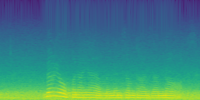
\includegraphics[]{figures/spectrogram_augmented1-img0.png}}};
    
    \coordinate (spec2_c) at ($(aug2_pre_c) - (0, 1.5)$);
    \node[draw, thick, inner sep=0pt] (spec2) at (spec2_c) {\scalebox{.25}{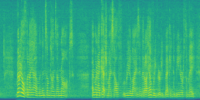
\includegraphics[]{figures/spectrogram_augmented2-img0.png}}};
    
    \draw[->,thick, shorten >=5pt] (aug1_pre.south) -- (spec1.north);
    \draw[->,thick, shorten >=5pt] (aug2_pre.south) -- (spec2.north) node[midway,right] {\tiny \circled{2}};
    
    \coordinate (encoder_c) at ($(waveform_pre_input_c) - (0, 5)$);
    \node[inner sep=0pt] (encoder) at (encoder_c)  {\scalebox{.4}{\begin{tikzpicture}
    \tikzstyle{hidden neuron}=[circle, draw, ultra thick, minimum size=7pt,inner sep=0pt];
    
    % \node[hidden neuron] (n1) at (0.5,0) {};
    \node[hidden neuron] (n2) at (1,0.3) {};
    
    \node[hidden neuron] (n3) at (0.2,1.2) {};
    \node[hidden neuron] (n4) at (1,1.2) {};
    
    \node[hidden neuron] (n5) at (1.9,2) {};
    \node[hidden neuron] (n6) at (-0.7,1.5) {};
    
    \node[hidden neuron] (n7) at (2.05,3) {};
    \node[hidden neuron] (n8) at (-0.9,2.1) {};
    
    \node[hidden neuron] (n9) at (1.5,3.6) {};
    \node[hidden neuron] (n10) at (-1.8,2.2) {};
    
    \node[hidden neuron] (n11) at (0.7,4) {};
    \node[hidden neuron] (n12) at (-1.7,3.2) {};
    
    \node[hidden neuron] (n13) at (0,4) {};
    \node[hidden neuron] (n14) at (-1,3.7) {};
    
    \node[hidden neuron] (n15) at (-0.7,3.1) {};
    \node[hidden neuron] (n16) at (0.7,2.7) {};
    \node[hidden neuron] (n17) at (-0.1,2) {};
    
    \draw[ultra thick] (n2) -- (n3);
    \draw[ultra thick] (n2) -- (n4);
    \draw[ultra thick] (n3) -- (n6);
    \draw[ultra thick] (n4) -- (n5);
    \draw[ultra thick] (n5) -- (n7);
    \draw[ultra thick] (n6) -- (n8);
    \draw[ultra thick] (n7) -- (n9);
    \draw[ultra thick] (n8) -- (n10);
    \draw[ultra thick] (n9) -- (n11);
    \draw[ultra thick] (n10) -- (n12);
    \draw[ultra thick] (n11) -- (n13);
    \draw[ultra thick] (n12) -- (n14);
    \draw[ultra thick] (n13) -- (n14);
    
    \draw[ultra thick] (n4) -- (n17);
    \draw[ultra thick] (n6) -- (n17);
    \draw[ultra thick] (n15) -- (n16);
    \draw[ultra thick] (n15) -- (n17);
    \draw[ultra thick] (n16) -- (n17);
    
    \draw[ultra thick] (n15) -- (n12);
    \draw[ultra thick] (n8) -- (n11);
    
    \draw[ultra thick] (n5) -- (n16);
    \draw[ultra thick] (n7) -- (n16);
    
    \draw[ultra thick] (n14) -- (n9);
    \draw[ultra thick] (n13) -- (n15);
    
    \draw[ultra thick] (n16) -- (n9);
    \draw[ultra thick] (n17) -- (n5);
    
\end{tikzpicture}}};
    
    \draw[->,thick, shorten >=5pt, shorten <=5pt] (spec1.south) -- (encoder);
    \draw[->,thick, shorten >=5pt, shorten <=5pt] (spec2.south) -- (encoder) node[midway,right] {\tiny \circled{3}};
    
    \coordinate (nn_pre_c) at ($(encoder_c) - (0, 2.5)$);
    \node[inner sep=0pt, color=red] (nn_pre) at (nn_pre_c) {\scalebox{.3}{\begin{tikzpicture}[shorten >=1pt]
    \tikzstyle{every pin edge}=[<-,shorten <=1pt]
    \tikzstyle{input neuron}=[circle, draw, thick, fill, minimum size=17pt,inner sep=0pt];
    \tikzstyle{output neuron}=[circle, draw, thick, double, minimum size=17pt,inner sep=0pt];
    \tikzstyle{hidden neuron}=[circle, draw, thick, minimum size=17pt,inner sep=0pt];


    
    % Draw the hidden layer nodes
    \foreach \name / \y in {1,...,3}
        \node[input neuron] (I-\name) at ($(0.5*\y + \y - 0.5, 0)$) {};
    
    \foreach \name / \y in {1,...,4}
        \node[hidden neuron] (H-\name) at ($(0.2*\y + \y - 0.5, -1.5cm)$) {};
    
    \foreach \name / \y in {1,...,2}
        \node[output neuron] (O-\name) at ($(1*\y + \y - 0.5, -3cm)$) {};
    
    \foreach \source in {1,...,3}
        \foreach \dest in {1,...,4}
            \draw[->,shorten >=1pt] (I-\source) -- (H-\dest);
    
    \foreach \source in {1,...,4}
        \foreach \dest in {1,...,2}
            \draw[->,shorten >=1pt] (H-\source) -- (O-\dest);
\end{tikzpicture}}};
    \node[draw, fill=white, rounded corners] (nn_pre_txt) at ($(encoder_c)+(0,0.325)$) {\tiny Encoder};
    
    \coordinate (encoder_south1) at ($(encoder.south) - (0.2, 0)$);
    \coordinate (encoder_south2) at ($(encoder.south) + (0.2, 0)$);
    
    \draw[thick, ->, shorten >=5pt, shorten <=5pt] (encoder_south1) -- (encoder_south1|-nn_pre.north);
    \draw[thick, ->, shorten >=5pt, shorten <=5pt] (encoder_south2) -- (encoder_south2|-nn_pre.north) node[midway,right] {\tiny \circled{4}};
    
    \coordinate (nt_xent_c) at ($(nn_pre_c) - (0, 2)$);
    \node[draw, rectangle, rounded corners, minimum width=2.5cm, minimum height=1cm, fill=red!50] (nt_xent) at (nt_xent_c) {NT-Xent};
    
    \coordinate (nn_pre_south1) at ($(nn_pre.south) - (0.2, 0)$);
    \coordinate (nn_pre_south2) at ($(nn_pre.south) + (0.2, 0)$);
    
    \draw[thick, ->, shorten >=5pt, shorten <=5pt] (nn_pre_south1) -- (nn_pre_south1|-nt_xent.north);
    \draw[thick, ->, shorten >=5pt, shorten <=5pt] (nn_pre_south2) -- (nn_pre_south2|-nt_xent.north) node[midway,right] {\tiny \circled{5}};
    
    
    %%%%%%%%%%%%%%%%%%%%%%%
    
    \coordinate (transfer_box_tl) at (6,-1.75);
    \node[boxNoFill, minimum width = 3cm, minimum height = 9.75cm, below right] (transfer_box) at (transfer_box_tl) {};
    
    \node (transfer_txt) at (7.5, -1.5) {2. Transfer};
    
    \coordinate (waveform_transfer_c) at (7.5,-2.5);
    \node[inner sep=0pt] (waveform_transfer) at (waveform_transfer_c) {\scalebox{.3}{%% Creator: Matplotlib, PGF backend
%%
%% To include the figure in your LaTeX document, write
%%   \input{<filename>.pgf}
%%
%% Make sure the required packages are loaded in your preamble
%%   \usepackage{pgf}
%%
%% and, on pdftex
%%   \usepackage[utf8]{inputenc}\DeclareUnicodeCharacter{2212}{-}
%%
%% or, on luatex and xetex
%%   \usepackage{unicode-math}
%%
%% Figures using additional raster images can only be included by \input if
%% they are in the same directory as the main LaTeX file. For loading figures
%% from other directories you can use the `import` package
%%   \usepackage{import}
%%
%% and then include the figures with
%%   \import{<path to file>}{<filename>.pgf}
%%
%% Matplotlib used the following preamble
%%
\begingroup%
\makeatletter%
\begin{pgfpicture}%
\pgfpathrectangle{\pgfpointorigin}{\pgfqpoint{2.000000in}{1.000000in}}%
\pgfusepath{use as bounding box, clip}%
\begin{pgfscope}%
\pgfsetbuttcap%
\pgfsetmiterjoin%
\pgfsetlinewidth{0.000000pt}%
\definecolor{currentstroke}{rgb}{0.000000,0.000000,0.000000}%
\pgfsetstrokecolor{currentstroke}%
\pgfsetstrokeopacity{0.000000}%
\pgfsetdash{}{0pt}%
\pgfpathmoveto{\pgfqpoint{0.000000in}{0.000000in}}%
\pgfpathlineto{\pgfqpoint{2.000000in}{0.000000in}}%
\pgfpathlineto{\pgfqpoint{2.000000in}{1.000000in}}%
\pgfpathlineto{\pgfqpoint{0.000000in}{1.000000in}}%
\pgfpathclose%
\pgfusepath{}%
\end{pgfscope}%
\begin{pgfscope}%
\pgfpathrectangle{\pgfqpoint{0.000000in}{0.000000in}}{\pgfqpoint{2.000000in}{1.000000in}}%
\pgfusepath{clip}%
\pgfsetrectcap%
\pgfsetroundjoin%
\pgfsetlinewidth{1.505625pt}%
\definecolor{currentstroke}{rgb}{0.121569,0.466667,0.705882}%
\pgfsetstrokecolor{currentstroke}%
\pgfsetdash{}{0pt}%
\pgfpathmoveto{\pgfqpoint{0.000000in}{0.563134in}}%
\pgfpathlineto{\pgfqpoint{0.000625in}{0.590583in}}%
\pgfpathlineto{\pgfqpoint{0.000175in}{0.557272in}}%
\pgfpathlineto{\pgfqpoint{0.001175in}{0.576812in}}%
\pgfpathlineto{\pgfqpoint{0.001600in}{0.537173in}}%
\pgfpathlineto{\pgfqpoint{0.001975in}{0.584814in}}%
\pgfpathlineto{\pgfqpoint{0.002225in}{0.580813in}}%
\pgfpathlineto{\pgfqpoint{0.002275in}{0.582023in}}%
\pgfpathlineto{\pgfqpoint{0.002325in}{0.578487in}}%
\pgfpathlineto{\pgfqpoint{0.002675in}{0.561645in}}%
\pgfpathlineto{\pgfqpoint{0.003400in}{0.587327in}}%
\pgfpathlineto{\pgfqpoint{0.004625in}{0.556900in}}%
\pgfpathlineto{\pgfqpoint{0.004650in}{0.560529in}}%
\pgfpathlineto{\pgfqpoint{0.004950in}{0.599888in}}%
\pgfpathlineto{\pgfqpoint{0.005775in}{0.567693in}}%
\pgfpathlineto{\pgfqpoint{0.006050in}{0.534009in}}%
\pgfpathlineto{\pgfqpoint{0.006675in}{0.586768in}}%
\pgfpathlineto{\pgfqpoint{0.006800in}{0.575230in}}%
\pgfpathlineto{\pgfqpoint{0.007475in}{0.602773in}}%
\pgfpathlineto{\pgfqpoint{0.007000in}{0.568252in}}%
\pgfpathlineto{\pgfqpoint{0.007925in}{0.577929in}}%
\pgfpathlineto{\pgfqpoint{0.008325in}{0.551689in}}%
\pgfpathlineto{\pgfqpoint{0.009100in}{0.568438in}}%
\pgfpathlineto{\pgfqpoint{0.009825in}{0.586675in}}%
\pgfpathlineto{\pgfqpoint{0.010100in}{0.560901in}}%
\pgfpathlineto{\pgfqpoint{0.010200in}{0.569833in}}%
\pgfpathlineto{\pgfqpoint{0.010700in}{0.562203in}}%
\pgfpathlineto{\pgfqpoint{0.011025in}{0.587048in}}%
\pgfpathlineto{\pgfqpoint{0.011300in}{0.569647in}}%
\pgfpathlineto{\pgfqpoint{0.011450in}{0.555597in}}%
\pgfpathlineto{\pgfqpoint{0.011925in}{0.579045in}}%
\pgfpathlineto{\pgfqpoint{0.012100in}{0.574579in}}%
\pgfpathlineto{\pgfqpoint{0.012125in}{0.578301in}}%
\pgfpathlineto{\pgfqpoint{0.012975in}{0.555783in}}%
\pgfpathlineto{\pgfqpoint{0.013150in}{0.569275in}}%
\pgfpathlineto{\pgfqpoint{0.013275in}{0.561831in}}%
\pgfpathlineto{\pgfqpoint{0.013626in}{0.585559in}}%
\pgfpathlineto{\pgfqpoint{0.013676in}{0.594212in}}%
\pgfpathlineto{\pgfqpoint{0.014126in}{0.551131in}}%
\pgfpathlineto{\pgfqpoint{0.014626in}{0.576533in}}%
\pgfpathlineto{\pgfqpoint{0.015226in}{0.556807in}}%
\pgfpathlineto{\pgfqpoint{0.015651in}{0.582395in}}%
\pgfpathlineto{\pgfqpoint{0.015701in}{0.581278in}}%
\pgfpathlineto{\pgfqpoint{0.015826in}{0.588257in}}%
\pgfpathlineto{\pgfqpoint{0.016476in}{0.570113in}}%
\pgfpathlineto{\pgfqpoint{0.016676in}{0.578115in}}%
\pgfpathlineto{\pgfqpoint{0.017276in}{0.551689in}}%
\pgfpathlineto{\pgfqpoint{0.017701in}{0.588071in}}%
\pgfpathlineto{\pgfqpoint{0.017726in}{0.587606in}}%
\pgfpathlineto{\pgfqpoint{0.017876in}{0.598586in}}%
\pgfpathlineto{\pgfqpoint{0.018126in}{0.568996in}}%
\pgfpathlineto{\pgfqpoint{0.018576in}{0.575696in}}%
\pgfpathlineto{\pgfqpoint{0.018801in}{0.557365in}}%
\pgfpathlineto{\pgfqpoint{0.019001in}{0.579883in}}%
\pgfpathlineto{\pgfqpoint{0.019676in}{0.576905in}}%
\pgfpathlineto{\pgfqpoint{0.020251in}{0.556062in}}%
\pgfpathlineto{\pgfqpoint{0.019751in}{0.583139in}}%
\pgfpathlineto{\pgfqpoint{0.020601in}{0.580441in}}%
\pgfpathlineto{\pgfqpoint{0.020651in}{0.589653in}}%
\pgfpathlineto{\pgfqpoint{0.021076in}{0.555411in}}%
\pgfpathlineto{\pgfqpoint{0.021651in}{0.574672in}}%
\pgfpathlineto{\pgfqpoint{0.022651in}{0.563134in}}%
\pgfpathlineto{\pgfqpoint{0.022351in}{0.584535in}}%
\pgfpathlineto{\pgfqpoint{0.022751in}{0.574765in}}%
\pgfpathlineto{\pgfqpoint{0.022851in}{0.580813in}}%
\pgfpathlineto{\pgfqpoint{0.023151in}{0.556527in}}%
\pgfpathlineto{\pgfqpoint{0.023351in}{0.551131in}}%
\pgfpathlineto{\pgfqpoint{0.023526in}{0.561180in}}%
\pgfpathlineto{\pgfqpoint{0.023576in}{0.557644in}}%
\pgfpathlineto{\pgfqpoint{0.023801in}{0.585000in}}%
\pgfpathlineto{\pgfqpoint{0.024751in}{0.574951in}}%
\pgfpathlineto{\pgfqpoint{0.024826in}{0.577743in}}%
\pgfpathlineto{\pgfqpoint{0.025501in}{0.560994in}}%
\pgfpathlineto{\pgfqpoint{0.025701in}{0.568903in}}%
\pgfpathlineto{\pgfqpoint{0.025801in}{0.560994in}}%
\pgfpathlineto{\pgfqpoint{0.026501in}{0.592351in}}%
\pgfpathlineto{\pgfqpoint{0.026751in}{0.586675in}}%
\pgfpathlineto{\pgfqpoint{0.027951in}{0.557551in}}%
\pgfpathlineto{\pgfqpoint{0.026876in}{0.593375in}}%
\pgfpathlineto{\pgfqpoint{0.028001in}{0.560715in}}%
\pgfpathlineto{\pgfqpoint{0.028901in}{0.590490in}}%
\pgfpathlineto{\pgfqpoint{0.028326in}{0.552154in}}%
\pgfpathlineto{\pgfqpoint{0.029176in}{0.576533in}}%
\pgfpathlineto{\pgfqpoint{0.029201in}{0.576626in}}%
\pgfpathlineto{\pgfqpoint{0.029226in}{0.572904in}}%
\pgfpathlineto{\pgfqpoint{0.030101in}{0.554853in}}%
\pgfpathlineto{\pgfqpoint{0.030326in}{0.570578in}}%
\pgfpathlineto{\pgfqpoint{0.031126in}{0.582581in}}%
\pgfpathlineto{\pgfqpoint{0.031376in}{0.563413in}}%
\pgfpathlineto{\pgfqpoint{0.031401in}{0.562762in}}%
\pgfpathlineto{\pgfqpoint{0.031726in}{0.580534in}}%
\pgfpathlineto{\pgfqpoint{0.031751in}{0.585000in}}%
\pgfpathlineto{\pgfqpoint{0.032101in}{0.562390in}}%
\pgfpathlineto{\pgfqpoint{0.032751in}{0.571322in}}%
\pgfpathlineto{\pgfqpoint{0.033251in}{0.555969in}}%
\pgfpathlineto{\pgfqpoint{0.033651in}{0.583791in}}%
\pgfpathlineto{\pgfqpoint{0.033826in}{0.579138in}}%
\pgfpathlineto{\pgfqpoint{0.034026in}{0.586954in}}%
\pgfpathlineto{\pgfqpoint{0.034701in}{0.558947in}}%
\pgfpathlineto{\pgfqpoint{0.034901in}{0.582674in}}%
\pgfpathlineto{\pgfqpoint{0.035451in}{0.563599in}}%
\pgfpathlineto{\pgfqpoint{0.035026in}{0.591700in}}%
\pgfpathlineto{\pgfqpoint{0.036026in}{0.572718in}}%
\pgfpathlineto{\pgfqpoint{0.036051in}{0.573369in}}%
\pgfpathlineto{\pgfqpoint{0.036226in}{0.557272in}}%
\pgfpathlineto{\pgfqpoint{0.036451in}{0.557272in}}%
\pgfpathlineto{\pgfqpoint{0.036476in}{0.554573in}}%
\pgfpathlineto{\pgfqpoint{0.037251in}{0.583884in}}%
\pgfpathlineto{\pgfqpoint{0.037301in}{0.576626in}}%
\pgfpathlineto{\pgfqpoint{0.037651in}{0.589374in}}%
\pgfpathlineto{\pgfqpoint{0.038276in}{0.561366in}}%
\pgfpathlineto{\pgfqpoint{0.038376in}{0.564437in}}%
\pgfpathlineto{\pgfqpoint{0.039576in}{0.590583in}}%
\pgfpathlineto{\pgfqpoint{0.038501in}{0.552154in}}%
\pgfpathlineto{\pgfqpoint{0.039676in}{0.585838in}}%
\pgfpathlineto{\pgfqpoint{0.040927in}{0.559970in}}%
\pgfpathlineto{\pgfqpoint{0.040952in}{0.560622in}}%
\pgfpathlineto{\pgfqpoint{0.041777in}{0.593003in}}%
\pgfpathlineto{\pgfqpoint{0.041152in}{0.557086in}}%
\pgfpathlineto{\pgfqpoint{0.042102in}{0.575975in}}%
\pgfpathlineto{\pgfqpoint{0.043002in}{0.557830in}}%
\pgfpathlineto{\pgfqpoint{0.042502in}{0.587885in}}%
\pgfpathlineto{\pgfqpoint{0.043377in}{0.566484in}}%
\pgfpathlineto{\pgfqpoint{0.043502in}{0.559970in}}%
\pgfpathlineto{\pgfqpoint{0.044577in}{0.586210in}}%
\pgfpathlineto{\pgfqpoint{0.045752in}{0.557737in}}%
\pgfpathlineto{\pgfqpoint{0.045877in}{0.563320in}}%
\pgfpathlineto{\pgfqpoint{0.046352in}{0.581185in}}%
\pgfpathlineto{\pgfqpoint{0.045952in}{0.560063in}}%
\pgfpathlineto{\pgfqpoint{0.047002in}{0.571508in}}%
\pgfpathlineto{\pgfqpoint{0.047177in}{0.561552in}}%
\pgfpathlineto{\pgfqpoint{0.047252in}{0.577463in}}%
\pgfpathlineto{\pgfqpoint{0.048077in}{0.572811in}}%
\pgfpathlineto{\pgfqpoint{0.048952in}{0.587513in}}%
\pgfpathlineto{\pgfqpoint{0.048427in}{0.566018in}}%
\pgfpathlineto{\pgfqpoint{0.049227in}{0.575882in}}%
\pgfpathlineto{\pgfqpoint{0.049327in}{0.561087in}}%
\pgfpathlineto{\pgfqpoint{0.049927in}{0.579697in}}%
\pgfpathlineto{\pgfqpoint{0.050327in}{0.568996in}}%
\pgfpathlineto{\pgfqpoint{0.050652in}{0.597748in}}%
\pgfpathlineto{\pgfqpoint{0.051227in}{0.560342in}}%
\pgfpathlineto{\pgfqpoint{0.051377in}{0.567321in}}%
\pgfpathlineto{\pgfqpoint{0.051527in}{0.553922in}}%
\pgfpathlineto{\pgfqpoint{0.052252in}{0.576719in}}%
\pgfpathlineto{\pgfqpoint{0.052427in}{0.573742in}}%
\pgfpathlineto{\pgfqpoint{0.052552in}{0.580627in}}%
\pgfpathlineto{\pgfqpoint{0.052927in}{0.565274in}}%
\pgfpathlineto{\pgfqpoint{0.053302in}{0.571136in}}%
\pgfpathlineto{\pgfqpoint{0.054002in}{0.554387in}}%
\pgfpathlineto{\pgfqpoint{0.054377in}{0.569461in}}%
\pgfpathlineto{\pgfqpoint{0.055402in}{0.585373in}}%
\pgfpathlineto{\pgfqpoint{0.055502in}{0.577463in}}%
\pgfpathlineto{\pgfqpoint{0.056352in}{0.555876in}}%
\pgfpathlineto{\pgfqpoint{0.056652in}{0.567879in}}%
\pgfpathlineto{\pgfqpoint{0.057027in}{0.578859in}}%
\pgfpathlineto{\pgfqpoint{0.057652in}{0.560156in}}%
\pgfpathlineto{\pgfqpoint{0.057777in}{0.570857in}}%
\pgfpathlineto{\pgfqpoint{0.058502in}{0.590490in}}%
\pgfpathlineto{\pgfqpoint{0.058827in}{0.566111in}}%
\pgfpathlineto{\pgfqpoint{0.058877in}{0.573462in}}%
\pgfpathlineto{\pgfqpoint{0.059452in}{0.560156in}}%
\pgfpathlineto{\pgfqpoint{0.059052in}{0.585280in}}%
\pgfpathlineto{\pgfqpoint{0.059927in}{0.568624in}}%
\pgfpathlineto{\pgfqpoint{0.059977in}{0.578673in}}%
\pgfpathlineto{\pgfqpoint{0.060477in}{0.550386in}}%
\pgfpathlineto{\pgfqpoint{0.061002in}{0.555318in}}%
\pgfpathlineto{\pgfqpoint{0.061527in}{0.595143in}}%
\pgfpathlineto{\pgfqpoint{0.061052in}{0.554853in}}%
\pgfpathlineto{\pgfqpoint{0.062302in}{0.569368in}}%
\pgfpathlineto{\pgfqpoint{0.062902in}{0.559319in}}%
\pgfpathlineto{\pgfqpoint{0.063202in}{0.581278in}}%
\pgfpathlineto{\pgfqpoint{0.063352in}{0.573555in}}%
\pgfpathlineto{\pgfqpoint{0.063777in}{0.587048in}}%
\pgfpathlineto{\pgfqpoint{0.064177in}{0.565925in}}%
\pgfpathlineto{\pgfqpoint{0.064502in}{0.575137in}}%
\pgfpathlineto{\pgfqpoint{0.065127in}{0.551131in}}%
\pgfpathlineto{\pgfqpoint{0.065552in}{0.580906in}}%
\pgfpathlineto{\pgfqpoint{0.065577in}{0.580069in}}%
\pgfpathlineto{\pgfqpoint{0.065927in}{0.590397in}}%
\pgfpathlineto{\pgfqpoint{0.066277in}{0.571136in}}%
\pgfpathlineto{\pgfqpoint{0.066302in}{0.575230in}}%
\pgfpathlineto{\pgfqpoint{0.067203in}{0.562017in}}%
\pgfpathlineto{\pgfqpoint{0.066477in}{0.591514in}}%
\pgfpathlineto{\pgfqpoint{0.067428in}{0.567693in}}%
\pgfpathlineto{\pgfqpoint{0.067578in}{0.566298in}}%
\pgfpathlineto{\pgfqpoint{0.068153in}{0.578022in}}%
\pgfpathlineto{\pgfqpoint{0.068228in}{0.577184in}}%
\pgfpathlineto{\pgfqpoint{0.068253in}{0.579976in}}%
\pgfpathlineto{\pgfqpoint{0.068803in}{0.564809in}}%
\pgfpathlineto{\pgfqpoint{0.069228in}{0.568066in}}%
\pgfpathlineto{\pgfqpoint{0.069378in}{0.551689in}}%
\pgfpathlineto{\pgfqpoint{0.070278in}{0.584349in}}%
\pgfpathlineto{\pgfqpoint{0.070878in}{0.572067in}}%
\pgfpathlineto{\pgfqpoint{0.071003in}{0.573183in}}%
\pgfpathlineto{\pgfqpoint{0.071378in}{0.555132in}}%
\pgfpathlineto{\pgfqpoint{0.071853in}{0.577929in}}%
\pgfpathlineto{\pgfqpoint{0.072128in}{0.567600in}}%
\pgfpathlineto{\pgfqpoint{0.072853in}{0.583419in}}%
\pgfpathlineto{\pgfqpoint{0.073028in}{0.564623in}}%
\pgfpathlineto{\pgfqpoint{0.073253in}{0.571601in}}%
\pgfpathlineto{\pgfqpoint{0.073528in}{0.404113in}}%
\pgfpathlineto{\pgfqpoint{0.073478in}{0.720015in}}%
\pgfpathlineto{\pgfqpoint{0.074203in}{0.598027in}}%
\pgfpathlineto{\pgfqpoint{0.074228in}{0.691728in}}%
\pgfpathlineto{\pgfqpoint{0.074278in}{0.509165in}}%
\pgfpathlineto{\pgfqpoint{0.075303in}{0.578301in}}%
\pgfpathlineto{\pgfqpoint{0.075853in}{0.528240in}}%
\pgfpathlineto{\pgfqpoint{0.075528in}{0.597934in}}%
\pgfpathlineto{\pgfqpoint{0.076453in}{0.557086in}}%
\pgfpathlineto{\pgfqpoint{0.076703in}{0.606402in}}%
\pgfpathlineto{\pgfqpoint{0.076678in}{0.540802in}}%
\pgfpathlineto{\pgfqpoint{0.077578in}{0.575789in}}%
\pgfpathlineto{\pgfqpoint{0.077903in}{0.543687in}}%
\pgfpathlineto{\pgfqpoint{0.078653in}{0.589281in}}%
\pgfpathlineto{\pgfqpoint{0.078678in}{0.580720in}}%
\pgfpathlineto{\pgfqpoint{0.079678in}{0.559691in}}%
\pgfpathlineto{\pgfqpoint{0.079053in}{0.606309in}}%
\pgfpathlineto{\pgfqpoint{0.079803in}{0.571229in}}%
\pgfpathlineto{\pgfqpoint{0.080578in}{0.589095in}}%
\pgfpathlineto{\pgfqpoint{0.079903in}{0.562762in}}%
\pgfpathlineto{\pgfqpoint{0.080928in}{0.581465in}}%
\pgfpathlineto{\pgfqpoint{0.081303in}{0.556527in}}%
\pgfpathlineto{\pgfqpoint{0.081003in}{0.586117in}}%
\pgfpathlineto{\pgfqpoint{0.082053in}{0.565832in}}%
\pgfpathlineto{\pgfqpoint{0.083028in}{0.580906in}}%
\pgfpathlineto{\pgfqpoint{0.082378in}{0.559226in}}%
\pgfpathlineto{\pgfqpoint{0.083253in}{0.578673in}}%
\pgfpathlineto{\pgfqpoint{0.083603in}{0.605843in}}%
\pgfpathlineto{\pgfqpoint{0.083903in}{0.536336in}}%
\pgfpathlineto{\pgfqpoint{0.084078in}{0.564064in}}%
\pgfpathlineto{\pgfqpoint{0.084503in}{0.545361in}}%
\pgfpathlineto{\pgfqpoint{0.084203in}{0.593654in}}%
\pgfpathlineto{\pgfqpoint{0.085153in}{0.562948in}}%
\pgfpathlineto{\pgfqpoint{0.085403in}{0.597004in}}%
\pgfpathlineto{\pgfqpoint{0.085903in}{0.556248in}}%
\pgfpathlineto{\pgfqpoint{0.086278in}{0.573648in}}%
\pgfpathlineto{\pgfqpoint{0.086553in}{0.547595in}}%
\pgfpathlineto{\pgfqpoint{0.087278in}{0.594119in}}%
\pgfpathlineto{\pgfqpoint{0.087353in}{0.581185in}}%
\pgfpathlineto{\pgfqpoint{0.087403in}{0.608821in}}%
\pgfpathlineto{\pgfqpoint{0.088328in}{0.549735in}}%
\pgfpathlineto{\pgfqpoint{0.088353in}{0.554201in}}%
\pgfpathlineto{\pgfqpoint{0.089228in}{0.523309in}}%
\pgfpathlineto{\pgfqpoint{0.089128in}{0.581092in}}%
\pgfpathlineto{\pgfqpoint{0.089328in}{0.577929in}}%
\pgfpathlineto{\pgfqpoint{0.089778in}{0.601656in}}%
\pgfpathlineto{\pgfqpoint{0.089428in}{0.561366in}}%
\pgfpathlineto{\pgfqpoint{0.090378in}{0.565553in}}%
\pgfpathlineto{\pgfqpoint{0.091503in}{0.552898in}}%
\pgfpathlineto{\pgfqpoint{0.090503in}{0.607704in}}%
\pgfpathlineto{\pgfqpoint{0.091528in}{0.559877in}}%
\pgfpathlineto{\pgfqpoint{0.091953in}{0.584814in}}%
\pgfpathlineto{\pgfqpoint{0.092403in}{0.547688in}}%
\pgfpathlineto{\pgfqpoint{0.092603in}{0.564064in}}%
\pgfpathlineto{\pgfqpoint{0.092653in}{0.549177in}}%
\pgfpathlineto{\pgfqpoint{0.093504in}{0.583977in}}%
\pgfpathlineto{\pgfqpoint{0.093704in}{0.567414in}}%
\pgfpathlineto{\pgfqpoint{0.094679in}{0.601656in}}%
\pgfpathlineto{\pgfqpoint{0.094029in}{0.555318in}}%
\pgfpathlineto{\pgfqpoint{0.094754in}{0.564995in}}%
\pgfpathlineto{\pgfqpoint{0.095354in}{0.544803in}}%
\pgfpathlineto{\pgfqpoint{0.094854in}{0.595887in}}%
\pgfpathlineto{\pgfqpoint{0.095854in}{0.564716in}}%
\pgfpathlineto{\pgfqpoint{0.095979in}{0.563692in}}%
\pgfpathlineto{\pgfqpoint{0.096229in}{0.583605in}}%
\pgfpathlineto{\pgfqpoint{0.096754in}{0.592351in}}%
\pgfpathlineto{\pgfqpoint{0.096854in}{0.546478in}}%
\pgfpathlineto{\pgfqpoint{0.097029in}{0.554573in}}%
\pgfpathlineto{\pgfqpoint{0.097054in}{0.533730in}}%
\pgfpathlineto{\pgfqpoint{0.098079in}{0.590583in}}%
\pgfpathlineto{\pgfqpoint{0.098479in}{0.609938in}}%
\pgfpathlineto{\pgfqpoint{0.098754in}{0.564995in}}%
\pgfpathlineto{\pgfqpoint{0.099029in}{0.585000in}}%
\pgfpathlineto{\pgfqpoint{0.099729in}{0.544245in}}%
\pgfpathlineto{\pgfqpoint{0.100179in}{0.559877in}}%
\pgfpathlineto{\pgfqpoint{0.101229in}{0.585466in}}%
\pgfpathlineto{\pgfqpoint{0.100504in}{0.555318in}}%
\pgfpathlineto{\pgfqpoint{0.101279in}{0.578859in}}%
\pgfpathlineto{\pgfqpoint{0.101904in}{0.546664in}}%
\pgfpathlineto{\pgfqpoint{0.101629in}{0.584721in}}%
\pgfpathlineto{\pgfqpoint{0.102429in}{0.557272in}}%
\pgfpathlineto{\pgfqpoint{0.102904in}{0.604541in}}%
\pgfpathlineto{\pgfqpoint{0.102604in}{0.557086in}}%
\pgfpathlineto{\pgfqpoint{0.103579in}{0.577650in}}%
\pgfpathlineto{\pgfqpoint{0.103654in}{0.589560in}}%
\pgfpathlineto{\pgfqpoint{0.104104in}{0.547502in}}%
\pgfpathlineto{\pgfqpoint{0.104204in}{0.554853in}}%
\pgfpathlineto{\pgfqpoint{0.104629in}{0.545734in}}%
\pgfpathlineto{\pgfqpoint{0.105104in}{0.590397in}}%
\pgfpathlineto{\pgfqpoint{0.105254in}{0.563320in}}%
\pgfpathlineto{\pgfqpoint{0.105329in}{0.595050in}}%
\pgfpathlineto{\pgfqpoint{0.105579in}{0.557644in}}%
\pgfpathlineto{\pgfqpoint{0.106404in}{0.588164in}}%
\pgfpathlineto{\pgfqpoint{0.106704in}{0.550014in}}%
\pgfpathlineto{\pgfqpoint{0.107379in}{0.591607in}}%
\pgfpathlineto{\pgfqpoint{0.107504in}{0.583419in}}%
\pgfpathlineto{\pgfqpoint{0.107729in}{0.590490in}}%
\pgfpathlineto{\pgfqpoint{0.108279in}{0.543687in}}%
\pgfpathlineto{\pgfqpoint{0.108479in}{0.563971in}}%
\pgfpathlineto{\pgfqpoint{0.109154in}{0.552433in}}%
\pgfpathlineto{\pgfqpoint{0.109354in}{0.583791in}}%
\pgfpathlineto{\pgfqpoint{0.109479in}{0.569182in}}%
\pgfpathlineto{\pgfqpoint{0.110154in}{0.595887in}}%
\pgfpathlineto{\pgfqpoint{0.110004in}{0.556155in}}%
\pgfpathlineto{\pgfqpoint{0.110579in}{0.569275in}}%
\pgfpathlineto{\pgfqpoint{0.111379in}{0.556807in}}%
\pgfpathlineto{\pgfqpoint{0.110879in}{0.593189in}}%
\pgfpathlineto{\pgfqpoint{0.111629in}{0.568624in}}%
\pgfpathlineto{\pgfqpoint{0.111829in}{0.594119in}}%
\pgfpathlineto{\pgfqpoint{0.112104in}{0.563785in}}%
\pgfpathlineto{\pgfqpoint{0.112729in}{0.571229in}}%
\pgfpathlineto{\pgfqpoint{0.113804in}{0.586582in}}%
\pgfpathlineto{\pgfqpoint{0.113154in}{0.545734in}}%
\pgfpathlineto{\pgfqpoint{0.113829in}{0.582767in}}%
\pgfpathlineto{\pgfqpoint{0.114854in}{0.545175in}}%
\pgfpathlineto{\pgfqpoint{0.114429in}{0.596259in}}%
\pgfpathlineto{\pgfqpoint{0.114954in}{0.559226in}}%
\pgfpathlineto{\pgfqpoint{0.115979in}{0.587606in}}%
\pgfpathlineto{\pgfqpoint{0.115229in}{0.553178in}}%
\pgfpathlineto{\pgfqpoint{0.116104in}{0.580162in}}%
\pgfpathlineto{\pgfqpoint{0.116679in}{0.550293in}}%
\pgfpathlineto{\pgfqpoint{0.116404in}{0.589281in}}%
\pgfpathlineto{\pgfqpoint{0.117254in}{0.550386in}}%
\pgfpathlineto{\pgfqpoint{0.118404in}{0.591421in}}%
\pgfpathlineto{\pgfqpoint{0.119279in}{0.552619in}}%
\pgfpathlineto{\pgfqpoint{0.118754in}{0.594864in}}%
\pgfpathlineto{\pgfqpoint{0.119554in}{0.563320in}}%
\pgfpathlineto{\pgfqpoint{0.119679in}{0.577277in}}%
\pgfpathlineto{\pgfqpoint{0.119729in}{0.556807in}}%
\pgfpathlineto{\pgfqpoint{0.119829in}{0.577184in}}%
\pgfpathlineto{\pgfqpoint{0.120080in}{0.593189in}}%
\pgfpathlineto{\pgfqpoint{0.120355in}{0.555225in}}%
\pgfpathlineto{\pgfqpoint{0.120905in}{0.580441in}}%
\pgfpathlineto{\pgfqpoint{0.121530in}{0.532614in}}%
\pgfpathlineto{\pgfqpoint{0.121980in}{0.587327in}}%
\pgfpathlineto{\pgfqpoint{0.122030in}{0.562017in}}%
\pgfpathlineto{\pgfqpoint{0.122505in}{0.599330in}}%
\pgfpathlineto{\pgfqpoint{0.122980in}{0.555318in}}%
\pgfpathlineto{\pgfqpoint{0.123155in}{0.573276in}}%
\pgfpathlineto{\pgfqpoint{0.123480in}{0.545361in}}%
\pgfpathlineto{\pgfqpoint{0.123230in}{0.575044in}}%
\pgfpathlineto{\pgfqpoint{0.124305in}{0.562483in}}%
\pgfpathlineto{\pgfqpoint{0.125080in}{0.594398in}}%
\pgfpathlineto{\pgfqpoint{0.124655in}{0.546292in}}%
\pgfpathlineto{\pgfqpoint{0.125330in}{0.556062in}}%
\pgfpathlineto{\pgfqpoint{0.125705in}{0.549270in}}%
\pgfpathlineto{\pgfqpoint{0.126130in}{0.591607in}}%
\pgfpathlineto{\pgfqpoint{0.126355in}{0.578208in}}%
\pgfpathlineto{\pgfqpoint{0.126405in}{0.557737in}}%
\pgfpathlineto{\pgfqpoint{0.126805in}{0.602959in}}%
\pgfpathlineto{\pgfqpoint{0.127430in}{0.570020in}}%
\pgfpathlineto{\pgfqpoint{0.127480in}{0.591700in}}%
\pgfpathlineto{\pgfqpoint{0.128205in}{0.545920in}}%
\pgfpathlineto{\pgfqpoint{0.128505in}{0.568531in}}%
\pgfpathlineto{\pgfqpoint{0.128780in}{0.548339in}}%
\pgfpathlineto{\pgfqpoint{0.129380in}{0.583977in}}%
\pgfpathlineto{\pgfqpoint{0.129555in}{0.572532in}}%
\pgfpathlineto{\pgfqpoint{0.130555in}{0.593654in}}%
\pgfpathlineto{\pgfqpoint{0.130305in}{0.554946in}}%
\pgfpathlineto{\pgfqpoint{0.130630in}{0.567972in}}%
\pgfpathlineto{\pgfqpoint{0.131705in}{0.550200in}}%
\pgfpathlineto{\pgfqpoint{0.130830in}{0.586861in}}%
\pgfpathlineto{\pgfqpoint{0.131730in}{0.568252in}}%
\pgfpathlineto{\pgfqpoint{0.132380in}{0.593933in}}%
\pgfpathlineto{\pgfqpoint{0.132655in}{0.544524in}}%
\pgfpathlineto{\pgfqpoint{0.132805in}{0.560063in}}%
\pgfpathlineto{\pgfqpoint{0.133455in}{0.592631in}}%
\pgfpathlineto{\pgfqpoint{0.133030in}{0.551596in}}%
\pgfpathlineto{\pgfqpoint{0.133855in}{0.567972in}}%
\pgfpathlineto{\pgfqpoint{0.133880in}{0.552340in}}%
\pgfpathlineto{\pgfqpoint{0.134880in}{0.588071in}}%
\pgfpathlineto{\pgfqpoint{0.134955in}{0.568624in}}%
\pgfpathlineto{\pgfqpoint{0.135755in}{0.589002in}}%
\pgfpathlineto{\pgfqpoint{0.135080in}{0.555225in}}%
\pgfpathlineto{\pgfqpoint{0.136055in}{0.570857in}}%
\pgfpathlineto{\pgfqpoint{0.136230in}{0.601191in}}%
\pgfpathlineto{\pgfqpoint{0.136505in}{0.552526in}}%
\pgfpathlineto{\pgfqpoint{0.137080in}{0.573928in}}%
\pgfpathlineto{\pgfqpoint{0.137580in}{0.543501in}}%
\pgfpathlineto{\pgfqpoint{0.137880in}{0.586489in}}%
\pgfpathlineto{\pgfqpoint{0.138130in}{0.575882in}}%
\pgfpathlineto{\pgfqpoint{0.138480in}{0.601098in}}%
\pgfpathlineto{\pgfqpoint{0.139055in}{0.559784in}}%
\pgfpathlineto{\pgfqpoint{0.139205in}{0.582116in}}%
\pgfpathlineto{\pgfqpoint{0.140205in}{0.544710in}}%
\pgfpathlineto{\pgfqpoint{0.140280in}{0.588815in}}%
\pgfpathlineto{\pgfqpoint{0.140330in}{0.565460in}}%
\pgfpathlineto{\pgfqpoint{0.140730in}{0.585931in}}%
\pgfpathlineto{\pgfqpoint{0.140755in}{0.568066in}}%
\pgfpathlineto{\pgfqpoint{0.141155in}{0.543501in}}%
\pgfpathlineto{\pgfqpoint{0.141205in}{0.596911in}}%
\pgfpathlineto{\pgfqpoint{0.141855in}{0.573183in}}%
\pgfpathlineto{\pgfqpoint{0.142230in}{0.558202in}}%
\pgfpathlineto{\pgfqpoint{0.142580in}{0.596818in}}%
\pgfpathlineto{\pgfqpoint{0.142930in}{0.575044in}}%
\pgfpathlineto{\pgfqpoint{0.143205in}{0.588629in}}%
\pgfpathlineto{\pgfqpoint{0.143255in}{0.550200in}}%
\pgfpathlineto{\pgfqpoint{0.144005in}{0.569089in}}%
\pgfpathlineto{\pgfqpoint{0.144880in}{0.552619in}}%
\pgfpathlineto{\pgfqpoint{0.144830in}{0.587885in}}%
\pgfpathlineto{\pgfqpoint{0.144905in}{0.563320in}}%
\pgfpathlineto{\pgfqpoint{0.145580in}{0.553457in}}%
\pgfpathlineto{\pgfqpoint{0.146030in}{0.596539in}}%
\pgfpathlineto{\pgfqpoint{0.147131in}{0.563971in}}%
\pgfpathlineto{\pgfqpoint{0.146130in}{0.604727in}}%
\pgfpathlineto{\pgfqpoint{0.147156in}{0.578301in}}%
\pgfpathlineto{\pgfqpoint{0.147331in}{0.549549in}}%
\pgfpathlineto{\pgfqpoint{0.147256in}{0.586768in}}%
\pgfpathlineto{\pgfqpoint{0.148356in}{0.560435in}}%
\pgfpathlineto{\pgfqpoint{0.148606in}{0.584814in}}%
\pgfpathlineto{\pgfqpoint{0.149206in}{0.549828in}}%
\pgfpathlineto{\pgfqpoint{0.149456in}{0.562296in}}%
\pgfpathlineto{\pgfqpoint{0.149706in}{0.547502in}}%
\pgfpathlineto{\pgfqpoint{0.150256in}{0.589839in}}%
\pgfpathlineto{\pgfqpoint{0.150531in}{0.560994in}}%
\pgfpathlineto{\pgfqpoint{0.150606in}{0.594585in}}%
\pgfpathlineto{\pgfqpoint{0.151706in}{0.573928in}}%
\pgfpathlineto{\pgfqpoint{0.151756in}{0.589467in}}%
\pgfpathlineto{\pgfqpoint{0.152231in}{0.551875in}}%
\pgfpathlineto{\pgfqpoint{0.152731in}{0.578208in}}%
\pgfpathlineto{\pgfqpoint{0.152781in}{0.552712in}}%
\pgfpathlineto{\pgfqpoint{0.153306in}{0.587327in}}%
\pgfpathlineto{\pgfqpoint{0.153856in}{0.567786in}}%
\pgfpathlineto{\pgfqpoint{0.154481in}{0.601191in}}%
\pgfpathlineto{\pgfqpoint{0.154756in}{0.554853in}}%
\pgfpathlineto{\pgfqpoint{0.154906in}{0.560622in}}%
\pgfpathlineto{\pgfqpoint{0.155156in}{0.546292in}}%
\pgfpathlineto{\pgfqpoint{0.155806in}{0.585094in}}%
\pgfpathlineto{\pgfqpoint{0.155981in}{0.568252in}}%
\pgfpathlineto{\pgfqpoint{0.156681in}{0.586210in}}%
\pgfpathlineto{\pgfqpoint{0.156881in}{0.540430in}}%
\pgfpathlineto{\pgfqpoint{0.157006in}{0.574207in}}%
\pgfpathlineto{\pgfqpoint{0.157431in}{0.546850in}}%
\pgfpathlineto{\pgfqpoint{0.157506in}{0.605378in}}%
\pgfpathlineto{\pgfqpoint{0.158106in}{0.565739in}}%
\pgfpathlineto{\pgfqpoint{0.158756in}{0.602866in}}%
\pgfpathlineto{\pgfqpoint{0.158506in}{0.563041in}}%
\pgfpathlineto{\pgfqpoint{0.159256in}{0.573462in}}%
\pgfpathlineto{\pgfqpoint{0.159281in}{0.573648in}}%
\pgfpathlineto{\pgfqpoint{0.159331in}{0.595422in}}%
\pgfpathlineto{\pgfqpoint{0.160031in}{0.557923in}}%
\pgfpathlineto{\pgfqpoint{0.160331in}{0.560622in}}%
\pgfpathlineto{\pgfqpoint{0.160356in}{0.546013in}}%
\pgfpathlineto{\pgfqpoint{0.160881in}{0.584256in}}%
\pgfpathlineto{\pgfqpoint{0.161381in}{0.580162in}}%
\pgfpathlineto{\pgfqpoint{0.162456in}{0.607332in}}%
\pgfpathlineto{\pgfqpoint{0.162256in}{0.550200in}}%
\pgfpathlineto{\pgfqpoint{0.162481in}{0.595236in}}%
\pgfpathlineto{\pgfqpoint{0.163456in}{0.545175in}}%
\pgfpathlineto{\pgfqpoint{0.162556in}{0.613380in}}%
\pgfpathlineto{\pgfqpoint{0.163631in}{0.560063in}}%
\pgfpathlineto{\pgfqpoint{0.163681in}{0.542663in}}%
\pgfpathlineto{\pgfqpoint{0.164581in}{0.591235in}}%
\pgfpathlineto{\pgfqpoint{0.164706in}{0.573928in}}%
\pgfpathlineto{\pgfqpoint{0.164881in}{0.559319in}}%
\pgfpathlineto{\pgfqpoint{0.165056in}{0.582581in}}%
\pgfpathlineto{\pgfqpoint{0.165656in}{0.577277in}}%
\pgfpathlineto{\pgfqpoint{0.165681in}{0.586861in}}%
\pgfpathlineto{\pgfqpoint{0.166081in}{0.556807in}}%
\pgfpathlineto{\pgfqpoint{0.166731in}{0.574207in}}%
\pgfpathlineto{\pgfqpoint{0.167206in}{0.541360in}}%
\pgfpathlineto{\pgfqpoint{0.167006in}{0.591607in}}%
\pgfpathlineto{\pgfqpoint{0.167831in}{0.576719in}}%
\pgfpathlineto{\pgfqpoint{0.168806in}{0.548711in}}%
\pgfpathlineto{\pgfqpoint{0.168206in}{0.590583in}}%
\pgfpathlineto{\pgfqpoint{0.168906in}{0.569647in}}%
\pgfpathlineto{\pgfqpoint{0.169056in}{0.590863in}}%
\pgfpathlineto{\pgfqpoint{0.169481in}{0.548990in}}%
\pgfpathlineto{\pgfqpoint{0.170006in}{0.568159in}}%
\pgfpathlineto{\pgfqpoint{0.170481in}{0.592537in}}%
\pgfpathlineto{\pgfqpoint{0.170981in}{0.553736in}}%
\pgfpathlineto{\pgfqpoint{0.171106in}{0.576254in}}%
\pgfpathlineto{\pgfqpoint{0.171906in}{0.553085in}}%
\pgfpathlineto{\pgfqpoint{0.171981in}{0.590025in}}%
\pgfpathlineto{\pgfqpoint{0.172256in}{0.555597in}}%
\pgfpathlineto{\pgfqpoint{0.172656in}{0.596725in}}%
\pgfpathlineto{\pgfqpoint{0.172931in}{0.537359in}}%
\pgfpathlineto{\pgfqpoint{0.173457in}{0.588815in}}%
\pgfpathlineto{\pgfqpoint{0.174132in}{0.556807in}}%
\pgfpathlineto{\pgfqpoint{0.174582in}{0.579883in}}%
\pgfpathlineto{\pgfqpoint{0.174807in}{0.598772in}}%
\pgfpathlineto{\pgfqpoint{0.174707in}{0.570485in}}%
\pgfpathlineto{\pgfqpoint{0.175057in}{0.588909in}}%
\pgfpathlineto{\pgfqpoint{0.175632in}{0.538848in}}%
\pgfpathlineto{\pgfqpoint{0.175357in}{0.597190in}}%
\pgfpathlineto{\pgfqpoint{0.176157in}{0.564809in}}%
\pgfpathlineto{\pgfqpoint{0.176582in}{0.582581in}}%
\pgfpathlineto{\pgfqpoint{0.176332in}{0.539127in}}%
\pgfpathlineto{\pgfqpoint{0.177257in}{0.568159in}}%
\pgfpathlineto{\pgfqpoint{0.177582in}{0.548339in}}%
\pgfpathlineto{\pgfqpoint{0.178057in}{0.599888in}}%
\pgfpathlineto{\pgfqpoint{0.178282in}{0.574486in}}%
\pgfpathlineto{\pgfqpoint{0.178482in}{0.585931in}}%
\pgfpathlineto{\pgfqpoint{0.178957in}{0.547874in}}%
\pgfpathlineto{\pgfqpoint{0.179307in}{0.560249in}}%
\pgfpathlineto{\pgfqpoint{0.179882in}{0.549456in}}%
\pgfpathlineto{\pgfqpoint{0.180257in}{0.589002in}}%
\pgfpathlineto{\pgfqpoint{0.180407in}{0.563506in}}%
\pgfpathlineto{\pgfqpoint{0.180957in}{0.587885in}}%
\pgfpathlineto{\pgfqpoint{0.180807in}{0.545455in}}%
\pgfpathlineto{\pgfqpoint{0.181482in}{0.566391in}}%
\pgfpathlineto{\pgfqpoint{0.181857in}{0.552992in}}%
\pgfpathlineto{\pgfqpoint{0.182257in}{0.599330in}}%
\pgfpathlineto{\pgfqpoint{0.182482in}{0.588536in}}%
\pgfpathlineto{\pgfqpoint{0.182507in}{0.591328in}}%
\pgfpathlineto{\pgfqpoint{0.183257in}{0.552526in}}%
\pgfpathlineto{\pgfqpoint{0.183332in}{0.571881in}}%
\pgfpathlineto{\pgfqpoint{0.184082in}{0.544896in}}%
\pgfpathlineto{\pgfqpoint{0.183732in}{0.590118in}}%
\pgfpathlineto{\pgfqpoint{0.184457in}{0.561273in}}%
\pgfpathlineto{\pgfqpoint{0.185582in}{0.586675in}}%
\pgfpathlineto{\pgfqpoint{0.184532in}{0.559226in}}%
\pgfpathlineto{\pgfqpoint{0.185607in}{0.579511in}}%
\pgfpathlineto{\pgfqpoint{0.185882in}{0.543780in}}%
\pgfpathlineto{\pgfqpoint{0.186557in}{0.593189in}}%
\pgfpathlineto{\pgfqpoint{0.186707in}{0.563971in}}%
\pgfpathlineto{\pgfqpoint{0.187032in}{0.598493in}}%
\pgfpathlineto{\pgfqpoint{0.187757in}{0.546199in}}%
\pgfpathlineto{\pgfqpoint{0.187832in}{0.575137in}}%
\pgfpathlineto{\pgfqpoint{0.188907in}{0.546385in}}%
\pgfpathlineto{\pgfqpoint{0.188282in}{0.595887in}}%
\pgfpathlineto{\pgfqpoint{0.188932in}{0.554759in}}%
\pgfpathlineto{\pgfqpoint{0.189707in}{0.587792in}}%
\pgfpathlineto{\pgfqpoint{0.189932in}{0.536522in}}%
\pgfpathlineto{\pgfqpoint{0.190057in}{0.574579in}}%
\pgfpathlineto{\pgfqpoint{0.190357in}{0.595515in}}%
\pgfpathlineto{\pgfqpoint{0.190407in}{0.565646in}}%
\pgfpathlineto{\pgfqpoint{0.191157in}{0.574207in}}%
\pgfpathlineto{\pgfqpoint{0.192082in}{0.558109in}}%
\pgfpathlineto{\pgfqpoint{0.191282in}{0.595236in}}%
\pgfpathlineto{\pgfqpoint{0.192282in}{0.567693in}}%
\pgfpathlineto{\pgfqpoint{0.193157in}{0.545641in}}%
\pgfpathlineto{\pgfqpoint{0.192882in}{0.588629in}}%
\pgfpathlineto{\pgfqpoint{0.193207in}{0.576626in}}%
\pgfpathlineto{\pgfqpoint{0.194182in}{0.606867in}}%
\pgfpathlineto{\pgfqpoint{0.193882in}{0.535684in}}%
\pgfpathlineto{\pgfqpoint{0.194307in}{0.578208in}}%
\pgfpathlineto{\pgfqpoint{0.195282in}{0.552247in}}%
\pgfpathlineto{\pgfqpoint{0.195007in}{0.595701in}}%
\pgfpathlineto{\pgfqpoint{0.195382in}{0.579511in}}%
\pgfpathlineto{\pgfqpoint{0.195407in}{0.580441in}}%
\pgfpathlineto{\pgfqpoint{0.195632in}{0.547502in}}%
\pgfpathlineto{\pgfqpoint{0.195657in}{0.546385in}}%
\pgfpathlineto{\pgfqpoint{0.195732in}{0.579418in}}%
\pgfpathlineto{\pgfqpoint{0.195882in}{0.575602in}}%
\pgfpathlineto{\pgfqpoint{0.195907in}{0.590397in}}%
\pgfpathlineto{\pgfqpoint{0.196882in}{0.552247in}}%
\pgfpathlineto{\pgfqpoint{0.196957in}{0.578022in}}%
\pgfpathlineto{\pgfqpoint{0.197982in}{0.550014in}}%
\pgfpathlineto{\pgfqpoint{0.198032in}{0.589560in}}%
\pgfpathlineto{\pgfqpoint{0.198657in}{0.601749in}}%
\pgfpathlineto{\pgfqpoint{0.198107in}{0.557179in}}%
\pgfpathlineto{\pgfqpoint{0.198682in}{0.591793in}}%
\pgfpathlineto{\pgfqpoint{0.199657in}{0.551689in}}%
\pgfpathlineto{\pgfqpoint{0.199807in}{0.567600in}}%
\pgfpathlineto{\pgfqpoint{0.200058in}{0.595980in}}%
\pgfpathlineto{\pgfqpoint{0.200008in}{0.540616in}}%
\pgfpathlineto{\pgfqpoint{0.200933in}{0.576533in}}%
\pgfpathlineto{\pgfqpoint{0.201583in}{0.555783in}}%
\pgfpathlineto{\pgfqpoint{0.201508in}{0.598865in}}%
\pgfpathlineto{\pgfqpoint{0.202033in}{0.566670in}}%
\pgfpathlineto{\pgfqpoint{0.202483in}{0.591049in}}%
\pgfpathlineto{\pgfqpoint{0.202983in}{0.543594in}}%
\pgfpathlineto{\pgfqpoint{0.203108in}{0.568903in}}%
\pgfpathlineto{\pgfqpoint{0.203883in}{0.535964in}}%
\pgfpathlineto{\pgfqpoint{0.203808in}{0.581651in}}%
\pgfpathlineto{\pgfqpoint{0.204208in}{0.569089in}}%
\pgfpathlineto{\pgfqpoint{0.204908in}{0.553457in}}%
\pgfpathlineto{\pgfqpoint{0.204408in}{0.588722in}}%
\pgfpathlineto{\pgfqpoint{0.205333in}{0.561366in}}%
\pgfpathlineto{\pgfqpoint{0.205458in}{0.586954in}}%
\pgfpathlineto{\pgfqpoint{0.206283in}{0.542756in}}%
\pgfpathlineto{\pgfqpoint{0.206458in}{0.576626in}}%
\pgfpathlineto{\pgfqpoint{0.206983in}{0.556062in}}%
\pgfpathlineto{\pgfqpoint{0.207433in}{0.592165in}}%
\pgfpathlineto{\pgfqpoint{0.207533in}{0.580069in}}%
\pgfpathlineto{\pgfqpoint{0.207633in}{0.600912in}}%
\pgfpathlineto{\pgfqpoint{0.208533in}{0.552247in}}%
\pgfpathlineto{\pgfqpoint{0.208633in}{0.576161in}}%
\pgfpathlineto{\pgfqpoint{0.208708in}{0.549270in}}%
\pgfpathlineto{\pgfqpoint{0.209183in}{0.583698in}}%
\pgfpathlineto{\pgfqpoint{0.209733in}{0.575975in}}%
\pgfpathlineto{\pgfqpoint{0.210533in}{0.591793in}}%
\pgfpathlineto{\pgfqpoint{0.210683in}{0.546385in}}%
\pgfpathlineto{\pgfqpoint{0.210808in}{0.570671in}}%
\pgfpathlineto{\pgfqpoint{0.211058in}{0.551875in}}%
\pgfpathlineto{\pgfqpoint{0.210958in}{0.582302in}}%
\pgfpathlineto{\pgfqpoint{0.211933in}{0.561738in}}%
\pgfpathlineto{\pgfqpoint{0.212833in}{0.580999in}}%
\pgfpathlineto{\pgfqpoint{0.212233in}{0.551596in}}%
\pgfpathlineto{\pgfqpoint{0.213133in}{0.564437in}}%
\pgfpathlineto{\pgfqpoint{0.213508in}{0.560342in}}%
\pgfpathlineto{\pgfqpoint{0.213608in}{0.588071in}}%
\pgfpathlineto{\pgfqpoint{0.214083in}{0.572160in}}%
\pgfpathlineto{\pgfqpoint{0.214633in}{0.594119in}}%
\pgfpathlineto{\pgfqpoint{0.215108in}{0.556062in}}%
\pgfpathlineto{\pgfqpoint{0.215208in}{0.583046in}}%
\pgfpathlineto{\pgfqpoint{0.216133in}{0.557179in}}%
\pgfpathlineto{\pgfqpoint{0.216408in}{0.573835in}}%
\pgfpathlineto{\pgfqpoint{0.216808in}{0.589188in}}%
\pgfpathlineto{\pgfqpoint{0.217433in}{0.555597in}}%
\pgfpathlineto{\pgfqpoint{0.217458in}{0.547222in}}%
\pgfpathlineto{\pgfqpoint{0.218258in}{0.582116in}}%
\pgfpathlineto{\pgfqpoint{0.218458in}{0.580069in}}%
\pgfpathlineto{\pgfqpoint{0.218508in}{0.597841in}}%
\pgfpathlineto{\pgfqpoint{0.219283in}{0.558947in}}%
\pgfpathlineto{\pgfqpoint{0.219508in}{0.566018in}}%
\pgfpathlineto{\pgfqpoint{0.220133in}{0.547967in}}%
\pgfpathlineto{\pgfqpoint{0.220558in}{0.576068in}}%
\pgfpathlineto{\pgfqpoint{0.221633in}{0.587420in}}%
\pgfpathlineto{\pgfqpoint{0.221558in}{0.565460in}}%
\pgfpathlineto{\pgfqpoint{0.221658in}{0.580255in}}%
\pgfpathlineto{\pgfqpoint{0.222408in}{0.563413in}}%
\pgfpathlineto{\pgfqpoint{0.221833in}{0.582395in}}%
\pgfpathlineto{\pgfqpoint{0.222783in}{0.567786in}}%
\pgfpathlineto{\pgfqpoint{0.222808in}{0.567786in}}%
\pgfpathlineto{\pgfqpoint{0.223833in}{0.582860in}}%
\pgfpathlineto{\pgfqpoint{0.223133in}{0.563971in}}%
\pgfpathlineto{\pgfqpoint{0.223933in}{0.571974in}}%
\pgfpathlineto{\pgfqpoint{0.223983in}{0.578952in}}%
\pgfpathlineto{\pgfqpoint{0.224308in}{0.562203in}}%
\pgfpathlineto{\pgfqpoint{0.225033in}{0.571508in}}%
\pgfpathlineto{\pgfqpoint{0.225783in}{0.563041in}}%
\pgfpathlineto{\pgfqpoint{0.225683in}{0.582767in}}%
\pgfpathlineto{\pgfqpoint{0.226133in}{0.570764in}}%
\pgfpathlineto{\pgfqpoint{0.226483in}{0.583791in}}%
\pgfpathlineto{\pgfqpoint{0.226859in}{0.555318in}}%
\pgfpathlineto{\pgfqpoint{0.227209in}{0.578022in}}%
\pgfpathlineto{\pgfqpoint{0.227459in}{0.561738in}}%
\pgfpathlineto{\pgfqpoint{0.228134in}{0.578208in}}%
\pgfpathlineto{\pgfqpoint{0.228334in}{0.565925in}}%
\pgfpathlineto{\pgfqpoint{0.228584in}{0.581092in}}%
\pgfpathlineto{\pgfqpoint{0.229034in}{0.556900in}}%
\pgfpathlineto{\pgfqpoint{0.229459in}{0.569461in}}%
\pgfpathlineto{\pgfqpoint{0.229909in}{0.564064in}}%
\pgfpathlineto{\pgfqpoint{0.230084in}{0.579138in}}%
\pgfpathlineto{\pgfqpoint{0.230434in}{0.571508in}}%
\pgfpathlineto{\pgfqpoint{0.230859in}{0.580348in}}%
\pgfpathlineto{\pgfqpoint{0.231134in}{0.567135in}}%
\pgfpathlineto{\pgfqpoint{0.231559in}{0.577370in}}%
\pgfpathlineto{\pgfqpoint{0.232459in}{0.565925in}}%
\pgfpathlineto{\pgfqpoint{0.231634in}{0.582581in}}%
\pgfpathlineto{\pgfqpoint{0.232809in}{0.567321in}}%
\pgfpathlineto{\pgfqpoint{0.233034in}{0.575602in}}%
\pgfpathlineto{\pgfqpoint{0.233584in}{0.558481in}}%
\pgfpathlineto{\pgfqpoint{0.233984in}{0.575137in}}%
\pgfpathlineto{\pgfqpoint{0.234384in}{0.567414in}}%
\pgfpathlineto{\pgfqpoint{0.234509in}{0.590863in}}%
\pgfpathlineto{\pgfqpoint{0.235109in}{0.571229in}}%
\pgfpathlineto{\pgfqpoint{0.235134in}{0.571229in}}%
\pgfpathlineto{\pgfqpoint{0.235509in}{0.562576in}}%
\pgfpathlineto{\pgfqpoint{0.235209in}{0.578022in}}%
\pgfpathlineto{\pgfqpoint{0.236259in}{0.566111in}}%
\pgfpathlineto{\pgfqpoint{0.237334in}{0.572718in}}%
\pgfpathlineto{\pgfqpoint{0.236959in}{0.557644in}}%
\pgfpathlineto{\pgfqpoint{0.237359in}{0.571881in}}%
\pgfpathlineto{\pgfqpoint{0.237934in}{0.555132in}}%
\pgfpathlineto{\pgfqpoint{0.238409in}{0.580813in}}%
\pgfpathlineto{\pgfqpoint{0.238434in}{0.573648in}}%
\pgfpathlineto{\pgfqpoint{0.238634in}{0.580999in}}%
\pgfpathlineto{\pgfqpoint{0.239184in}{0.563041in}}%
\pgfpathlineto{\pgfqpoint{0.239484in}{0.568996in}}%
\pgfpathlineto{\pgfqpoint{0.239784in}{0.578487in}}%
\pgfpathlineto{\pgfqpoint{0.240109in}{0.558668in}}%
\pgfpathlineto{\pgfqpoint{0.240584in}{0.573555in}}%
\pgfpathlineto{\pgfqpoint{0.241509in}{0.565088in}}%
\pgfpathlineto{\pgfqpoint{0.240984in}{0.579324in}}%
\pgfpathlineto{\pgfqpoint{0.241684in}{0.573183in}}%
\pgfpathlineto{\pgfqpoint{0.242484in}{0.585373in}}%
\pgfpathlineto{\pgfqpoint{0.241784in}{0.564995in}}%
\pgfpathlineto{\pgfqpoint{0.242659in}{0.566763in}}%
\pgfpathlineto{\pgfqpoint{0.243434in}{0.555225in}}%
\pgfpathlineto{\pgfqpoint{0.243009in}{0.580999in}}%
\pgfpathlineto{\pgfqpoint{0.243734in}{0.565181in}}%
\pgfpathlineto{\pgfqpoint{0.244409in}{0.583512in}}%
\pgfpathlineto{\pgfqpoint{0.244909in}{0.574393in}}%
\pgfpathlineto{\pgfqpoint{0.245809in}{0.563599in}}%
\pgfpathlineto{\pgfqpoint{0.245684in}{0.579604in}}%
\pgfpathlineto{\pgfqpoint{0.246034in}{0.570950in}}%
\pgfpathlineto{\pgfqpoint{0.246984in}{0.565274in}}%
\pgfpathlineto{\pgfqpoint{0.246634in}{0.581185in}}%
\pgfpathlineto{\pgfqpoint{0.247109in}{0.571508in}}%
\pgfpathlineto{\pgfqpoint{0.247859in}{0.581372in}}%
\pgfpathlineto{\pgfqpoint{0.248159in}{0.564157in}}%
\pgfpathlineto{\pgfqpoint{0.248859in}{0.577184in}}%
\pgfpathlineto{\pgfqpoint{0.248509in}{0.560249in}}%
\pgfpathlineto{\pgfqpoint{0.249359in}{0.572160in}}%
\pgfpathlineto{\pgfqpoint{0.249684in}{0.562669in}}%
\pgfpathlineto{\pgfqpoint{0.250434in}{0.579418in}}%
\pgfpathlineto{\pgfqpoint{0.250734in}{0.560342in}}%
\pgfpathlineto{\pgfqpoint{0.250509in}{0.586768in}}%
\pgfpathlineto{\pgfqpoint{0.251584in}{0.566949in}}%
\pgfpathlineto{\pgfqpoint{0.252609in}{0.579418in}}%
\pgfpathlineto{\pgfqpoint{0.251959in}{0.563227in}}%
\pgfpathlineto{\pgfqpoint{0.252684in}{0.570857in}}%
\pgfpathlineto{\pgfqpoint{0.253009in}{0.566577in}}%
\pgfpathlineto{\pgfqpoint{0.253585in}{0.579697in}}%
\pgfpathlineto{\pgfqpoint{0.253760in}{0.571043in}}%
\pgfpathlineto{\pgfqpoint{0.254760in}{0.582767in}}%
\pgfpathlineto{\pgfqpoint{0.254060in}{0.557830in}}%
\pgfpathlineto{\pgfqpoint{0.254935in}{0.578487in}}%
\pgfpathlineto{\pgfqpoint{0.256235in}{0.560342in}}%
\pgfpathlineto{\pgfqpoint{0.255810in}{0.578859in}}%
\pgfpathlineto{\pgfqpoint{0.256260in}{0.563971in}}%
\pgfpathlineto{\pgfqpoint{0.257035in}{0.578022in}}%
\pgfpathlineto{\pgfqpoint{0.256535in}{0.556807in}}%
\pgfpathlineto{\pgfqpoint{0.257485in}{0.571787in}}%
\pgfpathlineto{\pgfqpoint{0.257635in}{0.570020in}}%
\pgfpathlineto{\pgfqpoint{0.258460in}{0.584814in}}%
\pgfpathlineto{\pgfqpoint{0.258510in}{0.596259in}}%
\pgfpathlineto{\pgfqpoint{0.259160in}{0.563878in}}%
\pgfpathlineto{\pgfqpoint{0.259410in}{0.567414in}}%
\pgfpathlineto{\pgfqpoint{0.259760in}{0.555132in}}%
\pgfpathlineto{\pgfqpoint{0.260285in}{0.573928in}}%
\pgfpathlineto{\pgfqpoint{0.260310in}{0.571787in}}%
\pgfpathlineto{\pgfqpoint{0.261485in}{0.578766in}}%
\pgfpathlineto{\pgfqpoint{0.261060in}{0.567693in}}%
\pgfpathlineto{\pgfqpoint{0.261510in}{0.578115in}}%
\pgfpathlineto{\pgfqpoint{0.262210in}{0.564716in}}%
\pgfpathlineto{\pgfqpoint{0.261735in}{0.578580in}}%
\pgfpathlineto{\pgfqpoint{0.262635in}{0.571322in}}%
\pgfpathlineto{\pgfqpoint{0.262710in}{0.565832in}}%
\pgfpathlineto{\pgfqpoint{0.262885in}{0.577836in}}%
\pgfpathlineto{\pgfqpoint{0.263410in}{0.585280in}}%
\pgfpathlineto{\pgfqpoint{0.263585in}{0.569647in}}%
\pgfpathlineto{\pgfqpoint{0.263960in}{0.570578in}}%
\pgfpathlineto{\pgfqpoint{0.264535in}{0.557179in}}%
\pgfpathlineto{\pgfqpoint{0.264860in}{0.585094in}}%
\pgfpathlineto{\pgfqpoint{0.264985in}{0.579790in}}%
\pgfpathlineto{\pgfqpoint{0.265085in}{0.589653in}}%
\pgfpathlineto{\pgfqpoint{0.265610in}{0.559505in}}%
\pgfpathlineto{\pgfqpoint{0.265910in}{0.573276in}}%
\pgfpathlineto{\pgfqpoint{0.266410in}{0.561645in}}%
\pgfpathlineto{\pgfqpoint{0.266935in}{0.585466in}}%
\pgfpathlineto{\pgfqpoint{0.266985in}{0.580534in}}%
\pgfpathlineto{\pgfqpoint{0.267535in}{0.551968in}}%
\pgfpathlineto{\pgfqpoint{0.267060in}{0.591979in}}%
\pgfpathlineto{\pgfqpoint{0.268160in}{0.566391in}}%
\pgfpathlineto{\pgfqpoint{0.269485in}{0.587513in}}%
\pgfpathlineto{\pgfqpoint{0.268510in}{0.552154in}}%
\pgfpathlineto{\pgfqpoint{0.269585in}{0.584349in}}%
\pgfpathlineto{\pgfqpoint{0.270160in}{0.538383in}}%
\pgfpathlineto{\pgfqpoint{0.270585in}{0.587234in}}%
\pgfpathlineto{\pgfqpoint{0.270610in}{0.597655in}}%
\pgfpathlineto{\pgfqpoint{0.271110in}{0.572811in}}%
\pgfpathlineto{\pgfqpoint{0.271660in}{0.578301in}}%
\pgfpathlineto{\pgfqpoint{0.272035in}{0.522564in}}%
\pgfpathlineto{\pgfqpoint{0.272660in}{0.614032in}}%
\pgfpathlineto{\pgfqpoint{0.272710in}{0.611426in}}%
\pgfpathlineto{\pgfqpoint{0.272760in}{0.614683in}}%
\pgfpathlineto{\pgfqpoint{0.272960in}{0.589653in}}%
\pgfpathlineto{\pgfqpoint{0.273935in}{0.527031in}}%
\pgfpathlineto{\pgfqpoint{0.274185in}{0.550944in}}%
\pgfpathlineto{\pgfqpoint{0.274510in}{0.634968in}}%
\pgfpathlineto{\pgfqpoint{0.275310in}{0.559784in}}%
\pgfpathlineto{\pgfqpoint{0.275760in}{0.528333in}}%
\pgfpathlineto{\pgfqpoint{0.276285in}{0.605750in}}%
\pgfpathlineto{\pgfqpoint{0.276510in}{0.615428in}}%
\pgfpathlineto{\pgfqpoint{0.276885in}{0.576068in}}%
\pgfpathlineto{\pgfqpoint{0.276910in}{0.578766in}}%
\pgfpathlineto{\pgfqpoint{0.277485in}{0.518470in}}%
\pgfpathlineto{\pgfqpoint{0.277960in}{0.587885in}}%
\pgfpathlineto{\pgfqpoint{0.278185in}{0.624174in}}%
\pgfpathlineto{\pgfqpoint{0.278885in}{0.561552in}}%
\pgfpathlineto{\pgfqpoint{0.279310in}{0.524332in}}%
\pgfpathlineto{\pgfqpoint{0.279785in}{0.601749in}}%
\pgfpathlineto{\pgfqpoint{0.279810in}{0.601284in}}%
\pgfpathlineto{\pgfqpoint{0.280011in}{0.627524in}}%
\pgfpathlineto{\pgfqpoint{0.280611in}{0.561366in}}%
\pgfpathlineto{\pgfqpoint{0.281186in}{0.528054in}}%
\pgfpathlineto{\pgfqpoint{0.281586in}{0.583605in}}%
\pgfpathlineto{\pgfqpoint{0.281911in}{0.625477in}}%
\pgfpathlineto{\pgfqpoint{0.282586in}{0.543687in}}%
\pgfpathlineto{\pgfqpoint{0.283686in}{0.626873in}}%
\pgfpathlineto{\pgfqpoint{0.282861in}{0.512422in}}%
\pgfpathlineto{\pgfqpoint{0.284011in}{0.575602in}}%
\pgfpathlineto{\pgfqpoint{0.284511in}{0.510840in}}%
\pgfpathlineto{\pgfqpoint{0.285036in}{0.571974in}}%
\pgfpathlineto{\pgfqpoint{0.285511in}{0.627989in}}%
\pgfpathlineto{\pgfqpoint{0.286011in}{0.527961in}}%
\pgfpathlineto{\pgfqpoint{0.286986in}{0.654880in}}%
\pgfpathlineto{\pgfqpoint{0.286236in}{0.507211in}}%
\pgfpathlineto{\pgfqpoint{0.287436in}{0.560249in}}%
\pgfpathlineto{\pgfqpoint{0.287736in}{0.477808in}}%
\pgfpathlineto{\pgfqpoint{0.288211in}{0.620359in}}%
\pgfpathlineto{\pgfqpoint{0.288486in}{0.601191in}}%
\pgfpathlineto{\pgfqpoint{0.289511in}{0.673956in}}%
\pgfpathlineto{\pgfqpoint{0.289211in}{0.401507in}}%
\pgfpathlineto{\pgfqpoint{0.289661in}{0.650786in}}%
\pgfpathlineto{\pgfqpoint{0.289711in}{0.665767in}}%
\pgfpathlineto{\pgfqpoint{0.290361in}{0.565088in}}%
\pgfpathlineto{\pgfqpoint{0.290436in}{0.307435in}}%
\pgfpathlineto{\pgfqpoint{0.290911in}{0.746906in}}%
\pgfpathlineto{\pgfqpoint{0.291461in}{0.588257in}}%
\pgfpathlineto{\pgfqpoint{0.292286in}{0.804411in}}%
\pgfpathlineto{\pgfqpoint{0.291811in}{0.237182in}}%
\pgfpathlineto{\pgfqpoint{0.292536in}{0.570950in}}%
\pgfpathlineto{\pgfqpoint{0.293161in}{0.198846in}}%
\pgfpathlineto{\pgfqpoint{0.292986in}{0.788871in}}%
\pgfpathlineto{\pgfqpoint{0.293561in}{0.668466in}}%
\pgfpathlineto{\pgfqpoint{0.293661in}{0.878571in}}%
\pgfpathlineto{\pgfqpoint{0.293986in}{0.363357in}}%
\pgfpathlineto{\pgfqpoint{0.294486in}{0.386899in}}%
\pgfpathlineto{\pgfqpoint{0.294536in}{0.165162in}}%
\pgfpathlineto{\pgfqpoint{0.295011in}{0.891132in}}%
\pgfpathlineto{\pgfqpoint{0.295536in}{0.657393in}}%
\pgfpathlineto{\pgfqpoint{0.295636in}{0.905183in}}%
\pgfpathlineto{\pgfqpoint{0.295861in}{0.091560in}}%
\pgfpathlineto{\pgfqpoint{0.296536in}{0.512794in}}%
\pgfpathlineto{\pgfqpoint{0.296661in}{0.279799in}}%
\pgfpathlineto{\pgfqpoint{0.296911in}{0.759654in}}%
\pgfpathlineto{\pgfqpoint{0.297011in}{0.947334in}}%
\pgfpathlineto{\pgfqpoint{0.297186in}{0.107751in}}%
\pgfpathlineto{\pgfqpoint{0.297911in}{0.476412in}}%
\pgfpathlineto{\pgfqpoint{0.298486in}{0.082628in}}%
\pgfpathlineto{\pgfqpoint{0.298311in}{1.000000in}}%
\pgfpathlineto{\pgfqpoint{0.298886in}{0.774356in}}%
\pgfpathlineto{\pgfqpoint{0.299611in}{0.992649in}}%
\pgfpathlineto{\pgfqpoint{0.299311in}{0.343724in}}%
\pgfpathlineto{\pgfqpoint{0.299736in}{0.463385in}}%
\pgfpathlineto{\pgfqpoint{0.299786in}{0.068763in}}%
\pgfpathlineto{\pgfqpoint{0.300261in}{0.899228in}}%
\pgfpathlineto{\pgfqpoint{0.300811in}{0.586396in}}%
\pgfpathlineto{\pgfqpoint{0.300911in}{0.952545in}}%
\pgfpathlineto{\pgfqpoint{0.301086in}{0.042803in}}%
\pgfpathlineto{\pgfqpoint{0.301886in}{0.437797in}}%
\pgfpathlineto{\pgfqpoint{0.301911in}{0.425886in}}%
\pgfpathlineto{\pgfqpoint{0.302161in}{0.810087in}}%
\pgfpathlineto{\pgfqpoint{0.302211in}{0.993766in}}%
\pgfpathlineto{\pgfqpoint{0.302361in}{0.117335in}}%
\pgfpathlineto{\pgfqpoint{0.303211in}{0.537173in}}%
\pgfpathlineto{\pgfqpoint{0.303511in}{0.951242in}}%
\pgfpathlineto{\pgfqpoint{0.303661in}{0.065321in}}%
\pgfpathlineto{\pgfqpoint{0.304236in}{0.462082in}}%
\pgfpathlineto{\pgfqpoint{0.304261in}{0.441332in}}%
\pgfpathlineto{\pgfqpoint{0.304761in}{0.911045in}}%
\pgfpathlineto{\pgfqpoint{0.304786in}{0.947799in}}%
\pgfpathlineto{\pgfqpoint{0.304936in}{0.010049in}}%
\pgfpathlineto{\pgfqpoint{0.305661in}{0.751652in}}%
\pgfpathlineto{\pgfqpoint{0.306211in}{0.056388in}}%
\pgfpathlineto{\pgfqpoint{0.306061in}{0.960733in}}%
\pgfpathlineto{\pgfqpoint{0.306812in}{0.457337in}}%
\pgfpathlineto{\pgfqpoint{0.307462in}{0.056016in}}%
\pgfpathlineto{\pgfqpoint{0.307312in}{0.889085in}}%
\pgfpathlineto{\pgfqpoint{0.307712in}{0.556155in}}%
\pgfpathlineto{\pgfqpoint{0.307762in}{0.874942in}}%
\pgfpathlineto{\pgfqpoint{0.308737in}{0.040849in}}%
\pgfpathlineto{\pgfqpoint{0.308787in}{0.338606in}}%
\pgfpathlineto{\pgfqpoint{0.309862in}{0.838560in}}%
\pgfpathlineto{\pgfqpoint{0.308912in}{0.319810in}}%
\pgfpathlineto{\pgfqpoint{0.309912in}{0.519773in}}%
\pgfpathlineto{\pgfqpoint{0.309987in}{0.092491in}}%
\pgfpathlineto{\pgfqpoint{0.310287in}{0.863218in}}%
\pgfpathlineto{\pgfqpoint{0.310987in}{0.632642in}}%
\pgfpathlineto{\pgfqpoint{0.311562in}{0.870289in}}%
\pgfpathlineto{\pgfqpoint{0.311262in}{0.096585in}}%
\pgfpathlineto{\pgfqpoint{0.312062in}{0.627710in}}%
\pgfpathlineto{\pgfqpoint{0.312512in}{0.124035in}}%
\pgfpathlineto{\pgfqpoint{0.312812in}{0.813902in}}%
\pgfpathlineto{\pgfqpoint{0.313187in}{0.546850in}}%
\pgfpathlineto{\pgfqpoint{0.313612in}{0.807295in}}%
\pgfpathlineto{\pgfqpoint{0.313712in}{0.357402in}}%
\pgfpathlineto{\pgfqpoint{0.313762in}{0.109147in}}%
\pgfpathlineto{\pgfqpoint{0.314287in}{0.863125in}}%
\pgfpathlineto{\pgfqpoint{0.314762in}{0.681027in}}%
\pgfpathlineto{\pgfqpoint{0.315512in}{0.804317in}}%
\pgfpathlineto{\pgfqpoint{0.314987in}{0.165628in}}%
\pgfpathlineto{\pgfqpoint{0.315787in}{0.705034in}}%
\pgfpathlineto{\pgfqpoint{0.316237in}{0.129897in}}%
\pgfpathlineto{\pgfqpoint{0.316762in}{0.764027in}}%
\pgfpathlineto{\pgfqpoint{0.316912in}{0.589467in}}%
\pgfpathlineto{\pgfqpoint{0.317487in}{0.145808in}}%
\pgfpathlineto{\pgfqpoint{0.317362in}{0.717410in}}%
\pgfpathlineto{\pgfqpoint{0.317762in}{0.665767in}}%
\pgfpathlineto{\pgfqpoint{0.318037in}{0.765888in}}%
\pgfpathlineto{\pgfqpoint{0.318712in}{0.215502in}}%
\pgfpathlineto{\pgfqpoint{0.319812in}{0.769796in}}%
\pgfpathlineto{\pgfqpoint{0.319912in}{0.428026in}}%
\pgfpathlineto{\pgfqpoint{0.319962in}{0.187401in}}%
\pgfpathlineto{\pgfqpoint{0.320262in}{0.812599in}}%
\pgfpathlineto{\pgfqpoint{0.320962in}{0.576626in}}%
\pgfpathlineto{\pgfqpoint{0.321737in}{0.769052in}}%
\pgfpathlineto{\pgfqpoint{0.321212in}{0.316274in}}%
\pgfpathlineto{\pgfqpoint{0.322037in}{0.502838in}}%
\pgfpathlineto{\pgfqpoint{0.322087in}{0.548618in}}%
\pgfpathlineto{\pgfqpoint{0.322187in}{0.465246in}}%
\pgfpathlineto{\pgfqpoint{0.322237in}{0.537080in}}%
\pgfpathlineto{\pgfqpoint{0.322312in}{0.765423in}}%
\pgfpathlineto{\pgfqpoint{0.322462in}{0.239230in}}%
\pgfpathlineto{\pgfqpoint{0.323337in}{0.604448in}}%
\pgfpathlineto{\pgfqpoint{0.323687in}{0.230576in}}%
\pgfpathlineto{\pgfqpoint{0.324012in}{0.773611in}}%
\pgfpathlineto{\pgfqpoint{0.324437in}{0.640365in}}%
\pgfpathlineto{\pgfqpoint{0.325462in}{0.734251in}}%
\pgfpathlineto{\pgfqpoint{0.325112in}{0.347446in}}%
\pgfpathlineto{\pgfqpoint{0.325512in}{0.633851in}}%
\pgfpathlineto{\pgfqpoint{0.326362in}{0.344096in}}%
\pgfpathlineto{\pgfqpoint{0.325612in}{0.743835in}}%
\pgfpathlineto{\pgfqpoint{0.326612in}{0.597934in}}%
\pgfpathlineto{\pgfqpoint{0.326687in}{0.771936in}}%
\pgfpathlineto{\pgfqpoint{0.327437in}{0.332465in}}%
\pgfpathlineto{\pgfqpoint{0.327712in}{0.630315in}}%
\pgfpathlineto{\pgfqpoint{0.328662in}{0.323439in}}%
\pgfpathlineto{\pgfqpoint{0.328087in}{0.761143in}}%
\pgfpathlineto{\pgfqpoint{0.328887in}{0.529915in}}%
\pgfpathlineto{\pgfqpoint{0.329337in}{0.738346in}}%
\pgfpathlineto{\pgfqpoint{0.329912in}{0.280078in}}%
\pgfpathlineto{\pgfqpoint{0.329987in}{0.635898in}}%
\pgfpathlineto{\pgfqpoint{0.331062in}{0.290872in}}%
\pgfpathlineto{\pgfqpoint{0.330562in}{0.793896in}}%
\pgfpathlineto{\pgfqpoint{0.331162in}{0.410719in}}%
\pgfpathlineto{\pgfqpoint{0.331787in}{0.809342in}}%
\pgfpathlineto{\pgfqpoint{0.332262in}{0.387364in}}%
\pgfpathlineto{\pgfqpoint{0.332287in}{0.310691in}}%
\pgfpathlineto{\pgfqpoint{0.332987in}{0.784405in}}%
\pgfpathlineto{\pgfqpoint{0.333338in}{0.464036in}}%
\pgfpathlineto{\pgfqpoint{0.334263in}{0.827115in}}%
\pgfpathlineto{\pgfqpoint{0.333613in}{0.311157in}}%
\pgfpathlineto{\pgfqpoint{0.334488in}{0.564530in}}%
\pgfpathlineto{\pgfqpoint{0.334763in}{0.333023in}}%
\pgfpathlineto{\pgfqpoint{0.335463in}{0.794826in}}%
\pgfpathlineto{\pgfqpoint{0.335563in}{0.644087in}}%
\pgfpathlineto{\pgfqpoint{0.336063in}{0.335535in}}%
\pgfpathlineto{\pgfqpoint{0.336513in}{0.672281in}}%
\pgfpathlineto{\pgfqpoint{0.336613in}{0.643342in}}%
\pgfpathlineto{\pgfqpoint{0.336713in}{0.794826in}}%
\pgfpathlineto{\pgfqpoint{0.337313in}{0.346050in}}%
\pgfpathlineto{\pgfqpoint{0.337713in}{0.673211in}}%
\pgfpathlineto{\pgfqpoint{0.338538in}{0.344189in}}%
\pgfpathlineto{\pgfqpoint{0.337938in}{0.770727in}}%
\pgfpathlineto{\pgfqpoint{0.338888in}{0.541360in}}%
\pgfpathlineto{\pgfqpoint{0.339188in}{0.778264in}}%
\pgfpathlineto{\pgfqpoint{0.339788in}{0.311529in}}%
\pgfpathlineto{\pgfqpoint{0.340013in}{0.682981in}}%
\pgfpathlineto{\pgfqpoint{0.341038in}{0.314599in}}%
\pgfpathlineto{\pgfqpoint{0.340413in}{0.741881in}}%
\pgfpathlineto{\pgfqpoint{0.341188in}{0.443845in}}%
\pgfpathlineto{\pgfqpoint{0.341763in}{0.754350in}}%
\pgfpathlineto{\pgfqpoint{0.342263in}{0.380199in}}%
\pgfpathlineto{\pgfqpoint{0.342288in}{0.342607in}}%
\pgfpathlineto{\pgfqpoint{0.342963in}{0.737508in}}%
\pgfpathlineto{\pgfqpoint{0.343263in}{0.531218in}}%
\pgfpathlineto{\pgfqpoint{0.344263in}{0.768587in}}%
\pgfpathlineto{\pgfqpoint{0.343538in}{0.322602in}}%
\pgfpathlineto{\pgfqpoint{0.344413in}{0.623244in}}%
\pgfpathlineto{\pgfqpoint{0.344788in}{0.357960in}}%
\pgfpathlineto{\pgfqpoint{0.345413in}{0.699358in}}%
\pgfpathlineto{\pgfqpoint{0.345438in}{0.693589in}}%
\pgfpathlineto{\pgfqpoint{0.345463in}{0.714990in}}%
\pgfpathlineto{\pgfqpoint{0.346063in}{0.378152in}}%
\pgfpathlineto{\pgfqpoint{0.346188in}{0.446264in}}%
\pgfpathlineto{\pgfqpoint{0.346238in}{0.372755in}}%
\pgfpathlineto{\pgfqpoint{0.346688in}{0.720108in}}%
\pgfpathlineto{\pgfqpoint{0.347238in}{0.563227in}}%
\pgfpathlineto{\pgfqpoint{0.347513in}{0.308644in}}%
\pgfpathlineto{\pgfqpoint{0.347863in}{0.668838in}}%
\pgfpathlineto{\pgfqpoint{0.348113in}{0.725877in}}%
\pgfpathlineto{\pgfqpoint{0.348363in}{0.441239in}}%
\pgfpathlineto{\pgfqpoint{0.348738in}{0.495673in}}%
\pgfpathlineto{\pgfqpoint{0.348788in}{0.372569in}}%
\pgfpathlineto{\pgfqpoint{0.349338in}{0.748860in}}%
\pgfpathlineto{\pgfqpoint{0.349788in}{0.637945in}}%
\pgfpathlineto{\pgfqpoint{0.349813in}{0.641016in}}%
\pgfpathlineto{\pgfqpoint{0.349913in}{0.543314in}}%
\pgfpathlineto{\pgfqpoint{0.350088in}{0.353959in}}%
\pgfpathlineto{\pgfqpoint{0.350563in}{0.800037in}}%
\pgfpathlineto{\pgfqpoint{0.351013in}{0.525635in}}%
\pgfpathlineto{\pgfqpoint{0.351863in}{0.824509in}}%
\pgfpathlineto{\pgfqpoint{0.351388in}{0.296083in}}%
\pgfpathlineto{\pgfqpoint{0.352088in}{0.459756in}}%
\pgfpathlineto{\pgfqpoint{0.353188in}{0.810459in}}%
\pgfpathlineto{\pgfqpoint{0.352688in}{0.342607in}}%
\pgfpathlineto{\pgfqpoint{0.353363in}{0.600447in}}%
\pgfpathlineto{\pgfqpoint{0.354013in}{0.347539in}}%
\pgfpathlineto{\pgfqpoint{0.354363in}{0.734251in}}%
\pgfpathlineto{\pgfqpoint{0.354538in}{0.788406in}}%
\pgfpathlineto{\pgfqpoint{0.354788in}{0.483298in}}%
\pgfpathlineto{\pgfqpoint{0.355388in}{0.295059in}}%
\pgfpathlineto{\pgfqpoint{0.355688in}{0.779101in}}%
\pgfpathlineto{\pgfqpoint{0.355788in}{0.633386in}}%
\pgfpathlineto{\pgfqpoint{0.355863in}{0.792500in}}%
\pgfpathlineto{\pgfqpoint{0.356713in}{0.267517in}}%
\pgfpathlineto{\pgfqpoint{0.356738in}{0.245371in}}%
\pgfpathlineto{\pgfqpoint{0.357038in}{0.804224in}}%
\pgfpathlineto{\pgfqpoint{0.357563in}{0.474644in}}%
\pgfpathlineto{\pgfqpoint{0.357738in}{0.848423in}}%
\pgfpathlineto{\pgfqpoint{0.358063in}{0.242021in}}%
\pgfpathlineto{\pgfqpoint{0.358663in}{0.564623in}}%
\pgfpathlineto{\pgfqpoint{0.359238in}{0.187680in}}%
\pgfpathlineto{\pgfqpoint{0.359088in}{0.901182in}}%
\pgfpathlineto{\pgfqpoint{0.359713in}{0.730809in}}%
\pgfpathlineto{\pgfqpoint{0.359763in}{0.881921in}}%
\pgfpathlineto{\pgfqpoint{0.360589in}{0.105053in}}%
\pgfpathlineto{\pgfqpoint{0.360714in}{0.331814in}}%
\pgfpathlineto{\pgfqpoint{0.360789in}{0.242858in}}%
\pgfpathlineto{\pgfqpoint{0.360939in}{0.856332in}}%
\pgfpathlineto{\pgfqpoint{0.361589in}{0.587699in}}%
\pgfpathlineto{\pgfqpoint{0.362314in}{0.976365in}}%
\pgfpathlineto{\pgfqpoint{0.361964in}{0.011073in}}%
\pgfpathlineto{\pgfqpoint{0.362664in}{0.487206in}}%
\pgfpathlineto{\pgfqpoint{0.363339in}{0.021215in}}%
\pgfpathlineto{\pgfqpoint{0.363089in}{0.835861in}}%
\pgfpathlineto{\pgfqpoint{0.363639in}{0.772681in}}%
\pgfpathlineto{\pgfqpoint{0.363689in}{0.925840in}}%
\pgfpathlineto{\pgfqpoint{0.364089in}{0.351261in}}%
\pgfpathlineto{\pgfqpoint{0.364639in}{0.500419in}}%
\pgfpathlineto{\pgfqpoint{0.364739in}{0.034242in}}%
\pgfpathlineto{\pgfqpoint{0.365089in}{0.894482in}}%
\pgfpathlineto{\pgfqpoint{0.365714in}{0.688099in}}%
\pgfpathlineto{\pgfqpoint{0.365789in}{0.770820in}}%
\pgfpathlineto{\pgfqpoint{0.366064in}{0.224528in}}%
\pgfpathlineto{\pgfqpoint{0.366089in}{0.066344in}}%
\pgfpathlineto{\pgfqpoint{0.366489in}{0.845445in}}%
\pgfpathlineto{\pgfqpoint{0.367089in}{0.702242in}}%
\pgfpathlineto{\pgfqpoint{0.367139in}{0.756583in}}%
\pgfpathlineto{\pgfqpoint{0.367439in}{0.422723in}}%
\pgfpathlineto{\pgfqpoint{0.367539in}{0.061133in}}%
\pgfpathlineto{\pgfqpoint{0.367914in}{0.854099in}}%
\pgfpathlineto{\pgfqpoint{0.368489in}{0.717223in}}%
\pgfpathlineto{\pgfqpoint{0.369339in}{0.781241in}}%
\pgfpathlineto{\pgfqpoint{0.368914in}{0.036475in}}%
\pgfpathlineto{\pgfqpoint{0.369464in}{0.515772in}}%
\pgfpathlineto{\pgfqpoint{0.370364in}{0.099004in}}%
\pgfpathlineto{\pgfqpoint{0.369939in}{0.823579in}}%
\pgfpathlineto{\pgfqpoint{0.370489in}{0.622313in}}%
\pgfpathlineto{\pgfqpoint{0.370539in}{0.774356in}}%
\pgfpathlineto{\pgfqpoint{0.370964in}{0.306690in}}%
\pgfpathlineto{\pgfqpoint{0.371614in}{0.731925in}}%
\pgfpathlineto{\pgfqpoint{0.371639in}{0.807016in}}%
\pgfpathlineto{\pgfqpoint{0.371814in}{0.038429in}}%
\pgfpathlineto{\pgfqpoint{0.372664in}{0.588536in}}%
\pgfpathlineto{\pgfqpoint{0.373264in}{0.020657in}}%
\pgfpathlineto{\pgfqpoint{0.373439in}{0.804411in}}%
\pgfpathlineto{\pgfqpoint{0.373864in}{0.364474in}}%
\pgfpathlineto{\pgfqpoint{0.374564in}{0.790546in}}%
\pgfpathlineto{\pgfqpoint{0.374639in}{0.438820in}}%
\pgfpathlineto{\pgfqpoint{0.374739in}{0.000000in}}%
\pgfpathlineto{\pgfqpoint{0.375514in}{0.807016in}}%
\pgfpathlineto{\pgfqpoint{0.375714in}{0.589095in}}%
\pgfpathlineto{\pgfqpoint{0.376414in}{0.809063in}}%
\pgfpathlineto{\pgfqpoint{0.376214in}{0.040383in}}%
\pgfpathlineto{\pgfqpoint{0.376789in}{0.556341in}}%
\pgfpathlineto{\pgfqpoint{0.377714in}{0.083651in}}%
\pgfpathlineto{\pgfqpoint{0.377339in}{0.754257in}}%
\pgfpathlineto{\pgfqpoint{0.377814in}{0.476970in}}%
\pgfpathlineto{\pgfqpoint{0.377914in}{0.812785in}}%
\pgfpathlineto{\pgfqpoint{0.378939in}{0.583605in}}%
\pgfpathlineto{\pgfqpoint{0.379039in}{0.599516in}}%
\pgfpathlineto{\pgfqpoint{0.379114in}{0.460594in}}%
\pgfpathlineto{\pgfqpoint{0.379214in}{0.127664in}}%
\pgfpathlineto{\pgfqpoint{0.379439in}{0.812692in}}%
\pgfpathlineto{\pgfqpoint{0.380189in}{0.521913in}}%
\pgfpathlineto{\pgfqpoint{0.380964in}{0.865358in}}%
\pgfpathlineto{\pgfqpoint{0.380739in}{0.067275in}}%
\pgfpathlineto{\pgfqpoint{0.381314in}{0.688750in}}%
\pgfpathlineto{\pgfqpoint{0.382264in}{0.059645in}}%
\pgfpathlineto{\pgfqpoint{0.381839in}{0.780962in}}%
\pgfpathlineto{\pgfqpoint{0.382389in}{0.618870in}}%
\pgfpathlineto{\pgfqpoint{0.382489in}{0.831023in}}%
\pgfpathlineto{\pgfqpoint{0.382639in}{0.455755in}}%
\pgfpathlineto{\pgfqpoint{0.383464in}{0.605657in}}%
\pgfpathlineto{\pgfqpoint{0.383814in}{0.088397in}}%
\pgfpathlineto{\pgfqpoint{0.384364in}{0.799386in}}%
\pgfpathlineto{\pgfqpoint{0.384589in}{0.565367in}}%
\pgfpathlineto{\pgfqpoint{0.384864in}{0.703080in}}%
\pgfpathlineto{\pgfqpoint{0.385339in}{0.168140in}}%
\pgfpathlineto{\pgfqpoint{0.385364in}{0.101703in}}%
\pgfpathlineto{\pgfqpoint{0.385589in}{0.812785in}}%
\pgfpathlineto{\pgfqpoint{0.386264in}{0.631525in}}%
\pgfpathlineto{\pgfqpoint{0.387165in}{0.772122in}}%
\pgfpathlineto{\pgfqpoint{0.386940in}{0.125058in}}%
\pgfpathlineto{\pgfqpoint{0.387415in}{0.752489in}}%
\pgfpathlineto{\pgfqpoint{0.388565in}{0.131572in}}%
\pgfpathlineto{\pgfqpoint{0.388665in}{0.498372in}}%
\pgfpathlineto{\pgfqpoint{0.389440in}{0.780962in}}%
\pgfpathlineto{\pgfqpoint{0.389190in}{0.497348in}}%
\pgfpathlineto{\pgfqpoint{0.389765in}{0.567228in}}%
\pgfpathlineto{\pgfqpoint{0.390165in}{0.106169in}}%
\pgfpathlineto{\pgfqpoint{0.390415in}{0.752117in}}%
\pgfpathlineto{\pgfqpoint{0.390840in}{0.520983in}}%
\pgfpathlineto{\pgfqpoint{0.391015in}{0.783754in}}%
\pgfpathlineto{\pgfqpoint{0.391815in}{0.180888in}}%
\pgfpathlineto{\pgfqpoint{0.391840in}{0.175212in}}%
\pgfpathlineto{\pgfqpoint{0.391915in}{0.370987in}}%
\pgfpathlineto{\pgfqpoint{0.392090in}{0.750814in}}%
\pgfpathlineto{\pgfqpoint{0.393065in}{0.527682in}}%
\pgfpathlineto{\pgfqpoint{0.393515in}{0.177538in}}%
\pgfpathlineto{\pgfqpoint{0.393765in}{0.755653in}}%
\pgfpathlineto{\pgfqpoint{0.394090in}{0.641388in}}%
\pgfpathlineto{\pgfqpoint{0.394115in}{0.642877in}}%
\pgfpathlineto{\pgfqpoint{0.394165in}{0.765702in}}%
\pgfpathlineto{\pgfqpoint{0.395140in}{0.424211in}}%
\pgfpathlineto{\pgfqpoint{0.395240in}{0.361031in}}%
\pgfpathlineto{\pgfqpoint{0.395890in}{0.703731in}}%
\pgfpathlineto{\pgfqpoint{0.396065in}{0.630036in}}%
\pgfpathlineto{\pgfqpoint{0.396090in}{0.689867in}}%
\pgfpathlineto{\pgfqpoint{0.397040in}{0.366800in}}%
\pgfpathlineto{\pgfqpoint{0.397065in}{0.392668in}}%
\pgfpathlineto{\pgfqpoint{0.397765in}{0.719177in}}%
\pgfpathlineto{\pgfqpoint{0.398740in}{0.547409in}}%
\pgfpathlineto{\pgfqpoint{0.398865in}{0.457151in}}%
\pgfpathlineto{\pgfqpoint{0.399440in}{0.733600in}}%
\pgfpathlineto{\pgfqpoint{0.399815in}{0.579976in}}%
\pgfpathlineto{\pgfqpoint{0.401015in}{0.479762in}}%
\pgfpathlineto{\pgfqpoint{0.399940in}{0.618777in}}%
\pgfpathlineto{\pgfqpoint{0.401165in}{0.518470in}}%
\pgfpathlineto{\pgfqpoint{0.401490in}{0.673956in}}%
\pgfpathlineto{\pgfqpoint{0.402290in}{0.575602in}}%
\pgfpathlineto{\pgfqpoint{0.402715in}{0.465991in}}%
\pgfpathlineto{\pgfqpoint{0.403315in}{0.639993in}}%
\pgfpathlineto{\pgfqpoint{0.403390in}{0.681027in}}%
\pgfpathlineto{\pgfqpoint{0.404165in}{0.515307in}}%
\pgfpathlineto{\pgfqpoint{0.404290in}{0.587978in}}%
\pgfpathlineto{\pgfqpoint{0.404565in}{0.462734in}}%
\pgfpathlineto{\pgfqpoint{0.405315in}{0.662417in}}%
\pgfpathlineto{\pgfqpoint{0.405340in}{0.601284in}}%
\pgfpathlineto{\pgfqpoint{0.405615in}{0.651996in}}%
\pgfpathlineto{\pgfqpoint{0.406365in}{0.534382in}}%
\pgfpathlineto{\pgfqpoint{0.406390in}{0.545734in}}%
\pgfpathlineto{\pgfqpoint{0.406590in}{0.480227in}}%
\pgfpathlineto{\pgfqpoint{0.407265in}{0.602680in}}%
\pgfpathlineto{\pgfqpoint{0.407465in}{0.578301in}}%
\pgfpathlineto{\pgfqpoint{0.408015in}{0.529636in}}%
\pgfpathlineto{\pgfqpoint{0.407615in}{0.613753in}}%
\pgfpathlineto{\pgfqpoint{0.408590in}{0.563413in}}%
\pgfpathlineto{\pgfqpoint{0.409290in}{0.615893in}}%
\pgfpathlineto{\pgfqpoint{0.408940in}{0.501349in}}%
\pgfpathlineto{\pgfqpoint{0.409690in}{0.570671in}}%
\pgfpathlineto{\pgfqpoint{0.410390in}{0.507863in}}%
\pgfpathlineto{\pgfqpoint{0.410190in}{0.662045in}}%
\pgfpathlineto{\pgfqpoint{0.410715in}{0.599423in}}%
\pgfpathlineto{\pgfqpoint{0.410765in}{0.635898in}}%
\pgfpathlineto{\pgfqpoint{0.411240in}{0.514004in}}%
\pgfpathlineto{\pgfqpoint{0.411715in}{0.554759in}}%
\pgfpathlineto{\pgfqpoint{0.411790in}{0.518656in}}%
\pgfpathlineto{\pgfqpoint{0.412465in}{0.621197in}}%
\pgfpathlineto{\pgfqpoint{0.412790in}{0.571881in}}%
\pgfpathlineto{\pgfqpoint{0.413741in}{0.519401in}}%
\pgfpathlineto{\pgfqpoint{0.412940in}{0.608728in}}%
\pgfpathlineto{\pgfqpoint{0.413841in}{0.571043in}}%
\pgfpathlineto{\pgfqpoint{0.414066in}{0.620080in}}%
\pgfpathlineto{\pgfqpoint{0.414241in}{0.525263in}}%
\pgfpathlineto{\pgfqpoint{0.414941in}{0.583605in}}%
\pgfpathlineto{\pgfqpoint{0.415316in}{0.528054in}}%
\pgfpathlineto{\pgfqpoint{0.415466in}{0.642319in}}%
\pgfpathlineto{\pgfqpoint{0.416016in}{0.606495in}}%
\pgfpathlineto{\pgfqpoint{0.416266in}{0.503303in}}%
\pgfpathlineto{\pgfqpoint{0.417141in}{0.589746in}}%
\pgfpathlineto{\pgfqpoint{0.417166in}{0.614962in}}%
\pgfpathlineto{\pgfqpoint{0.417641in}{0.537452in}}%
\pgfpathlineto{\pgfqpoint{0.418191in}{0.555318in}}%
\pgfpathlineto{\pgfqpoint{0.418941in}{0.515214in}}%
\pgfpathlineto{\pgfqpoint{0.418641in}{0.626407in}}%
\pgfpathlineto{\pgfqpoint{0.419241in}{0.603052in}}%
\pgfpathlineto{\pgfqpoint{0.420416in}{0.523774in}}%
\pgfpathlineto{\pgfqpoint{0.419366in}{0.622034in}}%
\pgfpathlineto{\pgfqpoint{0.420466in}{0.551037in}}%
\pgfpathlineto{\pgfqpoint{0.420691in}{0.610310in}}%
\pgfpathlineto{\pgfqpoint{0.420716in}{0.608077in}}%
\pgfpathlineto{\pgfqpoint{0.420766in}{0.631153in}}%
\pgfpathlineto{\pgfqpoint{0.421241in}{0.540709in}}%
\pgfpathlineto{\pgfqpoint{0.421766in}{0.578115in}}%
\pgfpathlineto{\pgfqpoint{0.421941in}{0.540058in}}%
\pgfpathlineto{\pgfqpoint{0.422116in}{0.595794in}}%
\pgfpathlineto{\pgfqpoint{0.422566in}{0.572625in}}%
\pgfpathlineto{\pgfqpoint{0.423616in}{0.631990in}}%
\pgfpathlineto{\pgfqpoint{0.423291in}{0.531404in}}%
\pgfpathlineto{\pgfqpoint{0.423716in}{0.609752in}}%
\pgfpathlineto{\pgfqpoint{0.424491in}{0.542570in}}%
\pgfpathlineto{\pgfqpoint{0.424891in}{0.564437in}}%
\pgfpathlineto{\pgfqpoint{0.425091in}{0.592444in}}%
\pgfpathlineto{\pgfqpoint{0.425266in}{0.541640in}}%
\pgfpathlineto{\pgfqpoint{0.426041in}{0.590583in}}%
\pgfpathlineto{\pgfqpoint{0.426616in}{0.544245in}}%
\pgfpathlineto{\pgfqpoint{0.427041in}{0.605937in}}%
\pgfpathlineto{\pgfqpoint{0.427216in}{0.557737in}}%
\pgfpathlineto{\pgfqpoint{0.428241in}{0.627245in}}%
\pgfpathlineto{\pgfqpoint{0.428016in}{0.531125in}}%
\pgfpathlineto{\pgfqpoint{0.428341in}{0.597190in}}%
\pgfpathlineto{\pgfqpoint{0.428491in}{0.539965in}}%
\pgfpathlineto{\pgfqpoint{0.429466in}{0.575789in}}%
\pgfpathlineto{\pgfqpoint{0.429666in}{0.601935in}}%
\pgfpathlineto{\pgfqpoint{0.429866in}{0.540895in}}%
\pgfpathlineto{\pgfqpoint{0.430541in}{0.558481in}}%
\pgfpathlineto{\pgfqpoint{0.430741in}{0.545082in}}%
\pgfpathlineto{\pgfqpoint{0.430816in}{0.635340in}}%
\pgfpathlineto{\pgfqpoint{0.431466in}{0.585745in}}%
\pgfpathlineto{\pgfqpoint{0.431591in}{0.608728in}}%
\pgfpathlineto{\pgfqpoint{0.431866in}{0.536243in}}%
\pgfpathlineto{\pgfqpoint{0.432491in}{0.536708in}}%
\pgfpathlineto{\pgfqpoint{0.432866in}{0.609379in}}%
\pgfpathlineto{\pgfqpoint{0.432541in}{0.529636in}}%
\pgfpathlineto{\pgfqpoint{0.433691in}{0.564530in}}%
\pgfpathlineto{\pgfqpoint{0.433841in}{0.510375in}}%
\pgfpathlineto{\pgfqpoint{0.434591in}{0.613101in}}%
\pgfpathlineto{\pgfqpoint{0.434791in}{0.569554in}}%
\pgfpathlineto{\pgfqpoint{0.434841in}{0.579324in}}%
\pgfpathlineto{\pgfqpoint{0.435141in}{0.537452in}}%
\pgfpathlineto{\pgfqpoint{0.435166in}{0.541360in}}%
\pgfpathlineto{\pgfqpoint{0.435441in}{0.513073in}}%
\pgfpathlineto{\pgfqpoint{0.435591in}{0.605006in}}%
\pgfpathlineto{\pgfqpoint{0.436241in}{0.566577in}}%
\pgfpathlineto{\pgfqpoint{0.436991in}{0.608263in}}%
\pgfpathlineto{\pgfqpoint{0.436391in}{0.532335in}}%
\pgfpathlineto{\pgfqpoint{0.437241in}{0.557737in}}%
\pgfpathlineto{\pgfqpoint{0.437716in}{0.540430in}}%
\pgfpathlineto{\pgfqpoint{0.438241in}{0.589746in}}%
\pgfpathlineto{\pgfqpoint{0.438291in}{0.580906in}}%
\pgfpathlineto{\pgfqpoint{0.438441in}{0.649297in}}%
\pgfpathlineto{\pgfqpoint{0.439216in}{0.527868in}}%
\pgfpathlineto{\pgfqpoint{0.439391in}{0.573648in}}%
\pgfpathlineto{\pgfqpoint{0.439666in}{0.377501in}}%
\pgfpathlineto{\pgfqpoint{0.439841in}{0.700847in}}%
\pgfpathlineto{\pgfqpoint{0.440392in}{0.651065in}}%
\pgfpathlineto{\pgfqpoint{0.441467in}{0.311250in}}%
\pgfpathlineto{\pgfqpoint{0.441642in}{0.589281in}}%
\pgfpathlineto{\pgfqpoint{0.442542in}{0.526473in}}%
\pgfpathlineto{\pgfqpoint{0.442217in}{0.685959in}}%
\pgfpathlineto{\pgfqpoint{0.442817in}{0.562855in}}%
\pgfpathlineto{\pgfqpoint{0.443867in}{0.759189in}}%
\pgfpathlineto{\pgfqpoint{0.443467in}{0.282777in}}%
\pgfpathlineto{\pgfqpoint{0.443992in}{0.617847in}}%
\pgfpathlineto{\pgfqpoint{0.444117in}{0.656090in}}%
\pgfpathlineto{\pgfqpoint{0.445367in}{0.362892in}}%
\pgfpathlineto{\pgfqpoint{0.445417in}{0.224528in}}%
\pgfpathlineto{\pgfqpoint{0.445792in}{0.762538in}}%
\pgfpathlineto{\pgfqpoint{0.446417in}{0.574114in}}%
\pgfpathlineto{\pgfqpoint{0.447367in}{0.209640in}}%
\pgfpathlineto{\pgfqpoint{0.446592in}{0.671164in}}%
\pgfpathlineto{\pgfqpoint{0.447492in}{0.545548in}}%
\pgfpathlineto{\pgfqpoint{0.447717in}{0.750442in}}%
\pgfpathlineto{\pgfqpoint{0.448292in}{0.544803in}}%
\pgfpathlineto{\pgfqpoint{0.448617in}{0.604820in}}%
\pgfpathlineto{\pgfqpoint{0.449317in}{0.246767in}}%
\pgfpathlineto{\pgfqpoint{0.449592in}{0.729971in}}%
\pgfpathlineto{\pgfqpoint{0.449667in}{0.770541in}}%
\pgfpathlineto{\pgfqpoint{0.450242in}{0.489253in}}%
\pgfpathlineto{\pgfqpoint{0.450592in}{0.600726in}}%
\pgfpathlineto{\pgfqpoint{0.451242in}{0.230111in}}%
\pgfpathlineto{\pgfqpoint{0.451567in}{0.722620in}}%
\pgfpathlineto{\pgfqpoint{0.451592in}{0.737973in}}%
\pgfpathlineto{\pgfqpoint{0.452167in}{0.548618in}}%
\pgfpathlineto{\pgfqpoint{0.452492in}{0.612822in}}%
\pgfpathlineto{\pgfqpoint{0.453192in}{0.281939in}}%
\pgfpathlineto{\pgfqpoint{0.453492in}{0.690704in}}%
\pgfpathlineto{\pgfqpoint{0.453642in}{0.761515in}}%
\pgfpathlineto{\pgfqpoint{0.454117in}{0.518377in}}%
\pgfpathlineto{\pgfqpoint{0.454492in}{0.608170in}}%
\pgfpathlineto{\pgfqpoint{0.455167in}{0.467665in}}%
\pgfpathlineto{\pgfqpoint{0.455567in}{0.627338in}}%
\pgfpathlineto{\pgfqpoint{0.455767in}{0.700940in}}%
\pgfpathlineto{\pgfqpoint{0.456142in}{0.532707in}}%
\pgfpathlineto{\pgfqpoint{0.456467in}{0.602028in}}%
\pgfpathlineto{\pgfqpoint{0.456667in}{0.497255in}}%
\pgfpathlineto{\pgfqpoint{0.457617in}{0.536057in}}%
\pgfpathlineto{\pgfqpoint{0.457917in}{0.657951in}}%
\pgfpathlineto{\pgfqpoint{0.458692in}{0.519122in}}%
\pgfpathlineto{\pgfqpoint{0.458792in}{0.515400in}}%
\pgfpathlineto{\pgfqpoint{0.458917in}{0.547874in}}%
\pgfpathlineto{\pgfqpoint{0.458967in}{0.541081in}}%
\pgfpathlineto{\pgfqpoint{0.459942in}{0.695543in}}%
\pgfpathlineto{\pgfqpoint{0.459492in}{0.430260in}}%
\pgfpathlineto{\pgfqpoint{0.460317in}{0.605843in}}%
\pgfpathlineto{\pgfqpoint{0.461342in}{0.456872in}}%
\pgfpathlineto{\pgfqpoint{0.461617in}{0.535498in}}%
\pgfpathlineto{\pgfqpoint{0.461992in}{0.701126in}}%
\pgfpathlineto{\pgfqpoint{0.462742in}{0.554573in}}%
\pgfpathlineto{\pgfqpoint{0.463317in}{0.409044in}}%
\pgfpathlineto{\pgfqpoint{0.463617in}{0.577929in}}%
\pgfpathlineto{\pgfqpoint{0.463892in}{0.727831in}}%
\pgfpathlineto{\pgfqpoint{0.464692in}{0.559877in}}%
\pgfpathlineto{\pgfqpoint{0.464742in}{0.561831in}}%
\pgfpathlineto{\pgfqpoint{0.464917in}{0.516702in}}%
\pgfpathlineto{\pgfqpoint{0.465067in}{0.522192in}}%
\pgfpathlineto{\pgfqpoint{0.465292in}{0.391923in}}%
\pgfpathlineto{\pgfqpoint{0.465792in}{0.672839in}}%
\pgfpathlineto{\pgfqpoint{0.465842in}{0.726342in}}%
\pgfpathlineto{\pgfqpoint{0.466793in}{0.536894in}}%
\pgfpathlineto{\pgfqpoint{0.467268in}{0.310971in}}%
\pgfpathlineto{\pgfqpoint{0.467568in}{0.694985in}}%
\pgfpathlineto{\pgfqpoint{0.467618in}{0.684284in}}%
\pgfpathlineto{\pgfqpoint{0.467793in}{0.711547in}}%
\pgfpathlineto{\pgfqpoint{0.468418in}{0.523216in}}%
\pgfpathlineto{\pgfqpoint{0.468568in}{0.610496in}}%
\pgfpathlineto{\pgfqpoint{0.469218in}{0.275426in}}%
\pgfpathlineto{\pgfqpoint{0.469543in}{0.695357in}}%
\pgfpathlineto{\pgfqpoint{0.469568in}{0.682237in}}%
\pgfpathlineto{\pgfqpoint{0.469618in}{0.683353in}}%
\pgfpathlineto{\pgfqpoint{0.469643in}{0.662417in}}%
\pgfpathlineto{\pgfqpoint{0.470368in}{0.493533in}}%
\pgfpathlineto{\pgfqpoint{0.469768in}{0.723830in}}%
\pgfpathlineto{\pgfqpoint{0.470868in}{0.587420in}}%
\pgfpathlineto{\pgfqpoint{0.470893in}{0.594678in}}%
\pgfpathlineto{\pgfqpoint{0.471118in}{0.398995in}}%
\pgfpathlineto{\pgfqpoint{0.471168in}{0.224342in}}%
\pgfpathlineto{\pgfqpoint{0.471718in}{0.747092in}}%
\pgfpathlineto{\pgfqpoint{0.472168in}{0.613101in}}%
\pgfpathlineto{\pgfqpoint{0.472193in}{0.623895in}}%
\pgfpathlineto{\pgfqpoint{0.472743in}{0.451103in}}%
\pgfpathlineto{\pgfqpoint{0.472943in}{0.482274in}}%
\pgfpathlineto{\pgfqpoint{0.473118in}{0.221178in}}%
\pgfpathlineto{\pgfqpoint{0.473693in}{0.755839in}}%
\pgfpathlineto{\pgfqpoint{0.473918in}{0.667349in}}%
\pgfpathlineto{\pgfqpoint{0.475093in}{0.234205in}}%
\pgfpathlineto{\pgfqpoint{0.475193in}{0.555132in}}%
\pgfpathlineto{\pgfqpoint{0.475643in}{0.730622in}}%
\pgfpathlineto{\pgfqpoint{0.476243in}{0.514376in}}%
\pgfpathlineto{\pgfqpoint{0.476293in}{0.565460in}}%
\pgfpathlineto{\pgfqpoint{0.476368in}{0.639620in}}%
\pgfpathlineto{\pgfqpoint{0.477043in}{0.330604in}}%
\pgfpathlineto{\pgfqpoint{0.477068in}{0.241835in}}%
\pgfpathlineto{\pgfqpoint{0.477618in}{0.718433in}}%
\pgfpathlineto{\pgfqpoint{0.478068in}{0.618963in}}%
\pgfpathlineto{\pgfqpoint{0.479043in}{0.261282in}}%
\pgfpathlineto{\pgfqpoint{0.479143in}{0.555411in}}%
\pgfpathlineto{\pgfqpoint{0.479843in}{0.714618in}}%
\pgfpathlineto{\pgfqpoint{0.480193in}{0.477063in}}%
\pgfpathlineto{\pgfqpoint{0.480268in}{0.641016in}}%
\pgfpathlineto{\pgfqpoint{0.480293in}{0.663441in}}%
\pgfpathlineto{\pgfqpoint{0.481018in}{0.327161in}}%
\pgfpathlineto{\pgfqpoint{0.481043in}{0.223411in}}%
\pgfpathlineto{\pgfqpoint{0.481368in}{0.726528in}}%
\pgfpathlineto{\pgfqpoint{0.482043in}{0.640923in}}%
\pgfpathlineto{\pgfqpoint{0.482268in}{0.689029in}}%
\pgfpathlineto{\pgfqpoint{0.482893in}{0.451661in}}%
\pgfpathlineto{\pgfqpoint{0.483043in}{0.226017in}}%
\pgfpathlineto{\pgfqpoint{0.483618in}{0.729878in}}%
\pgfpathlineto{\pgfqpoint{0.483868in}{0.657021in}}%
\pgfpathlineto{\pgfqpoint{0.485068in}{0.221550in}}%
\pgfpathlineto{\pgfqpoint{0.484068in}{0.709966in}}%
\pgfpathlineto{\pgfqpoint{0.485143in}{0.447846in}}%
\pgfpathlineto{\pgfqpoint{0.485618in}{0.745138in}}%
\pgfpathlineto{\pgfqpoint{0.486268in}{0.550386in}}%
\pgfpathlineto{\pgfqpoint{0.487118in}{0.266307in}}%
\pgfpathlineto{\pgfqpoint{0.487418in}{0.682237in}}%
\pgfpathlineto{\pgfqpoint{0.488218in}{0.433330in}}%
\pgfpathlineto{\pgfqpoint{0.487668in}{0.742998in}}%
\pgfpathlineto{\pgfqpoint{0.488718in}{0.581651in}}%
\pgfpathlineto{\pgfqpoint{0.489693in}{0.726342in}}%
\pgfpathlineto{\pgfqpoint{0.489143in}{0.270494in}}%
\pgfpathlineto{\pgfqpoint{0.489893in}{0.652089in}}%
\pgfpathlineto{\pgfqpoint{0.491218in}{0.256630in}}%
\pgfpathlineto{\pgfqpoint{0.490093in}{0.722620in}}%
\pgfpathlineto{\pgfqpoint{0.491243in}{0.382432in}}%
\pgfpathlineto{\pgfqpoint{0.491718in}{0.720759in}}%
\pgfpathlineto{\pgfqpoint{0.492393in}{0.543314in}}%
\pgfpathlineto{\pgfqpoint{0.493218in}{0.310505in}}%
\pgfpathlineto{\pgfqpoint{0.492593in}{0.578301in}}%
\pgfpathlineto{\pgfqpoint{0.493318in}{0.573742in}}%
\pgfpathlineto{\pgfqpoint{0.493544in}{0.699637in}}%
\pgfpathlineto{\pgfqpoint{0.494394in}{0.506095in}}%
\pgfpathlineto{\pgfqpoint{0.494619in}{0.563413in}}%
\pgfpathlineto{\pgfqpoint{0.495219in}{0.411836in}}%
\pgfpathlineto{\pgfqpoint{0.495244in}{0.291058in}}%
\pgfpathlineto{\pgfqpoint{0.495544in}{0.740207in}}%
\pgfpathlineto{\pgfqpoint{0.496269in}{0.652182in}}%
\pgfpathlineto{\pgfqpoint{0.497269in}{0.256723in}}%
\pgfpathlineto{\pgfqpoint{0.497419in}{0.559133in}}%
\pgfpathlineto{\pgfqpoint{0.497444in}{0.558016in}}%
\pgfpathlineto{\pgfqpoint{0.497469in}{0.582860in}}%
\pgfpathlineto{\pgfqpoint{0.497569in}{0.759840in}}%
\pgfpathlineto{\pgfqpoint{0.498369in}{0.495766in}}%
\pgfpathlineto{\pgfqpoint{0.498544in}{0.520517in}}%
\pgfpathlineto{\pgfqpoint{0.498569in}{0.521076in}}%
\pgfpathlineto{\pgfqpoint{0.499594in}{0.711734in}}%
\pgfpathlineto{\pgfqpoint{0.499294in}{0.278496in}}%
\pgfpathlineto{\pgfqpoint{0.499769in}{0.640179in}}%
\pgfpathlineto{\pgfqpoint{0.500544in}{0.484880in}}%
\pgfpathlineto{\pgfqpoint{0.499944in}{0.679073in}}%
\pgfpathlineto{\pgfqpoint{0.500994in}{0.521355in}}%
\pgfpathlineto{\pgfqpoint{0.501544in}{0.709779in}}%
\pgfpathlineto{\pgfqpoint{0.501269in}{0.325021in}}%
\pgfpathlineto{\pgfqpoint{0.502169in}{0.601470in}}%
\pgfpathlineto{\pgfqpoint{0.503269in}{0.291337in}}%
\pgfpathlineto{\pgfqpoint{0.502244in}{0.670327in}}%
\pgfpathlineto{\pgfqpoint{0.503444in}{0.485531in}}%
\pgfpathlineto{\pgfqpoint{0.503594in}{0.701312in}}%
\pgfpathlineto{\pgfqpoint{0.504569in}{0.514934in}}%
\pgfpathlineto{\pgfqpoint{0.505669in}{0.693403in}}%
\pgfpathlineto{\pgfqpoint{0.505269in}{0.348004in}}%
\pgfpathlineto{\pgfqpoint{0.505944in}{0.629571in}}%
\pgfpathlineto{\pgfqpoint{0.507244in}{0.290872in}}%
\pgfpathlineto{\pgfqpoint{0.506069in}{0.651158in}}%
\pgfpathlineto{\pgfqpoint{0.507444in}{0.541360in}}%
\pgfpathlineto{\pgfqpoint{0.507644in}{0.708291in}}%
\pgfpathlineto{\pgfqpoint{0.508319in}{0.519494in}}%
\pgfpathlineto{\pgfqpoint{0.508544in}{0.554480in}}%
\pgfpathlineto{\pgfqpoint{0.509219in}{0.312273in}}%
\pgfpathlineto{\pgfqpoint{0.509469in}{0.612543in}}%
\pgfpathlineto{\pgfqpoint{0.509494in}{0.592072in}}%
\pgfpathlineto{\pgfqpoint{0.509594in}{0.727831in}}%
\pgfpathlineto{\pgfqpoint{0.510544in}{0.549642in}}%
\pgfpathlineto{\pgfqpoint{0.510569in}{0.563134in}}%
\pgfpathlineto{\pgfqpoint{0.510644in}{0.547502in}}%
\pgfpathlineto{\pgfqpoint{0.511194in}{0.337396in}}%
\pgfpathlineto{\pgfqpoint{0.511469in}{0.624732in}}%
\pgfpathlineto{\pgfqpoint{0.511569in}{0.725133in}}%
\pgfpathlineto{\pgfqpoint{0.512344in}{0.545455in}}%
\pgfpathlineto{\pgfqpoint{0.512519in}{0.550944in}}%
\pgfpathlineto{\pgfqpoint{0.513144in}{0.343352in}}%
\pgfpathlineto{\pgfqpoint{0.513419in}{0.597376in}}%
\pgfpathlineto{\pgfqpoint{0.513569in}{0.729506in}}%
\pgfpathlineto{\pgfqpoint{0.514494in}{0.549270in}}%
\pgfpathlineto{\pgfqpoint{0.514794in}{0.574207in}}%
\pgfpathlineto{\pgfqpoint{0.515069in}{0.467945in}}%
\pgfpathlineto{\pgfqpoint{0.515119in}{0.277194in}}%
\pgfpathlineto{\pgfqpoint{0.515669in}{0.738066in}}%
\pgfpathlineto{\pgfqpoint{0.516144in}{0.602494in}}%
\pgfpathlineto{\pgfqpoint{0.516244in}{0.619150in}}%
\pgfpathlineto{\pgfqpoint{0.516669in}{0.500698in}}%
\pgfpathlineto{\pgfqpoint{0.516969in}{0.518098in}}%
\pgfpathlineto{\pgfqpoint{0.517144in}{0.352005in}}%
\pgfpathlineto{\pgfqpoint{0.517544in}{0.731832in}}%
\pgfpathlineto{\pgfqpoint{0.518044in}{0.547874in}}%
\pgfpathlineto{\pgfqpoint{0.518244in}{0.662417in}}%
\pgfpathlineto{\pgfqpoint{0.519019in}{0.419001in}}%
\pgfpathlineto{\pgfqpoint{0.519069in}{0.335722in}}%
\pgfpathlineto{\pgfqpoint{0.519469in}{0.740114in}}%
\pgfpathlineto{\pgfqpoint{0.520045in}{0.601377in}}%
\pgfpathlineto{\pgfqpoint{0.521020in}{0.288825in}}%
\pgfpathlineto{\pgfqpoint{0.520170in}{0.605099in}}%
\pgfpathlineto{\pgfqpoint{0.521245in}{0.556341in}}%
\pgfpathlineto{\pgfqpoint{0.521445in}{0.738532in}}%
\pgfpathlineto{\pgfqpoint{0.522145in}{0.535591in}}%
\pgfpathlineto{\pgfqpoint{0.522345in}{0.573276in}}%
\pgfpathlineto{\pgfqpoint{0.522995in}{0.283428in}}%
\pgfpathlineto{\pgfqpoint{0.523270in}{0.598307in}}%
\pgfpathlineto{\pgfqpoint{0.523395in}{0.715176in}}%
\pgfpathlineto{\pgfqpoint{0.524195in}{0.525821in}}%
\pgfpathlineto{\pgfqpoint{0.524345in}{0.576719in}}%
\pgfpathlineto{\pgfqpoint{0.524970in}{0.254583in}}%
\pgfpathlineto{\pgfqpoint{0.525295in}{0.676933in}}%
\pgfpathlineto{\pgfqpoint{0.525320in}{0.647902in}}%
\pgfpathlineto{\pgfqpoint{0.525370in}{0.706709in}}%
\pgfpathlineto{\pgfqpoint{0.526320in}{0.552340in}}%
\pgfpathlineto{\pgfqpoint{0.526370in}{0.576254in}}%
\pgfpathlineto{\pgfqpoint{0.526945in}{0.315995in}}%
\pgfpathlineto{\pgfqpoint{0.527220in}{0.681865in}}%
\pgfpathlineto{\pgfqpoint{0.527370in}{0.694705in}}%
\pgfpathlineto{\pgfqpoint{0.527870in}{0.605285in}}%
\pgfpathlineto{\pgfqpoint{0.527895in}{0.606681in}}%
\pgfpathlineto{\pgfqpoint{0.528920in}{0.293384in}}%
\pgfpathlineto{\pgfqpoint{0.528095in}{0.619615in}}%
\pgfpathlineto{\pgfqpoint{0.529095in}{0.492044in}}%
\pgfpathlineto{\pgfqpoint{0.529220in}{0.684842in}}%
\pgfpathlineto{\pgfqpoint{0.530245in}{0.553457in}}%
\pgfpathlineto{\pgfqpoint{0.530920in}{0.269191in}}%
\pgfpathlineto{\pgfqpoint{0.530470in}{0.603052in}}%
\pgfpathlineto{\pgfqpoint{0.531120in}{0.563320in}}%
\pgfpathlineto{\pgfqpoint{0.531745in}{0.695822in}}%
\pgfpathlineto{\pgfqpoint{0.532195in}{0.540244in}}%
\pgfpathlineto{\pgfqpoint{0.532220in}{0.558574in}}%
\pgfpathlineto{\pgfqpoint{0.532920in}{0.232809in}}%
\pgfpathlineto{\pgfqpoint{0.532470in}{0.590676in}}%
\pgfpathlineto{\pgfqpoint{0.533120in}{0.551037in}}%
\pgfpathlineto{\pgfqpoint{0.533195in}{0.744580in}}%
\pgfpathlineto{\pgfqpoint{0.534195in}{0.507025in}}%
\pgfpathlineto{\pgfqpoint{0.534220in}{0.534940in}}%
\pgfpathlineto{\pgfqpoint{0.535220in}{0.704476in}}%
\pgfpathlineto{\pgfqpoint{0.534920in}{0.285103in}}%
\pgfpathlineto{\pgfqpoint{0.535445in}{0.642319in}}%
\pgfpathlineto{\pgfqpoint{0.536920in}{0.263143in}}%
\pgfpathlineto{\pgfqpoint{0.535570in}{0.699637in}}%
\pgfpathlineto{\pgfqpoint{0.537020in}{0.539965in}}%
\pgfpathlineto{\pgfqpoint{0.537595in}{0.711082in}}%
\pgfpathlineto{\pgfqpoint{0.537070in}{0.534568in}}%
\pgfpathlineto{\pgfqpoint{0.538145in}{0.580348in}}%
\pgfpathlineto{\pgfqpoint{0.538445in}{0.595701in}}%
\pgfpathlineto{\pgfqpoint{0.538745in}{0.476412in}}%
\pgfpathlineto{\pgfqpoint{0.538895in}{0.345771in}}%
\pgfpathlineto{\pgfqpoint{0.538920in}{0.276449in}}%
\pgfpathlineto{\pgfqpoint{0.539620in}{0.711361in}}%
\pgfpathlineto{\pgfqpoint{0.539920in}{0.575416in}}%
\pgfpathlineto{\pgfqpoint{0.539995in}{0.614125in}}%
\pgfpathlineto{\pgfqpoint{0.540620in}{0.506746in}}%
\pgfpathlineto{\pgfqpoint{0.540695in}{0.516981in}}%
\pgfpathlineto{\pgfqpoint{0.540920in}{0.275519in}}%
\pgfpathlineto{\pgfqpoint{0.541595in}{0.718154in}}%
\pgfpathlineto{\pgfqpoint{0.541720in}{0.607053in}}%
\pgfpathlineto{\pgfqpoint{0.542920in}{0.324649in}}%
\pgfpathlineto{\pgfqpoint{0.541995in}{0.645296in}}%
\pgfpathlineto{\pgfqpoint{0.543020in}{0.548246in}}%
\pgfpathlineto{\pgfqpoint{0.543420in}{0.701498in}}%
\pgfpathlineto{\pgfqpoint{0.544070in}{0.568903in}}%
\pgfpathlineto{\pgfqpoint{0.544920in}{0.287894in}}%
\pgfpathlineto{\pgfqpoint{0.545070in}{0.645762in}}%
\pgfpathlineto{\pgfqpoint{0.545145in}{0.562576in}}%
\pgfpathlineto{\pgfqpoint{0.545470in}{0.716293in}}%
\pgfpathlineto{\pgfqpoint{0.546120in}{0.500140in}}%
\pgfpathlineto{\pgfqpoint{0.546245in}{0.554666in}}%
\pgfpathlineto{\pgfqpoint{0.546946in}{0.305015in}}%
\pgfpathlineto{\pgfqpoint{0.547246in}{0.675910in}}%
\pgfpathlineto{\pgfqpoint{0.547346in}{0.518005in}}%
\pgfpathlineto{\pgfqpoint{0.547471in}{0.729785in}}%
\pgfpathlineto{\pgfqpoint{0.548321in}{0.498279in}}%
\pgfpathlineto{\pgfqpoint{0.548496in}{0.569275in}}%
\pgfpathlineto{\pgfqpoint{0.548571in}{0.579511in}}%
\pgfpathlineto{\pgfqpoint{0.548946in}{0.417605in}}%
\pgfpathlineto{\pgfqpoint{0.548996in}{0.330325in}}%
\pgfpathlineto{\pgfqpoint{0.549521in}{0.703359in}}%
\pgfpathlineto{\pgfqpoint{0.549996in}{0.580906in}}%
\pgfpathlineto{\pgfqpoint{0.550046in}{0.630781in}}%
\pgfpathlineto{\pgfqpoint{0.550896in}{0.440495in}}%
\pgfpathlineto{\pgfqpoint{0.550946in}{0.522378in}}%
\pgfpathlineto{\pgfqpoint{0.550996in}{0.304085in}}%
\pgfpathlineto{\pgfqpoint{0.551546in}{0.737415in}}%
\pgfpathlineto{\pgfqpoint{0.552021in}{0.613474in}}%
\pgfpathlineto{\pgfqpoint{0.553046in}{0.319345in}}%
\pgfpathlineto{\pgfqpoint{0.552346in}{0.663162in}}%
\pgfpathlineto{\pgfqpoint{0.553121in}{0.516051in}}%
\pgfpathlineto{\pgfqpoint{0.553571in}{0.717037in}}%
\pgfpathlineto{\pgfqpoint{0.554171in}{0.497348in}}%
\pgfpathlineto{\pgfqpoint{0.554221in}{0.546385in}}%
\pgfpathlineto{\pgfqpoint{0.555071in}{0.314599in}}%
\pgfpathlineto{\pgfqpoint{0.555221in}{0.668280in}}%
\pgfpathlineto{\pgfqpoint{0.555271in}{0.654880in}}%
\pgfpathlineto{\pgfqpoint{0.555396in}{0.664837in}}%
\pgfpathlineto{\pgfqpoint{0.555446in}{0.601842in}}%
\pgfpathlineto{\pgfqpoint{0.556296in}{0.436587in}}%
\pgfpathlineto{\pgfqpoint{0.555621in}{0.709873in}}%
\pgfpathlineto{\pgfqpoint{0.556571in}{0.552340in}}%
\pgfpathlineto{\pgfqpoint{0.557671in}{0.728575in}}%
\pgfpathlineto{\pgfqpoint{0.557146in}{0.319438in}}%
\pgfpathlineto{\pgfqpoint{0.557746in}{0.614683in}}%
\pgfpathlineto{\pgfqpoint{0.557821in}{0.666232in}}%
\pgfpathlineto{\pgfqpoint{0.559146in}{0.426538in}}%
\pgfpathlineto{\pgfqpoint{0.559196in}{0.338978in}}%
\pgfpathlineto{\pgfqpoint{0.559721in}{0.746999in}}%
\pgfpathlineto{\pgfqpoint{0.560096in}{0.644180in}}%
\pgfpathlineto{\pgfqpoint{0.561246in}{0.321299in}}%
\pgfpathlineto{\pgfqpoint{0.561321in}{0.504513in}}%
\pgfpathlineto{\pgfqpoint{0.561796in}{0.759654in}}%
\pgfpathlineto{\pgfqpoint{0.562371in}{0.478552in}}%
\pgfpathlineto{\pgfqpoint{0.562421in}{0.539592in}}%
\pgfpathlineto{\pgfqpoint{0.563296in}{0.313204in}}%
\pgfpathlineto{\pgfqpoint{0.562596in}{0.631525in}}%
\pgfpathlineto{\pgfqpoint{0.563396in}{0.605006in}}%
\pgfpathlineto{\pgfqpoint{0.563846in}{0.748860in}}%
\pgfpathlineto{\pgfqpoint{0.564446in}{0.501535in}}%
\pgfpathlineto{\pgfqpoint{0.564471in}{0.523030in}}%
\pgfpathlineto{\pgfqpoint{0.564671in}{0.617195in}}%
\pgfpathlineto{\pgfqpoint{0.565371in}{0.384479in}}%
\pgfpathlineto{\pgfqpoint{0.565396in}{0.385596in}}%
\pgfpathlineto{\pgfqpoint{0.565946in}{0.702708in}}%
\pgfpathlineto{\pgfqpoint{0.566546in}{0.513260in}}%
\pgfpathlineto{\pgfqpoint{0.566746in}{0.611426in}}%
\pgfpathlineto{\pgfqpoint{0.567346in}{0.493626in}}%
\pgfpathlineto{\pgfqpoint{0.567421in}{0.519122in}}%
\pgfpathlineto{\pgfqpoint{0.567471in}{0.358519in}}%
\pgfpathlineto{\pgfqpoint{0.567996in}{0.694612in}}%
\pgfpathlineto{\pgfqpoint{0.568521in}{0.545548in}}%
\pgfpathlineto{\pgfqpoint{0.569571in}{0.352843in}}%
\pgfpathlineto{\pgfqpoint{0.568771in}{0.590583in}}%
\pgfpathlineto{\pgfqpoint{0.569646in}{0.415837in}}%
\pgfpathlineto{\pgfqpoint{0.569746in}{0.673862in}}%
\pgfpathlineto{\pgfqpoint{0.570771in}{0.523495in}}%
\pgfpathlineto{\pgfqpoint{0.571446in}{0.601470in}}%
\pgfpathlineto{\pgfqpoint{0.571646in}{0.457988in}}%
\pgfpathlineto{\pgfqpoint{0.571696in}{0.378152in}}%
\pgfpathlineto{\pgfqpoint{0.571846in}{0.695822in}}%
\pgfpathlineto{\pgfqpoint{0.572721in}{0.571136in}}%
\pgfpathlineto{\pgfqpoint{0.573847in}{0.368382in}}%
\pgfpathlineto{\pgfqpoint{0.573622in}{0.605006in}}%
\pgfpathlineto{\pgfqpoint{0.573897in}{0.459570in}}%
\pgfpathlineto{\pgfqpoint{0.574022in}{0.693682in}}%
\pgfpathlineto{\pgfqpoint{0.575022in}{0.502745in}}%
\pgfpathlineto{\pgfqpoint{0.575722in}{0.614497in}}%
\pgfpathlineto{\pgfqpoint{0.575822in}{0.496790in}}%
\pgfpathlineto{\pgfqpoint{0.575972in}{0.273006in}}%
\pgfpathlineto{\pgfqpoint{0.576147in}{0.748953in}}%
\pgfpathlineto{\pgfqpoint{0.576872in}{0.607332in}}%
\pgfpathlineto{\pgfqpoint{0.578172in}{0.319624in}}%
\pgfpathlineto{\pgfqpoint{0.576997in}{0.628827in}}%
\pgfpathlineto{\pgfqpoint{0.578222in}{0.431841in}}%
\pgfpathlineto{\pgfqpoint{0.578322in}{0.727459in}}%
\pgfpathlineto{\pgfqpoint{0.579347in}{0.503582in}}%
\pgfpathlineto{\pgfqpoint{0.580097in}{0.626128in}}%
\pgfpathlineto{\pgfqpoint{0.580272in}{0.457895in}}%
\pgfpathlineto{\pgfqpoint{0.580322in}{0.498651in}}%
\pgfpathlineto{\pgfqpoint{0.580372in}{0.329487in}}%
\pgfpathlineto{\pgfqpoint{0.580547in}{0.730157in}}%
\pgfpathlineto{\pgfqpoint{0.581372in}{0.626966in}}%
\pgfpathlineto{\pgfqpoint{0.581422in}{0.637573in}}%
\pgfpathlineto{\pgfqpoint{0.581522in}{0.540151in}}%
\pgfpathlineto{\pgfqpoint{0.582597in}{0.336838in}}%
\pgfpathlineto{\pgfqpoint{0.581847in}{0.624360in}}%
\pgfpathlineto{\pgfqpoint{0.582647in}{0.437424in}}%
\pgfpathlineto{\pgfqpoint{0.582772in}{0.702615in}}%
\pgfpathlineto{\pgfqpoint{0.583772in}{0.508328in}}%
\pgfpathlineto{\pgfqpoint{0.584897in}{0.337862in}}%
\pgfpathlineto{\pgfqpoint{0.584072in}{0.635898in}}%
\pgfpathlineto{\pgfqpoint{0.584922in}{0.409417in}}%
\pgfpathlineto{\pgfqpoint{0.585472in}{0.665767in}}%
\pgfpathlineto{\pgfqpoint{0.586047in}{0.496418in}}%
\pgfpathlineto{\pgfqpoint{0.586072in}{0.490369in}}%
\pgfpathlineto{\pgfqpoint{0.586297in}{0.646506in}}%
\pgfpathlineto{\pgfqpoint{0.586897in}{0.541826in}}%
\pgfpathlineto{\pgfqpoint{0.587347in}{0.701870in}}%
\pgfpathlineto{\pgfqpoint{0.587172in}{0.344003in}}%
\pgfpathlineto{\pgfqpoint{0.588072in}{0.624081in}}%
\pgfpathlineto{\pgfqpoint{0.588097in}{0.626407in}}%
\pgfpathlineto{\pgfqpoint{0.588297in}{0.546757in}}%
\pgfpathlineto{\pgfqpoint{0.589497in}{0.363729in}}%
\pgfpathlineto{\pgfqpoint{0.588522in}{0.597376in}}%
\pgfpathlineto{\pgfqpoint{0.589522in}{0.402066in}}%
\pgfpathlineto{\pgfqpoint{0.589647in}{0.675351in}}%
\pgfpathlineto{\pgfqpoint{0.590822in}{0.614590in}}%
\pgfpathlineto{\pgfqpoint{0.591822in}{0.355076in}}%
\pgfpathlineto{\pgfqpoint{0.591597in}{0.617382in}}%
\pgfpathlineto{\pgfqpoint{0.591947in}{0.558947in}}%
\pgfpathlineto{\pgfqpoint{0.592072in}{0.684563in}}%
\pgfpathlineto{\pgfqpoint{0.592997in}{0.520424in}}%
\pgfpathlineto{\pgfqpoint{0.593047in}{0.532893in}}%
\pgfpathlineto{\pgfqpoint{0.594197in}{0.410254in}}%
\pgfpathlineto{\pgfqpoint{0.593872in}{0.587513in}}%
\pgfpathlineto{\pgfqpoint{0.594297in}{0.479017in}}%
\pgfpathlineto{\pgfqpoint{0.594497in}{0.701405in}}%
\pgfpathlineto{\pgfqpoint{0.595422in}{0.557179in}}%
\pgfpathlineto{\pgfqpoint{0.596672in}{0.431469in}}%
\pgfpathlineto{\pgfqpoint{0.595847in}{0.574672in}}%
\pgfpathlineto{\pgfqpoint{0.596697in}{0.465246in}}%
\pgfpathlineto{\pgfqpoint{0.596847in}{0.675817in}}%
\pgfpathlineto{\pgfqpoint{0.597847in}{0.563878in}}%
\pgfpathlineto{\pgfqpoint{0.599047in}{0.455476in}}%
\pgfpathlineto{\pgfqpoint{0.598272in}{0.580813in}}%
\pgfpathlineto{\pgfqpoint{0.599122in}{0.483577in}}%
\pgfpathlineto{\pgfqpoint{0.599347in}{0.689495in}}%
\pgfpathlineto{\pgfqpoint{0.600273in}{0.563227in}}%
\pgfpathlineto{\pgfqpoint{0.600823in}{0.506932in}}%
\pgfpathlineto{\pgfqpoint{0.600548in}{0.572625in}}%
\pgfpathlineto{\pgfqpoint{0.601398in}{0.551317in}}%
\pgfpathlineto{\pgfqpoint{0.601923in}{0.657207in}}%
\pgfpathlineto{\pgfqpoint{0.601523in}{0.524518in}}%
\pgfpathlineto{\pgfqpoint{0.602548in}{0.578673in}}%
\pgfpathlineto{\pgfqpoint{0.603273in}{0.525449in}}%
\pgfpathlineto{\pgfqpoint{0.603698in}{0.558481in}}%
\pgfpathlineto{\pgfqpoint{0.604748in}{0.639341in}}%
\pgfpathlineto{\pgfqpoint{0.604048in}{0.550014in}}%
\pgfpathlineto{\pgfqpoint{0.605023in}{0.582023in}}%
\pgfpathlineto{\pgfqpoint{0.605323in}{0.524425in}}%
\pgfpathlineto{\pgfqpoint{0.606173in}{0.565460in}}%
\pgfpathlineto{\pgfqpoint{0.607198in}{0.670141in}}%
\pgfpathlineto{\pgfqpoint{0.606523in}{0.531404in}}%
\pgfpathlineto{\pgfqpoint{0.607423in}{0.604727in}}%
\pgfpathlineto{\pgfqpoint{0.607723in}{0.538290in}}%
\pgfpathlineto{\pgfqpoint{0.608623in}{0.539872in}}%
\pgfpathlineto{\pgfqpoint{0.608898in}{0.537359in}}%
\pgfpathlineto{\pgfqpoint{0.609323in}{0.567228in}}%
\pgfpathlineto{\pgfqpoint{0.609648in}{0.694054in}}%
\pgfpathlineto{\pgfqpoint{0.610148in}{0.523123in}}%
\pgfpathlineto{\pgfqpoint{0.610398in}{0.545361in}}%
\pgfpathlineto{\pgfqpoint{0.611373in}{0.519494in}}%
\pgfpathlineto{\pgfqpoint{0.611023in}{0.570020in}}%
\pgfpathlineto{\pgfqpoint{0.611498in}{0.539592in}}%
\pgfpathlineto{\pgfqpoint{0.612148in}{0.678980in}}%
\pgfpathlineto{\pgfqpoint{0.612523in}{0.533544in}}%
\pgfpathlineto{\pgfqpoint{0.612548in}{0.535777in}}%
\pgfpathlineto{\pgfqpoint{0.612623in}{0.519215in}}%
\pgfpathlineto{\pgfqpoint{0.613273in}{0.569647in}}%
\pgfpathlineto{\pgfqpoint{0.613498in}{0.563320in}}%
\pgfpathlineto{\pgfqpoint{0.613523in}{0.563227in}}%
\pgfpathlineto{\pgfqpoint{0.613948in}{0.526379in}}%
\pgfpathlineto{\pgfqpoint{0.614323in}{0.611613in}}%
\pgfpathlineto{\pgfqpoint{0.614648in}{0.680097in}}%
\pgfpathlineto{\pgfqpoint{0.615148in}{0.524984in}}%
\pgfpathlineto{\pgfqpoint{0.615248in}{0.529078in}}%
\pgfpathlineto{\pgfqpoint{0.615773in}{0.576254in}}%
\pgfpathlineto{\pgfqpoint{0.616298in}{0.534661in}}%
\pgfpathlineto{\pgfqpoint{0.616423in}{0.519122in}}%
\pgfpathlineto{\pgfqpoint{0.617073in}{0.686145in}}%
\pgfpathlineto{\pgfqpoint{0.617098in}{0.682795in}}%
\pgfpathlineto{\pgfqpoint{0.617598in}{0.521076in}}%
\pgfpathlineto{\pgfqpoint{0.618573in}{0.540244in}}%
\pgfpathlineto{\pgfqpoint{0.619548in}{0.671536in}}%
\pgfpathlineto{\pgfqpoint{0.618873in}{0.514004in}}%
\pgfpathlineto{\pgfqpoint{0.619798in}{0.581837in}}%
\pgfpathlineto{\pgfqpoint{0.620273in}{0.515214in}}%
\pgfpathlineto{\pgfqpoint{0.621023in}{0.544245in}}%
\pgfpathlineto{\pgfqpoint{0.621923in}{0.688378in}}%
\pgfpathlineto{\pgfqpoint{0.621298in}{0.527961in}}%
\pgfpathlineto{\pgfqpoint{0.622273in}{0.586303in}}%
\pgfpathlineto{\pgfqpoint{0.622498in}{0.515679in}}%
\pgfpathlineto{\pgfqpoint{0.623448in}{0.551782in}}%
\pgfpathlineto{\pgfqpoint{0.624398in}{0.679911in}}%
\pgfpathlineto{\pgfqpoint{0.623723in}{0.509258in}}%
\pgfpathlineto{\pgfqpoint{0.624673in}{0.585187in}}%
\pgfpathlineto{\pgfqpoint{0.626148in}{0.516609in}}%
\pgfpathlineto{\pgfqpoint{0.626173in}{0.518749in}}%
\pgfpathlineto{\pgfqpoint{0.626799in}{0.685587in}}%
\pgfpathlineto{\pgfqpoint{0.627374in}{0.534103in}}%
\pgfpathlineto{\pgfqpoint{0.628549in}{0.511678in}}%
\pgfpathlineto{\pgfqpoint{0.628199in}{0.570578in}}%
\pgfpathlineto{\pgfqpoint{0.628574in}{0.514469in}}%
\pgfpathlineto{\pgfqpoint{0.629199in}{0.685494in}}%
\pgfpathlineto{\pgfqpoint{0.629699in}{0.523495in}}%
\pgfpathlineto{\pgfqpoint{0.629799in}{0.509817in}}%
\pgfpathlineto{\pgfqpoint{0.630174in}{0.560529in}}%
\pgfpathlineto{\pgfqpoint{0.630474in}{0.559040in}}%
\pgfpathlineto{\pgfqpoint{0.631649in}{0.689960in}}%
\pgfpathlineto{\pgfqpoint{0.631024in}{0.513166in}}%
\pgfpathlineto{\pgfqpoint{0.631799in}{0.634596in}}%
\pgfpathlineto{\pgfqpoint{0.632224in}{0.506839in}}%
\pgfpathlineto{\pgfqpoint{0.633099in}{0.565925in}}%
\pgfpathlineto{\pgfqpoint{0.633224in}{0.573183in}}%
\pgfpathlineto{\pgfqpoint{0.633349in}{0.530753in}}%
\pgfpathlineto{\pgfqpoint{0.633399in}{0.513911in}}%
\pgfpathlineto{\pgfqpoint{0.634074in}{0.676189in}}%
\pgfpathlineto{\pgfqpoint{0.634374in}{0.583419in}}%
\pgfpathlineto{\pgfqpoint{0.634749in}{0.524518in}}%
\pgfpathlineto{\pgfqpoint{0.635399in}{0.585000in}}%
\pgfpathlineto{\pgfqpoint{0.635474in}{0.580906in}}%
\pgfpathlineto{\pgfqpoint{0.636324in}{0.672374in}}%
\pgfpathlineto{\pgfqpoint{0.635849in}{0.490649in}}%
\pgfpathlineto{\pgfqpoint{0.636649in}{0.597841in}}%
\pgfpathlineto{\pgfqpoint{0.637274in}{0.515865in}}%
\pgfpathlineto{\pgfqpoint{0.638049in}{0.540616in}}%
\pgfpathlineto{\pgfqpoint{0.638549in}{0.690239in}}%
\pgfpathlineto{\pgfqpoint{0.638199in}{0.454639in}}%
\pgfpathlineto{\pgfqpoint{0.639274in}{0.581930in}}%
\pgfpathlineto{\pgfqpoint{0.639524in}{0.528333in}}%
\pgfpathlineto{\pgfqpoint{0.640499in}{0.552526in}}%
\pgfpathlineto{\pgfqpoint{0.640574in}{0.547688in}}%
\pgfpathlineto{\pgfqpoint{0.640674in}{0.464874in}}%
\pgfpathlineto{\pgfqpoint{0.641024in}{0.699172in}}%
\pgfpathlineto{\pgfqpoint{0.641624in}{0.574300in}}%
\pgfpathlineto{\pgfqpoint{0.641724in}{0.584442in}}%
\pgfpathlineto{\pgfqpoint{0.642174in}{0.522751in}}%
\pgfpathlineto{\pgfqpoint{0.642574in}{0.550014in}}%
\pgfpathlineto{\pgfqpoint{0.643149in}{0.493254in}}%
\pgfpathlineto{\pgfqpoint{0.643399in}{0.649670in}}%
\pgfpathlineto{\pgfqpoint{0.643474in}{0.664651in}}%
\pgfpathlineto{\pgfqpoint{0.644199in}{0.542477in}}%
\pgfpathlineto{\pgfqpoint{0.644299in}{0.554666in}}%
\pgfpathlineto{\pgfqpoint{0.644524in}{0.557179in}}%
\pgfpathlineto{\pgfqpoint{0.644424in}{0.532521in}}%
\pgfpathlineto{\pgfqpoint{0.644549in}{0.543221in}}%
\pgfpathlineto{\pgfqpoint{0.645599in}{0.470085in}}%
\pgfpathlineto{\pgfqpoint{0.645374in}{0.593654in}}%
\pgfpathlineto{\pgfqpoint{0.645674in}{0.506374in}}%
\pgfpathlineto{\pgfqpoint{0.645924in}{0.687541in}}%
\pgfpathlineto{\pgfqpoint{0.646799in}{0.540337in}}%
\pgfpathlineto{\pgfqpoint{0.646899in}{0.547595in}}%
\pgfpathlineto{\pgfqpoint{0.647049in}{0.527403in}}%
\pgfpathlineto{\pgfqpoint{0.647174in}{0.545548in}}%
\pgfpathlineto{\pgfqpoint{0.648024in}{0.475202in}}%
\pgfpathlineto{\pgfqpoint{0.648199in}{0.603983in}}%
\pgfpathlineto{\pgfqpoint{0.648224in}{0.604448in}}%
\pgfpathlineto{\pgfqpoint{0.648249in}{0.602122in}}%
\pgfpathlineto{\pgfqpoint{0.648399in}{0.666232in}}%
\pgfpathlineto{\pgfqpoint{0.649274in}{0.541453in}}%
\pgfpathlineto{\pgfqpoint{0.649299in}{0.541919in}}%
\pgfpathlineto{\pgfqpoint{0.649324in}{0.541826in}}%
\pgfpathlineto{\pgfqpoint{0.650199in}{0.579976in}}%
\pgfpathlineto{\pgfqpoint{0.650324in}{0.523030in}}%
\pgfpathlineto{\pgfqpoint{0.650374in}{0.529543in}}%
\pgfpathlineto{\pgfqpoint{0.650499in}{0.487578in}}%
\pgfpathlineto{\pgfqpoint{0.650799in}{0.661673in}}%
\pgfpathlineto{\pgfqpoint{0.651374in}{0.596725in}}%
\pgfpathlineto{\pgfqpoint{0.652899in}{0.501163in}}%
\pgfpathlineto{\pgfqpoint{0.652949in}{0.507863in}}%
\pgfpathlineto{\pgfqpoint{0.653625in}{0.652089in}}%
\pgfpathlineto{\pgfqpoint{0.654125in}{0.541081in}}%
\pgfpathlineto{\pgfqpoint{0.654400in}{0.569461in}}%
\pgfpathlineto{\pgfqpoint{0.655150in}{0.525914in}}%
\pgfpathlineto{\pgfqpoint{0.655275in}{0.503117in}}%
\pgfpathlineto{\pgfqpoint{0.655325in}{0.495022in}}%
\pgfpathlineto{\pgfqpoint{0.655625in}{0.602401in}}%
\pgfpathlineto{\pgfqpoint{0.655900in}{0.678050in}}%
\pgfpathlineto{\pgfqpoint{0.656525in}{0.496418in}}%
\pgfpathlineto{\pgfqpoint{0.656600in}{0.508700in}}%
\pgfpathlineto{\pgfqpoint{0.657100in}{0.568438in}}%
\pgfpathlineto{\pgfqpoint{0.657650in}{0.502001in}}%
\pgfpathlineto{\pgfqpoint{0.657700in}{0.491765in}}%
\pgfpathlineto{\pgfqpoint{0.658150in}{0.694612in}}%
\pgfpathlineto{\pgfqpoint{0.658250in}{0.697776in}}%
\pgfpathlineto{\pgfqpoint{0.658400in}{0.668745in}}%
\pgfpathlineto{\pgfqpoint{0.659925in}{0.495673in}}%
\pgfpathlineto{\pgfqpoint{0.660500in}{0.715176in}}%
\pgfpathlineto{\pgfqpoint{0.660000in}{0.485624in}}%
\pgfpathlineto{\pgfqpoint{0.661075in}{0.513260in}}%
\pgfpathlineto{\pgfqpoint{0.661725in}{0.575696in}}%
\pgfpathlineto{\pgfqpoint{0.662225in}{0.499674in}}%
\pgfpathlineto{\pgfqpoint{0.662275in}{0.493719in}}%
\pgfpathlineto{\pgfqpoint{0.662525in}{0.589932in}}%
\pgfpathlineto{\pgfqpoint{0.662825in}{0.726342in}}%
\pgfpathlineto{\pgfqpoint{0.663300in}{0.515493in}}%
\pgfpathlineto{\pgfqpoint{0.663325in}{0.516237in}}%
\pgfpathlineto{\pgfqpoint{0.664500in}{0.471015in}}%
\pgfpathlineto{\pgfqpoint{0.663750in}{0.565460in}}%
\pgfpathlineto{\pgfqpoint{0.664575in}{0.475109in}}%
\pgfpathlineto{\pgfqpoint{0.664625in}{0.483019in}}%
\pgfpathlineto{\pgfqpoint{0.665075in}{0.721131in}}%
\pgfpathlineto{\pgfqpoint{0.665825in}{0.532428in}}%
\pgfpathlineto{\pgfqpoint{0.666075in}{0.584814in}}%
\pgfpathlineto{\pgfqpoint{0.666700in}{0.490276in}}%
\pgfpathlineto{\pgfqpoint{0.666875in}{0.458174in}}%
\pgfpathlineto{\pgfqpoint{0.667300in}{0.701777in}}%
\pgfpathlineto{\pgfqpoint{0.667400in}{0.712850in}}%
\pgfpathlineto{\pgfqpoint{0.667750in}{0.555039in}}%
\pgfpathlineto{\pgfqpoint{0.667950in}{0.490928in}}%
\pgfpathlineto{\pgfqpoint{0.668525in}{0.583139in}}%
\pgfpathlineto{\pgfqpoint{0.668925in}{0.511678in}}%
\pgfpathlineto{\pgfqpoint{0.669125in}{0.477436in}}%
\pgfpathlineto{\pgfqpoint{0.669550in}{0.722992in}}%
\pgfpathlineto{\pgfqpoint{0.669625in}{0.737229in}}%
\pgfpathlineto{\pgfqpoint{0.670075in}{0.513539in}}%
\pgfpathlineto{\pgfqpoint{0.670225in}{0.483298in}}%
\pgfpathlineto{\pgfqpoint{0.670775in}{0.593933in}}%
\pgfpathlineto{\pgfqpoint{0.671075in}{0.546106in}}%
\pgfpathlineto{\pgfqpoint{0.671175in}{0.506932in}}%
\pgfpathlineto{\pgfqpoint{0.671325in}{0.445520in}}%
\pgfpathlineto{\pgfqpoint{0.671900in}{0.734438in}}%
\pgfpathlineto{\pgfqpoint{0.671925in}{0.737601in}}%
\pgfpathlineto{\pgfqpoint{0.672150in}{0.643994in}}%
\pgfpathlineto{\pgfqpoint{0.672475in}{0.464036in}}%
\pgfpathlineto{\pgfqpoint{0.673400in}{0.513166in}}%
\pgfpathlineto{\pgfqpoint{0.673600in}{0.457244in}}%
\pgfpathlineto{\pgfqpoint{0.674025in}{0.707360in}}%
\pgfpathlineto{\pgfqpoint{0.674225in}{0.741323in}}%
\pgfpathlineto{\pgfqpoint{0.674450in}{0.620173in}}%
\pgfpathlineto{\pgfqpoint{0.674725in}{0.475202in}}%
\pgfpathlineto{\pgfqpoint{0.675850in}{0.478552in}}%
\pgfpathlineto{\pgfqpoint{0.675875in}{0.475016in}}%
\pgfpathlineto{\pgfqpoint{0.676100in}{0.584535in}}%
\pgfpathlineto{\pgfqpoint{0.676450in}{0.732018in}}%
\pgfpathlineto{\pgfqpoint{0.677000in}{0.488322in}}%
\pgfpathlineto{\pgfqpoint{0.677025in}{0.489718in}}%
\pgfpathlineto{\pgfqpoint{0.678000in}{0.488229in}}%
\pgfpathlineto{\pgfqpoint{0.678300in}{0.594771in}}%
\pgfpathlineto{\pgfqpoint{0.678525in}{0.707825in}}%
\pgfpathlineto{\pgfqpoint{0.679150in}{0.498092in}}%
\pgfpathlineto{\pgfqpoint{0.679325in}{0.517354in}}%
\pgfpathlineto{\pgfqpoint{0.680626in}{0.670699in}}%
\pgfpathlineto{\pgfqpoint{0.680026in}{0.497999in}}%
\pgfpathlineto{\pgfqpoint{0.681101in}{0.587699in}}%
\pgfpathlineto{\pgfqpoint{0.682176in}{0.443566in}}%
\pgfpathlineto{\pgfqpoint{0.682376in}{0.504327in}}%
\pgfpathlineto{\pgfqpoint{0.682601in}{0.674979in}}%
\pgfpathlineto{\pgfqpoint{0.683476in}{0.495580in}}%
\pgfpathlineto{\pgfqpoint{0.684751in}{0.672095in}}%
\pgfpathlineto{\pgfqpoint{0.684401in}{0.435470in}}%
\pgfpathlineto{\pgfqpoint{0.684776in}{0.670978in}}%
\pgfpathlineto{\pgfqpoint{0.685651in}{0.486461in}}%
\pgfpathlineto{\pgfqpoint{0.686301in}{0.570206in}}%
\pgfpathlineto{\pgfqpoint{0.686901in}{0.665395in}}%
\pgfpathlineto{\pgfqpoint{0.686576in}{0.406346in}}%
\pgfpathlineto{\pgfqpoint{0.687451in}{0.618126in}}%
\pgfpathlineto{\pgfqpoint{0.688751in}{0.409975in}}%
\pgfpathlineto{\pgfqpoint{0.688826in}{0.467107in}}%
\pgfpathlineto{\pgfqpoint{0.689051in}{0.665674in}}%
\pgfpathlineto{\pgfqpoint{0.689976in}{0.515772in}}%
\pgfpathlineto{\pgfqpoint{0.690001in}{0.513073in}}%
\pgfpathlineto{\pgfqpoint{0.690201in}{0.600354in}}%
\pgfpathlineto{\pgfqpoint{0.690226in}{0.598120in}}%
\pgfpathlineto{\pgfqpoint{0.690276in}{0.613753in}}%
\pgfpathlineto{\pgfqpoint{0.690901in}{0.413697in}}%
\pgfpathlineto{\pgfqpoint{0.690926in}{0.410161in}}%
\pgfpathlineto{\pgfqpoint{0.691051in}{0.543873in}}%
\pgfpathlineto{\pgfqpoint{0.691626in}{0.658788in}}%
\pgfpathlineto{\pgfqpoint{0.692101in}{0.515772in}}%
\pgfpathlineto{\pgfqpoint{0.693076in}{0.403927in}}%
\pgfpathlineto{\pgfqpoint{0.692401in}{0.609007in}}%
\pgfpathlineto{\pgfqpoint{0.693176in}{0.524425in}}%
\pgfpathlineto{\pgfqpoint{0.693401in}{0.672001in}}%
\pgfpathlineto{\pgfqpoint{0.694251in}{0.521727in}}%
\pgfpathlineto{\pgfqpoint{0.694326in}{0.543128in}}%
\pgfpathlineto{\pgfqpoint{0.695151in}{0.411091in}}%
\pgfpathlineto{\pgfqpoint{0.694526in}{0.601656in}}%
\pgfpathlineto{\pgfqpoint{0.695376in}{0.539872in}}%
\pgfpathlineto{\pgfqpoint{0.695501in}{0.682795in}}%
\pgfpathlineto{\pgfqpoint{0.696401in}{0.502280in}}%
\pgfpathlineto{\pgfqpoint{0.696476in}{0.532893in}}%
\pgfpathlineto{\pgfqpoint{0.697301in}{0.411743in}}%
\pgfpathlineto{\pgfqpoint{0.697801in}{0.677305in}}%
\pgfpathlineto{\pgfqpoint{0.698451in}{0.529171in}}%
\pgfpathlineto{\pgfqpoint{0.699076in}{0.533172in}}%
\pgfpathlineto{\pgfqpoint{0.699226in}{0.543780in}}%
\pgfpathlineto{\pgfqpoint{0.699376in}{0.497999in}}%
\pgfpathlineto{\pgfqpoint{0.699451in}{0.450451in}}%
\pgfpathlineto{\pgfqpoint{0.699926in}{0.685214in}}%
\pgfpathlineto{\pgfqpoint{0.700126in}{0.647902in}}%
\pgfpathlineto{\pgfqpoint{0.700151in}{0.650228in}}%
\pgfpathlineto{\pgfqpoint{0.700376in}{0.574486in}}%
\pgfpathlineto{\pgfqpoint{0.700901in}{0.586582in}}%
\pgfpathlineto{\pgfqpoint{0.701701in}{0.452126in}}%
\pgfpathlineto{\pgfqpoint{0.701951in}{0.598027in}}%
\pgfpathlineto{\pgfqpoint{0.702301in}{0.718805in}}%
\pgfpathlineto{\pgfqpoint{0.702801in}{0.492510in}}%
\pgfpathlineto{\pgfqpoint{0.702951in}{0.508886in}}%
\pgfpathlineto{\pgfqpoint{0.703376in}{0.570857in}}%
\pgfpathlineto{\pgfqpoint{0.703701in}{0.480692in}}%
\pgfpathlineto{\pgfqpoint{0.703826in}{0.451661in}}%
\pgfpathlineto{\pgfqpoint{0.704301in}{0.726342in}}%
\pgfpathlineto{\pgfqpoint{0.704351in}{0.726528in}}%
\pgfpathlineto{\pgfqpoint{0.704376in}{0.720294in}}%
\pgfpathlineto{\pgfqpoint{0.704401in}{0.720573in}}%
\pgfpathlineto{\pgfqpoint{0.705876in}{0.468131in}}%
\pgfpathlineto{\pgfqpoint{0.706001in}{0.532055in}}%
\pgfpathlineto{\pgfqpoint{0.706476in}{0.706337in}}%
\pgfpathlineto{\pgfqpoint{0.706952in}{0.523867in}}%
\pgfpathlineto{\pgfqpoint{0.707077in}{0.529357in}}%
\pgfpathlineto{\pgfqpoint{0.707952in}{0.463292in}}%
\pgfpathlineto{\pgfqpoint{0.707552in}{0.558388in}}%
\pgfpathlineto{\pgfqpoint{0.708077in}{0.533451in}}%
\pgfpathlineto{\pgfqpoint{0.708452in}{0.715549in}}%
\pgfpathlineto{\pgfqpoint{0.709052in}{0.505629in}}%
\pgfpathlineto{\pgfqpoint{0.709102in}{0.511585in}}%
\pgfpathlineto{\pgfqpoint{0.709727in}{0.555969in}}%
\pgfpathlineto{\pgfqpoint{0.709852in}{0.503396in}}%
\pgfpathlineto{\pgfqpoint{0.710027in}{0.469340in}}%
\pgfpathlineto{\pgfqpoint{0.710277in}{0.623151in}}%
\pgfpathlineto{\pgfqpoint{0.710502in}{0.736950in}}%
\pgfpathlineto{\pgfqpoint{0.711152in}{0.497441in}}%
\pgfpathlineto{\pgfqpoint{0.711177in}{0.498930in}}%
\pgfpathlineto{\pgfqpoint{0.711202in}{0.497627in}}%
\pgfpathlineto{\pgfqpoint{0.711477in}{0.536429in}}%
\pgfpathlineto{\pgfqpoint{0.711527in}{0.530381in}}%
\pgfpathlineto{\pgfqpoint{0.712652in}{0.713036in}}%
\pgfpathlineto{\pgfqpoint{0.712052in}{0.452778in}}%
\pgfpathlineto{\pgfqpoint{0.712902in}{0.634503in}}%
\pgfpathlineto{\pgfqpoint{0.714127in}{0.483577in}}%
\pgfpathlineto{\pgfqpoint{0.714177in}{0.496045in}}%
\pgfpathlineto{\pgfqpoint{0.714652in}{0.729599in}}%
\pgfpathlineto{\pgfqpoint{0.715277in}{0.499860in}}%
\pgfpathlineto{\pgfqpoint{0.716202in}{0.474272in}}%
\pgfpathlineto{\pgfqpoint{0.715752in}{0.552992in}}%
\pgfpathlineto{\pgfqpoint{0.716302in}{0.511399in}}%
\pgfpathlineto{\pgfqpoint{0.716752in}{0.706895in}}%
\pgfpathlineto{\pgfqpoint{0.717427in}{0.514469in}}%
\pgfpathlineto{\pgfqpoint{0.718852in}{0.688099in}}%
\pgfpathlineto{\pgfqpoint{0.719102in}{0.634968in}}%
\pgfpathlineto{\pgfqpoint{0.719477in}{0.511399in}}%
\pgfpathlineto{\pgfqpoint{0.720552in}{0.532149in}}%
\pgfpathlineto{\pgfqpoint{0.720577in}{0.527031in}}%
\pgfpathlineto{\pgfqpoint{0.721002in}{0.660836in}}%
\pgfpathlineto{\pgfqpoint{0.721052in}{0.664930in}}%
\pgfpathlineto{\pgfqpoint{0.721352in}{0.600633in}}%
\pgfpathlineto{\pgfqpoint{0.721677in}{0.504141in}}%
\pgfpathlineto{\pgfqpoint{0.722377in}{0.606774in}}%
\pgfpathlineto{\pgfqpoint{0.722452in}{0.600540in}}%
\pgfpathlineto{\pgfqpoint{0.723327in}{0.646599in}}%
\pgfpathlineto{\pgfqpoint{0.723802in}{0.515586in}}%
\pgfpathlineto{\pgfqpoint{0.724552in}{0.604169in}}%
\pgfpathlineto{\pgfqpoint{0.724002in}{0.496790in}}%
\pgfpathlineto{\pgfqpoint{0.725802in}{0.582395in}}%
\pgfpathlineto{\pgfqpoint{0.726477in}{0.598120in}}%
\pgfpathlineto{\pgfqpoint{0.727102in}{0.542012in}}%
\pgfpathlineto{\pgfqpoint{0.728102in}{0.592258in}}%
\pgfpathlineto{\pgfqpoint{0.728577in}{0.591142in}}%
\pgfpathlineto{\pgfqpoint{0.728752in}{0.551131in}}%
\pgfpathlineto{\pgfqpoint{0.728627in}{0.592724in}}%
\pgfpathlineto{\pgfqpoint{0.728777in}{0.570299in}}%
\pgfpathlineto{\pgfqpoint{0.728802in}{0.678143in}}%
\pgfpathlineto{\pgfqpoint{0.728927in}{0.524705in}}%
\pgfpathlineto{\pgfqpoint{0.729877in}{0.538197in}}%
\pgfpathlineto{\pgfqpoint{0.730902in}{0.648181in}}%
\pgfpathlineto{\pgfqpoint{0.730252in}{0.524053in}}%
\pgfpathlineto{\pgfqpoint{0.731052in}{0.637294in}}%
\pgfpathlineto{\pgfqpoint{0.731927in}{0.493254in}}%
\pgfpathlineto{\pgfqpoint{0.732177in}{0.506002in}}%
\pgfpathlineto{\pgfqpoint{0.732777in}{0.622685in}}%
\pgfpathlineto{\pgfqpoint{0.732377in}{0.501535in}}%
\pgfpathlineto{\pgfqpoint{0.733302in}{0.569461in}}%
\pgfpathlineto{\pgfqpoint{0.734328in}{0.599516in}}%
\pgfpathlineto{\pgfqpoint{0.734353in}{0.523774in}}%
\pgfpathlineto{\pgfqpoint{0.734403in}{0.587699in}}%
\pgfpathlineto{\pgfqpoint{0.734428in}{0.524705in}}%
\pgfpathlineto{\pgfqpoint{0.735453in}{0.618126in}}%
\pgfpathlineto{\pgfqpoint{0.735503in}{0.583977in}}%
\pgfpathlineto{\pgfqpoint{0.736528in}{0.514841in}}%
\pgfpathlineto{\pgfqpoint{0.735928in}{0.641481in}}%
\pgfpathlineto{\pgfqpoint{0.736628in}{0.545361in}}%
\pgfpathlineto{\pgfqpoint{0.737578in}{0.642970in}}%
\pgfpathlineto{\pgfqpoint{0.737553in}{0.510468in}}%
\pgfpathlineto{\pgfqpoint{0.737728in}{0.600167in}}%
\pgfpathlineto{\pgfqpoint{0.738653in}{0.521355in}}%
\pgfpathlineto{\pgfqpoint{0.738078in}{0.620917in}}%
\pgfpathlineto{\pgfqpoint{0.738828in}{0.543407in}}%
\pgfpathlineto{\pgfqpoint{0.739628in}{0.611054in}}%
\pgfpathlineto{\pgfqpoint{0.739328in}{0.523030in}}%
\pgfpathlineto{\pgfqpoint{0.739928in}{0.588164in}}%
\pgfpathlineto{\pgfqpoint{0.740828in}{0.523960in}}%
\pgfpathlineto{\pgfqpoint{0.740378in}{0.615335in}}%
\pgfpathlineto{\pgfqpoint{0.741028in}{0.542291in}}%
\pgfpathlineto{\pgfqpoint{0.741703in}{0.634130in}}%
\pgfpathlineto{\pgfqpoint{0.742028in}{0.508793in}}%
\pgfpathlineto{\pgfqpoint{0.742153in}{0.585838in}}%
\pgfpathlineto{\pgfqpoint{0.742978in}{0.499023in}}%
\pgfpathlineto{\pgfqpoint{0.742528in}{0.627710in}}%
\pgfpathlineto{\pgfqpoint{0.743278in}{0.553736in}}%
\pgfpathlineto{\pgfqpoint{0.743903in}{0.620359in}}%
\pgfpathlineto{\pgfqpoint{0.743353in}{0.511399in}}%
\pgfpathlineto{\pgfqpoint{0.744378in}{0.554759in}}%
\pgfpathlineto{\pgfqpoint{0.745078in}{0.521913in}}%
\pgfpathlineto{\pgfqpoint{0.744428in}{0.621011in}}%
\pgfpathlineto{\pgfqpoint{0.745453in}{0.543873in}}%
\pgfpathlineto{\pgfqpoint{0.746478in}{0.621941in}}%
\pgfpathlineto{\pgfqpoint{0.745653in}{0.516981in}}%
\pgfpathlineto{\pgfqpoint{0.746578in}{0.586675in}}%
\pgfpathlineto{\pgfqpoint{0.746778in}{0.526379in}}%
\pgfpathlineto{\pgfqpoint{0.747028in}{0.633014in}}%
\pgfpathlineto{\pgfqpoint{0.747703in}{0.538476in}}%
\pgfpathlineto{\pgfqpoint{0.748728in}{0.611426in}}%
\pgfpathlineto{\pgfqpoint{0.747778in}{0.534475in}}%
\pgfpathlineto{\pgfqpoint{0.748803in}{0.601749in}}%
\pgfpathlineto{\pgfqpoint{0.749553in}{0.519401in}}%
\pgfpathlineto{\pgfqpoint{0.749078in}{0.610589in}}%
\pgfpathlineto{\pgfqpoint{0.749928in}{0.556062in}}%
\pgfpathlineto{\pgfqpoint{0.750303in}{0.601563in}}%
\pgfpathlineto{\pgfqpoint{0.750003in}{0.555225in}}%
\pgfpathlineto{\pgfqpoint{0.751028in}{0.575137in}}%
\pgfpathlineto{\pgfqpoint{0.751928in}{0.538755in}}%
\pgfpathlineto{\pgfqpoint{0.751178in}{0.605006in}}%
\pgfpathlineto{\pgfqpoint{0.752153in}{0.558388in}}%
\pgfpathlineto{\pgfqpoint{0.753228in}{0.631525in}}%
\pgfpathlineto{\pgfqpoint{0.752503in}{0.512050in}}%
\pgfpathlineto{\pgfqpoint{0.753353in}{0.602773in}}%
\pgfpathlineto{\pgfqpoint{0.754428in}{0.443473in}}%
\pgfpathlineto{\pgfqpoint{0.754678in}{0.538755in}}%
\pgfpathlineto{\pgfqpoint{0.754803in}{0.671629in}}%
\pgfpathlineto{\pgfqpoint{0.755778in}{0.591142in}}%
\pgfpathlineto{\pgfqpoint{0.756553in}{0.360938in}}%
\pgfpathlineto{\pgfqpoint{0.756828in}{0.660277in}}%
\pgfpathlineto{\pgfqpoint{0.756903in}{0.698521in}}%
\pgfpathlineto{\pgfqpoint{0.757428in}{0.591235in}}%
\pgfpathlineto{\pgfqpoint{0.758628in}{0.362892in}}%
\pgfpathlineto{\pgfqpoint{0.757503in}{0.610217in}}%
\pgfpathlineto{\pgfqpoint{0.758678in}{0.461245in}}%
\pgfpathlineto{\pgfqpoint{0.758953in}{0.689309in}}%
\pgfpathlineto{\pgfqpoint{0.759803in}{0.553829in}}%
\pgfpathlineto{\pgfqpoint{0.760704in}{0.371080in}}%
\pgfpathlineto{\pgfqpoint{0.759878in}{0.593933in}}%
\pgfpathlineto{\pgfqpoint{0.760779in}{0.561459in}}%
\pgfpathlineto{\pgfqpoint{0.760979in}{0.668559in}}%
\pgfpathlineto{\pgfqpoint{0.761829in}{0.507397in}}%
\pgfpathlineto{\pgfqpoint{0.762804in}{0.384479in}}%
\pgfpathlineto{\pgfqpoint{0.762004in}{0.598120in}}%
\pgfpathlineto{\pgfqpoint{0.762854in}{0.508421in}}%
\pgfpathlineto{\pgfqpoint{0.763379in}{0.668745in}}%
\pgfpathlineto{\pgfqpoint{0.763954in}{0.478738in}}%
\pgfpathlineto{\pgfqpoint{0.764679in}{0.609565in}}%
\pgfpathlineto{\pgfqpoint{0.764804in}{0.437704in}}%
\pgfpathlineto{\pgfqpoint{0.764854in}{0.362334in}}%
\pgfpathlineto{\pgfqpoint{0.765079in}{0.667814in}}%
\pgfpathlineto{\pgfqpoint{0.765854in}{0.586396in}}%
\pgfpathlineto{\pgfqpoint{0.766954in}{0.385131in}}%
\pgfpathlineto{\pgfqpoint{0.766779in}{0.612822in}}%
\pgfpathlineto{\pgfqpoint{0.767029in}{0.470736in}}%
\pgfpathlineto{\pgfqpoint{0.767354in}{0.677119in}}%
\pgfpathlineto{\pgfqpoint{0.768129in}{0.481902in}}%
\pgfpathlineto{\pgfqpoint{0.768929in}{0.600726in}}%
\pgfpathlineto{\pgfqpoint{0.769079in}{0.473714in}}%
\pgfpathlineto{\pgfqpoint{0.769104in}{0.464223in}}%
\pgfpathlineto{\pgfqpoint{0.769504in}{0.676747in}}%
\pgfpathlineto{\pgfqpoint{0.769779in}{0.627431in}}%
\pgfpathlineto{\pgfqpoint{0.769854in}{0.644087in}}%
\pgfpathlineto{\pgfqpoint{0.770279in}{0.522006in}}%
\pgfpathlineto{\pgfqpoint{0.770579in}{0.549456in}}%
\pgfpathlineto{\pgfqpoint{0.770754in}{0.555225in}}%
\pgfpathlineto{\pgfqpoint{0.770654in}{0.544245in}}%
\pgfpathlineto{\pgfqpoint{0.770779in}{0.545827in}}%
\pgfpathlineto{\pgfqpoint{0.771279in}{0.490556in}}%
\pgfpathlineto{\pgfqpoint{0.771704in}{0.611519in}}%
\pgfpathlineto{\pgfqpoint{0.771779in}{0.595329in}}%
\pgfpathlineto{\pgfqpoint{0.771979in}{0.719457in}}%
\pgfpathlineto{\pgfqpoint{0.772679in}{0.495208in}}%
\pgfpathlineto{\pgfqpoint{0.772704in}{0.494743in}}%
\pgfpathlineto{\pgfqpoint{0.772729in}{0.504699in}}%
\pgfpathlineto{\pgfqpoint{0.774129in}{0.724853in}}%
\pgfpathlineto{\pgfqpoint{0.774204in}{0.697590in}}%
\pgfpathlineto{\pgfqpoint{0.775579in}{0.492510in}}%
\pgfpathlineto{\pgfqpoint{0.775629in}{0.510561in}}%
\pgfpathlineto{\pgfqpoint{0.776304in}{0.705871in}}%
\pgfpathlineto{\pgfqpoint{0.775829in}{0.504699in}}%
\pgfpathlineto{\pgfqpoint{0.776754in}{0.524891in}}%
\pgfpathlineto{\pgfqpoint{0.777054in}{0.512794in}}%
\pgfpathlineto{\pgfqpoint{0.777304in}{0.570206in}}%
\pgfpathlineto{\pgfqpoint{0.777554in}{0.564064in}}%
\pgfpathlineto{\pgfqpoint{0.778454in}{0.733972in}}%
\pgfpathlineto{\pgfqpoint{0.777729in}{0.480134in}}%
\pgfpathlineto{\pgfqpoint{0.778754in}{0.594119in}}%
\pgfpathlineto{\pgfqpoint{0.779154in}{0.498092in}}%
\pgfpathlineto{\pgfqpoint{0.779929in}{0.517354in}}%
\pgfpathlineto{\pgfqpoint{0.780554in}{0.717130in}}%
\pgfpathlineto{\pgfqpoint{0.780104in}{0.470550in}}%
\pgfpathlineto{\pgfqpoint{0.781054in}{0.525170in}}%
\pgfpathlineto{\pgfqpoint{0.781304in}{0.510561in}}%
\pgfpathlineto{\pgfqpoint{0.781204in}{0.535870in}}%
\pgfpathlineto{\pgfqpoint{0.781379in}{0.531497in}}%
\pgfpathlineto{\pgfqpoint{0.782679in}{0.717130in}}%
\pgfpathlineto{\pgfqpoint{0.782204in}{0.473155in}}%
\pgfpathlineto{\pgfqpoint{0.782779in}{0.685028in}}%
\pgfpathlineto{\pgfqpoint{0.784354in}{0.482367in}}%
\pgfpathlineto{\pgfqpoint{0.784379in}{0.497348in}}%
\pgfpathlineto{\pgfqpoint{0.784829in}{0.718526in}}%
\pgfpathlineto{\pgfqpoint{0.785479in}{0.511119in}}%
\pgfpathlineto{\pgfqpoint{0.785529in}{0.500698in}}%
\pgfpathlineto{\pgfqpoint{0.785929in}{0.558481in}}%
\pgfpathlineto{\pgfqpoint{0.787005in}{0.729692in}}%
\pgfpathlineto{\pgfqpoint{0.786329in}{0.484600in}}%
\pgfpathlineto{\pgfqpoint{0.787255in}{0.618684in}}%
\pgfpathlineto{\pgfqpoint{0.787555in}{0.489997in}}%
\pgfpathlineto{\pgfqpoint{0.788530in}{0.506839in}}%
\pgfpathlineto{\pgfqpoint{0.789130in}{0.719922in}}%
\pgfpathlineto{\pgfqpoint{0.788655in}{0.469247in}}%
\pgfpathlineto{\pgfqpoint{0.789630in}{0.508235in}}%
\pgfpathlineto{\pgfqpoint{0.790730in}{0.473062in}}%
\pgfpathlineto{\pgfqpoint{0.790280in}{0.585187in}}%
\pgfpathlineto{\pgfqpoint{0.790830in}{0.483112in}}%
\pgfpathlineto{\pgfqpoint{0.791305in}{0.715921in}}%
\pgfpathlineto{\pgfqpoint{0.791955in}{0.499209in}}%
\pgfpathlineto{\pgfqpoint{0.792605in}{0.571136in}}%
\pgfpathlineto{\pgfqpoint{0.792955in}{0.478087in}}%
\pgfpathlineto{\pgfqpoint{0.792980in}{0.473993in}}%
\pgfpathlineto{\pgfqpoint{0.793230in}{0.610868in}}%
\pgfpathlineto{\pgfqpoint{0.793480in}{0.714711in}}%
\pgfpathlineto{\pgfqpoint{0.794105in}{0.494184in}}%
\pgfpathlineto{\pgfqpoint{0.794155in}{0.504699in}}%
\pgfpathlineto{\pgfqpoint{0.794180in}{0.503675in}}%
\pgfpathlineto{\pgfqpoint{0.794305in}{0.542384in}}%
\pgfpathlineto{\pgfqpoint{0.794355in}{0.540988in}}%
\pgfpathlineto{\pgfqpoint{0.795780in}{0.701405in}}%
\pgfpathlineto{\pgfqpoint{0.795155in}{0.488508in}}%
\pgfpathlineto{\pgfqpoint{0.795855in}{0.684377in}}%
\pgfpathlineto{\pgfqpoint{0.797405in}{0.495859in}}%
\pgfpathlineto{\pgfqpoint{0.797430in}{0.497906in}}%
\pgfpathlineto{\pgfqpoint{0.798030in}{0.676003in}}%
\pgfpathlineto{\pgfqpoint{0.798830in}{0.558481in}}%
\pgfpathlineto{\pgfqpoint{0.799530in}{0.513073in}}%
\pgfpathlineto{\pgfqpoint{0.798880in}{0.564995in}}%
\pgfpathlineto{\pgfqpoint{0.799855in}{0.555969in}}%
\pgfpathlineto{\pgfqpoint{0.800430in}{0.661487in}}%
\pgfpathlineto{\pgfqpoint{0.800930in}{0.546292in}}%
\pgfpathlineto{\pgfqpoint{0.801280in}{0.559970in}}%
\pgfpathlineto{\pgfqpoint{0.801530in}{0.530567in}}%
\pgfpathlineto{\pgfqpoint{0.802005in}{0.549083in}}%
\pgfpathlineto{\pgfqpoint{0.802055in}{0.542663in}}%
\pgfpathlineto{\pgfqpoint{0.802580in}{0.622406in}}%
\pgfpathlineto{\pgfqpoint{0.802880in}{0.639713in}}%
\pgfpathlineto{\pgfqpoint{0.803305in}{0.567414in}}%
\pgfpathlineto{\pgfqpoint{0.803730in}{0.527682in}}%
\pgfpathlineto{\pgfqpoint{0.804530in}{0.538941in}}%
\pgfpathlineto{\pgfqpoint{0.805105in}{0.621197in}}%
\pgfpathlineto{\pgfqpoint{0.805730in}{0.571787in}}%
\pgfpathlineto{\pgfqpoint{0.806530in}{0.548060in}}%
\pgfpathlineto{\pgfqpoint{0.806205in}{0.585000in}}%
\pgfpathlineto{\pgfqpoint{0.806905in}{0.552154in}}%
\pgfpathlineto{\pgfqpoint{0.806930in}{0.550758in}}%
\pgfpathlineto{\pgfqpoint{0.807255in}{0.594398in}}%
\pgfpathlineto{\pgfqpoint{0.809105in}{0.547036in}}%
\pgfpathlineto{\pgfqpoint{0.807305in}{0.596259in}}%
\pgfpathlineto{\pgfqpoint{0.809455in}{0.567228in}}%
\pgfpathlineto{\pgfqpoint{0.809705in}{0.591235in}}%
\pgfpathlineto{\pgfqpoint{0.810580in}{0.579138in}}%
\pgfpathlineto{\pgfqpoint{0.810980in}{0.550293in}}%
\pgfpathlineto{\pgfqpoint{0.811705in}{0.568252in}}%
\pgfpathlineto{\pgfqpoint{0.811955in}{0.581185in}}%
\pgfpathlineto{\pgfqpoint{0.812180in}{0.560342in}}%
\pgfpathlineto{\pgfqpoint{0.812805in}{0.574393in}}%
\pgfpathlineto{\pgfqpoint{0.813230in}{0.499023in}}%
\pgfpathlineto{\pgfqpoint{0.813180in}{0.628361in}}%
\pgfpathlineto{\pgfqpoint{0.813556in}{0.590676in}}%
\pgfpathlineto{\pgfqpoint{0.813781in}{0.656090in}}%
\pgfpathlineto{\pgfqpoint{0.814106in}{0.500605in}}%
\pgfpathlineto{\pgfqpoint{0.814631in}{0.560342in}}%
\pgfpathlineto{\pgfqpoint{0.814706in}{0.574579in}}%
\pgfpathlineto{\pgfqpoint{0.814731in}{0.562855in}}%
\pgfpathlineto{\pgfqpoint{0.814781in}{0.616544in}}%
\pgfpathlineto{\pgfqpoint{0.815281in}{0.532521in}}%
\pgfpathlineto{\pgfqpoint{0.815856in}{0.584721in}}%
\pgfpathlineto{\pgfqpoint{0.816731in}{0.537452in}}%
\pgfpathlineto{\pgfqpoint{0.816431in}{0.599144in}}%
\pgfpathlineto{\pgfqpoint{0.817031in}{0.566111in}}%
\pgfpathlineto{\pgfqpoint{0.817831in}{0.643342in}}%
\pgfpathlineto{\pgfqpoint{0.817381in}{0.503582in}}%
\pgfpathlineto{\pgfqpoint{0.818206in}{0.639900in}}%
\pgfpathlineto{\pgfqpoint{0.819456in}{0.435470in}}%
\pgfpathlineto{\pgfqpoint{0.820181in}{0.691728in}}%
\pgfpathlineto{\pgfqpoint{0.820606in}{0.548990in}}%
\pgfpathlineto{\pgfqpoint{0.820656in}{0.613753in}}%
\pgfpathlineto{\pgfqpoint{0.821356in}{0.469806in}}%
\pgfpathlineto{\pgfqpoint{0.821656in}{0.486554in}}%
\pgfpathlineto{\pgfqpoint{0.822106in}{0.685028in}}%
\pgfpathlineto{\pgfqpoint{0.821706in}{0.460315in}}%
\pgfpathlineto{\pgfqpoint{0.822931in}{0.569833in}}%
\pgfpathlineto{\pgfqpoint{0.822956in}{0.575416in}}%
\pgfpathlineto{\pgfqpoint{0.823631in}{0.479576in}}%
\pgfpathlineto{\pgfqpoint{0.823831in}{0.524891in}}%
\pgfpathlineto{\pgfqpoint{0.823956in}{0.397878in}}%
\pgfpathlineto{\pgfqpoint{0.824731in}{0.694892in}}%
\pgfpathlineto{\pgfqpoint{0.824906in}{0.584721in}}%
\pgfpathlineto{\pgfqpoint{0.825181in}{0.594585in}}%
\pgfpathlineto{\pgfqpoint{0.825706in}{0.505257in}}%
\pgfpathlineto{\pgfqpoint{0.825831in}{0.524425in}}%
\pgfpathlineto{\pgfqpoint{0.826156in}{0.452033in}}%
\pgfpathlineto{\pgfqpoint{0.826481in}{0.701591in}}%
\pgfpathlineto{\pgfqpoint{0.826731in}{0.647623in}}%
\pgfpathlineto{\pgfqpoint{0.826956in}{0.675444in}}%
\pgfpathlineto{\pgfqpoint{0.827531in}{0.528333in}}%
\pgfpathlineto{\pgfqpoint{0.827656in}{0.556900in}}%
\pgfpathlineto{\pgfqpoint{0.827681in}{0.556807in}}%
\pgfpathlineto{\pgfqpoint{0.827831in}{0.584349in}}%
\pgfpathlineto{\pgfqpoint{0.828356in}{0.460128in}}%
\pgfpathlineto{\pgfqpoint{0.828381in}{0.465991in}}%
\pgfpathlineto{\pgfqpoint{0.828406in}{0.438727in}}%
\pgfpathlineto{\pgfqpoint{0.829031in}{0.708942in}}%
\pgfpathlineto{\pgfqpoint{0.829381in}{0.582209in}}%
\pgfpathlineto{\pgfqpoint{0.829606in}{0.558481in}}%
\pgfpathlineto{\pgfqpoint{0.829431in}{0.595608in}}%
\pgfpathlineto{\pgfqpoint{0.829656in}{0.574393in}}%
\pgfpathlineto{\pgfqpoint{0.830656in}{0.397692in}}%
\pgfpathlineto{\pgfqpoint{0.829731in}{0.594398in}}%
\pgfpathlineto{\pgfqpoint{0.830781in}{0.474551in}}%
\pgfpathlineto{\pgfqpoint{0.831306in}{0.704010in}}%
\pgfpathlineto{\pgfqpoint{0.831881in}{0.557365in}}%
\pgfpathlineto{\pgfqpoint{0.832956in}{0.394343in}}%
\pgfpathlineto{\pgfqpoint{0.832081in}{0.600261in}}%
\pgfpathlineto{\pgfqpoint{0.833031in}{0.463199in}}%
\pgfpathlineto{\pgfqpoint{0.833606in}{0.692845in}}%
\pgfpathlineto{\pgfqpoint{0.834156in}{0.533730in}}%
\pgfpathlineto{\pgfqpoint{0.835256in}{0.418815in}}%
\pgfpathlineto{\pgfqpoint{0.834331in}{0.602494in}}%
\pgfpathlineto{\pgfqpoint{0.835331in}{0.460221in}}%
\pgfpathlineto{\pgfqpoint{0.835881in}{0.688843in}}%
\pgfpathlineto{\pgfqpoint{0.836431in}{0.473527in}}%
\pgfpathlineto{\pgfqpoint{0.836456in}{0.473248in}}%
\pgfpathlineto{\pgfqpoint{0.836606in}{0.625105in}}%
\pgfpathlineto{\pgfqpoint{0.837506in}{0.453615in}}%
\pgfpathlineto{\pgfqpoint{0.837581in}{0.398065in}}%
\pgfpathlineto{\pgfqpoint{0.838156in}{0.729878in}}%
\pgfpathlineto{\pgfqpoint{0.838506in}{0.591421in}}%
\pgfpathlineto{\pgfqpoint{0.839831in}{0.421606in}}%
\pgfpathlineto{\pgfqpoint{0.838956in}{0.606960in}}%
\pgfpathlineto{\pgfqpoint{0.839931in}{0.532242in}}%
\pgfpathlineto{\pgfqpoint{0.840432in}{0.704103in}}%
\pgfpathlineto{\pgfqpoint{0.841007in}{0.499116in}}%
\pgfpathlineto{\pgfqpoint{0.841182in}{0.625570in}}%
\pgfpathlineto{\pgfqpoint{0.842182in}{0.391179in}}%
\pgfpathlineto{\pgfqpoint{0.843007in}{0.676747in}}%
\pgfpathlineto{\pgfqpoint{0.843357in}{0.490835in}}%
\pgfpathlineto{\pgfqpoint{0.843382in}{0.484973in}}%
\pgfpathlineto{\pgfqpoint{0.843557in}{0.643621in}}%
\pgfpathlineto{\pgfqpoint{0.844182in}{0.525542in}}%
\pgfpathlineto{\pgfqpoint{0.845057in}{0.703080in}}%
\pgfpathlineto{\pgfqpoint{0.844432in}{0.373127in}}%
\pgfpathlineto{\pgfqpoint{0.845357in}{0.624639in}}%
\pgfpathlineto{\pgfqpoint{0.845382in}{0.625756in}}%
\pgfpathlineto{\pgfqpoint{0.845457in}{0.594119in}}%
\pgfpathlineto{\pgfqpoint{0.846757in}{0.356658in}}%
\pgfpathlineto{\pgfqpoint{0.845782in}{0.623058in}}%
\pgfpathlineto{\pgfqpoint{0.846782in}{0.387922in}}%
\pgfpathlineto{\pgfqpoint{0.847332in}{0.691449in}}%
\pgfpathlineto{\pgfqpoint{0.847932in}{0.484321in}}%
\pgfpathlineto{\pgfqpoint{0.847957in}{0.484880in}}%
\pgfpathlineto{\pgfqpoint{0.848107in}{0.631525in}}%
\pgfpathlineto{\pgfqpoint{0.848982in}{0.428119in}}%
\pgfpathlineto{\pgfqpoint{0.849007in}{0.435284in}}%
\pgfpathlineto{\pgfqpoint{0.849057in}{0.374151in}}%
\pgfpathlineto{\pgfqpoint{0.849382in}{0.672839in}}%
\pgfpathlineto{\pgfqpoint{0.849532in}{0.604169in}}%
\pgfpathlineto{\pgfqpoint{0.849632in}{0.700475in}}%
\pgfpathlineto{\pgfqpoint{0.850232in}{0.472225in}}%
\pgfpathlineto{\pgfqpoint{0.850582in}{0.562669in}}%
\pgfpathlineto{\pgfqpoint{0.851407in}{0.391830in}}%
\pgfpathlineto{\pgfqpoint{0.851582in}{0.696473in}}%
\pgfpathlineto{\pgfqpoint{0.851607in}{0.652182in}}%
\pgfpathlineto{\pgfqpoint{0.852582in}{0.465432in}}%
\pgfpathlineto{\pgfqpoint{0.852007in}{0.667070in}}%
\pgfpathlineto{\pgfqpoint{0.853432in}{0.557551in}}%
\pgfpathlineto{\pgfqpoint{0.854307in}{0.695357in}}%
\pgfpathlineto{\pgfqpoint{0.853757in}{0.371732in}}%
\pgfpathlineto{\pgfqpoint{0.854657in}{0.649763in}}%
\pgfpathlineto{\pgfqpoint{0.855957in}{0.479576in}}%
\pgfpathlineto{\pgfqpoint{0.855982in}{0.479855in}}%
\pgfpathlineto{\pgfqpoint{0.856657in}{0.704848in}}%
\pgfpathlineto{\pgfqpoint{0.856107in}{0.379641in}}%
\pgfpathlineto{\pgfqpoint{0.857207in}{0.505723in}}%
\pgfpathlineto{\pgfqpoint{0.857282in}{0.481158in}}%
\pgfpathlineto{\pgfqpoint{0.857482in}{0.589653in}}%
\pgfpathlineto{\pgfqpoint{0.858232in}{0.551224in}}%
\pgfpathlineto{\pgfqpoint{0.858807in}{0.686424in}}%
\pgfpathlineto{\pgfqpoint{0.858482in}{0.388946in}}%
\pgfpathlineto{\pgfqpoint{0.859407in}{0.587978in}}%
\pgfpathlineto{\pgfqpoint{0.859657in}{0.493626in}}%
\pgfpathlineto{\pgfqpoint{0.859957in}{0.635991in}}%
\pgfpathlineto{\pgfqpoint{0.860532in}{0.525914in}}%
\pgfpathlineto{\pgfqpoint{0.861182in}{0.722341in}}%
\pgfpathlineto{\pgfqpoint{0.860882in}{0.419094in}}%
\pgfpathlineto{\pgfqpoint{0.861682in}{0.636271in}}%
\pgfpathlineto{\pgfqpoint{0.863082in}{0.453615in}}%
\pgfpathlineto{\pgfqpoint{0.863132in}{0.475575in}}%
\pgfpathlineto{\pgfqpoint{0.863607in}{0.710059in}}%
\pgfpathlineto{\pgfqpoint{0.863257in}{0.436773in}}%
\pgfpathlineto{\pgfqpoint{0.864282in}{0.536801in}}%
\pgfpathlineto{\pgfqpoint{0.864332in}{0.517726in}}%
\pgfpathlineto{\pgfqpoint{0.864632in}{0.597190in}}%
\pgfpathlineto{\pgfqpoint{0.864657in}{0.601656in}}%
\pgfpathlineto{\pgfqpoint{0.864982in}{0.521448in}}%
\pgfpathlineto{\pgfqpoint{0.865357in}{0.537731in}}%
\pgfpathlineto{\pgfqpoint{0.865607in}{0.422443in}}%
\pgfpathlineto{\pgfqpoint{0.865932in}{0.713781in}}%
\pgfpathlineto{\pgfqpoint{0.866332in}{0.635154in}}%
\pgfpathlineto{\pgfqpoint{0.866382in}{0.668373in}}%
\pgfpathlineto{\pgfqpoint{0.866733in}{0.513260in}}%
\pgfpathlineto{\pgfqpoint{0.867358in}{0.534847in}}%
\pgfpathlineto{\pgfqpoint{0.867833in}{0.466549in}}%
\pgfpathlineto{\pgfqpoint{0.868283in}{0.649856in}}%
\pgfpathlineto{\pgfqpoint{0.868333in}{0.697776in}}%
\pgfpathlineto{\pgfqpoint{0.869108in}{0.539965in}}%
\pgfpathlineto{\pgfqpoint{0.869258in}{0.556993in}}%
\pgfpathlineto{\pgfqpoint{0.870233in}{0.489067in}}%
\pgfpathlineto{\pgfqpoint{0.869508in}{0.574765in}}%
\pgfpathlineto{\pgfqpoint{0.870433in}{0.510282in}}%
\pgfpathlineto{\pgfqpoint{0.870808in}{0.678422in}}%
\pgfpathlineto{\pgfqpoint{0.871633in}{0.553364in}}%
\pgfpathlineto{\pgfqpoint{0.871658in}{0.553550in}}%
\pgfpathlineto{\pgfqpoint{0.871683in}{0.550200in}}%
\pgfpathlineto{\pgfqpoint{0.872733in}{0.493533in}}%
\pgfpathlineto{\pgfqpoint{0.872008in}{0.568438in}}%
\pgfpathlineto{\pgfqpoint{0.872858in}{0.526566in}}%
\pgfpathlineto{\pgfqpoint{0.873358in}{0.711175in}}%
\pgfpathlineto{\pgfqpoint{0.872933in}{0.518470in}}%
\pgfpathlineto{\pgfqpoint{0.874008in}{0.546757in}}%
\pgfpathlineto{\pgfqpoint{0.875108in}{0.491114in}}%
\pgfpathlineto{\pgfqpoint{0.874483in}{0.552712in}}%
\pgfpathlineto{\pgfqpoint{0.875183in}{0.508979in}}%
\pgfpathlineto{\pgfqpoint{0.875208in}{0.507770in}}%
\pgfpathlineto{\pgfqpoint{0.875333in}{0.540337in}}%
\pgfpathlineto{\pgfqpoint{0.875733in}{0.702708in}}%
\pgfpathlineto{\pgfqpoint{0.876408in}{0.525449in}}%
\pgfpathlineto{\pgfqpoint{0.877433in}{0.498744in}}%
\pgfpathlineto{\pgfqpoint{0.876908in}{0.571415in}}%
\pgfpathlineto{\pgfqpoint{0.877533in}{0.521355in}}%
\pgfpathlineto{\pgfqpoint{0.877583in}{0.522285in}}%
\pgfpathlineto{\pgfqpoint{0.878083in}{0.707639in}}%
\pgfpathlineto{\pgfqpoint{0.878683in}{0.525914in}}%
\pgfpathlineto{\pgfqpoint{0.879208in}{0.576533in}}%
\pgfpathlineto{\pgfqpoint{0.879808in}{0.515120in}}%
\pgfpathlineto{\pgfqpoint{0.880458in}{0.692379in}}%
\pgfpathlineto{\pgfqpoint{0.880933in}{0.538383in}}%
\pgfpathlineto{\pgfqpoint{0.881158in}{0.506281in}}%
\pgfpathlineto{\pgfqpoint{0.881958in}{0.566670in}}%
\pgfpathlineto{\pgfqpoint{0.882008in}{0.553829in}}%
\pgfpathlineto{\pgfqpoint{0.882333in}{0.531404in}}%
\pgfpathlineto{\pgfqpoint{0.882558in}{0.594026in}}%
\pgfpathlineto{\pgfqpoint{0.882983in}{0.657579in}}%
\pgfpathlineto{\pgfqpoint{0.883383in}{0.529171in}}%
\pgfpathlineto{\pgfqpoint{0.883408in}{0.529915in}}%
\pgfpathlineto{\pgfqpoint{0.883458in}{0.517633in}}%
\pgfpathlineto{\pgfqpoint{0.884308in}{0.573555in}}%
\pgfpathlineto{\pgfqpoint{0.884433in}{0.553829in}}%
\pgfpathlineto{\pgfqpoint{0.884458in}{0.551875in}}%
\pgfpathlineto{\pgfqpoint{0.885008in}{0.587048in}}%
\pgfpathlineto{\pgfqpoint{0.885083in}{0.582767in}}%
\pgfpathlineto{\pgfqpoint{0.885483in}{0.640830in}}%
\pgfpathlineto{\pgfqpoint{0.886008in}{0.550107in}}%
\pgfpathlineto{\pgfqpoint{0.886058in}{0.557830in}}%
\pgfpathlineto{\pgfqpoint{0.886308in}{0.532986in}}%
\pgfpathlineto{\pgfqpoint{0.887033in}{0.562855in}}%
\pgfpathlineto{\pgfqpoint{0.887158in}{0.558202in}}%
\pgfpathlineto{\pgfqpoint{0.888083in}{0.614032in}}%
\pgfpathlineto{\pgfqpoint{0.887608in}{0.553922in}}%
\pgfpathlineto{\pgfqpoint{0.888458in}{0.602587in}}%
\pgfpathlineto{\pgfqpoint{0.888733in}{0.533637in}}%
\pgfpathlineto{\pgfqpoint{0.889608in}{0.543594in}}%
\pgfpathlineto{\pgfqpoint{0.890483in}{0.602866in}}%
\pgfpathlineto{\pgfqpoint{0.890758in}{0.589839in}}%
\pgfpathlineto{\pgfqpoint{0.890783in}{0.609472in}}%
\pgfpathlineto{\pgfqpoint{0.891733in}{0.532614in}}%
\pgfpathlineto{\pgfqpoint{0.891833in}{0.562948in}}%
\pgfpathlineto{\pgfqpoint{0.892208in}{0.485066in}}%
\pgfpathlineto{\pgfqpoint{0.892883in}{0.590583in}}%
\pgfpathlineto{\pgfqpoint{0.892908in}{0.573369in}}%
\pgfpathlineto{\pgfqpoint{0.893208in}{0.617940in}}%
\pgfpathlineto{\pgfqpoint{0.893934in}{0.545920in}}%
\pgfpathlineto{\pgfqpoint{0.893984in}{0.574021in}}%
\pgfpathlineto{\pgfqpoint{0.894734in}{0.508886in}}%
\pgfpathlineto{\pgfqpoint{0.894434in}{0.590583in}}%
\pgfpathlineto{\pgfqpoint{0.895109in}{0.546571in}}%
\pgfpathlineto{\pgfqpoint{0.895484in}{0.616544in}}%
\pgfpathlineto{\pgfqpoint{0.896209in}{0.582023in}}%
\pgfpathlineto{\pgfqpoint{0.897109in}{0.501908in}}%
\pgfpathlineto{\pgfqpoint{0.896509in}{0.591700in}}%
\pgfpathlineto{\pgfqpoint{0.897309in}{0.560622in}}%
\pgfpathlineto{\pgfqpoint{0.897459in}{0.617475in}}%
\pgfpathlineto{\pgfqpoint{0.897434in}{0.523774in}}%
\pgfpathlineto{\pgfqpoint{0.898484in}{0.608170in}}%
\pgfpathlineto{\pgfqpoint{0.898534in}{0.611147in}}%
\pgfpathlineto{\pgfqpoint{0.899634in}{0.527868in}}%
\pgfpathlineto{\pgfqpoint{0.900159in}{0.593003in}}%
\pgfpathlineto{\pgfqpoint{0.899709in}{0.514841in}}%
\pgfpathlineto{\pgfqpoint{0.900809in}{0.562762in}}%
\pgfpathlineto{\pgfqpoint{0.901409in}{0.615241in}}%
\pgfpathlineto{\pgfqpoint{0.901059in}{0.555132in}}%
\pgfpathlineto{\pgfqpoint{0.901834in}{0.557644in}}%
\pgfpathlineto{\pgfqpoint{0.902009in}{0.535591in}}%
\pgfpathlineto{\pgfqpoint{0.902659in}{0.592258in}}%
\pgfpathlineto{\pgfqpoint{0.902684in}{0.599516in}}%
\pgfpathlineto{\pgfqpoint{0.903209in}{0.547316in}}%
\pgfpathlineto{\pgfqpoint{0.903684in}{0.570206in}}%
\pgfpathlineto{\pgfqpoint{0.904734in}{0.531683in}}%
\pgfpathlineto{\pgfqpoint{0.904109in}{0.622499in}}%
\pgfpathlineto{\pgfqpoint{0.904859in}{0.552619in}}%
\pgfpathlineto{\pgfqpoint{0.904959in}{0.585466in}}%
\pgfpathlineto{\pgfqpoint{0.905909in}{0.523867in}}%
\pgfpathlineto{\pgfqpoint{0.905959in}{0.509631in}}%
\pgfpathlineto{\pgfqpoint{0.906184in}{0.592258in}}%
\pgfpathlineto{\pgfqpoint{0.906459in}{0.666139in}}%
\pgfpathlineto{\pgfqpoint{0.907109in}{0.539872in}}%
\pgfpathlineto{\pgfqpoint{0.907184in}{0.550758in}}%
\pgfpathlineto{\pgfqpoint{0.907484in}{0.565088in}}%
\pgfpathlineto{\pgfqpoint{0.907834in}{0.520890in}}%
\pgfpathlineto{\pgfqpoint{0.908234in}{0.546199in}}%
\pgfpathlineto{\pgfqpoint{0.908409in}{0.506002in}}%
\pgfpathlineto{\pgfqpoint{0.908809in}{0.678887in}}%
\pgfpathlineto{\pgfqpoint{0.909259in}{0.586489in}}%
\pgfpathlineto{\pgfqpoint{0.910834in}{0.462082in}}%
\pgfpathlineto{\pgfqpoint{0.910909in}{0.499581in}}%
\pgfpathlineto{\pgfqpoint{0.911184in}{0.724667in}}%
\pgfpathlineto{\pgfqpoint{0.912034in}{0.544617in}}%
\pgfpathlineto{\pgfqpoint{0.913284in}{0.428957in}}%
\pgfpathlineto{\pgfqpoint{0.912334in}{0.623802in}}%
\pgfpathlineto{\pgfqpoint{0.913309in}{0.483484in}}%
\pgfpathlineto{\pgfqpoint{0.913609in}{0.721876in}}%
\pgfpathlineto{\pgfqpoint{0.914459in}{0.570485in}}%
\pgfpathlineto{\pgfqpoint{0.915634in}{0.396390in}}%
\pgfpathlineto{\pgfqpoint{0.914859in}{0.590304in}}%
\pgfpathlineto{\pgfqpoint{0.915734in}{0.534568in}}%
\pgfpathlineto{\pgfqpoint{0.916009in}{0.733135in}}%
\pgfpathlineto{\pgfqpoint{0.916784in}{0.515586in}}%
\pgfpathlineto{\pgfqpoint{0.916834in}{0.531125in}}%
\pgfpathlineto{\pgfqpoint{0.917284in}{0.611426in}}%
\pgfpathlineto{\pgfqpoint{0.917484in}{0.489718in}}%
\pgfpathlineto{\pgfqpoint{0.917834in}{0.522378in}}%
\pgfpathlineto{\pgfqpoint{0.918059in}{0.407742in}}%
\pgfpathlineto{\pgfqpoint{0.918434in}{0.735740in}}%
\pgfpathlineto{\pgfqpoint{0.918859in}{0.661394in}}%
\pgfpathlineto{\pgfqpoint{0.918884in}{0.668373in}}%
\pgfpathlineto{\pgfqpoint{0.919209in}{0.514283in}}%
\pgfpathlineto{\pgfqpoint{0.919434in}{0.516051in}}%
\pgfpathlineto{\pgfqpoint{0.920510in}{0.430818in}}%
\pgfpathlineto{\pgfqpoint{0.919584in}{0.635433in}}%
\pgfpathlineto{\pgfqpoint{0.920535in}{0.438169in}}%
\pgfpathlineto{\pgfqpoint{0.920835in}{0.708105in}}%
\pgfpathlineto{\pgfqpoint{0.921660in}{0.523402in}}%
\pgfpathlineto{\pgfqpoint{0.921985in}{0.630502in}}%
\pgfpathlineto{\pgfqpoint{0.922285in}{0.502187in}}%
\pgfpathlineto{\pgfqpoint{0.922635in}{0.548060in}}%
\pgfpathlineto{\pgfqpoint{0.922885in}{0.404764in}}%
\pgfpathlineto{\pgfqpoint{0.923035in}{0.700195in}}%
\pgfpathlineto{\pgfqpoint{0.923710in}{0.637666in}}%
\pgfpathlineto{\pgfqpoint{0.924710in}{0.486647in}}%
\pgfpathlineto{\pgfqpoint{0.924385in}{0.639155in}}%
\pgfpathlineto{\pgfqpoint{0.924985in}{0.560808in}}%
\pgfpathlineto{\pgfqpoint{0.925435in}{0.715735in}}%
\pgfpathlineto{\pgfqpoint{0.925310in}{0.442170in}}%
\pgfpathlineto{\pgfqpoint{0.926160in}{0.590304in}}%
\pgfpathlineto{\pgfqpoint{0.927135in}{0.490369in}}%
\pgfpathlineto{\pgfqpoint{0.926810in}{0.621848in}}%
\pgfpathlineto{\pgfqpoint{0.927260in}{0.576254in}}%
\pgfpathlineto{\pgfqpoint{0.927885in}{0.683726in}}%
\pgfpathlineto{\pgfqpoint{0.927685in}{0.468131in}}%
\pgfpathlineto{\pgfqpoint{0.928485in}{0.625663in}}%
\pgfpathlineto{\pgfqpoint{0.929535in}{0.468689in}}%
\pgfpathlineto{\pgfqpoint{0.929210in}{0.630595in}}%
\pgfpathlineto{\pgfqpoint{0.929635in}{0.561087in}}%
\pgfpathlineto{\pgfqpoint{0.930435in}{0.705592in}}%
\pgfpathlineto{\pgfqpoint{0.930135in}{0.420862in}}%
\pgfpathlineto{\pgfqpoint{0.930785in}{0.636922in}}%
\pgfpathlineto{\pgfqpoint{0.931910in}{0.492696in}}%
\pgfpathlineto{\pgfqpoint{0.930885in}{0.646971in}}%
\pgfpathlineto{\pgfqpoint{0.932010in}{0.547874in}}%
\pgfpathlineto{\pgfqpoint{0.932910in}{0.688750in}}%
\pgfpathlineto{\pgfqpoint{0.932585in}{0.418256in}}%
\pgfpathlineto{\pgfqpoint{0.933185in}{0.656928in}}%
\pgfpathlineto{\pgfqpoint{0.934385in}{0.476226in}}%
\pgfpathlineto{\pgfqpoint{0.934485in}{0.567228in}}%
\pgfpathlineto{\pgfqpoint{0.935285in}{0.701684in}}%
\pgfpathlineto{\pgfqpoint{0.934985in}{0.456965in}}%
\pgfpathlineto{\pgfqpoint{0.935660in}{0.637573in}}%
\pgfpathlineto{\pgfqpoint{0.936785in}{0.500791in}}%
\pgfpathlineto{\pgfqpoint{0.935810in}{0.650786in}}%
\pgfpathlineto{\pgfqpoint{0.936885in}{0.535498in}}%
\pgfpathlineto{\pgfqpoint{0.937760in}{0.706802in}}%
\pgfpathlineto{\pgfqpoint{0.937410in}{0.431655in}}%
\pgfpathlineto{\pgfqpoint{0.938110in}{0.626500in}}%
\pgfpathlineto{\pgfqpoint{0.938160in}{0.634596in}}%
\pgfpathlineto{\pgfqpoint{0.938310in}{0.598027in}}%
\pgfpathlineto{\pgfqpoint{0.939235in}{0.508514in}}%
\pgfpathlineto{\pgfqpoint{0.938935in}{0.602308in}}%
\pgfpathlineto{\pgfqpoint{0.939485in}{0.547967in}}%
\pgfpathlineto{\pgfqpoint{0.939510in}{0.549456in}}%
\pgfpathlineto{\pgfqpoint{0.939710in}{0.503582in}}%
\pgfpathlineto{\pgfqpoint{0.939735in}{0.506095in}}%
\pgfpathlineto{\pgfqpoint{0.939810in}{0.470643in}}%
\pgfpathlineto{\pgfqpoint{0.940235in}{0.662976in}}%
\pgfpathlineto{\pgfqpoint{0.940560in}{0.628920in}}%
\pgfpathlineto{\pgfqpoint{0.940585in}{0.628827in}}%
\pgfpathlineto{\pgfqpoint{0.941010in}{0.539965in}}%
\pgfpathlineto{\pgfqpoint{0.941860in}{0.574951in}}%
\pgfpathlineto{\pgfqpoint{0.942260in}{0.492510in}}%
\pgfpathlineto{\pgfqpoint{0.942710in}{0.634503in}}%
\pgfpathlineto{\pgfqpoint{0.942735in}{0.620359in}}%
\pgfpathlineto{\pgfqpoint{0.943010in}{0.689123in}}%
\pgfpathlineto{\pgfqpoint{0.943460in}{0.521169in}}%
\pgfpathlineto{\pgfqpoint{0.943635in}{0.506746in}}%
\pgfpathlineto{\pgfqpoint{0.943760in}{0.560435in}}%
\pgfpathlineto{\pgfqpoint{0.944160in}{0.549456in}}%
\pgfpathlineto{\pgfqpoint{0.945210in}{0.681120in}}%
\pgfpathlineto{\pgfqpoint{0.944685in}{0.506188in}}%
\pgfpathlineto{\pgfqpoint{0.945585in}{0.607053in}}%
\pgfpathlineto{\pgfqpoint{0.945910in}{0.491765in}}%
\pgfpathlineto{\pgfqpoint{0.946786in}{0.534196in}}%
\pgfpathlineto{\pgfqpoint{0.946961in}{0.497627in}}%
\pgfpathlineto{\pgfqpoint{0.947011in}{0.499116in}}%
\pgfpathlineto{\pgfqpoint{0.947061in}{0.477715in}}%
\pgfpathlineto{\pgfqpoint{0.947636in}{0.716386in}}%
\pgfpathlineto{\pgfqpoint{0.947911in}{0.628361in}}%
\pgfpathlineto{\pgfqpoint{0.949411in}{0.473062in}}%
\pgfpathlineto{\pgfqpoint{0.949636in}{0.546478in}}%
\pgfpathlineto{\pgfqpoint{0.949986in}{0.719643in}}%
\pgfpathlineto{\pgfqpoint{0.950611in}{0.510468in}}%
\pgfpathlineto{\pgfqpoint{0.950636in}{0.511864in}}%
\pgfpathlineto{\pgfqpoint{0.950711in}{0.503024in}}%
\pgfpathlineto{\pgfqpoint{0.950936in}{0.562855in}}%
\pgfpathlineto{\pgfqpoint{0.951736in}{0.484414in}}%
\pgfpathlineto{\pgfqpoint{0.951036in}{0.585652in}}%
\pgfpathlineto{\pgfqpoint{0.951986in}{0.551503in}}%
\pgfpathlineto{\pgfqpoint{0.952386in}{0.719922in}}%
\pgfpathlineto{\pgfqpoint{0.952936in}{0.504048in}}%
\pgfpathlineto{\pgfqpoint{0.953011in}{0.507397in}}%
\pgfpathlineto{\pgfqpoint{0.953486in}{0.564623in}}%
\pgfpathlineto{\pgfqpoint{0.954011in}{0.501070in}}%
\pgfpathlineto{\pgfqpoint{0.954111in}{0.474644in}}%
\pgfpathlineto{\pgfqpoint{0.954661in}{0.710059in}}%
\pgfpathlineto{\pgfqpoint{0.954736in}{0.707546in}}%
\pgfpathlineto{\pgfqpoint{0.954761in}{0.710338in}}%
\pgfpathlineto{\pgfqpoint{0.954961in}{0.617382in}}%
\pgfpathlineto{\pgfqpoint{0.955336in}{0.502094in}}%
\pgfpathlineto{\pgfqpoint{0.956211in}{0.516516in}}%
\pgfpathlineto{\pgfqpoint{0.956411in}{0.477249in}}%
\pgfpathlineto{\pgfqpoint{0.956611in}{0.545827in}}%
\pgfpathlineto{\pgfqpoint{0.956961in}{0.718991in}}%
\pgfpathlineto{\pgfqpoint{0.957486in}{0.528613in}}%
\pgfpathlineto{\pgfqpoint{0.958661in}{0.470178in}}%
\pgfpathlineto{\pgfqpoint{0.957986in}{0.572811in}}%
\pgfpathlineto{\pgfqpoint{0.958686in}{0.475668in}}%
\pgfpathlineto{\pgfqpoint{0.959061in}{0.640737in}}%
\pgfpathlineto{\pgfqpoint{0.959311in}{0.742905in}}%
\pgfpathlineto{\pgfqpoint{0.959886in}{0.498651in}}%
\pgfpathlineto{\pgfqpoint{0.959936in}{0.508793in}}%
\pgfpathlineto{\pgfqpoint{0.959986in}{0.505536in}}%
\pgfpathlineto{\pgfqpoint{0.960261in}{0.576440in}}%
\pgfpathlineto{\pgfqpoint{0.961636in}{0.750070in}}%
\pgfpathlineto{\pgfqpoint{0.961086in}{0.470829in}}%
\pgfpathlineto{\pgfqpoint{0.961711in}{0.726901in}}%
\pgfpathlineto{\pgfqpoint{0.962211in}{0.492696in}}%
\pgfpathlineto{\pgfqpoint{0.963086in}{0.496790in}}%
\pgfpathlineto{\pgfqpoint{0.963136in}{0.487950in}}%
\pgfpathlineto{\pgfqpoint{0.963286in}{0.441053in}}%
\pgfpathlineto{\pgfqpoint{0.963786in}{0.716386in}}%
\pgfpathlineto{\pgfqpoint{0.963936in}{0.746534in}}%
\pgfpathlineto{\pgfqpoint{0.964261in}{0.546106in}}%
\pgfpathlineto{\pgfqpoint{0.964461in}{0.475761in}}%
\pgfpathlineto{\pgfqpoint{0.965061in}{0.589281in}}%
\pgfpathlineto{\pgfqpoint{0.965386in}{0.530288in}}%
\pgfpathlineto{\pgfqpoint{0.965586in}{0.445427in}}%
\pgfpathlineto{\pgfqpoint{0.966036in}{0.693496in}}%
\pgfpathlineto{\pgfqpoint{0.966236in}{0.748023in}}%
\pgfpathlineto{\pgfqpoint{0.966736in}{0.471760in}}%
\pgfpathlineto{\pgfqpoint{0.966811in}{0.460408in}}%
\pgfpathlineto{\pgfqpoint{0.967361in}{0.592631in}}%
\pgfpathlineto{\pgfqpoint{0.967661in}{0.534661in}}%
\pgfpathlineto{\pgfqpoint{0.967686in}{0.535684in}}%
\pgfpathlineto{\pgfqpoint{0.967736in}{0.500698in}}%
\pgfpathlineto{\pgfqpoint{0.967961in}{0.429515in}}%
\pgfpathlineto{\pgfqpoint{0.968311in}{0.706058in}}%
\pgfpathlineto{\pgfqpoint{0.968436in}{0.760770in}}%
\pgfpathlineto{\pgfqpoint{0.969036in}{0.480134in}}%
\pgfpathlineto{\pgfqpoint{0.970136in}{0.446078in}}%
\pgfpathlineto{\pgfqpoint{0.969661in}{0.598865in}}%
\pgfpathlineto{\pgfqpoint{0.970186in}{0.461059in}}%
\pgfpathlineto{\pgfqpoint{0.970211in}{0.457523in}}%
\pgfpathlineto{\pgfqpoint{0.970436in}{0.568438in}}%
\pgfpathlineto{\pgfqpoint{0.970811in}{0.767191in}}%
\pgfpathlineto{\pgfqpoint{0.971361in}{0.467665in}}%
\pgfpathlineto{\pgfqpoint{0.971386in}{0.470736in}}%
\pgfpathlineto{\pgfqpoint{0.971461in}{0.457895in}}%
\pgfpathlineto{\pgfqpoint{0.971686in}{0.527124in}}%
\pgfpathlineto{\pgfqpoint{0.973111in}{0.771378in}}%
\pgfpathlineto{\pgfqpoint{0.972486in}{0.451475in}}%
\pgfpathlineto{\pgfqpoint{0.973211in}{0.717875in}}%
\pgfpathlineto{\pgfqpoint{0.974712in}{0.450637in}}%
\pgfpathlineto{\pgfqpoint{0.974837in}{0.500047in}}%
\pgfpathlineto{\pgfqpoint{0.975337in}{0.746627in}}%
\pgfpathlineto{\pgfqpoint{0.975887in}{0.468875in}}%
\pgfpathlineto{\pgfqpoint{0.975912in}{0.466084in}}%
\pgfpathlineto{\pgfqpoint{0.976212in}{0.554015in}}%
\pgfpathlineto{\pgfqpoint{0.976287in}{0.547409in}}%
\pgfpathlineto{\pgfqpoint{0.976987in}{0.469992in}}%
\pgfpathlineto{\pgfqpoint{0.976387in}{0.573276in}}%
\pgfpathlineto{\pgfqpoint{0.977137in}{0.552619in}}%
\pgfpathlineto{\pgfqpoint{0.977512in}{0.751559in}}%
\pgfpathlineto{\pgfqpoint{0.978137in}{0.476691in}}%
\pgfpathlineto{\pgfqpoint{0.978562in}{0.559040in}}%
\pgfpathlineto{\pgfqpoint{0.979762in}{0.745883in}}%
\pgfpathlineto{\pgfqpoint{0.979187in}{0.459384in}}%
\pgfpathlineto{\pgfqpoint{0.979987in}{0.646785in}}%
\pgfpathlineto{\pgfqpoint{0.981262in}{0.464688in}}%
\pgfpathlineto{\pgfqpoint{0.981662in}{0.613287in}}%
\pgfpathlineto{\pgfqpoint{0.981887in}{0.734344in}}%
\pgfpathlineto{\pgfqpoint{0.982562in}{0.478180in}}%
\pgfpathlineto{\pgfqpoint{0.982587in}{0.479017in}}%
\pgfpathlineto{\pgfqpoint{0.984237in}{0.740672in}}%
\pgfpathlineto{\pgfqpoint{0.983487in}{0.459942in}}%
\pgfpathlineto{\pgfqpoint{0.984362in}{0.664837in}}%
\pgfpathlineto{\pgfqpoint{0.985637in}{0.364381in}}%
\pgfpathlineto{\pgfqpoint{0.985737in}{0.478645in}}%
\pgfpathlineto{\pgfqpoint{0.986287in}{0.694705in}}%
\pgfpathlineto{\pgfqpoint{0.986837in}{0.501163in}}%
\pgfpathlineto{\pgfqpoint{0.987862in}{0.379548in}}%
\pgfpathlineto{\pgfqpoint{0.987062in}{0.625477in}}%
\pgfpathlineto{\pgfqpoint{0.987937in}{0.473434in}}%
\pgfpathlineto{\pgfqpoint{0.988112in}{0.663999in}}%
\pgfpathlineto{\pgfqpoint{0.989062in}{0.523774in}}%
\pgfpathlineto{\pgfqpoint{0.990037in}{0.390435in}}%
\pgfpathlineto{\pgfqpoint{0.989287in}{0.671443in}}%
\pgfpathlineto{\pgfqpoint{0.990112in}{0.456872in}}%
\pgfpathlineto{\pgfqpoint{0.990637in}{0.698148in}}%
\pgfpathlineto{\pgfqpoint{0.991237in}{0.511585in}}%
\pgfpathlineto{\pgfqpoint{0.991287in}{0.500884in}}%
\pgfpathlineto{\pgfqpoint{0.991387in}{0.573928in}}%
\pgfpathlineto{\pgfqpoint{0.991437in}{0.662883in}}%
\pgfpathlineto{\pgfqpoint{0.992212in}{0.376756in}}%
\pgfpathlineto{\pgfqpoint{0.992512in}{0.616358in}}%
\pgfpathlineto{\pgfqpoint{0.993412in}{0.496418in}}%
\pgfpathlineto{\pgfqpoint{0.992737in}{0.709593in}}%
\pgfpathlineto{\pgfqpoint{0.993612in}{0.585559in}}%
\pgfpathlineto{\pgfqpoint{0.993687in}{0.685866in}}%
\pgfpathlineto{\pgfqpoint{0.994287in}{0.400391in}}%
\pgfpathlineto{\pgfqpoint{0.994737in}{0.606030in}}%
\pgfpathlineto{\pgfqpoint{0.995537in}{0.481530in}}%
\pgfpathlineto{\pgfqpoint{0.994887in}{0.692472in}}%
\pgfpathlineto{\pgfqpoint{0.995812in}{0.594864in}}%
\pgfpathlineto{\pgfqpoint{0.996837in}{0.677864in}}%
\pgfpathlineto{\pgfqpoint{0.996637in}{0.389411in}}%
\pgfpathlineto{\pgfqpoint{0.996912in}{0.601656in}}%
\pgfpathlineto{\pgfqpoint{0.997862in}{0.509538in}}%
\pgfpathlineto{\pgfqpoint{0.997137in}{0.688285in}}%
\pgfpathlineto{\pgfqpoint{0.998037in}{0.572253in}}%
\pgfpathlineto{\pgfqpoint{0.999062in}{0.678236in}}%
\pgfpathlineto{\pgfqpoint{0.998862in}{0.367731in}}%
\pgfpathlineto{\pgfqpoint{0.999162in}{0.592724in}}%
\pgfpathlineto{\pgfqpoint{1.000063in}{0.495022in}}%
\pgfpathlineto{\pgfqpoint{0.999362in}{0.720294in}}%
\pgfpathlineto{\pgfqpoint{1.000238in}{0.588257in}}%
\pgfpathlineto{\pgfqpoint{1.000338in}{0.652833in}}%
\pgfpathlineto{\pgfqpoint{1.001063in}{0.406811in}}%
\pgfpathlineto{\pgfqpoint{1.001338in}{0.580813in}}%
\pgfpathlineto{\pgfqpoint{1.001588in}{0.720387in}}%
\pgfpathlineto{\pgfqpoint{1.002263in}{0.498744in}}%
\pgfpathlineto{\pgfqpoint{1.002338in}{0.535964in}}%
\pgfpathlineto{\pgfqpoint{1.003338in}{0.367824in}}%
\pgfpathlineto{\pgfqpoint{1.002613in}{0.653857in}}%
\pgfpathlineto{\pgfqpoint{1.003438in}{0.498837in}}%
\pgfpathlineto{\pgfqpoint{1.003838in}{0.696753in}}%
\pgfpathlineto{\pgfqpoint{1.004563in}{0.536150in}}%
\pgfpathlineto{\pgfqpoint{1.005588in}{0.363543in}}%
\pgfpathlineto{\pgfqpoint{1.004863in}{0.652647in}}%
\pgfpathlineto{\pgfqpoint{1.005663in}{0.490183in}}%
\pgfpathlineto{\pgfqpoint{1.006063in}{0.736671in}}%
\pgfpathlineto{\pgfqpoint{1.006763in}{0.495766in}}%
\pgfpathlineto{\pgfqpoint{1.007088in}{0.639620in}}%
\pgfpathlineto{\pgfqpoint{1.007713in}{0.484973in}}%
\pgfpathlineto{\pgfqpoint{1.007738in}{0.489160in}}%
\pgfpathlineto{\pgfqpoint{1.007863in}{0.367731in}}%
\pgfpathlineto{\pgfqpoint{1.008338in}{0.740393in}}%
\pgfpathlineto{\pgfqpoint{1.008738in}{0.653485in}}%
\pgfpathlineto{\pgfqpoint{1.010138in}{0.351912in}}%
\pgfpathlineto{\pgfqpoint{1.010238in}{0.547129in}}%
\pgfpathlineto{\pgfqpoint{1.010613in}{0.767470in}}%
\pgfpathlineto{\pgfqpoint{1.011313in}{0.475016in}}%
\pgfpathlineto{\pgfqpoint{1.011363in}{0.485438in}}%
\pgfpathlineto{\pgfqpoint{1.011688in}{0.641202in}}%
\pgfpathlineto{\pgfqpoint{1.012338in}{0.465897in}}%
\pgfpathlineto{\pgfqpoint{1.012363in}{0.470457in}}%
\pgfpathlineto{\pgfqpoint{1.012413in}{0.354145in}}%
\pgfpathlineto{\pgfqpoint{1.012913in}{0.783102in}}%
\pgfpathlineto{\pgfqpoint{1.013388in}{0.588257in}}%
\pgfpathlineto{\pgfqpoint{1.014013in}{0.617102in}}%
\pgfpathlineto{\pgfqpoint{1.013613in}{0.481995in}}%
\pgfpathlineto{\pgfqpoint{1.014113in}{0.562017in}}%
\pgfpathlineto{\pgfqpoint{1.014763in}{0.362706in}}%
\pgfpathlineto{\pgfqpoint{1.014938in}{0.699079in}}%
\pgfpathlineto{\pgfqpoint{1.015138in}{0.623988in}}%
\pgfpathlineto{\pgfqpoint{1.015213in}{0.734158in}}%
\pgfpathlineto{\pgfqpoint{1.015963in}{0.488881in}}%
\pgfpathlineto{\pgfqpoint{1.016188in}{0.561924in}}%
\pgfpathlineto{\pgfqpoint{1.016313in}{0.632735in}}%
\pgfpathlineto{\pgfqpoint{1.016963in}{0.445799in}}%
\pgfpathlineto{\pgfqpoint{1.016988in}{0.466084in}}%
\pgfpathlineto{\pgfqpoint{1.017038in}{0.362055in}}%
\pgfpathlineto{\pgfqpoint{1.017538in}{0.753327in}}%
\pgfpathlineto{\pgfqpoint{1.017988in}{0.602680in}}%
\pgfpathlineto{\pgfqpoint{1.018638in}{0.625570in}}%
\pgfpathlineto{\pgfqpoint{1.019388in}{0.383270in}}%
\pgfpathlineto{\pgfqpoint{1.019863in}{0.725598in}}%
\pgfpathlineto{\pgfqpoint{1.020988in}{0.590490in}}%
\pgfpathlineto{\pgfqpoint{1.021013in}{0.597097in}}%
\pgfpathlineto{\pgfqpoint{1.021613in}{0.469061in}}%
\pgfpathlineto{\pgfqpoint{1.021763in}{0.424118in}}%
\pgfpathlineto{\pgfqpoint{1.022013in}{0.720945in}}%
\pgfpathlineto{\pgfqpoint{1.022513in}{0.656741in}}%
\pgfpathlineto{\pgfqpoint{1.022613in}{0.659998in}}%
\pgfpathlineto{\pgfqpoint{1.022688in}{0.594585in}}%
\pgfpathlineto{\pgfqpoint{1.023363in}{0.653299in}}%
\pgfpathlineto{\pgfqpoint{1.023963in}{0.449521in}}%
\pgfpathlineto{\pgfqpoint{1.024338in}{0.698427in}}%
\pgfpathlineto{\pgfqpoint{1.024113in}{0.406067in}}%
\pgfpathlineto{\pgfqpoint{1.025188in}{0.543314in}}%
\pgfpathlineto{\pgfqpoint{1.026313in}{0.482088in}}%
\pgfpathlineto{\pgfqpoint{1.025713in}{0.648739in}}%
\pgfpathlineto{\pgfqpoint{1.026363in}{0.510561in}}%
\pgfpathlineto{\pgfqpoint{1.026764in}{0.711734in}}%
\pgfpathlineto{\pgfqpoint{1.026563in}{0.444775in}}%
\pgfpathlineto{\pgfqpoint{1.027489in}{0.556248in}}%
\pgfpathlineto{\pgfqpoint{1.028389in}{0.459384in}}%
\pgfpathlineto{\pgfqpoint{1.028214in}{0.610682in}}%
\pgfpathlineto{\pgfqpoint{1.028514in}{0.572811in}}%
\pgfpathlineto{\pgfqpoint{1.029189in}{0.728948in}}%
\pgfpathlineto{\pgfqpoint{1.029014in}{0.461803in}}%
\pgfpathlineto{\pgfqpoint{1.029639in}{0.615148in}}%
\pgfpathlineto{\pgfqpoint{1.030789in}{0.473714in}}%
\pgfpathlineto{\pgfqpoint{1.029789in}{0.616730in}}%
\pgfpathlineto{\pgfqpoint{1.030914in}{0.562017in}}%
\pgfpathlineto{\pgfqpoint{1.031689in}{0.677212in}}%
\pgfpathlineto{\pgfqpoint{1.031439in}{0.479110in}}%
\pgfpathlineto{\pgfqpoint{1.032139in}{0.625012in}}%
\pgfpathlineto{\pgfqpoint{1.032164in}{0.627710in}}%
\pgfpathlineto{\pgfqpoint{1.032589in}{0.561366in}}%
\pgfpathlineto{\pgfqpoint{1.033364in}{0.467107in}}%
\pgfpathlineto{\pgfqpoint{1.033189in}{0.609007in}}%
\pgfpathlineto{\pgfqpoint{1.033739in}{0.534475in}}%
\pgfpathlineto{\pgfqpoint{1.034164in}{0.697590in}}%
\pgfpathlineto{\pgfqpoint{1.033964in}{0.443286in}}%
\pgfpathlineto{\pgfqpoint{1.034864in}{0.587978in}}%
\pgfpathlineto{\pgfqpoint{1.035539in}{0.479762in}}%
\pgfpathlineto{\pgfqpoint{1.035039in}{0.592444in}}%
\pgfpathlineto{\pgfqpoint{1.035989in}{0.573276in}}%
\pgfpathlineto{\pgfqpoint{1.037064in}{0.667535in}}%
\pgfpathlineto{\pgfqpoint{1.036489in}{0.493719in}}%
\pgfpathlineto{\pgfqpoint{1.037339in}{0.637852in}}%
\pgfpathlineto{\pgfqpoint{1.038014in}{0.511119in}}%
\pgfpathlineto{\pgfqpoint{1.038589in}{0.582023in}}%
\pgfpathlineto{\pgfqpoint{1.039564in}{0.708663in}}%
\pgfpathlineto{\pgfqpoint{1.039114in}{0.496045in}}%
\pgfpathlineto{\pgfqpoint{1.039689in}{0.586582in}}%
\pgfpathlineto{\pgfqpoint{1.040614in}{0.516516in}}%
\pgfpathlineto{\pgfqpoint{1.039864in}{0.637573in}}%
\pgfpathlineto{\pgfqpoint{1.040789in}{0.586582in}}%
\pgfpathlineto{\pgfqpoint{1.040889in}{0.621011in}}%
\pgfpathlineto{\pgfqpoint{1.041364in}{0.517261in}}%
\pgfpathlineto{\pgfqpoint{1.041789in}{0.540058in}}%
\pgfpathlineto{\pgfqpoint{1.041964in}{0.620545in}}%
\pgfpathlineto{\pgfqpoint{1.041989in}{0.636643in}}%
\pgfpathlineto{\pgfqpoint{1.042914in}{0.535033in}}%
\pgfpathlineto{\pgfqpoint{1.043389in}{0.506653in}}%
\pgfpathlineto{\pgfqpoint{1.043639in}{0.595608in}}%
\pgfpathlineto{\pgfqpoint{1.044689in}{0.659068in}}%
\pgfpathlineto{\pgfqpoint{1.043839in}{0.495673in}}%
\pgfpathlineto{\pgfqpoint{1.044739in}{0.616079in}}%
\pgfpathlineto{\pgfqpoint{1.046064in}{0.493626in}}%
\pgfpathlineto{\pgfqpoint{1.045014in}{0.642412in}}%
\pgfpathlineto{\pgfqpoint{1.046139in}{0.515865in}}%
\pgfpathlineto{\pgfqpoint{1.047039in}{0.634317in}}%
\pgfpathlineto{\pgfqpoint{1.046214in}{0.510003in}}%
\pgfpathlineto{\pgfqpoint{1.047389in}{0.555318in}}%
\pgfpathlineto{\pgfqpoint{1.047414in}{0.544431in}}%
\pgfpathlineto{\pgfqpoint{1.047664in}{0.646785in}}%
\pgfpathlineto{\pgfqpoint{1.048464in}{0.556434in}}%
\pgfpathlineto{\pgfqpoint{1.049539in}{0.586861in}}%
\pgfpathlineto{\pgfqpoint{1.049089in}{0.508049in}}%
\pgfpathlineto{\pgfqpoint{1.049589in}{0.573648in}}%
\pgfpathlineto{\pgfqpoint{1.049714in}{0.540430in}}%
\pgfpathlineto{\pgfqpoint{1.050339in}{0.654601in}}%
\pgfpathlineto{\pgfqpoint{1.050614in}{0.613474in}}%
\pgfpathlineto{\pgfqpoint{1.050689in}{0.636922in}}%
\pgfpathlineto{\pgfqpoint{1.051589in}{0.528147in}}%
\pgfpathlineto{\pgfqpoint{1.052539in}{0.650786in}}%
\pgfpathlineto{\pgfqpoint{1.051889in}{0.505443in}}%
\pgfpathlineto{\pgfqpoint{1.052914in}{0.612357in}}%
\pgfpathlineto{\pgfqpoint{1.053064in}{0.531683in}}%
\pgfpathlineto{\pgfqpoint{1.053690in}{0.634968in}}%
\pgfpathlineto{\pgfqpoint{1.054040in}{0.591607in}}%
\pgfpathlineto{\pgfqpoint{1.054065in}{0.598493in}}%
\pgfpathlineto{\pgfqpoint{1.054265in}{0.532800in}}%
\pgfpathlineto{\pgfqpoint{1.054940in}{0.552433in}}%
\pgfpathlineto{\pgfqpoint{1.055290in}{0.499395in}}%
\pgfpathlineto{\pgfqpoint{1.055115in}{0.651345in}}%
\pgfpathlineto{\pgfqpoint{1.056040in}{0.567600in}}%
\pgfpathlineto{\pgfqpoint{1.056390in}{0.615241in}}%
\pgfpathlineto{\pgfqpoint{1.057115in}{0.556062in}}%
\pgfpathlineto{\pgfqpoint{1.057715in}{0.530288in}}%
\pgfpathlineto{\pgfqpoint{1.057990in}{0.600540in}}%
\pgfpathlineto{\pgfqpoint{1.058015in}{0.599702in}}%
\pgfpathlineto{\pgfqpoint{1.058065in}{0.617102in}}%
\pgfpathlineto{\pgfqpoint{1.058140in}{0.567972in}}%
\pgfpathlineto{\pgfqpoint{1.058465in}{0.538011in}}%
\pgfpathlineto{\pgfqpoint{1.058315in}{0.630315in}}%
\pgfpathlineto{\pgfqpoint{1.059215in}{0.586954in}}%
\pgfpathlineto{\pgfqpoint{1.059440in}{0.592631in}}%
\pgfpathlineto{\pgfqpoint{1.059565in}{0.544152in}}%
\pgfpathlineto{\pgfqpoint{1.059665in}{0.485903in}}%
\pgfpathlineto{\pgfqpoint{1.059840in}{0.612822in}}%
\pgfpathlineto{\pgfqpoint{1.060615in}{0.565925in}}%
\pgfpathlineto{\pgfqpoint{1.060665in}{0.555225in}}%
\pgfpathlineto{\pgfqpoint{1.060840in}{0.533730in}}%
\pgfpathlineto{\pgfqpoint{1.061490in}{0.589746in}}%
\pgfpathlineto{\pgfqpoint{1.061740in}{0.575416in}}%
\pgfpathlineto{\pgfqpoint{1.062290in}{0.664558in}}%
\pgfpathlineto{\pgfqpoint{1.062740in}{0.538383in}}%
\pgfpathlineto{\pgfqpoint{1.063115in}{0.436401in}}%
\pgfpathlineto{\pgfqpoint{1.063265in}{0.623709in}}%
\pgfpathlineto{\pgfqpoint{1.063290in}{0.646692in}}%
\pgfpathlineto{\pgfqpoint{1.064265in}{0.547129in}}%
\pgfpathlineto{\pgfqpoint{1.064315in}{0.523495in}}%
\pgfpathlineto{\pgfqpoint{1.064490in}{0.573742in}}%
\pgfpathlineto{\pgfqpoint{1.065340in}{0.557923in}}%
\pgfpathlineto{\pgfqpoint{1.065740in}{0.593003in}}%
\pgfpathlineto{\pgfqpoint{1.066515in}{0.585000in}}%
\pgfpathlineto{\pgfqpoint{1.067515in}{0.512329in}}%
\pgfpathlineto{\pgfqpoint{1.067065in}{0.633944in}}%
\pgfpathlineto{\pgfqpoint{1.067640in}{0.563692in}}%
\pgfpathlineto{\pgfqpoint{1.068015in}{0.655718in}}%
\pgfpathlineto{\pgfqpoint{1.067840in}{0.459012in}}%
\pgfpathlineto{\pgfqpoint{1.068740in}{0.559133in}}%
\pgfpathlineto{\pgfqpoint{1.069115in}{0.525914in}}%
\pgfpathlineto{\pgfqpoint{1.068865in}{0.595608in}}%
\pgfpathlineto{\pgfqpoint{1.069715in}{0.567972in}}%
\pgfpathlineto{\pgfqpoint{1.070840in}{0.602959in}}%
\pgfpathlineto{\pgfqpoint{1.069965in}{0.541360in}}%
\pgfpathlineto{\pgfqpoint{1.070865in}{0.594957in}}%
\pgfpathlineto{\pgfqpoint{1.071640in}{0.549549in}}%
\pgfpathlineto{\pgfqpoint{1.071990in}{0.583791in}}%
\pgfpathlineto{\pgfqpoint{1.072340in}{0.592351in}}%
\pgfpathlineto{\pgfqpoint{1.072465in}{0.552433in}}%
\pgfpathlineto{\pgfqpoint{1.072765in}{0.572997in}}%
\pgfpathlineto{\pgfqpoint{1.073790in}{0.628454in}}%
\pgfpathlineto{\pgfqpoint{1.073915in}{0.478459in}}%
\pgfpathlineto{\pgfqpoint{1.074165in}{0.660370in}}%
\pgfpathlineto{\pgfqpoint{1.075090in}{0.533451in}}%
\pgfpathlineto{\pgfqpoint{1.075115in}{0.533358in}}%
\pgfpathlineto{\pgfqpoint{1.076290in}{0.607425in}}%
\pgfpathlineto{\pgfqpoint{1.075640in}{0.522937in}}%
\pgfpathlineto{\pgfqpoint{1.076415in}{0.571322in}}%
\pgfpathlineto{\pgfqpoint{1.077015in}{0.548432in}}%
\pgfpathlineto{\pgfqpoint{1.076840in}{0.590211in}}%
\pgfpathlineto{\pgfqpoint{1.077490in}{0.571601in}}%
\pgfpathlineto{\pgfqpoint{1.077615in}{0.588722in}}%
\pgfpathlineto{\pgfqpoint{1.077815in}{0.552526in}}%
\pgfpathlineto{\pgfqpoint{1.078540in}{0.559784in}}%
\pgfpathlineto{\pgfqpoint{1.078890in}{0.576998in}}%
\pgfpathlineto{\pgfqpoint{1.078790in}{0.551689in}}%
\pgfpathlineto{\pgfqpoint{1.078915in}{0.576347in}}%
\pgfpathlineto{\pgfqpoint{1.079840in}{0.597190in}}%
\pgfpathlineto{\pgfqpoint{1.079190in}{0.558761in}}%
\pgfpathlineto{\pgfqpoint{1.080016in}{0.580441in}}%
\pgfpathlineto{\pgfqpoint{1.081391in}{0.539127in}}%
\pgfpathlineto{\pgfqpoint{1.080241in}{0.591421in}}%
\pgfpathlineto{\pgfqpoint{1.081541in}{0.558295in}}%
\pgfpathlineto{\pgfqpoint{1.081941in}{0.597934in}}%
\pgfpathlineto{\pgfqpoint{1.082666in}{0.573090in}}%
\pgfpathlineto{\pgfqpoint{1.083666in}{0.545361in}}%
\pgfpathlineto{\pgfqpoint{1.083016in}{0.583698in}}%
\pgfpathlineto{\pgfqpoint{1.083791in}{0.559505in}}%
\pgfpathlineto{\pgfqpoint{1.084666in}{0.591979in}}%
\pgfpathlineto{\pgfqpoint{1.083991in}{0.557923in}}%
\pgfpathlineto{\pgfqpoint{1.084891in}{0.565274in}}%
\pgfpathlineto{\pgfqpoint{1.085841in}{0.562390in}}%
\pgfpathlineto{\pgfqpoint{1.085316in}{0.581092in}}%
\pgfpathlineto{\pgfqpoint{1.085966in}{0.563041in}}%
\pgfpathlineto{\pgfqpoint{1.086966in}{0.585745in}}%
\pgfpathlineto{\pgfqpoint{1.086216in}{0.555318in}}%
\pgfpathlineto{\pgfqpoint{1.087141in}{0.577743in}}%
\pgfpathlineto{\pgfqpoint{1.087466in}{0.559970in}}%
\pgfpathlineto{\pgfqpoint{1.087841in}{0.588909in}}%
\pgfpathlineto{\pgfqpoint{1.088216in}{0.576998in}}%
\pgfpathlineto{\pgfqpoint{1.088766in}{0.593096in}}%
\pgfpathlineto{\pgfqpoint{1.088516in}{0.550107in}}%
\pgfpathlineto{\pgfqpoint{1.089291in}{0.570671in}}%
\pgfpathlineto{\pgfqpoint{1.090341in}{0.552247in}}%
\pgfpathlineto{\pgfqpoint{1.089816in}{0.579790in}}%
\pgfpathlineto{\pgfqpoint{1.090416in}{0.560808in}}%
\pgfpathlineto{\pgfqpoint{1.090491in}{0.586582in}}%
\pgfpathlineto{\pgfqpoint{1.090941in}{0.551689in}}%
\pgfpathlineto{\pgfqpoint{1.091541in}{0.571881in}}%
\pgfpathlineto{\pgfqpoint{1.092291in}{0.554573in}}%
\pgfpathlineto{\pgfqpoint{1.092091in}{0.577929in}}%
\pgfpathlineto{\pgfqpoint{1.092666in}{0.569833in}}%
\pgfpathlineto{\pgfqpoint{1.093166in}{0.595794in}}%
\pgfpathlineto{\pgfqpoint{1.092866in}{0.569368in}}%
\pgfpathlineto{\pgfqpoint{1.093866in}{0.578580in}}%
\pgfpathlineto{\pgfqpoint{1.094316in}{0.550200in}}%
\pgfpathlineto{\pgfqpoint{1.094066in}{0.579976in}}%
\pgfpathlineto{\pgfqpoint{1.095016in}{0.569926in}}%
\pgfpathlineto{\pgfqpoint{1.095416in}{0.588071in}}%
\pgfpathlineto{\pgfqpoint{1.095091in}{0.563506in}}%
\pgfpathlineto{\pgfqpoint{1.096116in}{0.569554in}}%
\pgfpathlineto{\pgfqpoint{1.096391in}{0.581185in}}%
\pgfpathlineto{\pgfqpoint{1.096191in}{0.563134in}}%
\pgfpathlineto{\pgfqpoint{1.096991in}{0.568345in}}%
\pgfpathlineto{\pgfqpoint{1.097141in}{0.552619in}}%
\pgfpathlineto{\pgfqpoint{1.097916in}{0.584442in}}%
\pgfpathlineto{\pgfqpoint{1.098041in}{0.580162in}}%
\pgfpathlineto{\pgfqpoint{1.098291in}{0.590490in}}%
\pgfpathlineto{\pgfqpoint{1.098391in}{0.573090in}}%
\pgfpathlineto{\pgfqpoint{1.098616in}{0.576905in}}%
\pgfpathlineto{\pgfqpoint{1.099091in}{0.548525in}}%
\pgfpathlineto{\pgfqpoint{1.099016in}{0.580999in}}%
\pgfpathlineto{\pgfqpoint{1.099766in}{0.559877in}}%
\pgfpathlineto{\pgfqpoint{1.100216in}{0.590397in}}%
\pgfpathlineto{\pgfqpoint{1.100941in}{0.568252in}}%
\pgfpathlineto{\pgfqpoint{1.101991in}{0.556714in}}%
\pgfpathlineto{\pgfqpoint{1.101516in}{0.582767in}}%
\pgfpathlineto{\pgfqpoint{1.102041in}{0.563227in}}%
\pgfpathlineto{\pgfqpoint{1.102966in}{0.589281in}}%
\pgfpathlineto{\pgfqpoint{1.102266in}{0.556714in}}%
\pgfpathlineto{\pgfqpoint{1.103166in}{0.568903in}}%
\pgfpathlineto{\pgfqpoint{1.103391in}{0.581278in}}%
\pgfpathlineto{\pgfqpoint{1.104041in}{0.564716in}}%
\pgfpathlineto{\pgfqpoint{1.104066in}{0.559877in}}%
\pgfpathlineto{\pgfqpoint{1.104591in}{0.580999in}}%
\pgfpathlineto{\pgfqpoint{1.105091in}{0.572997in}}%
\pgfpathlineto{\pgfqpoint{1.105116in}{0.572997in}}%
\pgfpathlineto{\pgfqpoint{1.105791in}{0.576254in}}%
\pgfpathlineto{\pgfqpoint{1.105391in}{0.561459in}}%
\pgfpathlineto{\pgfqpoint{1.106116in}{0.569647in}}%
\pgfpathlineto{\pgfqpoint{1.106742in}{0.552433in}}%
\pgfpathlineto{\pgfqpoint{1.106992in}{0.582953in}}%
\pgfpathlineto{\pgfqpoint{1.107142in}{0.578208in}}%
\pgfpathlineto{\pgfqpoint{1.107217in}{0.580720in}}%
\pgfpathlineto{\pgfqpoint{1.107792in}{0.553457in}}%
\pgfpathlineto{\pgfqpoint{1.107892in}{0.560063in}}%
\pgfpathlineto{\pgfqpoint{1.108342in}{0.554759in}}%
\pgfpathlineto{\pgfqpoint{1.108642in}{0.570485in}}%
\pgfpathlineto{\pgfqpoint{1.108717in}{0.567693in}}%
\pgfpathlineto{\pgfqpoint{1.109092in}{0.594398in}}%
\pgfpathlineto{\pgfqpoint{1.109842in}{0.576533in}}%
\pgfpathlineto{\pgfqpoint{1.109917in}{0.575975in}}%
\pgfpathlineto{\pgfqpoint{1.111042in}{0.547967in}}%
\pgfpathlineto{\pgfqpoint{1.109967in}{0.576068in}}%
\pgfpathlineto{\pgfqpoint{1.111192in}{0.565646in}}%
\pgfpathlineto{\pgfqpoint{1.111442in}{0.587141in}}%
\pgfpathlineto{\pgfqpoint{1.112317in}{0.572718in}}%
\pgfpathlineto{\pgfqpoint{1.113092in}{0.516795in}}%
\pgfpathlineto{\pgfqpoint{1.112567in}{0.580627in}}%
\pgfpathlineto{\pgfqpoint{1.113117in}{0.564064in}}%
\pgfpathlineto{\pgfqpoint{1.113142in}{0.627059in}}%
\pgfpathlineto{\pgfqpoint{1.113292in}{0.530753in}}%
\pgfpathlineto{\pgfqpoint{1.114217in}{0.608914in}}%
\pgfpathlineto{\pgfqpoint{1.114842in}{0.519401in}}%
\pgfpathlineto{\pgfqpoint{1.114617in}{0.638504in}}%
\pgfpathlineto{\pgfqpoint{1.115342in}{0.536057in}}%
\pgfpathlineto{\pgfqpoint{1.115967in}{0.618591in}}%
\pgfpathlineto{\pgfqpoint{1.115817in}{0.522657in}}%
\pgfpathlineto{\pgfqpoint{1.116467in}{0.574765in}}%
\pgfpathlineto{\pgfqpoint{1.117042in}{0.547316in}}%
\pgfpathlineto{\pgfqpoint{1.116717in}{0.603703in}}%
\pgfpathlineto{\pgfqpoint{1.117392in}{0.568624in}}%
\pgfpathlineto{\pgfqpoint{1.117417in}{0.596911in}}%
\pgfpathlineto{\pgfqpoint{1.117717in}{0.537825in}}%
\pgfpathlineto{\pgfqpoint{1.118492in}{0.568996in}}%
\pgfpathlineto{\pgfqpoint{1.119417in}{0.590304in}}%
\pgfpathlineto{\pgfqpoint{1.119292in}{0.538476in}}%
\pgfpathlineto{\pgfqpoint{1.119517in}{0.564995in}}%
\pgfpathlineto{\pgfqpoint{1.119717in}{0.538197in}}%
\pgfpathlineto{\pgfqpoint{1.120292in}{0.605471in}}%
\pgfpathlineto{\pgfqpoint{1.120592in}{0.544245in}}%
\pgfpathlineto{\pgfqpoint{1.120692in}{0.607146in}}%
\pgfpathlineto{\pgfqpoint{1.120967in}{0.542663in}}%
\pgfpathlineto{\pgfqpoint{1.121692in}{0.569833in}}%
\pgfpathlineto{\pgfqpoint{1.122042in}{0.595143in}}%
\pgfpathlineto{\pgfqpoint{1.121942in}{0.540244in}}%
\pgfpathlineto{\pgfqpoint{1.122717in}{0.571415in}}%
\pgfpathlineto{\pgfqpoint{1.123517in}{0.533265in}}%
\pgfpathlineto{\pgfqpoint{1.123642in}{0.611706in}}%
\pgfpathlineto{\pgfqpoint{1.123842in}{0.562390in}}%
\pgfpathlineto{\pgfqpoint{1.124842in}{0.615893in}}%
\pgfpathlineto{\pgfqpoint{1.123992in}{0.537266in}}%
\pgfpathlineto{\pgfqpoint{1.124942in}{0.559133in}}%
\pgfpathlineto{\pgfqpoint{1.125117in}{0.607891in}}%
\pgfpathlineto{\pgfqpoint{1.125942in}{0.547781in}}%
\pgfpathlineto{\pgfqpoint{1.126067in}{0.585280in}}%
\pgfpathlineto{\pgfqpoint{1.126992in}{0.536057in}}%
\pgfpathlineto{\pgfqpoint{1.126592in}{0.596352in}}%
\pgfpathlineto{\pgfqpoint{1.127192in}{0.540523in}}%
\pgfpathlineto{\pgfqpoint{1.127817in}{0.609565in}}%
\pgfpathlineto{\pgfqpoint{1.127342in}{0.539872in}}%
\pgfpathlineto{\pgfqpoint{1.128292in}{0.607146in}}%
\pgfpathlineto{\pgfqpoint{1.129442in}{0.518470in}}%
\pgfpathlineto{\pgfqpoint{1.130517in}{0.624919in}}%
\pgfpathlineto{\pgfqpoint{1.130567in}{0.555504in}}%
\pgfpathlineto{\pgfqpoint{1.130967in}{0.613008in}}%
\pgfpathlineto{\pgfqpoint{1.131017in}{0.503396in}}%
\pgfpathlineto{\pgfqpoint{1.131667in}{0.592631in}}%
\pgfpathlineto{\pgfqpoint{1.132067in}{0.524425in}}%
\pgfpathlineto{\pgfqpoint{1.132342in}{0.618498in}}%
\pgfpathlineto{\pgfqpoint{1.132767in}{0.555690in}}%
\pgfpathlineto{\pgfqpoint{1.133618in}{0.610496in}}%
\pgfpathlineto{\pgfqpoint{1.132917in}{0.536150in}}%
\pgfpathlineto{\pgfqpoint{1.133868in}{0.546571in}}%
\pgfpathlineto{\pgfqpoint{1.134843in}{0.603517in}}%
\pgfpathlineto{\pgfqpoint{1.134468in}{0.542105in}}%
\pgfpathlineto{\pgfqpoint{1.135043in}{0.581185in}}%
\pgfpathlineto{\pgfqpoint{1.135918in}{0.526193in}}%
\pgfpathlineto{\pgfqpoint{1.135968in}{0.614032in}}%
\pgfpathlineto{\pgfqpoint{1.136193in}{0.554015in}}%
\pgfpathlineto{\pgfqpoint{1.136218in}{0.627152in}}%
\pgfpathlineto{\pgfqpoint{1.137118in}{0.529264in}}%
\pgfpathlineto{\pgfqpoint{1.137293in}{0.568717in}}%
\pgfpathlineto{\pgfqpoint{1.137768in}{0.504792in}}%
\pgfpathlineto{\pgfqpoint{1.137343in}{0.621941in}}%
\pgfpathlineto{\pgfqpoint{1.138368in}{0.546664in}}%
\pgfpathlineto{\pgfqpoint{1.139118in}{0.615800in}}%
\pgfpathlineto{\pgfqpoint{1.138643in}{0.513818in}}%
\pgfpathlineto{\pgfqpoint{1.139468in}{0.563134in}}%
\pgfpathlineto{\pgfqpoint{1.139568in}{0.507211in}}%
\pgfpathlineto{\pgfqpoint{1.140468in}{0.626035in}}%
\pgfpathlineto{\pgfqpoint{1.140543in}{0.598027in}}%
\pgfpathlineto{\pgfqpoint{1.141343in}{0.657393in}}%
\pgfpathlineto{\pgfqpoint{1.141368in}{0.513353in}}%
\pgfpathlineto{\pgfqpoint{1.141618in}{0.570578in}}%
\pgfpathlineto{\pgfqpoint{1.142493in}{0.504792in}}%
\pgfpathlineto{\pgfqpoint{1.142043in}{0.612357in}}%
\pgfpathlineto{\pgfqpoint{1.142718in}{0.571787in}}%
\pgfpathlineto{\pgfqpoint{1.143068in}{0.600726in}}%
\pgfpathlineto{\pgfqpoint{1.143768in}{0.538848in}}%
\pgfpathlineto{\pgfqpoint{1.144493in}{0.607425in}}%
\pgfpathlineto{\pgfqpoint{1.144868in}{0.526007in}}%
\pgfpathlineto{\pgfqpoint{1.144893in}{0.588443in}}%
\pgfpathlineto{\pgfqpoint{1.144943in}{0.527310in}}%
\pgfpathlineto{\pgfqpoint{1.145268in}{0.621941in}}%
\pgfpathlineto{\pgfqpoint{1.146043in}{0.555597in}}%
\pgfpathlineto{\pgfqpoint{1.146218in}{0.619522in}}%
\pgfpathlineto{\pgfqpoint{1.146968in}{0.530008in}}%
\pgfpathlineto{\pgfqpoint{1.147168in}{0.578394in}}%
\pgfpathlineto{\pgfqpoint{1.147418in}{0.604262in}}%
\pgfpathlineto{\pgfqpoint{1.147718in}{0.530474in}}%
\pgfpathlineto{\pgfqpoint{1.148093in}{0.571508in}}%
\pgfpathlineto{\pgfqpoint{1.148168in}{0.522006in}}%
\pgfpathlineto{\pgfqpoint{1.148143in}{0.599609in}}%
\pgfpathlineto{\pgfqpoint{1.149168in}{0.558947in}}%
\pgfpathlineto{\pgfqpoint{1.149943in}{0.631804in}}%
\pgfpathlineto{\pgfqpoint{1.149968in}{0.515493in}}%
\pgfpathlineto{\pgfqpoint{1.150268in}{0.573090in}}%
\pgfpathlineto{\pgfqpoint{1.150293in}{0.536801in}}%
\pgfpathlineto{\pgfqpoint{1.151118in}{0.618219in}}%
\pgfpathlineto{\pgfqpoint{1.151343in}{0.555318in}}%
\pgfpathlineto{\pgfqpoint{1.151518in}{0.619894in}}%
\pgfpathlineto{\pgfqpoint{1.152018in}{0.538476in}}%
\pgfpathlineto{\pgfqpoint{1.152443in}{0.594491in}}%
\pgfpathlineto{\pgfqpoint{1.153493in}{0.515307in}}%
\pgfpathlineto{\pgfqpoint{1.153293in}{0.618498in}}%
\pgfpathlineto{\pgfqpoint{1.153568in}{0.544896in}}%
\pgfpathlineto{\pgfqpoint{1.154368in}{0.619615in}}%
\pgfpathlineto{\pgfqpoint{1.153943in}{0.513818in}}%
\pgfpathlineto{\pgfqpoint{1.154668in}{0.585931in}}%
\pgfpathlineto{\pgfqpoint{1.154793in}{0.518284in}}%
\pgfpathlineto{\pgfqpoint{1.154993in}{0.610775in}}%
\pgfpathlineto{\pgfqpoint{1.155793in}{0.548246in}}%
\pgfpathlineto{\pgfqpoint{1.156368in}{0.606123in}}%
\pgfpathlineto{\pgfqpoint{1.156893in}{0.580720in}}%
\pgfpathlineto{\pgfqpoint{1.157218in}{0.541640in}}%
\pgfpathlineto{\pgfqpoint{1.157543in}{0.610775in}}%
\pgfpathlineto{\pgfqpoint{1.157993in}{0.573742in}}%
\pgfpathlineto{\pgfqpoint{1.158593in}{0.530939in}}%
\pgfpathlineto{\pgfqpoint{1.158168in}{0.601377in}}%
\pgfpathlineto{\pgfqpoint{1.159093in}{0.558574in}}%
\pgfpathlineto{\pgfqpoint{1.159443in}{0.614590in}}%
\pgfpathlineto{\pgfqpoint{1.159393in}{0.532335in}}%
\pgfpathlineto{\pgfqpoint{1.160194in}{0.554573in}}%
\pgfpathlineto{\pgfqpoint{1.160744in}{0.610589in}}%
\pgfpathlineto{\pgfqpoint{1.161244in}{0.527496in}}%
\pgfpathlineto{\pgfqpoint{1.161294in}{0.579138in}}%
\pgfpathlineto{\pgfqpoint{1.161319in}{0.546013in}}%
\pgfpathlineto{\pgfqpoint{1.161819in}{0.603796in}}%
\pgfpathlineto{\pgfqpoint{1.162394in}{0.549921in}}%
\pgfpathlineto{\pgfqpoint{1.162844in}{0.608728in}}%
\pgfpathlineto{\pgfqpoint{1.163469in}{0.533358in}}%
\pgfpathlineto{\pgfqpoint{1.163494in}{0.557551in}}%
\pgfpathlineto{\pgfqpoint{1.163569in}{0.580999in}}%
\pgfpathlineto{\pgfqpoint{1.163619in}{0.542570in}}%
\pgfpathlineto{\pgfqpoint{1.163694in}{0.547316in}}%
\pgfpathlineto{\pgfqpoint{1.164244in}{0.533544in}}%
\pgfpathlineto{\pgfqpoint{1.164119in}{0.592258in}}%
\pgfpathlineto{\pgfqpoint{1.164719in}{0.580627in}}%
\pgfpathlineto{\pgfqpoint{1.165119in}{0.598586in}}%
\pgfpathlineto{\pgfqpoint{1.165469in}{0.559598in}}%
\pgfpathlineto{\pgfqpoint{1.165794in}{0.575416in}}%
\pgfpathlineto{\pgfqpoint{1.166844in}{0.537638in}}%
\pgfpathlineto{\pgfqpoint{1.166744in}{0.614125in}}%
\pgfpathlineto{\pgfqpoint{1.166869in}{0.576068in}}%
\pgfpathlineto{\pgfqpoint{1.167144in}{0.613846in}}%
\pgfpathlineto{\pgfqpoint{1.167419in}{0.545268in}}%
\pgfpathlineto{\pgfqpoint{1.167969in}{0.592631in}}%
\pgfpathlineto{\pgfqpoint{1.168269in}{0.543128in}}%
\pgfpathlineto{\pgfqpoint{1.168144in}{0.600912in}}%
\pgfpathlineto{\pgfqpoint{1.169094in}{0.567786in}}%
\pgfpathlineto{\pgfqpoint{1.169519in}{0.579511in}}%
\pgfpathlineto{\pgfqpoint{1.169644in}{0.547595in}}%
\pgfpathlineto{\pgfqpoint{1.170019in}{0.559784in}}%
\pgfpathlineto{\pgfqpoint{1.170819in}{0.553457in}}%
\pgfpathlineto{\pgfqpoint{1.170494in}{0.587141in}}%
\pgfpathlineto{\pgfqpoint{1.170969in}{0.566670in}}%
\pgfpathlineto{\pgfqpoint{1.171694in}{0.593282in}}%
\pgfpathlineto{\pgfqpoint{1.171044in}{0.561738in}}%
\pgfpathlineto{\pgfqpoint{1.172094in}{0.583977in}}%
\pgfpathlineto{\pgfqpoint{1.172169in}{0.579138in}}%
\pgfpathlineto{\pgfqpoint{1.173219in}{0.552898in}}%
\pgfpathlineto{\pgfqpoint{1.172294in}{0.587792in}}%
\pgfpathlineto{\pgfqpoint{1.173269in}{0.565088in}}%
\pgfpathlineto{\pgfqpoint{1.173694in}{0.589560in}}%
\pgfpathlineto{\pgfqpoint{1.173969in}{0.558295in}}%
\pgfpathlineto{\pgfqpoint{1.174369in}{0.569647in}}%
\pgfpathlineto{\pgfqpoint{1.174569in}{0.552247in}}%
\pgfpathlineto{\pgfqpoint{1.174869in}{0.585187in}}%
\pgfpathlineto{\pgfqpoint{1.175394in}{0.567693in}}%
\pgfpathlineto{\pgfqpoint{1.176444in}{0.548711in}}%
\pgfpathlineto{\pgfqpoint{1.176544in}{0.584442in}}%
\pgfpathlineto{\pgfqpoint{1.176569in}{0.585187in}}%
\pgfpathlineto{\pgfqpoint{1.176694in}{0.563041in}}%
\pgfpathlineto{\pgfqpoint{1.177069in}{0.567786in}}%
\pgfpathlineto{\pgfqpoint{1.177469in}{0.563413in}}%
\pgfpathlineto{\pgfqpoint{1.177344in}{0.578952in}}%
\pgfpathlineto{\pgfqpoint{1.177594in}{0.575602in}}%
\pgfpathlineto{\pgfqpoint{1.177669in}{0.583977in}}%
\pgfpathlineto{\pgfqpoint{1.178069in}{0.559133in}}%
\pgfpathlineto{\pgfqpoint{1.178569in}{0.560715in}}%
\pgfpathlineto{\pgfqpoint{1.178994in}{0.539313in}}%
\pgfpathlineto{\pgfqpoint{1.179494in}{0.581930in}}%
\pgfpathlineto{\pgfqpoint{1.179644in}{0.570671in}}%
\pgfpathlineto{\pgfqpoint{1.179769in}{0.556807in}}%
\pgfpathlineto{\pgfqpoint{1.180094in}{0.583326in}}%
\pgfpathlineto{\pgfqpoint{1.180619in}{0.574765in}}%
\pgfpathlineto{\pgfqpoint{1.180844in}{0.584535in}}%
\pgfpathlineto{\pgfqpoint{1.181119in}{0.564716in}}%
\pgfpathlineto{\pgfqpoint{1.181744in}{0.584070in}}%
\pgfpathlineto{\pgfqpoint{1.182394in}{0.558295in}}%
\pgfpathlineto{\pgfqpoint{1.181844in}{0.586768in}}%
\pgfpathlineto{\pgfqpoint{1.182844in}{0.570578in}}%
\pgfpathlineto{\pgfqpoint{1.182869in}{0.581558in}}%
\pgfpathlineto{\pgfqpoint{1.183369in}{0.563971in}}%
\pgfpathlineto{\pgfqpoint{1.183969in}{0.577650in}}%
\pgfpathlineto{\pgfqpoint{1.184094in}{0.592351in}}%
\pgfpathlineto{\pgfqpoint{1.184794in}{0.556993in}}%
\pgfpathlineto{\pgfqpoint{1.184944in}{0.568903in}}%
\pgfpathlineto{\pgfqpoint{1.185844in}{0.554387in}}%
\pgfpathlineto{\pgfqpoint{1.185519in}{0.573462in}}%
\pgfpathlineto{\pgfqpoint{1.186069in}{0.562762in}}%
\pgfpathlineto{\pgfqpoint{1.186519in}{0.591607in}}%
\pgfpathlineto{\pgfqpoint{1.186795in}{0.554201in}}%
\pgfpathlineto{\pgfqpoint{1.187195in}{0.570206in}}%
\pgfpathlineto{\pgfqpoint{1.187395in}{0.564530in}}%
\pgfpathlineto{\pgfqpoint{1.187720in}{0.578766in}}%
\pgfpathlineto{\pgfqpoint{1.188020in}{0.574579in}}%
\pgfpathlineto{\pgfqpoint{1.188895in}{0.585000in}}%
\pgfpathlineto{\pgfqpoint{1.188270in}{0.562110in}}%
\pgfpathlineto{\pgfqpoint{1.189120in}{0.580255in}}%
\pgfpathlineto{\pgfqpoint{1.190295in}{0.548060in}}%
\pgfpathlineto{\pgfqpoint{1.189470in}{0.588164in}}%
\pgfpathlineto{\pgfqpoint{1.190345in}{0.552712in}}%
\pgfpathlineto{\pgfqpoint{1.191145in}{0.589188in}}%
\pgfpathlineto{\pgfqpoint{1.190395in}{0.551596in}}%
\pgfpathlineto{\pgfqpoint{1.191970in}{0.567321in}}%
\pgfpathlineto{\pgfqpoint{1.192020in}{0.560622in}}%
\pgfpathlineto{\pgfqpoint{1.192295in}{0.579697in}}%
\pgfpathlineto{\pgfqpoint{1.193045in}{0.565553in}}%
\pgfpathlineto{\pgfqpoint{1.194245in}{0.586024in}}%
\pgfpathlineto{\pgfqpoint{1.193120in}{0.560249in}}%
\pgfpathlineto{\pgfqpoint{1.194270in}{0.584721in}}%
\pgfpathlineto{\pgfqpoint{1.194895in}{0.539592in}}%
\pgfpathlineto{\pgfqpoint{1.194470in}{0.584814in}}%
\pgfpathlineto{\pgfqpoint{1.195570in}{0.563320in}}%
\pgfpathlineto{\pgfqpoint{1.196345in}{0.587699in}}%
\pgfpathlineto{\pgfqpoint{1.196720in}{0.581372in}}%
\pgfpathlineto{\pgfqpoint{1.197070in}{0.567414in}}%
\pgfpathlineto{\pgfqpoint{1.197495in}{0.584535in}}%
\pgfpathlineto{\pgfqpoint{1.197845in}{0.576998in}}%
\pgfpathlineto{\pgfqpoint{1.198645in}{0.582209in}}%
\pgfpathlineto{\pgfqpoint{1.198195in}{0.561273in}}%
\pgfpathlineto{\pgfqpoint{1.198820in}{0.576068in}}%
\pgfpathlineto{\pgfqpoint{1.199720in}{0.564995in}}%
\pgfpathlineto{\pgfqpoint{1.198895in}{0.579883in}}%
\pgfpathlineto{\pgfqpoint{1.199920in}{0.578487in}}%
\pgfpathlineto{\pgfqpoint{1.201045in}{0.555876in}}%
\pgfpathlineto{\pgfqpoint{1.200270in}{0.593189in}}%
\pgfpathlineto{\pgfqpoint{1.201095in}{0.557923in}}%
\pgfpathlineto{\pgfqpoint{1.202145in}{0.578115in}}%
\pgfpathlineto{\pgfqpoint{1.201195in}{0.556527in}}%
\pgfpathlineto{\pgfqpoint{1.202345in}{0.576626in}}%
\pgfpathlineto{\pgfqpoint{1.202695in}{0.547129in}}%
\pgfpathlineto{\pgfqpoint{1.202495in}{0.577557in}}%
\pgfpathlineto{\pgfqpoint{1.203470in}{0.571322in}}%
\pgfpathlineto{\pgfqpoint{1.204595in}{0.583233in}}%
\pgfpathlineto{\pgfqpoint{1.204395in}{0.568252in}}%
\pgfpathlineto{\pgfqpoint{1.204620in}{0.577557in}}%
\pgfpathlineto{\pgfqpoint{1.204970in}{0.587141in}}%
\pgfpathlineto{\pgfqpoint{1.205645in}{0.574021in}}%
\pgfpathlineto{\pgfqpoint{1.206395in}{0.556807in}}%
\pgfpathlineto{\pgfqpoint{1.205745in}{0.578580in}}%
\pgfpathlineto{\pgfqpoint{1.206895in}{0.568066in}}%
\pgfpathlineto{\pgfqpoint{1.207545in}{0.558388in}}%
\pgfpathlineto{\pgfqpoint{1.208020in}{0.576347in}}%
\pgfpathlineto{\pgfqpoint{1.208270in}{0.589560in}}%
\pgfpathlineto{\pgfqpoint{1.208695in}{0.571787in}}%
\pgfpathlineto{\pgfqpoint{1.208720in}{0.574207in}}%
\pgfpathlineto{\pgfqpoint{1.208795in}{0.561924in}}%
\pgfpathlineto{\pgfqpoint{1.209895in}{0.562203in}}%
\pgfpathlineto{\pgfqpoint{1.210520in}{0.586024in}}%
\pgfpathlineto{\pgfqpoint{1.210120in}{0.557923in}}%
\pgfpathlineto{\pgfqpoint{1.210945in}{0.565832in}}%
\pgfpathlineto{\pgfqpoint{1.210970in}{0.555504in}}%
\pgfpathlineto{\pgfqpoint{1.211045in}{0.578208in}}%
\pgfpathlineto{\pgfqpoint{1.212045in}{0.560156in}}%
\pgfpathlineto{\pgfqpoint{1.212945in}{0.592817in}}%
\pgfpathlineto{\pgfqpoint{1.212120in}{0.559784in}}%
\pgfpathlineto{\pgfqpoint{1.213646in}{0.581278in}}%
\pgfpathlineto{\pgfqpoint{1.214196in}{0.559598in}}%
\pgfpathlineto{\pgfqpoint{1.215371in}{0.570578in}}%
\pgfpathlineto{\pgfqpoint{1.216396in}{0.586582in}}%
\pgfpathlineto{\pgfqpoint{1.215546in}{0.567042in}}%
\pgfpathlineto{\pgfqpoint{1.216571in}{0.578022in}}%
\pgfpathlineto{\pgfqpoint{1.217796in}{0.553550in}}%
\pgfpathlineto{\pgfqpoint{1.216646in}{0.583419in}}%
\pgfpathlineto{\pgfqpoint{1.217821in}{0.559133in}}%
\pgfpathlineto{\pgfqpoint{1.218496in}{0.580534in}}%
\pgfpathlineto{\pgfqpoint{1.218721in}{0.555876in}}%
\pgfpathlineto{\pgfqpoint{1.218796in}{0.560249in}}%
\pgfpathlineto{\pgfqpoint{1.218946in}{0.552526in}}%
\pgfpathlineto{\pgfqpoint{1.219021in}{0.577184in}}%
\pgfpathlineto{\pgfqpoint{1.219846in}{0.575789in}}%
\pgfpathlineto{\pgfqpoint{1.219921in}{0.563599in}}%
\pgfpathlineto{\pgfqpoint{1.220446in}{0.582860in}}%
\pgfpathlineto{\pgfqpoint{1.220871in}{0.580720in}}%
\pgfpathlineto{\pgfqpoint{1.221471in}{0.586768in}}%
\pgfpathlineto{\pgfqpoint{1.220921in}{0.576905in}}%
\pgfpathlineto{\pgfqpoint{1.221746in}{0.579418in}}%
\pgfpathlineto{\pgfqpoint{1.223121in}{0.562017in}}%
\pgfpathlineto{\pgfqpoint{1.222096in}{0.581278in}}%
\pgfpathlineto{\pgfqpoint{1.223221in}{0.566205in}}%
\pgfpathlineto{\pgfqpoint{1.224346in}{0.576440in}}%
\pgfpathlineto{\pgfqpoint{1.223471in}{0.558109in}}%
\pgfpathlineto{\pgfqpoint{1.224396in}{0.571508in}}%
\pgfpathlineto{\pgfqpoint{1.224621in}{0.566298in}}%
\pgfpathlineto{\pgfqpoint{1.224496in}{0.575137in}}%
\pgfpathlineto{\pgfqpoint{1.224721in}{0.574858in}}%
\pgfpathlineto{\pgfqpoint{1.225546in}{0.578673in}}%
\pgfpathlineto{\pgfqpoint{1.225296in}{0.560622in}}%
\pgfpathlineto{\pgfqpoint{1.225771in}{0.570206in}}%
\pgfpathlineto{\pgfqpoint{1.226846in}{0.553922in}}%
\pgfpathlineto{\pgfqpoint{1.226521in}{0.583791in}}%
\pgfpathlineto{\pgfqpoint{1.226896in}{0.566856in}}%
\pgfpathlineto{\pgfqpoint{1.227046in}{0.581558in}}%
\pgfpathlineto{\pgfqpoint{1.227871in}{0.560994in}}%
\pgfpathlineto{\pgfqpoint{1.228196in}{0.575602in}}%
\pgfpathlineto{\pgfqpoint{1.228496in}{0.582395in}}%
\pgfpathlineto{\pgfqpoint{1.229046in}{0.570299in}}%
\pgfpathlineto{\pgfqpoint{1.230121in}{0.553643in}}%
\pgfpathlineto{\pgfqpoint{1.229271in}{0.579231in}}%
\pgfpathlineto{\pgfqpoint{1.230271in}{0.559691in}}%
\pgfpathlineto{\pgfqpoint{1.231446in}{0.581465in}}%
\pgfpathlineto{\pgfqpoint{1.230346in}{0.556434in}}%
\pgfpathlineto{\pgfqpoint{1.231646in}{0.576905in}}%
\pgfpathlineto{\pgfqpoint{1.232671in}{0.564437in}}%
\pgfpathlineto{\pgfqpoint{1.231796in}{0.588815in}}%
\pgfpathlineto{\pgfqpoint{1.232846in}{0.569182in}}%
\pgfpathlineto{\pgfqpoint{1.233446in}{0.579790in}}%
\pgfpathlineto{\pgfqpoint{1.233771in}{0.559040in}}%
\pgfpathlineto{\pgfqpoint{1.233896in}{0.563692in}}%
\pgfpathlineto{\pgfqpoint{1.234146in}{0.554387in}}%
\pgfpathlineto{\pgfqpoint{1.234471in}{0.581837in}}%
\pgfpathlineto{\pgfqpoint{1.234971in}{0.556807in}}%
\pgfpathlineto{\pgfqpoint{1.235021in}{0.580813in}}%
\pgfpathlineto{\pgfqpoint{1.236121in}{0.579604in}}%
\pgfpathlineto{\pgfqpoint{1.236771in}{0.595701in}}%
\pgfpathlineto{\pgfqpoint{1.236871in}{0.572253in}}%
\pgfpathlineto{\pgfqpoint{1.237046in}{0.574486in}}%
\pgfpathlineto{\pgfqpoint{1.237096in}{0.561366in}}%
\pgfpathlineto{\pgfqpoint{1.237946in}{0.581278in}}%
\pgfpathlineto{\pgfqpoint{1.238146in}{0.565832in}}%
\pgfpathlineto{\pgfqpoint{1.239221in}{0.574393in}}%
\pgfpathlineto{\pgfqpoint{1.238596in}{0.554015in}}%
\pgfpathlineto{\pgfqpoint{1.239271in}{0.570392in}}%
\pgfpathlineto{\pgfqpoint{1.239296in}{0.562296in}}%
\pgfpathlineto{\pgfqpoint{1.240147in}{0.590397in}}%
\pgfpathlineto{\pgfqpoint{1.240347in}{0.572718in}}%
\pgfpathlineto{\pgfqpoint{1.240497in}{0.584535in}}%
\pgfpathlineto{\pgfqpoint{1.241197in}{0.559133in}}%
\pgfpathlineto{\pgfqpoint{1.241447in}{0.570020in}}%
\pgfpathlineto{\pgfqpoint{1.241572in}{0.569182in}}%
\pgfpathlineto{\pgfqpoint{1.241497in}{0.573183in}}%
\pgfpathlineto{\pgfqpoint{1.241597in}{0.571508in}}%
\pgfpathlineto{\pgfqpoint{1.242097in}{0.580069in}}%
\pgfpathlineto{\pgfqpoint{1.242372in}{0.556434in}}%
\pgfpathlineto{\pgfqpoint{1.242647in}{0.561738in}}%
\pgfpathlineto{\pgfqpoint{1.242672in}{0.561738in}}%
\pgfpathlineto{\pgfqpoint{1.242997in}{0.544152in}}%
\pgfpathlineto{\pgfqpoint{1.243647in}{0.576626in}}%
\pgfpathlineto{\pgfqpoint{1.244622in}{0.588350in}}%
\pgfpathlineto{\pgfqpoint{1.243897in}{0.566484in}}%
\pgfpathlineto{\pgfqpoint{1.244697in}{0.582581in}}%
\pgfpathlineto{\pgfqpoint{1.245797in}{0.561087in}}%
\pgfpathlineto{\pgfqpoint{1.244772in}{0.587420in}}%
\pgfpathlineto{\pgfqpoint{1.245822in}{0.563227in}}%
\pgfpathlineto{\pgfqpoint{1.246972in}{0.589095in}}%
\pgfpathlineto{\pgfqpoint{1.246272in}{0.552992in}}%
\pgfpathlineto{\pgfqpoint{1.246997in}{0.579418in}}%
\pgfpathlineto{\pgfqpoint{1.247372in}{0.584628in}}%
\pgfpathlineto{\pgfqpoint{1.247522in}{0.568903in}}%
\pgfpathlineto{\pgfqpoint{1.248072in}{0.579045in}}%
\pgfpathlineto{\pgfqpoint{1.249272in}{0.556993in}}%
\pgfpathlineto{\pgfqpoint{1.250122in}{0.580255in}}%
\pgfpathlineto{\pgfqpoint{1.249472in}{0.554108in}}%
\pgfpathlineto{\pgfqpoint{1.250397in}{0.570113in}}%
\pgfpathlineto{\pgfqpoint{1.250422in}{0.570020in}}%
\pgfpathlineto{\pgfqpoint{1.250447in}{0.573648in}}%
\pgfpathlineto{\pgfqpoint{1.250497in}{0.587048in}}%
\pgfpathlineto{\pgfqpoint{1.251222in}{0.553736in}}%
\pgfpathlineto{\pgfqpoint{1.251447in}{0.555411in}}%
\pgfpathlineto{\pgfqpoint{1.252097in}{0.582674in}}%
\pgfpathlineto{\pgfqpoint{1.253022in}{0.572346in}}%
\pgfpathlineto{\pgfqpoint{1.253997in}{0.564064in}}%
\pgfpathlineto{\pgfqpoint{1.253572in}{0.586954in}}%
\pgfpathlineto{\pgfqpoint{1.254072in}{0.570857in}}%
\pgfpathlineto{\pgfqpoint{1.254972in}{0.582023in}}%
\pgfpathlineto{\pgfqpoint{1.254322in}{0.560249in}}%
\pgfpathlineto{\pgfqpoint{1.255172in}{0.572811in}}%
\pgfpathlineto{\pgfqpoint{1.255822in}{0.563227in}}%
\pgfpathlineto{\pgfqpoint{1.255572in}{0.583046in}}%
\pgfpathlineto{\pgfqpoint{1.256247in}{0.573369in}}%
\pgfpathlineto{\pgfqpoint{1.256272in}{0.574207in}}%
\pgfpathlineto{\pgfqpoint{1.256597in}{0.559133in}}%
\pgfpathlineto{\pgfqpoint{1.256922in}{0.568066in}}%
\pgfpathlineto{\pgfqpoint{1.256947in}{0.558947in}}%
\pgfpathlineto{\pgfqpoint{1.257972in}{0.586954in}}%
\pgfpathlineto{\pgfqpoint{1.258022in}{0.563785in}}%
\pgfpathlineto{\pgfqpoint{1.258522in}{0.596725in}}%
\pgfpathlineto{\pgfqpoint{1.258997in}{0.549083in}}%
\pgfpathlineto{\pgfqpoint{1.259122in}{0.574114in}}%
\pgfpathlineto{\pgfqpoint{1.259447in}{0.549363in}}%
\pgfpathlineto{\pgfqpoint{1.260222in}{0.568438in}}%
\pgfpathlineto{\pgfqpoint{1.260547in}{0.590118in}}%
\pgfpathlineto{\pgfqpoint{1.261397in}{0.589932in}}%
\pgfpathlineto{\pgfqpoint{1.262547in}{0.557272in}}%
\pgfpathlineto{\pgfqpoint{1.261747in}{0.592351in}}%
\pgfpathlineto{\pgfqpoint{1.262922in}{0.560529in}}%
\pgfpathlineto{\pgfqpoint{1.263997in}{0.584535in}}%
\pgfpathlineto{\pgfqpoint{1.264047in}{0.574765in}}%
\pgfpathlineto{\pgfqpoint{1.264372in}{0.585466in}}%
\pgfpathlineto{\pgfqpoint{1.264947in}{0.560901in}}%
\pgfpathlineto{\pgfqpoint{1.265072in}{0.567414in}}%
\pgfpathlineto{\pgfqpoint{1.265122in}{0.554294in}}%
\pgfpathlineto{\pgfqpoint{1.265547in}{0.590676in}}%
\pgfpathlineto{\pgfqpoint{1.266197in}{0.562762in}}%
\pgfpathlineto{\pgfqpoint{1.266472in}{0.583046in}}%
\pgfpathlineto{\pgfqpoint{1.266748in}{0.552619in}}%
\pgfpathlineto{\pgfqpoint{1.267298in}{0.570020in}}%
\pgfpathlineto{\pgfqpoint{1.267623in}{0.580906in}}%
\pgfpathlineto{\pgfqpoint{1.268023in}{0.567414in}}%
\pgfpathlineto{\pgfqpoint{1.268123in}{0.568159in}}%
\pgfpathlineto{\pgfqpoint{1.268348in}{0.555039in}}%
\pgfpathlineto{\pgfqpoint{1.269123in}{0.591421in}}%
\pgfpathlineto{\pgfqpoint{1.269198in}{0.581651in}}%
\pgfpathlineto{\pgfqpoint{1.269298in}{0.593282in}}%
\pgfpathlineto{\pgfqpoint{1.269973in}{0.563878in}}%
\pgfpathlineto{\pgfqpoint{1.270123in}{0.570020in}}%
\pgfpathlineto{\pgfqpoint{1.270223in}{0.554759in}}%
\pgfpathlineto{\pgfqpoint{1.270973in}{0.584163in}}%
\pgfpathlineto{\pgfqpoint{1.271223in}{0.571881in}}%
\pgfpathlineto{\pgfqpoint{1.271698in}{0.589374in}}%
\pgfpathlineto{\pgfqpoint{1.272273in}{0.563227in}}%
\pgfpathlineto{\pgfqpoint{1.272323in}{0.572439in}}%
\pgfpathlineto{\pgfqpoint{1.273098in}{0.547409in}}%
\pgfpathlineto{\pgfqpoint{1.272523in}{0.572532in}}%
\pgfpathlineto{\pgfqpoint{1.273648in}{0.565646in}}%
\pgfpathlineto{\pgfqpoint{1.274523in}{0.585838in}}%
\pgfpathlineto{\pgfqpoint{1.273998in}{0.558761in}}%
\pgfpathlineto{\pgfqpoint{1.274748in}{0.562203in}}%
\pgfpathlineto{\pgfqpoint{1.274848in}{0.557365in}}%
\pgfpathlineto{\pgfqpoint{1.275698in}{0.583698in}}%
\pgfpathlineto{\pgfqpoint{1.275798in}{0.566763in}}%
\pgfpathlineto{\pgfqpoint{1.276423in}{0.589932in}}%
\pgfpathlineto{\pgfqpoint{1.276848in}{0.565367in}}%
\pgfpathlineto{\pgfqpoint{1.276898in}{0.572625in}}%
\pgfpathlineto{\pgfqpoint{1.276998in}{0.552805in}}%
\pgfpathlineto{\pgfqpoint{1.277823in}{0.586861in}}%
\pgfpathlineto{\pgfqpoint{1.277973in}{0.572811in}}%
\pgfpathlineto{\pgfqpoint{1.278223in}{0.588350in}}%
\pgfpathlineto{\pgfqpoint{1.278398in}{0.549642in}}%
\pgfpathlineto{\pgfqpoint{1.278973in}{0.561924in}}%
\pgfpathlineto{\pgfqpoint{1.279348in}{0.551782in}}%
\pgfpathlineto{\pgfqpoint{1.279848in}{0.594585in}}%
\pgfpathlineto{\pgfqpoint{1.279998in}{0.580813in}}%
\pgfpathlineto{\pgfqpoint{1.280048in}{0.589653in}}%
\pgfpathlineto{\pgfqpoint{1.280823in}{0.548990in}}%
\pgfpathlineto{\pgfqpoint{1.281023in}{0.565460in}}%
\pgfpathlineto{\pgfqpoint{1.281198in}{0.556155in}}%
\pgfpathlineto{\pgfqpoint{1.281223in}{0.577743in}}%
\pgfpathlineto{\pgfqpoint{1.282048in}{0.564437in}}%
\pgfpathlineto{\pgfqpoint{1.282298in}{0.580627in}}%
\pgfpathlineto{\pgfqpoint{1.282623in}{0.553922in}}%
\pgfpathlineto{\pgfqpoint{1.283148in}{0.576626in}}%
\pgfpathlineto{\pgfqpoint{1.283698in}{0.556527in}}%
\pgfpathlineto{\pgfqpoint{1.283748in}{0.589095in}}%
\pgfpathlineto{\pgfqpoint{1.284223in}{0.585373in}}%
\pgfpathlineto{\pgfqpoint{1.284398in}{0.562110in}}%
\pgfpathlineto{\pgfqpoint{1.284448in}{0.595050in}}%
\pgfpathlineto{\pgfqpoint{1.285423in}{0.574765in}}%
\pgfpathlineto{\pgfqpoint{1.285598in}{0.570764in}}%
\pgfpathlineto{\pgfqpoint{1.285523in}{0.578673in}}%
\pgfpathlineto{\pgfqpoint{1.285623in}{0.571694in}}%
\pgfpathlineto{\pgfqpoint{1.285648in}{0.578766in}}%
\pgfpathlineto{\pgfqpoint{1.286398in}{0.555318in}}%
\pgfpathlineto{\pgfqpoint{1.286673in}{0.562762in}}%
\pgfpathlineto{\pgfqpoint{1.286798in}{0.555783in}}%
\pgfpathlineto{\pgfqpoint{1.287523in}{0.576347in}}%
\pgfpathlineto{\pgfqpoint{1.287698in}{0.568531in}}%
\pgfpathlineto{\pgfqpoint{1.288373in}{0.595980in}}%
\pgfpathlineto{\pgfqpoint{1.287748in}{0.563041in}}%
\pgfpathlineto{\pgfqpoint{1.288798in}{0.571508in}}%
\pgfpathlineto{\pgfqpoint{1.289848in}{0.554666in}}%
\pgfpathlineto{\pgfqpoint{1.289098in}{0.581930in}}%
\pgfpathlineto{\pgfqpoint{1.289873in}{0.569833in}}%
\pgfpathlineto{\pgfqpoint{1.290448in}{0.581651in}}%
\pgfpathlineto{\pgfqpoint{1.290698in}{0.557644in}}%
\pgfpathlineto{\pgfqpoint{1.290973in}{0.574486in}}%
\pgfpathlineto{\pgfqpoint{1.291698in}{0.552061in}}%
\pgfpathlineto{\pgfqpoint{1.291023in}{0.587513in}}%
\pgfpathlineto{\pgfqpoint{1.292023in}{0.573835in}}%
\pgfpathlineto{\pgfqpoint{1.292773in}{0.601563in}}%
\pgfpathlineto{\pgfqpoint{1.292498in}{0.553271in}}%
\pgfpathlineto{\pgfqpoint{1.293123in}{0.586582in}}%
\pgfpathlineto{\pgfqpoint{1.293424in}{0.563971in}}%
\pgfpathlineto{\pgfqpoint{1.293574in}{0.591049in}}%
\pgfpathlineto{\pgfqpoint{1.294224in}{0.570392in}}%
\pgfpathlineto{\pgfqpoint{1.295299in}{0.592724in}}%
\pgfpathlineto{\pgfqpoint{1.294424in}{0.560808in}}%
\pgfpathlineto{\pgfqpoint{1.295324in}{0.588350in}}%
\pgfpathlineto{\pgfqpoint{1.295749in}{0.545268in}}%
\pgfpathlineto{\pgfqpoint{1.295849in}{0.590956in}}%
\pgfpathlineto{\pgfqpoint{1.296449in}{0.574858in}}%
\pgfpathlineto{\pgfqpoint{1.296824in}{0.551503in}}%
\pgfpathlineto{\pgfqpoint{1.297124in}{0.584349in}}%
\pgfpathlineto{\pgfqpoint{1.297624in}{0.558481in}}%
\pgfpathlineto{\pgfqpoint{1.298474in}{0.595143in}}%
\pgfpathlineto{\pgfqpoint{1.297774in}{0.548804in}}%
\pgfpathlineto{\pgfqpoint{1.298749in}{0.577650in}}%
\pgfpathlineto{\pgfqpoint{1.299599in}{0.551968in}}%
\pgfpathlineto{\pgfqpoint{1.298999in}{0.583977in}}%
\pgfpathlineto{\pgfqpoint{1.299874in}{0.564064in}}%
\pgfpathlineto{\pgfqpoint{1.300499in}{0.592444in}}%
\pgfpathlineto{\pgfqpoint{1.300049in}{0.548525in}}%
\pgfpathlineto{\pgfqpoint{1.301049in}{0.573276in}}%
\pgfpathlineto{\pgfqpoint{1.301149in}{0.564530in}}%
\pgfpathlineto{\pgfqpoint{1.301599in}{0.588722in}}%
\pgfpathlineto{\pgfqpoint{1.301974in}{0.584163in}}%
\pgfpathlineto{\pgfqpoint{1.302199in}{0.592631in}}%
\pgfpathlineto{\pgfqpoint{1.302474in}{0.553829in}}%
\pgfpathlineto{\pgfqpoint{1.302899in}{0.557923in}}%
\pgfpathlineto{\pgfqpoint{1.303649in}{0.546943in}}%
\pgfpathlineto{\pgfqpoint{1.303374in}{0.586024in}}%
\pgfpathlineto{\pgfqpoint{1.303999in}{0.561087in}}%
\pgfpathlineto{\pgfqpoint{1.304049in}{0.585373in}}%
\pgfpathlineto{\pgfqpoint{1.305024in}{0.553085in}}%
\pgfpathlineto{\pgfqpoint{1.305124in}{0.568252in}}%
\pgfpathlineto{\pgfqpoint{1.305499in}{0.548990in}}%
\pgfpathlineto{\pgfqpoint{1.305799in}{0.590676in}}%
\pgfpathlineto{\pgfqpoint{1.306199in}{0.577091in}}%
\pgfpathlineto{\pgfqpoint{1.306474in}{0.588909in}}%
\pgfpathlineto{\pgfqpoint{1.307124in}{0.548804in}}%
\pgfpathlineto{\pgfqpoint{1.307149in}{0.543035in}}%
\pgfpathlineto{\pgfqpoint{1.307974in}{0.582860in}}%
\pgfpathlineto{\pgfqpoint{1.308124in}{0.567693in}}%
\pgfpathlineto{\pgfqpoint{1.308974in}{0.596818in}}%
\pgfpathlineto{\pgfqpoint{1.308924in}{0.559226in}}%
\pgfpathlineto{\pgfqpoint{1.309274in}{0.584070in}}%
\pgfpathlineto{\pgfqpoint{1.309574in}{0.603517in}}%
\pgfpathlineto{\pgfqpoint{1.309824in}{0.568717in}}%
\pgfpathlineto{\pgfqpoint{1.309899in}{0.570764in}}%
\pgfpathlineto{\pgfqpoint{1.310599in}{0.540616in}}%
\pgfpathlineto{\pgfqpoint{1.310099in}{0.595794in}}%
\pgfpathlineto{\pgfqpoint{1.311024in}{0.558854in}}%
\pgfpathlineto{\pgfqpoint{1.311049in}{0.581558in}}%
\pgfpathlineto{\pgfqpoint{1.311199in}{0.542105in}}%
\pgfpathlineto{\pgfqpoint{1.312149in}{0.573648in}}%
\pgfpathlineto{\pgfqpoint{1.312374in}{0.554015in}}%
\pgfpathlineto{\pgfqpoint{1.312524in}{0.597376in}}%
\pgfpathlineto{\pgfqpoint{1.313274in}{0.565925in}}%
\pgfpathlineto{\pgfqpoint{1.313749in}{0.551224in}}%
\pgfpathlineto{\pgfqpoint{1.314499in}{0.599330in}}%
\pgfpathlineto{\pgfqpoint{1.315599in}{0.551224in}}%
\pgfpathlineto{\pgfqpoint{1.315624in}{0.560342in}}%
\pgfpathlineto{\pgfqpoint{1.316499in}{0.585466in}}%
\pgfpathlineto{\pgfqpoint{1.316324in}{0.552992in}}%
\pgfpathlineto{\pgfqpoint{1.316749in}{0.572346in}}%
\pgfpathlineto{\pgfqpoint{1.317524in}{0.597748in}}%
\pgfpathlineto{\pgfqpoint{1.316999in}{0.564437in}}%
\pgfpathlineto{\pgfqpoint{1.317949in}{0.586489in}}%
\pgfpathlineto{\pgfqpoint{1.319024in}{0.553922in}}%
\pgfpathlineto{\pgfqpoint{1.318049in}{0.591235in}}%
\pgfpathlineto{\pgfqpoint{1.319074in}{0.572997in}}%
\pgfpathlineto{\pgfqpoint{1.319099in}{0.592258in}}%
\pgfpathlineto{\pgfqpoint{1.319399in}{0.548990in}}%
\pgfpathlineto{\pgfqpoint{1.320175in}{0.575044in}}%
\pgfpathlineto{\pgfqpoint{1.320475in}{0.555039in}}%
\pgfpathlineto{\pgfqpoint{1.320625in}{0.593282in}}%
\pgfpathlineto{\pgfqpoint{1.321325in}{0.556620in}}%
\pgfpathlineto{\pgfqpoint{1.321600in}{0.582488in}}%
\pgfpathlineto{\pgfqpoint{1.321525in}{0.550386in}}%
\pgfpathlineto{\pgfqpoint{1.322475in}{0.576719in}}%
\pgfpathlineto{\pgfqpoint{1.322850in}{0.552526in}}%
\pgfpathlineto{\pgfqpoint{1.322575in}{0.584349in}}%
\pgfpathlineto{\pgfqpoint{1.323575in}{0.565460in}}%
\pgfpathlineto{\pgfqpoint{1.324725in}{0.600447in}}%
\pgfpathlineto{\pgfqpoint{1.323700in}{0.550572in}}%
\pgfpathlineto{\pgfqpoint{1.324800in}{0.592258in}}%
\pgfpathlineto{\pgfqpoint{1.324900in}{0.559691in}}%
\pgfpathlineto{\pgfqpoint{1.325325in}{0.596166in}}%
\pgfpathlineto{\pgfqpoint{1.326000in}{0.579324in}}%
\pgfpathlineto{\pgfqpoint{1.326800in}{0.536243in}}%
\pgfpathlineto{\pgfqpoint{1.326950in}{0.581092in}}%
\pgfpathlineto{\pgfqpoint{1.327100in}{0.572067in}}%
\pgfpathlineto{\pgfqpoint{1.327425in}{0.549828in}}%
\pgfpathlineto{\pgfqpoint{1.328225in}{0.596446in}}%
\pgfpathlineto{\pgfqpoint{1.329000in}{0.555783in}}%
\pgfpathlineto{\pgfqpoint{1.328450in}{0.610682in}}%
\pgfpathlineto{\pgfqpoint{1.329350in}{0.571136in}}%
\pgfpathlineto{\pgfqpoint{1.329425in}{0.585838in}}%
\pgfpathlineto{\pgfqpoint{1.329975in}{0.545548in}}%
\pgfpathlineto{\pgfqpoint{1.330325in}{0.560808in}}%
\pgfpathlineto{\pgfqpoint{1.330725in}{0.539965in}}%
\pgfpathlineto{\pgfqpoint{1.331025in}{0.580627in}}%
\pgfpathlineto{\pgfqpoint{1.331400in}{0.566670in}}%
\pgfpathlineto{\pgfqpoint{1.332350in}{0.596911in}}%
\pgfpathlineto{\pgfqpoint{1.331525in}{0.561180in}}%
\pgfpathlineto{\pgfqpoint{1.332500in}{0.569647in}}%
\pgfpathlineto{\pgfqpoint{1.332850in}{0.553736in}}%
\pgfpathlineto{\pgfqpoint{1.332950in}{0.605564in}}%
\pgfpathlineto{\pgfqpoint{1.333500in}{0.585652in}}%
\pgfpathlineto{\pgfqpoint{1.333525in}{0.586117in}}%
\pgfpathlineto{\pgfqpoint{1.333575in}{0.568624in}}%
\pgfpathlineto{\pgfqpoint{1.334650in}{0.549921in}}%
\pgfpathlineto{\pgfqpoint{1.333750in}{0.595980in}}%
\pgfpathlineto{\pgfqpoint{1.334675in}{0.560994in}}%
\pgfpathlineto{\pgfqpoint{1.335550in}{0.580999in}}%
\pgfpathlineto{\pgfqpoint{1.335675in}{0.541267in}}%
\pgfpathlineto{\pgfqpoint{1.335775in}{0.567600in}}%
\pgfpathlineto{\pgfqpoint{1.335850in}{0.546013in}}%
\pgfpathlineto{\pgfqpoint{1.336750in}{0.601098in}}%
\pgfpathlineto{\pgfqpoint{1.336850in}{0.568996in}}%
\pgfpathlineto{\pgfqpoint{1.337125in}{0.596352in}}%
\pgfpathlineto{\pgfqpoint{1.337075in}{0.552712in}}%
\pgfpathlineto{\pgfqpoint{1.337950in}{0.567972in}}%
\pgfpathlineto{\pgfqpoint{1.337975in}{0.567972in}}%
\pgfpathlineto{\pgfqpoint{1.338750in}{0.550665in}}%
\pgfpathlineto{\pgfqpoint{1.338525in}{0.585000in}}%
\pgfpathlineto{\pgfqpoint{1.339025in}{0.571136in}}%
\pgfpathlineto{\pgfqpoint{1.339475in}{0.588815in}}%
\pgfpathlineto{\pgfqpoint{1.339350in}{0.537918in}}%
\pgfpathlineto{\pgfqpoint{1.340100in}{0.576347in}}%
\pgfpathlineto{\pgfqpoint{1.340375in}{0.544710in}}%
\pgfpathlineto{\pgfqpoint{1.341050in}{0.605285in}}%
\pgfpathlineto{\pgfqpoint{1.341200in}{0.570857in}}%
\pgfpathlineto{\pgfqpoint{1.341275in}{0.607891in}}%
\pgfpathlineto{\pgfqpoint{1.341800in}{0.550200in}}%
\pgfpathlineto{\pgfqpoint{1.342300in}{0.573276in}}%
\pgfpathlineto{\pgfqpoint{1.343375in}{0.554759in}}%
\pgfpathlineto{\pgfqpoint{1.343125in}{0.599888in}}%
\pgfpathlineto{\pgfqpoint{1.343425in}{0.563878in}}%
\pgfpathlineto{\pgfqpoint{1.343900in}{0.594957in}}%
\pgfpathlineto{\pgfqpoint{1.343600in}{0.550107in}}%
\pgfpathlineto{\pgfqpoint{1.344525in}{0.573555in}}%
\pgfpathlineto{\pgfqpoint{1.344850in}{0.543407in}}%
\pgfpathlineto{\pgfqpoint{1.345500in}{0.587885in}}%
\pgfpathlineto{\pgfqpoint{1.345625in}{0.562110in}}%
\pgfpathlineto{\pgfqpoint{1.346500in}{0.586303in}}%
\pgfpathlineto{\pgfqpoint{1.346150in}{0.542942in}}%
\pgfpathlineto{\pgfqpoint{1.346726in}{0.564995in}}%
\pgfpathlineto{\pgfqpoint{1.346826in}{0.552992in}}%
\pgfpathlineto{\pgfqpoint{1.347426in}{0.587420in}}%
\pgfpathlineto{\pgfqpoint{1.347626in}{0.573835in}}%
\pgfpathlineto{\pgfqpoint{1.348076in}{0.605099in}}%
\pgfpathlineto{\pgfqpoint{1.348651in}{0.564809in}}%
\pgfpathlineto{\pgfqpoint{1.348726in}{0.567135in}}%
\pgfpathlineto{\pgfqpoint{1.348801in}{0.595980in}}%
\pgfpathlineto{\pgfqpoint{1.349701in}{0.555039in}}%
\pgfpathlineto{\pgfqpoint{1.349826in}{0.572904in}}%
\pgfpathlineto{\pgfqpoint{1.350626in}{0.545827in}}%
\pgfpathlineto{\pgfqpoint{1.349926in}{0.584349in}}%
\pgfpathlineto{\pgfqpoint{1.350876in}{0.569554in}}%
\pgfpathlineto{\pgfqpoint{1.350901in}{0.595980in}}%
\pgfpathlineto{\pgfqpoint{1.351776in}{0.553085in}}%
\pgfpathlineto{\pgfqpoint{1.351976in}{0.568717in}}%
\pgfpathlineto{\pgfqpoint{1.352976in}{0.549177in}}%
\pgfpathlineto{\pgfqpoint{1.352101in}{0.593840in}}%
\pgfpathlineto{\pgfqpoint{1.353051in}{0.564530in}}%
\pgfpathlineto{\pgfqpoint{1.353276in}{0.585652in}}%
\pgfpathlineto{\pgfqpoint{1.353201in}{0.549828in}}%
\pgfpathlineto{\pgfqpoint{1.354151in}{0.565925in}}%
\pgfpathlineto{\pgfqpoint{1.355126in}{0.594864in}}%
\pgfpathlineto{\pgfqpoint{1.355001in}{0.555318in}}%
\pgfpathlineto{\pgfqpoint{1.355176in}{0.562203in}}%
\pgfpathlineto{\pgfqpoint{1.356201in}{0.546478in}}%
\pgfpathlineto{\pgfqpoint{1.355551in}{0.586489in}}%
\pgfpathlineto{\pgfqpoint{1.356251in}{0.567507in}}%
\pgfpathlineto{\pgfqpoint{1.356701in}{0.605564in}}%
\pgfpathlineto{\pgfqpoint{1.356401in}{0.543501in}}%
\pgfpathlineto{\pgfqpoint{1.357376in}{0.576440in}}%
\pgfpathlineto{\pgfqpoint{1.357876in}{0.605657in}}%
\pgfpathlineto{\pgfqpoint{1.358026in}{0.540709in}}%
\pgfpathlineto{\pgfqpoint{1.358401in}{0.560994in}}%
\pgfpathlineto{\pgfqpoint{1.358876in}{0.547595in}}%
\pgfpathlineto{\pgfqpoint{1.359026in}{0.592351in}}%
\pgfpathlineto{\pgfqpoint{1.359476in}{0.561738in}}%
\pgfpathlineto{\pgfqpoint{1.360151in}{0.589002in}}%
\pgfpathlineto{\pgfqpoint{1.360451in}{0.547409in}}%
\pgfpathlineto{\pgfqpoint{1.360526in}{0.564437in}}%
\pgfpathlineto{\pgfqpoint{1.360551in}{0.552992in}}%
\pgfpathlineto{\pgfqpoint{1.361126in}{0.597190in}}%
\pgfpathlineto{\pgfqpoint{1.361626in}{0.563506in}}%
\pgfpathlineto{\pgfqpoint{1.362526in}{0.605099in}}%
\pgfpathlineto{\pgfqpoint{1.362151in}{0.554294in}}%
\pgfpathlineto{\pgfqpoint{1.362751in}{0.572532in}}%
\pgfpathlineto{\pgfqpoint{1.363226in}{0.550851in}}%
\pgfpathlineto{\pgfqpoint{1.363551in}{0.585745in}}%
\pgfpathlineto{\pgfqpoint{1.363901in}{0.560063in}}%
\pgfpathlineto{\pgfqpoint{1.364226in}{0.589374in}}%
\pgfpathlineto{\pgfqpoint{1.364101in}{0.551689in}}%
\pgfpathlineto{\pgfqpoint{1.365026in}{0.567042in}}%
\pgfpathlineto{\pgfqpoint{1.365051in}{0.566577in}}%
\pgfpathlineto{\pgfqpoint{1.365076in}{0.576068in}}%
\pgfpathlineto{\pgfqpoint{1.365101in}{0.599702in}}%
\pgfpathlineto{\pgfqpoint{1.365976in}{0.555597in}}%
\pgfpathlineto{\pgfqpoint{1.366151in}{0.556620in}}%
\pgfpathlineto{\pgfqpoint{1.366551in}{0.550386in}}%
\pgfpathlineto{\pgfqpoint{1.366826in}{0.594398in}}%
\pgfpathlineto{\pgfqpoint{1.367076in}{0.576068in}}%
\pgfpathlineto{\pgfqpoint{1.367301in}{0.591235in}}%
\pgfpathlineto{\pgfqpoint{1.367626in}{0.561738in}}%
\pgfpathlineto{\pgfqpoint{1.368151in}{0.569182in}}%
\pgfpathlineto{\pgfqpoint{1.368776in}{0.529729in}}%
\pgfpathlineto{\pgfqpoint{1.368476in}{0.603796in}}%
\pgfpathlineto{\pgfqpoint{1.369226in}{0.563041in}}%
\pgfpathlineto{\pgfqpoint{1.369676in}{0.594957in}}%
\pgfpathlineto{\pgfqpoint{1.369351in}{0.543966in}}%
\pgfpathlineto{\pgfqpoint{1.370351in}{0.573090in}}%
\pgfpathlineto{\pgfqpoint{1.370626in}{0.595980in}}%
\pgfpathlineto{\pgfqpoint{1.370751in}{0.543780in}}%
\pgfpathlineto{\pgfqpoint{1.371376in}{0.566856in}}%
\pgfpathlineto{\pgfqpoint{1.371426in}{0.550758in}}%
\pgfpathlineto{\pgfqpoint{1.372401in}{0.590583in}}%
\pgfpathlineto{\pgfqpoint{1.372451in}{0.583233in}}%
\pgfpathlineto{\pgfqpoint{1.372476in}{0.583233in}}%
\pgfpathlineto{\pgfqpoint{1.373552in}{0.558016in}}%
\pgfpathlineto{\pgfqpoint{1.373427in}{0.596259in}}%
\pgfpathlineto{\pgfqpoint{1.373602in}{0.572439in}}%
\pgfpathlineto{\pgfqpoint{1.373877in}{0.588815in}}%
\pgfpathlineto{\pgfqpoint{1.374352in}{0.544989in}}%
\pgfpathlineto{\pgfqpoint{1.374527in}{0.553085in}}%
\pgfpathlineto{\pgfqpoint{1.374752in}{0.534940in}}%
\pgfpathlineto{\pgfqpoint{1.375452in}{0.597376in}}%
\pgfpathlineto{\pgfqpoint{1.375602in}{0.569926in}}%
\pgfpathlineto{\pgfqpoint{1.375952in}{0.607518in}}%
\pgfpathlineto{\pgfqpoint{1.376477in}{0.558202in}}%
\pgfpathlineto{\pgfqpoint{1.376702in}{0.575882in}}%
\pgfpathlineto{\pgfqpoint{1.377002in}{0.549363in}}%
\pgfpathlineto{\pgfqpoint{1.377352in}{0.583977in}}%
\pgfpathlineto{\pgfqpoint{1.377802in}{0.563878in}}%
\pgfpathlineto{\pgfqpoint{1.378527in}{0.598120in}}%
\pgfpathlineto{\pgfqpoint{1.378677in}{0.545920in}}%
\pgfpathlineto{\pgfqpoint{1.378902in}{0.569275in}}%
\pgfpathlineto{\pgfqpoint{1.379477in}{0.550107in}}%
\pgfpathlineto{\pgfqpoint{1.379002in}{0.601098in}}%
\pgfpathlineto{\pgfqpoint{1.379952in}{0.573183in}}%
\pgfpathlineto{\pgfqpoint{1.380977in}{0.610589in}}%
\pgfpathlineto{\pgfqpoint{1.380302in}{0.553457in}}%
\pgfpathlineto{\pgfqpoint{1.381027in}{0.574300in}}%
\pgfpathlineto{\pgfqpoint{1.381527in}{0.545548in}}%
\pgfpathlineto{\pgfqpoint{1.381627in}{0.597934in}}%
\pgfpathlineto{\pgfqpoint{1.382077in}{0.591607in}}%
\pgfpathlineto{\pgfqpoint{1.382152in}{0.543035in}}%
\pgfpathlineto{\pgfqpoint{1.383402in}{0.564157in}}%
\pgfpathlineto{\pgfqpoint{1.383652in}{0.609938in}}%
\pgfpathlineto{\pgfqpoint{1.383777in}{0.542663in}}%
\pgfpathlineto{\pgfqpoint{1.384502in}{0.567414in}}%
\pgfpathlineto{\pgfqpoint{1.384902in}{0.539499in}}%
\pgfpathlineto{\pgfqpoint{1.385427in}{0.595887in}}%
\pgfpathlineto{\pgfqpoint{1.385577in}{0.579883in}}%
\pgfpathlineto{\pgfqpoint{1.385602in}{0.579883in}}%
\pgfpathlineto{\pgfqpoint{1.385677in}{0.544059in}}%
\pgfpathlineto{\pgfqpoint{1.386202in}{0.599144in}}%
\pgfpathlineto{\pgfqpoint{1.386802in}{0.554015in}}%
\pgfpathlineto{\pgfqpoint{1.386952in}{0.586954in}}%
\pgfpathlineto{\pgfqpoint{1.387327in}{0.544617in}}%
\pgfpathlineto{\pgfqpoint{1.387902in}{0.553922in}}%
\pgfpathlineto{\pgfqpoint{1.389052in}{0.601563in}}%
\pgfpathlineto{\pgfqpoint{1.389477in}{0.579790in}}%
\pgfpathlineto{\pgfqpoint{1.390002in}{0.546106in}}%
\pgfpathlineto{\pgfqpoint{1.389652in}{0.593003in}}%
\pgfpathlineto{\pgfqpoint{1.390577in}{0.575137in}}%
\pgfpathlineto{\pgfqpoint{1.391352in}{0.593282in}}%
\pgfpathlineto{\pgfqpoint{1.390727in}{0.543128in}}%
\pgfpathlineto{\pgfqpoint{1.391652in}{0.557551in}}%
\pgfpathlineto{\pgfqpoint{1.391802in}{0.592537in}}%
\pgfpathlineto{\pgfqpoint{1.392327in}{0.545082in}}%
\pgfpathlineto{\pgfqpoint{1.392777in}{0.571974in}}%
\pgfpathlineto{\pgfqpoint{1.393052in}{0.548432in}}%
\pgfpathlineto{\pgfqpoint{1.393202in}{0.582116in}}%
\pgfpathlineto{\pgfqpoint{1.393877in}{0.565088in}}%
\pgfpathlineto{\pgfqpoint{1.394477in}{0.595887in}}%
\pgfpathlineto{\pgfqpoint{1.394902in}{0.548618in}}%
\pgfpathlineto{\pgfqpoint{1.394952in}{0.557086in}}%
\pgfpathlineto{\pgfqpoint{1.394977in}{0.549921in}}%
\pgfpathlineto{\pgfqpoint{1.395027in}{0.600912in}}%
\pgfpathlineto{\pgfqpoint{1.396002in}{0.574486in}}%
\pgfpathlineto{\pgfqpoint{1.396852in}{0.596259in}}%
\pgfpathlineto{\pgfqpoint{1.396302in}{0.546943in}}%
\pgfpathlineto{\pgfqpoint{1.397077in}{0.574672in}}%
\pgfpathlineto{\pgfqpoint{1.397877in}{0.533544in}}%
\pgfpathlineto{\pgfqpoint{1.397602in}{0.611613in}}%
\pgfpathlineto{\pgfqpoint{1.398177in}{0.574021in}}%
\pgfpathlineto{\pgfqpoint{1.399202in}{0.593282in}}%
\pgfpathlineto{\pgfqpoint{1.398502in}{0.544245in}}%
\pgfpathlineto{\pgfqpoint{1.399277in}{0.573369in}}%
\pgfpathlineto{\pgfqpoint{1.400303in}{0.537266in}}%
\pgfpathlineto{\pgfqpoint{1.399777in}{0.599051in}}%
\pgfpathlineto{\pgfqpoint{1.400478in}{0.565925in}}%
\pgfpathlineto{\pgfqpoint{1.401203in}{0.589002in}}%
\pgfpathlineto{\pgfqpoint{1.400753in}{0.551968in}}%
\pgfpathlineto{\pgfqpoint{1.401653in}{0.583512in}}%
\pgfpathlineto{\pgfqpoint{1.402028in}{0.590397in}}%
\pgfpathlineto{\pgfqpoint{1.402878in}{0.551503in}}%
\pgfpathlineto{\pgfqpoint{1.402953in}{0.580534in}}%
\pgfpathlineto{\pgfqpoint{1.403478in}{0.539127in}}%
\pgfpathlineto{\pgfqpoint{1.404003in}{0.562296in}}%
\pgfpathlineto{\pgfqpoint{1.404978in}{0.613101in}}%
\pgfpathlineto{\pgfqpoint{1.405403in}{0.579511in}}%
\pgfpathlineto{\pgfqpoint{1.406078in}{0.544524in}}%
\pgfpathlineto{\pgfqpoint{1.405553in}{0.591328in}}%
\pgfpathlineto{\pgfqpoint{1.406528in}{0.562855in}}%
\pgfpathlineto{\pgfqpoint{1.407378in}{0.583791in}}%
\pgfpathlineto{\pgfqpoint{1.406653in}{0.555039in}}%
\pgfpathlineto{\pgfqpoint{1.407653in}{0.569368in}}%
\pgfpathlineto{\pgfqpoint{1.407678in}{0.568717in}}%
\pgfpathlineto{\pgfqpoint{1.408003in}{0.586024in}}%
\pgfpathlineto{\pgfqpoint{1.408053in}{0.584535in}}%
\pgfpathlineto{\pgfqpoint{1.408403in}{0.594771in}}%
\pgfpathlineto{\pgfqpoint{1.408678in}{0.554294in}}%
\pgfpathlineto{\pgfqpoint{1.409028in}{0.568345in}}%
\pgfpathlineto{\pgfqpoint{1.409853in}{0.554015in}}%
\pgfpathlineto{\pgfqpoint{1.409978in}{0.589188in}}%
\pgfpathlineto{\pgfqpoint{1.410603in}{0.598213in}}%
\pgfpathlineto{\pgfqpoint{1.410928in}{0.551968in}}%
\pgfpathlineto{\pgfqpoint{1.411003in}{0.565460in}}%
\pgfpathlineto{\pgfqpoint{1.411753in}{0.578208in}}%
\pgfpathlineto{\pgfqpoint{1.411103in}{0.553736in}}%
\pgfpathlineto{\pgfqpoint{1.412103in}{0.575230in}}%
\pgfpathlineto{\pgfqpoint{1.412428in}{0.557644in}}%
\pgfpathlineto{\pgfqpoint{1.412528in}{0.592724in}}%
\pgfpathlineto{\pgfqpoint{1.413203in}{0.577091in}}%
\pgfpathlineto{\pgfqpoint{1.414278in}{0.555876in}}%
\pgfpathlineto{\pgfqpoint{1.413728in}{0.594398in}}%
\pgfpathlineto{\pgfqpoint{1.414353in}{0.561180in}}%
\pgfpathlineto{\pgfqpoint{1.415178in}{0.585931in}}%
\pgfpathlineto{\pgfqpoint{1.414853in}{0.559970in}}%
\pgfpathlineto{\pgfqpoint{1.415603in}{0.571694in}}%
\pgfpathlineto{\pgfqpoint{1.415853in}{0.557737in}}%
\pgfpathlineto{\pgfqpoint{1.416028in}{0.582023in}}%
\pgfpathlineto{\pgfqpoint{1.416728in}{0.569926in}}%
\pgfpathlineto{\pgfqpoint{1.417128in}{0.578487in}}%
\pgfpathlineto{\pgfqpoint{1.417003in}{0.555411in}}%
\pgfpathlineto{\pgfqpoint{1.417803in}{0.567414in}}%
\pgfpathlineto{\pgfqpoint{1.418103in}{0.582488in}}%
\pgfpathlineto{\pgfqpoint{1.418353in}{0.562110in}}%
\pgfpathlineto{\pgfqpoint{1.418703in}{0.573090in}}%
\pgfpathlineto{\pgfqpoint{1.419128in}{0.554015in}}%
\pgfpathlineto{\pgfqpoint{1.418953in}{0.579324in}}%
\pgfpathlineto{\pgfqpoint{1.419828in}{0.560808in}}%
\pgfpathlineto{\pgfqpoint{1.420078in}{0.551968in}}%
\pgfpathlineto{\pgfqpoint{1.420603in}{0.588536in}}%
\pgfpathlineto{\pgfqpoint{1.420803in}{0.576812in}}%
\pgfpathlineto{\pgfqpoint{1.420828in}{0.589560in}}%
\pgfpathlineto{\pgfqpoint{1.421578in}{0.561924in}}%
\pgfpathlineto{\pgfqpoint{1.421878in}{0.566111in}}%
\pgfpathlineto{\pgfqpoint{1.422903in}{0.575975in}}%
\pgfpathlineto{\pgfqpoint{1.422203in}{0.552247in}}%
\pgfpathlineto{\pgfqpoint{1.422953in}{0.569368in}}%
\pgfpathlineto{\pgfqpoint{1.422978in}{0.562110in}}%
\pgfpathlineto{\pgfqpoint{1.423328in}{0.590676in}}%
\pgfpathlineto{\pgfqpoint{1.424003in}{0.575416in}}%
\pgfpathlineto{\pgfqpoint{1.424053in}{0.581651in}}%
\pgfpathlineto{\pgfqpoint{1.424528in}{0.559970in}}%
\pgfpathlineto{\pgfqpoint{1.425053in}{0.568903in}}%
\pgfpathlineto{\pgfqpoint{1.425478in}{0.559691in}}%
\pgfpathlineto{\pgfqpoint{1.426003in}{0.577650in}}%
\pgfpathlineto{\pgfqpoint{1.426153in}{0.565274in}}%
\pgfpathlineto{\pgfqpoint{1.426503in}{0.584163in}}%
\pgfpathlineto{\pgfqpoint{1.426979in}{0.553922in}}%
\pgfpathlineto{\pgfqpoint{1.427279in}{0.575975in}}%
\pgfpathlineto{\pgfqpoint{1.428129in}{0.563506in}}%
\pgfpathlineto{\pgfqpoint{1.427504in}{0.584349in}}%
\pgfpathlineto{\pgfqpoint{1.428429in}{0.564064in}}%
\pgfpathlineto{\pgfqpoint{1.428454in}{0.561273in}}%
\pgfpathlineto{\pgfqpoint{1.429154in}{0.585745in}}%
\pgfpathlineto{\pgfqpoint{1.429379in}{0.581651in}}%
\pgfpathlineto{\pgfqpoint{1.430004in}{0.562855in}}%
\pgfpathlineto{\pgfqpoint{1.429554in}{0.585094in}}%
\pgfpathlineto{\pgfqpoint{1.430654in}{0.568252in}}%
\pgfpathlineto{\pgfqpoint{1.431429in}{0.581930in}}%
\pgfpathlineto{\pgfqpoint{1.430854in}{0.563227in}}%
\pgfpathlineto{\pgfqpoint{1.431829in}{0.572346in}}%
\pgfpathlineto{\pgfqpoint{1.432954in}{0.562390in}}%
\pgfpathlineto{\pgfqpoint{1.432354in}{0.574486in}}%
\pgfpathlineto{\pgfqpoint{1.432979in}{0.568066in}}%
\pgfpathlineto{\pgfqpoint{1.433954in}{0.582674in}}%
\pgfpathlineto{\pgfqpoint{1.433404in}{0.561552in}}%
\pgfpathlineto{\pgfqpoint{1.434104in}{0.580255in}}%
\pgfpathlineto{\pgfqpoint{1.434804in}{0.552992in}}%
\pgfpathlineto{\pgfqpoint{1.434504in}{0.580720in}}%
\pgfpathlineto{\pgfqpoint{1.435254in}{0.560808in}}%
\pgfpathlineto{\pgfqpoint{1.436279in}{0.580069in}}%
\pgfpathlineto{\pgfqpoint{1.435454in}{0.557830in}}%
\pgfpathlineto{\pgfqpoint{1.436504in}{0.578859in}}%
\pgfpathlineto{\pgfqpoint{1.436879in}{0.573276in}}%
\pgfpathlineto{\pgfqpoint{1.436779in}{0.582674in}}%
\pgfpathlineto{\pgfqpoint{1.437279in}{0.578766in}}%
\pgfpathlineto{\pgfqpoint{1.437304in}{0.586303in}}%
\pgfpathlineto{\pgfqpoint{1.438329in}{0.560715in}}%
\pgfpathlineto{\pgfqpoint{1.439504in}{0.583698in}}%
\pgfpathlineto{\pgfqpoint{1.438729in}{0.556993in}}%
\pgfpathlineto{\pgfqpoint{1.439554in}{0.579045in}}%
\pgfpathlineto{\pgfqpoint{1.440654in}{0.559877in}}%
\pgfpathlineto{\pgfqpoint{1.439879in}{0.584442in}}%
\pgfpathlineto{\pgfqpoint{1.440929in}{0.562855in}}%
\pgfpathlineto{\pgfqpoint{1.441404in}{0.562110in}}%
\pgfpathlineto{\pgfqpoint{1.442104in}{0.580999in}}%
\pgfpathlineto{\pgfqpoint{1.442979in}{0.561738in}}%
\pgfpathlineto{\pgfqpoint{1.443029in}{0.585931in}}%
\pgfpathlineto{\pgfqpoint{1.443229in}{0.572718in}}%
\pgfpathlineto{\pgfqpoint{1.443429in}{0.577463in}}%
\pgfpathlineto{\pgfqpoint{1.443679in}{0.568345in}}%
\pgfpathlineto{\pgfqpoint{1.444179in}{0.570392in}}%
\pgfpathlineto{\pgfqpoint{1.444554in}{0.568810in}}%
\pgfpathlineto{\pgfqpoint{1.444779in}{0.579045in}}%
\pgfpathlineto{\pgfqpoint{1.445154in}{0.573090in}}%
\pgfpathlineto{\pgfqpoint{1.446229in}{0.575696in}}%
\pgfpathlineto{\pgfqpoint{1.445504in}{0.564809in}}%
\pgfpathlineto{\pgfqpoint{1.446254in}{0.575509in}}%
\pgfpathlineto{\pgfqpoint{1.447129in}{0.559226in}}%
\pgfpathlineto{\pgfqpoint{1.446879in}{0.578766in}}%
\pgfpathlineto{\pgfqpoint{1.447479in}{0.560715in}}%
\pgfpathlineto{\pgfqpoint{1.448104in}{0.581092in}}%
\pgfpathlineto{\pgfqpoint{1.448754in}{0.575230in}}%
\pgfpathlineto{\pgfqpoint{1.449604in}{0.559040in}}%
\pgfpathlineto{\pgfqpoint{1.449854in}{0.567135in}}%
\pgfpathlineto{\pgfqpoint{1.450529in}{0.586210in}}%
\pgfpathlineto{\pgfqpoint{1.450804in}{0.563041in}}%
\pgfpathlineto{\pgfqpoint{1.450954in}{0.570113in}}%
\pgfpathlineto{\pgfqpoint{1.451104in}{0.559877in}}%
\pgfpathlineto{\pgfqpoint{1.451054in}{0.579511in}}%
\pgfpathlineto{\pgfqpoint{1.452029in}{0.571787in}}%
\pgfpathlineto{\pgfqpoint{1.453079in}{0.579976in}}%
\pgfpathlineto{\pgfqpoint{1.452629in}{0.566484in}}%
\pgfpathlineto{\pgfqpoint{1.453154in}{0.578859in}}%
\pgfpathlineto{\pgfqpoint{1.453279in}{0.567786in}}%
\pgfpathlineto{\pgfqpoint{1.453530in}{0.586396in}}%
\pgfpathlineto{\pgfqpoint{1.454305in}{0.569182in}}%
\pgfpathlineto{\pgfqpoint{1.455330in}{0.576719in}}%
\pgfpathlineto{\pgfqpoint{1.454505in}{0.560063in}}%
\pgfpathlineto{\pgfqpoint{1.455455in}{0.571043in}}%
\pgfpathlineto{\pgfqpoint{1.455730in}{0.559319in}}%
\pgfpathlineto{\pgfqpoint{1.456405in}{0.581372in}}%
\pgfpathlineto{\pgfqpoint{1.456555in}{0.571974in}}%
\pgfpathlineto{\pgfqpoint{1.456605in}{0.572718in}}%
\pgfpathlineto{\pgfqpoint{1.457180in}{0.582767in}}%
\pgfpathlineto{\pgfqpoint{1.457505in}{0.568438in}}%
\pgfpathlineto{\pgfqpoint{1.457680in}{0.570950in}}%
\pgfpathlineto{\pgfqpoint{1.458030in}{0.561645in}}%
\pgfpathlineto{\pgfqpoint{1.458480in}{0.582767in}}%
\pgfpathlineto{\pgfqpoint{1.458755in}{0.566949in}}%
\pgfpathlineto{\pgfqpoint{1.459005in}{0.583884in}}%
\pgfpathlineto{\pgfqpoint{1.458955in}{0.557830in}}%
\pgfpathlineto{\pgfqpoint{1.459855in}{0.564902in}}%
\pgfpathlineto{\pgfqpoint{1.460780in}{0.586675in}}%
\pgfpathlineto{\pgfqpoint{1.459905in}{0.562296in}}%
\pgfpathlineto{\pgfqpoint{1.461205in}{0.579045in}}%
\pgfpathlineto{\pgfqpoint{1.461405in}{0.566111in}}%
\pgfpathlineto{\pgfqpoint{1.462280in}{0.581837in}}%
\pgfpathlineto{\pgfqpoint{1.462305in}{0.574300in}}%
\pgfpathlineto{\pgfqpoint{1.462330in}{0.581930in}}%
\pgfpathlineto{\pgfqpoint{1.463305in}{0.559598in}}%
\pgfpathlineto{\pgfqpoint{1.463355in}{0.563599in}}%
\pgfpathlineto{\pgfqpoint{1.463455in}{0.551410in}}%
\pgfpathlineto{\pgfqpoint{1.464005in}{0.577650in}}%
\pgfpathlineto{\pgfqpoint{1.464430in}{0.571136in}}%
\pgfpathlineto{\pgfqpoint{1.465380in}{0.564809in}}%
\pgfpathlineto{\pgfqpoint{1.464680in}{0.576161in}}%
\pgfpathlineto{\pgfqpoint{1.465555in}{0.567414in}}%
\pgfpathlineto{\pgfqpoint{1.466505in}{0.595887in}}%
\pgfpathlineto{\pgfqpoint{1.465705in}{0.563971in}}%
\pgfpathlineto{\pgfqpoint{1.466680in}{0.569740in}}%
\pgfpathlineto{\pgfqpoint{1.467680in}{0.556062in}}%
\pgfpathlineto{\pgfqpoint{1.467030in}{0.577091in}}%
\pgfpathlineto{\pgfqpoint{1.467805in}{0.562483in}}%
\pgfpathlineto{\pgfqpoint{1.468630in}{0.581185in}}%
\pgfpathlineto{\pgfqpoint{1.467880in}{0.561459in}}%
\pgfpathlineto{\pgfqpoint{1.468680in}{0.578859in}}%
\pgfpathlineto{\pgfqpoint{1.469455in}{0.592631in}}%
\pgfpathlineto{\pgfqpoint{1.468730in}{0.575416in}}%
\pgfpathlineto{\pgfqpoint{1.469755in}{0.579138in}}%
\pgfpathlineto{\pgfqpoint{1.470830in}{0.553085in}}%
\pgfpathlineto{\pgfqpoint{1.470980in}{0.556248in}}%
\pgfpathlineto{\pgfqpoint{1.472205in}{0.590025in}}%
\pgfpathlineto{\pgfqpoint{1.471405in}{0.553364in}}%
\pgfpathlineto{\pgfqpoint{1.472405in}{0.582023in}}%
\pgfpathlineto{\pgfqpoint{1.473655in}{0.485252in}}%
\pgfpathlineto{\pgfqpoint{1.473205in}{0.588536in}}%
\pgfpathlineto{\pgfqpoint{1.473680in}{0.514376in}}%
\pgfpathlineto{\pgfqpoint{1.473730in}{0.726901in}}%
\pgfpathlineto{\pgfqpoint{1.474355in}{0.402438in}}%
\pgfpathlineto{\pgfqpoint{1.474780in}{0.525914in}}%
\pgfpathlineto{\pgfqpoint{1.474930in}{0.819019in}}%
\pgfpathlineto{\pgfqpoint{1.475255in}{0.412487in}}%
\pgfpathlineto{\pgfqpoint{1.475980in}{0.566298in}}%
\pgfpathlineto{\pgfqpoint{1.476055in}{0.503396in}}%
\pgfpathlineto{\pgfqpoint{1.476755in}{0.625384in}}%
\pgfpathlineto{\pgfqpoint{1.477055in}{0.593654in}}%
\pgfpathlineto{\pgfqpoint{1.477180in}{0.631432in}}%
\pgfpathlineto{\pgfqpoint{1.477380in}{0.538383in}}%
\pgfpathlineto{\pgfqpoint{1.477730in}{0.572346in}}%
\pgfpathlineto{\pgfqpoint{1.478455in}{0.357030in}}%
\pgfpathlineto{\pgfqpoint{1.478730in}{0.654787in}}%
\pgfpathlineto{\pgfqpoint{1.478830in}{0.577463in}}%
\pgfpathlineto{\pgfqpoint{1.479705in}{0.507304in}}%
\pgfpathlineto{\pgfqpoint{1.479130in}{0.637108in}}%
\pgfpathlineto{\pgfqpoint{1.479930in}{0.584442in}}%
\pgfpathlineto{\pgfqpoint{1.480081in}{0.480227in}}%
\pgfpathlineto{\pgfqpoint{1.481081in}{0.638504in}}%
\pgfpathlineto{\pgfqpoint{1.481231in}{0.301852in}}%
\pgfpathlineto{\pgfqpoint{1.481531in}{0.749605in}}%
\pgfpathlineto{\pgfqpoint{1.482256in}{0.555504in}}%
\pgfpathlineto{\pgfqpoint{1.482331in}{0.602028in}}%
\pgfpathlineto{\pgfqpoint{1.482981in}{0.489718in}}%
\pgfpathlineto{\pgfqpoint{1.483231in}{0.503024in}}%
\pgfpathlineto{\pgfqpoint{1.483381in}{0.235321in}}%
\pgfpathlineto{\pgfqpoint{1.483656in}{0.733693in}}%
\pgfpathlineto{\pgfqpoint{1.484281in}{0.581558in}}%
\pgfpathlineto{\pgfqpoint{1.484831in}{0.644738in}}%
\pgfpathlineto{\pgfqpoint{1.484681in}{0.483391in}}%
\pgfpathlineto{\pgfqpoint{1.485081in}{0.502838in}}%
\pgfpathlineto{\pgfqpoint{1.485106in}{0.499023in}}%
\pgfpathlineto{\pgfqpoint{1.485306in}{0.614404in}}%
\pgfpathlineto{\pgfqpoint{1.485856in}{0.741230in}}%
\pgfpathlineto{\pgfqpoint{1.485531in}{0.270680in}}%
\pgfpathlineto{\pgfqpoint{1.486406in}{0.607611in}}%
\pgfpathlineto{\pgfqpoint{1.487581in}{0.248907in}}%
\pgfpathlineto{\pgfqpoint{1.486931in}{0.640737in}}%
\pgfpathlineto{\pgfqpoint{1.487656in}{0.421420in}}%
\pgfpathlineto{\pgfqpoint{1.487906in}{0.726901in}}%
\pgfpathlineto{\pgfqpoint{1.488806in}{0.564437in}}%
\pgfpathlineto{\pgfqpoint{1.489906in}{0.705220in}}%
\pgfpathlineto{\pgfqpoint{1.489581in}{0.327533in}}%
\pgfpathlineto{\pgfqpoint{1.489981in}{0.664744in}}%
\pgfpathlineto{\pgfqpoint{1.491181in}{0.497720in}}%
\pgfpathlineto{\pgfqpoint{1.490056in}{0.695078in}}%
\pgfpathlineto{\pgfqpoint{1.491256in}{0.515027in}}%
\pgfpathlineto{\pgfqpoint{1.491906in}{0.756955in}}%
\pgfpathlineto{\pgfqpoint{1.491581in}{0.253187in}}%
\pgfpathlineto{\pgfqpoint{1.492456in}{0.590676in}}%
\pgfpathlineto{\pgfqpoint{1.493556in}{0.292640in}}%
\pgfpathlineto{\pgfqpoint{1.492581in}{0.609472in}}%
\pgfpathlineto{\pgfqpoint{1.493631in}{0.436866in}}%
\pgfpathlineto{\pgfqpoint{1.493881in}{0.760863in}}%
\pgfpathlineto{\pgfqpoint{1.494781in}{0.579604in}}%
\pgfpathlineto{\pgfqpoint{1.495281in}{0.585745in}}%
\pgfpathlineto{\pgfqpoint{1.495331in}{0.446729in}}%
\pgfpathlineto{\pgfqpoint{1.495556in}{0.269657in}}%
\pgfpathlineto{\pgfqpoint{1.495906in}{0.749791in}}%
\pgfpathlineto{\pgfqpoint{1.496281in}{0.665767in}}%
\pgfpathlineto{\pgfqpoint{1.496306in}{0.682330in}}%
\pgfpathlineto{\pgfqpoint{1.497056in}{0.504699in}}%
\pgfpathlineto{\pgfqpoint{1.497206in}{0.547688in}}%
\pgfpathlineto{\pgfqpoint{1.497231in}{0.554015in}}%
\pgfpathlineto{\pgfqpoint{1.497431in}{0.366614in}}%
\pgfpathlineto{\pgfqpoint{1.497506in}{0.286126in}}%
\pgfpathlineto{\pgfqpoint{1.497881in}{0.775100in}}%
\pgfpathlineto{\pgfqpoint{1.498431in}{0.571694in}}%
\pgfpathlineto{\pgfqpoint{1.498731in}{0.629943in}}%
\pgfpathlineto{\pgfqpoint{1.498981in}{0.514934in}}%
\pgfpathlineto{\pgfqpoint{1.499481in}{0.281846in}}%
\pgfpathlineto{\pgfqpoint{1.499831in}{0.761887in}}%
\pgfpathlineto{\pgfqpoint{1.499881in}{0.769889in}}%
\pgfpathlineto{\pgfqpoint{1.500406in}{0.597469in}}%
\pgfpathlineto{\pgfqpoint{1.500431in}{0.597283in}}%
\pgfpathlineto{\pgfqpoint{1.500481in}{0.599423in}}%
\pgfpathlineto{\pgfqpoint{1.500506in}{0.597469in}}%
\pgfpathlineto{\pgfqpoint{1.501406in}{0.310226in}}%
\pgfpathlineto{\pgfqpoint{1.500681in}{0.611519in}}%
\pgfpathlineto{\pgfqpoint{1.501631in}{0.557086in}}%
\pgfpathlineto{\pgfqpoint{1.501831in}{0.788034in}}%
\pgfpathlineto{\pgfqpoint{1.502706in}{0.567786in}}%
\pgfpathlineto{\pgfqpoint{1.503406in}{0.327626in}}%
\pgfpathlineto{\pgfqpoint{1.503731in}{0.662697in}}%
\pgfpathlineto{\pgfqpoint{1.503856in}{0.763562in}}%
\pgfpathlineto{\pgfqpoint{1.504756in}{0.537825in}}%
\pgfpathlineto{\pgfqpoint{1.505406in}{0.387364in}}%
\pgfpathlineto{\pgfqpoint{1.505706in}{0.605285in}}%
\pgfpathlineto{\pgfqpoint{1.505981in}{0.775565in}}%
\pgfpathlineto{\pgfqpoint{1.506707in}{0.538197in}}%
\pgfpathlineto{\pgfqpoint{1.507407in}{0.392109in}}%
\pgfpathlineto{\pgfqpoint{1.507757in}{0.576905in}}%
\pgfpathlineto{\pgfqpoint{1.508032in}{0.776403in}}%
\pgfpathlineto{\pgfqpoint{1.508807in}{0.524146in}}%
\pgfpathlineto{\pgfqpoint{1.508832in}{0.524518in}}%
\pgfpathlineto{\pgfqpoint{1.508907in}{0.513353in}}%
\pgfpathlineto{\pgfqpoint{1.509457in}{0.425142in}}%
\pgfpathlineto{\pgfqpoint{1.509757in}{0.541919in}}%
\pgfpathlineto{\pgfqpoint{1.510057in}{0.780404in}}%
\pgfpathlineto{\pgfqpoint{1.510807in}{0.516888in}}%
\pgfpathlineto{\pgfqpoint{1.511482in}{0.424770in}}%
\pgfpathlineto{\pgfqpoint{1.511782in}{0.545920in}}%
\pgfpathlineto{\pgfqpoint{1.512082in}{0.782265in}}%
\pgfpathlineto{\pgfqpoint{1.512857in}{0.523774in}}%
\pgfpathlineto{\pgfqpoint{1.513507in}{0.421513in}}%
\pgfpathlineto{\pgfqpoint{1.513832in}{0.564902in}}%
\pgfpathlineto{\pgfqpoint{1.514107in}{0.786731in}}%
\pgfpathlineto{\pgfqpoint{1.514707in}{0.513818in}}%
\pgfpathlineto{\pgfqpoint{1.514857in}{0.513911in}}%
\pgfpathlineto{\pgfqpoint{1.515107in}{0.524612in}}%
\pgfpathlineto{\pgfqpoint{1.515507in}{0.446636in}}%
\pgfpathlineto{\pgfqpoint{1.515557in}{0.421513in}}%
\pgfpathlineto{\pgfqpoint{1.516107in}{0.761794in}}%
\pgfpathlineto{\pgfqpoint{1.516432in}{0.592910in}}%
\pgfpathlineto{\pgfqpoint{1.517532in}{0.409975in}}%
\pgfpathlineto{\pgfqpoint{1.517732in}{0.524984in}}%
\pgfpathlineto{\pgfqpoint{1.518057in}{0.783474in}}%
\pgfpathlineto{\pgfqpoint{1.518832in}{0.541453in}}%
\pgfpathlineto{\pgfqpoint{1.519557in}{0.376849in}}%
\pgfpathlineto{\pgfqpoint{1.519807in}{0.648088in}}%
\pgfpathlineto{\pgfqpoint{1.519982in}{0.784963in}}%
\pgfpathlineto{\pgfqpoint{1.520607in}{0.555411in}}%
\pgfpathlineto{\pgfqpoint{1.520807in}{0.557458in}}%
\pgfpathlineto{\pgfqpoint{1.521457in}{0.347167in}}%
\pgfpathlineto{\pgfqpoint{1.521782in}{0.674328in}}%
\pgfpathlineto{\pgfqpoint{1.521932in}{0.795478in}}%
\pgfpathlineto{\pgfqpoint{1.522557in}{0.553364in}}%
\pgfpathlineto{\pgfqpoint{1.522757in}{0.553550in}}%
\pgfpathlineto{\pgfqpoint{1.523407in}{0.325393in}}%
\pgfpathlineto{\pgfqpoint{1.523732in}{0.670327in}}%
\pgfpathlineto{\pgfqpoint{1.523907in}{0.788034in}}%
\pgfpathlineto{\pgfqpoint{1.524682in}{0.548711in}}%
\pgfpathlineto{\pgfqpoint{1.525382in}{0.275705in}}%
\pgfpathlineto{\pgfqpoint{1.525632in}{0.640365in}}%
\pgfpathlineto{\pgfqpoint{1.525782in}{0.749046in}}%
\pgfpathlineto{\pgfqpoint{1.526382in}{0.564902in}}%
\pgfpathlineto{\pgfqpoint{1.526607in}{0.572811in}}%
\pgfpathlineto{\pgfqpoint{1.527332in}{0.280078in}}%
\pgfpathlineto{\pgfqpoint{1.527607in}{0.667814in}}%
\pgfpathlineto{\pgfqpoint{1.527807in}{0.770913in}}%
\pgfpathlineto{\pgfqpoint{1.528557in}{0.556341in}}%
\pgfpathlineto{\pgfqpoint{1.529282in}{0.271518in}}%
\pgfpathlineto{\pgfqpoint{1.529582in}{0.685028in}}%
\pgfpathlineto{\pgfqpoint{1.530007in}{0.773425in}}%
\pgfpathlineto{\pgfqpoint{1.530532in}{0.486740in}}%
\pgfpathlineto{\pgfqpoint{1.530582in}{0.463571in}}%
\pgfpathlineto{\pgfqpoint{1.530682in}{0.547409in}}%
\pgfpathlineto{\pgfqpoint{1.531932in}{0.781334in}}%
\pgfpathlineto{\pgfqpoint{1.531257in}{0.243324in}}%
\pgfpathlineto{\pgfqpoint{1.532007in}{0.755187in}}%
\pgfpathlineto{\pgfqpoint{1.533182in}{0.147483in}}%
\pgfpathlineto{\pgfqpoint{1.533257in}{0.395459in}}%
\pgfpathlineto{\pgfqpoint{1.533833in}{0.804690in}}%
\pgfpathlineto{\pgfqpoint{1.534383in}{0.511864in}}%
\pgfpathlineto{\pgfqpoint{1.535108in}{0.175026in}}%
\pgfpathlineto{\pgfqpoint{1.535408in}{0.655067in}}%
\pgfpathlineto{\pgfqpoint{1.535708in}{0.779659in}}%
\pgfpathlineto{\pgfqpoint{1.536383in}{0.464409in}}%
\pgfpathlineto{\pgfqpoint{1.536408in}{0.495394in}}%
\pgfpathlineto{\pgfqpoint{1.536508in}{0.600167in}}%
\pgfpathlineto{\pgfqpoint{1.537033in}{0.285940in}}%
\pgfpathlineto{\pgfqpoint{1.537083in}{0.138178in}}%
\pgfpathlineto{\pgfqpoint{1.537658in}{0.779846in}}%
\pgfpathlineto{\pgfqpoint{1.538033in}{0.650414in}}%
\pgfpathlineto{\pgfqpoint{1.538083in}{0.690239in}}%
\pgfpathlineto{\pgfqpoint{1.538783in}{0.432028in}}%
\pgfpathlineto{\pgfqpoint{1.538883in}{0.459012in}}%
\pgfpathlineto{\pgfqpoint{1.539033in}{0.206662in}}%
\pgfpathlineto{\pgfqpoint{1.539583in}{0.794454in}}%
\pgfpathlineto{\pgfqpoint{1.539933in}{0.613846in}}%
\pgfpathlineto{\pgfqpoint{1.540008in}{0.677677in}}%
\pgfpathlineto{\pgfqpoint{1.540283in}{0.467758in}}%
\pgfpathlineto{\pgfqpoint{1.541033in}{0.251884in}}%
\pgfpathlineto{\pgfqpoint{1.541233in}{0.582116in}}%
\pgfpathlineto{\pgfqpoint{1.541733in}{0.777426in}}%
\pgfpathlineto{\pgfqpoint{1.542283in}{0.476412in}}%
\pgfpathlineto{\pgfqpoint{1.543483in}{0.810831in}}%
\pgfpathlineto{\pgfqpoint{1.542908in}{0.279520in}}%
\pgfpathlineto{\pgfqpoint{1.543808in}{0.686703in}}%
\pgfpathlineto{\pgfqpoint{1.545008in}{0.325858in}}%
\pgfpathlineto{\pgfqpoint{1.545233in}{0.437517in}}%
\pgfpathlineto{\pgfqpoint{1.545483in}{0.799386in}}%
\pgfpathlineto{\pgfqpoint{1.546358in}{0.530753in}}%
\pgfpathlineto{\pgfqpoint{1.547208in}{0.370429in}}%
\pgfpathlineto{\pgfqpoint{1.546583in}{0.556248in}}%
\pgfpathlineto{\pgfqpoint{1.547383in}{0.553178in}}%
\pgfpathlineto{\pgfqpoint{1.547733in}{0.810645in}}%
\pgfpathlineto{\pgfqpoint{1.548358in}{0.468317in}}%
\pgfpathlineto{\pgfqpoint{1.548533in}{0.457523in}}%
\pgfpathlineto{\pgfqpoint{1.548633in}{0.512143in}}%
\pgfpathlineto{\pgfqpoint{1.548733in}{0.499674in}}%
\pgfpathlineto{\pgfqpoint{1.549733in}{0.825533in}}%
\pgfpathlineto{\pgfqpoint{1.549233in}{0.412580in}}%
\pgfpathlineto{\pgfqpoint{1.550033in}{0.691728in}}%
\pgfpathlineto{\pgfqpoint{1.551108in}{0.414906in}}%
\pgfpathlineto{\pgfqpoint{1.551458in}{0.586117in}}%
\pgfpathlineto{\pgfqpoint{1.551808in}{0.828417in}}%
\pgfpathlineto{\pgfqpoint{1.552383in}{0.474923in}}%
\pgfpathlineto{\pgfqpoint{1.552483in}{0.510561in}}%
\pgfpathlineto{\pgfqpoint{1.553133in}{0.372662in}}%
\pgfpathlineto{\pgfqpoint{1.553408in}{0.545082in}}%
\pgfpathlineto{\pgfqpoint{1.553733in}{0.800316in}}%
\pgfpathlineto{\pgfqpoint{1.554433in}{0.505071in}}%
\pgfpathlineto{\pgfqpoint{1.555183in}{0.289476in}}%
\pgfpathlineto{\pgfqpoint{1.554933in}{0.526752in}}%
\pgfpathlineto{\pgfqpoint{1.555408in}{0.525635in}}%
\pgfpathlineto{\pgfqpoint{1.555683in}{0.787103in}}%
\pgfpathlineto{\pgfqpoint{1.556483in}{0.504978in}}%
\pgfpathlineto{\pgfqpoint{1.557233in}{0.262864in}}%
\pgfpathlineto{\pgfqpoint{1.557458in}{0.616172in}}%
\pgfpathlineto{\pgfqpoint{1.557533in}{0.761980in}}%
\pgfpathlineto{\pgfqpoint{1.558508in}{0.533358in}}%
\pgfpathlineto{\pgfqpoint{1.559283in}{0.250302in}}%
\pgfpathlineto{\pgfqpoint{1.559508in}{0.713874in}}%
\pgfpathlineto{\pgfqpoint{1.559583in}{0.764585in}}%
\pgfpathlineto{\pgfqpoint{1.560384in}{0.542756in}}%
\pgfpathlineto{\pgfqpoint{1.560484in}{0.594771in}}%
\pgfpathlineto{\pgfqpoint{1.561309in}{0.247139in}}%
\pgfpathlineto{\pgfqpoint{1.561509in}{0.647436in}}%
\pgfpathlineto{\pgfqpoint{1.561609in}{0.761794in}}%
\pgfpathlineto{\pgfqpoint{1.562459in}{0.464874in}}%
\pgfpathlineto{\pgfqpoint{1.562559in}{0.579324in}}%
\pgfpathlineto{\pgfqpoint{1.563359in}{0.177073in}}%
\pgfpathlineto{\pgfqpoint{1.563584in}{0.681586in}}%
\pgfpathlineto{\pgfqpoint{1.563609in}{0.680004in}}%
\pgfpathlineto{\pgfqpoint{1.563684in}{0.744673in}}%
\pgfpathlineto{\pgfqpoint{1.564409in}{0.545548in}}%
\pgfpathlineto{\pgfqpoint{1.565409in}{0.133060in}}%
\pgfpathlineto{\pgfqpoint{1.564984in}{0.600633in}}%
\pgfpathlineto{\pgfqpoint{1.565459in}{0.511026in}}%
\pgfpathlineto{\pgfqpoint{1.565909in}{0.761329in}}%
\pgfpathlineto{\pgfqpoint{1.566509in}{0.467851in}}%
\pgfpathlineto{\pgfqpoint{1.566559in}{0.556248in}}%
\pgfpathlineto{\pgfqpoint{1.566834in}{0.584535in}}%
\pgfpathlineto{\pgfqpoint{1.567309in}{0.438169in}}%
\pgfpathlineto{\pgfqpoint{1.567459in}{0.183865in}}%
\pgfpathlineto{\pgfqpoint{1.567959in}{0.750442in}}%
\pgfpathlineto{\pgfqpoint{1.568234in}{0.637387in}}%
\pgfpathlineto{\pgfqpoint{1.568434in}{0.667721in}}%
\pgfpathlineto{\pgfqpoint{1.568784in}{0.466456in}}%
\pgfpathlineto{\pgfqpoint{1.569184in}{0.476505in}}%
\pgfpathlineto{\pgfqpoint{1.569559in}{0.195589in}}%
\pgfpathlineto{\pgfqpoint{1.569334in}{0.573090in}}%
\pgfpathlineto{\pgfqpoint{1.569609in}{0.572625in}}%
\pgfpathlineto{\pgfqpoint{1.570034in}{0.755932in}}%
\pgfpathlineto{\pgfqpoint{1.570684in}{0.437052in}}%
\pgfpathlineto{\pgfqpoint{1.571809in}{0.719922in}}%
\pgfpathlineto{\pgfqpoint{1.571609in}{0.207407in}}%
\pgfpathlineto{\pgfqpoint{1.571959in}{0.692658in}}%
\pgfpathlineto{\pgfqpoint{1.572784in}{0.474086in}}%
\pgfpathlineto{\pgfqpoint{1.572509in}{0.710989in}}%
\pgfpathlineto{\pgfqpoint{1.573084in}{0.562203in}}%
\pgfpathlineto{\pgfqpoint{1.573259in}{0.587513in}}%
\pgfpathlineto{\pgfqpoint{1.573359in}{0.496883in}}%
\pgfpathlineto{\pgfqpoint{1.573709in}{0.111845in}}%
\pgfpathlineto{\pgfqpoint{1.573809in}{0.740672in}}%
\pgfpathlineto{\pgfqpoint{1.574159in}{0.630595in}}%
\pgfpathlineto{\pgfqpoint{1.574209in}{0.721690in}}%
\pgfpathlineto{\pgfqpoint{1.574909in}{0.451289in}}%
\pgfpathlineto{\pgfqpoint{1.575234in}{0.538011in}}%
\pgfpathlineto{\pgfqpoint{1.575609in}{0.609007in}}%
\pgfpathlineto{\pgfqpoint{1.575684in}{0.373686in}}%
\pgfpathlineto{\pgfqpoint{1.575759in}{0.435005in}}%
\pgfpathlineto{\pgfqpoint{1.575809in}{0.176887in}}%
\pgfpathlineto{\pgfqpoint{1.576309in}{0.716665in}}%
\pgfpathlineto{\pgfqpoint{1.576834in}{0.639341in}}%
\pgfpathlineto{\pgfqpoint{1.577909in}{0.121615in}}%
\pgfpathlineto{\pgfqpoint{1.577084in}{0.671629in}}%
\pgfpathlineto{\pgfqpoint{1.577959in}{0.556341in}}%
\pgfpathlineto{\pgfqpoint{1.578159in}{0.746906in}}%
\pgfpathlineto{\pgfqpoint{1.579009in}{0.515958in}}%
\pgfpathlineto{\pgfqpoint{1.579059in}{0.521820in}}%
\pgfpathlineto{\pgfqpoint{1.580009in}{0.139016in}}%
\pgfpathlineto{\pgfqpoint{1.580109in}{0.670699in}}%
\pgfpathlineto{\pgfqpoint{1.580134in}{0.579790in}}%
\pgfpathlineto{\pgfqpoint{1.580259in}{0.793524in}}%
\pgfpathlineto{\pgfqpoint{1.581109in}{0.520797in}}%
\pgfpathlineto{\pgfqpoint{1.581159in}{0.560901in}}%
\pgfpathlineto{\pgfqpoint{1.582109in}{0.146273in}}%
\pgfpathlineto{\pgfqpoint{1.581909in}{0.643715in}}%
\pgfpathlineto{\pgfqpoint{1.582259in}{0.549363in}}%
\pgfpathlineto{\pgfqpoint{1.582359in}{0.800596in}}%
\pgfpathlineto{\pgfqpoint{1.583309in}{0.467851in}}%
\pgfpathlineto{\pgfqpoint{1.583359in}{0.529450in}}%
\pgfpathlineto{\pgfqpoint{1.583884in}{0.482274in}}%
\pgfpathlineto{\pgfqpoint{1.583984in}{0.640179in}}%
\pgfpathlineto{\pgfqpoint{1.584459in}{0.835861in}}%
\pgfpathlineto{\pgfqpoint{1.584209in}{0.122453in}}%
\pgfpathlineto{\pgfqpoint{1.585059in}{0.617102in}}%
\pgfpathlineto{\pgfqpoint{1.586309in}{0.109333in}}%
\pgfpathlineto{\pgfqpoint{1.586109in}{0.628920in}}%
\pgfpathlineto{\pgfqpoint{1.586384in}{0.457616in}}%
\pgfpathlineto{\pgfqpoint{1.586559in}{0.862473in}}%
\pgfpathlineto{\pgfqpoint{1.586434in}{0.409044in}}%
\pgfpathlineto{\pgfqpoint{1.587635in}{0.516144in}}%
\pgfpathlineto{\pgfqpoint{1.588410in}{0.182376in}}%
\pgfpathlineto{\pgfqpoint{1.588210in}{0.612729in}}%
\pgfpathlineto{\pgfqpoint{1.588585in}{0.528985in}}%
\pgfpathlineto{\pgfqpoint{1.588660in}{0.825719in}}%
\pgfpathlineto{\pgfqpoint{1.589635in}{0.457058in}}%
\pgfpathlineto{\pgfqpoint{1.589710in}{0.588350in}}%
\pgfpathlineto{\pgfqpoint{1.590510in}{0.282777in}}%
\pgfpathlineto{\pgfqpoint{1.590285in}{0.611519in}}%
\pgfpathlineto{\pgfqpoint{1.590710in}{0.595608in}}%
\pgfpathlineto{\pgfqpoint{1.590885in}{0.794733in}}%
\pgfpathlineto{\pgfqpoint{1.591735in}{0.495022in}}%
\pgfpathlineto{\pgfqpoint{1.591810in}{0.597934in}}%
\pgfpathlineto{\pgfqpoint{1.592610in}{0.271611in}}%
\pgfpathlineto{\pgfqpoint{1.592860in}{0.656928in}}%
\pgfpathlineto{\pgfqpoint{1.592885in}{0.643901in}}%
\pgfpathlineto{\pgfqpoint{1.592985in}{0.799293in}}%
\pgfpathlineto{\pgfqpoint{1.593785in}{0.524332in}}%
\pgfpathlineto{\pgfqpoint{1.594710in}{0.289197in}}%
\pgfpathlineto{\pgfqpoint{1.594035in}{0.621848in}}%
\pgfpathlineto{\pgfqpoint{1.594885in}{0.440123in}}%
\pgfpathlineto{\pgfqpoint{1.595260in}{0.763004in}}%
\pgfpathlineto{\pgfqpoint{1.596010in}{0.543128in}}%
\pgfpathlineto{\pgfqpoint{1.596160in}{0.591142in}}%
\pgfpathlineto{\pgfqpoint{1.596685in}{0.498092in}}%
\pgfpathlineto{\pgfqpoint{1.597085in}{0.535033in}}%
\pgfpathlineto{\pgfqpoint{1.597160in}{0.515679in}}%
\pgfpathlineto{\pgfqpoint{1.597735in}{0.687262in}}%
\pgfpathlineto{\pgfqpoint{1.598135in}{0.555225in}}%
\pgfpathlineto{\pgfqpoint{1.598210in}{0.588257in}}%
\pgfpathlineto{\pgfqpoint{1.598960in}{0.517540in}}%
\pgfpathlineto{\pgfqpoint{1.599160in}{0.528240in}}%
\pgfpathlineto{\pgfqpoint{1.599285in}{0.501628in}}%
\pgfpathlineto{\pgfqpoint{1.599810in}{0.634968in}}%
\pgfpathlineto{\pgfqpoint{1.599910in}{0.618591in}}%
\pgfpathlineto{\pgfqpoint{1.599960in}{0.636922in}}%
\pgfpathlineto{\pgfqpoint{1.600560in}{0.560435in}}%
\pgfpathlineto{\pgfqpoint{1.600860in}{0.560622in}}%
\pgfpathlineto{\pgfqpoint{1.601010in}{0.525542in}}%
\pgfpathlineto{\pgfqpoint{1.601635in}{0.603796in}}%
\pgfpathlineto{\pgfqpoint{1.601935in}{0.573090in}}%
\pgfpathlineto{\pgfqpoint{1.602985in}{0.542942in}}%
\pgfpathlineto{\pgfqpoint{1.602085in}{0.597562in}}%
\pgfpathlineto{\pgfqpoint{1.603110in}{0.562110in}}%
\pgfpathlineto{\pgfqpoint{1.603235in}{0.549921in}}%
\pgfpathlineto{\pgfqpoint{1.603685in}{0.590956in}}%
\pgfpathlineto{\pgfqpoint{1.604610in}{0.619708in}}%
\pgfpathlineto{\pgfqpoint{1.604310in}{0.539779in}}%
\pgfpathlineto{\pgfqpoint{1.604760in}{0.585000in}}%
\pgfpathlineto{\pgfqpoint{1.604885in}{0.540430in}}%
\pgfpathlineto{\pgfqpoint{1.605510in}{0.602028in}}%
\pgfpathlineto{\pgfqpoint{1.605810in}{0.594212in}}%
\pgfpathlineto{\pgfqpoint{1.605860in}{0.611333in}}%
\pgfpathlineto{\pgfqpoint{1.606510in}{0.546292in}}%
\pgfpathlineto{\pgfqpoint{1.606835in}{0.559040in}}%
\pgfpathlineto{\pgfqpoint{1.606960in}{0.512608in}}%
\pgfpathlineto{\pgfqpoint{1.607585in}{0.600447in}}%
\pgfpathlineto{\pgfqpoint{1.607810in}{0.578487in}}%
\pgfpathlineto{\pgfqpoint{1.607960in}{0.653392in}}%
\pgfpathlineto{\pgfqpoint{1.608710in}{0.547688in}}%
\pgfpathlineto{\pgfqpoint{1.608885in}{0.576068in}}%
\pgfpathlineto{\pgfqpoint{1.609135in}{0.536243in}}%
\pgfpathlineto{\pgfqpoint{1.609635in}{0.590676in}}%
\pgfpathlineto{\pgfqpoint{1.609960in}{0.577184in}}%
\pgfpathlineto{\pgfqpoint{1.610035in}{0.611799in}}%
\pgfpathlineto{\pgfqpoint{1.610835in}{0.532335in}}%
\pgfpathlineto{\pgfqpoint{1.611060in}{0.584349in}}%
\pgfpathlineto{\pgfqpoint{1.611160in}{0.545082in}}%
\pgfpathlineto{\pgfqpoint{1.612110in}{0.602401in}}%
\pgfpathlineto{\pgfqpoint{1.612135in}{0.594957in}}%
\pgfpathlineto{\pgfqpoint{1.612160in}{0.602587in}}%
\pgfpathlineto{\pgfqpoint{1.612885in}{0.557179in}}%
\pgfpathlineto{\pgfqpoint{1.613135in}{0.564437in}}%
\pgfpathlineto{\pgfqpoint{1.613361in}{0.551037in}}%
\pgfpathlineto{\pgfqpoint{1.613786in}{0.614776in}}%
\pgfpathlineto{\pgfqpoint{1.614186in}{0.581837in}}%
\pgfpathlineto{\pgfqpoint{1.614211in}{0.583977in}}%
\pgfpathlineto{\pgfqpoint{1.614436in}{0.548525in}}%
\pgfpathlineto{\pgfqpoint{1.614861in}{0.550479in}}%
\pgfpathlineto{\pgfqpoint{1.615636in}{0.522564in}}%
\pgfpathlineto{\pgfqpoint{1.615661in}{0.560901in}}%
\pgfpathlineto{\pgfqpoint{1.616311in}{0.705871in}}%
\pgfpathlineto{\pgfqpoint{1.616261in}{0.468503in}}%
\pgfpathlineto{\pgfqpoint{1.616761in}{0.557644in}}%
\pgfpathlineto{\pgfqpoint{1.617261in}{0.616172in}}%
\pgfpathlineto{\pgfqpoint{1.617536in}{0.533916in}}%
\pgfpathlineto{\pgfqpoint{1.617561in}{0.452871in}}%
\pgfpathlineto{\pgfqpoint{1.617636in}{0.701126in}}%
\pgfpathlineto{\pgfqpoint{1.618611in}{0.556527in}}%
\pgfpathlineto{\pgfqpoint{1.619411in}{0.690890in}}%
\pgfpathlineto{\pgfqpoint{1.619336in}{0.441146in}}%
\pgfpathlineto{\pgfqpoint{1.619661in}{0.543501in}}%
\pgfpathlineto{\pgfqpoint{1.620211in}{0.416116in}}%
\pgfpathlineto{\pgfqpoint{1.620286in}{0.698241in}}%
\pgfpathlineto{\pgfqpoint{1.620711in}{0.567972in}}%
\pgfpathlineto{\pgfqpoint{1.621486in}{0.722341in}}%
\pgfpathlineto{\pgfqpoint{1.621311in}{0.465991in}}%
\pgfpathlineto{\pgfqpoint{1.621811in}{0.607984in}}%
\pgfpathlineto{\pgfqpoint{1.622011in}{0.444589in}}%
\pgfpathlineto{\pgfqpoint{1.622436in}{0.641016in}}%
\pgfpathlineto{\pgfqpoint{1.623011in}{0.570392in}}%
\pgfpathlineto{\pgfqpoint{1.623961in}{0.686424in}}%
\pgfpathlineto{\pgfqpoint{1.623886in}{0.523216in}}%
\pgfpathlineto{\pgfqpoint{1.624111in}{0.584349in}}%
\pgfpathlineto{\pgfqpoint{1.624361in}{0.494743in}}%
\pgfpathlineto{\pgfqpoint{1.625011in}{0.661487in}}%
\pgfpathlineto{\pgfqpoint{1.625186in}{0.568438in}}%
\pgfpathlineto{\pgfqpoint{1.626036in}{0.637201in}}%
\pgfpathlineto{\pgfqpoint{1.625436in}{0.496325in}}%
\pgfpathlineto{\pgfqpoint{1.626311in}{0.618498in}}%
\pgfpathlineto{\pgfqpoint{1.626736in}{0.400949in}}%
\pgfpathlineto{\pgfqpoint{1.626811in}{0.656648in}}%
\pgfpathlineto{\pgfqpoint{1.627386in}{0.523867in}}%
\pgfpathlineto{\pgfqpoint{1.627411in}{0.723830in}}%
\pgfpathlineto{\pgfqpoint{1.627511in}{0.507025in}}%
\pgfpathlineto{\pgfqpoint{1.628486in}{0.561738in}}%
\pgfpathlineto{\pgfqpoint{1.628536in}{0.487299in}}%
\pgfpathlineto{\pgfqpoint{1.629536in}{0.633665in}}%
\pgfpathlineto{\pgfqpoint{1.629586in}{0.583326in}}%
\pgfpathlineto{\pgfqpoint{1.629661in}{0.636922in}}%
\pgfpathlineto{\pgfqpoint{1.629861in}{0.549921in}}%
\pgfpathlineto{\pgfqpoint{1.629961in}{0.622685in}}%
\pgfpathlineto{\pgfqpoint{1.630161in}{0.495580in}}%
\pgfpathlineto{\pgfqpoint{1.630936in}{0.629013in}}%
\pgfpathlineto{\pgfqpoint{1.631061in}{0.589746in}}%
\pgfpathlineto{\pgfqpoint{1.632036in}{0.462455in}}%
\pgfpathlineto{\pgfqpoint{1.631536in}{0.589839in}}%
\pgfpathlineto{\pgfqpoint{1.632211in}{0.505816in}}%
\pgfpathlineto{\pgfqpoint{1.632461in}{0.686331in}}%
\pgfpathlineto{\pgfqpoint{1.633336in}{0.570392in}}%
\pgfpathlineto{\pgfqpoint{1.633836in}{0.275147in}}%
\pgfpathlineto{\pgfqpoint{1.634161in}{0.622034in}}%
\pgfpathlineto{\pgfqpoint{1.634961in}{0.717875in}}%
\pgfpathlineto{\pgfqpoint{1.634911in}{0.555597in}}%
\pgfpathlineto{\pgfqpoint{1.635111in}{0.612450in}}%
\pgfpathlineto{\pgfqpoint{1.635711in}{0.247790in}}%
\pgfpathlineto{\pgfqpoint{1.636086in}{0.707546in}}%
\pgfpathlineto{\pgfqpoint{1.636211in}{0.622499in}}%
\pgfpathlineto{\pgfqpoint{1.636261in}{0.738904in}}%
\pgfpathlineto{\pgfqpoint{1.637111in}{0.540523in}}%
\pgfpathlineto{\pgfqpoint{1.637286in}{0.558481in}}%
\pgfpathlineto{\pgfqpoint{1.637536in}{0.223039in}}%
\pgfpathlineto{\pgfqpoint{1.638111in}{0.768680in}}%
\pgfpathlineto{\pgfqpoint{1.638236in}{0.691914in}}%
\pgfpathlineto{\pgfqpoint{1.638286in}{0.739090in}}%
\pgfpathlineto{\pgfqpoint{1.638561in}{0.507025in}}%
\pgfpathlineto{\pgfqpoint{1.639136in}{0.565088in}}%
\pgfpathlineto{\pgfqpoint{1.639336in}{0.225830in}}%
\pgfpathlineto{\pgfqpoint{1.639911in}{0.731181in}}%
\pgfpathlineto{\pgfqpoint{1.640187in}{0.665767in}}%
\pgfpathlineto{\pgfqpoint{1.640862in}{0.701312in}}%
\pgfpathlineto{\pgfqpoint{1.641087in}{0.267982in}}%
\pgfpathlineto{\pgfqpoint{1.641112in}{0.119382in}}%
\pgfpathlineto{\pgfqpoint{1.641737in}{0.780404in}}%
\pgfpathlineto{\pgfqpoint{1.642137in}{0.624267in}}%
\pgfpathlineto{\pgfqpoint{1.642862in}{0.080581in}}%
\pgfpathlineto{\pgfqpoint{1.643137in}{0.734251in}}%
\pgfpathlineto{\pgfqpoint{1.643287in}{0.546664in}}%
\pgfpathlineto{\pgfqpoint{1.643487in}{0.770727in}}%
\pgfpathlineto{\pgfqpoint{1.644137in}{0.493440in}}%
\pgfpathlineto{\pgfqpoint{1.644412in}{0.657765in}}%
\pgfpathlineto{\pgfqpoint{1.644612in}{0.037778in}}%
\pgfpathlineto{\pgfqpoint{1.645262in}{0.803852in}}%
\pgfpathlineto{\pgfqpoint{1.645562in}{0.529543in}}%
\pgfpathlineto{\pgfqpoint{1.646637in}{0.824416in}}%
\pgfpathlineto{\pgfqpoint{1.646387in}{0.074532in}}%
\pgfpathlineto{\pgfqpoint{1.646687in}{0.729134in}}%
\pgfpathlineto{\pgfqpoint{1.646762in}{0.390435in}}%
\pgfpathlineto{\pgfqpoint{1.647012in}{0.776961in}}%
\pgfpathlineto{\pgfqpoint{1.647812in}{0.558481in}}%
\pgfpathlineto{\pgfqpoint{1.648187in}{0.108216in}}%
\pgfpathlineto{\pgfqpoint{1.647937in}{0.692845in}}%
\pgfpathlineto{\pgfqpoint{1.648412in}{0.629292in}}%
\pgfpathlineto{\pgfqpoint{1.648837in}{0.785428in}}%
\pgfpathlineto{\pgfqpoint{1.648587in}{0.417884in}}%
\pgfpathlineto{\pgfqpoint{1.649512in}{0.625849in}}%
\pgfpathlineto{\pgfqpoint{1.650087in}{0.158556in}}%
\pgfpathlineto{\pgfqpoint{1.650362in}{0.695357in}}%
\pgfpathlineto{\pgfqpoint{1.650512in}{0.634130in}}%
\pgfpathlineto{\pgfqpoint{1.650762in}{0.799758in}}%
\pgfpathlineto{\pgfqpoint{1.651312in}{0.476691in}}%
\pgfpathlineto{\pgfqpoint{1.651562in}{0.514097in}}%
\pgfpathlineto{\pgfqpoint{1.652012in}{0.134084in}}%
\pgfpathlineto{\pgfqpoint{1.651862in}{0.831302in}}%
\pgfpathlineto{\pgfqpoint{1.652612in}{0.573369in}}%
\pgfpathlineto{\pgfqpoint{1.652787in}{0.742161in}}%
\pgfpathlineto{\pgfqpoint{1.653537in}{0.372476in}}%
\pgfpathlineto{\pgfqpoint{1.653687in}{0.494650in}}%
\pgfpathlineto{\pgfqpoint{1.654112in}{0.155857in}}%
\pgfpathlineto{\pgfqpoint{1.654387in}{0.818926in}}%
\pgfpathlineto{\pgfqpoint{1.654712in}{0.561738in}}%
\pgfpathlineto{\pgfqpoint{1.654787in}{0.735182in}}%
\pgfpathlineto{\pgfqpoint{1.655487in}{0.378617in}}%
\pgfpathlineto{\pgfqpoint{1.655787in}{0.500791in}}%
\pgfpathlineto{\pgfqpoint{1.656362in}{0.371359in}}%
\pgfpathlineto{\pgfqpoint{1.656112in}{0.727366in}}%
\pgfpathlineto{\pgfqpoint{1.656587in}{0.689309in}}%
\pgfpathlineto{\pgfqpoint{1.657137in}{0.737229in}}%
\pgfpathlineto{\pgfqpoint{1.657387in}{0.329301in}}%
\pgfpathlineto{\pgfqpoint{1.657662in}{0.706616in}}%
\pgfpathlineto{\pgfqpoint{1.658462in}{0.279799in}}%
\pgfpathlineto{\pgfqpoint{1.658737in}{0.748209in}}%
\pgfpathlineto{\pgfqpoint{1.658762in}{0.732390in}}%
\pgfpathlineto{\pgfqpoint{1.658862in}{0.302224in}}%
\pgfpathlineto{\pgfqpoint{1.659712in}{0.775751in}}%
\pgfpathlineto{\pgfqpoint{1.659962in}{0.477901in}}%
\pgfpathlineto{\pgfqpoint{1.660512in}{0.737601in}}%
\pgfpathlineto{\pgfqpoint{1.660212in}{0.460035in}}%
\pgfpathlineto{\pgfqpoint{1.661187in}{0.689309in}}%
\pgfpathlineto{\pgfqpoint{1.661387in}{0.054527in}}%
\pgfpathlineto{\pgfqpoint{1.661637in}{0.826277in}}%
\pgfpathlineto{\pgfqpoint{1.662362in}{0.486089in}}%
\pgfpathlineto{\pgfqpoint{1.663087in}{0.774821in}}%
\pgfpathlineto{\pgfqpoint{1.662862in}{0.400670in}}%
\pgfpathlineto{\pgfqpoint{1.663462in}{0.442728in}}%
\pgfpathlineto{\pgfqpoint{1.664512in}{0.690797in}}%
\pgfpathlineto{\pgfqpoint{1.664637in}{0.565460in}}%
\pgfpathlineto{\pgfqpoint{1.665662in}{0.691914in}}%
\pgfpathlineto{\pgfqpoint{1.665362in}{0.312925in}}%
\pgfpathlineto{\pgfqpoint{1.665762in}{0.591235in}}%
\pgfpathlineto{\pgfqpoint{1.665912in}{0.472969in}}%
\pgfpathlineto{\pgfqpoint{1.666262in}{0.683074in}}%
\pgfpathlineto{\pgfqpoint{1.666838in}{0.606495in}}%
\pgfpathlineto{\pgfqpoint{1.667088in}{0.673304in}}%
\pgfpathlineto{\pgfqpoint{1.667038in}{0.377594in}}%
\pgfpathlineto{\pgfqpoint{1.667538in}{0.497534in}}%
\pgfpathlineto{\pgfqpoint{1.667588in}{0.417326in}}%
\pgfpathlineto{\pgfqpoint{1.668438in}{0.677491in}}%
\pgfpathlineto{\pgfqpoint{1.668613in}{0.554480in}}%
\pgfpathlineto{\pgfqpoint{1.668638in}{0.554480in}}%
\pgfpathlineto{\pgfqpoint{1.669388in}{0.735461in}}%
\pgfpathlineto{\pgfqpoint{1.669088in}{0.349121in}}%
\pgfpathlineto{\pgfqpoint{1.669638in}{0.558481in}}%
\pgfpathlineto{\pgfqpoint{1.670363in}{0.474179in}}%
\pgfpathlineto{\pgfqpoint{1.670088in}{0.663720in}}%
\pgfpathlineto{\pgfqpoint{1.670738in}{0.537638in}}%
\pgfpathlineto{\pgfqpoint{1.671263in}{0.483763in}}%
\pgfpathlineto{\pgfqpoint{1.671113in}{0.594957in}}%
\pgfpathlineto{\pgfqpoint{1.671463in}{0.567693in}}%
\pgfpathlineto{\pgfqpoint{1.671563in}{0.684377in}}%
\pgfpathlineto{\pgfqpoint{1.671938in}{0.541546in}}%
\pgfpathlineto{\pgfqpoint{1.672538in}{0.554387in}}%
\pgfpathlineto{\pgfqpoint{1.672563in}{0.553085in}}%
\pgfpathlineto{\pgfqpoint{1.672813in}{0.595050in}}%
\pgfpathlineto{\pgfqpoint{1.673288in}{0.603052in}}%
\pgfpathlineto{\pgfqpoint{1.673513in}{0.540709in}}%
\pgfpathlineto{\pgfqpoint{1.673663in}{0.548246in}}%
\pgfpathlineto{\pgfqpoint{1.673913in}{0.519401in}}%
\pgfpathlineto{\pgfqpoint{1.674138in}{0.609659in}}%
\pgfpathlineto{\pgfqpoint{1.674188in}{0.634596in}}%
\pgfpathlineto{\pgfqpoint{1.675113in}{0.544710in}}%
\pgfpathlineto{\pgfqpoint{1.675163in}{0.520424in}}%
\pgfpathlineto{\pgfqpoint{1.675863in}{0.601563in}}%
\pgfpathlineto{\pgfqpoint{1.676188in}{0.574114in}}%
\pgfpathlineto{\pgfqpoint{1.676263in}{0.619150in}}%
\pgfpathlineto{\pgfqpoint{1.676613in}{0.548153in}}%
\pgfpathlineto{\pgfqpoint{1.677288in}{0.580813in}}%
\pgfpathlineto{\pgfqpoint{1.677638in}{0.544896in}}%
\pgfpathlineto{\pgfqpoint{1.677888in}{0.627245in}}%
\pgfpathlineto{\pgfqpoint{1.678388in}{0.573555in}}%
\pgfpathlineto{\pgfqpoint{1.678463in}{0.586861in}}%
\pgfpathlineto{\pgfqpoint{1.679138in}{0.526752in}}%
\pgfpathlineto{\pgfqpoint{1.679413in}{0.547409in}}%
\pgfpathlineto{\pgfqpoint{1.679563in}{0.508514in}}%
\pgfpathlineto{\pgfqpoint{1.679813in}{0.621662in}}%
\pgfpathlineto{\pgfqpoint{1.680138in}{0.594864in}}%
\pgfpathlineto{\pgfqpoint{1.680238in}{0.614311in}}%
\pgfpathlineto{\pgfqpoint{1.680913in}{0.566298in}}%
\pgfpathlineto{\pgfqpoint{1.681938in}{0.532335in}}%
\pgfpathlineto{\pgfqpoint{1.681713in}{0.579790in}}%
\pgfpathlineto{\pgfqpoint{1.681988in}{0.570950in}}%
\pgfpathlineto{\pgfqpoint{1.682213in}{0.609472in}}%
\pgfpathlineto{\pgfqpoint{1.682863in}{0.546292in}}%
\pgfpathlineto{\pgfqpoint{1.682938in}{0.549735in}}%
\pgfpathlineto{\pgfqpoint{1.683638in}{0.507397in}}%
\pgfpathlineto{\pgfqpoint{1.683713in}{0.652647in}}%
\pgfpathlineto{\pgfqpoint{1.683913in}{0.597097in}}%
\pgfpathlineto{\pgfqpoint{1.684463in}{0.650228in}}%
\pgfpathlineto{\pgfqpoint{1.684213in}{0.518470in}}%
\pgfpathlineto{\pgfqpoint{1.684913in}{0.560901in}}%
\pgfpathlineto{\pgfqpoint{1.685388in}{0.509538in}}%
\pgfpathlineto{\pgfqpoint{1.685438in}{0.664651in}}%
\pgfpathlineto{\pgfqpoint{1.686013in}{0.566391in}}%
\pgfpathlineto{\pgfqpoint{1.686388in}{0.625942in}}%
\pgfpathlineto{\pgfqpoint{1.687063in}{0.481902in}}%
\pgfpathlineto{\pgfqpoint{1.687113in}{0.591142in}}%
\pgfpathlineto{\pgfqpoint{1.687663in}{0.460408in}}%
\pgfpathlineto{\pgfqpoint{1.687713in}{0.679073in}}%
\pgfpathlineto{\pgfqpoint{1.688138in}{0.631060in}}%
\pgfpathlineto{\pgfqpoint{1.688288in}{0.656648in}}%
\pgfpathlineto{\pgfqpoint{1.688713in}{0.466642in}}%
\pgfpathlineto{\pgfqpoint{1.689138in}{0.594491in}}%
\pgfpathlineto{\pgfqpoint{1.689538in}{0.482367in}}%
\pgfpathlineto{\pgfqpoint{1.689488in}{0.678329in}}%
\pgfpathlineto{\pgfqpoint{1.690238in}{0.631618in}}%
\pgfpathlineto{\pgfqpoint{1.690388in}{0.475016in}}%
\pgfpathlineto{\pgfqpoint{1.690338in}{0.672095in}}%
\pgfpathlineto{\pgfqpoint{1.691338in}{0.521169in}}%
\pgfpathlineto{\pgfqpoint{1.691813in}{0.762445in}}%
\pgfpathlineto{\pgfqpoint{1.691863in}{0.358426in}}%
\pgfpathlineto{\pgfqpoint{1.692438in}{0.536057in}}%
\pgfpathlineto{\pgfqpoint{1.693539in}{0.693031in}}%
\pgfpathlineto{\pgfqpoint{1.692563in}{0.444589in}}%
\pgfpathlineto{\pgfqpoint{1.693564in}{0.592724in}}%
\pgfpathlineto{\pgfqpoint{1.693589in}{0.465060in}}%
\pgfpathlineto{\pgfqpoint{1.694264in}{0.668652in}}%
\pgfpathlineto{\pgfqpoint{1.694664in}{0.577557in}}%
\pgfpathlineto{\pgfqpoint{1.695689in}{0.824695in}}%
\pgfpathlineto{\pgfqpoint{1.695514in}{0.387550in}}%
\pgfpathlineto{\pgfqpoint{1.695714in}{0.688192in}}%
\pgfpathlineto{\pgfqpoint{1.695764in}{0.356565in}}%
\pgfpathlineto{\pgfqpoint{1.696064in}{0.761980in}}%
\pgfpathlineto{\pgfqpoint{1.696839in}{0.515958in}}%
\pgfpathlineto{\pgfqpoint{1.697164in}{0.676840in}}%
\pgfpathlineto{\pgfqpoint{1.697214in}{0.459477in}}%
\pgfpathlineto{\pgfqpoint{1.697964in}{0.571508in}}%
\pgfpathlineto{\pgfqpoint{1.698389in}{0.472504in}}%
\pgfpathlineto{\pgfqpoint{1.698089in}{0.648925in}}%
\pgfpathlineto{\pgfqpoint{1.699114in}{0.552061in}}%
\pgfpathlineto{\pgfqpoint{1.699539in}{0.642505in}}%
\pgfpathlineto{\pgfqpoint{1.699789in}{0.502094in}}%
\pgfpathlineto{\pgfqpoint{1.700189in}{0.507025in}}%
\pgfpathlineto{\pgfqpoint{1.700214in}{0.507770in}}%
\pgfpathlineto{\pgfqpoint{1.701189in}{0.632828in}}%
\pgfpathlineto{\pgfqpoint{1.700314in}{0.504234in}}%
\pgfpathlineto{\pgfqpoint{1.701364in}{0.610682in}}%
\pgfpathlineto{\pgfqpoint{1.702289in}{0.504420in}}%
\pgfpathlineto{\pgfqpoint{1.701564in}{0.660649in}}%
\pgfpathlineto{\pgfqpoint{1.702539in}{0.536801in}}%
\pgfpathlineto{\pgfqpoint{1.703764in}{0.674235in}}%
\pgfpathlineto{\pgfqpoint{1.702789in}{0.498837in}}%
\pgfpathlineto{\pgfqpoint{1.703789in}{0.660836in}}%
\pgfpathlineto{\pgfqpoint{1.704914in}{0.511119in}}%
\pgfpathlineto{\pgfqpoint{1.704964in}{0.533823in}}%
\pgfpathlineto{\pgfqpoint{1.706064in}{0.656369in}}%
\pgfpathlineto{\pgfqpoint{1.705164in}{0.488788in}}%
\pgfpathlineto{\pgfqpoint{1.706514in}{0.611706in}}%
\pgfpathlineto{\pgfqpoint{1.707489in}{0.496790in}}%
\pgfpathlineto{\pgfqpoint{1.707664in}{0.563413in}}%
\pgfpathlineto{\pgfqpoint{1.707739in}{0.536150in}}%
\pgfpathlineto{\pgfqpoint{1.708289in}{0.618405in}}%
\pgfpathlineto{\pgfqpoint{1.708664in}{0.591142in}}%
\pgfpathlineto{\pgfqpoint{1.708839in}{0.620266in}}%
\pgfpathlineto{\pgfqpoint{1.709564in}{0.549456in}}%
\pgfpathlineto{\pgfqpoint{1.709589in}{0.549456in}}%
\pgfpathlineto{\pgfqpoint{1.709614in}{0.524891in}}%
\pgfpathlineto{\pgfqpoint{1.710639in}{0.587885in}}%
\pgfpathlineto{\pgfqpoint{1.710689in}{0.559133in}}%
\pgfpathlineto{\pgfqpoint{1.710789in}{0.512422in}}%
\pgfpathlineto{\pgfqpoint{1.711239in}{0.634037in}}%
\pgfpathlineto{\pgfqpoint{1.711389in}{0.612264in}}%
\pgfpathlineto{\pgfqpoint{1.711814in}{0.647809in}}%
\pgfpathlineto{\pgfqpoint{1.712239in}{0.522285in}}%
\pgfpathlineto{\pgfqpoint{1.712339in}{0.525449in}}%
\pgfpathlineto{\pgfqpoint{1.712514in}{0.515493in}}%
\pgfpathlineto{\pgfqpoint{1.713114in}{0.562390in}}%
\pgfpathlineto{\pgfqpoint{1.713864in}{0.623337in}}%
\pgfpathlineto{\pgfqpoint{1.714264in}{0.601470in}}%
\pgfpathlineto{\pgfqpoint{1.714339in}{0.612636in}}%
\pgfpathlineto{\pgfqpoint{1.714964in}{0.510840in}}%
\pgfpathlineto{\pgfqpoint{1.715164in}{0.525356in}}%
\pgfpathlineto{\pgfqpoint{1.715189in}{0.519587in}}%
\pgfpathlineto{\pgfqpoint{1.715739in}{0.579231in}}%
\pgfpathlineto{\pgfqpoint{1.716114in}{0.555039in}}%
\pgfpathlineto{\pgfqpoint{1.716839in}{0.688192in}}%
\pgfpathlineto{\pgfqpoint{1.716364in}{0.539592in}}%
\pgfpathlineto{\pgfqpoint{1.717214in}{0.563599in}}%
\pgfpathlineto{\pgfqpoint{1.718389in}{0.504978in}}%
\pgfpathlineto{\pgfqpoint{1.717739in}{0.564437in}}%
\pgfpathlineto{\pgfqpoint{1.718414in}{0.506281in}}%
\pgfpathlineto{\pgfqpoint{1.718464in}{0.500512in}}%
\pgfpathlineto{\pgfqpoint{1.718514in}{0.528613in}}%
\pgfpathlineto{\pgfqpoint{1.719164in}{0.715176in}}%
\pgfpathlineto{\pgfqpoint{1.718564in}{0.528520in}}%
\pgfpathlineto{\pgfqpoint{1.719689in}{0.566205in}}%
\pgfpathlineto{\pgfqpoint{1.719889in}{0.498279in}}%
\pgfpathlineto{\pgfqpoint{1.720690in}{0.573462in}}%
\pgfpathlineto{\pgfqpoint{1.720865in}{0.513260in}}%
\pgfpathlineto{\pgfqpoint{1.721565in}{0.711268in}}%
\pgfpathlineto{\pgfqpoint{1.721990in}{0.519401in}}%
\pgfpathlineto{\pgfqpoint{1.722015in}{0.512887in}}%
\pgfpathlineto{\pgfqpoint{1.722515in}{0.553922in}}%
\pgfpathlineto{\pgfqpoint{1.722915in}{0.543128in}}%
\pgfpathlineto{\pgfqpoint{1.723940in}{0.723551in}}%
\pgfpathlineto{\pgfqpoint{1.723240in}{0.495487in}}%
\pgfpathlineto{\pgfqpoint{1.724115in}{0.622127in}}%
\pgfpathlineto{\pgfqpoint{1.724390in}{0.496790in}}%
\pgfpathlineto{\pgfqpoint{1.725315in}{0.547502in}}%
\pgfpathlineto{\pgfqpoint{1.726365in}{0.723272in}}%
\pgfpathlineto{\pgfqpoint{1.725640in}{0.486182in}}%
\pgfpathlineto{\pgfqpoint{1.726565in}{0.621662in}}%
\pgfpathlineto{\pgfqpoint{1.726815in}{0.502652in}}%
\pgfpathlineto{\pgfqpoint{1.727790in}{0.534940in}}%
\pgfpathlineto{\pgfqpoint{1.728840in}{0.720387in}}%
\pgfpathlineto{\pgfqpoint{1.728090in}{0.497255in}}%
\pgfpathlineto{\pgfqpoint{1.729090in}{0.593468in}}%
\pgfpathlineto{\pgfqpoint{1.729615in}{0.502931in}}%
\pgfpathlineto{\pgfqpoint{1.730240in}{0.553922in}}%
\pgfpathlineto{\pgfqpoint{1.731240in}{0.724295in}}%
\pgfpathlineto{\pgfqpoint{1.730565in}{0.471201in}}%
\pgfpathlineto{\pgfqpoint{1.731515in}{0.604076in}}%
\pgfpathlineto{\pgfqpoint{1.731940in}{0.514376in}}%
\pgfpathlineto{\pgfqpoint{1.732715in}{0.550944in}}%
\pgfpathlineto{\pgfqpoint{1.733765in}{0.728575in}}%
\pgfpathlineto{\pgfqpoint{1.733015in}{0.487578in}}%
\pgfpathlineto{\pgfqpoint{1.733940in}{0.616823in}}%
\pgfpathlineto{\pgfqpoint{1.734540in}{0.480134in}}%
\pgfpathlineto{\pgfqpoint{1.735140in}{0.554294in}}%
\pgfpathlineto{\pgfqpoint{1.735915in}{0.718433in}}%
\pgfpathlineto{\pgfqpoint{1.735490in}{0.401228in}}%
\pgfpathlineto{\pgfqpoint{1.736365in}{0.610124in}}%
\pgfpathlineto{\pgfqpoint{1.736865in}{0.510654in}}%
\pgfpathlineto{\pgfqpoint{1.737515in}{0.573369in}}%
\pgfpathlineto{\pgfqpoint{1.738165in}{0.729971in}}%
\pgfpathlineto{\pgfqpoint{1.737990in}{0.352936in}}%
\pgfpathlineto{\pgfqpoint{1.738715in}{0.645203in}}%
\pgfpathlineto{\pgfqpoint{1.739565in}{0.459105in}}%
\pgfpathlineto{\pgfqpoint{1.739915in}{0.537173in}}%
\pgfpathlineto{\pgfqpoint{1.740015in}{0.582767in}}%
\pgfpathlineto{\pgfqpoint{1.740440in}{0.476133in}}%
\pgfpathlineto{\pgfqpoint{1.740490in}{0.373686in}}%
\pgfpathlineto{\pgfqpoint{1.740665in}{0.732670in}}%
\pgfpathlineto{\pgfqpoint{1.741515in}{0.570671in}}%
\pgfpathlineto{\pgfqpoint{1.741540in}{0.570950in}}%
\pgfpathlineto{\pgfqpoint{1.741590in}{0.584628in}}%
\pgfpathlineto{\pgfqpoint{1.741690in}{0.499767in}}%
\pgfpathlineto{\pgfqpoint{1.742565in}{0.560529in}}%
\pgfpathlineto{\pgfqpoint{1.742940in}{0.334233in}}%
\pgfpathlineto{\pgfqpoint{1.743115in}{0.738625in}}%
\pgfpathlineto{\pgfqpoint{1.743540in}{0.688378in}}%
\pgfpathlineto{\pgfqpoint{1.743590in}{0.700754in}}%
\pgfpathlineto{\pgfqpoint{1.743990in}{0.550386in}}%
\pgfpathlineto{\pgfqpoint{1.744290in}{0.576254in}}%
\pgfpathlineto{\pgfqpoint{1.745140in}{0.513911in}}%
\pgfpathlineto{\pgfqpoint{1.745615in}{0.722992in}}%
\pgfpathlineto{\pgfqpoint{1.745440in}{0.348097in}}%
\pgfpathlineto{\pgfqpoint{1.746365in}{0.589746in}}%
\pgfpathlineto{\pgfqpoint{1.747541in}{0.508700in}}%
\pgfpathlineto{\pgfqpoint{1.746465in}{0.617475in}}%
\pgfpathlineto{\pgfqpoint{1.747591in}{0.511678in}}%
\pgfpathlineto{\pgfqpoint{1.748541in}{0.730436in}}%
\pgfpathlineto{\pgfqpoint{1.747966in}{0.366335in}}%
\pgfpathlineto{\pgfqpoint{1.748841in}{0.619243in}}%
\pgfpathlineto{\pgfqpoint{1.749516in}{0.490649in}}%
\pgfpathlineto{\pgfqpoint{1.749991in}{0.558761in}}%
\pgfpathlineto{\pgfqpoint{1.750466in}{0.279427in}}%
\pgfpathlineto{\pgfqpoint{1.750616in}{0.703731in}}%
\pgfpathlineto{\pgfqpoint{1.750766in}{0.664558in}}%
\pgfpathlineto{\pgfqpoint{1.751041in}{0.726063in}}%
\pgfpathlineto{\pgfqpoint{1.751666in}{0.536615in}}%
\pgfpathlineto{\pgfqpoint{1.751816in}{0.570113in}}%
\pgfpathlineto{\pgfqpoint{1.752966in}{0.361310in}}%
\pgfpathlineto{\pgfqpoint{1.752866in}{0.602401in}}%
\pgfpathlineto{\pgfqpoint{1.753016in}{0.483856in}}%
\pgfpathlineto{\pgfqpoint{1.753266in}{0.700661in}}%
\pgfpathlineto{\pgfqpoint{1.754141in}{0.535498in}}%
\pgfpathlineto{\pgfqpoint{1.755141in}{0.461059in}}%
\pgfpathlineto{\pgfqpoint{1.754691in}{0.577650in}}%
\pgfpathlineto{\pgfqpoint{1.755241in}{0.538383in}}%
\pgfpathlineto{\pgfqpoint{1.755741in}{0.700661in}}%
\pgfpathlineto{\pgfqpoint{1.755441in}{0.379827in}}%
\pgfpathlineto{\pgfqpoint{1.756566in}{0.583512in}}%
\pgfpathlineto{\pgfqpoint{1.757291in}{0.478273in}}%
\pgfpathlineto{\pgfqpoint{1.757116in}{0.585652in}}%
\pgfpathlineto{\pgfqpoint{1.757741in}{0.512236in}}%
\pgfpathlineto{\pgfqpoint{1.758191in}{0.741230in}}%
\pgfpathlineto{\pgfqpoint{1.757916in}{0.393784in}}%
\pgfpathlineto{\pgfqpoint{1.758841in}{0.543035in}}%
\pgfpathlineto{\pgfqpoint{1.759816in}{0.457802in}}%
\pgfpathlineto{\pgfqpoint{1.758966in}{0.606030in}}%
\pgfpathlineto{\pgfqpoint{1.759891in}{0.568066in}}%
\pgfpathlineto{\pgfqpoint{1.760641in}{0.743835in}}%
\pgfpathlineto{\pgfqpoint{1.760341in}{0.405043in}}%
\pgfpathlineto{\pgfqpoint{1.761066in}{0.650228in}}%
\pgfpathlineto{\pgfqpoint{1.762341in}{0.490742in}}%
\pgfpathlineto{\pgfqpoint{1.763066in}{0.719270in}}%
\pgfpathlineto{\pgfqpoint{1.762766in}{0.408300in}}%
\pgfpathlineto{\pgfqpoint{1.763491in}{0.619150in}}%
\pgfpathlineto{\pgfqpoint{1.764591in}{0.523774in}}%
\pgfpathlineto{\pgfqpoint{1.763591in}{0.640179in}}%
\pgfpathlineto{\pgfqpoint{1.764691in}{0.533451in}}%
\pgfpathlineto{\pgfqpoint{1.764716in}{0.534103in}}%
\pgfpathlineto{\pgfqpoint{1.765216in}{0.379176in}}%
\pgfpathlineto{\pgfqpoint{1.765491in}{0.733321in}}%
\pgfpathlineto{\pgfqpoint{1.765766in}{0.603145in}}%
\pgfpathlineto{\pgfqpoint{1.765841in}{0.666046in}}%
\pgfpathlineto{\pgfqpoint{1.766491in}{0.519866in}}%
\pgfpathlineto{\pgfqpoint{1.766616in}{0.556620in}}%
\pgfpathlineto{\pgfqpoint{1.767666in}{0.434168in}}%
\pgfpathlineto{\pgfqpoint{1.766891in}{0.575789in}}%
\pgfpathlineto{\pgfqpoint{1.767741in}{0.539406in}}%
\pgfpathlineto{\pgfqpoint{1.767941in}{0.707453in}}%
\pgfpathlineto{\pgfqpoint{1.767816in}{0.509631in}}%
\pgfpathlineto{\pgfqpoint{1.768841in}{0.577650in}}%
\pgfpathlineto{\pgfqpoint{1.769541in}{0.482181in}}%
\pgfpathlineto{\pgfqpoint{1.769991in}{0.520797in}}%
\pgfpathlineto{\pgfqpoint{1.770566in}{0.700009in}}%
\pgfpathlineto{\pgfqpoint{1.770141in}{0.447846in}}%
\pgfpathlineto{\pgfqpoint{1.771116in}{0.575882in}}%
\pgfpathlineto{\pgfqpoint{1.771691in}{0.497069in}}%
\pgfpathlineto{\pgfqpoint{1.771391in}{0.578301in}}%
\pgfpathlineto{\pgfqpoint{1.772291in}{0.523123in}}%
\pgfpathlineto{\pgfqpoint{1.773041in}{0.705220in}}%
\pgfpathlineto{\pgfqpoint{1.772591in}{0.449335in}}%
\pgfpathlineto{\pgfqpoint{1.773467in}{0.588909in}}%
\pgfpathlineto{\pgfqpoint{1.774592in}{0.508142in}}%
\pgfpathlineto{\pgfqpoint{1.774617in}{0.537918in}}%
\pgfpathlineto{\pgfqpoint{1.775667in}{0.716200in}}%
\pgfpathlineto{\pgfqpoint{1.774842in}{0.484507in}}%
\pgfpathlineto{\pgfqpoint{1.775917in}{0.626128in}}%
\pgfpathlineto{\pgfqpoint{1.776967in}{0.518284in}}%
\pgfpathlineto{\pgfqpoint{1.777092in}{0.537173in}}%
\pgfpathlineto{\pgfqpoint{1.778192in}{0.675817in}}%
\pgfpathlineto{\pgfqpoint{1.777367in}{0.490928in}}%
\pgfpathlineto{\pgfqpoint{1.778367in}{0.653950in}}%
\pgfpathlineto{\pgfqpoint{1.779517in}{0.513353in}}%
\pgfpathlineto{\pgfqpoint{1.779567in}{0.520703in}}%
\pgfpathlineto{\pgfqpoint{1.780867in}{0.680841in}}%
\pgfpathlineto{\pgfqpoint{1.779867in}{0.506002in}}%
\pgfpathlineto{\pgfqpoint{1.780992in}{0.642040in}}%
\pgfpathlineto{\pgfqpoint{1.782042in}{0.483205in}}%
\pgfpathlineto{\pgfqpoint{1.782342in}{0.526007in}}%
\pgfpathlineto{\pgfqpoint{1.783442in}{0.617754in}}%
\pgfpathlineto{\pgfqpoint{1.782567in}{0.500605in}}%
\pgfpathlineto{\pgfqpoint{1.783492in}{0.608356in}}%
\pgfpathlineto{\pgfqpoint{1.784692in}{0.509072in}}%
\pgfpathlineto{\pgfqpoint{1.783842in}{0.646878in}}%
\pgfpathlineto{\pgfqpoint{1.784717in}{0.522657in}}%
\pgfpathlineto{\pgfqpoint{1.785442in}{0.650042in}}%
\pgfpathlineto{\pgfqpoint{1.785067in}{0.480413in}}%
\pgfpathlineto{\pgfqpoint{1.785942in}{0.623244in}}%
\pgfpathlineto{\pgfqpoint{1.786967in}{0.498651in}}%
\pgfpathlineto{\pgfqpoint{1.785992in}{0.637108in}}%
\pgfpathlineto{\pgfqpoint{1.787042in}{0.538383in}}%
\pgfpathlineto{\pgfqpoint{1.787067in}{0.627617in}}%
\pgfpathlineto{\pgfqpoint{1.787842in}{0.464502in}}%
\pgfpathlineto{\pgfqpoint{1.788142in}{0.575509in}}%
\pgfpathlineto{\pgfqpoint{1.788392in}{0.465897in}}%
\pgfpathlineto{\pgfqpoint{1.788417in}{0.704010in}}%
\pgfpathlineto{\pgfqpoint{1.789217in}{0.603889in}}%
\pgfpathlineto{\pgfqpoint{1.789892in}{0.612915in}}%
\pgfpathlineto{\pgfqpoint{1.789767in}{0.515400in}}%
\pgfpathlineto{\pgfqpoint{1.790167in}{0.601935in}}%
\pgfpathlineto{\pgfqpoint{1.790767in}{0.499302in}}%
\pgfpathlineto{\pgfqpoint{1.790742in}{0.634130in}}%
\pgfpathlineto{\pgfqpoint{1.791292in}{0.559040in}}%
\pgfpathlineto{\pgfqpoint{1.791667in}{0.678236in}}%
\pgfpathlineto{\pgfqpoint{1.791692in}{0.470829in}}%
\pgfpathlineto{\pgfqpoint{1.792317in}{0.577650in}}%
\pgfpathlineto{\pgfqpoint{1.793067in}{0.447288in}}%
\pgfpathlineto{\pgfqpoint{1.792742in}{0.742533in}}%
\pgfpathlineto{\pgfqpoint{1.793417in}{0.516144in}}%
\pgfpathlineto{\pgfqpoint{1.793667in}{0.645203in}}%
\pgfpathlineto{\pgfqpoint{1.793642in}{0.460035in}}%
\pgfpathlineto{\pgfqpoint{1.794517in}{0.574672in}}%
\pgfpathlineto{\pgfqpoint{1.794667in}{0.463478in}}%
\pgfpathlineto{\pgfqpoint{1.795317in}{0.682330in}}%
\pgfpathlineto{\pgfqpoint{1.795567in}{0.469247in}}%
\pgfpathlineto{\pgfqpoint{1.795592in}{0.701498in}}%
\pgfpathlineto{\pgfqpoint{1.795692in}{0.444217in}}%
\pgfpathlineto{\pgfqpoint{1.796692in}{0.606588in}}%
\pgfpathlineto{\pgfqpoint{1.796792in}{0.471667in}}%
\pgfpathlineto{\pgfqpoint{1.796767in}{0.678050in}}%
\pgfpathlineto{\pgfqpoint{1.797817in}{0.574300in}}%
\pgfpathlineto{\pgfqpoint{1.798267in}{0.462920in}}%
\pgfpathlineto{\pgfqpoint{1.798292in}{0.644831in}}%
\pgfpathlineto{\pgfqpoint{1.798892in}{0.554108in}}%
\pgfpathlineto{\pgfqpoint{1.799767in}{0.705592in}}%
\pgfpathlineto{\pgfqpoint{1.799792in}{0.461059in}}%
\pgfpathlineto{\pgfqpoint{1.799992in}{0.608635in}}%
\pgfpathlineto{\pgfqpoint{1.800618in}{0.460966in}}%
\pgfpathlineto{\pgfqpoint{1.800718in}{0.675258in}}%
\pgfpathlineto{\pgfqpoint{1.801068in}{0.532149in}}%
\pgfpathlineto{\pgfqpoint{1.801093in}{0.664371in}}%
\pgfpathlineto{\pgfqpoint{1.801943in}{0.473621in}}%
\pgfpathlineto{\pgfqpoint{1.802168in}{0.604634in}}%
\pgfpathlineto{\pgfqpoint{1.802643in}{0.497813in}}%
\pgfpathlineto{\pgfqpoint{1.802743in}{0.659440in}}%
\pgfpathlineto{\pgfqpoint{1.803268in}{0.599981in}}%
\pgfpathlineto{\pgfqpoint{1.804243in}{0.504978in}}%
\pgfpathlineto{\pgfqpoint{1.803418in}{0.630967in}}%
\pgfpathlineto{\pgfqpoint{1.804418in}{0.566763in}}%
\pgfpathlineto{\pgfqpoint{1.804818in}{0.631990in}}%
\pgfpathlineto{\pgfqpoint{1.804468in}{0.521541in}}%
\pgfpathlineto{\pgfqpoint{1.805493in}{0.539499in}}%
\pgfpathlineto{\pgfqpoint{1.805543in}{0.636829in}}%
\pgfpathlineto{\pgfqpoint{1.805793in}{0.506188in}}%
\pgfpathlineto{\pgfqpoint{1.806643in}{0.574765in}}%
\pgfpathlineto{\pgfqpoint{1.807218in}{0.508979in}}%
\pgfpathlineto{\pgfqpoint{1.807393in}{0.643901in}}%
\pgfpathlineto{\pgfqpoint{1.807718in}{0.537545in}}%
\pgfpathlineto{\pgfqpoint{1.807968in}{0.639248in}}%
\pgfpathlineto{\pgfqpoint{1.808818in}{0.551689in}}%
\pgfpathlineto{\pgfqpoint{1.809718in}{0.613660in}}%
\pgfpathlineto{\pgfqpoint{1.809743in}{0.510375in}}%
\pgfpathlineto{\pgfqpoint{1.809943in}{0.565553in}}%
\pgfpathlineto{\pgfqpoint{1.810343in}{0.536708in}}%
\pgfpathlineto{\pgfqpoint{1.810443in}{0.607332in}}%
\pgfpathlineto{\pgfqpoint{1.811018in}{0.572067in}}%
\pgfpathlineto{\pgfqpoint{1.811193in}{0.619336in}}%
\pgfpathlineto{\pgfqpoint{1.811868in}{0.510003in}}%
\pgfpathlineto{\pgfqpoint{1.812118in}{0.577557in}}%
\pgfpathlineto{\pgfqpoint{1.812168in}{0.581278in}}%
\pgfpathlineto{\pgfqpoint{1.812468in}{0.611147in}}%
\pgfpathlineto{\pgfqpoint{1.812668in}{0.540058in}}%
\pgfpathlineto{\pgfqpoint{1.813218in}{0.574858in}}%
\pgfpathlineto{\pgfqpoint{1.813818in}{0.534940in}}%
\pgfpathlineto{\pgfqpoint{1.813368in}{0.608635in}}%
\pgfpathlineto{\pgfqpoint{1.814293in}{0.586861in}}%
\pgfpathlineto{\pgfqpoint{1.814568in}{0.522192in}}%
\pgfpathlineto{\pgfqpoint{1.814468in}{0.591886in}}%
\pgfpathlineto{\pgfqpoint{1.815418in}{0.585373in}}%
\pgfpathlineto{\pgfqpoint{1.815843in}{0.618033in}}%
\pgfpathlineto{\pgfqpoint{1.816318in}{0.539313in}}%
\pgfpathlineto{\pgfqpoint{1.816443in}{0.589095in}}%
\pgfpathlineto{\pgfqpoint{1.817393in}{0.524891in}}%
\pgfpathlineto{\pgfqpoint{1.817043in}{0.592817in}}%
\pgfpathlineto{\pgfqpoint{1.817543in}{0.543501in}}%
\pgfpathlineto{\pgfqpoint{1.818043in}{0.628268in}}%
\pgfpathlineto{\pgfqpoint{1.818618in}{0.509817in}}%
\pgfpathlineto{\pgfqpoint{1.818643in}{0.508514in}}%
\pgfpathlineto{\pgfqpoint{1.818793in}{0.547967in}}%
\pgfpathlineto{\pgfqpoint{1.819018in}{0.524425in}}%
\pgfpathlineto{\pgfqpoint{1.819693in}{0.658975in}}%
\pgfpathlineto{\pgfqpoint{1.819193in}{0.481530in}}%
\pgfpathlineto{\pgfqpoint{1.820168in}{0.602308in}}%
\pgfpathlineto{\pgfqpoint{1.820843in}{0.511771in}}%
\pgfpathlineto{\pgfqpoint{1.821318in}{0.534568in}}%
\pgfpathlineto{\pgfqpoint{1.821693in}{0.487206in}}%
\pgfpathlineto{\pgfqpoint{1.821993in}{0.681120in}}%
\pgfpathlineto{\pgfqpoint{1.822168in}{0.652647in}}%
\pgfpathlineto{\pgfqpoint{1.822193in}{0.667163in}}%
\pgfpathlineto{\pgfqpoint{1.822993in}{0.539592in}}%
\pgfpathlineto{\pgfqpoint{1.823068in}{0.540895in}}%
\pgfpathlineto{\pgfqpoint{1.823118in}{0.534847in}}%
\pgfpathlineto{\pgfqpoint{1.823168in}{0.557830in}}%
\pgfpathlineto{\pgfqpoint{1.823293in}{0.544524in}}%
\pgfpathlineto{\pgfqpoint{1.824143in}{0.429329in}}%
\pgfpathlineto{\pgfqpoint{1.824493in}{0.698521in}}%
\pgfpathlineto{\pgfqpoint{1.825593in}{0.523123in}}%
\pgfpathlineto{\pgfqpoint{1.825718in}{0.527217in}}%
\pgfpathlineto{\pgfqpoint{1.826969in}{0.707081in}}%
\pgfpathlineto{\pgfqpoint{1.826318in}{0.432586in}}%
\pgfpathlineto{\pgfqpoint{1.827019in}{0.682795in}}%
\pgfpathlineto{\pgfqpoint{1.827044in}{0.692845in}}%
\pgfpathlineto{\pgfqpoint{1.827619in}{0.555318in}}%
\pgfpathlineto{\pgfqpoint{1.827819in}{0.567135in}}%
\pgfpathlineto{\pgfqpoint{1.828744in}{0.483205in}}%
\pgfpathlineto{\pgfqpoint{1.828819in}{0.588815in}}%
\pgfpathlineto{\pgfqpoint{1.829544in}{0.700940in}}%
\pgfpathlineto{\pgfqpoint{1.829219in}{0.480785in}}%
\pgfpathlineto{\pgfqpoint{1.829944in}{0.626780in}}%
\pgfpathlineto{\pgfqpoint{1.830919in}{0.474551in}}%
\pgfpathlineto{\pgfqpoint{1.831144in}{0.535777in}}%
\pgfpathlineto{\pgfqpoint{1.831844in}{0.485996in}}%
\pgfpathlineto{\pgfqpoint{1.831369in}{0.615428in}}%
\pgfpathlineto{\pgfqpoint{1.831944in}{0.543407in}}%
\pgfpathlineto{\pgfqpoint{1.832044in}{0.666791in}}%
\pgfpathlineto{\pgfqpoint{1.833044in}{0.542105in}}%
\pgfpathlineto{\pgfqpoint{1.834019in}{0.470550in}}%
\pgfpathlineto{\pgfqpoint{1.833919in}{0.634037in}}%
\pgfpathlineto{\pgfqpoint{1.834119in}{0.551224in}}%
\pgfpathlineto{\pgfqpoint{1.834794in}{0.711082in}}%
\pgfpathlineto{\pgfqpoint{1.834494in}{0.423374in}}%
\pgfpathlineto{\pgfqpoint{1.835269in}{0.632176in}}%
\pgfpathlineto{\pgfqpoint{1.836469in}{0.488136in}}%
\pgfpathlineto{\pgfqpoint{1.836519in}{0.517912in}}%
\pgfpathlineto{\pgfqpoint{1.837419in}{0.699265in}}%
\pgfpathlineto{\pgfqpoint{1.837144in}{0.470550in}}%
\pgfpathlineto{\pgfqpoint{1.837694in}{0.643994in}}%
\pgfpathlineto{\pgfqpoint{1.838344in}{0.495766in}}%
\pgfpathlineto{\pgfqpoint{1.837744in}{0.665674in}}%
\pgfpathlineto{\pgfqpoint{1.838969in}{0.556062in}}%
\pgfpathlineto{\pgfqpoint{1.839669in}{0.680283in}}%
\pgfpathlineto{\pgfqpoint{1.839319in}{0.435563in}}%
\pgfpathlineto{\pgfqpoint{1.839769in}{0.455848in}}%
\pgfpathlineto{\pgfqpoint{1.839794in}{0.416023in}}%
\pgfpathlineto{\pgfqpoint{1.840094in}{0.681679in}}%
\pgfpathlineto{\pgfqpoint{1.840794in}{0.589095in}}%
\pgfpathlineto{\pgfqpoint{1.841019in}{0.495394in}}%
\pgfpathlineto{\pgfqpoint{1.840844in}{0.602494in}}%
\pgfpathlineto{\pgfqpoint{1.841819in}{0.581372in}}%
\pgfpathlineto{\pgfqpoint{1.842719in}{0.699265in}}%
\pgfpathlineto{\pgfqpoint{1.842494in}{0.461803in}}%
\pgfpathlineto{\pgfqpoint{1.842894in}{0.566763in}}%
\pgfpathlineto{\pgfqpoint{1.842919in}{0.566391in}}%
\pgfpathlineto{\pgfqpoint{1.842969in}{0.572067in}}%
\pgfpathlineto{\pgfqpoint{1.843119in}{0.645576in}}%
\pgfpathlineto{\pgfqpoint{1.843719in}{0.496976in}}%
\pgfpathlineto{\pgfqpoint{1.844019in}{0.553271in}}%
\pgfpathlineto{\pgfqpoint{1.844619in}{0.482739in}}%
\pgfpathlineto{\pgfqpoint{1.844794in}{0.602308in}}%
\pgfpathlineto{\pgfqpoint{1.845344in}{0.751000in}}%
\pgfpathlineto{\pgfqpoint{1.845144in}{0.413232in}}%
\pgfpathlineto{\pgfqpoint{1.845894in}{0.597562in}}%
\pgfpathlineto{\pgfqpoint{1.846344in}{0.494557in}}%
\pgfpathlineto{\pgfqpoint{1.847019in}{0.569833in}}%
\pgfpathlineto{\pgfqpoint{1.847544in}{0.673676in}}%
\pgfpathlineto{\pgfqpoint{1.847769in}{0.472597in}}%
\pgfpathlineto{\pgfqpoint{1.847794in}{0.402903in}}%
\pgfpathlineto{\pgfqpoint{1.848044in}{0.791198in}}%
\pgfpathlineto{\pgfqpoint{1.848819in}{0.598307in}}%
\pgfpathlineto{\pgfqpoint{1.848844in}{0.616916in}}%
\pgfpathlineto{\pgfqpoint{1.849019in}{0.482553in}}%
\pgfpathlineto{\pgfqpoint{1.849844in}{0.542384in}}%
\pgfpathlineto{\pgfqpoint{1.850194in}{0.690890in}}%
\pgfpathlineto{\pgfqpoint{1.850369in}{0.406346in}}%
\pgfpathlineto{\pgfqpoint{1.850394in}{0.300363in}}%
\pgfpathlineto{\pgfqpoint{1.850619in}{0.822090in}}%
\pgfpathlineto{\pgfqpoint{1.851419in}{0.614683in}}%
\pgfpathlineto{\pgfqpoint{1.851444in}{0.641574in}}%
\pgfpathlineto{\pgfqpoint{1.851644in}{0.461710in}}%
\pgfpathlineto{\pgfqpoint{1.852469in}{0.567414in}}%
\pgfpathlineto{\pgfqpoint{1.853069in}{0.348655in}}%
\pgfpathlineto{\pgfqpoint{1.853219in}{0.767656in}}%
\pgfpathlineto{\pgfqpoint{1.853244in}{0.819857in}}%
\pgfpathlineto{\pgfqpoint{1.853945in}{0.519401in}}%
\pgfpathlineto{\pgfqpoint{1.854195in}{0.542477in}}%
\pgfpathlineto{\pgfqpoint{1.855220in}{0.459942in}}%
\pgfpathlineto{\pgfqpoint{1.854495in}{0.607891in}}%
\pgfpathlineto{\pgfqpoint{1.855320in}{0.521076in}}%
\pgfpathlineto{\pgfqpoint{1.855845in}{0.858937in}}%
\pgfpathlineto{\pgfqpoint{1.855670in}{0.312645in}}%
\pgfpathlineto{\pgfqpoint{1.856445in}{0.594026in}}%
\pgfpathlineto{\pgfqpoint{1.856895in}{0.486461in}}%
\pgfpathlineto{\pgfqpoint{1.856720in}{0.634130in}}%
\pgfpathlineto{\pgfqpoint{1.857595in}{0.558388in}}%
\pgfpathlineto{\pgfqpoint{1.857695in}{0.570392in}}%
\pgfpathlineto{\pgfqpoint{1.857820in}{0.518005in}}%
\pgfpathlineto{\pgfqpoint{1.858320in}{0.321578in}}%
\pgfpathlineto{\pgfqpoint{1.858495in}{0.849539in}}%
\pgfpathlineto{\pgfqpoint{1.858845in}{0.594212in}}%
\pgfpathlineto{\pgfqpoint{1.859020in}{0.625291in}}%
\pgfpathlineto{\pgfqpoint{1.859520in}{0.483019in}}%
\pgfpathlineto{\pgfqpoint{1.860495in}{0.468689in}}%
\pgfpathlineto{\pgfqpoint{1.859745in}{0.590676in}}%
\pgfpathlineto{\pgfqpoint{1.860520in}{0.492696in}}%
\pgfpathlineto{\pgfqpoint{1.861170in}{0.855308in}}%
\pgfpathlineto{\pgfqpoint{1.860945in}{0.319996in}}%
\pgfpathlineto{\pgfqpoint{1.861670in}{0.591235in}}%
\pgfpathlineto{\pgfqpoint{1.862170in}{0.473434in}}%
\pgfpathlineto{\pgfqpoint{1.862395in}{0.606867in}}%
\pgfpathlineto{\pgfqpoint{1.862920in}{0.553643in}}%
\pgfpathlineto{\pgfqpoint{1.863770in}{0.838467in}}%
\pgfpathlineto{\pgfqpoint{1.863545in}{0.319438in}}%
\pgfpathlineto{\pgfqpoint{1.864095in}{0.604076in}}%
\pgfpathlineto{\pgfqpoint{1.864770in}{0.491672in}}%
\pgfpathlineto{\pgfqpoint{1.864595in}{0.611147in}}%
\pgfpathlineto{\pgfqpoint{1.865545in}{0.545548in}}%
\pgfpathlineto{\pgfqpoint{1.865720in}{0.480692in}}%
\pgfpathlineto{\pgfqpoint{1.865945in}{0.647436in}}%
\pgfpathlineto{\pgfqpoint{1.866420in}{0.807667in}}%
\pgfpathlineto{\pgfqpoint{1.866195in}{0.341956in}}%
\pgfpathlineto{\pgfqpoint{1.866795in}{0.563413in}}%
\pgfpathlineto{\pgfqpoint{1.867395in}{0.495580in}}%
\pgfpathlineto{\pgfqpoint{1.867195in}{0.617289in}}%
\pgfpathlineto{\pgfqpoint{1.867920in}{0.551968in}}%
\pgfpathlineto{\pgfqpoint{1.868595in}{0.664930in}}%
\pgfpathlineto{\pgfqpoint{1.868395in}{0.512236in}}%
\pgfpathlineto{\pgfqpoint{1.868670in}{0.581185in}}%
\pgfpathlineto{\pgfqpoint{1.868770in}{0.391644in}}%
\pgfpathlineto{\pgfqpoint{1.868995in}{0.761701in}}%
\pgfpathlineto{\pgfqpoint{1.869745in}{0.614683in}}%
\pgfpathlineto{\pgfqpoint{1.869820in}{0.629943in}}%
\pgfpathlineto{\pgfqpoint{1.870045in}{0.493254in}}%
\pgfpathlineto{\pgfqpoint{1.870645in}{0.536801in}}%
\pgfpathlineto{\pgfqpoint{1.870745in}{0.523681in}}%
\pgfpathlineto{\pgfqpoint{1.871045in}{0.562483in}}%
\pgfpathlineto{\pgfqpoint{1.871070in}{0.559970in}}%
\pgfpathlineto{\pgfqpoint{1.871670in}{0.726901in}}%
\pgfpathlineto{\pgfqpoint{1.871420in}{0.411185in}}%
\pgfpathlineto{\pgfqpoint{1.872145in}{0.521448in}}%
\pgfpathlineto{\pgfqpoint{1.872320in}{0.581651in}}%
\pgfpathlineto{\pgfqpoint{1.872420in}{0.627896in}}%
\pgfpathlineto{\pgfqpoint{1.872620in}{0.506839in}}%
\pgfpathlineto{\pgfqpoint{1.873370in}{0.526566in}}%
\pgfpathlineto{\pgfqpoint{1.873545in}{0.504978in}}%
\pgfpathlineto{\pgfqpoint{1.873695in}{0.585931in}}%
\pgfpathlineto{\pgfqpoint{1.874295in}{0.697683in}}%
\pgfpathlineto{\pgfqpoint{1.873995in}{0.414441in}}%
\pgfpathlineto{\pgfqpoint{1.874720in}{0.551224in}}%
\pgfpathlineto{\pgfqpoint{1.874845in}{0.492044in}}%
\pgfpathlineto{\pgfqpoint{1.875045in}{0.635340in}}%
\pgfpathlineto{\pgfqpoint{1.875820in}{0.555411in}}%
\pgfpathlineto{\pgfqpoint{1.875845in}{0.556993in}}%
\pgfpathlineto{\pgfqpoint{1.876070in}{0.503210in}}%
\pgfpathlineto{\pgfqpoint{1.876095in}{0.504513in}}%
\pgfpathlineto{\pgfqpoint{1.876195in}{0.499581in}}%
\pgfpathlineto{\pgfqpoint{1.876370in}{0.614869in}}%
\pgfpathlineto{\pgfqpoint{1.877170in}{0.683353in}}%
\pgfpathlineto{\pgfqpoint{1.876595in}{0.484414in}}%
\pgfpathlineto{\pgfqpoint{1.877370in}{0.549549in}}%
\pgfpathlineto{\pgfqpoint{1.877470in}{0.495301in}}%
\pgfpathlineto{\pgfqpoint{1.877695in}{0.601842in}}%
\pgfpathlineto{\pgfqpoint{1.878445in}{0.561552in}}%
\pgfpathlineto{\pgfqpoint{1.879820in}{0.668931in}}%
\pgfpathlineto{\pgfqpoint{1.878795in}{0.500605in}}%
\pgfpathlineto{\pgfqpoint{1.879895in}{0.651810in}}%
\pgfpathlineto{\pgfqpoint{1.880096in}{0.519587in}}%
\pgfpathlineto{\pgfqpoint{1.881121in}{0.548618in}}%
\pgfpathlineto{\pgfqpoint{1.882521in}{0.664371in}}%
\pgfpathlineto{\pgfqpoint{1.881396in}{0.483484in}}%
\pgfpathlineto{\pgfqpoint{1.882546in}{0.636643in}}%
\pgfpathlineto{\pgfqpoint{1.882746in}{0.527775in}}%
\pgfpathlineto{\pgfqpoint{1.883771in}{0.554015in}}%
\pgfpathlineto{\pgfqpoint{1.883946in}{0.522378in}}%
\pgfpathlineto{\pgfqpoint{1.883821in}{0.555597in}}%
\pgfpathlineto{\pgfqpoint{1.883971in}{0.523402in}}%
\pgfpathlineto{\pgfqpoint{1.884046in}{0.514004in}}%
\pgfpathlineto{\pgfqpoint{1.884296in}{0.619894in}}%
\pgfpathlineto{\pgfqpoint{1.884696in}{0.617940in}}%
\pgfpathlineto{\pgfqpoint{1.885096in}{0.669117in}}%
\pgfpathlineto{\pgfqpoint{1.885396in}{0.543035in}}%
\pgfpathlineto{\pgfqpoint{1.885596in}{0.569740in}}%
\pgfpathlineto{\pgfqpoint{1.886671in}{0.522844in}}%
\pgfpathlineto{\pgfqpoint{1.886796in}{0.552898in}}%
\pgfpathlineto{\pgfqpoint{1.887746in}{0.660091in}}%
\pgfpathlineto{\pgfqpoint{1.887971in}{0.594864in}}%
\pgfpathlineto{\pgfqpoint{1.889221in}{0.521820in}}%
\pgfpathlineto{\pgfqpoint{1.888096in}{0.596911in}}%
\pgfpathlineto{\pgfqpoint{1.889296in}{0.522006in}}%
\pgfpathlineto{\pgfqpoint{1.890496in}{0.648367in}}%
\pgfpathlineto{\pgfqpoint{1.890671in}{0.595422in}}%
\pgfpathlineto{\pgfqpoint{1.891921in}{0.509631in}}%
\pgfpathlineto{\pgfqpoint{1.890871in}{0.602028in}}%
\pgfpathlineto{\pgfqpoint{1.892071in}{0.533730in}}%
\pgfpathlineto{\pgfqpoint{1.893146in}{0.625942in}}%
\pgfpathlineto{\pgfqpoint{1.893221in}{0.591793in}}%
\pgfpathlineto{\pgfqpoint{1.894896in}{0.527031in}}%
\pgfpathlineto{\pgfqpoint{1.893396in}{0.611892in}}%
\pgfpathlineto{\pgfqpoint{1.895021in}{0.553457in}}%
\pgfpathlineto{\pgfqpoint{1.895796in}{0.643528in}}%
\pgfpathlineto{\pgfqpoint{1.895271in}{0.549549in}}%
\pgfpathlineto{\pgfqpoint{1.896271in}{0.582395in}}%
\pgfpathlineto{\pgfqpoint{1.897221in}{0.519866in}}%
\pgfpathlineto{\pgfqpoint{1.896521in}{0.604262in}}%
\pgfpathlineto{\pgfqpoint{1.897496in}{0.532521in}}%
\pgfpathlineto{\pgfqpoint{1.898646in}{0.606774in}}%
\pgfpathlineto{\pgfqpoint{1.898696in}{0.583977in}}%
\pgfpathlineto{\pgfqpoint{1.899171in}{0.604448in}}%
\pgfpathlineto{\pgfqpoint{1.898796in}{0.557086in}}%
\pgfpathlineto{\pgfqpoint{1.899396in}{0.562483in}}%
\pgfpathlineto{\pgfqpoint{1.900096in}{0.528799in}}%
\pgfpathlineto{\pgfqpoint{1.899546in}{0.599702in}}%
\pgfpathlineto{\pgfqpoint{1.900446in}{0.567786in}}%
\pgfpathlineto{\pgfqpoint{1.901546in}{0.612078in}}%
\pgfpathlineto{\pgfqpoint{1.900546in}{0.549363in}}%
\pgfpathlineto{\pgfqpoint{1.901646in}{0.599237in}}%
\pgfpathlineto{\pgfqpoint{1.902346in}{0.538848in}}%
\pgfpathlineto{\pgfqpoint{1.901821in}{0.604169in}}%
\pgfpathlineto{\pgfqpoint{1.902796in}{0.540523in}}%
\pgfpathlineto{\pgfqpoint{1.903896in}{0.611892in}}%
\pgfpathlineto{\pgfqpoint{1.902996in}{0.534009in}}%
\pgfpathlineto{\pgfqpoint{1.903946in}{0.578208in}}%
\pgfpathlineto{\pgfqpoint{1.904471in}{0.605099in}}%
\pgfpathlineto{\pgfqpoint{1.904571in}{0.559691in}}%
\pgfpathlineto{\pgfqpoint{1.905021in}{0.573648in}}%
\pgfpathlineto{\pgfqpoint{1.905796in}{0.541919in}}%
\pgfpathlineto{\pgfqpoint{1.905096in}{0.583419in}}%
\pgfpathlineto{\pgfqpoint{1.906246in}{0.558574in}}%
\pgfpathlineto{\pgfqpoint{1.907022in}{0.608449in}}%
\pgfpathlineto{\pgfqpoint{1.906646in}{0.550758in}}%
\pgfpathlineto{\pgfqpoint{1.907447in}{0.574393in}}%
\pgfpathlineto{\pgfqpoint{1.908297in}{0.551317in}}%
\pgfpathlineto{\pgfqpoint{1.908172in}{0.597934in}}%
\pgfpathlineto{\pgfqpoint{1.908572in}{0.560342in}}%
\pgfpathlineto{\pgfqpoint{1.909647in}{0.599423in}}%
\pgfpathlineto{\pgfqpoint{1.908997in}{0.555876in}}%
\pgfpathlineto{\pgfqpoint{1.909697in}{0.569740in}}%
\pgfpathlineto{\pgfqpoint{1.909947in}{0.551131in}}%
\pgfpathlineto{\pgfqpoint{1.910672in}{0.580534in}}%
\pgfpathlineto{\pgfqpoint{1.910772in}{0.568345in}}%
\pgfpathlineto{\pgfqpoint{1.911722in}{0.596446in}}%
\pgfpathlineto{\pgfqpoint{1.911072in}{0.555318in}}%
\pgfpathlineto{\pgfqpoint{1.911897in}{0.592537in}}%
\pgfpathlineto{\pgfqpoint{1.912622in}{0.550200in}}%
\pgfpathlineto{\pgfqpoint{1.912297in}{0.604913in}}%
\pgfpathlineto{\pgfqpoint{1.913047in}{0.557737in}}%
\pgfpathlineto{\pgfqpoint{1.914097in}{0.588071in}}%
\pgfpathlineto{\pgfqpoint{1.913747in}{0.546478in}}%
\pgfpathlineto{\pgfqpoint{1.914147in}{0.554015in}}%
\pgfpathlineto{\pgfqpoint{1.914172in}{0.546292in}}%
\pgfpathlineto{\pgfqpoint{1.914472in}{0.595887in}}%
\pgfpathlineto{\pgfqpoint{1.915172in}{0.564157in}}%
\pgfpathlineto{\pgfqpoint{1.915522in}{0.596632in}}%
\pgfpathlineto{\pgfqpoint{1.915822in}{0.549177in}}%
\pgfpathlineto{\pgfqpoint{1.916247in}{0.573928in}}%
\pgfpathlineto{\pgfqpoint{1.916422in}{0.545734in}}%
\pgfpathlineto{\pgfqpoint{1.917047in}{0.596632in}}%
\pgfpathlineto{\pgfqpoint{1.917347in}{0.563971in}}%
\pgfpathlineto{\pgfqpoint{1.917672in}{0.598307in}}%
\pgfpathlineto{\pgfqpoint{1.918297in}{0.553085in}}%
\pgfpathlineto{\pgfqpoint{1.918447in}{0.563413in}}%
\pgfpathlineto{\pgfqpoint{1.918972in}{0.542384in}}%
\pgfpathlineto{\pgfqpoint{1.919372in}{0.586582in}}%
\pgfpathlineto{\pgfqpoint{1.919522in}{0.578208in}}%
\pgfpathlineto{\pgfqpoint{1.919972in}{0.599609in}}%
\pgfpathlineto{\pgfqpoint{1.919797in}{0.563320in}}%
\pgfpathlineto{\pgfqpoint{1.920522in}{0.571136in}}%
\pgfpathlineto{\pgfqpoint{1.921572in}{0.536057in}}%
\pgfpathlineto{\pgfqpoint{1.920872in}{0.605099in}}%
\pgfpathlineto{\pgfqpoint{1.921647in}{0.546478in}}%
\pgfpathlineto{\pgfqpoint{1.922572in}{0.590211in}}%
\pgfpathlineto{\pgfqpoint{1.921722in}{0.543780in}}%
\pgfpathlineto{\pgfqpoint{1.922747in}{0.556900in}}%
\pgfpathlineto{\pgfqpoint{1.922772in}{0.550479in}}%
\pgfpathlineto{\pgfqpoint{1.923447in}{0.599237in}}%
\pgfpathlineto{\pgfqpoint{1.923797in}{0.561552in}}%
\pgfpathlineto{\pgfqpoint{1.924872in}{0.599423in}}%
\pgfpathlineto{\pgfqpoint{1.923847in}{0.545268in}}%
\pgfpathlineto{\pgfqpoint{1.924897in}{0.597283in}}%
\pgfpathlineto{\pgfqpoint{1.924922in}{0.548153in}}%
\pgfpathlineto{\pgfqpoint{1.924972in}{0.600447in}}%
\pgfpathlineto{\pgfqpoint{1.925997in}{0.571974in}}%
\pgfpathlineto{\pgfqpoint{1.926647in}{0.591886in}}%
\pgfpathlineto{\pgfqpoint{1.926397in}{0.542291in}}%
\pgfpathlineto{\pgfqpoint{1.927122in}{0.580720in}}%
\pgfpathlineto{\pgfqpoint{1.927922in}{0.553829in}}%
\pgfpathlineto{\pgfqpoint{1.927872in}{0.602959in}}%
\pgfpathlineto{\pgfqpoint{1.928222in}{0.576998in}}%
\pgfpathlineto{\pgfqpoint{1.928247in}{0.583419in}}%
\pgfpathlineto{\pgfqpoint{1.928497in}{0.545455in}}%
\pgfpathlineto{\pgfqpoint{1.929222in}{0.561738in}}%
\pgfpathlineto{\pgfqpoint{1.929522in}{0.548618in}}%
\pgfpathlineto{\pgfqpoint{1.929322in}{0.583046in}}%
\pgfpathlineto{\pgfqpoint{1.930272in}{0.571043in}}%
\pgfpathlineto{\pgfqpoint{1.930647in}{0.593933in}}%
\pgfpathlineto{\pgfqpoint{1.930697in}{0.554759in}}%
\pgfpathlineto{\pgfqpoint{1.931397in}{0.584535in}}%
\pgfpathlineto{\pgfqpoint{1.931747in}{0.537918in}}%
\pgfpathlineto{\pgfqpoint{1.932622in}{0.551224in}}%
\pgfpathlineto{\pgfqpoint{1.932947in}{0.599516in}}%
\pgfpathlineto{\pgfqpoint{1.933773in}{0.591049in}}%
\pgfpathlineto{\pgfqpoint{1.934923in}{0.539685in}}%
\pgfpathlineto{\pgfqpoint{1.934948in}{0.565646in}}%
\pgfpathlineto{\pgfqpoint{1.935823in}{0.595236in}}%
\pgfpathlineto{\pgfqpoint{1.935398in}{0.548711in}}%
\pgfpathlineto{\pgfqpoint{1.936073in}{0.574951in}}%
\pgfpathlineto{\pgfqpoint{1.936848in}{0.558109in}}%
\pgfpathlineto{\pgfqpoint{1.936398in}{0.603610in}}%
\pgfpathlineto{\pgfqpoint{1.937173in}{0.571974in}}%
\pgfpathlineto{\pgfqpoint{1.938198in}{0.585652in}}%
\pgfpathlineto{\pgfqpoint{1.937873in}{0.553271in}}%
\pgfpathlineto{\pgfqpoint{1.938298in}{0.580162in}}%
\pgfpathlineto{\pgfqpoint{1.939173in}{0.550944in}}%
\pgfpathlineto{\pgfqpoint{1.939248in}{0.586582in}}%
\pgfpathlineto{\pgfqpoint{1.939423in}{0.561645in}}%
\pgfpathlineto{\pgfqpoint{1.940273in}{0.592351in}}%
\pgfpathlineto{\pgfqpoint{1.940098in}{0.548525in}}%
\pgfpathlineto{\pgfqpoint{1.940573in}{0.581092in}}%
\pgfpathlineto{\pgfqpoint{1.941398in}{0.563785in}}%
\pgfpathlineto{\pgfqpoint{1.940848in}{0.602401in}}%
\pgfpathlineto{\pgfqpoint{1.941698in}{0.573835in}}%
\pgfpathlineto{\pgfqpoint{1.941723in}{0.589374in}}%
\pgfpathlineto{\pgfqpoint{1.942748in}{0.550014in}}%
\pgfpathlineto{\pgfqpoint{1.942773in}{0.564437in}}%
\pgfpathlineto{\pgfqpoint{1.943123in}{0.550665in}}%
\pgfpathlineto{\pgfqpoint{1.943048in}{0.574951in}}%
\pgfpathlineto{\pgfqpoint{1.943473in}{0.571601in}}%
\pgfpathlineto{\pgfqpoint{1.944048in}{0.591049in}}%
\pgfpathlineto{\pgfqpoint{1.944523in}{0.564064in}}%
\pgfpathlineto{\pgfqpoint{1.944598in}{0.579511in}}%
\pgfpathlineto{\pgfqpoint{1.945273in}{0.542663in}}%
\pgfpathlineto{\pgfqpoint{1.944823in}{0.583698in}}%
\pgfpathlineto{\pgfqpoint{1.945723in}{0.569833in}}%
\pgfpathlineto{\pgfqpoint{1.946873in}{0.557923in}}%
\pgfpathlineto{\pgfqpoint{1.946048in}{0.585000in}}%
\pgfpathlineto{\pgfqpoint{1.946898in}{0.560529in}}%
\pgfpathlineto{\pgfqpoint{1.947648in}{0.587327in}}%
\pgfpathlineto{\pgfqpoint{1.946998in}{0.555318in}}%
\pgfpathlineto{\pgfqpoint{1.948023in}{0.578859in}}%
\pgfpathlineto{\pgfqpoint{1.948823in}{0.600540in}}%
\pgfpathlineto{\pgfqpoint{1.949173in}{0.561366in}}%
\pgfpathlineto{\pgfqpoint{1.949848in}{0.549735in}}%
\pgfpathlineto{\pgfqpoint{1.950323in}{0.581558in}}%
\pgfpathlineto{\pgfqpoint{1.950498in}{0.559691in}}%
\pgfpathlineto{\pgfqpoint{1.951448in}{0.575696in}}%
\pgfpathlineto{\pgfqpoint{1.951648in}{0.564623in}}%
\pgfpathlineto{\pgfqpoint{1.951923in}{0.590863in}}%
\pgfpathlineto{\pgfqpoint{1.951948in}{0.596911in}}%
\pgfpathlineto{\pgfqpoint{1.952873in}{0.561180in}}%
\pgfpathlineto{\pgfqpoint{1.952898in}{0.561459in}}%
\pgfpathlineto{\pgfqpoint{1.953223in}{0.553550in}}%
\pgfpathlineto{\pgfqpoint{1.953448in}{0.586954in}}%
\pgfpathlineto{\pgfqpoint{1.953973in}{0.569926in}}%
\pgfpathlineto{\pgfqpoint{1.954848in}{0.551317in}}%
\pgfpathlineto{\pgfqpoint{1.954523in}{0.583139in}}%
\pgfpathlineto{\pgfqpoint{1.954998in}{0.567693in}}%
\pgfpathlineto{\pgfqpoint{1.955448in}{0.586024in}}%
\pgfpathlineto{\pgfqpoint{1.955973in}{0.562017in}}%
\pgfpathlineto{\pgfqpoint{1.956098in}{0.566018in}}%
\pgfpathlineto{\pgfqpoint{1.956173in}{0.558668in}}%
\pgfpathlineto{\pgfqpoint{1.956323in}{0.577650in}}%
\pgfpathlineto{\pgfqpoint{1.956673in}{0.587141in}}%
\pgfpathlineto{\pgfqpoint{1.956973in}{0.562855in}}%
\pgfpathlineto{\pgfqpoint{1.957398in}{0.571322in}}%
\pgfpathlineto{\pgfqpoint{1.957523in}{0.559226in}}%
\pgfpathlineto{\pgfqpoint{1.958023in}{0.577929in}}%
\pgfpathlineto{\pgfqpoint{1.958498in}{0.572346in}}%
\pgfpathlineto{\pgfqpoint{1.959323in}{0.581744in}}%
\pgfpathlineto{\pgfqpoint{1.959098in}{0.555318in}}%
\pgfpathlineto{\pgfqpoint{1.959623in}{0.576161in}}%
\pgfpathlineto{\pgfqpoint{1.960199in}{0.569368in}}%
\pgfpathlineto{\pgfqpoint{1.959848in}{0.583977in}}%
\pgfpathlineto{\pgfqpoint{1.960674in}{0.579418in}}%
\pgfpathlineto{\pgfqpoint{1.960724in}{0.585373in}}%
\pgfpathlineto{\pgfqpoint{1.961449in}{0.553457in}}%
\pgfpathlineto{\pgfqpoint{1.961674in}{0.558574in}}%
\pgfpathlineto{\pgfqpoint{1.962499in}{0.596725in}}%
\pgfpathlineto{\pgfqpoint{1.961724in}{0.558295in}}%
\pgfpathlineto{\pgfqpoint{1.962699in}{0.564157in}}%
\pgfpathlineto{\pgfqpoint{1.962849in}{0.532521in}}%
\pgfpathlineto{\pgfqpoint{1.963424in}{0.591607in}}%
\pgfpathlineto{\pgfqpoint{1.963824in}{0.553178in}}%
\pgfpathlineto{\pgfqpoint{1.965374in}{0.588443in}}%
\pgfpathlineto{\pgfqpoint{1.964024in}{0.551037in}}%
\pgfpathlineto{\pgfqpoint{1.965449in}{0.583791in}}%
\pgfpathlineto{\pgfqpoint{1.966249in}{0.557179in}}%
\pgfpathlineto{\pgfqpoint{1.966649in}{0.571415in}}%
\pgfpathlineto{\pgfqpoint{1.967424in}{0.560715in}}%
\pgfpathlineto{\pgfqpoint{1.967199in}{0.583326in}}%
\pgfpathlineto{\pgfqpoint{1.967724in}{0.568159in}}%
\pgfpathlineto{\pgfqpoint{1.968699in}{0.620173in}}%
\pgfpathlineto{\pgfqpoint{1.968224in}{0.537731in}}%
\pgfpathlineto{\pgfqpoint{1.968874in}{0.584814in}}%
\pgfpathlineto{\pgfqpoint{1.969174in}{0.539592in}}%
\pgfpathlineto{\pgfqpoint{1.970149in}{0.561273in}}%
\pgfpathlineto{\pgfqpoint{1.970649in}{0.595143in}}%
\pgfpathlineto{\pgfqpoint{1.971174in}{0.552898in}}%
\pgfpathlineto{\pgfqpoint{1.971249in}{0.561180in}}%
\pgfpathlineto{\pgfqpoint{1.971799in}{0.599144in}}%
\pgfpathlineto{\pgfqpoint{1.971474in}{0.552992in}}%
\pgfpathlineto{\pgfqpoint{1.972049in}{0.558016in}}%
\pgfpathlineto{\pgfqpoint{1.972174in}{0.515307in}}%
\pgfpathlineto{\pgfqpoint{1.972624in}{0.639900in}}%
\pgfpathlineto{\pgfqpoint{1.973174in}{0.547595in}}%
\pgfpathlineto{\pgfqpoint{1.973499in}{0.601935in}}%
\pgfpathlineto{\pgfqpoint{1.973899in}{0.538011in}}%
\pgfpathlineto{\pgfqpoint{1.974424in}{0.581651in}}%
\pgfpathlineto{\pgfqpoint{1.975574in}{0.504327in}}%
\pgfpathlineto{\pgfqpoint{1.975174in}{0.587234in}}%
\pgfpathlineto{\pgfqpoint{1.975674in}{0.552433in}}%
\pgfpathlineto{\pgfqpoint{1.975999in}{0.657207in}}%
\pgfpathlineto{\pgfqpoint{1.976449in}{0.525263in}}%
\pgfpathlineto{\pgfqpoint{1.976799in}{0.572904in}}%
\pgfpathlineto{\pgfqpoint{1.976874in}{0.598679in}}%
\pgfpathlineto{\pgfqpoint{1.977349in}{0.517912in}}%
\pgfpathlineto{\pgfqpoint{1.977874in}{0.562948in}}%
\pgfpathlineto{\pgfqpoint{1.978099in}{0.590676in}}%
\pgfpathlineto{\pgfqpoint{1.978649in}{0.549735in}}%
\pgfpathlineto{\pgfqpoint{1.978724in}{0.553922in}}%
\pgfpathlineto{\pgfqpoint{1.979474in}{0.499023in}}%
\pgfpathlineto{\pgfqpoint{1.979124in}{0.607518in}}%
\pgfpathlineto{\pgfqpoint{1.979699in}{0.572160in}}%
\pgfpathlineto{\pgfqpoint{1.979874in}{0.648088in}}%
\pgfpathlineto{\pgfqpoint{1.980374in}{0.519494in}}%
\pgfpathlineto{\pgfqpoint{1.980849in}{0.596073in}}%
\pgfpathlineto{\pgfqpoint{1.981124in}{0.518191in}}%
\pgfpathlineto{\pgfqpoint{1.981949in}{0.589932in}}%
\pgfpathlineto{\pgfqpoint{1.982249in}{0.605285in}}%
\pgfpathlineto{\pgfqpoint{1.982674in}{0.534475in}}%
\pgfpathlineto{\pgfqpoint{1.982749in}{0.480041in}}%
\pgfpathlineto{\pgfqpoint{1.983224in}{0.659905in}}%
\pgfpathlineto{\pgfqpoint{1.983749in}{0.546199in}}%
\pgfpathlineto{\pgfqpoint{1.984049in}{0.598865in}}%
\pgfpathlineto{\pgfqpoint{1.984499in}{0.525728in}}%
\pgfpathlineto{\pgfqpoint{1.984949in}{0.564344in}}%
\pgfpathlineto{\pgfqpoint{1.984999in}{0.558202in}}%
\pgfpathlineto{\pgfqpoint{1.985349in}{0.593375in}}%
\pgfpathlineto{\pgfqpoint{1.985399in}{0.606216in}}%
\pgfpathlineto{\pgfqpoint{1.986274in}{0.533544in}}%
\pgfpathlineto{\pgfqpoint{1.986324in}{0.495673in}}%
\pgfpathlineto{\pgfqpoint{1.986800in}{0.657858in}}%
\pgfpathlineto{\pgfqpoint{1.987375in}{0.524705in}}%
\pgfpathlineto{\pgfqpoint{1.987725in}{0.610496in}}%
\pgfpathlineto{\pgfqpoint{1.988200in}{0.514004in}}%
\pgfpathlineto{\pgfqpoint{1.988775in}{0.604262in}}%
\pgfpathlineto{\pgfqpoint{1.989850in}{0.499674in}}%
\pgfpathlineto{\pgfqpoint{1.990000in}{0.556714in}}%
\pgfpathlineto{\pgfqpoint{1.990025in}{0.554759in}}%
\pgfpathlineto{\pgfqpoint{1.990225in}{0.620452in}}%
\pgfpathlineto{\pgfqpoint{1.990275in}{0.638783in}}%
\pgfpathlineto{\pgfqpoint{1.990975in}{0.530288in}}%
\pgfpathlineto{\pgfqpoint{1.991225in}{0.578673in}}%
\pgfpathlineto{\pgfqpoint{1.991700in}{0.526845in}}%
\pgfpathlineto{\pgfqpoint{1.991425in}{0.591049in}}%
\pgfpathlineto{\pgfqpoint{1.992150in}{0.577650in}}%
\pgfpathlineto{\pgfqpoint{1.992425in}{0.625012in}}%
\pgfpathlineto{\pgfqpoint{1.992975in}{0.525914in}}%
\pgfpathlineto{\pgfqpoint{1.993125in}{0.532800in}}%
\pgfpathlineto{\pgfqpoint{1.993200in}{0.516888in}}%
\pgfpathlineto{\pgfqpoint{1.993650in}{0.632642in}}%
\pgfpathlineto{\pgfqpoint{1.993700in}{0.638597in}}%
\pgfpathlineto{\pgfqpoint{1.993775in}{0.616916in}}%
\pgfpathlineto{\pgfqpoint{1.993950in}{0.617754in}}%
\pgfpathlineto{\pgfqpoint{1.994350in}{0.525635in}}%
\pgfpathlineto{\pgfqpoint{1.995175in}{0.549735in}}%
\pgfpathlineto{\pgfqpoint{1.995275in}{0.533358in}}%
\pgfpathlineto{\pgfqpoint{1.995625in}{0.572997in}}%
\pgfpathlineto{\pgfqpoint{1.996775in}{0.660836in}}%
\pgfpathlineto{\pgfqpoint{1.996325in}{0.515586in}}%
\pgfpathlineto{\pgfqpoint{1.996875in}{0.658975in}}%
\pgfpathlineto{\pgfqpoint{1.997400in}{0.521913in}}%
\pgfpathlineto{\pgfqpoint{1.998225in}{0.555969in}}%
\pgfpathlineto{\pgfqpoint{1.999275in}{0.659998in}}%
\pgfpathlineto{\pgfqpoint{1.998750in}{0.520610in}}%
\pgfpathlineto{\pgfqpoint{1.999500in}{0.601098in}}%
\pgfpathlineto{\pgfqpoint{1.999725in}{0.518842in}}%
\pgfpathlineto{\pgfqpoint{2.000000in}{0.540988in}}%
\pgfusepath{stroke}%
\end{pgfscope}%
\end{pgfpicture}%
\makeatother%
\endgroup%
}};
    
    \coordinate (spec_transfer_c) at ($(waveform_transfer_c) - (0, 1.5)$);
    \node[draw, thick, inner sep=0pt] (spec_transfer) at (spec_transfer_c) {\scalebox{.25}{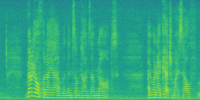
\includegraphics[]{figures/spectrogram_augmented3-img0.png}}};
    
    \draw[->,thick, shorten >=5pt, shorten <=5pt] (waveform_transfer.south) -- (spec_transfer.north);
    
    \coordinate (encoder_transfer_c) at ($(waveform_transfer_c) - (0, 3.5)$);
    \node[inner sep=0pt] (encoder_transfer) at (encoder_transfer_c)  {\scalebox{.4}{\begin{tikzpicture}
    \tikzstyle{hidden neuron}=[circle, draw, ultra thick, minimum size=7pt,inner sep=0pt];
    
    % \node[hidden neuron] (n1) at (0.5,0) {};
    \node[hidden neuron] (n2) at (1,0.3) {};
    
    \node[hidden neuron] (n3) at (0.2,1.2) {};
    \node[hidden neuron] (n4) at (1,1.2) {};
    
    \node[hidden neuron] (n5) at (1.9,2) {};
    \node[hidden neuron] (n6) at (-0.7,1.5) {};
    
    \node[hidden neuron] (n7) at (2.05,3) {};
    \node[hidden neuron] (n8) at (-0.9,2.1) {};
    
    \node[hidden neuron] (n9) at (1.5,3.6) {};
    \node[hidden neuron] (n10) at (-1.8,2.2) {};
    
    \node[hidden neuron] (n11) at (0.7,4) {};
    \node[hidden neuron] (n12) at (-1.7,3.2) {};
    
    \node[hidden neuron] (n13) at (0,4) {};
    \node[hidden neuron] (n14) at (-1,3.7) {};
    
    \node[hidden neuron] (n15) at (-0.7,3.1) {};
    \node[hidden neuron] (n16) at (0.7,2.7) {};
    \node[hidden neuron] (n17) at (-0.1,2) {};
    
    \draw[ultra thick] (n2) -- (n3);
    \draw[ultra thick] (n2) -- (n4);
    \draw[ultra thick] (n3) -- (n6);
    \draw[ultra thick] (n4) -- (n5);
    \draw[ultra thick] (n5) -- (n7);
    \draw[ultra thick] (n6) -- (n8);
    \draw[ultra thick] (n7) -- (n9);
    \draw[ultra thick] (n8) -- (n10);
    \draw[ultra thick] (n9) -- (n11);
    \draw[ultra thick] (n10) -- (n12);
    \draw[ultra thick] (n11) -- (n13);
    \draw[ultra thick] (n12) -- (n14);
    \draw[ultra thick] (n13) -- (n14);
    
    \draw[ultra thick] (n4) -- (n17);
    \draw[ultra thick] (n6) -- (n17);
    \draw[ultra thick] (n15) -- (n16);
    \draw[ultra thick] (n15) -- (n17);
    \draw[ultra thick] (n16) -- (n17);
    
    \draw[ultra thick] (n15) -- (n12);
    \draw[ultra thick] (n8) -- (n11);
    
    \draw[ultra thick] (n5) -- (n16);
    \draw[ultra thick] (n7) -- (n16);
    
    \draw[ultra thick] (n14) -- (n9);
    \draw[ultra thick] (n13) -- (n15);
    
    \draw[ultra thick] (n16) -- (n9);
    \draw[ultra thick] (n17) -- (n5);
    
\end{tikzpicture}}};
    \node[draw, fill=white, rounded corners] (nn_transfer_txt) at ($(encoder_transfer_c)+(0,0.325)$) {\tiny Encoder};
    
    \draw[->,thick, shorten >=5pt, shorten <=5pt] (spec_transfer.south) -- (encoder_transfer.north);
    
    \coordinate (nn_transfer_c) at ($(encoder_transfer_c) - (0, 2.5)$);
    \node[inner sep=0pt, color=green] (nn_transfer) at (nn_transfer_c) {\scalebox{.3}{\begin{tikzpicture}[shorten >=1pt]
    \tikzstyle{every pin edge}=[<-,shorten <=1pt]
    \tikzstyle{input neuron}=[circle, draw, thick, fill, minimum size=17pt,inner sep=0pt];
    \tikzstyle{output neuron}=[circle, draw, thick, double, minimum size=17pt,inner sep=0pt];
    \tikzstyle{hidden neuron}=[circle, draw, thick, minimum size=17pt,inner sep=0pt];


    
    % Draw the hidden layer nodes
    \foreach \name / \y in {1,...,3}
        \node[input neuron] (I-\name) at ($(0.5*\y + \y - 0.5, 0)$) {};
    
    \foreach \name / \y in {1,...,4}
        \node[hidden neuron] (H-\name) at ($(0.2*\y + \y - 0.5, -1.5cm)$) {};
    
    \foreach \name / \y in {1,...,2}
        \node[output neuron] (O-\name) at ($(1*\y + \y - 0.5, -3cm)$) {};
    
    \foreach \source in {1,...,3}
        \foreach \dest in {1,...,4}
            \draw[->,shorten >=1pt] (I-\source) -- (H-\dest);
    
    \foreach \source in {1,...,4}
        \foreach \dest in {1,...,2}
            \draw[->,shorten >=1pt] (H-\source) -- (O-\dest);
\end{tikzpicture}}};
    
    \draw[->,thick, shorten >=5pt, shorten <=5pt] (encoder_transfer.south) -- (nn_transfer.north);
    
    \coordinate (cce_c) at ($(nn_transfer_c) - (0, 2)$);
    \node[draw, rectangle, rounded corners, minimum width=2.5cm, minimum height=1cm, fill=green!50] (cce) at (cce_c) {Softmax-CCE};
    
    \draw[->,thick, shorten >=5pt, shorten <=5pt] (nn_transfer.south) -- (cce.north);
    
    \draw[->, thick, dashed, shorten >=5pt, shorten <=5pt] (encoder.east) .. controls ($(encoder.east) + (1.5,0.75)$) and ($(encoder.east) + (2,-1.5)$) .. (encoder_transfer.west);
    
    \node[] at ($(encoder.east) + (1,0.4)$) {\tiny \circled{6}};
    
\end{tikzpicture}}
    \caption[Contrastive learning for Audio]{Graphical overview of the \gls{claudio} framework. Marked arrows are explained in more detail in the text.}
    \label{fig:claudio}
\end{figure}

\begin{algorithm}
    \caption{CL-Audio Pretraining}
    \label{alg:claudio_pretraining}
    
    \begin{algorithmic}[1]
        \State \textbf{Input:} encoder network $f$, projection network $g$, trainable parameters $\boldsymbol{\theta}$, random transformations $\mathcal{T}$, batch size $N$, learning rate $\alpha$, temperature $\tau$, audio enhancements $E$
        \State Randomly initialize $\boldsymbol{\theta}$
        \While{not done}
            \For{sampled minibatch $\{\boldsymbol{x}_k\}_{k=1}^N$}
                \ForAll{$k \in \{1,...,N\}$}
                    \State convert $\boldsymbol{x}_{k}$ to 16-bit PCM
                    \State $t \sim \mathcal{T}$ \Comment{1. augmentation}
                    \State $\Tilde{\boldsymbol{x}}_{2k-1} \gets t(\boldsymbol{x}_k)$
                    \State $\Tilde{\boldsymbol{x}}_{2k-1} \gets E(\Tilde{\boldsymbol{x}}_{2k-1})$ \Comment{preemphasis, DC-removal, dither}
                    \State $\hat{\boldsymbol{x}}_{2k-1} \gets STFT(\Tilde{\boldsymbol{x}}_{2k-1})$
                    \State $\boldsymbol{z}_{2k-1} \gets g(f(\hat{\boldsymbol{x}}_{2k-1}))$
                    \State $t' \sim \mathcal{T}$ \Comment{2. augmentation}
                    \State $\Tilde{\boldsymbol{x}}_{2k} \gets t'(\boldsymbol{x}_k)$
                    \State $\Tilde{\boldsymbol{x}}_{2k} \gets E(\Tilde{\boldsymbol{x}}_{2k})$ \Comment{preemphasis, DC-removal, dither}
                    \State $\hat{\boldsymbol{x}}_{2k} \gets STFT(\Tilde{\boldsymbol{x}}_{2k})$
                    \State $\boldsymbol{z}_{2k} \gets g(f(\hat{\boldsymbol{x}}_{2k}))$
                \EndFor
                \ForAll{$i \in \{1,...,2N\}$ and $j \in \{1,...,2N\}$}
                    \State $s_{i,j} \gets \boldsymbol{z}^\intercal_i \boldsymbol{z}_j / (\left\lVert\boldsymbol{z}_i\right\rVert \left\lVert\boldsymbol{z}_j\right\rVert)$ \Comment{Cosine Similarity}
                \EndFor
            \EndFor
            \State \textbf{let} $\ell(i,j) = -\log \tfrac{\exp(s_{i,j}/\tau)}{\sum_{k=1}^{2N} \mathbb{1}_{[k \neq i]} \exp(s_{i,k} / \tau)}$ \Comment{NT-Xent loss}
            \State $\mathcal{L} \gets \tfrac{1}{2N} \sum_{k=1}^{N} [\ell(2k-1,2k) + \ell(2k,2k-1)]$
            \State $\boldsymbol{\theta} \gets \boldsymbol{\theta} - \alpha \nabla_\theta \mathcal{L}$
        \EndWhile
        \State \textbf{return} $f$ \Comment{Throw away $g$}
    \end{algorithmic}
\end{algorithm}

\begin{algorithm}
    \caption{CL-Audio Transfer}
    \label{alg:claudio_transfer}
    
    \begin{algorithmic}[1]
        \State \textbf{Input:} frozen encoder network $f$ from pretraining, classification head $g'$ with trainable parameters $\boldsymbol{\theta'}$, batch size $N$, learning rate $\alpha$, audio enhancements $E$
        \State Randomly initialize $\boldsymbol{\theta'}$
        \While{not done}
            \For{sampled minibatch $(\boldsymbol{X}, \boldsymbol{y})$ of size $N$}
                \ForAll{$k \in \{1,...,N\}$}
                    \State convert $\boldsymbol{x}_k$ to 16-bit PCM
                    \State $\boldsymbol{x}_k \gets E(\boldsymbol{x}_k)$ \Comment{preemphasis, DC-removal, dither}
                    \State $\boldsymbol{x}_k \gets STFT(\boldsymbol{x}_k)$
                \EndFor
                \State $\hat{\boldsymbol{y}} \gets softmax(g'(f(\boldsymbol{X})))$
                \State $\mathcal{L} \gets \sum_{k=1}^{N} \boldsymbol{y}_k \log \hat{\boldsymbol{y}}_k$ \Comment{Categorical Cross-Entropy}
                \State $\boldsymbol{\theta'} \gets \boldsymbol{\theta'} - \alpha \nabla_{\theta'} \mathcal{L}$
            \EndFor
        \EndWhile
        \State \textbf{return} $f \circ g'$
    \end{algorithmic}
\end{algorithm}

\subsection{Pre-Training}

\gls{claudio} is a deep-learning framework for few-shot transfer learning based on initial self-supervised similarity learning using a contrastive loss. The left side of Figure \ref{fig:claudio} shows the self-supervised pre-training stage of the framework. Input on each pass through the framework is a sampled minibatch of audio data $\{x_k\}_{k=1}^N$ of size $N$. Each sample is first augmented by two stochastic transformations $t$ and $t'$ sampled from a set of transformations $\mathcal{T}$ \circled{1}. The specifics of these augmentations are explained in Section \ref{sec:augmentation}. The two resulting audio signals are both transformed using the \gls{stft} into the frequency domain \circled{2}. In this step, we also apply a few audio enhancement techniques. Details regarding these enhancements can be found in Section \ref{sec:enhancement}. The resulting spectrograms $\hat{\boldsymbol{x}}_k$ act as the input to the encoder network $f(\cdot)$. The encoder network can be any deep neural network that accepts matrix-like time-series data and outputs vectors. Both spectrograms are fed into the encoder network \circled{3}. The output of this are two vectors. These vectors, also called embeddings, are the latent representations of the two augmentations of the input data. Those embeddings are again transformed using a fully-connected network $g(\cdot)$ \circled{4}, also called the projection head. Chen et al. 2020 \cite{chen2020simple} found that using such a projection head drastically improves the performance of a contrastive learning algorithm. The two outputs of the projection head $z_k$ and $z_{2k}$ will act as the positive input pairs for the contrastive \gls{ntxent} loss term $\mathcal{L}$ \circled{5} while all others act as negative input pairs. Note that all this is performed using a batch of $N$ input samples simultaneously. This results in $N$ positive input pairs and $2(N-1)$ negative input pairs for each pass through the network. Both networks are trained using backpropagation and stochastic gradient descent to minimize $\mathcal{L}$. This initial stage is trained with as much unlabeled data as possible. For this purpose we created a 310GB large dataset which is explained in more detail in Section \ref{subsec:ss_dataset}. The number of epochs to train in this stage is hard to determine since there is no verification loss that we can compare to. To prevent overfitting and to lower training time we stop as soon as the training loss does not decrease from one epoch to another. After training is complete $g(\cdot)$ is discarded.

\subsection{Transfer}

The next stage is the transfer stage shown in the right side of Figure \ref{fig:claudio}, which transfers the embedding network $f(\cdot)$ trained in the pre-training phase and puts it into a new, low-data classification domain \circled{6}. Here the input is again a single audio file represented as samples $x_k$ but this time we also use corresponding labels $y_k$. This time the audio is transformed into a spectrogram without any previous augmentation. The spectrogram is then fed into the pre-trained embedding network $f(\cdot)$ and the resulting embedding vector is fed into a new fully-connected network $g'(\cdot)$, also called the classification head, which transforms the dimensionality of the latent vector into the correct number of classes of the classification task. The output of the classification head is often called logits. Contrary to the dataset in the pre-training phase, this dataset does contain labels $y_k$, which are used together with the logits in a softmax categorical cross-entropy loss $\mathcal{L}$ to train the new classification head $g'(\cdot)$ while the weights of $f(\cdot)$ are frozen, which means they are not trainable. In this stage, we use a verification loss to determine when to stop training. We fix the number of training epochs and in the end return the network that performed the best on the verification dataset.

\subsection{Fine-Tuning}

In a third, optional stage, both the embedding network and the classification head can be made trainable and the entire network is trained on the same data again with a very low learning rate, to further increase accuracy. This stage has to be tested for performance. It is not guaranteed that fine-tuning actually increases performance but in a few experiments we even found that it decreases performance. If the smaller dataset of the transfer stage is too small compared to the size of the classification head, we found that finetuning had no effect on accuracy but as the size of the dataset increases, we found that finetuning got more and more important.

\section{Data Preprocessing}\label{sec:preprocessing}

To correctly input the data into the network, there are several preprocessing steps that have to be performed first to assure optimal performance of the network. We start off with audio files on disc which can be stored in many different formats and codecs like \textit{.wav}, \textit{.mp3} or \textit{.flac}. It is important that our network receives only data that is of the same kind, therefore we first transform the content of the file to raw signed 16-bit \gls{pcm} samples with sample rate 16kHz on a single channel (mono). We chose this format because most of the datasets available also use these parameters. Converting from a standard \textit{.mp3}-file to this configuration is straight forward. We first decode the codec to obtain raw samples, make it mono by averaging over both stereo channels, then resample from the original sample rate (usually 44.1kHz) to our target rate 16kHz and then convert the resulting samples to 16-bit \gls{pcm} by multiplying each sample with $2^8$. The conversion for a \textit{.flac}-file is achieved analogously.

\section{Augmentation}\label{sec:augmentation}

We now take a closer look at all the employed augmentations. The reason we use augmentations to create two distinct views of the same source is twofold. First, we need to create a self-supervised task for the algorithm and secondly, we need a task that is sufficiently difficult for the machine to learn strong embeddings. As explained in Section \ref{subsec:self_supervised} there exist many different kinds of self-supervised tasks to choose from but most of them yield suboptimal results. The reason we chose data augmentation as our contrastive prediction task is because it decouples the target from the encoder architecture. This way we can very precisely compare different encoder models and are able to adapt our framework when new, stronger models are discovered.

In each remaining subsection, we describe the augmentation process and our design decision for each augmentation respectively. All augmentations are applied with a fixed probability of 60\% in the order that they are listed here. Figure \ref{fig:augmentations} shows the same audio clip with every augmentation applied individually. Note that the original audio clip was chosen because of its distinctive activity in the higher frequencies so that the individual augmentations become more visible.

\begin{figure}[H]
    \centering
    %% Creator: Matplotlib, PGF backend
%%
%% To include the figure in your LaTeX document, write
%%   \input{<filename>.pgf}
%%
%% Make sure the required packages are loaded in your preamble
%%   \usepackage{pgf}
%%
%% and, on pdftex
%%   \usepackage[utf8]{inputenc}\DeclareUnicodeCharacter{2212}{-}
%%
%% or, on luatex and xetex
%%   \usepackage{unicode-math}
%%
%% Figures using additional raster images can only be included by \input if
%% they are in the same directory as the main LaTeX file. For loading figures
%% from other directories you can use the `import` package
%%   \usepackage{import}
%%
%% and then include the figures with
%%   \import{<path to file>}{<filename>.pgf}
%%
%% Matplotlib used the following preamble
%%
\begingroup%
\makeatletter%
\begin{pgfpicture}%
\pgfpathrectangle{\pgfpointorigin}{\pgfqpoint{6.202000in}{5.000000in}}%
\pgfusepath{use as bounding box, clip}%
\begin{pgfscope}%
\pgfsetbuttcap%
\pgfsetmiterjoin%
\definecolor{currentfill}{rgb}{1.000000,1.000000,1.000000}%
\pgfsetfillcolor{currentfill}%
\pgfsetlinewidth{0.000000pt}%
\definecolor{currentstroke}{rgb}{1.000000,1.000000,1.000000}%
\pgfsetstrokecolor{currentstroke}%
\pgfsetdash{}{0pt}%
\pgfpathmoveto{\pgfqpoint{0.000000in}{0.000000in}}%
\pgfpathlineto{\pgfqpoint{6.202000in}{0.000000in}}%
\pgfpathlineto{\pgfqpoint{6.202000in}{5.000000in}}%
\pgfpathlineto{\pgfqpoint{0.000000in}{5.000000in}}%
\pgfpathclose%
\pgfusepath{fill}%
\end{pgfscope}%
\begin{pgfscope}%
\pgfsetbuttcap%
\pgfsetmiterjoin%
\definecolor{currentfill}{rgb}{1.000000,1.000000,1.000000}%
\pgfsetfillcolor{currentfill}%
\pgfsetlinewidth{0.000000pt}%
\definecolor{currentstroke}{rgb}{0.000000,0.000000,0.000000}%
\pgfsetstrokecolor{currentstroke}%
\pgfsetstrokeopacity{0.000000}%
\pgfsetdash{}{0pt}%
\pgfpathmoveto{\pgfqpoint{0.653859in}{3.571862in}}%
\pgfpathlineto{\pgfqpoint{3.218901in}{3.571862in}}%
\pgfpathlineto{\pgfqpoint{3.218901in}{4.650926in}}%
\pgfpathlineto{\pgfqpoint{0.653859in}{4.650926in}}%
\pgfpathclose%
\pgfusepath{fill}%
\end{pgfscope}%
\begin{pgfscope}%
\pgfpathrectangle{\pgfqpoint{0.653859in}{3.571862in}}{\pgfqpoint{2.565043in}{1.079064in}}%
\pgfusepath{clip}%
\pgfsys@transformshift{0.653859in}{3.571862in}%
\pgftext[left,bottom]{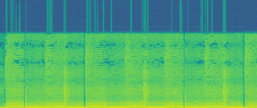
\includegraphics[interpolate=true,width=2.570000in,height=1.080000in]{augmentations-img0.png}}%
\end{pgfscope}%
\begin{pgfscope}%
\pgfsetbuttcap%
\pgfsetroundjoin%
\definecolor{currentfill}{rgb}{0.000000,0.000000,0.000000}%
\pgfsetfillcolor{currentfill}%
\pgfsetlinewidth{0.803000pt}%
\definecolor{currentstroke}{rgb}{0.000000,0.000000,0.000000}%
\pgfsetstrokecolor{currentstroke}%
\pgfsetdash{}{0pt}%
\pgfsys@defobject{currentmarker}{\pgfqpoint{-0.048611in}{0.000000in}}{\pgfqpoint{0.000000in}{0.000000in}}{%
\pgfpathmoveto{\pgfqpoint{0.000000in}{0.000000in}}%
\pgfpathlineto{\pgfqpoint{-0.048611in}{0.000000in}}%
\pgfusepath{stroke,fill}%
}%
\begin{pgfscope}%
\pgfsys@transformshift{0.653859in}{3.571862in}%
\pgfsys@useobject{currentmarker}{}%
\end{pgfscope}%
\end{pgfscope}%
\begin{pgfscope}%
\definecolor{textcolor}{rgb}{0.000000,0.000000,0.000000}%
\pgfsetstrokecolor{textcolor}%
\pgfsetfillcolor{textcolor}%
\pgftext[x=0.487192in, y=3.523637in, left, base]{\color{textcolor}\rmfamily\fontsize{10.000000}{12.000000}\selectfont 0}%
\end{pgfscope}%
\begin{pgfscope}%
\pgfsetbuttcap%
\pgfsetroundjoin%
\definecolor{currentfill}{rgb}{0.000000,0.000000,0.000000}%
\pgfsetfillcolor{currentfill}%
\pgfsetlinewidth{0.803000pt}%
\definecolor{currentstroke}{rgb}{0.000000,0.000000,0.000000}%
\pgfsetstrokecolor{currentstroke}%
\pgfsetdash{}{0pt}%
\pgfsys@defobject{currentmarker}{\pgfqpoint{-0.048611in}{0.000000in}}{\pgfqpoint{0.000000in}{0.000000in}}{%
\pgfpathmoveto{\pgfqpoint{0.000000in}{0.000000in}}%
\pgfpathlineto{\pgfqpoint{-0.048611in}{0.000000in}}%
\pgfusepath{stroke,fill}%
}%
\begin{pgfscope}%
\pgfsys@transformshift{0.653859in}{4.061234in}%
\pgfsys@useobject{currentmarker}{}%
\end{pgfscope}%
\end{pgfscope}%
\begin{pgfscope}%
\definecolor{textcolor}{rgb}{0.000000,0.000000,0.000000}%
\pgfsetstrokecolor{textcolor}%
\pgfsetfillcolor{textcolor}%
\pgftext[x=0.344444in, y=4.013008in, left, base]{\color{textcolor}\rmfamily\fontsize{10.000000}{12.000000}\selectfont 10k}%
\end{pgfscope}%
\begin{pgfscope}%
\pgfsetbuttcap%
\pgfsetroundjoin%
\definecolor{currentfill}{rgb}{0.000000,0.000000,0.000000}%
\pgfsetfillcolor{currentfill}%
\pgfsetlinewidth{0.803000pt}%
\definecolor{currentstroke}{rgb}{0.000000,0.000000,0.000000}%
\pgfsetstrokecolor{currentstroke}%
\pgfsetdash{}{0pt}%
\pgfsys@defobject{currentmarker}{\pgfqpoint{-0.048611in}{0.000000in}}{\pgfqpoint{0.000000in}{0.000000in}}{%
\pgfpathmoveto{\pgfqpoint{0.000000in}{0.000000in}}%
\pgfpathlineto{\pgfqpoint{-0.048611in}{0.000000in}}%
\pgfusepath{stroke,fill}%
}%
\begin{pgfscope}%
\pgfsys@transformshift{0.653859in}{4.550605in}%
\pgfsys@useobject{currentmarker}{}%
\end{pgfscope}%
\end{pgfscope}%
\begin{pgfscope}%
\definecolor{textcolor}{rgb}{0.000000,0.000000,0.000000}%
\pgfsetstrokecolor{textcolor}%
\pgfsetfillcolor{textcolor}%
\pgftext[x=0.344444in, y=4.502380in, left, base]{\color{textcolor}\rmfamily\fontsize{10.000000}{12.000000}\selectfont 20k}%
\end{pgfscope}%
\begin{pgfscope}%
\definecolor{textcolor}{rgb}{0.000000,0.000000,0.000000}%
\pgfsetstrokecolor{textcolor}%
\pgfsetfillcolor{textcolor}%
\pgftext[x=0.288889in,y=4.111394in,,bottom,rotate=90.000000]{\color{textcolor}\rmfamily\fontsize{10.000000}{12.000000}\selectfont Frequency (Hz)}%
\end{pgfscope}%
\begin{pgfscope}%
\pgfsetrectcap%
\pgfsetmiterjoin%
\pgfsetlinewidth{0.803000pt}%
\definecolor{currentstroke}{rgb}{0.000000,0.000000,0.000000}%
\pgfsetstrokecolor{currentstroke}%
\pgfsetdash{}{0pt}%
\pgfpathmoveto{\pgfqpoint{0.653859in}{3.571862in}}%
\pgfpathlineto{\pgfqpoint{0.653859in}{4.650926in}}%
\pgfusepath{stroke}%
\end{pgfscope}%
\begin{pgfscope}%
\pgfsetrectcap%
\pgfsetmiterjoin%
\pgfsetlinewidth{0.803000pt}%
\definecolor{currentstroke}{rgb}{0.000000,0.000000,0.000000}%
\pgfsetstrokecolor{currentstroke}%
\pgfsetdash{}{0pt}%
\pgfpathmoveto{\pgfqpoint{3.218901in}{3.571862in}}%
\pgfpathlineto{\pgfqpoint{3.218901in}{4.650926in}}%
\pgfusepath{stroke}%
\end{pgfscope}%
\begin{pgfscope}%
\pgfsetrectcap%
\pgfsetmiterjoin%
\pgfsetlinewidth{0.803000pt}%
\definecolor{currentstroke}{rgb}{0.000000,0.000000,0.000000}%
\pgfsetstrokecolor{currentstroke}%
\pgfsetdash{}{0pt}%
\pgfpathmoveto{\pgfqpoint{0.653859in}{3.571862in}}%
\pgfpathlineto{\pgfqpoint{3.218901in}{3.571862in}}%
\pgfusepath{stroke}%
\end{pgfscope}%
\begin{pgfscope}%
\pgfsetrectcap%
\pgfsetmiterjoin%
\pgfsetlinewidth{0.803000pt}%
\definecolor{currentstroke}{rgb}{0.000000,0.000000,0.000000}%
\pgfsetstrokecolor{currentstroke}%
\pgfsetdash{}{0pt}%
\pgfpathmoveto{\pgfqpoint{0.653859in}{4.650926in}}%
\pgfpathlineto{\pgfqpoint{3.218901in}{4.650926in}}%
\pgfusepath{stroke}%
\end{pgfscope}%
\begin{pgfscope}%
\definecolor{textcolor}{rgb}{0.000000,0.000000,0.000000}%
\pgfsetstrokecolor{textcolor}%
\pgfsetfillcolor{textcolor}%
\pgftext[x=1.936380in,y=4.734260in,,base]{\color{textcolor}\rmfamily\fontsize{12.000000}{14.400000}\selectfont Original}%
\end{pgfscope}%
\begin{pgfscope}%
\pgfsetbuttcap%
\pgfsetmiterjoin%
\definecolor{currentfill}{rgb}{1.000000,1.000000,1.000000}%
\pgfsetfillcolor{currentfill}%
\pgfsetlinewidth{0.000000pt}%
\definecolor{currentstroke}{rgb}{0.000000,0.000000,0.000000}%
\pgfsetstrokecolor{currentstroke}%
\pgfsetstrokeopacity{0.000000}%
\pgfsetdash{}{0pt}%
\pgfpathmoveto{\pgfqpoint{3.452235in}{3.571862in}}%
\pgfpathlineto{\pgfqpoint{6.017278in}{3.571862in}}%
\pgfpathlineto{\pgfqpoint{6.017278in}{4.650926in}}%
\pgfpathlineto{\pgfqpoint{3.452235in}{4.650926in}}%
\pgfpathclose%
\pgfusepath{fill}%
\end{pgfscope}%
\begin{pgfscope}%
\pgfpathrectangle{\pgfqpoint{3.452235in}{3.571862in}}{\pgfqpoint{2.565043in}{1.079064in}}%
\pgfusepath{clip}%
\pgfsys@transformshift{3.452235in}{3.571862in}%
\pgftext[left,bottom]{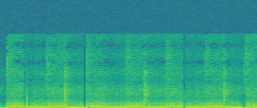
\includegraphics[interpolate=true,width=2.570000in,height=1.080000in]{augmentations-img1.png}}%
\end{pgfscope}%
\begin{pgfscope}%
\pgfsetrectcap%
\pgfsetmiterjoin%
\pgfsetlinewidth{0.803000pt}%
\definecolor{currentstroke}{rgb}{0.000000,0.000000,0.000000}%
\pgfsetstrokecolor{currentstroke}%
\pgfsetdash{}{0pt}%
\pgfpathmoveto{\pgfqpoint{3.452235in}{3.571862in}}%
\pgfpathlineto{\pgfqpoint{3.452235in}{4.650926in}}%
\pgfusepath{stroke}%
\end{pgfscope}%
\begin{pgfscope}%
\pgfsetrectcap%
\pgfsetmiterjoin%
\pgfsetlinewidth{0.803000pt}%
\definecolor{currentstroke}{rgb}{0.000000,0.000000,0.000000}%
\pgfsetstrokecolor{currentstroke}%
\pgfsetdash{}{0pt}%
\pgfpathmoveto{\pgfqpoint{6.017278in}{3.571862in}}%
\pgfpathlineto{\pgfqpoint{6.017278in}{4.650926in}}%
\pgfusepath{stroke}%
\end{pgfscope}%
\begin{pgfscope}%
\pgfsetrectcap%
\pgfsetmiterjoin%
\pgfsetlinewidth{0.803000pt}%
\definecolor{currentstroke}{rgb}{0.000000,0.000000,0.000000}%
\pgfsetstrokecolor{currentstroke}%
\pgfsetdash{}{0pt}%
\pgfpathmoveto{\pgfqpoint{3.452235in}{3.571862in}}%
\pgfpathlineto{\pgfqpoint{6.017278in}{3.571862in}}%
\pgfusepath{stroke}%
\end{pgfscope}%
\begin{pgfscope}%
\pgfsetrectcap%
\pgfsetmiterjoin%
\pgfsetlinewidth{0.803000pt}%
\definecolor{currentstroke}{rgb}{0.000000,0.000000,0.000000}%
\pgfsetstrokecolor{currentstroke}%
\pgfsetdash{}{0pt}%
\pgfpathmoveto{\pgfqpoint{3.452235in}{4.650926in}}%
\pgfpathlineto{\pgfqpoint{6.017278in}{4.650926in}}%
\pgfusepath{stroke}%
\end{pgfscope}%
\begin{pgfscope}%
\definecolor{textcolor}{rgb}{0.000000,0.000000,0.000000}%
\pgfsetstrokecolor{textcolor}%
\pgfsetfillcolor{textcolor}%
\pgftext[x=4.734756in,y=4.734260in,,base]{\color{textcolor}\rmfamily\fontsize{12.000000}{14.400000}\selectfont Whitenoise}%
\end{pgfscope}%
\begin{pgfscope}%
\pgfsetbuttcap%
\pgfsetmiterjoin%
\definecolor{currentfill}{rgb}{1.000000,1.000000,1.000000}%
\pgfsetfillcolor{currentfill}%
\pgfsetlinewidth{0.000000pt}%
\definecolor{currentstroke}{rgb}{0.000000,0.000000,0.000000}%
\pgfsetstrokecolor{currentstroke}%
\pgfsetstrokeopacity{0.000000}%
\pgfsetdash{}{0pt}%
\pgfpathmoveto{\pgfqpoint{0.653859in}{2.068493in}}%
\pgfpathlineto{\pgfqpoint{3.218901in}{2.068493in}}%
\pgfpathlineto{\pgfqpoint{3.218901in}{3.147557in}}%
\pgfpathlineto{\pgfqpoint{0.653859in}{3.147557in}}%
\pgfpathclose%
\pgfusepath{fill}%
\end{pgfscope}%
\begin{pgfscope}%
\pgfpathrectangle{\pgfqpoint{0.653859in}{2.068493in}}{\pgfqpoint{2.565043in}{1.079064in}}%
\pgfusepath{clip}%
\pgfsys@transformshift{0.653859in}{2.068493in}%
\pgftext[left,bottom]{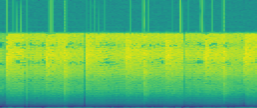
\includegraphics[interpolate=true,width=2.570000in,height=1.080000in]{augmentations-img2.png}}%
\end{pgfscope}%
\begin{pgfscope}%
\pgfsetbuttcap%
\pgfsetroundjoin%
\definecolor{currentfill}{rgb}{0.000000,0.000000,0.000000}%
\pgfsetfillcolor{currentfill}%
\pgfsetlinewidth{0.803000pt}%
\definecolor{currentstroke}{rgb}{0.000000,0.000000,0.000000}%
\pgfsetstrokecolor{currentstroke}%
\pgfsetdash{}{0pt}%
\pgfsys@defobject{currentmarker}{\pgfqpoint{-0.048611in}{0.000000in}}{\pgfqpoint{0.000000in}{0.000000in}}{%
\pgfpathmoveto{\pgfqpoint{0.000000in}{0.000000in}}%
\pgfpathlineto{\pgfqpoint{-0.048611in}{0.000000in}}%
\pgfusepath{stroke,fill}%
}%
\begin{pgfscope}%
\pgfsys@transformshift{0.653859in}{2.068493in}%
\pgfsys@useobject{currentmarker}{}%
\end{pgfscope}%
\end{pgfscope}%
\begin{pgfscope}%
\definecolor{textcolor}{rgb}{0.000000,0.000000,0.000000}%
\pgfsetstrokecolor{textcolor}%
\pgfsetfillcolor{textcolor}%
\pgftext[x=0.487192in, y=2.020267in, left, base]{\color{textcolor}\rmfamily\fontsize{10.000000}{12.000000}\selectfont 0}%
\end{pgfscope}%
\begin{pgfscope}%
\pgfsetbuttcap%
\pgfsetroundjoin%
\definecolor{currentfill}{rgb}{0.000000,0.000000,0.000000}%
\pgfsetfillcolor{currentfill}%
\pgfsetlinewidth{0.803000pt}%
\definecolor{currentstroke}{rgb}{0.000000,0.000000,0.000000}%
\pgfsetstrokecolor{currentstroke}%
\pgfsetdash{}{0pt}%
\pgfsys@defobject{currentmarker}{\pgfqpoint{-0.048611in}{0.000000in}}{\pgfqpoint{0.000000in}{0.000000in}}{%
\pgfpathmoveto{\pgfqpoint{0.000000in}{0.000000in}}%
\pgfpathlineto{\pgfqpoint{-0.048611in}{0.000000in}}%
\pgfusepath{stroke,fill}%
}%
\begin{pgfscope}%
\pgfsys@transformshift{0.653859in}{2.557864in}%
\pgfsys@useobject{currentmarker}{}%
\end{pgfscope}%
\end{pgfscope}%
\begin{pgfscope}%
\definecolor{textcolor}{rgb}{0.000000,0.000000,0.000000}%
\pgfsetstrokecolor{textcolor}%
\pgfsetfillcolor{textcolor}%
\pgftext[x=0.344444in, y=2.509639in, left, base]{\color{textcolor}\rmfamily\fontsize{10.000000}{12.000000}\selectfont 10k}%
\end{pgfscope}%
\begin{pgfscope}%
\pgfsetbuttcap%
\pgfsetroundjoin%
\definecolor{currentfill}{rgb}{0.000000,0.000000,0.000000}%
\pgfsetfillcolor{currentfill}%
\pgfsetlinewidth{0.803000pt}%
\definecolor{currentstroke}{rgb}{0.000000,0.000000,0.000000}%
\pgfsetstrokecolor{currentstroke}%
\pgfsetdash{}{0pt}%
\pgfsys@defobject{currentmarker}{\pgfqpoint{-0.048611in}{0.000000in}}{\pgfqpoint{0.000000in}{0.000000in}}{%
\pgfpathmoveto{\pgfqpoint{0.000000in}{0.000000in}}%
\pgfpathlineto{\pgfqpoint{-0.048611in}{0.000000in}}%
\pgfusepath{stroke,fill}%
}%
\begin{pgfscope}%
\pgfsys@transformshift{0.653859in}{3.047236in}%
\pgfsys@useobject{currentmarker}{}%
\end{pgfscope}%
\end{pgfscope}%
\begin{pgfscope}%
\definecolor{textcolor}{rgb}{0.000000,0.000000,0.000000}%
\pgfsetstrokecolor{textcolor}%
\pgfsetfillcolor{textcolor}%
\pgftext[x=0.344444in, y=2.999010in, left, base]{\color{textcolor}\rmfamily\fontsize{10.000000}{12.000000}\selectfont 20k}%
\end{pgfscope}%
\begin{pgfscope}%
\definecolor{textcolor}{rgb}{0.000000,0.000000,0.000000}%
\pgfsetstrokecolor{textcolor}%
\pgfsetfillcolor{textcolor}%
\pgftext[x=0.288889in,y=2.608025in,,bottom,rotate=90.000000]{\color{textcolor}\rmfamily\fontsize{10.000000}{12.000000}\selectfont Frequency (Hz)}%
\end{pgfscope}%
\begin{pgfscope}%
\pgfsetrectcap%
\pgfsetmiterjoin%
\pgfsetlinewidth{0.803000pt}%
\definecolor{currentstroke}{rgb}{0.000000,0.000000,0.000000}%
\pgfsetstrokecolor{currentstroke}%
\pgfsetdash{}{0pt}%
\pgfpathmoveto{\pgfqpoint{0.653859in}{2.068493in}}%
\pgfpathlineto{\pgfqpoint{0.653859in}{3.147557in}}%
\pgfusepath{stroke}%
\end{pgfscope}%
\begin{pgfscope}%
\pgfsetrectcap%
\pgfsetmiterjoin%
\pgfsetlinewidth{0.803000pt}%
\definecolor{currentstroke}{rgb}{0.000000,0.000000,0.000000}%
\pgfsetstrokecolor{currentstroke}%
\pgfsetdash{}{0pt}%
\pgfpathmoveto{\pgfqpoint{3.218901in}{2.068493in}}%
\pgfpathlineto{\pgfqpoint{3.218901in}{3.147557in}}%
\pgfusepath{stroke}%
\end{pgfscope}%
\begin{pgfscope}%
\pgfsetrectcap%
\pgfsetmiterjoin%
\pgfsetlinewidth{0.803000pt}%
\definecolor{currentstroke}{rgb}{0.000000,0.000000,0.000000}%
\pgfsetstrokecolor{currentstroke}%
\pgfsetdash{}{0pt}%
\pgfpathmoveto{\pgfqpoint{0.653859in}{2.068493in}}%
\pgfpathlineto{\pgfqpoint{3.218901in}{2.068493in}}%
\pgfusepath{stroke}%
\end{pgfscope}%
\begin{pgfscope}%
\pgfsetrectcap%
\pgfsetmiterjoin%
\pgfsetlinewidth{0.803000pt}%
\definecolor{currentstroke}{rgb}{0.000000,0.000000,0.000000}%
\pgfsetstrokecolor{currentstroke}%
\pgfsetdash{}{0pt}%
\pgfpathmoveto{\pgfqpoint{0.653859in}{3.147557in}}%
\pgfpathlineto{\pgfqpoint{3.218901in}{3.147557in}}%
\pgfusepath{stroke}%
\end{pgfscope}%
\begin{pgfscope}%
\definecolor{textcolor}{rgb}{0.000000,0.000000,0.000000}%
\pgfsetstrokecolor{textcolor}%
\pgfsetfillcolor{textcolor}%
\pgftext[x=1.936380in,y=3.230890in,,base]{\color{textcolor}\rmfamily\fontsize{12.000000}{14.400000}\selectfont Highpass Filter}%
\end{pgfscope}%
\begin{pgfscope}%
\pgfsetbuttcap%
\pgfsetmiterjoin%
\definecolor{currentfill}{rgb}{1.000000,1.000000,1.000000}%
\pgfsetfillcolor{currentfill}%
\pgfsetlinewidth{0.000000pt}%
\definecolor{currentstroke}{rgb}{0.000000,0.000000,0.000000}%
\pgfsetstrokecolor{currentstroke}%
\pgfsetstrokeopacity{0.000000}%
\pgfsetdash{}{0pt}%
\pgfpathmoveto{\pgfqpoint{3.452235in}{2.068493in}}%
\pgfpathlineto{\pgfqpoint{6.017278in}{2.068493in}}%
\pgfpathlineto{\pgfqpoint{6.017278in}{3.147557in}}%
\pgfpathlineto{\pgfqpoint{3.452235in}{3.147557in}}%
\pgfpathclose%
\pgfusepath{fill}%
\end{pgfscope}%
\begin{pgfscope}%
\pgfpathrectangle{\pgfqpoint{3.452235in}{2.068493in}}{\pgfqpoint{2.565043in}{1.079064in}}%
\pgfusepath{clip}%
\pgfsys@transformshift{3.452235in}{2.068493in}%
\pgftext[left,bottom]{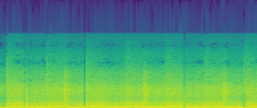
\includegraphics[interpolate=true,width=2.570000in,height=1.080000in]{augmentations-img3.png}}%
\end{pgfscope}%
\begin{pgfscope}%
\pgfsetrectcap%
\pgfsetmiterjoin%
\pgfsetlinewidth{0.803000pt}%
\definecolor{currentstroke}{rgb}{0.000000,0.000000,0.000000}%
\pgfsetstrokecolor{currentstroke}%
\pgfsetdash{}{0pt}%
\pgfpathmoveto{\pgfqpoint{3.452235in}{2.068493in}}%
\pgfpathlineto{\pgfqpoint{3.452235in}{3.147557in}}%
\pgfusepath{stroke}%
\end{pgfscope}%
\begin{pgfscope}%
\pgfsetrectcap%
\pgfsetmiterjoin%
\pgfsetlinewidth{0.803000pt}%
\definecolor{currentstroke}{rgb}{0.000000,0.000000,0.000000}%
\pgfsetstrokecolor{currentstroke}%
\pgfsetdash{}{0pt}%
\pgfpathmoveto{\pgfqpoint{6.017278in}{2.068493in}}%
\pgfpathlineto{\pgfqpoint{6.017278in}{3.147557in}}%
\pgfusepath{stroke}%
\end{pgfscope}%
\begin{pgfscope}%
\pgfsetrectcap%
\pgfsetmiterjoin%
\pgfsetlinewidth{0.803000pt}%
\definecolor{currentstroke}{rgb}{0.000000,0.000000,0.000000}%
\pgfsetstrokecolor{currentstroke}%
\pgfsetdash{}{0pt}%
\pgfpathmoveto{\pgfqpoint{3.452235in}{2.068493in}}%
\pgfpathlineto{\pgfqpoint{6.017278in}{2.068493in}}%
\pgfusepath{stroke}%
\end{pgfscope}%
\begin{pgfscope}%
\pgfsetrectcap%
\pgfsetmiterjoin%
\pgfsetlinewidth{0.803000pt}%
\definecolor{currentstroke}{rgb}{0.000000,0.000000,0.000000}%
\pgfsetstrokecolor{currentstroke}%
\pgfsetdash{}{0pt}%
\pgfpathmoveto{\pgfqpoint{3.452235in}{3.147557in}}%
\pgfpathlineto{\pgfqpoint{6.017278in}{3.147557in}}%
\pgfusepath{stroke}%
\end{pgfscope}%
\begin{pgfscope}%
\definecolor{textcolor}{rgb}{0.000000,0.000000,0.000000}%
\pgfsetstrokecolor{textcolor}%
\pgfsetfillcolor{textcolor}%
\pgftext[x=4.734756in,y=3.230890in,,base]{\color{textcolor}\rmfamily\fontsize{12.000000}{14.400000}\selectfont Lowpass Filter}%
\end{pgfscope}%
\begin{pgfscope}%
\pgfsetbuttcap%
\pgfsetmiterjoin%
\definecolor{currentfill}{rgb}{1.000000,1.000000,1.000000}%
\pgfsetfillcolor{currentfill}%
\pgfsetlinewidth{0.000000pt}%
\definecolor{currentstroke}{rgb}{0.000000,0.000000,0.000000}%
\pgfsetstrokecolor{currentstroke}%
\pgfsetstrokeopacity{0.000000}%
\pgfsetdash{}{0pt}%
\pgfpathmoveto{\pgfqpoint{0.653859in}{0.565123in}}%
\pgfpathlineto{\pgfqpoint{3.218901in}{0.565123in}}%
\pgfpathlineto{\pgfqpoint{3.218901in}{1.644188in}}%
\pgfpathlineto{\pgfqpoint{0.653859in}{1.644188in}}%
\pgfpathclose%
\pgfusepath{fill}%
\end{pgfscope}%
\begin{pgfscope}%
\pgfpathrectangle{\pgfqpoint{0.653859in}{0.565123in}}{\pgfqpoint{2.565043in}{1.079064in}}%
\pgfusepath{clip}%
\pgfsys@transformshift{0.653859in}{0.565123in}%
\pgftext[left,bottom]{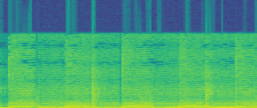
\includegraphics[interpolate=true,width=2.570000in,height=1.080000in]{augmentations-img4.png}}%
\end{pgfscope}%
\begin{pgfscope}%
\pgfsetbuttcap%
\pgfsetroundjoin%
\definecolor{currentfill}{rgb}{0.000000,0.000000,0.000000}%
\pgfsetfillcolor{currentfill}%
\pgfsetlinewidth{0.803000pt}%
\definecolor{currentstroke}{rgb}{0.000000,0.000000,0.000000}%
\pgfsetstrokecolor{currentstroke}%
\pgfsetdash{}{0pt}%
\pgfsys@defobject{currentmarker}{\pgfqpoint{0.000000in}{-0.048611in}}{\pgfqpoint{0.000000in}{0.000000in}}{%
\pgfpathmoveto{\pgfqpoint{0.000000in}{0.000000in}}%
\pgfpathlineto{\pgfqpoint{0.000000in}{-0.048611in}}%
\pgfusepath{stroke,fill}%
}%
\begin{pgfscope}%
\pgfsys@transformshift{0.653859in}{0.565123in}%
\pgfsys@useobject{currentmarker}{}%
\end{pgfscope}%
\end{pgfscope}%
\begin{pgfscope}%
\definecolor{textcolor}{rgb}{0.000000,0.000000,0.000000}%
\pgfsetstrokecolor{textcolor}%
\pgfsetfillcolor{textcolor}%
\pgftext[x=0.653859in,y=0.467901in,,top]{\color{textcolor}\rmfamily\fontsize{10.000000}{12.000000}\selectfont \(\displaystyle {0}\)}%
\end{pgfscope}%
\begin{pgfscope}%
\pgfsetbuttcap%
\pgfsetroundjoin%
\definecolor{currentfill}{rgb}{0.000000,0.000000,0.000000}%
\pgfsetfillcolor{currentfill}%
\pgfsetlinewidth{0.803000pt}%
\definecolor{currentstroke}{rgb}{0.000000,0.000000,0.000000}%
\pgfsetstrokecolor{currentstroke}%
\pgfsetdash{}{0pt}%
\pgfsys@defobject{currentmarker}{\pgfqpoint{0.000000in}{-0.048611in}}{\pgfqpoint{0.000000in}{0.000000in}}{%
\pgfpathmoveto{\pgfqpoint{0.000000in}{0.000000in}}%
\pgfpathlineto{\pgfqpoint{0.000000in}{-0.048611in}}%
\pgfusepath{stroke,fill}%
}%
\begin{pgfscope}%
\pgfsys@transformshift{1.508873in}{0.565123in}%
\pgfsys@useobject{currentmarker}{}%
\end{pgfscope}%
\end{pgfscope}%
\begin{pgfscope}%
\definecolor{textcolor}{rgb}{0.000000,0.000000,0.000000}%
\pgfsetstrokecolor{textcolor}%
\pgfsetfillcolor{textcolor}%
\pgftext[x=1.508873in,y=0.467901in,,top]{\color{textcolor}\rmfamily\fontsize{10.000000}{12.000000}\selectfont \(\displaystyle {1}\)}%
\end{pgfscope}%
\begin{pgfscope}%
\pgfsetbuttcap%
\pgfsetroundjoin%
\definecolor{currentfill}{rgb}{0.000000,0.000000,0.000000}%
\pgfsetfillcolor{currentfill}%
\pgfsetlinewidth{0.803000pt}%
\definecolor{currentstroke}{rgb}{0.000000,0.000000,0.000000}%
\pgfsetstrokecolor{currentstroke}%
\pgfsetdash{}{0pt}%
\pgfsys@defobject{currentmarker}{\pgfqpoint{0.000000in}{-0.048611in}}{\pgfqpoint{0.000000in}{0.000000in}}{%
\pgfpathmoveto{\pgfqpoint{0.000000in}{0.000000in}}%
\pgfpathlineto{\pgfqpoint{0.000000in}{-0.048611in}}%
\pgfusepath{stroke,fill}%
}%
\begin{pgfscope}%
\pgfsys@transformshift{2.363887in}{0.565123in}%
\pgfsys@useobject{currentmarker}{}%
\end{pgfscope}%
\end{pgfscope}%
\begin{pgfscope}%
\definecolor{textcolor}{rgb}{0.000000,0.000000,0.000000}%
\pgfsetstrokecolor{textcolor}%
\pgfsetfillcolor{textcolor}%
\pgftext[x=2.363887in,y=0.467901in,,top]{\color{textcolor}\rmfamily\fontsize{10.000000}{12.000000}\selectfont \(\displaystyle {2}\)}%
\end{pgfscope}%
\begin{pgfscope}%
\pgfsetbuttcap%
\pgfsetroundjoin%
\definecolor{currentfill}{rgb}{0.000000,0.000000,0.000000}%
\pgfsetfillcolor{currentfill}%
\pgfsetlinewidth{0.803000pt}%
\definecolor{currentstroke}{rgb}{0.000000,0.000000,0.000000}%
\pgfsetstrokecolor{currentstroke}%
\pgfsetdash{}{0pt}%
\pgfsys@defobject{currentmarker}{\pgfqpoint{0.000000in}{-0.048611in}}{\pgfqpoint{0.000000in}{0.000000in}}{%
\pgfpathmoveto{\pgfqpoint{0.000000in}{0.000000in}}%
\pgfpathlineto{\pgfqpoint{0.000000in}{-0.048611in}}%
\pgfusepath{stroke,fill}%
}%
\begin{pgfscope}%
\pgfsys@transformshift{3.218901in}{0.565123in}%
\pgfsys@useobject{currentmarker}{}%
\end{pgfscope}%
\end{pgfscope}%
\begin{pgfscope}%
\definecolor{textcolor}{rgb}{0.000000,0.000000,0.000000}%
\pgfsetstrokecolor{textcolor}%
\pgfsetfillcolor{textcolor}%
\pgftext[x=3.218901in,y=0.467901in,,top]{\color{textcolor}\rmfamily\fontsize{10.000000}{12.000000}\selectfont \(\displaystyle {3}\)}%
\end{pgfscope}%
\begin{pgfscope}%
\definecolor{textcolor}{rgb}{0.000000,0.000000,0.000000}%
\pgfsetstrokecolor{textcolor}%
\pgfsetfillcolor{textcolor}%
\pgftext[x=1.936380in,y=0.288889in,,top]{\color{textcolor}\rmfamily\fontsize{10.000000}{12.000000}\selectfont Time (s)}%
\end{pgfscope}%
\begin{pgfscope}%
\pgfsetbuttcap%
\pgfsetroundjoin%
\definecolor{currentfill}{rgb}{0.000000,0.000000,0.000000}%
\pgfsetfillcolor{currentfill}%
\pgfsetlinewidth{0.803000pt}%
\definecolor{currentstroke}{rgb}{0.000000,0.000000,0.000000}%
\pgfsetstrokecolor{currentstroke}%
\pgfsetdash{}{0pt}%
\pgfsys@defobject{currentmarker}{\pgfqpoint{-0.048611in}{0.000000in}}{\pgfqpoint{0.000000in}{0.000000in}}{%
\pgfpathmoveto{\pgfqpoint{0.000000in}{0.000000in}}%
\pgfpathlineto{\pgfqpoint{-0.048611in}{0.000000in}}%
\pgfusepath{stroke,fill}%
}%
\begin{pgfscope}%
\pgfsys@transformshift{0.653859in}{0.565123in}%
\pgfsys@useobject{currentmarker}{}%
\end{pgfscope}%
\end{pgfscope}%
\begin{pgfscope}%
\definecolor{textcolor}{rgb}{0.000000,0.000000,0.000000}%
\pgfsetstrokecolor{textcolor}%
\pgfsetfillcolor{textcolor}%
\pgftext[x=0.487192in, y=0.516898in, left, base]{\color{textcolor}\rmfamily\fontsize{10.000000}{12.000000}\selectfont 0}%
\end{pgfscope}%
\begin{pgfscope}%
\pgfsetbuttcap%
\pgfsetroundjoin%
\definecolor{currentfill}{rgb}{0.000000,0.000000,0.000000}%
\pgfsetfillcolor{currentfill}%
\pgfsetlinewidth{0.803000pt}%
\definecolor{currentstroke}{rgb}{0.000000,0.000000,0.000000}%
\pgfsetstrokecolor{currentstroke}%
\pgfsetdash{}{0pt}%
\pgfsys@defobject{currentmarker}{\pgfqpoint{-0.048611in}{0.000000in}}{\pgfqpoint{0.000000in}{0.000000in}}{%
\pgfpathmoveto{\pgfqpoint{0.000000in}{0.000000in}}%
\pgfpathlineto{\pgfqpoint{-0.048611in}{0.000000in}}%
\pgfusepath{stroke,fill}%
}%
\begin{pgfscope}%
\pgfsys@transformshift{0.653859in}{1.054495in}%
\pgfsys@useobject{currentmarker}{}%
\end{pgfscope}%
\end{pgfscope}%
\begin{pgfscope}%
\definecolor{textcolor}{rgb}{0.000000,0.000000,0.000000}%
\pgfsetstrokecolor{textcolor}%
\pgfsetfillcolor{textcolor}%
\pgftext[x=0.344444in, y=1.006270in, left, base]{\color{textcolor}\rmfamily\fontsize{10.000000}{12.000000}\selectfont 10k}%
\end{pgfscope}%
\begin{pgfscope}%
\pgfsetbuttcap%
\pgfsetroundjoin%
\definecolor{currentfill}{rgb}{0.000000,0.000000,0.000000}%
\pgfsetfillcolor{currentfill}%
\pgfsetlinewidth{0.803000pt}%
\definecolor{currentstroke}{rgb}{0.000000,0.000000,0.000000}%
\pgfsetstrokecolor{currentstroke}%
\pgfsetdash{}{0pt}%
\pgfsys@defobject{currentmarker}{\pgfqpoint{-0.048611in}{0.000000in}}{\pgfqpoint{0.000000in}{0.000000in}}{%
\pgfpathmoveto{\pgfqpoint{0.000000in}{0.000000in}}%
\pgfpathlineto{\pgfqpoint{-0.048611in}{0.000000in}}%
\pgfusepath{stroke,fill}%
}%
\begin{pgfscope}%
\pgfsys@transformshift{0.653859in}{1.543866in}%
\pgfsys@useobject{currentmarker}{}%
\end{pgfscope}%
\end{pgfscope}%
\begin{pgfscope}%
\definecolor{textcolor}{rgb}{0.000000,0.000000,0.000000}%
\pgfsetstrokecolor{textcolor}%
\pgfsetfillcolor{textcolor}%
\pgftext[x=0.344444in, y=1.495641in, left, base]{\color{textcolor}\rmfamily\fontsize{10.000000}{12.000000}\selectfont 20k}%
\end{pgfscope}%
\begin{pgfscope}%
\definecolor{textcolor}{rgb}{0.000000,0.000000,0.000000}%
\pgfsetstrokecolor{textcolor}%
\pgfsetfillcolor{textcolor}%
\pgftext[x=0.288889in,y=1.104655in,,bottom,rotate=90.000000]{\color{textcolor}\rmfamily\fontsize{10.000000}{12.000000}\selectfont Frequency (Hz)}%
\end{pgfscope}%
\begin{pgfscope}%
\pgfsetrectcap%
\pgfsetmiterjoin%
\pgfsetlinewidth{0.803000pt}%
\definecolor{currentstroke}{rgb}{0.000000,0.000000,0.000000}%
\pgfsetstrokecolor{currentstroke}%
\pgfsetdash{}{0pt}%
\pgfpathmoveto{\pgfqpoint{0.653859in}{0.565123in}}%
\pgfpathlineto{\pgfqpoint{0.653859in}{1.644188in}}%
\pgfusepath{stroke}%
\end{pgfscope}%
\begin{pgfscope}%
\pgfsetrectcap%
\pgfsetmiterjoin%
\pgfsetlinewidth{0.803000pt}%
\definecolor{currentstroke}{rgb}{0.000000,0.000000,0.000000}%
\pgfsetstrokecolor{currentstroke}%
\pgfsetdash{}{0pt}%
\pgfpathmoveto{\pgfqpoint{3.218901in}{0.565123in}}%
\pgfpathlineto{\pgfqpoint{3.218901in}{1.644188in}}%
\pgfusepath{stroke}%
\end{pgfscope}%
\begin{pgfscope}%
\pgfsetrectcap%
\pgfsetmiterjoin%
\pgfsetlinewidth{0.803000pt}%
\definecolor{currentstroke}{rgb}{0.000000,0.000000,0.000000}%
\pgfsetstrokecolor{currentstroke}%
\pgfsetdash{}{0pt}%
\pgfpathmoveto{\pgfqpoint{0.653859in}{0.565123in}}%
\pgfpathlineto{\pgfqpoint{3.218901in}{0.565123in}}%
\pgfusepath{stroke}%
\end{pgfscope}%
\begin{pgfscope}%
\pgfsetrectcap%
\pgfsetmiterjoin%
\pgfsetlinewidth{0.803000pt}%
\definecolor{currentstroke}{rgb}{0.000000,0.000000,0.000000}%
\pgfsetstrokecolor{currentstroke}%
\pgfsetdash{}{0pt}%
\pgfpathmoveto{\pgfqpoint{0.653859in}{1.644188in}}%
\pgfpathlineto{\pgfqpoint{3.218901in}{1.644188in}}%
\pgfusepath{stroke}%
\end{pgfscope}%
\begin{pgfscope}%
\definecolor{textcolor}{rgb}{0.000000,0.000000,0.000000}%
\pgfsetstrokecolor{textcolor}%
\pgfsetfillcolor{textcolor}%
\pgftext[x=1.936380in,y=1.727521in,,base]{\color{textcolor}\rmfamily\fontsize{12.000000}{14.400000}\selectfont Timestretch}%
\end{pgfscope}%
\begin{pgfscope}%
\pgfsetbuttcap%
\pgfsetmiterjoin%
\definecolor{currentfill}{rgb}{1.000000,1.000000,1.000000}%
\pgfsetfillcolor{currentfill}%
\pgfsetlinewidth{0.000000pt}%
\definecolor{currentstroke}{rgb}{0.000000,0.000000,0.000000}%
\pgfsetstrokecolor{currentstroke}%
\pgfsetstrokeopacity{0.000000}%
\pgfsetdash{}{0pt}%
\pgfpathmoveto{\pgfqpoint{3.452235in}{0.565123in}}%
\pgfpathlineto{\pgfqpoint{6.017278in}{0.565123in}}%
\pgfpathlineto{\pgfqpoint{6.017278in}{1.644188in}}%
\pgfpathlineto{\pgfqpoint{3.452235in}{1.644188in}}%
\pgfpathclose%
\pgfusepath{fill}%
\end{pgfscope}%
\begin{pgfscope}%
\pgfpathrectangle{\pgfqpoint{3.452235in}{0.565123in}}{\pgfqpoint{2.565043in}{1.079064in}}%
\pgfusepath{clip}%
\pgfsys@transformshift{3.452235in}{0.565123in}%
\pgftext[left,bottom]{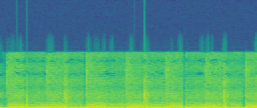
\includegraphics[interpolate=true,width=2.570000in,height=1.080000in]{augmentations-img5.png}}%
\end{pgfscope}%
\begin{pgfscope}%
\pgfsetbuttcap%
\pgfsetroundjoin%
\definecolor{currentfill}{rgb}{0.000000,0.000000,0.000000}%
\pgfsetfillcolor{currentfill}%
\pgfsetlinewidth{0.803000pt}%
\definecolor{currentstroke}{rgb}{0.000000,0.000000,0.000000}%
\pgfsetstrokecolor{currentstroke}%
\pgfsetdash{}{0pt}%
\pgfsys@defobject{currentmarker}{\pgfqpoint{0.000000in}{-0.048611in}}{\pgfqpoint{0.000000in}{0.000000in}}{%
\pgfpathmoveto{\pgfqpoint{0.000000in}{0.000000in}}%
\pgfpathlineto{\pgfqpoint{0.000000in}{-0.048611in}}%
\pgfusepath{stroke,fill}%
}%
\begin{pgfscope}%
\pgfsys@transformshift{3.452235in}{0.565123in}%
\pgfsys@useobject{currentmarker}{}%
\end{pgfscope}%
\end{pgfscope}%
\begin{pgfscope}%
\definecolor{textcolor}{rgb}{0.000000,0.000000,0.000000}%
\pgfsetstrokecolor{textcolor}%
\pgfsetfillcolor{textcolor}%
\pgftext[x=3.452235in,y=0.467901in,,top]{\color{textcolor}\rmfamily\fontsize{10.000000}{12.000000}\selectfont \(\displaystyle {0}\)}%
\end{pgfscope}%
\begin{pgfscope}%
\pgfsetbuttcap%
\pgfsetroundjoin%
\definecolor{currentfill}{rgb}{0.000000,0.000000,0.000000}%
\pgfsetfillcolor{currentfill}%
\pgfsetlinewidth{0.803000pt}%
\definecolor{currentstroke}{rgb}{0.000000,0.000000,0.000000}%
\pgfsetstrokecolor{currentstroke}%
\pgfsetdash{}{0pt}%
\pgfsys@defobject{currentmarker}{\pgfqpoint{0.000000in}{-0.048611in}}{\pgfqpoint{0.000000in}{0.000000in}}{%
\pgfpathmoveto{\pgfqpoint{0.000000in}{0.000000in}}%
\pgfpathlineto{\pgfqpoint{0.000000in}{-0.048611in}}%
\pgfusepath{stroke,fill}%
}%
\begin{pgfscope}%
\pgfsys@transformshift{4.307249in}{0.565123in}%
\pgfsys@useobject{currentmarker}{}%
\end{pgfscope}%
\end{pgfscope}%
\begin{pgfscope}%
\definecolor{textcolor}{rgb}{0.000000,0.000000,0.000000}%
\pgfsetstrokecolor{textcolor}%
\pgfsetfillcolor{textcolor}%
\pgftext[x=4.307249in,y=0.467901in,,top]{\color{textcolor}\rmfamily\fontsize{10.000000}{12.000000}\selectfont \(\displaystyle {1}\)}%
\end{pgfscope}%
\begin{pgfscope}%
\pgfsetbuttcap%
\pgfsetroundjoin%
\definecolor{currentfill}{rgb}{0.000000,0.000000,0.000000}%
\pgfsetfillcolor{currentfill}%
\pgfsetlinewidth{0.803000pt}%
\definecolor{currentstroke}{rgb}{0.000000,0.000000,0.000000}%
\pgfsetstrokecolor{currentstroke}%
\pgfsetdash{}{0pt}%
\pgfsys@defobject{currentmarker}{\pgfqpoint{0.000000in}{-0.048611in}}{\pgfqpoint{0.000000in}{0.000000in}}{%
\pgfpathmoveto{\pgfqpoint{0.000000in}{0.000000in}}%
\pgfpathlineto{\pgfqpoint{0.000000in}{-0.048611in}}%
\pgfusepath{stroke,fill}%
}%
\begin{pgfscope}%
\pgfsys@transformshift{5.162263in}{0.565123in}%
\pgfsys@useobject{currentmarker}{}%
\end{pgfscope}%
\end{pgfscope}%
\begin{pgfscope}%
\definecolor{textcolor}{rgb}{0.000000,0.000000,0.000000}%
\pgfsetstrokecolor{textcolor}%
\pgfsetfillcolor{textcolor}%
\pgftext[x=5.162263in,y=0.467901in,,top]{\color{textcolor}\rmfamily\fontsize{10.000000}{12.000000}\selectfont \(\displaystyle {2}\)}%
\end{pgfscope}%
\begin{pgfscope}%
\pgfsetbuttcap%
\pgfsetroundjoin%
\definecolor{currentfill}{rgb}{0.000000,0.000000,0.000000}%
\pgfsetfillcolor{currentfill}%
\pgfsetlinewidth{0.803000pt}%
\definecolor{currentstroke}{rgb}{0.000000,0.000000,0.000000}%
\pgfsetstrokecolor{currentstroke}%
\pgfsetdash{}{0pt}%
\pgfsys@defobject{currentmarker}{\pgfqpoint{0.000000in}{-0.048611in}}{\pgfqpoint{0.000000in}{0.000000in}}{%
\pgfpathmoveto{\pgfqpoint{0.000000in}{0.000000in}}%
\pgfpathlineto{\pgfqpoint{0.000000in}{-0.048611in}}%
\pgfusepath{stroke,fill}%
}%
\begin{pgfscope}%
\pgfsys@transformshift{6.017278in}{0.565123in}%
\pgfsys@useobject{currentmarker}{}%
\end{pgfscope}%
\end{pgfscope}%
\begin{pgfscope}%
\definecolor{textcolor}{rgb}{0.000000,0.000000,0.000000}%
\pgfsetstrokecolor{textcolor}%
\pgfsetfillcolor{textcolor}%
\pgftext[x=6.017278in,y=0.467901in,,top]{\color{textcolor}\rmfamily\fontsize{10.000000}{12.000000}\selectfont \(\displaystyle {3}\)}%
\end{pgfscope}%
\begin{pgfscope}%
\definecolor{textcolor}{rgb}{0.000000,0.000000,0.000000}%
\pgfsetstrokecolor{textcolor}%
\pgfsetfillcolor{textcolor}%
\pgftext[x=4.734756in,y=0.288889in,,top]{\color{textcolor}\rmfamily\fontsize{10.000000}{12.000000}\selectfont Time (s)}%
\end{pgfscope}%
\begin{pgfscope}%
\pgfsetrectcap%
\pgfsetmiterjoin%
\pgfsetlinewidth{0.803000pt}%
\definecolor{currentstroke}{rgb}{0.000000,0.000000,0.000000}%
\pgfsetstrokecolor{currentstroke}%
\pgfsetdash{}{0pt}%
\pgfpathmoveto{\pgfqpoint{3.452235in}{0.565123in}}%
\pgfpathlineto{\pgfqpoint{3.452235in}{1.644188in}}%
\pgfusepath{stroke}%
\end{pgfscope}%
\begin{pgfscope}%
\pgfsetrectcap%
\pgfsetmiterjoin%
\pgfsetlinewidth{0.803000pt}%
\definecolor{currentstroke}{rgb}{0.000000,0.000000,0.000000}%
\pgfsetstrokecolor{currentstroke}%
\pgfsetdash{}{0pt}%
\pgfpathmoveto{\pgfqpoint{6.017278in}{0.565123in}}%
\pgfpathlineto{\pgfqpoint{6.017278in}{1.644188in}}%
\pgfusepath{stroke}%
\end{pgfscope}%
\begin{pgfscope}%
\pgfsetrectcap%
\pgfsetmiterjoin%
\pgfsetlinewidth{0.803000pt}%
\definecolor{currentstroke}{rgb}{0.000000,0.000000,0.000000}%
\pgfsetstrokecolor{currentstroke}%
\pgfsetdash{}{0pt}%
\pgfpathmoveto{\pgfqpoint{3.452235in}{0.565123in}}%
\pgfpathlineto{\pgfqpoint{6.017278in}{0.565123in}}%
\pgfusepath{stroke}%
\end{pgfscope}%
\begin{pgfscope}%
\pgfsetrectcap%
\pgfsetmiterjoin%
\pgfsetlinewidth{0.803000pt}%
\definecolor{currentstroke}{rgb}{0.000000,0.000000,0.000000}%
\pgfsetstrokecolor{currentstroke}%
\pgfsetdash{}{0pt}%
\pgfpathmoveto{\pgfqpoint{3.452235in}{1.644188in}}%
\pgfpathlineto{\pgfqpoint{6.017278in}{1.644188in}}%
\pgfusepath{stroke}%
\end{pgfscope}%
\begin{pgfscope}%
\definecolor{textcolor}{rgb}{0.000000,0.000000,0.000000}%
\pgfsetstrokecolor{textcolor}%
\pgfsetfillcolor{textcolor}%
\pgftext[x=4.734756in,y=1.727521in,,base]{\color{textcolor}\rmfamily\fontsize{12.000000}{14.400000}\selectfont Pitchshift}%
\end{pgfscope}%
\end{pgfpicture}%
\makeatother%
\endgroup%

    \caption[Augmentations]{Each augmentation applied individually to one sound file with distinctive high ends to better distinguish the effects of the respective augmentation.}
    \label{fig:augmentations}
\end{figure}

\subsection{Crop}

At first, any audio clip is cropped at random. We input 10 seconds of samples and crop a 4.5-second clip from it even though the input to our network will only be 3 seconds long. We do this because we anticipate the later time stretching stage. As we will explain later we shrink up to a factor of 0.7, which means that a 4.5-second clip will result in at least 3 seconds of input data after time stretching. Cropping can be seen as a way to artificially increase the size of the dataset since a single input clip can potentially be split into several independent input clips. Figure \ref{fig:crop} shows a 10-second audio clip in blue and a 3-second crop of it in red.

\begin{figure}[H]
    \centering
    %% Creator: Matplotlib, PGF backend
%%
%% To include the figure in your LaTeX document, write
%%   \input{<filename>.pgf}
%%
%% Make sure the required packages are loaded in your preamble
%%   \usepackage{pgf}
%%
%% and, on pdftex
%%   \usepackage[utf8]{inputenc}\DeclareUnicodeCharacter{2212}{-}
%%
%% or, on luatex and xetex
%%   \usepackage{unicode-math}
%%
%% Figures using additional raster images can only be included by \input if
%% they are in the same directory as the main LaTeX file. For loading figures
%% from other directories you can use the `import` package
%%   \usepackage{import}
%%
%% and then include the figures with
%%   \import{<path to file>}{<filename>.pgf}
%%
%% Matplotlib used the following preamble
%%
\begingroup%
\makeatletter%
\begin{pgfpicture}%
\pgfpathrectangle{\pgfpointorigin}{\pgfqpoint{6.202000in}{2.000000in}}%
\pgfusepath{use as bounding box, clip}%
\begin{pgfscope}%
\pgfsetbuttcap%
\pgfsetmiterjoin%
\definecolor{currentfill}{rgb}{1.000000,1.000000,1.000000}%
\pgfsetfillcolor{currentfill}%
\pgfsetlinewidth{0.000000pt}%
\definecolor{currentstroke}{rgb}{1.000000,1.000000,1.000000}%
\pgfsetstrokecolor{currentstroke}%
\pgfsetdash{}{0pt}%
\pgfpathmoveto{\pgfqpoint{0.000000in}{0.000000in}}%
\pgfpathlineto{\pgfqpoint{6.202000in}{0.000000in}}%
\pgfpathlineto{\pgfqpoint{6.202000in}{2.000000in}}%
\pgfpathlineto{\pgfqpoint{0.000000in}{2.000000in}}%
\pgfpathclose%
\pgfusepath{fill}%
\end{pgfscope}%
\begin{pgfscope}%
\pgfsetbuttcap%
\pgfsetmiterjoin%
\definecolor{currentfill}{rgb}{1.000000,1.000000,1.000000}%
\pgfsetfillcolor{currentfill}%
\pgfsetlinewidth{0.000000pt}%
\definecolor{currentstroke}{rgb}{0.000000,0.000000,0.000000}%
\pgfsetstrokecolor{currentstroke}%
\pgfsetstrokeopacity{0.000000}%
\pgfsetdash{}{0pt}%
\pgfpathmoveto{\pgfqpoint{0.711729in}{0.565123in}}%
\pgfpathlineto{\pgfqpoint{6.052000in}{0.565123in}}%
\pgfpathlineto{\pgfqpoint{6.052000in}{1.850000in}}%
\pgfpathlineto{\pgfqpoint{0.711729in}{1.850000in}}%
\pgfpathclose%
\pgfusepath{fill}%
\end{pgfscope}%
\begin{pgfscope}%
\pgfsetbuttcap%
\pgfsetroundjoin%
\definecolor{currentfill}{rgb}{0.000000,0.000000,0.000000}%
\pgfsetfillcolor{currentfill}%
\pgfsetlinewidth{0.803000pt}%
\definecolor{currentstroke}{rgb}{0.000000,0.000000,0.000000}%
\pgfsetstrokecolor{currentstroke}%
\pgfsetdash{}{0pt}%
\pgfsys@defobject{currentmarker}{\pgfqpoint{0.000000in}{-0.048611in}}{\pgfqpoint{0.000000in}{0.000000in}}{%
\pgfpathmoveto{\pgfqpoint{0.000000in}{0.000000in}}%
\pgfpathlineto{\pgfqpoint{0.000000in}{-0.048611in}}%
\pgfusepath{stroke,fill}%
}%
\begin{pgfscope}%
\pgfsys@transformshift{0.954469in}{0.565123in}%
\pgfsys@useobject{currentmarker}{}%
\end{pgfscope}%
\end{pgfscope}%
\begin{pgfscope}%
\definecolor{textcolor}{rgb}{0.000000,0.000000,0.000000}%
\pgfsetstrokecolor{textcolor}%
\pgfsetfillcolor{textcolor}%
\pgftext[x=0.954469in,y=0.467901in,,top]{\color{textcolor}\rmfamily\fontsize{10.000000}{12.000000}\selectfont \(\displaystyle {0}\)}%
\end{pgfscope}%
\begin{pgfscope}%
\pgfsetbuttcap%
\pgfsetroundjoin%
\definecolor{currentfill}{rgb}{0.000000,0.000000,0.000000}%
\pgfsetfillcolor{currentfill}%
\pgfsetlinewidth{0.803000pt}%
\definecolor{currentstroke}{rgb}{0.000000,0.000000,0.000000}%
\pgfsetstrokecolor{currentstroke}%
\pgfsetdash{}{0pt}%
\pgfsys@defobject{currentmarker}{\pgfqpoint{0.000000in}{-0.048611in}}{\pgfqpoint{0.000000in}{0.000000in}}{%
\pgfpathmoveto{\pgfqpoint{0.000000in}{0.000000in}}%
\pgfpathlineto{\pgfqpoint{0.000000in}{-0.048611in}}%
\pgfusepath{stroke,fill}%
}%
\begin{pgfscope}%
\pgfsys@transformshift{1.925433in}{0.565123in}%
\pgfsys@useobject{currentmarker}{}%
\end{pgfscope}%
\end{pgfscope}%
\begin{pgfscope}%
\definecolor{textcolor}{rgb}{0.000000,0.000000,0.000000}%
\pgfsetstrokecolor{textcolor}%
\pgfsetfillcolor{textcolor}%
\pgftext[x=1.925433in,y=0.467901in,,top]{\color{textcolor}\rmfamily\fontsize{10.000000}{12.000000}\selectfont \(\displaystyle {2}\)}%
\end{pgfscope}%
\begin{pgfscope}%
\pgfsetbuttcap%
\pgfsetroundjoin%
\definecolor{currentfill}{rgb}{0.000000,0.000000,0.000000}%
\pgfsetfillcolor{currentfill}%
\pgfsetlinewidth{0.803000pt}%
\definecolor{currentstroke}{rgb}{0.000000,0.000000,0.000000}%
\pgfsetstrokecolor{currentstroke}%
\pgfsetdash{}{0pt}%
\pgfsys@defobject{currentmarker}{\pgfqpoint{0.000000in}{-0.048611in}}{\pgfqpoint{0.000000in}{0.000000in}}{%
\pgfpathmoveto{\pgfqpoint{0.000000in}{0.000000in}}%
\pgfpathlineto{\pgfqpoint{0.000000in}{-0.048611in}}%
\pgfusepath{stroke,fill}%
}%
\begin{pgfscope}%
\pgfsys@transformshift{2.896398in}{0.565123in}%
\pgfsys@useobject{currentmarker}{}%
\end{pgfscope}%
\end{pgfscope}%
\begin{pgfscope}%
\definecolor{textcolor}{rgb}{0.000000,0.000000,0.000000}%
\pgfsetstrokecolor{textcolor}%
\pgfsetfillcolor{textcolor}%
\pgftext[x=2.896398in,y=0.467901in,,top]{\color{textcolor}\rmfamily\fontsize{10.000000}{12.000000}\selectfont \(\displaystyle {4}\)}%
\end{pgfscope}%
\begin{pgfscope}%
\pgfsetbuttcap%
\pgfsetroundjoin%
\definecolor{currentfill}{rgb}{0.000000,0.000000,0.000000}%
\pgfsetfillcolor{currentfill}%
\pgfsetlinewidth{0.803000pt}%
\definecolor{currentstroke}{rgb}{0.000000,0.000000,0.000000}%
\pgfsetstrokecolor{currentstroke}%
\pgfsetdash{}{0pt}%
\pgfsys@defobject{currentmarker}{\pgfqpoint{0.000000in}{-0.048611in}}{\pgfqpoint{0.000000in}{0.000000in}}{%
\pgfpathmoveto{\pgfqpoint{0.000000in}{0.000000in}}%
\pgfpathlineto{\pgfqpoint{0.000000in}{-0.048611in}}%
\pgfusepath{stroke,fill}%
}%
\begin{pgfscope}%
\pgfsys@transformshift{3.867362in}{0.565123in}%
\pgfsys@useobject{currentmarker}{}%
\end{pgfscope}%
\end{pgfscope}%
\begin{pgfscope}%
\definecolor{textcolor}{rgb}{0.000000,0.000000,0.000000}%
\pgfsetstrokecolor{textcolor}%
\pgfsetfillcolor{textcolor}%
\pgftext[x=3.867362in,y=0.467901in,,top]{\color{textcolor}\rmfamily\fontsize{10.000000}{12.000000}\selectfont \(\displaystyle {6}\)}%
\end{pgfscope}%
\begin{pgfscope}%
\pgfsetbuttcap%
\pgfsetroundjoin%
\definecolor{currentfill}{rgb}{0.000000,0.000000,0.000000}%
\pgfsetfillcolor{currentfill}%
\pgfsetlinewidth{0.803000pt}%
\definecolor{currentstroke}{rgb}{0.000000,0.000000,0.000000}%
\pgfsetstrokecolor{currentstroke}%
\pgfsetdash{}{0pt}%
\pgfsys@defobject{currentmarker}{\pgfqpoint{0.000000in}{-0.048611in}}{\pgfqpoint{0.000000in}{0.000000in}}{%
\pgfpathmoveto{\pgfqpoint{0.000000in}{0.000000in}}%
\pgfpathlineto{\pgfqpoint{0.000000in}{-0.048611in}}%
\pgfusepath{stroke,fill}%
}%
\begin{pgfscope}%
\pgfsys@transformshift{4.838326in}{0.565123in}%
\pgfsys@useobject{currentmarker}{}%
\end{pgfscope}%
\end{pgfscope}%
\begin{pgfscope}%
\definecolor{textcolor}{rgb}{0.000000,0.000000,0.000000}%
\pgfsetstrokecolor{textcolor}%
\pgfsetfillcolor{textcolor}%
\pgftext[x=4.838326in,y=0.467901in,,top]{\color{textcolor}\rmfamily\fontsize{10.000000}{12.000000}\selectfont \(\displaystyle {8}\)}%
\end{pgfscope}%
\begin{pgfscope}%
\pgfsetbuttcap%
\pgfsetroundjoin%
\definecolor{currentfill}{rgb}{0.000000,0.000000,0.000000}%
\pgfsetfillcolor{currentfill}%
\pgfsetlinewidth{0.803000pt}%
\definecolor{currentstroke}{rgb}{0.000000,0.000000,0.000000}%
\pgfsetstrokecolor{currentstroke}%
\pgfsetdash{}{0pt}%
\pgfsys@defobject{currentmarker}{\pgfqpoint{0.000000in}{-0.048611in}}{\pgfqpoint{0.000000in}{0.000000in}}{%
\pgfpathmoveto{\pgfqpoint{0.000000in}{0.000000in}}%
\pgfpathlineto{\pgfqpoint{0.000000in}{-0.048611in}}%
\pgfusepath{stroke,fill}%
}%
\begin{pgfscope}%
\pgfsys@transformshift{5.809291in}{0.565123in}%
\pgfsys@useobject{currentmarker}{}%
\end{pgfscope}%
\end{pgfscope}%
\begin{pgfscope}%
\definecolor{textcolor}{rgb}{0.000000,0.000000,0.000000}%
\pgfsetstrokecolor{textcolor}%
\pgfsetfillcolor{textcolor}%
\pgftext[x=5.809291in,y=0.467901in,,top]{\color{textcolor}\rmfamily\fontsize{10.000000}{12.000000}\selectfont \(\displaystyle {10}\)}%
\end{pgfscope}%
\begin{pgfscope}%
\definecolor{textcolor}{rgb}{0.000000,0.000000,0.000000}%
\pgfsetstrokecolor{textcolor}%
\pgfsetfillcolor{textcolor}%
\pgftext[x=3.381865in,y=0.288889in,,top]{\color{textcolor}\rmfamily\fontsize{10.000000}{12.000000}\selectfont Time (s)}%
\end{pgfscope}%
\begin{pgfscope}%
\pgfsetbuttcap%
\pgfsetroundjoin%
\definecolor{currentfill}{rgb}{0.000000,0.000000,0.000000}%
\pgfsetfillcolor{currentfill}%
\pgfsetlinewidth{0.803000pt}%
\definecolor{currentstroke}{rgb}{0.000000,0.000000,0.000000}%
\pgfsetstrokecolor{currentstroke}%
\pgfsetdash{}{0pt}%
\pgfsys@defobject{currentmarker}{\pgfqpoint{-0.048611in}{0.000000in}}{\pgfqpoint{0.000000in}{0.000000in}}{%
\pgfpathmoveto{\pgfqpoint{0.000000in}{0.000000in}}%
\pgfpathlineto{\pgfqpoint{-0.048611in}{0.000000in}}%
\pgfusepath{stroke,fill}%
}%
\begin{pgfscope}%
\pgfsys@transformshift{0.711729in}{0.623527in}%
\pgfsys@useobject{currentmarker}{}%
\end{pgfscope}%
\end{pgfscope}%
\begin{pgfscope}%
\definecolor{textcolor}{rgb}{0.000000,0.000000,0.000000}%
\pgfsetstrokecolor{textcolor}%
\pgfsetfillcolor{textcolor}%
\pgftext[x=0.437037in, y=0.575302in, left, base]{\color{textcolor}\rmfamily\fontsize{10.000000}{12.000000}\selectfont \(\displaystyle {-1}\)}%
\end{pgfscope}%
\begin{pgfscope}%
\pgfsetbuttcap%
\pgfsetroundjoin%
\definecolor{currentfill}{rgb}{0.000000,0.000000,0.000000}%
\pgfsetfillcolor{currentfill}%
\pgfsetlinewidth{0.803000pt}%
\definecolor{currentstroke}{rgb}{0.000000,0.000000,0.000000}%
\pgfsetstrokecolor{currentstroke}%
\pgfsetdash{}{0pt}%
\pgfsys@defobject{currentmarker}{\pgfqpoint{-0.048611in}{0.000000in}}{\pgfqpoint{0.000000in}{0.000000in}}{%
\pgfpathmoveto{\pgfqpoint{0.000000in}{0.000000in}}%
\pgfpathlineto{\pgfqpoint{-0.048611in}{0.000000in}}%
\pgfusepath{stroke,fill}%
}%
\begin{pgfscope}%
\pgfsys@transformshift{0.711729in}{1.207562in}%
\pgfsys@useobject{currentmarker}{}%
\end{pgfscope}%
\end{pgfscope}%
\begin{pgfscope}%
\definecolor{textcolor}{rgb}{0.000000,0.000000,0.000000}%
\pgfsetstrokecolor{textcolor}%
\pgfsetfillcolor{textcolor}%
\pgftext[x=0.545062in, y=1.159336in, left, base]{\color{textcolor}\rmfamily\fontsize{10.000000}{12.000000}\selectfont \(\displaystyle {0}\)}%
\end{pgfscope}%
\begin{pgfscope}%
\pgfsetbuttcap%
\pgfsetroundjoin%
\definecolor{currentfill}{rgb}{0.000000,0.000000,0.000000}%
\pgfsetfillcolor{currentfill}%
\pgfsetlinewidth{0.803000pt}%
\definecolor{currentstroke}{rgb}{0.000000,0.000000,0.000000}%
\pgfsetstrokecolor{currentstroke}%
\pgfsetdash{}{0pt}%
\pgfsys@defobject{currentmarker}{\pgfqpoint{-0.048611in}{0.000000in}}{\pgfqpoint{0.000000in}{0.000000in}}{%
\pgfpathmoveto{\pgfqpoint{0.000000in}{0.000000in}}%
\pgfpathlineto{\pgfqpoint{-0.048611in}{0.000000in}}%
\pgfusepath{stroke,fill}%
}%
\begin{pgfscope}%
\pgfsys@transformshift{0.711729in}{1.791597in}%
\pgfsys@useobject{currentmarker}{}%
\end{pgfscope}%
\end{pgfscope}%
\begin{pgfscope}%
\definecolor{textcolor}{rgb}{0.000000,0.000000,0.000000}%
\pgfsetstrokecolor{textcolor}%
\pgfsetfillcolor{textcolor}%
\pgftext[x=0.545062in, y=1.743371in, left, base]{\color{textcolor}\rmfamily\fontsize{10.000000}{12.000000}\selectfont \(\displaystyle {1}\)}%
\end{pgfscope}%
\begin{pgfscope}%
\definecolor{textcolor}{rgb}{0.000000,0.000000,0.000000}%
\pgfsetstrokecolor{textcolor}%
\pgfsetfillcolor{textcolor}%
\pgftext[x=0.381482in,y=1.207562in,,bottom,rotate=90.000000]{\color{textcolor}\rmfamily\fontsize{10.000000}{12.000000}\selectfont Amplitude}%
\end{pgfscope}%
\begin{pgfscope}%
\pgfpathrectangle{\pgfqpoint{0.711729in}{0.565123in}}{\pgfqpoint{5.340271in}{1.284877in}}%
\pgfusepath{clip}%
\pgfsetrectcap%
\pgfsetroundjoin%
\pgfsetlinewidth{1.505625pt}%
\definecolor{currentstroke}{rgb}{0.121569,0.466667,0.705882}%
\pgfsetstrokecolor{currentstroke}%
\pgfsetdash{}{0pt}%
\pgfpathmoveto{\pgfqpoint{0.954469in}{1.207562in}}%
\pgfpathlineto{\pgfqpoint{0.988817in}{1.458719in}}%
\pgfpathlineto{\pgfqpoint{1.006567in}{1.572188in}}%
\pgfpathlineto{\pgfqpoint{1.020798in}{1.649573in}}%
\pgfpathlineto{\pgfqpoint{1.032844in}{1.703485in}}%
\pgfpathlineto{\pgfqpoint{1.043191in}{1.740230in}}%
\pgfpathlineto{\pgfqpoint{1.052111in}{1.764274in}}%
\pgfpathlineto{\pgfqpoint{1.059788in}{1.779040in}}%
\pgfpathlineto{\pgfqpoint{1.066312in}{1.787162in}}%
\pgfpathlineto{\pgfqpoint{1.071895in}{1.790836in}}%
\pgfpathlineto{\pgfqpoint{1.076841in}{1.791547in}}%
\pgfpathlineto{\pgfqpoint{1.081635in}{1.789954in}}%
\pgfpathlineto{\pgfqpoint{1.086763in}{1.785770in}}%
\pgfpathlineto{\pgfqpoint{1.092558in}{1.777978in}}%
\pgfpathlineto{\pgfqpoint{1.099233in}{1.765031in}}%
\pgfpathlineto{\pgfqpoint{1.106941in}{1.744919in}}%
\pgfpathlineto{\pgfqpoint{1.115801in}{1.715213in}}%
\pgfpathlineto{\pgfqpoint{1.125996in}{1.672809in}}%
\pgfpathlineto{\pgfqpoint{1.137799in}{1.613669in}}%
\pgfpathlineto{\pgfqpoint{1.151696in}{1.532034in}}%
\pgfpathlineto{\pgfqpoint{1.168839in}{1.417218in}}%
\pgfpathlineto{\pgfqpoint{1.194054in}{1.231407in}}%
\pgfpathlineto{\pgfqpoint{1.231861in}{0.954336in}}%
\pgfpathlineto{\pgfqpoint{1.249551in}{0.841504in}}%
\pgfpathlineto{\pgfqpoint{1.263751in}{0.764502in}}%
\pgfpathlineto{\pgfqpoint{1.275767in}{0.710913in}}%
\pgfpathlineto{\pgfqpoint{1.286083in}{0.674424in}}%
\pgfpathlineto{\pgfqpoint{1.295004in}{0.650504in}}%
\pgfpathlineto{\pgfqpoint{1.302651in}{0.635895in}}%
\pgfpathlineto{\pgfqpoint{1.309174in}{0.627849in}}%
\pgfpathlineto{\pgfqpoint{1.314727in}{0.624253in}}%
\pgfpathlineto{\pgfqpoint{1.319642in}{0.623582in}}%
\pgfpathlineto{\pgfqpoint{1.324437in}{0.625203in}}%
\pgfpathlineto{\pgfqpoint{1.329564in}{0.629418in}}%
\pgfpathlineto{\pgfqpoint{1.335390in}{0.637294in}}%
\pgfpathlineto{\pgfqpoint{1.342096in}{0.650366in}}%
\pgfpathlineto{\pgfqpoint{1.349833in}{0.670654in}}%
\pgfpathlineto{\pgfqpoint{1.358724in}{0.700592in}}%
\pgfpathlineto{\pgfqpoint{1.368949in}{0.743286in}}%
\pgfpathlineto{\pgfqpoint{1.380783in}{0.802774in}}%
\pgfpathlineto{\pgfqpoint{1.394710in}{0.884808in}}%
\pgfpathlineto{\pgfqpoint{1.411945in}{1.000477in}}%
\pgfpathlineto{\pgfqpoint{1.437463in}{1.188758in}}%
\pgfpathlineto{\pgfqpoint{1.474481in}{1.459961in}}%
\pgfpathlineto{\pgfqpoint{1.492201in}{1.573083in}}%
\pgfpathlineto{\pgfqpoint{1.506432in}{1.650322in}}%
\pgfpathlineto{\pgfqpoint{1.518447in}{1.703969in}}%
\pgfpathlineto{\pgfqpoint{1.528794in}{1.740605in}}%
\pgfpathlineto{\pgfqpoint{1.537715in}{1.764550in}}%
\pgfpathlineto{\pgfqpoint{1.545361in}{1.779181in}}%
\pgfpathlineto{\pgfqpoint{1.551885in}{1.787246in}}%
\pgfpathlineto{\pgfqpoint{1.557468in}{1.790870in}}%
\pgfpathlineto{\pgfqpoint{1.562383in}{1.791541in}}%
\pgfpathlineto{\pgfqpoint{1.567178in}{1.789920in}}%
\pgfpathlineto{\pgfqpoint{1.572306in}{1.785705in}}%
\pgfpathlineto{\pgfqpoint{1.578131in}{1.777830in}}%
\pgfpathlineto{\pgfqpoint{1.584837in}{1.764757in}}%
\pgfpathlineto{\pgfqpoint{1.592574in}{1.744469in}}%
\pgfpathlineto{\pgfqpoint{1.601465in}{1.714531in}}%
\pgfpathlineto{\pgfqpoint{1.611690in}{1.671837in}}%
\pgfpathlineto{\pgfqpoint{1.623524in}{1.612349in}}%
\pgfpathlineto{\pgfqpoint{1.637451in}{1.530316in}}%
\pgfpathlineto{\pgfqpoint{1.654686in}{1.414647in}}%
\pgfpathlineto{\pgfqpoint{1.680204in}{1.226365in}}%
\pgfpathlineto{\pgfqpoint{1.717222in}{0.955163in}}%
\pgfpathlineto{\pgfqpoint{1.734942in}{0.842040in}}%
\pgfpathlineto{\pgfqpoint{1.749173in}{0.764801in}}%
\pgfpathlineto{\pgfqpoint{1.761188in}{0.711154in}}%
\pgfpathlineto{\pgfqpoint{1.771535in}{0.674518in}}%
\pgfpathlineto{\pgfqpoint{1.780456in}{0.650573in}}%
\pgfpathlineto{\pgfqpoint{1.788102in}{0.635942in}}%
\pgfpathlineto{\pgfqpoint{1.794626in}{0.627877in}}%
\pgfpathlineto{\pgfqpoint{1.800209in}{0.624253in}}%
\pgfpathlineto{\pgfqpoint{1.805125in}{0.623582in}}%
\pgfpathlineto{\pgfqpoint{1.809919in}{0.625203in}}%
\pgfpathlineto{\pgfqpoint{1.815047in}{0.629418in}}%
\pgfpathlineto{\pgfqpoint{1.820872in}{0.637294in}}%
\pgfpathlineto{\pgfqpoint{1.827578in}{0.650366in}}%
\pgfpathlineto{\pgfqpoint{1.835316in}{0.670654in}}%
\pgfpathlineto{\pgfqpoint{1.844206in}{0.700592in}}%
\pgfpathlineto{\pgfqpoint{1.854431in}{0.743286in}}%
\pgfpathlineto{\pgfqpoint{1.866265in}{0.802774in}}%
\pgfpathlineto{\pgfqpoint{1.880192in}{0.884808in}}%
\pgfpathlineto{\pgfqpoint{1.897427in}{1.000477in}}%
\pgfpathlineto{\pgfqpoint{1.922945in}{1.188758in}}%
\pgfpathlineto{\pgfqpoint{1.959963in}{1.459961in}}%
\pgfpathlineto{\pgfqpoint{1.977683in}{1.573083in}}%
\pgfpathlineto{\pgfqpoint{1.991914in}{1.650322in}}%
\pgfpathlineto{\pgfqpoint{2.003930in}{1.703969in}}%
\pgfpathlineto{\pgfqpoint{2.014276in}{1.740605in}}%
\pgfpathlineto{\pgfqpoint{2.023197in}{1.764550in}}%
\pgfpathlineto{\pgfqpoint{2.030843in}{1.779181in}}%
\pgfpathlineto{\pgfqpoint{2.037367in}{1.787246in}}%
\pgfpathlineto{\pgfqpoint{2.042950in}{1.790870in}}%
\pgfpathlineto{\pgfqpoint{2.047866in}{1.791541in}}%
\pgfpathlineto{\pgfqpoint{2.052660in}{1.789920in}}%
\pgfpathlineto{\pgfqpoint{2.057788in}{1.785705in}}%
\pgfpathlineto{\pgfqpoint{2.063614in}{1.777830in}}%
\pgfpathlineto{\pgfqpoint{2.070319in}{1.764757in}}%
\pgfpathlineto{\pgfqpoint{2.078057in}{1.744469in}}%
\pgfpathlineto{\pgfqpoint{2.086947in}{1.714531in}}%
\pgfpathlineto{\pgfqpoint{2.097172in}{1.671837in}}%
\pgfpathlineto{\pgfqpoint{2.109006in}{1.612349in}}%
\pgfpathlineto{\pgfqpoint{2.122933in}{1.530316in}}%
\pgfpathlineto{\pgfqpoint{2.140168in}{1.414647in}}%
\pgfpathlineto{\pgfqpoint{2.165686in}{1.226365in}}%
\pgfpathlineto{\pgfqpoint{2.202704in}{0.955163in}}%
\pgfpathlineto{\pgfqpoint{2.220424in}{0.842040in}}%
\pgfpathlineto{\pgfqpoint{2.234655in}{0.764801in}}%
\pgfpathlineto{\pgfqpoint{2.246671in}{0.711154in}}%
\pgfpathlineto{\pgfqpoint{2.257017in}{0.674518in}}%
\pgfpathlineto{\pgfqpoint{2.265938in}{0.650573in}}%
\pgfpathlineto{\pgfqpoint{2.273585in}{0.635942in}}%
\pgfpathlineto{\pgfqpoint{2.280108in}{0.627877in}}%
\pgfpathlineto{\pgfqpoint{2.285691in}{0.624253in}}%
\pgfpathlineto{\pgfqpoint{2.290607in}{0.623582in}}%
\pgfpathlineto{\pgfqpoint{2.295401in}{0.625203in}}%
\pgfpathlineto{\pgfqpoint{2.300529in}{0.629418in}}%
\pgfpathlineto{\pgfqpoint{2.306355in}{0.637294in}}%
\pgfpathlineto{\pgfqpoint{2.313060in}{0.650366in}}%
\pgfpathlineto{\pgfqpoint{2.320798in}{0.670654in}}%
\pgfpathlineto{\pgfqpoint{2.329688in}{0.700592in}}%
\pgfpathlineto{\pgfqpoint{2.339914in}{0.743286in}}%
\pgfpathlineto{\pgfqpoint{2.351747in}{0.802774in}}%
\pgfpathlineto{\pgfqpoint{2.365674in}{0.884808in}}%
\pgfpathlineto{\pgfqpoint{2.382909in}{1.000477in}}%
\pgfpathlineto{\pgfqpoint{2.408427in}{1.188758in}}%
\pgfpathlineto{\pgfqpoint{2.445445in}{1.459961in}}%
\pgfpathlineto{\pgfqpoint{2.463165in}{1.573083in}}%
\pgfpathlineto{\pgfqpoint{2.477396in}{1.650322in}}%
\pgfpathlineto{\pgfqpoint{2.489412in}{1.703969in}}%
\pgfpathlineto{\pgfqpoint{2.499759in}{1.740605in}}%
\pgfpathlineto{\pgfqpoint{2.508679in}{1.764550in}}%
\pgfpathlineto{\pgfqpoint{2.516326in}{1.779181in}}%
\pgfpathlineto{\pgfqpoint{2.522849in}{1.787246in}}%
\pgfpathlineto{\pgfqpoint{2.528432in}{1.790870in}}%
\pgfpathlineto{\pgfqpoint{2.533348in}{1.791541in}}%
\pgfpathlineto{\pgfqpoint{2.538142in}{1.789920in}}%
\pgfpathlineto{\pgfqpoint{2.543270in}{1.785705in}}%
\pgfpathlineto{\pgfqpoint{2.549096in}{1.777830in}}%
\pgfpathlineto{\pgfqpoint{2.555801in}{1.764757in}}%
\pgfpathlineto{\pgfqpoint{2.563539in}{1.744469in}}%
\pgfpathlineto{\pgfqpoint{2.572429in}{1.714531in}}%
\pgfpathlineto{\pgfqpoint{2.582655in}{1.671837in}}%
\pgfpathlineto{\pgfqpoint{2.594488in}{1.612349in}}%
\pgfpathlineto{\pgfqpoint{2.608416in}{1.530316in}}%
\pgfpathlineto{\pgfqpoint{2.625650in}{1.414647in}}%
\pgfpathlineto{\pgfqpoint{2.651168in}{1.226365in}}%
\pgfpathlineto{\pgfqpoint{2.688186in}{0.955163in}}%
\pgfpathlineto{\pgfqpoint{2.705906in}{0.842040in}}%
\pgfpathlineto{\pgfqpoint{2.720137in}{0.764801in}}%
\pgfpathlineto{\pgfqpoint{2.732153in}{0.711154in}}%
\pgfpathlineto{\pgfqpoint{2.742500in}{0.674518in}}%
\pgfpathlineto{\pgfqpoint{2.751420in}{0.650573in}}%
\pgfpathlineto{\pgfqpoint{2.759067in}{0.635942in}}%
\pgfpathlineto{\pgfqpoint{2.765590in}{0.627877in}}%
\pgfpathlineto{\pgfqpoint{2.771173in}{0.624253in}}%
\pgfpathlineto{\pgfqpoint{2.776089in}{0.623582in}}%
\pgfpathlineto{\pgfqpoint{2.780883in}{0.625203in}}%
\pgfpathlineto{\pgfqpoint{2.786011in}{0.629418in}}%
\pgfpathlineto{\pgfqpoint{2.791837in}{0.637294in}}%
\pgfpathlineto{\pgfqpoint{2.798543in}{0.650366in}}%
\pgfpathlineto{\pgfqpoint{2.806280in}{0.670654in}}%
\pgfpathlineto{\pgfqpoint{2.815170in}{0.700592in}}%
\pgfpathlineto{\pgfqpoint{2.825396in}{0.743286in}}%
\pgfpathlineto{\pgfqpoint{2.837229in}{0.802774in}}%
\pgfpathlineto{\pgfqpoint{2.851157in}{0.884808in}}%
\pgfpathlineto{\pgfqpoint{2.868391in}{1.000477in}}%
\pgfpathlineto{\pgfqpoint{2.893909in}{1.188758in}}%
\pgfpathlineto{\pgfqpoint{2.930927in}{1.459961in}}%
\pgfpathlineto{\pgfqpoint{2.948648in}{1.573083in}}%
\pgfpathlineto{\pgfqpoint{2.962878in}{1.650322in}}%
\pgfpathlineto{\pgfqpoint{2.974894in}{1.703969in}}%
\pgfpathlineto{\pgfqpoint{2.985241in}{1.740605in}}%
\pgfpathlineto{\pgfqpoint{2.994162in}{1.764550in}}%
\pgfpathlineto{\pgfqpoint{3.001808in}{1.779181in}}%
\pgfpathlineto{\pgfqpoint{3.008332in}{1.787246in}}%
\pgfpathlineto{\pgfqpoint{3.013915in}{1.790870in}}%
\pgfpathlineto{\pgfqpoint{3.018830in}{1.791541in}}%
\pgfpathlineto{\pgfqpoint{3.023624in}{1.789920in}}%
\pgfpathlineto{\pgfqpoint{3.028752in}{1.785705in}}%
\pgfpathlineto{\pgfqpoint{3.034578in}{1.777830in}}%
\pgfpathlineto{\pgfqpoint{3.041284in}{1.764757in}}%
\pgfpathlineto{\pgfqpoint{3.049021in}{1.744469in}}%
\pgfpathlineto{\pgfqpoint{3.057911in}{1.714531in}}%
\pgfpathlineto{\pgfqpoint{3.068137in}{1.671837in}}%
\pgfpathlineto{\pgfqpoint{3.079971in}{1.612349in}}%
\pgfpathlineto{\pgfqpoint{3.093898in}{1.530316in}}%
\pgfpathlineto{\pgfqpoint{3.111132in}{1.414647in}}%
\pgfpathlineto{\pgfqpoint{3.136651in}{1.226365in}}%
\pgfpathlineto{\pgfqpoint{3.173669in}{0.955163in}}%
\pgfpathlineto{\pgfqpoint{3.191389in}{0.842040in}}%
\pgfpathlineto{\pgfqpoint{3.205619in}{0.764801in}}%
\pgfpathlineto{\pgfqpoint{3.217635in}{0.711154in}}%
\pgfpathlineto{\pgfqpoint{3.227982in}{0.674518in}}%
\pgfpathlineto{\pgfqpoint{3.236903in}{0.650573in}}%
\pgfpathlineto{\pgfqpoint{3.244549in}{0.635942in}}%
\pgfpathlineto{\pgfqpoint{3.251073in}{0.627877in}}%
\pgfpathlineto{\pgfqpoint{3.256656in}{0.624253in}}%
\pgfpathlineto{\pgfqpoint{3.261571in}{0.623582in}}%
\pgfpathlineto{\pgfqpoint{3.266365in}{0.625203in}}%
\pgfpathlineto{\pgfqpoint{3.271493in}{0.629418in}}%
\pgfpathlineto{\pgfqpoint{3.277319in}{0.637294in}}%
\pgfpathlineto{\pgfqpoint{3.284025in}{0.650366in}}%
\pgfpathlineto{\pgfqpoint{3.291762in}{0.670654in}}%
\pgfpathlineto{\pgfqpoint{3.300653in}{0.700592in}}%
\pgfpathlineto{\pgfqpoint{3.310878in}{0.743286in}}%
\pgfpathlineto{\pgfqpoint{3.322712in}{0.802774in}}%
\pgfpathlineto{\pgfqpoint{3.336639in}{0.884808in}}%
\pgfpathlineto{\pgfqpoint{3.353874in}{1.000477in}}%
\pgfpathlineto{\pgfqpoint{3.379392in}{1.188758in}}%
\pgfpathlineto{\pgfqpoint{3.416410in}{1.459961in}}%
\pgfpathlineto{\pgfqpoint{3.434130in}{1.573083in}}%
\pgfpathlineto{\pgfqpoint{3.448360in}{1.650322in}}%
\pgfpathlineto{\pgfqpoint{3.460376in}{1.703969in}}%
\pgfpathlineto{\pgfqpoint{3.470723in}{1.740605in}}%
\pgfpathlineto{\pgfqpoint{3.479644in}{1.764550in}}%
\pgfpathlineto{\pgfqpoint{3.487290in}{1.779181in}}%
\pgfpathlineto{\pgfqpoint{3.493814in}{1.787246in}}%
\pgfpathlineto{\pgfqpoint{3.499397in}{1.790870in}}%
\pgfpathlineto{\pgfqpoint{3.504312in}{1.791541in}}%
\pgfpathlineto{\pgfqpoint{3.509106in}{1.789920in}}%
\pgfpathlineto{\pgfqpoint{3.514234in}{1.785705in}}%
\pgfpathlineto{\pgfqpoint{3.520060in}{1.777830in}}%
\pgfpathlineto{\pgfqpoint{3.526766in}{1.764757in}}%
\pgfpathlineto{\pgfqpoint{3.534503in}{1.744469in}}%
\pgfpathlineto{\pgfqpoint{3.543394in}{1.714531in}}%
\pgfpathlineto{\pgfqpoint{3.553619in}{1.671837in}}%
\pgfpathlineto{\pgfqpoint{3.565453in}{1.612349in}}%
\pgfpathlineto{\pgfqpoint{3.579380in}{1.530316in}}%
\pgfpathlineto{\pgfqpoint{3.596615in}{1.414647in}}%
\pgfpathlineto{\pgfqpoint{3.622133in}{1.226365in}}%
\pgfpathlineto{\pgfqpoint{3.659151in}{0.955163in}}%
\pgfpathlineto{\pgfqpoint{3.676871in}{0.842040in}}%
\pgfpathlineto{\pgfqpoint{3.691102in}{0.764801in}}%
\pgfpathlineto{\pgfqpoint{3.703117in}{0.711154in}}%
\pgfpathlineto{\pgfqpoint{3.713464in}{0.674518in}}%
\pgfpathlineto{\pgfqpoint{3.722385in}{0.650573in}}%
\pgfpathlineto{\pgfqpoint{3.730031in}{0.635942in}}%
\pgfpathlineto{\pgfqpoint{3.736555in}{0.627877in}}%
\pgfpathlineto{\pgfqpoint{3.742138in}{0.624253in}}%
\pgfpathlineto{\pgfqpoint{3.747053in}{0.623582in}}%
\pgfpathlineto{\pgfqpoint{3.751848in}{0.625203in}}%
\pgfpathlineto{\pgfqpoint{3.756975in}{0.629418in}}%
\pgfpathlineto{\pgfqpoint{3.762801in}{0.637294in}}%
\pgfpathlineto{\pgfqpoint{3.769507in}{0.650366in}}%
\pgfpathlineto{\pgfqpoint{3.777244in}{0.670654in}}%
\pgfpathlineto{\pgfqpoint{3.786135in}{0.700592in}}%
\pgfpathlineto{\pgfqpoint{3.796360in}{0.743286in}}%
\pgfpathlineto{\pgfqpoint{3.808194in}{0.802774in}}%
\pgfpathlineto{\pgfqpoint{3.822121in}{0.884808in}}%
\pgfpathlineto{\pgfqpoint{3.839356in}{1.000477in}}%
\pgfpathlineto{\pgfqpoint{3.864874in}{1.188758in}}%
\pgfpathlineto{\pgfqpoint{3.901892in}{1.459961in}}%
\pgfpathlineto{\pgfqpoint{3.919612in}{1.573083in}}%
\pgfpathlineto{\pgfqpoint{3.933843in}{1.650322in}}%
\pgfpathlineto{\pgfqpoint{3.945858in}{1.703969in}}%
\pgfpathlineto{\pgfqpoint{3.956205in}{1.740605in}}%
\pgfpathlineto{\pgfqpoint{3.965126in}{1.764550in}}%
\pgfpathlineto{\pgfqpoint{3.972772in}{1.779181in}}%
\pgfpathlineto{\pgfqpoint{3.979296in}{1.787246in}}%
\pgfpathlineto{\pgfqpoint{3.984879in}{1.790870in}}%
\pgfpathlineto{\pgfqpoint{3.989794in}{1.791541in}}%
\pgfpathlineto{\pgfqpoint{3.994589in}{1.789920in}}%
\pgfpathlineto{\pgfqpoint{3.999717in}{1.785705in}}%
\pgfpathlineto{\pgfqpoint{4.005542in}{1.777830in}}%
\pgfpathlineto{\pgfqpoint{4.012248in}{1.764757in}}%
\pgfpathlineto{\pgfqpoint{4.019985in}{1.744469in}}%
\pgfpathlineto{\pgfqpoint{4.028876in}{1.714531in}}%
\pgfpathlineto{\pgfqpoint{4.039101in}{1.671837in}}%
\pgfpathlineto{\pgfqpoint{4.050935in}{1.612349in}}%
\pgfpathlineto{\pgfqpoint{4.064862in}{1.530316in}}%
\pgfpathlineto{\pgfqpoint{4.082097in}{1.414647in}}%
\pgfpathlineto{\pgfqpoint{4.107615in}{1.226365in}}%
\pgfpathlineto{\pgfqpoint{4.144633in}{0.955163in}}%
\pgfpathlineto{\pgfqpoint{4.162353in}{0.842040in}}%
\pgfpathlineto{\pgfqpoint{4.176584in}{0.764801in}}%
\pgfpathlineto{\pgfqpoint{4.188599in}{0.711154in}}%
\pgfpathlineto{\pgfqpoint{4.198946in}{0.674518in}}%
\pgfpathlineto{\pgfqpoint{4.207867in}{0.650573in}}%
\pgfpathlineto{\pgfqpoint{4.215513in}{0.635942in}}%
\pgfpathlineto{\pgfqpoint{4.222037in}{0.627877in}}%
\pgfpathlineto{\pgfqpoint{4.227620in}{0.624253in}}%
\pgfpathlineto{\pgfqpoint{4.232536in}{0.623582in}}%
\pgfpathlineto{\pgfqpoint{4.237330in}{0.625203in}}%
\pgfpathlineto{\pgfqpoint{4.242458in}{0.629418in}}%
\pgfpathlineto{\pgfqpoint{4.248283in}{0.637294in}}%
\pgfpathlineto{\pgfqpoint{4.254989in}{0.650366in}}%
\pgfpathlineto{\pgfqpoint{4.262727in}{0.670654in}}%
\pgfpathlineto{\pgfqpoint{4.271617in}{0.700592in}}%
\pgfpathlineto{\pgfqpoint{4.281842in}{0.743286in}}%
\pgfpathlineto{\pgfqpoint{4.293676in}{0.802774in}}%
\pgfpathlineto{\pgfqpoint{4.307603in}{0.884808in}}%
\pgfpathlineto{\pgfqpoint{4.324838in}{1.000477in}}%
\pgfpathlineto{\pgfqpoint{4.350356in}{1.188758in}}%
\pgfpathlineto{\pgfqpoint{4.387374in}{1.459961in}}%
\pgfpathlineto{\pgfqpoint{4.405094in}{1.573083in}}%
\pgfpathlineto{\pgfqpoint{4.419325in}{1.650322in}}%
\pgfpathlineto{\pgfqpoint{4.431341in}{1.703969in}}%
\pgfpathlineto{\pgfqpoint{4.441687in}{1.740605in}}%
\pgfpathlineto{\pgfqpoint{4.450608in}{1.764550in}}%
\pgfpathlineto{\pgfqpoint{4.458254in}{1.779181in}}%
\pgfpathlineto{\pgfqpoint{4.464778in}{1.787246in}}%
\pgfpathlineto{\pgfqpoint{4.470361in}{1.790870in}}%
\pgfpathlineto{\pgfqpoint{4.475277in}{1.791541in}}%
\pgfpathlineto{\pgfqpoint{4.480071in}{1.789920in}}%
\pgfpathlineto{\pgfqpoint{4.485199in}{1.785705in}}%
\pgfpathlineto{\pgfqpoint{4.491025in}{1.777830in}}%
\pgfpathlineto{\pgfqpoint{4.497730in}{1.764757in}}%
\pgfpathlineto{\pgfqpoint{4.505468in}{1.744469in}}%
\pgfpathlineto{\pgfqpoint{4.514358in}{1.714531in}}%
\pgfpathlineto{\pgfqpoint{4.524583in}{1.671837in}}%
\pgfpathlineto{\pgfqpoint{4.536417in}{1.612349in}}%
\pgfpathlineto{\pgfqpoint{4.550344in}{1.530316in}}%
\pgfpathlineto{\pgfqpoint{4.567579in}{1.414647in}}%
\pgfpathlineto{\pgfqpoint{4.593097in}{1.226365in}}%
\pgfpathlineto{\pgfqpoint{4.630115in}{0.955163in}}%
\pgfpathlineto{\pgfqpoint{4.647835in}{0.842040in}}%
\pgfpathlineto{\pgfqpoint{4.662066in}{0.764801in}}%
\pgfpathlineto{\pgfqpoint{4.674082in}{0.711154in}}%
\pgfpathlineto{\pgfqpoint{4.684428in}{0.674518in}}%
\pgfpathlineto{\pgfqpoint{4.693349in}{0.650573in}}%
\pgfpathlineto{\pgfqpoint{4.700996in}{0.635942in}}%
\pgfpathlineto{\pgfqpoint{4.707519in}{0.627877in}}%
\pgfpathlineto{\pgfqpoint{4.713102in}{0.624253in}}%
\pgfpathlineto{\pgfqpoint{4.718018in}{0.623582in}}%
\pgfpathlineto{\pgfqpoint{4.722812in}{0.625203in}}%
\pgfpathlineto{\pgfqpoint{4.727940in}{0.629418in}}%
\pgfpathlineto{\pgfqpoint{4.733766in}{0.637294in}}%
\pgfpathlineto{\pgfqpoint{4.740471in}{0.650366in}}%
\pgfpathlineto{\pgfqpoint{4.748209in}{0.670654in}}%
\pgfpathlineto{\pgfqpoint{4.757099in}{0.700592in}}%
\pgfpathlineto{\pgfqpoint{4.767325in}{0.743286in}}%
\pgfpathlineto{\pgfqpoint{4.779158in}{0.802774in}}%
\pgfpathlineto{\pgfqpoint{4.793085in}{0.884808in}}%
\pgfpathlineto{\pgfqpoint{4.810320in}{1.000477in}}%
\pgfpathlineto{\pgfqpoint{4.835838in}{1.188758in}}%
\pgfpathlineto{\pgfqpoint{4.872856in}{1.459961in}}%
\pgfpathlineto{\pgfqpoint{4.890576in}{1.573083in}}%
\pgfpathlineto{\pgfqpoint{4.904807in}{1.650322in}}%
\pgfpathlineto{\pgfqpoint{4.916823in}{1.703969in}}%
\pgfpathlineto{\pgfqpoint{4.927170in}{1.740605in}}%
\pgfpathlineto{\pgfqpoint{4.936090in}{1.764550in}}%
\pgfpathlineto{\pgfqpoint{4.943737in}{1.779181in}}%
\pgfpathlineto{\pgfqpoint{4.950260in}{1.787246in}}%
\pgfpathlineto{\pgfqpoint{4.955843in}{1.790870in}}%
\pgfpathlineto{\pgfqpoint{4.960759in}{1.791541in}}%
\pgfpathlineto{\pgfqpoint{4.965553in}{1.789920in}}%
\pgfpathlineto{\pgfqpoint{4.970681in}{1.785705in}}%
\pgfpathlineto{\pgfqpoint{4.976507in}{1.777830in}}%
\pgfpathlineto{\pgfqpoint{4.983212in}{1.764757in}}%
\pgfpathlineto{\pgfqpoint{4.990950in}{1.744469in}}%
\pgfpathlineto{\pgfqpoint{4.999840in}{1.714531in}}%
\pgfpathlineto{\pgfqpoint{5.010066in}{1.671837in}}%
\pgfpathlineto{\pgfqpoint{5.021899in}{1.612349in}}%
\pgfpathlineto{\pgfqpoint{5.035827in}{1.530316in}}%
\pgfpathlineto{\pgfqpoint{5.053061in}{1.414647in}}%
\pgfpathlineto{\pgfqpoint{5.078579in}{1.226365in}}%
\pgfpathlineto{\pgfqpoint{5.115597in}{0.955163in}}%
\pgfpathlineto{\pgfqpoint{5.133317in}{0.842040in}}%
\pgfpathlineto{\pgfqpoint{5.147548in}{0.764801in}}%
\pgfpathlineto{\pgfqpoint{5.159564in}{0.711154in}}%
\pgfpathlineto{\pgfqpoint{5.169911in}{0.674518in}}%
\pgfpathlineto{\pgfqpoint{5.178831in}{0.650573in}}%
\pgfpathlineto{\pgfqpoint{5.186478in}{0.635942in}}%
\pgfpathlineto{\pgfqpoint{5.193001in}{0.627877in}}%
\pgfpathlineto{\pgfqpoint{5.198584in}{0.624253in}}%
\pgfpathlineto{\pgfqpoint{5.203500in}{0.623582in}}%
\pgfpathlineto{\pgfqpoint{5.208294in}{0.625203in}}%
\pgfpathlineto{\pgfqpoint{5.213422in}{0.629418in}}%
\pgfpathlineto{\pgfqpoint{5.219248in}{0.637294in}}%
\pgfpathlineto{\pgfqpoint{5.225954in}{0.650366in}}%
\pgfpathlineto{\pgfqpoint{5.233691in}{0.670654in}}%
\pgfpathlineto{\pgfqpoint{5.242581in}{0.700592in}}%
\pgfpathlineto{\pgfqpoint{5.252807in}{0.743286in}}%
\pgfpathlineto{\pgfqpoint{5.264640in}{0.802774in}}%
\pgfpathlineto{\pgfqpoint{5.278568in}{0.884808in}}%
\pgfpathlineto{\pgfqpoint{5.295802in}{1.000477in}}%
\pgfpathlineto{\pgfqpoint{5.321320in}{1.188758in}}%
\pgfpathlineto{\pgfqpoint{5.358338in}{1.459961in}}%
\pgfpathlineto{\pgfqpoint{5.376059in}{1.573083in}}%
\pgfpathlineto{\pgfqpoint{5.390289in}{1.650322in}}%
\pgfpathlineto{\pgfqpoint{5.402305in}{1.703969in}}%
\pgfpathlineto{\pgfqpoint{5.412652in}{1.740605in}}%
\pgfpathlineto{\pgfqpoint{5.421573in}{1.764550in}}%
\pgfpathlineto{\pgfqpoint{5.429219in}{1.779181in}}%
\pgfpathlineto{\pgfqpoint{5.435743in}{1.787246in}}%
\pgfpathlineto{\pgfqpoint{5.441326in}{1.790870in}}%
\pgfpathlineto{\pgfqpoint{5.446241in}{1.791541in}}%
\pgfpathlineto{\pgfqpoint{5.451035in}{1.789920in}}%
\pgfpathlineto{\pgfqpoint{5.456163in}{1.785705in}}%
\pgfpathlineto{\pgfqpoint{5.461989in}{1.777830in}}%
\pgfpathlineto{\pgfqpoint{5.468695in}{1.764757in}}%
\pgfpathlineto{\pgfqpoint{5.476432in}{1.744469in}}%
\pgfpathlineto{\pgfqpoint{5.485322in}{1.714531in}}%
\pgfpathlineto{\pgfqpoint{5.495548in}{1.671837in}}%
\pgfpathlineto{\pgfqpoint{5.507382in}{1.612349in}}%
\pgfpathlineto{\pgfqpoint{5.521309in}{1.530316in}}%
\pgfpathlineto{\pgfqpoint{5.538543in}{1.414647in}}%
\pgfpathlineto{\pgfqpoint{5.564062in}{1.226365in}}%
\pgfpathlineto{\pgfqpoint{5.601080in}{0.955163in}}%
\pgfpathlineto{\pgfqpoint{5.618800in}{0.842040in}}%
\pgfpathlineto{\pgfqpoint{5.633030in}{0.764801in}}%
\pgfpathlineto{\pgfqpoint{5.645046in}{0.711154in}}%
\pgfpathlineto{\pgfqpoint{5.655393in}{0.674518in}}%
\pgfpathlineto{\pgfqpoint{5.664314in}{0.650573in}}%
\pgfpathlineto{\pgfqpoint{5.671960in}{0.635942in}}%
\pgfpathlineto{\pgfqpoint{5.678484in}{0.627877in}}%
\pgfpathlineto{\pgfqpoint{5.684067in}{0.624253in}}%
\pgfpathlineto{\pgfqpoint{5.688982in}{0.623582in}}%
\pgfpathlineto{\pgfqpoint{5.693776in}{0.625203in}}%
\pgfpathlineto{\pgfqpoint{5.698904in}{0.629418in}}%
\pgfpathlineto{\pgfqpoint{5.704730in}{0.637294in}}%
\pgfpathlineto{\pgfqpoint{5.711436in}{0.650366in}}%
\pgfpathlineto{\pgfqpoint{5.719173in}{0.670654in}}%
\pgfpathlineto{\pgfqpoint{5.728064in}{0.700592in}}%
\pgfpathlineto{\pgfqpoint{5.738289in}{0.743286in}}%
\pgfpathlineto{\pgfqpoint{5.750123in}{0.802774in}}%
\pgfpathlineto{\pgfqpoint{5.764050in}{0.884808in}}%
\pgfpathlineto{\pgfqpoint{5.781285in}{1.000477in}}%
\pgfpathlineto{\pgfqpoint{5.806803in}{1.188758in}}%
\pgfpathlineto{\pgfqpoint{5.809260in}{1.207332in}}%
\pgfpathlineto{\pgfqpoint{5.809260in}{1.207332in}}%
\pgfusepath{stroke}%
\end{pgfscope}%
\begin{pgfscope}%
\pgfpathrectangle{\pgfqpoint{0.711729in}{0.565123in}}{\pgfqpoint{5.340271in}{1.284877in}}%
\pgfusepath{clip}%
\pgfsetrectcap%
\pgfsetroundjoin%
\pgfsetlinewidth{1.505625pt}%
\definecolor{currentstroke}{rgb}{1.000000,0.000000,0.000000}%
\pgfsetstrokecolor{currentstroke}%
\pgfsetdash{}{0pt}%
\pgfpathmoveto{\pgfqpoint{2.410915in}{1.207562in}}%
\pgfpathlineto{\pgfqpoint{2.445263in}{1.458719in}}%
\pgfpathlineto{\pgfqpoint{2.463014in}{1.572188in}}%
\pgfpathlineto{\pgfqpoint{2.477244in}{1.649573in}}%
\pgfpathlineto{\pgfqpoint{2.489290in}{1.703485in}}%
\pgfpathlineto{\pgfqpoint{2.499637in}{1.740230in}}%
\pgfpathlineto{\pgfqpoint{2.508558in}{1.764274in}}%
\pgfpathlineto{\pgfqpoint{2.516235in}{1.779040in}}%
\pgfpathlineto{\pgfqpoint{2.522758in}{1.787162in}}%
\pgfpathlineto{\pgfqpoint{2.528341in}{1.790836in}}%
\pgfpathlineto{\pgfqpoint{2.533287in}{1.791547in}}%
\pgfpathlineto{\pgfqpoint{2.538081in}{1.789954in}}%
\pgfpathlineto{\pgfqpoint{2.543209in}{1.785770in}}%
\pgfpathlineto{\pgfqpoint{2.549005in}{1.777978in}}%
\pgfpathlineto{\pgfqpoint{2.555680in}{1.765031in}}%
\pgfpathlineto{\pgfqpoint{2.563387in}{1.744919in}}%
\pgfpathlineto{\pgfqpoint{2.572247in}{1.715213in}}%
\pgfpathlineto{\pgfqpoint{2.582442in}{1.672809in}}%
\pgfpathlineto{\pgfqpoint{2.594246in}{1.613669in}}%
\pgfpathlineto{\pgfqpoint{2.608142in}{1.532034in}}%
\pgfpathlineto{\pgfqpoint{2.625286in}{1.417218in}}%
\pgfpathlineto{\pgfqpoint{2.650501in}{1.231407in}}%
\pgfpathlineto{\pgfqpoint{2.688308in}{0.954336in}}%
\pgfpathlineto{\pgfqpoint{2.705998in}{0.841504in}}%
\pgfpathlineto{\pgfqpoint{2.720198in}{0.764502in}}%
\pgfpathlineto{\pgfqpoint{2.732214in}{0.710913in}}%
\pgfpathlineto{\pgfqpoint{2.742530in}{0.674424in}}%
\pgfpathlineto{\pgfqpoint{2.751451in}{0.650504in}}%
\pgfpathlineto{\pgfqpoint{2.759097in}{0.635895in}}%
\pgfpathlineto{\pgfqpoint{2.765621in}{0.627849in}}%
\pgfpathlineto{\pgfqpoint{2.771173in}{0.624253in}}%
\pgfpathlineto{\pgfqpoint{2.776089in}{0.623582in}}%
\pgfpathlineto{\pgfqpoint{2.780883in}{0.625203in}}%
\pgfpathlineto{\pgfqpoint{2.786011in}{0.629418in}}%
\pgfpathlineto{\pgfqpoint{2.791837in}{0.637294in}}%
\pgfpathlineto{\pgfqpoint{2.798543in}{0.650366in}}%
\pgfpathlineto{\pgfqpoint{2.806280in}{0.670654in}}%
\pgfpathlineto{\pgfqpoint{2.815170in}{0.700592in}}%
\pgfpathlineto{\pgfqpoint{2.825396in}{0.743286in}}%
\pgfpathlineto{\pgfqpoint{2.837229in}{0.802774in}}%
\pgfpathlineto{\pgfqpoint{2.851157in}{0.884808in}}%
\pgfpathlineto{\pgfqpoint{2.868391in}{1.000477in}}%
\pgfpathlineto{\pgfqpoint{2.893909in}{1.188758in}}%
\pgfpathlineto{\pgfqpoint{2.930927in}{1.459961in}}%
\pgfpathlineto{\pgfqpoint{2.948648in}{1.573083in}}%
\pgfpathlineto{\pgfqpoint{2.962878in}{1.650322in}}%
\pgfpathlineto{\pgfqpoint{2.974894in}{1.703969in}}%
\pgfpathlineto{\pgfqpoint{2.985241in}{1.740605in}}%
\pgfpathlineto{\pgfqpoint{2.994162in}{1.764550in}}%
\pgfpathlineto{\pgfqpoint{3.001808in}{1.779181in}}%
\pgfpathlineto{\pgfqpoint{3.008332in}{1.787246in}}%
\pgfpathlineto{\pgfqpoint{3.013915in}{1.790870in}}%
\pgfpathlineto{\pgfqpoint{3.018830in}{1.791541in}}%
\pgfpathlineto{\pgfqpoint{3.023624in}{1.789920in}}%
\pgfpathlineto{\pgfqpoint{3.028752in}{1.785705in}}%
\pgfpathlineto{\pgfqpoint{3.034578in}{1.777830in}}%
\pgfpathlineto{\pgfqpoint{3.041284in}{1.764757in}}%
\pgfpathlineto{\pgfqpoint{3.049021in}{1.744469in}}%
\pgfpathlineto{\pgfqpoint{3.057911in}{1.714531in}}%
\pgfpathlineto{\pgfqpoint{3.068137in}{1.671837in}}%
\pgfpathlineto{\pgfqpoint{3.079971in}{1.612349in}}%
\pgfpathlineto{\pgfqpoint{3.093898in}{1.530316in}}%
\pgfpathlineto{\pgfqpoint{3.111132in}{1.414647in}}%
\pgfpathlineto{\pgfqpoint{3.136651in}{1.226365in}}%
\pgfpathlineto{\pgfqpoint{3.173669in}{0.955163in}}%
\pgfpathlineto{\pgfqpoint{3.191389in}{0.842040in}}%
\pgfpathlineto{\pgfqpoint{3.205619in}{0.764801in}}%
\pgfpathlineto{\pgfqpoint{3.217635in}{0.711154in}}%
\pgfpathlineto{\pgfqpoint{3.227982in}{0.674518in}}%
\pgfpathlineto{\pgfqpoint{3.236903in}{0.650573in}}%
\pgfpathlineto{\pgfqpoint{3.244549in}{0.635942in}}%
\pgfpathlineto{\pgfqpoint{3.251073in}{0.627877in}}%
\pgfpathlineto{\pgfqpoint{3.256656in}{0.624253in}}%
\pgfpathlineto{\pgfqpoint{3.261571in}{0.623582in}}%
\pgfpathlineto{\pgfqpoint{3.266365in}{0.625203in}}%
\pgfpathlineto{\pgfqpoint{3.271493in}{0.629418in}}%
\pgfpathlineto{\pgfqpoint{3.277319in}{0.637294in}}%
\pgfpathlineto{\pgfqpoint{3.284025in}{0.650366in}}%
\pgfpathlineto{\pgfqpoint{3.291762in}{0.670654in}}%
\pgfpathlineto{\pgfqpoint{3.300653in}{0.700592in}}%
\pgfpathlineto{\pgfqpoint{3.310878in}{0.743286in}}%
\pgfpathlineto{\pgfqpoint{3.322712in}{0.802774in}}%
\pgfpathlineto{\pgfqpoint{3.336639in}{0.884808in}}%
\pgfpathlineto{\pgfqpoint{3.353874in}{1.000477in}}%
\pgfpathlineto{\pgfqpoint{3.379392in}{1.188758in}}%
\pgfpathlineto{\pgfqpoint{3.416410in}{1.459961in}}%
\pgfpathlineto{\pgfqpoint{3.434130in}{1.573083in}}%
\pgfpathlineto{\pgfqpoint{3.448360in}{1.650322in}}%
\pgfpathlineto{\pgfqpoint{3.460376in}{1.703969in}}%
\pgfpathlineto{\pgfqpoint{3.470723in}{1.740605in}}%
\pgfpathlineto{\pgfqpoint{3.479644in}{1.764550in}}%
\pgfpathlineto{\pgfqpoint{3.487290in}{1.779181in}}%
\pgfpathlineto{\pgfqpoint{3.493814in}{1.787246in}}%
\pgfpathlineto{\pgfqpoint{3.499397in}{1.790870in}}%
\pgfpathlineto{\pgfqpoint{3.504312in}{1.791541in}}%
\pgfpathlineto{\pgfqpoint{3.509106in}{1.789920in}}%
\pgfpathlineto{\pgfqpoint{3.514234in}{1.785705in}}%
\pgfpathlineto{\pgfqpoint{3.520060in}{1.777830in}}%
\pgfpathlineto{\pgfqpoint{3.526766in}{1.764757in}}%
\pgfpathlineto{\pgfqpoint{3.534503in}{1.744469in}}%
\pgfpathlineto{\pgfqpoint{3.543394in}{1.714531in}}%
\pgfpathlineto{\pgfqpoint{3.553619in}{1.671837in}}%
\pgfpathlineto{\pgfqpoint{3.565453in}{1.612349in}}%
\pgfpathlineto{\pgfqpoint{3.579380in}{1.530316in}}%
\pgfpathlineto{\pgfqpoint{3.596615in}{1.414647in}}%
\pgfpathlineto{\pgfqpoint{3.622133in}{1.226365in}}%
\pgfpathlineto{\pgfqpoint{3.659151in}{0.955163in}}%
\pgfpathlineto{\pgfqpoint{3.676871in}{0.842040in}}%
\pgfpathlineto{\pgfqpoint{3.691102in}{0.764801in}}%
\pgfpathlineto{\pgfqpoint{3.703117in}{0.711154in}}%
\pgfpathlineto{\pgfqpoint{3.713464in}{0.674518in}}%
\pgfpathlineto{\pgfqpoint{3.722385in}{0.650573in}}%
\pgfpathlineto{\pgfqpoint{3.730031in}{0.635942in}}%
\pgfpathlineto{\pgfqpoint{3.736555in}{0.627877in}}%
\pgfpathlineto{\pgfqpoint{3.742138in}{0.624253in}}%
\pgfpathlineto{\pgfqpoint{3.747053in}{0.623582in}}%
\pgfpathlineto{\pgfqpoint{3.751848in}{0.625203in}}%
\pgfpathlineto{\pgfqpoint{3.756975in}{0.629418in}}%
\pgfpathlineto{\pgfqpoint{3.762801in}{0.637294in}}%
\pgfpathlineto{\pgfqpoint{3.769507in}{0.650366in}}%
\pgfpathlineto{\pgfqpoint{3.777244in}{0.670654in}}%
\pgfpathlineto{\pgfqpoint{3.786135in}{0.700592in}}%
\pgfpathlineto{\pgfqpoint{3.796360in}{0.743286in}}%
\pgfpathlineto{\pgfqpoint{3.808194in}{0.802774in}}%
\pgfpathlineto{\pgfqpoint{3.822121in}{0.884808in}}%
\pgfpathlineto{\pgfqpoint{3.839356in}{1.000477in}}%
\pgfpathlineto{\pgfqpoint{3.864874in}{1.188758in}}%
\pgfpathlineto{\pgfqpoint{3.867332in}{1.207332in}}%
\pgfpathlineto{\pgfqpoint{3.867332in}{1.207332in}}%
\pgfusepath{stroke}%
\end{pgfscope}%
\begin{pgfscope}%
\pgfpathrectangle{\pgfqpoint{0.711729in}{0.565123in}}{\pgfqpoint{5.340271in}{1.284877in}}%
\pgfusepath{clip}%
\pgfsetbuttcap%
\pgfsetroundjoin%
\pgfsetlinewidth{1.505625pt}%
\definecolor{currentstroke}{rgb}{1.000000,0.000000,0.000000}%
\pgfsetstrokecolor{currentstroke}%
\pgfsetdash{{5.550000pt}{2.400000pt}}{0.000000pt}%
\pgfpathmoveto{\pgfqpoint{2.410915in}{0.565123in}}%
\pgfpathlineto{\pgfqpoint{2.410915in}{1.850000in}}%
\pgfusepath{stroke}%
\end{pgfscope}%
\begin{pgfscope}%
\pgfpathrectangle{\pgfqpoint{0.711729in}{0.565123in}}{\pgfqpoint{5.340271in}{1.284877in}}%
\pgfusepath{clip}%
\pgfsetbuttcap%
\pgfsetroundjoin%
\pgfsetlinewidth{1.505625pt}%
\definecolor{currentstroke}{rgb}{1.000000,0.000000,0.000000}%
\pgfsetstrokecolor{currentstroke}%
\pgfsetdash{{5.550000pt}{2.400000pt}}{0.000000pt}%
\pgfpathmoveto{\pgfqpoint{3.867362in}{0.565123in}}%
\pgfpathlineto{\pgfqpoint{3.867362in}{1.850000in}}%
\pgfusepath{stroke}%
\end{pgfscope}%
\begin{pgfscope}%
\pgfsetrectcap%
\pgfsetmiterjoin%
\pgfsetlinewidth{0.803000pt}%
\definecolor{currentstroke}{rgb}{0.000000,0.000000,0.000000}%
\pgfsetstrokecolor{currentstroke}%
\pgfsetdash{}{0pt}%
\pgfpathmoveto{\pgfqpoint{0.711729in}{0.565123in}}%
\pgfpathlineto{\pgfqpoint{0.711729in}{1.850000in}}%
\pgfusepath{stroke}%
\end{pgfscope}%
\begin{pgfscope}%
\pgfsetrectcap%
\pgfsetmiterjoin%
\pgfsetlinewidth{0.803000pt}%
\definecolor{currentstroke}{rgb}{0.000000,0.000000,0.000000}%
\pgfsetstrokecolor{currentstroke}%
\pgfsetdash{}{0pt}%
\pgfpathmoveto{\pgfqpoint{6.052000in}{0.565123in}}%
\pgfpathlineto{\pgfqpoint{6.052000in}{1.850000in}}%
\pgfusepath{stroke}%
\end{pgfscope}%
\begin{pgfscope}%
\pgfsetrectcap%
\pgfsetmiterjoin%
\pgfsetlinewidth{0.803000pt}%
\definecolor{currentstroke}{rgb}{0.000000,0.000000,0.000000}%
\pgfsetstrokecolor{currentstroke}%
\pgfsetdash{}{0pt}%
\pgfpathmoveto{\pgfqpoint{0.711729in}{0.565123in}}%
\pgfpathlineto{\pgfqpoint{6.052000in}{0.565123in}}%
\pgfusepath{stroke}%
\end{pgfscope}%
\begin{pgfscope}%
\pgfsetrectcap%
\pgfsetmiterjoin%
\pgfsetlinewidth{0.803000pt}%
\definecolor{currentstroke}{rgb}{0.000000,0.000000,0.000000}%
\pgfsetstrokecolor{currentstroke}%
\pgfsetdash{}{0pt}%
\pgfpathmoveto{\pgfqpoint{0.711729in}{1.850000in}}%
\pgfpathlineto{\pgfqpoint{6.052000in}{1.850000in}}%
\pgfusepath{stroke}%
\end{pgfscope}%
\end{pgfpicture}%
\makeatother%
\endgroup%

    \caption[Crop]{1Hz sine wave in blue and cropped clip in red.}
    \label{fig:crop}
\end{figure}

\subsection{Gain}

Gain is added to the signal in a straightforward fashion by multiplying the signal with a factor and clipping it afterward as depicted in Equation \ref{eq:gain}. Random gain changes can be seen as simulating different distances of the same source to a microphone.

\begin{equation}\label{eq:gain}
    y_{gain}(n) = min(max((y(n) \cdot \gamma), -1), 1)
\end{equation}

Here $\gamma$ is a hyperparameter that controls the amount of gain. It will be the hyperparameter sampled stochastically in our augmentation pipeline. $y(n)$ denotes the input signal. The output is then clipped in the range of $[-1,1]$. Figure \ref{fig:gain} shows a sine wave in blue and the same sine wave with 2dB of gain applied to it in red.

\begin{figure}[H]
    \centering
    %% Creator: Matplotlib, PGF backend
%%
%% To include the figure in your LaTeX document, write
%%   \input{<filename>.pgf}
%%
%% Make sure the required packages are loaded in your preamble
%%   \usepackage{pgf}
%%
%% and, on pdftex
%%   \usepackage[utf8]{inputenc}\DeclareUnicodeCharacter{2212}{-}
%%
%% or, on luatex and xetex
%%   \usepackage{unicode-math}
%%
%% Figures using additional raster images can only be included by \input if
%% they are in the same directory as the main LaTeX file. For loading figures
%% from other directories you can use the `import` package
%%   \usepackage{import}
%%
%% and then include the figures with
%%   \import{<path to file>}{<filename>.pgf}
%%
%% Matplotlib used the following preamble
%%
\begingroup%
\makeatletter%
\begin{pgfpicture}%
\pgfpathrectangle{\pgfpointorigin}{\pgfqpoint{6.202000in}{2.000000in}}%
\pgfusepath{use as bounding box, clip}%
\begin{pgfscope}%
\pgfsetbuttcap%
\pgfsetmiterjoin%
\definecolor{currentfill}{rgb}{1.000000,1.000000,1.000000}%
\pgfsetfillcolor{currentfill}%
\pgfsetlinewidth{0.000000pt}%
\definecolor{currentstroke}{rgb}{1.000000,1.000000,1.000000}%
\pgfsetstrokecolor{currentstroke}%
\pgfsetdash{}{0pt}%
\pgfpathmoveto{\pgfqpoint{0.000000in}{0.000000in}}%
\pgfpathlineto{\pgfqpoint{6.202000in}{0.000000in}}%
\pgfpathlineto{\pgfqpoint{6.202000in}{2.000000in}}%
\pgfpathlineto{\pgfqpoint{0.000000in}{2.000000in}}%
\pgfpathclose%
\pgfusepath{fill}%
\end{pgfscope}%
\begin{pgfscope}%
\pgfsetbuttcap%
\pgfsetmiterjoin%
\definecolor{currentfill}{rgb}{1.000000,1.000000,1.000000}%
\pgfsetfillcolor{currentfill}%
\pgfsetlinewidth{0.000000pt}%
\definecolor{currentstroke}{rgb}{0.000000,0.000000,0.000000}%
\pgfsetstrokecolor{currentstroke}%
\pgfsetstrokeopacity{0.000000}%
\pgfsetdash{}{0pt}%
\pgfpathmoveto{\pgfqpoint{0.711729in}{0.565123in}}%
\pgfpathlineto{\pgfqpoint{6.052000in}{0.565123in}}%
\pgfpathlineto{\pgfqpoint{6.052000in}{1.850000in}}%
\pgfpathlineto{\pgfqpoint{0.711729in}{1.850000in}}%
\pgfpathclose%
\pgfusepath{fill}%
\end{pgfscope}%
\begin{pgfscope}%
\pgfsetbuttcap%
\pgfsetroundjoin%
\definecolor{currentfill}{rgb}{0.000000,0.000000,0.000000}%
\pgfsetfillcolor{currentfill}%
\pgfsetlinewidth{0.803000pt}%
\definecolor{currentstroke}{rgb}{0.000000,0.000000,0.000000}%
\pgfsetstrokecolor{currentstroke}%
\pgfsetdash{}{0pt}%
\pgfsys@defobject{currentmarker}{\pgfqpoint{0.000000in}{-0.048611in}}{\pgfqpoint{0.000000in}{0.000000in}}{%
\pgfpathmoveto{\pgfqpoint{0.000000in}{0.000000in}}%
\pgfpathlineto{\pgfqpoint{0.000000in}{-0.048611in}}%
\pgfusepath{stroke,fill}%
}%
\begin{pgfscope}%
\pgfsys@transformshift{0.954469in}{0.565123in}%
\pgfsys@useobject{currentmarker}{}%
\end{pgfscope}%
\end{pgfscope}%
\begin{pgfscope}%
\definecolor{textcolor}{rgb}{0.000000,0.000000,0.000000}%
\pgfsetstrokecolor{textcolor}%
\pgfsetfillcolor{textcolor}%
\pgftext[x=0.954469in,y=0.467901in,,top]{\color{textcolor}\rmfamily\fontsize{10.000000}{12.000000}\selectfont \(\displaystyle {0}\)}%
\end{pgfscope}%
\begin{pgfscope}%
\pgfsetbuttcap%
\pgfsetroundjoin%
\definecolor{currentfill}{rgb}{0.000000,0.000000,0.000000}%
\pgfsetfillcolor{currentfill}%
\pgfsetlinewidth{0.803000pt}%
\definecolor{currentstroke}{rgb}{0.000000,0.000000,0.000000}%
\pgfsetstrokecolor{currentstroke}%
\pgfsetdash{}{0pt}%
\pgfsys@defobject{currentmarker}{\pgfqpoint{0.000000in}{-0.048611in}}{\pgfqpoint{0.000000in}{0.000000in}}{%
\pgfpathmoveto{\pgfqpoint{0.000000in}{0.000000in}}%
\pgfpathlineto{\pgfqpoint{0.000000in}{-0.048611in}}%
\pgfusepath{stroke,fill}%
}%
\begin{pgfscope}%
\pgfsys@transformshift{1.925488in}{0.565123in}%
\pgfsys@useobject{currentmarker}{}%
\end{pgfscope}%
\end{pgfscope}%
\begin{pgfscope}%
\definecolor{textcolor}{rgb}{0.000000,0.000000,0.000000}%
\pgfsetstrokecolor{textcolor}%
\pgfsetfillcolor{textcolor}%
\pgftext[x=1.925488in,y=0.467901in,,top]{\color{textcolor}\rmfamily\fontsize{10.000000}{12.000000}\selectfont \(\displaystyle {20}\)}%
\end{pgfscope}%
\begin{pgfscope}%
\pgfsetbuttcap%
\pgfsetroundjoin%
\definecolor{currentfill}{rgb}{0.000000,0.000000,0.000000}%
\pgfsetfillcolor{currentfill}%
\pgfsetlinewidth{0.803000pt}%
\definecolor{currentstroke}{rgb}{0.000000,0.000000,0.000000}%
\pgfsetstrokecolor{currentstroke}%
\pgfsetdash{}{0pt}%
\pgfsys@defobject{currentmarker}{\pgfqpoint{0.000000in}{-0.048611in}}{\pgfqpoint{0.000000in}{0.000000in}}{%
\pgfpathmoveto{\pgfqpoint{0.000000in}{0.000000in}}%
\pgfpathlineto{\pgfqpoint{0.000000in}{-0.048611in}}%
\pgfusepath{stroke,fill}%
}%
\begin{pgfscope}%
\pgfsys@transformshift{2.896507in}{0.565123in}%
\pgfsys@useobject{currentmarker}{}%
\end{pgfscope}%
\end{pgfscope}%
\begin{pgfscope}%
\definecolor{textcolor}{rgb}{0.000000,0.000000,0.000000}%
\pgfsetstrokecolor{textcolor}%
\pgfsetfillcolor{textcolor}%
\pgftext[x=2.896507in,y=0.467901in,,top]{\color{textcolor}\rmfamily\fontsize{10.000000}{12.000000}\selectfont \(\displaystyle {40}\)}%
\end{pgfscope}%
\begin{pgfscope}%
\pgfsetbuttcap%
\pgfsetroundjoin%
\definecolor{currentfill}{rgb}{0.000000,0.000000,0.000000}%
\pgfsetfillcolor{currentfill}%
\pgfsetlinewidth{0.803000pt}%
\definecolor{currentstroke}{rgb}{0.000000,0.000000,0.000000}%
\pgfsetstrokecolor{currentstroke}%
\pgfsetdash{}{0pt}%
\pgfsys@defobject{currentmarker}{\pgfqpoint{0.000000in}{-0.048611in}}{\pgfqpoint{0.000000in}{0.000000in}}{%
\pgfpathmoveto{\pgfqpoint{0.000000in}{0.000000in}}%
\pgfpathlineto{\pgfqpoint{0.000000in}{-0.048611in}}%
\pgfusepath{stroke,fill}%
}%
\begin{pgfscope}%
\pgfsys@transformshift{3.867526in}{0.565123in}%
\pgfsys@useobject{currentmarker}{}%
\end{pgfscope}%
\end{pgfscope}%
\begin{pgfscope}%
\definecolor{textcolor}{rgb}{0.000000,0.000000,0.000000}%
\pgfsetstrokecolor{textcolor}%
\pgfsetfillcolor{textcolor}%
\pgftext[x=3.867526in,y=0.467901in,,top]{\color{textcolor}\rmfamily\fontsize{10.000000}{12.000000}\selectfont \(\displaystyle {60}\)}%
\end{pgfscope}%
\begin{pgfscope}%
\pgfsetbuttcap%
\pgfsetroundjoin%
\definecolor{currentfill}{rgb}{0.000000,0.000000,0.000000}%
\pgfsetfillcolor{currentfill}%
\pgfsetlinewidth{0.803000pt}%
\definecolor{currentstroke}{rgb}{0.000000,0.000000,0.000000}%
\pgfsetstrokecolor{currentstroke}%
\pgfsetdash{}{0pt}%
\pgfsys@defobject{currentmarker}{\pgfqpoint{0.000000in}{-0.048611in}}{\pgfqpoint{0.000000in}{0.000000in}}{%
\pgfpathmoveto{\pgfqpoint{0.000000in}{0.000000in}}%
\pgfpathlineto{\pgfqpoint{0.000000in}{-0.048611in}}%
\pgfusepath{stroke,fill}%
}%
\begin{pgfscope}%
\pgfsys@transformshift{4.838545in}{0.565123in}%
\pgfsys@useobject{currentmarker}{}%
\end{pgfscope}%
\end{pgfscope}%
\begin{pgfscope}%
\definecolor{textcolor}{rgb}{0.000000,0.000000,0.000000}%
\pgfsetstrokecolor{textcolor}%
\pgfsetfillcolor{textcolor}%
\pgftext[x=4.838545in,y=0.467901in,,top]{\color{textcolor}\rmfamily\fontsize{10.000000}{12.000000}\selectfont \(\displaystyle {80}\)}%
\end{pgfscope}%
\begin{pgfscope}%
\pgfsetbuttcap%
\pgfsetroundjoin%
\definecolor{currentfill}{rgb}{0.000000,0.000000,0.000000}%
\pgfsetfillcolor{currentfill}%
\pgfsetlinewidth{0.803000pt}%
\definecolor{currentstroke}{rgb}{0.000000,0.000000,0.000000}%
\pgfsetstrokecolor{currentstroke}%
\pgfsetdash{}{0pt}%
\pgfsys@defobject{currentmarker}{\pgfqpoint{0.000000in}{-0.048611in}}{\pgfqpoint{0.000000in}{0.000000in}}{%
\pgfpathmoveto{\pgfqpoint{0.000000in}{0.000000in}}%
\pgfpathlineto{\pgfqpoint{0.000000in}{-0.048611in}}%
\pgfusepath{stroke,fill}%
}%
\begin{pgfscope}%
\pgfsys@transformshift{5.809564in}{0.565123in}%
\pgfsys@useobject{currentmarker}{}%
\end{pgfscope}%
\end{pgfscope}%
\begin{pgfscope}%
\definecolor{textcolor}{rgb}{0.000000,0.000000,0.000000}%
\pgfsetstrokecolor{textcolor}%
\pgfsetfillcolor{textcolor}%
\pgftext[x=5.809564in,y=0.467901in,,top]{\color{textcolor}\rmfamily\fontsize{10.000000}{12.000000}\selectfont \(\displaystyle {100}\)}%
\end{pgfscope}%
\begin{pgfscope}%
\definecolor{textcolor}{rgb}{0.000000,0.000000,0.000000}%
\pgfsetstrokecolor{textcolor}%
\pgfsetfillcolor{textcolor}%
\pgftext[x=3.381865in,y=0.288889in,,top]{\color{textcolor}\rmfamily\fontsize{10.000000}{12.000000}\selectfont Time (ms)}%
\end{pgfscope}%
\begin{pgfscope}%
\pgfsetbuttcap%
\pgfsetroundjoin%
\definecolor{currentfill}{rgb}{0.000000,0.000000,0.000000}%
\pgfsetfillcolor{currentfill}%
\pgfsetlinewidth{0.803000pt}%
\definecolor{currentstroke}{rgb}{0.000000,0.000000,0.000000}%
\pgfsetstrokecolor{currentstroke}%
\pgfsetdash{}{0pt}%
\pgfsys@defobject{currentmarker}{\pgfqpoint{-0.048611in}{0.000000in}}{\pgfqpoint{0.000000in}{0.000000in}}{%
\pgfpathmoveto{\pgfqpoint{0.000000in}{0.000000in}}%
\pgfpathlineto{\pgfqpoint{-0.048611in}{0.000000in}}%
\pgfusepath{stroke,fill}%
}%
\begin{pgfscope}%
\pgfsys@transformshift{0.711729in}{0.623527in}%
\pgfsys@useobject{currentmarker}{}%
\end{pgfscope}%
\end{pgfscope}%
\begin{pgfscope}%
\definecolor{textcolor}{rgb}{0.000000,0.000000,0.000000}%
\pgfsetstrokecolor{textcolor}%
\pgfsetfillcolor{textcolor}%
\pgftext[x=0.437037in, y=0.575302in, left, base]{\color{textcolor}\rmfamily\fontsize{10.000000}{12.000000}\selectfont \(\displaystyle {-1}\)}%
\end{pgfscope}%
\begin{pgfscope}%
\pgfsetbuttcap%
\pgfsetroundjoin%
\definecolor{currentfill}{rgb}{0.000000,0.000000,0.000000}%
\pgfsetfillcolor{currentfill}%
\pgfsetlinewidth{0.803000pt}%
\definecolor{currentstroke}{rgb}{0.000000,0.000000,0.000000}%
\pgfsetstrokecolor{currentstroke}%
\pgfsetdash{}{0pt}%
\pgfsys@defobject{currentmarker}{\pgfqpoint{-0.048611in}{0.000000in}}{\pgfqpoint{0.000000in}{0.000000in}}{%
\pgfpathmoveto{\pgfqpoint{0.000000in}{0.000000in}}%
\pgfpathlineto{\pgfqpoint{-0.048611in}{0.000000in}}%
\pgfusepath{stroke,fill}%
}%
\begin{pgfscope}%
\pgfsys@transformshift{0.711729in}{1.207562in}%
\pgfsys@useobject{currentmarker}{}%
\end{pgfscope}%
\end{pgfscope}%
\begin{pgfscope}%
\definecolor{textcolor}{rgb}{0.000000,0.000000,0.000000}%
\pgfsetstrokecolor{textcolor}%
\pgfsetfillcolor{textcolor}%
\pgftext[x=0.545062in, y=1.159336in, left, base]{\color{textcolor}\rmfamily\fontsize{10.000000}{12.000000}\selectfont \(\displaystyle {0}\)}%
\end{pgfscope}%
\begin{pgfscope}%
\pgfsetbuttcap%
\pgfsetroundjoin%
\definecolor{currentfill}{rgb}{0.000000,0.000000,0.000000}%
\pgfsetfillcolor{currentfill}%
\pgfsetlinewidth{0.803000pt}%
\definecolor{currentstroke}{rgb}{0.000000,0.000000,0.000000}%
\pgfsetstrokecolor{currentstroke}%
\pgfsetdash{}{0pt}%
\pgfsys@defobject{currentmarker}{\pgfqpoint{-0.048611in}{0.000000in}}{\pgfqpoint{0.000000in}{0.000000in}}{%
\pgfpathmoveto{\pgfqpoint{0.000000in}{0.000000in}}%
\pgfpathlineto{\pgfqpoint{-0.048611in}{0.000000in}}%
\pgfusepath{stroke,fill}%
}%
\begin{pgfscope}%
\pgfsys@transformshift{0.711729in}{1.791597in}%
\pgfsys@useobject{currentmarker}{}%
\end{pgfscope}%
\end{pgfscope}%
\begin{pgfscope}%
\definecolor{textcolor}{rgb}{0.000000,0.000000,0.000000}%
\pgfsetstrokecolor{textcolor}%
\pgfsetfillcolor{textcolor}%
\pgftext[x=0.545062in, y=1.743371in, left, base]{\color{textcolor}\rmfamily\fontsize{10.000000}{12.000000}\selectfont \(\displaystyle {1}\)}%
\end{pgfscope}%
\begin{pgfscope}%
\definecolor{textcolor}{rgb}{0.000000,0.000000,0.000000}%
\pgfsetstrokecolor{textcolor}%
\pgfsetfillcolor{textcolor}%
\pgftext[x=0.381482in,y=1.207562in,,bottom,rotate=90.000000]{\color{textcolor}\rmfamily\fontsize{10.000000}{12.000000}\selectfont Amplitude}%
\end{pgfscope}%
\begin{pgfscope}%
\pgfpathrectangle{\pgfqpoint{0.711729in}{0.565123in}}{\pgfqpoint{5.340271in}{1.284877in}}%
\pgfusepath{clip}%
\pgfsetrectcap%
\pgfsetroundjoin%
\pgfsetlinewidth{1.505625pt}%
\definecolor{currentstroke}{rgb}{0.121569,0.466667,0.705882}%
\pgfsetstrokecolor{currentstroke}%
\pgfsetdash{}{0pt}%
\pgfpathmoveto{\pgfqpoint{0.954469in}{1.207562in}}%
\pgfpathlineto{\pgfqpoint{0.988758in}{1.458305in}}%
\pgfpathlineto{\pgfqpoint{1.006358in}{1.570932in}}%
\pgfpathlineto{\pgfqpoint{1.020619in}{1.648673in}}%
\pgfpathlineto{\pgfqpoint{1.032757in}{1.703121in}}%
\pgfpathlineto{\pgfqpoint{1.043074in}{1.739853in}}%
\pgfpathlineto{\pgfqpoint{1.051874in}{1.763716in}}%
\pgfpathlineto{\pgfqpoint{1.059460in}{1.778514in}}%
\pgfpathlineto{\pgfqpoint{1.066136in}{1.786991in}}%
\pgfpathlineto{\pgfqpoint{1.071598in}{1.790714in}}%
\pgfpathlineto{\pgfqpoint{1.076453in}{1.791579in}}%
\pgfpathlineto{\pgfqpoint{1.081308in}{1.790138in}}%
\pgfpathlineto{\pgfqpoint{1.086467in}{1.786089in}}%
\pgfpathlineto{\pgfqpoint{1.092232in}{1.778514in}}%
\pgfpathlineto{\pgfqpoint{1.098908in}{1.765778in}}%
\pgfpathlineto{\pgfqpoint{1.106494in}{1.746258in}}%
\pgfpathlineto{\pgfqpoint{1.115294in}{1.717130in}}%
\pgfpathlineto{\pgfqpoint{1.125307in}{1.675979in}}%
\pgfpathlineto{\pgfqpoint{1.137142in}{1.617280in}}%
\pgfpathlineto{\pgfqpoint{1.150797in}{1.537732in}}%
\pgfpathlineto{\pgfqpoint{1.167789in}{1.424690in}}%
\pgfpathlineto{\pgfqpoint{1.192368in}{1.244234in}}%
\pgfpathlineto{\pgfqpoint{1.232120in}{0.952683in}}%
\pgfpathlineto{\pgfqpoint{1.249719in}{0.840611in}}%
\pgfpathlineto{\pgfqpoint{1.263981in}{0.763458in}}%
\pgfpathlineto{\pgfqpoint{1.275815in}{0.710792in}}%
\pgfpathlineto{\pgfqpoint{1.286132in}{0.674331in}}%
\pgfpathlineto{\pgfqpoint{1.294932in}{0.650711in}}%
\pgfpathlineto{\pgfqpoint{1.302518in}{0.636131in}}%
\pgfpathlineto{\pgfqpoint{1.308891in}{0.628132in}}%
\pgfpathlineto{\pgfqpoint{1.314353in}{0.624409in}}%
\pgfpathlineto{\pgfqpoint{1.319208in}{0.623545in}}%
\pgfpathlineto{\pgfqpoint{1.324063in}{0.624985in}}%
\pgfpathlineto{\pgfqpoint{1.329221in}{0.629035in}}%
\pgfpathlineto{\pgfqpoint{1.334987in}{0.636609in}}%
\pgfpathlineto{\pgfqpoint{1.341663in}{0.649345in}}%
\pgfpathlineto{\pgfqpoint{1.349249in}{0.668866in}}%
\pgfpathlineto{\pgfqpoint{1.358049in}{0.697994in}}%
\pgfpathlineto{\pgfqpoint{1.368062in}{0.739144in}}%
\pgfpathlineto{\pgfqpoint{1.379896in}{0.797843in}}%
\pgfpathlineto{\pgfqpoint{1.393551in}{0.877391in}}%
\pgfpathlineto{\pgfqpoint{1.410544in}{0.990433in}}%
\pgfpathlineto{\pgfqpoint{1.435123in}{1.170890in}}%
\pgfpathlineto{\pgfqpoint{1.474874in}{1.462440in}}%
\pgfpathlineto{\pgfqpoint{1.492474in}{1.574512in}}%
\pgfpathlineto{\pgfqpoint{1.506736in}{1.651665in}}%
\pgfpathlineto{\pgfqpoint{1.518570in}{1.704331in}}%
\pgfpathlineto{\pgfqpoint{1.528887in}{1.740793in}}%
\pgfpathlineto{\pgfqpoint{1.537687in}{1.764412in}}%
\pgfpathlineto{\pgfqpoint{1.545273in}{1.778992in}}%
\pgfpathlineto{\pgfqpoint{1.551645in}{1.786991in}}%
\pgfpathlineto{\pgfqpoint{1.557107in}{1.790714in}}%
\pgfpathlineto{\pgfqpoint{1.561963in}{1.791579in}}%
\pgfpathlineto{\pgfqpoint{1.566818in}{1.790138in}}%
\pgfpathlineto{\pgfqpoint{1.571976in}{1.786089in}}%
\pgfpathlineto{\pgfqpoint{1.577742in}{1.778514in}}%
\pgfpathlineto{\pgfqpoint{1.584417in}{1.765778in}}%
\pgfpathlineto{\pgfqpoint{1.592003in}{1.746258in}}%
\pgfpathlineto{\pgfqpoint{1.600803in}{1.717130in}}%
\pgfpathlineto{\pgfqpoint{1.610817in}{1.675979in}}%
\pgfpathlineto{\pgfqpoint{1.622651in}{1.617280in}}%
\pgfpathlineto{\pgfqpoint{1.636306in}{1.537732in}}%
\pgfpathlineto{\pgfqpoint{1.653299in}{1.424690in}}%
\pgfpathlineto{\pgfqpoint{1.677878in}{1.244234in}}%
\pgfpathlineto{\pgfqpoint{1.717629in}{0.952683in}}%
\pgfpathlineto{\pgfqpoint{1.735229in}{0.840611in}}%
\pgfpathlineto{\pgfqpoint{1.749491in}{0.763458in}}%
\pgfpathlineto{\pgfqpoint{1.761325in}{0.710792in}}%
\pgfpathlineto{\pgfqpoint{1.771642in}{0.674331in}}%
\pgfpathlineto{\pgfqpoint{1.780442in}{0.650711in}}%
\pgfpathlineto{\pgfqpoint{1.788028in}{0.636131in}}%
\pgfpathlineto{\pgfqpoint{1.794400in}{0.628132in}}%
\pgfpathlineto{\pgfqpoint{1.799862in}{0.624409in}}%
\pgfpathlineto{\pgfqpoint{1.804717in}{0.623545in}}%
\pgfpathlineto{\pgfqpoint{1.809572in}{0.624985in}}%
\pgfpathlineto{\pgfqpoint{1.814731in}{0.629035in}}%
\pgfpathlineto{\pgfqpoint{1.820496in}{0.636609in}}%
\pgfpathlineto{\pgfqpoint{1.827172in}{0.649345in}}%
\pgfpathlineto{\pgfqpoint{1.834758in}{0.668866in}}%
\pgfpathlineto{\pgfqpoint{1.843558in}{0.697994in}}%
\pgfpathlineto{\pgfqpoint{1.853572in}{0.739144in}}%
\pgfpathlineto{\pgfqpoint{1.865406in}{0.797843in}}%
\pgfpathlineto{\pgfqpoint{1.879061in}{0.877391in}}%
\pgfpathlineto{\pgfqpoint{1.896054in}{0.990433in}}%
\pgfpathlineto{\pgfqpoint{1.920633in}{1.170890in}}%
\pgfpathlineto{\pgfqpoint{1.960384in}{1.462440in}}%
\pgfpathlineto{\pgfqpoint{1.977983in}{1.574512in}}%
\pgfpathlineto{\pgfqpoint{1.992245in}{1.651665in}}%
\pgfpathlineto{\pgfqpoint{2.004080in}{1.704331in}}%
\pgfpathlineto{\pgfqpoint{2.014397in}{1.740793in}}%
\pgfpathlineto{\pgfqpoint{2.023197in}{1.764412in}}%
\pgfpathlineto{\pgfqpoint{2.030783in}{1.778992in}}%
\pgfpathlineto{\pgfqpoint{2.037155in}{1.786991in}}%
\pgfpathlineto{\pgfqpoint{2.042617in}{1.790714in}}%
\pgfpathlineto{\pgfqpoint{2.047472in}{1.791579in}}%
\pgfpathlineto{\pgfqpoint{2.052327in}{1.790138in}}%
\pgfpathlineto{\pgfqpoint{2.057486in}{1.786089in}}%
\pgfpathlineto{\pgfqpoint{2.063251in}{1.778514in}}%
\pgfpathlineto{\pgfqpoint{2.069927in}{1.765778in}}%
\pgfpathlineto{\pgfqpoint{2.077513in}{1.746258in}}%
\pgfpathlineto{\pgfqpoint{2.086313in}{1.717130in}}%
\pgfpathlineto{\pgfqpoint{2.096326in}{1.675979in}}%
\pgfpathlineto{\pgfqpoint{2.108161in}{1.617280in}}%
\pgfpathlineto{\pgfqpoint{2.121816in}{1.537732in}}%
\pgfpathlineto{\pgfqpoint{2.138809in}{1.424690in}}%
\pgfpathlineto{\pgfqpoint{2.163387in}{1.244234in}}%
\pgfpathlineto{\pgfqpoint{2.203139in}{0.952683in}}%
\pgfpathlineto{\pgfqpoint{2.220738in}{0.840611in}}%
\pgfpathlineto{\pgfqpoint{2.235000in}{0.763458in}}%
\pgfpathlineto{\pgfqpoint{2.246834in}{0.710792in}}%
\pgfpathlineto{\pgfqpoint{2.257151in}{0.674331in}}%
\pgfpathlineto{\pgfqpoint{2.265951in}{0.650711in}}%
\pgfpathlineto{\pgfqpoint{2.273537in}{0.636131in}}%
\pgfpathlineto{\pgfqpoint{2.279910in}{0.628132in}}%
\pgfpathlineto{\pgfqpoint{2.285372in}{0.624409in}}%
\pgfpathlineto{\pgfqpoint{2.290227in}{0.623545in}}%
\pgfpathlineto{\pgfqpoint{2.295082in}{0.624985in}}%
\pgfpathlineto{\pgfqpoint{2.300240in}{0.629035in}}%
\pgfpathlineto{\pgfqpoint{2.306006in}{0.636609in}}%
\pgfpathlineto{\pgfqpoint{2.312682in}{0.649345in}}%
\pgfpathlineto{\pgfqpoint{2.320268in}{0.668866in}}%
\pgfpathlineto{\pgfqpoint{2.329068in}{0.697994in}}%
\pgfpathlineto{\pgfqpoint{2.339081in}{0.739144in}}%
\pgfpathlineto{\pgfqpoint{2.350915in}{0.797843in}}%
\pgfpathlineto{\pgfqpoint{2.364570in}{0.877391in}}%
\pgfpathlineto{\pgfqpoint{2.381563in}{0.990433in}}%
\pgfpathlineto{\pgfqpoint{2.406142in}{1.170890in}}%
\pgfpathlineto{\pgfqpoint{2.445893in}{1.462440in}}%
\pgfpathlineto{\pgfqpoint{2.463493in}{1.574512in}}%
\pgfpathlineto{\pgfqpoint{2.477755in}{1.651665in}}%
\pgfpathlineto{\pgfqpoint{2.489589in}{1.704331in}}%
\pgfpathlineto{\pgfqpoint{2.499906in}{1.740793in}}%
\pgfpathlineto{\pgfqpoint{2.508706in}{1.764412in}}%
\pgfpathlineto{\pgfqpoint{2.516292in}{1.778992in}}%
\pgfpathlineto{\pgfqpoint{2.522664in}{1.786991in}}%
\pgfpathlineto{\pgfqpoint{2.528126in}{1.790714in}}%
\pgfpathlineto{\pgfqpoint{2.532982in}{1.791579in}}%
\pgfpathlineto{\pgfqpoint{2.537837in}{1.790138in}}%
\pgfpathlineto{\pgfqpoint{2.542995in}{1.786089in}}%
\pgfpathlineto{\pgfqpoint{2.548761in}{1.778514in}}%
\pgfpathlineto{\pgfqpoint{2.555436in}{1.765778in}}%
\pgfpathlineto{\pgfqpoint{2.563022in}{1.746258in}}%
\pgfpathlineto{\pgfqpoint{2.571822in}{1.717130in}}%
\pgfpathlineto{\pgfqpoint{2.581836in}{1.675979in}}%
\pgfpathlineto{\pgfqpoint{2.593670in}{1.617280in}}%
\pgfpathlineto{\pgfqpoint{2.607325in}{1.537732in}}%
\pgfpathlineto{\pgfqpoint{2.624318in}{1.424690in}}%
\pgfpathlineto{\pgfqpoint{2.648897in}{1.244234in}}%
\pgfpathlineto{\pgfqpoint{2.688648in}{0.952683in}}%
\pgfpathlineto{\pgfqpoint{2.706248in}{0.840611in}}%
\pgfpathlineto{\pgfqpoint{2.720510in}{0.763458in}}%
\pgfpathlineto{\pgfqpoint{2.732344in}{0.710792in}}%
\pgfpathlineto{\pgfqpoint{2.742661in}{0.674331in}}%
\pgfpathlineto{\pgfqpoint{2.751461in}{0.650711in}}%
\pgfpathlineto{\pgfqpoint{2.759047in}{0.636131in}}%
\pgfpathlineto{\pgfqpoint{2.765419in}{0.628132in}}%
\pgfpathlineto{\pgfqpoint{2.770881in}{0.624409in}}%
\pgfpathlineto{\pgfqpoint{2.775736in}{0.623545in}}%
\pgfpathlineto{\pgfqpoint{2.780591in}{0.624985in}}%
\pgfpathlineto{\pgfqpoint{2.785750in}{0.629035in}}%
\pgfpathlineto{\pgfqpoint{2.791515in}{0.636609in}}%
\pgfpathlineto{\pgfqpoint{2.798191in}{0.649345in}}%
\pgfpathlineto{\pgfqpoint{2.805777in}{0.668866in}}%
\pgfpathlineto{\pgfqpoint{2.814577in}{0.697994in}}%
\pgfpathlineto{\pgfqpoint{2.824591in}{0.739144in}}%
\pgfpathlineto{\pgfqpoint{2.836425in}{0.797843in}}%
\pgfpathlineto{\pgfqpoint{2.850080in}{0.877391in}}%
\pgfpathlineto{\pgfqpoint{2.867073in}{0.990433in}}%
\pgfpathlineto{\pgfqpoint{2.891652in}{1.170890in}}%
\pgfpathlineto{\pgfqpoint{2.931403in}{1.462440in}}%
\pgfpathlineto{\pgfqpoint{2.949003in}{1.574512in}}%
\pgfpathlineto{\pgfqpoint{2.963264in}{1.651665in}}%
\pgfpathlineto{\pgfqpoint{2.975099in}{1.704331in}}%
\pgfpathlineto{\pgfqpoint{2.985416in}{1.740793in}}%
\pgfpathlineto{\pgfqpoint{2.994216in}{1.764412in}}%
\pgfpathlineto{\pgfqpoint{3.001802in}{1.778992in}}%
\pgfpathlineto{\pgfqpoint{3.008174in}{1.786991in}}%
\pgfpathlineto{\pgfqpoint{3.013636in}{1.790714in}}%
\pgfpathlineto{\pgfqpoint{3.018491in}{1.791579in}}%
\pgfpathlineto{\pgfqpoint{3.023346in}{1.790138in}}%
\pgfpathlineto{\pgfqpoint{3.028505in}{1.786089in}}%
\pgfpathlineto{\pgfqpoint{3.034270in}{1.778514in}}%
\pgfpathlineto{\pgfqpoint{3.040946in}{1.765778in}}%
\pgfpathlineto{\pgfqpoint{3.048532in}{1.746258in}}%
\pgfpathlineto{\pgfqpoint{3.057332in}{1.717130in}}%
\pgfpathlineto{\pgfqpoint{3.067345in}{1.675979in}}%
\pgfpathlineto{\pgfqpoint{3.079180in}{1.617280in}}%
\pgfpathlineto{\pgfqpoint{3.092835in}{1.537732in}}%
\pgfpathlineto{\pgfqpoint{3.109828in}{1.424690in}}%
\pgfpathlineto{\pgfqpoint{3.134406in}{1.244234in}}%
\pgfpathlineto{\pgfqpoint{3.174158in}{0.952683in}}%
\pgfpathlineto{\pgfqpoint{3.191757in}{0.840611in}}%
\pgfpathlineto{\pgfqpoint{3.206019in}{0.763458in}}%
\pgfpathlineto{\pgfqpoint{3.217853in}{0.710792in}}%
\pgfpathlineto{\pgfqpoint{3.228170in}{0.674331in}}%
\pgfpathlineto{\pgfqpoint{3.236970in}{0.650711in}}%
\pgfpathlineto{\pgfqpoint{3.244556in}{0.636131in}}%
\pgfpathlineto{\pgfqpoint{3.250929in}{0.628132in}}%
\pgfpathlineto{\pgfqpoint{3.256391in}{0.624409in}}%
\pgfpathlineto{\pgfqpoint{3.261246in}{0.623545in}}%
\pgfpathlineto{\pgfqpoint{3.266101in}{0.624985in}}%
\pgfpathlineto{\pgfqpoint{3.271259in}{0.629035in}}%
\pgfpathlineto{\pgfqpoint{3.277025in}{0.636609in}}%
\pgfpathlineto{\pgfqpoint{3.283701in}{0.649345in}}%
\pgfpathlineto{\pgfqpoint{3.291287in}{0.668866in}}%
\pgfpathlineto{\pgfqpoint{3.300087in}{0.697994in}}%
\pgfpathlineto{\pgfqpoint{3.310100in}{0.739144in}}%
\pgfpathlineto{\pgfqpoint{3.321935in}{0.797843in}}%
\pgfpathlineto{\pgfqpoint{3.335589in}{0.877391in}}%
\pgfpathlineto{\pgfqpoint{3.352582in}{0.990433in}}%
\pgfpathlineto{\pgfqpoint{3.377161in}{1.170890in}}%
\pgfpathlineto{\pgfqpoint{3.416912in}{1.462440in}}%
\pgfpathlineto{\pgfqpoint{3.434512in}{1.574512in}}%
\pgfpathlineto{\pgfqpoint{3.448774in}{1.651665in}}%
\pgfpathlineto{\pgfqpoint{3.460608in}{1.704331in}}%
\pgfpathlineto{\pgfqpoint{3.470925in}{1.740793in}}%
\pgfpathlineto{\pgfqpoint{3.479725in}{1.764412in}}%
\pgfpathlineto{\pgfqpoint{3.487311in}{1.778992in}}%
\pgfpathlineto{\pgfqpoint{3.493683in}{1.786991in}}%
\pgfpathlineto{\pgfqpoint{3.499145in}{1.790714in}}%
\pgfpathlineto{\pgfqpoint{3.504001in}{1.791579in}}%
\pgfpathlineto{\pgfqpoint{3.508856in}{1.790138in}}%
\pgfpathlineto{\pgfqpoint{3.514014in}{1.786089in}}%
\pgfpathlineto{\pgfqpoint{3.519780in}{1.778514in}}%
\pgfpathlineto{\pgfqpoint{3.526455in}{1.765778in}}%
\pgfpathlineto{\pgfqpoint{3.534041in}{1.746258in}}%
\pgfpathlineto{\pgfqpoint{3.542841in}{1.717130in}}%
\pgfpathlineto{\pgfqpoint{3.552855in}{1.675979in}}%
\pgfpathlineto{\pgfqpoint{3.564689in}{1.617280in}}%
\pgfpathlineto{\pgfqpoint{3.578344in}{1.537732in}}%
\pgfpathlineto{\pgfqpoint{3.595337in}{1.424690in}}%
\pgfpathlineto{\pgfqpoint{3.619916in}{1.244234in}}%
\pgfpathlineto{\pgfqpoint{3.659667in}{0.952683in}}%
\pgfpathlineto{\pgfqpoint{3.677267in}{0.840611in}}%
\pgfpathlineto{\pgfqpoint{3.691529in}{0.763458in}}%
\pgfpathlineto{\pgfqpoint{3.703363in}{0.710792in}}%
\pgfpathlineto{\pgfqpoint{3.713680in}{0.674331in}}%
\pgfpathlineto{\pgfqpoint{3.722480in}{0.650711in}}%
\pgfpathlineto{\pgfqpoint{3.730066in}{0.636131in}}%
\pgfpathlineto{\pgfqpoint{3.736438in}{0.628132in}}%
\pgfpathlineto{\pgfqpoint{3.741900in}{0.624409in}}%
\pgfpathlineto{\pgfqpoint{3.746755in}{0.623545in}}%
\pgfpathlineto{\pgfqpoint{3.751610in}{0.624985in}}%
\pgfpathlineto{\pgfqpoint{3.756769in}{0.629035in}}%
\pgfpathlineto{\pgfqpoint{3.762534in}{0.636609in}}%
\pgfpathlineto{\pgfqpoint{3.769210in}{0.649345in}}%
\pgfpathlineto{\pgfqpoint{3.776796in}{0.668866in}}%
\pgfpathlineto{\pgfqpoint{3.785596in}{0.697994in}}%
\pgfpathlineto{\pgfqpoint{3.795610in}{0.739144in}}%
\pgfpathlineto{\pgfqpoint{3.807444in}{0.797843in}}%
\pgfpathlineto{\pgfqpoint{3.821099in}{0.877391in}}%
\pgfpathlineto{\pgfqpoint{3.838092in}{0.990433in}}%
\pgfpathlineto{\pgfqpoint{3.862671in}{1.170890in}}%
\pgfpathlineto{\pgfqpoint{3.902422in}{1.462440in}}%
\pgfpathlineto{\pgfqpoint{3.920022in}{1.574512in}}%
\pgfpathlineto{\pgfqpoint{3.934283in}{1.651665in}}%
\pgfpathlineto{\pgfqpoint{3.946118in}{1.704331in}}%
\pgfpathlineto{\pgfqpoint{3.956435in}{1.740793in}}%
\pgfpathlineto{\pgfqpoint{3.965235in}{1.764412in}}%
\pgfpathlineto{\pgfqpoint{3.972821in}{1.778992in}}%
\pgfpathlineto{\pgfqpoint{3.979193in}{1.786991in}}%
\pgfpathlineto{\pgfqpoint{3.984655in}{1.790714in}}%
\pgfpathlineto{\pgfqpoint{3.989510in}{1.791579in}}%
\pgfpathlineto{\pgfqpoint{3.994365in}{1.790138in}}%
\pgfpathlineto{\pgfqpoint{3.999524in}{1.786089in}}%
\pgfpathlineto{\pgfqpoint{4.005289in}{1.778514in}}%
\pgfpathlineto{\pgfqpoint{4.011965in}{1.765778in}}%
\pgfpathlineto{\pgfqpoint{4.019551in}{1.746258in}}%
\pgfpathlineto{\pgfqpoint{4.028351in}{1.717130in}}%
\pgfpathlineto{\pgfqpoint{4.038364in}{1.675979in}}%
\pgfpathlineto{\pgfqpoint{4.050199in}{1.617280in}}%
\pgfpathlineto{\pgfqpoint{4.063854in}{1.537732in}}%
\pgfpathlineto{\pgfqpoint{4.080847in}{1.424690in}}%
\pgfpathlineto{\pgfqpoint{4.105425in}{1.244234in}}%
\pgfpathlineto{\pgfqpoint{4.145177in}{0.952683in}}%
\pgfpathlineto{\pgfqpoint{4.162776in}{0.840611in}}%
\pgfpathlineto{\pgfqpoint{4.177038in}{0.763458in}}%
\pgfpathlineto{\pgfqpoint{4.188872in}{0.710792in}}%
\pgfpathlineto{\pgfqpoint{4.199190in}{0.674331in}}%
\pgfpathlineto{\pgfqpoint{4.207989in}{0.650711in}}%
\pgfpathlineto{\pgfqpoint{4.215575in}{0.636131in}}%
\pgfpathlineto{\pgfqpoint{4.221948in}{0.628132in}}%
\pgfpathlineto{\pgfqpoint{4.227410in}{0.624409in}}%
\pgfpathlineto{\pgfqpoint{4.232265in}{0.623545in}}%
\pgfpathlineto{\pgfqpoint{4.237120in}{0.624985in}}%
\pgfpathlineto{\pgfqpoint{4.242278in}{0.629035in}}%
\pgfpathlineto{\pgfqpoint{4.248044in}{0.636609in}}%
\pgfpathlineto{\pgfqpoint{4.254720in}{0.649345in}}%
\pgfpathlineto{\pgfqpoint{4.262306in}{0.668866in}}%
\pgfpathlineto{\pgfqpoint{4.271106in}{0.697994in}}%
\pgfpathlineto{\pgfqpoint{4.281119in}{0.739144in}}%
\pgfpathlineto{\pgfqpoint{4.292954in}{0.797843in}}%
\pgfpathlineto{\pgfqpoint{4.306608in}{0.877391in}}%
\pgfpathlineto{\pgfqpoint{4.323601in}{0.990433in}}%
\pgfpathlineto{\pgfqpoint{4.348180in}{1.170890in}}%
\pgfpathlineto{\pgfqpoint{4.387931in}{1.462440in}}%
\pgfpathlineto{\pgfqpoint{4.405531in}{1.574512in}}%
\pgfpathlineto{\pgfqpoint{4.419793in}{1.651665in}}%
\pgfpathlineto{\pgfqpoint{4.431627in}{1.704331in}}%
\pgfpathlineto{\pgfqpoint{4.441944in}{1.740793in}}%
\pgfpathlineto{\pgfqpoint{4.450744in}{1.764412in}}%
\pgfpathlineto{\pgfqpoint{4.458330in}{1.778992in}}%
\pgfpathlineto{\pgfqpoint{4.464703in}{1.786991in}}%
\pgfpathlineto{\pgfqpoint{4.470164in}{1.790714in}}%
\pgfpathlineto{\pgfqpoint{4.475020in}{1.791579in}}%
\pgfpathlineto{\pgfqpoint{4.479875in}{1.790138in}}%
\pgfpathlineto{\pgfqpoint{4.485033in}{1.786089in}}%
\pgfpathlineto{\pgfqpoint{4.490799in}{1.778514in}}%
\pgfpathlineto{\pgfqpoint{4.497474in}{1.765778in}}%
\pgfpathlineto{\pgfqpoint{4.505060in}{1.746258in}}%
\pgfpathlineto{\pgfqpoint{4.513860in}{1.717130in}}%
\pgfpathlineto{\pgfqpoint{4.523874in}{1.675979in}}%
\pgfpathlineto{\pgfqpoint{4.535708in}{1.617280in}}%
\pgfpathlineto{\pgfqpoint{4.549363in}{1.537732in}}%
\pgfpathlineto{\pgfqpoint{4.566356in}{1.424690in}}%
\pgfpathlineto{\pgfqpoint{4.590935in}{1.244234in}}%
\pgfpathlineto{\pgfqpoint{4.630686in}{0.952683in}}%
\pgfpathlineto{\pgfqpoint{4.648286in}{0.840611in}}%
\pgfpathlineto{\pgfqpoint{4.662548in}{0.763458in}}%
\pgfpathlineto{\pgfqpoint{4.674382in}{0.710792in}}%
\pgfpathlineto{\pgfqpoint{4.684699in}{0.674331in}}%
\pgfpathlineto{\pgfqpoint{4.693499in}{0.650711in}}%
\pgfpathlineto{\pgfqpoint{4.701085in}{0.636131in}}%
\pgfpathlineto{\pgfqpoint{4.707457in}{0.628132in}}%
\pgfpathlineto{\pgfqpoint{4.712919in}{0.624409in}}%
\pgfpathlineto{\pgfqpoint{4.717774in}{0.623545in}}%
\pgfpathlineto{\pgfqpoint{4.722629in}{0.624985in}}%
\pgfpathlineto{\pgfqpoint{4.727788in}{0.629035in}}%
\pgfpathlineto{\pgfqpoint{4.733553in}{0.636609in}}%
\pgfpathlineto{\pgfqpoint{4.740229in}{0.649345in}}%
\pgfpathlineto{\pgfqpoint{4.747815in}{0.668866in}}%
\pgfpathlineto{\pgfqpoint{4.756615in}{0.697994in}}%
\pgfpathlineto{\pgfqpoint{4.766629in}{0.739144in}}%
\pgfpathlineto{\pgfqpoint{4.778463in}{0.797843in}}%
\pgfpathlineto{\pgfqpoint{4.792118in}{0.877391in}}%
\pgfpathlineto{\pgfqpoint{4.809111in}{0.990433in}}%
\pgfpathlineto{\pgfqpoint{4.833690in}{1.170890in}}%
\pgfpathlineto{\pgfqpoint{4.873441in}{1.462440in}}%
\pgfpathlineto{\pgfqpoint{4.891041in}{1.574512in}}%
\pgfpathlineto{\pgfqpoint{4.905302in}{1.651665in}}%
\pgfpathlineto{\pgfqpoint{4.917137in}{1.704331in}}%
\pgfpathlineto{\pgfqpoint{4.927454in}{1.740793in}}%
\pgfpathlineto{\pgfqpoint{4.936254in}{1.764412in}}%
\pgfpathlineto{\pgfqpoint{4.943840in}{1.778992in}}%
\pgfpathlineto{\pgfqpoint{4.950212in}{1.786991in}}%
\pgfpathlineto{\pgfqpoint{4.955674in}{1.790714in}}%
\pgfpathlineto{\pgfqpoint{4.960529in}{1.791579in}}%
\pgfpathlineto{\pgfqpoint{4.965384in}{1.790138in}}%
\pgfpathlineto{\pgfqpoint{4.970543in}{1.786089in}}%
\pgfpathlineto{\pgfqpoint{4.976308in}{1.778514in}}%
\pgfpathlineto{\pgfqpoint{4.982984in}{1.765778in}}%
\pgfpathlineto{\pgfqpoint{4.990570in}{1.746258in}}%
\pgfpathlineto{\pgfqpoint{4.999370in}{1.717130in}}%
\pgfpathlineto{\pgfqpoint{5.009383in}{1.675979in}}%
\pgfpathlineto{\pgfqpoint{5.021218in}{1.617280in}}%
\pgfpathlineto{\pgfqpoint{5.034873in}{1.537732in}}%
\pgfpathlineto{\pgfqpoint{5.051866in}{1.424690in}}%
\pgfpathlineto{\pgfqpoint{5.076444in}{1.244234in}}%
\pgfpathlineto{\pgfqpoint{5.116196in}{0.952683in}}%
\pgfpathlineto{\pgfqpoint{5.133795in}{0.840611in}}%
\pgfpathlineto{\pgfqpoint{5.148057in}{0.763458in}}%
\pgfpathlineto{\pgfqpoint{5.159891in}{0.710792in}}%
\pgfpathlineto{\pgfqpoint{5.170209in}{0.674331in}}%
\pgfpathlineto{\pgfqpoint{5.179008in}{0.650711in}}%
\pgfpathlineto{\pgfqpoint{5.186594in}{0.636131in}}%
\pgfpathlineto{\pgfqpoint{5.192967in}{0.628132in}}%
\pgfpathlineto{\pgfqpoint{5.198429in}{0.624409in}}%
\pgfpathlineto{\pgfqpoint{5.203284in}{0.623545in}}%
\pgfpathlineto{\pgfqpoint{5.208139in}{0.624985in}}%
\pgfpathlineto{\pgfqpoint{5.213297in}{0.629035in}}%
\pgfpathlineto{\pgfqpoint{5.219063in}{0.636609in}}%
\pgfpathlineto{\pgfqpoint{5.225739in}{0.649345in}}%
\pgfpathlineto{\pgfqpoint{5.233325in}{0.668866in}}%
\pgfpathlineto{\pgfqpoint{5.242125in}{0.697994in}}%
\pgfpathlineto{\pgfqpoint{5.252138in}{0.739144in}}%
\pgfpathlineto{\pgfqpoint{5.263973in}{0.797843in}}%
\pgfpathlineto{\pgfqpoint{5.277628in}{0.877391in}}%
\pgfpathlineto{\pgfqpoint{5.294620in}{0.990433in}}%
\pgfpathlineto{\pgfqpoint{5.319199in}{1.170890in}}%
\pgfpathlineto{\pgfqpoint{5.358950in}{1.462440in}}%
\pgfpathlineto{\pgfqpoint{5.376550in}{1.574512in}}%
\pgfpathlineto{\pgfqpoint{5.390812in}{1.651665in}}%
\pgfpathlineto{\pgfqpoint{5.402646in}{1.704331in}}%
\pgfpathlineto{\pgfqpoint{5.412963in}{1.740793in}}%
\pgfpathlineto{\pgfqpoint{5.421763in}{1.764412in}}%
\pgfpathlineto{\pgfqpoint{5.429349in}{1.778992in}}%
\pgfpathlineto{\pgfqpoint{5.435722in}{1.786991in}}%
\pgfpathlineto{\pgfqpoint{5.441184in}{1.790714in}}%
\pgfpathlineto{\pgfqpoint{5.446039in}{1.791579in}}%
\pgfpathlineto{\pgfqpoint{5.450894in}{1.790138in}}%
\pgfpathlineto{\pgfqpoint{5.456052in}{1.786089in}}%
\pgfpathlineto{\pgfqpoint{5.461818in}{1.778514in}}%
\pgfpathlineto{\pgfqpoint{5.468493in}{1.765778in}}%
\pgfpathlineto{\pgfqpoint{5.476080in}{1.746258in}}%
\pgfpathlineto{\pgfqpoint{5.484879in}{1.717130in}}%
\pgfpathlineto{\pgfqpoint{5.494893in}{1.675979in}}%
\pgfpathlineto{\pgfqpoint{5.506727in}{1.617280in}}%
\pgfpathlineto{\pgfqpoint{5.520382in}{1.537732in}}%
\pgfpathlineto{\pgfqpoint{5.537375in}{1.424690in}}%
\pgfpathlineto{\pgfqpoint{5.561954in}{1.244234in}}%
\pgfpathlineto{\pgfqpoint{5.601705in}{0.952683in}}%
\pgfpathlineto{\pgfqpoint{5.619305in}{0.840611in}}%
\pgfpathlineto{\pgfqpoint{5.633567in}{0.763458in}}%
\pgfpathlineto{\pgfqpoint{5.645401in}{0.710792in}}%
\pgfpathlineto{\pgfqpoint{5.655718in}{0.674331in}}%
\pgfpathlineto{\pgfqpoint{5.664518in}{0.650711in}}%
\pgfpathlineto{\pgfqpoint{5.672104in}{0.636131in}}%
\pgfpathlineto{\pgfqpoint{5.678476in}{0.628132in}}%
\pgfpathlineto{\pgfqpoint{5.683938in}{0.624409in}}%
\pgfpathlineto{\pgfqpoint{5.688793in}{0.623545in}}%
\pgfpathlineto{\pgfqpoint{5.693648in}{0.624985in}}%
\pgfpathlineto{\pgfqpoint{5.698807in}{0.629035in}}%
\pgfpathlineto{\pgfqpoint{5.704572in}{0.636609in}}%
\pgfpathlineto{\pgfqpoint{5.711248in}{0.649345in}}%
\pgfpathlineto{\pgfqpoint{5.718834in}{0.668866in}}%
\pgfpathlineto{\pgfqpoint{5.727634in}{0.697994in}}%
\pgfpathlineto{\pgfqpoint{5.737648in}{0.739144in}}%
\pgfpathlineto{\pgfqpoint{5.749482in}{0.797843in}}%
\pgfpathlineto{\pgfqpoint{5.763137in}{0.877391in}}%
\pgfpathlineto{\pgfqpoint{5.780130in}{0.990433in}}%
\pgfpathlineto{\pgfqpoint{5.804709in}{1.170890in}}%
\pgfpathlineto{\pgfqpoint{5.809260in}{1.205268in}}%
\pgfpathlineto{\pgfqpoint{5.809260in}{1.205268in}}%
\pgfusepath{stroke}%
\end{pgfscope}%
\begin{pgfscope}%
\pgfpathrectangle{\pgfqpoint{0.711729in}{0.565123in}}{\pgfqpoint{5.340271in}{1.284877in}}%
\pgfusepath{clip}%
\pgfsetrectcap%
\pgfsetroundjoin%
\pgfsetlinewidth{1.505625pt}%
\definecolor{currentstroke}{rgb}{1.000000,0.000000,0.000000}%
\pgfsetstrokecolor{currentstroke}%
\pgfsetdash{}{0pt}%
\pgfpathmoveto{\pgfqpoint{0.954469in}{1.207562in}}%
\pgfpathlineto{\pgfqpoint{0.988454in}{1.703723in}}%
\pgfpathlineto{\pgfqpoint{0.995737in}{1.791597in}}%
\pgfpathlineto{\pgfqpoint{1.156562in}{1.791597in}}%
\pgfpathlineto{\pgfqpoint{1.158990in}{1.760913in}}%
\pgfpathlineto{\pgfqpoint{1.178410in}{1.488487in}}%
\pgfpathlineto{\pgfqpoint{1.238492in}{0.623527in}}%
\pgfpathlineto{\pgfqpoint{1.399317in}{0.623527in}}%
\pgfpathlineto{\pgfqpoint{1.401744in}{0.654210in}}%
\pgfpathlineto{\pgfqpoint{1.421165in}{0.926636in}}%
\pgfpathlineto{\pgfqpoint{1.481247in}{1.791597in}}%
\pgfpathlineto{\pgfqpoint{1.642072in}{1.791597in}}%
\pgfpathlineto{\pgfqpoint{1.644499in}{1.760913in}}%
\pgfpathlineto{\pgfqpoint{1.663920in}{1.488487in}}%
\pgfpathlineto{\pgfqpoint{1.724001in}{0.623527in}}%
\pgfpathlineto{\pgfqpoint{1.884826in}{0.623527in}}%
\pgfpathlineto{\pgfqpoint{1.887254in}{0.654210in}}%
\pgfpathlineto{\pgfqpoint{1.906674in}{0.926636in}}%
\pgfpathlineto{\pgfqpoint{1.966756in}{1.791597in}}%
\pgfpathlineto{\pgfqpoint{2.127581in}{1.791597in}}%
\pgfpathlineto{\pgfqpoint{2.130009in}{1.760913in}}%
\pgfpathlineto{\pgfqpoint{2.149429in}{1.488487in}}%
\pgfpathlineto{\pgfqpoint{2.209511in}{0.623527in}}%
\pgfpathlineto{\pgfqpoint{2.370336in}{0.623527in}}%
\pgfpathlineto{\pgfqpoint{2.372763in}{0.654210in}}%
\pgfpathlineto{\pgfqpoint{2.392184in}{0.926636in}}%
\pgfpathlineto{\pgfqpoint{2.452266in}{1.791597in}}%
\pgfpathlineto{\pgfqpoint{2.613091in}{1.791597in}}%
\pgfpathlineto{\pgfqpoint{2.615518in}{1.760913in}}%
\pgfpathlineto{\pgfqpoint{2.634939in}{1.488487in}}%
\pgfpathlineto{\pgfqpoint{2.695020in}{0.623527in}}%
\pgfpathlineto{\pgfqpoint{2.855845in}{0.623527in}}%
\pgfpathlineto{\pgfqpoint{2.858273in}{0.654210in}}%
\pgfpathlineto{\pgfqpoint{2.877693in}{0.926636in}}%
\pgfpathlineto{\pgfqpoint{2.937775in}{1.791597in}}%
\pgfpathlineto{\pgfqpoint{3.098600in}{1.791597in}}%
\pgfpathlineto{\pgfqpoint{3.101028in}{1.760913in}}%
\pgfpathlineto{\pgfqpoint{3.120448in}{1.488487in}}%
\pgfpathlineto{\pgfqpoint{3.180530in}{0.623527in}}%
\pgfpathlineto{\pgfqpoint{3.341355in}{0.623527in}}%
\pgfpathlineto{\pgfqpoint{3.343782in}{0.654210in}}%
\pgfpathlineto{\pgfqpoint{3.363203in}{0.926636in}}%
\pgfpathlineto{\pgfqpoint{3.423285in}{1.791597in}}%
\pgfpathlineto{\pgfqpoint{3.584110in}{1.791597in}}%
\pgfpathlineto{\pgfqpoint{3.586537in}{1.760913in}}%
\pgfpathlineto{\pgfqpoint{3.605958in}{1.488487in}}%
\pgfpathlineto{\pgfqpoint{3.666039in}{0.623527in}}%
\pgfpathlineto{\pgfqpoint{3.826864in}{0.623527in}}%
\pgfpathlineto{\pgfqpoint{3.829292in}{0.654210in}}%
\pgfpathlineto{\pgfqpoint{3.848712in}{0.926636in}}%
\pgfpathlineto{\pgfqpoint{3.908794in}{1.791597in}}%
\pgfpathlineto{\pgfqpoint{4.069619in}{1.791597in}}%
\pgfpathlineto{\pgfqpoint{4.072047in}{1.760913in}}%
\pgfpathlineto{\pgfqpoint{4.091467in}{1.488487in}}%
\pgfpathlineto{\pgfqpoint{4.151549in}{0.623527in}}%
\pgfpathlineto{\pgfqpoint{4.312374in}{0.623527in}}%
\pgfpathlineto{\pgfqpoint{4.314801in}{0.654210in}}%
\pgfpathlineto{\pgfqpoint{4.334222in}{0.926636in}}%
\pgfpathlineto{\pgfqpoint{4.394304in}{1.791597in}}%
\pgfpathlineto{\pgfqpoint{4.555129in}{1.791597in}}%
\pgfpathlineto{\pgfqpoint{4.557556in}{1.760913in}}%
\pgfpathlineto{\pgfqpoint{4.576977in}{1.488487in}}%
\pgfpathlineto{\pgfqpoint{4.637058in}{0.623527in}}%
\pgfpathlineto{\pgfqpoint{4.797883in}{0.623527in}}%
\pgfpathlineto{\pgfqpoint{4.800311in}{0.654210in}}%
\pgfpathlineto{\pgfqpoint{4.819731in}{0.926636in}}%
\pgfpathlineto{\pgfqpoint{4.879813in}{1.791597in}}%
\pgfpathlineto{\pgfqpoint{5.040638in}{1.791597in}}%
\pgfpathlineto{\pgfqpoint{5.043066in}{1.760913in}}%
\pgfpathlineto{\pgfqpoint{5.062486in}{1.488487in}}%
\pgfpathlineto{\pgfqpoint{5.122568in}{0.623527in}}%
\pgfpathlineto{\pgfqpoint{5.283393in}{0.623527in}}%
\pgfpathlineto{\pgfqpoint{5.285820in}{0.654210in}}%
\pgfpathlineto{\pgfqpoint{5.305241in}{0.926636in}}%
\pgfpathlineto{\pgfqpoint{5.365323in}{1.791597in}}%
\pgfpathlineto{\pgfqpoint{5.526148in}{1.791597in}}%
\pgfpathlineto{\pgfqpoint{5.528575in}{1.760913in}}%
\pgfpathlineto{\pgfqpoint{5.547996in}{1.488487in}}%
\pgfpathlineto{\pgfqpoint{5.608077in}{0.623527in}}%
\pgfpathlineto{\pgfqpoint{5.768902in}{0.623527in}}%
\pgfpathlineto{\pgfqpoint{5.771330in}{0.654210in}}%
\pgfpathlineto{\pgfqpoint{5.790750in}{0.926636in}}%
\pgfpathlineto{\pgfqpoint{5.809260in}{1.202986in}}%
\pgfpathlineto{\pgfqpoint{5.809260in}{1.202986in}}%
\pgfusepath{stroke}%
\end{pgfscope}%
\begin{pgfscope}%
\pgfsetrectcap%
\pgfsetmiterjoin%
\pgfsetlinewidth{0.803000pt}%
\definecolor{currentstroke}{rgb}{0.000000,0.000000,0.000000}%
\pgfsetstrokecolor{currentstroke}%
\pgfsetdash{}{0pt}%
\pgfpathmoveto{\pgfqpoint{0.711729in}{0.565123in}}%
\pgfpathlineto{\pgfqpoint{0.711729in}{1.850000in}}%
\pgfusepath{stroke}%
\end{pgfscope}%
\begin{pgfscope}%
\pgfsetrectcap%
\pgfsetmiterjoin%
\pgfsetlinewidth{0.803000pt}%
\definecolor{currentstroke}{rgb}{0.000000,0.000000,0.000000}%
\pgfsetstrokecolor{currentstroke}%
\pgfsetdash{}{0pt}%
\pgfpathmoveto{\pgfqpoint{6.052000in}{0.565123in}}%
\pgfpathlineto{\pgfqpoint{6.052000in}{1.850000in}}%
\pgfusepath{stroke}%
\end{pgfscope}%
\begin{pgfscope}%
\pgfsetrectcap%
\pgfsetmiterjoin%
\pgfsetlinewidth{0.803000pt}%
\definecolor{currentstroke}{rgb}{0.000000,0.000000,0.000000}%
\pgfsetstrokecolor{currentstroke}%
\pgfsetdash{}{0pt}%
\pgfpathmoveto{\pgfqpoint{0.711729in}{0.565123in}}%
\pgfpathlineto{\pgfqpoint{6.052000in}{0.565123in}}%
\pgfusepath{stroke}%
\end{pgfscope}%
\begin{pgfscope}%
\pgfsetrectcap%
\pgfsetmiterjoin%
\pgfsetlinewidth{0.803000pt}%
\definecolor{currentstroke}{rgb}{0.000000,0.000000,0.000000}%
\pgfsetstrokecolor{currentstroke}%
\pgfsetdash{}{0pt}%
\pgfpathmoveto{\pgfqpoint{0.711729in}{1.850000in}}%
\pgfpathlineto{\pgfqpoint{6.052000in}{1.850000in}}%
\pgfusepath{stroke}%
\end{pgfscope}%
\end{pgfpicture}%
\makeatother%
\endgroup%

    \caption[Gain]{100Hz sinus in blue and with gain of 2dB applied in red.}
    \label{fig:gain}
\end{figure}

\subsection{White Noise}

Even though there are many different kinds of noise, like Brownian noise, pink noise, etc. we limit ourselves to adding white noise to a signal. White noise is simply uniformly distributed noise over all frequencies. After adding this random noise we clip the resulting signal. We scale the white noise uniformly between -40 dB and +20 dB. Adding white noise can be seen as a regularizer for quiet frequencies, since overall amplitude is increased uniformly, the percentage of low-level frequencies is decreased, therefore it is harder to hear them.

\begin{equation}\label{eq:whitenoise}
    y_{wn}(n) = min(max(y(n) + \gamma \cdot \mathcal{U}(-1, 1), -1), 1)
\end{equation}

where $\gamma$ is again a stochastically sampled parameter that controls the amount of noise added to the signal. $\mathcal{U}(-1, 1)$ is a random distribution between -1 and 1. Again the output must be clipped to stay between the minimal and maximal amplitude.
Figure \ref{fig:whitenoise} shows a sine wave and the same wave with white noise and $\gamma = of 1.03dB$ added to it.

\begin{figure}[H]
    \centering
    %% Creator: Matplotlib, PGF backend
%%
%% To include the figure in your LaTeX document, write
%%   \input{<filename>.pgf}
%%
%% Make sure the required packages are loaded in your preamble
%%   \usepackage{pgf}
%%
%% and, on pdftex
%%   \usepackage[utf8]{inputenc}\DeclareUnicodeCharacter{2212}{-}
%%
%% or, on luatex and xetex
%%   \usepackage{unicode-math}
%%
%% Figures using additional raster images can only be included by \input if
%% they are in the same directory as the main LaTeX file. For loading figures
%% from other directories you can use the `import` package
%%   \usepackage{import}
%%
%% and then include the figures with
%%   \import{<path to file>}{<filename>.pgf}
%%
%% Matplotlib used the following preamble
%%
\begingroup%
\makeatletter%
\begin{pgfpicture}%
\pgfpathrectangle{\pgfpointorigin}{\pgfqpoint{6.202000in}{2.000000in}}%
\pgfusepath{use as bounding box, clip}%
\begin{pgfscope}%
\pgfsetbuttcap%
\pgfsetmiterjoin%
\definecolor{currentfill}{rgb}{1.000000,1.000000,1.000000}%
\pgfsetfillcolor{currentfill}%
\pgfsetlinewidth{0.000000pt}%
\definecolor{currentstroke}{rgb}{1.000000,1.000000,1.000000}%
\pgfsetstrokecolor{currentstroke}%
\pgfsetdash{}{0pt}%
\pgfpathmoveto{\pgfqpoint{0.000000in}{0.000000in}}%
\pgfpathlineto{\pgfqpoint{6.202000in}{0.000000in}}%
\pgfpathlineto{\pgfqpoint{6.202000in}{2.000000in}}%
\pgfpathlineto{\pgfqpoint{0.000000in}{2.000000in}}%
\pgfpathclose%
\pgfusepath{fill}%
\end{pgfscope}%
\begin{pgfscope}%
\pgfsetbuttcap%
\pgfsetmiterjoin%
\definecolor{currentfill}{rgb}{1.000000,1.000000,1.000000}%
\pgfsetfillcolor{currentfill}%
\pgfsetlinewidth{0.000000pt}%
\definecolor{currentstroke}{rgb}{0.000000,0.000000,0.000000}%
\pgfsetstrokecolor{currentstroke}%
\pgfsetstrokeopacity{0.000000}%
\pgfsetdash{}{0pt}%
\pgfpathmoveto{\pgfqpoint{0.711729in}{0.565123in}}%
\pgfpathlineto{\pgfqpoint{6.052000in}{0.565123in}}%
\pgfpathlineto{\pgfqpoint{6.052000in}{1.850000in}}%
\pgfpathlineto{\pgfqpoint{0.711729in}{1.850000in}}%
\pgfpathclose%
\pgfusepath{fill}%
\end{pgfscope}%
\begin{pgfscope}%
\pgfsetbuttcap%
\pgfsetroundjoin%
\definecolor{currentfill}{rgb}{0.000000,0.000000,0.000000}%
\pgfsetfillcolor{currentfill}%
\pgfsetlinewidth{0.803000pt}%
\definecolor{currentstroke}{rgb}{0.000000,0.000000,0.000000}%
\pgfsetstrokecolor{currentstroke}%
\pgfsetdash{}{0pt}%
\pgfsys@defobject{currentmarker}{\pgfqpoint{0.000000in}{-0.048611in}}{\pgfqpoint{0.000000in}{0.000000in}}{%
\pgfpathmoveto{\pgfqpoint{0.000000in}{0.000000in}}%
\pgfpathlineto{\pgfqpoint{0.000000in}{-0.048611in}}%
\pgfusepath{stroke,fill}%
}%
\begin{pgfscope}%
\pgfsys@transformshift{0.954469in}{0.565123in}%
\pgfsys@useobject{currentmarker}{}%
\end{pgfscope}%
\end{pgfscope}%
\begin{pgfscope}%
\definecolor{textcolor}{rgb}{0.000000,0.000000,0.000000}%
\pgfsetstrokecolor{textcolor}%
\pgfsetfillcolor{textcolor}%
\pgftext[x=0.954469in,y=0.467901in,,top]{\color{textcolor}\rmfamily\fontsize{10.000000}{12.000000}\selectfont \(\displaystyle {0}\)}%
\end{pgfscope}%
\begin{pgfscope}%
\pgfsetbuttcap%
\pgfsetroundjoin%
\definecolor{currentfill}{rgb}{0.000000,0.000000,0.000000}%
\pgfsetfillcolor{currentfill}%
\pgfsetlinewidth{0.803000pt}%
\definecolor{currentstroke}{rgb}{0.000000,0.000000,0.000000}%
\pgfsetstrokecolor{currentstroke}%
\pgfsetdash{}{0pt}%
\pgfsys@defobject{currentmarker}{\pgfqpoint{0.000000in}{-0.048611in}}{\pgfqpoint{0.000000in}{0.000000in}}{%
\pgfpathmoveto{\pgfqpoint{0.000000in}{0.000000in}}%
\pgfpathlineto{\pgfqpoint{0.000000in}{-0.048611in}}%
\pgfusepath{stroke,fill}%
}%
\begin{pgfscope}%
\pgfsys@transformshift{1.927373in}{0.565123in}%
\pgfsys@useobject{currentmarker}{}%
\end{pgfscope}%
\end{pgfscope}%
\begin{pgfscope}%
\definecolor{textcolor}{rgb}{0.000000,0.000000,0.000000}%
\pgfsetstrokecolor{textcolor}%
\pgfsetfillcolor{textcolor}%
\pgftext[x=1.927373in,y=0.467901in,,top]{\color{textcolor}\rmfamily\fontsize{10.000000}{12.000000}\selectfont \(\displaystyle {20}\)}%
\end{pgfscope}%
\begin{pgfscope}%
\pgfsetbuttcap%
\pgfsetroundjoin%
\definecolor{currentfill}{rgb}{0.000000,0.000000,0.000000}%
\pgfsetfillcolor{currentfill}%
\pgfsetlinewidth{0.803000pt}%
\definecolor{currentstroke}{rgb}{0.000000,0.000000,0.000000}%
\pgfsetstrokecolor{currentstroke}%
\pgfsetdash{}{0pt}%
\pgfsys@defobject{currentmarker}{\pgfqpoint{0.000000in}{-0.048611in}}{\pgfqpoint{0.000000in}{0.000000in}}{%
\pgfpathmoveto{\pgfqpoint{0.000000in}{0.000000in}}%
\pgfpathlineto{\pgfqpoint{0.000000in}{-0.048611in}}%
\pgfusepath{stroke,fill}%
}%
\begin{pgfscope}%
\pgfsys@transformshift{2.900277in}{0.565123in}%
\pgfsys@useobject{currentmarker}{}%
\end{pgfscope}%
\end{pgfscope}%
\begin{pgfscope}%
\definecolor{textcolor}{rgb}{0.000000,0.000000,0.000000}%
\pgfsetstrokecolor{textcolor}%
\pgfsetfillcolor{textcolor}%
\pgftext[x=2.900277in,y=0.467901in,,top]{\color{textcolor}\rmfamily\fontsize{10.000000}{12.000000}\selectfont \(\displaystyle {40}\)}%
\end{pgfscope}%
\begin{pgfscope}%
\pgfsetbuttcap%
\pgfsetroundjoin%
\definecolor{currentfill}{rgb}{0.000000,0.000000,0.000000}%
\pgfsetfillcolor{currentfill}%
\pgfsetlinewidth{0.803000pt}%
\definecolor{currentstroke}{rgb}{0.000000,0.000000,0.000000}%
\pgfsetstrokecolor{currentstroke}%
\pgfsetdash{}{0pt}%
\pgfsys@defobject{currentmarker}{\pgfqpoint{0.000000in}{-0.048611in}}{\pgfqpoint{0.000000in}{0.000000in}}{%
\pgfpathmoveto{\pgfqpoint{0.000000in}{0.000000in}}%
\pgfpathlineto{\pgfqpoint{0.000000in}{-0.048611in}}%
\pgfusepath{stroke,fill}%
}%
\begin{pgfscope}%
\pgfsys@transformshift{3.873181in}{0.565123in}%
\pgfsys@useobject{currentmarker}{}%
\end{pgfscope}%
\end{pgfscope}%
\begin{pgfscope}%
\definecolor{textcolor}{rgb}{0.000000,0.000000,0.000000}%
\pgfsetstrokecolor{textcolor}%
\pgfsetfillcolor{textcolor}%
\pgftext[x=3.873181in,y=0.467901in,,top]{\color{textcolor}\rmfamily\fontsize{10.000000}{12.000000}\selectfont \(\displaystyle {60}\)}%
\end{pgfscope}%
\begin{pgfscope}%
\pgfsetbuttcap%
\pgfsetroundjoin%
\definecolor{currentfill}{rgb}{0.000000,0.000000,0.000000}%
\pgfsetfillcolor{currentfill}%
\pgfsetlinewidth{0.803000pt}%
\definecolor{currentstroke}{rgb}{0.000000,0.000000,0.000000}%
\pgfsetstrokecolor{currentstroke}%
\pgfsetdash{}{0pt}%
\pgfsys@defobject{currentmarker}{\pgfqpoint{0.000000in}{-0.048611in}}{\pgfqpoint{0.000000in}{0.000000in}}{%
\pgfpathmoveto{\pgfqpoint{0.000000in}{0.000000in}}%
\pgfpathlineto{\pgfqpoint{0.000000in}{-0.048611in}}%
\pgfusepath{stroke,fill}%
}%
\begin{pgfscope}%
\pgfsys@transformshift{4.846085in}{0.565123in}%
\pgfsys@useobject{currentmarker}{}%
\end{pgfscope}%
\end{pgfscope}%
\begin{pgfscope}%
\definecolor{textcolor}{rgb}{0.000000,0.000000,0.000000}%
\pgfsetstrokecolor{textcolor}%
\pgfsetfillcolor{textcolor}%
\pgftext[x=4.846085in,y=0.467901in,,top]{\color{textcolor}\rmfamily\fontsize{10.000000}{12.000000}\selectfont \(\displaystyle {80}\)}%
\end{pgfscope}%
\begin{pgfscope}%
\pgfsetbuttcap%
\pgfsetroundjoin%
\definecolor{currentfill}{rgb}{0.000000,0.000000,0.000000}%
\pgfsetfillcolor{currentfill}%
\pgfsetlinewidth{0.803000pt}%
\definecolor{currentstroke}{rgb}{0.000000,0.000000,0.000000}%
\pgfsetstrokecolor{currentstroke}%
\pgfsetdash{}{0pt}%
\pgfsys@defobject{currentmarker}{\pgfqpoint{0.000000in}{-0.048611in}}{\pgfqpoint{0.000000in}{0.000000in}}{%
\pgfpathmoveto{\pgfqpoint{0.000000in}{0.000000in}}%
\pgfpathlineto{\pgfqpoint{0.000000in}{-0.048611in}}%
\pgfusepath{stroke,fill}%
}%
\begin{pgfscope}%
\pgfsys@transformshift{5.818989in}{0.565123in}%
\pgfsys@useobject{currentmarker}{}%
\end{pgfscope}%
\end{pgfscope}%
\begin{pgfscope}%
\definecolor{textcolor}{rgb}{0.000000,0.000000,0.000000}%
\pgfsetstrokecolor{textcolor}%
\pgfsetfillcolor{textcolor}%
\pgftext[x=5.818989in,y=0.467901in,,top]{\color{textcolor}\rmfamily\fontsize{10.000000}{12.000000}\selectfont \(\displaystyle {100}\)}%
\end{pgfscope}%
\begin{pgfscope}%
\definecolor{textcolor}{rgb}{0.000000,0.000000,0.000000}%
\pgfsetstrokecolor{textcolor}%
\pgfsetfillcolor{textcolor}%
\pgftext[x=3.381865in,y=0.288889in,,top]{\color{textcolor}\rmfamily\fontsize{10.000000}{12.000000}\selectfont Time (ms)}%
\end{pgfscope}%
\begin{pgfscope}%
\pgfsetbuttcap%
\pgfsetroundjoin%
\definecolor{currentfill}{rgb}{0.000000,0.000000,0.000000}%
\pgfsetfillcolor{currentfill}%
\pgfsetlinewidth{0.803000pt}%
\definecolor{currentstroke}{rgb}{0.000000,0.000000,0.000000}%
\pgfsetstrokecolor{currentstroke}%
\pgfsetdash{}{0pt}%
\pgfsys@defobject{currentmarker}{\pgfqpoint{-0.048611in}{0.000000in}}{\pgfqpoint{0.000000in}{0.000000in}}{%
\pgfpathmoveto{\pgfqpoint{0.000000in}{0.000000in}}%
\pgfpathlineto{\pgfqpoint{-0.048611in}{0.000000in}}%
\pgfusepath{stroke,fill}%
}%
\begin{pgfscope}%
\pgfsys@transformshift{0.711729in}{0.623527in}%
\pgfsys@useobject{currentmarker}{}%
\end{pgfscope}%
\end{pgfscope}%
\begin{pgfscope}%
\definecolor{textcolor}{rgb}{0.000000,0.000000,0.000000}%
\pgfsetstrokecolor{textcolor}%
\pgfsetfillcolor{textcolor}%
\pgftext[x=0.437037in, y=0.575302in, left, base]{\color{textcolor}\rmfamily\fontsize{10.000000}{12.000000}\selectfont \(\displaystyle {-1}\)}%
\end{pgfscope}%
\begin{pgfscope}%
\pgfsetbuttcap%
\pgfsetroundjoin%
\definecolor{currentfill}{rgb}{0.000000,0.000000,0.000000}%
\pgfsetfillcolor{currentfill}%
\pgfsetlinewidth{0.803000pt}%
\definecolor{currentstroke}{rgb}{0.000000,0.000000,0.000000}%
\pgfsetstrokecolor{currentstroke}%
\pgfsetdash{}{0pt}%
\pgfsys@defobject{currentmarker}{\pgfqpoint{-0.048611in}{0.000000in}}{\pgfqpoint{0.000000in}{0.000000in}}{%
\pgfpathmoveto{\pgfqpoint{0.000000in}{0.000000in}}%
\pgfpathlineto{\pgfqpoint{-0.048611in}{0.000000in}}%
\pgfusepath{stroke,fill}%
}%
\begin{pgfscope}%
\pgfsys@transformshift{0.711729in}{1.207562in}%
\pgfsys@useobject{currentmarker}{}%
\end{pgfscope}%
\end{pgfscope}%
\begin{pgfscope}%
\definecolor{textcolor}{rgb}{0.000000,0.000000,0.000000}%
\pgfsetstrokecolor{textcolor}%
\pgfsetfillcolor{textcolor}%
\pgftext[x=0.545062in, y=1.159336in, left, base]{\color{textcolor}\rmfamily\fontsize{10.000000}{12.000000}\selectfont \(\displaystyle {0}\)}%
\end{pgfscope}%
\begin{pgfscope}%
\pgfsetbuttcap%
\pgfsetroundjoin%
\definecolor{currentfill}{rgb}{0.000000,0.000000,0.000000}%
\pgfsetfillcolor{currentfill}%
\pgfsetlinewidth{0.803000pt}%
\definecolor{currentstroke}{rgb}{0.000000,0.000000,0.000000}%
\pgfsetstrokecolor{currentstroke}%
\pgfsetdash{}{0pt}%
\pgfsys@defobject{currentmarker}{\pgfqpoint{-0.048611in}{0.000000in}}{\pgfqpoint{0.000000in}{0.000000in}}{%
\pgfpathmoveto{\pgfqpoint{0.000000in}{0.000000in}}%
\pgfpathlineto{\pgfqpoint{-0.048611in}{0.000000in}}%
\pgfusepath{stroke,fill}%
}%
\begin{pgfscope}%
\pgfsys@transformshift{0.711729in}{1.791597in}%
\pgfsys@useobject{currentmarker}{}%
\end{pgfscope}%
\end{pgfscope}%
\begin{pgfscope}%
\definecolor{textcolor}{rgb}{0.000000,0.000000,0.000000}%
\pgfsetstrokecolor{textcolor}%
\pgfsetfillcolor{textcolor}%
\pgftext[x=0.545062in, y=1.743371in, left, base]{\color{textcolor}\rmfamily\fontsize{10.000000}{12.000000}\selectfont \(\displaystyle {1}\)}%
\end{pgfscope}%
\begin{pgfscope}%
\definecolor{textcolor}{rgb}{0.000000,0.000000,0.000000}%
\pgfsetstrokecolor{textcolor}%
\pgfsetfillcolor{textcolor}%
\pgftext[x=0.381482in,y=1.207562in,,bottom,rotate=90.000000]{\color{textcolor}\rmfamily\fontsize{10.000000}{12.000000}\selectfont Amplitude}%
\end{pgfscope}%
\begin{pgfscope}%
\pgfpathrectangle{\pgfqpoint{0.711729in}{0.565123in}}{\pgfqpoint{5.340271in}{1.284877in}}%
\pgfusepath{clip}%
\pgfsetrectcap%
\pgfsetroundjoin%
\pgfsetlinewidth{1.505625pt}%
\definecolor{currentstroke}{rgb}{1.000000,0.000000,0.000000}%
\pgfsetstrokecolor{currentstroke}%
\pgfsetdash{}{0pt}%
\pgfpathmoveto{\pgfqpoint{0.954469in}{1.302461in}}%
\pgfpathlineto{\pgfqpoint{0.973927in}{1.369689in}}%
\pgfpathlineto{\pgfqpoint{0.983656in}{1.382275in}}%
\pgfpathlineto{\pgfqpoint{0.993385in}{1.528357in}}%
\pgfpathlineto{\pgfqpoint{1.003114in}{1.395708in}}%
\pgfpathlineto{\pgfqpoint{1.012843in}{1.499069in}}%
\pgfpathlineto{\pgfqpoint{1.022572in}{1.684619in}}%
\pgfpathlineto{\pgfqpoint{1.032301in}{1.624208in}}%
\pgfpathlineto{\pgfqpoint{1.042030in}{1.791597in}}%
\pgfpathlineto{\pgfqpoint{1.051759in}{1.752721in}}%
\pgfpathlineto{\pgfqpoint{1.061488in}{1.791597in}}%
\pgfpathlineto{\pgfqpoint{1.080946in}{1.791597in}}%
\pgfpathlineto{\pgfqpoint{1.090675in}{1.746356in}}%
\pgfpathlineto{\pgfqpoint{1.100404in}{1.791597in}}%
\pgfpathlineto{\pgfqpoint{1.110133in}{1.598687in}}%
\pgfpathlineto{\pgfqpoint{1.119862in}{1.791597in}}%
\pgfpathlineto{\pgfqpoint{1.129591in}{1.716617in}}%
\pgfpathlineto{\pgfqpoint{1.139321in}{1.765098in}}%
\pgfpathlineto{\pgfqpoint{1.149050in}{1.554805in}}%
\pgfpathlineto{\pgfqpoint{1.158779in}{1.646350in}}%
\pgfpathlineto{\pgfqpoint{1.168508in}{1.569584in}}%
\pgfpathlineto{\pgfqpoint{1.178237in}{1.382839in}}%
\pgfpathlineto{\pgfqpoint{1.187966in}{1.407426in}}%
\pgfpathlineto{\pgfqpoint{1.197695in}{1.109473in}}%
\pgfpathlineto{\pgfqpoint{1.207424in}{1.046132in}}%
\pgfpathlineto{\pgfqpoint{1.217153in}{1.046524in}}%
\pgfpathlineto{\pgfqpoint{1.226882in}{1.091446in}}%
\pgfpathlineto{\pgfqpoint{1.236611in}{0.810449in}}%
\pgfpathlineto{\pgfqpoint{1.246340in}{0.820259in}}%
\pgfpathlineto{\pgfqpoint{1.256069in}{0.886476in}}%
\pgfpathlineto{\pgfqpoint{1.265798in}{0.660231in}}%
\pgfpathlineto{\pgfqpoint{1.275527in}{0.741084in}}%
\pgfpathlineto{\pgfqpoint{1.285256in}{0.719599in}}%
\pgfpathlineto{\pgfqpoint{1.294985in}{0.623527in}}%
\pgfpathlineto{\pgfqpoint{1.304714in}{0.730896in}}%
\pgfpathlineto{\pgfqpoint{1.314443in}{0.623527in}}%
\pgfpathlineto{\pgfqpoint{1.324172in}{0.623527in}}%
\pgfpathlineto{\pgfqpoint{1.333901in}{0.628626in}}%
\pgfpathlineto{\pgfqpoint{1.343630in}{0.623527in}}%
\pgfpathlineto{\pgfqpoint{1.353359in}{0.738158in}}%
\pgfpathlineto{\pgfqpoint{1.363088in}{0.711895in}}%
\pgfpathlineto{\pgfqpoint{1.372818in}{0.711111in}}%
\pgfpathlineto{\pgfqpoint{1.382547in}{0.750268in}}%
\pgfpathlineto{\pgfqpoint{1.392276in}{0.814610in}}%
\pgfpathlineto{\pgfqpoint{1.402005in}{0.899421in}}%
\pgfpathlineto{\pgfqpoint{1.411734in}{0.906886in}}%
\pgfpathlineto{\pgfqpoint{1.421463in}{1.045646in}}%
\pgfpathlineto{\pgfqpoint{1.431192in}{1.244764in}}%
\pgfpathlineto{\pgfqpoint{1.440921in}{1.266404in}}%
\pgfpathlineto{\pgfqpoint{1.450650in}{1.137058in}}%
\pgfpathlineto{\pgfqpoint{1.460379in}{1.221586in}}%
\pgfpathlineto{\pgfqpoint{1.470108in}{1.505466in}}%
\pgfpathlineto{\pgfqpoint{1.479837in}{1.404143in}}%
\pgfpathlineto{\pgfqpoint{1.489566in}{1.458058in}}%
\pgfpathlineto{\pgfqpoint{1.499295in}{1.694620in}}%
\pgfpathlineto{\pgfqpoint{1.509024in}{1.568055in}}%
\pgfpathlineto{\pgfqpoint{1.518753in}{1.717929in}}%
\pgfpathlineto{\pgfqpoint{1.528482in}{1.791597in}}%
\pgfpathlineto{\pgfqpoint{1.538211in}{1.791597in}}%
\pgfpathlineto{\pgfqpoint{1.547940in}{1.729527in}}%
\pgfpathlineto{\pgfqpoint{1.557669in}{1.748571in}}%
\pgfpathlineto{\pgfqpoint{1.567398in}{1.791597in}}%
\pgfpathlineto{\pgfqpoint{1.577127in}{1.739921in}}%
\pgfpathlineto{\pgfqpoint{1.586856in}{1.775109in}}%
\pgfpathlineto{\pgfqpoint{1.596585in}{1.639978in}}%
\pgfpathlineto{\pgfqpoint{1.606315in}{1.616804in}}%
\pgfpathlineto{\pgfqpoint{1.616044in}{1.686346in}}%
\pgfpathlineto{\pgfqpoint{1.625773in}{1.706379in}}%
\pgfpathlineto{\pgfqpoint{1.635502in}{1.555659in}}%
\pgfpathlineto{\pgfqpoint{1.645231in}{1.593923in}}%
\pgfpathlineto{\pgfqpoint{1.654960in}{1.431953in}}%
\pgfpathlineto{\pgfqpoint{1.664689in}{1.198095in}}%
\pgfpathlineto{\pgfqpoint{1.674418in}{1.315660in}}%
\pgfpathlineto{\pgfqpoint{1.684147in}{1.366247in}}%
\pgfpathlineto{\pgfqpoint{1.693876in}{1.194480in}}%
\pgfpathlineto{\pgfqpoint{1.703605in}{0.984085in}}%
\pgfpathlineto{\pgfqpoint{1.713334in}{0.974923in}}%
\pgfpathlineto{\pgfqpoint{1.723063in}{0.953315in}}%
\pgfpathlineto{\pgfqpoint{1.732792in}{0.938613in}}%
\pgfpathlineto{\pgfqpoint{1.742521in}{0.942164in}}%
\pgfpathlineto{\pgfqpoint{1.752250in}{0.667655in}}%
\pgfpathlineto{\pgfqpoint{1.761979in}{0.623527in}}%
\pgfpathlineto{\pgfqpoint{1.771708in}{0.755434in}}%
\pgfpathlineto{\pgfqpoint{1.781437in}{0.623527in}}%
\pgfpathlineto{\pgfqpoint{1.830082in}{0.623527in}}%
\pgfpathlineto{\pgfqpoint{1.839812in}{0.636429in}}%
\pgfpathlineto{\pgfqpoint{1.849541in}{0.723352in}}%
\pgfpathlineto{\pgfqpoint{1.859270in}{0.649444in}}%
\pgfpathlineto{\pgfqpoint{1.868999in}{0.934212in}}%
\pgfpathlineto{\pgfqpoint{1.878728in}{0.902324in}}%
\pgfpathlineto{\pgfqpoint{1.888457in}{0.993474in}}%
\pgfpathlineto{\pgfqpoint{1.898186in}{0.838658in}}%
\pgfpathlineto{\pgfqpoint{1.907915in}{1.148785in}}%
\pgfpathlineto{\pgfqpoint{1.917644in}{1.228494in}}%
\pgfpathlineto{\pgfqpoint{1.927373in}{1.165523in}}%
\pgfpathlineto{\pgfqpoint{1.937102in}{1.373539in}}%
\pgfpathlineto{\pgfqpoint{1.946831in}{1.209750in}}%
\pgfpathlineto{\pgfqpoint{1.956560in}{1.493834in}}%
\pgfpathlineto{\pgfqpoint{1.966289in}{1.612134in}}%
\pgfpathlineto{\pgfqpoint{1.976018in}{1.466936in}}%
\pgfpathlineto{\pgfqpoint{1.985747in}{1.578325in}}%
\pgfpathlineto{\pgfqpoint{1.995476in}{1.763301in}}%
\pgfpathlineto{\pgfqpoint{2.005205in}{1.625816in}}%
\pgfpathlineto{\pgfqpoint{2.014934in}{1.759870in}}%
\pgfpathlineto{\pgfqpoint{2.024663in}{1.791597in}}%
\pgfpathlineto{\pgfqpoint{2.034392in}{1.625849in}}%
\pgfpathlineto{\pgfqpoint{2.053850in}{1.791597in}}%
\pgfpathlineto{\pgfqpoint{2.063579in}{1.688733in}}%
\pgfpathlineto{\pgfqpoint{2.073309in}{1.599159in}}%
\pgfpathlineto{\pgfqpoint{2.083038in}{1.685436in}}%
\pgfpathlineto{\pgfqpoint{2.092767in}{1.685152in}}%
\pgfpathlineto{\pgfqpoint{2.102496in}{1.791597in}}%
\pgfpathlineto{\pgfqpoint{2.112225in}{1.570116in}}%
\pgfpathlineto{\pgfqpoint{2.121954in}{1.378739in}}%
\pgfpathlineto{\pgfqpoint{2.131683in}{1.503495in}}%
\pgfpathlineto{\pgfqpoint{2.141412in}{1.457498in}}%
\pgfpathlineto{\pgfqpoint{2.151141in}{1.298748in}}%
\pgfpathlineto{\pgfqpoint{2.160870in}{1.278652in}}%
\pgfpathlineto{\pgfqpoint{2.170599in}{1.047548in}}%
\pgfpathlineto{\pgfqpoint{2.180328in}{1.185343in}}%
\pgfpathlineto{\pgfqpoint{2.190057in}{1.204131in}}%
\pgfpathlineto{\pgfqpoint{2.199786in}{0.905313in}}%
\pgfpathlineto{\pgfqpoint{2.209515in}{1.061457in}}%
\pgfpathlineto{\pgfqpoint{2.219244in}{0.964649in}}%
\pgfpathlineto{\pgfqpoint{2.228973in}{0.886208in}}%
\pgfpathlineto{\pgfqpoint{2.238702in}{0.624375in}}%
\pgfpathlineto{\pgfqpoint{2.248431in}{0.623527in}}%
\pgfpathlineto{\pgfqpoint{2.258160in}{0.638272in}}%
\pgfpathlineto{\pgfqpoint{2.267889in}{0.623527in}}%
\pgfpathlineto{\pgfqpoint{2.277618in}{0.654006in}}%
\pgfpathlineto{\pgfqpoint{2.287347in}{0.789664in}}%
\pgfpathlineto{\pgfqpoint{2.297076in}{0.629184in}}%
\pgfpathlineto{\pgfqpoint{2.306806in}{0.623527in}}%
\pgfpathlineto{\pgfqpoint{2.316535in}{0.760966in}}%
\pgfpathlineto{\pgfqpoint{2.326264in}{0.623527in}}%
\pgfpathlineto{\pgfqpoint{2.335993in}{0.716671in}}%
\pgfpathlineto{\pgfqpoint{2.345722in}{0.630166in}}%
\pgfpathlineto{\pgfqpoint{2.355451in}{0.860119in}}%
\pgfpathlineto{\pgfqpoint{2.365180in}{1.035042in}}%
\pgfpathlineto{\pgfqpoint{2.374909in}{0.961591in}}%
\pgfpathlineto{\pgfqpoint{2.384638in}{0.929328in}}%
\pgfpathlineto{\pgfqpoint{2.394367in}{0.981175in}}%
\pgfpathlineto{\pgfqpoint{2.404096in}{1.298989in}}%
\pgfpathlineto{\pgfqpoint{2.413825in}{1.377240in}}%
\pgfpathlineto{\pgfqpoint{2.423554in}{1.137659in}}%
\pgfpathlineto{\pgfqpoint{2.433283in}{1.402466in}}%
\pgfpathlineto{\pgfqpoint{2.443012in}{1.496377in}}%
\pgfpathlineto{\pgfqpoint{2.452741in}{1.620146in}}%
\pgfpathlineto{\pgfqpoint{2.462470in}{1.627545in}}%
\pgfpathlineto{\pgfqpoint{2.472199in}{1.733198in}}%
\pgfpathlineto{\pgfqpoint{2.481928in}{1.595825in}}%
\pgfpathlineto{\pgfqpoint{2.491657in}{1.700658in}}%
\pgfpathlineto{\pgfqpoint{2.501386in}{1.620279in}}%
\pgfpathlineto{\pgfqpoint{2.511115in}{1.791597in}}%
\pgfpathlineto{\pgfqpoint{2.520844in}{1.720293in}}%
\pgfpathlineto{\pgfqpoint{2.530573in}{1.791597in}}%
\pgfpathlineto{\pgfqpoint{2.540303in}{1.791597in}}%
\pgfpathlineto{\pgfqpoint{2.550032in}{1.783194in}}%
\pgfpathlineto{\pgfqpoint{2.559761in}{1.671982in}}%
\pgfpathlineto{\pgfqpoint{2.569490in}{1.791597in}}%
\pgfpathlineto{\pgfqpoint{2.579219in}{1.658905in}}%
\pgfpathlineto{\pgfqpoint{2.588948in}{1.768848in}}%
\pgfpathlineto{\pgfqpoint{2.598677in}{1.681876in}}%
\pgfpathlineto{\pgfqpoint{2.608406in}{1.657260in}}%
\pgfpathlineto{\pgfqpoint{2.618135in}{1.628740in}}%
\pgfpathlineto{\pgfqpoint{2.637593in}{1.506181in}}%
\pgfpathlineto{\pgfqpoint{2.647322in}{1.135466in}}%
\pgfpathlineto{\pgfqpoint{2.657051in}{1.231188in}}%
\pgfpathlineto{\pgfqpoint{2.666780in}{1.150817in}}%
\pgfpathlineto{\pgfqpoint{2.676509in}{1.215607in}}%
\pgfpathlineto{\pgfqpoint{2.686238in}{0.931648in}}%
\pgfpathlineto{\pgfqpoint{2.695967in}{0.851427in}}%
\pgfpathlineto{\pgfqpoint{2.705696in}{0.961687in}}%
\pgfpathlineto{\pgfqpoint{2.715425in}{0.951094in}}%
\pgfpathlineto{\pgfqpoint{2.734883in}{0.638556in}}%
\pgfpathlineto{\pgfqpoint{2.744612in}{0.623527in}}%
\pgfpathlineto{\pgfqpoint{2.754341in}{0.644853in}}%
\pgfpathlineto{\pgfqpoint{2.764070in}{0.623527in}}%
\pgfpathlineto{\pgfqpoint{2.793258in}{0.623527in}}%
\pgfpathlineto{\pgfqpoint{2.802987in}{0.814444in}}%
\pgfpathlineto{\pgfqpoint{2.812716in}{0.623527in}}%
\pgfpathlineto{\pgfqpoint{2.822445in}{0.648603in}}%
\pgfpathlineto{\pgfqpoint{2.832174in}{0.715622in}}%
\pgfpathlineto{\pgfqpoint{2.841903in}{0.767703in}}%
\pgfpathlineto{\pgfqpoint{2.851632in}{0.701273in}}%
\pgfpathlineto{\pgfqpoint{2.861361in}{0.833745in}}%
\pgfpathlineto{\pgfqpoint{2.871090in}{1.028447in}}%
\pgfpathlineto{\pgfqpoint{2.880819in}{1.100758in}}%
\pgfpathlineto{\pgfqpoint{2.890548in}{1.158104in}}%
\pgfpathlineto{\pgfqpoint{2.900277in}{1.360777in}}%
\pgfpathlineto{\pgfqpoint{2.910006in}{1.276591in}}%
\pgfpathlineto{\pgfqpoint{2.919735in}{1.428635in}}%
\pgfpathlineto{\pgfqpoint{2.929464in}{1.462451in}}%
\pgfpathlineto{\pgfqpoint{2.939193in}{1.442260in}}%
\pgfpathlineto{\pgfqpoint{2.948922in}{1.711449in}}%
\pgfpathlineto{\pgfqpoint{2.958651in}{1.469153in}}%
\pgfpathlineto{\pgfqpoint{2.968380in}{1.576711in}}%
\pgfpathlineto{\pgfqpoint{2.978109in}{1.712217in}}%
\pgfpathlineto{\pgfqpoint{2.987838in}{1.666971in}}%
\pgfpathlineto{\pgfqpoint{2.997567in}{1.791597in}}%
\pgfpathlineto{\pgfqpoint{3.007296in}{1.691206in}}%
\pgfpathlineto{\pgfqpoint{3.017026in}{1.686844in}}%
\pgfpathlineto{\pgfqpoint{3.026755in}{1.791597in}}%
\pgfpathlineto{\pgfqpoint{3.036484in}{1.743251in}}%
\pgfpathlineto{\pgfqpoint{3.046213in}{1.791597in}}%
\pgfpathlineto{\pgfqpoint{3.055942in}{1.682929in}}%
\pgfpathlineto{\pgfqpoint{3.065671in}{1.790970in}}%
\pgfpathlineto{\pgfqpoint{3.075400in}{1.791597in}}%
\pgfpathlineto{\pgfqpoint{3.085129in}{1.689514in}}%
\pgfpathlineto{\pgfqpoint{3.094858in}{1.615983in}}%
\pgfpathlineto{\pgfqpoint{3.104587in}{1.555122in}}%
\pgfpathlineto{\pgfqpoint{3.114316in}{1.565665in}}%
\pgfpathlineto{\pgfqpoint{3.124045in}{1.227094in}}%
\pgfpathlineto{\pgfqpoint{3.133774in}{1.442656in}}%
\pgfpathlineto{\pgfqpoint{3.143503in}{1.130561in}}%
\pgfpathlineto{\pgfqpoint{3.153232in}{1.111888in}}%
\pgfpathlineto{\pgfqpoint{3.162961in}{1.231416in}}%
\pgfpathlineto{\pgfqpoint{3.172690in}{0.838233in}}%
\pgfpathlineto{\pgfqpoint{3.182419in}{0.986639in}}%
\pgfpathlineto{\pgfqpoint{3.192148in}{0.876591in}}%
\pgfpathlineto{\pgfqpoint{3.201877in}{0.670266in}}%
\pgfpathlineto{\pgfqpoint{3.211606in}{0.791186in}}%
\pgfpathlineto{\pgfqpoint{3.221335in}{0.781932in}}%
\pgfpathlineto{\pgfqpoint{3.231064in}{0.746508in}}%
\pgfpathlineto{\pgfqpoint{3.240793in}{0.695938in}}%
\pgfpathlineto{\pgfqpoint{3.250523in}{0.776455in}}%
\pgfpathlineto{\pgfqpoint{3.260252in}{0.749333in}}%
\pgfpathlineto{\pgfqpoint{3.269981in}{0.675438in}}%
\pgfpathlineto{\pgfqpoint{3.279710in}{0.726596in}}%
\pgfpathlineto{\pgfqpoint{3.289439in}{0.623527in}}%
\pgfpathlineto{\pgfqpoint{3.299168in}{0.722414in}}%
\pgfpathlineto{\pgfqpoint{3.308897in}{0.623527in}}%
\pgfpathlineto{\pgfqpoint{3.318626in}{0.682403in}}%
\pgfpathlineto{\pgfqpoint{3.328355in}{0.759380in}}%
\pgfpathlineto{\pgfqpoint{3.338084in}{0.846713in}}%
\pgfpathlineto{\pgfqpoint{3.347813in}{0.759119in}}%
\pgfpathlineto{\pgfqpoint{3.357542in}{1.005798in}}%
\pgfpathlineto{\pgfqpoint{3.367271in}{0.921930in}}%
\pgfpathlineto{\pgfqpoint{3.377000in}{0.976421in}}%
\pgfpathlineto{\pgfqpoint{3.386729in}{1.127391in}}%
\pgfpathlineto{\pgfqpoint{3.396458in}{1.222702in}}%
\pgfpathlineto{\pgfqpoint{3.406187in}{1.289718in}}%
\pgfpathlineto{\pgfqpoint{3.415916in}{1.496930in}}%
\pgfpathlineto{\pgfqpoint{3.425645in}{1.373888in}}%
\pgfpathlineto{\pgfqpoint{3.435374in}{1.582188in}}%
\pgfpathlineto{\pgfqpoint{3.445103in}{1.696728in}}%
\pgfpathlineto{\pgfqpoint{3.454832in}{1.674176in}}%
\pgfpathlineto{\pgfqpoint{3.464561in}{1.728049in}}%
\pgfpathlineto{\pgfqpoint{3.474290in}{1.791597in}}%
\pgfpathlineto{\pgfqpoint{3.484020in}{1.791597in}}%
\pgfpathlineto{\pgfqpoint{3.493749in}{1.685248in}}%
\pgfpathlineto{\pgfqpoint{3.503478in}{1.787585in}}%
\pgfpathlineto{\pgfqpoint{3.513207in}{1.664761in}}%
\pgfpathlineto{\pgfqpoint{3.522936in}{1.788454in}}%
\pgfpathlineto{\pgfqpoint{3.532665in}{1.751614in}}%
\pgfpathlineto{\pgfqpoint{3.542394in}{1.767460in}}%
\pgfpathlineto{\pgfqpoint{3.552123in}{1.685208in}}%
\pgfpathlineto{\pgfqpoint{3.561852in}{1.720106in}}%
\pgfpathlineto{\pgfqpoint{3.571581in}{1.666607in}}%
\pgfpathlineto{\pgfqpoint{3.581310in}{1.694781in}}%
\pgfpathlineto{\pgfqpoint{3.591039in}{1.342685in}}%
\pgfpathlineto{\pgfqpoint{3.600768in}{1.282675in}}%
\pgfpathlineto{\pgfqpoint{3.610497in}{1.336450in}}%
\pgfpathlineto{\pgfqpoint{3.620226in}{1.139004in}}%
\pgfpathlineto{\pgfqpoint{3.629955in}{1.291832in}}%
\pgfpathlineto{\pgfqpoint{3.639684in}{1.159500in}}%
\pgfpathlineto{\pgfqpoint{3.659142in}{0.825038in}}%
\pgfpathlineto{\pgfqpoint{3.668871in}{1.047298in}}%
\pgfpathlineto{\pgfqpoint{3.678600in}{0.995306in}}%
\pgfpathlineto{\pgfqpoint{3.688329in}{0.867466in}}%
\pgfpathlineto{\pgfqpoint{3.698058in}{0.794531in}}%
\pgfpathlineto{\pgfqpoint{3.707787in}{0.623527in}}%
\pgfpathlineto{\pgfqpoint{3.717517in}{0.683998in}}%
\pgfpathlineto{\pgfqpoint{3.727246in}{0.724988in}}%
\pgfpathlineto{\pgfqpoint{3.736975in}{0.806617in}}%
\pgfpathlineto{\pgfqpoint{3.746704in}{0.623527in}}%
\pgfpathlineto{\pgfqpoint{3.756433in}{0.623527in}}%
\pgfpathlineto{\pgfqpoint{3.766162in}{0.779631in}}%
\pgfpathlineto{\pgfqpoint{3.775891in}{0.623527in}}%
\pgfpathlineto{\pgfqpoint{3.785620in}{0.831158in}}%
\pgfpathlineto{\pgfqpoint{3.795349in}{0.871937in}}%
\pgfpathlineto{\pgfqpoint{3.805078in}{0.769670in}}%
\pgfpathlineto{\pgfqpoint{3.814807in}{0.772081in}}%
\pgfpathlineto{\pgfqpoint{3.824536in}{0.722030in}}%
\pgfpathlineto{\pgfqpoint{3.834265in}{0.979814in}}%
\pgfpathlineto{\pgfqpoint{3.843994in}{1.048433in}}%
\pgfpathlineto{\pgfqpoint{3.853723in}{0.947440in}}%
\pgfpathlineto{\pgfqpoint{3.873181in}{1.248521in}}%
\pgfpathlineto{\pgfqpoint{3.882910in}{1.258152in}}%
\pgfpathlineto{\pgfqpoint{3.892639in}{1.253020in}}%
\pgfpathlineto{\pgfqpoint{3.902368in}{1.249728in}}%
\pgfpathlineto{\pgfqpoint{3.912097in}{1.660560in}}%
\pgfpathlineto{\pgfqpoint{3.921826in}{1.633842in}}%
\pgfpathlineto{\pgfqpoint{3.931555in}{1.768008in}}%
\pgfpathlineto{\pgfqpoint{3.941284in}{1.684908in}}%
\pgfpathlineto{\pgfqpoint{3.951014in}{1.789018in}}%
\pgfpathlineto{\pgfqpoint{3.960743in}{1.791597in}}%
\pgfpathlineto{\pgfqpoint{4.009388in}{1.791597in}}%
\pgfpathlineto{\pgfqpoint{4.019117in}{1.622436in}}%
\pgfpathlineto{\pgfqpoint{4.028846in}{1.614965in}}%
\pgfpathlineto{\pgfqpoint{4.038575in}{1.598894in}}%
\pgfpathlineto{\pgfqpoint{4.048304in}{1.629888in}}%
\pgfpathlineto{\pgfqpoint{4.058033in}{1.457692in}}%
\pgfpathlineto{\pgfqpoint{4.067762in}{1.604684in}}%
\pgfpathlineto{\pgfqpoint{4.077491in}{1.576509in}}%
\pgfpathlineto{\pgfqpoint{4.087220in}{1.531006in}}%
\pgfpathlineto{\pgfqpoint{4.096949in}{1.310590in}}%
\pgfpathlineto{\pgfqpoint{4.106678in}{1.399280in}}%
\pgfpathlineto{\pgfqpoint{4.116407in}{1.380540in}}%
\pgfpathlineto{\pgfqpoint{4.126136in}{1.266826in}}%
\pgfpathlineto{\pgfqpoint{4.135865in}{0.970005in}}%
\pgfpathlineto{\pgfqpoint{4.145594in}{1.007708in}}%
\pgfpathlineto{\pgfqpoint{4.155323in}{1.020027in}}%
\pgfpathlineto{\pgfqpoint{4.165052in}{0.929106in}}%
\pgfpathlineto{\pgfqpoint{4.174781in}{0.776752in}}%
\pgfpathlineto{\pgfqpoint{4.184511in}{0.740377in}}%
\pgfpathlineto{\pgfqpoint{4.194240in}{0.848965in}}%
\pgfpathlineto{\pgfqpoint{4.203969in}{0.623527in}}%
\pgfpathlineto{\pgfqpoint{4.213698in}{0.623527in}}%
\pgfpathlineto{\pgfqpoint{4.233156in}{0.793730in}}%
\pgfpathlineto{\pgfqpoint{4.242885in}{0.641642in}}%
\pgfpathlineto{\pgfqpoint{4.252614in}{0.708837in}}%
\pgfpathlineto{\pgfqpoint{4.262343in}{0.738285in}}%
\pgfpathlineto{\pgfqpoint{4.272072in}{0.831863in}}%
\pgfpathlineto{\pgfqpoint{4.281801in}{0.807557in}}%
\pgfpathlineto{\pgfqpoint{4.291530in}{0.719337in}}%
\pgfpathlineto{\pgfqpoint{4.301259in}{0.864210in}}%
\pgfpathlineto{\pgfqpoint{4.310988in}{0.745032in}}%
\pgfpathlineto{\pgfqpoint{4.320717in}{1.078451in}}%
\pgfpathlineto{\pgfqpoint{4.330446in}{1.060167in}}%
\pgfpathlineto{\pgfqpoint{4.340175in}{1.007816in}}%
\pgfpathlineto{\pgfqpoint{4.349904in}{1.277891in}}%
\pgfpathlineto{\pgfqpoint{4.359633in}{1.148622in}}%
\pgfpathlineto{\pgfqpoint{4.369362in}{1.189481in}}%
\pgfpathlineto{\pgfqpoint{4.379091in}{1.481095in}}%
\pgfpathlineto{\pgfqpoint{4.388820in}{1.567371in}}%
\pgfpathlineto{\pgfqpoint{4.398549in}{1.451069in}}%
\pgfpathlineto{\pgfqpoint{4.408278in}{1.446495in}}%
\pgfpathlineto{\pgfqpoint{4.418007in}{1.465426in}}%
\pgfpathlineto{\pgfqpoint{4.427737in}{1.791597in}}%
\pgfpathlineto{\pgfqpoint{4.437466in}{1.791597in}}%
\pgfpathlineto{\pgfqpoint{4.447195in}{1.664824in}}%
\pgfpathlineto{\pgfqpoint{4.456924in}{1.639168in}}%
\pgfpathlineto{\pgfqpoint{4.466653in}{1.641677in}}%
\pgfpathlineto{\pgfqpoint{4.476382in}{1.791597in}}%
\pgfpathlineto{\pgfqpoint{4.486111in}{1.672229in}}%
\pgfpathlineto{\pgfqpoint{4.495840in}{1.791597in}}%
\pgfpathlineto{\pgfqpoint{4.505569in}{1.693240in}}%
\pgfpathlineto{\pgfqpoint{4.515298in}{1.729719in}}%
\pgfpathlineto{\pgfqpoint{4.525027in}{1.745277in}}%
\pgfpathlineto{\pgfqpoint{4.534756in}{1.636454in}}%
\pgfpathlineto{\pgfqpoint{4.544485in}{1.647158in}}%
\pgfpathlineto{\pgfqpoint{4.554214in}{1.605541in}}%
\pgfpathlineto{\pgfqpoint{4.563943in}{1.470962in}}%
\pgfpathlineto{\pgfqpoint{4.573672in}{1.412770in}}%
\pgfpathlineto{\pgfqpoint{4.583401in}{1.515453in}}%
\pgfpathlineto{\pgfqpoint{4.593130in}{1.385360in}}%
\pgfpathlineto{\pgfqpoint{4.602859in}{1.036451in}}%
\pgfpathlineto{\pgfqpoint{4.612588in}{1.260698in}}%
\pgfpathlineto{\pgfqpoint{4.622317in}{1.054491in}}%
\pgfpathlineto{\pgfqpoint{4.632046in}{0.984038in}}%
\pgfpathlineto{\pgfqpoint{4.641775in}{1.006571in}}%
\pgfpathlineto{\pgfqpoint{4.651504in}{0.747404in}}%
\pgfpathlineto{\pgfqpoint{4.661234in}{0.670372in}}%
\pgfpathlineto{\pgfqpoint{4.670963in}{0.733386in}}%
\pgfpathlineto{\pgfqpoint{4.680692in}{0.871444in}}%
\pgfpathlineto{\pgfqpoint{4.690421in}{0.635669in}}%
\pgfpathlineto{\pgfqpoint{4.700150in}{0.759480in}}%
\pgfpathlineto{\pgfqpoint{4.709879in}{0.805194in}}%
\pgfpathlineto{\pgfqpoint{4.729337in}{0.623527in}}%
\pgfpathlineto{\pgfqpoint{4.739066in}{0.682931in}}%
\pgfpathlineto{\pgfqpoint{4.748795in}{0.623527in}}%
\pgfpathlineto{\pgfqpoint{4.758524in}{0.626509in}}%
\pgfpathlineto{\pgfqpoint{4.768253in}{0.698040in}}%
\pgfpathlineto{\pgfqpoint{4.777982in}{0.623527in}}%
\pgfpathlineto{\pgfqpoint{4.787711in}{0.678703in}}%
\pgfpathlineto{\pgfqpoint{4.797440in}{0.817089in}}%
\pgfpathlineto{\pgfqpoint{4.807169in}{0.876116in}}%
\pgfpathlineto{\pgfqpoint{4.816898in}{1.056184in}}%
\pgfpathlineto{\pgfqpoint{4.836356in}{1.102595in}}%
\pgfpathlineto{\pgfqpoint{4.846085in}{1.139363in}}%
\pgfpathlineto{\pgfqpoint{4.855814in}{1.192481in}}%
\pgfpathlineto{\pgfqpoint{4.865543in}{1.291241in}}%
\pgfpathlineto{\pgfqpoint{4.875272in}{1.299060in}}%
\pgfpathlineto{\pgfqpoint{4.885001in}{1.561176in}}%
\pgfpathlineto{\pgfqpoint{4.894731in}{1.453831in}}%
\pgfpathlineto{\pgfqpoint{4.904460in}{1.493943in}}%
\pgfpathlineto{\pgfqpoint{4.914189in}{1.498078in}}%
\pgfpathlineto{\pgfqpoint{4.923918in}{1.660407in}}%
\pgfpathlineto{\pgfqpoint{4.933647in}{1.672529in}}%
\pgfpathlineto{\pgfqpoint{4.943376in}{1.754604in}}%
\pgfpathlineto{\pgfqpoint{4.953105in}{1.791597in}}%
\pgfpathlineto{\pgfqpoint{4.972563in}{1.791597in}}%
\pgfpathlineto{\pgfqpoint{4.982292in}{1.769703in}}%
\pgfpathlineto{\pgfqpoint{4.992021in}{1.791597in}}%
\pgfpathlineto{\pgfqpoint{5.011479in}{1.791597in}}%
\pgfpathlineto{\pgfqpoint{5.021208in}{1.547966in}}%
\pgfpathlineto{\pgfqpoint{5.030937in}{1.625092in}}%
\pgfpathlineto{\pgfqpoint{5.050395in}{1.513987in}}%
\pgfpathlineto{\pgfqpoint{5.060124in}{1.591812in}}%
\pgfpathlineto{\pgfqpoint{5.069853in}{1.293746in}}%
\pgfpathlineto{\pgfqpoint{5.079582in}{1.209629in}}%
\pgfpathlineto{\pgfqpoint{5.089311in}{1.358768in}}%
\pgfpathlineto{\pgfqpoint{5.099040in}{1.048303in}}%
\pgfpathlineto{\pgfqpoint{5.108769in}{1.036297in}}%
\pgfpathlineto{\pgfqpoint{5.118498in}{1.043070in}}%
\pgfpathlineto{\pgfqpoint{5.128228in}{0.903458in}}%
\pgfpathlineto{\pgfqpoint{5.137957in}{0.809115in}}%
\pgfpathlineto{\pgfqpoint{5.147686in}{0.812731in}}%
\pgfpathlineto{\pgfqpoint{5.157415in}{0.765664in}}%
\pgfpathlineto{\pgfqpoint{5.167144in}{0.623527in}}%
\pgfpathlineto{\pgfqpoint{5.186602in}{0.799153in}}%
\pgfpathlineto{\pgfqpoint{5.196331in}{0.709984in}}%
\pgfpathlineto{\pgfqpoint{5.206060in}{0.667690in}}%
\pgfpathlineto{\pgfqpoint{5.215789in}{0.661435in}}%
\pgfpathlineto{\pgfqpoint{5.225518in}{0.669471in}}%
\pgfpathlineto{\pgfqpoint{5.235247in}{0.623527in}}%
\pgfpathlineto{\pgfqpoint{5.244976in}{0.826927in}}%
\pgfpathlineto{\pgfqpoint{5.264434in}{0.734357in}}%
\pgfpathlineto{\pgfqpoint{5.274163in}{0.870323in}}%
\pgfpathlineto{\pgfqpoint{5.283892in}{0.948535in}}%
\pgfpathlineto{\pgfqpoint{5.293621in}{0.852968in}}%
\pgfpathlineto{\pgfqpoint{5.303350in}{1.029963in}}%
\pgfpathlineto{\pgfqpoint{5.313079in}{0.982610in}}%
\pgfpathlineto{\pgfqpoint{5.322808in}{1.164585in}}%
\pgfpathlineto{\pgfqpoint{5.332537in}{1.372870in}}%
\pgfpathlineto{\pgfqpoint{5.342266in}{1.212313in}}%
\pgfpathlineto{\pgfqpoint{5.351995in}{1.488623in}}%
\pgfpathlineto{\pgfqpoint{5.361725in}{1.556110in}}%
\pgfpathlineto{\pgfqpoint{5.371454in}{1.479657in}}%
\pgfpathlineto{\pgfqpoint{5.381183in}{1.517848in}}%
\pgfpathlineto{\pgfqpoint{5.390912in}{1.510679in}}%
\pgfpathlineto{\pgfqpoint{5.400641in}{1.523851in}}%
\pgfpathlineto{\pgfqpoint{5.410370in}{1.692137in}}%
\pgfpathlineto{\pgfqpoint{5.429828in}{1.592620in}}%
\pgfpathlineto{\pgfqpoint{5.439557in}{1.769649in}}%
\pgfpathlineto{\pgfqpoint{5.449286in}{1.791597in}}%
\pgfpathlineto{\pgfqpoint{5.459015in}{1.636310in}}%
\pgfpathlineto{\pgfqpoint{5.468744in}{1.791597in}}%
\pgfpathlineto{\pgfqpoint{5.478473in}{1.791597in}}%
\pgfpathlineto{\pgfqpoint{5.488202in}{1.586124in}}%
\pgfpathlineto{\pgfqpoint{5.497931in}{1.780457in}}%
\pgfpathlineto{\pgfqpoint{5.507660in}{1.567836in}}%
\pgfpathlineto{\pgfqpoint{5.517389in}{1.467167in}}%
\pgfpathlineto{\pgfqpoint{5.527118in}{1.670451in}}%
\pgfpathlineto{\pgfqpoint{5.536847in}{1.414391in}}%
\pgfpathlineto{\pgfqpoint{5.546576in}{1.514122in}}%
\pgfpathlineto{\pgfqpoint{5.556305in}{1.432394in}}%
\pgfpathlineto{\pgfqpoint{5.566034in}{1.217585in}}%
\pgfpathlineto{\pgfqpoint{5.575763in}{1.296635in}}%
\pgfpathlineto{\pgfqpoint{5.585492in}{1.270542in}}%
\pgfpathlineto{\pgfqpoint{5.595222in}{1.225507in}}%
\pgfpathlineto{\pgfqpoint{5.604951in}{0.961957in}}%
\pgfpathlineto{\pgfqpoint{5.614680in}{0.775145in}}%
\pgfpathlineto{\pgfqpoint{5.624409in}{0.755834in}}%
\pgfpathlineto{\pgfqpoint{5.634138in}{0.922027in}}%
\pgfpathlineto{\pgfqpoint{5.643867in}{0.623527in}}%
\pgfpathlineto{\pgfqpoint{5.653596in}{0.632060in}}%
\pgfpathlineto{\pgfqpoint{5.663325in}{0.623527in}}%
\pgfpathlineto{\pgfqpoint{5.673054in}{0.795176in}}%
\pgfpathlineto{\pgfqpoint{5.682783in}{0.623527in}}%
\pgfpathlineto{\pgfqpoint{5.692512in}{0.678298in}}%
\pgfpathlineto{\pgfqpoint{5.702241in}{0.623527in}}%
\pgfpathlineto{\pgfqpoint{5.711970in}{0.636397in}}%
\pgfpathlineto{\pgfqpoint{5.721699in}{0.623527in}}%
\pgfpathlineto{\pgfqpoint{5.731428in}{0.780395in}}%
\pgfpathlineto{\pgfqpoint{5.741157in}{0.849024in}}%
\pgfpathlineto{\pgfqpoint{5.750886in}{0.761842in}}%
\pgfpathlineto{\pgfqpoint{5.760615in}{0.845686in}}%
\pgfpathlineto{\pgfqpoint{5.770344in}{0.995716in}}%
\pgfpathlineto{\pgfqpoint{5.780073in}{0.942467in}}%
\pgfpathlineto{\pgfqpoint{5.789802in}{1.160821in}}%
\pgfpathlineto{\pgfqpoint{5.799531in}{1.105465in}}%
\pgfpathlineto{\pgfqpoint{5.809260in}{1.233431in}}%
\pgfpathlineto{\pgfqpoint{5.809260in}{1.233431in}}%
\pgfusepath{stroke}%
\end{pgfscope}%
\begin{pgfscope}%
\pgfpathrectangle{\pgfqpoint{0.711729in}{0.565123in}}{\pgfqpoint{5.340271in}{1.284877in}}%
\pgfusepath{clip}%
\pgfsetrectcap%
\pgfsetroundjoin%
\pgfsetlinewidth{1.505625pt}%
\definecolor{currentstroke}{rgb}{0.121569,0.466667,0.705882}%
\pgfsetstrokecolor{currentstroke}%
\pgfsetdash{}{0pt}%
\pgfpathmoveto{\pgfqpoint{0.954469in}{1.207562in}}%
\pgfpathlineto{\pgfqpoint{0.983656in}{1.422559in}}%
\pgfpathlineto{\pgfqpoint{1.003114in}{1.550849in}}%
\pgfpathlineto{\pgfqpoint{1.022572in}{1.657568in}}%
\pgfpathlineto{\pgfqpoint{1.032301in}{1.700679in}}%
\pgfpathlineto{\pgfqpoint{1.042030in}{1.736012in}}%
\pgfpathlineto{\pgfqpoint{1.051759in}{1.763012in}}%
\pgfpathlineto{\pgfqpoint{1.061488in}{1.781252in}}%
\pgfpathlineto{\pgfqpoint{1.071217in}{1.790444in}}%
\pgfpathlineto{\pgfqpoint{1.080946in}{1.790444in}}%
\pgfpathlineto{\pgfqpoint{1.090675in}{1.781252in}}%
\pgfpathlineto{\pgfqpoint{1.100404in}{1.763012in}}%
\pgfpathlineto{\pgfqpoint{1.110133in}{1.736012in}}%
\pgfpathlineto{\pgfqpoint{1.119862in}{1.700679in}}%
\pgfpathlineto{\pgfqpoint{1.129591in}{1.657568in}}%
\pgfpathlineto{\pgfqpoint{1.139321in}{1.607361in}}%
\pgfpathlineto{\pgfqpoint{1.158779in}{1.488923in}}%
\pgfpathlineto{\pgfqpoint{1.178237in}{1.352805in}}%
\pgfpathlineto{\pgfqpoint{1.236611in}{0.926201in}}%
\pgfpathlineto{\pgfqpoint{1.256069in}{0.807762in}}%
\pgfpathlineto{\pgfqpoint{1.265798in}{0.757555in}}%
\pgfpathlineto{\pgfqpoint{1.275527in}{0.714445in}}%
\pgfpathlineto{\pgfqpoint{1.285256in}{0.679111in}}%
\pgfpathlineto{\pgfqpoint{1.294985in}{0.652112in}}%
\pgfpathlineto{\pgfqpoint{1.304714in}{0.633872in}}%
\pgfpathlineto{\pgfqpoint{1.314443in}{0.624679in}}%
\pgfpathlineto{\pgfqpoint{1.324172in}{0.624679in}}%
\pgfpathlineto{\pgfqpoint{1.333901in}{0.633872in}}%
\pgfpathlineto{\pgfqpoint{1.343630in}{0.652112in}}%
\pgfpathlineto{\pgfqpoint{1.353359in}{0.679111in}}%
\pgfpathlineto{\pgfqpoint{1.363088in}{0.714445in}}%
\pgfpathlineto{\pgfqpoint{1.372818in}{0.757555in}}%
\pgfpathlineto{\pgfqpoint{1.382547in}{0.807762in}}%
\pgfpathlineto{\pgfqpoint{1.402005in}{0.926201in}}%
\pgfpathlineto{\pgfqpoint{1.421463in}{1.062318in}}%
\pgfpathlineto{\pgfqpoint{1.479837in}{1.488923in}}%
\pgfpathlineto{\pgfqpoint{1.499295in}{1.607361in}}%
\pgfpathlineto{\pgfqpoint{1.509024in}{1.657568in}}%
\pgfpathlineto{\pgfqpoint{1.518753in}{1.700679in}}%
\pgfpathlineto{\pgfqpoint{1.528482in}{1.736012in}}%
\pgfpathlineto{\pgfqpoint{1.538211in}{1.763012in}}%
\pgfpathlineto{\pgfqpoint{1.547940in}{1.781252in}}%
\pgfpathlineto{\pgfqpoint{1.557669in}{1.790444in}}%
\pgfpathlineto{\pgfqpoint{1.567398in}{1.790444in}}%
\pgfpathlineto{\pgfqpoint{1.577127in}{1.781252in}}%
\pgfpathlineto{\pgfqpoint{1.586856in}{1.763012in}}%
\pgfpathlineto{\pgfqpoint{1.596585in}{1.736012in}}%
\pgfpathlineto{\pgfqpoint{1.606315in}{1.700679in}}%
\pgfpathlineto{\pgfqpoint{1.616044in}{1.657568in}}%
\pgfpathlineto{\pgfqpoint{1.625773in}{1.607361in}}%
\pgfpathlineto{\pgfqpoint{1.645231in}{1.488923in}}%
\pgfpathlineto{\pgfqpoint{1.664689in}{1.352805in}}%
\pgfpathlineto{\pgfqpoint{1.723063in}{0.926201in}}%
\pgfpathlineto{\pgfqpoint{1.742521in}{0.807762in}}%
\pgfpathlineto{\pgfqpoint{1.752250in}{0.757555in}}%
\pgfpathlineto{\pgfqpoint{1.761979in}{0.714445in}}%
\pgfpathlineto{\pgfqpoint{1.771708in}{0.679111in}}%
\pgfpathlineto{\pgfqpoint{1.781437in}{0.652112in}}%
\pgfpathlineto{\pgfqpoint{1.791166in}{0.633872in}}%
\pgfpathlineto{\pgfqpoint{1.800895in}{0.624679in}}%
\pgfpathlineto{\pgfqpoint{1.810624in}{0.624679in}}%
\pgfpathlineto{\pgfqpoint{1.820353in}{0.633872in}}%
\pgfpathlineto{\pgfqpoint{1.830082in}{0.652112in}}%
\pgfpathlineto{\pgfqpoint{1.839812in}{0.679111in}}%
\pgfpathlineto{\pgfqpoint{1.849541in}{0.714445in}}%
\pgfpathlineto{\pgfqpoint{1.859270in}{0.757555in}}%
\pgfpathlineto{\pgfqpoint{1.868999in}{0.807762in}}%
\pgfpathlineto{\pgfqpoint{1.888457in}{0.926201in}}%
\pgfpathlineto{\pgfqpoint{1.907915in}{1.062318in}}%
\pgfpathlineto{\pgfqpoint{1.966289in}{1.488923in}}%
\pgfpathlineto{\pgfqpoint{1.985747in}{1.607361in}}%
\pgfpathlineto{\pgfqpoint{1.995476in}{1.657568in}}%
\pgfpathlineto{\pgfqpoint{2.005205in}{1.700679in}}%
\pgfpathlineto{\pgfqpoint{2.014934in}{1.736012in}}%
\pgfpathlineto{\pgfqpoint{2.024663in}{1.763012in}}%
\pgfpathlineto{\pgfqpoint{2.034392in}{1.781252in}}%
\pgfpathlineto{\pgfqpoint{2.044121in}{1.790444in}}%
\pgfpathlineto{\pgfqpoint{2.053850in}{1.790444in}}%
\pgfpathlineto{\pgfqpoint{2.063579in}{1.781252in}}%
\pgfpathlineto{\pgfqpoint{2.073309in}{1.763012in}}%
\pgfpathlineto{\pgfqpoint{2.083038in}{1.736012in}}%
\pgfpathlineto{\pgfqpoint{2.092767in}{1.700679in}}%
\pgfpathlineto{\pgfqpoint{2.102496in}{1.657568in}}%
\pgfpathlineto{\pgfqpoint{2.112225in}{1.607361in}}%
\pgfpathlineto{\pgfqpoint{2.131683in}{1.488923in}}%
\pgfpathlineto{\pgfqpoint{2.151141in}{1.352805in}}%
\pgfpathlineto{\pgfqpoint{2.209515in}{0.926201in}}%
\pgfpathlineto{\pgfqpoint{2.228973in}{0.807762in}}%
\pgfpathlineto{\pgfqpoint{2.238702in}{0.757555in}}%
\pgfpathlineto{\pgfqpoint{2.248431in}{0.714445in}}%
\pgfpathlineto{\pgfqpoint{2.258160in}{0.679111in}}%
\pgfpathlineto{\pgfqpoint{2.267889in}{0.652112in}}%
\pgfpathlineto{\pgfqpoint{2.277618in}{0.633872in}}%
\pgfpathlineto{\pgfqpoint{2.287347in}{0.624679in}}%
\pgfpathlineto{\pgfqpoint{2.297076in}{0.624679in}}%
\pgfpathlineto{\pgfqpoint{2.306806in}{0.633872in}}%
\pgfpathlineto{\pgfqpoint{2.316535in}{0.652112in}}%
\pgfpathlineto{\pgfqpoint{2.326264in}{0.679111in}}%
\pgfpathlineto{\pgfqpoint{2.335993in}{0.714445in}}%
\pgfpathlineto{\pgfqpoint{2.345722in}{0.757555in}}%
\pgfpathlineto{\pgfqpoint{2.355451in}{0.807762in}}%
\pgfpathlineto{\pgfqpoint{2.374909in}{0.926201in}}%
\pgfpathlineto{\pgfqpoint{2.394367in}{1.062318in}}%
\pgfpathlineto{\pgfqpoint{2.452741in}{1.488923in}}%
\pgfpathlineto{\pgfqpoint{2.472199in}{1.607361in}}%
\pgfpathlineto{\pgfqpoint{2.481928in}{1.657568in}}%
\pgfpathlineto{\pgfqpoint{2.491657in}{1.700679in}}%
\pgfpathlineto{\pgfqpoint{2.501386in}{1.736012in}}%
\pgfpathlineto{\pgfqpoint{2.511115in}{1.763012in}}%
\pgfpathlineto{\pgfqpoint{2.520844in}{1.781252in}}%
\pgfpathlineto{\pgfqpoint{2.530573in}{1.790444in}}%
\pgfpathlineto{\pgfqpoint{2.540303in}{1.790444in}}%
\pgfpathlineto{\pgfqpoint{2.550032in}{1.781252in}}%
\pgfpathlineto{\pgfqpoint{2.559761in}{1.763012in}}%
\pgfpathlineto{\pgfqpoint{2.569490in}{1.736012in}}%
\pgfpathlineto{\pgfqpoint{2.579219in}{1.700679in}}%
\pgfpathlineto{\pgfqpoint{2.588948in}{1.657568in}}%
\pgfpathlineto{\pgfqpoint{2.598677in}{1.607361in}}%
\pgfpathlineto{\pgfqpoint{2.618135in}{1.488923in}}%
\pgfpathlineto{\pgfqpoint{2.637593in}{1.352805in}}%
\pgfpathlineto{\pgfqpoint{2.695967in}{0.926201in}}%
\pgfpathlineto{\pgfqpoint{2.715425in}{0.807762in}}%
\pgfpathlineto{\pgfqpoint{2.725154in}{0.757555in}}%
\pgfpathlineto{\pgfqpoint{2.734883in}{0.714445in}}%
\pgfpathlineto{\pgfqpoint{2.744612in}{0.679111in}}%
\pgfpathlineto{\pgfqpoint{2.754341in}{0.652112in}}%
\pgfpathlineto{\pgfqpoint{2.764070in}{0.633872in}}%
\pgfpathlineto{\pgfqpoint{2.773799in}{0.624679in}}%
\pgfpathlineto{\pgfqpoint{2.783529in}{0.624679in}}%
\pgfpathlineto{\pgfqpoint{2.793258in}{0.633872in}}%
\pgfpathlineto{\pgfqpoint{2.802987in}{0.652112in}}%
\pgfpathlineto{\pgfqpoint{2.812716in}{0.679111in}}%
\pgfpathlineto{\pgfqpoint{2.822445in}{0.714445in}}%
\pgfpathlineto{\pgfqpoint{2.832174in}{0.757555in}}%
\pgfpathlineto{\pgfqpoint{2.841903in}{0.807762in}}%
\pgfpathlineto{\pgfqpoint{2.861361in}{0.926201in}}%
\pgfpathlineto{\pgfqpoint{2.880819in}{1.062318in}}%
\pgfpathlineto{\pgfqpoint{2.939193in}{1.488923in}}%
\pgfpathlineto{\pgfqpoint{2.958651in}{1.607361in}}%
\pgfpathlineto{\pgfqpoint{2.968380in}{1.657568in}}%
\pgfpathlineto{\pgfqpoint{2.978109in}{1.700679in}}%
\pgfpathlineto{\pgfqpoint{2.987838in}{1.736012in}}%
\pgfpathlineto{\pgfqpoint{2.997567in}{1.763012in}}%
\pgfpathlineto{\pgfqpoint{3.007296in}{1.781252in}}%
\pgfpathlineto{\pgfqpoint{3.017026in}{1.790444in}}%
\pgfpathlineto{\pgfqpoint{3.026755in}{1.790444in}}%
\pgfpathlineto{\pgfqpoint{3.036484in}{1.781252in}}%
\pgfpathlineto{\pgfqpoint{3.046213in}{1.763012in}}%
\pgfpathlineto{\pgfqpoint{3.055942in}{1.736012in}}%
\pgfpathlineto{\pgfqpoint{3.065671in}{1.700679in}}%
\pgfpathlineto{\pgfqpoint{3.075400in}{1.657568in}}%
\pgfpathlineto{\pgfqpoint{3.085129in}{1.607361in}}%
\pgfpathlineto{\pgfqpoint{3.104587in}{1.488923in}}%
\pgfpathlineto{\pgfqpoint{3.124045in}{1.352805in}}%
\pgfpathlineto{\pgfqpoint{3.182419in}{0.926201in}}%
\pgfpathlineto{\pgfqpoint{3.201877in}{0.807762in}}%
\pgfpathlineto{\pgfqpoint{3.211606in}{0.757555in}}%
\pgfpathlineto{\pgfqpoint{3.221335in}{0.714445in}}%
\pgfpathlineto{\pgfqpoint{3.231064in}{0.679111in}}%
\pgfpathlineto{\pgfqpoint{3.240793in}{0.652112in}}%
\pgfpathlineto{\pgfqpoint{3.250523in}{0.633872in}}%
\pgfpathlineto{\pgfqpoint{3.260252in}{0.624679in}}%
\pgfpathlineto{\pgfqpoint{3.269981in}{0.624679in}}%
\pgfpathlineto{\pgfqpoint{3.279710in}{0.633872in}}%
\pgfpathlineto{\pgfqpoint{3.289439in}{0.652112in}}%
\pgfpathlineto{\pgfqpoint{3.299168in}{0.679111in}}%
\pgfpathlineto{\pgfqpoint{3.308897in}{0.714445in}}%
\pgfpathlineto{\pgfqpoint{3.318626in}{0.757555in}}%
\pgfpathlineto{\pgfqpoint{3.328355in}{0.807762in}}%
\pgfpathlineto{\pgfqpoint{3.347813in}{0.926201in}}%
\pgfpathlineto{\pgfqpoint{3.367271in}{1.062318in}}%
\pgfpathlineto{\pgfqpoint{3.425645in}{1.488923in}}%
\pgfpathlineto{\pgfqpoint{3.445103in}{1.607361in}}%
\pgfpathlineto{\pgfqpoint{3.454832in}{1.657568in}}%
\pgfpathlineto{\pgfqpoint{3.464561in}{1.700679in}}%
\pgfpathlineto{\pgfqpoint{3.474290in}{1.736012in}}%
\pgfpathlineto{\pgfqpoint{3.484020in}{1.763012in}}%
\pgfpathlineto{\pgfqpoint{3.493749in}{1.781252in}}%
\pgfpathlineto{\pgfqpoint{3.503478in}{1.790444in}}%
\pgfpathlineto{\pgfqpoint{3.513207in}{1.790444in}}%
\pgfpathlineto{\pgfqpoint{3.522936in}{1.781252in}}%
\pgfpathlineto{\pgfqpoint{3.532665in}{1.763012in}}%
\pgfpathlineto{\pgfqpoint{3.542394in}{1.736012in}}%
\pgfpathlineto{\pgfqpoint{3.552123in}{1.700679in}}%
\pgfpathlineto{\pgfqpoint{3.561852in}{1.657568in}}%
\pgfpathlineto{\pgfqpoint{3.571581in}{1.607361in}}%
\pgfpathlineto{\pgfqpoint{3.591039in}{1.488923in}}%
\pgfpathlineto{\pgfqpoint{3.610497in}{1.352805in}}%
\pgfpathlineto{\pgfqpoint{3.668871in}{0.926201in}}%
\pgfpathlineto{\pgfqpoint{3.688329in}{0.807762in}}%
\pgfpathlineto{\pgfqpoint{3.698058in}{0.757555in}}%
\pgfpathlineto{\pgfqpoint{3.707787in}{0.714445in}}%
\pgfpathlineto{\pgfqpoint{3.717517in}{0.679111in}}%
\pgfpathlineto{\pgfqpoint{3.727246in}{0.652112in}}%
\pgfpathlineto{\pgfqpoint{3.736975in}{0.633872in}}%
\pgfpathlineto{\pgfqpoint{3.746704in}{0.624679in}}%
\pgfpathlineto{\pgfqpoint{3.756433in}{0.624679in}}%
\pgfpathlineto{\pgfqpoint{3.766162in}{0.633872in}}%
\pgfpathlineto{\pgfqpoint{3.775891in}{0.652112in}}%
\pgfpathlineto{\pgfqpoint{3.785620in}{0.679111in}}%
\pgfpathlineto{\pgfqpoint{3.795349in}{0.714445in}}%
\pgfpathlineto{\pgfqpoint{3.805078in}{0.757555in}}%
\pgfpathlineto{\pgfqpoint{3.814807in}{0.807762in}}%
\pgfpathlineto{\pgfqpoint{3.834265in}{0.926201in}}%
\pgfpathlineto{\pgfqpoint{3.853723in}{1.062318in}}%
\pgfpathlineto{\pgfqpoint{3.912097in}{1.488923in}}%
\pgfpathlineto{\pgfqpoint{3.931555in}{1.607361in}}%
\pgfpathlineto{\pgfqpoint{3.941284in}{1.657568in}}%
\pgfpathlineto{\pgfqpoint{3.951014in}{1.700679in}}%
\pgfpathlineto{\pgfqpoint{3.960743in}{1.736012in}}%
\pgfpathlineto{\pgfqpoint{3.970472in}{1.763012in}}%
\pgfpathlineto{\pgfqpoint{3.980201in}{1.781252in}}%
\pgfpathlineto{\pgfqpoint{3.989930in}{1.790444in}}%
\pgfpathlineto{\pgfqpoint{3.999659in}{1.790444in}}%
\pgfpathlineto{\pgfqpoint{4.009388in}{1.781252in}}%
\pgfpathlineto{\pgfqpoint{4.019117in}{1.763012in}}%
\pgfpathlineto{\pgfqpoint{4.028846in}{1.736012in}}%
\pgfpathlineto{\pgfqpoint{4.038575in}{1.700679in}}%
\pgfpathlineto{\pgfqpoint{4.048304in}{1.657568in}}%
\pgfpathlineto{\pgfqpoint{4.058033in}{1.607361in}}%
\pgfpathlineto{\pgfqpoint{4.077491in}{1.488923in}}%
\pgfpathlineto{\pgfqpoint{4.096949in}{1.352805in}}%
\pgfpathlineto{\pgfqpoint{4.155323in}{0.926201in}}%
\pgfpathlineto{\pgfqpoint{4.174781in}{0.807762in}}%
\pgfpathlineto{\pgfqpoint{4.184511in}{0.757555in}}%
\pgfpathlineto{\pgfqpoint{4.194240in}{0.714445in}}%
\pgfpathlineto{\pgfqpoint{4.203969in}{0.679111in}}%
\pgfpathlineto{\pgfqpoint{4.213698in}{0.652112in}}%
\pgfpathlineto{\pgfqpoint{4.223427in}{0.633872in}}%
\pgfpathlineto{\pgfqpoint{4.233156in}{0.624679in}}%
\pgfpathlineto{\pgfqpoint{4.242885in}{0.624679in}}%
\pgfpathlineto{\pgfqpoint{4.252614in}{0.633872in}}%
\pgfpathlineto{\pgfqpoint{4.262343in}{0.652112in}}%
\pgfpathlineto{\pgfqpoint{4.272072in}{0.679111in}}%
\pgfpathlineto{\pgfqpoint{4.281801in}{0.714445in}}%
\pgfpathlineto{\pgfqpoint{4.291530in}{0.757555in}}%
\pgfpathlineto{\pgfqpoint{4.301259in}{0.807762in}}%
\pgfpathlineto{\pgfqpoint{4.320717in}{0.926201in}}%
\pgfpathlineto{\pgfqpoint{4.340175in}{1.062318in}}%
\pgfpathlineto{\pgfqpoint{4.398549in}{1.488923in}}%
\pgfpathlineto{\pgfqpoint{4.418007in}{1.607361in}}%
\pgfpathlineto{\pgfqpoint{4.427737in}{1.657568in}}%
\pgfpathlineto{\pgfqpoint{4.437466in}{1.700679in}}%
\pgfpathlineto{\pgfqpoint{4.447195in}{1.736012in}}%
\pgfpathlineto{\pgfqpoint{4.456924in}{1.763012in}}%
\pgfpathlineto{\pgfqpoint{4.466653in}{1.781252in}}%
\pgfpathlineto{\pgfqpoint{4.476382in}{1.790444in}}%
\pgfpathlineto{\pgfqpoint{4.486111in}{1.790444in}}%
\pgfpathlineto{\pgfqpoint{4.495840in}{1.781252in}}%
\pgfpathlineto{\pgfqpoint{4.505569in}{1.763012in}}%
\pgfpathlineto{\pgfqpoint{4.515298in}{1.736012in}}%
\pgfpathlineto{\pgfqpoint{4.525027in}{1.700679in}}%
\pgfpathlineto{\pgfqpoint{4.534756in}{1.657568in}}%
\pgfpathlineto{\pgfqpoint{4.544485in}{1.607361in}}%
\pgfpathlineto{\pgfqpoint{4.563943in}{1.488923in}}%
\pgfpathlineto{\pgfqpoint{4.583401in}{1.352805in}}%
\pgfpathlineto{\pgfqpoint{4.641775in}{0.926201in}}%
\pgfpathlineto{\pgfqpoint{4.661234in}{0.807762in}}%
\pgfpathlineto{\pgfqpoint{4.670963in}{0.757555in}}%
\pgfpathlineto{\pgfqpoint{4.680692in}{0.714445in}}%
\pgfpathlineto{\pgfqpoint{4.690421in}{0.679111in}}%
\pgfpathlineto{\pgfqpoint{4.700150in}{0.652112in}}%
\pgfpathlineto{\pgfqpoint{4.709879in}{0.633872in}}%
\pgfpathlineto{\pgfqpoint{4.719608in}{0.624679in}}%
\pgfpathlineto{\pgfqpoint{4.729337in}{0.624679in}}%
\pgfpathlineto{\pgfqpoint{4.739066in}{0.633872in}}%
\pgfpathlineto{\pgfqpoint{4.748795in}{0.652112in}}%
\pgfpathlineto{\pgfqpoint{4.758524in}{0.679111in}}%
\pgfpathlineto{\pgfqpoint{4.768253in}{0.714445in}}%
\pgfpathlineto{\pgfqpoint{4.777982in}{0.757555in}}%
\pgfpathlineto{\pgfqpoint{4.787711in}{0.807762in}}%
\pgfpathlineto{\pgfqpoint{4.807169in}{0.926201in}}%
\pgfpathlineto{\pgfqpoint{4.826627in}{1.062318in}}%
\pgfpathlineto{\pgfqpoint{4.885001in}{1.488923in}}%
\pgfpathlineto{\pgfqpoint{4.904460in}{1.607361in}}%
\pgfpathlineto{\pgfqpoint{4.914189in}{1.657568in}}%
\pgfpathlineto{\pgfqpoint{4.923918in}{1.700679in}}%
\pgfpathlineto{\pgfqpoint{4.933647in}{1.736012in}}%
\pgfpathlineto{\pgfqpoint{4.943376in}{1.763012in}}%
\pgfpathlineto{\pgfqpoint{4.953105in}{1.781252in}}%
\pgfpathlineto{\pgfqpoint{4.962834in}{1.790444in}}%
\pgfpathlineto{\pgfqpoint{4.972563in}{1.790444in}}%
\pgfpathlineto{\pgfqpoint{4.982292in}{1.781252in}}%
\pgfpathlineto{\pgfqpoint{4.992021in}{1.763012in}}%
\pgfpathlineto{\pgfqpoint{5.001750in}{1.736012in}}%
\pgfpathlineto{\pgfqpoint{5.011479in}{1.700679in}}%
\pgfpathlineto{\pgfqpoint{5.021208in}{1.657568in}}%
\pgfpathlineto{\pgfqpoint{5.030937in}{1.607361in}}%
\pgfpathlineto{\pgfqpoint{5.050395in}{1.488923in}}%
\pgfpathlineto{\pgfqpoint{5.069853in}{1.352805in}}%
\pgfpathlineto{\pgfqpoint{5.128228in}{0.926201in}}%
\pgfpathlineto{\pgfqpoint{5.147686in}{0.807762in}}%
\pgfpathlineto{\pgfqpoint{5.157415in}{0.757555in}}%
\pgfpathlineto{\pgfqpoint{5.167144in}{0.714445in}}%
\pgfpathlineto{\pgfqpoint{5.176873in}{0.679111in}}%
\pgfpathlineto{\pgfqpoint{5.186602in}{0.652112in}}%
\pgfpathlineto{\pgfqpoint{5.196331in}{0.633872in}}%
\pgfpathlineto{\pgfqpoint{5.206060in}{0.624679in}}%
\pgfpathlineto{\pgfqpoint{5.215789in}{0.624679in}}%
\pgfpathlineto{\pgfqpoint{5.225518in}{0.633872in}}%
\pgfpathlineto{\pgfqpoint{5.235247in}{0.652112in}}%
\pgfpathlineto{\pgfqpoint{5.244976in}{0.679111in}}%
\pgfpathlineto{\pgfqpoint{5.254705in}{0.714445in}}%
\pgfpathlineto{\pgfqpoint{5.264434in}{0.757555in}}%
\pgfpathlineto{\pgfqpoint{5.274163in}{0.807762in}}%
\pgfpathlineto{\pgfqpoint{5.293621in}{0.926201in}}%
\pgfpathlineto{\pgfqpoint{5.313079in}{1.062318in}}%
\pgfpathlineto{\pgfqpoint{5.371454in}{1.488923in}}%
\pgfpathlineto{\pgfqpoint{5.390912in}{1.607361in}}%
\pgfpathlineto{\pgfqpoint{5.400641in}{1.657568in}}%
\pgfpathlineto{\pgfqpoint{5.410370in}{1.700679in}}%
\pgfpathlineto{\pgfqpoint{5.420099in}{1.736012in}}%
\pgfpathlineto{\pgfqpoint{5.429828in}{1.763012in}}%
\pgfpathlineto{\pgfqpoint{5.439557in}{1.781252in}}%
\pgfpathlineto{\pgfqpoint{5.449286in}{1.790444in}}%
\pgfpathlineto{\pgfqpoint{5.459015in}{1.790444in}}%
\pgfpathlineto{\pgfqpoint{5.468744in}{1.781252in}}%
\pgfpathlineto{\pgfqpoint{5.478473in}{1.763012in}}%
\pgfpathlineto{\pgfqpoint{5.488202in}{1.736012in}}%
\pgfpathlineto{\pgfqpoint{5.497931in}{1.700679in}}%
\pgfpathlineto{\pgfqpoint{5.507660in}{1.657568in}}%
\pgfpathlineto{\pgfqpoint{5.517389in}{1.607361in}}%
\pgfpathlineto{\pgfqpoint{5.536847in}{1.488923in}}%
\pgfpathlineto{\pgfqpoint{5.556305in}{1.352805in}}%
\pgfpathlineto{\pgfqpoint{5.614680in}{0.926201in}}%
\pgfpathlineto{\pgfqpoint{5.634138in}{0.807762in}}%
\pgfpathlineto{\pgfqpoint{5.643867in}{0.757555in}}%
\pgfpathlineto{\pgfqpoint{5.653596in}{0.714445in}}%
\pgfpathlineto{\pgfqpoint{5.663325in}{0.679111in}}%
\pgfpathlineto{\pgfqpoint{5.673054in}{0.652112in}}%
\pgfpathlineto{\pgfqpoint{5.682783in}{0.633872in}}%
\pgfpathlineto{\pgfqpoint{5.692512in}{0.624679in}}%
\pgfpathlineto{\pgfqpoint{5.702241in}{0.624679in}}%
\pgfpathlineto{\pgfqpoint{5.711970in}{0.633872in}}%
\pgfpathlineto{\pgfqpoint{5.721699in}{0.652112in}}%
\pgfpathlineto{\pgfqpoint{5.731428in}{0.679111in}}%
\pgfpathlineto{\pgfqpoint{5.741157in}{0.714445in}}%
\pgfpathlineto{\pgfqpoint{5.750886in}{0.757555in}}%
\pgfpathlineto{\pgfqpoint{5.760615in}{0.807762in}}%
\pgfpathlineto{\pgfqpoint{5.780073in}{0.926201in}}%
\pgfpathlineto{\pgfqpoint{5.799531in}{1.062318in}}%
\pgfpathlineto{\pgfqpoint{5.809260in}{1.134363in}}%
\pgfpathlineto{\pgfqpoint{5.809260in}{1.134363in}}%
\pgfusepath{stroke}%
\end{pgfscope}%
\begin{pgfscope}%
\pgfsetrectcap%
\pgfsetmiterjoin%
\pgfsetlinewidth{0.803000pt}%
\definecolor{currentstroke}{rgb}{0.000000,0.000000,0.000000}%
\pgfsetstrokecolor{currentstroke}%
\pgfsetdash{}{0pt}%
\pgfpathmoveto{\pgfqpoint{0.711729in}{0.565123in}}%
\pgfpathlineto{\pgfqpoint{0.711729in}{1.850000in}}%
\pgfusepath{stroke}%
\end{pgfscope}%
\begin{pgfscope}%
\pgfsetrectcap%
\pgfsetmiterjoin%
\pgfsetlinewidth{0.803000pt}%
\definecolor{currentstroke}{rgb}{0.000000,0.000000,0.000000}%
\pgfsetstrokecolor{currentstroke}%
\pgfsetdash{}{0pt}%
\pgfpathmoveto{\pgfqpoint{6.052000in}{0.565123in}}%
\pgfpathlineto{\pgfqpoint{6.052000in}{1.850000in}}%
\pgfusepath{stroke}%
\end{pgfscope}%
\begin{pgfscope}%
\pgfsetrectcap%
\pgfsetmiterjoin%
\pgfsetlinewidth{0.803000pt}%
\definecolor{currentstroke}{rgb}{0.000000,0.000000,0.000000}%
\pgfsetstrokecolor{currentstroke}%
\pgfsetdash{}{0pt}%
\pgfpathmoveto{\pgfqpoint{0.711729in}{0.565123in}}%
\pgfpathlineto{\pgfqpoint{6.052000in}{0.565123in}}%
\pgfusepath{stroke}%
\end{pgfscope}%
\begin{pgfscope}%
\pgfsetrectcap%
\pgfsetmiterjoin%
\pgfsetlinewidth{0.803000pt}%
\definecolor{currentstroke}{rgb}{0.000000,0.000000,0.000000}%
\pgfsetstrokecolor{currentstroke}%
\pgfsetdash{}{0pt}%
\pgfpathmoveto{\pgfqpoint{0.711729in}{1.850000in}}%
\pgfpathlineto{\pgfqpoint{6.052000in}{1.850000in}}%
\pgfusepath{stroke}%
\end{pgfscope}%
\end{pgfpicture}%
\makeatother%
\endgroup%

    \caption[Whitenoise]{100Hz sinus in blue and with white noise added in red.}
    \label{fig:whitenoise}
\end{figure}

\subsection{Low-pass and High-pass Filter}

We apply low pass filtering as an environmental effect. Just like gain can be seen as a change in distance to the observer, a low pass filtering effect occurs in nature when objects between the producer and the observer alter the sound, like for example a wall can dampen a sound. To reproduce this effect we employ a Butterworth low-pass filter at a frequency between 100 and 2000 Hz and a random order from 1 to 5. Figure \ref{fig:butter_orders} shows the frequency response of a low-pass Butterworth filter at 200 Hz with different orders.

\begin{figure}[H]
    \centering
     %% Creator: Matplotlib, PGF backend
%%
%% To include the figure in your LaTeX document, write
%%   \input{<filename>.pgf}
%%
%% Make sure the required packages are loaded in your preamble
%%   \usepackage{pgf}
%%
%% and, on pdftex
%%   \usepackage[utf8]{inputenc}\DeclareUnicodeCharacter{2212}{-}
%%
%% or, on luatex and xetex
%%   \usepackage{unicode-math}
%%
%% Figures using additional raster images can only be included by \input if
%% they are in the same directory as the main LaTeX file. For loading figures
%% from other directories you can use the `import` package
%%   \usepackage{import}
%%
%% and then include the figures with
%%   \import{<path to file>}{<filename>.pgf}
%%
%% Matplotlib used the following preamble
%%
\begingroup%
\makeatletter%
\begin{pgfpicture}%
\pgfpathrectangle{\pgfpointorigin}{\pgfqpoint{3.500000in}{2.500000in}}%
\pgfusepath{use as bounding box, clip}%
\begin{pgfscope}%
\pgfsetbuttcap%
\pgfsetmiterjoin%
\definecolor{currentfill}{rgb}{1.000000,1.000000,1.000000}%
\pgfsetfillcolor{currentfill}%
\pgfsetlinewidth{0.000000pt}%
\definecolor{currentstroke}{rgb}{1.000000,1.000000,1.000000}%
\pgfsetstrokecolor{currentstroke}%
\pgfsetdash{}{0pt}%
\pgfpathmoveto{\pgfqpoint{0.000000in}{0.000000in}}%
\pgfpathlineto{\pgfqpoint{3.500000in}{0.000000in}}%
\pgfpathlineto{\pgfqpoint{3.500000in}{2.500000in}}%
\pgfpathlineto{\pgfqpoint{0.000000in}{2.500000in}}%
\pgfpathclose%
\pgfusepath{fill}%
\end{pgfscope}%
\begin{pgfscope}%
\pgfsetbuttcap%
\pgfsetmiterjoin%
\definecolor{currentfill}{rgb}{1.000000,1.000000,1.000000}%
\pgfsetfillcolor{currentfill}%
\pgfsetlinewidth{0.000000pt}%
\definecolor{currentstroke}{rgb}{0.000000,0.000000,0.000000}%
\pgfsetstrokecolor{currentstroke}%
\pgfsetstrokeopacity{0.000000}%
\pgfsetdash{}{0pt}%
\pgfpathmoveto{\pgfqpoint{0.603704in}{0.565123in}}%
\pgfpathlineto{\pgfqpoint{3.245833in}{0.565123in}}%
\pgfpathlineto{\pgfqpoint{3.245833in}{2.350000in}}%
\pgfpathlineto{\pgfqpoint{0.603704in}{2.350000in}}%
\pgfpathclose%
\pgfusepath{fill}%
\end{pgfscope}%
\begin{pgfscope}%
\pgfsetbuttcap%
\pgfsetroundjoin%
\definecolor{currentfill}{rgb}{0.000000,0.000000,0.000000}%
\pgfsetfillcolor{currentfill}%
\pgfsetlinewidth{0.803000pt}%
\definecolor{currentstroke}{rgb}{0.000000,0.000000,0.000000}%
\pgfsetstrokecolor{currentstroke}%
\pgfsetdash{}{0pt}%
\pgfsys@defobject{currentmarker}{\pgfqpoint{0.000000in}{-0.048611in}}{\pgfqpoint{0.000000in}{0.000000in}}{%
\pgfpathmoveto{\pgfqpoint{0.000000in}{0.000000in}}%
\pgfpathlineto{\pgfqpoint{0.000000in}{-0.048611in}}%
\pgfusepath{stroke,fill}%
}%
\begin{pgfscope}%
\pgfsys@transformshift{0.843898in}{0.565123in}%
\pgfsys@useobject{currentmarker}{}%
\end{pgfscope}%
\end{pgfscope}%
\begin{pgfscope}%
\definecolor{textcolor}{rgb}{0.000000,0.000000,0.000000}%
\pgfsetstrokecolor{textcolor}%
\pgfsetfillcolor{textcolor}%
\pgftext[x=0.843898in,y=0.467901in,,top]{\color{textcolor}\rmfamily\fontsize{10.000000}{12.000000}\selectfont \(\displaystyle {100}\)}%
\end{pgfscope}%
\begin{pgfscope}%
\pgfsetbuttcap%
\pgfsetroundjoin%
\definecolor{currentfill}{rgb}{0.000000,0.000000,0.000000}%
\pgfsetfillcolor{currentfill}%
\pgfsetlinewidth{0.803000pt}%
\definecolor{currentstroke}{rgb}{0.000000,0.000000,0.000000}%
\pgfsetstrokecolor{currentstroke}%
\pgfsetdash{}{0pt}%
\pgfsys@defobject{currentmarker}{\pgfqpoint{0.000000in}{-0.048611in}}{\pgfqpoint{0.000000in}{0.000000in}}{%
\pgfpathmoveto{\pgfqpoint{0.000000in}{0.000000in}}%
\pgfpathlineto{\pgfqpoint{0.000000in}{-0.048611in}}%
\pgfusepath{stroke,fill}%
}%
\begin{pgfscope}%
\pgfsys@transformshift{1.324285in}{0.565123in}%
\pgfsys@useobject{currentmarker}{}%
\end{pgfscope}%
\end{pgfscope}%
\begin{pgfscope}%
\definecolor{textcolor}{rgb}{0.000000,0.000000,0.000000}%
\pgfsetstrokecolor{textcolor}%
\pgfsetfillcolor{textcolor}%
\pgftext[x=1.324285in,y=0.467901in,,top]{\color{textcolor}\rmfamily\fontsize{10.000000}{12.000000}\selectfont \(\displaystyle {200}\)}%
\end{pgfscope}%
\begin{pgfscope}%
\pgfsetbuttcap%
\pgfsetroundjoin%
\definecolor{currentfill}{rgb}{0.000000,0.000000,0.000000}%
\pgfsetfillcolor{currentfill}%
\pgfsetlinewidth{0.803000pt}%
\definecolor{currentstroke}{rgb}{0.000000,0.000000,0.000000}%
\pgfsetstrokecolor{currentstroke}%
\pgfsetdash{}{0pt}%
\pgfsys@defobject{currentmarker}{\pgfqpoint{0.000000in}{-0.048611in}}{\pgfqpoint{0.000000in}{0.000000in}}{%
\pgfpathmoveto{\pgfqpoint{0.000000in}{0.000000in}}%
\pgfpathlineto{\pgfqpoint{0.000000in}{-0.048611in}}%
\pgfusepath{stroke,fill}%
}%
\begin{pgfscope}%
\pgfsys@transformshift{1.804672in}{0.565123in}%
\pgfsys@useobject{currentmarker}{}%
\end{pgfscope}%
\end{pgfscope}%
\begin{pgfscope}%
\definecolor{textcolor}{rgb}{0.000000,0.000000,0.000000}%
\pgfsetstrokecolor{textcolor}%
\pgfsetfillcolor{textcolor}%
\pgftext[x=1.804672in,y=0.467901in,,top]{\color{textcolor}\rmfamily\fontsize{10.000000}{12.000000}\selectfont \(\displaystyle {300}\)}%
\end{pgfscope}%
\begin{pgfscope}%
\pgfsetbuttcap%
\pgfsetroundjoin%
\definecolor{currentfill}{rgb}{0.000000,0.000000,0.000000}%
\pgfsetfillcolor{currentfill}%
\pgfsetlinewidth{0.803000pt}%
\definecolor{currentstroke}{rgb}{0.000000,0.000000,0.000000}%
\pgfsetstrokecolor{currentstroke}%
\pgfsetdash{}{0pt}%
\pgfsys@defobject{currentmarker}{\pgfqpoint{0.000000in}{-0.048611in}}{\pgfqpoint{0.000000in}{0.000000in}}{%
\pgfpathmoveto{\pgfqpoint{0.000000in}{0.000000in}}%
\pgfpathlineto{\pgfqpoint{0.000000in}{-0.048611in}}%
\pgfusepath{stroke,fill}%
}%
\begin{pgfscope}%
\pgfsys@transformshift{2.285059in}{0.565123in}%
\pgfsys@useobject{currentmarker}{}%
\end{pgfscope}%
\end{pgfscope}%
\begin{pgfscope}%
\definecolor{textcolor}{rgb}{0.000000,0.000000,0.000000}%
\pgfsetstrokecolor{textcolor}%
\pgfsetfillcolor{textcolor}%
\pgftext[x=2.285059in,y=0.467901in,,top]{\color{textcolor}\rmfamily\fontsize{10.000000}{12.000000}\selectfont \(\displaystyle {400}\)}%
\end{pgfscope}%
\begin{pgfscope}%
\pgfsetbuttcap%
\pgfsetroundjoin%
\definecolor{currentfill}{rgb}{0.000000,0.000000,0.000000}%
\pgfsetfillcolor{currentfill}%
\pgfsetlinewidth{0.803000pt}%
\definecolor{currentstroke}{rgb}{0.000000,0.000000,0.000000}%
\pgfsetstrokecolor{currentstroke}%
\pgfsetdash{}{0pt}%
\pgfsys@defobject{currentmarker}{\pgfqpoint{0.000000in}{-0.048611in}}{\pgfqpoint{0.000000in}{0.000000in}}{%
\pgfpathmoveto{\pgfqpoint{0.000000in}{0.000000in}}%
\pgfpathlineto{\pgfqpoint{0.000000in}{-0.048611in}}%
\pgfusepath{stroke,fill}%
}%
\begin{pgfscope}%
\pgfsys@transformshift{2.765446in}{0.565123in}%
\pgfsys@useobject{currentmarker}{}%
\end{pgfscope}%
\end{pgfscope}%
\begin{pgfscope}%
\definecolor{textcolor}{rgb}{0.000000,0.000000,0.000000}%
\pgfsetstrokecolor{textcolor}%
\pgfsetfillcolor{textcolor}%
\pgftext[x=2.765446in,y=0.467901in,,top]{\color{textcolor}\rmfamily\fontsize{10.000000}{12.000000}\selectfont \(\displaystyle {500}\)}%
\end{pgfscope}%
\begin{pgfscope}%
\pgfsetbuttcap%
\pgfsetroundjoin%
\definecolor{currentfill}{rgb}{0.000000,0.000000,0.000000}%
\pgfsetfillcolor{currentfill}%
\pgfsetlinewidth{0.803000pt}%
\definecolor{currentstroke}{rgb}{0.000000,0.000000,0.000000}%
\pgfsetstrokecolor{currentstroke}%
\pgfsetdash{}{0pt}%
\pgfsys@defobject{currentmarker}{\pgfqpoint{0.000000in}{-0.048611in}}{\pgfqpoint{0.000000in}{0.000000in}}{%
\pgfpathmoveto{\pgfqpoint{0.000000in}{0.000000in}}%
\pgfpathlineto{\pgfqpoint{0.000000in}{-0.048611in}}%
\pgfusepath{stroke,fill}%
}%
\begin{pgfscope}%
\pgfsys@transformshift{3.245833in}{0.565123in}%
\pgfsys@useobject{currentmarker}{}%
\end{pgfscope}%
\end{pgfscope}%
\begin{pgfscope}%
\definecolor{textcolor}{rgb}{0.000000,0.000000,0.000000}%
\pgfsetstrokecolor{textcolor}%
\pgfsetfillcolor{textcolor}%
\pgftext[x=3.245833in,y=0.467901in,,top]{\color{textcolor}\rmfamily\fontsize{10.000000}{12.000000}\selectfont \(\displaystyle {600}\)}%
\end{pgfscope}%
\begin{pgfscope}%
\definecolor{textcolor}{rgb}{0.000000,0.000000,0.000000}%
\pgfsetstrokecolor{textcolor}%
\pgfsetfillcolor{textcolor}%
\pgftext[x=1.924769in,y=0.288889in,,top]{\color{textcolor}\rmfamily\fontsize{10.000000}{12.000000}\selectfont Frequency (Hz)}%
\end{pgfscope}%
\begin{pgfscope}%
\pgfsetbuttcap%
\pgfsetroundjoin%
\definecolor{currentfill}{rgb}{0.000000,0.000000,0.000000}%
\pgfsetfillcolor{currentfill}%
\pgfsetlinewidth{0.803000pt}%
\definecolor{currentstroke}{rgb}{0.000000,0.000000,0.000000}%
\pgfsetstrokecolor{currentstroke}%
\pgfsetdash{}{0pt}%
\pgfsys@defobject{currentmarker}{\pgfqpoint{-0.048611in}{0.000000in}}{\pgfqpoint{0.000000in}{0.000000in}}{%
\pgfpathmoveto{\pgfqpoint{0.000000in}{0.000000in}}%
\pgfpathlineto{\pgfqpoint{-0.048611in}{0.000000in}}%
\pgfusepath{stroke,fill}%
}%
\begin{pgfscope}%
\pgfsys@transformshift{0.603704in}{0.646254in}%
\pgfsys@useobject{currentmarker}{}%
\end{pgfscope}%
\end{pgfscope}%
\begin{pgfscope}%
\definecolor{textcolor}{rgb}{0.000000,0.000000,0.000000}%
\pgfsetstrokecolor{textcolor}%
\pgfsetfillcolor{textcolor}%
\pgftext[x=0.329012in, y=0.598029in, left, base]{\color{textcolor}\rmfamily\fontsize{10.000000}{12.000000}\selectfont \(\displaystyle {0.0}\)}%
\end{pgfscope}%
\begin{pgfscope}%
\pgfsetbuttcap%
\pgfsetroundjoin%
\definecolor{currentfill}{rgb}{0.000000,0.000000,0.000000}%
\pgfsetfillcolor{currentfill}%
\pgfsetlinewidth{0.803000pt}%
\definecolor{currentstroke}{rgb}{0.000000,0.000000,0.000000}%
\pgfsetstrokecolor{currentstroke}%
\pgfsetdash{}{0pt}%
\pgfsys@defobject{currentmarker}{\pgfqpoint{-0.048611in}{0.000000in}}{\pgfqpoint{0.000000in}{0.000000in}}{%
\pgfpathmoveto{\pgfqpoint{0.000000in}{0.000000in}}%
\pgfpathlineto{\pgfqpoint{-0.048611in}{0.000000in}}%
\pgfusepath{stroke,fill}%
}%
\begin{pgfscope}%
\pgfsys@transformshift{0.603704in}{0.970777in}%
\pgfsys@useobject{currentmarker}{}%
\end{pgfscope}%
\end{pgfscope}%
\begin{pgfscope}%
\definecolor{textcolor}{rgb}{0.000000,0.000000,0.000000}%
\pgfsetstrokecolor{textcolor}%
\pgfsetfillcolor{textcolor}%
\pgftext[x=0.329012in, y=0.922552in, left, base]{\color{textcolor}\rmfamily\fontsize{10.000000}{12.000000}\selectfont \(\displaystyle {0.2}\)}%
\end{pgfscope}%
\begin{pgfscope}%
\pgfsetbuttcap%
\pgfsetroundjoin%
\definecolor{currentfill}{rgb}{0.000000,0.000000,0.000000}%
\pgfsetfillcolor{currentfill}%
\pgfsetlinewidth{0.803000pt}%
\definecolor{currentstroke}{rgb}{0.000000,0.000000,0.000000}%
\pgfsetstrokecolor{currentstroke}%
\pgfsetdash{}{0pt}%
\pgfsys@defobject{currentmarker}{\pgfqpoint{-0.048611in}{0.000000in}}{\pgfqpoint{0.000000in}{0.000000in}}{%
\pgfpathmoveto{\pgfqpoint{0.000000in}{0.000000in}}%
\pgfpathlineto{\pgfqpoint{-0.048611in}{0.000000in}}%
\pgfusepath{stroke,fill}%
}%
\begin{pgfscope}%
\pgfsys@transformshift{0.603704in}{1.295300in}%
\pgfsys@useobject{currentmarker}{}%
\end{pgfscope}%
\end{pgfscope}%
\begin{pgfscope}%
\definecolor{textcolor}{rgb}{0.000000,0.000000,0.000000}%
\pgfsetstrokecolor{textcolor}%
\pgfsetfillcolor{textcolor}%
\pgftext[x=0.329012in, y=1.247075in, left, base]{\color{textcolor}\rmfamily\fontsize{10.000000}{12.000000}\selectfont \(\displaystyle {0.4}\)}%
\end{pgfscope}%
\begin{pgfscope}%
\pgfsetbuttcap%
\pgfsetroundjoin%
\definecolor{currentfill}{rgb}{0.000000,0.000000,0.000000}%
\pgfsetfillcolor{currentfill}%
\pgfsetlinewidth{0.803000pt}%
\definecolor{currentstroke}{rgb}{0.000000,0.000000,0.000000}%
\pgfsetstrokecolor{currentstroke}%
\pgfsetdash{}{0pt}%
\pgfsys@defobject{currentmarker}{\pgfqpoint{-0.048611in}{0.000000in}}{\pgfqpoint{0.000000in}{0.000000in}}{%
\pgfpathmoveto{\pgfqpoint{0.000000in}{0.000000in}}%
\pgfpathlineto{\pgfqpoint{-0.048611in}{0.000000in}}%
\pgfusepath{stroke,fill}%
}%
\begin{pgfscope}%
\pgfsys@transformshift{0.603704in}{1.619823in}%
\pgfsys@useobject{currentmarker}{}%
\end{pgfscope}%
\end{pgfscope}%
\begin{pgfscope}%
\definecolor{textcolor}{rgb}{0.000000,0.000000,0.000000}%
\pgfsetstrokecolor{textcolor}%
\pgfsetfillcolor{textcolor}%
\pgftext[x=0.329012in, y=1.571598in, left, base]{\color{textcolor}\rmfamily\fontsize{10.000000}{12.000000}\selectfont \(\displaystyle {0.6}\)}%
\end{pgfscope}%
\begin{pgfscope}%
\pgfsetbuttcap%
\pgfsetroundjoin%
\definecolor{currentfill}{rgb}{0.000000,0.000000,0.000000}%
\pgfsetfillcolor{currentfill}%
\pgfsetlinewidth{0.803000pt}%
\definecolor{currentstroke}{rgb}{0.000000,0.000000,0.000000}%
\pgfsetstrokecolor{currentstroke}%
\pgfsetdash{}{0pt}%
\pgfsys@defobject{currentmarker}{\pgfqpoint{-0.048611in}{0.000000in}}{\pgfqpoint{0.000000in}{0.000000in}}{%
\pgfpathmoveto{\pgfqpoint{0.000000in}{0.000000in}}%
\pgfpathlineto{\pgfqpoint{-0.048611in}{0.000000in}}%
\pgfusepath{stroke,fill}%
}%
\begin{pgfscope}%
\pgfsys@transformshift{0.603704in}{1.944346in}%
\pgfsys@useobject{currentmarker}{}%
\end{pgfscope}%
\end{pgfscope}%
\begin{pgfscope}%
\definecolor{textcolor}{rgb}{0.000000,0.000000,0.000000}%
\pgfsetstrokecolor{textcolor}%
\pgfsetfillcolor{textcolor}%
\pgftext[x=0.329012in, y=1.896121in, left, base]{\color{textcolor}\rmfamily\fontsize{10.000000}{12.000000}\selectfont \(\displaystyle {0.8}\)}%
\end{pgfscope}%
\begin{pgfscope}%
\pgfsetbuttcap%
\pgfsetroundjoin%
\definecolor{currentfill}{rgb}{0.000000,0.000000,0.000000}%
\pgfsetfillcolor{currentfill}%
\pgfsetlinewidth{0.803000pt}%
\definecolor{currentstroke}{rgb}{0.000000,0.000000,0.000000}%
\pgfsetstrokecolor{currentstroke}%
\pgfsetdash{}{0pt}%
\pgfsys@defobject{currentmarker}{\pgfqpoint{-0.048611in}{0.000000in}}{\pgfqpoint{0.000000in}{0.000000in}}{%
\pgfpathmoveto{\pgfqpoint{0.000000in}{0.000000in}}%
\pgfpathlineto{\pgfqpoint{-0.048611in}{0.000000in}}%
\pgfusepath{stroke,fill}%
}%
\begin{pgfscope}%
\pgfsys@transformshift{0.603704in}{2.268869in}%
\pgfsys@useobject{currentmarker}{}%
\end{pgfscope}%
\end{pgfscope}%
\begin{pgfscope}%
\definecolor{textcolor}{rgb}{0.000000,0.000000,0.000000}%
\pgfsetstrokecolor{textcolor}%
\pgfsetfillcolor{textcolor}%
\pgftext[x=0.329012in, y=2.220644in, left, base]{\color{textcolor}\rmfamily\fontsize{10.000000}{12.000000}\selectfont \(\displaystyle {1.0}\)}%
\end{pgfscope}%
\begin{pgfscope}%
\definecolor{textcolor}{rgb}{0.000000,0.000000,0.000000}%
\pgfsetstrokecolor{textcolor}%
\pgfsetfillcolor{textcolor}%
\pgftext[x=0.273457in,y=1.457562in,,bottom,rotate=90.000000]{\color{textcolor}\rmfamily\fontsize{10.000000}{12.000000}\selectfont Amplitude}%
\end{pgfscope}%
\begin{pgfscope}%
\pgfpathrectangle{\pgfqpoint{0.603704in}{0.565123in}}{\pgfqpoint{2.642129in}{1.784877in}}%
\pgfusepath{clip}%
\pgfsetbuttcap%
\pgfsetroundjoin%
\pgfsetlinewidth{1.505625pt}%
\definecolor{currentstroke}{rgb}{0.501961,0.501961,0.501961}%
\pgfsetstrokecolor{currentstroke}%
\pgfsetstrokeopacity{0.300000}%
\pgfsetdash{{5.550000pt}{2.400000pt}}{0.000000pt}%
\pgfpathmoveto{\pgfqpoint{1.324285in}{0.565123in}}%
\pgfpathlineto{\pgfqpoint{1.324285in}{2.350000in}}%
\pgfusepath{stroke}%
\end{pgfscope}%
\begin{pgfscope}%
\pgfpathrectangle{\pgfqpoint{0.603704in}{0.565123in}}{\pgfqpoint{2.642129in}{1.784877in}}%
\pgfusepath{clip}%
\pgfsetrectcap%
\pgfsetroundjoin%
\pgfsetlinewidth{1.505625pt}%
\definecolor{currentstroke}{rgb}{0.568627,0.356863,0.568627}%
\pgfsetstrokecolor{currentstroke}%
\pgfsetdash{}{0pt}%
\pgfpathmoveto{\pgfqpoint{0.593704in}{2.268869in}}%
\pgfpathlineto{\pgfqpoint{0.888934in}{2.268292in}}%
\pgfpathlineto{\pgfqpoint{0.963994in}{2.266005in}}%
\pgfpathlineto{\pgfqpoint{1.039055in}{2.257187in}}%
\pgfpathlineto{\pgfqpoint{1.114115in}{2.228578in}}%
\pgfpathlineto{\pgfqpoint{1.189176in}{2.151523in}}%
\pgfpathlineto{\pgfqpoint{1.264236in}{1.988861in}}%
\pgfpathlineto{\pgfqpoint{1.339297in}{1.739050in}}%
\pgfpathlineto{\pgfqpoint{1.414357in}{1.464281in}}%
\pgfpathlineto{\pgfqpoint{1.489418in}{1.230125in}}%
\pgfpathlineto{\pgfqpoint{1.564478in}{1.057042in}}%
\pgfpathlineto{\pgfqpoint{1.639539in}{0.936455in}}%
\pgfpathlineto{\pgfqpoint{1.714599in}{0.853722in}}%
\pgfpathlineto{\pgfqpoint{1.789660in}{0.796729in}}%
\pgfpathlineto{\pgfqpoint{1.864720in}{0.757005in}}%
\pgfpathlineto{\pgfqpoint{1.939781in}{0.728920in}}%
\pgfpathlineto{\pgfqpoint{2.014841in}{0.708771in}}%
\pgfpathlineto{\pgfqpoint{2.089902in}{0.694109in}}%
\pgfpathlineto{\pgfqpoint{2.164962in}{0.683298in}}%
\pgfpathlineto{\pgfqpoint{2.240023in}{0.675227in}}%
\pgfpathlineto{\pgfqpoint{2.315083in}{0.669131in}}%
\pgfpathlineto{\pgfqpoint{2.465204in}{0.660890in}}%
\pgfpathlineto{\pgfqpoint{2.615325in}{0.655908in}}%
\pgfpathlineto{\pgfqpoint{2.840506in}{0.651684in}}%
\pgfpathlineto{\pgfqpoint{3.140748in}{0.648973in}}%
\pgfpathlineto{\pgfqpoint{3.255833in}{0.648388in}}%
\pgfpathlineto{\pgfqpoint{3.255833in}{0.648388in}}%
\pgfusepath{stroke}%
\end{pgfscope}%
\begin{pgfscope}%
\pgfpathrectangle{\pgfqpoint{0.603704in}{0.565123in}}{\pgfqpoint{2.642129in}{1.784877in}}%
\pgfusepath{clip}%
\pgfsetrectcap%
\pgfsetroundjoin%
\pgfsetlinewidth{1.505625pt}%
\definecolor{currentstroke}{rgb}{0.901961,0.478431,0.086275}%
\pgfsetstrokecolor{currentstroke}%
\pgfsetdash{}{0pt}%
\pgfpathmoveto{\pgfqpoint{0.593704in}{2.268868in}}%
\pgfpathlineto{\pgfqpoint{0.813874in}{2.268456in}}%
\pgfpathlineto{\pgfqpoint{0.888934in}{2.266938in}}%
\pgfpathlineto{\pgfqpoint{0.963994in}{2.261563in}}%
\pgfpathlineto{\pgfqpoint{1.039055in}{2.245486in}}%
\pgfpathlineto{\pgfqpoint{1.114115in}{2.204349in}}%
\pgfpathlineto{\pgfqpoint{1.189176in}{2.115660in}}%
\pgfpathlineto{\pgfqpoint{1.264236in}{1.960583in}}%
\pgfpathlineto{\pgfqpoint{1.339297in}{1.748291in}}%
\pgfpathlineto{\pgfqpoint{1.414357in}{1.519517in}}%
\pgfpathlineto{\pgfqpoint{1.489418in}{1.314625in}}%
\pgfpathlineto{\pgfqpoint{1.564478in}{1.150858in}}%
\pgfpathlineto{\pgfqpoint{1.639539in}{1.027194in}}%
\pgfpathlineto{\pgfqpoint{1.714599in}{0.935843in}}%
\pgfpathlineto{\pgfqpoint{1.789660in}{0.868604in}}%
\pgfpathlineto{\pgfqpoint{1.864720in}{0.818851in}}%
\pgfpathlineto{\pgfqpoint{1.939781in}{0.781698in}}%
\pgfpathlineto{\pgfqpoint{2.014841in}{0.753657in}}%
\pgfpathlineto{\pgfqpoint{2.089902in}{0.732259in}}%
\pgfpathlineto{\pgfqpoint{2.164962in}{0.715756in}}%
\pgfpathlineto{\pgfqpoint{2.240023in}{0.702898in}}%
\pgfpathlineto{\pgfqpoint{2.315083in}{0.692783in}}%
\pgfpathlineto{\pgfqpoint{2.390144in}{0.684755in}}%
\pgfpathlineto{\pgfqpoint{2.465204in}{0.678328in}}%
\pgfpathlineto{\pgfqpoint{2.615325in}{0.668931in}}%
\pgfpathlineto{\pgfqpoint{2.765446in}{0.662646in}}%
\pgfpathlineto{\pgfqpoint{2.990627in}{0.656693in}}%
\pgfpathlineto{\pgfqpoint{3.255833in}{0.652698in}}%
\pgfpathlineto{\pgfqpoint{3.255833in}{0.652698in}}%
\pgfusepath{stroke}%
\end{pgfscope}%
\begin{pgfscope}%
\pgfpathrectangle{\pgfqpoint{0.603704in}{0.565123in}}{\pgfqpoint{2.642129in}{1.784877in}}%
\pgfusepath{clip}%
\pgfsetrectcap%
\pgfsetroundjoin%
\pgfsetlinewidth{1.505625pt}%
\definecolor{currentstroke}{rgb}{0.235294,0.729412,0.329412}%
\pgfsetstrokecolor{currentstroke}%
\pgfsetdash{}{0pt}%
\pgfpathmoveto{\pgfqpoint{0.593704in}{2.268857in}}%
\pgfpathlineto{\pgfqpoint{0.738813in}{2.268431in}}%
\pgfpathlineto{\pgfqpoint{0.813874in}{2.266987in}}%
\pgfpathlineto{\pgfqpoint{0.888934in}{2.262436in}}%
\pgfpathlineto{\pgfqpoint{0.963994in}{2.250349in}}%
\pgfpathlineto{\pgfqpoint{1.039055in}{2.222563in}}%
\pgfpathlineto{\pgfqpoint{1.114115in}{2.166936in}}%
\pgfpathlineto{\pgfqpoint{1.189176in}{2.070937in}}%
\pgfpathlineto{\pgfqpoint{1.264236in}{1.930481in}}%
\pgfpathlineto{\pgfqpoint{1.339297in}{1.757478in}}%
\pgfpathlineto{\pgfqpoint{1.414357in}{1.575403in}}%
\pgfpathlineto{\pgfqpoint{1.489418in}{1.405931in}}%
\pgfpathlineto{\pgfqpoint{1.564478in}{1.260675in}}%
\pgfpathlineto{\pgfqpoint{1.639539in}{1.142040in}}%
\pgfpathlineto{\pgfqpoint{1.714599in}{1.047482in}}%
\pgfpathlineto{\pgfqpoint{1.789660in}{0.972831in}}%
\pgfpathlineto{\pgfqpoint{1.864720in}{0.913958in}}%
\pgfpathlineto{\pgfqpoint{1.939781in}{0.867358in}}%
\pgfpathlineto{\pgfqpoint{2.014841in}{0.830249in}}%
\pgfpathlineto{\pgfqpoint{2.089902in}{0.800488in}}%
\pgfpathlineto{\pgfqpoint{2.164962in}{0.776438in}}%
\pgfpathlineto{\pgfqpoint{2.240023in}{0.756857in}}%
\pgfpathlineto{\pgfqpoint{2.315083in}{0.740797in}}%
\pgfpathlineto{\pgfqpoint{2.390144in}{0.727531in}}%
\pgfpathlineto{\pgfqpoint{2.465204in}{0.716501in}}%
\pgfpathlineto{\pgfqpoint{2.540264in}{0.707272in}}%
\pgfpathlineto{\pgfqpoint{2.615325in}{0.699503in}}%
\pgfpathlineto{\pgfqpoint{2.765446in}{0.687333in}}%
\pgfpathlineto{\pgfqpoint{2.915567in}{0.678437in}}%
\pgfpathlineto{\pgfqpoint{3.065688in}{0.671816in}}%
\pgfpathlineto{\pgfqpoint{3.255833in}{0.665716in}}%
\pgfpathlineto{\pgfqpoint{3.255833in}{0.665716in}}%
\pgfusepath{stroke}%
\end{pgfscope}%
\begin{pgfscope}%
\pgfpathrectangle{\pgfqpoint{0.603704in}{0.565123in}}{\pgfqpoint{2.642129in}{1.784877in}}%
\pgfusepath{clip}%
\pgfsetrectcap%
\pgfsetroundjoin%
\pgfsetlinewidth{1.505625pt}%
\definecolor{currentstroke}{rgb}{0.282353,0.521569,0.929412}%
\pgfsetstrokecolor{currentstroke}%
\pgfsetdash{}{0pt}%
\pgfpathmoveto{\pgfqpoint{0.593704in}{2.268694in}}%
\pgfpathlineto{\pgfqpoint{0.663753in}{2.268116in}}%
\pgfpathlineto{\pgfqpoint{0.738813in}{2.266002in}}%
\pgfpathlineto{\pgfqpoint{0.813874in}{2.260351in}}%
\pgfpathlineto{\pgfqpoint{0.888934in}{2.247638in}}%
\pgfpathlineto{\pgfqpoint{0.963994in}{2.222655in}}%
\pgfpathlineto{\pgfqpoint{1.039055in}{2.179038in}}%
\pgfpathlineto{\pgfqpoint{1.114115in}{2.111044in}}%
\pgfpathlineto{\pgfqpoint{1.189176in}{2.016400in}}%
\pgfpathlineto{\pgfqpoint{1.264236in}{1.898621in}}%
\pgfpathlineto{\pgfqpoint{1.339297in}{1.766606in}}%
\pgfpathlineto{\pgfqpoint{1.414357in}{1.631367in}}%
\pgfpathlineto{\pgfqpoint{1.489418in}{1.502290in}}%
\pgfpathlineto{\pgfqpoint{1.564478in}{1.385233in}}%
\pgfpathlineto{\pgfqpoint{1.639539in}{1.282637in}}%
\pgfpathlineto{\pgfqpoint{1.714599in}{1.194583in}}%
\pgfpathlineto{\pgfqpoint{1.789660in}{1.119885in}}%
\pgfpathlineto{\pgfqpoint{1.864720in}{1.056854in}}%
\pgfpathlineto{\pgfqpoint{1.939781in}{1.003732in}}%
\pgfpathlineto{\pgfqpoint{2.014841in}{0.958899in}}%
\pgfpathlineto{\pgfqpoint{2.089902in}{0.920950in}}%
\pgfpathlineto{\pgfqpoint{2.164962in}{0.888704in}}%
\pgfpathlineto{\pgfqpoint{2.240023in}{0.861182in}}%
\pgfpathlineto{\pgfqpoint{2.315083in}{0.837586in}}%
\pgfpathlineto{\pgfqpoint{2.390144in}{0.817261in}}%
\pgfpathlineto{\pgfqpoint{2.465204in}{0.799674in}}%
\pgfpathlineto{\pgfqpoint{2.540264in}{0.784387in}}%
\pgfpathlineto{\pgfqpoint{2.615325in}{0.771043in}}%
\pgfpathlineto{\pgfqpoint{2.690385in}{0.759347in}}%
\pgfpathlineto{\pgfqpoint{2.765446in}{0.749055in}}%
\pgfpathlineto{\pgfqpoint{2.915567in}{0.731906in}}%
\pgfpathlineto{\pgfqpoint{3.065688in}{0.718343in}}%
\pgfpathlineto{\pgfqpoint{3.215809in}{0.707480in}}%
\pgfpathlineto{\pgfqpoint{3.255833in}{0.705013in}}%
\pgfpathlineto{\pgfqpoint{3.255833in}{0.705013in}}%
\pgfusepath{stroke}%
\end{pgfscope}%
\begin{pgfscope}%
\pgfpathrectangle{\pgfqpoint{0.603704in}{0.565123in}}{\pgfqpoint{2.642129in}{1.784877in}}%
\pgfusepath{clip}%
\pgfsetrectcap%
\pgfsetroundjoin%
\pgfsetlinewidth{1.505625pt}%
\definecolor{currentstroke}{rgb}{0.858824,0.196078,0.211765}%
\pgfsetstrokecolor{currentstroke}%
\pgfsetdash{}{0pt}%
\pgfpathmoveto{\pgfqpoint{0.593704in}{2.266082in}}%
\pgfpathlineto{\pgfqpoint{0.663753in}{2.261201in}}%
\pgfpathlineto{\pgfqpoint{0.738813in}{2.250335in}}%
\pgfpathlineto{\pgfqpoint{0.813874in}{2.231122in}}%
\pgfpathlineto{\pgfqpoint{0.888934in}{2.200926in}}%
\pgfpathlineto{\pgfqpoint{0.963994in}{2.157776in}}%
\pgfpathlineto{\pgfqpoint{1.039055in}{2.100966in}}%
\pgfpathlineto{\pgfqpoint{1.114115in}{2.031421in}}%
\pgfpathlineto{\pgfqpoint{1.189176in}{1.951624in}}%
\pgfpathlineto{\pgfqpoint{1.264236in}{1.865100in}}%
\pgfpathlineto{\pgfqpoint{1.414357in}{1.686801in}}%
\pgfpathlineto{\pgfqpoint{1.489418in}{1.601167in}}%
\pgfpathlineto{\pgfqpoint{1.564478in}{1.520572in}}%
\pgfpathlineto{\pgfqpoint{1.639539in}{1.446019in}}%
\pgfpathlineto{\pgfqpoint{1.714599in}{1.377894in}}%
\pgfpathlineto{\pgfqpoint{1.789660in}{1.316157in}}%
\pgfpathlineto{\pgfqpoint{1.864720in}{1.260503in}}%
\pgfpathlineto{\pgfqpoint{1.939781in}{1.210484in}}%
\pgfpathlineto{\pgfqpoint{2.014841in}{1.165590in}}%
\pgfpathlineto{\pgfqpoint{2.089902in}{1.125303in}}%
\pgfpathlineto{\pgfqpoint{2.164962in}{1.089125in}}%
\pgfpathlineto{\pgfqpoint{2.240023in}{1.056596in}}%
\pgfpathlineto{\pgfqpoint{2.315083in}{1.027296in}}%
\pgfpathlineto{\pgfqpoint{2.390144in}{1.000854in}}%
\pgfpathlineto{\pgfqpoint{2.465204in}{0.976939in}}%
\pgfpathlineto{\pgfqpoint{2.540264in}{0.955261in}}%
\pgfpathlineto{\pgfqpoint{2.615325in}{0.935566in}}%
\pgfpathlineto{\pgfqpoint{2.690385in}{0.917632in}}%
\pgfpathlineto{\pgfqpoint{2.765446in}{0.901263in}}%
\pgfpathlineto{\pgfqpoint{2.840506in}{0.886289in}}%
\pgfpathlineto{\pgfqpoint{2.990627in}{0.859952in}}%
\pgfpathlineto{\pgfqpoint{3.140748in}{0.837633in}}%
\pgfpathlineto{\pgfqpoint{3.255833in}{0.822850in}}%
\pgfpathlineto{\pgfqpoint{3.255833in}{0.822850in}}%
\pgfusepath{stroke}%
\end{pgfscope}%
\begin{pgfscope}%
\pgfsetrectcap%
\pgfsetmiterjoin%
\pgfsetlinewidth{0.803000pt}%
\definecolor{currentstroke}{rgb}{0.000000,0.000000,0.000000}%
\pgfsetstrokecolor{currentstroke}%
\pgfsetdash{}{0pt}%
\pgfpathmoveto{\pgfqpoint{0.603704in}{0.565123in}}%
\pgfpathlineto{\pgfqpoint{0.603704in}{2.350000in}}%
\pgfusepath{stroke}%
\end{pgfscope}%
\begin{pgfscope}%
\pgfsetrectcap%
\pgfsetmiterjoin%
\pgfsetlinewidth{0.803000pt}%
\definecolor{currentstroke}{rgb}{0.000000,0.000000,0.000000}%
\pgfsetstrokecolor{currentstroke}%
\pgfsetdash{}{0pt}%
\pgfpathmoveto{\pgfqpoint{3.245833in}{0.565123in}}%
\pgfpathlineto{\pgfqpoint{3.245833in}{2.350000in}}%
\pgfusepath{stroke}%
\end{pgfscope}%
\begin{pgfscope}%
\pgfsetrectcap%
\pgfsetmiterjoin%
\pgfsetlinewidth{0.803000pt}%
\definecolor{currentstroke}{rgb}{0.000000,0.000000,0.000000}%
\pgfsetstrokecolor{currentstroke}%
\pgfsetdash{}{0pt}%
\pgfpathmoveto{\pgfqpoint{0.603704in}{0.565123in}}%
\pgfpathlineto{\pgfqpoint{3.245833in}{0.565123in}}%
\pgfusepath{stroke}%
\end{pgfscope}%
\begin{pgfscope}%
\pgfsetrectcap%
\pgfsetmiterjoin%
\pgfsetlinewidth{0.803000pt}%
\definecolor{currentstroke}{rgb}{0.000000,0.000000,0.000000}%
\pgfsetstrokecolor{currentstroke}%
\pgfsetdash{}{0pt}%
\pgfpathmoveto{\pgfqpoint{0.603704in}{2.350000in}}%
\pgfpathlineto{\pgfqpoint{3.245833in}{2.350000in}}%
\pgfusepath{stroke}%
\end{pgfscope}%
\end{pgfpicture}%
\makeatother%
\endgroup%

    \caption[Butterworth-Filter with different orders]{Frequency response of a low-pass Butterworth filter with a cutoff frequency of 200Hz and orders ranging from 1 to 5.}
    \label{fig:butter_orders}
\end{figure}


We chose this filter because it has a very flat frequency response, meaning it does not produce any audible artifacts on the cutoff frequency and above. This kind of filter was first proposed by S. Butterworth in 1930 \cite{butterworth1930filter}.

Figure \ref{fig:lpCompare} shows a comparison to others filters. This clearly shows that the Butterworth filter rolls off more smoothly than the others without any ripple effects. Analogously to the low-pass filter, we use the Butterworth filter as a high-pass filter.

\begin{figure}[H]
    \centering
     %% Creator: Matplotlib, PGF backend
%%
%% To include the figure in your LaTeX document, write
%%   \input{<filename>.pgf}
%%
%% Make sure the required packages are loaded in your preamble
%%   \usepackage{pgf}
%%
%% and, on pdftex
%%   \usepackage[utf8]{inputenc}\DeclareUnicodeCharacter{2212}{-}
%%
%% or, on luatex and xetex
%%   \usepackage{unicode-math}
%%
%% Figures using additional raster images can only be included by \input if
%% they are in the same directory as the main LaTeX file. For loading figures
%% from other directories you can use the `import` package
%%   \usepackage{import}
%%
%% and then include the figures with
%%   \import{<path to file>}{<filename>.pgf}
%%
%% Matplotlib used the following preamble
%%
\begingroup%
\makeatletter%
\begin{pgfpicture}%
\pgfpathrectangle{\pgfpointorigin}{\pgfqpoint{6.202000in}{3.000000in}}%
\pgfusepath{use as bounding box, clip}%
\begin{pgfscope}%
\pgfsetbuttcap%
\pgfsetmiterjoin%
\definecolor{currentfill}{rgb}{1.000000,1.000000,1.000000}%
\pgfsetfillcolor{currentfill}%
\pgfsetlinewidth{0.000000pt}%
\definecolor{currentstroke}{rgb}{1.000000,1.000000,1.000000}%
\pgfsetstrokecolor{currentstroke}%
\pgfsetdash{}{0pt}%
\pgfpathmoveto{\pgfqpoint{0.000000in}{0.000000in}}%
\pgfpathlineto{\pgfqpoint{6.202000in}{0.000000in}}%
\pgfpathlineto{\pgfqpoint{6.202000in}{3.000000in}}%
\pgfpathlineto{\pgfqpoint{0.000000in}{3.000000in}}%
\pgfpathclose%
\pgfusepath{fill}%
\end{pgfscope}%
\begin{pgfscope}%
\pgfsetbuttcap%
\pgfsetmiterjoin%
\definecolor{currentfill}{rgb}{1.000000,1.000000,1.000000}%
\pgfsetfillcolor{currentfill}%
\pgfsetlinewidth{0.000000pt}%
\definecolor{currentstroke}{rgb}{0.000000,0.000000,0.000000}%
\pgfsetstrokecolor{currentstroke}%
\pgfsetstrokeopacity{0.000000}%
\pgfsetdash{}{0pt}%
\pgfpathmoveto{\pgfqpoint{0.603704in}{1.885185in}}%
\pgfpathlineto{\pgfqpoint{3.011339in}{1.885185in}}%
\pgfpathlineto{\pgfqpoint{3.011339in}{2.650926in}}%
\pgfpathlineto{\pgfqpoint{0.603704in}{2.650926in}}%
\pgfpathclose%
\pgfusepath{fill}%
\end{pgfscope}%
\begin{pgfscope}%
\pgfsetbuttcap%
\pgfsetroundjoin%
\definecolor{currentfill}{rgb}{0.000000,0.000000,0.000000}%
\pgfsetfillcolor{currentfill}%
\pgfsetlinewidth{0.803000pt}%
\definecolor{currentstroke}{rgb}{0.000000,0.000000,0.000000}%
\pgfsetstrokecolor{currentstroke}%
\pgfsetdash{}{0pt}%
\pgfsys@defobject{currentmarker}{\pgfqpoint{0.000000in}{-0.048611in}}{\pgfqpoint{0.000000in}{0.000000in}}{%
\pgfpathmoveto{\pgfqpoint{0.000000in}{0.000000in}}%
\pgfpathlineto{\pgfqpoint{0.000000in}{-0.048611in}}%
\pgfusepath{stroke,fill}%
}%
\begin{pgfscope}%
\pgfsys@transformshift{0.603704in}{1.885185in}%
\pgfsys@useobject{currentmarker}{}%
\end{pgfscope}%
\end{pgfscope}%
\begin{pgfscope}%
\definecolor{textcolor}{rgb}{0.000000,0.000000,0.000000}%
\pgfsetstrokecolor{textcolor}%
\pgfsetfillcolor{textcolor}%
\pgftext[x=0.603704in,y=1.787963in,,top]{\color{textcolor}\rmfamily\fontsize{10.000000}{12.000000}\selectfont \(\displaystyle {0}\)}%
\end{pgfscope}%
\begin{pgfscope}%
\pgfsetbuttcap%
\pgfsetroundjoin%
\definecolor{currentfill}{rgb}{0.000000,0.000000,0.000000}%
\pgfsetfillcolor{currentfill}%
\pgfsetlinewidth{0.803000pt}%
\definecolor{currentstroke}{rgb}{0.000000,0.000000,0.000000}%
\pgfsetstrokecolor{currentstroke}%
\pgfsetdash{}{0pt}%
\pgfsys@defobject{currentmarker}{\pgfqpoint{0.000000in}{-0.048611in}}{\pgfqpoint{0.000000in}{0.000000in}}{%
\pgfpathmoveto{\pgfqpoint{0.000000in}{0.000000in}}%
\pgfpathlineto{\pgfqpoint{0.000000in}{-0.048611in}}%
\pgfusepath{stroke,fill}%
}%
\begin{pgfscope}%
\pgfsys@transformshift{1.205613in}{1.885185in}%
\pgfsys@useobject{currentmarker}{}%
\end{pgfscope}%
\end{pgfscope}%
\begin{pgfscope}%
\definecolor{textcolor}{rgb}{0.000000,0.000000,0.000000}%
\pgfsetstrokecolor{textcolor}%
\pgfsetfillcolor{textcolor}%
\pgftext[x=1.205613in,y=1.787963in,,top]{\color{textcolor}\rmfamily\fontsize{10.000000}{12.000000}\selectfont \(\displaystyle {100}\)}%
\end{pgfscope}%
\begin{pgfscope}%
\pgfsetbuttcap%
\pgfsetroundjoin%
\definecolor{currentfill}{rgb}{0.000000,0.000000,0.000000}%
\pgfsetfillcolor{currentfill}%
\pgfsetlinewidth{0.803000pt}%
\definecolor{currentstroke}{rgb}{0.000000,0.000000,0.000000}%
\pgfsetstrokecolor{currentstroke}%
\pgfsetdash{}{0pt}%
\pgfsys@defobject{currentmarker}{\pgfqpoint{0.000000in}{-0.048611in}}{\pgfqpoint{0.000000in}{0.000000in}}{%
\pgfpathmoveto{\pgfqpoint{0.000000in}{0.000000in}}%
\pgfpathlineto{\pgfqpoint{0.000000in}{-0.048611in}}%
\pgfusepath{stroke,fill}%
}%
\begin{pgfscope}%
\pgfsys@transformshift{1.807522in}{1.885185in}%
\pgfsys@useobject{currentmarker}{}%
\end{pgfscope}%
\end{pgfscope}%
\begin{pgfscope}%
\definecolor{textcolor}{rgb}{0.000000,0.000000,0.000000}%
\pgfsetstrokecolor{textcolor}%
\pgfsetfillcolor{textcolor}%
\pgftext[x=1.807522in,y=1.787963in,,top]{\color{textcolor}\rmfamily\fontsize{10.000000}{12.000000}\selectfont \(\displaystyle {200}\)}%
\end{pgfscope}%
\begin{pgfscope}%
\pgfsetbuttcap%
\pgfsetroundjoin%
\definecolor{currentfill}{rgb}{0.000000,0.000000,0.000000}%
\pgfsetfillcolor{currentfill}%
\pgfsetlinewidth{0.803000pt}%
\definecolor{currentstroke}{rgb}{0.000000,0.000000,0.000000}%
\pgfsetstrokecolor{currentstroke}%
\pgfsetdash{}{0pt}%
\pgfsys@defobject{currentmarker}{\pgfqpoint{0.000000in}{-0.048611in}}{\pgfqpoint{0.000000in}{0.000000in}}{%
\pgfpathmoveto{\pgfqpoint{0.000000in}{0.000000in}}%
\pgfpathlineto{\pgfqpoint{0.000000in}{-0.048611in}}%
\pgfusepath{stroke,fill}%
}%
\begin{pgfscope}%
\pgfsys@transformshift{2.409430in}{1.885185in}%
\pgfsys@useobject{currentmarker}{}%
\end{pgfscope}%
\end{pgfscope}%
\begin{pgfscope}%
\definecolor{textcolor}{rgb}{0.000000,0.000000,0.000000}%
\pgfsetstrokecolor{textcolor}%
\pgfsetfillcolor{textcolor}%
\pgftext[x=2.409430in,y=1.787963in,,top]{\color{textcolor}\rmfamily\fontsize{10.000000}{12.000000}\selectfont \(\displaystyle {300}\)}%
\end{pgfscope}%
\begin{pgfscope}%
\pgfsetbuttcap%
\pgfsetroundjoin%
\definecolor{currentfill}{rgb}{0.000000,0.000000,0.000000}%
\pgfsetfillcolor{currentfill}%
\pgfsetlinewidth{0.803000pt}%
\definecolor{currentstroke}{rgb}{0.000000,0.000000,0.000000}%
\pgfsetstrokecolor{currentstroke}%
\pgfsetdash{}{0pt}%
\pgfsys@defobject{currentmarker}{\pgfqpoint{0.000000in}{-0.048611in}}{\pgfqpoint{0.000000in}{0.000000in}}{%
\pgfpathmoveto{\pgfqpoint{0.000000in}{0.000000in}}%
\pgfpathlineto{\pgfqpoint{0.000000in}{-0.048611in}}%
\pgfusepath{stroke,fill}%
}%
\begin{pgfscope}%
\pgfsys@transformshift{3.011339in}{1.885185in}%
\pgfsys@useobject{currentmarker}{}%
\end{pgfscope}%
\end{pgfscope}%
\begin{pgfscope}%
\definecolor{textcolor}{rgb}{0.000000,0.000000,0.000000}%
\pgfsetstrokecolor{textcolor}%
\pgfsetfillcolor{textcolor}%
\pgftext[x=3.011339in,y=1.787963in,,top]{\color{textcolor}\rmfamily\fontsize{10.000000}{12.000000}\selectfont \(\displaystyle {400}\)}%
\end{pgfscope}%
\begin{pgfscope}%
\pgfsetbuttcap%
\pgfsetroundjoin%
\definecolor{currentfill}{rgb}{0.000000,0.000000,0.000000}%
\pgfsetfillcolor{currentfill}%
\pgfsetlinewidth{0.803000pt}%
\definecolor{currentstroke}{rgb}{0.000000,0.000000,0.000000}%
\pgfsetstrokecolor{currentstroke}%
\pgfsetdash{}{0pt}%
\pgfsys@defobject{currentmarker}{\pgfqpoint{-0.048611in}{0.000000in}}{\pgfqpoint{0.000000in}{0.000000in}}{%
\pgfpathmoveto{\pgfqpoint{0.000000in}{0.000000in}}%
\pgfpathlineto{\pgfqpoint{-0.048611in}{0.000000in}}%
\pgfusepath{stroke,fill}%
}%
\begin{pgfscope}%
\pgfsys@transformshift{0.603704in}{1.919991in}%
\pgfsys@useobject{currentmarker}{}%
\end{pgfscope}%
\end{pgfscope}%
\begin{pgfscope}%
\definecolor{textcolor}{rgb}{0.000000,0.000000,0.000000}%
\pgfsetstrokecolor{textcolor}%
\pgfsetfillcolor{textcolor}%
\pgftext[x=0.437037in, y=1.871766in, left, base]{\color{textcolor}\rmfamily\fontsize{10.000000}{12.000000}\selectfont \(\displaystyle {0}\)}%
\end{pgfscope}%
\begin{pgfscope}%
\pgfsetbuttcap%
\pgfsetroundjoin%
\definecolor{currentfill}{rgb}{0.000000,0.000000,0.000000}%
\pgfsetfillcolor{currentfill}%
\pgfsetlinewidth{0.803000pt}%
\definecolor{currentstroke}{rgb}{0.000000,0.000000,0.000000}%
\pgfsetstrokecolor{currentstroke}%
\pgfsetdash{}{0pt}%
\pgfsys@defobject{currentmarker}{\pgfqpoint{-0.048611in}{0.000000in}}{\pgfqpoint{0.000000in}{0.000000in}}{%
\pgfpathmoveto{\pgfqpoint{0.000000in}{0.000000in}}%
\pgfpathlineto{\pgfqpoint{-0.048611in}{0.000000in}}%
\pgfusepath{stroke,fill}%
}%
\begin{pgfscope}%
\pgfsys@transformshift{0.603704in}{2.616115in}%
\pgfsys@useobject{currentmarker}{}%
\end{pgfscope}%
\end{pgfscope}%
\begin{pgfscope}%
\definecolor{textcolor}{rgb}{0.000000,0.000000,0.000000}%
\pgfsetstrokecolor{textcolor}%
\pgfsetfillcolor{textcolor}%
\pgftext[x=0.437037in, y=2.567890in, left, base]{\color{textcolor}\rmfamily\fontsize{10.000000}{12.000000}\selectfont \(\displaystyle {1}\)}%
\end{pgfscope}%
\begin{pgfscope}%
\definecolor{textcolor}{rgb}{0.000000,0.000000,0.000000}%
\pgfsetstrokecolor{textcolor}%
\pgfsetfillcolor{textcolor}%
\pgftext[x=0.381482in,y=2.268056in,,bottom,rotate=90.000000]{\color{textcolor}\rmfamily\fontsize{10.000000}{12.000000}\selectfont Amplitude}%
\end{pgfscope}%
\begin{pgfscope}%
\pgfpathrectangle{\pgfqpoint{0.603704in}{1.885185in}}{\pgfqpoint{2.407635in}{0.765741in}}%
\pgfusepath{clip}%
\pgfsetrectcap%
\pgfsetroundjoin%
\pgfsetlinewidth{1.505625pt}%
\definecolor{currentstroke}{rgb}{0.121569,0.466667,0.705882}%
\pgfsetstrokecolor{currentstroke}%
\pgfsetdash{}{0pt}%
\pgfpathmoveto{\pgfqpoint{0.603704in}{2.616120in}}%
\pgfpathlineto{\pgfqpoint{1.356090in}{2.615924in}}%
\pgfpathlineto{\pgfqpoint{1.450138in}{2.614877in}}%
\pgfpathlineto{\pgfqpoint{1.544187in}{2.609526in}}%
\pgfpathlineto{\pgfqpoint{1.638235in}{2.587277in}}%
\pgfpathlineto{\pgfqpoint{1.732283in}{2.517856in}}%
\pgfpathlineto{\pgfqpoint{1.826331in}{2.380823in}}%
\pgfpathlineto{\pgfqpoint{1.920380in}{2.225222in}}%
\pgfpathlineto{\pgfqpoint{2.014428in}{2.108138in}}%
\pgfpathlineto{\pgfqpoint{2.108476in}{2.034913in}}%
\pgfpathlineto{\pgfqpoint{2.202524in}{1.991296in}}%
\pgfpathlineto{\pgfqpoint{2.296572in}{1.965231in}}%
\pgfpathlineto{\pgfqpoint{2.390621in}{1.949354in}}%
\pgfpathlineto{\pgfqpoint{2.484669in}{1.939462in}}%
\pgfpathlineto{\pgfqpoint{2.578717in}{1.933159in}}%
\pgfpathlineto{\pgfqpoint{2.672765in}{1.929058in}}%
\pgfpathlineto{\pgfqpoint{2.860862in}{1.924501in}}%
\pgfpathlineto{\pgfqpoint{3.021339in}{1.922621in}}%
\pgfpathlineto{\pgfqpoint{3.021339in}{1.922621in}}%
\pgfusepath{stroke}%
\end{pgfscope}%
\begin{pgfscope}%
\pgfsetrectcap%
\pgfsetmiterjoin%
\pgfsetlinewidth{0.803000pt}%
\definecolor{currentstroke}{rgb}{0.000000,0.000000,0.000000}%
\pgfsetstrokecolor{currentstroke}%
\pgfsetdash{}{0pt}%
\pgfpathmoveto{\pgfqpoint{0.603704in}{1.885185in}}%
\pgfpathlineto{\pgfqpoint{0.603704in}{2.650926in}}%
\pgfusepath{stroke}%
\end{pgfscope}%
\begin{pgfscope}%
\pgfsetrectcap%
\pgfsetmiterjoin%
\pgfsetlinewidth{0.803000pt}%
\definecolor{currentstroke}{rgb}{0.000000,0.000000,0.000000}%
\pgfsetstrokecolor{currentstroke}%
\pgfsetdash{}{0pt}%
\pgfpathmoveto{\pgfqpoint{3.011339in}{1.885185in}}%
\pgfpathlineto{\pgfqpoint{3.011339in}{2.650926in}}%
\pgfusepath{stroke}%
\end{pgfscope}%
\begin{pgfscope}%
\pgfsetrectcap%
\pgfsetmiterjoin%
\pgfsetlinewidth{0.803000pt}%
\definecolor{currentstroke}{rgb}{0.000000,0.000000,0.000000}%
\pgfsetstrokecolor{currentstroke}%
\pgfsetdash{}{0pt}%
\pgfpathmoveto{\pgfqpoint{0.603704in}{1.885185in}}%
\pgfpathlineto{\pgfqpoint{3.011339in}{1.885185in}}%
\pgfusepath{stroke}%
\end{pgfscope}%
\begin{pgfscope}%
\pgfsetrectcap%
\pgfsetmiterjoin%
\pgfsetlinewidth{0.803000pt}%
\definecolor{currentstroke}{rgb}{0.000000,0.000000,0.000000}%
\pgfsetstrokecolor{currentstroke}%
\pgfsetdash{}{0pt}%
\pgfpathmoveto{\pgfqpoint{0.603704in}{2.650926in}}%
\pgfpathlineto{\pgfqpoint{3.011339in}{2.650926in}}%
\pgfusepath{stroke}%
\end{pgfscope}%
\begin{pgfscope}%
\definecolor{textcolor}{rgb}{0.000000,0.000000,0.000000}%
\pgfsetstrokecolor{textcolor}%
\pgfsetfillcolor{textcolor}%
\pgftext[x=1.807522in,y=2.734260in,,base]{\color{textcolor}\rmfamily\fontsize{12.000000}{14.400000}\selectfont Butterworth}%
\end{pgfscope}%
\begin{pgfscope}%
\pgfsetbuttcap%
\pgfsetmiterjoin%
\definecolor{currentfill}{rgb}{1.000000,1.000000,1.000000}%
\pgfsetfillcolor{currentfill}%
\pgfsetlinewidth{0.000000pt}%
\definecolor{currentstroke}{rgb}{0.000000,0.000000,0.000000}%
\pgfsetstrokecolor{currentstroke}%
\pgfsetstrokeopacity{0.000000}%
\pgfsetdash{}{0pt}%
\pgfpathmoveto{\pgfqpoint{3.540198in}{1.885185in}}%
\pgfpathlineto{\pgfqpoint{5.947833in}{1.885185in}}%
\pgfpathlineto{\pgfqpoint{5.947833in}{2.650926in}}%
\pgfpathlineto{\pgfqpoint{3.540198in}{2.650926in}}%
\pgfpathclose%
\pgfusepath{fill}%
\end{pgfscope}%
\begin{pgfscope}%
\pgfsetbuttcap%
\pgfsetroundjoin%
\definecolor{currentfill}{rgb}{0.000000,0.000000,0.000000}%
\pgfsetfillcolor{currentfill}%
\pgfsetlinewidth{0.803000pt}%
\definecolor{currentstroke}{rgb}{0.000000,0.000000,0.000000}%
\pgfsetstrokecolor{currentstroke}%
\pgfsetdash{}{0pt}%
\pgfsys@defobject{currentmarker}{\pgfqpoint{0.000000in}{-0.048611in}}{\pgfqpoint{0.000000in}{0.000000in}}{%
\pgfpathmoveto{\pgfqpoint{0.000000in}{0.000000in}}%
\pgfpathlineto{\pgfqpoint{0.000000in}{-0.048611in}}%
\pgfusepath{stroke,fill}%
}%
\begin{pgfscope}%
\pgfsys@transformshift{3.540198in}{1.885185in}%
\pgfsys@useobject{currentmarker}{}%
\end{pgfscope}%
\end{pgfscope}%
\begin{pgfscope}%
\definecolor{textcolor}{rgb}{0.000000,0.000000,0.000000}%
\pgfsetstrokecolor{textcolor}%
\pgfsetfillcolor{textcolor}%
\pgftext[x=3.540198in,y=1.787963in,,top]{\color{textcolor}\rmfamily\fontsize{10.000000}{12.000000}\selectfont \(\displaystyle {0}\)}%
\end{pgfscope}%
\begin{pgfscope}%
\pgfsetbuttcap%
\pgfsetroundjoin%
\definecolor{currentfill}{rgb}{0.000000,0.000000,0.000000}%
\pgfsetfillcolor{currentfill}%
\pgfsetlinewidth{0.803000pt}%
\definecolor{currentstroke}{rgb}{0.000000,0.000000,0.000000}%
\pgfsetstrokecolor{currentstroke}%
\pgfsetdash{}{0pt}%
\pgfsys@defobject{currentmarker}{\pgfqpoint{0.000000in}{-0.048611in}}{\pgfqpoint{0.000000in}{0.000000in}}{%
\pgfpathmoveto{\pgfqpoint{0.000000in}{0.000000in}}%
\pgfpathlineto{\pgfqpoint{0.000000in}{-0.048611in}}%
\pgfusepath{stroke,fill}%
}%
\begin{pgfscope}%
\pgfsys@transformshift{4.142107in}{1.885185in}%
\pgfsys@useobject{currentmarker}{}%
\end{pgfscope}%
\end{pgfscope}%
\begin{pgfscope}%
\definecolor{textcolor}{rgb}{0.000000,0.000000,0.000000}%
\pgfsetstrokecolor{textcolor}%
\pgfsetfillcolor{textcolor}%
\pgftext[x=4.142107in,y=1.787963in,,top]{\color{textcolor}\rmfamily\fontsize{10.000000}{12.000000}\selectfont \(\displaystyle {100}\)}%
\end{pgfscope}%
\begin{pgfscope}%
\pgfsetbuttcap%
\pgfsetroundjoin%
\definecolor{currentfill}{rgb}{0.000000,0.000000,0.000000}%
\pgfsetfillcolor{currentfill}%
\pgfsetlinewidth{0.803000pt}%
\definecolor{currentstroke}{rgb}{0.000000,0.000000,0.000000}%
\pgfsetstrokecolor{currentstroke}%
\pgfsetdash{}{0pt}%
\pgfsys@defobject{currentmarker}{\pgfqpoint{0.000000in}{-0.048611in}}{\pgfqpoint{0.000000in}{0.000000in}}{%
\pgfpathmoveto{\pgfqpoint{0.000000in}{0.000000in}}%
\pgfpathlineto{\pgfqpoint{0.000000in}{-0.048611in}}%
\pgfusepath{stroke,fill}%
}%
\begin{pgfscope}%
\pgfsys@transformshift{4.744016in}{1.885185in}%
\pgfsys@useobject{currentmarker}{}%
\end{pgfscope}%
\end{pgfscope}%
\begin{pgfscope}%
\definecolor{textcolor}{rgb}{0.000000,0.000000,0.000000}%
\pgfsetstrokecolor{textcolor}%
\pgfsetfillcolor{textcolor}%
\pgftext[x=4.744016in,y=1.787963in,,top]{\color{textcolor}\rmfamily\fontsize{10.000000}{12.000000}\selectfont \(\displaystyle {200}\)}%
\end{pgfscope}%
\begin{pgfscope}%
\pgfsetbuttcap%
\pgfsetroundjoin%
\definecolor{currentfill}{rgb}{0.000000,0.000000,0.000000}%
\pgfsetfillcolor{currentfill}%
\pgfsetlinewidth{0.803000pt}%
\definecolor{currentstroke}{rgb}{0.000000,0.000000,0.000000}%
\pgfsetstrokecolor{currentstroke}%
\pgfsetdash{}{0pt}%
\pgfsys@defobject{currentmarker}{\pgfqpoint{0.000000in}{-0.048611in}}{\pgfqpoint{0.000000in}{0.000000in}}{%
\pgfpathmoveto{\pgfqpoint{0.000000in}{0.000000in}}%
\pgfpathlineto{\pgfqpoint{0.000000in}{-0.048611in}}%
\pgfusepath{stroke,fill}%
}%
\begin{pgfscope}%
\pgfsys@transformshift{5.345924in}{1.885185in}%
\pgfsys@useobject{currentmarker}{}%
\end{pgfscope}%
\end{pgfscope}%
\begin{pgfscope}%
\definecolor{textcolor}{rgb}{0.000000,0.000000,0.000000}%
\pgfsetstrokecolor{textcolor}%
\pgfsetfillcolor{textcolor}%
\pgftext[x=5.345924in,y=1.787963in,,top]{\color{textcolor}\rmfamily\fontsize{10.000000}{12.000000}\selectfont \(\displaystyle {300}\)}%
\end{pgfscope}%
\begin{pgfscope}%
\pgfsetbuttcap%
\pgfsetroundjoin%
\definecolor{currentfill}{rgb}{0.000000,0.000000,0.000000}%
\pgfsetfillcolor{currentfill}%
\pgfsetlinewidth{0.803000pt}%
\definecolor{currentstroke}{rgb}{0.000000,0.000000,0.000000}%
\pgfsetstrokecolor{currentstroke}%
\pgfsetdash{}{0pt}%
\pgfsys@defobject{currentmarker}{\pgfqpoint{0.000000in}{-0.048611in}}{\pgfqpoint{0.000000in}{0.000000in}}{%
\pgfpathmoveto{\pgfqpoint{0.000000in}{0.000000in}}%
\pgfpathlineto{\pgfqpoint{0.000000in}{-0.048611in}}%
\pgfusepath{stroke,fill}%
}%
\begin{pgfscope}%
\pgfsys@transformshift{5.947833in}{1.885185in}%
\pgfsys@useobject{currentmarker}{}%
\end{pgfscope}%
\end{pgfscope}%
\begin{pgfscope}%
\definecolor{textcolor}{rgb}{0.000000,0.000000,0.000000}%
\pgfsetstrokecolor{textcolor}%
\pgfsetfillcolor{textcolor}%
\pgftext[x=5.947833in,y=1.787963in,,top]{\color{textcolor}\rmfamily\fontsize{10.000000}{12.000000}\selectfont \(\displaystyle {400}\)}%
\end{pgfscope}%
\begin{pgfscope}%
\pgfsetbuttcap%
\pgfsetroundjoin%
\definecolor{currentfill}{rgb}{0.000000,0.000000,0.000000}%
\pgfsetfillcolor{currentfill}%
\pgfsetlinewidth{0.803000pt}%
\definecolor{currentstroke}{rgb}{0.000000,0.000000,0.000000}%
\pgfsetstrokecolor{currentstroke}%
\pgfsetdash{}{0pt}%
\pgfsys@defobject{currentmarker}{\pgfqpoint{-0.048611in}{0.000000in}}{\pgfqpoint{0.000000in}{0.000000in}}{%
\pgfpathmoveto{\pgfqpoint{0.000000in}{0.000000in}}%
\pgfpathlineto{\pgfqpoint{-0.048611in}{0.000000in}}%
\pgfusepath{stroke,fill}%
}%
\begin{pgfscope}%
\pgfsys@transformshift{3.540198in}{1.919682in}%
\pgfsys@useobject{currentmarker}{}%
\end{pgfscope}%
\end{pgfscope}%
\begin{pgfscope}%
\definecolor{textcolor}{rgb}{0.000000,0.000000,0.000000}%
\pgfsetstrokecolor{textcolor}%
\pgfsetfillcolor{textcolor}%
\pgftext[x=3.373531in, y=1.871456in, left, base]{\color{textcolor}\rmfamily\fontsize{10.000000}{12.000000}\selectfont \(\displaystyle {0}\)}%
\end{pgfscope}%
\begin{pgfscope}%
\pgfsetbuttcap%
\pgfsetroundjoin%
\definecolor{currentfill}{rgb}{0.000000,0.000000,0.000000}%
\pgfsetfillcolor{currentfill}%
\pgfsetlinewidth{0.803000pt}%
\definecolor{currentstroke}{rgb}{0.000000,0.000000,0.000000}%
\pgfsetstrokecolor{currentstroke}%
\pgfsetdash{}{0pt}%
\pgfsys@defobject{currentmarker}{\pgfqpoint{-0.048611in}{0.000000in}}{\pgfqpoint{0.000000in}{0.000000in}}{%
\pgfpathmoveto{\pgfqpoint{0.000000in}{0.000000in}}%
\pgfpathlineto{\pgfqpoint{-0.048611in}{0.000000in}}%
\pgfusepath{stroke,fill}%
}%
\begin{pgfscope}%
\pgfsys@transformshift{3.540198in}{2.616291in}%
\pgfsys@useobject{currentmarker}{}%
\end{pgfscope}%
\end{pgfscope}%
\begin{pgfscope}%
\definecolor{textcolor}{rgb}{0.000000,0.000000,0.000000}%
\pgfsetstrokecolor{textcolor}%
\pgfsetfillcolor{textcolor}%
\pgftext[x=3.373531in, y=2.568066in, left, base]{\color{textcolor}\rmfamily\fontsize{10.000000}{12.000000}\selectfont \(\displaystyle {1}\)}%
\end{pgfscope}%
\begin{pgfscope}%
\pgfpathrectangle{\pgfqpoint{3.540198in}{1.885185in}}{\pgfqpoint{2.407635in}{0.765741in}}%
\pgfusepath{clip}%
\pgfsetrectcap%
\pgfsetroundjoin%
\pgfsetlinewidth{1.505625pt}%
\definecolor{currentstroke}{rgb}{0.121569,0.466667,0.705882}%
\pgfsetstrokecolor{currentstroke}%
\pgfsetdash{}{0pt}%
\pgfpathmoveto{\pgfqpoint{3.540198in}{2.540536in}}%
\pgfpathlineto{\pgfqpoint{3.634246in}{2.543273in}}%
\pgfpathlineto{\pgfqpoint{3.728295in}{2.551340in}}%
\pgfpathlineto{\pgfqpoint{3.822343in}{2.564189in}}%
\pgfpathlineto{\pgfqpoint{4.010439in}{2.597842in}}%
\pgfpathlineto{\pgfqpoint{4.104487in}{2.611686in}}%
\pgfpathlineto{\pgfqpoint{4.198536in}{2.616120in}}%
\pgfpathlineto{\pgfqpoint{4.292584in}{2.606008in}}%
\pgfpathlineto{\pgfqpoint{4.386632in}{2.581641in}}%
\pgfpathlineto{\pgfqpoint{4.480680in}{2.552753in}}%
\pgfpathlineto{\pgfqpoint{4.574729in}{2.541321in}}%
\pgfpathlineto{\pgfqpoint{4.668777in}{2.589246in}}%
\pgfpathlineto{\pgfqpoint{4.762825in}{2.429505in}}%
\pgfpathlineto{\pgfqpoint{4.856873in}{1.979507in}}%
\pgfpathlineto{\pgfqpoint{4.950922in}{1.964914in}}%
\pgfpathlineto{\pgfqpoint{5.044970in}{1.987640in}}%
\pgfpathlineto{\pgfqpoint{5.139018in}{1.988126in}}%
\pgfpathlineto{\pgfqpoint{5.233066in}{1.981423in}}%
\pgfpathlineto{\pgfqpoint{5.609259in}{1.945998in}}%
\pgfpathlineto{\pgfqpoint{5.797356in}{1.931656in}}%
\pgfpathlineto{\pgfqpoint{5.957833in}{1.921614in}}%
\pgfpathlineto{\pgfqpoint{5.957833in}{1.921614in}}%
\pgfusepath{stroke}%
\end{pgfscope}%
\begin{pgfscope}%
\pgfsetrectcap%
\pgfsetmiterjoin%
\pgfsetlinewidth{0.803000pt}%
\definecolor{currentstroke}{rgb}{0.000000,0.000000,0.000000}%
\pgfsetstrokecolor{currentstroke}%
\pgfsetdash{}{0pt}%
\pgfpathmoveto{\pgfqpoint{3.540198in}{1.885185in}}%
\pgfpathlineto{\pgfqpoint{3.540198in}{2.650926in}}%
\pgfusepath{stroke}%
\end{pgfscope}%
\begin{pgfscope}%
\pgfsetrectcap%
\pgfsetmiterjoin%
\pgfsetlinewidth{0.803000pt}%
\definecolor{currentstroke}{rgb}{0.000000,0.000000,0.000000}%
\pgfsetstrokecolor{currentstroke}%
\pgfsetdash{}{0pt}%
\pgfpathmoveto{\pgfqpoint{5.947833in}{1.885185in}}%
\pgfpathlineto{\pgfqpoint{5.947833in}{2.650926in}}%
\pgfusepath{stroke}%
\end{pgfscope}%
\begin{pgfscope}%
\pgfsetrectcap%
\pgfsetmiterjoin%
\pgfsetlinewidth{0.803000pt}%
\definecolor{currentstroke}{rgb}{0.000000,0.000000,0.000000}%
\pgfsetstrokecolor{currentstroke}%
\pgfsetdash{}{0pt}%
\pgfpathmoveto{\pgfqpoint{3.540198in}{1.885185in}}%
\pgfpathlineto{\pgfqpoint{5.947833in}{1.885185in}}%
\pgfusepath{stroke}%
\end{pgfscope}%
\begin{pgfscope}%
\pgfsetrectcap%
\pgfsetmiterjoin%
\pgfsetlinewidth{0.803000pt}%
\definecolor{currentstroke}{rgb}{0.000000,0.000000,0.000000}%
\pgfsetstrokecolor{currentstroke}%
\pgfsetdash{}{0pt}%
\pgfpathmoveto{\pgfqpoint{3.540198in}{2.650926in}}%
\pgfpathlineto{\pgfqpoint{5.947833in}{2.650926in}}%
\pgfusepath{stroke}%
\end{pgfscope}%
\begin{pgfscope}%
\definecolor{textcolor}{rgb}{0.000000,0.000000,0.000000}%
\pgfsetstrokecolor{textcolor}%
\pgfsetfillcolor{textcolor}%
\pgftext[x=4.744016in,y=2.734260in,,base]{\color{textcolor}\rmfamily\fontsize{12.000000}{14.400000}\selectfont Elliptic}%
\end{pgfscope}%
\begin{pgfscope}%
\pgfsetbuttcap%
\pgfsetmiterjoin%
\definecolor{currentfill}{rgb}{1.000000,1.000000,1.000000}%
\pgfsetfillcolor{currentfill}%
\pgfsetlinewidth{0.000000pt}%
\definecolor{currentstroke}{rgb}{0.000000,0.000000,0.000000}%
\pgfsetstrokecolor{currentstroke}%
\pgfsetstrokeopacity{0.000000}%
\pgfsetdash{}{0pt}%
\pgfpathmoveto{\pgfqpoint{0.603704in}{0.549691in}}%
\pgfpathlineto{\pgfqpoint{3.011339in}{0.549691in}}%
\pgfpathlineto{\pgfqpoint{3.011339in}{1.315432in}}%
\pgfpathlineto{\pgfqpoint{0.603704in}{1.315432in}}%
\pgfpathclose%
\pgfusepath{fill}%
\end{pgfscope}%
\begin{pgfscope}%
\pgfsetbuttcap%
\pgfsetroundjoin%
\definecolor{currentfill}{rgb}{0.000000,0.000000,0.000000}%
\pgfsetfillcolor{currentfill}%
\pgfsetlinewidth{0.803000pt}%
\definecolor{currentstroke}{rgb}{0.000000,0.000000,0.000000}%
\pgfsetstrokecolor{currentstroke}%
\pgfsetdash{}{0pt}%
\pgfsys@defobject{currentmarker}{\pgfqpoint{0.000000in}{-0.048611in}}{\pgfqpoint{0.000000in}{0.000000in}}{%
\pgfpathmoveto{\pgfqpoint{0.000000in}{0.000000in}}%
\pgfpathlineto{\pgfqpoint{0.000000in}{-0.048611in}}%
\pgfusepath{stroke,fill}%
}%
\begin{pgfscope}%
\pgfsys@transformshift{0.603704in}{0.549691in}%
\pgfsys@useobject{currentmarker}{}%
\end{pgfscope}%
\end{pgfscope}%
\begin{pgfscope}%
\definecolor{textcolor}{rgb}{0.000000,0.000000,0.000000}%
\pgfsetstrokecolor{textcolor}%
\pgfsetfillcolor{textcolor}%
\pgftext[x=0.603704in,y=0.452469in,,top]{\color{textcolor}\rmfamily\fontsize{10.000000}{12.000000}\selectfont \(\displaystyle {0}\)}%
\end{pgfscope}%
\begin{pgfscope}%
\pgfsetbuttcap%
\pgfsetroundjoin%
\definecolor{currentfill}{rgb}{0.000000,0.000000,0.000000}%
\pgfsetfillcolor{currentfill}%
\pgfsetlinewidth{0.803000pt}%
\definecolor{currentstroke}{rgb}{0.000000,0.000000,0.000000}%
\pgfsetstrokecolor{currentstroke}%
\pgfsetdash{}{0pt}%
\pgfsys@defobject{currentmarker}{\pgfqpoint{0.000000in}{-0.048611in}}{\pgfqpoint{0.000000in}{0.000000in}}{%
\pgfpathmoveto{\pgfqpoint{0.000000in}{0.000000in}}%
\pgfpathlineto{\pgfqpoint{0.000000in}{-0.048611in}}%
\pgfusepath{stroke,fill}%
}%
\begin{pgfscope}%
\pgfsys@transformshift{1.205613in}{0.549691in}%
\pgfsys@useobject{currentmarker}{}%
\end{pgfscope}%
\end{pgfscope}%
\begin{pgfscope}%
\definecolor{textcolor}{rgb}{0.000000,0.000000,0.000000}%
\pgfsetstrokecolor{textcolor}%
\pgfsetfillcolor{textcolor}%
\pgftext[x=1.205613in,y=0.452469in,,top]{\color{textcolor}\rmfamily\fontsize{10.000000}{12.000000}\selectfont \(\displaystyle {100}\)}%
\end{pgfscope}%
\begin{pgfscope}%
\pgfsetbuttcap%
\pgfsetroundjoin%
\definecolor{currentfill}{rgb}{0.000000,0.000000,0.000000}%
\pgfsetfillcolor{currentfill}%
\pgfsetlinewidth{0.803000pt}%
\definecolor{currentstroke}{rgb}{0.000000,0.000000,0.000000}%
\pgfsetstrokecolor{currentstroke}%
\pgfsetdash{}{0pt}%
\pgfsys@defobject{currentmarker}{\pgfqpoint{0.000000in}{-0.048611in}}{\pgfqpoint{0.000000in}{0.000000in}}{%
\pgfpathmoveto{\pgfqpoint{0.000000in}{0.000000in}}%
\pgfpathlineto{\pgfqpoint{0.000000in}{-0.048611in}}%
\pgfusepath{stroke,fill}%
}%
\begin{pgfscope}%
\pgfsys@transformshift{1.807522in}{0.549691in}%
\pgfsys@useobject{currentmarker}{}%
\end{pgfscope}%
\end{pgfscope}%
\begin{pgfscope}%
\definecolor{textcolor}{rgb}{0.000000,0.000000,0.000000}%
\pgfsetstrokecolor{textcolor}%
\pgfsetfillcolor{textcolor}%
\pgftext[x=1.807522in,y=0.452469in,,top]{\color{textcolor}\rmfamily\fontsize{10.000000}{12.000000}\selectfont \(\displaystyle {200}\)}%
\end{pgfscope}%
\begin{pgfscope}%
\pgfsetbuttcap%
\pgfsetroundjoin%
\definecolor{currentfill}{rgb}{0.000000,0.000000,0.000000}%
\pgfsetfillcolor{currentfill}%
\pgfsetlinewidth{0.803000pt}%
\definecolor{currentstroke}{rgb}{0.000000,0.000000,0.000000}%
\pgfsetstrokecolor{currentstroke}%
\pgfsetdash{}{0pt}%
\pgfsys@defobject{currentmarker}{\pgfqpoint{0.000000in}{-0.048611in}}{\pgfqpoint{0.000000in}{0.000000in}}{%
\pgfpathmoveto{\pgfqpoint{0.000000in}{0.000000in}}%
\pgfpathlineto{\pgfqpoint{0.000000in}{-0.048611in}}%
\pgfusepath{stroke,fill}%
}%
\begin{pgfscope}%
\pgfsys@transformshift{2.409430in}{0.549691in}%
\pgfsys@useobject{currentmarker}{}%
\end{pgfscope}%
\end{pgfscope}%
\begin{pgfscope}%
\definecolor{textcolor}{rgb}{0.000000,0.000000,0.000000}%
\pgfsetstrokecolor{textcolor}%
\pgfsetfillcolor{textcolor}%
\pgftext[x=2.409430in,y=0.452469in,,top]{\color{textcolor}\rmfamily\fontsize{10.000000}{12.000000}\selectfont \(\displaystyle {300}\)}%
\end{pgfscope}%
\begin{pgfscope}%
\pgfsetbuttcap%
\pgfsetroundjoin%
\definecolor{currentfill}{rgb}{0.000000,0.000000,0.000000}%
\pgfsetfillcolor{currentfill}%
\pgfsetlinewidth{0.803000pt}%
\definecolor{currentstroke}{rgb}{0.000000,0.000000,0.000000}%
\pgfsetstrokecolor{currentstroke}%
\pgfsetdash{}{0pt}%
\pgfsys@defobject{currentmarker}{\pgfqpoint{0.000000in}{-0.048611in}}{\pgfqpoint{0.000000in}{0.000000in}}{%
\pgfpathmoveto{\pgfqpoint{0.000000in}{0.000000in}}%
\pgfpathlineto{\pgfqpoint{0.000000in}{-0.048611in}}%
\pgfusepath{stroke,fill}%
}%
\begin{pgfscope}%
\pgfsys@transformshift{3.011339in}{0.549691in}%
\pgfsys@useobject{currentmarker}{}%
\end{pgfscope}%
\end{pgfscope}%
\begin{pgfscope}%
\definecolor{textcolor}{rgb}{0.000000,0.000000,0.000000}%
\pgfsetstrokecolor{textcolor}%
\pgfsetfillcolor{textcolor}%
\pgftext[x=3.011339in,y=0.452469in,,top]{\color{textcolor}\rmfamily\fontsize{10.000000}{12.000000}\selectfont \(\displaystyle {400}\)}%
\end{pgfscope}%
\begin{pgfscope}%
\definecolor{textcolor}{rgb}{0.000000,0.000000,0.000000}%
\pgfsetstrokecolor{textcolor}%
\pgfsetfillcolor{textcolor}%
\pgftext[x=1.807522in,y=0.273457in,,top]{\color{textcolor}\rmfamily\fontsize{10.000000}{12.000000}\selectfont Frequency}%
\end{pgfscope}%
\begin{pgfscope}%
\pgfsetbuttcap%
\pgfsetroundjoin%
\definecolor{currentfill}{rgb}{0.000000,0.000000,0.000000}%
\pgfsetfillcolor{currentfill}%
\pgfsetlinewidth{0.803000pt}%
\definecolor{currentstroke}{rgb}{0.000000,0.000000,0.000000}%
\pgfsetstrokecolor{currentstroke}%
\pgfsetdash{}{0pt}%
\pgfsys@defobject{currentmarker}{\pgfqpoint{-0.048611in}{0.000000in}}{\pgfqpoint{0.000000in}{0.000000in}}{%
\pgfpathmoveto{\pgfqpoint{0.000000in}{0.000000in}}%
\pgfpathlineto{\pgfqpoint{-0.048611in}{0.000000in}}%
\pgfusepath{stroke,fill}%
}%
\begin{pgfscope}%
\pgfsys@transformshift{0.603704in}{0.584498in}%
\pgfsys@useobject{currentmarker}{}%
\end{pgfscope}%
\end{pgfscope}%
\begin{pgfscope}%
\definecolor{textcolor}{rgb}{0.000000,0.000000,0.000000}%
\pgfsetstrokecolor{textcolor}%
\pgfsetfillcolor{textcolor}%
\pgftext[x=0.437037in, y=0.536272in, left, base]{\color{textcolor}\rmfamily\fontsize{10.000000}{12.000000}\selectfont \(\displaystyle {0}\)}%
\end{pgfscope}%
\begin{pgfscope}%
\pgfsetbuttcap%
\pgfsetroundjoin%
\definecolor{currentfill}{rgb}{0.000000,0.000000,0.000000}%
\pgfsetfillcolor{currentfill}%
\pgfsetlinewidth{0.803000pt}%
\definecolor{currentstroke}{rgb}{0.000000,0.000000,0.000000}%
\pgfsetstrokecolor{currentstroke}%
\pgfsetdash{}{0pt}%
\pgfsys@defobject{currentmarker}{\pgfqpoint{-0.048611in}{0.000000in}}{\pgfqpoint{0.000000in}{0.000000in}}{%
\pgfpathmoveto{\pgfqpoint{0.000000in}{0.000000in}}%
\pgfpathlineto{\pgfqpoint{-0.048611in}{0.000000in}}%
\pgfusepath{stroke,fill}%
}%
\begin{pgfscope}%
\pgfsys@transformshift{0.603704in}{1.281034in}%
\pgfsys@useobject{currentmarker}{}%
\end{pgfscope}%
\end{pgfscope}%
\begin{pgfscope}%
\definecolor{textcolor}{rgb}{0.000000,0.000000,0.000000}%
\pgfsetstrokecolor{textcolor}%
\pgfsetfillcolor{textcolor}%
\pgftext[x=0.437037in, y=1.232809in, left, base]{\color{textcolor}\rmfamily\fontsize{10.000000}{12.000000}\selectfont \(\displaystyle {1}\)}%
\end{pgfscope}%
\begin{pgfscope}%
\definecolor{textcolor}{rgb}{0.000000,0.000000,0.000000}%
\pgfsetstrokecolor{textcolor}%
\pgfsetfillcolor{textcolor}%
\pgftext[x=0.381482in,y=0.932562in,,bottom,rotate=90.000000]{\color{textcolor}\rmfamily\fontsize{10.000000}{12.000000}\selectfont Amplitude}%
\end{pgfscope}%
\begin{pgfscope}%
\pgfpathrectangle{\pgfqpoint{0.603704in}{0.549691in}}{\pgfqpoint{2.407635in}{0.765741in}}%
\pgfusepath{clip}%
\pgfsetrectcap%
\pgfsetroundjoin%
\pgfsetlinewidth{1.505625pt}%
\definecolor{currentstroke}{rgb}{0.121569,0.466667,0.705882}%
\pgfsetstrokecolor{currentstroke}%
\pgfsetdash{}{0pt}%
\pgfpathmoveto{\pgfqpoint{0.603704in}{1.205131in}}%
\pgfpathlineto{\pgfqpoint{0.697752in}{1.228378in}}%
\pgfpathlineto{\pgfqpoint{0.791801in}{1.272346in}}%
\pgfpathlineto{\pgfqpoint{0.885849in}{1.272203in}}%
\pgfpathlineto{\pgfqpoint{0.979897in}{1.226712in}}%
\pgfpathlineto{\pgfqpoint{1.073945in}{1.205777in}}%
\pgfpathlineto{\pgfqpoint{1.167994in}{1.238159in}}%
\pgfpathlineto{\pgfqpoint{1.262042in}{1.280626in}}%
\pgfpathlineto{\pgfqpoint{1.356090in}{1.247364in}}%
\pgfpathlineto{\pgfqpoint{1.450138in}{1.205381in}}%
\pgfpathlineto{\pgfqpoint{1.544187in}{1.247301in}}%
\pgfpathlineto{\pgfqpoint{1.638235in}{1.266467in}}%
\pgfpathlineto{\pgfqpoint{1.732283in}{1.210882in}}%
\pgfpathlineto{\pgfqpoint{1.826331in}{1.051430in}}%
\pgfpathlineto{\pgfqpoint{1.920380in}{0.671539in}}%
\pgfpathlineto{\pgfqpoint{2.014428in}{0.611217in}}%
\pgfpathlineto{\pgfqpoint{2.108476in}{0.595149in}}%
\pgfpathlineto{\pgfqpoint{2.202524in}{0.589424in}}%
\pgfpathlineto{\pgfqpoint{2.296572in}{0.587012in}}%
\pgfpathlineto{\pgfqpoint{2.484669in}{0.585297in}}%
\pgfpathlineto{\pgfqpoint{3.021339in}{0.584568in}}%
\pgfpathlineto{\pgfqpoint{3.021339in}{0.584568in}}%
\pgfusepath{stroke}%
\end{pgfscope}%
\begin{pgfscope}%
\pgfsetrectcap%
\pgfsetmiterjoin%
\pgfsetlinewidth{0.803000pt}%
\definecolor{currentstroke}{rgb}{0.000000,0.000000,0.000000}%
\pgfsetstrokecolor{currentstroke}%
\pgfsetdash{}{0pt}%
\pgfpathmoveto{\pgfqpoint{0.603704in}{0.549691in}}%
\pgfpathlineto{\pgfqpoint{0.603704in}{1.315432in}}%
\pgfusepath{stroke}%
\end{pgfscope}%
\begin{pgfscope}%
\pgfsetrectcap%
\pgfsetmiterjoin%
\pgfsetlinewidth{0.803000pt}%
\definecolor{currentstroke}{rgb}{0.000000,0.000000,0.000000}%
\pgfsetstrokecolor{currentstroke}%
\pgfsetdash{}{0pt}%
\pgfpathmoveto{\pgfqpoint{3.011339in}{0.549691in}}%
\pgfpathlineto{\pgfqpoint{3.011339in}{1.315432in}}%
\pgfusepath{stroke}%
\end{pgfscope}%
\begin{pgfscope}%
\pgfsetrectcap%
\pgfsetmiterjoin%
\pgfsetlinewidth{0.803000pt}%
\definecolor{currentstroke}{rgb}{0.000000,0.000000,0.000000}%
\pgfsetstrokecolor{currentstroke}%
\pgfsetdash{}{0pt}%
\pgfpathmoveto{\pgfqpoint{0.603704in}{0.549691in}}%
\pgfpathlineto{\pgfqpoint{3.011339in}{0.549691in}}%
\pgfusepath{stroke}%
\end{pgfscope}%
\begin{pgfscope}%
\pgfsetrectcap%
\pgfsetmiterjoin%
\pgfsetlinewidth{0.803000pt}%
\definecolor{currentstroke}{rgb}{0.000000,0.000000,0.000000}%
\pgfsetstrokecolor{currentstroke}%
\pgfsetdash{}{0pt}%
\pgfpathmoveto{\pgfqpoint{0.603704in}{1.315432in}}%
\pgfpathlineto{\pgfqpoint{3.011339in}{1.315432in}}%
\pgfusepath{stroke}%
\end{pgfscope}%
\begin{pgfscope}%
\definecolor{textcolor}{rgb}{0.000000,0.000000,0.000000}%
\pgfsetstrokecolor{textcolor}%
\pgfsetfillcolor{textcolor}%
\pgftext[x=1.807522in,y=1.398766in,,base]{\color{textcolor}\rmfamily\fontsize{12.000000}{14.400000}\selectfont Chebyshev 1}%
\end{pgfscope}%
\begin{pgfscope}%
\pgfsetbuttcap%
\pgfsetmiterjoin%
\definecolor{currentfill}{rgb}{1.000000,1.000000,1.000000}%
\pgfsetfillcolor{currentfill}%
\pgfsetlinewidth{0.000000pt}%
\definecolor{currentstroke}{rgb}{0.000000,0.000000,0.000000}%
\pgfsetstrokecolor{currentstroke}%
\pgfsetstrokeopacity{0.000000}%
\pgfsetdash{}{0pt}%
\pgfpathmoveto{\pgfqpoint{3.540198in}{0.549691in}}%
\pgfpathlineto{\pgfqpoint{5.947833in}{0.549691in}}%
\pgfpathlineto{\pgfqpoint{5.947833in}{1.315432in}}%
\pgfpathlineto{\pgfqpoint{3.540198in}{1.315432in}}%
\pgfpathclose%
\pgfusepath{fill}%
\end{pgfscope}%
\begin{pgfscope}%
\pgfsetbuttcap%
\pgfsetroundjoin%
\definecolor{currentfill}{rgb}{0.000000,0.000000,0.000000}%
\pgfsetfillcolor{currentfill}%
\pgfsetlinewidth{0.803000pt}%
\definecolor{currentstroke}{rgb}{0.000000,0.000000,0.000000}%
\pgfsetstrokecolor{currentstroke}%
\pgfsetdash{}{0pt}%
\pgfsys@defobject{currentmarker}{\pgfqpoint{0.000000in}{-0.048611in}}{\pgfqpoint{0.000000in}{0.000000in}}{%
\pgfpathmoveto{\pgfqpoint{0.000000in}{0.000000in}}%
\pgfpathlineto{\pgfqpoint{0.000000in}{-0.048611in}}%
\pgfusepath{stroke,fill}%
}%
\begin{pgfscope}%
\pgfsys@transformshift{3.540198in}{0.549691in}%
\pgfsys@useobject{currentmarker}{}%
\end{pgfscope}%
\end{pgfscope}%
\begin{pgfscope}%
\definecolor{textcolor}{rgb}{0.000000,0.000000,0.000000}%
\pgfsetstrokecolor{textcolor}%
\pgfsetfillcolor{textcolor}%
\pgftext[x=3.540198in,y=0.452469in,,top]{\color{textcolor}\rmfamily\fontsize{10.000000}{12.000000}\selectfont \(\displaystyle {0}\)}%
\end{pgfscope}%
\begin{pgfscope}%
\pgfsetbuttcap%
\pgfsetroundjoin%
\definecolor{currentfill}{rgb}{0.000000,0.000000,0.000000}%
\pgfsetfillcolor{currentfill}%
\pgfsetlinewidth{0.803000pt}%
\definecolor{currentstroke}{rgb}{0.000000,0.000000,0.000000}%
\pgfsetstrokecolor{currentstroke}%
\pgfsetdash{}{0pt}%
\pgfsys@defobject{currentmarker}{\pgfqpoint{0.000000in}{-0.048611in}}{\pgfqpoint{0.000000in}{0.000000in}}{%
\pgfpathmoveto{\pgfqpoint{0.000000in}{0.000000in}}%
\pgfpathlineto{\pgfqpoint{0.000000in}{-0.048611in}}%
\pgfusepath{stroke,fill}%
}%
\begin{pgfscope}%
\pgfsys@transformshift{4.142107in}{0.549691in}%
\pgfsys@useobject{currentmarker}{}%
\end{pgfscope}%
\end{pgfscope}%
\begin{pgfscope}%
\definecolor{textcolor}{rgb}{0.000000,0.000000,0.000000}%
\pgfsetstrokecolor{textcolor}%
\pgfsetfillcolor{textcolor}%
\pgftext[x=4.142107in,y=0.452469in,,top]{\color{textcolor}\rmfamily\fontsize{10.000000}{12.000000}\selectfont \(\displaystyle {100}\)}%
\end{pgfscope}%
\begin{pgfscope}%
\pgfsetbuttcap%
\pgfsetroundjoin%
\definecolor{currentfill}{rgb}{0.000000,0.000000,0.000000}%
\pgfsetfillcolor{currentfill}%
\pgfsetlinewidth{0.803000pt}%
\definecolor{currentstroke}{rgb}{0.000000,0.000000,0.000000}%
\pgfsetstrokecolor{currentstroke}%
\pgfsetdash{}{0pt}%
\pgfsys@defobject{currentmarker}{\pgfqpoint{0.000000in}{-0.048611in}}{\pgfqpoint{0.000000in}{0.000000in}}{%
\pgfpathmoveto{\pgfqpoint{0.000000in}{0.000000in}}%
\pgfpathlineto{\pgfqpoint{0.000000in}{-0.048611in}}%
\pgfusepath{stroke,fill}%
}%
\begin{pgfscope}%
\pgfsys@transformshift{4.744016in}{0.549691in}%
\pgfsys@useobject{currentmarker}{}%
\end{pgfscope}%
\end{pgfscope}%
\begin{pgfscope}%
\definecolor{textcolor}{rgb}{0.000000,0.000000,0.000000}%
\pgfsetstrokecolor{textcolor}%
\pgfsetfillcolor{textcolor}%
\pgftext[x=4.744016in,y=0.452469in,,top]{\color{textcolor}\rmfamily\fontsize{10.000000}{12.000000}\selectfont \(\displaystyle {200}\)}%
\end{pgfscope}%
\begin{pgfscope}%
\pgfsetbuttcap%
\pgfsetroundjoin%
\definecolor{currentfill}{rgb}{0.000000,0.000000,0.000000}%
\pgfsetfillcolor{currentfill}%
\pgfsetlinewidth{0.803000pt}%
\definecolor{currentstroke}{rgb}{0.000000,0.000000,0.000000}%
\pgfsetstrokecolor{currentstroke}%
\pgfsetdash{}{0pt}%
\pgfsys@defobject{currentmarker}{\pgfqpoint{0.000000in}{-0.048611in}}{\pgfqpoint{0.000000in}{0.000000in}}{%
\pgfpathmoveto{\pgfqpoint{0.000000in}{0.000000in}}%
\pgfpathlineto{\pgfqpoint{0.000000in}{-0.048611in}}%
\pgfusepath{stroke,fill}%
}%
\begin{pgfscope}%
\pgfsys@transformshift{5.345924in}{0.549691in}%
\pgfsys@useobject{currentmarker}{}%
\end{pgfscope}%
\end{pgfscope}%
\begin{pgfscope}%
\definecolor{textcolor}{rgb}{0.000000,0.000000,0.000000}%
\pgfsetstrokecolor{textcolor}%
\pgfsetfillcolor{textcolor}%
\pgftext[x=5.345924in,y=0.452469in,,top]{\color{textcolor}\rmfamily\fontsize{10.000000}{12.000000}\selectfont \(\displaystyle {300}\)}%
\end{pgfscope}%
\begin{pgfscope}%
\pgfsetbuttcap%
\pgfsetroundjoin%
\definecolor{currentfill}{rgb}{0.000000,0.000000,0.000000}%
\pgfsetfillcolor{currentfill}%
\pgfsetlinewidth{0.803000pt}%
\definecolor{currentstroke}{rgb}{0.000000,0.000000,0.000000}%
\pgfsetstrokecolor{currentstroke}%
\pgfsetdash{}{0pt}%
\pgfsys@defobject{currentmarker}{\pgfqpoint{0.000000in}{-0.048611in}}{\pgfqpoint{0.000000in}{0.000000in}}{%
\pgfpathmoveto{\pgfqpoint{0.000000in}{0.000000in}}%
\pgfpathlineto{\pgfqpoint{0.000000in}{-0.048611in}}%
\pgfusepath{stroke,fill}%
}%
\begin{pgfscope}%
\pgfsys@transformshift{5.947833in}{0.549691in}%
\pgfsys@useobject{currentmarker}{}%
\end{pgfscope}%
\end{pgfscope}%
\begin{pgfscope}%
\definecolor{textcolor}{rgb}{0.000000,0.000000,0.000000}%
\pgfsetstrokecolor{textcolor}%
\pgfsetfillcolor{textcolor}%
\pgftext[x=5.947833in,y=0.452469in,,top]{\color{textcolor}\rmfamily\fontsize{10.000000}{12.000000}\selectfont \(\displaystyle {400}\)}%
\end{pgfscope}%
\begin{pgfscope}%
\definecolor{textcolor}{rgb}{0.000000,0.000000,0.000000}%
\pgfsetstrokecolor{textcolor}%
\pgfsetfillcolor{textcolor}%
\pgftext[x=4.744016in,y=0.273457in,,top]{\color{textcolor}\rmfamily\fontsize{10.000000}{12.000000}\selectfont Frequency}%
\end{pgfscope}%
\begin{pgfscope}%
\pgfsetbuttcap%
\pgfsetroundjoin%
\definecolor{currentfill}{rgb}{0.000000,0.000000,0.000000}%
\pgfsetfillcolor{currentfill}%
\pgfsetlinewidth{0.803000pt}%
\definecolor{currentstroke}{rgb}{0.000000,0.000000,0.000000}%
\pgfsetstrokecolor{currentstroke}%
\pgfsetdash{}{0pt}%
\pgfsys@defobject{currentmarker}{\pgfqpoint{-0.048611in}{0.000000in}}{\pgfqpoint{0.000000in}{0.000000in}}{%
\pgfpathmoveto{\pgfqpoint{0.000000in}{0.000000in}}%
\pgfpathlineto{\pgfqpoint{-0.048611in}{0.000000in}}%
\pgfusepath{stroke,fill}%
}%
\begin{pgfscope}%
\pgfsys@transformshift{3.540198in}{0.583797in}%
\pgfsys@useobject{currentmarker}{}%
\end{pgfscope}%
\end{pgfscope}%
\begin{pgfscope}%
\definecolor{textcolor}{rgb}{0.000000,0.000000,0.000000}%
\pgfsetstrokecolor{textcolor}%
\pgfsetfillcolor{textcolor}%
\pgftext[x=3.373531in, y=0.535572in, left, base]{\color{textcolor}\rmfamily\fontsize{10.000000}{12.000000}\selectfont \(\displaystyle {0}\)}%
\end{pgfscope}%
\begin{pgfscope}%
\pgfsetbuttcap%
\pgfsetroundjoin%
\definecolor{currentfill}{rgb}{0.000000,0.000000,0.000000}%
\pgfsetfillcolor{currentfill}%
\pgfsetlinewidth{0.803000pt}%
\definecolor{currentstroke}{rgb}{0.000000,0.000000,0.000000}%
\pgfsetstrokecolor{currentstroke}%
\pgfsetdash{}{0pt}%
\pgfsys@defobject{currentmarker}{\pgfqpoint{-0.048611in}{0.000000in}}{\pgfqpoint{0.000000in}{0.000000in}}{%
\pgfpathmoveto{\pgfqpoint{0.000000in}{0.000000in}}%
\pgfpathlineto{\pgfqpoint{-0.048611in}{0.000000in}}%
\pgfusepath{stroke,fill}%
}%
\begin{pgfscope}%
\pgfsys@transformshift{3.540198in}{1.280626in}%
\pgfsys@useobject{currentmarker}{}%
\end{pgfscope}%
\end{pgfscope}%
\begin{pgfscope}%
\definecolor{textcolor}{rgb}{0.000000,0.000000,0.000000}%
\pgfsetstrokecolor{textcolor}%
\pgfsetfillcolor{textcolor}%
\pgftext[x=3.373531in, y=1.232401in, left, base]{\color{textcolor}\rmfamily\fontsize{10.000000}{12.000000}\selectfont \(\displaystyle {1}\)}%
\end{pgfscope}%
\begin{pgfscope}%
\pgfpathrectangle{\pgfqpoint{3.540198in}{0.549691in}}{\pgfqpoint{2.407635in}{0.765741in}}%
\pgfusepath{clip}%
\pgfsetrectcap%
\pgfsetroundjoin%
\pgfsetlinewidth{1.505625pt}%
\definecolor{currentstroke}{rgb}{0.121569,0.466667,0.705882}%
\pgfsetstrokecolor{currentstroke}%
\pgfsetdash{}{0pt}%
\pgfpathmoveto{\pgfqpoint{3.540198in}{1.280626in}}%
\pgfpathlineto{\pgfqpoint{4.480680in}{1.280523in}}%
\pgfpathlineto{\pgfqpoint{4.574729in}{1.279139in}}%
\pgfpathlineto{\pgfqpoint{4.668777in}{1.246116in}}%
\pgfpathlineto{\pgfqpoint{4.762825in}{0.621880in}}%
\pgfpathlineto{\pgfqpoint{4.856873in}{0.800322in}}%
\pgfpathlineto{\pgfqpoint{4.950922in}{0.656958in}}%
\pgfpathlineto{\pgfqpoint{5.044970in}{0.681486in}}%
\pgfpathlineto{\pgfqpoint{5.139018in}{0.776046in}}%
\pgfpathlineto{\pgfqpoint{5.233066in}{0.803984in}}%
\pgfpathlineto{\pgfqpoint{5.327115in}{0.790286in}}%
\pgfpathlineto{\pgfqpoint{5.421163in}{0.751476in}}%
\pgfpathlineto{\pgfqpoint{5.515211in}{0.698806in}}%
\pgfpathlineto{\pgfqpoint{5.609259in}{0.640970in}}%
\pgfpathlineto{\pgfqpoint{5.703308in}{0.584498in}}%
\pgfpathlineto{\pgfqpoint{5.797356in}{0.634044in}}%
\pgfpathlineto{\pgfqpoint{5.891404in}{0.677483in}}%
\pgfpathlineto{\pgfqpoint{5.957833in}{0.702574in}}%
\pgfpathlineto{\pgfqpoint{5.957833in}{0.702574in}}%
\pgfusepath{stroke}%
\end{pgfscope}%
\begin{pgfscope}%
\pgfsetrectcap%
\pgfsetmiterjoin%
\pgfsetlinewidth{0.803000pt}%
\definecolor{currentstroke}{rgb}{0.000000,0.000000,0.000000}%
\pgfsetstrokecolor{currentstroke}%
\pgfsetdash{}{0pt}%
\pgfpathmoveto{\pgfqpoint{3.540198in}{0.549691in}}%
\pgfpathlineto{\pgfqpoint{3.540198in}{1.315432in}}%
\pgfusepath{stroke}%
\end{pgfscope}%
\begin{pgfscope}%
\pgfsetrectcap%
\pgfsetmiterjoin%
\pgfsetlinewidth{0.803000pt}%
\definecolor{currentstroke}{rgb}{0.000000,0.000000,0.000000}%
\pgfsetstrokecolor{currentstroke}%
\pgfsetdash{}{0pt}%
\pgfpathmoveto{\pgfqpoint{5.947833in}{0.549691in}}%
\pgfpathlineto{\pgfqpoint{5.947833in}{1.315432in}}%
\pgfusepath{stroke}%
\end{pgfscope}%
\begin{pgfscope}%
\pgfsetrectcap%
\pgfsetmiterjoin%
\pgfsetlinewidth{0.803000pt}%
\definecolor{currentstroke}{rgb}{0.000000,0.000000,0.000000}%
\pgfsetstrokecolor{currentstroke}%
\pgfsetdash{}{0pt}%
\pgfpathmoveto{\pgfqpoint{3.540198in}{0.549691in}}%
\pgfpathlineto{\pgfqpoint{5.947833in}{0.549691in}}%
\pgfusepath{stroke}%
\end{pgfscope}%
\begin{pgfscope}%
\pgfsetrectcap%
\pgfsetmiterjoin%
\pgfsetlinewidth{0.803000pt}%
\definecolor{currentstroke}{rgb}{0.000000,0.000000,0.000000}%
\pgfsetstrokecolor{currentstroke}%
\pgfsetdash{}{0pt}%
\pgfpathmoveto{\pgfqpoint{3.540198in}{1.315432in}}%
\pgfpathlineto{\pgfqpoint{5.947833in}{1.315432in}}%
\pgfusepath{stroke}%
\end{pgfscope}%
\begin{pgfscope}%
\definecolor{textcolor}{rgb}{0.000000,0.000000,0.000000}%
\pgfsetstrokecolor{textcolor}%
\pgfsetfillcolor{textcolor}%
\pgftext[x=4.744016in,y=1.398766in,,base]{\color{textcolor}\rmfamily\fontsize{12.000000}{14.400000}\selectfont Chebyshev 2}%
\end{pgfscope}%
\end{pgfpicture}%
\makeatother%
\endgroup%

    \caption[Low-pass filter comparison]{Frequency response of four different low-pass filters with a cutoff frequency at 200Hz.}
    \label{fig:lpCompare}
\end{figure}


\subsection{Time-Stretch}

Time-stretching is an effect that tries to increase the duration of an audio clip without introducing any other audible sound effects, like changing the pitch of the audio. Time-stretching is achieved using the phase vocoder algorithm described in Section \ref{sec:phase_vocoder}. In the analysis phase of the vocoder algorithm, the separate \gls{stft} buckets are pushed together to achieve speedup and pulled apart to achieve a slowdown. Afterwards, they are synthesized back together to obtain the original audio but in a different length. Since time-stretching, besides cropping, is the only augmentation that changes the shape of the data we have to make sure that after time-stretching, all examples are cropped again into the correct shape, therefore we cannot allow time stretching to decrease the number of samples below the input-size of our network. We start with a $4.5$ second audio clip and randomly shrink or stretch it by a factor of $0.7$ to $1.3$ and then crop all excess samples to yield a 3-second clip.

We experimented with many different implementations and found that there does not yet exist a perfect solution for our use case. Whereas all other computations fall into the range of 2 to 20 milliseconds, the minimum time for time stretching was 150ms with the pyrubberband \cite{pyrubberband} python library. It is a wrapper to the more common command-line interface rubberband \cite{rubberband}. Rubberband produces the best results of all the approaches that we have tried. The wrapper simply calls the library's \gls{cli} and stores and loads intermediate results on disk. This is of course a significant overhead. We made the tradeoff of merely decreasing the probability that time stretching is applied to 5\%, which results in similar computational time as the other augmentations. Figure \ref{fig:timestretch} shows a simple sine-wave of 200Hz in blue that has a short period of silence in it, indicated by the zero values around 50 and 60 ms. The red line is the time-stretched version by a factor of 2. Both lines overlap almost perfectly while the period of silence is cut in half. This means the frequency of this signal is maintained while time is shortened. We can see artifacts at the end of the audio clip which are introduced by the last \gls{stft} window having to zero-pad the signal, also the amplitude changes slightly. One should note that though visible here, these differences are in fact not audible by humans.

\begin{figure}[H]
    \centering
    %% Creator: Matplotlib, PGF backend
%%
%% To include the figure in your LaTeX document, write
%%   \input{<filename>.pgf}
%%
%% Make sure the required packages are loaded in your preamble
%%   \usepackage{pgf}
%%
%% and, on pdftex
%%   \usepackage[utf8]{inputenc}\DeclareUnicodeCharacter{2212}{-}
%%
%% or, on luatex and xetex
%%   \usepackage{unicode-math}
%%
%% Figures using additional raster images can only be included by \input if
%% they are in the same directory as the main LaTeX file. For loading figures
%% from other directories you can use the `import` package
%%   \usepackage{import}
%%
%% and then include the figures with
%%   \import{<path to file>}{<filename>.pgf}
%%
%% Matplotlib used the following preamble
%%
\begingroup%
\makeatletter%
\begin{pgfpicture}%
\pgfpathrectangle{\pgfpointorigin}{\pgfqpoint{6.202000in}{2.000000in}}%
\pgfusepath{use as bounding box, clip}%
\begin{pgfscope}%
\pgfsetbuttcap%
\pgfsetmiterjoin%
\definecolor{currentfill}{rgb}{1.000000,1.000000,1.000000}%
\pgfsetfillcolor{currentfill}%
\pgfsetlinewidth{0.000000pt}%
\definecolor{currentstroke}{rgb}{1.000000,1.000000,1.000000}%
\pgfsetstrokecolor{currentstroke}%
\pgfsetdash{}{0pt}%
\pgfpathmoveto{\pgfqpoint{0.000000in}{0.000000in}}%
\pgfpathlineto{\pgfqpoint{6.202000in}{0.000000in}}%
\pgfpathlineto{\pgfqpoint{6.202000in}{2.000000in}}%
\pgfpathlineto{\pgfqpoint{0.000000in}{2.000000in}}%
\pgfpathclose%
\pgfusepath{fill}%
\end{pgfscope}%
\begin{pgfscope}%
\pgfsetbuttcap%
\pgfsetmiterjoin%
\definecolor{currentfill}{rgb}{1.000000,1.000000,1.000000}%
\pgfsetfillcolor{currentfill}%
\pgfsetlinewidth{0.000000pt}%
\definecolor{currentstroke}{rgb}{0.000000,0.000000,0.000000}%
\pgfsetstrokecolor{currentstroke}%
\pgfsetstrokeopacity{0.000000}%
\pgfsetdash{}{0pt}%
\pgfpathmoveto{\pgfqpoint{0.711729in}{0.565123in}}%
\pgfpathlineto{\pgfqpoint{6.052000in}{0.565123in}}%
\pgfpathlineto{\pgfqpoint{6.052000in}{1.850000in}}%
\pgfpathlineto{\pgfqpoint{0.711729in}{1.850000in}}%
\pgfpathclose%
\pgfusepath{fill}%
\end{pgfscope}%
\begin{pgfscope}%
\pgfsetbuttcap%
\pgfsetroundjoin%
\definecolor{currentfill}{rgb}{0.000000,0.000000,0.000000}%
\pgfsetfillcolor{currentfill}%
\pgfsetlinewidth{0.803000pt}%
\definecolor{currentstroke}{rgb}{0.000000,0.000000,0.000000}%
\pgfsetstrokecolor{currentstroke}%
\pgfsetdash{}{0pt}%
\pgfsys@defobject{currentmarker}{\pgfqpoint{0.000000in}{-0.048611in}}{\pgfqpoint{0.000000in}{0.000000in}}{%
\pgfpathmoveto{\pgfqpoint{0.000000in}{0.000000in}}%
\pgfpathlineto{\pgfqpoint{0.000000in}{-0.048611in}}%
\pgfusepath{stroke,fill}%
}%
\begin{pgfscope}%
\pgfsys@transformshift{0.954469in}{0.565123in}%
\pgfsys@useobject{currentmarker}{}%
\end{pgfscope}%
\end{pgfscope}%
\begin{pgfscope}%
\definecolor{textcolor}{rgb}{0.000000,0.000000,0.000000}%
\pgfsetstrokecolor{textcolor}%
\pgfsetfillcolor{textcolor}%
\pgftext[x=0.954469in,y=0.467901in,,top]{\color{textcolor}\rmfamily\fontsize{10.000000}{12.000000}\selectfont \(\displaystyle {0}\)}%
\end{pgfscope}%
\begin{pgfscope}%
\pgfsetbuttcap%
\pgfsetroundjoin%
\definecolor{currentfill}{rgb}{0.000000,0.000000,0.000000}%
\pgfsetfillcolor{currentfill}%
\pgfsetlinewidth{0.803000pt}%
\definecolor{currentstroke}{rgb}{0.000000,0.000000,0.000000}%
\pgfsetstrokecolor{currentstroke}%
\pgfsetdash{}{0pt}%
\pgfsys@defobject{currentmarker}{\pgfqpoint{0.000000in}{-0.048611in}}{\pgfqpoint{0.000000in}{0.000000in}}{%
\pgfpathmoveto{\pgfqpoint{0.000000in}{0.000000in}}%
\pgfpathlineto{\pgfqpoint{0.000000in}{-0.048611in}}%
\pgfusepath{stroke,fill}%
}%
\begin{pgfscope}%
\pgfsys@transformshift{1.925488in}{0.565123in}%
\pgfsys@useobject{currentmarker}{}%
\end{pgfscope}%
\end{pgfscope}%
\begin{pgfscope}%
\definecolor{textcolor}{rgb}{0.000000,0.000000,0.000000}%
\pgfsetstrokecolor{textcolor}%
\pgfsetfillcolor{textcolor}%
\pgftext[x=1.925488in,y=0.467901in,,top]{\color{textcolor}\rmfamily\fontsize{10.000000}{12.000000}\selectfont \(\displaystyle {20}\)}%
\end{pgfscope}%
\begin{pgfscope}%
\pgfsetbuttcap%
\pgfsetroundjoin%
\definecolor{currentfill}{rgb}{0.000000,0.000000,0.000000}%
\pgfsetfillcolor{currentfill}%
\pgfsetlinewidth{0.803000pt}%
\definecolor{currentstroke}{rgb}{0.000000,0.000000,0.000000}%
\pgfsetstrokecolor{currentstroke}%
\pgfsetdash{}{0pt}%
\pgfsys@defobject{currentmarker}{\pgfqpoint{0.000000in}{-0.048611in}}{\pgfqpoint{0.000000in}{0.000000in}}{%
\pgfpathmoveto{\pgfqpoint{0.000000in}{0.000000in}}%
\pgfpathlineto{\pgfqpoint{0.000000in}{-0.048611in}}%
\pgfusepath{stroke,fill}%
}%
\begin{pgfscope}%
\pgfsys@transformshift{2.896507in}{0.565123in}%
\pgfsys@useobject{currentmarker}{}%
\end{pgfscope}%
\end{pgfscope}%
\begin{pgfscope}%
\definecolor{textcolor}{rgb}{0.000000,0.000000,0.000000}%
\pgfsetstrokecolor{textcolor}%
\pgfsetfillcolor{textcolor}%
\pgftext[x=2.896507in,y=0.467901in,,top]{\color{textcolor}\rmfamily\fontsize{10.000000}{12.000000}\selectfont \(\displaystyle {40}\)}%
\end{pgfscope}%
\begin{pgfscope}%
\pgfsetbuttcap%
\pgfsetroundjoin%
\definecolor{currentfill}{rgb}{0.000000,0.000000,0.000000}%
\pgfsetfillcolor{currentfill}%
\pgfsetlinewidth{0.803000pt}%
\definecolor{currentstroke}{rgb}{0.000000,0.000000,0.000000}%
\pgfsetstrokecolor{currentstroke}%
\pgfsetdash{}{0pt}%
\pgfsys@defobject{currentmarker}{\pgfqpoint{0.000000in}{-0.048611in}}{\pgfqpoint{0.000000in}{0.000000in}}{%
\pgfpathmoveto{\pgfqpoint{0.000000in}{0.000000in}}%
\pgfpathlineto{\pgfqpoint{0.000000in}{-0.048611in}}%
\pgfusepath{stroke,fill}%
}%
\begin{pgfscope}%
\pgfsys@transformshift{3.867526in}{0.565123in}%
\pgfsys@useobject{currentmarker}{}%
\end{pgfscope}%
\end{pgfscope}%
\begin{pgfscope}%
\definecolor{textcolor}{rgb}{0.000000,0.000000,0.000000}%
\pgfsetstrokecolor{textcolor}%
\pgfsetfillcolor{textcolor}%
\pgftext[x=3.867526in,y=0.467901in,,top]{\color{textcolor}\rmfamily\fontsize{10.000000}{12.000000}\selectfont \(\displaystyle {60}\)}%
\end{pgfscope}%
\begin{pgfscope}%
\pgfsetbuttcap%
\pgfsetroundjoin%
\definecolor{currentfill}{rgb}{0.000000,0.000000,0.000000}%
\pgfsetfillcolor{currentfill}%
\pgfsetlinewidth{0.803000pt}%
\definecolor{currentstroke}{rgb}{0.000000,0.000000,0.000000}%
\pgfsetstrokecolor{currentstroke}%
\pgfsetdash{}{0pt}%
\pgfsys@defobject{currentmarker}{\pgfqpoint{0.000000in}{-0.048611in}}{\pgfqpoint{0.000000in}{0.000000in}}{%
\pgfpathmoveto{\pgfqpoint{0.000000in}{0.000000in}}%
\pgfpathlineto{\pgfqpoint{0.000000in}{-0.048611in}}%
\pgfusepath{stroke,fill}%
}%
\begin{pgfscope}%
\pgfsys@transformshift{4.838545in}{0.565123in}%
\pgfsys@useobject{currentmarker}{}%
\end{pgfscope}%
\end{pgfscope}%
\begin{pgfscope}%
\definecolor{textcolor}{rgb}{0.000000,0.000000,0.000000}%
\pgfsetstrokecolor{textcolor}%
\pgfsetfillcolor{textcolor}%
\pgftext[x=4.838545in,y=0.467901in,,top]{\color{textcolor}\rmfamily\fontsize{10.000000}{12.000000}\selectfont \(\displaystyle {80}\)}%
\end{pgfscope}%
\begin{pgfscope}%
\pgfsetbuttcap%
\pgfsetroundjoin%
\definecolor{currentfill}{rgb}{0.000000,0.000000,0.000000}%
\pgfsetfillcolor{currentfill}%
\pgfsetlinewidth{0.803000pt}%
\definecolor{currentstroke}{rgb}{0.000000,0.000000,0.000000}%
\pgfsetstrokecolor{currentstroke}%
\pgfsetdash{}{0pt}%
\pgfsys@defobject{currentmarker}{\pgfqpoint{0.000000in}{-0.048611in}}{\pgfqpoint{0.000000in}{0.000000in}}{%
\pgfpathmoveto{\pgfqpoint{0.000000in}{0.000000in}}%
\pgfpathlineto{\pgfqpoint{0.000000in}{-0.048611in}}%
\pgfusepath{stroke,fill}%
}%
\begin{pgfscope}%
\pgfsys@transformshift{5.809564in}{0.565123in}%
\pgfsys@useobject{currentmarker}{}%
\end{pgfscope}%
\end{pgfscope}%
\begin{pgfscope}%
\definecolor{textcolor}{rgb}{0.000000,0.000000,0.000000}%
\pgfsetstrokecolor{textcolor}%
\pgfsetfillcolor{textcolor}%
\pgftext[x=5.809564in,y=0.467901in,,top]{\color{textcolor}\rmfamily\fontsize{10.000000}{12.000000}\selectfont \(\displaystyle {100}\)}%
\end{pgfscope}%
\begin{pgfscope}%
\definecolor{textcolor}{rgb}{0.000000,0.000000,0.000000}%
\pgfsetstrokecolor{textcolor}%
\pgfsetfillcolor{textcolor}%
\pgftext[x=3.381865in,y=0.288889in,,top]{\color{textcolor}\rmfamily\fontsize{10.000000}{12.000000}\selectfont Time (ms)}%
\end{pgfscope}%
\begin{pgfscope}%
\pgfsetbuttcap%
\pgfsetroundjoin%
\definecolor{currentfill}{rgb}{0.000000,0.000000,0.000000}%
\pgfsetfillcolor{currentfill}%
\pgfsetlinewidth{0.803000pt}%
\definecolor{currentstroke}{rgb}{0.000000,0.000000,0.000000}%
\pgfsetstrokecolor{currentstroke}%
\pgfsetdash{}{0pt}%
\pgfsys@defobject{currentmarker}{\pgfqpoint{-0.048611in}{0.000000in}}{\pgfqpoint{0.000000in}{0.000000in}}{%
\pgfpathmoveto{\pgfqpoint{0.000000in}{0.000000in}}%
\pgfpathlineto{\pgfqpoint{-0.048611in}{0.000000in}}%
\pgfusepath{stroke,fill}%
}%
\begin{pgfscope}%
\pgfsys@transformshift{0.711729in}{0.623527in}%
\pgfsys@useobject{currentmarker}{}%
\end{pgfscope}%
\end{pgfscope}%
\begin{pgfscope}%
\definecolor{textcolor}{rgb}{0.000000,0.000000,0.000000}%
\pgfsetstrokecolor{textcolor}%
\pgfsetfillcolor{textcolor}%
\pgftext[x=0.437037in, y=0.575302in, left, base]{\color{textcolor}\rmfamily\fontsize{10.000000}{12.000000}\selectfont \(\displaystyle {-1}\)}%
\end{pgfscope}%
\begin{pgfscope}%
\pgfsetbuttcap%
\pgfsetroundjoin%
\definecolor{currentfill}{rgb}{0.000000,0.000000,0.000000}%
\pgfsetfillcolor{currentfill}%
\pgfsetlinewidth{0.803000pt}%
\definecolor{currentstroke}{rgb}{0.000000,0.000000,0.000000}%
\pgfsetstrokecolor{currentstroke}%
\pgfsetdash{}{0pt}%
\pgfsys@defobject{currentmarker}{\pgfqpoint{-0.048611in}{0.000000in}}{\pgfqpoint{0.000000in}{0.000000in}}{%
\pgfpathmoveto{\pgfqpoint{0.000000in}{0.000000in}}%
\pgfpathlineto{\pgfqpoint{-0.048611in}{0.000000in}}%
\pgfusepath{stroke,fill}%
}%
\begin{pgfscope}%
\pgfsys@transformshift{0.711729in}{1.207562in}%
\pgfsys@useobject{currentmarker}{}%
\end{pgfscope}%
\end{pgfscope}%
\begin{pgfscope}%
\definecolor{textcolor}{rgb}{0.000000,0.000000,0.000000}%
\pgfsetstrokecolor{textcolor}%
\pgfsetfillcolor{textcolor}%
\pgftext[x=0.545062in, y=1.159336in, left, base]{\color{textcolor}\rmfamily\fontsize{10.000000}{12.000000}\selectfont \(\displaystyle {0}\)}%
\end{pgfscope}%
\begin{pgfscope}%
\pgfsetbuttcap%
\pgfsetroundjoin%
\definecolor{currentfill}{rgb}{0.000000,0.000000,0.000000}%
\pgfsetfillcolor{currentfill}%
\pgfsetlinewidth{0.803000pt}%
\definecolor{currentstroke}{rgb}{0.000000,0.000000,0.000000}%
\pgfsetstrokecolor{currentstroke}%
\pgfsetdash{}{0pt}%
\pgfsys@defobject{currentmarker}{\pgfqpoint{-0.048611in}{0.000000in}}{\pgfqpoint{0.000000in}{0.000000in}}{%
\pgfpathmoveto{\pgfqpoint{0.000000in}{0.000000in}}%
\pgfpathlineto{\pgfqpoint{-0.048611in}{0.000000in}}%
\pgfusepath{stroke,fill}%
}%
\begin{pgfscope}%
\pgfsys@transformshift{0.711729in}{1.791597in}%
\pgfsys@useobject{currentmarker}{}%
\end{pgfscope}%
\end{pgfscope}%
\begin{pgfscope}%
\definecolor{textcolor}{rgb}{0.000000,0.000000,0.000000}%
\pgfsetstrokecolor{textcolor}%
\pgfsetfillcolor{textcolor}%
\pgftext[x=0.545062in, y=1.743371in, left, base]{\color{textcolor}\rmfamily\fontsize{10.000000}{12.000000}\selectfont \(\displaystyle {1}\)}%
\end{pgfscope}%
\begin{pgfscope}%
\definecolor{textcolor}{rgb}{0.000000,0.000000,0.000000}%
\pgfsetstrokecolor{textcolor}%
\pgfsetfillcolor{textcolor}%
\pgftext[x=0.381482in,y=1.207562in,,bottom,rotate=90.000000]{\color{textcolor}\rmfamily\fontsize{10.000000}{12.000000}\selectfont Amplitude}%
\end{pgfscope}%
\begin{pgfscope}%
\pgfpathrectangle{\pgfqpoint{0.711729in}{0.565123in}}{\pgfqpoint{5.340271in}{1.284877in}}%
\pgfusepath{clip}%
\pgfsetrectcap%
\pgfsetroundjoin%
\pgfsetlinewidth{1.505625pt}%
\definecolor{currentstroke}{rgb}{0.121569,0.466667,0.705882}%
\pgfsetstrokecolor{currentstroke}%
\pgfsetdash{}{0pt}%
\pgfpathmoveto{\pgfqpoint{0.954469in}{1.207562in}}%
\pgfpathlineto{\pgfqpoint{0.988758in}{1.458305in}}%
\pgfpathlineto{\pgfqpoint{1.006358in}{1.570932in}}%
\pgfpathlineto{\pgfqpoint{1.020619in}{1.648673in}}%
\pgfpathlineto{\pgfqpoint{1.032757in}{1.703121in}}%
\pgfpathlineto{\pgfqpoint{1.043074in}{1.739853in}}%
\pgfpathlineto{\pgfqpoint{1.051874in}{1.763716in}}%
\pgfpathlineto{\pgfqpoint{1.059460in}{1.778514in}}%
\pgfpathlineto{\pgfqpoint{1.066136in}{1.786991in}}%
\pgfpathlineto{\pgfqpoint{1.071598in}{1.790714in}}%
\pgfpathlineto{\pgfqpoint{1.076453in}{1.791579in}}%
\pgfpathlineto{\pgfqpoint{1.081308in}{1.790138in}}%
\pgfpathlineto{\pgfqpoint{1.086467in}{1.786089in}}%
\pgfpathlineto{\pgfqpoint{1.092232in}{1.778514in}}%
\pgfpathlineto{\pgfqpoint{1.098908in}{1.765778in}}%
\pgfpathlineto{\pgfqpoint{1.106494in}{1.746258in}}%
\pgfpathlineto{\pgfqpoint{1.115294in}{1.717130in}}%
\pgfpathlineto{\pgfqpoint{1.125307in}{1.675979in}}%
\pgfpathlineto{\pgfqpoint{1.137142in}{1.617280in}}%
\pgfpathlineto{\pgfqpoint{1.150797in}{1.537732in}}%
\pgfpathlineto{\pgfqpoint{1.167789in}{1.424690in}}%
\pgfpathlineto{\pgfqpoint{1.192368in}{1.244234in}}%
\pgfpathlineto{\pgfqpoint{1.232120in}{0.952683in}}%
\pgfpathlineto{\pgfqpoint{1.249719in}{0.840611in}}%
\pgfpathlineto{\pgfqpoint{1.263981in}{0.763458in}}%
\pgfpathlineto{\pgfqpoint{1.275815in}{0.710792in}}%
\pgfpathlineto{\pgfqpoint{1.286132in}{0.674331in}}%
\pgfpathlineto{\pgfqpoint{1.294932in}{0.650711in}}%
\pgfpathlineto{\pgfqpoint{1.302518in}{0.636131in}}%
\pgfpathlineto{\pgfqpoint{1.308891in}{0.628132in}}%
\pgfpathlineto{\pgfqpoint{1.314353in}{0.624409in}}%
\pgfpathlineto{\pgfqpoint{1.319208in}{0.623545in}}%
\pgfpathlineto{\pgfqpoint{1.324063in}{0.624985in}}%
\pgfpathlineto{\pgfqpoint{1.329221in}{0.629035in}}%
\pgfpathlineto{\pgfqpoint{1.334987in}{0.636609in}}%
\pgfpathlineto{\pgfqpoint{1.341663in}{0.649345in}}%
\pgfpathlineto{\pgfqpoint{1.349249in}{0.668866in}}%
\pgfpathlineto{\pgfqpoint{1.358049in}{0.697994in}}%
\pgfpathlineto{\pgfqpoint{1.368062in}{0.739144in}}%
\pgfpathlineto{\pgfqpoint{1.379896in}{0.797843in}}%
\pgfpathlineto{\pgfqpoint{1.393551in}{0.877391in}}%
\pgfpathlineto{\pgfqpoint{1.410544in}{0.990433in}}%
\pgfpathlineto{\pgfqpoint{1.435123in}{1.170890in}}%
\pgfpathlineto{\pgfqpoint{1.474874in}{1.462440in}}%
\pgfpathlineto{\pgfqpoint{1.492474in}{1.574512in}}%
\pgfpathlineto{\pgfqpoint{1.506736in}{1.651665in}}%
\pgfpathlineto{\pgfqpoint{1.518570in}{1.704331in}}%
\pgfpathlineto{\pgfqpoint{1.528887in}{1.740793in}}%
\pgfpathlineto{\pgfqpoint{1.537687in}{1.764412in}}%
\pgfpathlineto{\pgfqpoint{1.545273in}{1.778992in}}%
\pgfpathlineto{\pgfqpoint{1.551645in}{1.786991in}}%
\pgfpathlineto{\pgfqpoint{1.557107in}{1.790714in}}%
\pgfpathlineto{\pgfqpoint{1.561963in}{1.791579in}}%
\pgfpathlineto{\pgfqpoint{1.566818in}{1.790138in}}%
\pgfpathlineto{\pgfqpoint{1.571976in}{1.786089in}}%
\pgfpathlineto{\pgfqpoint{1.577742in}{1.778514in}}%
\pgfpathlineto{\pgfqpoint{1.584417in}{1.765778in}}%
\pgfpathlineto{\pgfqpoint{1.592003in}{1.746258in}}%
\pgfpathlineto{\pgfqpoint{1.600803in}{1.717130in}}%
\pgfpathlineto{\pgfqpoint{1.610817in}{1.675979in}}%
\pgfpathlineto{\pgfqpoint{1.622651in}{1.617280in}}%
\pgfpathlineto{\pgfqpoint{1.636306in}{1.537732in}}%
\pgfpathlineto{\pgfqpoint{1.653299in}{1.424690in}}%
\pgfpathlineto{\pgfqpoint{1.677878in}{1.244234in}}%
\pgfpathlineto{\pgfqpoint{1.717629in}{0.952683in}}%
\pgfpathlineto{\pgfqpoint{1.735229in}{0.840611in}}%
\pgfpathlineto{\pgfqpoint{1.749491in}{0.763458in}}%
\pgfpathlineto{\pgfqpoint{1.761325in}{0.710792in}}%
\pgfpathlineto{\pgfqpoint{1.771642in}{0.674331in}}%
\pgfpathlineto{\pgfqpoint{1.780442in}{0.650711in}}%
\pgfpathlineto{\pgfqpoint{1.788028in}{0.636131in}}%
\pgfpathlineto{\pgfqpoint{1.794400in}{0.628132in}}%
\pgfpathlineto{\pgfqpoint{1.799862in}{0.624409in}}%
\pgfpathlineto{\pgfqpoint{1.804717in}{0.623545in}}%
\pgfpathlineto{\pgfqpoint{1.809572in}{0.624985in}}%
\pgfpathlineto{\pgfqpoint{1.814731in}{0.629035in}}%
\pgfpathlineto{\pgfqpoint{1.820496in}{0.636609in}}%
\pgfpathlineto{\pgfqpoint{1.827172in}{0.649345in}}%
\pgfpathlineto{\pgfqpoint{1.834758in}{0.668866in}}%
\pgfpathlineto{\pgfqpoint{1.843558in}{0.697994in}}%
\pgfpathlineto{\pgfqpoint{1.853572in}{0.739144in}}%
\pgfpathlineto{\pgfqpoint{1.865406in}{0.797843in}}%
\pgfpathlineto{\pgfqpoint{1.879061in}{0.877391in}}%
\pgfpathlineto{\pgfqpoint{1.896054in}{0.990433in}}%
\pgfpathlineto{\pgfqpoint{1.920633in}{1.170890in}}%
\pgfpathlineto{\pgfqpoint{1.960384in}{1.462440in}}%
\pgfpathlineto{\pgfqpoint{1.977983in}{1.574512in}}%
\pgfpathlineto{\pgfqpoint{1.992245in}{1.651665in}}%
\pgfpathlineto{\pgfqpoint{2.004080in}{1.704331in}}%
\pgfpathlineto{\pgfqpoint{2.014397in}{1.740793in}}%
\pgfpathlineto{\pgfqpoint{2.023197in}{1.764412in}}%
\pgfpathlineto{\pgfqpoint{2.030783in}{1.778992in}}%
\pgfpathlineto{\pgfqpoint{2.037155in}{1.786991in}}%
\pgfpathlineto{\pgfqpoint{2.042617in}{1.790714in}}%
\pgfpathlineto{\pgfqpoint{2.047472in}{1.791579in}}%
\pgfpathlineto{\pgfqpoint{2.052327in}{1.790138in}}%
\pgfpathlineto{\pgfqpoint{2.057486in}{1.786089in}}%
\pgfpathlineto{\pgfqpoint{2.063251in}{1.778514in}}%
\pgfpathlineto{\pgfqpoint{2.069927in}{1.765778in}}%
\pgfpathlineto{\pgfqpoint{2.077513in}{1.746258in}}%
\pgfpathlineto{\pgfqpoint{2.086313in}{1.717130in}}%
\pgfpathlineto{\pgfqpoint{2.096326in}{1.675979in}}%
\pgfpathlineto{\pgfqpoint{2.108161in}{1.617280in}}%
\pgfpathlineto{\pgfqpoint{2.121816in}{1.537732in}}%
\pgfpathlineto{\pgfqpoint{2.138809in}{1.424690in}}%
\pgfpathlineto{\pgfqpoint{2.163387in}{1.244234in}}%
\pgfpathlineto{\pgfqpoint{2.203139in}{0.952683in}}%
\pgfpathlineto{\pgfqpoint{2.220738in}{0.840611in}}%
\pgfpathlineto{\pgfqpoint{2.235000in}{0.763458in}}%
\pgfpathlineto{\pgfqpoint{2.246834in}{0.710792in}}%
\pgfpathlineto{\pgfqpoint{2.257151in}{0.674331in}}%
\pgfpathlineto{\pgfqpoint{2.265951in}{0.650711in}}%
\pgfpathlineto{\pgfqpoint{2.273537in}{0.636131in}}%
\pgfpathlineto{\pgfqpoint{2.279910in}{0.628132in}}%
\pgfpathlineto{\pgfqpoint{2.285372in}{0.624409in}}%
\pgfpathlineto{\pgfqpoint{2.290227in}{0.623545in}}%
\pgfpathlineto{\pgfqpoint{2.295082in}{0.624985in}}%
\pgfpathlineto{\pgfqpoint{2.300240in}{0.629035in}}%
\pgfpathlineto{\pgfqpoint{2.306006in}{0.636609in}}%
\pgfpathlineto{\pgfqpoint{2.312682in}{0.649345in}}%
\pgfpathlineto{\pgfqpoint{2.320268in}{0.668866in}}%
\pgfpathlineto{\pgfqpoint{2.329068in}{0.697994in}}%
\pgfpathlineto{\pgfqpoint{2.339081in}{0.739144in}}%
\pgfpathlineto{\pgfqpoint{2.350915in}{0.797843in}}%
\pgfpathlineto{\pgfqpoint{2.364570in}{0.877391in}}%
\pgfpathlineto{\pgfqpoint{2.381563in}{0.990433in}}%
\pgfpathlineto{\pgfqpoint{2.406142in}{1.170890in}}%
\pgfpathlineto{\pgfqpoint{2.445893in}{1.462440in}}%
\pgfpathlineto{\pgfqpoint{2.463493in}{1.574512in}}%
\pgfpathlineto{\pgfqpoint{2.477755in}{1.651665in}}%
\pgfpathlineto{\pgfqpoint{2.489589in}{1.704331in}}%
\pgfpathlineto{\pgfqpoint{2.499906in}{1.740793in}}%
\pgfpathlineto{\pgfqpoint{2.508706in}{1.764412in}}%
\pgfpathlineto{\pgfqpoint{2.516292in}{1.778992in}}%
\pgfpathlineto{\pgfqpoint{2.522664in}{1.786991in}}%
\pgfpathlineto{\pgfqpoint{2.528126in}{1.790714in}}%
\pgfpathlineto{\pgfqpoint{2.532982in}{1.791579in}}%
\pgfpathlineto{\pgfqpoint{2.537837in}{1.790138in}}%
\pgfpathlineto{\pgfqpoint{2.542995in}{1.786089in}}%
\pgfpathlineto{\pgfqpoint{2.548761in}{1.778514in}}%
\pgfpathlineto{\pgfqpoint{2.555436in}{1.765778in}}%
\pgfpathlineto{\pgfqpoint{2.563022in}{1.746258in}}%
\pgfpathlineto{\pgfqpoint{2.571822in}{1.717130in}}%
\pgfpathlineto{\pgfqpoint{2.581836in}{1.675979in}}%
\pgfpathlineto{\pgfqpoint{2.593670in}{1.617280in}}%
\pgfpathlineto{\pgfqpoint{2.607325in}{1.537732in}}%
\pgfpathlineto{\pgfqpoint{2.624318in}{1.424690in}}%
\pgfpathlineto{\pgfqpoint{2.648897in}{1.244234in}}%
\pgfpathlineto{\pgfqpoint{2.688648in}{0.952683in}}%
\pgfpathlineto{\pgfqpoint{2.706248in}{0.840611in}}%
\pgfpathlineto{\pgfqpoint{2.720510in}{0.763458in}}%
\pgfpathlineto{\pgfqpoint{2.732344in}{0.710792in}}%
\pgfpathlineto{\pgfqpoint{2.742661in}{0.674331in}}%
\pgfpathlineto{\pgfqpoint{2.751461in}{0.650711in}}%
\pgfpathlineto{\pgfqpoint{2.759047in}{0.636131in}}%
\pgfpathlineto{\pgfqpoint{2.765419in}{0.628132in}}%
\pgfpathlineto{\pgfqpoint{2.770881in}{0.624409in}}%
\pgfpathlineto{\pgfqpoint{2.775736in}{0.623545in}}%
\pgfpathlineto{\pgfqpoint{2.780591in}{0.624985in}}%
\pgfpathlineto{\pgfqpoint{2.785750in}{0.629035in}}%
\pgfpathlineto{\pgfqpoint{2.791515in}{0.636609in}}%
\pgfpathlineto{\pgfqpoint{2.798191in}{0.649345in}}%
\pgfpathlineto{\pgfqpoint{2.805777in}{0.668866in}}%
\pgfpathlineto{\pgfqpoint{2.814577in}{0.697994in}}%
\pgfpathlineto{\pgfqpoint{2.824591in}{0.739144in}}%
\pgfpathlineto{\pgfqpoint{2.836425in}{0.797843in}}%
\pgfpathlineto{\pgfqpoint{2.850080in}{0.877391in}}%
\pgfpathlineto{\pgfqpoint{2.867073in}{0.990433in}}%
\pgfpathlineto{\pgfqpoint{2.891652in}{1.170890in}}%
\pgfpathlineto{\pgfqpoint{2.931403in}{1.462440in}}%
\pgfpathlineto{\pgfqpoint{2.949003in}{1.574512in}}%
\pgfpathlineto{\pgfqpoint{2.963264in}{1.651665in}}%
\pgfpathlineto{\pgfqpoint{2.975099in}{1.704331in}}%
\pgfpathlineto{\pgfqpoint{2.985416in}{1.740793in}}%
\pgfpathlineto{\pgfqpoint{2.994216in}{1.764412in}}%
\pgfpathlineto{\pgfqpoint{3.001802in}{1.778992in}}%
\pgfpathlineto{\pgfqpoint{3.008174in}{1.786991in}}%
\pgfpathlineto{\pgfqpoint{3.013636in}{1.790714in}}%
\pgfpathlineto{\pgfqpoint{3.018491in}{1.791579in}}%
\pgfpathlineto{\pgfqpoint{3.023346in}{1.790138in}}%
\pgfpathlineto{\pgfqpoint{3.028505in}{1.786089in}}%
\pgfpathlineto{\pgfqpoint{3.034270in}{1.778514in}}%
\pgfpathlineto{\pgfqpoint{3.040946in}{1.765778in}}%
\pgfpathlineto{\pgfqpoint{3.048532in}{1.746258in}}%
\pgfpathlineto{\pgfqpoint{3.057332in}{1.717130in}}%
\pgfpathlineto{\pgfqpoint{3.067345in}{1.675979in}}%
\pgfpathlineto{\pgfqpoint{3.079180in}{1.617280in}}%
\pgfpathlineto{\pgfqpoint{3.092835in}{1.537732in}}%
\pgfpathlineto{\pgfqpoint{3.109828in}{1.424690in}}%
\pgfpathlineto{\pgfqpoint{3.134406in}{1.244234in}}%
\pgfpathlineto{\pgfqpoint{3.174158in}{0.952683in}}%
\pgfpathlineto{\pgfqpoint{3.191757in}{0.840611in}}%
\pgfpathlineto{\pgfqpoint{3.206019in}{0.763458in}}%
\pgfpathlineto{\pgfqpoint{3.217853in}{0.710792in}}%
\pgfpathlineto{\pgfqpoint{3.228170in}{0.674331in}}%
\pgfpathlineto{\pgfqpoint{3.236970in}{0.650711in}}%
\pgfpathlineto{\pgfqpoint{3.244556in}{0.636131in}}%
\pgfpathlineto{\pgfqpoint{3.250929in}{0.628132in}}%
\pgfpathlineto{\pgfqpoint{3.256391in}{0.624409in}}%
\pgfpathlineto{\pgfqpoint{3.261246in}{0.623545in}}%
\pgfpathlineto{\pgfqpoint{3.266101in}{0.624985in}}%
\pgfpathlineto{\pgfqpoint{3.271259in}{0.629035in}}%
\pgfpathlineto{\pgfqpoint{3.277025in}{0.636609in}}%
\pgfpathlineto{\pgfqpoint{3.283701in}{0.649345in}}%
\pgfpathlineto{\pgfqpoint{3.291287in}{0.668866in}}%
\pgfpathlineto{\pgfqpoint{3.300087in}{0.697994in}}%
\pgfpathlineto{\pgfqpoint{3.310100in}{0.739144in}}%
\pgfpathlineto{\pgfqpoint{3.321935in}{0.797843in}}%
\pgfpathlineto{\pgfqpoint{3.335589in}{0.877391in}}%
\pgfpathlineto{\pgfqpoint{3.352582in}{0.990433in}}%
\pgfpathlineto{\pgfqpoint{3.377161in}{1.170890in}}%
\pgfpathlineto{\pgfqpoint{3.382927in}{1.207562in}}%
\pgfpathlineto{\pgfqpoint{3.988600in}{1.207562in}}%
\pgfpathlineto{\pgfqpoint{3.988903in}{1.791597in}}%
\pgfpathlineto{\pgfqpoint{3.989814in}{1.791556in}}%
\pgfpathlineto{\pgfqpoint{3.994669in}{1.789972in}}%
\pgfpathlineto{\pgfqpoint{3.999827in}{1.785770in}}%
\pgfpathlineto{\pgfqpoint{4.005593in}{1.778027in}}%
\pgfpathlineto{\pgfqpoint{4.012268in}{1.765099in}}%
\pgfpathlineto{\pgfqpoint{4.019854in}{1.745368in}}%
\pgfpathlineto{\pgfqpoint{4.028654in}{1.716005in}}%
\pgfpathlineto{\pgfqpoint{4.038971in}{1.673225in}}%
\pgfpathlineto{\pgfqpoint{4.050806in}{1.613999in}}%
\pgfpathlineto{\pgfqpoint{4.064764in}{1.532034in}}%
\pgfpathlineto{\pgfqpoint{4.082060in}{1.416147in}}%
\pgfpathlineto{\pgfqpoint{4.107550in}{1.228199in}}%
\pgfpathlineto{\pgfqpoint{4.144570in}{0.956818in}}%
\pgfpathlineto{\pgfqpoint{4.162169in}{0.844191in}}%
\pgfpathlineto{\pgfqpoint{4.176431in}{0.766451in}}%
\pgfpathlineto{\pgfqpoint{4.188569in}{0.712002in}}%
\pgfpathlineto{\pgfqpoint{4.198886in}{0.675270in}}%
\pgfpathlineto{\pgfqpoint{4.207686in}{0.651407in}}%
\pgfpathlineto{\pgfqpoint{4.215272in}{0.636609in}}%
\pgfpathlineto{\pgfqpoint{4.221948in}{0.628132in}}%
\pgfpathlineto{\pgfqpoint{4.227410in}{0.624409in}}%
\pgfpathlineto{\pgfqpoint{4.232265in}{0.623545in}}%
\pgfpathlineto{\pgfqpoint{4.237120in}{0.624985in}}%
\pgfpathlineto{\pgfqpoint{4.242278in}{0.629035in}}%
\pgfpathlineto{\pgfqpoint{4.248044in}{0.636609in}}%
\pgfpathlineto{\pgfqpoint{4.254720in}{0.649345in}}%
\pgfpathlineto{\pgfqpoint{4.262306in}{0.668866in}}%
\pgfpathlineto{\pgfqpoint{4.271106in}{0.697994in}}%
\pgfpathlineto{\pgfqpoint{4.281119in}{0.739144in}}%
\pgfpathlineto{\pgfqpoint{4.292954in}{0.797843in}}%
\pgfpathlineto{\pgfqpoint{4.306608in}{0.877391in}}%
\pgfpathlineto{\pgfqpoint{4.323601in}{0.990433in}}%
\pgfpathlineto{\pgfqpoint{4.348180in}{1.170890in}}%
\pgfpathlineto{\pgfqpoint{4.387931in}{1.462440in}}%
\pgfpathlineto{\pgfqpoint{4.405531in}{1.574512in}}%
\pgfpathlineto{\pgfqpoint{4.419793in}{1.651665in}}%
\pgfpathlineto{\pgfqpoint{4.431627in}{1.704331in}}%
\pgfpathlineto{\pgfqpoint{4.441944in}{1.740793in}}%
\pgfpathlineto{\pgfqpoint{4.450744in}{1.764412in}}%
\pgfpathlineto{\pgfqpoint{4.458330in}{1.778992in}}%
\pgfpathlineto{\pgfqpoint{4.464703in}{1.786991in}}%
\pgfpathlineto{\pgfqpoint{4.470164in}{1.790714in}}%
\pgfpathlineto{\pgfqpoint{4.475020in}{1.791579in}}%
\pgfpathlineto{\pgfqpoint{4.479875in}{1.790138in}}%
\pgfpathlineto{\pgfqpoint{4.485033in}{1.786089in}}%
\pgfpathlineto{\pgfqpoint{4.490799in}{1.778514in}}%
\pgfpathlineto{\pgfqpoint{4.497474in}{1.765778in}}%
\pgfpathlineto{\pgfqpoint{4.505060in}{1.746258in}}%
\pgfpathlineto{\pgfqpoint{4.513860in}{1.717130in}}%
\pgfpathlineto{\pgfqpoint{4.523874in}{1.675979in}}%
\pgfpathlineto{\pgfqpoint{4.535708in}{1.617280in}}%
\pgfpathlineto{\pgfqpoint{4.549363in}{1.537732in}}%
\pgfpathlineto{\pgfqpoint{4.566356in}{1.424690in}}%
\pgfpathlineto{\pgfqpoint{4.590935in}{1.244234in}}%
\pgfpathlineto{\pgfqpoint{4.630686in}{0.952683in}}%
\pgfpathlineto{\pgfqpoint{4.648286in}{0.840611in}}%
\pgfpathlineto{\pgfqpoint{4.662548in}{0.763458in}}%
\pgfpathlineto{\pgfqpoint{4.674382in}{0.710792in}}%
\pgfpathlineto{\pgfqpoint{4.684699in}{0.674331in}}%
\pgfpathlineto{\pgfqpoint{4.693499in}{0.650711in}}%
\pgfpathlineto{\pgfqpoint{4.701085in}{0.636131in}}%
\pgfpathlineto{\pgfqpoint{4.707457in}{0.628132in}}%
\pgfpathlineto{\pgfqpoint{4.712919in}{0.624409in}}%
\pgfpathlineto{\pgfqpoint{4.717774in}{0.623545in}}%
\pgfpathlineto{\pgfqpoint{4.722629in}{0.624985in}}%
\pgfpathlineto{\pgfqpoint{4.727788in}{0.629035in}}%
\pgfpathlineto{\pgfqpoint{4.733553in}{0.636609in}}%
\pgfpathlineto{\pgfqpoint{4.740229in}{0.649345in}}%
\pgfpathlineto{\pgfqpoint{4.747815in}{0.668866in}}%
\pgfpathlineto{\pgfqpoint{4.756615in}{0.697994in}}%
\pgfpathlineto{\pgfqpoint{4.766629in}{0.739144in}}%
\pgfpathlineto{\pgfqpoint{4.778463in}{0.797843in}}%
\pgfpathlineto{\pgfqpoint{4.792118in}{0.877391in}}%
\pgfpathlineto{\pgfqpoint{4.809111in}{0.990433in}}%
\pgfpathlineto{\pgfqpoint{4.833690in}{1.170890in}}%
\pgfpathlineto{\pgfqpoint{4.873441in}{1.462440in}}%
\pgfpathlineto{\pgfqpoint{4.891041in}{1.574512in}}%
\pgfpathlineto{\pgfqpoint{4.905302in}{1.651665in}}%
\pgfpathlineto{\pgfqpoint{4.917137in}{1.704331in}}%
\pgfpathlineto{\pgfqpoint{4.927454in}{1.740793in}}%
\pgfpathlineto{\pgfqpoint{4.936254in}{1.764412in}}%
\pgfpathlineto{\pgfqpoint{4.943840in}{1.778992in}}%
\pgfpathlineto{\pgfqpoint{4.950212in}{1.786991in}}%
\pgfpathlineto{\pgfqpoint{4.955674in}{1.790714in}}%
\pgfpathlineto{\pgfqpoint{4.960529in}{1.791579in}}%
\pgfpathlineto{\pgfqpoint{4.965384in}{1.790138in}}%
\pgfpathlineto{\pgfqpoint{4.970543in}{1.786089in}}%
\pgfpathlineto{\pgfqpoint{4.976308in}{1.778514in}}%
\pgfpathlineto{\pgfqpoint{4.982984in}{1.765778in}}%
\pgfpathlineto{\pgfqpoint{4.990570in}{1.746258in}}%
\pgfpathlineto{\pgfqpoint{4.999370in}{1.717130in}}%
\pgfpathlineto{\pgfqpoint{5.009383in}{1.675979in}}%
\pgfpathlineto{\pgfqpoint{5.021218in}{1.617280in}}%
\pgfpathlineto{\pgfqpoint{5.034873in}{1.537732in}}%
\pgfpathlineto{\pgfqpoint{5.051866in}{1.424690in}}%
\pgfpathlineto{\pgfqpoint{5.076444in}{1.244234in}}%
\pgfpathlineto{\pgfqpoint{5.116196in}{0.952683in}}%
\pgfpathlineto{\pgfqpoint{5.133795in}{0.840611in}}%
\pgfpathlineto{\pgfqpoint{5.148057in}{0.763458in}}%
\pgfpathlineto{\pgfqpoint{5.159891in}{0.710792in}}%
\pgfpathlineto{\pgfqpoint{5.170209in}{0.674331in}}%
\pgfpathlineto{\pgfqpoint{5.179008in}{0.650711in}}%
\pgfpathlineto{\pgfqpoint{5.186594in}{0.636131in}}%
\pgfpathlineto{\pgfqpoint{5.192967in}{0.628132in}}%
\pgfpathlineto{\pgfqpoint{5.198429in}{0.624409in}}%
\pgfpathlineto{\pgfqpoint{5.203284in}{0.623545in}}%
\pgfpathlineto{\pgfqpoint{5.208139in}{0.624985in}}%
\pgfpathlineto{\pgfqpoint{5.213297in}{0.629035in}}%
\pgfpathlineto{\pgfqpoint{5.219063in}{0.636609in}}%
\pgfpathlineto{\pgfqpoint{5.225739in}{0.649345in}}%
\pgfpathlineto{\pgfqpoint{5.233325in}{0.668866in}}%
\pgfpathlineto{\pgfqpoint{5.242125in}{0.697994in}}%
\pgfpathlineto{\pgfqpoint{5.252138in}{0.739144in}}%
\pgfpathlineto{\pgfqpoint{5.263973in}{0.797843in}}%
\pgfpathlineto{\pgfqpoint{5.277628in}{0.877391in}}%
\pgfpathlineto{\pgfqpoint{5.294620in}{0.990433in}}%
\pgfpathlineto{\pgfqpoint{5.319199in}{1.170890in}}%
\pgfpathlineto{\pgfqpoint{5.358950in}{1.462440in}}%
\pgfpathlineto{\pgfqpoint{5.376550in}{1.574512in}}%
\pgfpathlineto{\pgfqpoint{5.390812in}{1.651665in}}%
\pgfpathlineto{\pgfqpoint{5.402646in}{1.704331in}}%
\pgfpathlineto{\pgfqpoint{5.412963in}{1.740793in}}%
\pgfpathlineto{\pgfqpoint{5.421763in}{1.764412in}}%
\pgfpathlineto{\pgfqpoint{5.429349in}{1.778992in}}%
\pgfpathlineto{\pgfqpoint{5.435722in}{1.786991in}}%
\pgfpathlineto{\pgfqpoint{5.441184in}{1.790714in}}%
\pgfpathlineto{\pgfqpoint{5.446039in}{1.791579in}}%
\pgfpathlineto{\pgfqpoint{5.450894in}{1.790138in}}%
\pgfpathlineto{\pgfqpoint{5.456052in}{1.786089in}}%
\pgfpathlineto{\pgfqpoint{5.461818in}{1.778514in}}%
\pgfpathlineto{\pgfqpoint{5.468493in}{1.765778in}}%
\pgfpathlineto{\pgfqpoint{5.476080in}{1.746258in}}%
\pgfpathlineto{\pgfqpoint{5.484879in}{1.717130in}}%
\pgfpathlineto{\pgfqpoint{5.494893in}{1.675979in}}%
\pgfpathlineto{\pgfqpoint{5.506727in}{1.617280in}}%
\pgfpathlineto{\pgfqpoint{5.520382in}{1.537732in}}%
\pgfpathlineto{\pgfqpoint{5.537375in}{1.424690in}}%
\pgfpathlineto{\pgfqpoint{5.561954in}{1.244234in}}%
\pgfpathlineto{\pgfqpoint{5.601705in}{0.952683in}}%
\pgfpathlineto{\pgfqpoint{5.619305in}{0.840611in}}%
\pgfpathlineto{\pgfqpoint{5.633567in}{0.763458in}}%
\pgfpathlineto{\pgfqpoint{5.645401in}{0.710792in}}%
\pgfpathlineto{\pgfqpoint{5.655718in}{0.674331in}}%
\pgfpathlineto{\pgfqpoint{5.664518in}{0.650711in}}%
\pgfpathlineto{\pgfqpoint{5.672104in}{0.636131in}}%
\pgfpathlineto{\pgfqpoint{5.678476in}{0.628132in}}%
\pgfpathlineto{\pgfqpoint{5.683938in}{0.624409in}}%
\pgfpathlineto{\pgfqpoint{5.688793in}{0.623545in}}%
\pgfpathlineto{\pgfqpoint{5.693648in}{0.624985in}}%
\pgfpathlineto{\pgfqpoint{5.698807in}{0.629035in}}%
\pgfpathlineto{\pgfqpoint{5.704572in}{0.636609in}}%
\pgfpathlineto{\pgfqpoint{5.711248in}{0.649345in}}%
\pgfpathlineto{\pgfqpoint{5.718834in}{0.668866in}}%
\pgfpathlineto{\pgfqpoint{5.727634in}{0.697994in}}%
\pgfpathlineto{\pgfqpoint{5.737648in}{0.739144in}}%
\pgfpathlineto{\pgfqpoint{5.749482in}{0.797843in}}%
\pgfpathlineto{\pgfqpoint{5.763137in}{0.877391in}}%
\pgfpathlineto{\pgfqpoint{5.780130in}{0.990433in}}%
\pgfpathlineto{\pgfqpoint{5.804709in}{1.170890in}}%
\pgfpathlineto{\pgfqpoint{5.809260in}{1.205268in}}%
\pgfpathlineto{\pgfqpoint{5.809260in}{1.205268in}}%
\pgfusepath{stroke}%
\end{pgfscope}%
\begin{pgfscope}%
\pgfpathrectangle{\pgfqpoint{0.711729in}{0.565123in}}{\pgfqpoint{5.340271in}{1.284877in}}%
\pgfusepath{clip}%
\pgfsetrectcap%
\pgfsetroundjoin%
\pgfsetlinewidth{1.505625pt}%
\definecolor{currentstroke}{rgb}{1.000000,0.000000,0.000000}%
\pgfsetstrokecolor{currentstroke}%
\pgfsetdash{}{0pt}%
\pgfpathmoveto{\pgfqpoint{0.954469in}{1.240606in}}%
\pgfpathlineto{\pgfqpoint{0.972372in}{1.371322in}}%
\pgfpathlineto{\pgfqpoint{0.989668in}{1.488404in}}%
\pgfpathlineto{\pgfqpoint{1.001502in}{1.555224in}}%
\pgfpathlineto{\pgfqpoint{1.010909in}{1.596075in}}%
\pgfpathlineto{\pgfqpoint{1.019406in}{1.622934in}}%
\pgfpathlineto{\pgfqpoint{1.026688in}{1.638761in}}%
\pgfpathlineto{\pgfqpoint{1.033971in}{1.649384in}}%
\pgfpathlineto{\pgfqpoint{1.042164in}{1.657797in}}%
\pgfpathlineto{\pgfqpoint{1.048536in}{1.661700in}}%
\pgfpathlineto{\pgfqpoint{1.055212in}{1.663304in}}%
\pgfpathlineto{\pgfqpoint{1.060977in}{1.662538in}}%
\pgfpathlineto{\pgfqpoint{1.066439in}{1.659846in}}%
\pgfpathlineto{\pgfqpoint{1.072812in}{1.654036in}}%
\pgfpathlineto{\pgfqpoint{1.079184in}{1.644483in}}%
\pgfpathlineto{\pgfqpoint{1.086163in}{1.629511in}}%
\pgfpathlineto{\pgfqpoint{1.094963in}{1.604380in}}%
\pgfpathlineto{\pgfqpoint{1.104977in}{1.568983in}}%
\pgfpathlineto{\pgfqpoint{1.119845in}{1.507992in}}%
\pgfpathlineto{\pgfqpoint{1.136838in}{1.428286in}}%
\pgfpathlineto{\pgfqpoint{1.152314in}{1.344463in}}%
\pgfpathlineto{\pgfqpoint{1.177803in}{1.189721in}}%
\pgfpathlineto{\pgfqpoint{1.204203in}{1.038204in}}%
\pgfpathlineto{\pgfqpoint{1.225444in}{0.924634in}}%
\pgfpathlineto{\pgfqpoint{1.238795in}{0.862769in}}%
\pgfpathlineto{\pgfqpoint{1.250326in}{0.819191in}}%
\pgfpathlineto{\pgfqpoint{1.259429in}{0.792991in}}%
\pgfpathlineto{\pgfqpoint{1.267319in}{0.776380in}}%
\pgfpathlineto{\pgfqpoint{1.278850in}{0.757059in}}%
\pgfpathlineto{\pgfqpoint{1.287043in}{0.747363in}}%
\pgfpathlineto{\pgfqpoint{1.293415in}{0.742854in}}%
\pgfpathlineto{\pgfqpoint{1.299484in}{0.741482in}}%
\pgfpathlineto{\pgfqpoint{1.304642in}{0.742818in}}%
\pgfpathlineto{\pgfqpoint{1.310104in}{0.746953in}}%
\pgfpathlineto{\pgfqpoint{1.315566in}{0.753922in}}%
\pgfpathlineto{\pgfqpoint{1.321939in}{0.765525in}}%
\pgfpathlineto{\pgfqpoint{1.329221in}{0.783010in}}%
\pgfpathlineto{\pgfqpoint{1.338932in}{0.812401in}}%
\pgfpathlineto{\pgfqpoint{1.351980in}{0.859900in}}%
\pgfpathlineto{\pgfqpoint{1.366848in}{0.922887in}}%
\pgfpathlineto{\pgfqpoint{1.382021in}{0.998512in}}%
\pgfpathlineto{\pgfqpoint{1.399924in}{1.102404in}}%
\pgfpathlineto{\pgfqpoint{1.443620in}{1.359951in}}%
\pgfpathlineto{\pgfqpoint{1.466681in}{1.486265in}}%
\pgfpathlineto{\pgfqpoint{1.479729in}{1.547346in}}%
\pgfpathlineto{\pgfqpoint{1.489743in}{1.585523in}}%
\pgfpathlineto{\pgfqpoint{1.498846in}{1.612223in}}%
\pgfpathlineto{\pgfqpoint{1.512501in}{1.644501in}}%
\pgfpathlineto{\pgfqpoint{1.521908in}{1.661344in}}%
\pgfpathlineto{\pgfqpoint{1.529494in}{1.670576in}}%
\pgfpathlineto{\pgfqpoint{1.535866in}{1.674818in}}%
\pgfpathlineto{\pgfqpoint{1.540721in}{1.675709in}}%
\pgfpathlineto{\pgfqpoint{1.545577in}{1.674408in}}%
\pgfpathlineto{\pgfqpoint{1.551039in}{1.670344in}}%
\pgfpathlineto{\pgfqpoint{1.556197in}{1.664035in}}%
\pgfpathlineto{\pgfqpoint{1.562873in}{1.652378in}}%
\pgfpathlineto{\pgfqpoint{1.571066in}{1.633147in}}%
\pgfpathlineto{\pgfqpoint{1.582597in}{1.598873in}}%
\pgfpathlineto{\pgfqpoint{1.595038in}{1.555081in}}%
\pgfpathlineto{\pgfqpoint{1.607176in}{1.504534in}}%
\pgfpathlineto{\pgfqpoint{1.620831in}{1.436877in}}%
\pgfpathlineto{\pgfqpoint{1.638127in}{1.338456in}}%
\pgfpathlineto{\pgfqpoint{1.700029in}{0.981366in}}%
\pgfpathlineto{\pgfqpoint{1.715505in}{0.902890in}}%
\pgfpathlineto{\pgfqpoint{1.725822in}{0.860025in}}%
\pgfpathlineto{\pgfqpoint{1.736443in}{0.824877in}}%
\pgfpathlineto{\pgfqpoint{1.749187in}{0.788660in}}%
\pgfpathlineto{\pgfqpoint{1.759808in}{0.765311in}}%
\pgfpathlineto{\pgfqpoint{1.767090in}{0.753851in}}%
\pgfpathlineto{\pgfqpoint{1.773463in}{0.747345in}}%
\pgfpathlineto{\pgfqpoint{1.778621in}{0.744672in}}%
\pgfpathlineto{\pgfqpoint{1.784083in}{0.744422in}}%
\pgfpathlineto{\pgfqpoint{1.788635in}{0.746240in}}%
\pgfpathlineto{\pgfqpoint{1.794400in}{0.751160in}}%
\pgfpathlineto{\pgfqpoint{1.800773in}{0.759911in}}%
\pgfpathlineto{\pgfqpoint{1.808359in}{0.774455in}}%
\pgfpathlineto{\pgfqpoint{1.818979in}{0.800192in}}%
\pgfpathlineto{\pgfqpoint{1.829296in}{0.830491in}}%
\pgfpathlineto{\pgfqpoint{1.840220in}{0.869364in}}%
\pgfpathlineto{\pgfqpoint{1.851751in}{0.919198in}}%
\pgfpathlineto{\pgfqpoint{1.865406in}{0.988602in}}%
\pgfpathlineto{\pgfqpoint{1.898481in}{1.171327in}}%
\pgfpathlineto{\pgfqpoint{1.957349in}{1.500559in}}%
\pgfpathlineto{\pgfqpoint{1.971308in}{1.557042in}}%
\pgfpathlineto{\pgfqpoint{1.990121in}{1.625537in}}%
\pgfpathlineto{\pgfqpoint{2.002562in}{1.662021in}}%
\pgfpathlineto{\pgfqpoint{2.011059in}{1.680486in}}%
\pgfpathlineto{\pgfqpoint{2.018341in}{1.690770in}}%
\pgfpathlineto{\pgfqpoint{2.023500in}{1.694442in}}%
\pgfpathlineto{\pgfqpoint{2.027748in}{1.694887in}}%
\pgfpathlineto{\pgfqpoint{2.031390in}{1.693212in}}%
\pgfpathlineto{\pgfqpoint{2.035638in}{1.688631in}}%
\pgfpathlineto{\pgfqpoint{2.039886in}{1.680825in}}%
\pgfpathlineto{\pgfqpoint{2.045348in}{1.665675in}}%
\pgfpathlineto{\pgfqpoint{2.052024in}{1.640045in}}%
\pgfpathlineto{\pgfqpoint{2.059610in}{1.600673in}}%
\pgfpathlineto{\pgfqpoint{2.067803in}{1.545100in}}%
\pgfpathlineto{\pgfqpoint{2.076906in}{1.467319in}}%
\pgfpathlineto{\pgfqpoint{2.089044in}{1.341397in}}%
\pgfpathlineto{\pgfqpoint{2.127278in}{0.926345in}}%
\pgfpathlineto{\pgfqpoint{2.135774in}{0.865710in}}%
\pgfpathlineto{\pgfqpoint{2.142146in}{0.834003in}}%
\pgfpathlineto{\pgfqpoint{2.147608in}{0.817498in}}%
\pgfpathlineto{\pgfqpoint{2.151553in}{0.811706in}}%
\pgfpathlineto{\pgfqpoint{2.154588in}{0.810672in}}%
\pgfpathlineto{\pgfqpoint{2.157015in}{0.811812in}}%
\pgfpathlineto{\pgfqpoint{2.160656in}{0.816732in}}%
\pgfpathlineto{\pgfqpoint{2.166118in}{0.829707in}}%
\pgfpathlineto{\pgfqpoint{2.171580in}{0.848653in}}%
\pgfpathlineto{\pgfqpoint{2.179166in}{0.883337in}}%
\pgfpathlineto{\pgfqpoint{2.191608in}{0.953490in}}%
\pgfpathlineto{\pgfqpoint{2.220435in}{1.119586in}}%
\pgfpathlineto{\pgfqpoint{2.232573in}{1.173341in}}%
\pgfpathlineto{\pgfqpoint{2.241069in}{1.201395in}}%
\pgfpathlineto{\pgfqpoint{2.248352in}{1.219076in}}%
\pgfpathlineto{\pgfqpoint{2.254724in}{1.229841in}}%
\pgfpathlineto{\pgfqpoint{2.255634in}{1.231071in}}%
\pgfpathlineto{\pgfqpoint{2.256241in}{1.230429in}}%
\pgfpathlineto{\pgfqpoint{2.271413in}{1.212517in}}%
\pgfpathlineto{\pgfqpoint{2.282337in}{1.206777in}}%
\pgfpathlineto{\pgfqpoint{2.291137in}{1.204853in}}%
\pgfpathlineto{\pgfqpoint{2.303275in}{1.204532in}}%
\pgfpathlineto{\pgfqpoint{2.370639in}{1.207526in}}%
\pgfpathlineto{\pgfqpoint{2.372763in}{1.207633in}}%
\pgfpathlineto{\pgfqpoint{2.375798in}{1.207526in}}%
\pgfpathlineto{\pgfqpoint{2.377315in}{1.207187in}}%
\pgfpathlineto{\pgfqpoint{2.379136in}{1.207455in}}%
\pgfpathlineto{\pgfqpoint{2.380046in}{1.207312in}}%
\pgfpathlineto{\pgfqpoint{2.380349in}{1.208007in}}%
\pgfpathlineto{\pgfqpoint{2.387329in}{1.208114in}}%
\pgfpathlineto{\pgfqpoint{2.388846in}{1.209344in}}%
\pgfpathlineto{\pgfqpoint{2.390667in}{1.207152in}}%
\pgfpathlineto{\pgfqpoint{2.390970in}{1.208007in}}%
\pgfpathlineto{\pgfqpoint{2.391577in}{1.206635in}}%
\pgfpathlineto{\pgfqpoint{2.392184in}{1.204817in}}%
\pgfpathlineto{\pgfqpoint{2.392487in}{1.205352in}}%
\pgfpathlineto{\pgfqpoint{2.394611in}{1.210699in}}%
\pgfpathlineto{\pgfqpoint{2.396129in}{1.203658in}}%
\pgfpathlineto{\pgfqpoint{2.396735in}{1.205084in}}%
\pgfpathlineto{\pgfqpoint{2.398860in}{1.209932in}}%
\pgfpathlineto{\pgfqpoint{2.400073in}{1.208453in}}%
\pgfpathlineto{\pgfqpoint{2.401287in}{1.203462in}}%
\pgfpathlineto{\pgfqpoint{2.401591in}{1.204514in}}%
\pgfpathlineto{\pgfqpoint{2.402501in}{1.206403in}}%
\pgfpathlineto{\pgfqpoint{2.404018in}{1.208667in}}%
\pgfpathlineto{\pgfqpoint{2.404322in}{1.209397in}}%
\pgfpathlineto{\pgfqpoint{2.404625in}{1.206581in}}%
\pgfpathlineto{\pgfqpoint{2.405232in}{1.207865in}}%
\pgfpathlineto{\pgfqpoint{2.405535in}{1.209522in}}%
\pgfpathlineto{\pgfqpoint{2.406142in}{1.209148in}}%
\pgfpathlineto{\pgfqpoint{2.407659in}{1.204122in}}%
\pgfpathlineto{\pgfqpoint{2.407963in}{1.205352in}}%
\pgfpathlineto{\pgfqpoint{2.410087in}{1.205369in}}%
\pgfpathlineto{\pgfqpoint{2.410694in}{1.210342in}}%
\pgfpathlineto{\pgfqpoint{2.411301in}{1.206635in}}%
\pgfpathlineto{\pgfqpoint{2.412515in}{1.208542in}}%
\pgfpathlineto{\pgfqpoint{2.412818in}{1.208239in}}%
\pgfpathlineto{\pgfqpoint{2.414942in}{1.203694in}}%
\pgfpathlineto{\pgfqpoint{2.415549in}{1.205868in}}%
\pgfpathlineto{\pgfqpoint{2.415852in}{1.204870in}}%
\pgfpathlineto{\pgfqpoint{2.416459in}{1.206207in}}%
\pgfpathlineto{\pgfqpoint{2.417066in}{1.202767in}}%
\pgfpathlineto{\pgfqpoint{2.418583in}{1.209166in}}%
\pgfpathlineto{\pgfqpoint{2.419494in}{1.205084in}}%
\pgfpathlineto{\pgfqpoint{2.419797in}{1.209094in}}%
\pgfpathlineto{\pgfqpoint{2.420404in}{1.206278in}}%
\pgfpathlineto{\pgfqpoint{2.421314in}{1.206991in}}%
\pgfpathlineto{\pgfqpoint{2.421921in}{1.204068in}}%
\pgfpathlineto{\pgfqpoint{2.422225in}{1.203801in}}%
\pgfpathlineto{\pgfqpoint{2.422832in}{1.206314in}}%
\pgfpathlineto{\pgfqpoint{2.423135in}{1.203231in}}%
\pgfpathlineto{\pgfqpoint{2.423438in}{1.203035in}}%
\pgfpathlineto{\pgfqpoint{2.424349in}{1.202732in}}%
\pgfpathlineto{\pgfqpoint{2.424956in}{1.206564in}}%
\pgfpathlineto{\pgfqpoint{2.425259in}{1.205191in}}%
\pgfpathlineto{\pgfqpoint{2.425563in}{1.207383in}}%
\pgfpathlineto{\pgfqpoint{2.425866in}{1.206635in}}%
\pgfpathlineto{\pgfqpoint{2.426473in}{1.205815in}}%
\pgfpathlineto{\pgfqpoint{2.427080in}{1.209415in}}%
\pgfpathlineto{\pgfqpoint{2.428900in}{1.202642in}}%
\pgfpathlineto{\pgfqpoint{2.430114in}{1.205868in}}%
\pgfpathlineto{\pgfqpoint{2.431025in}{1.201430in}}%
\pgfpathlineto{\pgfqpoint{2.431328in}{1.204122in}}%
\pgfpathlineto{\pgfqpoint{2.431631in}{1.203854in}}%
\pgfpathlineto{\pgfqpoint{2.432542in}{1.207900in}}%
\pgfpathlineto{\pgfqpoint{2.432845in}{1.205637in}}%
\pgfpathlineto{\pgfqpoint{2.433149in}{1.202928in}}%
\pgfpathlineto{\pgfqpoint{2.433452in}{1.203730in}}%
\pgfpathlineto{\pgfqpoint{2.434362in}{1.210182in}}%
\pgfpathlineto{\pgfqpoint{2.434059in}{1.203409in}}%
\pgfpathlineto{\pgfqpoint{2.434666in}{1.206760in}}%
\pgfpathlineto{\pgfqpoint{2.435576in}{1.200397in}}%
\pgfpathlineto{\pgfqpoint{2.435880in}{1.203231in}}%
\pgfpathlineto{\pgfqpoint{2.436183in}{1.202446in}}%
\pgfpathlineto{\pgfqpoint{2.436487in}{1.203890in}}%
\pgfpathlineto{\pgfqpoint{2.437093in}{1.204995in}}%
\pgfpathlineto{\pgfqpoint{2.437397in}{1.200753in}}%
\pgfpathlineto{\pgfqpoint{2.438307in}{1.202696in}}%
\pgfpathlineto{\pgfqpoint{2.438914in}{1.207223in}}%
\pgfpathlineto{\pgfqpoint{2.439521in}{1.206902in}}%
\pgfpathlineto{\pgfqpoint{2.440431in}{1.200593in}}%
\pgfpathlineto{\pgfqpoint{2.440735in}{1.205013in}}%
\pgfpathlineto{\pgfqpoint{2.441342in}{1.196850in}}%
\pgfpathlineto{\pgfqpoint{2.441645in}{1.205334in}}%
\pgfpathlineto{\pgfqpoint{2.441949in}{1.202393in}}%
\pgfpathlineto{\pgfqpoint{2.442252in}{1.207562in}}%
\pgfpathlineto{\pgfqpoint{2.442859in}{1.201520in}}%
\pgfpathlineto{\pgfqpoint{2.443162in}{1.194551in}}%
\pgfpathlineto{\pgfqpoint{2.443769in}{1.205904in}}%
\pgfpathlineto{\pgfqpoint{2.444376in}{1.198989in}}%
\pgfpathlineto{\pgfqpoint{2.444680in}{1.203747in}}%
\pgfpathlineto{\pgfqpoint{2.444983in}{1.206278in}}%
\pgfpathlineto{\pgfqpoint{2.445286in}{1.199541in}}%
\pgfpathlineto{\pgfqpoint{2.445590in}{1.202981in}}%
\pgfpathlineto{\pgfqpoint{2.445893in}{1.198579in}}%
\pgfpathlineto{\pgfqpoint{2.446197in}{1.206956in}}%
\pgfpathlineto{\pgfqpoint{2.446500in}{1.204193in}}%
\pgfpathlineto{\pgfqpoint{2.446804in}{1.203926in}}%
\pgfpathlineto{\pgfqpoint{2.447107in}{1.204888in}}%
\pgfpathlineto{\pgfqpoint{2.447410in}{1.194658in}}%
\pgfpathlineto{\pgfqpoint{2.448321in}{1.197955in}}%
\pgfpathlineto{\pgfqpoint{2.448928in}{1.199078in}}%
\pgfpathlineto{\pgfqpoint{2.449535in}{1.202553in}}%
\pgfpathlineto{\pgfqpoint{2.449838in}{1.194087in}}%
\pgfpathlineto{\pgfqpoint{2.450748in}{1.197117in}}%
\pgfpathlineto{\pgfqpoint{2.451659in}{1.204781in}}%
\pgfpathlineto{\pgfqpoint{2.451355in}{1.196244in}}%
\pgfpathlineto{\pgfqpoint{2.451962in}{1.199113in}}%
\pgfpathlineto{\pgfqpoint{2.452266in}{1.197313in}}%
\pgfpathlineto{\pgfqpoint{2.452569in}{1.199773in}}%
\pgfpathlineto{\pgfqpoint{2.452872in}{1.199791in}}%
\pgfpathlineto{\pgfqpoint{2.453479in}{1.207900in}}%
\pgfpathlineto{\pgfqpoint{2.453783in}{1.198294in}}%
\pgfpathlineto{\pgfqpoint{2.454390in}{1.190772in}}%
\pgfpathlineto{\pgfqpoint{2.454997in}{1.209932in}}%
\pgfpathlineto{\pgfqpoint{2.455603in}{1.196012in}}%
\pgfpathlineto{\pgfqpoint{2.455907in}{1.188188in}}%
\pgfpathlineto{\pgfqpoint{2.456514in}{1.193481in}}%
\pgfpathlineto{\pgfqpoint{2.456817in}{1.200735in}}%
\pgfpathlineto{\pgfqpoint{2.457424in}{1.189560in}}%
\pgfpathlineto{\pgfqpoint{2.458638in}{1.205102in}}%
\pgfpathlineto{\pgfqpoint{2.459245in}{1.190398in}}%
\pgfpathlineto{\pgfqpoint{2.459548in}{1.192911in}}%
\pgfpathlineto{\pgfqpoint{2.459852in}{1.206082in}}%
\pgfpathlineto{\pgfqpoint{2.460459in}{1.199506in}}%
\pgfpathlineto{\pgfqpoint{2.460762in}{1.187279in}}%
\pgfpathlineto{\pgfqpoint{2.461369in}{1.194693in}}%
\pgfpathlineto{\pgfqpoint{2.461672in}{1.206564in}}%
\pgfpathlineto{\pgfqpoint{2.462583in}{1.202090in}}%
\pgfpathlineto{\pgfqpoint{2.463190in}{1.194747in}}%
\pgfpathlineto{\pgfqpoint{2.463493in}{1.178955in}}%
\pgfpathlineto{\pgfqpoint{2.464403in}{1.186334in}}%
\pgfpathlineto{\pgfqpoint{2.465921in}{1.198329in}}%
\pgfpathlineto{\pgfqpoint{2.466224in}{1.198543in}}%
\pgfpathlineto{\pgfqpoint{2.466527in}{1.205565in}}%
\pgfpathlineto{\pgfqpoint{2.467134in}{1.180007in}}%
\pgfpathlineto{\pgfqpoint{2.467741in}{1.196707in}}%
\pgfpathlineto{\pgfqpoint{2.468045in}{1.189756in}}%
\pgfpathlineto{\pgfqpoint{2.468348in}{1.202821in}}%
\pgfpathlineto{\pgfqpoint{2.468955in}{1.211019in}}%
\pgfpathlineto{\pgfqpoint{2.469562in}{1.174767in}}%
\pgfpathlineto{\pgfqpoint{2.470169in}{1.188455in}}%
\pgfpathlineto{\pgfqpoint{2.470776in}{1.192465in}}%
\pgfpathlineto{\pgfqpoint{2.471079in}{1.184177in}}%
\pgfpathlineto{\pgfqpoint{2.471383in}{1.195335in}}%
\pgfpathlineto{\pgfqpoint{2.471686in}{1.183144in}}%
\pgfpathlineto{\pgfqpoint{2.472293in}{1.188687in}}%
\pgfpathlineto{\pgfqpoint{2.472900in}{1.179401in}}%
\pgfpathlineto{\pgfqpoint{2.473203in}{1.181718in}}%
\pgfpathlineto{\pgfqpoint{2.473810in}{1.203926in}}%
\pgfpathlineto{\pgfqpoint{2.474417in}{1.191681in}}%
\pgfpathlineto{\pgfqpoint{2.474720in}{1.192341in}}%
\pgfpathlineto{\pgfqpoint{2.475024in}{1.190683in}}%
\pgfpathlineto{\pgfqpoint{2.475327in}{1.188259in}}%
\pgfpathlineto{\pgfqpoint{2.475934in}{1.163092in}}%
\pgfpathlineto{\pgfqpoint{2.476238in}{1.183768in}}%
\pgfpathlineto{\pgfqpoint{2.477148in}{1.218719in}}%
\pgfpathlineto{\pgfqpoint{2.477451in}{1.217864in}}%
\pgfpathlineto{\pgfqpoint{2.478969in}{1.140617in}}%
\pgfpathlineto{\pgfqpoint{2.480182in}{1.218042in}}%
\pgfpathlineto{\pgfqpoint{2.480486in}{1.204478in}}%
\pgfpathlineto{\pgfqpoint{2.481093in}{1.153379in}}%
\pgfpathlineto{\pgfqpoint{2.481700in}{1.193570in}}%
\pgfpathlineto{\pgfqpoint{2.482306in}{1.201555in}}%
\pgfpathlineto{\pgfqpoint{2.483520in}{1.173804in}}%
\pgfpathlineto{\pgfqpoint{2.483824in}{1.201466in}}%
\pgfpathlineto{\pgfqpoint{2.484734in}{1.183197in}}%
\pgfpathlineto{\pgfqpoint{2.485037in}{1.188170in}}%
\pgfpathlineto{\pgfqpoint{2.485341in}{1.173858in}}%
\pgfpathlineto{\pgfqpoint{2.485644in}{1.190701in}}%
\pgfpathlineto{\pgfqpoint{2.486251in}{1.175711in}}%
\pgfpathlineto{\pgfqpoint{2.486858in}{1.198614in}}%
\pgfpathlineto{\pgfqpoint{2.487465in}{1.188491in}}%
\pgfpathlineto{\pgfqpoint{2.487768in}{1.192323in}}%
\pgfpathlineto{\pgfqpoint{2.488375in}{1.196707in}}%
\pgfpathlineto{\pgfqpoint{2.488982in}{1.168529in}}%
\pgfpathlineto{\pgfqpoint{2.489589in}{1.201359in}}%
\pgfpathlineto{\pgfqpoint{2.490196in}{1.177886in}}%
\pgfpathlineto{\pgfqpoint{2.490499in}{1.179187in}}%
\pgfpathlineto{\pgfqpoint{2.491410in}{1.196779in}}%
\pgfpathlineto{\pgfqpoint{2.491713in}{1.194444in}}%
\pgfpathlineto{\pgfqpoint{2.492624in}{1.182859in}}%
\pgfpathlineto{\pgfqpoint{2.493534in}{1.197242in}}%
\pgfpathlineto{\pgfqpoint{2.493837in}{1.190148in}}%
\pgfpathlineto{\pgfqpoint{2.494141in}{1.188794in}}%
\pgfpathlineto{\pgfqpoint{2.494748in}{1.194996in}}%
\pgfpathlineto{\pgfqpoint{2.495051in}{1.180524in}}%
\pgfpathlineto{\pgfqpoint{2.496568in}{1.204835in}}%
\pgfpathlineto{\pgfqpoint{2.496872in}{1.204086in}}%
\pgfpathlineto{\pgfqpoint{2.497175in}{1.182466in}}%
\pgfpathlineto{\pgfqpoint{2.498086in}{1.184338in}}%
\pgfpathlineto{\pgfqpoint{2.498692in}{1.202304in}}%
\pgfpathlineto{\pgfqpoint{2.498996in}{1.199006in}}%
\pgfpathlineto{\pgfqpoint{2.499299in}{1.184071in}}%
\pgfpathlineto{\pgfqpoint{2.499906in}{1.200860in}}%
\pgfpathlineto{\pgfqpoint{2.500210in}{1.208934in}}%
\pgfpathlineto{\pgfqpoint{2.500817in}{1.197117in}}%
\pgfpathlineto{\pgfqpoint{2.501120in}{1.194301in}}%
\pgfpathlineto{\pgfqpoint{2.501423in}{1.194800in}}%
\pgfpathlineto{\pgfqpoint{2.502334in}{1.204353in}}%
\pgfpathlineto{\pgfqpoint{2.502941in}{1.204692in}}%
\pgfpathlineto{\pgfqpoint{2.503244in}{1.192697in}}%
\pgfpathlineto{\pgfqpoint{2.503548in}{1.219450in}}%
\pgfpathlineto{\pgfqpoint{2.504154in}{1.195495in}}%
\pgfpathlineto{\pgfqpoint{2.505368in}{1.208346in}}%
\pgfpathlineto{\pgfqpoint{2.504761in}{1.192287in}}%
\pgfpathlineto{\pgfqpoint{2.505672in}{1.207597in}}%
\pgfpathlineto{\pgfqpoint{2.505975in}{1.203373in}}%
\pgfpathlineto{\pgfqpoint{2.506279in}{1.215618in}}%
\pgfpathlineto{\pgfqpoint{2.506885in}{1.198454in}}%
\pgfpathlineto{\pgfqpoint{2.507189in}{1.197991in}}%
\pgfpathlineto{\pgfqpoint{2.507796in}{1.218238in}}%
\pgfpathlineto{\pgfqpoint{2.508403in}{1.209843in}}%
\pgfpathlineto{\pgfqpoint{2.508706in}{1.212909in}}%
\pgfpathlineto{\pgfqpoint{2.509010in}{1.198864in}}%
\pgfpathlineto{\pgfqpoint{2.509313in}{1.224939in}}%
\pgfpathlineto{\pgfqpoint{2.509616in}{1.217364in}}%
\pgfpathlineto{\pgfqpoint{2.510527in}{1.205690in}}%
\pgfpathlineto{\pgfqpoint{2.510830in}{1.220591in}}%
\pgfpathlineto{\pgfqpoint{2.511741in}{1.216259in}}%
\pgfpathlineto{\pgfqpoint{2.512044in}{1.216616in}}%
\pgfpathlineto{\pgfqpoint{2.513258in}{1.227809in}}%
\pgfpathlineto{\pgfqpoint{2.513865in}{1.217739in}}%
\pgfpathlineto{\pgfqpoint{2.514471in}{1.224779in}}%
\pgfpathlineto{\pgfqpoint{2.515078in}{1.222319in}}%
\pgfpathlineto{\pgfqpoint{2.516596in}{1.233922in}}%
\pgfpathlineto{\pgfqpoint{2.516899in}{1.232176in}}%
\pgfpathlineto{\pgfqpoint{2.517202in}{1.220394in}}%
\pgfpathlineto{\pgfqpoint{2.517809in}{1.237772in}}%
\pgfpathlineto{\pgfqpoint{2.518113in}{1.226882in}}%
\pgfpathlineto{\pgfqpoint{2.519327in}{1.242139in}}%
\pgfpathlineto{\pgfqpoint{2.519630in}{1.239893in}}%
\pgfpathlineto{\pgfqpoint{2.519933in}{1.250284in}}%
\pgfpathlineto{\pgfqpoint{2.520540in}{1.233851in}}%
\pgfpathlineto{\pgfqpoint{2.520844in}{1.235241in}}%
\pgfpathlineto{\pgfqpoint{2.521451in}{1.244812in}}%
\pgfpathlineto{\pgfqpoint{2.522058in}{1.241693in}}%
\pgfpathlineto{\pgfqpoint{2.523271in}{1.256576in}}%
\pgfpathlineto{\pgfqpoint{2.522664in}{1.240891in}}%
\pgfpathlineto{\pgfqpoint{2.523575in}{1.253831in}}%
\pgfpathlineto{\pgfqpoint{2.523878in}{1.245490in}}%
\pgfpathlineto{\pgfqpoint{2.524485in}{1.255328in}}%
\pgfpathlineto{\pgfqpoint{2.524789in}{1.255364in}}%
\pgfpathlineto{\pgfqpoint{2.525395in}{1.252726in}}%
\pgfpathlineto{\pgfqpoint{2.526306in}{1.265666in}}%
\pgfpathlineto{\pgfqpoint{2.527216in}{1.257610in}}%
\pgfpathlineto{\pgfqpoint{2.527520in}{1.262119in}}%
\pgfpathlineto{\pgfqpoint{2.528126in}{1.267145in}}%
\pgfpathlineto{\pgfqpoint{2.528733in}{1.265505in}}%
\pgfpathlineto{\pgfqpoint{2.529037in}{1.265202in}}%
\pgfpathlineto{\pgfqpoint{2.529340in}{1.263277in}}%
\pgfpathlineto{\pgfqpoint{2.530251in}{1.261691in}}%
\pgfpathlineto{\pgfqpoint{2.530857in}{1.276395in}}%
\pgfpathlineto{\pgfqpoint{2.531161in}{1.277055in}}%
\pgfpathlineto{\pgfqpoint{2.531464in}{1.274720in}}%
\pgfpathlineto{\pgfqpoint{2.532071in}{1.288284in}}%
\pgfpathlineto{\pgfqpoint{2.532375in}{1.281921in}}%
\pgfpathlineto{\pgfqpoint{2.532678in}{1.276984in}}%
\pgfpathlineto{\pgfqpoint{2.532982in}{1.282045in}}%
\pgfpathlineto{\pgfqpoint{2.533285in}{1.281778in}}%
\pgfpathlineto{\pgfqpoint{2.533588in}{1.289157in}}%
\pgfpathlineto{\pgfqpoint{2.534195in}{1.284184in}}%
\pgfpathlineto{\pgfqpoint{2.534499in}{1.281422in}}%
\pgfpathlineto{\pgfqpoint{2.536016in}{1.302168in}}%
\pgfpathlineto{\pgfqpoint{2.536926in}{1.290939in}}%
\pgfpathlineto{\pgfqpoint{2.537230in}{1.291420in}}%
\pgfpathlineto{\pgfqpoint{2.538444in}{1.304984in}}%
\pgfpathlineto{\pgfqpoint{2.538747in}{1.300243in}}%
\pgfpathlineto{\pgfqpoint{2.539354in}{1.303843in}}%
\pgfpathlineto{\pgfqpoint{2.539961in}{1.314092in}}%
\pgfpathlineto{\pgfqpoint{2.540568in}{1.307283in}}%
\pgfpathlineto{\pgfqpoint{2.540871in}{1.305697in}}%
\pgfpathlineto{\pgfqpoint{2.542388in}{1.337904in}}%
\pgfpathlineto{\pgfqpoint{2.542995in}{1.330863in}}%
\pgfpathlineto{\pgfqpoint{2.543299in}{1.331772in}}%
\pgfpathlineto{\pgfqpoint{2.544512in}{1.323092in}}%
\pgfpathlineto{\pgfqpoint{2.544816in}{1.326069in}}%
\pgfpathlineto{\pgfqpoint{2.545119in}{1.329705in}}%
\pgfpathlineto{\pgfqpoint{2.545423in}{1.323039in}}%
\pgfpathlineto{\pgfqpoint{2.545726in}{1.320562in}}%
\pgfpathlineto{\pgfqpoint{2.546333in}{1.321631in}}%
\pgfpathlineto{\pgfqpoint{2.550581in}{1.391855in}}%
\pgfpathlineto{\pgfqpoint{2.550885in}{1.391445in}}%
\pgfpathlineto{\pgfqpoint{2.551492in}{1.361573in}}%
\pgfpathlineto{\pgfqpoint{2.551795in}{1.514533in}}%
\pgfpathlineto{\pgfqpoint{2.553616in}{1.683748in}}%
\pgfpathlineto{\pgfqpoint{2.554223in}{1.673535in}}%
\pgfpathlineto{\pgfqpoint{2.555133in}{1.654713in}}%
\pgfpathlineto{\pgfqpoint{2.555740in}{1.656282in}}%
\pgfpathlineto{\pgfqpoint{2.556347in}{1.664855in}}%
\pgfpathlineto{\pgfqpoint{2.556650in}{1.660114in}}%
\pgfpathlineto{\pgfqpoint{2.558167in}{1.639653in}}%
\pgfpathlineto{\pgfqpoint{2.558471in}{1.640116in}}%
\pgfpathlineto{\pgfqpoint{2.558774in}{1.641007in}}%
\pgfpathlineto{\pgfqpoint{2.559078in}{1.634965in}}%
\pgfpathlineto{\pgfqpoint{2.559988in}{1.638066in}}%
\pgfpathlineto{\pgfqpoint{2.561505in}{1.651541in}}%
\pgfpathlineto{\pgfqpoint{2.562112in}{1.646123in}}%
\pgfpathlineto{\pgfqpoint{2.562416in}{1.648939in}}%
\pgfpathlineto{\pgfqpoint{2.563022in}{1.652058in}}%
\pgfpathlineto{\pgfqpoint{2.564540in}{1.637870in}}%
\pgfpathlineto{\pgfqpoint{2.565450in}{1.641524in}}%
\pgfpathlineto{\pgfqpoint{2.566057in}{1.632648in}}%
\pgfpathlineto{\pgfqpoint{2.566664in}{1.635535in}}%
\pgfpathlineto{\pgfqpoint{2.567271in}{1.630741in}}%
\pgfpathlineto{\pgfqpoint{2.567574in}{1.632577in}}%
\pgfpathlineto{\pgfqpoint{2.568484in}{1.638245in}}%
\pgfpathlineto{\pgfqpoint{2.568788in}{1.637193in}}%
\pgfpathlineto{\pgfqpoint{2.570002in}{1.633432in}}%
\pgfpathlineto{\pgfqpoint{2.570305in}{1.634341in}}%
\pgfpathlineto{\pgfqpoint{2.570609in}{1.632559in}}%
\pgfpathlineto{\pgfqpoint{2.570912in}{1.633771in}}%
\pgfpathlineto{\pgfqpoint{2.572126in}{1.627568in}}%
\pgfpathlineto{\pgfqpoint{2.572429in}{1.629315in}}%
\pgfpathlineto{\pgfqpoint{2.573036in}{1.632274in}}%
\pgfpathlineto{\pgfqpoint{2.573340in}{1.628994in}}%
\pgfpathlineto{\pgfqpoint{2.574553in}{1.622970in}}%
\pgfpathlineto{\pgfqpoint{2.575160in}{1.626125in}}%
\pgfpathlineto{\pgfqpoint{2.575464in}{1.624271in}}%
\pgfpathlineto{\pgfqpoint{2.576374in}{1.618853in}}%
\pgfpathlineto{\pgfqpoint{2.576677in}{1.621580in}}%
\pgfpathlineto{\pgfqpoint{2.576981in}{1.621312in}}%
\pgfpathlineto{\pgfqpoint{2.577891in}{1.624806in}}%
\pgfpathlineto{\pgfqpoint{2.578195in}{1.622881in}}%
\pgfpathlineto{\pgfqpoint{2.578498in}{1.622970in}}%
\pgfpathlineto{\pgfqpoint{2.578802in}{1.618853in}}%
\pgfpathlineto{\pgfqpoint{2.579408in}{1.623790in}}%
\pgfpathlineto{\pgfqpoint{2.579712in}{1.623629in}}%
\pgfpathlineto{\pgfqpoint{2.580926in}{1.615573in}}%
\pgfpathlineto{\pgfqpoint{2.581532in}{1.618158in}}%
\pgfpathlineto{\pgfqpoint{2.582139in}{1.608658in}}%
\pgfpathlineto{\pgfqpoint{2.583050in}{1.610405in}}%
\pgfpathlineto{\pgfqpoint{2.583960in}{1.607196in}}%
\pgfpathlineto{\pgfqpoint{2.584263in}{1.609567in}}%
\pgfpathlineto{\pgfqpoint{2.584567in}{1.613827in}}%
\pgfpathlineto{\pgfqpoint{2.585174in}{1.610173in}}%
\pgfpathlineto{\pgfqpoint{2.585781in}{1.612704in}}%
\pgfpathlineto{\pgfqpoint{2.586388in}{1.608569in}}%
\pgfpathlineto{\pgfqpoint{2.586691in}{1.608569in}}%
\pgfpathlineto{\pgfqpoint{2.588208in}{1.603525in}}%
\pgfpathlineto{\pgfqpoint{2.590636in}{1.594524in}}%
\pgfpathlineto{\pgfqpoint{2.590939in}{1.597607in}}%
\pgfpathlineto{\pgfqpoint{2.591850in}{1.597483in}}%
\pgfpathlineto{\pgfqpoint{2.592153in}{1.597500in}}%
\pgfpathlineto{\pgfqpoint{2.593670in}{1.591583in}}%
\pgfpathlineto{\pgfqpoint{2.594581in}{1.593080in}}%
\pgfpathlineto{\pgfqpoint{2.596705in}{1.583812in}}%
\pgfpathlineto{\pgfqpoint{2.597008in}{1.583616in}}%
\pgfpathlineto{\pgfqpoint{2.597312in}{1.584810in}}%
\pgfpathlineto{\pgfqpoint{2.598829in}{1.579820in}}%
\pgfpathlineto{\pgfqpoint{2.599132in}{1.583687in}}%
\pgfpathlineto{\pgfqpoint{2.599436in}{1.577592in}}%
\pgfpathlineto{\pgfqpoint{2.599739in}{1.578447in}}%
\pgfpathlineto{\pgfqpoint{2.600043in}{1.579944in}}%
\pgfpathlineto{\pgfqpoint{2.600346in}{1.576594in}}%
\pgfpathlineto{\pgfqpoint{2.600649in}{1.578875in}}%
\pgfpathlineto{\pgfqpoint{2.602167in}{1.573439in}}%
\pgfpathlineto{\pgfqpoint{2.602470in}{1.574116in}}%
\pgfpathlineto{\pgfqpoint{2.602774in}{1.573136in}}%
\pgfpathlineto{\pgfqpoint{2.604594in}{1.566951in}}%
\pgfpathlineto{\pgfqpoint{2.605201in}{1.569643in}}%
\pgfpathlineto{\pgfqpoint{2.606415in}{1.562513in}}%
\pgfpathlineto{\pgfqpoint{2.606718in}{1.563030in}}%
\pgfpathlineto{\pgfqpoint{2.607022in}{1.564937in}}%
\pgfpathlineto{\pgfqpoint{2.607325in}{1.563672in}}%
\pgfpathlineto{\pgfqpoint{2.608539in}{1.559590in}}%
\pgfpathlineto{\pgfqpoint{2.608842in}{1.559751in}}%
\pgfpathlineto{\pgfqpoint{2.610360in}{1.553744in}}%
\pgfpathlineto{\pgfqpoint{2.611270in}{1.554190in}}%
\pgfpathlineto{\pgfqpoint{2.634332in}{1.492218in}}%
\pgfpathlineto{\pgfqpoint{2.636152in}{1.486550in}}%
\pgfpathlineto{\pgfqpoint{2.637366in}{1.484857in}}%
\pgfpathlineto{\pgfqpoint{2.642525in}{1.464592in}}%
\pgfpathlineto{\pgfqpoint{2.643738in}{1.460724in}}%
\pgfpathlineto{\pgfqpoint{2.647380in}{1.445182in}}%
\pgfpathlineto{\pgfqpoint{2.667710in}{1.344374in}}%
\pgfpathlineto{\pgfqpoint{2.674993in}{1.303719in}}%
\pgfpathlineto{\pgfqpoint{2.682579in}{1.262297in}}%
\pgfpathlineto{\pgfqpoint{2.697144in}{1.187314in}}%
\pgfpathlineto{\pgfqpoint{2.722027in}{1.060573in}}%
\pgfpathlineto{\pgfqpoint{2.742054in}{0.960602in}}%
\pgfpathlineto{\pgfqpoint{2.755102in}{0.907399in}}%
\pgfpathlineto{\pgfqpoint{2.764812in}{0.876048in}}%
\pgfpathlineto{\pgfqpoint{2.774523in}{0.851879in}}%
\pgfpathlineto{\pgfqpoint{2.802136in}{0.792742in}}%
\pgfpathlineto{\pgfqpoint{2.807901in}{0.786450in}}%
\pgfpathlineto{\pgfqpoint{2.812756in}{0.783990in}}%
\pgfpathlineto{\pgfqpoint{2.817611in}{0.783955in}}%
\pgfpathlineto{\pgfqpoint{2.821860in}{0.785737in}}%
\pgfpathlineto{\pgfqpoint{2.828535in}{0.791743in}}%
\pgfpathlineto{\pgfqpoint{2.835211in}{0.801190in}}%
\pgfpathlineto{\pgfqpoint{2.843101in}{0.816714in}}%
\pgfpathlineto{\pgfqpoint{2.854935in}{0.845784in}}%
\pgfpathlineto{\pgfqpoint{2.872838in}{0.894958in}}%
\pgfpathlineto{\pgfqpoint{2.882548in}{0.930569in}}%
\pgfpathlineto{\pgfqpoint{2.893472in}{0.979976in}}%
\pgfpathlineto{\pgfqpoint{2.912589in}{1.079822in}}%
\pgfpathlineto{\pgfqpoint{2.936258in}{1.199078in}}%
\pgfpathlineto{\pgfqpoint{2.950823in}{1.275575in}}%
\pgfpathlineto{\pgfqpoint{2.982988in}{1.443436in}}%
\pgfpathlineto{\pgfqpoint{2.994822in}{1.491862in}}%
\pgfpathlineto{\pgfqpoint{3.005746in}{1.526956in}}%
\pgfpathlineto{\pgfqpoint{3.033967in}{1.604968in}}%
\pgfpathlineto{\pgfqpoint{3.042160in}{1.619316in}}%
\pgfpathlineto{\pgfqpoint{3.048532in}{1.626196in}}%
\pgfpathlineto{\pgfqpoint{3.053994in}{1.629048in}}%
\pgfpathlineto{\pgfqpoint{3.058849in}{1.629119in}}%
\pgfpathlineto{\pgfqpoint{3.063097in}{1.627052in}}%
\pgfpathlineto{\pgfqpoint{3.068256in}{1.622132in}}%
\pgfpathlineto{\pgfqpoint{3.076145in}{1.610690in}}%
\pgfpathlineto{\pgfqpoint{3.086462in}{1.591672in}}%
\pgfpathlineto{\pgfqpoint{3.104062in}{1.554136in}}%
\pgfpathlineto{\pgfqpoint{3.112862in}{1.527900in}}%
\pgfpathlineto{\pgfqpoint{3.121965in}{1.493608in}}%
\pgfpathlineto{\pgfqpoint{3.132586in}{1.445378in}}%
\pgfpathlineto{\pgfqpoint{3.161716in}{1.297855in}}%
\pgfpathlineto{\pgfqpoint{3.185082in}{1.175676in}}%
\pgfpathlineto{\pgfqpoint{3.228777in}{0.932993in}}%
\pgfpathlineto{\pgfqpoint{3.238791in}{0.895903in}}%
\pgfpathlineto{\pgfqpoint{3.245467in}{0.875531in}}%
\pgfpathlineto{\pgfqpoint{3.251536in}{0.857797in}}%
\pgfpathlineto{\pgfqpoint{3.253356in}{0.852592in}}%
\pgfpathlineto{\pgfqpoint{3.256391in}{0.843128in}}%
\pgfpathlineto{\pgfqpoint{3.263370in}{0.822578in}}%
\pgfpathlineto{\pgfqpoint{3.264584in}{0.821205in}}%
\pgfpathlineto{\pgfqpoint{3.267011in}{0.813987in}}%
\pgfpathlineto{\pgfqpoint{3.267922in}{0.812597in}}%
\pgfpathlineto{\pgfqpoint{3.269742in}{0.806269in}}%
\pgfpathlineto{\pgfqpoint{3.270349in}{0.806234in}}%
\pgfpathlineto{\pgfqpoint{3.270653in}{0.805717in}}%
\pgfpathlineto{\pgfqpoint{3.272170in}{0.802794in}}%
\pgfpathlineto{\pgfqpoint{3.274294in}{0.795451in}}%
\pgfpathlineto{\pgfqpoint{3.274597in}{0.796110in}}%
\pgfpathlineto{\pgfqpoint{3.277632in}{0.789676in}}%
\pgfpathlineto{\pgfqpoint{3.277935in}{0.789872in}}%
\pgfpathlineto{\pgfqpoint{3.279756in}{0.782867in}}%
\pgfpathlineto{\pgfqpoint{3.280059in}{0.782636in}}%
\pgfpathlineto{\pgfqpoint{3.280363in}{0.785060in}}%
\pgfpathlineto{\pgfqpoint{3.281273in}{0.784079in}}%
\pgfpathlineto{\pgfqpoint{3.282183in}{0.781994in}}%
\pgfpathlineto{\pgfqpoint{3.284914in}{0.771603in}}%
\pgfpathlineto{\pgfqpoint{3.285521in}{0.771354in}}%
\pgfpathlineto{\pgfqpoint{3.287342in}{0.775845in}}%
\pgfpathlineto{\pgfqpoint{3.287949in}{0.768199in}}%
\pgfpathlineto{\pgfqpoint{3.288859in}{0.769250in}}%
\pgfpathlineto{\pgfqpoint{3.289466in}{0.769197in}}%
\pgfpathlineto{\pgfqpoint{3.291590in}{0.762085in}}%
\pgfpathlineto{\pgfqpoint{3.292197in}{0.764367in}}%
\pgfpathlineto{\pgfqpoint{3.292500in}{0.763083in}}%
\pgfpathlineto{\pgfqpoint{3.293107in}{0.763297in}}%
\pgfpathlineto{\pgfqpoint{3.294625in}{0.757398in}}%
\pgfpathlineto{\pgfqpoint{3.295838in}{0.762068in}}%
\pgfpathlineto{\pgfqpoint{3.296142in}{0.760143in}}%
\pgfpathlineto{\pgfqpoint{3.297962in}{0.753013in}}%
\pgfpathlineto{\pgfqpoint{3.298569in}{0.755206in}}%
\pgfpathlineto{\pgfqpoint{3.298873in}{0.752443in}}%
\pgfpathlineto{\pgfqpoint{3.299480in}{0.754297in}}%
\pgfpathlineto{\pgfqpoint{3.299783in}{0.754047in}}%
\pgfpathlineto{\pgfqpoint{3.300693in}{0.749502in}}%
\pgfpathlineto{\pgfqpoint{3.300997in}{0.750126in}}%
\pgfpathlineto{\pgfqpoint{3.301300in}{0.751748in}}%
\pgfpathlineto{\pgfqpoint{3.301604in}{0.749805in}}%
\pgfpathlineto{\pgfqpoint{3.301907in}{0.746846in}}%
\pgfpathlineto{\pgfqpoint{3.302818in}{0.747880in}}%
\pgfpathlineto{\pgfqpoint{3.303424in}{0.748950in}}%
\pgfpathlineto{\pgfqpoint{3.303728in}{0.748005in}}%
\pgfpathlineto{\pgfqpoint{3.304638in}{0.742016in}}%
\pgfpathlineto{\pgfqpoint{3.304942in}{0.739521in}}%
\pgfpathlineto{\pgfqpoint{3.305245in}{0.743567in}}%
\pgfpathlineto{\pgfqpoint{3.305852in}{0.745349in}}%
\pgfpathlineto{\pgfqpoint{3.306459in}{0.745011in}}%
\pgfpathlineto{\pgfqpoint{3.307369in}{0.744244in}}%
\pgfpathlineto{\pgfqpoint{3.309493in}{0.734103in}}%
\pgfpathlineto{\pgfqpoint{3.310707in}{0.735849in}}%
\pgfpathlineto{\pgfqpoint{3.311617in}{0.737667in}}%
\pgfpathlineto{\pgfqpoint{3.312224in}{0.734228in}}%
\pgfpathlineto{\pgfqpoint{3.312528in}{0.735226in}}%
\pgfpathlineto{\pgfqpoint{3.313135in}{0.738505in}}%
\pgfpathlineto{\pgfqpoint{3.313742in}{0.730734in}}%
\pgfpathlineto{\pgfqpoint{3.314348in}{0.731126in}}%
\pgfpathlineto{\pgfqpoint{3.314652in}{0.733889in}}%
\pgfpathlineto{\pgfqpoint{3.315259in}{0.729344in}}%
\pgfpathlineto{\pgfqpoint{3.315562in}{0.724282in}}%
\pgfpathlineto{\pgfqpoint{3.316473in}{0.727579in}}%
\pgfpathlineto{\pgfqpoint{3.316776in}{0.729593in}}%
\pgfpathlineto{\pgfqpoint{3.317079in}{0.729005in}}%
\pgfpathlineto{\pgfqpoint{3.318293in}{0.724033in}}%
\pgfpathlineto{\pgfqpoint{3.318597in}{0.724852in}}%
\pgfpathlineto{\pgfqpoint{3.318900in}{0.722411in}}%
\pgfpathlineto{\pgfqpoint{3.319204in}{0.723712in}}%
\pgfpathlineto{\pgfqpoint{3.319507in}{0.728328in}}%
\pgfpathlineto{\pgfqpoint{3.320114in}{0.723355in}}%
\pgfpathlineto{\pgfqpoint{3.320417in}{0.719131in}}%
\pgfpathlineto{\pgfqpoint{3.320721in}{0.726350in}}%
\pgfpathlineto{\pgfqpoint{3.321024in}{0.727954in}}%
\pgfpathlineto{\pgfqpoint{3.321328in}{0.726350in}}%
\pgfpathlineto{\pgfqpoint{3.323755in}{0.712519in}}%
\pgfpathlineto{\pgfqpoint{3.324059in}{0.712501in}}%
\pgfpathlineto{\pgfqpoint{3.324362in}{0.711182in}}%
\pgfpathlineto{\pgfqpoint{3.325879in}{0.718686in}}%
\pgfpathlineto{\pgfqpoint{3.327093in}{0.709471in}}%
\pgfpathlineto{\pgfqpoint{3.326486in}{0.720450in}}%
\pgfpathlineto{\pgfqpoint{3.327396in}{0.714693in}}%
\pgfpathlineto{\pgfqpoint{3.327700in}{0.718721in}}%
\pgfpathlineto{\pgfqpoint{3.328307in}{0.712394in}}%
\pgfpathlineto{\pgfqpoint{3.328914in}{0.710558in}}%
\pgfpathlineto{\pgfqpoint{3.329824in}{0.703268in}}%
\pgfpathlineto{\pgfqpoint{3.330127in}{0.706334in}}%
\pgfpathlineto{\pgfqpoint{3.330431in}{0.707029in}}%
\pgfpathlineto{\pgfqpoint{3.330734in}{0.712537in}}%
\pgfpathlineto{\pgfqpoint{3.331341in}{0.706904in}}%
\pgfpathlineto{\pgfqpoint{3.331948in}{0.697405in}}%
\pgfpathlineto{\pgfqpoint{3.332252in}{0.698706in}}%
\pgfpathlineto{\pgfqpoint{3.332858in}{0.709507in}}%
\pgfpathlineto{\pgfqpoint{3.333465in}{0.704962in}}%
\pgfpathlineto{\pgfqpoint{3.333769in}{0.699882in}}%
\pgfpathlineto{\pgfqpoint{3.334072in}{0.701343in}}%
\pgfpathlineto{\pgfqpoint{3.334376in}{0.708811in}}%
\pgfpathlineto{\pgfqpoint{3.334983in}{0.700524in}}%
\pgfpathlineto{\pgfqpoint{3.335286in}{0.699561in}}%
\pgfpathlineto{\pgfqpoint{3.335893in}{0.704552in}}%
\pgfpathlineto{\pgfqpoint{3.336500in}{0.701379in}}%
\pgfpathlineto{\pgfqpoint{3.338624in}{0.688386in}}%
\pgfpathlineto{\pgfqpoint{3.340141in}{0.699472in}}%
\pgfpathlineto{\pgfqpoint{3.340445in}{0.694767in}}%
\pgfpathlineto{\pgfqpoint{3.341051in}{0.696086in}}%
\pgfpathlineto{\pgfqpoint{3.341355in}{0.698207in}}%
\pgfpathlineto{\pgfqpoint{3.341658in}{0.695230in}}%
\pgfpathlineto{\pgfqpoint{3.342872in}{0.684162in}}%
\pgfpathlineto{\pgfqpoint{3.343176in}{0.685855in}}%
\pgfpathlineto{\pgfqpoint{3.344086in}{0.691968in}}%
\pgfpathlineto{\pgfqpoint{3.345603in}{0.683484in}}%
\pgfpathlineto{\pgfqpoint{3.346210in}{0.688368in}}%
\pgfpathlineto{\pgfqpoint{3.346513in}{0.683877in}}%
\pgfpathlineto{\pgfqpoint{3.347120in}{0.684518in}}%
\pgfpathlineto{\pgfqpoint{3.347424in}{0.682308in}}%
\pgfpathlineto{\pgfqpoint{3.347727in}{0.682914in}}%
\pgfpathlineto{\pgfqpoint{3.348941in}{0.688831in}}%
\pgfpathlineto{\pgfqpoint{3.350762in}{0.670598in}}%
\pgfpathlineto{\pgfqpoint{3.351672in}{0.690543in}}%
\pgfpathlineto{\pgfqpoint{3.352279in}{0.685053in}}%
\pgfpathlineto{\pgfqpoint{3.352886in}{0.675321in}}%
\pgfpathlineto{\pgfqpoint{3.353493in}{0.678761in}}%
\pgfpathlineto{\pgfqpoint{3.354706in}{0.675820in}}%
\pgfpathlineto{\pgfqpoint{3.355313in}{0.682861in}}%
\pgfpathlineto{\pgfqpoint{3.355920in}{0.679225in}}%
\pgfpathlineto{\pgfqpoint{3.356527in}{0.667158in}}%
\pgfpathlineto{\pgfqpoint{3.357437in}{0.671685in}}%
\pgfpathlineto{\pgfqpoint{3.357741in}{0.679813in}}%
\pgfpathlineto{\pgfqpoint{3.358651in}{0.678797in}}%
\pgfpathlineto{\pgfqpoint{3.358955in}{0.681453in}}%
\pgfpathlineto{\pgfqpoint{3.359258in}{0.676729in}}%
\pgfpathlineto{\pgfqpoint{3.359561in}{0.671917in}}%
\pgfpathlineto{\pgfqpoint{3.359865in}{0.677603in}}%
\pgfpathlineto{\pgfqpoint{3.360472in}{0.684393in}}%
\pgfpathlineto{\pgfqpoint{3.361079in}{0.680116in}}%
\pgfpathlineto{\pgfqpoint{3.361382in}{0.683128in}}%
\pgfpathlineto{\pgfqpoint{3.361686in}{0.678494in}}%
\pgfpathlineto{\pgfqpoint{3.363203in}{0.659263in}}%
\pgfpathlineto{\pgfqpoint{3.363506in}{0.665465in}}%
\pgfpathlineto{\pgfqpoint{3.364720in}{0.684786in}}%
\pgfpathlineto{\pgfqpoint{3.365023in}{0.679706in}}%
\pgfpathlineto{\pgfqpoint{3.365327in}{0.677745in}}%
\pgfpathlineto{\pgfqpoint{3.365630in}{0.682130in}}%
\pgfpathlineto{\pgfqpoint{3.365934in}{0.683930in}}%
\pgfpathlineto{\pgfqpoint{3.366237in}{0.682593in}}%
\pgfpathlineto{\pgfqpoint{3.366541in}{0.680579in}}%
\pgfpathlineto{\pgfqpoint{3.366844in}{0.683164in}}%
\pgfpathlineto{\pgfqpoint{3.367148in}{0.686194in}}%
\pgfpathlineto{\pgfqpoint{3.367451in}{0.682843in}}%
\pgfpathlineto{\pgfqpoint{3.368968in}{0.667978in}}%
\pgfpathlineto{\pgfqpoint{3.369575in}{0.681346in}}%
\pgfpathlineto{\pgfqpoint{3.370485in}{0.679528in}}%
\pgfpathlineto{\pgfqpoint{3.372003in}{0.687085in}}%
\pgfpathlineto{\pgfqpoint{3.372610in}{0.688707in}}%
\pgfpathlineto{\pgfqpoint{3.373520in}{0.675321in}}%
\pgfpathlineto{\pgfqpoint{3.373823in}{0.675036in}}%
\pgfpathlineto{\pgfqpoint{3.375341in}{0.696032in}}%
\pgfpathlineto{\pgfqpoint{3.375644in}{0.695194in}}%
\pgfpathlineto{\pgfqpoint{3.375947in}{0.695426in}}%
\pgfpathlineto{\pgfqpoint{3.376554in}{0.685908in}}%
\pgfpathlineto{\pgfqpoint{3.376858in}{0.690881in}}%
\pgfpathlineto{\pgfqpoint{3.377465in}{0.696460in}}%
\pgfpathlineto{\pgfqpoint{3.377768in}{0.688618in}}%
\pgfpathlineto{\pgfqpoint{3.378072in}{0.688546in}}%
\pgfpathlineto{\pgfqpoint{3.378678in}{0.682201in}}%
\pgfpathlineto{\pgfqpoint{3.378982in}{0.687798in}}%
\pgfpathlineto{\pgfqpoint{3.379892in}{0.707617in}}%
\pgfpathlineto{\pgfqpoint{3.380499in}{0.698920in}}%
\pgfpathlineto{\pgfqpoint{3.381106in}{0.690685in}}%
\pgfpathlineto{\pgfqpoint{3.381409in}{0.696460in}}%
\pgfpathlineto{\pgfqpoint{3.381713in}{0.708099in}}%
\pgfpathlineto{\pgfqpoint{3.381713in}{0.708099in}}%
\pgfusepath{stroke}%
\end{pgfscope}%
\begin{pgfscope}%
\pgfsetrectcap%
\pgfsetmiterjoin%
\pgfsetlinewidth{0.803000pt}%
\definecolor{currentstroke}{rgb}{0.000000,0.000000,0.000000}%
\pgfsetstrokecolor{currentstroke}%
\pgfsetdash{}{0pt}%
\pgfpathmoveto{\pgfqpoint{0.711729in}{0.565123in}}%
\pgfpathlineto{\pgfqpoint{0.711729in}{1.850000in}}%
\pgfusepath{stroke}%
\end{pgfscope}%
\begin{pgfscope}%
\pgfsetrectcap%
\pgfsetmiterjoin%
\pgfsetlinewidth{0.803000pt}%
\definecolor{currentstroke}{rgb}{0.000000,0.000000,0.000000}%
\pgfsetstrokecolor{currentstroke}%
\pgfsetdash{}{0pt}%
\pgfpathmoveto{\pgfqpoint{6.052000in}{0.565123in}}%
\pgfpathlineto{\pgfqpoint{6.052000in}{1.850000in}}%
\pgfusepath{stroke}%
\end{pgfscope}%
\begin{pgfscope}%
\pgfsetrectcap%
\pgfsetmiterjoin%
\pgfsetlinewidth{0.803000pt}%
\definecolor{currentstroke}{rgb}{0.000000,0.000000,0.000000}%
\pgfsetstrokecolor{currentstroke}%
\pgfsetdash{}{0pt}%
\pgfpathmoveto{\pgfqpoint{0.711729in}{0.565123in}}%
\pgfpathlineto{\pgfqpoint{6.052000in}{0.565123in}}%
\pgfusepath{stroke}%
\end{pgfscope}%
\begin{pgfscope}%
\pgfsetrectcap%
\pgfsetmiterjoin%
\pgfsetlinewidth{0.803000pt}%
\definecolor{currentstroke}{rgb}{0.000000,0.000000,0.000000}%
\pgfsetstrokecolor{currentstroke}%
\pgfsetdash{}{0pt}%
\pgfpathmoveto{\pgfqpoint{0.711729in}{1.850000in}}%
\pgfpathlineto{\pgfqpoint{6.052000in}{1.850000in}}%
\pgfusepath{stroke}%
\end{pgfscope}%
\end{pgfpicture}%
\makeatother%
\endgroup%

    \caption[Time-stretch]{100Hz sinus with a short period of silence in blue and the same signal speeded up by a factor of 2 in red.}
    \label{fig:timestretch}
\end{figure}

\subsection{Pitch-Shift}

Pitch is the perceived frequency of sound. Pitch-shifting is an effect that changes the pitch of a signal without changing the duration of it. To understand how pitch-shifting works, we first look at the effect of resampling. The simplest way to change the time and pitch of a digital audio signal is through resampling. Resampling means changing the sample rate of a digital signal and then playing it back at the original sample rate. The effect of this can be seen in Figure \ref{fig:resample}. The blue line is again a sine wave with 100Hz sampled at 16kHz and the red line is the same signal resampled to 32kHz and plotted on the same timescale as the 16kHz signal It is obvious that this operation halves the duration of the signal, since only every other sample is used in the new signal, but also the entire frequency spectrum is scaled with the same factor, thus increasing or decreasing the perceived pitch accordingly.

\begin{figure}[H]
    \centering
    %% Creator: Matplotlib, PGF backend
%%
%% To include the figure in your LaTeX document, write
%%   \input{<filename>.pgf}
%%
%% Make sure the required packages are loaded in your preamble
%%   \usepackage{pgf}
%%
%% and, on pdftex
%%   \usepackage[utf8]{inputenc}\DeclareUnicodeCharacter{2212}{-}
%%
%% or, on luatex and xetex
%%   \usepackage{unicode-math}
%%
%% Figures using additional raster images can only be included by \input if
%% they are in the same directory as the main LaTeX file. For loading figures
%% from other directories you can use the `import` package
%%   \usepackage{import}
%%
%% and then include the figures with
%%   \import{<path to file>}{<filename>.pgf}
%%
%% Matplotlib used the following preamble
%%
\begingroup%
\makeatletter%
\begin{pgfpicture}%
\pgfpathrectangle{\pgfpointorigin}{\pgfqpoint{6.202000in}{2.000000in}}%
\pgfusepath{use as bounding box, clip}%
\begin{pgfscope}%
\pgfsetbuttcap%
\pgfsetmiterjoin%
\definecolor{currentfill}{rgb}{1.000000,1.000000,1.000000}%
\pgfsetfillcolor{currentfill}%
\pgfsetlinewidth{0.000000pt}%
\definecolor{currentstroke}{rgb}{1.000000,1.000000,1.000000}%
\pgfsetstrokecolor{currentstroke}%
\pgfsetdash{}{0pt}%
\pgfpathmoveto{\pgfqpoint{0.000000in}{0.000000in}}%
\pgfpathlineto{\pgfqpoint{6.202000in}{0.000000in}}%
\pgfpathlineto{\pgfqpoint{6.202000in}{2.000000in}}%
\pgfpathlineto{\pgfqpoint{0.000000in}{2.000000in}}%
\pgfpathclose%
\pgfusepath{fill}%
\end{pgfscope}%
\begin{pgfscope}%
\pgfsetbuttcap%
\pgfsetmiterjoin%
\definecolor{currentfill}{rgb}{1.000000,1.000000,1.000000}%
\pgfsetfillcolor{currentfill}%
\pgfsetlinewidth{0.000000pt}%
\definecolor{currentstroke}{rgb}{0.000000,0.000000,0.000000}%
\pgfsetstrokecolor{currentstroke}%
\pgfsetstrokeopacity{0.000000}%
\pgfsetdash{}{0pt}%
\pgfpathmoveto{\pgfqpoint{0.711729in}{0.565123in}}%
\pgfpathlineto{\pgfqpoint{6.052000in}{0.565123in}}%
\pgfpathlineto{\pgfqpoint{6.052000in}{1.850000in}}%
\pgfpathlineto{\pgfqpoint{0.711729in}{1.850000in}}%
\pgfpathclose%
\pgfusepath{fill}%
\end{pgfscope}%
\begin{pgfscope}%
\pgfsetbuttcap%
\pgfsetroundjoin%
\definecolor{currentfill}{rgb}{0.000000,0.000000,0.000000}%
\pgfsetfillcolor{currentfill}%
\pgfsetlinewidth{0.803000pt}%
\definecolor{currentstroke}{rgb}{0.000000,0.000000,0.000000}%
\pgfsetstrokecolor{currentstroke}%
\pgfsetdash{}{0pt}%
\pgfsys@defobject{currentmarker}{\pgfqpoint{0.000000in}{-0.048611in}}{\pgfqpoint{0.000000in}{0.000000in}}{%
\pgfpathmoveto{\pgfqpoint{0.000000in}{0.000000in}}%
\pgfpathlineto{\pgfqpoint{0.000000in}{-0.048611in}}%
\pgfusepath{stroke,fill}%
}%
\begin{pgfscope}%
\pgfsys@transformshift{0.954469in}{0.565123in}%
\pgfsys@useobject{currentmarker}{}%
\end{pgfscope}%
\end{pgfscope}%
\begin{pgfscope}%
\definecolor{textcolor}{rgb}{0.000000,0.000000,0.000000}%
\pgfsetstrokecolor{textcolor}%
\pgfsetfillcolor{textcolor}%
\pgftext[x=0.954469in,y=0.467901in,,top]{\color{textcolor}\rmfamily\fontsize{10.000000}{12.000000}\selectfont \(\displaystyle {0}\)}%
\end{pgfscope}%
\begin{pgfscope}%
\pgfsetbuttcap%
\pgfsetroundjoin%
\definecolor{currentfill}{rgb}{0.000000,0.000000,0.000000}%
\pgfsetfillcolor{currentfill}%
\pgfsetlinewidth{0.803000pt}%
\definecolor{currentstroke}{rgb}{0.000000,0.000000,0.000000}%
\pgfsetstrokecolor{currentstroke}%
\pgfsetdash{}{0pt}%
\pgfsys@defobject{currentmarker}{\pgfqpoint{0.000000in}{-0.048611in}}{\pgfqpoint{0.000000in}{0.000000in}}{%
\pgfpathmoveto{\pgfqpoint{0.000000in}{0.000000in}}%
\pgfpathlineto{\pgfqpoint{0.000000in}{-0.048611in}}%
\pgfusepath{stroke,fill}%
}%
\begin{pgfscope}%
\pgfsys@transformshift{1.925488in}{0.565123in}%
\pgfsys@useobject{currentmarker}{}%
\end{pgfscope}%
\end{pgfscope}%
\begin{pgfscope}%
\definecolor{textcolor}{rgb}{0.000000,0.000000,0.000000}%
\pgfsetstrokecolor{textcolor}%
\pgfsetfillcolor{textcolor}%
\pgftext[x=1.925488in,y=0.467901in,,top]{\color{textcolor}\rmfamily\fontsize{10.000000}{12.000000}\selectfont \(\displaystyle {20}\)}%
\end{pgfscope}%
\begin{pgfscope}%
\pgfsetbuttcap%
\pgfsetroundjoin%
\definecolor{currentfill}{rgb}{0.000000,0.000000,0.000000}%
\pgfsetfillcolor{currentfill}%
\pgfsetlinewidth{0.803000pt}%
\definecolor{currentstroke}{rgb}{0.000000,0.000000,0.000000}%
\pgfsetstrokecolor{currentstroke}%
\pgfsetdash{}{0pt}%
\pgfsys@defobject{currentmarker}{\pgfqpoint{0.000000in}{-0.048611in}}{\pgfqpoint{0.000000in}{0.000000in}}{%
\pgfpathmoveto{\pgfqpoint{0.000000in}{0.000000in}}%
\pgfpathlineto{\pgfqpoint{0.000000in}{-0.048611in}}%
\pgfusepath{stroke,fill}%
}%
\begin{pgfscope}%
\pgfsys@transformshift{2.896507in}{0.565123in}%
\pgfsys@useobject{currentmarker}{}%
\end{pgfscope}%
\end{pgfscope}%
\begin{pgfscope}%
\definecolor{textcolor}{rgb}{0.000000,0.000000,0.000000}%
\pgfsetstrokecolor{textcolor}%
\pgfsetfillcolor{textcolor}%
\pgftext[x=2.896507in,y=0.467901in,,top]{\color{textcolor}\rmfamily\fontsize{10.000000}{12.000000}\selectfont \(\displaystyle {40}\)}%
\end{pgfscope}%
\begin{pgfscope}%
\pgfsetbuttcap%
\pgfsetroundjoin%
\definecolor{currentfill}{rgb}{0.000000,0.000000,0.000000}%
\pgfsetfillcolor{currentfill}%
\pgfsetlinewidth{0.803000pt}%
\definecolor{currentstroke}{rgb}{0.000000,0.000000,0.000000}%
\pgfsetstrokecolor{currentstroke}%
\pgfsetdash{}{0pt}%
\pgfsys@defobject{currentmarker}{\pgfqpoint{0.000000in}{-0.048611in}}{\pgfqpoint{0.000000in}{0.000000in}}{%
\pgfpathmoveto{\pgfqpoint{0.000000in}{0.000000in}}%
\pgfpathlineto{\pgfqpoint{0.000000in}{-0.048611in}}%
\pgfusepath{stroke,fill}%
}%
\begin{pgfscope}%
\pgfsys@transformshift{3.867526in}{0.565123in}%
\pgfsys@useobject{currentmarker}{}%
\end{pgfscope}%
\end{pgfscope}%
\begin{pgfscope}%
\definecolor{textcolor}{rgb}{0.000000,0.000000,0.000000}%
\pgfsetstrokecolor{textcolor}%
\pgfsetfillcolor{textcolor}%
\pgftext[x=3.867526in,y=0.467901in,,top]{\color{textcolor}\rmfamily\fontsize{10.000000}{12.000000}\selectfont \(\displaystyle {60}\)}%
\end{pgfscope}%
\begin{pgfscope}%
\pgfsetbuttcap%
\pgfsetroundjoin%
\definecolor{currentfill}{rgb}{0.000000,0.000000,0.000000}%
\pgfsetfillcolor{currentfill}%
\pgfsetlinewidth{0.803000pt}%
\definecolor{currentstroke}{rgb}{0.000000,0.000000,0.000000}%
\pgfsetstrokecolor{currentstroke}%
\pgfsetdash{}{0pt}%
\pgfsys@defobject{currentmarker}{\pgfqpoint{0.000000in}{-0.048611in}}{\pgfqpoint{0.000000in}{0.000000in}}{%
\pgfpathmoveto{\pgfqpoint{0.000000in}{0.000000in}}%
\pgfpathlineto{\pgfqpoint{0.000000in}{-0.048611in}}%
\pgfusepath{stroke,fill}%
}%
\begin{pgfscope}%
\pgfsys@transformshift{4.838545in}{0.565123in}%
\pgfsys@useobject{currentmarker}{}%
\end{pgfscope}%
\end{pgfscope}%
\begin{pgfscope}%
\definecolor{textcolor}{rgb}{0.000000,0.000000,0.000000}%
\pgfsetstrokecolor{textcolor}%
\pgfsetfillcolor{textcolor}%
\pgftext[x=4.838545in,y=0.467901in,,top]{\color{textcolor}\rmfamily\fontsize{10.000000}{12.000000}\selectfont \(\displaystyle {80}\)}%
\end{pgfscope}%
\begin{pgfscope}%
\pgfsetbuttcap%
\pgfsetroundjoin%
\definecolor{currentfill}{rgb}{0.000000,0.000000,0.000000}%
\pgfsetfillcolor{currentfill}%
\pgfsetlinewidth{0.803000pt}%
\definecolor{currentstroke}{rgb}{0.000000,0.000000,0.000000}%
\pgfsetstrokecolor{currentstroke}%
\pgfsetdash{}{0pt}%
\pgfsys@defobject{currentmarker}{\pgfqpoint{0.000000in}{-0.048611in}}{\pgfqpoint{0.000000in}{0.000000in}}{%
\pgfpathmoveto{\pgfqpoint{0.000000in}{0.000000in}}%
\pgfpathlineto{\pgfqpoint{0.000000in}{-0.048611in}}%
\pgfusepath{stroke,fill}%
}%
\begin{pgfscope}%
\pgfsys@transformshift{5.809564in}{0.565123in}%
\pgfsys@useobject{currentmarker}{}%
\end{pgfscope}%
\end{pgfscope}%
\begin{pgfscope}%
\definecolor{textcolor}{rgb}{0.000000,0.000000,0.000000}%
\pgfsetstrokecolor{textcolor}%
\pgfsetfillcolor{textcolor}%
\pgftext[x=5.809564in,y=0.467901in,,top]{\color{textcolor}\rmfamily\fontsize{10.000000}{12.000000}\selectfont \(\displaystyle {100}\)}%
\end{pgfscope}%
\begin{pgfscope}%
\definecolor{textcolor}{rgb}{0.000000,0.000000,0.000000}%
\pgfsetstrokecolor{textcolor}%
\pgfsetfillcolor{textcolor}%
\pgftext[x=3.381865in,y=0.288889in,,top]{\color{textcolor}\rmfamily\fontsize{10.000000}{12.000000}\selectfont Time (ms)}%
\end{pgfscope}%
\begin{pgfscope}%
\pgfsetbuttcap%
\pgfsetroundjoin%
\definecolor{currentfill}{rgb}{0.000000,0.000000,0.000000}%
\pgfsetfillcolor{currentfill}%
\pgfsetlinewidth{0.803000pt}%
\definecolor{currentstroke}{rgb}{0.000000,0.000000,0.000000}%
\pgfsetstrokecolor{currentstroke}%
\pgfsetdash{}{0pt}%
\pgfsys@defobject{currentmarker}{\pgfqpoint{-0.048611in}{0.000000in}}{\pgfqpoint{0.000000in}{0.000000in}}{%
\pgfpathmoveto{\pgfqpoint{0.000000in}{0.000000in}}%
\pgfpathlineto{\pgfqpoint{-0.048611in}{0.000000in}}%
\pgfusepath{stroke,fill}%
}%
\begin{pgfscope}%
\pgfsys@transformshift{0.711729in}{0.623527in}%
\pgfsys@useobject{currentmarker}{}%
\end{pgfscope}%
\end{pgfscope}%
\begin{pgfscope}%
\definecolor{textcolor}{rgb}{0.000000,0.000000,0.000000}%
\pgfsetstrokecolor{textcolor}%
\pgfsetfillcolor{textcolor}%
\pgftext[x=0.437037in, y=0.575302in, left, base]{\color{textcolor}\rmfamily\fontsize{10.000000}{12.000000}\selectfont \(\displaystyle {-1}\)}%
\end{pgfscope}%
\begin{pgfscope}%
\pgfsetbuttcap%
\pgfsetroundjoin%
\definecolor{currentfill}{rgb}{0.000000,0.000000,0.000000}%
\pgfsetfillcolor{currentfill}%
\pgfsetlinewidth{0.803000pt}%
\definecolor{currentstroke}{rgb}{0.000000,0.000000,0.000000}%
\pgfsetstrokecolor{currentstroke}%
\pgfsetdash{}{0pt}%
\pgfsys@defobject{currentmarker}{\pgfqpoint{-0.048611in}{0.000000in}}{\pgfqpoint{0.000000in}{0.000000in}}{%
\pgfpathmoveto{\pgfqpoint{0.000000in}{0.000000in}}%
\pgfpathlineto{\pgfqpoint{-0.048611in}{0.000000in}}%
\pgfusepath{stroke,fill}%
}%
\begin{pgfscope}%
\pgfsys@transformshift{0.711729in}{1.207562in}%
\pgfsys@useobject{currentmarker}{}%
\end{pgfscope}%
\end{pgfscope}%
\begin{pgfscope}%
\definecolor{textcolor}{rgb}{0.000000,0.000000,0.000000}%
\pgfsetstrokecolor{textcolor}%
\pgfsetfillcolor{textcolor}%
\pgftext[x=0.545062in, y=1.159336in, left, base]{\color{textcolor}\rmfamily\fontsize{10.000000}{12.000000}\selectfont \(\displaystyle {0}\)}%
\end{pgfscope}%
\begin{pgfscope}%
\pgfsetbuttcap%
\pgfsetroundjoin%
\definecolor{currentfill}{rgb}{0.000000,0.000000,0.000000}%
\pgfsetfillcolor{currentfill}%
\pgfsetlinewidth{0.803000pt}%
\definecolor{currentstroke}{rgb}{0.000000,0.000000,0.000000}%
\pgfsetstrokecolor{currentstroke}%
\pgfsetdash{}{0pt}%
\pgfsys@defobject{currentmarker}{\pgfqpoint{-0.048611in}{0.000000in}}{\pgfqpoint{0.000000in}{0.000000in}}{%
\pgfpathmoveto{\pgfqpoint{0.000000in}{0.000000in}}%
\pgfpathlineto{\pgfqpoint{-0.048611in}{0.000000in}}%
\pgfusepath{stroke,fill}%
}%
\begin{pgfscope}%
\pgfsys@transformshift{0.711729in}{1.791597in}%
\pgfsys@useobject{currentmarker}{}%
\end{pgfscope}%
\end{pgfscope}%
\begin{pgfscope}%
\definecolor{textcolor}{rgb}{0.000000,0.000000,0.000000}%
\pgfsetstrokecolor{textcolor}%
\pgfsetfillcolor{textcolor}%
\pgftext[x=0.545062in, y=1.743371in, left, base]{\color{textcolor}\rmfamily\fontsize{10.000000}{12.000000}\selectfont \(\displaystyle {1}\)}%
\end{pgfscope}%
\begin{pgfscope}%
\definecolor{textcolor}{rgb}{0.000000,0.000000,0.000000}%
\pgfsetstrokecolor{textcolor}%
\pgfsetfillcolor{textcolor}%
\pgftext[x=0.381482in,y=1.207562in,,bottom,rotate=90.000000]{\color{textcolor}\rmfamily\fontsize{10.000000}{12.000000}\selectfont Amplitude}%
\end{pgfscope}%
\begin{pgfscope}%
\pgfpathrectangle{\pgfqpoint{0.711729in}{0.565123in}}{\pgfqpoint{5.340271in}{1.284877in}}%
\pgfusepath{clip}%
\pgfsetrectcap%
\pgfsetroundjoin%
\pgfsetlinewidth{1.505625pt}%
\definecolor{currentstroke}{rgb}{0.121569,0.466667,0.705882}%
\pgfsetstrokecolor{currentstroke}%
\pgfsetdash{}{0pt}%
\pgfpathmoveto{\pgfqpoint{0.954469in}{1.207562in}}%
\pgfpathlineto{\pgfqpoint{0.988758in}{1.458305in}}%
\pgfpathlineto{\pgfqpoint{1.006358in}{1.570932in}}%
\pgfpathlineto{\pgfqpoint{1.020619in}{1.648673in}}%
\pgfpathlineto{\pgfqpoint{1.032757in}{1.703121in}}%
\pgfpathlineto{\pgfqpoint{1.043074in}{1.739853in}}%
\pgfpathlineto{\pgfqpoint{1.051874in}{1.763716in}}%
\pgfpathlineto{\pgfqpoint{1.059460in}{1.778514in}}%
\pgfpathlineto{\pgfqpoint{1.066136in}{1.786991in}}%
\pgfpathlineto{\pgfqpoint{1.071598in}{1.790714in}}%
\pgfpathlineto{\pgfqpoint{1.076453in}{1.791579in}}%
\pgfpathlineto{\pgfqpoint{1.081308in}{1.790138in}}%
\pgfpathlineto{\pgfqpoint{1.086467in}{1.786089in}}%
\pgfpathlineto{\pgfqpoint{1.092232in}{1.778514in}}%
\pgfpathlineto{\pgfqpoint{1.098908in}{1.765778in}}%
\pgfpathlineto{\pgfqpoint{1.106494in}{1.746258in}}%
\pgfpathlineto{\pgfqpoint{1.115294in}{1.717130in}}%
\pgfpathlineto{\pgfqpoint{1.125307in}{1.675979in}}%
\pgfpathlineto{\pgfqpoint{1.137142in}{1.617280in}}%
\pgfpathlineto{\pgfqpoint{1.150797in}{1.537732in}}%
\pgfpathlineto{\pgfqpoint{1.167789in}{1.424690in}}%
\pgfpathlineto{\pgfqpoint{1.192368in}{1.244234in}}%
\pgfpathlineto{\pgfqpoint{1.232120in}{0.952683in}}%
\pgfpathlineto{\pgfqpoint{1.249719in}{0.840611in}}%
\pgfpathlineto{\pgfqpoint{1.263981in}{0.763458in}}%
\pgfpathlineto{\pgfqpoint{1.275815in}{0.710792in}}%
\pgfpathlineto{\pgfqpoint{1.286132in}{0.674331in}}%
\pgfpathlineto{\pgfqpoint{1.294932in}{0.650711in}}%
\pgfpathlineto{\pgfqpoint{1.302518in}{0.636131in}}%
\pgfpathlineto{\pgfqpoint{1.308891in}{0.628132in}}%
\pgfpathlineto{\pgfqpoint{1.314353in}{0.624409in}}%
\pgfpathlineto{\pgfqpoint{1.319208in}{0.623545in}}%
\pgfpathlineto{\pgfqpoint{1.324063in}{0.624985in}}%
\pgfpathlineto{\pgfqpoint{1.329221in}{0.629035in}}%
\pgfpathlineto{\pgfqpoint{1.334987in}{0.636609in}}%
\pgfpathlineto{\pgfqpoint{1.341663in}{0.649345in}}%
\pgfpathlineto{\pgfqpoint{1.349249in}{0.668866in}}%
\pgfpathlineto{\pgfqpoint{1.358049in}{0.697994in}}%
\pgfpathlineto{\pgfqpoint{1.368062in}{0.739144in}}%
\pgfpathlineto{\pgfqpoint{1.379896in}{0.797843in}}%
\pgfpathlineto{\pgfqpoint{1.393551in}{0.877391in}}%
\pgfpathlineto{\pgfqpoint{1.410544in}{0.990433in}}%
\pgfpathlineto{\pgfqpoint{1.435123in}{1.170890in}}%
\pgfpathlineto{\pgfqpoint{1.474874in}{1.462440in}}%
\pgfpathlineto{\pgfqpoint{1.492474in}{1.574512in}}%
\pgfpathlineto{\pgfqpoint{1.506736in}{1.651665in}}%
\pgfpathlineto{\pgfqpoint{1.518570in}{1.704331in}}%
\pgfpathlineto{\pgfqpoint{1.528887in}{1.740793in}}%
\pgfpathlineto{\pgfqpoint{1.537687in}{1.764412in}}%
\pgfpathlineto{\pgfqpoint{1.545273in}{1.778992in}}%
\pgfpathlineto{\pgfqpoint{1.551645in}{1.786991in}}%
\pgfpathlineto{\pgfqpoint{1.557107in}{1.790714in}}%
\pgfpathlineto{\pgfqpoint{1.561963in}{1.791579in}}%
\pgfpathlineto{\pgfqpoint{1.566818in}{1.790138in}}%
\pgfpathlineto{\pgfqpoint{1.571976in}{1.786089in}}%
\pgfpathlineto{\pgfqpoint{1.577742in}{1.778514in}}%
\pgfpathlineto{\pgfqpoint{1.584417in}{1.765778in}}%
\pgfpathlineto{\pgfqpoint{1.592003in}{1.746258in}}%
\pgfpathlineto{\pgfqpoint{1.600803in}{1.717130in}}%
\pgfpathlineto{\pgfqpoint{1.610817in}{1.675979in}}%
\pgfpathlineto{\pgfqpoint{1.622651in}{1.617280in}}%
\pgfpathlineto{\pgfqpoint{1.636306in}{1.537732in}}%
\pgfpathlineto{\pgfqpoint{1.653299in}{1.424690in}}%
\pgfpathlineto{\pgfqpoint{1.677878in}{1.244234in}}%
\pgfpathlineto{\pgfqpoint{1.717629in}{0.952683in}}%
\pgfpathlineto{\pgfqpoint{1.735229in}{0.840611in}}%
\pgfpathlineto{\pgfqpoint{1.749491in}{0.763458in}}%
\pgfpathlineto{\pgfqpoint{1.761325in}{0.710792in}}%
\pgfpathlineto{\pgfqpoint{1.771642in}{0.674331in}}%
\pgfpathlineto{\pgfqpoint{1.780442in}{0.650711in}}%
\pgfpathlineto{\pgfqpoint{1.788028in}{0.636131in}}%
\pgfpathlineto{\pgfqpoint{1.794400in}{0.628132in}}%
\pgfpathlineto{\pgfqpoint{1.799862in}{0.624409in}}%
\pgfpathlineto{\pgfqpoint{1.804717in}{0.623545in}}%
\pgfpathlineto{\pgfqpoint{1.809572in}{0.624985in}}%
\pgfpathlineto{\pgfqpoint{1.814731in}{0.629035in}}%
\pgfpathlineto{\pgfqpoint{1.820496in}{0.636609in}}%
\pgfpathlineto{\pgfqpoint{1.827172in}{0.649345in}}%
\pgfpathlineto{\pgfqpoint{1.834758in}{0.668866in}}%
\pgfpathlineto{\pgfqpoint{1.843558in}{0.697994in}}%
\pgfpathlineto{\pgfqpoint{1.853572in}{0.739144in}}%
\pgfpathlineto{\pgfqpoint{1.865406in}{0.797843in}}%
\pgfpathlineto{\pgfqpoint{1.879061in}{0.877391in}}%
\pgfpathlineto{\pgfqpoint{1.896054in}{0.990433in}}%
\pgfpathlineto{\pgfqpoint{1.920633in}{1.170890in}}%
\pgfpathlineto{\pgfqpoint{1.960384in}{1.462440in}}%
\pgfpathlineto{\pgfqpoint{1.977983in}{1.574512in}}%
\pgfpathlineto{\pgfqpoint{1.992245in}{1.651665in}}%
\pgfpathlineto{\pgfqpoint{2.004080in}{1.704331in}}%
\pgfpathlineto{\pgfqpoint{2.014397in}{1.740793in}}%
\pgfpathlineto{\pgfqpoint{2.023197in}{1.764412in}}%
\pgfpathlineto{\pgfqpoint{2.030783in}{1.778992in}}%
\pgfpathlineto{\pgfqpoint{2.037155in}{1.786991in}}%
\pgfpathlineto{\pgfqpoint{2.042617in}{1.790714in}}%
\pgfpathlineto{\pgfqpoint{2.047472in}{1.791579in}}%
\pgfpathlineto{\pgfqpoint{2.052327in}{1.790138in}}%
\pgfpathlineto{\pgfqpoint{2.057486in}{1.786089in}}%
\pgfpathlineto{\pgfqpoint{2.063251in}{1.778514in}}%
\pgfpathlineto{\pgfqpoint{2.069927in}{1.765778in}}%
\pgfpathlineto{\pgfqpoint{2.077513in}{1.746258in}}%
\pgfpathlineto{\pgfqpoint{2.086313in}{1.717130in}}%
\pgfpathlineto{\pgfqpoint{2.096326in}{1.675979in}}%
\pgfpathlineto{\pgfqpoint{2.108161in}{1.617280in}}%
\pgfpathlineto{\pgfqpoint{2.121816in}{1.537732in}}%
\pgfpathlineto{\pgfqpoint{2.138809in}{1.424690in}}%
\pgfpathlineto{\pgfqpoint{2.163387in}{1.244234in}}%
\pgfpathlineto{\pgfqpoint{2.203139in}{0.952683in}}%
\pgfpathlineto{\pgfqpoint{2.220738in}{0.840611in}}%
\pgfpathlineto{\pgfqpoint{2.235000in}{0.763458in}}%
\pgfpathlineto{\pgfqpoint{2.246834in}{0.710792in}}%
\pgfpathlineto{\pgfqpoint{2.257151in}{0.674331in}}%
\pgfpathlineto{\pgfqpoint{2.265951in}{0.650711in}}%
\pgfpathlineto{\pgfqpoint{2.273537in}{0.636131in}}%
\pgfpathlineto{\pgfqpoint{2.279910in}{0.628132in}}%
\pgfpathlineto{\pgfqpoint{2.285372in}{0.624409in}}%
\pgfpathlineto{\pgfqpoint{2.290227in}{0.623545in}}%
\pgfpathlineto{\pgfqpoint{2.295082in}{0.624985in}}%
\pgfpathlineto{\pgfqpoint{2.300240in}{0.629035in}}%
\pgfpathlineto{\pgfqpoint{2.306006in}{0.636609in}}%
\pgfpathlineto{\pgfqpoint{2.312682in}{0.649345in}}%
\pgfpathlineto{\pgfqpoint{2.320268in}{0.668866in}}%
\pgfpathlineto{\pgfqpoint{2.329068in}{0.697994in}}%
\pgfpathlineto{\pgfqpoint{2.339081in}{0.739144in}}%
\pgfpathlineto{\pgfqpoint{2.350915in}{0.797843in}}%
\pgfpathlineto{\pgfqpoint{2.364570in}{0.877391in}}%
\pgfpathlineto{\pgfqpoint{2.381563in}{0.990433in}}%
\pgfpathlineto{\pgfqpoint{2.406142in}{1.170890in}}%
\pgfpathlineto{\pgfqpoint{2.445893in}{1.462440in}}%
\pgfpathlineto{\pgfqpoint{2.463493in}{1.574512in}}%
\pgfpathlineto{\pgfqpoint{2.477755in}{1.651665in}}%
\pgfpathlineto{\pgfqpoint{2.489589in}{1.704331in}}%
\pgfpathlineto{\pgfqpoint{2.499906in}{1.740793in}}%
\pgfpathlineto{\pgfqpoint{2.508706in}{1.764412in}}%
\pgfpathlineto{\pgfqpoint{2.516292in}{1.778992in}}%
\pgfpathlineto{\pgfqpoint{2.522664in}{1.786991in}}%
\pgfpathlineto{\pgfqpoint{2.528126in}{1.790714in}}%
\pgfpathlineto{\pgfqpoint{2.532982in}{1.791579in}}%
\pgfpathlineto{\pgfqpoint{2.537837in}{1.790138in}}%
\pgfpathlineto{\pgfqpoint{2.542995in}{1.786089in}}%
\pgfpathlineto{\pgfqpoint{2.548761in}{1.778514in}}%
\pgfpathlineto{\pgfqpoint{2.555436in}{1.765778in}}%
\pgfpathlineto{\pgfqpoint{2.563022in}{1.746258in}}%
\pgfpathlineto{\pgfqpoint{2.571822in}{1.717130in}}%
\pgfpathlineto{\pgfqpoint{2.581836in}{1.675979in}}%
\pgfpathlineto{\pgfqpoint{2.593670in}{1.617280in}}%
\pgfpathlineto{\pgfqpoint{2.607325in}{1.537732in}}%
\pgfpathlineto{\pgfqpoint{2.624318in}{1.424690in}}%
\pgfpathlineto{\pgfqpoint{2.648897in}{1.244234in}}%
\pgfpathlineto{\pgfqpoint{2.688648in}{0.952683in}}%
\pgfpathlineto{\pgfqpoint{2.706248in}{0.840611in}}%
\pgfpathlineto{\pgfqpoint{2.720510in}{0.763458in}}%
\pgfpathlineto{\pgfqpoint{2.732344in}{0.710792in}}%
\pgfpathlineto{\pgfqpoint{2.742661in}{0.674331in}}%
\pgfpathlineto{\pgfqpoint{2.751461in}{0.650711in}}%
\pgfpathlineto{\pgfqpoint{2.759047in}{0.636131in}}%
\pgfpathlineto{\pgfqpoint{2.765419in}{0.628132in}}%
\pgfpathlineto{\pgfqpoint{2.770881in}{0.624409in}}%
\pgfpathlineto{\pgfqpoint{2.775736in}{0.623545in}}%
\pgfpathlineto{\pgfqpoint{2.780591in}{0.624985in}}%
\pgfpathlineto{\pgfqpoint{2.785750in}{0.629035in}}%
\pgfpathlineto{\pgfqpoint{2.791515in}{0.636609in}}%
\pgfpathlineto{\pgfqpoint{2.798191in}{0.649345in}}%
\pgfpathlineto{\pgfqpoint{2.805777in}{0.668866in}}%
\pgfpathlineto{\pgfqpoint{2.814577in}{0.697994in}}%
\pgfpathlineto{\pgfqpoint{2.824591in}{0.739144in}}%
\pgfpathlineto{\pgfqpoint{2.836425in}{0.797843in}}%
\pgfpathlineto{\pgfqpoint{2.850080in}{0.877391in}}%
\pgfpathlineto{\pgfqpoint{2.867073in}{0.990433in}}%
\pgfpathlineto{\pgfqpoint{2.891652in}{1.170890in}}%
\pgfpathlineto{\pgfqpoint{2.931403in}{1.462440in}}%
\pgfpathlineto{\pgfqpoint{2.949003in}{1.574512in}}%
\pgfpathlineto{\pgfqpoint{2.963264in}{1.651665in}}%
\pgfpathlineto{\pgfqpoint{2.975099in}{1.704331in}}%
\pgfpathlineto{\pgfqpoint{2.985416in}{1.740793in}}%
\pgfpathlineto{\pgfqpoint{2.994216in}{1.764412in}}%
\pgfpathlineto{\pgfqpoint{3.001802in}{1.778992in}}%
\pgfpathlineto{\pgfqpoint{3.008174in}{1.786991in}}%
\pgfpathlineto{\pgfqpoint{3.013636in}{1.790714in}}%
\pgfpathlineto{\pgfqpoint{3.018491in}{1.791579in}}%
\pgfpathlineto{\pgfqpoint{3.023346in}{1.790138in}}%
\pgfpathlineto{\pgfqpoint{3.028505in}{1.786089in}}%
\pgfpathlineto{\pgfqpoint{3.034270in}{1.778514in}}%
\pgfpathlineto{\pgfqpoint{3.040946in}{1.765778in}}%
\pgfpathlineto{\pgfqpoint{3.048532in}{1.746258in}}%
\pgfpathlineto{\pgfqpoint{3.057332in}{1.717130in}}%
\pgfpathlineto{\pgfqpoint{3.067345in}{1.675979in}}%
\pgfpathlineto{\pgfqpoint{3.079180in}{1.617280in}}%
\pgfpathlineto{\pgfqpoint{3.092835in}{1.537732in}}%
\pgfpathlineto{\pgfqpoint{3.109828in}{1.424690in}}%
\pgfpathlineto{\pgfqpoint{3.134406in}{1.244234in}}%
\pgfpathlineto{\pgfqpoint{3.174158in}{0.952683in}}%
\pgfpathlineto{\pgfqpoint{3.191757in}{0.840611in}}%
\pgfpathlineto{\pgfqpoint{3.206019in}{0.763458in}}%
\pgfpathlineto{\pgfqpoint{3.217853in}{0.710792in}}%
\pgfpathlineto{\pgfqpoint{3.228170in}{0.674331in}}%
\pgfpathlineto{\pgfqpoint{3.236970in}{0.650711in}}%
\pgfpathlineto{\pgfqpoint{3.244556in}{0.636131in}}%
\pgfpathlineto{\pgfqpoint{3.250929in}{0.628132in}}%
\pgfpathlineto{\pgfqpoint{3.256391in}{0.624409in}}%
\pgfpathlineto{\pgfqpoint{3.261246in}{0.623545in}}%
\pgfpathlineto{\pgfqpoint{3.266101in}{0.624985in}}%
\pgfpathlineto{\pgfqpoint{3.271259in}{0.629035in}}%
\pgfpathlineto{\pgfqpoint{3.277025in}{0.636609in}}%
\pgfpathlineto{\pgfqpoint{3.283701in}{0.649345in}}%
\pgfpathlineto{\pgfqpoint{3.291287in}{0.668866in}}%
\pgfpathlineto{\pgfqpoint{3.300087in}{0.697994in}}%
\pgfpathlineto{\pgfqpoint{3.310100in}{0.739144in}}%
\pgfpathlineto{\pgfqpoint{3.321935in}{0.797843in}}%
\pgfpathlineto{\pgfqpoint{3.335589in}{0.877391in}}%
\pgfpathlineto{\pgfqpoint{3.352582in}{0.990433in}}%
\pgfpathlineto{\pgfqpoint{3.377161in}{1.170890in}}%
\pgfpathlineto{\pgfqpoint{3.416912in}{1.462440in}}%
\pgfpathlineto{\pgfqpoint{3.434512in}{1.574512in}}%
\pgfpathlineto{\pgfqpoint{3.448774in}{1.651665in}}%
\pgfpathlineto{\pgfqpoint{3.460608in}{1.704331in}}%
\pgfpathlineto{\pgfqpoint{3.470925in}{1.740793in}}%
\pgfpathlineto{\pgfqpoint{3.479725in}{1.764412in}}%
\pgfpathlineto{\pgfqpoint{3.487311in}{1.778992in}}%
\pgfpathlineto{\pgfqpoint{3.493683in}{1.786991in}}%
\pgfpathlineto{\pgfqpoint{3.499145in}{1.790714in}}%
\pgfpathlineto{\pgfqpoint{3.504001in}{1.791579in}}%
\pgfpathlineto{\pgfqpoint{3.508856in}{1.790138in}}%
\pgfpathlineto{\pgfqpoint{3.514014in}{1.786089in}}%
\pgfpathlineto{\pgfqpoint{3.519780in}{1.778514in}}%
\pgfpathlineto{\pgfqpoint{3.526455in}{1.765778in}}%
\pgfpathlineto{\pgfqpoint{3.534041in}{1.746258in}}%
\pgfpathlineto{\pgfqpoint{3.542841in}{1.717130in}}%
\pgfpathlineto{\pgfqpoint{3.552855in}{1.675979in}}%
\pgfpathlineto{\pgfqpoint{3.564689in}{1.617280in}}%
\pgfpathlineto{\pgfqpoint{3.578344in}{1.537732in}}%
\pgfpathlineto{\pgfqpoint{3.595337in}{1.424690in}}%
\pgfpathlineto{\pgfqpoint{3.619916in}{1.244234in}}%
\pgfpathlineto{\pgfqpoint{3.659667in}{0.952683in}}%
\pgfpathlineto{\pgfqpoint{3.677267in}{0.840611in}}%
\pgfpathlineto{\pgfqpoint{3.691529in}{0.763458in}}%
\pgfpathlineto{\pgfqpoint{3.703363in}{0.710792in}}%
\pgfpathlineto{\pgfqpoint{3.713680in}{0.674331in}}%
\pgfpathlineto{\pgfqpoint{3.722480in}{0.650711in}}%
\pgfpathlineto{\pgfqpoint{3.730066in}{0.636131in}}%
\pgfpathlineto{\pgfqpoint{3.736438in}{0.628132in}}%
\pgfpathlineto{\pgfqpoint{3.741900in}{0.624409in}}%
\pgfpathlineto{\pgfqpoint{3.746755in}{0.623545in}}%
\pgfpathlineto{\pgfqpoint{3.751610in}{0.624985in}}%
\pgfpathlineto{\pgfqpoint{3.756769in}{0.629035in}}%
\pgfpathlineto{\pgfqpoint{3.762534in}{0.636609in}}%
\pgfpathlineto{\pgfqpoint{3.769210in}{0.649345in}}%
\pgfpathlineto{\pgfqpoint{3.776796in}{0.668866in}}%
\pgfpathlineto{\pgfqpoint{3.785596in}{0.697994in}}%
\pgfpathlineto{\pgfqpoint{3.795610in}{0.739144in}}%
\pgfpathlineto{\pgfqpoint{3.807444in}{0.797843in}}%
\pgfpathlineto{\pgfqpoint{3.821099in}{0.877391in}}%
\pgfpathlineto{\pgfqpoint{3.838092in}{0.990433in}}%
\pgfpathlineto{\pgfqpoint{3.862671in}{1.170890in}}%
\pgfpathlineto{\pgfqpoint{3.902422in}{1.462440in}}%
\pgfpathlineto{\pgfqpoint{3.920022in}{1.574512in}}%
\pgfpathlineto{\pgfqpoint{3.934283in}{1.651665in}}%
\pgfpathlineto{\pgfqpoint{3.946118in}{1.704331in}}%
\pgfpathlineto{\pgfqpoint{3.956435in}{1.740793in}}%
\pgfpathlineto{\pgfqpoint{3.965235in}{1.764412in}}%
\pgfpathlineto{\pgfqpoint{3.972821in}{1.778992in}}%
\pgfpathlineto{\pgfqpoint{3.979193in}{1.786991in}}%
\pgfpathlineto{\pgfqpoint{3.984655in}{1.790714in}}%
\pgfpathlineto{\pgfqpoint{3.989510in}{1.791579in}}%
\pgfpathlineto{\pgfqpoint{3.994365in}{1.790138in}}%
\pgfpathlineto{\pgfqpoint{3.999524in}{1.786089in}}%
\pgfpathlineto{\pgfqpoint{4.005289in}{1.778514in}}%
\pgfpathlineto{\pgfqpoint{4.011965in}{1.765778in}}%
\pgfpathlineto{\pgfqpoint{4.019551in}{1.746258in}}%
\pgfpathlineto{\pgfqpoint{4.028351in}{1.717130in}}%
\pgfpathlineto{\pgfqpoint{4.038364in}{1.675979in}}%
\pgfpathlineto{\pgfqpoint{4.050199in}{1.617280in}}%
\pgfpathlineto{\pgfqpoint{4.063854in}{1.537732in}}%
\pgfpathlineto{\pgfqpoint{4.080847in}{1.424690in}}%
\pgfpathlineto{\pgfqpoint{4.105425in}{1.244234in}}%
\pgfpathlineto{\pgfqpoint{4.145177in}{0.952683in}}%
\pgfpathlineto{\pgfqpoint{4.162776in}{0.840611in}}%
\pgfpathlineto{\pgfqpoint{4.177038in}{0.763458in}}%
\pgfpathlineto{\pgfqpoint{4.188872in}{0.710792in}}%
\pgfpathlineto{\pgfqpoint{4.199190in}{0.674331in}}%
\pgfpathlineto{\pgfqpoint{4.207989in}{0.650711in}}%
\pgfpathlineto{\pgfqpoint{4.215575in}{0.636131in}}%
\pgfpathlineto{\pgfqpoint{4.221948in}{0.628132in}}%
\pgfpathlineto{\pgfqpoint{4.227410in}{0.624409in}}%
\pgfpathlineto{\pgfqpoint{4.232265in}{0.623545in}}%
\pgfpathlineto{\pgfqpoint{4.237120in}{0.624985in}}%
\pgfpathlineto{\pgfqpoint{4.242278in}{0.629035in}}%
\pgfpathlineto{\pgfqpoint{4.248044in}{0.636609in}}%
\pgfpathlineto{\pgfqpoint{4.254720in}{0.649345in}}%
\pgfpathlineto{\pgfqpoint{4.262306in}{0.668866in}}%
\pgfpathlineto{\pgfqpoint{4.271106in}{0.697994in}}%
\pgfpathlineto{\pgfqpoint{4.281119in}{0.739144in}}%
\pgfpathlineto{\pgfqpoint{4.292954in}{0.797843in}}%
\pgfpathlineto{\pgfqpoint{4.306608in}{0.877391in}}%
\pgfpathlineto{\pgfqpoint{4.323601in}{0.990433in}}%
\pgfpathlineto{\pgfqpoint{4.348180in}{1.170890in}}%
\pgfpathlineto{\pgfqpoint{4.387931in}{1.462440in}}%
\pgfpathlineto{\pgfqpoint{4.405531in}{1.574512in}}%
\pgfpathlineto{\pgfqpoint{4.419793in}{1.651665in}}%
\pgfpathlineto{\pgfqpoint{4.431627in}{1.704331in}}%
\pgfpathlineto{\pgfqpoint{4.441944in}{1.740793in}}%
\pgfpathlineto{\pgfqpoint{4.450744in}{1.764412in}}%
\pgfpathlineto{\pgfqpoint{4.458330in}{1.778992in}}%
\pgfpathlineto{\pgfqpoint{4.464703in}{1.786991in}}%
\pgfpathlineto{\pgfqpoint{4.470164in}{1.790714in}}%
\pgfpathlineto{\pgfqpoint{4.475020in}{1.791579in}}%
\pgfpathlineto{\pgfqpoint{4.479875in}{1.790138in}}%
\pgfpathlineto{\pgfqpoint{4.485033in}{1.786089in}}%
\pgfpathlineto{\pgfqpoint{4.490799in}{1.778514in}}%
\pgfpathlineto{\pgfqpoint{4.497474in}{1.765778in}}%
\pgfpathlineto{\pgfqpoint{4.505060in}{1.746258in}}%
\pgfpathlineto{\pgfqpoint{4.513860in}{1.717130in}}%
\pgfpathlineto{\pgfqpoint{4.523874in}{1.675979in}}%
\pgfpathlineto{\pgfqpoint{4.535708in}{1.617280in}}%
\pgfpathlineto{\pgfqpoint{4.549363in}{1.537732in}}%
\pgfpathlineto{\pgfqpoint{4.566356in}{1.424690in}}%
\pgfpathlineto{\pgfqpoint{4.590935in}{1.244234in}}%
\pgfpathlineto{\pgfqpoint{4.630686in}{0.952683in}}%
\pgfpathlineto{\pgfqpoint{4.648286in}{0.840611in}}%
\pgfpathlineto{\pgfqpoint{4.662548in}{0.763458in}}%
\pgfpathlineto{\pgfqpoint{4.674382in}{0.710792in}}%
\pgfpathlineto{\pgfqpoint{4.684699in}{0.674331in}}%
\pgfpathlineto{\pgfqpoint{4.693499in}{0.650711in}}%
\pgfpathlineto{\pgfqpoint{4.701085in}{0.636131in}}%
\pgfpathlineto{\pgfqpoint{4.707457in}{0.628132in}}%
\pgfpathlineto{\pgfqpoint{4.712919in}{0.624409in}}%
\pgfpathlineto{\pgfqpoint{4.717774in}{0.623545in}}%
\pgfpathlineto{\pgfqpoint{4.722629in}{0.624985in}}%
\pgfpathlineto{\pgfqpoint{4.727788in}{0.629035in}}%
\pgfpathlineto{\pgfqpoint{4.733553in}{0.636609in}}%
\pgfpathlineto{\pgfqpoint{4.740229in}{0.649345in}}%
\pgfpathlineto{\pgfqpoint{4.747815in}{0.668866in}}%
\pgfpathlineto{\pgfqpoint{4.756615in}{0.697994in}}%
\pgfpathlineto{\pgfqpoint{4.766629in}{0.739144in}}%
\pgfpathlineto{\pgfqpoint{4.778463in}{0.797843in}}%
\pgfpathlineto{\pgfqpoint{4.792118in}{0.877391in}}%
\pgfpathlineto{\pgfqpoint{4.809111in}{0.990433in}}%
\pgfpathlineto{\pgfqpoint{4.833690in}{1.170890in}}%
\pgfpathlineto{\pgfqpoint{4.873441in}{1.462440in}}%
\pgfpathlineto{\pgfqpoint{4.891041in}{1.574512in}}%
\pgfpathlineto{\pgfqpoint{4.905302in}{1.651665in}}%
\pgfpathlineto{\pgfqpoint{4.917137in}{1.704331in}}%
\pgfpathlineto{\pgfqpoint{4.927454in}{1.740793in}}%
\pgfpathlineto{\pgfqpoint{4.936254in}{1.764412in}}%
\pgfpathlineto{\pgfqpoint{4.943840in}{1.778992in}}%
\pgfpathlineto{\pgfqpoint{4.950212in}{1.786991in}}%
\pgfpathlineto{\pgfqpoint{4.955674in}{1.790714in}}%
\pgfpathlineto{\pgfqpoint{4.960529in}{1.791579in}}%
\pgfpathlineto{\pgfqpoint{4.965384in}{1.790138in}}%
\pgfpathlineto{\pgfqpoint{4.970543in}{1.786089in}}%
\pgfpathlineto{\pgfqpoint{4.976308in}{1.778514in}}%
\pgfpathlineto{\pgfqpoint{4.982984in}{1.765778in}}%
\pgfpathlineto{\pgfqpoint{4.990570in}{1.746258in}}%
\pgfpathlineto{\pgfqpoint{4.999370in}{1.717130in}}%
\pgfpathlineto{\pgfqpoint{5.009383in}{1.675979in}}%
\pgfpathlineto{\pgfqpoint{5.021218in}{1.617280in}}%
\pgfpathlineto{\pgfqpoint{5.034873in}{1.537732in}}%
\pgfpathlineto{\pgfqpoint{5.051866in}{1.424690in}}%
\pgfpathlineto{\pgfqpoint{5.076444in}{1.244234in}}%
\pgfpathlineto{\pgfqpoint{5.116196in}{0.952683in}}%
\pgfpathlineto{\pgfqpoint{5.133795in}{0.840611in}}%
\pgfpathlineto{\pgfqpoint{5.148057in}{0.763458in}}%
\pgfpathlineto{\pgfqpoint{5.159891in}{0.710792in}}%
\pgfpathlineto{\pgfqpoint{5.170209in}{0.674331in}}%
\pgfpathlineto{\pgfqpoint{5.179008in}{0.650711in}}%
\pgfpathlineto{\pgfqpoint{5.186594in}{0.636131in}}%
\pgfpathlineto{\pgfqpoint{5.192967in}{0.628132in}}%
\pgfpathlineto{\pgfqpoint{5.198429in}{0.624409in}}%
\pgfpathlineto{\pgfqpoint{5.203284in}{0.623545in}}%
\pgfpathlineto{\pgfqpoint{5.208139in}{0.624985in}}%
\pgfpathlineto{\pgfqpoint{5.213297in}{0.629035in}}%
\pgfpathlineto{\pgfqpoint{5.219063in}{0.636609in}}%
\pgfpathlineto{\pgfqpoint{5.225739in}{0.649345in}}%
\pgfpathlineto{\pgfqpoint{5.233325in}{0.668866in}}%
\pgfpathlineto{\pgfqpoint{5.242125in}{0.697994in}}%
\pgfpathlineto{\pgfqpoint{5.252138in}{0.739144in}}%
\pgfpathlineto{\pgfqpoint{5.263973in}{0.797843in}}%
\pgfpathlineto{\pgfqpoint{5.277628in}{0.877391in}}%
\pgfpathlineto{\pgfqpoint{5.294620in}{0.990433in}}%
\pgfpathlineto{\pgfqpoint{5.319199in}{1.170890in}}%
\pgfpathlineto{\pgfqpoint{5.358950in}{1.462440in}}%
\pgfpathlineto{\pgfqpoint{5.376550in}{1.574512in}}%
\pgfpathlineto{\pgfqpoint{5.390812in}{1.651665in}}%
\pgfpathlineto{\pgfqpoint{5.402646in}{1.704331in}}%
\pgfpathlineto{\pgfqpoint{5.412963in}{1.740793in}}%
\pgfpathlineto{\pgfqpoint{5.421763in}{1.764412in}}%
\pgfpathlineto{\pgfqpoint{5.429349in}{1.778992in}}%
\pgfpathlineto{\pgfqpoint{5.435722in}{1.786991in}}%
\pgfpathlineto{\pgfqpoint{5.441184in}{1.790714in}}%
\pgfpathlineto{\pgfqpoint{5.446039in}{1.791579in}}%
\pgfpathlineto{\pgfqpoint{5.450894in}{1.790138in}}%
\pgfpathlineto{\pgfqpoint{5.456052in}{1.786089in}}%
\pgfpathlineto{\pgfqpoint{5.461818in}{1.778514in}}%
\pgfpathlineto{\pgfqpoint{5.468493in}{1.765778in}}%
\pgfpathlineto{\pgfqpoint{5.476080in}{1.746258in}}%
\pgfpathlineto{\pgfqpoint{5.484879in}{1.717130in}}%
\pgfpathlineto{\pgfqpoint{5.494893in}{1.675979in}}%
\pgfpathlineto{\pgfqpoint{5.506727in}{1.617280in}}%
\pgfpathlineto{\pgfqpoint{5.520382in}{1.537732in}}%
\pgfpathlineto{\pgfqpoint{5.537375in}{1.424690in}}%
\pgfpathlineto{\pgfqpoint{5.561954in}{1.244234in}}%
\pgfpathlineto{\pgfqpoint{5.601705in}{0.952683in}}%
\pgfpathlineto{\pgfqpoint{5.619305in}{0.840611in}}%
\pgfpathlineto{\pgfqpoint{5.633567in}{0.763458in}}%
\pgfpathlineto{\pgfqpoint{5.645401in}{0.710792in}}%
\pgfpathlineto{\pgfqpoint{5.655718in}{0.674331in}}%
\pgfpathlineto{\pgfqpoint{5.664518in}{0.650711in}}%
\pgfpathlineto{\pgfqpoint{5.672104in}{0.636131in}}%
\pgfpathlineto{\pgfqpoint{5.678476in}{0.628132in}}%
\pgfpathlineto{\pgfqpoint{5.683938in}{0.624409in}}%
\pgfpathlineto{\pgfqpoint{5.688793in}{0.623545in}}%
\pgfpathlineto{\pgfqpoint{5.693648in}{0.624985in}}%
\pgfpathlineto{\pgfqpoint{5.698807in}{0.629035in}}%
\pgfpathlineto{\pgfqpoint{5.704572in}{0.636609in}}%
\pgfpathlineto{\pgfqpoint{5.711248in}{0.649345in}}%
\pgfpathlineto{\pgfqpoint{5.718834in}{0.668866in}}%
\pgfpathlineto{\pgfqpoint{5.727634in}{0.697994in}}%
\pgfpathlineto{\pgfqpoint{5.737648in}{0.739144in}}%
\pgfpathlineto{\pgfqpoint{5.749482in}{0.797843in}}%
\pgfpathlineto{\pgfqpoint{5.763137in}{0.877391in}}%
\pgfpathlineto{\pgfqpoint{5.780130in}{0.990433in}}%
\pgfpathlineto{\pgfqpoint{5.804709in}{1.170890in}}%
\pgfpathlineto{\pgfqpoint{5.809260in}{1.205268in}}%
\pgfpathlineto{\pgfqpoint{5.809260in}{1.205268in}}%
\pgfusepath{stroke}%
\end{pgfscope}%
\begin{pgfscope}%
\pgfpathrectangle{\pgfqpoint{0.711729in}{0.565123in}}{\pgfqpoint{5.340271in}{1.284877in}}%
\pgfusepath{clip}%
\pgfsetrectcap%
\pgfsetroundjoin%
\pgfsetlinewidth{1.505625pt}%
\definecolor{currentstroke}{rgb}{1.000000,0.000000,0.000000}%
\pgfsetstrokecolor{currentstroke}%
\pgfsetdash{}{0pt}%
\pgfpathmoveto{\pgfqpoint{0.954469in}{1.207562in}}%
\pgfpathlineto{\pgfqpoint{0.976013in}{1.516621in}}%
\pgfpathlineto{\pgfqpoint{0.986937in}{1.642606in}}%
\pgfpathlineto{\pgfqpoint{0.995434in}{1.717130in}}%
\pgfpathlineto{\pgfqpoint{1.002413in}{1.760108in}}%
\pgfpathlineto{\pgfqpoint{1.007875in}{1.781252in}}%
\pgfpathlineto{\pgfqpoint{1.012123in}{1.789796in}}%
\pgfpathlineto{\pgfqpoint{1.015157in}{1.791597in}}%
\pgfpathlineto{\pgfqpoint{1.017585in}{1.790444in}}%
\pgfpathlineto{\pgfqpoint{1.020316in}{1.786398in}}%
\pgfpathlineto{\pgfqpoint{1.023957in}{1.776513in}}%
\pgfpathlineto{\pgfqpoint{1.028509in}{1.757069in}}%
\pgfpathlineto{\pgfqpoint{1.034274in}{1.721549in}}%
\pgfpathlineto{\pgfqpoint{1.041254in}{1.663360in}}%
\pgfpathlineto{\pgfqpoint{1.049750in}{1.572725in}}%
\pgfpathlineto{\pgfqpoint{1.060977in}{1.426817in}}%
\pgfpathlineto{\pgfqpoint{1.080398in}{1.138916in}}%
\pgfpathlineto{\pgfqpoint{1.098301in}{0.886913in}}%
\pgfpathlineto{\pgfqpoint{1.108921in}{0.766451in}}%
\pgfpathlineto{\pgfqpoint{1.117418in}{0.693574in}}%
\pgfpathlineto{\pgfqpoint{1.124094in}{0.653546in}}%
\pgfpathlineto{\pgfqpoint{1.129556in}{0.633030in}}%
\pgfpathlineto{\pgfqpoint{1.133500in}{0.625327in}}%
\pgfpathlineto{\pgfqpoint{1.136535in}{0.623527in}}%
\pgfpathlineto{\pgfqpoint{1.138962in}{0.624679in}}%
\pgfpathlineto{\pgfqpoint{1.141693in}{0.628725in}}%
\pgfpathlineto{\pgfqpoint{1.145335in}{0.638610in}}%
\pgfpathlineto{\pgfqpoint{1.149886in}{0.658055in}}%
\pgfpathlineto{\pgfqpoint{1.155652in}{0.693574in}}%
\pgfpathlineto{\pgfqpoint{1.162631in}{0.751763in}}%
\pgfpathlineto{\pgfqpoint{1.171127in}{0.842398in}}%
\pgfpathlineto{\pgfqpoint{1.182355in}{0.988306in}}%
\pgfpathlineto{\pgfqpoint{1.201775in}{1.276208in}}%
\pgfpathlineto{\pgfqpoint{1.219678in}{1.528210in}}%
\pgfpathlineto{\pgfqpoint{1.230299in}{1.648673in}}%
\pgfpathlineto{\pgfqpoint{1.238795in}{1.721549in}}%
\pgfpathlineto{\pgfqpoint{1.245471in}{1.761577in}}%
\pgfpathlineto{\pgfqpoint{1.250933in}{1.782093in}}%
\pgfpathlineto{\pgfqpoint{1.254878in}{1.789796in}}%
\pgfpathlineto{\pgfqpoint{1.257912in}{1.791597in}}%
\pgfpathlineto{\pgfqpoint{1.260340in}{1.790444in}}%
\pgfpathlineto{\pgfqpoint{1.263071in}{1.786398in}}%
\pgfpathlineto{\pgfqpoint{1.266712in}{1.776513in}}%
\pgfpathlineto{\pgfqpoint{1.271264in}{1.757069in}}%
\pgfpathlineto{\pgfqpoint{1.277029in}{1.721549in}}%
\pgfpathlineto{\pgfqpoint{1.284008in}{1.663360in}}%
\pgfpathlineto{\pgfqpoint{1.292505in}{1.572725in}}%
\pgfpathlineto{\pgfqpoint{1.303732in}{1.426817in}}%
\pgfpathlineto{\pgfqpoint{1.323153in}{1.138916in}}%
\pgfpathlineto{\pgfqpoint{1.341056in}{0.886913in}}%
\pgfpathlineto{\pgfqpoint{1.351676in}{0.766451in}}%
\pgfpathlineto{\pgfqpoint{1.360173in}{0.693574in}}%
\pgfpathlineto{\pgfqpoint{1.366848in}{0.653546in}}%
\pgfpathlineto{\pgfqpoint{1.372310in}{0.633030in}}%
\pgfpathlineto{\pgfqpoint{1.376255in}{0.625327in}}%
\pgfpathlineto{\pgfqpoint{1.379290in}{0.623527in}}%
\pgfpathlineto{\pgfqpoint{1.381717in}{0.624679in}}%
\pgfpathlineto{\pgfqpoint{1.384448in}{0.628725in}}%
\pgfpathlineto{\pgfqpoint{1.388089in}{0.638610in}}%
\pgfpathlineto{\pgfqpoint{1.392641in}{0.658055in}}%
\pgfpathlineto{\pgfqpoint{1.398407in}{0.693574in}}%
\pgfpathlineto{\pgfqpoint{1.405386in}{0.751763in}}%
\pgfpathlineto{\pgfqpoint{1.413882in}{0.842398in}}%
\pgfpathlineto{\pgfqpoint{1.425110in}{0.988306in}}%
\pgfpathlineto{\pgfqpoint{1.444530in}{1.276208in}}%
\pgfpathlineto{\pgfqpoint{1.462433in}{1.528210in}}%
\pgfpathlineto{\pgfqpoint{1.473054in}{1.648673in}}%
\pgfpathlineto{\pgfqpoint{1.481550in}{1.721549in}}%
\pgfpathlineto{\pgfqpoint{1.488226in}{1.761577in}}%
\pgfpathlineto{\pgfqpoint{1.493688in}{1.782093in}}%
\pgfpathlineto{\pgfqpoint{1.497633in}{1.789796in}}%
\pgfpathlineto{\pgfqpoint{1.500667in}{1.791597in}}%
\pgfpathlineto{\pgfqpoint{1.503094in}{1.790444in}}%
\pgfpathlineto{\pgfqpoint{1.505825in}{1.786398in}}%
\pgfpathlineto{\pgfqpoint{1.509467in}{1.776513in}}%
\pgfpathlineto{\pgfqpoint{1.514018in}{1.757069in}}%
\pgfpathlineto{\pgfqpoint{1.519784in}{1.721549in}}%
\pgfpathlineto{\pgfqpoint{1.526763in}{1.663360in}}%
\pgfpathlineto{\pgfqpoint{1.535260in}{1.572725in}}%
\pgfpathlineto{\pgfqpoint{1.546487in}{1.426817in}}%
\pgfpathlineto{\pgfqpoint{1.565907in}{1.138916in}}%
\pgfpathlineto{\pgfqpoint{1.583810in}{0.886913in}}%
\pgfpathlineto{\pgfqpoint{1.594431in}{0.766451in}}%
\pgfpathlineto{\pgfqpoint{1.602927in}{0.693574in}}%
\pgfpathlineto{\pgfqpoint{1.609603in}{0.653546in}}%
\pgfpathlineto{\pgfqpoint{1.615065in}{0.633030in}}%
\pgfpathlineto{\pgfqpoint{1.619010in}{0.625327in}}%
\pgfpathlineto{\pgfqpoint{1.622044in}{0.623527in}}%
\pgfpathlineto{\pgfqpoint{1.624472in}{0.624679in}}%
\pgfpathlineto{\pgfqpoint{1.627203in}{0.628725in}}%
\pgfpathlineto{\pgfqpoint{1.630844in}{0.638610in}}%
\pgfpathlineto{\pgfqpoint{1.635396in}{0.658055in}}%
\pgfpathlineto{\pgfqpoint{1.641161in}{0.693574in}}%
\pgfpathlineto{\pgfqpoint{1.648140in}{0.751763in}}%
\pgfpathlineto{\pgfqpoint{1.656637in}{0.842398in}}%
\pgfpathlineto{\pgfqpoint{1.667864in}{0.988306in}}%
\pgfpathlineto{\pgfqpoint{1.687285in}{1.276208in}}%
\pgfpathlineto{\pgfqpoint{1.705188in}{1.528210in}}%
\pgfpathlineto{\pgfqpoint{1.715808in}{1.648673in}}%
\pgfpathlineto{\pgfqpoint{1.724305in}{1.721549in}}%
\pgfpathlineto{\pgfqpoint{1.730981in}{1.761577in}}%
\pgfpathlineto{\pgfqpoint{1.736443in}{1.782093in}}%
\pgfpathlineto{\pgfqpoint{1.740387in}{1.789796in}}%
\pgfpathlineto{\pgfqpoint{1.743422in}{1.791597in}}%
\pgfpathlineto{\pgfqpoint{1.745849in}{1.790444in}}%
\pgfpathlineto{\pgfqpoint{1.748580in}{1.786398in}}%
\pgfpathlineto{\pgfqpoint{1.752222in}{1.776513in}}%
\pgfpathlineto{\pgfqpoint{1.756773in}{1.757069in}}%
\pgfpathlineto{\pgfqpoint{1.762539in}{1.721549in}}%
\pgfpathlineto{\pgfqpoint{1.769518in}{1.663360in}}%
\pgfpathlineto{\pgfqpoint{1.778014in}{1.572725in}}%
\pgfpathlineto{\pgfqpoint{1.789242in}{1.426817in}}%
\pgfpathlineto{\pgfqpoint{1.808662in}{1.138916in}}%
\pgfpathlineto{\pgfqpoint{1.826565in}{0.886913in}}%
\pgfpathlineto{\pgfqpoint{1.837186in}{0.766451in}}%
\pgfpathlineto{\pgfqpoint{1.845682in}{0.693574in}}%
\pgfpathlineto{\pgfqpoint{1.852358in}{0.653546in}}%
\pgfpathlineto{\pgfqpoint{1.857820in}{0.633030in}}%
\pgfpathlineto{\pgfqpoint{1.861765in}{0.625327in}}%
\pgfpathlineto{\pgfqpoint{1.864799in}{0.623527in}}%
\pgfpathlineto{\pgfqpoint{1.867227in}{0.624679in}}%
\pgfpathlineto{\pgfqpoint{1.869958in}{0.628725in}}%
\pgfpathlineto{\pgfqpoint{1.873599in}{0.638610in}}%
\pgfpathlineto{\pgfqpoint{1.878151in}{0.658055in}}%
\pgfpathlineto{\pgfqpoint{1.883916in}{0.693574in}}%
\pgfpathlineto{\pgfqpoint{1.890895in}{0.751763in}}%
\pgfpathlineto{\pgfqpoint{1.899392in}{0.842398in}}%
\pgfpathlineto{\pgfqpoint{1.910619in}{0.988306in}}%
\pgfpathlineto{\pgfqpoint{1.930039in}{1.276208in}}%
\pgfpathlineto{\pgfqpoint{1.947943in}{1.528210in}}%
\pgfpathlineto{\pgfqpoint{1.958563in}{1.648673in}}%
\pgfpathlineto{\pgfqpoint{1.967060in}{1.721549in}}%
\pgfpathlineto{\pgfqpoint{1.973735in}{1.761577in}}%
\pgfpathlineto{\pgfqpoint{1.979197in}{1.782093in}}%
\pgfpathlineto{\pgfqpoint{1.983142in}{1.789796in}}%
\pgfpathlineto{\pgfqpoint{1.986176in}{1.791597in}}%
\pgfpathlineto{\pgfqpoint{1.988604in}{1.790444in}}%
\pgfpathlineto{\pgfqpoint{1.991335in}{1.786398in}}%
\pgfpathlineto{\pgfqpoint{1.994976in}{1.776513in}}%
\pgfpathlineto{\pgfqpoint{1.999528in}{1.757069in}}%
\pgfpathlineto{\pgfqpoint{2.005293in}{1.721549in}}%
\pgfpathlineto{\pgfqpoint{2.012273in}{1.663360in}}%
\pgfpathlineto{\pgfqpoint{2.020769in}{1.572725in}}%
\pgfpathlineto{\pgfqpoint{2.031996in}{1.426817in}}%
\pgfpathlineto{\pgfqpoint{2.051417in}{1.138916in}}%
\pgfpathlineto{\pgfqpoint{2.069320in}{0.886913in}}%
\pgfpathlineto{\pgfqpoint{2.079940in}{0.766451in}}%
\pgfpathlineto{\pgfqpoint{2.088437in}{0.693574in}}%
\pgfpathlineto{\pgfqpoint{2.095113in}{0.653546in}}%
\pgfpathlineto{\pgfqpoint{2.100575in}{0.633030in}}%
\pgfpathlineto{\pgfqpoint{2.104519in}{0.625327in}}%
\pgfpathlineto{\pgfqpoint{2.107554in}{0.623527in}}%
\pgfpathlineto{\pgfqpoint{2.109981in}{0.624679in}}%
\pgfpathlineto{\pgfqpoint{2.112712in}{0.628725in}}%
\pgfpathlineto{\pgfqpoint{2.116354in}{0.638610in}}%
\pgfpathlineto{\pgfqpoint{2.120905in}{0.658055in}}%
\pgfpathlineto{\pgfqpoint{2.126671in}{0.693574in}}%
\pgfpathlineto{\pgfqpoint{2.133650in}{0.751763in}}%
\pgfpathlineto{\pgfqpoint{2.142146in}{0.842398in}}%
\pgfpathlineto{\pgfqpoint{2.153374in}{0.988306in}}%
\pgfpathlineto{\pgfqpoint{2.172794in}{1.276208in}}%
\pgfpathlineto{\pgfqpoint{2.190697in}{1.528210in}}%
\pgfpathlineto{\pgfqpoint{2.201318in}{1.648673in}}%
\pgfpathlineto{\pgfqpoint{2.209814in}{1.721549in}}%
\pgfpathlineto{\pgfqpoint{2.216490in}{1.761577in}}%
\pgfpathlineto{\pgfqpoint{2.221952in}{1.782093in}}%
\pgfpathlineto{\pgfqpoint{2.225897in}{1.789796in}}%
\pgfpathlineto{\pgfqpoint{2.228931in}{1.791597in}}%
\pgfpathlineto{\pgfqpoint{2.231359in}{1.790444in}}%
\pgfpathlineto{\pgfqpoint{2.234090in}{1.786398in}}%
\pgfpathlineto{\pgfqpoint{2.237731in}{1.776513in}}%
\pgfpathlineto{\pgfqpoint{2.242283in}{1.757069in}}%
\pgfpathlineto{\pgfqpoint{2.248048in}{1.721549in}}%
\pgfpathlineto{\pgfqpoint{2.255027in}{1.663360in}}%
\pgfpathlineto{\pgfqpoint{2.263524in}{1.572725in}}%
\pgfpathlineto{\pgfqpoint{2.274751in}{1.426817in}}%
\pgfpathlineto{\pgfqpoint{2.294172in}{1.138916in}}%
\pgfpathlineto{\pgfqpoint{2.312075in}{0.886913in}}%
\pgfpathlineto{\pgfqpoint{2.322695in}{0.766451in}}%
\pgfpathlineto{\pgfqpoint{2.331192in}{0.693574in}}%
\pgfpathlineto{\pgfqpoint{2.337867in}{0.653546in}}%
\pgfpathlineto{\pgfqpoint{2.343329in}{0.633030in}}%
\pgfpathlineto{\pgfqpoint{2.347274in}{0.625327in}}%
\pgfpathlineto{\pgfqpoint{2.350309in}{0.623527in}}%
\pgfpathlineto{\pgfqpoint{2.352736in}{0.624679in}}%
\pgfpathlineto{\pgfqpoint{2.355467in}{0.628725in}}%
\pgfpathlineto{\pgfqpoint{2.359108in}{0.638610in}}%
\pgfpathlineto{\pgfqpoint{2.363660in}{0.658055in}}%
\pgfpathlineto{\pgfqpoint{2.369426in}{0.693574in}}%
\pgfpathlineto{\pgfqpoint{2.376405in}{0.751763in}}%
\pgfpathlineto{\pgfqpoint{2.384901in}{0.842398in}}%
\pgfpathlineto{\pgfqpoint{2.396129in}{0.988306in}}%
\pgfpathlineto{\pgfqpoint{2.415549in}{1.276208in}}%
\pgfpathlineto{\pgfqpoint{2.433452in}{1.528210in}}%
\pgfpathlineto{\pgfqpoint{2.444073in}{1.648673in}}%
\pgfpathlineto{\pgfqpoint{2.452569in}{1.721549in}}%
\pgfpathlineto{\pgfqpoint{2.459245in}{1.761577in}}%
\pgfpathlineto{\pgfqpoint{2.464707in}{1.782093in}}%
\pgfpathlineto{\pgfqpoint{2.468652in}{1.789796in}}%
\pgfpathlineto{\pgfqpoint{2.471686in}{1.791597in}}%
\pgfpathlineto{\pgfqpoint{2.474114in}{1.790444in}}%
\pgfpathlineto{\pgfqpoint{2.476845in}{1.786398in}}%
\pgfpathlineto{\pgfqpoint{2.480486in}{1.776513in}}%
\pgfpathlineto{\pgfqpoint{2.485037in}{1.757069in}}%
\pgfpathlineto{\pgfqpoint{2.490803in}{1.721549in}}%
\pgfpathlineto{\pgfqpoint{2.497782in}{1.663360in}}%
\pgfpathlineto{\pgfqpoint{2.506279in}{1.572725in}}%
\pgfpathlineto{\pgfqpoint{2.517506in}{1.426817in}}%
\pgfpathlineto{\pgfqpoint{2.536926in}{1.138916in}}%
\pgfpathlineto{\pgfqpoint{2.554829in}{0.886913in}}%
\pgfpathlineto{\pgfqpoint{2.565450in}{0.766451in}}%
\pgfpathlineto{\pgfqpoint{2.573946in}{0.693574in}}%
\pgfpathlineto{\pgfqpoint{2.580622in}{0.653546in}}%
\pgfpathlineto{\pgfqpoint{2.586084in}{0.633030in}}%
\pgfpathlineto{\pgfqpoint{2.590029in}{0.625327in}}%
\pgfpathlineto{\pgfqpoint{2.593063in}{0.623527in}}%
\pgfpathlineto{\pgfqpoint{2.595491in}{0.624679in}}%
\pgfpathlineto{\pgfqpoint{2.598222in}{0.628725in}}%
\pgfpathlineto{\pgfqpoint{2.601863in}{0.638610in}}%
\pgfpathlineto{\pgfqpoint{2.606415in}{0.658055in}}%
\pgfpathlineto{\pgfqpoint{2.612180in}{0.693574in}}%
\pgfpathlineto{\pgfqpoint{2.619159in}{0.751763in}}%
\pgfpathlineto{\pgfqpoint{2.627656in}{0.842398in}}%
\pgfpathlineto{\pgfqpoint{2.638883in}{0.988306in}}%
\pgfpathlineto{\pgfqpoint{2.658304in}{1.276208in}}%
\pgfpathlineto{\pgfqpoint{2.676207in}{1.528210in}}%
\pgfpathlineto{\pgfqpoint{2.686827in}{1.648673in}}%
\pgfpathlineto{\pgfqpoint{2.695324in}{1.721549in}}%
\pgfpathlineto{\pgfqpoint{2.702000in}{1.761577in}}%
\pgfpathlineto{\pgfqpoint{2.707462in}{1.782093in}}%
\pgfpathlineto{\pgfqpoint{2.711406in}{1.789796in}}%
\pgfpathlineto{\pgfqpoint{2.714441in}{1.791597in}}%
\pgfpathlineto{\pgfqpoint{2.716868in}{1.790444in}}%
\pgfpathlineto{\pgfqpoint{2.719599in}{1.786398in}}%
\pgfpathlineto{\pgfqpoint{2.723241in}{1.776513in}}%
\pgfpathlineto{\pgfqpoint{2.727792in}{1.757069in}}%
\pgfpathlineto{\pgfqpoint{2.733558in}{1.721549in}}%
\pgfpathlineto{\pgfqpoint{2.740537in}{1.663360in}}%
\pgfpathlineto{\pgfqpoint{2.749033in}{1.572725in}}%
\pgfpathlineto{\pgfqpoint{2.760261in}{1.426817in}}%
\pgfpathlineto{\pgfqpoint{2.779681in}{1.138916in}}%
\pgfpathlineto{\pgfqpoint{2.797584in}{0.886913in}}%
\pgfpathlineto{\pgfqpoint{2.808205in}{0.766451in}}%
\pgfpathlineto{\pgfqpoint{2.816701in}{0.693574in}}%
\pgfpathlineto{\pgfqpoint{2.823377in}{0.653546in}}%
\pgfpathlineto{\pgfqpoint{2.828839in}{0.633030in}}%
\pgfpathlineto{\pgfqpoint{2.832784in}{0.625327in}}%
\pgfpathlineto{\pgfqpoint{2.835818in}{0.623527in}}%
\pgfpathlineto{\pgfqpoint{2.838246in}{0.624679in}}%
\pgfpathlineto{\pgfqpoint{2.840977in}{0.628725in}}%
\pgfpathlineto{\pgfqpoint{2.844618in}{0.638610in}}%
\pgfpathlineto{\pgfqpoint{2.849170in}{0.658055in}}%
\pgfpathlineto{\pgfqpoint{2.854935in}{0.693574in}}%
\pgfpathlineto{\pgfqpoint{2.861914in}{0.751763in}}%
\pgfpathlineto{\pgfqpoint{2.870411in}{0.842398in}}%
\pgfpathlineto{\pgfqpoint{2.881638in}{0.988306in}}%
\pgfpathlineto{\pgfqpoint{2.901058in}{1.276208in}}%
\pgfpathlineto{\pgfqpoint{2.918962in}{1.528210in}}%
\pgfpathlineto{\pgfqpoint{2.929582in}{1.648673in}}%
\pgfpathlineto{\pgfqpoint{2.938079in}{1.721549in}}%
\pgfpathlineto{\pgfqpoint{2.944754in}{1.761577in}}%
\pgfpathlineto{\pgfqpoint{2.950216in}{1.782093in}}%
\pgfpathlineto{\pgfqpoint{2.954161in}{1.789796in}}%
\pgfpathlineto{\pgfqpoint{2.957195in}{1.791597in}}%
\pgfpathlineto{\pgfqpoint{2.959623in}{1.790444in}}%
\pgfpathlineto{\pgfqpoint{2.962354in}{1.786398in}}%
\pgfpathlineto{\pgfqpoint{2.965995in}{1.776513in}}%
\pgfpathlineto{\pgfqpoint{2.970547in}{1.757069in}}%
\pgfpathlineto{\pgfqpoint{2.976312in}{1.721549in}}%
\pgfpathlineto{\pgfqpoint{2.983292in}{1.663360in}}%
\pgfpathlineto{\pgfqpoint{2.991788in}{1.572725in}}%
\pgfpathlineto{\pgfqpoint{3.003015in}{1.426817in}}%
\pgfpathlineto{\pgfqpoint{3.022436in}{1.138916in}}%
\pgfpathlineto{\pgfqpoint{3.040339in}{0.886913in}}%
\pgfpathlineto{\pgfqpoint{3.050960in}{0.766451in}}%
\pgfpathlineto{\pgfqpoint{3.059456in}{0.693574in}}%
\pgfpathlineto{\pgfqpoint{3.066132in}{0.653546in}}%
\pgfpathlineto{\pgfqpoint{3.071594in}{0.633030in}}%
\pgfpathlineto{\pgfqpoint{3.075538in}{0.625327in}}%
\pgfpathlineto{\pgfqpoint{3.078573in}{0.623527in}}%
\pgfpathlineto{\pgfqpoint{3.081000in}{0.624679in}}%
\pgfpathlineto{\pgfqpoint{3.083731in}{0.628725in}}%
\pgfpathlineto{\pgfqpoint{3.087373in}{0.638610in}}%
\pgfpathlineto{\pgfqpoint{3.091924in}{0.658055in}}%
\pgfpathlineto{\pgfqpoint{3.097690in}{0.693574in}}%
\pgfpathlineto{\pgfqpoint{3.104669in}{0.751763in}}%
\pgfpathlineto{\pgfqpoint{3.113165in}{0.842398in}}%
\pgfpathlineto{\pgfqpoint{3.124393in}{0.988306in}}%
\pgfpathlineto{\pgfqpoint{3.143813in}{1.276208in}}%
\pgfpathlineto{\pgfqpoint{3.161716in}{1.528210in}}%
\pgfpathlineto{\pgfqpoint{3.172337in}{1.648673in}}%
\pgfpathlineto{\pgfqpoint{3.180833in}{1.721549in}}%
\pgfpathlineto{\pgfqpoint{3.187509in}{1.761577in}}%
\pgfpathlineto{\pgfqpoint{3.192971in}{1.782093in}}%
\pgfpathlineto{\pgfqpoint{3.196916in}{1.789796in}}%
\pgfpathlineto{\pgfqpoint{3.199950in}{1.791597in}}%
\pgfpathlineto{\pgfqpoint{3.202378in}{1.790444in}}%
\pgfpathlineto{\pgfqpoint{3.205109in}{1.786398in}}%
\pgfpathlineto{\pgfqpoint{3.208750in}{1.776513in}}%
\pgfpathlineto{\pgfqpoint{3.213302in}{1.757069in}}%
\pgfpathlineto{\pgfqpoint{3.219067in}{1.721549in}}%
\pgfpathlineto{\pgfqpoint{3.226046in}{1.663360in}}%
\pgfpathlineto{\pgfqpoint{3.234543in}{1.572725in}}%
\pgfpathlineto{\pgfqpoint{3.245770in}{1.426817in}}%
\pgfpathlineto{\pgfqpoint{3.265191in}{1.138916in}}%
\pgfpathlineto{\pgfqpoint{3.283094in}{0.886913in}}%
\pgfpathlineto{\pgfqpoint{3.293714in}{0.766451in}}%
\pgfpathlineto{\pgfqpoint{3.302211in}{0.693574in}}%
\pgfpathlineto{\pgfqpoint{3.308886in}{0.653546in}}%
\pgfpathlineto{\pgfqpoint{3.314348in}{0.633030in}}%
\pgfpathlineto{\pgfqpoint{3.318293in}{0.625327in}}%
\pgfpathlineto{\pgfqpoint{3.321328in}{0.623527in}}%
\pgfpathlineto{\pgfqpoint{3.323755in}{0.624679in}}%
\pgfpathlineto{\pgfqpoint{3.326486in}{0.628725in}}%
\pgfpathlineto{\pgfqpoint{3.330127in}{0.638610in}}%
\pgfpathlineto{\pgfqpoint{3.334679in}{0.658055in}}%
\pgfpathlineto{\pgfqpoint{3.340445in}{0.693574in}}%
\pgfpathlineto{\pgfqpoint{3.347424in}{0.751763in}}%
\pgfpathlineto{\pgfqpoint{3.355920in}{0.842398in}}%
\pgfpathlineto{\pgfqpoint{3.367148in}{0.988306in}}%
\pgfpathlineto{\pgfqpoint{3.381713in}{1.202975in}}%
\pgfpathlineto{\pgfqpoint{3.381713in}{1.202975in}}%
\pgfusepath{stroke}%
\end{pgfscope}%
\begin{pgfscope}%
\pgfsetrectcap%
\pgfsetmiterjoin%
\pgfsetlinewidth{0.803000pt}%
\definecolor{currentstroke}{rgb}{0.000000,0.000000,0.000000}%
\pgfsetstrokecolor{currentstroke}%
\pgfsetdash{}{0pt}%
\pgfpathmoveto{\pgfqpoint{0.711729in}{0.565123in}}%
\pgfpathlineto{\pgfqpoint{0.711729in}{1.850000in}}%
\pgfusepath{stroke}%
\end{pgfscope}%
\begin{pgfscope}%
\pgfsetrectcap%
\pgfsetmiterjoin%
\pgfsetlinewidth{0.803000pt}%
\definecolor{currentstroke}{rgb}{0.000000,0.000000,0.000000}%
\pgfsetstrokecolor{currentstroke}%
\pgfsetdash{}{0pt}%
\pgfpathmoveto{\pgfqpoint{6.052000in}{0.565123in}}%
\pgfpathlineto{\pgfqpoint{6.052000in}{1.850000in}}%
\pgfusepath{stroke}%
\end{pgfscope}%
\begin{pgfscope}%
\pgfsetrectcap%
\pgfsetmiterjoin%
\pgfsetlinewidth{0.803000pt}%
\definecolor{currentstroke}{rgb}{0.000000,0.000000,0.000000}%
\pgfsetstrokecolor{currentstroke}%
\pgfsetdash{}{0pt}%
\pgfpathmoveto{\pgfqpoint{0.711729in}{0.565123in}}%
\pgfpathlineto{\pgfqpoint{6.052000in}{0.565123in}}%
\pgfusepath{stroke}%
\end{pgfscope}%
\begin{pgfscope}%
\pgfsetrectcap%
\pgfsetmiterjoin%
\pgfsetlinewidth{0.803000pt}%
\definecolor{currentstroke}{rgb}{0.000000,0.000000,0.000000}%
\pgfsetstrokecolor{currentstroke}%
\pgfsetdash{}{0pt}%
\pgfpathmoveto{\pgfqpoint{0.711729in}{1.850000in}}%
\pgfpathlineto{\pgfqpoint{6.052000in}{1.850000in}}%
\pgfusepath{stroke}%
\end{pgfscope}%
\end{pgfpicture}%
\makeatother%
\endgroup%

    \caption[Resampling]{100Hz sinus sampled at 16kHz in blue and the same signal resampled to 8kHz in red.}
    \label{fig:resample}
\end{figure}

Even though this is not the desired effect pitch-shifting makes use of it by introducing it into a two-stage process. First the signal is time-stretched by a factor of $1 / \alpha$ and then resampled to a target frequency $ fs_t = \alpha \cdot fs_o$ and finally played back at the original sample rate $fs_o$. The time-stretch of the first stage is canceled out by the opposing time-stretch of the second stage, leaving behind only the change in pitch by a factor of $\alpha$. Figure \ref{fig:pitchshift} shows again the same 100Hz signal in blue and the same signal down-pitched by 3 semitones in red. Pitching by 12 semitones is equivalent to a doubling in frequency.

\begin{figure}[H]
    \centering
    %% Creator: Matplotlib, PGF backend
%%
%% To include the figure in your LaTeX document, write
%%   \input{<filename>.pgf}
%%
%% Make sure the required packages are loaded in your preamble
%%   \usepackage{pgf}
%%
%% and, on pdftex
%%   \usepackage[utf8]{inputenc}\DeclareUnicodeCharacter{2212}{-}
%%
%% or, on luatex and xetex
%%   \usepackage{unicode-math}
%%
%% Figures using additional raster images can only be included by \input if
%% they are in the same directory as the main LaTeX file. For loading figures
%% from other directories you can use the `import` package
%%   \usepackage{import}
%%
%% and then include the figures with
%%   \import{<path to file>}{<filename>.pgf}
%%
%% Matplotlib used the following preamble
%%
\begingroup%
\makeatletter%
\begin{pgfpicture}%
\pgfpathrectangle{\pgfpointorigin}{\pgfqpoint{6.202000in}{2.000000in}}%
\pgfusepath{use as bounding box, clip}%
\begin{pgfscope}%
\pgfsetbuttcap%
\pgfsetmiterjoin%
\definecolor{currentfill}{rgb}{1.000000,1.000000,1.000000}%
\pgfsetfillcolor{currentfill}%
\pgfsetlinewidth{0.000000pt}%
\definecolor{currentstroke}{rgb}{1.000000,1.000000,1.000000}%
\pgfsetstrokecolor{currentstroke}%
\pgfsetdash{}{0pt}%
\pgfpathmoveto{\pgfqpoint{0.000000in}{0.000000in}}%
\pgfpathlineto{\pgfqpoint{6.202000in}{0.000000in}}%
\pgfpathlineto{\pgfqpoint{6.202000in}{2.000000in}}%
\pgfpathlineto{\pgfqpoint{0.000000in}{2.000000in}}%
\pgfpathclose%
\pgfusepath{fill}%
\end{pgfscope}%
\begin{pgfscope}%
\pgfsetbuttcap%
\pgfsetmiterjoin%
\definecolor{currentfill}{rgb}{1.000000,1.000000,1.000000}%
\pgfsetfillcolor{currentfill}%
\pgfsetlinewidth{0.000000pt}%
\definecolor{currentstroke}{rgb}{0.000000,0.000000,0.000000}%
\pgfsetstrokecolor{currentstroke}%
\pgfsetstrokeopacity{0.000000}%
\pgfsetdash{}{0pt}%
\pgfpathmoveto{\pgfqpoint{0.711729in}{0.565123in}}%
\pgfpathlineto{\pgfqpoint{6.052000in}{0.565123in}}%
\pgfpathlineto{\pgfqpoint{6.052000in}{1.850000in}}%
\pgfpathlineto{\pgfqpoint{0.711729in}{1.850000in}}%
\pgfpathclose%
\pgfusepath{fill}%
\end{pgfscope}%
\begin{pgfscope}%
\pgfsetbuttcap%
\pgfsetroundjoin%
\definecolor{currentfill}{rgb}{0.000000,0.000000,0.000000}%
\pgfsetfillcolor{currentfill}%
\pgfsetlinewidth{0.803000pt}%
\definecolor{currentstroke}{rgb}{0.000000,0.000000,0.000000}%
\pgfsetstrokecolor{currentstroke}%
\pgfsetdash{}{0pt}%
\pgfsys@defobject{currentmarker}{\pgfqpoint{0.000000in}{-0.048611in}}{\pgfqpoint{0.000000in}{0.000000in}}{%
\pgfpathmoveto{\pgfqpoint{0.000000in}{0.000000in}}%
\pgfpathlineto{\pgfqpoint{0.000000in}{-0.048611in}}%
\pgfusepath{stroke,fill}%
}%
\begin{pgfscope}%
\pgfsys@transformshift{0.954469in}{0.565123in}%
\pgfsys@useobject{currentmarker}{}%
\end{pgfscope}%
\end{pgfscope}%
\begin{pgfscope}%
\definecolor{textcolor}{rgb}{0.000000,0.000000,0.000000}%
\pgfsetstrokecolor{textcolor}%
\pgfsetfillcolor{textcolor}%
\pgftext[x=0.954469in,y=0.467901in,,top]{\color{textcolor}\rmfamily\fontsize{10.000000}{12.000000}\selectfont \(\displaystyle {0}\)}%
\end{pgfscope}%
\begin{pgfscope}%
\pgfsetbuttcap%
\pgfsetroundjoin%
\definecolor{currentfill}{rgb}{0.000000,0.000000,0.000000}%
\pgfsetfillcolor{currentfill}%
\pgfsetlinewidth{0.803000pt}%
\definecolor{currentstroke}{rgb}{0.000000,0.000000,0.000000}%
\pgfsetstrokecolor{currentstroke}%
\pgfsetdash{}{0pt}%
\pgfsys@defobject{currentmarker}{\pgfqpoint{0.000000in}{-0.048611in}}{\pgfqpoint{0.000000in}{0.000000in}}{%
\pgfpathmoveto{\pgfqpoint{0.000000in}{0.000000in}}%
\pgfpathlineto{\pgfqpoint{0.000000in}{-0.048611in}}%
\pgfusepath{stroke,fill}%
}%
\begin{pgfscope}%
\pgfsys@transformshift{1.925488in}{0.565123in}%
\pgfsys@useobject{currentmarker}{}%
\end{pgfscope}%
\end{pgfscope}%
\begin{pgfscope}%
\definecolor{textcolor}{rgb}{0.000000,0.000000,0.000000}%
\pgfsetstrokecolor{textcolor}%
\pgfsetfillcolor{textcolor}%
\pgftext[x=1.925488in,y=0.467901in,,top]{\color{textcolor}\rmfamily\fontsize{10.000000}{12.000000}\selectfont \(\displaystyle {20}\)}%
\end{pgfscope}%
\begin{pgfscope}%
\pgfsetbuttcap%
\pgfsetroundjoin%
\definecolor{currentfill}{rgb}{0.000000,0.000000,0.000000}%
\pgfsetfillcolor{currentfill}%
\pgfsetlinewidth{0.803000pt}%
\definecolor{currentstroke}{rgb}{0.000000,0.000000,0.000000}%
\pgfsetstrokecolor{currentstroke}%
\pgfsetdash{}{0pt}%
\pgfsys@defobject{currentmarker}{\pgfqpoint{0.000000in}{-0.048611in}}{\pgfqpoint{0.000000in}{0.000000in}}{%
\pgfpathmoveto{\pgfqpoint{0.000000in}{0.000000in}}%
\pgfpathlineto{\pgfqpoint{0.000000in}{-0.048611in}}%
\pgfusepath{stroke,fill}%
}%
\begin{pgfscope}%
\pgfsys@transformshift{2.896507in}{0.565123in}%
\pgfsys@useobject{currentmarker}{}%
\end{pgfscope}%
\end{pgfscope}%
\begin{pgfscope}%
\definecolor{textcolor}{rgb}{0.000000,0.000000,0.000000}%
\pgfsetstrokecolor{textcolor}%
\pgfsetfillcolor{textcolor}%
\pgftext[x=2.896507in,y=0.467901in,,top]{\color{textcolor}\rmfamily\fontsize{10.000000}{12.000000}\selectfont \(\displaystyle {40}\)}%
\end{pgfscope}%
\begin{pgfscope}%
\pgfsetbuttcap%
\pgfsetroundjoin%
\definecolor{currentfill}{rgb}{0.000000,0.000000,0.000000}%
\pgfsetfillcolor{currentfill}%
\pgfsetlinewidth{0.803000pt}%
\definecolor{currentstroke}{rgb}{0.000000,0.000000,0.000000}%
\pgfsetstrokecolor{currentstroke}%
\pgfsetdash{}{0pt}%
\pgfsys@defobject{currentmarker}{\pgfqpoint{0.000000in}{-0.048611in}}{\pgfqpoint{0.000000in}{0.000000in}}{%
\pgfpathmoveto{\pgfqpoint{0.000000in}{0.000000in}}%
\pgfpathlineto{\pgfqpoint{0.000000in}{-0.048611in}}%
\pgfusepath{stroke,fill}%
}%
\begin{pgfscope}%
\pgfsys@transformshift{3.867526in}{0.565123in}%
\pgfsys@useobject{currentmarker}{}%
\end{pgfscope}%
\end{pgfscope}%
\begin{pgfscope}%
\definecolor{textcolor}{rgb}{0.000000,0.000000,0.000000}%
\pgfsetstrokecolor{textcolor}%
\pgfsetfillcolor{textcolor}%
\pgftext[x=3.867526in,y=0.467901in,,top]{\color{textcolor}\rmfamily\fontsize{10.000000}{12.000000}\selectfont \(\displaystyle {60}\)}%
\end{pgfscope}%
\begin{pgfscope}%
\pgfsetbuttcap%
\pgfsetroundjoin%
\definecolor{currentfill}{rgb}{0.000000,0.000000,0.000000}%
\pgfsetfillcolor{currentfill}%
\pgfsetlinewidth{0.803000pt}%
\definecolor{currentstroke}{rgb}{0.000000,0.000000,0.000000}%
\pgfsetstrokecolor{currentstroke}%
\pgfsetdash{}{0pt}%
\pgfsys@defobject{currentmarker}{\pgfqpoint{0.000000in}{-0.048611in}}{\pgfqpoint{0.000000in}{0.000000in}}{%
\pgfpathmoveto{\pgfqpoint{0.000000in}{0.000000in}}%
\pgfpathlineto{\pgfqpoint{0.000000in}{-0.048611in}}%
\pgfusepath{stroke,fill}%
}%
\begin{pgfscope}%
\pgfsys@transformshift{4.838545in}{0.565123in}%
\pgfsys@useobject{currentmarker}{}%
\end{pgfscope}%
\end{pgfscope}%
\begin{pgfscope}%
\definecolor{textcolor}{rgb}{0.000000,0.000000,0.000000}%
\pgfsetstrokecolor{textcolor}%
\pgfsetfillcolor{textcolor}%
\pgftext[x=4.838545in,y=0.467901in,,top]{\color{textcolor}\rmfamily\fontsize{10.000000}{12.000000}\selectfont \(\displaystyle {80}\)}%
\end{pgfscope}%
\begin{pgfscope}%
\pgfsetbuttcap%
\pgfsetroundjoin%
\definecolor{currentfill}{rgb}{0.000000,0.000000,0.000000}%
\pgfsetfillcolor{currentfill}%
\pgfsetlinewidth{0.803000pt}%
\definecolor{currentstroke}{rgb}{0.000000,0.000000,0.000000}%
\pgfsetstrokecolor{currentstroke}%
\pgfsetdash{}{0pt}%
\pgfsys@defobject{currentmarker}{\pgfqpoint{0.000000in}{-0.048611in}}{\pgfqpoint{0.000000in}{0.000000in}}{%
\pgfpathmoveto{\pgfqpoint{0.000000in}{0.000000in}}%
\pgfpathlineto{\pgfqpoint{0.000000in}{-0.048611in}}%
\pgfusepath{stroke,fill}%
}%
\begin{pgfscope}%
\pgfsys@transformshift{5.809564in}{0.565123in}%
\pgfsys@useobject{currentmarker}{}%
\end{pgfscope}%
\end{pgfscope}%
\begin{pgfscope}%
\definecolor{textcolor}{rgb}{0.000000,0.000000,0.000000}%
\pgfsetstrokecolor{textcolor}%
\pgfsetfillcolor{textcolor}%
\pgftext[x=5.809564in,y=0.467901in,,top]{\color{textcolor}\rmfamily\fontsize{10.000000}{12.000000}\selectfont \(\displaystyle {100}\)}%
\end{pgfscope}%
\begin{pgfscope}%
\definecolor{textcolor}{rgb}{0.000000,0.000000,0.000000}%
\pgfsetstrokecolor{textcolor}%
\pgfsetfillcolor{textcolor}%
\pgftext[x=3.381865in,y=0.288889in,,top]{\color{textcolor}\rmfamily\fontsize{10.000000}{12.000000}\selectfont Time (ms)}%
\end{pgfscope}%
\begin{pgfscope}%
\pgfsetbuttcap%
\pgfsetroundjoin%
\definecolor{currentfill}{rgb}{0.000000,0.000000,0.000000}%
\pgfsetfillcolor{currentfill}%
\pgfsetlinewidth{0.803000pt}%
\definecolor{currentstroke}{rgb}{0.000000,0.000000,0.000000}%
\pgfsetstrokecolor{currentstroke}%
\pgfsetdash{}{0pt}%
\pgfsys@defobject{currentmarker}{\pgfqpoint{-0.048611in}{0.000000in}}{\pgfqpoint{0.000000in}{0.000000in}}{%
\pgfpathmoveto{\pgfqpoint{0.000000in}{0.000000in}}%
\pgfpathlineto{\pgfqpoint{-0.048611in}{0.000000in}}%
\pgfusepath{stroke,fill}%
}%
\begin{pgfscope}%
\pgfsys@transformshift{0.711729in}{0.623527in}%
\pgfsys@useobject{currentmarker}{}%
\end{pgfscope}%
\end{pgfscope}%
\begin{pgfscope}%
\definecolor{textcolor}{rgb}{0.000000,0.000000,0.000000}%
\pgfsetstrokecolor{textcolor}%
\pgfsetfillcolor{textcolor}%
\pgftext[x=0.437037in, y=0.575302in, left, base]{\color{textcolor}\rmfamily\fontsize{10.000000}{12.000000}\selectfont \(\displaystyle {-1}\)}%
\end{pgfscope}%
\begin{pgfscope}%
\pgfsetbuttcap%
\pgfsetroundjoin%
\definecolor{currentfill}{rgb}{0.000000,0.000000,0.000000}%
\pgfsetfillcolor{currentfill}%
\pgfsetlinewidth{0.803000pt}%
\definecolor{currentstroke}{rgb}{0.000000,0.000000,0.000000}%
\pgfsetstrokecolor{currentstroke}%
\pgfsetdash{}{0pt}%
\pgfsys@defobject{currentmarker}{\pgfqpoint{-0.048611in}{0.000000in}}{\pgfqpoint{0.000000in}{0.000000in}}{%
\pgfpathmoveto{\pgfqpoint{0.000000in}{0.000000in}}%
\pgfpathlineto{\pgfqpoint{-0.048611in}{0.000000in}}%
\pgfusepath{stroke,fill}%
}%
\begin{pgfscope}%
\pgfsys@transformshift{0.711729in}{1.207562in}%
\pgfsys@useobject{currentmarker}{}%
\end{pgfscope}%
\end{pgfscope}%
\begin{pgfscope}%
\definecolor{textcolor}{rgb}{0.000000,0.000000,0.000000}%
\pgfsetstrokecolor{textcolor}%
\pgfsetfillcolor{textcolor}%
\pgftext[x=0.545062in, y=1.159336in, left, base]{\color{textcolor}\rmfamily\fontsize{10.000000}{12.000000}\selectfont \(\displaystyle {0}\)}%
\end{pgfscope}%
\begin{pgfscope}%
\pgfsetbuttcap%
\pgfsetroundjoin%
\definecolor{currentfill}{rgb}{0.000000,0.000000,0.000000}%
\pgfsetfillcolor{currentfill}%
\pgfsetlinewidth{0.803000pt}%
\definecolor{currentstroke}{rgb}{0.000000,0.000000,0.000000}%
\pgfsetstrokecolor{currentstroke}%
\pgfsetdash{}{0pt}%
\pgfsys@defobject{currentmarker}{\pgfqpoint{-0.048611in}{0.000000in}}{\pgfqpoint{0.000000in}{0.000000in}}{%
\pgfpathmoveto{\pgfqpoint{0.000000in}{0.000000in}}%
\pgfpathlineto{\pgfqpoint{-0.048611in}{0.000000in}}%
\pgfusepath{stroke,fill}%
}%
\begin{pgfscope}%
\pgfsys@transformshift{0.711729in}{1.791597in}%
\pgfsys@useobject{currentmarker}{}%
\end{pgfscope}%
\end{pgfscope}%
\begin{pgfscope}%
\definecolor{textcolor}{rgb}{0.000000,0.000000,0.000000}%
\pgfsetstrokecolor{textcolor}%
\pgfsetfillcolor{textcolor}%
\pgftext[x=0.545062in, y=1.743371in, left, base]{\color{textcolor}\rmfamily\fontsize{10.000000}{12.000000}\selectfont \(\displaystyle {1}\)}%
\end{pgfscope}%
\begin{pgfscope}%
\definecolor{textcolor}{rgb}{0.000000,0.000000,0.000000}%
\pgfsetstrokecolor{textcolor}%
\pgfsetfillcolor{textcolor}%
\pgftext[x=0.381482in,y=1.207562in,,bottom,rotate=90.000000]{\color{textcolor}\rmfamily\fontsize{10.000000}{12.000000}\selectfont Amplitude}%
\end{pgfscope}%
\begin{pgfscope}%
\pgfpathrectangle{\pgfqpoint{0.711729in}{0.565123in}}{\pgfqpoint{5.340271in}{1.284877in}}%
\pgfusepath{clip}%
\pgfsetrectcap%
\pgfsetroundjoin%
\pgfsetlinewidth{1.505625pt}%
\definecolor{currentstroke}{rgb}{0.121569,0.466667,0.705882}%
\pgfsetstrokecolor{currentstroke}%
\pgfsetdash{}{0pt}%
\pgfpathmoveto{\pgfqpoint{0.954469in}{1.207562in}}%
\pgfpathlineto{\pgfqpoint{0.988758in}{1.458305in}}%
\pgfpathlineto{\pgfqpoint{1.006358in}{1.570932in}}%
\pgfpathlineto{\pgfqpoint{1.020619in}{1.648673in}}%
\pgfpathlineto{\pgfqpoint{1.032757in}{1.703121in}}%
\pgfpathlineto{\pgfqpoint{1.043074in}{1.739853in}}%
\pgfpathlineto{\pgfqpoint{1.051874in}{1.763716in}}%
\pgfpathlineto{\pgfqpoint{1.059460in}{1.778514in}}%
\pgfpathlineto{\pgfqpoint{1.066136in}{1.786991in}}%
\pgfpathlineto{\pgfqpoint{1.071598in}{1.790714in}}%
\pgfpathlineto{\pgfqpoint{1.076453in}{1.791579in}}%
\pgfpathlineto{\pgfqpoint{1.081308in}{1.790138in}}%
\pgfpathlineto{\pgfqpoint{1.086467in}{1.786089in}}%
\pgfpathlineto{\pgfqpoint{1.092232in}{1.778514in}}%
\pgfpathlineto{\pgfqpoint{1.098908in}{1.765778in}}%
\pgfpathlineto{\pgfqpoint{1.106494in}{1.746258in}}%
\pgfpathlineto{\pgfqpoint{1.115294in}{1.717130in}}%
\pgfpathlineto{\pgfqpoint{1.125307in}{1.675979in}}%
\pgfpathlineto{\pgfqpoint{1.137142in}{1.617280in}}%
\pgfpathlineto{\pgfqpoint{1.150797in}{1.537732in}}%
\pgfpathlineto{\pgfqpoint{1.167789in}{1.424690in}}%
\pgfpathlineto{\pgfqpoint{1.192368in}{1.244234in}}%
\pgfpathlineto{\pgfqpoint{1.232120in}{0.952683in}}%
\pgfpathlineto{\pgfqpoint{1.249719in}{0.840611in}}%
\pgfpathlineto{\pgfqpoint{1.263981in}{0.763458in}}%
\pgfpathlineto{\pgfqpoint{1.275815in}{0.710792in}}%
\pgfpathlineto{\pgfqpoint{1.286132in}{0.674331in}}%
\pgfpathlineto{\pgfqpoint{1.294932in}{0.650711in}}%
\pgfpathlineto{\pgfqpoint{1.302518in}{0.636131in}}%
\pgfpathlineto{\pgfqpoint{1.308891in}{0.628132in}}%
\pgfpathlineto{\pgfqpoint{1.314353in}{0.624409in}}%
\pgfpathlineto{\pgfqpoint{1.319208in}{0.623545in}}%
\pgfpathlineto{\pgfqpoint{1.324063in}{0.624985in}}%
\pgfpathlineto{\pgfqpoint{1.329221in}{0.629035in}}%
\pgfpathlineto{\pgfqpoint{1.334987in}{0.636609in}}%
\pgfpathlineto{\pgfqpoint{1.341663in}{0.649345in}}%
\pgfpathlineto{\pgfqpoint{1.349249in}{0.668866in}}%
\pgfpathlineto{\pgfqpoint{1.358049in}{0.697994in}}%
\pgfpathlineto{\pgfqpoint{1.368062in}{0.739144in}}%
\pgfpathlineto{\pgfqpoint{1.379896in}{0.797843in}}%
\pgfpathlineto{\pgfqpoint{1.393551in}{0.877391in}}%
\pgfpathlineto{\pgfqpoint{1.410544in}{0.990433in}}%
\pgfpathlineto{\pgfqpoint{1.435123in}{1.170890in}}%
\pgfpathlineto{\pgfqpoint{1.474874in}{1.462440in}}%
\pgfpathlineto{\pgfqpoint{1.492474in}{1.574512in}}%
\pgfpathlineto{\pgfqpoint{1.506736in}{1.651665in}}%
\pgfpathlineto{\pgfqpoint{1.518570in}{1.704331in}}%
\pgfpathlineto{\pgfqpoint{1.528887in}{1.740793in}}%
\pgfpathlineto{\pgfqpoint{1.537687in}{1.764412in}}%
\pgfpathlineto{\pgfqpoint{1.545273in}{1.778992in}}%
\pgfpathlineto{\pgfqpoint{1.551645in}{1.786991in}}%
\pgfpathlineto{\pgfqpoint{1.557107in}{1.790714in}}%
\pgfpathlineto{\pgfqpoint{1.561963in}{1.791579in}}%
\pgfpathlineto{\pgfqpoint{1.566818in}{1.790138in}}%
\pgfpathlineto{\pgfqpoint{1.571976in}{1.786089in}}%
\pgfpathlineto{\pgfqpoint{1.577742in}{1.778514in}}%
\pgfpathlineto{\pgfqpoint{1.584417in}{1.765778in}}%
\pgfpathlineto{\pgfqpoint{1.592003in}{1.746258in}}%
\pgfpathlineto{\pgfqpoint{1.600803in}{1.717130in}}%
\pgfpathlineto{\pgfqpoint{1.610817in}{1.675979in}}%
\pgfpathlineto{\pgfqpoint{1.622651in}{1.617280in}}%
\pgfpathlineto{\pgfqpoint{1.636306in}{1.537732in}}%
\pgfpathlineto{\pgfqpoint{1.653299in}{1.424690in}}%
\pgfpathlineto{\pgfqpoint{1.677878in}{1.244234in}}%
\pgfpathlineto{\pgfqpoint{1.717629in}{0.952683in}}%
\pgfpathlineto{\pgfqpoint{1.735229in}{0.840611in}}%
\pgfpathlineto{\pgfqpoint{1.749491in}{0.763458in}}%
\pgfpathlineto{\pgfqpoint{1.761325in}{0.710792in}}%
\pgfpathlineto{\pgfqpoint{1.771642in}{0.674331in}}%
\pgfpathlineto{\pgfqpoint{1.780442in}{0.650711in}}%
\pgfpathlineto{\pgfqpoint{1.788028in}{0.636131in}}%
\pgfpathlineto{\pgfqpoint{1.794400in}{0.628132in}}%
\pgfpathlineto{\pgfqpoint{1.799862in}{0.624409in}}%
\pgfpathlineto{\pgfqpoint{1.804717in}{0.623545in}}%
\pgfpathlineto{\pgfqpoint{1.809572in}{0.624985in}}%
\pgfpathlineto{\pgfqpoint{1.814731in}{0.629035in}}%
\pgfpathlineto{\pgfqpoint{1.820496in}{0.636609in}}%
\pgfpathlineto{\pgfqpoint{1.827172in}{0.649345in}}%
\pgfpathlineto{\pgfqpoint{1.834758in}{0.668866in}}%
\pgfpathlineto{\pgfqpoint{1.843558in}{0.697994in}}%
\pgfpathlineto{\pgfqpoint{1.853572in}{0.739144in}}%
\pgfpathlineto{\pgfqpoint{1.865406in}{0.797843in}}%
\pgfpathlineto{\pgfqpoint{1.879061in}{0.877391in}}%
\pgfpathlineto{\pgfqpoint{1.896054in}{0.990433in}}%
\pgfpathlineto{\pgfqpoint{1.920633in}{1.170890in}}%
\pgfpathlineto{\pgfqpoint{1.960384in}{1.462440in}}%
\pgfpathlineto{\pgfqpoint{1.977983in}{1.574512in}}%
\pgfpathlineto{\pgfqpoint{1.992245in}{1.651665in}}%
\pgfpathlineto{\pgfqpoint{2.004080in}{1.704331in}}%
\pgfpathlineto{\pgfqpoint{2.014397in}{1.740793in}}%
\pgfpathlineto{\pgfqpoint{2.023197in}{1.764412in}}%
\pgfpathlineto{\pgfqpoint{2.030783in}{1.778992in}}%
\pgfpathlineto{\pgfqpoint{2.037155in}{1.786991in}}%
\pgfpathlineto{\pgfqpoint{2.042617in}{1.790714in}}%
\pgfpathlineto{\pgfqpoint{2.047472in}{1.791579in}}%
\pgfpathlineto{\pgfqpoint{2.052327in}{1.790138in}}%
\pgfpathlineto{\pgfqpoint{2.057486in}{1.786089in}}%
\pgfpathlineto{\pgfqpoint{2.063251in}{1.778514in}}%
\pgfpathlineto{\pgfqpoint{2.069927in}{1.765778in}}%
\pgfpathlineto{\pgfqpoint{2.077513in}{1.746258in}}%
\pgfpathlineto{\pgfqpoint{2.086313in}{1.717130in}}%
\pgfpathlineto{\pgfqpoint{2.096326in}{1.675979in}}%
\pgfpathlineto{\pgfqpoint{2.108161in}{1.617280in}}%
\pgfpathlineto{\pgfqpoint{2.121816in}{1.537732in}}%
\pgfpathlineto{\pgfqpoint{2.138809in}{1.424690in}}%
\pgfpathlineto{\pgfqpoint{2.163387in}{1.244234in}}%
\pgfpathlineto{\pgfqpoint{2.203139in}{0.952683in}}%
\pgfpathlineto{\pgfqpoint{2.220738in}{0.840611in}}%
\pgfpathlineto{\pgfqpoint{2.235000in}{0.763458in}}%
\pgfpathlineto{\pgfqpoint{2.246834in}{0.710792in}}%
\pgfpathlineto{\pgfqpoint{2.257151in}{0.674331in}}%
\pgfpathlineto{\pgfqpoint{2.265951in}{0.650711in}}%
\pgfpathlineto{\pgfqpoint{2.273537in}{0.636131in}}%
\pgfpathlineto{\pgfqpoint{2.279910in}{0.628132in}}%
\pgfpathlineto{\pgfqpoint{2.285372in}{0.624409in}}%
\pgfpathlineto{\pgfqpoint{2.290227in}{0.623545in}}%
\pgfpathlineto{\pgfqpoint{2.295082in}{0.624985in}}%
\pgfpathlineto{\pgfqpoint{2.300240in}{0.629035in}}%
\pgfpathlineto{\pgfqpoint{2.306006in}{0.636609in}}%
\pgfpathlineto{\pgfqpoint{2.312682in}{0.649345in}}%
\pgfpathlineto{\pgfqpoint{2.320268in}{0.668866in}}%
\pgfpathlineto{\pgfqpoint{2.329068in}{0.697994in}}%
\pgfpathlineto{\pgfqpoint{2.339081in}{0.739144in}}%
\pgfpathlineto{\pgfqpoint{2.350915in}{0.797843in}}%
\pgfpathlineto{\pgfqpoint{2.364570in}{0.877391in}}%
\pgfpathlineto{\pgfqpoint{2.381563in}{0.990433in}}%
\pgfpathlineto{\pgfqpoint{2.406142in}{1.170890in}}%
\pgfpathlineto{\pgfqpoint{2.445893in}{1.462440in}}%
\pgfpathlineto{\pgfqpoint{2.463493in}{1.574512in}}%
\pgfpathlineto{\pgfqpoint{2.477755in}{1.651665in}}%
\pgfpathlineto{\pgfqpoint{2.489589in}{1.704331in}}%
\pgfpathlineto{\pgfqpoint{2.499906in}{1.740793in}}%
\pgfpathlineto{\pgfqpoint{2.508706in}{1.764412in}}%
\pgfpathlineto{\pgfqpoint{2.516292in}{1.778992in}}%
\pgfpathlineto{\pgfqpoint{2.522664in}{1.786991in}}%
\pgfpathlineto{\pgfqpoint{2.528126in}{1.790714in}}%
\pgfpathlineto{\pgfqpoint{2.532982in}{1.791579in}}%
\pgfpathlineto{\pgfqpoint{2.537837in}{1.790138in}}%
\pgfpathlineto{\pgfqpoint{2.542995in}{1.786089in}}%
\pgfpathlineto{\pgfqpoint{2.548761in}{1.778514in}}%
\pgfpathlineto{\pgfqpoint{2.555436in}{1.765778in}}%
\pgfpathlineto{\pgfqpoint{2.563022in}{1.746258in}}%
\pgfpathlineto{\pgfqpoint{2.571822in}{1.717130in}}%
\pgfpathlineto{\pgfqpoint{2.581836in}{1.675979in}}%
\pgfpathlineto{\pgfqpoint{2.593670in}{1.617280in}}%
\pgfpathlineto{\pgfqpoint{2.607325in}{1.537732in}}%
\pgfpathlineto{\pgfqpoint{2.624318in}{1.424690in}}%
\pgfpathlineto{\pgfqpoint{2.648897in}{1.244234in}}%
\pgfpathlineto{\pgfqpoint{2.688648in}{0.952683in}}%
\pgfpathlineto{\pgfqpoint{2.706248in}{0.840611in}}%
\pgfpathlineto{\pgfqpoint{2.720510in}{0.763458in}}%
\pgfpathlineto{\pgfqpoint{2.732344in}{0.710792in}}%
\pgfpathlineto{\pgfqpoint{2.742661in}{0.674331in}}%
\pgfpathlineto{\pgfqpoint{2.751461in}{0.650711in}}%
\pgfpathlineto{\pgfqpoint{2.759047in}{0.636131in}}%
\pgfpathlineto{\pgfqpoint{2.765419in}{0.628132in}}%
\pgfpathlineto{\pgfqpoint{2.770881in}{0.624409in}}%
\pgfpathlineto{\pgfqpoint{2.775736in}{0.623545in}}%
\pgfpathlineto{\pgfqpoint{2.780591in}{0.624985in}}%
\pgfpathlineto{\pgfqpoint{2.785750in}{0.629035in}}%
\pgfpathlineto{\pgfqpoint{2.791515in}{0.636609in}}%
\pgfpathlineto{\pgfqpoint{2.798191in}{0.649345in}}%
\pgfpathlineto{\pgfqpoint{2.805777in}{0.668866in}}%
\pgfpathlineto{\pgfqpoint{2.814577in}{0.697994in}}%
\pgfpathlineto{\pgfqpoint{2.824591in}{0.739144in}}%
\pgfpathlineto{\pgfqpoint{2.836425in}{0.797843in}}%
\pgfpathlineto{\pgfqpoint{2.850080in}{0.877391in}}%
\pgfpathlineto{\pgfqpoint{2.867073in}{0.990433in}}%
\pgfpathlineto{\pgfqpoint{2.891652in}{1.170890in}}%
\pgfpathlineto{\pgfqpoint{2.931403in}{1.462440in}}%
\pgfpathlineto{\pgfqpoint{2.949003in}{1.574512in}}%
\pgfpathlineto{\pgfqpoint{2.963264in}{1.651665in}}%
\pgfpathlineto{\pgfqpoint{2.975099in}{1.704331in}}%
\pgfpathlineto{\pgfqpoint{2.985416in}{1.740793in}}%
\pgfpathlineto{\pgfqpoint{2.994216in}{1.764412in}}%
\pgfpathlineto{\pgfqpoint{3.001802in}{1.778992in}}%
\pgfpathlineto{\pgfqpoint{3.008174in}{1.786991in}}%
\pgfpathlineto{\pgfqpoint{3.013636in}{1.790714in}}%
\pgfpathlineto{\pgfqpoint{3.018491in}{1.791579in}}%
\pgfpathlineto{\pgfqpoint{3.023346in}{1.790138in}}%
\pgfpathlineto{\pgfqpoint{3.028505in}{1.786089in}}%
\pgfpathlineto{\pgfqpoint{3.034270in}{1.778514in}}%
\pgfpathlineto{\pgfqpoint{3.040946in}{1.765778in}}%
\pgfpathlineto{\pgfqpoint{3.048532in}{1.746258in}}%
\pgfpathlineto{\pgfqpoint{3.057332in}{1.717130in}}%
\pgfpathlineto{\pgfqpoint{3.067345in}{1.675979in}}%
\pgfpathlineto{\pgfqpoint{3.079180in}{1.617280in}}%
\pgfpathlineto{\pgfqpoint{3.092835in}{1.537732in}}%
\pgfpathlineto{\pgfqpoint{3.109828in}{1.424690in}}%
\pgfpathlineto{\pgfqpoint{3.134406in}{1.244234in}}%
\pgfpathlineto{\pgfqpoint{3.174158in}{0.952683in}}%
\pgfpathlineto{\pgfqpoint{3.191757in}{0.840611in}}%
\pgfpathlineto{\pgfqpoint{3.206019in}{0.763458in}}%
\pgfpathlineto{\pgfqpoint{3.217853in}{0.710792in}}%
\pgfpathlineto{\pgfqpoint{3.228170in}{0.674331in}}%
\pgfpathlineto{\pgfqpoint{3.236970in}{0.650711in}}%
\pgfpathlineto{\pgfqpoint{3.244556in}{0.636131in}}%
\pgfpathlineto{\pgfqpoint{3.250929in}{0.628132in}}%
\pgfpathlineto{\pgfqpoint{3.256391in}{0.624409in}}%
\pgfpathlineto{\pgfqpoint{3.261246in}{0.623545in}}%
\pgfpathlineto{\pgfqpoint{3.266101in}{0.624985in}}%
\pgfpathlineto{\pgfqpoint{3.271259in}{0.629035in}}%
\pgfpathlineto{\pgfqpoint{3.277025in}{0.636609in}}%
\pgfpathlineto{\pgfqpoint{3.283701in}{0.649345in}}%
\pgfpathlineto{\pgfqpoint{3.291287in}{0.668866in}}%
\pgfpathlineto{\pgfqpoint{3.300087in}{0.697994in}}%
\pgfpathlineto{\pgfqpoint{3.310100in}{0.739144in}}%
\pgfpathlineto{\pgfqpoint{3.321935in}{0.797843in}}%
\pgfpathlineto{\pgfqpoint{3.335589in}{0.877391in}}%
\pgfpathlineto{\pgfqpoint{3.352582in}{0.990433in}}%
\pgfpathlineto{\pgfqpoint{3.377161in}{1.170890in}}%
\pgfpathlineto{\pgfqpoint{3.382927in}{1.207562in}}%
\pgfpathlineto{\pgfqpoint{3.988600in}{1.207562in}}%
\pgfpathlineto{\pgfqpoint{3.988903in}{1.791597in}}%
\pgfpathlineto{\pgfqpoint{3.989814in}{1.791556in}}%
\pgfpathlineto{\pgfqpoint{3.994669in}{1.789972in}}%
\pgfpathlineto{\pgfqpoint{3.999827in}{1.785770in}}%
\pgfpathlineto{\pgfqpoint{4.005593in}{1.778027in}}%
\pgfpathlineto{\pgfqpoint{4.012268in}{1.765099in}}%
\pgfpathlineto{\pgfqpoint{4.019854in}{1.745368in}}%
\pgfpathlineto{\pgfqpoint{4.028654in}{1.716005in}}%
\pgfpathlineto{\pgfqpoint{4.038971in}{1.673225in}}%
\pgfpathlineto{\pgfqpoint{4.050806in}{1.613999in}}%
\pgfpathlineto{\pgfqpoint{4.064764in}{1.532034in}}%
\pgfpathlineto{\pgfqpoint{4.082060in}{1.416147in}}%
\pgfpathlineto{\pgfqpoint{4.107550in}{1.228199in}}%
\pgfpathlineto{\pgfqpoint{4.144570in}{0.956818in}}%
\pgfpathlineto{\pgfqpoint{4.162169in}{0.844191in}}%
\pgfpathlineto{\pgfqpoint{4.176431in}{0.766451in}}%
\pgfpathlineto{\pgfqpoint{4.188569in}{0.712002in}}%
\pgfpathlineto{\pgfqpoint{4.198886in}{0.675270in}}%
\pgfpathlineto{\pgfqpoint{4.207686in}{0.651407in}}%
\pgfpathlineto{\pgfqpoint{4.215272in}{0.636609in}}%
\pgfpathlineto{\pgfqpoint{4.221948in}{0.628132in}}%
\pgfpathlineto{\pgfqpoint{4.227410in}{0.624409in}}%
\pgfpathlineto{\pgfqpoint{4.232265in}{0.623545in}}%
\pgfpathlineto{\pgfqpoint{4.237120in}{0.624985in}}%
\pgfpathlineto{\pgfqpoint{4.242278in}{0.629035in}}%
\pgfpathlineto{\pgfqpoint{4.248044in}{0.636609in}}%
\pgfpathlineto{\pgfqpoint{4.254720in}{0.649345in}}%
\pgfpathlineto{\pgfqpoint{4.262306in}{0.668866in}}%
\pgfpathlineto{\pgfqpoint{4.271106in}{0.697994in}}%
\pgfpathlineto{\pgfqpoint{4.281119in}{0.739144in}}%
\pgfpathlineto{\pgfqpoint{4.292954in}{0.797843in}}%
\pgfpathlineto{\pgfqpoint{4.306608in}{0.877391in}}%
\pgfpathlineto{\pgfqpoint{4.323601in}{0.990433in}}%
\pgfpathlineto{\pgfqpoint{4.348180in}{1.170890in}}%
\pgfpathlineto{\pgfqpoint{4.387931in}{1.462440in}}%
\pgfpathlineto{\pgfqpoint{4.405531in}{1.574512in}}%
\pgfpathlineto{\pgfqpoint{4.419793in}{1.651665in}}%
\pgfpathlineto{\pgfqpoint{4.431627in}{1.704331in}}%
\pgfpathlineto{\pgfqpoint{4.441944in}{1.740793in}}%
\pgfpathlineto{\pgfqpoint{4.450744in}{1.764412in}}%
\pgfpathlineto{\pgfqpoint{4.458330in}{1.778992in}}%
\pgfpathlineto{\pgfqpoint{4.464703in}{1.786991in}}%
\pgfpathlineto{\pgfqpoint{4.470164in}{1.790714in}}%
\pgfpathlineto{\pgfqpoint{4.475020in}{1.791579in}}%
\pgfpathlineto{\pgfqpoint{4.479875in}{1.790138in}}%
\pgfpathlineto{\pgfqpoint{4.485033in}{1.786089in}}%
\pgfpathlineto{\pgfqpoint{4.490799in}{1.778514in}}%
\pgfpathlineto{\pgfqpoint{4.497474in}{1.765778in}}%
\pgfpathlineto{\pgfqpoint{4.505060in}{1.746258in}}%
\pgfpathlineto{\pgfqpoint{4.513860in}{1.717130in}}%
\pgfpathlineto{\pgfqpoint{4.523874in}{1.675979in}}%
\pgfpathlineto{\pgfqpoint{4.535708in}{1.617280in}}%
\pgfpathlineto{\pgfqpoint{4.549363in}{1.537732in}}%
\pgfpathlineto{\pgfqpoint{4.566356in}{1.424690in}}%
\pgfpathlineto{\pgfqpoint{4.590935in}{1.244234in}}%
\pgfpathlineto{\pgfqpoint{4.630686in}{0.952683in}}%
\pgfpathlineto{\pgfqpoint{4.648286in}{0.840611in}}%
\pgfpathlineto{\pgfqpoint{4.662548in}{0.763458in}}%
\pgfpathlineto{\pgfqpoint{4.674382in}{0.710792in}}%
\pgfpathlineto{\pgfqpoint{4.684699in}{0.674331in}}%
\pgfpathlineto{\pgfqpoint{4.693499in}{0.650711in}}%
\pgfpathlineto{\pgfqpoint{4.701085in}{0.636131in}}%
\pgfpathlineto{\pgfqpoint{4.707457in}{0.628132in}}%
\pgfpathlineto{\pgfqpoint{4.712919in}{0.624409in}}%
\pgfpathlineto{\pgfqpoint{4.717774in}{0.623545in}}%
\pgfpathlineto{\pgfqpoint{4.722629in}{0.624985in}}%
\pgfpathlineto{\pgfqpoint{4.727788in}{0.629035in}}%
\pgfpathlineto{\pgfqpoint{4.733553in}{0.636609in}}%
\pgfpathlineto{\pgfqpoint{4.740229in}{0.649345in}}%
\pgfpathlineto{\pgfqpoint{4.747815in}{0.668866in}}%
\pgfpathlineto{\pgfqpoint{4.756615in}{0.697994in}}%
\pgfpathlineto{\pgfqpoint{4.766629in}{0.739144in}}%
\pgfpathlineto{\pgfqpoint{4.778463in}{0.797843in}}%
\pgfpathlineto{\pgfqpoint{4.792118in}{0.877391in}}%
\pgfpathlineto{\pgfqpoint{4.809111in}{0.990433in}}%
\pgfpathlineto{\pgfqpoint{4.833690in}{1.170890in}}%
\pgfpathlineto{\pgfqpoint{4.873441in}{1.462440in}}%
\pgfpathlineto{\pgfqpoint{4.891041in}{1.574512in}}%
\pgfpathlineto{\pgfqpoint{4.905302in}{1.651665in}}%
\pgfpathlineto{\pgfqpoint{4.917137in}{1.704331in}}%
\pgfpathlineto{\pgfqpoint{4.927454in}{1.740793in}}%
\pgfpathlineto{\pgfqpoint{4.936254in}{1.764412in}}%
\pgfpathlineto{\pgfqpoint{4.943840in}{1.778992in}}%
\pgfpathlineto{\pgfqpoint{4.950212in}{1.786991in}}%
\pgfpathlineto{\pgfqpoint{4.955674in}{1.790714in}}%
\pgfpathlineto{\pgfqpoint{4.960529in}{1.791579in}}%
\pgfpathlineto{\pgfqpoint{4.965384in}{1.790138in}}%
\pgfpathlineto{\pgfqpoint{4.970543in}{1.786089in}}%
\pgfpathlineto{\pgfqpoint{4.976308in}{1.778514in}}%
\pgfpathlineto{\pgfqpoint{4.982984in}{1.765778in}}%
\pgfpathlineto{\pgfqpoint{4.990570in}{1.746258in}}%
\pgfpathlineto{\pgfqpoint{4.999370in}{1.717130in}}%
\pgfpathlineto{\pgfqpoint{5.009383in}{1.675979in}}%
\pgfpathlineto{\pgfqpoint{5.021218in}{1.617280in}}%
\pgfpathlineto{\pgfqpoint{5.034873in}{1.537732in}}%
\pgfpathlineto{\pgfqpoint{5.051866in}{1.424690in}}%
\pgfpathlineto{\pgfqpoint{5.076444in}{1.244234in}}%
\pgfpathlineto{\pgfqpoint{5.116196in}{0.952683in}}%
\pgfpathlineto{\pgfqpoint{5.133795in}{0.840611in}}%
\pgfpathlineto{\pgfqpoint{5.148057in}{0.763458in}}%
\pgfpathlineto{\pgfqpoint{5.159891in}{0.710792in}}%
\pgfpathlineto{\pgfqpoint{5.170209in}{0.674331in}}%
\pgfpathlineto{\pgfqpoint{5.179008in}{0.650711in}}%
\pgfpathlineto{\pgfqpoint{5.186594in}{0.636131in}}%
\pgfpathlineto{\pgfqpoint{5.192967in}{0.628132in}}%
\pgfpathlineto{\pgfqpoint{5.198429in}{0.624409in}}%
\pgfpathlineto{\pgfqpoint{5.203284in}{0.623545in}}%
\pgfpathlineto{\pgfqpoint{5.208139in}{0.624985in}}%
\pgfpathlineto{\pgfqpoint{5.213297in}{0.629035in}}%
\pgfpathlineto{\pgfqpoint{5.219063in}{0.636609in}}%
\pgfpathlineto{\pgfqpoint{5.225739in}{0.649345in}}%
\pgfpathlineto{\pgfqpoint{5.233325in}{0.668866in}}%
\pgfpathlineto{\pgfqpoint{5.242125in}{0.697994in}}%
\pgfpathlineto{\pgfqpoint{5.252138in}{0.739144in}}%
\pgfpathlineto{\pgfqpoint{5.263973in}{0.797843in}}%
\pgfpathlineto{\pgfqpoint{5.277628in}{0.877391in}}%
\pgfpathlineto{\pgfqpoint{5.294620in}{0.990433in}}%
\pgfpathlineto{\pgfqpoint{5.319199in}{1.170890in}}%
\pgfpathlineto{\pgfqpoint{5.358950in}{1.462440in}}%
\pgfpathlineto{\pgfqpoint{5.376550in}{1.574512in}}%
\pgfpathlineto{\pgfqpoint{5.390812in}{1.651665in}}%
\pgfpathlineto{\pgfqpoint{5.402646in}{1.704331in}}%
\pgfpathlineto{\pgfqpoint{5.412963in}{1.740793in}}%
\pgfpathlineto{\pgfqpoint{5.421763in}{1.764412in}}%
\pgfpathlineto{\pgfqpoint{5.429349in}{1.778992in}}%
\pgfpathlineto{\pgfqpoint{5.435722in}{1.786991in}}%
\pgfpathlineto{\pgfqpoint{5.441184in}{1.790714in}}%
\pgfpathlineto{\pgfqpoint{5.446039in}{1.791579in}}%
\pgfpathlineto{\pgfqpoint{5.450894in}{1.790138in}}%
\pgfpathlineto{\pgfqpoint{5.456052in}{1.786089in}}%
\pgfpathlineto{\pgfqpoint{5.461818in}{1.778514in}}%
\pgfpathlineto{\pgfqpoint{5.468493in}{1.765778in}}%
\pgfpathlineto{\pgfqpoint{5.476080in}{1.746258in}}%
\pgfpathlineto{\pgfqpoint{5.484879in}{1.717130in}}%
\pgfpathlineto{\pgfqpoint{5.494893in}{1.675979in}}%
\pgfpathlineto{\pgfqpoint{5.506727in}{1.617280in}}%
\pgfpathlineto{\pgfqpoint{5.520382in}{1.537732in}}%
\pgfpathlineto{\pgfqpoint{5.537375in}{1.424690in}}%
\pgfpathlineto{\pgfqpoint{5.561954in}{1.244234in}}%
\pgfpathlineto{\pgfqpoint{5.601705in}{0.952683in}}%
\pgfpathlineto{\pgfqpoint{5.619305in}{0.840611in}}%
\pgfpathlineto{\pgfqpoint{5.633567in}{0.763458in}}%
\pgfpathlineto{\pgfqpoint{5.645401in}{0.710792in}}%
\pgfpathlineto{\pgfqpoint{5.655718in}{0.674331in}}%
\pgfpathlineto{\pgfqpoint{5.664518in}{0.650711in}}%
\pgfpathlineto{\pgfqpoint{5.672104in}{0.636131in}}%
\pgfpathlineto{\pgfqpoint{5.678476in}{0.628132in}}%
\pgfpathlineto{\pgfqpoint{5.683938in}{0.624409in}}%
\pgfpathlineto{\pgfqpoint{5.688793in}{0.623545in}}%
\pgfpathlineto{\pgfqpoint{5.693648in}{0.624985in}}%
\pgfpathlineto{\pgfqpoint{5.698807in}{0.629035in}}%
\pgfpathlineto{\pgfqpoint{5.704572in}{0.636609in}}%
\pgfpathlineto{\pgfqpoint{5.711248in}{0.649345in}}%
\pgfpathlineto{\pgfqpoint{5.718834in}{0.668866in}}%
\pgfpathlineto{\pgfqpoint{5.727634in}{0.697994in}}%
\pgfpathlineto{\pgfqpoint{5.737648in}{0.739144in}}%
\pgfpathlineto{\pgfqpoint{5.749482in}{0.797843in}}%
\pgfpathlineto{\pgfqpoint{5.763137in}{0.877391in}}%
\pgfpathlineto{\pgfqpoint{5.780130in}{0.990433in}}%
\pgfpathlineto{\pgfqpoint{5.804709in}{1.170890in}}%
\pgfpathlineto{\pgfqpoint{5.809260in}{1.205268in}}%
\pgfpathlineto{\pgfqpoint{5.809260in}{1.205268in}}%
\pgfusepath{stroke}%
\end{pgfscope}%
\begin{pgfscope}%
\pgfpathrectangle{\pgfqpoint{0.711729in}{0.565123in}}{\pgfqpoint{5.340271in}{1.284877in}}%
\pgfusepath{clip}%
\pgfsetrectcap%
\pgfsetroundjoin%
\pgfsetlinewidth{1.505625pt}%
\definecolor{currentstroke}{rgb}{1.000000,0.000000,0.000000}%
\pgfsetstrokecolor{currentstroke}%
\pgfsetdash{}{0pt}%
\pgfpathmoveto{\pgfqpoint{0.954469in}{1.217079in}}%
\pgfpathlineto{\pgfqpoint{0.971158in}{1.333145in}}%
\pgfpathlineto{\pgfqpoint{0.990882in}{1.460011in}}%
\pgfpathlineto{\pgfqpoint{1.007571in}{1.554386in}}%
\pgfpathlineto{\pgfqpoint{1.020619in}{1.616126in}}%
\pgfpathlineto{\pgfqpoint{1.032150in}{1.660827in}}%
\pgfpathlineto{\pgfqpoint{1.042467in}{1.692731in}}%
\pgfpathlineto{\pgfqpoint{1.051874in}{1.715117in}}%
\pgfpathlineto{\pgfqpoint{1.061888in}{1.733189in}}%
\pgfpathlineto{\pgfqpoint{1.070991in}{1.745185in}}%
\pgfpathlineto{\pgfqpoint{1.079487in}{1.753009in}}%
\pgfpathlineto{\pgfqpoint{1.085253in}{1.756110in}}%
\pgfpathlineto{\pgfqpoint{1.090108in}{1.756752in}}%
\pgfpathlineto{\pgfqpoint{1.095570in}{1.755326in}}%
\pgfpathlineto{\pgfqpoint{1.101335in}{1.751423in}}%
\pgfpathlineto{\pgfqpoint{1.107404in}{1.744614in}}%
\pgfpathlineto{\pgfqpoint{1.114080in}{1.733867in}}%
\pgfpathlineto{\pgfqpoint{1.121970in}{1.716739in}}%
\pgfpathlineto{\pgfqpoint{1.130466in}{1.692837in}}%
\pgfpathlineto{\pgfqpoint{1.141390in}{1.653929in}}%
\pgfpathlineto{\pgfqpoint{1.155652in}{1.594310in}}%
\pgfpathlineto{\pgfqpoint{1.169610in}{1.527883in}}%
\pgfpathlineto{\pgfqpoint{1.188120in}{1.427591in}}%
\pgfpathlineto{\pgfqpoint{1.215734in}{1.263919in}}%
\pgfpathlineto{\pgfqpoint{1.252450in}{1.048560in}}%
\pgfpathlineto{\pgfqpoint{1.273995in}{0.934562in}}%
\pgfpathlineto{\pgfqpoint{1.288863in}{0.866673in}}%
\pgfpathlineto{\pgfqpoint{1.303732in}{0.809406in}}%
\pgfpathlineto{\pgfqpoint{1.317691in}{0.764099in}}%
\pgfpathlineto{\pgfqpoint{1.326490in}{0.743068in}}%
\pgfpathlineto{\pgfqpoint{1.335290in}{0.727918in}}%
\pgfpathlineto{\pgfqpoint{1.342269in}{0.719577in}}%
\pgfpathlineto{\pgfqpoint{1.349249in}{0.714479in}}%
\pgfpathlineto{\pgfqpoint{1.354711in}{0.712733in}}%
\pgfpathlineto{\pgfqpoint{1.360780in}{0.713071in}}%
\pgfpathlineto{\pgfqpoint{1.367152in}{0.716012in}}%
\pgfpathlineto{\pgfqpoint{1.374738in}{0.722678in}}%
\pgfpathlineto{\pgfqpoint{1.387179in}{0.738149in}}%
\pgfpathlineto{\pgfqpoint{1.396282in}{0.752853in}}%
\pgfpathlineto{\pgfqpoint{1.405386in}{0.772209in}}%
\pgfpathlineto{\pgfqpoint{1.415096in}{0.798427in}}%
\pgfpathlineto{\pgfqpoint{1.426627in}{0.837157in}}%
\pgfpathlineto{\pgfqpoint{1.442406in}{0.898772in}}%
\pgfpathlineto{\pgfqpoint{1.462433in}{0.987034in}}%
\pgfpathlineto{\pgfqpoint{1.485191in}{1.095061in}}%
\pgfpathlineto{\pgfqpoint{1.531922in}{1.314680in}}%
\pgfpathlineto{\pgfqpoint{1.555590in}{1.414045in}}%
\pgfpathlineto{\pgfqpoint{1.573190in}{1.478922in}}%
\pgfpathlineto{\pgfqpoint{1.588666in}{1.527829in}}%
\pgfpathlineto{\pgfqpoint{1.599590in}{1.555384in}}%
\pgfpathlineto{\pgfqpoint{1.609907in}{1.575203in}}%
\pgfpathlineto{\pgfqpoint{1.623258in}{1.596520in}}%
\pgfpathlineto{\pgfqpoint{1.631755in}{1.606608in}}%
\pgfpathlineto{\pgfqpoint{1.639644in}{1.612597in}}%
\pgfpathlineto{\pgfqpoint{1.647230in}{1.615431in}}%
\pgfpathlineto{\pgfqpoint{1.654513in}{1.615645in}}%
\pgfpathlineto{\pgfqpoint{1.661492in}{1.613791in}}%
\pgfpathlineto{\pgfqpoint{1.669685in}{1.609246in}}%
\pgfpathlineto{\pgfqpoint{1.678485in}{1.601707in}}%
\pgfpathlineto{\pgfqpoint{1.689712in}{1.588268in}}%
\pgfpathlineto{\pgfqpoint{1.699119in}{1.573778in}}%
\pgfpathlineto{\pgfqpoint{1.710346in}{1.553263in}}%
\pgfpathlineto{\pgfqpoint{1.722788in}{1.526047in}}%
\pgfpathlineto{\pgfqpoint{1.736139in}{1.491006in}}%
\pgfpathlineto{\pgfqpoint{1.750097in}{1.447588in}}%
\pgfpathlineto{\pgfqpoint{1.767090in}{1.386829in}}%
\pgfpathlineto{\pgfqpoint{1.826869in}{1.157799in}}%
\pgfpathlineto{\pgfqpoint{1.881792in}{0.952492in}}%
\pgfpathlineto{\pgfqpoint{1.899392in}{0.899361in}}%
\pgfpathlineto{\pgfqpoint{1.913350in}{0.864017in}}%
\pgfpathlineto{\pgfqpoint{1.926398in}{0.837496in}}%
\pgfpathlineto{\pgfqpoint{1.940053in}{0.814825in}}%
\pgfpathlineto{\pgfqpoint{1.951280in}{0.800887in}}%
\pgfpathlineto{\pgfqpoint{1.959777in}{0.793419in}}%
\pgfpathlineto{\pgfqpoint{1.967060in}{0.789533in}}%
\pgfpathlineto{\pgfqpoint{1.973432in}{0.788749in}}%
\pgfpathlineto{\pgfqpoint{1.979804in}{0.790175in}}%
\pgfpathlineto{\pgfqpoint{1.988604in}{0.794916in}}%
\pgfpathlineto{\pgfqpoint{1.996190in}{0.801528in}}%
\pgfpathlineto{\pgfqpoint{2.009238in}{0.816892in}}%
\pgfpathlineto{\pgfqpoint{2.018948in}{0.832470in}}%
\pgfpathlineto{\pgfqpoint{2.028659in}{0.853056in}}%
\pgfpathlineto{\pgfqpoint{2.038065in}{0.877973in}}%
\pgfpathlineto{\pgfqpoint{2.050203in}{0.917024in}}%
\pgfpathlineto{\pgfqpoint{2.065072in}{0.973399in}}%
\pgfpathlineto{\pgfqpoint{2.086313in}{1.065349in}}%
\pgfpathlineto{\pgfqpoint{2.114230in}{1.195050in}}%
\pgfpathlineto{\pgfqpoint{2.187663in}{1.547631in}}%
\pgfpathlineto{\pgfqpoint{2.201925in}{1.602420in}}%
\pgfpathlineto{\pgfqpoint{2.214062in}{1.640633in}}%
\pgfpathlineto{\pgfqpoint{2.224076in}{1.665603in}}%
\pgfpathlineto{\pgfqpoint{2.234697in}{1.686154in}}%
\pgfpathlineto{\pgfqpoint{2.245317in}{1.702106in}}%
\pgfpathlineto{\pgfqpoint{2.252903in}{1.709342in}}%
\pgfpathlineto{\pgfqpoint{2.260186in}{1.712728in}}%
\pgfpathlineto{\pgfqpoint{2.266558in}{1.713120in}}%
\pgfpathlineto{\pgfqpoint{2.272324in}{1.711374in}}%
\pgfpathlineto{\pgfqpoint{2.278999in}{1.706686in}}%
\pgfpathlineto{\pgfqpoint{2.285675in}{1.699004in}}%
\pgfpathlineto{\pgfqpoint{2.292351in}{1.688150in}}%
\pgfpathlineto{\pgfqpoint{2.300240in}{1.671057in}}%
\pgfpathlineto{\pgfqpoint{2.310254in}{1.643413in}}%
\pgfpathlineto{\pgfqpoint{2.322999in}{1.601849in}}%
\pgfpathlineto{\pgfqpoint{2.334530in}{1.556614in}}%
\pgfpathlineto{\pgfqpoint{2.347881in}{1.494482in}}%
\pgfpathlineto{\pgfqpoint{2.365177in}{1.401479in}}%
\pgfpathlineto{\pgfqpoint{2.397646in}{1.210110in}}%
\pgfpathlineto{\pgfqpoint{2.447410in}{0.918574in}}%
\pgfpathlineto{\pgfqpoint{2.465010in}{0.831454in}}%
\pgfpathlineto{\pgfqpoint{2.483217in}{0.753245in}}%
\pgfpathlineto{\pgfqpoint{2.494444in}{0.714052in}}%
\pgfpathlineto{\pgfqpoint{2.504154in}{0.687317in}}%
\pgfpathlineto{\pgfqpoint{2.512347in}{0.670456in}}%
\pgfpathlineto{\pgfqpoint{2.519327in}{0.660688in}}%
\pgfpathlineto{\pgfqpoint{2.525092in}{0.656126in}}%
\pgfpathlineto{\pgfqpoint{2.530554in}{0.654682in}}%
\pgfpathlineto{\pgfqpoint{2.536319in}{0.655787in}}%
\pgfpathlineto{\pgfqpoint{2.544816in}{0.660956in}}%
\pgfpathlineto{\pgfqpoint{2.554223in}{0.670099in}}%
\pgfpathlineto{\pgfqpoint{2.561505in}{0.680258in}}%
\pgfpathlineto{\pgfqpoint{2.569395in}{0.695783in}}%
\pgfpathlineto{\pgfqpoint{2.578195in}{0.718596in}}%
\pgfpathlineto{\pgfqpoint{2.587298in}{0.748076in}}%
\pgfpathlineto{\pgfqpoint{2.598525in}{0.792278in}}%
\pgfpathlineto{\pgfqpoint{2.610967in}{0.850311in}}%
\pgfpathlineto{\pgfqpoint{2.630387in}{0.954060in}}%
\pgfpathlineto{\pgfqpoint{2.651021in}{1.075366in}}%
\pgfpathlineto{\pgfqpoint{2.715351in}{1.461580in}}%
\pgfpathlineto{\pgfqpoint{2.732647in}{1.548112in}}%
\pgfpathlineto{\pgfqpoint{2.747213in}{1.609781in}}%
\pgfpathlineto{\pgfqpoint{2.759957in}{1.653466in}}%
\pgfpathlineto{\pgfqpoint{2.770274in}{1.680949in}}%
\pgfpathlineto{\pgfqpoint{2.780895in}{1.703193in}}%
\pgfpathlineto{\pgfqpoint{2.790605in}{1.719127in}}%
\pgfpathlineto{\pgfqpoint{2.796977in}{1.725971in}}%
\pgfpathlineto{\pgfqpoint{2.802743in}{1.728716in}}%
\pgfpathlineto{\pgfqpoint{2.807598in}{1.728716in}}%
\pgfpathlineto{\pgfqpoint{2.812756in}{1.726773in}}%
\pgfpathlineto{\pgfqpoint{2.819129in}{1.721765in}}%
\pgfpathlineto{\pgfqpoint{2.826715in}{1.712158in}}%
\pgfpathlineto{\pgfqpoint{2.833694in}{1.699985in}}%
\pgfpathlineto{\pgfqpoint{2.842797in}{1.679470in}}%
\pgfpathlineto{\pgfqpoint{2.853721in}{1.648867in}}%
\pgfpathlineto{\pgfqpoint{2.869804in}{1.597197in}}%
\pgfpathlineto{\pgfqpoint{2.882548in}{1.549057in}}%
\pgfpathlineto{\pgfqpoint{2.897721in}{1.482148in}}%
\pgfpathlineto{\pgfqpoint{2.919265in}{1.374335in}}%
\pgfpathlineto{\pgfqpoint{2.989664in}{1.016050in}}%
\pgfpathlineto{\pgfqpoint{3.006960in}{0.946628in}}%
\pgfpathlineto{\pgfqpoint{3.025774in}{0.881199in}}%
\pgfpathlineto{\pgfqpoint{3.037911in}{0.846229in}}%
\pgfpathlineto{\pgfqpoint{3.049746in}{0.818621in}}%
\pgfpathlineto{\pgfqpoint{3.060366in}{0.799318in}}%
\pgfpathlineto{\pgfqpoint{3.068256in}{0.788749in}}%
\pgfpathlineto{\pgfqpoint{3.075842in}{0.782208in}}%
\pgfpathlineto{\pgfqpoint{3.082518in}{0.779927in}}%
\pgfpathlineto{\pgfqpoint{3.091317in}{0.779445in}}%
\pgfpathlineto{\pgfqpoint{3.100421in}{0.781067in}}%
\pgfpathlineto{\pgfqpoint{3.108310in}{0.784489in}}%
\pgfpathlineto{\pgfqpoint{3.115593in}{0.789515in}}%
\pgfpathlineto{\pgfqpoint{3.121662in}{0.795878in}}%
\pgfpathlineto{\pgfqpoint{3.128338in}{0.805753in}}%
\pgfpathlineto{\pgfqpoint{3.136227in}{0.821277in}}%
\pgfpathlineto{\pgfqpoint{3.146544in}{0.847655in}}%
\pgfpathlineto{\pgfqpoint{3.158075in}{0.884086in}}%
\pgfpathlineto{\pgfqpoint{3.176282in}{0.951155in}}%
\pgfpathlineto{\pgfqpoint{3.196005in}{1.023179in}}%
\pgfpathlineto{\pgfqpoint{3.207840in}{1.058291in}}%
\pgfpathlineto{\pgfqpoint{3.216033in}{1.076186in}}%
\pgfpathlineto{\pgfqpoint{3.222405in}{1.085258in}}%
\pgfpathlineto{\pgfqpoint{3.227564in}{1.088947in}}%
\pgfpathlineto{\pgfqpoint{3.231508in}{1.089429in}}%
\pgfpathlineto{\pgfqpoint{3.235453in}{1.087753in}}%
\pgfpathlineto{\pgfqpoint{3.239701in}{1.083458in}}%
\pgfpathlineto{\pgfqpoint{3.244860in}{1.074671in}}%
\pgfpathlineto{\pgfqpoint{3.250929in}{1.059432in}}%
\pgfpathlineto{\pgfqpoint{3.258515in}{1.033731in}}%
\pgfpathlineto{\pgfqpoint{3.269439in}{0.987087in}}%
\pgfpathlineto{\pgfqpoint{3.295535in}{0.872554in}}%
\pgfpathlineto{\pgfqpoint{3.303424in}{0.849152in}}%
\pgfpathlineto{\pgfqpoint{3.309190in}{0.837728in}}%
\pgfpathlineto{\pgfqpoint{3.314348in}{0.832024in}}%
\pgfpathlineto{\pgfqpoint{3.319507in}{0.830224in}}%
\pgfpathlineto{\pgfqpoint{3.323452in}{0.831222in}}%
\pgfpathlineto{\pgfqpoint{3.328003in}{0.834822in}}%
\pgfpathlineto{\pgfqpoint{3.333162in}{0.842219in}}%
\pgfpathlineto{\pgfqpoint{3.339231in}{0.854963in}}%
\pgfpathlineto{\pgfqpoint{3.346210in}{0.875014in}}%
\pgfpathlineto{\pgfqpoint{3.355313in}{0.909841in}}%
\pgfpathlineto{\pgfqpoint{3.365630in}{0.958891in}}%
\pgfpathlineto{\pgfqpoint{3.381409in}{1.046261in}}%
\pgfpathlineto{\pgfqpoint{3.410237in}{1.205940in}}%
\pgfpathlineto{\pgfqpoint{3.415395in}{1.229573in}}%
\pgfpathlineto{\pgfqpoint{3.416002in}{1.229110in}}%
\pgfpathlineto{\pgfqpoint{3.419643in}{1.226223in}}%
\pgfpathlineto{\pgfqpoint{3.430567in}{1.219236in}}%
\pgfpathlineto{\pgfqpoint{3.443615in}{1.212855in}}%
\pgfpathlineto{\pgfqpoint{3.458484in}{1.207900in}}%
\pgfpathlineto{\pgfqpoint{3.475780in}{1.204977in}}%
\pgfpathlineto{\pgfqpoint{3.489132in}{1.204514in}}%
\pgfpathlineto{\pgfqpoint{3.506732in}{1.205619in}}%
\pgfpathlineto{\pgfqpoint{3.565600in}{1.207972in}}%
\pgfpathlineto{\pgfqpoint{3.849319in}{1.207098in}}%
\pgfpathlineto{\pgfqpoint{3.849926in}{1.206831in}}%
\pgfpathlineto{\pgfqpoint{3.850230in}{1.207455in}}%
\pgfpathlineto{\pgfqpoint{3.851443in}{1.208524in}}%
\pgfpathlineto{\pgfqpoint{3.852050in}{1.206688in}}%
\pgfpathlineto{\pgfqpoint{3.852657in}{1.207776in}}%
\pgfpathlineto{\pgfqpoint{3.856602in}{1.207473in}}%
\pgfpathlineto{\pgfqpoint{3.856905in}{1.208203in}}%
\pgfpathlineto{\pgfqpoint{3.857512in}{1.206884in}}%
\pgfpathlineto{\pgfqpoint{3.858119in}{1.207722in}}%
\pgfpathlineto{\pgfqpoint{3.858423in}{1.207009in}}%
\pgfpathlineto{\pgfqpoint{3.858726in}{1.206528in}}%
\pgfpathlineto{\pgfqpoint{3.859029in}{1.207170in}}%
\pgfpathlineto{\pgfqpoint{3.860243in}{1.208275in}}%
\pgfpathlineto{\pgfqpoint{3.860547in}{1.208043in}}%
\pgfpathlineto{\pgfqpoint{3.861760in}{1.207722in}}%
\pgfpathlineto{\pgfqpoint{3.862367in}{1.208756in}}%
\pgfpathlineto{\pgfqpoint{3.862671in}{1.207882in}}%
\pgfpathlineto{\pgfqpoint{3.863278in}{1.207134in}}%
\pgfpathlineto{\pgfqpoint{3.863884in}{1.207704in}}%
\pgfpathlineto{\pgfqpoint{3.864795in}{1.207259in}}%
\pgfpathlineto{\pgfqpoint{3.865098in}{1.207722in}}%
\pgfpathlineto{\pgfqpoint{3.865402in}{1.208096in}}%
\pgfpathlineto{\pgfqpoint{3.865705in}{1.207829in}}%
\pgfpathlineto{\pgfqpoint{3.867222in}{1.206029in}}%
\pgfpathlineto{\pgfqpoint{3.868740in}{1.208203in}}%
\pgfpathlineto{\pgfqpoint{3.869043in}{1.208043in}}%
\pgfpathlineto{\pgfqpoint{3.869953in}{1.207562in}}%
\pgfpathlineto{\pgfqpoint{3.870560in}{1.209273in}}%
\pgfpathlineto{\pgfqpoint{3.870864in}{1.208079in}}%
\pgfpathlineto{\pgfqpoint{3.871167in}{1.207009in}}%
\pgfpathlineto{\pgfqpoint{3.872077in}{1.207651in}}%
\pgfpathlineto{\pgfqpoint{3.872381in}{1.208007in}}%
\pgfpathlineto{\pgfqpoint{3.872684in}{1.207045in}}%
\pgfpathlineto{\pgfqpoint{3.872988in}{1.206991in}}%
\pgfpathlineto{\pgfqpoint{3.873291in}{1.208524in}}%
\pgfpathlineto{\pgfqpoint{3.874202in}{1.207579in}}%
\pgfpathlineto{\pgfqpoint{3.875415in}{1.206439in}}%
\pgfpathlineto{\pgfqpoint{3.875719in}{1.207312in}}%
\pgfpathlineto{\pgfqpoint{3.876326in}{1.208881in}}%
\pgfpathlineto{\pgfqpoint{3.876933in}{1.207936in}}%
\pgfpathlineto{\pgfqpoint{3.877539in}{1.207740in}}%
\pgfpathlineto{\pgfqpoint{3.878146in}{1.206047in}}%
\pgfpathlineto{\pgfqpoint{3.878450in}{1.208257in}}%
\pgfpathlineto{\pgfqpoint{3.879057in}{1.207758in}}%
\pgfpathlineto{\pgfqpoint{3.879664in}{1.209255in}}%
\pgfpathlineto{\pgfqpoint{3.880877in}{1.206065in}}%
\pgfpathlineto{\pgfqpoint{3.881484in}{1.208791in}}%
\pgfpathlineto{\pgfqpoint{3.882395in}{1.208382in}}%
\pgfpathlineto{\pgfqpoint{3.883305in}{1.205672in}}%
\pgfpathlineto{\pgfqpoint{3.883912in}{1.206956in}}%
\pgfpathlineto{\pgfqpoint{3.884519in}{1.209540in}}%
\pgfpathlineto{\pgfqpoint{3.885126in}{1.208203in}}%
\pgfpathlineto{\pgfqpoint{3.886643in}{1.206653in}}%
\pgfpathlineto{\pgfqpoint{3.887553in}{1.205619in}}%
\pgfpathlineto{\pgfqpoint{3.888160in}{1.210235in}}%
\pgfpathlineto{\pgfqpoint{3.889677in}{1.205868in}}%
\pgfpathlineto{\pgfqpoint{3.889981in}{1.206171in}}%
\pgfpathlineto{\pgfqpoint{3.890588in}{1.209380in}}%
\pgfpathlineto{\pgfqpoint{3.890891in}{1.207401in}}%
\pgfpathlineto{\pgfqpoint{3.891194in}{1.205583in}}%
\pgfpathlineto{\pgfqpoint{3.891498in}{1.207954in}}%
\pgfpathlineto{\pgfqpoint{3.891801in}{1.209665in}}%
\pgfpathlineto{\pgfqpoint{3.892105in}{1.207259in}}%
\pgfpathlineto{\pgfqpoint{3.892408in}{1.206368in}}%
\pgfpathlineto{\pgfqpoint{3.892712in}{1.207704in}}%
\pgfpathlineto{\pgfqpoint{3.893015in}{1.207223in}}%
\pgfpathlineto{\pgfqpoint{3.893622in}{1.209397in}}%
\pgfpathlineto{\pgfqpoint{3.894229in}{1.207776in}}%
\pgfpathlineto{\pgfqpoint{3.894532in}{1.207954in}}%
\pgfpathlineto{\pgfqpoint{3.894836in}{1.205316in}}%
\pgfpathlineto{\pgfqpoint{3.895443in}{1.208916in}}%
\pgfpathlineto{\pgfqpoint{3.896049in}{1.207223in}}%
\pgfpathlineto{\pgfqpoint{3.896656in}{1.207508in}}%
\pgfpathlineto{\pgfqpoint{3.897263in}{1.209219in}}%
\pgfpathlineto{\pgfqpoint{3.897567in}{1.207241in}}%
\pgfpathlineto{\pgfqpoint{3.897870in}{1.205227in}}%
\pgfpathlineto{\pgfqpoint{3.898780in}{1.206617in}}%
\pgfpathlineto{\pgfqpoint{3.899994in}{1.208988in}}%
\pgfpathlineto{\pgfqpoint{3.900298in}{1.207882in}}%
\pgfpathlineto{\pgfqpoint{3.900601in}{1.205762in}}%
\pgfpathlineto{\pgfqpoint{3.901208in}{1.208970in}}%
\pgfpathlineto{\pgfqpoint{3.902118in}{1.209558in}}%
\pgfpathlineto{\pgfqpoint{3.903029in}{1.202607in}}%
\pgfpathlineto{\pgfqpoint{3.903939in}{1.212730in}}%
\pgfpathlineto{\pgfqpoint{3.904546in}{1.207508in}}%
\pgfpathlineto{\pgfqpoint{3.905153in}{1.203658in}}%
\pgfpathlineto{\pgfqpoint{3.905456in}{1.204585in}}%
\pgfpathlineto{\pgfqpoint{3.906063in}{1.209629in}}%
\pgfpathlineto{\pgfqpoint{3.906367in}{1.206688in}}%
\pgfpathlineto{\pgfqpoint{3.906670in}{1.203534in}}%
\pgfpathlineto{\pgfqpoint{3.907277in}{1.208756in}}%
\pgfpathlineto{\pgfqpoint{3.907580in}{1.207793in}}%
\pgfpathlineto{\pgfqpoint{3.907884in}{1.209594in}}%
\pgfpathlineto{\pgfqpoint{3.908187in}{1.211251in}}%
\pgfpathlineto{\pgfqpoint{3.908491in}{1.207134in}}%
\pgfpathlineto{\pgfqpoint{3.908794in}{1.201947in}}%
\pgfpathlineto{\pgfqpoint{3.909401in}{1.207972in}}%
\pgfpathlineto{\pgfqpoint{3.909704in}{1.212463in}}%
\pgfpathlineto{\pgfqpoint{3.910311in}{1.208168in}}%
\pgfpathlineto{\pgfqpoint{3.910918in}{1.202767in}}%
\pgfpathlineto{\pgfqpoint{3.911222in}{1.203587in}}%
\pgfpathlineto{\pgfqpoint{3.911829in}{1.212142in}}%
\pgfpathlineto{\pgfqpoint{3.912435in}{1.208738in}}%
\pgfpathlineto{\pgfqpoint{3.913649in}{1.205369in}}%
\pgfpathlineto{\pgfqpoint{3.914256in}{1.200539in}}%
\pgfpathlineto{\pgfqpoint{3.914560in}{1.205084in}}%
\pgfpathlineto{\pgfqpoint{3.915773in}{1.209326in}}%
\pgfpathlineto{\pgfqpoint{3.916684in}{1.204532in}}%
\pgfpathlineto{\pgfqpoint{3.916987in}{1.206760in}}%
\pgfpathlineto{\pgfqpoint{3.917594in}{1.211002in}}%
\pgfpathlineto{\pgfqpoint{3.917897in}{1.205441in}}%
\pgfpathlineto{\pgfqpoint{3.918201in}{1.197616in}}%
\pgfpathlineto{\pgfqpoint{3.918808in}{1.208970in}}%
\pgfpathlineto{\pgfqpoint{3.920022in}{1.215778in}}%
\pgfpathlineto{\pgfqpoint{3.920325in}{1.214210in}}%
\pgfpathlineto{\pgfqpoint{3.921235in}{1.190683in}}%
\pgfpathlineto{\pgfqpoint{3.921539in}{1.200005in}}%
\pgfpathlineto{\pgfqpoint{3.922449in}{1.212053in}}%
\pgfpathlineto{\pgfqpoint{3.922753in}{1.210984in}}%
\pgfpathlineto{\pgfqpoint{3.924877in}{1.200415in}}%
\pgfpathlineto{\pgfqpoint{3.925484in}{1.203052in}}%
\pgfpathlineto{\pgfqpoint{3.926394in}{1.216010in}}%
\pgfpathlineto{\pgfqpoint{3.926697in}{1.211911in}}%
\pgfpathlineto{\pgfqpoint{3.928821in}{1.193303in}}%
\pgfpathlineto{\pgfqpoint{3.930339in}{1.222052in}}%
\pgfpathlineto{\pgfqpoint{3.930642in}{1.221000in}}%
\pgfpathlineto{\pgfqpoint{3.932159in}{1.182377in}}%
\pgfpathlineto{\pgfqpoint{3.932463in}{1.189471in}}%
\pgfpathlineto{\pgfqpoint{3.933070in}{1.228183in}}%
\pgfpathlineto{\pgfqpoint{3.933676in}{1.218879in}}%
\pgfpathlineto{\pgfqpoint{3.934283in}{1.203338in}}%
\pgfpathlineto{\pgfqpoint{3.934890in}{1.182716in}}%
\pgfpathlineto{\pgfqpoint{3.935194in}{1.194640in}}%
\pgfpathlineto{\pgfqpoint{3.936104in}{1.217168in}}%
\pgfpathlineto{\pgfqpoint{3.936407in}{1.211875in}}%
\pgfpathlineto{\pgfqpoint{3.937621in}{1.195816in}}%
\pgfpathlineto{\pgfqpoint{3.938228in}{1.215119in}}%
\pgfpathlineto{\pgfqpoint{3.939138in}{1.205369in}}%
\pgfpathlineto{\pgfqpoint{3.939442in}{1.204995in}}%
\pgfpathlineto{\pgfqpoint{3.940049in}{1.199951in}}%
\pgfpathlineto{\pgfqpoint{3.940656in}{1.203605in}}%
\pgfpathlineto{\pgfqpoint{3.940959in}{1.199915in}}%
\pgfpathlineto{\pgfqpoint{3.941263in}{1.205958in}}%
\pgfpathlineto{\pgfqpoint{3.941566in}{1.216224in}}%
\pgfpathlineto{\pgfqpoint{3.942173in}{1.202856in}}%
\pgfpathlineto{\pgfqpoint{3.942476in}{1.202304in}}%
\pgfpathlineto{\pgfqpoint{3.943387in}{1.200450in}}%
\pgfpathlineto{\pgfqpoint{3.943690in}{1.210520in}}%
\pgfpathlineto{\pgfqpoint{3.944297in}{1.195727in}}%
\pgfpathlineto{\pgfqpoint{3.944600in}{1.204906in}}%
\pgfpathlineto{\pgfqpoint{3.944904in}{1.215529in}}%
\pgfpathlineto{\pgfqpoint{3.945511in}{1.206332in}}%
\pgfpathlineto{\pgfqpoint{3.945814in}{1.198347in}}%
\pgfpathlineto{\pgfqpoint{3.946421in}{1.204300in}}%
\pgfpathlineto{\pgfqpoint{3.947028in}{1.208720in}}%
\pgfpathlineto{\pgfqpoint{3.947331in}{1.213229in}}%
\pgfpathlineto{\pgfqpoint{3.947635in}{1.207223in}}%
\pgfpathlineto{\pgfqpoint{3.947938in}{1.200254in}}%
\pgfpathlineto{\pgfqpoint{3.948849in}{1.203427in}}%
\pgfpathlineto{\pgfqpoint{3.949456in}{1.214138in}}%
\pgfpathlineto{\pgfqpoint{3.949759in}{1.207508in}}%
\pgfpathlineto{\pgfqpoint{3.950669in}{1.200450in}}%
\pgfpathlineto{\pgfqpoint{3.950973in}{1.205316in}}%
\pgfpathlineto{\pgfqpoint{3.951276in}{1.207080in}}%
\pgfpathlineto{\pgfqpoint{3.951580in}{1.202126in}}%
\pgfpathlineto{\pgfqpoint{3.951883in}{1.207187in}}%
\pgfpathlineto{\pgfqpoint{3.952187in}{1.214566in}}%
\pgfpathlineto{\pgfqpoint{3.952490in}{1.206884in}}%
\pgfpathlineto{\pgfqpoint{3.952793in}{1.198632in}}%
\pgfpathlineto{\pgfqpoint{3.953097in}{1.204781in}}%
\pgfpathlineto{\pgfqpoint{3.953400in}{1.214638in}}%
\pgfpathlineto{\pgfqpoint{3.954007in}{1.200789in}}%
\pgfpathlineto{\pgfqpoint{3.954311in}{1.200254in}}%
\pgfpathlineto{\pgfqpoint{3.955828in}{1.213782in}}%
\pgfpathlineto{\pgfqpoint{3.956131in}{1.212695in}}%
\pgfpathlineto{\pgfqpoint{3.956738in}{1.200361in}}%
\pgfpathlineto{\pgfqpoint{3.957042in}{1.205833in}}%
\pgfpathlineto{\pgfqpoint{3.957345in}{1.210146in}}%
\pgfpathlineto{\pgfqpoint{3.957952in}{1.208239in}}%
\pgfpathlineto{\pgfqpoint{3.958559in}{1.203284in}}%
\pgfpathlineto{\pgfqpoint{3.958862in}{1.205423in}}%
\pgfpathlineto{\pgfqpoint{3.959773in}{1.208542in}}%
\pgfpathlineto{\pgfqpoint{3.960076in}{1.208488in}}%
\pgfpathlineto{\pgfqpoint{3.960380in}{1.203694in}}%
\pgfpathlineto{\pgfqpoint{3.960986in}{1.208720in}}%
\pgfpathlineto{\pgfqpoint{3.961290in}{1.209469in}}%
\pgfpathlineto{\pgfqpoint{3.961897in}{1.220038in}}%
\pgfpathlineto{\pgfqpoint{3.962504in}{1.194640in}}%
\pgfpathlineto{\pgfqpoint{3.963111in}{1.204888in}}%
\pgfpathlineto{\pgfqpoint{3.963414in}{1.202928in}}%
\pgfpathlineto{\pgfqpoint{3.964021in}{1.214958in}}%
\pgfpathlineto{\pgfqpoint{3.964628in}{1.209184in}}%
\pgfpathlineto{\pgfqpoint{3.964931in}{1.214103in}}%
\pgfpathlineto{\pgfqpoint{3.965235in}{1.210021in}}%
\pgfpathlineto{\pgfqpoint{3.965841in}{1.198900in}}%
\pgfpathlineto{\pgfqpoint{3.966145in}{1.206599in}}%
\pgfpathlineto{\pgfqpoint{3.966752in}{1.216652in}}%
\pgfpathlineto{\pgfqpoint{3.967359in}{1.210520in}}%
\pgfpathlineto{\pgfqpoint{3.967662in}{1.211536in}}%
\pgfpathlineto{\pgfqpoint{3.967966in}{1.201929in}}%
\pgfpathlineto{\pgfqpoint{3.968269in}{1.203141in}}%
\pgfpathlineto{\pgfqpoint{3.968572in}{1.218487in}}%
\pgfpathlineto{\pgfqpoint{3.969483in}{1.209522in}}%
\pgfpathlineto{\pgfqpoint{3.969786in}{1.210217in}}%
\pgfpathlineto{\pgfqpoint{3.970090in}{1.208453in}}%
\pgfpathlineto{\pgfqpoint{3.970393in}{1.216170in}}%
\pgfpathlineto{\pgfqpoint{3.971000in}{1.209362in}}%
\pgfpathlineto{\pgfqpoint{3.971910in}{1.210378in}}%
\pgfpathlineto{\pgfqpoint{3.973124in}{1.214655in}}%
\pgfpathlineto{\pgfqpoint{3.973428in}{1.213372in}}%
\pgfpathlineto{\pgfqpoint{3.974034in}{1.208542in}}%
\pgfpathlineto{\pgfqpoint{3.974338in}{1.210574in}}%
\pgfpathlineto{\pgfqpoint{3.975248in}{1.209201in}}%
\pgfpathlineto{\pgfqpoint{3.975855in}{1.217471in}}%
\pgfpathlineto{\pgfqpoint{3.976159in}{1.214085in}}%
\pgfpathlineto{\pgfqpoint{3.977069in}{1.215921in}}%
\pgfpathlineto{\pgfqpoint{3.977372in}{1.216759in}}%
\pgfpathlineto{\pgfqpoint{3.977979in}{1.202161in}}%
\pgfpathlineto{\pgfqpoint{3.978283in}{1.216206in}}%
\pgfpathlineto{\pgfqpoint{3.978586in}{1.224815in}}%
\pgfpathlineto{\pgfqpoint{3.978890in}{1.215208in}}%
\pgfpathlineto{\pgfqpoint{3.979496in}{1.221696in}}%
\pgfpathlineto{\pgfqpoint{3.980103in}{1.214138in}}%
\pgfpathlineto{\pgfqpoint{3.980710in}{1.217828in}}%
\pgfpathlineto{\pgfqpoint{3.981014in}{1.220894in}}%
\pgfpathlineto{\pgfqpoint{3.981317in}{1.220466in}}%
\pgfpathlineto{\pgfqpoint{3.981924in}{1.206332in}}%
\pgfpathlineto{\pgfqpoint{3.982227in}{1.212909in}}%
\pgfpathlineto{\pgfqpoint{3.982834in}{1.221410in}}%
\pgfpathlineto{\pgfqpoint{3.983138in}{1.219022in}}%
\pgfpathlineto{\pgfqpoint{3.983441in}{1.212392in}}%
\pgfpathlineto{\pgfqpoint{3.984048in}{1.219682in}}%
\pgfpathlineto{\pgfqpoint{3.984352in}{1.219307in}}%
\pgfpathlineto{\pgfqpoint{3.984655in}{1.217133in}}%
\pgfpathlineto{\pgfqpoint{3.985262in}{1.227328in}}%
\pgfpathlineto{\pgfqpoint{3.985565in}{1.216010in}}%
\pgfpathlineto{\pgfqpoint{3.985869in}{1.206207in}}%
\pgfpathlineto{\pgfqpoint{3.986172in}{1.214406in}}%
\pgfpathlineto{\pgfqpoint{3.986779in}{1.229395in}}%
\pgfpathlineto{\pgfqpoint{3.987386in}{1.219539in}}%
\pgfpathlineto{\pgfqpoint{3.987689in}{1.217614in}}%
\pgfpathlineto{\pgfqpoint{3.987993in}{1.221803in}}%
\pgfpathlineto{\pgfqpoint{3.988296in}{1.226151in}}%
\pgfpathlineto{\pgfqpoint{3.988903in}{1.221981in}}%
\pgfpathlineto{\pgfqpoint{3.989207in}{1.219895in}}%
\pgfpathlineto{\pgfqpoint{3.990117in}{1.221143in}}%
\pgfpathlineto{\pgfqpoint{3.990724in}{1.224440in}}%
\pgfpathlineto{\pgfqpoint{3.991634in}{1.224102in}}%
\pgfpathlineto{\pgfqpoint{3.992241in}{1.219682in}}%
\pgfpathlineto{\pgfqpoint{3.992545in}{1.221945in}}%
\pgfpathlineto{\pgfqpoint{3.992848in}{1.226668in}}%
\pgfpathlineto{\pgfqpoint{3.993151in}{1.221945in}}%
\pgfpathlineto{\pgfqpoint{3.993455in}{1.217953in}}%
\pgfpathlineto{\pgfqpoint{3.993758in}{1.225332in}}%
\pgfpathlineto{\pgfqpoint{3.995276in}{1.235723in}}%
\pgfpathlineto{\pgfqpoint{3.996186in}{1.220858in}}%
\pgfpathlineto{\pgfqpoint{3.996489in}{1.227060in}}%
\pgfpathlineto{\pgfqpoint{3.997400in}{1.232514in}}%
\pgfpathlineto{\pgfqpoint{3.997703in}{1.230625in}}%
\pgfpathlineto{\pgfqpoint{3.998310in}{1.227150in}}%
\pgfpathlineto{\pgfqpoint{3.998613in}{1.229680in}}%
\pgfpathlineto{\pgfqpoint{3.999524in}{1.237148in}}%
\pgfpathlineto{\pgfqpoint{4.000131in}{1.234546in}}%
\pgfpathlineto{\pgfqpoint{4.000737in}{1.226704in}}%
\pgfpathlineto{\pgfqpoint{4.001041in}{1.222533in}}%
\pgfpathlineto{\pgfqpoint{4.001648in}{1.226936in}}%
\pgfpathlineto{\pgfqpoint{4.002255in}{1.241176in}}%
\pgfpathlineto{\pgfqpoint{4.002862in}{1.232211in}}%
\pgfpathlineto{\pgfqpoint{4.003165in}{1.236026in}}%
\pgfpathlineto{\pgfqpoint{4.003468in}{1.232104in}}%
\pgfpathlineto{\pgfqpoint{4.003772in}{1.229253in}}%
\pgfpathlineto{\pgfqpoint{4.004075in}{1.233192in}}%
\pgfpathlineto{\pgfqpoint{4.004682in}{1.242567in}}%
\pgfpathlineto{\pgfqpoint{4.004986in}{1.239501in}}%
\pgfpathlineto{\pgfqpoint{4.005593in}{1.226650in}}%
\pgfpathlineto{\pgfqpoint{4.006199in}{1.234065in}}%
\pgfpathlineto{\pgfqpoint{4.007717in}{1.255471in}}%
\pgfpathlineto{\pgfqpoint{4.009537in}{1.233744in}}%
\pgfpathlineto{\pgfqpoint{4.010144in}{1.240535in}}%
\pgfpathlineto{\pgfqpoint{4.010448in}{1.241212in}}%
\pgfpathlineto{\pgfqpoint{4.011055in}{1.247023in}}%
\pgfpathlineto{\pgfqpoint{4.011358in}{1.238770in}}%
\pgfpathlineto{\pgfqpoint{4.012572in}{1.231071in}}%
\pgfpathlineto{\pgfqpoint{4.014999in}{1.260158in}}%
\pgfpathlineto{\pgfqpoint{4.016820in}{1.236346in}}%
\pgfpathlineto{\pgfqpoint{4.018337in}{1.302114in}}%
\pgfpathlineto{\pgfqpoint{4.018641in}{1.218077in}}%
\pgfpathlineto{\pgfqpoint{4.018944in}{1.343037in}}%
\pgfpathlineto{\pgfqpoint{4.020461in}{1.791579in}}%
\pgfpathlineto{\pgfqpoint{4.021372in}{1.791579in}}%
\pgfpathlineto{\pgfqpoint{4.022585in}{1.758463in}}%
\pgfpathlineto{\pgfqpoint{4.022889in}{1.762830in}}%
\pgfpathlineto{\pgfqpoint{4.024406in}{1.780190in}}%
\pgfpathlineto{\pgfqpoint{4.025620in}{1.752581in}}%
\pgfpathlineto{\pgfqpoint{4.025923in}{1.756342in}}%
\pgfpathlineto{\pgfqpoint{4.026227in}{1.758837in}}%
\pgfpathlineto{\pgfqpoint{4.026530in}{1.753722in}}%
\pgfpathlineto{\pgfqpoint{4.026834in}{1.752670in}}%
\pgfpathlineto{\pgfqpoint{4.027137in}{1.757304in}}%
\pgfpathlineto{\pgfqpoint{4.027744in}{1.751405in}}%
\pgfpathlineto{\pgfqpoint{4.028047in}{1.754399in}}%
\pgfpathlineto{\pgfqpoint{4.028351in}{1.754774in}}%
\pgfpathlineto{\pgfqpoint{4.028654in}{1.749783in}}%
\pgfpathlineto{\pgfqpoint{4.028958in}{1.751458in}}%
\pgfpathlineto{\pgfqpoint{4.029565in}{1.765414in}}%
\pgfpathlineto{\pgfqpoint{4.029868in}{1.757928in}}%
\pgfpathlineto{\pgfqpoint{4.030172in}{1.753455in}}%
\pgfpathlineto{\pgfqpoint{4.031082in}{1.753526in}}%
\pgfpathlineto{\pgfqpoint{4.031992in}{1.761885in}}%
\pgfpathlineto{\pgfqpoint{4.032296in}{1.760762in}}%
\pgfpathlineto{\pgfqpoint{4.033509in}{1.739000in}}%
\pgfpathlineto{\pgfqpoint{4.033813in}{1.740836in}}%
\pgfpathlineto{\pgfqpoint{4.034420in}{1.754257in}}%
\pgfpathlineto{\pgfqpoint{4.035027in}{1.746503in}}%
\pgfpathlineto{\pgfqpoint{4.035330in}{1.745024in}}%
\pgfpathlineto{\pgfqpoint{4.035937in}{1.734134in}}%
\pgfpathlineto{\pgfqpoint{4.036240in}{1.739303in}}%
\pgfpathlineto{\pgfqpoint{4.036847in}{1.747519in}}%
\pgfpathlineto{\pgfqpoint{4.037151in}{1.740105in}}%
\pgfpathlineto{\pgfqpoint{4.037454in}{1.731407in}}%
\pgfpathlineto{\pgfqpoint{4.038061in}{1.743402in}}%
\pgfpathlineto{\pgfqpoint{4.039578in}{1.735204in}}%
\pgfpathlineto{\pgfqpoint{4.039882in}{1.740158in}}%
\pgfpathlineto{\pgfqpoint{4.040185in}{1.737681in}}%
\pgfpathlineto{\pgfqpoint{4.040489in}{1.730801in}}%
\pgfpathlineto{\pgfqpoint{4.041095in}{1.735578in}}%
\pgfpathlineto{\pgfqpoint{4.041702in}{1.736772in}}%
\pgfpathlineto{\pgfqpoint{4.043220in}{1.725169in}}%
\pgfpathlineto{\pgfqpoint{4.043523in}{1.726737in}}%
\pgfpathlineto{\pgfqpoint{4.043826in}{1.729286in}}%
\pgfpathlineto{\pgfqpoint{4.044433in}{1.727949in}}%
\pgfpathlineto{\pgfqpoint{4.045951in}{1.720927in}}%
\pgfpathlineto{\pgfqpoint{4.046557in}{1.724153in}}%
\pgfpathlineto{\pgfqpoint{4.046861in}{1.720428in}}%
\pgfpathlineto{\pgfqpoint{4.047468in}{1.712140in}}%
\pgfpathlineto{\pgfqpoint{4.048075in}{1.715170in}}%
\pgfpathlineto{\pgfqpoint{4.048378in}{1.715348in}}%
\pgfpathlineto{\pgfqpoint{4.048985in}{1.718093in}}%
\pgfpathlineto{\pgfqpoint{4.049592in}{1.717042in}}%
\pgfpathlineto{\pgfqpoint{4.049895in}{1.717701in}}%
\pgfpathlineto{\pgfqpoint{4.050502in}{1.716649in}}%
\pgfpathlineto{\pgfqpoint{4.051413in}{1.703763in}}%
\pgfpathlineto{\pgfqpoint{4.051716in}{1.710180in}}%
\pgfpathlineto{\pgfqpoint{4.052019in}{1.717951in}}%
\pgfpathlineto{\pgfqpoint{4.052323in}{1.715241in}}%
\pgfpathlineto{\pgfqpoint{4.053840in}{1.698078in}}%
\pgfpathlineto{\pgfqpoint{4.054447in}{1.706597in}}%
\pgfpathlineto{\pgfqpoint{4.054750in}{1.700876in}}%
\pgfpathlineto{\pgfqpoint{4.055054in}{1.693675in}}%
\pgfpathlineto{\pgfqpoint{4.055661in}{1.699093in}}%
\pgfpathlineto{\pgfqpoint{4.055964in}{1.700555in}}%
\pgfpathlineto{\pgfqpoint{4.056268in}{1.696598in}}%
\pgfpathlineto{\pgfqpoint{4.057178in}{1.687259in}}%
\pgfpathlineto{\pgfqpoint{4.057481in}{1.687473in}}%
\pgfpathlineto{\pgfqpoint{4.058088in}{1.699878in}}%
\pgfpathlineto{\pgfqpoint{4.058695in}{1.691911in}}%
\pgfpathlineto{\pgfqpoint{4.058999in}{1.692552in}}%
\pgfpathlineto{\pgfqpoint{4.060819in}{1.676440in}}%
\pgfpathlineto{\pgfqpoint{4.061123in}{1.677795in}}%
\pgfpathlineto{\pgfqpoint{4.061426in}{1.686581in}}%
\pgfpathlineto{\pgfqpoint{4.062033in}{1.677438in}}%
\pgfpathlineto{\pgfqpoint{4.062640in}{1.678383in}}%
\pgfpathlineto{\pgfqpoint{4.064157in}{1.670540in}}%
\pgfpathlineto{\pgfqpoint{4.064461in}{1.672911in}}%
\pgfpathlineto{\pgfqpoint{4.064764in}{1.672412in}}%
\pgfpathlineto{\pgfqpoint{4.065371in}{1.665889in}}%
\pgfpathlineto{\pgfqpoint{4.065674in}{1.671432in}}%
\pgfpathlineto{\pgfqpoint{4.065978in}{1.671164in}}%
\pgfpathlineto{\pgfqpoint{4.067192in}{1.658528in}}%
\pgfpathlineto{\pgfqpoint{4.067495in}{1.662787in}}%
\pgfpathlineto{\pgfqpoint{4.067798in}{1.667386in}}%
\pgfpathlineto{\pgfqpoint{4.068102in}{1.660007in}}%
\pgfpathlineto{\pgfqpoint{4.069012in}{1.654428in}}%
\pgfpathlineto{\pgfqpoint{4.069316in}{1.654624in}}%
\pgfpathlineto{\pgfqpoint{4.069619in}{1.662769in}}%
\pgfpathlineto{\pgfqpoint{4.070226in}{1.654464in}}%
\pgfpathlineto{\pgfqpoint{4.071136in}{1.640829in}}%
\pgfpathlineto{\pgfqpoint{4.071440in}{1.644376in}}%
\pgfpathlineto{\pgfqpoint{4.072047in}{1.652254in}}%
\pgfpathlineto{\pgfqpoint{4.072350in}{1.646782in}}%
\pgfpathlineto{\pgfqpoint{4.072957in}{1.639278in}}%
\pgfpathlineto{\pgfqpoint{4.073564in}{1.642504in}}%
\pgfpathlineto{\pgfqpoint{4.073867in}{1.639296in}}%
\pgfpathlineto{\pgfqpoint{4.074171in}{1.642380in}}%
\pgfpathlineto{\pgfqpoint{4.074474in}{1.646443in}}%
\pgfpathlineto{\pgfqpoint{4.074778in}{1.636747in}}%
\pgfpathlineto{\pgfqpoint{4.075991in}{1.624877in}}%
\pgfpathlineto{\pgfqpoint{4.077205in}{1.632755in}}%
\pgfpathlineto{\pgfqpoint{4.078722in}{1.617177in}}%
\pgfpathlineto{\pgfqpoint{4.079026in}{1.619388in}}%
\pgfpathlineto{\pgfqpoint{4.079329in}{1.623113in}}%
\pgfpathlineto{\pgfqpoint{4.079633in}{1.620083in}}%
\pgfpathlineto{\pgfqpoint{4.081757in}{1.604273in}}%
\pgfpathlineto{\pgfqpoint{4.082364in}{1.617284in}}%
\pgfpathlineto{\pgfqpoint{4.082667in}{1.615484in}}%
\pgfpathlineto{\pgfqpoint{4.084184in}{1.592849in}}%
\pgfpathlineto{\pgfqpoint{4.084791in}{1.601529in}}%
\pgfpathlineto{\pgfqpoint{4.085095in}{1.597732in}}%
\pgfpathlineto{\pgfqpoint{4.085702in}{1.590068in}}%
\pgfpathlineto{\pgfqpoint{4.086309in}{1.592153in}}%
\pgfpathlineto{\pgfqpoint{4.086915in}{1.592439in}}%
\pgfpathlineto{\pgfqpoint{4.088433in}{1.576701in}}%
\pgfpathlineto{\pgfqpoint{4.089040in}{1.580158in}}%
\pgfpathlineto{\pgfqpoint{4.092984in}{1.562139in}}%
\pgfpathlineto{\pgfqpoint{4.093288in}{1.564349in}}%
\pgfpathlineto{\pgfqpoint{4.093591in}{1.564082in}}%
\pgfpathlineto{\pgfqpoint{4.094198in}{1.548255in}}%
\pgfpathlineto{\pgfqpoint{4.095108in}{1.550696in}}%
\pgfpathlineto{\pgfqpoint{4.095412in}{1.551249in}}%
\pgfpathlineto{\pgfqpoint{4.095715in}{1.549859in}}%
\pgfpathlineto{\pgfqpoint{4.100570in}{1.523623in}}%
\pgfpathlineto{\pgfqpoint{4.100874in}{1.527562in}}%
\pgfpathlineto{\pgfqpoint{4.101177in}{1.524853in}}%
\pgfpathlineto{\pgfqpoint{4.102391in}{1.517028in}}%
\pgfpathlineto{\pgfqpoint{4.102694in}{1.518311in}}%
\pgfpathlineto{\pgfqpoint{4.102998in}{1.516083in}}%
\pgfpathlineto{\pgfqpoint{4.104819in}{1.496692in}}%
\pgfpathlineto{\pgfqpoint{4.105122in}{1.500845in}}%
\pgfpathlineto{\pgfqpoint{4.105729in}{1.511146in}}%
\pgfpathlineto{\pgfqpoint{4.106032in}{1.505104in}}%
\pgfpathlineto{\pgfqpoint{4.107246in}{1.482772in}}%
\pgfpathlineto{\pgfqpoint{4.107853in}{1.488921in}}%
\pgfpathlineto{\pgfqpoint{4.108156in}{1.489277in}}%
\pgfpathlineto{\pgfqpoint{4.111191in}{1.467087in}}%
\pgfpathlineto{\pgfqpoint{4.111494in}{1.469262in}}%
\pgfpathlineto{\pgfqpoint{4.112101in}{1.475268in}}%
\pgfpathlineto{\pgfqpoint{4.112405in}{1.468959in}}%
\pgfpathlineto{\pgfqpoint{4.114225in}{1.455484in}}%
\pgfpathlineto{\pgfqpoint{4.114529in}{1.456892in}}%
\pgfpathlineto{\pgfqpoint{4.114832in}{1.460083in}}%
\pgfpathlineto{\pgfqpoint{4.115136in}{1.456251in}}%
\pgfpathlineto{\pgfqpoint{4.116956in}{1.441029in}}%
\pgfpathlineto{\pgfqpoint{4.117867in}{1.435290in}}%
\pgfpathlineto{\pgfqpoint{4.119080in}{1.431601in}}%
\pgfpathlineto{\pgfqpoint{4.119687in}{1.431708in}}%
\pgfpathlineto{\pgfqpoint{4.126060in}{1.396079in}}%
\pgfpathlineto{\pgfqpoint{4.126363in}{1.395990in}}%
\pgfpathlineto{\pgfqpoint{4.129094in}{1.380733in}}%
\pgfpathlineto{\pgfqpoint{4.129398in}{1.382409in}}%
\pgfpathlineto{\pgfqpoint{4.129701in}{1.378969in}}%
\pgfpathlineto{\pgfqpoint{4.132128in}{1.357028in}}%
\pgfpathlineto{\pgfqpoint{4.132735in}{1.358810in}}%
\pgfpathlineto{\pgfqpoint{4.133646in}{1.356066in}}%
\pgfpathlineto{\pgfqpoint{4.134859in}{1.345960in}}%
\pgfpathlineto{\pgfqpoint{4.136680in}{1.338242in}}%
\pgfpathlineto{\pgfqpoint{4.137287in}{1.338064in}}%
\pgfpathlineto{\pgfqpoint{4.140928in}{1.312505in}}%
\pgfpathlineto{\pgfqpoint{4.141535in}{1.313040in}}%
\pgfpathlineto{\pgfqpoint{4.155190in}{1.235509in}}%
\pgfpathlineto{\pgfqpoint{4.157314in}{1.223050in}}%
\pgfpathlineto{\pgfqpoint{4.157618in}{1.223923in}}%
\pgfpathlineto{\pgfqpoint{4.157921in}{1.222159in}}%
\pgfpathlineto{\pgfqpoint{4.160045in}{1.205565in}}%
\pgfpathlineto{\pgfqpoint{4.160956in}{1.201395in}}%
\pgfpathlineto{\pgfqpoint{4.161563in}{1.202143in}}%
\pgfpathlineto{\pgfqpoint{4.163990in}{1.183964in}}%
\pgfpathlineto{\pgfqpoint{4.164900in}{1.180452in}}%
\pgfpathlineto{\pgfqpoint{4.169452in}{1.153735in}}%
\pgfpathlineto{\pgfqpoint{4.170666in}{1.146677in}}%
\pgfpathlineto{\pgfqpoint{4.172790in}{1.135163in}}%
\pgfpathlineto{\pgfqpoint{4.180679in}{1.091104in}}%
\pgfpathlineto{\pgfqpoint{4.182500in}{1.082406in}}%
\pgfpathlineto{\pgfqpoint{4.185535in}{1.063870in}}%
\pgfpathlineto{\pgfqpoint{4.186748in}{1.057454in}}%
\pgfpathlineto{\pgfqpoint{4.190693in}{1.036048in}}%
\pgfpathlineto{\pgfqpoint{4.191300in}{1.035174in}}%
\pgfpathlineto{\pgfqpoint{4.194334in}{1.017583in}}%
\pgfpathlineto{\pgfqpoint{4.195245in}{1.014428in}}%
\pgfpathlineto{\pgfqpoint{4.197369in}{1.003823in}}%
\pgfpathlineto{\pgfqpoint{4.203741in}{0.968925in}}%
\pgfpathlineto{\pgfqpoint{4.204955in}{0.964665in}}%
\pgfpathlineto{\pgfqpoint{4.206472in}{0.957607in}}%
\pgfpathlineto{\pgfqpoint{4.217093in}{0.908540in}}%
\pgfpathlineto{\pgfqpoint{4.236513in}{0.833307in}}%
\pgfpathlineto{\pgfqpoint{4.245920in}{0.803649in}}%
\pgfpathlineto{\pgfqpoint{4.256540in}{0.775898in}}%
\pgfpathlineto{\pgfqpoint{4.267161in}{0.754243in}}%
\pgfpathlineto{\pgfqpoint{4.277174in}{0.738256in}}%
\pgfpathlineto{\pgfqpoint{4.283547in}{0.731750in}}%
\pgfpathlineto{\pgfqpoint{4.289312in}{0.729005in}}%
\pgfpathlineto{\pgfqpoint{4.294167in}{0.728898in}}%
\pgfpathlineto{\pgfqpoint{4.301146in}{0.731162in}}%
\pgfpathlineto{\pgfqpoint{4.307822in}{0.735832in}}%
\pgfpathlineto{\pgfqpoint{4.316319in}{0.745314in}}%
\pgfpathlineto{\pgfqpoint{4.324815in}{0.758628in}}%
\pgfpathlineto{\pgfqpoint{4.333918in}{0.776897in}}%
\pgfpathlineto{\pgfqpoint{4.347573in}{0.810030in}}%
\pgfpathlineto{\pgfqpoint{4.361835in}{0.849954in}}%
\pgfpathlineto{\pgfqpoint{4.374580in}{0.892374in}}%
\pgfpathlineto{\pgfqpoint{4.390055in}{0.952920in}}%
\pgfpathlineto{\pgfqpoint{4.415241in}{1.062694in}}%
\pgfpathlineto{\pgfqpoint{4.482909in}{1.359844in}}%
\pgfpathlineto{\pgfqpoint{4.503543in}{1.433098in}}%
\pgfpathlineto{\pgfqpoint{4.519626in}{1.483075in}}%
\pgfpathlineto{\pgfqpoint{4.536619in}{1.527686in}}%
\pgfpathlineto{\pgfqpoint{4.549363in}{1.555598in}}%
\pgfpathlineto{\pgfqpoint{4.559377in}{1.572708in}}%
\pgfpathlineto{\pgfqpoint{4.566660in}{1.581495in}}%
\pgfpathlineto{\pgfqpoint{4.579101in}{1.591031in}}%
\pgfpathlineto{\pgfqpoint{4.589114in}{1.596235in}}%
\pgfpathlineto{\pgfqpoint{4.597307in}{1.597536in}}%
\pgfpathlineto{\pgfqpoint{4.604286in}{1.596467in}}%
\pgfpathlineto{\pgfqpoint{4.611873in}{1.593134in}}%
\pgfpathlineto{\pgfqpoint{4.621886in}{1.585416in}}%
\pgfpathlineto{\pgfqpoint{4.630990in}{1.575364in}}%
\pgfpathlineto{\pgfqpoint{4.642217in}{1.559073in}}%
\pgfpathlineto{\pgfqpoint{4.654658in}{1.536509in}}%
\pgfpathlineto{\pgfqpoint{4.665886in}{1.512376in}}%
\pgfpathlineto{\pgfqpoint{4.680754in}{1.475589in}}%
\pgfpathlineto{\pgfqpoint{4.696837in}{1.430050in}}%
\pgfpathlineto{\pgfqpoint{4.713830in}{1.373568in}}%
\pgfpathlineto{\pgfqpoint{4.735678in}{1.289888in}}%
\pgfpathlineto{\pgfqpoint{4.796670in}{1.054317in}}%
\pgfpathlineto{\pgfqpoint{4.837635in}{0.906953in}}%
\pgfpathlineto{\pgfqpoint{4.849772in}{0.871449in}}%
\pgfpathlineto{\pgfqpoint{4.864034in}{0.836088in}}%
\pgfpathlineto{\pgfqpoint{4.875261in}{0.813648in}}%
\pgfpathlineto{\pgfqpoint{4.885579in}{0.797643in}}%
\pgfpathlineto{\pgfqpoint{4.895289in}{0.785844in}}%
\pgfpathlineto{\pgfqpoint{4.904999in}{0.778180in}}%
\pgfpathlineto{\pgfqpoint{4.912888in}{0.775186in}}%
\pgfpathlineto{\pgfqpoint{4.919564in}{0.775043in}}%
\pgfpathlineto{\pgfqpoint{4.926543in}{0.777396in}}%
\pgfpathlineto{\pgfqpoint{4.932916in}{0.781941in}}%
\pgfpathlineto{\pgfqpoint{4.939288in}{0.788945in}}%
\pgfpathlineto{\pgfqpoint{4.948391in}{0.803026in}}%
\pgfpathlineto{\pgfqpoint{4.959012in}{0.823986in}}%
\pgfpathlineto{\pgfqpoint{4.972060in}{0.854125in}}%
\pgfpathlineto{\pgfqpoint{4.982074in}{0.882393in}}%
\pgfpathlineto{\pgfqpoint{4.993604in}{0.921872in}}%
\pgfpathlineto{\pgfqpoint{5.005742in}{0.971616in}}%
\pgfpathlineto{\pgfqpoint{5.022128in}{1.049754in}}%
\pgfpathlineto{\pgfqpoint{5.060969in}{1.251657in}}%
\pgfpathlineto{\pgfqpoint{5.106182in}{1.484768in}}%
\pgfpathlineto{\pgfqpoint{5.123782in}{1.565151in}}%
\pgfpathlineto{\pgfqpoint{5.140168in}{1.629707in}}%
\pgfpathlineto{\pgfqpoint{5.154429in}{1.675905in}}%
\pgfpathlineto{\pgfqpoint{5.164443in}{1.700822in}}%
\pgfpathlineto{\pgfqpoint{5.172940in}{1.716346in}}%
\pgfpathlineto{\pgfqpoint{5.181132in}{1.726042in}}%
\pgfpathlineto{\pgfqpoint{5.188112in}{1.730373in}}%
\pgfpathlineto{\pgfqpoint{5.195394in}{1.732227in}}%
\pgfpathlineto{\pgfqpoint{5.202070in}{1.731550in}}%
\pgfpathlineto{\pgfqpoint{5.207532in}{1.728520in}}%
\pgfpathlineto{\pgfqpoint{5.213601in}{1.722246in}}%
\pgfpathlineto{\pgfqpoint{5.221490in}{1.709787in}}%
\pgfpathlineto{\pgfqpoint{5.230594in}{1.690360in}}%
\pgfpathlineto{\pgfqpoint{5.240304in}{1.664124in}}%
\pgfpathlineto{\pgfqpoint{5.250924in}{1.628923in}}%
\pgfpathlineto{\pgfqpoint{5.262759in}{1.581673in}}%
\pgfpathlineto{\pgfqpoint{5.280358in}{1.500381in}}%
\pgfpathlineto{\pgfqpoint{5.294620in}{1.423563in}}%
\pgfpathlineto{\pgfqpoint{5.316772in}{1.289638in}}%
\pgfpathlineto{\pgfqpoint{5.365930in}{0.987604in}}%
\pgfpathlineto{\pgfqpoint{5.386564in}{0.875246in}}%
\pgfpathlineto{\pgfqpoint{5.399915in}{0.813310in}}%
\pgfpathlineto{\pgfqpoint{5.413267in}{0.762246in}}%
\pgfpathlineto{\pgfqpoint{5.426618in}{0.719933in}}%
\pgfpathlineto{\pgfqpoint{5.437542in}{0.691291in}}%
\pgfpathlineto{\pgfqpoint{5.445735in}{0.675535in}}%
\pgfpathlineto{\pgfqpoint{5.453018in}{0.665929in}}%
\pgfpathlineto{\pgfqpoint{5.459390in}{0.661045in}}%
\pgfpathlineto{\pgfqpoint{5.464549in}{0.659530in}}%
\pgfpathlineto{\pgfqpoint{5.469707in}{0.660314in}}%
\pgfpathlineto{\pgfqpoint{5.475169in}{0.663683in}}%
\pgfpathlineto{\pgfqpoint{5.480935in}{0.670117in}}%
\pgfpathlineto{\pgfqpoint{5.487610in}{0.681346in}}%
\pgfpathlineto{\pgfqpoint{5.495803in}{0.700114in}}%
\pgfpathlineto{\pgfqpoint{5.510369in}{0.739788in}}%
\pgfpathlineto{\pgfqpoint{5.525844in}{0.789605in}}%
\pgfpathlineto{\pgfqpoint{5.536465in}{0.831097in}}%
\pgfpathlineto{\pgfqpoint{5.549513in}{0.891911in}}%
\pgfpathlineto{\pgfqpoint{5.564382in}{0.972704in}}%
\pgfpathlineto{\pgfqpoint{5.603222in}{1.189934in}}%
\pgfpathlineto{\pgfqpoint{5.613539in}{1.229859in}}%
\pgfpathlineto{\pgfqpoint{5.620519in}{1.247522in}}%
\pgfpathlineto{\pgfqpoint{5.625070in}{1.254580in}}%
\pgfpathlineto{\pgfqpoint{5.626587in}{1.255792in}}%
\pgfpathlineto{\pgfqpoint{5.627801in}{1.256487in}}%
\pgfpathlineto{\pgfqpoint{5.628105in}{1.256273in}}%
\pgfpathlineto{\pgfqpoint{5.633567in}{1.255845in}}%
\pgfpathlineto{\pgfqpoint{5.635691in}{1.253902in}}%
\pgfpathlineto{\pgfqpoint{5.637208in}{1.251906in}}%
\pgfpathlineto{\pgfqpoint{5.638422in}{1.249749in}}%
\pgfpathlineto{\pgfqpoint{5.638725in}{1.249892in}}%
\pgfpathlineto{\pgfqpoint{5.639029in}{1.249856in}}%
\pgfpathlineto{\pgfqpoint{5.641760in}{1.242513in}}%
\pgfpathlineto{\pgfqpoint{5.648435in}{1.222016in}}%
\pgfpathlineto{\pgfqpoint{5.650863in}{1.211625in}}%
\pgfpathlineto{\pgfqpoint{5.662394in}{1.153789in}}%
\pgfpathlineto{\pgfqpoint{5.669373in}{1.107751in}}%
\pgfpathlineto{\pgfqpoint{5.673014in}{1.082887in}}%
\pgfpathlineto{\pgfqpoint{5.673318in}{1.082620in}}%
\pgfpathlineto{\pgfqpoint{5.679690in}{1.034836in}}%
\pgfpathlineto{\pgfqpoint{5.680297in}{1.030041in}}%
\pgfpathlineto{\pgfqpoint{5.683635in}{1.003948in}}%
\pgfpathlineto{\pgfqpoint{5.691524in}{0.941780in}}%
\pgfpathlineto{\pgfqpoint{5.692131in}{0.940158in}}%
\pgfpathlineto{\pgfqpoint{5.694255in}{0.923387in}}%
\pgfpathlineto{\pgfqpoint{5.696683in}{0.904084in}}%
\pgfpathlineto{\pgfqpoint{5.707303in}{0.831329in}}%
\pgfpathlineto{\pgfqpoint{5.707607in}{0.833254in}}%
\pgfpathlineto{\pgfqpoint{5.708214in}{0.830527in}}%
\pgfpathlineto{\pgfqpoint{5.708517in}{0.830937in}}%
\pgfpathlineto{\pgfqpoint{5.713676in}{0.794328in}}%
\pgfpathlineto{\pgfqpoint{5.714283in}{0.797554in}}%
\pgfpathlineto{\pgfqpoint{5.714586in}{0.793134in}}%
\pgfpathlineto{\pgfqpoint{5.716710in}{0.779677in}}%
\pgfpathlineto{\pgfqpoint{5.717317in}{0.781531in}}%
\pgfpathlineto{\pgfqpoint{5.718834in}{0.770320in}}%
\pgfpathlineto{\pgfqpoint{5.719138in}{0.772423in}}%
\pgfpathlineto{\pgfqpoint{5.719441in}{0.769429in}}%
\pgfpathlineto{\pgfqpoint{5.720351in}{0.763921in}}%
\pgfpathlineto{\pgfqpoint{5.720655in}{0.765026in}}%
\pgfpathlineto{\pgfqpoint{5.720958in}{0.767450in}}%
\pgfpathlineto{\pgfqpoint{5.721262in}{0.763832in}}%
\pgfpathlineto{\pgfqpoint{5.722779in}{0.755116in}}%
\pgfpathlineto{\pgfqpoint{5.725207in}{0.743032in}}%
\pgfpathlineto{\pgfqpoint{5.725510in}{0.744173in}}%
\pgfpathlineto{\pgfqpoint{5.726117in}{0.743995in}}%
\pgfpathlineto{\pgfqpoint{5.726724in}{0.746240in}}%
\pgfpathlineto{\pgfqpoint{5.727331in}{0.743068in}}%
\pgfpathlineto{\pgfqpoint{5.728544in}{0.734691in}}%
\pgfpathlineto{\pgfqpoint{5.729151in}{0.735939in}}%
\pgfpathlineto{\pgfqpoint{5.729455in}{0.736794in}}%
\pgfpathlineto{\pgfqpoint{5.729758in}{0.735867in}}%
\pgfpathlineto{\pgfqpoint{5.730972in}{0.727936in}}%
\pgfpathlineto{\pgfqpoint{5.731275in}{0.730716in}}%
\pgfpathlineto{\pgfqpoint{5.731579in}{0.730948in}}%
\pgfpathlineto{\pgfqpoint{5.733096in}{0.723854in}}%
\pgfpathlineto{\pgfqpoint{5.733703in}{0.727775in}}%
\pgfpathlineto{\pgfqpoint{5.734006in}{0.724924in}}%
\pgfpathlineto{\pgfqpoint{5.735827in}{0.718596in}}%
\pgfpathlineto{\pgfqpoint{5.736131in}{0.718989in}}%
\pgfpathlineto{\pgfqpoint{5.736434in}{0.722090in}}%
\pgfpathlineto{\pgfqpoint{5.737041in}{0.717491in}}%
\pgfpathlineto{\pgfqpoint{5.737344in}{0.715763in}}%
\pgfpathlineto{\pgfqpoint{5.737648in}{0.717634in}}%
\pgfpathlineto{\pgfqpoint{5.738862in}{0.720414in}}%
\pgfpathlineto{\pgfqpoint{5.739165in}{0.719862in}}%
\pgfpathlineto{\pgfqpoint{5.739772in}{0.714693in}}%
\pgfpathlineto{\pgfqpoint{5.740379in}{0.715727in}}%
\pgfpathlineto{\pgfqpoint{5.740986in}{0.715460in}}%
\pgfpathlineto{\pgfqpoint{5.741289in}{0.714087in}}%
\pgfpathlineto{\pgfqpoint{5.741593in}{0.715388in}}%
\pgfpathlineto{\pgfqpoint{5.741896in}{0.718793in}}%
\pgfpathlineto{\pgfqpoint{5.742199in}{0.716458in}}%
\pgfpathlineto{\pgfqpoint{5.742503in}{0.711360in}}%
\pgfpathlineto{\pgfqpoint{5.743413in}{0.713499in}}%
\pgfpathlineto{\pgfqpoint{5.744020in}{0.713855in}}%
\pgfpathlineto{\pgfqpoint{5.744324in}{0.712857in}}%
\pgfpathlineto{\pgfqpoint{5.745841in}{0.717278in}}%
\pgfpathlineto{\pgfqpoint{5.746144in}{0.713000in}}%
\pgfpathlineto{\pgfqpoint{5.746751in}{0.719399in}}%
\pgfpathlineto{\pgfqpoint{5.747055in}{0.719024in}}%
\pgfpathlineto{\pgfqpoint{5.747965in}{0.719595in}}%
\pgfpathlineto{\pgfqpoint{5.748572in}{0.716190in}}%
\pgfpathlineto{\pgfqpoint{5.748875in}{0.718757in}}%
\pgfpathlineto{\pgfqpoint{5.749179in}{0.716493in}}%
\pgfpathlineto{\pgfqpoint{5.749482in}{0.711770in}}%
\pgfpathlineto{\pgfqpoint{5.750089in}{0.718454in}}%
\pgfpathlineto{\pgfqpoint{5.750392in}{0.714123in}}%
\pgfpathlineto{\pgfqpoint{5.750696in}{0.714497in}}%
\pgfpathlineto{\pgfqpoint{5.751910in}{0.722928in}}%
\pgfpathlineto{\pgfqpoint{5.752213in}{0.720593in}}%
\pgfpathlineto{\pgfqpoint{5.752516in}{0.718864in}}%
\pgfpathlineto{\pgfqpoint{5.753123in}{0.727811in}}%
\pgfpathlineto{\pgfqpoint{5.753427in}{0.724888in}}%
\pgfpathlineto{\pgfqpoint{5.753730in}{0.720165in}}%
\pgfpathlineto{\pgfqpoint{5.754641in}{0.721716in}}%
\pgfpathlineto{\pgfqpoint{5.755247in}{0.730752in}}%
\pgfpathlineto{\pgfqpoint{5.756158in}{0.729772in}}%
\pgfpathlineto{\pgfqpoint{5.756765in}{0.725779in}}%
\pgfpathlineto{\pgfqpoint{5.757068in}{0.728078in}}%
\pgfpathlineto{\pgfqpoint{5.758585in}{0.736135in}}%
\pgfpathlineto{\pgfqpoint{5.759192in}{0.728898in}}%
\pgfpathlineto{\pgfqpoint{5.759496in}{0.733176in}}%
\pgfpathlineto{\pgfqpoint{5.761620in}{0.743175in}}%
\pgfpathlineto{\pgfqpoint{5.761923in}{0.742123in}}%
\pgfpathlineto{\pgfqpoint{5.762227in}{0.743246in}}%
\pgfpathlineto{\pgfqpoint{5.763440in}{0.749057in}}%
\pgfpathlineto{\pgfqpoint{5.763744in}{0.749306in}}%
\pgfpathlineto{\pgfqpoint{5.764047in}{0.747452in}}%
\pgfpathlineto{\pgfqpoint{5.765565in}{0.761034in}}%
\pgfpathlineto{\pgfqpoint{5.766171in}{0.754635in}}%
\pgfpathlineto{\pgfqpoint{5.766475in}{0.758824in}}%
\pgfpathlineto{\pgfqpoint{5.766778in}{0.760143in}}%
\pgfpathlineto{\pgfqpoint{5.767082in}{0.758467in}}%
\pgfpathlineto{\pgfqpoint{5.767385in}{0.757612in}}%
\pgfpathlineto{\pgfqpoint{5.769206in}{0.769143in}}%
\pgfpathlineto{\pgfqpoint{5.770723in}{0.775970in}}%
\pgfpathlineto{\pgfqpoint{5.774364in}{0.792385in}}%
\pgfpathlineto{\pgfqpoint{5.774971in}{0.791993in}}%
\pgfpathlineto{\pgfqpoint{5.775578in}{0.790318in}}%
\pgfpathlineto{\pgfqpoint{5.777702in}{0.809959in}}%
\pgfpathlineto{\pgfqpoint{5.778006in}{0.809816in}}%
\pgfpathlineto{\pgfqpoint{5.779826in}{0.819316in}}%
\pgfpathlineto{\pgfqpoint{5.780130in}{0.817962in}}%
\pgfpathlineto{\pgfqpoint{5.780433in}{0.813007in}}%
\pgfpathlineto{\pgfqpoint{5.780737in}{0.818781in}}%
\pgfpathlineto{\pgfqpoint{5.781951in}{0.834698in}}%
\pgfpathlineto{\pgfqpoint{5.782254in}{0.832185in}}%
\pgfpathlineto{\pgfqpoint{5.782557in}{0.828139in}}%
\pgfpathlineto{\pgfqpoint{5.782861in}{0.836426in}}%
\pgfpathlineto{\pgfqpoint{5.783468in}{0.832630in}}%
\pgfpathlineto{\pgfqpoint{5.785288in}{0.851309in}}%
\pgfpathlineto{\pgfqpoint{5.785592in}{0.847138in}}%
\pgfpathlineto{\pgfqpoint{5.786199in}{0.853947in}}%
\pgfpathlineto{\pgfqpoint{5.786502in}{0.854660in}}%
\pgfpathlineto{\pgfqpoint{5.786806in}{0.854357in}}%
\pgfpathlineto{\pgfqpoint{5.789233in}{0.874355in}}%
\pgfpathlineto{\pgfqpoint{5.789840in}{0.869542in}}%
\pgfpathlineto{\pgfqpoint{5.790143in}{0.871824in}}%
\pgfpathlineto{\pgfqpoint{5.794392in}{0.906989in}}%
\pgfpathlineto{\pgfqpoint{5.795605in}{0.904797in}}%
\pgfpathlineto{\pgfqpoint{5.797730in}{0.921729in}}%
\pgfpathlineto{\pgfqpoint{5.798033in}{0.921854in}}%
\pgfpathlineto{\pgfqpoint{5.801371in}{0.948090in}}%
\pgfpathlineto{\pgfqpoint{5.803495in}{0.962740in}}%
\pgfpathlineto{\pgfqpoint{5.803798in}{0.962669in}}%
\pgfpathlineto{\pgfqpoint{5.804102in}{0.963061in}}%
\pgfpathlineto{\pgfqpoint{5.809260in}{1.003930in}}%
\pgfpathlineto{\pgfqpoint{5.809260in}{1.003930in}}%
\pgfusepath{stroke}%
\end{pgfscope}%
\begin{pgfscope}%
\pgfsetrectcap%
\pgfsetmiterjoin%
\pgfsetlinewidth{0.803000pt}%
\definecolor{currentstroke}{rgb}{0.000000,0.000000,0.000000}%
\pgfsetstrokecolor{currentstroke}%
\pgfsetdash{}{0pt}%
\pgfpathmoveto{\pgfqpoint{0.711729in}{0.565123in}}%
\pgfpathlineto{\pgfqpoint{0.711729in}{1.850000in}}%
\pgfusepath{stroke}%
\end{pgfscope}%
\begin{pgfscope}%
\pgfsetrectcap%
\pgfsetmiterjoin%
\pgfsetlinewidth{0.803000pt}%
\definecolor{currentstroke}{rgb}{0.000000,0.000000,0.000000}%
\pgfsetstrokecolor{currentstroke}%
\pgfsetdash{}{0pt}%
\pgfpathmoveto{\pgfqpoint{6.052000in}{0.565123in}}%
\pgfpathlineto{\pgfqpoint{6.052000in}{1.850000in}}%
\pgfusepath{stroke}%
\end{pgfscope}%
\begin{pgfscope}%
\pgfsetrectcap%
\pgfsetmiterjoin%
\pgfsetlinewidth{0.803000pt}%
\definecolor{currentstroke}{rgb}{0.000000,0.000000,0.000000}%
\pgfsetstrokecolor{currentstroke}%
\pgfsetdash{}{0pt}%
\pgfpathmoveto{\pgfqpoint{0.711729in}{0.565123in}}%
\pgfpathlineto{\pgfqpoint{6.052000in}{0.565123in}}%
\pgfusepath{stroke}%
\end{pgfscope}%
\begin{pgfscope}%
\pgfsetrectcap%
\pgfsetmiterjoin%
\pgfsetlinewidth{0.803000pt}%
\definecolor{currentstroke}{rgb}{0.000000,0.000000,0.000000}%
\pgfsetstrokecolor{currentstroke}%
\pgfsetdash{}{0pt}%
\pgfpathmoveto{\pgfqpoint{0.711729in}{1.850000in}}%
\pgfpathlineto{\pgfqpoint{6.052000in}{1.850000in}}%
\pgfusepath{stroke}%
\end{pgfscope}%
\end{pgfpicture}%
\makeatother%
\endgroup%

    \caption[Pitchshift]{100Hz sinus with a short period of silence in blue and the same signal pitch-shifted by -3 semitones.}
    \label{fig:pitchshift}
\end{figure}

\section{STFT Enhancement}\label{sec:enhancement}

After augmentation, we now want to transform the resulting audio from the time domain to the frequency domain to have the correct input shape for our network. But instead of simply transforming it using plain \gls{stft} we first apply some audio enhancement techniques to mitigate the negative effects of possible bad quality audio recordings and to increase the quality of the resulting \gls{stft}. Three of such enhancement techniques were used here. (1) Pre-emphasis filter, (2) \gls{dc} removal, (3) dither. The pre-emphasis effect decreases the volume of lower frequencies and boosts higher ones. This is a common technique in speech processing to increase the volume of speech-specific frequencies while lowering others. Equation \ref{eq:preemphasis} shows the most common way of pre-emphasis filtering of a signal. We use a default value for $\alpha$ of 0.97.

\begin{equation}\label{eq:preemphasis}
    pre(x_n) = x_n - \alpha x_{n-1}
\end{equation}

\gls{dc} removal counters the fact that bad audio recordings usually have an equipment-introduced \gls{dc} offset, which means the mean of the waveform is not at zero. This can cause low-frequency distortion. We achieve \gls{dc} removal by applying a digital high-pass filter at a frequency close to zero. The equation for this filter is shown in Equation \ref{eq:dcremoval}.

\begin{equation}\label{eq:dcremoval}
    y_n = x_n - x_{n-1} + y_{n-1} - 0.99 y_{n-2}
\end{equation}

The last enhancement step is called dithering. It is the process of adding noise to a signal to increase its quality, which at first sounds counter-intuitive. To understand why dithering can actually improve perceived sound quality one has to know about the negative effects of quantization as explained in Section \ref{sec:nn_audio}. Since digitized signals with a low bit depth introduce a lot of quantization error, these distortion effects can become audible especially in higher frequencies. To cover these effects we introduce a special kind of noise called dither to the signal that masks higher order distortions. Audible higher-order harmonics are swapped with inaudible noise. Equation \ref{eq:dither} shows a simple way of adding a small amount of dither to a signal.

\begin{equation}\label{eq:dither}
    dither(x_n) = x_n + 10^{-6} * \sigma_x \cdot \mathcal{U}(-1,1)
\end{equation}

$\mathcal{U}(-1,1)$ denotes a uniform distribution between -1 and 1.
% !TeX root = ../main.tex

\chapter{Experiments}\label{chapter:experiments}

In this chapter, we describe all the experiments that we conducted to test the quality of the \gls{claudio} learning framework. The experiments go as follows: First, we train each network using \gls{claudio} to obtain a pre-trained encoder network. Then we transfer this network to a novel domain as depicted in Figure \ref{fig:claudio} and train a small, randomly initialized classification head network on the outputs of the encoder network. All the experiments have the same final goal of classifying unknown audio samples into predefined categories. We will look at multiple domains, represented by three different datasets, two of which are publically available for the purpose of reproducibility. The first domain is speaker recognition which we will explore using the VoxCeleb \cite{Chung18b} dataset. We will also purposefully lower the amount of training data to simulate a low-data environment in this domain. We call this dataset VoxCeleb50-20 because it contains 50 classes and 20 samples per class. For the second domain, artist classification, we created a dataset only for this thesis to see if \gls{claudio} can successfully classify the rich and complex information contained in music. The last domain will be birdsong classification, which will be explored using the British Birdsong Dataset \cite{stowell2014xccoverbl}. In all of the three domains, we will compare the performance of CL-Audio towards the same networks trained using only supervision and, if available, results of related work on the same domain. This chapter is structured as follows: (1) We first look at the individual datasets used for training and for our individual domains, (2) we go into more detail about the three models we use for our experiments. (3) We briefly report all the necessary evaluation metrics and hyperparameters used in the experiments. (4) We show all results and discuss the findings.

\section{Datasets}

First, we take a closer look at all datasets used for training and testing. The first dataset we look at is the large, unannotated training dataset for the \gls{claudio} self-supervision pre-training task. After that, we go into more detail on the VoxCeleb dataset, then discuss our music-classification dataset and lastly look at the British Birdsong dataset. Key metrics of the individual datasets can be found in Table \ref{tab:datasets}.

\begin{table}[htpb]
  \centering
  \begin{tabular}{l c c r}
    \toprule
        Dataset & Classes & Instances per class & Classification target \\
        \midrule
        VoxCeleb & 1,251 & 123 & Speaker \\
        Music & 58 & 40 & Artist \\
        Birdsong & 54 & 20 & Species \\
        VoxCeleb50-20 & 50 & 20 & Speaker \\
    \bottomrule
  \end{tabular}
  \caption[Datasets]{Key metrics of the datasets used in the experiments.}\label{tab:datasets}
\end{table}

\subsection{Self-Supervised Pre-Training Dataset}\label{subsec:ss_dataset}

This is the training data that we use for the pre-training phase of our framework. It is a combination of different datasets. The main goal of this dataset is to maximize the amount of information and variation that the network will be exposed to. This data does not have to be labeled and can therefore be extracted from any source available. We combined three sources: $i$) \textit{LibriSpeech} \cite{panayotov2015librispeech}, $ii$) a collection of music and $iii$) \textit{AudioSet} \cite{audioset}. 

The LibriSpeech corpus is a dataset that contains 1000 hours of read English speech. Its data is extracted from audiobooks from the LibriVox project. Since the clips are stored as .flac files, we first have to extract the samples and convert them to 16-bit \gls{pcm} as explained in Section \ref{sec:preprocessing}. We then split the result into 10 second long clips for easier processing with our input-pipeline.

The next part of the set consists of a large collection of music. In total 169.5 GB, resulting in 3,533 hours of music, parsed into 10 second long clips. Since most of the files are stored in the .mp3 format, they also have to be parsed. The last part of the dataset is a subset of the AudioSet dataset. AudioSet consists of over 5,800 hours of audio from over 2.1 million videos. From this entire set, we downloaded 1,000 hours of audio from random videos in the dataset to increase the diversity of our dataset. These clips include anything from speech, music, vehicles, lawnmowers or weather. All these combined results in a dataset of over one million 10 second sample clips and one can easily see that since no labeling effort goes into the creation of this dataset, the upper bound is practically only determined by the amount of hard drive available which in our case was roughly 310GB.

\subsection{VoxCeleb}

VoxCeleb is a speaker-identification and verification dataset. The authors of VoxCeleb claimed that previous datasets in this field struggled to create large corpora due to the intense manual labor involved in the annotation. Therefore what they proposed was “a fully automated pipeline based on computer vision techniques to create the dataset from open-source media" \cite{Chung18b}. This pipeline starts by collecting videos from YouTube, then extracting the sound and speakers from these videos and performing active speaker recognition, which is the task of determining whether the person in the picture produced the sound or not. This was done using \textit{SyncNet} \cite{Chung16a}. After that a face verification algorithm determines if the face in the frame is actually the person of interest. If this is the case, the audio clip is added to the dataset and correctly labeled. With this method, they curated a dataset of over 100,000 utterances of over 1,000 celebrities. For few-shot learning, we purposefully decreased the number of speakers to the first 50 of those. In their paper, the authors also proposed a strong baseline for the tasks of audio-based speaker identification and verification. In this thesis, we used their VGG-based model as the main model for all experiments. It is described in more detail in Section \ref{sec:vggvox}. Unfortunately, the paper lacks some crucial implementation details which we, in turn, had to fill in. As described later we could not fully reproduce their reported results, so we used our results as a point of reference since they align more with similar experiments done by others \cite{viashin2019}. The VoxCeleb is by far the most used dataset of the three presented in this chapter and therefore, to increase reproducibility and comparability of this work, it will be the main focus in our experiments. Other work on this dataset include Chung et al. \cite{chung2020delving}, Okabe et al. \cite{Okabe_2018} and Yang et al. \cite{yang2020speakerveri}. Fortunately, since all the files are stored as 16-bit \gls{pcm} \textit{.wav}-files sampled at 16kHz, there is no processing required to use them with our input-pipeline.

\subsection{Music Classification}

For the task of music artist classification we parsed and annotated 1,450 songs by 58 artists. We made sure that each artist had at least 3 albums to increase musical and environmental diversity per artist and that all songs contained vocals, to increase distinct audio features per artist. We then split the songs into 20 train and 5 test songs and from those sampled 3 utterances each, therefore no song must have a length less than 30 seconds. Again these clips first have to be parsed from \textit{.mp3} to 16-bit \gls{pcm} format at 16kHz.

\subsection{British Birdsong Dataset}

To explore \gls{claudio}’s performance on an entirely unknown category we selected the relatively small British Birdsong dataset. It is a specific subset gathered from the \textit{Xeno Canto collection} \cite{stowell2014xccoverbl}. For our case we try to classify each sample by the annotated species. For us to take a species into the dataset it must have at least 3 recordings all of which combined must have no less than 250 seconds of sound. To create a balanced dataset we filter out all the excess recordings. 20 10-second clips from the first two recordings are then used as training data. Note that due to input-size restrictions of the networks only 3 seconds of the 10-second clips are randomly sampled on each run. 5 10-second clips of the third recording are then used for testing. This results in a total of 180 minutes of training data. The files come as \textit{.flac} files so they have to be parsed and split accordingly. This dataset is a good showcase for an algorithm's versatility on low-data, highly specialized domains.

\section{Encoder Model Architectures}

Now we take a closer look at the three different encoder model architectures implemented for the experiments. The reason for implementing and testing on several models is to showcase the model-agnostic properties of our framework. All models have proven track records in the field of audio classification. In the following subsections, we take a closer look at each model, including a graphical overview and its major key metrics. Key figures of the models are listed in Table \ref{tab:models}.

\begin{table}[htpb]
  \centering
  \begin{tabular}{l c c}
    \toprule
        Model & Trainable Parameters & Evaluation Method \\
        \midrule
        VGG-Vox & 17,911,267 & Full utterances \\
        LSTM & 19,425,871 & Avg. of 10s cuts \\
        SpeechTransformer & 15,571,773 & Avg. of 10s cuts \\
    \bottomrule
  \end{tabular}
  \caption[Encoder Models]{Encoder models used in the experiments and their respective number of trainable parameters and evaluation method.}\label{tab:models}
\end{table}

\subsection{VGG-Vox}\label{sec:vggvox}

The first model that we look at is called VGG-Vox, proposed by the creators of the VoxCeleb dataset. It is a convolutional neural network based on the VGG-M architecture first proposed by Chatfield et al. in 2014 \cite{chatfield2014return}. The VGG model architecture consists of several stacked blocks of convolution, followed by batch normalization, \gls{relu} activation and max-pooling. Most of the architecture stayed the same but for slight modifications to adapt to spectrogram inputs. The single most important contribution is the replacement of the VGG-M’s fully connected layer that reshapes the two-dimensional convolutional input into one-dimensional vectors fit for dense input.

VGG-Vox replaced this layer with a fully connected layer of size $9\times1$ followed by an average pooling layer of size $n$, where $n$ is the size of the temporal dimension of the network's last convolutional layer's output. This change is of significant importance for audio data since it removes the need for a fixed input size in the temporal dimension but not in the frequency dimension, which means we can input clips of arbitrary length as long as the number of FFT-bins stays the same. This is a significant advantage compared to all other models in this thesis. Note that in none of the major modern deep learning libraries, one can stack data of different shapes into a single batch. Therefore to feed clips of different durations to the network, we have to pass one after another, which greatly decreases performance. Due to this, we limit this approach to test time and train on fixed-size batches of 3-second clips.

Figure \ref{fig:vggvox_model} shows the entire model. In the case of self-supervised pre-training, the final fully connected layer and softmax will be replaced by a projection head consisting of two fully connected layers of size 1024. Only in the transfer stage will a classification head of the depicted form replace the projection head. In Figure \ref{fig:vggvox_model}, $c$ is the number of classes of the supervised transfer-domain. The model was trained using a batch size of $80$.

\begin{figure}[h!]
    \centering
    \begin{tikzpicture}[rotate=90]
    \definecolor{red}{RGB}{219, 50, 54}
    \definecolor{yellow}{RGB}{244, 194, 13}
    \definecolor{blue}{RGB}{72, 133, 237}
    \definecolor{green}{RGB}{60, 186, 84}
    \definecolor{orange}{RGB}{230, 122, 22}
    \definecolor{purple}{RGB}{145, 91, 145}
    \definecolor{grey}{RGB}{211, 211, 211}
    
    \tikzmath {
        \WBox = 0.6;
        \H = 6;
        \D = 0.5;
    }
    
    % input
    \coordinate (input_bl) at (0,0);
    \coordinate (input_tr) at ($(input_bl) + (\WBox,\H)$);
    \coordinate (input_c) at ($(input_bl) + (\WBox / 2,\H / 2)$);
    \coordinate (input_rc) at ($(input_bl) + (\WBox,\H / 2)$);
    \draw[rounded corners, thick, fill=red!50] (input_bl) rectangle (input_tr);
    \node[align=center, thick] at (input_c) {Input FFT};
    
    % conv1
    \coordinate (conv1_lc) at ($(input_rc) + (\D,0)$);
    \coordinate (conv1_c) at ($(conv1_lc) + (\WBox / 2, 0)$);
    \coordinate (conv1_rc) at ($(conv1_lc) + (\WBox, 0)$);
    \coordinate (conv1_bl) at ($(conv1_c) - (\WBox / 2, \H / 2)$);
    \coordinate (conv1_tr) at ($(conv1_bl) + (\WBox, \H)$);
    \draw[rounded corners, thick, fill=blue!50] (conv1_bl) rectangle (conv1_tr);
    \node[align=center, thick] at (conv1_c) {7$\times$7 conv,96,/2};
    
    \draw[->, thick] (input_rc) -- (conv1_lc);
    
    % mpool1
    \coordinate (mpool1_lc) at ($(conv1_rc) + (\D,0)$);
    \coordinate (mpool1_c) at ($(mpool1_lc) + (\WBox / 2, 0)$);
    \coordinate (mpool1_rc) at ($(mpool1_lc) + (\WBox, 0)$);
    \coordinate (mpool1_bl) at ($(mpool1_c) - (\WBox / 2, \H*0.9 / 2)$);
    \coordinate (mpool1_tr) at ($(mpool1_bl) + (\WBox, \H*0.9)$);
    \draw[rounded corners, thick, fill=yellow!50] (mpool1_bl) rectangle (mpool1_tr);
    \node[align=center, thick] at (mpool1_c) {3$\times$3 mpool,/2};
    
    \draw[->, thick] (conv1_rc) -- (mpool1_lc);
    
    % conv2
    \coordinate (conv2_lc) at ($(mpool1_rc) + (\D,0)$);
    \coordinate (conv2_c) at ($(conv2_lc) + (\WBox / 2, 0)$);
    \coordinate (conv2_rc) at ($(conv2_lc) + (\WBox, 0)$);
    \coordinate (conv2_bl) at ($(conv2_c) - (\WBox / 2, \H*0.8 / 2)$);
    \coordinate (conv2_tr) at ($(conv2_bl) + (\WBox, \H*0.8)$);
    \draw[rounded corners, thick, fill=blue!50] (conv2_bl) rectangle (conv2_tr);
    \node[align=center, thick] at (conv2_c) {5$\times$5 conv,256,/2};
    
    \draw[->, thick] (mpool1_rc) -- (conv2_lc);
    
    % mpool2
    \coordinate (mpool2_lc) at ($(conv2_rc) + (\D,0)$);
    \coordinate (mpool2_c) at ($(mpool2_lc) + (\WBox / 2, 0)$);
    \coordinate (mpool2_rc) at ($(mpool2_lc) + (\WBox, 0)$);
    \coordinate (mpool2_bl) at ($(mpool2_c) - (\WBox / 2, \H*0.7 / 2)$);
    \coordinate (mpool2_tr) at ($(mpool2_bl) + (\WBox, \H*0.7)$);
    \draw[rounded corners, thick, fill=yellow!50] (mpool2_bl) rectangle (mpool2_tr);
    \node[align=center, thick] at (mpool2_c) {3$\times$3 mpool,/2};
    
    \draw[->, thick] (conv2_rc) -- (mpool2_lc);
    
    % conv3
    \coordinate (conv3_lc) at ($(mpool2_rc) + (\D,0)$);
    \coordinate (conv3_c) at ($(conv3_lc) + (\WBox / 2, 0)$);
    \coordinate (conv3_rc) at ($(conv3_lc) + (\WBox, 0)$);
    \coordinate (conv3_bl) at ($(conv3_c) - (\WBox / 2, \H*0.6 / 2)$);
    \coordinate (conv3_tr) at ($(conv3_bl) + (\WBox, \H*0.6)$);
    \draw[rounded corners, thick, fill=blue!50] (conv3_bl) rectangle (conv3_tr);
    \node[align=center, thick] at (conv3_c) {3$\times$3 conv,384,/1};
    
    \draw[->, thick] (mpool2_rc) -- (conv3_lc);
    
    % conv4
    \coordinate (conv4_lc) at ($(conv3_rc) + (\D,0)$);
    \coordinate (conv4_c) at ($(conv4_lc) + (\WBox / 2, 0)$);
    \coordinate (conv4_rc) at ($(conv4_lc) + (\WBox, 0)$);
    \coordinate (conv4_bl) at ($(conv4_c) - (\WBox / 2, \H*0.6 / 2)$);
    \coordinate (conv4_tr) at ($(conv4_bl) + (\WBox, \H*0.6)$);
    \draw[rounded corners, thick, fill=blue!50] (conv4_bl) rectangle (conv4_tr);
    \node[align=center, thick] at (conv4_c) {3$\times$3 conv,256,/1};
    
    \draw[->, thick] (conv3_rc) -- (conv4_lc);
    
    % conv5
    \coordinate (conv5_lc) at ($(conv4_rc) + (\D,0)$);
    \coordinate (conv5_c) at ($(conv5_lc) + (\WBox / 2, 0)$);
    \coordinate (conv5_rc) at ($(conv5_lc) + (\WBox, 0)$);
    \coordinate (conv5_bl) at ($(conv5_c) - (\WBox / 2, \H*0.6 / 2)$);
    \coordinate (conv5_tr) at ($(conv5_bl) + (\WBox, \H*0.6)$);
    \draw[rounded corners, thick, fill=blue!50] (conv5_bl) rectangle (conv5_tr);
    \node[align=center, thick] at (conv5_c) {3$\times$3 conv,256,/1};
    
    \draw[->, thick] (conv4_rc) -- (conv5_lc);
    
    % mpool5
    \coordinate (mpool5_lc) at ($(conv5_rc) + (\D,0)$);
    \coordinate (mpool5_c) at ($(mpool5_lc) + (\WBox / 2, 0)$);
    \coordinate (mpool5_rc) at ($(mpool5_lc) + (\WBox, 0)$);
    \coordinate (mpool5_bl) at ($(mpool5_c) - (\WBox / 2, \H*0.6 / 2)$);
    \coordinate (mpool5_tr) at ($(mpool5_bl) + (\WBox, \H*0.6)$);
    \draw[rounded corners, thick, fill=yellow!50] (mpool5_bl) rectangle (mpool5_tr);
    \node[align=center, thick] at (mpool5_c) {5$\times$3 mpool,/(3,2)};
    
    \draw[->, thick] (conv5_rc) -- (mpool5_lc);
    
    % conv6
    \coordinate (conv6_lc) at ($(mpool5_rc) + (\D,0)$);
    \coordinate (conv6_c) at ($(conv6_lc) + (\WBox / 2, 0)$);
    \coordinate (conv6_rc) at ($(conv6_lc) + (\WBox, 0)$);
    \coordinate (conv6_bl) at ($(conv6_c) - (\WBox / 2, \H*0.55 / 2)$);
    \coordinate (conv6_tr) at ($(conv6_bl) + (\WBox, \H*0.55)$);
    \draw[rounded corners, thick, fill=blue!50] (conv6_bl) rectangle (conv6_tr);
    \node[align=center, thick] at (conv6_c) {9$\times$1 conv,4096,/1};
    
    \draw[->, thick] (mpool5_rc) -- (conv6_lc);
    
    % apool6
    \coordinate (apool6_lc) at ($(conv6_rc) + (\D,0)$);
    \coordinate (apool6_c) at ($(apool6_lc) + (\WBox / 2, 0)$);
    \coordinate (apool6_rc) at ($(apool6_lc) + (\WBox, 0)$);
    \coordinate (apool6_bl) at ($(apool6_c) - (\WBox / 2, \H*0.4 / 2)$);
    \coordinate (apool6_tr) at ($(apool6_bl) + (\WBox, \H*0.4)$);
    \draw[rounded corners, thick, fill=orange!50] (apool6_bl) rectangle (apool6_tr);
    \node[align=center, thick] at (apool6_c) {1$\times$n apool,/1};
    
    \draw[->, thick] (conv6_rc) -- (apool6_lc);
    
    % fc7
    \coordinate (fc7_lc) at ($(apool6_rc) + (\D,0)$);
    \coordinate (fc7_c) at ($(fc7_lc) + (\WBox / 2, 0)$);
    \coordinate (fc7_rc) at ($(fc7_lc) + (\WBox, 0)$);
    \coordinate (fc7_bl) at ($(fc7_c) - (\WBox / 2, \H*0.3 / 2)$);
    \coordinate (fc7_tr) at ($(fc7_bl) + (\WBox, \H*0.3)$);
    \draw[rounded corners, thick, fill=purple!50] (fc7_bl) rectangle (fc7_tr);
    \node[align=center, thick] at (fc7_c) {fc,1024};
    
    \draw[->, thick] (apool6_rc) -- (fc7_lc);
    
    % fc8
    \coordinate (fc8_lc) at ($(fc7_rc) + (\D,0)$);
    \coordinate (fc8_c) at ($(fc8_lc) + (\WBox / 2, 0)$);
    \coordinate (fc8_rc) at ($(fc8_lc) + (\WBox, 0)$);
    \coordinate (fc8_bl) at ($(fc8_c) - (\WBox / 2, \H*0.4 / 2)$);
    \coordinate (fc8_tr) at ($(fc8_bl) + (\WBox, \H*0.4)$);
    \draw[rounded corners, thick, fill=purple!50] (fc8_bl) rectangle (fc8_tr);
    \node[align=center, thick] at (fc8_c) {fc,$c$};
    
    \draw[->, thick] (fc7_rc) -- (fc8_lc);
    
     % softmax
    \coordinate (softmax_lc) at ($(fc8_rc) + (\D,0)$);
    \coordinate (softmax_c) at ($(softmax_lc) + (\WBox / 2, 0)$);
    \coordinate (softmax_rc) at ($(softmax_lc) + (\WBox, 0)$);
    \coordinate (softmax_bl) at ($(softmax_c) - (\WBox / 2, \H*0.4 / 2)$);
    \coordinate (softmax_tr) at ($(softmax_bl) + (\WBox, \H*0.4)$);
    \draw[rounded corners, thick, fill=green!50] (softmax_bl) rectangle (softmax_tr);
    \node[align=center, thick] at (softmax_c) {Softmax};
    
    \draw[->, thick] (fc8_rc) -- (softmax_lc);

\end{tikzpicture}
    \caption[VGG-Vox Model]{The VGG-Vox model. Each operation has the form $n \times m$ (kernel size), operation, $N$ (number of filters), $/(a,b)$ (stride: $/a$ when $a = b$) }
    \label{fig:vggvox_model}
\end{figure}

\newpage

\subsection{LSTM}

Recurrent Neural Networks and especially \glspl{lstm} have long been a staple in the realm of time series prediction. Its ability to prevent gradients from vanishing over long series proved highly useful in the domain of audio data as well. As explained in more detail in Section \ref{subsec:lstm} a \gls{lstm} layer consists of a cell that successively updates its own state based on a portion of the input data and its previous state. \gls{lstm} layers can be stacked just like convolutional layers to produce even more specific features based on hidden states of the previous layer. In our architecture we stack 2 \gls{lstm} layers. To produce an output that can be fed to a fully connected layer, we simply reject all hidden states returned by the \gls{lstm} except the last one. Another extension we used to \gls{lstm} is called bidirectional \gls{lstm}. Instead of only passing the data to the cell from beginning to end, we also pass it vice versa on a second run and then concatenate the hidden states of the two passes. Therefore we can capture temporal dependencies in both directions. Figure \ref{fig:lstm} shows an overview of our architecture.

\begin{figure}[!h]
    \centering
    \begin{tikzpicture}
    \definecolor{red}{RGB}{219, 50, 54}
    \definecolor{yellow}{RGB}{244, 194, 13}
    \definecolor{blue}{RGB}{72, 133, 237}
    \definecolor{green}{RGB}{60, 186, 84}
    \definecolor{orange}{RGB}{230, 122, 22}
    \definecolor{purple}{RGB}{145, 91, 145}
    \definecolor{grey}{RGB}{211, 211, 211}
    
    \tikzmath {
        \cellW = 1.75;
        \cellH = 1;
        \inputR = 0.5;
        \dLayer = 1;
        \dCell = 0.75;
        \smallBoxH = 0.55;
        \inputW = 3;
        \inputH = 1;
    }
    
    % INPUTS
    % 1
    \coordinate (input_1_c) at (0,0);
    \coordinate (input_1_tc) at ($(input_1_c) + (0, \inputR)$);
    
    \draw[thick, fill=red!50] (input_1_c) circle (\inputR);
    \node[align=center, thick] at (input_1_c) {$x_1$};
    
    % 2
    \coordinate (input_2_c) at ($(input_1_c) + (\cellW + \dCell, 0)$);
    \coordinate (input_2_tc) at ($(input_2_c) + (0, \inputR)$);
    
    \draw[thick, fill=red!50] (input_2_c) circle (\inputR);
    \node[align=center, thick] at (input_2_c) {$x_2$};
    
     % 3
    \coordinate (input_3_c) at ($(input_2_c) + (\cellW + \dCell, 0)$);
    \coordinate (input_3_tc) at ($(input_3_c) + (0, \inputR)$);
    
    \draw[thick, fill=red!50] (input_3_c) circle (\inputR);
    \node[align=center, thick] at (input_3_c) {$x_3$};
    
    % ellipsis
    \coordinate (input_e_c) at ($(input_3_c) + (\cellW + \dCell, 0)$);
    \node[align=center, thick] at (input_e_c) {\LARGE $\ldots$};
    
    % n
    \coordinate (input_n_c) at ($(input_e_c) + (\cellW + \dCell, 0)$);
    \coordinate (input_n_tc) at ($(input_n_c) + (0, \inputR)$);
    
    \draw[thick, fill=red!50] (input_n_c) circle (\inputR);
    \node[align=center, thick] at (input_n_c) {$x_n$};
    
    % LAYER 1   
    % 1
    \coordinate (lstm_1_bc) at ($(input_1_tc) + (0, \dLayer)$);
    \coordinate (lstm_1_tc) at ($(lstm_1_bc) + (0, \cellH)$);
    \coordinate (lstm_1_bl) at ($(lstm_1_bc) - (\cellW / 2, 0)$);
    \coordinate (lstm_1_tr) at ($(lstm_1_bl) + (\cellW, \cellH)$);
    \coordinate (lstm_1_c) at ($(lstm_1_bl) + (\cellW / 2, \cellH / 2)$);
    \coordinate (lstm_1_2d3r) at ($(lstm_1_tr) - (0, \cellH/3)$);
    \coordinate (lstm_1_1d3r) at ($(lstm_1_tr) - (0, 2*\cellH/3)$);
    \coordinate (lstm_1_1d3l) at ($(lstm_1_bl) + (0, \cellH/3)$);
    \coordinate (lstm_1_2d3l) at ($(lstm_1_bl) + (0, 2*\cellH/3)$);
    
    \draw[thick, fill=green!50, rounded corners] (lstm_1_bl) rectangle (lstm_1_tr);
    \node[align=center, thick] at (lstm_1_c) {LSTM};
    
    % 2
    \coordinate (lstm_2_bc) at ($(input_2_tc) + (0, \dLayer)$);
    \coordinate (lstm_2_tc) at ($(lstm_2_bc) + (0, \cellH)$);
    \coordinate (lstm_2_bl) at ($(lstm_2_bc) - (\cellW / 2, 0)$);
    \coordinate (lstm_2_tr) at ($(lstm_2_bl) + (\cellW, \cellH)$);
    \coordinate (lstm_2_c) at ($(lstm_2_bl) + (\cellW / 2, \cellH / 2)$);
    \coordinate (lstm_2_2d3r) at ($(lstm_2_tr) - (0, \cellH/3)$);
    \coordinate (lstm_2_1d3r) at ($(lstm_2_tr) - (0, 2*\cellH/3)$);
    \coordinate (lstm_2_1d3l) at ($(lstm_2_bl) + (0, \cellH/3)$);
    \coordinate (lstm_2_2d3l) at ($(lstm_2_bl) + (0, 2*\cellH/3)$);
    
    \draw[thick, fill=green!50, rounded corners] (lstm_2_bl) rectangle (lstm_2_tr);
    \node[align=center, thick] at (lstm_2_c) {LSTM};
    
    \draw[->, thick] (lstm_1_1d3r) -- (lstm_2_1d3l);
    \draw[->, thick] (lstm_2_2d3l) -- (lstm_1_2d3r);
    
    % 3
    \coordinate (lstm_3_bc) at ($(input_3_tc) + (0, \dLayer)$);
    \coordinate (lstm_3_tc) at ($(lstm_3_bc) + (0, \cellH)$);
    \coordinate (lstm_3_bl) at ($(lstm_3_bc) - (\cellW / 2, 0)$);
    \coordinate (lstm_3_tr) at ($(lstm_3_bl) + (\cellW, \cellH)$);
    \coordinate (lstm_3_c) at ($(lstm_3_bl) + (\cellW / 2, \cellH / 2)$);
    \coordinate (lstm_3_rc) at ($(lstm_3_c) + (\cellW / 2, 0)$);
    \coordinate (lstm_3_2d3r) at ($(lstm_3_tr) - (0, \cellH/3)$);
    \coordinate (lstm_3_1d3r) at ($(lstm_3_tr) - (0, 2*\cellH/3)$);
    \coordinate (lstm_3_1d3l) at ($(lstm_3_bl) + (0, \cellH/3)$);
    \coordinate (lstm_3_2d3l) at ($(lstm_3_bl) + (0, 2*\cellH/3)$);
    
    \draw[thick, fill=green!50, rounded corners] (lstm_3_bl) rectangle (lstm_3_tr);
    \node[align=center, thick] at (lstm_3_c) {LSTM};
    
    \draw[->, thick] (lstm_2_1d3r) -- (lstm_3_1d3l);
    \draw[->, thick] (lstm_3_2d3l) -- (lstm_2_2d3r);
    
    % ...
    \coordinate (ellipsis_1_bc) at ($(lstm_3_bc) + (\dCell + \cellW, 0)$);
    \coordinate (ellipsis_1_tc) at ($(ellipsis_1_bc) + (0, \cellH)$);
    \coordinate (ellipsis_1_bl) at ($(ellipsis_1_bc) - (\cellW / 2, 0)$);
    \coordinate (ellipsis_1_tr) at ($(ellipsis_1_bl) + (\cellW, \cellH)$);
    \coordinate (ellipsis_1_c) at ($(ellipsis_1_bl) + (\cellW / 2, \cellH / 2)$);
    \coordinate (ellipsis_1_rc) at ($(ellipsis_1_c) + (\cellW / 2, 0)$);
    \coordinate (ellipsis_1_2d3r) at ($(ellipsis_1_tr) - (0, \cellH/3)$);
    \coordinate (ellipsis_1_1d3r) at ($(ellipsis_1_tr) - (0, 2*\cellH/3)$);
    \coordinate (ellipsis_1_1d3l) at ($(ellipsis_1_bl) + (0, \cellH/3)$);
    \coordinate (ellipsis_1_2d3l) at ($(ellipsis_1_bl) + (0, 2*\cellH/3)$);
    \path (ellipsis_1_bl) rectangle (ellipsis_1_tr);
    \node[align=center, thick] at (ellipsis_1_c) {\LARGE $\ldots$};
    
    \draw[->, thick] (lstm_3_1d3r) -- (ellipsis_1_1d3l);
    \draw[->, thick] (ellipsis_1_2d3l) -- (lstm_3_2d3r);
    
    % n
    \coordinate (lstm_n_bc) at  ($(input_n_tc) + (0, \dLayer)$);
    \coordinate (lstm_n_tc) at ($(lstm_n_bc) + (0, \cellH)$);
    \coordinate (lstm_n_bl) at ($(lstm_n_bc) - (\cellW / 2, 0)$);
    \coordinate (lstm_n_tr) at ($(lstm_n_bl) + (\cellW, \cellH)$);
    \coordinate (lstm_n_c) at ($(lstm_n_bl) + (\cellW / 2, \cellH / 2)$);
    \coordinate (lstm_n_rc) at ($(lstm_n_c) + (\cellW / 2, 0)$);
    \coordinate (lstm_n_2d3r) at ($(lstm_n_tr) - (0, \cellH/3)$);
    \coordinate (lstm_n_1d3r) at ($(lstm_n_tr) - (0, 2*\cellH/3)$);
    \coordinate (lstm_n_1d3l) at ($(lstm_n_bl) + (0, \cellH/3)$);
    \coordinate (lstm_n_2d3l) at ($(lstm_n_bl) + (0, 2*\cellH/3)$);
    
    \draw[thick, fill=green!50, rounded corners] (lstm_n_bl) rectangle (lstm_n_tr);
    \node[align=center, thick] at (lstm_n_c) {LSTM};
    
    \draw[->, thick] (ellipsis_1_1d3r) -- (lstm_n_1d3l);
    \draw[->, thick] (lstm_n_2d3l) -- (ellipsis_1_2d3r);
    
    % input -> layer1
    \draw[->, thick] (input_1_tc) -- (lstm_1_bc);
    \draw[->, thick] (input_2_tc) -- (lstm_2_bc);
    \draw[->, thick] (input_3_tc) -- (lstm_3_bc);
    \draw[->, thick] (input_n_tc) -- (lstm_n_bc);
    
    % LSTM LAYER 2
    % 1
    \coordinate (lstm2_1_bc) at ($(lstm_1_tc) + (0, \dLayer)$);
    \coordinate (lstm2_1_tc) at ($(lstm2_1_bc) + (0, \cellH)$);
    \coordinate (lstm2_1_bl) at ($(lstm2_1_bc) - (\cellW / 2, 0)$);
    \coordinate (lstm2_1_tr) at ($(lstm2_1_bl) + (\cellW, \cellH)$);
    \coordinate (lstm2_1_c) at ($(lstm2_1_bl) + (\cellW / 2, \cellH / 2)$);
    \coordinate (lstm2_1_2d3r) at ($(lstm2_1_tr) - (0, \cellH/3)$);
    \coordinate (lstm2_1_1d3r) at ($(lstm2_1_tr) - (0, 2*\cellH/3)$);
    \coordinate (lstm2_1_1d3l) at ($(lstm2_1_bl) + (0, \cellH/3)$);
    \coordinate (lstm2_1_2d3l) at ($(lstm2_1_bl) + (0, 2*\cellH/3)$);
    
    \draw[thick, fill=green!50, rounded corners] (lstm2_1_bl) rectangle (lstm2_1_tr);
    \node[align=center, thick] at (lstm2_1_c) {LSTM};
    
    % 2
    \coordinate (lstm2_2_bc) at ($(lstm_2_tc) + (0, \dLayer)$);
    \coordinate (lstm2_2_tc) at ($(lstm2_2_bc) + (0, \cellH)$);
    \coordinate (lstm2_2_bl) at ($(lstm2_2_bc) - (\cellW / 2, 0)$);
    \coordinate (lstm2_2_tr) at ($(lstm2_2_bl) + (\cellW, \cellH)$);
    \coordinate (lstm2_2_c) at ($(lstm2_2_bl) + (\cellW / 2, \cellH / 2)$);
    \coordinate (lstm2_2_2d3r) at ($(lstm2_2_tr) - (0, \cellH/3)$);
    \coordinate (lstm2_2_1d3r) at ($(lstm2_2_tr) - (0, 2*\cellH/3)$);
    \coordinate (lstm2_2_1d3l) at ($(lstm2_2_bl) + (0, \cellH/3)$);
    \coordinate (lstm2_2_2d3l) at ($(lstm2_2_bl) + (0, 2*\cellH/3)$);
    
    \draw[thick, fill=green!50, rounded corners] (lstm2_2_bl) rectangle (lstm2_2_tr);
    \node[align=center, thick] at (lstm2_2_c) {LSTM};
    
    \draw[->, thick] (lstm2_1_1d3r) -- (lstm2_2_1d3l);
    \draw[->, thick] (lstm2_2_2d3l) -- (lstm2_1_2d3r);
    
    % 3
    \coordinate (lstm2_3_bc) at ($(lstm_3_tc) + (0, \dLayer)$);
    \coordinate (lstm2_3_tc) at ($(lstm2_3_bc) + (0, \cellH)$);
    \coordinate (lstm2_3_bl) at ($(lstm2_3_bc) - (\cellW / 2, 0)$);
    \coordinate (lstm2_3_tr) at ($(lstm2_3_bl) + (\cellW, \cellH)$);
    \coordinate (lstm2_3_c) at ($(lstm2_3_bl) + (\cellW / 2, \cellH / 2)$);
    \coordinate (lstm2_3_2d3r) at ($(lstm2_3_tr) - (0, \cellH/3)$);
    \coordinate (lstm2_3_1d3r) at ($(lstm2_3_tr) - (0, 2*\cellH/3)$);
    \coordinate (lstm2_3_1d3l) at ($(lstm2_3_bl) + (0, \cellH/3)$);
    \coordinate (lstm2_3_2d3l) at ($(lstm2_3_bl) + (0, 2*\cellH/3)$);
    
    \draw[thick, fill=green!50, rounded corners] (lstm2_3_bl) rectangle (lstm2_3_tr);
    \node[align=center, thick] at (lstm2_3_c) {LSTM};
    
    \draw[->, thick] (lstm2_2_1d3r) -- (lstm2_3_1d3l);
    \draw[->, thick] (lstm2_3_2d3l) -- (lstm2_2_2d3r);
    
     % ...
    \coordinate (ellipsis_2_bc) at ($(lstm2_3_bc) + (\dCell + \cellW, 0)$);
    \coordinate (ellipsis_2_tc) at ($(ellipsis_2_bc) + (0, \cellH)$);
    \coordinate (ellipsis_2_bl) at ($(ellipsis_2_bc) - (\cellW / 2, 0)$);
    \coordinate (ellipsis_2_tr) at ($(ellipsis_2_bl) + (\cellW, \cellH)$);
    \coordinate (ellipsis_2_c) at ($(ellipsis_2_bl) + (\cellW / 2, \cellH / 2)$);
    \coordinate (ellipsis_2_rc) at ($(ellipsis_2_c) + (\cellW / 2, 0)$);
    \coordinate (ellipsis_2_2d3r) at ($(ellipsis_2_tr) - (0, \cellH/3)$);
    \coordinate (ellipsis_2_1d3r) at ($(ellipsis_2_tr) - (0, 2*\cellH/3)$);
    \coordinate (ellipsis_2_1d3l) at ($(ellipsis_2_bl) + (0, \cellH/3)$);
    \coordinate (ellipsis_2_2d3l) at ($(ellipsis_2_bl) + (0, 2*\cellH/3)$);
    \path (ellipsis_2_bl) rectangle (ellipsis_2_tr);
    \node[align=center, thick] at (ellipsis_2_c) {\LARGE $\ldots$};
    
    \draw[->, thick] (lstm2_3_1d3r) -- (ellipsis_2_1d3l);
    \draw[->, thick] (ellipsis_2_2d3l) -- (lstm2_3_2d3r);
    
    % n
    \coordinate (lstm2_n_bc) at  ($(lstm_n_tc) + (0, \dLayer)$);
    \coordinate (lstm2_n_tc) at ($(lstm2_n_bc) + (0, \cellH)$);
    \coordinate (lstm2_n_bl) at ($(lstm2_n_bc) - (\cellW / 2, 0)$);
    \coordinate (lstm2_n_tr) at ($(lstm2_n_bl) + (\cellW, \cellH)$);
    \coordinate (lstm2_n_c) at ($(lstm2_n_bl) + (\cellW / 2, \cellH / 2)$);
    \coordinate (lstm2_n_2d3r) at ($(lstm2_n_tr) - (0, \cellH/3)$);
    \coordinate (lstm2_n_1d3r) at ($(lstm2_n_tr) - (0, 2*\cellH/3)$);
    \coordinate (lstm2_n_1d3l) at ($(lstm2_n_bl) + (0, \cellH/3)$);
    \coordinate (lstm2_n_2d3l) at ($(lstm2_n_bl) + (0, 2*\cellH/3)$);
    
    \draw[thick, fill=green!50, rounded corners] (lstm2_n_bl) rectangle (lstm2_n_tr);
    \node[align=center, thick] at (lstm2_n_c) {LSTM};
    
    \draw[->, thick] (ellipsis_2_1d3r) -- (lstm2_n_1d3l);
    \draw[->, thick] (lstm2_n_2d3l) -- (ellipsis_2_2d3r);
    
    % layer1 -> layer2
    \draw[->, thick] (lstm_1_tc) -- (lstm2_1_bc);
    \draw[->, thick] (lstm_2_tc) -- (lstm2_2_bc);
    \draw[->, thick] (lstm_3_tc) -- (lstm2_3_bc);
    \draw[->, thick] (lstm_n_tc) -- (lstm2_n_bc);
    
    % add embeddings
    \tikzmath{
        \plusR = 0.25;
    }
    \coordinate (plus_bc) at ($(lstm2_3_tc) + (0, \dLayer)$);
    \coordinate (plus_c) at ($(plus_bc) + (0, \plusR)$);
    \coordinate (plus_lc) at ($(plus_c) - (\plusR, 0)$);
    \coordinate (plus_rc) at ($(plus_c) + (\plusR, 0)$);
    \coordinate (plus_tc) at ($(plus_c) + (0, \plusR)$);
    
    \draw[thick] (plus_c) circle (\plusR);
    \draw[thick] ($(plus_lc) + (0.1,0)$) -- ($(plus_lc) + (\plusR*2 - 0.1, 0)$);
    \draw[thick] ($(plus_bc) + (0,0.1)$) -- ($(plus_bc) + (0, \plusR*2 - 0.1)$);
    
    \coordinate (add_l) at ($(lstm2_1_tc) + (0, \dLayer + \plusR)$);
    \coordinate (add_r) at ($(lstm2_n_tc) + (0, \dLayer + \plusR)$);
    \draw[->, thick, rounded corners] (lstm2_1_tc) -- (add_l) -- (plus_lc);
    \draw[->, thick, rounded corners] (lstm2_n_tc) -- (add_r) -- (plus_rc);
    
    % linear
    \coordinate (linear_bc) at ($(plus_tc) +  (0, 0.25)$);
    \coordinate (linear_bl) at ($(linear_bc) - (\inputW / 2, 0)$);
    \coordinate (linear_c) at ($(linear_bc) + (0, \smallBoxH / 2)$);
    \coordinate (linear_tr) at ($(linear_bl) + (\inputW, \smallBoxH)$);
    \coordinate (linear_tc) at ($(linear_bc) + (0, \smallBoxH)$);
    \draw[rounded corners, thick, fill=purple!50] (linear_bl) rectangle (linear_tr);
    \node[align=center, thick] at (linear_c) {Linear};
    
    \draw[->,thick] (plus_tc) -- (linear_bc);
    
    % softmax
    \coordinate (softmax_bc) at ($(linear_tc) +  (0, 0.25)$);
    \coordinate (softmax_bl) at ($(softmax_bc) - (\inputW / 2, 0)$);
    \coordinate (softmax_c) at ($(softmax_bc) + (0, \smallBoxH / 2)$);
    \coordinate (softmax_tr) at ($(softmax_bl) + (\inputW, \smallBoxH)$);
    \coordinate (softmax_tc) at ($(softmax_bc) + (0, \smallBoxH)$);
    \draw[rounded corners, thick, fill=green!50] (softmax_bl) rectangle (softmax_tr);
    \node[align=center, thick] at (softmax_c) {Softmax};
    
    \draw[->,thick] (linear_tc) -- (softmax_bc);
    
\end{tikzpicture}
    \caption[LSTM Model]{Two-layer Bi-LSTM model with a classification head.}
    \label{fig:lstm}
\end{figure}

Unfortunately, this way of computation is inherently not parallelizable and therefore \glspl{lstm} generally have slower training times compared to \glspl{cnn} or attention-based sequence classifiers. Although counter-intuitive, most deep learning libraries do not offer the ability to pass inputs of arbitrary lengths to the \gls{lstm}. This is due to the fact that those libraries usually build a static execution graph during compile time, which is basically an unrolled \gls{lstm} to increase performance. Due to this we cannot test on full-length audio clips but rather have to cut them first into the shape of the training data and average the results of all of these cuts. This way, though computationally more efficient, is not as accurate. Again the softmax layer at the end is replaced during the pre-training stage for a projection head that consists of two fully connected layers.

\subsection{Speech Transformer}

The last model we will look at is based on the attention mechanism proposed by Vaswani et al. in 2017 \cite{NIPS2017_7181} called Transformers. Whereas the major application area of Transformers today is natural language processing, we wanted to try out this architecture in the realm of audio data because of its highly parallelizable time-series transformation quality. The model that we will experiment with in this thesis is based on the Speech Transformer proposed by \cite{zhao2019speechtransformer}. The full transformer model consists of an encoder and a decoder part to solve sequence-to-sequence tasks. Since we limit ourselves to the case of classification we use only the encoder part of the model. To reduce the input size of the Multi-Head-Attention blocks we prepend two convolutional layers to the model with a stride of two. Since self-attention does not have any notion of positional knowledge we have to add a positional encoding before feeding it to the multi-head attention block. We use the same positional encoding proposed by the original authors of the transformers defined in Equation \ref{eq:pe_even} for even positions and Equation \ref{eq:pe_uneven} for uneven positions. In our case $pos$ denotes the time-step and $i$ denotes the frequency bin of the \gls{stft}. A plot of the encoding signal is shown in Figure \ref{fig:pos_encoding}. 

\begin{figure}[!h]
    \centering
    %% Creator: Matplotlib, PGF backend
%%
%% To include the figure in your LaTeX document, write
%%   \input{<filename>.pgf}
%%
%% Make sure the required packages are loaded in your preamble
%%   \usepackage{pgf}
%%
%% and, on pdftex
%%   \usepackage[utf8]{inputenc}\DeclareUnicodeCharacter{2212}{-}
%%
%% or, on luatex and xetex
%%   \usepackage{unicode-math}
%%
%% Figures using additional raster images can only be included by \input if
%% they are in the same directory as the main LaTeX file. For loading figures
%% from other directories you can use the `import` package
%%   \usepackage{import}
%%
%% and then include the figures with
%%   \import{<path to file>}{<filename>.pgf}
%%
%% Matplotlib used the following preamble
%%
\begingroup%
\makeatletter%
\begin{pgfpicture}%
\pgfpathrectangle{\pgfpointorigin}{\pgfqpoint{4.000000in}{3.000000in}}%
\pgfusepath{use as bounding box, clip}%
\begin{pgfscope}%
\pgfsetbuttcap%
\pgfsetmiterjoin%
\definecolor{currentfill}{rgb}{1.000000,1.000000,1.000000}%
\pgfsetfillcolor{currentfill}%
\pgfsetlinewidth{0.000000pt}%
\definecolor{currentstroke}{rgb}{1.000000,1.000000,1.000000}%
\pgfsetstrokecolor{currentstroke}%
\pgfsetdash{}{0pt}%
\pgfpathmoveto{\pgfqpoint{0.000000in}{0.000000in}}%
\pgfpathlineto{\pgfqpoint{4.000000in}{0.000000in}}%
\pgfpathlineto{\pgfqpoint{4.000000in}{3.000000in}}%
\pgfpathlineto{\pgfqpoint{0.000000in}{3.000000in}}%
\pgfpathclose%
\pgfusepath{fill}%
\end{pgfscope}%
\begin{pgfscope}%
\pgfsetbuttcap%
\pgfsetmiterjoin%
\definecolor{currentfill}{rgb}{1.000000,1.000000,1.000000}%
\pgfsetfillcolor{currentfill}%
\pgfsetlinewidth{0.000000pt}%
\definecolor{currentstroke}{rgb}{0.000000,0.000000,0.000000}%
\pgfsetstrokecolor{currentstroke}%
\pgfsetstrokeopacity{0.000000}%
\pgfsetdash{}{0pt}%
\pgfpathmoveto{\pgfqpoint{0.634568in}{0.644545in}}%
\pgfpathlineto{\pgfqpoint{3.815462in}{0.644545in}}%
\pgfpathlineto{\pgfqpoint{3.815462in}{2.508349in}}%
\pgfpathlineto{\pgfqpoint{0.634568in}{2.508349in}}%
\pgfpathclose%
\pgfusepath{fill}%
\end{pgfscope}%
\begin{pgfscope}%
\pgfpathrectangle{\pgfqpoint{0.634568in}{0.644545in}}{\pgfqpoint{3.180893in}{1.863805in}}%
\pgfusepath{clip}%
\pgfsys@transformshift{0.634568in}{0.644545in}%
\pgftext[left,bottom]{
\includegraphics[interpolate=true,width=3.190000in,height=1.870000in]{pos_encoding-img0.png}}%
\end{pgfscope}%
\begin{pgfscope}%
\pgfsetbuttcap%
\pgfsetroundjoin%
\definecolor{currentfill}{rgb}{0.000000,0.000000,0.000000}%
\pgfsetfillcolor{currentfill}%
\pgfsetlinewidth{0.803000pt}%
\definecolor{currentstroke}{rgb}{0.000000,0.000000,0.000000}%
\pgfsetstrokecolor{currentstroke}%
\pgfsetdash{}{0pt}%
\pgfsys@defobject{currentmarker}{\pgfqpoint{0.000000in}{-0.048611in}}{\pgfqpoint{0.000000in}{0.000000in}}{%
\pgfpathmoveto{\pgfqpoint{0.000000in}{0.000000in}}%
\pgfpathlineto{\pgfqpoint{0.000000in}{-0.048611in}}%
\pgfusepath{stroke,fill}%
}%
\begin{pgfscope}%
\pgfsys@transformshift{0.637675in}{0.644545in}%
\pgfsys@useobject{currentmarker}{}%
\end{pgfscope}%
\end{pgfscope}%
\begin{pgfscope}%
\definecolor{textcolor}{rgb}{0.000000,0.000000,0.000000}%
\pgfsetstrokecolor{textcolor}%
\pgfsetfillcolor{textcolor}%
\pgftext[x=0.637675in,y=0.547323in,,top]{\color{textcolor}\rmfamily\fontsize{10.000000}{12.000000}\selectfont \(\displaystyle {0}\)}%
\end{pgfscope}%
\begin{pgfscope}%
\pgfsetbuttcap%
\pgfsetroundjoin%
\definecolor{currentfill}{rgb}{0.000000,0.000000,0.000000}%
\pgfsetfillcolor{currentfill}%
\pgfsetlinewidth{0.803000pt}%
\definecolor{currentstroke}{rgb}{0.000000,0.000000,0.000000}%
\pgfsetstrokecolor{currentstroke}%
\pgfsetdash{}{0pt}%
\pgfsys@defobject{currentmarker}{\pgfqpoint{0.000000in}{-0.048611in}}{\pgfqpoint{0.000000in}{0.000000in}}{%
\pgfpathmoveto{\pgfqpoint{0.000000in}{0.000000in}}%
\pgfpathlineto{\pgfqpoint{0.000000in}{-0.048611in}}%
\pgfusepath{stroke,fill}%
}%
\begin{pgfscope}%
\pgfsys@transformshift{1.258943in}{0.644545in}%
\pgfsys@useobject{currentmarker}{}%
\end{pgfscope}%
\end{pgfscope}%
\begin{pgfscope}%
\definecolor{textcolor}{rgb}{0.000000,0.000000,0.000000}%
\pgfsetstrokecolor{textcolor}%
\pgfsetfillcolor{textcolor}%
\pgftext[x=1.258943in,y=0.547323in,,top]{\color{textcolor}\rmfamily\fontsize{10.000000}{12.000000}\selectfont \(\displaystyle {100}\)}%
\end{pgfscope}%
\begin{pgfscope}%
\pgfsetbuttcap%
\pgfsetroundjoin%
\definecolor{currentfill}{rgb}{0.000000,0.000000,0.000000}%
\pgfsetfillcolor{currentfill}%
\pgfsetlinewidth{0.803000pt}%
\definecolor{currentstroke}{rgb}{0.000000,0.000000,0.000000}%
\pgfsetstrokecolor{currentstroke}%
\pgfsetdash{}{0pt}%
\pgfsys@defobject{currentmarker}{\pgfqpoint{0.000000in}{-0.048611in}}{\pgfqpoint{0.000000in}{0.000000in}}{%
\pgfpathmoveto{\pgfqpoint{0.000000in}{0.000000in}}%
\pgfpathlineto{\pgfqpoint{0.000000in}{-0.048611in}}%
\pgfusepath{stroke,fill}%
}%
\begin{pgfscope}%
\pgfsys@transformshift{1.880211in}{0.644545in}%
\pgfsys@useobject{currentmarker}{}%
\end{pgfscope}%
\end{pgfscope}%
\begin{pgfscope}%
\definecolor{textcolor}{rgb}{0.000000,0.000000,0.000000}%
\pgfsetstrokecolor{textcolor}%
\pgfsetfillcolor{textcolor}%
\pgftext[x=1.880211in,y=0.547323in,,top]{\color{textcolor}\rmfamily\fontsize{10.000000}{12.000000}\selectfont \(\displaystyle {200}\)}%
\end{pgfscope}%
\begin{pgfscope}%
\pgfsetbuttcap%
\pgfsetroundjoin%
\definecolor{currentfill}{rgb}{0.000000,0.000000,0.000000}%
\pgfsetfillcolor{currentfill}%
\pgfsetlinewidth{0.803000pt}%
\definecolor{currentstroke}{rgb}{0.000000,0.000000,0.000000}%
\pgfsetstrokecolor{currentstroke}%
\pgfsetdash{}{0pt}%
\pgfsys@defobject{currentmarker}{\pgfqpoint{0.000000in}{-0.048611in}}{\pgfqpoint{0.000000in}{0.000000in}}{%
\pgfpathmoveto{\pgfqpoint{0.000000in}{0.000000in}}%
\pgfpathlineto{\pgfqpoint{0.000000in}{-0.048611in}}%
\pgfusepath{stroke,fill}%
}%
\begin{pgfscope}%
\pgfsys@transformshift{2.501480in}{0.644545in}%
\pgfsys@useobject{currentmarker}{}%
\end{pgfscope}%
\end{pgfscope}%
\begin{pgfscope}%
\definecolor{textcolor}{rgb}{0.000000,0.000000,0.000000}%
\pgfsetstrokecolor{textcolor}%
\pgfsetfillcolor{textcolor}%
\pgftext[x=2.501480in,y=0.547323in,,top]{\color{textcolor}\rmfamily\fontsize{10.000000}{12.000000}\selectfont \(\displaystyle {300}\)}%
\end{pgfscope}%
\begin{pgfscope}%
\pgfsetbuttcap%
\pgfsetroundjoin%
\definecolor{currentfill}{rgb}{0.000000,0.000000,0.000000}%
\pgfsetfillcolor{currentfill}%
\pgfsetlinewidth{0.803000pt}%
\definecolor{currentstroke}{rgb}{0.000000,0.000000,0.000000}%
\pgfsetstrokecolor{currentstroke}%
\pgfsetdash{}{0pt}%
\pgfsys@defobject{currentmarker}{\pgfqpoint{0.000000in}{-0.048611in}}{\pgfqpoint{0.000000in}{0.000000in}}{%
\pgfpathmoveto{\pgfqpoint{0.000000in}{0.000000in}}%
\pgfpathlineto{\pgfqpoint{0.000000in}{-0.048611in}}%
\pgfusepath{stroke,fill}%
}%
\begin{pgfscope}%
\pgfsys@transformshift{3.122748in}{0.644545in}%
\pgfsys@useobject{currentmarker}{}%
\end{pgfscope}%
\end{pgfscope}%
\begin{pgfscope}%
\definecolor{textcolor}{rgb}{0.000000,0.000000,0.000000}%
\pgfsetstrokecolor{textcolor}%
\pgfsetfillcolor{textcolor}%
\pgftext[x=3.122748in,y=0.547323in,,top]{\color{textcolor}\rmfamily\fontsize{10.000000}{12.000000}\selectfont \(\displaystyle {400}\)}%
\end{pgfscope}%
\begin{pgfscope}%
\pgfsetbuttcap%
\pgfsetroundjoin%
\definecolor{currentfill}{rgb}{0.000000,0.000000,0.000000}%
\pgfsetfillcolor{currentfill}%
\pgfsetlinewidth{0.803000pt}%
\definecolor{currentstroke}{rgb}{0.000000,0.000000,0.000000}%
\pgfsetstrokecolor{currentstroke}%
\pgfsetdash{}{0pt}%
\pgfsys@defobject{currentmarker}{\pgfqpoint{0.000000in}{-0.048611in}}{\pgfqpoint{0.000000in}{0.000000in}}{%
\pgfpathmoveto{\pgfqpoint{0.000000in}{0.000000in}}%
\pgfpathlineto{\pgfqpoint{0.000000in}{-0.048611in}}%
\pgfusepath{stroke,fill}%
}%
\begin{pgfscope}%
\pgfsys@transformshift{3.744016in}{0.644545in}%
\pgfsys@useobject{currentmarker}{}%
\end{pgfscope}%
\end{pgfscope}%
\begin{pgfscope}%
\definecolor{textcolor}{rgb}{0.000000,0.000000,0.000000}%
\pgfsetstrokecolor{textcolor}%
\pgfsetfillcolor{textcolor}%
\pgftext[x=3.744016in,y=0.547323in,,top]{\color{textcolor}\rmfamily\fontsize{10.000000}{12.000000}\selectfont \(\displaystyle {500}\)}%
\end{pgfscope}%
\begin{pgfscope}%
\definecolor{textcolor}{rgb}{0.000000,0.000000,0.000000}%
\pgfsetstrokecolor{textcolor}%
\pgfsetfillcolor{textcolor}%
\pgftext[x=2.225015in,y=0.368310in,,top]{\color{textcolor}\rmfamily\fontsize{10.000000}{12.000000}\selectfont FFT bin}%
\end{pgfscope}%
\begin{pgfscope}%
\pgfsetbuttcap%
\pgfsetroundjoin%
\definecolor{currentfill}{rgb}{0.000000,0.000000,0.000000}%
\pgfsetfillcolor{currentfill}%
\pgfsetlinewidth{0.803000pt}%
\definecolor{currentstroke}{rgb}{0.000000,0.000000,0.000000}%
\pgfsetstrokecolor{currentstroke}%
\pgfsetdash{}{0pt}%
\pgfsys@defobject{currentmarker}{\pgfqpoint{-0.048611in}{0.000000in}}{\pgfqpoint{0.000000in}{0.000000in}}{%
\pgfpathmoveto{\pgfqpoint{0.000000in}{0.000000in}}%
\pgfpathlineto{\pgfqpoint{-0.048611in}{0.000000in}}%
\pgfusepath{stroke,fill}%
}%
\begin{pgfscope}%
\pgfsys@transformshift{0.634568in}{2.505243in}%
\pgfsys@useobject{currentmarker}{}%
\end{pgfscope}%
\end{pgfscope}%
\begin{pgfscope}%
\definecolor{textcolor}{rgb}{0.000000,0.000000,0.000000}%
\pgfsetstrokecolor{textcolor}%
\pgfsetfillcolor{textcolor}%
\pgftext[x=0.467902in, y=2.457018in, left, base]{\color{textcolor}\rmfamily\fontsize{10.000000}{12.000000}\selectfont \(\displaystyle {0}\)}%
\end{pgfscope}%
\begin{pgfscope}%
\pgfsetbuttcap%
\pgfsetroundjoin%
\definecolor{currentfill}{rgb}{0.000000,0.000000,0.000000}%
\pgfsetfillcolor{currentfill}%
\pgfsetlinewidth{0.803000pt}%
\definecolor{currentstroke}{rgb}{0.000000,0.000000,0.000000}%
\pgfsetstrokecolor{currentstroke}%
\pgfsetdash{}{0pt}%
\pgfsys@defobject{currentmarker}{\pgfqpoint{-0.048611in}{0.000000in}}{\pgfqpoint{0.000000in}{0.000000in}}{%
\pgfpathmoveto{\pgfqpoint{0.000000in}{0.000000in}}%
\pgfpathlineto{\pgfqpoint{-0.048611in}{0.000000in}}%
\pgfusepath{stroke,fill}%
}%
\begin{pgfscope}%
\pgfsys@transformshift{0.634568in}{2.194609in}%
\pgfsys@useobject{currentmarker}{}%
\end{pgfscope}%
\end{pgfscope}%
\begin{pgfscope}%
\definecolor{textcolor}{rgb}{0.000000,0.000000,0.000000}%
\pgfsetstrokecolor{textcolor}%
\pgfsetfillcolor{textcolor}%
\pgftext[x=0.398457in, y=2.146384in, left, base]{\color{textcolor}\rmfamily\fontsize{10.000000}{12.000000}\selectfont \(\displaystyle {50}\)}%
\end{pgfscope}%
\begin{pgfscope}%
\pgfsetbuttcap%
\pgfsetroundjoin%
\definecolor{currentfill}{rgb}{0.000000,0.000000,0.000000}%
\pgfsetfillcolor{currentfill}%
\pgfsetlinewidth{0.803000pt}%
\definecolor{currentstroke}{rgb}{0.000000,0.000000,0.000000}%
\pgfsetstrokecolor{currentstroke}%
\pgfsetdash{}{0pt}%
\pgfsys@defobject{currentmarker}{\pgfqpoint{-0.048611in}{0.000000in}}{\pgfqpoint{0.000000in}{0.000000in}}{%
\pgfpathmoveto{\pgfqpoint{0.000000in}{0.000000in}}%
\pgfpathlineto{\pgfqpoint{-0.048611in}{0.000000in}}%
\pgfusepath{stroke,fill}%
}%
\begin{pgfscope}%
\pgfsys@transformshift{0.634568in}{1.883975in}%
\pgfsys@useobject{currentmarker}{}%
\end{pgfscope}%
\end{pgfscope}%
\begin{pgfscope}%
\definecolor{textcolor}{rgb}{0.000000,0.000000,0.000000}%
\pgfsetstrokecolor{textcolor}%
\pgfsetfillcolor{textcolor}%
\pgftext[x=0.329012in, y=1.835750in, left, base]{\color{textcolor}\rmfamily\fontsize{10.000000}{12.000000}\selectfont \(\displaystyle {100}\)}%
\end{pgfscope}%
\begin{pgfscope}%
\pgfsetbuttcap%
\pgfsetroundjoin%
\definecolor{currentfill}{rgb}{0.000000,0.000000,0.000000}%
\pgfsetfillcolor{currentfill}%
\pgfsetlinewidth{0.803000pt}%
\definecolor{currentstroke}{rgb}{0.000000,0.000000,0.000000}%
\pgfsetstrokecolor{currentstroke}%
\pgfsetdash{}{0pt}%
\pgfsys@defobject{currentmarker}{\pgfqpoint{-0.048611in}{0.000000in}}{\pgfqpoint{0.000000in}{0.000000in}}{%
\pgfpathmoveto{\pgfqpoint{0.000000in}{0.000000in}}%
\pgfpathlineto{\pgfqpoint{-0.048611in}{0.000000in}}%
\pgfusepath{stroke,fill}%
}%
\begin{pgfscope}%
\pgfsys@transformshift{0.634568in}{1.573341in}%
\pgfsys@useobject{currentmarker}{}%
\end{pgfscope}%
\end{pgfscope}%
\begin{pgfscope}%
\definecolor{textcolor}{rgb}{0.000000,0.000000,0.000000}%
\pgfsetstrokecolor{textcolor}%
\pgfsetfillcolor{textcolor}%
\pgftext[x=0.329012in, y=1.525115in, left, base]{\color{textcolor}\rmfamily\fontsize{10.000000}{12.000000}\selectfont \(\displaystyle {150}\)}%
\end{pgfscope}%
\begin{pgfscope}%
\pgfsetbuttcap%
\pgfsetroundjoin%
\definecolor{currentfill}{rgb}{0.000000,0.000000,0.000000}%
\pgfsetfillcolor{currentfill}%
\pgfsetlinewidth{0.803000pt}%
\definecolor{currentstroke}{rgb}{0.000000,0.000000,0.000000}%
\pgfsetstrokecolor{currentstroke}%
\pgfsetdash{}{0pt}%
\pgfsys@defobject{currentmarker}{\pgfqpoint{-0.048611in}{0.000000in}}{\pgfqpoint{0.000000in}{0.000000in}}{%
\pgfpathmoveto{\pgfqpoint{0.000000in}{0.000000in}}%
\pgfpathlineto{\pgfqpoint{-0.048611in}{0.000000in}}%
\pgfusepath{stroke,fill}%
}%
\begin{pgfscope}%
\pgfsys@transformshift{0.634568in}{1.262707in}%
\pgfsys@useobject{currentmarker}{}%
\end{pgfscope}%
\end{pgfscope}%
\begin{pgfscope}%
\definecolor{textcolor}{rgb}{0.000000,0.000000,0.000000}%
\pgfsetstrokecolor{textcolor}%
\pgfsetfillcolor{textcolor}%
\pgftext[x=0.329012in, y=1.214481in, left, base]{\color{textcolor}\rmfamily\fontsize{10.000000}{12.000000}\selectfont \(\displaystyle {200}\)}%
\end{pgfscope}%
\begin{pgfscope}%
\pgfsetbuttcap%
\pgfsetroundjoin%
\definecolor{currentfill}{rgb}{0.000000,0.000000,0.000000}%
\pgfsetfillcolor{currentfill}%
\pgfsetlinewidth{0.803000pt}%
\definecolor{currentstroke}{rgb}{0.000000,0.000000,0.000000}%
\pgfsetstrokecolor{currentstroke}%
\pgfsetdash{}{0pt}%
\pgfsys@defobject{currentmarker}{\pgfqpoint{-0.048611in}{0.000000in}}{\pgfqpoint{0.000000in}{0.000000in}}{%
\pgfpathmoveto{\pgfqpoint{0.000000in}{0.000000in}}%
\pgfpathlineto{\pgfqpoint{-0.048611in}{0.000000in}}%
\pgfusepath{stroke,fill}%
}%
\begin{pgfscope}%
\pgfsys@transformshift{0.634568in}{0.952073in}%
\pgfsys@useobject{currentmarker}{}%
\end{pgfscope}%
\end{pgfscope}%
\begin{pgfscope}%
\definecolor{textcolor}{rgb}{0.000000,0.000000,0.000000}%
\pgfsetstrokecolor{textcolor}%
\pgfsetfillcolor{textcolor}%
\pgftext[x=0.329012in, y=0.903847in, left, base]{\color{textcolor}\rmfamily\fontsize{10.000000}{12.000000}\selectfont \(\displaystyle {250}\)}%
\end{pgfscope}%
\begin{pgfscope}%
\definecolor{textcolor}{rgb}{0.000000,0.000000,0.000000}%
\pgfsetstrokecolor{textcolor}%
\pgfsetfillcolor{textcolor}%
\pgftext[x=0.273457in,y=1.576447in,,bottom,rotate=90.000000]{\color{textcolor}\rmfamily\fontsize{10.000000}{12.000000}\selectfont Timestep}%
\end{pgfscope}%
\begin{pgfscope}%
\pgfsetrectcap%
\pgfsetmiterjoin%
\pgfsetlinewidth{0.803000pt}%
\definecolor{currentstroke}{rgb}{0.000000,0.000000,0.000000}%
\pgfsetstrokecolor{currentstroke}%
\pgfsetdash{}{0pt}%
\pgfpathmoveto{\pgfqpoint{0.634568in}{0.644545in}}%
\pgfpathlineto{\pgfqpoint{0.634568in}{2.508349in}}%
\pgfusepath{stroke}%
\end{pgfscope}%
\begin{pgfscope}%
\pgfsetrectcap%
\pgfsetmiterjoin%
\pgfsetlinewidth{0.803000pt}%
\definecolor{currentstroke}{rgb}{0.000000,0.000000,0.000000}%
\pgfsetstrokecolor{currentstroke}%
\pgfsetdash{}{0pt}%
\pgfpathmoveto{\pgfqpoint{3.815462in}{0.644545in}}%
\pgfpathlineto{\pgfqpoint{3.815462in}{2.508349in}}%
\pgfusepath{stroke}%
\end{pgfscope}%
\begin{pgfscope}%
\pgfsetrectcap%
\pgfsetmiterjoin%
\pgfsetlinewidth{0.803000pt}%
\definecolor{currentstroke}{rgb}{0.000000,0.000000,0.000000}%
\pgfsetstrokecolor{currentstroke}%
\pgfsetdash{}{0pt}%
\pgfpathmoveto{\pgfqpoint{0.634568in}{0.644545in}}%
\pgfpathlineto{\pgfqpoint{3.815462in}{0.644545in}}%
\pgfusepath{stroke}%
\end{pgfscope}%
\begin{pgfscope}%
\pgfsetrectcap%
\pgfsetmiterjoin%
\pgfsetlinewidth{0.803000pt}%
\definecolor{currentstroke}{rgb}{0.000000,0.000000,0.000000}%
\pgfsetstrokecolor{currentstroke}%
\pgfsetdash{}{0pt}%
\pgfpathmoveto{\pgfqpoint{0.634568in}{2.508349in}}%
\pgfpathlineto{\pgfqpoint{3.815462in}{2.508349in}}%
\pgfusepath{stroke}%
\end{pgfscope}%
\end{pgfpicture}%
\makeatother%
\endgroup%

    \caption[Positional Encoding]{A visualization of the positional encoding that is added to the STFT input of the network. Darker colors indicate higher values}
    \label{fig:pos_encoding}
\end{figure}

\begin{equation}\label{eq:pe_even}
    PE(pos, 2i) = sin\Big(\frac{pos}{10000^{2i/d_{model}}}\Big)
\end{equation}

\begin{equation}\label{eq:pe_uneven}
    PE(pos, 2i+1) = cos\Big(\frac{pos}{10000^{2i/d_{model}}}\Big)
\end{equation}

Each transformer-block consists of an initial multi-head-attention followed by a skip connection and layer normalization. The output is forwarded into a feed-forward layer that is again followed by a skip connection and layer normalization to stabilize training. In total we stack 8 of these transformer-blocks. Note that these blocks do not reshape the data, therefore after 8 blocks we still have data shaped the same way as the input. After the transformer blocks, the output is averaged across the time dimension to create one-dimensional vectors. This is one of the major bottlenecks of the transformer. We decided against simply flattening the output, which would be analogous to a CNN because the shape of the resulting vector would simply be too large to be feasible. An output of $128 x 74$ would result in a linear layer with $9,699,328$ weights if the output size would be $1024$ just like in the other models. We also tried appending a learnable vector at the start of every sequence. The idea was to use this vector's last hidden state to be used as a summarization vector of the entire sequence since the transformer blocks make it attend to all other time-steps. This is a similar approach that the \gls{bert} architecture \cite{devlin2019bert} uses by introducing a $[CLS]$ token that is prepended to every sentence to be used as a sentence-level representation. Unfortunately, this approach did not yield good results so it was also discarded. These single vector representations are then piped into a linear layer and finally a softmax classifier on top of it. Again during pre-training, this classifier is replaced by a projection head consisting of two fully connected layers.

Just like the \gls{lstm} based network, the Speech Transformer is relying on equally shaped input data, meaning all clips need to have the same duration. Again we employ the evaluation method of splitting the test-clips into 3-second cuts, feeding them through the network, and averaging the resulting probabilities to obtain one single prediction for each clip. Figure \ref{fig:speechtransformer} shows the full model.

\begin{figure}[!h]
    \centering
    % variable naming:
% bl = bottom left
% tr = top right
% tc = top center
% c = center
% w = width
% h = height
% one-third = 1d3 (one divided by three)

% Component definition pattern
% 1. define variables of component with tikzmath
% 2. define coordinates with tikzcalc
% 3. draw out component
% 4. connect to other components

\begin{tikzpicture}
    % global variables
    \definecolor{red}{RGB}{219, 50, 54}
    \definecolor{yellow}{RGB}{244, 194, 13}
    \definecolor{blue}{RGB}{72, 133, 237}
    \definecolor{green}{RGB}{60, 186, 84}
    \definecolor{orange}{RGB}{230, 122, 22}
    \definecolor{purple}{RGB}{145, 91, 145}
    \definecolor{grey}{RGB}{211, 211, 211}
    
    \tikzmath{
        \lnH = 0.5;
    }
    % input
    \tikzmath {
        \smallBoxH = 0.55;
        \inputW = 3;
        \inputH = 1;
    }
    \coordinate (input_bl) at (0,0);
    
    \coordinate (input_tr) at ($(input_bl) + (\inputW, \smallBoxH)$);
    \draw[rounded corners, thick, fill=red!50] (input_bl) rectangle (input_tr);
    \coordinate (input_c) at ($(input_bl) + (\inputW / 2, \smallBoxH / 2)$);
    \node[align=center, thick] at (input_c) {Input FFT};
    \coordinate (input_tc) at ($(input_tr) - (\inputW / 2, 0)$);
    
    % conv1
    \coordinate (conv1_bc) at ($(input_tc) +  (0,0.25)$);
    \coordinate (conv1_bl) at ($(conv1_bc) - (\inputW / 2, 0)$);
    \coordinate (conv1_c) at ($(conv1_bc) + (0, \smallBoxH / 2)$);
    \coordinate (conv1_tr) at ($(conv1_bl) + (\inputW, \smallBoxH)$);
    \coordinate (conv1_lc) at ($(conv1_c) - (\inputW / 2, 0)$);
    \coordinate (conv1_tc) at ($(conv1_bc) + (0, \smallBoxH)$);
    \draw[rounded corners, thick, fill=purple!50] (conv1_bl) rectangle (conv1_tr);
    \node[align=center, thick] at (conv1_c) {Conv/2 \& ReLU};
    
    \draw[->, thick] (input_tc) -- (conv1_bc);
    
    % conv2
    \coordinate (conv2_bc) at ($(conv1_tc) +  (0,0.25)$);
    \coordinate (conv2_bl) at ($(conv2_bc) - (\inputW / 2, 0)$);
    \coordinate (conv2_c) at ($(conv2_bc) + (0, \smallBoxH / 2)$);
    \coordinate (conv2_tr) at ($(conv2_bl) + (\inputW, \smallBoxH)$);
    \coordinate (conv2_lc) at ($(conv2_c) - (\inputW / 2, 0)$);
    \coordinate (conv2_tc) at ($(conv2_bc) + (0, \smallBoxH)$);
    \draw[rounded corners, thick, fill=purple!50] (conv2_bl) rectangle (conv2_tr);
    \node[align=center, thick] at (conv2_c) {Conv/2 \& ReLU};
    
    \draw[->, thick] (conv1_tc) -- (conv2_bc);
    
    % plus
    \tikzmath {
        \plusR = 0.25;
    };
    
    \coordinate (plus_bc) at ($(conv2_tc) + (0, 0.5)$);
    \coordinate (plus_c) at ($(plus_bc) + (0, \plusR)$);
    \coordinate (plus_lc) at ($(plus_c) - (\plusR, 0)$);
    \coordinate (plus_tc) at ($(plus_c) + (0, \plusR)$);
    
    \draw[thick] (plus_c) circle (\plusR);
    \draw[thick] ($(plus_lc) + (0.1,0)$) -- ($(plus_lc) + (\plusR*2 - 0.1, 0)$);
    \draw[thick] ($(plus_bc) + (0,0.1)$) -- ($(plus_bc) + (0, \plusR*2 - 0.1)$);
    
    \draw[->, thick] (conv2_tc) -- (plus_bc);
    
    % positional encoding
    \tikzmath {
        \posR = 0.5;
    };
    \coordinate (pos_c) at ($(plus_lc) - (1,0)$);
    \coordinate (pos_rc) at ($(pos_c) + (\posR, 0)$);
    \draw[thick] (pos_c) circle (\posR);
    \begin{scope}
        \clip ($(pos_c) - (\posR,0)$) rectangle ($(pos_c) + (\posR,\posR)$);
        \draw[thick] ($(pos_c) - (\posR / 2,0)$) circle (\posR / 2);
    \end{scope}
    \begin{scope}
        \clip ($(pos_c) - (\posR,0)$) rectangle ($(pos_c) + (\posR,-\posR)$);
        \draw[thick] ($(pos_c) + (\posR/2,0)$) circle (\posR/2);
    \end{scope}
    \draw[->,thick] (pos_rc) -- (plus_lc);
    
    % positional encoding text
    \coordinate (pos_text) at ($(pos_c) - (1.5, 0)$);
    \node[align=center, thick] at (pos_text) {Positional \\ Encoding};
    \path (plus_c) -- ($(plus_c) + (0.25,0) + (1,0) + (2,0)$); % this is just for centering
    
    % multi-head-attention
    \tikzmath {
        \dPlusMha = 1.3;
    };
    \coordinate (mha_bc) at ($(plus_tc) + (0,\dPlusMha)$);
    \coordinate (mha_c) at ($(mha_bc) + (0, \inputH / 2)$);
    \coordinate (mha_tc) at ($(mha_bc) + (0, \inputH)$);
    \coordinate (mha_bl) at ($(mha_c) - (\inputW / 2, \inputH / 2)$);
    \coordinate (mha_tr) at ($(mha_c) + (\inputW / 2, \inputH / 2)$);
    \draw[rounded corners, thick, fill=orange!50] (mha_bl) rectangle (mha_tr);
    \node[align=center, thick] at (mha_c) {Multi-Head \\ Attention};
    
    \draw[->,thick] (plus_tc) -- (mha_bc);
    
    \coordinate (mha_arr_split) at ($(mha_bc) - (0,0.4)$);
    \coordinate (mha_b1d8) at ($(mha_bl) + (1 * \inputW / 8, 0)$);
    \coordinate (mha_b7d8) at ($(mha_bl) + (7 * \inputW / 8, 0)$);
    \path let \p1=(mha_b1d8),\p2=(mha_arr_split) in coordinate (mha_arr_split_l) at (\x1,\y2);
    \path let \p1=(mha_b7d8),\p2=(mha_arr_split) in coordinate (mha_arr_split_r) at (\x1,\y2);
    \draw[->,thick,rounded corners] (mha_arr_split) -- (mha_arr_split_l) -- (mha_b1d8);
    \draw[->,thick,rounded corners] (mha_arr_split) -- (mha_arr_split_r) -- (mha_b7d8);
    
    % Add & Norm
    \tikzmath {
        \dMhaAddNorm = 0.25;
    }
    \coordinate (addnorm_bc) at ($(mha_tc) +  (0,\dMhaAddNorm)$);
    \coordinate (addnorm_bl) at ($(addnorm_bc) - (\inputW / 2, 0)$);
    \coordinate (addnorm_c) at ($(addnorm_bc) + (0, \smallBoxH / 2)$);
    \coordinate (addnorm_tr) at ($(addnorm_bl) + (\inputW, \smallBoxH)$);
    \coordinate (addnorm_lc) at ($(addnorm_c) - (\inputW / 2, 0)$);
    \coordinate (addnorm_tc) at ($(addnorm_bc) + (0, \smallBoxH)$);
    \draw[rounded corners, thick, fill=yellow!50] (addnorm_bl) rectangle (addnorm_tr);
    \node[align=center, thick] at (addnorm_c) {Add \& Norm};
    
    \draw[->,thick] (mha_tc) -- (addnorm_bc);
    
    % skip connection 1
    \coordinate (skip_1_start) at ($(mha_arr_split) - (0, 0.25)$);
    \coordinate (skip_1_lb) at ($(skip_1_start) - (1.75, 0)$);
    \path let \p1=(skip_1_lb),\p2=(addnorm_c) in coordinate (skip_1_tl) at (\x1,\y2);
    
    \draw[->,thick, rounded corners] (skip_1_start) -- (skip_1_lb) -- (skip_1_tl) -- (addnorm_lc);
    
    % feed forward
    \coordinate (ff_bc) at ($(addnorm_tc) + (0,1)$);
    \coordinate (ff_c) at ($(ff_bc) + (0, \inputH / 2)$);
    \coordinate (ff_tr) at ($(ff_c) + (\inputW / 2, \inputH / 2)$);
    \coordinate (ff_bl) at ($(ff_c) - (\inputW / 2, \inputH / 2)$);
    \coordinate (ff_tc) at ($(ff_c) + (0, \inputH / 2)$);
    \draw[rounded corners, thick, fill=blue!50] (ff_bl) rectangle (ff_tr);
    \node[align=center, thick] at (ff_c) {Feed \\ Forward};
    
    \draw[->,thick] (addnorm_tc) -- (ff_bc);
    
    % Add & Norm 2
    \coordinate (addnorm2_bc) at ($(ff_tc) +  (0,\dMhaAddNorm)$);
    \coordinate (addnorm2_bl) at ($(addnorm2_bc) - (\inputW / 2, 0)$);
    \coordinate (addnorm2_c) at ($(addnorm2_bc) + (0, \smallBoxH / 2)$);
    \coordinate (addnorm2_tr) at ($(addnorm2_bl) + (\inputW, \smallBoxH)$);
    \coordinate (addnorm2_lc) at ($(addnorm2_c) - (\inputW / 2, 0)$);
    \coordinate (addnorm2_tc) at ($(addnorm2_bc) + (0, \smallBoxH)$);
    \draw[rounded corners, thick, fill=yellow!50] (addnorm2_bl) rectangle (addnorm2_tr);
    \node[align=center, thick] at (addnorm2_c) {Add \& Norm};
    
    \draw[->,thick] (ff_tc) -- (addnorm2_bc);
    
    % skip connection 2
    \coordinate (skip_2_start) at ($(ff_bc) - (0, 0.5)$);
    \coordinate (skip_2_lb) at ($(skip_2_start) - (1.75, 0)$);
    \path let \p1=(skip_2_lb),\p2=(addnorm2_c) in coordinate (skip_2_tl) at (\x1,\y2);
    
    \draw[->,thick, rounded corners] (skip_2_start) -- (skip_2_lb) -- (skip_2_tl) -- (addnorm2_lc);
    
    % surrounding box
    \begin{pgfonlayer}{background}
        \coordinate (box_bl) at ($(skip_1_start) - (2, 0.2)$);
        \coordinate (box_tr) at ($(addnorm2_tc) + (2, 0.2)$);
        \path let \p1=(box_bl),\p2=(box_tr) in coordinate (box_c) at 
            (\x1 + \x2/2 - \x1/2, \y1 + \y2/2 - \y1/2);
        \draw[rounded corners, thick, fill=grey!50] (box_bl) rectangle (box_tr);
        
        \coordinate (nx) at ($(box_c) - (2.5,0)$);
        \node[align=center, thick] at (nx) {8$\times$};
    \end{pgfonlayer}
    
    % global avg pooling
    \coordinate (gap_bc) at ($(addnorm2_tc) + (0, 0.5)$);
    \coordinate (gap_c) at ($(gap_bc) + (0, \smallBoxH / 2)$);
    \coordinate (gap_tr) at ($(gap_c) + (\inputW / 2, \smallBoxH / 2)$);
    \coordinate (gap_bl) at ($(gap_c) - (\inputW / 2, \smallBoxH / 2)$);
    \coordinate (gap_tc) at ($(gap_c) + (0, \smallBoxH / 2)$);
    \draw[rounded corners, thick, fill=blue!50] (gap_bl) rectangle (gap_tr);
    \node[align=center, thick] at (gap_c) {Avg. Pooling};
    
    \draw[->,thick] (addnorm2_tc) -- (gap_bc);
    
    % linear
    \coordinate (linear_bc) at ($(gap_tc) +  (0, 0.25)$);
    \coordinate (linear_bl) at ($(linear_bc) - (\inputW / 2, 0)$);
    \coordinate (linear_c) at ($(linear_bc) + (0, \smallBoxH / 2)$);
    \coordinate (linear_tr) at ($(linear_bl) + (\inputW, \smallBoxH)$);
    \coordinate (linear_tc) at ($(linear_bc) + (0, \smallBoxH)$);
    \draw[rounded corners, thick, fill=purple!50] (linear_bl) rectangle (linear_tr);
    \node[align=center, thick] at (linear_c) {Linear};
    
    \draw[->,thick] (gap_tc) -- (linear_bc);
    
    % softmax
    \coordinate (softmax_bc) at ($(linear_tc) +  (0, 0.25)$);
    \coordinate (softmax_bl) at ($(softmax_bc) - (\inputW / 2, 0)$);
    \coordinate (softmax_c) at ($(softmax_bc) + (0, \smallBoxH / 2)$);
    \coordinate (softmax_tr) at ($(softmax_bl) + (\inputW, \smallBoxH)$);
    \coordinate (softmax_tc) at ($(softmax_bc) + (0, \smallBoxH)$);
    \draw[rounded corners, thick, fill=green!50] (softmax_bl) rectangle (softmax_tr);
    \node[align=center, thick] at (softmax_c) {Softmax};
    
    \draw[->,thick] (linear_tc) -- (softmax_bc);
    
\end{tikzpicture}

    \caption[SpeechTransformer Model]{The encoder part of the SpeechTransformer model. The figure is from \cite{zhao2019speechtransformer} but with our changes applied.}
    \label{fig:speechtransformer}
\end{figure}

\section{Evaluation Metrics}

Since all of our experiments are classification tasks we will always be tracking the accuracy of our model. Accuracy is simply defined as the number of correct predictions divided by the number of total predictions. We will also oftentimes be tracking the top-5 accuracy of our model which is calculated just like the accuracy but a correct prediction is counted when the correct class was in the top 5 highest scoring classes. This metric shows, especially in difficult, low-data domains, if the model is on the right track even when it is not confident about its predictions.

\section{Implementation Details}

To reduce variability in the same experiment but with different models, we tried to keep all hyperparameters the same. We pre-trained all \gls{claudio} networks using the Adam optimizer \cite{kingma2017adam} with an initial learning rate of $10^{-4}$ that reduces in a logarithmic fashion until it reaches $10^{-5}$ after 10 epochs. Since we found that \gls{sgd} with a momentum of 0.9 performs better in the transfer stage, we used this for all transfer and fully supervised runs. Again the learning rate is decreased accordingly from an initial one of $10^{-2}$ to $10^{-4}$. All convolutional and fully connected layers have an L2 regularizer with a factor of $10^{-4}$ as well as a batch normalization layer following it. The temperature parameter of the \gls{ntxent} loss was fixed at $0.1$. No dropout was used in any of the models. Table \ref{tab:augmentations} shows the hyperparameters used for the augmentation pipeline of the pre-training stage.

\begin{table}[htpb]
  \centering
  \begin{tabular}{l c c c c}
    \toprule
        Augmentation & Probability & Parameter & Min & Max \\
        \midrule
        Crop & $1.0$ & Duration & 3 & 3 \\
        Gain & $0.6$ & $\gamma$ & -10dB & 10dB \\
        Whitenoise & $0.6$ & $\gamma$ & -40dB & -10dB \\
        \multirow{2}{*}{Lowpass} & \multirow{2}{*}{0.6} & Cutoff & 100Hz & 2,000Hz \\
        & & Order & 1 & 4 \\
        \multirow{2}{*}{Highpass} & \multirow{2}{*}{0.6} & Cutoff & 400Hz & 10,000Hz \\
        & & Order & 1 & 4 \\
        Timestretch & $0.1$ & Factor & 0.7 & 1.3 \\
        Pitchshift & $0.1$ & Factor & -600cent & 600cent \\
    \bottomrule
  \end{tabular}
  \caption[Augmentation hyperparameters]{Hyperparameters of all augmentations used during contrastive pretraining.}\label{tab:augmentations}
\end{table}

We found that one bottleneck of our augmentations pipeline was the fact that we sequentially applied time-stretching and pitch-shifting. As mentioned earlier pitch-shifting is just an extension to time stretching and so the two can be combined. When both, time-stretching by a factor of $\alpha_1$ and pitch-shifting by a factor of $\alpha_2$ should be applied we can instead time-stretch by a factor of $\alpha_1 / \alpha_2$ and then resample to $fs_o \cdot \alpha_2$ where $fs_o$ is the original sampling frequency. Thus we get a final signal that is correctly stretched and shifted at only half the computational cost.

The input shape of all models is fixed at 300 time-steps and 512 FFT-bins. To obtain this a basic \gls{stft} with a window size of 25ms and a step size of 10ms is used on 3-second crops. We use the hamming window function for all experiments.

All code is written in python using various open-source libraries, most notably: NumPy \cite{harris2020array}, Pandas \cite{reback2020pandas}, SciPy \cite{2020SciPy-NMeth}, Librosa \cite{mcfee2015librosa} and TensorFlow \cite{tensorflow2015-whitepaper}. Training was done on a single \textit{NVIDIA RTX 2080 Ti}. Batch sizes varied between different models so that the 11GB of VRAM was always fully utilized.

\section{Results}

We present the quantitative results of all models on the three different datasets. We look primarily at the accuracy as well as the top-5 accuracy evaluation metric but we will also take a closer look at other metrics like training time, model sizes, memory consumption and convergence speed. We also compare the VGG-Vox model trained on a small portion of the VoxCeleb dataset towards results of comparable works as well as towards a fully supervised version of the same network and show a comparison of the triplet loss towards the \gls{ntxent} loss on the same dataset. All the results stated here are the maximally reached results for a particular experiment, denoted as percentages rounded to two decimal places. 

In the end, we present qualitative results of the obtained latent representations of our framework by plotting 2,000 embeddings, dimensionality-reduced by \gls{tsne}.

Table \ref{tab:model_comparison} shows the overall top-1 and top-5 accuracy of the three networks on the three datasets as well as on a portion of the VoxCeleb dataset, named VoxCeb50-20. This dataset consists of 20 examples per class of the first 50 classes of the VoxCeleb dataset. To restrict the dataset even further and make it comparable to the work of Anand et al. \cite{anand2019shot}, we expose only the first three seconds of each training sample to the network. In total, this results in 50 minutes of training data. The best result for a dataset is highlighted in bold numbers.

\begin{table}[htpb]
  \centering
  \begin{tabular}{l l c c c c c c c c}
    \toprule
       & & \multicolumn{2}{c}{VoxCeleb50-20} & \multicolumn{2}{c}{Music} & \multicolumn{2}{c}{Birdsong} & \multicolumn{2}{c}{VoxCeleb} \\
       \cmidrule(lr){3-4}
       \cmidrule(lr){5-6}
       \cmidrule(lr){7-8}
        \cmidrule(lr){9-10}
        & & Top-1 & Top-5 & Top-1 & Top-5 & Top-1 & Top-5 & Top-1 & Top-5 \\
        \midrule
        \multirow{2}{*}{VGG-Vox} & Superv. & 26.07 & 53.70 & 13.81 & \textbf{36.15} & 14.85 & 32.96 & \textbf{74.42} & \textbf{92.78} \\ 
        & CL-Audio & \textbf{50.18} & \textbf{72.89} & \textbf{18.91} & 35.48 & \textbf{23.36} & \textbf{39.58} & 70.56 & 91.55 \\
        \midrule
        \multirow{2}{*}{LSTM} & Superv. & 15.38 & 41.02 & 3.55 & 10.01 & 13.67 & 30.09 & 65.41 & 87.85 \\
        & CL-Audio & 35.18 & 65.91 & 11.25 & 30.85 & 16.69 & 39.18 & 55.27 & 81.59 \\
        \midrule
        \multirow{2}{*}{Transformer} & Superv. & 13.81 & 36.85 & 2.52 & 7.41 & 7.21 & 17.66 & 45.18 & 66.71 \\ 
        & CL-Audio & 13.54 & 36.87 & 5.22 & 15.17 & 7.81 & 21.58 & 25.18 & 52.54 \\ 
    \bottomrule
  \end{tabular}
  \caption[Model comparison results]{Top-1 and Top-5 accuracy of all models on each dataset trained using a supervised method and our method.}\label{tab:model_comparison}
\end{table}

It can be observed that the \gls{cnn} architecture outperforms all other network architectures by a large margin. We want to note that the big discrepancy in the VoxCeleb dataset is due to the fact this model is the one used by the creators of the dataset, meaning it already underwent a long series of optimization rounds to find optimal hyperparameters and network architecture fine-tuned to the VoxCeleb dataset, whereas the other two models are not fine-tuned towards this dataset. Nonetheless, it also outperforms the other architectures in the other datasets but by a smaller margin. Overall all models performed best on the full VoxCeleb dataset, which is to be expected as it has the most training data. Interestingly all models perform the worst on the music classification dataset. The \gls{lstm} and the SpeechTransformer model trained purely supervised completely failed to learn good representations, scoring only slightly higher than random, whereas the networks trained using \gls{claudio} scored at least 10\% and 11\% respectively. The observed top-5 accuracy on all experiments is very consistently around 3 times as high as the top-1 accuracy.

Figure \ref{fig:capsule_result} shows the comparison of our method towards the results of Anand et al. \cite{anand2019shot} by plotting the maximum top-1 accuracies of all models as training samples per class increase on the VoxCeleb dataset limited to the first 50 classes.

\begin{figure}
    \centering
    %% Creator: Matplotlib, PGF backend
%%
%% To include the figure in your LaTeX document, write
%%   \input{<filename>.pgf}
%%
%% Make sure the required packages are loaded in your preamble
%%   \usepackage{pgf}
%%
%% and, on pdftex
%%   \usepackage[utf8]{inputenc}\DeclareUnicodeCharacter{2212}{-}
%%
%% or, on luatex and xetex
%%   \usepackage{unicode-math}
%%
%% Figures using additional raster images can only be included by \input if
%% they are in the same directory as the main LaTeX file. For loading figures
%% from other directories you can use the `import` package
%%   \usepackage{import}
%%
%% and then include the figures with
%%   \import{<path to file>}{<filename>.pgf}
%%
%% Matplotlib used the following preamble
%%
\begingroup%
\makeatletter%
\begin{pgfpicture}%
\pgfpathrectangle{\pgfpointorigin}{\pgfqpoint{6.202000in}{4.000000in}}%
\pgfusepath{use as bounding box, clip}%
\begin{pgfscope}%
\pgfsetbuttcap%
\pgfsetmiterjoin%
\definecolor{currentfill}{rgb}{1.000000,1.000000,1.000000}%
\pgfsetfillcolor{currentfill}%
\pgfsetlinewidth{0.000000pt}%
\definecolor{currentstroke}{rgb}{1.000000,1.000000,1.000000}%
\pgfsetstrokecolor{currentstroke}%
\pgfsetdash{}{0pt}%
\pgfpathmoveto{\pgfqpoint{0.000000in}{0.000000in}}%
\pgfpathlineto{\pgfqpoint{6.202000in}{0.000000in}}%
\pgfpathlineto{\pgfqpoint{6.202000in}{4.000000in}}%
\pgfpathlineto{\pgfqpoint{0.000000in}{4.000000in}}%
\pgfpathclose%
\pgfusepath{fill}%
\end{pgfscope}%
\begin{pgfscope}%
\pgfsetbuttcap%
\pgfsetmiterjoin%
\pgfsetlinewidth{0.000000pt}%
\definecolor{currentstroke}{rgb}{0.000000,0.000000,0.000000}%
\pgfsetstrokecolor{currentstroke}%
\pgfsetstrokeopacity{0.000000}%
\pgfsetdash{}{0pt}%
\pgfpathmoveto{\pgfqpoint{0.880579in}{0.650833in}}%
\pgfpathlineto{\pgfqpoint{6.022000in}{0.650833in}}%
\pgfpathlineto{\pgfqpoint{6.022000in}{3.820000in}}%
\pgfpathlineto{\pgfqpoint{0.880579in}{3.820000in}}%
\pgfpathclose%
\pgfusepath{}%
\end{pgfscope}%
\begin{pgfscope}%
\pgfpathrectangle{\pgfqpoint{0.880579in}{0.650833in}}{\pgfqpoint{5.141421in}{3.169167in}}%
\pgfusepath{clip}%
\pgfsetbuttcap%
\pgfsetroundjoin%
\pgfsetlinewidth{1.003750pt}%
\definecolor{currentstroke}{rgb}{0.827451,0.827451,0.827451}%
\pgfsetstrokecolor{currentstroke}%
\pgfsetdash{{3.700000pt}{1.600000pt}}{0.000000pt}%
\pgfpathmoveto{\pgfqpoint{0.870579in}{0.794886in}}%
\pgfpathlineto{\pgfqpoint{6.032000in}{0.794886in}}%
\pgfusepath{stroke}%
\end{pgfscope}%
\begin{pgfscope}%
\pgfpathrectangle{\pgfqpoint{0.880579in}{0.650833in}}{\pgfqpoint{5.141421in}{3.169167in}}%
\pgfusepath{clip}%
\pgfsetbuttcap%
\pgfsetroundjoin%
\pgfsetlinewidth{1.003750pt}%
\definecolor{currentstroke}{rgb}{0.827451,0.827451,0.827451}%
\pgfsetstrokecolor{currentstroke}%
\pgfsetdash{{3.700000pt}{1.600000pt}}{0.000000pt}%
\pgfpathmoveto{\pgfqpoint{0.870579in}{1.275063in}}%
\pgfpathlineto{\pgfqpoint{6.032000in}{1.275063in}}%
\pgfusepath{stroke}%
\end{pgfscope}%
\begin{pgfscope}%
\pgfpathrectangle{\pgfqpoint{0.880579in}{0.650833in}}{\pgfqpoint{5.141421in}{3.169167in}}%
\pgfusepath{clip}%
\pgfsetbuttcap%
\pgfsetroundjoin%
\pgfsetlinewidth{1.003750pt}%
\definecolor{currentstroke}{rgb}{0.827451,0.827451,0.827451}%
\pgfsetstrokecolor{currentstroke}%
\pgfsetdash{{3.700000pt}{1.600000pt}}{0.000000pt}%
\pgfpathmoveto{\pgfqpoint{0.870579in}{1.755239in}}%
\pgfpathlineto{\pgfqpoint{6.032000in}{1.755239in}}%
\pgfusepath{stroke}%
\end{pgfscope}%
\begin{pgfscope}%
\pgfpathrectangle{\pgfqpoint{0.880579in}{0.650833in}}{\pgfqpoint{5.141421in}{3.169167in}}%
\pgfusepath{clip}%
\pgfsetbuttcap%
\pgfsetroundjoin%
\pgfsetlinewidth{1.003750pt}%
\definecolor{currentstroke}{rgb}{0.827451,0.827451,0.827451}%
\pgfsetstrokecolor{currentstroke}%
\pgfsetdash{{3.700000pt}{1.600000pt}}{0.000000pt}%
\pgfpathmoveto{\pgfqpoint{0.870579in}{2.235416in}}%
\pgfpathlineto{\pgfqpoint{6.032000in}{2.235416in}}%
\pgfusepath{stroke}%
\end{pgfscope}%
\begin{pgfscope}%
\pgfpathrectangle{\pgfqpoint{0.880579in}{0.650833in}}{\pgfqpoint{5.141421in}{3.169167in}}%
\pgfusepath{clip}%
\pgfsetbuttcap%
\pgfsetroundjoin%
\pgfsetlinewidth{1.003750pt}%
\definecolor{currentstroke}{rgb}{0.827451,0.827451,0.827451}%
\pgfsetstrokecolor{currentstroke}%
\pgfsetdash{{3.700000pt}{1.600000pt}}{0.000000pt}%
\pgfpathmoveto{\pgfqpoint{0.870579in}{2.715593in}}%
\pgfpathlineto{\pgfqpoint{6.032000in}{2.715593in}}%
\pgfusepath{stroke}%
\end{pgfscope}%
\begin{pgfscope}%
\pgfpathrectangle{\pgfqpoint{0.880579in}{0.650833in}}{\pgfqpoint{5.141421in}{3.169167in}}%
\pgfusepath{clip}%
\pgfsetbuttcap%
\pgfsetroundjoin%
\pgfsetlinewidth{1.003750pt}%
\definecolor{currentstroke}{rgb}{0.827451,0.827451,0.827451}%
\pgfsetstrokecolor{currentstroke}%
\pgfsetdash{{3.700000pt}{1.600000pt}}{0.000000pt}%
\pgfpathmoveto{\pgfqpoint{0.870579in}{3.195770in}}%
\pgfpathlineto{\pgfqpoint{6.032000in}{3.195770in}}%
\pgfusepath{stroke}%
\end{pgfscope}%
\begin{pgfscope}%
\pgfpathrectangle{\pgfqpoint{0.880579in}{0.650833in}}{\pgfqpoint{5.141421in}{3.169167in}}%
\pgfusepath{clip}%
\pgfsetbuttcap%
\pgfsetroundjoin%
\pgfsetlinewidth{1.003750pt}%
\definecolor{currentstroke}{rgb}{0.827451,0.827451,0.827451}%
\pgfsetstrokecolor{currentstroke}%
\pgfsetdash{{3.700000pt}{1.600000pt}}{0.000000pt}%
\pgfpathmoveto{\pgfqpoint{0.870579in}{3.675947in}}%
\pgfpathlineto{\pgfqpoint{6.032000in}{3.675947in}}%
\pgfusepath{stroke}%
\end{pgfscope}%
\begin{pgfscope}%
\pgfpathrectangle{\pgfqpoint{0.880579in}{0.650833in}}{\pgfqpoint{5.141421in}{3.169167in}}%
\pgfusepath{clip}%
\pgfsetroundcap%
\pgfsetroundjoin%
\pgfsetlinewidth{1.505625pt}%
\definecolor{currentstroke}{rgb}{0.235294,0.729412,0.329412}%
\pgfsetstrokecolor{currentstroke}%
\pgfsetdash{}{0pt}%
\pgfpathmoveto{\pgfqpoint{1.394721in}{0.986956in}}%
\pgfpathlineto{\pgfqpoint{2.423005in}{1.563169in}}%
\pgfpathlineto{\pgfqpoint{3.451290in}{2.619558in}}%
\pgfpathlineto{\pgfqpoint{4.479574in}{2.955682in}}%
\pgfpathlineto{\pgfqpoint{5.507858in}{3.243788in}}%
\pgfusepath{stroke}%
\end{pgfscope}%
\begin{pgfscope}%
\pgfpathrectangle{\pgfqpoint{0.880579in}{0.650833in}}{\pgfqpoint{5.141421in}{3.169167in}}%
\pgfusepath{clip}%
\pgfsetbuttcap%
\pgfsetroundjoin%
\definecolor{currentfill}{rgb}{0.235294,0.729412,0.329412}%
\pgfsetfillcolor{currentfill}%
\pgfsetlinewidth{1.003750pt}%
\definecolor{currentstroke}{rgb}{0.235294,0.729412,0.329412}%
\pgfsetstrokecolor{currentstroke}%
\pgfsetdash{}{0pt}%
\pgfsys@defobject{currentmarker}{\pgfqpoint{-0.041667in}{-0.041667in}}{\pgfqpoint{0.041667in}{0.041667in}}{%
\pgfpathmoveto{\pgfqpoint{0.000000in}{-0.041667in}}%
\pgfpathcurveto{\pgfqpoint{0.011050in}{-0.041667in}}{\pgfqpoint{0.021649in}{-0.037276in}}{\pgfqpoint{0.029463in}{-0.029463in}}%
\pgfpathcurveto{\pgfqpoint{0.037276in}{-0.021649in}}{\pgfqpoint{0.041667in}{-0.011050in}}{\pgfqpoint{0.041667in}{0.000000in}}%
\pgfpathcurveto{\pgfqpoint{0.041667in}{0.011050in}}{\pgfqpoint{0.037276in}{0.021649in}}{\pgfqpoint{0.029463in}{0.029463in}}%
\pgfpathcurveto{\pgfqpoint{0.021649in}{0.037276in}}{\pgfqpoint{0.011050in}{0.041667in}}{\pgfqpoint{0.000000in}{0.041667in}}%
\pgfpathcurveto{\pgfqpoint{-0.011050in}{0.041667in}}{\pgfqpoint{-0.021649in}{0.037276in}}{\pgfqpoint{-0.029463in}{0.029463in}}%
\pgfpathcurveto{\pgfqpoint{-0.037276in}{0.021649in}}{\pgfqpoint{-0.041667in}{0.011050in}}{\pgfqpoint{-0.041667in}{0.000000in}}%
\pgfpathcurveto{\pgfqpoint{-0.041667in}{-0.011050in}}{\pgfqpoint{-0.037276in}{-0.021649in}}{\pgfqpoint{-0.029463in}{-0.029463in}}%
\pgfpathcurveto{\pgfqpoint{-0.021649in}{-0.037276in}}{\pgfqpoint{-0.011050in}{-0.041667in}}{\pgfqpoint{0.000000in}{-0.041667in}}%
\pgfpathclose%
\pgfusepath{stroke,fill}%
}%
\begin{pgfscope}%
\pgfsys@transformshift{1.394721in}{0.986956in}%
\pgfsys@useobject{currentmarker}{}%
\end{pgfscope}%
\begin{pgfscope}%
\pgfsys@transformshift{2.423005in}{1.563169in}%
\pgfsys@useobject{currentmarker}{}%
\end{pgfscope}%
\begin{pgfscope}%
\pgfsys@transformshift{3.451290in}{2.619558in}%
\pgfsys@useobject{currentmarker}{}%
\end{pgfscope}%
\begin{pgfscope}%
\pgfsys@transformshift{4.479574in}{2.955682in}%
\pgfsys@useobject{currentmarker}{}%
\end{pgfscope}%
\begin{pgfscope}%
\pgfsys@transformshift{5.507858in}{3.243788in}%
\pgfsys@useobject{currentmarker}{}%
\end{pgfscope}%
\end{pgfscope}%
\begin{pgfscope}%
\pgfpathrectangle{\pgfqpoint{0.880579in}{0.650833in}}{\pgfqpoint{5.141421in}{3.169167in}}%
\pgfusepath{clip}%
\pgfsetroundcap%
\pgfsetroundjoin%
\pgfsetlinewidth{1.505625pt}%
\definecolor{currentstroke}{rgb}{0.858824,0.196078,0.211765}%
\pgfsetstrokecolor{currentstroke}%
\pgfsetdash{}{0pt}%
\pgfpathmoveto{\pgfqpoint{1.394721in}{2.091363in}}%
\pgfpathlineto{\pgfqpoint{2.423005in}{2.715593in}}%
\pgfpathlineto{\pgfqpoint{3.451290in}{3.195770in}}%
\pgfpathlineto{\pgfqpoint{4.479574in}{3.483876in}}%
\pgfpathlineto{\pgfqpoint{5.507858in}{3.579912in}}%
\pgfusepath{stroke}%
\end{pgfscope}%
\begin{pgfscope}%
\pgfpathrectangle{\pgfqpoint{0.880579in}{0.650833in}}{\pgfqpoint{5.141421in}{3.169167in}}%
\pgfusepath{clip}%
\pgfsetbuttcap%
\pgfsetroundjoin%
\definecolor{currentfill}{rgb}{0.858824,0.196078,0.211765}%
\pgfsetfillcolor{currentfill}%
\pgfsetlinewidth{1.003750pt}%
\definecolor{currentstroke}{rgb}{0.858824,0.196078,0.211765}%
\pgfsetstrokecolor{currentstroke}%
\pgfsetdash{}{0pt}%
\pgfsys@defobject{currentmarker}{\pgfqpoint{-0.041667in}{-0.041667in}}{\pgfqpoint{0.041667in}{0.041667in}}{%
\pgfpathmoveto{\pgfqpoint{0.000000in}{-0.041667in}}%
\pgfpathcurveto{\pgfqpoint{0.011050in}{-0.041667in}}{\pgfqpoint{0.021649in}{-0.037276in}}{\pgfqpoint{0.029463in}{-0.029463in}}%
\pgfpathcurveto{\pgfqpoint{0.037276in}{-0.021649in}}{\pgfqpoint{0.041667in}{-0.011050in}}{\pgfqpoint{0.041667in}{0.000000in}}%
\pgfpathcurveto{\pgfqpoint{0.041667in}{0.011050in}}{\pgfqpoint{0.037276in}{0.021649in}}{\pgfqpoint{0.029463in}{0.029463in}}%
\pgfpathcurveto{\pgfqpoint{0.021649in}{0.037276in}}{\pgfqpoint{0.011050in}{0.041667in}}{\pgfqpoint{0.000000in}{0.041667in}}%
\pgfpathcurveto{\pgfqpoint{-0.011050in}{0.041667in}}{\pgfqpoint{-0.021649in}{0.037276in}}{\pgfqpoint{-0.029463in}{0.029463in}}%
\pgfpathcurveto{\pgfqpoint{-0.037276in}{0.021649in}}{\pgfqpoint{-0.041667in}{0.011050in}}{\pgfqpoint{-0.041667in}{0.000000in}}%
\pgfpathcurveto{\pgfqpoint{-0.041667in}{-0.011050in}}{\pgfqpoint{-0.037276in}{-0.021649in}}{\pgfqpoint{-0.029463in}{-0.029463in}}%
\pgfpathcurveto{\pgfqpoint{-0.021649in}{-0.037276in}}{\pgfqpoint{-0.011050in}{-0.041667in}}{\pgfqpoint{0.000000in}{-0.041667in}}%
\pgfpathclose%
\pgfusepath{stroke,fill}%
}%
\begin{pgfscope}%
\pgfsys@transformshift{1.394721in}{2.091363in}%
\pgfsys@useobject{currentmarker}{}%
\end{pgfscope}%
\begin{pgfscope}%
\pgfsys@transformshift{2.423005in}{2.715593in}%
\pgfsys@useobject{currentmarker}{}%
\end{pgfscope}%
\begin{pgfscope}%
\pgfsys@transformshift{3.451290in}{3.195770in}%
\pgfsys@useobject{currentmarker}{}%
\end{pgfscope}%
\begin{pgfscope}%
\pgfsys@transformshift{4.479574in}{3.483876in}%
\pgfsys@useobject{currentmarker}{}%
\end{pgfscope}%
\begin{pgfscope}%
\pgfsys@transformshift{5.507858in}{3.579912in}%
\pgfsys@useobject{currentmarker}{}%
\end{pgfscope}%
\end{pgfscope}%
\begin{pgfscope}%
\pgfpathrectangle{\pgfqpoint{0.880579in}{0.650833in}}{\pgfqpoint{5.141421in}{3.169167in}}%
\pgfusepath{clip}%
\pgfsetroundcap%
\pgfsetroundjoin%
\pgfsetlinewidth{1.505625pt}%
\definecolor{currentstroke}{rgb}{0.901961,0.478431,0.086275}%
\pgfsetstrokecolor{currentstroke}%
\pgfsetdash{}{0pt}%
\pgfpathmoveto{\pgfqpoint{1.394721in}{1.659204in}}%
\pgfpathlineto{\pgfqpoint{2.423005in}{2.235416in}}%
\pgfpathlineto{\pgfqpoint{3.451290in}{2.859646in}}%
\pgfpathlineto{\pgfqpoint{4.479574in}{3.099735in}}%
\pgfpathlineto{\pgfqpoint{5.507858in}{3.147752in}}%
\pgfusepath{stroke}%
\end{pgfscope}%
\begin{pgfscope}%
\pgfpathrectangle{\pgfqpoint{0.880579in}{0.650833in}}{\pgfqpoint{5.141421in}{3.169167in}}%
\pgfusepath{clip}%
\pgfsetbuttcap%
\pgfsetroundjoin%
\definecolor{currentfill}{rgb}{0.901961,0.478431,0.086275}%
\pgfsetfillcolor{currentfill}%
\pgfsetlinewidth{1.003750pt}%
\definecolor{currentstroke}{rgb}{0.901961,0.478431,0.086275}%
\pgfsetstrokecolor{currentstroke}%
\pgfsetdash{}{0pt}%
\pgfsys@defobject{currentmarker}{\pgfqpoint{-0.041667in}{-0.041667in}}{\pgfqpoint{0.041667in}{0.041667in}}{%
\pgfpathmoveto{\pgfqpoint{0.000000in}{-0.041667in}}%
\pgfpathcurveto{\pgfqpoint{0.011050in}{-0.041667in}}{\pgfqpoint{0.021649in}{-0.037276in}}{\pgfqpoint{0.029463in}{-0.029463in}}%
\pgfpathcurveto{\pgfqpoint{0.037276in}{-0.021649in}}{\pgfqpoint{0.041667in}{-0.011050in}}{\pgfqpoint{0.041667in}{0.000000in}}%
\pgfpathcurveto{\pgfqpoint{0.041667in}{0.011050in}}{\pgfqpoint{0.037276in}{0.021649in}}{\pgfqpoint{0.029463in}{0.029463in}}%
\pgfpathcurveto{\pgfqpoint{0.021649in}{0.037276in}}{\pgfqpoint{0.011050in}{0.041667in}}{\pgfqpoint{0.000000in}{0.041667in}}%
\pgfpathcurveto{\pgfqpoint{-0.011050in}{0.041667in}}{\pgfqpoint{-0.021649in}{0.037276in}}{\pgfqpoint{-0.029463in}{0.029463in}}%
\pgfpathcurveto{\pgfqpoint{-0.037276in}{0.021649in}}{\pgfqpoint{-0.041667in}{0.011050in}}{\pgfqpoint{-0.041667in}{0.000000in}}%
\pgfpathcurveto{\pgfqpoint{-0.041667in}{-0.011050in}}{\pgfqpoint{-0.037276in}{-0.021649in}}{\pgfqpoint{-0.029463in}{-0.029463in}}%
\pgfpathcurveto{\pgfqpoint{-0.021649in}{-0.037276in}}{\pgfqpoint{-0.011050in}{-0.041667in}}{\pgfqpoint{0.000000in}{-0.041667in}}%
\pgfpathclose%
\pgfusepath{stroke,fill}%
}%
\begin{pgfscope}%
\pgfsys@transformshift{1.394721in}{1.659204in}%
\pgfsys@useobject{currentmarker}{}%
\end{pgfscope}%
\begin{pgfscope}%
\pgfsys@transformshift{2.423005in}{2.235416in}%
\pgfsys@useobject{currentmarker}{}%
\end{pgfscope}%
\begin{pgfscope}%
\pgfsys@transformshift{3.451290in}{2.859646in}%
\pgfsys@useobject{currentmarker}{}%
\end{pgfscope}%
\begin{pgfscope}%
\pgfsys@transformshift{4.479574in}{3.099735in}%
\pgfsys@useobject{currentmarker}{}%
\end{pgfscope}%
\begin{pgfscope}%
\pgfsys@transformshift{5.507858in}{3.147752in}%
\pgfsys@useobject{currentmarker}{}%
\end{pgfscope}%
\end{pgfscope}%
\begin{pgfscope}%
\pgfsetrectcap%
\pgfsetmiterjoin%
\pgfsetlinewidth{1.254687pt}%
\definecolor{currentstroke}{rgb}{0.827451,0.827451,0.827451}%
\pgfsetstrokecolor{currentstroke}%
\pgfsetdash{}{0pt}%
\pgfpathmoveto{\pgfqpoint{0.880579in}{0.650833in}}%
\pgfpathlineto{\pgfqpoint{0.880579in}{3.820000in}}%
\pgfusepath{stroke}%
\end{pgfscope}%
\begin{pgfscope}%
\pgfsetrectcap%
\pgfsetmiterjoin%
\pgfsetlinewidth{1.254687pt}%
\definecolor{currentstroke}{rgb}{0.827451,0.827451,0.827451}%
\pgfsetstrokecolor{currentstroke}%
\pgfsetdash{}{0pt}%
\pgfpathmoveto{\pgfqpoint{0.880579in}{0.650833in}}%
\pgfpathlineto{\pgfqpoint{6.022000in}{0.650833in}}%
\pgfusepath{stroke}%
\end{pgfscope}%
\begin{pgfscope}%
\definecolor{textcolor}{rgb}{0.150000,0.150000,0.150000}%
\pgfsetstrokecolor{textcolor}%
\pgfsetfillcolor{textcolor}%
\pgftext[x=1.394721in,y=0.518888in,,top]{\color{textcolor}\rmfamily\fontsize{11.000000}{13.200000}\selectfont 10}%
\end{pgfscope}%
\begin{pgfscope}%
\definecolor{textcolor}{rgb}{0.150000,0.150000,0.150000}%
\pgfsetstrokecolor{textcolor}%
\pgfsetfillcolor{textcolor}%
\pgftext[x=2.423005in,y=0.518888in,,top]{\color{textcolor}\rmfamily\fontsize{11.000000}{13.200000}\selectfont 20}%
\end{pgfscope}%
\begin{pgfscope}%
\definecolor{textcolor}{rgb}{0.150000,0.150000,0.150000}%
\pgfsetstrokecolor{textcolor}%
\pgfsetfillcolor{textcolor}%
\pgftext[x=3.451290in,y=0.518888in,,top]{\color{textcolor}\rmfamily\fontsize{11.000000}{13.200000}\selectfont 40}%
\end{pgfscope}%
\begin{pgfscope}%
\definecolor{textcolor}{rgb}{0.150000,0.150000,0.150000}%
\pgfsetstrokecolor{textcolor}%
\pgfsetfillcolor{textcolor}%
\pgftext[x=4.479574in,y=0.518888in,,top]{\color{textcolor}\rmfamily\fontsize{11.000000}{13.200000}\selectfont 60}%
\end{pgfscope}%
\begin{pgfscope}%
\definecolor{textcolor}{rgb}{0.150000,0.150000,0.150000}%
\pgfsetstrokecolor{textcolor}%
\pgfsetfillcolor{textcolor}%
\pgftext[x=5.507858in,y=0.518888in,,top]{\color{textcolor}\rmfamily\fontsize{11.000000}{13.200000}\selectfont 80}%
\end{pgfscope}%
\begin{pgfscope}%
\definecolor{textcolor}{rgb}{0.150000,0.150000,0.150000}%
\pgfsetstrokecolor{textcolor}%
\pgfsetfillcolor{textcolor}%
\pgftext[x=3.451290in,y=0.328148in,,top]{\color{textcolor}\rmfamily\fontsize{12.000000}{14.400000}\selectfont Samples per Class}%
\end{pgfscope}%
\begin{pgfscope}%
\definecolor{textcolor}{rgb}{0.150000,0.150000,0.150000}%
\pgfsetstrokecolor{textcolor}%
\pgfsetfillcolor{textcolor}%
\pgftext[x=0.402222in, y=0.742079in, left, base]{\color{textcolor}\rmfamily\fontsize{11.000000}{13.200000}\selectfont 10.00}%
\end{pgfscope}%
\begin{pgfscope}%
\definecolor{textcolor}{rgb}{0.150000,0.150000,0.150000}%
\pgfsetstrokecolor{textcolor}%
\pgfsetfillcolor{textcolor}%
\pgftext[x=0.402222in, y=1.222256in, left, base]{\color{textcolor}\rmfamily\fontsize{11.000000}{13.200000}\selectfont 20.00}%
\end{pgfscope}%
\begin{pgfscope}%
\definecolor{textcolor}{rgb}{0.150000,0.150000,0.150000}%
\pgfsetstrokecolor{textcolor}%
\pgfsetfillcolor{textcolor}%
\pgftext[x=0.402222in, y=1.702433in, left, base]{\color{textcolor}\rmfamily\fontsize{11.000000}{13.200000}\selectfont 30.00}%
\end{pgfscope}%
\begin{pgfscope}%
\definecolor{textcolor}{rgb}{0.150000,0.150000,0.150000}%
\pgfsetstrokecolor{textcolor}%
\pgfsetfillcolor{textcolor}%
\pgftext[x=0.402222in, y=2.182610in, left, base]{\color{textcolor}\rmfamily\fontsize{11.000000}{13.200000}\selectfont 40.00}%
\end{pgfscope}%
\begin{pgfscope}%
\definecolor{textcolor}{rgb}{0.150000,0.150000,0.150000}%
\pgfsetstrokecolor{textcolor}%
\pgfsetfillcolor{textcolor}%
\pgftext[x=0.402222in, y=2.662787in, left, base]{\color{textcolor}\rmfamily\fontsize{11.000000}{13.200000}\selectfont 50.00}%
\end{pgfscope}%
\begin{pgfscope}%
\definecolor{textcolor}{rgb}{0.150000,0.150000,0.150000}%
\pgfsetstrokecolor{textcolor}%
\pgfsetfillcolor{textcolor}%
\pgftext[x=0.402222in, y=3.142963in, left, base]{\color{textcolor}\rmfamily\fontsize{11.000000}{13.200000}\selectfont 60.00}%
\end{pgfscope}%
\begin{pgfscope}%
\definecolor{textcolor}{rgb}{0.150000,0.150000,0.150000}%
\pgfsetstrokecolor{textcolor}%
\pgfsetfillcolor{textcolor}%
\pgftext[x=0.402222in, y=3.623140in, left, base]{\color{textcolor}\rmfamily\fontsize{11.000000}{13.200000}\selectfont 70.00}%
\end{pgfscope}%
\begin{pgfscope}%
\definecolor{textcolor}{rgb}{0.150000,0.150000,0.150000}%
\pgfsetstrokecolor{textcolor}%
\pgfsetfillcolor{textcolor}%
\pgftext[x=0.346667in,y=2.235416in,,bottom,rotate=90.000000]{\color{textcolor}\rmfamily\fontsize{12.000000}{14.400000}\selectfont Top-1 Accuracy (\%)}%
\end{pgfscope}%
\begin{pgfscope}%
\pgfsetbuttcap%
\pgfsetmiterjoin%
\definecolor{currentfill}{rgb}{1.000000,1.000000,1.000000}%
\pgfsetfillcolor{currentfill}%
\pgfsetfillopacity{0.800000}%
\pgfsetlinewidth{1.003750pt}%
\definecolor{currentstroke}{rgb}{0.800000,0.800000,0.800000}%
\pgfsetstrokecolor{currentstroke}%
\pgfsetstrokeopacity{0.800000}%
\pgfsetdash{}{0pt}%
\pgfpathmoveto{\pgfqpoint{0.987524in}{3.059062in}}%
\pgfpathlineto{\pgfqpoint{2.595071in}{3.059062in}}%
\pgfpathquadraticcurveto{\pgfqpoint{2.625627in}{3.059062in}}{\pgfqpoint{2.625627in}{3.089618in}}%
\pgfpathlineto{\pgfqpoint{2.625627in}{3.713056in}}%
\pgfpathquadraticcurveto{\pgfqpoint{2.625627in}{3.743611in}}{\pgfqpoint{2.595071in}{3.743611in}}%
\pgfpathlineto{\pgfqpoint{0.987524in}{3.743611in}}%
\pgfpathquadraticcurveto{\pgfqpoint{0.956968in}{3.743611in}}{\pgfqpoint{0.956968in}{3.713056in}}%
\pgfpathlineto{\pgfqpoint{0.956968in}{3.089618in}}%
\pgfpathquadraticcurveto{\pgfqpoint{0.956968in}{3.059062in}}{\pgfqpoint{0.987524in}{3.059062in}}%
\pgfpathclose%
\pgfusepath{stroke,fill}%
\end{pgfscope}%
\begin{pgfscope}%
\pgfsetroundcap%
\pgfsetroundjoin%
\pgfsetlinewidth{1.505625pt}%
\definecolor{currentstroke}{rgb}{0.235294,0.729412,0.329412}%
\pgfsetstrokecolor{currentstroke}%
\pgfsetdash{}{0pt}%
\pgfpathmoveto{\pgfqpoint{1.018079in}{3.629028in}}%
\pgfpathlineto{\pgfqpoint{1.323635in}{3.629028in}}%
\pgfusepath{stroke}%
\end{pgfscope}%
\begin{pgfscope}%
\pgfsetbuttcap%
\pgfsetroundjoin%
\definecolor{currentfill}{rgb}{0.235294,0.729412,0.329412}%
\pgfsetfillcolor{currentfill}%
\pgfsetlinewidth{1.003750pt}%
\definecolor{currentstroke}{rgb}{0.235294,0.729412,0.329412}%
\pgfsetstrokecolor{currentstroke}%
\pgfsetdash{}{0pt}%
\pgfsys@defobject{currentmarker}{\pgfqpoint{-0.041667in}{-0.041667in}}{\pgfqpoint{0.041667in}{0.041667in}}{%
\pgfpathmoveto{\pgfqpoint{0.000000in}{-0.041667in}}%
\pgfpathcurveto{\pgfqpoint{0.011050in}{-0.041667in}}{\pgfqpoint{0.021649in}{-0.037276in}}{\pgfqpoint{0.029463in}{-0.029463in}}%
\pgfpathcurveto{\pgfqpoint{0.037276in}{-0.021649in}}{\pgfqpoint{0.041667in}{-0.011050in}}{\pgfqpoint{0.041667in}{0.000000in}}%
\pgfpathcurveto{\pgfqpoint{0.041667in}{0.011050in}}{\pgfqpoint{0.037276in}{0.021649in}}{\pgfqpoint{0.029463in}{0.029463in}}%
\pgfpathcurveto{\pgfqpoint{0.021649in}{0.037276in}}{\pgfqpoint{0.011050in}{0.041667in}}{\pgfqpoint{0.000000in}{0.041667in}}%
\pgfpathcurveto{\pgfqpoint{-0.011050in}{0.041667in}}{\pgfqpoint{-0.021649in}{0.037276in}}{\pgfqpoint{-0.029463in}{0.029463in}}%
\pgfpathcurveto{\pgfqpoint{-0.037276in}{0.021649in}}{\pgfqpoint{-0.041667in}{0.011050in}}{\pgfqpoint{-0.041667in}{0.000000in}}%
\pgfpathcurveto{\pgfqpoint{-0.041667in}{-0.011050in}}{\pgfqpoint{-0.037276in}{-0.021649in}}{\pgfqpoint{-0.029463in}{-0.029463in}}%
\pgfpathcurveto{\pgfqpoint{-0.021649in}{-0.037276in}}{\pgfqpoint{-0.011050in}{-0.041667in}}{\pgfqpoint{0.000000in}{-0.041667in}}%
\pgfpathclose%
\pgfusepath{stroke,fill}%
}%
\begin{pgfscope}%
\pgfsys@transformshift{1.170857in}{3.629028in}%
\pgfsys@useobject{currentmarker}{}%
\end{pgfscope}%
\end{pgfscope}%
\begin{pgfscope}%
\definecolor{textcolor}{rgb}{0.150000,0.150000,0.150000}%
\pgfsetstrokecolor{textcolor}%
\pgfsetfillcolor{textcolor}%
\pgftext[x=1.445857in,y=3.575556in,left,base]{\color{textcolor}\rmfamily\fontsize{11.000000}{13.200000}\selectfont Supervised VGG}%
\end{pgfscope}%
\begin{pgfscope}%
\pgfsetroundcap%
\pgfsetroundjoin%
\pgfsetlinewidth{1.505625pt}%
\definecolor{currentstroke}{rgb}{0.858824,0.196078,0.211765}%
\pgfsetstrokecolor{currentstroke}%
\pgfsetdash{}{0pt}%
\pgfpathmoveto{\pgfqpoint{1.018079in}{3.416123in}}%
\pgfpathlineto{\pgfqpoint{1.323635in}{3.416123in}}%
\pgfusepath{stroke}%
\end{pgfscope}%
\begin{pgfscope}%
\pgfsetbuttcap%
\pgfsetroundjoin%
\definecolor{currentfill}{rgb}{0.858824,0.196078,0.211765}%
\pgfsetfillcolor{currentfill}%
\pgfsetlinewidth{1.003750pt}%
\definecolor{currentstroke}{rgb}{0.858824,0.196078,0.211765}%
\pgfsetstrokecolor{currentstroke}%
\pgfsetdash{}{0pt}%
\pgfsys@defobject{currentmarker}{\pgfqpoint{-0.041667in}{-0.041667in}}{\pgfqpoint{0.041667in}{0.041667in}}{%
\pgfpathmoveto{\pgfqpoint{0.000000in}{-0.041667in}}%
\pgfpathcurveto{\pgfqpoint{0.011050in}{-0.041667in}}{\pgfqpoint{0.021649in}{-0.037276in}}{\pgfqpoint{0.029463in}{-0.029463in}}%
\pgfpathcurveto{\pgfqpoint{0.037276in}{-0.021649in}}{\pgfqpoint{0.041667in}{-0.011050in}}{\pgfqpoint{0.041667in}{0.000000in}}%
\pgfpathcurveto{\pgfqpoint{0.041667in}{0.011050in}}{\pgfqpoint{0.037276in}{0.021649in}}{\pgfqpoint{0.029463in}{0.029463in}}%
\pgfpathcurveto{\pgfqpoint{0.021649in}{0.037276in}}{\pgfqpoint{0.011050in}{0.041667in}}{\pgfqpoint{0.000000in}{0.041667in}}%
\pgfpathcurveto{\pgfqpoint{-0.011050in}{0.041667in}}{\pgfqpoint{-0.021649in}{0.037276in}}{\pgfqpoint{-0.029463in}{0.029463in}}%
\pgfpathcurveto{\pgfqpoint{-0.037276in}{0.021649in}}{\pgfqpoint{-0.041667in}{0.011050in}}{\pgfqpoint{-0.041667in}{0.000000in}}%
\pgfpathcurveto{\pgfqpoint{-0.041667in}{-0.011050in}}{\pgfqpoint{-0.037276in}{-0.021649in}}{\pgfqpoint{-0.029463in}{-0.029463in}}%
\pgfpathcurveto{\pgfqpoint{-0.021649in}{-0.037276in}}{\pgfqpoint{-0.011050in}{-0.041667in}}{\pgfqpoint{0.000000in}{-0.041667in}}%
\pgfpathclose%
\pgfusepath{stroke,fill}%
}%
\begin{pgfscope}%
\pgfsys@transformshift{1.170857in}{3.416123in}%
\pgfsys@useobject{currentmarker}{}%
\end{pgfscope}%
\end{pgfscope}%
\begin{pgfscope}%
\definecolor{textcolor}{rgb}{0.150000,0.150000,0.150000}%
\pgfsetstrokecolor{textcolor}%
\pgfsetfillcolor{textcolor}%
\pgftext[x=1.445857in,y=3.362650in,left,base]{\color{textcolor}\rmfamily\fontsize{11.000000}{13.200000}\selectfont CL-Audio VGG}%
\end{pgfscope}%
\begin{pgfscope}%
\pgfsetroundcap%
\pgfsetroundjoin%
\pgfsetlinewidth{1.505625pt}%
\definecolor{currentstroke}{rgb}{0.901961,0.478431,0.086275}%
\pgfsetstrokecolor{currentstroke}%
\pgfsetdash{}{0pt}%
\pgfpathmoveto{\pgfqpoint{1.018079in}{3.203218in}}%
\pgfpathlineto{\pgfqpoint{1.323635in}{3.203218in}}%
\pgfusepath{stroke}%
\end{pgfscope}%
\begin{pgfscope}%
\pgfsetbuttcap%
\pgfsetroundjoin%
\definecolor{currentfill}{rgb}{0.901961,0.478431,0.086275}%
\pgfsetfillcolor{currentfill}%
\pgfsetlinewidth{1.003750pt}%
\definecolor{currentstroke}{rgb}{0.901961,0.478431,0.086275}%
\pgfsetstrokecolor{currentstroke}%
\pgfsetdash{}{0pt}%
\pgfsys@defobject{currentmarker}{\pgfqpoint{-0.041667in}{-0.041667in}}{\pgfqpoint{0.041667in}{0.041667in}}{%
\pgfpathmoveto{\pgfqpoint{0.000000in}{-0.041667in}}%
\pgfpathcurveto{\pgfqpoint{0.011050in}{-0.041667in}}{\pgfqpoint{0.021649in}{-0.037276in}}{\pgfqpoint{0.029463in}{-0.029463in}}%
\pgfpathcurveto{\pgfqpoint{0.037276in}{-0.021649in}}{\pgfqpoint{0.041667in}{-0.011050in}}{\pgfqpoint{0.041667in}{0.000000in}}%
\pgfpathcurveto{\pgfqpoint{0.041667in}{0.011050in}}{\pgfqpoint{0.037276in}{0.021649in}}{\pgfqpoint{0.029463in}{0.029463in}}%
\pgfpathcurveto{\pgfqpoint{0.021649in}{0.037276in}}{\pgfqpoint{0.011050in}{0.041667in}}{\pgfqpoint{0.000000in}{0.041667in}}%
\pgfpathcurveto{\pgfqpoint{-0.011050in}{0.041667in}}{\pgfqpoint{-0.021649in}{0.037276in}}{\pgfqpoint{-0.029463in}{0.029463in}}%
\pgfpathcurveto{\pgfqpoint{-0.037276in}{0.021649in}}{\pgfqpoint{-0.041667in}{0.011050in}}{\pgfqpoint{-0.041667in}{0.000000in}}%
\pgfpathcurveto{\pgfqpoint{-0.041667in}{-0.011050in}}{\pgfqpoint{-0.037276in}{-0.021649in}}{\pgfqpoint{-0.029463in}{-0.029463in}}%
\pgfpathcurveto{\pgfqpoint{-0.021649in}{-0.037276in}}{\pgfqpoint{-0.011050in}{-0.041667in}}{\pgfqpoint{0.000000in}{-0.041667in}}%
\pgfpathclose%
\pgfusepath{stroke,fill}%
}%
\begin{pgfscope}%
\pgfsys@transformshift{1.170857in}{3.203218in}%
\pgfsys@useobject{currentmarker}{}%
\end{pgfscope}%
\end{pgfscope}%
\begin{pgfscope}%
\definecolor{textcolor}{rgb}{0.150000,0.150000,0.150000}%
\pgfsetstrokecolor{textcolor}%
\pgfsetfillcolor{textcolor}%
\pgftext[x=1.445857in,y=3.149745in,left,base]{\color{textcolor}\rmfamily\fontsize{11.000000}{13.200000}\selectfont CapsuleNet-M}%
\end{pgfscope}%
\end{pgfpicture}%
\makeatother%
\endgroup%

    \caption[Comparison of models on different dataset sizes]{Test accuracy on 50 classes of VoxCeleb for different networks trained with different amounts of training data. Our method is in red. Orange line is reprinted from \cite{anand2019shot}. Green line is the supervised baseline.}
    \label{fig:capsule_result}
\end{figure}

We clearly outperform all other methods up until 80 training examples per class. Using 20 training examples we outperform the Capsule Network by as much as 10.22\%. Note that we outperform the other networks with only as little as 10\% of the number of trainable parameters. Whereas our classification head only has 140,000 trainable parameters the capsule network has 16.7 million. This reduction in parameters obviously reduces the required memory for gradient computation by ~90\% and it enables training on devices with very small \glspl{gpu}. The results of the capsule network were not reproduced for this work but rather adopted from the original paper. To ensure consistency of the results we reproduced the results of the fully supervised VGG-based network and found almost a perfect match in performance compared to the results stated by \cite{anand2019shot}.

\begin{figure}[t]
  \centering
  \begin{subfigure}[b]{0.49\linewidth}
    \centering
    \scalebox{0.6}{%% Creator: Matplotlib, PGF backend
%%
%% To include the figure in your LaTeX document, write
%%   \input{<filename>.pgf}
%%
%% Make sure the required packages are loaded in your preamble
%%   \usepackage{pgf}
%%
%% and, on pdftex
%%   \usepackage[utf8]{inputenc}\DeclareUnicodeCharacter{2212}{-}
%%
%% or, on luatex and xetex
%%   \usepackage{unicode-math}
%%
%% Figures using additional raster images can only be included by \input if
%% they are in the same directory as the main LaTeX file. For loading figures
%% from other directories you can use the `import` package
%%   \usepackage{import}
%%
%% and then include the figures with
%%   \import{<path to file>}{<filename>.pgf}
%%
%% Matplotlib used the following preamble
%%
\begingroup%
\makeatletter%
\begin{pgfpicture}%
\pgfpathrectangle{\pgfpointorigin}{\pgfqpoint{5.000000in}{4.000000in}}%
\pgfusepath{use as bounding box, clip}%
\begin{pgfscope}%
\pgfsetbuttcap%
\pgfsetmiterjoin%
\definecolor{currentfill}{rgb}{1.000000,1.000000,1.000000}%
\pgfsetfillcolor{currentfill}%
\pgfsetlinewidth{0.000000pt}%
\definecolor{currentstroke}{rgb}{1.000000,1.000000,1.000000}%
\pgfsetstrokecolor{currentstroke}%
\pgfsetdash{}{0pt}%
\pgfpathmoveto{\pgfqpoint{0.000000in}{0.000000in}}%
\pgfpathlineto{\pgfqpoint{5.000000in}{0.000000in}}%
\pgfpathlineto{\pgfqpoint{5.000000in}{4.000000in}}%
\pgfpathlineto{\pgfqpoint{0.000000in}{4.000000in}}%
\pgfpathclose%
\pgfusepath{fill}%
\end{pgfscope}%
\begin{pgfscope}%
\pgfsetbuttcap%
\pgfsetmiterjoin%
\pgfsetlinewidth{0.000000pt}%
\definecolor{currentstroke}{rgb}{0.000000,0.000000,0.000000}%
\pgfsetstrokecolor{currentstroke}%
\pgfsetstrokeopacity{0.000000}%
\pgfsetdash{}{0pt}%
\pgfpathmoveto{\pgfqpoint{0.880579in}{0.650833in}}%
\pgfpathlineto{\pgfqpoint{4.820000in}{0.650833in}}%
\pgfpathlineto{\pgfqpoint{4.820000in}{3.820000in}}%
\pgfpathlineto{\pgfqpoint{0.880579in}{3.820000in}}%
\pgfpathclose%
\pgfusepath{}%
\end{pgfscope}%
\begin{pgfscope}%
\pgfpathrectangle{\pgfqpoint{0.880579in}{0.650833in}}{\pgfqpoint{3.939421in}{3.169167in}}%
\pgfusepath{clip}%
\pgfsetbuttcap%
\pgfsetroundjoin%
\pgfsetlinewidth{1.003750pt}%
\definecolor{currentstroke}{rgb}{0.827451,0.827451,0.827451}%
\pgfsetstrokecolor{currentstroke}%
\pgfsetdash{{3.700000pt}{1.600000pt}}{0.000000pt}%
\pgfpathmoveto{\pgfqpoint{0.870579in}{1.069163in}}%
\pgfpathlineto{\pgfqpoint{4.830000in}{1.069163in}}%
\pgfusepath{stroke}%
\end{pgfscope}%
\begin{pgfscope}%
\pgfpathrectangle{\pgfqpoint{0.880579in}{0.650833in}}{\pgfqpoint{3.939421in}{3.169167in}}%
\pgfusepath{clip}%
\pgfsetbuttcap%
\pgfsetroundjoin%
\pgfsetlinewidth{1.003750pt}%
\definecolor{currentstroke}{rgb}{0.827451,0.827451,0.827451}%
\pgfsetstrokecolor{currentstroke}%
\pgfsetdash{{3.700000pt}{1.600000pt}}{0.000000pt}%
\pgfpathmoveto{\pgfqpoint{0.870579in}{1.487494in}}%
\pgfpathlineto{\pgfqpoint{4.830000in}{1.487494in}}%
\pgfusepath{stroke}%
\end{pgfscope}%
\begin{pgfscope}%
\pgfpathrectangle{\pgfqpoint{0.880579in}{0.650833in}}{\pgfqpoint{3.939421in}{3.169167in}}%
\pgfusepath{clip}%
\pgfsetbuttcap%
\pgfsetroundjoin%
\pgfsetlinewidth{1.003750pt}%
\definecolor{currentstroke}{rgb}{0.827451,0.827451,0.827451}%
\pgfsetstrokecolor{currentstroke}%
\pgfsetdash{{3.700000pt}{1.600000pt}}{0.000000pt}%
\pgfpathmoveto{\pgfqpoint{0.870579in}{1.905824in}}%
\pgfpathlineto{\pgfqpoint{4.830000in}{1.905824in}}%
\pgfusepath{stroke}%
\end{pgfscope}%
\begin{pgfscope}%
\pgfpathrectangle{\pgfqpoint{0.880579in}{0.650833in}}{\pgfqpoint{3.939421in}{3.169167in}}%
\pgfusepath{clip}%
\pgfsetbuttcap%
\pgfsetroundjoin%
\pgfsetlinewidth{1.003750pt}%
\definecolor{currentstroke}{rgb}{0.827451,0.827451,0.827451}%
\pgfsetstrokecolor{currentstroke}%
\pgfsetdash{{3.700000pt}{1.600000pt}}{0.000000pt}%
\pgfpathmoveto{\pgfqpoint{0.870579in}{2.324155in}}%
\pgfpathlineto{\pgfqpoint{4.830000in}{2.324155in}}%
\pgfusepath{stroke}%
\end{pgfscope}%
\begin{pgfscope}%
\pgfpathrectangle{\pgfqpoint{0.880579in}{0.650833in}}{\pgfqpoint{3.939421in}{3.169167in}}%
\pgfusepath{clip}%
\pgfsetbuttcap%
\pgfsetroundjoin%
\pgfsetlinewidth{1.003750pt}%
\definecolor{currentstroke}{rgb}{0.827451,0.827451,0.827451}%
\pgfsetstrokecolor{currentstroke}%
\pgfsetdash{{3.700000pt}{1.600000pt}}{0.000000pt}%
\pgfpathmoveto{\pgfqpoint{0.870579in}{2.742485in}}%
\pgfpathlineto{\pgfqpoint{4.830000in}{2.742485in}}%
\pgfusepath{stroke}%
\end{pgfscope}%
\begin{pgfscope}%
\pgfpathrectangle{\pgfqpoint{0.880579in}{0.650833in}}{\pgfqpoint{3.939421in}{3.169167in}}%
\pgfusepath{clip}%
\pgfsetbuttcap%
\pgfsetroundjoin%
\pgfsetlinewidth{1.003750pt}%
\definecolor{currentstroke}{rgb}{0.827451,0.827451,0.827451}%
\pgfsetstrokecolor{currentstroke}%
\pgfsetdash{{3.700000pt}{1.600000pt}}{0.000000pt}%
\pgfpathmoveto{\pgfqpoint{0.870579in}{3.160816in}}%
\pgfpathlineto{\pgfqpoint{4.830000in}{3.160816in}}%
\pgfusepath{stroke}%
\end{pgfscope}%
\begin{pgfscope}%
\pgfpathrectangle{\pgfqpoint{0.880579in}{0.650833in}}{\pgfqpoint{3.939421in}{3.169167in}}%
\pgfusepath{clip}%
\pgfsetbuttcap%
\pgfsetroundjoin%
\pgfsetlinewidth{1.003750pt}%
\definecolor{currentstroke}{rgb}{0.827451,0.827451,0.827451}%
\pgfsetstrokecolor{currentstroke}%
\pgfsetdash{{3.700000pt}{1.600000pt}}{0.000000pt}%
\pgfpathmoveto{\pgfqpoint{0.870579in}{3.579146in}}%
\pgfpathlineto{\pgfqpoint{4.830000in}{3.579146in}}%
\pgfusepath{stroke}%
\end{pgfscope}%
\begin{pgfscope}%
\pgfpathrectangle{\pgfqpoint{0.880579in}{0.650833in}}{\pgfqpoint{3.939421in}{3.169167in}}%
\pgfusepath{clip}%
\pgfsetbuttcap%
\pgfsetmiterjoin%
\definecolor{currentfill}{rgb}{0.235294,0.729412,0.329412}%
\pgfsetfillcolor{currentfill}%
\pgfsetlinewidth{1.003750pt}%
\definecolor{currentstroke}{rgb}{1.000000,1.000000,1.000000}%
\pgfsetstrokecolor{currentstroke}%
\pgfsetdash{}{0pt}%
\pgfpathmoveto{\pgfqpoint{1.323764in}{0.650833in}}%
\pgfpathlineto{\pgfqpoint{1.816192in}{0.650833in}}%
\pgfpathlineto{\pgfqpoint{1.816192in}{3.669087in}}%
\pgfpathlineto{\pgfqpoint{1.323764in}{3.669087in}}%
\pgfpathclose%
\pgfusepath{stroke,fill}%
\end{pgfscope}%
\begin{pgfscope}%
\pgfpathrectangle{\pgfqpoint{0.880579in}{0.650833in}}{\pgfqpoint{3.939421in}{3.169167in}}%
\pgfusepath{clip}%
\pgfsetbuttcap%
\pgfsetmiterjoin%
\definecolor{currentfill}{rgb}{0.235294,0.729412,0.329412}%
\pgfsetfillcolor{currentfill}%
\pgfsetlinewidth{1.003750pt}%
\definecolor{currentstroke}{rgb}{1.000000,1.000000,1.000000}%
\pgfsetstrokecolor{currentstroke}%
\pgfsetdash{}{0pt}%
\pgfpathmoveto{\pgfqpoint{3.293474in}{0.650833in}}%
\pgfpathlineto{\pgfqpoint{3.785902in}{0.650833in}}%
\pgfpathlineto{\pgfqpoint{3.785902in}{2.750015in}}%
\pgfpathlineto{\pgfqpoint{3.293474in}{2.750015in}}%
\pgfpathclose%
\pgfusepath{stroke,fill}%
\end{pgfscope}%
\begin{pgfscope}%
\pgfpathrectangle{\pgfqpoint{0.880579in}{0.650833in}}{\pgfqpoint{3.939421in}{3.169167in}}%
\pgfusepath{clip}%
\pgfsetbuttcap%
\pgfsetmiterjoin%
\definecolor{currentfill}{rgb}{0.858824,0.196078,0.211765}%
\pgfsetfillcolor{currentfill}%
\pgfsetlinewidth{1.003750pt}%
\definecolor{currentstroke}{rgb}{1.000000,1.000000,1.000000}%
\pgfsetstrokecolor{currentstroke}%
\pgfsetdash{}{0pt}%
\pgfpathmoveto{\pgfqpoint{1.914677in}{0.650833in}}%
\pgfpathlineto{\pgfqpoint{2.407105in}{0.650833in}}%
\pgfpathlineto{\pgfqpoint{2.407105in}{2.751688in}}%
\pgfpathlineto{\pgfqpoint{1.914677in}{2.751688in}}%
\pgfpathclose%
\pgfusepath{stroke,fill}%
\end{pgfscope}%
\begin{pgfscope}%
\pgfpathrectangle{\pgfqpoint{0.880579in}{0.650833in}}{\pgfqpoint{3.939421in}{3.169167in}}%
\pgfusepath{clip}%
\pgfsetbuttcap%
\pgfsetmiterjoin%
\definecolor{currentfill}{rgb}{0.858824,0.196078,0.211765}%
\pgfsetfillcolor{currentfill}%
\pgfsetlinewidth{1.003750pt}%
\definecolor{currentstroke}{rgb}{1.000000,1.000000,1.000000}%
\pgfsetstrokecolor{currentstroke}%
\pgfsetdash{}{0pt}%
\pgfpathmoveto{\pgfqpoint{3.884388in}{0.650833in}}%
\pgfpathlineto{\pgfqpoint{4.376815in}{0.650833in}}%
\pgfpathlineto{\pgfqpoint{4.376815in}{2.142181in}}%
\pgfpathlineto{\pgfqpoint{3.884388in}{2.142181in}}%
\pgfpathclose%
\pgfusepath{stroke,fill}%
\end{pgfscope}%
\begin{pgfscope}%
\pgfsetrectcap%
\pgfsetmiterjoin%
\pgfsetlinewidth{1.254687pt}%
\definecolor{currentstroke}{rgb}{0.827451,0.827451,0.827451}%
\pgfsetstrokecolor{currentstroke}%
\pgfsetdash{}{0pt}%
\pgfpathmoveto{\pgfqpoint{0.880579in}{0.650833in}}%
\pgfpathlineto{\pgfqpoint{0.880579in}{3.820000in}}%
\pgfusepath{stroke}%
\end{pgfscope}%
\begin{pgfscope}%
\pgfsetrectcap%
\pgfsetmiterjoin%
\pgfsetlinewidth{1.254687pt}%
\definecolor{currentstroke}{rgb}{0.827451,0.827451,0.827451}%
\pgfsetstrokecolor{currentstroke}%
\pgfsetdash{}{0pt}%
\pgfpathmoveto{\pgfqpoint{0.880579in}{0.650833in}}%
\pgfpathlineto{\pgfqpoint{4.820000in}{0.650833in}}%
\pgfusepath{stroke}%
\end{pgfscope}%
\begin{pgfscope}%
\definecolor{textcolor}{rgb}{0.150000,0.150000,0.150000}%
\pgfsetstrokecolor{textcolor}%
\pgfsetfillcolor{textcolor}%
\pgftext[x=1.865434in,y=0.518888in,,top]{\color{textcolor}\rmfamily\fontsize{11.000000}{13.200000}\selectfont VoxCeleb}%
\end{pgfscope}%
\begin{pgfscope}%
\definecolor{textcolor}{rgb}{0.150000,0.150000,0.150000}%
\pgfsetstrokecolor{textcolor}%
\pgfsetfillcolor{textcolor}%
\pgftext[x=3.835145in,y=0.518888in,,top]{\color{textcolor}\rmfamily\fontsize{11.000000}{13.200000}\selectfont VoxCeleb50-20}%
\end{pgfscope}%
\begin{pgfscope}%
\definecolor{textcolor}{rgb}{0.150000,0.150000,0.150000}%
\pgfsetstrokecolor{textcolor}%
\pgfsetfillcolor{textcolor}%
\pgftext[x=2.850290in,y=0.328148in,,top]{\color{textcolor}\rmfamily\fontsize{12.000000}{14.400000}\selectfont Transfer Dataset}%
\end{pgfscope}%
\begin{pgfscope}%
\definecolor{textcolor}{rgb}{0.150000,0.150000,0.150000}%
\pgfsetstrokecolor{textcolor}%
\pgfsetfillcolor{textcolor}%
\pgftext[x=0.402222in, y=1.016356in, left, base]{\color{textcolor}\rmfamily\fontsize{11.000000}{13.200000}\selectfont 10.00}%
\end{pgfscope}%
\begin{pgfscope}%
\definecolor{textcolor}{rgb}{0.150000,0.150000,0.150000}%
\pgfsetstrokecolor{textcolor}%
\pgfsetfillcolor{textcolor}%
\pgftext[x=0.402222in, y=1.434687in, left, base]{\color{textcolor}\rmfamily\fontsize{11.000000}{13.200000}\selectfont 20.00}%
\end{pgfscope}%
\begin{pgfscope}%
\definecolor{textcolor}{rgb}{0.150000,0.150000,0.150000}%
\pgfsetstrokecolor{textcolor}%
\pgfsetfillcolor{textcolor}%
\pgftext[x=0.402222in, y=1.853018in, left, base]{\color{textcolor}\rmfamily\fontsize{11.000000}{13.200000}\selectfont 30.00}%
\end{pgfscope}%
\begin{pgfscope}%
\definecolor{textcolor}{rgb}{0.150000,0.150000,0.150000}%
\pgfsetstrokecolor{textcolor}%
\pgfsetfillcolor{textcolor}%
\pgftext[x=0.402222in, y=2.271348in, left, base]{\color{textcolor}\rmfamily\fontsize{11.000000}{13.200000}\selectfont 40.00}%
\end{pgfscope}%
\begin{pgfscope}%
\definecolor{textcolor}{rgb}{0.150000,0.150000,0.150000}%
\pgfsetstrokecolor{textcolor}%
\pgfsetfillcolor{textcolor}%
\pgftext[x=0.402222in, y=2.689679in, left, base]{\color{textcolor}\rmfamily\fontsize{11.000000}{13.200000}\selectfont 50.00}%
\end{pgfscope}%
\begin{pgfscope}%
\definecolor{textcolor}{rgb}{0.150000,0.150000,0.150000}%
\pgfsetstrokecolor{textcolor}%
\pgfsetfillcolor{textcolor}%
\pgftext[x=0.402222in, y=3.108009in, left, base]{\color{textcolor}\rmfamily\fontsize{11.000000}{13.200000}\selectfont 60.00}%
\end{pgfscope}%
\begin{pgfscope}%
\definecolor{textcolor}{rgb}{0.150000,0.150000,0.150000}%
\pgfsetstrokecolor{textcolor}%
\pgfsetfillcolor{textcolor}%
\pgftext[x=0.402222in, y=3.526340in, left, base]{\color{textcolor}\rmfamily\fontsize{11.000000}{13.200000}\selectfont 70.00}%
\end{pgfscope}%
\begin{pgfscope}%
\definecolor{textcolor}{rgb}{0.150000,0.150000,0.150000}%
\pgfsetstrokecolor{textcolor}%
\pgfsetfillcolor{textcolor}%
\pgftext[x=0.346667in,y=2.235416in,,bottom,rotate=90.000000]{\color{textcolor}\rmfamily\fontsize{12.000000}{14.400000}\selectfont Top-1 Accuracy (\%)}%
\end{pgfscope}%
\begin{pgfscope}%
\pgfsetbuttcap%
\pgfsetmiterjoin%
\definecolor{currentfill}{rgb}{1.000000,1.000000,1.000000}%
\pgfsetfillcolor{currentfill}%
\pgfsetfillopacity{0.800000}%
\pgfsetlinewidth{1.003750pt}%
\definecolor{currentstroke}{rgb}{0.800000,0.800000,0.800000}%
\pgfsetstrokecolor{currentstroke}%
\pgfsetstrokeopacity{0.800000}%
\pgfsetdash{}{0pt}%
\pgfpathmoveto{\pgfqpoint{3.628507in}{3.271967in}}%
\pgfpathlineto{\pgfqpoint{4.713056in}{3.271967in}}%
\pgfpathquadraticcurveto{\pgfqpoint{4.743611in}{3.271967in}}{\pgfqpoint{4.743611in}{3.302523in}}%
\pgfpathlineto{\pgfqpoint{4.743611in}{3.713056in}}%
\pgfpathquadraticcurveto{\pgfqpoint{4.743611in}{3.743611in}}{\pgfqpoint{4.713056in}{3.743611in}}%
\pgfpathlineto{\pgfqpoint{3.628507in}{3.743611in}}%
\pgfpathquadraticcurveto{\pgfqpoint{3.597951in}{3.743611in}}{\pgfqpoint{3.597951in}{3.713056in}}%
\pgfpathlineto{\pgfqpoint{3.597951in}{3.302523in}}%
\pgfpathquadraticcurveto{\pgfqpoint{3.597951in}{3.271967in}}{\pgfqpoint{3.628507in}{3.271967in}}%
\pgfpathclose%
\pgfusepath{stroke,fill}%
\end{pgfscope}%
\begin{pgfscope}%
\pgfsetbuttcap%
\pgfsetmiterjoin%
\definecolor{currentfill}{rgb}{0.235294,0.729412,0.329412}%
\pgfsetfillcolor{currentfill}%
\pgfsetlinewidth{1.003750pt}%
\definecolor{currentstroke}{rgb}{1.000000,1.000000,1.000000}%
\pgfsetstrokecolor{currentstroke}%
\pgfsetdash{}{0pt}%
\pgfpathmoveto{\pgfqpoint{3.659062in}{3.575556in}}%
\pgfpathlineto{\pgfqpoint{3.964618in}{3.575556in}}%
\pgfpathlineto{\pgfqpoint{3.964618in}{3.682500in}}%
\pgfpathlineto{\pgfqpoint{3.659062in}{3.682500in}}%
\pgfpathclose%
\pgfusepath{stroke,fill}%
\end{pgfscope}%
\begin{pgfscope}%
\definecolor{textcolor}{rgb}{0.150000,0.150000,0.150000}%
\pgfsetstrokecolor{textcolor}%
\pgfsetfillcolor{textcolor}%
\pgftext[x=4.086840in,y=3.575556in,left,base]{\color{textcolor}\rmfamily\fontsize{11.000000}{13.200000}\selectfont NT-Xent}%
\end{pgfscope}%
\begin{pgfscope}%
\pgfsetbuttcap%
\pgfsetmiterjoin%
\definecolor{currentfill}{rgb}{0.858824,0.196078,0.211765}%
\pgfsetfillcolor{currentfill}%
\pgfsetlinewidth{1.003750pt}%
\definecolor{currentstroke}{rgb}{1.000000,1.000000,1.000000}%
\pgfsetstrokecolor{currentstroke}%
\pgfsetdash{}{0pt}%
\pgfpathmoveto{\pgfqpoint{3.659062in}{3.362650in}}%
\pgfpathlineto{\pgfqpoint{3.964618in}{3.362650in}}%
\pgfpathlineto{\pgfqpoint{3.964618in}{3.469595in}}%
\pgfpathlineto{\pgfqpoint{3.659062in}{3.469595in}}%
\pgfpathclose%
\pgfusepath{stroke,fill}%
\end{pgfscope}%
\begin{pgfscope}%
\definecolor{textcolor}{rgb}{0.150000,0.150000,0.150000}%
\pgfsetstrokecolor{textcolor}%
\pgfsetfillcolor{textcolor}%
\pgftext[x=4.086840in,y=3.362650in,left,base]{\color{textcolor}\rmfamily\fontsize{11.000000}{13.200000}\selectfont Triplet}%
\end{pgfscope}%
\end{pgfpicture}%
\makeatother%
\endgroup%
}
    \caption{Comparison of loss functions}
    \label{fig:nt_vs_triplet}
  \end{subfigure}
  \begin{subfigure}[b]{0.49\linewidth}
    \centering
    \scalebox{0.6}{%% Creator: Matplotlib, PGF backend
%%
%% To include the figure in your LaTeX document, write
%%   \input{<filename>.pgf}
%%
%% Make sure the required packages are loaded in your preamble
%%   \usepackage{pgf}
%%
%% and, on pdftex
%%   \usepackage[utf8]{inputenc}\DeclareUnicodeCharacter{2212}{-}
%%
%% or, on luatex and xetex
%%   \usepackage{unicode-math}
%%
%% Figures using additional raster images can only be included by \input if
%% they are in the same directory as the main LaTeX file. For loading figures
%% from other directories you can use the `import` package
%%   \usepackage{import}
%%
%% and then include the figures with
%%   \import{<path to file>}{<filename>.pgf}
%%
%% Matplotlib used the following preamble
%%
\begingroup%
\makeatletter%
\begin{pgfpicture}%
\pgfpathrectangle{\pgfpointorigin}{\pgfqpoint{5.000000in}{4.000000in}}%
\pgfusepath{use as bounding box, clip}%
\begin{pgfscope}%
\pgfsetbuttcap%
\pgfsetmiterjoin%
\definecolor{currentfill}{rgb}{1.000000,1.000000,1.000000}%
\pgfsetfillcolor{currentfill}%
\pgfsetlinewidth{0.000000pt}%
\definecolor{currentstroke}{rgb}{1.000000,1.000000,1.000000}%
\pgfsetstrokecolor{currentstroke}%
\pgfsetdash{}{0pt}%
\pgfpathmoveto{\pgfqpoint{0.000000in}{0.000000in}}%
\pgfpathlineto{\pgfqpoint{5.000000in}{0.000000in}}%
\pgfpathlineto{\pgfqpoint{5.000000in}{4.000000in}}%
\pgfpathlineto{\pgfqpoint{0.000000in}{4.000000in}}%
\pgfpathclose%
\pgfusepath{fill}%
\end{pgfscope}%
\begin{pgfscope}%
\pgfsetbuttcap%
\pgfsetmiterjoin%
\pgfsetlinewidth{0.000000pt}%
\definecolor{currentstroke}{rgb}{0.000000,0.000000,0.000000}%
\pgfsetstrokecolor{currentstroke}%
\pgfsetstrokeopacity{0.000000}%
\pgfsetdash{}{0pt}%
\pgfpathmoveto{\pgfqpoint{0.686250in}{0.650833in}}%
\pgfpathlineto{\pgfqpoint{4.820000in}{0.650833in}}%
\pgfpathlineto{\pgfqpoint{4.820000in}{3.820000in}}%
\pgfpathlineto{\pgfqpoint{0.686250in}{3.820000in}}%
\pgfpathclose%
\pgfusepath{}%
\end{pgfscope}%
\begin{pgfscope}%
\pgfpathrectangle{\pgfqpoint{0.686250in}{0.650833in}}{\pgfqpoint{4.133750in}{3.169167in}}%
\pgfusepath{clip}%
\pgfsetbuttcap%
\pgfsetroundjoin%
\pgfsetlinewidth{1.003750pt}%
\definecolor{currentstroke}{rgb}{0.827451,0.827451,0.827451}%
\pgfsetstrokecolor{currentstroke}%
\pgfsetdash{{3.700000pt}{1.600000pt}}{0.000000pt}%
\pgfpathmoveto{\pgfqpoint{0.676250in}{0.650833in}}%
\pgfpathlineto{\pgfqpoint{4.830000in}{0.650833in}}%
\pgfusepath{stroke}%
\end{pgfscope}%
\begin{pgfscope}%
\pgfpathrectangle{\pgfqpoint{0.686250in}{0.650833in}}{\pgfqpoint{4.133750in}{3.169167in}}%
\pgfusepath{clip}%
\pgfsetbuttcap%
\pgfsetroundjoin%
\pgfsetlinewidth{1.003750pt}%
\definecolor{currentstroke}{rgb}{0.827451,0.827451,0.827451}%
\pgfsetstrokecolor{currentstroke}%
\pgfsetdash{{3.700000pt}{1.600000pt}}{0.000000pt}%
\pgfpathmoveto{\pgfqpoint{0.676250in}{0.986194in}}%
\pgfpathlineto{\pgfqpoint{4.830000in}{0.986194in}}%
\pgfusepath{stroke}%
\end{pgfscope}%
\begin{pgfscope}%
\pgfpathrectangle{\pgfqpoint{0.686250in}{0.650833in}}{\pgfqpoint{4.133750in}{3.169167in}}%
\pgfusepath{clip}%
\pgfsetbuttcap%
\pgfsetroundjoin%
\pgfsetlinewidth{1.003750pt}%
\definecolor{currentstroke}{rgb}{0.827451,0.827451,0.827451}%
\pgfsetstrokecolor{currentstroke}%
\pgfsetdash{{3.700000pt}{1.600000pt}}{0.000000pt}%
\pgfpathmoveto{\pgfqpoint{0.676250in}{1.321556in}}%
\pgfpathlineto{\pgfqpoint{4.830000in}{1.321556in}}%
\pgfusepath{stroke}%
\end{pgfscope}%
\begin{pgfscope}%
\pgfpathrectangle{\pgfqpoint{0.686250in}{0.650833in}}{\pgfqpoint{4.133750in}{3.169167in}}%
\pgfusepath{clip}%
\pgfsetbuttcap%
\pgfsetroundjoin%
\pgfsetlinewidth{1.003750pt}%
\definecolor{currentstroke}{rgb}{0.827451,0.827451,0.827451}%
\pgfsetstrokecolor{currentstroke}%
\pgfsetdash{{3.700000pt}{1.600000pt}}{0.000000pt}%
\pgfpathmoveto{\pgfqpoint{0.676250in}{1.656918in}}%
\pgfpathlineto{\pgfqpoint{4.830000in}{1.656918in}}%
\pgfusepath{stroke}%
\end{pgfscope}%
\begin{pgfscope}%
\pgfpathrectangle{\pgfqpoint{0.686250in}{0.650833in}}{\pgfqpoint{4.133750in}{3.169167in}}%
\pgfusepath{clip}%
\pgfsetbuttcap%
\pgfsetroundjoin%
\pgfsetlinewidth{1.003750pt}%
\definecolor{currentstroke}{rgb}{0.827451,0.827451,0.827451}%
\pgfsetstrokecolor{currentstroke}%
\pgfsetdash{{3.700000pt}{1.600000pt}}{0.000000pt}%
\pgfpathmoveto{\pgfqpoint{0.676250in}{1.992279in}}%
\pgfpathlineto{\pgfqpoint{4.830000in}{1.992279in}}%
\pgfusepath{stroke}%
\end{pgfscope}%
\begin{pgfscope}%
\pgfpathrectangle{\pgfqpoint{0.686250in}{0.650833in}}{\pgfqpoint{4.133750in}{3.169167in}}%
\pgfusepath{clip}%
\pgfsetbuttcap%
\pgfsetroundjoin%
\pgfsetlinewidth{1.003750pt}%
\definecolor{currentstroke}{rgb}{0.827451,0.827451,0.827451}%
\pgfsetstrokecolor{currentstroke}%
\pgfsetdash{{3.700000pt}{1.600000pt}}{0.000000pt}%
\pgfpathmoveto{\pgfqpoint{0.676250in}{2.327641in}}%
\pgfpathlineto{\pgfqpoint{4.830000in}{2.327641in}}%
\pgfusepath{stroke}%
\end{pgfscope}%
\begin{pgfscope}%
\pgfpathrectangle{\pgfqpoint{0.686250in}{0.650833in}}{\pgfqpoint{4.133750in}{3.169167in}}%
\pgfusepath{clip}%
\pgfsetbuttcap%
\pgfsetroundjoin%
\pgfsetlinewidth{1.003750pt}%
\definecolor{currentstroke}{rgb}{0.827451,0.827451,0.827451}%
\pgfsetstrokecolor{currentstroke}%
\pgfsetdash{{3.700000pt}{1.600000pt}}{0.000000pt}%
\pgfpathmoveto{\pgfqpoint{0.676250in}{2.663002in}}%
\pgfpathlineto{\pgfqpoint{4.830000in}{2.663002in}}%
\pgfusepath{stroke}%
\end{pgfscope}%
\begin{pgfscope}%
\pgfpathrectangle{\pgfqpoint{0.686250in}{0.650833in}}{\pgfqpoint{4.133750in}{3.169167in}}%
\pgfusepath{clip}%
\pgfsetbuttcap%
\pgfsetroundjoin%
\pgfsetlinewidth{1.003750pt}%
\definecolor{currentstroke}{rgb}{0.827451,0.827451,0.827451}%
\pgfsetstrokecolor{currentstroke}%
\pgfsetdash{{3.700000pt}{1.600000pt}}{0.000000pt}%
\pgfpathmoveto{\pgfqpoint{0.676250in}{2.998364in}}%
\pgfpathlineto{\pgfqpoint{4.830000in}{2.998364in}}%
\pgfusepath{stroke}%
\end{pgfscope}%
\begin{pgfscope}%
\pgfpathrectangle{\pgfqpoint{0.686250in}{0.650833in}}{\pgfqpoint{4.133750in}{3.169167in}}%
\pgfusepath{clip}%
\pgfsetbuttcap%
\pgfsetroundjoin%
\pgfsetlinewidth{1.003750pt}%
\definecolor{currentstroke}{rgb}{0.827451,0.827451,0.827451}%
\pgfsetstrokecolor{currentstroke}%
\pgfsetdash{{3.700000pt}{1.600000pt}}{0.000000pt}%
\pgfpathmoveto{\pgfqpoint{0.676250in}{3.333726in}}%
\pgfpathlineto{\pgfqpoint{4.830000in}{3.333726in}}%
\pgfusepath{stroke}%
\end{pgfscope}%
\begin{pgfscope}%
\pgfpathrectangle{\pgfqpoint{0.686250in}{0.650833in}}{\pgfqpoint{4.133750in}{3.169167in}}%
\pgfusepath{clip}%
\pgfsetbuttcap%
\pgfsetroundjoin%
\pgfsetlinewidth{1.003750pt}%
\definecolor{currentstroke}{rgb}{0.827451,0.827451,0.827451}%
\pgfsetstrokecolor{currentstroke}%
\pgfsetdash{{3.700000pt}{1.600000pt}}{0.000000pt}%
\pgfpathmoveto{\pgfqpoint{0.676250in}{3.669087in}}%
\pgfpathlineto{\pgfqpoint{4.830000in}{3.669087in}}%
\pgfusepath{stroke}%
\end{pgfscope}%
\begin{pgfscope}%
\pgfpathrectangle{\pgfqpoint{0.686250in}{0.650833in}}{\pgfqpoint{4.133750in}{3.169167in}}%
\pgfusepath{clip}%
\pgfsetbuttcap%
\pgfsetmiterjoin%
\definecolor{currentfill}{rgb}{0.858824,0.196078,0.211765}%
\pgfsetfillcolor{currentfill}%
\pgfsetlinewidth{1.003750pt}%
\definecolor{currentstroke}{rgb}{1.000000,1.000000,1.000000}%
\pgfsetstrokecolor{currentstroke}%
\pgfsetdash{}{0pt}%
\pgfpathmoveto{\pgfqpoint{1.030729in}{0.650833in}}%
\pgfpathlineto{\pgfqpoint{1.719688in}{0.650833in}}%
\pgfpathlineto{\pgfqpoint{1.719688in}{3.057052in}}%
\pgfpathlineto{\pgfqpoint{1.030729in}{3.057052in}}%
\pgfpathclose%
\pgfusepath{stroke,fill}%
\end{pgfscope}%
\begin{pgfscope}%
\pgfpathrectangle{\pgfqpoint{0.686250in}{0.650833in}}{\pgfqpoint{4.133750in}{3.169167in}}%
\pgfusepath{clip}%
\pgfsetbuttcap%
\pgfsetmiterjoin%
\definecolor{currentfill}{rgb}{0.235294,0.729412,0.329412}%
\pgfsetfillcolor{currentfill}%
\pgfsetlinewidth{1.003750pt}%
\definecolor{currentstroke}{rgb}{1.000000,1.000000,1.000000}%
\pgfsetstrokecolor{currentstroke}%
\pgfsetdash{}{0pt}%
\pgfpathmoveto{\pgfqpoint{2.408646in}{0.650833in}}%
\pgfpathlineto{\pgfqpoint{3.097604in}{0.650833in}}%
\pgfpathlineto{\pgfqpoint{3.097604in}{3.560095in}}%
\pgfpathlineto{\pgfqpoint{2.408646in}{3.560095in}}%
\pgfpathclose%
\pgfusepath{stroke,fill}%
\end{pgfscope}%
\begin{pgfscope}%
\pgfpathrectangle{\pgfqpoint{0.686250in}{0.650833in}}{\pgfqpoint{4.133750in}{3.169167in}}%
\pgfusepath{clip}%
\pgfsetbuttcap%
\pgfsetmiterjoin%
\definecolor{currentfill}{rgb}{0.282353,0.521569,0.929412}%
\pgfsetfillcolor{currentfill}%
\pgfsetlinewidth{1.003750pt}%
\definecolor{currentstroke}{rgb}{1.000000,1.000000,1.000000}%
\pgfsetstrokecolor{currentstroke}%
\pgfsetdash{}{0pt}%
\pgfpathmoveto{\pgfqpoint{3.786563in}{0.650833in}}%
\pgfpathlineto{\pgfqpoint{4.475521in}{0.650833in}}%
\pgfpathlineto{\pgfqpoint{4.475521in}{2.880987in}}%
\pgfpathlineto{\pgfqpoint{3.786563in}{2.880987in}}%
\pgfpathclose%
\pgfusepath{stroke,fill}%
\end{pgfscope}%
\begin{pgfscope}%
\pgfsetrectcap%
\pgfsetmiterjoin%
\pgfsetlinewidth{1.254687pt}%
\definecolor{currentstroke}{rgb}{0.827451,0.827451,0.827451}%
\pgfsetstrokecolor{currentstroke}%
\pgfsetdash{}{0pt}%
\pgfpathmoveto{\pgfqpoint{0.686250in}{0.650833in}}%
\pgfpathlineto{\pgfqpoint{0.686250in}{3.820000in}}%
\pgfusepath{stroke}%
\end{pgfscope}%
\begin{pgfscope}%
\pgfsetrectcap%
\pgfsetmiterjoin%
\pgfsetlinewidth{1.254687pt}%
\definecolor{currentstroke}{rgb}{0.827451,0.827451,0.827451}%
\pgfsetstrokecolor{currentstroke}%
\pgfsetdash{}{0pt}%
\pgfpathmoveto{\pgfqpoint{0.686250in}{0.650833in}}%
\pgfpathlineto{\pgfqpoint{4.820000in}{0.650833in}}%
\pgfusepath{stroke}%
\end{pgfscope}%
\begin{pgfscope}%
\definecolor{textcolor}{rgb}{0.150000,0.150000,0.150000}%
\pgfsetstrokecolor{textcolor}%
\pgfsetfillcolor{textcolor}%
\pgftext[x=1.375208in,y=0.518888in,,top]{\color{textcolor}\rmfamily\fontsize{11.000000}{13.200000}\selectfont VGG-Vox}%
\end{pgfscope}%
\begin{pgfscope}%
\definecolor{textcolor}{rgb}{0.150000,0.150000,0.150000}%
\pgfsetstrokecolor{textcolor}%
\pgfsetfillcolor{textcolor}%
\pgftext[x=2.753125in,y=0.518888in,,top]{\color{textcolor}\rmfamily\fontsize{11.000000}{13.200000}\selectfont LSTM}%
\end{pgfscope}%
\begin{pgfscope}%
\definecolor{textcolor}{rgb}{0.150000,0.150000,0.150000}%
\pgfsetstrokecolor{textcolor}%
\pgfsetfillcolor{textcolor}%
\pgftext[x=4.131042in,y=0.518888in,,top]{\color{textcolor}\rmfamily\fontsize{11.000000}{13.200000}\selectfont SpeechTransformer}%
\end{pgfscope}%
\begin{pgfscope}%
\definecolor{textcolor}{rgb}{0.150000,0.150000,0.150000}%
\pgfsetstrokecolor{textcolor}%
\pgfsetfillcolor{textcolor}%
\pgftext[x=2.753125in,y=0.328148in,,top]{\color{textcolor}\rmfamily\fontsize{12.000000}{14.400000}\selectfont Encoder Architecture}%
\end{pgfscope}%
\begin{pgfscope}%
\definecolor{textcolor}{rgb}{0.150000,0.150000,0.150000}%
\pgfsetstrokecolor{textcolor}%
\pgfsetfillcolor{textcolor}%
\pgftext[x=0.478264in, y=0.598026in, left, base]{\color{textcolor}\rmfamily\fontsize{11.000000}{13.200000}\selectfont 0}%
\end{pgfscope}%
\begin{pgfscope}%
\definecolor{textcolor}{rgb}{0.150000,0.150000,0.150000}%
\pgfsetstrokecolor{textcolor}%
\pgfsetfillcolor{textcolor}%
\pgftext[x=0.478264in, y=0.933388in, left, base]{\color{textcolor}\rmfamily\fontsize{11.000000}{13.200000}\selectfont 2}%
\end{pgfscope}%
\begin{pgfscope}%
\definecolor{textcolor}{rgb}{0.150000,0.150000,0.150000}%
\pgfsetstrokecolor{textcolor}%
\pgfsetfillcolor{textcolor}%
\pgftext[x=0.478264in, y=1.268749in, left, base]{\color{textcolor}\rmfamily\fontsize{11.000000}{13.200000}\selectfont 4}%
\end{pgfscope}%
\begin{pgfscope}%
\definecolor{textcolor}{rgb}{0.150000,0.150000,0.150000}%
\pgfsetstrokecolor{textcolor}%
\pgfsetfillcolor{textcolor}%
\pgftext[x=0.478264in, y=1.604111in, left, base]{\color{textcolor}\rmfamily\fontsize{11.000000}{13.200000}\selectfont 6}%
\end{pgfscope}%
\begin{pgfscope}%
\definecolor{textcolor}{rgb}{0.150000,0.150000,0.150000}%
\pgfsetstrokecolor{textcolor}%
\pgfsetfillcolor{textcolor}%
\pgftext[x=0.478264in, y=1.939472in, left, base]{\color{textcolor}\rmfamily\fontsize{11.000000}{13.200000}\selectfont 8}%
\end{pgfscope}%
\begin{pgfscope}%
\definecolor{textcolor}{rgb}{0.150000,0.150000,0.150000}%
\pgfsetstrokecolor{textcolor}%
\pgfsetfillcolor{textcolor}%
\pgftext[x=0.402222in, y=2.274834in, left, base]{\color{textcolor}\rmfamily\fontsize{11.000000}{13.200000}\selectfont 10}%
\end{pgfscope}%
\begin{pgfscope}%
\definecolor{textcolor}{rgb}{0.150000,0.150000,0.150000}%
\pgfsetstrokecolor{textcolor}%
\pgfsetfillcolor{textcolor}%
\pgftext[x=0.402222in, y=2.610196in, left, base]{\color{textcolor}\rmfamily\fontsize{11.000000}{13.200000}\selectfont 12}%
\end{pgfscope}%
\begin{pgfscope}%
\definecolor{textcolor}{rgb}{0.150000,0.150000,0.150000}%
\pgfsetstrokecolor{textcolor}%
\pgfsetfillcolor{textcolor}%
\pgftext[x=0.402222in, y=2.945557in, left, base]{\color{textcolor}\rmfamily\fontsize{11.000000}{13.200000}\selectfont 14}%
\end{pgfscope}%
\begin{pgfscope}%
\definecolor{textcolor}{rgb}{0.150000,0.150000,0.150000}%
\pgfsetstrokecolor{textcolor}%
\pgfsetfillcolor{textcolor}%
\pgftext[x=0.402222in, y=3.280919in, left, base]{\color{textcolor}\rmfamily\fontsize{11.000000}{13.200000}\selectfont 16}%
\end{pgfscope}%
\begin{pgfscope}%
\definecolor{textcolor}{rgb}{0.150000,0.150000,0.150000}%
\pgfsetstrokecolor{textcolor}%
\pgfsetfillcolor{textcolor}%
\pgftext[x=0.402222in, y=3.616281in, left, base]{\color{textcolor}\rmfamily\fontsize{11.000000}{13.200000}\selectfont 18}%
\end{pgfscope}%
\begin{pgfscope}%
\definecolor{textcolor}{rgb}{0.150000,0.150000,0.150000}%
\pgfsetstrokecolor{textcolor}%
\pgfsetfillcolor{textcolor}%
\pgftext[x=0.346667in,y=2.235416in,,bottom,rotate=90.000000]{\color{textcolor}\rmfamily\fontsize{12.000000}{14.400000}\selectfont Epoch Time (m)}%
\end{pgfscope}%
\end{pgfpicture}%
\makeatother%
\endgroup%
}
    \caption{Comparison of training times}
    \label{fig:times_per_epoch}
  \end{subfigure}
  \caption[Comparison of loss functions and models]{\textbf{Left}: Comparison of top-1 accuracies of a VGG-Vox model pre-trained using a NT-Xent loss and one using a triplet loss. Higher is better. \textbf{Right}: Comparison of the training time per epoch in minutes for all three models implemented for this thesis. Lower is better.}
\end{figure}

Next we compare two different loss functions for our learning framework. The results of the triplet and \gls{ntxent} loss function applied to the VGG-Vox network trained using the \gls{claudio} framework and transferred to the VoxCeleb dataset can be found in Figure \ref{fig:nt_vs_triplet}. We see that, consistent with the findings by Chen et al. \cite{chen2020simple}, \gls{ntxent} outperforms the standard triplet-loss by a margin of 20\%. Note that no hard-triplet mining was conducted during training with the triplet loss.

Figure \ref{fig:times_per_epoch} shows the training time per epoch in minutes for the VGG-Vox, the \gls{lstm}-based network and the SpeechTransformer. The dataset used was the full VoxCeleb dataset, so one epoch corresponds to 145,265 utterances. The \gls{lstm} is the slowest of the three networks, as was to be expected.  Interestingly the SpeechTransformer is significantly faster than the VGG-Vox \gls{cnn}. One reason for this is the lower amount of trainable parameters, as shown in Table \ref{tab:model_comparison}. Since the maximum batch size for the SpeechTransformer was only 60, compared to 80 for the VGG-Vox and \gls{lstm}, there might even be more performance gains for this model with more VRAM.  Even though the SpeechTransformer trained fast we still do not believe that it is a feasible option due to the significantly worse accuracy it provided. We argue that with its good training time and strong accuracy the VGG-Vox model clearly outperforms the other two models.

Now we look at the relevance of classification-head architecture. Table \ref{tab:classification_heads} shows various architectures, their respective number of trainable parameters and their top-1 accuracy on the VoxCeleb50-20 dataset. The number of neurons per layer is annotated as a tuple where the first entry represents the first layer’s neurons and the last entry represents the last layer’s neurons. All layers are initializers with a normal distribution. They are purely dense layers and use L2 kernel regularization, batch normalization and \gls{relu} activations. As can be clearly seen an increase in parameters does not correlate with an increase in accuracy. Only at very low parameterized models can we observe a decrease in performance. Additional layers actually decrease the performance of the model as a whole.

\begin{table}[p]
  \centering
  \begin{tabular}{l c c}
    \toprule
        Shape & Top-1 Accuracy & Trainable weights \\
        \midrule
        {[1024]} & 41.25 & 1,104,946 \\
        {[512]} & 43.78 & 553,522 \\
        {[256]} & \textbf{50.18} & 277,811 \\
        {[128]} & 46.91 & 139,954 \\
        {[64]} & 45.51 & 71,026 \\
        {[32]} & 33.14 & 36,562 \\
        {[16]} & 26.28 & 19,331 \\
        \midrule
        {[1024,1024]} & 44.36 & 2,156,594 \\
        {[1024,512]} & 47.39 & 1,605,170 \\
        {[256,512]} & 47.19 & 423,218 \\
        {[256,256]} & 45.76 & 344,114 \\
        {[128,128]} & 46.28 & 156,722 \\
        {[512,64]} & 40.11 & 564,082 \\
        \midrule
        {[1024,1024,1024]} & 42.30 & 3,208,242 \\
        {[1024,512,256]} & 42.49 & 1,724,210 \\
        {[512,256,128]} & 43.22 & 699,314 \\
        {[256,512,128]} & 43.52 & 469,938 \\
    \bottomrule
  \end{tabular}
  \caption[Comparison of classification head shapes]{Different classification head architectures. All heads are fully-connected networks. The shape describes the number of neurons per layer, where the leftmost number represents the first layer. Respective top-1 accuracies on VoxCeleb50-20 and number of trainable parameters of the head (rest of the model excluded).}
  \label{tab:classification_heads}
\end{table}

Now we take a closer look at qualitative results in the form of latent representations of songs, created using a VGG-Vox network trained using \gls{claudio}. Figure \ref{fig:tsne} shows two scatterplots of these embeddings, reduced to 2-dimensions using \gls{tsne}. In Figure \ref{fig:tsne_artist}, the colors indicate different artists while in Figure \ref{fig:tsne_genre} the colors indicate genres. We can clearly see that the network distinguishes genre better than artists. One problem with our dataset might be the high percentage of rock artists and the considerably low percentage of classical artists. This explains the mediocre performance of the models on the artist classification dataset.

\begin{figure}[t]
  \centering
  \begin{subfigure}[b]{0.49\linewidth}
    \centering
    \scalebox{0.45}{%% Creator: Matplotlib, PGF backend
%%
%% To include the figure in your LaTeX document, write
%%   \input{<filename>.pgf}
%%
%% Make sure the required packages are loaded in your preamble
%%   \usepackage{pgf}
%%
%% and, on pdftex
%%   \usepackage[utf8]{inputenc}\DeclareUnicodeCharacter{2212}{-}
%%
%% or, on luatex and xetex
%%   \usepackage{unicode-math}
%%
%% Figures using additional raster images can only be included by \input if
%% they are in the same directory as the main LaTeX file. For loading figures
%% from other directories you can use the `import` package
%%   \usepackage{import}
%%
%% and then include the figures with
%%   \import{<path to file>}{<filename>.pgf}
%%
%% Matplotlib used the following preamble
%%   \usepackage{fontspec}
%%   \setmainfont{DejaVuSerif.ttf}[Path=/home/joro/ma/lib/python3.8/site-packages/matplotlib/mpl-data/fonts/ttf/]
%%   \setsansfont{DejaVuSans.ttf}[Path=/home/joro/ma/lib/python3.8/site-packages/matplotlib/mpl-data/fonts/ttf/]
%%   \setmonofont{DejaVuSansMono.ttf}[Path=/home/joro/ma/lib/python3.8/site-packages/matplotlib/mpl-data/fonts/ttf/]
%%
\begingroup%
\makeatletter%
\begin{pgfpicture}%
\pgfpathrectangle{\pgfpointorigin}{\pgfqpoint{6.400000in}{4.800000in}}%
\pgfusepath{use as bounding box, clip}%
\begin{pgfscope}%
\pgfsetbuttcap%
\pgfsetmiterjoin%
\definecolor{currentfill}{rgb}{1.000000,1.000000,1.000000}%
\pgfsetfillcolor{currentfill}%
\pgfsetlinewidth{0.000000pt}%
\definecolor{currentstroke}{rgb}{1.000000,1.000000,1.000000}%
\pgfsetstrokecolor{currentstroke}%
\pgfsetdash{}{0pt}%
\pgfpathmoveto{\pgfqpoint{0.000000in}{0.000000in}}%
\pgfpathlineto{\pgfqpoint{6.400000in}{0.000000in}}%
\pgfpathlineto{\pgfqpoint{6.400000in}{4.800000in}}%
\pgfpathlineto{\pgfqpoint{0.000000in}{4.800000in}}%
\pgfpathclose%
\pgfusepath{fill}%
\end{pgfscope}%
\begin{pgfscope}%
\pgfpathrectangle{\pgfqpoint{0.800000in}{0.528000in}}{\pgfqpoint{4.960000in}{3.696000in}}%
\pgfusepath{clip}%
\pgfsetbuttcap%
\pgfsetroundjoin%
\definecolor{currentfill}{rgb}{0.860000,0.371200,0.340000}%
\pgfsetfillcolor{currentfill}%
\pgfsetlinewidth{1.003750pt}%
\definecolor{currentstroke}{rgb}{0.860000,0.371200,0.340000}%
\pgfsetstrokecolor{currentstroke}%
\pgfsetdash{}{0pt}%
\pgfsys@defobject{currentmarker}{\pgfqpoint{-0.031056in}{-0.031056in}}{\pgfqpoint{0.031056in}{0.031056in}}{%
\pgfpathmoveto{\pgfqpoint{0.000000in}{-0.031056in}}%
\pgfpathcurveto{\pgfqpoint{0.008236in}{-0.031056in}}{\pgfqpoint{0.016136in}{-0.027784in}}{\pgfqpoint{0.021960in}{-0.021960in}}%
\pgfpathcurveto{\pgfqpoint{0.027784in}{-0.016136in}}{\pgfqpoint{0.031056in}{-0.008236in}}{\pgfqpoint{0.031056in}{0.000000in}}%
\pgfpathcurveto{\pgfqpoint{0.031056in}{0.008236in}}{\pgfqpoint{0.027784in}{0.016136in}}{\pgfqpoint{0.021960in}{0.021960in}}%
\pgfpathcurveto{\pgfqpoint{0.016136in}{0.027784in}}{\pgfqpoint{0.008236in}{0.031056in}}{\pgfqpoint{0.000000in}{0.031056in}}%
\pgfpathcurveto{\pgfqpoint{-0.008236in}{0.031056in}}{\pgfqpoint{-0.016136in}{0.027784in}}{\pgfqpoint{-0.021960in}{0.021960in}}%
\pgfpathcurveto{\pgfqpoint{-0.027784in}{0.016136in}}{\pgfqpoint{-0.031056in}{0.008236in}}{\pgfqpoint{-0.031056in}{0.000000in}}%
\pgfpathcurveto{\pgfqpoint{-0.031056in}{-0.008236in}}{\pgfqpoint{-0.027784in}{-0.016136in}}{\pgfqpoint{-0.021960in}{-0.021960in}}%
\pgfpathcurveto{\pgfqpoint{-0.016136in}{-0.027784in}}{\pgfqpoint{-0.008236in}{-0.031056in}}{\pgfqpoint{0.000000in}{-0.031056in}}%
\pgfpathclose%
\pgfusepath{stroke,fill}%
}%
\begin{pgfscope}%
\pgfsys@transformshift{4.345101in}{3.189559in}%
\pgfsys@useobject{currentmarker}{}%
\end{pgfscope}%
\begin{pgfscope}%
\pgfsys@transformshift{5.207805in}{3.635853in}%
\pgfsys@useobject{currentmarker}{}%
\end{pgfscope}%
\begin{pgfscope}%
\pgfsys@transformshift{3.853186in}{2.781038in}%
\pgfsys@useobject{currentmarker}{}%
\end{pgfscope}%
\begin{pgfscope}%
\pgfsys@transformshift{4.413985in}{3.351584in}%
\pgfsys@useobject{currentmarker}{}%
\end{pgfscope}%
\begin{pgfscope}%
\pgfsys@transformshift{4.350201in}{3.248013in}%
\pgfsys@useobject{currentmarker}{}%
\end{pgfscope}%
\begin{pgfscope}%
\pgfsys@transformshift{4.347059in}{3.323544in}%
\pgfsys@useobject{currentmarker}{}%
\end{pgfscope}%
\begin{pgfscope}%
\pgfsys@transformshift{4.409513in}{3.317698in}%
\pgfsys@useobject{currentmarker}{}%
\end{pgfscope}%
\begin{pgfscope}%
\pgfsys@transformshift{4.341114in}{3.305269in}%
\pgfsys@useobject{currentmarker}{}%
\end{pgfscope}%
\begin{pgfscope}%
\pgfsys@transformshift{4.442983in}{3.257029in}%
\pgfsys@useobject{currentmarker}{}%
\end{pgfscope}%
\begin{pgfscope}%
\pgfsys@transformshift{4.453301in}{3.315182in}%
\pgfsys@useobject{currentmarker}{}%
\end{pgfscope}%
\begin{pgfscope}%
\pgfsys@transformshift{4.793099in}{3.837118in}%
\pgfsys@useobject{currentmarker}{}%
\end{pgfscope}%
\begin{pgfscope}%
\pgfsys@transformshift{4.767409in}{3.807908in}%
\pgfsys@useobject{currentmarker}{}%
\end{pgfscope}%
\begin{pgfscope}%
\pgfsys@transformshift{4.760817in}{3.855818in}%
\pgfsys@useobject{currentmarker}{}%
\end{pgfscope}%
\begin{pgfscope}%
\pgfsys@transformshift{4.784109in}{3.794180in}%
\pgfsys@useobject{currentmarker}{}%
\end{pgfscope}%
\begin{pgfscope}%
\pgfsys@transformshift{4.787884in}{3.867848in}%
\pgfsys@useobject{currentmarker}{}%
\end{pgfscope}%
\begin{pgfscope}%
\pgfsys@transformshift{4.768215in}{3.825490in}%
\pgfsys@useobject{currentmarker}{}%
\end{pgfscope}%
\begin{pgfscope}%
\pgfsys@transformshift{4.784761in}{3.832623in}%
\pgfsys@useobject{currentmarker}{}%
\end{pgfscope}%
\begin{pgfscope}%
\pgfsys@transformshift{4.525032in}{2.822235in}%
\pgfsys@useobject{currentmarker}{}%
\end{pgfscope}%
\begin{pgfscope}%
\pgfsys@transformshift{4.571557in}{2.807429in}%
\pgfsys@useobject{currentmarker}{}%
\end{pgfscope}%
\begin{pgfscope}%
\pgfsys@transformshift{4.625937in}{2.772183in}%
\pgfsys@useobject{currentmarker}{}%
\end{pgfscope}%
\begin{pgfscope}%
\pgfsys@transformshift{4.629574in}{2.766116in}%
\pgfsys@useobject{currentmarker}{}%
\end{pgfscope}%
\begin{pgfscope}%
\pgfsys@transformshift{4.534767in}{2.733637in}%
\pgfsys@useobject{currentmarker}{}%
\end{pgfscope}%
\begin{pgfscope}%
\pgfsys@transformshift{4.581852in}{2.830864in}%
\pgfsys@useobject{currentmarker}{}%
\end{pgfscope}%
\begin{pgfscope}%
\pgfsys@transformshift{4.611328in}{2.732165in}%
\pgfsys@useobject{currentmarker}{}%
\end{pgfscope}%
\begin{pgfscope}%
\pgfsys@transformshift{4.584236in}{2.785169in}%
\pgfsys@useobject{currentmarker}{}%
\end{pgfscope}%
\begin{pgfscope}%
\pgfsys@transformshift{4.315997in}{2.995746in}%
\pgfsys@useobject{currentmarker}{}%
\end{pgfscope}%
\begin{pgfscope}%
\pgfsys@transformshift{4.399465in}{2.905815in}%
\pgfsys@useobject{currentmarker}{}%
\end{pgfscope}%
\begin{pgfscope}%
\pgfsys@transformshift{4.383611in}{2.993872in}%
\pgfsys@useobject{currentmarker}{}%
\end{pgfscope}%
\begin{pgfscope}%
\pgfsys@transformshift{4.408514in}{2.976748in}%
\pgfsys@useobject{currentmarker}{}%
\end{pgfscope}%
\begin{pgfscope}%
\pgfsys@transformshift{4.321642in}{2.966954in}%
\pgfsys@useobject{currentmarker}{}%
\end{pgfscope}%
\begin{pgfscope}%
\pgfsys@transformshift{4.287366in}{3.237126in}%
\pgfsys@useobject{currentmarker}{}%
\end{pgfscope}%
\begin{pgfscope}%
\pgfsys@transformshift{4.303537in}{3.197535in}%
\pgfsys@useobject{currentmarker}{}%
\end{pgfscope}%
\begin{pgfscope}%
\pgfsys@transformshift{4.328199in}{3.187116in}%
\pgfsys@useobject{currentmarker}{}%
\end{pgfscope}%
\begin{pgfscope}%
\pgfsys@transformshift{4.322530in}{3.247984in}%
\pgfsys@useobject{currentmarker}{}%
\end{pgfscope}%
\begin{pgfscope}%
\pgfsys@transformshift{4.283582in}{3.212486in}%
\pgfsys@useobject{currentmarker}{}%
\end{pgfscope}%
\begin{pgfscope}%
\pgfsys@transformshift{4.335669in}{3.226965in}%
\pgfsys@useobject{currentmarker}{}%
\end{pgfscope}%
\begin{pgfscope}%
\pgfsys@transformshift{4.282548in}{3.196825in}%
\pgfsys@useobject{currentmarker}{}%
\end{pgfscope}%
\begin{pgfscope}%
\pgfsys@transformshift{4.557858in}{3.027532in}%
\pgfsys@useobject{currentmarker}{}%
\end{pgfscope}%
\begin{pgfscope}%
\pgfsys@transformshift{4.473982in}{3.059081in}%
\pgfsys@useobject{currentmarker}{}%
\end{pgfscope}%
\begin{pgfscope}%
\pgfsys@transformshift{4.448223in}{3.012497in}%
\pgfsys@useobject{currentmarker}{}%
\end{pgfscope}%
\begin{pgfscope}%
\pgfsys@transformshift{4.538246in}{3.051311in}%
\pgfsys@useobject{currentmarker}{}%
\end{pgfscope}%
\begin{pgfscope}%
\pgfsys@transformshift{4.456910in}{3.038795in}%
\pgfsys@useobject{currentmarker}{}%
\end{pgfscope}%
\begin{pgfscope}%
\pgfsys@transformshift{5.249185in}{3.690920in}%
\pgfsys@useobject{currentmarker}{}%
\end{pgfscope}%
\begin{pgfscope}%
\pgfsys@transformshift{5.266265in}{3.640841in}%
\pgfsys@useobject{currentmarker}{}%
\end{pgfscope}%
\begin{pgfscope}%
\pgfsys@transformshift{4.539540in}{3.468060in}%
\pgfsys@useobject{currentmarker}{}%
\end{pgfscope}%
\begin{pgfscope}%
\pgfsys@transformshift{4.501277in}{3.500675in}%
\pgfsys@useobject{currentmarker}{}%
\end{pgfscope}%
\begin{pgfscope}%
\pgfsys@transformshift{4.458928in}{3.486936in}%
\pgfsys@useobject{currentmarker}{}%
\end{pgfscope}%
\begin{pgfscope}%
\pgfsys@transformshift{4.504482in}{3.432239in}%
\pgfsys@useobject{currentmarker}{}%
\end{pgfscope}%
\begin{pgfscope}%
\pgfsys@transformshift{4.450352in}{3.425525in}%
\pgfsys@useobject{currentmarker}{}%
\end{pgfscope}%
\begin{pgfscope}%
\pgfsys@transformshift{4.455825in}{3.447871in}%
\pgfsys@useobject{currentmarker}{}%
\end{pgfscope}%
\begin{pgfscope}%
\pgfsys@transformshift{4.465585in}{3.469582in}%
\pgfsys@useobject{currentmarker}{}%
\end{pgfscope}%
\begin{pgfscope}%
\pgfsys@transformshift{4.261186in}{3.050425in}%
\pgfsys@useobject{currentmarker}{}%
\end{pgfscope}%
\begin{pgfscope}%
\pgfsys@transformshift{4.295040in}{3.049054in}%
\pgfsys@useobject{currentmarker}{}%
\end{pgfscope}%
\begin{pgfscope}%
\pgfsys@transformshift{4.191089in}{2.968885in}%
\pgfsys@useobject{currentmarker}{}%
\end{pgfscope}%
\begin{pgfscope}%
\pgfsys@transformshift{4.287536in}{3.054215in}%
\pgfsys@useobject{currentmarker}{}%
\end{pgfscope}%
\begin{pgfscope}%
\pgfsys@transformshift{4.289431in}{3.021805in}%
\pgfsys@useobject{currentmarker}{}%
\end{pgfscope}%
\begin{pgfscope}%
\pgfsys@transformshift{4.225329in}{3.011579in}%
\pgfsys@useobject{currentmarker}{}%
\end{pgfscope}%
\begin{pgfscope}%
\pgfsys@transformshift{4.257387in}{2.981303in}%
\pgfsys@useobject{currentmarker}{}%
\end{pgfscope}%
\begin{pgfscope}%
\pgfsys@transformshift{3.798823in}{2.778317in}%
\pgfsys@useobject{currentmarker}{}%
\end{pgfscope}%
\begin{pgfscope}%
\pgfsys@transformshift{3.783184in}{2.770576in}%
\pgfsys@useobject{currentmarker}{}%
\end{pgfscope}%
\begin{pgfscope}%
\pgfsys@transformshift{3.867589in}{2.820215in}%
\pgfsys@useobject{currentmarker}{}%
\end{pgfscope}%
\begin{pgfscope}%
\pgfsys@transformshift{3.845261in}{2.792253in}%
\pgfsys@useobject{currentmarker}{}%
\end{pgfscope}%
\begin{pgfscope}%
\pgfsys@transformshift{3.812974in}{2.772494in}%
\pgfsys@useobject{currentmarker}{}%
\end{pgfscope}%
\begin{pgfscope}%
\pgfsys@transformshift{3.839950in}{2.792925in}%
\pgfsys@useobject{currentmarker}{}%
\end{pgfscope}%
\begin{pgfscope}%
\pgfsys@transformshift{3.797048in}{2.842411in}%
\pgfsys@useobject{currentmarker}{}%
\end{pgfscope}%
\begin{pgfscope}%
\pgfsys@transformshift{3.835094in}{2.742923in}%
\pgfsys@useobject{currentmarker}{}%
\end{pgfscope}%
\begin{pgfscope}%
\pgfsys@transformshift{4.834948in}{3.694820in}%
\pgfsys@useobject{currentmarker}{}%
\end{pgfscope}%
\begin{pgfscope}%
\pgfsys@transformshift{4.838401in}{3.660287in}%
\pgfsys@useobject{currentmarker}{}%
\end{pgfscope}%
\begin{pgfscope}%
\pgfsys@transformshift{4.862898in}{3.681238in}%
\pgfsys@useobject{currentmarker}{}%
\end{pgfscope}%
\begin{pgfscope}%
\pgfsys@transformshift{4.625403in}{2.892330in}%
\pgfsys@useobject{currentmarker}{}%
\end{pgfscope}%
\begin{pgfscope}%
\pgfsys@transformshift{4.629219in}{2.939593in}%
\pgfsys@useobject{currentmarker}{}%
\end{pgfscope}%
\begin{pgfscope}%
\pgfsys@transformshift{4.593925in}{2.944170in}%
\pgfsys@useobject{currentmarker}{}%
\end{pgfscope}%
\begin{pgfscope}%
\pgfsys@transformshift{4.665402in}{2.928438in}%
\pgfsys@useobject{currentmarker}{}%
\end{pgfscope}%
\begin{pgfscope}%
\pgfsys@transformshift{4.602959in}{2.924877in}%
\pgfsys@useobject{currentmarker}{}%
\end{pgfscope}%
\begin{pgfscope}%
\pgfsys@transformshift{4.580756in}{2.889564in}%
\pgfsys@useobject{currentmarker}{}%
\end{pgfscope}%
\begin{pgfscope}%
\pgfsys@transformshift{4.590149in}{3.000629in}%
\pgfsys@useobject{currentmarker}{}%
\end{pgfscope}%
\end{pgfscope}%
\begin{pgfscope}%
\pgfpathrectangle{\pgfqpoint{0.800000in}{0.528000in}}{\pgfqpoint{4.960000in}{3.696000in}}%
\pgfusepath{clip}%
\pgfsetbuttcap%
\pgfsetroundjoin%
\definecolor{currentfill}{rgb}{0.828800,0.860000,0.340000}%
\pgfsetfillcolor{currentfill}%
\pgfsetlinewidth{1.003750pt}%
\definecolor{currentstroke}{rgb}{0.828800,0.860000,0.340000}%
\pgfsetstrokecolor{currentstroke}%
\pgfsetdash{}{0pt}%
\pgfsys@defobject{currentmarker}{\pgfqpoint{-0.031056in}{-0.031056in}}{\pgfqpoint{0.031056in}{0.031056in}}{%
\pgfpathmoveto{\pgfqpoint{0.000000in}{-0.031056in}}%
\pgfpathcurveto{\pgfqpoint{0.008236in}{-0.031056in}}{\pgfqpoint{0.016136in}{-0.027784in}}{\pgfqpoint{0.021960in}{-0.021960in}}%
\pgfpathcurveto{\pgfqpoint{0.027784in}{-0.016136in}}{\pgfqpoint{0.031056in}{-0.008236in}}{\pgfqpoint{0.031056in}{0.000000in}}%
\pgfpathcurveto{\pgfqpoint{0.031056in}{0.008236in}}{\pgfqpoint{0.027784in}{0.016136in}}{\pgfqpoint{0.021960in}{0.021960in}}%
\pgfpathcurveto{\pgfqpoint{0.016136in}{0.027784in}}{\pgfqpoint{0.008236in}{0.031056in}}{\pgfqpoint{0.000000in}{0.031056in}}%
\pgfpathcurveto{\pgfqpoint{-0.008236in}{0.031056in}}{\pgfqpoint{-0.016136in}{0.027784in}}{\pgfqpoint{-0.021960in}{0.021960in}}%
\pgfpathcurveto{\pgfqpoint{-0.027784in}{0.016136in}}{\pgfqpoint{-0.031056in}{0.008236in}}{\pgfqpoint{-0.031056in}{0.000000in}}%
\pgfpathcurveto{\pgfqpoint{-0.031056in}{-0.008236in}}{\pgfqpoint{-0.027784in}{-0.016136in}}{\pgfqpoint{-0.021960in}{-0.021960in}}%
\pgfpathcurveto{\pgfqpoint{-0.016136in}{-0.027784in}}{\pgfqpoint{-0.008236in}{-0.031056in}}{\pgfqpoint{0.000000in}{-0.031056in}}%
\pgfpathclose%
\pgfusepath{stroke,fill}%
}%
\begin{pgfscope}%
\pgfsys@transformshift{4.947795in}{3.881958in}%
\pgfsys@useobject{currentmarker}{}%
\end{pgfscope}%
\begin{pgfscope}%
\pgfsys@transformshift{4.944859in}{3.844771in}%
\pgfsys@useobject{currentmarker}{}%
\end{pgfscope}%
\begin{pgfscope}%
\pgfsys@transformshift{4.910249in}{3.851335in}%
\pgfsys@useobject{currentmarker}{}%
\end{pgfscope}%
\begin{pgfscope}%
\pgfsys@transformshift{4.957685in}{3.845491in}%
\pgfsys@useobject{currentmarker}{}%
\end{pgfscope}%
\begin{pgfscope}%
\pgfsys@transformshift{4.896456in}{4.035475in}%
\pgfsys@useobject{currentmarker}{}%
\end{pgfscope}%
\begin{pgfscope}%
\pgfsys@transformshift{4.949748in}{4.041787in}%
\pgfsys@useobject{currentmarker}{}%
\end{pgfscope}%
\begin{pgfscope}%
\pgfsys@transformshift{4.894672in}{4.056000in}%
\pgfsys@useobject{currentmarker}{}%
\end{pgfscope}%
\begin{pgfscope}%
\pgfsys@transformshift{4.903679in}{3.974649in}%
\pgfsys@useobject{currentmarker}{}%
\end{pgfscope}%
\begin{pgfscope}%
\pgfsys@transformshift{4.927275in}{4.030454in}%
\pgfsys@useobject{currentmarker}{}%
\end{pgfscope}%
\begin{pgfscope}%
\pgfsys@transformshift{4.879116in}{4.031557in}%
\pgfsys@useobject{currentmarker}{}%
\end{pgfscope}%
\begin{pgfscope}%
\pgfsys@transformshift{5.109481in}{3.734342in}%
\pgfsys@useobject{currentmarker}{}%
\end{pgfscope}%
\begin{pgfscope}%
\pgfsys@transformshift{5.111937in}{3.698941in}%
\pgfsys@useobject{currentmarker}{}%
\end{pgfscope}%
\begin{pgfscope}%
\pgfsys@transformshift{5.066687in}{3.696671in}%
\pgfsys@useobject{currentmarker}{}%
\end{pgfscope}%
\begin{pgfscope}%
\pgfsys@transformshift{5.071063in}{3.690904in}%
\pgfsys@useobject{currentmarker}{}%
\end{pgfscope}%
\begin{pgfscope}%
\pgfsys@transformshift{5.168593in}{3.736702in}%
\pgfsys@useobject{currentmarker}{}%
\end{pgfscope}%
\begin{pgfscope}%
\pgfsys@transformshift{5.103452in}{3.676444in}%
\pgfsys@useobject{currentmarker}{}%
\end{pgfscope}%
\begin{pgfscope}%
\pgfsys@transformshift{3.980957in}{3.514172in}%
\pgfsys@useobject{currentmarker}{}%
\end{pgfscope}%
\begin{pgfscope}%
\pgfsys@transformshift{4.027033in}{3.422348in}%
\pgfsys@useobject{currentmarker}{}%
\end{pgfscope}%
\begin{pgfscope}%
\pgfsys@transformshift{3.959854in}{3.448389in}%
\pgfsys@useobject{currentmarker}{}%
\end{pgfscope}%
\begin{pgfscope}%
\pgfsys@transformshift{4.070923in}{3.453848in}%
\pgfsys@useobject{currentmarker}{}%
\end{pgfscope}%
\begin{pgfscope}%
\pgfsys@transformshift{4.061657in}{3.423861in}%
\pgfsys@useobject{currentmarker}{}%
\end{pgfscope}%
\begin{pgfscope}%
\pgfsys@transformshift{4.026381in}{3.419691in}%
\pgfsys@useobject{currentmarker}{}%
\end{pgfscope}%
\begin{pgfscope}%
\pgfsys@transformshift{3.958779in}{3.505341in}%
\pgfsys@useobject{currentmarker}{}%
\end{pgfscope}%
\begin{pgfscope}%
\pgfsys@transformshift{5.033883in}{3.371841in}%
\pgfsys@useobject{currentmarker}{}%
\end{pgfscope}%
\begin{pgfscope}%
\pgfsys@transformshift{5.060708in}{3.325406in}%
\pgfsys@useobject{currentmarker}{}%
\end{pgfscope}%
\begin{pgfscope}%
\pgfsys@transformshift{5.022521in}{3.356387in}%
\pgfsys@useobject{currentmarker}{}%
\end{pgfscope}%
\begin{pgfscope}%
\pgfsys@transformshift{5.098653in}{3.332542in}%
\pgfsys@useobject{currentmarker}{}%
\end{pgfscope}%
\begin{pgfscope}%
\pgfsys@transformshift{4.997394in}{3.418050in}%
\pgfsys@useobject{currentmarker}{}%
\end{pgfscope}%
\begin{pgfscope}%
\pgfsys@transformshift{4.200508in}{3.471148in}%
\pgfsys@useobject{currentmarker}{}%
\end{pgfscope}%
\begin{pgfscope}%
\pgfsys@transformshift{4.253439in}{3.421497in}%
\pgfsys@useobject{currentmarker}{}%
\end{pgfscope}%
\begin{pgfscope}%
\pgfsys@transformshift{4.276165in}{3.474635in}%
\pgfsys@useobject{currentmarker}{}%
\end{pgfscope}%
\begin{pgfscope}%
\pgfsys@transformshift{4.225457in}{3.438905in}%
\pgfsys@useobject{currentmarker}{}%
\end{pgfscope}%
\begin{pgfscope}%
\pgfsys@transformshift{4.217337in}{3.418540in}%
\pgfsys@useobject{currentmarker}{}%
\end{pgfscope}%
\begin{pgfscope}%
\pgfsys@transformshift{4.298281in}{3.443596in}%
\pgfsys@useobject{currentmarker}{}%
\end{pgfscope}%
\begin{pgfscope}%
\pgfsys@transformshift{5.082593in}{3.895327in}%
\pgfsys@useobject{currentmarker}{}%
\end{pgfscope}%
\begin{pgfscope}%
\pgfsys@transformshift{5.128164in}{3.844167in}%
\pgfsys@useobject{currentmarker}{}%
\end{pgfscope}%
\begin{pgfscope}%
\pgfsys@transformshift{5.039975in}{3.805892in}%
\pgfsys@useobject{currentmarker}{}%
\end{pgfscope}%
\begin{pgfscope}%
\pgfsys@transformshift{5.072885in}{3.810550in}%
\pgfsys@useobject{currentmarker}{}%
\end{pgfscope}%
\begin{pgfscope}%
\pgfsys@transformshift{5.054690in}{3.870154in}%
\pgfsys@useobject{currentmarker}{}%
\end{pgfscope}%
\begin{pgfscope}%
\pgfsys@transformshift{5.029295in}{3.898654in}%
\pgfsys@useobject{currentmarker}{}%
\end{pgfscope}%
\begin{pgfscope}%
\pgfsys@transformshift{5.049472in}{3.827724in}%
\pgfsys@useobject{currentmarker}{}%
\end{pgfscope}%
\begin{pgfscope}%
\pgfsys@transformshift{4.978489in}{3.704115in}%
\pgfsys@useobject{currentmarker}{}%
\end{pgfscope}%
\begin{pgfscope}%
\pgfsys@transformshift{5.026232in}{3.689672in}%
\pgfsys@useobject{currentmarker}{}%
\end{pgfscope}%
\begin{pgfscope}%
\pgfsys@transformshift{5.059248in}{3.716182in}%
\pgfsys@useobject{currentmarker}{}%
\end{pgfscope}%
\begin{pgfscope}%
\pgfsys@transformshift{5.061602in}{3.680561in}%
\pgfsys@useobject{currentmarker}{}%
\end{pgfscope}%
\begin{pgfscope}%
\pgfsys@transformshift{4.979925in}{3.775384in}%
\pgfsys@useobject{currentmarker}{}%
\end{pgfscope}%
\begin{pgfscope}%
\pgfsys@transformshift{5.013774in}{3.774771in}%
\pgfsys@useobject{currentmarker}{}%
\end{pgfscope}%
\begin{pgfscope}%
\pgfsys@transformshift{4.975445in}{3.682415in}%
\pgfsys@useobject{currentmarker}{}%
\end{pgfscope}%
\begin{pgfscope}%
\pgfsys@transformshift{4.678219in}{3.154232in}%
\pgfsys@useobject{currentmarker}{}%
\end{pgfscope}%
\begin{pgfscope}%
\pgfsys@transformshift{4.609361in}{3.216667in}%
\pgfsys@useobject{currentmarker}{}%
\end{pgfscope}%
\begin{pgfscope}%
\pgfsys@transformshift{4.588138in}{3.133662in}%
\pgfsys@useobject{currentmarker}{}%
\end{pgfscope}%
\begin{pgfscope}%
\pgfsys@transformshift{4.665618in}{3.213593in}%
\pgfsys@useobject{currentmarker}{}%
\end{pgfscope}%
\begin{pgfscope}%
\pgfsys@transformshift{4.656655in}{3.163074in}%
\pgfsys@useobject{currentmarker}{}%
\end{pgfscope}%
\begin{pgfscope}%
\pgfsys@transformshift{4.694796in}{3.166091in}%
\pgfsys@useobject{currentmarker}{}%
\end{pgfscope}%
\begin{pgfscope}%
\pgfsys@transformshift{4.649108in}{3.164064in}%
\pgfsys@useobject{currentmarker}{}%
\end{pgfscope}%
\begin{pgfscope}%
\pgfsys@transformshift{5.169008in}{3.691332in}%
\pgfsys@useobject{currentmarker}{}%
\end{pgfscope}%
\begin{pgfscope}%
\pgfsys@transformshift{5.037132in}{3.311061in}%
\pgfsys@useobject{currentmarker}{}%
\end{pgfscope}%
\begin{pgfscope}%
\pgfsys@transformshift{5.018671in}{3.696340in}%
\pgfsys@useobject{currentmarker}{}%
\end{pgfscope}%
\begin{pgfscope}%
\pgfsys@transformshift{4.625593in}{3.113146in}%
\pgfsys@useobject{currentmarker}{}%
\end{pgfscope}%
\begin{pgfscope}%
\pgfsys@transformshift{4.814809in}{3.387506in}%
\pgfsys@useobject{currentmarker}{}%
\end{pgfscope}%
\begin{pgfscope}%
\pgfsys@transformshift{4.720421in}{3.420701in}%
\pgfsys@useobject{currentmarker}{}%
\end{pgfscope}%
\begin{pgfscope}%
\pgfsys@transformshift{4.788636in}{3.462627in}%
\pgfsys@useobject{currentmarker}{}%
\end{pgfscope}%
\begin{pgfscope}%
\pgfsys@transformshift{4.779248in}{3.453164in}%
\pgfsys@useobject{currentmarker}{}%
\end{pgfscope}%
\begin{pgfscope}%
\pgfsys@transformshift{4.740211in}{3.358784in}%
\pgfsys@useobject{currentmarker}{}%
\end{pgfscope}%
\begin{pgfscope}%
\pgfsys@transformshift{4.759139in}{3.463207in}%
\pgfsys@useobject{currentmarker}{}%
\end{pgfscope}%
\begin{pgfscope}%
\pgfsys@transformshift{4.756605in}{3.453298in}%
\pgfsys@useobject{currentmarker}{}%
\end{pgfscope}%
\begin{pgfscope}%
\pgfsys@transformshift{4.799993in}{3.409915in}%
\pgfsys@useobject{currentmarker}{}%
\end{pgfscope}%
\begin{pgfscope}%
\pgfsys@transformshift{4.769340in}{3.382421in}%
\pgfsys@useobject{currentmarker}{}%
\end{pgfscope}%
\begin{pgfscope}%
\pgfsys@transformshift{5.107139in}{3.889417in}%
\pgfsys@useobject{currentmarker}{}%
\end{pgfscope}%
\begin{pgfscope}%
\pgfsys@transformshift{5.141960in}{3.913017in}%
\pgfsys@useobject{currentmarker}{}%
\end{pgfscope}%
\begin{pgfscope}%
\pgfsys@transformshift{5.140604in}{3.964770in}%
\pgfsys@useobject{currentmarker}{}%
\end{pgfscope}%
\begin{pgfscope}%
\pgfsys@transformshift{5.133843in}{3.904923in}%
\pgfsys@useobject{currentmarker}{}%
\end{pgfscope}%
\begin{pgfscope}%
\pgfsys@transformshift{5.064538in}{3.928391in}%
\pgfsys@useobject{currentmarker}{}%
\end{pgfscope}%
\begin{pgfscope}%
\pgfsys@transformshift{5.079519in}{3.883280in}%
\pgfsys@useobject{currentmarker}{}%
\end{pgfscope}%
\begin{pgfscope}%
\pgfsys@transformshift{4.240154in}{3.516609in}%
\pgfsys@useobject{currentmarker}{}%
\end{pgfscope}%
\begin{pgfscope}%
\pgfsys@transformshift{4.191445in}{3.517867in}%
\pgfsys@useobject{currentmarker}{}%
\end{pgfscope}%
\begin{pgfscope}%
\pgfsys@transformshift{4.134422in}{3.465360in}%
\pgfsys@useobject{currentmarker}{}%
\end{pgfscope}%
\begin{pgfscope}%
\pgfsys@transformshift{4.225583in}{3.469351in}%
\pgfsys@useobject{currentmarker}{}%
\end{pgfscope}%
\begin{pgfscope}%
\pgfsys@transformshift{4.149055in}{3.487581in}%
\pgfsys@useobject{currentmarker}{}%
\end{pgfscope}%
\begin{pgfscope}%
\pgfsys@transformshift{4.169842in}{3.502332in}%
\pgfsys@useobject{currentmarker}{}%
\end{pgfscope}%
\begin{pgfscope}%
\pgfsys@transformshift{4.962718in}{3.248183in}%
\pgfsys@useobject{currentmarker}{}%
\end{pgfscope}%
\begin{pgfscope}%
\pgfsys@transformshift{4.954123in}{3.232062in}%
\pgfsys@useobject{currentmarker}{}%
\end{pgfscope}%
\begin{pgfscope}%
\pgfsys@transformshift{4.904592in}{3.284722in}%
\pgfsys@useobject{currentmarker}{}%
\end{pgfscope}%
\begin{pgfscope}%
\pgfsys@transformshift{4.960945in}{3.308060in}%
\pgfsys@useobject{currentmarker}{}%
\end{pgfscope}%
\begin{pgfscope}%
\pgfsys@transformshift{4.901436in}{3.215735in}%
\pgfsys@useobject{currentmarker}{}%
\end{pgfscope}%
\begin{pgfscope}%
\pgfsys@transformshift{4.925276in}{3.258286in}%
\pgfsys@useobject{currentmarker}{}%
\end{pgfscope}%
\begin{pgfscope}%
\pgfsys@transformshift{4.860230in}{3.228696in}%
\pgfsys@useobject{currentmarker}{}%
\end{pgfscope}%
\end{pgfscope}%
\begin{pgfscope}%
\pgfpathrectangle{\pgfqpoint{0.800000in}{0.528000in}}{\pgfqpoint{4.960000in}{3.696000in}}%
\pgfusepath{clip}%
\pgfsetbuttcap%
\pgfsetroundjoin%
\definecolor{currentfill}{rgb}{0.340000,0.860000,0.371200}%
\pgfsetfillcolor{currentfill}%
\pgfsetlinewidth{1.003750pt}%
\definecolor{currentstroke}{rgb}{0.340000,0.860000,0.371200}%
\pgfsetstrokecolor{currentstroke}%
\pgfsetdash{}{0pt}%
\pgfsys@defobject{currentmarker}{\pgfqpoint{-0.031056in}{-0.031056in}}{\pgfqpoint{0.031056in}{0.031056in}}{%
\pgfpathmoveto{\pgfqpoint{0.000000in}{-0.031056in}}%
\pgfpathcurveto{\pgfqpoint{0.008236in}{-0.031056in}}{\pgfqpoint{0.016136in}{-0.027784in}}{\pgfqpoint{0.021960in}{-0.021960in}}%
\pgfpathcurveto{\pgfqpoint{0.027784in}{-0.016136in}}{\pgfqpoint{0.031056in}{-0.008236in}}{\pgfqpoint{0.031056in}{0.000000in}}%
\pgfpathcurveto{\pgfqpoint{0.031056in}{0.008236in}}{\pgfqpoint{0.027784in}{0.016136in}}{\pgfqpoint{0.021960in}{0.021960in}}%
\pgfpathcurveto{\pgfqpoint{0.016136in}{0.027784in}}{\pgfqpoint{0.008236in}{0.031056in}}{\pgfqpoint{0.000000in}{0.031056in}}%
\pgfpathcurveto{\pgfqpoint{-0.008236in}{0.031056in}}{\pgfqpoint{-0.016136in}{0.027784in}}{\pgfqpoint{-0.021960in}{0.021960in}}%
\pgfpathcurveto{\pgfqpoint{-0.027784in}{0.016136in}}{\pgfqpoint{-0.031056in}{0.008236in}}{\pgfqpoint{-0.031056in}{0.000000in}}%
\pgfpathcurveto{\pgfqpoint{-0.031056in}{-0.008236in}}{\pgfqpoint{-0.027784in}{-0.016136in}}{\pgfqpoint{-0.021960in}{-0.021960in}}%
\pgfpathcurveto{\pgfqpoint{-0.016136in}{-0.027784in}}{\pgfqpoint{-0.008236in}{-0.031056in}}{\pgfqpoint{0.000000in}{-0.031056in}}%
\pgfpathclose%
\pgfusepath{stroke,fill}%
}%
\begin{pgfscope}%
\pgfsys@transformshift{2.994992in}{3.006358in}%
\pgfsys@useobject{currentmarker}{}%
\end{pgfscope}%
\begin{pgfscope}%
\pgfsys@transformshift{3.030285in}{2.957798in}%
\pgfsys@useobject{currentmarker}{}%
\end{pgfscope}%
\begin{pgfscope}%
\pgfsys@transformshift{3.032165in}{2.977649in}%
\pgfsys@useobject{currentmarker}{}%
\end{pgfscope}%
\begin{pgfscope}%
\pgfsys@transformshift{3.052620in}{2.910607in}%
\pgfsys@useobject{currentmarker}{}%
\end{pgfscope}%
\begin{pgfscope}%
\pgfsys@transformshift{3.742893in}{3.270734in}%
\pgfsys@useobject{currentmarker}{}%
\end{pgfscope}%
\begin{pgfscope}%
\pgfsys@transformshift{2.008238in}{2.544155in}%
\pgfsys@useobject{currentmarker}{}%
\end{pgfscope}%
\begin{pgfscope}%
\pgfsys@transformshift{2.048818in}{2.543181in}%
\pgfsys@useobject{currentmarker}{}%
\end{pgfscope}%
\begin{pgfscope}%
\pgfsys@transformshift{2.028725in}{2.498604in}%
\pgfsys@useobject{currentmarker}{}%
\end{pgfscope}%
\begin{pgfscope}%
\pgfsys@transformshift{2.063089in}{2.577760in}%
\pgfsys@useobject{currentmarker}{}%
\end{pgfscope}%
\begin{pgfscope}%
\pgfsys@transformshift{2.022641in}{2.457934in}%
\pgfsys@useobject{currentmarker}{}%
\end{pgfscope}%
\begin{pgfscope}%
\pgfsys@transformshift{4.155764in}{2.895020in}%
\pgfsys@useobject{currentmarker}{}%
\end{pgfscope}%
\begin{pgfscope}%
\pgfsys@transformshift{4.134074in}{2.896197in}%
\pgfsys@useobject{currentmarker}{}%
\end{pgfscope}%
\begin{pgfscope}%
\pgfsys@transformshift{4.171731in}{2.875438in}%
\pgfsys@useobject{currentmarker}{}%
\end{pgfscope}%
\begin{pgfscope}%
\pgfsys@transformshift{4.182384in}{2.946576in}%
\pgfsys@useobject{currentmarker}{}%
\end{pgfscope}%
\begin{pgfscope}%
\pgfsys@transformshift{4.115853in}{2.961187in}%
\pgfsys@useobject{currentmarker}{}%
\end{pgfscope}%
\begin{pgfscope}%
\pgfsys@transformshift{4.105403in}{2.909817in}%
\pgfsys@useobject{currentmarker}{}%
\end{pgfscope}%
\begin{pgfscope}%
\pgfsys@transformshift{4.147698in}{2.914054in}%
\pgfsys@useobject{currentmarker}{}%
\end{pgfscope}%
\begin{pgfscope}%
\pgfsys@transformshift{2.160445in}{2.262523in}%
\pgfsys@useobject{currentmarker}{}%
\end{pgfscope}%
\begin{pgfscope}%
\pgfsys@transformshift{2.057563in}{2.169806in}%
\pgfsys@useobject{currentmarker}{}%
\end{pgfscope}%
\begin{pgfscope}%
\pgfsys@transformshift{2.122321in}{2.150362in}%
\pgfsys@useobject{currentmarker}{}%
\end{pgfscope}%
\begin{pgfscope}%
\pgfsys@transformshift{2.061018in}{2.221370in}%
\pgfsys@useobject{currentmarker}{}%
\end{pgfscope}%
\begin{pgfscope}%
\pgfsys@transformshift{2.104676in}{2.204030in}%
\pgfsys@useobject{currentmarker}{}%
\end{pgfscope}%
\begin{pgfscope}%
\pgfsys@transformshift{2.032911in}{2.169895in}%
\pgfsys@useobject{currentmarker}{}%
\end{pgfscope}%
\begin{pgfscope}%
\pgfsys@transformshift{2.168818in}{2.197257in}%
\pgfsys@useobject{currentmarker}{}%
\end{pgfscope}%
\begin{pgfscope}%
\pgfsys@transformshift{2.041080in}{2.531624in}%
\pgfsys@useobject{currentmarker}{}%
\end{pgfscope}%
\begin{pgfscope}%
\pgfsys@transformshift{2.022447in}{2.529792in}%
\pgfsys@useobject{currentmarker}{}%
\end{pgfscope}%
\begin{pgfscope}%
\pgfsys@transformshift{2.052750in}{2.553898in}%
\pgfsys@useobject{currentmarker}{}%
\end{pgfscope}%
\begin{pgfscope}%
\pgfsys@transformshift{2.054625in}{2.499595in}%
\pgfsys@useobject{currentmarker}{}%
\end{pgfscope}%
\begin{pgfscope}%
\pgfsys@transformshift{3.835414in}{3.327173in}%
\pgfsys@useobject{currentmarker}{}%
\end{pgfscope}%
\begin{pgfscope}%
\pgfsys@transformshift{3.803712in}{3.399358in}%
\pgfsys@useobject{currentmarker}{}%
\end{pgfscope}%
\begin{pgfscope}%
\pgfsys@transformshift{3.825892in}{3.318322in}%
\pgfsys@useobject{currentmarker}{}%
\end{pgfscope}%
\begin{pgfscope}%
\pgfsys@transformshift{3.723634in}{3.287569in}%
\pgfsys@useobject{currentmarker}{}%
\end{pgfscope}%
\begin{pgfscope}%
\pgfsys@transformshift{3.794205in}{3.332695in}%
\pgfsys@useobject{currentmarker}{}%
\end{pgfscope}%
\begin{pgfscope}%
\pgfsys@transformshift{3.764269in}{3.376904in}%
\pgfsys@useobject{currentmarker}{}%
\end{pgfscope}%
\begin{pgfscope}%
\pgfsys@transformshift{3.767372in}{3.332491in}%
\pgfsys@useobject{currentmarker}{}%
\end{pgfscope}%
\begin{pgfscope}%
\pgfsys@transformshift{3.782510in}{3.375231in}%
\pgfsys@useobject{currentmarker}{}%
\end{pgfscope}%
\begin{pgfscope}%
\pgfsys@transformshift{3.732482in}{3.303293in}%
\pgfsys@useobject{currentmarker}{}%
\end{pgfscope}%
\begin{pgfscope}%
\pgfsys@transformshift{1.242301in}{2.117608in}%
\pgfsys@useobject{currentmarker}{}%
\end{pgfscope}%
\begin{pgfscope}%
\pgfsys@transformshift{1.172406in}{2.130500in}%
\pgfsys@useobject{currentmarker}{}%
\end{pgfscope}%
\begin{pgfscope}%
\pgfsys@transformshift{1.216499in}{2.113820in}%
\pgfsys@useobject{currentmarker}{}%
\end{pgfscope}%
\begin{pgfscope}%
\pgfsys@transformshift{1.185613in}{2.132727in}%
\pgfsys@useobject{currentmarker}{}%
\end{pgfscope}%
\begin{pgfscope}%
\pgfsys@transformshift{1.252279in}{2.182325in}%
\pgfsys@useobject{currentmarker}{}%
\end{pgfscope}%
\begin{pgfscope}%
\pgfsys@transformshift{1.169616in}{2.135864in}%
\pgfsys@useobject{currentmarker}{}%
\end{pgfscope}%
\begin{pgfscope}%
\pgfsys@transformshift{1.216666in}{2.152681in}%
\pgfsys@useobject{currentmarker}{}%
\end{pgfscope}%
\begin{pgfscope}%
\pgfsys@transformshift{1.218665in}{2.103142in}%
\pgfsys@useobject{currentmarker}{}%
\end{pgfscope}%
\begin{pgfscope}%
\pgfsys@transformshift{1.180711in}{2.085625in}%
\pgfsys@useobject{currentmarker}{}%
\end{pgfscope}%
\begin{pgfscope}%
\pgfsys@transformshift{2.095884in}{2.230161in}%
\pgfsys@useobject{currentmarker}{}%
\end{pgfscope}%
\begin{pgfscope}%
\pgfsys@transformshift{2.149254in}{2.188195in}%
\pgfsys@useobject{currentmarker}{}%
\end{pgfscope}%
\begin{pgfscope}%
\pgfsys@transformshift{2.073668in}{2.188863in}%
\pgfsys@useobject{currentmarker}{}%
\end{pgfscope}%
\begin{pgfscope}%
\pgfsys@transformshift{2.059274in}{2.142049in}%
\pgfsys@useobject{currentmarker}{}%
\end{pgfscope}%
\begin{pgfscope}%
\pgfsys@transformshift{2.097983in}{2.177369in}%
\pgfsys@useobject{currentmarker}{}%
\end{pgfscope}%
\begin{pgfscope}%
\pgfsys@transformshift{2.074330in}{2.274130in}%
\pgfsys@useobject{currentmarker}{}%
\end{pgfscope}%
\begin{pgfscope}%
\pgfsys@transformshift{1.092018in}{2.212676in}%
\pgfsys@useobject{currentmarker}{}%
\end{pgfscope}%
\begin{pgfscope}%
\pgfsys@transformshift{1.107015in}{2.188111in}%
\pgfsys@useobject{currentmarker}{}%
\end{pgfscope}%
\begin{pgfscope}%
\pgfsys@transformshift{1.075774in}{2.154400in}%
\pgfsys@useobject{currentmarker}{}%
\end{pgfscope}%
\begin{pgfscope}%
\pgfsys@transformshift{1.087677in}{2.163221in}%
\pgfsys@useobject{currentmarker}{}%
\end{pgfscope}%
\begin{pgfscope}%
\pgfsys@transformshift{1.069800in}{2.133174in}%
\pgfsys@useobject{currentmarker}{}%
\end{pgfscope}%
\begin{pgfscope}%
\pgfsys@transformshift{1.047608in}{2.124468in}%
\pgfsys@useobject{currentmarker}{}%
\end{pgfscope}%
\begin{pgfscope}%
\pgfsys@transformshift{1.100966in}{2.093566in}%
\pgfsys@useobject{currentmarker}{}%
\end{pgfscope}%
\begin{pgfscope}%
\pgfsys@transformshift{1.069806in}{2.164409in}%
\pgfsys@useobject{currentmarker}{}%
\end{pgfscope}%
\begin{pgfscope}%
\pgfsys@transformshift{1.115818in}{2.133182in}%
\pgfsys@useobject{currentmarker}{}%
\end{pgfscope}%
\begin{pgfscope}%
\pgfsys@transformshift{1.078160in}{2.116492in}%
\pgfsys@useobject{currentmarker}{}%
\end{pgfscope}%
\begin{pgfscope}%
\pgfsys@transformshift{1.025455in}{2.069266in}%
\pgfsys@useobject{currentmarker}{}%
\end{pgfscope}%
\begin{pgfscope}%
\pgfsys@transformshift{1.062872in}{2.210983in}%
\pgfsys@useobject{currentmarker}{}%
\end{pgfscope}%
\begin{pgfscope}%
\pgfsys@transformshift{1.082909in}{2.127905in}%
\pgfsys@useobject{currentmarker}{}%
\end{pgfscope}%
\begin{pgfscope}%
\pgfsys@transformshift{1.472497in}{2.428247in}%
\pgfsys@useobject{currentmarker}{}%
\end{pgfscope}%
\begin{pgfscope}%
\pgfsys@transformshift{1.454265in}{2.404704in}%
\pgfsys@useobject{currentmarker}{}%
\end{pgfscope}%
\begin{pgfscope}%
\pgfsys@transformshift{1.557153in}{2.478948in}%
\pgfsys@useobject{currentmarker}{}%
\end{pgfscope}%
\begin{pgfscope}%
\pgfsys@transformshift{1.545488in}{2.446871in}%
\pgfsys@useobject{currentmarker}{}%
\end{pgfscope}%
\begin{pgfscope}%
\pgfsys@transformshift{1.555596in}{2.379843in}%
\pgfsys@useobject{currentmarker}{}%
\end{pgfscope}%
\begin{pgfscope}%
\pgfsys@transformshift{2.099153in}{2.519522in}%
\pgfsys@useobject{currentmarker}{}%
\end{pgfscope}%
\begin{pgfscope}%
\pgfsys@transformshift{3.822347in}{3.327420in}%
\pgfsys@useobject{currentmarker}{}%
\end{pgfscope}%
\begin{pgfscope}%
\pgfsys@transformshift{4.156850in}{2.921325in}%
\pgfsys@useobject{currentmarker}{}%
\end{pgfscope}%
\begin{pgfscope}%
\pgfsys@transformshift{2.091407in}{2.165301in}%
\pgfsys@useobject{currentmarker}{}%
\end{pgfscope}%
\begin{pgfscope}%
\pgfsys@transformshift{1.050306in}{2.190540in}%
\pgfsys@useobject{currentmarker}{}%
\end{pgfscope}%
\begin{pgfscope}%
\pgfsys@transformshift{1.839577in}{2.264859in}%
\pgfsys@useobject{currentmarker}{}%
\end{pgfscope}%
\begin{pgfscope}%
\pgfsys@transformshift{1.108169in}{2.614837in}%
\pgfsys@useobject{currentmarker}{}%
\end{pgfscope}%
\begin{pgfscope}%
\pgfsys@transformshift{1.140164in}{2.586429in}%
\pgfsys@useobject{currentmarker}{}%
\end{pgfscope}%
\begin{pgfscope}%
\pgfsys@transformshift{1.424175in}{2.311615in}%
\pgfsys@useobject{currentmarker}{}%
\end{pgfscope}%
\begin{pgfscope}%
\pgfsys@transformshift{1.936856in}{2.320525in}%
\pgfsys@useobject{currentmarker}{}%
\end{pgfscope}%
\begin{pgfscope}%
\pgfsys@transformshift{1.811590in}{2.174677in}%
\pgfsys@useobject{currentmarker}{}%
\end{pgfscope}%
\begin{pgfscope}%
\pgfsys@transformshift{1.811837in}{2.231220in}%
\pgfsys@useobject{currentmarker}{}%
\end{pgfscope}%
\begin{pgfscope}%
\pgfsys@transformshift{1.778581in}{2.206657in}%
\pgfsys@useobject{currentmarker}{}%
\end{pgfscope}%
\begin{pgfscope}%
\pgfsys@transformshift{1.721845in}{2.183940in}%
\pgfsys@useobject{currentmarker}{}%
\end{pgfscope}%
\begin{pgfscope}%
\pgfsys@transformshift{1.805425in}{2.189727in}%
\pgfsys@useobject{currentmarker}{}%
\end{pgfscope}%
\begin{pgfscope}%
\pgfsys@transformshift{1.790947in}{2.206062in}%
\pgfsys@useobject{currentmarker}{}%
\end{pgfscope}%
\begin{pgfscope}%
\pgfsys@transformshift{1.832023in}{2.219353in}%
\pgfsys@useobject{currentmarker}{}%
\end{pgfscope}%
\begin{pgfscope}%
\pgfsys@transformshift{1.831631in}{2.216446in}%
\pgfsys@useobject{currentmarker}{}%
\end{pgfscope}%
\begin{pgfscope}%
\pgfsys@transformshift{1.745217in}{2.277463in}%
\pgfsys@useobject{currentmarker}{}%
\end{pgfscope}%
\begin{pgfscope}%
\pgfsys@transformshift{1.736271in}{2.246373in}%
\pgfsys@useobject{currentmarker}{}%
\end{pgfscope}%
\begin{pgfscope}%
\pgfsys@transformshift{1.821996in}{2.194319in}%
\pgfsys@useobject{currentmarker}{}%
\end{pgfscope}%
\begin{pgfscope}%
\pgfsys@transformshift{1.117051in}{2.621696in}%
\pgfsys@useobject{currentmarker}{}%
\end{pgfscope}%
\begin{pgfscope}%
\pgfsys@transformshift{1.101447in}{2.514157in}%
\pgfsys@useobject{currentmarker}{}%
\end{pgfscope}%
\begin{pgfscope}%
\pgfsys@transformshift{1.080132in}{2.557096in}%
\pgfsys@useobject{currentmarker}{}%
\end{pgfscope}%
\begin{pgfscope}%
\pgfsys@transformshift{1.146436in}{2.580992in}%
\pgfsys@useobject{currentmarker}{}%
\end{pgfscope}%
\begin{pgfscope}%
\pgfsys@transformshift{1.069972in}{2.522300in}%
\pgfsys@useobject{currentmarker}{}%
\end{pgfscope}%
\begin{pgfscope}%
\pgfsys@transformshift{1.194728in}{2.614701in}%
\pgfsys@useobject{currentmarker}{}%
\end{pgfscope}%
\begin{pgfscope}%
\pgfsys@transformshift{1.149924in}{2.516731in}%
\pgfsys@useobject{currentmarker}{}%
\end{pgfscope}%
\begin{pgfscope}%
\pgfsys@transformshift{1.109530in}{2.505095in}%
\pgfsys@useobject{currentmarker}{}%
\end{pgfscope}%
\begin{pgfscope}%
\pgfsys@transformshift{1.154512in}{2.515483in}%
\pgfsys@useobject{currentmarker}{}%
\end{pgfscope}%
\begin{pgfscope}%
\pgfsys@transformshift{1.179614in}{2.565423in}%
\pgfsys@useobject{currentmarker}{}%
\end{pgfscope}%
\begin{pgfscope}%
\pgfsys@transformshift{1.172731in}{2.560502in}%
\pgfsys@useobject{currentmarker}{}%
\end{pgfscope}%
\begin{pgfscope}%
\pgfsys@transformshift{1.095965in}{2.544314in}%
\pgfsys@useobject{currentmarker}{}%
\end{pgfscope}%
\begin{pgfscope}%
\pgfsys@transformshift{1.113978in}{2.556901in}%
\pgfsys@useobject{currentmarker}{}%
\end{pgfscope}%
\begin{pgfscope}%
\pgfsys@transformshift{2.540173in}{3.189264in}%
\pgfsys@useobject{currentmarker}{}%
\end{pgfscope}%
\begin{pgfscope}%
\pgfsys@transformshift{2.535061in}{3.172587in}%
\pgfsys@useobject{currentmarker}{}%
\end{pgfscope}%
\begin{pgfscope}%
\pgfsys@transformshift{2.604738in}{3.209931in}%
\pgfsys@useobject{currentmarker}{}%
\end{pgfscope}%
\begin{pgfscope}%
\pgfsys@transformshift{2.524339in}{3.213965in}%
\pgfsys@useobject{currentmarker}{}%
\end{pgfscope}%
\begin{pgfscope}%
\pgfsys@transformshift{1.442720in}{2.338094in}%
\pgfsys@useobject{currentmarker}{}%
\end{pgfscope}%
\begin{pgfscope}%
\pgfsys@transformshift{1.467481in}{2.326381in}%
\pgfsys@useobject{currentmarker}{}%
\end{pgfscope}%
\begin{pgfscope}%
\pgfsys@transformshift{1.431337in}{2.298302in}%
\pgfsys@useobject{currentmarker}{}%
\end{pgfscope}%
\begin{pgfscope}%
\pgfsys@transformshift{1.467097in}{2.379978in}%
\pgfsys@useobject{currentmarker}{}%
\end{pgfscope}%
\begin{pgfscope}%
\pgfsys@transformshift{1.409962in}{2.302521in}%
\pgfsys@useobject{currentmarker}{}%
\end{pgfscope}%
\begin{pgfscope}%
\pgfsys@transformshift{1.489809in}{2.363698in}%
\pgfsys@useobject{currentmarker}{}%
\end{pgfscope}%
\begin{pgfscope}%
\pgfsys@transformshift{1.442129in}{2.347723in}%
\pgfsys@useobject{currentmarker}{}%
\end{pgfscope}%
\begin{pgfscope}%
\pgfsys@transformshift{1.476455in}{2.320678in}%
\pgfsys@useobject{currentmarker}{}%
\end{pgfscope}%
\begin{pgfscope}%
\pgfsys@transformshift{1.416380in}{2.312877in}%
\pgfsys@useobject{currentmarker}{}%
\end{pgfscope}%
\begin{pgfscope}%
\pgfsys@transformshift{1.442347in}{2.289474in}%
\pgfsys@useobject{currentmarker}{}%
\end{pgfscope}%
\begin{pgfscope}%
\pgfsys@transformshift{1.433242in}{2.287769in}%
\pgfsys@useobject{currentmarker}{}%
\end{pgfscope}%
\begin{pgfscope}%
\pgfsys@transformshift{1.482182in}{2.257017in}%
\pgfsys@useobject{currentmarker}{}%
\end{pgfscope}%
\begin{pgfscope}%
\pgfsys@transformshift{1.967018in}{2.378278in}%
\pgfsys@useobject{currentmarker}{}%
\end{pgfscope}%
\begin{pgfscope}%
\pgfsys@transformshift{2.002763in}{2.414897in}%
\pgfsys@useobject{currentmarker}{}%
\end{pgfscope}%
\begin{pgfscope}%
\pgfsys@transformshift{1.988585in}{2.315470in}%
\pgfsys@useobject{currentmarker}{}%
\end{pgfscope}%
\begin{pgfscope}%
\pgfsys@transformshift{1.951906in}{2.395445in}%
\pgfsys@useobject{currentmarker}{}%
\end{pgfscope}%
\begin{pgfscope}%
\pgfsys@transformshift{1.906410in}{2.416703in}%
\pgfsys@useobject{currentmarker}{}%
\end{pgfscope}%
\begin{pgfscope}%
\pgfsys@transformshift{1.946850in}{2.389383in}%
\pgfsys@useobject{currentmarker}{}%
\end{pgfscope}%
\begin{pgfscope}%
\pgfsys@transformshift{1.999162in}{2.400170in}%
\pgfsys@useobject{currentmarker}{}%
\end{pgfscope}%
\begin{pgfscope}%
\pgfsys@transformshift{1.929972in}{2.319949in}%
\pgfsys@useobject{currentmarker}{}%
\end{pgfscope}%
\begin{pgfscope}%
\pgfsys@transformshift{1.399825in}{1.992789in}%
\pgfsys@useobject{currentmarker}{}%
\end{pgfscope}%
\begin{pgfscope}%
\pgfsys@transformshift{1.458855in}{2.003414in}%
\pgfsys@useobject{currentmarker}{}%
\end{pgfscope}%
\begin{pgfscope}%
\pgfsys@transformshift{1.429985in}{2.044903in}%
\pgfsys@useobject{currentmarker}{}%
\end{pgfscope}%
\begin{pgfscope}%
\pgfsys@transformshift{1.430049in}{2.058931in}%
\pgfsys@useobject{currentmarker}{}%
\end{pgfscope}%
\begin{pgfscope}%
\pgfsys@transformshift{1.392545in}{2.107904in}%
\pgfsys@useobject{currentmarker}{}%
\end{pgfscope}%
\begin{pgfscope}%
\pgfsys@transformshift{1.471603in}{2.071182in}%
\pgfsys@useobject{currentmarker}{}%
\end{pgfscope}%
\begin{pgfscope}%
\pgfsys@transformshift{1.389919in}{2.098952in}%
\pgfsys@useobject{currentmarker}{}%
\end{pgfscope}%
\begin{pgfscope}%
\pgfsys@transformshift{1.415871in}{2.015894in}%
\pgfsys@useobject{currentmarker}{}%
\end{pgfscope}%
\begin{pgfscope}%
\pgfsys@transformshift{1.475594in}{2.090913in}%
\pgfsys@useobject{currentmarker}{}%
\end{pgfscope}%
\begin{pgfscope}%
\pgfsys@transformshift{1.458027in}{2.074298in}%
\pgfsys@useobject{currentmarker}{}%
\end{pgfscope}%
\begin{pgfscope}%
\pgfsys@transformshift{4.218471in}{3.160096in}%
\pgfsys@useobject{currentmarker}{}%
\end{pgfscope}%
\end{pgfscope}%
\begin{pgfscope}%
\pgfpathrectangle{\pgfqpoint{0.800000in}{0.528000in}}{\pgfqpoint{4.960000in}{3.696000in}}%
\pgfusepath{clip}%
\pgfsetbuttcap%
\pgfsetroundjoin%
\definecolor{currentfill}{rgb}{0.340000,0.828800,0.860000}%
\pgfsetfillcolor{currentfill}%
\pgfsetlinewidth{1.003750pt}%
\definecolor{currentstroke}{rgb}{0.340000,0.828800,0.860000}%
\pgfsetstrokecolor{currentstroke}%
\pgfsetdash{}{0pt}%
\pgfsys@defobject{currentmarker}{\pgfqpoint{-0.031056in}{-0.031056in}}{\pgfqpoint{0.031056in}{0.031056in}}{%
\pgfpathmoveto{\pgfqpoint{0.000000in}{-0.031056in}}%
\pgfpathcurveto{\pgfqpoint{0.008236in}{-0.031056in}}{\pgfqpoint{0.016136in}{-0.027784in}}{\pgfqpoint{0.021960in}{-0.021960in}}%
\pgfpathcurveto{\pgfqpoint{0.027784in}{-0.016136in}}{\pgfqpoint{0.031056in}{-0.008236in}}{\pgfqpoint{0.031056in}{0.000000in}}%
\pgfpathcurveto{\pgfqpoint{0.031056in}{0.008236in}}{\pgfqpoint{0.027784in}{0.016136in}}{\pgfqpoint{0.021960in}{0.021960in}}%
\pgfpathcurveto{\pgfqpoint{0.016136in}{0.027784in}}{\pgfqpoint{0.008236in}{0.031056in}}{\pgfqpoint{0.000000in}{0.031056in}}%
\pgfpathcurveto{\pgfqpoint{-0.008236in}{0.031056in}}{\pgfqpoint{-0.016136in}{0.027784in}}{\pgfqpoint{-0.021960in}{0.021960in}}%
\pgfpathcurveto{\pgfqpoint{-0.027784in}{0.016136in}}{\pgfqpoint{-0.031056in}{0.008236in}}{\pgfqpoint{-0.031056in}{0.000000in}}%
\pgfpathcurveto{\pgfqpoint{-0.031056in}{-0.008236in}}{\pgfqpoint{-0.027784in}{-0.016136in}}{\pgfqpoint{-0.021960in}{-0.021960in}}%
\pgfpathcurveto{\pgfqpoint{-0.016136in}{-0.027784in}}{\pgfqpoint{-0.008236in}{-0.031056in}}{\pgfqpoint{0.000000in}{-0.031056in}}%
\pgfpathclose%
\pgfusepath{stroke,fill}%
}%
\begin{pgfscope}%
\pgfsys@transformshift{3.922076in}{2.429856in}%
\pgfsys@useobject{currentmarker}{}%
\end{pgfscope}%
\begin{pgfscope}%
\pgfsys@transformshift{3.903404in}{2.507901in}%
\pgfsys@useobject{currentmarker}{}%
\end{pgfscope}%
\begin{pgfscope}%
\pgfsys@transformshift{4.826881in}{1.679855in}%
\pgfsys@useobject{currentmarker}{}%
\end{pgfscope}%
\begin{pgfscope}%
\pgfsys@transformshift{4.736751in}{1.698125in}%
\pgfsys@useobject{currentmarker}{}%
\end{pgfscope}%
\begin{pgfscope}%
\pgfsys@transformshift{4.718036in}{1.684188in}%
\pgfsys@useobject{currentmarker}{}%
\end{pgfscope}%
\begin{pgfscope}%
\pgfsys@transformshift{4.784842in}{1.678075in}%
\pgfsys@useobject{currentmarker}{}%
\end{pgfscope}%
\begin{pgfscope}%
\pgfsys@transformshift{4.737575in}{1.720647in}%
\pgfsys@useobject{currentmarker}{}%
\end{pgfscope}%
\begin{pgfscope}%
\pgfsys@transformshift{4.822392in}{1.722657in}%
\pgfsys@useobject{currentmarker}{}%
\end{pgfscope}%
\begin{pgfscope}%
\pgfsys@transformshift{4.720070in}{1.704408in}%
\pgfsys@useobject{currentmarker}{}%
\end{pgfscope}%
\begin{pgfscope}%
\pgfsys@transformshift{4.720692in}{1.653616in}%
\pgfsys@useobject{currentmarker}{}%
\end{pgfscope}%
\begin{pgfscope}%
\pgfsys@transformshift{3.257838in}{2.858327in}%
\pgfsys@useobject{currentmarker}{}%
\end{pgfscope}%
\begin{pgfscope}%
\pgfsys@transformshift{3.296240in}{2.852304in}%
\pgfsys@useobject{currentmarker}{}%
\end{pgfscope}%
\begin{pgfscope}%
\pgfsys@transformshift{3.267048in}{2.765815in}%
\pgfsys@useobject{currentmarker}{}%
\end{pgfscope}%
\begin{pgfscope}%
\pgfsys@transformshift{2.909126in}{1.587665in}%
\pgfsys@useobject{currentmarker}{}%
\end{pgfscope}%
\begin{pgfscope}%
\pgfsys@transformshift{2.906129in}{1.572720in}%
\pgfsys@useobject{currentmarker}{}%
\end{pgfscope}%
\begin{pgfscope}%
\pgfsys@transformshift{2.904200in}{1.662973in}%
\pgfsys@useobject{currentmarker}{}%
\end{pgfscope}%
\begin{pgfscope}%
\pgfsys@transformshift{2.945493in}{1.610608in}%
\pgfsys@useobject{currentmarker}{}%
\end{pgfscope}%
\begin{pgfscope}%
\pgfsys@transformshift{2.931023in}{1.557776in}%
\pgfsys@useobject{currentmarker}{}%
\end{pgfscope}%
\begin{pgfscope}%
\pgfsys@transformshift{2.886863in}{1.605709in}%
\pgfsys@useobject{currentmarker}{}%
\end{pgfscope}%
\begin{pgfscope}%
\pgfsys@transformshift{2.913412in}{1.593005in}%
\pgfsys@useobject{currentmarker}{}%
\end{pgfscope}%
\begin{pgfscope}%
\pgfsys@transformshift{2.884046in}{1.575632in}%
\pgfsys@useobject{currentmarker}{}%
\end{pgfscope}%
\begin{pgfscope}%
\pgfsys@transformshift{2.936999in}{1.601164in}%
\pgfsys@useobject{currentmarker}{}%
\end{pgfscope}%
\begin{pgfscope}%
\pgfsys@transformshift{2.953805in}{1.617150in}%
\pgfsys@useobject{currentmarker}{}%
\end{pgfscope}%
\begin{pgfscope}%
\pgfsys@transformshift{2.883873in}{1.629190in}%
\pgfsys@useobject{currentmarker}{}%
\end{pgfscope}%
\begin{pgfscope}%
\pgfsys@transformshift{2.982591in}{1.591971in}%
\pgfsys@useobject{currentmarker}{}%
\end{pgfscope}%
\begin{pgfscope}%
\pgfsys@transformshift{3.063754in}{1.883624in}%
\pgfsys@useobject{currentmarker}{}%
\end{pgfscope}%
\begin{pgfscope}%
\pgfsys@transformshift{3.089326in}{1.883870in}%
\pgfsys@useobject{currentmarker}{}%
\end{pgfscope}%
\begin{pgfscope}%
\pgfsys@transformshift{3.276671in}{2.784037in}%
\pgfsys@useobject{currentmarker}{}%
\end{pgfscope}%
\begin{pgfscope}%
\pgfsys@transformshift{3.341340in}{2.763440in}%
\pgfsys@useobject{currentmarker}{}%
\end{pgfscope}%
\begin{pgfscope}%
\pgfsys@transformshift{4.167075in}{2.569468in}%
\pgfsys@useobject{currentmarker}{}%
\end{pgfscope}%
\begin{pgfscope}%
\pgfsys@transformshift{4.156646in}{2.539625in}%
\pgfsys@useobject{currentmarker}{}%
\end{pgfscope}%
\begin{pgfscope}%
\pgfsys@transformshift{4.218823in}{2.605953in}%
\pgfsys@useobject{currentmarker}{}%
\end{pgfscope}%
\begin{pgfscope}%
\pgfsys@transformshift{4.211454in}{2.539570in}%
\pgfsys@useobject{currentmarker}{}%
\end{pgfscope}%
\begin{pgfscope}%
\pgfsys@transformshift{4.255511in}{2.533127in}%
\pgfsys@useobject{currentmarker}{}%
\end{pgfscope}%
\begin{pgfscope}%
\pgfsys@transformshift{4.138510in}{2.625805in}%
\pgfsys@useobject{currentmarker}{}%
\end{pgfscope}%
\begin{pgfscope}%
\pgfsys@transformshift{4.204165in}{2.579476in}%
\pgfsys@useobject{currentmarker}{}%
\end{pgfscope}%
\begin{pgfscope}%
\pgfsys@transformshift{4.184221in}{2.573888in}%
\pgfsys@useobject{currentmarker}{}%
\end{pgfscope}%
\begin{pgfscope}%
\pgfsys@transformshift{4.188128in}{2.580691in}%
\pgfsys@useobject{currentmarker}{}%
\end{pgfscope}%
\begin{pgfscope}%
\pgfsys@transformshift{4.184336in}{2.515508in}%
\pgfsys@useobject{currentmarker}{}%
\end{pgfscope}%
\begin{pgfscope}%
\pgfsys@transformshift{4.138542in}{2.600822in}%
\pgfsys@useobject{currentmarker}{}%
\end{pgfscope}%
\begin{pgfscope}%
\pgfsys@transformshift{4.161283in}{2.587827in}%
\pgfsys@useobject{currentmarker}{}%
\end{pgfscope}%
\begin{pgfscope}%
\pgfsys@transformshift{4.204266in}{2.601667in}%
\pgfsys@useobject{currentmarker}{}%
\end{pgfscope}%
\begin{pgfscope}%
\pgfsys@transformshift{4.025907in}{1.760134in}%
\pgfsys@useobject{currentmarker}{}%
\end{pgfscope}%
\begin{pgfscope}%
\pgfsys@transformshift{3.945392in}{1.771324in}%
\pgfsys@useobject{currentmarker}{}%
\end{pgfscope}%
\begin{pgfscope}%
\pgfsys@transformshift{4.010440in}{1.685374in}%
\pgfsys@useobject{currentmarker}{}%
\end{pgfscope}%
\begin{pgfscope}%
\pgfsys@transformshift{4.005108in}{1.751678in}%
\pgfsys@useobject{currentmarker}{}%
\end{pgfscope}%
\begin{pgfscope}%
\pgfsys@transformshift{3.997297in}{1.685855in}%
\pgfsys@useobject{currentmarker}{}%
\end{pgfscope}%
\begin{pgfscope}%
\pgfsys@transformshift{3.980584in}{1.752359in}%
\pgfsys@useobject{currentmarker}{}%
\end{pgfscope}%
\begin{pgfscope}%
\pgfsys@transformshift{3.996719in}{1.697735in}%
\pgfsys@useobject{currentmarker}{}%
\end{pgfscope}%
\begin{pgfscope}%
\pgfsys@transformshift{3.983396in}{1.767331in}%
\pgfsys@useobject{currentmarker}{}%
\end{pgfscope}%
\begin{pgfscope}%
\pgfsys@transformshift{3.986759in}{1.719388in}%
\pgfsys@useobject{currentmarker}{}%
\end{pgfscope}%
\begin{pgfscope}%
\pgfsys@transformshift{3.919548in}{1.673305in}%
\pgfsys@useobject{currentmarker}{}%
\end{pgfscope}%
\begin{pgfscope}%
\pgfsys@transformshift{3.936817in}{1.614661in}%
\pgfsys@useobject{currentmarker}{}%
\end{pgfscope}%
\begin{pgfscope}%
\pgfsys@transformshift{3.897954in}{1.664685in}%
\pgfsys@useobject{currentmarker}{}%
\end{pgfscope}%
\begin{pgfscope}%
\pgfsys@transformshift{3.863119in}{1.593737in}%
\pgfsys@useobject{currentmarker}{}%
\end{pgfscope}%
\begin{pgfscope}%
\pgfsys@transformshift{3.858249in}{1.582479in}%
\pgfsys@useobject{currentmarker}{}%
\end{pgfscope}%
\begin{pgfscope}%
\pgfsys@transformshift{3.948388in}{1.536305in}%
\pgfsys@useobject{currentmarker}{}%
\end{pgfscope}%
\begin{pgfscope}%
\pgfsys@transformshift{3.902048in}{1.599877in}%
\pgfsys@useobject{currentmarker}{}%
\end{pgfscope}%
\begin{pgfscope}%
\pgfsys@transformshift{3.854472in}{1.584532in}%
\pgfsys@useobject{currentmarker}{}%
\end{pgfscope}%
\begin{pgfscope}%
\pgfsys@transformshift{3.907130in}{1.604881in}%
\pgfsys@useobject{currentmarker}{}%
\end{pgfscope}%
\begin{pgfscope}%
\pgfsys@transformshift{3.945471in}{1.546980in}%
\pgfsys@useobject{currentmarker}{}%
\end{pgfscope}%
\begin{pgfscope}%
\pgfsys@transformshift{3.822703in}{1.585694in}%
\pgfsys@useobject{currentmarker}{}%
\end{pgfscope}%
\begin{pgfscope}%
\pgfsys@transformshift{3.878032in}{1.681955in}%
\pgfsys@useobject{currentmarker}{}%
\end{pgfscope}%
\begin{pgfscope}%
\pgfsys@transformshift{3.915234in}{1.618434in}%
\pgfsys@useobject{currentmarker}{}%
\end{pgfscope}%
\begin{pgfscope}%
\pgfsys@transformshift{3.384124in}{1.771237in}%
\pgfsys@useobject{currentmarker}{}%
\end{pgfscope}%
\begin{pgfscope}%
\pgfsys@transformshift{3.377468in}{1.773663in}%
\pgfsys@useobject{currentmarker}{}%
\end{pgfscope}%
\begin{pgfscope}%
\pgfsys@transformshift{3.328718in}{2.786112in}%
\pgfsys@useobject{currentmarker}{}%
\end{pgfscope}%
\begin{pgfscope}%
\pgfsys@transformshift{2.935904in}{1.644010in}%
\pgfsys@useobject{currentmarker}{}%
\end{pgfscope}%
\begin{pgfscope}%
\pgfsys@transformshift{3.031031in}{1.803329in}%
\pgfsys@useobject{currentmarker}{}%
\end{pgfscope}%
\begin{pgfscope}%
\pgfsys@transformshift{3.372016in}{1.689795in}%
\pgfsys@useobject{currentmarker}{}%
\end{pgfscope}%
\begin{pgfscope}%
\pgfsys@transformshift{3.037611in}{1.517723in}%
\pgfsys@useobject{currentmarker}{}%
\end{pgfscope}%
\begin{pgfscope}%
\pgfsys@transformshift{3.494841in}{1.734405in}%
\pgfsys@useobject{currentmarker}{}%
\end{pgfscope}%
\begin{pgfscope}%
\pgfsys@transformshift{3.074375in}{1.601064in}%
\pgfsys@useobject{currentmarker}{}%
\end{pgfscope}%
\begin{pgfscope}%
\pgfsys@transformshift{3.752539in}{1.464986in}%
\pgfsys@useobject{currentmarker}{}%
\end{pgfscope}%
\begin{pgfscope}%
\pgfsys@transformshift{3.786074in}{1.504617in}%
\pgfsys@useobject{currentmarker}{}%
\end{pgfscope}%
\begin{pgfscope}%
\pgfsys@transformshift{3.770590in}{1.435759in}%
\pgfsys@useobject{currentmarker}{}%
\end{pgfscope}%
\begin{pgfscope}%
\pgfsys@transformshift{3.731241in}{1.490367in}%
\pgfsys@useobject{currentmarker}{}%
\end{pgfscope}%
\begin{pgfscope}%
\pgfsys@transformshift{2.905564in}{1.760925in}%
\pgfsys@useobject{currentmarker}{}%
\end{pgfscope}%
\begin{pgfscope}%
\pgfsys@transformshift{2.919303in}{1.823086in}%
\pgfsys@useobject{currentmarker}{}%
\end{pgfscope}%
\begin{pgfscope}%
\pgfsys@transformshift{2.909401in}{1.774645in}%
\pgfsys@useobject{currentmarker}{}%
\end{pgfscope}%
\begin{pgfscope}%
\pgfsys@transformshift{3.095586in}{1.509097in}%
\pgfsys@useobject{currentmarker}{}%
\end{pgfscope}%
\begin{pgfscope}%
\pgfsys@transformshift{3.088227in}{1.467167in}%
\pgfsys@useobject{currentmarker}{}%
\end{pgfscope}%
\begin{pgfscope}%
\pgfsys@transformshift{3.015950in}{1.470234in}%
\pgfsys@useobject{currentmarker}{}%
\end{pgfscope}%
\begin{pgfscope}%
\pgfsys@transformshift{3.052052in}{1.512218in}%
\pgfsys@useobject{currentmarker}{}%
\end{pgfscope}%
\begin{pgfscope}%
\pgfsys@transformshift{3.066924in}{1.455206in}%
\pgfsys@useobject{currentmarker}{}%
\end{pgfscope}%
\begin{pgfscope}%
\pgfsys@transformshift{3.087034in}{1.453835in}%
\pgfsys@useobject{currentmarker}{}%
\end{pgfscope}%
\begin{pgfscope}%
\pgfsys@transformshift{3.051471in}{1.479082in}%
\pgfsys@useobject{currentmarker}{}%
\end{pgfscope}%
\begin{pgfscope}%
\pgfsys@transformshift{3.051471in}{1.498968in}%
\pgfsys@useobject{currentmarker}{}%
\end{pgfscope}%
\begin{pgfscope}%
\pgfsys@transformshift{3.063698in}{1.502791in}%
\pgfsys@useobject{currentmarker}{}%
\end{pgfscope}%
\begin{pgfscope}%
\pgfsys@transformshift{3.090531in}{1.490380in}%
\pgfsys@useobject{currentmarker}{}%
\end{pgfscope}%
\begin{pgfscope}%
\pgfsys@transformshift{3.071711in}{1.435790in}%
\pgfsys@useobject{currentmarker}{}%
\end{pgfscope}%
\begin{pgfscope}%
\pgfsys@transformshift{3.546797in}{1.777016in}%
\pgfsys@useobject{currentmarker}{}%
\end{pgfscope}%
\begin{pgfscope}%
\pgfsys@transformshift{3.535846in}{1.775014in}%
\pgfsys@useobject{currentmarker}{}%
\end{pgfscope}%
\begin{pgfscope}%
\pgfsys@transformshift{3.520856in}{1.807301in}%
\pgfsys@useobject{currentmarker}{}%
\end{pgfscope}%
\begin{pgfscope}%
\pgfsys@transformshift{3.533179in}{1.804942in}%
\pgfsys@useobject{currentmarker}{}%
\end{pgfscope}%
\begin{pgfscope}%
\pgfsys@transformshift{3.549149in}{1.749256in}%
\pgfsys@useobject{currentmarker}{}%
\end{pgfscope}%
\begin{pgfscope}%
\pgfsys@transformshift{3.506679in}{1.710875in}%
\pgfsys@useobject{currentmarker}{}%
\end{pgfscope}%
\begin{pgfscope}%
\pgfsys@transformshift{3.496379in}{1.746969in}%
\pgfsys@useobject{currentmarker}{}%
\end{pgfscope}%
\begin{pgfscope}%
\pgfsys@transformshift{3.611614in}{1.708920in}%
\pgfsys@useobject{currentmarker}{}%
\end{pgfscope}%
\begin{pgfscope}%
\pgfsys@transformshift{3.609362in}{1.765265in}%
\pgfsys@useobject{currentmarker}{}%
\end{pgfscope}%
\begin{pgfscope}%
\pgfsys@transformshift{3.511150in}{1.771098in}%
\pgfsys@useobject{currentmarker}{}%
\end{pgfscope}%
\begin{pgfscope}%
\pgfsys@transformshift{3.554370in}{1.769708in}%
\pgfsys@useobject{currentmarker}{}%
\end{pgfscope}%
\begin{pgfscope}%
\pgfsys@transformshift{3.448733in}{1.831680in}%
\pgfsys@useobject{currentmarker}{}%
\end{pgfscope}%
\begin{pgfscope}%
\pgfsys@transformshift{3.545308in}{1.821903in}%
\pgfsys@useobject{currentmarker}{}%
\end{pgfscope}%
\begin{pgfscope}%
\pgfsys@transformshift{3.439109in}{1.875027in}%
\pgfsys@useobject{currentmarker}{}%
\end{pgfscope}%
\begin{pgfscope}%
\pgfsys@transformshift{3.077237in}{1.665939in}%
\pgfsys@useobject{currentmarker}{}%
\end{pgfscope}%
\begin{pgfscope}%
\pgfsys@transformshift{3.132846in}{1.682675in}%
\pgfsys@useobject{currentmarker}{}%
\end{pgfscope}%
\begin{pgfscope}%
\pgfsys@transformshift{3.069423in}{1.617319in}%
\pgfsys@useobject{currentmarker}{}%
\end{pgfscope}%
\begin{pgfscope}%
\pgfsys@transformshift{3.160133in}{1.603506in}%
\pgfsys@useobject{currentmarker}{}%
\end{pgfscope}%
\begin{pgfscope}%
\pgfsys@transformshift{3.100285in}{1.695637in}%
\pgfsys@useobject{currentmarker}{}%
\end{pgfscope}%
\begin{pgfscope}%
\pgfsys@transformshift{3.068181in}{1.594118in}%
\pgfsys@useobject{currentmarker}{}%
\end{pgfscope}%
\begin{pgfscope}%
\pgfsys@transformshift{3.043411in}{1.596909in}%
\pgfsys@useobject{currentmarker}{}%
\end{pgfscope}%
\begin{pgfscope}%
\pgfsys@transformshift{3.126669in}{1.636013in}%
\pgfsys@useobject{currentmarker}{}%
\end{pgfscope}%
\begin{pgfscope}%
\pgfsys@transformshift{3.076098in}{1.636673in}%
\pgfsys@useobject{currentmarker}{}%
\end{pgfscope}%
\begin{pgfscope}%
\pgfsys@transformshift{3.892067in}{1.379581in}%
\pgfsys@useobject{currentmarker}{}%
\end{pgfscope}%
\begin{pgfscope}%
\pgfsys@transformshift{3.919188in}{1.476971in}%
\pgfsys@useobject{currentmarker}{}%
\end{pgfscope}%
\begin{pgfscope}%
\pgfsys@transformshift{3.957641in}{1.412285in}%
\pgfsys@useobject{currentmarker}{}%
\end{pgfscope}%
\begin{pgfscope}%
\pgfsys@transformshift{3.967019in}{1.389182in}%
\pgfsys@useobject{currentmarker}{}%
\end{pgfscope}%
\begin{pgfscope}%
\pgfsys@transformshift{3.954849in}{1.386454in}%
\pgfsys@useobject{currentmarker}{}%
\end{pgfscope}%
\begin{pgfscope}%
\pgfsys@transformshift{3.916382in}{1.473653in}%
\pgfsys@useobject{currentmarker}{}%
\end{pgfscope}%
\begin{pgfscope}%
\pgfsys@transformshift{3.892187in}{1.466260in}%
\pgfsys@useobject{currentmarker}{}%
\end{pgfscope}%
\begin{pgfscope}%
\pgfsys@transformshift{3.909315in}{1.479438in}%
\pgfsys@useobject{currentmarker}{}%
\end{pgfscope}%
\begin{pgfscope}%
\pgfsys@transformshift{4.015610in}{1.459304in}%
\pgfsys@useobject{currentmarker}{}%
\end{pgfscope}%
\begin{pgfscope}%
\pgfsys@transformshift{3.787439in}{1.652978in}%
\pgfsys@useobject{currentmarker}{}%
\end{pgfscope}%
\begin{pgfscope}%
\pgfsys@transformshift{3.773080in}{1.670710in}%
\pgfsys@useobject{currentmarker}{}%
\end{pgfscope}%
\begin{pgfscope}%
\pgfsys@transformshift{3.840944in}{1.636434in}%
\pgfsys@useobject{currentmarker}{}%
\end{pgfscope}%
\begin{pgfscope}%
\pgfsys@transformshift{3.777260in}{1.625735in}%
\pgfsys@useobject{currentmarker}{}%
\end{pgfscope}%
\begin{pgfscope}%
\pgfsys@transformshift{3.752129in}{1.629947in}%
\pgfsys@useobject{currentmarker}{}%
\end{pgfscope}%
\begin{pgfscope}%
\pgfsys@transformshift{4.263110in}{1.963845in}%
\pgfsys@useobject{currentmarker}{}%
\end{pgfscope}%
\begin{pgfscope}%
\pgfsys@transformshift{4.215460in}{1.941866in}%
\pgfsys@useobject{currentmarker}{}%
\end{pgfscope}%
\begin{pgfscope}%
\pgfsys@transformshift{4.208854in}{1.894367in}%
\pgfsys@useobject{currentmarker}{}%
\end{pgfscope}%
\begin{pgfscope}%
\pgfsys@transformshift{4.249971in}{1.910268in}%
\pgfsys@useobject{currentmarker}{}%
\end{pgfscope}%
\begin{pgfscope}%
\pgfsys@transformshift{3.198399in}{1.739451in}%
\pgfsys@useobject{currentmarker}{}%
\end{pgfscope}%
\begin{pgfscope}%
\pgfsys@transformshift{3.161693in}{1.690639in}%
\pgfsys@useobject{currentmarker}{}%
\end{pgfscope}%
\begin{pgfscope}%
\pgfsys@transformshift{3.210371in}{1.734318in}%
\pgfsys@useobject{currentmarker}{}%
\end{pgfscope}%
\begin{pgfscope}%
\pgfsys@transformshift{3.147423in}{1.768852in}%
\pgfsys@useobject{currentmarker}{}%
\end{pgfscope}%
\begin{pgfscope}%
\pgfsys@transformshift{3.113476in}{1.689268in}%
\pgfsys@useobject{currentmarker}{}%
\end{pgfscope}%
\end{pgfscope}%
\begin{pgfscope}%
\pgfpathrectangle{\pgfqpoint{0.800000in}{0.528000in}}{\pgfqpoint{4.960000in}{3.696000in}}%
\pgfusepath{clip}%
\pgfsetbuttcap%
\pgfsetroundjoin%
\definecolor{currentfill}{rgb}{0.371200,0.340000,0.860000}%
\pgfsetfillcolor{currentfill}%
\pgfsetlinewidth{1.003750pt}%
\definecolor{currentstroke}{rgb}{0.371200,0.340000,0.860000}%
\pgfsetstrokecolor{currentstroke}%
\pgfsetdash{}{0pt}%
\pgfsys@defobject{currentmarker}{\pgfqpoint{-0.031056in}{-0.031056in}}{\pgfqpoint{0.031056in}{0.031056in}}{%
\pgfpathmoveto{\pgfqpoint{0.000000in}{-0.031056in}}%
\pgfpathcurveto{\pgfqpoint{0.008236in}{-0.031056in}}{\pgfqpoint{0.016136in}{-0.027784in}}{\pgfqpoint{0.021960in}{-0.021960in}}%
\pgfpathcurveto{\pgfqpoint{0.027784in}{-0.016136in}}{\pgfqpoint{0.031056in}{-0.008236in}}{\pgfqpoint{0.031056in}{0.000000in}}%
\pgfpathcurveto{\pgfqpoint{0.031056in}{0.008236in}}{\pgfqpoint{0.027784in}{0.016136in}}{\pgfqpoint{0.021960in}{0.021960in}}%
\pgfpathcurveto{\pgfqpoint{0.016136in}{0.027784in}}{\pgfqpoint{0.008236in}{0.031056in}}{\pgfqpoint{0.000000in}{0.031056in}}%
\pgfpathcurveto{\pgfqpoint{-0.008236in}{0.031056in}}{\pgfqpoint{-0.016136in}{0.027784in}}{\pgfqpoint{-0.021960in}{0.021960in}}%
\pgfpathcurveto{\pgfqpoint{-0.027784in}{0.016136in}}{\pgfqpoint{-0.031056in}{0.008236in}}{\pgfqpoint{-0.031056in}{0.000000in}}%
\pgfpathcurveto{\pgfqpoint{-0.031056in}{-0.008236in}}{\pgfqpoint{-0.027784in}{-0.016136in}}{\pgfqpoint{-0.021960in}{-0.021960in}}%
\pgfpathcurveto{\pgfqpoint{-0.016136in}{-0.027784in}}{\pgfqpoint{-0.008236in}{-0.031056in}}{\pgfqpoint{0.000000in}{-0.031056in}}%
\pgfpathclose%
\pgfusepath{stroke,fill}%
}%
\begin{pgfscope}%
\pgfsys@transformshift{2.936214in}{3.267505in}%
\pgfsys@useobject{currentmarker}{}%
\end{pgfscope}%
\begin{pgfscope}%
\pgfsys@transformshift{2.939451in}{3.178258in}%
\pgfsys@useobject{currentmarker}{}%
\end{pgfscope}%
\begin{pgfscope}%
\pgfsys@transformshift{2.931969in}{3.275496in}%
\pgfsys@useobject{currentmarker}{}%
\end{pgfscope}%
\begin{pgfscope}%
\pgfsys@transformshift{2.991777in}{3.246453in}%
\pgfsys@useobject{currentmarker}{}%
\end{pgfscope}%
\begin{pgfscope}%
\pgfsys@transformshift{2.896702in}{3.276442in}%
\pgfsys@useobject{currentmarker}{}%
\end{pgfscope}%
\begin{pgfscope}%
\pgfsys@transformshift{2.891980in}{3.248051in}%
\pgfsys@useobject{currentmarker}{}%
\end{pgfscope}%
\begin{pgfscope}%
\pgfsys@transformshift{2.932232in}{3.201364in}%
\pgfsys@useobject{currentmarker}{}%
\end{pgfscope}%
\begin{pgfscope}%
\pgfsys@transformshift{2.896530in}{3.410501in}%
\pgfsys@useobject{currentmarker}{}%
\end{pgfscope}%
\begin{pgfscope}%
\pgfsys@transformshift{2.921687in}{3.449342in}%
\pgfsys@useobject{currentmarker}{}%
\end{pgfscope}%
\begin{pgfscope}%
\pgfsys@transformshift{3.235662in}{3.381079in}%
\pgfsys@useobject{currentmarker}{}%
\end{pgfscope}%
\begin{pgfscope}%
\pgfsys@transformshift{3.230687in}{3.416323in}%
\pgfsys@useobject{currentmarker}{}%
\end{pgfscope}%
\begin{pgfscope}%
\pgfsys@transformshift{3.294645in}{3.409575in}%
\pgfsys@useobject{currentmarker}{}%
\end{pgfscope}%
\begin{pgfscope}%
\pgfsys@transformshift{3.287326in}{3.417497in}%
\pgfsys@useobject{currentmarker}{}%
\end{pgfscope}%
\begin{pgfscope}%
\pgfsys@transformshift{3.524917in}{3.125642in}%
\pgfsys@useobject{currentmarker}{}%
\end{pgfscope}%
\begin{pgfscope}%
\pgfsys@transformshift{3.480663in}{3.186036in}%
\pgfsys@useobject{currentmarker}{}%
\end{pgfscope}%
\begin{pgfscope}%
\pgfsys@transformshift{3.465622in}{3.118285in}%
\pgfsys@useobject{currentmarker}{}%
\end{pgfscope}%
\begin{pgfscope}%
\pgfsys@transformshift{3.566568in}{3.119951in}%
\pgfsys@useobject{currentmarker}{}%
\end{pgfscope}%
\begin{pgfscope}%
\pgfsys@transformshift{3.467393in}{3.116654in}%
\pgfsys@useobject{currentmarker}{}%
\end{pgfscope}%
\begin{pgfscope}%
\pgfsys@transformshift{3.520957in}{3.167512in}%
\pgfsys@useobject{currentmarker}{}%
\end{pgfscope}%
\begin{pgfscope}%
\pgfsys@transformshift{3.496437in}{3.089783in}%
\pgfsys@useobject{currentmarker}{}%
\end{pgfscope}%
\begin{pgfscope}%
\pgfsys@transformshift{3.559484in}{3.154562in}%
\pgfsys@useobject{currentmarker}{}%
\end{pgfscope}%
\begin{pgfscope}%
\pgfsys@transformshift{3.476495in}{3.109869in}%
\pgfsys@useobject{currentmarker}{}%
\end{pgfscope}%
\begin{pgfscope}%
\pgfsys@transformshift{3.188137in}{3.168685in}%
\pgfsys@useobject{currentmarker}{}%
\end{pgfscope}%
\begin{pgfscope}%
\pgfsys@transformshift{3.145114in}{3.057641in}%
\pgfsys@useobject{currentmarker}{}%
\end{pgfscope}%
\begin{pgfscope}%
\pgfsys@transformshift{3.176683in}{3.084116in}%
\pgfsys@useobject{currentmarker}{}%
\end{pgfscope}%
\begin{pgfscope}%
\pgfsys@transformshift{3.138586in}{3.163021in}%
\pgfsys@useobject{currentmarker}{}%
\end{pgfscope}%
\begin{pgfscope}%
\pgfsys@transformshift{3.153318in}{3.137423in}%
\pgfsys@useobject{currentmarker}{}%
\end{pgfscope}%
\begin{pgfscope}%
\pgfsys@transformshift{3.205917in}{3.109061in}%
\pgfsys@useobject{currentmarker}{}%
\end{pgfscope}%
\begin{pgfscope}%
\pgfsys@transformshift{3.144094in}{3.092500in}%
\pgfsys@useobject{currentmarker}{}%
\end{pgfscope}%
\begin{pgfscope}%
\pgfsys@transformshift{2.698512in}{3.392737in}%
\pgfsys@useobject{currentmarker}{}%
\end{pgfscope}%
\begin{pgfscope}%
\pgfsys@transformshift{2.690751in}{3.354290in}%
\pgfsys@useobject{currentmarker}{}%
\end{pgfscope}%
\begin{pgfscope}%
\pgfsys@transformshift{2.706472in}{3.350169in}%
\pgfsys@useobject{currentmarker}{}%
\end{pgfscope}%
\begin{pgfscope}%
\pgfsys@transformshift{2.756740in}{3.457162in}%
\pgfsys@useobject{currentmarker}{}%
\end{pgfscope}%
\begin{pgfscope}%
\pgfsys@transformshift{2.752897in}{3.455350in}%
\pgfsys@useobject{currentmarker}{}%
\end{pgfscope}%
\begin{pgfscope}%
\pgfsys@transformshift{2.673982in}{3.362302in}%
\pgfsys@useobject{currentmarker}{}%
\end{pgfscope}%
\begin{pgfscope}%
\pgfsys@transformshift{2.656496in}{3.447578in}%
\pgfsys@useobject{currentmarker}{}%
\end{pgfscope}%
\begin{pgfscope}%
\pgfsys@transformshift{2.751874in}{3.375846in}%
\pgfsys@useobject{currentmarker}{}%
\end{pgfscope}%
\begin{pgfscope}%
\pgfsys@transformshift{2.651075in}{3.399013in}%
\pgfsys@useobject{currentmarker}{}%
\end{pgfscope}%
\begin{pgfscope}%
\pgfsys@transformshift{3.929085in}{3.043451in}%
\pgfsys@useobject{currentmarker}{}%
\end{pgfscope}%
\begin{pgfscope}%
\pgfsys@transformshift{3.984486in}{3.034436in}%
\pgfsys@useobject{currentmarker}{}%
\end{pgfscope}%
\begin{pgfscope}%
\pgfsys@transformshift{4.021229in}{3.027239in}%
\pgfsys@useobject{currentmarker}{}%
\end{pgfscope}%
\begin{pgfscope}%
\pgfsys@transformshift{3.978111in}{3.007935in}%
\pgfsys@useobject{currentmarker}{}%
\end{pgfscope}%
\begin{pgfscope}%
\pgfsys@transformshift{3.967647in}{3.014557in}%
\pgfsys@useobject{currentmarker}{}%
\end{pgfscope}%
\begin{pgfscope}%
\pgfsys@transformshift{3.019587in}{3.413282in}%
\pgfsys@useobject{currentmarker}{}%
\end{pgfscope}%
\begin{pgfscope}%
\pgfsys@transformshift{3.059588in}{3.347598in}%
\pgfsys@useobject{currentmarker}{}%
\end{pgfscope}%
\begin{pgfscope}%
\pgfsys@transformshift{3.044810in}{3.313405in}%
\pgfsys@useobject{currentmarker}{}%
\end{pgfscope}%
\begin{pgfscope}%
\pgfsys@transformshift{2.999814in}{3.404887in}%
\pgfsys@useobject{currentmarker}{}%
\end{pgfscope}%
\begin{pgfscope}%
\pgfsys@transformshift{3.035787in}{3.350804in}%
\pgfsys@useobject{currentmarker}{}%
\end{pgfscope}%
\begin{pgfscope}%
\pgfsys@transformshift{3.071108in}{3.411059in}%
\pgfsys@useobject{currentmarker}{}%
\end{pgfscope}%
\begin{pgfscope}%
\pgfsys@transformshift{3.057341in}{3.389326in}%
\pgfsys@useobject{currentmarker}{}%
\end{pgfscope}%
\begin{pgfscope}%
\pgfsys@transformshift{2.756038in}{3.234313in}%
\pgfsys@useobject{currentmarker}{}%
\end{pgfscope}%
\begin{pgfscope}%
\pgfsys@transformshift{2.793960in}{3.181221in}%
\pgfsys@useobject{currentmarker}{}%
\end{pgfscope}%
\begin{pgfscope}%
\pgfsys@transformshift{2.709259in}{3.190468in}%
\pgfsys@useobject{currentmarker}{}%
\end{pgfscope}%
\begin{pgfscope}%
\pgfsys@transformshift{2.711636in}{3.209434in}%
\pgfsys@useobject{currentmarker}{}%
\end{pgfscope}%
\begin{pgfscope}%
\pgfsys@transformshift{2.722055in}{3.284850in}%
\pgfsys@useobject{currentmarker}{}%
\end{pgfscope}%
\begin{pgfscope}%
\pgfsys@transformshift{2.751503in}{3.219076in}%
\pgfsys@useobject{currentmarker}{}%
\end{pgfscope}%
\begin{pgfscope}%
\pgfsys@transformshift{3.031592in}{3.487860in}%
\pgfsys@useobject{currentmarker}{}%
\end{pgfscope}%
\begin{pgfscope}%
\pgfsys@transformshift{3.090312in}{3.472177in}%
\pgfsys@useobject{currentmarker}{}%
\end{pgfscope}%
\begin{pgfscope}%
\pgfsys@transformshift{3.070109in}{3.475531in}%
\pgfsys@useobject{currentmarker}{}%
\end{pgfscope}%
\begin{pgfscope}%
\pgfsys@transformshift{3.017834in}{3.432443in}%
\pgfsys@useobject{currentmarker}{}%
\end{pgfscope}%
\begin{pgfscope}%
\pgfsys@transformshift{3.015779in}{3.470704in}%
\pgfsys@useobject{currentmarker}{}%
\end{pgfscope}%
\begin{pgfscope}%
\pgfsys@transformshift{3.010636in}{3.451513in}%
\pgfsys@useobject{currentmarker}{}%
\end{pgfscope}%
\begin{pgfscope}%
\pgfsys@transformshift{2.977434in}{3.509143in}%
\pgfsys@useobject{currentmarker}{}%
\end{pgfscope}%
\begin{pgfscope}%
\pgfsys@transformshift{3.136305in}{3.592416in}%
\pgfsys@useobject{currentmarker}{}%
\end{pgfscope}%
\begin{pgfscope}%
\pgfsys@transformshift{2.455764in}{3.070801in}%
\pgfsys@useobject{currentmarker}{}%
\end{pgfscope}%
\begin{pgfscope}%
\pgfsys@transformshift{3.320132in}{3.391085in}%
\pgfsys@useobject{currentmarker}{}%
\end{pgfscope}%
\begin{pgfscope}%
\pgfsys@transformshift{3.571243in}{3.110922in}%
\pgfsys@useobject{currentmarker}{}%
\end{pgfscope}%
\begin{pgfscope}%
\pgfsys@transformshift{2.675850in}{3.377819in}%
\pgfsys@useobject{currentmarker}{}%
\end{pgfscope}%
\begin{pgfscope}%
\pgfsys@transformshift{4.022930in}{3.090063in}%
\pgfsys@useobject{currentmarker}{}%
\end{pgfscope}%
\begin{pgfscope}%
\pgfsys@transformshift{2.779238in}{3.246638in}%
\pgfsys@useobject{currentmarker}{}%
\end{pgfscope}%
\begin{pgfscope}%
\pgfsys@transformshift{3.039134in}{3.482725in}%
\pgfsys@useobject{currentmarker}{}%
\end{pgfscope}%
\begin{pgfscope}%
\pgfsys@transformshift{2.466662in}{3.369557in}%
\pgfsys@useobject{currentmarker}{}%
\end{pgfscope}%
\begin{pgfscope}%
\pgfsys@transformshift{4.249861in}{2.257879in}%
\pgfsys@useobject{currentmarker}{}%
\end{pgfscope}%
\begin{pgfscope}%
\pgfsys@transformshift{4.330531in}{2.274172in}%
\pgfsys@useobject{currentmarker}{}%
\end{pgfscope}%
\begin{pgfscope}%
\pgfsys@transformshift{4.247045in}{2.356742in}%
\pgfsys@useobject{currentmarker}{}%
\end{pgfscope}%
\begin{pgfscope}%
\pgfsys@transformshift{4.290277in}{2.331983in}%
\pgfsys@useobject{currentmarker}{}%
\end{pgfscope}%
\begin{pgfscope}%
\pgfsys@transformshift{4.344685in}{2.346379in}%
\pgfsys@useobject{currentmarker}{}%
\end{pgfscope}%
\begin{pgfscope}%
\pgfsys@transformshift{4.302305in}{2.325933in}%
\pgfsys@useobject{currentmarker}{}%
\end{pgfscope}%
\begin{pgfscope}%
\pgfsys@transformshift{4.262287in}{2.270257in}%
\pgfsys@useobject{currentmarker}{}%
\end{pgfscope}%
\begin{pgfscope}%
\pgfsys@transformshift{4.276370in}{2.319411in}%
\pgfsys@useobject{currentmarker}{}%
\end{pgfscope}%
\begin{pgfscope}%
\pgfsys@transformshift{4.321946in}{2.306783in}%
\pgfsys@useobject{currentmarker}{}%
\end{pgfscope}%
\begin{pgfscope}%
\pgfsys@transformshift{4.281293in}{2.323125in}%
\pgfsys@useobject{currentmarker}{}%
\end{pgfscope}%
\begin{pgfscope}%
\pgfsys@transformshift{2.409629in}{3.400951in}%
\pgfsys@useobject{currentmarker}{}%
\end{pgfscope}%
\begin{pgfscope}%
\pgfsys@transformshift{2.511234in}{3.366254in}%
\pgfsys@useobject{currentmarker}{}%
\end{pgfscope}%
\begin{pgfscope}%
\pgfsys@transformshift{2.419954in}{3.367609in}%
\pgfsys@useobject{currentmarker}{}%
\end{pgfscope}%
\begin{pgfscope}%
\pgfsys@transformshift{2.468100in}{3.384661in}%
\pgfsys@useobject{currentmarker}{}%
\end{pgfscope}%
\begin{pgfscope}%
\pgfsys@transformshift{2.514678in}{3.339611in}%
\pgfsys@useobject{currentmarker}{}%
\end{pgfscope}%
\begin{pgfscope}%
\pgfsys@transformshift{2.413074in}{3.314266in}%
\pgfsys@useobject{currentmarker}{}%
\end{pgfscope}%
\begin{pgfscope}%
\pgfsys@transformshift{2.497033in}{3.382775in}%
\pgfsys@useobject{currentmarker}{}%
\end{pgfscope}%
\begin{pgfscope}%
\pgfsys@transformshift{3.098970in}{3.348603in}%
\pgfsys@useobject{currentmarker}{}%
\end{pgfscope}%
\begin{pgfscope}%
\pgfsys@transformshift{3.121561in}{3.345445in}%
\pgfsys@useobject{currentmarker}{}%
\end{pgfscope}%
\begin{pgfscope}%
\pgfsys@transformshift{3.134177in}{3.342382in}%
\pgfsys@useobject{currentmarker}{}%
\end{pgfscope}%
\begin{pgfscope}%
\pgfsys@transformshift{3.119878in}{3.272515in}%
\pgfsys@useobject{currentmarker}{}%
\end{pgfscope}%
\begin{pgfscope}%
\pgfsys@transformshift{3.109212in}{3.297296in}%
\pgfsys@useobject{currentmarker}{}%
\end{pgfscope}%
\begin{pgfscope}%
\pgfsys@transformshift{3.166168in}{3.279619in}%
\pgfsys@useobject{currentmarker}{}%
\end{pgfscope}%
\begin{pgfscope}%
\pgfsys@transformshift{2.923821in}{3.482095in}%
\pgfsys@useobject{currentmarker}{}%
\end{pgfscope}%
\begin{pgfscope}%
\pgfsys@transformshift{2.968440in}{3.483953in}%
\pgfsys@useobject{currentmarker}{}%
\end{pgfscope}%
\begin{pgfscope}%
\pgfsys@transformshift{2.916107in}{3.420167in}%
\pgfsys@useobject{currentmarker}{}%
\end{pgfscope}%
\begin{pgfscope}%
\pgfsys@transformshift{2.621022in}{3.021723in}%
\pgfsys@useobject{currentmarker}{}%
\end{pgfscope}%
\begin{pgfscope}%
\pgfsys@transformshift{2.701590in}{3.053253in}%
\pgfsys@useobject{currentmarker}{}%
\end{pgfscope}%
\begin{pgfscope}%
\pgfsys@transformshift{2.596051in}{3.043983in}%
\pgfsys@useobject{currentmarker}{}%
\end{pgfscope}%
\begin{pgfscope}%
\pgfsys@transformshift{2.612282in}{3.002158in}%
\pgfsys@useobject{currentmarker}{}%
\end{pgfscope}%
\begin{pgfscope}%
\pgfsys@transformshift{2.687299in}{3.042587in}%
\pgfsys@useobject{currentmarker}{}%
\end{pgfscope}%
\begin{pgfscope}%
\pgfsys@transformshift{2.683913in}{2.981423in}%
\pgfsys@useobject{currentmarker}{}%
\end{pgfscope}%
\begin{pgfscope}%
\pgfsys@transformshift{2.619171in}{2.995923in}%
\pgfsys@useobject{currentmarker}{}%
\end{pgfscope}%
\begin{pgfscope}%
\pgfsys@transformshift{2.656067in}{3.041088in}%
\pgfsys@useobject{currentmarker}{}%
\end{pgfscope}%
\begin{pgfscope}%
\pgfsys@transformshift{3.137930in}{3.631686in}%
\pgfsys@useobject{currentmarker}{}%
\end{pgfscope}%
\begin{pgfscope}%
\pgfsys@transformshift{3.169091in}{3.588707in}%
\pgfsys@useobject{currentmarker}{}%
\end{pgfscope}%
\begin{pgfscope}%
\pgfsys@transformshift{3.177261in}{3.596099in}%
\pgfsys@useobject{currentmarker}{}%
\end{pgfscope}%
\begin{pgfscope}%
\pgfsys@transformshift{3.126981in}{3.607740in}%
\pgfsys@useobject{currentmarker}{}%
\end{pgfscope}%
\begin{pgfscope}%
\pgfsys@transformshift{3.181749in}{3.669466in}%
\pgfsys@useobject{currentmarker}{}%
\end{pgfscope}%
\begin{pgfscope}%
\pgfsys@transformshift{2.375319in}{3.103290in}%
\pgfsys@useobject{currentmarker}{}%
\end{pgfscope}%
\begin{pgfscope}%
\pgfsys@transformshift{2.461399in}{3.085070in}%
\pgfsys@useobject{currentmarker}{}%
\end{pgfscope}%
\begin{pgfscope}%
\pgfsys@transformshift{2.351339in}{3.103680in}%
\pgfsys@useobject{currentmarker}{}%
\end{pgfscope}%
\begin{pgfscope}%
\pgfsys@transformshift{2.430697in}{3.046539in}%
\pgfsys@useobject{currentmarker}{}%
\end{pgfscope}%
\begin{pgfscope}%
\pgfsys@transformshift{2.417528in}{3.109808in}%
\pgfsys@useobject{currentmarker}{}%
\end{pgfscope}%
\begin{pgfscope}%
\pgfsys@transformshift{2.400182in}{3.062377in}%
\pgfsys@useobject{currentmarker}{}%
\end{pgfscope}%
\begin{pgfscope}%
\pgfsys@transformshift{2.795639in}{3.112488in}%
\pgfsys@useobject{currentmarker}{}%
\end{pgfscope}%
\begin{pgfscope}%
\pgfsys@transformshift{2.744937in}{3.098375in}%
\pgfsys@useobject{currentmarker}{}%
\end{pgfscope}%
\begin{pgfscope}%
\pgfsys@transformshift{2.852624in}{3.068793in}%
\pgfsys@useobject{currentmarker}{}%
\end{pgfscope}%
\begin{pgfscope}%
\pgfsys@transformshift{2.762486in}{3.133402in}%
\pgfsys@useobject{currentmarker}{}%
\end{pgfscope}%
\begin{pgfscope}%
\pgfsys@transformshift{2.762638in}{3.077731in}%
\pgfsys@useobject{currentmarker}{}%
\end{pgfscope}%
\begin{pgfscope}%
\pgfsys@transformshift{2.811950in}{3.154527in}%
\pgfsys@useobject{currentmarker}{}%
\end{pgfscope}%
\begin{pgfscope}%
\pgfsys@transformshift{3.994371in}{2.897231in}%
\pgfsys@useobject{currentmarker}{}%
\end{pgfscope}%
\begin{pgfscope}%
\pgfsys@transformshift{4.018985in}{2.846759in}%
\pgfsys@useobject{currentmarker}{}%
\end{pgfscope}%
\begin{pgfscope}%
\pgfsys@transformshift{4.033845in}{2.904183in}%
\pgfsys@useobject{currentmarker}{}%
\end{pgfscope}%
\begin{pgfscope}%
\pgfsys@transformshift{3.997292in}{2.871373in}%
\pgfsys@useobject{currentmarker}{}%
\end{pgfscope}%
\begin{pgfscope}%
\pgfsys@transformshift{4.040402in}{2.887018in}%
\pgfsys@useobject{currentmarker}{}%
\end{pgfscope}%
\begin{pgfscope}%
\pgfsys@transformshift{4.030246in}{2.853766in}%
\pgfsys@useobject{currentmarker}{}%
\end{pgfscope}%
\begin{pgfscope}%
\pgfsys@transformshift{4.081019in}{2.807299in}%
\pgfsys@useobject{currentmarker}{}%
\end{pgfscope}%
\begin{pgfscope}%
\pgfsys@transformshift{3.975229in}{2.866254in}%
\pgfsys@useobject{currentmarker}{}%
\end{pgfscope}%
\begin{pgfscope}%
\pgfsys@transformshift{4.007126in}{2.662391in}%
\pgfsys@useobject{currentmarker}{}%
\end{pgfscope}%
\begin{pgfscope}%
\pgfsys@transformshift{4.046006in}{2.662550in}%
\pgfsys@useobject{currentmarker}{}%
\end{pgfscope}%
\begin{pgfscope}%
\pgfsys@transformshift{3.266026in}{3.474013in}%
\pgfsys@useobject{currentmarker}{}%
\end{pgfscope}%
\begin{pgfscope}%
\pgfsys@transformshift{3.249446in}{3.476396in}%
\pgfsys@useobject{currentmarker}{}%
\end{pgfscope}%
\end{pgfscope}%
\begin{pgfscope}%
\pgfpathrectangle{\pgfqpoint{0.800000in}{0.528000in}}{\pgfqpoint{4.960000in}{3.696000in}}%
\pgfusepath{clip}%
\pgfsetbuttcap%
\pgfsetroundjoin%
\definecolor{currentfill}{rgb}{0.860000,0.340000,0.828800}%
\pgfsetfillcolor{currentfill}%
\pgfsetlinewidth{1.003750pt}%
\definecolor{currentstroke}{rgb}{0.860000,0.340000,0.828800}%
\pgfsetstrokecolor{currentstroke}%
\pgfsetdash{}{0pt}%
\pgfsys@defobject{currentmarker}{\pgfqpoint{-0.031056in}{-0.031056in}}{\pgfqpoint{0.031056in}{0.031056in}}{%
\pgfpathmoveto{\pgfqpoint{0.000000in}{-0.031056in}}%
\pgfpathcurveto{\pgfqpoint{0.008236in}{-0.031056in}}{\pgfqpoint{0.016136in}{-0.027784in}}{\pgfqpoint{0.021960in}{-0.021960in}}%
\pgfpathcurveto{\pgfqpoint{0.027784in}{-0.016136in}}{\pgfqpoint{0.031056in}{-0.008236in}}{\pgfqpoint{0.031056in}{0.000000in}}%
\pgfpathcurveto{\pgfqpoint{0.031056in}{0.008236in}}{\pgfqpoint{0.027784in}{0.016136in}}{\pgfqpoint{0.021960in}{0.021960in}}%
\pgfpathcurveto{\pgfqpoint{0.016136in}{0.027784in}}{\pgfqpoint{0.008236in}{0.031056in}}{\pgfqpoint{0.000000in}{0.031056in}}%
\pgfpathcurveto{\pgfqpoint{-0.008236in}{0.031056in}}{\pgfqpoint{-0.016136in}{0.027784in}}{\pgfqpoint{-0.021960in}{0.021960in}}%
\pgfpathcurveto{\pgfqpoint{-0.027784in}{0.016136in}}{\pgfqpoint{-0.031056in}{0.008236in}}{\pgfqpoint{-0.031056in}{0.000000in}}%
\pgfpathcurveto{\pgfqpoint{-0.031056in}{-0.008236in}}{\pgfqpoint{-0.027784in}{-0.016136in}}{\pgfqpoint{-0.021960in}{-0.021960in}}%
\pgfpathcurveto{\pgfqpoint{-0.016136in}{-0.027784in}}{\pgfqpoint{-0.008236in}{-0.031056in}}{\pgfqpoint{0.000000in}{-0.031056in}}%
\pgfpathclose%
\pgfusepath{stroke,fill}%
}%
\begin{pgfscope}%
\pgfsys@transformshift{2.991827in}{2.448997in}%
\pgfsys@useobject{currentmarker}{}%
\end{pgfscope}%
\begin{pgfscope}%
\pgfsys@transformshift{2.970541in}{2.515360in}%
\pgfsys@useobject{currentmarker}{}%
\end{pgfscope}%
\begin{pgfscope}%
\pgfsys@transformshift{2.891932in}{2.503139in}%
\pgfsys@useobject{currentmarker}{}%
\end{pgfscope}%
\begin{pgfscope}%
\pgfsys@transformshift{2.997804in}{2.505534in}%
\pgfsys@useobject{currentmarker}{}%
\end{pgfscope}%
\begin{pgfscope}%
\pgfsys@transformshift{2.983496in}{2.476503in}%
\pgfsys@useobject{currentmarker}{}%
\end{pgfscope}%
\begin{pgfscope}%
\pgfsys@transformshift{2.898447in}{2.527468in}%
\pgfsys@useobject{currentmarker}{}%
\end{pgfscope}%
\begin{pgfscope}%
\pgfsys@transformshift{2.999092in}{2.483921in}%
\pgfsys@useobject{currentmarker}{}%
\end{pgfscope}%
\begin{pgfscope}%
\pgfsys@transformshift{3.000486in}{2.534737in}%
\pgfsys@useobject{currentmarker}{}%
\end{pgfscope}%
\begin{pgfscope}%
\pgfsys@transformshift{2.884461in}{2.474212in}%
\pgfsys@useobject{currentmarker}{}%
\end{pgfscope}%
\begin{pgfscope}%
\pgfsys@transformshift{2.874840in}{2.484893in}%
\pgfsys@useobject{currentmarker}{}%
\end{pgfscope}%
\begin{pgfscope}%
\pgfsys@transformshift{2.972516in}{2.572078in}%
\pgfsys@useobject{currentmarker}{}%
\end{pgfscope}%
\begin{pgfscope}%
\pgfsys@transformshift{4.710742in}{1.305169in}%
\pgfsys@useobject{currentmarker}{}%
\end{pgfscope}%
\begin{pgfscope}%
\pgfsys@transformshift{4.725908in}{1.288283in}%
\pgfsys@useobject{currentmarker}{}%
\end{pgfscope}%
\begin{pgfscope}%
\pgfsys@transformshift{4.729507in}{1.385022in}%
\pgfsys@useobject{currentmarker}{}%
\end{pgfscope}%
\begin{pgfscope}%
\pgfsys@transformshift{4.673114in}{1.342405in}%
\pgfsys@useobject{currentmarker}{}%
\end{pgfscope}%
\begin{pgfscope}%
\pgfsys@transformshift{4.749072in}{1.350204in}%
\pgfsys@useobject{currentmarker}{}%
\end{pgfscope}%
\begin{pgfscope}%
\pgfsys@transformshift{4.698111in}{1.268957in}%
\pgfsys@useobject{currentmarker}{}%
\end{pgfscope}%
\begin{pgfscope}%
\pgfsys@transformshift{4.672781in}{1.359599in}%
\pgfsys@useobject{currentmarker}{}%
\end{pgfscope}%
\begin{pgfscope}%
\pgfsys@transformshift{4.734251in}{1.262267in}%
\pgfsys@useobject{currentmarker}{}%
\end{pgfscope}%
\begin{pgfscope}%
\pgfsys@transformshift{4.733381in}{1.334269in}%
\pgfsys@useobject{currentmarker}{}%
\end{pgfscope}%
\begin{pgfscope}%
\pgfsys@transformshift{4.694102in}{1.240996in}%
\pgfsys@useobject{currentmarker}{}%
\end{pgfscope}%
\begin{pgfscope}%
\pgfsys@transformshift{4.716151in}{1.294760in}%
\pgfsys@useobject{currentmarker}{}%
\end{pgfscope}%
\begin{pgfscope}%
\pgfsys@transformshift{4.715094in}{1.332175in}%
\pgfsys@useobject{currentmarker}{}%
\end{pgfscope}%
\begin{pgfscope}%
\pgfsys@transformshift{4.731440in}{1.316929in}%
\pgfsys@useobject{currentmarker}{}%
\end{pgfscope}%
\begin{pgfscope}%
\pgfsys@transformshift{4.806445in}{0.914104in}%
\pgfsys@useobject{currentmarker}{}%
\end{pgfscope}%
\begin{pgfscope}%
\pgfsys@transformshift{4.801473in}{0.921996in}%
\pgfsys@useobject{currentmarker}{}%
\end{pgfscope}%
\begin{pgfscope}%
\pgfsys@transformshift{4.859889in}{0.975116in}%
\pgfsys@useobject{currentmarker}{}%
\end{pgfscope}%
\begin{pgfscope}%
\pgfsys@transformshift{4.880969in}{0.906503in}%
\pgfsys@useobject{currentmarker}{}%
\end{pgfscope}%
\begin{pgfscope}%
\pgfsys@transformshift{4.896526in}{0.968476in}%
\pgfsys@useobject{currentmarker}{}%
\end{pgfscope}%
\begin{pgfscope}%
\pgfsys@transformshift{4.873459in}{0.941971in}%
\pgfsys@useobject{currentmarker}{}%
\end{pgfscope}%
\begin{pgfscope}%
\pgfsys@transformshift{4.888743in}{0.993002in}%
\pgfsys@useobject{currentmarker}{}%
\end{pgfscope}%
\begin{pgfscope}%
\pgfsys@transformshift{4.896880in}{0.986286in}%
\pgfsys@useobject{currentmarker}{}%
\end{pgfscope}%
\begin{pgfscope}%
\pgfsys@transformshift{4.882732in}{0.943426in}%
\pgfsys@useobject{currentmarker}{}%
\end{pgfscope}%
\begin{pgfscope}%
\pgfsys@transformshift{4.901265in}{0.995704in}%
\pgfsys@useobject{currentmarker}{}%
\end{pgfscope}%
\begin{pgfscope}%
\pgfsys@transformshift{4.829507in}{0.968430in}%
\pgfsys@useobject{currentmarker}{}%
\end{pgfscope}%
\begin{pgfscope}%
\pgfsys@transformshift{4.636305in}{1.007591in}%
\pgfsys@useobject{currentmarker}{}%
\end{pgfscope}%
\begin{pgfscope}%
\pgfsys@transformshift{4.566108in}{0.982017in}%
\pgfsys@useobject{currentmarker}{}%
\end{pgfscope}%
\begin{pgfscope}%
\pgfsys@transformshift{4.556007in}{0.994058in}%
\pgfsys@useobject{currentmarker}{}%
\end{pgfscope}%
\begin{pgfscope}%
\pgfsys@transformshift{4.517237in}{0.959410in}%
\pgfsys@useobject{currentmarker}{}%
\end{pgfscope}%
\begin{pgfscope}%
\pgfsys@transformshift{4.541056in}{0.976750in}%
\pgfsys@useobject{currentmarker}{}%
\end{pgfscope}%
\begin{pgfscope}%
\pgfsys@transformshift{4.532481in}{0.991114in}%
\pgfsys@useobject{currentmarker}{}%
\end{pgfscope}%
\begin{pgfscope}%
\pgfsys@transformshift{4.511314in}{0.998465in}%
\pgfsys@useobject{currentmarker}{}%
\end{pgfscope}%
\begin{pgfscope}%
\pgfsys@transformshift{4.554541in}{1.018556in}%
\pgfsys@useobject{currentmarker}{}%
\end{pgfscope}%
\begin{pgfscope}%
\pgfsys@transformshift{4.530882in}{1.005866in}%
\pgfsys@useobject{currentmarker}{}%
\end{pgfscope}%
\begin{pgfscope}%
\pgfsys@transformshift{4.556724in}{1.053250in}%
\pgfsys@useobject{currentmarker}{}%
\end{pgfscope}%
\begin{pgfscope}%
\pgfsys@transformshift{4.559275in}{0.945201in}%
\pgfsys@useobject{currentmarker}{}%
\end{pgfscope}%
\begin{pgfscope}%
\pgfsys@transformshift{4.567672in}{1.047079in}%
\pgfsys@useobject{currentmarker}{}%
\end{pgfscope}%
\begin{pgfscope}%
\pgfsys@transformshift{4.567921in}{0.970990in}%
\pgfsys@useobject{currentmarker}{}%
\end{pgfscope}%
\begin{pgfscope}%
\pgfsys@transformshift{4.596795in}{0.948152in}%
\pgfsys@useobject{currentmarker}{}%
\end{pgfscope}%
\begin{pgfscope}%
\pgfsys@transformshift{4.536864in}{1.019592in}%
\pgfsys@useobject{currentmarker}{}%
\end{pgfscope}%
\begin{pgfscope}%
\pgfsys@transformshift{4.594558in}{0.931788in}%
\pgfsys@useobject{currentmarker}{}%
\end{pgfscope}%
\begin{pgfscope}%
\pgfsys@transformshift{5.181564in}{0.810220in}%
\pgfsys@useobject{currentmarker}{}%
\end{pgfscope}%
\begin{pgfscope}%
\pgfsys@transformshift{5.237398in}{0.769824in}%
\pgfsys@useobject{currentmarker}{}%
\end{pgfscope}%
\begin{pgfscope}%
\pgfsys@transformshift{5.171484in}{0.829420in}%
\pgfsys@useobject{currentmarker}{}%
\end{pgfscope}%
\begin{pgfscope}%
\pgfsys@transformshift{5.167934in}{0.752493in}%
\pgfsys@useobject{currentmarker}{}%
\end{pgfscope}%
\begin{pgfscope}%
\pgfsys@transformshift{5.200915in}{0.765958in}%
\pgfsys@useobject{currentmarker}{}%
\end{pgfscope}%
\begin{pgfscope}%
\pgfsys@transformshift{5.114577in}{0.810458in}%
\pgfsys@useobject{currentmarker}{}%
\end{pgfscope}%
\begin{pgfscope}%
\pgfsys@transformshift{5.149984in}{0.805727in}%
\pgfsys@useobject{currentmarker}{}%
\end{pgfscope}%
\begin{pgfscope}%
\pgfsys@transformshift{5.154377in}{0.762892in}%
\pgfsys@useobject{currentmarker}{}%
\end{pgfscope}%
\begin{pgfscope}%
\pgfsys@transformshift{5.123783in}{0.696000in}%
\pgfsys@useobject{currentmarker}{}%
\end{pgfscope}%
\begin{pgfscope}%
\pgfsys@transformshift{5.215925in}{0.777441in}%
\pgfsys@useobject{currentmarker}{}%
\end{pgfscope}%
\begin{pgfscope}%
\pgfsys@transformshift{5.118339in}{0.772929in}%
\pgfsys@useobject{currentmarker}{}%
\end{pgfscope}%
\begin{pgfscope}%
\pgfsys@transformshift{5.186376in}{0.730165in}%
\pgfsys@useobject{currentmarker}{}%
\end{pgfscope}%
\begin{pgfscope}%
\pgfsys@transformshift{5.167017in}{0.818723in}%
\pgfsys@useobject{currentmarker}{}%
\end{pgfscope}%
\begin{pgfscope}%
\pgfsys@transformshift{3.022666in}{2.561352in}%
\pgfsys@useobject{currentmarker}{}%
\end{pgfscope}%
\begin{pgfscope}%
\pgfsys@transformshift{4.721280in}{1.373101in}%
\pgfsys@useobject{currentmarker}{}%
\end{pgfscope}%
\begin{pgfscope}%
\pgfsys@transformshift{4.585723in}{0.928394in}%
\pgfsys@useobject{currentmarker}{}%
\end{pgfscope}%
\begin{pgfscope}%
\pgfsys@transformshift{4.619147in}{0.912593in}%
\pgfsys@useobject{currentmarker}{}%
\end{pgfscope}%
\begin{pgfscope}%
\pgfsys@transformshift{5.102325in}{0.755620in}%
\pgfsys@useobject{currentmarker}{}%
\end{pgfscope}%
\begin{pgfscope}%
\pgfsys@transformshift{5.273348in}{1.495629in}%
\pgfsys@useobject{currentmarker}{}%
\end{pgfscope}%
\begin{pgfscope}%
\pgfsys@transformshift{5.343879in}{0.866884in}%
\pgfsys@useobject{currentmarker}{}%
\end{pgfscope}%
\begin{pgfscope}%
\pgfsys@transformshift{5.497616in}{0.946415in}%
\pgfsys@useobject{currentmarker}{}%
\end{pgfscope}%
\begin{pgfscope}%
\pgfsys@transformshift{5.493473in}{0.893151in}%
\pgfsys@useobject{currentmarker}{}%
\end{pgfscope}%
\begin{pgfscope}%
\pgfsys@transformshift{5.500050in}{0.947818in}%
\pgfsys@useobject{currentmarker}{}%
\end{pgfscope}%
\begin{pgfscope}%
\pgfsys@transformshift{5.474364in}{0.987116in}%
\pgfsys@useobject{currentmarker}{}%
\end{pgfscope}%
\begin{pgfscope}%
\pgfsys@transformshift{5.534545in}{0.907906in}%
\pgfsys@useobject{currentmarker}{}%
\end{pgfscope}%
\begin{pgfscope}%
\pgfsys@transformshift{5.515607in}{0.927474in}%
\pgfsys@useobject{currentmarker}{}%
\end{pgfscope}%
\begin{pgfscope}%
\pgfsys@transformshift{5.464723in}{0.941815in}%
\pgfsys@useobject{currentmarker}{}%
\end{pgfscope}%
\begin{pgfscope}%
\pgfsys@transformshift{5.476873in}{0.937155in}%
\pgfsys@useobject{currentmarker}{}%
\end{pgfscope}%
\begin{pgfscope}%
\pgfsys@transformshift{5.415339in}{0.980324in}%
\pgfsys@useobject{currentmarker}{}%
\end{pgfscope}%
\begin{pgfscope}%
\pgfsys@transformshift{5.165653in}{1.434629in}%
\pgfsys@useobject{currentmarker}{}%
\end{pgfscope}%
\begin{pgfscope}%
\pgfsys@transformshift{5.140162in}{1.477459in}%
\pgfsys@useobject{currentmarker}{}%
\end{pgfscope}%
\begin{pgfscope}%
\pgfsys@transformshift{5.162104in}{1.393732in}%
\pgfsys@useobject{currentmarker}{}%
\end{pgfscope}%
\begin{pgfscope}%
\pgfsys@transformshift{5.293159in}{1.406208in}%
\pgfsys@useobject{currentmarker}{}%
\end{pgfscope}%
\begin{pgfscope}%
\pgfsys@transformshift{5.193794in}{1.382098in}%
\pgfsys@useobject{currentmarker}{}%
\end{pgfscope}%
\begin{pgfscope}%
\pgfsys@transformshift{5.174600in}{1.445691in}%
\pgfsys@useobject{currentmarker}{}%
\end{pgfscope}%
\begin{pgfscope}%
\pgfsys@transformshift{5.270496in}{1.438819in}%
\pgfsys@useobject{currentmarker}{}%
\end{pgfscope}%
\begin{pgfscope}%
\pgfsys@transformshift{5.171331in}{1.446961in}%
\pgfsys@useobject{currentmarker}{}%
\end{pgfscope}%
\begin{pgfscope}%
\pgfsys@transformshift{5.267958in}{1.464388in}%
\pgfsys@useobject{currentmarker}{}%
\end{pgfscope}%
\begin{pgfscope}%
\pgfsys@transformshift{5.252321in}{1.367783in}%
\pgfsys@useobject{currentmarker}{}%
\end{pgfscope}%
\begin{pgfscope}%
\pgfsys@transformshift{5.197185in}{1.459044in}%
\pgfsys@useobject{currentmarker}{}%
\end{pgfscope}%
\begin{pgfscope}%
\pgfsys@transformshift{5.241070in}{1.442291in}%
\pgfsys@useobject{currentmarker}{}%
\end{pgfscope}%
\begin{pgfscope}%
\pgfsys@transformshift{5.230961in}{1.492551in}%
\pgfsys@useobject{currentmarker}{}%
\end{pgfscope}%
\begin{pgfscope}%
\pgfsys@transformshift{5.227067in}{1.461421in}%
\pgfsys@useobject{currentmarker}{}%
\end{pgfscope}%
\begin{pgfscope}%
\pgfsys@transformshift{5.161077in}{1.509364in}%
\pgfsys@useobject{currentmarker}{}%
\end{pgfscope}%
\begin{pgfscope}%
\pgfsys@transformshift{5.290155in}{1.435019in}%
\pgfsys@useobject{currentmarker}{}%
\end{pgfscope}%
\begin{pgfscope}%
\pgfsys@transformshift{5.219001in}{1.430106in}%
\pgfsys@useobject{currentmarker}{}%
\end{pgfscope}%
\begin{pgfscope}%
\pgfsys@transformshift{5.272554in}{1.491515in}%
\pgfsys@useobject{currentmarker}{}%
\end{pgfscope}%
\begin{pgfscope}%
\pgfsys@transformshift{5.222792in}{1.506661in}%
\pgfsys@useobject{currentmarker}{}%
\end{pgfscope}%
\begin{pgfscope}%
\pgfsys@transformshift{5.392974in}{0.857848in}%
\pgfsys@useobject{currentmarker}{}%
\end{pgfscope}%
\begin{pgfscope}%
\pgfsys@transformshift{5.430092in}{0.907303in}%
\pgfsys@useobject{currentmarker}{}%
\end{pgfscope}%
\begin{pgfscope}%
\pgfsys@transformshift{5.352460in}{0.841435in}%
\pgfsys@useobject{currentmarker}{}%
\end{pgfscope}%
\begin{pgfscope}%
\pgfsys@transformshift{5.380411in}{0.854465in}%
\pgfsys@useobject{currentmarker}{}%
\end{pgfscope}%
\begin{pgfscope}%
\pgfsys@transformshift{5.364408in}{0.788092in}%
\pgfsys@useobject{currentmarker}{}%
\end{pgfscope}%
\begin{pgfscope}%
\pgfsys@transformshift{5.287329in}{0.862241in}%
\pgfsys@useobject{currentmarker}{}%
\end{pgfscope}%
\begin{pgfscope}%
\pgfsys@transformshift{5.355912in}{0.770117in}%
\pgfsys@useobject{currentmarker}{}%
\end{pgfscope}%
\begin{pgfscope}%
\pgfsys@transformshift{5.316181in}{0.782904in}%
\pgfsys@useobject{currentmarker}{}%
\end{pgfscope}%
\begin{pgfscope}%
\pgfsys@transformshift{5.385445in}{0.810026in}%
\pgfsys@useobject{currentmarker}{}%
\end{pgfscope}%
\begin{pgfscope}%
\pgfsys@transformshift{5.304348in}{0.790312in}%
\pgfsys@useobject{currentmarker}{}%
\end{pgfscope}%
\begin{pgfscope}%
\pgfsys@transformshift{5.382585in}{0.800349in}%
\pgfsys@useobject{currentmarker}{}%
\end{pgfscope}%
\begin{pgfscope}%
\pgfsys@transformshift{5.348374in}{0.840644in}%
\pgfsys@useobject{currentmarker}{}%
\end{pgfscope}%
\begin{pgfscope}%
\pgfsys@transformshift{5.448214in}{0.802978in}%
\pgfsys@useobject{currentmarker}{}%
\end{pgfscope}%
\begin{pgfscope}%
\pgfsys@transformshift{5.412813in}{0.845752in}%
\pgfsys@useobject{currentmarker}{}%
\end{pgfscope}%
\begin{pgfscope}%
\pgfsys@transformshift{5.417192in}{0.844661in}%
\pgfsys@useobject{currentmarker}{}%
\end{pgfscope}%
\begin{pgfscope}%
\pgfsys@transformshift{5.405263in}{0.817187in}%
\pgfsys@useobject{currentmarker}{}%
\end{pgfscope}%
\begin{pgfscope}%
\pgfsys@transformshift{5.440621in}{0.799615in}%
\pgfsys@useobject{currentmarker}{}%
\end{pgfscope}%
\begin{pgfscope}%
\pgfsys@transformshift{5.393809in}{0.852018in}%
\pgfsys@useobject{currentmarker}{}%
\end{pgfscope}%
\begin{pgfscope}%
\pgfsys@transformshift{5.448246in}{0.894024in}%
\pgfsys@useobject{currentmarker}{}%
\end{pgfscope}%
\begin{pgfscope}%
\pgfsys@transformshift{5.391073in}{0.868839in}%
\pgfsys@useobject{currentmarker}{}%
\end{pgfscope}%
\end{pgfscope}%
\end{pgfpicture}%
\makeatother%
\endgroup%
}
    \caption{Colors indicate Artists}
    \label{fig:tsne_artist}
  \end{subfigure}
  \begin{subfigure}[b]{0.49\linewidth}
    \centering
    \scalebox{0.45}{%% Creator: Matplotlib, PGF backend
%%
%% To include the figure in your LaTeX document, write
%%   \input{<filename>.pgf}
%%
%% Make sure the required packages are loaded in your preamble
%%   \usepackage{pgf}
%%
%% and, on pdftex
%%   \usepackage[utf8]{inputenc}\DeclareUnicodeCharacter{2212}{-}
%%
%% or, on luatex and xetex
%%   \usepackage{unicode-math}
%%
%% Figures using additional raster images can only be included by \input if
%% they are in the same directory as the main LaTeX file. For loading figures
%% from other directories you can use the `import` package
%%   \usepackage{import}
%%
%% and then include the figures with
%%   \import{<path to file>}{<filename>.pgf}
%%
%% Matplotlib used the following preamble
%%   \usepackage{fontspec}
%%   \setmainfont{DejaVuSerif.ttf}[Path=/home/joro/ma/lib/python3.8/site-packages/matplotlib/mpl-data/fonts/ttf/]
%%   \setsansfont{DejaVuSans.ttf}[Path=/home/joro/ma/lib/python3.8/site-packages/matplotlib/mpl-data/fonts/ttf/]
%%   \setmonofont{DejaVuSansMono.ttf}[Path=/home/joro/ma/lib/python3.8/site-packages/matplotlib/mpl-data/fonts/ttf/]
%%
\begingroup%
\makeatletter%
\begin{pgfpicture}%
\pgfpathrectangle{\pgfpointorigin}{\pgfqpoint{6.400000in}{4.800000in}}%
\pgfusepath{use as bounding box, clip}%
\begin{pgfscope}%
\pgfsetbuttcap%
\pgfsetmiterjoin%
\definecolor{currentfill}{rgb}{1.000000,1.000000,1.000000}%
\pgfsetfillcolor{currentfill}%
\pgfsetlinewidth{0.000000pt}%
\definecolor{currentstroke}{rgb}{1.000000,1.000000,1.000000}%
\pgfsetstrokecolor{currentstroke}%
\pgfsetdash{}{0pt}%
\pgfpathmoveto{\pgfqpoint{0.000000in}{0.000000in}}%
\pgfpathlineto{\pgfqpoint{6.400000in}{0.000000in}}%
\pgfpathlineto{\pgfqpoint{6.400000in}{4.800000in}}%
\pgfpathlineto{\pgfqpoint{0.000000in}{4.800000in}}%
\pgfpathclose%
\pgfusepath{fill}%
\end{pgfscope}%
\begin{pgfscope}%
\pgfpathrectangle{\pgfqpoint{0.800000in}{0.528000in}}{\pgfqpoint{4.960000in}{3.696000in}}%
\pgfusepath{clip}%
\pgfsetbuttcap%
\pgfsetroundjoin%
\definecolor{currentfill}{rgb}{0.967798,0.441275,0.535810}%
\pgfsetfillcolor{currentfill}%
\pgfsetlinewidth{1.003750pt}%
\definecolor{currentstroke}{rgb}{0.967798,0.441275,0.535810}%
\pgfsetstrokecolor{currentstroke}%
\pgfsetdash{}{0pt}%
\pgfsys@defobject{currentmarker}{\pgfqpoint{-0.031056in}{-0.031056in}}{\pgfqpoint{0.031056in}{0.031056in}}{%
\pgfpathmoveto{\pgfqpoint{0.000000in}{-0.031056in}}%
\pgfpathcurveto{\pgfqpoint{0.008236in}{-0.031056in}}{\pgfqpoint{0.016136in}{-0.027784in}}{\pgfqpoint{0.021960in}{-0.021960in}}%
\pgfpathcurveto{\pgfqpoint{0.027784in}{-0.016136in}}{\pgfqpoint{0.031056in}{-0.008236in}}{\pgfqpoint{0.031056in}{0.000000in}}%
\pgfpathcurveto{\pgfqpoint{0.031056in}{0.008236in}}{\pgfqpoint{0.027784in}{0.016136in}}{\pgfqpoint{0.021960in}{0.021960in}}%
\pgfpathcurveto{\pgfqpoint{0.016136in}{0.027784in}}{\pgfqpoint{0.008236in}{0.031056in}}{\pgfqpoint{0.000000in}{0.031056in}}%
\pgfpathcurveto{\pgfqpoint{-0.008236in}{0.031056in}}{\pgfqpoint{-0.016136in}{0.027784in}}{\pgfqpoint{-0.021960in}{0.021960in}}%
\pgfpathcurveto{\pgfqpoint{-0.027784in}{0.016136in}}{\pgfqpoint{-0.031056in}{0.008236in}}{\pgfqpoint{-0.031056in}{0.000000in}}%
\pgfpathcurveto{\pgfqpoint{-0.031056in}{-0.008236in}}{\pgfqpoint{-0.027784in}{-0.016136in}}{\pgfqpoint{-0.021960in}{-0.021960in}}%
\pgfpathcurveto{\pgfqpoint{-0.016136in}{-0.027784in}}{\pgfqpoint{-0.008236in}{-0.031056in}}{\pgfqpoint{0.000000in}{-0.031056in}}%
\pgfpathclose%
\pgfusepath{stroke,fill}%
}%
\begin{pgfscope}%
\pgfsys@transformshift{4.345101in}{3.189559in}%
\pgfsys@useobject{currentmarker}{}%
\end{pgfscope}%
\begin{pgfscope}%
\pgfsys@transformshift{5.207805in}{3.635853in}%
\pgfsys@useobject{currentmarker}{}%
\end{pgfscope}%
\begin{pgfscope}%
\pgfsys@transformshift{3.853186in}{2.781038in}%
\pgfsys@useobject{currentmarker}{}%
\end{pgfscope}%
\begin{pgfscope}%
\pgfsys@transformshift{4.413985in}{3.351584in}%
\pgfsys@useobject{currentmarker}{}%
\end{pgfscope}%
\begin{pgfscope}%
\pgfsys@transformshift{4.350201in}{3.248013in}%
\pgfsys@useobject{currentmarker}{}%
\end{pgfscope}%
\begin{pgfscope}%
\pgfsys@transformshift{4.347059in}{3.323544in}%
\pgfsys@useobject{currentmarker}{}%
\end{pgfscope}%
\begin{pgfscope}%
\pgfsys@transformshift{4.409513in}{3.317698in}%
\pgfsys@useobject{currentmarker}{}%
\end{pgfscope}%
\begin{pgfscope}%
\pgfsys@transformshift{4.341114in}{3.305269in}%
\pgfsys@useobject{currentmarker}{}%
\end{pgfscope}%
\begin{pgfscope}%
\pgfsys@transformshift{4.442983in}{3.257029in}%
\pgfsys@useobject{currentmarker}{}%
\end{pgfscope}%
\begin{pgfscope}%
\pgfsys@transformshift{4.453301in}{3.315182in}%
\pgfsys@useobject{currentmarker}{}%
\end{pgfscope}%
\begin{pgfscope}%
\pgfsys@transformshift{4.793099in}{3.837118in}%
\pgfsys@useobject{currentmarker}{}%
\end{pgfscope}%
\begin{pgfscope}%
\pgfsys@transformshift{4.767409in}{3.807908in}%
\pgfsys@useobject{currentmarker}{}%
\end{pgfscope}%
\begin{pgfscope}%
\pgfsys@transformshift{4.760817in}{3.855818in}%
\pgfsys@useobject{currentmarker}{}%
\end{pgfscope}%
\begin{pgfscope}%
\pgfsys@transformshift{4.784109in}{3.794180in}%
\pgfsys@useobject{currentmarker}{}%
\end{pgfscope}%
\begin{pgfscope}%
\pgfsys@transformshift{4.787884in}{3.867848in}%
\pgfsys@useobject{currentmarker}{}%
\end{pgfscope}%
\begin{pgfscope}%
\pgfsys@transformshift{4.768215in}{3.825490in}%
\pgfsys@useobject{currentmarker}{}%
\end{pgfscope}%
\begin{pgfscope}%
\pgfsys@transformshift{4.784761in}{3.832623in}%
\pgfsys@useobject{currentmarker}{}%
\end{pgfscope}%
\begin{pgfscope}%
\pgfsys@transformshift{4.525032in}{2.822235in}%
\pgfsys@useobject{currentmarker}{}%
\end{pgfscope}%
\begin{pgfscope}%
\pgfsys@transformshift{4.571557in}{2.807429in}%
\pgfsys@useobject{currentmarker}{}%
\end{pgfscope}%
\begin{pgfscope}%
\pgfsys@transformshift{4.625937in}{2.772183in}%
\pgfsys@useobject{currentmarker}{}%
\end{pgfscope}%
\begin{pgfscope}%
\pgfsys@transformshift{4.629574in}{2.766116in}%
\pgfsys@useobject{currentmarker}{}%
\end{pgfscope}%
\begin{pgfscope}%
\pgfsys@transformshift{4.534767in}{2.733637in}%
\pgfsys@useobject{currentmarker}{}%
\end{pgfscope}%
\begin{pgfscope}%
\pgfsys@transformshift{4.581852in}{2.830864in}%
\pgfsys@useobject{currentmarker}{}%
\end{pgfscope}%
\begin{pgfscope}%
\pgfsys@transformshift{4.611328in}{2.732165in}%
\pgfsys@useobject{currentmarker}{}%
\end{pgfscope}%
\begin{pgfscope}%
\pgfsys@transformshift{4.584236in}{2.785169in}%
\pgfsys@useobject{currentmarker}{}%
\end{pgfscope}%
\begin{pgfscope}%
\pgfsys@transformshift{4.315997in}{2.995746in}%
\pgfsys@useobject{currentmarker}{}%
\end{pgfscope}%
\begin{pgfscope}%
\pgfsys@transformshift{4.399465in}{2.905815in}%
\pgfsys@useobject{currentmarker}{}%
\end{pgfscope}%
\begin{pgfscope}%
\pgfsys@transformshift{4.383611in}{2.993872in}%
\pgfsys@useobject{currentmarker}{}%
\end{pgfscope}%
\begin{pgfscope}%
\pgfsys@transformshift{4.408514in}{2.976748in}%
\pgfsys@useobject{currentmarker}{}%
\end{pgfscope}%
\begin{pgfscope}%
\pgfsys@transformshift{4.321642in}{2.966954in}%
\pgfsys@useobject{currentmarker}{}%
\end{pgfscope}%
\begin{pgfscope}%
\pgfsys@transformshift{4.287366in}{3.237126in}%
\pgfsys@useobject{currentmarker}{}%
\end{pgfscope}%
\begin{pgfscope}%
\pgfsys@transformshift{4.303537in}{3.197535in}%
\pgfsys@useobject{currentmarker}{}%
\end{pgfscope}%
\begin{pgfscope}%
\pgfsys@transformshift{4.328199in}{3.187116in}%
\pgfsys@useobject{currentmarker}{}%
\end{pgfscope}%
\begin{pgfscope}%
\pgfsys@transformshift{4.322530in}{3.247984in}%
\pgfsys@useobject{currentmarker}{}%
\end{pgfscope}%
\begin{pgfscope}%
\pgfsys@transformshift{4.283582in}{3.212486in}%
\pgfsys@useobject{currentmarker}{}%
\end{pgfscope}%
\begin{pgfscope}%
\pgfsys@transformshift{4.335669in}{3.226965in}%
\pgfsys@useobject{currentmarker}{}%
\end{pgfscope}%
\begin{pgfscope}%
\pgfsys@transformshift{4.282548in}{3.196825in}%
\pgfsys@useobject{currentmarker}{}%
\end{pgfscope}%
\begin{pgfscope}%
\pgfsys@transformshift{4.557858in}{3.027532in}%
\pgfsys@useobject{currentmarker}{}%
\end{pgfscope}%
\begin{pgfscope}%
\pgfsys@transformshift{4.473982in}{3.059081in}%
\pgfsys@useobject{currentmarker}{}%
\end{pgfscope}%
\begin{pgfscope}%
\pgfsys@transformshift{4.448223in}{3.012497in}%
\pgfsys@useobject{currentmarker}{}%
\end{pgfscope}%
\begin{pgfscope}%
\pgfsys@transformshift{4.538246in}{3.051311in}%
\pgfsys@useobject{currentmarker}{}%
\end{pgfscope}%
\begin{pgfscope}%
\pgfsys@transformshift{4.456910in}{3.038795in}%
\pgfsys@useobject{currentmarker}{}%
\end{pgfscope}%
\begin{pgfscope}%
\pgfsys@transformshift{5.249185in}{3.690920in}%
\pgfsys@useobject{currentmarker}{}%
\end{pgfscope}%
\begin{pgfscope}%
\pgfsys@transformshift{5.266265in}{3.640841in}%
\pgfsys@useobject{currentmarker}{}%
\end{pgfscope}%
\begin{pgfscope}%
\pgfsys@transformshift{4.539540in}{3.468060in}%
\pgfsys@useobject{currentmarker}{}%
\end{pgfscope}%
\begin{pgfscope}%
\pgfsys@transformshift{4.501277in}{3.500675in}%
\pgfsys@useobject{currentmarker}{}%
\end{pgfscope}%
\begin{pgfscope}%
\pgfsys@transformshift{4.458928in}{3.486936in}%
\pgfsys@useobject{currentmarker}{}%
\end{pgfscope}%
\begin{pgfscope}%
\pgfsys@transformshift{4.504482in}{3.432239in}%
\pgfsys@useobject{currentmarker}{}%
\end{pgfscope}%
\begin{pgfscope}%
\pgfsys@transformshift{4.450352in}{3.425525in}%
\pgfsys@useobject{currentmarker}{}%
\end{pgfscope}%
\begin{pgfscope}%
\pgfsys@transformshift{4.455825in}{3.447871in}%
\pgfsys@useobject{currentmarker}{}%
\end{pgfscope}%
\begin{pgfscope}%
\pgfsys@transformshift{4.465585in}{3.469582in}%
\pgfsys@useobject{currentmarker}{}%
\end{pgfscope}%
\begin{pgfscope}%
\pgfsys@transformshift{4.261186in}{3.050425in}%
\pgfsys@useobject{currentmarker}{}%
\end{pgfscope}%
\begin{pgfscope}%
\pgfsys@transformshift{4.295040in}{3.049054in}%
\pgfsys@useobject{currentmarker}{}%
\end{pgfscope}%
\begin{pgfscope}%
\pgfsys@transformshift{4.191089in}{2.968885in}%
\pgfsys@useobject{currentmarker}{}%
\end{pgfscope}%
\begin{pgfscope}%
\pgfsys@transformshift{4.287536in}{3.054215in}%
\pgfsys@useobject{currentmarker}{}%
\end{pgfscope}%
\begin{pgfscope}%
\pgfsys@transformshift{4.289431in}{3.021805in}%
\pgfsys@useobject{currentmarker}{}%
\end{pgfscope}%
\begin{pgfscope}%
\pgfsys@transformshift{4.225329in}{3.011579in}%
\pgfsys@useobject{currentmarker}{}%
\end{pgfscope}%
\begin{pgfscope}%
\pgfsys@transformshift{4.257387in}{2.981303in}%
\pgfsys@useobject{currentmarker}{}%
\end{pgfscope}%
\begin{pgfscope}%
\pgfsys@transformshift{3.798823in}{2.778317in}%
\pgfsys@useobject{currentmarker}{}%
\end{pgfscope}%
\begin{pgfscope}%
\pgfsys@transformshift{3.783184in}{2.770576in}%
\pgfsys@useobject{currentmarker}{}%
\end{pgfscope}%
\begin{pgfscope}%
\pgfsys@transformshift{3.867589in}{2.820215in}%
\pgfsys@useobject{currentmarker}{}%
\end{pgfscope}%
\begin{pgfscope}%
\pgfsys@transformshift{3.845261in}{2.792253in}%
\pgfsys@useobject{currentmarker}{}%
\end{pgfscope}%
\begin{pgfscope}%
\pgfsys@transformshift{3.812974in}{2.772494in}%
\pgfsys@useobject{currentmarker}{}%
\end{pgfscope}%
\begin{pgfscope}%
\pgfsys@transformshift{3.839950in}{2.792925in}%
\pgfsys@useobject{currentmarker}{}%
\end{pgfscope}%
\begin{pgfscope}%
\pgfsys@transformshift{3.797048in}{2.842411in}%
\pgfsys@useobject{currentmarker}{}%
\end{pgfscope}%
\begin{pgfscope}%
\pgfsys@transformshift{3.835094in}{2.742923in}%
\pgfsys@useobject{currentmarker}{}%
\end{pgfscope}%
\begin{pgfscope}%
\pgfsys@transformshift{4.834948in}{3.694820in}%
\pgfsys@useobject{currentmarker}{}%
\end{pgfscope}%
\begin{pgfscope}%
\pgfsys@transformshift{4.838401in}{3.660287in}%
\pgfsys@useobject{currentmarker}{}%
\end{pgfscope}%
\begin{pgfscope}%
\pgfsys@transformshift{4.862898in}{3.681238in}%
\pgfsys@useobject{currentmarker}{}%
\end{pgfscope}%
\begin{pgfscope}%
\pgfsys@transformshift{4.625403in}{2.892330in}%
\pgfsys@useobject{currentmarker}{}%
\end{pgfscope}%
\begin{pgfscope}%
\pgfsys@transformshift{4.629219in}{2.939593in}%
\pgfsys@useobject{currentmarker}{}%
\end{pgfscope}%
\begin{pgfscope}%
\pgfsys@transformshift{4.593925in}{2.944170in}%
\pgfsys@useobject{currentmarker}{}%
\end{pgfscope}%
\begin{pgfscope}%
\pgfsys@transformshift{4.665402in}{2.928438in}%
\pgfsys@useobject{currentmarker}{}%
\end{pgfscope}%
\begin{pgfscope}%
\pgfsys@transformshift{4.602959in}{2.924877in}%
\pgfsys@useobject{currentmarker}{}%
\end{pgfscope}%
\begin{pgfscope}%
\pgfsys@transformshift{4.580756in}{2.889564in}%
\pgfsys@useobject{currentmarker}{}%
\end{pgfscope}%
\begin{pgfscope}%
\pgfsys@transformshift{4.590149in}{3.000629in}%
\pgfsys@useobject{currentmarker}{}%
\end{pgfscope}%
\begin{pgfscope}%
\pgfsys@transformshift{4.947795in}{3.881958in}%
\pgfsys@useobject{currentmarker}{}%
\end{pgfscope}%
\begin{pgfscope}%
\pgfsys@transformshift{4.944859in}{3.844771in}%
\pgfsys@useobject{currentmarker}{}%
\end{pgfscope}%
\begin{pgfscope}%
\pgfsys@transformshift{4.910249in}{3.851335in}%
\pgfsys@useobject{currentmarker}{}%
\end{pgfscope}%
\begin{pgfscope}%
\pgfsys@transformshift{4.957685in}{3.845491in}%
\pgfsys@useobject{currentmarker}{}%
\end{pgfscope}%
\begin{pgfscope}%
\pgfsys@transformshift{4.896456in}{4.035475in}%
\pgfsys@useobject{currentmarker}{}%
\end{pgfscope}%
\begin{pgfscope}%
\pgfsys@transformshift{4.949748in}{4.041787in}%
\pgfsys@useobject{currentmarker}{}%
\end{pgfscope}%
\begin{pgfscope}%
\pgfsys@transformshift{4.894672in}{4.056000in}%
\pgfsys@useobject{currentmarker}{}%
\end{pgfscope}%
\begin{pgfscope}%
\pgfsys@transformshift{4.903679in}{3.974649in}%
\pgfsys@useobject{currentmarker}{}%
\end{pgfscope}%
\begin{pgfscope}%
\pgfsys@transformshift{4.927275in}{4.030454in}%
\pgfsys@useobject{currentmarker}{}%
\end{pgfscope}%
\begin{pgfscope}%
\pgfsys@transformshift{4.879116in}{4.031557in}%
\pgfsys@useobject{currentmarker}{}%
\end{pgfscope}%
\begin{pgfscope}%
\pgfsys@transformshift{5.109481in}{3.734342in}%
\pgfsys@useobject{currentmarker}{}%
\end{pgfscope}%
\begin{pgfscope}%
\pgfsys@transformshift{5.111937in}{3.698941in}%
\pgfsys@useobject{currentmarker}{}%
\end{pgfscope}%
\begin{pgfscope}%
\pgfsys@transformshift{5.066687in}{3.696671in}%
\pgfsys@useobject{currentmarker}{}%
\end{pgfscope}%
\begin{pgfscope}%
\pgfsys@transformshift{5.071063in}{3.690904in}%
\pgfsys@useobject{currentmarker}{}%
\end{pgfscope}%
\begin{pgfscope}%
\pgfsys@transformshift{5.168593in}{3.736702in}%
\pgfsys@useobject{currentmarker}{}%
\end{pgfscope}%
\begin{pgfscope}%
\pgfsys@transformshift{5.103452in}{3.676444in}%
\pgfsys@useobject{currentmarker}{}%
\end{pgfscope}%
\begin{pgfscope}%
\pgfsys@transformshift{3.980957in}{3.514172in}%
\pgfsys@useobject{currentmarker}{}%
\end{pgfscope}%
\begin{pgfscope}%
\pgfsys@transformshift{4.027033in}{3.422348in}%
\pgfsys@useobject{currentmarker}{}%
\end{pgfscope}%
\begin{pgfscope}%
\pgfsys@transformshift{3.959854in}{3.448389in}%
\pgfsys@useobject{currentmarker}{}%
\end{pgfscope}%
\begin{pgfscope}%
\pgfsys@transformshift{4.070923in}{3.453848in}%
\pgfsys@useobject{currentmarker}{}%
\end{pgfscope}%
\begin{pgfscope}%
\pgfsys@transformshift{4.061657in}{3.423861in}%
\pgfsys@useobject{currentmarker}{}%
\end{pgfscope}%
\begin{pgfscope}%
\pgfsys@transformshift{4.026381in}{3.419691in}%
\pgfsys@useobject{currentmarker}{}%
\end{pgfscope}%
\begin{pgfscope}%
\pgfsys@transformshift{3.958779in}{3.505341in}%
\pgfsys@useobject{currentmarker}{}%
\end{pgfscope}%
\begin{pgfscope}%
\pgfsys@transformshift{5.033883in}{3.371841in}%
\pgfsys@useobject{currentmarker}{}%
\end{pgfscope}%
\begin{pgfscope}%
\pgfsys@transformshift{5.060708in}{3.325406in}%
\pgfsys@useobject{currentmarker}{}%
\end{pgfscope}%
\begin{pgfscope}%
\pgfsys@transformshift{5.022521in}{3.356387in}%
\pgfsys@useobject{currentmarker}{}%
\end{pgfscope}%
\begin{pgfscope}%
\pgfsys@transformshift{5.098653in}{3.332542in}%
\pgfsys@useobject{currentmarker}{}%
\end{pgfscope}%
\begin{pgfscope}%
\pgfsys@transformshift{4.997394in}{3.418050in}%
\pgfsys@useobject{currentmarker}{}%
\end{pgfscope}%
\begin{pgfscope}%
\pgfsys@transformshift{4.200508in}{3.471148in}%
\pgfsys@useobject{currentmarker}{}%
\end{pgfscope}%
\begin{pgfscope}%
\pgfsys@transformshift{4.253439in}{3.421497in}%
\pgfsys@useobject{currentmarker}{}%
\end{pgfscope}%
\begin{pgfscope}%
\pgfsys@transformshift{4.276165in}{3.474635in}%
\pgfsys@useobject{currentmarker}{}%
\end{pgfscope}%
\begin{pgfscope}%
\pgfsys@transformshift{4.225457in}{3.438905in}%
\pgfsys@useobject{currentmarker}{}%
\end{pgfscope}%
\begin{pgfscope}%
\pgfsys@transformshift{4.217337in}{3.418540in}%
\pgfsys@useobject{currentmarker}{}%
\end{pgfscope}%
\begin{pgfscope}%
\pgfsys@transformshift{4.298281in}{3.443596in}%
\pgfsys@useobject{currentmarker}{}%
\end{pgfscope}%
\begin{pgfscope}%
\pgfsys@transformshift{5.082593in}{3.895327in}%
\pgfsys@useobject{currentmarker}{}%
\end{pgfscope}%
\begin{pgfscope}%
\pgfsys@transformshift{5.128164in}{3.844167in}%
\pgfsys@useobject{currentmarker}{}%
\end{pgfscope}%
\begin{pgfscope}%
\pgfsys@transformshift{5.039975in}{3.805892in}%
\pgfsys@useobject{currentmarker}{}%
\end{pgfscope}%
\begin{pgfscope}%
\pgfsys@transformshift{5.072885in}{3.810550in}%
\pgfsys@useobject{currentmarker}{}%
\end{pgfscope}%
\begin{pgfscope}%
\pgfsys@transformshift{5.054690in}{3.870154in}%
\pgfsys@useobject{currentmarker}{}%
\end{pgfscope}%
\begin{pgfscope}%
\pgfsys@transformshift{5.029295in}{3.898654in}%
\pgfsys@useobject{currentmarker}{}%
\end{pgfscope}%
\begin{pgfscope}%
\pgfsys@transformshift{5.049472in}{3.827724in}%
\pgfsys@useobject{currentmarker}{}%
\end{pgfscope}%
\begin{pgfscope}%
\pgfsys@transformshift{4.978489in}{3.704115in}%
\pgfsys@useobject{currentmarker}{}%
\end{pgfscope}%
\begin{pgfscope}%
\pgfsys@transformshift{5.026232in}{3.689672in}%
\pgfsys@useobject{currentmarker}{}%
\end{pgfscope}%
\begin{pgfscope}%
\pgfsys@transformshift{5.059248in}{3.716182in}%
\pgfsys@useobject{currentmarker}{}%
\end{pgfscope}%
\begin{pgfscope}%
\pgfsys@transformshift{5.061602in}{3.680561in}%
\pgfsys@useobject{currentmarker}{}%
\end{pgfscope}%
\begin{pgfscope}%
\pgfsys@transformshift{4.979925in}{3.775384in}%
\pgfsys@useobject{currentmarker}{}%
\end{pgfscope}%
\begin{pgfscope}%
\pgfsys@transformshift{5.013774in}{3.774771in}%
\pgfsys@useobject{currentmarker}{}%
\end{pgfscope}%
\begin{pgfscope}%
\pgfsys@transformshift{4.975445in}{3.682415in}%
\pgfsys@useobject{currentmarker}{}%
\end{pgfscope}%
\begin{pgfscope}%
\pgfsys@transformshift{4.678219in}{3.154232in}%
\pgfsys@useobject{currentmarker}{}%
\end{pgfscope}%
\begin{pgfscope}%
\pgfsys@transformshift{4.609361in}{3.216667in}%
\pgfsys@useobject{currentmarker}{}%
\end{pgfscope}%
\begin{pgfscope}%
\pgfsys@transformshift{4.588138in}{3.133662in}%
\pgfsys@useobject{currentmarker}{}%
\end{pgfscope}%
\begin{pgfscope}%
\pgfsys@transformshift{4.665618in}{3.213593in}%
\pgfsys@useobject{currentmarker}{}%
\end{pgfscope}%
\begin{pgfscope}%
\pgfsys@transformshift{4.656655in}{3.163074in}%
\pgfsys@useobject{currentmarker}{}%
\end{pgfscope}%
\begin{pgfscope}%
\pgfsys@transformshift{4.694796in}{3.166091in}%
\pgfsys@useobject{currentmarker}{}%
\end{pgfscope}%
\begin{pgfscope}%
\pgfsys@transformshift{4.649108in}{3.164064in}%
\pgfsys@useobject{currentmarker}{}%
\end{pgfscope}%
\begin{pgfscope}%
\pgfsys@transformshift{5.169008in}{3.691332in}%
\pgfsys@useobject{currentmarker}{}%
\end{pgfscope}%
\begin{pgfscope}%
\pgfsys@transformshift{5.037132in}{3.311061in}%
\pgfsys@useobject{currentmarker}{}%
\end{pgfscope}%
\begin{pgfscope}%
\pgfsys@transformshift{5.018671in}{3.696340in}%
\pgfsys@useobject{currentmarker}{}%
\end{pgfscope}%
\begin{pgfscope}%
\pgfsys@transformshift{4.625593in}{3.113146in}%
\pgfsys@useobject{currentmarker}{}%
\end{pgfscope}%
\begin{pgfscope}%
\pgfsys@transformshift{4.814809in}{3.387506in}%
\pgfsys@useobject{currentmarker}{}%
\end{pgfscope}%
\begin{pgfscope}%
\pgfsys@transformshift{4.720421in}{3.420701in}%
\pgfsys@useobject{currentmarker}{}%
\end{pgfscope}%
\begin{pgfscope}%
\pgfsys@transformshift{4.788636in}{3.462627in}%
\pgfsys@useobject{currentmarker}{}%
\end{pgfscope}%
\begin{pgfscope}%
\pgfsys@transformshift{4.779248in}{3.453164in}%
\pgfsys@useobject{currentmarker}{}%
\end{pgfscope}%
\begin{pgfscope}%
\pgfsys@transformshift{4.740211in}{3.358784in}%
\pgfsys@useobject{currentmarker}{}%
\end{pgfscope}%
\begin{pgfscope}%
\pgfsys@transformshift{4.759139in}{3.463207in}%
\pgfsys@useobject{currentmarker}{}%
\end{pgfscope}%
\begin{pgfscope}%
\pgfsys@transformshift{4.756605in}{3.453298in}%
\pgfsys@useobject{currentmarker}{}%
\end{pgfscope}%
\begin{pgfscope}%
\pgfsys@transformshift{4.799993in}{3.409915in}%
\pgfsys@useobject{currentmarker}{}%
\end{pgfscope}%
\begin{pgfscope}%
\pgfsys@transformshift{4.769340in}{3.382421in}%
\pgfsys@useobject{currentmarker}{}%
\end{pgfscope}%
\begin{pgfscope}%
\pgfsys@transformshift{5.107139in}{3.889417in}%
\pgfsys@useobject{currentmarker}{}%
\end{pgfscope}%
\begin{pgfscope}%
\pgfsys@transformshift{5.141960in}{3.913017in}%
\pgfsys@useobject{currentmarker}{}%
\end{pgfscope}%
\begin{pgfscope}%
\pgfsys@transformshift{5.140604in}{3.964770in}%
\pgfsys@useobject{currentmarker}{}%
\end{pgfscope}%
\begin{pgfscope}%
\pgfsys@transformshift{5.133843in}{3.904923in}%
\pgfsys@useobject{currentmarker}{}%
\end{pgfscope}%
\begin{pgfscope}%
\pgfsys@transformshift{5.064538in}{3.928391in}%
\pgfsys@useobject{currentmarker}{}%
\end{pgfscope}%
\begin{pgfscope}%
\pgfsys@transformshift{5.079519in}{3.883280in}%
\pgfsys@useobject{currentmarker}{}%
\end{pgfscope}%
\begin{pgfscope}%
\pgfsys@transformshift{4.240154in}{3.516609in}%
\pgfsys@useobject{currentmarker}{}%
\end{pgfscope}%
\begin{pgfscope}%
\pgfsys@transformshift{4.191445in}{3.517867in}%
\pgfsys@useobject{currentmarker}{}%
\end{pgfscope}%
\begin{pgfscope}%
\pgfsys@transformshift{4.134422in}{3.465360in}%
\pgfsys@useobject{currentmarker}{}%
\end{pgfscope}%
\begin{pgfscope}%
\pgfsys@transformshift{4.225583in}{3.469351in}%
\pgfsys@useobject{currentmarker}{}%
\end{pgfscope}%
\begin{pgfscope}%
\pgfsys@transformshift{4.149055in}{3.487581in}%
\pgfsys@useobject{currentmarker}{}%
\end{pgfscope}%
\begin{pgfscope}%
\pgfsys@transformshift{4.169842in}{3.502332in}%
\pgfsys@useobject{currentmarker}{}%
\end{pgfscope}%
\begin{pgfscope}%
\pgfsys@transformshift{4.962718in}{3.248183in}%
\pgfsys@useobject{currentmarker}{}%
\end{pgfscope}%
\begin{pgfscope}%
\pgfsys@transformshift{4.954123in}{3.232062in}%
\pgfsys@useobject{currentmarker}{}%
\end{pgfscope}%
\begin{pgfscope}%
\pgfsys@transformshift{4.904592in}{3.284722in}%
\pgfsys@useobject{currentmarker}{}%
\end{pgfscope}%
\begin{pgfscope}%
\pgfsys@transformshift{4.960945in}{3.308060in}%
\pgfsys@useobject{currentmarker}{}%
\end{pgfscope}%
\begin{pgfscope}%
\pgfsys@transformshift{4.901436in}{3.215735in}%
\pgfsys@useobject{currentmarker}{}%
\end{pgfscope}%
\begin{pgfscope}%
\pgfsys@transformshift{4.925276in}{3.258286in}%
\pgfsys@useobject{currentmarker}{}%
\end{pgfscope}%
\begin{pgfscope}%
\pgfsys@transformshift{4.860230in}{3.228696in}%
\pgfsys@useobject{currentmarker}{}%
\end{pgfscope}%
\end{pgfscope}%
\begin{pgfscope}%
\pgfpathrectangle{\pgfqpoint{0.800000in}{0.528000in}}{\pgfqpoint{4.960000in}{3.696000in}}%
\pgfusepath{clip}%
\pgfsetbuttcap%
\pgfsetroundjoin%
\definecolor{currentfill}{rgb}{0.592089,0.641847,0.193507}%
\pgfsetfillcolor{currentfill}%
\pgfsetlinewidth{1.003750pt}%
\definecolor{currentstroke}{rgb}{0.592089,0.641847,0.193507}%
\pgfsetstrokecolor{currentstroke}%
\pgfsetdash{}{0pt}%
\pgfsys@defobject{currentmarker}{\pgfqpoint{-0.031056in}{-0.031056in}}{\pgfqpoint{0.031056in}{0.031056in}}{%
\pgfpathmoveto{\pgfqpoint{0.000000in}{-0.031056in}}%
\pgfpathcurveto{\pgfqpoint{0.008236in}{-0.031056in}}{\pgfqpoint{0.016136in}{-0.027784in}}{\pgfqpoint{0.021960in}{-0.021960in}}%
\pgfpathcurveto{\pgfqpoint{0.027784in}{-0.016136in}}{\pgfqpoint{0.031056in}{-0.008236in}}{\pgfqpoint{0.031056in}{0.000000in}}%
\pgfpathcurveto{\pgfqpoint{0.031056in}{0.008236in}}{\pgfqpoint{0.027784in}{0.016136in}}{\pgfqpoint{0.021960in}{0.021960in}}%
\pgfpathcurveto{\pgfqpoint{0.016136in}{0.027784in}}{\pgfqpoint{0.008236in}{0.031056in}}{\pgfqpoint{0.000000in}{0.031056in}}%
\pgfpathcurveto{\pgfqpoint{-0.008236in}{0.031056in}}{\pgfqpoint{-0.016136in}{0.027784in}}{\pgfqpoint{-0.021960in}{0.021960in}}%
\pgfpathcurveto{\pgfqpoint{-0.027784in}{0.016136in}}{\pgfqpoint{-0.031056in}{0.008236in}}{\pgfqpoint{-0.031056in}{0.000000in}}%
\pgfpathcurveto{\pgfqpoint{-0.031056in}{-0.008236in}}{\pgfqpoint{-0.027784in}{-0.016136in}}{\pgfqpoint{-0.021960in}{-0.021960in}}%
\pgfpathcurveto{\pgfqpoint{-0.016136in}{-0.027784in}}{\pgfqpoint{-0.008236in}{-0.031056in}}{\pgfqpoint{0.000000in}{-0.031056in}}%
\pgfpathclose%
\pgfusepath{stroke,fill}%
}%
\begin{pgfscope}%
\pgfsys@transformshift{2.936214in}{3.267505in}%
\pgfsys@useobject{currentmarker}{}%
\end{pgfscope}%
\begin{pgfscope}%
\pgfsys@transformshift{2.939451in}{3.178258in}%
\pgfsys@useobject{currentmarker}{}%
\end{pgfscope}%
\begin{pgfscope}%
\pgfsys@transformshift{2.931969in}{3.275496in}%
\pgfsys@useobject{currentmarker}{}%
\end{pgfscope}%
\begin{pgfscope}%
\pgfsys@transformshift{2.991777in}{3.246453in}%
\pgfsys@useobject{currentmarker}{}%
\end{pgfscope}%
\begin{pgfscope}%
\pgfsys@transformshift{2.896702in}{3.276442in}%
\pgfsys@useobject{currentmarker}{}%
\end{pgfscope}%
\begin{pgfscope}%
\pgfsys@transformshift{2.891980in}{3.248051in}%
\pgfsys@useobject{currentmarker}{}%
\end{pgfscope}%
\begin{pgfscope}%
\pgfsys@transformshift{2.932232in}{3.201364in}%
\pgfsys@useobject{currentmarker}{}%
\end{pgfscope}%
\begin{pgfscope}%
\pgfsys@transformshift{2.896530in}{3.410501in}%
\pgfsys@useobject{currentmarker}{}%
\end{pgfscope}%
\begin{pgfscope}%
\pgfsys@transformshift{2.921687in}{3.449342in}%
\pgfsys@useobject{currentmarker}{}%
\end{pgfscope}%
\begin{pgfscope}%
\pgfsys@transformshift{3.235662in}{3.381079in}%
\pgfsys@useobject{currentmarker}{}%
\end{pgfscope}%
\begin{pgfscope}%
\pgfsys@transformshift{3.230687in}{3.416323in}%
\pgfsys@useobject{currentmarker}{}%
\end{pgfscope}%
\begin{pgfscope}%
\pgfsys@transformshift{3.294645in}{3.409575in}%
\pgfsys@useobject{currentmarker}{}%
\end{pgfscope}%
\begin{pgfscope}%
\pgfsys@transformshift{3.287326in}{3.417497in}%
\pgfsys@useobject{currentmarker}{}%
\end{pgfscope}%
\begin{pgfscope}%
\pgfsys@transformshift{3.524917in}{3.125642in}%
\pgfsys@useobject{currentmarker}{}%
\end{pgfscope}%
\begin{pgfscope}%
\pgfsys@transformshift{3.480663in}{3.186036in}%
\pgfsys@useobject{currentmarker}{}%
\end{pgfscope}%
\begin{pgfscope}%
\pgfsys@transformshift{3.465622in}{3.118285in}%
\pgfsys@useobject{currentmarker}{}%
\end{pgfscope}%
\begin{pgfscope}%
\pgfsys@transformshift{3.566568in}{3.119951in}%
\pgfsys@useobject{currentmarker}{}%
\end{pgfscope}%
\begin{pgfscope}%
\pgfsys@transformshift{3.467393in}{3.116654in}%
\pgfsys@useobject{currentmarker}{}%
\end{pgfscope}%
\begin{pgfscope}%
\pgfsys@transformshift{3.520957in}{3.167512in}%
\pgfsys@useobject{currentmarker}{}%
\end{pgfscope}%
\begin{pgfscope}%
\pgfsys@transformshift{3.496437in}{3.089783in}%
\pgfsys@useobject{currentmarker}{}%
\end{pgfscope}%
\begin{pgfscope}%
\pgfsys@transformshift{3.559484in}{3.154562in}%
\pgfsys@useobject{currentmarker}{}%
\end{pgfscope}%
\begin{pgfscope}%
\pgfsys@transformshift{3.476495in}{3.109869in}%
\pgfsys@useobject{currentmarker}{}%
\end{pgfscope}%
\begin{pgfscope}%
\pgfsys@transformshift{3.188137in}{3.168685in}%
\pgfsys@useobject{currentmarker}{}%
\end{pgfscope}%
\begin{pgfscope}%
\pgfsys@transformshift{3.145114in}{3.057641in}%
\pgfsys@useobject{currentmarker}{}%
\end{pgfscope}%
\begin{pgfscope}%
\pgfsys@transformshift{3.176683in}{3.084116in}%
\pgfsys@useobject{currentmarker}{}%
\end{pgfscope}%
\begin{pgfscope}%
\pgfsys@transformshift{3.138586in}{3.163021in}%
\pgfsys@useobject{currentmarker}{}%
\end{pgfscope}%
\begin{pgfscope}%
\pgfsys@transformshift{3.153318in}{3.137423in}%
\pgfsys@useobject{currentmarker}{}%
\end{pgfscope}%
\begin{pgfscope}%
\pgfsys@transformshift{3.205917in}{3.109061in}%
\pgfsys@useobject{currentmarker}{}%
\end{pgfscope}%
\begin{pgfscope}%
\pgfsys@transformshift{3.144094in}{3.092500in}%
\pgfsys@useobject{currentmarker}{}%
\end{pgfscope}%
\begin{pgfscope}%
\pgfsys@transformshift{2.698512in}{3.392737in}%
\pgfsys@useobject{currentmarker}{}%
\end{pgfscope}%
\begin{pgfscope}%
\pgfsys@transformshift{2.690751in}{3.354290in}%
\pgfsys@useobject{currentmarker}{}%
\end{pgfscope}%
\begin{pgfscope}%
\pgfsys@transformshift{2.706472in}{3.350169in}%
\pgfsys@useobject{currentmarker}{}%
\end{pgfscope}%
\begin{pgfscope}%
\pgfsys@transformshift{2.756740in}{3.457162in}%
\pgfsys@useobject{currentmarker}{}%
\end{pgfscope}%
\begin{pgfscope}%
\pgfsys@transformshift{2.752897in}{3.455350in}%
\pgfsys@useobject{currentmarker}{}%
\end{pgfscope}%
\begin{pgfscope}%
\pgfsys@transformshift{2.673982in}{3.362302in}%
\pgfsys@useobject{currentmarker}{}%
\end{pgfscope}%
\begin{pgfscope}%
\pgfsys@transformshift{2.656496in}{3.447578in}%
\pgfsys@useobject{currentmarker}{}%
\end{pgfscope}%
\begin{pgfscope}%
\pgfsys@transformshift{2.751874in}{3.375846in}%
\pgfsys@useobject{currentmarker}{}%
\end{pgfscope}%
\begin{pgfscope}%
\pgfsys@transformshift{2.651075in}{3.399013in}%
\pgfsys@useobject{currentmarker}{}%
\end{pgfscope}%
\begin{pgfscope}%
\pgfsys@transformshift{3.929085in}{3.043451in}%
\pgfsys@useobject{currentmarker}{}%
\end{pgfscope}%
\begin{pgfscope}%
\pgfsys@transformshift{3.984486in}{3.034436in}%
\pgfsys@useobject{currentmarker}{}%
\end{pgfscope}%
\begin{pgfscope}%
\pgfsys@transformshift{4.021229in}{3.027239in}%
\pgfsys@useobject{currentmarker}{}%
\end{pgfscope}%
\begin{pgfscope}%
\pgfsys@transformshift{3.978111in}{3.007935in}%
\pgfsys@useobject{currentmarker}{}%
\end{pgfscope}%
\begin{pgfscope}%
\pgfsys@transformshift{3.967647in}{3.014557in}%
\pgfsys@useobject{currentmarker}{}%
\end{pgfscope}%
\begin{pgfscope}%
\pgfsys@transformshift{3.019587in}{3.413282in}%
\pgfsys@useobject{currentmarker}{}%
\end{pgfscope}%
\begin{pgfscope}%
\pgfsys@transformshift{3.059588in}{3.347598in}%
\pgfsys@useobject{currentmarker}{}%
\end{pgfscope}%
\begin{pgfscope}%
\pgfsys@transformshift{3.044810in}{3.313405in}%
\pgfsys@useobject{currentmarker}{}%
\end{pgfscope}%
\begin{pgfscope}%
\pgfsys@transformshift{2.999814in}{3.404887in}%
\pgfsys@useobject{currentmarker}{}%
\end{pgfscope}%
\begin{pgfscope}%
\pgfsys@transformshift{3.035787in}{3.350804in}%
\pgfsys@useobject{currentmarker}{}%
\end{pgfscope}%
\begin{pgfscope}%
\pgfsys@transformshift{3.071108in}{3.411059in}%
\pgfsys@useobject{currentmarker}{}%
\end{pgfscope}%
\begin{pgfscope}%
\pgfsys@transformshift{3.057341in}{3.389326in}%
\pgfsys@useobject{currentmarker}{}%
\end{pgfscope}%
\begin{pgfscope}%
\pgfsys@transformshift{2.756038in}{3.234313in}%
\pgfsys@useobject{currentmarker}{}%
\end{pgfscope}%
\begin{pgfscope}%
\pgfsys@transformshift{2.793960in}{3.181221in}%
\pgfsys@useobject{currentmarker}{}%
\end{pgfscope}%
\begin{pgfscope}%
\pgfsys@transformshift{2.709259in}{3.190468in}%
\pgfsys@useobject{currentmarker}{}%
\end{pgfscope}%
\begin{pgfscope}%
\pgfsys@transformshift{2.711636in}{3.209434in}%
\pgfsys@useobject{currentmarker}{}%
\end{pgfscope}%
\begin{pgfscope}%
\pgfsys@transformshift{2.722055in}{3.284850in}%
\pgfsys@useobject{currentmarker}{}%
\end{pgfscope}%
\begin{pgfscope}%
\pgfsys@transformshift{2.751503in}{3.219076in}%
\pgfsys@useobject{currentmarker}{}%
\end{pgfscope}%
\begin{pgfscope}%
\pgfsys@transformshift{3.031592in}{3.487860in}%
\pgfsys@useobject{currentmarker}{}%
\end{pgfscope}%
\begin{pgfscope}%
\pgfsys@transformshift{3.090312in}{3.472177in}%
\pgfsys@useobject{currentmarker}{}%
\end{pgfscope}%
\begin{pgfscope}%
\pgfsys@transformshift{3.070109in}{3.475531in}%
\pgfsys@useobject{currentmarker}{}%
\end{pgfscope}%
\begin{pgfscope}%
\pgfsys@transformshift{3.017834in}{3.432443in}%
\pgfsys@useobject{currentmarker}{}%
\end{pgfscope}%
\begin{pgfscope}%
\pgfsys@transformshift{3.015779in}{3.470704in}%
\pgfsys@useobject{currentmarker}{}%
\end{pgfscope}%
\begin{pgfscope}%
\pgfsys@transformshift{3.010636in}{3.451513in}%
\pgfsys@useobject{currentmarker}{}%
\end{pgfscope}%
\begin{pgfscope}%
\pgfsys@transformshift{2.977434in}{3.509143in}%
\pgfsys@useobject{currentmarker}{}%
\end{pgfscope}%
\begin{pgfscope}%
\pgfsys@transformshift{3.136305in}{3.592416in}%
\pgfsys@useobject{currentmarker}{}%
\end{pgfscope}%
\begin{pgfscope}%
\pgfsys@transformshift{2.455764in}{3.070801in}%
\pgfsys@useobject{currentmarker}{}%
\end{pgfscope}%
\begin{pgfscope}%
\pgfsys@transformshift{3.320132in}{3.391085in}%
\pgfsys@useobject{currentmarker}{}%
\end{pgfscope}%
\begin{pgfscope}%
\pgfsys@transformshift{3.571243in}{3.110922in}%
\pgfsys@useobject{currentmarker}{}%
\end{pgfscope}%
\begin{pgfscope}%
\pgfsys@transformshift{2.675850in}{3.377819in}%
\pgfsys@useobject{currentmarker}{}%
\end{pgfscope}%
\begin{pgfscope}%
\pgfsys@transformshift{4.022930in}{3.090063in}%
\pgfsys@useobject{currentmarker}{}%
\end{pgfscope}%
\begin{pgfscope}%
\pgfsys@transformshift{2.779238in}{3.246638in}%
\pgfsys@useobject{currentmarker}{}%
\end{pgfscope}%
\begin{pgfscope}%
\pgfsys@transformshift{3.039134in}{3.482725in}%
\pgfsys@useobject{currentmarker}{}%
\end{pgfscope}%
\begin{pgfscope}%
\pgfsys@transformshift{2.466662in}{3.369557in}%
\pgfsys@useobject{currentmarker}{}%
\end{pgfscope}%
\begin{pgfscope}%
\pgfsys@transformshift{4.249861in}{2.257879in}%
\pgfsys@useobject{currentmarker}{}%
\end{pgfscope}%
\begin{pgfscope}%
\pgfsys@transformshift{4.330531in}{2.274172in}%
\pgfsys@useobject{currentmarker}{}%
\end{pgfscope}%
\begin{pgfscope}%
\pgfsys@transformshift{4.247045in}{2.356742in}%
\pgfsys@useobject{currentmarker}{}%
\end{pgfscope}%
\begin{pgfscope}%
\pgfsys@transformshift{4.290277in}{2.331983in}%
\pgfsys@useobject{currentmarker}{}%
\end{pgfscope}%
\begin{pgfscope}%
\pgfsys@transformshift{4.344685in}{2.346379in}%
\pgfsys@useobject{currentmarker}{}%
\end{pgfscope}%
\begin{pgfscope}%
\pgfsys@transformshift{4.302305in}{2.325933in}%
\pgfsys@useobject{currentmarker}{}%
\end{pgfscope}%
\begin{pgfscope}%
\pgfsys@transformshift{4.262287in}{2.270257in}%
\pgfsys@useobject{currentmarker}{}%
\end{pgfscope}%
\begin{pgfscope}%
\pgfsys@transformshift{4.276370in}{2.319411in}%
\pgfsys@useobject{currentmarker}{}%
\end{pgfscope}%
\begin{pgfscope}%
\pgfsys@transformshift{4.321946in}{2.306783in}%
\pgfsys@useobject{currentmarker}{}%
\end{pgfscope}%
\begin{pgfscope}%
\pgfsys@transformshift{4.281293in}{2.323125in}%
\pgfsys@useobject{currentmarker}{}%
\end{pgfscope}%
\begin{pgfscope}%
\pgfsys@transformshift{2.409629in}{3.400951in}%
\pgfsys@useobject{currentmarker}{}%
\end{pgfscope}%
\begin{pgfscope}%
\pgfsys@transformshift{2.511234in}{3.366254in}%
\pgfsys@useobject{currentmarker}{}%
\end{pgfscope}%
\begin{pgfscope}%
\pgfsys@transformshift{2.419954in}{3.367609in}%
\pgfsys@useobject{currentmarker}{}%
\end{pgfscope}%
\begin{pgfscope}%
\pgfsys@transformshift{2.468100in}{3.384661in}%
\pgfsys@useobject{currentmarker}{}%
\end{pgfscope}%
\begin{pgfscope}%
\pgfsys@transformshift{2.514678in}{3.339611in}%
\pgfsys@useobject{currentmarker}{}%
\end{pgfscope}%
\begin{pgfscope}%
\pgfsys@transformshift{2.413074in}{3.314266in}%
\pgfsys@useobject{currentmarker}{}%
\end{pgfscope}%
\begin{pgfscope}%
\pgfsys@transformshift{2.497033in}{3.382775in}%
\pgfsys@useobject{currentmarker}{}%
\end{pgfscope}%
\begin{pgfscope}%
\pgfsys@transformshift{3.098970in}{3.348603in}%
\pgfsys@useobject{currentmarker}{}%
\end{pgfscope}%
\begin{pgfscope}%
\pgfsys@transformshift{3.121561in}{3.345445in}%
\pgfsys@useobject{currentmarker}{}%
\end{pgfscope}%
\begin{pgfscope}%
\pgfsys@transformshift{3.134177in}{3.342382in}%
\pgfsys@useobject{currentmarker}{}%
\end{pgfscope}%
\begin{pgfscope}%
\pgfsys@transformshift{3.119878in}{3.272515in}%
\pgfsys@useobject{currentmarker}{}%
\end{pgfscope}%
\begin{pgfscope}%
\pgfsys@transformshift{3.109212in}{3.297296in}%
\pgfsys@useobject{currentmarker}{}%
\end{pgfscope}%
\begin{pgfscope}%
\pgfsys@transformshift{3.166168in}{3.279619in}%
\pgfsys@useobject{currentmarker}{}%
\end{pgfscope}%
\begin{pgfscope}%
\pgfsys@transformshift{2.923821in}{3.482095in}%
\pgfsys@useobject{currentmarker}{}%
\end{pgfscope}%
\begin{pgfscope}%
\pgfsys@transformshift{2.968440in}{3.483953in}%
\pgfsys@useobject{currentmarker}{}%
\end{pgfscope}%
\begin{pgfscope}%
\pgfsys@transformshift{2.916107in}{3.420167in}%
\pgfsys@useobject{currentmarker}{}%
\end{pgfscope}%
\begin{pgfscope}%
\pgfsys@transformshift{2.621022in}{3.021723in}%
\pgfsys@useobject{currentmarker}{}%
\end{pgfscope}%
\begin{pgfscope}%
\pgfsys@transformshift{2.701590in}{3.053253in}%
\pgfsys@useobject{currentmarker}{}%
\end{pgfscope}%
\begin{pgfscope}%
\pgfsys@transformshift{2.596051in}{3.043983in}%
\pgfsys@useobject{currentmarker}{}%
\end{pgfscope}%
\begin{pgfscope}%
\pgfsys@transformshift{2.612282in}{3.002158in}%
\pgfsys@useobject{currentmarker}{}%
\end{pgfscope}%
\begin{pgfscope}%
\pgfsys@transformshift{2.687299in}{3.042587in}%
\pgfsys@useobject{currentmarker}{}%
\end{pgfscope}%
\begin{pgfscope}%
\pgfsys@transformshift{2.683913in}{2.981423in}%
\pgfsys@useobject{currentmarker}{}%
\end{pgfscope}%
\begin{pgfscope}%
\pgfsys@transformshift{2.619171in}{2.995923in}%
\pgfsys@useobject{currentmarker}{}%
\end{pgfscope}%
\begin{pgfscope}%
\pgfsys@transformshift{2.656067in}{3.041088in}%
\pgfsys@useobject{currentmarker}{}%
\end{pgfscope}%
\begin{pgfscope}%
\pgfsys@transformshift{3.137930in}{3.631686in}%
\pgfsys@useobject{currentmarker}{}%
\end{pgfscope}%
\begin{pgfscope}%
\pgfsys@transformshift{3.169091in}{3.588707in}%
\pgfsys@useobject{currentmarker}{}%
\end{pgfscope}%
\begin{pgfscope}%
\pgfsys@transformshift{3.177261in}{3.596099in}%
\pgfsys@useobject{currentmarker}{}%
\end{pgfscope}%
\begin{pgfscope}%
\pgfsys@transformshift{3.126981in}{3.607740in}%
\pgfsys@useobject{currentmarker}{}%
\end{pgfscope}%
\begin{pgfscope}%
\pgfsys@transformshift{3.181749in}{3.669466in}%
\pgfsys@useobject{currentmarker}{}%
\end{pgfscope}%
\begin{pgfscope}%
\pgfsys@transformshift{2.375319in}{3.103290in}%
\pgfsys@useobject{currentmarker}{}%
\end{pgfscope}%
\begin{pgfscope}%
\pgfsys@transformshift{2.461399in}{3.085070in}%
\pgfsys@useobject{currentmarker}{}%
\end{pgfscope}%
\begin{pgfscope}%
\pgfsys@transformshift{2.351339in}{3.103680in}%
\pgfsys@useobject{currentmarker}{}%
\end{pgfscope}%
\begin{pgfscope}%
\pgfsys@transformshift{2.430697in}{3.046539in}%
\pgfsys@useobject{currentmarker}{}%
\end{pgfscope}%
\begin{pgfscope}%
\pgfsys@transformshift{2.417528in}{3.109808in}%
\pgfsys@useobject{currentmarker}{}%
\end{pgfscope}%
\begin{pgfscope}%
\pgfsys@transformshift{2.400182in}{3.062377in}%
\pgfsys@useobject{currentmarker}{}%
\end{pgfscope}%
\begin{pgfscope}%
\pgfsys@transformshift{2.795639in}{3.112488in}%
\pgfsys@useobject{currentmarker}{}%
\end{pgfscope}%
\begin{pgfscope}%
\pgfsys@transformshift{2.744937in}{3.098375in}%
\pgfsys@useobject{currentmarker}{}%
\end{pgfscope}%
\begin{pgfscope}%
\pgfsys@transformshift{2.852624in}{3.068793in}%
\pgfsys@useobject{currentmarker}{}%
\end{pgfscope}%
\begin{pgfscope}%
\pgfsys@transformshift{2.762486in}{3.133402in}%
\pgfsys@useobject{currentmarker}{}%
\end{pgfscope}%
\begin{pgfscope}%
\pgfsys@transformshift{2.762638in}{3.077731in}%
\pgfsys@useobject{currentmarker}{}%
\end{pgfscope}%
\begin{pgfscope}%
\pgfsys@transformshift{2.811950in}{3.154527in}%
\pgfsys@useobject{currentmarker}{}%
\end{pgfscope}%
\begin{pgfscope}%
\pgfsys@transformshift{3.994371in}{2.897231in}%
\pgfsys@useobject{currentmarker}{}%
\end{pgfscope}%
\begin{pgfscope}%
\pgfsys@transformshift{4.018985in}{2.846759in}%
\pgfsys@useobject{currentmarker}{}%
\end{pgfscope}%
\begin{pgfscope}%
\pgfsys@transformshift{4.033845in}{2.904183in}%
\pgfsys@useobject{currentmarker}{}%
\end{pgfscope}%
\begin{pgfscope}%
\pgfsys@transformshift{3.997292in}{2.871373in}%
\pgfsys@useobject{currentmarker}{}%
\end{pgfscope}%
\begin{pgfscope}%
\pgfsys@transformshift{4.040402in}{2.887018in}%
\pgfsys@useobject{currentmarker}{}%
\end{pgfscope}%
\begin{pgfscope}%
\pgfsys@transformshift{4.030246in}{2.853766in}%
\pgfsys@useobject{currentmarker}{}%
\end{pgfscope}%
\begin{pgfscope}%
\pgfsys@transformshift{4.081019in}{2.807299in}%
\pgfsys@useobject{currentmarker}{}%
\end{pgfscope}%
\begin{pgfscope}%
\pgfsys@transformshift{3.975229in}{2.866254in}%
\pgfsys@useobject{currentmarker}{}%
\end{pgfscope}%
\begin{pgfscope}%
\pgfsys@transformshift{4.007126in}{2.662391in}%
\pgfsys@useobject{currentmarker}{}%
\end{pgfscope}%
\begin{pgfscope}%
\pgfsys@transformshift{4.046006in}{2.662550in}%
\pgfsys@useobject{currentmarker}{}%
\end{pgfscope}%
\begin{pgfscope}%
\pgfsys@transformshift{3.266026in}{3.474013in}%
\pgfsys@useobject{currentmarker}{}%
\end{pgfscope}%
\begin{pgfscope}%
\pgfsys@transformshift{3.249446in}{3.476396in}%
\pgfsys@useobject{currentmarker}{}%
\end{pgfscope}%
\end{pgfscope}%
\begin{pgfscope}%
\pgfpathrectangle{\pgfqpoint{0.800000in}{0.528000in}}{\pgfqpoint{4.960000in}{3.696000in}}%
\pgfusepath{clip}%
\pgfsetbuttcap%
\pgfsetroundjoin%
\definecolor{currentfill}{rgb}{0.210448,0.677311,0.643394}%
\pgfsetfillcolor{currentfill}%
\pgfsetlinewidth{1.003750pt}%
\definecolor{currentstroke}{rgb}{0.210448,0.677311,0.643394}%
\pgfsetstrokecolor{currentstroke}%
\pgfsetdash{}{0pt}%
\pgfsys@defobject{currentmarker}{\pgfqpoint{-0.031056in}{-0.031056in}}{\pgfqpoint{0.031056in}{0.031056in}}{%
\pgfpathmoveto{\pgfqpoint{0.000000in}{-0.031056in}}%
\pgfpathcurveto{\pgfqpoint{0.008236in}{-0.031056in}}{\pgfqpoint{0.016136in}{-0.027784in}}{\pgfqpoint{0.021960in}{-0.021960in}}%
\pgfpathcurveto{\pgfqpoint{0.027784in}{-0.016136in}}{\pgfqpoint{0.031056in}{-0.008236in}}{\pgfqpoint{0.031056in}{0.000000in}}%
\pgfpathcurveto{\pgfqpoint{0.031056in}{0.008236in}}{\pgfqpoint{0.027784in}{0.016136in}}{\pgfqpoint{0.021960in}{0.021960in}}%
\pgfpathcurveto{\pgfqpoint{0.016136in}{0.027784in}}{\pgfqpoint{0.008236in}{0.031056in}}{\pgfqpoint{0.000000in}{0.031056in}}%
\pgfpathcurveto{\pgfqpoint{-0.008236in}{0.031056in}}{\pgfqpoint{-0.016136in}{0.027784in}}{\pgfqpoint{-0.021960in}{0.021960in}}%
\pgfpathcurveto{\pgfqpoint{-0.027784in}{0.016136in}}{\pgfqpoint{-0.031056in}{0.008236in}}{\pgfqpoint{-0.031056in}{0.000000in}}%
\pgfpathcurveto{\pgfqpoint{-0.031056in}{-0.008236in}}{\pgfqpoint{-0.027784in}{-0.016136in}}{\pgfqpoint{-0.021960in}{-0.021960in}}%
\pgfpathcurveto{\pgfqpoint{-0.016136in}{-0.027784in}}{\pgfqpoint{-0.008236in}{-0.031056in}}{\pgfqpoint{0.000000in}{-0.031056in}}%
\pgfpathclose%
\pgfusepath{stroke,fill}%
}%
\begin{pgfscope}%
\pgfsys@transformshift{3.922076in}{2.429856in}%
\pgfsys@useobject{currentmarker}{}%
\end{pgfscope}%
\begin{pgfscope}%
\pgfsys@transformshift{3.903404in}{2.507901in}%
\pgfsys@useobject{currentmarker}{}%
\end{pgfscope}%
\begin{pgfscope}%
\pgfsys@transformshift{4.826881in}{1.679855in}%
\pgfsys@useobject{currentmarker}{}%
\end{pgfscope}%
\begin{pgfscope}%
\pgfsys@transformshift{4.736751in}{1.698125in}%
\pgfsys@useobject{currentmarker}{}%
\end{pgfscope}%
\begin{pgfscope}%
\pgfsys@transformshift{4.718036in}{1.684188in}%
\pgfsys@useobject{currentmarker}{}%
\end{pgfscope}%
\begin{pgfscope}%
\pgfsys@transformshift{4.784842in}{1.678075in}%
\pgfsys@useobject{currentmarker}{}%
\end{pgfscope}%
\begin{pgfscope}%
\pgfsys@transformshift{4.737575in}{1.720647in}%
\pgfsys@useobject{currentmarker}{}%
\end{pgfscope}%
\begin{pgfscope}%
\pgfsys@transformshift{4.822392in}{1.722657in}%
\pgfsys@useobject{currentmarker}{}%
\end{pgfscope}%
\begin{pgfscope}%
\pgfsys@transformshift{4.720070in}{1.704408in}%
\pgfsys@useobject{currentmarker}{}%
\end{pgfscope}%
\begin{pgfscope}%
\pgfsys@transformshift{4.720692in}{1.653616in}%
\pgfsys@useobject{currentmarker}{}%
\end{pgfscope}%
\begin{pgfscope}%
\pgfsys@transformshift{3.257838in}{2.858327in}%
\pgfsys@useobject{currentmarker}{}%
\end{pgfscope}%
\begin{pgfscope}%
\pgfsys@transformshift{3.296240in}{2.852304in}%
\pgfsys@useobject{currentmarker}{}%
\end{pgfscope}%
\begin{pgfscope}%
\pgfsys@transformshift{3.267048in}{2.765815in}%
\pgfsys@useobject{currentmarker}{}%
\end{pgfscope}%
\begin{pgfscope}%
\pgfsys@transformshift{2.909126in}{1.587665in}%
\pgfsys@useobject{currentmarker}{}%
\end{pgfscope}%
\begin{pgfscope}%
\pgfsys@transformshift{2.906129in}{1.572720in}%
\pgfsys@useobject{currentmarker}{}%
\end{pgfscope}%
\begin{pgfscope}%
\pgfsys@transformshift{2.904200in}{1.662973in}%
\pgfsys@useobject{currentmarker}{}%
\end{pgfscope}%
\begin{pgfscope}%
\pgfsys@transformshift{2.945493in}{1.610608in}%
\pgfsys@useobject{currentmarker}{}%
\end{pgfscope}%
\begin{pgfscope}%
\pgfsys@transformshift{2.931023in}{1.557776in}%
\pgfsys@useobject{currentmarker}{}%
\end{pgfscope}%
\begin{pgfscope}%
\pgfsys@transformshift{2.886863in}{1.605709in}%
\pgfsys@useobject{currentmarker}{}%
\end{pgfscope}%
\begin{pgfscope}%
\pgfsys@transformshift{2.913412in}{1.593005in}%
\pgfsys@useobject{currentmarker}{}%
\end{pgfscope}%
\begin{pgfscope}%
\pgfsys@transformshift{2.884046in}{1.575632in}%
\pgfsys@useobject{currentmarker}{}%
\end{pgfscope}%
\begin{pgfscope}%
\pgfsys@transformshift{2.936999in}{1.601164in}%
\pgfsys@useobject{currentmarker}{}%
\end{pgfscope}%
\begin{pgfscope}%
\pgfsys@transformshift{2.953805in}{1.617150in}%
\pgfsys@useobject{currentmarker}{}%
\end{pgfscope}%
\begin{pgfscope}%
\pgfsys@transformshift{2.883873in}{1.629190in}%
\pgfsys@useobject{currentmarker}{}%
\end{pgfscope}%
\begin{pgfscope}%
\pgfsys@transformshift{2.982591in}{1.591971in}%
\pgfsys@useobject{currentmarker}{}%
\end{pgfscope}%
\begin{pgfscope}%
\pgfsys@transformshift{3.063754in}{1.883624in}%
\pgfsys@useobject{currentmarker}{}%
\end{pgfscope}%
\begin{pgfscope}%
\pgfsys@transformshift{3.089326in}{1.883870in}%
\pgfsys@useobject{currentmarker}{}%
\end{pgfscope}%
\begin{pgfscope}%
\pgfsys@transformshift{3.276671in}{2.784037in}%
\pgfsys@useobject{currentmarker}{}%
\end{pgfscope}%
\begin{pgfscope}%
\pgfsys@transformshift{3.341340in}{2.763440in}%
\pgfsys@useobject{currentmarker}{}%
\end{pgfscope}%
\begin{pgfscope}%
\pgfsys@transformshift{4.167075in}{2.569468in}%
\pgfsys@useobject{currentmarker}{}%
\end{pgfscope}%
\begin{pgfscope}%
\pgfsys@transformshift{4.156646in}{2.539625in}%
\pgfsys@useobject{currentmarker}{}%
\end{pgfscope}%
\begin{pgfscope}%
\pgfsys@transformshift{4.218823in}{2.605953in}%
\pgfsys@useobject{currentmarker}{}%
\end{pgfscope}%
\begin{pgfscope}%
\pgfsys@transformshift{4.211454in}{2.539570in}%
\pgfsys@useobject{currentmarker}{}%
\end{pgfscope}%
\begin{pgfscope}%
\pgfsys@transformshift{4.255511in}{2.533127in}%
\pgfsys@useobject{currentmarker}{}%
\end{pgfscope}%
\begin{pgfscope}%
\pgfsys@transformshift{4.138510in}{2.625805in}%
\pgfsys@useobject{currentmarker}{}%
\end{pgfscope}%
\begin{pgfscope}%
\pgfsys@transformshift{4.204165in}{2.579476in}%
\pgfsys@useobject{currentmarker}{}%
\end{pgfscope}%
\begin{pgfscope}%
\pgfsys@transformshift{4.184221in}{2.573888in}%
\pgfsys@useobject{currentmarker}{}%
\end{pgfscope}%
\begin{pgfscope}%
\pgfsys@transformshift{4.188128in}{2.580691in}%
\pgfsys@useobject{currentmarker}{}%
\end{pgfscope}%
\begin{pgfscope}%
\pgfsys@transformshift{4.184336in}{2.515508in}%
\pgfsys@useobject{currentmarker}{}%
\end{pgfscope}%
\begin{pgfscope}%
\pgfsys@transformshift{4.138542in}{2.600822in}%
\pgfsys@useobject{currentmarker}{}%
\end{pgfscope}%
\begin{pgfscope}%
\pgfsys@transformshift{4.161283in}{2.587827in}%
\pgfsys@useobject{currentmarker}{}%
\end{pgfscope}%
\begin{pgfscope}%
\pgfsys@transformshift{4.204266in}{2.601667in}%
\pgfsys@useobject{currentmarker}{}%
\end{pgfscope}%
\begin{pgfscope}%
\pgfsys@transformshift{4.025907in}{1.760134in}%
\pgfsys@useobject{currentmarker}{}%
\end{pgfscope}%
\begin{pgfscope}%
\pgfsys@transformshift{3.945392in}{1.771324in}%
\pgfsys@useobject{currentmarker}{}%
\end{pgfscope}%
\begin{pgfscope}%
\pgfsys@transformshift{4.010440in}{1.685374in}%
\pgfsys@useobject{currentmarker}{}%
\end{pgfscope}%
\begin{pgfscope}%
\pgfsys@transformshift{4.005108in}{1.751678in}%
\pgfsys@useobject{currentmarker}{}%
\end{pgfscope}%
\begin{pgfscope}%
\pgfsys@transformshift{3.997297in}{1.685855in}%
\pgfsys@useobject{currentmarker}{}%
\end{pgfscope}%
\begin{pgfscope}%
\pgfsys@transformshift{3.980584in}{1.752359in}%
\pgfsys@useobject{currentmarker}{}%
\end{pgfscope}%
\begin{pgfscope}%
\pgfsys@transformshift{3.996719in}{1.697735in}%
\pgfsys@useobject{currentmarker}{}%
\end{pgfscope}%
\begin{pgfscope}%
\pgfsys@transformshift{3.983396in}{1.767331in}%
\pgfsys@useobject{currentmarker}{}%
\end{pgfscope}%
\begin{pgfscope}%
\pgfsys@transformshift{3.986759in}{1.719388in}%
\pgfsys@useobject{currentmarker}{}%
\end{pgfscope}%
\begin{pgfscope}%
\pgfsys@transformshift{3.919548in}{1.673305in}%
\pgfsys@useobject{currentmarker}{}%
\end{pgfscope}%
\begin{pgfscope}%
\pgfsys@transformshift{3.936817in}{1.614661in}%
\pgfsys@useobject{currentmarker}{}%
\end{pgfscope}%
\begin{pgfscope}%
\pgfsys@transformshift{3.897954in}{1.664685in}%
\pgfsys@useobject{currentmarker}{}%
\end{pgfscope}%
\begin{pgfscope}%
\pgfsys@transformshift{3.863119in}{1.593737in}%
\pgfsys@useobject{currentmarker}{}%
\end{pgfscope}%
\begin{pgfscope}%
\pgfsys@transformshift{3.858249in}{1.582479in}%
\pgfsys@useobject{currentmarker}{}%
\end{pgfscope}%
\begin{pgfscope}%
\pgfsys@transformshift{3.948388in}{1.536305in}%
\pgfsys@useobject{currentmarker}{}%
\end{pgfscope}%
\begin{pgfscope}%
\pgfsys@transformshift{3.902048in}{1.599877in}%
\pgfsys@useobject{currentmarker}{}%
\end{pgfscope}%
\begin{pgfscope}%
\pgfsys@transformshift{3.854472in}{1.584532in}%
\pgfsys@useobject{currentmarker}{}%
\end{pgfscope}%
\begin{pgfscope}%
\pgfsys@transformshift{3.907130in}{1.604881in}%
\pgfsys@useobject{currentmarker}{}%
\end{pgfscope}%
\begin{pgfscope}%
\pgfsys@transformshift{3.945471in}{1.546980in}%
\pgfsys@useobject{currentmarker}{}%
\end{pgfscope}%
\begin{pgfscope}%
\pgfsys@transformshift{3.822703in}{1.585694in}%
\pgfsys@useobject{currentmarker}{}%
\end{pgfscope}%
\begin{pgfscope}%
\pgfsys@transformshift{3.878032in}{1.681955in}%
\pgfsys@useobject{currentmarker}{}%
\end{pgfscope}%
\begin{pgfscope}%
\pgfsys@transformshift{3.915234in}{1.618434in}%
\pgfsys@useobject{currentmarker}{}%
\end{pgfscope}%
\begin{pgfscope}%
\pgfsys@transformshift{3.384124in}{1.771237in}%
\pgfsys@useobject{currentmarker}{}%
\end{pgfscope}%
\begin{pgfscope}%
\pgfsys@transformshift{3.377468in}{1.773663in}%
\pgfsys@useobject{currentmarker}{}%
\end{pgfscope}%
\begin{pgfscope}%
\pgfsys@transformshift{3.328718in}{2.786112in}%
\pgfsys@useobject{currentmarker}{}%
\end{pgfscope}%
\begin{pgfscope}%
\pgfsys@transformshift{2.935904in}{1.644010in}%
\pgfsys@useobject{currentmarker}{}%
\end{pgfscope}%
\begin{pgfscope}%
\pgfsys@transformshift{3.031031in}{1.803329in}%
\pgfsys@useobject{currentmarker}{}%
\end{pgfscope}%
\begin{pgfscope}%
\pgfsys@transformshift{3.372016in}{1.689795in}%
\pgfsys@useobject{currentmarker}{}%
\end{pgfscope}%
\begin{pgfscope}%
\pgfsys@transformshift{3.037611in}{1.517723in}%
\pgfsys@useobject{currentmarker}{}%
\end{pgfscope}%
\begin{pgfscope}%
\pgfsys@transformshift{3.494841in}{1.734405in}%
\pgfsys@useobject{currentmarker}{}%
\end{pgfscope}%
\begin{pgfscope}%
\pgfsys@transformshift{3.074375in}{1.601064in}%
\pgfsys@useobject{currentmarker}{}%
\end{pgfscope}%
\begin{pgfscope}%
\pgfsys@transformshift{3.752539in}{1.464986in}%
\pgfsys@useobject{currentmarker}{}%
\end{pgfscope}%
\begin{pgfscope}%
\pgfsys@transformshift{3.786074in}{1.504617in}%
\pgfsys@useobject{currentmarker}{}%
\end{pgfscope}%
\begin{pgfscope}%
\pgfsys@transformshift{3.770590in}{1.435759in}%
\pgfsys@useobject{currentmarker}{}%
\end{pgfscope}%
\begin{pgfscope}%
\pgfsys@transformshift{3.731241in}{1.490367in}%
\pgfsys@useobject{currentmarker}{}%
\end{pgfscope}%
\begin{pgfscope}%
\pgfsys@transformshift{2.905564in}{1.760925in}%
\pgfsys@useobject{currentmarker}{}%
\end{pgfscope}%
\begin{pgfscope}%
\pgfsys@transformshift{2.919303in}{1.823086in}%
\pgfsys@useobject{currentmarker}{}%
\end{pgfscope}%
\begin{pgfscope}%
\pgfsys@transformshift{2.909401in}{1.774645in}%
\pgfsys@useobject{currentmarker}{}%
\end{pgfscope}%
\begin{pgfscope}%
\pgfsys@transformshift{3.095586in}{1.509097in}%
\pgfsys@useobject{currentmarker}{}%
\end{pgfscope}%
\begin{pgfscope}%
\pgfsys@transformshift{3.088227in}{1.467167in}%
\pgfsys@useobject{currentmarker}{}%
\end{pgfscope}%
\begin{pgfscope}%
\pgfsys@transformshift{3.015950in}{1.470234in}%
\pgfsys@useobject{currentmarker}{}%
\end{pgfscope}%
\begin{pgfscope}%
\pgfsys@transformshift{3.052052in}{1.512218in}%
\pgfsys@useobject{currentmarker}{}%
\end{pgfscope}%
\begin{pgfscope}%
\pgfsys@transformshift{3.066924in}{1.455206in}%
\pgfsys@useobject{currentmarker}{}%
\end{pgfscope}%
\begin{pgfscope}%
\pgfsys@transformshift{3.087034in}{1.453835in}%
\pgfsys@useobject{currentmarker}{}%
\end{pgfscope}%
\begin{pgfscope}%
\pgfsys@transformshift{3.051471in}{1.479082in}%
\pgfsys@useobject{currentmarker}{}%
\end{pgfscope}%
\begin{pgfscope}%
\pgfsys@transformshift{3.051471in}{1.498968in}%
\pgfsys@useobject{currentmarker}{}%
\end{pgfscope}%
\begin{pgfscope}%
\pgfsys@transformshift{3.063698in}{1.502791in}%
\pgfsys@useobject{currentmarker}{}%
\end{pgfscope}%
\begin{pgfscope}%
\pgfsys@transformshift{3.090531in}{1.490380in}%
\pgfsys@useobject{currentmarker}{}%
\end{pgfscope}%
\begin{pgfscope}%
\pgfsys@transformshift{3.071711in}{1.435790in}%
\pgfsys@useobject{currentmarker}{}%
\end{pgfscope}%
\begin{pgfscope}%
\pgfsys@transformshift{3.546797in}{1.777016in}%
\pgfsys@useobject{currentmarker}{}%
\end{pgfscope}%
\begin{pgfscope}%
\pgfsys@transformshift{3.535846in}{1.775014in}%
\pgfsys@useobject{currentmarker}{}%
\end{pgfscope}%
\begin{pgfscope}%
\pgfsys@transformshift{3.520856in}{1.807301in}%
\pgfsys@useobject{currentmarker}{}%
\end{pgfscope}%
\begin{pgfscope}%
\pgfsys@transformshift{3.533179in}{1.804942in}%
\pgfsys@useobject{currentmarker}{}%
\end{pgfscope}%
\begin{pgfscope}%
\pgfsys@transformshift{3.549149in}{1.749256in}%
\pgfsys@useobject{currentmarker}{}%
\end{pgfscope}%
\begin{pgfscope}%
\pgfsys@transformshift{3.506679in}{1.710875in}%
\pgfsys@useobject{currentmarker}{}%
\end{pgfscope}%
\begin{pgfscope}%
\pgfsys@transformshift{3.496379in}{1.746969in}%
\pgfsys@useobject{currentmarker}{}%
\end{pgfscope}%
\begin{pgfscope}%
\pgfsys@transformshift{3.611614in}{1.708920in}%
\pgfsys@useobject{currentmarker}{}%
\end{pgfscope}%
\begin{pgfscope}%
\pgfsys@transformshift{3.609362in}{1.765265in}%
\pgfsys@useobject{currentmarker}{}%
\end{pgfscope}%
\begin{pgfscope}%
\pgfsys@transformshift{3.511150in}{1.771098in}%
\pgfsys@useobject{currentmarker}{}%
\end{pgfscope}%
\begin{pgfscope}%
\pgfsys@transformshift{3.554370in}{1.769708in}%
\pgfsys@useobject{currentmarker}{}%
\end{pgfscope}%
\begin{pgfscope}%
\pgfsys@transformshift{3.448733in}{1.831680in}%
\pgfsys@useobject{currentmarker}{}%
\end{pgfscope}%
\begin{pgfscope}%
\pgfsys@transformshift{3.545308in}{1.821903in}%
\pgfsys@useobject{currentmarker}{}%
\end{pgfscope}%
\begin{pgfscope}%
\pgfsys@transformshift{3.439109in}{1.875027in}%
\pgfsys@useobject{currentmarker}{}%
\end{pgfscope}%
\begin{pgfscope}%
\pgfsys@transformshift{3.077237in}{1.665939in}%
\pgfsys@useobject{currentmarker}{}%
\end{pgfscope}%
\begin{pgfscope}%
\pgfsys@transformshift{3.132846in}{1.682675in}%
\pgfsys@useobject{currentmarker}{}%
\end{pgfscope}%
\begin{pgfscope}%
\pgfsys@transformshift{3.069423in}{1.617319in}%
\pgfsys@useobject{currentmarker}{}%
\end{pgfscope}%
\begin{pgfscope}%
\pgfsys@transformshift{3.160133in}{1.603506in}%
\pgfsys@useobject{currentmarker}{}%
\end{pgfscope}%
\begin{pgfscope}%
\pgfsys@transformshift{3.100285in}{1.695637in}%
\pgfsys@useobject{currentmarker}{}%
\end{pgfscope}%
\begin{pgfscope}%
\pgfsys@transformshift{3.068181in}{1.594118in}%
\pgfsys@useobject{currentmarker}{}%
\end{pgfscope}%
\begin{pgfscope}%
\pgfsys@transformshift{3.043411in}{1.596909in}%
\pgfsys@useobject{currentmarker}{}%
\end{pgfscope}%
\begin{pgfscope}%
\pgfsys@transformshift{3.126669in}{1.636013in}%
\pgfsys@useobject{currentmarker}{}%
\end{pgfscope}%
\begin{pgfscope}%
\pgfsys@transformshift{3.076098in}{1.636673in}%
\pgfsys@useobject{currentmarker}{}%
\end{pgfscope}%
\begin{pgfscope}%
\pgfsys@transformshift{3.892067in}{1.379581in}%
\pgfsys@useobject{currentmarker}{}%
\end{pgfscope}%
\begin{pgfscope}%
\pgfsys@transformshift{3.919188in}{1.476971in}%
\pgfsys@useobject{currentmarker}{}%
\end{pgfscope}%
\begin{pgfscope}%
\pgfsys@transformshift{3.957641in}{1.412285in}%
\pgfsys@useobject{currentmarker}{}%
\end{pgfscope}%
\begin{pgfscope}%
\pgfsys@transformshift{3.967019in}{1.389182in}%
\pgfsys@useobject{currentmarker}{}%
\end{pgfscope}%
\begin{pgfscope}%
\pgfsys@transformshift{3.954849in}{1.386454in}%
\pgfsys@useobject{currentmarker}{}%
\end{pgfscope}%
\begin{pgfscope}%
\pgfsys@transformshift{3.916382in}{1.473653in}%
\pgfsys@useobject{currentmarker}{}%
\end{pgfscope}%
\begin{pgfscope}%
\pgfsys@transformshift{3.892187in}{1.466260in}%
\pgfsys@useobject{currentmarker}{}%
\end{pgfscope}%
\begin{pgfscope}%
\pgfsys@transformshift{3.909315in}{1.479438in}%
\pgfsys@useobject{currentmarker}{}%
\end{pgfscope}%
\begin{pgfscope}%
\pgfsys@transformshift{4.015610in}{1.459304in}%
\pgfsys@useobject{currentmarker}{}%
\end{pgfscope}%
\begin{pgfscope}%
\pgfsys@transformshift{3.787439in}{1.652978in}%
\pgfsys@useobject{currentmarker}{}%
\end{pgfscope}%
\begin{pgfscope}%
\pgfsys@transformshift{3.773080in}{1.670710in}%
\pgfsys@useobject{currentmarker}{}%
\end{pgfscope}%
\begin{pgfscope}%
\pgfsys@transformshift{3.840944in}{1.636434in}%
\pgfsys@useobject{currentmarker}{}%
\end{pgfscope}%
\begin{pgfscope}%
\pgfsys@transformshift{3.777260in}{1.625735in}%
\pgfsys@useobject{currentmarker}{}%
\end{pgfscope}%
\begin{pgfscope}%
\pgfsys@transformshift{3.752129in}{1.629947in}%
\pgfsys@useobject{currentmarker}{}%
\end{pgfscope}%
\begin{pgfscope}%
\pgfsys@transformshift{4.263110in}{1.963845in}%
\pgfsys@useobject{currentmarker}{}%
\end{pgfscope}%
\begin{pgfscope}%
\pgfsys@transformshift{4.215460in}{1.941866in}%
\pgfsys@useobject{currentmarker}{}%
\end{pgfscope}%
\begin{pgfscope}%
\pgfsys@transformshift{4.208854in}{1.894367in}%
\pgfsys@useobject{currentmarker}{}%
\end{pgfscope}%
\begin{pgfscope}%
\pgfsys@transformshift{4.249971in}{1.910268in}%
\pgfsys@useobject{currentmarker}{}%
\end{pgfscope}%
\begin{pgfscope}%
\pgfsys@transformshift{3.198399in}{1.739451in}%
\pgfsys@useobject{currentmarker}{}%
\end{pgfscope}%
\begin{pgfscope}%
\pgfsys@transformshift{3.161693in}{1.690639in}%
\pgfsys@useobject{currentmarker}{}%
\end{pgfscope}%
\begin{pgfscope}%
\pgfsys@transformshift{3.210371in}{1.734318in}%
\pgfsys@useobject{currentmarker}{}%
\end{pgfscope}%
\begin{pgfscope}%
\pgfsys@transformshift{3.147423in}{1.768852in}%
\pgfsys@useobject{currentmarker}{}%
\end{pgfscope}%
\begin{pgfscope}%
\pgfsys@transformshift{3.113476in}{1.689268in}%
\pgfsys@useobject{currentmarker}{}%
\end{pgfscope}%
\begin{pgfscope}%
\pgfsys@transformshift{2.991827in}{2.448997in}%
\pgfsys@useobject{currentmarker}{}%
\end{pgfscope}%
\begin{pgfscope}%
\pgfsys@transformshift{2.970541in}{2.515360in}%
\pgfsys@useobject{currentmarker}{}%
\end{pgfscope}%
\begin{pgfscope}%
\pgfsys@transformshift{2.891932in}{2.503139in}%
\pgfsys@useobject{currentmarker}{}%
\end{pgfscope}%
\begin{pgfscope}%
\pgfsys@transformshift{2.997804in}{2.505534in}%
\pgfsys@useobject{currentmarker}{}%
\end{pgfscope}%
\begin{pgfscope}%
\pgfsys@transformshift{2.983496in}{2.476503in}%
\pgfsys@useobject{currentmarker}{}%
\end{pgfscope}%
\begin{pgfscope}%
\pgfsys@transformshift{2.898447in}{2.527468in}%
\pgfsys@useobject{currentmarker}{}%
\end{pgfscope}%
\begin{pgfscope}%
\pgfsys@transformshift{2.999092in}{2.483921in}%
\pgfsys@useobject{currentmarker}{}%
\end{pgfscope}%
\begin{pgfscope}%
\pgfsys@transformshift{3.000486in}{2.534737in}%
\pgfsys@useobject{currentmarker}{}%
\end{pgfscope}%
\begin{pgfscope}%
\pgfsys@transformshift{2.884461in}{2.474212in}%
\pgfsys@useobject{currentmarker}{}%
\end{pgfscope}%
\begin{pgfscope}%
\pgfsys@transformshift{2.874840in}{2.484893in}%
\pgfsys@useobject{currentmarker}{}%
\end{pgfscope}%
\begin{pgfscope}%
\pgfsys@transformshift{2.972516in}{2.572078in}%
\pgfsys@useobject{currentmarker}{}%
\end{pgfscope}%
\begin{pgfscope}%
\pgfsys@transformshift{4.710742in}{1.305169in}%
\pgfsys@useobject{currentmarker}{}%
\end{pgfscope}%
\begin{pgfscope}%
\pgfsys@transformshift{4.725908in}{1.288283in}%
\pgfsys@useobject{currentmarker}{}%
\end{pgfscope}%
\begin{pgfscope}%
\pgfsys@transformshift{4.729507in}{1.385022in}%
\pgfsys@useobject{currentmarker}{}%
\end{pgfscope}%
\begin{pgfscope}%
\pgfsys@transformshift{4.673114in}{1.342405in}%
\pgfsys@useobject{currentmarker}{}%
\end{pgfscope}%
\begin{pgfscope}%
\pgfsys@transformshift{4.749072in}{1.350204in}%
\pgfsys@useobject{currentmarker}{}%
\end{pgfscope}%
\begin{pgfscope}%
\pgfsys@transformshift{4.698111in}{1.268957in}%
\pgfsys@useobject{currentmarker}{}%
\end{pgfscope}%
\begin{pgfscope}%
\pgfsys@transformshift{4.672781in}{1.359599in}%
\pgfsys@useobject{currentmarker}{}%
\end{pgfscope}%
\begin{pgfscope}%
\pgfsys@transformshift{4.734251in}{1.262267in}%
\pgfsys@useobject{currentmarker}{}%
\end{pgfscope}%
\begin{pgfscope}%
\pgfsys@transformshift{4.733381in}{1.334269in}%
\pgfsys@useobject{currentmarker}{}%
\end{pgfscope}%
\begin{pgfscope}%
\pgfsys@transformshift{4.694102in}{1.240996in}%
\pgfsys@useobject{currentmarker}{}%
\end{pgfscope}%
\begin{pgfscope}%
\pgfsys@transformshift{4.716151in}{1.294760in}%
\pgfsys@useobject{currentmarker}{}%
\end{pgfscope}%
\begin{pgfscope}%
\pgfsys@transformshift{4.715094in}{1.332175in}%
\pgfsys@useobject{currentmarker}{}%
\end{pgfscope}%
\begin{pgfscope}%
\pgfsys@transformshift{4.731440in}{1.316929in}%
\pgfsys@useobject{currentmarker}{}%
\end{pgfscope}%
\begin{pgfscope}%
\pgfsys@transformshift{4.806445in}{0.914104in}%
\pgfsys@useobject{currentmarker}{}%
\end{pgfscope}%
\begin{pgfscope}%
\pgfsys@transformshift{4.801473in}{0.921996in}%
\pgfsys@useobject{currentmarker}{}%
\end{pgfscope}%
\begin{pgfscope}%
\pgfsys@transformshift{4.859889in}{0.975116in}%
\pgfsys@useobject{currentmarker}{}%
\end{pgfscope}%
\begin{pgfscope}%
\pgfsys@transformshift{4.880969in}{0.906503in}%
\pgfsys@useobject{currentmarker}{}%
\end{pgfscope}%
\begin{pgfscope}%
\pgfsys@transformshift{4.896526in}{0.968476in}%
\pgfsys@useobject{currentmarker}{}%
\end{pgfscope}%
\begin{pgfscope}%
\pgfsys@transformshift{4.873459in}{0.941971in}%
\pgfsys@useobject{currentmarker}{}%
\end{pgfscope}%
\begin{pgfscope}%
\pgfsys@transformshift{4.888743in}{0.993002in}%
\pgfsys@useobject{currentmarker}{}%
\end{pgfscope}%
\begin{pgfscope}%
\pgfsys@transformshift{4.896880in}{0.986286in}%
\pgfsys@useobject{currentmarker}{}%
\end{pgfscope}%
\begin{pgfscope}%
\pgfsys@transformshift{4.882732in}{0.943426in}%
\pgfsys@useobject{currentmarker}{}%
\end{pgfscope}%
\begin{pgfscope}%
\pgfsys@transformshift{4.901265in}{0.995704in}%
\pgfsys@useobject{currentmarker}{}%
\end{pgfscope}%
\begin{pgfscope}%
\pgfsys@transformshift{4.829507in}{0.968430in}%
\pgfsys@useobject{currentmarker}{}%
\end{pgfscope}%
\begin{pgfscope}%
\pgfsys@transformshift{4.636305in}{1.007591in}%
\pgfsys@useobject{currentmarker}{}%
\end{pgfscope}%
\begin{pgfscope}%
\pgfsys@transformshift{4.566108in}{0.982017in}%
\pgfsys@useobject{currentmarker}{}%
\end{pgfscope}%
\begin{pgfscope}%
\pgfsys@transformshift{4.556007in}{0.994058in}%
\pgfsys@useobject{currentmarker}{}%
\end{pgfscope}%
\begin{pgfscope}%
\pgfsys@transformshift{4.517237in}{0.959410in}%
\pgfsys@useobject{currentmarker}{}%
\end{pgfscope}%
\begin{pgfscope}%
\pgfsys@transformshift{4.541056in}{0.976750in}%
\pgfsys@useobject{currentmarker}{}%
\end{pgfscope}%
\begin{pgfscope}%
\pgfsys@transformshift{4.532481in}{0.991114in}%
\pgfsys@useobject{currentmarker}{}%
\end{pgfscope}%
\begin{pgfscope}%
\pgfsys@transformshift{4.511314in}{0.998465in}%
\pgfsys@useobject{currentmarker}{}%
\end{pgfscope}%
\begin{pgfscope}%
\pgfsys@transformshift{4.554541in}{1.018556in}%
\pgfsys@useobject{currentmarker}{}%
\end{pgfscope}%
\begin{pgfscope}%
\pgfsys@transformshift{4.530882in}{1.005866in}%
\pgfsys@useobject{currentmarker}{}%
\end{pgfscope}%
\begin{pgfscope}%
\pgfsys@transformshift{4.556724in}{1.053250in}%
\pgfsys@useobject{currentmarker}{}%
\end{pgfscope}%
\begin{pgfscope}%
\pgfsys@transformshift{4.559275in}{0.945201in}%
\pgfsys@useobject{currentmarker}{}%
\end{pgfscope}%
\begin{pgfscope}%
\pgfsys@transformshift{4.567672in}{1.047079in}%
\pgfsys@useobject{currentmarker}{}%
\end{pgfscope}%
\begin{pgfscope}%
\pgfsys@transformshift{4.567921in}{0.970990in}%
\pgfsys@useobject{currentmarker}{}%
\end{pgfscope}%
\begin{pgfscope}%
\pgfsys@transformshift{4.596795in}{0.948152in}%
\pgfsys@useobject{currentmarker}{}%
\end{pgfscope}%
\begin{pgfscope}%
\pgfsys@transformshift{4.536864in}{1.019592in}%
\pgfsys@useobject{currentmarker}{}%
\end{pgfscope}%
\begin{pgfscope}%
\pgfsys@transformshift{4.594558in}{0.931788in}%
\pgfsys@useobject{currentmarker}{}%
\end{pgfscope}%
\begin{pgfscope}%
\pgfsys@transformshift{5.181564in}{0.810220in}%
\pgfsys@useobject{currentmarker}{}%
\end{pgfscope}%
\begin{pgfscope}%
\pgfsys@transformshift{5.237398in}{0.769824in}%
\pgfsys@useobject{currentmarker}{}%
\end{pgfscope}%
\begin{pgfscope}%
\pgfsys@transformshift{5.171484in}{0.829420in}%
\pgfsys@useobject{currentmarker}{}%
\end{pgfscope}%
\begin{pgfscope}%
\pgfsys@transformshift{5.167934in}{0.752493in}%
\pgfsys@useobject{currentmarker}{}%
\end{pgfscope}%
\begin{pgfscope}%
\pgfsys@transformshift{5.200915in}{0.765958in}%
\pgfsys@useobject{currentmarker}{}%
\end{pgfscope}%
\begin{pgfscope}%
\pgfsys@transformshift{5.114577in}{0.810458in}%
\pgfsys@useobject{currentmarker}{}%
\end{pgfscope}%
\begin{pgfscope}%
\pgfsys@transformshift{5.149984in}{0.805727in}%
\pgfsys@useobject{currentmarker}{}%
\end{pgfscope}%
\begin{pgfscope}%
\pgfsys@transformshift{5.154377in}{0.762892in}%
\pgfsys@useobject{currentmarker}{}%
\end{pgfscope}%
\begin{pgfscope}%
\pgfsys@transformshift{5.123783in}{0.696000in}%
\pgfsys@useobject{currentmarker}{}%
\end{pgfscope}%
\begin{pgfscope}%
\pgfsys@transformshift{5.215925in}{0.777441in}%
\pgfsys@useobject{currentmarker}{}%
\end{pgfscope}%
\begin{pgfscope}%
\pgfsys@transformshift{5.118339in}{0.772929in}%
\pgfsys@useobject{currentmarker}{}%
\end{pgfscope}%
\begin{pgfscope}%
\pgfsys@transformshift{5.186376in}{0.730165in}%
\pgfsys@useobject{currentmarker}{}%
\end{pgfscope}%
\begin{pgfscope}%
\pgfsys@transformshift{5.167017in}{0.818723in}%
\pgfsys@useobject{currentmarker}{}%
\end{pgfscope}%
\begin{pgfscope}%
\pgfsys@transformshift{3.022666in}{2.561352in}%
\pgfsys@useobject{currentmarker}{}%
\end{pgfscope}%
\begin{pgfscope}%
\pgfsys@transformshift{4.721280in}{1.373101in}%
\pgfsys@useobject{currentmarker}{}%
\end{pgfscope}%
\begin{pgfscope}%
\pgfsys@transformshift{4.585723in}{0.928394in}%
\pgfsys@useobject{currentmarker}{}%
\end{pgfscope}%
\begin{pgfscope}%
\pgfsys@transformshift{4.619147in}{0.912593in}%
\pgfsys@useobject{currentmarker}{}%
\end{pgfscope}%
\begin{pgfscope}%
\pgfsys@transformshift{5.102325in}{0.755620in}%
\pgfsys@useobject{currentmarker}{}%
\end{pgfscope}%
\begin{pgfscope}%
\pgfsys@transformshift{5.273348in}{1.495629in}%
\pgfsys@useobject{currentmarker}{}%
\end{pgfscope}%
\begin{pgfscope}%
\pgfsys@transformshift{5.343879in}{0.866884in}%
\pgfsys@useobject{currentmarker}{}%
\end{pgfscope}%
\begin{pgfscope}%
\pgfsys@transformshift{5.497616in}{0.946415in}%
\pgfsys@useobject{currentmarker}{}%
\end{pgfscope}%
\begin{pgfscope}%
\pgfsys@transformshift{5.493473in}{0.893151in}%
\pgfsys@useobject{currentmarker}{}%
\end{pgfscope}%
\begin{pgfscope}%
\pgfsys@transformshift{5.500050in}{0.947818in}%
\pgfsys@useobject{currentmarker}{}%
\end{pgfscope}%
\begin{pgfscope}%
\pgfsys@transformshift{5.474364in}{0.987116in}%
\pgfsys@useobject{currentmarker}{}%
\end{pgfscope}%
\begin{pgfscope}%
\pgfsys@transformshift{5.534545in}{0.907906in}%
\pgfsys@useobject{currentmarker}{}%
\end{pgfscope}%
\begin{pgfscope}%
\pgfsys@transformshift{5.515607in}{0.927474in}%
\pgfsys@useobject{currentmarker}{}%
\end{pgfscope}%
\begin{pgfscope}%
\pgfsys@transformshift{5.464723in}{0.941815in}%
\pgfsys@useobject{currentmarker}{}%
\end{pgfscope}%
\begin{pgfscope}%
\pgfsys@transformshift{5.476873in}{0.937155in}%
\pgfsys@useobject{currentmarker}{}%
\end{pgfscope}%
\begin{pgfscope}%
\pgfsys@transformshift{5.415339in}{0.980324in}%
\pgfsys@useobject{currentmarker}{}%
\end{pgfscope}%
\begin{pgfscope}%
\pgfsys@transformshift{5.165653in}{1.434629in}%
\pgfsys@useobject{currentmarker}{}%
\end{pgfscope}%
\begin{pgfscope}%
\pgfsys@transformshift{5.140162in}{1.477459in}%
\pgfsys@useobject{currentmarker}{}%
\end{pgfscope}%
\begin{pgfscope}%
\pgfsys@transformshift{5.162104in}{1.393732in}%
\pgfsys@useobject{currentmarker}{}%
\end{pgfscope}%
\begin{pgfscope}%
\pgfsys@transformshift{5.293159in}{1.406208in}%
\pgfsys@useobject{currentmarker}{}%
\end{pgfscope}%
\begin{pgfscope}%
\pgfsys@transformshift{5.193794in}{1.382098in}%
\pgfsys@useobject{currentmarker}{}%
\end{pgfscope}%
\begin{pgfscope}%
\pgfsys@transformshift{5.174600in}{1.445691in}%
\pgfsys@useobject{currentmarker}{}%
\end{pgfscope}%
\begin{pgfscope}%
\pgfsys@transformshift{5.270496in}{1.438819in}%
\pgfsys@useobject{currentmarker}{}%
\end{pgfscope}%
\begin{pgfscope}%
\pgfsys@transformshift{5.171331in}{1.446961in}%
\pgfsys@useobject{currentmarker}{}%
\end{pgfscope}%
\begin{pgfscope}%
\pgfsys@transformshift{5.267958in}{1.464388in}%
\pgfsys@useobject{currentmarker}{}%
\end{pgfscope}%
\begin{pgfscope}%
\pgfsys@transformshift{5.252321in}{1.367783in}%
\pgfsys@useobject{currentmarker}{}%
\end{pgfscope}%
\begin{pgfscope}%
\pgfsys@transformshift{5.197185in}{1.459044in}%
\pgfsys@useobject{currentmarker}{}%
\end{pgfscope}%
\begin{pgfscope}%
\pgfsys@transformshift{5.241070in}{1.442291in}%
\pgfsys@useobject{currentmarker}{}%
\end{pgfscope}%
\begin{pgfscope}%
\pgfsys@transformshift{5.230961in}{1.492551in}%
\pgfsys@useobject{currentmarker}{}%
\end{pgfscope}%
\begin{pgfscope}%
\pgfsys@transformshift{5.227067in}{1.461421in}%
\pgfsys@useobject{currentmarker}{}%
\end{pgfscope}%
\begin{pgfscope}%
\pgfsys@transformshift{5.161077in}{1.509364in}%
\pgfsys@useobject{currentmarker}{}%
\end{pgfscope}%
\begin{pgfscope}%
\pgfsys@transformshift{5.290155in}{1.435019in}%
\pgfsys@useobject{currentmarker}{}%
\end{pgfscope}%
\begin{pgfscope}%
\pgfsys@transformshift{5.219001in}{1.430106in}%
\pgfsys@useobject{currentmarker}{}%
\end{pgfscope}%
\begin{pgfscope}%
\pgfsys@transformshift{5.272554in}{1.491515in}%
\pgfsys@useobject{currentmarker}{}%
\end{pgfscope}%
\begin{pgfscope}%
\pgfsys@transformshift{5.222792in}{1.506661in}%
\pgfsys@useobject{currentmarker}{}%
\end{pgfscope}%
\begin{pgfscope}%
\pgfsys@transformshift{5.392974in}{0.857848in}%
\pgfsys@useobject{currentmarker}{}%
\end{pgfscope}%
\begin{pgfscope}%
\pgfsys@transformshift{5.430092in}{0.907303in}%
\pgfsys@useobject{currentmarker}{}%
\end{pgfscope}%
\begin{pgfscope}%
\pgfsys@transformshift{5.352460in}{0.841435in}%
\pgfsys@useobject{currentmarker}{}%
\end{pgfscope}%
\begin{pgfscope}%
\pgfsys@transformshift{5.380411in}{0.854465in}%
\pgfsys@useobject{currentmarker}{}%
\end{pgfscope}%
\begin{pgfscope}%
\pgfsys@transformshift{5.364408in}{0.788092in}%
\pgfsys@useobject{currentmarker}{}%
\end{pgfscope}%
\begin{pgfscope}%
\pgfsys@transformshift{5.287329in}{0.862241in}%
\pgfsys@useobject{currentmarker}{}%
\end{pgfscope}%
\begin{pgfscope}%
\pgfsys@transformshift{5.355912in}{0.770117in}%
\pgfsys@useobject{currentmarker}{}%
\end{pgfscope}%
\begin{pgfscope}%
\pgfsys@transformshift{5.316181in}{0.782904in}%
\pgfsys@useobject{currentmarker}{}%
\end{pgfscope}%
\begin{pgfscope}%
\pgfsys@transformshift{5.385445in}{0.810026in}%
\pgfsys@useobject{currentmarker}{}%
\end{pgfscope}%
\begin{pgfscope}%
\pgfsys@transformshift{5.304348in}{0.790312in}%
\pgfsys@useobject{currentmarker}{}%
\end{pgfscope}%
\begin{pgfscope}%
\pgfsys@transformshift{5.382585in}{0.800349in}%
\pgfsys@useobject{currentmarker}{}%
\end{pgfscope}%
\begin{pgfscope}%
\pgfsys@transformshift{5.348374in}{0.840644in}%
\pgfsys@useobject{currentmarker}{}%
\end{pgfscope}%
\begin{pgfscope}%
\pgfsys@transformshift{5.448214in}{0.802978in}%
\pgfsys@useobject{currentmarker}{}%
\end{pgfscope}%
\begin{pgfscope}%
\pgfsys@transformshift{5.412813in}{0.845752in}%
\pgfsys@useobject{currentmarker}{}%
\end{pgfscope}%
\begin{pgfscope}%
\pgfsys@transformshift{5.417192in}{0.844661in}%
\pgfsys@useobject{currentmarker}{}%
\end{pgfscope}%
\begin{pgfscope}%
\pgfsys@transformshift{5.405263in}{0.817187in}%
\pgfsys@useobject{currentmarker}{}%
\end{pgfscope}%
\begin{pgfscope}%
\pgfsys@transformshift{5.440621in}{0.799615in}%
\pgfsys@useobject{currentmarker}{}%
\end{pgfscope}%
\begin{pgfscope}%
\pgfsys@transformshift{5.393809in}{0.852018in}%
\pgfsys@useobject{currentmarker}{}%
\end{pgfscope}%
\begin{pgfscope}%
\pgfsys@transformshift{5.448246in}{0.894024in}%
\pgfsys@useobject{currentmarker}{}%
\end{pgfscope}%
\begin{pgfscope}%
\pgfsys@transformshift{5.391073in}{0.868839in}%
\pgfsys@useobject{currentmarker}{}%
\end{pgfscope}%
\end{pgfscope}%
\begin{pgfscope}%
\pgfpathrectangle{\pgfqpoint{0.800000in}{0.528000in}}{\pgfqpoint{4.960000in}{3.696000in}}%
\pgfusepath{clip}%
\pgfsetbuttcap%
\pgfsetroundjoin%
\definecolor{currentfill}{rgb}{0.642304,0.549768,0.958265}%
\pgfsetfillcolor{currentfill}%
\pgfsetlinewidth{1.003750pt}%
\definecolor{currentstroke}{rgb}{0.642304,0.549768,0.958265}%
\pgfsetstrokecolor{currentstroke}%
\pgfsetdash{}{0pt}%
\pgfsys@defobject{currentmarker}{\pgfqpoint{-0.031056in}{-0.031056in}}{\pgfqpoint{0.031056in}{0.031056in}}{%
\pgfpathmoveto{\pgfqpoint{0.000000in}{-0.031056in}}%
\pgfpathcurveto{\pgfqpoint{0.008236in}{-0.031056in}}{\pgfqpoint{0.016136in}{-0.027784in}}{\pgfqpoint{0.021960in}{-0.021960in}}%
\pgfpathcurveto{\pgfqpoint{0.027784in}{-0.016136in}}{\pgfqpoint{0.031056in}{-0.008236in}}{\pgfqpoint{0.031056in}{0.000000in}}%
\pgfpathcurveto{\pgfqpoint{0.031056in}{0.008236in}}{\pgfqpoint{0.027784in}{0.016136in}}{\pgfqpoint{0.021960in}{0.021960in}}%
\pgfpathcurveto{\pgfqpoint{0.016136in}{0.027784in}}{\pgfqpoint{0.008236in}{0.031056in}}{\pgfqpoint{0.000000in}{0.031056in}}%
\pgfpathcurveto{\pgfqpoint{-0.008236in}{0.031056in}}{\pgfqpoint{-0.016136in}{0.027784in}}{\pgfqpoint{-0.021960in}{0.021960in}}%
\pgfpathcurveto{\pgfqpoint{-0.027784in}{0.016136in}}{\pgfqpoint{-0.031056in}{0.008236in}}{\pgfqpoint{-0.031056in}{0.000000in}}%
\pgfpathcurveto{\pgfqpoint{-0.031056in}{-0.008236in}}{\pgfqpoint{-0.027784in}{-0.016136in}}{\pgfqpoint{-0.021960in}{-0.021960in}}%
\pgfpathcurveto{\pgfqpoint{-0.016136in}{-0.027784in}}{\pgfqpoint{-0.008236in}{-0.031056in}}{\pgfqpoint{0.000000in}{-0.031056in}}%
\pgfpathclose%
\pgfusepath{stroke,fill}%
}%
\begin{pgfscope}%
\pgfsys@transformshift{2.994992in}{3.006358in}%
\pgfsys@useobject{currentmarker}{}%
\end{pgfscope}%
\begin{pgfscope}%
\pgfsys@transformshift{3.030285in}{2.957798in}%
\pgfsys@useobject{currentmarker}{}%
\end{pgfscope}%
\begin{pgfscope}%
\pgfsys@transformshift{3.032165in}{2.977649in}%
\pgfsys@useobject{currentmarker}{}%
\end{pgfscope}%
\begin{pgfscope}%
\pgfsys@transformshift{3.052620in}{2.910607in}%
\pgfsys@useobject{currentmarker}{}%
\end{pgfscope}%
\begin{pgfscope}%
\pgfsys@transformshift{3.742893in}{3.270734in}%
\pgfsys@useobject{currentmarker}{}%
\end{pgfscope}%
\begin{pgfscope}%
\pgfsys@transformshift{2.008238in}{2.544155in}%
\pgfsys@useobject{currentmarker}{}%
\end{pgfscope}%
\begin{pgfscope}%
\pgfsys@transformshift{2.048818in}{2.543181in}%
\pgfsys@useobject{currentmarker}{}%
\end{pgfscope}%
\begin{pgfscope}%
\pgfsys@transformshift{2.028725in}{2.498604in}%
\pgfsys@useobject{currentmarker}{}%
\end{pgfscope}%
\begin{pgfscope}%
\pgfsys@transformshift{2.063089in}{2.577760in}%
\pgfsys@useobject{currentmarker}{}%
\end{pgfscope}%
\begin{pgfscope}%
\pgfsys@transformshift{2.022641in}{2.457934in}%
\pgfsys@useobject{currentmarker}{}%
\end{pgfscope}%
\begin{pgfscope}%
\pgfsys@transformshift{4.155764in}{2.895020in}%
\pgfsys@useobject{currentmarker}{}%
\end{pgfscope}%
\begin{pgfscope}%
\pgfsys@transformshift{4.134074in}{2.896197in}%
\pgfsys@useobject{currentmarker}{}%
\end{pgfscope}%
\begin{pgfscope}%
\pgfsys@transformshift{4.171731in}{2.875438in}%
\pgfsys@useobject{currentmarker}{}%
\end{pgfscope}%
\begin{pgfscope}%
\pgfsys@transformshift{4.182384in}{2.946576in}%
\pgfsys@useobject{currentmarker}{}%
\end{pgfscope}%
\begin{pgfscope}%
\pgfsys@transformshift{4.115853in}{2.961187in}%
\pgfsys@useobject{currentmarker}{}%
\end{pgfscope}%
\begin{pgfscope}%
\pgfsys@transformshift{4.105403in}{2.909817in}%
\pgfsys@useobject{currentmarker}{}%
\end{pgfscope}%
\begin{pgfscope}%
\pgfsys@transformshift{4.147698in}{2.914054in}%
\pgfsys@useobject{currentmarker}{}%
\end{pgfscope}%
\begin{pgfscope}%
\pgfsys@transformshift{2.160445in}{2.262523in}%
\pgfsys@useobject{currentmarker}{}%
\end{pgfscope}%
\begin{pgfscope}%
\pgfsys@transformshift{2.057563in}{2.169806in}%
\pgfsys@useobject{currentmarker}{}%
\end{pgfscope}%
\begin{pgfscope}%
\pgfsys@transformshift{2.122321in}{2.150362in}%
\pgfsys@useobject{currentmarker}{}%
\end{pgfscope}%
\begin{pgfscope}%
\pgfsys@transformshift{2.061018in}{2.221370in}%
\pgfsys@useobject{currentmarker}{}%
\end{pgfscope}%
\begin{pgfscope}%
\pgfsys@transformshift{2.104676in}{2.204030in}%
\pgfsys@useobject{currentmarker}{}%
\end{pgfscope}%
\begin{pgfscope}%
\pgfsys@transformshift{2.032911in}{2.169895in}%
\pgfsys@useobject{currentmarker}{}%
\end{pgfscope}%
\begin{pgfscope}%
\pgfsys@transformshift{2.168818in}{2.197257in}%
\pgfsys@useobject{currentmarker}{}%
\end{pgfscope}%
\begin{pgfscope}%
\pgfsys@transformshift{2.041080in}{2.531624in}%
\pgfsys@useobject{currentmarker}{}%
\end{pgfscope}%
\begin{pgfscope}%
\pgfsys@transformshift{2.022447in}{2.529792in}%
\pgfsys@useobject{currentmarker}{}%
\end{pgfscope}%
\begin{pgfscope}%
\pgfsys@transformshift{2.052750in}{2.553898in}%
\pgfsys@useobject{currentmarker}{}%
\end{pgfscope}%
\begin{pgfscope}%
\pgfsys@transformshift{2.054625in}{2.499595in}%
\pgfsys@useobject{currentmarker}{}%
\end{pgfscope}%
\begin{pgfscope}%
\pgfsys@transformshift{3.835414in}{3.327173in}%
\pgfsys@useobject{currentmarker}{}%
\end{pgfscope}%
\begin{pgfscope}%
\pgfsys@transformshift{3.803712in}{3.399358in}%
\pgfsys@useobject{currentmarker}{}%
\end{pgfscope}%
\begin{pgfscope}%
\pgfsys@transformshift{3.825892in}{3.318322in}%
\pgfsys@useobject{currentmarker}{}%
\end{pgfscope}%
\begin{pgfscope}%
\pgfsys@transformshift{3.723634in}{3.287569in}%
\pgfsys@useobject{currentmarker}{}%
\end{pgfscope}%
\begin{pgfscope}%
\pgfsys@transformshift{3.794205in}{3.332695in}%
\pgfsys@useobject{currentmarker}{}%
\end{pgfscope}%
\begin{pgfscope}%
\pgfsys@transformshift{3.764269in}{3.376904in}%
\pgfsys@useobject{currentmarker}{}%
\end{pgfscope}%
\begin{pgfscope}%
\pgfsys@transformshift{3.767372in}{3.332491in}%
\pgfsys@useobject{currentmarker}{}%
\end{pgfscope}%
\begin{pgfscope}%
\pgfsys@transformshift{3.782510in}{3.375231in}%
\pgfsys@useobject{currentmarker}{}%
\end{pgfscope}%
\begin{pgfscope}%
\pgfsys@transformshift{3.732482in}{3.303293in}%
\pgfsys@useobject{currentmarker}{}%
\end{pgfscope}%
\begin{pgfscope}%
\pgfsys@transformshift{1.242301in}{2.117608in}%
\pgfsys@useobject{currentmarker}{}%
\end{pgfscope}%
\begin{pgfscope}%
\pgfsys@transformshift{1.172406in}{2.130500in}%
\pgfsys@useobject{currentmarker}{}%
\end{pgfscope}%
\begin{pgfscope}%
\pgfsys@transformshift{1.216499in}{2.113820in}%
\pgfsys@useobject{currentmarker}{}%
\end{pgfscope}%
\begin{pgfscope}%
\pgfsys@transformshift{1.185613in}{2.132727in}%
\pgfsys@useobject{currentmarker}{}%
\end{pgfscope}%
\begin{pgfscope}%
\pgfsys@transformshift{1.252279in}{2.182325in}%
\pgfsys@useobject{currentmarker}{}%
\end{pgfscope}%
\begin{pgfscope}%
\pgfsys@transformshift{1.169616in}{2.135864in}%
\pgfsys@useobject{currentmarker}{}%
\end{pgfscope}%
\begin{pgfscope}%
\pgfsys@transformshift{1.216666in}{2.152681in}%
\pgfsys@useobject{currentmarker}{}%
\end{pgfscope}%
\begin{pgfscope}%
\pgfsys@transformshift{1.218665in}{2.103142in}%
\pgfsys@useobject{currentmarker}{}%
\end{pgfscope}%
\begin{pgfscope}%
\pgfsys@transformshift{1.180711in}{2.085625in}%
\pgfsys@useobject{currentmarker}{}%
\end{pgfscope}%
\begin{pgfscope}%
\pgfsys@transformshift{2.095884in}{2.230161in}%
\pgfsys@useobject{currentmarker}{}%
\end{pgfscope}%
\begin{pgfscope}%
\pgfsys@transformshift{2.149254in}{2.188195in}%
\pgfsys@useobject{currentmarker}{}%
\end{pgfscope}%
\begin{pgfscope}%
\pgfsys@transformshift{2.073668in}{2.188863in}%
\pgfsys@useobject{currentmarker}{}%
\end{pgfscope}%
\begin{pgfscope}%
\pgfsys@transformshift{2.059274in}{2.142049in}%
\pgfsys@useobject{currentmarker}{}%
\end{pgfscope}%
\begin{pgfscope}%
\pgfsys@transformshift{2.097983in}{2.177369in}%
\pgfsys@useobject{currentmarker}{}%
\end{pgfscope}%
\begin{pgfscope}%
\pgfsys@transformshift{2.074330in}{2.274130in}%
\pgfsys@useobject{currentmarker}{}%
\end{pgfscope}%
\begin{pgfscope}%
\pgfsys@transformshift{1.092018in}{2.212676in}%
\pgfsys@useobject{currentmarker}{}%
\end{pgfscope}%
\begin{pgfscope}%
\pgfsys@transformshift{1.107015in}{2.188111in}%
\pgfsys@useobject{currentmarker}{}%
\end{pgfscope}%
\begin{pgfscope}%
\pgfsys@transformshift{1.075774in}{2.154400in}%
\pgfsys@useobject{currentmarker}{}%
\end{pgfscope}%
\begin{pgfscope}%
\pgfsys@transformshift{1.087677in}{2.163221in}%
\pgfsys@useobject{currentmarker}{}%
\end{pgfscope}%
\begin{pgfscope}%
\pgfsys@transformshift{1.069800in}{2.133174in}%
\pgfsys@useobject{currentmarker}{}%
\end{pgfscope}%
\begin{pgfscope}%
\pgfsys@transformshift{1.047608in}{2.124468in}%
\pgfsys@useobject{currentmarker}{}%
\end{pgfscope}%
\begin{pgfscope}%
\pgfsys@transformshift{1.100966in}{2.093566in}%
\pgfsys@useobject{currentmarker}{}%
\end{pgfscope}%
\begin{pgfscope}%
\pgfsys@transformshift{1.069806in}{2.164409in}%
\pgfsys@useobject{currentmarker}{}%
\end{pgfscope}%
\begin{pgfscope}%
\pgfsys@transformshift{1.115818in}{2.133182in}%
\pgfsys@useobject{currentmarker}{}%
\end{pgfscope}%
\begin{pgfscope}%
\pgfsys@transformshift{1.078160in}{2.116492in}%
\pgfsys@useobject{currentmarker}{}%
\end{pgfscope}%
\begin{pgfscope}%
\pgfsys@transformshift{1.025455in}{2.069266in}%
\pgfsys@useobject{currentmarker}{}%
\end{pgfscope}%
\begin{pgfscope}%
\pgfsys@transformshift{1.062872in}{2.210983in}%
\pgfsys@useobject{currentmarker}{}%
\end{pgfscope}%
\begin{pgfscope}%
\pgfsys@transformshift{1.082909in}{2.127905in}%
\pgfsys@useobject{currentmarker}{}%
\end{pgfscope}%
\begin{pgfscope}%
\pgfsys@transformshift{1.472497in}{2.428247in}%
\pgfsys@useobject{currentmarker}{}%
\end{pgfscope}%
\begin{pgfscope}%
\pgfsys@transformshift{1.454265in}{2.404704in}%
\pgfsys@useobject{currentmarker}{}%
\end{pgfscope}%
\begin{pgfscope}%
\pgfsys@transformshift{1.557153in}{2.478948in}%
\pgfsys@useobject{currentmarker}{}%
\end{pgfscope}%
\begin{pgfscope}%
\pgfsys@transformshift{1.545488in}{2.446871in}%
\pgfsys@useobject{currentmarker}{}%
\end{pgfscope}%
\begin{pgfscope}%
\pgfsys@transformshift{1.555596in}{2.379843in}%
\pgfsys@useobject{currentmarker}{}%
\end{pgfscope}%
\begin{pgfscope}%
\pgfsys@transformshift{2.099153in}{2.519522in}%
\pgfsys@useobject{currentmarker}{}%
\end{pgfscope}%
\begin{pgfscope}%
\pgfsys@transformshift{3.822347in}{3.327420in}%
\pgfsys@useobject{currentmarker}{}%
\end{pgfscope}%
\begin{pgfscope}%
\pgfsys@transformshift{4.156850in}{2.921325in}%
\pgfsys@useobject{currentmarker}{}%
\end{pgfscope}%
\begin{pgfscope}%
\pgfsys@transformshift{2.091407in}{2.165301in}%
\pgfsys@useobject{currentmarker}{}%
\end{pgfscope}%
\begin{pgfscope}%
\pgfsys@transformshift{1.050306in}{2.190540in}%
\pgfsys@useobject{currentmarker}{}%
\end{pgfscope}%
\begin{pgfscope}%
\pgfsys@transformshift{1.839577in}{2.264859in}%
\pgfsys@useobject{currentmarker}{}%
\end{pgfscope}%
\begin{pgfscope}%
\pgfsys@transformshift{1.108169in}{2.614837in}%
\pgfsys@useobject{currentmarker}{}%
\end{pgfscope}%
\begin{pgfscope}%
\pgfsys@transformshift{1.140164in}{2.586429in}%
\pgfsys@useobject{currentmarker}{}%
\end{pgfscope}%
\begin{pgfscope}%
\pgfsys@transformshift{1.424175in}{2.311615in}%
\pgfsys@useobject{currentmarker}{}%
\end{pgfscope}%
\begin{pgfscope}%
\pgfsys@transformshift{1.936856in}{2.320525in}%
\pgfsys@useobject{currentmarker}{}%
\end{pgfscope}%
\begin{pgfscope}%
\pgfsys@transformshift{1.811590in}{2.174677in}%
\pgfsys@useobject{currentmarker}{}%
\end{pgfscope}%
\begin{pgfscope}%
\pgfsys@transformshift{1.811837in}{2.231220in}%
\pgfsys@useobject{currentmarker}{}%
\end{pgfscope}%
\begin{pgfscope}%
\pgfsys@transformshift{1.778581in}{2.206657in}%
\pgfsys@useobject{currentmarker}{}%
\end{pgfscope}%
\begin{pgfscope}%
\pgfsys@transformshift{1.721845in}{2.183940in}%
\pgfsys@useobject{currentmarker}{}%
\end{pgfscope}%
\begin{pgfscope}%
\pgfsys@transformshift{1.805425in}{2.189727in}%
\pgfsys@useobject{currentmarker}{}%
\end{pgfscope}%
\begin{pgfscope}%
\pgfsys@transformshift{1.790947in}{2.206062in}%
\pgfsys@useobject{currentmarker}{}%
\end{pgfscope}%
\begin{pgfscope}%
\pgfsys@transformshift{1.832023in}{2.219353in}%
\pgfsys@useobject{currentmarker}{}%
\end{pgfscope}%
\begin{pgfscope}%
\pgfsys@transformshift{1.831631in}{2.216446in}%
\pgfsys@useobject{currentmarker}{}%
\end{pgfscope}%
\begin{pgfscope}%
\pgfsys@transformshift{1.745217in}{2.277463in}%
\pgfsys@useobject{currentmarker}{}%
\end{pgfscope}%
\begin{pgfscope}%
\pgfsys@transformshift{1.736271in}{2.246373in}%
\pgfsys@useobject{currentmarker}{}%
\end{pgfscope}%
\begin{pgfscope}%
\pgfsys@transformshift{1.821996in}{2.194319in}%
\pgfsys@useobject{currentmarker}{}%
\end{pgfscope}%
\begin{pgfscope}%
\pgfsys@transformshift{1.117051in}{2.621696in}%
\pgfsys@useobject{currentmarker}{}%
\end{pgfscope}%
\begin{pgfscope}%
\pgfsys@transformshift{1.101447in}{2.514157in}%
\pgfsys@useobject{currentmarker}{}%
\end{pgfscope}%
\begin{pgfscope}%
\pgfsys@transformshift{1.080132in}{2.557096in}%
\pgfsys@useobject{currentmarker}{}%
\end{pgfscope}%
\begin{pgfscope}%
\pgfsys@transformshift{1.146436in}{2.580992in}%
\pgfsys@useobject{currentmarker}{}%
\end{pgfscope}%
\begin{pgfscope}%
\pgfsys@transformshift{1.069972in}{2.522300in}%
\pgfsys@useobject{currentmarker}{}%
\end{pgfscope}%
\begin{pgfscope}%
\pgfsys@transformshift{1.194728in}{2.614701in}%
\pgfsys@useobject{currentmarker}{}%
\end{pgfscope}%
\begin{pgfscope}%
\pgfsys@transformshift{1.149924in}{2.516731in}%
\pgfsys@useobject{currentmarker}{}%
\end{pgfscope}%
\begin{pgfscope}%
\pgfsys@transformshift{1.109530in}{2.505095in}%
\pgfsys@useobject{currentmarker}{}%
\end{pgfscope}%
\begin{pgfscope}%
\pgfsys@transformshift{1.154512in}{2.515483in}%
\pgfsys@useobject{currentmarker}{}%
\end{pgfscope}%
\begin{pgfscope}%
\pgfsys@transformshift{1.179614in}{2.565423in}%
\pgfsys@useobject{currentmarker}{}%
\end{pgfscope}%
\begin{pgfscope}%
\pgfsys@transformshift{1.172731in}{2.560502in}%
\pgfsys@useobject{currentmarker}{}%
\end{pgfscope}%
\begin{pgfscope}%
\pgfsys@transformshift{1.095965in}{2.544314in}%
\pgfsys@useobject{currentmarker}{}%
\end{pgfscope}%
\begin{pgfscope}%
\pgfsys@transformshift{1.113978in}{2.556901in}%
\pgfsys@useobject{currentmarker}{}%
\end{pgfscope}%
\begin{pgfscope}%
\pgfsys@transformshift{2.540173in}{3.189264in}%
\pgfsys@useobject{currentmarker}{}%
\end{pgfscope}%
\begin{pgfscope}%
\pgfsys@transformshift{2.535061in}{3.172587in}%
\pgfsys@useobject{currentmarker}{}%
\end{pgfscope}%
\begin{pgfscope}%
\pgfsys@transformshift{2.604738in}{3.209931in}%
\pgfsys@useobject{currentmarker}{}%
\end{pgfscope}%
\begin{pgfscope}%
\pgfsys@transformshift{2.524339in}{3.213965in}%
\pgfsys@useobject{currentmarker}{}%
\end{pgfscope}%
\begin{pgfscope}%
\pgfsys@transformshift{1.442720in}{2.338094in}%
\pgfsys@useobject{currentmarker}{}%
\end{pgfscope}%
\begin{pgfscope}%
\pgfsys@transformshift{1.467481in}{2.326381in}%
\pgfsys@useobject{currentmarker}{}%
\end{pgfscope}%
\begin{pgfscope}%
\pgfsys@transformshift{1.431337in}{2.298302in}%
\pgfsys@useobject{currentmarker}{}%
\end{pgfscope}%
\begin{pgfscope}%
\pgfsys@transformshift{1.467097in}{2.379978in}%
\pgfsys@useobject{currentmarker}{}%
\end{pgfscope}%
\begin{pgfscope}%
\pgfsys@transformshift{1.409962in}{2.302521in}%
\pgfsys@useobject{currentmarker}{}%
\end{pgfscope}%
\begin{pgfscope}%
\pgfsys@transformshift{1.489809in}{2.363698in}%
\pgfsys@useobject{currentmarker}{}%
\end{pgfscope}%
\begin{pgfscope}%
\pgfsys@transformshift{1.442129in}{2.347723in}%
\pgfsys@useobject{currentmarker}{}%
\end{pgfscope}%
\begin{pgfscope}%
\pgfsys@transformshift{1.476455in}{2.320678in}%
\pgfsys@useobject{currentmarker}{}%
\end{pgfscope}%
\begin{pgfscope}%
\pgfsys@transformshift{1.416380in}{2.312877in}%
\pgfsys@useobject{currentmarker}{}%
\end{pgfscope}%
\begin{pgfscope}%
\pgfsys@transformshift{1.442347in}{2.289474in}%
\pgfsys@useobject{currentmarker}{}%
\end{pgfscope}%
\begin{pgfscope}%
\pgfsys@transformshift{1.433242in}{2.287769in}%
\pgfsys@useobject{currentmarker}{}%
\end{pgfscope}%
\begin{pgfscope}%
\pgfsys@transformshift{1.482182in}{2.257017in}%
\pgfsys@useobject{currentmarker}{}%
\end{pgfscope}%
\begin{pgfscope}%
\pgfsys@transformshift{1.967018in}{2.378278in}%
\pgfsys@useobject{currentmarker}{}%
\end{pgfscope}%
\begin{pgfscope}%
\pgfsys@transformshift{2.002763in}{2.414897in}%
\pgfsys@useobject{currentmarker}{}%
\end{pgfscope}%
\begin{pgfscope}%
\pgfsys@transformshift{1.988585in}{2.315470in}%
\pgfsys@useobject{currentmarker}{}%
\end{pgfscope}%
\begin{pgfscope}%
\pgfsys@transformshift{1.951906in}{2.395445in}%
\pgfsys@useobject{currentmarker}{}%
\end{pgfscope}%
\begin{pgfscope}%
\pgfsys@transformshift{1.906410in}{2.416703in}%
\pgfsys@useobject{currentmarker}{}%
\end{pgfscope}%
\begin{pgfscope}%
\pgfsys@transformshift{1.946850in}{2.389383in}%
\pgfsys@useobject{currentmarker}{}%
\end{pgfscope}%
\begin{pgfscope}%
\pgfsys@transformshift{1.999162in}{2.400170in}%
\pgfsys@useobject{currentmarker}{}%
\end{pgfscope}%
\begin{pgfscope}%
\pgfsys@transformshift{1.929972in}{2.319949in}%
\pgfsys@useobject{currentmarker}{}%
\end{pgfscope}%
\begin{pgfscope}%
\pgfsys@transformshift{1.399825in}{1.992789in}%
\pgfsys@useobject{currentmarker}{}%
\end{pgfscope}%
\begin{pgfscope}%
\pgfsys@transformshift{1.458855in}{2.003414in}%
\pgfsys@useobject{currentmarker}{}%
\end{pgfscope}%
\begin{pgfscope}%
\pgfsys@transformshift{1.429985in}{2.044903in}%
\pgfsys@useobject{currentmarker}{}%
\end{pgfscope}%
\begin{pgfscope}%
\pgfsys@transformshift{1.430049in}{2.058931in}%
\pgfsys@useobject{currentmarker}{}%
\end{pgfscope}%
\begin{pgfscope}%
\pgfsys@transformshift{1.392545in}{2.107904in}%
\pgfsys@useobject{currentmarker}{}%
\end{pgfscope}%
\begin{pgfscope}%
\pgfsys@transformshift{1.471603in}{2.071182in}%
\pgfsys@useobject{currentmarker}{}%
\end{pgfscope}%
\begin{pgfscope}%
\pgfsys@transformshift{1.389919in}{2.098952in}%
\pgfsys@useobject{currentmarker}{}%
\end{pgfscope}%
\begin{pgfscope}%
\pgfsys@transformshift{1.415871in}{2.015894in}%
\pgfsys@useobject{currentmarker}{}%
\end{pgfscope}%
\begin{pgfscope}%
\pgfsys@transformshift{1.475594in}{2.090913in}%
\pgfsys@useobject{currentmarker}{}%
\end{pgfscope}%
\begin{pgfscope}%
\pgfsys@transformshift{1.458027in}{2.074298in}%
\pgfsys@useobject{currentmarker}{}%
\end{pgfscope}%
\begin{pgfscope}%
\pgfsys@transformshift{4.218471in}{3.160096in}%
\pgfsys@useobject{currentmarker}{}%
\end{pgfscope}%
\end{pgfscope}%
\end{pgfpicture}%
\makeatother%
\endgroup%
}
    \caption{Colors indicate Genres}
    \label{fig:tsne_genre}
  \end{subfigure}
  \caption[t-SNE plots of music embeddings]{Randomly chosen clips from six artists of the music classification dataset embedded using a VGG-Vox pre-trained using CL-Audio. The embeddings are reduced to two dimensions using t-SNE.}
  \label{fig:tsne}
\end{figure}
% !TeX root = ../main.tex

\chapter{Conclusion and Future Work}\label{chapter:conclusion}

In this thesis, we investigated various subfields of machine learning. While all subfields have their own interesting peculiarities, they all have one common goal: to create strong models that generalize well to unseen data. Looking at our proposed framework we achieved exactly that. In much detail we described our learning framework called "\gls{claudio}" in Chapter \ref{chapter:claudio}. It is a general-purpose framework that can be applied to any network architecture to learn similarities in audio data.

We then used the representations learned by \gls{claudio} in a series of few-shot classification tasks. This problem of few-shot learning is very common in ML and becomes relevant every time data cannot be easily obtained or annotated. In various experiments in Chapter \ref{chapter:experiments} we showed that using this approach we outperform previous attempts of few-shot learning on audio data by as much as 10.22\%. Not only did we collect impressive results, we also had several very interesting findings along the way and many of our conducted experiments also failed to provide the expected outcome. We were especially surprised by the weak performance of the Transformer architecture in the context of audio data. While the Transformer still dominates almost all \gls{nlp} tasks, for audio it does not seem to be easily transferable. The first major problem that we encountered was with the non-existence of positional information. While traditionally this is solved using an added positional encoding signal, we found that this is not enough for the network to learn reasonable temporal dependencies in audio. Leaving the embedding out provided similar results. The convolutions required at the beginning of the network also provided troubles later on. While reducing the amount of data in two dimensions, time and frequency, convolutions add a third dimension for the different filters, called channels. Since we need two-dimensional input for the multi-head-attention block, we had to either average over the channels or flatten frequency and channels to one dimension. Since averaging failed to learn completely, flattening provided us with an even larger input-matrix. To mitigate this we introduced a dense layer that reshaped every time slot to a smaller dimension of the wanted size. Even though this worked it required a lot of fine-tuning to get this layer to learn a reasonable mapping. Lastly, we encountered the problem of obtaining a one-dimensional vector representation out of the two-dimensional output of the last \gls{mha}-block. Again we had two choices. The first option was to add a learnable vector to the input-matrix in the temporal dimension and use its last hidden state as a summary of the entire sequence. This is a similar approach as the \gls{bert} architecture \cite{devlin2019bert} uses with its $[CLS]$ token appended to each sentence. This approach did not learn a good representation though, so we were left with averaging over all time-steps. This worked but is an imperfect solution since averaging over the 300 provided time slots loses a lot of information contained in the outputs. Though all these problems were non-existent in the \gls{lstm} model, since the model was very basic, the results were also weak. The best performing model by far was the \gls{cnn}. This was to be expected since it is also the most used network for audio classification in the literature, meaning its architecture was already fine-tuned and polished by many other works while the transformer is comparably new. Looking at the problems we encountered with the transformer almost all of them are irrelevant for the \gls{cnn} based model. Even though no global temporal dependencies can be found, local ones seem to work just as well. The problem of obtaining a single vector representation is solved by averaging over the frequency axis. This works only because at this point the information is so compressed that we average over only 9 dimensions instead of 300 for the Transformer.

As for the performance of the models on the various datasets we were surprised by the discrepancy of a model's top-1 accuracy between different datasets. While all models scored the best on \textit{VoxCeleb}, every model's performance was weakest on music classification. Even though a substantial amount of the training data in the pre-training stage was music, it was still a very hard task for the network to classify the artists. The major problem was the fact that the network seemed to distinguish genre better than the artists as seen in Figure \ref{fig:tsne}. The gain of \gls{claudio} was highest in the VGG-Vox model and the \textit{VoxCeleb50-20} dataset though it can be clearly seen that all domains benefited from not initializing weights at random. We found that the amount that a model benefits do vary depending on the task. We argue that in no task should the weights be initialized at random but rather using a pre-trained encoder model and only retraining a small classification head network on the specific domain. The gains achieved towards either fully supervised methods or towards more complex architectures like the capsule network become clear when looking at the results stated in this work.

Another problem we found was that the time-stretching and pitch-shifting operations performed during augmentation required a lot of computational time, especially as batch sizes increased. This meant that the \gls{cpu} could not be fully utilized due to the fact that augmentation was done on the \gls{cpu} and therefore training time increased drastically. Propagating those costly operations to the \gls{gpu} is not easily achievable though since it requires other operations, like the \gls{stft}, to be offloaded as well.

Looking at the good results of this work, we are even more confident that the future of machine learning lies in self-supervised learning and transfer learning. The sheer amount of data that can be processed in a self-supervised way will always outperform the human-centric way of data annotation and supervised learning. But the even more important part is about the transferal of learned knowledge to a new task. For humans this is natural, but current-day ML algorithms learn knowledge from scratch on every task over and over. One can clearly see the limitations of this approach as networks become larger and integration with the real world becomes ever more important. We argue that real-world robots trained using ML will only be able to operate well if they have an excellent internal model of the real physical world that can only be obtained by reusing information from one problem to another. This combination of self-supervised learning and few-shot-transfer-learning will only become more important in the future as limits of supervised methods will be reached.

This thesis is a foundation for future works on the task of self-supervised few-shot transfer-learning in the domain of audio data. In the future this framework could be tested with even bigger, state of the art, models like the \gls{resnet} architecture proposed by He et al. \cite{he2015deep} which was already successfully applied to audio data. We believe that bigger models like the \gls{resnet} can profit even more from the benefits of pre-training using \gls{claudio}. Also, the augmentations were not yet fully tested on their individual contribution towards the final goal. Future work might look into this and see which augmentations are most important and how to set the hyperparameters for an optimal result. Maybe an increase in augmentation difficulty as the network converges can be used in a similar fashion as learning rate decay. Another interesting task that was not tackled in this thesis is verification. Verification is the task of verifying if two speakers have the same identity. Our framework would be an optimal fit for this problem.


%\appendix{}

% TODO: appendix chapter
%\chapter{General Addenda}

If there are several additions you want to add, but they do not fit into the thesis itself, they belong here.

\section{Detailed Addition}

Even sections are possible, but usually only used for several elements in, e.g.\ tables, images, etc.

\chapter{Figures}
\section{Example 1}
\cmark
\section{Example 2}
\xmark

\microtypesetup{protrusion=false}
\listoffigures{}
\listoftables{}
\microtypesetup{protrusion=true}
\printglossaries
\printbibliography{}

\end{document}
